\documentclass[twoside]{book}

% Packages required by doxygen
\usepackage{fixltx2e}
\usepackage{calc}
\usepackage{doxygen}
\usepackage[export]{adjustbox} % also loads graphicx
\usepackage{graphicx}
\usepackage[utf8]{inputenc}
\usepackage{makeidx}
\usepackage{multicol}
\usepackage{multirow}
\PassOptionsToPackage{warn}{textcomp}
\usepackage{textcomp}
\usepackage[nointegrals]{wasysym}
\usepackage[table]{xcolor}

% Font selection
\usepackage[T1]{fontenc}
\usepackage[scaled=.90]{helvet}
\usepackage{courier}
\usepackage{amssymb}
\usepackage{sectsty}
\renewcommand{\familydefault}{\sfdefault}
\allsectionsfont{%
  \fontseries{bc}\selectfont%
  \color{darkgray}%
}
\renewcommand{\DoxyLabelFont}{%
  \fontseries{bc}\selectfont%
  \color{darkgray}%
}
\newcommand{\+}{\discretionary{\mbox{\scriptsize$\hookleftarrow$}}{}{}}

% Page & text layout
\usepackage{geometry}
\geometry{%
  a4paper,%
  top=2.5cm,%
  bottom=2.5cm,%
  left=2.5cm,%
  right=2.5cm%
}
\tolerance=750
\hfuzz=15pt
\hbadness=750
\setlength{\emergencystretch}{15pt}
\setlength{\parindent}{0cm}
\setlength{\parskip}{0.2cm}
\makeatletter
\renewcommand{\paragraph}{%
  \@startsection{paragraph}{4}{0ex}{-1.0ex}{1.0ex}{%
    \normalfont\normalsize\bfseries\SS@parafont%
  }%
}
\renewcommand{\subparagraph}{%
  \@startsection{subparagraph}{5}{0ex}{-1.0ex}{1.0ex}{%
    \normalfont\normalsize\bfseries\SS@subparafont%
  }%
}
\makeatother

% Headers & footers
\usepackage{fancyhdr}
\pagestyle{fancyplain}
\fancyhead[LE]{\fancyplain{}{\bfseries\thepage}}
\fancyhead[CE]{\fancyplain{}{}}
\fancyhead[RE]{\fancyplain{}{\bfseries\leftmark}}
\fancyhead[LO]{\fancyplain{}{\bfseries\rightmark}}
\fancyhead[CO]{\fancyplain{}{}}
\fancyhead[RO]{\fancyplain{}{\bfseries\thepage}}
\fancyfoot[LE]{\fancyplain{}{}}
\fancyfoot[CE]{\fancyplain{}{}}
\fancyfoot[RE]{\fancyplain{}{\bfseries\scriptsize Generated on Mon May 9 2016 09\+:19\+:00 for E\+D2 by Doxygen }}
\fancyfoot[LO]{\fancyplain{}{\bfseries\scriptsize Generated on Mon May 9 2016 09\+:19\+:00 for E\+D2 by Doxygen }}
\fancyfoot[CO]{\fancyplain{}{}}
\fancyfoot[RO]{\fancyplain{}{}}
\renewcommand{\footrulewidth}{0.4pt}
\renewcommand{\chaptermark}[1]{%
  \markboth{#1}{}%
}
\renewcommand{\sectionmark}[1]{%
  \markright{\thesection\ #1}%
}

% Indices & bibliography
\usepackage{natbib}
\usepackage[titles]{tocloft}
\setcounter{tocdepth}{3}
\setcounter{secnumdepth}{5}
\makeindex

% Hyperlinks (required, but should be loaded last)
\usepackage{ifpdf}
\ifpdf
  \usepackage[pdftex,pagebackref=true]{hyperref}
\else
  \usepackage[ps2pdf,pagebackref=true]{hyperref}
\fi
\hypersetup{%
  colorlinks=true,%
  linkcolor=blue,%
  citecolor=blue,%
  unicode%
}

% Custom commands
\newcommand{\clearemptydoublepage}{%
  \newpage{\pagestyle{empty}\cleardoublepage}%
}


%===== C O N T E N T S =====

\begin{document}

% Titlepage & ToC
\hypersetup{pageanchor=false,
             bookmarks=true,
             bookmarksnumbered=true,
             pdfencoding=unicode
            }
\pagenumbering{roman}
\begin{titlepage}
\vspace*{7cm}
\begin{center}%
{\Large E\+D2 }\\
\vspace*{1cm}
{\large Generated by Doxygen 1.8.10}\\
\vspace*{0.5cm}
{\small Mon May 9 2016 09:19:00}\\
\end{center}
\end{titlepage}
\clearemptydoublepage
\tableofcontents
\clearemptydoublepage
\pagenumbering{arabic}
\hypersetup{pageanchor=true}

%--- Begin generated contents ---
\chapter{Some Other Stuff}
\label{md__doc_custom__some__other__stuff}
\hypertarget{md__doc_custom__some__other__stuff}{}
This page has some other stuff on it... 
\chapter{Some Stuff}
\label{md__doc_custom__some__stuff}
\hypertarget{md__doc_custom__some__stuff}{}
This page has some stuff on it... 
\chapter{Modules Index}
\section{Modules List}
Here is a list of all modules with brief descriptions\+:\begin{DoxyCompactList}
\item\contentsline{section}{\hyperlink{namespaceallometry}{allometry} }{\pageref{namespaceallometry}}{}
\item\contentsline{section}{\hyperlink{namespacean__header}{an\+\_\+header} }{\pageref{namespacean__header}}{}
\item\contentsline{section}{\hyperlink{namespaceaverage__utils}{average\+\_\+utils} }{\pageref{namespaceaverage__utils}}{}
\item\contentsline{section}{\hyperlink{namespacebudget__utils}{budget\+\_\+utils} }{\pageref{namespacebudget__utils}}{}
\item\contentsline{section}{\hyperlink{namespacec34constants}{c34constants} }{\pageref{namespacec34constants}}{}
\item\contentsline{section}{\hyperlink{namespacecanopy__air__coms}{canopy\+\_\+air\+\_\+coms} }{\pageref{namespacecanopy__air__coms}}{}
\item\contentsline{section}{\hyperlink{namespacecanopy__layer__coms}{canopy\+\_\+layer\+\_\+coms} }{\pageref{namespacecanopy__layer__coms}}{}
\item\contentsline{section}{\hyperlink{namespacecanopy__radiation__coms}{canopy\+\_\+radiation\+\_\+coms} }{\pageref{namespacecanopy__radiation__coms}}{}
\item\contentsline{section}{\hyperlink{namespacecanopy__struct__dynamics}{canopy\+\_\+struct\+\_\+dynamics} }{\pageref{namespacecanopy__struct__dynamics}}{}
\item\contentsline{section}{\hyperlink{namespaceconsts__coms}{consts\+\_\+coms} }{\pageref{namespaceconsts__coms}}{}
\item\contentsline{section}{\hyperlink{namespacedecomp__coms}{decomp\+\_\+coms} }{\pageref{namespacedecomp__coms}}{}
\item\contentsline{section}{\hyperlink{namespacedetailed__coms}{detailed\+\_\+coms} }{\pageref{namespacedetailed__coms}}{}
\item\contentsline{section}{\hyperlink{namespacedisturb__coms}{disturb\+\_\+coms} }{\pageref{namespacedisturb__coms}}{}
\item\contentsline{section}{\hyperlink{namespacedisturbance__utils}{disturbance\+\_\+utils} }{\pageref{namespacedisturbance__utils}}{}
\item\contentsline{section}{\hyperlink{namespaceed__max__dims}{ed\+\_\+max\+\_\+dims} }{\pageref{namespaceed__max__dims}}{}
\item\contentsline{section}{\hyperlink{namespaceed__mem__alloc}{ed\+\_\+mem\+\_\+alloc} }{\pageref{namespaceed__mem__alloc}}{}
\item\contentsline{section}{\hyperlink{namespaceed__mem__grid__dim__defs}{ed\+\_\+mem\+\_\+grid\+\_\+dim\+\_\+defs} }{\pageref{namespaceed__mem__grid__dim__defs}}{}
\item\contentsline{section}{\hyperlink{namespaceed__misc__coms}{ed\+\_\+misc\+\_\+coms} }{\pageref{namespaceed__misc__coms}}{}
\item\contentsline{section}{\hyperlink{namespaceed__node__coms}{ed\+\_\+node\+\_\+coms} }{\pageref{namespaceed__node__coms}}{}
\item\contentsline{section}{\hyperlink{namespaceed__para__coms}{ed\+\_\+para\+\_\+coms} }{\pageref{namespaceed__para__coms}}{}
\item\contentsline{section}{\hyperlink{namespaceed__state__vars}{ed\+\_\+state\+\_\+vars} }{\pageref{namespaceed__state__vars}}{}
\item\contentsline{section}{\hyperlink{namespaceed__therm__lib}{ed\+\_\+therm\+\_\+lib} }{\pageref{namespaceed__therm__lib}}{}
\item\contentsline{section}{\hyperlink{namespaceed__var__tables}{ed\+\_\+var\+\_\+tables} }{\pageref{namespaceed__var__tables}}{}
\item\contentsline{section}{\hyperlink{namespaceed__work__vars}{ed\+\_\+work\+\_\+vars} }{\pageref{namespaceed__work__vars}}{}
\item\contentsline{section}{\hyperlink{namespaceename__coms}{ename\+\_\+coms} }{\pageref{namespaceename__coms}}{}
\item\contentsline{section}{\hyperlink{namespacefarq__leuning}{farq\+\_\+leuning} }{\pageref{namespacefarq__leuning}}{}
\item\contentsline{section}{\hyperlink{namespacefuse__fiss__utils}{fuse\+\_\+fiss\+\_\+utils} }{\pageref{namespacefuse__fiss__utils}}{}
\item\contentsline{section}{\hyperlink{namespacefusion__fission__coms}{fusion\+\_\+fission\+\_\+coms} }{\pageref{namespacefusion__fission__coms}}{}
\item\contentsline{section}{\hyperlink{namespacegrid__coms}{grid\+\_\+coms} }{\pageref{namespacegrid__coms}}{}
\item\contentsline{section}{\hyperlink{namespacegrowth__balive}{growth\+\_\+balive} \\*Various routines handling plant C and N use given size and allometry }{\pageref{namespacegrowth__balive}}{}
\item\contentsline{section}{\hyperlink{namespacehdf5__coms}{hdf5\+\_\+coms} }{\pageref{namespacehdf5__coms}}{}
\item\contentsline{section}{\hyperlink{namespacehdf5__utils}{hdf5\+\_\+utils} }{\pageref{namespacehdf5__utils}}{}
\item\contentsline{section}{\hyperlink{namespacehydrology__coms}{hydrology\+\_\+coms} }{\pageref{namespacehydrology__coms}}{}
\item\contentsline{section}{\hyperlink{namespacehydrology__constants}{hydrology\+\_\+constants} }{\pageref{namespacehydrology__constants}}{}
\item\contentsline{section}{\hyperlink{namespacelibxml2f90__interface__module}{libxml2f90\+\_\+interface\+\_\+module} }{\pageref{namespacelibxml2f90__interface__module}}{}
\item\contentsline{section}{\hyperlink{namespacelibxml2f90__module}{libxml2f90\+\_\+module} }{\pageref{namespacelibxml2f90__module}}{}
\item\contentsline{section}{\hyperlink{namespacelibxml2f90__strings__module}{libxml2f90\+\_\+strings\+\_\+module} }{\pageref{namespacelibxml2f90__strings__module}}{}
\item\contentsline{section}{\hyperlink{namespacell__module}{ll\+\_\+module} }{\pageref{namespacell__module}}{}
\item\contentsline{section}{\hyperlink{namespacemem__polygons}{mem\+\_\+polygons} }{\pageref{namespacemem__polygons}}{}
\item\contentsline{section}{\hyperlink{namespacemet__driver__coms}{met\+\_\+driver\+\_\+coms} }{\pageref{namespacemet__driver__coms}}{}
\item\contentsline{section}{\hyperlink{namespacemortality}{mortality} }{\pageref{namespacemortality}}{}
\item\contentsline{section}{\hyperlink{namespaceoptimiz__coms}{optimiz\+\_\+coms} }{\pageref{namespaceoptimiz__coms}}{}
\item\contentsline{section}{\hyperlink{namespacepft__coms}{pft\+\_\+coms} }{\pageref{namespacepft__coms}}{}
\item\contentsline{section}{\hyperlink{namespacephenology__aux}{phenology\+\_\+aux} }{\pageref{namespacephenology__aux}}{}
\item\contentsline{section}{\hyperlink{namespacephenology__coms}{phenology\+\_\+coms} }{\pageref{namespacephenology__coms}}{}
\item\contentsline{section}{\hyperlink{namespacephenology__startup}{phenology\+\_\+startup} }{\pageref{namespacephenology__startup}}{}
\item\contentsline{section}{\hyperlink{namespacephysiology__coms}{physiology\+\_\+coms} }{\pageref{namespacephysiology__coms}}{}
\item\contentsline{section}{\hyperlink{namespacerk4__coms}{rk4\+\_\+coms} }{\pageref{namespacerk4__coms}}{}
\item\contentsline{section}{\hyperlink{namespacerk4__driver}{rk4\+\_\+driver} }{\pageref{namespacerk4__driver}}{}
\item\contentsline{section}{\hyperlink{namespacerk4__stepper}{rk4\+\_\+stepper} }{\pageref{namespacerk4__stepper}}{}
\item\contentsline{section}{\hyperlink{namespacesoil__coms}{soil\+\_\+coms} }{\pageref{namespacesoil__coms}}{}
\item\contentsline{section}{\hyperlink{namespacetherm__lib}{therm\+\_\+lib} }{\pageref{namespacetherm__lib}}{}
\item\contentsline{section}{\hyperlink{namespacetherm__lib8}{therm\+\_\+lib8} }{\pageref{namespacetherm__lib8}}{}
\end{DoxyCompactList}

\chapter{Data Type Index}
\section{Data Types List}
Here are the data types with brief descriptions\+:\begin{DoxyCompactList}
\item\contentsline{section}{\hyperlink{structrk4__coms_1_1bdf2patchtype}{rk4\+\_\+coms\+::bdf2patchtype} }{\pageref{structrk4__coms_1_1bdf2patchtype}}{}
\item\contentsline{section}{\hyperlink{structcanopy__layer__coms_1_1canstrtype}{canopy\+\_\+layer\+\_\+coms\+::canstrtype} }{\pageref{structcanopy__layer__coms_1_1canstrtype}}{}
\item\contentsline{section}{\hyperlink{structc34constants_1_1carb__demand__vars}{c34constants\+::carb\+\_\+demand\+\_\+vars} }{\pageref{structc34constants_1_1carb__demand__vars}}{}
\item\contentsline{section}{\hyperlink{structename__coms_1_1ename__vars}{ename\+\_\+coms\+::ename\+\_\+vars} }{\pageref{structename__coms_1_1ename__vars}}{}
\item\contentsline{section}{\hyperlink{structc34constants_1_1farq__consts}{c34constants\+::farq\+\_\+consts} }{\pageref{structc34constants_1_1farq__consts}}{}
\item\contentsline{section}{\hyperlink{structan__header_1_1head__table}{an\+\_\+header\+::head\+\_\+table} }{\pageref{structan__header_1_1head__table}}{}
\item\contentsline{section}{\hyperlink{structrk4__coms_1_1integration__vars}{rk4\+\_\+coms\+::integration\+\_\+vars} }{\pageref{structrk4__coms_1_1integration__vars}}{}
\item\contentsline{section}{\hyperlink{interfacelibxml2f90__interface__module_1_1libxml2f90____addid}{libxml2f90\+\_\+interface\+\_\+module\+::libxml2f90\+\_\+\+\_\+addid} }{\pageref{interfacelibxml2f90__interface__module_1_1libxml2f90____addid}}{}
\item\contentsline{section}{\hyperlink{interfacelibxml2f90__interface__module_1_1libxml2f90____getid}{libxml2f90\+\_\+interface\+\_\+module\+::libxml2f90\+\_\+\+\_\+getid} }{\pageref{interfacelibxml2f90__interface__module_1_1libxml2f90____getid}}{}
\item\contentsline{section}{\hyperlink{interfacelibxml2f90__interface__module_1_1libxml2f90____getpid}{libxml2f90\+\_\+interface\+\_\+module\+::libxml2f90\+\_\+\+\_\+getpid} }{\pageref{interfacelibxml2f90__interface__module_1_1libxml2f90____getpid}}{}
\item\contentsline{section}{\hyperlink{structll__module_1_1ll__type}{ll\+\_\+module\+::ll\+\_\+type} }{\pageref{structll__module_1_1ll__type}}{}
\item\contentsline{section}{\hyperlink{structdisturb__coms_1_1lutime}{disturb\+\_\+coms\+::lutime} }{\pageref{structdisturb__coms_1_1lutime}}{}
\item\contentsline{section}{\hyperlink{structmet__driver__coms_1_1met__driv__data}{met\+\_\+driver\+\_\+coms\+::met\+\_\+driv\+\_\+data} }{\pageref{structmet__driver__coms_1_1met__driv__data}}{}
\item\contentsline{section}{\hyperlink{structmet__driver__coms_1_1met__driv__state}{met\+\_\+driver\+\_\+coms\+::met\+\_\+driv\+\_\+state} }{\pageref{structmet__driver__coms_1_1met__driv__state}}{}
\item\contentsline{section}{\hyperlink{structc34constants_1_1metinp__vars}{c34constants\+::metinp\+\_\+vars} }{\pageref{structc34constants_1_1metinp__vars}}{}
\item\contentsline{section}{\hyperlink{interfacelibxml2f90__strings__module_1_1operator_07_09_08}{libxml2f90\+\_\+strings\+\_\+module\+::operator(+)} }{\pageref{interfacelibxml2f90__strings__module_1_1operator_07_09_08}}{}
\item\contentsline{section}{\hyperlink{interfacelibxml2f90__strings__module_1_1operator_07-_08}{libxml2f90\+\_\+strings\+\_\+module\+::operator(-\/)} }{\pageref{interfacelibxml2f90__strings__module_1_1operator_07-_08}}{}
\item\contentsline{section}{\hyperlink{interfacelibxml2f90__strings__module_1_1operator_07_8itos_8_08}{libxml2f90\+\_\+strings\+\_\+module\+::operator(.\+itos.)} }{\pageref{interfacelibxml2f90__strings__module_1_1operator_07_8itos_8_08}}{}
\item\contentsline{section}{\hyperlink{interfacelibxml2f90__strings__module_1_1operator_07_8rtos_8_08}{libxml2f90\+\_\+strings\+\_\+module\+::operator(.\+rtos.)} }{\pageref{interfacelibxml2f90__strings__module_1_1operator_07_8rtos_8_08}}{}
\item\contentsline{section}{\hyperlink{interfacell__module_1_1operator_07_8xmleq_8_08}{ll\+\_\+module\+::operator(.\+xmleq.)} }{\pageref{interfacell__module_1_1operator_07_8xmleq_8_08}}{}
\item\contentsline{section}{\hyperlink{structphenology__coms_1_1prescribed__phen}{phenology\+\_\+coms\+::prescribed\+\_\+phen} }{\pageref{structphenology__coms_1_1prescribed__phen}}{}
\item\contentsline{section}{\hyperlink{structcanopy__radiation__coms_1_1radscrtype}{canopy\+\_\+radiation\+\_\+coms\+::radscrtype} }{\pageref{structcanopy__radiation__coms_1_1radscrtype}}{}
\item\contentsline{section}{\hyperlink{structpft__coms_1_1recruittype}{pft\+\_\+coms\+::recruittype} }{\pageref{structpft__coms_1_1recruittype}}{}
\item\contentsline{section}{\hyperlink{structrk4__coms_1_1rk4auxtype}{rk4\+\_\+coms\+::rk4auxtype} }{\pageref{structrk4__coms_1_1rk4auxtype}}{}
\item\contentsline{section}{\hyperlink{structrk4__coms_1_1rk4patchtype}{rk4\+\_\+coms\+::rk4patchtype} }{\pageref{structrk4__coms_1_1rk4patchtype}}{}
\item\contentsline{section}{\hyperlink{structrk4__coms_1_1rk4sitetype}{rk4\+\_\+coms\+::rk4sitetype} }{\pageref{structrk4__coms_1_1rk4sitetype}}{}
\item\contentsline{section}{\hyperlink{structed__misc__coms_1_1simtime}{ed\+\_\+misc\+\_\+coms\+::simtime} }{\pageref{structed__misc__coms_1_1simtime}}{}
\item\contentsline{section}{\hyperlink{structc34constants_1_1solution__vars}{c34constants\+::solution\+\_\+vars} }{\pageref{structc34constants_1_1solution__vars}}{}
\item\contentsline{section}{\hyperlink{structed__var__tables_1_1var__table}{ed\+\_\+var\+\_\+tables\+::var\+\_\+table} }{\pageref{structed__var__tables_1_1var__table}}{}
\item\contentsline{section}{\hyperlink{structed__var__tables_1_1var__table__vector}{ed\+\_\+var\+\_\+tables\+::var\+\_\+table\+\_\+vector} }{\pageref{structed__var__tables_1_1var__table__vector}}{}
\item\contentsline{section}{\hyperlink{structed__work__vars_1_1work__vars}{ed\+\_\+work\+\_\+vars\+::work\+\_\+vars} }{\pageref{structed__work__vars_1_1work__vars}}{}
\item\contentsline{section}{\hyperlink{structed__work__vars_1_1work__vecs}{ed\+\_\+work\+\_\+vars\+::work\+\_\+vecs} }{\pageref{structed__work__vars_1_1work__vecs}}{}
\end{DoxyCompactList}

\chapter{File Index}
\section{File List}
Here is a list of all files with brief descriptions\+:\begin{DoxyCompactList}
\item\contentsline{section}{\hyperlink{allometry_8f90}{allometry.\+f90} }{\pageref{allometry_8f90}}{}
\item\contentsline{section}{\hyperlink{an__header_8f90}{an\+\_\+header.\+f90} }{\pageref{an__header_8f90}}{}
\item\contentsline{section}{\hyperlink{average__utils_8f90}{average\+\_\+utils.\+f90} }{\pageref{average__utils_8f90}}{}
\item\contentsline{section}{\hyperlink{bdf2__solver_8f90}{bdf2\+\_\+solver.\+f90} }{\pageref{bdf2__solver_8f90}}{}
\item\contentsline{section}{\hyperlink{budget__utils_8f90}{budget\+\_\+utils.\+f90} }{\pageref{budget__utils_8f90}}{}
\item\contentsline{section}{\hyperlink{c34constants_8f90}{c34constants.\+f90} }{\pageref{c34constants_8f90}}{}
\item\contentsline{section}{\hyperlink{canopy__air__coms_8f90}{canopy\+\_\+air\+\_\+coms.\+f90} }{\pageref{canopy__air__coms_8f90}}{}
\item\contentsline{section}{\hyperlink{canopy__layer__coms_8f90}{canopy\+\_\+layer\+\_\+coms.\+f90} }{\pageref{canopy__layer__coms_8f90}}{}
\item\contentsline{section}{\hyperlink{canopy__radiation__coms_8f90}{canopy\+\_\+radiation\+\_\+coms.\+f90} }{\pageref{canopy__radiation__coms_8f90}}{}
\item\contentsline{section}{\hyperlink{canopy__struct__dynamics_8f90}{canopy\+\_\+struct\+\_\+dynamics.\+f90} }{\pageref{canopy__struct__dynamics_8f90}}{}
\item\contentsline{section}{\hyperlink{charutils_8f90}{charutils.\+f90} }{\pageref{charutils_8f90}}{}
\item\contentsline{section}{\hyperlink{convert__ascii_8f90}{convert\+\_\+ascii.\+f90} }{\pageref{convert__ascii_8f90}}{}
\item\contentsline{section}{\hyperlink{dateutils_8f90}{dateutils.\+f90} }{\pageref{dateutils_8f90}}{}
\item\contentsline{section}{\hyperlink{decomp__coms_8f90}{decomp\+\_\+coms.\+f90} }{\pageref{decomp__coms_8f90}}{}
\item\contentsline{section}{\hyperlink{detailed__coms_8f90}{detailed\+\_\+coms.\+f90} }{\pageref{detailed__coms_8f90}}{}
\item\contentsline{section}{\hyperlink{disturb__coms_8f90}{disturb\+\_\+coms.\+f90} }{\pageref{disturb__coms_8f90}}{}
\item\contentsline{section}{\hyperlink{disturbance_8f90}{disturbance.\+f90} }{\pageref{disturbance_8f90}}{}
\item\contentsline{section}{\hyperlink{ed__bigleaf__init_8f90}{ed\+\_\+bigleaf\+\_\+init.\+f90} }{\pageref{ed__bigleaf__init_8f90}}{}
\item\contentsline{section}{\hyperlink{ed__grid_8f90}{ed\+\_\+grid.\+f90} }{\pageref{ed__grid_8f90}}{}
\item\contentsline{section}{\hyperlink{ed__load__namelist_8f90}{ed\+\_\+load\+\_\+namelist.\+f90} }{\pageref{ed__load__namelist_8f90}}{}
\item\contentsline{section}{\hyperlink{ed__mem__alloc_8f90}{ed\+\_\+mem\+\_\+alloc.\+f90} }{\pageref{ed__mem__alloc_8f90}}{}
\item\contentsline{section}{\hyperlink{ed__mem__grid__dim__defs_8f90}{ed\+\_\+mem\+\_\+grid\+\_\+dim\+\_\+defs.\+f90} }{\pageref{ed__mem__grid__dim__defs_8f90}}{}
\item\contentsline{section}{\hyperlink{ed__met__driver_8f90}{ed\+\_\+met\+\_\+driver.\+f90} }{\pageref{ed__met__driver_8f90}}{}
\item\contentsline{section}{\hyperlink{ed__misc__coms_8f90}{ed\+\_\+misc\+\_\+coms.\+f90} }{\pageref{ed__misc__coms_8f90}}{}
\item\contentsline{section}{\hyperlink{ed__nbg__init_8f90}{ed\+\_\+nbg\+\_\+init.\+f90} }{\pageref{ed__nbg__init_8f90}}{}
\item\contentsline{section}{\hyperlink{ed__node__coms_8f90}{ed\+\_\+node\+\_\+coms.\+f90} }{\pageref{ed__node__coms_8f90}}{}
\item\contentsline{section}{\hyperlink{ed__para__coms_8f90}{ed\+\_\+para\+\_\+coms.\+f90} }{\pageref{ed__para__coms_8f90}}{}
\item\contentsline{section}{\hyperlink{ed__params_8f90}{ed\+\_\+params.\+f90} }{\pageref{ed__params_8f90}}{}
\item\contentsline{section}{\hyperlink{ed__read__ed10__20__history_8f90}{ed\+\_\+read\+\_\+ed10\+\_\+20\+\_\+history.\+f90} }{\pageref{ed__read__ed10__20__history_8f90}}{}
\item\contentsline{section}{\hyperlink{ed__therm__lib_8f90}{ed\+\_\+therm\+\_\+lib.\+f90} }{\pageref{ed__therm__lib_8f90}}{}
\item\contentsline{section}{\hyperlink{ed__type__init_8f90}{ed\+\_\+type\+\_\+init.\+f90} }{\pageref{ed__type__init_8f90}}{}
\item\contentsline{section}{\hyperlink{ed__var__tables_8f90}{ed\+\_\+var\+\_\+tables.\+f90} }{\pageref{ed__var__tables_8f90}}{}
\item\contentsline{section}{\hyperlink{ed__work__vars_8f90}{ed\+\_\+work\+\_\+vars.\+f90} }{\pageref{ed__work__vars_8f90}}{}
\item\contentsline{section}{\hyperlink{ed__xml__config_8f90}{ed\+\_\+xml\+\_\+config.\+f90} }{\pageref{ed__xml__config_8f90}}{}
\item\contentsline{section}{\hyperlink{edio_8f90}{edio.\+f90} }{\pageref{edio_8f90}}{}
\item\contentsline{section}{\hyperlink{ename__coms_8f90}{ename\+\_\+coms.\+f90} }{\pageref{ename__coms_8f90}}{}
\item\contentsline{section}{\hyperlink{euler__driver_8f90}{euler\+\_\+driver.\+f90} }{\pageref{euler__driver_8f90}}{}
\item\contentsline{section}{\hyperlink{events_8f90}{events.\+f90} }{\pageref{events_8f90}}{}
\item\contentsline{section}{\hyperlink{farq__leuning_8f90}{farq\+\_\+leuning.\+f90} }{\pageref{farq__leuning_8f90}}{}
\item\contentsline{section}{\hyperlink{fire_8f90}{fire.\+f90} }{\pageref{fire_8f90}}{}
\item\contentsline{section}{\hyperlink{forestry_8f90}{forestry.\+f90} }{\pageref{forestry_8f90}}{}
\item\contentsline{section}{\hyperlink{fuse__fiss__utils_8f90}{fuse\+\_\+fiss\+\_\+utils.\+f90} }{\pageref{fuse__fiss__utils_8f90}}{}
\item\contentsline{section}{\hyperlink{fusion__fission__coms_8f90}{fusion\+\_\+fission\+\_\+coms.\+f90} }{\pageref{fusion__fission__coms_8f90}}{}
\item\contentsline{section}{\hyperlink{great__circle_8f90}{great\+\_\+circle.\+f90} }{\pageref{great__circle_8f90}}{}
\item\contentsline{section}{\hyperlink{grid__coms_8f90}{grid\+\_\+coms.\+f90} }{\pageref{grid__coms_8f90}}{}
\item\contentsline{section}{\hyperlink{growth__balive_8f90}{growth\+\_\+balive.\+f90} }{\pageref{growth__balive_8f90}}{}
\item\contentsline{section}{\hyperlink{hdf5__coms_8f90}{hdf5\+\_\+coms.\+f90} }{\pageref{hdf5__coms_8f90}}{}
\item\contentsline{section}{\hyperlink{hdf5__f2c_8c}{hdf5\+\_\+f2c.\+c} }{\pageref{hdf5__f2c_8c}}{}
\item\contentsline{section}{\hyperlink{hdf5__utils_8f90}{hdf5\+\_\+utils.\+f90} }{\pageref{hdf5__utils_8f90}}{}
\item\contentsline{section}{\hyperlink{hdf5__utils__f_8f90}{hdf5\+\_\+utils\+\_\+f.\+f90} }{\pageref{hdf5__utils__f_8f90}}{}
\item\contentsline{section}{\hyperlink{heun__driver_8f90}{heun\+\_\+driver.\+f90} }{\pageref{heun__driver_8f90}}{}
\item\contentsline{section}{\hyperlink{hybrid__driver_8f90}{hybrid\+\_\+driver.\+f90} }{\pageref{hybrid__driver_8f90}}{}
\item\contentsline{section}{\hyperlink{hydrology__coms_8f90}{hydrology\+\_\+coms.\+f90} }{\pageref{hydrology__coms_8f90}}{}
\item\contentsline{section}{\hyperlink{hydrology__constants_8f90}{hydrology\+\_\+constants.\+f90} }{\pageref{hydrology__constants_8f90}}{}
\item\contentsline{section}{\hyperlink{init__hydro__sites_8f90}{init\+\_\+hydro\+\_\+sites.\+f90} }{\pageref{init__hydro__sites_8f90}}{}
\item\contentsline{section}{\hyperlink{invmondays_8f90}{invmondays.\+f90} }{\pageref{invmondays_8f90}}{}
\item\contentsline{section}{\hyperlink{landuse__init_8f90}{landuse\+\_\+init.\+f90} }{\pageref{landuse__init_8f90}}{}
\item\contentsline{section}{\hyperlink{lapse_8f90}{lapse.\+f90} }{\pageref{lapse_8f90}}{}
\item\contentsline{section}{\hyperlink{leaf__database_8f90}{leaf\+\_\+database.\+f90} }{\pageref{leaf__database_8f90}}{}
\item\contentsline{section}{\hyperlink{libxml2f90_8f90__pp_8f90}{libxml2f90.\+f90\+\_\+pp.\+f90} }{\pageref{libxml2f90_8f90__pp_8f90}}{}
\item\contentsline{section}{\hyperlink{lsm__hyd_8f90}{lsm\+\_\+hyd.\+f90} }{\pageref{lsm__hyd_8f90}}{}
\item\contentsline{section}{\hyperlink{mem__polygons_8f90}{mem\+\_\+polygons.\+f90} }{\pageref{mem__polygons_8f90}}{}
\item\contentsline{section}{\hyperlink{met__driver__coms_8f90}{met\+\_\+driver\+\_\+coms.\+f90} }{\pageref{met__driver__coms_8f90}}{}
\item\contentsline{section}{\hyperlink{mortality_8f90}{mortality.\+f90} }{\pageref{mortality_8f90}}{}
\item\contentsline{section}{\hyperlink{multiple__scatter_8f90}{multiple\+\_\+scatter.\+f90} }{\pageref{multiple__scatter_8f90}}{}
\item\contentsline{section}{\hyperlink{numutils_8f90}{numutils.\+f90} }{\pageref{numutils_8f90}}{}
\item\contentsline{section}{\hyperlink{old__twostream__rad_8f90}{old\+\_\+twostream\+\_\+rad.\+f90} }{\pageref{old__twostream__rad_8f90}}{}
\item\contentsline{section}{\hyperlink{optimiz__coms_8f90}{optimiz\+\_\+coms.\+f90} }{\pageref{optimiz__coms_8f90}}{}
\item\contentsline{section}{\hyperlink{pft__coms_8f90}{pft\+\_\+coms.\+f90} }{\pageref{pft__coms_8f90}}{}
\item\contentsline{section}{\hyperlink{phenology__aux_8f90}{phenology\+\_\+aux.\+f90} }{\pageref{phenology__aux_8f90}}{}
\item\contentsline{section}{\hyperlink{phenology__coms_8f90}{phenology\+\_\+coms.\+f90} }{\pageref{phenology__coms_8f90}}{}
\item\contentsline{section}{\hyperlink{phenology__driv_8f90}{phenology\+\_\+driv.\+f90} }{\pageref{phenology__driv_8f90}}{}
\item\contentsline{section}{\hyperlink{phenology__startup_8f90}{phenology\+\_\+startup.\+f90} }{\pageref{phenology__startup_8f90}}{}
\item\contentsline{section}{\hyperlink{photosyn__driv_8f90}{photosyn\+\_\+driv.\+f90} }{\pageref{photosyn__driv_8f90}}{}
\item\contentsline{section}{\hyperlink{physiology__coms_8f90}{physiology\+\_\+coms.\+f90} }{\pageref{physiology__coms_8f90}}{}
\item\contentsline{section}{\hyperlink{radiate__driver_8f90}{radiate\+\_\+driver.\+f90} }{\pageref{radiate__driver_8f90}}{}
\item\contentsline{section}{\hyperlink{radiate__utils_8f90}{radiate\+\_\+utils.\+f90} }{\pageref{radiate__utils_8f90}}{}
\item\contentsline{section}{\hyperlink{reproduction_8f90}{reproduction.\+f90} }{\pageref{reproduction_8f90}}{}
\item\contentsline{section}{\hyperlink{rk4__coms_8f90}{rk4\+\_\+coms.\+f90} }{\pageref{rk4__coms_8f90}}{}
\item\contentsline{section}{\hyperlink{rk4__integ__utils_8f90}{rk4\+\_\+integ\+\_\+utils.\+f90} }{\pageref{rk4__integ__utils_8f90}}{}
\item\contentsline{section}{\hyperlink{rk4__misc_8f90}{rk4\+\_\+misc.\+f90} }{\pageref{rk4__misc_8f90}}{}
\item\contentsline{section}{\hyperlink{soil__respiration_8f90}{soil\+\_\+respiration.\+f90} }{\pageref{soil__respiration_8f90}}{}
\item\contentsline{section}{\hyperlink{stable__cohorts_8f90}{stable\+\_\+cohorts.\+f90} }{\pageref{stable__cohorts_8f90}}{}
\item\contentsline{section}{\hyperlink{structural__growth_8f90}{structural\+\_\+growth.\+f90} }{\pageref{structural__growth_8f90}}{}
\item\contentsline{section}{\hyperlink{therm__lib_8f90}{therm\+\_\+lib.\+f90} }{\pageref{therm__lib_8f90}}{}
\item\contentsline{section}{\hyperlink{therm__lib8_8f90}{therm\+\_\+lib8.\+f90} }{\pageref{therm__lib8_8f90}}{}
\item\contentsline{section}{\hyperlink{twostream__rad_8f90}{twostream\+\_\+rad.\+f90} }{\pageref{twostream__rad_8f90}}{}
\item\contentsline{section}{\hyperlink{update__derived__props_8f90}{update\+\_\+derived\+\_\+props.\+f90} }{\pageref{update__derived__props_8f90}}{}
\item\contentsline{section}{\hyperlink{utils__c_8c}{utils\+\_\+c.\+c} }{\pageref{utils__c_8c}}{}
\item\contentsline{section}{\hyperlink{utils__f_8f90}{utils\+\_\+f.\+f90} }{\pageref{utils__f_8f90}}{}
\item\contentsline{section}{\hyperlink{include_2utils__sub__names_8h}{include/utils\+\_\+sub\+\_\+names.\+h} }{\pageref{include_2utils__sub__names_8h}}{}
\item\contentsline{section}{\hyperlink{preproc_2ascii2hdf_2utils__sub__names_8h}{preproc/ascii2hdf/utils\+\_\+sub\+\_\+names.\+h} }{\pageref{preproc_2ascii2hdf_2utils__sub__names_8h}}{}
\item\contentsline{section}{\hyperlink{vegetation__dynamics_8f90}{vegetation\+\_\+dynamics.\+f90} }{\pageref{vegetation__dynamics_8f90}}{}
\end{DoxyCompactList}

\chapter{Module Documentation}
\hypertarget{namespaceallometry}{}\section{allometry Module Reference}
\label{namespaceallometry}\index{allometry@{allometry}}
\subsection*{Functions/\+Subroutines}
\begin{DoxyCompactItemize}
\item 
real function \hyperlink{namespaceallometry_a31aa8db06e86ec74efb5e692417399df}{h2dbh} (h, ipft)
\item 
real function \hyperlink{namespaceallometry_a56f11dc07da4d5e7114dc37d6cc5f2cc}{dbh2h} (ipft, dbh)
\item 
real function \hyperlink{namespaceallometry_a76db2bc4aaa47db1e2656117ec476dba}{dbh2bd} (dbh, ipft)
\item 
real function \hyperlink{namespaceallometry_a50fedbee3a14eb5569a62abb4a36198f}{bd2dbh} (ipft, bdead)
\item 
real function \hyperlink{namespaceallometry_a45ced9bf9ccd03debe8def35b579f4bd}{size2bl} (dbh, hite, ipft)
\item 
real function \hyperlink{namespaceallometry_a3236375dc165a26aeea2d97c7e2c2685}{bl2dbh} (bleaf, ipft)
\item 
real function \hyperlink{namespaceallometry_a59a1fc10140498dee62fce8a641da254}{bl2h} (bleaf, ipft)
\item 
real function \hyperlink{namespaceallometry_abacdf8e8e585ce8d788a1fc2be133243}{dbh2ca} (dbh, hite, sla, ipft)
\item 
real function \hyperlink{namespaceallometry_aab2b2cee61cac31529246b043121c7de}{dbh2vol} (hgt, dbh, ipft)
\item 
integer function \hyperlink{namespaceallometry_ac1523ea0e0ef8d2dd6a429f61a013c1c}{dbh2krdepth} (hite, dbh, ipft, lsl)
\item 
real function \hyperlink{namespaceallometry_a88949ed487fccc2f1dfd065399043b0d}{h2crownbh} (height, ipft)
\item 
real function \hyperlink{namespaceallometry_ab99b16f69dafaf5ff3e69c7514b9e7b6}{ed\+\_\+biomass} (bdead, bleaf, bsapwooda, ipft)
\item 
subroutine \hyperlink{namespaceallometry_af723dc0f45a94b8812583457c53d4308}{area\+\_\+indices} (nplant, bleaf, bdead, balive, dbh, hite, pft, sla, lai, wai, crown\+\_\+area                                                                                                           ,bsapwooda)
\end{DoxyCompactItemize}


\subsection{Function/\+Subroutine Documentation}
\index{allometry@{allometry}!area\+\_\+indices@{area\+\_\+indices}}
\index{area\+\_\+indices@{area\+\_\+indices}!allometry@{allometry}}
\subsubsection[{\texorpdfstring{area\+\_\+indices(nplant, bleaf, bdead, balive, dbh, hite, pft, sla, lai, wai, crown\+\_\+area                                                                                                           ,bsapwooda)}{area_indices(nplant, bleaf, bdead, balive, dbh, hite, pft, sla, lai, wai, crown_area                                                                                                           ,bsapwooda)}}]{\setlength{\rightskip}{0pt plus 5cm}subroutine allometry\+::area\+\_\+indices (
\begin{DoxyParamCaption}
\item[{real, intent(in)}]{nplant, }
\item[{real, intent(in)}]{bleaf, }
\item[{real, intent(in)}]{bdead, }
\item[{real, intent(in)}]{balive, }
\item[{real, intent(in)}]{dbh, }
\item[{real, intent(in)}]{hite, }
\item[{integer, intent(in)}]{pft, }
\item[{real, intent(in)}]{sla, }
\item[{real, intent(out)}]{lai, }
\item[{real, intent(out)}]{wai, }
\item[{real, intent(out)}]{crown\+\_\+area, }
\item[{real, intent(in)}]{bsapwooda}
\end{DoxyParamCaption}
)}\hypertarget{namespaceallometry_af723dc0f45a94b8812583457c53d4308}{}\label{namespaceallometry_af723dc0f45a94b8812583457c53d4308}


Here is the call graph for this function\+:\nopagebreak
\begin{figure}[H]
\begin{center}
\leavevmode
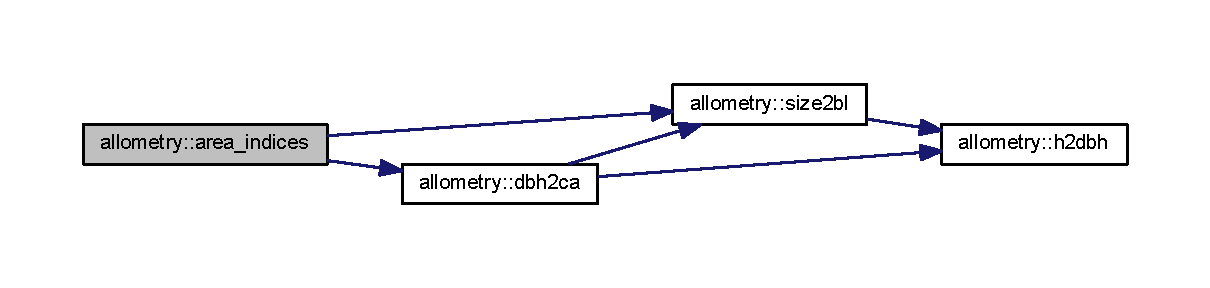
\includegraphics[width=350pt]{namespaceallometry_af723dc0f45a94b8812583457c53d4308_cgraph}
\end{center}
\end{figure}




Here is the caller graph for this function\+:\nopagebreak
\begin{figure}[H]
\begin{center}
\leavevmode
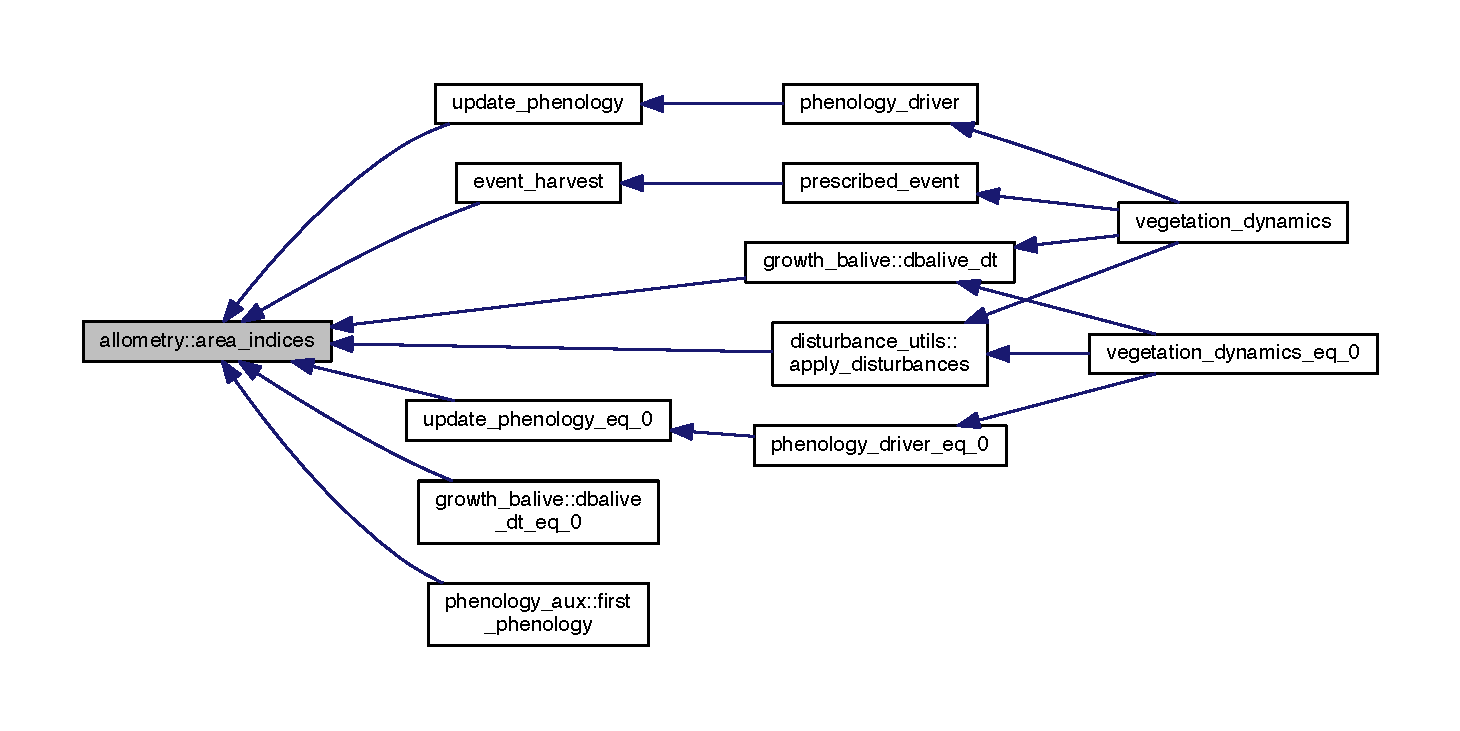
\includegraphics[width=350pt]{namespaceallometry_af723dc0f45a94b8812583457c53d4308_icgraph}
\end{center}
\end{figure}


\index{allometry@{allometry}!bd2dbh@{bd2dbh}}
\index{bd2dbh@{bd2dbh}!allometry@{allometry}}
\subsubsection[{\texorpdfstring{bd2dbh(ipft, bdead)}{bd2dbh(ipft, bdead)}}]{\setlength{\rightskip}{0pt plus 5cm}real function allometry\+::bd2dbh (
\begin{DoxyParamCaption}
\item[{integer, intent(in)}]{ipft, }
\item[{real, intent(in)}]{bdead}
\end{DoxyParamCaption}
)}\hypertarget{namespaceallometry_a50fedbee3a14eb5569a62abb4a36198f}{}\label{namespaceallometry_a50fedbee3a14eb5569a62abb4a36198f}


Here is the caller graph for this function\+:\nopagebreak
\begin{figure}[H]
\begin{center}
\leavevmode
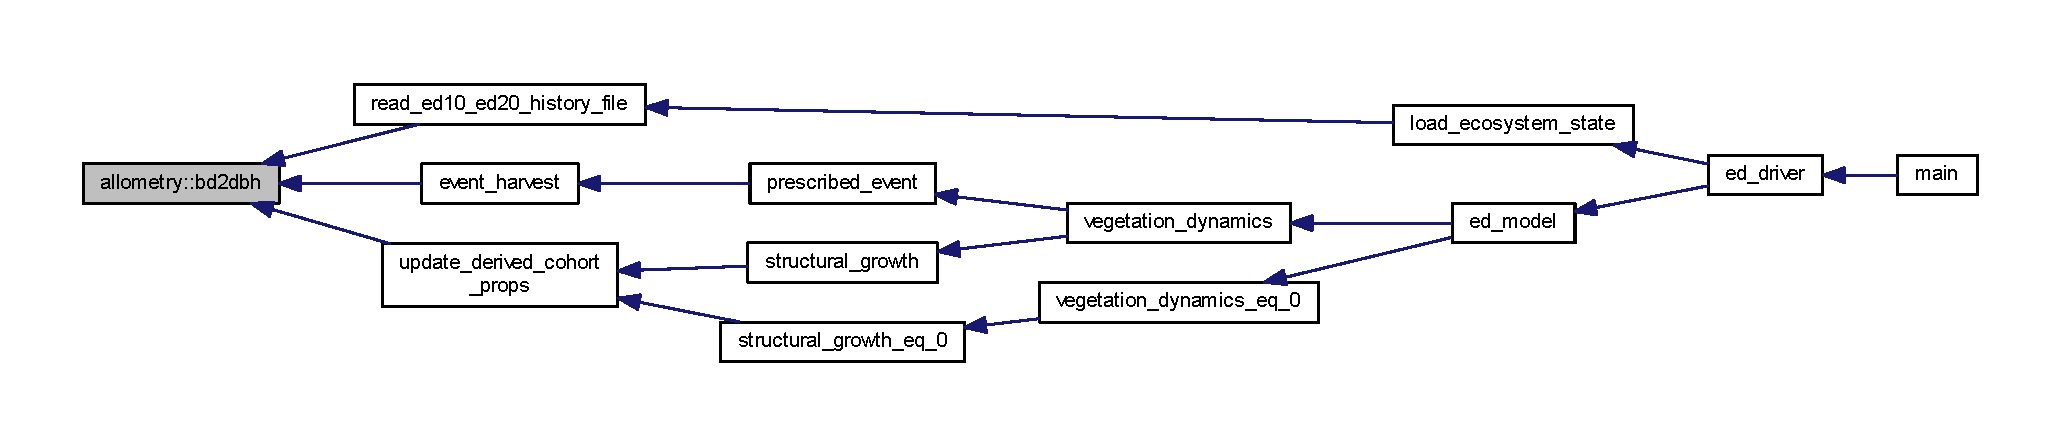
\includegraphics[width=350pt]{namespaceallometry_a50fedbee3a14eb5569a62abb4a36198f_icgraph}
\end{center}
\end{figure}


\index{allometry@{allometry}!bl2dbh@{bl2dbh}}
\index{bl2dbh@{bl2dbh}!allometry@{allometry}}
\subsubsection[{\texorpdfstring{bl2dbh(bleaf, ipft)}{bl2dbh(bleaf, ipft)}}]{\setlength{\rightskip}{0pt plus 5cm}real function allometry\+::bl2dbh (
\begin{DoxyParamCaption}
\item[{real, intent(in)}]{bleaf, }
\item[{integer, intent(in)}]{ipft}
\end{DoxyParamCaption}
)}\hypertarget{namespaceallometry_a3236375dc165a26aeea2d97c7e2c2685}{}\label{namespaceallometry_a3236375dc165a26aeea2d97c7e2c2685}


Here is the call graph for this function\+:\nopagebreak
\begin{figure}[H]
\begin{center}
\leavevmode
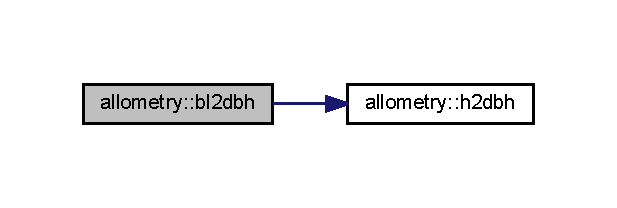
\includegraphics[width=296pt]{namespaceallometry_a3236375dc165a26aeea2d97c7e2c2685_cgraph}
\end{center}
\end{figure}




Here is the caller graph for this function\+:\nopagebreak
\begin{figure}[H]
\begin{center}
\leavevmode
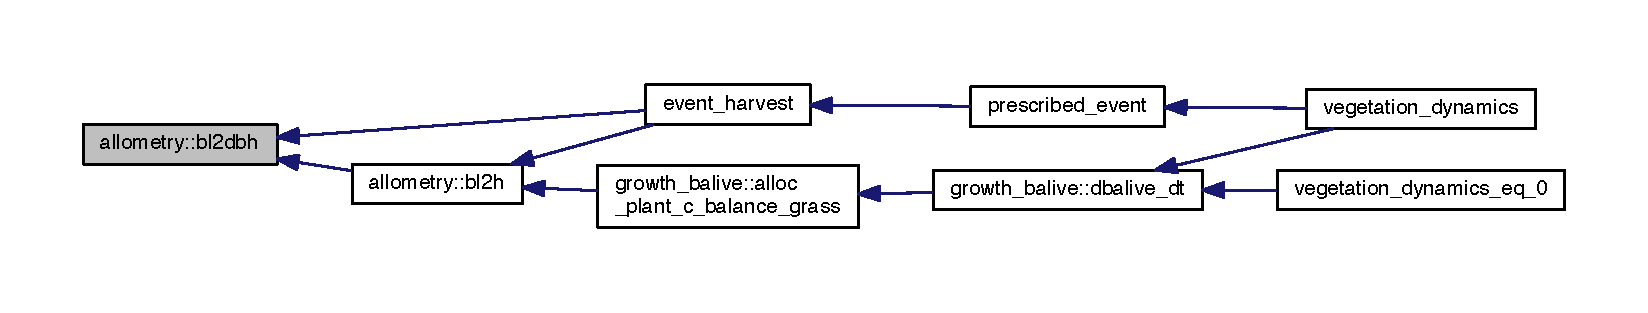
\includegraphics[width=350pt]{namespaceallometry_a3236375dc165a26aeea2d97c7e2c2685_icgraph}
\end{center}
\end{figure}


\index{allometry@{allometry}!bl2h@{bl2h}}
\index{bl2h@{bl2h}!allometry@{allometry}}
\subsubsection[{\texorpdfstring{bl2h(bleaf, ipft)}{bl2h(bleaf, ipft)}}]{\setlength{\rightskip}{0pt plus 5cm}real function allometry\+::bl2h (
\begin{DoxyParamCaption}
\item[{real, intent(in)}]{bleaf, }
\item[{integer, intent(in)}]{ipft}
\end{DoxyParamCaption}
)}\hypertarget{namespaceallometry_a59a1fc10140498dee62fce8a641da254}{}\label{namespaceallometry_a59a1fc10140498dee62fce8a641da254}


Here is the call graph for this function\+:\nopagebreak
\begin{figure}[H]
\begin{center}
\leavevmode
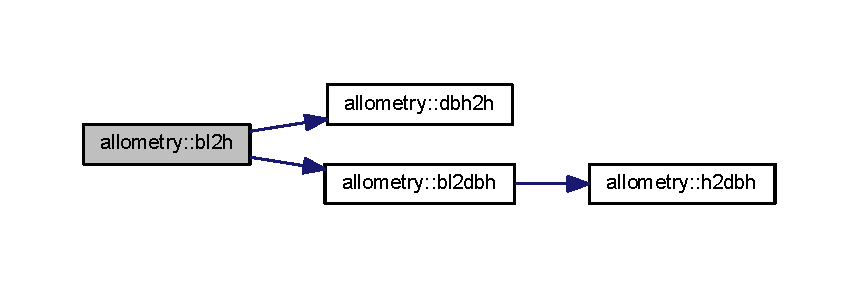
\includegraphics[width=350pt]{namespaceallometry_a59a1fc10140498dee62fce8a641da254_cgraph}
\end{center}
\end{figure}




Here is the caller graph for this function\+:\nopagebreak
\begin{figure}[H]
\begin{center}
\leavevmode
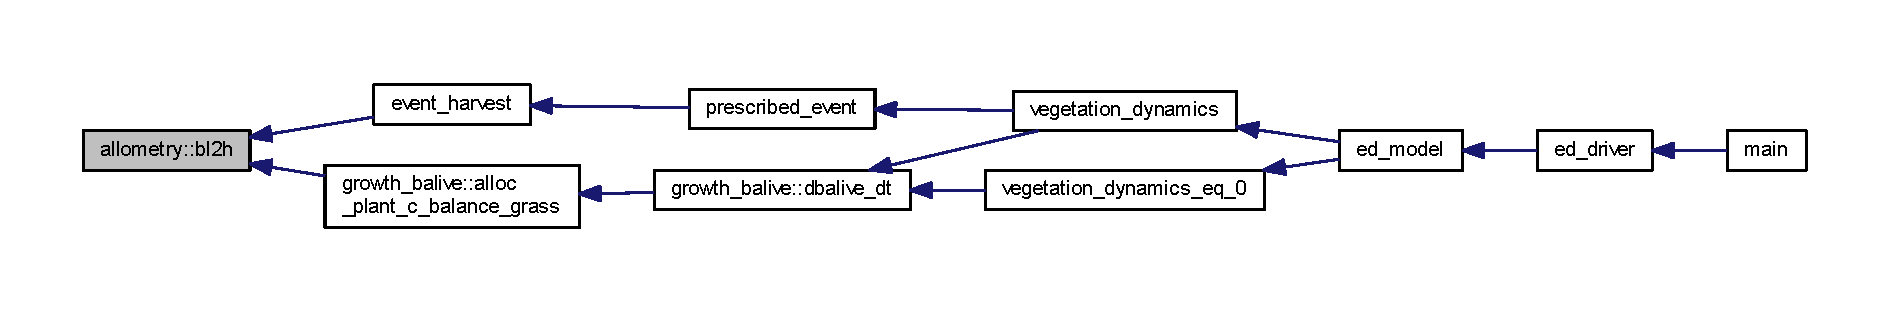
\includegraphics[width=350pt]{namespaceallometry_a59a1fc10140498dee62fce8a641da254_icgraph}
\end{center}
\end{figure}


\index{allometry@{allometry}!dbh2bd@{dbh2bd}}
\index{dbh2bd@{dbh2bd}!allometry@{allometry}}
\subsubsection[{\texorpdfstring{dbh2bd(dbh, ipft)}{dbh2bd(dbh, ipft)}}]{\setlength{\rightskip}{0pt plus 5cm}real function allometry\+::dbh2bd (
\begin{DoxyParamCaption}
\item[{real, intent(in)}]{dbh, }
\item[{integer, intent(in)}]{ipft}
\end{DoxyParamCaption}
)}\hypertarget{namespaceallometry_a76db2bc4aaa47db1e2656117ec476dba}{}\label{namespaceallometry_a76db2bc4aaa47db1e2656117ec476dba}


Here is the caller graph for this function\+:\nopagebreak
\begin{figure}[H]
\begin{center}
\leavevmode
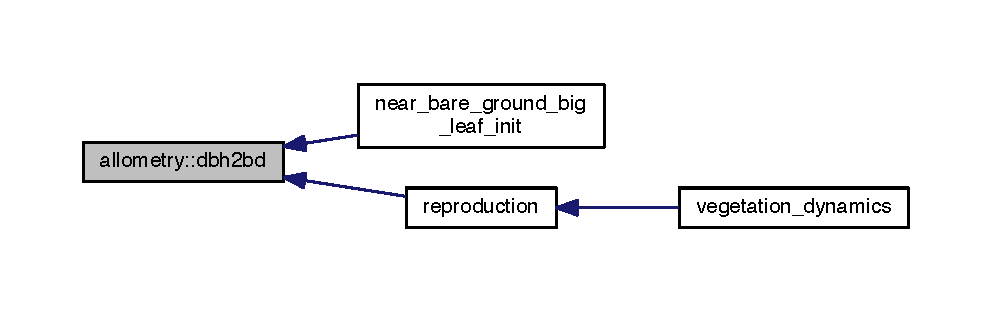
\includegraphics[width=350pt]{namespaceallometry_a76db2bc4aaa47db1e2656117ec476dba_icgraph}
\end{center}
\end{figure}


\index{allometry@{allometry}!dbh2ca@{dbh2ca}}
\index{dbh2ca@{dbh2ca}!allometry@{allometry}}
\subsubsection[{\texorpdfstring{dbh2ca(dbh, hite, sla, ipft)}{dbh2ca(dbh, hite, sla, ipft)}}]{\setlength{\rightskip}{0pt plus 5cm}real function allometry\+::dbh2ca (
\begin{DoxyParamCaption}
\item[{real, intent(in)}]{dbh, }
\item[{real, intent(in)}]{hite, }
\item[{real, intent(in)}]{sla, }
\item[{integer, intent(in)}]{ipft}
\end{DoxyParamCaption}
)}\hypertarget{namespaceallometry_abacdf8e8e585ce8d788a1fc2be133243}{}\label{namespaceallometry_abacdf8e8e585ce8d788a1fc2be133243}


Here is the call graph for this function\+:\nopagebreak
\begin{figure}[H]
\begin{center}
\leavevmode
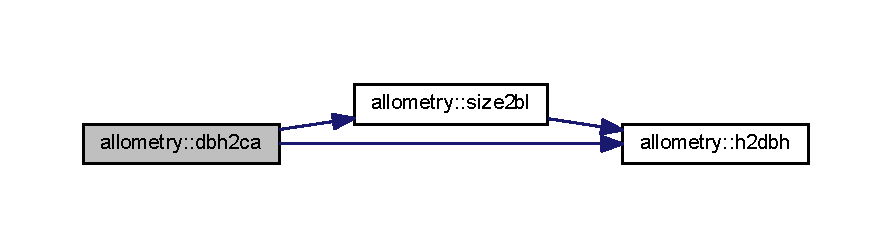
\includegraphics[width=350pt]{namespaceallometry_abacdf8e8e585ce8d788a1fc2be133243_cgraph}
\end{center}
\end{figure}




Here is the caller graph for this function\+:\nopagebreak
\begin{figure}[H]
\begin{center}
\leavevmode
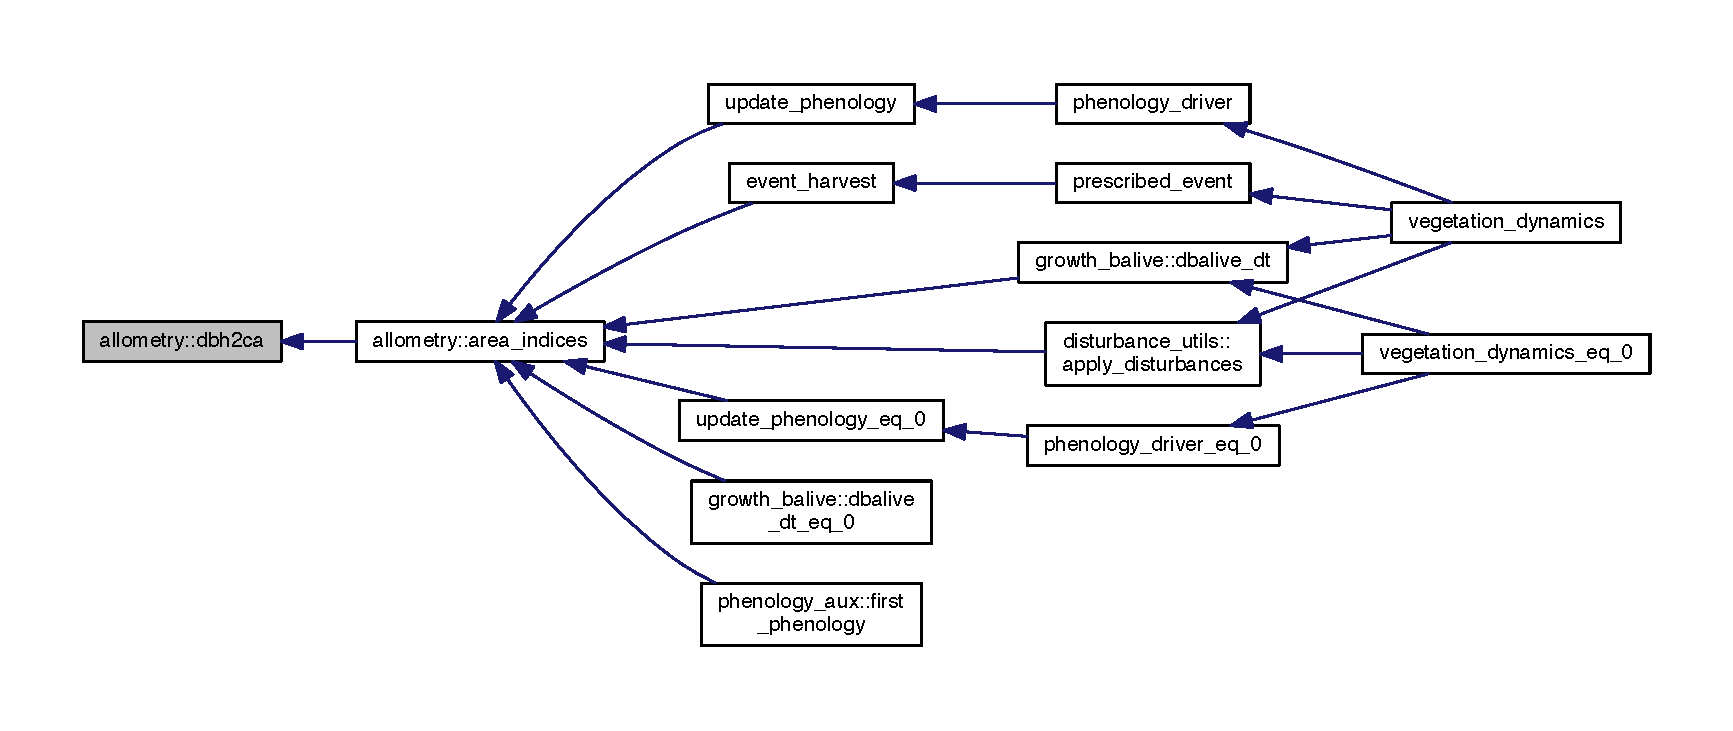
\includegraphics[width=350pt]{namespaceallometry_abacdf8e8e585ce8d788a1fc2be133243_icgraph}
\end{center}
\end{figure}


\index{allometry@{allometry}!dbh2h@{dbh2h}}
\index{dbh2h@{dbh2h}!allometry@{allometry}}
\subsubsection[{\texorpdfstring{dbh2h(ipft, dbh)}{dbh2h(ipft, dbh)}}]{\setlength{\rightskip}{0pt plus 5cm}real function allometry\+::dbh2h (
\begin{DoxyParamCaption}
\item[{integer, intent(in)}]{ipft, }
\item[{real, intent(in)}]{dbh}
\end{DoxyParamCaption}
)}\hypertarget{namespaceallometry_a56f11dc07da4d5e7114dc37d6cc5f2cc}{}\label{namespaceallometry_a56f11dc07da4d5e7114dc37d6cc5f2cc}


Here is the caller graph for this function\+:\nopagebreak
\begin{figure}[H]
\begin{center}
\leavevmode
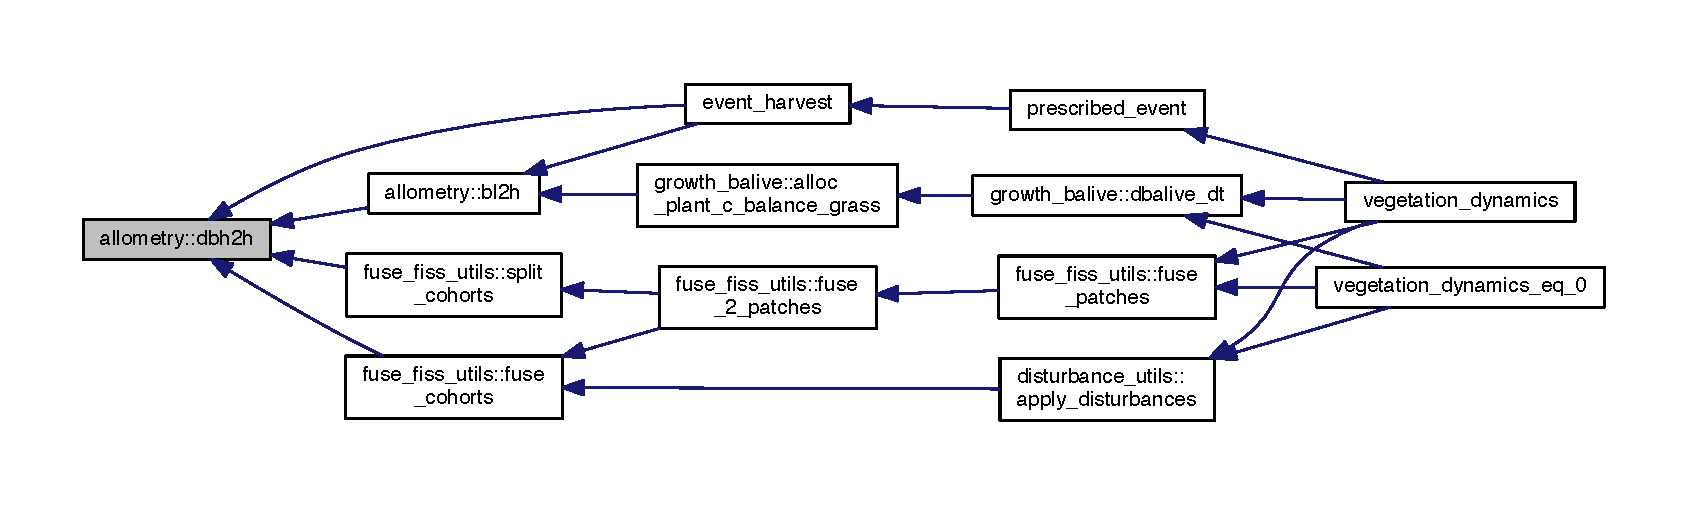
\includegraphics[width=350pt]{namespaceallometry_a56f11dc07da4d5e7114dc37d6cc5f2cc_icgraph}
\end{center}
\end{figure}


\index{allometry@{allometry}!dbh2krdepth@{dbh2krdepth}}
\index{dbh2krdepth@{dbh2krdepth}!allometry@{allometry}}
\subsubsection[{\texorpdfstring{dbh2krdepth(hite, dbh, ipft, lsl)}{dbh2krdepth(hite, dbh, ipft, lsl)}}]{\setlength{\rightskip}{0pt plus 5cm}integer function allometry\+::dbh2krdepth (
\begin{DoxyParamCaption}
\item[{real, intent(in)}]{hite, }
\item[{real, intent(in)}]{dbh, }
\item[{integer, intent(in)}]{ipft, }
\item[{integer, intent(in)}]{lsl}
\end{DoxyParamCaption}
)}\hypertarget{namespaceallometry_ac1523ea0e0ef8d2dd6a429f61a013c1c}{}\label{namespaceallometry_ac1523ea0e0ef8d2dd6a429f61a013c1c}


Here is the call graph for this function\+:\nopagebreak
\begin{figure}[H]
\begin{center}
\leavevmode
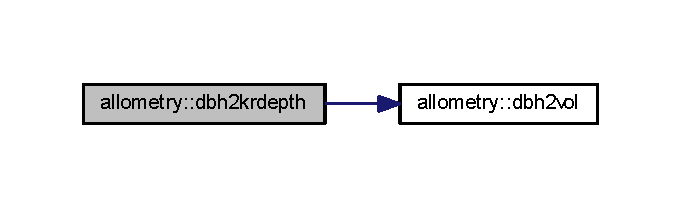
\includegraphics[width=327pt]{namespaceallometry_ac1523ea0e0ef8d2dd6a429f61a013c1c_cgraph}
\end{center}
\end{figure}




Here is the caller graph for this function\+:\nopagebreak
\begin{figure}[H]
\begin{center}
\leavevmode
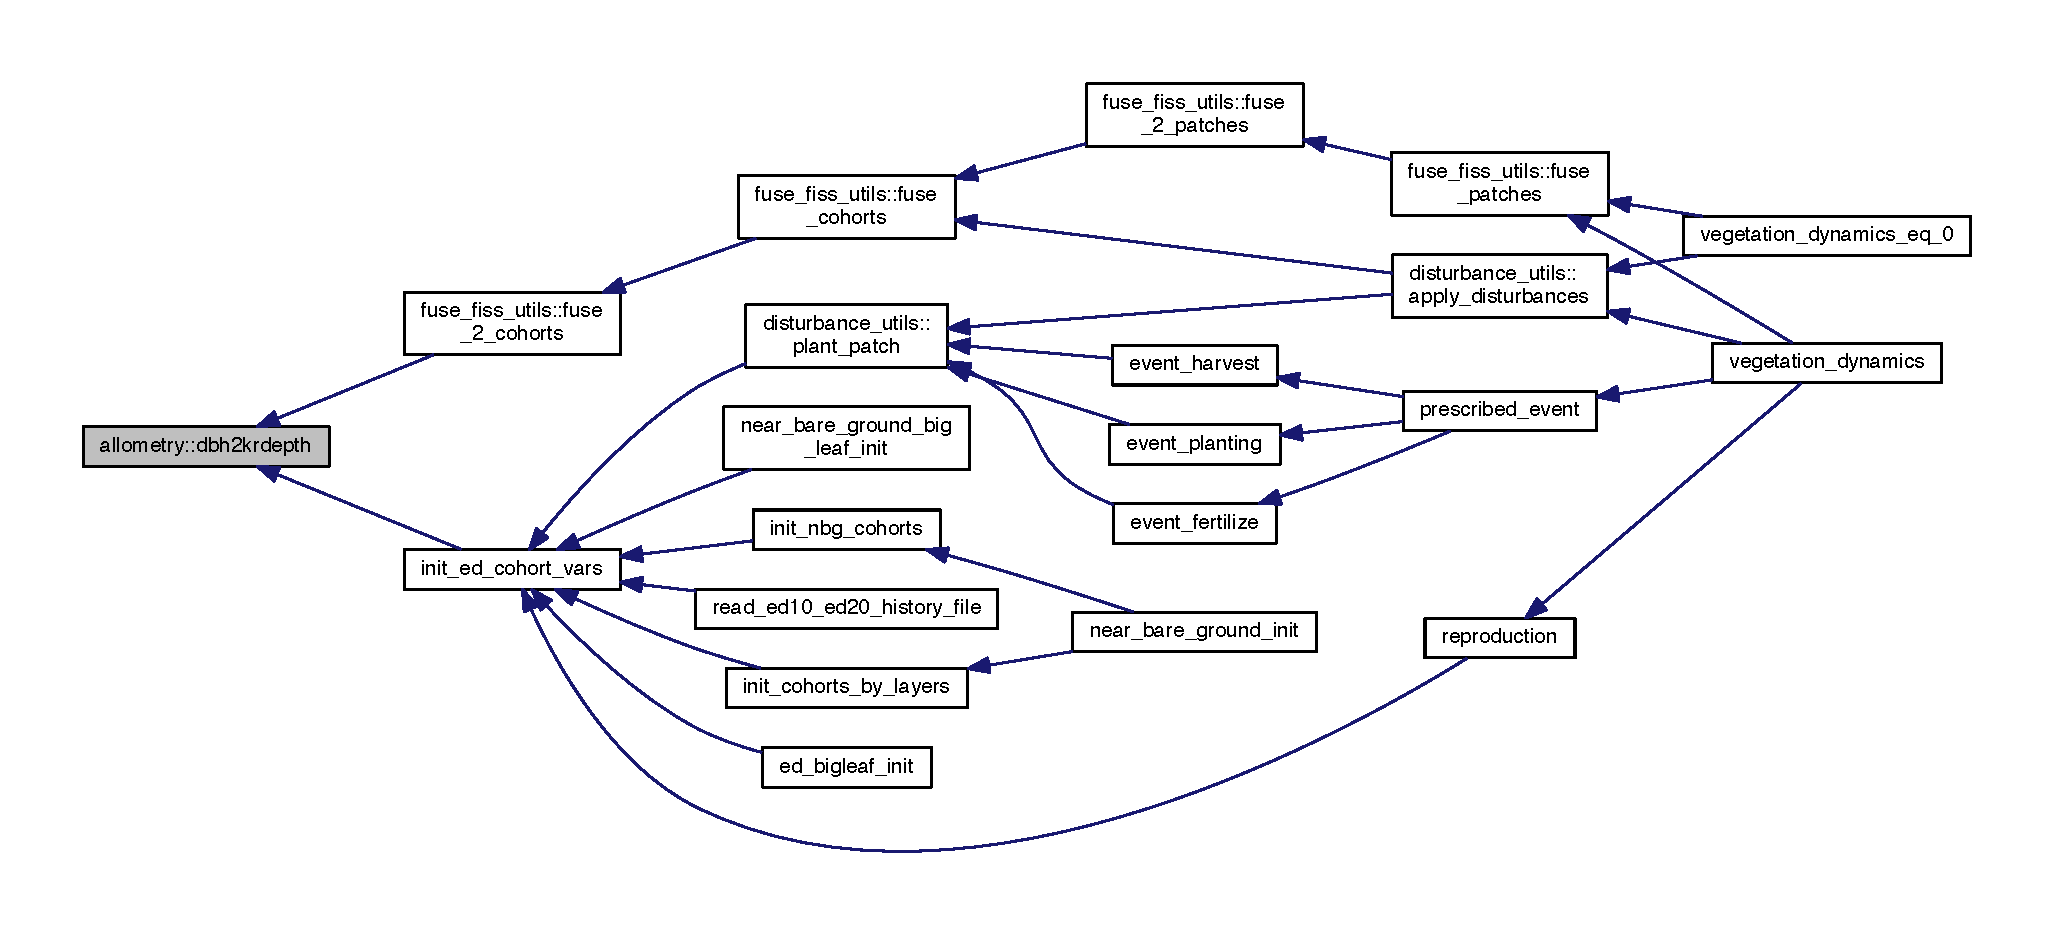
\includegraphics[width=350pt]{namespaceallometry_ac1523ea0e0ef8d2dd6a429f61a013c1c_icgraph}
\end{center}
\end{figure}


\index{allometry@{allometry}!dbh2vol@{dbh2vol}}
\index{dbh2vol@{dbh2vol}!allometry@{allometry}}
\subsubsection[{\texorpdfstring{dbh2vol(hgt, dbh, ipft)}{dbh2vol(hgt, dbh, ipft)}}]{\setlength{\rightskip}{0pt plus 5cm}real function allometry\+::dbh2vol (
\begin{DoxyParamCaption}
\item[{real, intent(in)}]{hgt, }
\item[{real, intent(in)}]{dbh, }
\item[{integer, intent(in)}]{ipft}
\end{DoxyParamCaption}
)}\hypertarget{namespaceallometry_aab2b2cee61cac31529246b043121c7de}{}\label{namespaceallometry_aab2b2cee61cac31529246b043121c7de}


Here is the caller graph for this function\+:\nopagebreak
\begin{figure}[H]
\begin{center}
\leavevmode
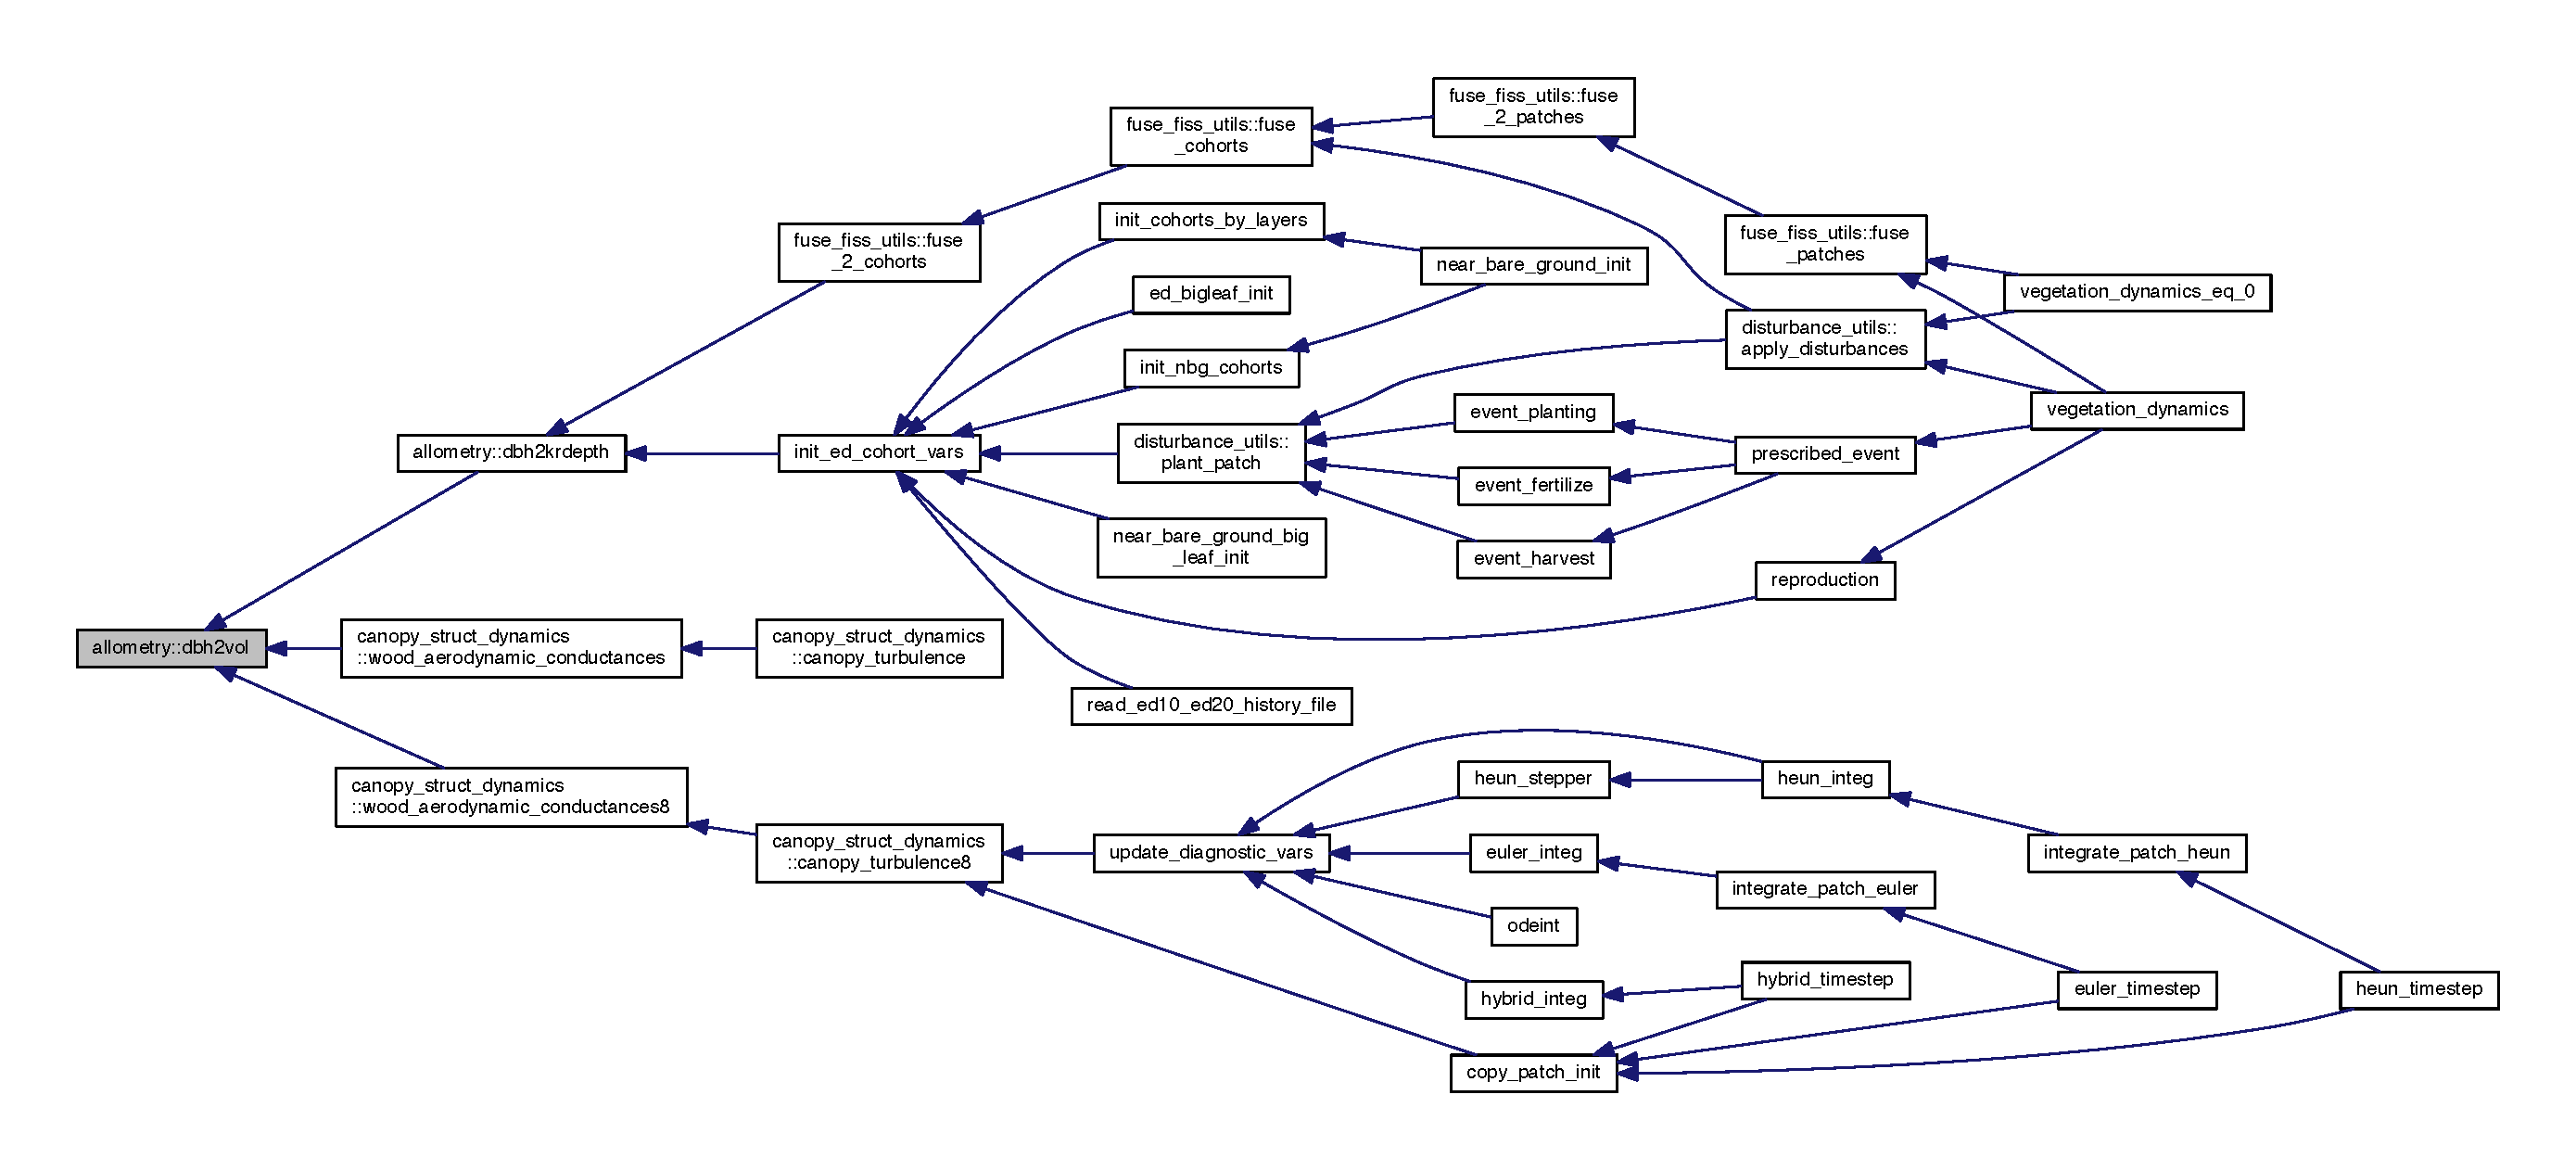
\includegraphics[width=350pt]{namespaceallometry_aab2b2cee61cac31529246b043121c7de_icgraph}
\end{center}
\end{figure}


\index{allometry@{allometry}!ed\+\_\+biomass@{ed\+\_\+biomass}}
\index{ed\+\_\+biomass@{ed\+\_\+biomass}!allometry@{allometry}}
\subsubsection[{\texorpdfstring{ed\+\_\+biomass(bdead, bleaf, bsapwooda, ipft)}{ed_biomass(bdead, bleaf, bsapwooda, ipft)}}]{\setlength{\rightskip}{0pt plus 5cm}real function allometry\+::ed\+\_\+biomass (
\begin{DoxyParamCaption}
\item[{real, intent(in)}]{bdead, }
\item[{real, intent(in)}]{bleaf, }
\item[{real, intent(in)}]{bsapwooda, }
\item[{integer, intent(in)}]{ipft}
\end{DoxyParamCaption}
)}\hypertarget{namespaceallometry_ab99b16f69dafaf5ff3e69c7514b9e7b6}{}\label{namespaceallometry_ab99b16f69dafaf5ff3e69c7514b9e7b6}


Here is the caller graph for this function\+:\nopagebreak
\begin{figure}[H]
\begin{center}
\leavevmode
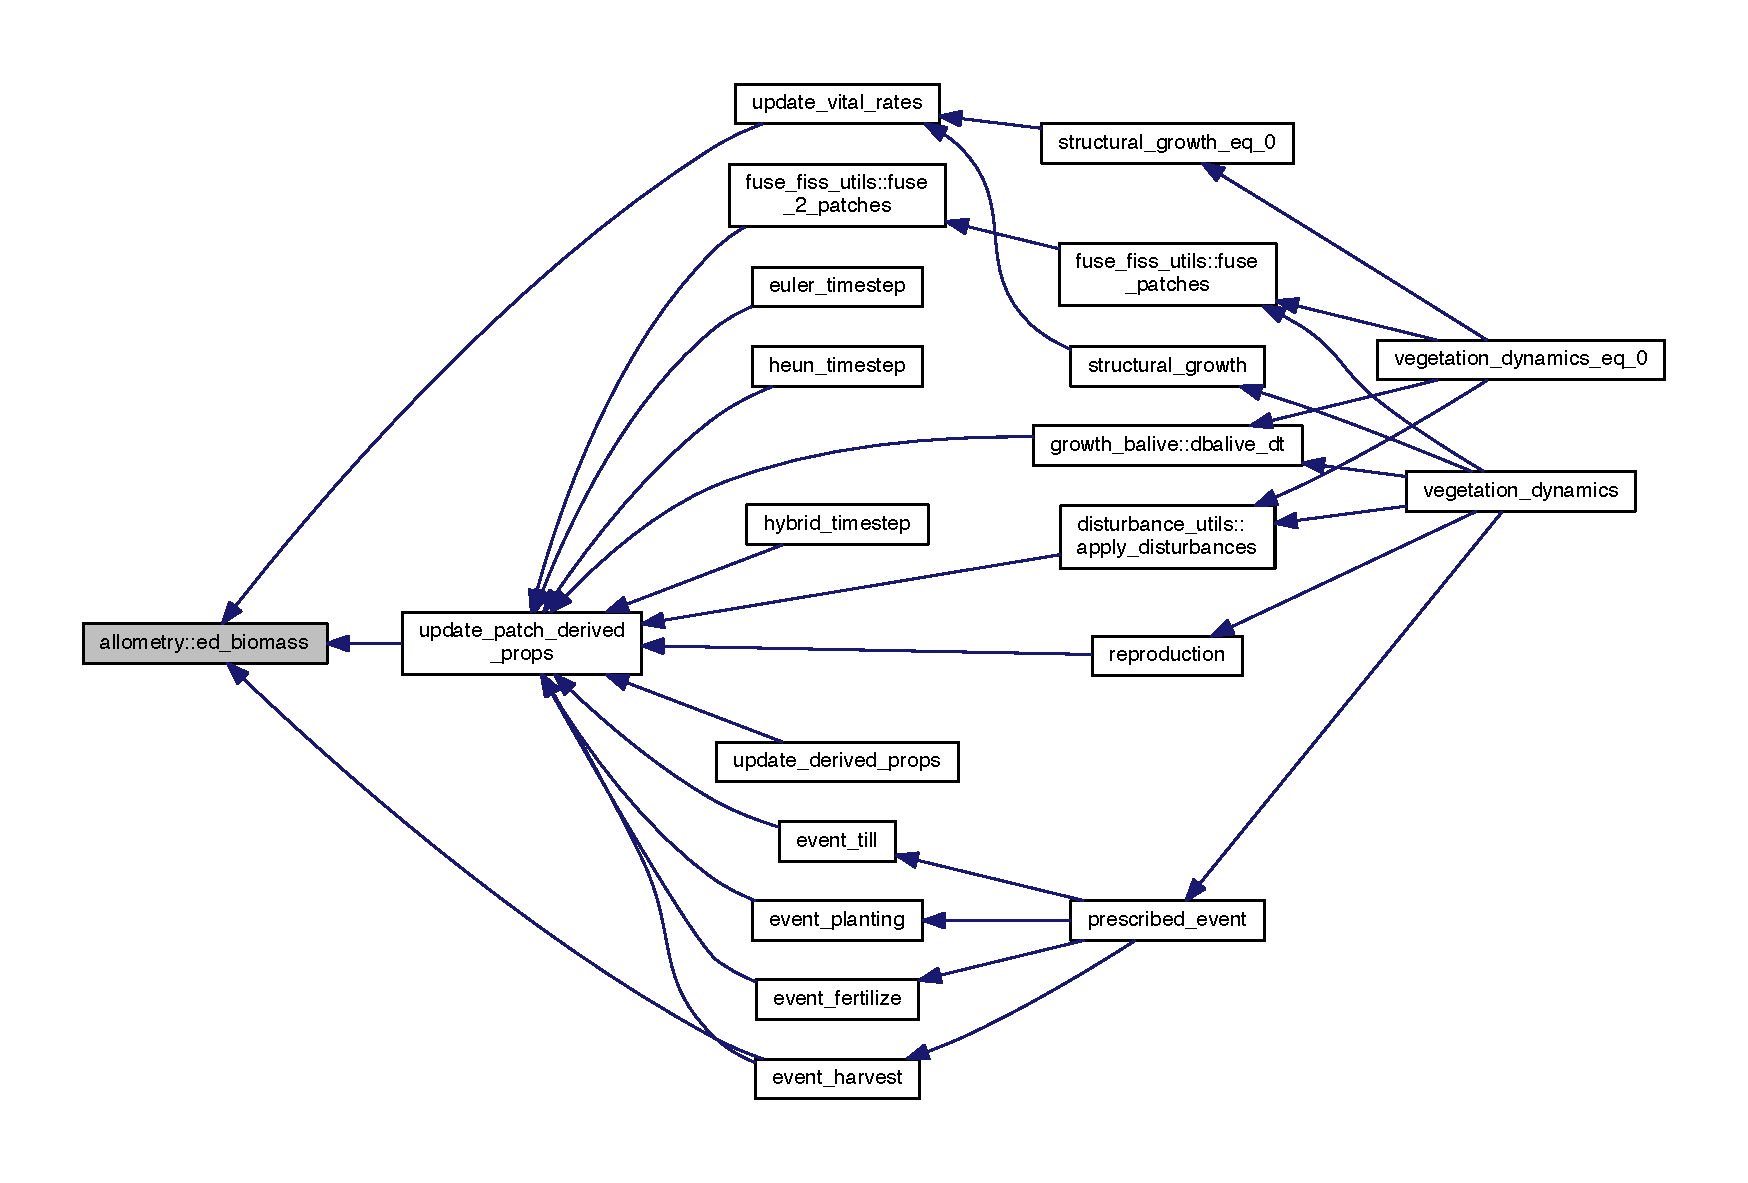
\includegraphics[width=350pt]{namespaceallometry_ab99b16f69dafaf5ff3e69c7514b9e7b6_icgraph}
\end{center}
\end{figure}


\index{allometry@{allometry}!h2crownbh@{h2crownbh}}
\index{h2crownbh@{h2crownbh}!allometry@{allometry}}
\subsubsection[{\texorpdfstring{h2crownbh(height, ipft)}{h2crownbh(height, ipft)}}]{\setlength{\rightskip}{0pt plus 5cm}real function allometry\+::h2crownbh (
\begin{DoxyParamCaption}
\item[{real, intent(in)}]{height, }
\item[{integer, intent(in)}]{ipft}
\end{DoxyParamCaption}
)}\hypertarget{namespaceallometry_a88949ed487fccc2f1dfd065399043b0d}{}\label{namespaceallometry_a88949ed487fccc2f1dfd065399043b0d}


Here is the caller graph for this function\+:\nopagebreak
\begin{figure}[H]
\begin{center}
\leavevmode
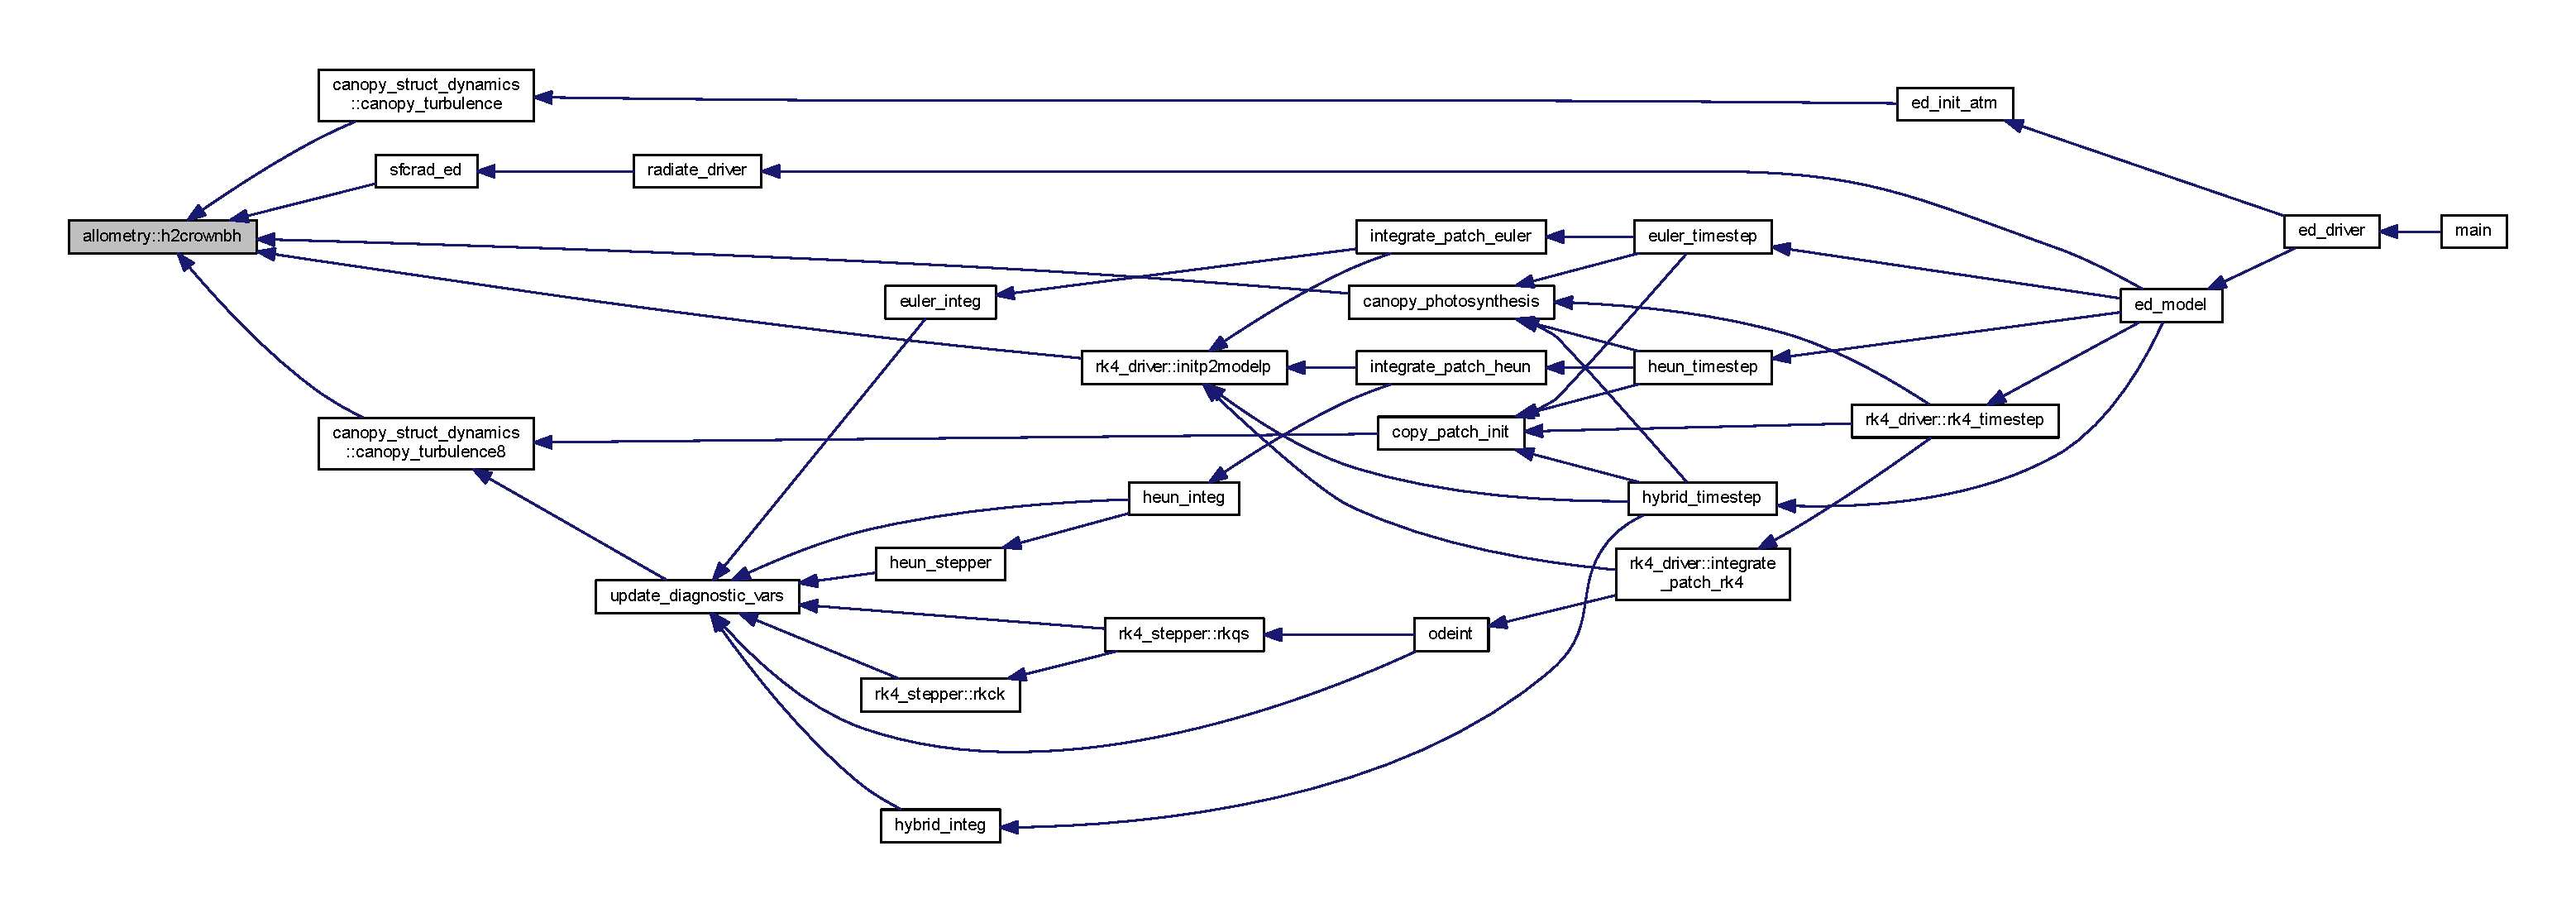
\includegraphics[width=350pt]{namespaceallometry_a88949ed487fccc2f1dfd065399043b0d_icgraph}
\end{center}
\end{figure}


\index{allometry@{allometry}!h2dbh@{h2dbh}}
\index{h2dbh@{h2dbh}!allometry@{allometry}}
\subsubsection[{\texorpdfstring{h2dbh(h, ipft)}{h2dbh(h, ipft)}}]{\setlength{\rightskip}{0pt plus 5cm}real function allometry\+::h2dbh (
\begin{DoxyParamCaption}
\item[{real, intent(in)}]{h, }
\item[{integer, intent(in)}]{ipft}
\end{DoxyParamCaption}
)}\hypertarget{namespaceallometry_a31aa8db06e86ec74efb5e692417399df}{}\label{namespaceallometry_a31aa8db06e86ec74efb5e692417399df}


Here is the caller graph for this function\+:\nopagebreak
\begin{figure}[H]
\begin{center}
\leavevmode
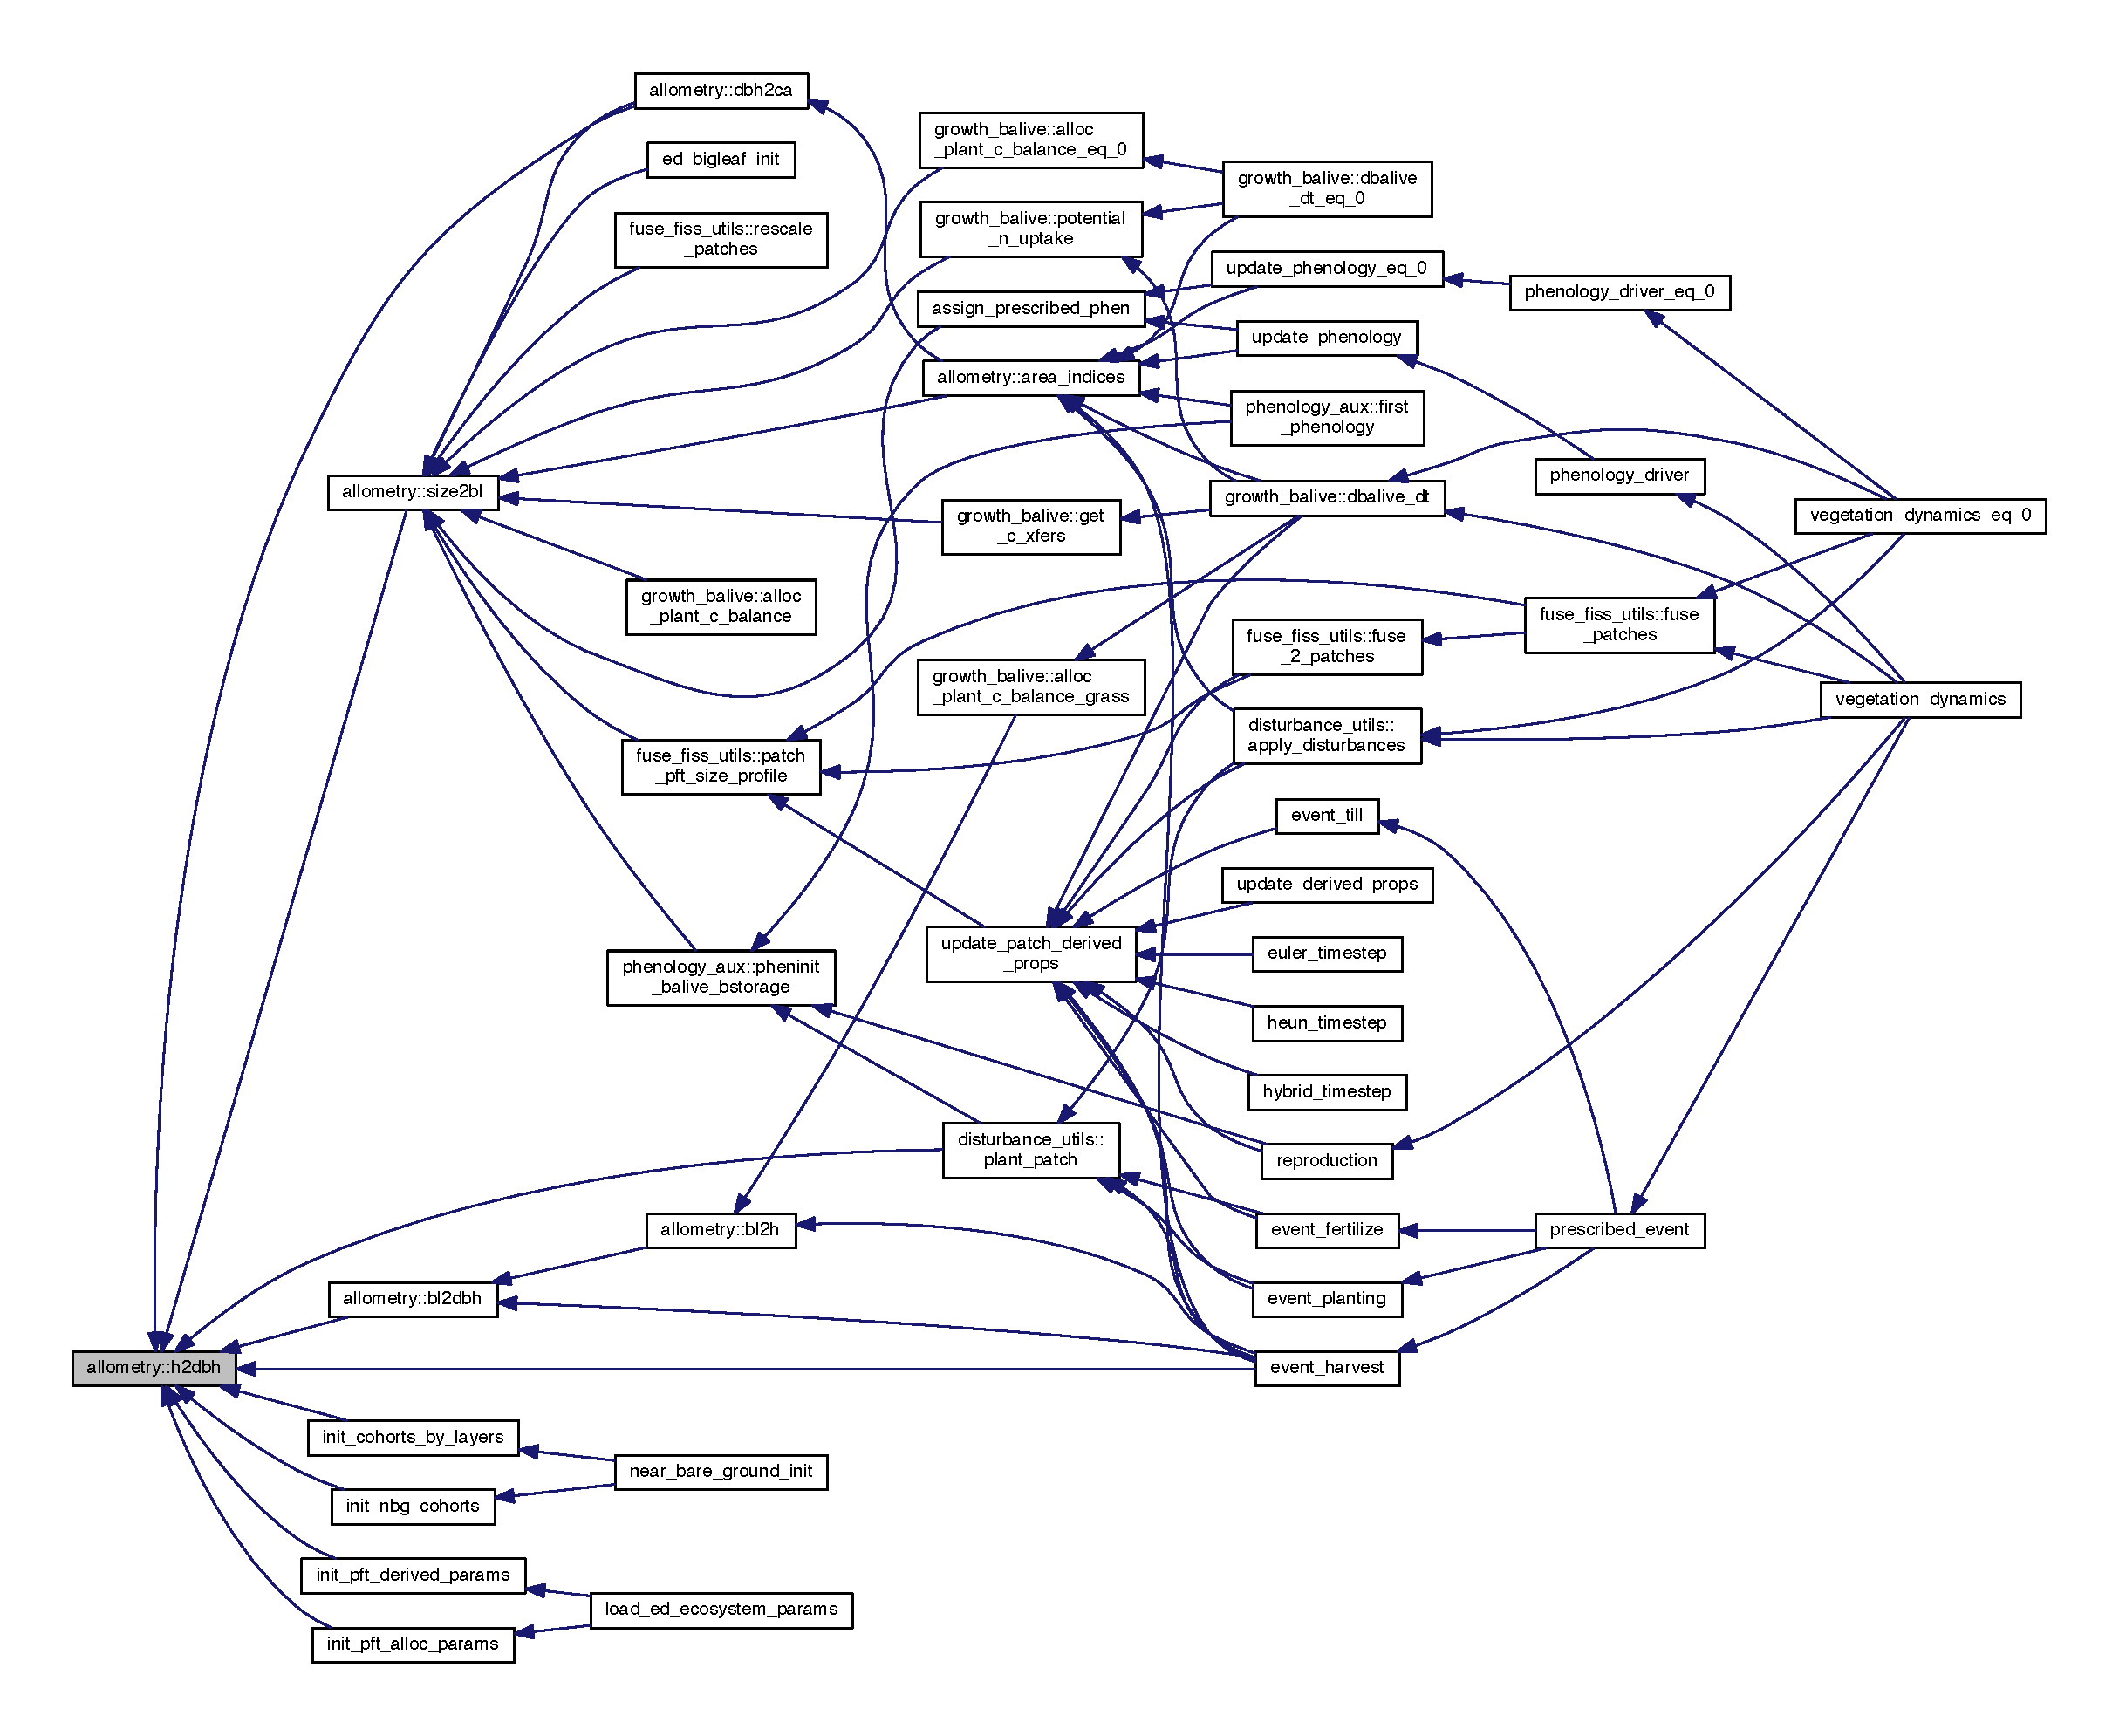
\includegraphics[width=350pt]{namespaceallometry_a31aa8db06e86ec74efb5e692417399df_icgraph}
\end{center}
\end{figure}


\index{allometry@{allometry}!size2bl@{size2bl}}
\index{size2bl@{size2bl}!allometry@{allometry}}
\subsubsection[{\texorpdfstring{size2bl(dbh, hite, ipft)}{size2bl(dbh, hite, ipft)}}]{\setlength{\rightskip}{0pt plus 5cm}real function allometry\+::size2bl (
\begin{DoxyParamCaption}
\item[{real, intent(in)}]{dbh, }
\item[{real, intent(in)}]{hite, }
\item[{integer, intent(in)}]{ipft}
\end{DoxyParamCaption}
)}\hypertarget{namespaceallometry_a45ced9bf9ccd03debe8def35b579f4bd}{}\label{namespaceallometry_a45ced9bf9ccd03debe8def35b579f4bd}


Here is the call graph for this function\+:\nopagebreak
\begin{figure}[H]
\begin{center}
\leavevmode
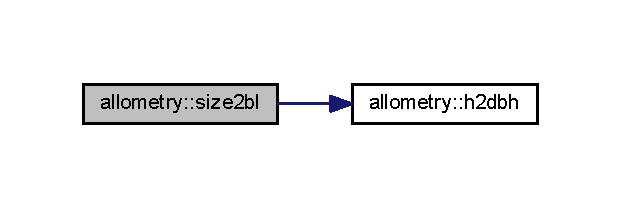
\includegraphics[width=298pt]{namespaceallometry_a45ced9bf9ccd03debe8def35b579f4bd_cgraph}
\end{center}
\end{figure}




Here is the caller graph for this function\+:\nopagebreak
\begin{figure}[H]
\begin{center}
\leavevmode
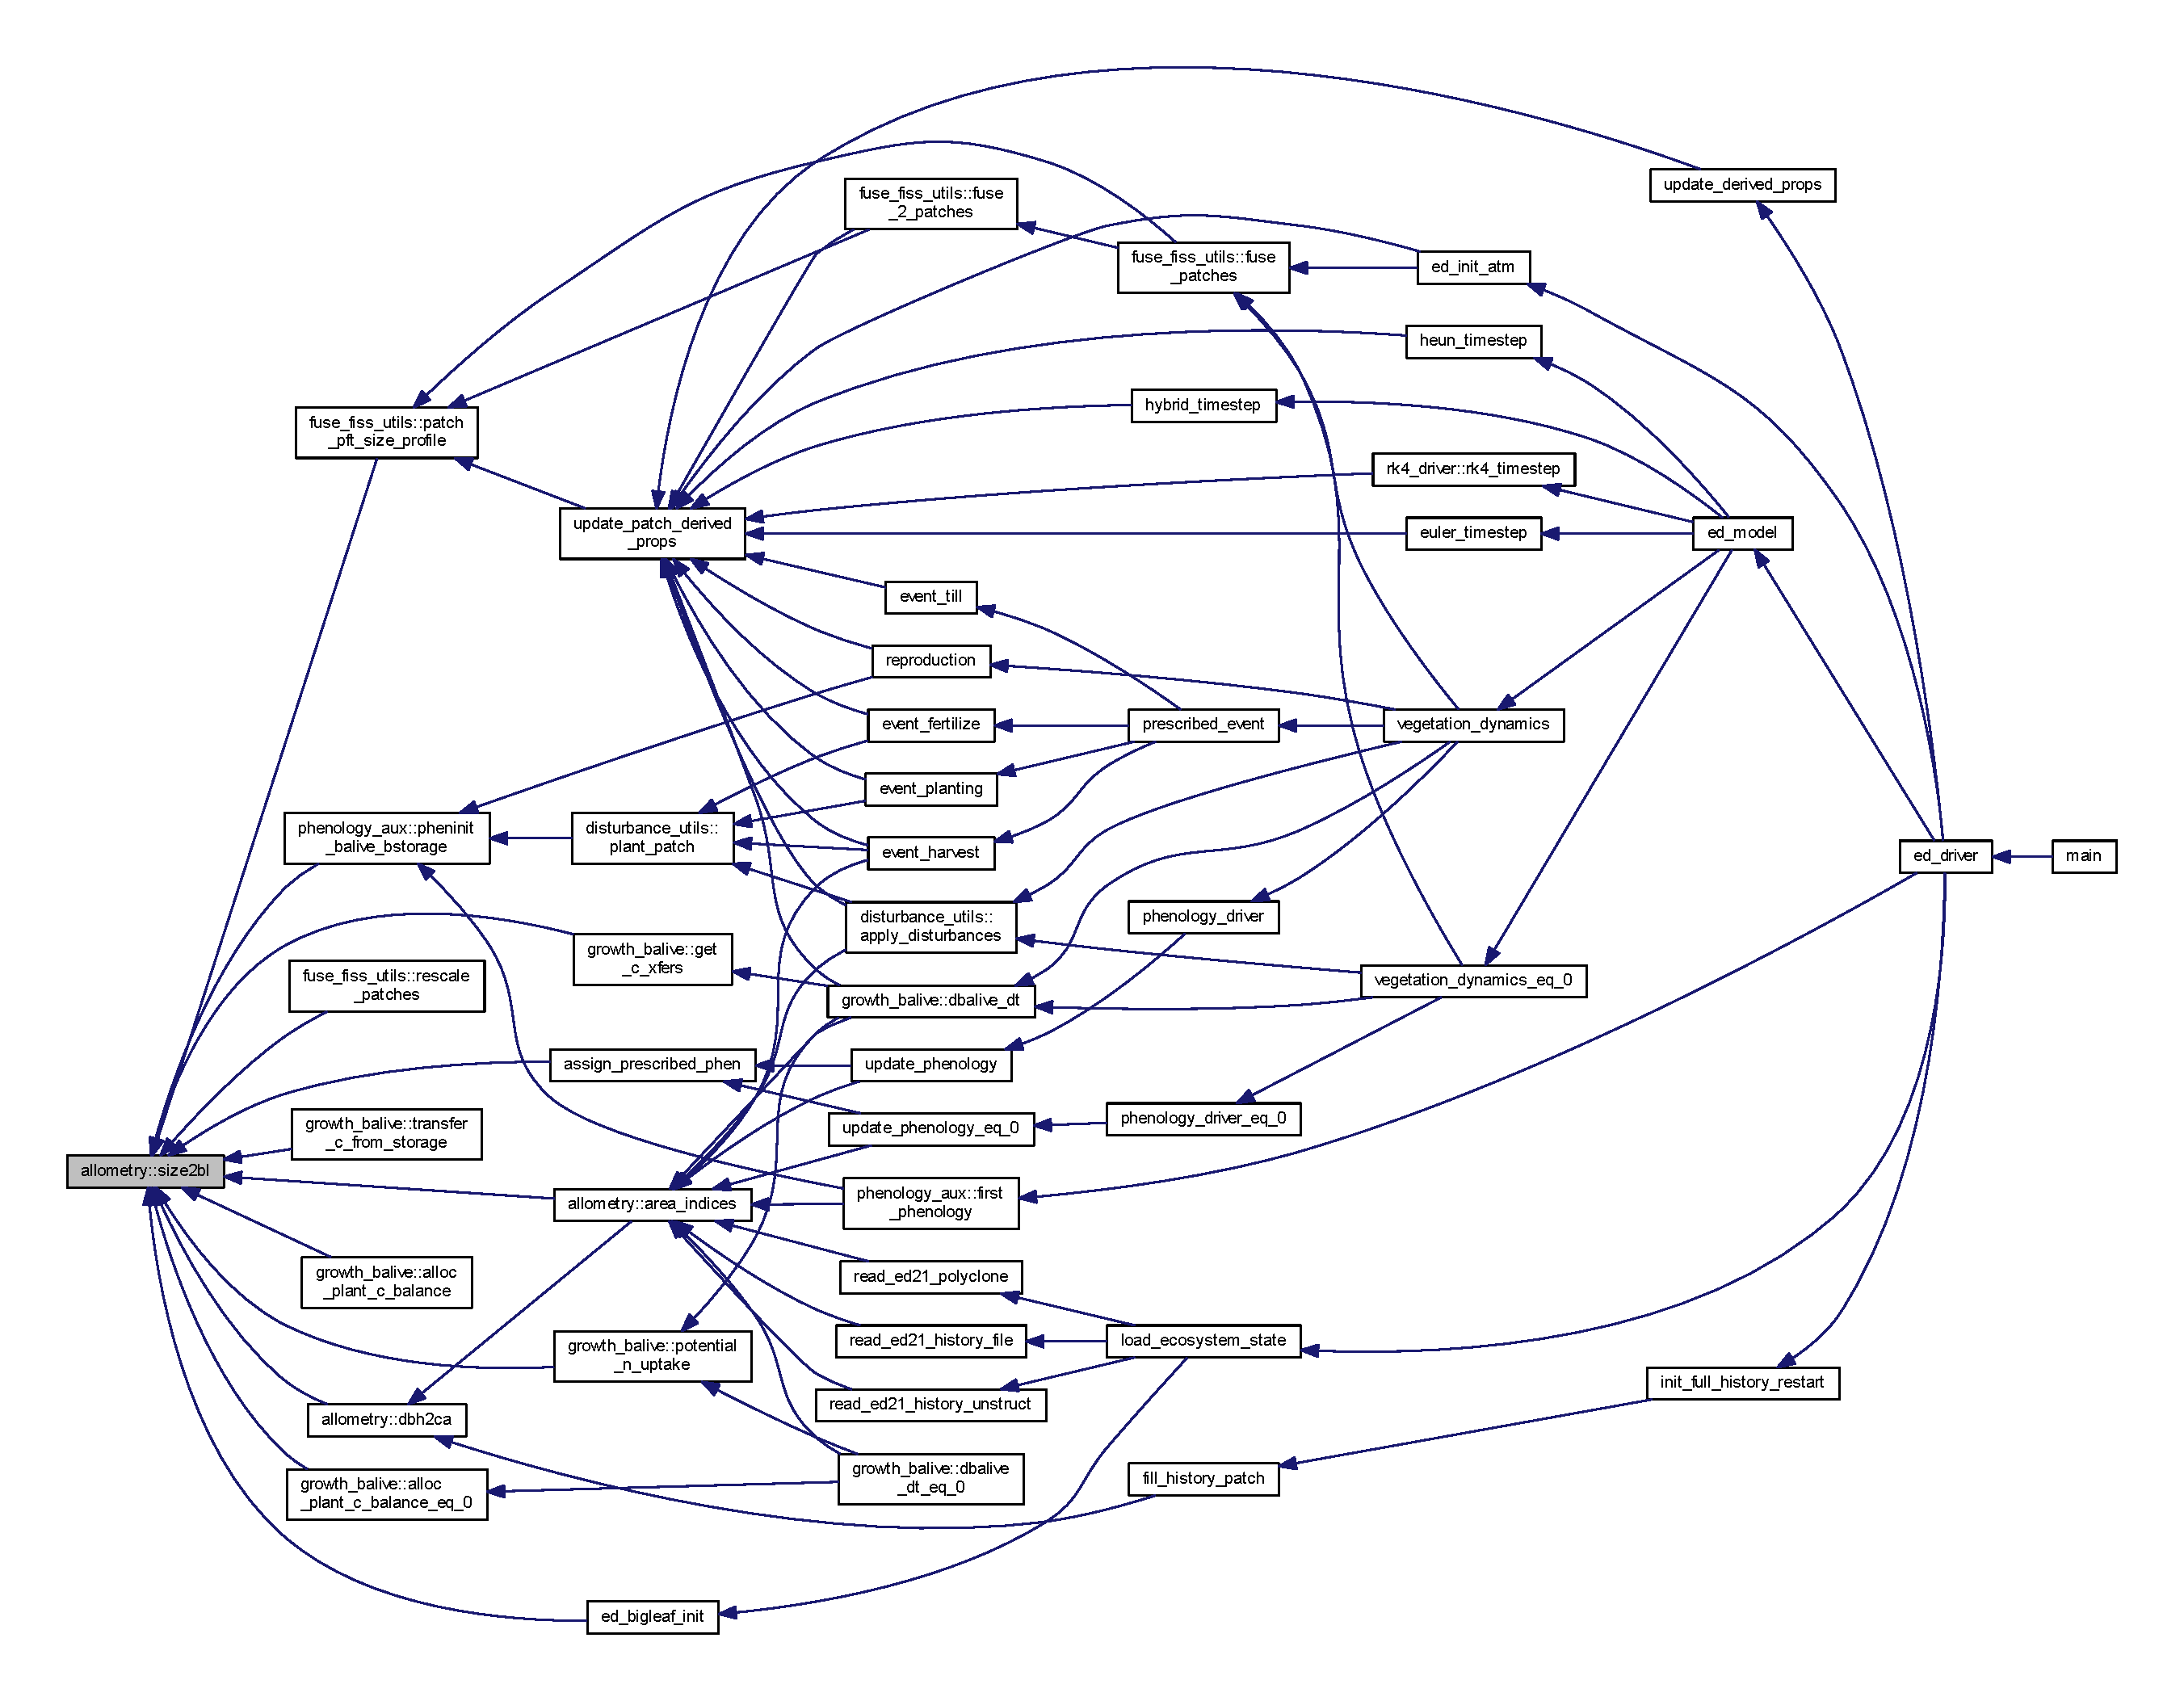
\includegraphics[width=350pt]{namespaceallometry_a45ced9bf9ccd03debe8def35b579f4bd_icgraph}
\end{center}
\end{figure}



\hypertarget{namespacean__header}{}\section{an\+\_\+header Module Reference}
\label{namespacean__header}\index{an\+\_\+header@{an\+\_\+header}}
\subsection*{Data Types}
\begin{DoxyCompactItemize}
\item 
type \hyperlink{structan__header_1_1head__table}{head\+\_\+table}
\end{DoxyCompactItemize}
\subsection*{Variables}
\begin{DoxyCompactItemize}
\item 
type(\hyperlink{structan__header_1_1head__table}{head\+\_\+table}), dimension(\+:), allocatable, save \hyperlink{namespacean__header_ae5d3cd005b4f936e39d8ca9572fad953}{anal\+\_\+table}
\item 
integer, save \hyperlink{namespacean__header_a1f6702c906713337344986a86e036d55}{nvbtab}
\end{DoxyCompactItemize}


\subsection{Variable Documentation}
\hypertarget{namespacean__header_ae5d3cd005b4f936e39d8ca9572fad953}{}\index{an\+\_\+header@{an\+\_\+header}!anal\+\_\+table@{anal\+\_\+table}}
\index{anal\+\_\+table@{anal\+\_\+table}!an\+\_\+header@{an\+\_\+header}}
\subsubsection[{anal\+\_\+table}]{\setlength{\rightskip}{0pt plus 5cm}type ({\bf head\+\_\+table}), dimension(\+:), allocatable, save an\+\_\+header\+::anal\+\_\+table}\label{namespacean__header_ae5d3cd005b4f936e39d8ca9572fad953}
\hypertarget{namespacean__header_a1f6702c906713337344986a86e036d55}{}\index{an\+\_\+header@{an\+\_\+header}!nvbtab@{nvbtab}}
\index{nvbtab@{nvbtab}!an\+\_\+header@{an\+\_\+header}}
\subsubsection[{nvbtab}]{\setlength{\rightskip}{0pt plus 5cm}integer, save an\+\_\+header\+::nvbtab}\label{namespacean__header_a1f6702c906713337344986a86e036d55}

\hypertarget{namespaceaverage__utils}{}\section{average\+\_\+utils Module Reference}
\label{namespaceaverage__utils}\index{average\+\_\+utils@{average\+\_\+utils}}
\subsection*{Functions/\+Subroutines}
\begin{DoxyCompactItemize}
\item 
subroutine \hyperlink{namespaceaverage__utils_a90965230835c19a82d90127089235c76}{aggregate\+\_\+polygon\+\_\+fmean} (cgrid)
\item 
subroutine \hyperlink{namespaceaverage__utils_acf7868319b9242daa7eea553b25f2899}{integrate\+\_\+ed\+\_\+fmean\+\_\+met\+\_\+vars} (cgrid)
\item 
subroutine \hyperlink{namespaceaverage__utils_a662a31926be61beb22be003b5ec40343}{normalize\+\_\+ed\+\_\+fmean\+\_\+vars} (cgrid)
\item 
subroutine \hyperlink{namespaceaverage__utils_a40f7a4a46972fb6b9c0fe90fdc73a173}{zero\+\_\+ed\+\_\+fmean\+\_\+vars} (cgrid)
\item 
subroutine \hyperlink{namespaceaverage__utils_a985b401d85dd857f44371dd2c3e7c40c}{integrate\+\_\+ed\+\_\+dmean\+\_\+vars} (cgrid)
\item 
subroutine \hyperlink{namespaceaverage__utils_a538e2e59c7c2889ae624b6e1d2a9e5f2}{normalize\+\_\+ed\+\_\+today\+\_\+vars} (cgrid)
\item 
subroutine \hyperlink{namespaceaverage__utils_a446f9090fbbcf3eb12f4b9231d946e89}{normalize\+\_\+ed\+\_\+todaynpp\+\_\+vars} (cgrid)
\item 
subroutine \hyperlink{namespaceaverage__utils_a2203ebc403bfd01a55cf7aac61777819}{normalize\+\_\+ed\+\_\+dmean\+\_\+vars} (cgrid)
\item 
subroutine \hyperlink{namespaceaverage__utils_a6a92d00bf7112b127a596bd765cc12c6}{zero\+\_\+ed\+\_\+today\+\_\+vars} (cgrid)
\item 
subroutine \hyperlink{namespaceaverage__utils_af1a2224da3c590c5645db8efa5c16c9f}{zero\+\_\+ed\+\_\+dmean\+\_\+vars} (cgrid)
\item 
subroutine \hyperlink{namespaceaverage__utils_a24f0cd542ec9741c1bcc76e640498cd2}{integrate\+\_\+ed\+\_\+mmean\+\_\+vars} (cgrid)
\item 
subroutine \hyperlink{namespaceaverage__utils_afce18c59b2e9d5605d22e4d356934bdb}{normalize\+\_\+ed\+\_\+mmean\+\_\+vars} (cgrid)
\item 
subroutine \hyperlink{namespaceaverage__utils_aa5221fd3b377dfe424dbdcb81b83c378}{zero\+\_\+ed\+\_\+mmean\+\_\+vars} (cgrid)
\item 
subroutine \hyperlink{namespaceaverage__utils_af429d166f6097c18d6ab4ce05adbd31f}{integrate\+\_\+ed\+\_\+qmean\+\_\+vars} (cgrid)
\item 
subroutine \hyperlink{namespaceaverage__utils_ad7f232f9a24079c3430b005098729615}{normalize\+\_\+ed\+\_\+qmean\+\_\+vars} (cgrid)
\item 
subroutine \hyperlink{namespaceaverage__utils_a2e9cb2592327099345c147516b927f51}{zero\+\_\+ed\+\_\+qmean\+\_\+vars} (cgrid)
\item 
subroutine \hyperlink{namespaceaverage__utils_a81384775dd05dba144bf83e9731d5275}{update\+\_\+ed\+\_\+yearly\+\_\+vars} (cgrid)
\item 
subroutine \hyperlink{namespaceaverage__utils_a81df7cc84b1d62f7fb950e91d410abbd}{zero\+\_\+ed\+\_\+yearly\+\_\+vars} (cgrid)
\item 
real(kind=4) function \hyperlink{namespaceaverage__utils_ac90817fe39c27153ed7bbee2cb856611}{isqu\+\_\+ftz} (x)
\end{DoxyCompactItemize}


\subsection{Function/\+Subroutine Documentation}
\index{average\+\_\+utils@{average\+\_\+utils}!aggregate\+\_\+polygon\+\_\+fmean@{aggregate\+\_\+polygon\+\_\+fmean}}
\index{aggregate\+\_\+polygon\+\_\+fmean@{aggregate\+\_\+polygon\+\_\+fmean}!average\+\_\+utils@{average\+\_\+utils}}
\subsubsection[{\texorpdfstring{aggregate\+\_\+polygon\+\_\+fmean(cgrid)}{aggregate_polygon_fmean(cgrid)}}]{\setlength{\rightskip}{0pt plus 5cm}subroutine average\+\_\+utils\+::aggregate\+\_\+polygon\+\_\+fmean (
\begin{DoxyParamCaption}
\item[{type({\bf edtype}), target}]{cgrid}
\end{DoxyParamCaption}
)}\hypertarget{namespaceaverage__utils_a90965230835c19a82d90127089235c76}{}\label{namespaceaverage__utils_a90965230835c19a82d90127089235c76}


Here is the call graph for this function\+:\nopagebreak
\begin{figure}[H]
\begin{center}
\leavevmode
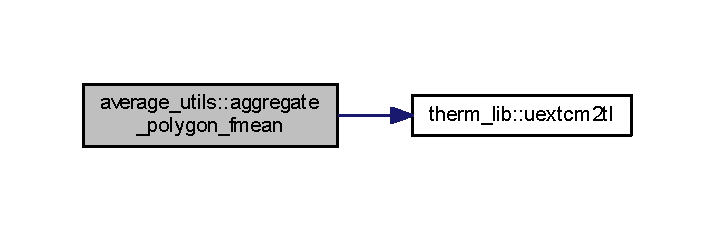
\includegraphics[width=343pt]{namespaceaverage__utils_a90965230835c19a82d90127089235c76_cgraph}
\end{center}
\end{figure}




Here is the caller graph for this function\+:\nopagebreak
\begin{figure}[H]
\begin{center}
\leavevmode
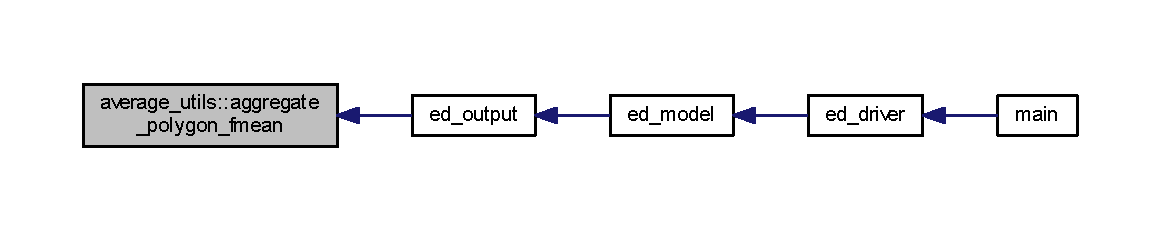
\includegraphics[width=350pt]{namespaceaverage__utils_a90965230835c19a82d90127089235c76_icgraph}
\end{center}
\end{figure}


\index{average\+\_\+utils@{average\+\_\+utils}!integrate\+\_\+ed\+\_\+dmean\+\_\+vars@{integrate\+\_\+ed\+\_\+dmean\+\_\+vars}}
\index{integrate\+\_\+ed\+\_\+dmean\+\_\+vars@{integrate\+\_\+ed\+\_\+dmean\+\_\+vars}!average\+\_\+utils@{average\+\_\+utils}}
\subsubsection[{\texorpdfstring{integrate\+\_\+ed\+\_\+dmean\+\_\+vars(cgrid)}{integrate_ed_dmean_vars(cgrid)}}]{\setlength{\rightskip}{0pt plus 5cm}subroutine average\+\_\+utils\+::integrate\+\_\+ed\+\_\+dmean\+\_\+vars (
\begin{DoxyParamCaption}
\item[{type({\bf edtype}), target}]{cgrid}
\end{DoxyParamCaption}
)}\hypertarget{namespaceaverage__utils_a985b401d85dd857f44371dd2c3e7c40c}{}\label{namespaceaverage__utils_a985b401d85dd857f44371dd2c3e7c40c}
\index{average\+\_\+utils@{average\+\_\+utils}!integrate\+\_\+ed\+\_\+fmean\+\_\+met\+\_\+vars@{integrate\+\_\+ed\+\_\+fmean\+\_\+met\+\_\+vars}}
\index{integrate\+\_\+ed\+\_\+fmean\+\_\+met\+\_\+vars@{integrate\+\_\+ed\+\_\+fmean\+\_\+met\+\_\+vars}!average\+\_\+utils@{average\+\_\+utils}}
\subsubsection[{\texorpdfstring{integrate\+\_\+ed\+\_\+fmean\+\_\+met\+\_\+vars(cgrid)}{integrate_ed_fmean_met_vars(cgrid)}}]{\setlength{\rightskip}{0pt plus 5cm}subroutine average\+\_\+utils\+::integrate\+\_\+ed\+\_\+fmean\+\_\+met\+\_\+vars (
\begin{DoxyParamCaption}
\item[{type({\bf edtype}), target}]{cgrid}
\end{DoxyParamCaption}
)}\hypertarget{namespaceaverage__utils_acf7868319b9242daa7eea553b25f2899}{}\label{namespaceaverage__utils_acf7868319b9242daa7eea553b25f2899}
\index{average\+\_\+utils@{average\+\_\+utils}!integrate\+\_\+ed\+\_\+mmean\+\_\+vars@{integrate\+\_\+ed\+\_\+mmean\+\_\+vars}}
\index{integrate\+\_\+ed\+\_\+mmean\+\_\+vars@{integrate\+\_\+ed\+\_\+mmean\+\_\+vars}!average\+\_\+utils@{average\+\_\+utils}}
\subsubsection[{\texorpdfstring{integrate\+\_\+ed\+\_\+mmean\+\_\+vars(cgrid)}{integrate_ed_mmean_vars(cgrid)}}]{\setlength{\rightskip}{0pt plus 5cm}subroutine average\+\_\+utils\+::integrate\+\_\+ed\+\_\+mmean\+\_\+vars (
\begin{DoxyParamCaption}
\item[{type({\bf edtype}), target}]{cgrid}
\end{DoxyParamCaption}
)}\hypertarget{namespaceaverage__utils_a24f0cd542ec9741c1bcc76e640498cd2}{}\label{namespaceaverage__utils_a24f0cd542ec9741c1bcc76e640498cd2}


Here is the call graph for this function\+:\nopagebreak
\begin{figure}[H]
\begin{center}
\leavevmode
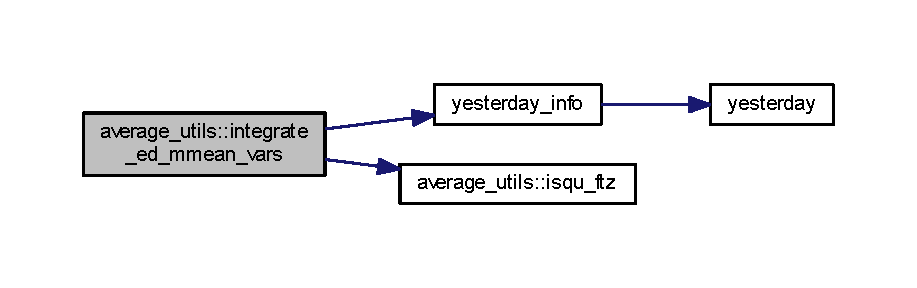
\includegraphics[width=350pt]{namespaceaverage__utils_a24f0cd542ec9741c1bcc76e640498cd2_cgraph}
\end{center}
\end{figure}


\index{average\+\_\+utils@{average\+\_\+utils}!integrate\+\_\+ed\+\_\+qmean\+\_\+vars@{integrate\+\_\+ed\+\_\+qmean\+\_\+vars}}
\index{integrate\+\_\+ed\+\_\+qmean\+\_\+vars@{integrate\+\_\+ed\+\_\+qmean\+\_\+vars}!average\+\_\+utils@{average\+\_\+utils}}
\subsubsection[{\texorpdfstring{integrate\+\_\+ed\+\_\+qmean\+\_\+vars(cgrid)}{integrate_ed_qmean_vars(cgrid)}}]{\setlength{\rightskip}{0pt plus 5cm}subroutine average\+\_\+utils\+::integrate\+\_\+ed\+\_\+qmean\+\_\+vars (
\begin{DoxyParamCaption}
\item[{type({\bf edtype}), target}]{cgrid}
\end{DoxyParamCaption}
)}\hypertarget{namespaceaverage__utils_af429d166f6097c18d6ab4ce05adbd31f}{}\label{namespaceaverage__utils_af429d166f6097c18d6ab4ce05adbd31f}


Here is the call graph for this function\+:\nopagebreak
\begin{figure}[H]
\begin{center}
\leavevmode
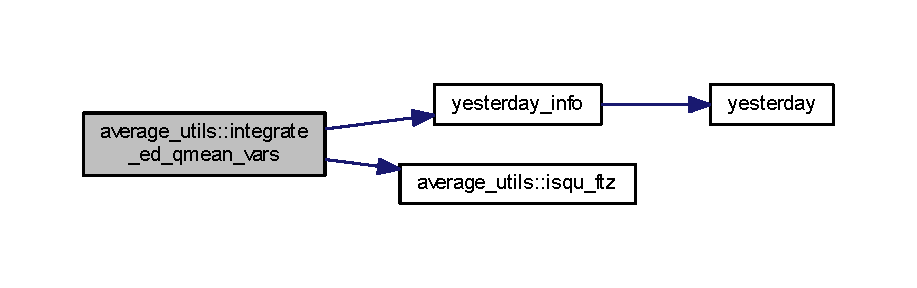
\includegraphics[width=350pt]{namespaceaverage__utils_af429d166f6097c18d6ab4ce05adbd31f_cgraph}
\end{center}
\end{figure}


\index{average\+\_\+utils@{average\+\_\+utils}!isqu\+\_\+ftz@{isqu\+\_\+ftz}}
\index{isqu\+\_\+ftz@{isqu\+\_\+ftz}!average\+\_\+utils@{average\+\_\+utils}}
\subsubsection[{\texorpdfstring{isqu\+\_\+ftz(x)}{isqu_ftz(x)}}]{\setlength{\rightskip}{0pt plus 5cm}real(kind=4) function average\+\_\+utils\+::isqu\+\_\+ftz (
\begin{DoxyParamCaption}
\item[{real(kind=4), intent(in)}]{x}
\end{DoxyParamCaption}
)}\hypertarget{namespaceaverage__utils_ac90817fe39c27153ed7bbee2cb856611}{}\label{namespaceaverage__utils_ac90817fe39c27153ed7bbee2cb856611}


Here is the caller graph for this function\+:\nopagebreak
\begin{figure}[H]
\begin{center}
\leavevmode
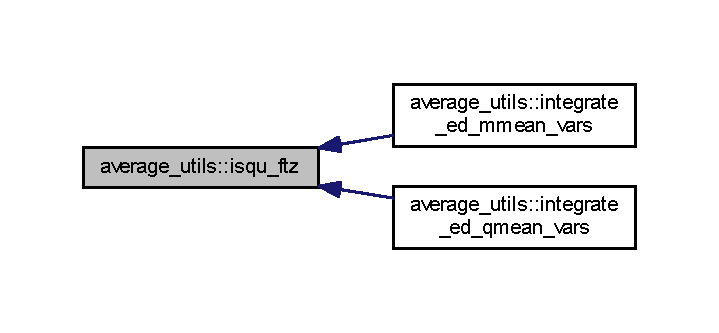
\includegraphics[width=345pt]{namespaceaverage__utils_ac90817fe39c27153ed7bbee2cb856611_icgraph}
\end{center}
\end{figure}


\index{average\+\_\+utils@{average\+\_\+utils}!normalize\+\_\+ed\+\_\+dmean\+\_\+vars@{normalize\+\_\+ed\+\_\+dmean\+\_\+vars}}
\index{normalize\+\_\+ed\+\_\+dmean\+\_\+vars@{normalize\+\_\+ed\+\_\+dmean\+\_\+vars}!average\+\_\+utils@{average\+\_\+utils}}
\subsubsection[{\texorpdfstring{normalize\+\_\+ed\+\_\+dmean\+\_\+vars(cgrid)}{normalize_ed_dmean_vars(cgrid)}}]{\setlength{\rightskip}{0pt plus 5cm}subroutine average\+\_\+utils\+::normalize\+\_\+ed\+\_\+dmean\+\_\+vars (
\begin{DoxyParamCaption}
\item[{type({\bf edtype}), target}]{cgrid}
\end{DoxyParamCaption}
)}\hypertarget{namespaceaverage__utils_a2203ebc403bfd01a55cf7aac61777819}{}\label{namespaceaverage__utils_a2203ebc403bfd01a55cf7aac61777819}


Here is the call graph for this function\+:\nopagebreak
\begin{figure}[H]
\begin{center}
\leavevmode
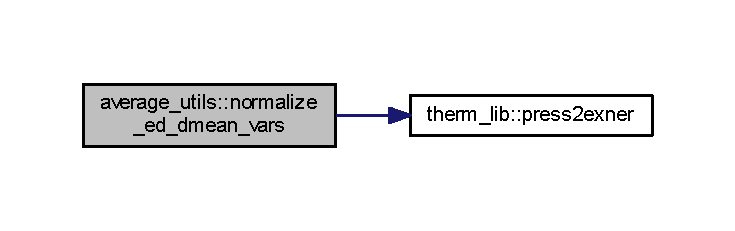
\includegraphics[width=350pt]{namespaceaverage__utils_a2203ebc403bfd01a55cf7aac61777819_cgraph}
\end{center}
\end{figure}


\index{average\+\_\+utils@{average\+\_\+utils}!normalize\+\_\+ed\+\_\+fmean\+\_\+vars@{normalize\+\_\+ed\+\_\+fmean\+\_\+vars}}
\index{normalize\+\_\+ed\+\_\+fmean\+\_\+vars@{normalize\+\_\+ed\+\_\+fmean\+\_\+vars}!average\+\_\+utils@{average\+\_\+utils}}
\subsubsection[{\texorpdfstring{normalize\+\_\+ed\+\_\+fmean\+\_\+vars(cgrid)}{normalize_ed_fmean_vars(cgrid)}}]{\setlength{\rightskip}{0pt plus 5cm}subroutine average\+\_\+utils\+::normalize\+\_\+ed\+\_\+fmean\+\_\+vars (
\begin{DoxyParamCaption}
\item[{type({\bf edtype}), target}]{cgrid}
\end{DoxyParamCaption}
)}\hypertarget{namespaceaverage__utils_a662a31926be61beb22be003b5ec40343}{}\label{namespaceaverage__utils_a662a31926be61beb22be003b5ec40343}


Here is the call graph for this function\+:\nopagebreak
\begin{figure}[H]
\begin{center}
\leavevmode
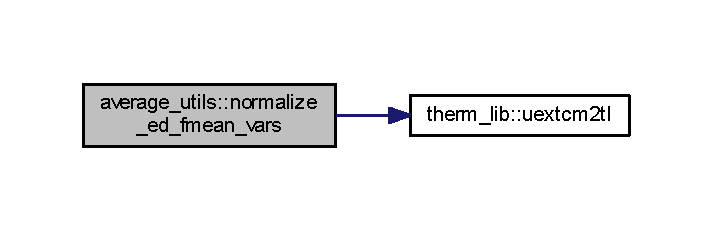
\includegraphics[width=342pt]{namespaceaverage__utils_a662a31926be61beb22be003b5ec40343_cgraph}
\end{center}
\end{figure}


\index{average\+\_\+utils@{average\+\_\+utils}!normalize\+\_\+ed\+\_\+mmean\+\_\+vars@{normalize\+\_\+ed\+\_\+mmean\+\_\+vars}}
\index{normalize\+\_\+ed\+\_\+mmean\+\_\+vars@{normalize\+\_\+ed\+\_\+mmean\+\_\+vars}!average\+\_\+utils@{average\+\_\+utils}}
\subsubsection[{\texorpdfstring{normalize\+\_\+ed\+\_\+mmean\+\_\+vars(cgrid)}{normalize_ed_mmean_vars(cgrid)}}]{\setlength{\rightskip}{0pt plus 5cm}subroutine average\+\_\+utils\+::normalize\+\_\+ed\+\_\+mmean\+\_\+vars (
\begin{DoxyParamCaption}
\item[{type({\bf edtype}), target}]{cgrid}
\end{DoxyParamCaption}
)}\hypertarget{namespaceaverage__utils_afce18c59b2e9d5605d22e4d356934bdb}{}\label{namespaceaverage__utils_afce18c59b2e9d5605d22e4d356934bdb}


Here is the call graph for this function\+:\nopagebreak
\begin{figure}[H]
\begin{center}
\leavevmode
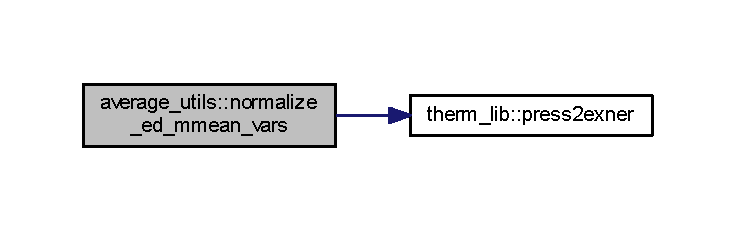
\includegraphics[width=350pt]{namespaceaverage__utils_afce18c59b2e9d5605d22e4d356934bdb_cgraph}
\end{center}
\end{figure}


\index{average\+\_\+utils@{average\+\_\+utils}!normalize\+\_\+ed\+\_\+qmean\+\_\+vars@{normalize\+\_\+ed\+\_\+qmean\+\_\+vars}}
\index{normalize\+\_\+ed\+\_\+qmean\+\_\+vars@{normalize\+\_\+ed\+\_\+qmean\+\_\+vars}!average\+\_\+utils@{average\+\_\+utils}}
\subsubsection[{\texorpdfstring{normalize\+\_\+ed\+\_\+qmean\+\_\+vars(cgrid)}{normalize_ed_qmean_vars(cgrid)}}]{\setlength{\rightskip}{0pt plus 5cm}subroutine average\+\_\+utils\+::normalize\+\_\+ed\+\_\+qmean\+\_\+vars (
\begin{DoxyParamCaption}
\item[{type({\bf edtype}), target}]{cgrid}
\end{DoxyParamCaption}
)}\hypertarget{namespaceaverage__utils_ad7f232f9a24079c3430b005098729615}{}\label{namespaceaverage__utils_ad7f232f9a24079c3430b005098729615}


Here is the call graph for this function\+:\nopagebreak
\begin{figure}[H]
\begin{center}
\leavevmode
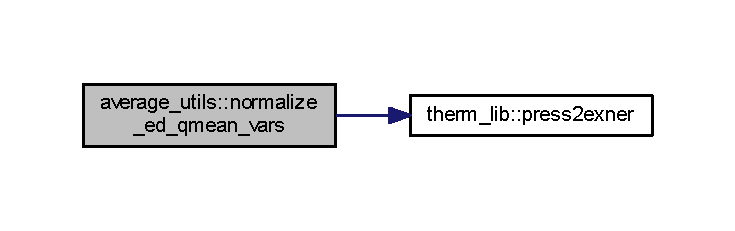
\includegraphics[width=350pt]{namespaceaverage__utils_ad7f232f9a24079c3430b005098729615_cgraph}
\end{center}
\end{figure}


\index{average\+\_\+utils@{average\+\_\+utils}!normalize\+\_\+ed\+\_\+today\+\_\+vars@{normalize\+\_\+ed\+\_\+today\+\_\+vars}}
\index{normalize\+\_\+ed\+\_\+today\+\_\+vars@{normalize\+\_\+ed\+\_\+today\+\_\+vars}!average\+\_\+utils@{average\+\_\+utils}}
\subsubsection[{\texorpdfstring{normalize\+\_\+ed\+\_\+today\+\_\+vars(cgrid)}{normalize_ed_today_vars(cgrid)}}]{\setlength{\rightskip}{0pt plus 5cm}subroutine average\+\_\+utils\+::normalize\+\_\+ed\+\_\+today\+\_\+vars (
\begin{DoxyParamCaption}
\item[{type({\bf edtype}), target}]{cgrid}
\end{DoxyParamCaption}
)}\hypertarget{namespaceaverage__utils_a538e2e59c7c2889ae624b6e1d2a9e5f2}{}\label{namespaceaverage__utils_a538e2e59c7c2889ae624b6e1d2a9e5f2}


Here is the caller graph for this function\+:\nopagebreak
\begin{figure}[H]
\begin{center}
\leavevmode
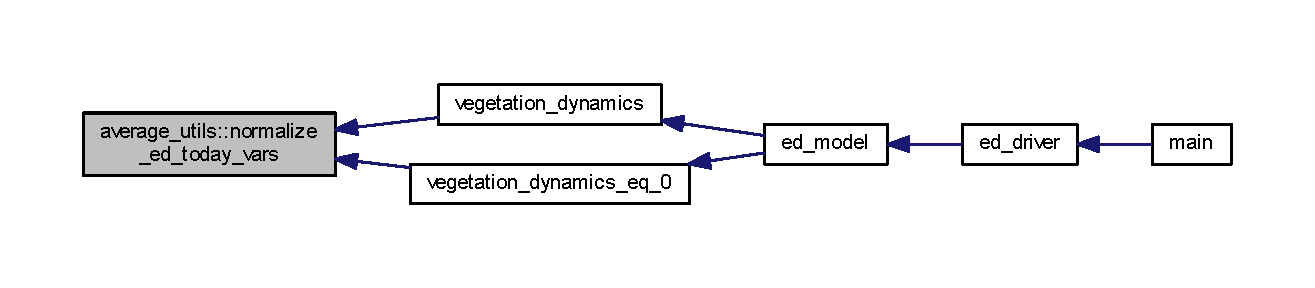
\includegraphics[width=350pt]{namespaceaverage__utils_a538e2e59c7c2889ae624b6e1d2a9e5f2_icgraph}
\end{center}
\end{figure}


\index{average\+\_\+utils@{average\+\_\+utils}!normalize\+\_\+ed\+\_\+todaynpp\+\_\+vars@{normalize\+\_\+ed\+\_\+todaynpp\+\_\+vars}}
\index{normalize\+\_\+ed\+\_\+todaynpp\+\_\+vars@{normalize\+\_\+ed\+\_\+todaynpp\+\_\+vars}!average\+\_\+utils@{average\+\_\+utils}}
\subsubsection[{\texorpdfstring{normalize\+\_\+ed\+\_\+todaynpp\+\_\+vars(cgrid)}{normalize_ed_todaynpp_vars(cgrid)}}]{\setlength{\rightskip}{0pt plus 5cm}subroutine average\+\_\+utils\+::normalize\+\_\+ed\+\_\+todaynpp\+\_\+vars (
\begin{DoxyParamCaption}
\item[{type({\bf edtype}), target}]{cgrid}
\end{DoxyParamCaption}
)}\hypertarget{namespaceaverage__utils_a446f9090fbbcf3eb12f4b9231d946e89}{}\label{namespaceaverage__utils_a446f9090fbbcf3eb12f4b9231d946e89}
\index{average\+\_\+utils@{average\+\_\+utils}!update\+\_\+ed\+\_\+yearly\+\_\+vars@{update\+\_\+ed\+\_\+yearly\+\_\+vars}}
\index{update\+\_\+ed\+\_\+yearly\+\_\+vars@{update\+\_\+ed\+\_\+yearly\+\_\+vars}!average\+\_\+utils@{average\+\_\+utils}}
\subsubsection[{\texorpdfstring{update\+\_\+ed\+\_\+yearly\+\_\+vars(cgrid)}{update_ed_yearly_vars(cgrid)}}]{\setlength{\rightskip}{0pt plus 5cm}subroutine average\+\_\+utils\+::update\+\_\+ed\+\_\+yearly\+\_\+vars (
\begin{DoxyParamCaption}
\item[{type({\bf edtype}), target}]{cgrid}
\end{DoxyParamCaption}
)}\hypertarget{namespaceaverage__utils_a81384775dd05dba144bf83e9731d5275}{}\label{namespaceaverage__utils_a81384775dd05dba144bf83e9731d5275}


Here is the caller graph for this function\+:\nopagebreak
\begin{figure}[H]
\begin{center}
\leavevmode
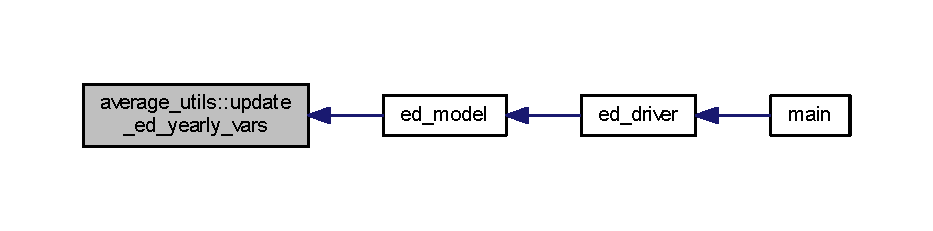
\includegraphics[width=350pt]{namespaceaverage__utils_a81384775dd05dba144bf83e9731d5275_icgraph}
\end{center}
\end{figure}


\index{average\+\_\+utils@{average\+\_\+utils}!zero\+\_\+ed\+\_\+dmean\+\_\+vars@{zero\+\_\+ed\+\_\+dmean\+\_\+vars}}
\index{zero\+\_\+ed\+\_\+dmean\+\_\+vars@{zero\+\_\+ed\+\_\+dmean\+\_\+vars}!average\+\_\+utils@{average\+\_\+utils}}
\subsubsection[{\texorpdfstring{zero\+\_\+ed\+\_\+dmean\+\_\+vars(cgrid)}{zero_ed_dmean_vars(cgrid)}}]{\setlength{\rightskip}{0pt plus 5cm}subroutine average\+\_\+utils\+::zero\+\_\+ed\+\_\+dmean\+\_\+vars (
\begin{DoxyParamCaption}
\item[{type({\bf edtype}), target}]{cgrid}
\end{DoxyParamCaption}
)}\hypertarget{namespaceaverage__utils_af1a2224da3c590c5645db8efa5c16c9f}{}\label{namespaceaverage__utils_af1a2224da3c590c5645db8efa5c16c9f}
\index{average\+\_\+utils@{average\+\_\+utils}!zero\+\_\+ed\+\_\+fmean\+\_\+vars@{zero\+\_\+ed\+\_\+fmean\+\_\+vars}}
\index{zero\+\_\+ed\+\_\+fmean\+\_\+vars@{zero\+\_\+ed\+\_\+fmean\+\_\+vars}!average\+\_\+utils@{average\+\_\+utils}}
\subsubsection[{\texorpdfstring{zero\+\_\+ed\+\_\+fmean\+\_\+vars(cgrid)}{zero_ed_fmean_vars(cgrid)}}]{\setlength{\rightskip}{0pt plus 5cm}subroutine average\+\_\+utils\+::zero\+\_\+ed\+\_\+fmean\+\_\+vars (
\begin{DoxyParamCaption}
\item[{type({\bf edtype}), target}]{cgrid}
\end{DoxyParamCaption}
)}\hypertarget{namespaceaverage__utils_a40f7a4a46972fb6b9c0fe90fdc73a173}{}\label{namespaceaverage__utils_a40f7a4a46972fb6b9c0fe90fdc73a173}
\index{average\+\_\+utils@{average\+\_\+utils}!zero\+\_\+ed\+\_\+mmean\+\_\+vars@{zero\+\_\+ed\+\_\+mmean\+\_\+vars}}
\index{zero\+\_\+ed\+\_\+mmean\+\_\+vars@{zero\+\_\+ed\+\_\+mmean\+\_\+vars}!average\+\_\+utils@{average\+\_\+utils}}
\subsubsection[{\texorpdfstring{zero\+\_\+ed\+\_\+mmean\+\_\+vars(cgrid)}{zero_ed_mmean_vars(cgrid)}}]{\setlength{\rightskip}{0pt plus 5cm}subroutine average\+\_\+utils\+::zero\+\_\+ed\+\_\+mmean\+\_\+vars (
\begin{DoxyParamCaption}
\item[{type({\bf edtype}), target}]{cgrid}
\end{DoxyParamCaption}
)}\hypertarget{namespaceaverage__utils_aa5221fd3b377dfe424dbdcb81b83c378}{}\label{namespaceaverage__utils_aa5221fd3b377dfe424dbdcb81b83c378}
\index{average\+\_\+utils@{average\+\_\+utils}!zero\+\_\+ed\+\_\+qmean\+\_\+vars@{zero\+\_\+ed\+\_\+qmean\+\_\+vars}}
\index{zero\+\_\+ed\+\_\+qmean\+\_\+vars@{zero\+\_\+ed\+\_\+qmean\+\_\+vars}!average\+\_\+utils@{average\+\_\+utils}}
\subsubsection[{\texorpdfstring{zero\+\_\+ed\+\_\+qmean\+\_\+vars(cgrid)}{zero_ed_qmean_vars(cgrid)}}]{\setlength{\rightskip}{0pt plus 5cm}subroutine average\+\_\+utils\+::zero\+\_\+ed\+\_\+qmean\+\_\+vars (
\begin{DoxyParamCaption}
\item[{type({\bf edtype}), target}]{cgrid}
\end{DoxyParamCaption}
)}\hypertarget{namespaceaverage__utils_a2e9cb2592327099345c147516b927f51}{}\label{namespaceaverage__utils_a2e9cb2592327099345c147516b927f51}
\index{average\+\_\+utils@{average\+\_\+utils}!zero\+\_\+ed\+\_\+today\+\_\+vars@{zero\+\_\+ed\+\_\+today\+\_\+vars}}
\index{zero\+\_\+ed\+\_\+today\+\_\+vars@{zero\+\_\+ed\+\_\+today\+\_\+vars}!average\+\_\+utils@{average\+\_\+utils}}
\subsubsection[{\texorpdfstring{zero\+\_\+ed\+\_\+today\+\_\+vars(cgrid)}{zero_ed_today_vars(cgrid)}}]{\setlength{\rightskip}{0pt plus 5cm}subroutine average\+\_\+utils\+::zero\+\_\+ed\+\_\+today\+\_\+vars (
\begin{DoxyParamCaption}
\item[{type({\bf edtype}), target}]{cgrid}
\end{DoxyParamCaption}
)}\hypertarget{namespaceaverage__utils_a6a92d00bf7112b127a596bd765cc12c6}{}\label{namespaceaverage__utils_a6a92d00bf7112b127a596bd765cc12c6}
\index{average\+\_\+utils@{average\+\_\+utils}!zero\+\_\+ed\+\_\+yearly\+\_\+vars@{zero\+\_\+ed\+\_\+yearly\+\_\+vars}}
\index{zero\+\_\+ed\+\_\+yearly\+\_\+vars@{zero\+\_\+ed\+\_\+yearly\+\_\+vars}!average\+\_\+utils@{average\+\_\+utils}}
\subsubsection[{\texorpdfstring{zero\+\_\+ed\+\_\+yearly\+\_\+vars(cgrid)}{zero_ed_yearly_vars(cgrid)}}]{\setlength{\rightskip}{0pt plus 5cm}subroutine average\+\_\+utils\+::zero\+\_\+ed\+\_\+yearly\+\_\+vars (
\begin{DoxyParamCaption}
\item[{type({\bf edtype}), target}]{cgrid}
\end{DoxyParamCaption}
)}\hypertarget{namespaceaverage__utils_a81df7cc84b1d62f7fb950e91d410abbd}{}\label{namespaceaverage__utils_a81df7cc84b1d62f7fb950e91d410abbd}

\hypertarget{namespacebudget__utils}{}\section{budget\+\_\+utils Module Reference}
\label{namespacebudget__utils}\index{budget\+\_\+utils@{budget\+\_\+utils}}
\subsection*{Functions/\+Subroutines}
\begin{DoxyCompactItemize}
\item 
subroutine \hyperlink{namespacebudget__utils_ad8835ee763cd964432b44e0a3d00e3da}{update\+\_\+budget} (csite, lsl, ipaa, ipaz)
\item 
subroutine \hyperlink{namespacebudget__utils_ade80ff8e17018f7bd86015ee5f20375e}{compute\+\_\+budget} (csite, lsl, pcpg, qpcpg, ipa, wcurr\+\_\+loss2atm, ecurr\+\_\+netrad                                                                                                                                               ,ecurr\+\_\+loss2atm, co2curr\+\_\+loss2atm, wcurr\+\_\+loss2drainage                                                                                                                                                   ,ecurr\+\_\+loss2drainage, wcurr\+\_\+loss2runoff, ecurr\+\_\+loss2runoff                                                                                                                                   ,site\+\_\+area, cbudget\+\_\+nep, old\+\_\+can\+\_\+enthalpy, old\+\_\+can\+\_\+shv                                                                                                                                                       ,old\+\_\+can\+\_\+co2, old\+\_\+can\+\_\+rhos, old\+\_\+can\+\_\+temp, old\+\_\+can\+\_\+prss)
\item 
real function \hyperlink{namespacebudget__utils_ad0c764047c557100b3a3cdcd836103a0}{compute\+\_\+water\+\_\+storage} (csite, lsl, ipa)
\item 
real function \hyperlink{namespacebudget__utils_a6111a1c211ecef562368c8635f64af45}{compute\+\_\+netrad} (csite, ipa)
\item 
real function \hyperlink{namespacebudget__utils_a319c5f7252c344bcebbd162593e25ec8}{compute\+\_\+energy\+\_\+storage} (csite, lsl, ipa)
\item 
subroutine \hyperlink{namespacebudget__utils_a117874382f22a7cb0883681d23606828}{sum\+\_\+plant\+\_\+cfluxes} (csite, ipa, gpp, leaf\+\_\+resp, root\+\_\+resp, leaf\+\_\+growth\+\_\+resp                                                                                                                                               ,root\+\_\+growth\+\_\+resp, sapa\+\_\+growth\+\_\+resp, sapb\+\_\+growth\+\_\+resp                                                                                                                                                       ,leaf\+\_\+storage\+\_\+resp, root\+\_\+storage\+\_\+resp, sapa\+\_\+storage\+\_\+resp                                                                                                                                           ,sapb\+\_\+storage\+\_\+resp)
\item 
real function \hyperlink{namespacebudget__utils_aa1c4f8466010b1673f2914f1bfe9b6ee}{compute\+\_\+co2\+\_\+storage} (csite, ipa)
\item 
real function \hyperlink{namespacebudget__utils_ae7ad8d90c28490b0b1c920e7a2656345}{ddens\+\_\+dt\+\_\+effect} (old\+\_\+rhos, new\+\_\+rhos, old\+\_\+prop, new\+\_\+prop, can\+\_\+depth, multi)
\end{DoxyCompactItemize}


\subsection{Function/\+Subroutine Documentation}
\index{budget\+\_\+utils@{budget\+\_\+utils}!compute\+\_\+budget@{compute\+\_\+budget}}
\index{compute\+\_\+budget@{compute\+\_\+budget}!budget\+\_\+utils@{budget\+\_\+utils}}
\subsubsection[{\texorpdfstring{compute\+\_\+budget(csite, lsl, pcpg, qpcpg, ipa, wcurr\+\_\+loss2atm, ecurr\+\_\+netrad                                                                                                                                               ,ecurr\+\_\+loss2atm, co2curr\+\_\+loss2atm, wcurr\+\_\+loss2drainage                                                                                                                                                   ,ecurr\+\_\+loss2drainage, wcurr\+\_\+loss2runoff, ecurr\+\_\+loss2runoff                                                                                                                                   ,site\+\_\+area, cbudget\+\_\+nep, old\+\_\+can\+\_\+enthalpy, old\+\_\+can\+\_\+shv                                                                                                                                                       ,old\+\_\+can\+\_\+co2, old\+\_\+can\+\_\+rhos, old\+\_\+can\+\_\+temp, old\+\_\+can\+\_\+prss)}{compute_budget(csite, lsl, pcpg, qpcpg, ipa, wcurr_loss2atm, ecurr_netrad                                                                                                                                               ,ecurr_loss2atm, co2curr_loss2atm, wcurr_loss2drainage                                                                                                                                                   ,ecurr_loss2drainage, wcurr_loss2runoff, ecurr_loss2runoff                                                                                                                                   ,site_area, cbudget_nep, old_can_enthalpy, old_can_shv                                                                                                                                                       ,old_can_co2, old_can_rhos, old_can_temp, old_can_prss)}}]{\setlength{\rightskip}{0pt plus 5cm}subroutine budget\+\_\+utils\+::compute\+\_\+budget (
\begin{DoxyParamCaption}
\item[{type({\bf sitetype}), target}]{csite, }
\item[{integer, intent(in)}]{lsl, }
\item[{real, intent(inout)}]{pcpg, }
\item[{real, intent(inout)}]{qpcpg, }
\item[{integer, intent(in)}]{ipa, }
\item[{real, intent(inout)}]{wcurr\+\_\+loss2atm, }
\item[{real, intent(inout)}]{ecurr\+\_\+netrad, }
\item[{real, intent(inout)}]{ecurr\+\_\+loss2atm, }
\item[{real, intent(inout)}]{co2curr\+\_\+loss2atm, }
\item[{real, intent(inout)}]{wcurr\+\_\+loss2drainage, }
\item[{real, intent(inout)}]{ecurr\+\_\+loss2drainage, }
\item[{real, intent(inout)}]{wcurr\+\_\+loss2runoff, }
\item[{real, intent(inout)}]{ecurr\+\_\+loss2runoff, }
\item[{real, intent(in)}]{site\+\_\+area, }
\item[{real, intent(inout)}]{cbudget\+\_\+nep, }
\item[{real, intent(in)}]{old\+\_\+can\+\_\+enthalpy, }
\item[{real, intent(in)}]{old\+\_\+can\+\_\+shv, }
\item[{real, intent(in)}]{old\+\_\+can\+\_\+co2, }
\item[{real, intent(in)}]{old\+\_\+can\+\_\+rhos, }
\item[{real, intent(in)}]{old\+\_\+can\+\_\+temp, }
\item[{real, intent(in)}]{old\+\_\+can\+\_\+prss}
\end{DoxyParamCaption}
)}\hypertarget{namespacebudget__utils_ade80ff8e17018f7bd86015ee5f20375e}{}\label{namespacebudget__utils_ade80ff8e17018f7bd86015ee5f20375e}


Here is the call graph for this function\+:\nopagebreak
\begin{figure}[H]
\begin{center}
\leavevmode
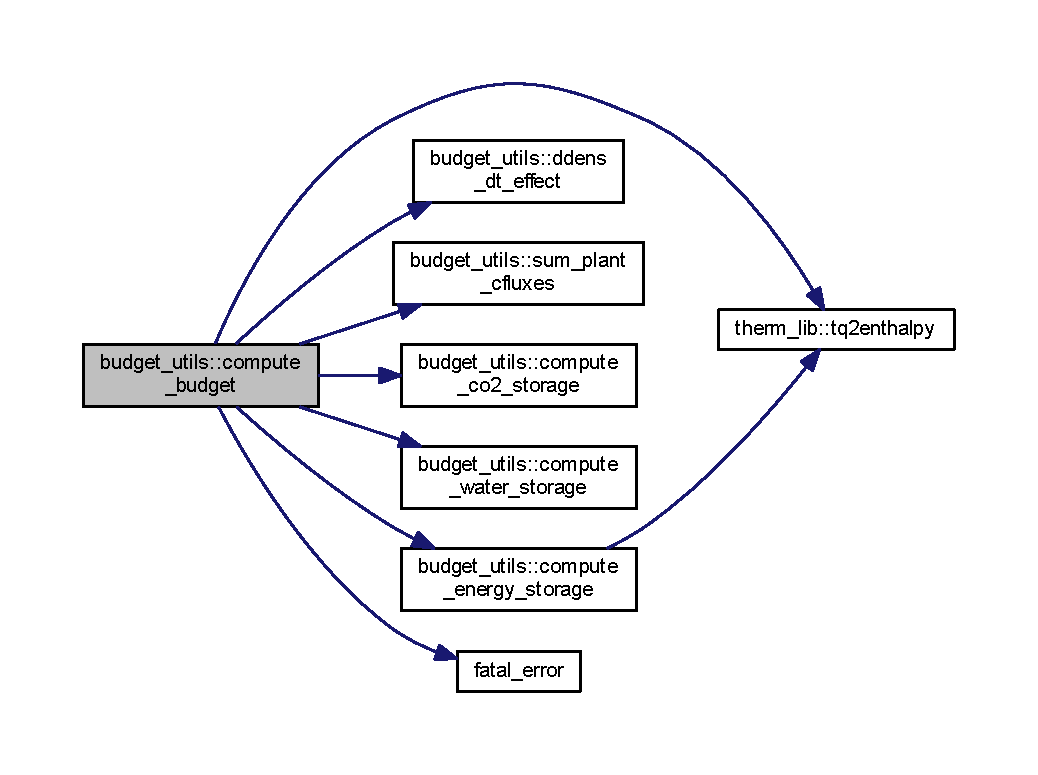
\includegraphics[width=350pt]{namespacebudget__utils_ade80ff8e17018f7bd86015ee5f20375e_cgraph}
\end{center}
\end{figure}


\index{budget\+\_\+utils@{budget\+\_\+utils}!compute\+\_\+co2\+\_\+storage@{compute\+\_\+co2\+\_\+storage}}
\index{compute\+\_\+co2\+\_\+storage@{compute\+\_\+co2\+\_\+storage}!budget\+\_\+utils@{budget\+\_\+utils}}
\subsubsection[{\texorpdfstring{compute\+\_\+co2\+\_\+storage(csite, ipa)}{compute_co2_storage(csite, ipa)}}]{\setlength{\rightskip}{0pt plus 5cm}real function budget\+\_\+utils\+::compute\+\_\+co2\+\_\+storage (
\begin{DoxyParamCaption}
\item[{type({\bf sitetype}), target}]{csite, }
\item[{integer, intent(in)}]{ipa}
\end{DoxyParamCaption}
)}\hypertarget{namespacebudget__utils_aa1c4f8466010b1673f2914f1bfe9b6ee}{}\label{namespacebudget__utils_aa1c4f8466010b1673f2914f1bfe9b6ee}


Here is the caller graph for this function\+:\nopagebreak
\begin{figure}[H]
\begin{center}
\leavevmode
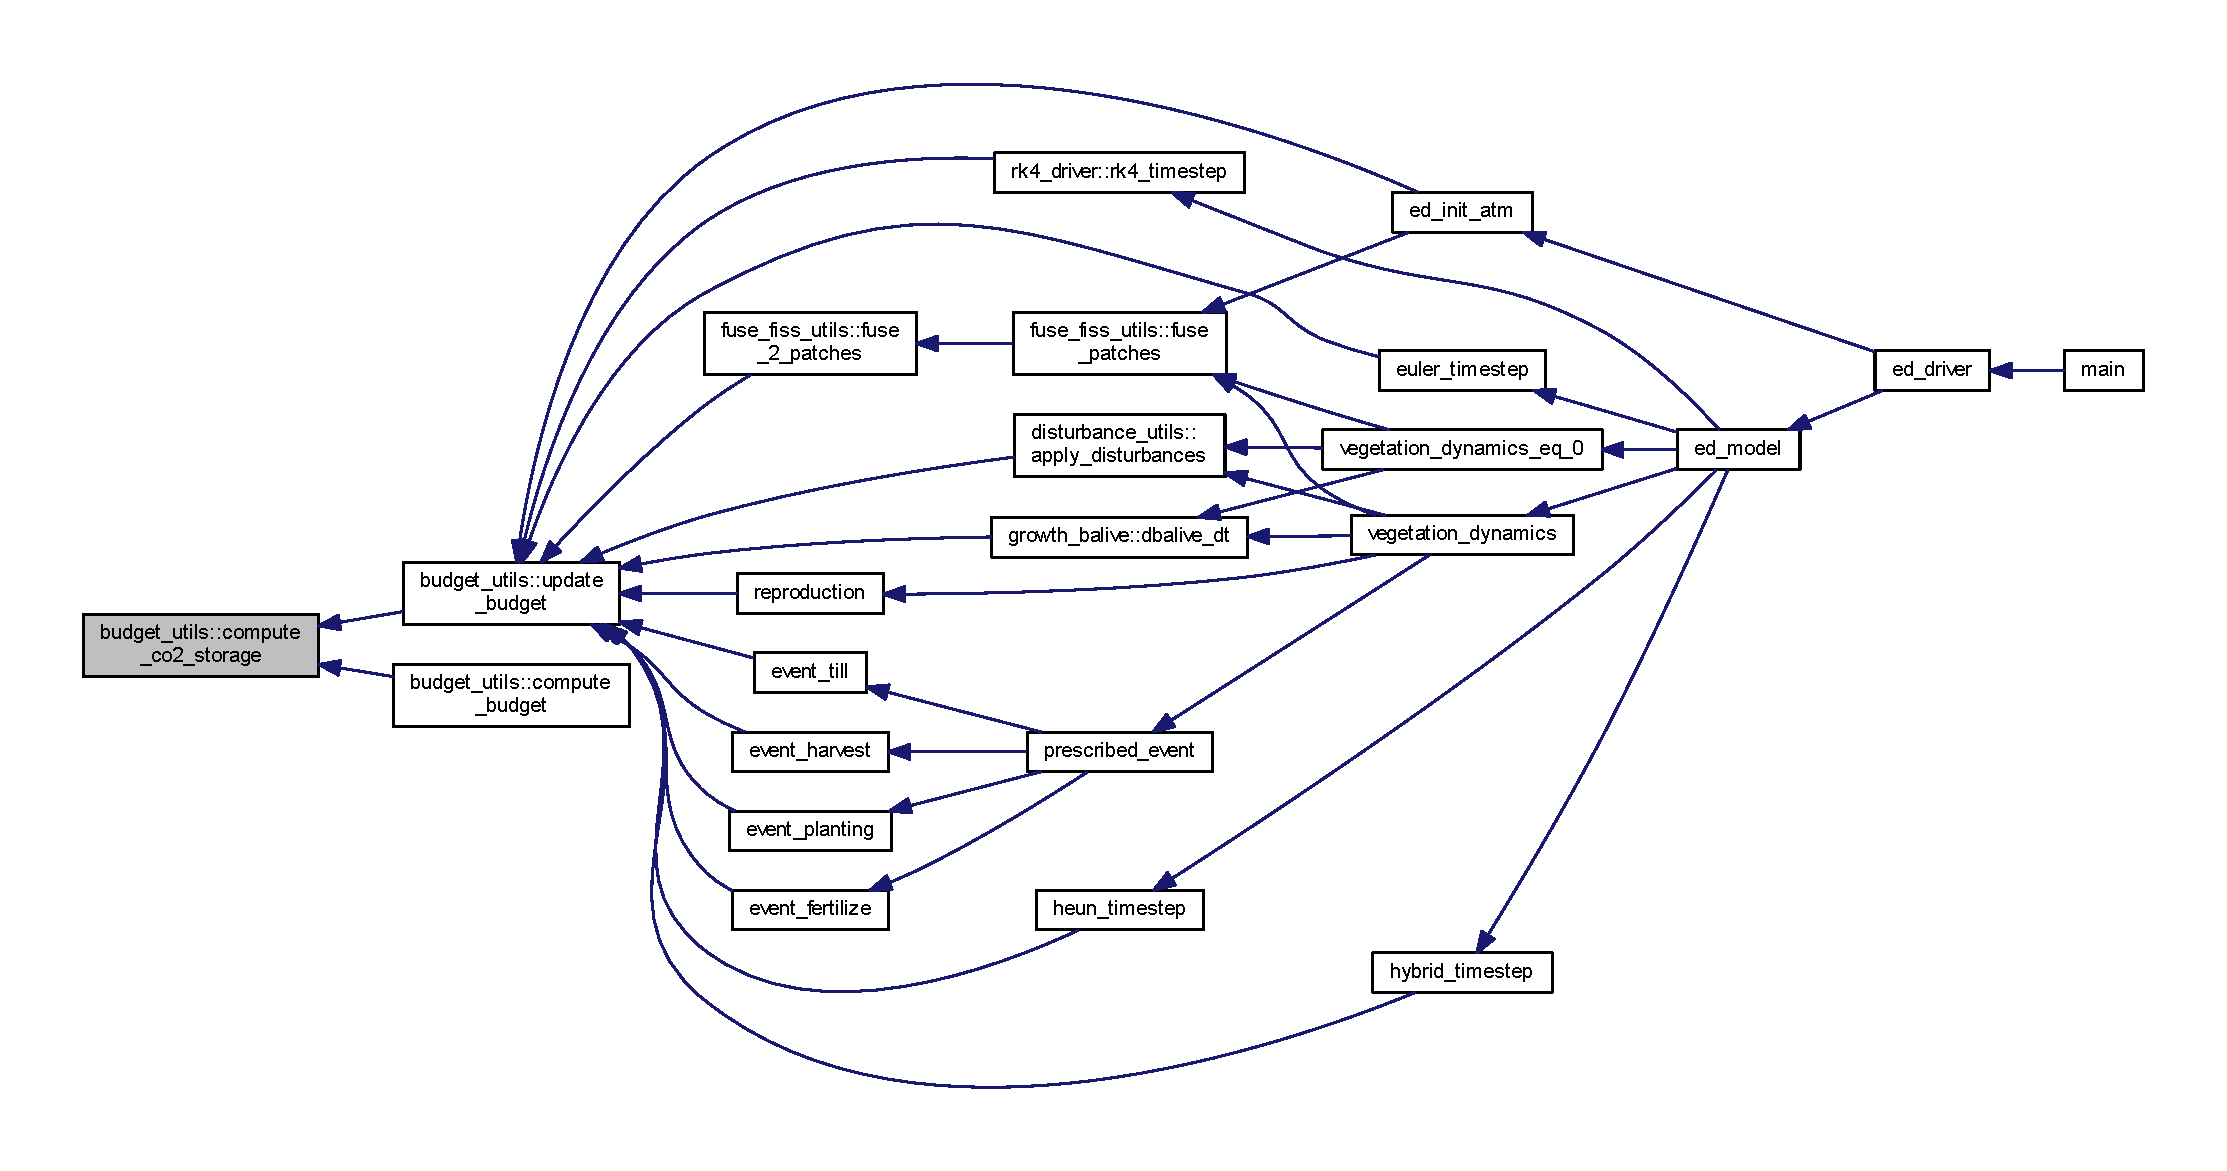
\includegraphics[width=350pt]{namespacebudget__utils_aa1c4f8466010b1673f2914f1bfe9b6ee_icgraph}
\end{center}
\end{figure}


\index{budget\+\_\+utils@{budget\+\_\+utils}!compute\+\_\+energy\+\_\+storage@{compute\+\_\+energy\+\_\+storage}}
\index{compute\+\_\+energy\+\_\+storage@{compute\+\_\+energy\+\_\+storage}!budget\+\_\+utils@{budget\+\_\+utils}}
\subsubsection[{\texorpdfstring{compute\+\_\+energy\+\_\+storage(csite, lsl, ipa)}{compute_energy_storage(csite, lsl, ipa)}}]{\setlength{\rightskip}{0pt plus 5cm}real function budget\+\_\+utils\+::compute\+\_\+energy\+\_\+storage (
\begin{DoxyParamCaption}
\item[{type({\bf sitetype}), target}]{csite, }
\item[{integer, intent(in)}]{lsl, }
\item[{integer, intent(in)}]{ipa}
\end{DoxyParamCaption}
)}\hypertarget{namespacebudget__utils_a319c5f7252c344bcebbd162593e25ec8}{}\label{namespacebudget__utils_a319c5f7252c344bcebbd162593e25ec8}


Here is the call graph for this function\+:\nopagebreak
\begin{figure}[H]
\begin{center}
\leavevmode
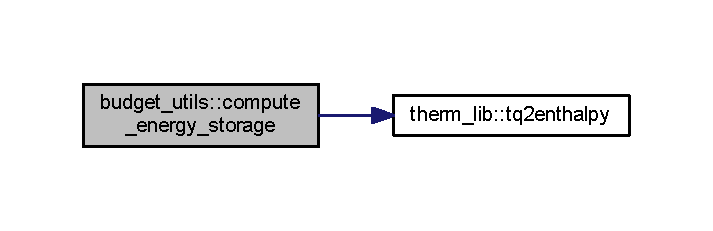
\includegraphics[width=342pt]{namespacebudget__utils_a319c5f7252c344bcebbd162593e25ec8_cgraph}
\end{center}
\end{figure}




Here is the caller graph for this function\+:\nopagebreak
\begin{figure}[H]
\begin{center}
\leavevmode
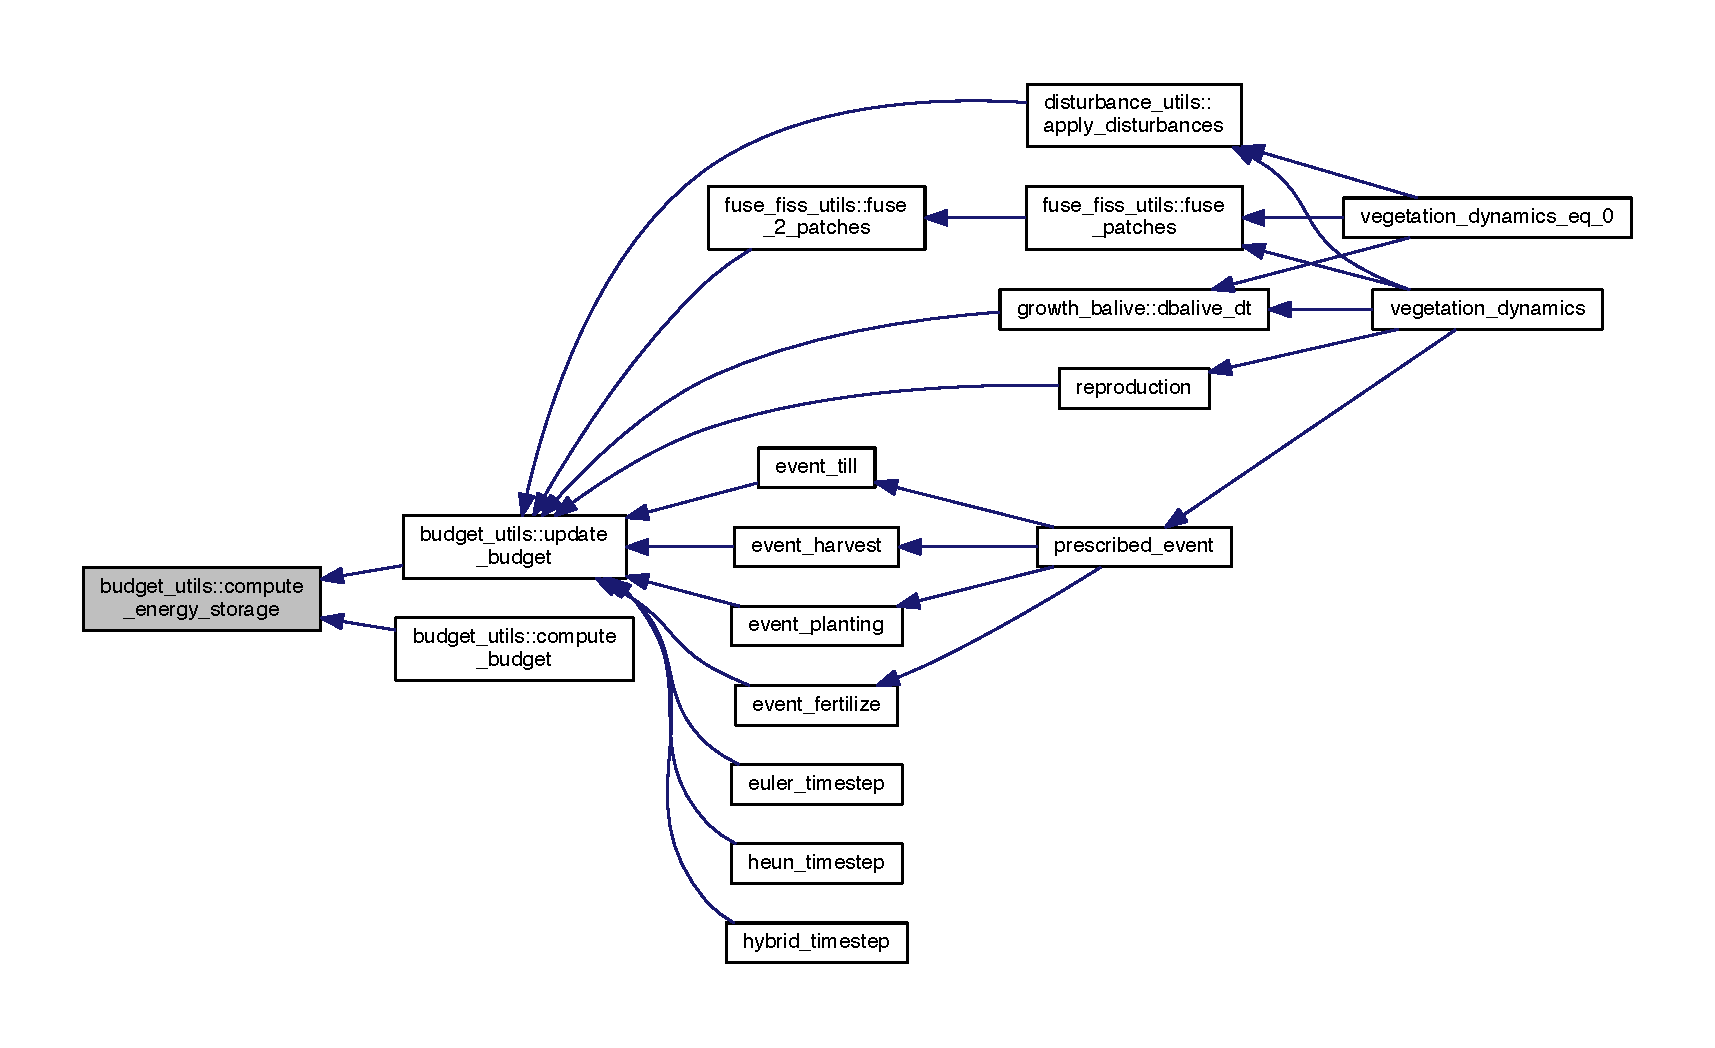
\includegraphics[width=350pt]{namespacebudget__utils_a319c5f7252c344bcebbd162593e25ec8_icgraph}
\end{center}
\end{figure}


\index{budget\+\_\+utils@{budget\+\_\+utils}!compute\+\_\+netrad@{compute\+\_\+netrad}}
\index{compute\+\_\+netrad@{compute\+\_\+netrad}!budget\+\_\+utils@{budget\+\_\+utils}}
\subsubsection[{\texorpdfstring{compute\+\_\+netrad(csite, ipa)}{compute_netrad(csite, ipa)}}]{\setlength{\rightskip}{0pt plus 5cm}real function budget\+\_\+utils\+::compute\+\_\+netrad (
\begin{DoxyParamCaption}
\item[{type({\bf sitetype}), target}]{csite, }
\item[{integer, intent(in)}]{ipa}
\end{DoxyParamCaption}
)}\hypertarget{namespacebudget__utils_a6111a1c211ecef562368c8635f64af45}{}\label{namespacebudget__utils_a6111a1c211ecef562368c8635f64af45}


Here is the caller graph for this function\+:\nopagebreak
\begin{figure}[H]
\begin{center}
\leavevmode
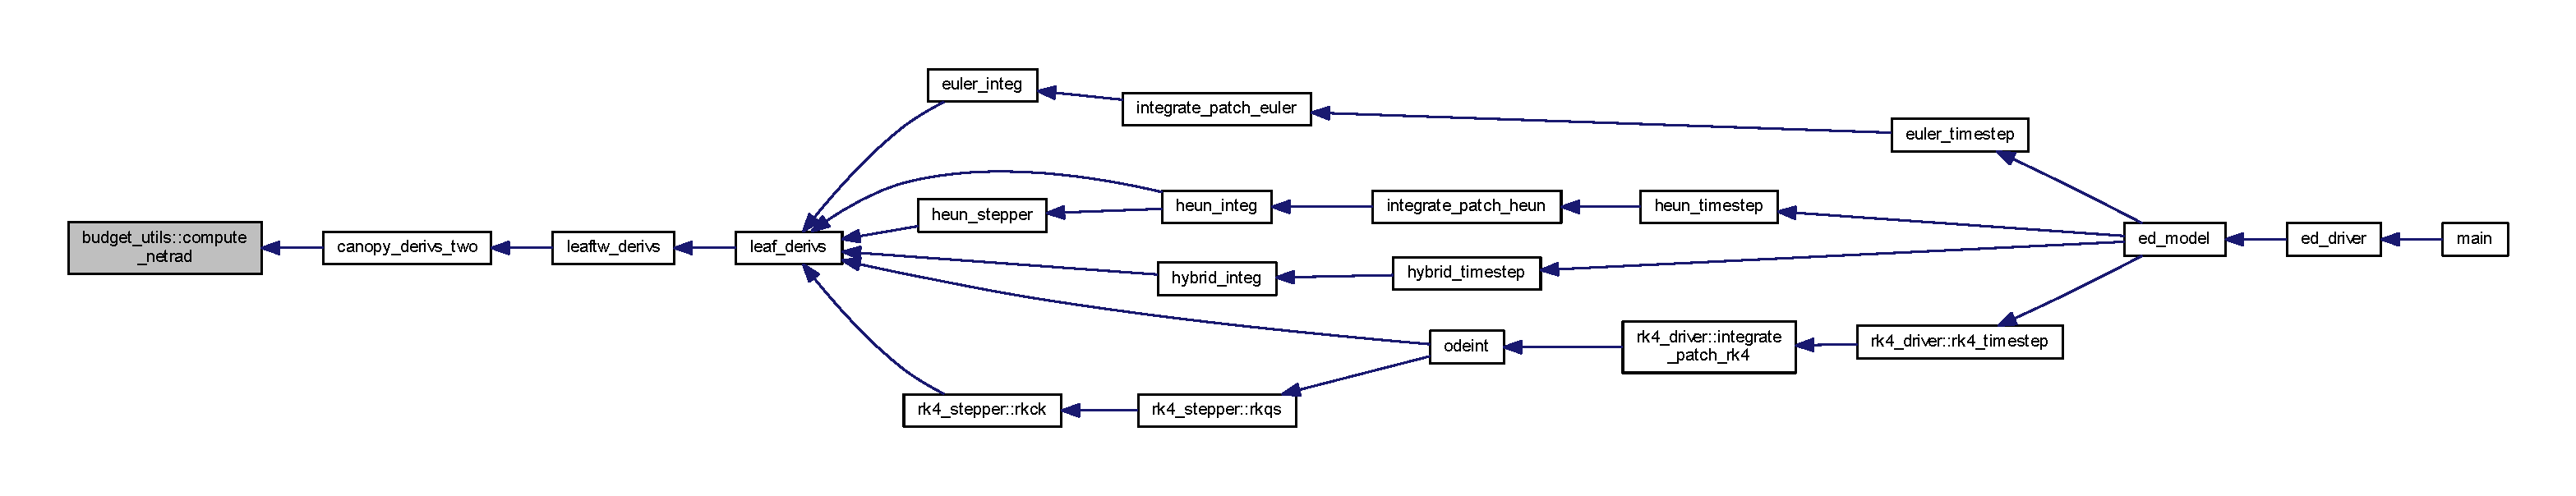
\includegraphics[width=350pt]{namespacebudget__utils_a6111a1c211ecef562368c8635f64af45_icgraph}
\end{center}
\end{figure}


\index{budget\+\_\+utils@{budget\+\_\+utils}!compute\+\_\+water\+\_\+storage@{compute\+\_\+water\+\_\+storage}}
\index{compute\+\_\+water\+\_\+storage@{compute\+\_\+water\+\_\+storage}!budget\+\_\+utils@{budget\+\_\+utils}}
\subsubsection[{\texorpdfstring{compute\+\_\+water\+\_\+storage(csite, lsl, ipa)}{compute_water_storage(csite, lsl, ipa)}}]{\setlength{\rightskip}{0pt plus 5cm}real function budget\+\_\+utils\+::compute\+\_\+water\+\_\+storage (
\begin{DoxyParamCaption}
\item[{type({\bf sitetype}), target}]{csite, }
\item[{integer, intent(in)}]{lsl, }
\item[{integer, intent(in)}]{ipa}
\end{DoxyParamCaption}
)}\hypertarget{namespacebudget__utils_ad0c764047c557100b3a3cdcd836103a0}{}\label{namespacebudget__utils_ad0c764047c557100b3a3cdcd836103a0}


Here is the caller graph for this function\+:\nopagebreak
\begin{figure}[H]
\begin{center}
\leavevmode
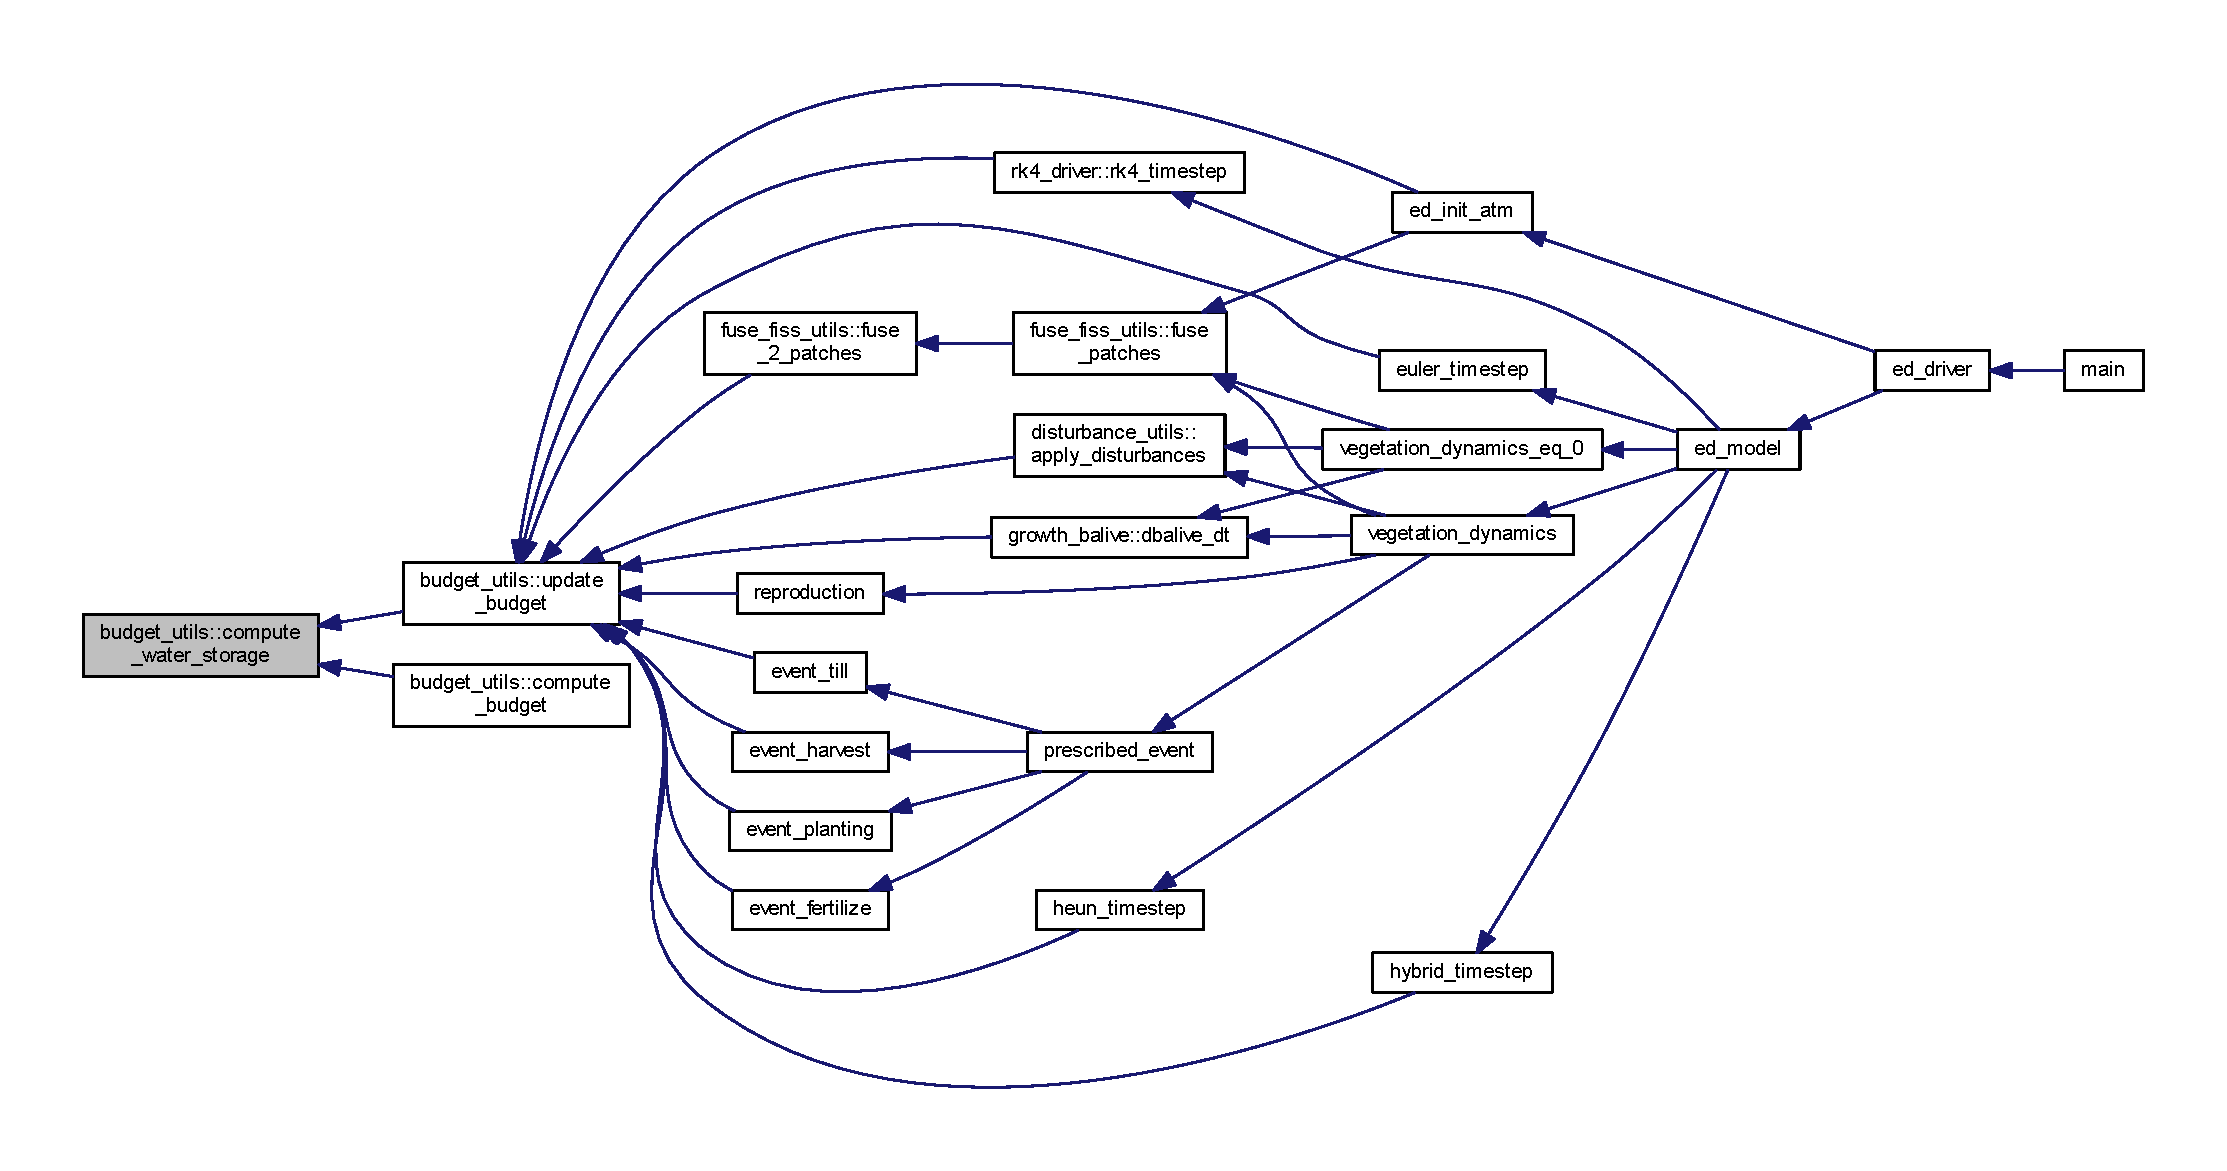
\includegraphics[width=350pt]{namespacebudget__utils_ad0c764047c557100b3a3cdcd836103a0_icgraph}
\end{center}
\end{figure}


\index{budget\+\_\+utils@{budget\+\_\+utils}!ddens\+\_\+dt\+\_\+effect@{ddens\+\_\+dt\+\_\+effect}}
\index{ddens\+\_\+dt\+\_\+effect@{ddens\+\_\+dt\+\_\+effect}!budget\+\_\+utils@{budget\+\_\+utils}}
\subsubsection[{\texorpdfstring{ddens\+\_\+dt\+\_\+effect(old\+\_\+rhos, new\+\_\+rhos, old\+\_\+prop, new\+\_\+prop, can\+\_\+depth, multi)}{ddens_dt_effect(old_rhos, new_rhos, old_prop, new_prop, can_depth, multi)}}]{\setlength{\rightskip}{0pt plus 5cm}real function budget\+\_\+utils\+::ddens\+\_\+dt\+\_\+effect (
\begin{DoxyParamCaption}
\item[{real, intent(in)}]{old\+\_\+rhos, }
\item[{real, intent(in)}]{new\+\_\+rhos, }
\item[{real, intent(in)}]{old\+\_\+prop, }
\item[{real, intent(in)}]{new\+\_\+prop, }
\item[{real, intent(in)}]{can\+\_\+depth, }
\item[{real, intent(in)}]{multi}
\end{DoxyParamCaption}
)}\hypertarget{namespacebudget__utils_ae7ad8d90c28490b0b1c920e7a2656345}{}\label{namespacebudget__utils_ae7ad8d90c28490b0b1c920e7a2656345}


Here is the caller graph for this function\+:\nopagebreak
\begin{figure}[H]
\begin{center}
\leavevmode
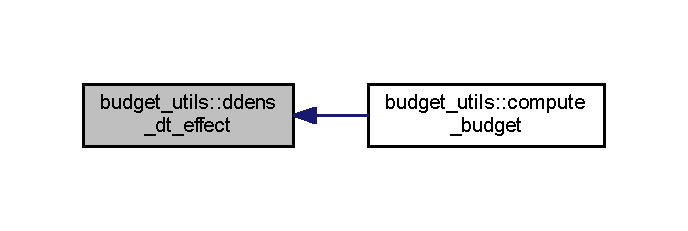
\includegraphics[width=330pt]{namespacebudget__utils_ae7ad8d90c28490b0b1c920e7a2656345_icgraph}
\end{center}
\end{figure}


\index{budget\+\_\+utils@{budget\+\_\+utils}!sum\+\_\+plant\+\_\+cfluxes@{sum\+\_\+plant\+\_\+cfluxes}}
\index{sum\+\_\+plant\+\_\+cfluxes@{sum\+\_\+plant\+\_\+cfluxes}!budget\+\_\+utils@{budget\+\_\+utils}}
\subsubsection[{\texorpdfstring{sum\+\_\+plant\+\_\+cfluxes(csite, ipa, gpp, leaf\+\_\+resp, root\+\_\+resp, leaf\+\_\+growth\+\_\+resp                                                                                                                                               ,root\+\_\+growth\+\_\+resp, sapa\+\_\+growth\+\_\+resp, sapb\+\_\+growth\+\_\+resp                                                                                                                                                       ,leaf\+\_\+storage\+\_\+resp, root\+\_\+storage\+\_\+resp, sapa\+\_\+storage\+\_\+resp                                                                                                                                           ,sapb\+\_\+storage\+\_\+resp)}{sum_plant_cfluxes(csite, ipa, gpp, leaf_resp, root_resp, leaf_growth_resp                                                                                                                                               ,root_growth_resp, sapa_growth_resp, sapb_growth_resp                                                                                                                                                       ,leaf_storage_resp, root_storage_resp, sapa_storage_resp                                                                                                                                           ,sapb_storage_resp)}}]{\setlength{\rightskip}{0pt plus 5cm}subroutine budget\+\_\+utils\+::sum\+\_\+plant\+\_\+cfluxes (
\begin{DoxyParamCaption}
\item[{type({\bf sitetype}), target}]{csite, }
\item[{integer, intent(in)}]{ipa, }
\item[{real, intent(out)}]{gpp, }
\item[{real, intent(out)}]{leaf\+\_\+resp, }
\item[{real, intent(out)}]{root\+\_\+resp, }
\item[{real, intent(out)}]{leaf\+\_\+growth\+\_\+resp, }
\item[{real, intent(out)}]{root\+\_\+growth\+\_\+resp, }
\item[{real, intent(out)}]{sapa\+\_\+growth\+\_\+resp, }
\item[{real, intent(out)}]{sapb\+\_\+growth\+\_\+resp, }
\item[{real, intent(out)}]{leaf\+\_\+storage\+\_\+resp, }
\item[{real, intent(out)}]{root\+\_\+storage\+\_\+resp, }
\item[{real, intent(out)}]{sapa\+\_\+storage\+\_\+resp, }
\item[{real, intent(out)}]{sapb\+\_\+storage\+\_\+resp}
\end{DoxyParamCaption}
)}\hypertarget{namespacebudget__utils_a117874382f22a7cb0883681d23606828}{}\label{namespacebudget__utils_a117874382f22a7cb0883681d23606828}


Here is the caller graph for this function\+:\nopagebreak
\begin{figure}[H]
\begin{center}
\leavevmode
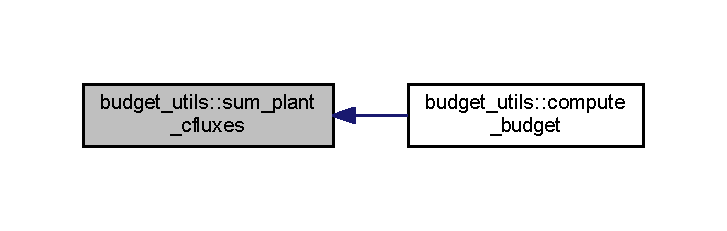
\includegraphics[width=349pt]{namespacebudget__utils_a117874382f22a7cb0883681d23606828_icgraph}
\end{center}
\end{figure}


\index{budget\+\_\+utils@{budget\+\_\+utils}!update\+\_\+budget@{update\+\_\+budget}}
\index{update\+\_\+budget@{update\+\_\+budget}!budget\+\_\+utils@{budget\+\_\+utils}}
\subsubsection[{\texorpdfstring{update\+\_\+budget(csite, lsl, ipaa, ipaz)}{update_budget(csite, lsl, ipaa, ipaz)}}]{\setlength{\rightskip}{0pt plus 5cm}subroutine budget\+\_\+utils\+::update\+\_\+budget (
\begin{DoxyParamCaption}
\item[{type({\bf sitetype}), target}]{csite, }
\item[{integer, intent(in)}]{lsl, }
\item[{integer, intent(in)}]{ipaa, }
\item[{integer, intent(in)}]{ipaz}
\end{DoxyParamCaption}
)}\hypertarget{namespacebudget__utils_ad8835ee763cd964432b44e0a3d00e3da}{}\label{namespacebudget__utils_ad8835ee763cd964432b44e0a3d00e3da}


Here is the call graph for this function\+:\nopagebreak
\begin{figure}[H]
\begin{center}
\leavevmode
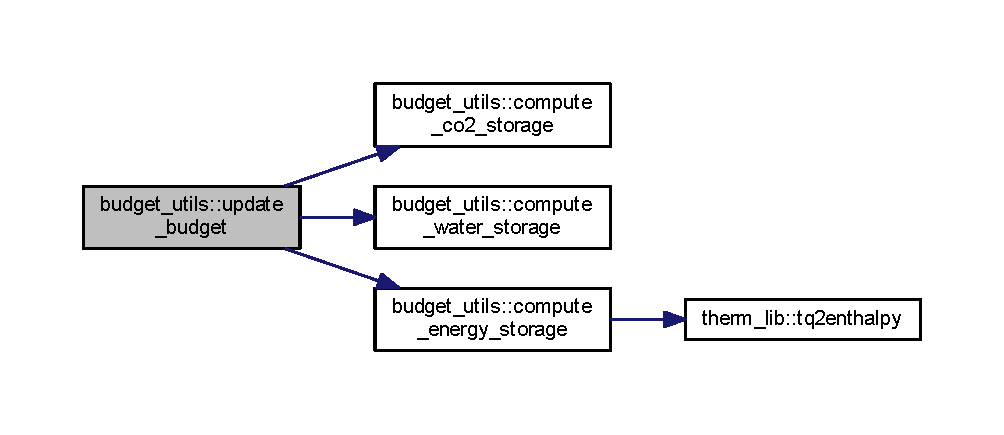
\includegraphics[width=350pt]{namespacebudget__utils_ad8835ee763cd964432b44e0a3d00e3da_cgraph}
\end{center}
\end{figure}




Here is the caller graph for this function\+:\nopagebreak
\begin{figure}[H]
\begin{center}
\leavevmode
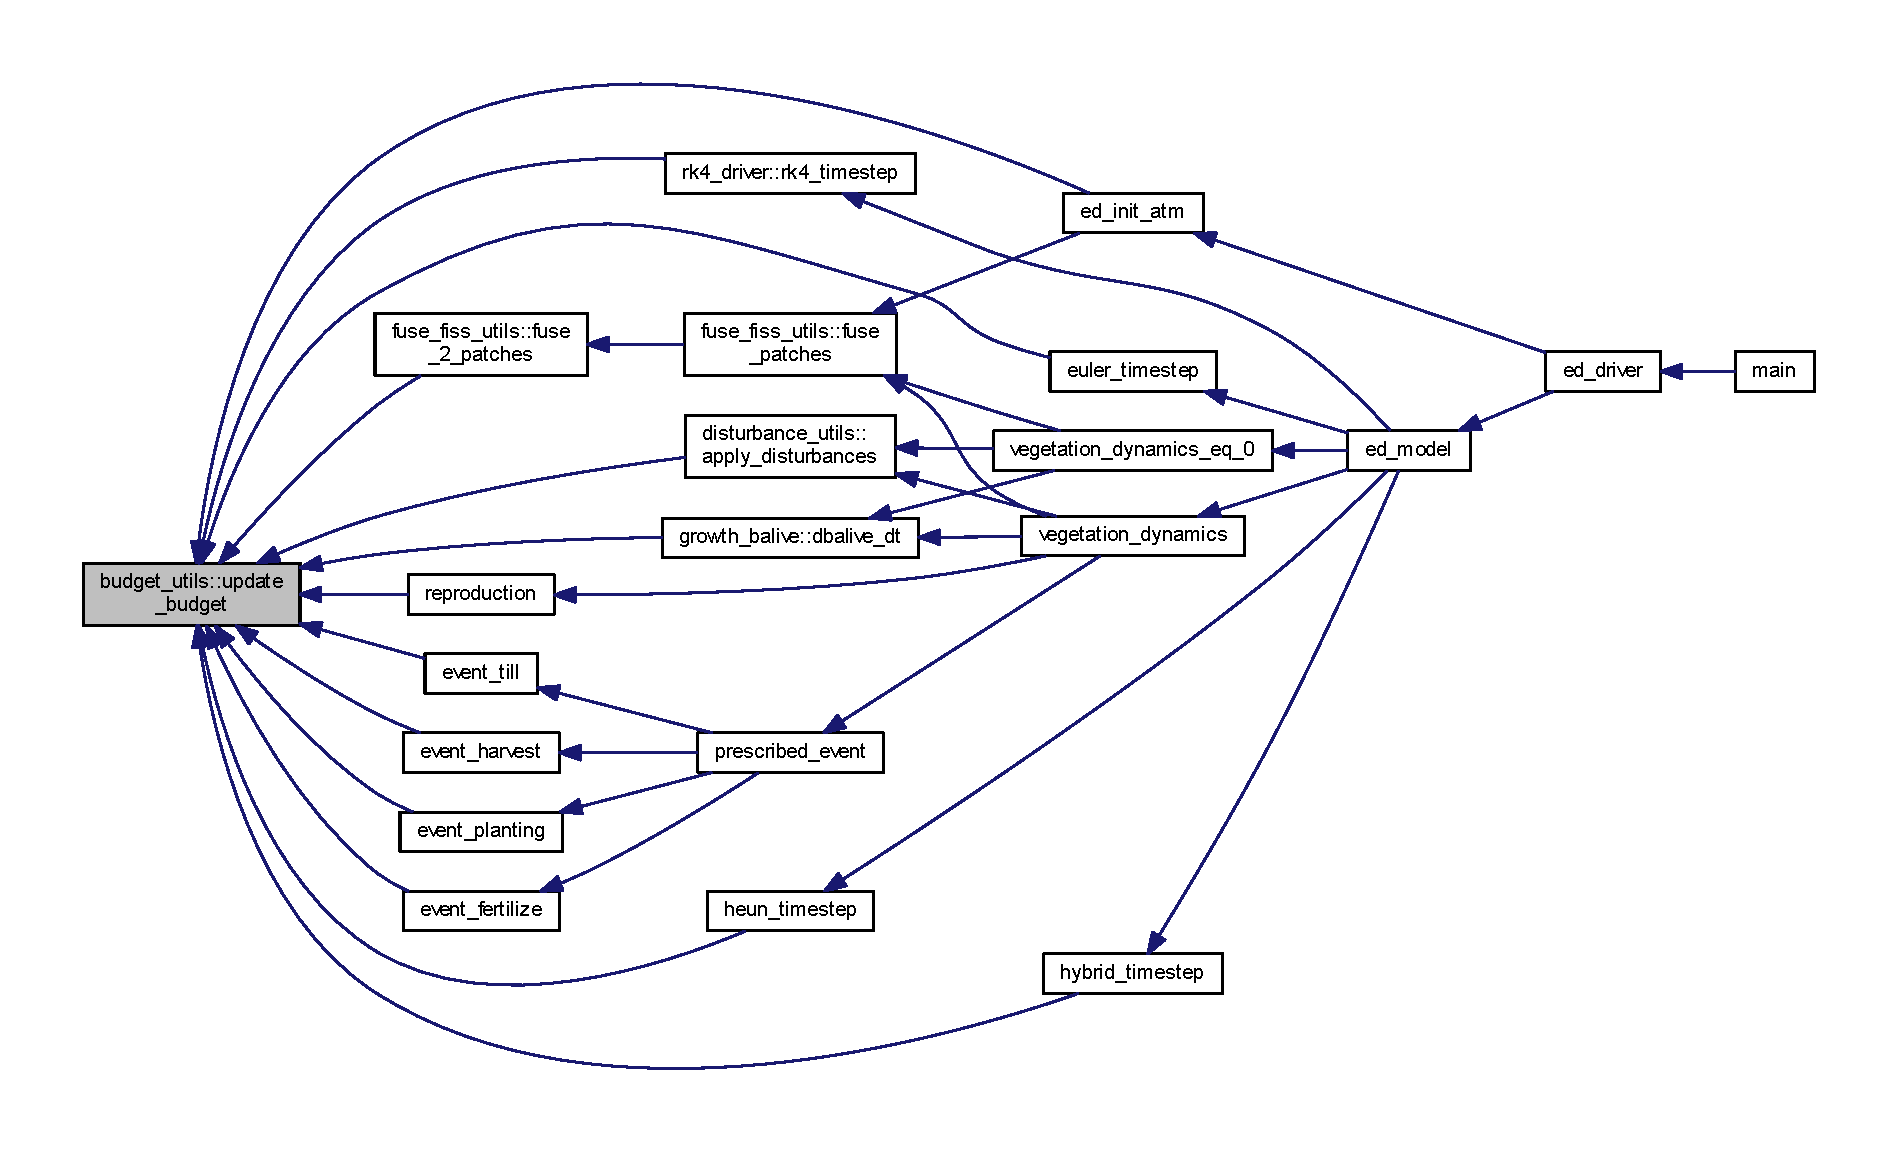
\includegraphics[width=350pt]{namespacebudget__utils_ad8835ee763cd964432b44e0a3d00e3da_icgraph}
\end{center}
\end{figure}



\hypertarget{namespacec34constants}{}\section{c34constants Module Reference}
\label{namespacec34constants}\index{c34constants@{c34constants}}
\subsection*{Data Types}
\begin{DoxyCompactItemize}
\item 
type \hyperlink{structc34constants_1_1carb__demand__vars}{carb\+\_\+demand\+\_\+vars}
\item 
type \hyperlink{structc34constants_1_1farq__consts}{farq\+\_\+consts}
\item 
type \hyperlink{structc34constants_1_1metinp__vars}{metinp\+\_\+vars}
\item 
type \hyperlink{structc34constants_1_1solution__vars}{solution\+\_\+vars}
\end{DoxyCompactItemize}
\subsection*{Functions/\+Subroutines}
\begin{DoxyCompactItemize}
\item 
subroutine \hyperlink{namespacec34constants_a2bf287654403f231d7936113aaeb9cf6}{copy\+\_\+solution} (source\+\_\+sol, target\+\_\+sol)
\end{DoxyCompactItemize}
\subsection*{Variables}
\begin{DoxyCompactItemize}
\item 
type(\hyperlink{structc34constants_1_1farq__consts}{farq\+\_\+consts}), dimension(\+:), pointer \hyperlink{namespacec34constants_a4a1314df0becf145f8a2365aa27d992d}{thispft}
\item 
type(\hyperlink{structc34constants_1_1metinp__vars}{metinp\+\_\+vars}), dimension(\+:), pointer \hyperlink{namespacec34constants_a6d1c98b7c360f24d485be8fc38bdd284}{met}
\item 
type(\hyperlink{structc34constants_1_1carb__demand__vars}{carb\+\_\+demand\+\_\+vars}), dimension(\+:), pointer \hyperlink{namespacec34constants_a844bf4288f019d9dcee7612f54d1e50c}{aparms}
\item 
type(\hyperlink{structc34constants_1_1solution__vars}{solution\+\_\+vars}), dimension(\+:), pointer \hyperlink{namespacec34constants_a5affd928720d3a40f01f1198b68b7fb3}{stopen}
\item 
type(\hyperlink{structc34constants_1_1solution__vars}{solution\+\_\+vars}), dimension(\+:), pointer \hyperlink{namespacec34constants_a083891d928147a7252ada72b49b240a3}{stclosed}
\item 
type(\hyperlink{structc34constants_1_1solution__vars}{solution\+\_\+vars}), dimension(\+:), pointer \hyperlink{namespacec34constants_a54cb2e4894b639d22e50b457b4208cfc}{rubiscolim}
\item 
type(\hyperlink{structc34constants_1_1solution__vars}{solution\+\_\+vars}), dimension(\+:), pointer \hyperlink{namespacec34constants_abed7f7ff7745473ac53005a45206f506}{co2lim}
\item 
type(\hyperlink{structc34constants_1_1solution__vars}{solution\+\_\+vars}), dimension(\+:), pointer \hyperlink{namespacec34constants_af66eea644957075da5a5285e735e143b}{lightlim}
\end{DoxyCompactItemize}


\subsection{Function/\+Subroutine Documentation}
\index{c34constants@{c34constants}!copy\+\_\+solution@{copy\+\_\+solution}}
\index{copy\+\_\+solution@{copy\+\_\+solution}!c34constants@{c34constants}}
\subsubsection[{\texorpdfstring{copy\+\_\+solution(source\+\_\+sol, target\+\_\+sol)}{copy_solution(source_sol, target_sol)}}]{\setlength{\rightskip}{0pt plus 5cm}subroutine c34constants\+::copy\+\_\+solution (
\begin{DoxyParamCaption}
\item[{type({\bf solution\+\_\+vars}), intent(in)}]{source\+\_\+sol, }
\item[{type({\bf solution\+\_\+vars}), intent(out)}]{target\+\_\+sol}
\end{DoxyParamCaption}
)}\hypertarget{namespacec34constants_a2bf287654403f231d7936113aaeb9cf6}{}\label{namespacec34constants_a2bf287654403f231d7936113aaeb9cf6}


\subsection{Variable Documentation}
\index{c34constants@{c34constants}!aparms@{aparms}}
\index{aparms@{aparms}!c34constants@{c34constants}}
\subsubsection[{\texorpdfstring{aparms}{aparms}}]{\setlength{\rightskip}{0pt plus 5cm}type({\bf carb\+\_\+demand\+\_\+vars}), dimension(\+:), pointer c34constants\+::aparms}\hypertarget{namespacec34constants_a844bf4288f019d9dcee7612f54d1e50c}{}\label{namespacec34constants_a844bf4288f019d9dcee7612f54d1e50c}
\index{c34constants@{c34constants}!co2lim@{co2lim}}
\index{co2lim@{co2lim}!c34constants@{c34constants}}
\subsubsection[{\texorpdfstring{co2lim}{co2lim}}]{\setlength{\rightskip}{0pt plus 5cm}type({\bf solution\+\_\+vars}), dimension(\+:), pointer c34constants\+::co2lim}\hypertarget{namespacec34constants_abed7f7ff7745473ac53005a45206f506}{}\label{namespacec34constants_abed7f7ff7745473ac53005a45206f506}
\index{c34constants@{c34constants}!lightlim@{lightlim}}
\index{lightlim@{lightlim}!c34constants@{c34constants}}
\subsubsection[{\texorpdfstring{lightlim}{lightlim}}]{\setlength{\rightskip}{0pt plus 5cm}type({\bf solution\+\_\+vars}), dimension(\+:), pointer c34constants\+::lightlim}\hypertarget{namespacec34constants_af66eea644957075da5a5285e735e143b}{}\label{namespacec34constants_af66eea644957075da5a5285e735e143b}
\index{c34constants@{c34constants}!met@{met}}
\index{met@{met}!c34constants@{c34constants}}
\subsubsection[{\texorpdfstring{met}{met}}]{\setlength{\rightskip}{0pt plus 5cm}type({\bf metinp\+\_\+vars} ), dimension(\+:), pointer c34constants\+::met}\hypertarget{namespacec34constants_a6d1c98b7c360f24d485be8fc38bdd284}{}\label{namespacec34constants_a6d1c98b7c360f24d485be8fc38bdd284}
\index{c34constants@{c34constants}!rubiscolim@{rubiscolim}}
\index{rubiscolim@{rubiscolim}!c34constants@{c34constants}}
\subsubsection[{\texorpdfstring{rubiscolim}{rubiscolim}}]{\setlength{\rightskip}{0pt plus 5cm}type({\bf solution\+\_\+vars}), dimension(\+:), pointer c34constants\+::rubiscolim}\hypertarget{namespacec34constants_a54cb2e4894b639d22e50b457b4208cfc}{}\label{namespacec34constants_a54cb2e4894b639d22e50b457b4208cfc}
\index{c34constants@{c34constants}!stclosed@{stclosed}}
\index{stclosed@{stclosed}!c34constants@{c34constants}}
\subsubsection[{\texorpdfstring{stclosed}{stclosed}}]{\setlength{\rightskip}{0pt plus 5cm}type({\bf solution\+\_\+vars}), dimension(\+:), pointer c34constants\+::stclosed}\hypertarget{namespacec34constants_a083891d928147a7252ada72b49b240a3}{}\label{namespacec34constants_a083891d928147a7252ada72b49b240a3}
\index{c34constants@{c34constants}!stopen@{stopen}}
\index{stopen@{stopen}!c34constants@{c34constants}}
\subsubsection[{\texorpdfstring{stopen}{stopen}}]{\setlength{\rightskip}{0pt plus 5cm}type({\bf solution\+\_\+vars}), dimension(\+:), pointer c34constants\+::stopen}\hypertarget{namespacec34constants_a5affd928720d3a40f01f1198b68b7fb3}{}\label{namespacec34constants_a5affd928720d3a40f01f1198b68b7fb3}
\index{c34constants@{c34constants}!thispft@{thispft}}
\index{thispft@{thispft}!c34constants@{c34constants}}
\subsubsection[{\texorpdfstring{thispft}{thispft}}]{\setlength{\rightskip}{0pt plus 5cm}type({\bf farq\+\_\+consts} ), dimension(\+:), pointer c34constants\+::thispft}\hypertarget{namespacec34constants_a4a1314df0becf145f8a2365aa27d992d}{}\label{namespacec34constants_a4a1314df0becf145f8a2365aa27d992d}

\hypertarget{namespacecanopy__air__coms}{}\section{canopy\+\_\+air\+\_\+coms Module Reference}
\label{namespacecanopy__air__coms}\index{canopy\+\_\+air\+\_\+coms@{canopy\+\_\+air\+\_\+coms}}
\subsection*{Functions/\+Subroutines}
\begin{DoxyCompactItemize}
\item 
real function \hyperlink{namespacecanopy__air__coms_ab103fa081460babbe04c9a5a4699be5f}{psim} (zeta, stable)
\item 
real function \hyperlink{namespacecanopy__air__coms_acedb0f66db4b79009a69e87c5fd3ed71}{psih} (zeta, stable)
\item 
real(kind=8) function \hyperlink{namespacecanopy__air__coms_aba7cbe776dbfa9815870ad3686949041}{psim8} (zeta, stable)
\item 
real(kind=8) function \hyperlink{namespacecanopy__air__coms_aef33f0eeea82151a8edb6dc38c4cc921}{psih8} (zeta, stable)
\item 
real function \hyperlink{namespacecanopy__air__coms_af8bc6f1d6999a4b614461cecb85c9b1b}{dpsimdzeta} (zeta, stable)
\item 
real function \hyperlink{namespacecanopy__air__coms_a64552e0380fcb36366b5eb0f624241a3}{dpsihdzeta} (zeta, stable)
\item 
real(kind=8) function \hyperlink{namespacecanopy__air__coms_a51b006ac118f9549aee23ddb61a1bf19}{dpsimdzeta8} (zeta, stable)
\item 
real(kind=8) function \hyperlink{namespacecanopy__air__coms_aa5f9649efc40a05ddc13e1450f30fad3}{dpsihdzeta8} (zeta, stable)
\item 
real function \hyperlink{namespacecanopy__air__coms_a6062471b3381c283205ea8b27383a5e0}{zoobukhov} (rib, zstar, rough, zoz0m, lnzoz0m, zoz0h, lnzoz0h, stable)
\item 
real(kind=8) function \hyperlink{namespacecanopy__air__coms_afef697305b4b30385c5206f48d9e787c}{zoobukhov8} (rib, zstar, rough, zoz0m, lnzoz0m, zoz0h, lnzoz0h, stable)
\item 
real function \hyperlink{namespacecanopy__air__coms_a5251266695c581c8f4058d98f6c86200}{zoobukhov\+\_\+ustar} (rib, zstar, rough, zoz0h, lnzoz0h, kuoustar, stable)
\item 
real(kind=8) function \hyperlink{namespacecanopy__air__coms_a6ef582f46fded1355973730e6a2289f2}{zoobukhov\+\_\+ustar8} (rib, zstar, rough, zoz0h, lnzoz0h, kuoustar, stable)
\end{DoxyCompactItemize}
\subsection*{Variables}
\begin{DoxyCompactItemize}
\item 
integer \hyperlink{namespacecanopy__air__coms_ad7c5174d5bc6bd090e9afff63a3428b4}{icanturb}
\item 
integer \hyperlink{namespacecanopy__air__coms_a25351371b3a5e30c3cabd058d1153399}{isfclyrm}
\item 
integer \hyperlink{namespacecanopy__air__coms_a1c11559607f1960e926e0e2adebdba1b}{ied\+\_\+grndvap}
\item 
real \hyperlink{namespacecanopy__air__coms_aaaf296c47691fcf3aaab5b8929b37368}{leaf\+\_\+maxwhc}
\item 
real \hyperlink{namespacecanopy__air__coms_ac8fd39daadba6dc58037eaf42f48700e}{ubmin}
\item 
real \hyperlink{namespacecanopy__air__coms_a593e8ef887b3317fb55545892af84c50}{ugbmin}
\item 
real \hyperlink{namespacecanopy__air__coms_a9a2322371ed4847814fa98174c092c12}{ustmin}
\item 
real \hyperlink{namespacecanopy__air__coms_abb236f0b21abecb4efde793fd6a1811d}{gamm}
\item 
real \hyperlink{namespacecanopy__air__coms_aec7b65c44519ebe9058cb6c4aa655e8c}{gamh}
\item 
real \hyperlink{namespacecanopy__air__coms_adafee179c1e8ba89437987bc4be9b781}{tprandtl}
\item 
real \hyperlink{namespacecanopy__air__coms_a2ac951854c77e1df16229f0fee8a70a6}{vh2vr}
\item 
real \hyperlink{namespacecanopy__air__coms_ab7f6f46003b1ddabed2345c0ed33372d}{vh2dh}
\item 
real \hyperlink{namespacecanopy__air__coms_a553bcc51d0af126ebd44094dae4cdeac}{ribmax}
\item 
real \hyperlink{namespacecanopy__air__coms_a7ec65e87cc2c74a4f55e05e67272a5c0}{exar}
\item 
real \hyperlink{namespacecanopy__air__coms_a8aa4d4dbd59143c45ab4c52fb326ecd6}{covr}
\item 
real \hyperlink{namespacecanopy__air__coms_a63a4c7242b97f72a903fa4c1213b37f0}{ez}
\item 
real(kind=8) \hyperlink{namespacecanopy__air__coms_ab6719dfbc2c9e8e2f9eddf3bf6f97237}{exar8}
\item 
real(kind=8) \hyperlink{namespacecanopy__air__coms_a4afb828f3fecdf23a54cd6276f714544}{ustmin8}
\item 
real(kind=8) \hyperlink{namespacecanopy__air__coms_a96ad2cd68341db7649720ebd90eab97f}{ugbmin8}
\item 
real(kind=8) \hyperlink{namespacecanopy__air__coms_a436ed31f3d8eafc708115bca8ee30d03}{ubmin8}
\item 
real(kind=8) \hyperlink{namespacecanopy__air__coms_a7899b1f4a3a40f367c48fbaa9b7f2ccd}{ez8}
\item 
real(kind=8) \hyperlink{namespacecanopy__air__coms_a5425e68f350bd521634e2dec3df419cc}{vh2vr8}
\item 
real(kind=8) \hyperlink{namespacecanopy__air__coms_aee89a61c55f84edfb62d0b236dea93c8}{vh2dh8}
\item 
real(kind=8) \hyperlink{namespacecanopy__air__coms_a867a9672f31a44b6def8fc0bdf4eb440}{rasveg\+\_\+min8}
\item 
real(kind=8) \hyperlink{namespacecanopy__air__coms_a3cb44bad4430d800393ec76b7a22a782}{taumin8}
\item 
real(kind=4) \hyperlink{namespacecanopy__air__coms_a768765793f4c4b91a6ccca6d5263ad04}{cdrag0}
\item 
real(kind=4) \hyperlink{namespacecanopy__air__coms_a7b44abfd8d12fe84db70aab86954129c}{cdrag1}
\item 
real(kind=4) \hyperlink{namespacecanopy__air__coms_a1b94794c69c4e42537d77c51167c842f}{cdrag2}
\item 
real(kind=4) \hyperlink{namespacecanopy__air__coms_abaac76316a5a249db322fc990489d388}{cdrag3}
\item 
real(kind=4) \hyperlink{namespacecanopy__air__coms_a11e1c7b747cfb7033e3bf75fe4cdd0bc}{pm0}
\item 
real(kind=4) \hyperlink{namespacecanopy__air__coms_a1f414808e85114a30c83bdf9bbc35af6}{c1\+\_\+m97}
\item 
real(kind=4) \hyperlink{namespacecanopy__air__coms_a47dcf89394a1ea827c110b9ceb601b79}{c2\+\_\+m97}
\item 
real(kind=4) \hyperlink{namespacecanopy__air__coms_a40fc08a843524cc8b4e05ba8766cb930}{c3\+\_\+m97}
\item 
real(kind=4) \hyperlink{namespacecanopy__air__coms_a54402456387b824df174f09157236866}{kvwake}
\item 
real(kind=4) \hyperlink{namespacecanopy__air__coms_ac16bf823a6fc81f0d671fa06ca5de7e7}{alpha\+\_\+m97}
\item 
real(kind=4) \hyperlink{namespacecanopy__air__coms_aee71b7396b4019638189e8d16f29d5bc}{alpha\+\_\+mw99}
\item 
real(kind=4), dimension(3) \hyperlink{namespacecanopy__air__coms_a80914f4f0e8ab35603807486ea39940e}{gamma\+\_\+mw99}
\item 
real(kind=4), dimension(3) \hyperlink{namespacecanopy__air__coms_aa50afa7c99107797c84ed294a6215584}{nu\+\_\+mw99}
\item 
real(kind=4) \hyperlink{namespacecanopy__air__coms_aaf5736b1a385a45d4fb74b566c63c036}{infunc}
\item 
real(kind=4) \hyperlink{namespacecanopy__air__coms_aa5644ca796e2926f845d04ce805b9d9c}{cs\+\_\+dense0}
\item 
real(kind=4) \hyperlink{namespacecanopy__air__coms_a5488ab681543df43e05f68b3647184ec}{gamma\+\_\+clm4}
\item 
real(kind=8) \hyperlink{namespacecanopy__air__coms_a651fd5632f3589ad9cd58b3f6eaf5bcc}{dz\+\_\+m978}
\item 
real(kind=8) \hyperlink{namespacecanopy__air__coms_af3d9254c2bae93060644975c43abb36c}{cdrag08}
\item 
real(kind=8) \hyperlink{namespacecanopy__air__coms_ac953582df4052a2a3539e145f2407c50}{cdrag18}
\item 
real(kind=8) \hyperlink{namespacecanopy__air__coms_ab8484a0111b4ddc92040d0c269e66f3a}{cdrag28}
\item 
real(kind=8) \hyperlink{namespacecanopy__air__coms_ab2603251a0323d37d22ea19a30371dbb}{cdrag38}
\item 
real(kind=8) \hyperlink{namespacecanopy__air__coms_aa4901dce15fa74bcece60c3ddfaf5a7e}{pm08}
\item 
real(kind=8) \hyperlink{namespacecanopy__air__coms_a767d679f796e74175138a9b4fad052df}{c1\+\_\+m978}
\item 
real(kind=8) \hyperlink{namespacecanopy__air__coms_a20b553578d5e2da23387a3c814f19229}{c2\+\_\+m978}
\item 
real(kind=8) \hyperlink{namespacecanopy__air__coms_a9be4a0dac0272c3475840eede662688d}{c3\+\_\+m978}
\item 
real(kind=8) \hyperlink{namespacecanopy__air__coms_aea31639861943125d6b07627648637cf}{kvwake8}
\item 
real(kind=8) \hyperlink{namespacecanopy__air__coms_aaca98abaf4f4ff986bd24a7e1ceea8a6}{alpha\+\_\+m97\+\_\+8}
\item 
real(kind=8) \hyperlink{namespacecanopy__air__coms_a0c11f06e8905d7442da34f32fd5a1f5d}{alpha\+\_\+mw99\+\_\+8}
\item 
real(kind=8), dimension(3) \hyperlink{namespacecanopy__air__coms_abfa660e21167dc9825089920687f3aae}{gamma\+\_\+mw99\+\_\+8}
\item 
real(kind=8), dimension(3) \hyperlink{namespacecanopy__air__coms_ae39097ce08183e89c3ed7ee9fba45cfb}{nu\+\_\+mw99\+\_\+8}
\item 
real(kind=8) \hyperlink{namespacecanopy__air__coms_a2b6e9200766e533bfa58ae0da840321e}{infunc\+\_\+8}
\item 
real(kind=8) \hyperlink{namespacecanopy__air__coms_a9f485b27a7dceff879db585b90660457}{cs\+\_\+dense08}
\item 
real(kind=8) \hyperlink{namespacecanopy__air__coms_ab14ce7f9e39fec25d950aa20ea6ca28b}{gamma\+\_\+clm48}
\item 
real(kind=4) \hyperlink{namespacecanopy__air__coms_a63aa3cee74a44dfccdad43b566c7149c}{aflat\+\_\+turb}
\item 
real(kind=4) \hyperlink{namespacecanopy__air__coms_a478fe27fc0f34c4b09208d0f99bae8e5}{aflat\+\_\+lami}
\item 
real(kind=4) \hyperlink{namespacecanopy__air__coms_a73459e396f65a6dd6e485d7ec6256a4c}{nflat\+\_\+turb}
\item 
real(kind=4) \hyperlink{namespacecanopy__air__coms_aebe2845272883354df889b85b1bad430}{nflat\+\_\+lami}
\item 
real(kind=4) \hyperlink{namespacecanopy__air__coms_a7af62fb9a2088fae5b7f939ead3b0d0f}{bflat\+\_\+turb}
\item 
real(kind=4) \hyperlink{namespacecanopy__air__coms_ac93abb13ce6ffe13f90e305450e3ae47}{bflat\+\_\+lami}
\item 
real(kind=4) \hyperlink{namespacecanopy__air__coms_ac97963c22db07629cd6f65bce4201a0b}{mflat\+\_\+turb}
\item 
real(kind=4) \hyperlink{namespacecanopy__air__coms_ae6457ac7f41cb8b0eead67da3f737a2e}{mflat\+\_\+lami}
\item 
real(kind=4) \hyperlink{namespacecanopy__air__coms_ad9c2e83605f784b3a5f68fc55b0d682d}{ocyli\+\_\+turb}
\item 
real(kind=4) \hyperlink{namespacecanopy__air__coms_aefa9b43396983e571ef5c4d1235b3884}{ocyli\+\_\+lami}
\item 
real(kind=4) \hyperlink{namespacecanopy__air__coms_a42c5385303996a52e2fce111d922eaf2}{acyli\+\_\+turb}
\item 
real(kind=4) \hyperlink{namespacecanopy__air__coms_a910e0e75420e6cd46075062c7da2b565}{acyli\+\_\+lami}
\item 
real(kind=4) \hyperlink{namespacecanopy__air__coms_a683ef393f66f3515c40cd7a3278eaff8}{ncyli\+\_\+turb}
\item 
real(kind=4) \hyperlink{namespacecanopy__air__coms_a4e37d8368e61b099d262a431a74acd3e}{ncyli\+\_\+lami}
\item 
real(kind=4) \hyperlink{namespacecanopy__air__coms_a3a47f10726cc2b08ff03868bcbbd4445}{bcyli\+\_\+turb}
\item 
real(kind=4) \hyperlink{namespacecanopy__air__coms_a5569cc0028fc90fc9c90e5148b2b6af3}{bcyli\+\_\+lami}
\item 
real(kind=4) \hyperlink{namespacecanopy__air__coms_acb919351d7e124fc10afbf6c0bd1e974}{mcyli\+\_\+turb}
\item 
real(kind=4) \hyperlink{namespacecanopy__air__coms_a9cef6c431c5209b9adb077d5cf7f3184}{mcyli\+\_\+lami}
\item 
real(kind=8) \hyperlink{namespacecanopy__air__coms_a74069fab7440b8c4adf33de11779b980}{aflat\+\_\+turb8}
\item 
real(kind=8) \hyperlink{namespacecanopy__air__coms_af642ae1aafe80d1c6e7fde278a2236df}{aflat\+\_\+lami8}
\item 
real(kind=8) \hyperlink{namespacecanopy__air__coms_afd3231b755fb237410e1c5996483b57e}{nflat\+\_\+turb8}
\item 
real(kind=8) \hyperlink{namespacecanopy__air__coms_af9e1b7d0da6156fb9ca9fc9ae5c8eadc}{nflat\+\_\+lami8}
\item 
real(kind=8) \hyperlink{namespacecanopy__air__coms_acb451ffb0cf75be9e6269398d5404f07}{bflat\+\_\+turb8}
\item 
real(kind=8) \hyperlink{namespacecanopy__air__coms_a81f50c2e4f31633b624d8c3682751b7f}{bflat\+\_\+lami8}
\item 
real(kind=8) \hyperlink{namespacecanopy__air__coms_a68b2e1b18a4e08daa7ddf8aa42b9958d}{mflat\+\_\+turb8}
\item 
real(kind=8) \hyperlink{namespacecanopy__air__coms_a5deb3fac84d48b1bc1dcb105eb01722d}{mflat\+\_\+lami8}
\item 
real(kind=8) \hyperlink{namespacecanopy__air__coms_ace22bf19aec35f5683446ad8de930257}{ocyli\+\_\+turb8}
\item 
real(kind=8) \hyperlink{namespacecanopy__air__coms_a6fe72df71f0ed3c59b06b99e7291d5f5}{ocyli\+\_\+lami8}
\item 
real(kind=8) \hyperlink{namespacecanopy__air__coms_a933920d4f406fd57c33f8cef1ca8bb83}{acyli\+\_\+turb8}
\item 
real(kind=8) \hyperlink{namespacecanopy__air__coms_a325f601d72eb729cc4301008156be76b}{acyli\+\_\+lami8}
\item 
real(kind=8) \hyperlink{namespacecanopy__air__coms_ad86960a7895c92e10af6d10cae324f82}{ncyli\+\_\+turb8}
\item 
real(kind=8) \hyperlink{namespacecanopy__air__coms_a6f097ca1a4dda12b169f6686939871c0}{ncyli\+\_\+lami8}
\item 
real(kind=8) \hyperlink{namespacecanopy__air__coms_a2f1fda0ccc380bdd8526ea6e1fecb924}{bcyli\+\_\+turb8}
\item 
real(kind=8) \hyperlink{namespacecanopy__air__coms_ad7c65a1b664eb04c6665e7d5a9fc5380}{bcyli\+\_\+lami8}
\item 
real(kind=8) \hyperlink{namespacecanopy__air__coms_ad1cdd46134a9b31835e735884f28e3d0}{mcyli\+\_\+turb8}
\item 
real(kind=8) \hyperlink{namespacecanopy__air__coms_a2c460170035d9a0e3fd4458a165411f2}{mcyli\+\_\+lami8}
\item 
real(kind=8) \hyperlink{namespacecanopy__air__coms_a9493ec4099bf6cd11334e808cd169e72}{beta\+\_\+lami8}
\item 
real(kind=8) \hyperlink{namespacecanopy__air__coms_a42dff1bd5a176d0269c6456ecbd1be1d}{beta\+\_\+turb8}
\item 
real \hyperlink{namespacecanopy__air__coms_ac5812d4be4754c78cd9f1aad023660ba}{bl79}
\item 
real \hyperlink{namespacecanopy__air__coms_a7f257392c2baec6b0f4fe27bd17f809d}{csm}
\item 
real \hyperlink{namespacecanopy__air__coms_aea71c9950d7caa44dcaae548a1d02058}{csh}
\item 
real \hyperlink{namespacecanopy__air__coms_a74b9e27e0f352ab01d8e4aaa567ad2ce}{dl79}
\item 
real \hyperlink{namespacecanopy__air__coms_a1b58671dba4d2fefd5790694e6563f7c}{beta\+\_\+s}
\item 
real \hyperlink{namespacecanopy__air__coms_a8943107817bd72a2ecf2c8ac35516efc}{abh91}
\item 
real \hyperlink{namespacecanopy__air__coms_a19448a094bac99003898bfd3170277e3}{bbh91}
\item 
real \hyperlink{namespacecanopy__air__coms_ae0cae45535d33e82cf2fe8547c1d8dc2}{cbh91}
\item 
real \hyperlink{namespacecanopy__air__coms_a1b28513486b59cf5dc849476f8a8fb8b}{dbh91}
\item 
real \hyperlink{namespacecanopy__air__coms_a3499170cfdc0dbef4966b323d442e71a}{ebh91}
\item 
real \hyperlink{namespacecanopy__air__coms_ac7b57b769f421b5bb07a3ec88e5c6883}{fbh91}
\item 
real \hyperlink{namespacecanopy__air__coms_adc430e44db14a933a4e8359ca834f454}{cod}
\item 
real \hyperlink{namespacecanopy__air__coms_a6a1bee0c06adf9bb369d6f4be822b553}{bcod}
\item 
real \hyperlink{namespacecanopy__air__coms_a41f3ccd2dbb2ccf460109a71a4f66d89}{fm1}
\item 
real \hyperlink{namespacecanopy__air__coms_ae25648cf7af6ad979525a213bc95b1b3}{ate}
\item 
real \hyperlink{namespacecanopy__air__coms_a5fa870deca6638beca69104f25090cc6}{atetf}
\item 
real \hyperlink{namespacecanopy__air__coms_a830ea7ede87dfca30dde16179c04172e}{z0moz0h}
\item 
real \hyperlink{namespacecanopy__air__coms_a8c832d21677dc5ff228d7717066c04b0}{z0hoz0m}
\item 
real \hyperlink{namespacecanopy__air__coms_ad363ff87eeee7cb190ebe28e9b682f9a}{beta\+\_\+vs}
\item 
real \hyperlink{namespacecanopy__air__coms_ac8d65859576c96d4d161e975d040b083}{chim}
\item 
real \hyperlink{namespacecanopy__air__coms_a3afe3afdcc5b2015a51b7072b67354d6}{chih}
\item 
real \hyperlink{namespacecanopy__air__coms_a336486cace202aa0ccad3309337c68f5}{zetac\+\_\+um}
\item 
real \hyperlink{namespacecanopy__air__coms_a22bb3e31261ca100bb41c7413b22c9bf}{zetac\+\_\+uh}
\item 
real \hyperlink{namespacecanopy__air__coms_a72a86a5fffac73ad56991aa0ca9827d4}{zetac\+\_\+sm}
\item 
real \hyperlink{namespacecanopy__air__coms_a11e1cdd8db228dc78ea7ddef9d6414d1}{zetac\+\_\+sh}
\item 
real \hyperlink{namespacecanopy__air__coms_abf9c0a3d2a8c55db802325a22226d5ad}{zetac\+\_\+umi}
\item 
real \hyperlink{namespacecanopy__air__coms_a99110673906c4d2b492c4655450479ba}{zetac\+\_\+uhi}
\item 
real \hyperlink{namespacecanopy__air__coms_ab653a7e7d40e6ec2598a29d6e9a3a50e}{zetac\+\_\+smi}
\item 
real \hyperlink{namespacecanopy__air__coms_a093aae0805de0a745265adb8868298c8}{zetac\+\_\+shi}
\item 
real \hyperlink{namespacecanopy__air__coms_a764636db2f86a1adc1905d691bde4360}{zetac\+\_\+umi16}
\item 
real \hyperlink{namespacecanopy__air__coms_a74f8e50cf094e01598a35c211c67b723}{zetac\+\_\+uhi13}
\item 
real \hyperlink{namespacecanopy__air__coms_abf26fb907b070d554b4addfe5435bc83}{psimc\+\_\+um}
\item 
real \hyperlink{namespacecanopy__air__coms_a09727ee189e0154ebee372935fe46050}{psihc\+\_\+uh}
\item 
real(kind=8) \hyperlink{namespacecanopy__air__coms_a01333749038884ef7c92a4c7d8cd5624}{bl798}
\item 
real(kind=8) \hyperlink{namespacecanopy__air__coms_ad2e5b49ff61f88df7dc7407537e425ec}{csm8}
\item 
real(kind=8) \hyperlink{namespacecanopy__air__coms_ab97ef4e59d76536ebab6373c5172a42a}{csh8}
\item 
real(kind=8) \hyperlink{namespacecanopy__air__coms_a2189f77c04ada55938a8fa86ae2e646b}{dl798}
\item 
real(kind=8) \hyperlink{namespacecanopy__air__coms_ac5096fb457a6903675b8a7f074324c9b}{beta\+\_\+s8}
\item 
real(kind=8) \hyperlink{namespacecanopy__air__coms_ac396999ab6a5fba728faf7262e98e4a2}{gamm8}
\item 
real(kind=8) \hyperlink{namespacecanopy__air__coms_a613c632cb4cf3fc45475360ceb6209ed}{gamh8}
\item 
real(kind=8) \hyperlink{namespacecanopy__air__coms_a17599291264aab3f8153d5d83afe7d1f}{ribmax8}
\item 
real(kind=8) \hyperlink{namespacecanopy__air__coms_a16694a76d0a909ef9415fbcaee7b9742}{tprandtl8}
\item 
real(kind=8) \hyperlink{namespacecanopy__air__coms_a7bbc194838f911d2e8b0948159f4d62e}{abh918}
\item 
real(kind=8) \hyperlink{namespacecanopy__air__coms_a9c6504ecba9e79e8a45ab651e4f333ac}{bbh918}
\item 
real(kind=8) \hyperlink{namespacecanopy__air__coms_af33e7b269902b3016162017330ae0669}{cbh918}
\item 
real(kind=8) \hyperlink{namespacecanopy__air__coms_a63eef048a3bf4e6509c0f27b4fc0ca29}{dbh918}
\item 
real(kind=8) \hyperlink{namespacecanopy__air__coms_a11043a7112de7f9908ed6b300f294de9}{ebh918}
\item 
real(kind=8) \hyperlink{namespacecanopy__air__coms_a47de2ab0746525613b12c27bd8a16fda}{fbh918}
\item 
real(kind=8) \hyperlink{namespacecanopy__air__coms_a552c0a665b038439b55822a43a5c15e2}{cod8}
\item 
real(kind=8) \hyperlink{namespacecanopy__air__coms_a7b5193455d7f0ba7668b3b2f1988f468}{bcod8}
\item 
real(kind=8) \hyperlink{namespacecanopy__air__coms_a544049d4f8f7a8a135df2f0d3105696a}{fm18}
\item 
real(kind=8) \hyperlink{namespacecanopy__air__coms_a896b380af341c4fda227104ec855c42f}{ate8}
\item 
real(kind=8) \hyperlink{namespacecanopy__air__coms_ac0a58110fa129fb929e126e046d2b6fd}{atetf8}
\item 
real(kind=8) \hyperlink{namespacecanopy__air__coms_afdd4c5b670411d96ba77803ed6e7820d}{z0moz0h8}
\item 
real(kind=8) \hyperlink{namespacecanopy__air__coms_ad12ca3c3ffdc40ca14f6a948d27d702a}{z0hoz0m8}
\item 
real(kind=8) \hyperlink{namespacecanopy__air__coms_aa2905dc30dae25c206e6b6a8c0b9fdf8}{beta\+\_\+vs8}
\item 
real(kind=8) \hyperlink{namespacecanopy__air__coms_a3f2a651b7e88c7013170fd87353d321a}{chim8}
\item 
real(kind=8) \hyperlink{namespacecanopy__air__coms_aa048cab087baff380bd240a8318ec8ea}{chih8}
\item 
real(kind=8) \hyperlink{namespacecanopy__air__coms_a0ca6faf34f131f616b83ef67fd4378f1}{zetac\+\_\+um8}
\item 
real(kind=8) \hyperlink{namespacecanopy__air__coms_adbe00f7d7b35e9b9c8fd089a3f43af6e}{zetac\+\_\+uh8}
\item 
real(kind=8) \hyperlink{namespacecanopy__air__coms_aa15239b3e11e62c0374d0baf2df69916}{zetac\+\_\+sm8}
\item 
real(kind=8) \hyperlink{namespacecanopy__air__coms_a7c5b672ade9a63cbf576713da8f3b93c}{zetac\+\_\+sh8}
\item 
real(kind=8) \hyperlink{namespacecanopy__air__coms_a0efff7cedb1c82920d87251dc41d2dbc}{zetac\+\_\+umi8}
\item 
real(kind=8) \hyperlink{namespacecanopy__air__coms_ade38033808e0a14fe6c57c6c0bca3830}{zetac\+\_\+uhi8}
\item 
real(kind=8) \hyperlink{namespacecanopy__air__coms_a926668c3d037ecfbb2d02ddb129f52b2}{zetac\+\_\+smi8}
\item 
real(kind=8) \hyperlink{namespacecanopy__air__coms_a0ae69e97c7743ff690c6554c17acb8ec}{zetac\+\_\+shi8}
\item 
real(kind=8) \hyperlink{namespacecanopy__air__coms_a9a1facba0961e590128989d12b63d4e9}{zetac\+\_\+umi168}
\item 
real(kind=8) \hyperlink{namespacecanopy__air__coms_ae957bcd38952302b378ebffb27d0172b}{zetac\+\_\+uhi138}
\item 
real(kind=8) \hyperlink{namespacecanopy__air__coms_a0c0c8fcefe0b43284cb9e1f33438460e}{psimc\+\_\+um8}
\item 
real(kind=8) \hyperlink{namespacecanopy__air__coms_a31831f12ac9b9a0c6c50fd454999572d}{psihc\+\_\+uh8}
\item 
real \hyperlink{namespacecanopy__air__coms_a325451bf2fb18b7f7ede855957b8a525}{leaf\+\_\+drywhc}
\item 
real \hyperlink{namespacecanopy__air__coms_abe79d14b93c9428f34d88610142bc148}{gbhmos\+\_\+min}
\item 
real(kind=8) \hyperlink{namespacecanopy__air__coms_af56b6b535e7f020cae8112c71a4f8a87}{gbhmos\+\_\+min8}
\item 
real \hyperlink{namespacecanopy__air__coms_ac23c06de9e56ff0ec7fe2ad917739b94}{veg\+\_\+height\+\_\+min}
\item 
real(kind=8) \hyperlink{namespacecanopy__air__coms_a95554424abccff80dcf9ccc3a20b89bf}{veg\+\_\+height\+\_\+min8}
\item 
real \hyperlink{namespacecanopy__air__coms_a99c058d51064878e734347335a373bf0}{minimum\+\_\+canopy\+\_\+depth}
\item 
real(kind=8) \hyperlink{namespacecanopy__air__coms_ad5c4f0e54114b54fefc1ad1b9908459a}{minimum\+\_\+canopy\+\_\+depth8}
\item 
real(kind=4) \hyperlink{namespacecanopy__air__coms_ac69a764f05bd0350e81b9b0dc1906fe6}{ggsoil0}
\item 
real(kind=4) \hyperlink{namespacecanopy__air__coms_aafc2da976dc3ee14efea2a73b6218d88}{kksoil}
\item 
real(kind=8) \hyperlink{namespacecanopy__air__coms_ace11cb0bb5a5d94330e33907db547ab1}{ggsoil08}
\item 
real(kind=8) \hyperlink{namespacecanopy__air__coms_a05ce085ac25979fd0664f46be52b547d}{kksoil8}
\end{DoxyCompactItemize}


\subsection{Function/\+Subroutine Documentation}
\index{canopy\+\_\+air\+\_\+coms@{canopy\+\_\+air\+\_\+coms}!dpsihdzeta@{dpsihdzeta}}
\index{dpsihdzeta@{dpsihdzeta}!canopy\+\_\+air\+\_\+coms@{canopy\+\_\+air\+\_\+coms}}
\subsubsection[{\texorpdfstring{dpsihdzeta(zeta, stable)}{dpsihdzeta(zeta, stable)}}]{\setlength{\rightskip}{0pt plus 5cm}real function canopy\+\_\+air\+\_\+coms\+::dpsihdzeta (
\begin{DoxyParamCaption}
\item[{real, intent(in)}]{zeta, }
\item[{logical, intent(in)}]{stable}
\end{DoxyParamCaption}
)}\hypertarget{namespacecanopy__air__coms_a64552e0380fcb36366b5eb0f624241a3}{}\label{namespacecanopy__air__coms_a64552e0380fcb36366b5eb0f624241a3}


Here is the caller graph for this function\+:\nopagebreak
\begin{figure}[H]
\begin{center}
\leavevmode
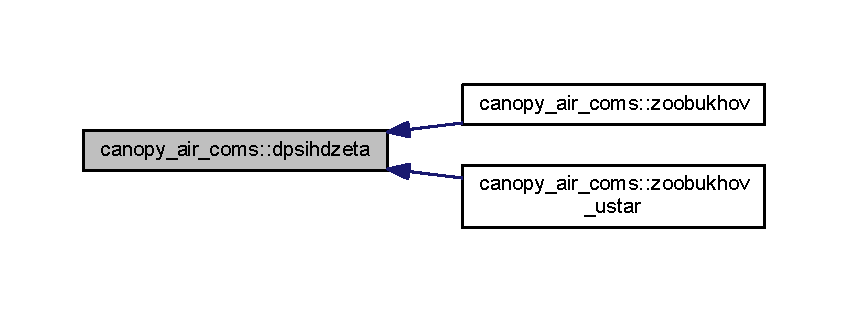
\includegraphics[width=350pt]{namespacecanopy__air__coms_a64552e0380fcb36366b5eb0f624241a3_icgraph}
\end{center}
\end{figure}


\index{canopy\+\_\+air\+\_\+coms@{canopy\+\_\+air\+\_\+coms}!dpsihdzeta8@{dpsihdzeta8}}
\index{dpsihdzeta8@{dpsihdzeta8}!canopy\+\_\+air\+\_\+coms@{canopy\+\_\+air\+\_\+coms}}
\subsubsection[{\texorpdfstring{dpsihdzeta8(zeta, stable)}{dpsihdzeta8(zeta, stable)}}]{\setlength{\rightskip}{0pt plus 5cm}real(kind=8) function canopy\+\_\+air\+\_\+coms\+::dpsihdzeta8 (
\begin{DoxyParamCaption}
\item[{real(kind=8), intent(in)}]{zeta, }
\item[{logical, intent(in)}]{stable}
\end{DoxyParamCaption}
)}\hypertarget{namespacecanopy__air__coms_aa5f9649efc40a05ddc13e1450f30fad3}{}\label{namespacecanopy__air__coms_aa5f9649efc40a05ddc13e1450f30fad3}


Here is the caller graph for this function\+:\nopagebreak
\begin{figure}[H]
\begin{center}
\leavevmode
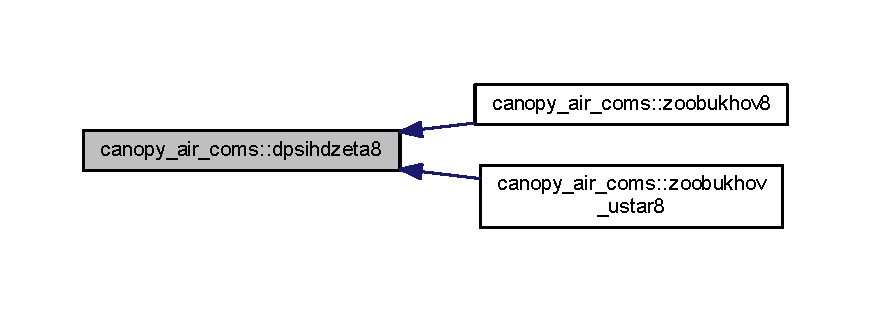
\includegraphics[width=350pt]{namespacecanopy__air__coms_aa5f9649efc40a05ddc13e1450f30fad3_icgraph}
\end{center}
\end{figure}


\index{canopy\+\_\+air\+\_\+coms@{canopy\+\_\+air\+\_\+coms}!dpsimdzeta@{dpsimdzeta}}
\index{dpsimdzeta@{dpsimdzeta}!canopy\+\_\+air\+\_\+coms@{canopy\+\_\+air\+\_\+coms}}
\subsubsection[{\texorpdfstring{dpsimdzeta(zeta, stable)}{dpsimdzeta(zeta, stable)}}]{\setlength{\rightskip}{0pt plus 5cm}real function canopy\+\_\+air\+\_\+coms\+::dpsimdzeta (
\begin{DoxyParamCaption}
\item[{real, intent(in)}]{zeta, }
\item[{logical, intent(in)}]{stable}
\end{DoxyParamCaption}
)}\hypertarget{namespacecanopy__air__coms_af8bc6f1d6999a4b614461cecb85c9b1b}{}\label{namespacecanopy__air__coms_af8bc6f1d6999a4b614461cecb85c9b1b}


Here is the caller graph for this function\+:\nopagebreak
\begin{figure}[H]
\begin{center}
\leavevmode
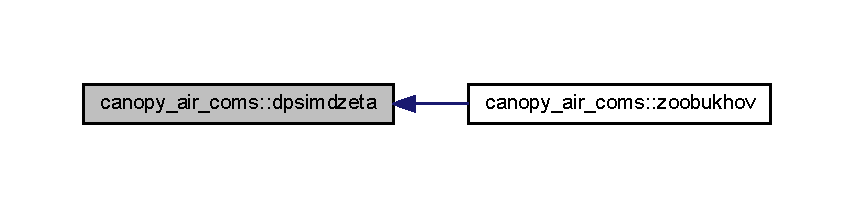
\includegraphics[width=350pt]{namespacecanopy__air__coms_af8bc6f1d6999a4b614461cecb85c9b1b_icgraph}
\end{center}
\end{figure}


\index{canopy\+\_\+air\+\_\+coms@{canopy\+\_\+air\+\_\+coms}!dpsimdzeta8@{dpsimdzeta8}}
\index{dpsimdzeta8@{dpsimdzeta8}!canopy\+\_\+air\+\_\+coms@{canopy\+\_\+air\+\_\+coms}}
\subsubsection[{\texorpdfstring{dpsimdzeta8(zeta, stable)}{dpsimdzeta8(zeta, stable)}}]{\setlength{\rightskip}{0pt plus 5cm}real(kind=8) function canopy\+\_\+air\+\_\+coms\+::dpsimdzeta8 (
\begin{DoxyParamCaption}
\item[{real(kind=8), intent(in)}]{zeta, }
\item[{logical, intent(in)}]{stable}
\end{DoxyParamCaption}
)}\hypertarget{namespacecanopy__air__coms_a51b006ac118f9549aee23ddb61a1bf19}{}\label{namespacecanopy__air__coms_a51b006ac118f9549aee23ddb61a1bf19}


Here is the caller graph for this function\+:\nopagebreak
\begin{figure}[H]
\begin{center}
\leavevmode
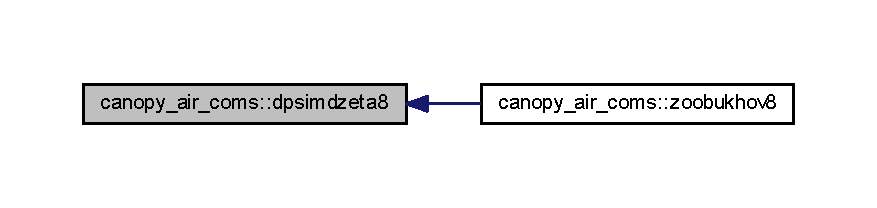
\includegraphics[width=350pt]{namespacecanopy__air__coms_a51b006ac118f9549aee23ddb61a1bf19_icgraph}
\end{center}
\end{figure}


\index{canopy\+\_\+air\+\_\+coms@{canopy\+\_\+air\+\_\+coms}!psih@{psih}}
\index{psih@{psih}!canopy\+\_\+air\+\_\+coms@{canopy\+\_\+air\+\_\+coms}}
\subsubsection[{\texorpdfstring{psih(zeta, stable)}{psih(zeta, stable)}}]{\setlength{\rightskip}{0pt plus 5cm}real function canopy\+\_\+air\+\_\+coms\+::psih (
\begin{DoxyParamCaption}
\item[{real, intent(in)}]{zeta, }
\item[{logical, intent(in)}]{stable}
\end{DoxyParamCaption}
)}\hypertarget{namespacecanopy__air__coms_acedb0f66db4b79009a69e87c5fd3ed71}{}\label{namespacecanopy__air__coms_acedb0f66db4b79009a69e87c5fd3ed71}


Here is the caller graph for this function\+:\nopagebreak
\begin{figure}[H]
\begin{center}
\leavevmode
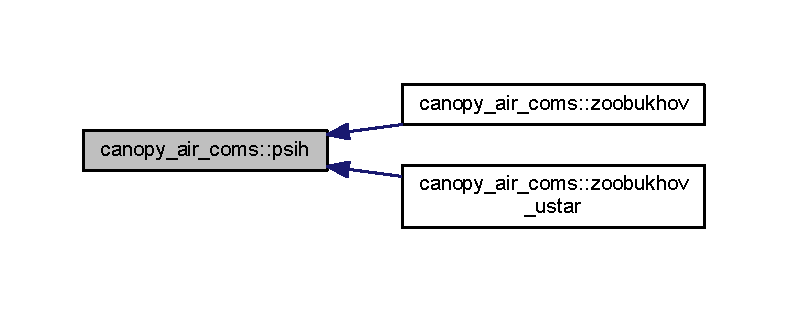
\includegraphics[width=350pt]{namespacecanopy__air__coms_acedb0f66db4b79009a69e87c5fd3ed71_icgraph}
\end{center}
\end{figure}


\index{canopy\+\_\+air\+\_\+coms@{canopy\+\_\+air\+\_\+coms}!psih8@{psih8}}
\index{psih8@{psih8}!canopy\+\_\+air\+\_\+coms@{canopy\+\_\+air\+\_\+coms}}
\subsubsection[{\texorpdfstring{psih8(zeta, stable)}{psih8(zeta, stable)}}]{\setlength{\rightskip}{0pt plus 5cm}real(kind=8) function canopy\+\_\+air\+\_\+coms\+::psih8 (
\begin{DoxyParamCaption}
\item[{real(kind=8), intent(in)}]{zeta, }
\item[{logical, intent(in)}]{stable}
\end{DoxyParamCaption}
)}\hypertarget{namespacecanopy__air__coms_aef33f0eeea82151a8edb6dc38c4cc921}{}\label{namespacecanopy__air__coms_aef33f0eeea82151a8edb6dc38c4cc921}


Here is the caller graph for this function\+:\nopagebreak
\begin{figure}[H]
\begin{center}
\leavevmode
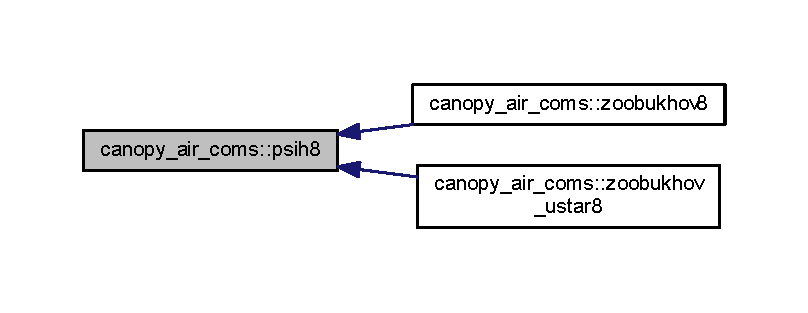
\includegraphics[width=350pt]{namespacecanopy__air__coms_aef33f0eeea82151a8edb6dc38c4cc921_icgraph}
\end{center}
\end{figure}


\index{canopy\+\_\+air\+\_\+coms@{canopy\+\_\+air\+\_\+coms}!psim@{psim}}
\index{psim@{psim}!canopy\+\_\+air\+\_\+coms@{canopy\+\_\+air\+\_\+coms}}
\subsubsection[{\texorpdfstring{psim(zeta, stable)}{psim(zeta, stable)}}]{\setlength{\rightskip}{0pt plus 5cm}real function canopy\+\_\+air\+\_\+coms\+::psim (
\begin{DoxyParamCaption}
\item[{real, intent(in)}]{zeta, }
\item[{logical, intent(in)}]{stable}
\end{DoxyParamCaption}
)}\hypertarget{namespacecanopy__air__coms_ab103fa081460babbe04c9a5a4699be5f}{}\label{namespacecanopy__air__coms_ab103fa081460babbe04c9a5a4699be5f}


Here is the caller graph for this function\+:\nopagebreak
\begin{figure}[H]
\begin{center}
\leavevmode
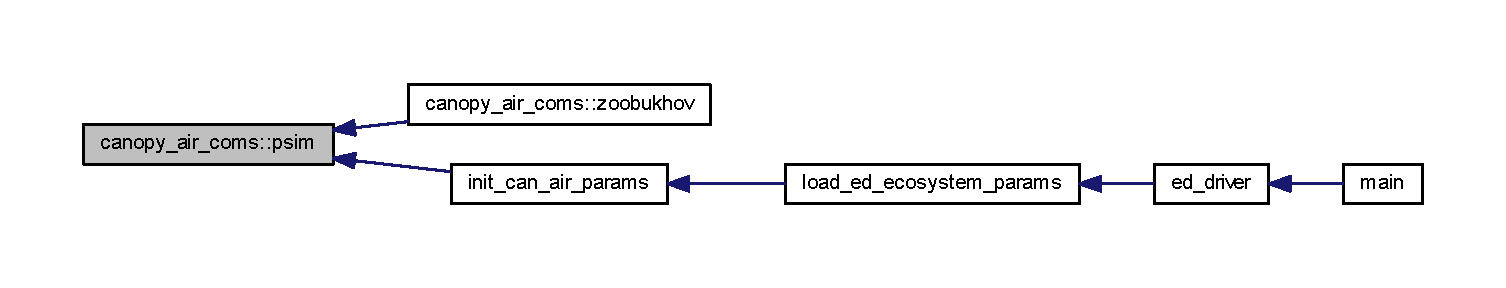
\includegraphics[width=350pt]{namespacecanopy__air__coms_ab103fa081460babbe04c9a5a4699be5f_icgraph}
\end{center}
\end{figure}


\index{canopy\+\_\+air\+\_\+coms@{canopy\+\_\+air\+\_\+coms}!psim8@{psim8}}
\index{psim8@{psim8}!canopy\+\_\+air\+\_\+coms@{canopy\+\_\+air\+\_\+coms}}
\subsubsection[{\texorpdfstring{psim8(zeta, stable)}{psim8(zeta, stable)}}]{\setlength{\rightskip}{0pt plus 5cm}real(kind=8) function canopy\+\_\+air\+\_\+coms\+::psim8 (
\begin{DoxyParamCaption}
\item[{real(kind=8), intent(in)}]{zeta, }
\item[{logical, intent(in)}]{stable}
\end{DoxyParamCaption}
)}\hypertarget{namespacecanopy__air__coms_aba7cbe776dbfa9815870ad3686949041}{}\label{namespacecanopy__air__coms_aba7cbe776dbfa9815870ad3686949041}


Here is the caller graph for this function\+:\nopagebreak
\begin{figure}[H]
\begin{center}
\leavevmode
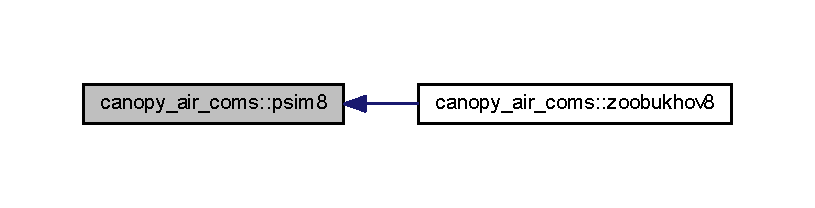
\includegraphics[width=350pt]{namespacecanopy__air__coms_aba7cbe776dbfa9815870ad3686949041_icgraph}
\end{center}
\end{figure}


\index{canopy\+\_\+air\+\_\+coms@{canopy\+\_\+air\+\_\+coms}!zoobukhov@{zoobukhov}}
\index{zoobukhov@{zoobukhov}!canopy\+\_\+air\+\_\+coms@{canopy\+\_\+air\+\_\+coms}}
\subsubsection[{\texorpdfstring{zoobukhov(rib, zstar, rough, zoz0m, lnzoz0m, zoz0h, lnzoz0h, stable)}{zoobukhov(rib, zstar, rough, zoz0m, lnzoz0m, zoz0h, lnzoz0h, stable)}}]{\setlength{\rightskip}{0pt plus 5cm}real function canopy\+\_\+air\+\_\+coms\+::zoobukhov (
\begin{DoxyParamCaption}
\item[{real, intent(in)}]{rib, }
\item[{real, intent(in)}]{zstar, }
\item[{real, intent(in)}]{rough, }
\item[{real, intent(in)}]{zoz0m, }
\item[{real, intent(in)}]{lnzoz0m, }
\item[{real, intent(in)}]{zoz0h, }
\item[{real, intent(in)}]{lnzoz0h, }
\item[{logical, intent(in)}]{stable}
\end{DoxyParamCaption}
)}\hypertarget{namespacecanopy__air__coms_a6062471b3381c283205ea8b27383a5e0}{}\label{namespacecanopy__air__coms_a6062471b3381c283205ea8b27383a5e0}
$<$$>$$<$$>$$<$$>$$<$$>$$<$$>$$<$$>$$<$$>$$<$$>$$<$$>$$<$$>$$<$$>$$<$$>$$<$$>$$<$$>$$<$$>$$<$$>$$<$$>$$<$$>$$<$$>$$<$$>$$<$$>$$<$$>$$<$$>$$<$$>$$<$$>$$<$$>$$<$$>$$<$$>$$<$$>$$<$$>$$<$$>$$<$$>$$<$$>$$<$$>$$<$$>$$<$$>$$<$$>$$<$$>$$<$$>$$<$$>$$<$$>$$<$!

$<$$>$$<$$>$$<$$>$$<$$>$$<$$>$$<$$>$$<$$>$$<$$>$$<$$>$$<$$>$$<$$>$$<$$>$$<$$>$$<$$>$$<$$>$$<$$>$$<$$>$$<$$>$$<$$>$$<$$>$$<$$>$$<$$>$$<$$>$$<$$>$$<$$>$$<$$>$$<$$>$$<$$>$$<$$>$$<$$>$$<$$>$$<$$>$$<$$>$$<$$>$$<$$>$$<$$>$$<$$>$$<$$>$$<$$>$$<$$>$$<$$>$$<$!

$<$$>$$<$$>$$<$$>$$<$$>$$<$$>$$<$$>$$<$$>$$<$$>$$<$$>$$<$$>$$<$$>$$<$$>$$<$$>$$<$$>$$<$$>$$<$$>$$<$$>$$<$$>$$<$$>$$<$$>$$<$$>$$<$$>$$<$$>$$<$$>$$<$$>$$<$$>$$<$$>$$<$$>$$<$$>$$<$$>$$<$$>$$<$$>$$<$$>$$<$$>$$<$$>$$<$$>$$<$$>$$<$$>$$<$$>$$<$$>$$<$$>$$<$!

$<$$>$$<$$>$$<$$>$$<$$>$$<$$>$$<$$>$$<$$>$$<$$>$$<$$>$$<$$>$$<$$>$$<$$>$$<$$>$$<$$>$$<$$>$$<$$>$$<$$>$$<$$>$$<$$>$$<$$>$$<$$>$$<$$>$$<$$>$$<$$>$$<$$>$$<$$>$$<$$>$$<$$>$$<$$>$$<$$>$$<$$>$$<$$>$$<$$>$$<$$>$$<$$>$$<$$>$$<$$>$$<$$>$$<$$>$$<$$>$$<$$>$$<$!

$<$$>$$<$$>$$<$$>$$<$$>$$<$$>$$<$$>$$<$$>$$<$$>$$<$$>$$<$$>$$<$$>$$<$$>$$<$$>$$<$$>$$<$$>$$<$$>$$<$$>$$<$$>$$<$$>$$<$$>$$<$$>$$<$$>$$<$$>$$<$$>$$<$$>$$<$$>$$<$$>$$<$$>$$<$$>$$<$$>$$<$$>$$<$$>$$<$$>$$<$$>$$<$$>$$<$$>$$<$$>$$<$$>$$<$$>$$<$$>$$<$$>$$<$!

$<$$>$$<$$>$$<$$>$$<$$>$$<$$>$$<$$>$$<$$>$$<$$>$$<$$>$$<$$>$$<$$>$$<$$>$$<$$>$$<$$>$$<$$>$$<$$>$$<$$>$$<$$>$$<$$>$$<$$>$$<$$>$$<$$>$$<$$>$$<$$>$$<$$>$$<$$>$$<$$>$$<$$>$$<$$>$$<$$>$$<$$>$$<$$>$$<$$>$$<$$>$$<$$>$$<$$>$$<$$>$$<$$>$$<$$>$$<$$>$$<$$>$$<$!

$<$$>$$<$$>$$<$$>$$<$$>$$<$$>$$<$$>$$<$$>$$<$$>$$<$$>$$<$$>$$<$$>$$<$$>$$<$$>$$<$$>$$<$$>$$<$$>$$<$$>$$<$$>$$<$$>$$<$$>$$<$$>$$<$$>$$<$$>$$<$$>$$<$$>$$<$$>$$<$$>$$<$$>$$<$$>$$<$$>$$<$$>$$<$$>$$<$$>$$<$$>$$<$$>$$<$$>$$<$$>$$<$$>$$<$!

$<$$>$$<$$>$$<$$>$$<$$>$$<$$>$$<$$>$$<$$>$$<$$>$$<$$>$$<$$>$$<$$>$$<$$>$$<$$>$$<$$>$$<$$>$$<$$>$$<$$>$$<$$>$$<$$>$$<$$>$$<$$>$$<$$>$$<$$>$$<$$>$$<$$>$$<$$>$$<$$>$$<$$>$$<$$>$$<$$>$$<$$>$$<$$>$$<$$>$$<$$>$$<$$>$$<$$>$$<$$>$$<$$>$$<$!

$<$$>$$<$$>$$<$$>$$<$$>$$<$$>$$<$$>$$<$$>$$<$$>$$<$$>$$<$$>$$<$$>$$<$$>$$<$$>$$<$$>$$<$$>$$<$$>$$<$$>$$<$$>$$<$$>$$<$$>$$<$$>$$<$$>$$<$$>$$<$$>$$<$$>$$<$$>$$<$$>$$<$$>$$<$$>$$<$$>$$<$$>$$<$$>$$<$$>$$<$$>$$<$$>$$<$$>$$<$$>$$<$$>$$<$$>$$<$$>$$<$$>$$<$!

$<$$>$$<$$>$$<$$>$$<$$>$$<$$>$$<$$>$$<$$>$$<$$>$$<$$>$$<$$>$$<$$>$$<$$>$$<$$>$$<$$>$$<$$>$$<$$>$$<$$>$$<$$>$$<$$>$$<$$>$$<$$>$$<$$>$$<$$>$$<$$>$$<$$>$$<$$>$$<$$>$$<$$>$$<$$>$$<$$>$$<$$>$$<$$>$$<$$>$$<$$>$$<$$>$$<$$>$$<$$>$$<$$>$$<$$>$$<$$>$$<$$>$$<$! 

Here is the call graph for this function\+:\nopagebreak
\begin{figure}[H]
\begin{center}
\leavevmode
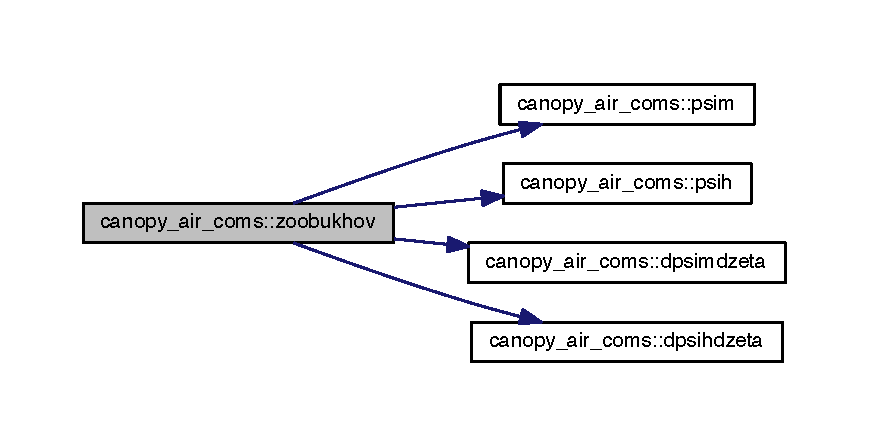
\includegraphics[width=350pt]{namespacecanopy__air__coms_a6062471b3381c283205ea8b27383a5e0_cgraph}
\end{center}
\end{figure}


\index{canopy\+\_\+air\+\_\+coms@{canopy\+\_\+air\+\_\+coms}!zoobukhov8@{zoobukhov8}}
\index{zoobukhov8@{zoobukhov8}!canopy\+\_\+air\+\_\+coms@{canopy\+\_\+air\+\_\+coms}}
\subsubsection[{\texorpdfstring{zoobukhov8(rib, zstar, rough, zoz0m, lnzoz0m, zoz0h, lnzoz0h, stable)}{zoobukhov8(rib, zstar, rough, zoz0m, lnzoz0m, zoz0h, lnzoz0h, stable)}}]{\setlength{\rightskip}{0pt plus 5cm}real(kind=8) function canopy\+\_\+air\+\_\+coms\+::zoobukhov8 (
\begin{DoxyParamCaption}
\item[{real(kind=8), intent(in)}]{rib, }
\item[{real(kind=8), intent(in)}]{zstar, }
\item[{real(kind=8), intent(in)}]{rough, }
\item[{real(kind=8), intent(in)}]{zoz0m, }
\item[{real(kind=8), intent(in)}]{lnzoz0m, }
\item[{real(kind=8), intent(in)}]{zoz0h, }
\item[{real(kind=8), intent(in)}]{lnzoz0h, }
\item[{logical, intent(in)}]{stable}
\end{DoxyParamCaption}
)}\hypertarget{namespacecanopy__air__coms_afef697305b4b30385c5206f48d9e787c}{}\label{namespacecanopy__air__coms_afef697305b4b30385c5206f48d9e787c}
$<$$>$$<$$>$$<$$>$$<$$>$$<$$>$$<$$>$$<$$>$$<$$>$$<$$>$$<$$>$$<$$>$$<$$>$$<$$>$$<$$>$$<$$>$$<$$>$$<$$>$$<$$>$$<$$>$$<$$>$$<$$>$$<$$>$$<$$>$$<$$>$$<$$>$$<$$>$$<$$>$$<$$>$$<$$>$$<$$>$$<$$>$$<$$>$$<$$>$$<$$>$$<$$>$$<$$>$$<$$>$$<$$>$$<$$>$$<$$>$$<$$>$$<$!

$<$$>$$<$$>$$<$$>$$<$$>$$<$$>$$<$$>$$<$$>$$<$$>$$<$$>$$<$$>$$<$$>$$<$$>$$<$$>$$<$$>$$<$$>$$<$$>$$<$$>$$<$$>$$<$$>$$<$$>$$<$$>$$<$$>$$<$$>$$<$$>$$<$$>$$<$$>$$<$$>$$<$$>$$<$$>$$<$$>$$<$$>$$<$$>$$<$$>$$<$$>$$<$$>$$<$$>$$<$$>$$<$$>$$<$$>$$<$$>$$<$$>$$<$!

$<$$>$$<$$>$$<$$>$$<$$>$$<$$>$$<$$>$$<$$>$$<$$>$$<$$>$$<$$>$$<$$>$$<$$>$$<$$>$$<$$>$$<$$>$$<$$>$$<$$>$$<$$>$$<$$>$$<$$>$$<$$>$$<$$>$$<$$>$$<$$>$$<$$>$$<$$>$$<$$>$$<$$>$$<$$>$$<$$>$$<$$>$$<$$>$$<$$>$$<$$>$$<$$>$$<$$>$$<$$>$$<$$>$$<$$>$$<$$>$$<$$>$$<$!

$<$$>$$<$$>$$<$$>$$<$$>$$<$$>$$<$$>$$<$$>$$<$$>$$<$$>$$<$$>$$<$$>$$<$$>$$<$$>$$<$$>$$<$$>$$<$$>$$<$$>$$<$$>$$<$$>$$<$$>$$<$$>$$<$$>$$<$$>$$<$$>$$<$$>$$<$$>$$<$$>$$<$$>$$<$$>$$<$$>$$<$$>$$<$$>$$<$$>$$<$$>$$<$$>$$<$$>$$<$$>$$<$$>$$<$$>$$<$$>$$<$$>$$<$!

$<$$>$$<$$>$$<$$>$$<$$>$$<$$>$$<$$>$$<$$>$$<$$>$$<$$>$$<$$>$$<$$>$$<$$>$$<$$>$$<$$>$$<$$>$$<$$>$$<$$>$$<$$>$$<$$>$$<$$>$$<$$>$$<$$>$$<$$>$$<$$>$$<$$>$$<$$>$$<$$>$$<$$>$$<$$>$$<$$>$$<$$>$$<$$>$$<$$>$$<$$>$$<$$>$$<$$>$$<$$>$$<$$>$$<$$>$$<$$>$$<$$>$$<$!

$<$$>$$<$$>$$<$$>$$<$$>$$<$$>$$<$$>$$<$$>$$<$$>$$<$$>$$<$$>$$<$$>$$<$$>$$<$$>$$<$$>$$<$$>$$<$$>$$<$$>$$<$$>$$<$$>$$<$$>$$<$$>$$<$$>$$<$$>$$<$$>$$<$$>$$<$$>$$<$$>$$<$$>$$<$$>$$<$$>$$<$$>$$<$$>$$<$$>$$<$$>$$<$$>$$<$$>$$<$$>$$<$$>$$<$$>$$<$$>$$<$$>$$<$!

$<$$>$$<$$>$$<$$>$$<$$>$$<$$>$$<$$>$$<$$>$$<$$>$$<$$>$$<$$>$$<$$>$$<$$>$$<$$>$$<$$>$$<$$>$$<$$>$$<$$>$$<$$>$$<$$>$$<$$>$$<$$>$$<$$>$$<$$>$$<$$>$$<$$>$$<$$>$$<$$>$$<$$>$$<$$>$$<$$>$$<$$>$$<$$>$$<$$>$$<$$>$$<$$>$$<$$>$$<$$>$$<$$>$$<$!

$<$$>$$<$$>$$<$$>$$<$$>$$<$$>$$<$$>$$<$$>$$<$$>$$<$$>$$<$$>$$<$$>$$<$$>$$<$$>$$<$$>$$<$$>$$<$$>$$<$$>$$<$$>$$<$$>$$<$$>$$<$$>$$<$$>$$<$$>$$<$$>$$<$$>$$<$$>$$<$$>$$<$$>$$<$$>$$<$$>$$<$$>$$<$$>$$<$$>$$<$$>$$<$$>$$<$$>$$<$$>$$<$$>$$<$!

$<$$>$$<$$>$$<$$>$$<$$>$$<$$>$$<$$>$$<$$>$$<$$>$$<$$>$$<$$>$$<$$>$$<$$>$$<$$>$$<$$>$$<$$>$$<$$>$$<$$>$$<$$>$$<$$>$$<$$>$$<$$>$$<$$>$$<$$>$$<$$>$$<$$>$$<$$>$$<$$>$$<$$>$$<$$>$$<$$>$$<$$>$$<$$>$$<$$>$$<$$>$$<$$>$$<$$>$$<$$>$$<$$>$$<$$>$$<$$>$$<$$>$$<$!

$<$$>$$<$$>$$<$$>$$<$$>$$<$$>$$<$$>$$<$$>$$<$$>$$<$$>$$<$$>$$<$$>$$<$$>$$<$$>$$<$$>$$<$$>$$<$$>$$<$$>$$<$$>$$<$$>$$<$$>$$<$$>$$<$$>$$<$$>$$<$$>$$<$$>$$<$$>$$<$$>$$<$$>$$<$$>$$<$$>$$<$$>$$<$$>$$<$$>$$<$$>$$<$$>$$<$$>$$<$$>$$<$$>$$<$$>$$<$$>$$<$$>$$<$! 

Here is the call graph for this function\+:\nopagebreak
\begin{figure}[H]
\begin{center}
\leavevmode
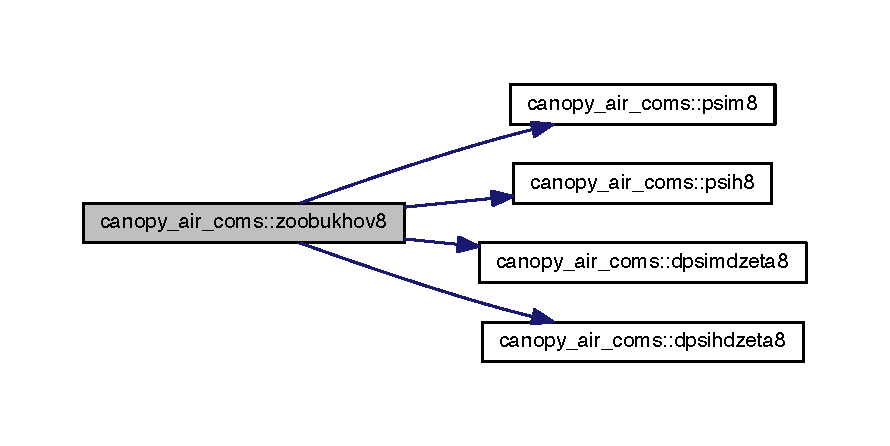
\includegraphics[width=350pt]{namespacecanopy__air__coms_afef697305b4b30385c5206f48d9e787c_cgraph}
\end{center}
\end{figure}


\index{canopy\+\_\+air\+\_\+coms@{canopy\+\_\+air\+\_\+coms}!zoobukhov\+\_\+ustar@{zoobukhov\+\_\+ustar}}
\index{zoobukhov\+\_\+ustar@{zoobukhov\+\_\+ustar}!canopy\+\_\+air\+\_\+coms@{canopy\+\_\+air\+\_\+coms}}
\subsubsection[{\texorpdfstring{zoobukhov\+\_\+ustar(rib, zstar, rough, zoz0h, lnzoz0h, kuoustar, stable)}{zoobukhov_ustar(rib, zstar, rough, zoz0h, lnzoz0h, kuoustar, stable)}}]{\setlength{\rightskip}{0pt plus 5cm}real function canopy\+\_\+air\+\_\+coms\+::zoobukhov\+\_\+ustar (
\begin{DoxyParamCaption}
\item[{real(kind=4), intent(in)}]{rib, }
\item[{real(kind=4), intent(in)}]{zstar, }
\item[{real(kind=4), intent(in)}]{rough, }
\item[{real(kind=4), intent(in)}]{zoz0h, }
\item[{real(kind=4), intent(in)}]{lnzoz0h, }
\item[{real(kind=4), intent(in)}]{kuoustar, }
\item[{logical, intent(in)}]{stable}
\end{DoxyParamCaption}
)}\hypertarget{namespacecanopy__air__coms_a5251266695c581c8f4058d98f6c86200}{}\label{namespacecanopy__air__coms_a5251266695c581c8f4058d98f6c86200}
$<$$>$$<$$>$$<$$>$$<$$>$$<$$>$$<$$>$$<$$>$$<$$>$$<$$>$$<$$>$$<$$>$$<$$>$$<$$>$$<$$>$$<$$>$$<$$>$$<$$>$$<$$>$$<$$>$$<$$>$$<$$>$$<$$>$$<$$>$$<$$>$$<$$>$$<$$>$$<$$>$$<$$>$$<$$>$$<$$>$$<$$>$$<$$>$$<$$>$$<$$>$$<$$>$$<$$>$$<$$>$$<$$>$$<$$>$$<$$>$$<$$>$$<$!

$<$$>$$<$$>$$<$$>$$<$$>$$<$$>$$<$$>$$<$$>$$<$$>$$<$$>$$<$$>$$<$$>$$<$$>$$<$$>$$<$$>$$<$$>$$<$$>$$<$$>$$<$$>$$<$$>$$<$$>$$<$$>$$<$$>$$<$$>$$<$$>$$<$$>$$<$$>$$<$$>$$<$$>$$<$$>$$<$$>$$<$$>$$<$$>$$<$$>$$<$$>$$<$$>$$<$$>$$<$$>$$<$$>$$<$$>$$<$$>$$<$$>$$<$!

$<$$>$$<$$>$$<$$>$$<$$>$$<$$>$$<$$>$$<$$>$$<$$>$$<$$>$$<$$>$$<$$>$$<$$>$$<$$>$$<$$>$$<$$>$$<$$>$$<$$>$$<$$>$$<$$>$$<$$>$$<$$>$$<$$>$$<$$>$$<$$>$$<$$>$$<$$>$$<$$>$$<$$>$$<$$>$$<$$>$$<$$>$$<$$>$$<$$>$$<$$>$$<$$>$$<$$>$$<$$>$$<$$>$$<$$>$$<$$>$$<$$>$$<$!

$<$$>$$<$$>$$<$$>$$<$$>$$<$$>$$<$$>$$<$$>$$<$$>$$<$$>$$<$$>$$<$$>$$<$$>$$<$$>$$<$$>$$<$$>$$<$$>$$<$$>$$<$$>$$<$$>$$<$$>$$<$$>$$<$$>$$<$$>$$<$$>$$<$$>$$<$$>$$<$$>$$<$$>$$<$$>$$<$$>$$<$$>$$<$$>$$<$$>$$<$$>$$<$$>$$<$$>$$<$$>$$<$$>$$<$$>$$<$$>$$<$$>$$<$!

$<$$>$$<$$>$$<$$>$$<$$>$$<$$>$$<$$>$$<$$>$$<$$>$$<$$>$$<$$>$$<$$>$$<$$>$$<$$>$$<$$>$$<$$>$$<$$>$$<$$>$$<$$>$$<$$>$$<$$>$$<$$>$$<$$>$$<$$>$$<$$>$$<$$>$$<$$>$$<$$>$$<$$>$$<$$>$$<$$>$$<$$>$$<$$>$$<$$>$$<$$>$$<$$>$$<$$>$$<$$>$$<$$>$$<$$>$$<$$>$$<$$>$$<$!

$<$$>$$<$$>$$<$$>$$<$$>$$<$$>$$<$$>$$<$$>$$<$$>$$<$$>$$<$$>$$<$$>$$<$$>$$<$$>$$<$$>$$<$$>$$<$$>$$<$$>$$<$$>$$<$$>$$<$$>$$<$$>$$<$$>$$<$$>$$<$$>$$<$$>$$<$$>$$<$$>$$<$$>$$<$$>$$<$$>$$<$$>$$<$$>$$<$$>$$<$$>$$<$$>$$<$$>$$<$$>$$<$$>$$<$$>$$<$$>$$<$$>$$<$!

$<$$>$$<$$>$$<$$>$$<$$>$$<$$>$$<$$>$$<$$>$$<$$>$$<$$>$$<$$>$$<$$>$$<$$>$$<$$>$$<$$>$$<$$>$$<$$>$$<$$>$$<$$>$$<$$>$$<$$>$$<$$>$$<$$>$$<$$>$$<$$>$$<$$>$$<$$>$$<$$>$$<$$>$$<$$>$$<$$>$$<$$>$$<$$>$$<$$>$$<$$>$$<$$>$$<$$>$$<$$>$$<$$>$$<$!

$<$$>$$<$$>$$<$$>$$<$$>$$<$$>$$<$$>$$<$$>$$<$$>$$<$$>$$<$$>$$<$$>$$<$$>$$<$$>$$<$$>$$<$$>$$<$$>$$<$$>$$<$$>$$<$$>$$<$$>$$<$$>$$<$$>$$<$$>$$<$$>$$<$$>$$<$$>$$<$$>$$<$$>$$<$$>$$<$$>$$<$$>$$<$$>$$<$$>$$<$$>$$<$$>$$<$$>$$<$$>$$<$$>$$<$!

$<$$>$$<$$>$$<$$>$$<$$>$$<$$>$$<$$>$$<$$>$$<$$>$$<$$>$$<$$>$$<$$>$$<$$>$$<$$>$$<$$>$$<$$>$$<$$>$$<$$>$$<$$>$$<$$>$$<$$>$$<$$>$$<$$>$$<$$>$$<$$>$$<$$>$$<$$>$$<$$>$$<$$>$$<$$>$$<$$>$$<$$>$$<$$>$$<$$>$$<$$>$$<$$>$$<$$>$$<$$>$$<$$>$$<$$>$$<$$>$$<$$>$$<$!

$<$$>$$<$$>$$<$$>$$<$$>$$<$$>$$<$$>$$<$$>$$<$$>$$<$$>$$<$$>$$<$$>$$<$$>$$<$$>$$<$$>$$<$$>$$<$$>$$<$$>$$<$$>$$<$$>$$<$$>$$<$$>$$<$$>$$<$$>$$<$$>$$<$$>$$<$$>$$<$$>$$<$$>$$<$$>$$<$$>$$<$$>$$<$$>$$<$$>$$<$$>$$<$$>$$<$$>$$<$$>$$<$$>$$<$$>$$<$$>$$<$$>$$<$! 

Here is the call graph for this function\+:\nopagebreak
\begin{figure}[H]
\begin{center}
\leavevmode
\includegraphics[width=350pt]{namespacecanopy__air__coms_a5251266695c581c8f4058d98f6c86200_cgraph}
\end{center}
\end{figure}


\index{canopy\+\_\+air\+\_\+coms@{canopy\+\_\+air\+\_\+coms}!zoobukhov\+\_\+ustar8@{zoobukhov\+\_\+ustar8}}
\index{zoobukhov\+\_\+ustar8@{zoobukhov\+\_\+ustar8}!canopy\+\_\+air\+\_\+coms@{canopy\+\_\+air\+\_\+coms}}
\subsubsection[{\texorpdfstring{zoobukhov\+\_\+ustar8(rib, zstar, rough, zoz0h, lnzoz0h, kuoustar, stable)}{zoobukhov_ustar8(rib, zstar, rough, zoz0h, lnzoz0h, kuoustar, stable)}}]{\setlength{\rightskip}{0pt plus 5cm}real(kind=8) function canopy\+\_\+air\+\_\+coms\+::zoobukhov\+\_\+ustar8 (
\begin{DoxyParamCaption}
\item[{real(kind=8), intent(in)}]{rib, }
\item[{real(kind=8), intent(in)}]{zstar, }
\item[{real(kind=8), intent(in)}]{rough, }
\item[{real(kind=8), intent(in)}]{zoz0h, }
\item[{real(kind=8), intent(in)}]{lnzoz0h, }
\item[{real(kind=8), intent(in)}]{kuoustar, }
\item[{logical, intent(in)}]{stable}
\end{DoxyParamCaption}
)}\hypertarget{namespacecanopy__air__coms_a6ef582f46fded1355973730e6a2289f2}{}\label{namespacecanopy__air__coms_a6ef582f46fded1355973730e6a2289f2}
$<$$>$$<$$>$$<$$>$$<$$>$$<$$>$$<$$>$$<$$>$$<$$>$$<$$>$$<$$>$$<$$>$$<$$>$$<$$>$$<$$>$$<$$>$$<$$>$$<$$>$$<$$>$$<$$>$$<$$>$$<$$>$$<$$>$$<$$>$$<$$>$$<$$>$$<$$>$$<$$>$$<$$>$$<$$>$$<$$>$$<$$>$$<$$>$$<$$>$$<$$>$$<$$>$$<$$>$$<$$>$$<$$>$$<$$>$$<$$>$$<$$>$$<$!

$<$$>$$<$$>$$<$$>$$<$$>$$<$$>$$<$$>$$<$$>$$<$$>$$<$$>$$<$$>$$<$$>$$<$$>$$<$$>$$<$$>$$<$$>$$<$$>$$<$$>$$<$$>$$<$$>$$<$$>$$<$$>$$<$$>$$<$$>$$<$$>$$<$$>$$<$$>$$<$$>$$<$$>$$<$$>$$<$$>$$<$$>$$<$$>$$<$$>$$<$$>$$<$$>$$<$$>$$<$$>$$<$$>$$<$$>$$<$$>$$<$$>$$<$!

$<$$>$$<$$>$$<$$>$$<$$>$$<$$>$$<$$>$$<$$>$$<$$>$$<$$>$$<$$>$$<$$>$$<$$>$$<$$>$$<$$>$$<$$>$$<$$>$$<$$>$$<$$>$$<$$>$$<$$>$$<$$>$$<$$>$$<$$>$$<$$>$$<$$>$$<$$>$$<$$>$$<$$>$$<$$>$$<$$>$$<$$>$$<$$>$$<$$>$$<$$>$$<$$>$$<$$>$$<$$>$$<$$>$$<$$>$$<$$>$$<$$>$$<$!

$<$$>$$<$$>$$<$$>$$<$$>$$<$$>$$<$$>$$<$$>$$<$$>$$<$$>$$<$$>$$<$$>$$<$$>$$<$$>$$<$$>$$<$$>$$<$$>$$<$$>$$<$$>$$<$$>$$<$$>$$<$$>$$<$$>$$<$$>$$<$$>$$<$$>$$<$$>$$<$$>$$<$$>$$<$$>$$<$$>$$<$$>$$<$$>$$<$$>$$<$$>$$<$$>$$<$$>$$<$$>$$<$$>$$<$$>$$<$$>$$<$$>$$<$!

$<$$>$$<$$>$$<$$>$$<$$>$$<$$>$$<$$>$$<$$>$$<$$>$$<$$>$$<$$>$$<$$>$$<$$>$$<$$>$$<$$>$$<$$>$$<$$>$$<$$>$$<$$>$$<$$>$$<$$>$$<$$>$$<$$>$$<$$>$$<$$>$$<$$>$$<$$>$$<$$>$$<$$>$$<$$>$$<$$>$$<$$>$$<$$>$$<$$>$$<$$>$$<$$>$$<$$>$$<$$>$$<$$>$$<$$>$$<$$>$!

$<$$>$$<$$>$$<$$>$$<$$>$$<$$>$$<$$>$$<$$>$$<$$>$$<$$>$$<$$>$$<$$>$$<$$>$$<$$>$$<$$>$$<$$>$$<$$>$$<$$>$$<$$>$$<$$>$$<$$>$$<$$>$$<$$>$$<$$>$$<$$>$$<$$>$$<$$>$$<$$>$$<$$>$$<$$>$$<$$>$$<$$>$$<$$>$$<$$>$$<$$>$$<$$>$$<$$>$$<$$>$$<$$>$$<$$>$$<$$>$!

$<$$>$$<$$>$$<$$>$$<$$>$$<$$>$$<$$>$$<$$>$$<$$>$$<$$>$$<$$>$$<$$>$$<$$>$$<$$>$$<$$>$$<$$>$$<$$>$$<$$>$$<$$>$$<$$>$$<$$>$$<$$>$$<$$>$$<$$>$$<$$>$$<$$>$$<$$>$$<$$>$$<$$>$$<$$>$$<$$>$$<$$>$$<$$>$$<$$>$$<$$>$$<$$>$$<$$>$$<$$>$$<$$>$$<$!

$<$$>$$<$$>$$<$$>$$<$$>$$<$$>$$<$$>$$<$$>$$<$$>$$<$$>$$<$$>$$<$$>$$<$$>$$<$$>$$<$$>$$<$$>$$<$$>$$<$$>$$<$$>$$<$$>$$<$$>$$<$$>$$<$$>$$<$$>$$<$$>$$<$$>$$<$$>$$<$$>$$<$$>$$<$$>$$<$$>$$<$$>$$<$$>$$<$$>$$<$$>$$<$$>$$<$$>$$<$$>$$<$$>$$<$!

$<$$>$$<$$>$$<$$>$$<$$>$$<$$>$$<$$>$$<$$>$$<$$>$$<$$>$$<$$>$$<$$>$$<$$>$$<$$>$$<$$>$$<$$>$$<$$>$$<$$>$$<$$>$$<$$>$$<$$>$$<$$>$$<$$>$$<$$>$$<$$>$$<$$>$$<$$>$$<$$>$$<$$>$$<$$>$$<$$>$$<$$>$$<$$>$$<$$>$$<$$>$$<$$>$$<$$>$$<$$>$$<$$>$$<$$>$$<$$>$!

$<$$>$$<$$>$$<$$>$$<$$>$$<$$>$$<$$>$$<$$>$$<$$>$$<$$>$$<$$>$$<$$>$$<$$>$$<$$>$$<$$>$$<$$>$$<$$>$$<$$>$$<$$>$$<$$>$$<$$>$$<$$>$$<$$>$$<$$>$$<$$>$$<$$>$$<$$>$$<$$>$$<$$>$$<$$>$$<$$>$$<$$>$$<$$>$$<$$>$$<$$>$$<$$>$$<$$>$$<$$>$$<$$>$$<$$>$$<$$>$!

$<$$>$$<$$>$$<$$>$$<$$>$$<$$>$$<$$>$$<$$>$$<$$>$$<$$>$$<$$>$$<$$>$$<$$>$$<$$>$$<$$>$$<$$>$$<$$>$$<$$>$$<$$>$$<$$>$$<$$>$$<$$>$$<$$>$$<$$>$$<$$>$$<$$>$$<$$>$$<$$>$$<$$>$$<$$>$$<$$>$$<$$>$$<$$>$$<$$>$$<$$>$$<$$>$$<$$>$$<$$>$$<$$>$$<$$>$$<$$>$!

$<$$>$$<$$>$$<$$>$$<$$>$$<$$>$$<$$>$$<$$>$$<$$>$$<$$>$$<$$>$$<$$>$$<$$>$$<$$>$$<$$>$$<$$>$$<$$>$$<$$>$$<$$>$$<$$>$$<$$>$$<$$>$$<$$>$$<$$>$$<$$>$$<$$>$$<$$>$$<$$>$$<$$>$$<$$>$$<$$>$$<$$>$$<$$>$$<$$>$$<$$>$$<$$>$$<$$>$$<$$>$$<$$>$$<$$>$$<$$>$! 

Here is the call graph for this function\+:\nopagebreak
\begin{figure}[H]
\begin{center}
\leavevmode
\includegraphics[width=350pt]{namespacecanopy__air__coms_a6ef582f46fded1355973730e6a2289f2_cgraph}
\end{center}
\end{figure}




\subsection{Variable Documentation}
\index{canopy\+\_\+air\+\_\+coms@{canopy\+\_\+air\+\_\+coms}!abh91@{abh91}}
\index{abh91@{abh91}!canopy\+\_\+air\+\_\+coms@{canopy\+\_\+air\+\_\+coms}}
\subsubsection[{\texorpdfstring{abh91}{abh91}}]{\setlength{\rightskip}{0pt plus 5cm}real canopy\+\_\+air\+\_\+coms\+::abh91}\hypertarget{namespacecanopy__air__coms_a8943107817bd72a2ecf2c8ac35516efc}{}\label{namespacecanopy__air__coms_a8943107817bd72a2ecf2c8ac35516efc}
\index{canopy\+\_\+air\+\_\+coms@{canopy\+\_\+air\+\_\+coms}!abh918@{abh918}}
\index{abh918@{abh918}!canopy\+\_\+air\+\_\+coms@{canopy\+\_\+air\+\_\+coms}}
\subsubsection[{\texorpdfstring{abh918}{abh918}}]{\setlength{\rightskip}{0pt plus 5cm}real(kind=8) canopy\+\_\+air\+\_\+coms\+::abh918}\hypertarget{namespacecanopy__air__coms_a7bbc194838f911d2e8b0948159f4d62e}{}\label{namespacecanopy__air__coms_a7bbc194838f911d2e8b0948159f4d62e}
\index{canopy\+\_\+air\+\_\+coms@{canopy\+\_\+air\+\_\+coms}!acyli\+\_\+lami@{acyli\+\_\+lami}}
\index{acyli\+\_\+lami@{acyli\+\_\+lami}!canopy\+\_\+air\+\_\+coms@{canopy\+\_\+air\+\_\+coms}}
\subsubsection[{\texorpdfstring{acyli\+\_\+lami}{acyli_lami}}]{\setlength{\rightskip}{0pt plus 5cm}real(kind=4) canopy\+\_\+air\+\_\+coms\+::acyli\+\_\+lami}\hypertarget{namespacecanopy__air__coms_a910e0e75420e6cd46075062c7da2b565}{}\label{namespacecanopy__air__coms_a910e0e75420e6cd46075062c7da2b565}
\index{canopy\+\_\+air\+\_\+coms@{canopy\+\_\+air\+\_\+coms}!acyli\+\_\+lami8@{acyli\+\_\+lami8}}
\index{acyli\+\_\+lami8@{acyli\+\_\+lami8}!canopy\+\_\+air\+\_\+coms@{canopy\+\_\+air\+\_\+coms}}
\subsubsection[{\texorpdfstring{acyli\+\_\+lami8}{acyli_lami8}}]{\setlength{\rightskip}{0pt plus 5cm}real(kind=8) canopy\+\_\+air\+\_\+coms\+::acyli\+\_\+lami8}\hypertarget{namespacecanopy__air__coms_a325f601d72eb729cc4301008156be76b}{}\label{namespacecanopy__air__coms_a325f601d72eb729cc4301008156be76b}
\index{canopy\+\_\+air\+\_\+coms@{canopy\+\_\+air\+\_\+coms}!acyli\+\_\+turb@{acyli\+\_\+turb}}
\index{acyli\+\_\+turb@{acyli\+\_\+turb}!canopy\+\_\+air\+\_\+coms@{canopy\+\_\+air\+\_\+coms}}
\subsubsection[{\texorpdfstring{acyli\+\_\+turb}{acyli_turb}}]{\setlength{\rightskip}{0pt plus 5cm}real(kind=4) canopy\+\_\+air\+\_\+coms\+::acyli\+\_\+turb}\hypertarget{namespacecanopy__air__coms_a42c5385303996a52e2fce111d922eaf2}{}\label{namespacecanopy__air__coms_a42c5385303996a52e2fce111d922eaf2}
\index{canopy\+\_\+air\+\_\+coms@{canopy\+\_\+air\+\_\+coms}!acyli\+\_\+turb8@{acyli\+\_\+turb8}}
\index{acyli\+\_\+turb8@{acyli\+\_\+turb8}!canopy\+\_\+air\+\_\+coms@{canopy\+\_\+air\+\_\+coms}}
\subsubsection[{\texorpdfstring{acyli\+\_\+turb8}{acyli_turb8}}]{\setlength{\rightskip}{0pt plus 5cm}real(kind=8) canopy\+\_\+air\+\_\+coms\+::acyli\+\_\+turb8}\hypertarget{namespacecanopy__air__coms_a933920d4f406fd57c33f8cef1ca8bb83}{}\label{namespacecanopy__air__coms_a933920d4f406fd57c33f8cef1ca8bb83}
\index{canopy\+\_\+air\+\_\+coms@{canopy\+\_\+air\+\_\+coms}!aflat\+\_\+lami@{aflat\+\_\+lami}}
\index{aflat\+\_\+lami@{aflat\+\_\+lami}!canopy\+\_\+air\+\_\+coms@{canopy\+\_\+air\+\_\+coms}}
\subsubsection[{\texorpdfstring{aflat\+\_\+lami}{aflat_lami}}]{\setlength{\rightskip}{0pt plus 5cm}real(kind=4) canopy\+\_\+air\+\_\+coms\+::aflat\+\_\+lami}\hypertarget{namespacecanopy__air__coms_a478fe27fc0f34c4b09208d0f99bae8e5}{}\label{namespacecanopy__air__coms_a478fe27fc0f34c4b09208d0f99bae8e5}
\index{canopy\+\_\+air\+\_\+coms@{canopy\+\_\+air\+\_\+coms}!aflat\+\_\+lami8@{aflat\+\_\+lami8}}
\index{aflat\+\_\+lami8@{aflat\+\_\+lami8}!canopy\+\_\+air\+\_\+coms@{canopy\+\_\+air\+\_\+coms}}
\subsubsection[{\texorpdfstring{aflat\+\_\+lami8}{aflat_lami8}}]{\setlength{\rightskip}{0pt plus 5cm}real(kind=8) canopy\+\_\+air\+\_\+coms\+::aflat\+\_\+lami8}\hypertarget{namespacecanopy__air__coms_af642ae1aafe80d1c6e7fde278a2236df}{}\label{namespacecanopy__air__coms_af642ae1aafe80d1c6e7fde278a2236df}
\index{canopy\+\_\+air\+\_\+coms@{canopy\+\_\+air\+\_\+coms}!aflat\+\_\+turb@{aflat\+\_\+turb}}
\index{aflat\+\_\+turb@{aflat\+\_\+turb}!canopy\+\_\+air\+\_\+coms@{canopy\+\_\+air\+\_\+coms}}
\subsubsection[{\texorpdfstring{aflat\+\_\+turb}{aflat_turb}}]{\setlength{\rightskip}{0pt plus 5cm}real(kind=4) canopy\+\_\+air\+\_\+coms\+::aflat\+\_\+turb}\hypertarget{namespacecanopy__air__coms_a63aa3cee74a44dfccdad43b566c7149c}{}\label{namespacecanopy__air__coms_a63aa3cee74a44dfccdad43b566c7149c}
\index{canopy\+\_\+air\+\_\+coms@{canopy\+\_\+air\+\_\+coms}!aflat\+\_\+turb8@{aflat\+\_\+turb8}}
\index{aflat\+\_\+turb8@{aflat\+\_\+turb8}!canopy\+\_\+air\+\_\+coms@{canopy\+\_\+air\+\_\+coms}}
\subsubsection[{\texorpdfstring{aflat\+\_\+turb8}{aflat_turb8}}]{\setlength{\rightskip}{0pt plus 5cm}real(kind=8) canopy\+\_\+air\+\_\+coms\+::aflat\+\_\+turb8}\hypertarget{namespacecanopy__air__coms_a74069fab7440b8c4adf33de11779b980}{}\label{namespacecanopy__air__coms_a74069fab7440b8c4adf33de11779b980}
\index{canopy\+\_\+air\+\_\+coms@{canopy\+\_\+air\+\_\+coms}!alpha\+\_\+m97@{alpha\+\_\+m97}}
\index{alpha\+\_\+m97@{alpha\+\_\+m97}!canopy\+\_\+air\+\_\+coms@{canopy\+\_\+air\+\_\+coms}}
\subsubsection[{\texorpdfstring{alpha\+\_\+m97}{alpha_m97}}]{\setlength{\rightskip}{0pt plus 5cm}real(kind=4) canopy\+\_\+air\+\_\+coms\+::alpha\+\_\+m97}\hypertarget{namespacecanopy__air__coms_ac16bf823a6fc81f0d671fa06ca5de7e7}{}\label{namespacecanopy__air__coms_ac16bf823a6fc81f0d671fa06ca5de7e7}
\index{canopy\+\_\+air\+\_\+coms@{canopy\+\_\+air\+\_\+coms}!alpha\+\_\+m97\+\_\+8@{alpha\+\_\+m97\+\_\+8}}
\index{alpha\+\_\+m97\+\_\+8@{alpha\+\_\+m97\+\_\+8}!canopy\+\_\+air\+\_\+coms@{canopy\+\_\+air\+\_\+coms}}
\subsubsection[{\texorpdfstring{alpha\+\_\+m97\+\_\+8}{alpha_m97_8}}]{\setlength{\rightskip}{0pt plus 5cm}real(kind=8) canopy\+\_\+air\+\_\+coms\+::alpha\+\_\+m97\+\_\+8}\hypertarget{namespacecanopy__air__coms_aaca98abaf4f4ff986bd24a7e1ceea8a6}{}\label{namespacecanopy__air__coms_aaca98abaf4f4ff986bd24a7e1ceea8a6}
\index{canopy\+\_\+air\+\_\+coms@{canopy\+\_\+air\+\_\+coms}!alpha\+\_\+mw99@{alpha\+\_\+mw99}}
\index{alpha\+\_\+mw99@{alpha\+\_\+mw99}!canopy\+\_\+air\+\_\+coms@{canopy\+\_\+air\+\_\+coms}}
\subsubsection[{\texorpdfstring{alpha\+\_\+mw99}{alpha_mw99}}]{\setlength{\rightskip}{0pt plus 5cm}real(kind=4) canopy\+\_\+air\+\_\+coms\+::alpha\+\_\+mw99}\hypertarget{namespacecanopy__air__coms_aee71b7396b4019638189e8d16f29d5bc}{}\label{namespacecanopy__air__coms_aee71b7396b4019638189e8d16f29d5bc}
\index{canopy\+\_\+air\+\_\+coms@{canopy\+\_\+air\+\_\+coms}!alpha\+\_\+mw99\+\_\+8@{alpha\+\_\+mw99\+\_\+8}}
\index{alpha\+\_\+mw99\+\_\+8@{alpha\+\_\+mw99\+\_\+8}!canopy\+\_\+air\+\_\+coms@{canopy\+\_\+air\+\_\+coms}}
\subsubsection[{\texorpdfstring{alpha\+\_\+mw99\+\_\+8}{alpha_mw99_8}}]{\setlength{\rightskip}{0pt plus 5cm}real(kind=8) canopy\+\_\+air\+\_\+coms\+::alpha\+\_\+mw99\+\_\+8}\hypertarget{namespacecanopy__air__coms_a0c11f06e8905d7442da34f32fd5a1f5d}{}\label{namespacecanopy__air__coms_a0c11f06e8905d7442da34f32fd5a1f5d}
\index{canopy\+\_\+air\+\_\+coms@{canopy\+\_\+air\+\_\+coms}!ate@{ate}}
\index{ate@{ate}!canopy\+\_\+air\+\_\+coms@{canopy\+\_\+air\+\_\+coms}}
\subsubsection[{\texorpdfstring{ate}{ate}}]{\setlength{\rightskip}{0pt plus 5cm}real canopy\+\_\+air\+\_\+coms\+::ate}\hypertarget{namespacecanopy__air__coms_ae25648cf7af6ad979525a213bc95b1b3}{}\label{namespacecanopy__air__coms_ae25648cf7af6ad979525a213bc95b1b3}
\index{canopy\+\_\+air\+\_\+coms@{canopy\+\_\+air\+\_\+coms}!ate8@{ate8}}
\index{ate8@{ate8}!canopy\+\_\+air\+\_\+coms@{canopy\+\_\+air\+\_\+coms}}
\subsubsection[{\texorpdfstring{ate8}{ate8}}]{\setlength{\rightskip}{0pt plus 5cm}real(kind=8) canopy\+\_\+air\+\_\+coms\+::ate8}\hypertarget{namespacecanopy__air__coms_a896b380af341c4fda227104ec855c42f}{}\label{namespacecanopy__air__coms_a896b380af341c4fda227104ec855c42f}
\index{canopy\+\_\+air\+\_\+coms@{canopy\+\_\+air\+\_\+coms}!atetf@{atetf}}
\index{atetf@{atetf}!canopy\+\_\+air\+\_\+coms@{canopy\+\_\+air\+\_\+coms}}
\subsubsection[{\texorpdfstring{atetf}{atetf}}]{\setlength{\rightskip}{0pt plus 5cm}real canopy\+\_\+air\+\_\+coms\+::atetf}\hypertarget{namespacecanopy__air__coms_a5fa870deca6638beca69104f25090cc6}{}\label{namespacecanopy__air__coms_a5fa870deca6638beca69104f25090cc6}
\index{canopy\+\_\+air\+\_\+coms@{canopy\+\_\+air\+\_\+coms}!atetf8@{atetf8}}
\index{atetf8@{atetf8}!canopy\+\_\+air\+\_\+coms@{canopy\+\_\+air\+\_\+coms}}
\subsubsection[{\texorpdfstring{atetf8}{atetf8}}]{\setlength{\rightskip}{0pt plus 5cm}real(kind=8) canopy\+\_\+air\+\_\+coms\+::atetf8}\hypertarget{namespacecanopy__air__coms_ac0a58110fa129fb929e126e046d2b6fd}{}\label{namespacecanopy__air__coms_ac0a58110fa129fb929e126e046d2b6fd}
\index{canopy\+\_\+air\+\_\+coms@{canopy\+\_\+air\+\_\+coms}!bbh91@{bbh91}}
\index{bbh91@{bbh91}!canopy\+\_\+air\+\_\+coms@{canopy\+\_\+air\+\_\+coms}}
\subsubsection[{\texorpdfstring{bbh91}{bbh91}}]{\setlength{\rightskip}{0pt plus 5cm}real canopy\+\_\+air\+\_\+coms\+::bbh91}\hypertarget{namespacecanopy__air__coms_a19448a094bac99003898bfd3170277e3}{}\label{namespacecanopy__air__coms_a19448a094bac99003898bfd3170277e3}
\index{canopy\+\_\+air\+\_\+coms@{canopy\+\_\+air\+\_\+coms}!bbh918@{bbh918}}
\index{bbh918@{bbh918}!canopy\+\_\+air\+\_\+coms@{canopy\+\_\+air\+\_\+coms}}
\subsubsection[{\texorpdfstring{bbh918}{bbh918}}]{\setlength{\rightskip}{0pt plus 5cm}real(kind=8) canopy\+\_\+air\+\_\+coms\+::bbh918}\hypertarget{namespacecanopy__air__coms_a9c6504ecba9e79e8a45ab651e4f333ac}{}\label{namespacecanopy__air__coms_a9c6504ecba9e79e8a45ab651e4f333ac}
\index{canopy\+\_\+air\+\_\+coms@{canopy\+\_\+air\+\_\+coms}!bcod@{bcod}}
\index{bcod@{bcod}!canopy\+\_\+air\+\_\+coms@{canopy\+\_\+air\+\_\+coms}}
\subsubsection[{\texorpdfstring{bcod}{bcod}}]{\setlength{\rightskip}{0pt plus 5cm}real canopy\+\_\+air\+\_\+coms\+::bcod}\hypertarget{namespacecanopy__air__coms_a6a1bee0c06adf9bb369d6f4be822b553}{}\label{namespacecanopy__air__coms_a6a1bee0c06adf9bb369d6f4be822b553}
\index{canopy\+\_\+air\+\_\+coms@{canopy\+\_\+air\+\_\+coms}!bcod8@{bcod8}}
\index{bcod8@{bcod8}!canopy\+\_\+air\+\_\+coms@{canopy\+\_\+air\+\_\+coms}}
\subsubsection[{\texorpdfstring{bcod8}{bcod8}}]{\setlength{\rightskip}{0pt plus 5cm}real(kind=8) canopy\+\_\+air\+\_\+coms\+::bcod8}\hypertarget{namespacecanopy__air__coms_a7b5193455d7f0ba7668b3b2f1988f468}{}\label{namespacecanopy__air__coms_a7b5193455d7f0ba7668b3b2f1988f468}
\index{canopy\+\_\+air\+\_\+coms@{canopy\+\_\+air\+\_\+coms}!bcyli\+\_\+lami@{bcyli\+\_\+lami}}
\index{bcyli\+\_\+lami@{bcyli\+\_\+lami}!canopy\+\_\+air\+\_\+coms@{canopy\+\_\+air\+\_\+coms}}
\subsubsection[{\texorpdfstring{bcyli\+\_\+lami}{bcyli_lami}}]{\setlength{\rightskip}{0pt plus 5cm}real(kind=4) canopy\+\_\+air\+\_\+coms\+::bcyli\+\_\+lami}\hypertarget{namespacecanopy__air__coms_a5569cc0028fc90fc9c90e5148b2b6af3}{}\label{namespacecanopy__air__coms_a5569cc0028fc90fc9c90e5148b2b6af3}
\index{canopy\+\_\+air\+\_\+coms@{canopy\+\_\+air\+\_\+coms}!bcyli\+\_\+lami8@{bcyli\+\_\+lami8}}
\index{bcyli\+\_\+lami8@{bcyli\+\_\+lami8}!canopy\+\_\+air\+\_\+coms@{canopy\+\_\+air\+\_\+coms}}
\subsubsection[{\texorpdfstring{bcyli\+\_\+lami8}{bcyli_lami8}}]{\setlength{\rightskip}{0pt plus 5cm}real(kind=8) canopy\+\_\+air\+\_\+coms\+::bcyli\+\_\+lami8}\hypertarget{namespacecanopy__air__coms_ad7c65a1b664eb04c6665e7d5a9fc5380}{}\label{namespacecanopy__air__coms_ad7c65a1b664eb04c6665e7d5a9fc5380}
\index{canopy\+\_\+air\+\_\+coms@{canopy\+\_\+air\+\_\+coms}!bcyli\+\_\+turb@{bcyli\+\_\+turb}}
\index{bcyli\+\_\+turb@{bcyli\+\_\+turb}!canopy\+\_\+air\+\_\+coms@{canopy\+\_\+air\+\_\+coms}}
\subsubsection[{\texorpdfstring{bcyli\+\_\+turb}{bcyli_turb}}]{\setlength{\rightskip}{0pt plus 5cm}real(kind=4) canopy\+\_\+air\+\_\+coms\+::bcyli\+\_\+turb}\hypertarget{namespacecanopy__air__coms_a3a47f10726cc2b08ff03868bcbbd4445}{}\label{namespacecanopy__air__coms_a3a47f10726cc2b08ff03868bcbbd4445}
\index{canopy\+\_\+air\+\_\+coms@{canopy\+\_\+air\+\_\+coms}!bcyli\+\_\+turb8@{bcyli\+\_\+turb8}}
\index{bcyli\+\_\+turb8@{bcyli\+\_\+turb8}!canopy\+\_\+air\+\_\+coms@{canopy\+\_\+air\+\_\+coms}}
\subsubsection[{\texorpdfstring{bcyli\+\_\+turb8}{bcyli_turb8}}]{\setlength{\rightskip}{0pt plus 5cm}real(kind=8) canopy\+\_\+air\+\_\+coms\+::bcyli\+\_\+turb8}\hypertarget{namespacecanopy__air__coms_a2f1fda0ccc380bdd8526ea6e1fecb924}{}\label{namespacecanopy__air__coms_a2f1fda0ccc380bdd8526ea6e1fecb924}
\index{canopy\+\_\+air\+\_\+coms@{canopy\+\_\+air\+\_\+coms}!beta\+\_\+lami8@{beta\+\_\+lami8}}
\index{beta\+\_\+lami8@{beta\+\_\+lami8}!canopy\+\_\+air\+\_\+coms@{canopy\+\_\+air\+\_\+coms}}
\subsubsection[{\texorpdfstring{beta\+\_\+lami8}{beta_lami8}}]{\setlength{\rightskip}{0pt plus 5cm}real(kind=8) canopy\+\_\+air\+\_\+coms\+::beta\+\_\+lami8}\hypertarget{namespacecanopy__air__coms_a9493ec4099bf6cd11334e808cd169e72}{}\label{namespacecanopy__air__coms_a9493ec4099bf6cd11334e808cd169e72}
\index{canopy\+\_\+air\+\_\+coms@{canopy\+\_\+air\+\_\+coms}!beta\+\_\+s@{beta\+\_\+s}}
\index{beta\+\_\+s@{beta\+\_\+s}!canopy\+\_\+air\+\_\+coms@{canopy\+\_\+air\+\_\+coms}}
\subsubsection[{\texorpdfstring{beta\+\_\+s}{beta_s}}]{\setlength{\rightskip}{0pt plus 5cm}real canopy\+\_\+air\+\_\+coms\+::beta\+\_\+s}\hypertarget{namespacecanopy__air__coms_a1b58671dba4d2fefd5790694e6563f7c}{}\label{namespacecanopy__air__coms_a1b58671dba4d2fefd5790694e6563f7c}
\index{canopy\+\_\+air\+\_\+coms@{canopy\+\_\+air\+\_\+coms}!beta\+\_\+s8@{beta\+\_\+s8}}
\index{beta\+\_\+s8@{beta\+\_\+s8}!canopy\+\_\+air\+\_\+coms@{canopy\+\_\+air\+\_\+coms}}
\subsubsection[{\texorpdfstring{beta\+\_\+s8}{beta_s8}}]{\setlength{\rightskip}{0pt plus 5cm}real(kind=8) canopy\+\_\+air\+\_\+coms\+::beta\+\_\+s8}\hypertarget{namespacecanopy__air__coms_ac5096fb457a6903675b8a7f074324c9b}{}\label{namespacecanopy__air__coms_ac5096fb457a6903675b8a7f074324c9b}
\index{canopy\+\_\+air\+\_\+coms@{canopy\+\_\+air\+\_\+coms}!beta\+\_\+turb8@{beta\+\_\+turb8}}
\index{beta\+\_\+turb8@{beta\+\_\+turb8}!canopy\+\_\+air\+\_\+coms@{canopy\+\_\+air\+\_\+coms}}
\subsubsection[{\texorpdfstring{beta\+\_\+turb8}{beta_turb8}}]{\setlength{\rightskip}{0pt plus 5cm}real(kind=8) canopy\+\_\+air\+\_\+coms\+::beta\+\_\+turb8}\hypertarget{namespacecanopy__air__coms_a42dff1bd5a176d0269c6456ecbd1be1d}{}\label{namespacecanopy__air__coms_a42dff1bd5a176d0269c6456ecbd1be1d}
\index{canopy\+\_\+air\+\_\+coms@{canopy\+\_\+air\+\_\+coms}!beta\+\_\+vs@{beta\+\_\+vs}}
\index{beta\+\_\+vs@{beta\+\_\+vs}!canopy\+\_\+air\+\_\+coms@{canopy\+\_\+air\+\_\+coms}}
\subsubsection[{\texorpdfstring{beta\+\_\+vs}{beta_vs}}]{\setlength{\rightskip}{0pt plus 5cm}real canopy\+\_\+air\+\_\+coms\+::beta\+\_\+vs}\hypertarget{namespacecanopy__air__coms_ad363ff87eeee7cb190ebe28e9b682f9a}{}\label{namespacecanopy__air__coms_ad363ff87eeee7cb190ebe28e9b682f9a}
\index{canopy\+\_\+air\+\_\+coms@{canopy\+\_\+air\+\_\+coms}!beta\+\_\+vs8@{beta\+\_\+vs8}}
\index{beta\+\_\+vs8@{beta\+\_\+vs8}!canopy\+\_\+air\+\_\+coms@{canopy\+\_\+air\+\_\+coms}}
\subsubsection[{\texorpdfstring{beta\+\_\+vs8}{beta_vs8}}]{\setlength{\rightskip}{0pt plus 5cm}real(kind=8) canopy\+\_\+air\+\_\+coms\+::beta\+\_\+vs8}\hypertarget{namespacecanopy__air__coms_aa2905dc30dae25c206e6b6a8c0b9fdf8}{}\label{namespacecanopy__air__coms_aa2905dc30dae25c206e6b6a8c0b9fdf8}
\index{canopy\+\_\+air\+\_\+coms@{canopy\+\_\+air\+\_\+coms}!bflat\+\_\+lami@{bflat\+\_\+lami}}
\index{bflat\+\_\+lami@{bflat\+\_\+lami}!canopy\+\_\+air\+\_\+coms@{canopy\+\_\+air\+\_\+coms}}
\subsubsection[{\texorpdfstring{bflat\+\_\+lami}{bflat_lami}}]{\setlength{\rightskip}{0pt plus 5cm}real(kind=4) canopy\+\_\+air\+\_\+coms\+::bflat\+\_\+lami}\hypertarget{namespacecanopy__air__coms_ac93abb13ce6ffe13f90e305450e3ae47}{}\label{namespacecanopy__air__coms_ac93abb13ce6ffe13f90e305450e3ae47}
\index{canopy\+\_\+air\+\_\+coms@{canopy\+\_\+air\+\_\+coms}!bflat\+\_\+lami8@{bflat\+\_\+lami8}}
\index{bflat\+\_\+lami8@{bflat\+\_\+lami8}!canopy\+\_\+air\+\_\+coms@{canopy\+\_\+air\+\_\+coms}}
\subsubsection[{\texorpdfstring{bflat\+\_\+lami8}{bflat_lami8}}]{\setlength{\rightskip}{0pt plus 5cm}real(kind=8) canopy\+\_\+air\+\_\+coms\+::bflat\+\_\+lami8}\hypertarget{namespacecanopy__air__coms_a81f50c2e4f31633b624d8c3682751b7f}{}\label{namespacecanopy__air__coms_a81f50c2e4f31633b624d8c3682751b7f}
\index{canopy\+\_\+air\+\_\+coms@{canopy\+\_\+air\+\_\+coms}!bflat\+\_\+turb@{bflat\+\_\+turb}}
\index{bflat\+\_\+turb@{bflat\+\_\+turb}!canopy\+\_\+air\+\_\+coms@{canopy\+\_\+air\+\_\+coms}}
\subsubsection[{\texorpdfstring{bflat\+\_\+turb}{bflat_turb}}]{\setlength{\rightskip}{0pt plus 5cm}real(kind=4) canopy\+\_\+air\+\_\+coms\+::bflat\+\_\+turb}\hypertarget{namespacecanopy__air__coms_a7af62fb9a2088fae5b7f939ead3b0d0f}{}\label{namespacecanopy__air__coms_a7af62fb9a2088fae5b7f939ead3b0d0f}
\index{canopy\+\_\+air\+\_\+coms@{canopy\+\_\+air\+\_\+coms}!bflat\+\_\+turb8@{bflat\+\_\+turb8}}
\index{bflat\+\_\+turb8@{bflat\+\_\+turb8}!canopy\+\_\+air\+\_\+coms@{canopy\+\_\+air\+\_\+coms}}
\subsubsection[{\texorpdfstring{bflat\+\_\+turb8}{bflat_turb8}}]{\setlength{\rightskip}{0pt plus 5cm}real(kind=8) canopy\+\_\+air\+\_\+coms\+::bflat\+\_\+turb8}\hypertarget{namespacecanopy__air__coms_acb451ffb0cf75be9e6269398d5404f07}{}\label{namespacecanopy__air__coms_acb451ffb0cf75be9e6269398d5404f07}
\index{canopy\+\_\+air\+\_\+coms@{canopy\+\_\+air\+\_\+coms}!bl79@{bl79}}
\index{bl79@{bl79}!canopy\+\_\+air\+\_\+coms@{canopy\+\_\+air\+\_\+coms}}
\subsubsection[{\texorpdfstring{bl79}{bl79}}]{\setlength{\rightskip}{0pt plus 5cm}real canopy\+\_\+air\+\_\+coms\+::bl79}\hypertarget{namespacecanopy__air__coms_ac5812d4be4754c78cd9f1aad023660ba}{}\label{namespacecanopy__air__coms_ac5812d4be4754c78cd9f1aad023660ba}
\index{canopy\+\_\+air\+\_\+coms@{canopy\+\_\+air\+\_\+coms}!bl798@{bl798}}
\index{bl798@{bl798}!canopy\+\_\+air\+\_\+coms@{canopy\+\_\+air\+\_\+coms}}
\subsubsection[{\texorpdfstring{bl798}{bl798}}]{\setlength{\rightskip}{0pt plus 5cm}real(kind=8) canopy\+\_\+air\+\_\+coms\+::bl798}\hypertarget{namespacecanopy__air__coms_a01333749038884ef7c92a4c7d8cd5624}{}\label{namespacecanopy__air__coms_a01333749038884ef7c92a4c7d8cd5624}
\index{canopy\+\_\+air\+\_\+coms@{canopy\+\_\+air\+\_\+coms}!c1\+\_\+m97@{c1\+\_\+m97}}
\index{c1\+\_\+m97@{c1\+\_\+m97}!canopy\+\_\+air\+\_\+coms@{canopy\+\_\+air\+\_\+coms}}
\subsubsection[{\texorpdfstring{c1\+\_\+m97}{c1_m97}}]{\setlength{\rightskip}{0pt plus 5cm}real(kind=4) canopy\+\_\+air\+\_\+coms\+::c1\+\_\+m97}\hypertarget{namespacecanopy__air__coms_a1f414808e85114a30c83bdf9bbc35af6}{}\label{namespacecanopy__air__coms_a1f414808e85114a30c83bdf9bbc35af6}
\index{canopy\+\_\+air\+\_\+coms@{canopy\+\_\+air\+\_\+coms}!c1\+\_\+m978@{c1\+\_\+m978}}
\index{c1\+\_\+m978@{c1\+\_\+m978}!canopy\+\_\+air\+\_\+coms@{canopy\+\_\+air\+\_\+coms}}
\subsubsection[{\texorpdfstring{c1\+\_\+m978}{c1_m978}}]{\setlength{\rightskip}{0pt plus 5cm}real(kind=8) canopy\+\_\+air\+\_\+coms\+::c1\+\_\+m978}\hypertarget{namespacecanopy__air__coms_a767d679f796e74175138a9b4fad052df}{}\label{namespacecanopy__air__coms_a767d679f796e74175138a9b4fad052df}
\index{canopy\+\_\+air\+\_\+coms@{canopy\+\_\+air\+\_\+coms}!c2\+\_\+m97@{c2\+\_\+m97}}
\index{c2\+\_\+m97@{c2\+\_\+m97}!canopy\+\_\+air\+\_\+coms@{canopy\+\_\+air\+\_\+coms}}
\subsubsection[{\texorpdfstring{c2\+\_\+m97}{c2_m97}}]{\setlength{\rightskip}{0pt plus 5cm}real(kind=4) canopy\+\_\+air\+\_\+coms\+::c2\+\_\+m97}\hypertarget{namespacecanopy__air__coms_a47dcf89394a1ea827c110b9ceb601b79}{}\label{namespacecanopy__air__coms_a47dcf89394a1ea827c110b9ceb601b79}
\index{canopy\+\_\+air\+\_\+coms@{canopy\+\_\+air\+\_\+coms}!c2\+\_\+m978@{c2\+\_\+m978}}
\index{c2\+\_\+m978@{c2\+\_\+m978}!canopy\+\_\+air\+\_\+coms@{canopy\+\_\+air\+\_\+coms}}
\subsubsection[{\texorpdfstring{c2\+\_\+m978}{c2_m978}}]{\setlength{\rightskip}{0pt plus 5cm}real(kind=8) canopy\+\_\+air\+\_\+coms\+::c2\+\_\+m978}\hypertarget{namespacecanopy__air__coms_a20b553578d5e2da23387a3c814f19229}{}\label{namespacecanopy__air__coms_a20b553578d5e2da23387a3c814f19229}
\index{canopy\+\_\+air\+\_\+coms@{canopy\+\_\+air\+\_\+coms}!c3\+\_\+m97@{c3\+\_\+m97}}
\index{c3\+\_\+m97@{c3\+\_\+m97}!canopy\+\_\+air\+\_\+coms@{canopy\+\_\+air\+\_\+coms}}
\subsubsection[{\texorpdfstring{c3\+\_\+m97}{c3_m97}}]{\setlength{\rightskip}{0pt plus 5cm}real(kind=4) canopy\+\_\+air\+\_\+coms\+::c3\+\_\+m97}\hypertarget{namespacecanopy__air__coms_a40fc08a843524cc8b4e05ba8766cb930}{}\label{namespacecanopy__air__coms_a40fc08a843524cc8b4e05ba8766cb930}
\index{canopy\+\_\+air\+\_\+coms@{canopy\+\_\+air\+\_\+coms}!c3\+\_\+m978@{c3\+\_\+m978}}
\index{c3\+\_\+m978@{c3\+\_\+m978}!canopy\+\_\+air\+\_\+coms@{canopy\+\_\+air\+\_\+coms}}
\subsubsection[{\texorpdfstring{c3\+\_\+m978}{c3_m978}}]{\setlength{\rightskip}{0pt plus 5cm}real(kind=8) canopy\+\_\+air\+\_\+coms\+::c3\+\_\+m978}\hypertarget{namespacecanopy__air__coms_a9be4a0dac0272c3475840eede662688d}{}\label{namespacecanopy__air__coms_a9be4a0dac0272c3475840eede662688d}
\index{canopy\+\_\+air\+\_\+coms@{canopy\+\_\+air\+\_\+coms}!cbh91@{cbh91}}
\index{cbh91@{cbh91}!canopy\+\_\+air\+\_\+coms@{canopy\+\_\+air\+\_\+coms}}
\subsubsection[{\texorpdfstring{cbh91}{cbh91}}]{\setlength{\rightskip}{0pt plus 5cm}real canopy\+\_\+air\+\_\+coms\+::cbh91}\hypertarget{namespacecanopy__air__coms_ae0cae45535d33e82cf2fe8547c1d8dc2}{}\label{namespacecanopy__air__coms_ae0cae45535d33e82cf2fe8547c1d8dc2}
\index{canopy\+\_\+air\+\_\+coms@{canopy\+\_\+air\+\_\+coms}!cbh918@{cbh918}}
\index{cbh918@{cbh918}!canopy\+\_\+air\+\_\+coms@{canopy\+\_\+air\+\_\+coms}}
\subsubsection[{\texorpdfstring{cbh918}{cbh918}}]{\setlength{\rightskip}{0pt plus 5cm}real(kind=8) canopy\+\_\+air\+\_\+coms\+::cbh918}\hypertarget{namespacecanopy__air__coms_af33e7b269902b3016162017330ae0669}{}\label{namespacecanopy__air__coms_af33e7b269902b3016162017330ae0669}
\index{canopy\+\_\+air\+\_\+coms@{canopy\+\_\+air\+\_\+coms}!cdrag0@{cdrag0}}
\index{cdrag0@{cdrag0}!canopy\+\_\+air\+\_\+coms@{canopy\+\_\+air\+\_\+coms}}
\subsubsection[{\texorpdfstring{cdrag0}{cdrag0}}]{\setlength{\rightskip}{0pt plus 5cm}real(kind=4) canopy\+\_\+air\+\_\+coms\+::cdrag0}\hypertarget{namespacecanopy__air__coms_a768765793f4c4b91a6ccca6d5263ad04}{}\label{namespacecanopy__air__coms_a768765793f4c4b91a6ccca6d5263ad04}
\index{canopy\+\_\+air\+\_\+coms@{canopy\+\_\+air\+\_\+coms}!cdrag08@{cdrag08}}
\index{cdrag08@{cdrag08}!canopy\+\_\+air\+\_\+coms@{canopy\+\_\+air\+\_\+coms}}
\subsubsection[{\texorpdfstring{cdrag08}{cdrag08}}]{\setlength{\rightskip}{0pt plus 5cm}real(kind=8) canopy\+\_\+air\+\_\+coms\+::cdrag08}\hypertarget{namespacecanopy__air__coms_af3d9254c2bae93060644975c43abb36c}{}\label{namespacecanopy__air__coms_af3d9254c2bae93060644975c43abb36c}
\index{canopy\+\_\+air\+\_\+coms@{canopy\+\_\+air\+\_\+coms}!cdrag1@{cdrag1}}
\index{cdrag1@{cdrag1}!canopy\+\_\+air\+\_\+coms@{canopy\+\_\+air\+\_\+coms}}
\subsubsection[{\texorpdfstring{cdrag1}{cdrag1}}]{\setlength{\rightskip}{0pt plus 5cm}real(kind=4) canopy\+\_\+air\+\_\+coms\+::cdrag1}\hypertarget{namespacecanopy__air__coms_a7b44abfd8d12fe84db70aab86954129c}{}\label{namespacecanopy__air__coms_a7b44abfd8d12fe84db70aab86954129c}
\index{canopy\+\_\+air\+\_\+coms@{canopy\+\_\+air\+\_\+coms}!cdrag18@{cdrag18}}
\index{cdrag18@{cdrag18}!canopy\+\_\+air\+\_\+coms@{canopy\+\_\+air\+\_\+coms}}
\subsubsection[{\texorpdfstring{cdrag18}{cdrag18}}]{\setlength{\rightskip}{0pt plus 5cm}real(kind=8) canopy\+\_\+air\+\_\+coms\+::cdrag18}\hypertarget{namespacecanopy__air__coms_ac953582df4052a2a3539e145f2407c50}{}\label{namespacecanopy__air__coms_ac953582df4052a2a3539e145f2407c50}
\index{canopy\+\_\+air\+\_\+coms@{canopy\+\_\+air\+\_\+coms}!cdrag2@{cdrag2}}
\index{cdrag2@{cdrag2}!canopy\+\_\+air\+\_\+coms@{canopy\+\_\+air\+\_\+coms}}
\subsubsection[{\texorpdfstring{cdrag2}{cdrag2}}]{\setlength{\rightskip}{0pt plus 5cm}real(kind=4) canopy\+\_\+air\+\_\+coms\+::cdrag2}\hypertarget{namespacecanopy__air__coms_a1b94794c69c4e42537d77c51167c842f}{}\label{namespacecanopy__air__coms_a1b94794c69c4e42537d77c51167c842f}
\index{canopy\+\_\+air\+\_\+coms@{canopy\+\_\+air\+\_\+coms}!cdrag28@{cdrag28}}
\index{cdrag28@{cdrag28}!canopy\+\_\+air\+\_\+coms@{canopy\+\_\+air\+\_\+coms}}
\subsubsection[{\texorpdfstring{cdrag28}{cdrag28}}]{\setlength{\rightskip}{0pt plus 5cm}real(kind=8) canopy\+\_\+air\+\_\+coms\+::cdrag28}\hypertarget{namespacecanopy__air__coms_ab8484a0111b4ddc92040d0c269e66f3a}{}\label{namespacecanopy__air__coms_ab8484a0111b4ddc92040d0c269e66f3a}
\index{canopy\+\_\+air\+\_\+coms@{canopy\+\_\+air\+\_\+coms}!cdrag3@{cdrag3}}
\index{cdrag3@{cdrag3}!canopy\+\_\+air\+\_\+coms@{canopy\+\_\+air\+\_\+coms}}
\subsubsection[{\texorpdfstring{cdrag3}{cdrag3}}]{\setlength{\rightskip}{0pt plus 5cm}real(kind=4) canopy\+\_\+air\+\_\+coms\+::cdrag3}\hypertarget{namespacecanopy__air__coms_abaac76316a5a249db322fc990489d388}{}\label{namespacecanopy__air__coms_abaac76316a5a249db322fc990489d388}
\index{canopy\+\_\+air\+\_\+coms@{canopy\+\_\+air\+\_\+coms}!cdrag38@{cdrag38}}
\index{cdrag38@{cdrag38}!canopy\+\_\+air\+\_\+coms@{canopy\+\_\+air\+\_\+coms}}
\subsubsection[{\texorpdfstring{cdrag38}{cdrag38}}]{\setlength{\rightskip}{0pt plus 5cm}real(kind=8) canopy\+\_\+air\+\_\+coms\+::cdrag38}\hypertarget{namespacecanopy__air__coms_ab2603251a0323d37d22ea19a30371dbb}{}\label{namespacecanopy__air__coms_ab2603251a0323d37d22ea19a30371dbb}
\index{canopy\+\_\+air\+\_\+coms@{canopy\+\_\+air\+\_\+coms}!chih@{chih}}
\index{chih@{chih}!canopy\+\_\+air\+\_\+coms@{canopy\+\_\+air\+\_\+coms}}
\subsubsection[{\texorpdfstring{chih}{chih}}]{\setlength{\rightskip}{0pt plus 5cm}real canopy\+\_\+air\+\_\+coms\+::chih}\hypertarget{namespacecanopy__air__coms_a3afe3afdcc5b2015a51b7072b67354d6}{}\label{namespacecanopy__air__coms_a3afe3afdcc5b2015a51b7072b67354d6}
\index{canopy\+\_\+air\+\_\+coms@{canopy\+\_\+air\+\_\+coms}!chih8@{chih8}}
\index{chih8@{chih8}!canopy\+\_\+air\+\_\+coms@{canopy\+\_\+air\+\_\+coms}}
\subsubsection[{\texorpdfstring{chih8}{chih8}}]{\setlength{\rightskip}{0pt plus 5cm}real(kind=8) canopy\+\_\+air\+\_\+coms\+::chih8}\hypertarget{namespacecanopy__air__coms_aa048cab087baff380bd240a8318ec8ea}{}\label{namespacecanopy__air__coms_aa048cab087baff380bd240a8318ec8ea}
\index{canopy\+\_\+air\+\_\+coms@{canopy\+\_\+air\+\_\+coms}!chim@{chim}}
\index{chim@{chim}!canopy\+\_\+air\+\_\+coms@{canopy\+\_\+air\+\_\+coms}}
\subsubsection[{\texorpdfstring{chim}{chim}}]{\setlength{\rightskip}{0pt plus 5cm}real canopy\+\_\+air\+\_\+coms\+::chim}\hypertarget{namespacecanopy__air__coms_ac8d65859576c96d4d161e975d040b083}{}\label{namespacecanopy__air__coms_ac8d65859576c96d4d161e975d040b083}
\index{canopy\+\_\+air\+\_\+coms@{canopy\+\_\+air\+\_\+coms}!chim8@{chim8}}
\index{chim8@{chim8}!canopy\+\_\+air\+\_\+coms@{canopy\+\_\+air\+\_\+coms}}
\subsubsection[{\texorpdfstring{chim8}{chim8}}]{\setlength{\rightskip}{0pt plus 5cm}real(kind=8) canopy\+\_\+air\+\_\+coms\+::chim8}\hypertarget{namespacecanopy__air__coms_a3f2a651b7e88c7013170fd87353d321a}{}\label{namespacecanopy__air__coms_a3f2a651b7e88c7013170fd87353d321a}
\index{canopy\+\_\+air\+\_\+coms@{canopy\+\_\+air\+\_\+coms}!cod@{cod}}
\index{cod@{cod}!canopy\+\_\+air\+\_\+coms@{canopy\+\_\+air\+\_\+coms}}
\subsubsection[{\texorpdfstring{cod}{cod}}]{\setlength{\rightskip}{0pt plus 5cm}real canopy\+\_\+air\+\_\+coms\+::cod}\hypertarget{namespacecanopy__air__coms_adc430e44db14a933a4e8359ca834f454}{}\label{namespacecanopy__air__coms_adc430e44db14a933a4e8359ca834f454}
\index{canopy\+\_\+air\+\_\+coms@{canopy\+\_\+air\+\_\+coms}!cod8@{cod8}}
\index{cod8@{cod8}!canopy\+\_\+air\+\_\+coms@{canopy\+\_\+air\+\_\+coms}}
\subsubsection[{\texorpdfstring{cod8}{cod8}}]{\setlength{\rightskip}{0pt plus 5cm}real(kind=8) canopy\+\_\+air\+\_\+coms\+::cod8}\hypertarget{namespacecanopy__air__coms_a552c0a665b038439b55822a43a5c15e2}{}\label{namespacecanopy__air__coms_a552c0a665b038439b55822a43a5c15e2}
\index{canopy\+\_\+air\+\_\+coms@{canopy\+\_\+air\+\_\+coms}!covr@{covr}}
\index{covr@{covr}!canopy\+\_\+air\+\_\+coms@{canopy\+\_\+air\+\_\+coms}}
\subsubsection[{\texorpdfstring{covr}{covr}}]{\setlength{\rightskip}{0pt plus 5cm}real canopy\+\_\+air\+\_\+coms\+::covr}\hypertarget{namespacecanopy__air__coms_a8aa4d4dbd59143c45ab4c52fb326ecd6}{}\label{namespacecanopy__air__coms_a8aa4d4dbd59143c45ab4c52fb326ecd6}
\index{canopy\+\_\+air\+\_\+coms@{canopy\+\_\+air\+\_\+coms}!cs\+\_\+dense0@{cs\+\_\+dense0}}
\index{cs\+\_\+dense0@{cs\+\_\+dense0}!canopy\+\_\+air\+\_\+coms@{canopy\+\_\+air\+\_\+coms}}
\subsubsection[{\texorpdfstring{cs\+\_\+dense0}{cs_dense0}}]{\setlength{\rightskip}{0pt plus 5cm}real(kind=4) canopy\+\_\+air\+\_\+coms\+::cs\+\_\+dense0}\hypertarget{namespacecanopy__air__coms_aa5644ca796e2926f845d04ce805b9d9c}{}\label{namespacecanopy__air__coms_aa5644ca796e2926f845d04ce805b9d9c}
\index{canopy\+\_\+air\+\_\+coms@{canopy\+\_\+air\+\_\+coms}!cs\+\_\+dense08@{cs\+\_\+dense08}}
\index{cs\+\_\+dense08@{cs\+\_\+dense08}!canopy\+\_\+air\+\_\+coms@{canopy\+\_\+air\+\_\+coms}}
\subsubsection[{\texorpdfstring{cs\+\_\+dense08}{cs_dense08}}]{\setlength{\rightskip}{0pt plus 5cm}real(kind=8) canopy\+\_\+air\+\_\+coms\+::cs\+\_\+dense08}\hypertarget{namespacecanopy__air__coms_a9f485b27a7dceff879db585b90660457}{}\label{namespacecanopy__air__coms_a9f485b27a7dceff879db585b90660457}
\index{canopy\+\_\+air\+\_\+coms@{canopy\+\_\+air\+\_\+coms}!csh@{csh}}
\index{csh@{csh}!canopy\+\_\+air\+\_\+coms@{canopy\+\_\+air\+\_\+coms}}
\subsubsection[{\texorpdfstring{csh}{csh}}]{\setlength{\rightskip}{0pt plus 5cm}real canopy\+\_\+air\+\_\+coms\+::csh}\hypertarget{namespacecanopy__air__coms_aea71c9950d7caa44dcaae548a1d02058}{}\label{namespacecanopy__air__coms_aea71c9950d7caa44dcaae548a1d02058}
\index{canopy\+\_\+air\+\_\+coms@{canopy\+\_\+air\+\_\+coms}!csh8@{csh8}}
\index{csh8@{csh8}!canopy\+\_\+air\+\_\+coms@{canopy\+\_\+air\+\_\+coms}}
\subsubsection[{\texorpdfstring{csh8}{csh8}}]{\setlength{\rightskip}{0pt plus 5cm}real(kind=8) canopy\+\_\+air\+\_\+coms\+::csh8}\hypertarget{namespacecanopy__air__coms_ab97ef4e59d76536ebab6373c5172a42a}{}\label{namespacecanopy__air__coms_ab97ef4e59d76536ebab6373c5172a42a}
\index{canopy\+\_\+air\+\_\+coms@{canopy\+\_\+air\+\_\+coms}!csm@{csm}}
\index{csm@{csm}!canopy\+\_\+air\+\_\+coms@{canopy\+\_\+air\+\_\+coms}}
\subsubsection[{\texorpdfstring{csm}{csm}}]{\setlength{\rightskip}{0pt plus 5cm}real canopy\+\_\+air\+\_\+coms\+::csm}\hypertarget{namespacecanopy__air__coms_a7f257392c2baec6b0f4fe27bd17f809d}{}\label{namespacecanopy__air__coms_a7f257392c2baec6b0f4fe27bd17f809d}
\index{canopy\+\_\+air\+\_\+coms@{canopy\+\_\+air\+\_\+coms}!csm8@{csm8}}
\index{csm8@{csm8}!canopy\+\_\+air\+\_\+coms@{canopy\+\_\+air\+\_\+coms}}
\subsubsection[{\texorpdfstring{csm8}{csm8}}]{\setlength{\rightskip}{0pt plus 5cm}real(kind=8) canopy\+\_\+air\+\_\+coms\+::csm8}\hypertarget{namespacecanopy__air__coms_ad2e5b49ff61f88df7dc7407537e425ec}{}\label{namespacecanopy__air__coms_ad2e5b49ff61f88df7dc7407537e425ec}
\index{canopy\+\_\+air\+\_\+coms@{canopy\+\_\+air\+\_\+coms}!dbh91@{dbh91}}
\index{dbh91@{dbh91}!canopy\+\_\+air\+\_\+coms@{canopy\+\_\+air\+\_\+coms}}
\subsubsection[{\texorpdfstring{dbh91}{dbh91}}]{\setlength{\rightskip}{0pt plus 5cm}real canopy\+\_\+air\+\_\+coms\+::dbh91}\hypertarget{namespacecanopy__air__coms_a1b28513486b59cf5dc849476f8a8fb8b}{}\label{namespacecanopy__air__coms_a1b28513486b59cf5dc849476f8a8fb8b}
\index{canopy\+\_\+air\+\_\+coms@{canopy\+\_\+air\+\_\+coms}!dbh918@{dbh918}}
\index{dbh918@{dbh918}!canopy\+\_\+air\+\_\+coms@{canopy\+\_\+air\+\_\+coms}}
\subsubsection[{\texorpdfstring{dbh918}{dbh918}}]{\setlength{\rightskip}{0pt plus 5cm}real(kind=8) canopy\+\_\+air\+\_\+coms\+::dbh918}\hypertarget{namespacecanopy__air__coms_a63eef048a3bf4e6509c0f27b4fc0ca29}{}\label{namespacecanopy__air__coms_a63eef048a3bf4e6509c0f27b4fc0ca29}
\index{canopy\+\_\+air\+\_\+coms@{canopy\+\_\+air\+\_\+coms}!dl79@{dl79}}
\index{dl79@{dl79}!canopy\+\_\+air\+\_\+coms@{canopy\+\_\+air\+\_\+coms}}
\subsubsection[{\texorpdfstring{dl79}{dl79}}]{\setlength{\rightskip}{0pt plus 5cm}real canopy\+\_\+air\+\_\+coms\+::dl79}\hypertarget{namespacecanopy__air__coms_a74b9e27e0f352ab01d8e4aaa567ad2ce}{}\label{namespacecanopy__air__coms_a74b9e27e0f352ab01d8e4aaa567ad2ce}
\index{canopy\+\_\+air\+\_\+coms@{canopy\+\_\+air\+\_\+coms}!dl798@{dl798}}
\index{dl798@{dl798}!canopy\+\_\+air\+\_\+coms@{canopy\+\_\+air\+\_\+coms}}
\subsubsection[{\texorpdfstring{dl798}{dl798}}]{\setlength{\rightskip}{0pt plus 5cm}real(kind=8) canopy\+\_\+air\+\_\+coms\+::dl798}\hypertarget{namespacecanopy__air__coms_a2189f77c04ada55938a8fa86ae2e646b}{}\label{namespacecanopy__air__coms_a2189f77c04ada55938a8fa86ae2e646b}
\index{canopy\+\_\+air\+\_\+coms@{canopy\+\_\+air\+\_\+coms}!dz\+\_\+m978@{dz\+\_\+m978}}
\index{dz\+\_\+m978@{dz\+\_\+m978}!canopy\+\_\+air\+\_\+coms@{canopy\+\_\+air\+\_\+coms}}
\subsubsection[{\texorpdfstring{dz\+\_\+m978}{dz_m978}}]{\setlength{\rightskip}{0pt plus 5cm}real(kind=8) canopy\+\_\+air\+\_\+coms\+::dz\+\_\+m978}\hypertarget{namespacecanopy__air__coms_a651fd5632f3589ad9cd58b3f6eaf5bcc}{}\label{namespacecanopy__air__coms_a651fd5632f3589ad9cd58b3f6eaf5bcc}
\index{canopy\+\_\+air\+\_\+coms@{canopy\+\_\+air\+\_\+coms}!ebh91@{ebh91}}
\index{ebh91@{ebh91}!canopy\+\_\+air\+\_\+coms@{canopy\+\_\+air\+\_\+coms}}
\subsubsection[{\texorpdfstring{ebh91}{ebh91}}]{\setlength{\rightskip}{0pt plus 5cm}real canopy\+\_\+air\+\_\+coms\+::ebh91}\hypertarget{namespacecanopy__air__coms_a3499170cfdc0dbef4966b323d442e71a}{}\label{namespacecanopy__air__coms_a3499170cfdc0dbef4966b323d442e71a}
\index{canopy\+\_\+air\+\_\+coms@{canopy\+\_\+air\+\_\+coms}!ebh918@{ebh918}}
\index{ebh918@{ebh918}!canopy\+\_\+air\+\_\+coms@{canopy\+\_\+air\+\_\+coms}}
\subsubsection[{\texorpdfstring{ebh918}{ebh918}}]{\setlength{\rightskip}{0pt plus 5cm}real(kind=8) canopy\+\_\+air\+\_\+coms\+::ebh918}\hypertarget{namespacecanopy__air__coms_a11043a7112de7f9908ed6b300f294de9}{}\label{namespacecanopy__air__coms_a11043a7112de7f9908ed6b300f294de9}
\index{canopy\+\_\+air\+\_\+coms@{canopy\+\_\+air\+\_\+coms}!exar@{exar}}
\index{exar@{exar}!canopy\+\_\+air\+\_\+coms@{canopy\+\_\+air\+\_\+coms}}
\subsubsection[{\texorpdfstring{exar}{exar}}]{\setlength{\rightskip}{0pt plus 5cm}real canopy\+\_\+air\+\_\+coms\+::exar}\hypertarget{namespacecanopy__air__coms_a7ec65e87cc2c74a4f55e05e67272a5c0}{}\label{namespacecanopy__air__coms_a7ec65e87cc2c74a4f55e05e67272a5c0}
\index{canopy\+\_\+air\+\_\+coms@{canopy\+\_\+air\+\_\+coms}!exar8@{exar8}}
\index{exar8@{exar8}!canopy\+\_\+air\+\_\+coms@{canopy\+\_\+air\+\_\+coms}}
\subsubsection[{\texorpdfstring{exar8}{exar8}}]{\setlength{\rightskip}{0pt plus 5cm}real(kind=8) canopy\+\_\+air\+\_\+coms\+::exar8}\hypertarget{namespacecanopy__air__coms_ab6719dfbc2c9e8e2f9eddf3bf6f97237}{}\label{namespacecanopy__air__coms_ab6719dfbc2c9e8e2f9eddf3bf6f97237}
\index{canopy\+\_\+air\+\_\+coms@{canopy\+\_\+air\+\_\+coms}!ez@{ez}}
\index{ez@{ez}!canopy\+\_\+air\+\_\+coms@{canopy\+\_\+air\+\_\+coms}}
\subsubsection[{\texorpdfstring{ez}{ez}}]{\setlength{\rightskip}{0pt plus 5cm}real canopy\+\_\+air\+\_\+coms\+::ez}\hypertarget{namespacecanopy__air__coms_a63a4c7242b97f72a903fa4c1213b37f0}{}\label{namespacecanopy__air__coms_a63a4c7242b97f72a903fa4c1213b37f0}
\index{canopy\+\_\+air\+\_\+coms@{canopy\+\_\+air\+\_\+coms}!ez8@{ez8}}
\index{ez8@{ez8}!canopy\+\_\+air\+\_\+coms@{canopy\+\_\+air\+\_\+coms}}
\subsubsection[{\texorpdfstring{ez8}{ez8}}]{\setlength{\rightskip}{0pt plus 5cm}real(kind=8) canopy\+\_\+air\+\_\+coms\+::ez8}\hypertarget{namespacecanopy__air__coms_a7899b1f4a3a40f367c48fbaa9b7f2ccd}{}\label{namespacecanopy__air__coms_a7899b1f4a3a40f367c48fbaa9b7f2ccd}
\index{canopy\+\_\+air\+\_\+coms@{canopy\+\_\+air\+\_\+coms}!fbh91@{fbh91}}
\index{fbh91@{fbh91}!canopy\+\_\+air\+\_\+coms@{canopy\+\_\+air\+\_\+coms}}
\subsubsection[{\texorpdfstring{fbh91}{fbh91}}]{\setlength{\rightskip}{0pt plus 5cm}real canopy\+\_\+air\+\_\+coms\+::fbh91}\hypertarget{namespacecanopy__air__coms_ac7b57b769f421b5bb07a3ec88e5c6883}{}\label{namespacecanopy__air__coms_ac7b57b769f421b5bb07a3ec88e5c6883}
\index{canopy\+\_\+air\+\_\+coms@{canopy\+\_\+air\+\_\+coms}!fbh918@{fbh918}}
\index{fbh918@{fbh918}!canopy\+\_\+air\+\_\+coms@{canopy\+\_\+air\+\_\+coms}}
\subsubsection[{\texorpdfstring{fbh918}{fbh918}}]{\setlength{\rightskip}{0pt plus 5cm}real(kind=8) canopy\+\_\+air\+\_\+coms\+::fbh918}\hypertarget{namespacecanopy__air__coms_a47de2ab0746525613b12c27bd8a16fda}{}\label{namespacecanopy__air__coms_a47de2ab0746525613b12c27bd8a16fda}
\index{canopy\+\_\+air\+\_\+coms@{canopy\+\_\+air\+\_\+coms}!fm1@{fm1}}
\index{fm1@{fm1}!canopy\+\_\+air\+\_\+coms@{canopy\+\_\+air\+\_\+coms}}
\subsubsection[{\texorpdfstring{fm1}{fm1}}]{\setlength{\rightskip}{0pt plus 5cm}real canopy\+\_\+air\+\_\+coms\+::fm1}\hypertarget{namespacecanopy__air__coms_a41f3ccd2dbb2ccf460109a71a4f66d89}{}\label{namespacecanopy__air__coms_a41f3ccd2dbb2ccf460109a71a4f66d89}
\index{canopy\+\_\+air\+\_\+coms@{canopy\+\_\+air\+\_\+coms}!fm18@{fm18}}
\index{fm18@{fm18}!canopy\+\_\+air\+\_\+coms@{canopy\+\_\+air\+\_\+coms}}
\subsubsection[{\texorpdfstring{fm18}{fm18}}]{\setlength{\rightskip}{0pt plus 5cm}real(kind=8) canopy\+\_\+air\+\_\+coms\+::fm18}\hypertarget{namespacecanopy__air__coms_a544049d4f8f7a8a135df2f0d3105696a}{}\label{namespacecanopy__air__coms_a544049d4f8f7a8a135df2f0d3105696a}
\index{canopy\+\_\+air\+\_\+coms@{canopy\+\_\+air\+\_\+coms}!gamh@{gamh}}
\index{gamh@{gamh}!canopy\+\_\+air\+\_\+coms@{canopy\+\_\+air\+\_\+coms}}
\subsubsection[{\texorpdfstring{gamh}{gamh}}]{\setlength{\rightskip}{0pt plus 5cm}real canopy\+\_\+air\+\_\+coms\+::gamh}\hypertarget{namespacecanopy__air__coms_aec7b65c44519ebe9058cb6c4aa655e8c}{}\label{namespacecanopy__air__coms_aec7b65c44519ebe9058cb6c4aa655e8c}
\index{canopy\+\_\+air\+\_\+coms@{canopy\+\_\+air\+\_\+coms}!gamh8@{gamh8}}
\index{gamh8@{gamh8}!canopy\+\_\+air\+\_\+coms@{canopy\+\_\+air\+\_\+coms}}
\subsubsection[{\texorpdfstring{gamh8}{gamh8}}]{\setlength{\rightskip}{0pt plus 5cm}real(kind=8) canopy\+\_\+air\+\_\+coms\+::gamh8}\hypertarget{namespacecanopy__air__coms_a613c632cb4cf3fc45475360ceb6209ed}{}\label{namespacecanopy__air__coms_a613c632cb4cf3fc45475360ceb6209ed}
\index{canopy\+\_\+air\+\_\+coms@{canopy\+\_\+air\+\_\+coms}!gamm@{gamm}}
\index{gamm@{gamm}!canopy\+\_\+air\+\_\+coms@{canopy\+\_\+air\+\_\+coms}}
\subsubsection[{\texorpdfstring{gamm}{gamm}}]{\setlength{\rightskip}{0pt plus 5cm}real canopy\+\_\+air\+\_\+coms\+::gamm}\hypertarget{namespacecanopy__air__coms_abb236f0b21abecb4efde793fd6a1811d}{}\label{namespacecanopy__air__coms_abb236f0b21abecb4efde793fd6a1811d}
\index{canopy\+\_\+air\+\_\+coms@{canopy\+\_\+air\+\_\+coms}!gamm8@{gamm8}}
\index{gamm8@{gamm8}!canopy\+\_\+air\+\_\+coms@{canopy\+\_\+air\+\_\+coms}}
\subsubsection[{\texorpdfstring{gamm8}{gamm8}}]{\setlength{\rightskip}{0pt plus 5cm}real(kind=8) canopy\+\_\+air\+\_\+coms\+::gamm8}\hypertarget{namespacecanopy__air__coms_ac396999ab6a5fba728faf7262e98e4a2}{}\label{namespacecanopy__air__coms_ac396999ab6a5fba728faf7262e98e4a2}
\index{canopy\+\_\+air\+\_\+coms@{canopy\+\_\+air\+\_\+coms}!gamma\+\_\+clm4@{gamma\+\_\+clm4}}
\index{gamma\+\_\+clm4@{gamma\+\_\+clm4}!canopy\+\_\+air\+\_\+coms@{canopy\+\_\+air\+\_\+coms}}
\subsubsection[{\texorpdfstring{gamma\+\_\+clm4}{gamma_clm4}}]{\setlength{\rightskip}{0pt plus 5cm}real(kind=4) canopy\+\_\+air\+\_\+coms\+::gamma\+\_\+clm4}\hypertarget{namespacecanopy__air__coms_a5488ab681543df43e05f68b3647184ec}{}\label{namespacecanopy__air__coms_a5488ab681543df43e05f68b3647184ec}
\index{canopy\+\_\+air\+\_\+coms@{canopy\+\_\+air\+\_\+coms}!gamma\+\_\+clm48@{gamma\+\_\+clm48}}
\index{gamma\+\_\+clm48@{gamma\+\_\+clm48}!canopy\+\_\+air\+\_\+coms@{canopy\+\_\+air\+\_\+coms}}
\subsubsection[{\texorpdfstring{gamma\+\_\+clm48}{gamma_clm48}}]{\setlength{\rightskip}{0pt plus 5cm}real(kind=8) canopy\+\_\+air\+\_\+coms\+::gamma\+\_\+clm48}\hypertarget{namespacecanopy__air__coms_ab14ce7f9e39fec25d950aa20ea6ca28b}{}\label{namespacecanopy__air__coms_ab14ce7f9e39fec25d950aa20ea6ca28b}
\index{canopy\+\_\+air\+\_\+coms@{canopy\+\_\+air\+\_\+coms}!gamma\+\_\+mw99@{gamma\+\_\+mw99}}
\index{gamma\+\_\+mw99@{gamma\+\_\+mw99}!canopy\+\_\+air\+\_\+coms@{canopy\+\_\+air\+\_\+coms}}
\subsubsection[{\texorpdfstring{gamma\+\_\+mw99}{gamma_mw99}}]{\setlength{\rightskip}{0pt plus 5cm}real(kind=4), dimension(3) canopy\+\_\+air\+\_\+coms\+::gamma\+\_\+mw99}\hypertarget{namespacecanopy__air__coms_a80914f4f0e8ab35603807486ea39940e}{}\label{namespacecanopy__air__coms_a80914f4f0e8ab35603807486ea39940e}
\index{canopy\+\_\+air\+\_\+coms@{canopy\+\_\+air\+\_\+coms}!gamma\+\_\+mw99\+\_\+8@{gamma\+\_\+mw99\+\_\+8}}
\index{gamma\+\_\+mw99\+\_\+8@{gamma\+\_\+mw99\+\_\+8}!canopy\+\_\+air\+\_\+coms@{canopy\+\_\+air\+\_\+coms}}
\subsubsection[{\texorpdfstring{gamma\+\_\+mw99\+\_\+8}{gamma_mw99_8}}]{\setlength{\rightskip}{0pt plus 5cm}real(kind=8), dimension(3) canopy\+\_\+air\+\_\+coms\+::gamma\+\_\+mw99\+\_\+8}\hypertarget{namespacecanopy__air__coms_abfa660e21167dc9825089920687f3aae}{}\label{namespacecanopy__air__coms_abfa660e21167dc9825089920687f3aae}
\index{canopy\+\_\+air\+\_\+coms@{canopy\+\_\+air\+\_\+coms}!gbhmos\+\_\+min@{gbhmos\+\_\+min}}
\index{gbhmos\+\_\+min@{gbhmos\+\_\+min}!canopy\+\_\+air\+\_\+coms@{canopy\+\_\+air\+\_\+coms}}
\subsubsection[{\texorpdfstring{gbhmos\+\_\+min}{gbhmos_min}}]{\setlength{\rightskip}{0pt plus 5cm}real canopy\+\_\+air\+\_\+coms\+::gbhmos\+\_\+min}\hypertarget{namespacecanopy__air__coms_abe79d14b93c9428f34d88610142bc148}{}\label{namespacecanopy__air__coms_abe79d14b93c9428f34d88610142bc148}
\index{canopy\+\_\+air\+\_\+coms@{canopy\+\_\+air\+\_\+coms}!gbhmos\+\_\+min8@{gbhmos\+\_\+min8}}
\index{gbhmos\+\_\+min8@{gbhmos\+\_\+min8}!canopy\+\_\+air\+\_\+coms@{canopy\+\_\+air\+\_\+coms}}
\subsubsection[{\texorpdfstring{gbhmos\+\_\+min8}{gbhmos_min8}}]{\setlength{\rightskip}{0pt plus 5cm}real(kind=8) canopy\+\_\+air\+\_\+coms\+::gbhmos\+\_\+min8}\hypertarget{namespacecanopy__air__coms_af56b6b535e7f020cae8112c71a4f8a87}{}\label{namespacecanopy__air__coms_af56b6b535e7f020cae8112c71a4f8a87}
\index{canopy\+\_\+air\+\_\+coms@{canopy\+\_\+air\+\_\+coms}!ggsoil0@{ggsoil0}}
\index{ggsoil0@{ggsoil0}!canopy\+\_\+air\+\_\+coms@{canopy\+\_\+air\+\_\+coms}}
\subsubsection[{\texorpdfstring{ggsoil0}{ggsoil0}}]{\setlength{\rightskip}{0pt plus 5cm}real(kind=4) canopy\+\_\+air\+\_\+coms\+::ggsoil0}\hypertarget{namespacecanopy__air__coms_ac69a764f05bd0350e81b9b0dc1906fe6}{}\label{namespacecanopy__air__coms_ac69a764f05bd0350e81b9b0dc1906fe6}
\index{canopy\+\_\+air\+\_\+coms@{canopy\+\_\+air\+\_\+coms}!ggsoil08@{ggsoil08}}
\index{ggsoil08@{ggsoil08}!canopy\+\_\+air\+\_\+coms@{canopy\+\_\+air\+\_\+coms}}
\subsubsection[{\texorpdfstring{ggsoil08}{ggsoil08}}]{\setlength{\rightskip}{0pt plus 5cm}real(kind=8) canopy\+\_\+air\+\_\+coms\+::ggsoil08}\hypertarget{namespacecanopy__air__coms_ace11cb0bb5a5d94330e33907db547ab1}{}\label{namespacecanopy__air__coms_ace11cb0bb5a5d94330e33907db547ab1}
\index{canopy\+\_\+air\+\_\+coms@{canopy\+\_\+air\+\_\+coms}!icanturb@{icanturb}}
\index{icanturb@{icanturb}!canopy\+\_\+air\+\_\+coms@{canopy\+\_\+air\+\_\+coms}}
\subsubsection[{\texorpdfstring{icanturb}{icanturb}}]{\setlength{\rightskip}{0pt plus 5cm}integer canopy\+\_\+air\+\_\+coms\+::icanturb}\hypertarget{namespacecanopy__air__coms_ad7c5174d5bc6bd090e9afff63a3428b4}{}\label{namespacecanopy__air__coms_ad7c5174d5bc6bd090e9afff63a3428b4}
\index{canopy\+\_\+air\+\_\+coms@{canopy\+\_\+air\+\_\+coms}!ied\+\_\+grndvap@{ied\+\_\+grndvap}}
\index{ied\+\_\+grndvap@{ied\+\_\+grndvap}!canopy\+\_\+air\+\_\+coms@{canopy\+\_\+air\+\_\+coms}}
\subsubsection[{\texorpdfstring{ied\+\_\+grndvap}{ied_grndvap}}]{\setlength{\rightskip}{0pt plus 5cm}integer canopy\+\_\+air\+\_\+coms\+::ied\+\_\+grndvap}\hypertarget{namespacecanopy__air__coms_a1c11559607f1960e926e0e2adebdba1b}{}\label{namespacecanopy__air__coms_a1c11559607f1960e926e0e2adebdba1b}
\index{canopy\+\_\+air\+\_\+coms@{canopy\+\_\+air\+\_\+coms}!infunc@{infunc}}
\index{infunc@{infunc}!canopy\+\_\+air\+\_\+coms@{canopy\+\_\+air\+\_\+coms}}
\subsubsection[{\texorpdfstring{infunc}{infunc}}]{\setlength{\rightskip}{0pt plus 5cm}real(kind=4) canopy\+\_\+air\+\_\+coms\+::infunc}\hypertarget{namespacecanopy__air__coms_aaf5736b1a385a45d4fb74b566c63c036}{}\label{namespacecanopy__air__coms_aaf5736b1a385a45d4fb74b566c63c036}
\index{canopy\+\_\+air\+\_\+coms@{canopy\+\_\+air\+\_\+coms}!infunc\+\_\+8@{infunc\+\_\+8}}
\index{infunc\+\_\+8@{infunc\+\_\+8}!canopy\+\_\+air\+\_\+coms@{canopy\+\_\+air\+\_\+coms}}
\subsubsection[{\texorpdfstring{infunc\+\_\+8}{infunc_8}}]{\setlength{\rightskip}{0pt plus 5cm}real(kind=8) canopy\+\_\+air\+\_\+coms\+::infunc\+\_\+8}\hypertarget{namespacecanopy__air__coms_a2b6e9200766e533bfa58ae0da840321e}{}\label{namespacecanopy__air__coms_a2b6e9200766e533bfa58ae0da840321e}
\index{canopy\+\_\+air\+\_\+coms@{canopy\+\_\+air\+\_\+coms}!isfclyrm@{isfclyrm}}
\index{isfclyrm@{isfclyrm}!canopy\+\_\+air\+\_\+coms@{canopy\+\_\+air\+\_\+coms}}
\subsubsection[{\texorpdfstring{isfclyrm}{isfclyrm}}]{\setlength{\rightskip}{0pt plus 5cm}integer canopy\+\_\+air\+\_\+coms\+::isfclyrm}\hypertarget{namespacecanopy__air__coms_a25351371b3a5e30c3cabd058d1153399}{}\label{namespacecanopy__air__coms_a25351371b3a5e30c3cabd058d1153399}
\index{canopy\+\_\+air\+\_\+coms@{canopy\+\_\+air\+\_\+coms}!kksoil@{kksoil}}
\index{kksoil@{kksoil}!canopy\+\_\+air\+\_\+coms@{canopy\+\_\+air\+\_\+coms}}
\subsubsection[{\texorpdfstring{kksoil}{kksoil}}]{\setlength{\rightskip}{0pt plus 5cm}real(kind=4) canopy\+\_\+air\+\_\+coms\+::kksoil}\hypertarget{namespacecanopy__air__coms_aafc2da976dc3ee14efea2a73b6218d88}{}\label{namespacecanopy__air__coms_aafc2da976dc3ee14efea2a73b6218d88}
\index{canopy\+\_\+air\+\_\+coms@{canopy\+\_\+air\+\_\+coms}!kksoil8@{kksoil8}}
\index{kksoil8@{kksoil8}!canopy\+\_\+air\+\_\+coms@{canopy\+\_\+air\+\_\+coms}}
\subsubsection[{\texorpdfstring{kksoil8}{kksoil8}}]{\setlength{\rightskip}{0pt plus 5cm}real(kind=8) canopy\+\_\+air\+\_\+coms\+::kksoil8}\hypertarget{namespacecanopy__air__coms_a05ce085ac25979fd0664f46be52b547d}{}\label{namespacecanopy__air__coms_a05ce085ac25979fd0664f46be52b547d}
\index{canopy\+\_\+air\+\_\+coms@{canopy\+\_\+air\+\_\+coms}!kvwake@{kvwake}}
\index{kvwake@{kvwake}!canopy\+\_\+air\+\_\+coms@{canopy\+\_\+air\+\_\+coms}}
\subsubsection[{\texorpdfstring{kvwake}{kvwake}}]{\setlength{\rightskip}{0pt plus 5cm}real(kind=4) canopy\+\_\+air\+\_\+coms\+::kvwake}\hypertarget{namespacecanopy__air__coms_a54402456387b824df174f09157236866}{}\label{namespacecanopy__air__coms_a54402456387b824df174f09157236866}
\index{canopy\+\_\+air\+\_\+coms@{canopy\+\_\+air\+\_\+coms}!kvwake8@{kvwake8}}
\index{kvwake8@{kvwake8}!canopy\+\_\+air\+\_\+coms@{canopy\+\_\+air\+\_\+coms}}
\subsubsection[{\texorpdfstring{kvwake8}{kvwake8}}]{\setlength{\rightskip}{0pt plus 5cm}real(kind=8) canopy\+\_\+air\+\_\+coms\+::kvwake8}\hypertarget{namespacecanopy__air__coms_aea31639861943125d6b07627648637cf}{}\label{namespacecanopy__air__coms_aea31639861943125d6b07627648637cf}
\index{canopy\+\_\+air\+\_\+coms@{canopy\+\_\+air\+\_\+coms}!leaf\+\_\+drywhc@{leaf\+\_\+drywhc}}
\index{leaf\+\_\+drywhc@{leaf\+\_\+drywhc}!canopy\+\_\+air\+\_\+coms@{canopy\+\_\+air\+\_\+coms}}
\subsubsection[{\texorpdfstring{leaf\+\_\+drywhc}{leaf_drywhc}}]{\setlength{\rightskip}{0pt plus 5cm}real canopy\+\_\+air\+\_\+coms\+::leaf\+\_\+drywhc}\hypertarget{namespacecanopy__air__coms_a325451bf2fb18b7f7ede855957b8a525}{}\label{namespacecanopy__air__coms_a325451bf2fb18b7f7ede855957b8a525}
\index{canopy\+\_\+air\+\_\+coms@{canopy\+\_\+air\+\_\+coms}!leaf\+\_\+maxwhc@{leaf\+\_\+maxwhc}}
\index{leaf\+\_\+maxwhc@{leaf\+\_\+maxwhc}!canopy\+\_\+air\+\_\+coms@{canopy\+\_\+air\+\_\+coms}}
\subsubsection[{\texorpdfstring{leaf\+\_\+maxwhc}{leaf_maxwhc}}]{\setlength{\rightskip}{0pt plus 5cm}real canopy\+\_\+air\+\_\+coms\+::leaf\+\_\+maxwhc}\hypertarget{namespacecanopy__air__coms_aaaf296c47691fcf3aaab5b8929b37368}{}\label{namespacecanopy__air__coms_aaaf296c47691fcf3aaab5b8929b37368}
\index{canopy\+\_\+air\+\_\+coms@{canopy\+\_\+air\+\_\+coms}!mcyli\+\_\+lami@{mcyli\+\_\+lami}}
\index{mcyli\+\_\+lami@{mcyli\+\_\+lami}!canopy\+\_\+air\+\_\+coms@{canopy\+\_\+air\+\_\+coms}}
\subsubsection[{\texorpdfstring{mcyli\+\_\+lami}{mcyli_lami}}]{\setlength{\rightskip}{0pt plus 5cm}real(kind=4) canopy\+\_\+air\+\_\+coms\+::mcyli\+\_\+lami}\hypertarget{namespacecanopy__air__coms_a9cef6c431c5209b9adb077d5cf7f3184}{}\label{namespacecanopy__air__coms_a9cef6c431c5209b9adb077d5cf7f3184}
\index{canopy\+\_\+air\+\_\+coms@{canopy\+\_\+air\+\_\+coms}!mcyli\+\_\+lami8@{mcyli\+\_\+lami8}}
\index{mcyli\+\_\+lami8@{mcyli\+\_\+lami8}!canopy\+\_\+air\+\_\+coms@{canopy\+\_\+air\+\_\+coms}}
\subsubsection[{\texorpdfstring{mcyli\+\_\+lami8}{mcyli_lami8}}]{\setlength{\rightskip}{0pt plus 5cm}real(kind=8) canopy\+\_\+air\+\_\+coms\+::mcyli\+\_\+lami8}\hypertarget{namespacecanopy__air__coms_a2c460170035d9a0e3fd4458a165411f2}{}\label{namespacecanopy__air__coms_a2c460170035d9a0e3fd4458a165411f2}
\index{canopy\+\_\+air\+\_\+coms@{canopy\+\_\+air\+\_\+coms}!mcyli\+\_\+turb@{mcyli\+\_\+turb}}
\index{mcyli\+\_\+turb@{mcyli\+\_\+turb}!canopy\+\_\+air\+\_\+coms@{canopy\+\_\+air\+\_\+coms}}
\subsubsection[{\texorpdfstring{mcyli\+\_\+turb}{mcyli_turb}}]{\setlength{\rightskip}{0pt plus 5cm}real(kind=4) canopy\+\_\+air\+\_\+coms\+::mcyli\+\_\+turb}\hypertarget{namespacecanopy__air__coms_acb919351d7e124fc10afbf6c0bd1e974}{}\label{namespacecanopy__air__coms_acb919351d7e124fc10afbf6c0bd1e974}
\index{canopy\+\_\+air\+\_\+coms@{canopy\+\_\+air\+\_\+coms}!mcyli\+\_\+turb8@{mcyli\+\_\+turb8}}
\index{mcyli\+\_\+turb8@{mcyli\+\_\+turb8}!canopy\+\_\+air\+\_\+coms@{canopy\+\_\+air\+\_\+coms}}
\subsubsection[{\texorpdfstring{mcyli\+\_\+turb8}{mcyli_turb8}}]{\setlength{\rightskip}{0pt plus 5cm}real(kind=8) canopy\+\_\+air\+\_\+coms\+::mcyli\+\_\+turb8}\hypertarget{namespacecanopy__air__coms_ad1cdd46134a9b31835e735884f28e3d0}{}\label{namespacecanopy__air__coms_ad1cdd46134a9b31835e735884f28e3d0}
\index{canopy\+\_\+air\+\_\+coms@{canopy\+\_\+air\+\_\+coms}!mflat\+\_\+lami@{mflat\+\_\+lami}}
\index{mflat\+\_\+lami@{mflat\+\_\+lami}!canopy\+\_\+air\+\_\+coms@{canopy\+\_\+air\+\_\+coms}}
\subsubsection[{\texorpdfstring{mflat\+\_\+lami}{mflat_lami}}]{\setlength{\rightskip}{0pt plus 5cm}real(kind=4) canopy\+\_\+air\+\_\+coms\+::mflat\+\_\+lami}\hypertarget{namespacecanopy__air__coms_ae6457ac7f41cb8b0eead67da3f737a2e}{}\label{namespacecanopy__air__coms_ae6457ac7f41cb8b0eead67da3f737a2e}
\index{canopy\+\_\+air\+\_\+coms@{canopy\+\_\+air\+\_\+coms}!mflat\+\_\+lami8@{mflat\+\_\+lami8}}
\index{mflat\+\_\+lami8@{mflat\+\_\+lami8}!canopy\+\_\+air\+\_\+coms@{canopy\+\_\+air\+\_\+coms}}
\subsubsection[{\texorpdfstring{mflat\+\_\+lami8}{mflat_lami8}}]{\setlength{\rightskip}{0pt plus 5cm}real(kind=8) canopy\+\_\+air\+\_\+coms\+::mflat\+\_\+lami8}\hypertarget{namespacecanopy__air__coms_a5deb3fac84d48b1bc1dcb105eb01722d}{}\label{namespacecanopy__air__coms_a5deb3fac84d48b1bc1dcb105eb01722d}
\index{canopy\+\_\+air\+\_\+coms@{canopy\+\_\+air\+\_\+coms}!mflat\+\_\+turb@{mflat\+\_\+turb}}
\index{mflat\+\_\+turb@{mflat\+\_\+turb}!canopy\+\_\+air\+\_\+coms@{canopy\+\_\+air\+\_\+coms}}
\subsubsection[{\texorpdfstring{mflat\+\_\+turb}{mflat_turb}}]{\setlength{\rightskip}{0pt plus 5cm}real(kind=4) canopy\+\_\+air\+\_\+coms\+::mflat\+\_\+turb}\hypertarget{namespacecanopy__air__coms_ac97963c22db07629cd6f65bce4201a0b}{}\label{namespacecanopy__air__coms_ac97963c22db07629cd6f65bce4201a0b}
\index{canopy\+\_\+air\+\_\+coms@{canopy\+\_\+air\+\_\+coms}!mflat\+\_\+turb8@{mflat\+\_\+turb8}}
\index{mflat\+\_\+turb8@{mflat\+\_\+turb8}!canopy\+\_\+air\+\_\+coms@{canopy\+\_\+air\+\_\+coms}}
\subsubsection[{\texorpdfstring{mflat\+\_\+turb8}{mflat_turb8}}]{\setlength{\rightskip}{0pt plus 5cm}real(kind=8) canopy\+\_\+air\+\_\+coms\+::mflat\+\_\+turb8}\hypertarget{namespacecanopy__air__coms_a68b2e1b18a4e08daa7ddf8aa42b9958d}{}\label{namespacecanopy__air__coms_a68b2e1b18a4e08daa7ddf8aa42b9958d}
\index{canopy\+\_\+air\+\_\+coms@{canopy\+\_\+air\+\_\+coms}!minimum\+\_\+canopy\+\_\+depth@{minimum\+\_\+canopy\+\_\+depth}}
\index{minimum\+\_\+canopy\+\_\+depth@{minimum\+\_\+canopy\+\_\+depth}!canopy\+\_\+air\+\_\+coms@{canopy\+\_\+air\+\_\+coms}}
\subsubsection[{\texorpdfstring{minimum\+\_\+canopy\+\_\+depth}{minimum_canopy_depth}}]{\setlength{\rightskip}{0pt plus 5cm}real canopy\+\_\+air\+\_\+coms\+::minimum\+\_\+canopy\+\_\+depth}\hypertarget{namespacecanopy__air__coms_a99c058d51064878e734347335a373bf0}{}\label{namespacecanopy__air__coms_a99c058d51064878e734347335a373bf0}
\index{canopy\+\_\+air\+\_\+coms@{canopy\+\_\+air\+\_\+coms}!minimum\+\_\+canopy\+\_\+depth8@{minimum\+\_\+canopy\+\_\+depth8}}
\index{minimum\+\_\+canopy\+\_\+depth8@{minimum\+\_\+canopy\+\_\+depth8}!canopy\+\_\+air\+\_\+coms@{canopy\+\_\+air\+\_\+coms}}
\subsubsection[{\texorpdfstring{minimum\+\_\+canopy\+\_\+depth8}{minimum_canopy_depth8}}]{\setlength{\rightskip}{0pt plus 5cm}real(kind=8) canopy\+\_\+air\+\_\+coms\+::minimum\+\_\+canopy\+\_\+depth8}\hypertarget{namespacecanopy__air__coms_ad5c4f0e54114b54fefc1ad1b9908459a}{}\label{namespacecanopy__air__coms_ad5c4f0e54114b54fefc1ad1b9908459a}
\index{canopy\+\_\+air\+\_\+coms@{canopy\+\_\+air\+\_\+coms}!ncyli\+\_\+lami@{ncyli\+\_\+lami}}
\index{ncyli\+\_\+lami@{ncyli\+\_\+lami}!canopy\+\_\+air\+\_\+coms@{canopy\+\_\+air\+\_\+coms}}
\subsubsection[{\texorpdfstring{ncyli\+\_\+lami}{ncyli_lami}}]{\setlength{\rightskip}{0pt plus 5cm}real(kind=4) canopy\+\_\+air\+\_\+coms\+::ncyli\+\_\+lami}\hypertarget{namespacecanopy__air__coms_a4e37d8368e61b099d262a431a74acd3e}{}\label{namespacecanopy__air__coms_a4e37d8368e61b099d262a431a74acd3e}
\index{canopy\+\_\+air\+\_\+coms@{canopy\+\_\+air\+\_\+coms}!ncyli\+\_\+lami8@{ncyli\+\_\+lami8}}
\index{ncyli\+\_\+lami8@{ncyli\+\_\+lami8}!canopy\+\_\+air\+\_\+coms@{canopy\+\_\+air\+\_\+coms}}
\subsubsection[{\texorpdfstring{ncyli\+\_\+lami8}{ncyli_lami8}}]{\setlength{\rightskip}{0pt plus 5cm}real(kind=8) canopy\+\_\+air\+\_\+coms\+::ncyli\+\_\+lami8}\hypertarget{namespacecanopy__air__coms_a6f097ca1a4dda12b169f6686939871c0}{}\label{namespacecanopy__air__coms_a6f097ca1a4dda12b169f6686939871c0}
\index{canopy\+\_\+air\+\_\+coms@{canopy\+\_\+air\+\_\+coms}!ncyli\+\_\+turb@{ncyli\+\_\+turb}}
\index{ncyli\+\_\+turb@{ncyli\+\_\+turb}!canopy\+\_\+air\+\_\+coms@{canopy\+\_\+air\+\_\+coms}}
\subsubsection[{\texorpdfstring{ncyli\+\_\+turb}{ncyli_turb}}]{\setlength{\rightskip}{0pt plus 5cm}real(kind=4) canopy\+\_\+air\+\_\+coms\+::ncyli\+\_\+turb}\hypertarget{namespacecanopy__air__coms_a683ef393f66f3515c40cd7a3278eaff8}{}\label{namespacecanopy__air__coms_a683ef393f66f3515c40cd7a3278eaff8}
\index{canopy\+\_\+air\+\_\+coms@{canopy\+\_\+air\+\_\+coms}!ncyli\+\_\+turb8@{ncyli\+\_\+turb8}}
\index{ncyli\+\_\+turb8@{ncyli\+\_\+turb8}!canopy\+\_\+air\+\_\+coms@{canopy\+\_\+air\+\_\+coms}}
\subsubsection[{\texorpdfstring{ncyli\+\_\+turb8}{ncyli_turb8}}]{\setlength{\rightskip}{0pt plus 5cm}real(kind=8) canopy\+\_\+air\+\_\+coms\+::ncyli\+\_\+turb8}\hypertarget{namespacecanopy__air__coms_ad86960a7895c92e10af6d10cae324f82}{}\label{namespacecanopy__air__coms_ad86960a7895c92e10af6d10cae324f82}
\index{canopy\+\_\+air\+\_\+coms@{canopy\+\_\+air\+\_\+coms}!nflat\+\_\+lami@{nflat\+\_\+lami}}
\index{nflat\+\_\+lami@{nflat\+\_\+lami}!canopy\+\_\+air\+\_\+coms@{canopy\+\_\+air\+\_\+coms}}
\subsubsection[{\texorpdfstring{nflat\+\_\+lami}{nflat_lami}}]{\setlength{\rightskip}{0pt plus 5cm}real(kind=4) canopy\+\_\+air\+\_\+coms\+::nflat\+\_\+lami}\hypertarget{namespacecanopy__air__coms_aebe2845272883354df889b85b1bad430}{}\label{namespacecanopy__air__coms_aebe2845272883354df889b85b1bad430}
\index{canopy\+\_\+air\+\_\+coms@{canopy\+\_\+air\+\_\+coms}!nflat\+\_\+lami8@{nflat\+\_\+lami8}}
\index{nflat\+\_\+lami8@{nflat\+\_\+lami8}!canopy\+\_\+air\+\_\+coms@{canopy\+\_\+air\+\_\+coms}}
\subsubsection[{\texorpdfstring{nflat\+\_\+lami8}{nflat_lami8}}]{\setlength{\rightskip}{0pt plus 5cm}real(kind=8) canopy\+\_\+air\+\_\+coms\+::nflat\+\_\+lami8}\hypertarget{namespacecanopy__air__coms_af9e1b7d0da6156fb9ca9fc9ae5c8eadc}{}\label{namespacecanopy__air__coms_af9e1b7d0da6156fb9ca9fc9ae5c8eadc}
\index{canopy\+\_\+air\+\_\+coms@{canopy\+\_\+air\+\_\+coms}!nflat\+\_\+turb@{nflat\+\_\+turb}}
\index{nflat\+\_\+turb@{nflat\+\_\+turb}!canopy\+\_\+air\+\_\+coms@{canopy\+\_\+air\+\_\+coms}}
\subsubsection[{\texorpdfstring{nflat\+\_\+turb}{nflat_turb}}]{\setlength{\rightskip}{0pt plus 5cm}real(kind=4) canopy\+\_\+air\+\_\+coms\+::nflat\+\_\+turb}\hypertarget{namespacecanopy__air__coms_a73459e396f65a6dd6e485d7ec6256a4c}{}\label{namespacecanopy__air__coms_a73459e396f65a6dd6e485d7ec6256a4c}
\index{canopy\+\_\+air\+\_\+coms@{canopy\+\_\+air\+\_\+coms}!nflat\+\_\+turb8@{nflat\+\_\+turb8}}
\index{nflat\+\_\+turb8@{nflat\+\_\+turb8}!canopy\+\_\+air\+\_\+coms@{canopy\+\_\+air\+\_\+coms}}
\subsubsection[{\texorpdfstring{nflat\+\_\+turb8}{nflat_turb8}}]{\setlength{\rightskip}{0pt plus 5cm}real(kind=8) canopy\+\_\+air\+\_\+coms\+::nflat\+\_\+turb8}\hypertarget{namespacecanopy__air__coms_afd3231b755fb237410e1c5996483b57e}{}\label{namespacecanopy__air__coms_afd3231b755fb237410e1c5996483b57e}
\index{canopy\+\_\+air\+\_\+coms@{canopy\+\_\+air\+\_\+coms}!nu\+\_\+mw99@{nu\+\_\+mw99}}
\index{nu\+\_\+mw99@{nu\+\_\+mw99}!canopy\+\_\+air\+\_\+coms@{canopy\+\_\+air\+\_\+coms}}
\subsubsection[{\texorpdfstring{nu\+\_\+mw99}{nu_mw99}}]{\setlength{\rightskip}{0pt plus 5cm}real(kind=4), dimension(3) canopy\+\_\+air\+\_\+coms\+::nu\+\_\+mw99}\hypertarget{namespacecanopy__air__coms_aa50afa7c99107797c84ed294a6215584}{}\label{namespacecanopy__air__coms_aa50afa7c99107797c84ed294a6215584}
\index{canopy\+\_\+air\+\_\+coms@{canopy\+\_\+air\+\_\+coms}!nu\+\_\+mw99\+\_\+8@{nu\+\_\+mw99\+\_\+8}}
\index{nu\+\_\+mw99\+\_\+8@{nu\+\_\+mw99\+\_\+8}!canopy\+\_\+air\+\_\+coms@{canopy\+\_\+air\+\_\+coms}}
\subsubsection[{\texorpdfstring{nu\+\_\+mw99\+\_\+8}{nu_mw99_8}}]{\setlength{\rightskip}{0pt plus 5cm}real(kind=8), dimension(3) canopy\+\_\+air\+\_\+coms\+::nu\+\_\+mw99\+\_\+8}\hypertarget{namespacecanopy__air__coms_ae39097ce08183e89c3ed7ee9fba45cfb}{}\label{namespacecanopy__air__coms_ae39097ce08183e89c3ed7ee9fba45cfb}
\index{canopy\+\_\+air\+\_\+coms@{canopy\+\_\+air\+\_\+coms}!ocyli\+\_\+lami@{ocyli\+\_\+lami}}
\index{ocyli\+\_\+lami@{ocyli\+\_\+lami}!canopy\+\_\+air\+\_\+coms@{canopy\+\_\+air\+\_\+coms}}
\subsubsection[{\texorpdfstring{ocyli\+\_\+lami}{ocyli_lami}}]{\setlength{\rightskip}{0pt plus 5cm}real(kind=4) canopy\+\_\+air\+\_\+coms\+::ocyli\+\_\+lami}\hypertarget{namespacecanopy__air__coms_aefa9b43396983e571ef5c4d1235b3884}{}\label{namespacecanopy__air__coms_aefa9b43396983e571ef5c4d1235b3884}
\index{canopy\+\_\+air\+\_\+coms@{canopy\+\_\+air\+\_\+coms}!ocyli\+\_\+lami8@{ocyli\+\_\+lami8}}
\index{ocyli\+\_\+lami8@{ocyli\+\_\+lami8}!canopy\+\_\+air\+\_\+coms@{canopy\+\_\+air\+\_\+coms}}
\subsubsection[{\texorpdfstring{ocyli\+\_\+lami8}{ocyli_lami8}}]{\setlength{\rightskip}{0pt plus 5cm}real(kind=8) canopy\+\_\+air\+\_\+coms\+::ocyli\+\_\+lami8}\hypertarget{namespacecanopy__air__coms_a6fe72df71f0ed3c59b06b99e7291d5f5}{}\label{namespacecanopy__air__coms_a6fe72df71f0ed3c59b06b99e7291d5f5}
\index{canopy\+\_\+air\+\_\+coms@{canopy\+\_\+air\+\_\+coms}!ocyli\+\_\+turb@{ocyli\+\_\+turb}}
\index{ocyli\+\_\+turb@{ocyli\+\_\+turb}!canopy\+\_\+air\+\_\+coms@{canopy\+\_\+air\+\_\+coms}}
\subsubsection[{\texorpdfstring{ocyli\+\_\+turb}{ocyli_turb}}]{\setlength{\rightskip}{0pt plus 5cm}real(kind=4) canopy\+\_\+air\+\_\+coms\+::ocyli\+\_\+turb}\hypertarget{namespacecanopy__air__coms_ad9c2e83605f784b3a5f68fc55b0d682d}{}\label{namespacecanopy__air__coms_ad9c2e83605f784b3a5f68fc55b0d682d}
\index{canopy\+\_\+air\+\_\+coms@{canopy\+\_\+air\+\_\+coms}!ocyli\+\_\+turb8@{ocyli\+\_\+turb8}}
\index{ocyli\+\_\+turb8@{ocyli\+\_\+turb8}!canopy\+\_\+air\+\_\+coms@{canopy\+\_\+air\+\_\+coms}}
\subsubsection[{\texorpdfstring{ocyli\+\_\+turb8}{ocyli_turb8}}]{\setlength{\rightskip}{0pt plus 5cm}real(kind=8) canopy\+\_\+air\+\_\+coms\+::ocyli\+\_\+turb8}\hypertarget{namespacecanopy__air__coms_ace22bf19aec35f5683446ad8de930257}{}\label{namespacecanopy__air__coms_ace22bf19aec35f5683446ad8de930257}
\index{canopy\+\_\+air\+\_\+coms@{canopy\+\_\+air\+\_\+coms}!pm0@{pm0}}
\index{pm0@{pm0}!canopy\+\_\+air\+\_\+coms@{canopy\+\_\+air\+\_\+coms}}
\subsubsection[{\texorpdfstring{pm0}{pm0}}]{\setlength{\rightskip}{0pt plus 5cm}real(kind=4) canopy\+\_\+air\+\_\+coms\+::pm0}\hypertarget{namespacecanopy__air__coms_a11e1c7b747cfb7033e3bf75fe4cdd0bc}{}\label{namespacecanopy__air__coms_a11e1c7b747cfb7033e3bf75fe4cdd0bc}
\index{canopy\+\_\+air\+\_\+coms@{canopy\+\_\+air\+\_\+coms}!pm08@{pm08}}
\index{pm08@{pm08}!canopy\+\_\+air\+\_\+coms@{canopy\+\_\+air\+\_\+coms}}
\subsubsection[{\texorpdfstring{pm08}{pm08}}]{\setlength{\rightskip}{0pt plus 5cm}real(kind=8) canopy\+\_\+air\+\_\+coms\+::pm08}\hypertarget{namespacecanopy__air__coms_aa4901dce15fa74bcece60c3ddfaf5a7e}{}\label{namespacecanopy__air__coms_aa4901dce15fa74bcece60c3ddfaf5a7e}
\index{canopy\+\_\+air\+\_\+coms@{canopy\+\_\+air\+\_\+coms}!psihc\+\_\+uh@{psihc\+\_\+uh}}
\index{psihc\+\_\+uh@{psihc\+\_\+uh}!canopy\+\_\+air\+\_\+coms@{canopy\+\_\+air\+\_\+coms}}
\subsubsection[{\texorpdfstring{psihc\+\_\+uh}{psihc_uh}}]{\setlength{\rightskip}{0pt plus 5cm}real canopy\+\_\+air\+\_\+coms\+::psihc\+\_\+uh}\hypertarget{namespacecanopy__air__coms_a09727ee189e0154ebee372935fe46050}{}\label{namespacecanopy__air__coms_a09727ee189e0154ebee372935fe46050}
\index{canopy\+\_\+air\+\_\+coms@{canopy\+\_\+air\+\_\+coms}!psihc\+\_\+uh8@{psihc\+\_\+uh8}}
\index{psihc\+\_\+uh8@{psihc\+\_\+uh8}!canopy\+\_\+air\+\_\+coms@{canopy\+\_\+air\+\_\+coms}}
\subsubsection[{\texorpdfstring{psihc\+\_\+uh8}{psihc_uh8}}]{\setlength{\rightskip}{0pt plus 5cm}real(kind=8) canopy\+\_\+air\+\_\+coms\+::psihc\+\_\+uh8}\hypertarget{namespacecanopy__air__coms_a31831f12ac9b9a0c6c50fd454999572d}{}\label{namespacecanopy__air__coms_a31831f12ac9b9a0c6c50fd454999572d}
\index{canopy\+\_\+air\+\_\+coms@{canopy\+\_\+air\+\_\+coms}!psimc\+\_\+um@{psimc\+\_\+um}}
\index{psimc\+\_\+um@{psimc\+\_\+um}!canopy\+\_\+air\+\_\+coms@{canopy\+\_\+air\+\_\+coms}}
\subsubsection[{\texorpdfstring{psimc\+\_\+um}{psimc_um}}]{\setlength{\rightskip}{0pt plus 5cm}real canopy\+\_\+air\+\_\+coms\+::psimc\+\_\+um}\hypertarget{namespacecanopy__air__coms_abf26fb907b070d554b4addfe5435bc83}{}\label{namespacecanopy__air__coms_abf26fb907b070d554b4addfe5435bc83}
\index{canopy\+\_\+air\+\_\+coms@{canopy\+\_\+air\+\_\+coms}!psimc\+\_\+um8@{psimc\+\_\+um8}}
\index{psimc\+\_\+um8@{psimc\+\_\+um8}!canopy\+\_\+air\+\_\+coms@{canopy\+\_\+air\+\_\+coms}}
\subsubsection[{\texorpdfstring{psimc\+\_\+um8}{psimc_um8}}]{\setlength{\rightskip}{0pt plus 5cm}real(kind=8) canopy\+\_\+air\+\_\+coms\+::psimc\+\_\+um8}\hypertarget{namespacecanopy__air__coms_a0c0c8fcefe0b43284cb9e1f33438460e}{}\label{namespacecanopy__air__coms_a0c0c8fcefe0b43284cb9e1f33438460e}
\index{canopy\+\_\+air\+\_\+coms@{canopy\+\_\+air\+\_\+coms}!rasveg\+\_\+min8@{rasveg\+\_\+min8}}
\index{rasveg\+\_\+min8@{rasveg\+\_\+min8}!canopy\+\_\+air\+\_\+coms@{canopy\+\_\+air\+\_\+coms}}
\subsubsection[{\texorpdfstring{rasveg\+\_\+min8}{rasveg_min8}}]{\setlength{\rightskip}{0pt plus 5cm}real(kind=8) canopy\+\_\+air\+\_\+coms\+::rasveg\+\_\+min8}\hypertarget{namespacecanopy__air__coms_a867a9672f31a44b6def8fc0bdf4eb440}{}\label{namespacecanopy__air__coms_a867a9672f31a44b6def8fc0bdf4eb440}
\index{canopy\+\_\+air\+\_\+coms@{canopy\+\_\+air\+\_\+coms}!ribmax@{ribmax}}
\index{ribmax@{ribmax}!canopy\+\_\+air\+\_\+coms@{canopy\+\_\+air\+\_\+coms}}
\subsubsection[{\texorpdfstring{ribmax}{ribmax}}]{\setlength{\rightskip}{0pt plus 5cm}real canopy\+\_\+air\+\_\+coms\+::ribmax}\hypertarget{namespacecanopy__air__coms_a553bcc51d0af126ebd44094dae4cdeac}{}\label{namespacecanopy__air__coms_a553bcc51d0af126ebd44094dae4cdeac}
\index{canopy\+\_\+air\+\_\+coms@{canopy\+\_\+air\+\_\+coms}!ribmax8@{ribmax8}}
\index{ribmax8@{ribmax8}!canopy\+\_\+air\+\_\+coms@{canopy\+\_\+air\+\_\+coms}}
\subsubsection[{\texorpdfstring{ribmax8}{ribmax8}}]{\setlength{\rightskip}{0pt plus 5cm}real(kind=8) canopy\+\_\+air\+\_\+coms\+::ribmax8}\hypertarget{namespacecanopy__air__coms_a17599291264aab3f8153d5d83afe7d1f}{}\label{namespacecanopy__air__coms_a17599291264aab3f8153d5d83afe7d1f}
\index{canopy\+\_\+air\+\_\+coms@{canopy\+\_\+air\+\_\+coms}!taumin8@{taumin8}}
\index{taumin8@{taumin8}!canopy\+\_\+air\+\_\+coms@{canopy\+\_\+air\+\_\+coms}}
\subsubsection[{\texorpdfstring{taumin8}{taumin8}}]{\setlength{\rightskip}{0pt plus 5cm}real(kind=8) canopy\+\_\+air\+\_\+coms\+::taumin8}\hypertarget{namespacecanopy__air__coms_a3cb44bad4430d800393ec76b7a22a782}{}\label{namespacecanopy__air__coms_a3cb44bad4430d800393ec76b7a22a782}
\index{canopy\+\_\+air\+\_\+coms@{canopy\+\_\+air\+\_\+coms}!tprandtl@{tprandtl}}
\index{tprandtl@{tprandtl}!canopy\+\_\+air\+\_\+coms@{canopy\+\_\+air\+\_\+coms}}
\subsubsection[{\texorpdfstring{tprandtl}{tprandtl}}]{\setlength{\rightskip}{0pt plus 5cm}real canopy\+\_\+air\+\_\+coms\+::tprandtl}\hypertarget{namespacecanopy__air__coms_adafee179c1e8ba89437987bc4be9b781}{}\label{namespacecanopy__air__coms_adafee179c1e8ba89437987bc4be9b781}
\index{canopy\+\_\+air\+\_\+coms@{canopy\+\_\+air\+\_\+coms}!tprandtl8@{tprandtl8}}
\index{tprandtl8@{tprandtl8}!canopy\+\_\+air\+\_\+coms@{canopy\+\_\+air\+\_\+coms}}
\subsubsection[{\texorpdfstring{tprandtl8}{tprandtl8}}]{\setlength{\rightskip}{0pt plus 5cm}real(kind=8) canopy\+\_\+air\+\_\+coms\+::tprandtl8}\hypertarget{namespacecanopy__air__coms_a16694a76d0a909ef9415fbcaee7b9742}{}\label{namespacecanopy__air__coms_a16694a76d0a909ef9415fbcaee7b9742}
\index{canopy\+\_\+air\+\_\+coms@{canopy\+\_\+air\+\_\+coms}!ubmin@{ubmin}}
\index{ubmin@{ubmin}!canopy\+\_\+air\+\_\+coms@{canopy\+\_\+air\+\_\+coms}}
\subsubsection[{\texorpdfstring{ubmin}{ubmin}}]{\setlength{\rightskip}{0pt plus 5cm}real canopy\+\_\+air\+\_\+coms\+::ubmin}\hypertarget{namespacecanopy__air__coms_ac8fd39daadba6dc58037eaf42f48700e}{}\label{namespacecanopy__air__coms_ac8fd39daadba6dc58037eaf42f48700e}
\index{canopy\+\_\+air\+\_\+coms@{canopy\+\_\+air\+\_\+coms}!ubmin8@{ubmin8}}
\index{ubmin8@{ubmin8}!canopy\+\_\+air\+\_\+coms@{canopy\+\_\+air\+\_\+coms}}
\subsubsection[{\texorpdfstring{ubmin8}{ubmin8}}]{\setlength{\rightskip}{0pt plus 5cm}real(kind=8) canopy\+\_\+air\+\_\+coms\+::ubmin8}\hypertarget{namespacecanopy__air__coms_a436ed31f3d8eafc708115bca8ee30d03}{}\label{namespacecanopy__air__coms_a436ed31f3d8eafc708115bca8ee30d03}
\index{canopy\+\_\+air\+\_\+coms@{canopy\+\_\+air\+\_\+coms}!ugbmin@{ugbmin}}
\index{ugbmin@{ugbmin}!canopy\+\_\+air\+\_\+coms@{canopy\+\_\+air\+\_\+coms}}
\subsubsection[{\texorpdfstring{ugbmin}{ugbmin}}]{\setlength{\rightskip}{0pt plus 5cm}real canopy\+\_\+air\+\_\+coms\+::ugbmin}\hypertarget{namespacecanopy__air__coms_a593e8ef887b3317fb55545892af84c50}{}\label{namespacecanopy__air__coms_a593e8ef887b3317fb55545892af84c50}
\index{canopy\+\_\+air\+\_\+coms@{canopy\+\_\+air\+\_\+coms}!ugbmin8@{ugbmin8}}
\index{ugbmin8@{ugbmin8}!canopy\+\_\+air\+\_\+coms@{canopy\+\_\+air\+\_\+coms}}
\subsubsection[{\texorpdfstring{ugbmin8}{ugbmin8}}]{\setlength{\rightskip}{0pt plus 5cm}real(kind=8) canopy\+\_\+air\+\_\+coms\+::ugbmin8}\hypertarget{namespacecanopy__air__coms_a96ad2cd68341db7649720ebd90eab97f}{}\label{namespacecanopy__air__coms_a96ad2cd68341db7649720ebd90eab97f}
\index{canopy\+\_\+air\+\_\+coms@{canopy\+\_\+air\+\_\+coms}!ustmin@{ustmin}}
\index{ustmin@{ustmin}!canopy\+\_\+air\+\_\+coms@{canopy\+\_\+air\+\_\+coms}}
\subsubsection[{\texorpdfstring{ustmin}{ustmin}}]{\setlength{\rightskip}{0pt plus 5cm}real canopy\+\_\+air\+\_\+coms\+::ustmin}\hypertarget{namespacecanopy__air__coms_a9a2322371ed4847814fa98174c092c12}{}\label{namespacecanopy__air__coms_a9a2322371ed4847814fa98174c092c12}
\index{canopy\+\_\+air\+\_\+coms@{canopy\+\_\+air\+\_\+coms}!ustmin8@{ustmin8}}
\index{ustmin8@{ustmin8}!canopy\+\_\+air\+\_\+coms@{canopy\+\_\+air\+\_\+coms}}
\subsubsection[{\texorpdfstring{ustmin8}{ustmin8}}]{\setlength{\rightskip}{0pt plus 5cm}real(kind=8) canopy\+\_\+air\+\_\+coms\+::ustmin8}\hypertarget{namespacecanopy__air__coms_a4afb828f3fecdf23a54cd6276f714544}{}\label{namespacecanopy__air__coms_a4afb828f3fecdf23a54cd6276f714544}
\index{canopy\+\_\+air\+\_\+coms@{canopy\+\_\+air\+\_\+coms}!veg\+\_\+height\+\_\+min@{veg\+\_\+height\+\_\+min}}
\index{veg\+\_\+height\+\_\+min@{veg\+\_\+height\+\_\+min}!canopy\+\_\+air\+\_\+coms@{canopy\+\_\+air\+\_\+coms}}
\subsubsection[{\texorpdfstring{veg\+\_\+height\+\_\+min}{veg_height_min}}]{\setlength{\rightskip}{0pt plus 5cm}real canopy\+\_\+air\+\_\+coms\+::veg\+\_\+height\+\_\+min}\hypertarget{namespacecanopy__air__coms_ac23c06de9e56ff0ec7fe2ad917739b94}{}\label{namespacecanopy__air__coms_ac23c06de9e56ff0ec7fe2ad917739b94}
\index{canopy\+\_\+air\+\_\+coms@{canopy\+\_\+air\+\_\+coms}!veg\+\_\+height\+\_\+min8@{veg\+\_\+height\+\_\+min8}}
\index{veg\+\_\+height\+\_\+min8@{veg\+\_\+height\+\_\+min8}!canopy\+\_\+air\+\_\+coms@{canopy\+\_\+air\+\_\+coms}}
\subsubsection[{\texorpdfstring{veg\+\_\+height\+\_\+min8}{veg_height_min8}}]{\setlength{\rightskip}{0pt plus 5cm}real(kind=8) canopy\+\_\+air\+\_\+coms\+::veg\+\_\+height\+\_\+min8}\hypertarget{namespacecanopy__air__coms_a95554424abccff80dcf9ccc3a20b89bf}{}\label{namespacecanopy__air__coms_a95554424abccff80dcf9ccc3a20b89bf}
\index{canopy\+\_\+air\+\_\+coms@{canopy\+\_\+air\+\_\+coms}!vh2dh@{vh2dh}}
\index{vh2dh@{vh2dh}!canopy\+\_\+air\+\_\+coms@{canopy\+\_\+air\+\_\+coms}}
\subsubsection[{\texorpdfstring{vh2dh}{vh2dh}}]{\setlength{\rightskip}{0pt plus 5cm}real canopy\+\_\+air\+\_\+coms\+::vh2dh}\hypertarget{namespacecanopy__air__coms_ab7f6f46003b1ddabed2345c0ed33372d}{}\label{namespacecanopy__air__coms_ab7f6f46003b1ddabed2345c0ed33372d}
\index{canopy\+\_\+air\+\_\+coms@{canopy\+\_\+air\+\_\+coms}!vh2dh8@{vh2dh8}}
\index{vh2dh8@{vh2dh8}!canopy\+\_\+air\+\_\+coms@{canopy\+\_\+air\+\_\+coms}}
\subsubsection[{\texorpdfstring{vh2dh8}{vh2dh8}}]{\setlength{\rightskip}{0pt plus 5cm}real(kind=8) canopy\+\_\+air\+\_\+coms\+::vh2dh8}\hypertarget{namespacecanopy__air__coms_aee89a61c55f84edfb62d0b236dea93c8}{}\label{namespacecanopy__air__coms_aee89a61c55f84edfb62d0b236dea93c8}
\index{canopy\+\_\+air\+\_\+coms@{canopy\+\_\+air\+\_\+coms}!vh2vr@{vh2vr}}
\index{vh2vr@{vh2vr}!canopy\+\_\+air\+\_\+coms@{canopy\+\_\+air\+\_\+coms}}
\subsubsection[{\texorpdfstring{vh2vr}{vh2vr}}]{\setlength{\rightskip}{0pt plus 5cm}real canopy\+\_\+air\+\_\+coms\+::vh2vr}\hypertarget{namespacecanopy__air__coms_a2ac951854c77e1df16229f0fee8a70a6}{}\label{namespacecanopy__air__coms_a2ac951854c77e1df16229f0fee8a70a6}
\index{canopy\+\_\+air\+\_\+coms@{canopy\+\_\+air\+\_\+coms}!vh2vr8@{vh2vr8}}
\index{vh2vr8@{vh2vr8}!canopy\+\_\+air\+\_\+coms@{canopy\+\_\+air\+\_\+coms}}
\subsubsection[{\texorpdfstring{vh2vr8}{vh2vr8}}]{\setlength{\rightskip}{0pt plus 5cm}real(kind=8) canopy\+\_\+air\+\_\+coms\+::vh2vr8}\hypertarget{namespacecanopy__air__coms_a5425e68f350bd521634e2dec3df419cc}{}\label{namespacecanopy__air__coms_a5425e68f350bd521634e2dec3df419cc}
\index{canopy\+\_\+air\+\_\+coms@{canopy\+\_\+air\+\_\+coms}!z0hoz0m@{z0hoz0m}}
\index{z0hoz0m@{z0hoz0m}!canopy\+\_\+air\+\_\+coms@{canopy\+\_\+air\+\_\+coms}}
\subsubsection[{\texorpdfstring{z0hoz0m}{z0hoz0m}}]{\setlength{\rightskip}{0pt plus 5cm}real canopy\+\_\+air\+\_\+coms\+::z0hoz0m}\hypertarget{namespacecanopy__air__coms_a8c832d21677dc5ff228d7717066c04b0}{}\label{namespacecanopy__air__coms_a8c832d21677dc5ff228d7717066c04b0}
\index{canopy\+\_\+air\+\_\+coms@{canopy\+\_\+air\+\_\+coms}!z0hoz0m8@{z0hoz0m8}}
\index{z0hoz0m8@{z0hoz0m8}!canopy\+\_\+air\+\_\+coms@{canopy\+\_\+air\+\_\+coms}}
\subsubsection[{\texorpdfstring{z0hoz0m8}{z0hoz0m8}}]{\setlength{\rightskip}{0pt plus 5cm}real(kind=8) canopy\+\_\+air\+\_\+coms\+::z0hoz0m8}\hypertarget{namespacecanopy__air__coms_ad12ca3c3ffdc40ca14f6a948d27d702a}{}\label{namespacecanopy__air__coms_ad12ca3c3ffdc40ca14f6a948d27d702a}
\index{canopy\+\_\+air\+\_\+coms@{canopy\+\_\+air\+\_\+coms}!z0moz0h@{z0moz0h}}
\index{z0moz0h@{z0moz0h}!canopy\+\_\+air\+\_\+coms@{canopy\+\_\+air\+\_\+coms}}
\subsubsection[{\texorpdfstring{z0moz0h}{z0moz0h}}]{\setlength{\rightskip}{0pt plus 5cm}real canopy\+\_\+air\+\_\+coms\+::z0moz0h}\hypertarget{namespacecanopy__air__coms_a830ea7ede87dfca30dde16179c04172e}{}\label{namespacecanopy__air__coms_a830ea7ede87dfca30dde16179c04172e}
\index{canopy\+\_\+air\+\_\+coms@{canopy\+\_\+air\+\_\+coms}!z0moz0h8@{z0moz0h8}}
\index{z0moz0h8@{z0moz0h8}!canopy\+\_\+air\+\_\+coms@{canopy\+\_\+air\+\_\+coms}}
\subsubsection[{\texorpdfstring{z0moz0h8}{z0moz0h8}}]{\setlength{\rightskip}{0pt plus 5cm}real(kind=8) canopy\+\_\+air\+\_\+coms\+::z0moz0h8}\hypertarget{namespacecanopy__air__coms_afdd4c5b670411d96ba77803ed6e7820d}{}\label{namespacecanopy__air__coms_afdd4c5b670411d96ba77803ed6e7820d}
\index{canopy\+\_\+air\+\_\+coms@{canopy\+\_\+air\+\_\+coms}!zetac\+\_\+sh@{zetac\+\_\+sh}}
\index{zetac\+\_\+sh@{zetac\+\_\+sh}!canopy\+\_\+air\+\_\+coms@{canopy\+\_\+air\+\_\+coms}}
\subsubsection[{\texorpdfstring{zetac\+\_\+sh}{zetac_sh}}]{\setlength{\rightskip}{0pt plus 5cm}real canopy\+\_\+air\+\_\+coms\+::zetac\+\_\+sh}\hypertarget{namespacecanopy__air__coms_a11e1cdd8db228dc78ea7ddef9d6414d1}{}\label{namespacecanopy__air__coms_a11e1cdd8db228dc78ea7ddef9d6414d1}
\index{canopy\+\_\+air\+\_\+coms@{canopy\+\_\+air\+\_\+coms}!zetac\+\_\+sh8@{zetac\+\_\+sh8}}
\index{zetac\+\_\+sh8@{zetac\+\_\+sh8}!canopy\+\_\+air\+\_\+coms@{canopy\+\_\+air\+\_\+coms}}
\subsubsection[{\texorpdfstring{zetac\+\_\+sh8}{zetac_sh8}}]{\setlength{\rightskip}{0pt plus 5cm}real(kind=8) canopy\+\_\+air\+\_\+coms\+::zetac\+\_\+sh8}\hypertarget{namespacecanopy__air__coms_a7c5b672ade9a63cbf576713da8f3b93c}{}\label{namespacecanopy__air__coms_a7c5b672ade9a63cbf576713da8f3b93c}
\index{canopy\+\_\+air\+\_\+coms@{canopy\+\_\+air\+\_\+coms}!zetac\+\_\+shi@{zetac\+\_\+shi}}
\index{zetac\+\_\+shi@{zetac\+\_\+shi}!canopy\+\_\+air\+\_\+coms@{canopy\+\_\+air\+\_\+coms}}
\subsubsection[{\texorpdfstring{zetac\+\_\+shi}{zetac_shi}}]{\setlength{\rightskip}{0pt plus 5cm}real canopy\+\_\+air\+\_\+coms\+::zetac\+\_\+shi}\hypertarget{namespacecanopy__air__coms_a093aae0805de0a745265adb8868298c8}{}\label{namespacecanopy__air__coms_a093aae0805de0a745265adb8868298c8}
\index{canopy\+\_\+air\+\_\+coms@{canopy\+\_\+air\+\_\+coms}!zetac\+\_\+shi8@{zetac\+\_\+shi8}}
\index{zetac\+\_\+shi8@{zetac\+\_\+shi8}!canopy\+\_\+air\+\_\+coms@{canopy\+\_\+air\+\_\+coms}}
\subsubsection[{\texorpdfstring{zetac\+\_\+shi8}{zetac_shi8}}]{\setlength{\rightskip}{0pt plus 5cm}real(kind=8) canopy\+\_\+air\+\_\+coms\+::zetac\+\_\+shi8}\hypertarget{namespacecanopy__air__coms_a0ae69e97c7743ff690c6554c17acb8ec}{}\label{namespacecanopy__air__coms_a0ae69e97c7743ff690c6554c17acb8ec}
\index{canopy\+\_\+air\+\_\+coms@{canopy\+\_\+air\+\_\+coms}!zetac\+\_\+sm@{zetac\+\_\+sm}}
\index{zetac\+\_\+sm@{zetac\+\_\+sm}!canopy\+\_\+air\+\_\+coms@{canopy\+\_\+air\+\_\+coms}}
\subsubsection[{\texorpdfstring{zetac\+\_\+sm}{zetac_sm}}]{\setlength{\rightskip}{0pt plus 5cm}real canopy\+\_\+air\+\_\+coms\+::zetac\+\_\+sm}\hypertarget{namespacecanopy__air__coms_a72a86a5fffac73ad56991aa0ca9827d4}{}\label{namespacecanopy__air__coms_a72a86a5fffac73ad56991aa0ca9827d4}
\index{canopy\+\_\+air\+\_\+coms@{canopy\+\_\+air\+\_\+coms}!zetac\+\_\+sm8@{zetac\+\_\+sm8}}
\index{zetac\+\_\+sm8@{zetac\+\_\+sm8}!canopy\+\_\+air\+\_\+coms@{canopy\+\_\+air\+\_\+coms}}
\subsubsection[{\texorpdfstring{zetac\+\_\+sm8}{zetac_sm8}}]{\setlength{\rightskip}{0pt plus 5cm}real(kind=8) canopy\+\_\+air\+\_\+coms\+::zetac\+\_\+sm8}\hypertarget{namespacecanopy__air__coms_aa15239b3e11e62c0374d0baf2df69916}{}\label{namespacecanopy__air__coms_aa15239b3e11e62c0374d0baf2df69916}
\index{canopy\+\_\+air\+\_\+coms@{canopy\+\_\+air\+\_\+coms}!zetac\+\_\+smi@{zetac\+\_\+smi}}
\index{zetac\+\_\+smi@{zetac\+\_\+smi}!canopy\+\_\+air\+\_\+coms@{canopy\+\_\+air\+\_\+coms}}
\subsubsection[{\texorpdfstring{zetac\+\_\+smi}{zetac_smi}}]{\setlength{\rightskip}{0pt plus 5cm}real canopy\+\_\+air\+\_\+coms\+::zetac\+\_\+smi}\hypertarget{namespacecanopy__air__coms_ab653a7e7d40e6ec2598a29d6e9a3a50e}{}\label{namespacecanopy__air__coms_ab653a7e7d40e6ec2598a29d6e9a3a50e}
\index{canopy\+\_\+air\+\_\+coms@{canopy\+\_\+air\+\_\+coms}!zetac\+\_\+smi8@{zetac\+\_\+smi8}}
\index{zetac\+\_\+smi8@{zetac\+\_\+smi8}!canopy\+\_\+air\+\_\+coms@{canopy\+\_\+air\+\_\+coms}}
\subsubsection[{\texorpdfstring{zetac\+\_\+smi8}{zetac_smi8}}]{\setlength{\rightskip}{0pt plus 5cm}real(kind=8) canopy\+\_\+air\+\_\+coms\+::zetac\+\_\+smi8}\hypertarget{namespacecanopy__air__coms_a926668c3d037ecfbb2d02ddb129f52b2}{}\label{namespacecanopy__air__coms_a926668c3d037ecfbb2d02ddb129f52b2}
\index{canopy\+\_\+air\+\_\+coms@{canopy\+\_\+air\+\_\+coms}!zetac\+\_\+uh@{zetac\+\_\+uh}}
\index{zetac\+\_\+uh@{zetac\+\_\+uh}!canopy\+\_\+air\+\_\+coms@{canopy\+\_\+air\+\_\+coms}}
\subsubsection[{\texorpdfstring{zetac\+\_\+uh}{zetac_uh}}]{\setlength{\rightskip}{0pt plus 5cm}real canopy\+\_\+air\+\_\+coms\+::zetac\+\_\+uh}\hypertarget{namespacecanopy__air__coms_a22bb3e31261ca100bb41c7413b22c9bf}{}\label{namespacecanopy__air__coms_a22bb3e31261ca100bb41c7413b22c9bf}
\index{canopy\+\_\+air\+\_\+coms@{canopy\+\_\+air\+\_\+coms}!zetac\+\_\+uh8@{zetac\+\_\+uh8}}
\index{zetac\+\_\+uh8@{zetac\+\_\+uh8}!canopy\+\_\+air\+\_\+coms@{canopy\+\_\+air\+\_\+coms}}
\subsubsection[{\texorpdfstring{zetac\+\_\+uh8}{zetac_uh8}}]{\setlength{\rightskip}{0pt plus 5cm}real(kind=8) canopy\+\_\+air\+\_\+coms\+::zetac\+\_\+uh8}\hypertarget{namespacecanopy__air__coms_adbe00f7d7b35e9b9c8fd089a3f43af6e}{}\label{namespacecanopy__air__coms_adbe00f7d7b35e9b9c8fd089a3f43af6e}
\index{canopy\+\_\+air\+\_\+coms@{canopy\+\_\+air\+\_\+coms}!zetac\+\_\+uhi@{zetac\+\_\+uhi}}
\index{zetac\+\_\+uhi@{zetac\+\_\+uhi}!canopy\+\_\+air\+\_\+coms@{canopy\+\_\+air\+\_\+coms}}
\subsubsection[{\texorpdfstring{zetac\+\_\+uhi}{zetac_uhi}}]{\setlength{\rightskip}{0pt plus 5cm}real canopy\+\_\+air\+\_\+coms\+::zetac\+\_\+uhi}\hypertarget{namespacecanopy__air__coms_a99110673906c4d2b492c4655450479ba}{}\label{namespacecanopy__air__coms_a99110673906c4d2b492c4655450479ba}
\index{canopy\+\_\+air\+\_\+coms@{canopy\+\_\+air\+\_\+coms}!zetac\+\_\+uhi13@{zetac\+\_\+uhi13}}
\index{zetac\+\_\+uhi13@{zetac\+\_\+uhi13}!canopy\+\_\+air\+\_\+coms@{canopy\+\_\+air\+\_\+coms}}
\subsubsection[{\texorpdfstring{zetac\+\_\+uhi13}{zetac_uhi13}}]{\setlength{\rightskip}{0pt plus 5cm}real canopy\+\_\+air\+\_\+coms\+::zetac\+\_\+uhi13}\hypertarget{namespacecanopy__air__coms_a74f8e50cf094e01598a35c211c67b723}{}\label{namespacecanopy__air__coms_a74f8e50cf094e01598a35c211c67b723}
\index{canopy\+\_\+air\+\_\+coms@{canopy\+\_\+air\+\_\+coms}!zetac\+\_\+uhi138@{zetac\+\_\+uhi138}}
\index{zetac\+\_\+uhi138@{zetac\+\_\+uhi138}!canopy\+\_\+air\+\_\+coms@{canopy\+\_\+air\+\_\+coms}}
\subsubsection[{\texorpdfstring{zetac\+\_\+uhi138}{zetac_uhi138}}]{\setlength{\rightskip}{0pt plus 5cm}real(kind=8) canopy\+\_\+air\+\_\+coms\+::zetac\+\_\+uhi138}\hypertarget{namespacecanopy__air__coms_ae957bcd38952302b378ebffb27d0172b}{}\label{namespacecanopy__air__coms_ae957bcd38952302b378ebffb27d0172b}
\index{canopy\+\_\+air\+\_\+coms@{canopy\+\_\+air\+\_\+coms}!zetac\+\_\+uhi8@{zetac\+\_\+uhi8}}
\index{zetac\+\_\+uhi8@{zetac\+\_\+uhi8}!canopy\+\_\+air\+\_\+coms@{canopy\+\_\+air\+\_\+coms}}
\subsubsection[{\texorpdfstring{zetac\+\_\+uhi8}{zetac_uhi8}}]{\setlength{\rightskip}{0pt plus 5cm}real(kind=8) canopy\+\_\+air\+\_\+coms\+::zetac\+\_\+uhi8}\hypertarget{namespacecanopy__air__coms_ade38033808e0a14fe6c57c6c0bca3830}{}\label{namespacecanopy__air__coms_ade38033808e0a14fe6c57c6c0bca3830}
\index{canopy\+\_\+air\+\_\+coms@{canopy\+\_\+air\+\_\+coms}!zetac\+\_\+um@{zetac\+\_\+um}}
\index{zetac\+\_\+um@{zetac\+\_\+um}!canopy\+\_\+air\+\_\+coms@{canopy\+\_\+air\+\_\+coms}}
\subsubsection[{\texorpdfstring{zetac\+\_\+um}{zetac_um}}]{\setlength{\rightskip}{0pt plus 5cm}real canopy\+\_\+air\+\_\+coms\+::zetac\+\_\+um}\hypertarget{namespacecanopy__air__coms_a336486cace202aa0ccad3309337c68f5}{}\label{namespacecanopy__air__coms_a336486cace202aa0ccad3309337c68f5}
\index{canopy\+\_\+air\+\_\+coms@{canopy\+\_\+air\+\_\+coms}!zetac\+\_\+um8@{zetac\+\_\+um8}}
\index{zetac\+\_\+um8@{zetac\+\_\+um8}!canopy\+\_\+air\+\_\+coms@{canopy\+\_\+air\+\_\+coms}}
\subsubsection[{\texorpdfstring{zetac\+\_\+um8}{zetac_um8}}]{\setlength{\rightskip}{0pt plus 5cm}real(kind=8) canopy\+\_\+air\+\_\+coms\+::zetac\+\_\+um8}\hypertarget{namespacecanopy__air__coms_a0ca6faf34f131f616b83ef67fd4378f1}{}\label{namespacecanopy__air__coms_a0ca6faf34f131f616b83ef67fd4378f1}
\index{canopy\+\_\+air\+\_\+coms@{canopy\+\_\+air\+\_\+coms}!zetac\+\_\+umi@{zetac\+\_\+umi}}
\index{zetac\+\_\+umi@{zetac\+\_\+umi}!canopy\+\_\+air\+\_\+coms@{canopy\+\_\+air\+\_\+coms}}
\subsubsection[{\texorpdfstring{zetac\+\_\+umi}{zetac_umi}}]{\setlength{\rightskip}{0pt plus 5cm}real canopy\+\_\+air\+\_\+coms\+::zetac\+\_\+umi}\hypertarget{namespacecanopy__air__coms_abf9c0a3d2a8c55db802325a22226d5ad}{}\label{namespacecanopy__air__coms_abf9c0a3d2a8c55db802325a22226d5ad}
\index{canopy\+\_\+air\+\_\+coms@{canopy\+\_\+air\+\_\+coms}!zetac\+\_\+umi16@{zetac\+\_\+umi16}}
\index{zetac\+\_\+umi16@{zetac\+\_\+umi16}!canopy\+\_\+air\+\_\+coms@{canopy\+\_\+air\+\_\+coms}}
\subsubsection[{\texorpdfstring{zetac\+\_\+umi16}{zetac_umi16}}]{\setlength{\rightskip}{0pt plus 5cm}real canopy\+\_\+air\+\_\+coms\+::zetac\+\_\+umi16}\hypertarget{namespacecanopy__air__coms_a764636db2f86a1adc1905d691bde4360}{}\label{namespacecanopy__air__coms_a764636db2f86a1adc1905d691bde4360}
\index{canopy\+\_\+air\+\_\+coms@{canopy\+\_\+air\+\_\+coms}!zetac\+\_\+umi168@{zetac\+\_\+umi168}}
\index{zetac\+\_\+umi168@{zetac\+\_\+umi168}!canopy\+\_\+air\+\_\+coms@{canopy\+\_\+air\+\_\+coms}}
\subsubsection[{\texorpdfstring{zetac\+\_\+umi168}{zetac_umi168}}]{\setlength{\rightskip}{0pt plus 5cm}real(kind=8) canopy\+\_\+air\+\_\+coms\+::zetac\+\_\+umi168}\hypertarget{namespacecanopy__air__coms_a9a1facba0961e590128989d12b63d4e9}{}\label{namespacecanopy__air__coms_a9a1facba0961e590128989d12b63d4e9}
\index{canopy\+\_\+air\+\_\+coms@{canopy\+\_\+air\+\_\+coms}!zetac\+\_\+umi8@{zetac\+\_\+umi8}}
\index{zetac\+\_\+umi8@{zetac\+\_\+umi8}!canopy\+\_\+air\+\_\+coms@{canopy\+\_\+air\+\_\+coms}}
\subsubsection[{\texorpdfstring{zetac\+\_\+umi8}{zetac_umi8}}]{\setlength{\rightskip}{0pt plus 5cm}real(kind=8) canopy\+\_\+air\+\_\+coms\+::zetac\+\_\+umi8}\hypertarget{namespacecanopy__air__coms_a0efff7cedb1c82920d87251dc41d2dbc}{}\label{namespacecanopy__air__coms_a0efff7cedb1c82920d87251dc41d2dbc}

\hypertarget{namespacecanopy__layer__coms}{}\section{canopy\+\_\+layer\+\_\+coms Module Reference}
\label{namespacecanopy__layer__coms}\index{canopy\+\_\+layer\+\_\+coms@{canopy\+\_\+layer\+\_\+coms}}
\subsection*{Data Types}
\begin{DoxyCompactItemize}
\item 
type \hyperlink{structcanopy__layer__coms_1_1canstrtype}{canstrtype}
\end{DoxyCompactItemize}
\subsection*{Functions/\+Subroutines}
\begin{DoxyCompactItemize}
\item 
subroutine \hyperlink{namespacecanopy__layer__coms_ae9d291b6afeedf9357cb7a2b6fa55c89}{alloc\+\_\+canopy\+\_\+layer\+\_\+mbs} (ccanstr)
\item 
subroutine \hyperlink{namespacecanopy__layer__coms_ab4c3f9e7c1af06ec442d70c76e66130b}{alloc\+\_\+canopy\+\_\+layer} ()
\item 
subroutine \hyperlink{namespacecanopy__layer__coms_a35bc9ed614af3affcdbfe5b81f97bb12}{zero\+\_\+canopy\+\_\+layer} (thiscall, ccanstr)
\end{DoxyCompactItemize}
\subsection*{Variables}
\begin{DoxyCompactItemize}
\item 
integer \hyperlink{namespacecanopy__layer__coms_a0a4553817f56ab7ff99a7dc9e6cec22b}{crown\+\_\+mod}
\item 
real \hyperlink{namespacecanopy__layer__coms_aba1a315d8e56fdcc8d7bfe67b7b46b50}{tai\+\_\+lyr\+\_\+max}
\item 
real(kind=4) \hyperlink{namespacecanopy__layer__coms_a4a9b49084021750115ba6985f759d65f}{zztop0}
\item 
real(kind=8) \hyperlink{namespacecanopy__layer__coms_aea39e98fc9395a5c732a1ff65490f332}{zztop08}
\item 
real(kind=4) \hyperlink{namespacecanopy__layer__coms_ab48b7d2c659df17ea27720c6864961cc}{zztop0i}
\item 
real(kind=8) \hyperlink{namespacecanopy__layer__coms_a87b13c528970235894f31da4d23f4573}{zztop0i8}
\item 
real(kind=4) \hyperlink{namespacecanopy__layer__coms_a6da88578161628f9096dbe2d61db4c3f}{ehgt}
\item 
real(kind=8) \hyperlink{namespacecanopy__layer__coms_a236bc18bf2479982046b7287875c3cb1}{ehgt8}
\item 
real(kind=4) \hyperlink{namespacecanopy__layer__coms_aab6d22966359c2d04261309e0241b5f4}{ehgti}
\item 
real(kind=8) \hyperlink{namespacecanopy__layer__coms_ab064ed626461df7d2504b5443346e926}{ehgti8}
\item 
integer \hyperlink{namespacecanopy__layer__coms_ac1e7268e66902ffe7c4c002efc1c9562}{ncanlyr}
\item 
integer \hyperlink{namespacecanopy__layer__coms_ac55175caed42184920cbf845db59561f}{ncanlyrp1}
\item 
integer \hyperlink{namespacecanopy__layer__coms_a50fbc95bdc5dacc9141c03786d3e48b7}{ncanlyrt2}
\item 
real(kind=4), dimension(\+:), allocatable \hyperlink{namespacecanopy__layer__coms_a93344c1b6866094b12e1eb38e47b5f1e}{zztop}
\item 
real(kind=4), dimension(\+:), allocatable \hyperlink{namespacecanopy__layer__coms_a708651b13f83ca19034c43fe5fef514f}{zzmid}
\item 
real(kind=4), dimension(\+:), allocatable \hyperlink{namespacecanopy__layer__coms_a4c8b994b7f3ea4ea983425f467310308}{zzbot}
\item 
real(kind=4), dimension(\+:), allocatable \hyperlink{namespacecanopy__layer__coms_ad1c041ca993f51ff5ea10ae260a4aa7c}{dzcan}
\item 
real(kind=8), dimension(\+:), allocatable \hyperlink{namespacecanopy__layer__coms_a365c61dc2bce371b5384ff2bbc4c2a9d}{zztop8}
\item 
real(kind=8), dimension(\+:), allocatable \hyperlink{namespacecanopy__layer__coms_a129061ed5b13a9746851e47fb6761d34}{zzmid8}
\item 
real(kind=8), dimension(\+:), allocatable \hyperlink{namespacecanopy__layer__coms_a7719283fbd377164b1912aaa64947f55}{zzbot8}
\item 
real(kind=8), dimension(\+:), allocatable \hyperlink{namespacecanopy__layer__coms_acb5c656adc50de1c62378239816dd7c8}{dzcan8}
\item 
type(\hyperlink{structcanopy__layer__coms_1_1canstrtype}{canstrtype}), dimension(\+:), pointer \hyperlink{namespacecanopy__layer__coms_a502cb30a5dce6c1049f734d995cf96b7}{canstr}
\item 
integer, dimension(\+:), allocatable \hyperlink{namespacecanopy__layer__coms_a05783dc93acf323347d52ae93a1b5857}{indx}
\item 
logical, dimension(\+:), allocatable \hyperlink{namespacecanopy__layer__coms_a3d5e7f8d5f502857b70216e005aebc74}{populated}
\item 
real(kind=8), dimension(\+:,\+:), allocatable \hyperlink{namespacecanopy__layer__coms_a4b24e2d8e68317659055ce1d96457a75}{matal}
\item 
real(kind=8), dimension(\+:,\+:), allocatable \hyperlink{namespacecanopy__layer__coms_aa115278bbf68142b924263dd467ad3e6}{mastermat}
\item 
real(kind=8), dimension(\+:,\+:), allocatable \hyperlink{namespacecanopy__layer__coms_a2953a9180b1d1c031bb78a840ae3ef74}{masmatcp}
\item 
real(kind=8), dimension(\+:), allocatable \hyperlink{namespacecanopy__layer__coms_a3c53cd13498b9f68d6bc94d7810845d3}{layer\+\_\+scatter}
\item 
real(kind=8), dimension(\+:), allocatable \hyperlink{namespacecanopy__layer__coms_a12455d67a7344d67667413f7a371ba7a}{layer\+\_\+backscatter}
\item 
real(kind=8), dimension(\+:), allocatable \hyperlink{namespacecanopy__layer__coms_a3bb08434b8bb97d6c0b52e6b39189730}{layer\+\_\+clumping}
\item 
real(kind=8), dimension(\+:), allocatable \hyperlink{namespacecanopy__layer__coms_a1759562df86795105d565baca407e299}{expkl\+\_\+top}
\item 
real(kind=8), dimension(\+:), allocatable \hyperlink{namespacecanopy__layer__coms_a97beb2506887f723e41a70d5f75b6a91}{expkl\+\_\+bot}
\item 
real(kind=8), dimension(\+:), allocatable \hyperlink{namespacecanopy__layer__coms_abb449a0f8ffd39c8d2e8f880f6e430ab}{expamk\+\_\+top}
\item 
real(kind=8), dimension(\+:), allocatable \hyperlink{namespacecanopy__layer__coms_a97f0e913b53dc4ee87bae6d9efe52192}{expamk\+\_\+bot}
\item 
real(kind=8), dimension(\+:), allocatable \hyperlink{namespacecanopy__layer__coms_afe005bb965214174ac674496f52449f8}{expapk\+\_\+top}
\item 
real(kind=8), dimension(\+:), allocatable \hyperlink{namespacecanopy__layer__coms_ab65f7a83a69f569d877187dabb799a7d}{expapk\+\_\+bot}
\item 
real(kind=8), dimension(\+:), allocatable \hyperlink{namespacecanopy__layer__coms_acef66a2794edd028cbebb25b81c94582}{a\+\_\+top}
\item 
real(kind=8), dimension(\+:), allocatable \hyperlink{namespacecanopy__layer__coms_a363ffecb6cfbea0e04ccff6048870913}{a\+\_\+bot}
\item 
real(kind=8), dimension(\+:), allocatable \hyperlink{namespacecanopy__layer__coms_af986529a5d36d7c69ccaf9af08e38d1c}{b\+\_\+top}
\item 
real(kind=8), dimension(\+:), allocatable \hyperlink{namespacecanopy__layer__coms_a6d1bef43490e88277ca78abdc845766c}{b\+\_\+bot}
\item 
real(kind=8), dimension(\+:), allocatable \hyperlink{namespacecanopy__layer__coms_a83e6e25d502c4ff6f389c2d353645e5d}{c\+\_\+top}
\item 
real(kind=8), dimension(\+:), allocatable \hyperlink{namespacecanopy__layer__coms_aa62cf8de84772d0d7f4985ccd01ad4c1}{c\+\_\+bot}
\item 
real(kind=8), dimension(\+:), allocatable \hyperlink{namespacecanopy__layer__coms_af3758ee93625e45577879452859992c8}{f\+\_\+top}
\item 
real(kind=8), dimension(\+:), allocatable \hyperlink{namespacecanopy__layer__coms_aa613df56338fc4f6a370134511c4bb50}{f\+\_\+bot}
\item 
real(kind=8), dimension(\+:), allocatable \hyperlink{namespacecanopy__layer__coms_aa7fbffea9917d60f4c6ca5262222c69a}{g\+\_\+top}
\item 
real(kind=8), dimension(\+:), allocatable \hyperlink{namespacecanopy__layer__coms_a29c0519f56906b6f06da139fc1ba16ec}{g\+\_\+bot}
\item 
real(kind=8), dimension(\+:), allocatable \hyperlink{namespacecanopy__layer__coms_a16fa644c3a2ec33a530019e5b5caf16c}{h\+\_\+top}
\item 
real(kind=8), dimension(\+:), allocatable \hyperlink{namespacecanopy__layer__coms_a0d074763380f49037306d0846a05a072}{h\+\_\+bot}
\item 
real(kind=8), dimension(\+:), allocatable \hyperlink{namespacecanopy__layer__coms_ac615341c5a6730cb3d29b27ed4109313}{beam\+\_\+bot}
\item 
real(kind=8), dimension(\+:), allocatable \hyperlink{namespacecanopy__layer__coms_a3e967ac0256075263e0833a70ec74b48}{beam\+\_\+mid}
\item 
real(kind=8), dimension(\+:), allocatable \hyperlink{namespacecanopy__layer__coms_a5930f10d661ed6a082683d2ab86f3d87}{beam\+\_\+bot\+\_\+crown}
\item 
real(kind=8), dimension(\+:), allocatable \hyperlink{namespacecanopy__layer__coms_af2f13bc441f2087ceba83cde5d17e7c8}{upward\+\_\+vis\+\_\+beam}
\item 
real(kind=8), dimension(\+:), allocatable \hyperlink{namespacecanopy__layer__coms_a8c51c8b265b6e659631e5012541c8479}{upward\+\_\+vis\+\_\+diffuse}
\item 
real(kind=8), dimension(\+:), allocatable \hyperlink{namespacecanopy__layer__coms_a87d36be7a31ec3b7987bb3d6229d351c}{upward\+\_\+nir\+\_\+beam}
\item 
real(kind=8), dimension(\+:), allocatable \hyperlink{namespacecanopy__layer__coms_a6d5e9951def0e14a6090ee63c3580188}{upward\+\_\+nir\+\_\+diffuse}
\item 
real(kind=8), dimension(\+:), allocatable \hyperlink{namespacecanopy__layer__coms_a32aa604fa9c594a9d4256b80bd3ebf29}{downward\+\_\+nir\+\_\+beam}
\item 
real(kind=8), dimension(\+:), allocatable \hyperlink{namespacecanopy__layer__coms_aca68716ee0d7012206db14db5e8efdf0}{downward\+\_\+nir\+\_\+diffuse}
\item 
real(kind=8), dimension(\+:), allocatable \hyperlink{namespacecanopy__layer__coms_ab664e3f1fcb600d0d80f4f2b20826118}{downward\+\_\+vis\+\_\+beam}
\item 
real(kind=8), dimension(\+:), allocatable \hyperlink{namespacecanopy__layer__coms_a3daf45d80c36a9b92a031d8865ceb5a8}{downward\+\_\+vis\+\_\+diffuse}
\item 
real(kind=8), dimension(\+:), allocatable \hyperlink{namespacecanopy__layer__coms_a0180ffcdf520f0876e1b0246cc2f97d0}{mastervec\+\_\+beam}
\item 
real(kind=8), dimension(\+:), allocatable \hyperlink{namespacecanopy__layer__coms_aa497d207474180b1a8215250f6286485}{masveccp\+\_\+beam}
\item 
real(kind=8), dimension(\+:), allocatable \hyperlink{namespacecanopy__layer__coms_a537b438ef5e2426f6492828a07cc39bf}{mastervec\+\_\+diffuse}
\item 
real(kind=8), dimension(\+:), allocatable \hyperlink{namespacecanopy__layer__coms_a5829c4d720040869057cadfcf66e9a7c}{masveccp\+\_\+diffuse}
\item 
real(kind=4), dimension(\+:), allocatable \hyperlink{namespacecanopy__layer__coms_ab82446f080b96462d61f0c057b74b0dc}{par\+\_\+beam\+\_\+layer}
\item 
real(kind=4), dimension(\+:), allocatable \hyperlink{namespacecanopy__layer__coms_ae8f5c50b386e8289dcc0bbe7e46713ab}{par\+\_\+diffuse\+\_\+layer}
\item 
real(kind=4), dimension(\+:), allocatable \hyperlink{namespacecanopy__layer__coms_a4b21c624d201e29290a77720b7147889}{sw\+\_\+abs\+\_\+beam\+\_\+layer}
\item 
real(kind=4), dimension(\+:), allocatable \hyperlink{namespacecanopy__layer__coms_ae4a19c01890d5696c625e6ec5c9f4760}{sw\+\_\+abs\+\_\+diffuse\+\_\+layer}
\item 
real(kind=8), dimension(\+:), allocatable \hyperlink{namespacecanopy__layer__coms_a2b048c0b2ff8eb8727cf9f8fe03106ce}{dzcanpop}
\item 
real(kind=8), dimension(\+:), allocatable \hyperlink{namespacecanopy__layer__coms_a8c414dd93e4a31f9c12fcd5f0dc58f98}{mastervec\+\_\+surf}
\item 
real(kind=8), dimension(\+:), allocatable \hyperlink{namespacecanopy__layer__coms_a591c2a154e305174ee01a6196c232957}{mastervec\+\_\+incid}
\item 
real(kind=8), dimension(\+:), allocatable \hyperlink{namespacecanopy__layer__coms_a483cdd99866eb34306b571c8a5929715}{layer\+\_\+emis}
\item 
real(kind=8), dimension(\+:), allocatable \hyperlink{namespacecanopy__layer__coms_a667b5b823a4ed89a6702be1e2589a645}{layer\+\_\+temp}
\item 
real(kind=8), dimension(\+:), allocatable \hyperlink{namespacecanopy__layer__coms_a5a321ac712c5b4936ce085767be7c552}{explai}
\item 
real(kind=8), dimension(\+:), allocatable \hyperlink{namespacecanopy__layer__coms_adf87d856a2233be223d80f826188f492}{exmlai}
\item 
real(kind=8), dimension(\+:), allocatable \hyperlink{namespacecanopy__layer__coms_a37049330a4fadfdf2eae9cbfcc91fe1b}{downward\+\_\+lw\+\_\+incid}
\item 
real(kind=8), dimension(\+:), allocatable \hyperlink{namespacecanopy__layer__coms_a496e9f59d415a923f750b48f0f099721}{downward\+\_\+lw\+\_\+surf}
\item 
real(kind=8), dimension(\+:), allocatable \hyperlink{namespacecanopy__layer__coms_ac0fbdef1967224d2069fe41c68ee8478}{upward\+\_\+lw\+\_\+incid}
\item 
real(kind=8), dimension(\+:), allocatable \hyperlink{namespacecanopy__layer__coms_ac46ee0cea4394729b21467637ff807d8}{upward\+\_\+lw\+\_\+surf}
\item 
real(kind=8), dimension(\+:), allocatable \hyperlink{namespacecanopy__layer__coms_acab9a0d2987be1eb3adf62b284d514f8}{source\+\_\+lw}
\item 
real(kind=8), dimension(\+:), allocatable \hyperlink{namespacecanopy__layer__coms_a456a3cd6ca31152aa6e000baf9ab668c}{forcing\+\_\+lw}
\item 
real(kind=8), dimension(\+:), allocatable \hyperlink{namespacecanopy__layer__coms_a2584d733078541cc3c82911c5178a352}{a\+\_\+dw}
\item 
real(kind=8), dimension(\+:), allocatable \hyperlink{namespacecanopy__layer__coms_a4a34e13a815b0c72c3ac6ab0e4cc3c42}{b\+\_\+dw}
\item 
real(kind=8), dimension(\+:), allocatable \hyperlink{namespacecanopy__layer__coms_ad0bcaad69c487152e827bca2f683297b}{c\+\_\+dw}
\item 
real(kind=8), dimension(\+:), allocatable \hyperlink{namespacecanopy__layer__coms_a59c98ff7aadc5fec828a1325cf3d05ba}{d\+\_\+dw}
\item 
real(kind=8), dimension(\+:), allocatable \hyperlink{namespacecanopy__layer__coms_a0aee7af32fcb60ed8f8935d4d74ea9db}{a\+\_\+uw}
\item 
real(kind=8), dimension(\+:), allocatable \hyperlink{namespacecanopy__layer__coms_ace887e140ffc0ef5ba218f09ce5dd6db}{b\+\_\+uw}
\item 
real(kind=8), dimension(\+:), allocatable \hyperlink{namespacecanopy__layer__coms_adb9b19c4fae670208f123d80f3913252}{c\+\_\+uw}
\item 
real(kind=8), dimension(\+:), allocatable \hyperlink{namespacecanopy__layer__coms_ab3513d3090f9936bbf406d57ff8dcd29}{d\+\_\+uw}
\item 
real(kind=8), dimension(\+:), allocatable \hyperlink{namespacecanopy__layer__coms_aa70ec83b3221ee7aee0beedb704c2b9f}{e\+\_\+uw}
\item 
real(kind=8), dimension(\+:), allocatable \hyperlink{namespacecanopy__layer__coms_ac42fff0528a6772261cedc0d1ddf51ed}{f\+\_\+uw}
\item 
real(kind=4), dimension(\+:), allocatable \hyperlink{namespacecanopy__layer__coms_afc08d9f0b2aac2484cb5ec912eaaa1c2}{lw\+\_\+v\+\_\+surf\+\_\+layer}
\item 
real(kind=4), dimension(\+:), allocatable \hyperlink{namespacecanopy__layer__coms_afc304625420857d7ec564e4598123446}{lw\+\_\+v\+\_\+incid\+\_\+layer}
\end{DoxyCompactItemize}


\subsection{Function/\+Subroutine Documentation}
\index{canopy\+\_\+layer\+\_\+coms@{canopy\+\_\+layer\+\_\+coms}!alloc\+\_\+canopy\+\_\+layer@{alloc\+\_\+canopy\+\_\+layer}}
\index{alloc\+\_\+canopy\+\_\+layer@{alloc\+\_\+canopy\+\_\+layer}!canopy\+\_\+layer\+\_\+coms@{canopy\+\_\+layer\+\_\+coms}}
\subsubsection[{\texorpdfstring{alloc\+\_\+canopy\+\_\+layer()}{alloc_canopy_layer()}}]{\setlength{\rightskip}{0pt plus 5cm}subroutine canopy\+\_\+layer\+\_\+coms\+::alloc\+\_\+canopy\+\_\+layer (
\begin{DoxyParamCaption}
{}
\end{DoxyParamCaption}
)}\hypertarget{namespacecanopy__layer__coms_ab4c3f9e7c1af06ec442d70c76e66130b}{}\label{namespacecanopy__layer__coms_ab4c3f9e7c1af06ec442d70c76e66130b}
\index{canopy\+\_\+layer\+\_\+coms@{canopy\+\_\+layer\+\_\+coms}!alloc\+\_\+canopy\+\_\+layer\+\_\+mbs@{alloc\+\_\+canopy\+\_\+layer\+\_\+mbs}}
\index{alloc\+\_\+canopy\+\_\+layer\+\_\+mbs@{alloc\+\_\+canopy\+\_\+layer\+\_\+mbs}!canopy\+\_\+layer\+\_\+coms@{canopy\+\_\+layer\+\_\+coms}}
\subsubsection[{\texorpdfstring{alloc\+\_\+canopy\+\_\+layer\+\_\+mbs(ccanstr)}{alloc_canopy_layer_mbs(ccanstr)}}]{\setlength{\rightskip}{0pt plus 5cm}subroutine canopy\+\_\+layer\+\_\+coms\+::alloc\+\_\+canopy\+\_\+layer\+\_\+mbs (
\begin{DoxyParamCaption}
\item[{type({\bf canstrtype}), target}]{ccanstr}
\end{DoxyParamCaption}
)}\hypertarget{namespacecanopy__layer__coms_ae9d291b6afeedf9357cb7a2b6fa55c89}{}\label{namespacecanopy__layer__coms_ae9d291b6afeedf9357cb7a2b6fa55c89}


Here is the caller graph for this function\+:\nopagebreak
\begin{figure}[H]
\begin{center}
\leavevmode
\includegraphics[width=350pt]{namespacecanopy__layer__coms_ae9d291b6afeedf9357cb7a2b6fa55c89_icgraph}
\end{center}
\end{figure}


\index{canopy\+\_\+layer\+\_\+coms@{canopy\+\_\+layer\+\_\+coms}!zero\+\_\+canopy\+\_\+layer@{zero\+\_\+canopy\+\_\+layer}}
\index{zero\+\_\+canopy\+\_\+layer@{zero\+\_\+canopy\+\_\+layer}!canopy\+\_\+layer\+\_\+coms@{canopy\+\_\+layer\+\_\+coms}}
\subsubsection[{\texorpdfstring{zero\+\_\+canopy\+\_\+layer(thiscall, ccanstr)}{zero_canopy_layer(thiscall, ccanstr)}}]{\setlength{\rightskip}{0pt plus 5cm}subroutine canopy\+\_\+layer\+\_\+coms\+::zero\+\_\+canopy\+\_\+layer (
\begin{DoxyParamCaption}
\item[{character(len=$\ast$), intent(in)}]{thiscall, }
\item[{type({\bf canstrtype}), target}]{ccanstr}
\end{DoxyParamCaption}
)}\hypertarget{namespacecanopy__layer__coms_a35bc9ed614af3affcdbfe5b81f97bb12}{}\label{namespacecanopy__layer__coms_a35bc9ed614af3affcdbfe5b81f97bb12}


\subsection{Variable Documentation}
\index{canopy\+\_\+layer\+\_\+coms@{canopy\+\_\+layer\+\_\+coms}!a\+\_\+bot@{a\+\_\+bot}}
\index{a\+\_\+bot@{a\+\_\+bot}!canopy\+\_\+layer\+\_\+coms@{canopy\+\_\+layer\+\_\+coms}}
\subsubsection[{\texorpdfstring{a\+\_\+bot}{a_bot}}]{\setlength{\rightskip}{0pt plus 5cm}real(kind=8), dimension(\+:), allocatable canopy\+\_\+layer\+\_\+coms\+::a\+\_\+bot}\hypertarget{namespacecanopy__layer__coms_a363ffecb6cfbea0e04ccff6048870913}{}\label{namespacecanopy__layer__coms_a363ffecb6cfbea0e04ccff6048870913}
\index{canopy\+\_\+layer\+\_\+coms@{canopy\+\_\+layer\+\_\+coms}!a\+\_\+dw@{a\+\_\+dw}}
\index{a\+\_\+dw@{a\+\_\+dw}!canopy\+\_\+layer\+\_\+coms@{canopy\+\_\+layer\+\_\+coms}}
\subsubsection[{\texorpdfstring{a\+\_\+dw}{a_dw}}]{\setlength{\rightskip}{0pt plus 5cm}real(kind=8), dimension(\+:), allocatable canopy\+\_\+layer\+\_\+coms\+::a\+\_\+dw}\hypertarget{namespacecanopy__layer__coms_a2584d733078541cc3c82911c5178a352}{}\label{namespacecanopy__layer__coms_a2584d733078541cc3c82911c5178a352}
\index{canopy\+\_\+layer\+\_\+coms@{canopy\+\_\+layer\+\_\+coms}!a\+\_\+top@{a\+\_\+top}}
\index{a\+\_\+top@{a\+\_\+top}!canopy\+\_\+layer\+\_\+coms@{canopy\+\_\+layer\+\_\+coms}}
\subsubsection[{\texorpdfstring{a\+\_\+top}{a_top}}]{\setlength{\rightskip}{0pt plus 5cm}real(kind=8), dimension(\+:), allocatable canopy\+\_\+layer\+\_\+coms\+::a\+\_\+top}\hypertarget{namespacecanopy__layer__coms_acef66a2794edd028cbebb25b81c94582}{}\label{namespacecanopy__layer__coms_acef66a2794edd028cbebb25b81c94582}
\index{canopy\+\_\+layer\+\_\+coms@{canopy\+\_\+layer\+\_\+coms}!a\+\_\+uw@{a\+\_\+uw}}
\index{a\+\_\+uw@{a\+\_\+uw}!canopy\+\_\+layer\+\_\+coms@{canopy\+\_\+layer\+\_\+coms}}
\subsubsection[{\texorpdfstring{a\+\_\+uw}{a_uw}}]{\setlength{\rightskip}{0pt plus 5cm}real(kind=8), dimension(\+:), allocatable canopy\+\_\+layer\+\_\+coms\+::a\+\_\+uw}\hypertarget{namespacecanopy__layer__coms_a0aee7af32fcb60ed8f8935d4d74ea9db}{}\label{namespacecanopy__layer__coms_a0aee7af32fcb60ed8f8935d4d74ea9db}
\index{canopy\+\_\+layer\+\_\+coms@{canopy\+\_\+layer\+\_\+coms}!b\+\_\+bot@{b\+\_\+bot}}
\index{b\+\_\+bot@{b\+\_\+bot}!canopy\+\_\+layer\+\_\+coms@{canopy\+\_\+layer\+\_\+coms}}
\subsubsection[{\texorpdfstring{b\+\_\+bot}{b_bot}}]{\setlength{\rightskip}{0pt plus 5cm}real(kind=8), dimension(\+:), allocatable canopy\+\_\+layer\+\_\+coms\+::b\+\_\+bot}\hypertarget{namespacecanopy__layer__coms_a6d1bef43490e88277ca78abdc845766c}{}\label{namespacecanopy__layer__coms_a6d1bef43490e88277ca78abdc845766c}
\index{canopy\+\_\+layer\+\_\+coms@{canopy\+\_\+layer\+\_\+coms}!b\+\_\+dw@{b\+\_\+dw}}
\index{b\+\_\+dw@{b\+\_\+dw}!canopy\+\_\+layer\+\_\+coms@{canopy\+\_\+layer\+\_\+coms}}
\subsubsection[{\texorpdfstring{b\+\_\+dw}{b_dw}}]{\setlength{\rightskip}{0pt plus 5cm}real(kind=8), dimension(\+:), allocatable canopy\+\_\+layer\+\_\+coms\+::b\+\_\+dw}\hypertarget{namespacecanopy__layer__coms_a4a34e13a815b0c72c3ac6ab0e4cc3c42}{}\label{namespacecanopy__layer__coms_a4a34e13a815b0c72c3ac6ab0e4cc3c42}
\index{canopy\+\_\+layer\+\_\+coms@{canopy\+\_\+layer\+\_\+coms}!b\+\_\+top@{b\+\_\+top}}
\index{b\+\_\+top@{b\+\_\+top}!canopy\+\_\+layer\+\_\+coms@{canopy\+\_\+layer\+\_\+coms}}
\subsubsection[{\texorpdfstring{b\+\_\+top}{b_top}}]{\setlength{\rightskip}{0pt plus 5cm}real(kind=8), dimension(\+:), allocatable canopy\+\_\+layer\+\_\+coms\+::b\+\_\+top}\hypertarget{namespacecanopy__layer__coms_af986529a5d36d7c69ccaf9af08e38d1c}{}\label{namespacecanopy__layer__coms_af986529a5d36d7c69ccaf9af08e38d1c}
\index{canopy\+\_\+layer\+\_\+coms@{canopy\+\_\+layer\+\_\+coms}!b\+\_\+uw@{b\+\_\+uw}}
\index{b\+\_\+uw@{b\+\_\+uw}!canopy\+\_\+layer\+\_\+coms@{canopy\+\_\+layer\+\_\+coms}}
\subsubsection[{\texorpdfstring{b\+\_\+uw}{b_uw}}]{\setlength{\rightskip}{0pt plus 5cm}real(kind=8), dimension(\+:), allocatable canopy\+\_\+layer\+\_\+coms\+::b\+\_\+uw}\hypertarget{namespacecanopy__layer__coms_ace887e140ffc0ef5ba218f09ce5dd6db}{}\label{namespacecanopy__layer__coms_ace887e140ffc0ef5ba218f09ce5dd6db}
\index{canopy\+\_\+layer\+\_\+coms@{canopy\+\_\+layer\+\_\+coms}!beam\+\_\+bot@{beam\+\_\+bot}}
\index{beam\+\_\+bot@{beam\+\_\+bot}!canopy\+\_\+layer\+\_\+coms@{canopy\+\_\+layer\+\_\+coms}}
\subsubsection[{\texorpdfstring{beam\+\_\+bot}{beam_bot}}]{\setlength{\rightskip}{0pt plus 5cm}real(kind=8), dimension(\+:), allocatable canopy\+\_\+layer\+\_\+coms\+::beam\+\_\+bot}\hypertarget{namespacecanopy__layer__coms_ac615341c5a6730cb3d29b27ed4109313}{}\label{namespacecanopy__layer__coms_ac615341c5a6730cb3d29b27ed4109313}
\index{canopy\+\_\+layer\+\_\+coms@{canopy\+\_\+layer\+\_\+coms}!beam\+\_\+bot\+\_\+crown@{beam\+\_\+bot\+\_\+crown}}
\index{beam\+\_\+bot\+\_\+crown@{beam\+\_\+bot\+\_\+crown}!canopy\+\_\+layer\+\_\+coms@{canopy\+\_\+layer\+\_\+coms}}
\subsubsection[{\texorpdfstring{beam\+\_\+bot\+\_\+crown}{beam_bot_crown}}]{\setlength{\rightskip}{0pt plus 5cm}real(kind=8), dimension(\+:), allocatable canopy\+\_\+layer\+\_\+coms\+::beam\+\_\+bot\+\_\+crown}\hypertarget{namespacecanopy__layer__coms_a5930f10d661ed6a082683d2ab86f3d87}{}\label{namespacecanopy__layer__coms_a5930f10d661ed6a082683d2ab86f3d87}
\index{canopy\+\_\+layer\+\_\+coms@{canopy\+\_\+layer\+\_\+coms}!beam\+\_\+mid@{beam\+\_\+mid}}
\index{beam\+\_\+mid@{beam\+\_\+mid}!canopy\+\_\+layer\+\_\+coms@{canopy\+\_\+layer\+\_\+coms}}
\subsubsection[{\texorpdfstring{beam\+\_\+mid}{beam_mid}}]{\setlength{\rightskip}{0pt plus 5cm}real(kind=8), dimension(\+:), allocatable canopy\+\_\+layer\+\_\+coms\+::beam\+\_\+mid}\hypertarget{namespacecanopy__layer__coms_a3e967ac0256075263e0833a70ec74b48}{}\label{namespacecanopy__layer__coms_a3e967ac0256075263e0833a70ec74b48}
\index{canopy\+\_\+layer\+\_\+coms@{canopy\+\_\+layer\+\_\+coms}!c\+\_\+bot@{c\+\_\+bot}}
\index{c\+\_\+bot@{c\+\_\+bot}!canopy\+\_\+layer\+\_\+coms@{canopy\+\_\+layer\+\_\+coms}}
\subsubsection[{\texorpdfstring{c\+\_\+bot}{c_bot}}]{\setlength{\rightskip}{0pt plus 5cm}real(kind=8), dimension(\+:), allocatable canopy\+\_\+layer\+\_\+coms\+::c\+\_\+bot}\hypertarget{namespacecanopy__layer__coms_aa62cf8de84772d0d7f4985ccd01ad4c1}{}\label{namespacecanopy__layer__coms_aa62cf8de84772d0d7f4985ccd01ad4c1}
\index{canopy\+\_\+layer\+\_\+coms@{canopy\+\_\+layer\+\_\+coms}!c\+\_\+dw@{c\+\_\+dw}}
\index{c\+\_\+dw@{c\+\_\+dw}!canopy\+\_\+layer\+\_\+coms@{canopy\+\_\+layer\+\_\+coms}}
\subsubsection[{\texorpdfstring{c\+\_\+dw}{c_dw}}]{\setlength{\rightskip}{0pt plus 5cm}real(kind=8), dimension(\+:), allocatable canopy\+\_\+layer\+\_\+coms\+::c\+\_\+dw}\hypertarget{namespacecanopy__layer__coms_ad0bcaad69c487152e827bca2f683297b}{}\label{namespacecanopy__layer__coms_ad0bcaad69c487152e827bca2f683297b}
\index{canopy\+\_\+layer\+\_\+coms@{canopy\+\_\+layer\+\_\+coms}!c\+\_\+top@{c\+\_\+top}}
\index{c\+\_\+top@{c\+\_\+top}!canopy\+\_\+layer\+\_\+coms@{canopy\+\_\+layer\+\_\+coms}}
\subsubsection[{\texorpdfstring{c\+\_\+top}{c_top}}]{\setlength{\rightskip}{0pt plus 5cm}real(kind=8), dimension(\+:), allocatable canopy\+\_\+layer\+\_\+coms\+::c\+\_\+top}\hypertarget{namespacecanopy__layer__coms_a83e6e25d502c4ff6f389c2d353645e5d}{}\label{namespacecanopy__layer__coms_a83e6e25d502c4ff6f389c2d353645e5d}
\index{canopy\+\_\+layer\+\_\+coms@{canopy\+\_\+layer\+\_\+coms}!c\+\_\+uw@{c\+\_\+uw}}
\index{c\+\_\+uw@{c\+\_\+uw}!canopy\+\_\+layer\+\_\+coms@{canopy\+\_\+layer\+\_\+coms}}
\subsubsection[{\texorpdfstring{c\+\_\+uw}{c_uw}}]{\setlength{\rightskip}{0pt plus 5cm}real(kind=8), dimension(\+:), allocatable canopy\+\_\+layer\+\_\+coms\+::c\+\_\+uw}\hypertarget{namespacecanopy__layer__coms_adb9b19c4fae670208f123d80f3913252}{}\label{namespacecanopy__layer__coms_adb9b19c4fae670208f123d80f3913252}
\index{canopy\+\_\+layer\+\_\+coms@{canopy\+\_\+layer\+\_\+coms}!canstr@{canstr}}
\index{canstr@{canstr}!canopy\+\_\+layer\+\_\+coms@{canopy\+\_\+layer\+\_\+coms}}
\subsubsection[{\texorpdfstring{canstr}{canstr}}]{\setlength{\rightskip}{0pt plus 5cm}type({\bf canstrtype}), dimension(\+:), pointer canopy\+\_\+layer\+\_\+coms\+::canstr}\hypertarget{namespacecanopy__layer__coms_a502cb30a5dce6c1049f734d995cf96b7}{}\label{namespacecanopy__layer__coms_a502cb30a5dce6c1049f734d995cf96b7}
\index{canopy\+\_\+layer\+\_\+coms@{canopy\+\_\+layer\+\_\+coms}!crown\+\_\+mod@{crown\+\_\+mod}}
\index{crown\+\_\+mod@{crown\+\_\+mod}!canopy\+\_\+layer\+\_\+coms@{canopy\+\_\+layer\+\_\+coms}}
\subsubsection[{\texorpdfstring{crown\+\_\+mod}{crown_mod}}]{\setlength{\rightskip}{0pt plus 5cm}integer canopy\+\_\+layer\+\_\+coms\+::crown\+\_\+mod}\hypertarget{namespacecanopy__layer__coms_a0a4553817f56ab7ff99a7dc9e6cec22b}{}\label{namespacecanopy__layer__coms_a0a4553817f56ab7ff99a7dc9e6cec22b}
\index{canopy\+\_\+layer\+\_\+coms@{canopy\+\_\+layer\+\_\+coms}!d\+\_\+dw@{d\+\_\+dw}}
\index{d\+\_\+dw@{d\+\_\+dw}!canopy\+\_\+layer\+\_\+coms@{canopy\+\_\+layer\+\_\+coms}}
\subsubsection[{\texorpdfstring{d\+\_\+dw}{d_dw}}]{\setlength{\rightskip}{0pt plus 5cm}real(kind=8), dimension(\+:), allocatable canopy\+\_\+layer\+\_\+coms\+::d\+\_\+dw}\hypertarget{namespacecanopy__layer__coms_a59c98ff7aadc5fec828a1325cf3d05ba}{}\label{namespacecanopy__layer__coms_a59c98ff7aadc5fec828a1325cf3d05ba}
\index{canopy\+\_\+layer\+\_\+coms@{canopy\+\_\+layer\+\_\+coms}!d\+\_\+uw@{d\+\_\+uw}}
\index{d\+\_\+uw@{d\+\_\+uw}!canopy\+\_\+layer\+\_\+coms@{canopy\+\_\+layer\+\_\+coms}}
\subsubsection[{\texorpdfstring{d\+\_\+uw}{d_uw}}]{\setlength{\rightskip}{0pt plus 5cm}real(kind=8), dimension(\+:), allocatable canopy\+\_\+layer\+\_\+coms\+::d\+\_\+uw}\hypertarget{namespacecanopy__layer__coms_ab3513d3090f9936bbf406d57ff8dcd29}{}\label{namespacecanopy__layer__coms_ab3513d3090f9936bbf406d57ff8dcd29}
\index{canopy\+\_\+layer\+\_\+coms@{canopy\+\_\+layer\+\_\+coms}!downward\+\_\+lw\+\_\+incid@{downward\+\_\+lw\+\_\+incid}}
\index{downward\+\_\+lw\+\_\+incid@{downward\+\_\+lw\+\_\+incid}!canopy\+\_\+layer\+\_\+coms@{canopy\+\_\+layer\+\_\+coms}}
\subsubsection[{\texorpdfstring{downward\+\_\+lw\+\_\+incid}{downward_lw_incid}}]{\setlength{\rightskip}{0pt plus 5cm}real(kind=8), dimension(\+:), allocatable canopy\+\_\+layer\+\_\+coms\+::downward\+\_\+lw\+\_\+incid}\hypertarget{namespacecanopy__layer__coms_a37049330a4fadfdf2eae9cbfcc91fe1b}{}\label{namespacecanopy__layer__coms_a37049330a4fadfdf2eae9cbfcc91fe1b}
\index{canopy\+\_\+layer\+\_\+coms@{canopy\+\_\+layer\+\_\+coms}!downward\+\_\+lw\+\_\+surf@{downward\+\_\+lw\+\_\+surf}}
\index{downward\+\_\+lw\+\_\+surf@{downward\+\_\+lw\+\_\+surf}!canopy\+\_\+layer\+\_\+coms@{canopy\+\_\+layer\+\_\+coms}}
\subsubsection[{\texorpdfstring{downward\+\_\+lw\+\_\+surf}{downward_lw_surf}}]{\setlength{\rightskip}{0pt plus 5cm}real(kind=8), dimension(\+:), allocatable canopy\+\_\+layer\+\_\+coms\+::downward\+\_\+lw\+\_\+surf}\hypertarget{namespacecanopy__layer__coms_a496e9f59d415a923f750b48f0f099721}{}\label{namespacecanopy__layer__coms_a496e9f59d415a923f750b48f0f099721}
\index{canopy\+\_\+layer\+\_\+coms@{canopy\+\_\+layer\+\_\+coms}!downward\+\_\+nir\+\_\+beam@{downward\+\_\+nir\+\_\+beam}}
\index{downward\+\_\+nir\+\_\+beam@{downward\+\_\+nir\+\_\+beam}!canopy\+\_\+layer\+\_\+coms@{canopy\+\_\+layer\+\_\+coms}}
\subsubsection[{\texorpdfstring{downward\+\_\+nir\+\_\+beam}{downward_nir_beam}}]{\setlength{\rightskip}{0pt plus 5cm}real(kind=8), dimension(\+:), allocatable canopy\+\_\+layer\+\_\+coms\+::downward\+\_\+nir\+\_\+beam}\hypertarget{namespacecanopy__layer__coms_a32aa604fa9c594a9d4256b80bd3ebf29}{}\label{namespacecanopy__layer__coms_a32aa604fa9c594a9d4256b80bd3ebf29}
\index{canopy\+\_\+layer\+\_\+coms@{canopy\+\_\+layer\+\_\+coms}!downward\+\_\+nir\+\_\+diffuse@{downward\+\_\+nir\+\_\+diffuse}}
\index{downward\+\_\+nir\+\_\+diffuse@{downward\+\_\+nir\+\_\+diffuse}!canopy\+\_\+layer\+\_\+coms@{canopy\+\_\+layer\+\_\+coms}}
\subsubsection[{\texorpdfstring{downward\+\_\+nir\+\_\+diffuse}{downward_nir_diffuse}}]{\setlength{\rightskip}{0pt plus 5cm}real(kind=8), dimension(\+:), allocatable canopy\+\_\+layer\+\_\+coms\+::downward\+\_\+nir\+\_\+diffuse}\hypertarget{namespacecanopy__layer__coms_aca68716ee0d7012206db14db5e8efdf0}{}\label{namespacecanopy__layer__coms_aca68716ee0d7012206db14db5e8efdf0}
\index{canopy\+\_\+layer\+\_\+coms@{canopy\+\_\+layer\+\_\+coms}!downward\+\_\+vis\+\_\+beam@{downward\+\_\+vis\+\_\+beam}}
\index{downward\+\_\+vis\+\_\+beam@{downward\+\_\+vis\+\_\+beam}!canopy\+\_\+layer\+\_\+coms@{canopy\+\_\+layer\+\_\+coms}}
\subsubsection[{\texorpdfstring{downward\+\_\+vis\+\_\+beam}{downward_vis_beam}}]{\setlength{\rightskip}{0pt plus 5cm}real(kind=8), dimension(\+:), allocatable canopy\+\_\+layer\+\_\+coms\+::downward\+\_\+vis\+\_\+beam}\hypertarget{namespacecanopy__layer__coms_ab664e3f1fcb600d0d80f4f2b20826118}{}\label{namespacecanopy__layer__coms_ab664e3f1fcb600d0d80f4f2b20826118}
\index{canopy\+\_\+layer\+\_\+coms@{canopy\+\_\+layer\+\_\+coms}!downward\+\_\+vis\+\_\+diffuse@{downward\+\_\+vis\+\_\+diffuse}}
\index{downward\+\_\+vis\+\_\+diffuse@{downward\+\_\+vis\+\_\+diffuse}!canopy\+\_\+layer\+\_\+coms@{canopy\+\_\+layer\+\_\+coms}}
\subsubsection[{\texorpdfstring{downward\+\_\+vis\+\_\+diffuse}{downward_vis_diffuse}}]{\setlength{\rightskip}{0pt plus 5cm}real(kind=8), dimension(\+:), allocatable canopy\+\_\+layer\+\_\+coms\+::downward\+\_\+vis\+\_\+diffuse}\hypertarget{namespacecanopy__layer__coms_a3daf45d80c36a9b92a031d8865ceb5a8}{}\label{namespacecanopy__layer__coms_a3daf45d80c36a9b92a031d8865ceb5a8}
\index{canopy\+\_\+layer\+\_\+coms@{canopy\+\_\+layer\+\_\+coms}!dzcan@{dzcan}}
\index{dzcan@{dzcan}!canopy\+\_\+layer\+\_\+coms@{canopy\+\_\+layer\+\_\+coms}}
\subsubsection[{\texorpdfstring{dzcan}{dzcan}}]{\setlength{\rightskip}{0pt plus 5cm}real(kind=4), dimension(\+:), allocatable canopy\+\_\+layer\+\_\+coms\+::dzcan}\hypertarget{namespacecanopy__layer__coms_ad1c041ca993f51ff5ea10ae260a4aa7c}{}\label{namespacecanopy__layer__coms_ad1c041ca993f51ff5ea10ae260a4aa7c}
\index{canopy\+\_\+layer\+\_\+coms@{canopy\+\_\+layer\+\_\+coms}!dzcan8@{dzcan8}}
\index{dzcan8@{dzcan8}!canopy\+\_\+layer\+\_\+coms@{canopy\+\_\+layer\+\_\+coms}}
\subsubsection[{\texorpdfstring{dzcan8}{dzcan8}}]{\setlength{\rightskip}{0pt plus 5cm}real(kind=8), dimension(\+:), allocatable canopy\+\_\+layer\+\_\+coms\+::dzcan8}\hypertarget{namespacecanopy__layer__coms_acb5c656adc50de1c62378239816dd7c8}{}\label{namespacecanopy__layer__coms_acb5c656adc50de1c62378239816dd7c8}
\index{canopy\+\_\+layer\+\_\+coms@{canopy\+\_\+layer\+\_\+coms}!dzcanpop@{dzcanpop}}
\index{dzcanpop@{dzcanpop}!canopy\+\_\+layer\+\_\+coms@{canopy\+\_\+layer\+\_\+coms}}
\subsubsection[{\texorpdfstring{dzcanpop}{dzcanpop}}]{\setlength{\rightskip}{0pt plus 5cm}real(kind=8), dimension(\+:), allocatable canopy\+\_\+layer\+\_\+coms\+::dzcanpop}\hypertarget{namespacecanopy__layer__coms_a2b048c0b2ff8eb8727cf9f8fe03106ce}{}\label{namespacecanopy__layer__coms_a2b048c0b2ff8eb8727cf9f8fe03106ce}
\index{canopy\+\_\+layer\+\_\+coms@{canopy\+\_\+layer\+\_\+coms}!e\+\_\+uw@{e\+\_\+uw}}
\index{e\+\_\+uw@{e\+\_\+uw}!canopy\+\_\+layer\+\_\+coms@{canopy\+\_\+layer\+\_\+coms}}
\subsubsection[{\texorpdfstring{e\+\_\+uw}{e_uw}}]{\setlength{\rightskip}{0pt plus 5cm}real(kind=8), dimension(\+:), allocatable canopy\+\_\+layer\+\_\+coms\+::e\+\_\+uw}\hypertarget{namespacecanopy__layer__coms_aa70ec83b3221ee7aee0beedb704c2b9f}{}\label{namespacecanopy__layer__coms_aa70ec83b3221ee7aee0beedb704c2b9f}
\index{canopy\+\_\+layer\+\_\+coms@{canopy\+\_\+layer\+\_\+coms}!ehgt@{ehgt}}
\index{ehgt@{ehgt}!canopy\+\_\+layer\+\_\+coms@{canopy\+\_\+layer\+\_\+coms}}
\subsubsection[{\texorpdfstring{ehgt}{ehgt}}]{\setlength{\rightskip}{0pt plus 5cm}real(kind=4) canopy\+\_\+layer\+\_\+coms\+::ehgt}\hypertarget{namespacecanopy__layer__coms_a6da88578161628f9096dbe2d61db4c3f}{}\label{namespacecanopy__layer__coms_a6da88578161628f9096dbe2d61db4c3f}
\index{canopy\+\_\+layer\+\_\+coms@{canopy\+\_\+layer\+\_\+coms}!ehgt8@{ehgt8}}
\index{ehgt8@{ehgt8}!canopy\+\_\+layer\+\_\+coms@{canopy\+\_\+layer\+\_\+coms}}
\subsubsection[{\texorpdfstring{ehgt8}{ehgt8}}]{\setlength{\rightskip}{0pt plus 5cm}real(kind=8) canopy\+\_\+layer\+\_\+coms\+::ehgt8}\hypertarget{namespacecanopy__layer__coms_a236bc18bf2479982046b7287875c3cb1}{}\label{namespacecanopy__layer__coms_a236bc18bf2479982046b7287875c3cb1}
\index{canopy\+\_\+layer\+\_\+coms@{canopy\+\_\+layer\+\_\+coms}!ehgti@{ehgti}}
\index{ehgti@{ehgti}!canopy\+\_\+layer\+\_\+coms@{canopy\+\_\+layer\+\_\+coms}}
\subsubsection[{\texorpdfstring{ehgti}{ehgti}}]{\setlength{\rightskip}{0pt plus 5cm}real(kind=4) canopy\+\_\+layer\+\_\+coms\+::ehgti}\hypertarget{namespacecanopy__layer__coms_aab6d22966359c2d04261309e0241b5f4}{}\label{namespacecanopy__layer__coms_aab6d22966359c2d04261309e0241b5f4}
\index{canopy\+\_\+layer\+\_\+coms@{canopy\+\_\+layer\+\_\+coms}!ehgti8@{ehgti8}}
\index{ehgti8@{ehgti8}!canopy\+\_\+layer\+\_\+coms@{canopy\+\_\+layer\+\_\+coms}}
\subsubsection[{\texorpdfstring{ehgti8}{ehgti8}}]{\setlength{\rightskip}{0pt plus 5cm}real(kind=8) canopy\+\_\+layer\+\_\+coms\+::ehgti8}\hypertarget{namespacecanopy__layer__coms_ab064ed626461df7d2504b5443346e926}{}\label{namespacecanopy__layer__coms_ab064ed626461df7d2504b5443346e926}
\index{canopy\+\_\+layer\+\_\+coms@{canopy\+\_\+layer\+\_\+coms}!exmlai@{exmlai}}
\index{exmlai@{exmlai}!canopy\+\_\+layer\+\_\+coms@{canopy\+\_\+layer\+\_\+coms}}
\subsubsection[{\texorpdfstring{exmlai}{exmlai}}]{\setlength{\rightskip}{0pt plus 5cm}real(kind=8), dimension(\+:), allocatable canopy\+\_\+layer\+\_\+coms\+::exmlai}\hypertarget{namespacecanopy__layer__coms_adf87d856a2233be223d80f826188f492}{}\label{namespacecanopy__layer__coms_adf87d856a2233be223d80f826188f492}
\index{canopy\+\_\+layer\+\_\+coms@{canopy\+\_\+layer\+\_\+coms}!expamk\+\_\+bot@{expamk\+\_\+bot}}
\index{expamk\+\_\+bot@{expamk\+\_\+bot}!canopy\+\_\+layer\+\_\+coms@{canopy\+\_\+layer\+\_\+coms}}
\subsubsection[{\texorpdfstring{expamk\+\_\+bot}{expamk_bot}}]{\setlength{\rightskip}{0pt plus 5cm}real(kind=8), dimension(\+:), allocatable canopy\+\_\+layer\+\_\+coms\+::expamk\+\_\+bot}\hypertarget{namespacecanopy__layer__coms_a97f0e913b53dc4ee87bae6d9efe52192}{}\label{namespacecanopy__layer__coms_a97f0e913b53dc4ee87bae6d9efe52192}
\index{canopy\+\_\+layer\+\_\+coms@{canopy\+\_\+layer\+\_\+coms}!expamk\+\_\+top@{expamk\+\_\+top}}
\index{expamk\+\_\+top@{expamk\+\_\+top}!canopy\+\_\+layer\+\_\+coms@{canopy\+\_\+layer\+\_\+coms}}
\subsubsection[{\texorpdfstring{expamk\+\_\+top}{expamk_top}}]{\setlength{\rightskip}{0pt plus 5cm}real(kind=8), dimension(\+:), allocatable canopy\+\_\+layer\+\_\+coms\+::expamk\+\_\+top}\hypertarget{namespacecanopy__layer__coms_abb449a0f8ffd39c8d2e8f880f6e430ab}{}\label{namespacecanopy__layer__coms_abb449a0f8ffd39c8d2e8f880f6e430ab}
\index{canopy\+\_\+layer\+\_\+coms@{canopy\+\_\+layer\+\_\+coms}!expapk\+\_\+bot@{expapk\+\_\+bot}}
\index{expapk\+\_\+bot@{expapk\+\_\+bot}!canopy\+\_\+layer\+\_\+coms@{canopy\+\_\+layer\+\_\+coms}}
\subsubsection[{\texorpdfstring{expapk\+\_\+bot}{expapk_bot}}]{\setlength{\rightskip}{0pt plus 5cm}real(kind=8), dimension(\+:), allocatable canopy\+\_\+layer\+\_\+coms\+::expapk\+\_\+bot}\hypertarget{namespacecanopy__layer__coms_ab65f7a83a69f569d877187dabb799a7d}{}\label{namespacecanopy__layer__coms_ab65f7a83a69f569d877187dabb799a7d}
\index{canopy\+\_\+layer\+\_\+coms@{canopy\+\_\+layer\+\_\+coms}!expapk\+\_\+top@{expapk\+\_\+top}}
\index{expapk\+\_\+top@{expapk\+\_\+top}!canopy\+\_\+layer\+\_\+coms@{canopy\+\_\+layer\+\_\+coms}}
\subsubsection[{\texorpdfstring{expapk\+\_\+top}{expapk_top}}]{\setlength{\rightskip}{0pt plus 5cm}real(kind=8), dimension(\+:), allocatable canopy\+\_\+layer\+\_\+coms\+::expapk\+\_\+top}\hypertarget{namespacecanopy__layer__coms_afe005bb965214174ac674496f52449f8}{}\label{namespacecanopy__layer__coms_afe005bb965214174ac674496f52449f8}
\index{canopy\+\_\+layer\+\_\+coms@{canopy\+\_\+layer\+\_\+coms}!expkl\+\_\+bot@{expkl\+\_\+bot}}
\index{expkl\+\_\+bot@{expkl\+\_\+bot}!canopy\+\_\+layer\+\_\+coms@{canopy\+\_\+layer\+\_\+coms}}
\subsubsection[{\texorpdfstring{expkl\+\_\+bot}{expkl_bot}}]{\setlength{\rightskip}{0pt plus 5cm}real(kind=8), dimension(\+:), allocatable canopy\+\_\+layer\+\_\+coms\+::expkl\+\_\+bot}\hypertarget{namespacecanopy__layer__coms_a97beb2506887f723e41a70d5f75b6a91}{}\label{namespacecanopy__layer__coms_a97beb2506887f723e41a70d5f75b6a91}
\index{canopy\+\_\+layer\+\_\+coms@{canopy\+\_\+layer\+\_\+coms}!expkl\+\_\+top@{expkl\+\_\+top}}
\index{expkl\+\_\+top@{expkl\+\_\+top}!canopy\+\_\+layer\+\_\+coms@{canopy\+\_\+layer\+\_\+coms}}
\subsubsection[{\texorpdfstring{expkl\+\_\+top}{expkl_top}}]{\setlength{\rightskip}{0pt plus 5cm}real(kind=8), dimension(\+:), allocatable canopy\+\_\+layer\+\_\+coms\+::expkl\+\_\+top}\hypertarget{namespacecanopy__layer__coms_a1759562df86795105d565baca407e299}{}\label{namespacecanopy__layer__coms_a1759562df86795105d565baca407e299}
\index{canopy\+\_\+layer\+\_\+coms@{canopy\+\_\+layer\+\_\+coms}!explai@{explai}}
\index{explai@{explai}!canopy\+\_\+layer\+\_\+coms@{canopy\+\_\+layer\+\_\+coms}}
\subsubsection[{\texorpdfstring{explai}{explai}}]{\setlength{\rightskip}{0pt plus 5cm}real(kind=8), dimension(\+:), allocatable canopy\+\_\+layer\+\_\+coms\+::explai}\hypertarget{namespacecanopy__layer__coms_a5a321ac712c5b4936ce085767be7c552}{}\label{namespacecanopy__layer__coms_a5a321ac712c5b4936ce085767be7c552}
\index{canopy\+\_\+layer\+\_\+coms@{canopy\+\_\+layer\+\_\+coms}!f\+\_\+bot@{f\+\_\+bot}}
\index{f\+\_\+bot@{f\+\_\+bot}!canopy\+\_\+layer\+\_\+coms@{canopy\+\_\+layer\+\_\+coms}}
\subsubsection[{\texorpdfstring{f\+\_\+bot}{f_bot}}]{\setlength{\rightskip}{0pt plus 5cm}real(kind=8), dimension(\+:), allocatable canopy\+\_\+layer\+\_\+coms\+::f\+\_\+bot}\hypertarget{namespacecanopy__layer__coms_aa613df56338fc4f6a370134511c4bb50}{}\label{namespacecanopy__layer__coms_aa613df56338fc4f6a370134511c4bb50}
\index{canopy\+\_\+layer\+\_\+coms@{canopy\+\_\+layer\+\_\+coms}!f\+\_\+top@{f\+\_\+top}}
\index{f\+\_\+top@{f\+\_\+top}!canopy\+\_\+layer\+\_\+coms@{canopy\+\_\+layer\+\_\+coms}}
\subsubsection[{\texorpdfstring{f\+\_\+top}{f_top}}]{\setlength{\rightskip}{0pt plus 5cm}real(kind=8), dimension(\+:), allocatable canopy\+\_\+layer\+\_\+coms\+::f\+\_\+top}\hypertarget{namespacecanopy__layer__coms_af3758ee93625e45577879452859992c8}{}\label{namespacecanopy__layer__coms_af3758ee93625e45577879452859992c8}
\index{canopy\+\_\+layer\+\_\+coms@{canopy\+\_\+layer\+\_\+coms}!f\+\_\+uw@{f\+\_\+uw}}
\index{f\+\_\+uw@{f\+\_\+uw}!canopy\+\_\+layer\+\_\+coms@{canopy\+\_\+layer\+\_\+coms}}
\subsubsection[{\texorpdfstring{f\+\_\+uw}{f_uw}}]{\setlength{\rightskip}{0pt plus 5cm}real(kind=8), dimension(\+:), allocatable canopy\+\_\+layer\+\_\+coms\+::f\+\_\+uw}\hypertarget{namespacecanopy__layer__coms_ac42fff0528a6772261cedc0d1ddf51ed}{}\label{namespacecanopy__layer__coms_ac42fff0528a6772261cedc0d1ddf51ed}
\index{canopy\+\_\+layer\+\_\+coms@{canopy\+\_\+layer\+\_\+coms}!forcing\+\_\+lw@{forcing\+\_\+lw}}
\index{forcing\+\_\+lw@{forcing\+\_\+lw}!canopy\+\_\+layer\+\_\+coms@{canopy\+\_\+layer\+\_\+coms}}
\subsubsection[{\texorpdfstring{forcing\+\_\+lw}{forcing_lw}}]{\setlength{\rightskip}{0pt plus 5cm}real(kind=8), dimension(\+:), allocatable canopy\+\_\+layer\+\_\+coms\+::forcing\+\_\+lw}\hypertarget{namespacecanopy__layer__coms_a456a3cd6ca31152aa6e000baf9ab668c}{}\label{namespacecanopy__layer__coms_a456a3cd6ca31152aa6e000baf9ab668c}
\index{canopy\+\_\+layer\+\_\+coms@{canopy\+\_\+layer\+\_\+coms}!g\+\_\+bot@{g\+\_\+bot}}
\index{g\+\_\+bot@{g\+\_\+bot}!canopy\+\_\+layer\+\_\+coms@{canopy\+\_\+layer\+\_\+coms}}
\subsubsection[{\texorpdfstring{g\+\_\+bot}{g_bot}}]{\setlength{\rightskip}{0pt plus 5cm}real(kind=8), dimension(\+:), allocatable canopy\+\_\+layer\+\_\+coms\+::g\+\_\+bot}\hypertarget{namespacecanopy__layer__coms_a29c0519f56906b6f06da139fc1ba16ec}{}\label{namespacecanopy__layer__coms_a29c0519f56906b6f06da139fc1ba16ec}
\index{canopy\+\_\+layer\+\_\+coms@{canopy\+\_\+layer\+\_\+coms}!g\+\_\+top@{g\+\_\+top}}
\index{g\+\_\+top@{g\+\_\+top}!canopy\+\_\+layer\+\_\+coms@{canopy\+\_\+layer\+\_\+coms}}
\subsubsection[{\texorpdfstring{g\+\_\+top}{g_top}}]{\setlength{\rightskip}{0pt plus 5cm}real(kind=8), dimension(\+:), allocatable canopy\+\_\+layer\+\_\+coms\+::g\+\_\+top}\hypertarget{namespacecanopy__layer__coms_aa7fbffea9917d60f4c6ca5262222c69a}{}\label{namespacecanopy__layer__coms_aa7fbffea9917d60f4c6ca5262222c69a}
\index{canopy\+\_\+layer\+\_\+coms@{canopy\+\_\+layer\+\_\+coms}!h\+\_\+bot@{h\+\_\+bot}}
\index{h\+\_\+bot@{h\+\_\+bot}!canopy\+\_\+layer\+\_\+coms@{canopy\+\_\+layer\+\_\+coms}}
\subsubsection[{\texorpdfstring{h\+\_\+bot}{h_bot}}]{\setlength{\rightskip}{0pt plus 5cm}real(kind=8), dimension(\+:), allocatable canopy\+\_\+layer\+\_\+coms\+::h\+\_\+bot}\hypertarget{namespacecanopy__layer__coms_a0d074763380f49037306d0846a05a072}{}\label{namespacecanopy__layer__coms_a0d074763380f49037306d0846a05a072}
\index{canopy\+\_\+layer\+\_\+coms@{canopy\+\_\+layer\+\_\+coms}!h\+\_\+top@{h\+\_\+top}}
\index{h\+\_\+top@{h\+\_\+top}!canopy\+\_\+layer\+\_\+coms@{canopy\+\_\+layer\+\_\+coms}}
\subsubsection[{\texorpdfstring{h\+\_\+top}{h_top}}]{\setlength{\rightskip}{0pt plus 5cm}real(kind=8), dimension(\+:), allocatable canopy\+\_\+layer\+\_\+coms\+::h\+\_\+top}\hypertarget{namespacecanopy__layer__coms_a16fa644c3a2ec33a530019e5b5caf16c}{}\label{namespacecanopy__layer__coms_a16fa644c3a2ec33a530019e5b5caf16c}
\index{canopy\+\_\+layer\+\_\+coms@{canopy\+\_\+layer\+\_\+coms}!indx@{indx}}
\index{indx@{indx}!canopy\+\_\+layer\+\_\+coms@{canopy\+\_\+layer\+\_\+coms}}
\subsubsection[{\texorpdfstring{indx}{indx}}]{\setlength{\rightskip}{0pt plus 5cm}integer, dimension(\+:), allocatable canopy\+\_\+layer\+\_\+coms\+::indx}\hypertarget{namespacecanopy__layer__coms_a05783dc93acf323347d52ae93a1b5857}{}\label{namespacecanopy__layer__coms_a05783dc93acf323347d52ae93a1b5857}
\index{canopy\+\_\+layer\+\_\+coms@{canopy\+\_\+layer\+\_\+coms}!layer\+\_\+backscatter@{layer\+\_\+backscatter}}
\index{layer\+\_\+backscatter@{layer\+\_\+backscatter}!canopy\+\_\+layer\+\_\+coms@{canopy\+\_\+layer\+\_\+coms}}
\subsubsection[{\texorpdfstring{layer\+\_\+backscatter}{layer_backscatter}}]{\setlength{\rightskip}{0pt plus 5cm}real(kind=8), dimension(\+:), allocatable canopy\+\_\+layer\+\_\+coms\+::layer\+\_\+backscatter}\hypertarget{namespacecanopy__layer__coms_a12455d67a7344d67667413f7a371ba7a}{}\label{namespacecanopy__layer__coms_a12455d67a7344d67667413f7a371ba7a}
\index{canopy\+\_\+layer\+\_\+coms@{canopy\+\_\+layer\+\_\+coms}!layer\+\_\+clumping@{layer\+\_\+clumping}}
\index{layer\+\_\+clumping@{layer\+\_\+clumping}!canopy\+\_\+layer\+\_\+coms@{canopy\+\_\+layer\+\_\+coms}}
\subsubsection[{\texorpdfstring{layer\+\_\+clumping}{layer_clumping}}]{\setlength{\rightskip}{0pt plus 5cm}real(kind=8), dimension(\+:), allocatable canopy\+\_\+layer\+\_\+coms\+::layer\+\_\+clumping}\hypertarget{namespacecanopy__layer__coms_a3bb08434b8bb97d6c0b52e6b39189730}{}\label{namespacecanopy__layer__coms_a3bb08434b8bb97d6c0b52e6b39189730}
\index{canopy\+\_\+layer\+\_\+coms@{canopy\+\_\+layer\+\_\+coms}!layer\+\_\+emis@{layer\+\_\+emis}}
\index{layer\+\_\+emis@{layer\+\_\+emis}!canopy\+\_\+layer\+\_\+coms@{canopy\+\_\+layer\+\_\+coms}}
\subsubsection[{\texorpdfstring{layer\+\_\+emis}{layer_emis}}]{\setlength{\rightskip}{0pt plus 5cm}real(kind=8), dimension(\+:), allocatable canopy\+\_\+layer\+\_\+coms\+::layer\+\_\+emis}\hypertarget{namespacecanopy__layer__coms_a483cdd99866eb34306b571c8a5929715}{}\label{namespacecanopy__layer__coms_a483cdd99866eb34306b571c8a5929715}
\index{canopy\+\_\+layer\+\_\+coms@{canopy\+\_\+layer\+\_\+coms}!layer\+\_\+scatter@{layer\+\_\+scatter}}
\index{layer\+\_\+scatter@{layer\+\_\+scatter}!canopy\+\_\+layer\+\_\+coms@{canopy\+\_\+layer\+\_\+coms}}
\subsubsection[{\texorpdfstring{layer\+\_\+scatter}{layer_scatter}}]{\setlength{\rightskip}{0pt plus 5cm}real(kind=8), dimension(\+:), allocatable canopy\+\_\+layer\+\_\+coms\+::layer\+\_\+scatter}\hypertarget{namespacecanopy__layer__coms_a3c53cd13498b9f68d6bc94d7810845d3}{}\label{namespacecanopy__layer__coms_a3c53cd13498b9f68d6bc94d7810845d3}
\index{canopy\+\_\+layer\+\_\+coms@{canopy\+\_\+layer\+\_\+coms}!layer\+\_\+temp@{layer\+\_\+temp}}
\index{layer\+\_\+temp@{layer\+\_\+temp}!canopy\+\_\+layer\+\_\+coms@{canopy\+\_\+layer\+\_\+coms}}
\subsubsection[{\texorpdfstring{layer\+\_\+temp}{layer_temp}}]{\setlength{\rightskip}{0pt plus 5cm}real(kind=8), dimension(\+:), allocatable canopy\+\_\+layer\+\_\+coms\+::layer\+\_\+temp}\hypertarget{namespacecanopy__layer__coms_a667b5b823a4ed89a6702be1e2589a645}{}\label{namespacecanopy__layer__coms_a667b5b823a4ed89a6702be1e2589a645}
\index{canopy\+\_\+layer\+\_\+coms@{canopy\+\_\+layer\+\_\+coms}!lw\+\_\+v\+\_\+incid\+\_\+layer@{lw\+\_\+v\+\_\+incid\+\_\+layer}}
\index{lw\+\_\+v\+\_\+incid\+\_\+layer@{lw\+\_\+v\+\_\+incid\+\_\+layer}!canopy\+\_\+layer\+\_\+coms@{canopy\+\_\+layer\+\_\+coms}}
\subsubsection[{\texorpdfstring{lw\+\_\+v\+\_\+incid\+\_\+layer}{lw_v_incid_layer}}]{\setlength{\rightskip}{0pt plus 5cm}real(kind=4), dimension(\+:), allocatable canopy\+\_\+layer\+\_\+coms\+::lw\+\_\+v\+\_\+incid\+\_\+layer}\hypertarget{namespacecanopy__layer__coms_afc304625420857d7ec564e4598123446}{}\label{namespacecanopy__layer__coms_afc304625420857d7ec564e4598123446}
\index{canopy\+\_\+layer\+\_\+coms@{canopy\+\_\+layer\+\_\+coms}!lw\+\_\+v\+\_\+surf\+\_\+layer@{lw\+\_\+v\+\_\+surf\+\_\+layer}}
\index{lw\+\_\+v\+\_\+surf\+\_\+layer@{lw\+\_\+v\+\_\+surf\+\_\+layer}!canopy\+\_\+layer\+\_\+coms@{canopy\+\_\+layer\+\_\+coms}}
\subsubsection[{\texorpdfstring{lw\+\_\+v\+\_\+surf\+\_\+layer}{lw_v_surf_layer}}]{\setlength{\rightskip}{0pt plus 5cm}real(kind=4), dimension(\+:), allocatable canopy\+\_\+layer\+\_\+coms\+::lw\+\_\+v\+\_\+surf\+\_\+layer}\hypertarget{namespacecanopy__layer__coms_afc08d9f0b2aac2484cb5ec912eaaa1c2}{}\label{namespacecanopy__layer__coms_afc08d9f0b2aac2484cb5ec912eaaa1c2}
\index{canopy\+\_\+layer\+\_\+coms@{canopy\+\_\+layer\+\_\+coms}!masmatcp@{masmatcp}}
\index{masmatcp@{masmatcp}!canopy\+\_\+layer\+\_\+coms@{canopy\+\_\+layer\+\_\+coms}}
\subsubsection[{\texorpdfstring{masmatcp}{masmatcp}}]{\setlength{\rightskip}{0pt plus 5cm}real(kind=8), dimension(\+:,\+:), allocatable canopy\+\_\+layer\+\_\+coms\+::masmatcp}\hypertarget{namespacecanopy__layer__coms_a2953a9180b1d1c031bb78a840ae3ef74}{}\label{namespacecanopy__layer__coms_a2953a9180b1d1c031bb78a840ae3ef74}
\index{canopy\+\_\+layer\+\_\+coms@{canopy\+\_\+layer\+\_\+coms}!mastermat@{mastermat}}
\index{mastermat@{mastermat}!canopy\+\_\+layer\+\_\+coms@{canopy\+\_\+layer\+\_\+coms}}
\subsubsection[{\texorpdfstring{mastermat}{mastermat}}]{\setlength{\rightskip}{0pt plus 5cm}real(kind=8), dimension(\+:,\+:), allocatable canopy\+\_\+layer\+\_\+coms\+::mastermat}\hypertarget{namespacecanopy__layer__coms_aa115278bbf68142b924263dd467ad3e6}{}\label{namespacecanopy__layer__coms_aa115278bbf68142b924263dd467ad3e6}
\index{canopy\+\_\+layer\+\_\+coms@{canopy\+\_\+layer\+\_\+coms}!mastervec\+\_\+beam@{mastervec\+\_\+beam}}
\index{mastervec\+\_\+beam@{mastervec\+\_\+beam}!canopy\+\_\+layer\+\_\+coms@{canopy\+\_\+layer\+\_\+coms}}
\subsubsection[{\texorpdfstring{mastervec\+\_\+beam}{mastervec_beam}}]{\setlength{\rightskip}{0pt plus 5cm}real(kind=8), dimension(\+:), allocatable canopy\+\_\+layer\+\_\+coms\+::mastervec\+\_\+beam}\hypertarget{namespacecanopy__layer__coms_a0180ffcdf520f0876e1b0246cc2f97d0}{}\label{namespacecanopy__layer__coms_a0180ffcdf520f0876e1b0246cc2f97d0}
\index{canopy\+\_\+layer\+\_\+coms@{canopy\+\_\+layer\+\_\+coms}!mastervec\+\_\+diffuse@{mastervec\+\_\+diffuse}}
\index{mastervec\+\_\+diffuse@{mastervec\+\_\+diffuse}!canopy\+\_\+layer\+\_\+coms@{canopy\+\_\+layer\+\_\+coms}}
\subsubsection[{\texorpdfstring{mastervec\+\_\+diffuse}{mastervec_diffuse}}]{\setlength{\rightskip}{0pt plus 5cm}real(kind=8), dimension(\+:), allocatable canopy\+\_\+layer\+\_\+coms\+::mastervec\+\_\+diffuse}\hypertarget{namespacecanopy__layer__coms_a537b438ef5e2426f6492828a07cc39bf}{}\label{namespacecanopy__layer__coms_a537b438ef5e2426f6492828a07cc39bf}
\index{canopy\+\_\+layer\+\_\+coms@{canopy\+\_\+layer\+\_\+coms}!mastervec\+\_\+incid@{mastervec\+\_\+incid}}
\index{mastervec\+\_\+incid@{mastervec\+\_\+incid}!canopy\+\_\+layer\+\_\+coms@{canopy\+\_\+layer\+\_\+coms}}
\subsubsection[{\texorpdfstring{mastervec\+\_\+incid}{mastervec_incid}}]{\setlength{\rightskip}{0pt plus 5cm}real(kind=8), dimension(\+:), allocatable canopy\+\_\+layer\+\_\+coms\+::mastervec\+\_\+incid}\hypertarget{namespacecanopy__layer__coms_a591c2a154e305174ee01a6196c232957}{}\label{namespacecanopy__layer__coms_a591c2a154e305174ee01a6196c232957}
\index{canopy\+\_\+layer\+\_\+coms@{canopy\+\_\+layer\+\_\+coms}!mastervec\+\_\+surf@{mastervec\+\_\+surf}}
\index{mastervec\+\_\+surf@{mastervec\+\_\+surf}!canopy\+\_\+layer\+\_\+coms@{canopy\+\_\+layer\+\_\+coms}}
\subsubsection[{\texorpdfstring{mastervec\+\_\+surf}{mastervec_surf}}]{\setlength{\rightskip}{0pt plus 5cm}real(kind=8), dimension(\+:), allocatable canopy\+\_\+layer\+\_\+coms\+::mastervec\+\_\+surf}\hypertarget{namespacecanopy__layer__coms_a8c414dd93e4a31f9c12fcd5f0dc58f98}{}\label{namespacecanopy__layer__coms_a8c414dd93e4a31f9c12fcd5f0dc58f98}
\index{canopy\+\_\+layer\+\_\+coms@{canopy\+\_\+layer\+\_\+coms}!masveccp\+\_\+beam@{masveccp\+\_\+beam}}
\index{masveccp\+\_\+beam@{masveccp\+\_\+beam}!canopy\+\_\+layer\+\_\+coms@{canopy\+\_\+layer\+\_\+coms}}
\subsubsection[{\texorpdfstring{masveccp\+\_\+beam}{masveccp_beam}}]{\setlength{\rightskip}{0pt plus 5cm}real(kind=8), dimension(\+:), allocatable canopy\+\_\+layer\+\_\+coms\+::masveccp\+\_\+beam}\hypertarget{namespacecanopy__layer__coms_aa497d207474180b1a8215250f6286485}{}\label{namespacecanopy__layer__coms_aa497d207474180b1a8215250f6286485}
\index{canopy\+\_\+layer\+\_\+coms@{canopy\+\_\+layer\+\_\+coms}!masveccp\+\_\+diffuse@{masveccp\+\_\+diffuse}}
\index{masveccp\+\_\+diffuse@{masveccp\+\_\+diffuse}!canopy\+\_\+layer\+\_\+coms@{canopy\+\_\+layer\+\_\+coms}}
\subsubsection[{\texorpdfstring{masveccp\+\_\+diffuse}{masveccp_diffuse}}]{\setlength{\rightskip}{0pt plus 5cm}real(kind=8), dimension(\+:), allocatable canopy\+\_\+layer\+\_\+coms\+::masveccp\+\_\+diffuse}\hypertarget{namespacecanopy__layer__coms_a5829c4d720040869057cadfcf66e9a7c}{}\label{namespacecanopy__layer__coms_a5829c4d720040869057cadfcf66e9a7c}
\index{canopy\+\_\+layer\+\_\+coms@{canopy\+\_\+layer\+\_\+coms}!matal@{matal}}
\index{matal@{matal}!canopy\+\_\+layer\+\_\+coms@{canopy\+\_\+layer\+\_\+coms}}
\subsubsection[{\texorpdfstring{matal}{matal}}]{\setlength{\rightskip}{0pt plus 5cm}real(kind=8), dimension(\+:,\+:), allocatable canopy\+\_\+layer\+\_\+coms\+::matal}\hypertarget{namespacecanopy__layer__coms_a4b24e2d8e68317659055ce1d96457a75}{}\label{namespacecanopy__layer__coms_a4b24e2d8e68317659055ce1d96457a75}
\index{canopy\+\_\+layer\+\_\+coms@{canopy\+\_\+layer\+\_\+coms}!ncanlyr@{ncanlyr}}
\index{ncanlyr@{ncanlyr}!canopy\+\_\+layer\+\_\+coms@{canopy\+\_\+layer\+\_\+coms}}
\subsubsection[{\texorpdfstring{ncanlyr}{ncanlyr}}]{\setlength{\rightskip}{0pt plus 5cm}integer canopy\+\_\+layer\+\_\+coms\+::ncanlyr}\hypertarget{namespacecanopy__layer__coms_ac1e7268e66902ffe7c4c002efc1c9562}{}\label{namespacecanopy__layer__coms_ac1e7268e66902ffe7c4c002efc1c9562}
\index{canopy\+\_\+layer\+\_\+coms@{canopy\+\_\+layer\+\_\+coms}!ncanlyrp1@{ncanlyrp1}}
\index{ncanlyrp1@{ncanlyrp1}!canopy\+\_\+layer\+\_\+coms@{canopy\+\_\+layer\+\_\+coms}}
\subsubsection[{\texorpdfstring{ncanlyrp1}{ncanlyrp1}}]{\setlength{\rightskip}{0pt plus 5cm}integer canopy\+\_\+layer\+\_\+coms\+::ncanlyrp1}\hypertarget{namespacecanopy__layer__coms_ac55175caed42184920cbf845db59561f}{}\label{namespacecanopy__layer__coms_ac55175caed42184920cbf845db59561f}
\index{canopy\+\_\+layer\+\_\+coms@{canopy\+\_\+layer\+\_\+coms}!ncanlyrt2@{ncanlyrt2}}
\index{ncanlyrt2@{ncanlyrt2}!canopy\+\_\+layer\+\_\+coms@{canopy\+\_\+layer\+\_\+coms}}
\subsubsection[{\texorpdfstring{ncanlyrt2}{ncanlyrt2}}]{\setlength{\rightskip}{0pt plus 5cm}integer canopy\+\_\+layer\+\_\+coms\+::ncanlyrt2}\hypertarget{namespacecanopy__layer__coms_a50fbc95bdc5dacc9141c03786d3e48b7}{}\label{namespacecanopy__layer__coms_a50fbc95bdc5dacc9141c03786d3e48b7}
\index{canopy\+\_\+layer\+\_\+coms@{canopy\+\_\+layer\+\_\+coms}!par\+\_\+beam\+\_\+layer@{par\+\_\+beam\+\_\+layer}}
\index{par\+\_\+beam\+\_\+layer@{par\+\_\+beam\+\_\+layer}!canopy\+\_\+layer\+\_\+coms@{canopy\+\_\+layer\+\_\+coms}}
\subsubsection[{\texorpdfstring{par\+\_\+beam\+\_\+layer}{par_beam_layer}}]{\setlength{\rightskip}{0pt plus 5cm}real(kind=4), dimension(\+:), allocatable canopy\+\_\+layer\+\_\+coms\+::par\+\_\+beam\+\_\+layer}\hypertarget{namespacecanopy__layer__coms_ab82446f080b96462d61f0c057b74b0dc}{}\label{namespacecanopy__layer__coms_ab82446f080b96462d61f0c057b74b0dc}
\index{canopy\+\_\+layer\+\_\+coms@{canopy\+\_\+layer\+\_\+coms}!par\+\_\+diffuse\+\_\+layer@{par\+\_\+diffuse\+\_\+layer}}
\index{par\+\_\+diffuse\+\_\+layer@{par\+\_\+diffuse\+\_\+layer}!canopy\+\_\+layer\+\_\+coms@{canopy\+\_\+layer\+\_\+coms}}
\subsubsection[{\texorpdfstring{par\+\_\+diffuse\+\_\+layer}{par_diffuse_layer}}]{\setlength{\rightskip}{0pt plus 5cm}real(kind=4), dimension(\+:), allocatable canopy\+\_\+layer\+\_\+coms\+::par\+\_\+diffuse\+\_\+layer}\hypertarget{namespacecanopy__layer__coms_ae8f5c50b386e8289dcc0bbe7e46713ab}{}\label{namespacecanopy__layer__coms_ae8f5c50b386e8289dcc0bbe7e46713ab}
\index{canopy\+\_\+layer\+\_\+coms@{canopy\+\_\+layer\+\_\+coms}!populated@{populated}}
\index{populated@{populated}!canopy\+\_\+layer\+\_\+coms@{canopy\+\_\+layer\+\_\+coms}}
\subsubsection[{\texorpdfstring{populated}{populated}}]{\setlength{\rightskip}{0pt plus 5cm}logical, dimension(\+:), allocatable canopy\+\_\+layer\+\_\+coms\+::populated}\hypertarget{namespacecanopy__layer__coms_a3d5e7f8d5f502857b70216e005aebc74}{}\label{namespacecanopy__layer__coms_a3d5e7f8d5f502857b70216e005aebc74}
\index{canopy\+\_\+layer\+\_\+coms@{canopy\+\_\+layer\+\_\+coms}!source\+\_\+lw@{source\+\_\+lw}}
\index{source\+\_\+lw@{source\+\_\+lw}!canopy\+\_\+layer\+\_\+coms@{canopy\+\_\+layer\+\_\+coms}}
\subsubsection[{\texorpdfstring{source\+\_\+lw}{source_lw}}]{\setlength{\rightskip}{0pt plus 5cm}real(kind=8), dimension(\+:), allocatable canopy\+\_\+layer\+\_\+coms\+::source\+\_\+lw}\hypertarget{namespacecanopy__layer__coms_acab9a0d2987be1eb3adf62b284d514f8}{}\label{namespacecanopy__layer__coms_acab9a0d2987be1eb3adf62b284d514f8}
\index{canopy\+\_\+layer\+\_\+coms@{canopy\+\_\+layer\+\_\+coms}!sw\+\_\+abs\+\_\+beam\+\_\+layer@{sw\+\_\+abs\+\_\+beam\+\_\+layer}}
\index{sw\+\_\+abs\+\_\+beam\+\_\+layer@{sw\+\_\+abs\+\_\+beam\+\_\+layer}!canopy\+\_\+layer\+\_\+coms@{canopy\+\_\+layer\+\_\+coms}}
\subsubsection[{\texorpdfstring{sw\+\_\+abs\+\_\+beam\+\_\+layer}{sw_abs_beam_layer}}]{\setlength{\rightskip}{0pt plus 5cm}real(kind=4), dimension(\+:), allocatable canopy\+\_\+layer\+\_\+coms\+::sw\+\_\+abs\+\_\+beam\+\_\+layer}\hypertarget{namespacecanopy__layer__coms_a4b21c624d201e29290a77720b7147889}{}\label{namespacecanopy__layer__coms_a4b21c624d201e29290a77720b7147889}
\index{canopy\+\_\+layer\+\_\+coms@{canopy\+\_\+layer\+\_\+coms}!sw\+\_\+abs\+\_\+diffuse\+\_\+layer@{sw\+\_\+abs\+\_\+diffuse\+\_\+layer}}
\index{sw\+\_\+abs\+\_\+diffuse\+\_\+layer@{sw\+\_\+abs\+\_\+diffuse\+\_\+layer}!canopy\+\_\+layer\+\_\+coms@{canopy\+\_\+layer\+\_\+coms}}
\subsubsection[{\texorpdfstring{sw\+\_\+abs\+\_\+diffuse\+\_\+layer}{sw_abs_diffuse_layer}}]{\setlength{\rightskip}{0pt plus 5cm}real(kind=4), dimension(\+:), allocatable canopy\+\_\+layer\+\_\+coms\+::sw\+\_\+abs\+\_\+diffuse\+\_\+layer}\hypertarget{namespacecanopy__layer__coms_ae4a19c01890d5696c625e6ec5c9f4760}{}\label{namespacecanopy__layer__coms_ae4a19c01890d5696c625e6ec5c9f4760}
\index{canopy\+\_\+layer\+\_\+coms@{canopy\+\_\+layer\+\_\+coms}!tai\+\_\+lyr\+\_\+max@{tai\+\_\+lyr\+\_\+max}}
\index{tai\+\_\+lyr\+\_\+max@{tai\+\_\+lyr\+\_\+max}!canopy\+\_\+layer\+\_\+coms@{canopy\+\_\+layer\+\_\+coms}}
\subsubsection[{\texorpdfstring{tai\+\_\+lyr\+\_\+max}{tai_lyr_max}}]{\setlength{\rightskip}{0pt plus 5cm}real canopy\+\_\+layer\+\_\+coms\+::tai\+\_\+lyr\+\_\+max}\hypertarget{namespacecanopy__layer__coms_aba1a315d8e56fdcc8d7bfe67b7b46b50}{}\label{namespacecanopy__layer__coms_aba1a315d8e56fdcc8d7bfe67b7b46b50}
\index{canopy\+\_\+layer\+\_\+coms@{canopy\+\_\+layer\+\_\+coms}!upward\+\_\+lw\+\_\+incid@{upward\+\_\+lw\+\_\+incid}}
\index{upward\+\_\+lw\+\_\+incid@{upward\+\_\+lw\+\_\+incid}!canopy\+\_\+layer\+\_\+coms@{canopy\+\_\+layer\+\_\+coms}}
\subsubsection[{\texorpdfstring{upward\+\_\+lw\+\_\+incid}{upward_lw_incid}}]{\setlength{\rightskip}{0pt plus 5cm}real(kind=8), dimension(\+:), allocatable canopy\+\_\+layer\+\_\+coms\+::upward\+\_\+lw\+\_\+incid}\hypertarget{namespacecanopy__layer__coms_ac0fbdef1967224d2069fe41c68ee8478}{}\label{namespacecanopy__layer__coms_ac0fbdef1967224d2069fe41c68ee8478}
\index{canopy\+\_\+layer\+\_\+coms@{canopy\+\_\+layer\+\_\+coms}!upward\+\_\+lw\+\_\+surf@{upward\+\_\+lw\+\_\+surf}}
\index{upward\+\_\+lw\+\_\+surf@{upward\+\_\+lw\+\_\+surf}!canopy\+\_\+layer\+\_\+coms@{canopy\+\_\+layer\+\_\+coms}}
\subsubsection[{\texorpdfstring{upward\+\_\+lw\+\_\+surf}{upward_lw_surf}}]{\setlength{\rightskip}{0pt plus 5cm}real(kind=8), dimension(\+:), allocatable canopy\+\_\+layer\+\_\+coms\+::upward\+\_\+lw\+\_\+surf}\hypertarget{namespacecanopy__layer__coms_ac46ee0cea4394729b21467637ff807d8}{}\label{namespacecanopy__layer__coms_ac46ee0cea4394729b21467637ff807d8}
\index{canopy\+\_\+layer\+\_\+coms@{canopy\+\_\+layer\+\_\+coms}!upward\+\_\+nir\+\_\+beam@{upward\+\_\+nir\+\_\+beam}}
\index{upward\+\_\+nir\+\_\+beam@{upward\+\_\+nir\+\_\+beam}!canopy\+\_\+layer\+\_\+coms@{canopy\+\_\+layer\+\_\+coms}}
\subsubsection[{\texorpdfstring{upward\+\_\+nir\+\_\+beam}{upward_nir_beam}}]{\setlength{\rightskip}{0pt plus 5cm}real(kind=8), dimension(\+:), allocatable canopy\+\_\+layer\+\_\+coms\+::upward\+\_\+nir\+\_\+beam}\hypertarget{namespacecanopy__layer__coms_a87d36be7a31ec3b7987bb3d6229d351c}{}\label{namespacecanopy__layer__coms_a87d36be7a31ec3b7987bb3d6229d351c}
\index{canopy\+\_\+layer\+\_\+coms@{canopy\+\_\+layer\+\_\+coms}!upward\+\_\+nir\+\_\+diffuse@{upward\+\_\+nir\+\_\+diffuse}}
\index{upward\+\_\+nir\+\_\+diffuse@{upward\+\_\+nir\+\_\+diffuse}!canopy\+\_\+layer\+\_\+coms@{canopy\+\_\+layer\+\_\+coms}}
\subsubsection[{\texorpdfstring{upward\+\_\+nir\+\_\+diffuse}{upward_nir_diffuse}}]{\setlength{\rightskip}{0pt plus 5cm}real(kind=8), dimension(\+:), allocatable canopy\+\_\+layer\+\_\+coms\+::upward\+\_\+nir\+\_\+diffuse}\hypertarget{namespacecanopy__layer__coms_a6d5e9951def0e14a6090ee63c3580188}{}\label{namespacecanopy__layer__coms_a6d5e9951def0e14a6090ee63c3580188}
\index{canopy\+\_\+layer\+\_\+coms@{canopy\+\_\+layer\+\_\+coms}!upward\+\_\+vis\+\_\+beam@{upward\+\_\+vis\+\_\+beam}}
\index{upward\+\_\+vis\+\_\+beam@{upward\+\_\+vis\+\_\+beam}!canopy\+\_\+layer\+\_\+coms@{canopy\+\_\+layer\+\_\+coms}}
\subsubsection[{\texorpdfstring{upward\+\_\+vis\+\_\+beam}{upward_vis_beam}}]{\setlength{\rightskip}{0pt plus 5cm}real(kind=8), dimension(\+:), allocatable canopy\+\_\+layer\+\_\+coms\+::upward\+\_\+vis\+\_\+beam}\hypertarget{namespacecanopy__layer__coms_af2f13bc441f2087ceba83cde5d17e7c8}{}\label{namespacecanopy__layer__coms_af2f13bc441f2087ceba83cde5d17e7c8}
\index{canopy\+\_\+layer\+\_\+coms@{canopy\+\_\+layer\+\_\+coms}!upward\+\_\+vis\+\_\+diffuse@{upward\+\_\+vis\+\_\+diffuse}}
\index{upward\+\_\+vis\+\_\+diffuse@{upward\+\_\+vis\+\_\+diffuse}!canopy\+\_\+layer\+\_\+coms@{canopy\+\_\+layer\+\_\+coms}}
\subsubsection[{\texorpdfstring{upward\+\_\+vis\+\_\+diffuse}{upward_vis_diffuse}}]{\setlength{\rightskip}{0pt plus 5cm}real(kind=8), dimension(\+:), allocatable canopy\+\_\+layer\+\_\+coms\+::upward\+\_\+vis\+\_\+diffuse}\hypertarget{namespacecanopy__layer__coms_a8c51c8b265b6e659631e5012541c8479}{}\label{namespacecanopy__layer__coms_a8c51c8b265b6e659631e5012541c8479}
\index{canopy\+\_\+layer\+\_\+coms@{canopy\+\_\+layer\+\_\+coms}!zzbot@{zzbot}}
\index{zzbot@{zzbot}!canopy\+\_\+layer\+\_\+coms@{canopy\+\_\+layer\+\_\+coms}}
\subsubsection[{\texorpdfstring{zzbot}{zzbot}}]{\setlength{\rightskip}{0pt plus 5cm}real(kind=4), dimension(\+:), allocatable canopy\+\_\+layer\+\_\+coms\+::zzbot}\hypertarget{namespacecanopy__layer__coms_a4c8b994b7f3ea4ea983425f467310308}{}\label{namespacecanopy__layer__coms_a4c8b994b7f3ea4ea983425f467310308}
\index{canopy\+\_\+layer\+\_\+coms@{canopy\+\_\+layer\+\_\+coms}!zzbot8@{zzbot8}}
\index{zzbot8@{zzbot8}!canopy\+\_\+layer\+\_\+coms@{canopy\+\_\+layer\+\_\+coms}}
\subsubsection[{\texorpdfstring{zzbot8}{zzbot8}}]{\setlength{\rightskip}{0pt plus 5cm}real(kind=8), dimension(\+:), allocatable canopy\+\_\+layer\+\_\+coms\+::zzbot8}\hypertarget{namespacecanopy__layer__coms_a7719283fbd377164b1912aaa64947f55}{}\label{namespacecanopy__layer__coms_a7719283fbd377164b1912aaa64947f55}
\index{canopy\+\_\+layer\+\_\+coms@{canopy\+\_\+layer\+\_\+coms}!zzmid@{zzmid}}
\index{zzmid@{zzmid}!canopy\+\_\+layer\+\_\+coms@{canopy\+\_\+layer\+\_\+coms}}
\subsubsection[{\texorpdfstring{zzmid}{zzmid}}]{\setlength{\rightskip}{0pt plus 5cm}real(kind=4), dimension(\+:), allocatable canopy\+\_\+layer\+\_\+coms\+::zzmid}\hypertarget{namespacecanopy__layer__coms_a708651b13f83ca19034c43fe5fef514f}{}\label{namespacecanopy__layer__coms_a708651b13f83ca19034c43fe5fef514f}
\index{canopy\+\_\+layer\+\_\+coms@{canopy\+\_\+layer\+\_\+coms}!zzmid8@{zzmid8}}
\index{zzmid8@{zzmid8}!canopy\+\_\+layer\+\_\+coms@{canopy\+\_\+layer\+\_\+coms}}
\subsubsection[{\texorpdfstring{zzmid8}{zzmid8}}]{\setlength{\rightskip}{0pt plus 5cm}real(kind=8), dimension(\+:), allocatable canopy\+\_\+layer\+\_\+coms\+::zzmid8}\hypertarget{namespacecanopy__layer__coms_a129061ed5b13a9746851e47fb6761d34}{}\label{namespacecanopy__layer__coms_a129061ed5b13a9746851e47fb6761d34}
\index{canopy\+\_\+layer\+\_\+coms@{canopy\+\_\+layer\+\_\+coms}!zztop@{zztop}}
\index{zztop@{zztop}!canopy\+\_\+layer\+\_\+coms@{canopy\+\_\+layer\+\_\+coms}}
\subsubsection[{\texorpdfstring{zztop}{zztop}}]{\setlength{\rightskip}{0pt plus 5cm}real(kind=4), dimension(\+:), allocatable canopy\+\_\+layer\+\_\+coms\+::zztop}\hypertarget{namespacecanopy__layer__coms_a93344c1b6866094b12e1eb38e47b5f1e}{}\label{namespacecanopy__layer__coms_a93344c1b6866094b12e1eb38e47b5f1e}
\index{canopy\+\_\+layer\+\_\+coms@{canopy\+\_\+layer\+\_\+coms}!zztop0@{zztop0}}
\index{zztop0@{zztop0}!canopy\+\_\+layer\+\_\+coms@{canopy\+\_\+layer\+\_\+coms}}
\subsubsection[{\texorpdfstring{zztop0}{zztop0}}]{\setlength{\rightskip}{0pt plus 5cm}real(kind=4) canopy\+\_\+layer\+\_\+coms\+::zztop0}\hypertarget{namespacecanopy__layer__coms_a4a9b49084021750115ba6985f759d65f}{}\label{namespacecanopy__layer__coms_a4a9b49084021750115ba6985f759d65f}
\index{canopy\+\_\+layer\+\_\+coms@{canopy\+\_\+layer\+\_\+coms}!zztop08@{zztop08}}
\index{zztop08@{zztop08}!canopy\+\_\+layer\+\_\+coms@{canopy\+\_\+layer\+\_\+coms}}
\subsubsection[{\texorpdfstring{zztop08}{zztop08}}]{\setlength{\rightskip}{0pt plus 5cm}real(kind=8) canopy\+\_\+layer\+\_\+coms\+::zztop08}\hypertarget{namespacecanopy__layer__coms_aea39e98fc9395a5c732a1ff65490f332}{}\label{namespacecanopy__layer__coms_aea39e98fc9395a5c732a1ff65490f332}
\index{canopy\+\_\+layer\+\_\+coms@{canopy\+\_\+layer\+\_\+coms}!zztop0i@{zztop0i}}
\index{zztop0i@{zztop0i}!canopy\+\_\+layer\+\_\+coms@{canopy\+\_\+layer\+\_\+coms}}
\subsubsection[{\texorpdfstring{zztop0i}{zztop0i}}]{\setlength{\rightskip}{0pt plus 5cm}real(kind=4) canopy\+\_\+layer\+\_\+coms\+::zztop0i}\hypertarget{namespacecanopy__layer__coms_ab48b7d2c659df17ea27720c6864961cc}{}\label{namespacecanopy__layer__coms_ab48b7d2c659df17ea27720c6864961cc}
\index{canopy\+\_\+layer\+\_\+coms@{canopy\+\_\+layer\+\_\+coms}!zztop0i8@{zztop0i8}}
\index{zztop0i8@{zztop0i8}!canopy\+\_\+layer\+\_\+coms@{canopy\+\_\+layer\+\_\+coms}}
\subsubsection[{\texorpdfstring{zztop0i8}{zztop0i8}}]{\setlength{\rightskip}{0pt plus 5cm}real(kind=8) canopy\+\_\+layer\+\_\+coms\+::zztop0i8}\hypertarget{namespacecanopy__layer__coms_a87b13c528970235894f31da4d23f4573}{}\label{namespacecanopy__layer__coms_a87b13c528970235894f31da4d23f4573}
\index{canopy\+\_\+layer\+\_\+coms@{canopy\+\_\+layer\+\_\+coms}!zztop8@{zztop8}}
\index{zztop8@{zztop8}!canopy\+\_\+layer\+\_\+coms@{canopy\+\_\+layer\+\_\+coms}}
\subsubsection[{\texorpdfstring{zztop8}{zztop8}}]{\setlength{\rightskip}{0pt plus 5cm}real(kind=8), dimension(\+:), allocatable canopy\+\_\+layer\+\_\+coms\+::zztop8}\hypertarget{namespacecanopy__layer__coms_a365c61dc2bce371b5384ff2bbc4c2a9d}{}\label{namespacecanopy__layer__coms_a365c61dc2bce371b5384ff2bbc4c2a9d}

\hypertarget{namespacecanopy__radiation__coms}{}\section{canopy\+\_\+radiation\+\_\+coms Module Reference}
\label{namespacecanopy__radiation__coms}\index{canopy\+\_\+radiation\+\_\+coms@{canopy\+\_\+radiation\+\_\+coms}}
\subsection*{Data Types}
\begin{DoxyCompactItemize}
\item 
type \hyperlink{structcanopy__radiation__coms_1_1radscrtype}{radscrtype}
\end{DoxyCompactItemize}
\subsection*{Functions/\+Subroutines}
\begin{DoxyCompactItemize}
\item 
subroutine \hyperlink{namespacecanopy__radiation__coms_abf436863eec6f51fbcad29f1a0ad8833}{alloc\+\_\+radscratch} (cradscr, maxcohort)
\item 
subroutine \hyperlink{namespacecanopy__radiation__coms_abbcda361926e277937b84aa18b779d72}{dealloc\+\_\+radscratch} (cradscr)
\item 
subroutine \hyperlink{namespacecanopy__radiation__coms_a5d6cfa703bca9703874fe55efaf4f05d}{nullify\+\_\+radscratch} (cradscr)
\end{DoxyCompactItemize}
\subsection*{Variables}
\begin{DoxyCompactItemize}
\item 
integer \hyperlink{namespacecanopy__radiation__coms_a14fc38d8fcab4e07489c6a98d0fa1ec0}{icanrad}
\item 
real \hyperlink{namespacecanopy__radiation__coms_a87104ccbd0550f1c136fa52e924b4757}{ltrans\+\_\+vis}
\item 
real \hyperlink{namespacecanopy__radiation__coms_af7cd19c8b528f9ad44a71f0a35c6ce1d}{ltrans\+\_\+nir}
\item 
real \hyperlink{namespacecanopy__radiation__coms_a93d73e57e54635c41e0ccffe6025ef2f}{lreflect\+\_\+vis}
\item 
real \hyperlink{namespacecanopy__radiation__coms_a10712ab8a7b1bfada454fdfaa9e4a919}{lreflect\+\_\+nir}
\item 
real \hyperlink{namespacecanopy__radiation__coms_a02f343f29bc50bd43ad7a47feca0aeb9}{orient\+\_\+tree}
\item 
real \hyperlink{namespacecanopy__radiation__coms_a9a05bcd1d22939f34bc3b6d2f4464f02}{orient\+\_\+grass}
\item 
real \hyperlink{namespacecanopy__radiation__coms_a56f3277cb77422d513a00732dec93b73}{clump\+\_\+tree}
\item 
real \hyperlink{namespacecanopy__radiation__coms_a4ab5b29df445f0f0c4e230192ad288ba}{clump\+\_\+grass}
\item 
real \hyperlink{namespacecanopy__radiation__coms_ac004366e46d368e0959443f710484ae0}{fvis\+\_\+beam\+\_\+def}
\item 
real \hyperlink{namespacecanopy__radiation__coms_a4b2b1be923f4d3c9c9a60e315391af77}{fvis\+\_\+diff\+\_\+def}
\item 
real \hyperlink{namespacecanopy__radiation__coms_a9cf9456a8e225d5d5cbeeb3c0a3c1d9f}{fnir\+\_\+beam\+\_\+def}
\item 
real \hyperlink{namespacecanopy__radiation__coms_a1d50899df57055efdbfa121479ac3710}{fnir\+\_\+diff\+\_\+def}
\item 
type(\hyperlink{structcanopy__radiation__coms_1_1radscrtype}{radscrtype}), dimension(\+:), pointer \hyperlink{namespacecanopy__radiation__coms_a77faeb46000116eff7d27da31a4ddfde}{radscr}
\item 
real(kind=8) \hyperlink{namespacecanopy__radiation__coms_a0a87e7dadcbbc1c05d9cfb08a7607c0d}{par\+\_\+beam\+\_\+norm}
\item 
real(kind=8) \hyperlink{namespacecanopy__radiation__coms_ab53bf5914c4dc3aa86dd2160e68069ba}{par\+\_\+diff\+\_\+norm}
\item 
real(kind=8) \hyperlink{namespacecanopy__radiation__coms_a9387757f090749999584c88841b2d58d}{nir\+\_\+beam\+\_\+norm}
\item 
real(kind=8) \hyperlink{namespacecanopy__radiation__coms_a0f8a87e695122729f76ac2044ee7dec7}{nir\+\_\+diff\+\_\+norm}
\item 
real(kind=8), dimension(n\+\_\+pft) \hyperlink{namespacecanopy__radiation__coms_a2fa961375137b621f360e2de7d57a2a9}{clumping\+\_\+factor}
\item 
real(kind=8), dimension(n\+\_\+pft) \hyperlink{namespacecanopy__radiation__coms_a15026d6621180461dc537b2a9ea8e012}{orient\+\_\+factor}
\item 
real(kind=8), dimension(n\+\_\+pft) \hyperlink{namespacecanopy__radiation__coms_a03002619fd623b8e11ded7e257d4579f}{phi1}
\item 
real(kind=8), dimension(n\+\_\+pft) \hyperlink{namespacecanopy__radiation__coms_a84f81efa08280199991186a9f501c053}{phi2}
\item 
real(kind=8), dimension(n\+\_\+pft) \hyperlink{namespacecanopy__radiation__coms_ad267188bb42ff06c3f69554fbe4c595e}{mu\+\_\+bar}
\item 
real(kind=8), dimension(n\+\_\+pft) \hyperlink{namespacecanopy__radiation__coms_a155b16acb09a1de77430d943c332d850}{leaf\+\_\+reflect\+\_\+vis}
\item 
real(kind=8), dimension(n\+\_\+pft) \hyperlink{namespacecanopy__radiation__coms_ae24039da794ebfb5ff7eb9db190a9a1e}{wood\+\_\+reflect\+\_\+vis}
\item 
real(kind=8), dimension(n\+\_\+pft) \hyperlink{namespacecanopy__radiation__coms_a4e4cdd2fcb0cf93d9c9521bde9362a30}{leaf\+\_\+reflect\+\_\+nir}
\item 
real(kind=8), dimension(n\+\_\+pft) \hyperlink{namespacecanopy__radiation__coms_af020f9ae454b2719750aca108226147e}{wood\+\_\+reflect\+\_\+nir}
\item 
real(kind=8), dimension(n\+\_\+pft) \hyperlink{namespacecanopy__radiation__coms_ab5495eba323c2fab375464eddc773362}{leaf\+\_\+trans\+\_\+vis}
\item 
real(kind=8), dimension(n\+\_\+pft) \hyperlink{namespacecanopy__radiation__coms_add3e4a271e770993c7867304bd138bf2}{wood\+\_\+trans\+\_\+vis}
\item 
real(kind=8), dimension(n\+\_\+pft) \hyperlink{namespacecanopy__radiation__coms_a83636a1072454a72163dea005f6695bf}{leaf\+\_\+trans\+\_\+nir}
\item 
real(kind=8), dimension(n\+\_\+pft) \hyperlink{namespacecanopy__radiation__coms_ac71bbd6b94c73251f3181441d9930d48}{wood\+\_\+trans\+\_\+nir}
\item 
real(kind=8), dimension(n\+\_\+pft) \hyperlink{namespacecanopy__radiation__coms_a248ba8c24adc6d99c25edf3176685c63}{leaf\+\_\+emiss\+\_\+tir}
\item 
real(kind=8), dimension(n\+\_\+pft) \hyperlink{namespacecanopy__radiation__coms_a0c1f3270236f47702572f6378dc5c27d}{wood\+\_\+emiss\+\_\+tir}
\item 
real(kind=8), dimension(n\+\_\+pft) \hyperlink{namespacecanopy__radiation__coms_abe59c68932814e1ebaf8c30137eec9bc}{leaf\+\_\+scatter\+\_\+vis}
\item 
real(kind=8), dimension(n\+\_\+pft) \hyperlink{namespacecanopy__radiation__coms_a9d7ea3e034dbcde978fae2353feae644}{wood\+\_\+scatter\+\_\+vis}
\item 
real(kind=8), dimension(n\+\_\+pft) \hyperlink{namespacecanopy__radiation__coms_a7f239d8adc86bab8014bb6f96dac2eb7}{leaf\+\_\+scatter\+\_\+nir}
\item 
real(kind=8), dimension(n\+\_\+pft) \hyperlink{namespacecanopy__radiation__coms_ab34f58c9789b2913a92e5c2d17b7fd6c}{wood\+\_\+scatter\+\_\+nir}
\item 
real(kind=8), dimension(n\+\_\+pft) \hyperlink{namespacecanopy__radiation__coms_a7574590f5e0778766955f748399b442b}{leaf\+\_\+scatter\+\_\+tir}
\item 
real(kind=8), dimension(n\+\_\+pft) \hyperlink{namespacecanopy__radiation__coms_a12d5a36e73bfb817a8e507e98b6e91ee}{wood\+\_\+scatter\+\_\+tir}
\item 
real(kind=8), dimension(n\+\_\+pft) \hyperlink{namespacecanopy__radiation__coms_a8cd51ee75d68dd0a955f06421a558c5d}{leaf\+\_\+backscatter\+\_\+vis}
\item 
real(kind=8), dimension(n\+\_\+pft) \hyperlink{namespacecanopy__radiation__coms_a8fa916f5cdac8472a33b13b73dfc2745}{wood\+\_\+backscatter\+\_\+vis}
\item 
real(kind=8), dimension(n\+\_\+pft) \hyperlink{namespacecanopy__radiation__coms_a75268e30022c7434bebd2e83c785e0ee}{leaf\+\_\+backscatter\+\_\+nir}
\item 
real(kind=8), dimension(n\+\_\+pft) \hyperlink{namespacecanopy__radiation__coms_af78ebf7d715955c43ea9bdf6dd48dd1d}{wood\+\_\+backscatter\+\_\+nir}
\item 
real(kind=8), dimension(n\+\_\+pft) \hyperlink{namespacecanopy__radiation__coms_a04c8cd0c8fb5db0488f313482b6f532d}{leaf\+\_\+backscatter\+\_\+tir}
\item 
real(kind=8), dimension(n\+\_\+pft) \hyperlink{namespacecanopy__radiation__coms_abd52ebed6eef6a200b0f0635d02910fe}{wood\+\_\+backscatter\+\_\+tir}
\item 
real(kind=4) \hyperlink{namespacecanopy__radiation__coms_a1cc8ec955321a89af09a5000f559027a}{snow\+\_\+albedo\+\_\+vis}
\item 
real(kind=4) \hyperlink{namespacecanopy__radiation__coms_a6e9ba20bb9e4cdec42f508154e237a0d}{snow\+\_\+albedo\+\_\+nir}
\item 
real(kind=4) \hyperlink{namespacecanopy__radiation__coms_ad1a9ec223aca622a0fd93fe20cf980d5}{snow\+\_\+emiss\+\_\+tir}
\item 
real(kind=4) \hyperlink{namespacecanopy__radiation__coms_a3a226b3cec6a97cda6b397806da31988}{rshort\+\_\+twilight\+\_\+min}
\item 
real(kind=4) \hyperlink{namespacecanopy__radiation__coms_a7bcf7a71dd9f42a8d1516a4dc0588317}{cosz\+\_\+min}
\item 
real(kind=8) \hyperlink{namespacecanopy__radiation__coms_ae2a63ff3c4f0ba6dfdb7efd1a865e63a}{cosz\+\_\+min8}
\end{DoxyCompactItemize}


\subsection{Function/\+Subroutine Documentation}
\hypertarget{namespacecanopy__radiation__coms_abf436863eec6f51fbcad29f1a0ad8833}{}\index{canopy\+\_\+radiation\+\_\+coms@{canopy\+\_\+radiation\+\_\+coms}!alloc\+\_\+radscratch@{alloc\+\_\+radscratch}}
\index{alloc\+\_\+radscratch@{alloc\+\_\+radscratch}!canopy\+\_\+radiation\+\_\+coms@{canopy\+\_\+radiation\+\_\+coms}}
\subsubsection[{alloc\+\_\+radscratch(cradscr, maxcohort)}]{\setlength{\rightskip}{0pt plus 5cm}subroutine canopy\+\_\+radiation\+\_\+coms\+::alloc\+\_\+radscratch (
\begin{DoxyParamCaption}
\item[{type({\bf radscrtype}), target}]{cradscr, }
\item[{integer, intent(in)}]{maxcohort}
\end{DoxyParamCaption}
)}\label{namespacecanopy__radiation__coms_abf436863eec6f51fbcad29f1a0ad8833}


Here is the call graph for this function\+:\nopagebreak
\begin{figure}[H]
\begin{center}
\leavevmode
\includegraphics[width=350pt]{namespacecanopy__radiation__coms_abf436863eec6f51fbcad29f1a0ad8833_cgraph}
\end{center}
\end{figure}




Here is the caller graph for this function\+:\nopagebreak
\begin{figure}[H]
\begin{center}
\leavevmode
\includegraphics[width=350pt]{namespacecanopy__radiation__coms_abf436863eec6f51fbcad29f1a0ad8833_icgraph}
\end{center}
\end{figure}


\hypertarget{namespacecanopy__radiation__coms_abbcda361926e277937b84aa18b779d72}{}\index{canopy\+\_\+radiation\+\_\+coms@{canopy\+\_\+radiation\+\_\+coms}!dealloc\+\_\+radscratch@{dealloc\+\_\+radscratch}}
\index{dealloc\+\_\+radscratch@{dealloc\+\_\+radscratch}!canopy\+\_\+radiation\+\_\+coms@{canopy\+\_\+radiation\+\_\+coms}}
\subsubsection[{dealloc\+\_\+radscratch(cradscr)}]{\setlength{\rightskip}{0pt plus 5cm}subroutine canopy\+\_\+radiation\+\_\+coms\+::dealloc\+\_\+radscratch (
\begin{DoxyParamCaption}
\item[{type({\bf radscrtype}), target}]{cradscr}
\end{DoxyParamCaption}
)}\label{namespacecanopy__radiation__coms_abbcda361926e277937b84aa18b779d72}


Here is the caller graph for this function\+:\nopagebreak
\begin{figure}[H]
\begin{center}
\leavevmode
\includegraphics[width=350pt]{namespacecanopy__radiation__coms_abbcda361926e277937b84aa18b779d72_icgraph}
\end{center}
\end{figure}


\hypertarget{namespacecanopy__radiation__coms_a5d6cfa703bca9703874fe55efaf4f05d}{}\index{canopy\+\_\+radiation\+\_\+coms@{canopy\+\_\+radiation\+\_\+coms}!nullify\+\_\+radscratch@{nullify\+\_\+radscratch}}
\index{nullify\+\_\+radscratch@{nullify\+\_\+radscratch}!canopy\+\_\+radiation\+\_\+coms@{canopy\+\_\+radiation\+\_\+coms}}
\subsubsection[{nullify\+\_\+radscratch(cradscr)}]{\setlength{\rightskip}{0pt plus 5cm}subroutine canopy\+\_\+radiation\+\_\+coms\+::nullify\+\_\+radscratch (
\begin{DoxyParamCaption}
\item[{type({\bf radscrtype}), target}]{cradscr}
\end{DoxyParamCaption}
)}\label{namespacecanopy__radiation__coms_a5d6cfa703bca9703874fe55efaf4f05d}


Here is the caller graph for this function\+:\nopagebreak
\begin{figure}[H]
\begin{center}
\leavevmode
\includegraphics[width=350pt]{namespacecanopy__radiation__coms_a5d6cfa703bca9703874fe55efaf4f05d_icgraph}
\end{center}
\end{figure}




\subsection{Variable Documentation}
\hypertarget{namespacecanopy__radiation__coms_a4ab5b29df445f0f0c4e230192ad288ba}{}\index{canopy\+\_\+radiation\+\_\+coms@{canopy\+\_\+radiation\+\_\+coms}!clump\+\_\+grass@{clump\+\_\+grass}}
\index{clump\+\_\+grass@{clump\+\_\+grass}!canopy\+\_\+radiation\+\_\+coms@{canopy\+\_\+radiation\+\_\+coms}}
\subsubsection[{clump\+\_\+grass}]{\setlength{\rightskip}{0pt plus 5cm}real canopy\+\_\+radiation\+\_\+coms\+::clump\+\_\+grass}\label{namespacecanopy__radiation__coms_a4ab5b29df445f0f0c4e230192ad288ba}
\hypertarget{namespacecanopy__radiation__coms_a56f3277cb77422d513a00732dec93b73}{}\index{canopy\+\_\+radiation\+\_\+coms@{canopy\+\_\+radiation\+\_\+coms}!clump\+\_\+tree@{clump\+\_\+tree}}
\index{clump\+\_\+tree@{clump\+\_\+tree}!canopy\+\_\+radiation\+\_\+coms@{canopy\+\_\+radiation\+\_\+coms}}
\subsubsection[{clump\+\_\+tree}]{\setlength{\rightskip}{0pt plus 5cm}real canopy\+\_\+radiation\+\_\+coms\+::clump\+\_\+tree}\label{namespacecanopy__radiation__coms_a56f3277cb77422d513a00732dec93b73}
\hypertarget{namespacecanopy__radiation__coms_a2fa961375137b621f360e2de7d57a2a9}{}\index{canopy\+\_\+radiation\+\_\+coms@{canopy\+\_\+radiation\+\_\+coms}!clumping\+\_\+factor@{clumping\+\_\+factor}}
\index{clumping\+\_\+factor@{clumping\+\_\+factor}!canopy\+\_\+radiation\+\_\+coms@{canopy\+\_\+radiation\+\_\+coms}}
\subsubsection[{clumping\+\_\+factor}]{\setlength{\rightskip}{0pt plus 5cm}real(kind=8), dimension(n\+\_\+pft) canopy\+\_\+radiation\+\_\+coms\+::clumping\+\_\+factor}\label{namespacecanopy__radiation__coms_a2fa961375137b621f360e2de7d57a2a9}
\hypertarget{namespacecanopy__radiation__coms_a7bcf7a71dd9f42a8d1516a4dc0588317}{}\index{canopy\+\_\+radiation\+\_\+coms@{canopy\+\_\+radiation\+\_\+coms}!cosz\+\_\+min@{cosz\+\_\+min}}
\index{cosz\+\_\+min@{cosz\+\_\+min}!canopy\+\_\+radiation\+\_\+coms@{canopy\+\_\+radiation\+\_\+coms}}
\subsubsection[{cosz\+\_\+min}]{\setlength{\rightskip}{0pt plus 5cm}real(kind=4) canopy\+\_\+radiation\+\_\+coms\+::cosz\+\_\+min}\label{namespacecanopy__radiation__coms_a7bcf7a71dd9f42a8d1516a4dc0588317}
\hypertarget{namespacecanopy__radiation__coms_ae2a63ff3c4f0ba6dfdb7efd1a865e63a}{}\index{canopy\+\_\+radiation\+\_\+coms@{canopy\+\_\+radiation\+\_\+coms}!cosz\+\_\+min8@{cosz\+\_\+min8}}
\index{cosz\+\_\+min8@{cosz\+\_\+min8}!canopy\+\_\+radiation\+\_\+coms@{canopy\+\_\+radiation\+\_\+coms}}
\subsubsection[{cosz\+\_\+min8}]{\setlength{\rightskip}{0pt plus 5cm}real(kind=8) canopy\+\_\+radiation\+\_\+coms\+::cosz\+\_\+min8}\label{namespacecanopy__radiation__coms_ae2a63ff3c4f0ba6dfdb7efd1a865e63a}
\hypertarget{namespacecanopy__radiation__coms_a9cf9456a8e225d5d5cbeeb3c0a3c1d9f}{}\index{canopy\+\_\+radiation\+\_\+coms@{canopy\+\_\+radiation\+\_\+coms}!fnir\+\_\+beam\+\_\+def@{fnir\+\_\+beam\+\_\+def}}
\index{fnir\+\_\+beam\+\_\+def@{fnir\+\_\+beam\+\_\+def}!canopy\+\_\+radiation\+\_\+coms@{canopy\+\_\+radiation\+\_\+coms}}
\subsubsection[{fnir\+\_\+beam\+\_\+def}]{\setlength{\rightskip}{0pt plus 5cm}real canopy\+\_\+radiation\+\_\+coms\+::fnir\+\_\+beam\+\_\+def}\label{namespacecanopy__radiation__coms_a9cf9456a8e225d5d5cbeeb3c0a3c1d9f}
\hypertarget{namespacecanopy__radiation__coms_a1d50899df57055efdbfa121479ac3710}{}\index{canopy\+\_\+radiation\+\_\+coms@{canopy\+\_\+radiation\+\_\+coms}!fnir\+\_\+diff\+\_\+def@{fnir\+\_\+diff\+\_\+def}}
\index{fnir\+\_\+diff\+\_\+def@{fnir\+\_\+diff\+\_\+def}!canopy\+\_\+radiation\+\_\+coms@{canopy\+\_\+radiation\+\_\+coms}}
\subsubsection[{fnir\+\_\+diff\+\_\+def}]{\setlength{\rightskip}{0pt plus 5cm}real canopy\+\_\+radiation\+\_\+coms\+::fnir\+\_\+diff\+\_\+def}\label{namespacecanopy__radiation__coms_a1d50899df57055efdbfa121479ac3710}
\hypertarget{namespacecanopy__radiation__coms_ac004366e46d368e0959443f710484ae0}{}\index{canopy\+\_\+radiation\+\_\+coms@{canopy\+\_\+radiation\+\_\+coms}!fvis\+\_\+beam\+\_\+def@{fvis\+\_\+beam\+\_\+def}}
\index{fvis\+\_\+beam\+\_\+def@{fvis\+\_\+beam\+\_\+def}!canopy\+\_\+radiation\+\_\+coms@{canopy\+\_\+radiation\+\_\+coms}}
\subsubsection[{fvis\+\_\+beam\+\_\+def}]{\setlength{\rightskip}{0pt plus 5cm}real canopy\+\_\+radiation\+\_\+coms\+::fvis\+\_\+beam\+\_\+def}\label{namespacecanopy__radiation__coms_ac004366e46d368e0959443f710484ae0}
\hypertarget{namespacecanopy__radiation__coms_a4b2b1be923f4d3c9c9a60e315391af77}{}\index{canopy\+\_\+radiation\+\_\+coms@{canopy\+\_\+radiation\+\_\+coms}!fvis\+\_\+diff\+\_\+def@{fvis\+\_\+diff\+\_\+def}}
\index{fvis\+\_\+diff\+\_\+def@{fvis\+\_\+diff\+\_\+def}!canopy\+\_\+radiation\+\_\+coms@{canopy\+\_\+radiation\+\_\+coms}}
\subsubsection[{fvis\+\_\+diff\+\_\+def}]{\setlength{\rightskip}{0pt plus 5cm}real canopy\+\_\+radiation\+\_\+coms\+::fvis\+\_\+diff\+\_\+def}\label{namespacecanopy__radiation__coms_a4b2b1be923f4d3c9c9a60e315391af77}
\hypertarget{namespacecanopy__radiation__coms_a14fc38d8fcab4e07489c6a98d0fa1ec0}{}\index{canopy\+\_\+radiation\+\_\+coms@{canopy\+\_\+radiation\+\_\+coms}!icanrad@{icanrad}}
\index{icanrad@{icanrad}!canopy\+\_\+radiation\+\_\+coms@{canopy\+\_\+radiation\+\_\+coms}}
\subsubsection[{icanrad}]{\setlength{\rightskip}{0pt plus 5cm}integer canopy\+\_\+radiation\+\_\+coms\+::icanrad}\label{namespacecanopy__radiation__coms_a14fc38d8fcab4e07489c6a98d0fa1ec0}
\hypertarget{namespacecanopy__radiation__coms_a75268e30022c7434bebd2e83c785e0ee}{}\index{canopy\+\_\+radiation\+\_\+coms@{canopy\+\_\+radiation\+\_\+coms}!leaf\+\_\+backscatter\+\_\+nir@{leaf\+\_\+backscatter\+\_\+nir}}
\index{leaf\+\_\+backscatter\+\_\+nir@{leaf\+\_\+backscatter\+\_\+nir}!canopy\+\_\+radiation\+\_\+coms@{canopy\+\_\+radiation\+\_\+coms}}
\subsubsection[{leaf\+\_\+backscatter\+\_\+nir}]{\setlength{\rightskip}{0pt plus 5cm}real(kind=8), dimension(n\+\_\+pft) canopy\+\_\+radiation\+\_\+coms\+::leaf\+\_\+backscatter\+\_\+nir}\label{namespacecanopy__radiation__coms_a75268e30022c7434bebd2e83c785e0ee}
\hypertarget{namespacecanopy__radiation__coms_a04c8cd0c8fb5db0488f313482b6f532d}{}\index{canopy\+\_\+radiation\+\_\+coms@{canopy\+\_\+radiation\+\_\+coms}!leaf\+\_\+backscatter\+\_\+tir@{leaf\+\_\+backscatter\+\_\+tir}}
\index{leaf\+\_\+backscatter\+\_\+tir@{leaf\+\_\+backscatter\+\_\+tir}!canopy\+\_\+radiation\+\_\+coms@{canopy\+\_\+radiation\+\_\+coms}}
\subsubsection[{leaf\+\_\+backscatter\+\_\+tir}]{\setlength{\rightskip}{0pt plus 5cm}real(kind=8), dimension(n\+\_\+pft) canopy\+\_\+radiation\+\_\+coms\+::leaf\+\_\+backscatter\+\_\+tir}\label{namespacecanopy__radiation__coms_a04c8cd0c8fb5db0488f313482b6f532d}
\hypertarget{namespacecanopy__radiation__coms_a8cd51ee75d68dd0a955f06421a558c5d}{}\index{canopy\+\_\+radiation\+\_\+coms@{canopy\+\_\+radiation\+\_\+coms}!leaf\+\_\+backscatter\+\_\+vis@{leaf\+\_\+backscatter\+\_\+vis}}
\index{leaf\+\_\+backscatter\+\_\+vis@{leaf\+\_\+backscatter\+\_\+vis}!canopy\+\_\+radiation\+\_\+coms@{canopy\+\_\+radiation\+\_\+coms}}
\subsubsection[{leaf\+\_\+backscatter\+\_\+vis}]{\setlength{\rightskip}{0pt plus 5cm}real(kind=8), dimension(n\+\_\+pft) canopy\+\_\+radiation\+\_\+coms\+::leaf\+\_\+backscatter\+\_\+vis}\label{namespacecanopy__radiation__coms_a8cd51ee75d68dd0a955f06421a558c5d}
\hypertarget{namespacecanopy__radiation__coms_a248ba8c24adc6d99c25edf3176685c63}{}\index{canopy\+\_\+radiation\+\_\+coms@{canopy\+\_\+radiation\+\_\+coms}!leaf\+\_\+emiss\+\_\+tir@{leaf\+\_\+emiss\+\_\+tir}}
\index{leaf\+\_\+emiss\+\_\+tir@{leaf\+\_\+emiss\+\_\+tir}!canopy\+\_\+radiation\+\_\+coms@{canopy\+\_\+radiation\+\_\+coms}}
\subsubsection[{leaf\+\_\+emiss\+\_\+tir}]{\setlength{\rightskip}{0pt plus 5cm}real(kind=8), dimension(n\+\_\+pft) canopy\+\_\+radiation\+\_\+coms\+::leaf\+\_\+emiss\+\_\+tir}\label{namespacecanopy__radiation__coms_a248ba8c24adc6d99c25edf3176685c63}
\hypertarget{namespacecanopy__radiation__coms_a4e4cdd2fcb0cf93d9c9521bde9362a30}{}\index{canopy\+\_\+radiation\+\_\+coms@{canopy\+\_\+radiation\+\_\+coms}!leaf\+\_\+reflect\+\_\+nir@{leaf\+\_\+reflect\+\_\+nir}}
\index{leaf\+\_\+reflect\+\_\+nir@{leaf\+\_\+reflect\+\_\+nir}!canopy\+\_\+radiation\+\_\+coms@{canopy\+\_\+radiation\+\_\+coms}}
\subsubsection[{leaf\+\_\+reflect\+\_\+nir}]{\setlength{\rightskip}{0pt plus 5cm}real(kind=8), dimension(n\+\_\+pft) canopy\+\_\+radiation\+\_\+coms\+::leaf\+\_\+reflect\+\_\+nir}\label{namespacecanopy__radiation__coms_a4e4cdd2fcb0cf93d9c9521bde9362a30}
\hypertarget{namespacecanopy__radiation__coms_a155b16acb09a1de77430d943c332d850}{}\index{canopy\+\_\+radiation\+\_\+coms@{canopy\+\_\+radiation\+\_\+coms}!leaf\+\_\+reflect\+\_\+vis@{leaf\+\_\+reflect\+\_\+vis}}
\index{leaf\+\_\+reflect\+\_\+vis@{leaf\+\_\+reflect\+\_\+vis}!canopy\+\_\+radiation\+\_\+coms@{canopy\+\_\+radiation\+\_\+coms}}
\subsubsection[{leaf\+\_\+reflect\+\_\+vis}]{\setlength{\rightskip}{0pt plus 5cm}real(kind=8), dimension(n\+\_\+pft) canopy\+\_\+radiation\+\_\+coms\+::leaf\+\_\+reflect\+\_\+vis}\label{namespacecanopy__radiation__coms_a155b16acb09a1de77430d943c332d850}
\hypertarget{namespacecanopy__radiation__coms_a7f239d8adc86bab8014bb6f96dac2eb7}{}\index{canopy\+\_\+radiation\+\_\+coms@{canopy\+\_\+radiation\+\_\+coms}!leaf\+\_\+scatter\+\_\+nir@{leaf\+\_\+scatter\+\_\+nir}}
\index{leaf\+\_\+scatter\+\_\+nir@{leaf\+\_\+scatter\+\_\+nir}!canopy\+\_\+radiation\+\_\+coms@{canopy\+\_\+radiation\+\_\+coms}}
\subsubsection[{leaf\+\_\+scatter\+\_\+nir}]{\setlength{\rightskip}{0pt plus 5cm}real(kind=8), dimension(n\+\_\+pft) canopy\+\_\+radiation\+\_\+coms\+::leaf\+\_\+scatter\+\_\+nir}\label{namespacecanopy__radiation__coms_a7f239d8adc86bab8014bb6f96dac2eb7}
\hypertarget{namespacecanopy__radiation__coms_a7574590f5e0778766955f748399b442b}{}\index{canopy\+\_\+radiation\+\_\+coms@{canopy\+\_\+radiation\+\_\+coms}!leaf\+\_\+scatter\+\_\+tir@{leaf\+\_\+scatter\+\_\+tir}}
\index{leaf\+\_\+scatter\+\_\+tir@{leaf\+\_\+scatter\+\_\+tir}!canopy\+\_\+radiation\+\_\+coms@{canopy\+\_\+radiation\+\_\+coms}}
\subsubsection[{leaf\+\_\+scatter\+\_\+tir}]{\setlength{\rightskip}{0pt plus 5cm}real(kind=8), dimension(n\+\_\+pft) canopy\+\_\+radiation\+\_\+coms\+::leaf\+\_\+scatter\+\_\+tir}\label{namespacecanopy__radiation__coms_a7574590f5e0778766955f748399b442b}
\hypertarget{namespacecanopy__radiation__coms_abe59c68932814e1ebaf8c30137eec9bc}{}\index{canopy\+\_\+radiation\+\_\+coms@{canopy\+\_\+radiation\+\_\+coms}!leaf\+\_\+scatter\+\_\+vis@{leaf\+\_\+scatter\+\_\+vis}}
\index{leaf\+\_\+scatter\+\_\+vis@{leaf\+\_\+scatter\+\_\+vis}!canopy\+\_\+radiation\+\_\+coms@{canopy\+\_\+radiation\+\_\+coms}}
\subsubsection[{leaf\+\_\+scatter\+\_\+vis}]{\setlength{\rightskip}{0pt plus 5cm}real(kind=8), dimension(n\+\_\+pft) canopy\+\_\+radiation\+\_\+coms\+::leaf\+\_\+scatter\+\_\+vis}\label{namespacecanopy__radiation__coms_abe59c68932814e1ebaf8c30137eec9bc}
\hypertarget{namespacecanopy__radiation__coms_a83636a1072454a72163dea005f6695bf}{}\index{canopy\+\_\+radiation\+\_\+coms@{canopy\+\_\+radiation\+\_\+coms}!leaf\+\_\+trans\+\_\+nir@{leaf\+\_\+trans\+\_\+nir}}
\index{leaf\+\_\+trans\+\_\+nir@{leaf\+\_\+trans\+\_\+nir}!canopy\+\_\+radiation\+\_\+coms@{canopy\+\_\+radiation\+\_\+coms}}
\subsubsection[{leaf\+\_\+trans\+\_\+nir}]{\setlength{\rightskip}{0pt plus 5cm}real(kind=8), dimension(n\+\_\+pft) canopy\+\_\+radiation\+\_\+coms\+::leaf\+\_\+trans\+\_\+nir}\label{namespacecanopy__radiation__coms_a83636a1072454a72163dea005f6695bf}
\hypertarget{namespacecanopy__radiation__coms_ab5495eba323c2fab375464eddc773362}{}\index{canopy\+\_\+radiation\+\_\+coms@{canopy\+\_\+radiation\+\_\+coms}!leaf\+\_\+trans\+\_\+vis@{leaf\+\_\+trans\+\_\+vis}}
\index{leaf\+\_\+trans\+\_\+vis@{leaf\+\_\+trans\+\_\+vis}!canopy\+\_\+radiation\+\_\+coms@{canopy\+\_\+radiation\+\_\+coms}}
\subsubsection[{leaf\+\_\+trans\+\_\+vis}]{\setlength{\rightskip}{0pt plus 5cm}real(kind=8), dimension(n\+\_\+pft) canopy\+\_\+radiation\+\_\+coms\+::leaf\+\_\+trans\+\_\+vis}\label{namespacecanopy__radiation__coms_ab5495eba323c2fab375464eddc773362}
\hypertarget{namespacecanopy__radiation__coms_a10712ab8a7b1bfada454fdfaa9e4a919}{}\index{canopy\+\_\+radiation\+\_\+coms@{canopy\+\_\+radiation\+\_\+coms}!lreflect\+\_\+nir@{lreflect\+\_\+nir}}
\index{lreflect\+\_\+nir@{lreflect\+\_\+nir}!canopy\+\_\+radiation\+\_\+coms@{canopy\+\_\+radiation\+\_\+coms}}
\subsubsection[{lreflect\+\_\+nir}]{\setlength{\rightskip}{0pt plus 5cm}real canopy\+\_\+radiation\+\_\+coms\+::lreflect\+\_\+nir}\label{namespacecanopy__radiation__coms_a10712ab8a7b1bfada454fdfaa9e4a919}
\hypertarget{namespacecanopy__radiation__coms_a93d73e57e54635c41e0ccffe6025ef2f}{}\index{canopy\+\_\+radiation\+\_\+coms@{canopy\+\_\+radiation\+\_\+coms}!lreflect\+\_\+vis@{lreflect\+\_\+vis}}
\index{lreflect\+\_\+vis@{lreflect\+\_\+vis}!canopy\+\_\+radiation\+\_\+coms@{canopy\+\_\+radiation\+\_\+coms}}
\subsubsection[{lreflect\+\_\+vis}]{\setlength{\rightskip}{0pt plus 5cm}real canopy\+\_\+radiation\+\_\+coms\+::lreflect\+\_\+vis}\label{namespacecanopy__radiation__coms_a93d73e57e54635c41e0ccffe6025ef2f}
\hypertarget{namespacecanopy__radiation__coms_af7cd19c8b528f9ad44a71f0a35c6ce1d}{}\index{canopy\+\_\+radiation\+\_\+coms@{canopy\+\_\+radiation\+\_\+coms}!ltrans\+\_\+nir@{ltrans\+\_\+nir}}
\index{ltrans\+\_\+nir@{ltrans\+\_\+nir}!canopy\+\_\+radiation\+\_\+coms@{canopy\+\_\+radiation\+\_\+coms}}
\subsubsection[{ltrans\+\_\+nir}]{\setlength{\rightskip}{0pt plus 5cm}real canopy\+\_\+radiation\+\_\+coms\+::ltrans\+\_\+nir}\label{namespacecanopy__radiation__coms_af7cd19c8b528f9ad44a71f0a35c6ce1d}
\hypertarget{namespacecanopy__radiation__coms_a87104ccbd0550f1c136fa52e924b4757}{}\index{canopy\+\_\+radiation\+\_\+coms@{canopy\+\_\+radiation\+\_\+coms}!ltrans\+\_\+vis@{ltrans\+\_\+vis}}
\index{ltrans\+\_\+vis@{ltrans\+\_\+vis}!canopy\+\_\+radiation\+\_\+coms@{canopy\+\_\+radiation\+\_\+coms}}
\subsubsection[{ltrans\+\_\+vis}]{\setlength{\rightskip}{0pt plus 5cm}real canopy\+\_\+radiation\+\_\+coms\+::ltrans\+\_\+vis}\label{namespacecanopy__radiation__coms_a87104ccbd0550f1c136fa52e924b4757}
\hypertarget{namespacecanopy__radiation__coms_ad267188bb42ff06c3f69554fbe4c595e}{}\index{canopy\+\_\+radiation\+\_\+coms@{canopy\+\_\+radiation\+\_\+coms}!mu\+\_\+bar@{mu\+\_\+bar}}
\index{mu\+\_\+bar@{mu\+\_\+bar}!canopy\+\_\+radiation\+\_\+coms@{canopy\+\_\+radiation\+\_\+coms}}
\subsubsection[{mu\+\_\+bar}]{\setlength{\rightskip}{0pt plus 5cm}real(kind=8), dimension(n\+\_\+pft) canopy\+\_\+radiation\+\_\+coms\+::mu\+\_\+bar}\label{namespacecanopy__radiation__coms_ad267188bb42ff06c3f69554fbe4c595e}
\hypertarget{namespacecanopy__radiation__coms_a9387757f090749999584c88841b2d58d}{}\index{canopy\+\_\+radiation\+\_\+coms@{canopy\+\_\+radiation\+\_\+coms}!nir\+\_\+beam\+\_\+norm@{nir\+\_\+beam\+\_\+norm}}
\index{nir\+\_\+beam\+\_\+norm@{nir\+\_\+beam\+\_\+norm}!canopy\+\_\+radiation\+\_\+coms@{canopy\+\_\+radiation\+\_\+coms}}
\subsubsection[{nir\+\_\+beam\+\_\+norm}]{\setlength{\rightskip}{0pt plus 5cm}real(kind=8) canopy\+\_\+radiation\+\_\+coms\+::nir\+\_\+beam\+\_\+norm}\label{namespacecanopy__radiation__coms_a9387757f090749999584c88841b2d58d}
\hypertarget{namespacecanopy__radiation__coms_a0f8a87e695122729f76ac2044ee7dec7}{}\index{canopy\+\_\+radiation\+\_\+coms@{canopy\+\_\+radiation\+\_\+coms}!nir\+\_\+diff\+\_\+norm@{nir\+\_\+diff\+\_\+norm}}
\index{nir\+\_\+diff\+\_\+norm@{nir\+\_\+diff\+\_\+norm}!canopy\+\_\+radiation\+\_\+coms@{canopy\+\_\+radiation\+\_\+coms}}
\subsubsection[{nir\+\_\+diff\+\_\+norm}]{\setlength{\rightskip}{0pt plus 5cm}real(kind=8) canopy\+\_\+radiation\+\_\+coms\+::nir\+\_\+diff\+\_\+norm}\label{namespacecanopy__radiation__coms_a0f8a87e695122729f76ac2044ee7dec7}
\hypertarget{namespacecanopy__radiation__coms_a15026d6621180461dc537b2a9ea8e012}{}\index{canopy\+\_\+radiation\+\_\+coms@{canopy\+\_\+radiation\+\_\+coms}!orient\+\_\+factor@{orient\+\_\+factor}}
\index{orient\+\_\+factor@{orient\+\_\+factor}!canopy\+\_\+radiation\+\_\+coms@{canopy\+\_\+radiation\+\_\+coms}}
\subsubsection[{orient\+\_\+factor}]{\setlength{\rightskip}{0pt plus 5cm}real(kind=8), dimension(n\+\_\+pft) canopy\+\_\+radiation\+\_\+coms\+::orient\+\_\+factor}\label{namespacecanopy__radiation__coms_a15026d6621180461dc537b2a9ea8e012}
\hypertarget{namespacecanopy__radiation__coms_a9a05bcd1d22939f34bc3b6d2f4464f02}{}\index{canopy\+\_\+radiation\+\_\+coms@{canopy\+\_\+radiation\+\_\+coms}!orient\+\_\+grass@{orient\+\_\+grass}}
\index{orient\+\_\+grass@{orient\+\_\+grass}!canopy\+\_\+radiation\+\_\+coms@{canopy\+\_\+radiation\+\_\+coms}}
\subsubsection[{orient\+\_\+grass}]{\setlength{\rightskip}{0pt plus 5cm}real canopy\+\_\+radiation\+\_\+coms\+::orient\+\_\+grass}\label{namespacecanopy__radiation__coms_a9a05bcd1d22939f34bc3b6d2f4464f02}
\hypertarget{namespacecanopy__radiation__coms_a02f343f29bc50bd43ad7a47feca0aeb9}{}\index{canopy\+\_\+radiation\+\_\+coms@{canopy\+\_\+radiation\+\_\+coms}!orient\+\_\+tree@{orient\+\_\+tree}}
\index{orient\+\_\+tree@{orient\+\_\+tree}!canopy\+\_\+radiation\+\_\+coms@{canopy\+\_\+radiation\+\_\+coms}}
\subsubsection[{orient\+\_\+tree}]{\setlength{\rightskip}{0pt plus 5cm}real canopy\+\_\+radiation\+\_\+coms\+::orient\+\_\+tree}\label{namespacecanopy__radiation__coms_a02f343f29bc50bd43ad7a47feca0aeb9}
\hypertarget{namespacecanopy__radiation__coms_a0a87e7dadcbbc1c05d9cfb08a7607c0d}{}\index{canopy\+\_\+radiation\+\_\+coms@{canopy\+\_\+radiation\+\_\+coms}!par\+\_\+beam\+\_\+norm@{par\+\_\+beam\+\_\+norm}}
\index{par\+\_\+beam\+\_\+norm@{par\+\_\+beam\+\_\+norm}!canopy\+\_\+radiation\+\_\+coms@{canopy\+\_\+radiation\+\_\+coms}}
\subsubsection[{par\+\_\+beam\+\_\+norm}]{\setlength{\rightskip}{0pt plus 5cm}real(kind=8) canopy\+\_\+radiation\+\_\+coms\+::par\+\_\+beam\+\_\+norm}\label{namespacecanopy__radiation__coms_a0a87e7dadcbbc1c05d9cfb08a7607c0d}
\hypertarget{namespacecanopy__radiation__coms_ab53bf5914c4dc3aa86dd2160e68069ba}{}\index{canopy\+\_\+radiation\+\_\+coms@{canopy\+\_\+radiation\+\_\+coms}!par\+\_\+diff\+\_\+norm@{par\+\_\+diff\+\_\+norm}}
\index{par\+\_\+diff\+\_\+norm@{par\+\_\+diff\+\_\+norm}!canopy\+\_\+radiation\+\_\+coms@{canopy\+\_\+radiation\+\_\+coms}}
\subsubsection[{par\+\_\+diff\+\_\+norm}]{\setlength{\rightskip}{0pt plus 5cm}real(kind=8) canopy\+\_\+radiation\+\_\+coms\+::par\+\_\+diff\+\_\+norm}\label{namespacecanopy__radiation__coms_ab53bf5914c4dc3aa86dd2160e68069ba}
\hypertarget{namespacecanopy__radiation__coms_a03002619fd623b8e11ded7e257d4579f}{}\index{canopy\+\_\+radiation\+\_\+coms@{canopy\+\_\+radiation\+\_\+coms}!phi1@{phi1}}
\index{phi1@{phi1}!canopy\+\_\+radiation\+\_\+coms@{canopy\+\_\+radiation\+\_\+coms}}
\subsubsection[{phi1}]{\setlength{\rightskip}{0pt plus 5cm}real(kind=8), dimension(n\+\_\+pft) canopy\+\_\+radiation\+\_\+coms\+::phi1}\label{namespacecanopy__radiation__coms_a03002619fd623b8e11ded7e257d4579f}
\hypertarget{namespacecanopy__radiation__coms_a84f81efa08280199991186a9f501c053}{}\index{canopy\+\_\+radiation\+\_\+coms@{canopy\+\_\+radiation\+\_\+coms}!phi2@{phi2}}
\index{phi2@{phi2}!canopy\+\_\+radiation\+\_\+coms@{canopy\+\_\+radiation\+\_\+coms}}
\subsubsection[{phi2}]{\setlength{\rightskip}{0pt plus 5cm}real(kind=8), dimension(n\+\_\+pft) canopy\+\_\+radiation\+\_\+coms\+::phi2}\label{namespacecanopy__radiation__coms_a84f81efa08280199991186a9f501c053}
\hypertarget{namespacecanopy__radiation__coms_a77faeb46000116eff7d27da31a4ddfde}{}\index{canopy\+\_\+radiation\+\_\+coms@{canopy\+\_\+radiation\+\_\+coms}!radscr@{radscr}}
\index{radscr@{radscr}!canopy\+\_\+radiation\+\_\+coms@{canopy\+\_\+radiation\+\_\+coms}}
\subsubsection[{radscr}]{\setlength{\rightskip}{0pt plus 5cm}type({\bf radscrtype}), dimension(\+:), pointer canopy\+\_\+radiation\+\_\+coms\+::radscr}\label{namespacecanopy__radiation__coms_a77faeb46000116eff7d27da31a4ddfde}
\hypertarget{namespacecanopy__radiation__coms_a3a226b3cec6a97cda6b397806da31988}{}\index{canopy\+\_\+radiation\+\_\+coms@{canopy\+\_\+radiation\+\_\+coms}!rshort\+\_\+twilight\+\_\+min@{rshort\+\_\+twilight\+\_\+min}}
\index{rshort\+\_\+twilight\+\_\+min@{rshort\+\_\+twilight\+\_\+min}!canopy\+\_\+radiation\+\_\+coms@{canopy\+\_\+radiation\+\_\+coms}}
\subsubsection[{rshort\+\_\+twilight\+\_\+min}]{\setlength{\rightskip}{0pt plus 5cm}real(kind=4) canopy\+\_\+radiation\+\_\+coms\+::rshort\+\_\+twilight\+\_\+min}\label{namespacecanopy__radiation__coms_a3a226b3cec6a97cda6b397806da31988}
\hypertarget{namespacecanopy__radiation__coms_a6e9ba20bb9e4cdec42f508154e237a0d}{}\index{canopy\+\_\+radiation\+\_\+coms@{canopy\+\_\+radiation\+\_\+coms}!snow\+\_\+albedo\+\_\+nir@{snow\+\_\+albedo\+\_\+nir}}
\index{snow\+\_\+albedo\+\_\+nir@{snow\+\_\+albedo\+\_\+nir}!canopy\+\_\+radiation\+\_\+coms@{canopy\+\_\+radiation\+\_\+coms}}
\subsubsection[{snow\+\_\+albedo\+\_\+nir}]{\setlength{\rightskip}{0pt plus 5cm}real(kind=4) canopy\+\_\+radiation\+\_\+coms\+::snow\+\_\+albedo\+\_\+nir}\label{namespacecanopy__radiation__coms_a6e9ba20bb9e4cdec42f508154e237a0d}
\hypertarget{namespacecanopy__radiation__coms_a1cc8ec955321a89af09a5000f559027a}{}\index{canopy\+\_\+radiation\+\_\+coms@{canopy\+\_\+radiation\+\_\+coms}!snow\+\_\+albedo\+\_\+vis@{snow\+\_\+albedo\+\_\+vis}}
\index{snow\+\_\+albedo\+\_\+vis@{snow\+\_\+albedo\+\_\+vis}!canopy\+\_\+radiation\+\_\+coms@{canopy\+\_\+radiation\+\_\+coms}}
\subsubsection[{snow\+\_\+albedo\+\_\+vis}]{\setlength{\rightskip}{0pt plus 5cm}real(kind=4) canopy\+\_\+radiation\+\_\+coms\+::snow\+\_\+albedo\+\_\+vis}\label{namespacecanopy__radiation__coms_a1cc8ec955321a89af09a5000f559027a}
\hypertarget{namespacecanopy__radiation__coms_ad1a9ec223aca622a0fd93fe20cf980d5}{}\index{canopy\+\_\+radiation\+\_\+coms@{canopy\+\_\+radiation\+\_\+coms}!snow\+\_\+emiss\+\_\+tir@{snow\+\_\+emiss\+\_\+tir}}
\index{snow\+\_\+emiss\+\_\+tir@{snow\+\_\+emiss\+\_\+tir}!canopy\+\_\+radiation\+\_\+coms@{canopy\+\_\+radiation\+\_\+coms}}
\subsubsection[{snow\+\_\+emiss\+\_\+tir}]{\setlength{\rightskip}{0pt plus 5cm}real(kind=4) canopy\+\_\+radiation\+\_\+coms\+::snow\+\_\+emiss\+\_\+tir}\label{namespacecanopy__radiation__coms_ad1a9ec223aca622a0fd93fe20cf980d5}
\hypertarget{namespacecanopy__radiation__coms_af78ebf7d715955c43ea9bdf6dd48dd1d}{}\index{canopy\+\_\+radiation\+\_\+coms@{canopy\+\_\+radiation\+\_\+coms}!wood\+\_\+backscatter\+\_\+nir@{wood\+\_\+backscatter\+\_\+nir}}
\index{wood\+\_\+backscatter\+\_\+nir@{wood\+\_\+backscatter\+\_\+nir}!canopy\+\_\+radiation\+\_\+coms@{canopy\+\_\+radiation\+\_\+coms}}
\subsubsection[{wood\+\_\+backscatter\+\_\+nir}]{\setlength{\rightskip}{0pt plus 5cm}real(kind=8), dimension(n\+\_\+pft) canopy\+\_\+radiation\+\_\+coms\+::wood\+\_\+backscatter\+\_\+nir}\label{namespacecanopy__radiation__coms_af78ebf7d715955c43ea9bdf6dd48dd1d}
\hypertarget{namespacecanopy__radiation__coms_abd52ebed6eef6a200b0f0635d02910fe}{}\index{canopy\+\_\+radiation\+\_\+coms@{canopy\+\_\+radiation\+\_\+coms}!wood\+\_\+backscatter\+\_\+tir@{wood\+\_\+backscatter\+\_\+tir}}
\index{wood\+\_\+backscatter\+\_\+tir@{wood\+\_\+backscatter\+\_\+tir}!canopy\+\_\+radiation\+\_\+coms@{canopy\+\_\+radiation\+\_\+coms}}
\subsubsection[{wood\+\_\+backscatter\+\_\+tir}]{\setlength{\rightskip}{0pt plus 5cm}real(kind=8), dimension(n\+\_\+pft) canopy\+\_\+radiation\+\_\+coms\+::wood\+\_\+backscatter\+\_\+tir}\label{namespacecanopy__radiation__coms_abd52ebed6eef6a200b0f0635d02910fe}
\hypertarget{namespacecanopy__radiation__coms_a8fa916f5cdac8472a33b13b73dfc2745}{}\index{canopy\+\_\+radiation\+\_\+coms@{canopy\+\_\+radiation\+\_\+coms}!wood\+\_\+backscatter\+\_\+vis@{wood\+\_\+backscatter\+\_\+vis}}
\index{wood\+\_\+backscatter\+\_\+vis@{wood\+\_\+backscatter\+\_\+vis}!canopy\+\_\+radiation\+\_\+coms@{canopy\+\_\+radiation\+\_\+coms}}
\subsubsection[{wood\+\_\+backscatter\+\_\+vis}]{\setlength{\rightskip}{0pt plus 5cm}real(kind=8), dimension(n\+\_\+pft) canopy\+\_\+radiation\+\_\+coms\+::wood\+\_\+backscatter\+\_\+vis}\label{namespacecanopy__radiation__coms_a8fa916f5cdac8472a33b13b73dfc2745}
\hypertarget{namespacecanopy__radiation__coms_a0c1f3270236f47702572f6378dc5c27d}{}\index{canopy\+\_\+radiation\+\_\+coms@{canopy\+\_\+radiation\+\_\+coms}!wood\+\_\+emiss\+\_\+tir@{wood\+\_\+emiss\+\_\+tir}}
\index{wood\+\_\+emiss\+\_\+tir@{wood\+\_\+emiss\+\_\+tir}!canopy\+\_\+radiation\+\_\+coms@{canopy\+\_\+radiation\+\_\+coms}}
\subsubsection[{wood\+\_\+emiss\+\_\+tir}]{\setlength{\rightskip}{0pt plus 5cm}real(kind=8), dimension(n\+\_\+pft) canopy\+\_\+radiation\+\_\+coms\+::wood\+\_\+emiss\+\_\+tir}\label{namespacecanopy__radiation__coms_a0c1f3270236f47702572f6378dc5c27d}
\hypertarget{namespacecanopy__radiation__coms_af020f9ae454b2719750aca108226147e}{}\index{canopy\+\_\+radiation\+\_\+coms@{canopy\+\_\+radiation\+\_\+coms}!wood\+\_\+reflect\+\_\+nir@{wood\+\_\+reflect\+\_\+nir}}
\index{wood\+\_\+reflect\+\_\+nir@{wood\+\_\+reflect\+\_\+nir}!canopy\+\_\+radiation\+\_\+coms@{canopy\+\_\+radiation\+\_\+coms}}
\subsubsection[{wood\+\_\+reflect\+\_\+nir}]{\setlength{\rightskip}{0pt plus 5cm}real(kind=8), dimension(n\+\_\+pft) canopy\+\_\+radiation\+\_\+coms\+::wood\+\_\+reflect\+\_\+nir}\label{namespacecanopy__radiation__coms_af020f9ae454b2719750aca108226147e}
\hypertarget{namespacecanopy__radiation__coms_ae24039da794ebfb5ff7eb9db190a9a1e}{}\index{canopy\+\_\+radiation\+\_\+coms@{canopy\+\_\+radiation\+\_\+coms}!wood\+\_\+reflect\+\_\+vis@{wood\+\_\+reflect\+\_\+vis}}
\index{wood\+\_\+reflect\+\_\+vis@{wood\+\_\+reflect\+\_\+vis}!canopy\+\_\+radiation\+\_\+coms@{canopy\+\_\+radiation\+\_\+coms}}
\subsubsection[{wood\+\_\+reflect\+\_\+vis}]{\setlength{\rightskip}{0pt plus 5cm}real(kind=8), dimension(n\+\_\+pft) canopy\+\_\+radiation\+\_\+coms\+::wood\+\_\+reflect\+\_\+vis}\label{namespacecanopy__radiation__coms_ae24039da794ebfb5ff7eb9db190a9a1e}
\hypertarget{namespacecanopy__radiation__coms_ab34f58c9789b2913a92e5c2d17b7fd6c}{}\index{canopy\+\_\+radiation\+\_\+coms@{canopy\+\_\+radiation\+\_\+coms}!wood\+\_\+scatter\+\_\+nir@{wood\+\_\+scatter\+\_\+nir}}
\index{wood\+\_\+scatter\+\_\+nir@{wood\+\_\+scatter\+\_\+nir}!canopy\+\_\+radiation\+\_\+coms@{canopy\+\_\+radiation\+\_\+coms}}
\subsubsection[{wood\+\_\+scatter\+\_\+nir}]{\setlength{\rightskip}{0pt plus 5cm}real(kind=8), dimension(n\+\_\+pft) canopy\+\_\+radiation\+\_\+coms\+::wood\+\_\+scatter\+\_\+nir}\label{namespacecanopy__radiation__coms_ab34f58c9789b2913a92e5c2d17b7fd6c}
\hypertarget{namespacecanopy__radiation__coms_a12d5a36e73bfb817a8e507e98b6e91ee}{}\index{canopy\+\_\+radiation\+\_\+coms@{canopy\+\_\+radiation\+\_\+coms}!wood\+\_\+scatter\+\_\+tir@{wood\+\_\+scatter\+\_\+tir}}
\index{wood\+\_\+scatter\+\_\+tir@{wood\+\_\+scatter\+\_\+tir}!canopy\+\_\+radiation\+\_\+coms@{canopy\+\_\+radiation\+\_\+coms}}
\subsubsection[{wood\+\_\+scatter\+\_\+tir}]{\setlength{\rightskip}{0pt plus 5cm}real(kind=8), dimension(n\+\_\+pft) canopy\+\_\+radiation\+\_\+coms\+::wood\+\_\+scatter\+\_\+tir}\label{namespacecanopy__radiation__coms_a12d5a36e73bfb817a8e507e98b6e91ee}
\hypertarget{namespacecanopy__radiation__coms_a9d7ea3e034dbcde978fae2353feae644}{}\index{canopy\+\_\+radiation\+\_\+coms@{canopy\+\_\+radiation\+\_\+coms}!wood\+\_\+scatter\+\_\+vis@{wood\+\_\+scatter\+\_\+vis}}
\index{wood\+\_\+scatter\+\_\+vis@{wood\+\_\+scatter\+\_\+vis}!canopy\+\_\+radiation\+\_\+coms@{canopy\+\_\+radiation\+\_\+coms}}
\subsubsection[{wood\+\_\+scatter\+\_\+vis}]{\setlength{\rightskip}{0pt plus 5cm}real(kind=8), dimension(n\+\_\+pft) canopy\+\_\+radiation\+\_\+coms\+::wood\+\_\+scatter\+\_\+vis}\label{namespacecanopy__radiation__coms_a9d7ea3e034dbcde978fae2353feae644}
\hypertarget{namespacecanopy__radiation__coms_ac71bbd6b94c73251f3181441d9930d48}{}\index{canopy\+\_\+radiation\+\_\+coms@{canopy\+\_\+radiation\+\_\+coms}!wood\+\_\+trans\+\_\+nir@{wood\+\_\+trans\+\_\+nir}}
\index{wood\+\_\+trans\+\_\+nir@{wood\+\_\+trans\+\_\+nir}!canopy\+\_\+radiation\+\_\+coms@{canopy\+\_\+radiation\+\_\+coms}}
\subsubsection[{wood\+\_\+trans\+\_\+nir}]{\setlength{\rightskip}{0pt plus 5cm}real(kind=8), dimension(n\+\_\+pft) canopy\+\_\+radiation\+\_\+coms\+::wood\+\_\+trans\+\_\+nir}\label{namespacecanopy__radiation__coms_ac71bbd6b94c73251f3181441d9930d48}
\hypertarget{namespacecanopy__radiation__coms_add3e4a271e770993c7867304bd138bf2}{}\index{canopy\+\_\+radiation\+\_\+coms@{canopy\+\_\+radiation\+\_\+coms}!wood\+\_\+trans\+\_\+vis@{wood\+\_\+trans\+\_\+vis}}
\index{wood\+\_\+trans\+\_\+vis@{wood\+\_\+trans\+\_\+vis}!canopy\+\_\+radiation\+\_\+coms@{canopy\+\_\+radiation\+\_\+coms}}
\subsubsection[{wood\+\_\+trans\+\_\+vis}]{\setlength{\rightskip}{0pt plus 5cm}real(kind=8), dimension(n\+\_\+pft) canopy\+\_\+radiation\+\_\+coms\+::wood\+\_\+trans\+\_\+vis}\label{namespacecanopy__radiation__coms_add3e4a271e770993c7867304bd138bf2}

\hypertarget{namespacecanopy__struct__dynamics}{}\section{canopy\+\_\+struct\+\_\+dynamics Module Reference}
\label{namespacecanopy__struct__dynamics}\index{canopy\+\_\+struct\+\_\+dynamics@{canopy\+\_\+struct\+\_\+dynamics}}
\subsection*{Functions/\+Subroutines}
\begin{DoxyCompactItemize}
\item 
subroutine \hyperlink{namespacecanopy__struct__dynamics_ac7eef4d24c3e07ccb461d418e32d466e}{canopy\+\_\+turbulence} (cpoly, isi, ipa)
\item 
subroutine \hyperlink{namespacecanopy__struct__dynamics_ab65e289b4069536fa3342bc3034db824}{canopy\+\_\+turbulence8} (csite, initp, ipa)
\item 
subroutine \hyperlink{namespacecanopy__struct__dynamics_aecb5209e48d8e43c4c1b214d31d3f7e2}{ed\+\_\+stars} (theta\+\_\+atm, enthalpy\+\_\+atm, shv\+\_\+atm, co2\+\_\+atm, theta\+\_\+can, enthalpy\+\_\+can                                                                                                           ,shv\+\_\+can, co2\+\_\+can, zref, dheight, atm\+\_\+ustar, uref, rough, ustar, tstar, estar                                                                                   ,qstar, cstar, zeta, rib, ggbare)
\item 
subroutine \hyperlink{namespacecanopy__struct__dynamics_a3a475e27ec763919f874021a412cf343}{ed\+\_\+stars8} (theta\+\_\+atm, enthalpy\+\_\+atm, shv\+\_\+atm, co2\+\_\+atm                                                                                                                                                                                                       ,theta\+\_\+can, enthalpy\+\_\+can, shv\+\_\+can, co2\+\_\+can                                                                                                                                                                                                       ,zref, dheight, atm\+\_\+ustar, uref, rough, ustar, tstar, estar, qstar, cstar                                                                                                   ,zeta, rib, ggbare)
\item 
real(kind=4) function \hyperlink{namespacecanopy__struct__dynamics_ae5504447c798d15053109bc4f8ff9346}{reduced\+\_\+wind} (ustar, zeta, rib, zref, dheight, height, rough)
\item 
real(kind=8) function \hyperlink{namespacecanopy__struct__dynamics_a4bfef6570fcebda5f22600fd0660ee0c}{reduced\+\_\+wind8} (ustar, zeta, rib, zref, dheight, height, rough)
\item 
real function \hyperlink{namespacecanopy__struct__dynamics_a126965a4161d05d71a5adbf82913401a}{vertical\+\_\+vel\+\_\+flux} (zeta, tstar, ustar)
\item 
real(kind=8) function \hyperlink{namespacecanopy__struct__dynamics_a146012cfe95a2719d6fbe6bf3589174d}{vertical\+\_\+vel\+\_\+flux8} (zeta, tstar, ustar)
\item 
subroutine \hyperlink{namespacecanopy__struct__dynamics_a21ac80bcc181629efe778e236edfa3b4}{can\+\_\+whccap} (can\+\_\+rhos, can\+\_\+depth, wcapcan, hcapcan, ccapcan                                                                                                                                                                                       ,wcapcani, hcapcani, ccapcani)
\item 
subroutine \hyperlink{namespacecanopy__struct__dynamics_aa8e69a84816d376ffc6d888df27932fe}{can\+\_\+whccap8} (can\+\_\+rhos, can\+\_\+depth, wcapcan, hcapcan, ccapcan                                                                                                                                                                                   ,wcapcani, hcapcani, ccapcani)
\item 
subroutine \hyperlink{namespacecanopy__struct__dynamics_a01dd30c6849ca1649aae28428c838730}{leaf\+\_\+aerodynamic\+\_\+conductances} (ipft, veg\+\_\+wind, leaf\+\_\+temp, can\+\_\+temp, can\+\_\+shv                                                                                                                                                                                               ,can\+\_\+rhos, can\+\_\+cp, leaf\+\_\+gbh, leaf\+\_\+gbw)
\item 
subroutine \hyperlink{namespacecanopy__struct__dynamics_a7cf5432807ae86932e2d3d6a0973a614}{leaf\+\_\+aerodynamic\+\_\+conductances8} (ipft, veg\+\_\+wind, leaf\+\_\+temp, can\+\_\+temp, can\+\_\+shv                                                                                                                                                                                               ,can\+\_\+rhos, can\+\_\+cp, leaf\+\_\+gbh, leaf\+\_\+gbw, reynolds                                                                                                                                                                                       ,grashof, nusselt\+\_\+free, nusselt\+\_\+forced)
\item 
subroutine \hyperlink{namespacecanopy__struct__dynamics_a6cab5b6e950a0bf9da7ef1bee0b5c4ad}{wood\+\_\+aerodynamic\+\_\+conductances} (ipft, dbh, height, veg\+\_\+wind, wood\+\_\+temp, can\+\_\+temp                                                                                                                                                                                   ,can\+\_\+shv, can\+\_\+rhos, can\+\_\+cp, wood\+\_\+gbh, wood\+\_\+gbw)
\item 
subroutine \hyperlink{namespacecanopy__struct__dynamics_ac0b8111bae6ded12c5757262b058d989}{wood\+\_\+aerodynamic\+\_\+conductances8} (ipft, dbh, height, veg\+\_\+wind, wood\+\_\+temp, can\+\_\+temp                                                                                                                                                                                   ,can\+\_\+shv, can\+\_\+rhos, can\+\_\+cp, wood\+\_\+gbh, wood\+\_\+gbw                                                                                                                                                                                           ,reynolds, grashof, nusselt\+\_\+free, nusselt\+\_\+forced)
\end{DoxyCompactItemize}


\subsection{Function/\+Subroutine Documentation}
\hypertarget{namespacecanopy__struct__dynamics_a21ac80bcc181629efe778e236edfa3b4}{}\index{canopy\+\_\+struct\+\_\+dynamics@{canopy\+\_\+struct\+\_\+dynamics}!can\+\_\+whccap@{can\+\_\+whccap}}
\index{can\+\_\+whccap@{can\+\_\+whccap}!canopy\+\_\+struct\+\_\+dynamics@{canopy\+\_\+struct\+\_\+dynamics}}
\subsubsection[{can\+\_\+whccap(can\+\_\+rhos, can\+\_\+depth, wcapcan, hcapcan, ccapcan                                                                                                                                                                                       ,wcapcani, hcapcani, ccapcani)}]{\setlength{\rightskip}{0pt plus 5cm}subroutine canopy\+\_\+struct\+\_\+dynamics\+::can\+\_\+whccap (
\begin{DoxyParamCaption}
\item[{real(kind=4), intent(in)}]{can\+\_\+rhos, }
\item[{real(kind=4), intent(in)}]{can\+\_\+depth, }
\item[{real(kind=4), intent(out)}]{wcapcan, }
\item[{real(kind=4), intent(out)}]{hcapcan, }
\item[{real(kind=4), intent(out)}]{ccapcan, }
\item[{real(kind=4), intent(out)}]{wcapcani, }
\item[{real(kind=4), intent(out)}]{hcapcani, }
\item[{real(kind=4), intent(out)}]{ccapcani}
\end{DoxyParamCaption}
)}\label{namespacecanopy__struct__dynamics_a21ac80bcc181629efe778e236edfa3b4}


Here is the caller graph for this function\+:\nopagebreak
\begin{figure}[H]
\begin{center}
\leavevmode
\includegraphics[width=350pt]{namespacecanopy__struct__dynamics_a21ac80bcc181629efe778e236edfa3b4_icgraph}
\end{center}
\end{figure}


\hypertarget{namespacecanopy__struct__dynamics_aa8e69a84816d376ffc6d888df27932fe}{}\index{canopy\+\_\+struct\+\_\+dynamics@{canopy\+\_\+struct\+\_\+dynamics}!can\+\_\+whccap8@{can\+\_\+whccap8}}
\index{can\+\_\+whccap8@{can\+\_\+whccap8}!canopy\+\_\+struct\+\_\+dynamics@{canopy\+\_\+struct\+\_\+dynamics}}
\subsubsection[{can\+\_\+whccap8(can\+\_\+rhos, can\+\_\+depth, wcapcan, hcapcan, ccapcan                                                                                                                                                                                   ,wcapcani, hcapcani, ccapcani)}]{\setlength{\rightskip}{0pt plus 5cm}subroutine canopy\+\_\+struct\+\_\+dynamics\+::can\+\_\+whccap8 (
\begin{DoxyParamCaption}
\item[{real(kind=8), intent(in)}]{can\+\_\+rhos, }
\item[{real(kind=8), intent(in)}]{can\+\_\+depth, }
\item[{real(kind=8), intent(out)}]{wcapcan, }
\item[{real(kind=8), intent(out)}]{hcapcan, }
\item[{real(kind=8), intent(out)}]{ccapcan, }
\item[{real(kind=8), intent(out)}]{wcapcani, }
\item[{real(kind=8), intent(out)}]{hcapcani, }
\item[{real(kind=8), intent(out)}]{ccapcani}
\end{DoxyParamCaption}
)}\label{namespacecanopy__struct__dynamics_aa8e69a84816d376ffc6d888df27932fe}


Here is the caller graph for this function\+:\nopagebreak
\begin{figure}[H]
\begin{center}
\leavevmode
\includegraphics[width=350pt]{namespacecanopy__struct__dynamics_aa8e69a84816d376ffc6d888df27932fe_icgraph}
\end{center}
\end{figure}


\hypertarget{namespacecanopy__struct__dynamics_ac7eef4d24c3e07ccb461d418e32d466e}{}\index{canopy\+\_\+struct\+\_\+dynamics@{canopy\+\_\+struct\+\_\+dynamics}!canopy\+\_\+turbulence@{canopy\+\_\+turbulence}}
\index{canopy\+\_\+turbulence@{canopy\+\_\+turbulence}!canopy\+\_\+struct\+\_\+dynamics@{canopy\+\_\+struct\+\_\+dynamics}}
\subsubsection[{canopy\+\_\+turbulence(cpoly, isi, ipa)}]{\setlength{\rightskip}{0pt plus 5cm}subroutine canopy\+\_\+struct\+\_\+dynamics\+::canopy\+\_\+turbulence (
\begin{DoxyParamCaption}
\item[{type(polygontype), target}]{cpoly, }
\item[{integer, intent(in)}]{isi, }
\item[{integer, intent(in)}]{ipa}
\end{DoxyParamCaption}
)}\label{namespacecanopy__struct__dynamics_ac7eef4d24c3e07ccb461d418e32d466e}


Here is the call graph for this function\+:\nopagebreak
\begin{figure}[H]
\begin{center}
\leavevmode
\includegraphics[width=350pt]{namespacecanopy__struct__dynamics_ac7eef4d24c3e07ccb461d418e32d466e_cgraph}
\end{center}
\end{figure}


\hypertarget{namespacecanopy__struct__dynamics_ab65e289b4069536fa3342bc3034db824}{}\index{canopy\+\_\+struct\+\_\+dynamics@{canopy\+\_\+struct\+\_\+dynamics}!canopy\+\_\+turbulence8@{canopy\+\_\+turbulence8}}
\index{canopy\+\_\+turbulence8@{canopy\+\_\+turbulence8}!canopy\+\_\+struct\+\_\+dynamics@{canopy\+\_\+struct\+\_\+dynamics}}
\subsubsection[{canopy\+\_\+turbulence8(csite, initp, ipa)}]{\setlength{\rightskip}{0pt plus 5cm}subroutine canopy\+\_\+struct\+\_\+dynamics\+::canopy\+\_\+turbulence8 (
\begin{DoxyParamCaption}
\item[{type(sitetype), target}]{csite, }
\item[{type({\bf rk4patchtype}), target}]{initp, }
\item[{integer, intent(in)}]{ipa}
\end{DoxyParamCaption}
)}\label{namespacecanopy__struct__dynamics_ab65e289b4069536fa3342bc3034db824}


Here is the call graph for this function\+:\nopagebreak
\begin{figure}[H]
\begin{center}
\leavevmode
\includegraphics[width=350pt]{namespacecanopy__struct__dynamics_ab65e289b4069536fa3342bc3034db824_cgraph}
\end{center}
\end{figure}




Here is the caller graph for this function\+:\nopagebreak
\begin{figure}[H]
\begin{center}
\leavevmode
\includegraphics[width=350pt]{namespacecanopy__struct__dynamics_ab65e289b4069536fa3342bc3034db824_icgraph}
\end{center}
\end{figure}


\hypertarget{namespacecanopy__struct__dynamics_aecb5209e48d8e43c4c1b214d31d3f7e2}{}\index{canopy\+\_\+struct\+\_\+dynamics@{canopy\+\_\+struct\+\_\+dynamics}!ed\+\_\+stars@{ed\+\_\+stars}}
\index{ed\+\_\+stars@{ed\+\_\+stars}!canopy\+\_\+struct\+\_\+dynamics@{canopy\+\_\+struct\+\_\+dynamics}}
\subsubsection[{ed\+\_\+stars(theta\+\_\+atm, enthalpy\+\_\+atm, shv\+\_\+atm, co2\+\_\+atm, theta\+\_\+can, enthalpy\+\_\+can                                                                                                           ,shv\+\_\+can, co2\+\_\+can, zref, dheight, atm\+\_\+ustar, uref, rough, ustar, tstar, estar                                                                                   ,qstar, cstar, zeta, rib, ggbare)}]{\setlength{\rightskip}{0pt plus 5cm}subroutine canopy\+\_\+struct\+\_\+dynamics\+::ed\+\_\+stars (
\begin{DoxyParamCaption}
\item[{real(kind=4), intent(in)}]{theta\+\_\+atm, }
\item[{real(kind=4), intent(in)}]{enthalpy\+\_\+atm, }
\item[{real(kind=4), intent(in)}]{shv\+\_\+atm, }
\item[{real(kind=4), intent(in)}]{co2\+\_\+atm, }
\item[{real(kind=4), intent(in)}]{theta\+\_\+can, }
\item[{real(kind=4), intent(in)}]{enthalpy\+\_\+can, }
\item[{real(kind=4), intent(in)}]{shv\+\_\+can, }
\item[{real(kind=4), intent(in)}]{co2\+\_\+can, }
\item[{real(kind=4), intent(in)}]{zref, }
\item[{real(kind=4), intent(in)}]{dheight, }
\item[{real(kind=4), intent(in)}]{atm\+\_\+ustar, }
\item[{real(kind=4), intent(in)}]{uref, }
\item[{real(kind=4), intent(in)}]{rough, }
\item[{real(kind=4), intent(out)}]{ustar, }
\item[{real(kind=4), intent(out)}]{tstar, }
\item[{real(kind=4), intent(out)}]{estar, }
\item[{real(kind=4), intent(out)}]{qstar, }
\item[{real(kind=4), intent(out)}]{cstar, }
\item[{real(kind=4), intent(out)}]{zeta, }
\item[{real(kind=4), intent(out)}]{rib, }
\item[{real(kind=4), intent(out)}]{ggbare}
\end{DoxyParamCaption}
)}\label{namespacecanopy__struct__dynamics_aecb5209e48d8e43c4c1b214d31d3f7e2}


Here is the call graph for this function\+:\nopagebreak
\begin{figure}[H]
\begin{center}
\leavevmode
\includegraphics[width=350pt]{namespacecanopy__struct__dynamics_aecb5209e48d8e43c4c1b214d31d3f7e2_cgraph}
\end{center}
\end{figure}




Here is the caller graph for this function\+:\nopagebreak
\begin{figure}[H]
\begin{center}
\leavevmode
\includegraphics[width=350pt]{namespacecanopy__struct__dynamics_aecb5209e48d8e43c4c1b214d31d3f7e2_icgraph}
\end{center}
\end{figure}


\hypertarget{namespacecanopy__struct__dynamics_a3a475e27ec763919f874021a412cf343}{}\index{canopy\+\_\+struct\+\_\+dynamics@{canopy\+\_\+struct\+\_\+dynamics}!ed\+\_\+stars8@{ed\+\_\+stars8}}
\index{ed\+\_\+stars8@{ed\+\_\+stars8}!canopy\+\_\+struct\+\_\+dynamics@{canopy\+\_\+struct\+\_\+dynamics}}
\subsubsection[{ed\+\_\+stars8(theta\+\_\+atm, enthalpy\+\_\+atm, shv\+\_\+atm, co2\+\_\+atm                                                                                                                                                                                                       ,theta\+\_\+can, enthalpy\+\_\+can, shv\+\_\+can, co2\+\_\+can                                                                                                                                                                                                       ,zref, dheight, atm\+\_\+ustar, uref, rough, ustar, tstar, estar, qstar, cstar                                                                                                   ,zeta, rib, ggbare)}]{\setlength{\rightskip}{0pt plus 5cm}subroutine canopy\+\_\+struct\+\_\+dynamics\+::ed\+\_\+stars8 (
\begin{DoxyParamCaption}
\item[{real(kind=8), intent(in)}]{theta\+\_\+atm, }
\item[{real(kind=8), intent(in)}]{enthalpy\+\_\+atm, }
\item[{real(kind=8), intent(in)}]{shv\+\_\+atm, }
\item[{real(kind=8), intent(in)}]{co2\+\_\+atm, }
\item[{real(kind=8), intent(in)}]{theta\+\_\+can, }
\item[{real(kind=8), intent(in)}]{enthalpy\+\_\+can, }
\item[{real(kind=8), intent(in)}]{shv\+\_\+can, }
\item[{real(kind=8), intent(in)}]{co2\+\_\+can, }
\item[{real(kind=8), intent(in)}]{zref, }
\item[{real(kind=8), intent(in)}]{dheight, }
\item[{real(kind=8), intent(in)}]{atm\+\_\+ustar, }
\item[{real(kind=8), intent(in)}]{uref, }
\item[{real(kind=8), intent(in)}]{rough, }
\item[{real(kind=8), intent(out)}]{ustar, }
\item[{real(kind=8), intent(out)}]{tstar, }
\item[{real(kind=8), intent(out)}]{estar, }
\item[{real(kind=8), intent(out)}]{qstar, }
\item[{real(kind=8), intent(out)}]{cstar, }
\item[{real(kind=8), intent(out)}]{zeta, }
\item[{real(kind=8), intent(out)}]{rib, }
\item[{real(kind=8), intent(out)}]{ggbare}
\end{DoxyParamCaption}
)}\label{namespacecanopy__struct__dynamics_a3a475e27ec763919f874021a412cf343}


Here is the call graph for this function\+:\nopagebreak
\begin{figure}[H]
\begin{center}
\leavevmode
\includegraphics[width=350pt]{namespacecanopy__struct__dynamics_a3a475e27ec763919f874021a412cf343_cgraph}
\end{center}
\end{figure}




Here is the caller graph for this function\+:\nopagebreak
\begin{figure}[H]
\begin{center}
\leavevmode
\includegraphics[width=350pt]{namespacecanopy__struct__dynamics_a3a475e27ec763919f874021a412cf343_icgraph}
\end{center}
\end{figure}


\hypertarget{namespacecanopy__struct__dynamics_a01dd30c6849ca1649aae28428c838730}{}\index{canopy\+\_\+struct\+\_\+dynamics@{canopy\+\_\+struct\+\_\+dynamics}!leaf\+\_\+aerodynamic\+\_\+conductances@{leaf\+\_\+aerodynamic\+\_\+conductances}}
\index{leaf\+\_\+aerodynamic\+\_\+conductances@{leaf\+\_\+aerodynamic\+\_\+conductances}!canopy\+\_\+struct\+\_\+dynamics@{canopy\+\_\+struct\+\_\+dynamics}}
\subsubsection[{leaf\+\_\+aerodynamic\+\_\+conductances(ipft, veg\+\_\+wind, leaf\+\_\+temp, can\+\_\+temp, can\+\_\+shv                                                                                                                                                                                               ,can\+\_\+rhos, can\+\_\+cp, leaf\+\_\+gbh, leaf\+\_\+gbw)}]{\setlength{\rightskip}{0pt plus 5cm}subroutine canopy\+\_\+struct\+\_\+dynamics\+::leaf\+\_\+aerodynamic\+\_\+conductances (
\begin{DoxyParamCaption}
\item[{integer}]{ipft, }
\item[{real(kind=4), intent(in)}]{veg\+\_\+wind, }
\item[{real(kind=4), intent(in)}]{leaf\+\_\+temp, }
\item[{real(kind=4), intent(in)}]{can\+\_\+temp, }
\item[{real(kind=4), intent(in)}]{can\+\_\+shv, }
\item[{real(kind=4), intent(in)}]{can\+\_\+rhos, }
\item[{real(kind=4), intent(in)}]{can\+\_\+cp, }
\item[{real(kind=4), intent(out)}]{leaf\+\_\+gbh, }
\item[{real(kind=4), intent(out)}]{leaf\+\_\+gbw}
\end{DoxyParamCaption}
)}\label{namespacecanopy__struct__dynamics_a01dd30c6849ca1649aae28428c838730}


Here is the caller graph for this function\+:\nopagebreak
\begin{figure}[H]
\begin{center}
\leavevmode
\includegraphics[width=350pt]{namespacecanopy__struct__dynamics_a01dd30c6849ca1649aae28428c838730_icgraph}
\end{center}
\end{figure}


\hypertarget{namespacecanopy__struct__dynamics_a7cf5432807ae86932e2d3d6a0973a614}{}\index{canopy\+\_\+struct\+\_\+dynamics@{canopy\+\_\+struct\+\_\+dynamics}!leaf\+\_\+aerodynamic\+\_\+conductances8@{leaf\+\_\+aerodynamic\+\_\+conductances8}}
\index{leaf\+\_\+aerodynamic\+\_\+conductances8@{leaf\+\_\+aerodynamic\+\_\+conductances8}!canopy\+\_\+struct\+\_\+dynamics@{canopy\+\_\+struct\+\_\+dynamics}}
\subsubsection[{leaf\+\_\+aerodynamic\+\_\+conductances8(ipft, veg\+\_\+wind, leaf\+\_\+temp, can\+\_\+temp, can\+\_\+shv                                                                                                                                                                                               ,can\+\_\+rhos, can\+\_\+cp, leaf\+\_\+gbh, leaf\+\_\+gbw, reynolds                                                                                                                                                                                       ,grashof, nusselt\+\_\+free, nusselt\+\_\+forced)}]{\setlength{\rightskip}{0pt plus 5cm}subroutine canopy\+\_\+struct\+\_\+dynamics\+::leaf\+\_\+aerodynamic\+\_\+conductances8 (
\begin{DoxyParamCaption}
\item[{integer}]{ipft, }
\item[{real(kind=8), intent(in)}]{veg\+\_\+wind, }
\item[{real(kind=8), intent(in)}]{leaf\+\_\+temp, }
\item[{real(kind=8), intent(in)}]{can\+\_\+temp, }
\item[{real(kind=8), intent(in)}]{can\+\_\+shv, }
\item[{real(kind=8), intent(in)}]{can\+\_\+rhos, }
\item[{real(kind=8), intent(in)}]{can\+\_\+cp, }
\item[{real(kind=8), intent(out)}]{leaf\+\_\+gbh, }
\item[{real(kind=8), intent(out)}]{leaf\+\_\+gbw, }
\item[{real(kind=8), intent(out)}]{reynolds, }
\item[{real(kind=8), intent(out)}]{grashof, }
\item[{real(kind=8), intent(out)}]{nusselt\+\_\+free, }
\item[{real(kind=8), intent(out)}]{nusselt\+\_\+forced}
\end{DoxyParamCaption}
)}\label{namespacecanopy__struct__dynamics_a7cf5432807ae86932e2d3d6a0973a614}


Here is the caller graph for this function\+:\nopagebreak
\begin{figure}[H]
\begin{center}
\leavevmode
\includegraphics[width=350pt]{namespacecanopy__struct__dynamics_a7cf5432807ae86932e2d3d6a0973a614_icgraph}
\end{center}
\end{figure}


\hypertarget{namespacecanopy__struct__dynamics_ae5504447c798d15053109bc4f8ff9346}{}\index{canopy\+\_\+struct\+\_\+dynamics@{canopy\+\_\+struct\+\_\+dynamics}!reduced\+\_\+wind@{reduced\+\_\+wind}}
\index{reduced\+\_\+wind@{reduced\+\_\+wind}!canopy\+\_\+struct\+\_\+dynamics@{canopy\+\_\+struct\+\_\+dynamics}}
\subsubsection[{reduced\+\_\+wind(ustar, zeta, rib, zref, dheight, height, rough)}]{\setlength{\rightskip}{0pt plus 5cm}real(kind=4) function canopy\+\_\+struct\+\_\+dynamics\+::reduced\+\_\+wind (
\begin{DoxyParamCaption}
\item[{real(kind=4), intent(in)}]{ustar, }
\item[{real(kind=4), intent(in)}]{zeta, }
\item[{real(kind=4), intent(in)}]{rib, }
\item[{real(kind=4), intent(in)}]{zref, }
\item[{real(kind=4), intent(in)}]{dheight, }
\item[{real(kind=4), intent(in)}]{height, }
\item[{real(kind=4), intent(in)}]{rough}
\end{DoxyParamCaption}
)}\label{namespacecanopy__struct__dynamics_ae5504447c798d15053109bc4f8ff9346}


Here is the caller graph for this function\+:\nopagebreak
\begin{figure}[H]
\begin{center}
\leavevmode
\includegraphics[width=350pt]{namespacecanopy__struct__dynamics_ae5504447c798d15053109bc4f8ff9346_icgraph}
\end{center}
\end{figure}


\hypertarget{namespacecanopy__struct__dynamics_a4bfef6570fcebda5f22600fd0660ee0c}{}\index{canopy\+\_\+struct\+\_\+dynamics@{canopy\+\_\+struct\+\_\+dynamics}!reduced\+\_\+wind8@{reduced\+\_\+wind8}}
\index{reduced\+\_\+wind8@{reduced\+\_\+wind8}!canopy\+\_\+struct\+\_\+dynamics@{canopy\+\_\+struct\+\_\+dynamics}}
\subsubsection[{reduced\+\_\+wind8(ustar, zeta, rib, zref, dheight, height, rough)}]{\setlength{\rightskip}{0pt plus 5cm}real(kind=8) function canopy\+\_\+struct\+\_\+dynamics\+::reduced\+\_\+wind8 (
\begin{DoxyParamCaption}
\item[{real(kind=8), intent(in)}]{ustar, }
\item[{real(kind=8), intent(in)}]{zeta, }
\item[{real(kind=8), intent(in)}]{rib, }
\item[{real(kind=8), intent(in)}]{zref, }
\item[{real(kind=8), intent(in)}]{dheight, }
\item[{real(kind=8), intent(in)}]{height, }
\item[{real(kind=8), intent(in)}]{rough}
\end{DoxyParamCaption}
)}\label{namespacecanopy__struct__dynamics_a4bfef6570fcebda5f22600fd0660ee0c}


Here is the caller graph for this function\+:\nopagebreak
\begin{figure}[H]
\begin{center}
\leavevmode
\includegraphics[width=350pt]{namespacecanopy__struct__dynamics_a4bfef6570fcebda5f22600fd0660ee0c_icgraph}
\end{center}
\end{figure}


\hypertarget{namespacecanopy__struct__dynamics_a126965a4161d05d71a5adbf82913401a}{}\index{canopy\+\_\+struct\+\_\+dynamics@{canopy\+\_\+struct\+\_\+dynamics}!vertical\+\_\+vel\+\_\+flux@{vertical\+\_\+vel\+\_\+flux}}
\index{vertical\+\_\+vel\+\_\+flux@{vertical\+\_\+vel\+\_\+flux}!canopy\+\_\+struct\+\_\+dynamics@{canopy\+\_\+struct\+\_\+dynamics}}
\subsubsection[{vertical\+\_\+vel\+\_\+flux(zeta, tstar, ustar)}]{\setlength{\rightskip}{0pt plus 5cm}real function canopy\+\_\+struct\+\_\+dynamics\+::vertical\+\_\+vel\+\_\+flux (
\begin{DoxyParamCaption}
\item[{real, intent(in)}]{zeta, }
\item[{real, intent(in)}]{tstar, }
\item[{real, intent(in)}]{ustar}
\end{DoxyParamCaption}
)}\label{namespacecanopy__struct__dynamics_a126965a4161d05d71a5adbf82913401a}


Here is the caller graph for this function\+:\nopagebreak
\begin{figure}[H]
\begin{center}
\leavevmode
\includegraphics[width=350pt]{namespacecanopy__struct__dynamics_a126965a4161d05d71a5adbf82913401a_icgraph}
\end{center}
\end{figure}


\hypertarget{namespacecanopy__struct__dynamics_a146012cfe95a2719d6fbe6bf3589174d}{}\index{canopy\+\_\+struct\+\_\+dynamics@{canopy\+\_\+struct\+\_\+dynamics}!vertical\+\_\+vel\+\_\+flux8@{vertical\+\_\+vel\+\_\+flux8}}
\index{vertical\+\_\+vel\+\_\+flux8@{vertical\+\_\+vel\+\_\+flux8}!canopy\+\_\+struct\+\_\+dynamics@{canopy\+\_\+struct\+\_\+dynamics}}
\subsubsection[{vertical\+\_\+vel\+\_\+flux8(zeta, tstar, ustar)}]{\setlength{\rightskip}{0pt plus 5cm}real(kind=8) function canopy\+\_\+struct\+\_\+dynamics\+::vertical\+\_\+vel\+\_\+flux8 (
\begin{DoxyParamCaption}
\item[{real(kind=8), intent(in)}]{zeta, }
\item[{real(kind=8), intent(in)}]{tstar, }
\item[{real(kind=8), intent(in)}]{ustar}
\end{DoxyParamCaption}
)}\label{namespacecanopy__struct__dynamics_a146012cfe95a2719d6fbe6bf3589174d}


Here is the caller graph for this function\+:\nopagebreak
\begin{figure}[H]
\begin{center}
\leavevmode
\includegraphics[width=350pt]{namespacecanopy__struct__dynamics_a146012cfe95a2719d6fbe6bf3589174d_icgraph}
\end{center}
\end{figure}


\hypertarget{namespacecanopy__struct__dynamics_a6cab5b6e950a0bf9da7ef1bee0b5c4ad}{}\index{canopy\+\_\+struct\+\_\+dynamics@{canopy\+\_\+struct\+\_\+dynamics}!wood\+\_\+aerodynamic\+\_\+conductances@{wood\+\_\+aerodynamic\+\_\+conductances}}
\index{wood\+\_\+aerodynamic\+\_\+conductances@{wood\+\_\+aerodynamic\+\_\+conductances}!canopy\+\_\+struct\+\_\+dynamics@{canopy\+\_\+struct\+\_\+dynamics}}
\subsubsection[{wood\+\_\+aerodynamic\+\_\+conductances(ipft, dbh, height, veg\+\_\+wind, wood\+\_\+temp, can\+\_\+temp                                                                                                                                                                                   ,can\+\_\+shv, can\+\_\+rhos, can\+\_\+cp, wood\+\_\+gbh, wood\+\_\+gbw)}]{\setlength{\rightskip}{0pt plus 5cm}subroutine canopy\+\_\+struct\+\_\+dynamics\+::wood\+\_\+aerodynamic\+\_\+conductances (
\begin{DoxyParamCaption}
\item[{integer}]{ipft, }
\item[{real(kind=4), intent(in)}]{dbh, }
\item[{real(kind=4), intent(in)}]{height, }
\item[{real(kind=4), intent(in)}]{veg\+\_\+wind, }
\item[{real(kind=4), intent(in)}]{wood\+\_\+temp, }
\item[{real(kind=4), intent(in)}]{can\+\_\+temp, }
\item[{real(kind=4), intent(in)}]{can\+\_\+shv, }
\item[{real(kind=4), intent(in)}]{can\+\_\+rhos, }
\item[{real(kind=4), intent(in)}]{can\+\_\+cp, }
\item[{real(kind=4), intent(out)}]{wood\+\_\+gbh, }
\item[{real(kind=4), intent(out)}]{wood\+\_\+gbw}
\end{DoxyParamCaption}
)}\label{namespacecanopy__struct__dynamics_a6cab5b6e950a0bf9da7ef1bee0b5c4ad}


Here is the call graph for this function\+:\nopagebreak
\begin{figure}[H]
\begin{center}
\leavevmode
\includegraphics[width=350pt]{namespacecanopy__struct__dynamics_a6cab5b6e950a0bf9da7ef1bee0b5c4ad_cgraph}
\end{center}
\end{figure}




Here is the caller graph for this function\+:\nopagebreak
\begin{figure}[H]
\begin{center}
\leavevmode
\includegraphics[width=350pt]{namespacecanopy__struct__dynamics_a6cab5b6e950a0bf9da7ef1bee0b5c4ad_icgraph}
\end{center}
\end{figure}


\hypertarget{namespacecanopy__struct__dynamics_ac0b8111bae6ded12c5757262b058d989}{}\index{canopy\+\_\+struct\+\_\+dynamics@{canopy\+\_\+struct\+\_\+dynamics}!wood\+\_\+aerodynamic\+\_\+conductances8@{wood\+\_\+aerodynamic\+\_\+conductances8}}
\index{wood\+\_\+aerodynamic\+\_\+conductances8@{wood\+\_\+aerodynamic\+\_\+conductances8}!canopy\+\_\+struct\+\_\+dynamics@{canopy\+\_\+struct\+\_\+dynamics}}
\subsubsection[{wood\+\_\+aerodynamic\+\_\+conductances8(ipft, dbh, height, veg\+\_\+wind, wood\+\_\+temp, can\+\_\+temp                                                                                                                                                                                   ,can\+\_\+shv, can\+\_\+rhos, can\+\_\+cp, wood\+\_\+gbh, wood\+\_\+gbw                                                                                                                                                                                           ,reynolds, grashof, nusselt\+\_\+free, nusselt\+\_\+forced)}]{\setlength{\rightskip}{0pt plus 5cm}subroutine canopy\+\_\+struct\+\_\+dynamics\+::wood\+\_\+aerodynamic\+\_\+conductances8 (
\begin{DoxyParamCaption}
\item[{integer}]{ipft, }
\item[{real(kind=4), intent(in)}]{dbh, }
\item[{real(kind=4), intent(in)}]{height, }
\item[{real(kind=8), intent(in)}]{veg\+\_\+wind, }
\item[{real(kind=8), intent(in)}]{wood\+\_\+temp, }
\item[{real(kind=8), intent(in)}]{can\+\_\+temp, }
\item[{real(kind=8), intent(in)}]{can\+\_\+shv, }
\item[{real(kind=8), intent(in)}]{can\+\_\+rhos, }
\item[{real(kind=8), intent(in)}]{can\+\_\+cp, }
\item[{real(kind=8), intent(out)}]{wood\+\_\+gbh, }
\item[{real(kind=8), intent(out)}]{wood\+\_\+gbw, }
\item[{real(kind=8), intent(out)}]{reynolds, }
\item[{real(kind=8), intent(out)}]{grashof, }
\item[{real(kind=8), intent(out)}]{nusselt\+\_\+free, }
\item[{real(kind=8), intent(out)}]{nusselt\+\_\+forced}
\end{DoxyParamCaption}
)}\label{namespacecanopy__struct__dynamics_ac0b8111bae6ded12c5757262b058d989}


Here is the call graph for this function\+:\nopagebreak
\begin{figure}[H]
\begin{center}
\leavevmode
\includegraphics[width=350pt]{namespacecanopy__struct__dynamics_ac0b8111bae6ded12c5757262b058d989_cgraph}
\end{center}
\end{figure}




Here is the caller graph for this function\+:\nopagebreak
\begin{figure}[H]
\begin{center}
\leavevmode
\includegraphics[width=350pt]{namespacecanopy__struct__dynamics_ac0b8111bae6ded12c5757262b058d989_icgraph}
\end{center}
\end{figure}



\hypertarget{namespacedecomp__coms}{}\section{decomp\+\_\+coms Module Reference}
\label{namespacedecomp__coms}\index{decomp\+\_\+coms@{decomp\+\_\+coms}}
\subsection*{Variables}
\begin{DoxyCompactItemize}
\item 
integer \hyperlink{namespacedecomp__coms_acc16e9b621eb378551411054e0eccd19}{n\+\_\+decomp\+\_\+lim}
\item 
integer \hyperlink{namespacedecomp__coms_a45f7f700d58a695c51acb5b70ad8df7a}{decomp\+\_\+scheme}
\item 
real \hyperlink{namespacedecomp__coms_a742e53482284fcb3d56bad3f0e9a6ce6}{resp\+\_\+opt\+\_\+water}
\item 
real \hyperlink{namespacedecomp__coms_ad0a89d5c04a58d5d856f23bf2a6fc673}{resp\+\_\+water\+\_\+below\+\_\+opt}
\item 
real \hyperlink{namespacedecomp__coms_ae65f5918ea1fd8476ba6fe08ba75338a}{resp\+\_\+water\+\_\+above\+\_\+opt}
\item 
real \hyperlink{namespacedecomp__coms_af7580578ade80e2ff8a83237e4bec847}{resp\+\_\+temperature\+\_\+increase}
\item 
real \hyperlink{namespacedecomp__coms_a2775159bda84d12f2b4da2e95e8fb433}{rh\+\_\+lloyd\+\_\+1}
\item 
real \hyperlink{namespacedecomp__coms_ac5243babb339349c2d5663277c119dca}{rh\+\_\+lloyd\+\_\+2}
\item 
real \hyperlink{namespacedecomp__coms_a73d41d57b6ba219cd24ba95523178524}{rh\+\_\+lloyd\+\_\+3}
\item 
real \hyperlink{namespacedecomp__coms_a15da861431aeb575ca7b53fb4ba7972f}{rh\+\_\+decay\+\_\+low}
\item 
real \hyperlink{namespacedecomp__coms_a5306d3c9f7c12a69c48bf826d4b7bc31}{rh\+\_\+decay\+\_\+high}
\item 
real \hyperlink{namespacedecomp__coms_ac6c93f8adee77514ac222dd1f44f155b}{rh\+\_\+low\+\_\+temp}
\item 
real \hyperlink{namespacedecomp__coms_af9b557ce9c8f5946841c90f3c7e34ed9}{rh\+\_\+high\+\_\+temp}
\item 
real \hyperlink{namespacedecomp__coms_a861b2bcf03601249e52a185ebd1b8978}{rh\+\_\+decay\+\_\+dry}
\item 
real \hyperlink{namespacedecomp__coms_a49939319c35a32768b1106977d01b956}{rh\+\_\+decay\+\_\+wet}
\item 
real \hyperlink{namespacedecomp__coms_a376a5f59af3fff1df41ee2526e12d770}{rh\+\_\+dry\+\_\+smoist}
\item 
real \hyperlink{namespacedecomp__coms_a44a77512c0fb885ba9e4466402acd9c7}{rh\+\_\+wet\+\_\+smoist}
\item 
real \hyperlink{namespacedecomp__coms_a341e2649f9bd1e218c98505c0b7ce787}{rh\+\_\+active\+\_\+depth}
\item 
integer \hyperlink{namespacedecomp__coms_ad0a2f36f4bb43093696721e09df4a9e9}{k\+\_\+rh\+\_\+active}
\item 
real \hyperlink{namespacedecomp__coms_a75e582cc925b90448eed4ff7320fce15}{n\+\_\+immobil\+\_\+supply\+\_\+scale}
\item 
real \hyperlink{namespacedecomp__coms_a98eb32e300e06da7e5f6f8c75cdf1b01}{cwd\+\_\+frac}
\item 
real \hyperlink{namespacedecomp__coms_a0bef042050b97eeb7d14266674efd4fd}{r\+\_\+fsc}
\item 
real \hyperlink{namespacedecomp__coms_a632207b6b921ec9332d72826f6f92425}{r\+\_\+stsc}
\item 
real \hyperlink{namespacedecomp__coms_a039995e3414a2ec7fbabdb27f801425b}{r\+\_\+ssc}
\item 
real \hyperlink{namespacedecomp__coms_a6e61ed0b816c5e67c3163a235644aa5f}{decay\+\_\+rate\+\_\+stsc}
\item 
real \hyperlink{namespacedecomp__coms_afb3b626ea1538ffe9fda37c6be99fd2e}{decay\+\_\+rate\+\_\+fsc}
\item 
real \hyperlink{namespacedecomp__coms_a4f019556e7a13ea97a848a68f8aea865}{decay\+\_\+rate\+\_\+ssc}
\item 
real, dimension(n\+\_\+pft) \hyperlink{namespacedecomp__coms_a073b9f7c8ba7d2817a8b7fb32737d871}{f\+\_\+labile}
\end{DoxyCompactItemize}


\subsection{Variable Documentation}
\index{decomp\+\_\+coms@{decomp\+\_\+coms}!cwd\+\_\+frac@{cwd\+\_\+frac}}
\index{cwd\+\_\+frac@{cwd\+\_\+frac}!decomp\+\_\+coms@{decomp\+\_\+coms}}
\subsubsection[{\texorpdfstring{cwd\+\_\+frac}{cwd_frac}}]{\setlength{\rightskip}{0pt plus 5cm}real decomp\+\_\+coms\+::cwd\+\_\+frac}\hypertarget{namespacedecomp__coms_a98eb32e300e06da7e5f6f8c75cdf1b01}{}\label{namespacedecomp__coms_a98eb32e300e06da7e5f6f8c75cdf1b01}
\index{decomp\+\_\+coms@{decomp\+\_\+coms}!decay\+\_\+rate\+\_\+fsc@{decay\+\_\+rate\+\_\+fsc}}
\index{decay\+\_\+rate\+\_\+fsc@{decay\+\_\+rate\+\_\+fsc}!decomp\+\_\+coms@{decomp\+\_\+coms}}
\subsubsection[{\texorpdfstring{decay\+\_\+rate\+\_\+fsc}{decay_rate_fsc}}]{\setlength{\rightskip}{0pt plus 5cm}real decomp\+\_\+coms\+::decay\+\_\+rate\+\_\+fsc}\hypertarget{namespacedecomp__coms_afb3b626ea1538ffe9fda37c6be99fd2e}{}\label{namespacedecomp__coms_afb3b626ea1538ffe9fda37c6be99fd2e}
\index{decomp\+\_\+coms@{decomp\+\_\+coms}!decay\+\_\+rate\+\_\+ssc@{decay\+\_\+rate\+\_\+ssc}}
\index{decay\+\_\+rate\+\_\+ssc@{decay\+\_\+rate\+\_\+ssc}!decomp\+\_\+coms@{decomp\+\_\+coms}}
\subsubsection[{\texorpdfstring{decay\+\_\+rate\+\_\+ssc}{decay_rate_ssc}}]{\setlength{\rightskip}{0pt plus 5cm}real decomp\+\_\+coms\+::decay\+\_\+rate\+\_\+ssc}\hypertarget{namespacedecomp__coms_a4f019556e7a13ea97a848a68f8aea865}{}\label{namespacedecomp__coms_a4f019556e7a13ea97a848a68f8aea865}
\index{decomp\+\_\+coms@{decomp\+\_\+coms}!decay\+\_\+rate\+\_\+stsc@{decay\+\_\+rate\+\_\+stsc}}
\index{decay\+\_\+rate\+\_\+stsc@{decay\+\_\+rate\+\_\+stsc}!decomp\+\_\+coms@{decomp\+\_\+coms}}
\subsubsection[{\texorpdfstring{decay\+\_\+rate\+\_\+stsc}{decay_rate_stsc}}]{\setlength{\rightskip}{0pt plus 5cm}real decomp\+\_\+coms\+::decay\+\_\+rate\+\_\+stsc}\hypertarget{namespacedecomp__coms_a6e61ed0b816c5e67c3163a235644aa5f}{}\label{namespacedecomp__coms_a6e61ed0b816c5e67c3163a235644aa5f}
\index{decomp\+\_\+coms@{decomp\+\_\+coms}!decomp\+\_\+scheme@{decomp\+\_\+scheme}}
\index{decomp\+\_\+scheme@{decomp\+\_\+scheme}!decomp\+\_\+coms@{decomp\+\_\+coms}}
\subsubsection[{\texorpdfstring{decomp\+\_\+scheme}{decomp_scheme}}]{\setlength{\rightskip}{0pt plus 5cm}integer decomp\+\_\+coms\+::decomp\+\_\+scheme}\hypertarget{namespacedecomp__coms_a45f7f700d58a695c51acb5b70ad8df7a}{}\label{namespacedecomp__coms_a45f7f700d58a695c51acb5b70ad8df7a}
\index{decomp\+\_\+coms@{decomp\+\_\+coms}!f\+\_\+labile@{f\+\_\+labile}}
\index{f\+\_\+labile@{f\+\_\+labile}!decomp\+\_\+coms@{decomp\+\_\+coms}}
\subsubsection[{\texorpdfstring{f\+\_\+labile}{f_labile}}]{\setlength{\rightskip}{0pt plus 5cm}real, dimension(n\+\_\+pft) decomp\+\_\+coms\+::f\+\_\+labile}\hypertarget{namespacedecomp__coms_a073b9f7c8ba7d2817a8b7fb32737d871}{}\label{namespacedecomp__coms_a073b9f7c8ba7d2817a8b7fb32737d871}
\index{decomp\+\_\+coms@{decomp\+\_\+coms}!k\+\_\+rh\+\_\+active@{k\+\_\+rh\+\_\+active}}
\index{k\+\_\+rh\+\_\+active@{k\+\_\+rh\+\_\+active}!decomp\+\_\+coms@{decomp\+\_\+coms}}
\subsubsection[{\texorpdfstring{k\+\_\+rh\+\_\+active}{k_rh_active}}]{\setlength{\rightskip}{0pt plus 5cm}integer decomp\+\_\+coms\+::k\+\_\+rh\+\_\+active}\hypertarget{namespacedecomp__coms_ad0a2f36f4bb43093696721e09df4a9e9}{}\label{namespacedecomp__coms_ad0a2f36f4bb43093696721e09df4a9e9}
\index{decomp\+\_\+coms@{decomp\+\_\+coms}!n\+\_\+decomp\+\_\+lim@{n\+\_\+decomp\+\_\+lim}}
\index{n\+\_\+decomp\+\_\+lim@{n\+\_\+decomp\+\_\+lim}!decomp\+\_\+coms@{decomp\+\_\+coms}}
\subsubsection[{\texorpdfstring{n\+\_\+decomp\+\_\+lim}{n_decomp_lim}}]{\setlength{\rightskip}{0pt plus 5cm}integer decomp\+\_\+coms\+::n\+\_\+decomp\+\_\+lim}\hypertarget{namespacedecomp__coms_acc16e9b621eb378551411054e0eccd19}{}\label{namespacedecomp__coms_acc16e9b621eb378551411054e0eccd19}
\index{decomp\+\_\+coms@{decomp\+\_\+coms}!n\+\_\+immobil\+\_\+supply\+\_\+scale@{n\+\_\+immobil\+\_\+supply\+\_\+scale}}
\index{n\+\_\+immobil\+\_\+supply\+\_\+scale@{n\+\_\+immobil\+\_\+supply\+\_\+scale}!decomp\+\_\+coms@{decomp\+\_\+coms}}
\subsubsection[{\texorpdfstring{n\+\_\+immobil\+\_\+supply\+\_\+scale}{n_immobil_supply_scale}}]{\setlength{\rightskip}{0pt plus 5cm}real decomp\+\_\+coms\+::n\+\_\+immobil\+\_\+supply\+\_\+scale}\hypertarget{namespacedecomp__coms_a75e582cc925b90448eed4ff7320fce15}{}\label{namespacedecomp__coms_a75e582cc925b90448eed4ff7320fce15}
\index{decomp\+\_\+coms@{decomp\+\_\+coms}!r\+\_\+fsc@{r\+\_\+fsc}}
\index{r\+\_\+fsc@{r\+\_\+fsc}!decomp\+\_\+coms@{decomp\+\_\+coms}}
\subsubsection[{\texorpdfstring{r\+\_\+fsc}{r_fsc}}]{\setlength{\rightskip}{0pt plus 5cm}real decomp\+\_\+coms\+::r\+\_\+fsc}\hypertarget{namespacedecomp__coms_a0bef042050b97eeb7d14266674efd4fd}{}\label{namespacedecomp__coms_a0bef042050b97eeb7d14266674efd4fd}
\index{decomp\+\_\+coms@{decomp\+\_\+coms}!r\+\_\+ssc@{r\+\_\+ssc}}
\index{r\+\_\+ssc@{r\+\_\+ssc}!decomp\+\_\+coms@{decomp\+\_\+coms}}
\subsubsection[{\texorpdfstring{r\+\_\+ssc}{r_ssc}}]{\setlength{\rightskip}{0pt plus 5cm}real decomp\+\_\+coms\+::r\+\_\+ssc}\hypertarget{namespacedecomp__coms_a039995e3414a2ec7fbabdb27f801425b}{}\label{namespacedecomp__coms_a039995e3414a2ec7fbabdb27f801425b}
\index{decomp\+\_\+coms@{decomp\+\_\+coms}!r\+\_\+stsc@{r\+\_\+stsc}}
\index{r\+\_\+stsc@{r\+\_\+stsc}!decomp\+\_\+coms@{decomp\+\_\+coms}}
\subsubsection[{\texorpdfstring{r\+\_\+stsc}{r_stsc}}]{\setlength{\rightskip}{0pt plus 5cm}real decomp\+\_\+coms\+::r\+\_\+stsc}\hypertarget{namespacedecomp__coms_a632207b6b921ec9332d72826f6f92425}{}\label{namespacedecomp__coms_a632207b6b921ec9332d72826f6f92425}
\index{decomp\+\_\+coms@{decomp\+\_\+coms}!resp\+\_\+opt\+\_\+water@{resp\+\_\+opt\+\_\+water}}
\index{resp\+\_\+opt\+\_\+water@{resp\+\_\+opt\+\_\+water}!decomp\+\_\+coms@{decomp\+\_\+coms}}
\subsubsection[{\texorpdfstring{resp\+\_\+opt\+\_\+water}{resp_opt_water}}]{\setlength{\rightskip}{0pt plus 5cm}real decomp\+\_\+coms\+::resp\+\_\+opt\+\_\+water}\hypertarget{namespacedecomp__coms_a742e53482284fcb3d56bad3f0e9a6ce6}{}\label{namespacedecomp__coms_a742e53482284fcb3d56bad3f0e9a6ce6}
\index{decomp\+\_\+coms@{decomp\+\_\+coms}!resp\+\_\+temperature\+\_\+increase@{resp\+\_\+temperature\+\_\+increase}}
\index{resp\+\_\+temperature\+\_\+increase@{resp\+\_\+temperature\+\_\+increase}!decomp\+\_\+coms@{decomp\+\_\+coms}}
\subsubsection[{\texorpdfstring{resp\+\_\+temperature\+\_\+increase}{resp_temperature_increase}}]{\setlength{\rightskip}{0pt plus 5cm}real decomp\+\_\+coms\+::resp\+\_\+temperature\+\_\+increase}\hypertarget{namespacedecomp__coms_af7580578ade80e2ff8a83237e4bec847}{}\label{namespacedecomp__coms_af7580578ade80e2ff8a83237e4bec847}
\index{decomp\+\_\+coms@{decomp\+\_\+coms}!resp\+\_\+water\+\_\+above\+\_\+opt@{resp\+\_\+water\+\_\+above\+\_\+opt}}
\index{resp\+\_\+water\+\_\+above\+\_\+opt@{resp\+\_\+water\+\_\+above\+\_\+opt}!decomp\+\_\+coms@{decomp\+\_\+coms}}
\subsubsection[{\texorpdfstring{resp\+\_\+water\+\_\+above\+\_\+opt}{resp_water_above_opt}}]{\setlength{\rightskip}{0pt plus 5cm}real decomp\+\_\+coms\+::resp\+\_\+water\+\_\+above\+\_\+opt}\hypertarget{namespacedecomp__coms_ae65f5918ea1fd8476ba6fe08ba75338a}{}\label{namespacedecomp__coms_ae65f5918ea1fd8476ba6fe08ba75338a}
\index{decomp\+\_\+coms@{decomp\+\_\+coms}!resp\+\_\+water\+\_\+below\+\_\+opt@{resp\+\_\+water\+\_\+below\+\_\+opt}}
\index{resp\+\_\+water\+\_\+below\+\_\+opt@{resp\+\_\+water\+\_\+below\+\_\+opt}!decomp\+\_\+coms@{decomp\+\_\+coms}}
\subsubsection[{\texorpdfstring{resp\+\_\+water\+\_\+below\+\_\+opt}{resp_water_below_opt}}]{\setlength{\rightskip}{0pt plus 5cm}real decomp\+\_\+coms\+::resp\+\_\+water\+\_\+below\+\_\+opt}\hypertarget{namespacedecomp__coms_ad0a89d5c04a58d5d856f23bf2a6fc673}{}\label{namespacedecomp__coms_ad0a89d5c04a58d5d856f23bf2a6fc673}
\index{decomp\+\_\+coms@{decomp\+\_\+coms}!rh\+\_\+active\+\_\+depth@{rh\+\_\+active\+\_\+depth}}
\index{rh\+\_\+active\+\_\+depth@{rh\+\_\+active\+\_\+depth}!decomp\+\_\+coms@{decomp\+\_\+coms}}
\subsubsection[{\texorpdfstring{rh\+\_\+active\+\_\+depth}{rh_active_depth}}]{\setlength{\rightskip}{0pt plus 5cm}real decomp\+\_\+coms\+::rh\+\_\+active\+\_\+depth}\hypertarget{namespacedecomp__coms_a341e2649f9bd1e218c98505c0b7ce787}{}\label{namespacedecomp__coms_a341e2649f9bd1e218c98505c0b7ce787}
\index{decomp\+\_\+coms@{decomp\+\_\+coms}!rh\+\_\+decay\+\_\+dry@{rh\+\_\+decay\+\_\+dry}}
\index{rh\+\_\+decay\+\_\+dry@{rh\+\_\+decay\+\_\+dry}!decomp\+\_\+coms@{decomp\+\_\+coms}}
\subsubsection[{\texorpdfstring{rh\+\_\+decay\+\_\+dry}{rh_decay_dry}}]{\setlength{\rightskip}{0pt plus 5cm}real decomp\+\_\+coms\+::rh\+\_\+decay\+\_\+dry}\hypertarget{namespacedecomp__coms_a861b2bcf03601249e52a185ebd1b8978}{}\label{namespacedecomp__coms_a861b2bcf03601249e52a185ebd1b8978}
\index{decomp\+\_\+coms@{decomp\+\_\+coms}!rh\+\_\+decay\+\_\+high@{rh\+\_\+decay\+\_\+high}}
\index{rh\+\_\+decay\+\_\+high@{rh\+\_\+decay\+\_\+high}!decomp\+\_\+coms@{decomp\+\_\+coms}}
\subsubsection[{\texorpdfstring{rh\+\_\+decay\+\_\+high}{rh_decay_high}}]{\setlength{\rightskip}{0pt plus 5cm}real decomp\+\_\+coms\+::rh\+\_\+decay\+\_\+high}\hypertarget{namespacedecomp__coms_a5306d3c9f7c12a69c48bf826d4b7bc31}{}\label{namespacedecomp__coms_a5306d3c9f7c12a69c48bf826d4b7bc31}
\index{decomp\+\_\+coms@{decomp\+\_\+coms}!rh\+\_\+decay\+\_\+low@{rh\+\_\+decay\+\_\+low}}
\index{rh\+\_\+decay\+\_\+low@{rh\+\_\+decay\+\_\+low}!decomp\+\_\+coms@{decomp\+\_\+coms}}
\subsubsection[{\texorpdfstring{rh\+\_\+decay\+\_\+low}{rh_decay_low}}]{\setlength{\rightskip}{0pt plus 5cm}real decomp\+\_\+coms\+::rh\+\_\+decay\+\_\+low}\hypertarget{namespacedecomp__coms_a15da861431aeb575ca7b53fb4ba7972f}{}\label{namespacedecomp__coms_a15da861431aeb575ca7b53fb4ba7972f}
\index{decomp\+\_\+coms@{decomp\+\_\+coms}!rh\+\_\+decay\+\_\+wet@{rh\+\_\+decay\+\_\+wet}}
\index{rh\+\_\+decay\+\_\+wet@{rh\+\_\+decay\+\_\+wet}!decomp\+\_\+coms@{decomp\+\_\+coms}}
\subsubsection[{\texorpdfstring{rh\+\_\+decay\+\_\+wet}{rh_decay_wet}}]{\setlength{\rightskip}{0pt plus 5cm}real decomp\+\_\+coms\+::rh\+\_\+decay\+\_\+wet}\hypertarget{namespacedecomp__coms_a49939319c35a32768b1106977d01b956}{}\label{namespacedecomp__coms_a49939319c35a32768b1106977d01b956}
\index{decomp\+\_\+coms@{decomp\+\_\+coms}!rh\+\_\+dry\+\_\+smoist@{rh\+\_\+dry\+\_\+smoist}}
\index{rh\+\_\+dry\+\_\+smoist@{rh\+\_\+dry\+\_\+smoist}!decomp\+\_\+coms@{decomp\+\_\+coms}}
\subsubsection[{\texorpdfstring{rh\+\_\+dry\+\_\+smoist}{rh_dry_smoist}}]{\setlength{\rightskip}{0pt plus 5cm}real decomp\+\_\+coms\+::rh\+\_\+dry\+\_\+smoist}\hypertarget{namespacedecomp__coms_a376a5f59af3fff1df41ee2526e12d770}{}\label{namespacedecomp__coms_a376a5f59af3fff1df41ee2526e12d770}
\index{decomp\+\_\+coms@{decomp\+\_\+coms}!rh\+\_\+high\+\_\+temp@{rh\+\_\+high\+\_\+temp}}
\index{rh\+\_\+high\+\_\+temp@{rh\+\_\+high\+\_\+temp}!decomp\+\_\+coms@{decomp\+\_\+coms}}
\subsubsection[{\texorpdfstring{rh\+\_\+high\+\_\+temp}{rh_high_temp}}]{\setlength{\rightskip}{0pt plus 5cm}real decomp\+\_\+coms\+::rh\+\_\+high\+\_\+temp}\hypertarget{namespacedecomp__coms_af9b557ce9c8f5946841c90f3c7e34ed9}{}\label{namespacedecomp__coms_af9b557ce9c8f5946841c90f3c7e34ed9}
\index{decomp\+\_\+coms@{decomp\+\_\+coms}!rh\+\_\+lloyd\+\_\+1@{rh\+\_\+lloyd\+\_\+1}}
\index{rh\+\_\+lloyd\+\_\+1@{rh\+\_\+lloyd\+\_\+1}!decomp\+\_\+coms@{decomp\+\_\+coms}}
\subsubsection[{\texorpdfstring{rh\+\_\+lloyd\+\_\+1}{rh_lloyd_1}}]{\setlength{\rightskip}{0pt plus 5cm}real decomp\+\_\+coms\+::rh\+\_\+lloyd\+\_\+1}\hypertarget{namespacedecomp__coms_a2775159bda84d12f2b4da2e95e8fb433}{}\label{namespacedecomp__coms_a2775159bda84d12f2b4da2e95e8fb433}
\index{decomp\+\_\+coms@{decomp\+\_\+coms}!rh\+\_\+lloyd\+\_\+2@{rh\+\_\+lloyd\+\_\+2}}
\index{rh\+\_\+lloyd\+\_\+2@{rh\+\_\+lloyd\+\_\+2}!decomp\+\_\+coms@{decomp\+\_\+coms}}
\subsubsection[{\texorpdfstring{rh\+\_\+lloyd\+\_\+2}{rh_lloyd_2}}]{\setlength{\rightskip}{0pt plus 5cm}real decomp\+\_\+coms\+::rh\+\_\+lloyd\+\_\+2}\hypertarget{namespacedecomp__coms_ac5243babb339349c2d5663277c119dca}{}\label{namespacedecomp__coms_ac5243babb339349c2d5663277c119dca}
\index{decomp\+\_\+coms@{decomp\+\_\+coms}!rh\+\_\+lloyd\+\_\+3@{rh\+\_\+lloyd\+\_\+3}}
\index{rh\+\_\+lloyd\+\_\+3@{rh\+\_\+lloyd\+\_\+3}!decomp\+\_\+coms@{decomp\+\_\+coms}}
\subsubsection[{\texorpdfstring{rh\+\_\+lloyd\+\_\+3}{rh_lloyd_3}}]{\setlength{\rightskip}{0pt plus 5cm}real decomp\+\_\+coms\+::rh\+\_\+lloyd\+\_\+3}\hypertarget{namespacedecomp__coms_a73d41d57b6ba219cd24ba95523178524}{}\label{namespacedecomp__coms_a73d41d57b6ba219cd24ba95523178524}
\index{decomp\+\_\+coms@{decomp\+\_\+coms}!rh\+\_\+low\+\_\+temp@{rh\+\_\+low\+\_\+temp}}
\index{rh\+\_\+low\+\_\+temp@{rh\+\_\+low\+\_\+temp}!decomp\+\_\+coms@{decomp\+\_\+coms}}
\subsubsection[{\texorpdfstring{rh\+\_\+low\+\_\+temp}{rh_low_temp}}]{\setlength{\rightskip}{0pt plus 5cm}real decomp\+\_\+coms\+::rh\+\_\+low\+\_\+temp}\hypertarget{namespacedecomp__coms_ac6c93f8adee77514ac222dd1f44f155b}{}\label{namespacedecomp__coms_ac6c93f8adee77514ac222dd1f44f155b}
\index{decomp\+\_\+coms@{decomp\+\_\+coms}!rh\+\_\+wet\+\_\+smoist@{rh\+\_\+wet\+\_\+smoist}}
\index{rh\+\_\+wet\+\_\+smoist@{rh\+\_\+wet\+\_\+smoist}!decomp\+\_\+coms@{decomp\+\_\+coms}}
\subsubsection[{\texorpdfstring{rh\+\_\+wet\+\_\+smoist}{rh_wet_smoist}}]{\setlength{\rightskip}{0pt plus 5cm}real decomp\+\_\+coms\+::rh\+\_\+wet\+\_\+smoist}\hypertarget{namespacedecomp__coms_a44a77512c0fb885ba9e4466402acd9c7}{}\label{namespacedecomp__coms_a44a77512c0fb885ba9e4466402acd9c7}

\hypertarget{namespacedetailed__coms}{}\section{detailed\+\_\+coms Module Reference}
\label{namespacedetailed__coms}\index{detailed\+\_\+coms@{detailed\+\_\+coms}}
\subsection*{Variables}
\begin{DoxyCompactItemize}
\item 
integer \hyperlink{namespacedetailed__coms_a5d3b59a9d43ec5865a4be92ffdde1982}{dt\+\_\+census}
\item 
integer \hyperlink{namespacedetailed__coms_ad52c2a6c02170c71e22316df2c842b91}{yr1st\+\_\+census}
\item 
integer \hyperlink{namespacedetailed__coms_a7101fa67abae725580d0c44df3fd9845}{mon1st\+\_\+census}
\item 
real \hyperlink{namespacedetailed__coms_af27afe5cb99befa2f9c910987d214757}{min\+\_\+recruit\+\_\+dbh}
\item 
integer \hyperlink{namespacedetailed__coms_a600c197b688f861519c7fc669706c166}{idetailed}
\item 
integer \hyperlink{namespacedetailed__coms_a6541b50f2722b8a83448571dc25934aa}{patch\+\_\+keep}
\end{DoxyCompactItemize}


\subsection{Variable Documentation}
\hypertarget{namespacedetailed__coms_a5d3b59a9d43ec5865a4be92ffdde1982}{}\index{detailed\+\_\+coms@{detailed\+\_\+coms}!dt\+\_\+census@{dt\+\_\+census}}
\index{dt\+\_\+census@{dt\+\_\+census}!detailed\+\_\+coms@{detailed\+\_\+coms}}
\subsubsection[{dt\+\_\+census}]{\setlength{\rightskip}{0pt plus 5cm}integer detailed\+\_\+coms\+::dt\+\_\+census}\label{namespacedetailed__coms_a5d3b59a9d43ec5865a4be92ffdde1982}
\hypertarget{namespacedetailed__coms_a600c197b688f861519c7fc669706c166}{}\index{detailed\+\_\+coms@{detailed\+\_\+coms}!idetailed@{idetailed}}
\index{idetailed@{idetailed}!detailed\+\_\+coms@{detailed\+\_\+coms}}
\subsubsection[{idetailed}]{\setlength{\rightskip}{0pt plus 5cm}integer detailed\+\_\+coms\+::idetailed}\label{namespacedetailed__coms_a600c197b688f861519c7fc669706c166}
\hypertarget{namespacedetailed__coms_af27afe5cb99befa2f9c910987d214757}{}\index{detailed\+\_\+coms@{detailed\+\_\+coms}!min\+\_\+recruit\+\_\+dbh@{min\+\_\+recruit\+\_\+dbh}}
\index{min\+\_\+recruit\+\_\+dbh@{min\+\_\+recruit\+\_\+dbh}!detailed\+\_\+coms@{detailed\+\_\+coms}}
\subsubsection[{min\+\_\+recruit\+\_\+dbh}]{\setlength{\rightskip}{0pt plus 5cm}real detailed\+\_\+coms\+::min\+\_\+recruit\+\_\+dbh}\label{namespacedetailed__coms_af27afe5cb99befa2f9c910987d214757}
\hypertarget{namespacedetailed__coms_a7101fa67abae725580d0c44df3fd9845}{}\index{detailed\+\_\+coms@{detailed\+\_\+coms}!mon1st\+\_\+census@{mon1st\+\_\+census}}
\index{mon1st\+\_\+census@{mon1st\+\_\+census}!detailed\+\_\+coms@{detailed\+\_\+coms}}
\subsubsection[{mon1st\+\_\+census}]{\setlength{\rightskip}{0pt plus 5cm}integer detailed\+\_\+coms\+::mon1st\+\_\+census}\label{namespacedetailed__coms_a7101fa67abae725580d0c44df3fd9845}
\hypertarget{namespacedetailed__coms_a6541b50f2722b8a83448571dc25934aa}{}\index{detailed\+\_\+coms@{detailed\+\_\+coms}!patch\+\_\+keep@{patch\+\_\+keep}}
\index{patch\+\_\+keep@{patch\+\_\+keep}!detailed\+\_\+coms@{detailed\+\_\+coms}}
\subsubsection[{patch\+\_\+keep}]{\setlength{\rightskip}{0pt plus 5cm}integer detailed\+\_\+coms\+::patch\+\_\+keep}\label{namespacedetailed__coms_a6541b50f2722b8a83448571dc25934aa}
\hypertarget{namespacedetailed__coms_ad52c2a6c02170c71e22316df2c842b91}{}\index{detailed\+\_\+coms@{detailed\+\_\+coms}!yr1st\+\_\+census@{yr1st\+\_\+census}}
\index{yr1st\+\_\+census@{yr1st\+\_\+census}!detailed\+\_\+coms@{detailed\+\_\+coms}}
\subsubsection[{yr1st\+\_\+census}]{\setlength{\rightskip}{0pt plus 5cm}integer detailed\+\_\+coms\+::yr1st\+\_\+census}\label{namespacedetailed__coms_ad52c2a6c02170c71e22316df2c842b91}

\hypertarget{namespacedisturb__coms}{}\section{disturb\+\_\+coms Module Reference}
\label{namespacedisturb__coms}\index{disturb\+\_\+coms@{disturb\+\_\+coms}}
\subsection*{Data Types}
\begin{DoxyCompactItemize}
\item 
type \hyperlink{structdisturb__coms_1_1lutime}{lutime}
\end{DoxyCompactItemize}
\subsection*{Variables}
\begin{DoxyCompactItemize}
\item 
integer, parameter \hyperlink{namespacedisturb__coms_ac39535da2e75c569a86d8f91379d75d9}{num\+\_\+lu\+\_\+trans} = 19
\item 
integer, parameter \hyperlink{namespacedisturb__coms_af76000b5f155f76ed0e8fd62ef9873e5}{max\+\_\+lu\+\_\+years} = 1000
\item 
integer \hyperlink{namespacedisturb__coms_a06107f7321a3d53a2c6c5d5accffdb86}{include\+\_\+fire}
\item 
real \hyperlink{namespacedisturb__coms_a2c64507b16785f128382bbaedda43397}{fire\+\_\+parameter}
\item 
integer \hyperlink{namespacedisturb__coms_af07d8f3335cce355394feb232ad87468}{ianth\+\_\+disturb}
\item 
real \hyperlink{namespacedisturb__coms_ab4604255008b23efcdf5edc4d3fbdabe}{treefall\+\_\+disturbance\+\_\+rate}
\item 
real \hyperlink{namespacedisturb__coms_abbe69bdb8568232491820307dfa0e8a2}{time2canopy}
\item 
real \hyperlink{namespacedisturb__coms_aae4a074357ca036d5e9c30996499aef1}{min\+\_\+patch\+\_\+area}
\item 
character(len=str\+\_\+len), dimension(maxgrds) \hyperlink{namespacedisturb__coms_accab313ae8921e27e72f8b4b78f9fc2b}{lu\+\_\+database}
\item 
character(len=str\+\_\+len), dimension(maxgrds) \hyperlink{namespacedisturb__coms_ac1b7ac7c81566618705267bc595476bf}{plantation\+\_\+file}
\item 
character(len=str\+\_\+len), dimension(maxgrds) \hyperlink{namespacedisturb__coms_ae23e33ce9008eba7d28598e7609b1ecd}{lu\+\_\+rescale\+\_\+file}
\item 
real \hyperlink{namespacedisturb__coms_a5073d33199400f190150b8f2d364bf72}{treefall\+\_\+hite\+\_\+threshold}
\item 
real \hyperlink{namespacedisturb__coms_afc2f848dc7eaa0f53d0b71df027ded1c}{fire\+\_\+hite\+\_\+threshold}
\item 
integer \hyperlink{namespacedisturb__coms_ad62faf6cb6e68427671e51537fb9ef1f}{forestry\+\_\+on}
\item 
integer \hyperlink{namespacedisturb__coms_a42942f09e1f80adbb629f5bc82d36127}{agriculture\+\_\+on}
\item 
integer \hyperlink{namespacedisturb__coms_af5965ee4c60a64646fdce9039c4e8aa8}{plantation\+\_\+year}
\item 
real \hyperlink{namespacedisturb__coms_a376a3a991d013bb7fc01f11392b85e71}{plantation\+\_\+rotation}
\item 
real \hyperlink{namespacedisturb__coms_af53cc051638d63f8646b4e46eef9366a}{mature\+\_\+harvest\+\_\+age}
\item 
real \hyperlink{namespacedisturb__coms_a05d657ee432105896bdb7fce6388217a}{min\+\_\+plantation\+\_\+frac}
\item 
real \hyperlink{namespacedisturb__coms_ab882a91f3ed60ed6a1532793d166e34d}{min\+\_\+harvest\+\_\+biomass}
\item 
real \hyperlink{namespacedisturb__coms_a0591e026b4cc3e583767cc06fe811531}{max\+\_\+plantation\+\_\+dist}
\item 
real \hyperlink{namespacedisturb__coms_ac6b6e373955307b8433f33253ca71d3d}{fire\+\_\+dryness\+\_\+threshold}
\item 
real \hyperlink{namespacedisturb__coms_a78e160b31b155e0e0dbddbe1c6614c1c}{sm\+\_\+fire}
\item 
real \hyperlink{namespacedisturb__coms_a62195251813b8226366eb5ae407dd196}{fire\+\_\+smoist\+\_\+depth}
\item 
integer \hyperlink{namespacedisturb__coms_a867cc15822253a03763c6890d6bdabc9}{k\+\_\+fire\+\_\+first}
\end{DoxyCompactItemize}


\subsection{Variable Documentation}
\index{disturb\+\_\+coms@{disturb\+\_\+coms}!agriculture\+\_\+on@{agriculture\+\_\+on}}
\index{agriculture\+\_\+on@{agriculture\+\_\+on}!disturb\+\_\+coms@{disturb\+\_\+coms}}
\subsubsection[{\texorpdfstring{agriculture\+\_\+on}{agriculture_on}}]{\setlength{\rightskip}{0pt plus 5cm}integer disturb\+\_\+coms\+::agriculture\+\_\+on}\hypertarget{namespacedisturb__coms_a42942f09e1f80adbb629f5bc82d36127}{}\label{namespacedisturb__coms_a42942f09e1f80adbb629f5bc82d36127}
\index{disturb\+\_\+coms@{disturb\+\_\+coms}!fire\+\_\+dryness\+\_\+threshold@{fire\+\_\+dryness\+\_\+threshold}}
\index{fire\+\_\+dryness\+\_\+threshold@{fire\+\_\+dryness\+\_\+threshold}!disturb\+\_\+coms@{disturb\+\_\+coms}}
\subsubsection[{\texorpdfstring{fire\+\_\+dryness\+\_\+threshold}{fire_dryness_threshold}}]{\setlength{\rightskip}{0pt plus 5cm}real disturb\+\_\+coms\+::fire\+\_\+dryness\+\_\+threshold}\hypertarget{namespacedisturb__coms_ac6b6e373955307b8433f33253ca71d3d}{}\label{namespacedisturb__coms_ac6b6e373955307b8433f33253ca71d3d}
\index{disturb\+\_\+coms@{disturb\+\_\+coms}!fire\+\_\+hite\+\_\+threshold@{fire\+\_\+hite\+\_\+threshold}}
\index{fire\+\_\+hite\+\_\+threshold@{fire\+\_\+hite\+\_\+threshold}!disturb\+\_\+coms@{disturb\+\_\+coms}}
\subsubsection[{\texorpdfstring{fire\+\_\+hite\+\_\+threshold}{fire_hite_threshold}}]{\setlength{\rightskip}{0pt plus 5cm}real disturb\+\_\+coms\+::fire\+\_\+hite\+\_\+threshold}\hypertarget{namespacedisturb__coms_afc2f848dc7eaa0f53d0b71df027ded1c}{}\label{namespacedisturb__coms_afc2f848dc7eaa0f53d0b71df027ded1c}
\index{disturb\+\_\+coms@{disturb\+\_\+coms}!fire\+\_\+parameter@{fire\+\_\+parameter}}
\index{fire\+\_\+parameter@{fire\+\_\+parameter}!disturb\+\_\+coms@{disturb\+\_\+coms}}
\subsubsection[{\texorpdfstring{fire\+\_\+parameter}{fire_parameter}}]{\setlength{\rightskip}{0pt plus 5cm}real disturb\+\_\+coms\+::fire\+\_\+parameter}\hypertarget{namespacedisturb__coms_a2c64507b16785f128382bbaedda43397}{}\label{namespacedisturb__coms_a2c64507b16785f128382bbaedda43397}
\index{disturb\+\_\+coms@{disturb\+\_\+coms}!fire\+\_\+smoist\+\_\+depth@{fire\+\_\+smoist\+\_\+depth}}
\index{fire\+\_\+smoist\+\_\+depth@{fire\+\_\+smoist\+\_\+depth}!disturb\+\_\+coms@{disturb\+\_\+coms}}
\subsubsection[{\texorpdfstring{fire\+\_\+smoist\+\_\+depth}{fire_smoist_depth}}]{\setlength{\rightskip}{0pt plus 5cm}real disturb\+\_\+coms\+::fire\+\_\+smoist\+\_\+depth}\hypertarget{namespacedisturb__coms_a62195251813b8226366eb5ae407dd196}{}\label{namespacedisturb__coms_a62195251813b8226366eb5ae407dd196}
\index{disturb\+\_\+coms@{disturb\+\_\+coms}!forestry\+\_\+on@{forestry\+\_\+on}}
\index{forestry\+\_\+on@{forestry\+\_\+on}!disturb\+\_\+coms@{disturb\+\_\+coms}}
\subsubsection[{\texorpdfstring{forestry\+\_\+on}{forestry_on}}]{\setlength{\rightskip}{0pt plus 5cm}integer disturb\+\_\+coms\+::forestry\+\_\+on}\hypertarget{namespacedisturb__coms_ad62faf6cb6e68427671e51537fb9ef1f}{}\label{namespacedisturb__coms_ad62faf6cb6e68427671e51537fb9ef1f}
\index{disturb\+\_\+coms@{disturb\+\_\+coms}!ianth\+\_\+disturb@{ianth\+\_\+disturb}}
\index{ianth\+\_\+disturb@{ianth\+\_\+disturb}!disturb\+\_\+coms@{disturb\+\_\+coms}}
\subsubsection[{\texorpdfstring{ianth\+\_\+disturb}{ianth_disturb}}]{\setlength{\rightskip}{0pt plus 5cm}integer disturb\+\_\+coms\+::ianth\+\_\+disturb}\hypertarget{namespacedisturb__coms_af07d8f3335cce355394feb232ad87468}{}\label{namespacedisturb__coms_af07d8f3335cce355394feb232ad87468}
\index{disturb\+\_\+coms@{disturb\+\_\+coms}!include\+\_\+fire@{include\+\_\+fire}}
\index{include\+\_\+fire@{include\+\_\+fire}!disturb\+\_\+coms@{disturb\+\_\+coms}}
\subsubsection[{\texorpdfstring{include\+\_\+fire}{include_fire}}]{\setlength{\rightskip}{0pt plus 5cm}integer disturb\+\_\+coms\+::include\+\_\+fire}\hypertarget{namespacedisturb__coms_a06107f7321a3d53a2c6c5d5accffdb86}{}\label{namespacedisturb__coms_a06107f7321a3d53a2c6c5d5accffdb86}
\index{disturb\+\_\+coms@{disturb\+\_\+coms}!k\+\_\+fire\+\_\+first@{k\+\_\+fire\+\_\+first}}
\index{k\+\_\+fire\+\_\+first@{k\+\_\+fire\+\_\+first}!disturb\+\_\+coms@{disturb\+\_\+coms}}
\subsubsection[{\texorpdfstring{k\+\_\+fire\+\_\+first}{k_fire_first}}]{\setlength{\rightskip}{0pt plus 5cm}integer disturb\+\_\+coms\+::k\+\_\+fire\+\_\+first}\hypertarget{namespacedisturb__coms_a867cc15822253a03763c6890d6bdabc9}{}\label{namespacedisturb__coms_a867cc15822253a03763c6890d6bdabc9}
\index{disturb\+\_\+coms@{disturb\+\_\+coms}!lu\+\_\+database@{lu\+\_\+database}}
\index{lu\+\_\+database@{lu\+\_\+database}!disturb\+\_\+coms@{disturb\+\_\+coms}}
\subsubsection[{\texorpdfstring{lu\+\_\+database}{lu_database}}]{\setlength{\rightskip}{0pt plus 5cm}character(len=str\+\_\+len), dimension(maxgrds) disturb\+\_\+coms\+::lu\+\_\+database}\hypertarget{namespacedisturb__coms_accab313ae8921e27e72f8b4b78f9fc2b}{}\label{namespacedisturb__coms_accab313ae8921e27e72f8b4b78f9fc2b}
\index{disturb\+\_\+coms@{disturb\+\_\+coms}!lu\+\_\+rescale\+\_\+file@{lu\+\_\+rescale\+\_\+file}}
\index{lu\+\_\+rescale\+\_\+file@{lu\+\_\+rescale\+\_\+file}!disturb\+\_\+coms@{disturb\+\_\+coms}}
\subsubsection[{\texorpdfstring{lu\+\_\+rescale\+\_\+file}{lu_rescale_file}}]{\setlength{\rightskip}{0pt plus 5cm}character(len=str\+\_\+len), dimension(maxgrds) disturb\+\_\+coms\+::lu\+\_\+rescale\+\_\+file}\hypertarget{namespacedisturb__coms_ae23e33ce9008eba7d28598e7609b1ecd}{}\label{namespacedisturb__coms_ae23e33ce9008eba7d28598e7609b1ecd}
\index{disturb\+\_\+coms@{disturb\+\_\+coms}!mature\+\_\+harvest\+\_\+age@{mature\+\_\+harvest\+\_\+age}}
\index{mature\+\_\+harvest\+\_\+age@{mature\+\_\+harvest\+\_\+age}!disturb\+\_\+coms@{disturb\+\_\+coms}}
\subsubsection[{\texorpdfstring{mature\+\_\+harvest\+\_\+age}{mature_harvest_age}}]{\setlength{\rightskip}{0pt plus 5cm}real disturb\+\_\+coms\+::mature\+\_\+harvest\+\_\+age}\hypertarget{namespacedisturb__coms_af53cc051638d63f8646b4e46eef9366a}{}\label{namespacedisturb__coms_af53cc051638d63f8646b4e46eef9366a}
\index{disturb\+\_\+coms@{disturb\+\_\+coms}!max\+\_\+lu\+\_\+years@{max\+\_\+lu\+\_\+years}}
\index{max\+\_\+lu\+\_\+years@{max\+\_\+lu\+\_\+years}!disturb\+\_\+coms@{disturb\+\_\+coms}}
\subsubsection[{\texorpdfstring{max\+\_\+lu\+\_\+years}{max_lu_years}}]{\setlength{\rightskip}{0pt plus 5cm}integer, parameter disturb\+\_\+coms\+::max\+\_\+lu\+\_\+years = 1000}\hypertarget{namespacedisturb__coms_af76000b5f155f76ed0e8fd62ef9873e5}{}\label{namespacedisturb__coms_af76000b5f155f76ed0e8fd62ef9873e5}
\index{disturb\+\_\+coms@{disturb\+\_\+coms}!max\+\_\+plantation\+\_\+dist@{max\+\_\+plantation\+\_\+dist}}
\index{max\+\_\+plantation\+\_\+dist@{max\+\_\+plantation\+\_\+dist}!disturb\+\_\+coms@{disturb\+\_\+coms}}
\subsubsection[{\texorpdfstring{max\+\_\+plantation\+\_\+dist}{max_plantation_dist}}]{\setlength{\rightskip}{0pt plus 5cm}real disturb\+\_\+coms\+::max\+\_\+plantation\+\_\+dist}\hypertarget{namespacedisturb__coms_a0591e026b4cc3e583767cc06fe811531}{}\label{namespacedisturb__coms_a0591e026b4cc3e583767cc06fe811531}
\index{disturb\+\_\+coms@{disturb\+\_\+coms}!min\+\_\+harvest\+\_\+biomass@{min\+\_\+harvest\+\_\+biomass}}
\index{min\+\_\+harvest\+\_\+biomass@{min\+\_\+harvest\+\_\+biomass}!disturb\+\_\+coms@{disturb\+\_\+coms}}
\subsubsection[{\texorpdfstring{min\+\_\+harvest\+\_\+biomass}{min_harvest_biomass}}]{\setlength{\rightskip}{0pt plus 5cm}real disturb\+\_\+coms\+::min\+\_\+harvest\+\_\+biomass}\hypertarget{namespacedisturb__coms_ab882a91f3ed60ed6a1532793d166e34d}{}\label{namespacedisturb__coms_ab882a91f3ed60ed6a1532793d166e34d}
\index{disturb\+\_\+coms@{disturb\+\_\+coms}!min\+\_\+patch\+\_\+area@{min\+\_\+patch\+\_\+area}}
\index{min\+\_\+patch\+\_\+area@{min\+\_\+patch\+\_\+area}!disturb\+\_\+coms@{disturb\+\_\+coms}}
\subsubsection[{\texorpdfstring{min\+\_\+patch\+\_\+area}{min_patch_area}}]{\setlength{\rightskip}{0pt plus 5cm}real disturb\+\_\+coms\+::min\+\_\+patch\+\_\+area}\hypertarget{namespacedisturb__coms_aae4a074357ca036d5e9c30996499aef1}{}\label{namespacedisturb__coms_aae4a074357ca036d5e9c30996499aef1}
\index{disturb\+\_\+coms@{disturb\+\_\+coms}!min\+\_\+plantation\+\_\+frac@{min\+\_\+plantation\+\_\+frac}}
\index{min\+\_\+plantation\+\_\+frac@{min\+\_\+plantation\+\_\+frac}!disturb\+\_\+coms@{disturb\+\_\+coms}}
\subsubsection[{\texorpdfstring{min\+\_\+plantation\+\_\+frac}{min_plantation_frac}}]{\setlength{\rightskip}{0pt plus 5cm}real disturb\+\_\+coms\+::min\+\_\+plantation\+\_\+frac}\hypertarget{namespacedisturb__coms_a05d657ee432105896bdb7fce6388217a}{}\label{namespacedisturb__coms_a05d657ee432105896bdb7fce6388217a}
\index{disturb\+\_\+coms@{disturb\+\_\+coms}!num\+\_\+lu\+\_\+trans@{num\+\_\+lu\+\_\+trans}}
\index{num\+\_\+lu\+\_\+trans@{num\+\_\+lu\+\_\+trans}!disturb\+\_\+coms@{disturb\+\_\+coms}}
\subsubsection[{\texorpdfstring{num\+\_\+lu\+\_\+trans}{num_lu_trans}}]{\setlength{\rightskip}{0pt plus 5cm}integer, parameter disturb\+\_\+coms\+::num\+\_\+lu\+\_\+trans = 19}\hypertarget{namespacedisturb__coms_ac39535da2e75c569a86d8f91379d75d9}{}\label{namespacedisturb__coms_ac39535da2e75c569a86d8f91379d75d9}
\index{disturb\+\_\+coms@{disturb\+\_\+coms}!plantation\+\_\+file@{plantation\+\_\+file}}
\index{plantation\+\_\+file@{plantation\+\_\+file}!disturb\+\_\+coms@{disturb\+\_\+coms}}
\subsubsection[{\texorpdfstring{plantation\+\_\+file}{plantation_file}}]{\setlength{\rightskip}{0pt plus 5cm}character(len=str\+\_\+len), dimension(maxgrds) disturb\+\_\+coms\+::plantation\+\_\+file}\hypertarget{namespacedisturb__coms_ac1b7ac7c81566618705267bc595476bf}{}\label{namespacedisturb__coms_ac1b7ac7c81566618705267bc595476bf}
\index{disturb\+\_\+coms@{disturb\+\_\+coms}!plantation\+\_\+rotation@{plantation\+\_\+rotation}}
\index{plantation\+\_\+rotation@{plantation\+\_\+rotation}!disturb\+\_\+coms@{disturb\+\_\+coms}}
\subsubsection[{\texorpdfstring{plantation\+\_\+rotation}{plantation_rotation}}]{\setlength{\rightskip}{0pt plus 5cm}real disturb\+\_\+coms\+::plantation\+\_\+rotation}\hypertarget{namespacedisturb__coms_a376a3a991d013bb7fc01f11392b85e71}{}\label{namespacedisturb__coms_a376a3a991d013bb7fc01f11392b85e71}
\index{disturb\+\_\+coms@{disturb\+\_\+coms}!plantation\+\_\+year@{plantation\+\_\+year}}
\index{plantation\+\_\+year@{plantation\+\_\+year}!disturb\+\_\+coms@{disturb\+\_\+coms}}
\subsubsection[{\texorpdfstring{plantation\+\_\+year}{plantation_year}}]{\setlength{\rightskip}{0pt plus 5cm}integer disturb\+\_\+coms\+::plantation\+\_\+year}\hypertarget{namespacedisturb__coms_af5965ee4c60a64646fdce9039c4e8aa8}{}\label{namespacedisturb__coms_af5965ee4c60a64646fdce9039c4e8aa8}
\index{disturb\+\_\+coms@{disturb\+\_\+coms}!sm\+\_\+fire@{sm\+\_\+fire}}
\index{sm\+\_\+fire@{sm\+\_\+fire}!disturb\+\_\+coms@{disturb\+\_\+coms}}
\subsubsection[{\texorpdfstring{sm\+\_\+fire}{sm_fire}}]{\setlength{\rightskip}{0pt plus 5cm}real disturb\+\_\+coms\+::sm\+\_\+fire}\hypertarget{namespacedisturb__coms_a78e160b31b155e0e0dbddbe1c6614c1c}{}\label{namespacedisturb__coms_a78e160b31b155e0e0dbddbe1c6614c1c}
\index{disturb\+\_\+coms@{disturb\+\_\+coms}!time2canopy@{time2canopy}}
\index{time2canopy@{time2canopy}!disturb\+\_\+coms@{disturb\+\_\+coms}}
\subsubsection[{\texorpdfstring{time2canopy}{time2canopy}}]{\setlength{\rightskip}{0pt plus 5cm}real disturb\+\_\+coms\+::time2canopy}\hypertarget{namespacedisturb__coms_abbe69bdb8568232491820307dfa0e8a2}{}\label{namespacedisturb__coms_abbe69bdb8568232491820307dfa0e8a2}
\index{disturb\+\_\+coms@{disturb\+\_\+coms}!treefall\+\_\+disturbance\+\_\+rate@{treefall\+\_\+disturbance\+\_\+rate}}
\index{treefall\+\_\+disturbance\+\_\+rate@{treefall\+\_\+disturbance\+\_\+rate}!disturb\+\_\+coms@{disturb\+\_\+coms}}
\subsubsection[{\texorpdfstring{treefall\+\_\+disturbance\+\_\+rate}{treefall_disturbance_rate}}]{\setlength{\rightskip}{0pt plus 5cm}real disturb\+\_\+coms\+::treefall\+\_\+disturbance\+\_\+rate}\hypertarget{namespacedisturb__coms_ab4604255008b23efcdf5edc4d3fbdabe}{}\label{namespacedisturb__coms_ab4604255008b23efcdf5edc4d3fbdabe}
\index{disturb\+\_\+coms@{disturb\+\_\+coms}!treefall\+\_\+hite\+\_\+threshold@{treefall\+\_\+hite\+\_\+threshold}}
\index{treefall\+\_\+hite\+\_\+threshold@{treefall\+\_\+hite\+\_\+threshold}!disturb\+\_\+coms@{disturb\+\_\+coms}}
\subsubsection[{\texorpdfstring{treefall\+\_\+hite\+\_\+threshold}{treefall_hite_threshold}}]{\setlength{\rightskip}{0pt plus 5cm}real disturb\+\_\+coms\+::treefall\+\_\+hite\+\_\+threshold}\hypertarget{namespacedisturb__coms_a5073d33199400f190150b8f2d364bf72}{}\label{namespacedisturb__coms_a5073d33199400f190150b8f2d364bf72}

\hypertarget{namespacedisturbance__utils}{}\section{disturbance\+\_\+utils Module Reference}
\label{namespacedisturbance__utils}\index{disturbance\+\_\+utils@{disturbance\+\_\+utils}}
\subsection*{Functions/\+Subroutines}
\begin{DoxyCompactItemize}
\item 
subroutine \hyperlink{namespacedisturbance__utils_a29d6db4e94463404643e5c3666c67767}{apply\+\_\+disturbances} (cgrid)
\item 
subroutine \hyperlink{namespacedisturbance__utils_a9045765ed99ce8acf000838b2c532deb}{site\+\_\+disturbance\+\_\+rates} (year, cgrid)
\item 
subroutine \hyperlink{namespacedisturbance__utils_a31b6105dc67086438d6827bbffaf4bc4}{initialize\+\_\+disturbed\+\_\+patch} (csite, atm\+\_\+tmp, np, lsl)
\item 
subroutine \hyperlink{namespacedisturbance__utils_ae56e66a56b934ca784a19bd3c0bc2796}{normal\+\_\+patch\+\_\+vars} (csite, ipa, area\+\_\+fac)
\item 
subroutine \hyperlink{namespacedisturbance__utils_a60d031d31fcde31370f73cebaaaadb24}{increment\+\_\+patch\+\_\+vars} (csite, np, cp, area\+\_\+fac)
\item 
subroutine \hyperlink{namespacedisturbance__utils_ac25d6a408136dff3bccca56269ca858f}{insert\+\_\+survivors} (csite, np, cp, new\+\_\+lu, area\+\_\+fac, dist\+\_\+path, mindbh\+\_\+harvest)
\item 
subroutine \hyperlink{namespacedisturbance__utils_a5e78ef6d3bd2f31c0abfaf8e86045187}{accum\+\_\+dist\+\_\+litt} (csite, np, cp, new\+\_\+lu, area\+\_\+fac, dist\+\_\+path, mindbh\+\_\+harvest)
\item 
subroutine \hyperlink{namespacedisturbance__utils_a9fc5ab9ef8e1fa7eb1798412d868db50}{plant\+\_\+patch} (csite, np, mzg, pft, density, ntext\+\_\+soil, green\+\_\+leaf\+\_\+factor                                                                                                                                           ,height\+\_\+factor, lsl)
\end{DoxyCompactItemize}


\subsection{Function/\+Subroutine Documentation}
\index{disturbance\+\_\+utils@{disturbance\+\_\+utils}!accum\+\_\+dist\+\_\+litt@{accum\+\_\+dist\+\_\+litt}}
\index{accum\+\_\+dist\+\_\+litt@{accum\+\_\+dist\+\_\+litt}!disturbance\+\_\+utils@{disturbance\+\_\+utils}}
\subsubsection[{\texorpdfstring{accum\+\_\+dist\+\_\+litt(csite, np, cp, new\+\_\+lu, area\+\_\+fac, dist\+\_\+path, mindbh\+\_\+harvest)}{accum_dist_litt(csite, np, cp, new_lu, area_fac, dist_path, mindbh_harvest)}}]{\setlength{\rightskip}{0pt plus 5cm}subroutine disturbance\+\_\+utils\+::accum\+\_\+dist\+\_\+litt (
\begin{DoxyParamCaption}
\item[{type({\bf sitetype}), target}]{csite, }
\item[{integer, intent(in)}]{np, }
\item[{integer, intent(in)}]{cp, }
\item[{integer, intent(in)}]{new\+\_\+lu, }
\item[{real, intent(in)}]{area\+\_\+fac, }
\item[{integer, intent(in)}]{dist\+\_\+path, }
\item[{real, dimension(n\+\_\+pft), intent(in)}]{mindbh\+\_\+harvest}
\end{DoxyParamCaption}
)}\hypertarget{namespacedisturbance__utils_a5e78ef6d3bd2f31c0abfaf8e86045187}{}\label{namespacedisturbance__utils_a5e78ef6d3bd2f31c0abfaf8e86045187}


Here is the call graph for this function\+:\nopagebreak
\begin{figure}[H]
\begin{center}
\leavevmode
\includegraphics[width=322pt]{namespacedisturbance__utils_a5e78ef6d3bd2f31c0abfaf8e86045187_cgraph}
\end{center}
\end{figure}




Here is the caller graph for this function\+:\nopagebreak
\begin{figure}[H]
\begin{center}
\leavevmode
\includegraphics[width=350pt]{namespacedisturbance__utils_a5e78ef6d3bd2f31c0abfaf8e86045187_icgraph}
\end{center}
\end{figure}


\index{disturbance\+\_\+utils@{disturbance\+\_\+utils}!apply\+\_\+disturbances@{apply\+\_\+disturbances}}
\index{apply\+\_\+disturbances@{apply\+\_\+disturbances}!disturbance\+\_\+utils@{disturbance\+\_\+utils}}
\subsubsection[{\texorpdfstring{apply\+\_\+disturbances(cgrid)}{apply_disturbances(cgrid)}}]{\setlength{\rightskip}{0pt plus 5cm}subroutine disturbance\+\_\+utils\+::apply\+\_\+disturbances (
\begin{DoxyParamCaption}
\item[{type({\bf edtype}), target}]{cgrid}
\end{DoxyParamCaption}
)}\hypertarget{namespacedisturbance__utils_a29d6db4e94463404643e5c3666c67767}{}\label{namespacedisturbance__utils_a29d6db4e94463404643e5c3666c67767}


Here is the call graph for this function\+:\nopagebreak
\begin{figure}[H]
\begin{center}
\leavevmode
\includegraphics[width=350pt]{namespacedisturbance__utils_a29d6db4e94463404643e5c3666c67767_cgraph}
\end{center}
\end{figure}




Here is the caller graph for this function\+:\nopagebreak
\begin{figure}[H]
\begin{center}
\leavevmode
\includegraphics[width=350pt]{namespacedisturbance__utils_a29d6db4e94463404643e5c3666c67767_icgraph}
\end{center}
\end{figure}


\index{disturbance\+\_\+utils@{disturbance\+\_\+utils}!increment\+\_\+patch\+\_\+vars@{increment\+\_\+patch\+\_\+vars}}
\index{increment\+\_\+patch\+\_\+vars@{increment\+\_\+patch\+\_\+vars}!disturbance\+\_\+utils@{disturbance\+\_\+utils}}
\subsubsection[{\texorpdfstring{increment\+\_\+patch\+\_\+vars(csite, np, cp, area\+\_\+fac)}{increment_patch_vars(csite, np, cp, area_fac)}}]{\setlength{\rightskip}{0pt plus 5cm}subroutine disturbance\+\_\+utils\+::increment\+\_\+patch\+\_\+vars (
\begin{DoxyParamCaption}
\item[{type({\bf sitetype}), target}]{csite, }
\item[{integer, intent(in)}]{np, }
\item[{integer, intent(in)}]{cp, }
\item[{real, intent(in)}]{area\+\_\+fac}
\end{DoxyParamCaption}
)}\hypertarget{namespacedisturbance__utils_a60d031d31fcde31370f73cebaaaadb24}{}\label{namespacedisturbance__utils_a60d031d31fcde31370f73cebaaaadb24}


Here is the caller graph for this function\+:\nopagebreak
\begin{figure}[H]
\begin{center}
\leavevmode
\includegraphics[width=350pt]{namespacedisturbance__utils_a60d031d31fcde31370f73cebaaaadb24_icgraph}
\end{center}
\end{figure}


\index{disturbance\+\_\+utils@{disturbance\+\_\+utils}!initialize\+\_\+disturbed\+\_\+patch@{initialize\+\_\+disturbed\+\_\+patch}}
\index{initialize\+\_\+disturbed\+\_\+patch@{initialize\+\_\+disturbed\+\_\+patch}!disturbance\+\_\+utils@{disturbance\+\_\+utils}}
\subsubsection[{\texorpdfstring{initialize\+\_\+disturbed\+\_\+patch(csite, atm\+\_\+tmp, np, lsl)}{initialize_disturbed_patch(csite, atm_tmp, np, lsl)}}]{\setlength{\rightskip}{0pt plus 5cm}subroutine disturbance\+\_\+utils\+::initialize\+\_\+disturbed\+\_\+patch (
\begin{DoxyParamCaption}
\item[{type({\bf sitetype}), target}]{csite, }
\item[{real, intent(in)}]{atm\+\_\+tmp, }
\item[{integer, intent(in)}]{np, }
\item[{integer, intent(in)}]{lsl}
\end{DoxyParamCaption}
)}\hypertarget{namespacedisturbance__utils_a31b6105dc67086438d6827bbffaf4bc4}{}\label{namespacedisturbance__utils_a31b6105dc67086438d6827bbffaf4bc4}


Here is the call graph for this function\+:\nopagebreak
\begin{figure}[H]
\begin{center}
\leavevmode
\includegraphics[width=339pt]{namespacedisturbance__utils_a31b6105dc67086438d6827bbffaf4bc4_cgraph}
\end{center}
\end{figure}




Here is the caller graph for this function\+:\nopagebreak
\begin{figure}[H]
\begin{center}
\leavevmode
\includegraphics[width=350pt]{namespacedisturbance__utils_a31b6105dc67086438d6827bbffaf4bc4_icgraph}
\end{center}
\end{figure}


\index{disturbance\+\_\+utils@{disturbance\+\_\+utils}!insert\+\_\+survivors@{insert\+\_\+survivors}}
\index{insert\+\_\+survivors@{insert\+\_\+survivors}!disturbance\+\_\+utils@{disturbance\+\_\+utils}}
\subsubsection[{\texorpdfstring{insert\+\_\+survivors(csite, np, cp, new\+\_\+lu, area\+\_\+fac, dist\+\_\+path, mindbh\+\_\+harvest)}{insert_survivors(csite, np, cp, new_lu, area_fac, dist_path, mindbh_harvest)}}]{\setlength{\rightskip}{0pt plus 5cm}subroutine disturbance\+\_\+utils\+::insert\+\_\+survivors (
\begin{DoxyParamCaption}
\item[{type({\bf sitetype}), target}]{csite, }
\item[{integer, intent(in)}]{np, }
\item[{integer, intent(in)}]{cp, }
\item[{integer, intent(in)}]{new\+\_\+lu, }
\item[{real, intent(in)}]{area\+\_\+fac, }
\item[{integer, intent(in)}]{dist\+\_\+path, }
\item[{real, dimension(n\+\_\+pft), intent(in)}]{mindbh\+\_\+harvest}
\end{DoxyParamCaption}
)}\hypertarget{namespacedisturbance__utils_ac25d6a408136dff3bccca56269ca858f}{}\label{namespacedisturbance__utils_ac25d6a408136dff3bccca56269ca858f}


Here is the call graph for this function\+:\nopagebreak
\begin{figure}[H]
\begin{center}
\leavevmode
\includegraphics[width=336pt]{namespacedisturbance__utils_ac25d6a408136dff3bccca56269ca858f_cgraph}
\end{center}
\end{figure}




Here is the caller graph for this function\+:\nopagebreak
\begin{figure}[H]
\begin{center}
\leavevmode
\includegraphics[width=350pt]{namespacedisturbance__utils_ac25d6a408136dff3bccca56269ca858f_icgraph}
\end{center}
\end{figure}


\index{disturbance\+\_\+utils@{disturbance\+\_\+utils}!normal\+\_\+patch\+\_\+vars@{normal\+\_\+patch\+\_\+vars}}
\index{normal\+\_\+patch\+\_\+vars@{normal\+\_\+patch\+\_\+vars}!disturbance\+\_\+utils@{disturbance\+\_\+utils}}
\subsubsection[{\texorpdfstring{normal\+\_\+patch\+\_\+vars(csite, ipa, area\+\_\+fac)}{normal_patch_vars(csite, ipa, area_fac)}}]{\setlength{\rightskip}{0pt plus 5cm}subroutine disturbance\+\_\+utils\+::normal\+\_\+patch\+\_\+vars (
\begin{DoxyParamCaption}
\item[{type({\bf sitetype}), target}]{csite, }
\item[{integer, intent(in)}]{ipa, }
\item[{real, intent(in)}]{area\+\_\+fac}
\end{DoxyParamCaption}
)}\hypertarget{namespacedisturbance__utils_ae56e66a56b934ca784a19bd3c0bc2796}{}\label{namespacedisturbance__utils_ae56e66a56b934ca784a19bd3c0bc2796}
\index{disturbance\+\_\+utils@{disturbance\+\_\+utils}!plant\+\_\+patch@{plant\+\_\+patch}}
\index{plant\+\_\+patch@{plant\+\_\+patch}!disturbance\+\_\+utils@{disturbance\+\_\+utils}}
\subsubsection[{\texorpdfstring{plant\+\_\+patch(csite, np, mzg, pft, density, ntext\+\_\+soil, green\+\_\+leaf\+\_\+factor                                                                                                                                           ,height\+\_\+factor, lsl)}{plant_patch(csite, np, mzg, pft, density, ntext_soil, green_leaf_factor                                                                                                                                           ,height_factor, lsl)}}]{\setlength{\rightskip}{0pt plus 5cm}subroutine disturbance\+\_\+utils\+::plant\+\_\+patch (
\begin{DoxyParamCaption}
\item[{type({\bf sitetype}), target}]{csite, }
\item[{integer, intent(in)}]{np, }
\item[{integer, intent(in)}]{mzg, }
\item[{integer, intent(in)}]{pft, }
\item[{real, intent(in)}]{density, }
\item[{integer, dimension(mzg), intent(in)}]{ntext\+\_\+soil, }
\item[{real, dimension(n\+\_\+pft), intent(in)}]{green\+\_\+leaf\+\_\+factor, }
\item[{real, intent(in)}]{height\+\_\+factor, }
\item[{integer, intent(in)}]{lsl}
\end{DoxyParamCaption}
)}\hypertarget{namespacedisturbance__utils_a9fc5ab9ef8e1fa7eb1798412d868db50}{}\label{namespacedisturbance__utils_a9fc5ab9ef8e1fa7eb1798412d868db50}


Here is the call graph for this function\+:\nopagebreak
\begin{figure}[H]
\begin{center}
\leavevmode
\includegraphics[width=350pt]{namespacedisturbance__utils_a9fc5ab9ef8e1fa7eb1798412d868db50_cgraph}
\end{center}
\end{figure}




Here is the caller graph for this function\+:\nopagebreak
\begin{figure}[H]
\begin{center}
\leavevmode
\includegraphics[width=350pt]{namespacedisturbance__utils_a9fc5ab9ef8e1fa7eb1798412d868db50_icgraph}
\end{center}
\end{figure}


\index{disturbance\+\_\+utils@{disturbance\+\_\+utils}!site\+\_\+disturbance\+\_\+rates@{site\+\_\+disturbance\+\_\+rates}}
\index{site\+\_\+disturbance\+\_\+rates@{site\+\_\+disturbance\+\_\+rates}!disturbance\+\_\+utils@{disturbance\+\_\+utils}}
\subsubsection[{\texorpdfstring{site\+\_\+disturbance\+\_\+rates(year, cgrid)}{site_disturbance_rates(year, cgrid)}}]{\setlength{\rightskip}{0pt plus 5cm}subroutine disturbance\+\_\+utils\+::site\+\_\+disturbance\+\_\+rates (
\begin{DoxyParamCaption}
\item[{integer, intent(in)}]{year, }
\item[{type({\bf edtype}), target}]{cgrid}
\end{DoxyParamCaption}
)}\hypertarget{namespacedisturbance__utils_a9045765ed99ce8acf000838b2c532deb}{}\label{namespacedisturbance__utils_a9045765ed99ce8acf000838b2c532deb}

\hypertarget{namespaceed__mem__alloc}{}\section{ed\+\_\+mem\+\_\+alloc Module Reference}
\label{namespaceed__mem__alloc}\index{ed\+\_\+mem\+\_\+alloc@{ed\+\_\+mem\+\_\+alloc}}
\subsection*{Functions/\+Subroutines}
\begin{DoxyCompactItemize}
\item 
subroutine \hyperlink{namespaceed__mem__alloc_a410d759cf4e13ea20ace04982d91d9bb}{ed\+\_\+memory\+\_\+allocation} (proc\+\_\+type)
\end{DoxyCompactItemize}


\subsection{Function/\+Subroutine Documentation}
\hypertarget{namespaceed__mem__alloc_a410d759cf4e13ea20ace04982d91d9bb}{}\index{ed\+\_\+mem\+\_\+alloc@{ed\+\_\+mem\+\_\+alloc}!ed\+\_\+memory\+\_\+allocation@{ed\+\_\+memory\+\_\+allocation}}
\index{ed\+\_\+memory\+\_\+allocation@{ed\+\_\+memory\+\_\+allocation}!ed\+\_\+mem\+\_\+alloc@{ed\+\_\+mem\+\_\+alloc}}
\subsubsection[{ed\+\_\+memory\+\_\+allocation(proc\+\_\+type)}]{\setlength{\rightskip}{0pt plus 5cm}subroutine ed\+\_\+mem\+\_\+alloc\+::ed\+\_\+memory\+\_\+allocation (
\begin{DoxyParamCaption}
\item[{integer, intent(in)}]{proc\+\_\+type}
\end{DoxyParamCaption}
)}\label{namespaceed__mem__alloc_a410d759cf4e13ea20ace04982d91d9bb}


Here is the call graph for this function\+:\nopagebreak
\begin{figure}[H]
\begin{center}
\leavevmode
\includegraphics[width=350pt]{namespaceed__mem__alloc_a410d759cf4e13ea20ace04982d91d9bb_cgraph}
\end{center}
\end{figure}



\hypertarget{namespaceed__mem__grid__dim__defs}{}\section{ed\+\_\+mem\+\_\+grid\+\_\+dim\+\_\+defs Module Reference}
\label{namespaceed__mem__grid__dim__defs}\index{ed\+\_\+mem\+\_\+grid\+\_\+dim\+\_\+defs@{ed\+\_\+mem\+\_\+grid\+\_\+dim\+\_\+defs}}
\subsection*{Functions/\+Subroutines}
\begin{DoxyCompactItemize}
\item 
subroutine \hyperlink{namespaceed__mem__grid__dim__defs_ad239d701d9000451504dc71a6a3b538a}{define\+\_\+grid\+\_\+dim\+\_\+pointer} (proc\+\_\+type, ngrids, maxgrds,                               nnxp, nnyp, mmxp, mmyp)
\end{DoxyCompactItemize}
\subsection*{Variables}
\begin{DoxyCompactItemize}
\item 
integer, dimension(\+:), pointer \hyperlink{namespaceed__mem__grid__dim__defs_a1922a1169c2a61922996eb3cb1571231}{nmzp}
\item 
integer, dimension(\+:), pointer \hyperlink{namespaceed__mem__grid__dim__defs_a57ab8eb1467e9e968a109f132aef7382}{nmxp}
\item 
integer, dimension(\+:), pointer \hyperlink{namespaceed__mem__grid__dim__defs_a05d50362fba68ca90db983160e8a5213}{nmyp}
\item 
integer \hyperlink{namespaceed__mem__grid__dim__defs_aff75646038b2a6839b9d2a9faa7672d8}{maxz}
\item 
integer \hyperlink{namespaceed__mem__grid__dim__defs_a53ce5ed3feaad0ea89bb77b8fc3fa220}{maxx}
\item 
integer \hyperlink{namespaceed__mem__grid__dim__defs_a83f50efdee1a0d683634a441b608b988}{maxy}
\end{DoxyCompactItemize}


\subsection{Function/\+Subroutine Documentation}
\index{ed\+\_\+mem\+\_\+grid\+\_\+dim\+\_\+defs@{ed\+\_\+mem\+\_\+grid\+\_\+dim\+\_\+defs}!define\+\_\+grid\+\_\+dim\+\_\+pointer@{define\+\_\+grid\+\_\+dim\+\_\+pointer}}
\index{define\+\_\+grid\+\_\+dim\+\_\+pointer@{define\+\_\+grid\+\_\+dim\+\_\+pointer}!ed\+\_\+mem\+\_\+grid\+\_\+dim\+\_\+defs@{ed\+\_\+mem\+\_\+grid\+\_\+dim\+\_\+defs}}
\subsubsection[{\texorpdfstring{define\+\_\+grid\+\_\+dim\+\_\+pointer(proc\+\_\+type, ngrids, maxgrds,                               nnxp, nnyp, mmxp, mmyp)}{define_grid_dim_pointer(proc_type, ngrids, maxgrds,                               nnxp, nnyp, mmxp, mmyp)}}]{\setlength{\rightskip}{0pt plus 5cm}subroutine ed\+\_\+mem\+\_\+grid\+\_\+dim\+\_\+defs\+::define\+\_\+grid\+\_\+dim\+\_\+pointer (
\begin{DoxyParamCaption}
\item[{integer, intent(in)}]{proc\+\_\+type, }
\item[{integer, intent(in)}]{ngrids, }
\item[{integer, intent(in)}]{maxgrds, }
\item[{integer, dimension(maxgrds), intent(in), target}]{nnxp, }
\item[{integer, dimension(maxgrds), intent(in), target}]{nnyp, }
\item[{integer, dimension(maxgrds), intent(in), target}]{mmxp, }
\item[{integer, dimension(maxgrds), intent(in), target}]{mmyp}
\end{DoxyParamCaption}
)}\hypertarget{namespaceed__mem__grid__dim__defs_ad239d701d9000451504dc71a6a3b538a}{}\label{namespaceed__mem__grid__dim__defs_ad239d701d9000451504dc71a6a3b538a}


Here is the caller graph for this function\+:\nopagebreak
\begin{figure}[H]
\begin{center}
\leavevmode
\includegraphics[width=350pt]{namespaceed__mem__grid__dim__defs_ad239d701d9000451504dc71a6a3b538a_icgraph}
\end{center}
\end{figure}




\subsection{Variable Documentation}
\index{ed\+\_\+mem\+\_\+grid\+\_\+dim\+\_\+defs@{ed\+\_\+mem\+\_\+grid\+\_\+dim\+\_\+defs}!maxx@{maxx}}
\index{maxx@{maxx}!ed\+\_\+mem\+\_\+grid\+\_\+dim\+\_\+defs@{ed\+\_\+mem\+\_\+grid\+\_\+dim\+\_\+defs}}
\subsubsection[{\texorpdfstring{maxx}{maxx}}]{\setlength{\rightskip}{0pt plus 5cm}integer ed\+\_\+mem\+\_\+grid\+\_\+dim\+\_\+defs\+::maxx}\hypertarget{namespaceed__mem__grid__dim__defs_a53ce5ed3feaad0ea89bb77b8fc3fa220}{}\label{namespaceed__mem__grid__dim__defs_a53ce5ed3feaad0ea89bb77b8fc3fa220}
\index{ed\+\_\+mem\+\_\+grid\+\_\+dim\+\_\+defs@{ed\+\_\+mem\+\_\+grid\+\_\+dim\+\_\+defs}!maxy@{maxy}}
\index{maxy@{maxy}!ed\+\_\+mem\+\_\+grid\+\_\+dim\+\_\+defs@{ed\+\_\+mem\+\_\+grid\+\_\+dim\+\_\+defs}}
\subsubsection[{\texorpdfstring{maxy}{maxy}}]{\setlength{\rightskip}{0pt plus 5cm}integer ed\+\_\+mem\+\_\+grid\+\_\+dim\+\_\+defs\+::maxy}\hypertarget{namespaceed__mem__grid__dim__defs_a83f50efdee1a0d683634a441b608b988}{}\label{namespaceed__mem__grid__dim__defs_a83f50efdee1a0d683634a441b608b988}
\index{ed\+\_\+mem\+\_\+grid\+\_\+dim\+\_\+defs@{ed\+\_\+mem\+\_\+grid\+\_\+dim\+\_\+defs}!maxz@{maxz}}
\index{maxz@{maxz}!ed\+\_\+mem\+\_\+grid\+\_\+dim\+\_\+defs@{ed\+\_\+mem\+\_\+grid\+\_\+dim\+\_\+defs}}
\subsubsection[{\texorpdfstring{maxz}{maxz}}]{\setlength{\rightskip}{0pt plus 5cm}integer ed\+\_\+mem\+\_\+grid\+\_\+dim\+\_\+defs\+::maxz}\hypertarget{namespaceed__mem__grid__dim__defs_aff75646038b2a6839b9d2a9faa7672d8}{}\label{namespaceed__mem__grid__dim__defs_aff75646038b2a6839b9d2a9faa7672d8}
\index{ed\+\_\+mem\+\_\+grid\+\_\+dim\+\_\+defs@{ed\+\_\+mem\+\_\+grid\+\_\+dim\+\_\+defs}!nmxp@{nmxp}}
\index{nmxp@{nmxp}!ed\+\_\+mem\+\_\+grid\+\_\+dim\+\_\+defs@{ed\+\_\+mem\+\_\+grid\+\_\+dim\+\_\+defs}}
\subsubsection[{\texorpdfstring{nmxp}{nmxp}}]{\setlength{\rightskip}{0pt plus 5cm}integer, dimension(\+:), pointer ed\+\_\+mem\+\_\+grid\+\_\+dim\+\_\+defs\+::nmxp}\hypertarget{namespaceed__mem__grid__dim__defs_a57ab8eb1467e9e968a109f132aef7382}{}\label{namespaceed__mem__grid__dim__defs_a57ab8eb1467e9e968a109f132aef7382}
\index{ed\+\_\+mem\+\_\+grid\+\_\+dim\+\_\+defs@{ed\+\_\+mem\+\_\+grid\+\_\+dim\+\_\+defs}!nmyp@{nmyp}}
\index{nmyp@{nmyp}!ed\+\_\+mem\+\_\+grid\+\_\+dim\+\_\+defs@{ed\+\_\+mem\+\_\+grid\+\_\+dim\+\_\+defs}}
\subsubsection[{\texorpdfstring{nmyp}{nmyp}}]{\setlength{\rightskip}{0pt plus 5cm}integer, dimension(\+:), pointer ed\+\_\+mem\+\_\+grid\+\_\+dim\+\_\+defs\+::nmyp}\hypertarget{namespaceed__mem__grid__dim__defs_a05d50362fba68ca90db983160e8a5213}{}\label{namespaceed__mem__grid__dim__defs_a05d50362fba68ca90db983160e8a5213}
\index{ed\+\_\+mem\+\_\+grid\+\_\+dim\+\_\+defs@{ed\+\_\+mem\+\_\+grid\+\_\+dim\+\_\+defs}!nmzp@{nmzp}}
\index{nmzp@{nmzp}!ed\+\_\+mem\+\_\+grid\+\_\+dim\+\_\+defs@{ed\+\_\+mem\+\_\+grid\+\_\+dim\+\_\+defs}}
\subsubsection[{\texorpdfstring{nmzp}{nmzp}}]{\setlength{\rightskip}{0pt plus 5cm}integer, dimension(\+:), pointer ed\+\_\+mem\+\_\+grid\+\_\+dim\+\_\+defs\+::nmzp}\hypertarget{namespaceed__mem__grid__dim__defs_a1922a1169c2a61922996eb3cb1571231}{}\label{namespaceed__mem__grid__dim__defs_a1922a1169c2a61922996eb3cb1571231}

\hypertarget{namespaceed__misc__coms}{}\section{ed\+\_\+misc\+\_\+coms Module Reference}
\label{namespaceed__misc__coms}\index{ed\+\_\+misc\+\_\+coms@{ed\+\_\+misc\+\_\+coms}}
\subsection*{Data Types}
\begin{DoxyCompactItemize}
\item 
type \hyperlink{structed__misc__coms_1_1simtime}{simtime}
\end{DoxyCompactItemize}
\subsection*{Variables}
\begin{DoxyCompactItemize}
\item 
type(\hyperlink{structed__misc__coms_1_1simtime}{simtime}) \hyperlink{namespaceed__misc__coms_a74892b22b952f148c3ba1bfb0f150692}{current\+\_\+time}
\item 
type(\hyperlink{structed__misc__coms_1_1simtime}{simtime}) \hyperlink{namespaceed__misc__coms_a6b19c4e99a003ac8f1dbda410dd35599}{end\+\_\+time}
\item 
character(len=str\+\_\+len) \hyperlink{namespaceed__misc__coms_a0ce8ecbb164c2b948efa6fca900dd9d0}{expnme}
\item 
character(len=str\+\_\+len) \hyperlink{namespaceed__misc__coms_ac6069e59fcce057c13f934284b112682}{runtype}
\item 
integer \hyperlink{namespaceed__misc__coms_a7861e694d07384bd17925c3f4607b525}{itimea}
\item 
integer \hyperlink{namespaceed__misc__coms_acd0b7adb20595807c690a5e091d4adab}{iyeara}
\item 
integer \hyperlink{namespaceed__misc__coms_a77a981fafd63a7d95ae3c331a43383dd}{imontha}
\item 
integer \hyperlink{namespaceed__misc__coms_a5f114c94d8dae7a612c2a74dd15cf9e8}{idatea}
\item 
integer \hyperlink{namespaceed__misc__coms_a52d1c4a5cf64ff5aeded21a7cf0583b3}{itimez}
\item 
integer \hyperlink{namespaceed__misc__coms_ad090bb31c332e954cdd55abd938fed1d}{iyearz}
\item 
integer \hyperlink{namespaceed__misc__coms_a21c190fb313ac537f9025274d8e8075e}{imonthz}
\item 
integer \hyperlink{namespaceed__misc__coms_a05d9796c9d0896819a7a79828f8272ab}{idatez}
\item 
integer \hyperlink{namespaceed__misc__coms_a8a7adcff3ecba9c5b71afd58481a9b7b}{itimeh}
\item 
integer \hyperlink{namespaceed__misc__coms_a837450f62eb3c1e01ddace809d123883}{iyearh}
\item 
integer \hyperlink{namespaceed__misc__coms_acd8c94d7731ef2f85c4c39dea743ba84}{imonthh}
\item 
integer \hyperlink{namespaceed__misc__coms_a7f0ac337a2c6f52fc1e034d5e0bfeb6b}{idateh}
\item 
real \hyperlink{namespaceed__misc__coms_ae6a9bf60ef97f576201d615634834480}{dtlsm}
\item 
real \hyperlink{namespaceed__misc__coms_aa6d6705e0925a134d7918ff8ac88f6f4}{radfrq}
\item 
integer \hyperlink{namespaceed__misc__coms_a046bda1132eb5f39c1fe39ca6508b1ca}{ifoutput}
\item 
integer \hyperlink{namespaceed__misc__coms_ac22da5c21a601d71d683d07a3b732986}{idoutput}
\item 
integer \hyperlink{namespaceed__misc__coms_ac5c1b423c2cba321743173b47a45e456}{imoutput}
\item 
integer \hyperlink{namespaceed__misc__coms_a789850d6ec992a19b7f4b55a9a4e6a31}{iqoutput}
\item 
integer \hyperlink{namespaceed__misc__coms_ae5af5b7b96575dae64449b7cbfbd1b3f}{iyoutput}
\item 
integer \hyperlink{namespaceed__misc__coms_a7076a7e73ecdf51253a8b73c0079b723}{itoutput}
\item 
integer \hyperlink{namespaceed__misc__coms_ab282b2d1c8f6c839d29c674a1555a416}{isoutput}
\item 
integer \hyperlink{namespaceed__misc__coms_a0b50bf271a33820e2e49a4c73569359a}{iclobber}
\item 
integer \hyperlink{namespaceed__misc__coms_a173b15b7afdca1ac04fd16722535f46c}{iadd\+\_\+site\+\_\+means}
\item 
integer \hyperlink{namespaceed__misc__coms_a3ed7fe49d1b72bafa30e2c6ab9fdb104}{iadd\+\_\+patch\+\_\+means}
\item 
integer \hyperlink{namespaceed__misc__coms_ab418543f9bf77ba4d91179475d255a35}{iadd\+\_\+cohort\+\_\+means}
\item 
integer \hyperlink{namespaceed__misc__coms_a201ad3ab376db2b9861c473fa72f4ca4}{unitfast}
\item 
integer \hyperlink{namespaceed__misc__coms_a5018c6cb5f287c675aba66d451e25afc}{unitstate}
\item 
real \hyperlink{namespaceed__misc__coms_a652a6c85394c61d1c898c9c24115df34}{frqstate}
\item 
real \hyperlink{namespaceed__misc__coms_a6e6858a379b23c07604b4cadc2911eb3}{frqfast}
\item 
real \hyperlink{namespaceed__misc__coms_aa14020d7aeaff94be9333b65b7d18523}{frqsum}
\item 
real \hyperlink{namespaceed__misc__coms_ae530849702ef966f40e0afc4f65b1375}{outstate}
\item 
real \hyperlink{namespaceed__misc__coms_ae09f2e8832d84578b31d14be102b09a0}{outfast}
\item 
integer \hyperlink{namespaceed__misc__coms_ae250ef87c34b07475db0c314b6244148}{ndcycle}
\item 
integer \hyperlink{namespaceed__misc__coms_af0a95649338517093c6e6b84fb85d554}{nrec\+\_\+fast}
\item 
integer \hyperlink{namespaceed__misc__coms_a0c4b723dc3751cb2127ac65f3f46e472}{nrec\+\_\+state}
\item 
integer \hyperlink{namespaceed__misc__coms_aebcf01a69f10935f86df08aca7c5df80}{irec\+\_\+fast}
\item 
integer \hyperlink{namespaceed__misc__coms_ae918e21c6b7922bf0aa710e426b9afda}{irec\+\_\+state}
\item 
type(\hyperlink{structed__misc__coms_1_1simtime}{simtime}) \hyperlink{namespaceed__misc__coms_a245a1864e1393cbcc92a46204879ecd2}{out\+\_\+time\+\_\+fast}
\item 
type(\hyperlink{structed__misc__coms_1_1simtime}{simtime}) \hyperlink{namespaceed__misc__coms_a059beda609f2c3781308158d625e4207}{out\+\_\+time\+\_\+state}
\item 
character(len=str\+\_\+len), dimension(maxgrds) \hyperlink{namespaceed__misc__coms_af344c2e548c776e4b89658593bd13c30}{sfilin}
\item 
character(len=str\+\_\+len) \hyperlink{namespaceed__misc__coms_ac69f1e0ad2683b268d73b442b9d4701e}{ffilout}
\item 
character(len=str\+\_\+len) \hyperlink{namespaceed__misc__coms_a91ddea30ce69d87c8c41200312f5cf89}{sfilout}
\item 
integer \hyperlink{namespaceed__misc__coms_a3fe966618b90f36dbd7502084aa70ea4}{ied\+\_\+init\+\_\+mode}
\item 
character(len=str\+\_\+len) \hyperlink{namespaceed__misc__coms_a2c12061ad27449088c196919983f9223}{thsums\+\_\+database}
\item 
integer \hyperlink{namespaceed__misc__coms_a2f9e6633548e93a1f2048a735a869e64}{growth\+\_\+resp\+\_\+scheme}
\item 
integer \hyperlink{namespaceed__misc__coms_adfd6a78f48460401459b4ead628dcd5e}{storage\+\_\+resp\+\_\+scheme}
\item 
real \hyperlink{namespaceed__misc__coms_abbfd8a19f7457ca2dac25ee1b7320698}{max\+\_\+thsums\+\_\+dist}
\item 
real \hyperlink{namespaceed__misc__coms_abc96ae7c134acec3af4ad1d3f5fb0c93}{max\+\_\+poi99\+\_\+dist}
\item 
real \hyperlink{namespaceed__misc__coms_a901f08dcd64adce4205961137790e4ce}{max\+\_\+poihist\+\_\+dist}
\item 
integer \hyperlink{namespaceed__misc__coms_a21dc5569efa9865127c3085e8560e46d}{ivegt\+\_\+dynamics}
\item 
integer \hyperlink{namespaceed__misc__coms_a1ae8a451acc598f43489c44b8eb16d4d}{ibigleaf}
\item 
integer \hyperlink{namespaceed__misc__coms_ab8951beb1912e4b3c3fc4be49b315cf1}{integration\+\_\+scheme}
\item 
integer \hyperlink{namespaceed__misc__coms_af706beac09d172fc210941e0f536ec8f}{iprintpolys}
\item 
integer \hyperlink{namespaceed__misc__coms_a6dcd08f6c29a21f22660d1dcb7897ab7}{npvars}
\item 
character(len=str\+\_\+len), dimension(maxpvars) \hyperlink{namespaceed__misc__coms_abeda9131f5dae12b63b8d2521319f87d}{printvars}
\item 
character(len=str\+\_\+len), dimension(maxpvars) \hyperlink{namespaceed__misc__coms_aed54f9188bbb97c53b47547c92b42e8c}{pfmtstr}
\item 
integer \hyperlink{namespaceed__misc__coms_a36b003939acbea3d21a3c5bcba10e01d}{ipmin}
\item 
integer \hyperlink{namespaceed__misc__coms_af80ae2bbe024585e70d98c52bc5036bd}{ipmax}
\item 
character(len=str\+\_\+len) \hyperlink{namespaceed__misc__coms_af3a616393e9f54c5d4f173675475e3bf}{iedcnfgf}
\item 
character(len=str\+\_\+len) \hyperlink{namespaceed__misc__coms_ab72c19aca546884ef6b4a1b38aa52500}{event\+\_\+file}
\item 
integer \hyperlink{namespaceed__misc__coms_a9b554bb456be251df521579a073ec34d}{burnin}
\item 
integer \hyperlink{namespaceed__misc__coms_a748c85614a28e87c39dc53fa6ab1b9a0}{outputmonth}
\item 
integer \hyperlink{namespaceed__misc__coms_ad370e6ac01b25fa7a3e25026a738f75a}{restart\+\_\+target\+\_\+year}
\item 
integer \hyperlink{namespaceed__misc__coms_ae4a76d724faf120b2006204ff0ef23c1}{use\+\_\+target\+\_\+year}
\item 
integer \hyperlink{namespaceed__misc__coms_ab21ac81aaca643770273c9cd7459fdf4}{vary\+\_\+elev}
\item 
integer \hyperlink{namespaceed__misc__coms_a27e42c090b331a3e77fe6dc919f92ef9}{vary\+\_\+rad}
\item 
integer \hyperlink{namespaceed__misc__coms_aeaa438f9adddfed7efc7723a54a0c4c1}{vary\+\_\+hyd}
\item 
real \hyperlink{namespaceed__misc__coms_a33e58e5288ad2fa889ed0de0fcdef094}{init\+\_\+fsc}
\item 
real \hyperlink{namespaceed__misc__coms_affd94ce76afe2ead9503ecc470cf57de}{init\+\_\+stsc}
\item 
real \hyperlink{namespaceed__misc__coms_a543b6b3e043f146ae1f4f4b304ff17f3}{init\+\_\+ssc}
\item 
real \hyperlink{namespaceed__misc__coms_a6ce016d3998f978606f35bc3671ca744}{init\+\_\+stsl}
\item 
real \hyperlink{namespaceed__misc__coms_a9ee49c841b107680ad86ba9c04a768b0}{init\+\_\+fsn}
\item 
real \hyperlink{namespaceed__misc__coms_af130adee8fc32b35d48f85e53e4fa5d1}{init\+\_\+msn}
\item 
logical \hyperlink{namespaceed__misc__coms_a6129d62392dbee90f1cec41a4b29395b}{fast\+\_\+diagnostics}
\item 
logical \hyperlink{namespaceed__misc__coms_a764eed5843c91ba68cb8453f201a5ba1}{writing\+\_\+dail}
\item 
logical \hyperlink{namespaceed__misc__coms_ae91dab0d5d9e096bc630d164c0cf3aca}{writing\+\_\+mont}
\item 
logical \hyperlink{namespaceed__misc__coms_aa4e455b013ba15da273c561474bc6118}{writing\+\_\+dcyc}
\item 
logical \hyperlink{namespaceed__misc__coms_a4a877b72d09710032e8e261e36fdf9d8}{writing\+\_\+year}
\item 
logical \hyperlink{namespaceed__misc__coms_a4e9b25f178cff889c0a1f7c6cc3b0f8c}{writing\+\_\+eorq}
\item 
logical \hyperlink{namespaceed__misc__coms_a907b21c9fa6b3ae894b1fb49d8089935}{writing\+\_\+long}
\item 
logical \hyperlink{namespaceed__misc__coms_acb498f82b7899320d942df34d73ec0ba}{history\+\_\+fast}
\item 
logical \hyperlink{namespaceed__misc__coms_a1f98996eedfb5e2b3f0934e331a17583}{history\+\_\+dail}
\item 
logical \hyperlink{namespaceed__misc__coms_a57aea3af751f0f655977bdd275392f94}{history\+\_\+eorq}
\item 
integer \hyperlink{namespaceed__misc__coms_afb7de717ec53503d518604da7c021e1a}{attach\+\_\+metadata}
\item 
real \hyperlink{namespaceed__misc__coms_a7e0fabd988ab576a04f8e607605cb4d7}{maxdbh}
\item 
real \hyperlink{namespaceed__misc__coms_a33103582327db251ac53c37169379421}{maxage}
\item 
real \hyperlink{namespaceed__misc__coms_addd21c151c013090994c5471206d6595}{ddbhi}
\item 
real \hyperlink{namespaceed__misc__coms_a6dedccb6bd1fa55c04ad14eee4ddb95e}{dagei}
\item 
real \hyperlink{namespaceed__misc__coms_ab0d2bac6650ffb4e0fefdb6380ae1c38}{min\+\_\+site\+\_\+area}
\item 
integer \hyperlink{namespaceed__misc__coms_a63c098b4f6d8333d0ce468bc75088832}{iallom}
\item 
integer \hyperlink{namespaceed__misc__coms_a6494bf5748198e80e5a1af43ec3f497f}{igrass}
\item 
logical \hyperlink{namespaceed__misc__coms_ac658bfc9ea442f9905a0a857e1a82f96}{suppress\+\_\+h5\+\_\+warnings}
\end{DoxyCompactItemize}


\subsection{Variable Documentation}
\index{ed\+\_\+misc\+\_\+coms@{ed\+\_\+misc\+\_\+coms}!attach\+\_\+metadata@{attach\+\_\+metadata}}
\index{attach\+\_\+metadata@{attach\+\_\+metadata}!ed\+\_\+misc\+\_\+coms@{ed\+\_\+misc\+\_\+coms}}
\subsubsection[{\texorpdfstring{attach\+\_\+metadata}{attach_metadata}}]{\setlength{\rightskip}{0pt plus 5cm}integer ed\+\_\+misc\+\_\+coms\+::attach\+\_\+metadata}\hypertarget{namespaceed__misc__coms_afb7de717ec53503d518604da7c021e1a}{}\label{namespaceed__misc__coms_afb7de717ec53503d518604da7c021e1a}
\index{ed\+\_\+misc\+\_\+coms@{ed\+\_\+misc\+\_\+coms}!burnin@{burnin}}
\index{burnin@{burnin}!ed\+\_\+misc\+\_\+coms@{ed\+\_\+misc\+\_\+coms}}
\subsubsection[{\texorpdfstring{burnin}{burnin}}]{\setlength{\rightskip}{0pt plus 5cm}integer ed\+\_\+misc\+\_\+coms\+::burnin}\hypertarget{namespaceed__misc__coms_a9b554bb456be251df521579a073ec34d}{}\label{namespaceed__misc__coms_a9b554bb456be251df521579a073ec34d}
\index{ed\+\_\+misc\+\_\+coms@{ed\+\_\+misc\+\_\+coms}!current\+\_\+time@{current\+\_\+time}}
\index{current\+\_\+time@{current\+\_\+time}!ed\+\_\+misc\+\_\+coms@{ed\+\_\+misc\+\_\+coms}}
\subsubsection[{\texorpdfstring{current\+\_\+time}{current_time}}]{\setlength{\rightskip}{0pt plus 5cm}type({\bf simtime}) ed\+\_\+misc\+\_\+coms\+::current\+\_\+time}\hypertarget{namespaceed__misc__coms_a74892b22b952f148c3ba1bfb0f150692}{}\label{namespaceed__misc__coms_a74892b22b952f148c3ba1bfb0f150692}
\index{ed\+\_\+misc\+\_\+coms@{ed\+\_\+misc\+\_\+coms}!dagei@{dagei}}
\index{dagei@{dagei}!ed\+\_\+misc\+\_\+coms@{ed\+\_\+misc\+\_\+coms}}
\subsubsection[{\texorpdfstring{dagei}{dagei}}]{\setlength{\rightskip}{0pt plus 5cm}real ed\+\_\+misc\+\_\+coms\+::dagei}\hypertarget{namespaceed__misc__coms_a6dedccb6bd1fa55c04ad14eee4ddb95e}{}\label{namespaceed__misc__coms_a6dedccb6bd1fa55c04ad14eee4ddb95e}
\index{ed\+\_\+misc\+\_\+coms@{ed\+\_\+misc\+\_\+coms}!ddbhi@{ddbhi}}
\index{ddbhi@{ddbhi}!ed\+\_\+misc\+\_\+coms@{ed\+\_\+misc\+\_\+coms}}
\subsubsection[{\texorpdfstring{ddbhi}{ddbhi}}]{\setlength{\rightskip}{0pt plus 5cm}real ed\+\_\+misc\+\_\+coms\+::ddbhi}\hypertarget{namespaceed__misc__coms_addd21c151c013090994c5471206d6595}{}\label{namespaceed__misc__coms_addd21c151c013090994c5471206d6595}
\index{ed\+\_\+misc\+\_\+coms@{ed\+\_\+misc\+\_\+coms}!dtlsm@{dtlsm}}
\index{dtlsm@{dtlsm}!ed\+\_\+misc\+\_\+coms@{ed\+\_\+misc\+\_\+coms}}
\subsubsection[{\texorpdfstring{dtlsm}{dtlsm}}]{\setlength{\rightskip}{0pt plus 5cm}real ed\+\_\+misc\+\_\+coms\+::dtlsm}\hypertarget{namespaceed__misc__coms_ae6a9bf60ef97f576201d615634834480}{}\label{namespaceed__misc__coms_ae6a9bf60ef97f576201d615634834480}
\index{ed\+\_\+misc\+\_\+coms@{ed\+\_\+misc\+\_\+coms}!end\+\_\+time@{end\+\_\+time}}
\index{end\+\_\+time@{end\+\_\+time}!ed\+\_\+misc\+\_\+coms@{ed\+\_\+misc\+\_\+coms}}
\subsubsection[{\texorpdfstring{end\+\_\+time}{end_time}}]{\setlength{\rightskip}{0pt plus 5cm}type({\bf simtime}) ed\+\_\+misc\+\_\+coms\+::end\+\_\+time}\hypertarget{namespaceed__misc__coms_a6b19c4e99a003ac8f1dbda410dd35599}{}\label{namespaceed__misc__coms_a6b19c4e99a003ac8f1dbda410dd35599}
\index{ed\+\_\+misc\+\_\+coms@{ed\+\_\+misc\+\_\+coms}!event\+\_\+file@{event\+\_\+file}}
\index{event\+\_\+file@{event\+\_\+file}!ed\+\_\+misc\+\_\+coms@{ed\+\_\+misc\+\_\+coms}}
\subsubsection[{\texorpdfstring{event\+\_\+file}{event_file}}]{\setlength{\rightskip}{0pt plus 5cm}character(len=str\+\_\+len) ed\+\_\+misc\+\_\+coms\+::event\+\_\+file}\hypertarget{namespaceed__misc__coms_ab72c19aca546884ef6b4a1b38aa52500}{}\label{namespaceed__misc__coms_ab72c19aca546884ef6b4a1b38aa52500}
\index{ed\+\_\+misc\+\_\+coms@{ed\+\_\+misc\+\_\+coms}!expnme@{expnme}}
\index{expnme@{expnme}!ed\+\_\+misc\+\_\+coms@{ed\+\_\+misc\+\_\+coms}}
\subsubsection[{\texorpdfstring{expnme}{expnme}}]{\setlength{\rightskip}{0pt plus 5cm}character(len=str\+\_\+len) ed\+\_\+misc\+\_\+coms\+::expnme}\hypertarget{namespaceed__misc__coms_a0ce8ecbb164c2b948efa6fca900dd9d0}{}\label{namespaceed__misc__coms_a0ce8ecbb164c2b948efa6fca900dd9d0}
\index{ed\+\_\+misc\+\_\+coms@{ed\+\_\+misc\+\_\+coms}!fast\+\_\+diagnostics@{fast\+\_\+diagnostics}}
\index{fast\+\_\+diagnostics@{fast\+\_\+diagnostics}!ed\+\_\+misc\+\_\+coms@{ed\+\_\+misc\+\_\+coms}}
\subsubsection[{\texorpdfstring{fast\+\_\+diagnostics}{fast_diagnostics}}]{\setlength{\rightskip}{0pt plus 5cm}logical ed\+\_\+misc\+\_\+coms\+::fast\+\_\+diagnostics}\hypertarget{namespaceed__misc__coms_a6129d62392dbee90f1cec41a4b29395b}{}\label{namespaceed__misc__coms_a6129d62392dbee90f1cec41a4b29395b}
\index{ed\+\_\+misc\+\_\+coms@{ed\+\_\+misc\+\_\+coms}!ffilout@{ffilout}}
\index{ffilout@{ffilout}!ed\+\_\+misc\+\_\+coms@{ed\+\_\+misc\+\_\+coms}}
\subsubsection[{\texorpdfstring{ffilout}{ffilout}}]{\setlength{\rightskip}{0pt plus 5cm}character(len=str\+\_\+len) ed\+\_\+misc\+\_\+coms\+::ffilout}\hypertarget{namespaceed__misc__coms_ac69f1e0ad2683b268d73b442b9d4701e}{}\label{namespaceed__misc__coms_ac69f1e0ad2683b268d73b442b9d4701e}
\index{ed\+\_\+misc\+\_\+coms@{ed\+\_\+misc\+\_\+coms}!frqfast@{frqfast}}
\index{frqfast@{frqfast}!ed\+\_\+misc\+\_\+coms@{ed\+\_\+misc\+\_\+coms}}
\subsubsection[{\texorpdfstring{frqfast}{frqfast}}]{\setlength{\rightskip}{0pt plus 5cm}real ed\+\_\+misc\+\_\+coms\+::frqfast}\hypertarget{namespaceed__misc__coms_a6e6858a379b23c07604b4cadc2911eb3}{}\label{namespaceed__misc__coms_a6e6858a379b23c07604b4cadc2911eb3}
\index{ed\+\_\+misc\+\_\+coms@{ed\+\_\+misc\+\_\+coms}!frqstate@{frqstate}}
\index{frqstate@{frqstate}!ed\+\_\+misc\+\_\+coms@{ed\+\_\+misc\+\_\+coms}}
\subsubsection[{\texorpdfstring{frqstate}{frqstate}}]{\setlength{\rightskip}{0pt plus 5cm}real ed\+\_\+misc\+\_\+coms\+::frqstate}\hypertarget{namespaceed__misc__coms_a652a6c85394c61d1c898c9c24115df34}{}\label{namespaceed__misc__coms_a652a6c85394c61d1c898c9c24115df34}
\index{ed\+\_\+misc\+\_\+coms@{ed\+\_\+misc\+\_\+coms}!frqsum@{frqsum}}
\index{frqsum@{frqsum}!ed\+\_\+misc\+\_\+coms@{ed\+\_\+misc\+\_\+coms}}
\subsubsection[{\texorpdfstring{frqsum}{frqsum}}]{\setlength{\rightskip}{0pt plus 5cm}real ed\+\_\+misc\+\_\+coms\+::frqsum}\hypertarget{namespaceed__misc__coms_aa14020d7aeaff94be9333b65b7d18523}{}\label{namespaceed__misc__coms_aa14020d7aeaff94be9333b65b7d18523}
\index{ed\+\_\+misc\+\_\+coms@{ed\+\_\+misc\+\_\+coms}!growth\+\_\+resp\+\_\+scheme@{growth\+\_\+resp\+\_\+scheme}}
\index{growth\+\_\+resp\+\_\+scheme@{growth\+\_\+resp\+\_\+scheme}!ed\+\_\+misc\+\_\+coms@{ed\+\_\+misc\+\_\+coms}}
\subsubsection[{\texorpdfstring{growth\+\_\+resp\+\_\+scheme}{growth_resp_scheme}}]{\setlength{\rightskip}{0pt plus 5cm}integer ed\+\_\+misc\+\_\+coms\+::growth\+\_\+resp\+\_\+scheme}\hypertarget{namespaceed__misc__coms_a2f9e6633548e93a1f2048a735a869e64}{}\label{namespaceed__misc__coms_a2f9e6633548e93a1f2048a735a869e64}
\index{ed\+\_\+misc\+\_\+coms@{ed\+\_\+misc\+\_\+coms}!history\+\_\+dail@{history\+\_\+dail}}
\index{history\+\_\+dail@{history\+\_\+dail}!ed\+\_\+misc\+\_\+coms@{ed\+\_\+misc\+\_\+coms}}
\subsubsection[{\texorpdfstring{history\+\_\+dail}{history_dail}}]{\setlength{\rightskip}{0pt plus 5cm}logical ed\+\_\+misc\+\_\+coms\+::history\+\_\+dail}\hypertarget{namespaceed__misc__coms_a1f98996eedfb5e2b3f0934e331a17583}{}\label{namespaceed__misc__coms_a1f98996eedfb5e2b3f0934e331a17583}
\index{ed\+\_\+misc\+\_\+coms@{ed\+\_\+misc\+\_\+coms}!history\+\_\+eorq@{history\+\_\+eorq}}
\index{history\+\_\+eorq@{history\+\_\+eorq}!ed\+\_\+misc\+\_\+coms@{ed\+\_\+misc\+\_\+coms}}
\subsubsection[{\texorpdfstring{history\+\_\+eorq}{history_eorq}}]{\setlength{\rightskip}{0pt plus 5cm}logical ed\+\_\+misc\+\_\+coms\+::history\+\_\+eorq}\hypertarget{namespaceed__misc__coms_a57aea3af751f0f655977bdd275392f94}{}\label{namespaceed__misc__coms_a57aea3af751f0f655977bdd275392f94}
\index{ed\+\_\+misc\+\_\+coms@{ed\+\_\+misc\+\_\+coms}!history\+\_\+fast@{history\+\_\+fast}}
\index{history\+\_\+fast@{history\+\_\+fast}!ed\+\_\+misc\+\_\+coms@{ed\+\_\+misc\+\_\+coms}}
\subsubsection[{\texorpdfstring{history\+\_\+fast}{history_fast}}]{\setlength{\rightskip}{0pt plus 5cm}logical ed\+\_\+misc\+\_\+coms\+::history\+\_\+fast}\hypertarget{namespaceed__misc__coms_acb498f82b7899320d942df34d73ec0ba}{}\label{namespaceed__misc__coms_acb498f82b7899320d942df34d73ec0ba}
\index{ed\+\_\+misc\+\_\+coms@{ed\+\_\+misc\+\_\+coms}!iadd\+\_\+cohort\+\_\+means@{iadd\+\_\+cohort\+\_\+means}}
\index{iadd\+\_\+cohort\+\_\+means@{iadd\+\_\+cohort\+\_\+means}!ed\+\_\+misc\+\_\+coms@{ed\+\_\+misc\+\_\+coms}}
\subsubsection[{\texorpdfstring{iadd\+\_\+cohort\+\_\+means}{iadd_cohort_means}}]{\setlength{\rightskip}{0pt plus 5cm}integer ed\+\_\+misc\+\_\+coms\+::iadd\+\_\+cohort\+\_\+means}\hypertarget{namespaceed__misc__coms_ab418543f9bf77ba4d91179475d255a35}{}\label{namespaceed__misc__coms_ab418543f9bf77ba4d91179475d255a35}
\index{ed\+\_\+misc\+\_\+coms@{ed\+\_\+misc\+\_\+coms}!iadd\+\_\+patch\+\_\+means@{iadd\+\_\+patch\+\_\+means}}
\index{iadd\+\_\+patch\+\_\+means@{iadd\+\_\+patch\+\_\+means}!ed\+\_\+misc\+\_\+coms@{ed\+\_\+misc\+\_\+coms}}
\subsubsection[{\texorpdfstring{iadd\+\_\+patch\+\_\+means}{iadd_patch_means}}]{\setlength{\rightskip}{0pt plus 5cm}integer ed\+\_\+misc\+\_\+coms\+::iadd\+\_\+patch\+\_\+means}\hypertarget{namespaceed__misc__coms_a3ed7fe49d1b72bafa30e2c6ab9fdb104}{}\label{namespaceed__misc__coms_a3ed7fe49d1b72bafa30e2c6ab9fdb104}
\index{ed\+\_\+misc\+\_\+coms@{ed\+\_\+misc\+\_\+coms}!iadd\+\_\+site\+\_\+means@{iadd\+\_\+site\+\_\+means}}
\index{iadd\+\_\+site\+\_\+means@{iadd\+\_\+site\+\_\+means}!ed\+\_\+misc\+\_\+coms@{ed\+\_\+misc\+\_\+coms}}
\subsubsection[{\texorpdfstring{iadd\+\_\+site\+\_\+means}{iadd_site_means}}]{\setlength{\rightskip}{0pt plus 5cm}integer ed\+\_\+misc\+\_\+coms\+::iadd\+\_\+site\+\_\+means}\hypertarget{namespaceed__misc__coms_a173b15b7afdca1ac04fd16722535f46c}{}\label{namespaceed__misc__coms_a173b15b7afdca1ac04fd16722535f46c}
\index{ed\+\_\+misc\+\_\+coms@{ed\+\_\+misc\+\_\+coms}!iallom@{iallom}}
\index{iallom@{iallom}!ed\+\_\+misc\+\_\+coms@{ed\+\_\+misc\+\_\+coms}}
\subsubsection[{\texorpdfstring{iallom}{iallom}}]{\setlength{\rightskip}{0pt plus 5cm}integer ed\+\_\+misc\+\_\+coms\+::iallom}\hypertarget{namespaceed__misc__coms_a63c098b4f6d8333d0ce468bc75088832}{}\label{namespaceed__misc__coms_a63c098b4f6d8333d0ce468bc75088832}
\index{ed\+\_\+misc\+\_\+coms@{ed\+\_\+misc\+\_\+coms}!ibigleaf@{ibigleaf}}
\index{ibigleaf@{ibigleaf}!ed\+\_\+misc\+\_\+coms@{ed\+\_\+misc\+\_\+coms}}
\subsubsection[{\texorpdfstring{ibigleaf}{ibigleaf}}]{\setlength{\rightskip}{0pt plus 5cm}integer ed\+\_\+misc\+\_\+coms\+::ibigleaf}\hypertarget{namespaceed__misc__coms_a1ae8a451acc598f43489c44b8eb16d4d}{}\label{namespaceed__misc__coms_a1ae8a451acc598f43489c44b8eb16d4d}
\index{ed\+\_\+misc\+\_\+coms@{ed\+\_\+misc\+\_\+coms}!iclobber@{iclobber}}
\index{iclobber@{iclobber}!ed\+\_\+misc\+\_\+coms@{ed\+\_\+misc\+\_\+coms}}
\subsubsection[{\texorpdfstring{iclobber}{iclobber}}]{\setlength{\rightskip}{0pt plus 5cm}integer ed\+\_\+misc\+\_\+coms\+::iclobber}\hypertarget{namespaceed__misc__coms_a0b50bf271a33820e2e49a4c73569359a}{}\label{namespaceed__misc__coms_a0b50bf271a33820e2e49a4c73569359a}
\index{ed\+\_\+misc\+\_\+coms@{ed\+\_\+misc\+\_\+coms}!idatea@{idatea}}
\index{idatea@{idatea}!ed\+\_\+misc\+\_\+coms@{ed\+\_\+misc\+\_\+coms}}
\subsubsection[{\texorpdfstring{idatea}{idatea}}]{\setlength{\rightskip}{0pt plus 5cm}integer ed\+\_\+misc\+\_\+coms\+::idatea}\hypertarget{namespaceed__misc__coms_a5f114c94d8dae7a612c2a74dd15cf9e8}{}\label{namespaceed__misc__coms_a5f114c94d8dae7a612c2a74dd15cf9e8}
\index{ed\+\_\+misc\+\_\+coms@{ed\+\_\+misc\+\_\+coms}!idateh@{idateh}}
\index{idateh@{idateh}!ed\+\_\+misc\+\_\+coms@{ed\+\_\+misc\+\_\+coms}}
\subsubsection[{\texorpdfstring{idateh}{idateh}}]{\setlength{\rightskip}{0pt plus 5cm}integer ed\+\_\+misc\+\_\+coms\+::idateh}\hypertarget{namespaceed__misc__coms_a7f0ac337a2c6f52fc1e034d5e0bfeb6b}{}\label{namespaceed__misc__coms_a7f0ac337a2c6f52fc1e034d5e0bfeb6b}
\index{ed\+\_\+misc\+\_\+coms@{ed\+\_\+misc\+\_\+coms}!idatez@{idatez}}
\index{idatez@{idatez}!ed\+\_\+misc\+\_\+coms@{ed\+\_\+misc\+\_\+coms}}
\subsubsection[{\texorpdfstring{idatez}{idatez}}]{\setlength{\rightskip}{0pt plus 5cm}integer ed\+\_\+misc\+\_\+coms\+::idatez}\hypertarget{namespaceed__misc__coms_a05d9796c9d0896819a7a79828f8272ab}{}\label{namespaceed__misc__coms_a05d9796c9d0896819a7a79828f8272ab}
\index{ed\+\_\+misc\+\_\+coms@{ed\+\_\+misc\+\_\+coms}!idoutput@{idoutput}}
\index{idoutput@{idoutput}!ed\+\_\+misc\+\_\+coms@{ed\+\_\+misc\+\_\+coms}}
\subsubsection[{\texorpdfstring{idoutput}{idoutput}}]{\setlength{\rightskip}{0pt plus 5cm}integer ed\+\_\+misc\+\_\+coms\+::idoutput}\hypertarget{namespaceed__misc__coms_ac22da5c21a601d71d683d07a3b732986}{}\label{namespaceed__misc__coms_ac22da5c21a601d71d683d07a3b732986}
\index{ed\+\_\+misc\+\_\+coms@{ed\+\_\+misc\+\_\+coms}!ied\+\_\+init\+\_\+mode@{ied\+\_\+init\+\_\+mode}}
\index{ied\+\_\+init\+\_\+mode@{ied\+\_\+init\+\_\+mode}!ed\+\_\+misc\+\_\+coms@{ed\+\_\+misc\+\_\+coms}}
\subsubsection[{\texorpdfstring{ied\+\_\+init\+\_\+mode}{ied_init_mode}}]{\setlength{\rightskip}{0pt plus 5cm}integer ed\+\_\+misc\+\_\+coms\+::ied\+\_\+init\+\_\+mode}\hypertarget{namespaceed__misc__coms_a3fe966618b90f36dbd7502084aa70ea4}{}\label{namespaceed__misc__coms_a3fe966618b90f36dbd7502084aa70ea4}
\index{ed\+\_\+misc\+\_\+coms@{ed\+\_\+misc\+\_\+coms}!iedcnfgf@{iedcnfgf}}
\index{iedcnfgf@{iedcnfgf}!ed\+\_\+misc\+\_\+coms@{ed\+\_\+misc\+\_\+coms}}
\subsubsection[{\texorpdfstring{iedcnfgf}{iedcnfgf}}]{\setlength{\rightskip}{0pt plus 5cm}character(len=str\+\_\+len) ed\+\_\+misc\+\_\+coms\+::iedcnfgf}\hypertarget{namespaceed__misc__coms_af3a616393e9f54c5d4f173675475e3bf}{}\label{namespaceed__misc__coms_af3a616393e9f54c5d4f173675475e3bf}
\index{ed\+\_\+misc\+\_\+coms@{ed\+\_\+misc\+\_\+coms}!ifoutput@{ifoutput}}
\index{ifoutput@{ifoutput}!ed\+\_\+misc\+\_\+coms@{ed\+\_\+misc\+\_\+coms}}
\subsubsection[{\texorpdfstring{ifoutput}{ifoutput}}]{\setlength{\rightskip}{0pt plus 5cm}integer ed\+\_\+misc\+\_\+coms\+::ifoutput}\hypertarget{namespaceed__misc__coms_a046bda1132eb5f39c1fe39ca6508b1ca}{}\label{namespaceed__misc__coms_a046bda1132eb5f39c1fe39ca6508b1ca}
\index{ed\+\_\+misc\+\_\+coms@{ed\+\_\+misc\+\_\+coms}!igrass@{igrass}}
\index{igrass@{igrass}!ed\+\_\+misc\+\_\+coms@{ed\+\_\+misc\+\_\+coms}}
\subsubsection[{\texorpdfstring{igrass}{igrass}}]{\setlength{\rightskip}{0pt plus 5cm}integer ed\+\_\+misc\+\_\+coms\+::igrass}\hypertarget{namespaceed__misc__coms_a6494bf5748198e80e5a1af43ec3f497f}{}\label{namespaceed__misc__coms_a6494bf5748198e80e5a1af43ec3f497f}
\index{ed\+\_\+misc\+\_\+coms@{ed\+\_\+misc\+\_\+coms}!imontha@{imontha}}
\index{imontha@{imontha}!ed\+\_\+misc\+\_\+coms@{ed\+\_\+misc\+\_\+coms}}
\subsubsection[{\texorpdfstring{imontha}{imontha}}]{\setlength{\rightskip}{0pt plus 5cm}integer ed\+\_\+misc\+\_\+coms\+::imontha}\hypertarget{namespaceed__misc__coms_a77a981fafd63a7d95ae3c331a43383dd}{}\label{namespaceed__misc__coms_a77a981fafd63a7d95ae3c331a43383dd}
\index{ed\+\_\+misc\+\_\+coms@{ed\+\_\+misc\+\_\+coms}!imonthh@{imonthh}}
\index{imonthh@{imonthh}!ed\+\_\+misc\+\_\+coms@{ed\+\_\+misc\+\_\+coms}}
\subsubsection[{\texorpdfstring{imonthh}{imonthh}}]{\setlength{\rightskip}{0pt plus 5cm}integer ed\+\_\+misc\+\_\+coms\+::imonthh}\hypertarget{namespaceed__misc__coms_acd8c94d7731ef2f85c4c39dea743ba84}{}\label{namespaceed__misc__coms_acd8c94d7731ef2f85c4c39dea743ba84}
\index{ed\+\_\+misc\+\_\+coms@{ed\+\_\+misc\+\_\+coms}!imonthz@{imonthz}}
\index{imonthz@{imonthz}!ed\+\_\+misc\+\_\+coms@{ed\+\_\+misc\+\_\+coms}}
\subsubsection[{\texorpdfstring{imonthz}{imonthz}}]{\setlength{\rightskip}{0pt plus 5cm}integer ed\+\_\+misc\+\_\+coms\+::imonthz}\hypertarget{namespaceed__misc__coms_a21c190fb313ac537f9025274d8e8075e}{}\label{namespaceed__misc__coms_a21c190fb313ac537f9025274d8e8075e}
\index{ed\+\_\+misc\+\_\+coms@{ed\+\_\+misc\+\_\+coms}!imoutput@{imoutput}}
\index{imoutput@{imoutput}!ed\+\_\+misc\+\_\+coms@{ed\+\_\+misc\+\_\+coms}}
\subsubsection[{\texorpdfstring{imoutput}{imoutput}}]{\setlength{\rightskip}{0pt plus 5cm}integer ed\+\_\+misc\+\_\+coms\+::imoutput}\hypertarget{namespaceed__misc__coms_ac5c1b423c2cba321743173b47a45e456}{}\label{namespaceed__misc__coms_ac5c1b423c2cba321743173b47a45e456}
\index{ed\+\_\+misc\+\_\+coms@{ed\+\_\+misc\+\_\+coms}!init\+\_\+fsc@{init\+\_\+fsc}}
\index{init\+\_\+fsc@{init\+\_\+fsc}!ed\+\_\+misc\+\_\+coms@{ed\+\_\+misc\+\_\+coms}}
\subsubsection[{\texorpdfstring{init\+\_\+fsc}{init_fsc}}]{\setlength{\rightskip}{0pt plus 5cm}real ed\+\_\+misc\+\_\+coms\+::init\+\_\+fsc}\hypertarget{namespaceed__misc__coms_a33e58e5288ad2fa889ed0de0fcdef094}{}\label{namespaceed__misc__coms_a33e58e5288ad2fa889ed0de0fcdef094}
\index{ed\+\_\+misc\+\_\+coms@{ed\+\_\+misc\+\_\+coms}!init\+\_\+fsn@{init\+\_\+fsn}}
\index{init\+\_\+fsn@{init\+\_\+fsn}!ed\+\_\+misc\+\_\+coms@{ed\+\_\+misc\+\_\+coms}}
\subsubsection[{\texorpdfstring{init\+\_\+fsn}{init_fsn}}]{\setlength{\rightskip}{0pt plus 5cm}real ed\+\_\+misc\+\_\+coms\+::init\+\_\+fsn}\hypertarget{namespaceed__misc__coms_a9ee49c841b107680ad86ba9c04a768b0}{}\label{namespaceed__misc__coms_a9ee49c841b107680ad86ba9c04a768b0}
\index{ed\+\_\+misc\+\_\+coms@{ed\+\_\+misc\+\_\+coms}!init\+\_\+msn@{init\+\_\+msn}}
\index{init\+\_\+msn@{init\+\_\+msn}!ed\+\_\+misc\+\_\+coms@{ed\+\_\+misc\+\_\+coms}}
\subsubsection[{\texorpdfstring{init\+\_\+msn}{init_msn}}]{\setlength{\rightskip}{0pt plus 5cm}real ed\+\_\+misc\+\_\+coms\+::init\+\_\+msn}\hypertarget{namespaceed__misc__coms_af130adee8fc32b35d48f85e53e4fa5d1}{}\label{namespaceed__misc__coms_af130adee8fc32b35d48f85e53e4fa5d1}
\index{ed\+\_\+misc\+\_\+coms@{ed\+\_\+misc\+\_\+coms}!init\+\_\+ssc@{init\+\_\+ssc}}
\index{init\+\_\+ssc@{init\+\_\+ssc}!ed\+\_\+misc\+\_\+coms@{ed\+\_\+misc\+\_\+coms}}
\subsubsection[{\texorpdfstring{init\+\_\+ssc}{init_ssc}}]{\setlength{\rightskip}{0pt plus 5cm}real ed\+\_\+misc\+\_\+coms\+::init\+\_\+ssc}\hypertarget{namespaceed__misc__coms_a543b6b3e043f146ae1f4f4b304ff17f3}{}\label{namespaceed__misc__coms_a543b6b3e043f146ae1f4f4b304ff17f3}
\index{ed\+\_\+misc\+\_\+coms@{ed\+\_\+misc\+\_\+coms}!init\+\_\+stsc@{init\+\_\+stsc}}
\index{init\+\_\+stsc@{init\+\_\+stsc}!ed\+\_\+misc\+\_\+coms@{ed\+\_\+misc\+\_\+coms}}
\subsubsection[{\texorpdfstring{init\+\_\+stsc}{init_stsc}}]{\setlength{\rightskip}{0pt plus 5cm}real ed\+\_\+misc\+\_\+coms\+::init\+\_\+stsc}\hypertarget{namespaceed__misc__coms_affd94ce76afe2ead9503ecc470cf57de}{}\label{namespaceed__misc__coms_affd94ce76afe2ead9503ecc470cf57de}
\index{ed\+\_\+misc\+\_\+coms@{ed\+\_\+misc\+\_\+coms}!init\+\_\+stsl@{init\+\_\+stsl}}
\index{init\+\_\+stsl@{init\+\_\+stsl}!ed\+\_\+misc\+\_\+coms@{ed\+\_\+misc\+\_\+coms}}
\subsubsection[{\texorpdfstring{init\+\_\+stsl}{init_stsl}}]{\setlength{\rightskip}{0pt plus 5cm}real ed\+\_\+misc\+\_\+coms\+::init\+\_\+stsl}\hypertarget{namespaceed__misc__coms_a6ce016d3998f978606f35bc3671ca744}{}\label{namespaceed__misc__coms_a6ce016d3998f978606f35bc3671ca744}
\index{ed\+\_\+misc\+\_\+coms@{ed\+\_\+misc\+\_\+coms}!integration\+\_\+scheme@{integration\+\_\+scheme}}
\index{integration\+\_\+scheme@{integration\+\_\+scheme}!ed\+\_\+misc\+\_\+coms@{ed\+\_\+misc\+\_\+coms}}
\subsubsection[{\texorpdfstring{integration\+\_\+scheme}{integration_scheme}}]{\setlength{\rightskip}{0pt plus 5cm}integer ed\+\_\+misc\+\_\+coms\+::integration\+\_\+scheme}\hypertarget{namespaceed__misc__coms_ab8951beb1912e4b3c3fc4be49b315cf1}{}\label{namespaceed__misc__coms_ab8951beb1912e4b3c3fc4be49b315cf1}
\index{ed\+\_\+misc\+\_\+coms@{ed\+\_\+misc\+\_\+coms}!ipmax@{ipmax}}
\index{ipmax@{ipmax}!ed\+\_\+misc\+\_\+coms@{ed\+\_\+misc\+\_\+coms}}
\subsubsection[{\texorpdfstring{ipmax}{ipmax}}]{\setlength{\rightskip}{0pt plus 5cm}integer ed\+\_\+misc\+\_\+coms\+::ipmax}\hypertarget{namespaceed__misc__coms_af80ae2bbe024585e70d98c52bc5036bd}{}\label{namespaceed__misc__coms_af80ae2bbe024585e70d98c52bc5036bd}
\index{ed\+\_\+misc\+\_\+coms@{ed\+\_\+misc\+\_\+coms}!ipmin@{ipmin}}
\index{ipmin@{ipmin}!ed\+\_\+misc\+\_\+coms@{ed\+\_\+misc\+\_\+coms}}
\subsubsection[{\texorpdfstring{ipmin}{ipmin}}]{\setlength{\rightskip}{0pt plus 5cm}integer ed\+\_\+misc\+\_\+coms\+::ipmin}\hypertarget{namespaceed__misc__coms_a36b003939acbea3d21a3c5bcba10e01d}{}\label{namespaceed__misc__coms_a36b003939acbea3d21a3c5bcba10e01d}
\index{ed\+\_\+misc\+\_\+coms@{ed\+\_\+misc\+\_\+coms}!iprintpolys@{iprintpolys}}
\index{iprintpolys@{iprintpolys}!ed\+\_\+misc\+\_\+coms@{ed\+\_\+misc\+\_\+coms}}
\subsubsection[{\texorpdfstring{iprintpolys}{iprintpolys}}]{\setlength{\rightskip}{0pt plus 5cm}integer ed\+\_\+misc\+\_\+coms\+::iprintpolys}\hypertarget{namespaceed__misc__coms_af706beac09d172fc210941e0f536ec8f}{}\label{namespaceed__misc__coms_af706beac09d172fc210941e0f536ec8f}
\index{ed\+\_\+misc\+\_\+coms@{ed\+\_\+misc\+\_\+coms}!iqoutput@{iqoutput}}
\index{iqoutput@{iqoutput}!ed\+\_\+misc\+\_\+coms@{ed\+\_\+misc\+\_\+coms}}
\subsubsection[{\texorpdfstring{iqoutput}{iqoutput}}]{\setlength{\rightskip}{0pt plus 5cm}integer ed\+\_\+misc\+\_\+coms\+::iqoutput}\hypertarget{namespaceed__misc__coms_a789850d6ec992a19b7f4b55a9a4e6a31}{}\label{namespaceed__misc__coms_a789850d6ec992a19b7f4b55a9a4e6a31}
\index{ed\+\_\+misc\+\_\+coms@{ed\+\_\+misc\+\_\+coms}!irec\+\_\+fast@{irec\+\_\+fast}}
\index{irec\+\_\+fast@{irec\+\_\+fast}!ed\+\_\+misc\+\_\+coms@{ed\+\_\+misc\+\_\+coms}}
\subsubsection[{\texorpdfstring{irec\+\_\+fast}{irec_fast}}]{\setlength{\rightskip}{0pt plus 5cm}integer ed\+\_\+misc\+\_\+coms\+::irec\+\_\+fast}\hypertarget{namespaceed__misc__coms_aebcf01a69f10935f86df08aca7c5df80}{}\label{namespaceed__misc__coms_aebcf01a69f10935f86df08aca7c5df80}
\index{ed\+\_\+misc\+\_\+coms@{ed\+\_\+misc\+\_\+coms}!irec\+\_\+state@{irec\+\_\+state}}
\index{irec\+\_\+state@{irec\+\_\+state}!ed\+\_\+misc\+\_\+coms@{ed\+\_\+misc\+\_\+coms}}
\subsubsection[{\texorpdfstring{irec\+\_\+state}{irec_state}}]{\setlength{\rightskip}{0pt plus 5cm}integer ed\+\_\+misc\+\_\+coms\+::irec\+\_\+state}\hypertarget{namespaceed__misc__coms_ae918e21c6b7922bf0aa710e426b9afda}{}\label{namespaceed__misc__coms_ae918e21c6b7922bf0aa710e426b9afda}
\index{ed\+\_\+misc\+\_\+coms@{ed\+\_\+misc\+\_\+coms}!isoutput@{isoutput}}
\index{isoutput@{isoutput}!ed\+\_\+misc\+\_\+coms@{ed\+\_\+misc\+\_\+coms}}
\subsubsection[{\texorpdfstring{isoutput}{isoutput}}]{\setlength{\rightskip}{0pt plus 5cm}integer ed\+\_\+misc\+\_\+coms\+::isoutput}\hypertarget{namespaceed__misc__coms_ab282b2d1c8f6c839d29c674a1555a416}{}\label{namespaceed__misc__coms_ab282b2d1c8f6c839d29c674a1555a416}
\index{ed\+\_\+misc\+\_\+coms@{ed\+\_\+misc\+\_\+coms}!itimea@{itimea}}
\index{itimea@{itimea}!ed\+\_\+misc\+\_\+coms@{ed\+\_\+misc\+\_\+coms}}
\subsubsection[{\texorpdfstring{itimea}{itimea}}]{\setlength{\rightskip}{0pt plus 5cm}integer ed\+\_\+misc\+\_\+coms\+::itimea}\hypertarget{namespaceed__misc__coms_a7861e694d07384bd17925c3f4607b525}{}\label{namespaceed__misc__coms_a7861e694d07384bd17925c3f4607b525}
\index{ed\+\_\+misc\+\_\+coms@{ed\+\_\+misc\+\_\+coms}!itimeh@{itimeh}}
\index{itimeh@{itimeh}!ed\+\_\+misc\+\_\+coms@{ed\+\_\+misc\+\_\+coms}}
\subsubsection[{\texorpdfstring{itimeh}{itimeh}}]{\setlength{\rightskip}{0pt plus 5cm}integer ed\+\_\+misc\+\_\+coms\+::itimeh}\hypertarget{namespaceed__misc__coms_a8a7adcff3ecba9c5b71afd58481a9b7b}{}\label{namespaceed__misc__coms_a8a7adcff3ecba9c5b71afd58481a9b7b}
\index{ed\+\_\+misc\+\_\+coms@{ed\+\_\+misc\+\_\+coms}!itimez@{itimez}}
\index{itimez@{itimez}!ed\+\_\+misc\+\_\+coms@{ed\+\_\+misc\+\_\+coms}}
\subsubsection[{\texorpdfstring{itimez}{itimez}}]{\setlength{\rightskip}{0pt plus 5cm}integer ed\+\_\+misc\+\_\+coms\+::itimez}\hypertarget{namespaceed__misc__coms_a52d1c4a5cf64ff5aeded21a7cf0583b3}{}\label{namespaceed__misc__coms_a52d1c4a5cf64ff5aeded21a7cf0583b3}
\index{ed\+\_\+misc\+\_\+coms@{ed\+\_\+misc\+\_\+coms}!itoutput@{itoutput}}
\index{itoutput@{itoutput}!ed\+\_\+misc\+\_\+coms@{ed\+\_\+misc\+\_\+coms}}
\subsubsection[{\texorpdfstring{itoutput}{itoutput}}]{\setlength{\rightskip}{0pt plus 5cm}integer ed\+\_\+misc\+\_\+coms\+::itoutput}\hypertarget{namespaceed__misc__coms_a7076a7e73ecdf51253a8b73c0079b723}{}\label{namespaceed__misc__coms_a7076a7e73ecdf51253a8b73c0079b723}
\index{ed\+\_\+misc\+\_\+coms@{ed\+\_\+misc\+\_\+coms}!ivegt\+\_\+dynamics@{ivegt\+\_\+dynamics}}
\index{ivegt\+\_\+dynamics@{ivegt\+\_\+dynamics}!ed\+\_\+misc\+\_\+coms@{ed\+\_\+misc\+\_\+coms}}
\subsubsection[{\texorpdfstring{ivegt\+\_\+dynamics}{ivegt_dynamics}}]{\setlength{\rightskip}{0pt plus 5cm}integer ed\+\_\+misc\+\_\+coms\+::ivegt\+\_\+dynamics}\hypertarget{namespaceed__misc__coms_a21dc5569efa9865127c3085e8560e46d}{}\label{namespaceed__misc__coms_a21dc5569efa9865127c3085e8560e46d}
\index{ed\+\_\+misc\+\_\+coms@{ed\+\_\+misc\+\_\+coms}!iyeara@{iyeara}}
\index{iyeara@{iyeara}!ed\+\_\+misc\+\_\+coms@{ed\+\_\+misc\+\_\+coms}}
\subsubsection[{\texorpdfstring{iyeara}{iyeara}}]{\setlength{\rightskip}{0pt plus 5cm}integer ed\+\_\+misc\+\_\+coms\+::iyeara}\hypertarget{namespaceed__misc__coms_acd0b7adb20595807c690a5e091d4adab}{}\label{namespaceed__misc__coms_acd0b7adb20595807c690a5e091d4adab}
\index{ed\+\_\+misc\+\_\+coms@{ed\+\_\+misc\+\_\+coms}!iyearh@{iyearh}}
\index{iyearh@{iyearh}!ed\+\_\+misc\+\_\+coms@{ed\+\_\+misc\+\_\+coms}}
\subsubsection[{\texorpdfstring{iyearh}{iyearh}}]{\setlength{\rightskip}{0pt plus 5cm}integer ed\+\_\+misc\+\_\+coms\+::iyearh}\hypertarget{namespaceed__misc__coms_a837450f62eb3c1e01ddace809d123883}{}\label{namespaceed__misc__coms_a837450f62eb3c1e01ddace809d123883}
\index{ed\+\_\+misc\+\_\+coms@{ed\+\_\+misc\+\_\+coms}!iyearz@{iyearz}}
\index{iyearz@{iyearz}!ed\+\_\+misc\+\_\+coms@{ed\+\_\+misc\+\_\+coms}}
\subsubsection[{\texorpdfstring{iyearz}{iyearz}}]{\setlength{\rightskip}{0pt plus 5cm}integer ed\+\_\+misc\+\_\+coms\+::iyearz}\hypertarget{namespaceed__misc__coms_ad090bb31c332e954cdd55abd938fed1d}{}\label{namespaceed__misc__coms_ad090bb31c332e954cdd55abd938fed1d}
\index{ed\+\_\+misc\+\_\+coms@{ed\+\_\+misc\+\_\+coms}!iyoutput@{iyoutput}}
\index{iyoutput@{iyoutput}!ed\+\_\+misc\+\_\+coms@{ed\+\_\+misc\+\_\+coms}}
\subsubsection[{\texorpdfstring{iyoutput}{iyoutput}}]{\setlength{\rightskip}{0pt plus 5cm}integer ed\+\_\+misc\+\_\+coms\+::iyoutput}\hypertarget{namespaceed__misc__coms_ae5af5b7b96575dae64449b7cbfbd1b3f}{}\label{namespaceed__misc__coms_ae5af5b7b96575dae64449b7cbfbd1b3f}
\index{ed\+\_\+misc\+\_\+coms@{ed\+\_\+misc\+\_\+coms}!max\+\_\+poi99\+\_\+dist@{max\+\_\+poi99\+\_\+dist}}
\index{max\+\_\+poi99\+\_\+dist@{max\+\_\+poi99\+\_\+dist}!ed\+\_\+misc\+\_\+coms@{ed\+\_\+misc\+\_\+coms}}
\subsubsection[{\texorpdfstring{max\+\_\+poi99\+\_\+dist}{max_poi99_dist}}]{\setlength{\rightskip}{0pt plus 5cm}real ed\+\_\+misc\+\_\+coms\+::max\+\_\+poi99\+\_\+dist}\hypertarget{namespaceed__misc__coms_abc96ae7c134acec3af4ad1d3f5fb0c93}{}\label{namespaceed__misc__coms_abc96ae7c134acec3af4ad1d3f5fb0c93}
\index{ed\+\_\+misc\+\_\+coms@{ed\+\_\+misc\+\_\+coms}!max\+\_\+poihist\+\_\+dist@{max\+\_\+poihist\+\_\+dist}}
\index{max\+\_\+poihist\+\_\+dist@{max\+\_\+poihist\+\_\+dist}!ed\+\_\+misc\+\_\+coms@{ed\+\_\+misc\+\_\+coms}}
\subsubsection[{\texorpdfstring{max\+\_\+poihist\+\_\+dist}{max_poihist_dist}}]{\setlength{\rightskip}{0pt plus 5cm}real ed\+\_\+misc\+\_\+coms\+::max\+\_\+poihist\+\_\+dist}\hypertarget{namespaceed__misc__coms_a901f08dcd64adce4205961137790e4ce}{}\label{namespaceed__misc__coms_a901f08dcd64adce4205961137790e4ce}
\index{ed\+\_\+misc\+\_\+coms@{ed\+\_\+misc\+\_\+coms}!max\+\_\+thsums\+\_\+dist@{max\+\_\+thsums\+\_\+dist}}
\index{max\+\_\+thsums\+\_\+dist@{max\+\_\+thsums\+\_\+dist}!ed\+\_\+misc\+\_\+coms@{ed\+\_\+misc\+\_\+coms}}
\subsubsection[{\texorpdfstring{max\+\_\+thsums\+\_\+dist}{max_thsums_dist}}]{\setlength{\rightskip}{0pt plus 5cm}real ed\+\_\+misc\+\_\+coms\+::max\+\_\+thsums\+\_\+dist}\hypertarget{namespaceed__misc__coms_abbfd8a19f7457ca2dac25ee1b7320698}{}\label{namespaceed__misc__coms_abbfd8a19f7457ca2dac25ee1b7320698}
\index{ed\+\_\+misc\+\_\+coms@{ed\+\_\+misc\+\_\+coms}!maxage@{maxage}}
\index{maxage@{maxage}!ed\+\_\+misc\+\_\+coms@{ed\+\_\+misc\+\_\+coms}}
\subsubsection[{\texorpdfstring{maxage}{maxage}}]{\setlength{\rightskip}{0pt plus 5cm}real ed\+\_\+misc\+\_\+coms\+::maxage}\hypertarget{namespaceed__misc__coms_a33103582327db251ac53c37169379421}{}\label{namespaceed__misc__coms_a33103582327db251ac53c37169379421}
\index{ed\+\_\+misc\+\_\+coms@{ed\+\_\+misc\+\_\+coms}!maxdbh@{maxdbh}}
\index{maxdbh@{maxdbh}!ed\+\_\+misc\+\_\+coms@{ed\+\_\+misc\+\_\+coms}}
\subsubsection[{\texorpdfstring{maxdbh}{maxdbh}}]{\setlength{\rightskip}{0pt plus 5cm}real ed\+\_\+misc\+\_\+coms\+::maxdbh}\hypertarget{namespaceed__misc__coms_a7e0fabd988ab576a04f8e607605cb4d7}{}\label{namespaceed__misc__coms_a7e0fabd988ab576a04f8e607605cb4d7}
\index{ed\+\_\+misc\+\_\+coms@{ed\+\_\+misc\+\_\+coms}!min\+\_\+site\+\_\+area@{min\+\_\+site\+\_\+area}}
\index{min\+\_\+site\+\_\+area@{min\+\_\+site\+\_\+area}!ed\+\_\+misc\+\_\+coms@{ed\+\_\+misc\+\_\+coms}}
\subsubsection[{\texorpdfstring{min\+\_\+site\+\_\+area}{min_site_area}}]{\setlength{\rightskip}{0pt plus 5cm}real ed\+\_\+misc\+\_\+coms\+::min\+\_\+site\+\_\+area}\hypertarget{namespaceed__misc__coms_ab0d2bac6650ffb4e0fefdb6380ae1c38}{}\label{namespaceed__misc__coms_ab0d2bac6650ffb4e0fefdb6380ae1c38}
\index{ed\+\_\+misc\+\_\+coms@{ed\+\_\+misc\+\_\+coms}!ndcycle@{ndcycle}}
\index{ndcycle@{ndcycle}!ed\+\_\+misc\+\_\+coms@{ed\+\_\+misc\+\_\+coms}}
\subsubsection[{\texorpdfstring{ndcycle}{ndcycle}}]{\setlength{\rightskip}{0pt plus 5cm}integer ed\+\_\+misc\+\_\+coms\+::ndcycle}\hypertarget{namespaceed__misc__coms_ae250ef87c34b07475db0c314b6244148}{}\label{namespaceed__misc__coms_ae250ef87c34b07475db0c314b6244148}
\index{ed\+\_\+misc\+\_\+coms@{ed\+\_\+misc\+\_\+coms}!npvars@{npvars}}
\index{npvars@{npvars}!ed\+\_\+misc\+\_\+coms@{ed\+\_\+misc\+\_\+coms}}
\subsubsection[{\texorpdfstring{npvars}{npvars}}]{\setlength{\rightskip}{0pt plus 5cm}integer ed\+\_\+misc\+\_\+coms\+::npvars}\hypertarget{namespaceed__misc__coms_a6dcd08f6c29a21f22660d1dcb7897ab7}{}\label{namespaceed__misc__coms_a6dcd08f6c29a21f22660d1dcb7897ab7}
\index{ed\+\_\+misc\+\_\+coms@{ed\+\_\+misc\+\_\+coms}!nrec\+\_\+fast@{nrec\+\_\+fast}}
\index{nrec\+\_\+fast@{nrec\+\_\+fast}!ed\+\_\+misc\+\_\+coms@{ed\+\_\+misc\+\_\+coms}}
\subsubsection[{\texorpdfstring{nrec\+\_\+fast}{nrec_fast}}]{\setlength{\rightskip}{0pt plus 5cm}integer ed\+\_\+misc\+\_\+coms\+::nrec\+\_\+fast}\hypertarget{namespaceed__misc__coms_af0a95649338517093c6e6b84fb85d554}{}\label{namespaceed__misc__coms_af0a95649338517093c6e6b84fb85d554}
\index{ed\+\_\+misc\+\_\+coms@{ed\+\_\+misc\+\_\+coms}!nrec\+\_\+state@{nrec\+\_\+state}}
\index{nrec\+\_\+state@{nrec\+\_\+state}!ed\+\_\+misc\+\_\+coms@{ed\+\_\+misc\+\_\+coms}}
\subsubsection[{\texorpdfstring{nrec\+\_\+state}{nrec_state}}]{\setlength{\rightskip}{0pt plus 5cm}integer ed\+\_\+misc\+\_\+coms\+::nrec\+\_\+state}\hypertarget{namespaceed__misc__coms_a0c4b723dc3751cb2127ac65f3f46e472}{}\label{namespaceed__misc__coms_a0c4b723dc3751cb2127ac65f3f46e472}
\index{ed\+\_\+misc\+\_\+coms@{ed\+\_\+misc\+\_\+coms}!out\+\_\+time\+\_\+fast@{out\+\_\+time\+\_\+fast}}
\index{out\+\_\+time\+\_\+fast@{out\+\_\+time\+\_\+fast}!ed\+\_\+misc\+\_\+coms@{ed\+\_\+misc\+\_\+coms}}
\subsubsection[{\texorpdfstring{out\+\_\+time\+\_\+fast}{out_time_fast}}]{\setlength{\rightskip}{0pt plus 5cm}type({\bf simtime}) ed\+\_\+misc\+\_\+coms\+::out\+\_\+time\+\_\+fast}\hypertarget{namespaceed__misc__coms_a245a1864e1393cbcc92a46204879ecd2}{}\label{namespaceed__misc__coms_a245a1864e1393cbcc92a46204879ecd2}
\index{ed\+\_\+misc\+\_\+coms@{ed\+\_\+misc\+\_\+coms}!out\+\_\+time\+\_\+state@{out\+\_\+time\+\_\+state}}
\index{out\+\_\+time\+\_\+state@{out\+\_\+time\+\_\+state}!ed\+\_\+misc\+\_\+coms@{ed\+\_\+misc\+\_\+coms}}
\subsubsection[{\texorpdfstring{out\+\_\+time\+\_\+state}{out_time_state}}]{\setlength{\rightskip}{0pt plus 5cm}type({\bf simtime}) ed\+\_\+misc\+\_\+coms\+::out\+\_\+time\+\_\+state}\hypertarget{namespaceed__misc__coms_a059beda609f2c3781308158d625e4207}{}\label{namespaceed__misc__coms_a059beda609f2c3781308158d625e4207}
\index{ed\+\_\+misc\+\_\+coms@{ed\+\_\+misc\+\_\+coms}!outfast@{outfast}}
\index{outfast@{outfast}!ed\+\_\+misc\+\_\+coms@{ed\+\_\+misc\+\_\+coms}}
\subsubsection[{\texorpdfstring{outfast}{outfast}}]{\setlength{\rightskip}{0pt plus 5cm}real ed\+\_\+misc\+\_\+coms\+::outfast}\hypertarget{namespaceed__misc__coms_ae09f2e8832d84578b31d14be102b09a0}{}\label{namespaceed__misc__coms_ae09f2e8832d84578b31d14be102b09a0}
\index{ed\+\_\+misc\+\_\+coms@{ed\+\_\+misc\+\_\+coms}!outputmonth@{outputmonth}}
\index{outputmonth@{outputmonth}!ed\+\_\+misc\+\_\+coms@{ed\+\_\+misc\+\_\+coms}}
\subsubsection[{\texorpdfstring{outputmonth}{outputmonth}}]{\setlength{\rightskip}{0pt plus 5cm}integer ed\+\_\+misc\+\_\+coms\+::outputmonth}\hypertarget{namespaceed__misc__coms_a748c85614a28e87c39dc53fa6ab1b9a0}{}\label{namespaceed__misc__coms_a748c85614a28e87c39dc53fa6ab1b9a0}
\index{ed\+\_\+misc\+\_\+coms@{ed\+\_\+misc\+\_\+coms}!outstate@{outstate}}
\index{outstate@{outstate}!ed\+\_\+misc\+\_\+coms@{ed\+\_\+misc\+\_\+coms}}
\subsubsection[{\texorpdfstring{outstate}{outstate}}]{\setlength{\rightskip}{0pt plus 5cm}real ed\+\_\+misc\+\_\+coms\+::outstate}\hypertarget{namespaceed__misc__coms_ae530849702ef966f40e0afc4f65b1375}{}\label{namespaceed__misc__coms_ae530849702ef966f40e0afc4f65b1375}
\index{ed\+\_\+misc\+\_\+coms@{ed\+\_\+misc\+\_\+coms}!pfmtstr@{pfmtstr}}
\index{pfmtstr@{pfmtstr}!ed\+\_\+misc\+\_\+coms@{ed\+\_\+misc\+\_\+coms}}
\subsubsection[{\texorpdfstring{pfmtstr}{pfmtstr}}]{\setlength{\rightskip}{0pt plus 5cm}character(len=str\+\_\+len), dimension(maxpvars) ed\+\_\+misc\+\_\+coms\+::pfmtstr}\hypertarget{namespaceed__misc__coms_aed54f9188bbb97c53b47547c92b42e8c}{}\label{namespaceed__misc__coms_aed54f9188bbb97c53b47547c92b42e8c}
\index{ed\+\_\+misc\+\_\+coms@{ed\+\_\+misc\+\_\+coms}!printvars@{printvars}}
\index{printvars@{printvars}!ed\+\_\+misc\+\_\+coms@{ed\+\_\+misc\+\_\+coms}}
\subsubsection[{\texorpdfstring{printvars}{printvars}}]{\setlength{\rightskip}{0pt plus 5cm}character(len=str\+\_\+len), dimension(maxpvars) ed\+\_\+misc\+\_\+coms\+::printvars}\hypertarget{namespaceed__misc__coms_abeda9131f5dae12b63b8d2521319f87d}{}\label{namespaceed__misc__coms_abeda9131f5dae12b63b8d2521319f87d}
\index{ed\+\_\+misc\+\_\+coms@{ed\+\_\+misc\+\_\+coms}!radfrq@{radfrq}}
\index{radfrq@{radfrq}!ed\+\_\+misc\+\_\+coms@{ed\+\_\+misc\+\_\+coms}}
\subsubsection[{\texorpdfstring{radfrq}{radfrq}}]{\setlength{\rightskip}{0pt plus 5cm}real ed\+\_\+misc\+\_\+coms\+::radfrq}\hypertarget{namespaceed__misc__coms_aa6d6705e0925a134d7918ff8ac88f6f4}{}\label{namespaceed__misc__coms_aa6d6705e0925a134d7918ff8ac88f6f4}
\index{ed\+\_\+misc\+\_\+coms@{ed\+\_\+misc\+\_\+coms}!restart\+\_\+target\+\_\+year@{restart\+\_\+target\+\_\+year}}
\index{restart\+\_\+target\+\_\+year@{restart\+\_\+target\+\_\+year}!ed\+\_\+misc\+\_\+coms@{ed\+\_\+misc\+\_\+coms}}
\subsubsection[{\texorpdfstring{restart\+\_\+target\+\_\+year}{restart_target_year}}]{\setlength{\rightskip}{0pt plus 5cm}integer ed\+\_\+misc\+\_\+coms\+::restart\+\_\+target\+\_\+year}\hypertarget{namespaceed__misc__coms_ad370e6ac01b25fa7a3e25026a738f75a}{}\label{namespaceed__misc__coms_ad370e6ac01b25fa7a3e25026a738f75a}
\index{ed\+\_\+misc\+\_\+coms@{ed\+\_\+misc\+\_\+coms}!runtype@{runtype}}
\index{runtype@{runtype}!ed\+\_\+misc\+\_\+coms@{ed\+\_\+misc\+\_\+coms}}
\subsubsection[{\texorpdfstring{runtype}{runtype}}]{\setlength{\rightskip}{0pt plus 5cm}character(len=str\+\_\+len) ed\+\_\+misc\+\_\+coms\+::runtype}\hypertarget{namespaceed__misc__coms_ac6069e59fcce057c13f934284b112682}{}\label{namespaceed__misc__coms_ac6069e59fcce057c13f934284b112682}
\index{ed\+\_\+misc\+\_\+coms@{ed\+\_\+misc\+\_\+coms}!sfilin@{sfilin}}
\index{sfilin@{sfilin}!ed\+\_\+misc\+\_\+coms@{ed\+\_\+misc\+\_\+coms}}
\subsubsection[{\texorpdfstring{sfilin}{sfilin}}]{\setlength{\rightskip}{0pt plus 5cm}character(len=str\+\_\+len), dimension(maxgrds) ed\+\_\+misc\+\_\+coms\+::sfilin}\hypertarget{namespaceed__misc__coms_af344c2e548c776e4b89658593bd13c30}{}\label{namespaceed__misc__coms_af344c2e548c776e4b89658593bd13c30}
\index{ed\+\_\+misc\+\_\+coms@{ed\+\_\+misc\+\_\+coms}!sfilout@{sfilout}}
\index{sfilout@{sfilout}!ed\+\_\+misc\+\_\+coms@{ed\+\_\+misc\+\_\+coms}}
\subsubsection[{\texorpdfstring{sfilout}{sfilout}}]{\setlength{\rightskip}{0pt plus 5cm}character(len=str\+\_\+len) ed\+\_\+misc\+\_\+coms\+::sfilout}\hypertarget{namespaceed__misc__coms_a91ddea30ce69d87c8c41200312f5cf89}{}\label{namespaceed__misc__coms_a91ddea30ce69d87c8c41200312f5cf89}
\index{ed\+\_\+misc\+\_\+coms@{ed\+\_\+misc\+\_\+coms}!storage\+\_\+resp\+\_\+scheme@{storage\+\_\+resp\+\_\+scheme}}
\index{storage\+\_\+resp\+\_\+scheme@{storage\+\_\+resp\+\_\+scheme}!ed\+\_\+misc\+\_\+coms@{ed\+\_\+misc\+\_\+coms}}
\subsubsection[{\texorpdfstring{storage\+\_\+resp\+\_\+scheme}{storage_resp_scheme}}]{\setlength{\rightskip}{0pt plus 5cm}integer ed\+\_\+misc\+\_\+coms\+::storage\+\_\+resp\+\_\+scheme}\hypertarget{namespaceed__misc__coms_adfd6a78f48460401459b4ead628dcd5e}{}\label{namespaceed__misc__coms_adfd6a78f48460401459b4ead628dcd5e}
\index{ed\+\_\+misc\+\_\+coms@{ed\+\_\+misc\+\_\+coms}!suppress\+\_\+h5\+\_\+warnings@{suppress\+\_\+h5\+\_\+warnings}}
\index{suppress\+\_\+h5\+\_\+warnings@{suppress\+\_\+h5\+\_\+warnings}!ed\+\_\+misc\+\_\+coms@{ed\+\_\+misc\+\_\+coms}}
\subsubsection[{\texorpdfstring{suppress\+\_\+h5\+\_\+warnings}{suppress_h5_warnings}}]{\setlength{\rightskip}{0pt plus 5cm}logical ed\+\_\+misc\+\_\+coms\+::suppress\+\_\+h5\+\_\+warnings}\hypertarget{namespaceed__misc__coms_ac658bfc9ea442f9905a0a857e1a82f96}{}\label{namespaceed__misc__coms_ac658bfc9ea442f9905a0a857e1a82f96}
\index{ed\+\_\+misc\+\_\+coms@{ed\+\_\+misc\+\_\+coms}!thsums\+\_\+database@{thsums\+\_\+database}}
\index{thsums\+\_\+database@{thsums\+\_\+database}!ed\+\_\+misc\+\_\+coms@{ed\+\_\+misc\+\_\+coms}}
\subsubsection[{\texorpdfstring{thsums\+\_\+database}{thsums_database}}]{\setlength{\rightskip}{0pt plus 5cm}character(len=str\+\_\+len) ed\+\_\+misc\+\_\+coms\+::thsums\+\_\+database}\hypertarget{namespaceed__misc__coms_a2c12061ad27449088c196919983f9223}{}\label{namespaceed__misc__coms_a2c12061ad27449088c196919983f9223}
\index{ed\+\_\+misc\+\_\+coms@{ed\+\_\+misc\+\_\+coms}!unitfast@{unitfast}}
\index{unitfast@{unitfast}!ed\+\_\+misc\+\_\+coms@{ed\+\_\+misc\+\_\+coms}}
\subsubsection[{\texorpdfstring{unitfast}{unitfast}}]{\setlength{\rightskip}{0pt plus 5cm}integer ed\+\_\+misc\+\_\+coms\+::unitfast}\hypertarget{namespaceed__misc__coms_a201ad3ab376db2b9861c473fa72f4ca4}{}\label{namespaceed__misc__coms_a201ad3ab376db2b9861c473fa72f4ca4}
\index{ed\+\_\+misc\+\_\+coms@{ed\+\_\+misc\+\_\+coms}!unitstate@{unitstate}}
\index{unitstate@{unitstate}!ed\+\_\+misc\+\_\+coms@{ed\+\_\+misc\+\_\+coms}}
\subsubsection[{\texorpdfstring{unitstate}{unitstate}}]{\setlength{\rightskip}{0pt plus 5cm}integer ed\+\_\+misc\+\_\+coms\+::unitstate}\hypertarget{namespaceed__misc__coms_a5018c6cb5f287c675aba66d451e25afc}{}\label{namespaceed__misc__coms_a5018c6cb5f287c675aba66d451e25afc}
\index{ed\+\_\+misc\+\_\+coms@{ed\+\_\+misc\+\_\+coms}!use\+\_\+target\+\_\+year@{use\+\_\+target\+\_\+year}}
\index{use\+\_\+target\+\_\+year@{use\+\_\+target\+\_\+year}!ed\+\_\+misc\+\_\+coms@{ed\+\_\+misc\+\_\+coms}}
\subsubsection[{\texorpdfstring{use\+\_\+target\+\_\+year}{use_target_year}}]{\setlength{\rightskip}{0pt plus 5cm}integer ed\+\_\+misc\+\_\+coms\+::use\+\_\+target\+\_\+year}\hypertarget{namespaceed__misc__coms_ae4a76d724faf120b2006204ff0ef23c1}{}\label{namespaceed__misc__coms_ae4a76d724faf120b2006204ff0ef23c1}
\index{ed\+\_\+misc\+\_\+coms@{ed\+\_\+misc\+\_\+coms}!vary\+\_\+elev@{vary\+\_\+elev}}
\index{vary\+\_\+elev@{vary\+\_\+elev}!ed\+\_\+misc\+\_\+coms@{ed\+\_\+misc\+\_\+coms}}
\subsubsection[{\texorpdfstring{vary\+\_\+elev}{vary_elev}}]{\setlength{\rightskip}{0pt plus 5cm}integer ed\+\_\+misc\+\_\+coms\+::vary\+\_\+elev}\hypertarget{namespaceed__misc__coms_ab21ac81aaca643770273c9cd7459fdf4}{}\label{namespaceed__misc__coms_ab21ac81aaca643770273c9cd7459fdf4}
\index{ed\+\_\+misc\+\_\+coms@{ed\+\_\+misc\+\_\+coms}!vary\+\_\+hyd@{vary\+\_\+hyd}}
\index{vary\+\_\+hyd@{vary\+\_\+hyd}!ed\+\_\+misc\+\_\+coms@{ed\+\_\+misc\+\_\+coms}}
\subsubsection[{\texorpdfstring{vary\+\_\+hyd}{vary_hyd}}]{\setlength{\rightskip}{0pt plus 5cm}integer ed\+\_\+misc\+\_\+coms\+::vary\+\_\+hyd}\hypertarget{namespaceed__misc__coms_aeaa438f9adddfed7efc7723a54a0c4c1}{}\label{namespaceed__misc__coms_aeaa438f9adddfed7efc7723a54a0c4c1}
\index{ed\+\_\+misc\+\_\+coms@{ed\+\_\+misc\+\_\+coms}!vary\+\_\+rad@{vary\+\_\+rad}}
\index{vary\+\_\+rad@{vary\+\_\+rad}!ed\+\_\+misc\+\_\+coms@{ed\+\_\+misc\+\_\+coms}}
\subsubsection[{\texorpdfstring{vary\+\_\+rad}{vary_rad}}]{\setlength{\rightskip}{0pt plus 5cm}integer ed\+\_\+misc\+\_\+coms\+::vary\+\_\+rad}\hypertarget{namespaceed__misc__coms_a27e42c090b331a3e77fe6dc919f92ef9}{}\label{namespaceed__misc__coms_a27e42c090b331a3e77fe6dc919f92ef9}
\index{ed\+\_\+misc\+\_\+coms@{ed\+\_\+misc\+\_\+coms}!writing\+\_\+dail@{writing\+\_\+dail}}
\index{writing\+\_\+dail@{writing\+\_\+dail}!ed\+\_\+misc\+\_\+coms@{ed\+\_\+misc\+\_\+coms}}
\subsubsection[{\texorpdfstring{writing\+\_\+dail}{writing_dail}}]{\setlength{\rightskip}{0pt plus 5cm}logical ed\+\_\+misc\+\_\+coms\+::writing\+\_\+dail}\hypertarget{namespaceed__misc__coms_a764eed5843c91ba68cb8453f201a5ba1}{}\label{namespaceed__misc__coms_a764eed5843c91ba68cb8453f201a5ba1}
\index{ed\+\_\+misc\+\_\+coms@{ed\+\_\+misc\+\_\+coms}!writing\+\_\+dcyc@{writing\+\_\+dcyc}}
\index{writing\+\_\+dcyc@{writing\+\_\+dcyc}!ed\+\_\+misc\+\_\+coms@{ed\+\_\+misc\+\_\+coms}}
\subsubsection[{\texorpdfstring{writing\+\_\+dcyc}{writing_dcyc}}]{\setlength{\rightskip}{0pt plus 5cm}logical ed\+\_\+misc\+\_\+coms\+::writing\+\_\+dcyc}\hypertarget{namespaceed__misc__coms_aa4e455b013ba15da273c561474bc6118}{}\label{namespaceed__misc__coms_aa4e455b013ba15da273c561474bc6118}
\index{ed\+\_\+misc\+\_\+coms@{ed\+\_\+misc\+\_\+coms}!writing\+\_\+eorq@{writing\+\_\+eorq}}
\index{writing\+\_\+eorq@{writing\+\_\+eorq}!ed\+\_\+misc\+\_\+coms@{ed\+\_\+misc\+\_\+coms}}
\subsubsection[{\texorpdfstring{writing\+\_\+eorq}{writing_eorq}}]{\setlength{\rightskip}{0pt plus 5cm}logical ed\+\_\+misc\+\_\+coms\+::writing\+\_\+eorq}\hypertarget{namespaceed__misc__coms_a4e9b25f178cff889c0a1f7c6cc3b0f8c}{}\label{namespaceed__misc__coms_a4e9b25f178cff889c0a1f7c6cc3b0f8c}
\index{ed\+\_\+misc\+\_\+coms@{ed\+\_\+misc\+\_\+coms}!writing\+\_\+long@{writing\+\_\+long}}
\index{writing\+\_\+long@{writing\+\_\+long}!ed\+\_\+misc\+\_\+coms@{ed\+\_\+misc\+\_\+coms}}
\subsubsection[{\texorpdfstring{writing\+\_\+long}{writing_long}}]{\setlength{\rightskip}{0pt plus 5cm}logical ed\+\_\+misc\+\_\+coms\+::writing\+\_\+long}\hypertarget{namespaceed__misc__coms_a907b21c9fa6b3ae894b1fb49d8089935}{}\label{namespaceed__misc__coms_a907b21c9fa6b3ae894b1fb49d8089935}
\index{ed\+\_\+misc\+\_\+coms@{ed\+\_\+misc\+\_\+coms}!writing\+\_\+mont@{writing\+\_\+mont}}
\index{writing\+\_\+mont@{writing\+\_\+mont}!ed\+\_\+misc\+\_\+coms@{ed\+\_\+misc\+\_\+coms}}
\subsubsection[{\texorpdfstring{writing\+\_\+mont}{writing_mont}}]{\setlength{\rightskip}{0pt plus 5cm}logical ed\+\_\+misc\+\_\+coms\+::writing\+\_\+mont}\hypertarget{namespaceed__misc__coms_ae91dab0d5d9e096bc630d164c0cf3aca}{}\label{namespaceed__misc__coms_ae91dab0d5d9e096bc630d164c0cf3aca}
\index{ed\+\_\+misc\+\_\+coms@{ed\+\_\+misc\+\_\+coms}!writing\+\_\+year@{writing\+\_\+year}}
\index{writing\+\_\+year@{writing\+\_\+year}!ed\+\_\+misc\+\_\+coms@{ed\+\_\+misc\+\_\+coms}}
\subsubsection[{\texorpdfstring{writing\+\_\+year}{writing_year}}]{\setlength{\rightskip}{0pt plus 5cm}logical ed\+\_\+misc\+\_\+coms\+::writing\+\_\+year}\hypertarget{namespaceed__misc__coms_a4a877b72d09710032e8e261e36fdf9d8}{}\label{namespaceed__misc__coms_a4a877b72d09710032e8e261e36fdf9d8}

\hypertarget{namespaceed__node__coms}{}\section{ed\+\_\+node\+\_\+coms Module Reference}
\label{namespaceed__node__coms}\index{ed\+\_\+node\+\_\+coms@{ed\+\_\+node\+\_\+coms}}
\subsection*{Variables}
\begin{DoxyCompactItemize}
\item 
integer \hyperlink{namespaceed__node__coms_aafd80e646c35b816ee0f00fabe97cc03}{mxp}
\item 
integer \hyperlink{namespaceed__node__coms_a23d910277f538c44e6429f09fa8bcd55}{myp}
\item 
integer \hyperlink{namespaceed__node__coms_a028141a8eb07c83d3f5f8075fbe1d236}{mzp}
\item 
integer \hyperlink{namespaceed__node__coms_a78402c54439b56822a5a8e6812a3ad90}{ia}
\item 
integer \hyperlink{namespaceed__node__coms_a29c92ad4b60b88059dac8a8291b4553b}{iz}
\item 
integer \hyperlink{namespaceed__node__coms_a49471084e0370630b07db902c46c2ea8}{ja}
\item 
integer \hyperlink{namespaceed__node__coms_a58a0ce85c36bbb54b835b48d62281519}{jz}
\item 
integer \hyperlink{namespaceed__node__coms_a6326a182f11b478fe044adfb8a29573f}{i0}
\item 
integer \hyperlink{namespaceed__node__coms_a1767484e9dd38f3c6b443cd2202283a0}{j0}
\item 
integer \hyperlink{namespaceed__node__coms_a07ddd50e92be990673b9c78656aaade5}{master\+\_\+num}
\item 
integer \hyperlink{namespaceed__node__coms_a6eaf5989fc4f739cb5003064f0355966}{mchnum}
\item 
integer \hyperlink{namespaceed__node__coms_a15c70a911fbe3be8baecfaa2c78e5340}{ibcon}
\item 
integer \hyperlink{namespaceed__node__coms_a6b574c65e348d02c2d74df596965828a}{ipara}
\item 
integer \hyperlink{namespaceed__node__coms_a2248da5b8f20480c3d693062b51a186b}{mynum}
\item 
integer \hyperlink{namespaceed__node__coms_ac61164ac357567b425c4b2102af970fb}{sendnum}
\item 
integer \hyperlink{namespaceed__node__coms_ae516cc09ceda6c63673e5972aa6a6963}{recvnum}
\item 
integer, dimension(maxgrds), target \hyperlink{namespaceed__node__coms_a0a26786e048c93181d52c25d73142af6}{mmxp}
\item 
integer, dimension(maxgrds), target \hyperlink{namespaceed__node__coms_a79783fa824eaca254de5ceb5273f1ff2}{mmyp}
\item 
integer, dimension(maxgrds), target \hyperlink{namespaceed__node__coms_a9384e8659a53635a2fbec99d3b3ca02f}{mmzp}
\item 
integer, dimension(maxgrds) \hyperlink{namespaceed__node__coms_aa872e042de37a4d54f239c536576fa3a}{mia}
\item 
integer, dimension(maxgrds) \hyperlink{namespaceed__node__coms_a84a2e967ef52e0e39e711d4eef30683e}{miz}
\item 
integer, dimension(maxgrds) \hyperlink{namespaceed__node__coms_a7c23d30331ab985adf33e7e0abaca9d7}{mja}
\item 
integer, dimension(maxgrds) \hyperlink{namespaceed__node__coms_aa271449af5bbb67875d63c1c3a974905}{mjz}
\item 
integer, dimension(maxgrds) \hyperlink{namespaceed__node__coms_ac0ed536bf855d993b1468e7313b63c56}{mi0}
\item 
integer, dimension(maxgrds) \hyperlink{namespaceed__node__coms_ad774b942f26ad9d0946e2b3be5e69851}{mj0}
\item 
integer, dimension(maxgrds) \hyperlink{namespaceed__node__coms_af8cf428b242766c5d3114bd5053ce26d}{mibcon}
\item 
integer, dimension(maxgrds) \hyperlink{namespaceed__node__coms_a9c6d2d73db66ee337e0d7a9b213b05d2}{mnestflg}
\item 
integer, dimension(maxgrds) \hyperlink{namespaceed__node__coms_a5de467657a345cda5f1b8bdd83cb8cb4}{mfeednode}
\item 
integer, dimension(maxgrds) \hyperlink{namespaceed__node__coms_a799bc57708f0eade1e7c33bfed33deea}{iwest}
\item 
integer, dimension(maxgrds) \hyperlink{namespaceed__node__coms_a6aa981e6ec7f7d2b2aea7f3b372fadc9}{ieast}
\item 
integer, dimension(maxgrds) \hyperlink{namespaceed__node__coms_aa0b58de3ae40a5b1f807eeb1183579f9}{iskip}
\item 
integer, dimension(maxgrds) \hyperlink{namespaceed__node__coms_a1c7e45eb29343f70f7789155ffb43673}{jsouth}
\item 
integer, dimension(maxgrds) \hyperlink{namespaceed__node__coms_afd254e42e760f8e20809b89c6862f940}{jnorth}
\item 
integer, dimension(maxgrds) \hyperlink{namespaceed__node__coms_a9427f37c650ec53e118b58d7e64e5aee}{jskip}
\item 
integer \hyperlink{namespaceed__node__coms_a9427aedda304b49d26b906085ca6afec}{nmachs}
\item 
integer \hyperlink{namespaceed__node__coms_a5c636bae6669416499eb51f9ac0e8ca2}{nnodetot}
\item 
integer, dimension(maxmach) \hyperlink{namespaceed__node__coms_ad169e35de47cf7f3b0f522cec093e003}{machs}
\item 
integer, dimension(maxmach, maxgrds) \hyperlink{namespaceed__node__coms_a5fdf4fa217cc15fdab945bf67190a545}{nodemxp}
\item 
integer, dimension(maxmach, maxgrds) \hyperlink{namespaceed__node__coms_ad31a7ed8c12f8db5df56c78b9682dc23}{nodemyp}
\item 
integer, dimension(maxmach, maxgrds) \hyperlink{namespaceed__node__coms_aa2430afe20235a8503a91fe9824f1d6b}{nodemzp}
\item 
integer, dimension(maxmach, maxgrds) \hyperlink{namespaceed__node__coms_a829855ba74deed2626857b865e7408da}{nodeia}
\item 
integer, dimension(maxmach, maxgrds) \hyperlink{namespaceed__node__coms_ac7587c43282c2cc903564724b117098b}{nodeiz}
\item 
integer, dimension(maxmach, maxgrds) \hyperlink{namespaceed__node__coms_a116c403afd361d69151547dc435f4fbb}{nodeja}
\item 
integer, dimension(maxmach, maxgrds) \hyperlink{namespaceed__node__coms_ae1f44d8dd2031c7740623b475928d5f2}{nodejz}
\item 
integer, dimension(maxmach, maxgrds) \hyperlink{namespaceed__node__coms_a1c7fca6c0b4e16a6c824966437383262}{nodei0}
\item 
integer, dimension(maxmach, maxgrds) \hyperlink{namespaceed__node__coms_a8cb55126a161c5cf71f938898292cf77}{nodej0}
\item 
integer, dimension(maxmach, maxgrds) \hyperlink{namespaceed__node__coms_acbb4bfd87dc840f6823b6a5ae9753040}{nodeibcon}
\end{DoxyCompactItemize}


\subsection{Variable Documentation}
\hypertarget{namespaceed__node__coms_a6326a182f11b478fe044adfb8a29573f}{}\index{ed\+\_\+node\+\_\+coms@{ed\+\_\+node\+\_\+coms}!i0@{i0}}
\index{i0@{i0}!ed\+\_\+node\+\_\+coms@{ed\+\_\+node\+\_\+coms}}
\subsubsection[{i0}]{\setlength{\rightskip}{0pt plus 5cm}integer ed\+\_\+node\+\_\+coms\+::i0}\label{namespaceed__node__coms_a6326a182f11b478fe044adfb8a29573f}
\hypertarget{namespaceed__node__coms_a78402c54439b56822a5a8e6812a3ad90}{}\index{ed\+\_\+node\+\_\+coms@{ed\+\_\+node\+\_\+coms}!ia@{ia}}
\index{ia@{ia}!ed\+\_\+node\+\_\+coms@{ed\+\_\+node\+\_\+coms}}
\subsubsection[{ia}]{\setlength{\rightskip}{0pt plus 5cm}integer ed\+\_\+node\+\_\+coms\+::ia}\label{namespaceed__node__coms_a78402c54439b56822a5a8e6812a3ad90}
\hypertarget{namespaceed__node__coms_a15c70a911fbe3be8baecfaa2c78e5340}{}\index{ed\+\_\+node\+\_\+coms@{ed\+\_\+node\+\_\+coms}!ibcon@{ibcon}}
\index{ibcon@{ibcon}!ed\+\_\+node\+\_\+coms@{ed\+\_\+node\+\_\+coms}}
\subsubsection[{ibcon}]{\setlength{\rightskip}{0pt plus 5cm}integer ed\+\_\+node\+\_\+coms\+::ibcon}\label{namespaceed__node__coms_a15c70a911fbe3be8baecfaa2c78e5340}
\hypertarget{namespaceed__node__coms_a6aa981e6ec7f7d2b2aea7f3b372fadc9}{}\index{ed\+\_\+node\+\_\+coms@{ed\+\_\+node\+\_\+coms}!ieast@{ieast}}
\index{ieast@{ieast}!ed\+\_\+node\+\_\+coms@{ed\+\_\+node\+\_\+coms}}
\subsubsection[{ieast}]{\setlength{\rightskip}{0pt plus 5cm}integer, dimension(maxgrds) ed\+\_\+node\+\_\+coms\+::ieast}\label{namespaceed__node__coms_a6aa981e6ec7f7d2b2aea7f3b372fadc9}
\hypertarget{namespaceed__node__coms_a6b574c65e348d02c2d74df596965828a}{}\index{ed\+\_\+node\+\_\+coms@{ed\+\_\+node\+\_\+coms}!ipara@{ipara}}
\index{ipara@{ipara}!ed\+\_\+node\+\_\+coms@{ed\+\_\+node\+\_\+coms}}
\subsubsection[{ipara}]{\setlength{\rightskip}{0pt plus 5cm}integer ed\+\_\+node\+\_\+coms\+::ipara}\label{namespaceed__node__coms_a6b574c65e348d02c2d74df596965828a}
\hypertarget{namespaceed__node__coms_aa0b58de3ae40a5b1f807eeb1183579f9}{}\index{ed\+\_\+node\+\_\+coms@{ed\+\_\+node\+\_\+coms}!iskip@{iskip}}
\index{iskip@{iskip}!ed\+\_\+node\+\_\+coms@{ed\+\_\+node\+\_\+coms}}
\subsubsection[{iskip}]{\setlength{\rightskip}{0pt plus 5cm}integer, dimension(maxgrds) ed\+\_\+node\+\_\+coms\+::iskip}\label{namespaceed__node__coms_aa0b58de3ae40a5b1f807eeb1183579f9}
\hypertarget{namespaceed__node__coms_a799bc57708f0eade1e7c33bfed33deea}{}\index{ed\+\_\+node\+\_\+coms@{ed\+\_\+node\+\_\+coms}!iwest@{iwest}}
\index{iwest@{iwest}!ed\+\_\+node\+\_\+coms@{ed\+\_\+node\+\_\+coms}}
\subsubsection[{iwest}]{\setlength{\rightskip}{0pt plus 5cm}integer, dimension(maxgrds) ed\+\_\+node\+\_\+coms\+::iwest}\label{namespaceed__node__coms_a799bc57708f0eade1e7c33bfed33deea}
\hypertarget{namespaceed__node__coms_a29c92ad4b60b88059dac8a8291b4553b}{}\index{ed\+\_\+node\+\_\+coms@{ed\+\_\+node\+\_\+coms}!iz@{iz}}
\index{iz@{iz}!ed\+\_\+node\+\_\+coms@{ed\+\_\+node\+\_\+coms}}
\subsubsection[{iz}]{\setlength{\rightskip}{0pt plus 5cm}integer ed\+\_\+node\+\_\+coms\+::iz}\label{namespaceed__node__coms_a29c92ad4b60b88059dac8a8291b4553b}
\hypertarget{namespaceed__node__coms_a1767484e9dd38f3c6b443cd2202283a0}{}\index{ed\+\_\+node\+\_\+coms@{ed\+\_\+node\+\_\+coms}!j0@{j0}}
\index{j0@{j0}!ed\+\_\+node\+\_\+coms@{ed\+\_\+node\+\_\+coms}}
\subsubsection[{j0}]{\setlength{\rightskip}{0pt plus 5cm}integer ed\+\_\+node\+\_\+coms\+::j0}\label{namespaceed__node__coms_a1767484e9dd38f3c6b443cd2202283a0}
\hypertarget{namespaceed__node__coms_a49471084e0370630b07db902c46c2ea8}{}\index{ed\+\_\+node\+\_\+coms@{ed\+\_\+node\+\_\+coms}!ja@{ja}}
\index{ja@{ja}!ed\+\_\+node\+\_\+coms@{ed\+\_\+node\+\_\+coms}}
\subsubsection[{ja}]{\setlength{\rightskip}{0pt plus 5cm}integer ed\+\_\+node\+\_\+coms\+::ja}\label{namespaceed__node__coms_a49471084e0370630b07db902c46c2ea8}
\hypertarget{namespaceed__node__coms_afd254e42e760f8e20809b89c6862f940}{}\index{ed\+\_\+node\+\_\+coms@{ed\+\_\+node\+\_\+coms}!jnorth@{jnorth}}
\index{jnorth@{jnorth}!ed\+\_\+node\+\_\+coms@{ed\+\_\+node\+\_\+coms}}
\subsubsection[{jnorth}]{\setlength{\rightskip}{0pt plus 5cm}integer, dimension(maxgrds) ed\+\_\+node\+\_\+coms\+::jnorth}\label{namespaceed__node__coms_afd254e42e760f8e20809b89c6862f940}
\hypertarget{namespaceed__node__coms_a9427f37c650ec53e118b58d7e64e5aee}{}\index{ed\+\_\+node\+\_\+coms@{ed\+\_\+node\+\_\+coms}!jskip@{jskip}}
\index{jskip@{jskip}!ed\+\_\+node\+\_\+coms@{ed\+\_\+node\+\_\+coms}}
\subsubsection[{jskip}]{\setlength{\rightskip}{0pt plus 5cm}integer, dimension(maxgrds) ed\+\_\+node\+\_\+coms\+::jskip}\label{namespaceed__node__coms_a9427f37c650ec53e118b58d7e64e5aee}
\hypertarget{namespaceed__node__coms_a1c7e45eb29343f70f7789155ffb43673}{}\index{ed\+\_\+node\+\_\+coms@{ed\+\_\+node\+\_\+coms}!jsouth@{jsouth}}
\index{jsouth@{jsouth}!ed\+\_\+node\+\_\+coms@{ed\+\_\+node\+\_\+coms}}
\subsubsection[{jsouth}]{\setlength{\rightskip}{0pt plus 5cm}integer, dimension(maxgrds) ed\+\_\+node\+\_\+coms\+::jsouth}\label{namespaceed__node__coms_a1c7e45eb29343f70f7789155ffb43673}
\hypertarget{namespaceed__node__coms_a58a0ce85c36bbb54b835b48d62281519}{}\index{ed\+\_\+node\+\_\+coms@{ed\+\_\+node\+\_\+coms}!jz@{jz}}
\index{jz@{jz}!ed\+\_\+node\+\_\+coms@{ed\+\_\+node\+\_\+coms}}
\subsubsection[{jz}]{\setlength{\rightskip}{0pt plus 5cm}integer ed\+\_\+node\+\_\+coms\+::jz}\label{namespaceed__node__coms_a58a0ce85c36bbb54b835b48d62281519}
\hypertarget{namespaceed__node__coms_ad169e35de47cf7f3b0f522cec093e003}{}\index{ed\+\_\+node\+\_\+coms@{ed\+\_\+node\+\_\+coms}!machs@{machs}}
\index{machs@{machs}!ed\+\_\+node\+\_\+coms@{ed\+\_\+node\+\_\+coms}}
\subsubsection[{machs}]{\setlength{\rightskip}{0pt plus 5cm}integer, dimension(maxmach) ed\+\_\+node\+\_\+coms\+::machs}\label{namespaceed__node__coms_ad169e35de47cf7f3b0f522cec093e003}
\hypertarget{namespaceed__node__coms_a07ddd50e92be990673b9c78656aaade5}{}\index{ed\+\_\+node\+\_\+coms@{ed\+\_\+node\+\_\+coms}!master\+\_\+num@{master\+\_\+num}}
\index{master\+\_\+num@{master\+\_\+num}!ed\+\_\+node\+\_\+coms@{ed\+\_\+node\+\_\+coms}}
\subsubsection[{master\+\_\+num}]{\setlength{\rightskip}{0pt plus 5cm}integer ed\+\_\+node\+\_\+coms\+::master\+\_\+num}\label{namespaceed__node__coms_a07ddd50e92be990673b9c78656aaade5}
\hypertarget{namespaceed__node__coms_a6eaf5989fc4f739cb5003064f0355966}{}\index{ed\+\_\+node\+\_\+coms@{ed\+\_\+node\+\_\+coms}!mchnum@{mchnum}}
\index{mchnum@{mchnum}!ed\+\_\+node\+\_\+coms@{ed\+\_\+node\+\_\+coms}}
\subsubsection[{mchnum}]{\setlength{\rightskip}{0pt plus 5cm}integer ed\+\_\+node\+\_\+coms\+::mchnum}\label{namespaceed__node__coms_a6eaf5989fc4f739cb5003064f0355966}
\hypertarget{namespaceed__node__coms_a5de467657a345cda5f1b8bdd83cb8cb4}{}\index{ed\+\_\+node\+\_\+coms@{ed\+\_\+node\+\_\+coms}!mfeednode@{mfeednode}}
\index{mfeednode@{mfeednode}!ed\+\_\+node\+\_\+coms@{ed\+\_\+node\+\_\+coms}}
\subsubsection[{mfeednode}]{\setlength{\rightskip}{0pt plus 5cm}integer, dimension(maxgrds) ed\+\_\+node\+\_\+coms\+::mfeednode}\label{namespaceed__node__coms_a5de467657a345cda5f1b8bdd83cb8cb4}
\hypertarget{namespaceed__node__coms_ac0ed536bf855d993b1468e7313b63c56}{}\index{ed\+\_\+node\+\_\+coms@{ed\+\_\+node\+\_\+coms}!mi0@{mi0}}
\index{mi0@{mi0}!ed\+\_\+node\+\_\+coms@{ed\+\_\+node\+\_\+coms}}
\subsubsection[{mi0}]{\setlength{\rightskip}{0pt plus 5cm}integer, dimension(maxgrds) ed\+\_\+node\+\_\+coms\+::mi0}\label{namespaceed__node__coms_ac0ed536bf855d993b1468e7313b63c56}
\hypertarget{namespaceed__node__coms_aa872e042de37a4d54f239c536576fa3a}{}\index{ed\+\_\+node\+\_\+coms@{ed\+\_\+node\+\_\+coms}!mia@{mia}}
\index{mia@{mia}!ed\+\_\+node\+\_\+coms@{ed\+\_\+node\+\_\+coms}}
\subsubsection[{mia}]{\setlength{\rightskip}{0pt plus 5cm}integer, dimension(maxgrds) ed\+\_\+node\+\_\+coms\+::mia}\label{namespaceed__node__coms_aa872e042de37a4d54f239c536576fa3a}
\hypertarget{namespaceed__node__coms_af8cf428b242766c5d3114bd5053ce26d}{}\index{ed\+\_\+node\+\_\+coms@{ed\+\_\+node\+\_\+coms}!mibcon@{mibcon}}
\index{mibcon@{mibcon}!ed\+\_\+node\+\_\+coms@{ed\+\_\+node\+\_\+coms}}
\subsubsection[{mibcon}]{\setlength{\rightskip}{0pt plus 5cm}integer, dimension(maxgrds) ed\+\_\+node\+\_\+coms\+::mibcon}\label{namespaceed__node__coms_af8cf428b242766c5d3114bd5053ce26d}
\hypertarget{namespaceed__node__coms_a84a2e967ef52e0e39e711d4eef30683e}{}\index{ed\+\_\+node\+\_\+coms@{ed\+\_\+node\+\_\+coms}!miz@{miz}}
\index{miz@{miz}!ed\+\_\+node\+\_\+coms@{ed\+\_\+node\+\_\+coms}}
\subsubsection[{miz}]{\setlength{\rightskip}{0pt plus 5cm}integer, dimension(maxgrds) ed\+\_\+node\+\_\+coms\+::miz}\label{namespaceed__node__coms_a84a2e967ef52e0e39e711d4eef30683e}
\hypertarget{namespaceed__node__coms_ad774b942f26ad9d0946e2b3be5e69851}{}\index{ed\+\_\+node\+\_\+coms@{ed\+\_\+node\+\_\+coms}!mj0@{mj0}}
\index{mj0@{mj0}!ed\+\_\+node\+\_\+coms@{ed\+\_\+node\+\_\+coms}}
\subsubsection[{mj0}]{\setlength{\rightskip}{0pt plus 5cm}integer, dimension(maxgrds) ed\+\_\+node\+\_\+coms\+::mj0}\label{namespaceed__node__coms_ad774b942f26ad9d0946e2b3be5e69851}
\hypertarget{namespaceed__node__coms_a7c23d30331ab985adf33e7e0abaca9d7}{}\index{ed\+\_\+node\+\_\+coms@{ed\+\_\+node\+\_\+coms}!mja@{mja}}
\index{mja@{mja}!ed\+\_\+node\+\_\+coms@{ed\+\_\+node\+\_\+coms}}
\subsubsection[{mja}]{\setlength{\rightskip}{0pt plus 5cm}integer, dimension(maxgrds) ed\+\_\+node\+\_\+coms\+::mja}\label{namespaceed__node__coms_a7c23d30331ab985adf33e7e0abaca9d7}
\hypertarget{namespaceed__node__coms_aa271449af5bbb67875d63c1c3a974905}{}\index{ed\+\_\+node\+\_\+coms@{ed\+\_\+node\+\_\+coms}!mjz@{mjz}}
\index{mjz@{mjz}!ed\+\_\+node\+\_\+coms@{ed\+\_\+node\+\_\+coms}}
\subsubsection[{mjz}]{\setlength{\rightskip}{0pt plus 5cm}integer, dimension(maxgrds) ed\+\_\+node\+\_\+coms\+::mjz}\label{namespaceed__node__coms_aa271449af5bbb67875d63c1c3a974905}
\hypertarget{namespaceed__node__coms_a0a26786e048c93181d52c25d73142af6}{}\index{ed\+\_\+node\+\_\+coms@{ed\+\_\+node\+\_\+coms}!mmxp@{mmxp}}
\index{mmxp@{mmxp}!ed\+\_\+node\+\_\+coms@{ed\+\_\+node\+\_\+coms}}
\subsubsection[{mmxp}]{\setlength{\rightskip}{0pt plus 5cm}integer, dimension(maxgrds), target ed\+\_\+node\+\_\+coms\+::mmxp}\label{namespaceed__node__coms_a0a26786e048c93181d52c25d73142af6}
\hypertarget{namespaceed__node__coms_a79783fa824eaca254de5ceb5273f1ff2}{}\index{ed\+\_\+node\+\_\+coms@{ed\+\_\+node\+\_\+coms}!mmyp@{mmyp}}
\index{mmyp@{mmyp}!ed\+\_\+node\+\_\+coms@{ed\+\_\+node\+\_\+coms}}
\subsubsection[{mmyp}]{\setlength{\rightskip}{0pt plus 5cm}integer, dimension(maxgrds), target ed\+\_\+node\+\_\+coms\+::mmyp}\label{namespaceed__node__coms_a79783fa824eaca254de5ceb5273f1ff2}
\hypertarget{namespaceed__node__coms_a9384e8659a53635a2fbec99d3b3ca02f}{}\index{ed\+\_\+node\+\_\+coms@{ed\+\_\+node\+\_\+coms}!mmzp@{mmzp}}
\index{mmzp@{mmzp}!ed\+\_\+node\+\_\+coms@{ed\+\_\+node\+\_\+coms}}
\subsubsection[{mmzp}]{\setlength{\rightskip}{0pt plus 5cm}integer, dimension(maxgrds), target ed\+\_\+node\+\_\+coms\+::mmzp}\label{namespaceed__node__coms_a9384e8659a53635a2fbec99d3b3ca02f}
\hypertarget{namespaceed__node__coms_a9c6d2d73db66ee337e0d7a9b213b05d2}{}\index{ed\+\_\+node\+\_\+coms@{ed\+\_\+node\+\_\+coms}!mnestflg@{mnestflg}}
\index{mnestflg@{mnestflg}!ed\+\_\+node\+\_\+coms@{ed\+\_\+node\+\_\+coms}}
\subsubsection[{mnestflg}]{\setlength{\rightskip}{0pt plus 5cm}integer, dimension(maxgrds) ed\+\_\+node\+\_\+coms\+::mnestflg}\label{namespaceed__node__coms_a9c6d2d73db66ee337e0d7a9b213b05d2}
\hypertarget{namespaceed__node__coms_aafd80e646c35b816ee0f00fabe97cc03}{}\index{ed\+\_\+node\+\_\+coms@{ed\+\_\+node\+\_\+coms}!mxp@{mxp}}
\index{mxp@{mxp}!ed\+\_\+node\+\_\+coms@{ed\+\_\+node\+\_\+coms}}
\subsubsection[{mxp}]{\setlength{\rightskip}{0pt plus 5cm}integer ed\+\_\+node\+\_\+coms\+::mxp}\label{namespaceed__node__coms_aafd80e646c35b816ee0f00fabe97cc03}
\hypertarget{namespaceed__node__coms_a2248da5b8f20480c3d693062b51a186b}{}\index{ed\+\_\+node\+\_\+coms@{ed\+\_\+node\+\_\+coms}!mynum@{mynum}}
\index{mynum@{mynum}!ed\+\_\+node\+\_\+coms@{ed\+\_\+node\+\_\+coms}}
\subsubsection[{mynum}]{\setlength{\rightskip}{0pt plus 5cm}integer ed\+\_\+node\+\_\+coms\+::mynum}\label{namespaceed__node__coms_a2248da5b8f20480c3d693062b51a186b}
\hypertarget{namespaceed__node__coms_a23d910277f538c44e6429f09fa8bcd55}{}\index{ed\+\_\+node\+\_\+coms@{ed\+\_\+node\+\_\+coms}!myp@{myp}}
\index{myp@{myp}!ed\+\_\+node\+\_\+coms@{ed\+\_\+node\+\_\+coms}}
\subsubsection[{myp}]{\setlength{\rightskip}{0pt plus 5cm}integer ed\+\_\+node\+\_\+coms\+::myp}\label{namespaceed__node__coms_a23d910277f538c44e6429f09fa8bcd55}
\hypertarget{namespaceed__node__coms_a028141a8eb07c83d3f5f8075fbe1d236}{}\index{ed\+\_\+node\+\_\+coms@{ed\+\_\+node\+\_\+coms}!mzp@{mzp}}
\index{mzp@{mzp}!ed\+\_\+node\+\_\+coms@{ed\+\_\+node\+\_\+coms}}
\subsubsection[{mzp}]{\setlength{\rightskip}{0pt plus 5cm}integer ed\+\_\+node\+\_\+coms\+::mzp}\label{namespaceed__node__coms_a028141a8eb07c83d3f5f8075fbe1d236}
\hypertarget{namespaceed__node__coms_a9427aedda304b49d26b906085ca6afec}{}\index{ed\+\_\+node\+\_\+coms@{ed\+\_\+node\+\_\+coms}!nmachs@{nmachs}}
\index{nmachs@{nmachs}!ed\+\_\+node\+\_\+coms@{ed\+\_\+node\+\_\+coms}}
\subsubsection[{nmachs}]{\setlength{\rightskip}{0pt plus 5cm}integer ed\+\_\+node\+\_\+coms\+::nmachs}\label{namespaceed__node__coms_a9427aedda304b49d26b906085ca6afec}
\hypertarget{namespaceed__node__coms_a5c636bae6669416499eb51f9ac0e8ca2}{}\index{ed\+\_\+node\+\_\+coms@{ed\+\_\+node\+\_\+coms}!nnodetot@{nnodetot}}
\index{nnodetot@{nnodetot}!ed\+\_\+node\+\_\+coms@{ed\+\_\+node\+\_\+coms}}
\subsubsection[{nnodetot}]{\setlength{\rightskip}{0pt plus 5cm}integer ed\+\_\+node\+\_\+coms\+::nnodetot}\label{namespaceed__node__coms_a5c636bae6669416499eb51f9ac0e8ca2}
\hypertarget{namespaceed__node__coms_a1c7fca6c0b4e16a6c824966437383262}{}\index{ed\+\_\+node\+\_\+coms@{ed\+\_\+node\+\_\+coms}!nodei0@{nodei0}}
\index{nodei0@{nodei0}!ed\+\_\+node\+\_\+coms@{ed\+\_\+node\+\_\+coms}}
\subsubsection[{nodei0}]{\setlength{\rightskip}{0pt plus 5cm}integer, dimension(maxmach,maxgrds) ed\+\_\+node\+\_\+coms\+::nodei0}\label{namespaceed__node__coms_a1c7fca6c0b4e16a6c824966437383262}
\hypertarget{namespaceed__node__coms_a829855ba74deed2626857b865e7408da}{}\index{ed\+\_\+node\+\_\+coms@{ed\+\_\+node\+\_\+coms}!nodeia@{nodeia}}
\index{nodeia@{nodeia}!ed\+\_\+node\+\_\+coms@{ed\+\_\+node\+\_\+coms}}
\subsubsection[{nodeia}]{\setlength{\rightskip}{0pt plus 5cm}integer, dimension(maxmach,maxgrds) ed\+\_\+node\+\_\+coms\+::nodeia}\label{namespaceed__node__coms_a829855ba74deed2626857b865e7408da}
\hypertarget{namespaceed__node__coms_acbb4bfd87dc840f6823b6a5ae9753040}{}\index{ed\+\_\+node\+\_\+coms@{ed\+\_\+node\+\_\+coms}!nodeibcon@{nodeibcon}}
\index{nodeibcon@{nodeibcon}!ed\+\_\+node\+\_\+coms@{ed\+\_\+node\+\_\+coms}}
\subsubsection[{nodeibcon}]{\setlength{\rightskip}{0pt plus 5cm}integer, dimension(maxmach,maxgrds) ed\+\_\+node\+\_\+coms\+::nodeibcon}\label{namespaceed__node__coms_acbb4bfd87dc840f6823b6a5ae9753040}
\hypertarget{namespaceed__node__coms_ac7587c43282c2cc903564724b117098b}{}\index{ed\+\_\+node\+\_\+coms@{ed\+\_\+node\+\_\+coms}!nodeiz@{nodeiz}}
\index{nodeiz@{nodeiz}!ed\+\_\+node\+\_\+coms@{ed\+\_\+node\+\_\+coms}}
\subsubsection[{nodeiz}]{\setlength{\rightskip}{0pt plus 5cm}integer, dimension(maxmach,maxgrds) ed\+\_\+node\+\_\+coms\+::nodeiz}\label{namespaceed__node__coms_ac7587c43282c2cc903564724b117098b}
\hypertarget{namespaceed__node__coms_a8cb55126a161c5cf71f938898292cf77}{}\index{ed\+\_\+node\+\_\+coms@{ed\+\_\+node\+\_\+coms}!nodej0@{nodej0}}
\index{nodej0@{nodej0}!ed\+\_\+node\+\_\+coms@{ed\+\_\+node\+\_\+coms}}
\subsubsection[{nodej0}]{\setlength{\rightskip}{0pt plus 5cm}integer, dimension(maxmach,maxgrds) ed\+\_\+node\+\_\+coms\+::nodej0}\label{namespaceed__node__coms_a8cb55126a161c5cf71f938898292cf77}
\hypertarget{namespaceed__node__coms_a116c403afd361d69151547dc435f4fbb}{}\index{ed\+\_\+node\+\_\+coms@{ed\+\_\+node\+\_\+coms}!nodeja@{nodeja}}
\index{nodeja@{nodeja}!ed\+\_\+node\+\_\+coms@{ed\+\_\+node\+\_\+coms}}
\subsubsection[{nodeja}]{\setlength{\rightskip}{0pt plus 5cm}integer, dimension(maxmach,maxgrds) ed\+\_\+node\+\_\+coms\+::nodeja}\label{namespaceed__node__coms_a116c403afd361d69151547dc435f4fbb}
\hypertarget{namespaceed__node__coms_ae1f44d8dd2031c7740623b475928d5f2}{}\index{ed\+\_\+node\+\_\+coms@{ed\+\_\+node\+\_\+coms}!nodejz@{nodejz}}
\index{nodejz@{nodejz}!ed\+\_\+node\+\_\+coms@{ed\+\_\+node\+\_\+coms}}
\subsubsection[{nodejz}]{\setlength{\rightskip}{0pt plus 5cm}integer, dimension(maxmach,maxgrds) ed\+\_\+node\+\_\+coms\+::nodejz}\label{namespaceed__node__coms_ae1f44d8dd2031c7740623b475928d5f2}
\hypertarget{namespaceed__node__coms_a5fdf4fa217cc15fdab945bf67190a545}{}\index{ed\+\_\+node\+\_\+coms@{ed\+\_\+node\+\_\+coms}!nodemxp@{nodemxp}}
\index{nodemxp@{nodemxp}!ed\+\_\+node\+\_\+coms@{ed\+\_\+node\+\_\+coms}}
\subsubsection[{nodemxp}]{\setlength{\rightskip}{0pt plus 5cm}integer, dimension(maxmach,maxgrds) ed\+\_\+node\+\_\+coms\+::nodemxp}\label{namespaceed__node__coms_a5fdf4fa217cc15fdab945bf67190a545}
\hypertarget{namespaceed__node__coms_ad31a7ed8c12f8db5df56c78b9682dc23}{}\index{ed\+\_\+node\+\_\+coms@{ed\+\_\+node\+\_\+coms}!nodemyp@{nodemyp}}
\index{nodemyp@{nodemyp}!ed\+\_\+node\+\_\+coms@{ed\+\_\+node\+\_\+coms}}
\subsubsection[{nodemyp}]{\setlength{\rightskip}{0pt plus 5cm}integer, dimension(maxmach,maxgrds) ed\+\_\+node\+\_\+coms\+::nodemyp}\label{namespaceed__node__coms_ad31a7ed8c12f8db5df56c78b9682dc23}
\hypertarget{namespaceed__node__coms_aa2430afe20235a8503a91fe9824f1d6b}{}\index{ed\+\_\+node\+\_\+coms@{ed\+\_\+node\+\_\+coms}!nodemzp@{nodemzp}}
\index{nodemzp@{nodemzp}!ed\+\_\+node\+\_\+coms@{ed\+\_\+node\+\_\+coms}}
\subsubsection[{nodemzp}]{\setlength{\rightskip}{0pt plus 5cm}integer, dimension(maxmach,maxgrds) ed\+\_\+node\+\_\+coms\+::nodemzp}\label{namespaceed__node__coms_aa2430afe20235a8503a91fe9824f1d6b}
\hypertarget{namespaceed__node__coms_ae516cc09ceda6c63673e5972aa6a6963}{}\index{ed\+\_\+node\+\_\+coms@{ed\+\_\+node\+\_\+coms}!recvnum@{recvnum}}
\index{recvnum@{recvnum}!ed\+\_\+node\+\_\+coms@{ed\+\_\+node\+\_\+coms}}
\subsubsection[{recvnum}]{\setlength{\rightskip}{0pt plus 5cm}integer ed\+\_\+node\+\_\+coms\+::recvnum}\label{namespaceed__node__coms_ae516cc09ceda6c63673e5972aa6a6963}
\hypertarget{namespaceed__node__coms_ac61164ac357567b425c4b2102af970fb}{}\index{ed\+\_\+node\+\_\+coms@{ed\+\_\+node\+\_\+coms}!sendnum@{sendnum}}
\index{sendnum@{sendnum}!ed\+\_\+node\+\_\+coms@{ed\+\_\+node\+\_\+coms}}
\subsubsection[{sendnum}]{\setlength{\rightskip}{0pt plus 5cm}integer ed\+\_\+node\+\_\+coms\+::sendnum}\label{namespaceed__node__coms_ac61164ac357567b425c4b2102af970fb}

\hypertarget{namespaceed__para__coms}{}\section{ed\+\_\+para\+\_\+coms Module Reference}
\label{namespaceed__para__coms}\index{ed\+\_\+para\+\_\+coms@{ed\+\_\+para\+\_\+coms}}
\subsection*{Variables}
\begin{DoxyCompactItemize}
\item 
integer \hyperlink{namespaceed__para__coms_a1a6297adee3ed24d243e8acdc8a47ea9}{mainnum}
\item 
integer \hyperlink{namespaceed__para__coms_a19b6021232603bcc102754344756972d}{nmachs}
\item 
integer \hyperlink{namespaceed__para__coms_a86ef5c2ee27a88377558d7bce3256066}{iparallel}
\item 
integer \hyperlink{namespaceed__para__coms_ac54b6ab59f73c004e11f26ed942382c6}{machsize}
\item 
integer, dimension(maxmach) \hyperlink{namespaceed__para__coms_a38ed61f526634d9930f8f93a6a65cba4}{machnum}
\item 
integer \hyperlink{namespaceed__para__coms_a3ad2033c27d55eca30c6ce0e80c50274}{loadmeth}
\end{DoxyCompactItemize}


\subsection{Variable Documentation}
\hypertarget{namespaceed__para__coms_a86ef5c2ee27a88377558d7bce3256066}{}\index{ed\+\_\+para\+\_\+coms@{ed\+\_\+para\+\_\+coms}!iparallel@{iparallel}}
\index{iparallel@{iparallel}!ed\+\_\+para\+\_\+coms@{ed\+\_\+para\+\_\+coms}}
\subsubsection[{iparallel}]{\setlength{\rightskip}{0pt plus 5cm}integer ed\+\_\+para\+\_\+coms\+::iparallel}\label{namespaceed__para__coms_a86ef5c2ee27a88377558d7bce3256066}
\hypertarget{namespaceed__para__coms_a3ad2033c27d55eca30c6ce0e80c50274}{}\index{ed\+\_\+para\+\_\+coms@{ed\+\_\+para\+\_\+coms}!loadmeth@{loadmeth}}
\index{loadmeth@{loadmeth}!ed\+\_\+para\+\_\+coms@{ed\+\_\+para\+\_\+coms}}
\subsubsection[{loadmeth}]{\setlength{\rightskip}{0pt plus 5cm}integer ed\+\_\+para\+\_\+coms\+::loadmeth}\label{namespaceed__para__coms_a3ad2033c27d55eca30c6ce0e80c50274}
\hypertarget{namespaceed__para__coms_a38ed61f526634d9930f8f93a6a65cba4}{}\index{ed\+\_\+para\+\_\+coms@{ed\+\_\+para\+\_\+coms}!machnum@{machnum}}
\index{machnum@{machnum}!ed\+\_\+para\+\_\+coms@{ed\+\_\+para\+\_\+coms}}
\subsubsection[{machnum}]{\setlength{\rightskip}{0pt plus 5cm}integer, dimension(maxmach) ed\+\_\+para\+\_\+coms\+::machnum}\label{namespaceed__para__coms_a38ed61f526634d9930f8f93a6a65cba4}
\hypertarget{namespaceed__para__coms_ac54b6ab59f73c004e11f26ed942382c6}{}\index{ed\+\_\+para\+\_\+coms@{ed\+\_\+para\+\_\+coms}!machsize@{machsize}}
\index{machsize@{machsize}!ed\+\_\+para\+\_\+coms@{ed\+\_\+para\+\_\+coms}}
\subsubsection[{machsize}]{\setlength{\rightskip}{0pt plus 5cm}integer ed\+\_\+para\+\_\+coms\+::machsize}\label{namespaceed__para__coms_ac54b6ab59f73c004e11f26ed942382c6}
\hypertarget{namespaceed__para__coms_a1a6297adee3ed24d243e8acdc8a47ea9}{}\index{ed\+\_\+para\+\_\+coms@{ed\+\_\+para\+\_\+coms}!mainnum@{mainnum}}
\index{mainnum@{mainnum}!ed\+\_\+para\+\_\+coms@{ed\+\_\+para\+\_\+coms}}
\subsubsection[{mainnum}]{\setlength{\rightskip}{0pt plus 5cm}integer ed\+\_\+para\+\_\+coms\+::mainnum}\label{namespaceed__para__coms_a1a6297adee3ed24d243e8acdc8a47ea9}
\hypertarget{namespaceed__para__coms_a19b6021232603bcc102754344756972d}{}\index{ed\+\_\+para\+\_\+coms@{ed\+\_\+para\+\_\+coms}!nmachs@{nmachs}}
\index{nmachs@{nmachs}!ed\+\_\+para\+\_\+coms@{ed\+\_\+para\+\_\+coms}}
\subsubsection[{nmachs}]{\setlength{\rightskip}{0pt plus 5cm}integer ed\+\_\+para\+\_\+coms\+::nmachs}\label{namespaceed__para__coms_a19b6021232603bcc102754344756972d}

\hypertarget{namespaceed__therm__lib}{}\section{ed\+\_\+therm\+\_\+lib Module Reference}
\label{namespaceed__therm__lib}\index{ed\+\_\+therm\+\_\+lib@{ed\+\_\+therm\+\_\+lib}}
\subsection*{Functions/\+Subroutines}
\begin{DoxyCompactItemize}
\item 
subroutine \hyperlink{namespaceed__therm__lib_a882f2cd5f4a75f8c01d2167f45afebb7}{calc\+\_\+veg\+\_\+hcap} (bleaf, bdead, bsapwooda, nplant, pft, leaf\+\_\+hcap, wood\+\_\+hcap)
\item 
subroutine \hyperlink{namespaceed__therm__lib_ae2a805729a52bf5814d2c3a0d84f6fe8}{update\+\_\+veg\+\_\+energy\+\_\+cweh} (csite, ipa, ico, old\+\_\+leaf\+\_\+hcap, old\+\_\+wood\+\_\+hcap)
\item 
subroutine \hyperlink{namespaceed__therm__lib_ad7497e216325854214ab9dd57a26f6ee}{ed\+\_\+grndvap} (ksn, nsoil, topsoil\+\_\+water, topsoil\+\_\+temp, topsoil\+\_\+fliq, sfcwater\+\_\+temp                                                                                                   ,sfcwater\+\_\+fliq, sfcwater\+\_\+frac, can\+\_\+prss, can\+\_\+shv, ground\+\_\+shv                                                                                                                                   ,ground\+\_\+ssh, ground\+\_\+temp, ground\+\_\+fliq, ggsoil)
\item 
subroutine \hyperlink{namespaceed__therm__lib_aeb9ec19b3f02291df9155b6204fecf9e}{ed\+\_\+grndvap8} (ksn, topsoil\+\_\+water, topsoil\+\_\+temp, topsoil\+\_\+fliq, sfcwater\+\_\+temp                                                                                                                           ,sfcwater\+\_\+fliq, sfcwater\+\_\+frac, can\+\_\+prss, can\+\_\+shv, ground\+\_\+shv                                                                                                                                   ,ground\+\_\+ssh, ground\+\_\+temp, ground\+\_\+fliq, ggsoil)
\end{DoxyCompactItemize}


\subsection{Function/\+Subroutine Documentation}
\hypertarget{namespaceed__therm__lib_a882f2cd5f4a75f8c01d2167f45afebb7}{}\index{ed\+\_\+therm\+\_\+lib@{ed\+\_\+therm\+\_\+lib}!calc\+\_\+veg\+\_\+hcap@{calc\+\_\+veg\+\_\+hcap}}
\index{calc\+\_\+veg\+\_\+hcap@{calc\+\_\+veg\+\_\+hcap}!ed\+\_\+therm\+\_\+lib@{ed\+\_\+therm\+\_\+lib}}
\subsubsection[{calc\+\_\+veg\+\_\+hcap(bleaf, bdead, bsapwooda, nplant, pft, leaf\+\_\+hcap, wood\+\_\+hcap)}]{\setlength{\rightskip}{0pt plus 5cm}subroutine ed\+\_\+therm\+\_\+lib\+::calc\+\_\+veg\+\_\+hcap (
\begin{DoxyParamCaption}
\item[{real, intent(in)}]{bleaf, }
\item[{real, intent(in)}]{bdead, }
\item[{real, intent(in)}]{bsapwooda, }
\item[{real, intent(in)}]{nplant, }
\item[{integer, intent(in)}]{pft, }
\item[{real, intent(out)}]{leaf\+\_\+hcap, }
\item[{real, intent(out)}]{wood\+\_\+hcap}
\end{DoxyParamCaption}
)}\label{namespaceed__therm__lib_a882f2cd5f4a75f8c01d2167f45afebb7}


Here is the caller graph for this function\+:\nopagebreak
\begin{figure}[H]
\begin{center}
\leavevmode
\includegraphics[width=350pt]{namespaceed__therm__lib_a882f2cd5f4a75f8c01d2167f45afebb7_icgraph}
\end{center}
\end{figure}


\hypertarget{namespaceed__therm__lib_ad7497e216325854214ab9dd57a26f6ee}{}\index{ed\+\_\+therm\+\_\+lib@{ed\+\_\+therm\+\_\+lib}!ed\+\_\+grndvap@{ed\+\_\+grndvap}}
\index{ed\+\_\+grndvap@{ed\+\_\+grndvap}!ed\+\_\+therm\+\_\+lib@{ed\+\_\+therm\+\_\+lib}}
\subsubsection[{ed\+\_\+grndvap(ksn, nsoil, topsoil\+\_\+water, topsoil\+\_\+temp, topsoil\+\_\+fliq, sfcwater\+\_\+temp                                                                                                   ,sfcwater\+\_\+fliq, sfcwater\+\_\+frac, can\+\_\+prss, can\+\_\+shv, ground\+\_\+shv                                                                                                                                   ,ground\+\_\+ssh, ground\+\_\+temp, ground\+\_\+fliq, ggsoil)}]{\setlength{\rightskip}{0pt plus 5cm}subroutine ed\+\_\+therm\+\_\+lib\+::ed\+\_\+grndvap (
\begin{DoxyParamCaption}
\item[{integer, intent(in)}]{ksn, }
\item[{integer, intent(in)}]{nsoil, }
\item[{real(kind=4), intent(in)}]{topsoil\+\_\+water, }
\item[{real(kind=4), intent(in)}]{topsoil\+\_\+temp, }
\item[{real(kind=4), intent(in)}]{topsoil\+\_\+fliq, }
\item[{real(kind=4), intent(in)}]{sfcwater\+\_\+temp, }
\item[{real(kind=4), intent(in)}]{sfcwater\+\_\+fliq, }
\item[{real(kind=4), intent(in)}]{sfcwater\+\_\+frac, }
\item[{real(kind=4), intent(in)}]{can\+\_\+prss, }
\item[{real(kind=4), intent(in)}]{can\+\_\+shv, }
\item[{real(kind=4), intent(out)}]{ground\+\_\+shv, }
\item[{real(kind=4), intent(out)}]{ground\+\_\+ssh, }
\item[{real(kind=4), intent(out)}]{ground\+\_\+temp, }
\item[{real(kind=4), intent(out)}]{ground\+\_\+fliq, }
\item[{real(kind=4), intent(out)}]{ggsoil}
\end{DoxyParamCaption}
)}\label{namespaceed__therm__lib_ad7497e216325854214ab9dd57a26f6ee}


Here is the call graph for this function\+:\nopagebreak
\begin{figure}[H]
\begin{center}
\leavevmode
\includegraphics[width=350pt]{namespaceed__therm__lib_ad7497e216325854214ab9dd57a26f6ee_cgraph}
\end{center}
\end{figure}




Here is the caller graph for this function\+:\nopagebreak
\begin{figure}[H]
\begin{center}
\leavevmode
\includegraphics[width=350pt]{namespaceed__therm__lib_ad7497e216325854214ab9dd57a26f6ee_icgraph}
\end{center}
\end{figure}


\hypertarget{namespaceed__therm__lib_aeb9ec19b3f02291df9155b6204fecf9e}{}\index{ed\+\_\+therm\+\_\+lib@{ed\+\_\+therm\+\_\+lib}!ed\+\_\+grndvap8@{ed\+\_\+grndvap8}}
\index{ed\+\_\+grndvap8@{ed\+\_\+grndvap8}!ed\+\_\+therm\+\_\+lib@{ed\+\_\+therm\+\_\+lib}}
\subsubsection[{ed\+\_\+grndvap8(ksn, topsoil\+\_\+water, topsoil\+\_\+temp, topsoil\+\_\+fliq, sfcwater\+\_\+temp                                                                                                                           ,sfcwater\+\_\+fliq, sfcwater\+\_\+frac, can\+\_\+prss, can\+\_\+shv, ground\+\_\+shv                                                                                                                                   ,ground\+\_\+ssh, ground\+\_\+temp, ground\+\_\+fliq, ggsoil)}]{\setlength{\rightskip}{0pt plus 5cm}subroutine ed\+\_\+therm\+\_\+lib\+::ed\+\_\+grndvap8 (
\begin{DoxyParamCaption}
\item[{integer, intent(in)}]{ksn, }
\item[{real(kind=8), intent(in)}]{topsoil\+\_\+water, }
\item[{real(kind=8), intent(in)}]{topsoil\+\_\+temp, }
\item[{real(kind=8), intent(in)}]{topsoil\+\_\+fliq, }
\item[{real(kind=8), intent(in)}]{sfcwater\+\_\+temp, }
\item[{real(kind=8), intent(in)}]{sfcwater\+\_\+fliq, }
\item[{real(kind=8), intent(in)}]{sfcwater\+\_\+frac, }
\item[{real(kind=8), intent(in)}]{can\+\_\+prss, }
\item[{real(kind=8), intent(in)}]{can\+\_\+shv, }
\item[{real(kind=8), intent(out)}]{ground\+\_\+shv, }
\item[{real(kind=8), intent(out)}]{ground\+\_\+ssh, }
\item[{real(kind=8), intent(out)}]{ground\+\_\+temp, }
\item[{real(kind=8), intent(out)}]{ground\+\_\+fliq, }
\item[{real(kind=8), intent(out)}]{ggsoil}
\end{DoxyParamCaption}
)}\label{namespaceed__therm__lib_aeb9ec19b3f02291df9155b6204fecf9e}


Here is the call graph for this function\+:\nopagebreak
\begin{figure}[H]
\begin{center}
\leavevmode
\includegraphics[width=350pt]{namespaceed__therm__lib_aeb9ec19b3f02291df9155b6204fecf9e_cgraph}
\end{center}
\end{figure}




Here is the caller graph for this function\+:\nopagebreak
\begin{figure}[H]
\begin{center}
\leavevmode
\includegraphics[width=350pt]{namespaceed__therm__lib_aeb9ec19b3f02291df9155b6204fecf9e_icgraph}
\end{center}
\end{figure}


\hypertarget{namespaceed__therm__lib_ae2a805729a52bf5814d2c3a0d84f6fe8}{}\index{ed\+\_\+therm\+\_\+lib@{ed\+\_\+therm\+\_\+lib}!update\+\_\+veg\+\_\+energy\+\_\+cweh@{update\+\_\+veg\+\_\+energy\+\_\+cweh}}
\index{update\+\_\+veg\+\_\+energy\+\_\+cweh@{update\+\_\+veg\+\_\+energy\+\_\+cweh}!ed\+\_\+therm\+\_\+lib@{ed\+\_\+therm\+\_\+lib}}
\subsubsection[{update\+\_\+veg\+\_\+energy\+\_\+cweh(csite, ipa, ico, old\+\_\+leaf\+\_\+hcap, old\+\_\+wood\+\_\+hcap)}]{\setlength{\rightskip}{0pt plus 5cm}subroutine ed\+\_\+therm\+\_\+lib\+::update\+\_\+veg\+\_\+energy\+\_\+cweh (
\begin{DoxyParamCaption}
\item[{type(sitetype), target}]{csite, }
\item[{integer, intent(in)}]{ipa, }
\item[{integer, intent(in)}]{ico, }
\item[{real, intent(in)}]{old\+\_\+leaf\+\_\+hcap, }
\item[{real, intent(in)}]{old\+\_\+wood\+\_\+hcap}
\end{DoxyParamCaption}
)}\label{namespaceed__therm__lib_ae2a805729a52bf5814d2c3a0d84f6fe8}


Here is the call graph for this function\+:\nopagebreak
\begin{figure}[H]
\begin{center}
\leavevmode
\includegraphics[width=332pt]{namespaceed__therm__lib_ae2a805729a52bf5814d2c3a0d84f6fe8_cgraph}
\end{center}
\end{figure}




Here is the caller graph for this function\+:\nopagebreak
\begin{figure}[H]
\begin{center}
\leavevmode
\includegraphics[width=350pt]{namespaceed__therm__lib_ae2a805729a52bf5814d2c3a0d84f6fe8_icgraph}
\end{center}
\end{figure}



\hypertarget{namespaceed__var__tables}{}\section{ed\+\_\+var\+\_\+tables Module Reference}
\label{namespaceed__var__tables}\index{ed\+\_\+var\+\_\+tables@{ed\+\_\+var\+\_\+tables}}
\subsection*{Data Types}
\begin{DoxyCompactItemize}
\item 
type \hyperlink{structed__var__tables_1_1var__table}{var\+\_\+table}
\item 
type \hyperlink{structed__var__tables_1_1var__table__vector}{var\+\_\+table\+\_\+vector}
\end{DoxyCompactItemize}
\subsection*{Functions/\+Subroutines}
\begin{DoxyCompactItemize}
\item 
recursive subroutine \hyperlink{namespaceed__var__tables_a36d6819fcfd324eb837656868073559d}{vtable\+\_\+edio\+\_\+r} (npts, var, nv, igr, init, glob\+\_\+id, var\+\_\+len, var\+\_\+len\+\_\+global                                                                                                                                                   ,max\+\_\+ptrs, tabstr)
\item 
recursive subroutine \hyperlink{namespaceed__var__tables_a2d5460567ac0681fd8910275ab986334}{vtable\+\_\+edio\+\_\+d} (npts, var, nv, igr, init, glob\+\_\+id, var\+\_\+len, var\+\_\+len\+\_\+global                                                                                                                                                   ,max\+\_\+ptrs, tabstr)
\item 
recursive subroutine \hyperlink{namespaceed__var__tables_aee69080af76c9fa42c7ed981b68e5ce5}{vtable\+\_\+edio\+\_\+i} (npts, var, nv, igr, init, glob\+\_\+id, var\+\_\+len, var\+\_\+len\+\_\+global                                                                                                                                                   ,max\+\_\+ptrs, tabstr)
\item 
recursive subroutine \hyperlink{namespaceed__var__tables_aaac5e1ef08aa7ccf93e7916d12ce9c37}{vtable\+\_\+edio\+\_\+c} (npts, var, nv, igr, init, glob\+\_\+id, var\+\_\+len, var\+\_\+len\+\_\+global                                                                                                                                                   ,max\+\_\+ptrs, tabstr)
\item 
recursive subroutine \hyperlink{namespaceed__var__tables_a204fa52552675c94e71b2a23cb5d2d63}{vtable\+\_\+edio\+\_\+r\+\_\+sca} (var, nv, igr, init, glob\+\_\+id, var\+\_\+len, var\+\_\+len\+\_\+global                                                                                                                                                                       ,max\+\_\+ptrs, tabstr)
\item 
recursive subroutine \hyperlink{namespaceed__var__tables_a6d6f4602657a7fd22ab760b6be0ab061}{vtable\+\_\+edio\+\_\+d\+\_\+sca} (var, nv, igr, init, glob\+\_\+id, var\+\_\+len, var\+\_\+len\+\_\+global                                                                                                                                                                       ,max\+\_\+ptrs, tabstr)
\item 
recursive subroutine \hyperlink{namespaceed__var__tables_a9729653cf659295bb68d54f3979f7615}{vtable\+\_\+edio\+\_\+i\+\_\+sca} (var, nv, igr, init, glob\+\_\+id, var\+\_\+len, var\+\_\+len\+\_\+global                                                                                                                                                                       ,max\+\_\+ptrs, tabstr)
\item 
recursive subroutine \hyperlink{namespaceed__var__tables_a9bcc45986b101b7495287ad999e5d52e}{vtable\+\_\+edio\+\_\+c\+\_\+sca} (var, nv, igr, init, glob\+\_\+id, var\+\_\+len, var\+\_\+len\+\_\+global                                                                                                                                                                       ,max\+\_\+ptrs, tabstr)
\item 
subroutine \hyperlink{namespaceed__var__tables_a163fc43f01ed02a236a290d4b1d9575b}{metadata\+\_\+edio} (nv, igr, lname, units, dimstr)
\item 
subroutine \hyperlink{namespaceed__var__tables_aed76c1293872b5f6cf4c39c0747d2bb4}{reset\+\_\+vt\+\_\+vector\+\_\+pointers} (vt)
\end{DoxyCompactItemize}
\subsection*{Variables}
\begin{DoxyCompactItemize}
\item 
integer, parameter \hyperlink{namespaceed__var__tables_a932cd6738531dd3348d40636bd8a20ae}{maxvars} = 1800
\item 
type(\hyperlink{structed__var__tables_1_1var__table}{var\+\_\+table}), dimension(\+:,\+:), allocatable \hyperlink{namespaceed__var__tables_a949fa9110a835bd59e16bd0a5e153498}{vt\+\_\+info}
\item 
integer, dimension(\+:), allocatable \hyperlink{namespaceed__var__tables_ae879757190201e461d3bc09131321a64}{num\+\_\+var}
\end{DoxyCompactItemize}


\subsection{Function/\+Subroutine Documentation}
\index{ed\+\_\+var\+\_\+tables@{ed\+\_\+var\+\_\+tables}!metadata\+\_\+edio@{metadata\+\_\+edio}}
\index{metadata\+\_\+edio@{metadata\+\_\+edio}!ed\+\_\+var\+\_\+tables@{ed\+\_\+var\+\_\+tables}}
\subsubsection[{\texorpdfstring{metadata\+\_\+edio(nv, igr, lname, units, dimstr)}{metadata_edio(nv, igr, lname, units, dimstr)}}]{\setlength{\rightskip}{0pt plus 5cm}subroutine ed\+\_\+var\+\_\+tables\+::metadata\+\_\+edio (
\begin{DoxyParamCaption}
\item[{integer}]{nv, }
\item[{integer}]{igr, }
\item[{character (len=$\ast$)}]{lname, }
\item[{character (len=$\ast$)}]{units, }
\item[{character (len=$\ast$)}]{dimstr}
\end{DoxyParamCaption}
)}\hypertarget{namespaceed__var__tables_a163fc43f01ed02a236a290d4b1d9575b}{}\label{namespaceed__var__tables_a163fc43f01ed02a236a290d4b1d9575b}
\index{ed\+\_\+var\+\_\+tables@{ed\+\_\+var\+\_\+tables}!reset\+\_\+vt\+\_\+vector\+\_\+pointers@{reset\+\_\+vt\+\_\+vector\+\_\+pointers}}
\index{reset\+\_\+vt\+\_\+vector\+\_\+pointers@{reset\+\_\+vt\+\_\+vector\+\_\+pointers}!ed\+\_\+var\+\_\+tables@{ed\+\_\+var\+\_\+tables}}
\subsubsection[{\texorpdfstring{reset\+\_\+vt\+\_\+vector\+\_\+pointers(vt)}{reset_vt_vector_pointers(vt)}}]{\setlength{\rightskip}{0pt plus 5cm}subroutine ed\+\_\+var\+\_\+tables\+::reset\+\_\+vt\+\_\+vector\+\_\+pointers (
\begin{DoxyParamCaption}
\item[{type({\bf var\+\_\+table}), intent(inout)}]{vt}
\end{DoxyParamCaption}
)}\hypertarget{namespaceed__var__tables_aed76c1293872b5f6cf4c39c0747d2bb4}{}\label{namespaceed__var__tables_aed76c1293872b5f6cf4c39c0747d2bb4}


Here is the caller graph for this function\+:\nopagebreak
\begin{figure}[H]
\begin{center}
\leavevmode
\includegraphics[height=550pt]{namespaceed__var__tables_aed76c1293872b5f6cf4c39c0747d2bb4_icgraph}
\end{center}
\end{figure}


\index{ed\+\_\+var\+\_\+tables@{ed\+\_\+var\+\_\+tables}!vtable\+\_\+edio\+\_\+c@{vtable\+\_\+edio\+\_\+c}}
\index{vtable\+\_\+edio\+\_\+c@{vtable\+\_\+edio\+\_\+c}!ed\+\_\+var\+\_\+tables@{ed\+\_\+var\+\_\+tables}}
\subsubsection[{\texorpdfstring{vtable\+\_\+edio\+\_\+c(npts, var, nv, igr, init, glob\+\_\+id, var\+\_\+len, var\+\_\+len\+\_\+global                                                                                                                                                   ,max\+\_\+ptrs, tabstr)}{vtable_edio_c(npts, var, nv, igr, init, glob_id, var_len, var_len_global                                                                                                                                                   ,max_ptrs, tabstr)}}]{\setlength{\rightskip}{0pt plus 5cm}recursive subroutine ed\+\_\+var\+\_\+tables\+::vtable\+\_\+edio\+\_\+c (
\begin{DoxyParamCaption}
\item[{integer, intent(in)}]{npts, }
\item[{character(len=str\+\_\+len), dimension(npts), target}]{var, }
\item[{integer, intent(in)}]{nv, }
\item[{integer, intent(in)}]{igr, }
\item[{integer, intent(in)}]{init, }
\item[{integer, intent(in)}]{glob\+\_\+id, }
\item[{integer, intent(in)}]{var\+\_\+len, }
\item[{integer, intent(in)}]{var\+\_\+len\+\_\+global, }
\item[{integer, intent(in)}]{max\+\_\+ptrs, }
\item[{character (len=$\ast$), intent(in)}]{tabstr}
\end{DoxyParamCaption}
)}\hypertarget{namespaceed__var__tables_aaac5e1ef08aa7ccf93e7916d12ce9c37}{}\label{namespaceed__var__tables_aaac5e1ef08aa7ccf93e7916d12ce9c37}


Here is the call graph for this function\+:\nopagebreak
\begin{figure}[H]
\begin{center}
\leavevmode
\includegraphics[width=350pt]{namespaceed__var__tables_aaac5e1ef08aa7ccf93e7916d12ce9c37_cgraph}
\end{center}
\end{figure}


\index{ed\+\_\+var\+\_\+tables@{ed\+\_\+var\+\_\+tables}!vtable\+\_\+edio\+\_\+c\+\_\+sca@{vtable\+\_\+edio\+\_\+c\+\_\+sca}}
\index{vtable\+\_\+edio\+\_\+c\+\_\+sca@{vtable\+\_\+edio\+\_\+c\+\_\+sca}!ed\+\_\+var\+\_\+tables@{ed\+\_\+var\+\_\+tables}}
\subsubsection[{\texorpdfstring{vtable\+\_\+edio\+\_\+c\+\_\+sca(var, nv, igr, init, glob\+\_\+id, var\+\_\+len, var\+\_\+len\+\_\+global                                                                                                                                                                       ,max\+\_\+ptrs, tabstr)}{vtable_edio_c_sca(var, nv, igr, init, glob_id, var_len, var_len_global                                                                                                                                                                       ,max_ptrs, tabstr)}}]{\setlength{\rightskip}{0pt plus 5cm}recursive subroutine ed\+\_\+var\+\_\+tables\+::vtable\+\_\+edio\+\_\+c\+\_\+sca (
\begin{DoxyParamCaption}
\item[{character(len=str\+\_\+len), target}]{var, }
\item[{integer, intent(in)}]{nv, }
\item[{integer, intent(in)}]{igr, }
\item[{integer, intent(in)}]{init, }
\item[{integer, intent(in)}]{glob\+\_\+id, }
\item[{integer, intent(in)}]{var\+\_\+len, }
\item[{integer, intent(in)}]{var\+\_\+len\+\_\+global, }
\item[{integer, intent(in)}]{max\+\_\+ptrs, }
\item[{character (len=$\ast$), intent(in)}]{tabstr}
\end{DoxyParamCaption}
)}\hypertarget{namespaceed__var__tables_a9bcc45986b101b7495287ad999e5d52e}{}\label{namespaceed__var__tables_a9bcc45986b101b7495287ad999e5d52e}


Here is the call graph for this function\+:\nopagebreak
\begin{figure}[H]
\begin{center}
\leavevmode
\includegraphics[width=350pt]{namespaceed__var__tables_a9bcc45986b101b7495287ad999e5d52e_cgraph}
\end{center}
\end{figure}


\index{ed\+\_\+var\+\_\+tables@{ed\+\_\+var\+\_\+tables}!vtable\+\_\+edio\+\_\+d@{vtable\+\_\+edio\+\_\+d}}
\index{vtable\+\_\+edio\+\_\+d@{vtable\+\_\+edio\+\_\+d}!ed\+\_\+var\+\_\+tables@{ed\+\_\+var\+\_\+tables}}
\subsubsection[{\texorpdfstring{vtable\+\_\+edio\+\_\+d(npts, var, nv, igr, init, glob\+\_\+id, var\+\_\+len, var\+\_\+len\+\_\+global                                                                                                                                                   ,max\+\_\+ptrs, tabstr)}{vtable_edio_d(npts, var, nv, igr, init, glob_id, var_len, var_len_global                                                                                                                                                   ,max_ptrs, tabstr)}}]{\setlength{\rightskip}{0pt plus 5cm}recursive subroutine ed\+\_\+var\+\_\+tables\+::vtable\+\_\+edio\+\_\+d (
\begin{DoxyParamCaption}
\item[{integer, intent(in)}]{npts, }
\item[{real(kind=8), dimension(npts), target}]{var, }
\item[{integer, intent(in)}]{nv, }
\item[{integer, intent(in)}]{igr, }
\item[{integer, intent(in)}]{init, }
\item[{integer, intent(in)}]{glob\+\_\+id, }
\item[{integer, intent(in)}]{var\+\_\+len, }
\item[{integer, intent(in)}]{var\+\_\+len\+\_\+global, }
\item[{integer, intent(in)}]{max\+\_\+ptrs, }
\item[{character (len=$\ast$), intent(in)}]{tabstr}
\end{DoxyParamCaption}
)}\hypertarget{namespaceed__var__tables_a2d5460567ac0681fd8910275ab986334}{}\label{namespaceed__var__tables_a2d5460567ac0681fd8910275ab986334}


Here is the call graph for this function\+:\nopagebreak
\begin{figure}[H]
\begin{center}
\leavevmode
\includegraphics[width=350pt]{namespaceed__var__tables_a2d5460567ac0681fd8910275ab986334_cgraph}
\end{center}
\end{figure}


\index{ed\+\_\+var\+\_\+tables@{ed\+\_\+var\+\_\+tables}!vtable\+\_\+edio\+\_\+d\+\_\+sca@{vtable\+\_\+edio\+\_\+d\+\_\+sca}}
\index{vtable\+\_\+edio\+\_\+d\+\_\+sca@{vtable\+\_\+edio\+\_\+d\+\_\+sca}!ed\+\_\+var\+\_\+tables@{ed\+\_\+var\+\_\+tables}}
\subsubsection[{\texorpdfstring{vtable\+\_\+edio\+\_\+d\+\_\+sca(var, nv, igr, init, glob\+\_\+id, var\+\_\+len, var\+\_\+len\+\_\+global                                                                                                                                                                       ,max\+\_\+ptrs, tabstr)}{vtable_edio_d_sca(var, nv, igr, init, glob_id, var_len, var_len_global                                                                                                                                                                       ,max_ptrs, tabstr)}}]{\setlength{\rightskip}{0pt plus 5cm}recursive subroutine ed\+\_\+var\+\_\+tables\+::vtable\+\_\+edio\+\_\+d\+\_\+sca (
\begin{DoxyParamCaption}
\item[{real(kind=8), target}]{var, }
\item[{integer, intent(in)}]{nv, }
\item[{integer, intent(in)}]{igr, }
\item[{integer, intent(in)}]{init, }
\item[{integer, intent(in)}]{glob\+\_\+id, }
\item[{integer, intent(in)}]{var\+\_\+len, }
\item[{integer, intent(in)}]{var\+\_\+len\+\_\+global, }
\item[{integer, intent(in)}]{max\+\_\+ptrs, }
\item[{character (len=$\ast$), intent(in)}]{tabstr}
\end{DoxyParamCaption}
)}\hypertarget{namespaceed__var__tables_a6d6f4602657a7fd22ab760b6be0ab061}{}\label{namespaceed__var__tables_a6d6f4602657a7fd22ab760b6be0ab061}


Here is the call graph for this function\+:\nopagebreak
\begin{figure}[H]
\begin{center}
\leavevmode
\includegraphics[width=350pt]{namespaceed__var__tables_a6d6f4602657a7fd22ab760b6be0ab061_cgraph}
\end{center}
\end{figure}


\index{ed\+\_\+var\+\_\+tables@{ed\+\_\+var\+\_\+tables}!vtable\+\_\+edio\+\_\+i@{vtable\+\_\+edio\+\_\+i}}
\index{vtable\+\_\+edio\+\_\+i@{vtable\+\_\+edio\+\_\+i}!ed\+\_\+var\+\_\+tables@{ed\+\_\+var\+\_\+tables}}
\subsubsection[{\texorpdfstring{vtable\+\_\+edio\+\_\+i(npts, var, nv, igr, init, glob\+\_\+id, var\+\_\+len, var\+\_\+len\+\_\+global                                                                                                                                                   ,max\+\_\+ptrs, tabstr)}{vtable_edio_i(npts, var, nv, igr, init, glob_id, var_len, var_len_global                                                                                                                                                   ,max_ptrs, tabstr)}}]{\setlength{\rightskip}{0pt plus 5cm}recursive subroutine ed\+\_\+var\+\_\+tables\+::vtable\+\_\+edio\+\_\+i (
\begin{DoxyParamCaption}
\item[{integer, intent(in)}]{npts, }
\item[{integer, dimension(npts), target}]{var, }
\item[{integer, intent(in)}]{nv, }
\item[{integer, intent(in)}]{igr, }
\item[{integer, intent(in)}]{init, }
\item[{integer, intent(in)}]{glob\+\_\+id, }
\item[{integer, intent(in)}]{var\+\_\+len, }
\item[{integer, intent(in)}]{var\+\_\+len\+\_\+global, }
\item[{integer, intent(in)}]{max\+\_\+ptrs, }
\item[{character (len=$\ast$), intent(in)}]{tabstr}
\end{DoxyParamCaption}
)}\hypertarget{namespaceed__var__tables_aee69080af76c9fa42c7ed981b68e5ce5}{}\label{namespaceed__var__tables_aee69080af76c9fa42c7ed981b68e5ce5}


Here is the call graph for this function\+:\nopagebreak
\begin{figure}[H]
\begin{center}
\leavevmode
\includegraphics[width=350pt]{namespaceed__var__tables_aee69080af76c9fa42c7ed981b68e5ce5_cgraph}
\end{center}
\end{figure}




Here is the caller graph for this function\+:\nopagebreak
\begin{figure}[H]
\begin{center}
\leavevmode
\includegraphics[width=350pt]{namespaceed__var__tables_aee69080af76c9fa42c7ed981b68e5ce5_icgraph}
\end{center}
\end{figure}


\index{ed\+\_\+var\+\_\+tables@{ed\+\_\+var\+\_\+tables}!vtable\+\_\+edio\+\_\+i\+\_\+sca@{vtable\+\_\+edio\+\_\+i\+\_\+sca}}
\index{vtable\+\_\+edio\+\_\+i\+\_\+sca@{vtable\+\_\+edio\+\_\+i\+\_\+sca}!ed\+\_\+var\+\_\+tables@{ed\+\_\+var\+\_\+tables}}
\subsubsection[{\texorpdfstring{vtable\+\_\+edio\+\_\+i\+\_\+sca(var, nv, igr, init, glob\+\_\+id, var\+\_\+len, var\+\_\+len\+\_\+global                                                                                                                                                                       ,max\+\_\+ptrs, tabstr)}{vtable_edio_i_sca(var, nv, igr, init, glob_id, var_len, var_len_global                                                                                                                                                                       ,max_ptrs, tabstr)}}]{\setlength{\rightskip}{0pt plus 5cm}recursive subroutine ed\+\_\+var\+\_\+tables\+::vtable\+\_\+edio\+\_\+i\+\_\+sca (
\begin{DoxyParamCaption}
\item[{integer, target}]{var, }
\item[{integer, intent(in)}]{nv, }
\item[{integer, intent(in)}]{igr, }
\item[{integer, intent(in)}]{init, }
\item[{integer, intent(in)}]{glob\+\_\+id, }
\item[{integer, intent(in)}]{var\+\_\+len, }
\item[{integer, intent(in)}]{var\+\_\+len\+\_\+global, }
\item[{integer, intent(in)}]{max\+\_\+ptrs, }
\item[{character (len=$\ast$), intent(in)}]{tabstr}
\end{DoxyParamCaption}
)}\hypertarget{namespaceed__var__tables_a9729653cf659295bb68d54f3979f7615}{}\label{namespaceed__var__tables_a9729653cf659295bb68d54f3979f7615}


Here is the call graph for this function\+:\nopagebreak
\begin{figure}[H]
\begin{center}
\leavevmode
\includegraphics[width=350pt]{namespaceed__var__tables_a9729653cf659295bb68d54f3979f7615_cgraph}
\end{center}
\end{figure}


\index{ed\+\_\+var\+\_\+tables@{ed\+\_\+var\+\_\+tables}!vtable\+\_\+edio\+\_\+r@{vtable\+\_\+edio\+\_\+r}}
\index{vtable\+\_\+edio\+\_\+r@{vtable\+\_\+edio\+\_\+r}!ed\+\_\+var\+\_\+tables@{ed\+\_\+var\+\_\+tables}}
\subsubsection[{\texorpdfstring{vtable\+\_\+edio\+\_\+r(npts, var, nv, igr, init, glob\+\_\+id, var\+\_\+len, var\+\_\+len\+\_\+global                                                                                                                                                   ,max\+\_\+ptrs, tabstr)}{vtable_edio_r(npts, var, nv, igr, init, glob_id, var_len, var_len_global                                                                                                                                                   ,max_ptrs, tabstr)}}]{\setlength{\rightskip}{0pt plus 5cm}recursive subroutine ed\+\_\+var\+\_\+tables\+::vtable\+\_\+edio\+\_\+r (
\begin{DoxyParamCaption}
\item[{integer, intent(in)}]{npts, }
\item[{real(kind=4), dimension(npts), target}]{var, }
\item[{integer, intent(in)}]{nv, }
\item[{integer, intent(in)}]{igr, }
\item[{integer, intent(in)}]{init, }
\item[{integer, intent(in)}]{glob\+\_\+id, }
\item[{integer, intent(in)}]{var\+\_\+len, }
\item[{integer, intent(in)}]{var\+\_\+len\+\_\+global, }
\item[{integer, intent(in)}]{max\+\_\+ptrs, }
\item[{character (len=$\ast$), intent(in)}]{tabstr}
\end{DoxyParamCaption}
)}\hypertarget{namespaceed__var__tables_a36d6819fcfd324eb837656868073559d}{}\label{namespaceed__var__tables_a36d6819fcfd324eb837656868073559d}


Here is the call graph for this function\+:\nopagebreak
\begin{figure}[H]
\begin{center}
\leavevmode
\includegraphics[width=350pt]{namespaceed__var__tables_a36d6819fcfd324eb837656868073559d_cgraph}
\end{center}
\end{figure}




Here is the caller graph for this function\+:\nopagebreak
\begin{figure}[H]
\begin{center}
\leavevmode
\includegraphics[height=550pt]{namespaceed__var__tables_a36d6819fcfd324eb837656868073559d_icgraph}
\end{center}
\end{figure}


\index{ed\+\_\+var\+\_\+tables@{ed\+\_\+var\+\_\+tables}!vtable\+\_\+edio\+\_\+r\+\_\+sca@{vtable\+\_\+edio\+\_\+r\+\_\+sca}}
\index{vtable\+\_\+edio\+\_\+r\+\_\+sca@{vtable\+\_\+edio\+\_\+r\+\_\+sca}!ed\+\_\+var\+\_\+tables@{ed\+\_\+var\+\_\+tables}}
\subsubsection[{\texorpdfstring{vtable\+\_\+edio\+\_\+r\+\_\+sca(var, nv, igr, init, glob\+\_\+id, var\+\_\+len, var\+\_\+len\+\_\+global                                                                                                                                                                       ,max\+\_\+ptrs, tabstr)}{vtable_edio_r_sca(var, nv, igr, init, glob_id, var_len, var_len_global                                                                                                                                                                       ,max_ptrs, tabstr)}}]{\setlength{\rightskip}{0pt plus 5cm}recursive subroutine ed\+\_\+var\+\_\+tables\+::vtable\+\_\+edio\+\_\+r\+\_\+sca (
\begin{DoxyParamCaption}
\item[{real(kind=4), target}]{var, }
\item[{integer, intent(in)}]{nv, }
\item[{integer, intent(in)}]{igr, }
\item[{integer, intent(in)}]{init, }
\item[{integer, intent(in)}]{glob\+\_\+id, }
\item[{integer, intent(in)}]{var\+\_\+len, }
\item[{integer, intent(in)}]{var\+\_\+len\+\_\+global, }
\item[{integer, intent(in)}]{max\+\_\+ptrs, }
\item[{character (len=$\ast$), intent(in)}]{tabstr}
\end{DoxyParamCaption}
)}\hypertarget{namespaceed__var__tables_a204fa52552675c94e71b2a23cb5d2d63}{}\label{namespaceed__var__tables_a204fa52552675c94e71b2a23cb5d2d63}


Here is the call graph for this function\+:\nopagebreak
\begin{figure}[H]
\begin{center}
\leavevmode
\includegraphics[width=350pt]{namespaceed__var__tables_a204fa52552675c94e71b2a23cb5d2d63_cgraph}
\end{center}
\end{figure}




\subsection{Variable Documentation}
\index{ed\+\_\+var\+\_\+tables@{ed\+\_\+var\+\_\+tables}!maxvars@{maxvars}}
\index{maxvars@{maxvars}!ed\+\_\+var\+\_\+tables@{ed\+\_\+var\+\_\+tables}}
\subsubsection[{\texorpdfstring{maxvars}{maxvars}}]{\setlength{\rightskip}{0pt plus 5cm}integer, parameter ed\+\_\+var\+\_\+tables\+::maxvars = 1800}\hypertarget{namespaceed__var__tables_a932cd6738531dd3348d40636bd8a20ae}{}\label{namespaceed__var__tables_a932cd6738531dd3348d40636bd8a20ae}
\index{ed\+\_\+var\+\_\+tables@{ed\+\_\+var\+\_\+tables}!num\+\_\+var@{num\+\_\+var}}
\index{num\+\_\+var@{num\+\_\+var}!ed\+\_\+var\+\_\+tables@{ed\+\_\+var\+\_\+tables}}
\subsubsection[{\texorpdfstring{num\+\_\+var}{num_var}}]{\setlength{\rightskip}{0pt plus 5cm}integer, dimension(\+:), allocatable ed\+\_\+var\+\_\+tables\+::num\+\_\+var}\hypertarget{namespaceed__var__tables_ae879757190201e461d3bc09131321a64}{}\label{namespaceed__var__tables_ae879757190201e461d3bc09131321a64}
\index{ed\+\_\+var\+\_\+tables@{ed\+\_\+var\+\_\+tables}!vt\+\_\+info@{vt\+\_\+info}}
\index{vt\+\_\+info@{vt\+\_\+info}!ed\+\_\+var\+\_\+tables@{ed\+\_\+var\+\_\+tables}}
\subsubsection[{\texorpdfstring{vt\+\_\+info}{vt_info}}]{\setlength{\rightskip}{0pt plus 5cm}type({\bf var\+\_\+table}), dimension(\+:,\+:), allocatable ed\+\_\+var\+\_\+tables\+::vt\+\_\+info}\hypertarget{namespaceed__var__tables_a949fa9110a835bd59e16bd0a5e153498}{}\label{namespaceed__var__tables_a949fa9110a835bd59e16bd0a5e153498}

\hypertarget{namespaceed__work__vars}{}\section{ed\+\_\+work\+\_\+vars Module Reference}
\label{namespaceed__work__vars}\index{ed\+\_\+work\+\_\+vars@{ed\+\_\+work\+\_\+vars}}
\subsection*{Data Types}
\begin{DoxyCompactItemize}
\item 
type \hyperlink{structed__work__vars_1_1work__vars}{work\+\_\+vars}
\item 
type \hyperlink{structed__work__vars_1_1work__vecs}{work\+\_\+vecs}
\end{DoxyCompactItemize}
\subsection*{Functions/\+Subroutines}
\begin{DoxyCompactItemize}
\item 
subroutine \hyperlink{namespaceed__work__vars_a01ba1ac60fb7fc6120b2caa0044b3c21}{ed\+\_\+alloc\+\_\+work} (worke, n2, n3, nsite)
\item 
subroutine \hyperlink{namespaceed__work__vars_aa1df64125c17b7fc7f50eda82c32e805}{ed\+\_\+nullify\+\_\+work} (worke)
\item 
subroutine \hyperlink{namespaceed__work__vars_afa61eb802d72e14002f44379afceea9d}{ed\+\_\+dealloc\+\_\+work} (worke)
\item 
subroutine \hyperlink{namespaceed__work__vars_a5df6efe6c5b192d365161ad999858f25}{ed\+\_\+alloc\+\_\+work\+\_\+vec} (workv, npolys, nsite)
\item 
subroutine \hyperlink{namespaceed__work__vars_a328d5a0e766e58bd6e2b015fa91ad8db}{ed\+\_\+nullify\+\_\+work\+\_\+vec} (workv)
\item 
subroutine \hyperlink{namespaceed__work__vars_a61bfa6695e1a8ac94e02b917a83aabea}{ed\+\_\+dealloc\+\_\+work\+\_\+vec} (workv)
\end{DoxyCompactItemize}
\subsection*{Variables}
\begin{DoxyCompactItemize}
\item 
type(\hyperlink{structed__work__vars_1_1work__vars}{work\+\_\+vars}), dimension(\+:), allocatable \hyperlink{namespaceed__work__vars_a9587eaf2a297aea9337288fbd4697cde}{work\+\_\+e}
\item 
type(\hyperlink{structed__work__vars_1_1work__vecs}{work\+\_\+vecs}), dimension(\+:), allocatable \hyperlink{namespaceed__work__vars_aad831dc3295b5ee4dbd0b01c0fe47e37}{work\+\_\+v}
\item 
integer, dimension(maxgrds) \hyperlink{namespaceed__work__vars_aeed3989f9c97cab11bdf68227df4b75d}{npolys\+\_\+run}
\end{DoxyCompactItemize}


\subsection{Function/\+Subroutine Documentation}
\index{ed\+\_\+work\+\_\+vars@{ed\+\_\+work\+\_\+vars}!ed\+\_\+alloc\+\_\+work@{ed\+\_\+alloc\+\_\+work}}
\index{ed\+\_\+alloc\+\_\+work@{ed\+\_\+alloc\+\_\+work}!ed\+\_\+work\+\_\+vars@{ed\+\_\+work\+\_\+vars}}
\subsubsection[{\texorpdfstring{ed\+\_\+alloc\+\_\+work(worke, n2, n3, nsite)}{ed_alloc_work(worke, n2, n3, nsite)}}]{\setlength{\rightskip}{0pt plus 5cm}subroutine ed\+\_\+work\+\_\+vars\+::ed\+\_\+alloc\+\_\+work (
\begin{DoxyParamCaption}
\item[{type ({\bf work\+\_\+vars}), intent(inout)}]{worke, }
\item[{integer, intent(in)}]{n2, }
\item[{integer, intent(in)}]{n3, }
\item[{integer, intent(in)}]{nsite}
\end{DoxyParamCaption}
)}\hypertarget{namespaceed__work__vars_a01ba1ac60fb7fc6120b2caa0044b3c21}{}\label{namespaceed__work__vars_a01ba1ac60fb7fc6120b2caa0044b3c21}
\index{ed\+\_\+work\+\_\+vars@{ed\+\_\+work\+\_\+vars}!ed\+\_\+alloc\+\_\+work\+\_\+vec@{ed\+\_\+alloc\+\_\+work\+\_\+vec}}
\index{ed\+\_\+alloc\+\_\+work\+\_\+vec@{ed\+\_\+alloc\+\_\+work\+\_\+vec}!ed\+\_\+work\+\_\+vars@{ed\+\_\+work\+\_\+vars}}
\subsubsection[{\texorpdfstring{ed\+\_\+alloc\+\_\+work\+\_\+vec(workv, npolys, nsite)}{ed_alloc_work_vec(workv, npolys, nsite)}}]{\setlength{\rightskip}{0pt plus 5cm}subroutine ed\+\_\+work\+\_\+vars\+::ed\+\_\+alloc\+\_\+work\+\_\+vec (
\begin{DoxyParamCaption}
\item[{type ({\bf work\+\_\+vecs}), intent(inout)}]{workv, }
\item[{integer, intent(in)}]{npolys, }
\item[{integer, intent(in)}]{nsite}
\end{DoxyParamCaption}
)}\hypertarget{namespaceed__work__vars_a5df6efe6c5b192d365161ad999858f25}{}\label{namespaceed__work__vars_a5df6efe6c5b192d365161ad999858f25}
\index{ed\+\_\+work\+\_\+vars@{ed\+\_\+work\+\_\+vars}!ed\+\_\+dealloc\+\_\+work@{ed\+\_\+dealloc\+\_\+work}}
\index{ed\+\_\+dealloc\+\_\+work@{ed\+\_\+dealloc\+\_\+work}!ed\+\_\+work\+\_\+vars@{ed\+\_\+work\+\_\+vars}}
\subsubsection[{\texorpdfstring{ed\+\_\+dealloc\+\_\+work(worke)}{ed_dealloc_work(worke)}}]{\setlength{\rightskip}{0pt plus 5cm}subroutine ed\+\_\+work\+\_\+vars\+::ed\+\_\+dealloc\+\_\+work (
\begin{DoxyParamCaption}
\item[{type ({\bf work\+\_\+vars})}]{worke}
\end{DoxyParamCaption}
)}\hypertarget{namespaceed__work__vars_afa61eb802d72e14002f44379afceea9d}{}\label{namespaceed__work__vars_afa61eb802d72e14002f44379afceea9d}
\index{ed\+\_\+work\+\_\+vars@{ed\+\_\+work\+\_\+vars}!ed\+\_\+dealloc\+\_\+work\+\_\+vec@{ed\+\_\+dealloc\+\_\+work\+\_\+vec}}
\index{ed\+\_\+dealloc\+\_\+work\+\_\+vec@{ed\+\_\+dealloc\+\_\+work\+\_\+vec}!ed\+\_\+work\+\_\+vars@{ed\+\_\+work\+\_\+vars}}
\subsubsection[{\texorpdfstring{ed\+\_\+dealloc\+\_\+work\+\_\+vec(workv)}{ed_dealloc_work_vec(workv)}}]{\setlength{\rightskip}{0pt plus 5cm}subroutine ed\+\_\+work\+\_\+vars\+::ed\+\_\+dealloc\+\_\+work\+\_\+vec (
\begin{DoxyParamCaption}
\item[{type ({\bf work\+\_\+vecs})}]{workv}
\end{DoxyParamCaption}
)}\hypertarget{namespaceed__work__vars_a61bfa6695e1a8ac94e02b917a83aabea}{}\label{namespaceed__work__vars_a61bfa6695e1a8ac94e02b917a83aabea}
\index{ed\+\_\+work\+\_\+vars@{ed\+\_\+work\+\_\+vars}!ed\+\_\+nullify\+\_\+work@{ed\+\_\+nullify\+\_\+work}}
\index{ed\+\_\+nullify\+\_\+work@{ed\+\_\+nullify\+\_\+work}!ed\+\_\+work\+\_\+vars@{ed\+\_\+work\+\_\+vars}}
\subsubsection[{\texorpdfstring{ed\+\_\+nullify\+\_\+work(worke)}{ed_nullify_work(worke)}}]{\setlength{\rightskip}{0pt plus 5cm}subroutine ed\+\_\+work\+\_\+vars\+::ed\+\_\+nullify\+\_\+work (
\begin{DoxyParamCaption}
\item[{type ({\bf work\+\_\+vars})}]{worke}
\end{DoxyParamCaption}
)}\hypertarget{namespaceed__work__vars_aa1df64125c17b7fc7f50eda82c32e805}{}\label{namespaceed__work__vars_aa1df64125c17b7fc7f50eda82c32e805}
\index{ed\+\_\+work\+\_\+vars@{ed\+\_\+work\+\_\+vars}!ed\+\_\+nullify\+\_\+work\+\_\+vec@{ed\+\_\+nullify\+\_\+work\+\_\+vec}}
\index{ed\+\_\+nullify\+\_\+work\+\_\+vec@{ed\+\_\+nullify\+\_\+work\+\_\+vec}!ed\+\_\+work\+\_\+vars@{ed\+\_\+work\+\_\+vars}}
\subsubsection[{\texorpdfstring{ed\+\_\+nullify\+\_\+work\+\_\+vec(workv)}{ed_nullify_work_vec(workv)}}]{\setlength{\rightskip}{0pt plus 5cm}subroutine ed\+\_\+work\+\_\+vars\+::ed\+\_\+nullify\+\_\+work\+\_\+vec (
\begin{DoxyParamCaption}
\item[{type ({\bf work\+\_\+vecs})}]{workv}
\end{DoxyParamCaption}
)}\hypertarget{namespaceed__work__vars_a328d5a0e766e58bd6e2b015fa91ad8db}{}\label{namespaceed__work__vars_a328d5a0e766e58bd6e2b015fa91ad8db}


\subsection{Variable Documentation}
\index{ed\+\_\+work\+\_\+vars@{ed\+\_\+work\+\_\+vars}!npolys\+\_\+run@{npolys\+\_\+run}}
\index{npolys\+\_\+run@{npolys\+\_\+run}!ed\+\_\+work\+\_\+vars@{ed\+\_\+work\+\_\+vars}}
\subsubsection[{\texorpdfstring{npolys\+\_\+run}{npolys_run}}]{\setlength{\rightskip}{0pt plus 5cm}integer, dimension(maxgrds) ed\+\_\+work\+\_\+vars\+::npolys\+\_\+run}\hypertarget{namespaceed__work__vars_aeed3989f9c97cab11bdf68227df4b75d}{}\label{namespaceed__work__vars_aeed3989f9c97cab11bdf68227df4b75d}
\index{ed\+\_\+work\+\_\+vars@{ed\+\_\+work\+\_\+vars}!work\+\_\+e@{work\+\_\+e}}
\index{work\+\_\+e@{work\+\_\+e}!ed\+\_\+work\+\_\+vars@{ed\+\_\+work\+\_\+vars}}
\subsubsection[{\texorpdfstring{work\+\_\+e}{work_e}}]{\setlength{\rightskip}{0pt plus 5cm}type ({\bf work\+\_\+vars}), dimension(\+:), allocatable ed\+\_\+work\+\_\+vars\+::work\+\_\+e}\hypertarget{namespaceed__work__vars_a9587eaf2a297aea9337288fbd4697cde}{}\label{namespaceed__work__vars_a9587eaf2a297aea9337288fbd4697cde}
\index{ed\+\_\+work\+\_\+vars@{ed\+\_\+work\+\_\+vars}!work\+\_\+v@{work\+\_\+v}}
\index{work\+\_\+v@{work\+\_\+v}!ed\+\_\+work\+\_\+vars@{ed\+\_\+work\+\_\+vars}}
\subsubsection[{\texorpdfstring{work\+\_\+v}{work_v}}]{\setlength{\rightskip}{0pt plus 5cm}type ({\bf work\+\_\+vecs}), dimension(\+:), allocatable ed\+\_\+work\+\_\+vars\+::work\+\_\+v}\hypertarget{namespaceed__work__vars_aad831dc3295b5ee4dbd0b01c0fe47e37}{}\label{namespaceed__work__vars_aad831dc3295b5ee4dbd0b01c0fe47e37}

\hypertarget{namespaceename__coms}{}\section{ename\+\_\+coms Module Reference}
\label{namespaceename__coms}\index{ename\+\_\+coms@{ename\+\_\+coms}}
\subsection*{Data Types}
\begin{DoxyCompactItemize}
\item 
type \hyperlink{structename__coms_1_1ename__vars}{ename\+\_\+vars}
\end{DoxyCompactItemize}
\subsection*{Functions/\+Subroutines}
\begin{DoxyCompactItemize}
\item 
subroutine \hyperlink{namespaceename__coms_af7ad337997a039b5535379ab67b5f371}{init\+\_\+ename\+\_\+vars} (enl)
\end{DoxyCompactItemize}
\subsection*{Variables}
\begin{DoxyCompactItemize}
\item 
type(\hyperlink{structename__coms_1_1ename__vars}{ename\+\_\+vars}), save \hyperlink{namespaceename__coms_a87d8817dfc69ff263d0afc7954d7dbc0}{nl}
\end{DoxyCompactItemize}


\subsection{Function/\+Subroutine Documentation}
\hypertarget{namespaceename__coms_af7ad337997a039b5535379ab67b5f371}{}\index{ename\+\_\+coms@{ename\+\_\+coms}!init\+\_\+ename\+\_\+vars@{init\+\_\+ename\+\_\+vars}}
\index{init\+\_\+ename\+\_\+vars@{init\+\_\+ename\+\_\+vars}!ename\+\_\+coms@{ename\+\_\+coms}}
\subsubsection[{init\+\_\+ename\+\_\+vars(enl)}]{\setlength{\rightskip}{0pt plus 5cm}subroutine ename\+\_\+coms\+::init\+\_\+ename\+\_\+vars (
\begin{DoxyParamCaption}
\item[{type({\bf ename\+\_\+vars}), intent(out)}]{enl}
\end{DoxyParamCaption}
)}\label{namespaceename__coms_af7ad337997a039b5535379ab67b5f371}


\subsection{Variable Documentation}
\hypertarget{namespaceename__coms_a87d8817dfc69ff263d0afc7954d7dbc0}{}\index{ename\+\_\+coms@{ename\+\_\+coms}!nl@{nl}}
\index{nl@{nl}!ename\+\_\+coms@{ename\+\_\+coms}}
\subsubsection[{nl}]{\setlength{\rightskip}{0pt plus 5cm}type({\bf ename\+\_\+vars}), save ename\+\_\+coms\+::nl}\label{namespaceename__coms_a87d8817dfc69ff263d0afc7954d7dbc0}

\hypertarget{namespacefarq__leuning}{}\section{farq\+\_\+leuning Module Reference}
\label{namespacefarq__leuning}\index{farq\+\_\+leuning@{farq\+\_\+leuning}}
\subsection*{Functions/\+Subroutines}
\begin{DoxyCompactItemize}
\item 
subroutine \hyperlink{namespacefarq__leuning_a93499fd595f405b9df3bf88c5be1569e}{lphysiol\+\_\+full} (can\+\_\+prss, can\+\_\+rhos, can\+\_\+shv, can\+\_\+co2, ipft, leaf\+\_\+par, leaf\+\_\+temp                                                                                                                           ,lint\+\_\+shv, green\+\_\+leaf\+\_\+factor, leaf\+\_\+aging\+\_\+factor, llspan, vm\+\_\+bar                                                                                                                       ,leaf\+\_\+gbw, A\+\_\+open, A\+\_\+closed, A\+\_\+light, A\+\_\+rubp, A\+\_\+co2, gsw\+\_\+open                                                                                                                                       ,gsw\+\_\+closed, lsfc\+\_\+shv\+\_\+open, lsfc\+\_\+shv\+\_\+closed, lsfc\+\_\+co2\+\_\+open                                                                                                                                       ,lsfc\+\_\+co2\+\_\+closed, lint\+\_\+co2\+\_\+open, lint\+\_\+co2\+\_\+closed, leaf\+\_\+resp, vmout                                                                                                           ,comppout, limit\+\_\+flag)
\item 
subroutine \hyperlink{namespacefarq__leuning_a9b3b89dd90573241f7a95685e0c416f6}{comp\+\_\+photo\+\_\+tempfun} (leaf\+\_\+aging\+\_\+factor, green\+\_\+leaf\+\_\+factor)
\item 
subroutine \hyperlink{namespacefarq__leuning_a874ab59c974d12da5a8ea01c48dd089c}{photosynthesis\+\_\+exact\+\_\+solver} (limit\+\_\+flag)
\item 
subroutine \hyperlink{namespacefarq__leuning_a8dbd2dbff6eba13ef68535d94a06a569}{solve\+\_\+aofixed\+\_\+case} (answer, success)
\item 
subroutine \hyperlink{namespacefarq__leuning_a88f53f468e321e185e87a1fa9f890116}{solve\+\_\+iterative\+\_\+case} (answer, converged)
\item 
subroutine \hyperlink{namespacefarq__leuning_a7a8d111e1aa61a24fdbd7e96f67967e0}{set\+\_\+co2\+\_\+demand\+\_\+params} (whichlim)
\item 
subroutine \hyperlink{namespacefarq__leuning_a0aaa5d6b54e5a9a9549d2c43bfbecf06}{iter\+\_\+solver\+\_\+step} (newton, lint\+\_\+co2, fun, deriv)
\item 
real(kind=8) function \hyperlink{namespacefarq__leuning_adcca2c24ca270f8fc0509c5e71906eff}{calc\+\_\+co2\+\_\+demand} (lint\+\_\+co2)
\item 
real(kind=8) function \hyperlink{namespacefarq__leuning_a4ea88f530f197b5a15c695c83e15e1a1}{calc\+\_\+co2\+\_\+demand\+\_\+prime} (lint\+\_\+co2, co2\+\_\+demand)
\item 
real(kind=8) function \hyperlink{namespacefarq__leuning_ae3bd8aaff5c63ef30cb1004d8a5c9639}{calc\+\_\+stom\+\_\+cond\+\_\+h2o} (lint\+\_\+co2, co2\+\_\+demand)
\item 
real(kind=8) function \hyperlink{namespacefarq__leuning_a08bfe77c4f0f53d4e8973f289ebbba77}{calc\+\_\+stom\+\_\+cond\+\_\+h2o\+\_\+prime} (lint\+\_\+co2, stom\+\_\+cond\+\_\+h2o, co2\+\_\+demand                                                                                                                                                                                                                           ,co2\+\_\+demand\+\_\+prime)
\item 
subroutine \hyperlink{namespacefarq__leuning_a7f904e78bc57baa0ad78b38d7455e710}{find\+\_\+lint\+\_\+co2\+\_\+bounds} (cimin, cimax, bounded)
\item 
real(kind=8) function \hyperlink{namespacefarq__leuning_a6d031c781aa0a5b3a55dd340813a2c33}{arrhenius} (temp, refval, hor)
\item 
real(kind=8) function \hyperlink{namespacefarq__leuning_ab284bec4bd11bda7c190c6ae2de979fb}{collatz} (temp, refval, q10)
\item 
real(kind=8) function \hyperlink{namespacefarq__leuning_a2a73acc8f131feea39acb9830fadc1cc}{find\+\_\+twilight\+\_\+min} ()
\end{DoxyCompactItemize}
\subsection*{Variables}
\begin{DoxyCompactItemize}
\item 
real(kind=8), parameter \hyperlink{namespacefarq__leuning_a31a2c362c8646a0912470a61a19135b2}{discard} = huge(1.d0)
\item 
real(kind=8), parameter \hyperlink{namespacefarq__leuning_a544a9b3986d12bf60c748eff03f49665}{tolerfl8} = toler8
\item 
integer, parameter \hyperlink{namespacefarq__leuning_ae18ccfcc4ad61a2d80f126c65258fffd}{maxfpofl} = 320
\end{DoxyCompactItemize}


\subsection{Function/\+Subroutine Documentation}
\index{farq\+\_\+leuning@{farq\+\_\+leuning}!arrhenius@{arrhenius}}
\index{arrhenius@{arrhenius}!farq\+\_\+leuning@{farq\+\_\+leuning}}
\subsubsection[{\texorpdfstring{arrhenius(temp, refval, hor)}{arrhenius(temp, refval, hor)}}]{\setlength{\rightskip}{0pt plus 5cm}real(kind=8) function farq\+\_\+leuning\+::arrhenius (
\begin{DoxyParamCaption}
\item[{real(kind=8), intent(in)}]{temp, }
\item[{real(kind=8), intent(in)}]{refval, }
\item[{real(kind=8), intent(in)}]{hor}
\end{DoxyParamCaption}
)}\hypertarget{namespacefarq__leuning_a6d031c781aa0a5b3a55dd340813a2c33}{}\label{namespacefarq__leuning_a6d031c781aa0a5b3a55dd340813a2c33}


Here is the caller graph for this function\+:\nopagebreak
\begin{figure}[H]
\begin{center}
\leavevmode
\includegraphics[width=350pt]{namespacefarq__leuning_a6d031c781aa0a5b3a55dd340813a2c33_icgraph}
\end{center}
\end{figure}


\index{farq\+\_\+leuning@{farq\+\_\+leuning}!calc\+\_\+co2\+\_\+demand@{calc\+\_\+co2\+\_\+demand}}
\index{calc\+\_\+co2\+\_\+demand@{calc\+\_\+co2\+\_\+demand}!farq\+\_\+leuning@{farq\+\_\+leuning}}
\subsubsection[{\texorpdfstring{calc\+\_\+co2\+\_\+demand(lint\+\_\+co2)}{calc_co2_demand(lint_co2)}}]{\setlength{\rightskip}{0pt plus 5cm}real(kind=8) function farq\+\_\+leuning\+::calc\+\_\+co2\+\_\+demand (
\begin{DoxyParamCaption}
\item[{real(kind=8), intent(in)}]{lint\+\_\+co2}
\end{DoxyParamCaption}
)}\hypertarget{namespacefarq__leuning_adcca2c24ca270f8fc0509c5e71906eff}{}\label{namespacefarq__leuning_adcca2c24ca270f8fc0509c5e71906eff}


Here is the caller graph for this function\+:\nopagebreak
\begin{figure}[H]
\begin{center}
\leavevmode
\includegraphics[width=350pt]{namespacefarq__leuning_adcca2c24ca270f8fc0509c5e71906eff_icgraph}
\end{center}
\end{figure}


\index{farq\+\_\+leuning@{farq\+\_\+leuning}!calc\+\_\+co2\+\_\+demand\+\_\+prime@{calc\+\_\+co2\+\_\+demand\+\_\+prime}}
\index{calc\+\_\+co2\+\_\+demand\+\_\+prime@{calc\+\_\+co2\+\_\+demand\+\_\+prime}!farq\+\_\+leuning@{farq\+\_\+leuning}}
\subsubsection[{\texorpdfstring{calc\+\_\+co2\+\_\+demand\+\_\+prime(lint\+\_\+co2, co2\+\_\+demand)}{calc_co2_demand_prime(lint_co2, co2_demand)}}]{\setlength{\rightskip}{0pt plus 5cm}real(kind=8) function farq\+\_\+leuning\+::calc\+\_\+co2\+\_\+demand\+\_\+prime (
\begin{DoxyParamCaption}
\item[{real(kind=8), intent(in)}]{lint\+\_\+co2, }
\item[{real(kind=8), intent(in)}]{co2\+\_\+demand}
\end{DoxyParamCaption}
)}\hypertarget{namespacefarq__leuning_a4ea88f530f197b5a15c695c83e15e1a1}{}\label{namespacefarq__leuning_a4ea88f530f197b5a15c695c83e15e1a1}


Here is the caller graph for this function\+:\nopagebreak
\begin{figure}[H]
\begin{center}
\leavevmode
\includegraphics[width=350pt]{namespacefarq__leuning_a4ea88f530f197b5a15c695c83e15e1a1_icgraph}
\end{center}
\end{figure}


\index{farq\+\_\+leuning@{farq\+\_\+leuning}!calc\+\_\+stom\+\_\+cond\+\_\+h2o@{calc\+\_\+stom\+\_\+cond\+\_\+h2o}}
\index{calc\+\_\+stom\+\_\+cond\+\_\+h2o@{calc\+\_\+stom\+\_\+cond\+\_\+h2o}!farq\+\_\+leuning@{farq\+\_\+leuning}}
\subsubsection[{\texorpdfstring{calc\+\_\+stom\+\_\+cond\+\_\+h2o(lint\+\_\+co2, co2\+\_\+demand)}{calc_stom_cond_h2o(lint_co2, co2_demand)}}]{\setlength{\rightskip}{0pt plus 5cm}real(kind=8) function farq\+\_\+leuning\+::calc\+\_\+stom\+\_\+cond\+\_\+h2o (
\begin{DoxyParamCaption}
\item[{real(kind=8), intent(in)}]{lint\+\_\+co2, }
\item[{real(kind=8), intent(in)}]{co2\+\_\+demand}
\end{DoxyParamCaption}
)}\hypertarget{namespacefarq__leuning_ae3bd8aaff5c63ef30cb1004d8a5c9639}{}\label{namespacefarq__leuning_ae3bd8aaff5c63ef30cb1004d8a5c9639}


Here is the caller graph for this function\+:\nopagebreak
\begin{figure}[H]
\begin{center}
\leavevmode
\includegraphics[width=350pt]{namespacefarq__leuning_ae3bd8aaff5c63ef30cb1004d8a5c9639_icgraph}
\end{center}
\end{figure}


\index{farq\+\_\+leuning@{farq\+\_\+leuning}!calc\+\_\+stom\+\_\+cond\+\_\+h2o\+\_\+prime@{calc\+\_\+stom\+\_\+cond\+\_\+h2o\+\_\+prime}}
\index{calc\+\_\+stom\+\_\+cond\+\_\+h2o\+\_\+prime@{calc\+\_\+stom\+\_\+cond\+\_\+h2o\+\_\+prime}!farq\+\_\+leuning@{farq\+\_\+leuning}}
\subsubsection[{\texorpdfstring{calc\+\_\+stom\+\_\+cond\+\_\+h2o\+\_\+prime(lint\+\_\+co2, stom\+\_\+cond\+\_\+h2o, co2\+\_\+demand                                                                                                                                                                                                                           ,co2\+\_\+demand\+\_\+prime)}{calc_stom_cond_h2o_prime(lint_co2, stom_cond_h2o, co2_demand                                                                                                                                                                                                                           ,co2_demand_prime)}}]{\setlength{\rightskip}{0pt plus 5cm}real(kind=8) function farq\+\_\+leuning\+::calc\+\_\+stom\+\_\+cond\+\_\+h2o\+\_\+prime (
\begin{DoxyParamCaption}
\item[{real(kind=8), intent(in)}]{lint\+\_\+co2, }
\item[{real(kind=8), intent(in)}]{stom\+\_\+cond\+\_\+h2o, }
\item[{real(kind=8), intent(in)}]{co2\+\_\+demand, }
\item[{real(kind=8), intent(in)}]{co2\+\_\+demand\+\_\+prime}
\end{DoxyParamCaption}
)}\hypertarget{namespacefarq__leuning_a08bfe77c4f0f53d4e8973f289ebbba77}{}\label{namespacefarq__leuning_a08bfe77c4f0f53d4e8973f289ebbba77}


Here is the caller graph for this function\+:\nopagebreak
\begin{figure}[H]
\begin{center}
\leavevmode
\includegraphics[width=350pt]{namespacefarq__leuning_a08bfe77c4f0f53d4e8973f289ebbba77_icgraph}
\end{center}
\end{figure}


\index{farq\+\_\+leuning@{farq\+\_\+leuning}!collatz@{collatz}}
\index{collatz@{collatz}!farq\+\_\+leuning@{farq\+\_\+leuning}}
\subsubsection[{\texorpdfstring{collatz(temp, refval, q10)}{collatz(temp, refval, q10)}}]{\setlength{\rightskip}{0pt plus 5cm}real(kind=8) function farq\+\_\+leuning\+::collatz (
\begin{DoxyParamCaption}
\item[{real(kind=8), intent(in)}]{temp, }
\item[{real(kind=8), intent(in)}]{refval, }
\item[{real(kind=8), intent(in)}]{q10}
\end{DoxyParamCaption}
)}\hypertarget{namespacefarq__leuning_ab284bec4bd11bda7c190c6ae2de979fb}{}\label{namespacefarq__leuning_ab284bec4bd11bda7c190c6ae2de979fb}


Here is the caller graph for this function\+:\nopagebreak
\begin{figure}[H]
\begin{center}
\leavevmode
\includegraphics[width=350pt]{namespacefarq__leuning_ab284bec4bd11bda7c190c6ae2de979fb_icgraph}
\end{center}
\end{figure}


\index{farq\+\_\+leuning@{farq\+\_\+leuning}!comp\+\_\+photo\+\_\+tempfun@{comp\+\_\+photo\+\_\+tempfun}}
\index{comp\+\_\+photo\+\_\+tempfun@{comp\+\_\+photo\+\_\+tempfun}!farq\+\_\+leuning@{farq\+\_\+leuning}}
\subsubsection[{\texorpdfstring{comp\+\_\+photo\+\_\+tempfun(leaf\+\_\+aging\+\_\+factor, green\+\_\+leaf\+\_\+factor)}{comp_photo_tempfun(leaf_aging_factor, green_leaf_factor)}}]{\setlength{\rightskip}{0pt plus 5cm}subroutine farq\+\_\+leuning\+::comp\+\_\+photo\+\_\+tempfun (
\begin{DoxyParamCaption}
\item[{real(kind=4), intent(in)}]{leaf\+\_\+aging\+\_\+factor, }
\item[{real(kind=4), intent(in)}]{green\+\_\+leaf\+\_\+factor}
\end{DoxyParamCaption}
)}\hypertarget{namespacefarq__leuning_a9b3b89dd90573241f7a95685e0c416f6}{}\label{namespacefarq__leuning_a9b3b89dd90573241f7a95685e0c416f6}


Here is the call graph for this function\+:\nopagebreak
\begin{figure}[H]
\begin{center}
\leavevmode
\includegraphics[width=328pt]{namespacefarq__leuning_a9b3b89dd90573241f7a95685e0c416f6_cgraph}
\end{center}
\end{figure}




Here is the caller graph for this function\+:\nopagebreak
\begin{figure}[H]
\begin{center}
\leavevmode
\includegraphics[width=350pt]{namespacefarq__leuning_a9b3b89dd90573241f7a95685e0c416f6_icgraph}
\end{center}
\end{figure}


\index{farq\+\_\+leuning@{farq\+\_\+leuning}!find\+\_\+lint\+\_\+co2\+\_\+bounds@{find\+\_\+lint\+\_\+co2\+\_\+bounds}}
\index{find\+\_\+lint\+\_\+co2\+\_\+bounds@{find\+\_\+lint\+\_\+co2\+\_\+bounds}!farq\+\_\+leuning@{farq\+\_\+leuning}}
\subsubsection[{\texorpdfstring{find\+\_\+lint\+\_\+co2\+\_\+bounds(cimin, cimax, bounded)}{find_lint_co2_bounds(cimin, cimax, bounded)}}]{\setlength{\rightskip}{0pt plus 5cm}subroutine farq\+\_\+leuning\+::find\+\_\+lint\+\_\+co2\+\_\+bounds (
\begin{DoxyParamCaption}
\item[{real(kind=8), intent(out)}]{cimin, }
\item[{real(kind=8), intent(out)}]{cimax, }
\item[{logical, intent(out)}]{bounded}
\end{DoxyParamCaption}
)}\hypertarget{namespacefarq__leuning_a7f904e78bc57baa0ad78b38d7455e710}{}\label{namespacefarq__leuning_a7f904e78bc57baa0ad78b38d7455e710}


Here is the caller graph for this function\+:\nopagebreak
\begin{figure}[H]
\begin{center}
\leavevmode
\includegraphics[width=350pt]{namespacefarq__leuning_a7f904e78bc57baa0ad78b38d7455e710_icgraph}
\end{center}
\end{figure}


\index{farq\+\_\+leuning@{farq\+\_\+leuning}!find\+\_\+twilight\+\_\+min@{find\+\_\+twilight\+\_\+min}}
\index{find\+\_\+twilight\+\_\+min@{find\+\_\+twilight\+\_\+min}!farq\+\_\+leuning@{farq\+\_\+leuning}}
\subsubsection[{\texorpdfstring{find\+\_\+twilight\+\_\+min()}{find_twilight_min()}}]{\setlength{\rightskip}{0pt plus 5cm}real(kind=8) function farq\+\_\+leuning\+::find\+\_\+twilight\+\_\+min (
\begin{DoxyParamCaption}
{}
\end{DoxyParamCaption}
)}\hypertarget{namespacefarq__leuning_a2a73acc8f131feea39acb9830fadc1cc}{}\label{namespacefarq__leuning_a2a73acc8f131feea39acb9830fadc1cc}


Here is the caller graph for this function\+:\nopagebreak
\begin{figure}[H]
\begin{center}
\leavevmode
\includegraphics[width=350pt]{namespacefarq__leuning_a2a73acc8f131feea39acb9830fadc1cc_icgraph}
\end{center}
\end{figure}


\index{farq\+\_\+leuning@{farq\+\_\+leuning}!iter\+\_\+solver\+\_\+step@{iter\+\_\+solver\+\_\+step}}
\index{iter\+\_\+solver\+\_\+step@{iter\+\_\+solver\+\_\+step}!farq\+\_\+leuning@{farq\+\_\+leuning}}
\subsubsection[{\texorpdfstring{iter\+\_\+solver\+\_\+step(newton, lint\+\_\+co2, fun, deriv)}{iter_solver_step(newton, lint_co2, fun, deriv)}}]{\setlength{\rightskip}{0pt plus 5cm}subroutine farq\+\_\+leuning\+::iter\+\_\+solver\+\_\+step (
\begin{DoxyParamCaption}
\item[{logical, intent(in)}]{newton, }
\item[{real(kind=8), intent(in)}]{lint\+\_\+co2, }
\item[{real(kind=8), intent(out)}]{fun, }
\item[{real(kind=8), intent(out)}]{deriv}
\end{DoxyParamCaption}
)}\hypertarget{namespacefarq__leuning_a0aaa5d6b54e5a9a9549d2c43bfbecf06}{}\label{namespacefarq__leuning_a0aaa5d6b54e5a9a9549d2c43bfbecf06}


Here is the call graph for this function\+:\nopagebreak
\begin{figure}[H]
\begin{center}
\leavevmode
\includegraphics[width=324pt]{namespacefarq__leuning_a0aaa5d6b54e5a9a9549d2c43bfbecf06_cgraph}
\end{center}
\end{figure}




Here is the caller graph for this function\+:\nopagebreak
\begin{figure}[H]
\begin{center}
\leavevmode
\includegraphics[width=350pt]{namespacefarq__leuning_a0aaa5d6b54e5a9a9549d2c43bfbecf06_icgraph}
\end{center}
\end{figure}


\index{farq\+\_\+leuning@{farq\+\_\+leuning}!lphysiol\+\_\+full@{lphysiol\+\_\+full}}
\index{lphysiol\+\_\+full@{lphysiol\+\_\+full}!farq\+\_\+leuning@{farq\+\_\+leuning}}
\subsubsection[{\texorpdfstring{lphysiol\+\_\+full(can\+\_\+prss, can\+\_\+rhos, can\+\_\+shv, can\+\_\+co2, ipft, leaf\+\_\+par, leaf\+\_\+temp                                                                                                                           ,lint\+\_\+shv, green\+\_\+leaf\+\_\+factor, leaf\+\_\+aging\+\_\+factor, llspan, vm\+\_\+bar                                                                                                                       ,leaf\+\_\+gbw, A\+\_\+open, A\+\_\+closed, A\+\_\+light, A\+\_\+rubp, A\+\_\+co2, gsw\+\_\+open                                                                                                                                       ,gsw\+\_\+closed, lsfc\+\_\+shv\+\_\+open, lsfc\+\_\+shv\+\_\+closed, lsfc\+\_\+co2\+\_\+open                                                                                                                                       ,lsfc\+\_\+co2\+\_\+closed, lint\+\_\+co2\+\_\+open, lint\+\_\+co2\+\_\+closed, leaf\+\_\+resp, vmout                                                                                                           ,comppout, limit\+\_\+flag)}{lphysiol_full(can_prss, can_rhos, can_shv, can_co2, ipft, leaf_par, leaf_temp                                                                                                                           ,lint_shv, green_leaf_factor, leaf_aging_factor, llspan, vm_bar                                                                                                                       ,leaf_gbw, A_open, A_closed, A_light, A_rubp, A_co2, gsw_open                                                                                                                                       ,gsw_closed, lsfc_shv_open, lsfc_shv_closed, lsfc_co2_open                                                                                                                                       ,lsfc_co2_closed, lint_co2_open, lint_co2_closed, leaf_resp, vmout                                                                                                           ,comppout, limit_flag)}}]{\setlength{\rightskip}{0pt plus 5cm}subroutine farq\+\_\+leuning\+::lphysiol\+\_\+full (
\begin{DoxyParamCaption}
\item[{real(kind=4), intent(in)}]{can\+\_\+prss, }
\item[{real(kind=4), intent(in)}]{can\+\_\+rhos, }
\item[{real(kind=4), intent(in)}]{can\+\_\+shv, }
\item[{real(kind=4), intent(in)}]{can\+\_\+co2, }
\item[{integer, intent(in)}]{ipft, }
\item[{real(kind=4), intent(in)}]{leaf\+\_\+par, }
\item[{real(kind=4), intent(in)}]{leaf\+\_\+temp, }
\item[{real(kind=4), intent(in)}]{lint\+\_\+shv, }
\item[{real(kind=4), intent(in)}]{green\+\_\+leaf\+\_\+factor, }
\item[{real(kind=4), intent(in)}]{leaf\+\_\+aging\+\_\+factor, }
\item[{real(kind=4), intent(in)}]{llspan, }
\item[{real(kind=4), intent(in)}]{vm\+\_\+bar, }
\item[{real(kind=4), intent(in)}]{leaf\+\_\+gbw, }
\item[{real(kind=4), intent(out)}]{A\+\_\+open, }
\item[{real(kind=4), intent(out)}]{A\+\_\+closed, }
\item[{real(kind=4), intent(out)}]{A\+\_\+light, }
\item[{real(kind=4), intent(out)}]{A\+\_\+rubp, }
\item[{real(kind=4), intent(out)}]{A\+\_\+co2, }
\item[{real(kind=4), intent(out)}]{gsw\+\_\+open, }
\item[{real(kind=4), intent(out)}]{gsw\+\_\+closed, }
\item[{real(kind=4), intent(out)}]{lsfc\+\_\+shv\+\_\+open, }
\item[{real(kind=4), intent(out)}]{lsfc\+\_\+shv\+\_\+closed, }
\item[{real(kind=4), intent(out)}]{lsfc\+\_\+co2\+\_\+open, }
\item[{real(kind=4), intent(out)}]{lsfc\+\_\+co2\+\_\+closed, }
\item[{real(kind=4), intent(out)}]{lint\+\_\+co2\+\_\+open, }
\item[{real(kind=4), intent(out)}]{lint\+\_\+co2\+\_\+closed, }
\item[{real(kind=4), intent(out)}]{leaf\+\_\+resp, }
\item[{real(kind=4), intent(out)}]{vmout, }
\item[{real(kind=4), intent(out)}]{comppout, }
\item[{integer, intent(out)}]{limit\+\_\+flag}
\end{DoxyParamCaption}
)}\hypertarget{namespacefarq__leuning_a93499fd595f405b9df3bf88c5be1569e}{}\label{namespacefarq__leuning_a93499fd595f405b9df3bf88c5be1569e}


Here is the call graph for this function\+:\nopagebreak
\begin{figure}[H]
\begin{center}
\leavevmode
\includegraphics[width=350pt]{namespacefarq__leuning_a93499fd595f405b9df3bf88c5be1569e_cgraph}
\end{center}
\end{figure}




Here is the caller graph for this function\+:\nopagebreak
\begin{figure}[H]
\begin{center}
\leavevmode
\includegraphics[width=350pt]{namespacefarq__leuning_a93499fd595f405b9df3bf88c5be1569e_icgraph}
\end{center}
\end{figure}


\index{farq\+\_\+leuning@{farq\+\_\+leuning}!photosynthesis\+\_\+exact\+\_\+solver@{photosynthesis\+\_\+exact\+\_\+solver}}
\index{photosynthesis\+\_\+exact\+\_\+solver@{photosynthesis\+\_\+exact\+\_\+solver}!farq\+\_\+leuning@{farq\+\_\+leuning}}
\subsubsection[{\texorpdfstring{photosynthesis\+\_\+exact\+\_\+solver(limit\+\_\+flag)}{photosynthesis_exact_solver(limit_flag)}}]{\setlength{\rightskip}{0pt plus 5cm}subroutine farq\+\_\+leuning\+::photosynthesis\+\_\+exact\+\_\+solver (
\begin{DoxyParamCaption}
\item[{integer, intent(out)}]{limit\+\_\+flag}
\end{DoxyParamCaption}
)}\hypertarget{namespacefarq__leuning_a874ab59c974d12da5a8ea01c48dd089c}{}\label{namespacefarq__leuning_a874ab59c974d12da5a8ea01c48dd089c}


Here is the call graph for this function\+:\nopagebreak
\begin{figure}[H]
\begin{center}
\leavevmode
\includegraphics[width=350pt]{namespacefarq__leuning_a874ab59c974d12da5a8ea01c48dd089c_cgraph}
\end{center}
\end{figure}




Here is the caller graph for this function\+:\nopagebreak
\begin{figure}[H]
\begin{center}
\leavevmode
\includegraphics[width=350pt]{namespacefarq__leuning_a874ab59c974d12da5a8ea01c48dd089c_icgraph}
\end{center}
\end{figure}


\index{farq\+\_\+leuning@{farq\+\_\+leuning}!set\+\_\+co2\+\_\+demand\+\_\+params@{set\+\_\+co2\+\_\+demand\+\_\+params}}
\index{set\+\_\+co2\+\_\+demand\+\_\+params@{set\+\_\+co2\+\_\+demand\+\_\+params}!farq\+\_\+leuning@{farq\+\_\+leuning}}
\subsubsection[{\texorpdfstring{set\+\_\+co2\+\_\+demand\+\_\+params(whichlim)}{set_co2_demand_params(whichlim)}}]{\setlength{\rightskip}{0pt plus 5cm}subroutine farq\+\_\+leuning\+::set\+\_\+co2\+\_\+demand\+\_\+params (
\begin{DoxyParamCaption}
\item[{character(len=$\ast$), intent(in)}]{whichlim}
\end{DoxyParamCaption}
)}\hypertarget{namespacefarq__leuning_a7a8d111e1aa61a24fdbd7e96f67967e0}{}\label{namespacefarq__leuning_a7a8d111e1aa61a24fdbd7e96f67967e0}


Here is the caller graph for this function\+:\nopagebreak
\begin{figure}[H]
\begin{center}
\leavevmode
\includegraphics[width=350pt]{namespacefarq__leuning_a7a8d111e1aa61a24fdbd7e96f67967e0_icgraph}
\end{center}
\end{figure}


\index{farq\+\_\+leuning@{farq\+\_\+leuning}!solve\+\_\+aofixed\+\_\+case@{solve\+\_\+aofixed\+\_\+case}}
\index{solve\+\_\+aofixed\+\_\+case@{solve\+\_\+aofixed\+\_\+case}!farq\+\_\+leuning@{farq\+\_\+leuning}}
\subsubsection[{\texorpdfstring{solve\+\_\+aofixed\+\_\+case(answer, success)}{solve_aofixed_case(answer, success)}}]{\setlength{\rightskip}{0pt plus 5cm}subroutine farq\+\_\+leuning\+::solve\+\_\+aofixed\+\_\+case (
\begin{DoxyParamCaption}
\item[{type({\bf solution\+\_\+vars}), intent(out)}]{answer, }
\item[{logical, intent(out)}]{success}
\end{DoxyParamCaption}
)}\hypertarget{namespacefarq__leuning_a8dbd2dbff6eba13ef68535d94a06a569}{}\label{namespacefarq__leuning_a8dbd2dbff6eba13ef68535d94a06a569}


Here is the call graph for this function\+:\nopagebreak
\begin{figure}[H]
\begin{center}
\leavevmode
\includegraphics[width=304pt]{namespacefarq__leuning_a8dbd2dbff6eba13ef68535d94a06a569_cgraph}
\end{center}
\end{figure}




Here is the caller graph for this function\+:\nopagebreak
\begin{figure}[H]
\begin{center}
\leavevmode
\includegraphics[width=350pt]{namespacefarq__leuning_a8dbd2dbff6eba13ef68535d94a06a569_icgraph}
\end{center}
\end{figure}


\index{farq\+\_\+leuning@{farq\+\_\+leuning}!solve\+\_\+iterative\+\_\+case@{solve\+\_\+iterative\+\_\+case}}
\index{solve\+\_\+iterative\+\_\+case@{solve\+\_\+iterative\+\_\+case}!farq\+\_\+leuning@{farq\+\_\+leuning}}
\subsubsection[{\texorpdfstring{solve\+\_\+iterative\+\_\+case(answer, converged)}{solve_iterative_case(answer, converged)}}]{\setlength{\rightskip}{0pt plus 5cm}subroutine farq\+\_\+leuning\+::solve\+\_\+iterative\+\_\+case (
\begin{DoxyParamCaption}
\item[{type({\bf solution\+\_\+vars}), intent(out)}]{answer, }
\item[{logical, intent(out)}]{converged}
\end{DoxyParamCaption}
)}\hypertarget{namespacefarq__leuning_a88f53f468e321e185e87a1fa9f890116}{}\label{namespacefarq__leuning_a88f53f468e321e185e87a1fa9f890116}


Here is the call graph for this function\+:\nopagebreak
\begin{figure}[H]
\begin{center}
\leavevmode
\includegraphics[width=350pt]{namespacefarq__leuning_a88f53f468e321e185e87a1fa9f890116_cgraph}
\end{center}
\end{figure}




Here is the caller graph for this function\+:\nopagebreak
\begin{figure}[H]
\begin{center}
\leavevmode
\includegraphics[width=350pt]{namespacefarq__leuning_a88f53f468e321e185e87a1fa9f890116_icgraph}
\end{center}
\end{figure}




\subsection{Variable Documentation}
\index{farq\+\_\+leuning@{farq\+\_\+leuning}!discard@{discard}}
\index{discard@{discard}!farq\+\_\+leuning@{farq\+\_\+leuning}}
\subsubsection[{\texorpdfstring{discard}{discard}}]{\setlength{\rightskip}{0pt plus 5cm}real(kind=8), parameter farq\+\_\+leuning\+::discard = huge(1.d0)}\hypertarget{namespacefarq__leuning_a31a2c362c8646a0912470a61a19135b2}{}\label{namespacefarq__leuning_a31a2c362c8646a0912470a61a19135b2}
\index{farq\+\_\+leuning@{farq\+\_\+leuning}!maxfpofl@{maxfpofl}}
\index{maxfpofl@{maxfpofl}!farq\+\_\+leuning@{farq\+\_\+leuning}}
\subsubsection[{\texorpdfstring{maxfpofl}{maxfpofl}}]{\setlength{\rightskip}{0pt plus 5cm}integer, parameter farq\+\_\+leuning\+::maxfpofl = 320}\hypertarget{namespacefarq__leuning_ae18ccfcc4ad61a2d80f126c65258fffd}{}\label{namespacefarq__leuning_ae18ccfcc4ad61a2d80f126c65258fffd}
\index{farq\+\_\+leuning@{farq\+\_\+leuning}!tolerfl8@{tolerfl8}}
\index{tolerfl8@{tolerfl8}!farq\+\_\+leuning@{farq\+\_\+leuning}}
\subsubsection[{\texorpdfstring{tolerfl8}{tolerfl8}}]{\setlength{\rightskip}{0pt plus 5cm}real(kind=8), parameter farq\+\_\+leuning\+::tolerfl8 = toler8}\hypertarget{namespacefarq__leuning_a544a9b3986d12bf60c748eff03f49665}{}\label{namespacefarq__leuning_a544a9b3986d12bf60c748eff03f49665}

\hypertarget{namespacefuse__fiss__utils}{}\section{fuse\+\_\+fiss\+\_\+utils Module Reference}
\label{namespacefuse__fiss__utils}\index{fuse\+\_\+fiss\+\_\+utils@{fuse\+\_\+fiss\+\_\+utils}}
\subsection*{Functions/\+Subroutines}
\begin{DoxyCompactItemize}
\item 
subroutine \hyperlink{namespacefuse__fiss__utils_a31e4835d2465d1400c7cbbb51976b341}{sort\+\_\+cohorts} (cpatch)
\item 
subroutine \hyperlink{namespacefuse__fiss__utils_a5dc8f0ad95ff159ac69570ac55856524}{terminate\+\_\+cohorts} (csite, ipa, elim\+\_\+nplant, elim\+\_\+lai)
\item 
subroutine \hyperlink{namespacefuse__fiss__utils_a480df748f946b24daa940c15d72abfe2}{terminate\+\_\+patches} (csite)
\item 
subroutine \hyperlink{namespacefuse__fiss__utils_ab3b0eeed8a63cc2f4b866ac243e25ec6}{rescale\+\_\+patches} (csite)
\item 
subroutine \hyperlink{namespacefuse__fiss__utils_adebb5663823fc54b5e7f28ce1e365afe}{fuse\+\_\+cohorts} (csite, ipa, green\+\_\+leaf\+\_\+factor, lsl, fuse\+\_\+initial)
\item 
subroutine \hyperlink{namespacefuse__fiss__utils_a57242703afe9eb00a9aa836ff925bffc}{split\+\_\+cohorts} (cpatch, green\+\_\+leaf\+\_\+factor, lsl)
\item 
subroutine \hyperlink{namespacefuse__fiss__utils_ad49d6cf9affbac930e3d5be9c8baae39}{fuse\+\_\+2\+\_\+cohorts} (cpatch, donc, recc, newn, green\+\_\+leaf\+\_\+factor, can\+\_\+prss, can\+\_\+shv, lsl                                                                                                           ,fuse\+\_\+initial)
\item 
subroutine \hyperlink{namespacefuse__fiss__utils_a546d7beff2f991a07c8fbba91921ce5f}{sort\+\_\+patches} (csite)
\item 
subroutine \hyperlink{namespacefuse__fiss__utils_aee30640ff825246fb4c9f5f1f41470be}{fuse\+\_\+patches} (cgrid, ifm, fuse\+\_\+initial)
\item 
subroutine \hyperlink{namespacefuse__fiss__utils_ac265957681eedff0e33bd5c3cdeca31d}{fuse\+\_\+2\+\_\+patches} (csite, donp, recp, mzg, mzs, prss, lsl, ntext\+\_\+soil, green\+\_\+leaf\+\_\+factor                                                                                                           ,fuse\+\_\+initial, elim\+\_\+nplant, elim\+\_\+lai)
\item 
subroutine \hyperlink{namespacefuse__fiss__utils_ac7660eaa2d7565040ef120ac454ef406}{patch\+\_\+pft\+\_\+size\+\_\+profile} (csite, ipa)
\item 
real(kind=4) function \hyperlink{namespacefuse__fiss__utils_aae52213c98fe3ffb3ecde24d8ffc6e03}{fuse\+\_\+msqu} (xmean, xmsqu, xwght, ymean, ymsqu, ywght, r\+\_\+xy, extensive)
\end{DoxyCompactItemize}


\subsection{Function/\+Subroutine Documentation}
\index{fuse\+\_\+fiss\+\_\+utils@{fuse\+\_\+fiss\+\_\+utils}!fuse\+\_\+2\+\_\+cohorts@{fuse\+\_\+2\+\_\+cohorts}}
\index{fuse\+\_\+2\+\_\+cohorts@{fuse\+\_\+2\+\_\+cohorts}!fuse\+\_\+fiss\+\_\+utils@{fuse\+\_\+fiss\+\_\+utils}}
\subsubsection[{\texorpdfstring{fuse\+\_\+2\+\_\+cohorts(cpatch, donc, recc, newn, green\+\_\+leaf\+\_\+factor, can\+\_\+prss, can\+\_\+shv, lsl                                                                                                           ,fuse\+\_\+initial)}{fuse_2_cohorts(cpatch, donc, recc, newn, green_leaf_factor, can_prss, can_shv, lsl                                                                                                           ,fuse_initial)}}]{\setlength{\rightskip}{0pt plus 5cm}subroutine fuse\+\_\+fiss\+\_\+utils\+::fuse\+\_\+2\+\_\+cohorts (
\begin{DoxyParamCaption}
\item[{type({\bf patchtype}), target}]{cpatch, }
\item[{integer}]{donc, }
\item[{integer}]{recc, }
\item[{real, intent(in)}]{newn, }
\item[{real, intent(in)}]{green\+\_\+leaf\+\_\+factor, }
\item[{real, intent(in)}]{can\+\_\+prss, }
\item[{real, intent(in)}]{can\+\_\+shv, }
\item[{integer, intent(in)}]{lsl, }
\item[{logical, intent(in)}]{fuse\+\_\+initial}
\end{DoxyParamCaption}
)}\hypertarget{namespacefuse__fiss__utils_ad49d6cf9affbac930e3d5be9c8baae39}{}\label{namespacefuse__fiss__utils_ad49d6cf9affbac930e3d5be9c8baae39}


Here is the call graph for this function\+:\nopagebreak
\begin{figure}[H]
\begin{center}
\leavevmode
\includegraphics[width=350pt]{namespacefuse__fiss__utils_ad49d6cf9affbac930e3d5be9c8baae39_cgraph}
\end{center}
\end{figure}




Here is the caller graph for this function\+:\nopagebreak
\begin{figure}[H]
\begin{center}
\leavevmode
\includegraphics[width=350pt]{namespacefuse__fiss__utils_ad49d6cf9affbac930e3d5be9c8baae39_icgraph}
\end{center}
\end{figure}


\index{fuse\+\_\+fiss\+\_\+utils@{fuse\+\_\+fiss\+\_\+utils}!fuse\+\_\+2\+\_\+patches@{fuse\+\_\+2\+\_\+patches}}
\index{fuse\+\_\+2\+\_\+patches@{fuse\+\_\+2\+\_\+patches}!fuse\+\_\+fiss\+\_\+utils@{fuse\+\_\+fiss\+\_\+utils}}
\subsubsection[{\texorpdfstring{fuse\+\_\+2\+\_\+patches(csite, donp, recp, mzg, mzs, prss, lsl, ntext\+\_\+soil, green\+\_\+leaf\+\_\+factor                                                                                                           ,fuse\+\_\+initial, elim\+\_\+nplant, elim\+\_\+lai)}{fuse_2_patches(csite, donp, recp, mzg, mzs, prss, lsl, ntext_soil, green_leaf_factor                                                                                                           ,fuse_initial, elim_nplant, elim_lai)}}]{\setlength{\rightskip}{0pt plus 5cm}subroutine fuse\+\_\+fiss\+\_\+utils\+::fuse\+\_\+2\+\_\+patches (
\begin{DoxyParamCaption}
\item[{type({\bf sitetype}), target}]{csite, }
\item[{integer, intent(in)}]{donp, }
\item[{integer, intent(in)}]{recp, }
\item[{integer, intent(in)}]{mzg, }
\item[{integer, intent(in)}]{mzs, }
\item[{real, intent(in)}]{prss, }
\item[{integer, intent(in)}]{lsl, }
\item[{integer, dimension(mzg), intent(in)}]{ntext\+\_\+soil, }
\item[{real, dimension(n\+\_\+pft), intent(in)}]{green\+\_\+leaf\+\_\+factor, }
\item[{logical, intent(in)}]{fuse\+\_\+initial, }
\item[{real, intent(out)}]{elim\+\_\+nplant, }
\item[{real, intent(out)}]{elim\+\_\+lai}
\end{DoxyParamCaption}
)}\hypertarget{namespacefuse__fiss__utils_ac265957681eedff0e33bd5c3cdeca31d}{}\label{namespacefuse__fiss__utils_ac265957681eedff0e33bd5c3cdeca31d}


Here is the call graph for this function\+:\nopagebreak
\begin{figure}[H]
\begin{center}
\leavevmode
\includegraphics[width=350pt]{namespacefuse__fiss__utils_ac265957681eedff0e33bd5c3cdeca31d_cgraph}
\end{center}
\end{figure}




Here is the caller graph for this function\+:\nopagebreak
\begin{figure}[H]
\begin{center}
\leavevmode
\includegraphics[width=350pt]{namespacefuse__fiss__utils_ac265957681eedff0e33bd5c3cdeca31d_icgraph}
\end{center}
\end{figure}


\index{fuse\+\_\+fiss\+\_\+utils@{fuse\+\_\+fiss\+\_\+utils}!fuse\+\_\+cohorts@{fuse\+\_\+cohorts}}
\index{fuse\+\_\+cohorts@{fuse\+\_\+cohorts}!fuse\+\_\+fiss\+\_\+utils@{fuse\+\_\+fiss\+\_\+utils}}
\subsubsection[{\texorpdfstring{fuse\+\_\+cohorts(csite, ipa, green\+\_\+leaf\+\_\+factor, lsl, fuse\+\_\+initial)}{fuse_cohorts(csite, ipa, green_leaf_factor, lsl, fuse_initial)}}]{\setlength{\rightskip}{0pt plus 5cm}subroutine fuse\+\_\+fiss\+\_\+utils\+::fuse\+\_\+cohorts (
\begin{DoxyParamCaption}
\item[{type({\bf sitetype}), target}]{csite, }
\item[{integer, intent(in)}]{ipa, }
\item[{real, dimension(n\+\_\+pft), intent(in)}]{green\+\_\+leaf\+\_\+factor, }
\item[{integer, intent(in)}]{lsl, }
\item[{logical, intent(in)}]{fuse\+\_\+initial}
\end{DoxyParamCaption}
)}\hypertarget{namespacefuse__fiss__utils_adebb5663823fc54b5e7f28ce1e365afe}{}\label{namespacefuse__fiss__utils_adebb5663823fc54b5e7f28ce1e365afe}


Here is the call graph for this function\+:\nopagebreak
\begin{figure}[H]
\begin{center}
\leavevmode
\includegraphics[width=350pt]{namespacefuse__fiss__utils_adebb5663823fc54b5e7f28ce1e365afe_cgraph}
\end{center}
\end{figure}




Here is the caller graph for this function\+:\nopagebreak
\begin{figure}[H]
\begin{center}
\leavevmode
\includegraphics[width=350pt]{namespacefuse__fiss__utils_adebb5663823fc54b5e7f28ce1e365afe_icgraph}
\end{center}
\end{figure}


\index{fuse\+\_\+fiss\+\_\+utils@{fuse\+\_\+fiss\+\_\+utils}!fuse\+\_\+msqu@{fuse\+\_\+msqu}}
\index{fuse\+\_\+msqu@{fuse\+\_\+msqu}!fuse\+\_\+fiss\+\_\+utils@{fuse\+\_\+fiss\+\_\+utils}}
\subsubsection[{\texorpdfstring{fuse\+\_\+msqu(xmean, xmsqu, xwght, ymean, ymsqu, ywght, r\+\_\+xy, extensive)}{fuse_msqu(xmean, xmsqu, xwght, ymean, ymsqu, ywght, r_xy, extensive)}}]{\setlength{\rightskip}{0pt plus 5cm}real(kind=4) function fuse\+\_\+fiss\+\_\+utils\+::fuse\+\_\+msqu (
\begin{DoxyParamCaption}
\item[{real(kind=4), intent(in)}]{xmean, }
\item[{real(kind=4), intent(in)}]{xmsqu, }
\item[{real(kind=4), intent(in)}]{xwght, }
\item[{real(kind=4), intent(in)}]{ymean, }
\item[{real(kind=4), intent(in)}]{ymsqu, }
\item[{real(kind=4), intent(in)}]{ywght, }
\item[{real(kind=4), intent(in)}]{r\+\_\+xy, }
\item[{logical, intent(in)}]{extensive}
\end{DoxyParamCaption}
)}\hypertarget{namespacefuse__fiss__utils_aae52213c98fe3ffb3ecde24d8ffc6e03}{}\label{namespacefuse__fiss__utils_aae52213c98fe3ffb3ecde24d8ffc6e03}


Here is the caller graph for this function\+:\nopagebreak
\begin{figure}[H]
\begin{center}
\leavevmode
\includegraphics[width=350pt]{namespacefuse__fiss__utils_aae52213c98fe3ffb3ecde24d8ffc6e03_icgraph}
\end{center}
\end{figure}


\index{fuse\+\_\+fiss\+\_\+utils@{fuse\+\_\+fiss\+\_\+utils}!fuse\+\_\+patches@{fuse\+\_\+patches}}
\index{fuse\+\_\+patches@{fuse\+\_\+patches}!fuse\+\_\+fiss\+\_\+utils@{fuse\+\_\+fiss\+\_\+utils}}
\subsubsection[{\texorpdfstring{fuse\+\_\+patches(cgrid, ifm, fuse\+\_\+initial)}{fuse_patches(cgrid, ifm, fuse_initial)}}]{\setlength{\rightskip}{0pt plus 5cm}subroutine fuse\+\_\+fiss\+\_\+utils\+::fuse\+\_\+patches (
\begin{DoxyParamCaption}
\item[{type({\bf edtype}), target}]{cgrid, }
\item[{integer, intent(in)}]{ifm, }
\item[{logical, intent(in)}]{fuse\+\_\+initial}
\end{DoxyParamCaption}
)}\hypertarget{namespacefuse__fiss__utils_aee30640ff825246fb4c9f5f1f41470be}{}\label{namespacefuse__fiss__utils_aee30640ff825246fb4c9f5f1f41470be}


Here is the call graph for this function\+:\nopagebreak
\begin{figure}[H]
\begin{center}
\leavevmode
\includegraphics[width=350pt]{namespacefuse__fiss__utils_aee30640ff825246fb4c9f5f1f41470be_cgraph}
\end{center}
\end{figure}




Here is the caller graph for this function\+:\nopagebreak
\begin{figure}[H]
\begin{center}
\leavevmode
\includegraphics[width=350pt]{namespacefuse__fiss__utils_aee30640ff825246fb4c9f5f1f41470be_icgraph}
\end{center}
\end{figure}


\index{fuse\+\_\+fiss\+\_\+utils@{fuse\+\_\+fiss\+\_\+utils}!patch\+\_\+pft\+\_\+size\+\_\+profile@{patch\+\_\+pft\+\_\+size\+\_\+profile}}
\index{patch\+\_\+pft\+\_\+size\+\_\+profile@{patch\+\_\+pft\+\_\+size\+\_\+profile}!fuse\+\_\+fiss\+\_\+utils@{fuse\+\_\+fiss\+\_\+utils}}
\subsubsection[{\texorpdfstring{patch\+\_\+pft\+\_\+size\+\_\+profile(csite, ipa)}{patch_pft_size_profile(csite, ipa)}}]{\setlength{\rightskip}{0pt plus 5cm}subroutine fuse\+\_\+fiss\+\_\+utils\+::patch\+\_\+pft\+\_\+size\+\_\+profile (
\begin{DoxyParamCaption}
\item[{type({\bf sitetype}), target}]{csite, }
\item[{integer, intent(in)}]{ipa}
\end{DoxyParamCaption}
)}\hypertarget{namespacefuse__fiss__utils_ac7660eaa2d7565040ef120ac454ef406}{}\label{namespacefuse__fiss__utils_ac7660eaa2d7565040ef120ac454ef406}


Here is the call graph for this function\+:\nopagebreak
\begin{figure}[H]
\begin{center}
\leavevmode
\includegraphics[width=350pt]{namespacefuse__fiss__utils_ac7660eaa2d7565040ef120ac454ef406_cgraph}
\end{center}
\end{figure}




Here is the caller graph for this function\+:\nopagebreak
\begin{figure}[H]
\begin{center}
\leavevmode
\includegraphics[width=350pt]{namespacefuse__fiss__utils_ac7660eaa2d7565040ef120ac454ef406_icgraph}
\end{center}
\end{figure}


\index{fuse\+\_\+fiss\+\_\+utils@{fuse\+\_\+fiss\+\_\+utils}!rescale\+\_\+patches@{rescale\+\_\+patches}}
\index{rescale\+\_\+patches@{rescale\+\_\+patches}!fuse\+\_\+fiss\+\_\+utils@{fuse\+\_\+fiss\+\_\+utils}}
\subsubsection[{\texorpdfstring{rescale\+\_\+patches(csite)}{rescale_patches(csite)}}]{\setlength{\rightskip}{0pt plus 5cm}subroutine fuse\+\_\+fiss\+\_\+utils\+::rescale\+\_\+patches (
\begin{DoxyParamCaption}
\item[{type({\bf sitetype}), target}]{csite}
\end{DoxyParamCaption}
)}\hypertarget{namespacefuse__fiss__utils_ab3b0eeed8a63cc2f4b866ac243e25ec6}{}\label{namespacefuse__fiss__utils_ab3b0eeed8a63cc2f4b866ac243e25ec6}


Here is the call graph for this function\+:\nopagebreak
\begin{figure}[H]
\begin{center}
\leavevmode
\includegraphics[width=350pt]{namespacefuse__fiss__utils_ab3b0eeed8a63cc2f4b866ac243e25ec6_cgraph}
\end{center}
\end{figure}


\index{fuse\+\_\+fiss\+\_\+utils@{fuse\+\_\+fiss\+\_\+utils}!sort\+\_\+cohorts@{sort\+\_\+cohorts}}
\index{sort\+\_\+cohorts@{sort\+\_\+cohorts}!fuse\+\_\+fiss\+\_\+utils@{fuse\+\_\+fiss\+\_\+utils}}
\subsubsection[{\texorpdfstring{sort\+\_\+cohorts(cpatch)}{sort_cohorts(cpatch)}}]{\setlength{\rightskip}{0pt plus 5cm}subroutine fuse\+\_\+fiss\+\_\+utils\+::sort\+\_\+cohorts (
\begin{DoxyParamCaption}
\item[{type({\bf patchtype}), target}]{cpatch}
\end{DoxyParamCaption}
)}\hypertarget{namespacefuse__fiss__utils_a31e4835d2465d1400c7cbbb51976b341}{}\label{namespacefuse__fiss__utils_a31e4835d2465d1400c7cbbb51976b341}


Here is the caller graph for this function\+:\nopagebreak
\begin{figure}[H]
\begin{center}
\leavevmode
\includegraphics[width=350pt]{namespacefuse__fiss__utils_a31e4835d2465d1400c7cbbb51976b341_icgraph}
\end{center}
\end{figure}


\index{fuse\+\_\+fiss\+\_\+utils@{fuse\+\_\+fiss\+\_\+utils}!sort\+\_\+patches@{sort\+\_\+patches}}
\index{sort\+\_\+patches@{sort\+\_\+patches}!fuse\+\_\+fiss\+\_\+utils@{fuse\+\_\+fiss\+\_\+utils}}
\subsubsection[{\texorpdfstring{sort\+\_\+patches(csite)}{sort_patches(csite)}}]{\setlength{\rightskip}{0pt plus 5cm}subroutine fuse\+\_\+fiss\+\_\+utils\+::sort\+\_\+patches (
\begin{DoxyParamCaption}
\item[{type({\bf sitetype}), target}]{csite}
\end{DoxyParamCaption}
)}\hypertarget{namespacefuse__fiss__utils_a546d7beff2f991a07c8fbba91921ce5f}{}\label{namespacefuse__fiss__utils_a546d7beff2f991a07c8fbba91921ce5f}


Here is the caller graph for this function\+:\nopagebreak
\begin{figure}[H]
\begin{center}
\leavevmode
\includegraphics[width=350pt]{namespacefuse__fiss__utils_a546d7beff2f991a07c8fbba91921ce5f_icgraph}
\end{center}
\end{figure}


\index{fuse\+\_\+fiss\+\_\+utils@{fuse\+\_\+fiss\+\_\+utils}!split\+\_\+cohorts@{split\+\_\+cohorts}}
\index{split\+\_\+cohorts@{split\+\_\+cohorts}!fuse\+\_\+fiss\+\_\+utils@{fuse\+\_\+fiss\+\_\+utils}}
\subsubsection[{\texorpdfstring{split\+\_\+cohorts(cpatch, green\+\_\+leaf\+\_\+factor, lsl)}{split_cohorts(cpatch, green_leaf_factor, lsl)}}]{\setlength{\rightskip}{0pt plus 5cm}subroutine fuse\+\_\+fiss\+\_\+utils\+::split\+\_\+cohorts (
\begin{DoxyParamCaption}
\item[{type({\bf patchtype}), target}]{cpatch, }
\item[{real, dimension(n\+\_\+pft), intent(in)}]{green\+\_\+leaf\+\_\+factor, }
\item[{integer, intent(in)}]{lsl}
\end{DoxyParamCaption}
)}\hypertarget{namespacefuse__fiss__utils_a57242703afe9eb00a9aa836ff925bffc}{}\label{namespacefuse__fiss__utils_a57242703afe9eb00a9aa836ff925bffc}


Here is the call graph for this function\+:\nopagebreak
\begin{figure}[H]
\begin{center}
\leavevmode
\includegraphics[width=342pt]{namespacefuse__fiss__utils_a57242703afe9eb00a9aa836ff925bffc_cgraph}
\end{center}
\end{figure}




Here is the caller graph for this function\+:\nopagebreak
\begin{figure}[H]
\begin{center}
\leavevmode
\includegraphics[width=350pt]{namespacefuse__fiss__utils_a57242703afe9eb00a9aa836ff925bffc_icgraph}
\end{center}
\end{figure}


\index{fuse\+\_\+fiss\+\_\+utils@{fuse\+\_\+fiss\+\_\+utils}!terminate\+\_\+cohorts@{terminate\+\_\+cohorts}}
\index{terminate\+\_\+cohorts@{terminate\+\_\+cohorts}!fuse\+\_\+fiss\+\_\+utils@{fuse\+\_\+fiss\+\_\+utils}}
\subsubsection[{\texorpdfstring{terminate\+\_\+cohorts(csite, ipa, elim\+\_\+nplant, elim\+\_\+lai)}{terminate_cohorts(csite, ipa, elim_nplant, elim_lai)}}]{\setlength{\rightskip}{0pt plus 5cm}subroutine fuse\+\_\+fiss\+\_\+utils\+::terminate\+\_\+cohorts (
\begin{DoxyParamCaption}
\item[{type({\bf sitetype}), target}]{csite, }
\item[{integer, intent(in)}]{ipa, }
\item[{real, intent(out)}]{elim\+\_\+nplant, }
\item[{real, intent(out)}]{elim\+\_\+lai}
\end{DoxyParamCaption}
)}\hypertarget{namespacefuse__fiss__utils_a5dc8f0ad95ff159ac69570ac55856524}{}\label{namespacefuse__fiss__utils_a5dc8f0ad95ff159ac69570ac55856524}


Here is the call graph for this function\+:\nopagebreak
\begin{figure}[H]
\begin{center}
\leavevmode
\includegraphics[width=342pt]{namespacefuse__fiss__utils_a5dc8f0ad95ff159ac69570ac55856524_cgraph}
\end{center}
\end{figure}




Here is the caller graph for this function\+:\nopagebreak
\begin{figure}[H]
\begin{center}
\leavevmode
\includegraphics[width=350pt]{namespacefuse__fiss__utils_a5dc8f0ad95ff159ac69570ac55856524_icgraph}
\end{center}
\end{figure}


\index{fuse\+\_\+fiss\+\_\+utils@{fuse\+\_\+fiss\+\_\+utils}!terminate\+\_\+patches@{terminate\+\_\+patches}}
\index{terminate\+\_\+patches@{terminate\+\_\+patches}!fuse\+\_\+fiss\+\_\+utils@{fuse\+\_\+fiss\+\_\+utils}}
\subsubsection[{\texorpdfstring{terminate\+\_\+patches(csite)}{terminate_patches(csite)}}]{\setlength{\rightskip}{0pt plus 5cm}subroutine fuse\+\_\+fiss\+\_\+utils\+::terminate\+\_\+patches (
\begin{DoxyParamCaption}
\item[{type({\bf sitetype}), target}]{csite}
\end{DoxyParamCaption}
)}\hypertarget{namespacefuse__fiss__utils_a480df748f946b24daa940c15d72abfe2}{}\label{namespacefuse__fiss__utils_a480df748f946b24daa940c15d72abfe2}


Here is the call graph for this function\+:\nopagebreak
\begin{figure}[H]
\begin{center}
\leavevmode
\includegraphics[width=300pt]{namespacefuse__fiss__utils_a480df748f946b24daa940c15d72abfe2_cgraph}
\end{center}
\end{figure}




Here is the caller graph for this function\+:\nopagebreak
\begin{figure}[H]
\begin{center}
\leavevmode
\includegraphics[width=350pt]{namespacefuse__fiss__utils_a480df748f946b24daa940c15d72abfe2_icgraph}
\end{center}
\end{figure}



\hypertarget{namespacefusion__fission__coms}{}\section{fusion\+\_\+fission\+\_\+coms Module Reference}
\label{namespacefusion__fission__coms}\index{fusion\+\_\+fission\+\_\+coms@{fusion\+\_\+fission\+\_\+coms}}
\subsection*{Variables}
\begin{DoxyCompactItemize}
\item 
integer \hyperlink{namespacefusion__fission__coms_a08e50e0002f567a0ba2065dcec007a5d}{niter\+\_\+patfus}
\item 
real, dimension(\+:), allocatable \hyperlink{namespacefusion__fission__coms_ae764a0782d428f619f8699436f781b6a}{hgt\+\_\+class}
\item 
integer \hyperlink{namespacefusion__fission__coms_a70870869c112cab58081fe3db61c9dc7}{ff\+\_\+nhgt}
\item 
real \hyperlink{namespacefusion__fission__coms_ab21fc53bfafeb048e8f02a26cd204b02}{fusetol}
\item 
real \hyperlink{namespacefusion__fission__coms_a19463812b3be234c086b50080c6431cf}{fusetol\+\_\+h}
\item 
real \hyperlink{namespacefusion__fission__coms_ab1cef63eced987708359ace3d7c8405d}{lai\+\_\+fuse\+\_\+tol}
\item 
real \hyperlink{namespacefusion__fission__coms_ad01836d622d3d9ece106127c598eb0d5}{lai\+\_\+tol}
\item 
real \hyperlink{namespacefusion__fission__coms_a26b067f4070a314e0e5d2c52088aa6d9}{coh\+\_\+tolerance\+\_\+max}
\item 
real \hyperlink{namespacefusion__fission__coms_a8f814b477d6953f5b8f16e71d0014d64}{dark\+\_\+cumlai\+\_\+min}
\item 
real \hyperlink{namespacefusion__fission__coms_a750dd18910894531bd08cc5449849759}{dark\+\_\+cumlai\+\_\+max}
\item 
real \hyperlink{namespacefusion__fission__coms_af9d1927c4edb9281fb1ee94b3cf43820}{sunny\+\_\+cumlai\+\_\+min}
\item 
real \hyperlink{namespacefusion__fission__coms_a9eadfcde9b06a4ed1c36ffa027a98c80}{sunny\+\_\+cumlai\+\_\+max}
\item 
real \hyperlink{namespacefusion__fission__coms_a858c59d63500c90bf2d5aa0d9304597f}{dark\+\_\+cumlai\+\_\+mult}
\item 
real \hyperlink{namespacefusion__fission__coms_a75dd3af0dafb1c866f6b29f647227a79}{sunny\+\_\+cumlai\+\_\+mult}
\item 
real \hyperlink{namespacefusion__fission__coms_a18de7d0363e629bf717866e1be6d6784}{light\+\_\+toler\+\_\+min}
\item 
real \hyperlink{namespacefusion__fission__coms_a35ae334e26d06d11e6d7373a538694b9}{light\+\_\+toler\+\_\+max}
\item 
real \hyperlink{namespacefusion__fission__coms_aa0ffb9883c43635481ab9abb79b66de3}{light\+\_\+toler\+\_\+mult}
\item 
logical \hyperlink{namespacefusion__fission__coms_ae3996cd91b27f9b130517df7870d5869}{fuse\+\_\+relax}
\item 
real \hyperlink{namespacefusion__fission__coms_aa480a4503cfdfdbfc8c76fa5570672d1}{corr\+\_\+patch}
\item 
real \hyperlink{namespacefusion__fission__coms_ae94ecd34b091879520d758e554ec9efc}{corr\+\_\+cohort}
\item 
real, dimension(n\+\_\+dist\+\_\+types) \hyperlink{namespacefusion__fission__coms_a9cf3e613ab7d8869809784220ab99b1b}{min\+\_\+oldgrowth}
\item 
logical \hyperlink{namespacefusion__fission__coms_afaa756efb130d43d617b625105e6efc3}{print\+\_\+fuse\+\_\+details}
\item 
character(len=str\+\_\+len) \hyperlink{namespacefusion__fission__coms_a459ec82605ae0362d2556be00084a964}{fuse\+\_\+prefix}
\end{DoxyCompactItemize}


\subsection{Variable Documentation}
\hypertarget{namespacefusion__fission__coms_a26b067f4070a314e0e5d2c52088aa6d9}{}\index{fusion\+\_\+fission\+\_\+coms@{fusion\+\_\+fission\+\_\+coms}!coh\+\_\+tolerance\+\_\+max@{coh\+\_\+tolerance\+\_\+max}}
\index{coh\+\_\+tolerance\+\_\+max@{coh\+\_\+tolerance\+\_\+max}!fusion\+\_\+fission\+\_\+coms@{fusion\+\_\+fission\+\_\+coms}}
\subsubsection[{coh\+\_\+tolerance\+\_\+max}]{\setlength{\rightskip}{0pt plus 5cm}real fusion\+\_\+fission\+\_\+coms\+::coh\+\_\+tolerance\+\_\+max}\label{namespacefusion__fission__coms_a26b067f4070a314e0e5d2c52088aa6d9}
\hypertarget{namespacefusion__fission__coms_ae94ecd34b091879520d758e554ec9efc}{}\index{fusion\+\_\+fission\+\_\+coms@{fusion\+\_\+fission\+\_\+coms}!corr\+\_\+cohort@{corr\+\_\+cohort}}
\index{corr\+\_\+cohort@{corr\+\_\+cohort}!fusion\+\_\+fission\+\_\+coms@{fusion\+\_\+fission\+\_\+coms}}
\subsubsection[{corr\+\_\+cohort}]{\setlength{\rightskip}{0pt plus 5cm}real fusion\+\_\+fission\+\_\+coms\+::corr\+\_\+cohort}\label{namespacefusion__fission__coms_ae94ecd34b091879520d758e554ec9efc}
\hypertarget{namespacefusion__fission__coms_aa480a4503cfdfdbfc8c76fa5570672d1}{}\index{fusion\+\_\+fission\+\_\+coms@{fusion\+\_\+fission\+\_\+coms}!corr\+\_\+patch@{corr\+\_\+patch}}
\index{corr\+\_\+patch@{corr\+\_\+patch}!fusion\+\_\+fission\+\_\+coms@{fusion\+\_\+fission\+\_\+coms}}
\subsubsection[{corr\+\_\+patch}]{\setlength{\rightskip}{0pt plus 5cm}real fusion\+\_\+fission\+\_\+coms\+::corr\+\_\+patch}\label{namespacefusion__fission__coms_aa480a4503cfdfdbfc8c76fa5570672d1}
\hypertarget{namespacefusion__fission__coms_a750dd18910894531bd08cc5449849759}{}\index{fusion\+\_\+fission\+\_\+coms@{fusion\+\_\+fission\+\_\+coms}!dark\+\_\+cumlai\+\_\+max@{dark\+\_\+cumlai\+\_\+max}}
\index{dark\+\_\+cumlai\+\_\+max@{dark\+\_\+cumlai\+\_\+max}!fusion\+\_\+fission\+\_\+coms@{fusion\+\_\+fission\+\_\+coms}}
\subsubsection[{dark\+\_\+cumlai\+\_\+max}]{\setlength{\rightskip}{0pt plus 5cm}real fusion\+\_\+fission\+\_\+coms\+::dark\+\_\+cumlai\+\_\+max}\label{namespacefusion__fission__coms_a750dd18910894531bd08cc5449849759}
\hypertarget{namespacefusion__fission__coms_a8f814b477d6953f5b8f16e71d0014d64}{}\index{fusion\+\_\+fission\+\_\+coms@{fusion\+\_\+fission\+\_\+coms}!dark\+\_\+cumlai\+\_\+min@{dark\+\_\+cumlai\+\_\+min}}
\index{dark\+\_\+cumlai\+\_\+min@{dark\+\_\+cumlai\+\_\+min}!fusion\+\_\+fission\+\_\+coms@{fusion\+\_\+fission\+\_\+coms}}
\subsubsection[{dark\+\_\+cumlai\+\_\+min}]{\setlength{\rightskip}{0pt plus 5cm}real fusion\+\_\+fission\+\_\+coms\+::dark\+\_\+cumlai\+\_\+min}\label{namespacefusion__fission__coms_a8f814b477d6953f5b8f16e71d0014d64}
\hypertarget{namespacefusion__fission__coms_a858c59d63500c90bf2d5aa0d9304597f}{}\index{fusion\+\_\+fission\+\_\+coms@{fusion\+\_\+fission\+\_\+coms}!dark\+\_\+cumlai\+\_\+mult@{dark\+\_\+cumlai\+\_\+mult}}
\index{dark\+\_\+cumlai\+\_\+mult@{dark\+\_\+cumlai\+\_\+mult}!fusion\+\_\+fission\+\_\+coms@{fusion\+\_\+fission\+\_\+coms}}
\subsubsection[{dark\+\_\+cumlai\+\_\+mult}]{\setlength{\rightskip}{0pt plus 5cm}real fusion\+\_\+fission\+\_\+coms\+::dark\+\_\+cumlai\+\_\+mult}\label{namespacefusion__fission__coms_a858c59d63500c90bf2d5aa0d9304597f}
\hypertarget{namespacefusion__fission__coms_a70870869c112cab58081fe3db61c9dc7}{}\index{fusion\+\_\+fission\+\_\+coms@{fusion\+\_\+fission\+\_\+coms}!ff\+\_\+nhgt@{ff\+\_\+nhgt}}
\index{ff\+\_\+nhgt@{ff\+\_\+nhgt}!fusion\+\_\+fission\+\_\+coms@{fusion\+\_\+fission\+\_\+coms}}
\subsubsection[{ff\+\_\+nhgt}]{\setlength{\rightskip}{0pt plus 5cm}integer fusion\+\_\+fission\+\_\+coms\+::ff\+\_\+nhgt}\label{namespacefusion__fission__coms_a70870869c112cab58081fe3db61c9dc7}
\hypertarget{namespacefusion__fission__coms_a459ec82605ae0362d2556be00084a964}{}\index{fusion\+\_\+fission\+\_\+coms@{fusion\+\_\+fission\+\_\+coms}!fuse\+\_\+prefix@{fuse\+\_\+prefix}}
\index{fuse\+\_\+prefix@{fuse\+\_\+prefix}!fusion\+\_\+fission\+\_\+coms@{fusion\+\_\+fission\+\_\+coms}}
\subsubsection[{fuse\+\_\+prefix}]{\setlength{\rightskip}{0pt plus 5cm}character(len=str\+\_\+len) fusion\+\_\+fission\+\_\+coms\+::fuse\+\_\+prefix}\label{namespacefusion__fission__coms_a459ec82605ae0362d2556be00084a964}
\hypertarget{namespacefusion__fission__coms_ae3996cd91b27f9b130517df7870d5869}{}\index{fusion\+\_\+fission\+\_\+coms@{fusion\+\_\+fission\+\_\+coms}!fuse\+\_\+relax@{fuse\+\_\+relax}}
\index{fuse\+\_\+relax@{fuse\+\_\+relax}!fusion\+\_\+fission\+\_\+coms@{fusion\+\_\+fission\+\_\+coms}}
\subsubsection[{fuse\+\_\+relax}]{\setlength{\rightskip}{0pt plus 5cm}logical fusion\+\_\+fission\+\_\+coms\+::fuse\+\_\+relax}\label{namespacefusion__fission__coms_ae3996cd91b27f9b130517df7870d5869}
\hypertarget{namespacefusion__fission__coms_ab21fc53bfafeb048e8f02a26cd204b02}{}\index{fusion\+\_\+fission\+\_\+coms@{fusion\+\_\+fission\+\_\+coms}!fusetol@{fusetol}}
\index{fusetol@{fusetol}!fusion\+\_\+fission\+\_\+coms@{fusion\+\_\+fission\+\_\+coms}}
\subsubsection[{fusetol}]{\setlength{\rightskip}{0pt plus 5cm}real fusion\+\_\+fission\+\_\+coms\+::fusetol}\label{namespacefusion__fission__coms_ab21fc53bfafeb048e8f02a26cd204b02}
\hypertarget{namespacefusion__fission__coms_a19463812b3be234c086b50080c6431cf}{}\index{fusion\+\_\+fission\+\_\+coms@{fusion\+\_\+fission\+\_\+coms}!fusetol\+\_\+h@{fusetol\+\_\+h}}
\index{fusetol\+\_\+h@{fusetol\+\_\+h}!fusion\+\_\+fission\+\_\+coms@{fusion\+\_\+fission\+\_\+coms}}
\subsubsection[{fusetol\+\_\+h}]{\setlength{\rightskip}{0pt plus 5cm}real fusion\+\_\+fission\+\_\+coms\+::fusetol\+\_\+h}\label{namespacefusion__fission__coms_a19463812b3be234c086b50080c6431cf}
\hypertarget{namespacefusion__fission__coms_ae764a0782d428f619f8699436f781b6a}{}\index{fusion\+\_\+fission\+\_\+coms@{fusion\+\_\+fission\+\_\+coms}!hgt\+\_\+class@{hgt\+\_\+class}}
\index{hgt\+\_\+class@{hgt\+\_\+class}!fusion\+\_\+fission\+\_\+coms@{fusion\+\_\+fission\+\_\+coms}}
\subsubsection[{hgt\+\_\+class}]{\setlength{\rightskip}{0pt plus 5cm}real, dimension(\+:), allocatable fusion\+\_\+fission\+\_\+coms\+::hgt\+\_\+class}\label{namespacefusion__fission__coms_ae764a0782d428f619f8699436f781b6a}
\hypertarget{namespacefusion__fission__coms_ab1cef63eced987708359ace3d7c8405d}{}\index{fusion\+\_\+fission\+\_\+coms@{fusion\+\_\+fission\+\_\+coms}!lai\+\_\+fuse\+\_\+tol@{lai\+\_\+fuse\+\_\+tol}}
\index{lai\+\_\+fuse\+\_\+tol@{lai\+\_\+fuse\+\_\+tol}!fusion\+\_\+fission\+\_\+coms@{fusion\+\_\+fission\+\_\+coms}}
\subsubsection[{lai\+\_\+fuse\+\_\+tol}]{\setlength{\rightskip}{0pt plus 5cm}real fusion\+\_\+fission\+\_\+coms\+::lai\+\_\+fuse\+\_\+tol}\label{namespacefusion__fission__coms_ab1cef63eced987708359ace3d7c8405d}
\hypertarget{namespacefusion__fission__coms_ad01836d622d3d9ece106127c598eb0d5}{}\index{fusion\+\_\+fission\+\_\+coms@{fusion\+\_\+fission\+\_\+coms}!lai\+\_\+tol@{lai\+\_\+tol}}
\index{lai\+\_\+tol@{lai\+\_\+tol}!fusion\+\_\+fission\+\_\+coms@{fusion\+\_\+fission\+\_\+coms}}
\subsubsection[{lai\+\_\+tol}]{\setlength{\rightskip}{0pt plus 5cm}real fusion\+\_\+fission\+\_\+coms\+::lai\+\_\+tol}\label{namespacefusion__fission__coms_ad01836d622d3d9ece106127c598eb0d5}
\hypertarget{namespacefusion__fission__coms_a35ae334e26d06d11e6d7373a538694b9}{}\index{fusion\+\_\+fission\+\_\+coms@{fusion\+\_\+fission\+\_\+coms}!light\+\_\+toler\+\_\+max@{light\+\_\+toler\+\_\+max}}
\index{light\+\_\+toler\+\_\+max@{light\+\_\+toler\+\_\+max}!fusion\+\_\+fission\+\_\+coms@{fusion\+\_\+fission\+\_\+coms}}
\subsubsection[{light\+\_\+toler\+\_\+max}]{\setlength{\rightskip}{0pt plus 5cm}real fusion\+\_\+fission\+\_\+coms\+::light\+\_\+toler\+\_\+max}\label{namespacefusion__fission__coms_a35ae334e26d06d11e6d7373a538694b9}
\hypertarget{namespacefusion__fission__coms_a18de7d0363e629bf717866e1be6d6784}{}\index{fusion\+\_\+fission\+\_\+coms@{fusion\+\_\+fission\+\_\+coms}!light\+\_\+toler\+\_\+min@{light\+\_\+toler\+\_\+min}}
\index{light\+\_\+toler\+\_\+min@{light\+\_\+toler\+\_\+min}!fusion\+\_\+fission\+\_\+coms@{fusion\+\_\+fission\+\_\+coms}}
\subsubsection[{light\+\_\+toler\+\_\+min}]{\setlength{\rightskip}{0pt plus 5cm}real fusion\+\_\+fission\+\_\+coms\+::light\+\_\+toler\+\_\+min}\label{namespacefusion__fission__coms_a18de7d0363e629bf717866e1be6d6784}
\hypertarget{namespacefusion__fission__coms_aa0ffb9883c43635481ab9abb79b66de3}{}\index{fusion\+\_\+fission\+\_\+coms@{fusion\+\_\+fission\+\_\+coms}!light\+\_\+toler\+\_\+mult@{light\+\_\+toler\+\_\+mult}}
\index{light\+\_\+toler\+\_\+mult@{light\+\_\+toler\+\_\+mult}!fusion\+\_\+fission\+\_\+coms@{fusion\+\_\+fission\+\_\+coms}}
\subsubsection[{light\+\_\+toler\+\_\+mult}]{\setlength{\rightskip}{0pt plus 5cm}real fusion\+\_\+fission\+\_\+coms\+::light\+\_\+toler\+\_\+mult}\label{namespacefusion__fission__coms_aa0ffb9883c43635481ab9abb79b66de3}
\hypertarget{namespacefusion__fission__coms_a9cf3e613ab7d8869809784220ab99b1b}{}\index{fusion\+\_\+fission\+\_\+coms@{fusion\+\_\+fission\+\_\+coms}!min\+\_\+oldgrowth@{min\+\_\+oldgrowth}}
\index{min\+\_\+oldgrowth@{min\+\_\+oldgrowth}!fusion\+\_\+fission\+\_\+coms@{fusion\+\_\+fission\+\_\+coms}}
\subsubsection[{min\+\_\+oldgrowth}]{\setlength{\rightskip}{0pt plus 5cm}real, dimension(n\+\_\+dist\+\_\+types) fusion\+\_\+fission\+\_\+coms\+::min\+\_\+oldgrowth}\label{namespacefusion__fission__coms_a9cf3e613ab7d8869809784220ab99b1b}
\hypertarget{namespacefusion__fission__coms_a08e50e0002f567a0ba2065dcec007a5d}{}\index{fusion\+\_\+fission\+\_\+coms@{fusion\+\_\+fission\+\_\+coms}!niter\+\_\+patfus@{niter\+\_\+patfus}}
\index{niter\+\_\+patfus@{niter\+\_\+patfus}!fusion\+\_\+fission\+\_\+coms@{fusion\+\_\+fission\+\_\+coms}}
\subsubsection[{niter\+\_\+patfus}]{\setlength{\rightskip}{0pt plus 5cm}integer fusion\+\_\+fission\+\_\+coms\+::niter\+\_\+patfus}\label{namespacefusion__fission__coms_a08e50e0002f567a0ba2065dcec007a5d}
\hypertarget{namespacefusion__fission__coms_afaa756efb130d43d617b625105e6efc3}{}\index{fusion\+\_\+fission\+\_\+coms@{fusion\+\_\+fission\+\_\+coms}!print\+\_\+fuse\+\_\+details@{print\+\_\+fuse\+\_\+details}}
\index{print\+\_\+fuse\+\_\+details@{print\+\_\+fuse\+\_\+details}!fusion\+\_\+fission\+\_\+coms@{fusion\+\_\+fission\+\_\+coms}}
\subsubsection[{print\+\_\+fuse\+\_\+details}]{\setlength{\rightskip}{0pt plus 5cm}logical fusion\+\_\+fission\+\_\+coms\+::print\+\_\+fuse\+\_\+details}\label{namespacefusion__fission__coms_afaa756efb130d43d617b625105e6efc3}
\hypertarget{namespacefusion__fission__coms_a9eadfcde9b06a4ed1c36ffa027a98c80}{}\index{fusion\+\_\+fission\+\_\+coms@{fusion\+\_\+fission\+\_\+coms}!sunny\+\_\+cumlai\+\_\+max@{sunny\+\_\+cumlai\+\_\+max}}
\index{sunny\+\_\+cumlai\+\_\+max@{sunny\+\_\+cumlai\+\_\+max}!fusion\+\_\+fission\+\_\+coms@{fusion\+\_\+fission\+\_\+coms}}
\subsubsection[{sunny\+\_\+cumlai\+\_\+max}]{\setlength{\rightskip}{0pt plus 5cm}real fusion\+\_\+fission\+\_\+coms\+::sunny\+\_\+cumlai\+\_\+max}\label{namespacefusion__fission__coms_a9eadfcde9b06a4ed1c36ffa027a98c80}
\hypertarget{namespacefusion__fission__coms_af9d1927c4edb9281fb1ee94b3cf43820}{}\index{fusion\+\_\+fission\+\_\+coms@{fusion\+\_\+fission\+\_\+coms}!sunny\+\_\+cumlai\+\_\+min@{sunny\+\_\+cumlai\+\_\+min}}
\index{sunny\+\_\+cumlai\+\_\+min@{sunny\+\_\+cumlai\+\_\+min}!fusion\+\_\+fission\+\_\+coms@{fusion\+\_\+fission\+\_\+coms}}
\subsubsection[{sunny\+\_\+cumlai\+\_\+min}]{\setlength{\rightskip}{0pt plus 5cm}real fusion\+\_\+fission\+\_\+coms\+::sunny\+\_\+cumlai\+\_\+min}\label{namespacefusion__fission__coms_af9d1927c4edb9281fb1ee94b3cf43820}
\hypertarget{namespacefusion__fission__coms_a75dd3af0dafb1c866f6b29f647227a79}{}\index{fusion\+\_\+fission\+\_\+coms@{fusion\+\_\+fission\+\_\+coms}!sunny\+\_\+cumlai\+\_\+mult@{sunny\+\_\+cumlai\+\_\+mult}}
\index{sunny\+\_\+cumlai\+\_\+mult@{sunny\+\_\+cumlai\+\_\+mult}!fusion\+\_\+fission\+\_\+coms@{fusion\+\_\+fission\+\_\+coms}}
\subsubsection[{sunny\+\_\+cumlai\+\_\+mult}]{\setlength{\rightskip}{0pt plus 5cm}real fusion\+\_\+fission\+\_\+coms\+::sunny\+\_\+cumlai\+\_\+mult}\label{namespacefusion__fission__coms_a75dd3af0dafb1c866f6b29f647227a79}

\hypertarget{namespacegrid__coms}{}\section{grid\+\_\+coms Module Reference}
\label{namespacegrid__coms}\index{grid\+\_\+coms@{grid\+\_\+coms}}
\subsection*{Variables}
\begin{DoxyCompactItemize}
\item 
real(kind=8) \hyperlink{namespacegrid__coms_a620c7c9f9699aec60464ae63865bd8bc}{time}
\item 
real(kind=8) \hyperlink{namespacegrid__coms_a0d5d3c6d496f754a977e81e980b57006}{timmax}
\item 
integer \hyperlink{namespacegrid__coms_ae4989ce85dc7d8d012ce238bcdc5946d}{ngrids}
\item 
integer \hyperlink{namespacegrid__coms_a142d9d74c03f8fa05eda4634bfbe0b83}{nzg}
\item 
integer \hyperlink{namespacegrid__coms_a760d4b670328e4c3a0a7accfdac64c19}{nzs}
\item 
integer, dimension(maxgrds) \hyperlink{namespacegrid__coms_a3a74d4b8ff65bb4d8f8eb2f22a91c68d}{nxtnest}
\item 
integer, dimension(maxgrds), target \hyperlink{namespacegrid__coms_a94ce46153415e535023e58d322bcaa98}{nnxp}
\item 
integer, dimension(maxgrds) \hyperlink{namespacegrid__coms_a319d9e19581f63cae8b605b8c8a6ab85}{nstratx}
\item 
real, dimension(maxgrds) \hyperlink{namespacegrid__coms_a6adc70cd69fe9f3ba2d1f5c8ebb9ab74}{deltaxn}
\item 
real, dimension(nxpmax, maxgrds) \hyperlink{namespacegrid__coms_ac434d86587ed3416352d2ee40a8a542f}{xtn}
\item 
real, dimension(nxpmax, maxgrds) \hyperlink{namespacegrid__coms_aedf16bdd9f6805d93904a372e5f5ac32}{xmn}
\item 
integer, dimension(maxgrds) \hyperlink{namespacegrid__coms_aed0f3b9fcb2b4db297ffcea4d0bb1450}{ninest}
\item 
integer \hyperlink{namespacegrid__coms_abf2dd76ce141fe111aca84a224e4df29}{istp}
\item 
integer, dimension(maxgrds), target \hyperlink{namespacegrid__coms_a5776874c241f87f4651671b401170756}{nnyp}
\item 
integer, dimension(maxgrds) \hyperlink{namespacegrid__coms_a2886e23677c5f71657725bda33ccaba8}{nstraty}
\item 
real, dimension(maxgrds) \hyperlink{namespacegrid__coms_a9223404a2c92ad4c68494e9200f2d604}{deltayn}
\item 
real, dimension(nypmax, maxgrds) \hyperlink{namespacegrid__coms_aa853f8064bf96a5159ba89902bf37efb}{ytn}
\item 
real, dimension(nypmax, maxgrds) \hyperlink{namespacegrid__coms_ac86adbc4cb710451d5b9ae53178a756b}{ymn}
\item 
integer, dimension(maxgrds) \hyperlink{namespacegrid__coms_a98e39448e926de9a2fa2de1ad700e7ae}{njnest}
\item 
real \hyperlink{namespacegrid__coms_a332ff2495f60062e9fa9f90035dc8cd3}{polelat}
\item 
real \hyperlink{namespacegrid__coms_ad1ae0e93c1ba39b88b6e957547176e8a}{polelon}
\item 
real, dimension(maxgrds) \hyperlink{namespacegrid__coms_adeea6f966fb6ad97de70d6d4f27e273c}{platn}
\item 
real, dimension(maxgrds) \hyperlink{namespacegrid__coms_aeb6e6ef8eced0c1e67af7b80cead352c}{plonn}
\item 
real, dimension(maxgrds) \hyperlink{namespacegrid__coms_a88baeaebc7ead79b3b400cfa34392384}{centlat}
\item 
real, dimension(maxgrds) \hyperlink{namespacegrid__coms_a249d1ce34222c741969c77af125d21ba}{centlon}
\item 
integer, parameter \hyperlink{namespacegrid__coms_ae52c617003c61ec2de61c4615fd9c707}{jdim} =1
\item 
integer \hyperlink{namespacegrid__coms_a40741410645b943eedf06a7c11a6197d}{ngrid}
\item 
integer \hyperlink{namespacegrid__coms_aff2c702052cc543c317c4feea0dbb76a}{nxp}
\item 
integer \hyperlink{namespacegrid__coms_af5bde1fabbca5ebe3e44f565781fc950}{nyp}
\item 
real \hyperlink{namespacegrid__coms_aefac306f17fd9da10ae08206490c1d96}{deltax}
\item 
real \hyperlink{namespacegrid__coms_a80d44caaab6b380ba782f2e41e9c00a8}{deltay}
\item 
real, dimension(nxpmax) \hyperlink{namespacegrid__coms_ab408e5eee5cb44c67ad1321c400c71ec}{xt}
\item 
real, dimension(nxpmax) \hyperlink{namespacegrid__coms_afa5dc0abd71433f8c1e1e42ed0f3f485}{xm}
\item 
real, dimension(nypmax) \hyperlink{namespacegrid__coms_a24ff2ae7949aa76dc0d798ef5baa5aab}{yt}
\item 
real, dimension(nypmax) \hyperlink{namespacegrid__coms_a4e0c01da9f5b650af168d526fc6161e6}{ym}
\end{DoxyCompactItemize}


\subsection{Variable Documentation}
\index{grid\+\_\+coms@{grid\+\_\+coms}!centlat@{centlat}}
\index{centlat@{centlat}!grid\+\_\+coms@{grid\+\_\+coms}}
\subsubsection[{\texorpdfstring{centlat}{centlat}}]{\setlength{\rightskip}{0pt plus 5cm}real, dimension(maxgrds) grid\+\_\+coms\+::centlat}\hypertarget{namespacegrid__coms_a88baeaebc7ead79b3b400cfa34392384}{}\label{namespacegrid__coms_a88baeaebc7ead79b3b400cfa34392384}
\index{grid\+\_\+coms@{grid\+\_\+coms}!centlon@{centlon}}
\index{centlon@{centlon}!grid\+\_\+coms@{grid\+\_\+coms}}
\subsubsection[{\texorpdfstring{centlon}{centlon}}]{\setlength{\rightskip}{0pt plus 5cm}real, dimension(maxgrds) grid\+\_\+coms\+::centlon}\hypertarget{namespacegrid__coms_a249d1ce34222c741969c77af125d21ba}{}\label{namespacegrid__coms_a249d1ce34222c741969c77af125d21ba}
\index{grid\+\_\+coms@{grid\+\_\+coms}!deltax@{deltax}}
\index{deltax@{deltax}!grid\+\_\+coms@{grid\+\_\+coms}}
\subsubsection[{\texorpdfstring{deltax}{deltax}}]{\setlength{\rightskip}{0pt plus 5cm}real grid\+\_\+coms\+::deltax}\hypertarget{namespacegrid__coms_aefac306f17fd9da10ae08206490c1d96}{}\label{namespacegrid__coms_aefac306f17fd9da10ae08206490c1d96}
\index{grid\+\_\+coms@{grid\+\_\+coms}!deltaxn@{deltaxn}}
\index{deltaxn@{deltaxn}!grid\+\_\+coms@{grid\+\_\+coms}}
\subsubsection[{\texorpdfstring{deltaxn}{deltaxn}}]{\setlength{\rightskip}{0pt plus 5cm}real, dimension(maxgrds) grid\+\_\+coms\+::deltaxn}\hypertarget{namespacegrid__coms_a6adc70cd69fe9f3ba2d1f5c8ebb9ab74}{}\label{namespacegrid__coms_a6adc70cd69fe9f3ba2d1f5c8ebb9ab74}
\index{grid\+\_\+coms@{grid\+\_\+coms}!deltay@{deltay}}
\index{deltay@{deltay}!grid\+\_\+coms@{grid\+\_\+coms}}
\subsubsection[{\texorpdfstring{deltay}{deltay}}]{\setlength{\rightskip}{0pt plus 5cm}real grid\+\_\+coms\+::deltay}\hypertarget{namespacegrid__coms_a80d44caaab6b380ba782f2e41e9c00a8}{}\label{namespacegrid__coms_a80d44caaab6b380ba782f2e41e9c00a8}
\index{grid\+\_\+coms@{grid\+\_\+coms}!deltayn@{deltayn}}
\index{deltayn@{deltayn}!grid\+\_\+coms@{grid\+\_\+coms}}
\subsubsection[{\texorpdfstring{deltayn}{deltayn}}]{\setlength{\rightskip}{0pt plus 5cm}real, dimension(maxgrds) grid\+\_\+coms\+::deltayn}\hypertarget{namespacegrid__coms_a9223404a2c92ad4c68494e9200f2d604}{}\label{namespacegrid__coms_a9223404a2c92ad4c68494e9200f2d604}
\index{grid\+\_\+coms@{grid\+\_\+coms}!istp@{istp}}
\index{istp@{istp}!grid\+\_\+coms@{grid\+\_\+coms}}
\subsubsection[{\texorpdfstring{istp}{istp}}]{\setlength{\rightskip}{0pt plus 5cm}integer grid\+\_\+coms\+::istp}\hypertarget{namespacegrid__coms_abf2dd76ce141fe111aca84a224e4df29}{}\label{namespacegrid__coms_abf2dd76ce141fe111aca84a224e4df29}
\index{grid\+\_\+coms@{grid\+\_\+coms}!jdim@{jdim}}
\index{jdim@{jdim}!grid\+\_\+coms@{grid\+\_\+coms}}
\subsubsection[{\texorpdfstring{jdim}{jdim}}]{\setlength{\rightskip}{0pt plus 5cm}integer, parameter grid\+\_\+coms\+::jdim =1}\hypertarget{namespacegrid__coms_ae52c617003c61ec2de61c4615fd9c707}{}\label{namespacegrid__coms_ae52c617003c61ec2de61c4615fd9c707}
\index{grid\+\_\+coms@{grid\+\_\+coms}!ngrid@{ngrid}}
\index{ngrid@{ngrid}!grid\+\_\+coms@{grid\+\_\+coms}}
\subsubsection[{\texorpdfstring{ngrid}{ngrid}}]{\setlength{\rightskip}{0pt plus 5cm}integer grid\+\_\+coms\+::ngrid}\hypertarget{namespacegrid__coms_a40741410645b943eedf06a7c11a6197d}{}\label{namespacegrid__coms_a40741410645b943eedf06a7c11a6197d}
\index{grid\+\_\+coms@{grid\+\_\+coms}!ngrids@{ngrids}}
\index{ngrids@{ngrids}!grid\+\_\+coms@{grid\+\_\+coms}}
\subsubsection[{\texorpdfstring{ngrids}{ngrids}}]{\setlength{\rightskip}{0pt plus 5cm}integer grid\+\_\+coms\+::ngrids}\hypertarget{namespacegrid__coms_ae4989ce85dc7d8d012ce238bcdc5946d}{}\label{namespacegrid__coms_ae4989ce85dc7d8d012ce238bcdc5946d}
\index{grid\+\_\+coms@{grid\+\_\+coms}!ninest@{ninest}}
\index{ninest@{ninest}!grid\+\_\+coms@{grid\+\_\+coms}}
\subsubsection[{\texorpdfstring{ninest}{ninest}}]{\setlength{\rightskip}{0pt plus 5cm}integer, dimension(maxgrds) grid\+\_\+coms\+::ninest}\hypertarget{namespacegrid__coms_aed0f3b9fcb2b4db297ffcea4d0bb1450}{}\label{namespacegrid__coms_aed0f3b9fcb2b4db297ffcea4d0bb1450}
\index{grid\+\_\+coms@{grid\+\_\+coms}!njnest@{njnest}}
\index{njnest@{njnest}!grid\+\_\+coms@{grid\+\_\+coms}}
\subsubsection[{\texorpdfstring{njnest}{njnest}}]{\setlength{\rightskip}{0pt plus 5cm}integer, dimension(maxgrds) grid\+\_\+coms\+::njnest}\hypertarget{namespacegrid__coms_a98e39448e926de9a2fa2de1ad700e7ae}{}\label{namespacegrid__coms_a98e39448e926de9a2fa2de1ad700e7ae}
\index{grid\+\_\+coms@{grid\+\_\+coms}!nnxp@{nnxp}}
\index{nnxp@{nnxp}!grid\+\_\+coms@{grid\+\_\+coms}}
\subsubsection[{\texorpdfstring{nnxp}{nnxp}}]{\setlength{\rightskip}{0pt plus 5cm}integer, dimension(maxgrds), target grid\+\_\+coms\+::nnxp}\hypertarget{namespacegrid__coms_a94ce46153415e535023e58d322bcaa98}{}\label{namespacegrid__coms_a94ce46153415e535023e58d322bcaa98}
\index{grid\+\_\+coms@{grid\+\_\+coms}!nnyp@{nnyp}}
\index{nnyp@{nnyp}!grid\+\_\+coms@{grid\+\_\+coms}}
\subsubsection[{\texorpdfstring{nnyp}{nnyp}}]{\setlength{\rightskip}{0pt plus 5cm}integer, dimension(maxgrds), target grid\+\_\+coms\+::nnyp}\hypertarget{namespacegrid__coms_a5776874c241f87f4651671b401170756}{}\label{namespacegrid__coms_a5776874c241f87f4651671b401170756}
\index{grid\+\_\+coms@{grid\+\_\+coms}!nstratx@{nstratx}}
\index{nstratx@{nstratx}!grid\+\_\+coms@{grid\+\_\+coms}}
\subsubsection[{\texorpdfstring{nstratx}{nstratx}}]{\setlength{\rightskip}{0pt plus 5cm}integer, dimension(maxgrds) grid\+\_\+coms\+::nstratx}\hypertarget{namespacegrid__coms_a319d9e19581f63cae8b605b8c8a6ab85}{}\label{namespacegrid__coms_a319d9e19581f63cae8b605b8c8a6ab85}
\index{grid\+\_\+coms@{grid\+\_\+coms}!nstraty@{nstraty}}
\index{nstraty@{nstraty}!grid\+\_\+coms@{grid\+\_\+coms}}
\subsubsection[{\texorpdfstring{nstraty}{nstraty}}]{\setlength{\rightskip}{0pt plus 5cm}integer, dimension(maxgrds) grid\+\_\+coms\+::nstraty}\hypertarget{namespacegrid__coms_a2886e23677c5f71657725bda33ccaba8}{}\label{namespacegrid__coms_a2886e23677c5f71657725bda33ccaba8}
\index{grid\+\_\+coms@{grid\+\_\+coms}!nxp@{nxp}}
\index{nxp@{nxp}!grid\+\_\+coms@{grid\+\_\+coms}}
\subsubsection[{\texorpdfstring{nxp}{nxp}}]{\setlength{\rightskip}{0pt plus 5cm}integer grid\+\_\+coms\+::nxp}\hypertarget{namespacegrid__coms_aff2c702052cc543c317c4feea0dbb76a}{}\label{namespacegrid__coms_aff2c702052cc543c317c4feea0dbb76a}
\index{grid\+\_\+coms@{grid\+\_\+coms}!nxtnest@{nxtnest}}
\index{nxtnest@{nxtnest}!grid\+\_\+coms@{grid\+\_\+coms}}
\subsubsection[{\texorpdfstring{nxtnest}{nxtnest}}]{\setlength{\rightskip}{0pt plus 5cm}integer, dimension(maxgrds) grid\+\_\+coms\+::nxtnest}\hypertarget{namespacegrid__coms_a3a74d4b8ff65bb4d8f8eb2f22a91c68d}{}\label{namespacegrid__coms_a3a74d4b8ff65bb4d8f8eb2f22a91c68d}
\index{grid\+\_\+coms@{grid\+\_\+coms}!nyp@{nyp}}
\index{nyp@{nyp}!grid\+\_\+coms@{grid\+\_\+coms}}
\subsubsection[{\texorpdfstring{nyp}{nyp}}]{\setlength{\rightskip}{0pt plus 5cm}integer grid\+\_\+coms\+::nyp}\hypertarget{namespacegrid__coms_af5bde1fabbca5ebe3e44f565781fc950}{}\label{namespacegrid__coms_af5bde1fabbca5ebe3e44f565781fc950}
\index{grid\+\_\+coms@{grid\+\_\+coms}!nzg@{nzg}}
\index{nzg@{nzg}!grid\+\_\+coms@{grid\+\_\+coms}}
\subsubsection[{\texorpdfstring{nzg}{nzg}}]{\setlength{\rightskip}{0pt plus 5cm}integer grid\+\_\+coms\+::nzg}\hypertarget{namespacegrid__coms_a142d9d74c03f8fa05eda4634bfbe0b83}{}\label{namespacegrid__coms_a142d9d74c03f8fa05eda4634bfbe0b83}
\index{grid\+\_\+coms@{grid\+\_\+coms}!nzs@{nzs}}
\index{nzs@{nzs}!grid\+\_\+coms@{grid\+\_\+coms}}
\subsubsection[{\texorpdfstring{nzs}{nzs}}]{\setlength{\rightskip}{0pt plus 5cm}integer grid\+\_\+coms\+::nzs}\hypertarget{namespacegrid__coms_a760d4b670328e4c3a0a7accfdac64c19}{}\label{namespacegrid__coms_a760d4b670328e4c3a0a7accfdac64c19}
\index{grid\+\_\+coms@{grid\+\_\+coms}!platn@{platn}}
\index{platn@{platn}!grid\+\_\+coms@{grid\+\_\+coms}}
\subsubsection[{\texorpdfstring{platn}{platn}}]{\setlength{\rightskip}{0pt plus 5cm}real, dimension(maxgrds) grid\+\_\+coms\+::platn}\hypertarget{namespacegrid__coms_adeea6f966fb6ad97de70d6d4f27e273c}{}\label{namespacegrid__coms_adeea6f966fb6ad97de70d6d4f27e273c}
\index{grid\+\_\+coms@{grid\+\_\+coms}!plonn@{plonn}}
\index{plonn@{plonn}!grid\+\_\+coms@{grid\+\_\+coms}}
\subsubsection[{\texorpdfstring{plonn}{plonn}}]{\setlength{\rightskip}{0pt plus 5cm}real, dimension(maxgrds) grid\+\_\+coms\+::plonn}\hypertarget{namespacegrid__coms_aeb6e6ef8eced0c1e67af7b80cead352c}{}\label{namespacegrid__coms_aeb6e6ef8eced0c1e67af7b80cead352c}
\index{grid\+\_\+coms@{grid\+\_\+coms}!polelat@{polelat}}
\index{polelat@{polelat}!grid\+\_\+coms@{grid\+\_\+coms}}
\subsubsection[{\texorpdfstring{polelat}{polelat}}]{\setlength{\rightskip}{0pt plus 5cm}real grid\+\_\+coms\+::polelat}\hypertarget{namespacegrid__coms_a332ff2495f60062e9fa9f90035dc8cd3}{}\label{namespacegrid__coms_a332ff2495f60062e9fa9f90035dc8cd3}
\index{grid\+\_\+coms@{grid\+\_\+coms}!polelon@{polelon}}
\index{polelon@{polelon}!grid\+\_\+coms@{grid\+\_\+coms}}
\subsubsection[{\texorpdfstring{polelon}{polelon}}]{\setlength{\rightskip}{0pt plus 5cm}real grid\+\_\+coms\+::polelon}\hypertarget{namespacegrid__coms_ad1ae0e93c1ba39b88b6e957547176e8a}{}\label{namespacegrid__coms_ad1ae0e93c1ba39b88b6e957547176e8a}
\index{grid\+\_\+coms@{grid\+\_\+coms}!time@{time}}
\index{time@{time}!grid\+\_\+coms@{grid\+\_\+coms}}
\subsubsection[{\texorpdfstring{time}{time}}]{\setlength{\rightskip}{0pt plus 5cm}real(kind=8) grid\+\_\+coms\+::time}\hypertarget{namespacegrid__coms_a620c7c9f9699aec60464ae63865bd8bc}{}\label{namespacegrid__coms_a620c7c9f9699aec60464ae63865bd8bc}
\index{grid\+\_\+coms@{grid\+\_\+coms}!timmax@{timmax}}
\index{timmax@{timmax}!grid\+\_\+coms@{grid\+\_\+coms}}
\subsubsection[{\texorpdfstring{timmax}{timmax}}]{\setlength{\rightskip}{0pt plus 5cm}real(kind=8) grid\+\_\+coms\+::timmax}\hypertarget{namespacegrid__coms_a0d5d3c6d496f754a977e81e980b57006}{}\label{namespacegrid__coms_a0d5d3c6d496f754a977e81e980b57006}
\index{grid\+\_\+coms@{grid\+\_\+coms}!xm@{xm}}
\index{xm@{xm}!grid\+\_\+coms@{grid\+\_\+coms}}
\subsubsection[{\texorpdfstring{xm}{xm}}]{\setlength{\rightskip}{0pt plus 5cm}real, dimension(nxpmax) grid\+\_\+coms\+::xm}\hypertarget{namespacegrid__coms_afa5dc0abd71433f8c1e1e42ed0f3f485}{}\label{namespacegrid__coms_afa5dc0abd71433f8c1e1e42ed0f3f485}
\index{grid\+\_\+coms@{grid\+\_\+coms}!xmn@{xmn}}
\index{xmn@{xmn}!grid\+\_\+coms@{grid\+\_\+coms}}
\subsubsection[{\texorpdfstring{xmn}{xmn}}]{\setlength{\rightskip}{0pt plus 5cm}real, dimension(nxpmax,maxgrds) grid\+\_\+coms\+::xmn}\hypertarget{namespacegrid__coms_aedf16bdd9f6805d93904a372e5f5ac32}{}\label{namespacegrid__coms_aedf16bdd9f6805d93904a372e5f5ac32}
\index{grid\+\_\+coms@{grid\+\_\+coms}!xt@{xt}}
\index{xt@{xt}!grid\+\_\+coms@{grid\+\_\+coms}}
\subsubsection[{\texorpdfstring{xt}{xt}}]{\setlength{\rightskip}{0pt plus 5cm}real, dimension(nxpmax) grid\+\_\+coms\+::xt}\hypertarget{namespacegrid__coms_ab408e5eee5cb44c67ad1321c400c71ec}{}\label{namespacegrid__coms_ab408e5eee5cb44c67ad1321c400c71ec}
\index{grid\+\_\+coms@{grid\+\_\+coms}!xtn@{xtn}}
\index{xtn@{xtn}!grid\+\_\+coms@{grid\+\_\+coms}}
\subsubsection[{\texorpdfstring{xtn}{xtn}}]{\setlength{\rightskip}{0pt plus 5cm}real, dimension(nxpmax,maxgrds) grid\+\_\+coms\+::xtn}\hypertarget{namespacegrid__coms_ac434d86587ed3416352d2ee40a8a542f}{}\label{namespacegrid__coms_ac434d86587ed3416352d2ee40a8a542f}
\index{grid\+\_\+coms@{grid\+\_\+coms}!ym@{ym}}
\index{ym@{ym}!grid\+\_\+coms@{grid\+\_\+coms}}
\subsubsection[{\texorpdfstring{ym}{ym}}]{\setlength{\rightskip}{0pt plus 5cm}real, dimension(nypmax) grid\+\_\+coms\+::ym}\hypertarget{namespacegrid__coms_a4e0c01da9f5b650af168d526fc6161e6}{}\label{namespacegrid__coms_a4e0c01da9f5b650af168d526fc6161e6}
\index{grid\+\_\+coms@{grid\+\_\+coms}!ymn@{ymn}}
\index{ymn@{ymn}!grid\+\_\+coms@{grid\+\_\+coms}}
\subsubsection[{\texorpdfstring{ymn}{ymn}}]{\setlength{\rightskip}{0pt plus 5cm}real, dimension(nypmax,maxgrds) grid\+\_\+coms\+::ymn}\hypertarget{namespacegrid__coms_ac86adbc4cb710451d5b9ae53178a756b}{}\label{namespacegrid__coms_ac86adbc4cb710451d5b9ae53178a756b}
\index{grid\+\_\+coms@{grid\+\_\+coms}!yt@{yt}}
\index{yt@{yt}!grid\+\_\+coms@{grid\+\_\+coms}}
\subsubsection[{\texorpdfstring{yt}{yt}}]{\setlength{\rightskip}{0pt plus 5cm}real, dimension(nypmax) grid\+\_\+coms\+::yt}\hypertarget{namespacegrid__coms_a24ff2ae7949aa76dc0d798ef5baa5aab}{}\label{namespacegrid__coms_a24ff2ae7949aa76dc0d798ef5baa5aab}
\index{grid\+\_\+coms@{grid\+\_\+coms}!ytn@{ytn}}
\index{ytn@{ytn}!grid\+\_\+coms@{grid\+\_\+coms}}
\subsubsection[{\texorpdfstring{ytn}{ytn}}]{\setlength{\rightskip}{0pt plus 5cm}real, dimension(nypmax,maxgrds) grid\+\_\+coms\+::ytn}\hypertarget{namespacegrid__coms_aa853f8064bf96a5159ba89902bf37efb}{}\label{namespacegrid__coms_aa853f8064bf96a5159ba89902bf37efb}

\hypertarget{namespacegrowth__balive}{}\section{growth\+\_\+balive Module Reference}
\label{namespacegrowth__balive}\index{growth\+\_\+balive@{growth\+\_\+balive}}


Various routines handling plant C and N use given size and allometry.  


\subsection*{Functions/\+Subroutines}
\begin{DoxyCompactItemize}
\item 
subroutine \hyperlink{namespacegrowth__balive_a7781ae229b2399c90d50858382665ee8}{dbalive\+\_\+dt} (cgrid, tfact)
\begin{DoxyCompactList}\small\item\em Updates living biomass. \end{DoxyCompactList}\item 
subroutine \hyperlink{namespacegrowth__balive_a15cba39e9b70b8dd6a1e2d0cbdd5cc2e}{dbalive\+\_\+dt\+\_\+eq\+\_\+0} (cgrid, tfact)
\item 
subroutine \hyperlink{namespacegrowth__balive_ac2f667372e6f2a5fc7329466cc958a6c}{get\+\_\+maintenance} (cpatch, ico, tfact, tempk)
\item 
subroutine \hyperlink{namespacegrowth__balive_a692030d19fe1844dd9d9b676a9475e64}{apply\+\_\+maintenance} (cpatch, ico, tfact, cb\+\_\+decrement)
\item 
subroutine \hyperlink{namespacegrowth__balive_ad43c7e3fcb88db17077ed58aeab8fe2d}{get\+\_\+daily\+\_\+c\+\_\+gain} (cpatch, ico, daily\+\_\+\+C\+\_\+gain)
\item 
subroutine \hyperlink{namespacegrowth__balive_ac4ca7901eed6321044f171f6f1b8d7d6}{update\+\_\+cb} (cpatch, ico, cb\+\_\+decrement)
\item 
subroutine \hyperlink{namespacegrowth__balive_a2bc138f187a465304da86a27fb804f45}{update\+\_\+today\+\_\+npp\+\_\+vars} (cpatch, ico, tr\+\_\+bleaf, tr\+\_\+broot, tr\+\_\+bsapwooda, tr\+\_\+bsapwoodb                                                                                                                                       ,carbon\+\_\+balance)
\item 
subroutine \hyperlink{namespacegrowth__balive_a555ad92da5ad088f7161ea46d6ec8152}{update\+\_\+nitrogen} (flushing, ipft, carbon\+\_\+balance, nplant, tr\+\_\+bleaf, tr\+\_\+broot                                                                                                                                               ,tr\+\_\+bstorage, nitrogen\+\_\+uptake, fsn\+\_\+in)
\item 
subroutine \hyperlink{namespacegrowth__balive_a2308a9254122e6c26aaf642a88815ca3}{get\+\_\+c\+\_\+xfers} (csite, ipa, ico, carbon\+\_\+balance, green\+\_\+leaf\+\_\+factor, tr\+\_\+bleaf, tr\+\_\+broot                                                                                               ,tr\+\_\+bsapwooda, tr\+\_\+bsapwoodb, tr\+\_\+bstorage, carbon\+\_\+debt, flushing                                                                                                                       ,balive\+\_\+aim)
\begin{DoxyCompactList}\small\item\em Calculates plant-\/internal C transfers for growth and maintainance. \end{DoxyCompactList}\item 
subroutine \hyperlink{namespacegrowth__balive_a35d46b7fc86c4cecfe31abbc36713da2}{apply\+\_\+c\+\_\+xfers} (cpatch, ico, carbon\+\_\+balance, tr\+\_\+bleaf, tr\+\_\+broot, tr\+\_\+bsapwooda                                                                                                                               ,tr\+\_\+bsapwoodb, tr\+\_\+bstorage)
\item 
subroutine \hyperlink{namespacegrowth__balive_af977e6b599dfde9155a3ab3cb7175f16}{plant\+\_\+maintenance} (cpatch, ico, br, bl, tfact, daily\+\_\+\+C\+\_\+gain, tempk)
\item 
subroutine \hyperlink{namespacegrowth__balive_a9b1459d871399785ed2a6ec35e083b17}{plant\+\_\+carbon\+\_\+balances} (cpatch, ipa, ico, daily\+\_\+\+C\+\_\+gain, carbon\+\_\+balance                                                                                                                                                                                       ,carbon\+\_\+balance\+\_\+pot, carbon\+\_\+balance\+\_\+lightmax                                                                                                                                                                                       ,carbon\+\_\+balance\+\_\+moistmax, carbon\+\_\+balance\+\_\+mlmax)
\item 
subroutine \hyperlink{namespacegrowth__balive_aa34feeb938e58aab6d26db893e10aff3}{alloc\+\_\+plant\+\_\+c\+\_\+balance} (csite, ipa, ico, salloc, salloci, carbon\+\_\+balance                                                                                                                                                                                   ,nitrogen\+\_\+uptake, green\+\_\+leaf\+\_\+factor)
\item 
subroutine \hyperlink{namespacegrowth__balive_ab77d0ec4f42b787f4ea60352eb81e7ef}{alloc\+\_\+plant\+\_\+c\+\_\+balance\+\_\+grass} (csite, ipa, ico, salloc, salloci, carbon\+\_\+balance                                                                                                                                                           ,nitrogen\+\_\+uptake, green\+\_\+leaf\+\_\+factor)
\item 
subroutine \hyperlink{namespacegrowth__balive_a1990f1f2512a5c36c291f32fb7cc8669}{alloc\+\_\+plant\+\_\+c\+\_\+balance\+\_\+eq\+\_\+0} (csite, ipa, ico, salloc, salloci, carbon\+\_\+balance                                                                                                                                                                                   ,nitrogen\+\_\+uptake, green\+\_\+leaf\+\_\+factor)
\item 
subroutine \hyperlink{namespacegrowth__balive_a4e594938a177edfffccb92437a01074f}{potential\+\_\+n\+\_\+uptake} (cpatch, ico, salloc, salloci, balive\+\_\+in, carbon\+\_\+balance\+\_\+pot                                                                                                                                       ,N\+\_\+uptake\+\_\+pot, green\+\_\+leaf\+\_\+factor)
\item 
subroutine \hyperlink{namespacegrowth__balive_affc86c9f292d8fa6d67dfe1d0df69337}{litter} (csite, ipa)
\end{DoxyCompactItemize}


\subsection{Detailed Description}
Various routines handling plant C and N use given size and allometry. 

Essentially, this file contains dbalive\+\_\+dt\mbox{[}\+\_\+eq0\mbox{]} and their libraries of fns. \begin{DoxyAuthor}{Author}
Translated from E\+D1 by Ryan Knox and Marcos Longo 

31 Aug 2015 -\/ Big refactoring in commit b8fb585, Daniel Scott 
\end{DoxyAuthor}


\subsection{Function/\+Subroutine Documentation}
\hypertarget{namespacegrowth__balive_aa34feeb938e58aab6d26db893e10aff3}{}\index{growth\+\_\+balive@{growth\+\_\+balive}!alloc\+\_\+plant\+\_\+c\+\_\+balance@{alloc\+\_\+plant\+\_\+c\+\_\+balance}}
\index{alloc\+\_\+plant\+\_\+c\+\_\+balance@{alloc\+\_\+plant\+\_\+c\+\_\+balance}!growth\+\_\+balive@{growth\+\_\+balive}}
\subsubsection[{alloc\+\_\+plant\+\_\+c\+\_\+balance(csite, ipa, ico, salloc, salloci, carbon\+\_\+balance                                                                                                                                                                                   ,nitrogen\+\_\+uptake, green\+\_\+leaf\+\_\+factor)}]{\setlength{\rightskip}{0pt plus 5cm}subroutine growth\+\_\+balive\+::alloc\+\_\+plant\+\_\+c\+\_\+balance (
\begin{DoxyParamCaption}
\item[{type(sitetype), target}]{csite, }
\item[{integer, intent(in)}]{ipa, }
\item[{integer, intent(in)}]{ico, }
\item[{real, intent(in)}]{salloc, }
\item[{real, intent(in)}]{salloci, }
\item[{real, intent(in)}]{carbon\+\_\+balance, }
\item[{real, intent(inout)}]{nitrogen\+\_\+uptake, }
\item[{real, intent(in)}]{green\+\_\+leaf\+\_\+factor}
\end{DoxyParamCaption}
)}\label{namespacegrowth__balive_aa34feeb938e58aab6d26db893e10aff3}


Here is the call graph for this function\+:\nopagebreak
\begin{figure}[H]
\begin{center}
\leavevmode
\includegraphics[width=350pt]{namespacegrowth__balive_aa34feeb938e58aab6d26db893e10aff3_cgraph}
\end{center}
\end{figure}


\hypertarget{namespacegrowth__balive_a1990f1f2512a5c36c291f32fb7cc8669}{}\index{growth\+\_\+balive@{growth\+\_\+balive}!alloc\+\_\+plant\+\_\+c\+\_\+balance\+\_\+eq\+\_\+0@{alloc\+\_\+plant\+\_\+c\+\_\+balance\+\_\+eq\+\_\+0}}
\index{alloc\+\_\+plant\+\_\+c\+\_\+balance\+\_\+eq\+\_\+0@{alloc\+\_\+plant\+\_\+c\+\_\+balance\+\_\+eq\+\_\+0}!growth\+\_\+balive@{growth\+\_\+balive}}
\subsubsection[{alloc\+\_\+plant\+\_\+c\+\_\+balance\+\_\+eq\+\_\+0(csite, ipa, ico, salloc, salloci, carbon\+\_\+balance                                                                                                                                                                                   ,nitrogen\+\_\+uptake, green\+\_\+leaf\+\_\+factor)}]{\setlength{\rightskip}{0pt plus 5cm}subroutine growth\+\_\+balive\+::alloc\+\_\+plant\+\_\+c\+\_\+balance\+\_\+eq\+\_\+0 (
\begin{DoxyParamCaption}
\item[{type(sitetype), target}]{csite, }
\item[{integer, intent(in)}]{ipa, }
\item[{integer, intent(in)}]{ico, }
\item[{real, intent(in)}]{salloc, }
\item[{real, intent(in)}]{salloci, }
\item[{real, intent(in)}]{carbon\+\_\+balance, }
\item[{real, intent(inout)}]{nitrogen\+\_\+uptake, }
\item[{real, intent(in)}]{green\+\_\+leaf\+\_\+factor}
\end{DoxyParamCaption}
)}\label{namespacegrowth__balive_a1990f1f2512a5c36c291f32fb7cc8669}


Here is the call graph for this function\+:\nopagebreak
\begin{figure}[H]
\begin{center}
\leavevmode
\includegraphics[width=350pt]{namespacegrowth__balive_a1990f1f2512a5c36c291f32fb7cc8669_cgraph}
\end{center}
\end{figure}




Here is the caller graph for this function\+:\nopagebreak
\begin{figure}[H]
\begin{center}
\leavevmode
\includegraphics[width=345pt]{namespacegrowth__balive_a1990f1f2512a5c36c291f32fb7cc8669_icgraph}
\end{center}
\end{figure}


\hypertarget{namespacegrowth__balive_ab77d0ec4f42b787f4ea60352eb81e7ef}{}\index{growth\+\_\+balive@{growth\+\_\+balive}!alloc\+\_\+plant\+\_\+c\+\_\+balance\+\_\+grass@{alloc\+\_\+plant\+\_\+c\+\_\+balance\+\_\+grass}}
\index{alloc\+\_\+plant\+\_\+c\+\_\+balance\+\_\+grass@{alloc\+\_\+plant\+\_\+c\+\_\+balance\+\_\+grass}!growth\+\_\+balive@{growth\+\_\+balive}}
\subsubsection[{alloc\+\_\+plant\+\_\+c\+\_\+balance\+\_\+grass(csite, ipa, ico, salloc, salloci, carbon\+\_\+balance                                                                                                                                                           ,nitrogen\+\_\+uptake, green\+\_\+leaf\+\_\+factor)}]{\setlength{\rightskip}{0pt plus 5cm}subroutine growth\+\_\+balive\+::alloc\+\_\+plant\+\_\+c\+\_\+balance\+\_\+grass (
\begin{DoxyParamCaption}
\item[{type(sitetype), target}]{csite, }
\item[{integer, intent(in)}]{ipa, }
\item[{integer, intent(in)}]{ico, }
\item[{real, intent(in)}]{salloc, }
\item[{real, intent(in)}]{salloci, }
\item[{real, intent(in)}]{carbon\+\_\+balance, }
\item[{real, intent(inout)}]{nitrogen\+\_\+uptake, }
\item[{real, intent(in)}]{green\+\_\+leaf\+\_\+factor}
\end{DoxyParamCaption}
)}\label{namespacegrowth__balive_ab77d0ec4f42b787f4ea60352eb81e7ef}


Here is the call graph for this function\+:\nopagebreak
\begin{figure}[H]
\begin{center}
\leavevmode
\includegraphics[width=350pt]{namespacegrowth__balive_ab77d0ec4f42b787f4ea60352eb81e7ef_cgraph}
\end{center}
\end{figure}




Here is the caller graph for this function\+:\nopagebreak
\begin{figure}[H]
\begin{center}
\leavevmode
\includegraphics[width=350pt]{namespacegrowth__balive_ab77d0ec4f42b787f4ea60352eb81e7ef_icgraph}
\end{center}
\end{figure}


\hypertarget{namespacegrowth__balive_a35d46b7fc86c4cecfe31abbc36713da2}{}\index{growth\+\_\+balive@{growth\+\_\+balive}!apply\+\_\+c\+\_\+xfers@{apply\+\_\+c\+\_\+xfers}}
\index{apply\+\_\+c\+\_\+xfers@{apply\+\_\+c\+\_\+xfers}!growth\+\_\+balive@{growth\+\_\+balive}}
\subsubsection[{apply\+\_\+c\+\_\+xfers(cpatch, ico, carbon\+\_\+balance, tr\+\_\+bleaf, tr\+\_\+broot, tr\+\_\+bsapwooda                                                                                                                               ,tr\+\_\+bsapwoodb, tr\+\_\+bstorage)}]{\setlength{\rightskip}{0pt plus 5cm}subroutine growth\+\_\+balive\+::apply\+\_\+c\+\_\+xfers (
\begin{DoxyParamCaption}
\item[{type(patchtype), target}]{cpatch, }
\item[{integer, intent(in)}]{ico, }
\item[{real, intent(in)}]{carbon\+\_\+balance, }
\item[{real, intent(in)}]{tr\+\_\+bleaf, }
\item[{real, intent(in)}]{tr\+\_\+broot, }
\item[{real, intent(in)}]{tr\+\_\+bsapwooda, }
\item[{real, intent(in)}]{tr\+\_\+bsapwoodb, }
\item[{real, intent(in)}]{tr\+\_\+bstorage}
\end{DoxyParamCaption}
)}\label{namespacegrowth__balive_a35d46b7fc86c4cecfe31abbc36713da2}


Here is the caller graph for this function\+:\nopagebreak
\begin{figure}[H]
\begin{center}
\leavevmode
\includegraphics[width=350pt]{namespacegrowth__balive_a35d46b7fc86c4cecfe31abbc36713da2_icgraph}
\end{center}
\end{figure}


\hypertarget{namespacegrowth__balive_a692030d19fe1844dd9d9b676a9475e64}{}\index{growth\+\_\+balive@{growth\+\_\+balive}!apply\+\_\+maintenance@{apply\+\_\+maintenance}}
\index{apply\+\_\+maintenance@{apply\+\_\+maintenance}!growth\+\_\+balive@{growth\+\_\+balive}}
\subsubsection[{apply\+\_\+maintenance(cpatch, ico, tfact, cb\+\_\+decrement)}]{\setlength{\rightskip}{0pt plus 5cm}subroutine growth\+\_\+balive\+::apply\+\_\+maintenance (
\begin{DoxyParamCaption}
\item[{type(patchtype), target}]{cpatch, }
\item[{integer, intent(in)}]{ico, }
\item[{real, intent(in)}]{tfact, }
\item[{real, intent(out)}]{cb\+\_\+decrement}
\end{DoxyParamCaption}
)}\label{namespacegrowth__balive_a692030d19fe1844dd9d9b676a9475e64}


Here is the caller graph for this function\+:\nopagebreak
\begin{figure}[H]
\begin{center}
\leavevmode
\includegraphics[width=350pt]{namespacegrowth__balive_a692030d19fe1844dd9d9b676a9475e64_icgraph}
\end{center}
\end{figure}


\hypertarget{namespacegrowth__balive_a7781ae229b2399c90d50858382665ee8}{}\index{growth\+\_\+balive@{growth\+\_\+balive}!dbalive\+\_\+dt@{dbalive\+\_\+dt}}
\index{dbalive\+\_\+dt@{dbalive\+\_\+dt}!growth\+\_\+balive@{growth\+\_\+balive}}
\subsubsection[{dbalive\+\_\+dt(cgrid, tfact)}]{\setlength{\rightskip}{0pt plus 5cm}subroutine growth\+\_\+balive\+::dbalive\+\_\+dt (
\begin{DoxyParamCaption}
\item[{type(edtype), target}]{cgrid, }
\item[{real, intent(in)}]{tfact}
\end{DoxyParamCaption}
)}\label{namespacegrowth__balive_a7781ae229b2399c90d50858382665ee8}


Updates living biomass. 

Calls a variety of subroutines controlling plant carbon balances, C and N xfers among plant pools, updating of storage and growth respiration, leaf maintenance,and update mortality rates. \begin{DoxyAuthor}{Author}
Translated from E\+D1 by Ryan Knox and Marcos Longo 

31 Aug 2015 -\/ Big refactoring in commit b8fb585, Daniel Scott 
\end{DoxyAuthor}
\begin{DoxyWarning}{Warning}
The order of the operations here affect the C/\+N budgets, so don\textquotesingle{}t change it unless you really know what you are doing.
\end{DoxyWarning}

\begin{DoxyParams}[1]{Parameters}
 & {\em cgrid} & the ed grid\\
\hline
\mbox{\tt in}  & {\em tfact} & \char`\"{}time factor\char`\"{} i.\+e. call frequency \\
\hline
\end{DoxyParams}


Here is the call graph for this function\+:\nopagebreak
\begin{figure}[H]
\begin{center}
\leavevmode
\includegraphics[width=350pt]{namespacegrowth__balive_a7781ae229b2399c90d50858382665ee8_cgraph}
\end{center}
\end{figure}




Here is the caller graph for this function\+:\nopagebreak
\begin{figure}[H]
\begin{center}
\leavevmode
\includegraphics[width=350pt]{namespacegrowth__balive_a7781ae229b2399c90d50858382665ee8_icgraph}
\end{center}
\end{figure}


\hypertarget{namespacegrowth__balive_a15cba39e9b70b8dd6a1e2d0cbdd5cc2e}{}\index{growth\+\_\+balive@{growth\+\_\+balive}!dbalive\+\_\+dt\+\_\+eq\+\_\+0@{dbalive\+\_\+dt\+\_\+eq\+\_\+0}}
\index{dbalive\+\_\+dt\+\_\+eq\+\_\+0@{dbalive\+\_\+dt\+\_\+eq\+\_\+0}!growth\+\_\+balive@{growth\+\_\+balive}}
\subsubsection[{dbalive\+\_\+dt\+\_\+eq\+\_\+0(cgrid, tfact)}]{\setlength{\rightskip}{0pt plus 5cm}subroutine growth\+\_\+balive\+::dbalive\+\_\+dt\+\_\+eq\+\_\+0 (
\begin{DoxyParamCaption}
\item[{type(edtype), target}]{cgrid, }
\item[{real, intent(in)}]{tfact}
\end{DoxyParamCaption}
)}\label{namespacegrowth__balive_a15cba39e9b70b8dd6a1e2d0cbdd5cc2e}


Here is the call graph for this function\+:\nopagebreak
\begin{figure}[H]
\begin{center}
\leavevmode
\includegraphics[width=350pt]{namespacegrowth__balive_a15cba39e9b70b8dd6a1e2d0cbdd5cc2e_cgraph}
\end{center}
\end{figure}


\hypertarget{namespacegrowth__balive_a2308a9254122e6c26aaf642a88815ca3}{}\index{growth\+\_\+balive@{growth\+\_\+balive}!get\+\_\+c\+\_\+xfers@{get\+\_\+c\+\_\+xfers}}
\index{get\+\_\+c\+\_\+xfers@{get\+\_\+c\+\_\+xfers}!growth\+\_\+balive@{growth\+\_\+balive}}
\subsubsection[{get\+\_\+c\+\_\+xfers(csite, ipa, ico, carbon\+\_\+balance, green\+\_\+leaf\+\_\+factor, tr\+\_\+bleaf, tr\+\_\+broot                                                                                               ,tr\+\_\+bsapwooda, tr\+\_\+bsapwoodb, tr\+\_\+bstorage, carbon\+\_\+debt, flushing                                                                                                                       ,balive\+\_\+aim)}]{\setlength{\rightskip}{0pt plus 5cm}subroutine growth\+\_\+balive\+::get\+\_\+c\+\_\+xfers (
\begin{DoxyParamCaption}
\item[{type(sitetype), target}]{csite, }
\item[{integer, intent(in)}]{ipa, }
\item[{integer, intent(in)}]{ico, }
\item[{real, intent(in)}]{carbon\+\_\+balance, }
\item[{real, intent(in)}]{green\+\_\+leaf\+\_\+factor, }
\item[{real, intent(out)}]{tr\+\_\+bleaf, }
\item[{real, intent(out)}]{tr\+\_\+broot, }
\item[{real, intent(out)}]{tr\+\_\+bsapwooda, }
\item[{real, intent(out)}]{tr\+\_\+bsapwoodb, }
\item[{real, intent(out)}]{tr\+\_\+bstorage, }
\item[{real, intent(out)}]{carbon\+\_\+debt, }
\item[{logical, intent(out)}]{flushing, }
\item[{real, intent(out)}]{balive\+\_\+aim}
\end{DoxyParamCaption}
)}\label{namespacegrowth__balive_a2308a9254122e6c26aaf642a88815ca3}


Calculates plant-\/internal C transfers for growth and maintainance. 

Uses phenology, allometry, carbon balance, and current C pool sizes to determine (signed) transfers to leaf, root, sapwooda, sapwoodb, and storage. \begin{DoxyWarning}{Warning}
The order of the operations here affect the C/\+N budgets, so don\textquotesingle{}t change it unless you really know what you are doing.
\end{DoxyWarning}

\begin{DoxyParams}[1]{Parameters}
 & {\em csite} & Current Site\\
\hline
\mbox{\tt in}  & {\em ipa} & Loop-\/\+Current Patch\\
\hline
\mbox{\tt in}  & {\em ico} & Loop-\/\+Current Cohort\\
\hline
\mbox{\tt in}  & {\em carbon\+\_\+balance} & Plant net carbon uptake\\
\hline
\mbox{\tt in}  & {\em green\+\_\+leaf\+\_\+factor} & Cohort leaf-\/age param.\\
\hline
\mbox{\tt out}  & {\em tr\+\_\+bleaf} & Transfer to leaf C pool\\
\hline
\mbox{\tt out}  & {\em tr\+\_\+broot} & Transfer to root C pool\\
\hline
\mbox{\tt out}  & {\em tr\+\_\+bsapwooda} & Transfer to sapwooda C pool\\
\hline
\mbox{\tt out}  & {\em tr\+\_\+bsapwoodb} & Transfer to sapwoodb C pool\\
\hline
\mbox{\tt out}  & {\em tr\+\_\+bstorage} & Transfer to storage C pool\\
\hline
\mbox{\tt out}  & {\em carbon\+\_\+debt} & Net cohort carbon uptake\\
\hline
\mbox{\tt out}  & {\em flushing} & Flag for leaf flush\\
\hline
\mbox{\tt out}  & {\em balive\+\_\+aim} & Desired cohort balive value \\
\hline
\end{DoxyParams}


Here is the call graph for this function\+:\nopagebreak
\begin{figure}[H]
\begin{center}
\leavevmode
\includegraphics[width=350pt]{namespacegrowth__balive_a2308a9254122e6c26aaf642a88815ca3_cgraph}
\end{center}
\end{figure}




Here is the caller graph for this function\+:\nopagebreak
\begin{figure}[H]
\begin{center}
\leavevmode
\includegraphics[width=350pt]{namespacegrowth__balive_a2308a9254122e6c26aaf642a88815ca3_icgraph}
\end{center}
\end{figure}


\hypertarget{namespacegrowth__balive_ad43c7e3fcb88db17077ed58aeab8fe2d}{}\index{growth\+\_\+balive@{growth\+\_\+balive}!get\+\_\+daily\+\_\+c\+\_\+gain@{get\+\_\+daily\+\_\+c\+\_\+gain}}
\index{get\+\_\+daily\+\_\+c\+\_\+gain@{get\+\_\+daily\+\_\+c\+\_\+gain}!growth\+\_\+balive@{growth\+\_\+balive}}
\subsubsection[{get\+\_\+daily\+\_\+c\+\_\+gain(cpatch, ico, daily\+\_\+\+C\+\_\+gain)}]{\setlength{\rightskip}{0pt plus 5cm}subroutine growth\+\_\+balive\+::get\+\_\+daily\+\_\+c\+\_\+gain (
\begin{DoxyParamCaption}
\item[{type(patchtype), target}]{cpatch, }
\item[{integer, intent(in)}]{ico, }
\item[{real, intent(out)}]{daily\+\_\+\+C\+\_\+gain}
\end{DoxyParamCaption}
)}\label{namespacegrowth__balive_ad43c7e3fcb88db17077ed58aeab8fe2d}


Here is the caller graph for this function\+:\nopagebreak
\begin{figure}[H]
\begin{center}
\leavevmode
\includegraphics[width=350pt]{namespacegrowth__balive_ad43c7e3fcb88db17077ed58aeab8fe2d_icgraph}
\end{center}
\end{figure}


\hypertarget{namespacegrowth__balive_ac2f667372e6f2a5fc7329466cc958a6c}{}\index{growth\+\_\+balive@{growth\+\_\+balive}!get\+\_\+maintenance@{get\+\_\+maintenance}}
\index{get\+\_\+maintenance@{get\+\_\+maintenance}!growth\+\_\+balive@{growth\+\_\+balive}}
\subsubsection[{get\+\_\+maintenance(cpatch, ico, tfact, tempk)}]{\setlength{\rightskip}{0pt plus 5cm}subroutine growth\+\_\+balive\+::get\+\_\+maintenance (
\begin{DoxyParamCaption}
\item[{type(patchtype), target}]{cpatch, }
\item[{integer, intent(in)}]{ico, }
\item[{real, intent(in)}]{tfact, }
\item[{real, intent(in)}]{tempk}
\end{DoxyParamCaption}
)}\label{namespacegrowth__balive_ac2f667372e6f2a5fc7329466cc958a6c}


Here is the caller graph for this function\+:\nopagebreak
\begin{figure}[H]
\begin{center}
\leavevmode
\includegraphics[width=350pt]{namespacegrowth__balive_ac2f667372e6f2a5fc7329466cc958a6c_icgraph}
\end{center}
\end{figure}


\hypertarget{namespacegrowth__balive_affc86c9f292d8fa6d67dfe1d0df69337}{}\index{growth\+\_\+balive@{growth\+\_\+balive}!litter@{litter}}
\index{litter@{litter}!growth\+\_\+balive@{growth\+\_\+balive}}
\subsubsection[{litter(csite, ipa)}]{\setlength{\rightskip}{0pt plus 5cm}subroutine growth\+\_\+balive\+::litter (
\begin{DoxyParamCaption}
\item[{type(sitetype), target}]{csite, }
\item[{integer, intent(in)}]{ipa}
\end{DoxyParamCaption}
)}\label{namespacegrowth__balive_affc86c9f292d8fa6d67dfe1d0df69337}


Here is the caller graph for this function\+:\nopagebreak
\begin{figure}[H]
\begin{center}
\leavevmode
\includegraphics[width=350pt]{namespacegrowth__balive_affc86c9f292d8fa6d67dfe1d0df69337_icgraph}
\end{center}
\end{figure}


\hypertarget{namespacegrowth__balive_a9b1459d871399785ed2a6ec35e083b17}{}\index{growth\+\_\+balive@{growth\+\_\+balive}!plant\+\_\+carbon\+\_\+balances@{plant\+\_\+carbon\+\_\+balances}}
\index{plant\+\_\+carbon\+\_\+balances@{plant\+\_\+carbon\+\_\+balances}!growth\+\_\+balive@{growth\+\_\+balive}}
\subsubsection[{plant\+\_\+carbon\+\_\+balances(cpatch, ipa, ico, daily\+\_\+\+C\+\_\+gain, carbon\+\_\+balance                                                                                                                                                                                       ,carbon\+\_\+balance\+\_\+pot, carbon\+\_\+balance\+\_\+lightmax                                                                                                                                                                                       ,carbon\+\_\+balance\+\_\+moistmax, carbon\+\_\+balance\+\_\+mlmax)}]{\setlength{\rightskip}{0pt plus 5cm}subroutine growth\+\_\+balive\+::plant\+\_\+carbon\+\_\+balances (
\begin{DoxyParamCaption}
\item[{type(patchtype), target}]{cpatch, }
\item[{integer, intent(in)}]{ipa, }
\item[{integer, intent(in)}]{ico, }
\item[{real, intent(in)}]{daily\+\_\+\+C\+\_\+gain, }
\item[{real, intent(out)}]{carbon\+\_\+balance, }
\item[{real, intent(out)}]{carbon\+\_\+balance\+\_\+pot, }
\item[{real, intent(out)}]{carbon\+\_\+balance\+\_\+lightmax, }
\item[{real, intent(out)}]{carbon\+\_\+balance\+\_\+moistmax, }
\item[{real, intent(out)}]{carbon\+\_\+balance\+\_\+mlmax}
\end{DoxyParamCaption}
)}\label{namespacegrowth__balive_a9b1459d871399785ed2a6ec35e083b17}


Here is the caller graph for this function\+:\nopagebreak
\begin{figure}[H]
\begin{center}
\leavevmode
\includegraphics[width=350pt]{namespacegrowth__balive_a9b1459d871399785ed2a6ec35e083b17_icgraph}
\end{center}
\end{figure}


\hypertarget{namespacegrowth__balive_af977e6b599dfde9155a3ab3cb7175f16}{}\index{growth\+\_\+balive@{growth\+\_\+balive}!plant\+\_\+maintenance@{plant\+\_\+maintenance}}
\index{plant\+\_\+maintenance@{plant\+\_\+maintenance}!growth\+\_\+balive@{growth\+\_\+balive}}
\subsubsection[{plant\+\_\+maintenance(cpatch, ico, br, bl, tfact, daily\+\_\+\+C\+\_\+gain, tempk)}]{\setlength{\rightskip}{0pt plus 5cm}subroutine growth\+\_\+balive\+::plant\+\_\+maintenance (
\begin{DoxyParamCaption}
\item[{type(patchtype), target}]{cpatch, }
\item[{integer, intent(in)}]{ico, }
\item[{real, intent(in)}]{br, }
\item[{real, intent(in)}]{bl, }
\item[{real, intent(in)}]{tfact, }
\item[{real, intent(out)}]{daily\+\_\+\+C\+\_\+gain, }
\item[{real, intent(in)}]{tempk}
\end{DoxyParamCaption}
)}\label{namespacegrowth__balive_af977e6b599dfde9155a3ab3cb7175f16}


Here is the caller graph for this function\+:\nopagebreak
\begin{figure}[H]
\begin{center}
\leavevmode
\includegraphics[width=327pt]{namespacegrowth__balive_af977e6b599dfde9155a3ab3cb7175f16_icgraph}
\end{center}
\end{figure}


\hypertarget{namespacegrowth__balive_a4e594938a177edfffccb92437a01074f}{}\index{growth\+\_\+balive@{growth\+\_\+balive}!potential\+\_\+n\+\_\+uptake@{potential\+\_\+n\+\_\+uptake}}
\index{potential\+\_\+n\+\_\+uptake@{potential\+\_\+n\+\_\+uptake}!growth\+\_\+balive@{growth\+\_\+balive}}
\subsubsection[{potential\+\_\+n\+\_\+uptake(cpatch, ico, salloc, salloci, balive\+\_\+in, carbon\+\_\+balance\+\_\+pot                                                                                                                                       ,\+N\+\_\+uptake\+\_\+pot, green\+\_\+leaf\+\_\+factor)}]{\setlength{\rightskip}{0pt plus 5cm}subroutine growth\+\_\+balive\+::potential\+\_\+n\+\_\+uptake (
\begin{DoxyParamCaption}
\item[{type(patchtype), target}]{cpatch, }
\item[{integer, intent(in)}]{ico, }
\item[{real, intent(in)}]{salloc, }
\item[{real, intent(in)}]{salloci, }
\item[{real, intent(in)}]{balive\+\_\+in, }
\item[{real, intent(in)}]{carbon\+\_\+balance\+\_\+pot, }
\item[{real, intent(inout)}]{N\+\_\+uptake\+\_\+pot, }
\item[{real, intent(in)}]{green\+\_\+leaf\+\_\+factor}
\end{DoxyParamCaption}
)}\label{namespacegrowth__balive_a4e594938a177edfffccb92437a01074f}


Here is the call graph for this function\+:\nopagebreak
\begin{figure}[H]
\begin{center}
\leavevmode
\includegraphics[width=350pt]{namespacegrowth__balive_a4e594938a177edfffccb92437a01074f_cgraph}
\end{center}
\end{figure}




Here is the caller graph for this function\+:\nopagebreak
\begin{figure}[H]
\begin{center}
\leavevmode
\includegraphics[width=350pt]{namespacegrowth__balive_a4e594938a177edfffccb92437a01074f_icgraph}
\end{center}
\end{figure}


\hypertarget{namespacegrowth__balive_ac4ca7901eed6321044f171f6f1b8d7d6}{}\index{growth\+\_\+balive@{growth\+\_\+balive}!update\+\_\+cb@{update\+\_\+cb}}
\index{update\+\_\+cb@{update\+\_\+cb}!growth\+\_\+balive@{growth\+\_\+balive}}
\subsubsection[{update\+\_\+cb(cpatch, ico, cb\+\_\+decrement)}]{\setlength{\rightskip}{0pt plus 5cm}subroutine growth\+\_\+balive\+::update\+\_\+cb (
\begin{DoxyParamCaption}
\item[{type(patchtype), target}]{cpatch, }
\item[{integer, intent(in)}]{ico, }
\item[{real, intent(in)}]{cb\+\_\+decrement}
\end{DoxyParamCaption}
)}\label{namespacegrowth__balive_ac4ca7901eed6321044f171f6f1b8d7d6}


Here is the caller graph for this function\+:\nopagebreak
\begin{figure}[H]
\begin{center}
\leavevmode
\includegraphics[width=350pt]{namespacegrowth__balive_ac4ca7901eed6321044f171f6f1b8d7d6_icgraph}
\end{center}
\end{figure}


\hypertarget{namespacegrowth__balive_a555ad92da5ad088f7161ea46d6ec8152}{}\index{growth\+\_\+balive@{growth\+\_\+balive}!update\+\_\+nitrogen@{update\+\_\+nitrogen}}
\index{update\+\_\+nitrogen@{update\+\_\+nitrogen}!growth\+\_\+balive@{growth\+\_\+balive}}
\subsubsection[{update\+\_\+nitrogen(flushing, ipft, carbon\+\_\+balance, nplant, tr\+\_\+bleaf, tr\+\_\+broot                                                                                                                                               ,tr\+\_\+bstorage, nitrogen\+\_\+uptake, fsn\+\_\+in)}]{\setlength{\rightskip}{0pt plus 5cm}subroutine growth\+\_\+balive\+::update\+\_\+nitrogen (
\begin{DoxyParamCaption}
\item[{logical, intent(in)}]{flushing, }
\item[{integer, intent(in)}]{ipft, }
\item[{real, intent(in)}]{carbon\+\_\+balance, }
\item[{real, intent(in)}]{nplant, }
\item[{real, intent(in)}]{tr\+\_\+bleaf, }
\item[{real, intent(in)}]{tr\+\_\+broot, }
\item[{real, intent(in)}]{tr\+\_\+bstorage, }
\item[{real, intent(inout)}]{nitrogen\+\_\+uptake, }
\item[{real, intent(inout)}]{fsn\+\_\+in}
\end{DoxyParamCaption}
)}\label{namespacegrowth__balive_a555ad92da5ad088f7161ea46d6ec8152}


Here is the caller graph for this function\+:\nopagebreak
\begin{figure}[H]
\begin{center}
\leavevmode
\includegraphics[width=350pt]{namespacegrowth__balive_a555ad92da5ad088f7161ea46d6ec8152_icgraph}
\end{center}
\end{figure}


\hypertarget{namespacegrowth__balive_a2bc138f187a465304da86a27fb804f45}{}\index{growth\+\_\+balive@{growth\+\_\+balive}!update\+\_\+today\+\_\+npp\+\_\+vars@{update\+\_\+today\+\_\+npp\+\_\+vars}}
\index{update\+\_\+today\+\_\+npp\+\_\+vars@{update\+\_\+today\+\_\+npp\+\_\+vars}!growth\+\_\+balive@{growth\+\_\+balive}}
\subsubsection[{update\+\_\+today\+\_\+npp\+\_\+vars(cpatch, ico, tr\+\_\+bleaf, tr\+\_\+broot, tr\+\_\+bsapwooda, tr\+\_\+bsapwoodb                                                                                                                                       ,carbon\+\_\+balance)}]{\setlength{\rightskip}{0pt plus 5cm}subroutine growth\+\_\+balive\+::update\+\_\+today\+\_\+npp\+\_\+vars (
\begin{DoxyParamCaption}
\item[{type(patchtype), target}]{cpatch, }
\item[{integer, intent(in)}]{ico, }
\item[{real, intent(in)}]{tr\+\_\+bleaf, }
\item[{real, intent(in)}]{tr\+\_\+broot, }
\item[{real, intent(in)}]{tr\+\_\+bsapwooda, }
\item[{real, intent(in)}]{tr\+\_\+bsapwoodb, }
\item[{real, intent(in)}]{carbon\+\_\+balance}
\end{DoxyParamCaption}
)}\label{namespacegrowth__balive_a2bc138f187a465304da86a27fb804f45}


Here is the caller graph for this function\+:\nopagebreak
\begin{figure}[H]
\begin{center}
\leavevmode
\includegraphics[width=350pt]{namespacegrowth__balive_a2bc138f187a465304da86a27fb804f45_icgraph}
\end{center}
\end{figure}



\hypertarget{namespacehdf5__coms}{}\section{hdf5\+\_\+coms Module Reference}
\label{namespacehdf5__coms}\index{hdf5\+\_\+coms@{hdf5\+\_\+coms}}
\subsection*{Variables}
\begin{DoxyCompactItemize}
\item 
integer(hid\+\_\+t) \hyperlink{namespacehdf5__coms_a31611e38319474913c7422e2cf240a25}{dsetid\+\_\+f}
\item 
integer(hid\+\_\+t) \hyperlink{namespacehdf5__coms_ad7b71a5a383dba57521ae99e69fe792c}{dspaceid\+\_\+f}
\item 
integer(hid\+\_\+t) \hyperlink{namespacehdf5__coms_a5bdf3f7a13856c782dc68d5c2bffccb4}{fileid\+\_\+f}
\item 
integer(hid\+\_\+t) \hyperlink{namespacehdf5__coms_a84009e52b52f9347b40c3e5d71cb1eb0}{prpid\+\_\+f}
\end{DoxyCompactItemize}


\subsection{Variable Documentation}
\hypertarget{namespacehdf5__coms_a31611e38319474913c7422e2cf240a25}{}\index{hdf5\+\_\+coms@{hdf5\+\_\+coms}!dsetid\+\_\+f@{dsetid\+\_\+f}}
\index{dsetid\+\_\+f@{dsetid\+\_\+f}!hdf5\+\_\+coms@{hdf5\+\_\+coms}}
\subsubsection[{dsetid\+\_\+f}]{\setlength{\rightskip}{0pt plus 5cm}integer(hid\+\_\+t) hdf5\+\_\+coms\+::dsetid\+\_\+f}\label{namespacehdf5__coms_a31611e38319474913c7422e2cf240a25}
\hypertarget{namespacehdf5__coms_ad7b71a5a383dba57521ae99e69fe792c}{}\index{hdf5\+\_\+coms@{hdf5\+\_\+coms}!dspaceid\+\_\+f@{dspaceid\+\_\+f}}
\index{dspaceid\+\_\+f@{dspaceid\+\_\+f}!hdf5\+\_\+coms@{hdf5\+\_\+coms}}
\subsubsection[{dspaceid\+\_\+f}]{\setlength{\rightskip}{0pt plus 5cm}integer(hid\+\_\+t) hdf5\+\_\+coms\+::dspaceid\+\_\+f}\label{namespacehdf5__coms_ad7b71a5a383dba57521ae99e69fe792c}
\hypertarget{namespacehdf5__coms_a5bdf3f7a13856c782dc68d5c2bffccb4}{}\index{hdf5\+\_\+coms@{hdf5\+\_\+coms}!fileid\+\_\+f@{fileid\+\_\+f}}
\index{fileid\+\_\+f@{fileid\+\_\+f}!hdf5\+\_\+coms@{hdf5\+\_\+coms}}
\subsubsection[{fileid\+\_\+f}]{\setlength{\rightskip}{0pt plus 5cm}integer(hid\+\_\+t) hdf5\+\_\+coms\+::fileid\+\_\+f}\label{namespacehdf5__coms_a5bdf3f7a13856c782dc68d5c2bffccb4}
\hypertarget{namespacehdf5__coms_a84009e52b52f9347b40c3e5d71cb1eb0}{}\index{hdf5\+\_\+coms@{hdf5\+\_\+coms}!prpid\+\_\+f@{prpid\+\_\+f}}
\index{prpid\+\_\+f@{prpid\+\_\+f}!hdf5\+\_\+coms@{hdf5\+\_\+coms}}
\subsubsection[{prpid\+\_\+f}]{\setlength{\rightskip}{0pt plus 5cm}integer(hid\+\_\+t) hdf5\+\_\+coms\+::prpid\+\_\+f}\label{namespacehdf5__coms_a84009e52b52f9347b40c3e5d71cb1eb0}

\hypertarget{namespacehdf5__utils}{}\section{hdf5\+\_\+utils Module Reference}
\label{namespacehdf5__utils}\index{hdf5\+\_\+utils@{hdf5\+\_\+utils}}
\subsection*{Functions/\+Subroutines}
\begin{DoxyCompactItemize}
\item 
subroutine \hyperlink{namespacehdf5__utils_a8324e53f06756f48c91f3735f9d26640}{shdf5\+\_\+open} (locfn, access, idelete)
\item 
subroutine \hyperlink{namespacehdf5__utils_a5dbfd8881a533f6a96e2fe24a26b41e7}{shdf5\+\_\+info} (dsetname, ndims, dims)
\item 
subroutine \hyperlink{namespacehdf5__utils_a5ac4831db37043197944d11e350994cf}{shdf5\+\_\+orec} (ndims, dims, dsetname, ivara, rvara, cvara, dvara, lvara                                                                                                                                                                   ,ivars, rvars, cvars, dvars, lvars)
\item 
subroutine \hyperlink{namespacehdf5__utils_a3d95236f5d68305d35c4c0cf93daac70}{shdf5\+\_\+irec} (ndims, dims, dsetname, ivara, rvara, cvara, dvara, lvara                                                                                                                                                                   ,ivars, rvars, cvars, dvars, lvars)
\item 
subroutine \hyperlink{namespacehdf5__utils_ac2a5ad4876fe382625c40cd9964ca3c1}{shdf5\+\_\+close} ()
\item 
subroutine \hyperlink{namespacehdf5__utils_a5149c551d73478f502b8660e3bdbd5b8}{shdf5\+\_\+info\+\_\+f} (dsetname, ndims, dims)
\item 
subroutine \hyperlink{namespacehdf5__utils_ab16be1368bf81b1ead660310e178c07e}{shdf5\+\_\+io} (action, ndims, dims, dsetname, ivara, rvara, cvara, dvara, lvara                                                                                                                                                                                       ,ivars, rvars, cvars, dvars, lvars)
\item 
subroutine \hyperlink{namespacehdf5__utils_ab621eee22271edfd3bf37b44d5b657e6}{shdf5\+\_\+open\+\_\+f} (locfn, access, idelete)
\item 
subroutine \hyperlink{namespacehdf5__utils_a891a04f6033e6bcf3a91697ca1ab207b}{shdf5\+\_\+orec\+\_\+f} (ndims, dims, dsetname, ivara, rvara, cvara, dvara, lvara                                                                                                                                                                   ,ivars, rvars, cvars, dvars, lvars)
\item 
subroutine \hyperlink{namespacehdf5__utils_a468d6b6ee8d5f6b95c49d383e6661ef6}{shdf5\+\_\+irec\+\_\+f} (ndims, dims, dsetname, ivara, rvara, cvara, dvara, lvara                                                                                                                                                                   ,ivars, rvars, cvars, dvars, lvars)
\item 
subroutine \hyperlink{namespacehdf5__utils_aced9a0b34d2b1e59a1867be622a7c8a4}{shdf5\+\_\+close\+\_\+f} ()
\end{DoxyCompactItemize}


\subsection{Function/\+Subroutine Documentation}
\hypertarget{namespacehdf5__utils_ac2a5ad4876fe382625c40cd9964ca3c1}{}\index{hdf5\+\_\+utils@{hdf5\+\_\+utils}!shdf5\+\_\+close@{shdf5\+\_\+close}}
\index{shdf5\+\_\+close@{shdf5\+\_\+close}!hdf5\+\_\+utils@{hdf5\+\_\+utils}}
\subsubsection[{shdf5\+\_\+close()}]{\setlength{\rightskip}{0pt plus 5cm}subroutine hdf5\+\_\+utils\+::shdf5\+\_\+close (
\begin{DoxyParamCaption}
{}
\end{DoxyParamCaption}
)}\label{namespacehdf5__utils_ac2a5ad4876fe382625c40cd9964ca3c1}
\hypertarget{namespacehdf5__utils_aced9a0b34d2b1e59a1867be622a7c8a4}{}\index{hdf5\+\_\+utils@{hdf5\+\_\+utils}!shdf5\+\_\+close\+\_\+f@{shdf5\+\_\+close\+\_\+f}}
\index{shdf5\+\_\+close\+\_\+f@{shdf5\+\_\+close\+\_\+f}!hdf5\+\_\+utils@{hdf5\+\_\+utils}}
\subsubsection[{shdf5\+\_\+close\+\_\+f()}]{\setlength{\rightskip}{0pt plus 5cm}subroutine hdf5\+\_\+utils\+::shdf5\+\_\+close\+\_\+f (
\begin{DoxyParamCaption}
{}
\end{DoxyParamCaption}
)}\label{namespacehdf5__utils_aced9a0b34d2b1e59a1867be622a7c8a4}


Here is the caller graph for this function\+:\nopagebreak
\begin{figure}[H]
\begin{center}
\leavevmode
\includegraphics[width=350pt]{namespacehdf5__utils_aced9a0b34d2b1e59a1867be622a7c8a4_icgraph}
\end{center}
\end{figure}


\hypertarget{namespacehdf5__utils_a5dbfd8881a533f6a96e2fe24a26b41e7}{}\index{hdf5\+\_\+utils@{hdf5\+\_\+utils}!shdf5\+\_\+info@{shdf5\+\_\+info}}
\index{shdf5\+\_\+info@{shdf5\+\_\+info}!hdf5\+\_\+utils@{hdf5\+\_\+utils}}
\subsubsection[{shdf5\+\_\+info(dsetname, ndims, dims)}]{\setlength{\rightskip}{0pt plus 5cm}subroutine hdf5\+\_\+utils\+::shdf5\+\_\+info (
\begin{DoxyParamCaption}
\item[{character(len=$\ast$)}]{dsetname, }
\item[{integer}]{ndims, }
\item[{integer, dimension($\ast$)}]{dims}
\end{DoxyParamCaption}
)}\label{namespacehdf5__utils_a5dbfd8881a533f6a96e2fe24a26b41e7}
\hypertarget{namespacehdf5__utils_a5149c551d73478f502b8660e3bdbd5b8}{}\index{hdf5\+\_\+utils@{hdf5\+\_\+utils}!shdf5\+\_\+info\+\_\+f@{shdf5\+\_\+info\+\_\+f}}
\index{shdf5\+\_\+info\+\_\+f@{shdf5\+\_\+info\+\_\+f}!hdf5\+\_\+utils@{hdf5\+\_\+utils}}
\subsubsection[{shdf5\+\_\+info\+\_\+f(dsetname, ndims, dims)}]{\setlength{\rightskip}{0pt plus 5cm}subroutine hdf5\+\_\+utils\+::shdf5\+\_\+info\+\_\+f (
\begin{DoxyParamCaption}
\item[{character(len=$\ast$)}]{dsetname, }
\item[{integer}]{ndims, }
\item[{integer, dimension($\ast$)}]{dims}
\end{DoxyParamCaption}
)}\label{namespacehdf5__utils_a5149c551d73478f502b8660e3bdbd5b8}


Here is the caller graph for this function\+:\nopagebreak
\begin{figure}[H]
\begin{center}
\leavevmode
\includegraphics[width=350pt]{namespacehdf5__utils_a5149c551d73478f502b8660e3bdbd5b8_icgraph}
\end{center}
\end{figure}


\hypertarget{namespacehdf5__utils_ab16be1368bf81b1ead660310e178c07e}{}\index{hdf5\+\_\+utils@{hdf5\+\_\+utils}!shdf5\+\_\+io@{shdf5\+\_\+io}}
\index{shdf5\+\_\+io@{shdf5\+\_\+io}!hdf5\+\_\+utils@{hdf5\+\_\+utils}}
\subsubsection[{shdf5\+\_\+io(action, ndims, dims, dsetname, ivara, rvara, cvara, dvara, lvara                                                                                                                                                                                       ,ivars, rvars, cvars, dvars, lvars)}]{\setlength{\rightskip}{0pt plus 5cm}subroutine hdf5\+\_\+utils\+::shdf5\+\_\+io (
\begin{DoxyParamCaption}
\item[{character(len=$\ast$)}]{action, }
\item[{integer}]{ndims, }
\item[{integer, dimension($\ast$)}]{dims, }
\item[{character(len=$\ast$)}]{dsetname, }
\item[{integer, dimension($\ast$), optional}]{ivara, }
\item[{real, dimension($\ast$), optional}]{rvara, }
\item[{character(len=$\ast$), dimension($\ast$), optional}]{cvara, }
\item[{real(kind=8), dimension($\ast$), optional}]{dvara, }
\item[{logical, dimension($\ast$), optional}]{lvara, }
\item[{integer, optional}]{ivars, }
\item[{real, optional}]{rvars, }
\item[{character(len=$\ast$), optional}]{cvars, }
\item[{real(kind=8), optional}]{dvars, }
\item[{logical, optional}]{lvars}
\end{DoxyParamCaption}
)}\label{namespacehdf5__utils_ab16be1368bf81b1ead660310e178c07e}


Here is the call graph for this function\+:\nopagebreak
\begin{figure}[H]
\begin{center}
\leavevmode
\includegraphics[width=335pt]{namespacehdf5__utils_ab16be1368bf81b1ead660310e178c07e_cgraph}
\end{center}
\end{figure}


\hypertarget{namespacehdf5__utils_a3d95236f5d68305d35c4c0cf93daac70}{}\index{hdf5\+\_\+utils@{hdf5\+\_\+utils}!shdf5\+\_\+irec@{shdf5\+\_\+irec}}
\index{shdf5\+\_\+irec@{shdf5\+\_\+irec}!hdf5\+\_\+utils@{hdf5\+\_\+utils}}
\subsubsection[{shdf5\+\_\+irec(ndims, dims, dsetname, ivara, rvara, cvara, dvara, lvara                                                                                                                                                                   ,ivars, rvars, cvars, dvars, lvars)}]{\setlength{\rightskip}{0pt plus 5cm}subroutine hdf5\+\_\+utils\+::shdf5\+\_\+irec (
\begin{DoxyParamCaption}
\item[{integer}]{ndims, }
\item[{integer, dimension($\ast$)}]{dims, }
\item[{character(len=$\ast$)}]{dsetname, }
\item[{integer, dimension($\ast$), optional}]{ivara, }
\item[{real, dimension($\ast$), optional}]{rvara, }
\item[{character(len=$\ast$), dimension($\ast$), optional}]{cvara, }
\item[{real(kind=8), dimension($\ast$), optional}]{dvara, }
\item[{logical, dimension($\ast$), optional}]{lvara, }
\item[{integer, optional}]{ivars, }
\item[{real, optional}]{rvars, }
\item[{character(len=$\ast$), optional}]{cvars, }
\item[{real(kind=8), optional}]{dvars, }
\item[{logical, optional}]{lvars}
\end{DoxyParamCaption}
)}\label{namespacehdf5__utils_a3d95236f5d68305d35c4c0cf93daac70}
\hypertarget{namespacehdf5__utils_a468d6b6ee8d5f6b95c49d383e6661ef6}{}\index{hdf5\+\_\+utils@{hdf5\+\_\+utils}!shdf5\+\_\+irec\+\_\+f@{shdf5\+\_\+irec\+\_\+f}}
\index{shdf5\+\_\+irec\+\_\+f@{shdf5\+\_\+irec\+\_\+f}!hdf5\+\_\+utils@{hdf5\+\_\+utils}}
\subsubsection[{shdf5\+\_\+irec\+\_\+f(ndims, dims, dsetname, ivara, rvara, cvara, dvara, lvara                                                                                                                                                                   ,ivars, rvars, cvars, dvars, lvars)}]{\setlength{\rightskip}{0pt plus 5cm}subroutine hdf5\+\_\+utils\+::shdf5\+\_\+irec\+\_\+f (
\begin{DoxyParamCaption}
\item[{integer}]{ndims, }
\item[{integer, dimension($\ast$)}]{dims, }
\item[{character(len=$\ast$)}]{dsetname, }
\item[{integer, dimension($\ast$), optional}]{ivara, }
\item[{real, dimension($\ast$), optional}]{rvara, }
\item[{character(len=$\ast$), dimension($\ast$), optional}]{cvara, }
\item[{real(kind=8), dimension($\ast$), optional}]{dvara, }
\item[{logical, dimension($\ast$), optional}]{lvara, }
\item[{integer, optional}]{ivars, }
\item[{real, optional}]{rvars, }
\item[{character(len=$\ast$), optional}]{cvars, }
\item[{real(kind=8), optional}]{dvars, }
\item[{logical, optional}]{lvars}
\end{DoxyParamCaption}
)}\label{namespacehdf5__utils_a468d6b6ee8d5f6b95c49d383e6661ef6}


Here is the caller graph for this function\+:\nopagebreak
\begin{figure}[H]
\begin{center}
\leavevmode
\includegraphics[width=350pt]{namespacehdf5__utils_a468d6b6ee8d5f6b95c49d383e6661ef6_icgraph}
\end{center}
\end{figure}


\hypertarget{namespacehdf5__utils_a8324e53f06756f48c91f3735f9d26640}{}\index{hdf5\+\_\+utils@{hdf5\+\_\+utils}!shdf5\+\_\+open@{shdf5\+\_\+open}}
\index{shdf5\+\_\+open@{shdf5\+\_\+open}!hdf5\+\_\+utils@{hdf5\+\_\+utils}}
\subsubsection[{shdf5\+\_\+open(locfn, access, idelete)}]{\setlength{\rightskip}{0pt plus 5cm}subroutine hdf5\+\_\+utils\+::shdf5\+\_\+open (
\begin{DoxyParamCaption}
\item[{character(len=$\ast$)}]{locfn, }
\item[{character(len=$\ast$)}]{access, }
\item[{integer, optional}]{idelete}
\end{DoxyParamCaption}
)}\label{namespacehdf5__utils_a8324e53f06756f48c91f3735f9d26640}
\hypertarget{namespacehdf5__utils_ab621eee22271edfd3bf37b44d5b657e6}{}\index{hdf5\+\_\+utils@{hdf5\+\_\+utils}!shdf5\+\_\+open\+\_\+f@{shdf5\+\_\+open\+\_\+f}}
\index{shdf5\+\_\+open\+\_\+f@{shdf5\+\_\+open\+\_\+f}!hdf5\+\_\+utils@{hdf5\+\_\+utils}}
\subsubsection[{shdf5\+\_\+open\+\_\+f(locfn, access, idelete)}]{\setlength{\rightskip}{0pt plus 5cm}subroutine hdf5\+\_\+utils\+::shdf5\+\_\+open\+\_\+f (
\begin{DoxyParamCaption}
\item[{character(len=$\ast$)}]{locfn, }
\item[{character(len=$\ast$)}]{access, }
\item[{integer, optional}]{idelete}
\end{DoxyParamCaption}
)}\label{namespacehdf5__utils_ab621eee22271edfd3bf37b44d5b657e6}


Here is the caller graph for this function\+:\nopagebreak
\begin{figure}[H]
\begin{center}
\leavevmode
\includegraphics[width=350pt]{namespacehdf5__utils_ab621eee22271edfd3bf37b44d5b657e6_icgraph}
\end{center}
\end{figure}


\hypertarget{namespacehdf5__utils_a5ac4831db37043197944d11e350994cf}{}\index{hdf5\+\_\+utils@{hdf5\+\_\+utils}!shdf5\+\_\+orec@{shdf5\+\_\+orec}}
\index{shdf5\+\_\+orec@{shdf5\+\_\+orec}!hdf5\+\_\+utils@{hdf5\+\_\+utils}}
\subsubsection[{shdf5\+\_\+orec(ndims, dims, dsetname, ivara, rvara, cvara, dvara, lvara                                                                                                                                                                   ,ivars, rvars, cvars, dvars, lvars)}]{\setlength{\rightskip}{0pt plus 5cm}subroutine hdf5\+\_\+utils\+::shdf5\+\_\+orec (
\begin{DoxyParamCaption}
\item[{integer}]{ndims, }
\item[{integer, dimension($\ast$)}]{dims, }
\item[{character(len=$\ast$)}]{dsetname, }
\item[{integer, dimension($\ast$), optional}]{ivara, }
\item[{real, dimension($\ast$), optional}]{rvara, }
\item[{character(len=$\ast$), dimension($\ast$), optional}]{cvara, }
\item[{real(kind=8), dimension($\ast$), optional}]{dvara, }
\item[{logical, dimension($\ast$), optional}]{lvara, }
\item[{integer, optional}]{ivars, }
\item[{real, optional}]{rvars, }
\item[{character(len=$\ast$), optional}]{cvars, }
\item[{real(kind=8), optional}]{dvars, }
\item[{logical, optional}]{lvars}
\end{DoxyParamCaption}
)}\label{namespacehdf5__utils_a5ac4831db37043197944d11e350994cf}
\hypertarget{namespacehdf5__utils_a891a04f6033e6bcf3a91697ca1ab207b}{}\index{hdf5\+\_\+utils@{hdf5\+\_\+utils}!shdf5\+\_\+orec\+\_\+f@{shdf5\+\_\+orec\+\_\+f}}
\index{shdf5\+\_\+orec\+\_\+f@{shdf5\+\_\+orec\+\_\+f}!hdf5\+\_\+utils@{hdf5\+\_\+utils}}
\subsubsection[{shdf5\+\_\+orec\+\_\+f(ndims, dims, dsetname, ivara, rvara, cvara, dvara, lvara                                                                                                                                                                   ,ivars, rvars, cvars, dvars, lvars)}]{\setlength{\rightskip}{0pt plus 5cm}subroutine hdf5\+\_\+utils\+::shdf5\+\_\+orec\+\_\+f (
\begin{DoxyParamCaption}
\item[{integer}]{ndims, }
\item[{integer, dimension($\ast$)}]{dims, }
\item[{character(len=$\ast$)}]{dsetname, }
\item[{integer, dimension($\ast$), optional}]{ivara, }
\item[{real, dimension($\ast$), optional}]{rvara, }
\item[{character(len=$\ast$), dimension($\ast$), optional}]{cvara, }
\item[{real(kind=8), dimension($\ast$), optional}]{dvara, }
\item[{logical, dimension($\ast$), optional}]{lvara, }
\item[{integer, optional}]{ivars, }
\item[{real, optional}]{rvars, }
\item[{character(len=$\ast$), optional}]{cvars, }
\item[{real(kind=8), optional}]{dvars, }
\item[{logical, optional}]{lvars}
\end{DoxyParamCaption}
)}\label{namespacehdf5__utils_a891a04f6033e6bcf3a91697ca1ab207b}


Here is the caller graph for this function\+:\nopagebreak
\begin{figure}[H]
\begin{center}
\leavevmode
\includegraphics[width=350pt]{namespacehdf5__utils_a891a04f6033e6bcf3a91697ca1ab207b_icgraph}
\end{center}
\end{figure}



\hypertarget{namespacehydrology__coms}{}\section{hydrology\+\_\+coms Module Reference}
\label{namespacehydrology__coms}\index{hydrology\+\_\+coms@{hydrology\+\_\+coms}}
\subsection*{Variables}
\begin{DoxyCompactItemize}
\item 
integer \hyperlink{namespacehydrology__coms_a072b19b9aec29e8e63c2ad3786bbf6b5}{userunoff}
\item 
integer \hyperlink{namespacehydrology__coms_a20c98af9cfbbd7e0d75c0d2a421fbec7}{usetopmodel}
\item 
integer \hyperlink{namespacehydrology__coms_a348ebb6cbfa8e8217dca91c1e910a611}{hydrooutputperiod}
\item 
real \hyperlink{namespacehydrology__coms_a65f54a2e7ea5015b08a837fd9ffce040}{moistratetuning}
\item 
real \hyperlink{namespacehydrology__coms_a9d7e7e6a1aef383c309cba9b4670a677}{moistsatthresh}
\item 
real \hyperlink{namespacehydrology__coms_aa462c5cf44e4b6d6514539ea959dc840}{moist\+\_\+dwt}
\item 
real \hyperlink{namespacehydrology__coms_a4b086e4a697e284b38cf48df23d29c65}{fracliqrunoff}
\item 
real \hyperlink{namespacehydrology__coms_aa205de3a162ef0ad0200c32e36714a60}{runoff\+\_\+vmax}
\item 
real \hyperlink{namespacehydrology__coms_ab41659cd5c15da7c08da30a343a71d89}{grasslaimax}
\item 
real \hyperlink{namespacehydrology__coms_a1bb2a2286d85f992ccf8dd104ba036a3}{inverse\+\_\+runoff\+\_\+time}
\end{DoxyCompactItemize}


\subsection{Variable Documentation}
\hypertarget{namespacehydrology__coms_a4b086e4a697e284b38cf48df23d29c65}{}\index{hydrology\+\_\+coms@{hydrology\+\_\+coms}!fracliqrunoff@{fracliqrunoff}}
\index{fracliqrunoff@{fracliqrunoff}!hydrology\+\_\+coms@{hydrology\+\_\+coms}}
\subsubsection[{fracliqrunoff}]{\setlength{\rightskip}{0pt plus 5cm}real hydrology\+\_\+coms\+::fracliqrunoff}\label{namespacehydrology__coms_a4b086e4a697e284b38cf48df23d29c65}
\hypertarget{namespacehydrology__coms_ab41659cd5c15da7c08da30a343a71d89}{}\index{hydrology\+\_\+coms@{hydrology\+\_\+coms}!grasslaimax@{grasslaimax}}
\index{grasslaimax@{grasslaimax}!hydrology\+\_\+coms@{hydrology\+\_\+coms}}
\subsubsection[{grasslaimax}]{\setlength{\rightskip}{0pt plus 5cm}real hydrology\+\_\+coms\+::grasslaimax}\label{namespacehydrology__coms_ab41659cd5c15da7c08da30a343a71d89}
\hypertarget{namespacehydrology__coms_a348ebb6cbfa8e8217dca91c1e910a611}{}\index{hydrology\+\_\+coms@{hydrology\+\_\+coms}!hydrooutputperiod@{hydrooutputperiod}}
\index{hydrooutputperiod@{hydrooutputperiod}!hydrology\+\_\+coms@{hydrology\+\_\+coms}}
\subsubsection[{hydrooutputperiod}]{\setlength{\rightskip}{0pt plus 5cm}integer hydrology\+\_\+coms\+::hydrooutputperiod}\label{namespacehydrology__coms_a348ebb6cbfa8e8217dca91c1e910a611}
\hypertarget{namespacehydrology__coms_a1bb2a2286d85f992ccf8dd104ba036a3}{}\index{hydrology\+\_\+coms@{hydrology\+\_\+coms}!inverse\+\_\+runoff\+\_\+time@{inverse\+\_\+runoff\+\_\+time}}
\index{inverse\+\_\+runoff\+\_\+time@{inverse\+\_\+runoff\+\_\+time}!hydrology\+\_\+coms@{hydrology\+\_\+coms}}
\subsubsection[{inverse\+\_\+runoff\+\_\+time}]{\setlength{\rightskip}{0pt plus 5cm}real hydrology\+\_\+coms\+::inverse\+\_\+runoff\+\_\+time}\label{namespacehydrology__coms_a1bb2a2286d85f992ccf8dd104ba036a3}
\hypertarget{namespacehydrology__coms_aa462c5cf44e4b6d6514539ea959dc840}{}\index{hydrology\+\_\+coms@{hydrology\+\_\+coms}!moist\+\_\+dwt@{moist\+\_\+dwt}}
\index{moist\+\_\+dwt@{moist\+\_\+dwt}!hydrology\+\_\+coms@{hydrology\+\_\+coms}}
\subsubsection[{moist\+\_\+dwt}]{\setlength{\rightskip}{0pt plus 5cm}real hydrology\+\_\+coms\+::moist\+\_\+dwt}\label{namespacehydrology__coms_aa462c5cf44e4b6d6514539ea959dc840}
\hypertarget{namespacehydrology__coms_a65f54a2e7ea5015b08a837fd9ffce040}{}\index{hydrology\+\_\+coms@{hydrology\+\_\+coms}!moistratetuning@{moistratetuning}}
\index{moistratetuning@{moistratetuning}!hydrology\+\_\+coms@{hydrology\+\_\+coms}}
\subsubsection[{moistratetuning}]{\setlength{\rightskip}{0pt plus 5cm}real hydrology\+\_\+coms\+::moistratetuning}\label{namespacehydrology__coms_a65f54a2e7ea5015b08a837fd9ffce040}
\hypertarget{namespacehydrology__coms_a9d7e7e6a1aef383c309cba9b4670a677}{}\index{hydrology\+\_\+coms@{hydrology\+\_\+coms}!moistsatthresh@{moistsatthresh}}
\index{moistsatthresh@{moistsatthresh}!hydrology\+\_\+coms@{hydrology\+\_\+coms}}
\subsubsection[{moistsatthresh}]{\setlength{\rightskip}{0pt plus 5cm}real hydrology\+\_\+coms\+::moistsatthresh}\label{namespacehydrology__coms_a9d7e7e6a1aef383c309cba9b4670a677}
\hypertarget{namespacehydrology__coms_aa205de3a162ef0ad0200c32e36714a60}{}\index{hydrology\+\_\+coms@{hydrology\+\_\+coms}!runoff\+\_\+vmax@{runoff\+\_\+vmax}}
\index{runoff\+\_\+vmax@{runoff\+\_\+vmax}!hydrology\+\_\+coms@{hydrology\+\_\+coms}}
\subsubsection[{runoff\+\_\+vmax}]{\setlength{\rightskip}{0pt plus 5cm}real hydrology\+\_\+coms\+::runoff\+\_\+vmax}\label{namespacehydrology__coms_aa205de3a162ef0ad0200c32e36714a60}
\hypertarget{namespacehydrology__coms_a072b19b9aec29e8e63c2ad3786bbf6b5}{}\index{hydrology\+\_\+coms@{hydrology\+\_\+coms}!userunoff@{userunoff}}
\index{userunoff@{userunoff}!hydrology\+\_\+coms@{hydrology\+\_\+coms}}
\subsubsection[{userunoff}]{\setlength{\rightskip}{0pt plus 5cm}integer hydrology\+\_\+coms\+::userunoff}\label{namespacehydrology__coms_a072b19b9aec29e8e63c2ad3786bbf6b5}
\hypertarget{namespacehydrology__coms_a20c98af9cfbbd7e0d75c0d2a421fbec7}{}\index{hydrology\+\_\+coms@{hydrology\+\_\+coms}!usetopmodel@{usetopmodel}}
\index{usetopmodel@{usetopmodel}!hydrology\+\_\+coms@{hydrology\+\_\+coms}}
\subsubsection[{usetopmodel}]{\setlength{\rightskip}{0pt plus 5cm}integer hydrology\+\_\+coms\+::usetopmodel}\label{namespacehydrology__coms_a20c98af9cfbbd7e0d75c0d2a421fbec7}

\hypertarget{namespacehydrology__constants}{}\section{hydrology\+\_\+constants Module Reference}
\label{namespacehydrology__constants}\index{hydrology\+\_\+constants@{hydrology\+\_\+constants}}
\subsection*{Variables}
\begin{DoxyCompactItemize}
\item 
real, parameter \hyperlink{namespacehydrology__constants_ab490db8c3db1149de2c3a999ca405462}{m2f} = 3.\+2808399
\item 
real, parameter \hyperlink{namespacehydrology__constants_aab37efe722e2cb3021d692662a4f71be}{c1} = 21.\+5
\item 
real, parameter \hyperlink{namespacehydrology__constants_af41d19dbcc0f506fe98fcd9d081ee8d9}{c2} = 3.\+54
\item 
real, dimension(\+:,\+:,\+:), allocatable \hyperlink{namespacehydrology__constants_a4a968142e8621f39c2e739983340bb25}{qw4out}
\item 
real, dimension(\+:,\+:,\+:), allocatable \hyperlink{namespacehydrology__constants_aab3e1ed337a2f4bb8ac1ae647b9ebd65}{qh4out}
\end{DoxyCompactItemize}


\subsection{Variable Documentation}
\hypertarget{namespacehydrology__constants_aab37efe722e2cb3021d692662a4f71be}{}\index{hydrology\+\_\+constants@{hydrology\+\_\+constants}!c1@{c1}}
\index{c1@{c1}!hydrology\+\_\+constants@{hydrology\+\_\+constants}}
\subsubsection[{c1}]{\setlength{\rightskip}{0pt plus 5cm}real, parameter hydrology\+\_\+constants\+::c1 = 21.\+5}\label{namespacehydrology__constants_aab37efe722e2cb3021d692662a4f71be}
\hypertarget{namespacehydrology__constants_af41d19dbcc0f506fe98fcd9d081ee8d9}{}\index{hydrology\+\_\+constants@{hydrology\+\_\+constants}!c2@{c2}}
\index{c2@{c2}!hydrology\+\_\+constants@{hydrology\+\_\+constants}}
\subsubsection[{c2}]{\setlength{\rightskip}{0pt plus 5cm}real, parameter hydrology\+\_\+constants\+::c2 = 3.\+54}\label{namespacehydrology__constants_af41d19dbcc0f506fe98fcd9d081ee8d9}
\hypertarget{namespacehydrology__constants_ab490db8c3db1149de2c3a999ca405462}{}\index{hydrology\+\_\+constants@{hydrology\+\_\+constants}!m2f@{m2f}}
\index{m2f@{m2f}!hydrology\+\_\+constants@{hydrology\+\_\+constants}}
\subsubsection[{m2f}]{\setlength{\rightskip}{0pt plus 5cm}real, parameter hydrology\+\_\+constants\+::m2f = 3.\+2808399}\label{namespacehydrology__constants_ab490db8c3db1149de2c3a999ca405462}
\hypertarget{namespacehydrology__constants_aab3e1ed337a2f4bb8ac1ae647b9ebd65}{}\index{hydrology\+\_\+constants@{hydrology\+\_\+constants}!qh4out@{qh4out}}
\index{qh4out@{qh4out}!hydrology\+\_\+constants@{hydrology\+\_\+constants}}
\subsubsection[{qh4out}]{\setlength{\rightskip}{0pt plus 5cm}real, dimension(\+:,\+:,\+:), allocatable hydrology\+\_\+constants\+::qh4out}\label{namespacehydrology__constants_aab3e1ed337a2f4bb8ac1ae647b9ebd65}
\hypertarget{namespacehydrology__constants_a4a968142e8621f39c2e739983340bb25}{}\index{hydrology\+\_\+constants@{hydrology\+\_\+constants}!qw4out@{qw4out}}
\index{qw4out@{qw4out}!hydrology\+\_\+constants@{hydrology\+\_\+constants}}
\subsubsection[{qw4out}]{\setlength{\rightskip}{0pt plus 5cm}real, dimension(\+:,\+:,\+:), allocatable hydrology\+\_\+constants\+::qw4out}\label{namespacehydrology__constants_a4a968142e8621f39c2e739983340bb25}

\hypertarget{namespacelibxml2f90__interface__module}{}\section{libxml2f90\+\_\+interface\+\_\+module Module Reference}
\label{namespacelibxml2f90__interface__module}\index{libxml2f90\+\_\+interface\+\_\+module@{libxml2f90\+\_\+interface\+\_\+module}}
\subsection*{Data Types}
\begin{DoxyCompactItemize}
\item 
interface \hyperlink{interfacelibxml2f90__interface__module_1_1libxml2f90____addid}{libxml2f90\+\_\+\+\_\+addid}
\item 
interface \hyperlink{interfacelibxml2f90__interface__module_1_1libxml2f90____getid}{libxml2f90\+\_\+\+\_\+getid}
\item 
interface \hyperlink{interfacelibxml2f90__interface__module_1_1libxml2f90____getpid}{libxml2f90\+\_\+\+\_\+getpid}
\end{DoxyCompactItemize}
\subsection*{Functions/\+Subroutines}
\begin{DoxyCompactItemize}
\item 
subroutine \hyperlink{namespacelibxml2f90__interface__module_a74e6744ce3a60bdf75d94db9e9683fa8}{libxml2f90\+\_\+ll\+\_\+addidr8} (id, value)
\item 
subroutine \hyperlink{namespacelibxml2f90__interface__module_a2532faf7ac758a77d95784b4bf95e13d}{libxml2f90\+\_\+ll\+\_\+addidr8a} (id, n, value)
\item 
subroutine \hyperlink{namespacelibxml2f90__interface__module_a3bfde8cab194dab3ca706c4363bd4cf2}{libxml2f90\+\_\+ll\+\_\+addidc8} (id, value)
\end{DoxyCompactItemize}


\subsection{Function/\+Subroutine Documentation}
\index{libxml2f90\+\_\+interface\+\_\+module@{libxml2f90\+\_\+interface\+\_\+module}!libxml2f90\+\_\+ll\+\_\+addidc8@{libxml2f90\+\_\+ll\+\_\+addidc8}}
\index{libxml2f90\+\_\+ll\+\_\+addidc8@{libxml2f90\+\_\+ll\+\_\+addidc8}!libxml2f90\+\_\+interface\+\_\+module@{libxml2f90\+\_\+interface\+\_\+module}}
\subsubsection[{\texorpdfstring{libxml2f90\+\_\+ll\+\_\+addidc8(id, value)}{libxml2f90_ll_addidc8(id, value)}}]{\setlength{\rightskip}{0pt plus 5cm}subroutine libxml2f90\+\_\+interface\+\_\+module\+::libxml2f90\+\_\+ll\+\_\+addidc8 (
\begin{DoxyParamCaption}
\item[{character($\ast$), intent(in)}]{id, }
\item[{complex(8), intent(in)}]{value}
\end{DoxyParamCaption}
)}\hypertarget{namespacelibxml2f90__interface__module_a3bfde8cab194dab3ca706c4363bd4cf2}{}\label{namespacelibxml2f90__interface__module_a3bfde8cab194dab3ca706c4363bd4cf2}
\index{libxml2f90\+\_\+interface\+\_\+module@{libxml2f90\+\_\+interface\+\_\+module}!libxml2f90\+\_\+ll\+\_\+addidr8@{libxml2f90\+\_\+ll\+\_\+addidr8}}
\index{libxml2f90\+\_\+ll\+\_\+addidr8@{libxml2f90\+\_\+ll\+\_\+addidr8}!libxml2f90\+\_\+interface\+\_\+module@{libxml2f90\+\_\+interface\+\_\+module}}
\subsubsection[{\texorpdfstring{libxml2f90\+\_\+ll\+\_\+addidr8(id, value)}{libxml2f90_ll_addidr8(id, value)}}]{\setlength{\rightskip}{0pt plus 5cm}subroutine libxml2f90\+\_\+interface\+\_\+module\+::libxml2f90\+\_\+ll\+\_\+addidr8 (
\begin{DoxyParamCaption}
\item[{character($\ast$), intent(in)}]{id, }
\item[{real(8), intent(in)}]{value}
\end{DoxyParamCaption}
)}\hypertarget{namespacelibxml2f90__interface__module_a74e6744ce3a60bdf75d94db9e9683fa8}{}\label{namespacelibxml2f90__interface__module_a74e6744ce3a60bdf75d94db9e9683fa8}


Here is the call graph for this function\+:\nopagebreak
\begin{figure}[H]
\begin{center}
\leavevmode
\includegraphics[width=350pt]{namespacelibxml2f90__interface__module_a74e6744ce3a60bdf75d94db9e9683fa8_cgraph}
\end{center}
\end{figure}


\index{libxml2f90\+\_\+interface\+\_\+module@{libxml2f90\+\_\+interface\+\_\+module}!libxml2f90\+\_\+ll\+\_\+addidr8a@{libxml2f90\+\_\+ll\+\_\+addidr8a}}
\index{libxml2f90\+\_\+ll\+\_\+addidr8a@{libxml2f90\+\_\+ll\+\_\+addidr8a}!libxml2f90\+\_\+interface\+\_\+module@{libxml2f90\+\_\+interface\+\_\+module}}
\subsubsection[{\texorpdfstring{libxml2f90\+\_\+ll\+\_\+addidr8a(id, n, value)}{libxml2f90_ll_addidr8a(id, n, value)}}]{\setlength{\rightskip}{0pt plus 5cm}subroutine libxml2f90\+\_\+interface\+\_\+module\+::libxml2f90\+\_\+ll\+\_\+addidr8a (
\begin{DoxyParamCaption}
\item[{character($\ast$), intent(in)}]{id, }
\item[{integer(4), intent(in)}]{n, }
\item[{real(8), dimension(n), intent(in)}]{value}
\end{DoxyParamCaption}
)}\hypertarget{namespacelibxml2f90__interface__module_a2532faf7ac758a77d95784b4bf95e13d}{}\label{namespacelibxml2f90__interface__module_a2532faf7ac758a77d95784b4bf95e13d}


Here is the call graph for this function\+:\nopagebreak
\begin{figure}[H]
\begin{center}
\leavevmode
\includegraphics[width=350pt]{namespacelibxml2f90__interface__module_a2532faf7ac758a77d95784b4bf95e13d_cgraph}
\end{center}
\end{figure}



\hypertarget{namespacelibxml2f90__module}{}\section{libxml2f90\+\_\+module Module Reference}
\label{namespacelibxml2f90__module}\index{libxml2f90\+\_\+module@{libxml2f90\+\_\+module}}
\subsection*{Variables}
\begin{DoxyCompactItemize}
\item 
integer(4) \hyperlink{namespacelibxml2f90__module_ae803c4d10ecfbdc0b6624c004764524e}{nfilmax} =424242
\item 
integer(4) \hyperlink{namespacelibxml2f90__module_a76bbe7c27297a807f15421a654d7ca6b}{nfilstart} =4242
\item 
integer(4) \hyperlink{namespacelibxml2f90__module_a217fb75c146107a9cf2983b658274832}{nfilmaxused} =4242
\item 
character(256), dimension(\+:), allocatable \hyperlink{namespacelibxml2f90__module_ab661dc207b668f91bdee9a3efea3dd49}{stringa}
\item 
character(1), dimension(\+:), allocatable \hyperlink{namespacelibxml2f90__module_a791c6344181b9375ed7fc4470f4554aa}{readstring}
\item 
character(1), dimension(\+:), allocatable \hyperlink{namespacelibxml2f90__module_a55e059defbab12f54d54b8f44ad84777}{tempstringa}
\item 
integer(4) \hyperlink{namespacelibxml2f90__module_a63c8792c8a009d1875c66340984b0879}{filelines}
\item 
integer(4) \hyperlink{namespacelibxml2f90__module_a958e698155df02283f763fc986f1785f}{lbact}
\item 
character(1024) \hyperlink{namespacelibxml2f90__module_a2dc8e61fe0a8b9c60b5197984e7b30ae}{default\+\_\+llid} =\textquotesingle{}C\+N\+T\+L\textquotesingle{}
\item 
integer(4) \hyperlink{namespacelibxml2f90__module_a6e7d9498a3938eb57c8ff2020118098e}{xmlformat} =3
\item 
integer(4) \hyperlink{namespacelibxml2f90__module_a03a53e403791ec1e112a71f5f2831522}{arraystep} =2000
\item 
integer(4) \hyperlink{namespacelibxml2f90__module_aef9ff21f71177c723fbac94eeafcb733}{indstep} =2
\item 
integer(4), dimension(\+:), allocatable \hyperlink{namespacelibxml2f90__module_ad86b3bf7c2ae6ea6856befb154df888f}{lineposa}
\item 
logical(4) \hyperlink{namespacelibxml2f90__module_a57a7bbf9cf74f527371bfb5496135bdf}{ttransform\+\_\+paw} =.false.
\item 
logical(4) \hyperlink{namespacelibxml2f90__module_aaa46bc31e8406d83b035ff8b620563a8}{tpaw} =.false.
\item 
logical(4) \hyperlink{namespacelibxml2f90__module_aaba636a60c116ce3dfa158403414d3b1}{twrite\+\_\+paw} =.false.
\item 
logical(4) \hyperlink{namespacelibxml2f90__module_aa7358595240bdca537fc1e126fb8f6a8}{trmquotes} =.false.
\item 
logical(4) \hyperlink{namespacelibxml2f90__module_a01eddf97a14bcc393835cd086f78dfdf}{trmcomma} =.false.
\end{DoxyCompactItemize}


\subsection{Variable Documentation}
\hypertarget{namespacelibxml2f90__module_a03a53e403791ec1e112a71f5f2831522}{}\index{libxml2f90\+\_\+module@{libxml2f90\+\_\+module}!arraystep@{arraystep}}
\index{arraystep@{arraystep}!libxml2f90\+\_\+module@{libxml2f90\+\_\+module}}
\subsubsection[{arraystep}]{\setlength{\rightskip}{0pt plus 5cm}integer(4) libxml2f90\+\_\+module\+::arraystep =2000}\label{namespacelibxml2f90__module_a03a53e403791ec1e112a71f5f2831522}
\hypertarget{namespacelibxml2f90__module_a2dc8e61fe0a8b9c60b5197984e7b30ae}{}\index{libxml2f90\+\_\+module@{libxml2f90\+\_\+module}!default\+\_\+llid@{default\+\_\+llid}}
\index{default\+\_\+llid@{default\+\_\+llid}!libxml2f90\+\_\+module@{libxml2f90\+\_\+module}}
\subsubsection[{default\+\_\+llid}]{\setlength{\rightskip}{0pt plus 5cm}character(1024) libxml2f90\+\_\+module\+::default\+\_\+llid =\textquotesingle{}C\+N\+T\+L\textquotesingle{}}\label{namespacelibxml2f90__module_a2dc8e61fe0a8b9c60b5197984e7b30ae}
\hypertarget{namespacelibxml2f90__module_a63c8792c8a009d1875c66340984b0879}{}\index{libxml2f90\+\_\+module@{libxml2f90\+\_\+module}!filelines@{filelines}}
\index{filelines@{filelines}!libxml2f90\+\_\+module@{libxml2f90\+\_\+module}}
\subsubsection[{filelines}]{\setlength{\rightskip}{0pt plus 5cm}integer(4) libxml2f90\+\_\+module\+::filelines}\label{namespacelibxml2f90__module_a63c8792c8a009d1875c66340984b0879}
\hypertarget{namespacelibxml2f90__module_aef9ff21f71177c723fbac94eeafcb733}{}\index{libxml2f90\+\_\+module@{libxml2f90\+\_\+module}!indstep@{indstep}}
\index{indstep@{indstep}!libxml2f90\+\_\+module@{libxml2f90\+\_\+module}}
\subsubsection[{indstep}]{\setlength{\rightskip}{0pt plus 5cm}integer(4) libxml2f90\+\_\+module\+::indstep =2}\label{namespacelibxml2f90__module_aef9ff21f71177c723fbac94eeafcb733}
\hypertarget{namespacelibxml2f90__module_a958e698155df02283f763fc986f1785f}{}\index{libxml2f90\+\_\+module@{libxml2f90\+\_\+module}!lbact@{lbact}}
\index{lbact@{lbact}!libxml2f90\+\_\+module@{libxml2f90\+\_\+module}}
\subsubsection[{lbact}]{\setlength{\rightskip}{0pt plus 5cm}integer(4) libxml2f90\+\_\+module\+::lbact}\label{namespacelibxml2f90__module_a958e698155df02283f763fc986f1785f}
\hypertarget{namespacelibxml2f90__module_ad86b3bf7c2ae6ea6856befb154df888f}{}\index{libxml2f90\+\_\+module@{libxml2f90\+\_\+module}!lineposa@{lineposa}}
\index{lineposa@{lineposa}!libxml2f90\+\_\+module@{libxml2f90\+\_\+module}}
\subsubsection[{lineposa}]{\setlength{\rightskip}{0pt plus 5cm}integer(4), dimension(\+:), allocatable libxml2f90\+\_\+module\+::lineposa}\label{namespacelibxml2f90__module_ad86b3bf7c2ae6ea6856befb154df888f}
\hypertarget{namespacelibxml2f90__module_ae803c4d10ecfbdc0b6624c004764524e}{}\index{libxml2f90\+\_\+module@{libxml2f90\+\_\+module}!nfilmax@{nfilmax}}
\index{nfilmax@{nfilmax}!libxml2f90\+\_\+module@{libxml2f90\+\_\+module}}
\subsubsection[{nfilmax}]{\setlength{\rightskip}{0pt plus 5cm}integer(4) libxml2f90\+\_\+module\+::nfilmax =424242}\label{namespacelibxml2f90__module_ae803c4d10ecfbdc0b6624c004764524e}
\hypertarget{namespacelibxml2f90__module_a217fb75c146107a9cf2983b658274832}{}\index{libxml2f90\+\_\+module@{libxml2f90\+\_\+module}!nfilmaxused@{nfilmaxused}}
\index{nfilmaxused@{nfilmaxused}!libxml2f90\+\_\+module@{libxml2f90\+\_\+module}}
\subsubsection[{nfilmaxused}]{\setlength{\rightskip}{0pt plus 5cm}integer(4) libxml2f90\+\_\+module\+::nfilmaxused =4242}\label{namespacelibxml2f90__module_a217fb75c146107a9cf2983b658274832}
\hypertarget{namespacelibxml2f90__module_a76bbe7c27297a807f15421a654d7ca6b}{}\index{libxml2f90\+\_\+module@{libxml2f90\+\_\+module}!nfilstart@{nfilstart}}
\index{nfilstart@{nfilstart}!libxml2f90\+\_\+module@{libxml2f90\+\_\+module}}
\subsubsection[{nfilstart}]{\setlength{\rightskip}{0pt plus 5cm}integer(4) libxml2f90\+\_\+module\+::nfilstart =4242}\label{namespacelibxml2f90__module_a76bbe7c27297a807f15421a654d7ca6b}
\hypertarget{namespacelibxml2f90__module_a791c6344181b9375ed7fc4470f4554aa}{}\index{libxml2f90\+\_\+module@{libxml2f90\+\_\+module}!readstring@{readstring}}
\index{readstring@{readstring}!libxml2f90\+\_\+module@{libxml2f90\+\_\+module}}
\subsubsection[{readstring}]{\setlength{\rightskip}{0pt plus 5cm}character(1), dimension(\+:), allocatable libxml2f90\+\_\+module\+::readstring}\label{namespacelibxml2f90__module_a791c6344181b9375ed7fc4470f4554aa}
\hypertarget{namespacelibxml2f90__module_ab661dc207b668f91bdee9a3efea3dd49}{}\index{libxml2f90\+\_\+module@{libxml2f90\+\_\+module}!stringa@{stringa}}
\index{stringa@{stringa}!libxml2f90\+\_\+module@{libxml2f90\+\_\+module}}
\subsubsection[{stringa}]{\setlength{\rightskip}{0pt plus 5cm}character(256), dimension(\+:), allocatable libxml2f90\+\_\+module\+::stringa}\label{namespacelibxml2f90__module_ab661dc207b668f91bdee9a3efea3dd49}
\hypertarget{namespacelibxml2f90__module_a55e059defbab12f54d54b8f44ad84777}{}\index{libxml2f90\+\_\+module@{libxml2f90\+\_\+module}!tempstringa@{tempstringa}}
\index{tempstringa@{tempstringa}!libxml2f90\+\_\+module@{libxml2f90\+\_\+module}}
\subsubsection[{tempstringa}]{\setlength{\rightskip}{0pt plus 5cm}character(1), dimension(\+:), allocatable libxml2f90\+\_\+module\+::tempstringa}\label{namespacelibxml2f90__module_a55e059defbab12f54d54b8f44ad84777}
\hypertarget{namespacelibxml2f90__module_aaa46bc31e8406d83b035ff8b620563a8}{}\index{libxml2f90\+\_\+module@{libxml2f90\+\_\+module}!tpaw@{tpaw}}
\index{tpaw@{tpaw}!libxml2f90\+\_\+module@{libxml2f90\+\_\+module}}
\subsubsection[{tpaw}]{\setlength{\rightskip}{0pt plus 5cm}logical(4) libxml2f90\+\_\+module\+::tpaw =.false.}\label{namespacelibxml2f90__module_aaa46bc31e8406d83b035ff8b620563a8}
\hypertarget{namespacelibxml2f90__module_a01eddf97a14bcc393835cd086f78dfdf}{}\index{libxml2f90\+\_\+module@{libxml2f90\+\_\+module}!trmcomma@{trmcomma}}
\index{trmcomma@{trmcomma}!libxml2f90\+\_\+module@{libxml2f90\+\_\+module}}
\subsubsection[{trmcomma}]{\setlength{\rightskip}{0pt plus 5cm}logical(4) libxml2f90\+\_\+module\+::trmcomma =.false.}\label{namespacelibxml2f90__module_a01eddf97a14bcc393835cd086f78dfdf}
\hypertarget{namespacelibxml2f90__module_aa7358595240bdca537fc1e126fb8f6a8}{}\index{libxml2f90\+\_\+module@{libxml2f90\+\_\+module}!trmquotes@{trmquotes}}
\index{trmquotes@{trmquotes}!libxml2f90\+\_\+module@{libxml2f90\+\_\+module}}
\subsubsection[{trmquotes}]{\setlength{\rightskip}{0pt plus 5cm}logical(4) libxml2f90\+\_\+module\+::trmquotes =.false.}\label{namespacelibxml2f90__module_aa7358595240bdca537fc1e126fb8f6a8}
\hypertarget{namespacelibxml2f90__module_a57a7bbf9cf74f527371bfb5496135bdf}{}\index{libxml2f90\+\_\+module@{libxml2f90\+\_\+module}!ttransform\+\_\+paw@{ttransform\+\_\+paw}}
\index{ttransform\+\_\+paw@{ttransform\+\_\+paw}!libxml2f90\+\_\+module@{libxml2f90\+\_\+module}}
\subsubsection[{ttransform\+\_\+paw}]{\setlength{\rightskip}{0pt plus 5cm}logical(4) libxml2f90\+\_\+module\+::ttransform\+\_\+paw =.false.}\label{namespacelibxml2f90__module_a57a7bbf9cf74f527371bfb5496135bdf}
\hypertarget{namespacelibxml2f90__module_aaba636a60c116ce3dfa158403414d3b1}{}\index{libxml2f90\+\_\+module@{libxml2f90\+\_\+module}!twrite\+\_\+paw@{twrite\+\_\+paw}}
\index{twrite\+\_\+paw@{twrite\+\_\+paw}!libxml2f90\+\_\+module@{libxml2f90\+\_\+module}}
\subsubsection[{twrite\+\_\+paw}]{\setlength{\rightskip}{0pt plus 5cm}logical(4) libxml2f90\+\_\+module\+::twrite\+\_\+paw =.false.}\label{namespacelibxml2f90__module_aaba636a60c116ce3dfa158403414d3b1}
\hypertarget{namespacelibxml2f90__module_a6e7d9498a3938eb57c8ff2020118098e}{}\index{libxml2f90\+\_\+module@{libxml2f90\+\_\+module}!xmlformat@{xmlformat}}
\index{xmlformat@{xmlformat}!libxml2f90\+\_\+module@{libxml2f90\+\_\+module}}
\subsubsection[{xmlformat}]{\setlength{\rightskip}{0pt plus 5cm}integer(4) libxml2f90\+\_\+module\+::xmlformat =3}\label{namespacelibxml2f90__module_a6e7d9498a3938eb57c8ff2020118098e}

\hypertarget{namespacelibxml2f90__strings__module}{}\section{libxml2f90\+\_\+strings\+\_\+module Module Reference}
\label{namespacelibxml2f90__strings__module}\index{libxml2f90\+\_\+strings\+\_\+module@{libxml2f90\+\_\+strings\+\_\+module}}
\subsection*{Data Types}
\begin{DoxyCompactItemize}
\item 
interface \hyperlink{interfacelibxml2f90__strings__module_1_1operator_07_09_08}{operator(+)}
\item 
interface \hyperlink{interfacelibxml2f90__strings__module_1_1operator_07-_08}{operator(-\/)}
\item 
interface \hyperlink{interfacelibxml2f90__strings__module_1_1operator_07_8itos_8_08}{operator(.\+itos.)}
\item 
interface \hyperlink{interfacelibxml2f90__strings__module_1_1operator_07_8rtos_8_08}{operator(.\+rtos.)}
\end{DoxyCompactItemize}
\subsection*{Functions/\+Subroutines}
\begin{DoxyCompactItemize}
\item 
character(len(old)) function \hyperlink{namespacelibxml2f90__strings__module_a4e91e2d759dc3546b64d31ee3d35e2e7}{lowercase} (old)
\item 
character(len(old)) function \hyperlink{namespacelibxml2f90__strings__module_a9793dff5114e7403d7f95c0b8f493e1d}{uppercase} (old)
\item 
character(256) function \hyperlink{namespacelibxml2f90__strings__module_a1ae9fdac593cf7dfb1239930b06f7151}{i\+\_\+2\+\_\+s} (i)
\item 
character(256) function \hyperlink{namespacelibxml2f90__strings__module_a3e162b5f18f39c8769659ce67d2357a4}{r\+\_\+2\+\_\+s} (i)
\end{DoxyCompactItemize}


\subsection{Function/\+Subroutine Documentation}
\index{libxml2f90\+\_\+strings\+\_\+module@{libxml2f90\+\_\+strings\+\_\+module}!i\+\_\+2\+\_\+s@{i\+\_\+2\+\_\+s}}
\index{i\+\_\+2\+\_\+s@{i\+\_\+2\+\_\+s}!libxml2f90\+\_\+strings\+\_\+module@{libxml2f90\+\_\+strings\+\_\+module}}
\subsubsection[{\texorpdfstring{i\+\_\+2\+\_\+s(i)}{i_2_s(i)}}]{\setlength{\rightskip}{0pt plus 5cm}character(256) function libxml2f90\+\_\+strings\+\_\+module\+::i\+\_\+2\+\_\+s (
\begin{DoxyParamCaption}
\item[{integer(4), intent(in)}]{i}
\end{DoxyParamCaption}
)}\hypertarget{namespacelibxml2f90__strings__module_a1ae9fdac593cf7dfb1239930b06f7151}{}\label{namespacelibxml2f90__strings__module_a1ae9fdac593cf7dfb1239930b06f7151}
\index{libxml2f90\+\_\+strings\+\_\+module@{libxml2f90\+\_\+strings\+\_\+module}!lowercase@{lowercase}}
\index{lowercase@{lowercase}!libxml2f90\+\_\+strings\+\_\+module@{libxml2f90\+\_\+strings\+\_\+module}}
\subsubsection[{\texorpdfstring{lowercase(old)}{lowercase(old)}}]{\setlength{\rightskip}{0pt plus 5cm}character(len(old)) function libxml2f90\+\_\+strings\+\_\+module\+::lowercase (
\begin{DoxyParamCaption}
\item[{character($\ast$), intent(in)}]{old}
\end{DoxyParamCaption}
)}\hypertarget{namespacelibxml2f90__strings__module_a4e91e2d759dc3546b64d31ee3d35e2e7}{}\label{namespacelibxml2f90__strings__module_a4e91e2d759dc3546b64d31ee3d35e2e7}
\index{libxml2f90\+\_\+strings\+\_\+module@{libxml2f90\+\_\+strings\+\_\+module}!r\+\_\+2\+\_\+s@{r\+\_\+2\+\_\+s}}
\index{r\+\_\+2\+\_\+s@{r\+\_\+2\+\_\+s}!libxml2f90\+\_\+strings\+\_\+module@{libxml2f90\+\_\+strings\+\_\+module}}
\subsubsection[{\texorpdfstring{r\+\_\+2\+\_\+s(i)}{r_2_s(i)}}]{\setlength{\rightskip}{0pt plus 5cm}character(256) function libxml2f90\+\_\+strings\+\_\+module\+::r\+\_\+2\+\_\+s (
\begin{DoxyParamCaption}
\item[{real(8), intent(in)}]{i}
\end{DoxyParamCaption}
)}\hypertarget{namespacelibxml2f90__strings__module_a3e162b5f18f39c8769659ce67d2357a4}{}\label{namespacelibxml2f90__strings__module_a3e162b5f18f39c8769659ce67d2357a4}


Here is the caller graph for this function\+:\nopagebreak
\begin{figure}[H]
\begin{center}
\leavevmode
\includegraphics[width=324pt]{namespacelibxml2f90__strings__module_a3e162b5f18f39c8769659ce67d2357a4_icgraph}
\end{center}
\end{figure}


\index{libxml2f90\+\_\+strings\+\_\+module@{libxml2f90\+\_\+strings\+\_\+module}!uppercase@{uppercase}}
\index{uppercase@{uppercase}!libxml2f90\+\_\+strings\+\_\+module@{libxml2f90\+\_\+strings\+\_\+module}}
\subsubsection[{\texorpdfstring{uppercase(old)}{uppercase(old)}}]{\setlength{\rightskip}{0pt plus 5cm}character(len(old)) function libxml2f90\+\_\+strings\+\_\+module\+::uppercase (
\begin{DoxyParamCaption}
\item[{character($\ast$), intent(in)}]{old}
\end{DoxyParamCaption}
)}\hypertarget{namespacelibxml2f90__strings__module_a9793dff5114e7403d7f95c0b8f493e1d}{}\label{namespacelibxml2f90__strings__module_a9793dff5114e7403d7f95c0b8f493e1d}


Here is the caller graph for this function\+:\nopagebreak
\begin{figure}[H]
\begin{center}
\leavevmode
\includegraphics[width=350pt]{namespacelibxml2f90__strings__module_a9793dff5114e7403d7f95c0b8f493e1d_icgraph}
\end{center}
\end{figure}



\hypertarget{namespacell__module}{}\section{ll\+\_\+module Module Reference}
\label{namespacell__module}\index{ll\+\_\+module@{ll\+\_\+module}}
\subsection*{Data Types}
\begin{DoxyCompactItemize}
\item 
type \hyperlink{structll__module_1_1ll__type}{ll\+\_\+type}
\item 
interface \hyperlink{interfacell__module_1_1operator_07_8xmleq_8_08}{operator(.\+xmleq.)}
\end{DoxyCompactItemize}
\subsection*{Functions/\+Subroutines}
\begin{DoxyCompactItemize}
\item 
logical(4) function \hyperlink{namespacell__module_a974bd171cab1f518654379cd52246d25}{xmlequals} (string1, string2)
\end{DoxyCompactItemize}
\subsection*{Variables}
\begin{DoxyCompactItemize}
\item 
type(\hyperlink{structll__module_1_1ll__type}{ll\+\_\+type}), pointer \hyperlink{namespacell__module_a5db1c240e6150f92ef1d67eaf85eef32}{ll\+\_\+root}
\item 
type(\hyperlink{structll__module_1_1ll__type}{ll\+\_\+type}), pointer \hyperlink{namespacell__module_a783da1e4daa9a59c867f3b4c7bcc4c40}{this}
\item 
type(\hyperlink{structll__module_1_1ll__type}{ll\+\_\+type}), pointer \hyperlink{namespacell__module_abbd7e613a1a01cdf243759df306a5c74}{thistemp}
\item 
type(\hyperlink{structll__module_1_1ll__type}{ll\+\_\+type}), pointer \hyperlink{namespacell__module_adff084d143c069989dfc42f647ae5d4a}{thistmp1}
\item 
logical(4) \hyperlink{namespacell__module_ae0a96b836378f392f389fe10174abc92}{initialized} =.false.
\item 
logical(4) \hyperlink{namespacell__module_a162ab75decc0d5fc590e2bebe645c50f}{tcasesensitive} =.true.
\end{DoxyCompactItemize}


\subsection{Function/\+Subroutine Documentation}
\hypertarget{namespacell__module_a974bd171cab1f518654379cd52246d25}{}\index{ll\+\_\+module@{ll\+\_\+module}!xmlequals@{xmlequals}}
\index{xmlequals@{xmlequals}!ll\+\_\+module@{ll\+\_\+module}}
\subsubsection[{xmlequals(string1, string2)}]{\setlength{\rightskip}{0pt plus 5cm}logical(4) function ll\+\_\+module\+::xmlequals (
\begin{DoxyParamCaption}
\item[{character($\ast$), intent(in)}]{string1, }
\item[{character($\ast$), intent(in)}]{string2}
\end{DoxyParamCaption}
)}\label{namespacell__module_a974bd171cab1f518654379cd52246d25}


\subsection{Variable Documentation}
\hypertarget{namespacell__module_ae0a96b836378f392f389fe10174abc92}{}\index{ll\+\_\+module@{ll\+\_\+module}!initialized@{initialized}}
\index{initialized@{initialized}!ll\+\_\+module@{ll\+\_\+module}}
\subsubsection[{initialized}]{\setlength{\rightskip}{0pt plus 5cm}logical(4) ll\+\_\+module\+::initialized =.false.}\label{namespacell__module_ae0a96b836378f392f389fe10174abc92}
\hypertarget{namespacell__module_a5db1c240e6150f92ef1d67eaf85eef32}{}\index{ll\+\_\+module@{ll\+\_\+module}!ll\+\_\+root@{ll\+\_\+root}}
\index{ll\+\_\+root@{ll\+\_\+root}!ll\+\_\+module@{ll\+\_\+module}}
\subsubsection[{ll\+\_\+root}]{\setlength{\rightskip}{0pt plus 5cm}type({\bf ll\+\_\+type}), pointer ll\+\_\+module\+::ll\+\_\+root}\label{namespacell__module_a5db1c240e6150f92ef1d67eaf85eef32}
\hypertarget{namespacell__module_a162ab75decc0d5fc590e2bebe645c50f}{}\index{ll\+\_\+module@{ll\+\_\+module}!tcasesensitive@{tcasesensitive}}
\index{tcasesensitive@{tcasesensitive}!ll\+\_\+module@{ll\+\_\+module}}
\subsubsection[{tcasesensitive}]{\setlength{\rightskip}{0pt plus 5cm}logical(4) ll\+\_\+module\+::tcasesensitive =.true.}\label{namespacell__module_a162ab75decc0d5fc590e2bebe645c50f}
\hypertarget{namespacell__module_a783da1e4daa9a59c867f3b4c7bcc4c40}{}\index{ll\+\_\+module@{ll\+\_\+module}!this@{this}}
\index{this@{this}!ll\+\_\+module@{ll\+\_\+module}}
\subsubsection[{this}]{\setlength{\rightskip}{0pt plus 5cm}type({\bf ll\+\_\+type}), pointer ll\+\_\+module\+::this}\label{namespacell__module_a783da1e4daa9a59c867f3b4c7bcc4c40}
\hypertarget{namespacell__module_abbd7e613a1a01cdf243759df306a5c74}{}\index{ll\+\_\+module@{ll\+\_\+module}!thistemp@{thistemp}}
\index{thistemp@{thistemp}!ll\+\_\+module@{ll\+\_\+module}}
\subsubsection[{thistemp}]{\setlength{\rightskip}{0pt plus 5cm}type({\bf ll\+\_\+type}), pointer ll\+\_\+module\+::thistemp}\label{namespacell__module_abbd7e613a1a01cdf243759df306a5c74}
\hypertarget{namespacell__module_adff084d143c069989dfc42f647ae5d4a}{}\index{ll\+\_\+module@{ll\+\_\+module}!thistmp1@{thistmp1}}
\index{thistmp1@{thistmp1}!ll\+\_\+module@{ll\+\_\+module}}
\subsubsection[{thistmp1}]{\setlength{\rightskip}{0pt plus 5cm}type({\bf ll\+\_\+type}), pointer ll\+\_\+module\+::thistmp1}\label{namespacell__module_adff084d143c069989dfc42f647ae5d4a}

\hypertarget{namespacemem__polygons}{}\section{mem\+\_\+polygons Module Reference}
\label{namespacemem__polygons}\index{mem\+\_\+polygons@{mem\+\_\+polygons}}
\subsection*{Variables}
\begin{DoxyCompactItemize}
\item 
integer \hyperlink{namespacemem__polygons_a40cfdce95dfd1bde88dfdc7e2aa9c667}{n\+\_\+poi}
\item 
real, dimension(max\+\_\+poi) \hyperlink{namespacemem__polygons_acf0a86c4cebdaacd2344c2af339605a3}{poi\+\_\+lat}
\item 
real, dimension(max\+\_\+poi) \hyperlink{namespacemem__polygons_aa70b00dd2ead0ce3911b4d7bed6e5212}{poi\+\_\+lon}
\item 
integer \hyperlink{namespacemem__polygons_aff9e65847e5c49e661181c4eaeee87f9}{n\+\_\+ed\+\_\+region}
\item 
real, dimension(max\+\_\+ed\+\_\+regions) \hyperlink{namespacemem__polygons_ab616081d94da98469edf2f12dd30dfa9}{ed\+\_\+reg\+\_\+latmin}
\item 
real, dimension(max\+\_\+ed\+\_\+regions) \hyperlink{namespacemem__polygons_afef0110728dd37e2b92f68741ed5d74a}{ed\+\_\+reg\+\_\+latmax}
\item 
real, dimension(max\+\_\+ed\+\_\+regions) \hyperlink{namespacemem__polygons_ad6aad9f40e9c8b83f5e606b80a765189}{ed\+\_\+reg\+\_\+lonmin}
\item 
real, dimension(max\+\_\+ed\+\_\+regions) \hyperlink{namespacemem__polygons_a333a8ea32bddc741bc03c089a0159e8d}{ed\+\_\+reg\+\_\+lonmax}
\item 
real \hyperlink{namespacemem__polygons_a8e7ef3eae774f6608d51a357e9fb36c0}{grid\+\_\+res}
\item 
integer \hyperlink{namespacemem__polygons_a277c4afc75feb5def72f823129129b2b}{grid\+\_\+type}
\item 
real, dimension(max\+\_\+poi) \hyperlink{namespacemem__polygons_abc1cd4ebde7513a27a637c90ac77477a}{poi\+\_\+res}
\item 
real \hyperlink{namespacemem__polygons_a73d1841f5ed2548669ab194d7c34a6e9}{edres}
\item 
integer \hyperlink{namespacemem__polygons_a6ea7e4cae77c3cdabf5313950a022aa1}{maxsite}
\item 
integer \hyperlink{namespacemem__polygons_a5ae9a33638a3c06042a5de43390a9f76}{maxpatch}
\item 
integer \hyperlink{namespacemem__polygons_a687ac81b378f4f880e80ce0b186bc6c5}{maxcohort}
\end{DoxyCompactItemize}


\subsection{Variable Documentation}
\index{mem\+\_\+polygons@{mem\+\_\+polygons}!ed\+\_\+reg\+\_\+latmax@{ed\+\_\+reg\+\_\+latmax}}
\index{ed\+\_\+reg\+\_\+latmax@{ed\+\_\+reg\+\_\+latmax}!mem\+\_\+polygons@{mem\+\_\+polygons}}
\subsubsection[{\texorpdfstring{ed\+\_\+reg\+\_\+latmax}{ed_reg_latmax}}]{\setlength{\rightskip}{0pt plus 5cm}real, dimension(max\+\_\+ed\+\_\+regions) mem\+\_\+polygons\+::ed\+\_\+reg\+\_\+latmax}\hypertarget{namespacemem__polygons_afef0110728dd37e2b92f68741ed5d74a}{}\label{namespacemem__polygons_afef0110728dd37e2b92f68741ed5d74a}
\index{mem\+\_\+polygons@{mem\+\_\+polygons}!ed\+\_\+reg\+\_\+latmin@{ed\+\_\+reg\+\_\+latmin}}
\index{ed\+\_\+reg\+\_\+latmin@{ed\+\_\+reg\+\_\+latmin}!mem\+\_\+polygons@{mem\+\_\+polygons}}
\subsubsection[{\texorpdfstring{ed\+\_\+reg\+\_\+latmin}{ed_reg_latmin}}]{\setlength{\rightskip}{0pt plus 5cm}real, dimension(max\+\_\+ed\+\_\+regions) mem\+\_\+polygons\+::ed\+\_\+reg\+\_\+latmin}\hypertarget{namespacemem__polygons_ab616081d94da98469edf2f12dd30dfa9}{}\label{namespacemem__polygons_ab616081d94da98469edf2f12dd30dfa9}
\index{mem\+\_\+polygons@{mem\+\_\+polygons}!ed\+\_\+reg\+\_\+lonmax@{ed\+\_\+reg\+\_\+lonmax}}
\index{ed\+\_\+reg\+\_\+lonmax@{ed\+\_\+reg\+\_\+lonmax}!mem\+\_\+polygons@{mem\+\_\+polygons}}
\subsubsection[{\texorpdfstring{ed\+\_\+reg\+\_\+lonmax}{ed_reg_lonmax}}]{\setlength{\rightskip}{0pt plus 5cm}real, dimension(max\+\_\+ed\+\_\+regions) mem\+\_\+polygons\+::ed\+\_\+reg\+\_\+lonmax}\hypertarget{namespacemem__polygons_a333a8ea32bddc741bc03c089a0159e8d}{}\label{namespacemem__polygons_a333a8ea32bddc741bc03c089a0159e8d}
\index{mem\+\_\+polygons@{mem\+\_\+polygons}!ed\+\_\+reg\+\_\+lonmin@{ed\+\_\+reg\+\_\+lonmin}}
\index{ed\+\_\+reg\+\_\+lonmin@{ed\+\_\+reg\+\_\+lonmin}!mem\+\_\+polygons@{mem\+\_\+polygons}}
\subsubsection[{\texorpdfstring{ed\+\_\+reg\+\_\+lonmin}{ed_reg_lonmin}}]{\setlength{\rightskip}{0pt plus 5cm}real, dimension(max\+\_\+ed\+\_\+regions) mem\+\_\+polygons\+::ed\+\_\+reg\+\_\+lonmin}\hypertarget{namespacemem__polygons_ad6aad9f40e9c8b83f5e606b80a765189}{}\label{namespacemem__polygons_ad6aad9f40e9c8b83f5e606b80a765189}
\index{mem\+\_\+polygons@{mem\+\_\+polygons}!edres@{edres}}
\index{edres@{edres}!mem\+\_\+polygons@{mem\+\_\+polygons}}
\subsubsection[{\texorpdfstring{edres}{edres}}]{\setlength{\rightskip}{0pt plus 5cm}real mem\+\_\+polygons\+::edres}\hypertarget{namespacemem__polygons_a73d1841f5ed2548669ab194d7c34a6e9}{}\label{namespacemem__polygons_a73d1841f5ed2548669ab194d7c34a6e9}
\index{mem\+\_\+polygons@{mem\+\_\+polygons}!grid\+\_\+res@{grid\+\_\+res}}
\index{grid\+\_\+res@{grid\+\_\+res}!mem\+\_\+polygons@{mem\+\_\+polygons}}
\subsubsection[{\texorpdfstring{grid\+\_\+res}{grid_res}}]{\setlength{\rightskip}{0pt plus 5cm}real mem\+\_\+polygons\+::grid\+\_\+res}\hypertarget{namespacemem__polygons_a8e7ef3eae774f6608d51a357e9fb36c0}{}\label{namespacemem__polygons_a8e7ef3eae774f6608d51a357e9fb36c0}
\index{mem\+\_\+polygons@{mem\+\_\+polygons}!grid\+\_\+type@{grid\+\_\+type}}
\index{grid\+\_\+type@{grid\+\_\+type}!mem\+\_\+polygons@{mem\+\_\+polygons}}
\subsubsection[{\texorpdfstring{grid\+\_\+type}{grid_type}}]{\setlength{\rightskip}{0pt plus 5cm}integer mem\+\_\+polygons\+::grid\+\_\+type}\hypertarget{namespacemem__polygons_a277c4afc75feb5def72f823129129b2b}{}\label{namespacemem__polygons_a277c4afc75feb5def72f823129129b2b}
\index{mem\+\_\+polygons@{mem\+\_\+polygons}!maxcohort@{maxcohort}}
\index{maxcohort@{maxcohort}!mem\+\_\+polygons@{mem\+\_\+polygons}}
\subsubsection[{\texorpdfstring{maxcohort}{maxcohort}}]{\setlength{\rightskip}{0pt plus 5cm}integer mem\+\_\+polygons\+::maxcohort}\hypertarget{namespacemem__polygons_a687ac81b378f4f880e80ce0b186bc6c5}{}\label{namespacemem__polygons_a687ac81b378f4f880e80ce0b186bc6c5}
\index{mem\+\_\+polygons@{mem\+\_\+polygons}!maxpatch@{maxpatch}}
\index{maxpatch@{maxpatch}!mem\+\_\+polygons@{mem\+\_\+polygons}}
\subsubsection[{\texorpdfstring{maxpatch}{maxpatch}}]{\setlength{\rightskip}{0pt plus 5cm}integer mem\+\_\+polygons\+::maxpatch}\hypertarget{namespacemem__polygons_a5ae9a33638a3c06042a5de43390a9f76}{}\label{namespacemem__polygons_a5ae9a33638a3c06042a5de43390a9f76}
\index{mem\+\_\+polygons@{mem\+\_\+polygons}!maxsite@{maxsite}}
\index{maxsite@{maxsite}!mem\+\_\+polygons@{mem\+\_\+polygons}}
\subsubsection[{\texorpdfstring{maxsite}{maxsite}}]{\setlength{\rightskip}{0pt plus 5cm}integer mem\+\_\+polygons\+::maxsite}\hypertarget{namespacemem__polygons_a6ea7e4cae77c3cdabf5313950a022aa1}{}\label{namespacemem__polygons_a6ea7e4cae77c3cdabf5313950a022aa1}
\index{mem\+\_\+polygons@{mem\+\_\+polygons}!n\+\_\+ed\+\_\+region@{n\+\_\+ed\+\_\+region}}
\index{n\+\_\+ed\+\_\+region@{n\+\_\+ed\+\_\+region}!mem\+\_\+polygons@{mem\+\_\+polygons}}
\subsubsection[{\texorpdfstring{n\+\_\+ed\+\_\+region}{n_ed_region}}]{\setlength{\rightskip}{0pt plus 5cm}integer mem\+\_\+polygons\+::n\+\_\+ed\+\_\+region}\hypertarget{namespacemem__polygons_aff9e65847e5c49e661181c4eaeee87f9}{}\label{namespacemem__polygons_aff9e65847e5c49e661181c4eaeee87f9}
\index{mem\+\_\+polygons@{mem\+\_\+polygons}!n\+\_\+poi@{n\+\_\+poi}}
\index{n\+\_\+poi@{n\+\_\+poi}!mem\+\_\+polygons@{mem\+\_\+polygons}}
\subsubsection[{\texorpdfstring{n\+\_\+poi}{n_poi}}]{\setlength{\rightskip}{0pt plus 5cm}integer mem\+\_\+polygons\+::n\+\_\+poi}\hypertarget{namespacemem__polygons_a40cfdce95dfd1bde88dfdc7e2aa9c667}{}\label{namespacemem__polygons_a40cfdce95dfd1bde88dfdc7e2aa9c667}
\index{mem\+\_\+polygons@{mem\+\_\+polygons}!poi\+\_\+lat@{poi\+\_\+lat}}
\index{poi\+\_\+lat@{poi\+\_\+lat}!mem\+\_\+polygons@{mem\+\_\+polygons}}
\subsubsection[{\texorpdfstring{poi\+\_\+lat}{poi_lat}}]{\setlength{\rightskip}{0pt plus 5cm}real, dimension(max\+\_\+poi) mem\+\_\+polygons\+::poi\+\_\+lat}\hypertarget{namespacemem__polygons_acf0a86c4cebdaacd2344c2af339605a3}{}\label{namespacemem__polygons_acf0a86c4cebdaacd2344c2af339605a3}
\index{mem\+\_\+polygons@{mem\+\_\+polygons}!poi\+\_\+lon@{poi\+\_\+lon}}
\index{poi\+\_\+lon@{poi\+\_\+lon}!mem\+\_\+polygons@{mem\+\_\+polygons}}
\subsubsection[{\texorpdfstring{poi\+\_\+lon}{poi_lon}}]{\setlength{\rightskip}{0pt plus 5cm}real, dimension(max\+\_\+poi) mem\+\_\+polygons\+::poi\+\_\+lon}\hypertarget{namespacemem__polygons_aa70b00dd2ead0ce3911b4d7bed6e5212}{}\label{namespacemem__polygons_aa70b00dd2ead0ce3911b4d7bed6e5212}
\index{mem\+\_\+polygons@{mem\+\_\+polygons}!poi\+\_\+res@{poi\+\_\+res}}
\index{poi\+\_\+res@{poi\+\_\+res}!mem\+\_\+polygons@{mem\+\_\+polygons}}
\subsubsection[{\texorpdfstring{poi\+\_\+res}{poi_res}}]{\setlength{\rightskip}{0pt plus 5cm}real, dimension(max\+\_\+poi) mem\+\_\+polygons\+::poi\+\_\+res}\hypertarget{namespacemem__polygons_abc1cd4ebde7513a27a637c90ac77477a}{}\label{namespacemem__polygons_abc1cd4ebde7513a27a637c90ac77477a}

\hypertarget{namespacemet__driver__coms}{}\section{met\+\_\+driver\+\_\+coms Module Reference}
\label{namespacemet__driver__coms}\index{met\+\_\+driver\+\_\+coms@{met\+\_\+driver\+\_\+coms}}
\subsection*{Data Types}
\begin{DoxyCompactItemize}
\item 
type \hyperlink{structmet__driver__coms_1_1met__driv__data}{met\+\_\+driv\+\_\+data}
\item 
type \hyperlink{structmet__driver__coms_1_1met__driv__state}{met\+\_\+driv\+\_\+state}
\end{DoxyCompactItemize}
\subsection*{Variables}
\begin{DoxyCompactItemize}
\item 
character(len=str\+\_\+len) \hyperlink{namespacemet__driver__coms_a6d4b4339194ba7e2d390472721730670}{ed\+\_\+met\+\_\+driver\+\_\+db}
\item 
integer \hyperlink{namespacemet__driver__coms_af5accdb5c0675336f8ddabee3bace10d}{imettype}
\item 
integer \hyperlink{namespacemet__driver__coms_a1bdb4a13bac006468d76ccc158d7d3e1}{metcyc1}
\item 
integer \hyperlink{namespacemet__driver__coms_a9a06bc94d2fbf01d6d9ef295ba9f3887}{metcycf}
\item 
integer \hyperlink{namespacemet__driver__coms_a2ce26de7e6f46dc8cd0da3bfe754ee30}{ishuffle}
\item 
integer \hyperlink{namespacemet__driver__coms_a0660a4efaebadf28bdab54bf9951a37a}{imetavg}
\item 
integer \hyperlink{namespacemet__driver__coms_ab7529fe9e7b6343182886ee340c1e7a2}{imetrad}
\item 
integer, parameter \hyperlink{namespacemet__driver__coms_a8dc2e2ece34bf7b8bd355e602f477c66}{metname\+\_\+len} = 128
\item 
integer, parameter \hyperlink{namespacemet__driver__coms_af6adda2378b0db677d6ea2016d8cf4b3}{metvars\+\_\+len} = 16
\item 
logical \hyperlink{namespacemet__driver__coms_a2e3ba81bddf15bc81564998b3b1ca34d}{has\+\_\+co2}
\item 
logical \hyperlink{namespacemet__driver__coms_adda4be70af136683fcaaf3a8db47aff6}{has\+\_\+ustar}
\item 
real \hyperlink{namespacemet__driver__coms_a7c852a1288bd8e6ada039b1272bb2dee}{initial\+\_\+co2}
\item 
integer \hyperlink{namespacemet__driver__coms_ae37a372059ee47809fc1211fac945fd9}{lapse\+\_\+scheme}
\item 
real \hyperlink{namespacemet__driver__coms_a7fbebdfb60d0f28a7a8bb5985b016015}{dt\+\_\+radinterp}
\item 
real \hyperlink{namespacemet__driver__coms_a2de0be53549400d64a282d3855baab65}{atm\+\_\+tmp\+\_\+intercept}
\item 
real \hyperlink{namespacemet__driver__coms_ab3817d72cc9b0c3aa3448963c86030a0}{atm\+\_\+tmp\+\_\+slope}
\item 
real \hyperlink{namespacemet__driver__coms_a274fef5f44b832144db4ea49b63fc125}{prec\+\_\+intercept}
\item 
real \hyperlink{namespacemet__driver__coms_a3ef2c9529b9897ae7c7d1d595e0e60a5}{prec\+\_\+slope}
\item 
integer \hyperlink{namespacemet__driver__coms_a3c0f07127c6ae40ccab056c9a8a2685b}{humid\+\_\+scenario}
\item 
integer \hyperlink{namespacemet__driver__coms_abe5693ed3bf2168167db941bc9f61eb2}{nformats}
\item 
character(len=\hyperlink{namespacemet__driver__coms_a8dc2e2ece34bf7b8bd355e602f477c66}{metname\+\_\+len}), dimension(\+:), allocatable \hyperlink{namespacemet__driver__coms_ad156536306a276f36f80dcdaa8cc5858}{met\+\_\+names}
\item 
character(len=\hyperlink{namespacemet__driver__coms_af6adda2378b0db677d6ea2016d8cf4b3}{metvars\+\_\+len}), dimension(\+:,\+:), allocatable \hyperlink{namespacemet__driver__coms_ac06aba05a287b0335168be56f48121ab}{met\+\_\+vars}
\item 
integer, dimension(\+:), allocatable \hyperlink{namespacemet__driver__coms_aff461244978aff6f00517c80972b0f23}{met\+\_\+nlon}
\item 
integer, dimension(\+:), allocatable \hyperlink{namespacemet__driver__coms_a6e01457f55b0c5e2a590116d6ce16ee0}{met\+\_\+nlat}
\item 
real, dimension(\+:), allocatable \hyperlink{namespacemet__driver__coms_a668ed875098df886a584635cacc54975}{met\+\_\+dx}
\item 
real, dimension(\+:), allocatable \hyperlink{namespacemet__driver__coms_aef439931abb5d16ef45ab6a678c931a6}{met\+\_\+dy}
\item 
real, dimension(\+:), allocatable \hyperlink{namespacemet__driver__coms_a8575ea044c0d18d0281c955f3446f606}{met\+\_\+xmin}
\item 
real, dimension(\+:), allocatable \hyperlink{namespacemet__driver__coms_af9ef42e3bc6984aedb394f464c861d2a}{met\+\_\+ymin}
\item 
integer, dimension(\+:), allocatable \hyperlink{namespacemet__driver__coms_ad177e131d2e207ace5152559e6a81e50}{met\+\_\+nv}
\item 
real, dimension(\+:,\+:), allocatable \hyperlink{namespacemet__driver__coms_ab40b47c4228b3048c656a3c9b6040a16}{met\+\_\+frq}
\item 
integer, dimension(\+:,\+:), allocatable \hyperlink{namespacemet__driver__coms_a191cf5c1e76eb2c2a3327598a5edcd8a}{met\+\_\+interp}
\item 
integer, dimension(\+:), allocatable \hyperlink{namespacemet__driver__coms_af128086aff438c098cbb171df11b5b50}{metyears}
\item 
logical, dimension(\+:), allocatable \hyperlink{namespacemet__driver__coms_a593e5e00920bf69cc5606914b9af1441}{no\+\_\+ll}
\item 
real, dimension(\+:,\+:), allocatable \hyperlink{namespacemet__driver__coms_ad4ba08a0bb7a7d239acca24ad643df43}{lat2d}
\item 
real, dimension(\+:,\+:), allocatable \hyperlink{namespacemet__driver__coms_a86a7d638d5a38f95de4804d9e6b72f86}{lon2d}
\item 
type(\hyperlink{structmet__driver__coms_1_1met__driv__state}{met\+\_\+driv\+\_\+state}) \hyperlink{namespacemet__driver__coms_a685acd690e0892bcfd7a506c166c17a2}{lapse}
\item 
real \hyperlink{namespacemet__driver__coms_a013356bcc8073da8ae3d49d5976638ea}{rshort\+\_\+min}
\item 
real \hyperlink{namespacemet__driver__coms_a219937d69ab4b750cfc581131fcb919d}{rshort\+\_\+max}
\item 
real \hyperlink{namespacemet__driver__coms_a3b4038f5f9bd27b10804eb3708f59eee}{rlong\+\_\+min}
\item 
real \hyperlink{namespacemet__driver__coms_aae1dfc2e08ed7190ca55f26184c58808}{rlong\+\_\+max}
\item 
real \hyperlink{namespacemet__driver__coms_a3012153d59cb39b7b6b7d2cb707960f1}{atm\+\_\+tmp\+\_\+min}
\item 
real \hyperlink{namespacemet__driver__coms_a672d84e38ae3a305d1b2b616cc40fd65}{atm\+\_\+tmp\+\_\+max}
\item 
real \hyperlink{namespacemet__driver__coms_a013a5b6c2883c734ae9c54853b87d061}{atm\+\_\+shv\+\_\+min}
\item 
real \hyperlink{namespacemet__driver__coms_af5f857e4fab7c7d10c849dfce549c5bb}{atm\+\_\+shv\+\_\+max}
\item 
real \hyperlink{namespacemet__driver__coms_a0a0fdcc78995f5627a278a0ad970279b}{atm\+\_\+rhv\+\_\+min}
\item 
real \hyperlink{namespacemet__driver__coms_a2e9657af0efaad7d0e12e6a42cc8df71}{atm\+\_\+rhv\+\_\+max}
\item 
real \hyperlink{namespacemet__driver__coms_ae3e4146e8ca9281e8ba30db39ece0e43}{atm\+\_\+co2\+\_\+min}
\item 
real \hyperlink{namespacemet__driver__coms_aec2e25a82647949db4d9bbaafb62220c}{atm\+\_\+co2\+\_\+max}
\item 
real \hyperlink{namespacemet__driver__coms_a2ce8ae5dcf47b145fe6e4e73111f583a}{prss\+\_\+min}
\item 
real \hyperlink{namespacemet__driver__coms_ad1eb689e5f4208a3cb8c1565220b7f2f}{prss\+\_\+max}
\item 
real \hyperlink{namespacemet__driver__coms_ad1841d1a071652e80742e648d0eed3e8}{pcpg\+\_\+min}
\item 
real \hyperlink{namespacemet__driver__coms_adb27c5034caa99a0fcc4d3b42ef1d2e3}{pcpg\+\_\+max}
\item 
real \hyperlink{namespacemet__driver__coms_ac3d38fa5850b9e27104cf9949d2b5c15}{vels\+\_\+min}
\item 
real \hyperlink{namespacemet__driver__coms_a95bff007e6bff6167b2a89758d76fc2e}{vels\+\_\+max}
\item 
real \hyperlink{namespacemet__driver__coms_a2662a56fa4062bd473b19c649fa43b95}{geoht\+\_\+min}
\item 
real \hyperlink{namespacemet__driver__coms_aa1669f7b7ef87420b77b82855f067517}{geoht\+\_\+max}
\item 
logical \hyperlink{namespacemet__driver__coms_a12635d011e458fe5603d8af326faa956}{print\+\_\+radinterp}
\item 
character(len=str\+\_\+len) \hyperlink{namespacemet__driver__coms_a5077cb97033c5b4e610edbe044ce890e}{vbdsf\+\_\+file}
\item 
character(len=str\+\_\+len) \hyperlink{namespacemet__driver__coms_aeb25a3a4ea0b2fd649a7bab6b694d8be}{vddsf\+\_\+file}
\item 
character(len=str\+\_\+len) \hyperlink{namespacemet__driver__coms_a8f3d2674e75157c654a61aa253ba5ac7}{nbdsf\+\_\+file}
\item 
character(len=str\+\_\+len) \hyperlink{namespacemet__driver__coms_a8adb3cddd748a6ba29fb75dd69ca54c7}{nddsf\+\_\+file}
\end{DoxyCompactItemize}


\subsection{Variable Documentation}
\hypertarget{namespacemet__driver__coms_aec2e25a82647949db4d9bbaafb62220c}{}\index{met\+\_\+driver\+\_\+coms@{met\+\_\+driver\+\_\+coms}!atm\+\_\+co2\+\_\+max@{atm\+\_\+co2\+\_\+max}}
\index{atm\+\_\+co2\+\_\+max@{atm\+\_\+co2\+\_\+max}!met\+\_\+driver\+\_\+coms@{met\+\_\+driver\+\_\+coms}}
\subsubsection[{atm\+\_\+co2\+\_\+max}]{\setlength{\rightskip}{0pt plus 5cm}real met\+\_\+driver\+\_\+coms\+::atm\+\_\+co2\+\_\+max}\label{namespacemet__driver__coms_aec2e25a82647949db4d9bbaafb62220c}
\hypertarget{namespacemet__driver__coms_ae3e4146e8ca9281e8ba30db39ece0e43}{}\index{met\+\_\+driver\+\_\+coms@{met\+\_\+driver\+\_\+coms}!atm\+\_\+co2\+\_\+min@{atm\+\_\+co2\+\_\+min}}
\index{atm\+\_\+co2\+\_\+min@{atm\+\_\+co2\+\_\+min}!met\+\_\+driver\+\_\+coms@{met\+\_\+driver\+\_\+coms}}
\subsubsection[{atm\+\_\+co2\+\_\+min}]{\setlength{\rightskip}{0pt plus 5cm}real met\+\_\+driver\+\_\+coms\+::atm\+\_\+co2\+\_\+min}\label{namespacemet__driver__coms_ae3e4146e8ca9281e8ba30db39ece0e43}
\hypertarget{namespacemet__driver__coms_a2e9657af0efaad7d0e12e6a42cc8df71}{}\index{met\+\_\+driver\+\_\+coms@{met\+\_\+driver\+\_\+coms}!atm\+\_\+rhv\+\_\+max@{atm\+\_\+rhv\+\_\+max}}
\index{atm\+\_\+rhv\+\_\+max@{atm\+\_\+rhv\+\_\+max}!met\+\_\+driver\+\_\+coms@{met\+\_\+driver\+\_\+coms}}
\subsubsection[{atm\+\_\+rhv\+\_\+max}]{\setlength{\rightskip}{0pt plus 5cm}real met\+\_\+driver\+\_\+coms\+::atm\+\_\+rhv\+\_\+max}\label{namespacemet__driver__coms_a2e9657af0efaad7d0e12e6a42cc8df71}
\hypertarget{namespacemet__driver__coms_a0a0fdcc78995f5627a278a0ad970279b}{}\index{met\+\_\+driver\+\_\+coms@{met\+\_\+driver\+\_\+coms}!atm\+\_\+rhv\+\_\+min@{atm\+\_\+rhv\+\_\+min}}
\index{atm\+\_\+rhv\+\_\+min@{atm\+\_\+rhv\+\_\+min}!met\+\_\+driver\+\_\+coms@{met\+\_\+driver\+\_\+coms}}
\subsubsection[{atm\+\_\+rhv\+\_\+min}]{\setlength{\rightskip}{0pt plus 5cm}real met\+\_\+driver\+\_\+coms\+::atm\+\_\+rhv\+\_\+min}\label{namespacemet__driver__coms_a0a0fdcc78995f5627a278a0ad970279b}
\hypertarget{namespacemet__driver__coms_af5f857e4fab7c7d10c849dfce549c5bb}{}\index{met\+\_\+driver\+\_\+coms@{met\+\_\+driver\+\_\+coms}!atm\+\_\+shv\+\_\+max@{atm\+\_\+shv\+\_\+max}}
\index{atm\+\_\+shv\+\_\+max@{atm\+\_\+shv\+\_\+max}!met\+\_\+driver\+\_\+coms@{met\+\_\+driver\+\_\+coms}}
\subsubsection[{atm\+\_\+shv\+\_\+max}]{\setlength{\rightskip}{0pt plus 5cm}real met\+\_\+driver\+\_\+coms\+::atm\+\_\+shv\+\_\+max}\label{namespacemet__driver__coms_af5f857e4fab7c7d10c849dfce549c5bb}
\hypertarget{namespacemet__driver__coms_a013a5b6c2883c734ae9c54853b87d061}{}\index{met\+\_\+driver\+\_\+coms@{met\+\_\+driver\+\_\+coms}!atm\+\_\+shv\+\_\+min@{atm\+\_\+shv\+\_\+min}}
\index{atm\+\_\+shv\+\_\+min@{atm\+\_\+shv\+\_\+min}!met\+\_\+driver\+\_\+coms@{met\+\_\+driver\+\_\+coms}}
\subsubsection[{atm\+\_\+shv\+\_\+min}]{\setlength{\rightskip}{0pt plus 5cm}real met\+\_\+driver\+\_\+coms\+::atm\+\_\+shv\+\_\+min}\label{namespacemet__driver__coms_a013a5b6c2883c734ae9c54853b87d061}
\hypertarget{namespacemet__driver__coms_a2de0be53549400d64a282d3855baab65}{}\index{met\+\_\+driver\+\_\+coms@{met\+\_\+driver\+\_\+coms}!atm\+\_\+tmp\+\_\+intercept@{atm\+\_\+tmp\+\_\+intercept}}
\index{atm\+\_\+tmp\+\_\+intercept@{atm\+\_\+tmp\+\_\+intercept}!met\+\_\+driver\+\_\+coms@{met\+\_\+driver\+\_\+coms}}
\subsubsection[{atm\+\_\+tmp\+\_\+intercept}]{\setlength{\rightskip}{0pt plus 5cm}real met\+\_\+driver\+\_\+coms\+::atm\+\_\+tmp\+\_\+intercept}\label{namespacemet__driver__coms_a2de0be53549400d64a282d3855baab65}
\hypertarget{namespacemet__driver__coms_a672d84e38ae3a305d1b2b616cc40fd65}{}\index{met\+\_\+driver\+\_\+coms@{met\+\_\+driver\+\_\+coms}!atm\+\_\+tmp\+\_\+max@{atm\+\_\+tmp\+\_\+max}}
\index{atm\+\_\+tmp\+\_\+max@{atm\+\_\+tmp\+\_\+max}!met\+\_\+driver\+\_\+coms@{met\+\_\+driver\+\_\+coms}}
\subsubsection[{atm\+\_\+tmp\+\_\+max}]{\setlength{\rightskip}{0pt plus 5cm}real met\+\_\+driver\+\_\+coms\+::atm\+\_\+tmp\+\_\+max}\label{namespacemet__driver__coms_a672d84e38ae3a305d1b2b616cc40fd65}
\hypertarget{namespacemet__driver__coms_a3012153d59cb39b7b6b7d2cb707960f1}{}\index{met\+\_\+driver\+\_\+coms@{met\+\_\+driver\+\_\+coms}!atm\+\_\+tmp\+\_\+min@{atm\+\_\+tmp\+\_\+min}}
\index{atm\+\_\+tmp\+\_\+min@{atm\+\_\+tmp\+\_\+min}!met\+\_\+driver\+\_\+coms@{met\+\_\+driver\+\_\+coms}}
\subsubsection[{atm\+\_\+tmp\+\_\+min}]{\setlength{\rightskip}{0pt plus 5cm}real met\+\_\+driver\+\_\+coms\+::atm\+\_\+tmp\+\_\+min}\label{namespacemet__driver__coms_a3012153d59cb39b7b6b7d2cb707960f1}
\hypertarget{namespacemet__driver__coms_ab3817d72cc9b0c3aa3448963c86030a0}{}\index{met\+\_\+driver\+\_\+coms@{met\+\_\+driver\+\_\+coms}!atm\+\_\+tmp\+\_\+slope@{atm\+\_\+tmp\+\_\+slope}}
\index{atm\+\_\+tmp\+\_\+slope@{atm\+\_\+tmp\+\_\+slope}!met\+\_\+driver\+\_\+coms@{met\+\_\+driver\+\_\+coms}}
\subsubsection[{atm\+\_\+tmp\+\_\+slope}]{\setlength{\rightskip}{0pt plus 5cm}real met\+\_\+driver\+\_\+coms\+::atm\+\_\+tmp\+\_\+slope}\label{namespacemet__driver__coms_ab3817d72cc9b0c3aa3448963c86030a0}
\hypertarget{namespacemet__driver__coms_a7fbebdfb60d0f28a7a8bb5985b016015}{}\index{met\+\_\+driver\+\_\+coms@{met\+\_\+driver\+\_\+coms}!dt\+\_\+radinterp@{dt\+\_\+radinterp}}
\index{dt\+\_\+radinterp@{dt\+\_\+radinterp}!met\+\_\+driver\+\_\+coms@{met\+\_\+driver\+\_\+coms}}
\subsubsection[{dt\+\_\+radinterp}]{\setlength{\rightskip}{0pt plus 5cm}real met\+\_\+driver\+\_\+coms\+::dt\+\_\+radinterp}\label{namespacemet__driver__coms_a7fbebdfb60d0f28a7a8bb5985b016015}
\hypertarget{namespacemet__driver__coms_a6d4b4339194ba7e2d390472721730670}{}\index{met\+\_\+driver\+\_\+coms@{met\+\_\+driver\+\_\+coms}!ed\+\_\+met\+\_\+driver\+\_\+db@{ed\+\_\+met\+\_\+driver\+\_\+db}}
\index{ed\+\_\+met\+\_\+driver\+\_\+db@{ed\+\_\+met\+\_\+driver\+\_\+db}!met\+\_\+driver\+\_\+coms@{met\+\_\+driver\+\_\+coms}}
\subsubsection[{ed\+\_\+met\+\_\+driver\+\_\+db}]{\setlength{\rightskip}{0pt plus 5cm}character(len=str\+\_\+len) met\+\_\+driver\+\_\+coms\+::ed\+\_\+met\+\_\+driver\+\_\+db}\label{namespacemet__driver__coms_a6d4b4339194ba7e2d390472721730670}
\hypertarget{namespacemet__driver__coms_aa1669f7b7ef87420b77b82855f067517}{}\index{met\+\_\+driver\+\_\+coms@{met\+\_\+driver\+\_\+coms}!geoht\+\_\+max@{geoht\+\_\+max}}
\index{geoht\+\_\+max@{geoht\+\_\+max}!met\+\_\+driver\+\_\+coms@{met\+\_\+driver\+\_\+coms}}
\subsubsection[{geoht\+\_\+max}]{\setlength{\rightskip}{0pt plus 5cm}real met\+\_\+driver\+\_\+coms\+::geoht\+\_\+max}\label{namespacemet__driver__coms_aa1669f7b7ef87420b77b82855f067517}
\hypertarget{namespacemet__driver__coms_a2662a56fa4062bd473b19c649fa43b95}{}\index{met\+\_\+driver\+\_\+coms@{met\+\_\+driver\+\_\+coms}!geoht\+\_\+min@{geoht\+\_\+min}}
\index{geoht\+\_\+min@{geoht\+\_\+min}!met\+\_\+driver\+\_\+coms@{met\+\_\+driver\+\_\+coms}}
\subsubsection[{geoht\+\_\+min}]{\setlength{\rightskip}{0pt plus 5cm}real met\+\_\+driver\+\_\+coms\+::geoht\+\_\+min}\label{namespacemet__driver__coms_a2662a56fa4062bd473b19c649fa43b95}
\hypertarget{namespacemet__driver__coms_a2e3ba81bddf15bc81564998b3b1ca34d}{}\index{met\+\_\+driver\+\_\+coms@{met\+\_\+driver\+\_\+coms}!has\+\_\+co2@{has\+\_\+co2}}
\index{has\+\_\+co2@{has\+\_\+co2}!met\+\_\+driver\+\_\+coms@{met\+\_\+driver\+\_\+coms}}
\subsubsection[{has\+\_\+co2}]{\setlength{\rightskip}{0pt plus 5cm}logical met\+\_\+driver\+\_\+coms\+::has\+\_\+co2}\label{namespacemet__driver__coms_a2e3ba81bddf15bc81564998b3b1ca34d}
\hypertarget{namespacemet__driver__coms_adda4be70af136683fcaaf3a8db47aff6}{}\index{met\+\_\+driver\+\_\+coms@{met\+\_\+driver\+\_\+coms}!has\+\_\+ustar@{has\+\_\+ustar}}
\index{has\+\_\+ustar@{has\+\_\+ustar}!met\+\_\+driver\+\_\+coms@{met\+\_\+driver\+\_\+coms}}
\subsubsection[{has\+\_\+ustar}]{\setlength{\rightskip}{0pt plus 5cm}logical met\+\_\+driver\+\_\+coms\+::has\+\_\+ustar}\label{namespacemet__driver__coms_adda4be70af136683fcaaf3a8db47aff6}
\hypertarget{namespacemet__driver__coms_a3c0f07127c6ae40ccab056c9a8a2685b}{}\index{met\+\_\+driver\+\_\+coms@{met\+\_\+driver\+\_\+coms}!humid\+\_\+scenario@{humid\+\_\+scenario}}
\index{humid\+\_\+scenario@{humid\+\_\+scenario}!met\+\_\+driver\+\_\+coms@{met\+\_\+driver\+\_\+coms}}
\subsubsection[{humid\+\_\+scenario}]{\setlength{\rightskip}{0pt plus 5cm}integer met\+\_\+driver\+\_\+coms\+::humid\+\_\+scenario}\label{namespacemet__driver__coms_a3c0f07127c6ae40ccab056c9a8a2685b}
\hypertarget{namespacemet__driver__coms_a0660a4efaebadf28bdab54bf9951a37a}{}\index{met\+\_\+driver\+\_\+coms@{met\+\_\+driver\+\_\+coms}!imetavg@{imetavg}}
\index{imetavg@{imetavg}!met\+\_\+driver\+\_\+coms@{met\+\_\+driver\+\_\+coms}}
\subsubsection[{imetavg}]{\setlength{\rightskip}{0pt plus 5cm}integer met\+\_\+driver\+\_\+coms\+::imetavg}\label{namespacemet__driver__coms_a0660a4efaebadf28bdab54bf9951a37a}
\hypertarget{namespacemet__driver__coms_ab7529fe9e7b6343182886ee340c1e7a2}{}\index{met\+\_\+driver\+\_\+coms@{met\+\_\+driver\+\_\+coms}!imetrad@{imetrad}}
\index{imetrad@{imetrad}!met\+\_\+driver\+\_\+coms@{met\+\_\+driver\+\_\+coms}}
\subsubsection[{imetrad}]{\setlength{\rightskip}{0pt plus 5cm}integer met\+\_\+driver\+\_\+coms\+::imetrad}\label{namespacemet__driver__coms_ab7529fe9e7b6343182886ee340c1e7a2}
\hypertarget{namespacemet__driver__coms_af5accdb5c0675336f8ddabee3bace10d}{}\index{met\+\_\+driver\+\_\+coms@{met\+\_\+driver\+\_\+coms}!imettype@{imettype}}
\index{imettype@{imettype}!met\+\_\+driver\+\_\+coms@{met\+\_\+driver\+\_\+coms}}
\subsubsection[{imettype}]{\setlength{\rightskip}{0pt plus 5cm}integer met\+\_\+driver\+\_\+coms\+::imettype}\label{namespacemet__driver__coms_af5accdb5c0675336f8ddabee3bace10d}
\hypertarget{namespacemet__driver__coms_a7c852a1288bd8e6ada039b1272bb2dee}{}\index{met\+\_\+driver\+\_\+coms@{met\+\_\+driver\+\_\+coms}!initial\+\_\+co2@{initial\+\_\+co2}}
\index{initial\+\_\+co2@{initial\+\_\+co2}!met\+\_\+driver\+\_\+coms@{met\+\_\+driver\+\_\+coms}}
\subsubsection[{initial\+\_\+co2}]{\setlength{\rightskip}{0pt plus 5cm}real met\+\_\+driver\+\_\+coms\+::initial\+\_\+co2}\label{namespacemet__driver__coms_a7c852a1288bd8e6ada039b1272bb2dee}
\hypertarget{namespacemet__driver__coms_a2ce26de7e6f46dc8cd0da3bfe754ee30}{}\index{met\+\_\+driver\+\_\+coms@{met\+\_\+driver\+\_\+coms}!ishuffle@{ishuffle}}
\index{ishuffle@{ishuffle}!met\+\_\+driver\+\_\+coms@{met\+\_\+driver\+\_\+coms}}
\subsubsection[{ishuffle}]{\setlength{\rightskip}{0pt plus 5cm}integer met\+\_\+driver\+\_\+coms\+::ishuffle}\label{namespacemet__driver__coms_a2ce26de7e6f46dc8cd0da3bfe754ee30}
\hypertarget{namespacemet__driver__coms_a685acd690e0892bcfd7a506c166c17a2}{}\index{met\+\_\+driver\+\_\+coms@{met\+\_\+driver\+\_\+coms}!lapse@{lapse}}
\index{lapse@{lapse}!met\+\_\+driver\+\_\+coms@{met\+\_\+driver\+\_\+coms}}
\subsubsection[{lapse}]{\setlength{\rightskip}{0pt plus 5cm}type({\bf met\+\_\+driv\+\_\+state}) met\+\_\+driver\+\_\+coms\+::lapse}\label{namespacemet__driver__coms_a685acd690e0892bcfd7a506c166c17a2}
\hypertarget{namespacemet__driver__coms_ae37a372059ee47809fc1211fac945fd9}{}\index{met\+\_\+driver\+\_\+coms@{met\+\_\+driver\+\_\+coms}!lapse\+\_\+scheme@{lapse\+\_\+scheme}}
\index{lapse\+\_\+scheme@{lapse\+\_\+scheme}!met\+\_\+driver\+\_\+coms@{met\+\_\+driver\+\_\+coms}}
\subsubsection[{lapse\+\_\+scheme}]{\setlength{\rightskip}{0pt plus 5cm}integer met\+\_\+driver\+\_\+coms\+::lapse\+\_\+scheme}\label{namespacemet__driver__coms_ae37a372059ee47809fc1211fac945fd9}
\hypertarget{namespacemet__driver__coms_ad4ba08a0bb7a7d239acca24ad643df43}{}\index{met\+\_\+driver\+\_\+coms@{met\+\_\+driver\+\_\+coms}!lat2d@{lat2d}}
\index{lat2d@{lat2d}!met\+\_\+driver\+\_\+coms@{met\+\_\+driver\+\_\+coms}}
\subsubsection[{lat2d}]{\setlength{\rightskip}{0pt plus 5cm}real, dimension(\+:,\+:), allocatable met\+\_\+driver\+\_\+coms\+::lat2d}\label{namespacemet__driver__coms_ad4ba08a0bb7a7d239acca24ad643df43}
\hypertarget{namespacemet__driver__coms_a86a7d638d5a38f95de4804d9e6b72f86}{}\index{met\+\_\+driver\+\_\+coms@{met\+\_\+driver\+\_\+coms}!lon2d@{lon2d}}
\index{lon2d@{lon2d}!met\+\_\+driver\+\_\+coms@{met\+\_\+driver\+\_\+coms}}
\subsubsection[{lon2d}]{\setlength{\rightskip}{0pt plus 5cm}real, dimension(\+:,\+:), allocatable met\+\_\+driver\+\_\+coms\+::lon2d}\label{namespacemet__driver__coms_a86a7d638d5a38f95de4804d9e6b72f86}
\hypertarget{namespacemet__driver__coms_a668ed875098df886a584635cacc54975}{}\index{met\+\_\+driver\+\_\+coms@{met\+\_\+driver\+\_\+coms}!met\+\_\+dx@{met\+\_\+dx}}
\index{met\+\_\+dx@{met\+\_\+dx}!met\+\_\+driver\+\_\+coms@{met\+\_\+driver\+\_\+coms}}
\subsubsection[{met\+\_\+dx}]{\setlength{\rightskip}{0pt plus 5cm}real, dimension(\+:), allocatable met\+\_\+driver\+\_\+coms\+::met\+\_\+dx}\label{namespacemet__driver__coms_a668ed875098df886a584635cacc54975}
\hypertarget{namespacemet__driver__coms_aef439931abb5d16ef45ab6a678c931a6}{}\index{met\+\_\+driver\+\_\+coms@{met\+\_\+driver\+\_\+coms}!met\+\_\+dy@{met\+\_\+dy}}
\index{met\+\_\+dy@{met\+\_\+dy}!met\+\_\+driver\+\_\+coms@{met\+\_\+driver\+\_\+coms}}
\subsubsection[{met\+\_\+dy}]{\setlength{\rightskip}{0pt plus 5cm}real, dimension(\+:), allocatable met\+\_\+driver\+\_\+coms\+::met\+\_\+dy}\label{namespacemet__driver__coms_aef439931abb5d16ef45ab6a678c931a6}
\hypertarget{namespacemet__driver__coms_ab40b47c4228b3048c656a3c9b6040a16}{}\index{met\+\_\+driver\+\_\+coms@{met\+\_\+driver\+\_\+coms}!met\+\_\+frq@{met\+\_\+frq}}
\index{met\+\_\+frq@{met\+\_\+frq}!met\+\_\+driver\+\_\+coms@{met\+\_\+driver\+\_\+coms}}
\subsubsection[{met\+\_\+frq}]{\setlength{\rightskip}{0pt plus 5cm}real, dimension(\+:,\+:), allocatable met\+\_\+driver\+\_\+coms\+::met\+\_\+frq}\label{namespacemet__driver__coms_ab40b47c4228b3048c656a3c9b6040a16}
\hypertarget{namespacemet__driver__coms_a191cf5c1e76eb2c2a3327598a5edcd8a}{}\index{met\+\_\+driver\+\_\+coms@{met\+\_\+driver\+\_\+coms}!met\+\_\+interp@{met\+\_\+interp}}
\index{met\+\_\+interp@{met\+\_\+interp}!met\+\_\+driver\+\_\+coms@{met\+\_\+driver\+\_\+coms}}
\subsubsection[{met\+\_\+interp}]{\setlength{\rightskip}{0pt plus 5cm}integer, dimension(\+:,\+:), allocatable met\+\_\+driver\+\_\+coms\+::met\+\_\+interp}\label{namespacemet__driver__coms_a191cf5c1e76eb2c2a3327598a5edcd8a}
\hypertarget{namespacemet__driver__coms_ad156536306a276f36f80dcdaa8cc5858}{}\index{met\+\_\+driver\+\_\+coms@{met\+\_\+driver\+\_\+coms}!met\+\_\+names@{met\+\_\+names}}
\index{met\+\_\+names@{met\+\_\+names}!met\+\_\+driver\+\_\+coms@{met\+\_\+driver\+\_\+coms}}
\subsubsection[{met\+\_\+names}]{\setlength{\rightskip}{0pt plus 5cm}character(len={\bf metname\+\_\+len}), dimension(\+:), allocatable met\+\_\+driver\+\_\+coms\+::met\+\_\+names}\label{namespacemet__driver__coms_ad156536306a276f36f80dcdaa8cc5858}
\hypertarget{namespacemet__driver__coms_a6e01457f55b0c5e2a590116d6ce16ee0}{}\index{met\+\_\+driver\+\_\+coms@{met\+\_\+driver\+\_\+coms}!met\+\_\+nlat@{met\+\_\+nlat}}
\index{met\+\_\+nlat@{met\+\_\+nlat}!met\+\_\+driver\+\_\+coms@{met\+\_\+driver\+\_\+coms}}
\subsubsection[{met\+\_\+nlat}]{\setlength{\rightskip}{0pt plus 5cm}integer, dimension(\+:), allocatable met\+\_\+driver\+\_\+coms\+::met\+\_\+nlat}\label{namespacemet__driver__coms_a6e01457f55b0c5e2a590116d6ce16ee0}
\hypertarget{namespacemet__driver__coms_aff461244978aff6f00517c80972b0f23}{}\index{met\+\_\+driver\+\_\+coms@{met\+\_\+driver\+\_\+coms}!met\+\_\+nlon@{met\+\_\+nlon}}
\index{met\+\_\+nlon@{met\+\_\+nlon}!met\+\_\+driver\+\_\+coms@{met\+\_\+driver\+\_\+coms}}
\subsubsection[{met\+\_\+nlon}]{\setlength{\rightskip}{0pt plus 5cm}integer, dimension(\+:), allocatable met\+\_\+driver\+\_\+coms\+::met\+\_\+nlon}\label{namespacemet__driver__coms_aff461244978aff6f00517c80972b0f23}
\hypertarget{namespacemet__driver__coms_ad177e131d2e207ace5152559e6a81e50}{}\index{met\+\_\+driver\+\_\+coms@{met\+\_\+driver\+\_\+coms}!met\+\_\+nv@{met\+\_\+nv}}
\index{met\+\_\+nv@{met\+\_\+nv}!met\+\_\+driver\+\_\+coms@{met\+\_\+driver\+\_\+coms}}
\subsubsection[{met\+\_\+nv}]{\setlength{\rightskip}{0pt plus 5cm}integer, dimension(\+:), allocatable met\+\_\+driver\+\_\+coms\+::met\+\_\+nv}\label{namespacemet__driver__coms_ad177e131d2e207ace5152559e6a81e50}
\hypertarget{namespacemet__driver__coms_ac06aba05a287b0335168be56f48121ab}{}\index{met\+\_\+driver\+\_\+coms@{met\+\_\+driver\+\_\+coms}!met\+\_\+vars@{met\+\_\+vars}}
\index{met\+\_\+vars@{met\+\_\+vars}!met\+\_\+driver\+\_\+coms@{met\+\_\+driver\+\_\+coms}}
\subsubsection[{met\+\_\+vars}]{\setlength{\rightskip}{0pt plus 5cm}character(len={\bf metvars\+\_\+len}), dimension(\+:,\+:), allocatable met\+\_\+driver\+\_\+coms\+::met\+\_\+vars}\label{namespacemet__driver__coms_ac06aba05a287b0335168be56f48121ab}
\hypertarget{namespacemet__driver__coms_a8575ea044c0d18d0281c955f3446f606}{}\index{met\+\_\+driver\+\_\+coms@{met\+\_\+driver\+\_\+coms}!met\+\_\+xmin@{met\+\_\+xmin}}
\index{met\+\_\+xmin@{met\+\_\+xmin}!met\+\_\+driver\+\_\+coms@{met\+\_\+driver\+\_\+coms}}
\subsubsection[{met\+\_\+xmin}]{\setlength{\rightskip}{0pt plus 5cm}real, dimension(\+:), allocatable met\+\_\+driver\+\_\+coms\+::met\+\_\+xmin}\label{namespacemet__driver__coms_a8575ea044c0d18d0281c955f3446f606}
\hypertarget{namespacemet__driver__coms_af9ef42e3bc6984aedb394f464c861d2a}{}\index{met\+\_\+driver\+\_\+coms@{met\+\_\+driver\+\_\+coms}!met\+\_\+ymin@{met\+\_\+ymin}}
\index{met\+\_\+ymin@{met\+\_\+ymin}!met\+\_\+driver\+\_\+coms@{met\+\_\+driver\+\_\+coms}}
\subsubsection[{met\+\_\+ymin}]{\setlength{\rightskip}{0pt plus 5cm}real, dimension(\+:), allocatable met\+\_\+driver\+\_\+coms\+::met\+\_\+ymin}\label{namespacemet__driver__coms_af9ef42e3bc6984aedb394f464c861d2a}
\hypertarget{namespacemet__driver__coms_a1bdb4a13bac006468d76ccc158d7d3e1}{}\index{met\+\_\+driver\+\_\+coms@{met\+\_\+driver\+\_\+coms}!metcyc1@{metcyc1}}
\index{metcyc1@{metcyc1}!met\+\_\+driver\+\_\+coms@{met\+\_\+driver\+\_\+coms}}
\subsubsection[{metcyc1}]{\setlength{\rightskip}{0pt plus 5cm}integer met\+\_\+driver\+\_\+coms\+::metcyc1}\label{namespacemet__driver__coms_a1bdb4a13bac006468d76ccc158d7d3e1}
\hypertarget{namespacemet__driver__coms_a9a06bc94d2fbf01d6d9ef295ba9f3887}{}\index{met\+\_\+driver\+\_\+coms@{met\+\_\+driver\+\_\+coms}!metcycf@{metcycf}}
\index{metcycf@{metcycf}!met\+\_\+driver\+\_\+coms@{met\+\_\+driver\+\_\+coms}}
\subsubsection[{metcycf}]{\setlength{\rightskip}{0pt plus 5cm}integer met\+\_\+driver\+\_\+coms\+::metcycf}\label{namespacemet__driver__coms_a9a06bc94d2fbf01d6d9ef295ba9f3887}
\hypertarget{namespacemet__driver__coms_a8dc2e2ece34bf7b8bd355e602f477c66}{}\index{met\+\_\+driver\+\_\+coms@{met\+\_\+driver\+\_\+coms}!metname\+\_\+len@{metname\+\_\+len}}
\index{metname\+\_\+len@{metname\+\_\+len}!met\+\_\+driver\+\_\+coms@{met\+\_\+driver\+\_\+coms}}
\subsubsection[{metname\+\_\+len}]{\setlength{\rightskip}{0pt plus 5cm}integer, parameter met\+\_\+driver\+\_\+coms\+::metname\+\_\+len = 128}\label{namespacemet__driver__coms_a8dc2e2ece34bf7b8bd355e602f477c66}
\hypertarget{namespacemet__driver__coms_af6adda2378b0db677d6ea2016d8cf4b3}{}\index{met\+\_\+driver\+\_\+coms@{met\+\_\+driver\+\_\+coms}!metvars\+\_\+len@{metvars\+\_\+len}}
\index{metvars\+\_\+len@{metvars\+\_\+len}!met\+\_\+driver\+\_\+coms@{met\+\_\+driver\+\_\+coms}}
\subsubsection[{metvars\+\_\+len}]{\setlength{\rightskip}{0pt plus 5cm}integer, parameter met\+\_\+driver\+\_\+coms\+::metvars\+\_\+len = 16}\label{namespacemet__driver__coms_af6adda2378b0db677d6ea2016d8cf4b3}
\hypertarget{namespacemet__driver__coms_af128086aff438c098cbb171df11b5b50}{}\index{met\+\_\+driver\+\_\+coms@{met\+\_\+driver\+\_\+coms}!metyears@{metyears}}
\index{metyears@{metyears}!met\+\_\+driver\+\_\+coms@{met\+\_\+driver\+\_\+coms}}
\subsubsection[{metyears}]{\setlength{\rightskip}{0pt plus 5cm}integer, dimension(\+:), allocatable met\+\_\+driver\+\_\+coms\+::metyears}\label{namespacemet__driver__coms_af128086aff438c098cbb171df11b5b50}
\hypertarget{namespacemet__driver__coms_a8f3d2674e75157c654a61aa253ba5ac7}{}\index{met\+\_\+driver\+\_\+coms@{met\+\_\+driver\+\_\+coms}!nbdsf\+\_\+file@{nbdsf\+\_\+file}}
\index{nbdsf\+\_\+file@{nbdsf\+\_\+file}!met\+\_\+driver\+\_\+coms@{met\+\_\+driver\+\_\+coms}}
\subsubsection[{nbdsf\+\_\+file}]{\setlength{\rightskip}{0pt plus 5cm}character(len=str\+\_\+len) met\+\_\+driver\+\_\+coms\+::nbdsf\+\_\+file}\label{namespacemet__driver__coms_a8f3d2674e75157c654a61aa253ba5ac7}
\hypertarget{namespacemet__driver__coms_a8adb3cddd748a6ba29fb75dd69ca54c7}{}\index{met\+\_\+driver\+\_\+coms@{met\+\_\+driver\+\_\+coms}!nddsf\+\_\+file@{nddsf\+\_\+file}}
\index{nddsf\+\_\+file@{nddsf\+\_\+file}!met\+\_\+driver\+\_\+coms@{met\+\_\+driver\+\_\+coms}}
\subsubsection[{nddsf\+\_\+file}]{\setlength{\rightskip}{0pt plus 5cm}character(len=str\+\_\+len) met\+\_\+driver\+\_\+coms\+::nddsf\+\_\+file}\label{namespacemet__driver__coms_a8adb3cddd748a6ba29fb75dd69ca54c7}
\hypertarget{namespacemet__driver__coms_abe5693ed3bf2168167db941bc9f61eb2}{}\index{met\+\_\+driver\+\_\+coms@{met\+\_\+driver\+\_\+coms}!nformats@{nformats}}
\index{nformats@{nformats}!met\+\_\+driver\+\_\+coms@{met\+\_\+driver\+\_\+coms}}
\subsubsection[{nformats}]{\setlength{\rightskip}{0pt plus 5cm}integer met\+\_\+driver\+\_\+coms\+::nformats}\label{namespacemet__driver__coms_abe5693ed3bf2168167db941bc9f61eb2}
\hypertarget{namespacemet__driver__coms_a593e5e00920bf69cc5606914b9af1441}{}\index{met\+\_\+driver\+\_\+coms@{met\+\_\+driver\+\_\+coms}!no\+\_\+ll@{no\+\_\+ll}}
\index{no\+\_\+ll@{no\+\_\+ll}!met\+\_\+driver\+\_\+coms@{met\+\_\+driver\+\_\+coms}}
\subsubsection[{no\+\_\+ll}]{\setlength{\rightskip}{0pt plus 5cm}logical, dimension(\+:), allocatable met\+\_\+driver\+\_\+coms\+::no\+\_\+ll}\label{namespacemet__driver__coms_a593e5e00920bf69cc5606914b9af1441}
\hypertarget{namespacemet__driver__coms_adb27c5034caa99a0fcc4d3b42ef1d2e3}{}\index{met\+\_\+driver\+\_\+coms@{met\+\_\+driver\+\_\+coms}!pcpg\+\_\+max@{pcpg\+\_\+max}}
\index{pcpg\+\_\+max@{pcpg\+\_\+max}!met\+\_\+driver\+\_\+coms@{met\+\_\+driver\+\_\+coms}}
\subsubsection[{pcpg\+\_\+max}]{\setlength{\rightskip}{0pt plus 5cm}real met\+\_\+driver\+\_\+coms\+::pcpg\+\_\+max}\label{namespacemet__driver__coms_adb27c5034caa99a0fcc4d3b42ef1d2e3}
\hypertarget{namespacemet__driver__coms_ad1841d1a071652e80742e648d0eed3e8}{}\index{met\+\_\+driver\+\_\+coms@{met\+\_\+driver\+\_\+coms}!pcpg\+\_\+min@{pcpg\+\_\+min}}
\index{pcpg\+\_\+min@{pcpg\+\_\+min}!met\+\_\+driver\+\_\+coms@{met\+\_\+driver\+\_\+coms}}
\subsubsection[{pcpg\+\_\+min}]{\setlength{\rightskip}{0pt plus 5cm}real met\+\_\+driver\+\_\+coms\+::pcpg\+\_\+min}\label{namespacemet__driver__coms_ad1841d1a071652e80742e648d0eed3e8}
\hypertarget{namespacemet__driver__coms_a274fef5f44b832144db4ea49b63fc125}{}\index{met\+\_\+driver\+\_\+coms@{met\+\_\+driver\+\_\+coms}!prec\+\_\+intercept@{prec\+\_\+intercept}}
\index{prec\+\_\+intercept@{prec\+\_\+intercept}!met\+\_\+driver\+\_\+coms@{met\+\_\+driver\+\_\+coms}}
\subsubsection[{prec\+\_\+intercept}]{\setlength{\rightskip}{0pt plus 5cm}real met\+\_\+driver\+\_\+coms\+::prec\+\_\+intercept}\label{namespacemet__driver__coms_a274fef5f44b832144db4ea49b63fc125}
\hypertarget{namespacemet__driver__coms_a3ef2c9529b9897ae7c7d1d595e0e60a5}{}\index{met\+\_\+driver\+\_\+coms@{met\+\_\+driver\+\_\+coms}!prec\+\_\+slope@{prec\+\_\+slope}}
\index{prec\+\_\+slope@{prec\+\_\+slope}!met\+\_\+driver\+\_\+coms@{met\+\_\+driver\+\_\+coms}}
\subsubsection[{prec\+\_\+slope}]{\setlength{\rightskip}{0pt plus 5cm}real met\+\_\+driver\+\_\+coms\+::prec\+\_\+slope}\label{namespacemet__driver__coms_a3ef2c9529b9897ae7c7d1d595e0e60a5}
\hypertarget{namespacemet__driver__coms_a12635d011e458fe5603d8af326faa956}{}\index{met\+\_\+driver\+\_\+coms@{met\+\_\+driver\+\_\+coms}!print\+\_\+radinterp@{print\+\_\+radinterp}}
\index{print\+\_\+radinterp@{print\+\_\+radinterp}!met\+\_\+driver\+\_\+coms@{met\+\_\+driver\+\_\+coms}}
\subsubsection[{print\+\_\+radinterp}]{\setlength{\rightskip}{0pt plus 5cm}logical met\+\_\+driver\+\_\+coms\+::print\+\_\+radinterp}\label{namespacemet__driver__coms_a12635d011e458fe5603d8af326faa956}
\hypertarget{namespacemet__driver__coms_ad1eb689e5f4208a3cb8c1565220b7f2f}{}\index{met\+\_\+driver\+\_\+coms@{met\+\_\+driver\+\_\+coms}!prss\+\_\+max@{prss\+\_\+max}}
\index{prss\+\_\+max@{prss\+\_\+max}!met\+\_\+driver\+\_\+coms@{met\+\_\+driver\+\_\+coms}}
\subsubsection[{prss\+\_\+max}]{\setlength{\rightskip}{0pt plus 5cm}real met\+\_\+driver\+\_\+coms\+::prss\+\_\+max}\label{namespacemet__driver__coms_ad1eb689e5f4208a3cb8c1565220b7f2f}
\hypertarget{namespacemet__driver__coms_a2ce8ae5dcf47b145fe6e4e73111f583a}{}\index{met\+\_\+driver\+\_\+coms@{met\+\_\+driver\+\_\+coms}!prss\+\_\+min@{prss\+\_\+min}}
\index{prss\+\_\+min@{prss\+\_\+min}!met\+\_\+driver\+\_\+coms@{met\+\_\+driver\+\_\+coms}}
\subsubsection[{prss\+\_\+min}]{\setlength{\rightskip}{0pt plus 5cm}real met\+\_\+driver\+\_\+coms\+::prss\+\_\+min}\label{namespacemet__driver__coms_a2ce8ae5dcf47b145fe6e4e73111f583a}
\hypertarget{namespacemet__driver__coms_aae1dfc2e08ed7190ca55f26184c58808}{}\index{met\+\_\+driver\+\_\+coms@{met\+\_\+driver\+\_\+coms}!rlong\+\_\+max@{rlong\+\_\+max}}
\index{rlong\+\_\+max@{rlong\+\_\+max}!met\+\_\+driver\+\_\+coms@{met\+\_\+driver\+\_\+coms}}
\subsubsection[{rlong\+\_\+max}]{\setlength{\rightskip}{0pt plus 5cm}real met\+\_\+driver\+\_\+coms\+::rlong\+\_\+max}\label{namespacemet__driver__coms_aae1dfc2e08ed7190ca55f26184c58808}
\hypertarget{namespacemet__driver__coms_a3b4038f5f9bd27b10804eb3708f59eee}{}\index{met\+\_\+driver\+\_\+coms@{met\+\_\+driver\+\_\+coms}!rlong\+\_\+min@{rlong\+\_\+min}}
\index{rlong\+\_\+min@{rlong\+\_\+min}!met\+\_\+driver\+\_\+coms@{met\+\_\+driver\+\_\+coms}}
\subsubsection[{rlong\+\_\+min}]{\setlength{\rightskip}{0pt plus 5cm}real met\+\_\+driver\+\_\+coms\+::rlong\+\_\+min}\label{namespacemet__driver__coms_a3b4038f5f9bd27b10804eb3708f59eee}
\hypertarget{namespacemet__driver__coms_a219937d69ab4b750cfc581131fcb919d}{}\index{met\+\_\+driver\+\_\+coms@{met\+\_\+driver\+\_\+coms}!rshort\+\_\+max@{rshort\+\_\+max}}
\index{rshort\+\_\+max@{rshort\+\_\+max}!met\+\_\+driver\+\_\+coms@{met\+\_\+driver\+\_\+coms}}
\subsubsection[{rshort\+\_\+max}]{\setlength{\rightskip}{0pt plus 5cm}real met\+\_\+driver\+\_\+coms\+::rshort\+\_\+max}\label{namespacemet__driver__coms_a219937d69ab4b750cfc581131fcb919d}
\hypertarget{namespacemet__driver__coms_a013356bcc8073da8ae3d49d5976638ea}{}\index{met\+\_\+driver\+\_\+coms@{met\+\_\+driver\+\_\+coms}!rshort\+\_\+min@{rshort\+\_\+min}}
\index{rshort\+\_\+min@{rshort\+\_\+min}!met\+\_\+driver\+\_\+coms@{met\+\_\+driver\+\_\+coms}}
\subsubsection[{rshort\+\_\+min}]{\setlength{\rightskip}{0pt plus 5cm}real met\+\_\+driver\+\_\+coms\+::rshort\+\_\+min}\label{namespacemet__driver__coms_a013356bcc8073da8ae3d49d5976638ea}
\hypertarget{namespacemet__driver__coms_a5077cb97033c5b4e610edbe044ce890e}{}\index{met\+\_\+driver\+\_\+coms@{met\+\_\+driver\+\_\+coms}!vbdsf\+\_\+file@{vbdsf\+\_\+file}}
\index{vbdsf\+\_\+file@{vbdsf\+\_\+file}!met\+\_\+driver\+\_\+coms@{met\+\_\+driver\+\_\+coms}}
\subsubsection[{vbdsf\+\_\+file}]{\setlength{\rightskip}{0pt plus 5cm}character(len=str\+\_\+len) met\+\_\+driver\+\_\+coms\+::vbdsf\+\_\+file}\label{namespacemet__driver__coms_a5077cb97033c5b4e610edbe044ce890e}
\hypertarget{namespacemet__driver__coms_aeb25a3a4ea0b2fd649a7bab6b694d8be}{}\index{met\+\_\+driver\+\_\+coms@{met\+\_\+driver\+\_\+coms}!vddsf\+\_\+file@{vddsf\+\_\+file}}
\index{vddsf\+\_\+file@{vddsf\+\_\+file}!met\+\_\+driver\+\_\+coms@{met\+\_\+driver\+\_\+coms}}
\subsubsection[{vddsf\+\_\+file}]{\setlength{\rightskip}{0pt plus 5cm}character(len=str\+\_\+len) met\+\_\+driver\+\_\+coms\+::vddsf\+\_\+file}\label{namespacemet__driver__coms_aeb25a3a4ea0b2fd649a7bab6b694d8be}
\hypertarget{namespacemet__driver__coms_a95bff007e6bff6167b2a89758d76fc2e}{}\index{met\+\_\+driver\+\_\+coms@{met\+\_\+driver\+\_\+coms}!vels\+\_\+max@{vels\+\_\+max}}
\index{vels\+\_\+max@{vels\+\_\+max}!met\+\_\+driver\+\_\+coms@{met\+\_\+driver\+\_\+coms}}
\subsubsection[{vels\+\_\+max}]{\setlength{\rightskip}{0pt plus 5cm}real met\+\_\+driver\+\_\+coms\+::vels\+\_\+max}\label{namespacemet__driver__coms_a95bff007e6bff6167b2a89758d76fc2e}
\hypertarget{namespacemet__driver__coms_ac3d38fa5850b9e27104cf9949d2b5c15}{}\index{met\+\_\+driver\+\_\+coms@{met\+\_\+driver\+\_\+coms}!vels\+\_\+min@{vels\+\_\+min}}
\index{vels\+\_\+min@{vels\+\_\+min}!met\+\_\+driver\+\_\+coms@{met\+\_\+driver\+\_\+coms}}
\subsubsection[{vels\+\_\+min}]{\setlength{\rightskip}{0pt plus 5cm}real met\+\_\+driver\+\_\+coms\+::vels\+\_\+min}\label{namespacemet__driver__coms_ac3d38fa5850b9e27104cf9949d2b5c15}

\hypertarget{namespacemortality}{}\section{mortality Module Reference}
\label{namespacemortality}\index{mortality@{mortality}}
\subsection*{Functions/\+Subroutines}
\begin{DoxyCompactItemize}
\item 
subroutine \hyperlink{namespacemortality_af7ebabdd3dd650224f2a5ddfac2f888e}{mortality\+\_\+rates} (cpatch, ico, avg\+\_\+daily\+\_\+temp, patch\+\_\+age)
\item 
subroutine \hyperlink{namespacemortality_aaa157cb2fd70d8ed380faf7ea77a1fd3}{disturbance\+\_\+mortality} (csite, ipa, disturbance\+\_\+rate, new\+\_\+lu, dist\+\_\+path                                                                                                                                                                                   ,mindbh\+\_\+harvest)
\item 
real function \hyperlink{namespacemortality_aae8b4072e1f5c7c59cc76370de99d271}{survivorship} (new\+\_\+lu, dist\+\_\+path, mindbh\+\_\+harvest, cpatch, ico)
\end{DoxyCompactItemize}


\subsection{Function/\+Subroutine Documentation}
\hypertarget{namespacemortality_aaa157cb2fd70d8ed380faf7ea77a1fd3}{}\index{mortality@{mortality}!disturbance\+\_\+mortality@{disturbance\+\_\+mortality}}
\index{disturbance\+\_\+mortality@{disturbance\+\_\+mortality}!mortality@{mortality}}
\subsubsection[{disturbance\+\_\+mortality(csite, ipa, disturbance\+\_\+rate, new\+\_\+lu, dist\+\_\+path                                                                                                                                                                                   ,mindbh\+\_\+harvest)}]{\setlength{\rightskip}{0pt plus 5cm}subroutine mortality\+::disturbance\+\_\+mortality (
\begin{DoxyParamCaption}
\item[{type(sitetype), target}]{csite, }
\item[{integer, intent(in)}]{ipa, }
\item[{real, intent(in)}]{disturbance\+\_\+rate, }
\item[{integer, intent(in)}]{new\+\_\+lu, }
\item[{integer, intent(in)}]{dist\+\_\+path, }
\item[{real, dimension(n\+\_\+pft), intent(in)}]{mindbh\+\_\+harvest}
\end{DoxyParamCaption}
)}\label{namespacemortality_aaa157cb2fd70d8ed380faf7ea77a1fd3}


Here is the call graph for this function\+:\nopagebreak
\begin{figure}[H]
\begin{center}
\leavevmode
\includegraphics[width=336pt]{namespacemortality_aaa157cb2fd70d8ed380faf7ea77a1fd3_cgraph}
\end{center}
\end{figure}




Here is the caller graph for this function\+:\nopagebreak
\begin{figure}[H]
\begin{center}
\leavevmode
\includegraphics[width=350pt]{namespacemortality_aaa157cb2fd70d8ed380faf7ea77a1fd3_icgraph}
\end{center}
\end{figure}


\hypertarget{namespacemortality_af7ebabdd3dd650224f2a5ddfac2f888e}{}\index{mortality@{mortality}!mortality\+\_\+rates@{mortality\+\_\+rates}}
\index{mortality\+\_\+rates@{mortality\+\_\+rates}!mortality@{mortality}}
\subsubsection[{mortality\+\_\+rates(cpatch, ico, avg\+\_\+daily\+\_\+temp, patch\+\_\+age)}]{\setlength{\rightskip}{0pt plus 5cm}subroutine mortality\+::mortality\+\_\+rates (
\begin{DoxyParamCaption}
\item[{type(patchtype), target}]{cpatch, }
\item[{integer, intent(in)}]{ico, }
\item[{real, intent(in)}]{avg\+\_\+daily\+\_\+temp, }
\item[{real, intent(in)}]{patch\+\_\+age}
\end{DoxyParamCaption}
)}\label{namespacemortality_af7ebabdd3dd650224f2a5ddfac2f888e}


Here is the caller graph for this function\+:\nopagebreak
\begin{figure}[H]
\begin{center}
\leavevmode
\includegraphics[width=350pt]{namespacemortality_af7ebabdd3dd650224f2a5ddfac2f888e_icgraph}
\end{center}
\end{figure}


\hypertarget{namespacemortality_aae8b4072e1f5c7c59cc76370de99d271}{}\index{mortality@{mortality}!survivorship@{survivorship}}
\index{survivorship@{survivorship}!mortality@{mortality}}
\subsubsection[{survivorship(new\+\_\+lu, dist\+\_\+path, mindbh\+\_\+harvest, cpatch, ico)}]{\setlength{\rightskip}{0pt plus 5cm}real function mortality\+::survivorship (
\begin{DoxyParamCaption}
\item[{integer, intent(in)}]{new\+\_\+lu, }
\item[{integer, intent(in)}]{dist\+\_\+path, }
\item[{real, dimension(n\+\_\+pft), intent(in)}]{mindbh\+\_\+harvest, }
\item[{type(patchtype), target}]{cpatch, }
\item[{integer, intent(in)}]{ico}
\end{DoxyParamCaption}
)}\label{namespacemortality_aae8b4072e1f5c7c59cc76370de99d271}


Here is the caller graph for this function\+:\nopagebreak
\begin{figure}[H]
\begin{center}
\leavevmode
\includegraphics[width=350pt]{namespacemortality_aae8b4072e1f5c7c59cc76370de99d271_icgraph}
\end{center}
\end{figure}



\hypertarget{namespaceoptimiz__coms}{}\section{optimiz\+\_\+coms Module Reference}
\label{namespaceoptimiz__coms}\index{optimiz\+\_\+coms@{optimiz\+\_\+coms}}
\subsection*{Variables}
\begin{DoxyCompactItemize}
\item 
character(len=str\+\_\+len) \hyperlink{namespaceoptimiz__coms_a237b5bc7b92d46fc8943bc78fa9a3b5f}{ioptinpt}
\end{DoxyCompactItemize}


\subsection{Variable Documentation}
\hypertarget{namespaceoptimiz__coms_a237b5bc7b92d46fc8943bc78fa9a3b5f}{}\index{optimiz\+\_\+coms@{optimiz\+\_\+coms}!ioptinpt@{ioptinpt}}
\index{ioptinpt@{ioptinpt}!optimiz\+\_\+coms@{optimiz\+\_\+coms}}
\subsubsection[{ioptinpt}]{\setlength{\rightskip}{0pt plus 5cm}character(len=str\+\_\+len) optimiz\+\_\+coms\+::ioptinpt}\label{namespaceoptimiz__coms_a237b5bc7b92d46fc8943bc78fa9a3b5f}

\hypertarget{namespacepft__coms}{}\section{pft\+\_\+coms Module Reference}
\label{namespacepft__coms}\index{pft\+\_\+coms@{pft\+\_\+coms}}
\subsection*{Data Types}
\begin{DoxyCompactItemize}
\item 
type \hyperlink{structpft__coms_1_1recruittype}{recruittype}
\end{DoxyCompactItemize}
\subsection*{Functions/\+Subroutines}
\begin{DoxyCompactItemize}
\item 
subroutine \hyperlink{namespacepft__coms_ab4e136720b91ff7a1087e0f0163dfacd}{zero\+\_\+recruit} (maxp, recruit)
\item 
subroutine \hyperlink{namespacepft__coms_a7d92f11102baa7fd26b952a5c9ea83fc}{copy\+\_\+recruit} (recsource, rectarget)
\end{DoxyCompactItemize}
\subsection*{Variables}
\begin{DoxyCompactItemize}
\item 
integer, dimension(n\+\_\+pft) \hyperlink{namespacepft__coms_a7ab2f215846d8f15e70deeb77fa8802e}{include\+\_\+these\+\_\+pft}
\item 
integer \hyperlink{namespacepft__coms_a46f15da0b9bf81a4f8bdba850efff1c8}{pft\+\_\+1st\+\_\+check}
\item 
integer \hyperlink{namespacepft__coms_afa924efff5f6897a77ef72109bfb8811}{agri\+\_\+stock}
\item 
integer \hyperlink{namespacepft__coms_abade08057c8846615ec5ff4ff9d3ffa2}{plantation\+\_\+stock}
\item 
real \hyperlink{namespacepft__coms_a2613e7dd1fa05af83d058d81f92946ec}{c2b}
\item 
real \hyperlink{namespacepft__coms_a1ba9e47e49347dca3d82a5d2a694136d}{sla\+\_\+scale}
\item 
real \hyperlink{namespacepft__coms_a7f2175fb500b1a4a0558108744ef6da8}{sla\+\_\+inter}
\item 
real \hyperlink{namespacepft__coms_abac97f719f7239eac0e2ad92dc9a8bef}{sla\+\_\+slope}
\item 
logical, dimension(n\+\_\+pft) \hyperlink{namespacepft__coms_a01416a40237dfc9b75e2205ff91ef2be}{include\+\_\+pft}
\item 
logical, dimension(n\+\_\+pft) \hyperlink{namespacepft__coms_a39d76f589c044b393db74ff7392193c7}{include\+\_\+pft\+\_\+ag}
\item 
logical, dimension(n\+\_\+pft) \hyperlink{namespacepft__coms_adc76e53cf81aef56357b589214fd3700}{include\+\_\+pft\+\_\+fp}
\item 
logical, dimension(n\+\_\+pft) \hyperlink{namespacepft__coms_ae26d357a418f5441d136c81e335cd633}{is\+\_\+tropical}
\item 
logical, dimension(n\+\_\+pft) \hyperlink{namespacepft__coms_a74313e4ba2eb3134ae662a573ee862e4}{is\+\_\+grass}
\item 
real, dimension(n\+\_\+pft) \hyperlink{namespacepft__coms_aafd962aec98e7e8c1cfefd6543409bd5}{d0}
\item 
real, dimension(n\+\_\+pft) \hyperlink{namespacepft__coms_abc805ab81f6ae61cf4ccfb36fd352fdc}{vm\+\_\+low\+\_\+temp}
\item 
real, dimension(n\+\_\+pft) \hyperlink{namespacepft__coms_a847c455daab9b125944dd2057d418b6c}{vm\+\_\+high\+\_\+temp}
\item 
real, dimension(n\+\_\+pft) \hyperlink{namespacepft__coms_a05c121e99b033c3fa874fc7ffd66fad3}{vm\+\_\+decay\+\_\+e}
\item 
real, dimension(n\+\_\+pft) \hyperlink{namespacepft__coms_a80a6462c48a36d9c1ab7bcf0b6296702}{vm0}
\item 
real, dimension(n\+\_\+pft) \hyperlink{namespacepft__coms_a1424943ac59ffe1e85af3d7eeca315bb}{vm\+\_\+hor}
\item 
real, dimension(n\+\_\+pft) \hyperlink{namespacepft__coms_a47018d91ecb1fe0c547ec131348e5fdd}{vm\+\_\+q10}
\item 
real, dimension(n\+\_\+pft) \hyperlink{namespacepft__coms_a2c9cb0165d22f8653900869b77019f4d}{vm\+\_\+decay\+\_\+a}
\item 
real, dimension(n\+\_\+pft) \hyperlink{namespacepft__coms_a21f9c00aea9610811aae2469b5070c1b}{vm\+\_\+decay\+\_\+b}
\item 
real, dimension(n\+\_\+pft) \hyperlink{namespacepft__coms_ad26dff15166122932a2a576c592451ba}{rd\+\_\+low\+\_\+temp}
\item 
real, dimension(n\+\_\+pft) \hyperlink{namespacepft__coms_a1bcf4f8ef5012e5ea47b2e5deb6dae4a}{rd\+\_\+high\+\_\+temp}
\item 
real, dimension(n\+\_\+pft) \hyperlink{namespacepft__coms_abc5e92f122fd2ebab52069105e512fa5}{rd\+\_\+decay\+\_\+e}
\item 
real, dimension(n\+\_\+pft) \hyperlink{namespacepft__coms_a52c1f01cac447b99de69af116c709b08}{rd0}
\item 
real, dimension(n\+\_\+pft) \hyperlink{namespacepft__coms_aa082b314a2092d3ee2b63f30cd1fc8be}{rd\+\_\+hor}
\item 
real, dimension(n\+\_\+pft) \hyperlink{namespacepft__coms_ac49f4aa4c8e6b1ab0c02f40ac0c443bd}{rd\+\_\+q10}
\item 
real, dimension(n\+\_\+pft) \hyperlink{namespacepft__coms_a36d072c9dc75fed2a29770bb892c0c8d}{stomatal\+\_\+slope}
\item 
real, dimension(n\+\_\+pft) \hyperlink{namespacepft__coms_a123da989ae706b508ed48db4a138ff8e}{cuticular\+\_\+cond}
\item 
real, dimension(n\+\_\+pft) \hyperlink{namespacepft__coms_ad1cdaf379a14e627f176105d6d744edb}{quantum\+\_\+efficiency}
\item 
integer, dimension(n\+\_\+pft) \hyperlink{namespacepft__coms_a697c05e70b11e609bd5316b8eed821ed}{photosyn\+\_\+pathway}
\item 
real, dimension(n\+\_\+pft) \hyperlink{namespacepft__coms_ae299a7616ce4a71415041f39e6e55d6c}{growth\+\_\+resp\+\_\+factor}
\item 
real, dimension(n\+\_\+pft) \hyperlink{namespacepft__coms_a3c2cfe5a5095b3617d6ef0eda3088d07}{leaf\+\_\+turnover\+\_\+rate}
\item 
real, dimension(n\+\_\+pft) \hyperlink{namespacepft__coms_a99860b135721c9298c4a28c8eeaab425}{root\+\_\+turnover\+\_\+rate}
\item 
real, dimension(n\+\_\+pft) \hyperlink{namespacepft__coms_acd493e3e4371571956c651698a6462b9}{dark\+\_\+respiration\+\_\+factor}
\item 
real, dimension(n\+\_\+pft) \hyperlink{namespacepft__coms_ac6e0048b175e1bdd410e60c25eddd828}{storage\+\_\+turnover\+\_\+rate}
\item 
real, dimension(n\+\_\+pft) \hyperlink{namespacepft__coms_a3bc4fe17b80e40b1224d3e46d9699a66}{root\+\_\+respiration\+\_\+factor}
\item 
real, dimension(n\+\_\+pft) \hyperlink{namespacepft__coms_a87bba89213b158e2aed4dac23565b3d6}{rrf\+\_\+low\+\_\+temp}
\item 
real, dimension(n\+\_\+pft) \hyperlink{namespacepft__coms_ae05300b2ffecef7671154f099c69e0bb}{rrf\+\_\+high\+\_\+temp}
\item 
real, dimension(n\+\_\+pft) \hyperlink{namespacepft__coms_a2087ec09afb37705591b08017b2bcb27}{rrf\+\_\+decay\+\_\+e}
\item 
real, dimension(n\+\_\+pft) \hyperlink{namespacepft__coms_a5fc24fd1652202216904fe39f1a2f318}{rrf\+\_\+hor}
\item 
real, dimension(n\+\_\+pft) \hyperlink{namespacepft__coms_aadcb3d9b31b09de0ee92c5c0d549ce28}{rrf\+\_\+q10}
\item 
real, dimension(n\+\_\+pft) \hyperlink{namespacepft__coms_a1e68af5e117a86b34f515771b0aa4b37}{strf\+\_\+low\+\_\+temp}
\item 
real, dimension(n\+\_\+pft) \hyperlink{namespacepft__coms_a065e5f350ad9ac77d9a66c7486268fb8}{strf\+\_\+high\+\_\+temp}
\item 
real, dimension(n\+\_\+pft) \hyperlink{namespacepft__coms_a5cfdb0129f160897b6cc37536a67cfc5}{strf\+\_\+decay\+\_\+e}
\item 
real, dimension(n\+\_\+pft) \hyperlink{namespacepft__coms_a7ef86f21ed213453006c76ac60401a75}{strf\+\_\+hor}
\item 
real, dimension(n\+\_\+pft) \hyperlink{namespacepft__coms_ab74ac70bc631850f0b352ce40c565acb}{strf\+\_\+q10}
\item 
real, dimension(n\+\_\+pft) \hyperlink{namespacepft__coms_a70607e766522bb0ddd5329aa60d6b5e7}{mort0}
\item 
real, dimension(n\+\_\+pft) \hyperlink{namespacepft__coms_a8a99e260a7d72b81ec6887289e4e8172}{mort1}
\item 
real, dimension(n\+\_\+pft) \hyperlink{namespacepft__coms_a869ad0792b73ae5285eeab0a57534f34}{mort2}
\item 
real, dimension(n\+\_\+pft) \hyperlink{namespacepft__coms_a20a7ffd42484a2150383fd540cd97641}{mort3}
\item 
real, dimension(n\+\_\+pft) \hyperlink{namespacepft__coms_a1a1f98514e1c80f9ab10a76eacb4f7eb}{mort3\+\_\+pft\+\_\+init}
\item 
real \hyperlink{namespacepft__coms_ad41cac7d6fa0b8d962cf3acd1d4b1587}{m3\+\_\+scale}
\item 
real \hyperlink{namespacepft__coms_a27553d075979c77be9aceaf78a289109}{m3\+\_\+slope}
\item 
real, dimension(n\+\_\+pft) \hyperlink{namespacepft__coms_aefc2c80125aa55f81fae3724cb4d5339}{cbr\+\_\+severe\+\_\+stress}
\item 
real, dimension(n\+\_\+pft) \hyperlink{namespacepft__coms_a744036814ca3b450807de9613e918153}{frost\+\_\+mort}
\item 
real, dimension(n\+\_\+pft) \hyperlink{namespacepft__coms_a0fe258b3674104f09d7226f87f39fc0b}{seedling\+\_\+mortality}
\item 
real, dimension(n\+\_\+pft) \hyperlink{namespacepft__coms_a0dde76d7d9a1502fb5b2095ac6ea30fb}{treefall\+\_\+s\+\_\+gtht}
\item 
real, dimension(n\+\_\+pft) \hyperlink{namespacepft__coms_af905b11e7eb1e1a30875d6b583839e92}{treefall\+\_\+s\+\_\+ltht}
\item 
real, dimension(n\+\_\+pft) \hyperlink{namespacepft__coms_a41960519e8244a038e84c2fe44b9a752}{fire\+\_\+s\+\_\+gtht}
\item 
real, dimension(n\+\_\+pft) \hyperlink{namespacepft__coms_ac154348fc689309b47112ac66a6df99d}{fire\+\_\+s\+\_\+ltht}
\item 
real, dimension(n\+\_\+pft) \hyperlink{namespacepft__coms_ae13d0f409c782cf00abbc9f09f55a5a8}{plant\+\_\+min\+\_\+temp}
\item 
real \hyperlink{namespacepft__coms_a4cd2632f30c0c38883e4191eb65e352b}{c2n\+\_\+slow}
\item 
real \hyperlink{namespacepft__coms_a8ff9ca7160d6ae9774adc3a314d8accd}{c2n\+\_\+structural}
\item 
real \hyperlink{namespacepft__coms_a2bdc4c753d41f0e863f3e00b13c8393f}{c2n\+\_\+storage}
\item 
real, dimension(n\+\_\+pft) \hyperlink{namespacepft__coms_a45821066c1cdf886389c40c7ddbefa7f}{c2n\+\_\+stem}
\item 
real \hyperlink{namespacepft__coms_aadbb3423514f8f93b48b2a626d4b000d}{l2n\+\_\+stem}
\item 
real, dimension(n\+\_\+pft) \hyperlink{namespacepft__coms_a62386599b26b4cf8d478b513f813d974}{c2n\+\_\+leaf}
\item 
real, dimension(n\+\_\+pft) \hyperlink{namespacepft__coms_ad105c123dc17ca1fb99476b476e035a4}{c2n\+\_\+recruit}
\item 
real, dimension(n\+\_\+pft) \hyperlink{namespacepft__coms_a9d509e7c71beaa9054f49d583f01f433}{agf\+\_\+bs}
\item 
real, dimension(n\+\_\+pft) \hyperlink{namespacepft__coms_aad5b7cd93696f04e149139562ce0f7be}{brf\+\_\+wd}
\item 
real \hyperlink{namespacepft__coms_a519f5d42172d290ddad951a2744c5a20}{plant\+\_\+n\+\_\+supply\+\_\+scale}
\item 
real, dimension(n\+\_\+pft) \hyperlink{namespacepft__coms_a57b4aabb4896e59800ec2159c64d06b3}{water\+\_\+conductance}
\item 
real, dimension(n\+\_\+pft) \hyperlink{namespacepft__coms_aec4095886699dcf26ce469d85c675ed5}{rho}
\item 
real, dimension(n\+\_\+pft) \hyperlink{namespacepft__coms_ad1aabb01620d2b7320709e93cfe784f8}{sla}
\item 
real, dimension(n\+\_\+pft) \hyperlink{namespacepft__coms_a535eacb23669b894d3f37596a40673e2}{sla\+\_\+pft\+\_\+init}
\item 
real, dimension(n\+\_\+pft) \hyperlink{namespacepft__coms_a94feb354a8416167ef0ff2690843ebcd}{q}
\item 
real, dimension(n\+\_\+pft) \hyperlink{namespacepft__coms_a646ad26118949294d5b8007435e7d33d}{qsw}
\item 
real, dimension(n\+\_\+pft) \hyperlink{namespacepft__coms_ad00617b976d68174e6d5fb6227be9d90}{sapwood\+\_\+ratio}
\item 
real, dimension(n\+\_\+pft) \hyperlink{namespacepft__coms_a00f748893c4f7254524515d560a16eee}{b1ht}
\item 
real, dimension(n\+\_\+pft) \hyperlink{namespacepft__coms_a5c7b374e94930d3266444e1ef0539447}{b2ht}
\item 
real, dimension(n\+\_\+pft) \hyperlink{namespacepft__coms_a8cc0c7c9a26d749fd17c1ddc8633ea8a}{hgt\+\_\+ref}
\item 
real, dimension(n\+\_\+pft) \hyperlink{namespacepft__coms_a9a7ea1fec116893e64d9d8ace1c14e0c}{b1bs\+\_\+small}
\item 
real, dimension(n\+\_\+pft) \hyperlink{namespacepft__coms_a184732d6139803d34ee55b42fb921695}{b2bs\+\_\+small}
\item 
real, dimension(n\+\_\+pft) \hyperlink{namespacepft__coms_a5a61d97876e834a3e2618c85a2310bba}{b1bs\+\_\+large}
\item 
real, dimension(n\+\_\+pft) \hyperlink{namespacepft__coms_aed3d2b057ee3fbf66a115868344eaa33}{b2bs\+\_\+large}
\item 
real, dimension(n\+\_\+pft) \hyperlink{namespacepft__coms_acec323ee151ee47b0173bc85ef816453}{b1bl\+\_\+small}
\item 
real, dimension(n\+\_\+pft) \hyperlink{namespacepft__coms_ab0d33f3125e1ddd008763f955beceb8d}{b2bl\+\_\+small}
\item 
real, dimension(n\+\_\+pft) \hyperlink{namespacepft__coms_a214f419aed39937155b3b0e22ef55437}{b1bl\+\_\+large}
\item 
real, dimension(n\+\_\+pft) \hyperlink{namespacepft__coms_a3047801affde1c1d10ddb8ceed1e6cb7}{b2bl\+\_\+large}
\item 
real, dimension(n\+\_\+pft) \hyperlink{namespacepft__coms_a56ccfd1fc49345702eb25a9a9f4a5756}{b1ca}
\item 
real, dimension(n\+\_\+pft) \hyperlink{namespacepft__coms_a2380072ccb1b4557283c4f7d44398c9c}{b2ca}
\item 
real, dimension(n\+\_\+pft) \hyperlink{namespacepft__coms_ad8ddc641c836a1062e3157400b675217}{b1wai}
\item 
real, dimension(n\+\_\+pft) \hyperlink{namespacepft__coms_a31ab705538ba69a865a41647d0bd5d63}{b2wai}
\item 
real, dimension(n\+\_\+pft) \hyperlink{namespacepft__coms_a6290d41cd79d6f8ac7819f9bf06cad60}{min\+\_\+dbh}
\item 
real, dimension(n\+\_\+pft) \hyperlink{namespacepft__coms_a39e1c4892ebafc9be2ac78b48d954d5c}{dbh\+\_\+crit}
\item 
real, dimension(n\+\_\+pft) \hyperlink{namespacepft__coms_a86747c6ee955a89a55612d189bf255f8}{dbh\+\_\+bigleaf}
\item 
real, dimension(n\+\_\+pft) \hyperlink{namespacepft__coms_af689fc3f0c233590c72175bf99d1c8f6}{min\+\_\+bdead}
\item 
real, dimension(n\+\_\+pft) \hyperlink{namespacepft__coms_a321291df889682b63b1a09ff1affff18}{bdead\+\_\+crit}
\item 
real, dimension(n\+\_\+pft) \hyperlink{namespacepft__coms_a5dbaccf1767dc343b4dca7f5e25f358b}{dbh\+\_\+adult}
\item 
real, dimension(n\+\_\+pft) \hyperlink{namespacepft__coms_a032c88698720a94f7bdeff271ae39844}{bleaf\+\_\+adult}
\item 
integer, dimension(n\+\_\+pft) \hyperlink{namespacepft__coms_a5a3bbf23e4825378c0f3c8bd788c6c68}{phenology}
\item 
real, dimension(n\+\_\+pft) \hyperlink{namespacepft__coms_ac9aba7609beabf8387afac8a12a89d5c}{leaf\+\_\+width}
\item 
real, dimension(n\+\_\+pft) \hyperlink{namespacepft__coms_ad31da22766c6db6bf3f24498eab8d22d}{b1cl}
\item 
real, dimension(n\+\_\+pft) \hyperlink{namespacepft__coms_a382f054406a23a234b101ebf06ff6d5c}{b2cl}
\item 
real, dimension(n\+\_\+pft) \hyperlink{namespacepft__coms_a44136dea8d02d3eba884e01b192a6895}{b1vol}
\item 
real, dimension(n\+\_\+pft) \hyperlink{namespacepft__coms_a54ac66449833305ba8a3c3415044856d}{b2vol}
\item 
real, dimension(n\+\_\+pft) \hyperlink{namespacepft__coms_a012ba0e0102bf2d9db7ef42b187326d5}{b1rd}
\item 
real, dimension(n\+\_\+pft) \hyperlink{namespacepft__coms_abfac20b7a9e8b92da039ecc3b59dfdc3}{b2rd}
\item 
real, dimension(n\+\_\+pft) \hyperlink{namespacepft__coms_a8727392237e76b0ac668b40267b5db14}{horiz\+\_\+branch}
\item 
real, dimension(n\+\_\+pft) \hyperlink{namespacepft__coms_a07a700fcd19f741c23db148885753d33}{c\+\_\+grn\+\_\+leaf\+\_\+dry}
\item 
real, dimension(n\+\_\+pft) \hyperlink{namespacepft__coms_a59778cca6e42ffcda34a2b44b31c0d80}{c\+\_\+ngrn\+\_\+biom\+\_\+dry}
\item 
real, dimension(n\+\_\+pft) \hyperlink{namespacepft__coms_a93b820778e953be06816231daa419ca5}{wat\+\_\+dry\+\_\+ratio\+\_\+grn}
\item 
real, dimension(n\+\_\+pft) \hyperlink{namespacepft__coms_a4228db82826a9e2afbe3646586c0c4ac}{wat\+\_\+dry\+\_\+ratio\+\_\+ngrn}
\item 
real, dimension(n\+\_\+pft) \hyperlink{namespacepft__coms_af5eccca1ecf526e4e6ece4c5e47d2bf8}{delta\+\_\+c}
\item 
real, dimension(n\+\_\+pft) \hyperlink{namespacepft__coms_aad950f9e3b7c51796f0c72acbf85198d}{init\+\_\+density}
\item 
real, dimension(n\+\_\+pft) \hyperlink{namespacepft__coms_aee1c14f39841cdf40c9655ae6eab2e85}{init\+\_\+laimax}
\item 
real, dimension(n\+\_\+pft) \hyperlink{namespacepft__coms_aab740dc3cca80fdd00440b412f111a74}{hgt\+\_\+min}
\item 
real, dimension(n\+\_\+pft) \hyperlink{namespacepft__coms_a81703797d07f20bd129277ed6a78e30e}{hgt\+\_\+max}
\item 
real, dimension(n\+\_\+pft) \hyperlink{namespacepft__coms_a4a008038dd34f2531f2ca7637c6e74b0}{min\+\_\+recruit\+\_\+size}
\item 
real, dimension(n\+\_\+pft) \hyperlink{namespacepft__coms_a584bfab014a9ec5b4a5d7ed9e458df9f}{one\+\_\+plant\+\_\+c}
\item 
real, dimension(n\+\_\+pft) \hyperlink{namespacepft__coms_a24d6f9401bfd2a1127dbc4b957a6d94e}{st\+\_\+fract}
\item 
real, dimension(n\+\_\+pft) \hyperlink{namespacepft__coms_a588d74ddc11417f923b20d000e0740aa}{r\+\_\+fract}
\item 
real, dimension(n\+\_\+pft) \hyperlink{namespacepft__coms_a9e5f0badf00a834a699115fc8974d9f2}{seed\+\_\+rain}
\item 
real, dimension(n\+\_\+pft) \hyperlink{namespacepft__coms_ab4b143dec3e017f4e90ee99ca12bb329}{nonlocal\+\_\+dispersal}
\item 
real, dimension(n\+\_\+pft) \hyperlink{namespacepft__coms_a30fe0a0ce90033d81e78cc82c9b70017}{repro\+\_\+min\+\_\+h}
\item 
real, dimension(n\+\_\+pft) \hyperlink{namespacepft__coms_ae271b74cd105b2cf539a630a97cfc185}{min\+\_\+cohort\+\_\+size}
\item 
real, dimension(n\+\_\+pft) \hyperlink{namespacepft__coms_a35da186f9b0c1860742f4496333703a7}{negligible\+\_\+nplant}
\item 
real, dimension(n\+\_\+pft) \hyperlink{namespacepft__coms_a0bc569727ea7f49b70751189cb07d8fc}{veg\+\_\+hcap\+\_\+min}
\item 
character(len=16), dimension(n\+\_\+pft) \hyperlink{namespacepft__coms_abbfea830303582f918e1630cb7009694}{pft\+\_\+name16}
\end{DoxyCompactItemize}


\subsection{Function/\+Subroutine Documentation}
\index{pft\+\_\+coms@{pft\+\_\+coms}!copy\+\_\+recruit@{copy\+\_\+recruit}}
\index{copy\+\_\+recruit@{copy\+\_\+recruit}!pft\+\_\+coms@{pft\+\_\+coms}}
\subsubsection[{\texorpdfstring{copy\+\_\+recruit(recsource, rectarget)}{copy_recruit(recsource, rectarget)}}]{\setlength{\rightskip}{0pt plus 5cm}subroutine pft\+\_\+coms\+::copy\+\_\+recruit (
\begin{DoxyParamCaption}
\item[{type({\bf recruittype}), intent(in)}]{recsource, }
\item[{type({\bf recruittype}), intent(out)}]{rectarget}
\end{DoxyParamCaption}
)}\hypertarget{namespacepft__coms_a7d92f11102baa7fd26b952a5c9ea83fc}{}\label{namespacepft__coms_a7d92f11102baa7fd26b952a5c9ea83fc}
\index{pft\+\_\+coms@{pft\+\_\+coms}!zero\+\_\+recruit@{zero\+\_\+recruit}}
\index{zero\+\_\+recruit@{zero\+\_\+recruit}!pft\+\_\+coms@{pft\+\_\+coms}}
\subsubsection[{\texorpdfstring{zero\+\_\+recruit(maxp, recruit)}{zero_recruit(maxp, recruit)}}]{\setlength{\rightskip}{0pt plus 5cm}subroutine pft\+\_\+coms\+::zero\+\_\+recruit (
\begin{DoxyParamCaption}
\item[{integer, intent(in)}]{maxp, }
\item[{type({\bf recruittype}), dimension(maxp), intent(out)}]{recruit}
\end{DoxyParamCaption}
)}\hypertarget{namespacepft__coms_ab4e136720b91ff7a1087e0f0163dfacd}{}\label{namespacepft__coms_ab4e136720b91ff7a1087e0f0163dfacd}


\subsection{Variable Documentation}
\index{pft\+\_\+coms@{pft\+\_\+coms}!agf\+\_\+bs@{agf\+\_\+bs}}
\index{agf\+\_\+bs@{agf\+\_\+bs}!pft\+\_\+coms@{pft\+\_\+coms}}
\subsubsection[{\texorpdfstring{agf\+\_\+bs}{agf_bs}}]{\setlength{\rightskip}{0pt plus 5cm}real, dimension(n\+\_\+pft) pft\+\_\+coms\+::agf\+\_\+bs}\hypertarget{namespacepft__coms_a9d509e7c71beaa9054f49d583f01f433}{}\label{namespacepft__coms_a9d509e7c71beaa9054f49d583f01f433}
\index{pft\+\_\+coms@{pft\+\_\+coms}!agri\+\_\+stock@{agri\+\_\+stock}}
\index{agri\+\_\+stock@{agri\+\_\+stock}!pft\+\_\+coms@{pft\+\_\+coms}}
\subsubsection[{\texorpdfstring{agri\+\_\+stock}{agri_stock}}]{\setlength{\rightskip}{0pt plus 5cm}integer pft\+\_\+coms\+::agri\+\_\+stock}\hypertarget{namespacepft__coms_afa924efff5f6897a77ef72109bfb8811}{}\label{namespacepft__coms_afa924efff5f6897a77ef72109bfb8811}
\index{pft\+\_\+coms@{pft\+\_\+coms}!b1bl\+\_\+large@{b1bl\+\_\+large}}
\index{b1bl\+\_\+large@{b1bl\+\_\+large}!pft\+\_\+coms@{pft\+\_\+coms}}
\subsubsection[{\texorpdfstring{b1bl\+\_\+large}{b1bl_large}}]{\setlength{\rightskip}{0pt plus 5cm}real, dimension(n\+\_\+pft) pft\+\_\+coms\+::b1bl\+\_\+large}\hypertarget{namespacepft__coms_a214f419aed39937155b3b0e22ef55437}{}\label{namespacepft__coms_a214f419aed39937155b3b0e22ef55437}
\index{pft\+\_\+coms@{pft\+\_\+coms}!b1bl\+\_\+small@{b1bl\+\_\+small}}
\index{b1bl\+\_\+small@{b1bl\+\_\+small}!pft\+\_\+coms@{pft\+\_\+coms}}
\subsubsection[{\texorpdfstring{b1bl\+\_\+small}{b1bl_small}}]{\setlength{\rightskip}{0pt plus 5cm}real, dimension(n\+\_\+pft) pft\+\_\+coms\+::b1bl\+\_\+small}\hypertarget{namespacepft__coms_acec323ee151ee47b0173bc85ef816453}{}\label{namespacepft__coms_acec323ee151ee47b0173bc85ef816453}
\index{pft\+\_\+coms@{pft\+\_\+coms}!b1bs\+\_\+large@{b1bs\+\_\+large}}
\index{b1bs\+\_\+large@{b1bs\+\_\+large}!pft\+\_\+coms@{pft\+\_\+coms}}
\subsubsection[{\texorpdfstring{b1bs\+\_\+large}{b1bs_large}}]{\setlength{\rightskip}{0pt plus 5cm}real, dimension(n\+\_\+pft) pft\+\_\+coms\+::b1bs\+\_\+large}\hypertarget{namespacepft__coms_a5a61d97876e834a3e2618c85a2310bba}{}\label{namespacepft__coms_a5a61d97876e834a3e2618c85a2310bba}
\index{pft\+\_\+coms@{pft\+\_\+coms}!b1bs\+\_\+small@{b1bs\+\_\+small}}
\index{b1bs\+\_\+small@{b1bs\+\_\+small}!pft\+\_\+coms@{pft\+\_\+coms}}
\subsubsection[{\texorpdfstring{b1bs\+\_\+small}{b1bs_small}}]{\setlength{\rightskip}{0pt plus 5cm}real, dimension(n\+\_\+pft) pft\+\_\+coms\+::b1bs\+\_\+small}\hypertarget{namespacepft__coms_a9a7ea1fec116893e64d9d8ace1c14e0c}{}\label{namespacepft__coms_a9a7ea1fec116893e64d9d8ace1c14e0c}
\index{pft\+\_\+coms@{pft\+\_\+coms}!b1ca@{b1ca}}
\index{b1ca@{b1ca}!pft\+\_\+coms@{pft\+\_\+coms}}
\subsubsection[{\texorpdfstring{b1ca}{b1ca}}]{\setlength{\rightskip}{0pt plus 5cm}real, dimension(n\+\_\+pft) pft\+\_\+coms\+::b1ca}\hypertarget{namespacepft__coms_a56ccfd1fc49345702eb25a9a9f4a5756}{}\label{namespacepft__coms_a56ccfd1fc49345702eb25a9a9f4a5756}
\index{pft\+\_\+coms@{pft\+\_\+coms}!b1cl@{b1cl}}
\index{b1cl@{b1cl}!pft\+\_\+coms@{pft\+\_\+coms}}
\subsubsection[{\texorpdfstring{b1cl}{b1cl}}]{\setlength{\rightskip}{0pt plus 5cm}real, dimension(n\+\_\+pft) pft\+\_\+coms\+::b1cl}\hypertarget{namespacepft__coms_ad31da22766c6db6bf3f24498eab8d22d}{}\label{namespacepft__coms_ad31da22766c6db6bf3f24498eab8d22d}
\index{pft\+\_\+coms@{pft\+\_\+coms}!b1ht@{b1ht}}
\index{b1ht@{b1ht}!pft\+\_\+coms@{pft\+\_\+coms}}
\subsubsection[{\texorpdfstring{b1ht}{b1ht}}]{\setlength{\rightskip}{0pt plus 5cm}real, dimension(n\+\_\+pft) pft\+\_\+coms\+::b1ht}\hypertarget{namespacepft__coms_a00f748893c4f7254524515d560a16eee}{}\label{namespacepft__coms_a00f748893c4f7254524515d560a16eee}
\index{pft\+\_\+coms@{pft\+\_\+coms}!b1rd@{b1rd}}
\index{b1rd@{b1rd}!pft\+\_\+coms@{pft\+\_\+coms}}
\subsubsection[{\texorpdfstring{b1rd}{b1rd}}]{\setlength{\rightskip}{0pt plus 5cm}real, dimension(n\+\_\+pft) pft\+\_\+coms\+::b1rd}\hypertarget{namespacepft__coms_a012ba0e0102bf2d9db7ef42b187326d5}{}\label{namespacepft__coms_a012ba0e0102bf2d9db7ef42b187326d5}
\index{pft\+\_\+coms@{pft\+\_\+coms}!b1vol@{b1vol}}
\index{b1vol@{b1vol}!pft\+\_\+coms@{pft\+\_\+coms}}
\subsubsection[{\texorpdfstring{b1vol}{b1vol}}]{\setlength{\rightskip}{0pt plus 5cm}real, dimension(n\+\_\+pft) pft\+\_\+coms\+::b1vol}\hypertarget{namespacepft__coms_a44136dea8d02d3eba884e01b192a6895}{}\label{namespacepft__coms_a44136dea8d02d3eba884e01b192a6895}
\index{pft\+\_\+coms@{pft\+\_\+coms}!b1wai@{b1wai}}
\index{b1wai@{b1wai}!pft\+\_\+coms@{pft\+\_\+coms}}
\subsubsection[{\texorpdfstring{b1wai}{b1wai}}]{\setlength{\rightskip}{0pt plus 5cm}real, dimension(n\+\_\+pft) pft\+\_\+coms\+::b1wai}\hypertarget{namespacepft__coms_ad8ddc641c836a1062e3157400b675217}{}\label{namespacepft__coms_ad8ddc641c836a1062e3157400b675217}
\index{pft\+\_\+coms@{pft\+\_\+coms}!b2bl\+\_\+large@{b2bl\+\_\+large}}
\index{b2bl\+\_\+large@{b2bl\+\_\+large}!pft\+\_\+coms@{pft\+\_\+coms}}
\subsubsection[{\texorpdfstring{b2bl\+\_\+large}{b2bl_large}}]{\setlength{\rightskip}{0pt plus 5cm}real, dimension(n\+\_\+pft) pft\+\_\+coms\+::b2bl\+\_\+large}\hypertarget{namespacepft__coms_a3047801affde1c1d10ddb8ceed1e6cb7}{}\label{namespacepft__coms_a3047801affde1c1d10ddb8ceed1e6cb7}
\index{pft\+\_\+coms@{pft\+\_\+coms}!b2bl\+\_\+small@{b2bl\+\_\+small}}
\index{b2bl\+\_\+small@{b2bl\+\_\+small}!pft\+\_\+coms@{pft\+\_\+coms}}
\subsubsection[{\texorpdfstring{b2bl\+\_\+small}{b2bl_small}}]{\setlength{\rightskip}{0pt plus 5cm}real, dimension(n\+\_\+pft) pft\+\_\+coms\+::b2bl\+\_\+small}\hypertarget{namespacepft__coms_ab0d33f3125e1ddd008763f955beceb8d}{}\label{namespacepft__coms_ab0d33f3125e1ddd008763f955beceb8d}
\index{pft\+\_\+coms@{pft\+\_\+coms}!b2bs\+\_\+large@{b2bs\+\_\+large}}
\index{b2bs\+\_\+large@{b2bs\+\_\+large}!pft\+\_\+coms@{pft\+\_\+coms}}
\subsubsection[{\texorpdfstring{b2bs\+\_\+large}{b2bs_large}}]{\setlength{\rightskip}{0pt plus 5cm}real, dimension(n\+\_\+pft) pft\+\_\+coms\+::b2bs\+\_\+large}\hypertarget{namespacepft__coms_aed3d2b057ee3fbf66a115868344eaa33}{}\label{namespacepft__coms_aed3d2b057ee3fbf66a115868344eaa33}
\index{pft\+\_\+coms@{pft\+\_\+coms}!b2bs\+\_\+small@{b2bs\+\_\+small}}
\index{b2bs\+\_\+small@{b2bs\+\_\+small}!pft\+\_\+coms@{pft\+\_\+coms}}
\subsubsection[{\texorpdfstring{b2bs\+\_\+small}{b2bs_small}}]{\setlength{\rightskip}{0pt plus 5cm}real, dimension(n\+\_\+pft) pft\+\_\+coms\+::b2bs\+\_\+small}\hypertarget{namespacepft__coms_a184732d6139803d34ee55b42fb921695}{}\label{namespacepft__coms_a184732d6139803d34ee55b42fb921695}
\index{pft\+\_\+coms@{pft\+\_\+coms}!b2ca@{b2ca}}
\index{b2ca@{b2ca}!pft\+\_\+coms@{pft\+\_\+coms}}
\subsubsection[{\texorpdfstring{b2ca}{b2ca}}]{\setlength{\rightskip}{0pt plus 5cm}real, dimension(n\+\_\+pft) pft\+\_\+coms\+::b2ca}\hypertarget{namespacepft__coms_a2380072ccb1b4557283c4f7d44398c9c}{}\label{namespacepft__coms_a2380072ccb1b4557283c4f7d44398c9c}
\index{pft\+\_\+coms@{pft\+\_\+coms}!b2cl@{b2cl}}
\index{b2cl@{b2cl}!pft\+\_\+coms@{pft\+\_\+coms}}
\subsubsection[{\texorpdfstring{b2cl}{b2cl}}]{\setlength{\rightskip}{0pt plus 5cm}real, dimension(n\+\_\+pft) pft\+\_\+coms\+::b2cl}\hypertarget{namespacepft__coms_a382f054406a23a234b101ebf06ff6d5c}{}\label{namespacepft__coms_a382f054406a23a234b101ebf06ff6d5c}
\index{pft\+\_\+coms@{pft\+\_\+coms}!b2ht@{b2ht}}
\index{b2ht@{b2ht}!pft\+\_\+coms@{pft\+\_\+coms}}
\subsubsection[{\texorpdfstring{b2ht}{b2ht}}]{\setlength{\rightskip}{0pt plus 5cm}real, dimension(n\+\_\+pft) pft\+\_\+coms\+::b2ht}\hypertarget{namespacepft__coms_a5c7b374e94930d3266444e1ef0539447}{}\label{namespacepft__coms_a5c7b374e94930d3266444e1ef0539447}
\index{pft\+\_\+coms@{pft\+\_\+coms}!b2rd@{b2rd}}
\index{b2rd@{b2rd}!pft\+\_\+coms@{pft\+\_\+coms}}
\subsubsection[{\texorpdfstring{b2rd}{b2rd}}]{\setlength{\rightskip}{0pt plus 5cm}real, dimension(n\+\_\+pft) pft\+\_\+coms\+::b2rd}\hypertarget{namespacepft__coms_abfac20b7a9e8b92da039ecc3b59dfdc3}{}\label{namespacepft__coms_abfac20b7a9e8b92da039ecc3b59dfdc3}
\index{pft\+\_\+coms@{pft\+\_\+coms}!b2vol@{b2vol}}
\index{b2vol@{b2vol}!pft\+\_\+coms@{pft\+\_\+coms}}
\subsubsection[{\texorpdfstring{b2vol}{b2vol}}]{\setlength{\rightskip}{0pt plus 5cm}real, dimension(n\+\_\+pft) pft\+\_\+coms\+::b2vol}\hypertarget{namespacepft__coms_a54ac66449833305ba8a3c3415044856d}{}\label{namespacepft__coms_a54ac66449833305ba8a3c3415044856d}
\index{pft\+\_\+coms@{pft\+\_\+coms}!b2wai@{b2wai}}
\index{b2wai@{b2wai}!pft\+\_\+coms@{pft\+\_\+coms}}
\subsubsection[{\texorpdfstring{b2wai}{b2wai}}]{\setlength{\rightskip}{0pt plus 5cm}real, dimension(n\+\_\+pft) pft\+\_\+coms\+::b2wai}\hypertarget{namespacepft__coms_a31ab705538ba69a865a41647d0bd5d63}{}\label{namespacepft__coms_a31ab705538ba69a865a41647d0bd5d63}
\index{pft\+\_\+coms@{pft\+\_\+coms}!bdead\+\_\+crit@{bdead\+\_\+crit}}
\index{bdead\+\_\+crit@{bdead\+\_\+crit}!pft\+\_\+coms@{pft\+\_\+coms}}
\subsubsection[{\texorpdfstring{bdead\+\_\+crit}{bdead_crit}}]{\setlength{\rightskip}{0pt plus 5cm}real, dimension(n\+\_\+pft) pft\+\_\+coms\+::bdead\+\_\+crit}\hypertarget{namespacepft__coms_a321291df889682b63b1a09ff1affff18}{}\label{namespacepft__coms_a321291df889682b63b1a09ff1affff18}
\index{pft\+\_\+coms@{pft\+\_\+coms}!bleaf\+\_\+adult@{bleaf\+\_\+adult}}
\index{bleaf\+\_\+adult@{bleaf\+\_\+adult}!pft\+\_\+coms@{pft\+\_\+coms}}
\subsubsection[{\texorpdfstring{bleaf\+\_\+adult}{bleaf_adult}}]{\setlength{\rightskip}{0pt plus 5cm}real, dimension(n\+\_\+pft) pft\+\_\+coms\+::bleaf\+\_\+adult}\hypertarget{namespacepft__coms_a032c88698720a94f7bdeff271ae39844}{}\label{namespacepft__coms_a032c88698720a94f7bdeff271ae39844}
\index{pft\+\_\+coms@{pft\+\_\+coms}!brf\+\_\+wd@{brf\+\_\+wd}}
\index{brf\+\_\+wd@{brf\+\_\+wd}!pft\+\_\+coms@{pft\+\_\+coms}}
\subsubsection[{\texorpdfstring{brf\+\_\+wd}{brf_wd}}]{\setlength{\rightskip}{0pt plus 5cm}real, dimension(n\+\_\+pft) pft\+\_\+coms\+::brf\+\_\+wd}\hypertarget{namespacepft__coms_aad5b7cd93696f04e149139562ce0f7be}{}\label{namespacepft__coms_aad5b7cd93696f04e149139562ce0f7be}
\index{pft\+\_\+coms@{pft\+\_\+coms}!c2b@{c2b}}
\index{c2b@{c2b}!pft\+\_\+coms@{pft\+\_\+coms}}
\subsubsection[{\texorpdfstring{c2b}{c2b}}]{\setlength{\rightskip}{0pt plus 5cm}real pft\+\_\+coms\+::c2b}\hypertarget{namespacepft__coms_a2613e7dd1fa05af83d058d81f92946ec}{}\label{namespacepft__coms_a2613e7dd1fa05af83d058d81f92946ec}
\index{pft\+\_\+coms@{pft\+\_\+coms}!c2n\+\_\+leaf@{c2n\+\_\+leaf}}
\index{c2n\+\_\+leaf@{c2n\+\_\+leaf}!pft\+\_\+coms@{pft\+\_\+coms}}
\subsubsection[{\texorpdfstring{c2n\+\_\+leaf}{c2n_leaf}}]{\setlength{\rightskip}{0pt plus 5cm}real, dimension(n\+\_\+pft) pft\+\_\+coms\+::c2n\+\_\+leaf}\hypertarget{namespacepft__coms_a62386599b26b4cf8d478b513f813d974}{}\label{namespacepft__coms_a62386599b26b4cf8d478b513f813d974}
\index{pft\+\_\+coms@{pft\+\_\+coms}!c2n\+\_\+recruit@{c2n\+\_\+recruit}}
\index{c2n\+\_\+recruit@{c2n\+\_\+recruit}!pft\+\_\+coms@{pft\+\_\+coms}}
\subsubsection[{\texorpdfstring{c2n\+\_\+recruit}{c2n_recruit}}]{\setlength{\rightskip}{0pt plus 5cm}real, dimension(n\+\_\+pft) pft\+\_\+coms\+::c2n\+\_\+recruit}\hypertarget{namespacepft__coms_ad105c123dc17ca1fb99476b476e035a4}{}\label{namespacepft__coms_ad105c123dc17ca1fb99476b476e035a4}
\index{pft\+\_\+coms@{pft\+\_\+coms}!c2n\+\_\+slow@{c2n\+\_\+slow}}
\index{c2n\+\_\+slow@{c2n\+\_\+slow}!pft\+\_\+coms@{pft\+\_\+coms}}
\subsubsection[{\texorpdfstring{c2n\+\_\+slow}{c2n_slow}}]{\setlength{\rightskip}{0pt plus 5cm}real pft\+\_\+coms\+::c2n\+\_\+slow}\hypertarget{namespacepft__coms_a4cd2632f30c0c38883e4191eb65e352b}{}\label{namespacepft__coms_a4cd2632f30c0c38883e4191eb65e352b}
\index{pft\+\_\+coms@{pft\+\_\+coms}!c2n\+\_\+stem@{c2n\+\_\+stem}}
\index{c2n\+\_\+stem@{c2n\+\_\+stem}!pft\+\_\+coms@{pft\+\_\+coms}}
\subsubsection[{\texorpdfstring{c2n\+\_\+stem}{c2n_stem}}]{\setlength{\rightskip}{0pt plus 5cm}real, dimension(n\+\_\+pft) pft\+\_\+coms\+::c2n\+\_\+stem}\hypertarget{namespacepft__coms_a45821066c1cdf886389c40c7ddbefa7f}{}\label{namespacepft__coms_a45821066c1cdf886389c40c7ddbefa7f}
\index{pft\+\_\+coms@{pft\+\_\+coms}!c2n\+\_\+storage@{c2n\+\_\+storage}}
\index{c2n\+\_\+storage@{c2n\+\_\+storage}!pft\+\_\+coms@{pft\+\_\+coms}}
\subsubsection[{\texorpdfstring{c2n\+\_\+storage}{c2n_storage}}]{\setlength{\rightskip}{0pt plus 5cm}real pft\+\_\+coms\+::c2n\+\_\+storage}\hypertarget{namespacepft__coms_a2bdc4c753d41f0e863f3e00b13c8393f}{}\label{namespacepft__coms_a2bdc4c753d41f0e863f3e00b13c8393f}
\index{pft\+\_\+coms@{pft\+\_\+coms}!c2n\+\_\+structural@{c2n\+\_\+structural}}
\index{c2n\+\_\+structural@{c2n\+\_\+structural}!pft\+\_\+coms@{pft\+\_\+coms}}
\subsubsection[{\texorpdfstring{c2n\+\_\+structural}{c2n_structural}}]{\setlength{\rightskip}{0pt plus 5cm}real pft\+\_\+coms\+::c2n\+\_\+structural}\hypertarget{namespacepft__coms_a8ff9ca7160d6ae9774adc3a314d8accd}{}\label{namespacepft__coms_a8ff9ca7160d6ae9774adc3a314d8accd}
\index{pft\+\_\+coms@{pft\+\_\+coms}!c\+\_\+grn\+\_\+leaf\+\_\+dry@{c\+\_\+grn\+\_\+leaf\+\_\+dry}}
\index{c\+\_\+grn\+\_\+leaf\+\_\+dry@{c\+\_\+grn\+\_\+leaf\+\_\+dry}!pft\+\_\+coms@{pft\+\_\+coms}}
\subsubsection[{\texorpdfstring{c\+\_\+grn\+\_\+leaf\+\_\+dry}{c_grn_leaf_dry}}]{\setlength{\rightskip}{0pt plus 5cm}real, dimension(n\+\_\+pft) pft\+\_\+coms\+::c\+\_\+grn\+\_\+leaf\+\_\+dry}\hypertarget{namespacepft__coms_a07a700fcd19f741c23db148885753d33}{}\label{namespacepft__coms_a07a700fcd19f741c23db148885753d33}
\index{pft\+\_\+coms@{pft\+\_\+coms}!c\+\_\+ngrn\+\_\+biom\+\_\+dry@{c\+\_\+ngrn\+\_\+biom\+\_\+dry}}
\index{c\+\_\+ngrn\+\_\+biom\+\_\+dry@{c\+\_\+ngrn\+\_\+biom\+\_\+dry}!pft\+\_\+coms@{pft\+\_\+coms}}
\subsubsection[{\texorpdfstring{c\+\_\+ngrn\+\_\+biom\+\_\+dry}{c_ngrn_biom_dry}}]{\setlength{\rightskip}{0pt plus 5cm}real, dimension(n\+\_\+pft) pft\+\_\+coms\+::c\+\_\+ngrn\+\_\+biom\+\_\+dry}\hypertarget{namespacepft__coms_a59778cca6e42ffcda34a2b44b31c0d80}{}\label{namespacepft__coms_a59778cca6e42ffcda34a2b44b31c0d80}
\index{pft\+\_\+coms@{pft\+\_\+coms}!cbr\+\_\+severe\+\_\+stress@{cbr\+\_\+severe\+\_\+stress}}
\index{cbr\+\_\+severe\+\_\+stress@{cbr\+\_\+severe\+\_\+stress}!pft\+\_\+coms@{pft\+\_\+coms}}
\subsubsection[{\texorpdfstring{cbr\+\_\+severe\+\_\+stress}{cbr_severe_stress}}]{\setlength{\rightskip}{0pt plus 5cm}real, dimension(n\+\_\+pft) pft\+\_\+coms\+::cbr\+\_\+severe\+\_\+stress}\hypertarget{namespacepft__coms_aefc2c80125aa55f81fae3724cb4d5339}{}\label{namespacepft__coms_aefc2c80125aa55f81fae3724cb4d5339}
\index{pft\+\_\+coms@{pft\+\_\+coms}!cuticular\+\_\+cond@{cuticular\+\_\+cond}}
\index{cuticular\+\_\+cond@{cuticular\+\_\+cond}!pft\+\_\+coms@{pft\+\_\+coms}}
\subsubsection[{\texorpdfstring{cuticular\+\_\+cond}{cuticular_cond}}]{\setlength{\rightskip}{0pt plus 5cm}real, dimension(n\+\_\+pft) pft\+\_\+coms\+::cuticular\+\_\+cond}\hypertarget{namespacepft__coms_a123da989ae706b508ed48db4a138ff8e}{}\label{namespacepft__coms_a123da989ae706b508ed48db4a138ff8e}
\index{pft\+\_\+coms@{pft\+\_\+coms}!d0@{d0}}
\index{d0@{d0}!pft\+\_\+coms@{pft\+\_\+coms}}
\subsubsection[{\texorpdfstring{d0}{d0}}]{\setlength{\rightskip}{0pt plus 5cm}real, dimension(n\+\_\+pft) pft\+\_\+coms\+::d0}\hypertarget{namespacepft__coms_aafd962aec98e7e8c1cfefd6543409bd5}{}\label{namespacepft__coms_aafd962aec98e7e8c1cfefd6543409bd5}
\index{pft\+\_\+coms@{pft\+\_\+coms}!dark\+\_\+respiration\+\_\+factor@{dark\+\_\+respiration\+\_\+factor}}
\index{dark\+\_\+respiration\+\_\+factor@{dark\+\_\+respiration\+\_\+factor}!pft\+\_\+coms@{pft\+\_\+coms}}
\subsubsection[{\texorpdfstring{dark\+\_\+respiration\+\_\+factor}{dark_respiration_factor}}]{\setlength{\rightskip}{0pt plus 5cm}real, dimension(n\+\_\+pft) pft\+\_\+coms\+::dark\+\_\+respiration\+\_\+factor}\hypertarget{namespacepft__coms_acd493e3e4371571956c651698a6462b9}{}\label{namespacepft__coms_acd493e3e4371571956c651698a6462b9}
\index{pft\+\_\+coms@{pft\+\_\+coms}!dbh\+\_\+adult@{dbh\+\_\+adult}}
\index{dbh\+\_\+adult@{dbh\+\_\+adult}!pft\+\_\+coms@{pft\+\_\+coms}}
\subsubsection[{\texorpdfstring{dbh\+\_\+adult}{dbh_adult}}]{\setlength{\rightskip}{0pt plus 5cm}real, dimension(n\+\_\+pft) pft\+\_\+coms\+::dbh\+\_\+adult}\hypertarget{namespacepft__coms_a5dbaccf1767dc343b4dca7f5e25f358b}{}\label{namespacepft__coms_a5dbaccf1767dc343b4dca7f5e25f358b}
\index{pft\+\_\+coms@{pft\+\_\+coms}!dbh\+\_\+bigleaf@{dbh\+\_\+bigleaf}}
\index{dbh\+\_\+bigleaf@{dbh\+\_\+bigleaf}!pft\+\_\+coms@{pft\+\_\+coms}}
\subsubsection[{\texorpdfstring{dbh\+\_\+bigleaf}{dbh_bigleaf}}]{\setlength{\rightskip}{0pt plus 5cm}real, dimension(n\+\_\+pft) pft\+\_\+coms\+::dbh\+\_\+bigleaf}\hypertarget{namespacepft__coms_a86747c6ee955a89a55612d189bf255f8}{}\label{namespacepft__coms_a86747c6ee955a89a55612d189bf255f8}
\index{pft\+\_\+coms@{pft\+\_\+coms}!dbh\+\_\+crit@{dbh\+\_\+crit}}
\index{dbh\+\_\+crit@{dbh\+\_\+crit}!pft\+\_\+coms@{pft\+\_\+coms}}
\subsubsection[{\texorpdfstring{dbh\+\_\+crit}{dbh_crit}}]{\setlength{\rightskip}{0pt plus 5cm}real, dimension(n\+\_\+pft) pft\+\_\+coms\+::dbh\+\_\+crit}\hypertarget{namespacepft__coms_a39e1c4892ebafc9be2ac78b48d954d5c}{}\label{namespacepft__coms_a39e1c4892ebafc9be2ac78b48d954d5c}
\index{pft\+\_\+coms@{pft\+\_\+coms}!delta\+\_\+c@{delta\+\_\+c}}
\index{delta\+\_\+c@{delta\+\_\+c}!pft\+\_\+coms@{pft\+\_\+coms}}
\subsubsection[{\texorpdfstring{delta\+\_\+c}{delta_c}}]{\setlength{\rightskip}{0pt plus 5cm}real, dimension(n\+\_\+pft) pft\+\_\+coms\+::delta\+\_\+c}\hypertarget{namespacepft__coms_af5eccca1ecf526e4e6ece4c5e47d2bf8}{}\label{namespacepft__coms_af5eccca1ecf526e4e6ece4c5e47d2bf8}
\index{pft\+\_\+coms@{pft\+\_\+coms}!fire\+\_\+s\+\_\+gtht@{fire\+\_\+s\+\_\+gtht}}
\index{fire\+\_\+s\+\_\+gtht@{fire\+\_\+s\+\_\+gtht}!pft\+\_\+coms@{pft\+\_\+coms}}
\subsubsection[{\texorpdfstring{fire\+\_\+s\+\_\+gtht}{fire_s_gtht}}]{\setlength{\rightskip}{0pt plus 5cm}real, dimension(n\+\_\+pft) pft\+\_\+coms\+::fire\+\_\+s\+\_\+gtht}\hypertarget{namespacepft__coms_a41960519e8244a038e84c2fe44b9a752}{}\label{namespacepft__coms_a41960519e8244a038e84c2fe44b9a752}
\index{pft\+\_\+coms@{pft\+\_\+coms}!fire\+\_\+s\+\_\+ltht@{fire\+\_\+s\+\_\+ltht}}
\index{fire\+\_\+s\+\_\+ltht@{fire\+\_\+s\+\_\+ltht}!pft\+\_\+coms@{pft\+\_\+coms}}
\subsubsection[{\texorpdfstring{fire\+\_\+s\+\_\+ltht}{fire_s_ltht}}]{\setlength{\rightskip}{0pt plus 5cm}real, dimension(n\+\_\+pft) pft\+\_\+coms\+::fire\+\_\+s\+\_\+ltht}\hypertarget{namespacepft__coms_ac154348fc689309b47112ac66a6df99d}{}\label{namespacepft__coms_ac154348fc689309b47112ac66a6df99d}
\index{pft\+\_\+coms@{pft\+\_\+coms}!frost\+\_\+mort@{frost\+\_\+mort}}
\index{frost\+\_\+mort@{frost\+\_\+mort}!pft\+\_\+coms@{pft\+\_\+coms}}
\subsubsection[{\texorpdfstring{frost\+\_\+mort}{frost_mort}}]{\setlength{\rightskip}{0pt plus 5cm}real, dimension(n\+\_\+pft) pft\+\_\+coms\+::frost\+\_\+mort}\hypertarget{namespacepft__coms_a744036814ca3b450807de9613e918153}{}\label{namespacepft__coms_a744036814ca3b450807de9613e918153}
\index{pft\+\_\+coms@{pft\+\_\+coms}!growth\+\_\+resp\+\_\+factor@{growth\+\_\+resp\+\_\+factor}}
\index{growth\+\_\+resp\+\_\+factor@{growth\+\_\+resp\+\_\+factor}!pft\+\_\+coms@{pft\+\_\+coms}}
\subsubsection[{\texorpdfstring{growth\+\_\+resp\+\_\+factor}{growth_resp_factor}}]{\setlength{\rightskip}{0pt plus 5cm}real, dimension(n\+\_\+pft) pft\+\_\+coms\+::growth\+\_\+resp\+\_\+factor}\hypertarget{namespacepft__coms_ae299a7616ce4a71415041f39e6e55d6c}{}\label{namespacepft__coms_ae299a7616ce4a71415041f39e6e55d6c}
\index{pft\+\_\+coms@{pft\+\_\+coms}!hgt\+\_\+max@{hgt\+\_\+max}}
\index{hgt\+\_\+max@{hgt\+\_\+max}!pft\+\_\+coms@{pft\+\_\+coms}}
\subsubsection[{\texorpdfstring{hgt\+\_\+max}{hgt_max}}]{\setlength{\rightskip}{0pt plus 5cm}real, dimension(n\+\_\+pft) pft\+\_\+coms\+::hgt\+\_\+max}\hypertarget{namespacepft__coms_a81703797d07f20bd129277ed6a78e30e}{}\label{namespacepft__coms_a81703797d07f20bd129277ed6a78e30e}
\index{pft\+\_\+coms@{pft\+\_\+coms}!hgt\+\_\+min@{hgt\+\_\+min}}
\index{hgt\+\_\+min@{hgt\+\_\+min}!pft\+\_\+coms@{pft\+\_\+coms}}
\subsubsection[{\texorpdfstring{hgt\+\_\+min}{hgt_min}}]{\setlength{\rightskip}{0pt plus 5cm}real, dimension(n\+\_\+pft) pft\+\_\+coms\+::hgt\+\_\+min}\hypertarget{namespacepft__coms_aab740dc3cca80fdd00440b412f111a74}{}\label{namespacepft__coms_aab740dc3cca80fdd00440b412f111a74}
\index{pft\+\_\+coms@{pft\+\_\+coms}!hgt\+\_\+ref@{hgt\+\_\+ref}}
\index{hgt\+\_\+ref@{hgt\+\_\+ref}!pft\+\_\+coms@{pft\+\_\+coms}}
\subsubsection[{\texorpdfstring{hgt\+\_\+ref}{hgt_ref}}]{\setlength{\rightskip}{0pt plus 5cm}real, dimension(n\+\_\+pft) pft\+\_\+coms\+::hgt\+\_\+ref}\hypertarget{namespacepft__coms_a8cc0c7c9a26d749fd17c1ddc8633ea8a}{}\label{namespacepft__coms_a8cc0c7c9a26d749fd17c1ddc8633ea8a}
\index{pft\+\_\+coms@{pft\+\_\+coms}!horiz\+\_\+branch@{horiz\+\_\+branch}}
\index{horiz\+\_\+branch@{horiz\+\_\+branch}!pft\+\_\+coms@{pft\+\_\+coms}}
\subsubsection[{\texorpdfstring{horiz\+\_\+branch}{horiz_branch}}]{\setlength{\rightskip}{0pt plus 5cm}real, dimension(n\+\_\+pft) pft\+\_\+coms\+::horiz\+\_\+branch}\hypertarget{namespacepft__coms_a8727392237e76b0ac668b40267b5db14}{}\label{namespacepft__coms_a8727392237e76b0ac668b40267b5db14}
\index{pft\+\_\+coms@{pft\+\_\+coms}!include\+\_\+pft@{include\+\_\+pft}}
\index{include\+\_\+pft@{include\+\_\+pft}!pft\+\_\+coms@{pft\+\_\+coms}}
\subsubsection[{\texorpdfstring{include\+\_\+pft}{include_pft}}]{\setlength{\rightskip}{0pt plus 5cm}logical, dimension(n\+\_\+pft) pft\+\_\+coms\+::include\+\_\+pft}\hypertarget{namespacepft__coms_a01416a40237dfc9b75e2205ff91ef2be}{}\label{namespacepft__coms_a01416a40237dfc9b75e2205ff91ef2be}
\index{pft\+\_\+coms@{pft\+\_\+coms}!include\+\_\+pft\+\_\+ag@{include\+\_\+pft\+\_\+ag}}
\index{include\+\_\+pft\+\_\+ag@{include\+\_\+pft\+\_\+ag}!pft\+\_\+coms@{pft\+\_\+coms}}
\subsubsection[{\texorpdfstring{include\+\_\+pft\+\_\+ag}{include_pft_ag}}]{\setlength{\rightskip}{0pt plus 5cm}logical, dimension(n\+\_\+pft) pft\+\_\+coms\+::include\+\_\+pft\+\_\+ag}\hypertarget{namespacepft__coms_a39d76f589c044b393db74ff7392193c7}{}\label{namespacepft__coms_a39d76f589c044b393db74ff7392193c7}
\index{pft\+\_\+coms@{pft\+\_\+coms}!include\+\_\+pft\+\_\+fp@{include\+\_\+pft\+\_\+fp}}
\index{include\+\_\+pft\+\_\+fp@{include\+\_\+pft\+\_\+fp}!pft\+\_\+coms@{pft\+\_\+coms}}
\subsubsection[{\texorpdfstring{include\+\_\+pft\+\_\+fp}{include_pft_fp}}]{\setlength{\rightskip}{0pt plus 5cm}logical, dimension(n\+\_\+pft) pft\+\_\+coms\+::include\+\_\+pft\+\_\+fp}\hypertarget{namespacepft__coms_adc76e53cf81aef56357b589214fd3700}{}\label{namespacepft__coms_adc76e53cf81aef56357b589214fd3700}
\index{pft\+\_\+coms@{pft\+\_\+coms}!include\+\_\+these\+\_\+pft@{include\+\_\+these\+\_\+pft}}
\index{include\+\_\+these\+\_\+pft@{include\+\_\+these\+\_\+pft}!pft\+\_\+coms@{pft\+\_\+coms}}
\subsubsection[{\texorpdfstring{include\+\_\+these\+\_\+pft}{include_these_pft}}]{\setlength{\rightskip}{0pt plus 5cm}integer, dimension(n\+\_\+pft) pft\+\_\+coms\+::include\+\_\+these\+\_\+pft}\hypertarget{namespacepft__coms_a7ab2f215846d8f15e70deeb77fa8802e}{}\label{namespacepft__coms_a7ab2f215846d8f15e70deeb77fa8802e}
\index{pft\+\_\+coms@{pft\+\_\+coms}!init\+\_\+density@{init\+\_\+density}}
\index{init\+\_\+density@{init\+\_\+density}!pft\+\_\+coms@{pft\+\_\+coms}}
\subsubsection[{\texorpdfstring{init\+\_\+density}{init_density}}]{\setlength{\rightskip}{0pt plus 5cm}real, dimension(n\+\_\+pft) pft\+\_\+coms\+::init\+\_\+density}\hypertarget{namespacepft__coms_aad950f9e3b7c51796f0c72acbf85198d}{}\label{namespacepft__coms_aad950f9e3b7c51796f0c72acbf85198d}
\index{pft\+\_\+coms@{pft\+\_\+coms}!init\+\_\+laimax@{init\+\_\+laimax}}
\index{init\+\_\+laimax@{init\+\_\+laimax}!pft\+\_\+coms@{pft\+\_\+coms}}
\subsubsection[{\texorpdfstring{init\+\_\+laimax}{init_laimax}}]{\setlength{\rightskip}{0pt plus 5cm}real, dimension(n\+\_\+pft) pft\+\_\+coms\+::init\+\_\+laimax}\hypertarget{namespacepft__coms_aee1c14f39841cdf40c9655ae6eab2e85}{}\label{namespacepft__coms_aee1c14f39841cdf40c9655ae6eab2e85}
\index{pft\+\_\+coms@{pft\+\_\+coms}!is\+\_\+grass@{is\+\_\+grass}}
\index{is\+\_\+grass@{is\+\_\+grass}!pft\+\_\+coms@{pft\+\_\+coms}}
\subsubsection[{\texorpdfstring{is\+\_\+grass}{is_grass}}]{\setlength{\rightskip}{0pt plus 5cm}logical, dimension(n\+\_\+pft) pft\+\_\+coms\+::is\+\_\+grass}\hypertarget{namespacepft__coms_a74313e4ba2eb3134ae662a573ee862e4}{}\label{namespacepft__coms_a74313e4ba2eb3134ae662a573ee862e4}
\index{pft\+\_\+coms@{pft\+\_\+coms}!is\+\_\+tropical@{is\+\_\+tropical}}
\index{is\+\_\+tropical@{is\+\_\+tropical}!pft\+\_\+coms@{pft\+\_\+coms}}
\subsubsection[{\texorpdfstring{is\+\_\+tropical}{is_tropical}}]{\setlength{\rightskip}{0pt plus 5cm}logical, dimension(n\+\_\+pft) pft\+\_\+coms\+::is\+\_\+tropical}\hypertarget{namespacepft__coms_ae26d357a418f5441d136c81e335cd633}{}\label{namespacepft__coms_ae26d357a418f5441d136c81e335cd633}
\index{pft\+\_\+coms@{pft\+\_\+coms}!l2n\+\_\+stem@{l2n\+\_\+stem}}
\index{l2n\+\_\+stem@{l2n\+\_\+stem}!pft\+\_\+coms@{pft\+\_\+coms}}
\subsubsection[{\texorpdfstring{l2n\+\_\+stem}{l2n_stem}}]{\setlength{\rightskip}{0pt plus 5cm}real pft\+\_\+coms\+::l2n\+\_\+stem}\hypertarget{namespacepft__coms_aadbb3423514f8f93b48b2a626d4b000d}{}\label{namespacepft__coms_aadbb3423514f8f93b48b2a626d4b000d}
\index{pft\+\_\+coms@{pft\+\_\+coms}!leaf\+\_\+turnover\+\_\+rate@{leaf\+\_\+turnover\+\_\+rate}}
\index{leaf\+\_\+turnover\+\_\+rate@{leaf\+\_\+turnover\+\_\+rate}!pft\+\_\+coms@{pft\+\_\+coms}}
\subsubsection[{\texorpdfstring{leaf\+\_\+turnover\+\_\+rate}{leaf_turnover_rate}}]{\setlength{\rightskip}{0pt plus 5cm}real, dimension(n\+\_\+pft) pft\+\_\+coms\+::leaf\+\_\+turnover\+\_\+rate}\hypertarget{namespacepft__coms_a3c2cfe5a5095b3617d6ef0eda3088d07}{}\label{namespacepft__coms_a3c2cfe5a5095b3617d6ef0eda3088d07}
\index{pft\+\_\+coms@{pft\+\_\+coms}!leaf\+\_\+width@{leaf\+\_\+width}}
\index{leaf\+\_\+width@{leaf\+\_\+width}!pft\+\_\+coms@{pft\+\_\+coms}}
\subsubsection[{\texorpdfstring{leaf\+\_\+width}{leaf_width}}]{\setlength{\rightskip}{0pt plus 5cm}real, dimension(n\+\_\+pft) pft\+\_\+coms\+::leaf\+\_\+width}\hypertarget{namespacepft__coms_ac9aba7609beabf8387afac8a12a89d5c}{}\label{namespacepft__coms_ac9aba7609beabf8387afac8a12a89d5c}
\index{pft\+\_\+coms@{pft\+\_\+coms}!m3\+\_\+scale@{m3\+\_\+scale}}
\index{m3\+\_\+scale@{m3\+\_\+scale}!pft\+\_\+coms@{pft\+\_\+coms}}
\subsubsection[{\texorpdfstring{m3\+\_\+scale}{m3_scale}}]{\setlength{\rightskip}{0pt plus 5cm}real pft\+\_\+coms\+::m3\+\_\+scale}\hypertarget{namespacepft__coms_ad41cac7d6fa0b8d962cf3acd1d4b1587}{}\label{namespacepft__coms_ad41cac7d6fa0b8d962cf3acd1d4b1587}
\index{pft\+\_\+coms@{pft\+\_\+coms}!m3\+\_\+slope@{m3\+\_\+slope}}
\index{m3\+\_\+slope@{m3\+\_\+slope}!pft\+\_\+coms@{pft\+\_\+coms}}
\subsubsection[{\texorpdfstring{m3\+\_\+slope}{m3_slope}}]{\setlength{\rightskip}{0pt plus 5cm}real pft\+\_\+coms\+::m3\+\_\+slope}\hypertarget{namespacepft__coms_a27553d075979c77be9aceaf78a289109}{}\label{namespacepft__coms_a27553d075979c77be9aceaf78a289109}
\index{pft\+\_\+coms@{pft\+\_\+coms}!min\+\_\+bdead@{min\+\_\+bdead}}
\index{min\+\_\+bdead@{min\+\_\+bdead}!pft\+\_\+coms@{pft\+\_\+coms}}
\subsubsection[{\texorpdfstring{min\+\_\+bdead}{min_bdead}}]{\setlength{\rightskip}{0pt plus 5cm}real, dimension(n\+\_\+pft) pft\+\_\+coms\+::min\+\_\+bdead}\hypertarget{namespacepft__coms_af689fc3f0c233590c72175bf99d1c8f6}{}\label{namespacepft__coms_af689fc3f0c233590c72175bf99d1c8f6}
\index{pft\+\_\+coms@{pft\+\_\+coms}!min\+\_\+cohort\+\_\+size@{min\+\_\+cohort\+\_\+size}}
\index{min\+\_\+cohort\+\_\+size@{min\+\_\+cohort\+\_\+size}!pft\+\_\+coms@{pft\+\_\+coms}}
\subsubsection[{\texorpdfstring{min\+\_\+cohort\+\_\+size}{min_cohort_size}}]{\setlength{\rightskip}{0pt plus 5cm}real, dimension(n\+\_\+pft) pft\+\_\+coms\+::min\+\_\+cohort\+\_\+size}\hypertarget{namespacepft__coms_ae271b74cd105b2cf539a630a97cfc185}{}\label{namespacepft__coms_ae271b74cd105b2cf539a630a97cfc185}
\index{pft\+\_\+coms@{pft\+\_\+coms}!min\+\_\+dbh@{min\+\_\+dbh}}
\index{min\+\_\+dbh@{min\+\_\+dbh}!pft\+\_\+coms@{pft\+\_\+coms}}
\subsubsection[{\texorpdfstring{min\+\_\+dbh}{min_dbh}}]{\setlength{\rightskip}{0pt plus 5cm}real, dimension(n\+\_\+pft) pft\+\_\+coms\+::min\+\_\+dbh}\hypertarget{namespacepft__coms_a6290d41cd79d6f8ac7819f9bf06cad60}{}\label{namespacepft__coms_a6290d41cd79d6f8ac7819f9bf06cad60}
\index{pft\+\_\+coms@{pft\+\_\+coms}!min\+\_\+recruit\+\_\+size@{min\+\_\+recruit\+\_\+size}}
\index{min\+\_\+recruit\+\_\+size@{min\+\_\+recruit\+\_\+size}!pft\+\_\+coms@{pft\+\_\+coms}}
\subsubsection[{\texorpdfstring{min\+\_\+recruit\+\_\+size}{min_recruit_size}}]{\setlength{\rightskip}{0pt plus 5cm}real, dimension(n\+\_\+pft) pft\+\_\+coms\+::min\+\_\+recruit\+\_\+size}\hypertarget{namespacepft__coms_a4a008038dd34f2531f2ca7637c6e74b0}{}\label{namespacepft__coms_a4a008038dd34f2531f2ca7637c6e74b0}
\index{pft\+\_\+coms@{pft\+\_\+coms}!mort0@{mort0}}
\index{mort0@{mort0}!pft\+\_\+coms@{pft\+\_\+coms}}
\subsubsection[{\texorpdfstring{mort0}{mort0}}]{\setlength{\rightskip}{0pt plus 5cm}real, dimension(n\+\_\+pft) pft\+\_\+coms\+::mort0}\hypertarget{namespacepft__coms_a70607e766522bb0ddd5329aa60d6b5e7}{}\label{namespacepft__coms_a70607e766522bb0ddd5329aa60d6b5e7}
\index{pft\+\_\+coms@{pft\+\_\+coms}!mort1@{mort1}}
\index{mort1@{mort1}!pft\+\_\+coms@{pft\+\_\+coms}}
\subsubsection[{\texorpdfstring{mort1}{mort1}}]{\setlength{\rightskip}{0pt plus 5cm}real, dimension(n\+\_\+pft) pft\+\_\+coms\+::mort1}\hypertarget{namespacepft__coms_a8a99e260a7d72b81ec6887289e4e8172}{}\label{namespacepft__coms_a8a99e260a7d72b81ec6887289e4e8172}
\index{pft\+\_\+coms@{pft\+\_\+coms}!mort2@{mort2}}
\index{mort2@{mort2}!pft\+\_\+coms@{pft\+\_\+coms}}
\subsubsection[{\texorpdfstring{mort2}{mort2}}]{\setlength{\rightskip}{0pt plus 5cm}real, dimension(n\+\_\+pft) pft\+\_\+coms\+::mort2}\hypertarget{namespacepft__coms_a869ad0792b73ae5285eeab0a57534f34}{}\label{namespacepft__coms_a869ad0792b73ae5285eeab0a57534f34}
\index{pft\+\_\+coms@{pft\+\_\+coms}!mort3@{mort3}}
\index{mort3@{mort3}!pft\+\_\+coms@{pft\+\_\+coms}}
\subsubsection[{\texorpdfstring{mort3}{mort3}}]{\setlength{\rightskip}{0pt plus 5cm}real, dimension(n\+\_\+pft) pft\+\_\+coms\+::mort3}\hypertarget{namespacepft__coms_a20a7ffd42484a2150383fd540cd97641}{}\label{namespacepft__coms_a20a7ffd42484a2150383fd540cd97641}
\index{pft\+\_\+coms@{pft\+\_\+coms}!mort3\+\_\+pft\+\_\+init@{mort3\+\_\+pft\+\_\+init}}
\index{mort3\+\_\+pft\+\_\+init@{mort3\+\_\+pft\+\_\+init}!pft\+\_\+coms@{pft\+\_\+coms}}
\subsubsection[{\texorpdfstring{mort3\+\_\+pft\+\_\+init}{mort3_pft_init}}]{\setlength{\rightskip}{0pt plus 5cm}real, dimension(n\+\_\+pft) pft\+\_\+coms\+::mort3\+\_\+pft\+\_\+init}\hypertarget{namespacepft__coms_a1a1f98514e1c80f9ab10a76eacb4f7eb}{}\label{namespacepft__coms_a1a1f98514e1c80f9ab10a76eacb4f7eb}
\index{pft\+\_\+coms@{pft\+\_\+coms}!negligible\+\_\+nplant@{negligible\+\_\+nplant}}
\index{negligible\+\_\+nplant@{negligible\+\_\+nplant}!pft\+\_\+coms@{pft\+\_\+coms}}
\subsubsection[{\texorpdfstring{negligible\+\_\+nplant}{negligible_nplant}}]{\setlength{\rightskip}{0pt plus 5cm}real, dimension(n\+\_\+pft) pft\+\_\+coms\+::negligible\+\_\+nplant}\hypertarget{namespacepft__coms_a35da186f9b0c1860742f4496333703a7}{}\label{namespacepft__coms_a35da186f9b0c1860742f4496333703a7}
\index{pft\+\_\+coms@{pft\+\_\+coms}!nonlocal\+\_\+dispersal@{nonlocal\+\_\+dispersal}}
\index{nonlocal\+\_\+dispersal@{nonlocal\+\_\+dispersal}!pft\+\_\+coms@{pft\+\_\+coms}}
\subsubsection[{\texorpdfstring{nonlocal\+\_\+dispersal}{nonlocal_dispersal}}]{\setlength{\rightskip}{0pt plus 5cm}real, dimension(n\+\_\+pft) pft\+\_\+coms\+::nonlocal\+\_\+dispersal}\hypertarget{namespacepft__coms_ab4b143dec3e017f4e90ee99ca12bb329}{}\label{namespacepft__coms_ab4b143dec3e017f4e90ee99ca12bb329}
\index{pft\+\_\+coms@{pft\+\_\+coms}!one\+\_\+plant\+\_\+c@{one\+\_\+plant\+\_\+c}}
\index{one\+\_\+plant\+\_\+c@{one\+\_\+plant\+\_\+c}!pft\+\_\+coms@{pft\+\_\+coms}}
\subsubsection[{\texorpdfstring{one\+\_\+plant\+\_\+c}{one_plant_c}}]{\setlength{\rightskip}{0pt plus 5cm}real, dimension(n\+\_\+pft) pft\+\_\+coms\+::one\+\_\+plant\+\_\+c}\hypertarget{namespacepft__coms_a584bfab014a9ec5b4a5d7ed9e458df9f}{}\label{namespacepft__coms_a584bfab014a9ec5b4a5d7ed9e458df9f}
\index{pft\+\_\+coms@{pft\+\_\+coms}!pft\+\_\+1st\+\_\+check@{pft\+\_\+1st\+\_\+check}}
\index{pft\+\_\+1st\+\_\+check@{pft\+\_\+1st\+\_\+check}!pft\+\_\+coms@{pft\+\_\+coms}}
\subsubsection[{\texorpdfstring{pft\+\_\+1st\+\_\+check}{pft_1st_check}}]{\setlength{\rightskip}{0pt plus 5cm}integer pft\+\_\+coms\+::pft\+\_\+1st\+\_\+check}\hypertarget{namespacepft__coms_a46f15da0b9bf81a4f8bdba850efff1c8}{}\label{namespacepft__coms_a46f15da0b9bf81a4f8bdba850efff1c8}
\index{pft\+\_\+coms@{pft\+\_\+coms}!pft\+\_\+name16@{pft\+\_\+name16}}
\index{pft\+\_\+name16@{pft\+\_\+name16}!pft\+\_\+coms@{pft\+\_\+coms}}
\subsubsection[{\texorpdfstring{pft\+\_\+name16}{pft_name16}}]{\setlength{\rightskip}{0pt plus 5cm}character(len=16), dimension(n\+\_\+pft) pft\+\_\+coms\+::pft\+\_\+name16}\hypertarget{namespacepft__coms_abbfea830303582f918e1630cb7009694}{}\label{namespacepft__coms_abbfea830303582f918e1630cb7009694}
\index{pft\+\_\+coms@{pft\+\_\+coms}!phenology@{phenology}}
\index{phenology@{phenology}!pft\+\_\+coms@{pft\+\_\+coms}}
\subsubsection[{\texorpdfstring{phenology}{phenology}}]{\setlength{\rightskip}{0pt plus 5cm}integer, dimension(n\+\_\+pft) pft\+\_\+coms\+::phenology}\hypertarget{namespacepft__coms_a5a3bbf23e4825378c0f3c8bd788c6c68}{}\label{namespacepft__coms_a5a3bbf23e4825378c0f3c8bd788c6c68}
\index{pft\+\_\+coms@{pft\+\_\+coms}!photosyn\+\_\+pathway@{photosyn\+\_\+pathway}}
\index{photosyn\+\_\+pathway@{photosyn\+\_\+pathway}!pft\+\_\+coms@{pft\+\_\+coms}}
\subsubsection[{\texorpdfstring{photosyn\+\_\+pathway}{photosyn_pathway}}]{\setlength{\rightskip}{0pt plus 5cm}integer, dimension(n\+\_\+pft) pft\+\_\+coms\+::photosyn\+\_\+pathway}\hypertarget{namespacepft__coms_a697c05e70b11e609bd5316b8eed821ed}{}\label{namespacepft__coms_a697c05e70b11e609bd5316b8eed821ed}
\index{pft\+\_\+coms@{pft\+\_\+coms}!plant\+\_\+min\+\_\+temp@{plant\+\_\+min\+\_\+temp}}
\index{plant\+\_\+min\+\_\+temp@{plant\+\_\+min\+\_\+temp}!pft\+\_\+coms@{pft\+\_\+coms}}
\subsubsection[{\texorpdfstring{plant\+\_\+min\+\_\+temp}{plant_min_temp}}]{\setlength{\rightskip}{0pt plus 5cm}real, dimension(n\+\_\+pft) pft\+\_\+coms\+::plant\+\_\+min\+\_\+temp}\hypertarget{namespacepft__coms_ae13d0f409c782cf00abbc9f09f55a5a8}{}\label{namespacepft__coms_ae13d0f409c782cf00abbc9f09f55a5a8}
\index{pft\+\_\+coms@{pft\+\_\+coms}!plant\+\_\+n\+\_\+supply\+\_\+scale@{plant\+\_\+n\+\_\+supply\+\_\+scale}}
\index{plant\+\_\+n\+\_\+supply\+\_\+scale@{plant\+\_\+n\+\_\+supply\+\_\+scale}!pft\+\_\+coms@{pft\+\_\+coms}}
\subsubsection[{\texorpdfstring{plant\+\_\+n\+\_\+supply\+\_\+scale}{plant_n_supply_scale}}]{\setlength{\rightskip}{0pt plus 5cm}real pft\+\_\+coms\+::plant\+\_\+n\+\_\+supply\+\_\+scale}\hypertarget{namespacepft__coms_a519f5d42172d290ddad951a2744c5a20}{}\label{namespacepft__coms_a519f5d42172d290ddad951a2744c5a20}
\index{pft\+\_\+coms@{pft\+\_\+coms}!plantation\+\_\+stock@{plantation\+\_\+stock}}
\index{plantation\+\_\+stock@{plantation\+\_\+stock}!pft\+\_\+coms@{pft\+\_\+coms}}
\subsubsection[{\texorpdfstring{plantation\+\_\+stock}{plantation_stock}}]{\setlength{\rightskip}{0pt plus 5cm}integer pft\+\_\+coms\+::plantation\+\_\+stock}\hypertarget{namespacepft__coms_abade08057c8846615ec5ff4ff9d3ffa2}{}\label{namespacepft__coms_abade08057c8846615ec5ff4ff9d3ffa2}
\index{pft\+\_\+coms@{pft\+\_\+coms}!q@{q}}
\index{q@{q}!pft\+\_\+coms@{pft\+\_\+coms}}
\subsubsection[{\texorpdfstring{q}{q}}]{\setlength{\rightskip}{0pt plus 5cm}real, dimension(n\+\_\+pft) pft\+\_\+coms\+::q}\hypertarget{namespacepft__coms_a94feb354a8416167ef0ff2690843ebcd}{}\label{namespacepft__coms_a94feb354a8416167ef0ff2690843ebcd}
\index{pft\+\_\+coms@{pft\+\_\+coms}!qsw@{qsw}}
\index{qsw@{qsw}!pft\+\_\+coms@{pft\+\_\+coms}}
\subsubsection[{\texorpdfstring{qsw}{qsw}}]{\setlength{\rightskip}{0pt plus 5cm}real, dimension(n\+\_\+pft) pft\+\_\+coms\+::qsw}\hypertarget{namespacepft__coms_a646ad26118949294d5b8007435e7d33d}{}\label{namespacepft__coms_a646ad26118949294d5b8007435e7d33d}
\index{pft\+\_\+coms@{pft\+\_\+coms}!quantum\+\_\+efficiency@{quantum\+\_\+efficiency}}
\index{quantum\+\_\+efficiency@{quantum\+\_\+efficiency}!pft\+\_\+coms@{pft\+\_\+coms}}
\subsubsection[{\texorpdfstring{quantum\+\_\+efficiency}{quantum_efficiency}}]{\setlength{\rightskip}{0pt plus 5cm}real, dimension(n\+\_\+pft) pft\+\_\+coms\+::quantum\+\_\+efficiency}\hypertarget{namespacepft__coms_ad1cdaf379a14e627f176105d6d744edb}{}\label{namespacepft__coms_ad1cdaf379a14e627f176105d6d744edb}
\index{pft\+\_\+coms@{pft\+\_\+coms}!r\+\_\+fract@{r\+\_\+fract}}
\index{r\+\_\+fract@{r\+\_\+fract}!pft\+\_\+coms@{pft\+\_\+coms}}
\subsubsection[{\texorpdfstring{r\+\_\+fract}{r_fract}}]{\setlength{\rightskip}{0pt plus 5cm}real, dimension(n\+\_\+pft) pft\+\_\+coms\+::r\+\_\+fract}\hypertarget{namespacepft__coms_a588d74ddc11417f923b20d000e0740aa}{}\label{namespacepft__coms_a588d74ddc11417f923b20d000e0740aa}
\index{pft\+\_\+coms@{pft\+\_\+coms}!rd0@{rd0}}
\index{rd0@{rd0}!pft\+\_\+coms@{pft\+\_\+coms}}
\subsubsection[{\texorpdfstring{rd0}{rd0}}]{\setlength{\rightskip}{0pt plus 5cm}real, dimension(n\+\_\+pft) pft\+\_\+coms\+::rd0}\hypertarget{namespacepft__coms_a52c1f01cac447b99de69af116c709b08}{}\label{namespacepft__coms_a52c1f01cac447b99de69af116c709b08}
\index{pft\+\_\+coms@{pft\+\_\+coms}!rd\+\_\+decay\+\_\+e@{rd\+\_\+decay\+\_\+e}}
\index{rd\+\_\+decay\+\_\+e@{rd\+\_\+decay\+\_\+e}!pft\+\_\+coms@{pft\+\_\+coms}}
\subsubsection[{\texorpdfstring{rd\+\_\+decay\+\_\+e}{rd_decay_e}}]{\setlength{\rightskip}{0pt plus 5cm}real, dimension(n\+\_\+pft) pft\+\_\+coms\+::rd\+\_\+decay\+\_\+e}\hypertarget{namespacepft__coms_abc5e92f122fd2ebab52069105e512fa5}{}\label{namespacepft__coms_abc5e92f122fd2ebab52069105e512fa5}
\index{pft\+\_\+coms@{pft\+\_\+coms}!rd\+\_\+high\+\_\+temp@{rd\+\_\+high\+\_\+temp}}
\index{rd\+\_\+high\+\_\+temp@{rd\+\_\+high\+\_\+temp}!pft\+\_\+coms@{pft\+\_\+coms}}
\subsubsection[{\texorpdfstring{rd\+\_\+high\+\_\+temp}{rd_high_temp}}]{\setlength{\rightskip}{0pt plus 5cm}real, dimension(n\+\_\+pft) pft\+\_\+coms\+::rd\+\_\+high\+\_\+temp}\hypertarget{namespacepft__coms_a1bcf4f8ef5012e5ea47b2e5deb6dae4a}{}\label{namespacepft__coms_a1bcf4f8ef5012e5ea47b2e5deb6dae4a}
\index{pft\+\_\+coms@{pft\+\_\+coms}!rd\+\_\+hor@{rd\+\_\+hor}}
\index{rd\+\_\+hor@{rd\+\_\+hor}!pft\+\_\+coms@{pft\+\_\+coms}}
\subsubsection[{\texorpdfstring{rd\+\_\+hor}{rd_hor}}]{\setlength{\rightskip}{0pt plus 5cm}real, dimension(n\+\_\+pft) pft\+\_\+coms\+::rd\+\_\+hor}\hypertarget{namespacepft__coms_aa082b314a2092d3ee2b63f30cd1fc8be}{}\label{namespacepft__coms_aa082b314a2092d3ee2b63f30cd1fc8be}
\index{pft\+\_\+coms@{pft\+\_\+coms}!rd\+\_\+low\+\_\+temp@{rd\+\_\+low\+\_\+temp}}
\index{rd\+\_\+low\+\_\+temp@{rd\+\_\+low\+\_\+temp}!pft\+\_\+coms@{pft\+\_\+coms}}
\subsubsection[{\texorpdfstring{rd\+\_\+low\+\_\+temp}{rd_low_temp}}]{\setlength{\rightskip}{0pt plus 5cm}real, dimension(n\+\_\+pft) pft\+\_\+coms\+::rd\+\_\+low\+\_\+temp}\hypertarget{namespacepft__coms_ad26dff15166122932a2a576c592451ba}{}\label{namespacepft__coms_ad26dff15166122932a2a576c592451ba}
\index{pft\+\_\+coms@{pft\+\_\+coms}!rd\+\_\+q10@{rd\+\_\+q10}}
\index{rd\+\_\+q10@{rd\+\_\+q10}!pft\+\_\+coms@{pft\+\_\+coms}}
\subsubsection[{\texorpdfstring{rd\+\_\+q10}{rd_q10}}]{\setlength{\rightskip}{0pt plus 5cm}real, dimension(n\+\_\+pft) pft\+\_\+coms\+::rd\+\_\+q10}\hypertarget{namespacepft__coms_ac49f4aa4c8e6b1ab0c02f40ac0c443bd}{}\label{namespacepft__coms_ac49f4aa4c8e6b1ab0c02f40ac0c443bd}
\index{pft\+\_\+coms@{pft\+\_\+coms}!repro\+\_\+min\+\_\+h@{repro\+\_\+min\+\_\+h}}
\index{repro\+\_\+min\+\_\+h@{repro\+\_\+min\+\_\+h}!pft\+\_\+coms@{pft\+\_\+coms}}
\subsubsection[{\texorpdfstring{repro\+\_\+min\+\_\+h}{repro_min_h}}]{\setlength{\rightskip}{0pt plus 5cm}real, dimension(n\+\_\+pft) pft\+\_\+coms\+::repro\+\_\+min\+\_\+h}\hypertarget{namespacepft__coms_a30fe0a0ce90033d81e78cc82c9b70017}{}\label{namespacepft__coms_a30fe0a0ce90033d81e78cc82c9b70017}
\index{pft\+\_\+coms@{pft\+\_\+coms}!rho@{rho}}
\index{rho@{rho}!pft\+\_\+coms@{pft\+\_\+coms}}
\subsubsection[{\texorpdfstring{rho}{rho}}]{\setlength{\rightskip}{0pt plus 5cm}real, dimension(n\+\_\+pft) pft\+\_\+coms\+::rho}\hypertarget{namespacepft__coms_aec4095886699dcf26ce469d85c675ed5}{}\label{namespacepft__coms_aec4095886699dcf26ce469d85c675ed5}
\index{pft\+\_\+coms@{pft\+\_\+coms}!root\+\_\+respiration\+\_\+factor@{root\+\_\+respiration\+\_\+factor}}
\index{root\+\_\+respiration\+\_\+factor@{root\+\_\+respiration\+\_\+factor}!pft\+\_\+coms@{pft\+\_\+coms}}
\subsubsection[{\texorpdfstring{root\+\_\+respiration\+\_\+factor}{root_respiration_factor}}]{\setlength{\rightskip}{0pt plus 5cm}real, dimension(n\+\_\+pft) pft\+\_\+coms\+::root\+\_\+respiration\+\_\+factor}\hypertarget{namespacepft__coms_a3bc4fe17b80e40b1224d3e46d9699a66}{}\label{namespacepft__coms_a3bc4fe17b80e40b1224d3e46d9699a66}
\index{pft\+\_\+coms@{pft\+\_\+coms}!root\+\_\+turnover\+\_\+rate@{root\+\_\+turnover\+\_\+rate}}
\index{root\+\_\+turnover\+\_\+rate@{root\+\_\+turnover\+\_\+rate}!pft\+\_\+coms@{pft\+\_\+coms}}
\subsubsection[{\texorpdfstring{root\+\_\+turnover\+\_\+rate}{root_turnover_rate}}]{\setlength{\rightskip}{0pt plus 5cm}real, dimension(n\+\_\+pft) pft\+\_\+coms\+::root\+\_\+turnover\+\_\+rate}\hypertarget{namespacepft__coms_a99860b135721c9298c4a28c8eeaab425}{}\label{namespacepft__coms_a99860b135721c9298c4a28c8eeaab425}
\index{pft\+\_\+coms@{pft\+\_\+coms}!rrf\+\_\+decay\+\_\+e@{rrf\+\_\+decay\+\_\+e}}
\index{rrf\+\_\+decay\+\_\+e@{rrf\+\_\+decay\+\_\+e}!pft\+\_\+coms@{pft\+\_\+coms}}
\subsubsection[{\texorpdfstring{rrf\+\_\+decay\+\_\+e}{rrf_decay_e}}]{\setlength{\rightskip}{0pt plus 5cm}real, dimension(n\+\_\+pft) pft\+\_\+coms\+::rrf\+\_\+decay\+\_\+e}\hypertarget{namespacepft__coms_a2087ec09afb37705591b08017b2bcb27}{}\label{namespacepft__coms_a2087ec09afb37705591b08017b2bcb27}
\index{pft\+\_\+coms@{pft\+\_\+coms}!rrf\+\_\+high\+\_\+temp@{rrf\+\_\+high\+\_\+temp}}
\index{rrf\+\_\+high\+\_\+temp@{rrf\+\_\+high\+\_\+temp}!pft\+\_\+coms@{pft\+\_\+coms}}
\subsubsection[{\texorpdfstring{rrf\+\_\+high\+\_\+temp}{rrf_high_temp}}]{\setlength{\rightskip}{0pt plus 5cm}real, dimension(n\+\_\+pft) pft\+\_\+coms\+::rrf\+\_\+high\+\_\+temp}\hypertarget{namespacepft__coms_ae05300b2ffecef7671154f099c69e0bb}{}\label{namespacepft__coms_ae05300b2ffecef7671154f099c69e0bb}
\index{pft\+\_\+coms@{pft\+\_\+coms}!rrf\+\_\+hor@{rrf\+\_\+hor}}
\index{rrf\+\_\+hor@{rrf\+\_\+hor}!pft\+\_\+coms@{pft\+\_\+coms}}
\subsubsection[{\texorpdfstring{rrf\+\_\+hor}{rrf_hor}}]{\setlength{\rightskip}{0pt plus 5cm}real, dimension(n\+\_\+pft) pft\+\_\+coms\+::rrf\+\_\+hor}\hypertarget{namespacepft__coms_a5fc24fd1652202216904fe39f1a2f318}{}\label{namespacepft__coms_a5fc24fd1652202216904fe39f1a2f318}
\index{pft\+\_\+coms@{pft\+\_\+coms}!rrf\+\_\+low\+\_\+temp@{rrf\+\_\+low\+\_\+temp}}
\index{rrf\+\_\+low\+\_\+temp@{rrf\+\_\+low\+\_\+temp}!pft\+\_\+coms@{pft\+\_\+coms}}
\subsubsection[{\texorpdfstring{rrf\+\_\+low\+\_\+temp}{rrf_low_temp}}]{\setlength{\rightskip}{0pt plus 5cm}real, dimension(n\+\_\+pft) pft\+\_\+coms\+::rrf\+\_\+low\+\_\+temp}\hypertarget{namespacepft__coms_a87bba89213b158e2aed4dac23565b3d6}{}\label{namespacepft__coms_a87bba89213b158e2aed4dac23565b3d6}
\index{pft\+\_\+coms@{pft\+\_\+coms}!rrf\+\_\+q10@{rrf\+\_\+q10}}
\index{rrf\+\_\+q10@{rrf\+\_\+q10}!pft\+\_\+coms@{pft\+\_\+coms}}
\subsubsection[{\texorpdfstring{rrf\+\_\+q10}{rrf_q10}}]{\setlength{\rightskip}{0pt plus 5cm}real, dimension(n\+\_\+pft) pft\+\_\+coms\+::rrf\+\_\+q10}\hypertarget{namespacepft__coms_aadcb3d9b31b09de0ee92c5c0d549ce28}{}\label{namespacepft__coms_aadcb3d9b31b09de0ee92c5c0d549ce28}
\index{pft\+\_\+coms@{pft\+\_\+coms}!sapwood\+\_\+ratio@{sapwood\+\_\+ratio}}
\index{sapwood\+\_\+ratio@{sapwood\+\_\+ratio}!pft\+\_\+coms@{pft\+\_\+coms}}
\subsubsection[{\texorpdfstring{sapwood\+\_\+ratio}{sapwood_ratio}}]{\setlength{\rightskip}{0pt plus 5cm}real, dimension(n\+\_\+pft) pft\+\_\+coms\+::sapwood\+\_\+ratio}\hypertarget{namespacepft__coms_ad00617b976d68174e6d5fb6227be9d90}{}\label{namespacepft__coms_ad00617b976d68174e6d5fb6227be9d90}
\index{pft\+\_\+coms@{pft\+\_\+coms}!seed\+\_\+rain@{seed\+\_\+rain}}
\index{seed\+\_\+rain@{seed\+\_\+rain}!pft\+\_\+coms@{pft\+\_\+coms}}
\subsubsection[{\texorpdfstring{seed\+\_\+rain}{seed_rain}}]{\setlength{\rightskip}{0pt plus 5cm}real, dimension(n\+\_\+pft) pft\+\_\+coms\+::seed\+\_\+rain}\hypertarget{namespacepft__coms_a9e5f0badf00a834a699115fc8974d9f2}{}\label{namespacepft__coms_a9e5f0badf00a834a699115fc8974d9f2}
\index{pft\+\_\+coms@{pft\+\_\+coms}!seedling\+\_\+mortality@{seedling\+\_\+mortality}}
\index{seedling\+\_\+mortality@{seedling\+\_\+mortality}!pft\+\_\+coms@{pft\+\_\+coms}}
\subsubsection[{\texorpdfstring{seedling\+\_\+mortality}{seedling_mortality}}]{\setlength{\rightskip}{0pt plus 5cm}real, dimension(n\+\_\+pft) pft\+\_\+coms\+::seedling\+\_\+mortality}\hypertarget{namespacepft__coms_a0fe258b3674104f09d7226f87f39fc0b}{}\label{namespacepft__coms_a0fe258b3674104f09d7226f87f39fc0b}
\index{pft\+\_\+coms@{pft\+\_\+coms}!sla@{sla}}
\index{sla@{sla}!pft\+\_\+coms@{pft\+\_\+coms}}
\subsubsection[{\texorpdfstring{sla}{sla}}]{\setlength{\rightskip}{0pt plus 5cm}real, dimension(n\+\_\+pft) pft\+\_\+coms\+::sla}\hypertarget{namespacepft__coms_ad1aabb01620d2b7320709e93cfe784f8}{}\label{namespacepft__coms_ad1aabb01620d2b7320709e93cfe784f8}
\index{pft\+\_\+coms@{pft\+\_\+coms}!sla\+\_\+inter@{sla\+\_\+inter}}
\index{sla\+\_\+inter@{sla\+\_\+inter}!pft\+\_\+coms@{pft\+\_\+coms}}
\subsubsection[{\texorpdfstring{sla\+\_\+inter}{sla_inter}}]{\setlength{\rightskip}{0pt plus 5cm}real pft\+\_\+coms\+::sla\+\_\+inter}\hypertarget{namespacepft__coms_a7f2175fb500b1a4a0558108744ef6da8}{}\label{namespacepft__coms_a7f2175fb500b1a4a0558108744ef6da8}
\index{pft\+\_\+coms@{pft\+\_\+coms}!sla\+\_\+pft\+\_\+init@{sla\+\_\+pft\+\_\+init}}
\index{sla\+\_\+pft\+\_\+init@{sla\+\_\+pft\+\_\+init}!pft\+\_\+coms@{pft\+\_\+coms}}
\subsubsection[{\texorpdfstring{sla\+\_\+pft\+\_\+init}{sla_pft_init}}]{\setlength{\rightskip}{0pt plus 5cm}real, dimension(n\+\_\+pft) pft\+\_\+coms\+::sla\+\_\+pft\+\_\+init}\hypertarget{namespacepft__coms_a535eacb23669b894d3f37596a40673e2}{}\label{namespacepft__coms_a535eacb23669b894d3f37596a40673e2}
\index{pft\+\_\+coms@{pft\+\_\+coms}!sla\+\_\+scale@{sla\+\_\+scale}}
\index{sla\+\_\+scale@{sla\+\_\+scale}!pft\+\_\+coms@{pft\+\_\+coms}}
\subsubsection[{\texorpdfstring{sla\+\_\+scale}{sla_scale}}]{\setlength{\rightskip}{0pt plus 5cm}real pft\+\_\+coms\+::sla\+\_\+scale}\hypertarget{namespacepft__coms_a1ba9e47e49347dca3d82a5d2a694136d}{}\label{namespacepft__coms_a1ba9e47e49347dca3d82a5d2a694136d}
\index{pft\+\_\+coms@{pft\+\_\+coms}!sla\+\_\+slope@{sla\+\_\+slope}}
\index{sla\+\_\+slope@{sla\+\_\+slope}!pft\+\_\+coms@{pft\+\_\+coms}}
\subsubsection[{\texorpdfstring{sla\+\_\+slope}{sla_slope}}]{\setlength{\rightskip}{0pt plus 5cm}real pft\+\_\+coms\+::sla\+\_\+slope}\hypertarget{namespacepft__coms_abac97f719f7239eac0e2ad92dc9a8bef}{}\label{namespacepft__coms_abac97f719f7239eac0e2ad92dc9a8bef}
\index{pft\+\_\+coms@{pft\+\_\+coms}!st\+\_\+fract@{st\+\_\+fract}}
\index{st\+\_\+fract@{st\+\_\+fract}!pft\+\_\+coms@{pft\+\_\+coms}}
\subsubsection[{\texorpdfstring{st\+\_\+fract}{st_fract}}]{\setlength{\rightskip}{0pt plus 5cm}real, dimension(n\+\_\+pft) pft\+\_\+coms\+::st\+\_\+fract}\hypertarget{namespacepft__coms_a24d6f9401bfd2a1127dbc4b957a6d94e}{}\label{namespacepft__coms_a24d6f9401bfd2a1127dbc4b957a6d94e}
\index{pft\+\_\+coms@{pft\+\_\+coms}!stomatal\+\_\+slope@{stomatal\+\_\+slope}}
\index{stomatal\+\_\+slope@{stomatal\+\_\+slope}!pft\+\_\+coms@{pft\+\_\+coms}}
\subsubsection[{\texorpdfstring{stomatal\+\_\+slope}{stomatal_slope}}]{\setlength{\rightskip}{0pt plus 5cm}real, dimension(n\+\_\+pft) pft\+\_\+coms\+::stomatal\+\_\+slope}\hypertarget{namespacepft__coms_a36d072c9dc75fed2a29770bb892c0c8d}{}\label{namespacepft__coms_a36d072c9dc75fed2a29770bb892c0c8d}
\index{pft\+\_\+coms@{pft\+\_\+coms}!storage\+\_\+turnover\+\_\+rate@{storage\+\_\+turnover\+\_\+rate}}
\index{storage\+\_\+turnover\+\_\+rate@{storage\+\_\+turnover\+\_\+rate}!pft\+\_\+coms@{pft\+\_\+coms}}
\subsubsection[{\texorpdfstring{storage\+\_\+turnover\+\_\+rate}{storage_turnover_rate}}]{\setlength{\rightskip}{0pt plus 5cm}real, dimension(n\+\_\+pft) pft\+\_\+coms\+::storage\+\_\+turnover\+\_\+rate}\hypertarget{namespacepft__coms_ac6e0048b175e1bdd410e60c25eddd828}{}\label{namespacepft__coms_ac6e0048b175e1bdd410e60c25eddd828}
\index{pft\+\_\+coms@{pft\+\_\+coms}!strf\+\_\+decay\+\_\+e@{strf\+\_\+decay\+\_\+e}}
\index{strf\+\_\+decay\+\_\+e@{strf\+\_\+decay\+\_\+e}!pft\+\_\+coms@{pft\+\_\+coms}}
\subsubsection[{\texorpdfstring{strf\+\_\+decay\+\_\+e}{strf_decay_e}}]{\setlength{\rightskip}{0pt plus 5cm}real, dimension(n\+\_\+pft) pft\+\_\+coms\+::strf\+\_\+decay\+\_\+e}\hypertarget{namespacepft__coms_a5cfdb0129f160897b6cc37536a67cfc5}{}\label{namespacepft__coms_a5cfdb0129f160897b6cc37536a67cfc5}
\index{pft\+\_\+coms@{pft\+\_\+coms}!strf\+\_\+high\+\_\+temp@{strf\+\_\+high\+\_\+temp}}
\index{strf\+\_\+high\+\_\+temp@{strf\+\_\+high\+\_\+temp}!pft\+\_\+coms@{pft\+\_\+coms}}
\subsubsection[{\texorpdfstring{strf\+\_\+high\+\_\+temp}{strf_high_temp}}]{\setlength{\rightskip}{0pt plus 5cm}real, dimension(n\+\_\+pft) pft\+\_\+coms\+::strf\+\_\+high\+\_\+temp}\hypertarget{namespacepft__coms_a065e5f350ad9ac77d9a66c7486268fb8}{}\label{namespacepft__coms_a065e5f350ad9ac77d9a66c7486268fb8}
\index{pft\+\_\+coms@{pft\+\_\+coms}!strf\+\_\+hor@{strf\+\_\+hor}}
\index{strf\+\_\+hor@{strf\+\_\+hor}!pft\+\_\+coms@{pft\+\_\+coms}}
\subsubsection[{\texorpdfstring{strf\+\_\+hor}{strf_hor}}]{\setlength{\rightskip}{0pt plus 5cm}real, dimension(n\+\_\+pft) pft\+\_\+coms\+::strf\+\_\+hor}\hypertarget{namespacepft__coms_a7ef86f21ed213453006c76ac60401a75}{}\label{namespacepft__coms_a7ef86f21ed213453006c76ac60401a75}
\index{pft\+\_\+coms@{pft\+\_\+coms}!strf\+\_\+low\+\_\+temp@{strf\+\_\+low\+\_\+temp}}
\index{strf\+\_\+low\+\_\+temp@{strf\+\_\+low\+\_\+temp}!pft\+\_\+coms@{pft\+\_\+coms}}
\subsubsection[{\texorpdfstring{strf\+\_\+low\+\_\+temp}{strf_low_temp}}]{\setlength{\rightskip}{0pt plus 5cm}real, dimension(n\+\_\+pft) pft\+\_\+coms\+::strf\+\_\+low\+\_\+temp}\hypertarget{namespacepft__coms_a1e68af5e117a86b34f515771b0aa4b37}{}\label{namespacepft__coms_a1e68af5e117a86b34f515771b0aa4b37}
\index{pft\+\_\+coms@{pft\+\_\+coms}!strf\+\_\+q10@{strf\+\_\+q10}}
\index{strf\+\_\+q10@{strf\+\_\+q10}!pft\+\_\+coms@{pft\+\_\+coms}}
\subsubsection[{\texorpdfstring{strf\+\_\+q10}{strf_q10}}]{\setlength{\rightskip}{0pt plus 5cm}real, dimension(n\+\_\+pft) pft\+\_\+coms\+::strf\+\_\+q10}\hypertarget{namespacepft__coms_ab74ac70bc631850f0b352ce40c565acb}{}\label{namespacepft__coms_ab74ac70bc631850f0b352ce40c565acb}
\index{pft\+\_\+coms@{pft\+\_\+coms}!treefall\+\_\+s\+\_\+gtht@{treefall\+\_\+s\+\_\+gtht}}
\index{treefall\+\_\+s\+\_\+gtht@{treefall\+\_\+s\+\_\+gtht}!pft\+\_\+coms@{pft\+\_\+coms}}
\subsubsection[{\texorpdfstring{treefall\+\_\+s\+\_\+gtht}{treefall_s_gtht}}]{\setlength{\rightskip}{0pt plus 5cm}real, dimension(n\+\_\+pft) pft\+\_\+coms\+::treefall\+\_\+s\+\_\+gtht}\hypertarget{namespacepft__coms_a0dde76d7d9a1502fb5b2095ac6ea30fb}{}\label{namespacepft__coms_a0dde76d7d9a1502fb5b2095ac6ea30fb}
\index{pft\+\_\+coms@{pft\+\_\+coms}!treefall\+\_\+s\+\_\+ltht@{treefall\+\_\+s\+\_\+ltht}}
\index{treefall\+\_\+s\+\_\+ltht@{treefall\+\_\+s\+\_\+ltht}!pft\+\_\+coms@{pft\+\_\+coms}}
\subsubsection[{\texorpdfstring{treefall\+\_\+s\+\_\+ltht}{treefall_s_ltht}}]{\setlength{\rightskip}{0pt plus 5cm}real, dimension(n\+\_\+pft) pft\+\_\+coms\+::treefall\+\_\+s\+\_\+ltht}\hypertarget{namespacepft__coms_af905b11e7eb1e1a30875d6b583839e92}{}\label{namespacepft__coms_af905b11e7eb1e1a30875d6b583839e92}
\index{pft\+\_\+coms@{pft\+\_\+coms}!veg\+\_\+hcap\+\_\+min@{veg\+\_\+hcap\+\_\+min}}
\index{veg\+\_\+hcap\+\_\+min@{veg\+\_\+hcap\+\_\+min}!pft\+\_\+coms@{pft\+\_\+coms}}
\subsubsection[{\texorpdfstring{veg\+\_\+hcap\+\_\+min}{veg_hcap_min}}]{\setlength{\rightskip}{0pt plus 5cm}real, dimension(n\+\_\+pft) pft\+\_\+coms\+::veg\+\_\+hcap\+\_\+min}\hypertarget{namespacepft__coms_a0bc569727ea7f49b70751189cb07d8fc}{}\label{namespacepft__coms_a0bc569727ea7f49b70751189cb07d8fc}
\index{pft\+\_\+coms@{pft\+\_\+coms}!vm0@{vm0}}
\index{vm0@{vm0}!pft\+\_\+coms@{pft\+\_\+coms}}
\subsubsection[{\texorpdfstring{vm0}{vm0}}]{\setlength{\rightskip}{0pt plus 5cm}real, dimension(n\+\_\+pft) pft\+\_\+coms\+::vm0}\hypertarget{namespacepft__coms_a80a6462c48a36d9c1ab7bcf0b6296702}{}\label{namespacepft__coms_a80a6462c48a36d9c1ab7bcf0b6296702}
\index{pft\+\_\+coms@{pft\+\_\+coms}!vm\+\_\+decay\+\_\+a@{vm\+\_\+decay\+\_\+a}}
\index{vm\+\_\+decay\+\_\+a@{vm\+\_\+decay\+\_\+a}!pft\+\_\+coms@{pft\+\_\+coms}}
\subsubsection[{\texorpdfstring{vm\+\_\+decay\+\_\+a}{vm_decay_a}}]{\setlength{\rightskip}{0pt plus 5cm}real, dimension(n\+\_\+pft) pft\+\_\+coms\+::vm\+\_\+decay\+\_\+a}\hypertarget{namespacepft__coms_a2c9cb0165d22f8653900869b77019f4d}{}\label{namespacepft__coms_a2c9cb0165d22f8653900869b77019f4d}
\index{pft\+\_\+coms@{pft\+\_\+coms}!vm\+\_\+decay\+\_\+b@{vm\+\_\+decay\+\_\+b}}
\index{vm\+\_\+decay\+\_\+b@{vm\+\_\+decay\+\_\+b}!pft\+\_\+coms@{pft\+\_\+coms}}
\subsubsection[{\texorpdfstring{vm\+\_\+decay\+\_\+b}{vm_decay_b}}]{\setlength{\rightskip}{0pt plus 5cm}real, dimension(n\+\_\+pft) pft\+\_\+coms\+::vm\+\_\+decay\+\_\+b}\hypertarget{namespacepft__coms_a21f9c00aea9610811aae2469b5070c1b}{}\label{namespacepft__coms_a21f9c00aea9610811aae2469b5070c1b}
\index{pft\+\_\+coms@{pft\+\_\+coms}!vm\+\_\+decay\+\_\+e@{vm\+\_\+decay\+\_\+e}}
\index{vm\+\_\+decay\+\_\+e@{vm\+\_\+decay\+\_\+e}!pft\+\_\+coms@{pft\+\_\+coms}}
\subsubsection[{\texorpdfstring{vm\+\_\+decay\+\_\+e}{vm_decay_e}}]{\setlength{\rightskip}{0pt plus 5cm}real, dimension(n\+\_\+pft) pft\+\_\+coms\+::vm\+\_\+decay\+\_\+e}\hypertarget{namespacepft__coms_a05c121e99b033c3fa874fc7ffd66fad3}{}\label{namespacepft__coms_a05c121e99b033c3fa874fc7ffd66fad3}
\index{pft\+\_\+coms@{pft\+\_\+coms}!vm\+\_\+high\+\_\+temp@{vm\+\_\+high\+\_\+temp}}
\index{vm\+\_\+high\+\_\+temp@{vm\+\_\+high\+\_\+temp}!pft\+\_\+coms@{pft\+\_\+coms}}
\subsubsection[{\texorpdfstring{vm\+\_\+high\+\_\+temp}{vm_high_temp}}]{\setlength{\rightskip}{0pt plus 5cm}real, dimension(n\+\_\+pft) pft\+\_\+coms\+::vm\+\_\+high\+\_\+temp}\hypertarget{namespacepft__coms_a847c455daab9b125944dd2057d418b6c}{}\label{namespacepft__coms_a847c455daab9b125944dd2057d418b6c}
\index{pft\+\_\+coms@{pft\+\_\+coms}!vm\+\_\+hor@{vm\+\_\+hor}}
\index{vm\+\_\+hor@{vm\+\_\+hor}!pft\+\_\+coms@{pft\+\_\+coms}}
\subsubsection[{\texorpdfstring{vm\+\_\+hor}{vm_hor}}]{\setlength{\rightskip}{0pt plus 5cm}real, dimension(n\+\_\+pft) pft\+\_\+coms\+::vm\+\_\+hor}\hypertarget{namespacepft__coms_a1424943ac59ffe1e85af3d7eeca315bb}{}\label{namespacepft__coms_a1424943ac59ffe1e85af3d7eeca315bb}
\index{pft\+\_\+coms@{pft\+\_\+coms}!vm\+\_\+low\+\_\+temp@{vm\+\_\+low\+\_\+temp}}
\index{vm\+\_\+low\+\_\+temp@{vm\+\_\+low\+\_\+temp}!pft\+\_\+coms@{pft\+\_\+coms}}
\subsubsection[{\texorpdfstring{vm\+\_\+low\+\_\+temp}{vm_low_temp}}]{\setlength{\rightskip}{0pt plus 5cm}real, dimension(n\+\_\+pft) pft\+\_\+coms\+::vm\+\_\+low\+\_\+temp}\hypertarget{namespacepft__coms_abc805ab81f6ae61cf4ccfb36fd352fdc}{}\label{namespacepft__coms_abc805ab81f6ae61cf4ccfb36fd352fdc}
\index{pft\+\_\+coms@{pft\+\_\+coms}!vm\+\_\+q10@{vm\+\_\+q10}}
\index{vm\+\_\+q10@{vm\+\_\+q10}!pft\+\_\+coms@{pft\+\_\+coms}}
\subsubsection[{\texorpdfstring{vm\+\_\+q10}{vm_q10}}]{\setlength{\rightskip}{0pt plus 5cm}real, dimension(n\+\_\+pft) pft\+\_\+coms\+::vm\+\_\+q10}\hypertarget{namespacepft__coms_a47018d91ecb1fe0c547ec131348e5fdd}{}\label{namespacepft__coms_a47018d91ecb1fe0c547ec131348e5fdd}
\index{pft\+\_\+coms@{pft\+\_\+coms}!wat\+\_\+dry\+\_\+ratio\+\_\+grn@{wat\+\_\+dry\+\_\+ratio\+\_\+grn}}
\index{wat\+\_\+dry\+\_\+ratio\+\_\+grn@{wat\+\_\+dry\+\_\+ratio\+\_\+grn}!pft\+\_\+coms@{pft\+\_\+coms}}
\subsubsection[{\texorpdfstring{wat\+\_\+dry\+\_\+ratio\+\_\+grn}{wat_dry_ratio_grn}}]{\setlength{\rightskip}{0pt plus 5cm}real, dimension(n\+\_\+pft) pft\+\_\+coms\+::wat\+\_\+dry\+\_\+ratio\+\_\+grn}\hypertarget{namespacepft__coms_a93b820778e953be06816231daa419ca5}{}\label{namespacepft__coms_a93b820778e953be06816231daa419ca5}
\index{pft\+\_\+coms@{pft\+\_\+coms}!wat\+\_\+dry\+\_\+ratio\+\_\+ngrn@{wat\+\_\+dry\+\_\+ratio\+\_\+ngrn}}
\index{wat\+\_\+dry\+\_\+ratio\+\_\+ngrn@{wat\+\_\+dry\+\_\+ratio\+\_\+ngrn}!pft\+\_\+coms@{pft\+\_\+coms}}
\subsubsection[{\texorpdfstring{wat\+\_\+dry\+\_\+ratio\+\_\+ngrn}{wat_dry_ratio_ngrn}}]{\setlength{\rightskip}{0pt plus 5cm}real, dimension(n\+\_\+pft) pft\+\_\+coms\+::wat\+\_\+dry\+\_\+ratio\+\_\+ngrn}\hypertarget{namespacepft__coms_a4228db82826a9e2afbe3646586c0c4ac}{}\label{namespacepft__coms_a4228db82826a9e2afbe3646586c0c4ac}
\index{pft\+\_\+coms@{pft\+\_\+coms}!water\+\_\+conductance@{water\+\_\+conductance}}
\index{water\+\_\+conductance@{water\+\_\+conductance}!pft\+\_\+coms@{pft\+\_\+coms}}
\subsubsection[{\texorpdfstring{water\+\_\+conductance}{water_conductance}}]{\setlength{\rightskip}{0pt plus 5cm}real, dimension(n\+\_\+pft) pft\+\_\+coms\+::water\+\_\+conductance}\hypertarget{namespacepft__coms_a57b4aabb4896e59800ec2159c64d06b3}{}\label{namespacepft__coms_a57b4aabb4896e59800ec2159c64d06b3}

\hypertarget{namespacephenology__aux}{}\section{phenology\+\_\+aux Module Reference}
\label{namespacephenology__aux}\index{phenology\+\_\+aux@{phenology\+\_\+aux}}
\subsection*{Functions/\+Subroutines}
\begin{DoxyCompactItemize}
\item 
subroutine \hyperlink{namespacephenology__aux_ac2a698e44f1d2308f845a66ad92600e1}{prescribed\+\_\+leaf\+\_\+state} (lat, imonth, iyear, doy, green\+\_\+leaf\+\_\+factor                                                                                                                                                                                                       ,leaf\+\_\+aging\+\_\+factor, phen\+\_\+pars)
\item 
subroutine \hyperlink{namespacephenology__aux_a227cf46507f7976ea4dd53e724e157c0}{update\+\_\+thermal\+\_\+sums} (month, cpoly, isi, lat)
\item 
subroutine \hyperlink{namespacephenology__aux_a7a199ed988a720b2e56c3b5e1407995a}{update\+\_\+turnover} (cpoly, isi)
\item 
subroutine \hyperlink{namespacephenology__aux_ac9c11ddf83cd16439262bc9c7c72bf2e}{first\+\_\+phenology} (cgrid)
\item 
subroutine \hyperlink{namespacephenology__aux_a678dc0aeea995ed48f816c0588d15965}{pheninit\+\_\+balive\+\_\+bstorage} (mzg, ipft, kroot, height, dbh, soil\+\_\+water, ntext\+\_\+soil                                                                                                                                                                   ,green\+\_\+leaf\+\_\+factor, paw\+\_\+avg, elongf, phenology\+\_\+status                                                                                                                                                           ,bleaf, broot, bsapwooda, bsapwoodb, balive, bstorage)
\item 
real function \hyperlink{namespacephenology__aux_a6fd36340ae7c75f11750adbf09d700d9}{daylength} (lat, doy)
\end{DoxyCompactItemize}


\subsection{Function/\+Subroutine Documentation}
\index{phenology\+\_\+aux@{phenology\+\_\+aux}!daylength@{daylength}}
\index{daylength@{daylength}!phenology\+\_\+aux@{phenology\+\_\+aux}}
\subsubsection[{\texorpdfstring{daylength(lat, doy)}{daylength(lat, doy)}}]{\setlength{\rightskip}{0pt plus 5cm}real function phenology\+\_\+aux\+::daylength (
\begin{DoxyParamCaption}
\item[{real, intent(in)}]{lat, }
\item[{integer, intent(in)}]{doy}
\end{DoxyParamCaption}
)}\hypertarget{namespacephenology__aux_a6fd36340ae7c75f11750adbf09d700d9}{}\label{namespacephenology__aux_a6fd36340ae7c75f11750adbf09d700d9}


Here is the caller graph for this function\+:\nopagebreak
\begin{figure}[H]
\begin{center}
\leavevmode
\includegraphics[width=350pt]{namespacephenology__aux_a6fd36340ae7c75f11750adbf09d700d9_icgraph}
\end{center}
\end{figure}


\index{phenology\+\_\+aux@{phenology\+\_\+aux}!first\+\_\+phenology@{first\+\_\+phenology}}
\index{first\+\_\+phenology@{first\+\_\+phenology}!phenology\+\_\+aux@{phenology\+\_\+aux}}
\subsubsection[{\texorpdfstring{first\+\_\+phenology(cgrid)}{first_phenology(cgrid)}}]{\setlength{\rightskip}{0pt plus 5cm}subroutine phenology\+\_\+aux\+::first\+\_\+phenology (
\begin{DoxyParamCaption}
\item[{type({\bf edtype}), target}]{cgrid}
\end{DoxyParamCaption}
)}\hypertarget{namespacephenology__aux_ac9c11ddf83cd16439262bc9c7c72bf2e}{}\label{namespacephenology__aux_ac9c11ddf83cd16439262bc9c7c72bf2e}


Here is the call graph for this function\+:\nopagebreak
\begin{figure}[H]
\begin{center}
\leavevmode
\includegraphics[width=350pt]{namespacephenology__aux_ac9c11ddf83cd16439262bc9c7c72bf2e_cgraph}
\end{center}
\end{figure}




Here is the caller graph for this function\+:\nopagebreak
\begin{figure}[H]
\begin{center}
\leavevmode
\includegraphics[width=349pt]{namespacephenology__aux_ac9c11ddf83cd16439262bc9c7c72bf2e_icgraph}
\end{center}
\end{figure}


\index{phenology\+\_\+aux@{phenology\+\_\+aux}!pheninit\+\_\+balive\+\_\+bstorage@{pheninit\+\_\+balive\+\_\+bstorage}}
\index{pheninit\+\_\+balive\+\_\+bstorage@{pheninit\+\_\+balive\+\_\+bstorage}!phenology\+\_\+aux@{phenology\+\_\+aux}}
\subsubsection[{\texorpdfstring{pheninit\+\_\+balive\+\_\+bstorage(mzg, ipft, kroot, height, dbh, soil\+\_\+water, ntext\+\_\+soil                                                                                                                                                                   ,green\+\_\+leaf\+\_\+factor, paw\+\_\+avg, elongf, phenology\+\_\+status                                                                                                                                                           ,bleaf, broot, bsapwooda, bsapwoodb, balive, bstorage)}{pheninit_balive_bstorage(mzg, ipft, kroot, height, dbh, soil_water, ntext_soil                                                                                                                                                                   ,green_leaf_factor, paw_avg, elongf, phenology_status                                                                                                                                                           ,bleaf, broot, bsapwooda, bsapwoodb, balive, bstorage)}}]{\setlength{\rightskip}{0pt plus 5cm}subroutine phenology\+\_\+aux\+::pheninit\+\_\+balive\+\_\+bstorage (
\begin{DoxyParamCaption}
\item[{integer, intent(in)}]{mzg, }
\item[{integer, intent(in)}]{ipft, }
\item[{integer, intent(in)}]{kroot, }
\item[{real, intent(in)}]{height, }
\item[{real, intent(in)}]{dbh, }
\item[{real, dimension(mzg), intent(in)}]{soil\+\_\+water, }
\item[{integer, dimension(mzg), intent(in)}]{ntext\+\_\+soil, }
\item[{real, dimension(n\+\_\+pft), intent(in)}]{green\+\_\+leaf\+\_\+factor, }
\item[{real, intent(out)}]{paw\+\_\+avg, }
\item[{real, intent(out)}]{elongf, }
\item[{integer, intent(out)}]{phenology\+\_\+status, }
\item[{real, intent(out)}]{bleaf, }
\item[{real, intent(out)}]{broot, }
\item[{real, intent(out)}]{bsapwooda, }
\item[{real, intent(out)}]{bsapwoodb, }
\item[{real, intent(out)}]{balive, }
\item[{real, intent(out)}]{bstorage}
\end{DoxyParamCaption}
)}\hypertarget{namespacephenology__aux_a678dc0aeea995ed48f816c0588d15965}{}\label{namespacephenology__aux_a678dc0aeea995ed48f816c0588d15965}


Here is the call graph for this function\+:\nopagebreak
\begin{figure}[H]
\begin{center}
\leavevmode
\includegraphics[width=350pt]{namespacephenology__aux_a678dc0aeea995ed48f816c0588d15965_cgraph}
\end{center}
\end{figure}




Here is the caller graph for this function\+:\nopagebreak
\begin{figure}[H]
\begin{center}
\leavevmode
\includegraphics[width=350pt]{namespacephenology__aux_a678dc0aeea995ed48f816c0588d15965_icgraph}
\end{center}
\end{figure}


\index{phenology\+\_\+aux@{phenology\+\_\+aux}!prescribed\+\_\+leaf\+\_\+state@{prescribed\+\_\+leaf\+\_\+state}}
\index{prescribed\+\_\+leaf\+\_\+state@{prescribed\+\_\+leaf\+\_\+state}!phenology\+\_\+aux@{phenology\+\_\+aux}}
\subsubsection[{\texorpdfstring{prescribed\+\_\+leaf\+\_\+state(lat, imonth, iyear, doy, green\+\_\+leaf\+\_\+factor                                                                                                                                                                                                       ,leaf\+\_\+aging\+\_\+factor, phen\+\_\+pars)}{prescribed_leaf_state(lat, imonth, iyear, doy, green_leaf_factor                                                                                                                                                                                                       ,leaf_aging_factor, phen_pars)}}]{\setlength{\rightskip}{0pt plus 5cm}subroutine phenology\+\_\+aux\+::prescribed\+\_\+leaf\+\_\+state (
\begin{DoxyParamCaption}
\item[{real, intent(in)}]{lat, }
\item[{integer, intent(in)}]{imonth, }
\item[{integer, intent(in)}]{iyear, }
\item[{integer, intent(in)}]{doy, }
\item[{real, dimension(n\+\_\+pft), intent(out)}]{green\+\_\+leaf\+\_\+factor, }
\item[{real, dimension(n\+\_\+pft), intent(out)}]{leaf\+\_\+aging\+\_\+factor, }
\item[{type({\bf prescribed\+\_\+phen}), intent(in)}]{phen\+\_\+pars}
\end{DoxyParamCaption}
)}\hypertarget{namespacephenology__aux_ac2a698e44f1d2308f845a66ad92600e1}{}\label{namespacephenology__aux_ac2a698e44f1d2308f845a66ad92600e1}


Here is the caller graph for this function\+:\nopagebreak
\begin{figure}[H]
\begin{center}
\leavevmode
\includegraphics[width=350pt]{namespacephenology__aux_ac2a698e44f1d2308f845a66ad92600e1_icgraph}
\end{center}
\end{figure}


\index{phenology\+\_\+aux@{phenology\+\_\+aux}!update\+\_\+thermal\+\_\+sums@{update\+\_\+thermal\+\_\+sums}}
\index{update\+\_\+thermal\+\_\+sums@{update\+\_\+thermal\+\_\+sums}!phenology\+\_\+aux@{phenology\+\_\+aux}}
\subsubsection[{\texorpdfstring{update\+\_\+thermal\+\_\+sums(month, cpoly, isi, lat)}{update_thermal_sums(month, cpoly, isi, lat)}}]{\setlength{\rightskip}{0pt plus 5cm}subroutine phenology\+\_\+aux\+::update\+\_\+thermal\+\_\+sums (
\begin{DoxyParamCaption}
\item[{integer, intent(in)}]{month, }
\item[{type({\bf polygontype}), target}]{cpoly, }
\item[{integer, intent(in)}]{isi, }
\item[{real, intent(in)}]{lat}
\end{DoxyParamCaption}
)}\hypertarget{namespacephenology__aux_a227cf46507f7976ea4dd53e724e157c0}{}\label{namespacephenology__aux_a227cf46507f7976ea4dd53e724e157c0}
\index{phenology\+\_\+aux@{phenology\+\_\+aux}!update\+\_\+turnover@{update\+\_\+turnover}}
\index{update\+\_\+turnover@{update\+\_\+turnover}!phenology\+\_\+aux@{phenology\+\_\+aux}}
\subsubsection[{\texorpdfstring{update\+\_\+turnover(cpoly, isi)}{update_turnover(cpoly, isi)}}]{\setlength{\rightskip}{0pt plus 5cm}subroutine phenology\+\_\+aux\+::update\+\_\+turnover (
\begin{DoxyParamCaption}
\item[{type({\bf polygontype}), target}]{cpoly, }
\item[{integer, intent(in)}]{isi}
\end{DoxyParamCaption}
)}\hypertarget{namespacephenology__aux_a7a199ed988a720b2e56c3b5e1407995a}{}\label{namespacephenology__aux_a7a199ed988a720b2e56c3b5e1407995a}

\hypertarget{namespacephenology__coms}{}\section{phenology\+\_\+coms Module Reference}
\label{namespacephenology__coms}\index{phenology\+\_\+coms@{phenology\+\_\+coms}}
\subsection*{Data Types}
\begin{DoxyCompactItemize}
\item 
type \hyperlink{structphenology__coms_1_1prescribed__phen}{prescribed\+\_\+phen}
\end{DoxyCompactItemize}
\subsection*{Variables}
\begin{DoxyCompactItemize}
\item 
integer \hyperlink{namespacephenology__coms_a2ca32a4c957a13b3cda3244a0e726b9d}{iphen\+\_\+scheme}
\item 
integer \hyperlink{namespacephenology__coms_a1dcc0357eda3944d616e4ad9fab478c3}{repro\+\_\+scheme}
\item 
real \hyperlink{namespacephenology__coms_ac20b1ab903494138d73ddf0f1f0f4199}{thetacrit}
\item 
integer \hyperlink{namespacephenology__coms_aba2182caf031b818a58393da9d560986}{iphenys1}
\item 
integer \hyperlink{namespacephenology__coms_aaa5096d4b301c2ff2aee8ab606a666aa}{iphenysf}
\item 
integer \hyperlink{namespacephenology__coms_a623dc6984b539a7d43116e4ff97a19d3}{iphenyf1}
\item 
integer \hyperlink{namespacephenology__coms_a3cc397a234dd51493f3055e0e257737f}{iphenyff}
\item 
character(len=str\+\_\+len) \hyperlink{namespacephenology__coms_a533c334911241cc02bef0ae05f5e1adc}{phenpath}
\item 
real \hyperlink{namespacephenology__coms_aa7a0cd40eeb581ef9fd19cb3d4307482}{radint}
\item 
real \hyperlink{namespacephenology__coms_a90c70299bd2648e86392527bef4e132b}{radslp}
\item 
real \hyperlink{namespacephenology__coms_acc1fb86c65678f27282e7b01f99de998}{retained\+\_\+carbon\+\_\+fraction}
\item 
logical \hyperlink{namespacephenology__coms_ab745230c697d6ab4ef13d73bd14ae10c}{spot\+\_\+phen}
\item 
real \hyperlink{namespacephenology__coms_adc8fcd1ff7a762be61c01194ccfb81df}{elongf\+\_\+min}
\item 
real \hyperlink{namespacephenology__coms_adc22aefd17157caf3c2402946b4b135b}{elongf\+\_\+flush}
\item 
real \hyperlink{namespacephenology__coms_ac1225f64f8baed73ba5216809bc4d867}{dl\+\_\+tr}
\item 
real \hyperlink{namespacephenology__coms_a5c001b38efaaf1a409368ebdef81ff3f}{st\+\_\+tr1}
\item 
real \hyperlink{namespacephenology__coms_a0f83a1b2d886e1d4979eece0617b48bd}{st\+\_\+tr2}
\item 
real \hyperlink{namespacephenology__coms_a68b65a488b28872a9aca9fed46ba4eaf}{phen\+\_\+a}
\item 
real \hyperlink{namespacephenology__coms_add9263a2bb7374fee2ecef8d4ec4f53c}{phen\+\_\+b}
\item 
real \hyperlink{namespacephenology__coms_a8aee741f7b4cfd7e550ca881a5b4e7fc}{phen\+\_\+c}
\item 
real \hyperlink{namespacephenology__coms_a4a4912109f533ba9809ceef7779a7f8f}{max\+\_\+phenology\+\_\+dist}
\item 
real \hyperlink{namespacephenology__coms_aecd43b018bd6d97e1f0cd1035425ef70}{turnamp\+\_\+window}
\item 
real \hyperlink{namespacephenology__coms_a74da3350aa535ec8435c893d39cf6d3e}{turnamp\+\_\+wgt}
\item 
real \hyperlink{namespacephenology__coms_a297e142977c3850943f8004c4b2e628a}{turnamp\+\_\+min}
\item 
real \hyperlink{namespacephenology__coms_acc24a16f84bb52f7afcd9bd34d0ea4b1}{turnamp\+\_\+max}
\item 
real \hyperlink{namespacephenology__coms_a25085ef20a0cb8bb667f6e76ddf4445d}{radto\+\_\+min}
\item 
real \hyperlink{namespacephenology__coms_a7c53ccd64544ccd13e9bd239afd17efb}{radto\+\_\+max}
\item 
real \hyperlink{namespacephenology__coms_a0f473ccc54ccda95e91258f1fa8ca7f5}{llspan\+\_\+window}
\item 
real \hyperlink{namespacephenology__coms_a2c1ffd80335f4c1fc91d2c191ef3ac54}{llspan\+\_\+wgt}
\item 
real \hyperlink{namespacephenology__coms_a716e4a155d793c6a9c915a89152bc4d5}{llspan\+\_\+min}
\item 
real \hyperlink{namespacephenology__coms_a382ead59b03576ca7a302bbf12b8209c}{llspan\+\_\+max}
\item 
real \hyperlink{namespacephenology__coms_ae7c68f51eddeab6a2c016f296c4aeaba}{llspan\+\_\+inf}
\item 
real \hyperlink{namespacephenology__coms_a3b059a9f40578445e857c7fcfc27b249}{vm0\+\_\+window}
\item 
real \hyperlink{namespacephenology__coms_ac445b422671842a19092485ee7b6ea62}{vm0\+\_\+wgt}
\item 
real \hyperlink{namespacephenology__coms_af787e4d677bce2e896156b099a081662}{vm0\+\_\+tran}
\item 
real \hyperlink{namespacephenology__coms_a6eb68bfc2f600cc011376c42a6d005a8}{vm0\+\_\+slope}
\item 
real \hyperlink{namespacephenology__coms_a6f4263a7594e8eec3ea9d87a813fcab4}{vm0\+\_\+amp}
\item 
real \hyperlink{namespacephenology__coms_aa38ce138ee3ecc2631538336aad47054}{vm0\+\_\+min}
\end{DoxyCompactItemize}


\subsection{Variable Documentation}
\index{phenology\+\_\+coms@{phenology\+\_\+coms}!dl\+\_\+tr@{dl\+\_\+tr}}
\index{dl\+\_\+tr@{dl\+\_\+tr}!phenology\+\_\+coms@{phenology\+\_\+coms}}
\subsubsection[{\texorpdfstring{dl\+\_\+tr}{dl_tr}}]{\setlength{\rightskip}{0pt plus 5cm}real phenology\+\_\+coms\+::dl\+\_\+tr}\hypertarget{namespacephenology__coms_ac1225f64f8baed73ba5216809bc4d867}{}\label{namespacephenology__coms_ac1225f64f8baed73ba5216809bc4d867}
\index{phenology\+\_\+coms@{phenology\+\_\+coms}!elongf\+\_\+flush@{elongf\+\_\+flush}}
\index{elongf\+\_\+flush@{elongf\+\_\+flush}!phenology\+\_\+coms@{phenology\+\_\+coms}}
\subsubsection[{\texorpdfstring{elongf\+\_\+flush}{elongf_flush}}]{\setlength{\rightskip}{0pt plus 5cm}real phenology\+\_\+coms\+::elongf\+\_\+flush}\hypertarget{namespacephenology__coms_adc22aefd17157caf3c2402946b4b135b}{}\label{namespacephenology__coms_adc22aefd17157caf3c2402946b4b135b}
\index{phenology\+\_\+coms@{phenology\+\_\+coms}!elongf\+\_\+min@{elongf\+\_\+min}}
\index{elongf\+\_\+min@{elongf\+\_\+min}!phenology\+\_\+coms@{phenology\+\_\+coms}}
\subsubsection[{\texorpdfstring{elongf\+\_\+min}{elongf_min}}]{\setlength{\rightskip}{0pt plus 5cm}real phenology\+\_\+coms\+::elongf\+\_\+min}\hypertarget{namespacephenology__coms_adc8fcd1ff7a762be61c01194ccfb81df}{}\label{namespacephenology__coms_adc8fcd1ff7a762be61c01194ccfb81df}
\index{phenology\+\_\+coms@{phenology\+\_\+coms}!iphen\+\_\+scheme@{iphen\+\_\+scheme}}
\index{iphen\+\_\+scheme@{iphen\+\_\+scheme}!phenology\+\_\+coms@{phenology\+\_\+coms}}
\subsubsection[{\texorpdfstring{iphen\+\_\+scheme}{iphen_scheme}}]{\setlength{\rightskip}{0pt plus 5cm}integer phenology\+\_\+coms\+::iphen\+\_\+scheme}\hypertarget{namespacephenology__coms_a2ca32a4c957a13b3cda3244a0e726b9d}{}\label{namespacephenology__coms_a2ca32a4c957a13b3cda3244a0e726b9d}
\index{phenology\+\_\+coms@{phenology\+\_\+coms}!iphenyf1@{iphenyf1}}
\index{iphenyf1@{iphenyf1}!phenology\+\_\+coms@{phenology\+\_\+coms}}
\subsubsection[{\texorpdfstring{iphenyf1}{iphenyf1}}]{\setlength{\rightskip}{0pt plus 5cm}integer phenology\+\_\+coms\+::iphenyf1}\hypertarget{namespacephenology__coms_a623dc6984b539a7d43116e4ff97a19d3}{}\label{namespacephenology__coms_a623dc6984b539a7d43116e4ff97a19d3}
\index{phenology\+\_\+coms@{phenology\+\_\+coms}!iphenyff@{iphenyff}}
\index{iphenyff@{iphenyff}!phenology\+\_\+coms@{phenology\+\_\+coms}}
\subsubsection[{\texorpdfstring{iphenyff}{iphenyff}}]{\setlength{\rightskip}{0pt plus 5cm}integer phenology\+\_\+coms\+::iphenyff}\hypertarget{namespacephenology__coms_a3cc397a234dd51493f3055e0e257737f}{}\label{namespacephenology__coms_a3cc397a234dd51493f3055e0e257737f}
\index{phenology\+\_\+coms@{phenology\+\_\+coms}!iphenys1@{iphenys1}}
\index{iphenys1@{iphenys1}!phenology\+\_\+coms@{phenology\+\_\+coms}}
\subsubsection[{\texorpdfstring{iphenys1}{iphenys1}}]{\setlength{\rightskip}{0pt plus 5cm}integer phenology\+\_\+coms\+::iphenys1}\hypertarget{namespacephenology__coms_aba2182caf031b818a58393da9d560986}{}\label{namespacephenology__coms_aba2182caf031b818a58393da9d560986}
\index{phenology\+\_\+coms@{phenology\+\_\+coms}!iphenysf@{iphenysf}}
\index{iphenysf@{iphenysf}!phenology\+\_\+coms@{phenology\+\_\+coms}}
\subsubsection[{\texorpdfstring{iphenysf}{iphenysf}}]{\setlength{\rightskip}{0pt plus 5cm}integer phenology\+\_\+coms\+::iphenysf}\hypertarget{namespacephenology__coms_aaa5096d4b301c2ff2aee8ab606a666aa}{}\label{namespacephenology__coms_aaa5096d4b301c2ff2aee8ab606a666aa}
\index{phenology\+\_\+coms@{phenology\+\_\+coms}!llspan\+\_\+inf@{llspan\+\_\+inf}}
\index{llspan\+\_\+inf@{llspan\+\_\+inf}!phenology\+\_\+coms@{phenology\+\_\+coms}}
\subsubsection[{\texorpdfstring{llspan\+\_\+inf}{llspan_inf}}]{\setlength{\rightskip}{0pt plus 5cm}real phenology\+\_\+coms\+::llspan\+\_\+inf}\hypertarget{namespacephenology__coms_ae7c68f51eddeab6a2c016f296c4aeaba}{}\label{namespacephenology__coms_ae7c68f51eddeab6a2c016f296c4aeaba}
\index{phenology\+\_\+coms@{phenology\+\_\+coms}!llspan\+\_\+max@{llspan\+\_\+max}}
\index{llspan\+\_\+max@{llspan\+\_\+max}!phenology\+\_\+coms@{phenology\+\_\+coms}}
\subsubsection[{\texorpdfstring{llspan\+\_\+max}{llspan_max}}]{\setlength{\rightskip}{0pt plus 5cm}real phenology\+\_\+coms\+::llspan\+\_\+max}\hypertarget{namespacephenology__coms_a382ead59b03576ca7a302bbf12b8209c}{}\label{namespacephenology__coms_a382ead59b03576ca7a302bbf12b8209c}
\index{phenology\+\_\+coms@{phenology\+\_\+coms}!llspan\+\_\+min@{llspan\+\_\+min}}
\index{llspan\+\_\+min@{llspan\+\_\+min}!phenology\+\_\+coms@{phenology\+\_\+coms}}
\subsubsection[{\texorpdfstring{llspan\+\_\+min}{llspan_min}}]{\setlength{\rightskip}{0pt plus 5cm}real phenology\+\_\+coms\+::llspan\+\_\+min}\hypertarget{namespacephenology__coms_a716e4a155d793c6a9c915a89152bc4d5}{}\label{namespacephenology__coms_a716e4a155d793c6a9c915a89152bc4d5}
\index{phenology\+\_\+coms@{phenology\+\_\+coms}!llspan\+\_\+wgt@{llspan\+\_\+wgt}}
\index{llspan\+\_\+wgt@{llspan\+\_\+wgt}!phenology\+\_\+coms@{phenology\+\_\+coms}}
\subsubsection[{\texorpdfstring{llspan\+\_\+wgt}{llspan_wgt}}]{\setlength{\rightskip}{0pt plus 5cm}real phenology\+\_\+coms\+::llspan\+\_\+wgt}\hypertarget{namespacephenology__coms_a2c1ffd80335f4c1fc91d2c191ef3ac54}{}\label{namespacephenology__coms_a2c1ffd80335f4c1fc91d2c191ef3ac54}
\index{phenology\+\_\+coms@{phenology\+\_\+coms}!llspan\+\_\+window@{llspan\+\_\+window}}
\index{llspan\+\_\+window@{llspan\+\_\+window}!phenology\+\_\+coms@{phenology\+\_\+coms}}
\subsubsection[{\texorpdfstring{llspan\+\_\+window}{llspan_window}}]{\setlength{\rightskip}{0pt plus 5cm}real phenology\+\_\+coms\+::llspan\+\_\+window}\hypertarget{namespacephenology__coms_a0f473ccc54ccda95e91258f1fa8ca7f5}{}\label{namespacephenology__coms_a0f473ccc54ccda95e91258f1fa8ca7f5}
\index{phenology\+\_\+coms@{phenology\+\_\+coms}!max\+\_\+phenology\+\_\+dist@{max\+\_\+phenology\+\_\+dist}}
\index{max\+\_\+phenology\+\_\+dist@{max\+\_\+phenology\+\_\+dist}!phenology\+\_\+coms@{phenology\+\_\+coms}}
\subsubsection[{\texorpdfstring{max\+\_\+phenology\+\_\+dist}{max_phenology_dist}}]{\setlength{\rightskip}{0pt plus 5cm}real phenology\+\_\+coms\+::max\+\_\+phenology\+\_\+dist}\hypertarget{namespacephenology__coms_a4a4912109f533ba9809ceef7779a7f8f}{}\label{namespacephenology__coms_a4a4912109f533ba9809ceef7779a7f8f}
\index{phenology\+\_\+coms@{phenology\+\_\+coms}!phen\+\_\+a@{phen\+\_\+a}}
\index{phen\+\_\+a@{phen\+\_\+a}!phenology\+\_\+coms@{phenology\+\_\+coms}}
\subsubsection[{\texorpdfstring{phen\+\_\+a}{phen_a}}]{\setlength{\rightskip}{0pt plus 5cm}real phenology\+\_\+coms\+::phen\+\_\+a}\hypertarget{namespacephenology__coms_a68b65a488b28872a9aca9fed46ba4eaf}{}\label{namespacephenology__coms_a68b65a488b28872a9aca9fed46ba4eaf}
\index{phenology\+\_\+coms@{phenology\+\_\+coms}!phen\+\_\+b@{phen\+\_\+b}}
\index{phen\+\_\+b@{phen\+\_\+b}!phenology\+\_\+coms@{phenology\+\_\+coms}}
\subsubsection[{\texorpdfstring{phen\+\_\+b}{phen_b}}]{\setlength{\rightskip}{0pt plus 5cm}real phenology\+\_\+coms\+::phen\+\_\+b}\hypertarget{namespacephenology__coms_add9263a2bb7374fee2ecef8d4ec4f53c}{}\label{namespacephenology__coms_add9263a2bb7374fee2ecef8d4ec4f53c}
\index{phenology\+\_\+coms@{phenology\+\_\+coms}!phen\+\_\+c@{phen\+\_\+c}}
\index{phen\+\_\+c@{phen\+\_\+c}!phenology\+\_\+coms@{phenology\+\_\+coms}}
\subsubsection[{\texorpdfstring{phen\+\_\+c}{phen_c}}]{\setlength{\rightskip}{0pt plus 5cm}real phenology\+\_\+coms\+::phen\+\_\+c}\hypertarget{namespacephenology__coms_a8aee741f7b4cfd7e550ca881a5b4e7fc}{}\label{namespacephenology__coms_a8aee741f7b4cfd7e550ca881a5b4e7fc}
\index{phenology\+\_\+coms@{phenology\+\_\+coms}!phenpath@{phenpath}}
\index{phenpath@{phenpath}!phenology\+\_\+coms@{phenology\+\_\+coms}}
\subsubsection[{\texorpdfstring{phenpath}{phenpath}}]{\setlength{\rightskip}{0pt plus 5cm}character(len=str\+\_\+len) phenology\+\_\+coms\+::phenpath}\hypertarget{namespacephenology__coms_a533c334911241cc02bef0ae05f5e1adc}{}\label{namespacephenology__coms_a533c334911241cc02bef0ae05f5e1adc}
\index{phenology\+\_\+coms@{phenology\+\_\+coms}!radint@{radint}}
\index{radint@{radint}!phenology\+\_\+coms@{phenology\+\_\+coms}}
\subsubsection[{\texorpdfstring{radint}{radint}}]{\setlength{\rightskip}{0pt plus 5cm}real phenology\+\_\+coms\+::radint}\hypertarget{namespacephenology__coms_aa7a0cd40eeb581ef9fd19cb3d4307482}{}\label{namespacephenology__coms_aa7a0cd40eeb581ef9fd19cb3d4307482}
\index{phenology\+\_\+coms@{phenology\+\_\+coms}!radslp@{radslp}}
\index{radslp@{radslp}!phenology\+\_\+coms@{phenology\+\_\+coms}}
\subsubsection[{\texorpdfstring{radslp}{radslp}}]{\setlength{\rightskip}{0pt plus 5cm}real phenology\+\_\+coms\+::radslp}\hypertarget{namespacephenology__coms_a90c70299bd2648e86392527bef4e132b}{}\label{namespacephenology__coms_a90c70299bd2648e86392527bef4e132b}
\index{phenology\+\_\+coms@{phenology\+\_\+coms}!radto\+\_\+max@{radto\+\_\+max}}
\index{radto\+\_\+max@{radto\+\_\+max}!phenology\+\_\+coms@{phenology\+\_\+coms}}
\subsubsection[{\texorpdfstring{radto\+\_\+max}{radto_max}}]{\setlength{\rightskip}{0pt plus 5cm}real phenology\+\_\+coms\+::radto\+\_\+max}\hypertarget{namespacephenology__coms_a7c53ccd64544ccd13e9bd239afd17efb}{}\label{namespacephenology__coms_a7c53ccd64544ccd13e9bd239afd17efb}
\index{phenology\+\_\+coms@{phenology\+\_\+coms}!radto\+\_\+min@{radto\+\_\+min}}
\index{radto\+\_\+min@{radto\+\_\+min}!phenology\+\_\+coms@{phenology\+\_\+coms}}
\subsubsection[{\texorpdfstring{radto\+\_\+min}{radto_min}}]{\setlength{\rightskip}{0pt plus 5cm}real phenology\+\_\+coms\+::radto\+\_\+min}\hypertarget{namespacephenology__coms_a25085ef20a0cb8bb667f6e76ddf4445d}{}\label{namespacephenology__coms_a25085ef20a0cb8bb667f6e76ddf4445d}
\index{phenology\+\_\+coms@{phenology\+\_\+coms}!repro\+\_\+scheme@{repro\+\_\+scheme}}
\index{repro\+\_\+scheme@{repro\+\_\+scheme}!phenology\+\_\+coms@{phenology\+\_\+coms}}
\subsubsection[{\texorpdfstring{repro\+\_\+scheme}{repro_scheme}}]{\setlength{\rightskip}{0pt plus 5cm}integer phenology\+\_\+coms\+::repro\+\_\+scheme}\hypertarget{namespacephenology__coms_a1dcc0357eda3944d616e4ad9fab478c3}{}\label{namespacephenology__coms_a1dcc0357eda3944d616e4ad9fab478c3}
\index{phenology\+\_\+coms@{phenology\+\_\+coms}!retained\+\_\+carbon\+\_\+fraction@{retained\+\_\+carbon\+\_\+fraction}}
\index{retained\+\_\+carbon\+\_\+fraction@{retained\+\_\+carbon\+\_\+fraction}!phenology\+\_\+coms@{phenology\+\_\+coms}}
\subsubsection[{\texorpdfstring{retained\+\_\+carbon\+\_\+fraction}{retained_carbon_fraction}}]{\setlength{\rightskip}{0pt plus 5cm}real phenology\+\_\+coms\+::retained\+\_\+carbon\+\_\+fraction}\hypertarget{namespacephenology__coms_acc1fb86c65678f27282e7b01f99de998}{}\label{namespacephenology__coms_acc1fb86c65678f27282e7b01f99de998}
\index{phenology\+\_\+coms@{phenology\+\_\+coms}!spot\+\_\+phen@{spot\+\_\+phen}}
\index{spot\+\_\+phen@{spot\+\_\+phen}!phenology\+\_\+coms@{phenology\+\_\+coms}}
\subsubsection[{\texorpdfstring{spot\+\_\+phen}{spot_phen}}]{\setlength{\rightskip}{0pt plus 5cm}logical phenology\+\_\+coms\+::spot\+\_\+phen}\hypertarget{namespacephenology__coms_ab745230c697d6ab4ef13d73bd14ae10c}{}\label{namespacephenology__coms_ab745230c697d6ab4ef13d73bd14ae10c}
\index{phenology\+\_\+coms@{phenology\+\_\+coms}!st\+\_\+tr1@{st\+\_\+tr1}}
\index{st\+\_\+tr1@{st\+\_\+tr1}!phenology\+\_\+coms@{phenology\+\_\+coms}}
\subsubsection[{\texorpdfstring{st\+\_\+tr1}{st_tr1}}]{\setlength{\rightskip}{0pt plus 5cm}real phenology\+\_\+coms\+::st\+\_\+tr1}\hypertarget{namespacephenology__coms_a5c001b38efaaf1a409368ebdef81ff3f}{}\label{namespacephenology__coms_a5c001b38efaaf1a409368ebdef81ff3f}
\index{phenology\+\_\+coms@{phenology\+\_\+coms}!st\+\_\+tr2@{st\+\_\+tr2}}
\index{st\+\_\+tr2@{st\+\_\+tr2}!phenology\+\_\+coms@{phenology\+\_\+coms}}
\subsubsection[{\texorpdfstring{st\+\_\+tr2}{st_tr2}}]{\setlength{\rightskip}{0pt plus 5cm}real phenology\+\_\+coms\+::st\+\_\+tr2}\hypertarget{namespacephenology__coms_a0f83a1b2d886e1d4979eece0617b48bd}{}\label{namespacephenology__coms_a0f83a1b2d886e1d4979eece0617b48bd}
\index{phenology\+\_\+coms@{phenology\+\_\+coms}!thetacrit@{thetacrit}}
\index{thetacrit@{thetacrit}!phenology\+\_\+coms@{phenology\+\_\+coms}}
\subsubsection[{\texorpdfstring{thetacrit}{thetacrit}}]{\setlength{\rightskip}{0pt plus 5cm}real phenology\+\_\+coms\+::thetacrit}\hypertarget{namespacephenology__coms_ac20b1ab903494138d73ddf0f1f0f4199}{}\label{namespacephenology__coms_ac20b1ab903494138d73ddf0f1f0f4199}
\index{phenology\+\_\+coms@{phenology\+\_\+coms}!turnamp\+\_\+max@{turnamp\+\_\+max}}
\index{turnamp\+\_\+max@{turnamp\+\_\+max}!phenology\+\_\+coms@{phenology\+\_\+coms}}
\subsubsection[{\texorpdfstring{turnamp\+\_\+max}{turnamp_max}}]{\setlength{\rightskip}{0pt plus 5cm}real phenology\+\_\+coms\+::turnamp\+\_\+max}\hypertarget{namespacephenology__coms_acc24a16f84bb52f7afcd9bd34d0ea4b1}{}\label{namespacephenology__coms_acc24a16f84bb52f7afcd9bd34d0ea4b1}
\index{phenology\+\_\+coms@{phenology\+\_\+coms}!turnamp\+\_\+min@{turnamp\+\_\+min}}
\index{turnamp\+\_\+min@{turnamp\+\_\+min}!phenology\+\_\+coms@{phenology\+\_\+coms}}
\subsubsection[{\texorpdfstring{turnamp\+\_\+min}{turnamp_min}}]{\setlength{\rightskip}{0pt plus 5cm}real phenology\+\_\+coms\+::turnamp\+\_\+min}\hypertarget{namespacephenology__coms_a297e142977c3850943f8004c4b2e628a}{}\label{namespacephenology__coms_a297e142977c3850943f8004c4b2e628a}
\index{phenology\+\_\+coms@{phenology\+\_\+coms}!turnamp\+\_\+wgt@{turnamp\+\_\+wgt}}
\index{turnamp\+\_\+wgt@{turnamp\+\_\+wgt}!phenology\+\_\+coms@{phenology\+\_\+coms}}
\subsubsection[{\texorpdfstring{turnamp\+\_\+wgt}{turnamp_wgt}}]{\setlength{\rightskip}{0pt plus 5cm}real phenology\+\_\+coms\+::turnamp\+\_\+wgt}\hypertarget{namespacephenology__coms_a74da3350aa535ec8435c893d39cf6d3e}{}\label{namespacephenology__coms_a74da3350aa535ec8435c893d39cf6d3e}
\index{phenology\+\_\+coms@{phenology\+\_\+coms}!turnamp\+\_\+window@{turnamp\+\_\+window}}
\index{turnamp\+\_\+window@{turnamp\+\_\+window}!phenology\+\_\+coms@{phenology\+\_\+coms}}
\subsubsection[{\texorpdfstring{turnamp\+\_\+window}{turnamp_window}}]{\setlength{\rightskip}{0pt plus 5cm}real phenology\+\_\+coms\+::turnamp\+\_\+window}\hypertarget{namespacephenology__coms_aecd43b018bd6d97e1f0cd1035425ef70}{}\label{namespacephenology__coms_aecd43b018bd6d97e1f0cd1035425ef70}
\index{phenology\+\_\+coms@{phenology\+\_\+coms}!vm0\+\_\+amp@{vm0\+\_\+amp}}
\index{vm0\+\_\+amp@{vm0\+\_\+amp}!phenology\+\_\+coms@{phenology\+\_\+coms}}
\subsubsection[{\texorpdfstring{vm0\+\_\+amp}{vm0_amp}}]{\setlength{\rightskip}{0pt plus 5cm}real phenology\+\_\+coms\+::vm0\+\_\+amp}\hypertarget{namespacephenology__coms_a6f4263a7594e8eec3ea9d87a813fcab4}{}\label{namespacephenology__coms_a6f4263a7594e8eec3ea9d87a813fcab4}
\index{phenology\+\_\+coms@{phenology\+\_\+coms}!vm0\+\_\+min@{vm0\+\_\+min}}
\index{vm0\+\_\+min@{vm0\+\_\+min}!phenology\+\_\+coms@{phenology\+\_\+coms}}
\subsubsection[{\texorpdfstring{vm0\+\_\+min}{vm0_min}}]{\setlength{\rightskip}{0pt plus 5cm}real phenology\+\_\+coms\+::vm0\+\_\+min}\hypertarget{namespacephenology__coms_aa38ce138ee3ecc2631538336aad47054}{}\label{namespacephenology__coms_aa38ce138ee3ecc2631538336aad47054}
\index{phenology\+\_\+coms@{phenology\+\_\+coms}!vm0\+\_\+slope@{vm0\+\_\+slope}}
\index{vm0\+\_\+slope@{vm0\+\_\+slope}!phenology\+\_\+coms@{phenology\+\_\+coms}}
\subsubsection[{\texorpdfstring{vm0\+\_\+slope}{vm0_slope}}]{\setlength{\rightskip}{0pt plus 5cm}real phenology\+\_\+coms\+::vm0\+\_\+slope}\hypertarget{namespacephenology__coms_a6eb68bfc2f600cc011376c42a6d005a8}{}\label{namespacephenology__coms_a6eb68bfc2f600cc011376c42a6d005a8}
\index{phenology\+\_\+coms@{phenology\+\_\+coms}!vm0\+\_\+tran@{vm0\+\_\+tran}}
\index{vm0\+\_\+tran@{vm0\+\_\+tran}!phenology\+\_\+coms@{phenology\+\_\+coms}}
\subsubsection[{\texorpdfstring{vm0\+\_\+tran}{vm0_tran}}]{\setlength{\rightskip}{0pt plus 5cm}real phenology\+\_\+coms\+::vm0\+\_\+tran}\hypertarget{namespacephenology__coms_af787e4d677bce2e896156b099a081662}{}\label{namespacephenology__coms_af787e4d677bce2e896156b099a081662}
\index{phenology\+\_\+coms@{phenology\+\_\+coms}!vm0\+\_\+wgt@{vm0\+\_\+wgt}}
\index{vm0\+\_\+wgt@{vm0\+\_\+wgt}!phenology\+\_\+coms@{phenology\+\_\+coms}}
\subsubsection[{\texorpdfstring{vm0\+\_\+wgt}{vm0_wgt}}]{\setlength{\rightskip}{0pt plus 5cm}real phenology\+\_\+coms\+::vm0\+\_\+wgt}\hypertarget{namespacephenology__coms_ac445b422671842a19092485ee7b6ea62}{}\label{namespacephenology__coms_ac445b422671842a19092485ee7b6ea62}
\index{phenology\+\_\+coms@{phenology\+\_\+coms}!vm0\+\_\+window@{vm0\+\_\+window}}
\index{vm0\+\_\+window@{vm0\+\_\+window}!phenology\+\_\+coms@{phenology\+\_\+coms}}
\subsubsection[{\texorpdfstring{vm0\+\_\+window}{vm0_window}}]{\setlength{\rightskip}{0pt plus 5cm}real phenology\+\_\+coms\+::vm0\+\_\+window}\hypertarget{namespacephenology__coms_a3b059a9f40578445e857c7fcfc27b249}{}\label{namespacephenology__coms_a3b059a9f40578445e857c7fcfc27b249}

\hypertarget{namespacephenology__startup}{}\section{phenology\+\_\+startup Module Reference}
\label{namespacephenology__startup}\index{phenology\+\_\+startup@{phenology\+\_\+startup}}
\subsection*{Functions/\+Subroutines}
\begin{DoxyCompactItemize}
\item 
subroutine \hyperlink{namespacephenology__startup_abebba7585ef5aec3dd00f7cfa0b56067}{phenology\+\_\+init}
\item 
subroutine \hyperlink{namespacephenology__startup_aca2b4422c059ad87aee0f7aa7f7c8964}{read\+\_\+thermal\+\_\+sums}
\item 
subroutine \hyperlink{namespacephenology__startup_a7e3ac783d1459d2f3ac41c2af6d761c9}{fill\+\_\+thermal\+\_\+sums} (csite, lat, imontha, therm\+\_\+sums)
\item 
subroutine \hyperlink{namespacephenology__startup_aa83586e75a022d6fcb5816972361282d}{read\+\_\+prescribed\+\_\+phenology}
\end{DoxyCompactItemize}


\subsection{Function/\+Subroutine Documentation}
\index{phenology\+\_\+startup@{phenology\+\_\+startup}!fill\+\_\+thermal\+\_\+sums@{fill\+\_\+thermal\+\_\+sums}}
\index{fill\+\_\+thermal\+\_\+sums@{fill\+\_\+thermal\+\_\+sums}!phenology\+\_\+startup@{phenology\+\_\+startup}}
\subsubsection[{\texorpdfstring{fill\+\_\+thermal\+\_\+sums(csite, lat, imontha, therm\+\_\+sums)}{fill_thermal_sums(csite, lat, imontha, therm_sums)}}]{\setlength{\rightskip}{0pt plus 5cm}subroutine phenology\+\_\+startup\+::fill\+\_\+thermal\+\_\+sums (
\begin{DoxyParamCaption}
\item[{type({\bf sitetype}), target}]{csite, }
\item[{real, intent(in)}]{lat, }
\item[{integer, intent(in)}]{imontha, }
\item[{real, dimension(2,12), intent(in)}]{therm\+\_\+sums}
\end{DoxyParamCaption}
)}\hypertarget{namespacephenology__startup_a7e3ac783d1459d2f3ac41c2af6d761c9}{}\label{namespacephenology__startup_a7e3ac783d1459d2f3ac41c2af6d761c9}


Here is the caller graph for this function\+:\nopagebreak
\begin{figure}[H]
\begin{center}
\leavevmode
\includegraphics[width=350pt]{namespacephenology__startup_a7e3ac783d1459d2f3ac41c2af6d761c9_icgraph}
\end{center}
\end{figure}


\index{phenology\+\_\+startup@{phenology\+\_\+startup}!phenology\+\_\+init@{phenology\+\_\+init}}
\index{phenology\+\_\+init@{phenology\+\_\+init}!phenology\+\_\+startup@{phenology\+\_\+startup}}
\subsubsection[{\texorpdfstring{phenology\+\_\+init}{phenology_init}}]{\setlength{\rightskip}{0pt plus 5cm}subroutine phenology\+\_\+startup\+::phenology\+\_\+init (
\begin{DoxyParamCaption}
{}
\end{DoxyParamCaption}
)}\hypertarget{namespacephenology__startup_abebba7585ef5aec3dd00f7cfa0b56067}{}\label{namespacephenology__startup_abebba7585ef5aec3dd00f7cfa0b56067}


Here is the call graph for this function\+:\nopagebreak
\begin{figure}[H]
\begin{center}
\leavevmode
\includegraphics[width=350pt]{namespacephenology__startup_abebba7585ef5aec3dd00f7cfa0b56067_cgraph}
\end{center}
\end{figure}




Here is the caller graph for this function\+:\nopagebreak
\begin{figure}[H]
\begin{center}
\leavevmode
\includegraphics[width=350pt]{namespacephenology__startup_abebba7585ef5aec3dd00f7cfa0b56067_icgraph}
\end{center}
\end{figure}


\index{phenology\+\_\+startup@{phenology\+\_\+startup}!read\+\_\+prescribed\+\_\+phenology@{read\+\_\+prescribed\+\_\+phenology}}
\index{read\+\_\+prescribed\+\_\+phenology@{read\+\_\+prescribed\+\_\+phenology}!phenology\+\_\+startup@{phenology\+\_\+startup}}
\subsubsection[{\texorpdfstring{read\+\_\+prescribed\+\_\+phenology}{read_prescribed_phenology}}]{\setlength{\rightskip}{0pt plus 5cm}subroutine phenology\+\_\+startup\+::read\+\_\+prescribed\+\_\+phenology (
\begin{DoxyParamCaption}
{}
\end{DoxyParamCaption}
)}\hypertarget{namespacephenology__startup_aa83586e75a022d6fcb5816972361282d}{}\label{namespacephenology__startup_aa83586e75a022d6fcb5816972361282d}


Here is the call graph for this function\+:\nopagebreak
\begin{figure}[H]
\begin{center}
\leavevmode
\includegraphics[width=350pt]{namespacephenology__startup_aa83586e75a022d6fcb5816972361282d_cgraph}
\end{center}
\end{figure}




Here is the caller graph for this function\+:\nopagebreak
\begin{figure}[H]
\begin{center}
\leavevmode
\includegraphics[width=350pt]{namespacephenology__startup_aa83586e75a022d6fcb5816972361282d_icgraph}
\end{center}
\end{figure}


\index{phenology\+\_\+startup@{phenology\+\_\+startup}!read\+\_\+thermal\+\_\+sums@{read\+\_\+thermal\+\_\+sums}}
\index{read\+\_\+thermal\+\_\+sums@{read\+\_\+thermal\+\_\+sums}!phenology\+\_\+startup@{phenology\+\_\+startup}}
\subsubsection[{\texorpdfstring{read\+\_\+thermal\+\_\+sums}{read_thermal_sums}}]{\setlength{\rightskip}{0pt plus 5cm}subroutine phenology\+\_\+startup\+::read\+\_\+thermal\+\_\+sums (
\begin{DoxyParamCaption}
{}
\end{DoxyParamCaption}
)}\hypertarget{namespacephenology__startup_aca2b4422c059ad87aee0f7aa7f7c8964}{}\label{namespacephenology__startup_aca2b4422c059ad87aee0f7aa7f7c8964}


Here is the call graph for this function\+:\nopagebreak
\begin{figure}[H]
\begin{center}
\leavevmode
\includegraphics[width=320pt]{namespacephenology__startup_aca2b4422c059ad87aee0f7aa7f7c8964_cgraph}
\end{center}
\end{figure}




Here is the caller graph for this function\+:\nopagebreak
\begin{figure}[H]
\begin{center}
\leavevmode
\includegraphics[width=350pt]{namespacephenology__startup_aca2b4422c059ad87aee0f7aa7f7c8964_icgraph}
\end{center}
\end{figure}



\hypertarget{namespacephysiology__coms}{}\section{physiology\+\_\+coms Module Reference}
\label{namespacephysiology__coms}\index{physiology\+\_\+coms@{physiology\+\_\+coms}}
\subsection*{Variables}
\begin{DoxyCompactItemize}
\item 
integer \hyperlink{namespacephysiology__coms_ae3ae55cb0b3b3e4ac3fad3829d422940}{iphysiol}
\item 
integer \hyperlink{namespacephysiology__coms_ae25a0a523887f680c687728a8b285400}{n\+\_\+plant\+\_\+lim}
\item 
integer \hyperlink{namespacephysiology__coms_a9762f60703c45a15a967cb86431ffff3}{h2o\+\_\+plant\+\_\+lim}
\item 
integer \hyperlink{namespacephysiology__coms_a2933521a1d1ea3626c77432b305b9f16}{iddmort\+\_\+scheme}
\item 
real \hyperlink{namespacephysiology__coms_a4f1ff928c4e75edf5caea5bf68deecf6}{ddmort\+\_\+const}
\item 
integer \hyperlink{namespacephysiology__coms_a95059b30f39e01aae14790e04a2bee65}{cbr\+\_\+scheme}
\item 
real(kind=4) \hyperlink{namespacephysiology__coms_a07128356874806c751549ba416793e1f}{vmfact\+\_\+c3}
\item 
real(kind=4) \hyperlink{namespacephysiology__coms_aee570c0398d070cf6c07ee3146b77c05}{vmfact\+\_\+c4}
\item 
real(kind=4) \hyperlink{namespacephysiology__coms_a3dfbe191e81a908c50c593e9a147469a}{mphoto\+\_\+trc3}
\item 
real(kind=4) \hyperlink{namespacephysiology__coms_a10f9a3f8b0759641e8f9997d77f01fa8}{mphoto\+\_\+tec3}
\item 
real(kind=4) \hyperlink{namespacephysiology__coms_a08c8e567e9ac2f38e5386c00b1069335}{mphoto\+\_\+c4}
\item 
real(kind=4) \hyperlink{namespacephysiology__coms_af223ea7d50d62345508e6ab92ee4dafc}{bphoto\+\_\+blc3}
\item 
real(kind=4) \hyperlink{namespacephysiology__coms_a08a6a0d248f95a16dd7a7206ec807fd4}{bphoto\+\_\+nlc3}
\item 
real(kind=4) \hyperlink{namespacephysiology__coms_a4f00e884edf8cdf98d03e6384afed7f4}{bphoto\+\_\+c4}
\item 
real(kind=4) \hyperlink{namespacephysiology__coms_a5851785d443262ca4a05d4a8ba0668c9}{kw\+\_\+grass}
\item 
real(kind=4) \hyperlink{namespacephysiology__coms_a840f4a14063bfd729e0882aa41a6196b}{kw\+\_\+tree}
\item 
real(kind=4) \hyperlink{namespacephysiology__coms_a1047d70553211a06c4db8b3b91ac9a5a}{gamma\+\_\+c3}
\item 
real(kind=4) \hyperlink{namespacephysiology__coms_a0fb188e6eb592e66650e7469f3526a2e}{gamma\+\_\+c4}
\item 
real(kind=4) \hyperlink{namespacephysiology__coms_a8bb7a49b5a368f444b440a6878908c54}{d0\+\_\+grass}
\item 
real(kind=4) \hyperlink{namespacephysiology__coms_af966fde8e82305bfc1939ab7548ba424}{d0\+\_\+tree}
\item 
real(kind=4) \hyperlink{namespacephysiology__coms_a3fa7397dce5d85afa000532d34a4f7e1}{alpha\+\_\+c3}
\item 
real(kind=4) \hyperlink{namespacephysiology__coms_a5b916ce98d80dbff5597fd7e218d35f7}{alpha\+\_\+c4}
\item 
real(kind=4) \hyperlink{namespacephysiology__coms_ae6137ce76e93cc9c6986bd1641276b83}{klowco2in}
\item 
real(kind=4) \hyperlink{namespacephysiology__coms_a0cce0fce32e96abbe4ab367ae4fd4578}{rrffact}
\item 
real(kind=4) \hyperlink{namespacephysiology__coms_a5575f4930196b79858fdc164b6d0bd21}{growthresp}
\item 
real(kind=4) \hyperlink{namespacephysiology__coms_aa11c93814b8de74595fe8516e0d901c1}{lwidth\+\_\+grass}
\item 
real(kind=4) \hyperlink{namespacephysiology__coms_a3f61c909c2342759478b025ea41f3125}{lwidth\+\_\+bltree}
\item 
real(kind=4) \hyperlink{namespacephysiology__coms_ac742bd74ce70f657609660f309eb9853}{lwidth\+\_\+nltree}
\item 
real(kind=4) \hyperlink{namespacephysiology__coms_aebfbdd7137fa93ba69de3a2ea7936c50}{q10\+\_\+c3}
\item 
real(kind=4) \hyperlink{namespacephysiology__coms_a58329d760ae671f7fa6b1b1854bd3bce}{q10\+\_\+c4}
\item 
integer \hyperlink{namespacephysiology__coms_acc7c98056c927d22975df63295e7d8eb}{quantum\+\_\+efficiency\+\_\+t}
\item 
real(kind=4) \hyperlink{namespacephysiology__coms_aff3389c10c3252e32b514150d2d601ee}{c34smin\+\_\+lint\+\_\+co2}
\item 
real(kind=4) \hyperlink{namespacephysiology__coms_a62fb9fb182c231b4376b0b879ff34699}{c34smax\+\_\+lint\+\_\+co2}
\item 
real(kind=4) \hyperlink{namespacephysiology__coms_af33f3bc89a2177f836b4ae9013e35bef}{c34smax\+\_\+gsw}
\item 
real(kind=4) \hyperlink{namespacephysiology__coms_a1c3d183c463f09e3e18b16a2bac5c887}{par\+\_\+twilight\+\_\+min}
\item 
logical \hyperlink{namespacephysiology__coms_afdf6c3084ba85f92a6ac66ac88ec7591}{print\+\_\+photo\+\_\+debug}
\item 
character(len=str\+\_\+len) \hyperlink{namespacephysiology__coms_a2c980690ad445a3f111aded7d288008c}{photo\+\_\+prefix}
\item 
real(kind=4) \hyperlink{namespacephysiology__coms_aa4949b861f6e1bce2fc1e5967a92724f}{gbh\+\_\+2\+\_\+gbw}
\item 
real(kind=4) \hyperlink{namespacephysiology__coms_adfbb266baf2d2adc77509b82f4271ac8}{gbw\+\_\+2\+\_\+gbc}
\item 
real(kind=4) \hyperlink{namespacephysiology__coms_adf37725d15d69bf28dee128f9712dd62}{gsw\+\_\+2\+\_\+gsc}
\item 
real(kind=4) \hyperlink{namespacephysiology__coms_a2d716763934e1b78fb7be2d3080663c6}{gsc\+\_\+2\+\_\+gsw}
\item 
real(kind=4) \hyperlink{namespacephysiology__coms_a141a8141098b73d902febd2617e1eb35}{kookc}
\item 
real(kind=4) \hyperlink{namespacephysiology__coms_a1ddecfcd801722fae0a28e4495a8b58f}{tphysref}
\item 
real(kind=4) \hyperlink{namespacephysiology__coms_a2ab9832e0895c53fecec95dd004f9a6c}{tphysrefi}
\item 
real(kind=4) \hyperlink{namespacephysiology__coms_a27a1df432bb5efa255a5dc1eb52539ec}{fcoll}
\item 
real(kind=4) \hyperlink{namespacephysiology__coms_a040ae8708ee3f595e037d5ecd862b9cb}{compp\+\_\+refval}
\item 
real(kind=4) \hyperlink{namespacephysiology__coms_a95a3966dda3b047ea282410207b0fd19}{compp\+\_\+hor}
\item 
real(kind=4) \hyperlink{namespacephysiology__coms_aae7373d82d49b0ce76e9a3261df920ea}{compp\+\_\+q10}
\item 
real(kind=4) \hyperlink{namespacephysiology__coms_ae8c6d3c5ceb1841e173110fb665913f3}{kco2\+\_\+refval}
\item 
real(kind=4) \hyperlink{namespacephysiology__coms_ab83efab85c46032bd663e0c7432b289a}{kco2\+\_\+hor}
\item 
real(kind=4) \hyperlink{namespacephysiology__coms_ac829c2e631b34d9949024fb1bdf3bcb9}{kco2\+\_\+q10}
\item 
real(kind=4) \hyperlink{namespacephysiology__coms_a373b2932120fa360997d160b021af1f5}{ko2\+\_\+refval}
\item 
real(kind=4) \hyperlink{namespacephysiology__coms_a108de5f1d1e5553e2bb64cb194edb76a}{ko2\+\_\+hor}
\item 
real(kind=4) \hyperlink{namespacephysiology__coms_a76dd69909f43d9ff11fab25a03dc5492}{ko2\+\_\+q10}
\item 
real(kind=4) \hyperlink{namespacephysiology__coms_abd19969f43ab2ed5e943e0f26da846cd}{klowco2}
\item 
real(kind=4) \hyperlink{namespacephysiology__coms_a9d23c454c914eb013dcb434bc476a11f}{o2\+\_\+ref}
\item 
real(kind=4) \hyperlink{namespacephysiology__coms_ab7e24ce5122fda9b17878fb18470092a}{qyield0}
\item 
real(kind=4) \hyperlink{namespacephysiology__coms_a47d2f31280dea551cf4c2cd53aff5fc2}{qyield1}
\item 
real(kind=4) \hyperlink{namespacephysiology__coms_a5c1b8d75f0dfc7666093dded3d7ea12a}{qyield2}
\item 
real(kind=4) \hyperlink{namespacephysiology__coms_a95034e71d1d9e03d7872fbe31293a312}{ehleringer\+\_\+alpha0c}
\item 
real(kind=8) \hyperlink{namespacephysiology__coms_a3eacccacc558754ca9fd092a3f19c4f7}{c34smin\+\_\+lint\+\_\+co28}
\item 
real(kind=8) \hyperlink{namespacephysiology__coms_a5737cc18585ebecb1f7ece2f7ec958b8}{c34smax\+\_\+lint\+\_\+co28}
\item 
real(kind=8) \hyperlink{namespacephysiology__coms_a0b21762b30a4dd9c6ca8216a7715c201}{c34smax\+\_\+gsw8}
\item 
real(kind=8) \hyperlink{namespacephysiology__coms_a8033820f67ad5288fa97726389f23458}{gbh\+\_\+2\+\_\+gbw8}
\item 
real(kind=8) \hyperlink{namespacephysiology__coms_a77738c2bf4d08792c7282d50bcc53e3b}{gbw\+\_\+2\+\_\+gbc8}
\item 
real(kind=8) \hyperlink{namespacephysiology__coms_a2771271aa4821d7ed40fc8f23355493f}{gsw\+\_\+2\+\_\+gsc8}
\item 
real(kind=8) \hyperlink{namespacephysiology__coms_af804dfc5ca14c4ad970da65bbca13da1}{gsc\+\_\+2\+\_\+gsw8}
\item 
real(kind=8) \hyperlink{namespacephysiology__coms_a284346103ccac25fdc1838c75b54b8e9}{kookc8}
\item 
real(kind=8) \hyperlink{namespacephysiology__coms_aa0924691938da817d9f145194aee16df}{tphysref8}
\item 
real(kind=8) \hyperlink{namespacephysiology__coms_aedf008fa411936b174aa5146e5191596}{tphysrefi8}
\item 
real(kind=8) \hyperlink{namespacephysiology__coms_a2a54f0b36ae44053e7e2d10471c8d70e}{fcoll8}
\item 
real(kind=8) \hyperlink{namespacephysiology__coms_aa9a6bcd403111bab8c6e39fa15502d08}{compp\+\_\+refval8}
\item 
real(kind=8) \hyperlink{namespacephysiology__coms_a557bf385ff4d0c1e66bbfe91c48d61a9}{compp\+\_\+hor8}
\item 
real(kind=8) \hyperlink{namespacephysiology__coms_ad3ea019b7bf4d9cc4e80e993726b56dc}{compp\+\_\+q108}
\item 
real(kind=8) \hyperlink{namespacephysiology__coms_a58bf1152a5e8f0a3a8943f94d9fdb462}{kco2\+\_\+refval8}
\item 
real(kind=8) \hyperlink{namespacephysiology__coms_a14104de29446380b41c6de1e3960e1b1}{kco2\+\_\+hor8}
\item 
real(kind=8) \hyperlink{namespacephysiology__coms_a23fd1186e97b29a505ccd16242869515}{kco2\+\_\+q108}
\item 
real(kind=8) \hyperlink{namespacephysiology__coms_ad58b3f543afd8c67c4166bf4475103de}{ko2\+\_\+refval8}
\item 
real(kind=8) \hyperlink{namespacephysiology__coms_adc6797a0fabd4a5c58f32153b03c1840}{ko2\+\_\+hor8}
\item 
real(kind=8) \hyperlink{namespacephysiology__coms_ae76b821edd73bb3355c6bbf4b22788c3}{ko2\+\_\+q108}
\item 
real(kind=8) \hyperlink{namespacephysiology__coms_a7ff06f574deb37ab9eff43f9be9da49d}{klowco28}
\item 
real(kind=8) \hyperlink{namespacephysiology__coms_aa75eca5a501c6a496939ae3d5c2eb1eb}{par\+\_\+twilight\+\_\+min8}
\item 
real(kind=8) \hyperlink{namespacephysiology__coms_a9f53be8313be66d3616cf393d3efc2de}{o2\+\_\+ref8}
\item 
real(kind=8) \hyperlink{namespacephysiology__coms_afb47d1e2c5bcf37ef401c8a6f3fd1bdf}{qyield08}
\item 
real(kind=8) \hyperlink{namespacephysiology__coms_ae8f2c4b5c0c426c0cda6a7fcfaed4fe2}{qyield18}
\item 
real(kind=8) \hyperlink{namespacephysiology__coms_ade005515e6099db96931eefbd5b36657}{qyield28}
\item 
real(kind=8) \hyperlink{namespacephysiology__coms_ac1a3c756943ad554e5a63c0f4ed23b07}{ehleringer\+\_\+alpha0c8}
\end{DoxyCompactItemize}


\subsection{Variable Documentation}
\hypertarget{namespacephysiology__coms_a3fa7397dce5d85afa000532d34a4f7e1}{}\index{physiology\+\_\+coms@{physiology\+\_\+coms}!alpha\+\_\+c3@{alpha\+\_\+c3}}
\index{alpha\+\_\+c3@{alpha\+\_\+c3}!physiology\+\_\+coms@{physiology\+\_\+coms}}
\subsubsection[{alpha\+\_\+c3}]{\setlength{\rightskip}{0pt plus 5cm}real(kind=4) physiology\+\_\+coms\+::alpha\+\_\+c3}\label{namespacephysiology__coms_a3fa7397dce5d85afa000532d34a4f7e1}
\hypertarget{namespacephysiology__coms_a5b916ce98d80dbff5597fd7e218d35f7}{}\index{physiology\+\_\+coms@{physiology\+\_\+coms}!alpha\+\_\+c4@{alpha\+\_\+c4}}
\index{alpha\+\_\+c4@{alpha\+\_\+c4}!physiology\+\_\+coms@{physiology\+\_\+coms}}
\subsubsection[{alpha\+\_\+c4}]{\setlength{\rightskip}{0pt plus 5cm}real(kind=4) physiology\+\_\+coms\+::alpha\+\_\+c4}\label{namespacephysiology__coms_a5b916ce98d80dbff5597fd7e218d35f7}
\hypertarget{namespacephysiology__coms_af223ea7d50d62345508e6ab92ee4dafc}{}\index{physiology\+\_\+coms@{physiology\+\_\+coms}!bphoto\+\_\+blc3@{bphoto\+\_\+blc3}}
\index{bphoto\+\_\+blc3@{bphoto\+\_\+blc3}!physiology\+\_\+coms@{physiology\+\_\+coms}}
\subsubsection[{bphoto\+\_\+blc3}]{\setlength{\rightskip}{0pt plus 5cm}real(kind=4) physiology\+\_\+coms\+::bphoto\+\_\+blc3}\label{namespacephysiology__coms_af223ea7d50d62345508e6ab92ee4dafc}
\hypertarget{namespacephysiology__coms_a4f00e884edf8cdf98d03e6384afed7f4}{}\index{physiology\+\_\+coms@{physiology\+\_\+coms}!bphoto\+\_\+c4@{bphoto\+\_\+c4}}
\index{bphoto\+\_\+c4@{bphoto\+\_\+c4}!physiology\+\_\+coms@{physiology\+\_\+coms}}
\subsubsection[{bphoto\+\_\+c4}]{\setlength{\rightskip}{0pt plus 5cm}real(kind=4) physiology\+\_\+coms\+::bphoto\+\_\+c4}\label{namespacephysiology__coms_a4f00e884edf8cdf98d03e6384afed7f4}
\hypertarget{namespacephysiology__coms_a08a6a0d248f95a16dd7a7206ec807fd4}{}\index{physiology\+\_\+coms@{physiology\+\_\+coms}!bphoto\+\_\+nlc3@{bphoto\+\_\+nlc3}}
\index{bphoto\+\_\+nlc3@{bphoto\+\_\+nlc3}!physiology\+\_\+coms@{physiology\+\_\+coms}}
\subsubsection[{bphoto\+\_\+nlc3}]{\setlength{\rightskip}{0pt plus 5cm}real(kind=4) physiology\+\_\+coms\+::bphoto\+\_\+nlc3}\label{namespacephysiology__coms_a08a6a0d248f95a16dd7a7206ec807fd4}
\hypertarget{namespacephysiology__coms_af33f3bc89a2177f836b4ae9013e35bef}{}\index{physiology\+\_\+coms@{physiology\+\_\+coms}!c34smax\+\_\+gsw@{c34smax\+\_\+gsw}}
\index{c34smax\+\_\+gsw@{c34smax\+\_\+gsw}!physiology\+\_\+coms@{physiology\+\_\+coms}}
\subsubsection[{c34smax\+\_\+gsw}]{\setlength{\rightskip}{0pt plus 5cm}real(kind=4) physiology\+\_\+coms\+::c34smax\+\_\+gsw}\label{namespacephysiology__coms_af33f3bc89a2177f836b4ae9013e35bef}
\hypertarget{namespacephysiology__coms_a0b21762b30a4dd9c6ca8216a7715c201}{}\index{physiology\+\_\+coms@{physiology\+\_\+coms}!c34smax\+\_\+gsw8@{c34smax\+\_\+gsw8}}
\index{c34smax\+\_\+gsw8@{c34smax\+\_\+gsw8}!physiology\+\_\+coms@{physiology\+\_\+coms}}
\subsubsection[{c34smax\+\_\+gsw8}]{\setlength{\rightskip}{0pt plus 5cm}real(kind=8) physiology\+\_\+coms\+::c34smax\+\_\+gsw8}\label{namespacephysiology__coms_a0b21762b30a4dd9c6ca8216a7715c201}
\hypertarget{namespacephysiology__coms_a62fb9fb182c231b4376b0b879ff34699}{}\index{physiology\+\_\+coms@{physiology\+\_\+coms}!c34smax\+\_\+lint\+\_\+co2@{c34smax\+\_\+lint\+\_\+co2}}
\index{c34smax\+\_\+lint\+\_\+co2@{c34smax\+\_\+lint\+\_\+co2}!physiology\+\_\+coms@{physiology\+\_\+coms}}
\subsubsection[{c34smax\+\_\+lint\+\_\+co2}]{\setlength{\rightskip}{0pt plus 5cm}real(kind=4) physiology\+\_\+coms\+::c34smax\+\_\+lint\+\_\+co2}\label{namespacephysiology__coms_a62fb9fb182c231b4376b0b879ff34699}
\hypertarget{namespacephysiology__coms_a5737cc18585ebecb1f7ece2f7ec958b8}{}\index{physiology\+\_\+coms@{physiology\+\_\+coms}!c34smax\+\_\+lint\+\_\+co28@{c34smax\+\_\+lint\+\_\+co28}}
\index{c34smax\+\_\+lint\+\_\+co28@{c34smax\+\_\+lint\+\_\+co28}!physiology\+\_\+coms@{physiology\+\_\+coms}}
\subsubsection[{c34smax\+\_\+lint\+\_\+co28}]{\setlength{\rightskip}{0pt plus 5cm}real(kind=8) physiology\+\_\+coms\+::c34smax\+\_\+lint\+\_\+co28}\label{namespacephysiology__coms_a5737cc18585ebecb1f7ece2f7ec958b8}
\hypertarget{namespacephysiology__coms_aff3389c10c3252e32b514150d2d601ee}{}\index{physiology\+\_\+coms@{physiology\+\_\+coms}!c34smin\+\_\+lint\+\_\+co2@{c34smin\+\_\+lint\+\_\+co2}}
\index{c34smin\+\_\+lint\+\_\+co2@{c34smin\+\_\+lint\+\_\+co2}!physiology\+\_\+coms@{physiology\+\_\+coms}}
\subsubsection[{c34smin\+\_\+lint\+\_\+co2}]{\setlength{\rightskip}{0pt plus 5cm}real(kind=4) physiology\+\_\+coms\+::c34smin\+\_\+lint\+\_\+co2}\label{namespacephysiology__coms_aff3389c10c3252e32b514150d2d601ee}
\hypertarget{namespacephysiology__coms_a3eacccacc558754ca9fd092a3f19c4f7}{}\index{physiology\+\_\+coms@{physiology\+\_\+coms}!c34smin\+\_\+lint\+\_\+co28@{c34smin\+\_\+lint\+\_\+co28}}
\index{c34smin\+\_\+lint\+\_\+co28@{c34smin\+\_\+lint\+\_\+co28}!physiology\+\_\+coms@{physiology\+\_\+coms}}
\subsubsection[{c34smin\+\_\+lint\+\_\+co28}]{\setlength{\rightskip}{0pt plus 5cm}real(kind=8) physiology\+\_\+coms\+::c34smin\+\_\+lint\+\_\+co28}\label{namespacephysiology__coms_a3eacccacc558754ca9fd092a3f19c4f7}
\hypertarget{namespacephysiology__coms_a95059b30f39e01aae14790e04a2bee65}{}\index{physiology\+\_\+coms@{physiology\+\_\+coms}!cbr\+\_\+scheme@{cbr\+\_\+scheme}}
\index{cbr\+\_\+scheme@{cbr\+\_\+scheme}!physiology\+\_\+coms@{physiology\+\_\+coms}}
\subsubsection[{cbr\+\_\+scheme}]{\setlength{\rightskip}{0pt plus 5cm}integer physiology\+\_\+coms\+::cbr\+\_\+scheme}\label{namespacephysiology__coms_a95059b30f39e01aae14790e04a2bee65}
\hypertarget{namespacephysiology__coms_a95a3966dda3b047ea282410207b0fd19}{}\index{physiology\+\_\+coms@{physiology\+\_\+coms}!compp\+\_\+hor@{compp\+\_\+hor}}
\index{compp\+\_\+hor@{compp\+\_\+hor}!physiology\+\_\+coms@{physiology\+\_\+coms}}
\subsubsection[{compp\+\_\+hor}]{\setlength{\rightskip}{0pt plus 5cm}real(kind=4) physiology\+\_\+coms\+::compp\+\_\+hor}\label{namespacephysiology__coms_a95a3966dda3b047ea282410207b0fd19}
\hypertarget{namespacephysiology__coms_a557bf385ff4d0c1e66bbfe91c48d61a9}{}\index{physiology\+\_\+coms@{physiology\+\_\+coms}!compp\+\_\+hor8@{compp\+\_\+hor8}}
\index{compp\+\_\+hor8@{compp\+\_\+hor8}!physiology\+\_\+coms@{physiology\+\_\+coms}}
\subsubsection[{compp\+\_\+hor8}]{\setlength{\rightskip}{0pt plus 5cm}real(kind=8) physiology\+\_\+coms\+::compp\+\_\+hor8}\label{namespacephysiology__coms_a557bf385ff4d0c1e66bbfe91c48d61a9}
\hypertarget{namespacephysiology__coms_aae7373d82d49b0ce76e9a3261df920ea}{}\index{physiology\+\_\+coms@{physiology\+\_\+coms}!compp\+\_\+q10@{compp\+\_\+q10}}
\index{compp\+\_\+q10@{compp\+\_\+q10}!physiology\+\_\+coms@{physiology\+\_\+coms}}
\subsubsection[{compp\+\_\+q10}]{\setlength{\rightskip}{0pt plus 5cm}real(kind=4) physiology\+\_\+coms\+::compp\+\_\+q10}\label{namespacephysiology__coms_aae7373d82d49b0ce76e9a3261df920ea}
\hypertarget{namespacephysiology__coms_ad3ea019b7bf4d9cc4e80e993726b56dc}{}\index{physiology\+\_\+coms@{physiology\+\_\+coms}!compp\+\_\+q108@{compp\+\_\+q108}}
\index{compp\+\_\+q108@{compp\+\_\+q108}!physiology\+\_\+coms@{physiology\+\_\+coms}}
\subsubsection[{compp\+\_\+q108}]{\setlength{\rightskip}{0pt plus 5cm}real(kind=8) physiology\+\_\+coms\+::compp\+\_\+q108}\label{namespacephysiology__coms_ad3ea019b7bf4d9cc4e80e993726b56dc}
\hypertarget{namespacephysiology__coms_a040ae8708ee3f595e037d5ecd862b9cb}{}\index{physiology\+\_\+coms@{physiology\+\_\+coms}!compp\+\_\+refval@{compp\+\_\+refval}}
\index{compp\+\_\+refval@{compp\+\_\+refval}!physiology\+\_\+coms@{physiology\+\_\+coms}}
\subsubsection[{compp\+\_\+refval}]{\setlength{\rightskip}{0pt plus 5cm}real(kind=4) physiology\+\_\+coms\+::compp\+\_\+refval}\label{namespacephysiology__coms_a040ae8708ee3f595e037d5ecd862b9cb}
\hypertarget{namespacephysiology__coms_aa9a6bcd403111bab8c6e39fa15502d08}{}\index{physiology\+\_\+coms@{physiology\+\_\+coms}!compp\+\_\+refval8@{compp\+\_\+refval8}}
\index{compp\+\_\+refval8@{compp\+\_\+refval8}!physiology\+\_\+coms@{physiology\+\_\+coms}}
\subsubsection[{compp\+\_\+refval8}]{\setlength{\rightskip}{0pt plus 5cm}real(kind=8) physiology\+\_\+coms\+::compp\+\_\+refval8}\label{namespacephysiology__coms_aa9a6bcd403111bab8c6e39fa15502d08}
\hypertarget{namespacephysiology__coms_a8bb7a49b5a368f444b440a6878908c54}{}\index{physiology\+\_\+coms@{physiology\+\_\+coms}!d0\+\_\+grass@{d0\+\_\+grass}}
\index{d0\+\_\+grass@{d0\+\_\+grass}!physiology\+\_\+coms@{physiology\+\_\+coms}}
\subsubsection[{d0\+\_\+grass}]{\setlength{\rightskip}{0pt plus 5cm}real(kind=4) physiology\+\_\+coms\+::d0\+\_\+grass}\label{namespacephysiology__coms_a8bb7a49b5a368f444b440a6878908c54}
\hypertarget{namespacephysiology__coms_af966fde8e82305bfc1939ab7548ba424}{}\index{physiology\+\_\+coms@{physiology\+\_\+coms}!d0\+\_\+tree@{d0\+\_\+tree}}
\index{d0\+\_\+tree@{d0\+\_\+tree}!physiology\+\_\+coms@{physiology\+\_\+coms}}
\subsubsection[{d0\+\_\+tree}]{\setlength{\rightskip}{0pt plus 5cm}real(kind=4) physiology\+\_\+coms\+::d0\+\_\+tree}\label{namespacephysiology__coms_af966fde8e82305bfc1939ab7548ba424}
\hypertarget{namespacephysiology__coms_a4f1ff928c4e75edf5caea5bf68deecf6}{}\index{physiology\+\_\+coms@{physiology\+\_\+coms}!ddmort\+\_\+const@{ddmort\+\_\+const}}
\index{ddmort\+\_\+const@{ddmort\+\_\+const}!physiology\+\_\+coms@{physiology\+\_\+coms}}
\subsubsection[{ddmort\+\_\+const}]{\setlength{\rightskip}{0pt plus 5cm}real physiology\+\_\+coms\+::ddmort\+\_\+const}\label{namespacephysiology__coms_a4f1ff928c4e75edf5caea5bf68deecf6}
\hypertarget{namespacephysiology__coms_a95034e71d1d9e03d7872fbe31293a312}{}\index{physiology\+\_\+coms@{physiology\+\_\+coms}!ehleringer\+\_\+alpha0c@{ehleringer\+\_\+alpha0c}}
\index{ehleringer\+\_\+alpha0c@{ehleringer\+\_\+alpha0c}!physiology\+\_\+coms@{physiology\+\_\+coms}}
\subsubsection[{ehleringer\+\_\+alpha0c}]{\setlength{\rightskip}{0pt plus 5cm}real(kind=4) physiology\+\_\+coms\+::ehleringer\+\_\+alpha0c}\label{namespacephysiology__coms_a95034e71d1d9e03d7872fbe31293a312}
\hypertarget{namespacephysiology__coms_ac1a3c756943ad554e5a63c0f4ed23b07}{}\index{physiology\+\_\+coms@{physiology\+\_\+coms}!ehleringer\+\_\+alpha0c8@{ehleringer\+\_\+alpha0c8}}
\index{ehleringer\+\_\+alpha0c8@{ehleringer\+\_\+alpha0c8}!physiology\+\_\+coms@{physiology\+\_\+coms}}
\subsubsection[{ehleringer\+\_\+alpha0c8}]{\setlength{\rightskip}{0pt plus 5cm}real(kind=8) physiology\+\_\+coms\+::ehleringer\+\_\+alpha0c8}\label{namespacephysiology__coms_ac1a3c756943ad554e5a63c0f4ed23b07}
\hypertarget{namespacephysiology__coms_a27a1df432bb5efa255a5dc1eb52539ec}{}\index{physiology\+\_\+coms@{physiology\+\_\+coms}!fcoll@{fcoll}}
\index{fcoll@{fcoll}!physiology\+\_\+coms@{physiology\+\_\+coms}}
\subsubsection[{fcoll}]{\setlength{\rightskip}{0pt plus 5cm}real(kind=4) physiology\+\_\+coms\+::fcoll}\label{namespacephysiology__coms_a27a1df432bb5efa255a5dc1eb52539ec}
\hypertarget{namespacephysiology__coms_a2a54f0b36ae44053e7e2d10471c8d70e}{}\index{physiology\+\_\+coms@{physiology\+\_\+coms}!fcoll8@{fcoll8}}
\index{fcoll8@{fcoll8}!physiology\+\_\+coms@{physiology\+\_\+coms}}
\subsubsection[{fcoll8}]{\setlength{\rightskip}{0pt plus 5cm}real(kind=8) physiology\+\_\+coms\+::fcoll8}\label{namespacephysiology__coms_a2a54f0b36ae44053e7e2d10471c8d70e}
\hypertarget{namespacephysiology__coms_a1047d70553211a06c4db8b3b91ac9a5a}{}\index{physiology\+\_\+coms@{physiology\+\_\+coms}!gamma\+\_\+c3@{gamma\+\_\+c3}}
\index{gamma\+\_\+c3@{gamma\+\_\+c3}!physiology\+\_\+coms@{physiology\+\_\+coms}}
\subsubsection[{gamma\+\_\+c3}]{\setlength{\rightskip}{0pt plus 5cm}real(kind=4) physiology\+\_\+coms\+::gamma\+\_\+c3}\label{namespacephysiology__coms_a1047d70553211a06c4db8b3b91ac9a5a}
\hypertarget{namespacephysiology__coms_a0fb188e6eb592e66650e7469f3526a2e}{}\index{physiology\+\_\+coms@{physiology\+\_\+coms}!gamma\+\_\+c4@{gamma\+\_\+c4}}
\index{gamma\+\_\+c4@{gamma\+\_\+c4}!physiology\+\_\+coms@{physiology\+\_\+coms}}
\subsubsection[{gamma\+\_\+c4}]{\setlength{\rightskip}{0pt plus 5cm}real(kind=4) physiology\+\_\+coms\+::gamma\+\_\+c4}\label{namespacephysiology__coms_a0fb188e6eb592e66650e7469f3526a2e}
\hypertarget{namespacephysiology__coms_aa4949b861f6e1bce2fc1e5967a92724f}{}\index{physiology\+\_\+coms@{physiology\+\_\+coms}!gbh\+\_\+2\+\_\+gbw@{gbh\+\_\+2\+\_\+gbw}}
\index{gbh\+\_\+2\+\_\+gbw@{gbh\+\_\+2\+\_\+gbw}!physiology\+\_\+coms@{physiology\+\_\+coms}}
\subsubsection[{gbh\+\_\+2\+\_\+gbw}]{\setlength{\rightskip}{0pt plus 5cm}real(kind=4) physiology\+\_\+coms\+::gbh\+\_\+2\+\_\+gbw}\label{namespacephysiology__coms_aa4949b861f6e1bce2fc1e5967a92724f}
\hypertarget{namespacephysiology__coms_a8033820f67ad5288fa97726389f23458}{}\index{physiology\+\_\+coms@{physiology\+\_\+coms}!gbh\+\_\+2\+\_\+gbw8@{gbh\+\_\+2\+\_\+gbw8}}
\index{gbh\+\_\+2\+\_\+gbw8@{gbh\+\_\+2\+\_\+gbw8}!physiology\+\_\+coms@{physiology\+\_\+coms}}
\subsubsection[{gbh\+\_\+2\+\_\+gbw8}]{\setlength{\rightskip}{0pt plus 5cm}real(kind=8) physiology\+\_\+coms\+::gbh\+\_\+2\+\_\+gbw8}\label{namespacephysiology__coms_a8033820f67ad5288fa97726389f23458}
\hypertarget{namespacephysiology__coms_adfbb266baf2d2adc77509b82f4271ac8}{}\index{physiology\+\_\+coms@{physiology\+\_\+coms}!gbw\+\_\+2\+\_\+gbc@{gbw\+\_\+2\+\_\+gbc}}
\index{gbw\+\_\+2\+\_\+gbc@{gbw\+\_\+2\+\_\+gbc}!physiology\+\_\+coms@{physiology\+\_\+coms}}
\subsubsection[{gbw\+\_\+2\+\_\+gbc}]{\setlength{\rightskip}{0pt plus 5cm}real(kind=4) physiology\+\_\+coms\+::gbw\+\_\+2\+\_\+gbc}\label{namespacephysiology__coms_adfbb266baf2d2adc77509b82f4271ac8}
\hypertarget{namespacephysiology__coms_a77738c2bf4d08792c7282d50bcc53e3b}{}\index{physiology\+\_\+coms@{physiology\+\_\+coms}!gbw\+\_\+2\+\_\+gbc8@{gbw\+\_\+2\+\_\+gbc8}}
\index{gbw\+\_\+2\+\_\+gbc8@{gbw\+\_\+2\+\_\+gbc8}!physiology\+\_\+coms@{physiology\+\_\+coms}}
\subsubsection[{gbw\+\_\+2\+\_\+gbc8}]{\setlength{\rightskip}{0pt plus 5cm}real(kind=8) physiology\+\_\+coms\+::gbw\+\_\+2\+\_\+gbc8}\label{namespacephysiology__coms_a77738c2bf4d08792c7282d50bcc53e3b}
\hypertarget{namespacephysiology__coms_a5575f4930196b79858fdc164b6d0bd21}{}\index{physiology\+\_\+coms@{physiology\+\_\+coms}!growthresp@{growthresp}}
\index{growthresp@{growthresp}!physiology\+\_\+coms@{physiology\+\_\+coms}}
\subsubsection[{growthresp}]{\setlength{\rightskip}{0pt plus 5cm}real(kind=4) physiology\+\_\+coms\+::growthresp}\label{namespacephysiology__coms_a5575f4930196b79858fdc164b6d0bd21}
\hypertarget{namespacephysiology__coms_a2d716763934e1b78fb7be2d3080663c6}{}\index{physiology\+\_\+coms@{physiology\+\_\+coms}!gsc\+\_\+2\+\_\+gsw@{gsc\+\_\+2\+\_\+gsw}}
\index{gsc\+\_\+2\+\_\+gsw@{gsc\+\_\+2\+\_\+gsw}!physiology\+\_\+coms@{physiology\+\_\+coms}}
\subsubsection[{gsc\+\_\+2\+\_\+gsw}]{\setlength{\rightskip}{0pt plus 5cm}real(kind=4) physiology\+\_\+coms\+::gsc\+\_\+2\+\_\+gsw}\label{namespacephysiology__coms_a2d716763934e1b78fb7be2d3080663c6}
\hypertarget{namespacephysiology__coms_af804dfc5ca14c4ad970da65bbca13da1}{}\index{physiology\+\_\+coms@{physiology\+\_\+coms}!gsc\+\_\+2\+\_\+gsw8@{gsc\+\_\+2\+\_\+gsw8}}
\index{gsc\+\_\+2\+\_\+gsw8@{gsc\+\_\+2\+\_\+gsw8}!physiology\+\_\+coms@{physiology\+\_\+coms}}
\subsubsection[{gsc\+\_\+2\+\_\+gsw8}]{\setlength{\rightskip}{0pt plus 5cm}real(kind=8) physiology\+\_\+coms\+::gsc\+\_\+2\+\_\+gsw8}\label{namespacephysiology__coms_af804dfc5ca14c4ad970da65bbca13da1}
\hypertarget{namespacephysiology__coms_adf37725d15d69bf28dee128f9712dd62}{}\index{physiology\+\_\+coms@{physiology\+\_\+coms}!gsw\+\_\+2\+\_\+gsc@{gsw\+\_\+2\+\_\+gsc}}
\index{gsw\+\_\+2\+\_\+gsc@{gsw\+\_\+2\+\_\+gsc}!physiology\+\_\+coms@{physiology\+\_\+coms}}
\subsubsection[{gsw\+\_\+2\+\_\+gsc}]{\setlength{\rightskip}{0pt plus 5cm}real(kind=4) physiology\+\_\+coms\+::gsw\+\_\+2\+\_\+gsc}\label{namespacephysiology__coms_adf37725d15d69bf28dee128f9712dd62}
\hypertarget{namespacephysiology__coms_a2771271aa4821d7ed40fc8f23355493f}{}\index{physiology\+\_\+coms@{physiology\+\_\+coms}!gsw\+\_\+2\+\_\+gsc8@{gsw\+\_\+2\+\_\+gsc8}}
\index{gsw\+\_\+2\+\_\+gsc8@{gsw\+\_\+2\+\_\+gsc8}!physiology\+\_\+coms@{physiology\+\_\+coms}}
\subsubsection[{gsw\+\_\+2\+\_\+gsc8}]{\setlength{\rightskip}{0pt plus 5cm}real(kind=8) physiology\+\_\+coms\+::gsw\+\_\+2\+\_\+gsc8}\label{namespacephysiology__coms_a2771271aa4821d7ed40fc8f23355493f}
\hypertarget{namespacephysiology__coms_a9762f60703c45a15a967cb86431ffff3}{}\index{physiology\+\_\+coms@{physiology\+\_\+coms}!h2o\+\_\+plant\+\_\+lim@{h2o\+\_\+plant\+\_\+lim}}
\index{h2o\+\_\+plant\+\_\+lim@{h2o\+\_\+plant\+\_\+lim}!physiology\+\_\+coms@{physiology\+\_\+coms}}
\subsubsection[{h2o\+\_\+plant\+\_\+lim}]{\setlength{\rightskip}{0pt plus 5cm}integer physiology\+\_\+coms\+::h2o\+\_\+plant\+\_\+lim}\label{namespacephysiology__coms_a9762f60703c45a15a967cb86431ffff3}
\hypertarget{namespacephysiology__coms_a2933521a1d1ea3626c77432b305b9f16}{}\index{physiology\+\_\+coms@{physiology\+\_\+coms}!iddmort\+\_\+scheme@{iddmort\+\_\+scheme}}
\index{iddmort\+\_\+scheme@{iddmort\+\_\+scheme}!physiology\+\_\+coms@{physiology\+\_\+coms}}
\subsubsection[{iddmort\+\_\+scheme}]{\setlength{\rightskip}{0pt plus 5cm}integer physiology\+\_\+coms\+::iddmort\+\_\+scheme}\label{namespacephysiology__coms_a2933521a1d1ea3626c77432b305b9f16}
\hypertarget{namespacephysiology__coms_ae3ae55cb0b3b3e4ac3fad3829d422940}{}\index{physiology\+\_\+coms@{physiology\+\_\+coms}!iphysiol@{iphysiol}}
\index{iphysiol@{iphysiol}!physiology\+\_\+coms@{physiology\+\_\+coms}}
\subsubsection[{iphysiol}]{\setlength{\rightskip}{0pt plus 5cm}integer physiology\+\_\+coms\+::iphysiol}\label{namespacephysiology__coms_ae3ae55cb0b3b3e4ac3fad3829d422940}
\hypertarget{namespacephysiology__coms_ab83efab85c46032bd663e0c7432b289a}{}\index{physiology\+\_\+coms@{physiology\+\_\+coms}!kco2\+\_\+hor@{kco2\+\_\+hor}}
\index{kco2\+\_\+hor@{kco2\+\_\+hor}!physiology\+\_\+coms@{physiology\+\_\+coms}}
\subsubsection[{kco2\+\_\+hor}]{\setlength{\rightskip}{0pt plus 5cm}real(kind=4) physiology\+\_\+coms\+::kco2\+\_\+hor}\label{namespacephysiology__coms_ab83efab85c46032bd663e0c7432b289a}
\hypertarget{namespacephysiology__coms_a14104de29446380b41c6de1e3960e1b1}{}\index{physiology\+\_\+coms@{physiology\+\_\+coms}!kco2\+\_\+hor8@{kco2\+\_\+hor8}}
\index{kco2\+\_\+hor8@{kco2\+\_\+hor8}!physiology\+\_\+coms@{physiology\+\_\+coms}}
\subsubsection[{kco2\+\_\+hor8}]{\setlength{\rightskip}{0pt plus 5cm}real(kind=8) physiology\+\_\+coms\+::kco2\+\_\+hor8}\label{namespacephysiology__coms_a14104de29446380b41c6de1e3960e1b1}
\hypertarget{namespacephysiology__coms_ac829c2e631b34d9949024fb1bdf3bcb9}{}\index{physiology\+\_\+coms@{physiology\+\_\+coms}!kco2\+\_\+q10@{kco2\+\_\+q10}}
\index{kco2\+\_\+q10@{kco2\+\_\+q10}!physiology\+\_\+coms@{physiology\+\_\+coms}}
\subsubsection[{kco2\+\_\+q10}]{\setlength{\rightskip}{0pt plus 5cm}real(kind=4) physiology\+\_\+coms\+::kco2\+\_\+q10}\label{namespacephysiology__coms_ac829c2e631b34d9949024fb1bdf3bcb9}
\hypertarget{namespacephysiology__coms_a23fd1186e97b29a505ccd16242869515}{}\index{physiology\+\_\+coms@{physiology\+\_\+coms}!kco2\+\_\+q108@{kco2\+\_\+q108}}
\index{kco2\+\_\+q108@{kco2\+\_\+q108}!physiology\+\_\+coms@{physiology\+\_\+coms}}
\subsubsection[{kco2\+\_\+q108}]{\setlength{\rightskip}{0pt plus 5cm}real(kind=8) physiology\+\_\+coms\+::kco2\+\_\+q108}\label{namespacephysiology__coms_a23fd1186e97b29a505ccd16242869515}
\hypertarget{namespacephysiology__coms_ae8c6d3c5ceb1841e173110fb665913f3}{}\index{physiology\+\_\+coms@{physiology\+\_\+coms}!kco2\+\_\+refval@{kco2\+\_\+refval}}
\index{kco2\+\_\+refval@{kco2\+\_\+refval}!physiology\+\_\+coms@{physiology\+\_\+coms}}
\subsubsection[{kco2\+\_\+refval}]{\setlength{\rightskip}{0pt plus 5cm}real(kind=4) physiology\+\_\+coms\+::kco2\+\_\+refval}\label{namespacephysiology__coms_ae8c6d3c5ceb1841e173110fb665913f3}
\hypertarget{namespacephysiology__coms_a58bf1152a5e8f0a3a8943f94d9fdb462}{}\index{physiology\+\_\+coms@{physiology\+\_\+coms}!kco2\+\_\+refval8@{kco2\+\_\+refval8}}
\index{kco2\+\_\+refval8@{kco2\+\_\+refval8}!physiology\+\_\+coms@{physiology\+\_\+coms}}
\subsubsection[{kco2\+\_\+refval8}]{\setlength{\rightskip}{0pt plus 5cm}real(kind=8) physiology\+\_\+coms\+::kco2\+\_\+refval8}\label{namespacephysiology__coms_a58bf1152a5e8f0a3a8943f94d9fdb462}
\hypertarget{namespacephysiology__coms_abd19969f43ab2ed5e943e0f26da846cd}{}\index{physiology\+\_\+coms@{physiology\+\_\+coms}!klowco2@{klowco2}}
\index{klowco2@{klowco2}!physiology\+\_\+coms@{physiology\+\_\+coms}}
\subsubsection[{klowco2}]{\setlength{\rightskip}{0pt plus 5cm}real(kind=4) physiology\+\_\+coms\+::klowco2}\label{namespacephysiology__coms_abd19969f43ab2ed5e943e0f26da846cd}
\hypertarget{namespacephysiology__coms_a7ff06f574deb37ab9eff43f9be9da49d}{}\index{physiology\+\_\+coms@{physiology\+\_\+coms}!klowco28@{klowco28}}
\index{klowco28@{klowco28}!physiology\+\_\+coms@{physiology\+\_\+coms}}
\subsubsection[{klowco28}]{\setlength{\rightskip}{0pt plus 5cm}real(kind=8) physiology\+\_\+coms\+::klowco28}\label{namespacephysiology__coms_a7ff06f574deb37ab9eff43f9be9da49d}
\hypertarget{namespacephysiology__coms_ae6137ce76e93cc9c6986bd1641276b83}{}\index{physiology\+\_\+coms@{physiology\+\_\+coms}!klowco2in@{klowco2in}}
\index{klowco2in@{klowco2in}!physiology\+\_\+coms@{physiology\+\_\+coms}}
\subsubsection[{klowco2in}]{\setlength{\rightskip}{0pt plus 5cm}real(kind=4) physiology\+\_\+coms\+::klowco2in}\label{namespacephysiology__coms_ae6137ce76e93cc9c6986bd1641276b83}
\hypertarget{namespacephysiology__coms_a108de5f1d1e5553e2bb64cb194edb76a}{}\index{physiology\+\_\+coms@{physiology\+\_\+coms}!ko2\+\_\+hor@{ko2\+\_\+hor}}
\index{ko2\+\_\+hor@{ko2\+\_\+hor}!physiology\+\_\+coms@{physiology\+\_\+coms}}
\subsubsection[{ko2\+\_\+hor}]{\setlength{\rightskip}{0pt plus 5cm}real(kind=4) physiology\+\_\+coms\+::ko2\+\_\+hor}\label{namespacephysiology__coms_a108de5f1d1e5553e2bb64cb194edb76a}
\hypertarget{namespacephysiology__coms_adc6797a0fabd4a5c58f32153b03c1840}{}\index{physiology\+\_\+coms@{physiology\+\_\+coms}!ko2\+\_\+hor8@{ko2\+\_\+hor8}}
\index{ko2\+\_\+hor8@{ko2\+\_\+hor8}!physiology\+\_\+coms@{physiology\+\_\+coms}}
\subsubsection[{ko2\+\_\+hor8}]{\setlength{\rightskip}{0pt plus 5cm}real(kind=8) physiology\+\_\+coms\+::ko2\+\_\+hor8}\label{namespacephysiology__coms_adc6797a0fabd4a5c58f32153b03c1840}
\hypertarget{namespacephysiology__coms_a76dd69909f43d9ff11fab25a03dc5492}{}\index{physiology\+\_\+coms@{physiology\+\_\+coms}!ko2\+\_\+q10@{ko2\+\_\+q10}}
\index{ko2\+\_\+q10@{ko2\+\_\+q10}!physiology\+\_\+coms@{physiology\+\_\+coms}}
\subsubsection[{ko2\+\_\+q10}]{\setlength{\rightskip}{0pt plus 5cm}real(kind=4) physiology\+\_\+coms\+::ko2\+\_\+q10}\label{namespacephysiology__coms_a76dd69909f43d9ff11fab25a03dc5492}
\hypertarget{namespacephysiology__coms_ae76b821edd73bb3355c6bbf4b22788c3}{}\index{physiology\+\_\+coms@{physiology\+\_\+coms}!ko2\+\_\+q108@{ko2\+\_\+q108}}
\index{ko2\+\_\+q108@{ko2\+\_\+q108}!physiology\+\_\+coms@{physiology\+\_\+coms}}
\subsubsection[{ko2\+\_\+q108}]{\setlength{\rightskip}{0pt plus 5cm}real(kind=8) physiology\+\_\+coms\+::ko2\+\_\+q108}\label{namespacephysiology__coms_ae76b821edd73bb3355c6bbf4b22788c3}
\hypertarget{namespacephysiology__coms_a373b2932120fa360997d160b021af1f5}{}\index{physiology\+\_\+coms@{physiology\+\_\+coms}!ko2\+\_\+refval@{ko2\+\_\+refval}}
\index{ko2\+\_\+refval@{ko2\+\_\+refval}!physiology\+\_\+coms@{physiology\+\_\+coms}}
\subsubsection[{ko2\+\_\+refval}]{\setlength{\rightskip}{0pt plus 5cm}real(kind=4) physiology\+\_\+coms\+::ko2\+\_\+refval}\label{namespacephysiology__coms_a373b2932120fa360997d160b021af1f5}
\hypertarget{namespacephysiology__coms_ad58b3f543afd8c67c4166bf4475103de}{}\index{physiology\+\_\+coms@{physiology\+\_\+coms}!ko2\+\_\+refval8@{ko2\+\_\+refval8}}
\index{ko2\+\_\+refval8@{ko2\+\_\+refval8}!physiology\+\_\+coms@{physiology\+\_\+coms}}
\subsubsection[{ko2\+\_\+refval8}]{\setlength{\rightskip}{0pt plus 5cm}real(kind=8) physiology\+\_\+coms\+::ko2\+\_\+refval8}\label{namespacephysiology__coms_ad58b3f543afd8c67c4166bf4475103de}
\hypertarget{namespacephysiology__coms_a141a8141098b73d902febd2617e1eb35}{}\index{physiology\+\_\+coms@{physiology\+\_\+coms}!kookc@{kookc}}
\index{kookc@{kookc}!physiology\+\_\+coms@{physiology\+\_\+coms}}
\subsubsection[{kookc}]{\setlength{\rightskip}{0pt plus 5cm}real(kind=4) physiology\+\_\+coms\+::kookc}\label{namespacephysiology__coms_a141a8141098b73d902febd2617e1eb35}
\hypertarget{namespacephysiology__coms_a284346103ccac25fdc1838c75b54b8e9}{}\index{physiology\+\_\+coms@{physiology\+\_\+coms}!kookc8@{kookc8}}
\index{kookc8@{kookc8}!physiology\+\_\+coms@{physiology\+\_\+coms}}
\subsubsection[{kookc8}]{\setlength{\rightskip}{0pt plus 5cm}real(kind=8) physiology\+\_\+coms\+::kookc8}\label{namespacephysiology__coms_a284346103ccac25fdc1838c75b54b8e9}
\hypertarget{namespacephysiology__coms_a5851785d443262ca4a05d4a8ba0668c9}{}\index{physiology\+\_\+coms@{physiology\+\_\+coms}!kw\+\_\+grass@{kw\+\_\+grass}}
\index{kw\+\_\+grass@{kw\+\_\+grass}!physiology\+\_\+coms@{physiology\+\_\+coms}}
\subsubsection[{kw\+\_\+grass}]{\setlength{\rightskip}{0pt plus 5cm}real(kind=4) physiology\+\_\+coms\+::kw\+\_\+grass}\label{namespacephysiology__coms_a5851785d443262ca4a05d4a8ba0668c9}
\hypertarget{namespacephysiology__coms_a840f4a14063bfd729e0882aa41a6196b}{}\index{physiology\+\_\+coms@{physiology\+\_\+coms}!kw\+\_\+tree@{kw\+\_\+tree}}
\index{kw\+\_\+tree@{kw\+\_\+tree}!physiology\+\_\+coms@{physiology\+\_\+coms}}
\subsubsection[{kw\+\_\+tree}]{\setlength{\rightskip}{0pt plus 5cm}real(kind=4) physiology\+\_\+coms\+::kw\+\_\+tree}\label{namespacephysiology__coms_a840f4a14063bfd729e0882aa41a6196b}
\hypertarget{namespacephysiology__coms_a3f61c909c2342759478b025ea41f3125}{}\index{physiology\+\_\+coms@{physiology\+\_\+coms}!lwidth\+\_\+bltree@{lwidth\+\_\+bltree}}
\index{lwidth\+\_\+bltree@{lwidth\+\_\+bltree}!physiology\+\_\+coms@{physiology\+\_\+coms}}
\subsubsection[{lwidth\+\_\+bltree}]{\setlength{\rightskip}{0pt plus 5cm}real(kind=4) physiology\+\_\+coms\+::lwidth\+\_\+bltree}\label{namespacephysiology__coms_a3f61c909c2342759478b025ea41f3125}
\hypertarget{namespacephysiology__coms_aa11c93814b8de74595fe8516e0d901c1}{}\index{physiology\+\_\+coms@{physiology\+\_\+coms}!lwidth\+\_\+grass@{lwidth\+\_\+grass}}
\index{lwidth\+\_\+grass@{lwidth\+\_\+grass}!physiology\+\_\+coms@{physiology\+\_\+coms}}
\subsubsection[{lwidth\+\_\+grass}]{\setlength{\rightskip}{0pt plus 5cm}real(kind=4) physiology\+\_\+coms\+::lwidth\+\_\+grass}\label{namespacephysiology__coms_aa11c93814b8de74595fe8516e0d901c1}
\hypertarget{namespacephysiology__coms_ac742bd74ce70f657609660f309eb9853}{}\index{physiology\+\_\+coms@{physiology\+\_\+coms}!lwidth\+\_\+nltree@{lwidth\+\_\+nltree}}
\index{lwidth\+\_\+nltree@{lwidth\+\_\+nltree}!physiology\+\_\+coms@{physiology\+\_\+coms}}
\subsubsection[{lwidth\+\_\+nltree}]{\setlength{\rightskip}{0pt plus 5cm}real(kind=4) physiology\+\_\+coms\+::lwidth\+\_\+nltree}\label{namespacephysiology__coms_ac742bd74ce70f657609660f309eb9853}
\hypertarget{namespacephysiology__coms_a08c8e567e9ac2f38e5386c00b1069335}{}\index{physiology\+\_\+coms@{physiology\+\_\+coms}!mphoto\+\_\+c4@{mphoto\+\_\+c4}}
\index{mphoto\+\_\+c4@{mphoto\+\_\+c4}!physiology\+\_\+coms@{physiology\+\_\+coms}}
\subsubsection[{mphoto\+\_\+c4}]{\setlength{\rightskip}{0pt plus 5cm}real(kind=4) physiology\+\_\+coms\+::mphoto\+\_\+c4}\label{namespacephysiology__coms_a08c8e567e9ac2f38e5386c00b1069335}
\hypertarget{namespacephysiology__coms_a10f9a3f8b0759641e8f9997d77f01fa8}{}\index{physiology\+\_\+coms@{physiology\+\_\+coms}!mphoto\+\_\+tec3@{mphoto\+\_\+tec3}}
\index{mphoto\+\_\+tec3@{mphoto\+\_\+tec3}!physiology\+\_\+coms@{physiology\+\_\+coms}}
\subsubsection[{mphoto\+\_\+tec3}]{\setlength{\rightskip}{0pt plus 5cm}real(kind=4) physiology\+\_\+coms\+::mphoto\+\_\+tec3}\label{namespacephysiology__coms_a10f9a3f8b0759641e8f9997d77f01fa8}
\hypertarget{namespacephysiology__coms_a3dfbe191e81a908c50c593e9a147469a}{}\index{physiology\+\_\+coms@{physiology\+\_\+coms}!mphoto\+\_\+trc3@{mphoto\+\_\+trc3}}
\index{mphoto\+\_\+trc3@{mphoto\+\_\+trc3}!physiology\+\_\+coms@{physiology\+\_\+coms}}
\subsubsection[{mphoto\+\_\+trc3}]{\setlength{\rightskip}{0pt plus 5cm}real(kind=4) physiology\+\_\+coms\+::mphoto\+\_\+trc3}\label{namespacephysiology__coms_a3dfbe191e81a908c50c593e9a147469a}
\hypertarget{namespacephysiology__coms_ae25a0a523887f680c687728a8b285400}{}\index{physiology\+\_\+coms@{physiology\+\_\+coms}!n\+\_\+plant\+\_\+lim@{n\+\_\+plant\+\_\+lim}}
\index{n\+\_\+plant\+\_\+lim@{n\+\_\+plant\+\_\+lim}!physiology\+\_\+coms@{physiology\+\_\+coms}}
\subsubsection[{n\+\_\+plant\+\_\+lim}]{\setlength{\rightskip}{0pt plus 5cm}integer physiology\+\_\+coms\+::n\+\_\+plant\+\_\+lim}\label{namespacephysiology__coms_ae25a0a523887f680c687728a8b285400}
\hypertarget{namespacephysiology__coms_a9d23c454c914eb013dcb434bc476a11f}{}\index{physiology\+\_\+coms@{physiology\+\_\+coms}!o2\+\_\+ref@{o2\+\_\+ref}}
\index{o2\+\_\+ref@{o2\+\_\+ref}!physiology\+\_\+coms@{physiology\+\_\+coms}}
\subsubsection[{o2\+\_\+ref}]{\setlength{\rightskip}{0pt plus 5cm}real(kind=4) physiology\+\_\+coms\+::o2\+\_\+ref}\label{namespacephysiology__coms_a9d23c454c914eb013dcb434bc476a11f}
\hypertarget{namespacephysiology__coms_a9f53be8313be66d3616cf393d3efc2de}{}\index{physiology\+\_\+coms@{physiology\+\_\+coms}!o2\+\_\+ref8@{o2\+\_\+ref8}}
\index{o2\+\_\+ref8@{o2\+\_\+ref8}!physiology\+\_\+coms@{physiology\+\_\+coms}}
\subsubsection[{o2\+\_\+ref8}]{\setlength{\rightskip}{0pt plus 5cm}real(kind=8) physiology\+\_\+coms\+::o2\+\_\+ref8}\label{namespacephysiology__coms_a9f53be8313be66d3616cf393d3efc2de}
\hypertarget{namespacephysiology__coms_a1c3d183c463f09e3e18b16a2bac5c887}{}\index{physiology\+\_\+coms@{physiology\+\_\+coms}!par\+\_\+twilight\+\_\+min@{par\+\_\+twilight\+\_\+min}}
\index{par\+\_\+twilight\+\_\+min@{par\+\_\+twilight\+\_\+min}!physiology\+\_\+coms@{physiology\+\_\+coms}}
\subsubsection[{par\+\_\+twilight\+\_\+min}]{\setlength{\rightskip}{0pt plus 5cm}real(kind=4) physiology\+\_\+coms\+::par\+\_\+twilight\+\_\+min}\label{namespacephysiology__coms_a1c3d183c463f09e3e18b16a2bac5c887}
\hypertarget{namespacephysiology__coms_aa75eca5a501c6a496939ae3d5c2eb1eb}{}\index{physiology\+\_\+coms@{physiology\+\_\+coms}!par\+\_\+twilight\+\_\+min8@{par\+\_\+twilight\+\_\+min8}}
\index{par\+\_\+twilight\+\_\+min8@{par\+\_\+twilight\+\_\+min8}!physiology\+\_\+coms@{physiology\+\_\+coms}}
\subsubsection[{par\+\_\+twilight\+\_\+min8}]{\setlength{\rightskip}{0pt plus 5cm}real(kind=8) physiology\+\_\+coms\+::par\+\_\+twilight\+\_\+min8}\label{namespacephysiology__coms_aa75eca5a501c6a496939ae3d5c2eb1eb}
\hypertarget{namespacephysiology__coms_a2c980690ad445a3f111aded7d288008c}{}\index{physiology\+\_\+coms@{physiology\+\_\+coms}!photo\+\_\+prefix@{photo\+\_\+prefix}}
\index{photo\+\_\+prefix@{photo\+\_\+prefix}!physiology\+\_\+coms@{physiology\+\_\+coms}}
\subsubsection[{photo\+\_\+prefix}]{\setlength{\rightskip}{0pt plus 5cm}character(len=str\+\_\+len) physiology\+\_\+coms\+::photo\+\_\+prefix}\label{namespacephysiology__coms_a2c980690ad445a3f111aded7d288008c}
\hypertarget{namespacephysiology__coms_afdf6c3084ba85f92a6ac66ac88ec7591}{}\index{physiology\+\_\+coms@{physiology\+\_\+coms}!print\+\_\+photo\+\_\+debug@{print\+\_\+photo\+\_\+debug}}
\index{print\+\_\+photo\+\_\+debug@{print\+\_\+photo\+\_\+debug}!physiology\+\_\+coms@{physiology\+\_\+coms}}
\subsubsection[{print\+\_\+photo\+\_\+debug}]{\setlength{\rightskip}{0pt plus 5cm}logical physiology\+\_\+coms\+::print\+\_\+photo\+\_\+debug}\label{namespacephysiology__coms_afdf6c3084ba85f92a6ac66ac88ec7591}
\hypertarget{namespacephysiology__coms_aebfbdd7137fa93ba69de3a2ea7936c50}{}\index{physiology\+\_\+coms@{physiology\+\_\+coms}!q10\+\_\+c3@{q10\+\_\+c3}}
\index{q10\+\_\+c3@{q10\+\_\+c3}!physiology\+\_\+coms@{physiology\+\_\+coms}}
\subsubsection[{q10\+\_\+c3}]{\setlength{\rightskip}{0pt plus 5cm}real(kind=4) physiology\+\_\+coms\+::q10\+\_\+c3}\label{namespacephysiology__coms_aebfbdd7137fa93ba69de3a2ea7936c50}
\hypertarget{namespacephysiology__coms_a58329d760ae671f7fa6b1b1854bd3bce}{}\index{physiology\+\_\+coms@{physiology\+\_\+coms}!q10\+\_\+c4@{q10\+\_\+c4}}
\index{q10\+\_\+c4@{q10\+\_\+c4}!physiology\+\_\+coms@{physiology\+\_\+coms}}
\subsubsection[{q10\+\_\+c4}]{\setlength{\rightskip}{0pt plus 5cm}real(kind=4) physiology\+\_\+coms\+::q10\+\_\+c4}\label{namespacephysiology__coms_a58329d760ae671f7fa6b1b1854bd3bce}
\hypertarget{namespacephysiology__coms_acc7c98056c927d22975df63295e7d8eb}{}\index{physiology\+\_\+coms@{physiology\+\_\+coms}!quantum\+\_\+efficiency\+\_\+t@{quantum\+\_\+efficiency\+\_\+t}}
\index{quantum\+\_\+efficiency\+\_\+t@{quantum\+\_\+efficiency\+\_\+t}!physiology\+\_\+coms@{physiology\+\_\+coms}}
\subsubsection[{quantum\+\_\+efficiency\+\_\+t}]{\setlength{\rightskip}{0pt plus 5cm}integer physiology\+\_\+coms\+::quantum\+\_\+efficiency\+\_\+t}\label{namespacephysiology__coms_acc7c98056c927d22975df63295e7d8eb}
\hypertarget{namespacephysiology__coms_ab7e24ce5122fda9b17878fb18470092a}{}\index{physiology\+\_\+coms@{physiology\+\_\+coms}!qyield0@{qyield0}}
\index{qyield0@{qyield0}!physiology\+\_\+coms@{physiology\+\_\+coms}}
\subsubsection[{qyield0}]{\setlength{\rightskip}{0pt plus 5cm}real(kind=4) physiology\+\_\+coms\+::qyield0}\label{namespacephysiology__coms_ab7e24ce5122fda9b17878fb18470092a}
\hypertarget{namespacephysiology__coms_afb47d1e2c5bcf37ef401c8a6f3fd1bdf}{}\index{physiology\+\_\+coms@{physiology\+\_\+coms}!qyield08@{qyield08}}
\index{qyield08@{qyield08}!physiology\+\_\+coms@{physiology\+\_\+coms}}
\subsubsection[{qyield08}]{\setlength{\rightskip}{0pt plus 5cm}real(kind=8) physiology\+\_\+coms\+::qyield08}\label{namespacephysiology__coms_afb47d1e2c5bcf37ef401c8a6f3fd1bdf}
\hypertarget{namespacephysiology__coms_a47d2f31280dea551cf4c2cd53aff5fc2}{}\index{physiology\+\_\+coms@{physiology\+\_\+coms}!qyield1@{qyield1}}
\index{qyield1@{qyield1}!physiology\+\_\+coms@{physiology\+\_\+coms}}
\subsubsection[{qyield1}]{\setlength{\rightskip}{0pt plus 5cm}real(kind=4) physiology\+\_\+coms\+::qyield1}\label{namespacephysiology__coms_a47d2f31280dea551cf4c2cd53aff5fc2}
\hypertarget{namespacephysiology__coms_ae8f2c4b5c0c426c0cda6a7fcfaed4fe2}{}\index{physiology\+\_\+coms@{physiology\+\_\+coms}!qyield18@{qyield18}}
\index{qyield18@{qyield18}!physiology\+\_\+coms@{physiology\+\_\+coms}}
\subsubsection[{qyield18}]{\setlength{\rightskip}{0pt plus 5cm}real(kind=8) physiology\+\_\+coms\+::qyield18}\label{namespacephysiology__coms_ae8f2c4b5c0c426c0cda6a7fcfaed4fe2}
\hypertarget{namespacephysiology__coms_a5c1b8d75f0dfc7666093dded3d7ea12a}{}\index{physiology\+\_\+coms@{physiology\+\_\+coms}!qyield2@{qyield2}}
\index{qyield2@{qyield2}!physiology\+\_\+coms@{physiology\+\_\+coms}}
\subsubsection[{qyield2}]{\setlength{\rightskip}{0pt plus 5cm}real(kind=4) physiology\+\_\+coms\+::qyield2}\label{namespacephysiology__coms_a5c1b8d75f0dfc7666093dded3d7ea12a}
\hypertarget{namespacephysiology__coms_ade005515e6099db96931eefbd5b36657}{}\index{physiology\+\_\+coms@{physiology\+\_\+coms}!qyield28@{qyield28}}
\index{qyield28@{qyield28}!physiology\+\_\+coms@{physiology\+\_\+coms}}
\subsubsection[{qyield28}]{\setlength{\rightskip}{0pt plus 5cm}real(kind=8) physiology\+\_\+coms\+::qyield28}\label{namespacephysiology__coms_ade005515e6099db96931eefbd5b36657}
\hypertarget{namespacephysiology__coms_a0cce0fce32e96abbe4ab367ae4fd4578}{}\index{physiology\+\_\+coms@{physiology\+\_\+coms}!rrffact@{rrffact}}
\index{rrffact@{rrffact}!physiology\+\_\+coms@{physiology\+\_\+coms}}
\subsubsection[{rrffact}]{\setlength{\rightskip}{0pt plus 5cm}real(kind=4) physiology\+\_\+coms\+::rrffact}\label{namespacephysiology__coms_a0cce0fce32e96abbe4ab367ae4fd4578}
\hypertarget{namespacephysiology__coms_a1ddecfcd801722fae0a28e4495a8b58f}{}\index{physiology\+\_\+coms@{physiology\+\_\+coms}!tphysref@{tphysref}}
\index{tphysref@{tphysref}!physiology\+\_\+coms@{physiology\+\_\+coms}}
\subsubsection[{tphysref}]{\setlength{\rightskip}{0pt plus 5cm}real(kind=4) physiology\+\_\+coms\+::tphysref}\label{namespacephysiology__coms_a1ddecfcd801722fae0a28e4495a8b58f}
\hypertarget{namespacephysiology__coms_aa0924691938da817d9f145194aee16df}{}\index{physiology\+\_\+coms@{physiology\+\_\+coms}!tphysref8@{tphysref8}}
\index{tphysref8@{tphysref8}!physiology\+\_\+coms@{physiology\+\_\+coms}}
\subsubsection[{tphysref8}]{\setlength{\rightskip}{0pt plus 5cm}real(kind=8) physiology\+\_\+coms\+::tphysref8}\label{namespacephysiology__coms_aa0924691938da817d9f145194aee16df}
\hypertarget{namespacephysiology__coms_a2ab9832e0895c53fecec95dd004f9a6c}{}\index{physiology\+\_\+coms@{physiology\+\_\+coms}!tphysrefi@{tphysrefi}}
\index{tphysrefi@{tphysrefi}!physiology\+\_\+coms@{physiology\+\_\+coms}}
\subsubsection[{tphysrefi}]{\setlength{\rightskip}{0pt plus 5cm}real(kind=4) physiology\+\_\+coms\+::tphysrefi}\label{namespacephysiology__coms_a2ab9832e0895c53fecec95dd004f9a6c}
\hypertarget{namespacephysiology__coms_aedf008fa411936b174aa5146e5191596}{}\index{physiology\+\_\+coms@{physiology\+\_\+coms}!tphysrefi8@{tphysrefi8}}
\index{tphysrefi8@{tphysrefi8}!physiology\+\_\+coms@{physiology\+\_\+coms}}
\subsubsection[{tphysrefi8}]{\setlength{\rightskip}{0pt plus 5cm}real(kind=8) physiology\+\_\+coms\+::tphysrefi8}\label{namespacephysiology__coms_aedf008fa411936b174aa5146e5191596}
\hypertarget{namespacephysiology__coms_a07128356874806c751549ba416793e1f}{}\index{physiology\+\_\+coms@{physiology\+\_\+coms}!vmfact\+\_\+c3@{vmfact\+\_\+c3}}
\index{vmfact\+\_\+c3@{vmfact\+\_\+c3}!physiology\+\_\+coms@{physiology\+\_\+coms}}
\subsubsection[{vmfact\+\_\+c3}]{\setlength{\rightskip}{0pt plus 5cm}real(kind=4) physiology\+\_\+coms\+::vmfact\+\_\+c3}\label{namespacephysiology__coms_a07128356874806c751549ba416793e1f}
\hypertarget{namespacephysiology__coms_aee570c0398d070cf6c07ee3146b77c05}{}\index{physiology\+\_\+coms@{physiology\+\_\+coms}!vmfact\+\_\+c4@{vmfact\+\_\+c4}}
\index{vmfact\+\_\+c4@{vmfact\+\_\+c4}!physiology\+\_\+coms@{physiology\+\_\+coms}}
\subsubsection[{vmfact\+\_\+c4}]{\setlength{\rightskip}{0pt plus 5cm}real(kind=4) physiology\+\_\+coms\+::vmfact\+\_\+c4}\label{namespacephysiology__coms_aee570c0398d070cf6c07ee3146b77c05}

\hypertarget{namespacerk4__coms}{}\section{rk4\+\_\+coms Module Reference}
\label{namespacerk4__coms}\index{rk4\+\_\+coms@{rk4\+\_\+coms}}
\subsection*{Data Types}
\begin{DoxyCompactItemize}
\item 
type \hyperlink{structrk4__coms_1_1bdf2patchtype}{bdf2patchtype}
\item 
type \hyperlink{structrk4__coms_1_1integration__vars}{integration\+\_\+vars}
\item 
type \hyperlink{structrk4__coms_1_1rk4auxtype}{rk4auxtype}
\item 
type \hyperlink{structrk4__coms_1_1rk4patchtype}{rk4patchtype}
\item 
type \hyperlink{structrk4__coms_1_1rk4sitetype}{rk4sitetype}
\end{DoxyCompactItemize}
\subsection*{Functions/\+Subroutines}
\begin{DoxyCompactItemize}
\item 
subroutine \hyperlink{namespacerk4__coms_a292fa2f7c65668f516015eff1a3b74e2}{allocate\+\_\+bdf2\+\_\+patch} (y, maxcohort)
\item 
subroutine \hyperlink{namespacerk4__coms_a38274254cb16401c20124f7620f64ab2}{deallocate\+\_\+bdf2\+\_\+patch} (y)
\item 
subroutine \hyperlink{namespacerk4__coms_a22f63b46db00ae302b1ae688abecc22d}{nullify\+\_\+bdf2\+\_\+patch} (y)
\item 
subroutine \hyperlink{namespacerk4__coms_a52256ca0348235c95a467581d6067dac}{allocate\+\_\+rk4\+\_\+patch} (y)
\item 
subroutine \hyperlink{namespacerk4__coms_a34a6a346af3d032c14f416435801598a}{nullify\+\_\+rk4\+\_\+patch} (y)
\item 
subroutine \hyperlink{namespacerk4__coms_a4dc0257365f3ec4614c2e41451517e28}{zero\+\_\+bdf2\+\_\+patch} (y)
\item 
subroutine \hyperlink{namespacerk4__coms_a4206f404f555c50ee6570211356bd537}{zero\+\_\+rk4\+\_\+patch} (y)
\item 
subroutine \hyperlink{namespacerk4__coms_ad2699a814198d0d9a0133d1eb579542c}{deallocate\+\_\+rk4\+\_\+patch} (y)
\item 
subroutine \hyperlink{namespacerk4__coms_ac355c3cf81ffef1c269338cf8b07c4bc}{allocate\+\_\+rk4\+\_\+coh} (maxcohort, y)
\item 
subroutine \hyperlink{namespacerk4__coms_afe54efd0ad9ab38983314ca0d2557e26}{nullify\+\_\+rk4\+\_\+cohort} (y)
\item 
subroutine \hyperlink{namespacerk4__coms_a1053434edb41147cb74257d6339eab8f}{zero\+\_\+rk4\+\_\+cohort} (y)
\item 
subroutine \hyperlink{namespacerk4__coms_a56a9eb1fd462e81374c5993b69d3d05c}{deallocate\+\_\+rk4\+\_\+coh} (y)
\item 
subroutine \hyperlink{namespacerk4__coms_a02aeb5f0e99479e6eef3029472a79781}{reset\+\_\+rk4\+\_\+fluxes} (y)
\item 
subroutine \hyperlink{namespacerk4__coms_ad9cf07917e6000f8f46e84428647b494}{norm\+\_\+rk4\+\_\+fluxes} (y, hdid)
\item 
subroutine \hyperlink{namespacerk4__coms_afe1de3958c4ca4c64d5fb2160fced95f}{allocate\+\_\+rk4\+\_\+aux} (crk4aux, mzg, mzs, mcoh)
\item 
subroutine \hyperlink{namespacerk4__coms_a306ba21ba388b2e51767aa9f5d76eda0}{nullify\+\_\+rk4\+\_\+aux} (crk4aux)
\item 
subroutine \hyperlink{namespacerk4__coms_a0af8d3f6d5452c98c81c5230f3b22343}{zero\+\_\+rk4\+\_\+aux} (crk4aux)
\item 
subroutine \hyperlink{namespacerk4__coms_a5af13b35af38a83aed0e367f7053ffc3}{deallocate\+\_\+rk4\+\_\+aux} (crk4aux)
\item 
subroutine \hyperlink{namespacerk4__coms_a8266a2612a37eea2fc3106633e25f954}{alloc\+\_\+integ\+\_\+err} ()
\item 
subroutine \hyperlink{namespacerk4__coms_aa58f2e011f087e610d94022bed90be7a}{reset\+\_\+integ\+\_\+err} ()
\item 
subroutine \hyperlink{namespacerk4__coms_ae49c70a18c8dfa81befa51bc5244ab8c}{assign\+\_\+err\+\_\+label} ()
\item 
subroutine \hyperlink{namespacerk4__coms_ae622426587059dbf68f96f24c502091a}{find\+\_\+derived\+\_\+thbounds} (can\+\_\+rhos, can\+\_\+theta, can\+\_\+temp,                                                                                                                                                                                                                                                   can\+\_\+shv, can\+\_\+prss, can\+\_\+depth)
\end{DoxyCompactItemize}
\subsection*{Variables}
\begin{DoxyCompactItemize}
\item 
type(\hyperlink{structrk4__coms_1_1integration__vars}{integration\+\_\+vars}), dimension(\+:), pointer \hyperlink{namespacerk4__coms_a3c62cf3b7294822d789a72c33ed42538}{integration\+\_\+buff}
\item 
type(\hyperlink{structrk4__coms_1_1rk4sitetype}{rk4sitetype}) \hyperlink{namespacerk4__coms_a3b1e8e5ff59d681b92bc9f477f91a111}{rk4site}
\item 
type(\hyperlink{structrk4__coms_1_1rk4auxtype}{rk4auxtype}), dimension(\+:), pointer \hyperlink{namespacerk4__coms_af06182f853d5a71c46e249e55fe5a678}{rk4aux}
\item 
integer \hyperlink{namespacerk4__coms_a33cf51cec0937e19a61030894187ddbc}{ibranch\+\_\+thermo}
\item 
real \hyperlink{namespacerk4__coms_ab839ff31cd3abc7dd1fd40e4d3983a31}{rk4\+\_\+tolerance}
\item 
integer \hyperlink{namespacerk4__coms_a49c5428026d0aece9bcf4f9a87c7b823}{ipercol}
\item 
real(kind=8), parameter \hyperlink{namespacerk4__coms_a3d0ca14edbf0ca895d40d7a9c49e75da}{tiny\+\_\+offset} = 1.d-\/20
\item 
real(kind=8), parameter \hyperlink{namespacerk4__coms_a09bb1518d1ed93891ef24fa73feb7cbe}{huge\+\_\+offset} = 1.d30
\item 
real(kind=8), parameter \hyperlink{namespacerk4__coms_aaccaa3d4ec955eecd38ce2c8c8813cf9}{rk4\+\_\+a2} = 2.d-\/1
\item 
real(kind=8), parameter \hyperlink{namespacerk4__coms_aaa2167ee06ad594c46793e7280b248f7}{rk4\+\_\+a3} = 3.d-\/1
\item 
real(kind=8), parameter \hyperlink{namespacerk4__coms_aaa712c298024351472a4f80d5020e7fc}{rk4\+\_\+a4} = 6.d-\/1
\item 
real(kind=8), parameter \hyperlink{namespacerk4__coms_ac364eca74fa5b87b0821f6e547e30368}{rk4\+\_\+a5} = 1.d0
\item 
real(kind=8), parameter \hyperlink{namespacerk4__coms_a572359022b68f636423b3dde68f9c34a}{rk4\+\_\+a6} = 8.\+75d-\/1
\item 
real(kind=8), parameter \hyperlink{namespacerk4__coms_a34abdb75b43eceb865d986e7874e03d7}{rk4\+\_\+b21} = 2.d-\/1
\item 
real(kind=8), parameter \hyperlink{namespacerk4__coms_a25fefbdc031aa0c923082df76e233542}{rk4\+\_\+b31} = 3.d0/4.d1
\item 
real(kind=8), parameter \hyperlink{namespacerk4__coms_aeadece49a8e779db69ab3c866d710851}{rk4\+\_\+b32} = 9.d0/4.d1
\item 
real(kind=8), parameter \hyperlink{namespacerk4__coms_a027909c6e9575ba7ea384f530f1fea8c}{rk4\+\_\+b41} = 3.d-\/1
\item 
real(kind=8), parameter \hyperlink{namespacerk4__coms_a8e97d0778db0718264f454af0d04e0da}{rk4\+\_\+b42} = -\/9.d-\/1
\item 
real(kind=8), parameter \hyperlink{namespacerk4__coms_a5c0f66631b902af266e04130bea41001}{rk4\+\_\+b43} = 1.\+2d0
\item 
real(kind=8), parameter \hyperlink{namespacerk4__coms_a0667d689a2690f395681dd54718dd9b0}{rk4\+\_\+b51} = -\/1.\+1d1/5.\+4d1
\item 
real(kind=8), parameter \hyperlink{namespacerk4__coms_a08136775ca79aa4cfb6e2bc844bfb689}{rk4\+\_\+b52} = 2.\+5d0
\item 
real(kind=8), parameter \hyperlink{namespacerk4__coms_adedd306e0a9a351610026b3a12d2e5ce}{rk4\+\_\+b53} = -\/7.d1/2.\+7d1
\item 
real(kind=8), parameter \hyperlink{namespacerk4__coms_a3d702309397c009b9a62c0900da4a7c5}{rk4\+\_\+b54} = 3.\+5d1/2.\+7d1
\item 
real(kind=8), parameter \hyperlink{namespacerk4__coms_a69b8b27ac5165b14e52efd1d57e3247d}{rk4\+\_\+b61} = 1.\+631d3/5.\+52960d4
\item 
real(kind=8), parameter \hyperlink{namespacerk4__coms_a1424e7b77cc58817b30146a6ed80c076}{rk4\+\_\+b62} = 1.\+750d2/5.\+120d2
\item 
real(kind=8), parameter \hyperlink{namespacerk4__coms_a2943f8989d0d72c6913d114141dcfe5d}{rk4\+\_\+b63} = 5.\+750d2/1.\+38240d4
\item 
real(kind=8), parameter \hyperlink{namespacerk4__coms_a6738b7b2098994211bfcafa79e4cc584}{rk4\+\_\+b64} = 4.\+42750d4/1.\+105920d5
\item 
real(kind=8), parameter \hyperlink{namespacerk4__coms_a5635aa326f6d3f256b21cb6aaf2d4ed0}{rk4\+\_\+b65} = 2.\+530d2/4.\+0960d3
\item 
real(kind=8), parameter \hyperlink{namespacerk4__coms_a1dd142bdfa35986937ac4396a759dda0}{rk4\+\_\+c1} = 3.\+70d1/3.\+780d2
\item 
real(kind=8), parameter \hyperlink{namespacerk4__coms_a94a604a5d0d271bf875f0fd3338fef3e}{rk4\+\_\+c3} = 2.\+500d2/6.\+210d2
\item 
real(kind=8), parameter \hyperlink{namespacerk4__coms_ae29e60a0912723f4124b219bb67135d8}{rk4\+\_\+c4} = 1.\+250d2/5.\+940d2
\item 
real(kind=8), parameter \hyperlink{namespacerk4__coms_a50aa680b806d041ad4b2d83b838ce6e4}{rk4\+\_\+c6} = 5.\+120d2/1.\+7710d3
\item 
real(kind=8), parameter \hyperlink{namespacerk4__coms_aa2ab2d5fa0e976ca56e10da08c4409a6}{rk4\+\_\+dc5} = -\/2.\+770d2/1.\+43360d4
\item 
real(kind=8), parameter \hyperlink{namespacerk4__coms_a8f2ecc1ddfd20579092c340f3cde39b4}{rk4\+\_\+dc1} = \hyperlink{namespacerk4__coms_a1dd142bdfa35986937ac4396a759dda0}{rk4\+\_\+c1}-\/2.\+8250d3/2.\+76480d4
\item 
real(kind=8), parameter \hyperlink{namespacerk4__coms_ad50fbfa221dd0da30f0c1f4bbc5d4f3e}{rk4\+\_\+dc3} = \hyperlink{namespacerk4__coms_a94a604a5d0d271bf875f0fd3338fef3e}{rk4\+\_\+c3}-\/1.\+85750d4/4.\+83840d4
\item 
real(kind=8), parameter \hyperlink{namespacerk4__coms_a1bb5b9bcaddfd294bf37a8ea838adf3f}{rk4\+\_\+dc4} = \hyperlink{namespacerk4__coms_ae29e60a0912723f4124b219bb67135d8}{rk4\+\_\+c4}-\/1.\+35250d4/5.\+52960d4
\item 
real(kind=8), parameter \hyperlink{namespacerk4__coms_abf3a30685db4e4c9f6cd9f903eb1a2fd}{rk4\+\_\+dc6} = \hyperlink{namespacerk4__coms_a50aa680b806d041ad4b2d83b838ce6e4}{rk4\+\_\+c6}-\/2.\+5d-\/1
\item 
real(kind=8), parameter \hyperlink{namespacerk4__coms_a87d69315c8ce5a8eece7631c044e56e5}{heun\+\_\+a2} = 1.d0
\item 
real(kind=8), parameter \hyperlink{namespacerk4__coms_ae8d76c010784094c3299f39f54d015c1}{heun\+\_\+b21} = 1.d0
\item 
real(kind=8), parameter \hyperlink{namespacerk4__coms_aacfe35ff98522754e71ad11a44b521b4}{heun\+\_\+c1} = 5.d-\/1
\item 
real(kind=8), parameter \hyperlink{namespacerk4__coms_afad602ec1632d28447fa784393dd4777}{heun\+\_\+c2} = 5.d-\/1
\item 
real(kind=8), parameter \hyperlink{namespacerk4__coms_aeea9fe3a451738a304eacef0dfa174a1}{heun\+\_\+dc1} = \hyperlink{namespacerk4__coms_aacfe35ff98522754e71ad11a44b521b4}{heun\+\_\+c1} -\/ 1.d0
\item 
real(kind=8), parameter \hyperlink{namespacerk4__coms_ad638286586253a3741b0fd05bd2456a3}{heun\+\_\+dc2} = \hyperlink{namespacerk4__coms_afad602ec1632d28447fa784393dd4777}{heun\+\_\+c2} -\/ 0.d0
\item 
real(kind=8), parameter \hyperlink{namespacerk4__coms_ab0aa0551adf0417c09a0a0e4f4bcb934}{safety} = 9.d-\/1
\item 
real(kind=8), parameter \hyperlink{namespacerk4__coms_a796865569153ec93dae2cc10d6dd7909}{pgrow} = -\/2.d-\/1
\item 
real(kind=8), parameter \hyperlink{namespacerk4__coms_a83a7b5210aa05ed67147b0b6e4250f46}{pshrnk} = -\/2.\+5d-\/1
\item 
real(kind=8), parameter \hyperlink{namespacerk4__coms_a5b9d4d10eb75a3f0b44f3876ade2c3eb}{errcon} = 1.\+89d-\/4
\item 
integer \hyperlink{namespacerk4__coms_a9fc78b38e070c62f9669f9db9d966784}{maxstp}
\item 
real(kind=8) \hyperlink{namespacerk4__coms_aa154e17784b65f05a89af9b4f86bb879}{rk4eps}
\item 
real(kind=8) \hyperlink{namespacerk4__coms_a2d6ae9880c44662592dc0e0d238c3229}{rk4epsi}
\item 
real(kind=8) \hyperlink{namespacerk4__coms_a2b1484b3befa3c0d446279fa4001a56d}{rk4eps2}
\item 
real(kind=8) \hyperlink{namespacerk4__coms_a5bf08e5e23fca150f09adc446272b7fb}{hmin}
\item 
logical \hyperlink{namespacerk4__coms_a45d06376c0007b5db575b229cc2d11b1}{print\+\_\+diags}
\item 
logical \hyperlink{namespacerk4__coms_a9b8354d59e352fedb78f49d2195a9d7a}{checkbudget}
\item 
logical \hyperlink{namespacerk4__coms_a8758ba5171a32f83e20dd93601fa21d6}{record\+\_\+err}
\item 
logical \hyperlink{namespacerk4__coms_a9b7ff048a348436a9163405f31d72e29}{print\+\_\+detailed}
\item 
logical \hyperlink{namespacerk4__coms_ad87029f758f9a6906b3aea2205873427}{print\+\_\+thbnd}
\item 
logical \hyperlink{namespacerk4__coms_a062e3f5a857cb1364f87fda6223f2259}{print\+\_\+budget}
\item 
logical \hyperlink{namespacerk4__coms_a304419c7dc18d710be779d2d1a1378e7}{supersat\+\_\+ok}
\item 
logical \hyperlink{namespacerk4__coms_ab6eb51e1fa8b861cc6fb6359631bdec3}{leaf\+\_\+intercept}
\item 
logical \hyperlink{namespacerk4__coms_a5abb49d2a6e86524f3c3bf3f67468c21}{debug}
\item 
real(kind=8) \hyperlink{namespacerk4__coms_ac687fa7b7b3d3a5b1d3bd179e62c8052}{toocold}
\item 
real(kind=8) \hyperlink{namespacerk4__coms_a759040e06196aa6e44844e731b1140ba}{toohot}
\item 
real(kind=8) \hyperlink{namespacerk4__coms_a5af034bb3daf3fd270550fe26a843ced}{lai\+\_\+to\+\_\+cover}
\item 
real(kind=8) \hyperlink{namespacerk4__coms_a5896e577e06a78e013f72e048e907250}{rk4min\+\_\+can\+\_\+temp}
\item 
real(kind=8) \hyperlink{namespacerk4__coms_a6eed732a4c1930bb16dbe70b959bb270}{rk4max\+\_\+can\+\_\+temp}
\item 
real(kind=8) \hyperlink{namespacerk4__coms_a0f723d7acf2f73c4f997825e4b79eb66}{rk4min\+\_\+can\+\_\+shv}
\item 
real(kind=8) \hyperlink{namespacerk4__coms_a8f00e104965b6c83b49b597f34d8432a}{rk4max\+\_\+can\+\_\+shv}
\item 
real(kind=8) \hyperlink{namespacerk4__coms_aea541e4460a2030f1873fb118b1b3341}{rk4min\+\_\+can\+\_\+rhv}
\item 
real(kind=8) \hyperlink{namespacerk4__coms_addc14b5fd10ebce828e187eb2e0c8101}{rk4max\+\_\+can\+\_\+rhv}
\item 
real(kind=8) \hyperlink{namespacerk4__coms_ab56f9190507acf74210f49d44165dd57}{rk4min\+\_\+can\+\_\+co2}
\item 
real(kind=8) \hyperlink{namespacerk4__coms_ab0d46d8c6ddc6f99dd0a0800217b712e}{rk4max\+\_\+can\+\_\+co2}
\item 
real(kind=8) \hyperlink{namespacerk4__coms_a4995d06d19518eaad240d240ce72ebf3}{rk4min\+\_\+soil\+\_\+temp}
\item 
real(kind=8) \hyperlink{namespacerk4__coms_ae58a286e741a74a2ef97b1b9c1244efd}{rk4max\+\_\+soil\+\_\+temp}
\item 
real(kind=8) \hyperlink{namespacerk4__coms_a47c8d9b57e934ed14af1cbf674ac8121}{rk4min\+\_\+veg\+\_\+temp}
\item 
real(kind=8) \hyperlink{namespacerk4__coms_a98bd8400baa088828a1aef2e4ecb1c65}{rk4max\+\_\+veg\+\_\+temp}
\item 
real(kind=8) \hyperlink{namespacerk4__coms_af9e3e44bc9f58496638933f7d9594172}{rk4min\+\_\+sfcw\+\_\+temp}
\item 
real(kind=8) \hyperlink{namespacerk4__coms_ad4588558a29ea0d798ee7146b3d2d403}{rk4max\+\_\+sfcw\+\_\+temp}
\item 
real(kind=8) \hyperlink{namespacerk4__coms_a72cb854b5fc4d3e198b318f596828d90}{rk4min\+\_\+veg\+\_\+lwater}
\item 
real(kind=8) \hyperlink{namespacerk4__coms_a6a0da8f33fe6255b50d37269cc4c5696}{rk4min\+\_\+sfcw\+\_\+moist}
\item 
real(kind=8) \hyperlink{namespacerk4__coms_a7de60af9cd3a8a43651da0ed30f0d878}{rk4min\+\_\+virt\+\_\+moist}
\item 
real(kind=8) \hyperlink{namespacerk4__coms_a59856872bd14cf839fe440bfe839560f}{rk4min\+\_\+sfcw\+\_\+mass}
\item 
real(kind=8) \hyperlink{namespacerk4__coms_a06cc5f6b7afaa313576b32bc56bf80d9}{rk4min\+\_\+virt\+\_\+water}
\item 
real(kind=8) \hyperlink{namespacerk4__coms_a546ef5b5ec1d1def51dcae82893eb2bc}{rk4tiny\+\_\+sfcw\+\_\+mass}
\item 
real(kind=8) \hyperlink{namespacerk4__coms_a9a7486e4755f548d744d266af9052d4f}{rk4water\+\_\+stab\+\_\+thresh}
\item 
real(kind=8) \hyperlink{namespacerk4__coms_a8d12416210875d4e246328901524e941}{rk4snowmin}
\item 
real(kind=8) \hyperlink{namespacerk4__coms_a3f7465768e9a9783cb2c7633da03acd6}{rk4leaf\+\_\+drywhc}
\item 
real(kind=8) \hyperlink{namespacerk4__coms_ac35950b114c389050144c9293d9a4e8a}{rk4leaf\+\_\+maxwhc}
\item 
real(kind=8) \hyperlink{namespacerk4__coms_a91e4907e16271a89cb5b965a061e20e2}{rk4tiny\+\_\+sfcw\+\_\+depth}
\item 
real(kind=8) \hyperlink{namespacerk4__coms_a9b09c4fc7f09c642c1115df229cedb1e}{tbeg}
\item 
real(kind=8) \hyperlink{namespacerk4__coms_a489d1f63edd639eb7a5c248163b59f9b}{tend}
\item 
real(kind=8) \hyperlink{namespacerk4__coms_affa4e03ec127e7def8035b8b32bdb5b8}{dtrk4}
\item 
real(kind=8) \hyperlink{namespacerk4__coms_a987c7ccf90cfcf40c2a925b2c1057404}{dtrk4i}
\item 
real(kind=8) \hyperlink{namespacerk4__coms_af575cfc8fb0e2063e1d3a08be26aea3a}{effarea\+\_\+heat}
\item 
real(kind=8) \hyperlink{namespacerk4__coms_aae531dd6ba4cf10a03c3fad2b61071bb}{effarea\+\_\+evap}
\item 
real(kind=8), dimension(n\+\_\+pft) \hyperlink{namespacerk4__coms_aa9b9a7fcec09aad8a6d3423c30c3b1de}{effarea\+\_\+transp}
\item 
integer, parameter \hyperlink{namespacerk4__coms_a8f0596202fc6dc04e70e600a544ae155}{nerrfix} = 21
\item 
integer \hyperlink{namespacerk4__coms_a8e2fcadf9c0fe34be391e95bd3caa31c}{nerr}
\item 
character(len=str\+\_\+len) \hyperlink{namespacerk4__coms_af90527ec55879335bb58710234142b14}{errmax\+\_\+fout}
\item 
character(len=str\+\_\+len) \hyperlink{namespacerk4__coms_a673279a49daaa7f21ade0992c6fe0c0d}{sanity\+\_\+fout}
\item 
character(len=str\+\_\+len) \hyperlink{namespacerk4__coms_ab106d324ed571335ee763dd190e7430d}{thbnds\+\_\+fout}
\item 
character(len=str\+\_\+len) \hyperlink{namespacerk4__coms_acd58047348a9b1ff25ec1afda9163705}{detail\+\_\+pref}
\item 
character(len=str\+\_\+len) \hyperlink{namespacerk4__coms_a2da1f732b9648b485c93d62814060cf2}{budget\+\_\+pref}
\item 
integer(kind=8), dimension(\+:,\+:), allocatable \hyperlink{namespacerk4__coms_aecab6dfff0aaea0938b5c59d550860bc}{integ\+\_\+err}
\item 
character(len=13), dimension(\+:), allocatable \hyperlink{namespacerk4__coms_a4f5c8dc79c821a459a356f283b4831c8}{integ\+\_\+lab}
\item 
integer \hyperlink{namespacerk4__coms_ac28f34645e6cd2065bc8c458ae43f642}{osow}
\item 
integer \hyperlink{namespacerk4__coms_a62d65ed745bfd02b36c79be5861b7cee}{osoe}
\item 
integer \hyperlink{namespacerk4__coms_ae9733bb77416a4d137c65ddd1adc5c23}{oswe}
\item 
integer \hyperlink{namespacerk4__coms_a588b443c0107fd03a7642394a2df5cc9}{oswm}
\end{DoxyCompactItemize}


\subsection{Function/\+Subroutine Documentation}
\index{rk4\+\_\+coms@{rk4\+\_\+coms}!alloc\+\_\+integ\+\_\+err@{alloc\+\_\+integ\+\_\+err}}
\index{alloc\+\_\+integ\+\_\+err@{alloc\+\_\+integ\+\_\+err}!rk4\+\_\+coms@{rk4\+\_\+coms}}
\subsubsection[{\texorpdfstring{alloc\+\_\+integ\+\_\+err()}{alloc_integ_err()}}]{\setlength{\rightskip}{0pt plus 5cm}subroutine rk4\+\_\+coms\+::alloc\+\_\+integ\+\_\+err (
\begin{DoxyParamCaption}
{}
\end{DoxyParamCaption}
)}\hypertarget{namespacerk4__coms_a8266a2612a37eea2fc3106633e25f954}{}\label{namespacerk4__coms_a8266a2612a37eea2fc3106633e25f954}
\index{rk4\+\_\+coms@{rk4\+\_\+coms}!allocate\+\_\+bdf2\+\_\+patch@{allocate\+\_\+bdf2\+\_\+patch}}
\index{allocate\+\_\+bdf2\+\_\+patch@{allocate\+\_\+bdf2\+\_\+patch}!rk4\+\_\+coms@{rk4\+\_\+coms}}
\subsubsection[{\texorpdfstring{allocate\+\_\+bdf2\+\_\+patch(y, maxcohort)}{allocate_bdf2_patch(y, maxcohort)}}]{\setlength{\rightskip}{0pt plus 5cm}subroutine rk4\+\_\+coms\+::allocate\+\_\+bdf2\+\_\+patch (
\begin{DoxyParamCaption}
\item[{type({\bf bdf2patchtype}), target}]{y, }
\item[{integer}]{maxcohort}
\end{DoxyParamCaption}
)}\hypertarget{namespacerk4__coms_a292fa2f7c65668f516015eff1a3b74e2}{}\label{namespacerk4__coms_a292fa2f7c65668f516015eff1a3b74e2}
\index{rk4\+\_\+coms@{rk4\+\_\+coms}!allocate\+\_\+rk4\+\_\+aux@{allocate\+\_\+rk4\+\_\+aux}}
\index{allocate\+\_\+rk4\+\_\+aux@{allocate\+\_\+rk4\+\_\+aux}!rk4\+\_\+coms@{rk4\+\_\+coms}}
\subsubsection[{\texorpdfstring{allocate\+\_\+rk4\+\_\+aux(crk4aux, mzg, mzs, mcoh)}{allocate_rk4_aux(crk4aux, mzg, mzs, mcoh)}}]{\setlength{\rightskip}{0pt plus 5cm}subroutine rk4\+\_\+coms\+::allocate\+\_\+rk4\+\_\+aux (
\begin{DoxyParamCaption}
\item[{type({\bf rk4auxtype}), target}]{crk4aux, }
\item[{integer, intent(in)}]{mzg, }
\item[{integer, intent(in)}]{mzs, }
\item[{integer, intent(in)}]{mcoh}
\end{DoxyParamCaption}
)}\hypertarget{namespacerk4__coms_afe1de3958c4ca4c64d5fb2160fced95f}{}\label{namespacerk4__coms_afe1de3958c4ca4c64d5fb2160fced95f}


Here is the call graph for this function\+:\nopagebreak
\begin{figure}[H]
\begin{center}
\leavevmode
\includegraphics[width=345pt]{namespacerk4__coms_afe1de3958c4ca4c64d5fb2160fced95f_cgraph}
\end{center}
\end{figure}


\index{rk4\+\_\+coms@{rk4\+\_\+coms}!allocate\+\_\+rk4\+\_\+coh@{allocate\+\_\+rk4\+\_\+coh}}
\index{allocate\+\_\+rk4\+\_\+coh@{allocate\+\_\+rk4\+\_\+coh}!rk4\+\_\+coms@{rk4\+\_\+coms}}
\subsubsection[{\texorpdfstring{allocate\+\_\+rk4\+\_\+coh(maxcohort, y)}{allocate_rk4_coh(maxcohort, y)}}]{\setlength{\rightskip}{0pt plus 5cm}subroutine rk4\+\_\+coms\+::allocate\+\_\+rk4\+\_\+coh (
\begin{DoxyParamCaption}
\item[{integer, intent(in)}]{maxcohort, }
\item[{type({\bf rk4patchtype}), target}]{y}
\end{DoxyParamCaption}
)}\hypertarget{namespacerk4__coms_ac355c3cf81ffef1c269338cf8b07c4bc}{}\label{namespacerk4__coms_ac355c3cf81ffef1c269338cf8b07c4bc}


Here is the call graph for this function\+:\nopagebreak
\begin{figure}[H]
\begin{center}
\leavevmode
\includegraphics[width=324pt]{namespacerk4__coms_ac355c3cf81ffef1c269338cf8b07c4bc_cgraph}
\end{center}
\end{figure}


\index{rk4\+\_\+coms@{rk4\+\_\+coms}!allocate\+\_\+rk4\+\_\+patch@{allocate\+\_\+rk4\+\_\+patch}}
\index{allocate\+\_\+rk4\+\_\+patch@{allocate\+\_\+rk4\+\_\+patch}!rk4\+\_\+coms@{rk4\+\_\+coms}}
\subsubsection[{\texorpdfstring{allocate\+\_\+rk4\+\_\+patch(y)}{allocate_rk4_patch(y)}}]{\setlength{\rightskip}{0pt plus 5cm}subroutine rk4\+\_\+coms\+::allocate\+\_\+rk4\+\_\+patch (
\begin{DoxyParamCaption}
\item[{type({\bf rk4patchtype}), target}]{y}
\end{DoxyParamCaption}
)}\hypertarget{namespacerk4__coms_a52256ca0348235c95a467581d6067dac}{}\label{namespacerk4__coms_a52256ca0348235c95a467581d6067dac}


Here is the call graph for this function\+:\nopagebreak
\begin{figure}[H]
\begin{center}
\leavevmode
\includegraphics[width=324pt]{namespacerk4__coms_a52256ca0348235c95a467581d6067dac_cgraph}
\end{center}
\end{figure}


\index{rk4\+\_\+coms@{rk4\+\_\+coms}!assign\+\_\+err\+\_\+label@{assign\+\_\+err\+\_\+label}}
\index{assign\+\_\+err\+\_\+label@{assign\+\_\+err\+\_\+label}!rk4\+\_\+coms@{rk4\+\_\+coms}}
\subsubsection[{\texorpdfstring{assign\+\_\+err\+\_\+label()}{assign_err_label()}}]{\setlength{\rightskip}{0pt plus 5cm}subroutine rk4\+\_\+coms\+::assign\+\_\+err\+\_\+label (
\begin{DoxyParamCaption}
{}
\end{DoxyParamCaption}
)}\hypertarget{namespacerk4__coms_ae49c70a18c8dfa81befa51bc5244ab8c}{}\label{namespacerk4__coms_ae49c70a18c8dfa81befa51bc5244ab8c}
\index{rk4\+\_\+coms@{rk4\+\_\+coms}!deallocate\+\_\+bdf2\+\_\+patch@{deallocate\+\_\+bdf2\+\_\+patch}}
\index{deallocate\+\_\+bdf2\+\_\+patch@{deallocate\+\_\+bdf2\+\_\+patch}!rk4\+\_\+coms@{rk4\+\_\+coms}}
\subsubsection[{\texorpdfstring{deallocate\+\_\+bdf2\+\_\+patch(y)}{deallocate_bdf2_patch(y)}}]{\setlength{\rightskip}{0pt plus 5cm}subroutine rk4\+\_\+coms\+::deallocate\+\_\+bdf2\+\_\+patch (
\begin{DoxyParamCaption}
\item[{type({\bf bdf2patchtype}), target}]{y}
\end{DoxyParamCaption}
)}\hypertarget{namespacerk4__coms_a38274254cb16401c20124f7620f64ab2}{}\label{namespacerk4__coms_a38274254cb16401c20124f7620f64ab2}
\index{rk4\+\_\+coms@{rk4\+\_\+coms}!deallocate\+\_\+rk4\+\_\+aux@{deallocate\+\_\+rk4\+\_\+aux}}
\index{deallocate\+\_\+rk4\+\_\+aux@{deallocate\+\_\+rk4\+\_\+aux}!rk4\+\_\+coms@{rk4\+\_\+coms}}
\subsubsection[{\texorpdfstring{deallocate\+\_\+rk4\+\_\+aux(crk4aux)}{deallocate_rk4_aux(crk4aux)}}]{\setlength{\rightskip}{0pt plus 5cm}subroutine rk4\+\_\+coms\+::deallocate\+\_\+rk4\+\_\+aux (
\begin{DoxyParamCaption}
\item[{type({\bf rk4auxtype}), target}]{crk4aux}
\end{DoxyParamCaption}
)}\hypertarget{namespacerk4__coms_a5af13b35af38a83aed0e367f7053ffc3}{}\label{namespacerk4__coms_a5af13b35af38a83aed0e367f7053ffc3}
\index{rk4\+\_\+coms@{rk4\+\_\+coms}!deallocate\+\_\+rk4\+\_\+coh@{deallocate\+\_\+rk4\+\_\+coh}}
\index{deallocate\+\_\+rk4\+\_\+coh@{deallocate\+\_\+rk4\+\_\+coh}!rk4\+\_\+coms@{rk4\+\_\+coms}}
\subsubsection[{\texorpdfstring{deallocate\+\_\+rk4\+\_\+coh(y)}{deallocate_rk4_coh(y)}}]{\setlength{\rightskip}{0pt plus 5cm}subroutine rk4\+\_\+coms\+::deallocate\+\_\+rk4\+\_\+coh (
\begin{DoxyParamCaption}
\item[{type({\bf rk4patchtype}), target}]{y}
\end{DoxyParamCaption}
)}\hypertarget{namespacerk4__coms_a56a9eb1fd462e81374c5993b69d3d05c}{}\label{namespacerk4__coms_a56a9eb1fd462e81374c5993b69d3d05c}
\index{rk4\+\_\+coms@{rk4\+\_\+coms}!deallocate\+\_\+rk4\+\_\+patch@{deallocate\+\_\+rk4\+\_\+patch}}
\index{deallocate\+\_\+rk4\+\_\+patch@{deallocate\+\_\+rk4\+\_\+patch}!rk4\+\_\+coms@{rk4\+\_\+coms}}
\subsubsection[{\texorpdfstring{deallocate\+\_\+rk4\+\_\+patch(y)}{deallocate_rk4_patch(y)}}]{\setlength{\rightskip}{0pt plus 5cm}subroutine rk4\+\_\+coms\+::deallocate\+\_\+rk4\+\_\+patch (
\begin{DoxyParamCaption}
\item[{type({\bf rk4patchtype}), target}]{y}
\end{DoxyParamCaption}
)}\hypertarget{namespacerk4__coms_ad2699a814198d0d9a0133d1eb579542c}{}\label{namespacerk4__coms_ad2699a814198d0d9a0133d1eb579542c}
\index{rk4\+\_\+coms@{rk4\+\_\+coms}!find\+\_\+derived\+\_\+thbounds@{find\+\_\+derived\+\_\+thbounds}}
\index{find\+\_\+derived\+\_\+thbounds@{find\+\_\+derived\+\_\+thbounds}!rk4\+\_\+coms@{rk4\+\_\+coms}}
\subsubsection[{\texorpdfstring{find\+\_\+derived\+\_\+thbounds(can\+\_\+rhos, can\+\_\+theta, can\+\_\+temp,                                                                                                                                                                                                                                                   can\+\_\+shv, can\+\_\+prss, can\+\_\+depth)}{find_derived_thbounds(can_rhos, can_theta, can_temp,                                                                                                                                                                                                                                                   can_shv, can_prss, can_depth)}}]{\setlength{\rightskip}{0pt plus 5cm}subroutine rk4\+\_\+coms\+::find\+\_\+derived\+\_\+thbounds (
\begin{DoxyParamCaption}
\item[{real(kind=8), intent(in)}]{can\+\_\+rhos, }
\item[{real(kind=8), intent(in)}]{can\+\_\+theta, }
\item[{real(kind=8), intent(in)}]{can\+\_\+temp, }
\item[{real(kind=8), intent(in)}]{can\+\_\+shv, }
\item[{real(kind=8), intent(in)}]{can\+\_\+prss, }
\item[{real(kind=8), intent(in)}]{can\+\_\+depth}
\end{DoxyParamCaption}
)}\hypertarget{namespacerk4__coms_ae622426587059dbf68f96f24c502091a}{}\label{namespacerk4__coms_ae622426587059dbf68f96f24c502091a}


Here is the call graph for this function\+:\nopagebreak
\begin{figure}[H]
\begin{center}
\leavevmode
\includegraphics[width=350pt]{namespacerk4__coms_ae622426587059dbf68f96f24c502091a_cgraph}
\end{center}
\end{figure}


\index{rk4\+\_\+coms@{rk4\+\_\+coms}!norm\+\_\+rk4\+\_\+fluxes@{norm\+\_\+rk4\+\_\+fluxes}}
\index{norm\+\_\+rk4\+\_\+fluxes@{norm\+\_\+rk4\+\_\+fluxes}!rk4\+\_\+coms@{rk4\+\_\+coms}}
\subsubsection[{\texorpdfstring{norm\+\_\+rk4\+\_\+fluxes(y, hdid)}{norm_rk4_fluxes(y, hdid)}}]{\setlength{\rightskip}{0pt plus 5cm}subroutine rk4\+\_\+coms\+::norm\+\_\+rk4\+\_\+fluxes (
\begin{DoxyParamCaption}
\item[{type({\bf rk4patchtype}), target}]{y, }
\item[{real(kind=8), intent(in)}]{hdid}
\end{DoxyParamCaption}
)}\hypertarget{namespacerk4__coms_ad9cf07917e6000f8f46e84428647b494}{}\label{namespacerk4__coms_ad9cf07917e6000f8f46e84428647b494}
\index{rk4\+\_\+coms@{rk4\+\_\+coms}!nullify\+\_\+bdf2\+\_\+patch@{nullify\+\_\+bdf2\+\_\+patch}}
\index{nullify\+\_\+bdf2\+\_\+patch@{nullify\+\_\+bdf2\+\_\+patch}!rk4\+\_\+coms@{rk4\+\_\+coms}}
\subsubsection[{\texorpdfstring{nullify\+\_\+bdf2\+\_\+patch(y)}{nullify_bdf2_patch(y)}}]{\setlength{\rightskip}{0pt plus 5cm}subroutine rk4\+\_\+coms\+::nullify\+\_\+bdf2\+\_\+patch (
\begin{DoxyParamCaption}
\item[{type({\bf bdf2patchtype}), target}]{y}
\end{DoxyParamCaption}
)}\hypertarget{namespacerk4__coms_a22f63b46db00ae302b1ae688abecc22d}{}\label{namespacerk4__coms_a22f63b46db00ae302b1ae688abecc22d}
\index{rk4\+\_\+coms@{rk4\+\_\+coms}!nullify\+\_\+rk4\+\_\+aux@{nullify\+\_\+rk4\+\_\+aux}}
\index{nullify\+\_\+rk4\+\_\+aux@{nullify\+\_\+rk4\+\_\+aux}!rk4\+\_\+coms@{rk4\+\_\+coms}}
\subsubsection[{\texorpdfstring{nullify\+\_\+rk4\+\_\+aux(crk4aux)}{nullify_rk4_aux(crk4aux)}}]{\setlength{\rightskip}{0pt plus 5cm}subroutine rk4\+\_\+coms\+::nullify\+\_\+rk4\+\_\+aux (
\begin{DoxyParamCaption}
\item[{type({\bf rk4auxtype}), target}]{crk4aux}
\end{DoxyParamCaption}
)}\hypertarget{namespacerk4__coms_a306ba21ba388b2e51767aa9f5d76eda0}{}\label{namespacerk4__coms_a306ba21ba388b2e51767aa9f5d76eda0}


Here is the caller graph for this function\+:\nopagebreak
\begin{figure}[H]
\begin{center}
\leavevmode
\includegraphics[width=345pt]{namespacerk4__coms_a306ba21ba388b2e51767aa9f5d76eda0_icgraph}
\end{center}
\end{figure}


\index{rk4\+\_\+coms@{rk4\+\_\+coms}!nullify\+\_\+rk4\+\_\+cohort@{nullify\+\_\+rk4\+\_\+cohort}}
\index{nullify\+\_\+rk4\+\_\+cohort@{nullify\+\_\+rk4\+\_\+cohort}!rk4\+\_\+coms@{rk4\+\_\+coms}}
\subsubsection[{\texorpdfstring{nullify\+\_\+rk4\+\_\+cohort(y)}{nullify_rk4_cohort(y)}}]{\setlength{\rightskip}{0pt plus 5cm}subroutine rk4\+\_\+coms\+::nullify\+\_\+rk4\+\_\+cohort (
\begin{DoxyParamCaption}
\item[{type({\bf rk4patchtype}), target}]{y}
\end{DoxyParamCaption}
)}\hypertarget{namespacerk4__coms_afe54efd0ad9ab38983314ca0d2557e26}{}\label{namespacerk4__coms_afe54efd0ad9ab38983314ca0d2557e26}


Here is the caller graph for this function\+:\nopagebreak
\begin{figure}[H]
\begin{center}
\leavevmode
\includegraphics[width=324pt]{namespacerk4__coms_afe54efd0ad9ab38983314ca0d2557e26_icgraph}
\end{center}
\end{figure}


\index{rk4\+\_\+coms@{rk4\+\_\+coms}!nullify\+\_\+rk4\+\_\+patch@{nullify\+\_\+rk4\+\_\+patch}}
\index{nullify\+\_\+rk4\+\_\+patch@{nullify\+\_\+rk4\+\_\+patch}!rk4\+\_\+coms@{rk4\+\_\+coms}}
\subsubsection[{\texorpdfstring{nullify\+\_\+rk4\+\_\+patch(y)}{nullify_rk4_patch(y)}}]{\setlength{\rightskip}{0pt plus 5cm}subroutine rk4\+\_\+coms\+::nullify\+\_\+rk4\+\_\+patch (
\begin{DoxyParamCaption}
\item[{type({\bf rk4patchtype}), target}]{y}
\end{DoxyParamCaption}
)}\hypertarget{namespacerk4__coms_a34a6a346af3d032c14f416435801598a}{}\label{namespacerk4__coms_a34a6a346af3d032c14f416435801598a}


Here is the caller graph for this function\+:\nopagebreak
\begin{figure}[H]
\begin{center}
\leavevmode
\includegraphics[width=324pt]{namespacerk4__coms_a34a6a346af3d032c14f416435801598a_icgraph}
\end{center}
\end{figure}


\index{rk4\+\_\+coms@{rk4\+\_\+coms}!reset\+\_\+integ\+\_\+err@{reset\+\_\+integ\+\_\+err}}
\index{reset\+\_\+integ\+\_\+err@{reset\+\_\+integ\+\_\+err}!rk4\+\_\+coms@{rk4\+\_\+coms}}
\subsubsection[{\texorpdfstring{reset\+\_\+integ\+\_\+err()}{reset_integ_err()}}]{\setlength{\rightskip}{0pt plus 5cm}subroutine rk4\+\_\+coms\+::reset\+\_\+integ\+\_\+err (
\begin{DoxyParamCaption}
{}
\end{DoxyParamCaption}
)}\hypertarget{namespacerk4__coms_aa58f2e011f087e610d94022bed90be7a}{}\label{namespacerk4__coms_aa58f2e011f087e610d94022bed90be7a}
\index{rk4\+\_\+coms@{rk4\+\_\+coms}!reset\+\_\+rk4\+\_\+fluxes@{reset\+\_\+rk4\+\_\+fluxes}}
\index{reset\+\_\+rk4\+\_\+fluxes@{reset\+\_\+rk4\+\_\+fluxes}!rk4\+\_\+coms@{rk4\+\_\+coms}}
\subsubsection[{\texorpdfstring{reset\+\_\+rk4\+\_\+fluxes(y)}{reset_rk4_fluxes(y)}}]{\setlength{\rightskip}{0pt plus 5cm}subroutine rk4\+\_\+coms\+::reset\+\_\+rk4\+\_\+fluxes (
\begin{DoxyParamCaption}
\item[{type({\bf rk4patchtype}), target}]{y}
\end{DoxyParamCaption}
)}\hypertarget{namespacerk4__coms_a02aeb5f0e99479e6eef3029472a79781}{}\label{namespacerk4__coms_a02aeb5f0e99479e6eef3029472a79781}
\index{rk4\+\_\+coms@{rk4\+\_\+coms}!zero\+\_\+bdf2\+\_\+patch@{zero\+\_\+bdf2\+\_\+patch}}
\index{zero\+\_\+bdf2\+\_\+patch@{zero\+\_\+bdf2\+\_\+patch}!rk4\+\_\+coms@{rk4\+\_\+coms}}
\subsubsection[{\texorpdfstring{zero\+\_\+bdf2\+\_\+patch(y)}{zero_bdf2_patch(y)}}]{\setlength{\rightskip}{0pt plus 5cm}subroutine rk4\+\_\+coms\+::zero\+\_\+bdf2\+\_\+patch (
\begin{DoxyParamCaption}
\item[{type({\bf bdf2patchtype}), target}]{y}
\end{DoxyParamCaption}
)}\hypertarget{namespacerk4__coms_a4dc0257365f3ec4614c2e41451517e28}{}\label{namespacerk4__coms_a4dc0257365f3ec4614c2e41451517e28}
\index{rk4\+\_\+coms@{rk4\+\_\+coms}!zero\+\_\+rk4\+\_\+aux@{zero\+\_\+rk4\+\_\+aux}}
\index{zero\+\_\+rk4\+\_\+aux@{zero\+\_\+rk4\+\_\+aux}!rk4\+\_\+coms@{rk4\+\_\+coms}}
\subsubsection[{\texorpdfstring{zero\+\_\+rk4\+\_\+aux(crk4aux)}{zero_rk4_aux(crk4aux)}}]{\setlength{\rightskip}{0pt plus 5cm}subroutine rk4\+\_\+coms\+::zero\+\_\+rk4\+\_\+aux (
\begin{DoxyParamCaption}
\item[{type({\bf rk4auxtype}), target}]{crk4aux}
\end{DoxyParamCaption}
)}\hypertarget{namespacerk4__coms_a0af8d3f6d5452c98c81c5230f3b22343}{}\label{namespacerk4__coms_a0af8d3f6d5452c98c81c5230f3b22343}


Here is the caller graph for this function\+:\nopagebreak
\begin{figure}[H]
\begin{center}
\leavevmode
\includegraphics[width=339pt]{namespacerk4__coms_a0af8d3f6d5452c98c81c5230f3b22343_icgraph}
\end{center}
\end{figure}


\index{rk4\+\_\+coms@{rk4\+\_\+coms}!zero\+\_\+rk4\+\_\+cohort@{zero\+\_\+rk4\+\_\+cohort}}
\index{zero\+\_\+rk4\+\_\+cohort@{zero\+\_\+rk4\+\_\+cohort}!rk4\+\_\+coms@{rk4\+\_\+coms}}
\subsubsection[{\texorpdfstring{zero\+\_\+rk4\+\_\+cohort(y)}{zero_rk4_cohort(y)}}]{\setlength{\rightskip}{0pt plus 5cm}subroutine rk4\+\_\+coms\+::zero\+\_\+rk4\+\_\+cohort (
\begin{DoxyParamCaption}
\item[{type({\bf rk4patchtype}), target}]{y}
\end{DoxyParamCaption}
)}\hypertarget{namespacerk4__coms_a1053434edb41147cb74257d6339eab8f}{}\label{namespacerk4__coms_a1053434edb41147cb74257d6339eab8f}


Here is the caller graph for this function\+:\nopagebreak
\begin{figure}[H]
\begin{center}
\leavevmode
\includegraphics[width=318pt]{namespacerk4__coms_a1053434edb41147cb74257d6339eab8f_icgraph}
\end{center}
\end{figure}


\index{rk4\+\_\+coms@{rk4\+\_\+coms}!zero\+\_\+rk4\+\_\+patch@{zero\+\_\+rk4\+\_\+patch}}
\index{zero\+\_\+rk4\+\_\+patch@{zero\+\_\+rk4\+\_\+patch}!rk4\+\_\+coms@{rk4\+\_\+coms}}
\subsubsection[{\texorpdfstring{zero\+\_\+rk4\+\_\+patch(y)}{zero_rk4_patch(y)}}]{\setlength{\rightskip}{0pt plus 5cm}subroutine rk4\+\_\+coms\+::zero\+\_\+rk4\+\_\+patch (
\begin{DoxyParamCaption}
\item[{type({\bf rk4patchtype}), target}]{y}
\end{DoxyParamCaption}
)}\hypertarget{namespacerk4__coms_a4206f404f555c50ee6570211356bd537}{}\label{namespacerk4__coms_a4206f404f555c50ee6570211356bd537}


Here is the caller graph for this function\+:\nopagebreak
\begin{figure}[H]
\begin{center}
\leavevmode
\includegraphics[width=318pt]{namespacerk4__coms_a4206f404f555c50ee6570211356bd537_icgraph}
\end{center}
\end{figure}




\subsection{Variable Documentation}
\index{rk4\+\_\+coms@{rk4\+\_\+coms}!budget\+\_\+pref@{budget\+\_\+pref}}
\index{budget\+\_\+pref@{budget\+\_\+pref}!rk4\+\_\+coms@{rk4\+\_\+coms}}
\subsubsection[{\texorpdfstring{budget\+\_\+pref}{budget_pref}}]{\setlength{\rightskip}{0pt plus 5cm}character(len=str\+\_\+len) rk4\+\_\+coms\+::budget\+\_\+pref}\hypertarget{namespacerk4__coms_a2da1f732b9648b485c93d62814060cf2}{}\label{namespacerk4__coms_a2da1f732b9648b485c93d62814060cf2}
\index{rk4\+\_\+coms@{rk4\+\_\+coms}!checkbudget@{checkbudget}}
\index{checkbudget@{checkbudget}!rk4\+\_\+coms@{rk4\+\_\+coms}}
\subsubsection[{\texorpdfstring{checkbudget}{checkbudget}}]{\setlength{\rightskip}{0pt plus 5cm}logical rk4\+\_\+coms\+::checkbudget}\hypertarget{namespacerk4__coms_a9b8354d59e352fedb78f49d2195a9d7a}{}\label{namespacerk4__coms_a9b8354d59e352fedb78f49d2195a9d7a}
\index{rk4\+\_\+coms@{rk4\+\_\+coms}!debug@{debug}}
\index{debug@{debug}!rk4\+\_\+coms@{rk4\+\_\+coms}}
\subsubsection[{\texorpdfstring{debug}{debug}}]{\setlength{\rightskip}{0pt plus 5cm}logical rk4\+\_\+coms\+::debug}\hypertarget{namespacerk4__coms_a5abb49d2a6e86524f3c3bf3f67468c21}{}\label{namespacerk4__coms_a5abb49d2a6e86524f3c3bf3f67468c21}
\index{rk4\+\_\+coms@{rk4\+\_\+coms}!detail\+\_\+pref@{detail\+\_\+pref}}
\index{detail\+\_\+pref@{detail\+\_\+pref}!rk4\+\_\+coms@{rk4\+\_\+coms}}
\subsubsection[{\texorpdfstring{detail\+\_\+pref}{detail_pref}}]{\setlength{\rightskip}{0pt plus 5cm}character(len=str\+\_\+len) rk4\+\_\+coms\+::detail\+\_\+pref}\hypertarget{namespacerk4__coms_acd58047348a9b1ff25ec1afda9163705}{}\label{namespacerk4__coms_acd58047348a9b1ff25ec1afda9163705}
\index{rk4\+\_\+coms@{rk4\+\_\+coms}!dtrk4@{dtrk4}}
\index{dtrk4@{dtrk4}!rk4\+\_\+coms@{rk4\+\_\+coms}}
\subsubsection[{\texorpdfstring{dtrk4}{dtrk4}}]{\setlength{\rightskip}{0pt plus 5cm}real(kind=8) rk4\+\_\+coms\+::dtrk4}\hypertarget{namespacerk4__coms_affa4e03ec127e7def8035b8b32bdb5b8}{}\label{namespacerk4__coms_affa4e03ec127e7def8035b8b32bdb5b8}
\index{rk4\+\_\+coms@{rk4\+\_\+coms}!dtrk4i@{dtrk4i}}
\index{dtrk4i@{dtrk4i}!rk4\+\_\+coms@{rk4\+\_\+coms}}
\subsubsection[{\texorpdfstring{dtrk4i}{dtrk4i}}]{\setlength{\rightskip}{0pt plus 5cm}real(kind=8) rk4\+\_\+coms\+::dtrk4i}\hypertarget{namespacerk4__coms_a987c7ccf90cfcf40c2a925b2c1057404}{}\label{namespacerk4__coms_a987c7ccf90cfcf40c2a925b2c1057404}
\index{rk4\+\_\+coms@{rk4\+\_\+coms}!effarea\+\_\+evap@{effarea\+\_\+evap}}
\index{effarea\+\_\+evap@{effarea\+\_\+evap}!rk4\+\_\+coms@{rk4\+\_\+coms}}
\subsubsection[{\texorpdfstring{effarea\+\_\+evap}{effarea_evap}}]{\setlength{\rightskip}{0pt plus 5cm}real(kind=8) rk4\+\_\+coms\+::effarea\+\_\+evap}\hypertarget{namespacerk4__coms_aae531dd6ba4cf10a03c3fad2b61071bb}{}\label{namespacerk4__coms_aae531dd6ba4cf10a03c3fad2b61071bb}
\index{rk4\+\_\+coms@{rk4\+\_\+coms}!effarea\+\_\+heat@{effarea\+\_\+heat}}
\index{effarea\+\_\+heat@{effarea\+\_\+heat}!rk4\+\_\+coms@{rk4\+\_\+coms}}
\subsubsection[{\texorpdfstring{effarea\+\_\+heat}{effarea_heat}}]{\setlength{\rightskip}{0pt plus 5cm}real(kind=8) rk4\+\_\+coms\+::effarea\+\_\+heat}\hypertarget{namespacerk4__coms_af575cfc8fb0e2063e1d3a08be26aea3a}{}\label{namespacerk4__coms_af575cfc8fb0e2063e1d3a08be26aea3a}
\index{rk4\+\_\+coms@{rk4\+\_\+coms}!effarea\+\_\+transp@{effarea\+\_\+transp}}
\index{effarea\+\_\+transp@{effarea\+\_\+transp}!rk4\+\_\+coms@{rk4\+\_\+coms}}
\subsubsection[{\texorpdfstring{effarea\+\_\+transp}{effarea_transp}}]{\setlength{\rightskip}{0pt plus 5cm}real(kind=8), dimension(n\+\_\+pft) rk4\+\_\+coms\+::effarea\+\_\+transp}\hypertarget{namespacerk4__coms_aa9b9a7fcec09aad8a6d3423c30c3b1de}{}\label{namespacerk4__coms_aa9b9a7fcec09aad8a6d3423c30c3b1de}
\index{rk4\+\_\+coms@{rk4\+\_\+coms}!errcon@{errcon}}
\index{errcon@{errcon}!rk4\+\_\+coms@{rk4\+\_\+coms}}
\subsubsection[{\texorpdfstring{errcon}{errcon}}]{\setlength{\rightskip}{0pt plus 5cm}real(kind=8), parameter rk4\+\_\+coms\+::errcon = 1.\+89d-\/4}\hypertarget{namespacerk4__coms_a5b9d4d10eb75a3f0b44f3876ade2c3eb}{}\label{namespacerk4__coms_a5b9d4d10eb75a3f0b44f3876ade2c3eb}
\index{rk4\+\_\+coms@{rk4\+\_\+coms}!errmax\+\_\+fout@{errmax\+\_\+fout}}
\index{errmax\+\_\+fout@{errmax\+\_\+fout}!rk4\+\_\+coms@{rk4\+\_\+coms}}
\subsubsection[{\texorpdfstring{errmax\+\_\+fout}{errmax_fout}}]{\setlength{\rightskip}{0pt plus 5cm}character(len=str\+\_\+len) rk4\+\_\+coms\+::errmax\+\_\+fout}\hypertarget{namespacerk4__coms_af90527ec55879335bb58710234142b14}{}\label{namespacerk4__coms_af90527ec55879335bb58710234142b14}
\index{rk4\+\_\+coms@{rk4\+\_\+coms}!heun\+\_\+a2@{heun\+\_\+a2}}
\index{heun\+\_\+a2@{heun\+\_\+a2}!rk4\+\_\+coms@{rk4\+\_\+coms}}
\subsubsection[{\texorpdfstring{heun\+\_\+a2}{heun_a2}}]{\setlength{\rightskip}{0pt plus 5cm}real(kind=8), parameter rk4\+\_\+coms\+::heun\+\_\+a2 = 1.d0}\hypertarget{namespacerk4__coms_a87d69315c8ce5a8eece7631c044e56e5}{}\label{namespacerk4__coms_a87d69315c8ce5a8eece7631c044e56e5}
\index{rk4\+\_\+coms@{rk4\+\_\+coms}!heun\+\_\+b21@{heun\+\_\+b21}}
\index{heun\+\_\+b21@{heun\+\_\+b21}!rk4\+\_\+coms@{rk4\+\_\+coms}}
\subsubsection[{\texorpdfstring{heun\+\_\+b21}{heun_b21}}]{\setlength{\rightskip}{0pt plus 5cm}real(kind=8), parameter rk4\+\_\+coms\+::heun\+\_\+b21 = 1.d0}\hypertarget{namespacerk4__coms_ae8d76c010784094c3299f39f54d015c1}{}\label{namespacerk4__coms_ae8d76c010784094c3299f39f54d015c1}
\index{rk4\+\_\+coms@{rk4\+\_\+coms}!heun\+\_\+c1@{heun\+\_\+c1}}
\index{heun\+\_\+c1@{heun\+\_\+c1}!rk4\+\_\+coms@{rk4\+\_\+coms}}
\subsubsection[{\texorpdfstring{heun\+\_\+c1}{heun_c1}}]{\setlength{\rightskip}{0pt plus 5cm}real(kind=8), parameter rk4\+\_\+coms\+::heun\+\_\+c1 = 5.d-\/1}\hypertarget{namespacerk4__coms_aacfe35ff98522754e71ad11a44b521b4}{}\label{namespacerk4__coms_aacfe35ff98522754e71ad11a44b521b4}
\index{rk4\+\_\+coms@{rk4\+\_\+coms}!heun\+\_\+c2@{heun\+\_\+c2}}
\index{heun\+\_\+c2@{heun\+\_\+c2}!rk4\+\_\+coms@{rk4\+\_\+coms}}
\subsubsection[{\texorpdfstring{heun\+\_\+c2}{heun_c2}}]{\setlength{\rightskip}{0pt plus 5cm}real(kind=8), parameter rk4\+\_\+coms\+::heun\+\_\+c2 = 5.d-\/1}\hypertarget{namespacerk4__coms_afad602ec1632d28447fa784393dd4777}{}\label{namespacerk4__coms_afad602ec1632d28447fa784393dd4777}
\index{rk4\+\_\+coms@{rk4\+\_\+coms}!heun\+\_\+dc1@{heun\+\_\+dc1}}
\index{heun\+\_\+dc1@{heun\+\_\+dc1}!rk4\+\_\+coms@{rk4\+\_\+coms}}
\subsubsection[{\texorpdfstring{heun\+\_\+dc1}{heun_dc1}}]{\setlength{\rightskip}{0pt plus 5cm}real(kind=8), parameter rk4\+\_\+coms\+::heun\+\_\+dc1 = {\bf heun\+\_\+c1} -\/ 1.d0}\hypertarget{namespacerk4__coms_aeea9fe3a451738a304eacef0dfa174a1}{}\label{namespacerk4__coms_aeea9fe3a451738a304eacef0dfa174a1}
\index{rk4\+\_\+coms@{rk4\+\_\+coms}!heun\+\_\+dc2@{heun\+\_\+dc2}}
\index{heun\+\_\+dc2@{heun\+\_\+dc2}!rk4\+\_\+coms@{rk4\+\_\+coms}}
\subsubsection[{\texorpdfstring{heun\+\_\+dc2}{heun_dc2}}]{\setlength{\rightskip}{0pt plus 5cm}real(kind=8), parameter rk4\+\_\+coms\+::heun\+\_\+dc2 = {\bf heun\+\_\+c2} -\/ 0.d0}\hypertarget{namespacerk4__coms_ad638286586253a3741b0fd05bd2456a3}{}\label{namespacerk4__coms_ad638286586253a3741b0fd05bd2456a3}
\index{rk4\+\_\+coms@{rk4\+\_\+coms}!hmin@{hmin}}
\index{hmin@{hmin}!rk4\+\_\+coms@{rk4\+\_\+coms}}
\subsubsection[{\texorpdfstring{hmin}{hmin}}]{\setlength{\rightskip}{0pt plus 5cm}real(kind=8) rk4\+\_\+coms\+::hmin}\hypertarget{namespacerk4__coms_a5bf08e5e23fca150f09adc446272b7fb}{}\label{namespacerk4__coms_a5bf08e5e23fca150f09adc446272b7fb}
\index{rk4\+\_\+coms@{rk4\+\_\+coms}!huge\+\_\+offset@{huge\+\_\+offset}}
\index{huge\+\_\+offset@{huge\+\_\+offset}!rk4\+\_\+coms@{rk4\+\_\+coms}}
\subsubsection[{\texorpdfstring{huge\+\_\+offset}{huge_offset}}]{\setlength{\rightskip}{0pt plus 5cm}real(kind=8), parameter rk4\+\_\+coms\+::huge\+\_\+offset = 1.d30}\hypertarget{namespacerk4__coms_a09bb1518d1ed93891ef24fa73feb7cbe}{}\label{namespacerk4__coms_a09bb1518d1ed93891ef24fa73feb7cbe}
\index{rk4\+\_\+coms@{rk4\+\_\+coms}!ibranch\+\_\+thermo@{ibranch\+\_\+thermo}}
\index{ibranch\+\_\+thermo@{ibranch\+\_\+thermo}!rk4\+\_\+coms@{rk4\+\_\+coms}}
\subsubsection[{\texorpdfstring{ibranch\+\_\+thermo}{ibranch_thermo}}]{\setlength{\rightskip}{0pt plus 5cm}integer rk4\+\_\+coms\+::ibranch\+\_\+thermo}\hypertarget{namespacerk4__coms_a33cf51cec0937e19a61030894187ddbc}{}\label{namespacerk4__coms_a33cf51cec0937e19a61030894187ddbc}
\index{rk4\+\_\+coms@{rk4\+\_\+coms}!integ\+\_\+err@{integ\+\_\+err}}
\index{integ\+\_\+err@{integ\+\_\+err}!rk4\+\_\+coms@{rk4\+\_\+coms}}
\subsubsection[{\texorpdfstring{integ\+\_\+err}{integ_err}}]{\setlength{\rightskip}{0pt plus 5cm}integer(kind=8), dimension(\+:,\+:), allocatable rk4\+\_\+coms\+::integ\+\_\+err}\hypertarget{namespacerk4__coms_aecab6dfff0aaea0938b5c59d550860bc}{}\label{namespacerk4__coms_aecab6dfff0aaea0938b5c59d550860bc}
\index{rk4\+\_\+coms@{rk4\+\_\+coms}!integ\+\_\+lab@{integ\+\_\+lab}}
\index{integ\+\_\+lab@{integ\+\_\+lab}!rk4\+\_\+coms@{rk4\+\_\+coms}}
\subsubsection[{\texorpdfstring{integ\+\_\+lab}{integ_lab}}]{\setlength{\rightskip}{0pt plus 5cm}character(len=13), dimension(\+:), allocatable rk4\+\_\+coms\+::integ\+\_\+lab}\hypertarget{namespacerk4__coms_a4f5c8dc79c821a459a356f283b4831c8}{}\label{namespacerk4__coms_a4f5c8dc79c821a459a356f283b4831c8}
\index{rk4\+\_\+coms@{rk4\+\_\+coms}!integration\+\_\+buff@{integration\+\_\+buff}}
\index{integration\+\_\+buff@{integration\+\_\+buff}!rk4\+\_\+coms@{rk4\+\_\+coms}}
\subsubsection[{\texorpdfstring{integration\+\_\+buff}{integration_buff}}]{\setlength{\rightskip}{0pt plus 5cm}type({\bf integration\+\_\+vars}), dimension(\+:), pointer rk4\+\_\+coms\+::integration\+\_\+buff}\hypertarget{namespacerk4__coms_a3c62cf3b7294822d789a72c33ed42538}{}\label{namespacerk4__coms_a3c62cf3b7294822d789a72c33ed42538}
\index{rk4\+\_\+coms@{rk4\+\_\+coms}!ipercol@{ipercol}}
\index{ipercol@{ipercol}!rk4\+\_\+coms@{rk4\+\_\+coms}}
\subsubsection[{\texorpdfstring{ipercol}{ipercol}}]{\setlength{\rightskip}{0pt plus 5cm}integer rk4\+\_\+coms\+::ipercol}\hypertarget{namespacerk4__coms_a49c5428026d0aece9bcf4f9a87c7b823}{}\label{namespacerk4__coms_a49c5428026d0aece9bcf4f9a87c7b823}
\index{rk4\+\_\+coms@{rk4\+\_\+coms}!lai\+\_\+to\+\_\+cover@{lai\+\_\+to\+\_\+cover}}
\index{lai\+\_\+to\+\_\+cover@{lai\+\_\+to\+\_\+cover}!rk4\+\_\+coms@{rk4\+\_\+coms}}
\subsubsection[{\texorpdfstring{lai\+\_\+to\+\_\+cover}{lai_to_cover}}]{\setlength{\rightskip}{0pt plus 5cm}real(kind=8) rk4\+\_\+coms\+::lai\+\_\+to\+\_\+cover}\hypertarget{namespacerk4__coms_a5af034bb3daf3fd270550fe26a843ced}{}\label{namespacerk4__coms_a5af034bb3daf3fd270550fe26a843ced}
\index{rk4\+\_\+coms@{rk4\+\_\+coms}!leaf\+\_\+intercept@{leaf\+\_\+intercept}}
\index{leaf\+\_\+intercept@{leaf\+\_\+intercept}!rk4\+\_\+coms@{rk4\+\_\+coms}}
\subsubsection[{\texorpdfstring{leaf\+\_\+intercept}{leaf_intercept}}]{\setlength{\rightskip}{0pt plus 5cm}logical rk4\+\_\+coms\+::leaf\+\_\+intercept}\hypertarget{namespacerk4__coms_ab6eb51e1fa8b861cc6fb6359631bdec3}{}\label{namespacerk4__coms_ab6eb51e1fa8b861cc6fb6359631bdec3}
\index{rk4\+\_\+coms@{rk4\+\_\+coms}!maxstp@{maxstp}}
\index{maxstp@{maxstp}!rk4\+\_\+coms@{rk4\+\_\+coms}}
\subsubsection[{\texorpdfstring{maxstp}{maxstp}}]{\setlength{\rightskip}{0pt plus 5cm}integer rk4\+\_\+coms\+::maxstp}\hypertarget{namespacerk4__coms_a9fc78b38e070c62f9669f9db9d966784}{}\label{namespacerk4__coms_a9fc78b38e070c62f9669f9db9d966784}
\index{rk4\+\_\+coms@{rk4\+\_\+coms}!nerr@{nerr}}
\index{nerr@{nerr}!rk4\+\_\+coms@{rk4\+\_\+coms}}
\subsubsection[{\texorpdfstring{nerr}{nerr}}]{\setlength{\rightskip}{0pt plus 5cm}integer rk4\+\_\+coms\+::nerr}\hypertarget{namespacerk4__coms_a8e2fcadf9c0fe34be391e95bd3caa31c}{}\label{namespacerk4__coms_a8e2fcadf9c0fe34be391e95bd3caa31c}
\index{rk4\+\_\+coms@{rk4\+\_\+coms}!nerrfix@{nerrfix}}
\index{nerrfix@{nerrfix}!rk4\+\_\+coms@{rk4\+\_\+coms}}
\subsubsection[{\texorpdfstring{nerrfix}{nerrfix}}]{\setlength{\rightskip}{0pt plus 5cm}integer, parameter rk4\+\_\+coms\+::nerrfix = 21}\hypertarget{namespacerk4__coms_a8f0596202fc6dc04e70e600a544ae155}{}\label{namespacerk4__coms_a8f0596202fc6dc04e70e600a544ae155}
\index{rk4\+\_\+coms@{rk4\+\_\+coms}!osoe@{osoe}}
\index{osoe@{osoe}!rk4\+\_\+coms@{rk4\+\_\+coms}}
\subsubsection[{\texorpdfstring{osoe}{osoe}}]{\setlength{\rightskip}{0pt plus 5cm}integer rk4\+\_\+coms\+::osoe}\hypertarget{namespacerk4__coms_a62d65ed745bfd02b36c79be5861b7cee}{}\label{namespacerk4__coms_a62d65ed745bfd02b36c79be5861b7cee}
\index{rk4\+\_\+coms@{rk4\+\_\+coms}!osow@{osow}}
\index{osow@{osow}!rk4\+\_\+coms@{rk4\+\_\+coms}}
\subsubsection[{\texorpdfstring{osow}{osow}}]{\setlength{\rightskip}{0pt plus 5cm}integer rk4\+\_\+coms\+::osow}\hypertarget{namespacerk4__coms_ac28f34645e6cd2065bc8c458ae43f642}{}\label{namespacerk4__coms_ac28f34645e6cd2065bc8c458ae43f642}
\index{rk4\+\_\+coms@{rk4\+\_\+coms}!oswe@{oswe}}
\index{oswe@{oswe}!rk4\+\_\+coms@{rk4\+\_\+coms}}
\subsubsection[{\texorpdfstring{oswe}{oswe}}]{\setlength{\rightskip}{0pt plus 5cm}integer rk4\+\_\+coms\+::oswe}\hypertarget{namespacerk4__coms_ae9733bb77416a4d137c65ddd1adc5c23}{}\label{namespacerk4__coms_ae9733bb77416a4d137c65ddd1adc5c23}
\index{rk4\+\_\+coms@{rk4\+\_\+coms}!oswm@{oswm}}
\index{oswm@{oswm}!rk4\+\_\+coms@{rk4\+\_\+coms}}
\subsubsection[{\texorpdfstring{oswm}{oswm}}]{\setlength{\rightskip}{0pt plus 5cm}integer rk4\+\_\+coms\+::oswm}\hypertarget{namespacerk4__coms_a588b443c0107fd03a7642394a2df5cc9}{}\label{namespacerk4__coms_a588b443c0107fd03a7642394a2df5cc9}
\index{rk4\+\_\+coms@{rk4\+\_\+coms}!pgrow@{pgrow}}
\index{pgrow@{pgrow}!rk4\+\_\+coms@{rk4\+\_\+coms}}
\subsubsection[{\texorpdfstring{pgrow}{pgrow}}]{\setlength{\rightskip}{0pt plus 5cm}real(kind=8), parameter rk4\+\_\+coms\+::pgrow = -\/2.d-\/1}\hypertarget{namespacerk4__coms_a796865569153ec93dae2cc10d6dd7909}{}\label{namespacerk4__coms_a796865569153ec93dae2cc10d6dd7909}
\index{rk4\+\_\+coms@{rk4\+\_\+coms}!print\+\_\+budget@{print\+\_\+budget}}
\index{print\+\_\+budget@{print\+\_\+budget}!rk4\+\_\+coms@{rk4\+\_\+coms}}
\subsubsection[{\texorpdfstring{print\+\_\+budget}{print_budget}}]{\setlength{\rightskip}{0pt plus 5cm}logical rk4\+\_\+coms\+::print\+\_\+budget}\hypertarget{namespacerk4__coms_a062e3f5a857cb1364f87fda6223f2259}{}\label{namespacerk4__coms_a062e3f5a857cb1364f87fda6223f2259}
\index{rk4\+\_\+coms@{rk4\+\_\+coms}!print\+\_\+detailed@{print\+\_\+detailed}}
\index{print\+\_\+detailed@{print\+\_\+detailed}!rk4\+\_\+coms@{rk4\+\_\+coms}}
\subsubsection[{\texorpdfstring{print\+\_\+detailed}{print_detailed}}]{\setlength{\rightskip}{0pt plus 5cm}logical rk4\+\_\+coms\+::print\+\_\+detailed}\hypertarget{namespacerk4__coms_a9b7ff048a348436a9163405f31d72e29}{}\label{namespacerk4__coms_a9b7ff048a348436a9163405f31d72e29}
\index{rk4\+\_\+coms@{rk4\+\_\+coms}!print\+\_\+diags@{print\+\_\+diags}}
\index{print\+\_\+diags@{print\+\_\+diags}!rk4\+\_\+coms@{rk4\+\_\+coms}}
\subsubsection[{\texorpdfstring{print\+\_\+diags}{print_diags}}]{\setlength{\rightskip}{0pt plus 5cm}logical rk4\+\_\+coms\+::print\+\_\+diags}\hypertarget{namespacerk4__coms_a45d06376c0007b5db575b229cc2d11b1}{}\label{namespacerk4__coms_a45d06376c0007b5db575b229cc2d11b1}
\index{rk4\+\_\+coms@{rk4\+\_\+coms}!print\+\_\+thbnd@{print\+\_\+thbnd}}
\index{print\+\_\+thbnd@{print\+\_\+thbnd}!rk4\+\_\+coms@{rk4\+\_\+coms}}
\subsubsection[{\texorpdfstring{print\+\_\+thbnd}{print_thbnd}}]{\setlength{\rightskip}{0pt plus 5cm}logical rk4\+\_\+coms\+::print\+\_\+thbnd}\hypertarget{namespacerk4__coms_ad87029f758f9a6906b3aea2205873427}{}\label{namespacerk4__coms_ad87029f758f9a6906b3aea2205873427}
\index{rk4\+\_\+coms@{rk4\+\_\+coms}!pshrnk@{pshrnk}}
\index{pshrnk@{pshrnk}!rk4\+\_\+coms@{rk4\+\_\+coms}}
\subsubsection[{\texorpdfstring{pshrnk}{pshrnk}}]{\setlength{\rightskip}{0pt plus 5cm}real(kind=8), parameter rk4\+\_\+coms\+::pshrnk = -\/2.\+5d-\/1}\hypertarget{namespacerk4__coms_a83a7b5210aa05ed67147b0b6e4250f46}{}\label{namespacerk4__coms_a83a7b5210aa05ed67147b0b6e4250f46}
\index{rk4\+\_\+coms@{rk4\+\_\+coms}!record\+\_\+err@{record\+\_\+err}}
\index{record\+\_\+err@{record\+\_\+err}!rk4\+\_\+coms@{rk4\+\_\+coms}}
\subsubsection[{\texorpdfstring{record\+\_\+err}{record_err}}]{\setlength{\rightskip}{0pt plus 5cm}logical rk4\+\_\+coms\+::record\+\_\+err}\hypertarget{namespacerk4__coms_a8758ba5171a32f83e20dd93601fa21d6}{}\label{namespacerk4__coms_a8758ba5171a32f83e20dd93601fa21d6}
\index{rk4\+\_\+coms@{rk4\+\_\+coms}!rk4\+\_\+a2@{rk4\+\_\+a2}}
\index{rk4\+\_\+a2@{rk4\+\_\+a2}!rk4\+\_\+coms@{rk4\+\_\+coms}}
\subsubsection[{\texorpdfstring{rk4\+\_\+a2}{rk4_a2}}]{\setlength{\rightskip}{0pt plus 5cm}real(kind=8), parameter rk4\+\_\+coms\+::rk4\+\_\+a2 = 2.d-\/1}\hypertarget{namespacerk4__coms_aaccaa3d4ec955eecd38ce2c8c8813cf9}{}\label{namespacerk4__coms_aaccaa3d4ec955eecd38ce2c8c8813cf9}
\index{rk4\+\_\+coms@{rk4\+\_\+coms}!rk4\+\_\+a3@{rk4\+\_\+a3}}
\index{rk4\+\_\+a3@{rk4\+\_\+a3}!rk4\+\_\+coms@{rk4\+\_\+coms}}
\subsubsection[{\texorpdfstring{rk4\+\_\+a3}{rk4_a3}}]{\setlength{\rightskip}{0pt plus 5cm}real(kind=8), parameter rk4\+\_\+coms\+::rk4\+\_\+a3 = 3.d-\/1}\hypertarget{namespacerk4__coms_aaa2167ee06ad594c46793e7280b248f7}{}\label{namespacerk4__coms_aaa2167ee06ad594c46793e7280b248f7}
\index{rk4\+\_\+coms@{rk4\+\_\+coms}!rk4\+\_\+a4@{rk4\+\_\+a4}}
\index{rk4\+\_\+a4@{rk4\+\_\+a4}!rk4\+\_\+coms@{rk4\+\_\+coms}}
\subsubsection[{\texorpdfstring{rk4\+\_\+a4}{rk4_a4}}]{\setlength{\rightskip}{0pt plus 5cm}real(kind=8), parameter rk4\+\_\+coms\+::rk4\+\_\+a4 = 6.d-\/1}\hypertarget{namespacerk4__coms_aaa712c298024351472a4f80d5020e7fc}{}\label{namespacerk4__coms_aaa712c298024351472a4f80d5020e7fc}
\index{rk4\+\_\+coms@{rk4\+\_\+coms}!rk4\+\_\+a5@{rk4\+\_\+a5}}
\index{rk4\+\_\+a5@{rk4\+\_\+a5}!rk4\+\_\+coms@{rk4\+\_\+coms}}
\subsubsection[{\texorpdfstring{rk4\+\_\+a5}{rk4_a5}}]{\setlength{\rightskip}{0pt plus 5cm}real(kind=8), parameter rk4\+\_\+coms\+::rk4\+\_\+a5 = 1.d0}\hypertarget{namespacerk4__coms_ac364eca74fa5b87b0821f6e547e30368}{}\label{namespacerk4__coms_ac364eca74fa5b87b0821f6e547e30368}
\index{rk4\+\_\+coms@{rk4\+\_\+coms}!rk4\+\_\+a6@{rk4\+\_\+a6}}
\index{rk4\+\_\+a6@{rk4\+\_\+a6}!rk4\+\_\+coms@{rk4\+\_\+coms}}
\subsubsection[{\texorpdfstring{rk4\+\_\+a6}{rk4_a6}}]{\setlength{\rightskip}{0pt plus 5cm}real(kind=8), parameter rk4\+\_\+coms\+::rk4\+\_\+a6 = 8.\+75d-\/1}\hypertarget{namespacerk4__coms_a572359022b68f636423b3dde68f9c34a}{}\label{namespacerk4__coms_a572359022b68f636423b3dde68f9c34a}
\index{rk4\+\_\+coms@{rk4\+\_\+coms}!rk4\+\_\+b21@{rk4\+\_\+b21}}
\index{rk4\+\_\+b21@{rk4\+\_\+b21}!rk4\+\_\+coms@{rk4\+\_\+coms}}
\subsubsection[{\texorpdfstring{rk4\+\_\+b21}{rk4_b21}}]{\setlength{\rightskip}{0pt plus 5cm}real(kind=8), parameter rk4\+\_\+coms\+::rk4\+\_\+b21 = 2.d-\/1}\hypertarget{namespacerk4__coms_a34abdb75b43eceb865d986e7874e03d7}{}\label{namespacerk4__coms_a34abdb75b43eceb865d986e7874e03d7}
\index{rk4\+\_\+coms@{rk4\+\_\+coms}!rk4\+\_\+b31@{rk4\+\_\+b31}}
\index{rk4\+\_\+b31@{rk4\+\_\+b31}!rk4\+\_\+coms@{rk4\+\_\+coms}}
\subsubsection[{\texorpdfstring{rk4\+\_\+b31}{rk4_b31}}]{\setlength{\rightskip}{0pt plus 5cm}real(kind=8), parameter rk4\+\_\+coms\+::rk4\+\_\+b31 = 3.d0/4.d1}\hypertarget{namespacerk4__coms_a25fefbdc031aa0c923082df76e233542}{}\label{namespacerk4__coms_a25fefbdc031aa0c923082df76e233542}
\index{rk4\+\_\+coms@{rk4\+\_\+coms}!rk4\+\_\+b32@{rk4\+\_\+b32}}
\index{rk4\+\_\+b32@{rk4\+\_\+b32}!rk4\+\_\+coms@{rk4\+\_\+coms}}
\subsubsection[{\texorpdfstring{rk4\+\_\+b32}{rk4_b32}}]{\setlength{\rightskip}{0pt plus 5cm}real(kind=8), parameter rk4\+\_\+coms\+::rk4\+\_\+b32 = 9.d0/4.d1}\hypertarget{namespacerk4__coms_aeadece49a8e779db69ab3c866d710851}{}\label{namespacerk4__coms_aeadece49a8e779db69ab3c866d710851}
\index{rk4\+\_\+coms@{rk4\+\_\+coms}!rk4\+\_\+b41@{rk4\+\_\+b41}}
\index{rk4\+\_\+b41@{rk4\+\_\+b41}!rk4\+\_\+coms@{rk4\+\_\+coms}}
\subsubsection[{\texorpdfstring{rk4\+\_\+b41}{rk4_b41}}]{\setlength{\rightskip}{0pt plus 5cm}real(kind=8), parameter rk4\+\_\+coms\+::rk4\+\_\+b41 = 3.d-\/1}\hypertarget{namespacerk4__coms_a027909c6e9575ba7ea384f530f1fea8c}{}\label{namespacerk4__coms_a027909c6e9575ba7ea384f530f1fea8c}
\index{rk4\+\_\+coms@{rk4\+\_\+coms}!rk4\+\_\+b42@{rk4\+\_\+b42}}
\index{rk4\+\_\+b42@{rk4\+\_\+b42}!rk4\+\_\+coms@{rk4\+\_\+coms}}
\subsubsection[{\texorpdfstring{rk4\+\_\+b42}{rk4_b42}}]{\setlength{\rightskip}{0pt plus 5cm}real(kind=8), parameter rk4\+\_\+coms\+::rk4\+\_\+b42 = -\/9.d-\/1}\hypertarget{namespacerk4__coms_a8e97d0778db0718264f454af0d04e0da}{}\label{namespacerk4__coms_a8e97d0778db0718264f454af0d04e0da}
\index{rk4\+\_\+coms@{rk4\+\_\+coms}!rk4\+\_\+b43@{rk4\+\_\+b43}}
\index{rk4\+\_\+b43@{rk4\+\_\+b43}!rk4\+\_\+coms@{rk4\+\_\+coms}}
\subsubsection[{\texorpdfstring{rk4\+\_\+b43}{rk4_b43}}]{\setlength{\rightskip}{0pt plus 5cm}real(kind=8), parameter rk4\+\_\+coms\+::rk4\+\_\+b43 = 1.\+2d0}\hypertarget{namespacerk4__coms_a5c0f66631b902af266e04130bea41001}{}\label{namespacerk4__coms_a5c0f66631b902af266e04130bea41001}
\index{rk4\+\_\+coms@{rk4\+\_\+coms}!rk4\+\_\+b51@{rk4\+\_\+b51}}
\index{rk4\+\_\+b51@{rk4\+\_\+b51}!rk4\+\_\+coms@{rk4\+\_\+coms}}
\subsubsection[{\texorpdfstring{rk4\+\_\+b51}{rk4_b51}}]{\setlength{\rightskip}{0pt plus 5cm}real(kind=8), parameter rk4\+\_\+coms\+::rk4\+\_\+b51 = -\/1.\+1d1/5.\+4d1}\hypertarget{namespacerk4__coms_a0667d689a2690f395681dd54718dd9b0}{}\label{namespacerk4__coms_a0667d689a2690f395681dd54718dd9b0}
\index{rk4\+\_\+coms@{rk4\+\_\+coms}!rk4\+\_\+b52@{rk4\+\_\+b52}}
\index{rk4\+\_\+b52@{rk4\+\_\+b52}!rk4\+\_\+coms@{rk4\+\_\+coms}}
\subsubsection[{\texorpdfstring{rk4\+\_\+b52}{rk4_b52}}]{\setlength{\rightskip}{0pt plus 5cm}real(kind=8), parameter rk4\+\_\+coms\+::rk4\+\_\+b52 = 2.\+5d0}\hypertarget{namespacerk4__coms_a08136775ca79aa4cfb6e2bc844bfb689}{}\label{namespacerk4__coms_a08136775ca79aa4cfb6e2bc844bfb689}
\index{rk4\+\_\+coms@{rk4\+\_\+coms}!rk4\+\_\+b53@{rk4\+\_\+b53}}
\index{rk4\+\_\+b53@{rk4\+\_\+b53}!rk4\+\_\+coms@{rk4\+\_\+coms}}
\subsubsection[{\texorpdfstring{rk4\+\_\+b53}{rk4_b53}}]{\setlength{\rightskip}{0pt plus 5cm}real(kind=8), parameter rk4\+\_\+coms\+::rk4\+\_\+b53 = -\/7.d1/2.\+7d1}\hypertarget{namespacerk4__coms_adedd306e0a9a351610026b3a12d2e5ce}{}\label{namespacerk4__coms_adedd306e0a9a351610026b3a12d2e5ce}
\index{rk4\+\_\+coms@{rk4\+\_\+coms}!rk4\+\_\+b54@{rk4\+\_\+b54}}
\index{rk4\+\_\+b54@{rk4\+\_\+b54}!rk4\+\_\+coms@{rk4\+\_\+coms}}
\subsubsection[{\texorpdfstring{rk4\+\_\+b54}{rk4_b54}}]{\setlength{\rightskip}{0pt plus 5cm}real(kind=8), parameter rk4\+\_\+coms\+::rk4\+\_\+b54 = 3.\+5d1/2.\+7d1}\hypertarget{namespacerk4__coms_a3d702309397c009b9a62c0900da4a7c5}{}\label{namespacerk4__coms_a3d702309397c009b9a62c0900da4a7c5}
\index{rk4\+\_\+coms@{rk4\+\_\+coms}!rk4\+\_\+b61@{rk4\+\_\+b61}}
\index{rk4\+\_\+b61@{rk4\+\_\+b61}!rk4\+\_\+coms@{rk4\+\_\+coms}}
\subsubsection[{\texorpdfstring{rk4\+\_\+b61}{rk4_b61}}]{\setlength{\rightskip}{0pt plus 5cm}real(kind=8), parameter rk4\+\_\+coms\+::rk4\+\_\+b61 = 1.\+631d3/5.\+52960d4}\hypertarget{namespacerk4__coms_a69b8b27ac5165b14e52efd1d57e3247d}{}\label{namespacerk4__coms_a69b8b27ac5165b14e52efd1d57e3247d}
\index{rk4\+\_\+coms@{rk4\+\_\+coms}!rk4\+\_\+b62@{rk4\+\_\+b62}}
\index{rk4\+\_\+b62@{rk4\+\_\+b62}!rk4\+\_\+coms@{rk4\+\_\+coms}}
\subsubsection[{\texorpdfstring{rk4\+\_\+b62}{rk4_b62}}]{\setlength{\rightskip}{0pt plus 5cm}real(kind=8), parameter rk4\+\_\+coms\+::rk4\+\_\+b62 = 1.\+750d2/5.\+120d2}\hypertarget{namespacerk4__coms_a1424e7b77cc58817b30146a6ed80c076}{}\label{namespacerk4__coms_a1424e7b77cc58817b30146a6ed80c076}
\index{rk4\+\_\+coms@{rk4\+\_\+coms}!rk4\+\_\+b63@{rk4\+\_\+b63}}
\index{rk4\+\_\+b63@{rk4\+\_\+b63}!rk4\+\_\+coms@{rk4\+\_\+coms}}
\subsubsection[{\texorpdfstring{rk4\+\_\+b63}{rk4_b63}}]{\setlength{\rightskip}{0pt plus 5cm}real(kind=8), parameter rk4\+\_\+coms\+::rk4\+\_\+b63 = 5.\+750d2/1.\+38240d4}\hypertarget{namespacerk4__coms_a2943f8989d0d72c6913d114141dcfe5d}{}\label{namespacerk4__coms_a2943f8989d0d72c6913d114141dcfe5d}
\index{rk4\+\_\+coms@{rk4\+\_\+coms}!rk4\+\_\+b64@{rk4\+\_\+b64}}
\index{rk4\+\_\+b64@{rk4\+\_\+b64}!rk4\+\_\+coms@{rk4\+\_\+coms}}
\subsubsection[{\texorpdfstring{rk4\+\_\+b64}{rk4_b64}}]{\setlength{\rightskip}{0pt plus 5cm}real(kind=8), parameter rk4\+\_\+coms\+::rk4\+\_\+b64 = 4.\+42750d4/1.\+105920d5}\hypertarget{namespacerk4__coms_a6738b7b2098994211bfcafa79e4cc584}{}\label{namespacerk4__coms_a6738b7b2098994211bfcafa79e4cc584}
\index{rk4\+\_\+coms@{rk4\+\_\+coms}!rk4\+\_\+b65@{rk4\+\_\+b65}}
\index{rk4\+\_\+b65@{rk4\+\_\+b65}!rk4\+\_\+coms@{rk4\+\_\+coms}}
\subsubsection[{\texorpdfstring{rk4\+\_\+b65}{rk4_b65}}]{\setlength{\rightskip}{0pt plus 5cm}real(kind=8), parameter rk4\+\_\+coms\+::rk4\+\_\+b65 = 2.\+530d2/4.\+0960d3}\hypertarget{namespacerk4__coms_a5635aa326f6d3f256b21cb6aaf2d4ed0}{}\label{namespacerk4__coms_a5635aa326f6d3f256b21cb6aaf2d4ed0}
\index{rk4\+\_\+coms@{rk4\+\_\+coms}!rk4\+\_\+c1@{rk4\+\_\+c1}}
\index{rk4\+\_\+c1@{rk4\+\_\+c1}!rk4\+\_\+coms@{rk4\+\_\+coms}}
\subsubsection[{\texorpdfstring{rk4\+\_\+c1}{rk4_c1}}]{\setlength{\rightskip}{0pt plus 5cm}real(kind=8), parameter rk4\+\_\+coms\+::rk4\+\_\+c1 = 3.\+70d1/3.\+780d2}\hypertarget{namespacerk4__coms_a1dd142bdfa35986937ac4396a759dda0}{}\label{namespacerk4__coms_a1dd142bdfa35986937ac4396a759dda0}
\index{rk4\+\_\+coms@{rk4\+\_\+coms}!rk4\+\_\+c3@{rk4\+\_\+c3}}
\index{rk4\+\_\+c3@{rk4\+\_\+c3}!rk4\+\_\+coms@{rk4\+\_\+coms}}
\subsubsection[{\texorpdfstring{rk4\+\_\+c3}{rk4_c3}}]{\setlength{\rightskip}{0pt plus 5cm}real(kind=8), parameter rk4\+\_\+coms\+::rk4\+\_\+c3 = 2.\+500d2/6.\+210d2}\hypertarget{namespacerk4__coms_a94a604a5d0d271bf875f0fd3338fef3e}{}\label{namespacerk4__coms_a94a604a5d0d271bf875f0fd3338fef3e}
\index{rk4\+\_\+coms@{rk4\+\_\+coms}!rk4\+\_\+c4@{rk4\+\_\+c4}}
\index{rk4\+\_\+c4@{rk4\+\_\+c4}!rk4\+\_\+coms@{rk4\+\_\+coms}}
\subsubsection[{\texorpdfstring{rk4\+\_\+c4}{rk4_c4}}]{\setlength{\rightskip}{0pt plus 5cm}real(kind=8), parameter rk4\+\_\+coms\+::rk4\+\_\+c4 = 1.\+250d2/5.\+940d2}\hypertarget{namespacerk4__coms_ae29e60a0912723f4124b219bb67135d8}{}\label{namespacerk4__coms_ae29e60a0912723f4124b219bb67135d8}
\index{rk4\+\_\+coms@{rk4\+\_\+coms}!rk4\+\_\+c6@{rk4\+\_\+c6}}
\index{rk4\+\_\+c6@{rk4\+\_\+c6}!rk4\+\_\+coms@{rk4\+\_\+coms}}
\subsubsection[{\texorpdfstring{rk4\+\_\+c6}{rk4_c6}}]{\setlength{\rightskip}{0pt plus 5cm}real(kind=8), parameter rk4\+\_\+coms\+::rk4\+\_\+c6 = 5.\+120d2/1.\+7710d3}\hypertarget{namespacerk4__coms_a50aa680b806d041ad4b2d83b838ce6e4}{}\label{namespacerk4__coms_a50aa680b806d041ad4b2d83b838ce6e4}
\index{rk4\+\_\+coms@{rk4\+\_\+coms}!rk4\+\_\+dc1@{rk4\+\_\+dc1}}
\index{rk4\+\_\+dc1@{rk4\+\_\+dc1}!rk4\+\_\+coms@{rk4\+\_\+coms}}
\subsubsection[{\texorpdfstring{rk4\+\_\+dc1}{rk4_dc1}}]{\setlength{\rightskip}{0pt plus 5cm}real(kind=8), parameter rk4\+\_\+coms\+::rk4\+\_\+dc1 = {\bf rk4\+\_\+c1}-\/2.\+8250d3/2.\+76480d4}\hypertarget{namespacerk4__coms_a8f2ecc1ddfd20579092c340f3cde39b4}{}\label{namespacerk4__coms_a8f2ecc1ddfd20579092c340f3cde39b4}
\index{rk4\+\_\+coms@{rk4\+\_\+coms}!rk4\+\_\+dc3@{rk4\+\_\+dc3}}
\index{rk4\+\_\+dc3@{rk4\+\_\+dc3}!rk4\+\_\+coms@{rk4\+\_\+coms}}
\subsubsection[{\texorpdfstring{rk4\+\_\+dc3}{rk4_dc3}}]{\setlength{\rightskip}{0pt plus 5cm}real(kind=8), parameter rk4\+\_\+coms\+::rk4\+\_\+dc3 = {\bf rk4\+\_\+c3}-\/1.\+85750d4/4.\+83840d4}\hypertarget{namespacerk4__coms_ad50fbfa221dd0da30f0c1f4bbc5d4f3e}{}\label{namespacerk4__coms_ad50fbfa221dd0da30f0c1f4bbc5d4f3e}
\index{rk4\+\_\+coms@{rk4\+\_\+coms}!rk4\+\_\+dc4@{rk4\+\_\+dc4}}
\index{rk4\+\_\+dc4@{rk4\+\_\+dc4}!rk4\+\_\+coms@{rk4\+\_\+coms}}
\subsubsection[{\texorpdfstring{rk4\+\_\+dc4}{rk4_dc4}}]{\setlength{\rightskip}{0pt plus 5cm}real(kind=8), parameter rk4\+\_\+coms\+::rk4\+\_\+dc4 = {\bf rk4\+\_\+c4}-\/1.\+35250d4/5.\+52960d4}\hypertarget{namespacerk4__coms_a1bb5b9bcaddfd294bf37a8ea838adf3f}{}\label{namespacerk4__coms_a1bb5b9bcaddfd294bf37a8ea838adf3f}
\index{rk4\+\_\+coms@{rk4\+\_\+coms}!rk4\+\_\+dc5@{rk4\+\_\+dc5}}
\index{rk4\+\_\+dc5@{rk4\+\_\+dc5}!rk4\+\_\+coms@{rk4\+\_\+coms}}
\subsubsection[{\texorpdfstring{rk4\+\_\+dc5}{rk4_dc5}}]{\setlength{\rightskip}{0pt plus 5cm}real(kind=8), parameter rk4\+\_\+coms\+::rk4\+\_\+dc5 = -\/2.\+770d2/1.\+43360d4}\hypertarget{namespacerk4__coms_aa2ab2d5fa0e976ca56e10da08c4409a6}{}\label{namespacerk4__coms_aa2ab2d5fa0e976ca56e10da08c4409a6}
\index{rk4\+\_\+coms@{rk4\+\_\+coms}!rk4\+\_\+dc6@{rk4\+\_\+dc6}}
\index{rk4\+\_\+dc6@{rk4\+\_\+dc6}!rk4\+\_\+coms@{rk4\+\_\+coms}}
\subsubsection[{\texorpdfstring{rk4\+\_\+dc6}{rk4_dc6}}]{\setlength{\rightskip}{0pt plus 5cm}real(kind=8), parameter rk4\+\_\+coms\+::rk4\+\_\+dc6 = {\bf rk4\+\_\+c6}-\/2.\+5d-\/1}\hypertarget{namespacerk4__coms_abf3a30685db4e4c9f6cd9f903eb1a2fd}{}\label{namespacerk4__coms_abf3a30685db4e4c9f6cd9f903eb1a2fd}
\index{rk4\+\_\+coms@{rk4\+\_\+coms}!rk4\+\_\+tolerance@{rk4\+\_\+tolerance}}
\index{rk4\+\_\+tolerance@{rk4\+\_\+tolerance}!rk4\+\_\+coms@{rk4\+\_\+coms}}
\subsubsection[{\texorpdfstring{rk4\+\_\+tolerance}{rk4_tolerance}}]{\setlength{\rightskip}{0pt plus 5cm}real rk4\+\_\+coms\+::rk4\+\_\+tolerance}\hypertarget{namespacerk4__coms_ab839ff31cd3abc7dd1fd40e4d3983a31}{}\label{namespacerk4__coms_ab839ff31cd3abc7dd1fd40e4d3983a31}
\index{rk4\+\_\+coms@{rk4\+\_\+coms}!rk4aux@{rk4aux}}
\index{rk4aux@{rk4aux}!rk4\+\_\+coms@{rk4\+\_\+coms}}
\subsubsection[{\texorpdfstring{rk4aux}{rk4aux}}]{\setlength{\rightskip}{0pt plus 5cm}type({\bf rk4auxtype}), dimension(\+:), pointer rk4\+\_\+coms\+::rk4aux}\hypertarget{namespacerk4__coms_af06182f853d5a71c46e249e55fe5a678}{}\label{namespacerk4__coms_af06182f853d5a71c46e249e55fe5a678}
\index{rk4\+\_\+coms@{rk4\+\_\+coms}!rk4eps@{rk4eps}}
\index{rk4eps@{rk4eps}!rk4\+\_\+coms@{rk4\+\_\+coms}}
\subsubsection[{\texorpdfstring{rk4eps}{rk4eps}}]{\setlength{\rightskip}{0pt plus 5cm}real(kind=8) rk4\+\_\+coms\+::rk4eps}\hypertarget{namespacerk4__coms_aa154e17784b65f05a89af9b4f86bb879}{}\label{namespacerk4__coms_aa154e17784b65f05a89af9b4f86bb879}
\index{rk4\+\_\+coms@{rk4\+\_\+coms}!rk4eps2@{rk4eps2}}
\index{rk4eps2@{rk4eps2}!rk4\+\_\+coms@{rk4\+\_\+coms}}
\subsubsection[{\texorpdfstring{rk4eps2}{rk4eps2}}]{\setlength{\rightskip}{0pt plus 5cm}real(kind=8) rk4\+\_\+coms\+::rk4eps2}\hypertarget{namespacerk4__coms_a2b1484b3befa3c0d446279fa4001a56d}{}\label{namespacerk4__coms_a2b1484b3befa3c0d446279fa4001a56d}
\index{rk4\+\_\+coms@{rk4\+\_\+coms}!rk4epsi@{rk4epsi}}
\index{rk4epsi@{rk4epsi}!rk4\+\_\+coms@{rk4\+\_\+coms}}
\subsubsection[{\texorpdfstring{rk4epsi}{rk4epsi}}]{\setlength{\rightskip}{0pt plus 5cm}real(kind=8) rk4\+\_\+coms\+::rk4epsi}\hypertarget{namespacerk4__coms_a2d6ae9880c44662592dc0e0d238c3229}{}\label{namespacerk4__coms_a2d6ae9880c44662592dc0e0d238c3229}
\index{rk4\+\_\+coms@{rk4\+\_\+coms}!rk4leaf\+\_\+drywhc@{rk4leaf\+\_\+drywhc}}
\index{rk4leaf\+\_\+drywhc@{rk4leaf\+\_\+drywhc}!rk4\+\_\+coms@{rk4\+\_\+coms}}
\subsubsection[{\texorpdfstring{rk4leaf\+\_\+drywhc}{rk4leaf_drywhc}}]{\setlength{\rightskip}{0pt plus 5cm}real(kind=8) rk4\+\_\+coms\+::rk4leaf\+\_\+drywhc}\hypertarget{namespacerk4__coms_a3f7465768e9a9783cb2c7633da03acd6}{}\label{namespacerk4__coms_a3f7465768e9a9783cb2c7633da03acd6}
\index{rk4\+\_\+coms@{rk4\+\_\+coms}!rk4leaf\+\_\+maxwhc@{rk4leaf\+\_\+maxwhc}}
\index{rk4leaf\+\_\+maxwhc@{rk4leaf\+\_\+maxwhc}!rk4\+\_\+coms@{rk4\+\_\+coms}}
\subsubsection[{\texorpdfstring{rk4leaf\+\_\+maxwhc}{rk4leaf_maxwhc}}]{\setlength{\rightskip}{0pt plus 5cm}real(kind=8) rk4\+\_\+coms\+::rk4leaf\+\_\+maxwhc}\hypertarget{namespacerk4__coms_ac35950b114c389050144c9293d9a4e8a}{}\label{namespacerk4__coms_ac35950b114c389050144c9293d9a4e8a}
\index{rk4\+\_\+coms@{rk4\+\_\+coms}!rk4max\+\_\+can\+\_\+co2@{rk4max\+\_\+can\+\_\+co2}}
\index{rk4max\+\_\+can\+\_\+co2@{rk4max\+\_\+can\+\_\+co2}!rk4\+\_\+coms@{rk4\+\_\+coms}}
\subsubsection[{\texorpdfstring{rk4max\+\_\+can\+\_\+co2}{rk4max_can_co2}}]{\setlength{\rightskip}{0pt plus 5cm}real(kind=8) rk4\+\_\+coms\+::rk4max\+\_\+can\+\_\+co2}\hypertarget{namespacerk4__coms_ab0d46d8c6ddc6f99dd0a0800217b712e}{}\label{namespacerk4__coms_ab0d46d8c6ddc6f99dd0a0800217b712e}
\index{rk4\+\_\+coms@{rk4\+\_\+coms}!rk4max\+\_\+can\+\_\+rhv@{rk4max\+\_\+can\+\_\+rhv}}
\index{rk4max\+\_\+can\+\_\+rhv@{rk4max\+\_\+can\+\_\+rhv}!rk4\+\_\+coms@{rk4\+\_\+coms}}
\subsubsection[{\texorpdfstring{rk4max\+\_\+can\+\_\+rhv}{rk4max_can_rhv}}]{\setlength{\rightskip}{0pt plus 5cm}real(kind=8) rk4\+\_\+coms\+::rk4max\+\_\+can\+\_\+rhv}\hypertarget{namespacerk4__coms_addc14b5fd10ebce828e187eb2e0c8101}{}\label{namespacerk4__coms_addc14b5fd10ebce828e187eb2e0c8101}
\index{rk4\+\_\+coms@{rk4\+\_\+coms}!rk4max\+\_\+can\+\_\+shv@{rk4max\+\_\+can\+\_\+shv}}
\index{rk4max\+\_\+can\+\_\+shv@{rk4max\+\_\+can\+\_\+shv}!rk4\+\_\+coms@{rk4\+\_\+coms}}
\subsubsection[{\texorpdfstring{rk4max\+\_\+can\+\_\+shv}{rk4max_can_shv}}]{\setlength{\rightskip}{0pt plus 5cm}real(kind=8) rk4\+\_\+coms\+::rk4max\+\_\+can\+\_\+shv}\hypertarget{namespacerk4__coms_a8f00e104965b6c83b49b597f34d8432a}{}\label{namespacerk4__coms_a8f00e104965b6c83b49b597f34d8432a}
\index{rk4\+\_\+coms@{rk4\+\_\+coms}!rk4max\+\_\+can\+\_\+temp@{rk4max\+\_\+can\+\_\+temp}}
\index{rk4max\+\_\+can\+\_\+temp@{rk4max\+\_\+can\+\_\+temp}!rk4\+\_\+coms@{rk4\+\_\+coms}}
\subsubsection[{\texorpdfstring{rk4max\+\_\+can\+\_\+temp}{rk4max_can_temp}}]{\setlength{\rightskip}{0pt plus 5cm}real(kind=8) rk4\+\_\+coms\+::rk4max\+\_\+can\+\_\+temp}\hypertarget{namespacerk4__coms_a6eed732a4c1930bb16dbe70b959bb270}{}\label{namespacerk4__coms_a6eed732a4c1930bb16dbe70b959bb270}
\index{rk4\+\_\+coms@{rk4\+\_\+coms}!rk4max\+\_\+sfcw\+\_\+temp@{rk4max\+\_\+sfcw\+\_\+temp}}
\index{rk4max\+\_\+sfcw\+\_\+temp@{rk4max\+\_\+sfcw\+\_\+temp}!rk4\+\_\+coms@{rk4\+\_\+coms}}
\subsubsection[{\texorpdfstring{rk4max\+\_\+sfcw\+\_\+temp}{rk4max_sfcw_temp}}]{\setlength{\rightskip}{0pt plus 5cm}real(kind=8) rk4\+\_\+coms\+::rk4max\+\_\+sfcw\+\_\+temp}\hypertarget{namespacerk4__coms_ad4588558a29ea0d798ee7146b3d2d403}{}\label{namespacerk4__coms_ad4588558a29ea0d798ee7146b3d2d403}
\index{rk4\+\_\+coms@{rk4\+\_\+coms}!rk4max\+\_\+soil\+\_\+temp@{rk4max\+\_\+soil\+\_\+temp}}
\index{rk4max\+\_\+soil\+\_\+temp@{rk4max\+\_\+soil\+\_\+temp}!rk4\+\_\+coms@{rk4\+\_\+coms}}
\subsubsection[{\texorpdfstring{rk4max\+\_\+soil\+\_\+temp}{rk4max_soil_temp}}]{\setlength{\rightskip}{0pt plus 5cm}real(kind=8) rk4\+\_\+coms\+::rk4max\+\_\+soil\+\_\+temp}\hypertarget{namespacerk4__coms_ae58a286e741a74a2ef97b1b9c1244efd}{}\label{namespacerk4__coms_ae58a286e741a74a2ef97b1b9c1244efd}
\index{rk4\+\_\+coms@{rk4\+\_\+coms}!rk4max\+\_\+veg\+\_\+temp@{rk4max\+\_\+veg\+\_\+temp}}
\index{rk4max\+\_\+veg\+\_\+temp@{rk4max\+\_\+veg\+\_\+temp}!rk4\+\_\+coms@{rk4\+\_\+coms}}
\subsubsection[{\texorpdfstring{rk4max\+\_\+veg\+\_\+temp}{rk4max_veg_temp}}]{\setlength{\rightskip}{0pt plus 5cm}real(kind=8) rk4\+\_\+coms\+::rk4max\+\_\+veg\+\_\+temp}\hypertarget{namespacerk4__coms_a98bd8400baa088828a1aef2e4ecb1c65}{}\label{namespacerk4__coms_a98bd8400baa088828a1aef2e4ecb1c65}
\index{rk4\+\_\+coms@{rk4\+\_\+coms}!rk4min\+\_\+can\+\_\+co2@{rk4min\+\_\+can\+\_\+co2}}
\index{rk4min\+\_\+can\+\_\+co2@{rk4min\+\_\+can\+\_\+co2}!rk4\+\_\+coms@{rk4\+\_\+coms}}
\subsubsection[{\texorpdfstring{rk4min\+\_\+can\+\_\+co2}{rk4min_can_co2}}]{\setlength{\rightskip}{0pt plus 5cm}real(kind=8) rk4\+\_\+coms\+::rk4min\+\_\+can\+\_\+co2}\hypertarget{namespacerk4__coms_ab56f9190507acf74210f49d44165dd57}{}\label{namespacerk4__coms_ab56f9190507acf74210f49d44165dd57}
\index{rk4\+\_\+coms@{rk4\+\_\+coms}!rk4min\+\_\+can\+\_\+rhv@{rk4min\+\_\+can\+\_\+rhv}}
\index{rk4min\+\_\+can\+\_\+rhv@{rk4min\+\_\+can\+\_\+rhv}!rk4\+\_\+coms@{rk4\+\_\+coms}}
\subsubsection[{\texorpdfstring{rk4min\+\_\+can\+\_\+rhv}{rk4min_can_rhv}}]{\setlength{\rightskip}{0pt plus 5cm}real(kind=8) rk4\+\_\+coms\+::rk4min\+\_\+can\+\_\+rhv}\hypertarget{namespacerk4__coms_aea541e4460a2030f1873fb118b1b3341}{}\label{namespacerk4__coms_aea541e4460a2030f1873fb118b1b3341}
\index{rk4\+\_\+coms@{rk4\+\_\+coms}!rk4min\+\_\+can\+\_\+shv@{rk4min\+\_\+can\+\_\+shv}}
\index{rk4min\+\_\+can\+\_\+shv@{rk4min\+\_\+can\+\_\+shv}!rk4\+\_\+coms@{rk4\+\_\+coms}}
\subsubsection[{\texorpdfstring{rk4min\+\_\+can\+\_\+shv}{rk4min_can_shv}}]{\setlength{\rightskip}{0pt plus 5cm}real(kind=8) rk4\+\_\+coms\+::rk4min\+\_\+can\+\_\+shv}\hypertarget{namespacerk4__coms_a0f723d7acf2f73c4f997825e4b79eb66}{}\label{namespacerk4__coms_a0f723d7acf2f73c4f997825e4b79eb66}
\index{rk4\+\_\+coms@{rk4\+\_\+coms}!rk4min\+\_\+can\+\_\+temp@{rk4min\+\_\+can\+\_\+temp}}
\index{rk4min\+\_\+can\+\_\+temp@{rk4min\+\_\+can\+\_\+temp}!rk4\+\_\+coms@{rk4\+\_\+coms}}
\subsubsection[{\texorpdfstring{rk4min\+\_\+can\+\_\+temp}{rk4min_can_temp}}]{\setlength{\rightskip}{0pt plus 5cm}real(kind=8) rk4\+\_\+coms\+::rk4min\+\_\+can\+\_\+temp}\hypertarget{namespacerk4__coms_a5896e577e06a78e013f72e048e907250}{}\label{namespacerk4__coms_a5896e577e06a78e013f72e048e907250}
\index{rk4\+\_\+coms@{rk4\+\_\+coms}!rk4min\+\_\+sfcw\+\_\+mass@{rk4min\+\_\+sfcw\+\_\+mass}}
\index{rk4min\+\_\+sfcw\+\_\+mass@{rk4min\+\_\+sfcw\+\_\+mass}!rk4\+\_\+coms@{rk4\+\_\+coms}}
\subsubsection[{\texorpdfstring{rk4min\+\_\+sfcw\+\_\+mass}{rk4min_sfcw_mass}}]{\setlength{\rightskip}{0pt plus 5cm}real(kind=8) rk4\+\_\+coms\+::rk4min\+\_\+sfcw\+\_\+mass}\hypertarget{namespacerk4__coms_a59856872bd14cf839fe440bfe839560f}{}\label{namespacerk4__coms_a59856872bd14cf839fe440bfe839560f}
\index{rk4\+\_\+coms@{rk4\+\_\+coms}!rk4min\+\_\+sfcw\+\_\+moist@{rk4min\+\_\+sfcw\+\_\+moist}}
\index{rk4min\+\_\+sfcw\+\_\+moist@{rk4min\+\_\+sfcw\+\_\+moist}!rk4\+\_\+coms@{rk4\+\_\+coms}}
\subsubsection[{\texorpdfstring{rk4min\+\_\+sfcw\+\_\+moist}{rk4min_sfcw_moist}}]{\setlength{\rightskip}{0pt plus 5cm}real(kind=8) rk4\+\_\+coms\+::rk4min\+\_\+sfcw\+\_\+moist}\hypertarget{namespacerk4__coms_a6a0da8f33fe6255b50d37269cc4c5696}{}\label{namespacerk4__coms_a6a0da8f33fe6255b50d37269cc4c5696}
\index{rk4\+\_\+coms@{rk4\+\_\+coms}!rk4min\+\_\+sfcw\+\_\+temp@{rk4min\+\_\+sfcw\+\_\+temp}}
\index{rk4min\+\_\+sfcw\+\_\+temp@{rk4min\+\_\+sfcw\+\_\+temp}!rk4\+\_\+coms@{rk4\+\_\+coms}}
\subsubsection[{\texorpdfstring{rk4min\+\_\+sfcw\+\_\+temp}{rk4min_sfcw_temp}}]{\setlength{\rightskip}{0pt plus 5cm}real(kind=8) rk4\+\_\+coms\+::rk4min\+\_\+sfcw\+\_\+temp}\hypertarget{namespacerk4__coms_af9e3e44bc9f58496638933f7d9594172}{}\label{namespacerk4__coms_af9e3e44bc9f58496638933f7d9594172}
\index{rk4\+\_\+coms@{rk4\+\_\+coms}!rk4min\+\_\+soil\+\_\+temp@{rk4min\+\_\+soil\+\_\+temp}}
\index{rk4min\+\_\+soil\+\_\+temp@{rk4min\+\_\+soil\+\_\+temp}!rk4\+\_\+coms@{rk4\+\_\+coms}}
\subsubsection[{\texorpdfstring{rk4min\+\_\+soil\+\_\+temp}{rk4min_soil_temp}}]{\setlength{\rightskip}{0pt plus 5cm}real(kind=8) rk4\+\_\+coms\+::rk4min\+\_\+soil\+\_\+temp}\hypertarget{namespacerk4__coms_a4995d06d19518eaad240d240ce72ebf3}{}\label{namespacerk4__coms_a4995d06d19518eaad240d240ce72ebf3}
\index{rk4\+\_\+coms@{rk4\+\_\+coms}!rk4min\+\_\+veg\+\_\+lwater@{rk4min\+\_\+veg\+\_\+lwater}}
\index{rk4min\+\_\+veg\+\_\+lwater@{rk4min\+\_\+veg\+\_\+lwater}!rk4\+\_\+coms@{rk4\+\_\+coms}}
\subsubsection[{\texorpdfstring{rk4min\+\_\+veg\+\_\+lwater}{rk4min_veg_lwater}}]{\setlength{\rightskip}{0pt plus 5cm}real(kind=8) rk4\+\_\+coms\+::rk4min\+\_\+veg\+\_\+lwater}\hypertarget{namespacerk4__coms_a72cb854b5fc4d3e198b318f596828d90}{}\label{namespacerk4__coms_a72cb854b5fc4d3e198b318f596828d90}
\index{rk4\+\_\+coms@{rk4\+\_\+coms}!rk4min\+\_\+veg\+\_\+temp@{rk4min\+\_\+veg\+\_\+temp}}
\index{rk4min\+\_\+veg\+\_\+temp@{rk4min\+\_\+veg\+\_\+temp}!rk4\+\_\+coms@{rk4\+\_\+coms}}
\subsubsection[{\texorpdfstring{rk4min\+\_\+veg\+\_\+temp}{rk4min_veg_temp}}]{\setlength{\rightskip}{0pt plus 5cm}real(kind=8) rk4\+\_\+coms\+::rk4min\+\_\+veg\+\_\+temp}\hypertarget{namespacerk4__coms_a47c8d9b57e934ed14af1cbf674ac8121}{}\label{namespacerk4__coms_a47c8d9b57e934ed14af1cbf674ac8121}
\index{rk4\+\_\+coms@{rk4\+\_\+coms}!rk4min\+\_\+virt\+\_\+moist@{rk4min\+\_\+virt\+\_\+moist}}
\index{rk4min\+\_\+virt\+\_\+moist@{rk4min\+\_\+virt\+\_\+moist}!rk4\+\_\+coms@{rk4\+\_\+coms}}
\subsubsection[{\texorpdfstring{rk4min\+\_\+virt\+\_\+moist}{rk4min_virt_moist}}]{\setlength{\rightskip}{0pt plus 5cm}real(kind=8) rk4\+\_\+coms\+::rk4min\+\_\+virt\+\_\+moist}\hypertarget{namespacerk4__coms_a7de60af9cd3a8a43651da0ed30f0d878}{}\label{namespacerk4__coms_a7de60af9cd3a8a43651da0ed30f0d878}
\index{rk4\+\_\+coms@{rk4\+\_\+coms}!rk4min\+\_\+virt\+\_\+water@{rk4min\+\_\+virt\+\_\+water}}
\index{rk4min\+\_\+virt\+\_\+water@{rk4min\+\_\+virt\+\_\+water}!rk4\+\_\+coms@{rk4\+\_\+coms}}
\subsubsection[{\texorpdfstring{rk4min\+\_\+virt\+\_\+water}{rk4min_virt_water}}]{\setlength{\rightskip}{0pt plus 5cm}real(kind=8) rk4\+\_\+coms\+::rk4min\+\_\+virt\+\_\+water}\hypertarget{namespacerk4__coms_a06cc5f6b7afaa313576b32bc56bf80d9}{}\label{namespacerk4__coms_a06cc5f6b7afaa313576b32bc56bf80d9}
\index{rk4\+\_\+coms@{rk4\+\_\+coms}!rk4site@{rk4site}}
\index{rk4site@{rk4site}!rk4\+\_\+coms@{rk4\+\_\+coms}}
\subsubsection[{\texorpdfstring{rk4site}{rk4site}}]{\setlength{\rightskip}{0pt plus 5cm}type({\bf rk4sitetype}) rk4\+\_\+coms\+::rk4site}\hypertarget{namespacerk4__coms_a3b1e8e5ff59d681b92bc9f477f91a111}{}\label{namespacerk4__coms_a3b1e8e5ff59d681b92bc9f477f91a111}
\index{rk4\+\_\+coms@{rk4\+\_\+coms}!rk4snowmin@{rk4snowmin}}
\index{rk4snowmin@{rk4snowmin}!rk4\+\_\+coms@{rk4\+\_\+coms}}
\subsubsection[{\texorpdfstring{rk4snowmin}{rk4snowmin}}]{\setlength{\rightskip}{0pt plus 5cm}real(kind=8) rk4\+\_\+coms\+::rk4snowmin}\hypertarget{namespacerk4__coms_a8d12416210875d4e246328901524e941}{}\label{namespacerk4__coms_a8d12416210875d4e246328901524e941}
\index{rk4\+\_\+coms@{rk4\+\_\+coms}!rk4tiny\+\_\+sfcw\+\_\+depth@{rk4tiny\+\_\+sfcw\+\_\+depth}}
\index{rk4tiny\+\_\+sfcw\+\_\+depth@{rk4tiny\+\_\+sfcw\+\_\+depth}!rk4\+\_\+coms@{rk4\+\_\+coms}}
\subsubsection[{\texorpdfstring{rk4tiny\+\_\+sfcw\+\_\+depth}{rk4tiny_sfcw_depth}}]{\setlength{\rightskip}{0pt plus 5cm}real(kind=8) rk4\+\_\+coms\+::rk4tiny\+\_\+sfcw\+\_\+depth}\hypertarget{namespacerk4__coms_a91e4907e16271a89cb5b965a061e20e2}{}\label{namespacerk4__coms_a91e4907e16271a89cb5b965a061e20e2}
\index{rk4\+\_\+coms@{rk4\+\_\+coms}!rk4tiny\+\_\+sfcw\+\_\+mass@{rk4tiny\+\_\+sfcw\+\_\+mass}}
\index{rk4tiny\+\_\+sfcw\+\_\+mass@{rk4tiny\+\_\+sfcw\+\_\+mass}!rk4\+\_\+coms@{rk4\+\_\+coms}}
\subsubsection[{\texorpdfstring{rk4tiny\+\_\+sfcw\+\_\+mass}{rk4tiny_sfcw_mass}}]{\setlength{\rightskip}{0pt plus 5cm}real(kind=8) rk4\+\_\+coms\+::rk4tiny\+\_\+sfcw\+\_\+mass}\hypertarget{namespacerk4__coms_a546ef5b5ec1d1def51dcae82893eb2bc}{}\label{namespacerk4__coms_a546ef5b5ec1d1def51dcae82893eb2bc}
\index{rk4\+\_\+coms@{rk4\+\_\+coms}!rk4water\+\_\+stab\+\_\+thresh@{rk4water\+\_\+stab\+\_\+thresh}}
\index{rk4water\+\_\+stab\+\_\+thresh@{rk4water\+\_\+stab\+\_\+thresh}!rk4\+\_\+coms@{rk4\+\_\+coms}}
\subsubsection[{\texorpdfstring{rk4water\+\_\+stab\+\_\+thresh}{rk4water_stab_thresh}}]{\setlength{\rightskip}{0pt plus 5cm}real(kind=8) rk4\+\_\+coms\+::rk4water\+\_\+stab\+\_\+thresh}\hypertarget{namespacerk4__coms_a9a7486e4755f548d744d266af9052d4f}{}\label{namespacerk4__coms_a9a7486e4755f548d744d266af9052d4f}
\index{rk4\+\_\+coms@{rk4\+\_\+coms}!safety@{safety}}
\index{safety@{safety}!rk4\+\_\+coms@{rk4\+\_\+coms}}
\subsubsection[{\texorpdfstring{safety}{safety}}]{\setlength{\rightskip}{0pt plus 5cm}real(kind=8), parameter rk4\+\_\+coms\+::safety = 9.d-\/1}\hypertarget{namespacerk4__coms_ab0aa0551adf0417c09a0a0e4f4bcb934}{}\label{namespacerk4__coms_ab0aa0551adf0417c09a0a0e4f4bcb934}
\index{rk4\+\_\+coms@{rk4\+\_\+coms}!sanity\+\_\+fout@{sanity\+\_\+fout}}
\index{sanity\+\_\+fout@{sanity\+\_\+fout}!rk4\+\_\+coms@{rk4\+\_\+coms}}
\subsubsection[{\texorpdfstring{sanity\+\_\+fout}{sanity_fout}}]{\setlength{\rightskip}{0pt plus 5cm}character(len=str\+\_\+len) rk4\+\_\+coms\+::sanity\+\_\+fout}\hypertarget{namespacerk4__coms_a673279a49daaa7f21ade0992c6fe0c0d}{}\label{namespacerk4__coms_a673279a49daaa7f21ade0992c6fe0c0d}
\index{rk4\+\_\+coms@{rk4\+\_\+coms}!supersat\+\_\+ok@{supersat\+\_\+ok}}
\index{supersat\+\_\+ok@{supersat\+\_\+ok}!rk4\+\_\+coms@{rk4\+\_\+coms}}
\subsubsection[{\texorpdfstring{supersat\+\_\+ok}{supersat_ok}}]{\setlength{\rightskip}{0pt plus 5cm}logical rk4\+\_\+coms\+::supersat\+\_\+ok}\hypertarget{namespacerk4__coms_a304419c7dc18d710be779d2d1a1378e7}{}\label{namespacerk4__coms_a304419c7dc18d710be779d2d1a1378e7}
\index{rk4\+\_\+coms@{rk4\+\_\+coms}!tbeg@{tbeg}}
\index{tbeg@{tbeg}!rk4\+\_\+coms@{rk4\+\_\+coms}}
\subsubsection[{\texorpdfstring{tbeg}{tbeg}}]{\setlength{\rightskip}{0pt plus 5cm}real(kind=8) rk4\+\_\+coms\+::tbeg}\hypertarget{namespacerk4__coms_a9b09c4fc7f09c642c1115df229cedb1e}{}\label{namespacerk4__coms_a9b09c4fc7f09c642c1115df229cedb1e}
\index{rk4\+\_\+coms@{rk4\+\_\+coms}!tend@{tend}}
\index{tend@{tend}!rk4\+\_\+coms@{rk4\+\_\+coms}}
\subsubsection[{\texorpdfstring{tend}{tend}}]{\setlength{\rightskip}{0pt plus 5cm}real(kind=8) rk4\+\_\+coms\+::tend}\hypertarget{namespacerk4__coms_a489d1f63edd639eb7a5c248163b59f9b}{}\label{namespacerk4__coms_a489d1f63edd639eb7a5c248163b59f9b}
\index{rk4\+\_\+coms@{rk4\+\_\+coms}!thbnds\+\_\+fout@{thbnds\+\_\+fout}}
\index{thbnds\+\_\+fout@{thbnds\+\_\+fout}!rk4\+\_\+coms@{rk4\+\_\+coms}}
\subsubsection[{\texorpdfstring{thbnds\+\_\+fout}{thbnds_fout}}]{\setlength{\rightskip}{0pt plus 5cm}character(len=str\+\_\+len) rk4\+\_\+coms\+::thbnds\+\_\+fout}\hypertarget{namespacerk4__coms_ab106d324ed571335ee763dd190e7430d}{}\label{namespacerk4__coms_ab106d324ed571335ee763dd190e7430d}
\index{rk4\+\_\+coms@{rk4\+\_\+coms}!tiny\+\_\+offset@{tiny\+\_\+offset}}
\index{tiny\+\_\+offset@{tiny\+\_\+offset}!rk4\+\_\+coms@{rk4\+\_\+coms}}
\subsubsection[{\texorpdfstring{tiny\+\_\+offset}{tiny_offset}}]{\setlength{\rightskip}{0pt plus 5cm}real(kind=8), parameter rk4\+\_\+coms\+::tiny\+\_\+offset = 1.d-\/20}\hypertarget{namespacerk4__coms_a3d0ca14edbf0ca895d40d7a9c49e75da}{}\label{namespacerk4__coms_a3d0ca14edbf0ca895d40d7a9c49e75da}
\index{rk4\+\_\+coms@{rk4\+\_\+coms}!toocold@{toocold}}
\index{toocold@{toocold}!rk4\+\_\+coms@{rk4\+\_\+coms}}
\subsubsection[{\texorpdfstring{toocold}{toocold}}]{\setlength{\rightskip}{0pt plus 5cm}real(kind=8) rk4\+\_\+coms\+::toocold}\hypertarget{namespacerk4__coms_ac687fa7b7b3d3a5b1d3bd179e62c8052}{}\label{namespacerk4__coms_ac687fa7b7b3d3a5b1d3bd179e62c8052}
\index{rk4\+\_\+coms@{rk4\+\_\+coms}!toohot@{toohot}}
\index{toohot@{toohot}!rk4\+\_\+coms@{rk4\+\_\+coms}}
\subsubsection[{\texorpdfstring{toohot}{toohot}}]{\setlength{\rightskip}{0pt plus 5cm}real(kind=8) rk4\+\_\+coms\+::toohot}\hypertarget{namespacerk4__coms_a759040e06196aa6e44844e731b1140ba}{}\label{namespacerk4__coms_a759040e06196aa6e44844e731b1140ba}

\hypertarget{namespacetherm__lib}{}\section{therm\+\_\+lib Module Reference}
\label{namespacetherm__lib}\index{therm\+\_\+lib@{therm\+\_\+lib}}
\subsection*{Functions/\+Subroutines}
\begin{DoxyCompactItemize}
\item 
real(kind=4) function \hyperlink{namespacetherm__lib_a82ae02323247d6435153002a309552fb}{eslf} (temp, l1funout, l2funout, ttfunout)
\item 
real(kind=4) function \hyperlink{namespacetherm__lib_a109004866b1542dfcfa1da1e5130d3c9}{esif} (temp, iifunout)
\item 
real(kind=4) function \hyperlink{namespacetherm__lib_a5cebdf07920a9af5a0cbc49bafbc30b4}{eslif} (temp, useice)
\item 
real(kind=4) function \hyperlink{namespacetherm__lib_abd775a071488452f724ab50c60cebe4b}{rslf} (pres, temp)
\item 
real(kind=4) function \hyperlink{namespacetherm__lib_a16031b6116a46111467e9923e566dd49}{rsif} (pres, temp)
\item 
real(kind=4) function \hyperlink{namespacetherm__lib_acc637bbfa1fdd9b523e2b1cf3dce2926}{rslif} (pres, temp, useice)
\item 
real(kind=4) function \hyperlink{namespacetherm__lib_a383a9c98cdc308ddc74f774336a68c70}{qslf} (pres, temp)
\item 
real(kind=4) function \hyperlink{namespacetherm__lib_a4c010ed765cc5d45d55e2fb76cb3ec89}{qsif} (pres, temp)
\item 
real(kind=4) function \hyperlink{namespacetherm__lib_a44ab3a68e6060bf4afbfc504e3a8c633}{qslif} (pres, temp, useice)
\item 
real(kind=4) function \hyperlink{namespacetherm__lib_ade00ab1323488985b9569ba9a5dcde44}{rhovsl} (temp)
\item 
real(kind=4) function \hyperlink{namespacetherm__lib_a1fbd9c44eee7d212c59b884df5f03718}{rhovsi} (temp)
\item 
real(kind=4) function \hyperlink{namespacetherm__lib_a981917e8b19e34bc9f094d6aa4416c26}{rhovsil} (temp, useice)
\item 
real(kind=4) function \hyperlink{namespacetherm__lib_a4339cfce3e15e3410bcc7ba6a7d6ba06}{eslfp} (temp)
\item 
real(kind=4) function \hyperlink{namespacetherm__lib_a4c1f51941fe39db465e2fba15c887667}{esifp} (temp)
\item 
real(kind=4) function \hyperlink{namespacetherm__lib_ac882ac1ca8840594af71761fc7c42306}{eslifp} (temp, useice)
\item 
real(kind=4) function \hyperlink{namespacetherm__lib_ae0635cd1cd9e80dafd1cb89243c41e02}{rslfp} (pres, temp)
\item 
real(kind=4) function \hyperlink{namespacetherm__lib_a55d327a08b380623cd2b036cecdef9f2}{rsifp} (pres, temp)
\item 
real(kind=4) function \hyperlink{namespacetherm__lib_a3ba8735d59b87e78d614f76ed778b639}{rslifp} (pres, temp, useice)
\item 
real(kind=4) function \hyperlink{namespacetherm__lib_a47c1103775af2f781f2fabf678217375}{rhovslp} (temp)
\item 
real(kind=4) function \hyperlink{namespacetherm__lib_a6bc712cfc32b1dcebed47c8a0942b92f}{rhovsip} (temp)
\item 
real(kind=4) function \hyperlink{namespacetherm__lib_a0d35dbf53cc9ae9c3f1b5a5d21126bd8}{rhovsilp} (temp, useice)
\item 
real(kind=4) function \hyperlink{namespacetherm__lib_af4ba481a98f65fb3f1e2ff6fb30ace23}{tslf} (pvap)
\item 
real(kind=4) function \hyperlink{namespacetherm__lib_a45fb7d736264472e118c794a243911fe}{tsif} (pvap)
\item 
real(kind=4) function \hyperlink{namespacetherm__lib_a7448671da269afe05b39189c581f790b}{tslif} (pvap, useice)
\item 
real(kind=4) function \hyperlink{namespacetherm__lib_a4a7268a45c9e0384a7711ec8b1d2b24e}{dewpoint} (pres, rsat)
\item 
real(kind=4) function \hyperlink{namespacetherm__lib_aa7fff31ade0f9d6070e4bc986e0f5e24}{frostpoint} (pres, rsat)
\item 
real(kind=4) function \hyperlink{namespacetherm__lib_a0611d2fb3b39f0af58f3417bd88c43f0}{dewfrostpoint} (pres, rsat, useice)
\item 
real(kind=4) function \hyperlink{namespacetherm__lib_a31b5123d35b5fab2d91701e148b5ac1d}{ptrh2rvapl} (relh, pres, temp, out\+\_\+shv)
\item 
real(kind=4) function \hyperlink{namespacetherm__lib_ac6a566c85228fe3eb44352086e7b22e2}{ptrh2rvapi} (relh, pres, temp, out\+\_\+shv)
\item 
real(kind=4) function \hyperlink{namespacetherm__lib_a0b228d623c4a7506f51e5ffb0af0652f}{ptrh2rvapil} (relh, pres, temp, out\+\_\+shv, useice)
\item 
real(kind=4) function \hyperlink{namespacetherm__lib_a28012fb3e93800daaed6b23dc389937c}{rehul} (pres, temp, humi, is\+\_\+shv)
\item 
real(kind=4) function \hyperlink{namespacetherm__lib_a897c8c9126106d615513b59bf83c2dca}{rehui} (pres, temp, humi, is\+\_\+shv)
\item 
real(kind=4) function \hyperlink{namespacetherm__lib_a41cd91c2aa39b6b956a791e3260e27e2}{rehuil} (pres, temp, humi, is\+\_\+shv, useice)
\item 
real(kind=4) function \hyperlink{namespacetherm__lib_a6f84a6e1d410eb7f89dd59a9f6a13f3b}{vpdefl} (pres, temp, humi, is\+\_\+shv)
\item 
real(kind=4) function \hyperlink{namespacetherm__lib_a638ed06adfde6beea4477cb9bddc699f}{vpdefi} (pres, temp, humi, is\+\_\+shv)
\item 
real(kind=4) function \hyperlink{namespacetherm__lib_af6ca165844a5da4f2d21a37aa3fff081}{vpdefil} (pres, temp, humi, is\+\_\+shv, useice)
\item 
real(kind=4) function \hyperlink{namespacetherm__lib_a0ac9a85555ff45eb6d4de4ca94045eb8}{tv2temp} (tvir, rvap, rtot)
\item 
real(kind=4) function \hyperlink{namespacetherm__lib_adfb18489c8037340578e62f5643197f7}{virtt} (temp, rvap, rtot)
\item 
real(kind=4) function \hyperlink{namespacetherm__lib_a5a9775d62adebc1ad0473596c7f51649}{idealdens} (pres, temp, rvap, rtot)
\item 
real(kind=4) function \hyperlink{namespacetherm__lib_a60b714e3ae5457604df59afaf6904acd}{idealdenssh} (pres, temp, qvpr, qtot)
\item 
real(kind=4) function \hyperlink{namespacetherm__lib_ad37c9d26367d1a2678cd1875d21f05fd}{reducedpress} (pres, thetaref, shvref, zref, thetacan, shvcan, zcan)
\item 
real(kind=4) function \hyperlink{namespacetherm__lib_a4e2091a1a5d89a568a252369122ecb39}{press2exner} (pres)
\item 
real(kind=4) function \hyperlink{namespacetherm__lib_ae8677da076662844975419a4a4c74919}{exner2press} (exner)
\item 
real(kind=4) function \hyperlink{namespacetherm__lib_a547dc1767e5cae792b356d615db3ea09}{extemp2theta} (exner, temp)
\item 
real(kind=4) function \hyperlink{namespacetherm__lib_a04fbafe4252bacbd01867388f45d8104}{extheta2temp} (exner, theta)
\item 
real(kind=4) function \hyperlink{namespacetherm__lib_a3ad59a4037ed8ed57532b8ea630a7df1}{tl2uint} (temp, fliq)
\item 
real(kind=4) function \hyperlink{namespacetherm__lib_a2db60e1f300fadcd09ef451059aa571b}{cmtl2uext} (dryhcap, wmass, temp, fliq)
\item 
real(kind=4) function \hyperlink{namespacetherm__lib_addd05382298a8487d09d7f6e2664dd62}{tq2enthalpy} (temp, humi, is\+\_\+shv)
\item 
real(kind=4) function \hyperlink{namespacetherm__lib_ad10129810640ad98a16dde22a0c244b8}{hq2temp} (enthalpy, humi, is\+\_\+shv)
\item 
real(kind=4) function \hyperlink{namespacetherm__lib_a543f4c6ab155d99ad9a5002a8143a654}{alvl} (temp)
\item 
real(kind=4) function \hyperlink{namespacetherm__lib_a4fbc9bf6cc7bc66ef4c68393149d7288}{alvi} (temp)
\item 
real(kind=4) function \hyperlink{namespacetherm__lib_a15a79fc7dd2aaabe7bc7da287e531324}{theta\+\_\+iceliq} (exner, temp, rliq, rice)
\item 
real(kind=4) function \hyperlink{namespacetherm__lib_a75e26a63ab4d3f6ea5f45315bf30f91b}{dthetail\+\_\+dt} (condconst, thil, exner, pres, temp, rliq, ricein)
\item 
real(kind=4) function \hyperlink{namespacetherm__lib_ac1f38c4afbbc3cf5a540d4e87c8b22c8}{thil2temp} (thil, exner, pres, rliq, rice, t1stguess)
\item 
real(kind=4) function \hyperlink{namespacetherm__lib_a98f9f548762461093dfbe7604fcc5601}{dtempdrs} (exner, thil, temp, rliq, rice, rconmin)
\item 
real(kind=4) function \hyperlink{namespacetherm__lib_a2523d158beee975faaed4552724aae65}{thetaeiv} (thil, pres, temp, rvap, rtot, useice)
\item 
real(kind=4) function \hyperlink{namespacetherm__lib_a46f478124e2b8b34a4f64e13df4a9713}{dthetaeiv\+\_\+dtlcl} (theiv, tlcl, rtot, eslcl, useice)
\item 
real(kind=4) function \hyperlink{namespacetherm__lib_a59bae4be9ba9f862c7b58953f37a9be2}{thetaeivs} (thil, temp, rsat, rliq, rice)
\item 
real(kind=4) function \hyperlink{namespacetherm__lib_a2c2d9dff6ab1ea0e1385b7f94e322c26}{dthetaeivs\+\_\+dt} (theivs, temp, pres, rsat, useice)
\item 
real(kind=4) function \hyperlink{namespacetherm__lib_a567e8e6a001cab2a0991a88f7b7fc28f}{thetaeiv2thil} (theiv, pres, rtot, useice)
\item 
subroutine \hyperlink{namespacetherm__lib_a8067ee37cd0529f1940178817b175cbc}{thetaeivs2temp} (theivs, pres, theta, temp, rsat, useice)
\item 
subroutine \hyperlink{namespacetherm__lib_a0b1c333335dfb4af1c56bc56a0e45440}{lcl\+\_\+il} (thil, pres, temp, rtot, rvap, tlcl, plcl, dzlcl, useice)
\item 
subroutine \hyperlink{namespacetherm__lib_a8fda8004633d91addcf1c6004df3bd88}{thil2tqall} (thil, exner, pres, rtot, rliq, rice, temp, rvap, rsat)
\item 
subroutine \hyperlink{namespacetherm__lib_a0285be7469fbc289302f23bd321fce36}{thil2tqliq} (thil, exner, pres, rtot, rliq, temp, rvap, rsat)
\item 
subroutine \hyperlink{namespacetherm__lib_a6ded17767672913967afa919fef33015}{uint2tl} (uint, temp, fliq)
\item 
subroutine \hyperlink{namespacetherm__lib_ac588ab0dc1c0c52c4c41b847be134ee9}{uextcm2tl} (uext, wmass, dryhcap, temp, fliq)
\end{DoxyCompactItemize}
\subsection*{Variables}
\begin{DoxyCompactItemize}
\item 
real(kind=4), parameter \hyperlink{namespacetherm__lib_a4855f01e51a3fcf9e35d4f7d17156819}{toler} = 10.$\ast$ epsilon(1.)
\item 
integer, parameter \hyperlink{namespacetherm__lib_a726eec5f615e82a7ab9542aad323ff6b}{maxfpo} = 60
\item 
integer, parameter \hyperlink{namespacetherm__lib_af55ed6ff22d96d8e9778f1b9711a5f29}{maxit} = 150
\item 
integer, parameter \hyperlink{namespacetherm__lib_a4369cbefc67fc26498b97b24ca760dcd}{maxlev} = 16
\item 
logical, parameter \hyperlink{namespacetherm__lib_ac36c121987554589b16d515ddc351939}{newthermo} = .true.
\item 
integer, parameter \hyperlink{namespacetherm__lib_ace5c9fdd5940d4602568d9d3df5c930f}{level} = 3
\item 
logical, parameter \hyperlink{namespacetherm__lib_a7c4a4113d6d2548dd389c9eefce0396e}{vapour\+\_\+on} = .true.
\item 
logical, parameter \hyperlink{namespacetherm__lib_a7761745573e57bcf109498771693bc48}{cloud\+\_\+on} = .true.
\item 
logical, parameter \hyperlink{namespacetherm__lib_a74e34c886f54fe2ca038c4f301d31beb}{bulk\+\_\+on} = .true.
\item 
real(kind=4), dimension(0\+:3), parameter \hyperlink{namespacetherm__lib_af62776bc58906738f54b9b6be6b672d6}{iii\+\_\+7} = (/ 9.\+550426, -\/5723.\+265 , 3.\+530680, -\/0.\+00728332 /)
\item 
real(kind=4), dimension(0\+:3), parameter \hyperlink{namespacetherm__lib_a32ef1fd4d35773be9ba1f5a7dbc13b6e}{l01\+\_\+10} = (/ 54.\+842763, -\/6763.\+220 , -\/4.\+210 , 0.\+000367 /)
\item 
real(kind=4), dimension(0\+:3), parameter \hyperlink{namespacetherm__lib_adaf6c70605ef5072ebc0a71bb1189d99}{l02\+\_\+10} = (/ 53.\+878 , -\/1331.\+22 , -\/9.\+44523 , 0.\+014025 /)
\item 
real(kind=4), dimension(2), parameter \hyperlink{namespacetherm__lib_afb689f706983009dfc62f3f4d0f85dc7}{ttt\+\_\+10} = (/ 0.\+0415 , 218.\+80 /)
\item 
real(kind=4), dimension(0\+:8), parameter \hyperlink{namespacetherm__lib_a0fd2184c73856d805e115f4a13068150}{cll} = (/ .\+6105851e+03, .\+4440316e+02 , .\+1430341e+01, .\+2641412e-\/01 , .\+2995057e-\/03, .\+2031998e-\/05 , .\+6936113e-\/08, .\+2564861e-\/11 , -\/.\+3704404e-\/13 /)
\item 
real(kind=4), dimension(0\+:8), parameter \hyperlink{namespacetherm__lib_a80e96618552a9428c5819e0f9fcbc242}{cii} = (/ .\+6114327e+03, .\+5027041e+02 , .\+1875982e+01, .\+4158303e-\/01 , .\+5992408e-\/03, .\+5743775e-\/05 , .\+3566847e-\/07, .\+1306802e-\/09 , .\+2152144e-\/12 /)
\item 
real(kind=4), dimension(0\+:8), parameter \hyperlink{namespacetherm__lib_acfbfc8c511318be0ac3c435bec00f876}{dll} = (/ .\+4443216e+02, .\+2861503e+01 , .\+7943347e-\/01, .\+1209650e-\/02 , .\+1036937e-\/04, .\+4058663e-\/07 , -\/.\+5805342e-\/10, -\/.\+1159088e-\/11 , -\/.\+3189651e-\/14 /)
\item 
real(kind=4), dimension(0\+:8), parameter \hyperlink{namespacetherm__lib_ac6f7b02070a3ef627b731ecd1b7afb1a}{dii} = (/ .\+5036342e+02, .\+3775758e+01 , .\+1269736e+00, .\+2503052e-\/02 , .\+3163761e-\/04, .\+2623881e-\/06 , .\+1392546e-\/08, .\+4315126e-\/11 , .\+5961476e-\/14 /)
\end{DoxyCompactItemize}


\subsection{Function/\+Subroutine Documentation}
\index{therm\+\_\+lib@{therm\+\_\+lib}!alvi@{alvi}}
\index{alvi@{alvi}!therm\+\_\+lib@{therm\+\_\+lib}}
\subsubsection[{\texorpdfstring{alvi(temp)}{alvi(temp)}}]{\setlength{\rightskip}{0pt plus 5cm}real(kind=4) function therm\+\_\+lib\+::alvi (
\begin{DoxyParamCaption}
\item[{real(kind=4), intent(in)}]{temp}
\end{DoxyParamCaption}
)}\hypertarget{namespacetherm__lib_a4fbc9bf6cc7bc66ef4c68393149d7288}{}\label{namespacetherm__lib_a4fbc9bf6cc7bc66ef4c68393149d7288}


Here is the caller graph for this function\+:\nopagebreak
\begin{figure}[H]
\begin{center}
\leavevmode
\includegraphics[width=350pt]{namespacetherm__lib_a4fbc9bf6cc7bc66ef4c68393149d7288_icgraph}
\end{center}
\end{figure}


\index{therm\+\_\+lib@{therm\+\_\+lib}!alvl@{alvl}}
\index{alvl@{alvl}!therm\+\_\+lib@{therm\+\_\+lib}}
\subsubsection[{\texorpdfstring{alvl(temp)}{alvl(temp)}}]{\setlength{\rightskip}{0pt plus 5cm}real(kind=4) function therm\+\_\+lib\+::alvl (
\begin{DoxyParamCaption}
\item[{real(kind=4), intent(in)}]{temp}
\end{DoxyParamCaption}
)}\hypertarget{namespacetherm__lib_a543f4c6ab155d99ad9a5002a8143a654}{}\label{namespacetherm__lib_a543f4c6ab155d99ad9a5002a8143a654}


Here is the caller graph for this function\+:\nopagebreak
\begin{figure}[H]
\begin{center}
\leavevmode
\includegraphics[width=350pt]{namespacetherm__lib_a543f4c6ab155d99ad9a5002a8143a654_icgraph}
\end{center}
\end{figure}


\index{therm\+\_\+lib@{therm\+\_\+lib}!cmtl2uext@{cmtl2uext}}
\index{cmtl2uext@{cmtl2uext}!therm\+\_\+lib@{therm\+\_\+lib}}
\subsubsection[{\texorpdfstring{cmtl2uext(dryhcap, wmass, temp, fliq)}{cmtl2uext(dryhcap, wmass, temp, fliq)}}]{\setlength{\rightskip}{0pt plus 5cm}real(kind=4) function therm\+\_\+lib\+::cmtl2uext (
\begin{DoxyParamCaption}
\item[{real(kind=4), intent(in)}]{dryhcap, }
\item[{real(kind=4), intent(in)}]{wmass, }
\item[{real(kind=4), intent(in)}]{temp, }
\item[{real(kind=4), intent(in)}]{fliq}
\end{DoxyParamCaption}
)}\hypertarget{namespacetherm__lib_a2db60e1f300fadcd09ef451059aa571b}{}\label{namespacetherm__lib_a2db60e1f300fadcd09ef451059aa571b}


Here is the caller graph for this function\+:\nopagebreak
\begin{figure}[H]
\begin{center}
\leavevmode
\includegraphics[width=350pt]{namespacetherm__lib_a2db60e1f300fadcd09ef451059aa571b_icgraph}
\end{center}
\end{figure}


\index{therm\+\_\+lib@{therm\+\_\+lib}!dewfrostpoint@{dewfrostpoint}}
\index{dewfrostpoint@{dewfrostpoint}!therm\+\_\+lib@{therm\+\_\+lib}}
\subsubsection[{\texorpdfstring{dewfrostpoint(pres, rsat, useice)}{dewfrostpoint(pres, rsat, useice)}}]{\setlength{\rightskip}{0pt plus 5cm}real(kind=4) function therm\+\_\+lib\+::dewfrostpoint (
\begin{DoxyParamCaption}
\item[{real(kind=4), intent(in)}]{pres, }
\item[{real(kind=4), intent(in)}]{rsat, }
\item[{logical, intent(in), optional}]{useice}
\end{DoxyParamCaption}
)}\hypertarget{namespacetherm__lib_a0611d2fb3b39f0af58f3417bd88c43f0}{}\label{namespacetherm__lib_a0611d2fb3b39f0af58f3417bd88c43f0}


Here is the call graph for this function\+:\nopagebreak
\begin{figure}[H]
\begin{center}
\leavevmode
\includegraphics[width=350pt]{namespacetherm__lib_a0611d2fb3b39f0af58f3417bd88c43f0_cgraph}
\end{center}
\end{figure}


\index{therm\+\_\+lib@{therm\+\_\+lib}!dewpoint@{dewpoint}}
\index{dewpoint@{dewpoint}!therm\+\_\+lib@{therm\+\_\+lib}}
\subsubsection[{\texorpdfstring{dewpoint(pres, rsat)}{dewpoint(pres, rsat)}}]{\setlength{\rightskip}{0pt plus 5cm}real(kind=4) function therm\+\_\+lib\+::dewpoint (
\begin{DoxyParamCaption}
\item[{real(kind=4), intent(in)}]{pres, }
\item[{real(kind=4), intent(in)}]{rsat}
\end{DoxyParamCaption}
)}\hypertarget{namespacetherm__lib_a4a7268a45c9e0384a7711ec8b1d2b24e}{}\label{namespacetherm__lib_a4a7268a45c9e0384a7711ec8b1d2b24e}


Here is the call graph for this function\+:\nopagebreak
\begin{figure}[H]
\begin{center}
\leavevmode
\includegraphics[width=350pt]{namespacetherm__lib_a4a7268a45c9e0384a7711ec8b1d2b24e_cgraph}
\end{center}
\end{figure}


\index{therm\+\_\+lib@{therm\+\_\+lib}!dtempdrs@{dtempdrs}}
\index{dtempdrs@{dtempdrs}!therm\+\_\+lib@{therm\+\_\+lib}}
\subsubsection[{\texorpdfstring{dtempdrs(exner, thil, temp, rliq, rice, rconmin)}{dtempdrs(exner, thil, temp, rliq, rice, rconmin)}}]{\setlength{\rightskip}{0pt plus 5cm}real(kind=4) function therm\+\_\+lib\+::dtempdrs (
\begin{DoxyParamCaption}
\item[{real(kind=4), intent(in)}]{exner, }
\item[{real(kind=4), intent(in)}]{thil, }
\item[{real(kind=4), intent(in)}]{temp, }
\item[{real(kind=4), intent(in)}]{rliq, }
\item[{real(kind=4), intent(in)}]{rice, }
\item[{real(kind=4), intent(in)}]{rconmin}
\end{DoxyParamCaption}
)}\hypertarget{namespacetherm__lib_a98f9f548762461093dfbe7604fcc5601}{}\label{namespacetherm__lib_a98f9f548762461093dfbe7604fcc5601}


Here is the call graph for this function\+:\nopagebreak
\begin{figure}[H]
\begin{center}
\leavevmode
\includegraphics[width=295pt]{namespacetherm__lib_a98f9f548762461093dfbe7604fcc5601_cgraph}
\end{center}
\end{figure}


\index{therm\+\_\+lib@{therm\+\_\+lib}!dthetaeiv\+\_\+dtlcl@{dthetaeiv\+\_\+dtlcl}}
\index{dthetaeiv\+\_\+dtlcl@{dthetaeiv\+\_\+dtlcl}!therm\+\_\+lib@{therm\+\_\+lib}}
\subsubsection[{\texorpdfstring{dthetaeiv\+\_\+dtlcl(theiv, tlcl, rtot, eslcl, useice)}{dthetaeiv_dtlcl(theiv, tlcl, rtot, eslcl, useice)}}]{\setlength{\rightskip}{0pt plus 5cm}real(kind=4) function therm\+\_\+lib\+::dthetaeiv\+\_\+dtlcl (
\begin{DoxyParamCaption}
\item[{real(kind=4), intent(in)}]{theiv, }
\item[{real(kind=4), intent(in)}]{tlcl, }
\item[{real(kind=4), intent(in)}]{rtot, }
\item[{real(kind=4), intent(in)}]{eslcl, }
\item[{logical, intent(in), optional}]{useice}
\end{DoxyParamCaption}
)}\hypertarget{namespacetherm__lib_a46f478124e2b8b34a4f64e13df4a9713}{}\label{namespacetherm__lib_a46f478124e2b8b34a4f64e13df4a9713}


Here is the call graph for this function\+:\nopagebreak
\begin{figure}[H]
\begin{center}
\leavevmode
\includegraphics[width=350pt]{namespacetherm__lib_a46f478124e2b8b34a4f64e13df4a9713_cgraph}
\end{center}
\end{figure}




Here is the caller graph for this function\+:\nopagebreak
\begin{figure}[H]
\begin{center}
\leavevmode
\includegraphics[width=330pt]{namespacetherm__lib_a46f478124e2b8b34a4f64e13df4a9713_icgraph}
\end{center}
\end{figure}


\index{therm\+\_\+lib@{therm\+\_\+lib}!dthetaeivs\+\_\+dt@{dthetaeivs\+\_\+dt}}
\index{dthetaeivs\+\_\+dt@{dthetaeivs\+\_\+dt}!therm\+\_\+lib@{therm\+\_\+lib}}
\subsubsection[{\texorpdfstring{dthetaeivs\+\_\+dt(theivs, temp, pres, rsat, useice)}{dthetaeivs_dt(theivs, temp, pres, rsat, useice)}}]{\setlength{\rightskip}{0pt plus 5cm}real(kind=4) function therm\+\_\+lib\+::dthetaeivs\+\_\+dt (
\begin{DoxyParamCaption}
\item[{real(kind=4), intent(in)}]{theivs, }
\item[{real(kind=4), intent(in)}]{temp, }
\item[{real(kind=4), intent(in)}]{pres, }
\item[{real(kind=4), intent(in)}]{rsat, }
\item[{logical, intent(in), optional}]{useice}
\end{DoxyParamCaption}
)}\hypertarget{namespacetherm__lib_a2c2d9dff6ab1ea0e1385b7f94e322c26}{}\label{namespacetherm__lib_a2c2d9dff6ab1ea0e1385b7f94e322c26}


Here is the call graph for this function\+:\nopagebreak
\begin{figure}[H]
\begin{center}
\leavevmode
\includegraphics[width=350pt]{namespacetherm__lib_a2c2d9dff6ab1ea0e1385b7f94e322c26_cgraph}
\end{center}
\end{figure}




Here is the caller graph for this function\+:\nopagebreak
\begin{figure}[H]
\begin{center}
\leavevmode
\includegraphics[width=350pt]{namespacetherm__lib_a2c2d9dff6ab1ea0e1385b7f94e322c26_icgraph}
\end{center}
\end{figure}


\index{therm\+\_\+lib@{therm\+\_\+lib}!dthetail\+\_\+dt@{dthetail\+\_\+dt}}
\index{dthetail\+\_\+dt@{dthetail\+\_\+dt}!therm\+\_\+lib@{therm\+\_\+lib}}
\subsubsection[{\texorpdfstring{dthetail\+\_\+dt(condconst, thil, exner, pres, temp, rliq, ricein)}{dthetail_dt(condconst, thil, exner, pres, temp, rliq, ricein)}}]{\setlength{\rightskip}{0pt plus 5cm}real(kind=4) function therm\+\_\+lib\+::dthetail\+\_\+dt (
\begin{DoxyParamCaption}
\item[{logical, intent(in)}]{condconst, }
\item[{real(kind=4), intent(in)}]{thil, }
\item[{real(kind=4), intent(in)}]{exner, }
\item[{real(kind=4), intent(in)}]{pres, }
\item[{real(kind=4), intent(in)}]{temp, }
\item[{real(kind=4), intent(in)}]{rliq, }
\item[{real(kind=4), intent(in), optional}]{ricein}
\end{DoxyParamCaption}
)}\hypertarget{namespacetherm__lib_a75e26a63ab4d3f6ea5f45315bf30f91b}{}\label{namespacetherm__lib_a75e26a63ab4d3f6ea5f45315bf30f91b}


Here is the call graph for this function\+:\nopagebreak
\begin{figure}[H]
\begin{center}
\leavevmode
\includegraphics[width=350pt]{namespacetherm__lib_a75e26a63ab4d3f6ea5f45315bf30f91b_cgraph}
\end{center}
\end{figure}




Here is the caller graph for this function\+:\nopagebreak
\begin{figure}[H]
\begin{center}
\leavevmode
\includegraphics[width=325pt]{namespacetherm__lib_a75e26a63ab4d3f6ea5f45315bf30f91b_icgraph}
\end{center}
\end{figure}


\index{therm\+\_\+lib@{therm\+\_\+lib}!esif@{esif}}
\index{esif@{esif}!therm\+\_\+lib@{therm\+\_\+lib}}
\subsubsection[{\texorpdfstring{esif(temp, iifunout)}{esif(temp, iifunout)}}]{\setlength{\rightskip}{0pt plus 5cm}real(kind=4) function therm\+\_\+lib\+::esif (
\begin{DoxyParamCaption}
\item[{real(kind=4), intent(in)}]{temp, }
\item[{real(kind=4), intent(out), optional}]{iifunout}
\end{DoxyParamCaption}
)}\hypertarget{namespacetherm__lib_a109004866b1542dfcfa1da1e5130d3c9}{}\label{namespacetherm__lib_a109004866b1542dfcfa1da1e5130d3c9}


Here is the caller graph for this function\+:\nopagebreak
\begin{figure}[H]
\begin{center}
\leavevmode
\includegraphics[width=350pt]{namespacetherm__lib_a109004866b1542dfcfa1da1e5130d3c9_icgraph}
\end{center}
\end{figure}


\index{therm\+\_\+lib@{therm\+\_\+lib}!esifp@{esifp}}
\index{esifp@{esifp}!therm\+\_\+lib@{therm\+\_\+lib}}
\subsubsection[{\texorpdfstring{esifp(temp)}{esifp(temp)}}]{\setlength{\rightskip}{0pt plus 5cm}real(kind=4) function therm\+\_\+lib\+::esifp (
\begin{DoxyParamCaption}
\item[{real(kind=4), intent(in)}]{temp}
\end{DoxyParamCaption}
)}\hypertarget{namespacetherm__lib_a4c1f51941fe39db465e2fba15c887667}{}\label{namespacetherm__lib_a4c1f51941fe39db465e2fba15c887667}


Here is the call graph for this function\+:\nopagebreak
\begin{figure}[H]
\begin{center}
\leavevmode
\includegraphics[width=276pt]{namespacetherm__lib_a4c1f51941fe39db465e2fba15c887667_cgraph}
\end{center}
\end{figure}




Here is the caller graph for this function\+:\nopagebreak
\begin{figure}[H]
\begin{center}
\leavevmode
\includegraphics[width=350pt]{namespacetherm__lib_a4c1f51941fe39db465e2fba15c887667_icgraph}
\end{center}
\end{figure}


\index{therm\+\_\+lib@{therm\+\_\+lib}!eslf@{eslf}}
\index{eslf@{eslf}!therm\+\_\+lib@{therm\+\_\+lib}}
\subsubsection[{\texorpdfstring{eslf(temp, l1funout, l2funout, ttfunout)}{eslf(temp, l1funout, l2funout, ttfunout)}}]{\setlength{\rightskip}{0pt plus 5cm}real(kind=4) function therm\+\_\+lib\+::eslf (
\begin{DoxyParamCaption}
\item[{real(kind=4), intent(in)}]{temp, }
\item[{real(kind=4), intent(out), optional}]{l1funout, }
\item[{real(kind=4), intent(out), optional}]{l2funout, }
\item[{real(kind=4), intent(out), optional}]{ttfunout}
\end{DoxyParamCaption}
)}\hypertarget{namespacetherm__lib_a82ae02323247d6435153002a309552fb}{}\label{namespacetherm__lib_a82ae02323247d6435153002a309552fb}


Here is the caller graph for this function\+:\nopagebreak
\begin{figure}[H]
\begin{center}
\leavevmode
\includegraphics[width=350pt]{namespacetherm__lib_a82ae02323247d6435153002a309552fb_icgraph}
\end{center}
\end{figure}


\index{therm\+\_\+lib@{therm\+\_\+lib}!eslfp@{eslfp}}
\index{eslfp@{eslfp}!therm\+\_\+lib@{therm\+\_\+lib}}
\subsubsection[{\texorpdfstring{eslfp(temp)}{eslfp(temp)}}]{\setlength{\rightskip}{0pt plus 5cm}real(kind=4) function therm\+\_\+lib\+::eslfp (
\begin{DoxyParamCaption}
\item[{real(kind=4), intent(in)}]{temp}
\end{DoxyParamCaption}
)}\hypertarget{namespacetherm__lib_a4339cfce3e15e3410bcc7ba6a7d6ba06}{}\label{namespacetherm__lib_a4339cfce3e15e3410bcc7ba6a7d6ba06}


Here is the call graph for this function\+:\nopagebreak
\begin{figure}[H]
\begin{center}
\leavevmode
\includegraphics[width=276pt]{namespacetherm__lib_a4339cfce3e15e3410bcc7ba6a7d6ba06_cgraph}
\end{center}
\end{figure}




Here is the caller graph for this function\+:\nopagebreak
\begin{figure}[H]
\begin{center}
\leavevmode
\includegraphics[width=350pt]{namespacetherm__lib_a4339cfce3e15e3410bcc7ba6a7d6ba06_icgraph}
\end{center}
\end{figure}


\index{therm\+\_\+lib@{therm\+\_\+lib}!eslif@{eslif}}
\index{eslif@{eslif}!therm\+\_\+lib@{therm\+\_\+lib}}
\subsubsection[{\texorpdfstring{eslif(temp, useice)}{eslif(temp, useice)}}]{\setlength{\rightskip}{0pt plus 5cm}real(kind=4) function therm\+\_\+lib\+::eslif (
\begin{DoxyParamCaption}
\item[{real(kind=4), intent(in)}]{temp, }
\item[{logical, intent(in), optional}]{useice}
\end{DoxyParamCaption}
)}\hypertarget{namespacetherm__lib_a5cebdf07920a9af5a0cbc49bafbc30b4}{}\label{namespacetherm__lib_a5cebdf07920a9af5a0cbc49bafbc30b4}


Here is the call graph for this function\+:\nopagebreak
\begin{figure}[H]
\begin{center}
\leavevmode
\includegraphics[width=273pt]{namespacetherm__lib_a5cebdf07920a9af5a0cbc49bafbc30b4_cgraph}
\end{center}
\end{figure}




Here is the caller graph for this function\+:\nopagebreak
\begin{figure}[H]
\begin{center}
\leavevmode
\includegraphics[width=350pt]{namespacetherm__lib_a5cebdf07920a9af5a0cbc49bafbc30b4_icgraph}
\end{center}
\end{figure}


\index{therm\+\_\+lib@{therm\+\_\+lib}!eslifp@{eslifp}}
\index{eslifp@{eslifp}!therm\+\_\+lib@{therm\+\_\+lib}}
\subsubsection[{\texorpdfstring{eslifp(temp, useice)}{eslifp(temp, useice)}}]{\setlength{\rightskip}{0pt plus 5cm}real(kind=4) function therm\+\_\+lib\+::eslifp (
\begin{DoxyParamCaption}
\item[{real(kind=4), intent(in)}]{temp, }
\item[{logical, intent(in), optional}]{useice}
\end{DoxyParamCaption}
)}\hypertarget{namespacetherm__lib_ac882ac1ca8840594af71761fc7c42306}{}\label{namespacetherm__lib_ac882ac1ca8840594af71761fc7c42306}


Here is the call graph for this function\+:\nopagebreak
\begin{figure}[H]
\begin{center}
\leavevmode
\includegraphics[width=350pt]{namespacetherm__lib_ac882ac1ca8840594af71761fc7c42306_cgraph}
\end{center}
\end{figure}




Here is the caller graph for this function\+:\nopagebreak
\begin{figure}[H]
\begin{center}
\leavevmode
\includegraphics[width=350pt]{namespacetherm__lib_ac882ac1ca8840594af71761fc7c42306_icgraph}
\end{center}
\end{figure}


\index{therm\+\_\+lib@{therm\+\_\+lib}!exner2press@{exner2press}}
\index{exner2press@{exner2press}!therm\+\_\+lib@{therm\+\_\+lib}}
\subsubsection[{\texorpdfstring{exner2press(exner)}{exner2press(exner)}}]{\setlength{\rightskip}{0pt plus 5cm}real(kind=4) function therm\+\_\+lib\+::exner2press (
\begin{DoxyParamCaption}
\item[{real(kind=4), intent(in)}]{exner}
\end{DoxyParamCaption}
)}\hypertarget{namespacetherm__lib_ae8677da076662844975419a4a4c74919}{}\label{namespacetherm__lib_ae8677da076662844975419a4a4c74919}
\index{therm\+\_\+lib@{therm\+\_\+lib}!extemp2theta@{extemp2theta}}
\index{extemp2theta@{extemp2theta}!therm\+\_\+lib@{therm\+\_\+lib}}
\subsubsection[{\texorpdfstring{extemp2theta(exner, temp)}{extemp2theta(exner, temp)}}]{\setlength{\rightskip}{0pt plus 5cm}real(kind=4) function therm\+\_\+lib\+::extemp2theta (
\begin{DoxyParamCaption}
\item[{real(kind=4), intent(in)}]{exner, }
\item[{real(kind=4), intent(in)}]{temp}
\end{DoxyParamCaption}
)}\hypertarget{namespacetherm__lib_a547dc1767e5cae792b356d615db3ea09}{}\label{namespacetherm__lib_a547dc1767e5cae792b356d615db3ea09}
\index{therm\+\_\+lib@{therm\+\_\+lib}!extheta2temp@{extheta2temp}}
\index{extheta2temp@{extheta2temp}!therm\+\_\+lib@{therm\+\_\+lib}}
\subsubsection[{\texorpdfstring{extheta2temp(exner, theta)}{extheta2temp(exner, theta)}}]{\setlength{\rightskip}{0pt plus 5cm}real(kind=4) function therm\+\_\+lib\+::extheta2temp (
\begin{DoxyParamCaption}
\item[{real(kind=4), intent(in)}]{exner, }
\item[{real(kind=4), intent(in)}]{theta}
\end{DoxyParamCaption}
)}\hypertarget{namespacetherm__lib_a04fbafe4252bacbd01867388f45d8104}{}\label{namespacetherm__lib_a04fbafe4252bacbd01867388f45d8104}
\index{therm\+\_\+lib@{therm\+\_\+lib}!frostpoint@{frostpoint}}
\index{frostpoint@{frostpoint}!therm\+\_\+lib@{therm\+\_\+lib}}
\subsubsection[{\texorpdfstring{frostpoint(pres, rsat)}{frostpoint(pres, rsat)}}]{\setlength{\rightskip}{0pt plus 5cm}real(kind=4) function therm\+\_\+lib\+::frostpoint (
\begin{DoxyParamCaption}
\item[{real(kind=4), intent(in)}]{pres, }
\item[{real(kind=4), intent(in)}]{rsat}
\end{DoxyParamCaption}
)}\hypertarget{namespacetherm__lib_aa7fff31ade0f9d6070e4bc986e0f5e24}{}\label{namespacetherm__lib_aa7fff31ade0f9d6070e4bc986e0f5e24}


Here is the call graph for this function\+:\nopagebreak
\begin{figure}[H]
\begin{center}
\leavevmode
\includegraphics[width=350pt]{namespacetherm__lib_aa7fff31ade0f9d6070e4bc986e0f5e24_cgraph}
\end{center}
\end{figure}


\index{therm\+\_\+lib@{therm\+\_\+lib}!hq2temp@{hq2temp}}
\index{hq2temp@{hq2temp}!therm\+\_\+lib@{therm\+\_\+lib}}
\subsubsection[{\texorpdfstring{hq2temp(enthalpy, humi, is\+\_\+shv)}{hq2temp(enthalpy, humi, is_shv)}}]{\setlength{\rightskip}{0pt plus 5cm}real(kind=4) function therm\+\_\+lib\+::hq2temp (
\begin{DoxyParamCaption}
\item[{real(kind=4), intent(in)}]{enthalpy, }
\item[{real(kind=4), intent(in)}]{humi, }
\item[{logical, intent(in)}]{is\+\_\+shv}
\end{DoxyParamCaption}
)}\hypertarget{namespacetherm__lib_ad10129810640ad98a16dde22a0c244b8}{}\label{namespacetherm__lib_ad10129810640ad98a16dde22a0c244b8}
\index{therm\+\_\+lib@{therm\+\_\+lib}!idealdens@{idealdens}}
\index{idealdens@{idealdens}!therm\+\_\+lib@{therm\+\_\+lib}}
\subsubsection[{\texorpdfstring{idealdens(pres, temp, rvap, rtot)}{idealdens(pres, temp, rvap, rtot)}}]{\setlength{\rightskip}{0pt plus 5cm}real(kind=4) function therm\+\_\+lib\+::idealdens (
\begin{DoxyParamCaption}
\item[{real(kind=4), intent(in)}]{pres, }
\item[{real(kind=4), intent(in)}]{temp, }
\item[{real(kind=4), intent(in)}]{rvap, }
\item[{real(kind=4), intent(in), optional}]{rtot}
\end{DoxyParamCaption}
)}\hypertarget{namespacetherm__lib_a5a9775d62adebc1ad0473596c7f51649}{}\label{namespacetherm__lib_a5a9775d62adebc1ad0473596c7f51649}


Here is the call graph for this function\+:\nopagebreak
\begin{figure}[H]
\begin{center}
\leavevmode
\includegraphics[width=297pt]{namespacetherm__lib_a5a9775d62adebc1ad0473596c7f51649_cgraph}
\end{center}
\end{figure}


\index{therm\+\_\+lib@{therm\+\_\+lib}!idealdenssh@{idealdenssh}}
\index{idealdenssh@{idealdenssh}!therm\+\_\+lib@{therm\+\_\+lib}}
\subsubsection[{\texorpdfstring{idealdenssh(pres, temp, qvpr, qtot)}{idealdenssh(pres, temp, qvpr, qtot)}}]{\setlength{\rightskip}{0pt plus 5cm}real(kind=4) function therm\+\_\+lib\+::idealdenssh (
\begin{DoxyParamCaption}
\item[{real(kind=4), intent(in)}]{pres, }
\item[{real(kind=4), intent(in)}]{temp, }
\item[{real(kind=4), intent(in)}]{qvpr, }
\item[{real(kind=4), intent(in), optional}]{qtot}
\end{DoxyParamCaption}
)}\hypertarget{namespacetherm__lib_a60b714e3ae5457604df59afaf6904acd}{}\label{namespacetherm__lib_a60b714e3ae5457604df59afaf6904acd}


Here is the caller graph for this function\+:\nopagebreak
\begin{figure}[H]
\begin{center}
\leavevmode
\includegraphics[width=350pt]{namespacetherm__lib_a60b714e3ae5457604df59afaf6904acd_icgraph}
\end{center}
\end{figure}


\index{therm\+\_\+lib@{therm\+\_\+lib}!lcl\+\_\+il@{lcl\+\_\+il}}
\index{lcl\+\_\+il@{lcl\+\_\+il}!therm\+\_\+lib@{therm\+\_\+lib}}
\subsubsection[{\texorpdfstring{lcl\+\_\+il(thil, pres, temp, rtot, rvap, tlcl, plcl, dzlcl, useice)}{lcl_il(thil, pres, temp, rtot, rvap, tlcl, plcl, dzlcl, useice)}}]{\setlength{\rightskip}{0pt plus 5cm}subroutine therm\+\_\+lib\+::lcl\+\_\+il (
\begin{DoxyParamCaption}
\item[{real(kind=4), intent(in)}]{thil, }
\item[{real(kind=4), intent(in)}]{pres, }
\item[{real(kind=4), intent(in)}]{temp, }
\item[{real(kind=4), intent(in)}]{rtot, }
\item[{real(kind=4), intent(in)}]{rvap, }
\item[{real(kind=4), intent(out)}]{tlcl, }
\item[{real(kind=4), intent(out)}]{plcl, }
\item[{real(kind=4), intent(out)}]{dzlcl, }
\item[{logical, intent(in), optional}]{useice}
\end{DoxyParamCaption}
)}\hypertarget{namespacetherm__lib_a0b1c333335dfb4af1c56bc56a0e45440}{}\label{namespacetherm__lib_a0b1c333335dfb4af1c56bc56a0e45440}
$<$$>$$<$$>$$<$$>$$<$$>$$<$$>$$<$$>$$<$$>$$<$$>$$<$$>$$<$$>$$<$$>$$<$$>$$<$$>$$<$$>$$<$$>$$<$$>$$<$$>$$<$$>$$<$$>$$<$$>$$<$$>$$<$$>$$<$$>$$<$$>$$<$$>$$<$$>$$<$$>$$<$$>$$<$$>$$<$$>$$<$$>$$<$$>$$<$$>$$<$$>$$<$$>$$<$$>$$<$$>$$<$$>$$<$$>$$<$$>$$<$$>$$<$!

$<$$>$$<$$>$$<$$>$$<$$>$$<$$>$$<$$>$$<$$>$$<$$>$$<$$>$$<$$>$$<$$>$$<$$>$$<$$>$$<$$>$$<$$>$$<$$>$$<$$>$$<$$>$$<$$>$$<$$>$$<$$>$$<$$>$$<$$>$$<$$>$$<$$>$$<$$>$$<$$>$$<$$>$$<$$>$$<$$>$$<$$>$$<$$>$$<$$>$$<$$>$$<$$>$$<$$>$$<$$>$$<$$>$$<$$>$$<$$>$$<$$>$$<$!

$<$$>$$<$$>$$<$$>$$<$$>$$<$$>$$<$$>$$<$$>$$<$$>$$<$$>$$<$$>$$<$$>$$<$$>$$<$$>$$<$$>$$<$$>$$<$$>$$<$$>$$<$$>$$<$$>$$<$$>$$<$$>$$<$$>$$<$$>$$<$$>$$<$$>$$<$$>$$<$$>$$<$$>$$<$$>$$<$$>$$<$$>$$<$$>$$<$$>$$<$$>$$<$$>$$<$$>$$<$$>$$<$$>$$<$$>$$<$$>$$<$$>$$<$!

$<$$>$$<$$>$$<$$>$$<$$>$$<$$>$$<$$>$$<$$>$$<$$>$$<$$>$$<$$>$$<$$>$$<$$>$$<$$>$$<$$>$$<$$>$$<$$>$$<$$>$$<$$>$$<$$>$$<$$>$$<$$>$$<$$>$$<$$>$$<$$>$$<$$>$$<$$>$$<$$>$$<$$>$$<$$>$$<$$>$$<$$>$$<$$>$$<$$>$$<$$>$$<$$>$$<$$>$$<$$>$$<$$>$$<$$>$$<$$>$$<$$>$$<$!

$<$$>$$<$$>$$<$$>$$<$$>$$<$$>$$<$$>$$<$$>$$<$$>$$<$$>$$<$$>$$<$$>$$<$$>$$<$$>$$<$$>$$<$$>$$<$$>$$<$$>$$<$$>$$<$$>$$<$$>$$<$$>$$<$$>$$<$$>$$<$$>$$<$$>$$<$$>$$<$$>$$<$$>$$<$$>$$<$$>$$<$$>$$<$$>$$<$$>$$<$$>$$<$$>$$<$$>$$<$$>$$<$$>$$<$$>$$<$$>$!

$<$$>$$<$$>$$<$$>$$<$$>$$<$$>$$<$$>$$<$$>$$<$$>$$<$$>$$<$$>$$<$$>$$<$$>$$<$$>$$<$$>$$<$$>$$<$$>$$<$$>$$<$$>$$<$$>$$<$$>$$<$$>$$<$$>$$<$$>$$<$$>$$<$$>$$<$$>$$<$$>$$<$$>$$<$$>$$<$$>$$<$$>$$<$$>$$<$$>$$<$$>$$<$$>$$<$$>$$<$$>$$<$$>$$<$$>$$<$$>$!

$<$$>$$<$$>$$<$$>$$<$$>$$<$$>$$<$$>$$<$$>$$<$$>$$<$$>$$<$$>$$<$$>$$<$$>$$<$$>$$<$$>$$<$$>$$<$$>$$<$$>$$<$$>$$<$$>$$<$$>$$<$$>$$<$$>$$<$$>$$<$$>$$<$$>$$<$$>$$<$$>$$<$$>$$<$$>$$<$$>$$<$$>$$<$$>$$<$$>$$<$$>$$<$$>$$<$$>$$<$$>$$<$$>$$<$!

$<$$>$$<$$>$$<$$>$$<$$>$$<$$>$$<$$>$$<$$>$$<$$>$$<$$>$$<$$>$$<$$>$$<$$>$$<$$>$$<$$>$$<$$>$$<$$>$$<$$>$$<$$>$$<$$>$$<$$>$$<$$>$$<$$>$$<$$>$$<$$>$$<$$>$$<$$>$$<$$>$$<$$>$$<$$>$$<$$>$$<$$>$$<$$>$$<$$>$$<$$>$$<$$>$$<$$>$$<$$>$$<$$>$$<$!

$<$$>$$<$$>$$<$$>$$<$$>$$<$$>$$<$$>$$<$$>$$<$$>$$<$$>$$<$$>$$<$$>$$<$$>$$<$$>$$<$$>$$<$$>$$<$$>$$<$$>$$<$$>$$<$$>$$<$$>$$<$$>$$<$$>$$<$$>$$<$$>$$<$$>$$<$$>$$<$$>$$<$$>$$<$$>$$<$$>$$<$$>$$<$$>$$<$$>$$<$$>$$<$$>$$<$$>$$<$$>$!

$<$$>$$<$$>$$<$$>$$<$$>$$<$$>$$<$$>$$<$$>$$<$$>$$<$$>$$<$$>$$<$$>$$<$$>$$<$$>$$<$$>$$<$$>$$<$$>$$<$$>$$<$$>$$<$$>$$<$$>$$<$$>$$<$$>$$<$$>$$<$$>$$<$$>$$<$$>$$<$$>$$<$$>$$<$$>$$<$$>$$<$$>$$<$$>$$<$$>$$<$$>$$<$$>$$<$$>$$<$$>$!

$<$$>$$<$$>$$<$$>$$<$$>$$<$$>$$<$$>$$<$$>$$<$$>$$<$$>$$<$$>$$<$$>$$<$$>$$<$$>$$<$$>$$<$$>$$<$$>$$<$$>$$<$$>$$<$$>$$<$$>$$<$$>$$<$$>$$<$$>$$<$$>$$<$$>$$<$$>$$<$$>$$<$$>$$<$$>$$<$$>$$<$$>$$<$$>$$<$$>$$<$$>$$<$$>$$<$$>$$<$$>$$<$$>$$<$!

$<$$>$$<$$>$$<$$>$$<$$>$$<$$>$$<$$>$$<$$>$$<$$>$$<$$>$$<$$>$$<$$>$$<$$>$$<$$>$$<$$>$$<$$>$$<$$>$$<$$>$$<$$>$$<$$>$$<$$>$$<$$>$$<$$>$$<$$>$$<$$>$$<$$>$$<$$>$$<$$>$$<$$>$$<$$>$$<$$>$$<$$>$$<$$>$$<$$>$$<$$>$$<$$>$$<$$>$$<$$>$$<$$>$$<$!

$<$$>$$<$$>$$<$$>$$<$$>$$<$$>$$<$$>$$<$$>$$<$$>$$<$$>$$<$$>$$<$$>$$<$$>$$<$$>$$<$$>$$<$$>$$<$$>$$<$$>$$<$$>$$<$$>$$<$$>$$<$$>$$<$$>$$<$$>$$<$$>$$<$$>$$<$$>$$<$$>$$<$$>$$<$$>$$<$$>$$<$$>$$<$$>$$<$$>$$<$$>$$<$$>$$<$$>$$<$$>$$<$$>$$<$$>$$<$$>$!

$<$$>$$<$$>$$<$$>$$<$$>$$<$$>$$<$$>$$<$$>$$<$$>$$<$$>$$<$$>$$<$$>$$<$$>$$<$$>$$<$$>$$<$$>$$<$$>$$<$$>$$<$$>$$<$$>$$<$$>$$<$$>$$<$$>$$<$$>$$<$$>$$<$$>$$<$$>$$<$$>$$<$$>$$<$$>$$<$$>$$<$$>$$<$$>$$<$$>$$<$$>$$<$$>$$<$$>$$<$$>$$<$$>$$<$$>$$<$$>$! 

Here is the call graph for this function\+:\nopagebreak
\begin{figure}[H]
\begin{center}
\leavevmode
\includegraphics[width=350pt]{namespacetherm__lib_a0b1c333335dfb4af1c56bc56a0e45440_cgraph}
\end{center}
\end{figure}




Here is the caller graph for this function\+:\nopagebreak
\begin{figure}[H]
\begin{center}
\leavevmode
\includegraphics[width=350pt]{namespacetherm__lib_a0b1c333335dfb4af1c56bc56a0e45440_icgraph}
\end{center}
\end{figure}


\index{therm\+\_\+lib@{therm\+\_\+lib}!press2exner@{press2exner}}
\index{press2exner@{press2exner}!therm\+\_\+lib@{therm\+\_\+lib}}
\subsubsection[{\texorpdfstring{press2exner(pres)}{press2exner(pres)}}]{\setlength{\rightskip}{0pt plus 5cm}real(kind=4) function therm\+\_\+lib\+::press2exner (
\begin{DoxyParamCaption}
\item[{real(kind=4), intent(in)}]{pres}
\end{DoxyParamCaption}
)}\hypertarget{namespacetherm__lib_a4e2091a1a5d89a568a252369122ecb39}{}\label{namespacetherm__lib_a4e2091a1a5d89a568a252369122ecb39}


Here is the caller graph for this function\+:\nopagebreak
\begin{figure}[H]
\begin{center}
\leavevmode
\includegraphics[width=350pt]{namespacetherm__lib_a4e2091a1a5d89a568a252369122ecb39_icgraph}
\end{center}
\end{figure}


\index{therm\+\_\+lib@{therm\+\_\+lib}!ptrh2rvapi@{ptrh2rvapi}}
\index{ptrh2rvapi@{ptrh2rvapi}!therm\+\_\+lib@{therm\+\_\+lib}}
\subsubsection[{\texorpdfstring{ptrh2rvapi(relh, pres, temp, out\+\_\+shv)}{ptrh2rvapi(relh, pres, temp, out_shv)}}]{\setlength{\rightskip}{0pt plus 5cm}real(kind=4) function therm\+\_\+lib\+::ptrh2rvapi (
\begin{DoxyParamCaption}
\item[{real(kind=4), intent(in)}]{relh, }
\item[{real(kind=4), intent(in)}]{pres, }
\item[{real(kind=4), intent(in)}]{temp, }
\item[{logical, intent(in)}]{out\+\_\+shv}
\end{DoxyParamCaption}
)}\hypertarget{namespacetherm__lib_ac6a566c85228fe3eb44352086e7b22e2}{}\label{namespacetherm__lib_ac6a566c85228fe3eb44352086e7b22e2}


Here is the call graph for this function\+:\nopagebreak
\begin{figure}[H]
\begin{center}
\leavevmode
\includegraphics[width=297pt]{namespacetherm__lib_ac6a566c85228fe3eb44352086e7b22e2_cgraph}
\end{center}
\end{figure}


\index{therm\+\_\+lib@{therm\+\_\+lib}!ptrh2rvapil@{ptrh2rvapil}}
\index{ptrh2rvapil@{ptrh2rvapil}!therm\+\_\+lib@{therm\+\_\+lib}}
\subsubsection[{\texorpdfstring{ptrh2rvapil(relh, pres, temp, out\+\_\+shv, useice)}{ptrh2rvapil(relh, pres, temp, out_shv, useice)}}]{\setlength{\rightskip}{0pt plus 5cm}real(kind=4) function therm\+\_\+lib\+::ptrh2rvapil (
\begin{DoxyParamCaption}
\item[{real(kind=4), intent(in)}]{relh, }
\item[{real(kind=4), intent(in)}]{pres, }
\item[{real(kind=4), intent(in)}]{temp, }
\item[{logical, intent(in)}]{out\+\_\+shv, }
\item[{logical, intent(in), optional}]{useice}
\end{DoxyParamCaption}
)}\hypertarget{namespacetherm__lib_a0b228d623c4a7506f51e5ffb0af0652f}{}\label{namespacetherm__lib_a0b228d623c4a7506f51e5ffb0af0652f}


Here is the call graph for this function\+:\nopagebreak
\begin{figure}[H]
\begin{center}
\leavevmode
\includegraphics[width=299pt]{namespacetherm__lib_a0b228d623c4a7506f51e5ffb0af0652f_cgraph}
\end{center}
\end{figure}


\index{therm\+\_\+lib@{therm\+\_\+lib}!ptrh2rvapl@{ptrh2rvapl}}
\index{ptrh2rvapl@{ptrh2rvapl}!therm\+\_\+lib@{therm\+\_\+lib}}
\subsubsection[{\texorpdfstring{ptrh2rvapl(relh, pres, temp, out\+\_\+shv)}{ptrh2rvapl(relh, pres, temp, out_shv)}}]{\setlength{\rightskip}{0pt plus 5cm}real(kind=4) function therm\+\_\+lib\+::ptrh2rvapl (
\begin{DoxyParamCaption}
\item[{real(kind=4), intent(in)}]{relh, }
\item[{real(kind=4), intent(in)}]{pres, }
\item[{real(kind=4), intent(in)}]{temp, }
\item[{logical, intent(in)}]{out\+\_\+shv}
\end{DoxyParamCaption}
)}\hypertarget{namespacetherm__lib_a31b5123d35b5fab2d91701e148b5ac1d}{}\label{namespacetherm__lib_a31b5123d35b5fab2d91701e148b5ac1d}


Here is the call graph for this function\+:\nopagebreak
\begin{figure}[H]
\begin{center}
\leavevmode
\includegraphics[width=297pt]{namespacetherm__lib_a31b5123d35b5fab2d91701e148b5ac1d_cgraph}
\end{center}
\end{figure}


\index{therm\+\_\+lib@{therm\+\_\+lib}!qsif@{qsif}}
\index{qsif@{qsif}!therm\+\_\+lib@{therm\+\_\+lib}}
\subsubsection[{\texorpdfstring{qsif(pres, temp)}{qsif(pres, temp)}}]{\setlength{\rightskip}{0pt plus 5cm}real(kind=4) function therm\+\_\+lib\+::qsif (
\begin{DoxyParamCaption}
\item[{real(kind=4), intent(in)}]{pres, }
\item[{real(kind=4), intent(in)}]{temp}
\end{DoxyParamCaption}
)}\hypertarget{namespacetherm__lib_a4c010ed765cc5d45d55e2fb76cb3ec89}{}\label{namespacetherm__lib_a4c010ed765cc5d45d55e2fb76cb3ec89}


Here is the call graph for this function\+:\nopagebreak
\begin{figure}[H]
\begin{center}
\leavevmode
\includegraphics[width=270pt]{namespacetherm__lib_a4c010ed765cc5d45d55e2fb76cb3ec89_cgraph}
\end{center}
\end{figure}


\index{therm\+\_\+lib@{therm\+\_\+lib}!qslf@{qslf}}
\index{qslf@{qslf}!therm\+\_\+lib@{therm\+\_\+lib}}
\subsubsection[{\texorpdfstring{qslf(pres, temp)}{qslf(pres, temp)}}]{\setlength{\rightskip}{0pt plus 5cm}real(kind=4) function therm\+\_\+lib\+::qslf (
\begin{DoxyParamCaption}
\item[{real(kind=4), intent(in)}]{pres, }
\item[{real(kind=4), intent(in)}]{temp}
\end{DoxyParamCaption}
)}\hypertarget{namespacetherm__lib_a383a9c98cdc308ddc74f774336a68c70}{}\label{namespacetherm__lib_a383a9c98cdc308ddc74f774336a68c70}


Here is the call graph for this function\+:\nopagebreak
\begin{figure}[H]
\begin{center}
\leavevmode
\includegraphics[width=270pt]{namespacetherm__lib_a383a9c98cdc308ddc74f774336a68c70_cgraph}
\end{center}
\end{figure}


\index{therm\+\_\+lib@{therm\+\_\+lib}!qslif@{qslif}}
\index{qslif@{qslif}!therm\+\_\+lib@{therm\+\_\+lib}}
\subsubsection[{\texorpdfstring{qslif(pres, temp, useice)}{qslif(pres, temp, useice)}}]{\setlength{\rightskip}{0pt plus 5cm}real(kind=4) function therm\+\_\+lib\+::qslif (
\begin{DoxyParamCaption}
\item[{real(kind=4), intent(in)}]{pres, }
\item[{real(kind=4), intent(in)}]{temp, }
\item[{logical, intent(in), optional}]{useice}
\end{DoxyParamCaption}
)}\hypertarget{namespacetherm__lib_a44ab3a68e6060bf4afbfc504e3a8c633}{}\label{namespacetherm__lib_a44ab3a68e6060bf4afbfc504e3a8c633}


Here is the call graph for this function\+:\nopagebreak
\begin{figure}[H]
\begin{center}
\leavevmode
\includegraphics[width=273pt]{namespacetherm__lib_a44ab3a68e6060bf4afbfc504e3a8c633_cgraph}
\end{center}
\end{figure}




Here is the caller graph for this function\+:\nopagebreak
\begin{figure}[H]
\begin{center}
\leavevmode
\includegraphics[width=350pt]{namespacetherm__lib_a44ab3a68e6060bf4afbfc504e3a8c633_icgraph}
\end{center}
\end{figure}


\index{therm\+\_\+lib@{therm\+\_\+lib}!reducedpress@{reducedpress}}
\index{reducedpress@{reducedpress}!therm\+\_\+lib@{therm\+\_\+lib}}
\subsubsection[{\texorpdfstring{reducedpress(pres, thetaref, shvref, zref, thetacan, shvcan, zcan)}{reducedpress(pres, thetaref, shvref, zref, thetacan, shvcan, zcan)}}]{\setlength{\rightskip}{0pt plus 5cm}real(kind=4) function therm\+\_\+lib\+::reducedpress (
\begin{DoxyParamCaption}
\item[{real(kind=4), intent(in)}]{pres, }
\item[{real(kind=4), intent(in)}]{thetaref, }
\item[{real(kind=4), intent(in)}]{shvref, }
\item[{real(kind=4), intent(in)}]{zref, }
\item[{real(kind=4), intent(in)}]{thetacan, }
\item[{real(kind=4), intent(in)}]{shvcan, }
\item[{real(kind=4), intent(in)}]{zcan}
\end{DoxyParamCaption}
)}\hypertarget{namespacetherm__lib_ad37c9d26367d1a2678cd1875d21f05fd}{}\label{namespacetherm__lib_ad37c9d26367d1a2678cd1875d21f05fd}
\index{therm\+\_\+lib@{therm\+\_\+lib}!rehui@{rehui}}
\index{rehui@{rehui}!therm\+\_\+lib@{therm\+\_\+lib}}
\subsubsection[{\texorpdfstring{rehui(pres, temp, humi, is\+\_\+shv)}{rehui(pres, temp, humi, is_shv)}}]{\setlength{\rightskip}{0pt plus 5cm}real(kind=4) function therm\+\_\+lib\+::rehui (
\begin{DoxyParamCaption}
\item[{real(kind=4), intent(in)}]{pres, }
\item[{real(kind=4), intent(in)}]{temp, }
\item[{real(kind=4), intent(in)}]{humi, }
\item[{logical, intent(in)}]{is\+\_\+shv}
\end{DoxyParamCaption}
)}\hypertarget{namespacetherm__lib_a897c8c9126106d615513b59bf83c2dca}{}\label{namespacetherm__lib_a897c8c9126106d615513b59bf83c2dca}


Here is the call graph for this function\+:\nopagebreak
\begin{figure}[H]
\begin{center}
\leavevmode
\includegraphics[width=276pt]{namespacetherm__lib_a897c8c9126106d615513b59bf83c2dca_cgraph}
\end{center}
\end{figure}


\index{therm\+\_\+lib@{therm\+\_\+lib}!rehuil@{rehuil}}
\index{rehuil@{rehuil}!therm\+\_\+lib@{therm\+\_\+lib}}
\subsubsection[{\texorpdfstring{rehuil(pres, temp, humi, is\+\_\+shv, useice)}{rehuil(pres, temp, humi, is_shv, useice)}}]{\setlength{\rightskip}{0pt plus 5cm}real(kind=4) function therm\+\_\+lib\+::rehuil (
\begin{DoxyParamCaption}
\item[{real(kind=4), intent(in)}]{pres, }
\item[{real(kind=4), intent(in)}]{temp, }
\item[{real(kind=4), intent(in)}]{humi, }
\item[{logical, intent(in)}]{is\+\_\+shv, }
\item[{logical, intent(in), optional}]{useice}
\end{DoxyParamCaption}
)}\hypertarget{namespacetherm__lib_a41cd91c2aa39b6b956a791e3260e27e2}{}\label{namespacetherm__lib_a41cd91c2aa39b6b956a791e3260e27e2}


Here is the call graph for this function\+:\nopagebreak
\begin{figure}[H]
\begin{center}
\leavevmode
\includegraphics[width=279pt]{namespacetherm__lib_a41cd91c2aa39b6b956a791e3260e27e2_cgraph}
\end{center}
\end{figure}


\index{therm\+\_\+lib@{therm\+\_\+lib}!rehul@{rehul}}
\index{rehul@{rehul}!therm\+\_\+lib@{therm\+\_\+lib}}
\subsubsection[{\texorpdfstring{rehul(pres, temp, humi, is\+\_\+shv)}{rehul(pres, temp, humi, is_shv)}}]{\setlength{\rightskip}{0pt plus 5cm}real(kind=4) function therm\+\_\+lib\+::rehul (
\begin{DoxyParamCaption}
\item[{real(kind=4), intent(in)}]{pres, }
\item[{real(kind=4), intent(in)}]{temp, }
\item[{real(kind=4), intent(in)}]{humi, }
\item[{logical, intent(in)}]{is\+\_\+shv}
\end{DoxyParamCaption}
)}\hypertarget{namespacetherm__lib_a28012fb3e93800daaed6b23dc389937c}{}\label{namespacetherm__lib_a28012fb3e93800daaed6b23dc389937c}


Here is the call graph for this function\+:\nopagebreak
\begin{figure}[H]
\begin{center}
\leavevmode
\includegraphics[width=276pt]{namespacetherm__lib_a28012fb3e93800daaed6b23dc389937c_cgraph}
\end{center}
\end{figure}


\index{therm\+\_\+lib@{therm\+\_\+lib}!rhovsi@{rhovsi}}
\index{rhovsi@{rhovsi}!therm\+\_\+lib@{therm\+\_\+lib}}
\subsubsection[{\texorpdfstring{rhovsi(temp)}{rhovsi(temp)}}]{\setlength{\rightskip}{0pt plus 5cm}real(kind=4) function therm\+\_\+lib\+::rhovsi (
\begin{DoxyParamCaption}
\item[{real(kind=4), intent(in)}]{temp}
\end{DoxyParamCaption}
)}\hypertarget{namespacetherm__lib_a1fbd9c44eee7d212c59b884df5f03718}{}\label{namespacetherm__lib_a1fbd9c44eee7d212c59b884df5f03718}


Here is the call graph for this function\+:\nopagebreak
\begin{figure}[H]
\begin{center}
\leavevmode
\includegraphics[width=280pt]{namespacetherm__lib_a1fbd9c44eee7d212c59b884df5f03718_cgraph}
\end{center}
\end{figure}


\index{therm\+\_\+lib@{therm\+\_\+lib}!rhovsil@{rhovsil}}
\index{rhovsil@{rhovsil}!therm\+\_\+lib@{therm\+\_\+lib}}
\subsubsection[{\texorpdfstring{rhovsil(temp, useice)}{rhovsil(temp, useice)}}]{\setlength{\rightskip}{0pt plus 5cm}real(kind=4) function therm\+\_\+lib\+::rhovsil (
\begin{DoxyParamCaption}
\item[{real(kind=4), intent(in)}]{temp, }
\item[{logical, intent(in), optional}]{useice}
\end{DoxyParamCaption}
)}\hypertarget{namespacetherm__lib_a981917e8b19e34bc9f094d6aa4416c26}{}\label{namespacetherm__lib_a981917e8b19e34bc9f094d6aa4416c26}


Here is the call graph for this function\+:\nopagebreak
\begin{figure}[H]
\begin{center}
\leavevmode
\includegraphics[width=350pt]{namespacetherm__lib_a981917e8b19e34bc9f094d6aa4416c26_cgraph}
\end{center}
\end{figure}


\index{therm\+\_\+lib@{therm\+\_\+lib}!rhovsilp@{rhovsilp}}
\index{rhovsilp@{rhovsilp}!therm\+\_\+lib@{therm\+\_\+lib}}
\subsubsection[{\texorpdfstring{rhovsilp(temp, useice)}{rhovsilp(temp, useice)}}]{\setlength{\rightskip}{0pt plus 5cm}real(kind=4) function therm\+\_\+lib\+::rhovsilp (
\begin{DoxyParamCaption}
\item[{real(kind=4), intent(in)}]{temp, }
\item[{logical, intent(in), optional}]{useice}
\end{DoxyParamCaption}
)}\hypertarget{namespacetherm__lib_a0d35dbf53cc9ae9c3f1b5a5d21126bd8}{}\label{namespacetherm__lib_a0d35dbf53cc9ae9c3f1b5a5d21126bd8}


Here is the call graph for this function\+:\nopagebreak
\begin{figure}[H]
\begin{center}
\leavevmode
\includegraphics[width=350pt]{namespacetherm__lib_a0d35dbf53cc9ae9c3f1b5a5d21126bd8_cgraph}
\end{center}
\end{figure}


\index{therm\+\_\+lib@{therm\+\_\+lib}!rhovsip@{rhovsip}}
\index{rhovsip@{rhovsip}!therm\+\_\+lib@{therm\+\_\+lib}}
\subsubsection[{\texorpdfstring{rhovsip(temp)}{rhovsip(temp)}}]{\setlength{\rightskip}{0pt plus 5cm}real(kind=4) function therm\+\_\+lib\+::rhovsip (
\begin{DoxyParamCaption}
\item[{real(kind=4), intent(in)}]{temp}
\end{DoxyParamCaption}
)}\hypertarget{namespacetherm__lib_a6bc712cfc32b1dcebed47c8a0942b92f}{}\label{namespacetherm__lib_a6bc712cfc32b1dcebed47c8a0942b92f}


Here is the call graph for this function\+:\nopagebreak
\begin{figure}[H]
\begin{center}
\leavevmode
\includegraphics[width=350pt]{namespacetherm__lib_a6bc712cfc32b1dcebed47c8a0942b92f_cgraph}
\end{center}
\end{figure}




Here is the caller graph for this function\+:\nopagebreak
\begin{figure}[H]
\begin{center}
\leavevmode
\includegraphics[width=303pt]{namespacetherm__lib_a6bc712cfc32b1dcebed47c8a0942b92f_icgraph}
\end{center}
\end{figure}


\index{therm\+\_\+lib@{therm\+\_\+lib}!rhovsl@{rhovsl}}
\index{rhovsl@{rhovsl}!therm\+\_\+lib@{therm\+\_\+lib}}
\subsubsection[{\texorpdfstring{rhovsl(temp)}{rhovsl(temp)}}]{\setlength{\rightskip}{0pt plus 5cm}real(kind=4) function therm\+\_\+lib\+::rhovsl (
\begin{DoxyParamCaption}
\item[{real(kind=4), intent(in)}]{temp}
\end{DoxyParamCaption}
)}\hypertarget{namespacetherm__lib_ade00ab1323488985b9569ba9a5dcde44}{}\label{namespacetherm__lib_ade00ab1323488985b9569ba9a5dcde44}


Here is the call graph for this function\+:\nopagebreak
\begin{figure}[H]
\begin{center}
\leavevmode
\includegraphics[width=280pt]{namespacetherm__lib_ade00ab1323488985b9569ba9a5dcde44_cgraph}
\end{center}
\end{figure}


\index{therm\+\_\+lib@{therm\+\_\+lib}!rhovslp@{rhovslp}}
\index{rhovslp@{rhovslp}!therm\+\_\+lib@{therm\+\_\+lib}}
\subsubsection[{\texorpdfstring{rhovslp(temp)}{rhovslp(temp)}}]{\setlength{\rightskip}{0pt plus 5cm}real(kind=4) function therm\+\_\+lib\+::rhovslp (
\begin{DoxyParamCaption}
\item[{real(kind=4), intent(in)}]{temp}
\end{DoxyParamCaption}
)}\hypertarget{namespacetherm__lib_a47c1103775af2f781f2fabf678217375}{}\label{namespacetherm__lib_a47c1103775af2f781f2fabf678217375}


Here is the call graph for this function\+:\nopagebreak
\begin{figure}[H]
\begin{center}
\leavevmode
\includegraphics[width=350pt]{namespacetherm__lib_a47c1103775af2f781f2fabf678217375_cgraph}
\end{center}
\end{figure}




Here is the caller graph for this function\+:\nopagebreak
\begin{figure}[H]
\begin{center}
\leavevmode
\includegraphics[width=303pt]{namespacetherm__lib_a47c1103775af2f781f2fabf678217375_icgraph}
\end{center}
\end{figure}


\index{therm\+\_\+lib@{therm\+\_\+lib}!rsif@{rsif}}
\index{rsif@{rsif}!therm\+\_\+lib@{therm\+\_\+lib}}
\subsubsection[{\texorpdfstring{rsif(pres, temp)}{rsif(pres, temp)}}]{\setlength{\rightskip}{0pt plus 5cm}real(kind=4) function therm\+\_\+lib\+::rsif (
\begin{DoxyParamCaption}
\item[{real(kind=4), intent(in)}]{pres, }
\item[{real(kind=4), intent(in)}]{temp}
\end{DoxyParamCaption}
)}\hypertarget{namespacetherm__lib_a16031b6116a46111467e9923e566dd49}{}\label{namespacetherm__lib_a16031b6116a46111467e9923e566dd49}


Here is the call graph for this function\+:\nopagebreak
\begin{figure}[H]
\begin{center}
\leavevmode
\includegraphics[width=268pt]{namespacetherm__lib_a16031b6116a46111467e9923e566dd49_cgraph}
\end{center}
\end{figure}


\index{therm\+\_\+lib@{therm\+\_\+lib}!rsifp@{rsifp}}
\index{rsifp@{rsifp}!therm\+\_\+lib@{therm\+\_\+lib}}
\subsubsection[{\texorpdfstring{rsifp(pres, temp)}{rsifp(pres, temp)}}]{\setlength{\rightskip}{0pt plus 5cm}real(kind=4) function therm\+\_\+lib\+::rsifp (
\begin{DoxyParamCaption}
\item[{real(kind=4), intent(in)}]{pres, }
\item[{real(kind=4), intent(in)}]{temp}
\end{DoxyParamCaption}
)}\hypertarget{namespacetherm__lib_a55d327a08b380623cd2b036cecdef9f2}{}\label{namespacetherm__lib_a55d327a08b380623cd2b036cecdef9f2}


Here is the call graph for this function\+:\nopagebreak
\begin{figure}[H]
\begin{center}
\leavevmode
\includegraphics[width=350pt]{namespacetherm__lib_a55d327a08b380623cd2b036cecdef9f2_cgraph}
\end{center}
\end{figure}




Here is the caller graph for this function\+:\nopagebreak
\begin{figure}[H]
\begin{center}
\leavevmode
\includegraphics[width=350pt]{namespacetherm__lib_a55d327a08b380623cd2b036cecdef9f2_icgraph}
\end{center}
\end{figure}


\index{therm\+\_\+lib@{therm\+\_\+lib}!rslf@{rslf}}
\index{rslf@{rslf}!therm\+\_\+lib@{therm\+\_\+lib}}
\subsubsection[{\texorpdfstring{rslf(pres, temp)}{rslf(pres, temp)}}]{\setlength{\rightskip}{0pt plus 5cm}real(kind=4) function therm\+\_\+lib\+::rslf (
\begin{DoxyParamCaption}
\item[{real(kind=4), intent(in)}]{pres, }
\item[{real(kind=4), intent(in)}]{temp}
\end{DoxyParamCaption}
)}\hypertarget{namespacetherm__lib_abd775a071488452f724ab50c60cebe4b}{}\label{namespacetherm__lib_abd775a071488452f724ab50c60cebe4b}


Here is the call graph for this function\+:\nopagebreak
\begin{figure}[H]
\begin{center}
\leavevmode
\includegraphics[width=268pt]{namespacetherm__lib_abd775a071488452f724ab50c60cebe4b_cgraph}
\end{center}
\end{figure}




Here is the caller graph for this function\+:\nopagebreak
\begin{figure}[H]
\begin{center}
\leavevmode
\includegraphics[width=289pt]{namespacetherm__lib_abd775a071488452f724ab50c60cebe4b_icgraph}
\end{center}
\end{figure}


\index{therm\+\_\+lib@{therm\+\_\+lib}!rslfp@{rslfp}}
\index{rslfp@{rslfp}!therm\+\_\+lib@{therm\+\_\+lib}}
\subsubsection[{\texorpdfstring{rslfp(pres, temp)}{rslfp(pres, temp)}}]{\setlength{\rightskip}{0pt plus 5cm}real(kind=4) function therm\+\_\+lib\+::rslfp (
\begin{DoxyParamCaption}
\item[{real(kind=4), intent(in)}]{pres, }
\item[{real(kind=4), intent(in)}]{temp}
\end{DoxyParamCaption}
)}\hypertarget{namespacetherm__lib_ae0635cd1cd9e80dafd1cb89243c41e02}{}\label{namespacetherm__lib_ae0635cd1cd9e80dafd1cb89243c41e02}


Here is the call graph for this function\+:\nopagebreak
\begin{figure}[H]
\begin{center}
\leavevmode
\includegraphics[width=350pt]{namespacetherm__lib_ae0635cd1cd9e80dafd1cb89243c41e02_cgraph}
\end{center}
\end{figure}




Here is the caller graph for this function\+:\nopagebreak
\begin{figure}[H]
\begin{center}
\leavevmode
\includegraphics[width=350pt]{namespacetherm__lib_ae0635cd1cd9e80dafd1cb89243c41e02_icgraph}
\end{center}
\end{figure}


\index{therm\+\_\+lib@{therm\+\_\+lib}!rslif@{rslif}}
\index{rslif@{rslif}!therm\+\_\+lib@{therm\+\_\+lib}}
\subsubsection[{\texorpdfstring{rslif(pres, temp, useice)}{rslif(pres, temp, useice)}}]{\setlength{\rightskip}{0pt plus 5cm}real(kind=4) function therm\+\_\+lib\+::rslif (
\begin{DoxyParamCaption}
\item[{real(kind=4), intent(in)}]{pres, }
\item[{real(kind=4), intent(in)}]{temp, }
\item[{logical, intent(in), optional}]{useice}
\end{DoxyParamCaption}
)}\hypertarget{namespacetherm__lib_acc637bbfa1fdd9b523e2b1cf3dce2926}{}\label{namespacetherm__lib_acc637bbfa1fdd9b523e2b1cf3dce2926}


Here is the call graph for this function\+:\nopagebreak
\begin{figure}[H]
\begin{center}
\leavevmode
\includegraphics[width=270pt]{namespacetherm__lib_acc637bbfa1fdd9b523e2b1cf3dce2926_cgraph}
\end{center}
\end{figure}




Here is the caller graph for this function\+:\nopagebreak
\begin{figure}[H]
\begin{center}
\leavevmode
\includegraphics[width=321pt]{namespacetherm__lib_acc637bbfa1fdd9b523e2b1cf3dce2926_icgraph}
\end{center}
\end{figure}


\index{therm\+\_\+lib@{therm\+\_\+lib}!rslifp@{rslifp}}
\index{rslifp@{rslifp}!therm\+\_\+lib@{therm\+\_\+lib}}
\subsubsection[{\texorpdfstring{rslifp(pres, temp, useice)}{rslifp(pres, temp, useice)}}]{\setlength{\rightskip}{0pt plus 5cm}real(kind=4) function therm\+\_\+lib\+::rslifp (
\begin{DoxyParamCaption}
\item[{real(kind=4), intent(in)}]{pres, }
\item[{real(kind=4), intent(in)}]{temp, }
\item[{logical, intent(in), optional}]{useice}
\end{DoxyParamCaption}
)}\hypertarget{namespacetherm__lib_a3ba8735d59b87e78d614f76ed778b639}{}\label{namespacetherm__lib_a3ba8735d59b87e78d614f76ed778b639}


Here is the call graph for this function\+:\nopagebreak
\begin{figure}[H]
\begin{center}
\leavevmode
\includegraphics[width=350pt]{namespacetherm__lib_a3ba8735d59b87e78d614f76ed778b639_cgraph}
\end{center}
\end{figure}




Here is the caller graph for this function\+:\nopagebreak
\begin{figure}[H]
\begin{center}
\leavevmode
\includegraphics[width=350pt]{namespacetherm__lib_a3ba8735d59b87e78d614f76ed778b639_icgraph}
\end{center}
\end{figure}


\index{therm\+\_\+lib@{therm\+\_\+lib}!theta\+\_\+iceliq@{theta\+\_\+iceliq}}
\index{theta\+\_\+iceliq@{theta\+\_\+iceliq}!therm\+\_\+lib@{therm\+\_\+lib}}
\subsubsection[{\texorpdfstring{theta\+\_\+iceliq(exner, temp, rliq, rice)}{theta_iceliq(exner, temp, rliq, rice)}}]{\setlength{\rightskip}{0pt plus 5cm}real(kind=4) function therm\+\_\+lib\+::theta\+\_\+iceliq (
\begin{DoxyParamCaption}
\item[{real(kind=4), intent(in)}]{exner, }
\item[{real(kind=4), intent(in)}]{temp, }
\item[{real(kind=4), intent(in)}]{rliq, }
\item[{real(kind=4), intent(in)}]{rice}
\end{DoxyParamCaption}
)}\hypertarget{namespacetherm__lib_a15a79fc7dd2aaabe7bc7da287e531324}{}\label{namespacetherm__lib_a15a79fc7dd2aaabe7bc7da287e531324}


Here is the call graph for this function\+:\nopagebreak
\begin{figure}[H]
\begin{center}
\leavevmode
\includegraphics[width=304pt]{namespacetherm__lib_a15a79fc7dd2aaabe7bc7da287e531324_cgraph}
\end{center}
\end{figure}




Here is the caller graph for this function\+:\nopagebreak
\begin{figure}[H]
\begin{center}
\leavevmode
\includegraphics[width=330pt]{namespacetherm__lib_a15a79fc7dd2aaabe7bc7da287e531324_icgraph}
\end{center}
\end{figure}


\index{therm\+\_\+lib@{therm\+\_\+lib}!thetaeiv@{thetaeiv}}
\index{thetaeiv@{thetaeiv}!therm\+\_\+lib@{therm\+\_\+lib}}
\subsubsection[{\texorpdfstring{thetaeiv(thil, pres, temp, rvap, rtot, useice)}{thetaeiv(thil, pres, temp, rvap, rtot, useice)}}]{\setlength{\rightskip}{0pt plus 5cm}real(kind=4) function therm\+\_\+lib\+::thetaeiv (
\begin{DoxyParamCaption}
\item[{real(kind=4), intent(in)}]{thil, }
\item[{real(kind=4), intent(in)}]{pres, }
\item[{real(kind=4), intent(in)}]{temp, }
\item[{real(kind=4), intent(in)}]{rvap, }
\item[{real(kind=4), intent(in)}]{rtot, }
\item[{logical, intent(in), optional}]{useice}
\end{DoxyParamCaption}
)}\hypertarget{namespacetherm__lib_a2523d158beee975faaed4552724aae65}{}\label{namespacetherm__lib_a2523d158beee975faaed4552724aae65}


Here is the call graph for this function\+:\nopagebreak
\begin{figure}[H]
\begin{center}
\leavevmode
\includegraphics[width=350pt]{namespacetherm__lib_a2523d158beee975faaed4552724aae65_cgraph}
\end{center}
\end{figure}




Here is the caller graph for this function\+:\nopagebreak
\begin{figure}[H]
\begin{center}
\leavevmode
\includegraphics[width=350pt]{namespacetherm__lib_a2523d158beee975faaed4552724aae65_icgraph}
\end{center}
\end{figure}


\index{therm\+\_\+lib@{therm\+\_\+lib}!thetaeiv2thil@{thetaeiv2thil}}
\index{thetaeiv2thil@{thetaeiv2thil}!therm\+\_\+lib@{therm\+\_\+lib}}
\subsubsection[{\texorpdfstring{thetaeiv2thil(theiv, pres, rtot, useice)}{thetaeiv2thil(theiv, pres, rtot, useice)}}]{\setlength{\rightskip}{0pt plus 5cm}real(kind=4) function therm\+\_\+lib\+::thetaeiv2thil (
\begin{DoxyParamCaption}
\item[{real(kind=4), intent(in)}]{theiv, }
\item[{real(kind=4), intent(in)}]{pres, }
\item[{real(kind=4), intent(in)}]{rtot, }
\item[{logical, intent(in), optional}]{useice}
\end{DoxyParamCaption}
)}\hypertarget{namespacetherm__lib_a567e8e6a001cab2a0991a88f7b7fc28f}{}\label{namespacetherm__lib_a567e8e6a001cab2a0991a88f7b7fc28f}
$<$$>$$<$$>$$<$$>$$<$$>$$<$$>$$<$$>$$<$$>$$<$$>$$<$$>$$<$$>$$<$$>$$<$$>$$<$$>$$<$$>$$<$$>$$<$$>$$<$$>$$<$$>$$<$$>$$<$$>$$<$$>$$<$$>$$<$$>$$<$$>$$<$$>$$<$$>$$<$$>$$<$$>$$<$$>$$<$$>$$<$$>$$<$$>$$<$$>$$<$$>$$<$$>$$<$$>$$<$$>$$<$$>$$<$$>$$<$$>$$<$$>$$<$!

$<$$>$$<$$>$$<$$>$$<$$>$$<$$>$$<$$>$$<$$>$$<$$>$$<$$>$$<$$>$$<$$>$$<$$>$$<$$>$$<$$>$$<$$>$$<$$>$$<$$>$$<$$>$$<$$>$$<$$>$$<$$>$$<$$>$$<$$>$$<$$>$$<$$>$$<$$>$$<$$>$$<$$>$$<$$>$$<$$>$$<$$>$$<$$>$$<$$>$$<$$>$$<$$>$$<$$>$$<$$>$$<$$>$$<$$>$$<$$>$$<$$>$$<$!

$<$$>$$<$$>$$<$$>$$<$$>$$<$$>$$<$$>$$<$$>$$<$$>$$<$$>$$<$$>$$<$$>$$<$$>$$<$$>$$<$$>$$<$$>$$<$$>$$<$$>$$<$$>$$<$$>$$<$$>$$<$$>$$<$$>$$<$$>$$<$$>$$<$$>$$<$$>$$<$$>$$<$$>$$<$$>$$<$$>$$<$$>$$<$$>$$<$$>$$<$$>$$<$$>$$<$$>$$<$$>$$<$$>$$<$$>$$<$$>$$<$$>$$<$!

$<$$>$$<$$>$$<$$>$$<$$>$$<$$>$$<$$>$$<$$>$$<$$>$$<$$>$$<$$>$$<$$>$$<$$>$$<$$>$$<$$>$$<$$>$$<$$>$$<$$>$$<$$>$$<$$>$$<$$>$$<$$>$$<$$>$$<$$>$$<$$>$$<$$>$$<$$>$$<$$>$$<$$>$$<$$>$$<$$>$$<$$>$$<$$>$$<$$>$$<$$>$$<$$>$$<$$>$$<$$>$$<$$>$$<$$>$$<$$>$$<$$>$$<$!

$<$$>$$<$$>$$<$$>$$<$$>$$<$$>$$<$$>$$<$$>$$<$$>$$<$$>$$<$$>$$<$$>$$<$$>$$<$$>$$<$$>$$<$$>$$<$$>$$<$$>$$<$$>$$<$$>$$<$$>$$<$$>$$<$$>$$<$$>$$<$$>$$<$$>$$<$$>$$<$$>$$<$$>$$<$$>$$<$$>$$<$$>$$<$$>$$<$$>$$<$$>$$<$$>$$<$$>$$<$$>$$<$$>$$<$$>$$<$$>$!

$<$$>$$<$$>$$<$$>$$<$$>$$<$$>$$<$$>$$<$$>$$<$$>$$<$$>$$<$$>$$<$$>$$<$$>$$<$$>$$<$$>$$<$$>$$<$$>$$<$$>$$<$$>$$<$$>$$<$$>$$<$$>$$<$$>$$<$$>$$<$$>$$<$$>$$<$$>$$<$$>$$<$$>$$<$$>$$<$$>$$<$$>$$<$$>$$<$$>$$<$$>$$<$$>$$<$$>$$<$$>$$<$$>$$<$$>$$<$$>$!

$<$$>$$<$$>$$<$$>$$<$$>$$<$$>$$<$$>$$<$$>$$<$$>$$<$$>$$<$$>$$<$$>$$<$$>$$<$$>$$<$$>$$<$$>$$<$$>$$<$$>$$<$$>$$<$$>$$<$$>$$<$$>$$<$$>$$<$$>$$<$$>$$<$$>$$<$$>$$<$$>$$<$$>$$<$$>$$<$$>$$<$$>$$<$$>$$<$$>$$<$$>$$<$$>$$<$$>$$<$$>$$<$$>$$<$!

$<$$>$$<$$>$$<$$>$$<$$>$$<$$>$$<$$>$$<$$>$$<$$>$$<$$>$$<$$>$$<$$>$$<$$>$$<$$>$$<$$>$$<$$>$$<$$>$$<$$>$$<$$>$$<$$>$$<$$>$$<$$>$$<$$>$$<$$>$$<$$>$$<$$>$$<$$>$$<$$>$$<$$>$$<$$>$$<$$>$$<$$>$$<$$>$$<$$>$$<$$>$$<$$>$$<$$>$$<$$>$$<$$>$$<$!

$<$$>$$<$$>$$<$$>$$<$$>$$<$$>$$<$$>$$<$$>$$<$$>$$<$$>$$<$$>$$<$$>$$<$$>$$<$$>$$<$$>$$<$$>$$<$$>$$<$$>$$<$$>$$<$$>$$<$$>$$<$$>$$<$$>$$<$$>$$<$$>$$<$$>$$<$$>$$<$$>$$<$$>$$<$$>$$<$$>$$<$$>$$<$$>$$<$$>$$<$$>$$<$$>$$<$$>$$<$$>$!

$<$$>$$<$$>$$<$$>$$<$$>$$<$$>$$<$$>$$<$$>$$<$$>$$<$$>$$<$$>$$<$$>$$<$$>$$<$$>$$<$$>$$<$$>$$<$$>$$<$$>$$<$$>$$<$$>$$<$$>$$<$$>$$<$$>$$<$$>$$<$$>$$<$$>$$<$$>$$<$$>$$<$$>$$<$$>$$<$$>$$<$$>$$<$$>$$<$$>$$<$$>$$<$$>$$<$$>$$<$$>$!

$<$$>$$<$$>$$<$$>$$<$$>$$<$$>$$<$$>$$<$$>$$<$$>$$<$$>$$<$$>$$<$$>$$<$$>$$<$$>$$<$$>$$<$$>$$<$$>$$<$$>$$<$$>$$<$$>$$<$$>$$<$$>$$<$$>$$<$$>$$<$$>$$<$$>$$<$$>$$<$$>$$<$$>$$<$$>$$<$$>$$<$$>$$<$$>$$<$$>$$<$$>$$<$$>$$<$$>$$<$$>$$<$$>$$<$!

$<$$>$$<$$>$$<$$>$$<$$>$$<$$>$$<$$>$$<$$>$$<$$>$$<$$>$$<$$>$$<$$>$$<$$>$$<$$>$$<$$>$$<$$>$$<$$>$$<$$>$$<$$>$$<$$>$$<$$>$$<$$>$$<$$>$$<$$>$$<$$>$$<$$>$$<$$>$$<$$>$$<$$>$$<$$>$$<$$>$$<$$>$$<$$>$$<$$>$$<$$>$$<$$>$$<$$>$$<$$>$$<$$>$$<$!

$<$$>$$<$$>$$<$$>$$<$$>$$<$$>$$<$$>$$<$$>$$<$$>$$<$$>$$<$$>$$<$$>$$<$$>$$<$$>$$<$$>$$<$$>$$<$$>$$<$$>$$<$$>$$<$$>$$<$$>$$<$$>$$<$$>$$<$$>$$<$$>$$<$$>$$<$$>$$<$$>$$<$$>$$<$$>$$<$$>$$<$$>$$<$$>$$<$$>$$<$$>$$<$$>$$<$$>$$<$$>$$<$$>$$<$$>$$<$$>$!

$<$$>$$<$$>$$<$$>$$<$$>$$<$$>$$<$$>$$<$$>$$<$$>$$<$$>$$<$$>$$<$$>$$<$$>$$<$$>$$<$$>$$<$$>$$<$$>$$<$$>$$<$$>$$<$$>$$<$$>$$<$$>$$<$$>$$<$$>$$<$$>$$<$$>$$<$$>$$<$$>$$<$$>$$<$$>$$<$$>$$<$$>$$<$$>$$<$$>$$<$$>$$<$$>$$<$$>$$<$$>$$<$$>$$<$$>$$<$$>$! 

Here is the call graph for this function\+:\nopagebreak
\begin{figure}[H]
\begin{center}
\leavevmode
\includegraphics[width=350pt]{namespacetherm__lib_a567e8e6a001cab2a0991a88f7b7fc28f_cgraph}
\end{center}
\end{figure}


\index{therm\+\_\+lib@{therm\+\_\+lib}!thetaeivs@{thetaeivs}}
\index{thetaeivs@{thetaeivs}!therm\+\_\+lib@{therm\+\_\+lib}}
\subsubsection[{\texorpdfstring{thetaeivs(thil, temp, rsat, rliq, rice)}{thetaeivs(thil, temp, rsat, rliq, rice)}}]{\setlength{\rightskip}{0pt plus 5cm}real(kind=4) function therm\+\_\+lib\+::thetaeivs (
\begin{DoxyParamCaption}
\item[{real(kind=4), intent(in)}]{thil, }
\item[{real(kind=4), intent(in)}]{temp, }
\item[{real(kind=4), intent(in)}]{rsat, }
\item[{real(kind=4), intent(in)}]{rliq, }
\item[{real(kind=4), intent(in)}]{rice}
\end{DoxyParamCaption}
)}\hypertarget{namespacetherm__lib_a59bae4be9ba9f862c7b58953f37a9be2}{}\label{namespacetherm__lib_a59bae4be9ba9f862c7b58953f37a9be2}


Here is the call graph for this function\+:\nopagebreak
\begin{figure}[H]
\begin{center}
\leavevmode
\includegraphics[width=293pt]{namespacetherm__lib_a59bae4be9ba9f862c7b58953f37a9be2_cgraph}
\end{center}
\end{figure}




Here is the caller graph for this function\+:\nopagebreak
\begin{figure}[H]
\begin{center}
\leavevmode
\includegraphics[width=350pt]{namespacetherm__lib_a59bae4be9ba9f862c7b58953f37a9be2_icgraph}
\end{center}
\end{figure}


\index{therm\+\_\+lib@{therm\+\_\+lib}!thetaeivs2temp@{thetaeivs2temp}}
\index{thetaeivs2temp@{thetaeivs2temp}!therm\+\_\+lib@{therm\+\_\+lib}}
\subsubsection[{\texorpdfstring{thetaeivs2temp(theivs, pres, theta, temp, rsat, useice)}{thetaeivs2temp(theivs, pres, theta, temp, rsat, useice)}}]{\setlength{\rightskip}{0pt plus 5cm}subroutine therm\+\_\+lib\+::thetaeivs2temp (
\begin{DoxyParamCaption}
\item[{real(kind=4), intent(in)}]{theivs, }
\item[{real(kind=4), intent(in)}]{pres, }
\item[{real(kind=4), intent(out)}]{theta, }
\item[{real(kind=4), intent(out)}]{temp, }
\item[{real(kind=4), intent(out)}]{rsat, }
\item[{logical, intent(in), optional}]{useice}
\end{DoxyParamCaption}
)}\hypertarget{namespacetherm__lib_a8067ee37cd0529f1940178817b175cbc}{}\label{namespacetherm__lib_a8067ee37cd0529f1940178817b175cbc}


Here is the call graph for this function\+:\nopagebreak
\begin{figure}[H]
\begin{center}
\leavevmode
\includegraphics[width=350pt]{namespacetherm__lib_a8067ee37cd0529f1940178817b175cbc_cgraph}
\end{center}
\end{figure}


\index{therm\+\_\+lib@{therm\+\_\+lib}!thil2temp@{thil2temp}}
\index{thil2temp@{thil2temp}!therm\+\_\+lib@{therm\+\_\+lib}}
\subsubsection[{\texorpdfstring{thil2temp(thil, exner, pres, rliq, rice, t1stguess)}{thil2temp(thil, exner, pres, rliq, rice, t1stguess)}}]{\setlength{\rightskip}{0pt plus 5cm}real(kind=4) function therm\+\_\+lib\+::thil2temp (
\begin{DoxyParamCaption}
\item[{real(kind=4), intent(in)}]{thil, }
\item[{real(kind=4), intent(in)}]{exner, }
\item[{real(kind=4), intent(in)}]{pres, }
\item[{real(kind=4), intent(in)}]{rliq, }
\item[{real(kind=4), intent(in)}]{rice, }
\item[{real(kind=4), intent(in)}]{t1stguess}
\end{DoxyParamCaption}
)}\hypertarget{namespacetherm__lib_ac1f38c4afbbc3cf5a540d4e87c8b22c8}{}\label{namespacetherm__lib_ac1f38c4afbbc3cf5a540d4e87c8b22c8}
$<$$>$$<$$>$$<$$>$$<$$>$$<$$>$$<$$>$$<$$>$$<$$>$$<$$>$$<$$>$$<$$>$$<$$>$$<$$>$$<$$>$$<$$>$$<$$>$$<$$>$$<$$>$$<$$>$$<$$>$$<$$>$$<$$>$$<$$>$$<$$>$$<$$>$$<$$>$$<$$>$$<$$>$$<$$>$$<$$>$$<$$>$$<$$>$$<$$>$$<$$>$$<$$>$$<$$>$$<$$>$$<$$>$$<$$>$$<$$>$$<$$>$$<$!

$<$$>$$<$$>$$<$$>$$<$$>$$<$$>$$<$$>$$<$$>$$<$$>$$<$$>$$<$$>$$<$$>$$<$$>$$<$$>$$<$$>$$<$$>$$<$$>$$<$$>$$<$$>$$<$$>$$<$$>$$<$$>$$<$$>$$<$$>$$<$$>$$<$$>$$<$$>$$<$$>$$<$$>$$<$$>$$<$$>$$<$$>$$<$$>$$<$$>$$<$$>$$<$$>$$<$$>$$<$$>$$<$$>$$<$$>$$<$$>$$<$$>$$<$!

$<$$>$$<$$>$$<$$>$$<$$>$$<$$>$$<$$>$$<$$>$$<$$>$$<$$>$$<$$>$$<$$>$$<$$>$$<$$>$$<$$>$$<$$>$$<$$>$$<$$>$$<$$>$$<$$>$$<$$>$$<$$>$$<$$>$$<$$>$$<$$>$$<$$>$$<$$>$$<$$>$$<$$>$$<$$>$$<$$>$$<$$>$$<$$>$$<$$>$$<$$>$$<$$>$$<$$>$$<$$>$$<$$>$$<$$>$$<$$>$$<$$>$$<$!

$<$$>$$<$$>$$<$$>$$<$$>$$<$$>$$<$$>$$<$$>$$<$$>$$<$$>$$<$$>$$<$$>$$<$$>$$<$$>$$<$$>$$<$$>$$<$$>$$<$$>$$<$$>$$<$$>$$<$$>$$<$$>$$<$$>$$<$$>$$<$$>$$<$$>$$<$$>$$<$$>$$<$$>$$<$$>$$<$$>$$<$$>$$<$$>$$<$$>$$<$$>$$<$$>$$<$$>$$<$$>$$<$$>$$<$$>$$<$$>$$<$$>$$<$!

$<$$>$$<$$>$$<$$>$$<$$>$$<$$>$$<$$>$$<$$>$$<$$>$$<$$>$$<$$>$$<$$>$$<$$>$$<$$>$$<$$>$$<$$>$$<$$>$$<$$>$$<$$>$$<$$>$$<$$>$$<$$>$$<$$>$$<$$>$$<$$>$$<$$>$$<$$>$$<$$>$$<$$>$$<$$>$$<$$>$$<$$>$$<$$>$$<$$>$$<$$>$$<$$>$$<$$>$$<$$>$$<$$>$$<$$>$$<$$>$!

$<$$>$$<$$>$$<$$>$$<$$>$$<$$>$$<$$>$$<$$>$$<$$>$$<$$>$$<$$>$$<$$>$$<$$>$$<$$>$$<$$>$$<$$>$$<$$>$$<$$>$$<$$>$$<$$>$$<$$>$$<$$>$$<$$>$$<$$>$$<$$>$$<$$>$$<$$>$$<$$>$$<$$>$$<$$>$$<$$>$$<$$>$$<$$>$$<$$>$$<$$>$$<$$>$$<$$>$$<$$>$$<$$>$$<$$>$$<$$>$!

$<$$>$$<$$>$$<$$>$$<$$>$$<$$>$$<$$>$$<$$>$$<$$>$$<$$>$$<$$>$$<$$>$$<$$>$$<$$>$$<$$>$$<$$>$$<$$>$$<$$>$$<$$>$$<$$>$$<$$>$$<$$>$$<$$>$$<$$>$$<$$>$$<$$>$$<$$>$$<$$>$$<$$>$$<$$>$$<$$>$$<$$>$$<$$>$$<$$>$$<$$>$$<$$>$$<$$>$$<$$>$$<$$>$$<$$>$$<$$>$!

$<$$>$$<$$>$$<$$>$$<$$>$$<$$>$$<$$>$$<$$>$$<$$>$$<$$>$$<$$>$$<$$>$$<$$>$$<$$>$$<$$>$$<$$>$$<$$>$$<$$>$$<$$>$$<$$>$$<$$>$$<$$>$$<$$>$$<$$>$$<$$>$$<$$>$$<$$>$$<$$>$$<$$>$$<$$>$$<$$>$$<$$>$$<$$>$$<$$>$$<$$>$$<$$>$$<$$>$$<$$>$$<$$>$$<$$>$$<$$>$!

$<$$>$$<$$>$$<$$>$$<$$>$$<$$>$$<$$>$$<$$>$$<$$>$$<$$>$$<$$>$$<$$>$$<$$>$$<$$>$$<$$>$$<$$>$$<$$>$$<$$>$$<$$>$$<$$>$$<$$>$$<$$>$$<$$>$$<$$>$$<$$>$$<$$>$$<$$>$$<$$>$$<$$>$$<$$>$$<$$>$$<$$>$$<$$>$$<$$>$$<$$>$$<$$>$$<$$>$$<$$>$$<$$>$$<$$>$$<$$>$$<$$>$$<$!

$<$$>$$<$$>$$<$$>$$<$$>$$<$$>$$<$$>$$<$$>$$<$$>$$<$$>$$<$$>$$<$$>$$<$$>$$<$$>$$<$$>$$<$$>$$<$$>$$<$$>$$<$$>$$<$$>$$<$$>$$<$$>$$<$$>$$<$$>$$<$$>$$<$$>$$<$$>$$<$$>$$<$$>$$<$$>$$<$$>$$<$$>$$<$$>$$<$$>$$<$$>$$<$$>$$<$$>$$<$$>$$<$$>$$<$$>$$<$$>$$<$$>$$<$! 

Here is the call graph for this function\+:\nopagebreak
\begin{figure}[H]
\begin{center}
\leavevmode
\includegraphics[width=350pt]{namespacetherm__lib_ac1f38c4afbbc3cf5a540d4e87c8b22c8_cgraph}
\end{center}
\end{figure}


\index{therm\+\_\+lib@{therm\+\_\+lib}!thil2tqall@{thil2tqall}}
\index{thil2tqall@{thil2tqall}!therm\+\_\+lib@{therm\+\_\+lib}}
\subsubsection[{\texorpdfstring{thil2tqall(thil, exner, pres, rtot, rliq, rice, temp, rvap, rsat)}{thil2tqall(thil, exner, pres, rtot, rliq, rice, temp, rvap, rsat)}}]{\setlength{\rightskip}{0pt plus 5cm}subroutine therm\+\_\+lib\+::thil2tqall (
\begin{DoxyParamCaption}
\item[{real(kind=4), intent(in)}]{thil, }
\item[{real(kind=4), intent(in)}]{exner, }
\item[{real(kind=4), intent(in)}]{pres, }
\item[{real(kind=4), intent(in)}]{rtot, }
\item[{real(kind=4), intent(out)}]{rliq, }
\item[{real(kind=4), intent(out)}]{rice, }
\item[{real(kind=4), intent(inout)}]{temp, }
\item[{real(kind=4), intent(out)}]{rvap, }
\item[{real(kind=4), intent(out)}]{rsat}
\end{DoxyParamCaption}
)}\hypertarget{namespacetherm__lib_a8fda8004633d91addcf1c6004df3bd88}{}\label{namespacetherm__lib_a8fda8004633d91addcf1c6004df3bd88}
$<$$>$$<$$>$$<$$>$$<$$>$$<$$>$$<$$>$$<$$>$$<$$>$$<$$>$$<$$>$$<$$>$$<$$>$$<$$>$$<$$>$$<$$>$$<$$>$$<$$>$$<$$>$$<$$>$$<$$>$$<$$>$$<$$>$$<$$>$$<$$>$$<$$>$$<$$>$$<$$>$$<$$>$$<$$>$$<$$>$$<$$>$$<$$>$$<$$>$$<$$>$$<$$>$$<$$>$$<$$>$$<$$>$$<$$>$$<$$>$$<$$>$$<$!

$<$$>$$<$$>$$<$$>$$<$$>$$<$$>$$<$$>$$<$$>$$<$$>$$<$$>$$<$$>$$<$$>$$<$$>$$<$$>$$<$$>$$<$$>$$<$$>$$<$$>$$<$$>$$<$$>$$<$$>$$<$$>$$<$$>$$<$$>$$<$$>$$<$$>$$<$$>$$<$$>$$<$$>$$<$$>$$<$$>$$<$$>$$<$$>$$<$$>$$<$$>$$<$$>$$<$$>$$<$$>$$<$$>$$<$$>$$<$$>$$<$$>$$<$!

$<$$>$$<$$>$$<$$>$$<$$>$$<$$>$$<$$>$$<$$>$$<$$>$$<$$>$$<$$>$$<$$>$$<$$>$$<$$>$$<$$>$$<$$>$$<$$>$$<$$>$$<$$>$$<$$>$$<$$>$$<$$>$$<$$>$$<$$>$$<$$>$$<$$>$$<$$>$$<$$>$$<$$>$$<$$>$$<$$>$$<$$>$$<$$>$$<$$>$$<$$>$$<$$>$$<$$>$$<$$>$$<$$>$$<$$>$$<$$>$$<$$>$$<$!

$<$$>$$<$$>$$<$$>$$<$$>$$<$$>$$<$$>$$<$$>$$<$$>$$<$$>$$<$$>$$<$$>$$<$$>$$<$$>$$<$$>$$<$$>$$<$$>$$<$$>$$<$$>$$<$$>$$<$$>$$<$$>$$<$$>$$<$$>$$<$$>$$<$$>$$<$$>$$<$$>$$<$$>$$<$$>$$<$$>$$<$$>$$<$$>$$<$$>$$<$$>$$<$$>$$<$$>$$<$$>$$<$$>$$<$$>$$<$$>$$<$$>$$<$!

$<$$>$$<$$>$$<$$>$$<$$>$$<$$>$$<$$>$$<$$>$$<$$>$$<$$>$$<$$>$$<$$>$$<$$>$$<$$>$$<$$>$$<$$>$$<$$>$$<$$>$$<$$>$$<$$>$$<$$>$$<$$>$$<$$>$$<$$>$$<$$>$$<$$>$$<$$>$$<$$>$$<$$>$$<$$>$$<$$>$$<$$>$$<$$>$$<$$>$$<$$>$$<$$>$$<$$>$$<$$>$$<$$>$$<$$>$$<$$>$!

$<$$>$$<$$>$$<$$>$$<$$>$$<$$>$$<$$>$$<$$>$$<$$>$$<$$>$$<$$>$$<$$>$$<$$>$$<$$>$$<$$>$$<$$>$$<$$>$$<$$>$$<$$>$$<$$>$$<$$>$$<$$>$$<$$>$$<$$>$$<$$>$$<$$>$$<$$>$$<$$>$$<$$>$$<$$>$$<$$>$$<$$>$$<$$>$$<$$>$$<$$>$$<$$>$$<$$>$$<$$>$$<$$>$$<$$>$$<$$>$!

$<$$>$$<$$>$$<$$>$$<$$>$$<$$>$$<$$>$$<$$>$$<$$>$$<$$>$$<$$>$$<$$>$$<$$>$$<$$>$$<$$>$$<$$>$$<$$>$$<$$>$$<$$>$$<$$>$$<$$>$$<$$>$$<$$>$$<$$>$$<$$>$$<$$>$$<$$>$$<$$>$$<$$>$$<$$>$$<$$>$$<$$>$$<$$>$$<$$>$$<$$>$$<$$>$$<$$>$$<$$>$$<$$>$$<$!

$<$$>$$<$$>$$<$$>$$<$$>$$<$$>$$<$$>$$<$$>$$<$$>$$<$$>$$<$$>$$<$$>$$<$$>$$<$$>$$<$$>$$<$$>$$<$$>$$<$$>$$<$$>$$<$$>$$<$$>$$<$$>$$<$$>$$<$$>$$<$$>$$<$$>$$<$$>$$<$$>$$<$$>$$<$$>$$<$$>$$<$$>$$<$$>$$<$$>$$<$$>$$<$$>$$<$$>$$<$$>$$<$$>$$<$!

$<$$>$$<$$>$$<$$>$$<$$>$$<$$>$$<$$>$$<$$>$$<$$>$$<$$>$$<$$>$$<$$>$$<$$>$$<$$>$$<$$>$$<$$>$$<$$>$$<$$>$$<$$>$$<$$>$$<$$>$$<$$>$$<$$>$$<$$>$$<$$>$$<$$>$$<$$>$$<$$>$$<$$>$$<$$>$$<$$>$$<$$>$$<$$>$$<$$>$$<$$>$$<$$>$$<$$>$$<$$>$$<$$>$$<$$>$$<$$>$$<$$>$$<$!

$<$$>$$<$$>$$<$$>$$<$$>$$<$$>$$<$$>$$<$$>$$<$$>$$<$$>$$<$$>$$<$$>$$<$$>$$<$$>$$<$$>$$<$$>$$<$$>$$<$$>$$<$$>$$<$$>$$<$$>$$<$$>$$<$$>$$<$$>$$<$$>$$<$$>$$<$$>$$<$$>$$<$$>$$<$$>$$<$$>$$<$$>$$<$$>$$<$$>$$<$$>$$<$$>$$<$$>$$<$$>$$<$$>$$<$$>$$<$$>$$<$$>$$<$! 

Here is the call graph for this function\+:\nopagebreak
\begin{figure}[H]
\begin{center}
\leavevmode
\includegraphics[width=350pt]{namespacetherm__lib_a8fda8004633d91addcf1c6004df3bd88_cgraph}
\end{center}
\end{figure}


\index{therm\+\_\+lib@{therm\+\_\+lib}!thil2tqliq@{thil2tqliq}}
\index{thil2tqliq@{thil2tqliq}!therm\+\_\+lib@{therm\+\_\+lib}}
\subsubsection[{\texorpdfstring{thil2tqliq(thil, exner, pres, rtot, rliq, temp, rvap, rsat)}{thil2tqliq(thil, exner, pres, rtot, rliq, temp, rvap, rsat)}}]{\setlength{\rightskip}{0pt plus 5cm}subroutine therm\+\_\+lib\+::thil2tqliq (
\begin{DoxyParamCaption}
\item[{real(kind=4), intent(in)}]{thil, }
\item[{real(kind=4), intent(in)}]{exner, }
\item[{real(kind=4), intent(in)}]{pres, }
\item[{real(kind=4), intent(in)}]{rtot, }
\item[{real(kind=4), intent(out)}]{rliq, }
\item[{real(kind=4), intent(inout)}]{temp, }
\item[{real(kind=4), intent(out)}]{rvap, }
\item[{real(kind=4), intent(out)}]{rsat}
\end{DoxyParamCaption}
)}\hypertarget{namespacetherm__lib_a0285be7469fbc289302f23bd321fce36}{}\label{namespacetherm__lib_a0285be7469fbc289302f23bd321fce36}


Here is the call graph for this function\+:\nopagebreak
\begin{figure}[H]
\begin{center}
\leavevmode
\includegraphics[width=350pt]{namespacetherm__lib_a0285be7469fbc289302f23bd321fce36_cgraph}
\end{center}
\end{figure}


\index{therm\+\_\+lib@{therm\+\_\+lib}!tl2uint@{tl2uint}}
\index{tl2uint@{tl2uint}!therm\+\_\+lib@{therm\+\_\+lib}}
\subsubsection[{\texorpdfstring{tl2uint(temp, fliq)}{tl2uint(temp, fliq)}}]{\setlength{\rightskip}{0pt plus 5cm}real(kind=4) function therm\+\_\+lib\+::tl2uint (
\begin{DoxyParamCaption}
\item[{real(kind=4), intent(in)}]{temp, }
\item[{real(kind=4), intent(in)}]{fliq}
\end{DoxyParamCaption}
)}\hypertarget{namespacetherm__lib_a3ad59a4037ed8ed57532b8ea630a7df1}{}\label{namespacetherm__lib_a3ad59a4037ed8ed57532b8ea630a7df1}


Here is the caller graph for this function\+:\nopagebreak
\begin{figure}[H]
\begin{center}
\leavevmode
\includegraphics[width=350pt]{namespacetherm__lib_a3ad59a4037ed8ed57532b8ea630a7df1_icgraph}
\end{center}
\end{figure}


\index{therm\+\_\+lib@{therm\+\_\+lib}!tq2enthalpy@{tq2enthalpy}}
\index{tq2enthalpy@{tq2enthalpy}!therm\+\_\+lib@{therm\+\_\+lib}}
\subsubsection[{\texorpdfstring{tq2enthalpy(temp, humi, is\+\_\+shv)}{tq2enthalpy(temp, humi, is_shv)}}]{\setlength{\rightskip}{0pt plus 5cm}real(kind=4) function therm\+\_\+lib\+::tq2enthalpy (
\begin{DoxyParamCaption}
\item[{real(kind=4), intent(in)}]{temp, }
\item[{real(kind=4), intent(in)}]{humi, }
\item[{logical, intent(in)}]{is\+\_\+shv}
\end{DoxyParamCaption}
)}\hypertarget{namespacetherm__lib_addd05382298a8487d09d7f6e2664dd62}{}\label{namespacetherm__lib_addd05382298a8487d09d7f6e2664dd62}


Here is the caller graph for this function\+:\nopagebreak
\begin{figure}[H]
\begin{center}
\leavevmode
\includegraphics[width=350pt]{namespacetherm__lib_addd05382298a8487d09d7f6e2664dd62_icgraph}
\end{center}
\end{figure}


\index{therm\+\_\+lib@{therm\+\_\+lib}!tsif@{tsif}}
\index{tsif@{tsif}!therm\+\_\+lib@{therm\+\_\+lib}}
\subsubsection[{\texorpdfstring{tsif(pvap)}{tsif(pvap)}}]{\setlength{\rightskip}{0pt plus 5cm}real(kind=4) function therm\+\_\+lib\+::tsif (
\begin{DoxyParamCaption}
\item[{real(kind=4), intent(in)}]{pvap}
\end{DoxyParamCaption}
)}\hypertarget{namespacetherm__lib_a45fb7d736264472e118c794a243911fe}{}\label{namespacetherm__lib_a45fb7d736264472e118c794a243911fe}


Here is the call graph for this function\+:\nopagebreak
\begin{figure}[H]
\begin{center}
\leavevmode
\includegraphics[width=350pt]{namespacetherm__lib_a45fb7d736264472e118c794a243911fe_cgraph}
\end{center}
\end{figure}




Here is the caller graph for this function\+:\nopagebreak
\begin{figure}[H]
\begin{center}
\leavevmode
\includegraphics[width=350pt]{namespacetherm__lib_a45fb7d736264472e118c794a243911fe_icgraph}
\end{center}
\end{figure}


\index{therm\+\_\+lib@{therm\+\_\+lib}!tslf@{tslf}}
\index{tslf@{tslf}!therm\+\_\+lib@{therm\+\_\+lib}}
\subsubsection[{\texorpdfstring{tslf(pvap)}{tslf(pvap)}}]{\setlength{\rightskip}{0pt plus 5cm}real(kind=4) function therm\+\_\+lib\+::tslf (
\begin{DoxyParamCaption}
\item[{real(kind=4), intent(in)}]{pvap}
\end{DoxyParamCaption}
)}\hypertarget{namespacetherm__lib_af4ba481a98f65fb3f1e2ff6fb30ace23}{}\label{namespacetherm__lib_af4ba481a98f65fb3f1e2ff6fb30ace23}


Here is the call graph for this function\+:\nopagebreak
\begin{figure}[H]
\begin{center}
\leavevmode
\includegraphics[width=350pt]{namespacetherm__lib_af4ba481a98f65fb3f1e2ff6fb30ace23_cgraph}
\end{center}
\end{figure}




Here is the caller graph for this function\+:\nopagebreak
\begin{figure}[H]
\begin{center}
\leavevmode
\includegraphics[width=350pt]{namespacetherm__lib_af4ba481a98f65fb3f1e2ff6fb30ace23_icgraph}
\end{center}
\end{figure}


\index{therm\+\_\+lib@{therm\+\_\+lib}!tslif@{tslif}}
\index{tslif@{tslif}!therm\+\_\+lib@{therm\+\_\+lib}}
\subsubsection[{\texorpdfstring{tslif(pvap, useice)}{tslif(pvap, useice)}}]{\setlength{\rightskip}{0pt plus 5cm}real(kind=4) function therm\+\_\+lib\+::tslif (
\begin{DoxyParamCaption}
\item[{real(kind=4), intent(in)}]{pvap, }
\item[{logical, intent(in), optional}]{useice}
\end{DoxyParamCaption}
)}\hypertarget{namespacetherm__lib_a7448671da269afe05b39189c581f790b}{}\label{namespacetherm__lib_a7448671da269afe05b39189c581f790b}


Here is the call graph for this function\+:\nopagebreak
\begin{figure}[H]
\begin{center}
\leavevmode
\includegraphics[width=350pt]{namespacetherm__lib_a7448671da269afe05b39189c581f790b_cgraph}
\end{center}
\end{figure}




Here is the caller graph for this function\+:\nopagebreak
\begin{figure}[H]
\begin{center}
\leavevmode
\includegraphics[width=312pt]{namespacetherm__lib_a7448671da269afe05b39189c581f790b_icgraph}
\end{center}
\end{figure}


\index{therm\+\_\+lib@{therm\+\_\+lib}!tv2temp@{tv2temp}}
\index{tv2temp@{tv2temp}!therm\+\_\+lib@{therm\+\_\+lib}}
\subsubsection[{\texorpdfstring{tv2temp(tvir, rvap, rtot)}{tv2temp(tvir, rvap, rtot)}}]{\setlength{\rightskip}{0pt plus 5cm}real(kind=4) function therm\+\_\+lib\+::tv2temp (
\begin{DoxyParamCaption}
\item[{real(kind=4), intent(in)}]{tvir, }
\item[{real(kind=4), intent(in)}]{rvap, }
\item[{real(kind=4), intent(in), optional}]{rtot}
\end{DoxyParamCaption}
)}\hypertarget{namespacetherm__lib_a0ac9a85555ff45eb6d4de4ca94045eb8}{}\label{namespacetherm__lib_a0ac9a85555ff45eb6d4de4ca94045eb8}
\index{therm\+\_\+lib@{therm\+\_\+lib}!uextcm2tl@{uextcm2tl}}
\index{uextcm2tl@{uextcm2tl}!therm\+\_\+lib@{therm\+\_\+lib}}
\subsubsection[{\texorpdfstring{uextcm2tl(uext, wmass, dryhcap, temp, fliq)}{uextcm2tl(uext, wmass, dryhcap, temp, fliq)}}]{\setlength{\rightskip}{0pt plus 5cm}subroutine therm\+\_\+lib\+::uextcm2tl (
\begin{DoxyParamCaption}
\item[{real(kind=4), intent(in)}]{uext, }
\item[{real(kind=4), intent(in)}]{wmass, }
\item[{real(kind=4), intent(in)}]{dryhcap, }
\item[{real(kind=4), intent(out)}]{temp, }
\item[{real(kind=4), intent(out)}]{fliq}
\end{DoxyParamCaption}
)}\hypertarget{namespacetherm__lib_ac588ab0dc1c0c52c4c41b847be134ee9}{}\label{namespacetherm__lib_ac588ab0dc1c0c52c4c41b847be134ee9}


Here is the caller graph for this function\+:\nopagebreak
\begin{figure}[H]
\begin{center}
\leavevmode
\includegraphics[width=350pt]{namespacetherm__lib_ac588ab0dc1c0c52c4c41b847be134ee9_icgraph}
\end{center}
\end{figure}


\index{therm\+\_\+lib@{therm\+\_\+lib}!uint2tl@{uint2tl}}
\index{uint2tl@{uint2tl}!therm\+\_\+lib@{therm\+\_\+lib}}
\subsubsection[{\texorpdfstring{uint2tl(uint, temp, fliq)}{uint2tl(uint, temp, fliq)}}]{\setlength{\rightskip}{0pt plus 5cm}subroutine therm\+\_\+lib\+::uint2tl (
\begin{DoxyParamCaption}
\item[{real(kind=4), intent(in)}]{uint, }
\item[{real(kind=4), intent(out)}]{temp, }
\item[{real(kind=4), intent(out)}]{fliq}
\end{DoxyParamCaption}
)}\hypertarget{namespacetherm__lib_a6ded17767672913967afa919fef33015}{}\label{namespacetherm__lib_a6ded17767672913967afa919fef33015}


Here is the caller graph for this function\+:\nopagebreak
\begin{figure}[H]
\begin{center}
\leavevmode
\includegraphics[width=350pt]{namespacetherm__lib_a6ded17767672913967afa919fef33015_icgraph}
\end{center}
\end{figure}


\index{therm\+\_\+lib@{therm\+\_\+lib}!virtt@{virtt}}
\index{virtt@{virtt}!therm\+\_\+lib@{therm\+\_\+lib}}
\subsubsection[{\texorpdfstring{virtt(temp, rvap, rtot)}{virtt(temp, rvap, rtot)}}]{\setlength{\rightskip}{0pt plus 5cm}real(kind=4) function therm\+\_\+lib\+::virtt (
\begin{DoxyParamCaption}
\item[{real(kind=4), intent(in)}]{temp, }
\item[{real(kind=4), intent(in)}]{rvap, }
\item[{real(kind=4), intent(in), optional}]{rtot}
\end{DoxyParamCaption}
)}\hypertarget{namespacetherm__lib_adfb18489c8037340578e62f5643197f7}{}\label{namespacetherm__lib_adfb18489c8037340578e62f5643197f7}


Here is the caller graph for this function\+:\nopagebreak
\begin{figure}[H]
\begin{center}
\leavevmode
\includegraphics[width=297pt]{namespacetherm__lib_adfb18489c8037340578e62f5643197f7_icgraph}
\end{center}
\end{figure}


\index{therm\+\_\+lib@{therm\+\_\+lib}!vpdefi@{vpdefi}}
\index{vpdefi@{vpdefi}!therm\+\_\+lib@{therm\+\_\+lib}}
\subsubsection[{\texorpdfstring{vpdefi(pres, temp, humi, is\+\_\+shv)}{vpdefi(pres, temp, humi, is_shv)}}]{\setlength{\rightskip}{0pt plus 5cm}real(kind=4) function therm\+\_\+lib\+::vpdefi (
\begin{DoxyParamCaption}
\item[{real(kind=4), intent(in)}]{pres, }
\item[{real(kind=4), intent(in)}]{temp, }
\item[{real(kind=4), intent(in)}]{humi, }
\item[{logical, intent(in)}]{is\+\_\+shv}
\end{DoxyParamCaption}
)}\hypertarget{namespacetherm__lib_a638ed06adfde6beea4477cb9bddc699f}{}\label{namespacetherm__lib_a638ed06adfde6beea4477cb9bddc699f}


Here is the call graph for this function\+:\nopagebreak
\begin{figure}[H]
\begin{center}
\leavevmode
\includegraphics[width=279pt]{namespacetherm__lib_a638ed06adfde6beea4477cb9bddc699f_cgraph}
\end{center}
\end{figure}


\index{therm\+\_\+lib@{therm\+\_\+lib}!vpdefil@{vpdefil}}
\index{vpdefil@{vpdefil}!therm\+\_\+lib@{therm\+\_\+lib}}
\subsubsection[{\texorpdfstring{vpdefil(pres, temp, humi, is\+\_\+shv, useice)}{vpdefil(pres, temp, humi, is_shv, useice)}}]{\setlength{\rightskip}{0pt plus 5cm}real(kind=4) function therm\+\_\+lib\+::vpdefil (
\begin{DoxyParamCaption}
\item[{real(kind=4), intent(in)}]{pres, }
\item[{real(kind=4), intent(in)}]{temp, }
\item[{real(kind=4), intent(in)}]{humi, }
\item[{logical, intent(in)}]{is\+\_\+shv, }
\item[{logical, intent(in), optional}]{useice}
\end{DoxyParamCaption}
)}\hypertarget{namespacetherm__lib_af6ca165844a5da4f2d21a37aa3fff081}{}\label{namespacetherm__lib_af6ca165844a5da4f2d21a37aa3fff081}


Here is the call graph for this function\+:\nopagebreak
\begin{figure}[H]
\begin{center}
\leavevmode
\includegraphics[width=282pt]{namespacetherm__lib_af6ca165844a5da4f2d21a37aa3fff081_cgraph}
\end{center}
\end{figure}


\index{therm\+\_\+lib@{therm\+\_\+lib}!vpdefl@{vpdefl}}
\index{vpdefl@{vpdefl}!therm\+\_\+lib@{therm\+\_\+lib}}
\subsubsection[{\texorpdfstring{vpdefl(pres, temp, humi, is\+\_\+shv)}{vpdefl(pres, temp, humi, is_shv)}}]{\setlength{\rightskip}{0pt plus 5cm}real(kind=4) function therm\+\_\+lib\+::vpdefl (
\begin{DoxyParamCaption}
\item[{real(kind=4), intent(in)}]{pres, }
\item[{real(kind=4), intent(in)}]{temp, }
\item[{real(kind=4), intent(in)}]{humi, }
\item[{logical, intent(in)}]{is\+\_\+shv}
\end{DoxyParamCaption}
)}\hypertarget{namespacetherm__lib_a6f84a6e1d410eb7f89dd59a9f6a13f3b}{}\label{namespacetherm__lib_a6f84a6e1d410eb7f89dd59a9f6a13f3b}


Here is the call graph for this function\+:\nopagebreak
\begin{figure}[H]
\begin{center}
\leavevmode
\includegraphics[width=279pt]{namespacetherm__lib_a6f84a6e1d410eb7f89dd59a9f6a13f3b_cgraph}
\end{center}
\end{figure}




\subsection{Variable Documentation}
\index{therm\+\_\+lib@{therm\+\_\+lib}!bulk\+\_\+on@{bulk\+\_\+on}}
\index{bulk\+\_\+on@{bulk\+\_\+on}!therm\+\_\+lib@{therm\+\_\+lib}}
\subsubsection[{\texorpdfstring{bulk\+\_\+on}{bulk_on}}]{\setlength{\rightskip}{0pt plus 5cm}logical, parameter therm\+\_\+lib\+::bulk\+\_\+on = .true.}\hypertarget{namespacetherm__lib_a74e34c886f54fe2ca038c4f301d31beb}{}\label{namespacetherm__lib_a74e34c886f54fe2ca038c4f301d31beb}
\index{therm\+\_\+lib@{therm\+\_\+lib}!cii@{cii}}
\index{cii@{cii}!therm\+\_\+lib@{therm\+\_\+lib}}
\subsubsection[{\texorpdfstring{cii}{cii}}]{\setlength{\rightskip}{0pt plus 5cm}real(kind=4), dimension(0\+:8), parameter therm\+\_\+lib\+::cii = (/ .\+6114327e+03, .\+5027041e+02 , .\+1875982e+01, .\+4158303e-\/01 , .\+5992408e-\/03, .\+5743775e-\/05 , .\+3566847e-\/07, .\+1306802e-\/09 , .\+2152144e-\/12 /)}\hypertarget{namespacetherm__lib_a80e96618552a9428c5819e0f9fcbc242}{}\label{namespacetherm__lib_a80e96618552a9428c5819e0f9fcbc242}
\index{therm\+\_\+lib@{therm\+\_\+lib}!cll@{cll}}
\index{cll@{cll}!therm\+\_\+lib@{therm\+\_\+lib}}
\subsubsection[{\texorpdfstring{cll}{cll}}]{\setlength{\rightskip}{0pt plus 5cm}real(kind=4), dimension(0\+:8), parameter therm\+\_\+lib\+::cll = (/ .\+6105851e+03, .\+4440316e+02 , .\+1430341e+01, .\+2641412e-\/01 , .\+2995057e-\/03, .\+2031998e-\/05 , .\+6936113e-\/08, .\+2564861e-\/11 , -\/.\+3704404e-\/13 /)}\hypertarget{namespacetherm__lib_a0fd2184c73856d805e115f4a13068150}{}\label{namespacetherm__lib_a0fd2184c73856d805e115f4a13068150}
\index{therm\+\_\+lib@{therm\+\_\+lib}!cloud\+\_\+on@{cloud\+\_\+on}}
\index{cloud\+\_\+on@{cloud\+\_\+on}!therm\+\_\+lib@{therm\+\_\+lib}}
\subsubsection[{\texorpdfstring{cloud\+\_\+on}{cloud_on}}]{\setlength{\rightskip}{0pt plus 5cm}logical, parameter therm\+\_\+lib\+::cloud\+\_\+on = .true.}\hypertarget{namespacetherm__lib_a7761745573e57bcf109498771693bc48}{}\label{namespacetherm__lib_a7761745573e57bcf109498771693bc48}
\index{therm\+\_\+lib@{therm\+\_\+lib}!dii@{dii}}
\index{dii@{dii}!therm\+\_\+lib@{therm\+\_\+lib}}
\subsubsection[{\texorpdfstring{dii}{dii}}]{\setlength{\rightskip}{0pt plus 5cm}real(kind=4), dimension(0\+:8), parameter therm\+\_\+lib\+::dii = (/ .\+5036342e+02, .\+3775758e+01 , .\+1269736e+00, .\+2503052e-\/02 , .\+3163761e-\/04, .\+2623881e-\/06 , .\+1392546e-\/08, .\+4315126e-\/11 , .\+5961476e-\/14 /)}\hypertarget{namespacetherm__lib_ac6f7b02070a3ef627b731ecd1b7afb1a}{}\label{namespacetherm__lib_ac6f7b02070a3ef627b731ecd1b7afb1a}
\index{therm\+\_\+lib@{therm\+\_\+lib}!dll@{dll}}
\index{dll@{dll}!therm\+\_\+lib@{therm\+\_\+lib}}
\subsubsection[{\texorpdfstring{dll}{dll}}]{\setlength{\rightskip}{0pt plus 5cm}real(kind=4), dimension(0\+:8), parameter therm\+\_\+lib\+::dll = (/ .\+4443216e+02, .\+2861503e+01 , .\+7943347e-\/01, .\+1209650e-\/02 , .\+1036937e-\/04, .\+4058663e-\/07 , -\/.\+5805342e-\/10, -\/.\+1159088e-\/11 , -\/.\+3189651e-\/14 /)}\hypertarget{namespacetherm__lib_acfbfc8c511318be0ac3c435bec00f876}{}\label{namespacetherm__lib_acfbfc8c511318be0ac3c435bec00f876}
\index{therm\+\_\+lib@{therm\+\_\+lib}!iii\+\_\+7@{iii\+\_\+7}}
\index{iii\+\_\+7@{iii\+\_\+7}!therm\+\_\+lib@{therm\+\_\+lib}}
\subsubsection[{\texorpdfstring{iii\+\_\+7}{iii_7}}]{\setlength{\rightskip}{0pt plus 5cm}real(kind=4), dimension(0\+:3), parameter therm\+\_\+lib\+::iii\+\_\+7 = (/ 9.\+550426, -\/5723.\+265 , 3.\+530680, -\/0.\+00728332 /)}\hypertarget{namespacetherm__lib_af62776bc58906738f54b9b6be6b672d6}{}\label{namespacetherm__lib_af62776bc58906738f54b9b6be6b672d6}
\index{therm\+\_\+lib@{therm\+\_\+lib}!l01\+\_\+10@{l01\+\_\+10}}
\index{l01\+\_\+10@{l01\+\_\+10}!therm\+\_\+lib@{therm\+\_\+lib}}
\subsubsection[{\texorpdfstring{l01\+\_\+10}{l01_10}}]{\setlength{\rightskip}{0pt plus 5cm}real(kind=4), dimension(0\+:3), parameter therm\+\_\+lib\+::l01\+\_\+10 = (/ 54.\+842763, -\/6763.\+220 , -\/4.\+210 , 0.\+000367 /)}\hypertarget{namespacetherm__lib_a32ef1fd4d35773be9ba1f5a7dbc13b6e}{}\label{namespacetherm__lib_a32ef1fd4d35773be9ba1f5a7dbc13b6e}
\index{therm\+\_\+lib@{therm\+\_\+lib}!l02\+\_\+10@{l02\+\_\+10}}
\index{l02\+\_\+10@{l02\+\_\+10}!therm\+\_\+lib@{therm\+\_\+lib}}
\subsubsection[{\texorpdfstring{l02\+\_\+10}{l02_10}}]{\setlength{\rightskip}{0pt plus 5cm}real(kind=4), dimension(0\+:3), parameter therm\+\_\+lib\+::l02\+\_\+10 = (/ 53.\+878 , -\/1331.\+22 , -\/9.\+44523 , 0.\+014025 /)}\hypertarget{namespacetherm__lib_adaf6c70605ef5072ebc0a71bb1189d99}{}\label{namespacetherm__lib_adaf6c70605ef5072ebc0a71bb1189d99}
\index{therm\+\_\+lib@{therm\+\_\+lib}!level@{level}}
\index{level@{level}!therm\+\_\+lib@{therm\+\_\+lib}}
\subsubsection[{\texorpdfstring{level}{level}}]{\setlength{\rightskip}{0pt plus 5cm}integer, parameter therm\+\_\+lib\+::level = 3}\hypertarget{namespacetherm__lib_ace5c9fdd5940d4602568d9d3df5c930f}{}\label{namespacetherm__lib_ace5c9fdd5940d4602568d9d3df5c930f}
\index{therm\+\_\+lib@{therm\+\_\+lib}!maxfpo@{maxfpo}}
\index{maxfpo@{maxfpo}!therm\+\_\+lib@{therm\+\_\+lib}}
\subsubsection[{\texorpdfstring{maxfpo}{maxfpo}}]{\setlength{\rightskip}{0pt plus 5cm}integer, parameter therm\+\_\+lib\+::maxfpo = 60}\hypertarget{namespacetherm__lib_a726eec5f615e82a7ab9542aad323ff6b}{}\label{namespacetherm__lib_a726eec5f615e82a7ab9542aad323ff6b}
\index{therm\+\_\+lib@{therm\+\_\+lib}!maxit@{maxit}}
\index{maxit@{maxit}!therm\+\_\+lib@{therm\+\_\+lib}}
\subsubsection[{\texorpdfstring{maxit}{maxit}}]{\setlength{\rightskip}{0pt plus 5cm}integer, parameter therm\+\_\+lib\+::maxit = 150}\hypertarget{namespacetherm__lib_af55ed6ff22d96d8e9778f1b9711a5f29}{}\label{namespacetherm__lib_af55ed6ff22d96d8e9778f1b9711a5f29}
\index{therm\+\_\+lib@{therm\+\_\+lib}!maxlev@{maxlev}}
\index{maxlev@{maxlev}!therm\+\_\+lib@{therm\+\_\+lib}}
\subsubsection[{\texorpdfstring{maxlev}{maxlev}}]{\setlength{\rightskip}{0pt plus 5cm}integer, parameter therm\+\_\+lib\+::maxlev = 16}\hypertarget{namespacetherm__lib_a4369cbefc67fc26498b97b24ca760dcd}{}\label{namespacetherm__lib_a4369cbefc67fc26498b97b24ca760dcd}
\index{therm\+\_\+lib@{therm\+\_\+lib}!newthermo@{newthermo}}
\index{newthermo@{newthermo}!therm\+\_\+lib@{therm\+\_\+lib}}
\subsubsection[{\texorpdfstring{newthermo}{newthermo}}]{\setlength{\rightskip}{0pt plus 5cm}logical, parameter therm\+\_\+lib\+::newthermo = .true.}\hypertarget{namespacetherm__lib_ac36c121987554589b16d515ddc351939}{}\label{namespacetherm__lib_ac36c121987554589b16d515ddc351939}
\index{therm\+\_\+lib@{therm\+\_\+lib}!toler@{toler}}
\index{toler@{toler}!therm\+\_\+lib@{therm\+\_\+lib}}
\subsubsection[{\texorpdfstring{toler}{toler}}]{\setlength{\rightskip}{0pt plus 5cm}real(kind=4), parameter therm\+\_\+lib\+::toler = 10.$\ast$ epsilon(1.)}\hypertarget{namespacetherm__lib_a4855f01e51a3fcf9e35d4f7d17156819}{}\label{namespacetherm__lib_a4855f01e51a3fcf9e35d4f7d17156819}
\index{therm\+\_\+lib@{therm\+\_\+lib}!ttt\+\_\+10@{ttt\+\_\+10}}
\index{ttt\+\_\+10@{ttt\+\_\+10}!therm\+\_\+lib@{therm\+\_\+lib}}
\subsubsection[{\texorpdfstring{ttt\+\_\+10}{ttt_10}}]{\setlength{\rightskip}{0pt plus 5cm}real(kind=4), dimension(2), parameter therm\+\_\+lib\+::ttt\+\_\+10 = (/ 0.\+0415 , 218.\+80 /)}\hypertarget{namespacetherm__lib_afb689f706983009dfc62f3f4d0f85dc7}{}\label{namespacetherm__lib_afb689f706983009dfc62f3f4d0f85dc7}
\index{therm\+\_\+lib@{therm\+\_\+lib}!vapour\+\_\+on@{vapour\+\_\+on}}
\index{vapour\+\_\+on@{vapour\+\_\+on}!therm\+\_\+lib@{therm\+\_\+lib}}
\subsubsection[{\texorpdfstring{vapour\+\_\+on}{vapour_on}}]{\setlength{\rightskip}{0pt plus 5cm}logical, parameter therm\+\_\+lib\+::vapour\+\_\+on = .true.}\hypertarget{namespacetherm__lib_a7c4a4113d6d2548dd389c9eefce0396e}{}\label{namespacetherm__lib_a7c4a4113d6d2548dd389c9eefce0396e}

\hypertarget{namespacetherm__lib8}{}\section{therm\+\_\+lib8 Module Reference}
\label{namespacetherm__lib8}\index{therm\+\_\+lib8@{therm\+\_\+lib8}}
\subsection*{Functions/\+Subroutines}
\begin{DoxyCompactItemize}
\item 
real(kind=8) function \hyperlink{namespacetherm__lib8_aa7a527bdf772238306801f7f86e6db58}{eslf8} (temp, l1funout, l2funout, ttfunout)
\item 
real(kind=8) function \hyperlink{namespacetherm__lib8_a4c2e61543813926681cd581b4c72f0a9}{esif8} (temp, iifunout)
\item 
real(kind=8) function \hyperlink{namespacetherm__lib8_a1b4385a0130e311cf955294b6ae00f7a}{eslif8} (temp, useice)
\item 
real(kind=8) function \hyperlink{namespacetherm__lib8_ae2428f5fab9f3796e437eee297f7972b}{rslf8} (pres, temp)
\item 
real(kind=8) function \hyperlink{namespacetherm__lib8_a07814f1748b78bb1eb6f7cf12c6e2244}{rsif8} (pres, temp)
\item 
real(kind=8) function \hyperlink{namespacetherm__lib8_a0f62e29f88493f7bc240060f337ade98}{rslif8} (pres, temp, useice)
\item 
real(kind=8) function \hyperlink{namespacetherm__lib8_a91c0c02e09a53dfba149bcb4b83d13f6}{qslf8} (pres, temp)
\item 
real(kind=8) function \hyperlink{namespacetherm__lib8_a7b40fbdb54ace8154fe028b1c730dd72}{qsif8} (pres, temp)
\item 
real(kind=8) function \hyperlink{namespacetherm__lib8_aa9d6ede67f0021ccc80049f582b3177b}{qslif8} (pres, temp, useice)
\item 
real(kind=8) function \hyperlink{namespacetherm__lib8_a7637ae750048c15021f04db2db524ed9}{rhovsl8} (temp)
\item 
real(kind=8) function \hyperlink{namespacetherm__lib8_ab68e2d396a76f6b21291816fcfcc73a2}{rhovsi8} (temp)
\item 
real(kind=8) function \hyperlink{namespacetherm__lib8_ac356df009ed9ba07965dde7292121e0c}{rhovsil8} (temp, useice)
\item 
real(kind=8) function \hyperlink{namespacetherm__lib8_a3f44aca95e1fb010823bb94ede3d19ca}{eslfp8} (temp)
\item 
real(kind=8) function \hyperlink{namespacetherm__lib8_a73a640719683dd2b05aba5a87822aa22}{esifp8} (temp)
\item 
real(kind=8) function \hyperlink{namespacetherm__lib8_ae0d53f4e0871d19461d34b59cc932516}{eslifp8} (temp, useice)
\item 
real(kind=8) function \hyperlink{namespacetherm__lib8_a73403657254241b151da2ab205ab477f}{rslfp8} (pres, temp)
\item 
real(kind=8) function \hyperlink{namespacetherm__lib8_ad59e6dc4fe8995e92cdae7dd3a340efc}{rsifp8} (pres, temp)
\item 
real(kind=8) function \hyperlink{namespacetherm__lib8_ab015aacbfd2ec939e27197d7477f09a7}{rslifp8} (pres, temp, useice)
\item 
real(kind=8) function \hyperlink{namespacetherm__lib8_a8f1e9b7f94a457d1972dc10825caefe3}{rhovslp8} (temp)
\item 
real(kind=8) function \hyperlink{namespacetherm__lib8_a9ad0dba1a5ff870a6a36cd06835e8e15}{rhovsip8} (temp)
\item 
real(kind=8) function \hyperlink{namespacetherm__lib8_a3700047f1dd386e992cb13e626018656}{rhovsilp8} (temp, useice)
\item 
real(kind=8) function \hyperlink{namespacetherm__lib8_ad5b9924474672841007e9b1542a87b4e}{tslf8} (pvap)
\item 
real(kind=8) function \hyperlink{namespacetherm__lib8_a80b5a2ebc2ce135a214004173c06cb4e}{tsif8} (pvap)
\item 
real(kind=8) function \hyperlink{namespacetherm__lib8_ada59a10b18f64fb7eba657201813da06}{tslif8} (pvap, useice)
\item 
real(kind=8) function \hyperlink{namespacetherm__lib8_a0d84f87a60357ce93e4c39dde6795068}{dewpoint8} (pres, rsat)
\item 
real(kind=8) function \hyperlink{namespacetherm__lib8_a137ef754961bd0772247f311c22e160f}{frostpoint8} (pres, rsat)
\item 
real(kind=8) function \hyperlink{namespacetherm__lib8_a028fa9eb09650fbaa2b7c0b6b8a2fd8c}{dewfrostpoint8} (pres, rsat, useice)
\item 
real(kind=8) function \hyperlink{namespacetherm__lib8_a1369aae8fe00b751c008902b167f212b}{ptrh2rvapl8} (relh, pres, temp, out\+\_\+shv)
\item 
real(kind=8) function \hyperlink{namespacetherm__lib8_a7cf8c625372462c063600af8050c6639}{ptrh2rvapi8} (relh, pres, temp, out\+\_\+shv)
\item 
real(kind=8) function \hyperlink{namespacetherm__lib8_a8ad59ba9abc05562f0c90d7ef6a8bca8}{ptrh2rvapil8} (relh, pres, temp, out\+\_\+shv, useice)
\item 
real(kind=8) function \hyperlink{namespacetherm__lib8_a00df68c843939c4d08f0e8ef99ad4fba}{rehul8} (pres, temp, humi, is\+\_\+shv)
\item 
real(kind=8) function \hyperlink{namespacetherm__lib8_aab9071671edac02a14988c3f5724aa51}{rehui8} (pres, temp, humi, is\+\_\+shv)
\item 
real(kind=8) function \hyperlink{namespacetherm__lib8_a51fbba130b3fc3a6cc1744aeb76a2b81}{rehuil8} (pres, temp, humi, is\+\_\+shv, useice)
\item 
real(kind=8) function \hyperlink{namespacetherm__lib8_ab166c98ec9b055545b3545d1816fd9bc}{vpdefl8} (pres, temp, humi, is\+\_\+shv)
\item 
real(kind=8) function \hyperlink{namespacetherm__lib8_a1f7ea92fca9ac1740028a6781997e12f}{vpdefi8} (pres, temp, humi, is\+\_\+shv)
\item 
real(kind=8) function \hyperlink{namespacetherm__lib8_a11c93be5459d6b6a5501cbd52977e6ab}{vpdefil8} (pres, temp, humi, is\+\_\+shv, useice)
\item 
real(kind=8) function \hyperlink{namespacetherm__lib8_ae028e7a977aa12e130948694af49c31d}{tv2temp8} (tvir, rvap, rtot)
\item 
real(kind=8) function \hyperlink{namespacetherm__lib8_a84cb0b0932922178e82afb8a5f9627ad}{virtt8} (temp, rvap, rtot)
\item 
real(kind=8) function \hyperlink{namespacetherm__lib8_a18ba1889218ff1cf51e4b8ec9c612f02}{idealdens8} (pres, temp, rvap, rtot)
\item 
real(kind=8) function \hyperlink{namespacetherm__lib8_a71a3a8a71ff6e3d11c6b604f495e5240}{idealdenssh8} (pres, temp, qvpr, qtot)
\item 
real(kind=8) function \hyperlink{namespacetherm__lib8_ad325dbfaa9ff36bd492b23150ffd2dc0}{reducedpress8} (pres, thetaref, shvref, zref, thetacan, shvcan, zcan)
\item 
real(kind=8) function \hyperlink{namespacetherm__lib8_affcedde7d4e3f1d858091ea47c58186f}{press2exner8} (pres)
\item 
real(kind=8) function \hyperlink{namespacetherm__lib8_a790e9ad68221393de29c2383a301da8e}{exner2press8} (exner)
\item 
real(kind=8) function \hyperlink{namespacetherm__lib8_a309e38d181bfb3eea47d3f220e44b923}{extemp2theta8} (exner, temp)
\item 
real(kind=8) function \hyperlink{namespacetherm__lib8_ac210423ab55881e57a525b8f13593fa3}{extheta2temp8} (exner, theta)
\item 
real(kind=8) function \hyperlink{namespacetherm__lib8_afb21e6b55b53bbc124c228e01ccc60cb}{tl2uint8} (temp, fliq)
\item 
real(kind=8) function \hyperlink{namespacetherm__lib8_af5c7259346e1ee029458410d49100d77}{cmtl2uext8} (dryhcap, wmass, temp, fliq)
\item 
real(kind=8) function \hyperlink{namespacetherm__lib8_abc11d3a9518a513fd0b3b97e6fc0e68e}{tq2enthalpy8} (temp, humi, is\+\_\+shv)
\item 
real(kind=8) function \hyperlink{namespacetherm__lib8_a1ffd2b0e4437b77b168fa1df97e641ca}{hq2temp8} (enthalpy, humi, is\+\_\+shv)
\item 
real(kind=8) function \hyperlink{namespacetherm__lib8_a8dfe9d6c06c19f28e388354ce1001ec2}{alvl8} (temp)
\item 
real(kind=8) function \hyperlink{namespacetherm__lib8_a3b1992f0fffee3a316b79819cac27382}{alvi8} (temp)
\item 
real(kind=8) function \hyperlink{namespacetherm__lib8_a7d5573528d5f5adeb9beb594eead7f4f}{theta\+\_\+iceliq8} (exner, temp, rliq, rice)
\item 
real(kind=8) function \hyperlink{namespacetherm__lib8_a88d5c007e6cd1a34788af6ac891d6c01}{dthetail\+\_\+dt8} (condconst, thil, exner, pres, temp, rliq, ricein)
\item 
real(kind=8) function \hyperlink{namespacetherm__lib8_a7d009d0d3507e656b58c9eb70c747598}{thil2temp8} (thil, exner, pres, rliq, rice, t1stguess)
\item 
real(kind=8) function \hyperlink{namespacetherm__lib8_af3b110a715728849ed26074d4675f0e8}{dtempdrs8} (exner, thil, temp, rliq, rice, rconmin)
\item 
real(kind=8) function \hyperlink{namespacetherm__lib8_aca0eeff24415eab272c13efcba42ebd5}{thetaeiv8} (thil, pres, temp, rvap, rtot, useice)
\item 
real(kind=8) function \hyperlink{namespacetherm__lib8_ac2831ca558c25b3522c21e3cab5ce230}{dthetaeiv\+\_\+dtlcl8} (theiv, tlcl, rtot, eslcl, useice)
\item 
real(kind=8) function \hyperlink{namespacetherm__lib8_a43786e4d4bcf61f6d8fb66fa5a925df9}{thetaeivs8} (thil, temp, rsat, rliq, rice)
\item 
real(kind=8) function \hyperlink{namespacetherm__lib8_a6f2144435a34b9e51e60dcab30877216}{dthetaeivs\+\_\+dt8} (theivs, temp, pres, rsat, useice)
\item 
real(kind=8) function \hyperlink{namespacetherm__lib8_aeb2f84da15d0d99455778580d72dbde5}{thetaeiv2thil8} (theiv, pres, rtot, useice)
\item 
subroutine \hyperlink{namespacetherm__lib8_a3a5271057d229a35bd188bd8cff5571b}{thetaeivs2temp8} (theivs, pres, theta, temp, rsat, useice)
\item 
subroutine \hyperlink{namespacetherm__lib8_a0f6906696662a832ed73b03f8f97e449}{lcl\+\_\+il8} (thil, pres, temp, rtot, rvap, tlcl, plcl, dzlcl, useice)
\item 
subroutine \hyperlink{namespacetherm__lib8_ac25af6f3203cd6cbf1e3933ae25eaeca}{thil2tqall8} (thil, exner, pres, rtot, rliq, rice, temp, rvap, rsat)
\item 
subroutine \hyperlink{namespacetherm__lib8_aec7ba278ae89d43e89ab00a29a825416}{thil2tqliq8} (thil, exner, pres, rtot, rliq, temp, rvap, rsat)
\item 
subroutine \hyperlink{namespacetherm__lib8_a25d3d7f68a7ddbdf3c13eac03b1bb780}{uint2tl8} (uint, temp, fliq)
\item 
subroutine \hyperlink{namespacetherm__lib8_af00b031b94385eb06e81a837246715bd}{uextcm2tl8} (uext, wmass, dryhcap, temp, fliq)
\end{DoxyCompactItemize}
\subsection*{Variables}
\begin{DoxyCompactItemize}
\item 
real(kind=8), parameter \hyperlink{namespacetherm__lib8_a8b637ec830ea211fe50a2365a9a5d1e2}{toler8} = dble(toler4)
\item 
integer, parameter \hyperlink{namespacetherm__lib8_ae43667eb586a48e36ec5508be0a58153}{maxfpo} = maxfpo4
\item 
integer, parameter \hyperlink{namespacetherm__lib8_a1fff65e6f008a88c6c8ebecbc85f518c}{maxit} = maxit4
\item 
integer, parameter \hyperlink{namespacetherm__lib8_a8608aff039402524592e0c7b6cdeac27}{maxlev} = maxlev4
\item 
logical, parameter \hyperlink{namespacetherm__lib8_acf7c73667b035fd1eb6ab1d3924e941e}{newthermo} = newthermo4
\item 
integer, parameter \hyperlink{namespacetherm__lib8_a5aa70fb6d66e28229c98896efb7d03d9}{level} = level4
\item 
logical, parameter \hyperlink{namespacetherm__lib8_a8dcf3ae8ee8dc104aaded77571f2be33}{vapour\+\_\+on} = vapour\+\_\+on4
\item 
logical, parameter \hyperlink{namespacetherm__lib8_a826524c63660fd35bee5d07fa43c19e0}{cloud\+\_\+on} = cloud\+\_\+on4
\item 
logical, parameter \hyperlink{namespacetherm__lib8_aa2d5118204fcd26e0603d47b2bd1a48c}{bulk\+\_\+on} = bulk\+\_\+on4
\item 
real(kind=8), dimension(0\+:3), parameter \hyperlink{namespacetherm__lib8_ae4acd61a7c0e6a8e640771554e879769}{iii\+\_\+78} = (/ 9.\+550426d0, -\/5.\+723265d3 , 3.\+53068d0, -\/7.\+28332d-\/3 /)
\item 
real(kind=8), dimension(0\+:3), parameter \hyperlink{namespacetherm__lib8_a2874cfd6a2661d95f8a2b827ebbd1d5d}{l01\+\_\+108} = (/ 5.\+4842763d1,-\/6.\+76322d3 ,-\/4.\+210d0 , 3.\+67d-\/4 /)
\item 
real(kind=8), dimension(0\+:3), parameter \hyperlink{namespacetherm__lib8_ab6c640a78c761844912d94aac7c317b8}{l02\+\_\+108} = (/ 5.\+3878d1 ,-\/1.\+33122d3 ,-\/9.\+44523d0 , 1.\+4025d-\/2 /)
\item 
real(kind=8), dimension(2), parameter \hyperlink{namespacetherm__lib8_a5879d4524f2706a75384614d311d91c7}{ttt\+\_\+108} = (/4.\+15d-\/2 , 2.\+188d2 /)
\item 
real(kind=8), dimension(0\+:8), parameter \hyperlink{namespacetherm__lib8_a1f1e0a0dd53bbaf4515bc58ada29dba7}{cll8} = (/ .\+6105851d+03, .\+4440316d+02 , .\+1430341d+01, .\+2641412d-\/01 , .\+2995057d-\/03, .\+2031998d-\/05 , .\+6936113d-\/08, .\+2564861d-\/11 , -\/.\+3704404d-\/13 /)
\item 
real(kind=8), dimension(0\+:8), parameter \hyperlink{namespacetherm__lib8_aa9cd8b30beb20347cc9a45f40fd72baa}{cii8} = (/ .\+6114327d+03, .\+5027041d+02 , .\+1875982d+01, .\+4158303d-\/01 , .\+5992408d-\/03, .\+5743775d-\/05 , .\+3566847d-\/07, .\+1306802d-\/09 , .\+2152144d-\/12 /)
\item 
real(kind=8), dimension(0\+:8), parameter \hyperlink{namespacetherm__lib8_adbebbc1cdfb1af05d0cf1f50b2f0df90}{dll8} = (/ .\+4443216d+02, .\+2861503d+01 , .\+7943347d-\/01, .\+1209650d-\/02 , .\+1036937d-\/04, .\+4058663d-\/07 , -\/.\+5805342d-\/10, -\/.\+1159088d-\/11 , -\/.\+3189651d-\/14 /)
\item 
real(kind=8), dimension(0\+:8), parameter \hyperlink{namespacetherm__lib8_a3bfe64ca1b1761eb7fddc3aa544df182}{dii8} = (/ .\+5036342d+02, .\+3775758d+01 , .\+1269736d+00, .\+2503052d-\/02 , .\+3163761d-\/04, .\+2623881d-\/06 , .\+1392546d-\/08, .\+4315126d-\/11 , .\+5961476d-\/14 /)
\end{DoxyCompactItemize}


\subsection{Function/\+Subroutine Documentation}
\hypertarget{namespacetherm__lib8_a3b1992f0fffee3a316b79819cac27382}{}\index{therm\+\_\+lib8@{therm\+\_\+lib8}!alvi8@{alvi8}}
\index{alvi8@{alvi8}!therm\+\_\+lib8@{therm\+\_\+lib8}}
\subsubsection[{alvi8(temp)}]{\setlength{\rightskip}{0pt plus 5cm}real(kind=8) function therm\+\_\+lib8\+::alvi8 (
\begin{DoxyParamCaption}
\item[{real(kind=8), intent(in)}]{temp}
\end{DoxyParamCaption}
)}\label{namespacetherm__lib8_a3b1992f0fffee3a316b79819cac27382}


Here is the caller graph for this function\+:\nopagebreak
\begin{figure}[H]
\begin{center}
\leavevmode
\includegraphics[width=350pt]{namespacetherm__lib8_a3b1992f0fffee3a316b79819cac27382_icgraph}
\end{center}
\end{figure}


\hypertarget{namespacetherm__lib8_a8dfe9d6c06c19f28e388354ce1001ec2}{}\index{therm\+\_\+lib8@{therm\+\_\+lib8}!alvl8@{alvl8}}
\index{alvl8@{alvl8}!therm\+\_\+lib8@{therm\+\_\+lib8}}
\subsubsection[{alvl8(temp)}]{\setlength{\rightskip}{0pt plus 5cm}real(kind=8) function therm\+\_\+lib8\+::alvl8 (
\begin{DoxyParamCaption}
\item[{real(kind=8), intent(in)}]{temp}
\end{DoxyParamCaption}
)}\label{namespacetherm__lib8_a8dfe9d6c06c19f28e388354ce1001ec2}


Here is the caller graph for this function\+:\nopagebreak
\begin{figure}[H]
\begin{center}
\leavevmode
\includegraphics[width=350pt]{namespacetherm__lib8_a8dfe9d6c06c19f28e388354ce1001ec2_icgraph}
\end{center}
\end{figure}


\hypertarget{namespacetherm__lib8_af5c7259346e1ee029458410d49100d77}{}\index{therm\+\_\+lib8@{therm\+\_\+lib8}!cmtl2uext8@{cmtl2uext8}}
\index{cmtl2uext8@{cmtl2uext8}!therm\+\_\+lib8@{therm\+\_\+lib8}}
\subsubsection[{cmtl2uext8(dryhcap, wmass, temp, fliq)}]{\setlength{\rightskip}{0pt plus 5cm}real(kind=8) function therm\+\_\+lib8\+::cmtl2uext8 (
\begin{DoxyParamCaption}
\item[{real(kind=8), intent(in)}]{dryhcap, }
\item[{real(kind=8), intent(in)}]{wmass, }
\item[{real(kind=8), intent(in)}]{temp, }
\item[{real(kind=8), intent(in)}]{fliq}
\end{DoxyParamCaption}
)}\label{namespacetherm__lib8_af5c7259346e1ee029458410d49100d77}


Here is the caller graph for this function\+:\nopagebreak
\begin{figure}[H]
\begin{center}
\leavevmode
\includegraphics[width=350pt]{namespacetherm__lib8_af5c7259346e1ee029458410d49100d77_icgraph}
\end{center}
\end{figure}


\hypertarget{namespacetherm__lib8_a028fa9eb09650fbaa2b7c0b6b8a2fd8c}{}\index{therm\+\_\+lib8@{therm\+\_\+lib8}!dewfrostpoint8@{dewfrostpoint8}}
\index{dewfrostpoint8@{dewfrostpoint8}!therm\+\_\+lib8@{therm\+\_\+lib8}}
\subsubsection[{dewfrostpoint8(pres, rsat, useice)}]{\setlength{\rightskip}{0pt plus 5cm}real(kind=8) function therm\+\_\+lib8\+::dewfrostpoint8 (
\begin{DoxyParamCaption}
\item[{real(kind=8), intent(in)}]{pres, }
\item[{real(kind=8), intent(in)}]{rsat, }
\item[{logical, intent(in), optional}]{useice}
\end{DoxyParamCaption}
)}\label{namespacetherm__lib8_a028fa9eb09650fbaa2b7c0b6b8a2fd8c}


Here is the call graph for this function\+:\nopagebreak
\begin{figure}[H]
\begin{center}
\leavevmode
\includegraphics[width=350pt]{namespacetherm__lib8_a028fa9eb09650fbaa2b7c0b6b8a2fd8c_cgraph}
\end{center}
\end{figure}


\hypertarget{namespacetherm__lib8_a0d84f87a60357ce93e4c39dde6795068}{}\index{therm\+\_\+lib8@{therm\+\_\+lib8}!dewpoint8@{dewpoint8}}
\index{dewpoint8@{dewpoint8}!therm\+\_\+lib8@{therm\+\_\+lib8}}
\subsubsection[{dewpoint8(pres, rsat)}]{\setlength{\rightskip}{0pt plus 5cm}real(kind=8) function therm\+\_\+lib8\+::dewpoint8 (
\begin{DoxyParamCaption}
\item[{real(kind=8), intent(in)}]{pres, }
\item[{real(kind=8), intent(in)}]{rsat}
\end{DoxyParamCaption}
)}\label{namespacetherm__lib8_a0d84f87a60357ce93e4c39dde6795068}


Here is the call graph for this function\+:\nopagebreak
\begin{figure}[H]
\begin{center}
\leavevmode
\includegraphics[width=350pt]{namespacetherm__lib8_a0d84f87a60357ce93e4c39dde6795068_cgraph}
\end{center}
\end{figure}


\hypertarget{namespacetherm__lib8_af3b110a715728849ed26074d4675f0e8}{}\index{therm\+\_\+lib8@{therm\+\_\+lib8}!dtempdrs8@{dtempdrs8}}
\index{dtempdrs8@{dtempdrs8}!therm\+\_\+lib8@{therm\+\_\+lib8}}
\subsubsection[{dtempdrs8(exner, thil, temp, rliq, rice, rconmin)}]{\setlength{\rightskip}{0pt plus 5cm}real(kind=8) function therm\+\_\+lib8\+::dtempdrs8 (
\begin{DoxyParamCaption}
\item[{real(kind=8), intent(in)}]{exner, }
\item[{real(kind=8), intent(in)}]{thil, }
\item[{real(kind=8), intent(in)}]{temp, }
\item[{real(kind=8), intent(in)}]{rliq, }
\item[{real(kind=8), intent(in)}]{rice, }
\item[{real(kind=8), intent(in)}]{rconmin}
\end{DoxyParamCaption}
)}\label{namespacetherm__lib8_af3b110a715728849ed26074d4675f0e8}


Here is the call graph for this function\+:\nopagebreak
\begin{figure}[H]
\begin{center}
\leavevmode
\includegraphics[width=315pt]{namespacetherm__lib8_af3b110a715728849ed26074d4675f0e8_cgraph}
\end{center}
\end{figure}


\hypertarget{namespacetherm__lib8_ac2831ca558c25b3522c21e3cab5ce230}{}\index{therm\+\_\+lib8@{therm\+\_\+lib8}!dthetaeiv\+\_\+dtlcl8@{dthetaeiv\+\_\+dtlcl8}}
\index{dthetaeiv\+\_\+dtlcl8@{dthetaeiv\+\_\+dtlcl8}!therm\+\_\+lib8@{therm\+\_\+lib8}}
\subsubsection[{dthetaeiv\+\_\+dtlcl8(theiv, tlcl, rtot, eslcl, useice)}]{\setlength{\rightskip}{0pt plus 5cm}real(kind=8) function therm\+\_\+lib8\+::dthetaeiv\+\_\+dtlcl8 (
\begin{DoxyParamCaption}
\item[{real(kind=8), intent(in)}]{theiv, }
\item[{real(kind=8), intent(in)}]{tlcl, }
\item[{real(kind=8), intent(in)}]{rtot, }
\item[{real(kind=8), intent(in)}]{eslcl, }
\item[{logical, intent(in), optional}]{useice}
\end{DoxyParamCaption}
)}\label{namespacetherm__lib8_ac2831ca558c25b3522c21e3cab5ce230}


Here is the call graph for this function\+:\nopagebreak
\begin{figure}[H]
\begin{center}
\leavevmode
\includegraphics[width=350pt]{namespacetherm__lib8_ac2831ca558c25b3522c21e3cab5ce230_cgraph}
\end{center}
\end{figure}




Here is the caller graph for this function\+:\nopagebreak
\begin{figure}[H]
\begin{center}
\leavevmode
\includegraphics[width=346pt]{namespacetherm__lib8_ac2831ca558c25b3522c21e3cab5ce230_icgraph}
\end{center}
\end{figure}


\hypertarget{namespacetherm__lib8_a6f2144435a34b9e51e60dcab30877216}{}\index{therm\+\_\+lib8@{therm\+\_\+lib8}!dthetaeivs\+\_\+dt8@{dthetaeivs\+\_\+dt8}}
\index{dthetaeivs\+\_\+dt8@{dthetaeivs\+\_\+dt8}!therm\+\_\+lib8@{therm\+\_\+lib8}}
\subsubsection[{dthetaeivs\+\_\+dt8(theivs, temp, pres, rsat, useice)}]{\setlength{\rightskip}{0pt plus 5cm}real(kind=8) function therm\+\_\+lib8\+::dthetaeivs\+\_\+dt8 (
\begin{DoxyParamCaption}
\item[{real(kind=8), intent(in)}]{theivs, }
\item[{real(kind=8), intent(in)}]{temp, }
\item[{real(kind=8), intent(in)}]{pres, }
\item[{real(kind=8), intent(in)}]{rsat, }
\item[{logical, intent(in), optional}]{useice}
\end{DoxyParamCaption}
)}\label{namespacetherm__lib8_a6f2144435a34b9e51e60dcab30877216}


Here is the call graph for this function\+:\nopagebreak
\begin{figure}[H]
\begin{center}
\leavevmode
\includegraphics[width=350pt]{namespacetherm__lib8_a6f2144435a34b9e51e60dcab30877216_cgraph}
\end{center}
\end{figure}




Here is the caller graph for this function\+:\nopagebreak
\begin{figure}[H]
\begin{center}
\leavevmode
\includegraphics[width=350pt]{namespacetherm__lib8_a6f2144435a34b9e51e60dcab30877216_icgraph}
\end{center}
\end{figure}


\hypertarget{namespacetherm__lib8_a88d5c007e6cd1a34788af6ac891d6c01}{}\index{therm\+\_\+lib8@{therm\+\_\+lib8}!dthetail\+\_\+dt8@{dthetail\+\_\+dt8}}
\index{dthetail\+\_\+dt8@{dthetail\+\_\+dt8}!therm\+\_\+lib8@{therm\+\_\+lib8}}
\subsubsection[{dthetail\+\_\+dt8(condconst, thil, exner, pres, temp, rliq, ricein)}]{\setlength{\rightskip}{0pt plus 5cm}real(kind=8) function therm\+\_\+lib8\+::dthetail\+\_\+dt8 (
\begin{DoxyParamCaption}
\item[{logical, intent(in)}]{condconst, }
\item[{real(kind=8), intent(in)}]{thil, }
\item[{real(kind=8), intent(in)}]{exner, }
\item[{real(kind=8), intent(in)}]{pres, }
\item[{real(kind=8), intent(in)}]{temp, }
\item[{real(kind=8), intent(in)}]{rliq, }
\item[{real(kind=8), intent(in), optional}]{ricein}
\end{DoxyParamCaption}
)}\label{namespacetherm__lib8_a88d5c007e6cd1a34788af6ac891d6c01}


Here is the call graph for this function\+:\nopagebreak
\begin{figure}[H]
\begin{center}
\leavevmode
\includegraphics[width=350pt]{namespacetherm__lib8_a88d5c007e6cd1a34788af6ac891d6c01_cgraph}
\end{center}
\end{figure}




Here is the caller graph for this function\+:\nopagebreak
\begin{figure}[H]
\begin{center}
\leavevmode
\includegraphics[width=347pt]{namespacetherm__lib8_a88d5c007e6cd1a34788af6ac891d6c01_icgraph}
\end{center}
\end{figure}


\hypertarget{namespacetherm__lib8_a4c2e61543813926681cd581b4c72f0a9}{}\index{therm\+\_\+lib8@{therm\+\_\+lib8}!esif8@{esif8}}
\index{esif8@{esif8}!therm\+\_\+lib8@{therm\+\_\+lib8}}
\subsubsection[{esif8(temp, iifunout)}]{\setlength{\rightskip}{0pt plus 5cm}real(kind=8) function therm\+\_\+lib8\+::esif8 (
\begin{DoxyParamCaption}
\item[{real(kind=8), intent(in)}]{temp, }
\item[{real(kind=8), intent(out), optional}]{iifunout}
\end{DoxyParamCaption}
)}\label{namespacetherm__lib8_a4c2e61543813926681cd581b4c72f0a9}


Here is the caller graph for this function\+:\nopagebreak
\begin{figure}[H]
\begin{center}
\leavevmode
\includegraphics[width=350pt]{namespacetherm__lib8_a4c2e61543813926681cd581b4c72f0a9_icgraph}
\end{center}
\end{figure}


\hypertarget{namespacetherm__lib8_a73a640719683dd2b05aba5a87822aa22}{}\index{therm\+\_\+lib8@{therm\+\_\+lib8}!esifp8@{esifp8}}
\index{esifp8@{esifp8}!therm\+\_\+lib8@{therm\+\_\+lib8}}
\subsubsection[{esifp8(temp)}]{\setlength{\rightskip}{0pt plus 5cm}real(kind=8) function therm\+\_\+lib8\+::esifp8 (
\begin{DoxyParamCaption}
\item[{real(kind=8), intent(in)}]{temp}
\end{DoxyParamCaption}
)}\label{namespacetherm__lib8_a73a640719683dd2b05aba5a87822aa22}


Here is the call graph for this function\+:\nopagebreak
\begin{figure}[H]
\begin{center}
\leavevmode
\includegraphics[width=297pt]{namespacetherm__lib8_a73a640719683dd2b05aba5a87822aa22_cgraph}
\end{center}
\end{figure}




Here is the caller graph for this function\+:\nopagebreak
\begin{figure}[H]
\begin{center}
\leavevmode
\includegraphics[width=350pt]{namespacetherm__lib8_a73a640719683dd2b05aba5a87822aa22_icgraph}
\end{center}
\end{figure}


\hypertarget{namespacetherm__lib8_aa7a527bdf772238306801f7f86e6db58}{}\index{therm\+\_\+lib8@{therm\+\_\+lib8}!eslf8@{eslf8}}
\index{eslf8@{eslf8}!therm\+\_\+lib8@{therm\+\_\+lib8}}
\subsubsection[{eslf8(temp, l1funout, l2funout, ttfunout)}]{\setlength{\rightskip}{0pt plus 5cm}real(kind=8) function therm\+\_\+lib8\+::eslf8 (
\begin{DoxyParamCaption}
\item[{real(kind=8), intent(in)}]{temp, }
\item[{real(kind=8), intent(out), optional}]{l1funout, }
\item[{real(kind=8), intent(out), optional}]{l2funout, }
\item[{real(kind=8), intent(out), optional}]{ttfunout}
\end{DoxyParamCaption}
)}\label{namespacetherm__lib8_aa7a527bdf772238306801f7f86e6db58}


Here is the caller graph for this function\+:\nopagebreak
\begin{figure}[H]
\begin{center}
\leavevmode
\includegraphics[width=350pt]{namespacetherm__lib8_aa7a527bdf772238306801f7f86e6db58_icgraph}
\end{center}
\end{figure}


\hypertarget{namespacetherm__lib8_a3f44aca95e1fb010823bb94ede3d19ca}{}\index{therm\+\_\+lib8@{therm\+\_\+lib8}!eslfp8@{eslfp8}}
\index{eslfp8@{eslfp8}!therm\+\_\+lib8@{therm\+\_\+lib8}}
\subsubsection[{eslfp8(temp)}]{\setlength{\rightskip}{0pt plus 5cm}real(kind=8) function therm\+\_\+lib8\+::eslfp8 (
\begin{DoxyParamCaption}
\item[{real(kind=8), intent(in)}]{temp}
\end{DoxyParamCaption}
)}\label{namespacetherm__lib8_a3f44aca95e1fb010823bb94ede3d19ca}


Here is the call graph for this function\+:\nopagebreak
\begin{figure}[H]
\begin{center}
\leavevmode
\includegraphics[width=297pt]{namespacetherm__lib8_a3f44aca95e1fb010823bb94ede3d19ca_cgraph}
\end{center}
\end{figure}




Here is the caller graph for this function\+:\nopagebreak
\begin{figure}[H]
\begin{center}
\leavevmode
\includegraphics[width=350pt]{namespacetherm__lib8_a3f44aca95e1fb010823bb94ede3d19ca_icgraph}
\end{center}
\end{figure}


\hypertarget{namespacetherm__lib8_a1b4385a0130e311cf955294b6ae00f7a}{}\index{therm\+\_\+lib8@{therm\+\_\+lib8}!eslif8@{eslif8}}
\index{eslif8@{eslif8}!therm\+\_\+lib8@{therm\+\_\+lib8}}
\subsubsection[{eslif8(temp, useice)}]{\setlength{\rightskip}{0pt plus 5cm}real(kind=8) function therm\+\_\+lib8\+::eslif8 (
\begin{DoxyParamCaption}
\item[{real(kind=8), intent(in)}]{temp, }
\item[{logical, intent(in), optional}]{useice}
\end{DoxyParamCaption}
)}\label{namespacetherm__lib8_a1b4385a0130e311cf955294b6ae00f7a}


Here is the call graph for this function\+:\nopagebreak
\begin{figure}[H]
\begin{center}
\leavevmode
\includegraphics[width=294pt]{namespacetherm__lib8_a1b4385a0130e311cf955294b6ae00f7a_cgraph}
\end{center}
\end{figure}




Here is the caller graph for this function\+:\nopagebreak
\begin{figure}[H]
\begin{center}
\leavevmode
\includegraphics[width=350pt]{namespacetherm__lib8_a1b4385a0130e311cf955294b6ae00f7a_icgraph}
\end{center}
\end{figure}


\hypertarget{namespacetherm__lib8_ae0d53f4e0871d19461d34b59cc932516}{}\index{therm\+\_\+lib8@{therm\+\_\+lib8}!eslifp8@{eslifp8}}
\index{eslifp8@{eslifp8}!therm\+\_\+lib8@{therm\+\_\+lib8}}
\subsubsection[{eslifp8(temp, useice)}]{\setlength{\rightskip}{0pt plus 5cm}real(kind=8) function therm\+\_\+lib8\+::eslifp8 (
\begin{DoxyParamCaption}
\item[{real(kind=8), intent(in)}]{temp, }
\item[{logical, intent(in), optional}]{useice}
\end{DoxyParamCaption}
)}\label{namespacetherm__lib8_ae0d53f4e0871d19461d34b59cc932516}


Here is the call graph for this function\+:\nopagebreak
\begin{figure}[H]
\begin{center}
\leavevmode
\includegraphics[width=350pt]{namespacetherm__lib8_ae0d53f4e0871d19461d34b59cc932516_cgraph}
\end{center}
\end{figure}




Here is the caller graph for this function\+:\nopagebreak
\begin{figure}[H]
\begin{center}
\leavevmode
\includegraphics[width=350pt]{namespacetherm__lib8_ae0d53f4e0871d19461d34b59cc932516_icgraph}
\end{center}
\end{figure}


\hypertarget{namespacetherm__lib8_a790e9ad68221393de29c2383a301da8e}{}\index{therm\+\_\+lib8@{therm\+\_\+lib8}!exner2press8@{exner2press8}}
\index{exner2press8@{exner2press8}!therm\+\_\+lib8@{therm\+\_\+lib8}}
\subsubsection[{exner2press8(exner)}]{\setlength{\rightskip}{0pt plus 5cm}real(kind=8) function therm\+\_\+lib8\+::exner2press8 (
\begin{DoxyParamCaption}
\item[{real(kind=8), intent(in)}]{exner}
\end{DoxyParamCaption}
)}\label{namespacetherm__lib8_a790e9ad68221393de29c2383a301da8e}
\hypertarget{namespacetherm__lib8_a309e38d181bfb3eea47d3f220e44b923}{}\index{therm\+\_\+lib8@{therm\+\_\+lib8}!extemp2theta8@{extemp2theta8}}
\index{extemp2theta8@{extemp2theta8}!therm\+\_\+lib8@{therm\+\_\+lib8}}
\subsubsection[{extemp2theta8(exner, temp)}]{\setlength{\rightskip}{0pt plus 5cm}real(kind=8) function therm\+\_\+lib8\+::extemp2theta8 (
\begin{DoxyParamCaption}
\item[{real(kind=8), intent(in)}]{exner, }
\item[{real(kind=8), intent(in)}]{temp}
\end{DoxyParamCaption}
)}\label{namespacetherm__lib8_a309e38d181bfb3eea47d3f220e44b923}
\hypertarget{namespacetherm__lib8_ac210423ab55881e57a525b8f13593fa3}{}\index{therm\+\_\+lib8@{therm\+\_\+lib8}!extheta2temp8@{extheta2temp8}}
\index{extheta2temp8@{extheta2temp8}!therm\+\_\+lib8@{therm\+\_\+lib8}}
\subsubsection[{extheta2temp8(exner, theta)}]{\setlength{\rightskip}{0pt plus 5cm}real(kind=8) function therm\+\_\+lib8\+::extheta2temp8 (
\begin{DoxyParamCaption}
\item[{real(kind=8), intent(in)}]{exner, }
\item[{real(kind=8), intent(in)}]{theta}
\end{DoxyParamCaption}
)}\label{namespacetherm__lib8_ac210423ab55881e57a525b8f13593fa3}
\hypertarget{namespacetherm__lib8_a137ef754961bd0772247f311c22e160f}{}\index{therm\+\_\+lib8@{therm\+\_\+lib8}!frostpoint8@{frostpoint8}}
\index{frostpoint8@{frostpoint8}!therm\+\_\+lib8@{therm\+\_\+lib8}}
\subsubsection[{frostpoint8(pres, rsat)}]{\setlength{\rightskip}{0pt plus 5cm}real(kind=8) function therm\+\_\+lib8\+::frostpoint8 (
\begin{DoxyParamCaption}
\item[{real(kind=8), intent(in)}]{pres, }
\item[{real(kind=8), intent(in)}]{rsat}
\end{DoxyParamCaption}
)}\label{namespacetherm__lib8_a137ef754961bd0772247f311c22e160f}


Here is the call graph for this function\+:\nopagebreak
\begin{figure}[H]
\begin{center}
\leavevmode
\includegraphics[width=350pt]{namespacetherm__lib8_a137ef754961bd0772247f311c22e160f_cgraph}
\end{center}
\end{figure}


\hypertarget{namespacetherm__lib8_a1ffd2b0e4437b77b168fa1df97e641ca}{}\index{therm\+\_\+lib8@{therm\+\_\+lib8}!hq2temp8@{hq2temp8}}
\index{hq2temp8@{hq2temp8}!therm\+\_\+lib8@{therm\+\_\+lib8}}
\subsubsection[{hq2temp8(enthalpy, humi, is\+\_\+shv)}]{\setlength{\rightskip}{0pt plus 5cm}real(kind=8) function therm\+\_\+lib8\+::hq2temp8 (
\begin{DoxyParamCaption}
\item[{real(kind=8), intent(in)}]{enthalpy, }
\item[{real(kind=8), intent(in)}]{humi, }
\item[{logical, intent(in)}]{is\+\_\+shv}
\end{DoxyParamCaption}
)}\label{namespacetherm__lib8_a1ffd2b0e4437b77b168fa1df97e641ca}
\hypertarget{namespacetherm__lib8_a18ba1889218ff1cf51e4b8ec9c612f02}{}\index{therm\+\_\+lib8@{therm\+\_\+lib8}!idealdens8@{idealdens8}}
\index{idealdens8@{idealdens8}!therm\+\_\+lib8@{therm\+\_\+lib8}}
\subsubsection[{idealdens8(pres, temp, rvap, rtot)}]{\setlength{\rightskip}{0pt plus 5cm}real(kind=8) function therm\+\_\+lib8\+::idealdens8 (
\begin{DoxyParamCaption}
\item[{real(kind=8), intent(in)}]{pres, }
\item[{real(kind=8), intent(in)}]{temp, }
\item[{real(kind=8), intent(in)}]{rvap, }
\item[{real(kind=8), intent(in), optional}]{rtot}
\end{DoxyParamCaption}
)}\label{namespacetherm__lib8_a18ba1889218ff1cf51e4b8ec9c612f02}


Here is the call graph for this function\+:\nopagebreak
\begin{figure}[H]
\begin{center}
\leavevmode
\includegraphics[width=318pt]{namespacetherm__lib8_a18ba1889218ff1cf51e4b8ec9c612f02_cgraph}
\end{center}
\end{figure}


\hypertarget{namespacetherm__lib8_a71a3a8a71ff6e3d11c6b604f495e5240}{}\index{therm\+\_\+lib8@{therm\+\_\+lib8}!idealdenssh8@{idealdenssh8}}
\index{idealdenssh8@{idealdenssh8}!therm\+\_\+lib8@{therm\+\_\+lib8}}
\subsubsection[{idealdenssh8(pres, temp, qvpr, qtot)}]{\setlength{\rightskip}{0pt plus 5cm}real(kind=8) function therm\+\_\+lib8\+::idealdenssh8 (
\begin{DoxyParamCaption}
\item[{real(kind=8), intent(in)}]{pres, }
\item[{real(kind=8), intent(in)}]{temp, }
\item[{real(kind=8), intent(in)}]{qvpr, }
\item[{real(kind=8), intent(in), optional}]{qtot}
\end{DoxyParamCaption}
)}\label{namespacetherm__lib8_a71a3a8a71ff6e3d11c6b604f495e5240}


Here is the caller graph for this function\+:\nopagebreak
\begin{figure}[H]
\begin{center}
\leavevmode
\includegraphics[width=350pt]{namespacetherm__lib8_a71a3a8a71ff6e3d11c6b604f495e5240_icgraph}
\end{center}
\end{figure}


\hypertarget{namespacetherm__lib8_a0f6906696662a832ed73b03f8f97e449}{}\index{therm\+\_\+lib8@{therm\+\_\+lib8}!lcl\+\_\+il8@{lcl\+\_\+il8}}
\index{lcl\+\_\+il8@{lcl\+\_\+il8}!therm\+\_\+lib8@{therm\+\_\+lib8}}
\subsubsection[{lcl\+\_\+il8(thil, pres, temp, rtot, rvap, tlcl, plcl, dzlcl, useice)}]{\setlength{\rightskip}{0pt plus 5cm}subroutine therm\+\_\+lib8\+::lcl\+\_\+il8 (
\begin{DoxyParamCaption}
\item[{real(kind=8), intent(in)}]{thil, }
\item[{real(kind=8), intent(in)}]{pres, }
\item[{real(kind=8), intent(in)}]{temp, }
\item[{real(kind=8), intent(in)}]{rtot, }
\item[{real(kind=8), intent(in)}]{rvap, }
\item[{real(kind=8), intent(out)}]{tlcl, }
\item[{real(kind=8), intent(out)}]{plcl, }
\item[{real(kind=8), intent(out)}]{dzlcl, }
\item[{logical, intent(in), optional}]{useice}
\end{DoxyParamCaption}
)}\label{namespacetherm__lib8_a0f6906696662a832ed73b03f8f97e449}
$<$$>$$<$$>$$<$$>$$<$$>$$<$$>$$<$$>$$<$$>$$<$$>$$<$$>$$<$$>$$<$$>$$<$$>$$<$$>$$<$$>$$<$$>$$<$$>$$<$$>$$<$$>$$<$$>$$<$$>$$<$$>$$<$$>$$<$$>$$<$$>$$<$$>$$<$$>$$<$$>$$<$$>$$<$$>$$<$$>$$<$$>$$<$$>$$<$$>$$<$$>$$<$$>$$<$$>$$<$$>$$<$$>$$<$$>$$<$$>$$<$$>$$<$!

$<$$>$$<$$>$$<$$>$$<$$>$$<$$>$$<$$>$$<$$>$$<$$>$$<$$>$$<$$>$$<$$>$$<$$>$$<$$>$$<$$>$$<$$>$$<$$>$$<$$>$$<$$>$$<$$>$$<$$>$$<$$>$$<$$>$$<$$>$$<$$>$$<$$>$$<$$>$$<$$>$$<$$>$$<$$>$$<$$>$$<$$>$$<$$>$$<$$>$$<$$>$$<$$>$$<$$>$$<$$>$$<$$>$$<$$>$$<$$>$$<$$>$$<$!

$<$$>$$<$$>$$<$$>$$<$$>$$<$$>$$<$$>$$<$$>$$<$$>$$<$$>$$<$$>$$<$$>$$<$$>$$<$$>$$<$$>$$<$$>$$<$$>$$<$$>$$<$$>$$<$$>$$<$$>$$<$$>$$<$$>$$<$$>$$<$$>$$<$$>$$<$$>$$<$$>$$<$$>$$<$$>$$<$$>$$<$$>$$<$$>$$<$$>$$<$$>$$<$$>$$<$$>$$<$$>$$<$$>$$<$$>$$<$$>$$<$$>$$<$!

$<$$>$$<$$>$$<$$>$$<$$>$$<$$>$$<$$>$$<$$>$$<$$>$$<$$>$$<$$>$$<$$>$$<$$>$$<$$>$$<$$>$$<$$>$$<$$>$$<$$>$$<$$>$$<$$>$$<$$>$$<$$>$$<$$>$$<$$>$$<$$>$$<$$>$$<$$>$$<$$>$$<$$>$$<$$>$$<$$>$$<$$>$$<$$>$$<$$>$$<$$>$$<$$>$$<$$>$$<$$>$$<$$>$$<$$>$$<$$>$$<$$>$$<$!

$<$$>$$<$$>$$<$$>$$<$$>$$<$$>$$<$$>$$<$$>$$<$$>$$<$$>$$<$$>$$<$$>$$<$$>$$<$$>$$<$$>$$<$$>$$<$$>$$<$$>$$<$$>$$<$$>$$<$$>$$<$$>$$<$$>$$<$$>$$<$$>$$<$$>$$<$$>$$<$$>$$<$$>$$<$$>$$<$$>$$<$$>$$<$$>$$<$$>$$<$$>$$<$$>$$<$$>$$<$$>$$<$$>$$<$$>$$<$$>$!

$<$$>$$<$$>$$<$$>$$<$$>$$<$$>$$<$$>$$<$$>$$<$$>$$<$$>$$<$$>$$<$$>$$<$$>$$<$$>$$<$$>$$<$$>$$<$$>$$<$$>$$<$$>$$<$$>$$<$$>$$<$$>$$<$$>$$<$$>$$<$$>$$<$$>$$<$$>$$<$$>$$<$$>$$<$$>$$<$$>$$<$$>$$<$$>$$<$$>$$<$$>$$<$$>$$<$$>$$<$$>$$<$$>$$<$$>$$<$$>$!

$<$$>$$<$$>$$<$$>$$<$$>$$<$$>$$<$$>$$<$$>$$<$$>$$<$$>$$<$$>$$<$$>$$<$$>$$<$$>$$<$$>$$<$$>$$<$$>$$<$$>$$<$$>$$<$$>$$<$$>$$<$$>$$<$$>$$<$$>$$<$$>$$<$$>$$<$$>$$<$$>$$<$$>$$<$$>$$<$$>$$<$$>$$<$$>$$<$$>$$<$$>$$<$$>$$<$$>$$<$$>$$<$$>$$<$!

$<$$>$$<$$>$$<$$>$$<$$>$$<$$>$$<$$>$$<$$>$$<$$>$$<$$>$$<$$>$$<$$>$$<$$>$$<$$>$$<$$>$$<$$>$$<$$>$$<$$>$$<$$>$$<$$>$$<$$>$$<$$>$$<$$>$$<$$>$$<$$>$$<$$>$$<$$>$$<$$>$$<$$>$$<$$>$$<$$>$$<$$>$$<$$>$$<$$>$$<$$>$$<$$>$$<$$>$$<$$>$$<$$>$$<$!

$<$$>$$<$$>$$<$$>$$<$$>$$<$$>$$<$$>$$<$$>$$<$$>$$<$$>$$<$$>$$<$$>$$<$$>$$<$$>$$<$$>$$<$$>$$<$$>$$<$$>$$<$$>$$<$$>$$<$$>$$<$$>$$<$$>$$<$$>$$<$$>$$<$$>$$<$$>$$<$$>$$<$$>$$<$$>$$<$$>$$<$$>$$<$$>$$<$$>$$<$$>$$<$$>$$<$$>$$<$$>$!

$<$$>$$<$$>$$<$$>$$<$$>$$<$$>$$<$$>$$<$$>$$<$$>$$<$$>$$<$$>$$<$$>$$<$$>$$<$$>$$<$$>$$<$$>$$<$$>$$<$$>$$<$$>$$<$$>$$<$$>$$<$$>$$<$$>$$<$$>$$<$$>$$<$$>$$<$$>$$<$$>$$<$$>$$<$$>$$<$$>$$<$$>$$<$$>$$<$$>$$<$$>$$<$$>$$<$$>$$<$$>$!

$<$$>$$<$$>$$<$$>$$<$$>$$<$$>$$<$$>$$<$$>$$<$$>$$<$$>$$<$$>$$<$$>$$<$$>$$<$$>$$<$$>$$<$$>$$<$$>$$<$$>$$<$$>$$<$$>$$<$$>$$<$$>$$<$$>$$<$$>$$<$$>$$<$$>$$<$$>$$<$$>$$<$$>$$<$$>$$<$$>$$<$$>$$<$$>$$<$$>$$<$$>$$<$$>$$<$$>$$<$$>$$<$$>$$<$!

$<$$>$$<$$>$$<$$>$$<$$>$$<$$>$$<$$>$$<$$>$$<$$>$$<$$>$$<$$>$$<$$>$$<$$>$$<$$>$$<$$>$$<$$>$$<$$>$$<$$>$$<$$>$$<$$>$$<$$>$$<$$>$$<$$>$$<$$>$$<$$>$$<$$>$$<$$>$$<$$>$$<$$>$$<$$>$$<$$>$$<$$>$$<$$>$$<$$>$$<$$>$$<$$>$$<$$>$$<$$>$$<$$>$$<$!

$<$$>$$<$$>$$<$$>$$<$$>$$<$$>$$<$$>$$<$$>$$<$$>$$<$$>$$<$$>$$<$$>$$<$$>$$<$$>$$<$$>$$<$$>$$<$$>$$<$$>$$<$$>$$<$$>$$<$$>$$<$$>$$<$$>$$<$$>$$<$$>$$<$$>$$<$$>$$<$$>$$<$$>$$<$$>$$<$$>$$<$$>$$<$$>$$<$$>$$<$$>$$<$$>$$<$$>$$<$$>$$<$$>$$<$$>$$<$$>$!

$<$$>$$<$$>$$<$$>$$<$$>$$<$$>$$<$$>$$<$$>$$<$$>$$<$$>$$<$$>$$<$$>$$<$$>$$<$$>$$<$$>$$<$$>$$<$$>$$<$$>$$<$$>$$<$$>$$<$$>$$<$$>$$<$$>$$<$$>$$<$$>$$<$$>$$<$$>$$<$$>$$<$$>$$<$$>$$<$$>$$<$$>$$<$$>$$<$$>$$<$$>$$<$$>$$<$$>$$<$$>$$<$$>$$<$$>$$<$$>$! 

Here is the call graph for this function\+:\nopagebreak
\begin{figure}[H]
\begin{center}
\leavevmode
\includegraphics[width=350pt]{namespacetherm__lib8_a0f6906696662a832ed73b03f8f97e449_cgraph}
\end{center}
\end{figure}




Here is the caller graph for this function\+:\nopagebreak
\begin{figure}[H]
\begin{center}
\leavevmode
\includegraphics[width=350pt]{namespacetherm__lib8_a0f6906696662a832ed73b03f8f97e449_icgraph}
\end{center}
\end{figure}


\hypertarget{namespacetherm__lib8_affcedde7d4e3f1d858091ea47c58186f}{}\index{therm\+\_\+lib8@{therm\+\_\+lib8}!press2exner8@{press2exner8}}
\index{press2exner8@{press2exner8}!therm\+\_\+lib8@{therm\+\_\+lib8}}
\subsubsection[{press2exner8(pres)}]{\setlength{\rightskip}{0pt plus 5cm}real(kind=8) function therm\+\_\+lib8\+::press2exner8 (
\begin{DoxyParamCaption}
\item[{real(kind=8), intent(in)}]{pres}
\end{DoxyParamCaption}
)}\label{namespacetherm__lib8_affcedde7d4e3f1d858091ea47c58186f}


Here is the caller graph for this function\+:\nopagebreak
\begin{figure}[H]
\begin{center}
\leavevmode
\includegraphics[width=350pt]{namespacetherm__lib8_affcedde7d4e3f1d858091ea47c58186f_icgraph}
\end{center}
\end{figure}


\hypertarget{namespacetherm__lib8_a7cf8c625372462c063600af8050c6639}{}\index{therm\+\_\+lib8@{therm\+\_\+lib8}!ptrh2rvapi8@{ptrh2rvapi8}}
\index{ptrh2rvapi8@{ptrh2rvapi8}!therm\+\_\+lib8@{therm\+\_\+lib8}}
\subsubsection[{ptrh2rvapi8(relh, pres, temp, out\+\_\+shv)}]{\setlength{\rightskip}{0pt plus 5cm}real(kind=8) function therm\+\_\+lib8\+::ptrh2rvapi8 (
\begin{DoxyParamCaption}
\item[{real(kind=8), intent(in)}]{relh, }
\item[{real(kind=8), intent(in)}]{pres, }
\item[{real(kind=8), intent(in)}]{temp, }
\item[{logical, intent(in)}]{out\+\_\+shv}
\end{DoxyParamCaption}
)}\label{namespacetherm__lib8_a7cf8c625372462c063600af8050c6639}


Here is the call graph for this function\+:\nopagebreak
\begin{figure}[H]
\begin{center}
\leavevmode
\includegraphics[width=318pt]{namespacetherm__lib8_a7cf8c625372462c063600af8050c6639_cgraph}
\end{center}
\end{figure}


\hypertarget{namespacetherm__lib8_a8ad59ba9abc05562f0c90d7ef6a8bca8}{}\index{therm\+\_\+lib8@{therm\+\_\+lib8}!ptrh2rvapil8@{ptrh2rvapil8}}
\index{ptrh2rvapil8@{ptrh2rvapil8}!therm\+\_\+lib8@{therm\+\_\+lib8}}
\subsubsection[{ptrh2rvapil8(relh, pres, temp, out\+\_\+shv, useice)}]{\setlength{\rightskip}{0pt plus 5cm}real(kind=8) function therm\+\_\+lib8\+::ptrh2rvapil8 (
\begin{DoxyParamCaption}
\item[{real(kind=8), intent(in)}]{relh, }
\item[{real(kind=8), intent(in)}]{pres, }
\item[{real(kind=8), intent(in)}]{temp, }
\item[{logical, intent(in)}]{out\+\_\+shv, }
\item[{logical, intent(in), optional}]{useice}
\end{DoxyParamCaption}
)}\label{namespacetherm__lib8_a8ad59ba9abc05562f0c90d7ef6a8bca8}


Here is the call graph for this function\+:\nopagebreak
\begin{figure}[H]
\begin{center}
\leavevmode
\includegraphics[width=320pt]{namespacetherm__lib8_a8ad59ba9abc05562f0c90d7ef6a8bca8_cgraph}
\end{center}
\end{figure}


\hypertarget{namespacetherm__lib8_a1369aae8fe00b751c008902b167f212b}{}\index{therm\+\_\+lib8@{therm\+\_\+lib8}!ptrh2rvapl8@{ptrh2rvapl8}}
\index{ptrh2rvapl8@{ptrh2rvapl8}!therm\+\_\+lib8@{therm\+\_\+lib8}}
\subsubsection[{ptrh2rvapl8(relh, pres, temp, out\+\_\+shv)}]{\setlength{\rightskip}{0pt plus 5cm}real(kind=8) function therm\+\_\+lib8\+::ptrh2rvapl8 (
\begin{DoxyParamCaption}
\item[{real(kind=8), intent(in)}]{relh, }
\item[{real(kind=8), intent(in)}]{pres, }
\item[{real(kind=8), intent(in)}]{temp, }
\item[{logical, intent(in)}]{out\+\_\+shv}
\end{DoxyParamCaption}
)}\label{namespacetherm__lib8_a1369aae8fe00b751c008902b167f212b}


Here is the call graph for this function\+:\nopagebreak
\begin{figure}[H]
\begin{center}
\leavevmode
\includegraphics[width=318pt]{namespacetherm__lib8_a1369aae8fe00b751c008902b167f212b_cgraph}
\end{center}
\end{figure}


\hypertarget{namespacetherm__lib8_a7b40fbdb54ace8154fe028b1c730dd72}{}\index{therm\+\_\+lib8@{therm\+\_\+lib8}!qsif8@{qsif8}}
\index{qsif8@{qsif8}!therm\+\_\+lib8@{therm\+\_\+lib8}}
\subsubsection[{qsif8(pres, temp)}]{\setlength{\rightskip}{0pt plus 5cm}real(kind=8) function therm\+\_\+lib8\+::qsif8 (
\begin{DoxyParamCaption}
\item[{real(kind=8), intent(in)}]{pres, }
\item[{real(kind=8), intent(in)}]{temp}
\end{DoxyParamCaption}
)}\label{namespacetherm__lib8_a7b40fbdb54ace8154fe028b1c730dd72}


Here is the call graph for this function\+:\nopagebreak
\begin{figure}[H]
\begin{center}
\leavevmode
\includegraphics[width=292pt]{namespacetherm__lib8_a7b40fbdb54ace8154fe028b1c730dd72_cgraph}
\end{center}
\end{figure}


\hypertarget{namespacetherm__lib8_a91c0c02e09a53dfba149bcb4b83d13f6}{}\index{therm\+\_\+lib8@{therm\+\_\+lib8}!qslf8@{qslf8}}
\index{qslf8@{qslf8}!therm\+\_\+lib8@{therm\+\_\+lib8}}
\subsubsection[{qslf8(pres, temp)}]{\setlength{\rightskip}{0pt plus 5cm}real(kind=8) function therm\+\_\+lib8\+::qslf8 (
\begin{DoxyParamCaption}
\item[{real(kind=8), intent(in)}]{pres, }
\item[{real(kind=8), intent(in)}]{temp}
\end{DoxyParamCaption}
)}\label{namespacetherm__lib8_a91c0c02e09a53dfba149bcb4b83d13f6}


Here is the call graph for this function\+:\nopagebreak
\begin{figure}[H]
\begin{center}
\leavevmode
\includegraphics[width=292pt]{namespacetherm__lib8_a91c0c02e09a53dfba149bcb4b83d13f6_cgraph}
\end{center}
\end{figure}


\hypertarget{namespacetherm__lib8_aa9d6ede67f0021ccc80049f582b3177b}{}\index{therm\+\_\+lib8@{therm\+\_\+lib8}!qslif8@{qslif8}}
\index{qslif8@{qslif8}!therm\+\_\+lib8@{therm\+\_\+lib8}}
\subsubsection[{qslif8(pres, temp, useice)}]{\setlength{\rightskip}{0pt plus 5cm}real(kind=8) function therm\+\_\+lib8\+::qslif8 (
\begin{DoxyParamCaption}
\item[{real(kind=8), intent(in)}]{pres, }
\item[{real(kind=8), intent(in)}]{temp, }
\item[{logical, intent(in), optional}]{useice}
\end{DoxyParamCaption}
)}\label{namespacetherm__lib8_aa9d6ede67f0021ccc80049f582b3177b}


Here is the call graph for this function\+:\nopagebreak
\begin{figure}[H]
\begin{center}
\leavevmode
\includegraphics[width=294pt]{namespacetherm__lib8_aa9d6ede67f0021ccc80049f582b3177b_cgraph}
\end{center}
\end{figure}




Here is the caller graph for this function\+:\nopagebreak
\begin{figure}[H]
\begin{center}
\leavevmode
\includegraphics[width=350pt]{namespacetherm__lib8_aa9d6ede67f0021ccc80049f582b3177b_icgraph}
\end{center}
\end{figure}


\hypertarget{namespacetherm__lib8_ad325dbfaa9ff36bd492b23150ffd2dc0}{}\index{therm\+\_\+lib8@{therm\+\_\+lib8}!reducedpress8@{reducedpress8}}
\index{reducedpress8@{reducedpress8}!therm\+\_\+lib8@{therm\+\_\+lib8}}
\subsubsection[{reducedpress8(pres, thetaref, shvref, zref, thetacan, shvcan, zcan)}]{\setlength{\rightskip}{0pt plus 5cm}real(kind=8) function therm\+\_\+lib8\+::reducedpress8 (
\begin{DoxyParamCaption}
\item[{real(kind=8), intent(in)}]{pres, }
\item[{real(kind=8), intent(in)}]{thetaref, }
\item[{real(kind=8), intent(in)}]{shvref, }
\item[{real(kind=8), intent(in)}]{zref, }
\item[{real(kind=8), intent(in)}]{thetacan, }
\item[{real(kind=8), intent(in)}]{shvcan, }
\item[{real(kind=8), intent(in)}]{zcan}
\end{DoxyParamCaption}
)}\label{namespacetherm__lib8_ad325dbfaa9ff36bd492b23150ffd2dc0}


Here is the caller graph for this function\+:\nopagebreak
\begin{figure}[H]
\begin{center}
\leavevmode
\includegraphics[width=350pt]{namespacetherm__lib8_ad325dbfaa9ff36bd492b23150ffd2dc0_icgraph}
\end{center}
\end{figure}


\hypertarget{namespacetherm__lib8_aab9071671edac02a14988c3f5724aa51}{}\index{therm\+\_\+lib8@{therm\+\_\+lib8}!rehui8@{rehui8}}
\index{rehui8@{rehui8}!therm\+\_\+lib8@{therm\+\_\+lib8}}
\subsubsection[{rehui8(pres, temp, humi, is\+\_\+shv)}]{\setlength{\rightskip}{0pt plus 5cm}real(kind=8) function therm\+\_\+lib8\+::rehui8 (
\begin{DoxyParamCaption}
\item[{real(kind=8), intent(in)}]{pres, }
\item[{real(kind=8), intent(in)}]{temp, }
\item[{real(kind=8), intent(in)}]{humi, }
\item[{logical, intent(in)}]{is\+\_\+shv}
\end{DoxyParamCaption}
)}\label{namespacetherm__lib8_aab9071671edac02a14988c3f5724aa51}


Here is the call graph for this function\+:\nopagebreak
\begin{figure}[H]
\begin{center}
\leavevmode
\includegraphics[width=298pt]{namespacetherm__lib8_aab9071671edac02a14988c3f5724aa51_cgraph}
\end{center}
\end{figure}


\hypertarget{namespacetherm__lib8_a51fbba130b3fc3a6cc1744aeb76a2b81}{}\index{therm\+\_\+lib8@{therm\+\_\+lib8}!rehuil8@{rehuil8}}
\index{rehuil8@{rehuil8}!therm\+\_\+lib8@{therm\+\_\+lib8}}
\subsubsection[{rehuil8(pres, temp, humi, is\+\_\+shv, useice)}]{\setlength{\rightskip}{0pt plus 5cm}real(kind=8) function therm\+\_\+lib8\+::rehuil8 (
\begin{DoxyParamCaption}
\item[{real(kind=8), intent(in)}]{pres, }
\item[{real(kind=8), intent(in)}]{temp, }
\item[{real(kind=8), intent(in)}]{humi, }
\item[{logical, intent(in)}]{is\+\_\+shv, }
\item[{logical, intent(in), optional}]{useice}
\end{DoxyParamCaption}
)}\label{namespacetherm__lib8_a51fbba130b3fc3a6cc1744aeb76a2b81}


Here is the call graph for this function\+:\nopagebreak
\begin{figure}[H]
\begin{center}
\leavevmode
\includegraphics[width=300pt]{namespacetherm__lib8_a51fbba130b3fc3a6cc1744aeb76a2b81_cgraph}
\end{center}
\end{figure}




Here is the caller graph for this function\+:\nopagebreak
\begin{figure}[H]
\begin{center}
\leavevmode
\includegraphics[width=350pt]{namespacetherm__lib8_a51fbba130b3fc3a6cc1744aeb76a2b81_icgraph}
\end{center}
\end{figure}


\hypertarget{namespacetherm__lib8_a00df68c843939c4d08f0e8ef99ad4fba}{}\index{therm\+\_\+lib8@{therm\+\_\+lib8}!rehul8@{rehul8}}
\index{rehul8@{rehul8}!therm\+\_\+lib8@{therm\+\_\+lib8}}
\subsubsection[{rehul8(pres, temp, humi, is\+\_\+shv)}]{\setlength{\rightskip}{0pt plus 5cm}real(kind=8) function therm\+\_\+lib8\+::rehul8 (
\begin{DoxyParamCaption}
\item[{real(kind=8), intent(in)}]{pres, }
\item[{real(kind=8), intent(in)}]{temp, }
\item[{real(kind=8), intent(in)}]{humi, }
\item[{logical, intent(in)}]{is\+\_\+shv}
\end{DoxyParamCaption}
)}\label{namespacetherm__lib8_a00df68c843939c4d08f0e8ef99ad4fba}


Here is the call graph for this function\+:\nopagebreak
\begin{figure}[H]
\begin{center}
\leavevmode
\includegraphics[width=298pt]{namespacetherm__lib8_a00df68c843939c4d08f0e8ef99ad4fba_cgraph}
\end{center}
\end{figure}


\hypertarget{namespacetherm__lib8_ab68e2d396a76f6b21291816fcfcc73a2}{}\index{therm\+\_\+lib8@{therm\+\_\+lib8}!rhovsi8@{rhovsi8}}
\index{rhovsi8@{rhovsi8}!therm\+\_\+lib8@{therm\+\_\+lib8}}
\subsubsection[{rhovsi8(temp)}]{\setlength{\rightskip}{0pt plus 5cm}real(kind=8) function therm\+\_\+lib8\+::rhovsi8 (
\begin{DoxyParamCaption}
\item[{real(kind=8), intent(in)}]{temp}
\end{DoxyParamCaption}
)}\label{namespacetherm__lib8_ab68e2d396a76f6b21291816fcfcc73a2}


Here is the call graph for this function\+:\nopagebreak
\begin{figure}[H]
\begin{center}
\leavevmode
\includegraphics[width=302pt]{namespacetherm__lib8_ab68e2d396a76f6b21291816fcfcc73a2_cgraph}
\end{center}
\end{figure}


\hypertarget{namespacetherm__lib8_ac356df009ed9ba07965dde7292121e0c}{}\index{therm\+\_\+lib8@{therm\+\_\+lib8}!rhovsil8@{rhovsil8}}
\index{rhovsil8@{rhovsil8}!therm\+\_\+lib8@{therm\+\_\+lib8}}
\subsubsection[{rhovsil8(temp, useice)}]{\setlength{\rightskip}{0pt plus 5cm}real(kind=8) function therm\+\_\+lib8\+::rhovsil8 (
\begin{DoxyParamCaption}
\item[{real(kind=8), intent(in)}]{temp, }
\item[{logical, intent(in), optional}]{useice}
\end{DoxyParamCaption}
)}\label{namespacetherm__lib8_ac356df009ed9ba07965dde7292121e0c}


Here is the call graph for this function\+:\nopagebreak
\begin{figure}[H]
\begin{center}
\leavevmode
\includegraphics[width=350pt]{namespacetherm__lib8_ac356df009ed9ba07965dde7292121e0c_cgraph}
\end{center}
\end{figure}


\hypertarget{namespacetherm__lib8_a3700047f1dd386e992cb13e626018656}{}\index{therm\+\_\+lib8@{therm\+\_\+lib8}!rhovsilp8@{rhovsilp8}}
\index{rhovsilp8@{rhovsilp8}!therm\+\_\+lib8@{therm\+\_\+lib8}}
\subsubsection[{rhovsilp8(temp, useice)}]{\setlength{\rightskip}{0pt plus 5cm}real(kind=8) function therm\+\_\+lib8\+::rhovsilp8 (
\begin{DoxyParamCaption}
\item[{real(kind=8), intent(in)}]{temp, }
\item[{logical, intent(in), optional}]{useice}
\end{DoxyParamCaption}
)}\label{namespacetherm__lib8_a3700047f1dd386e992cb13e626018656}


Here is the call graph for this function\+:\nopagebreak
\begin{figure}[H]
\begin{center}
\leavevmode
\includegraphics[width=350pt]{namespacetherm__lib8_a3700047f1dd386e992cb13e626018656_cgraph}
\end{center}
\end{figure}


\hypertarget{namespacetherm__lib8_a9ad0dba1a5ff870a6a36cd06835e8e15}{}\index{therm\+\_\+lib8@{therm\+\_\+lib8}!rhovsip8@{rhovsip8}}
\index{rhovsip8@{rhovsip8}!therm\+\_\+lib8@{therm\+\_\+lib8}}
\subsubsection[{rhovsip8(temp)}]{\setlength{\rightskip}{0pt plus 5cm}real(kind=8) function therm\+\_\+lib8\+::rhovsip8 (
\begin{DoxyParamCaption}
\item[{real(kind=8), intent(in)}]{temp}
\end{DoxyParamCaption}
)}\label{namespacetherm__lib8_a9ad0dba1a5ff870a6a36cd06835e8e15}


Here is the call graph for this function\+:\nopagebreak
\begin{figure}[H]
\begin{center}
\leavevmode
\includegraphics[width=350pt]{namespacetherm__lib8_a9ad0dba1a5ff870a6a36cd06835e8e15_cgraph}
\end{center}
\end{figure}




Here is the caller graph for this function\+:\nopagebreak
\begin{figure}[H]
\begin{center}
\leavevmode
\includegraphics[width=324pt]{namespacetherm__lib8_a9ad0dba1a5ff870a6a36cd06835e8e15_icgraph}
\end{center}
\end{figure}


\hypertarget{namespacetherm__lib8_a7637ae750048c15021f04db2db524ed9}{}\index{therm\+\_\+lib8@{therm\+\_\+lib8}!rhovsl8@{rhovsl8}}
\index{rhovsl8@{rhovsl8}!therm\+\_\+lib8@{therm\+\_\+lib8}}
\subsubsection[{rhovsl8(temp)}]{\setlength{\rightskip}{0pt plus 5cm}real(kind=8) function therm\+\_\+lib8\+::rhovsl8 (
\begin{DoxyParamCaption}
\item[{real(kind=8), intent(in)}]{temp}
\end{DoxyParamCaption}
)}\label{namespacetherm__lib8_a7637ae750048c15021f04db2db524ed9}


Here is the call graph for this function\+:\nopagebreak
\begin{figure}[H]
\begin{center}
\leavevmode
\includegraphics[width=302pt]{namespacetherm__lib8_a7637ae750048c15021f04db2db524ed9_cgraph}
\end{center}
\end{figure}


\hypertarget{namespacetherm__lib8_a8f1e9b7f94a457d1972dc10825caefe3}{}\index{therm\+\_\+lib8@{therm\+\_\+lib8}!rhovslp8@{rhovslp8}}
\index{rhovslp8@{rhovslp8}!therm\+\_\+lib8@{therm\+\_\+lib8}}
\subsubsection[{rhovslp8(temp)}]{\setlength{\rightskip}{0pt plus 5cm}real(kind=8) function therm\+\_\+lib8\+::rhovslp8 (
\begin{DoxyParamCaption}
\item[{real(kind=8), intent(in)}]{temp}
\end{DoxyParamCaption}
)}\label{namespacetherm__lib8_a8f1e9b7f94a457d1972dc10825caefe3}


Here is the call graph for this function\+:\nopagebreak
\begin{figure}[H]
\begin{center}
\leavevmode
\includegraphics[width=350pt]{namespacetherm__lib8_a8f1e9b7f94a457d1972dc10825caefe3_cgraph}
\end{center}
\end{figure}




Here is the caller graph for this function\+:\nopagebreak
\begin{figure}[H]
\begin{center}
\leavevmode
\includegraphics[width=324pt]{namespacetherm__lib8_a8f1e9b7f94a457d1972dc10825caefe3_icgraph}
\end{center}
\end{figure}


\hypertarget{namespacetherm__lib8_a07814f1748b78bb1eb6f7cf12c6e2244}{}\index{therm\+\_\+lib8@{therm\+\_\+lib8}!rsif8@{rsif8}}
\index{rsif8@{rsif8}!therm\+\_\+lib8@{therm\+\_\+lib8}}
\subsubsection[{rsif8(pres, temp)}]{\setlength{\rightskip}{0pt plus 5cm}real(kind=8) function therm\+\_\+lib8\+::rsif8 (
\begin{DoxyParamCaption}
\item[{real(kind=8), intent(in)}]{pres, }
\item[{real(kind=8), intent(in)}]{temp}
\end{DoxyParamCaption}
)}\label{namespacetherm__lib8_a07814f1748b78bb1eb6f7cf12c6e2244}


Here is the call graph for this function\+:\nopagebreak
\begin{figure}[H]
\begin{center}
\leavevmode
\includegraphics[width=290pt]{namespacetherm__lib8_a07814f1748b78bb1eb6f7cf12c6e2244_cgraph}
\end{center}
\end{figure}


\hypertarget{namespacetherm__lib8_ad59e6dc4fe8995e92cdae7dd3a340efc}{}\index{therm\+\_\+lib8@{therm\+\_\+lib8}!rsifp8@{rsifp8}}
\index{rsifp8@{rsifp8}!therm\+\_\+lib8@{therm\+\_\+lib8}}
\subsubsection[{rsifp8(pres, temp)}]{\setlength{\rightskip}{0pt plus 5cm}real(kind=8) function therm\+\_\+lib8\+::rsifp8 (
\begin{DoxyParamCaption}
\item[{real(kind=8), intent(in)}]{pres, }
\item[{real(kind=8), intent(in)}]{temp}
\end{DoxyParamCaption}
)}\label{namespacetherm__lib8_ad59e6dc4fe8995e92cdae7dd3a340efc}


Here is the call graph for this function\+:\nopagebreak
\begin{figure}[H]
\begin{center}
\leavevmode
\includegraphics[width=350pt]{namespacetherm__lib8_ad59e6dc4fe8995e92cdae7dd3a340efc_cgraph}
\end{center}
\end{figure}




Here is the caller graph for this function\+:\nopagebreak
\begin{figure}[H]
\begin{center}
\leavevmode
\includegraphics[width=350pt]{namespacetherm__lib8_ad59e6dc4fe8995e92cdae7dd3a340efc_icgraph}
\end{center}
\end{figure}


\hypertarget{namespacetherm__lib8_ae2428f5fab9f3796e437eee297f7972b}{}\index{therm\+\_\+lib8@{therm\+\_\+lib8}!rslf8@{rslf8}}
\index{rslf8@{rslf8}!therm\+\_\+lib8@{therm\+\_\+lib8}}
\subsubsection[{rslf8(pres, temp)}]{\setlength{\rightskip}{0pt plus 5cm}real(kind=8) function therm\+\_\+lib8\+::rslf8 (
\begin{DoxyParamCaption}
\item[{real(kind=8), intent(in)}]{pres, }
\item[{real(kind=8), intent(in)}]{temp}
\end{DoxyParamCaption}
)}\label{namespacetherm__lib8_ae2428f5fab9f3796e437eee297f7972b}


Here is the call graph for this function\+:\nopagebreak
\begin{figure}[H]
\begin{center}
\leavevmode
\includegraphics[width=290pt]{namespacetherm__lib8_ae2428f5fab9f3796e437eee297f7972b_cgraph}
\end{center}
\end{figure}




Here is the caller graph for this function\+:\nopagebreak
\begin{figure}[H]
\begin{center}
\leavevmode
\includegraphics[width=311pt]{namespacetherm__lib8_ae2428f5fab9f3796e437eee297f7972b_icgraph}
\end{center}
\end{figure}


\hypertarget{namespacetherm__lib8_a73403657254241b151da2ab205ab477f}{}\index{therm\+\_\+lib8@{therm\+\_\+lib8}!rslfp8@{rslfp8}}
\index{rslfp8@{rslfp8}!therm\+\_\+lib8@{therm\+\_\+lib8}}
\subsubsection[{rslfp8(pres, temp)}]{\setlength{\rightskip}{0pt plus 5cm}real(kind=8) function therm\+\_\+lib8\+::rslfp8 (
\begin{DoxyParamCaption}
\item[{real(kind=8), intent(in)}]{pres, }
\item[{real(kind=8), intent(in)}]{temp}
\end{DoxyParamCaption}
)}\label{namespacetherm__lib8_a73403657254241b151da2ab205ab477f}


Here is the call graph for this function\+:\nopagebreak
\begin{figure}[H]
\begin{center}
\leavevmode
\includegraphics[width=350pt]{namespacetherm__lib8_a73403657254241b151da2ab205ab477f_cgraph}
\end{center}
\end{figure}




Here is the caller graph for this function\+:\nopagebreak
\begin{figure}[H]
\begin{center}
\leavevmode
\includegraphics[width=350pt]{namespacetherm__lib8_a73403657254241b151da2ab205ab477f_icgraph}
\end{center}
\end{figure}


\hypertarget{namespacetherm__lib8_a0f62e29f88493f7bc240060f337ade98}{}\index{therm\+\_\+lib8@{therm\+\_\+lib8}!rslif8@{rslif8}}
\index{rslif8@{rslif8}!therm\+\_\+lib8@{therm\+\_\+lib8}}
\subsubsection[{rslif8(pres, temp, useice)}]{\setlength{\rightskip}{0pt plus 5cm}real(kind=8) function therm\+\_\+lib8\+::rslif8 (
\begin{DoxyParamCaption}
\item[{real(kind=8), intent(in)}]{pres, }
\item[{real(kind=8), intent(in)}]{temp, }
\item[{logical, intent(in), optional}]{useice}
\end{DoxyParamCaption}
)}\label{namespacetherm__lib8_a0f62e29f88493f7bc240060f337ade98}


Here is the call graph for this function\+:\nopagebreak
\begin{figure}[H]
\begin{center}
\leavevmode
\includegraphics[width=292pt]{namespacetherm__lib8_a0f62e29f88493f7bc240060f337ade98_cgraph}
\end{center}
\end{figure}




Here is the caller graph for this function\+:\nopagebreak
\begin{figure}[H]
\begin{center}
\leavevmode
\includegraphics[width=342pt]{namespacetherm__lib8_a0f62e29f88493f7bc240060f337ade98_icgraph}
\end{center}
\end{figure}


\hypertarget{namespacetherm__lib8_ab015aacbfd2ec939e27197d7477f09a7}{}\index{therm\+\_\+lib8@{therm\+\_\+lib8}!rslifp8@{rslifp8}}
\index{rslifp8@{rslifp8}!therm\+\_\+lib8@{therm\+\_\+lib8}}
\subsubsection[{rslifp8(pres, temp, useice)}]{\setlength{\rightskip}{0pt plus 5cm}real(kind=8) function therm\+\_\+lib8\+::rslifp8 (
\begin{DoxyParamCaption}
\item[{real(kind=8), intent(in)}]{pres, }
\item[{real(kind=8), intent(in)}]{temp, }
\item[{logical, intent(in), optional}]{useice}
\end{DoxyParamCaption}
)}\label{namespacetherm__lib8_ab015aacbfd2ec939e27197d7477f09a7}


Here is the call graph for this function\+:\nopagebreak
\begin{figure}[H]
\begin{center}
\leavevmode
\includegraphics[width=350pt]{namespacetherm__lib8_ab015aacbfd2ec939e27197d7477f09a7_cgraph}
\end{center}
\end{figure}




Here is the caller graph for this function\+:\nopagebreak
\begin{figure}[H]
\begin{center}
\leavevmode
\includegraphics[width=350pt]{namespacetherm__lib8_ab015aacbfd2ec939e27197d7477f09a7_icgraph}
\end{center}
\end{figure}


\hypertarget{namespacetherm__lib8_a7d5573528d5f5adeb9beb594eead7f4f}{}\index{therm\+\_\+lib8@{therm\+\_\+lib8}!theta\+\_\+iceliq8@{theta\+\_\+iceliq8}}
\index{theta\+\_\+iceliq8@{theta\+\_\+iceliq8}!therm\+\_\+lib8@{therm\+\_\+lib8}}
\subsubsection[{theta\+\_\+iceliq8(exner, temp, rliq, rice)}]{\setlength{\rightskip}{0pt plus 5cm}real(kind=8) function therm\+\_\+lib8\+::theta\+\_\+iceliq8 (
\begin{DoxyParamCaption}
\item[{real(kind=8), intent(in)}]{exner, }
\item[{real(kind=8), intent(in)}]{temp, }
\item[{real(kind=8), intent(in)}]{rliq, }
\item[{real(kind=8), intent(in)}]{rice}
\end{DoxyParamCaption}
)}\label{namespacetherm__lib8_a7d5573528d5f5adeb9beb594eead7f4f}


Here is the call graph for this function\+:\nopagebreak
\begin{figure}[H]
\begin{center}
\leavevmode
\includegraphics[width=324pt]{namespacetherm__lib8_a7d5573528d5f5adeb9beb594eead7f4f_cgraph}
\end{center}
\end{figure}




Here is the caller graph for this function\+:\nopagebreak
\begin{figure}[H]
\begin{center}
\leavevmode
\includegraphics[width=350pt]{namespacetherm__lib8_a7d5573528d5f5adeb9beb594eead7f4f_icgraph}
\end{center}
\end{figure}


\hypertarget{namespacetherm__lib8_aeb2f84da15d0d99455778580d72dbde5}{}\index{therm\+\_\+lib8@{therm\+\_\+lib8}!thetaeiv2thil8@{thetaeiv2thil8}}
\index{thetaeiv2thil8@{thetaeiv2thil8}!therm\+\_\+lib8@{therm\+\_\+lib8}}
\subsubsection[{thetaeiv2thil8(theiv, pres, rtot, useice)}]{\setlength{\rightskip}{0pt plus 5cm}real(kind=8) function therm\+\_\+lib8\+::thetaeiv2thil8 (
\begin{DoxyParamCaption}
\item[{real(kind=8), intent(in)}]{theiv, }
\item[{real(kind=8), intent(in)}]{pres, }
\item[{real(kind=8), intent(in)}]{rtot, }
\item[{logical, intent(in), optional}]{useice}
\end{DoxyParamCaption}
)}\label{namespacetherm__lib8_aeb2f84da15d0d99455778580d72dbde5}
$<$$>$$<$$>$$<$$>$$<$$>$$<$$>$$<$$>$$<$$>$$<$$>$$<$$>$$<$$>$$<$$>$$<$$>$$<$$>$$<$$>$$<$$>$$<$$>$$<$$>$$<$$>$$<$$>$$<$$>$$<$$>$$<$$>$$<$$>$$<$$>$$<$$>$$<$$>$$<$$>$$<$$>$$<$$>$$<$$>$$<$$>$$<$$>$$<$$>$$<$$>$$<$$>$$<$$>$$<$$>$$<$$>$$<$$>$$<$$>$$<$$>$$<$!

$<$$>$$<$$>$$<$$>$$<$$>$$<$$>$$<$$>$$<$$>$$<$$>$$<$$>$$<$$>$$<$$>$$<$$>$$<$$>$$<$$>$$<$$>$$<$$>$$<$$>$$<$$>$$<$$>$$<$$>$$<$$>$$<$$>$$<$$>$$<$$>$$<$$>$$<$$>$$<$$>$$<$$>$$<$$>$$<$$>$$<$$>$$<$$>$$<$$>$$<$$>$$<$$>$$<$$>$$<$$>$$<$$>$$<$$>$$<$$>$$<$$>$$<$!

$<$$>$$<$$>$$<$$>$$<$$>$$<$$>$$<$$>$$<$$>$$<$$>$$<$$>$$<$$>$$<$$>$$<$$>$$<$$>$$<$$>$$<$$>$$<$$>$$<$$>$$<$$>$$<$$>$$<$$>$$<$$>$$<$$>$$<$$>$$<$$>$$<$$>$$<$$>$$<$$>$$<$$>$$<$$>$$<$$>$$<$$>$$<$$>$$<$$>$$<$$>$$<$$>$$<$$>$$<$$>$$<$$>$$<$$>$$<$$>$$<$$>$$<$!

$<$$>$$<$$>$$<$$>$$<$$>$$<$$>$$<$$>$$<$$>$$<$$>$$<$$>$$<$$>$$<$$>$$<$$>$$<$$>$$<$$>$$<$$>$$<$$>$$<$$>$$<$$>$$<$$>$$<$$>$$<$$>$$<$$>$$<$$>$$<$$>$$<$$>$$<$$>$$<$$>$$<$$>$$<$$>$$<$$>$$<$$>$$<$$>$$<$$>$$<$$>$$<$$>$$<$$>$$<$$>$$<$$>$$<$$>$$<$$>$$<$$>$$<$!

$<$$>$$<$$>$$<$$>$$<$$>$$<$$>$$<$$>$$<$$>$$<$$>$$<$$>$$<$$>$$<$$>$$<$$>$$<$$>$$<$$>$$<$$>$$<$$>$$<$$>$$<$$>$$<$$>$$<$$>$$<$$>$$<$$>$$<$$>$$<$$>$$<$$>$$<$$>$$<$$>$$<$$>$$<$$>$$<$$>$$<$$>$$<$$>$$<$$>$$<$$>$$<$$>$$<$$>$$<$$>$$<$$>$$<$$>$$<$$>$!

$<$$>$$<$$>$$<$$>$$<$$>$$<$$>$$<$$>$$<$$>$$<$$>$$<$$>$$<$$>$$<$$>$$<$$>$$<$$>$$<$$>$$<$$>$$<$$>$$<$$>$$<$$>$$<$$>$$<$$>$$<$$>$$<$$>$$<$$>$$<$$>$$<$$>$$<$$>$$<$$>$$<$$>$$<$$>$$<$$>$$<$$>$$<$$>$$<$$>$$<$$>$$<$$>$$<$$>$$<$$>$$<$$>$$<$$>$$<$$>$!

$<$$>$$<$$>$$<$$>$$<$$>$$<$$>$$<$$>$$<$$>$$<$$>$$<$$>$$<$$>$$<$$>$$<$$>$$<$$>$$<$$>$$<$$>$$<$$>$$<$$>$$<$$>$$<$$>$$<$$>$$<$$>$$<$$>$$<$$>$$<$$>$$<$$>$$<$$>$$<$$>$$<$$>$$<$$>$$<$$>$$<$$>$$<$$>$$<$$>$$<$$>$$<$$>$$<$$>$$<$$>$$<$$>$$<$!

$<$$>$$<$$>$$<$$>$$<$$>$$<$$>$$<$$>$$<$$>$$<$$>$$<$$>$$<$$>$$<$$>$$<$$>$$<$$>$$<$$>$$<$$>$$<$$>$$<$$>$$<$$>$$<$$>$$<$$>$$<$$>$$<$$>$$<$$>$$<$$>$$<$$>$$<$$>$$<$$>$$<$$>$$<$$>$$<$$>$$<$$>$$<$$>$$<$$>$$<$$>$$<$$>$$<$$>$$<$$>$$<$$>$$<$!

$<$$>$$<$$>$$<$$>$$<$$>$$<$$>$$<$$>$$<$$>$$<$$>$$<$$>$$<$$>$$<$$>$$<$$>$$<$$>$$<$$>$$<$$>$$<$$>$$<$$>$$<$$>$$<$$>$$<$$>$$<$$>$$<$$>$$<$$>$$<$$>$$<$$>$$<$$>$$<$$>$$<$$>$$<$$>$$<$$>$$<$$>$$<$$>$$<$$>$$<$$>$$<$$>$$<$$>$$<$$>$!

$<$$>$$<$$>$$<$$>$$<$$>$$<$$>$$<$$>$$<$$>$$<$$>$$<$$>$$<$$>$$<$$>$$<$$>$$<$$>$$<$$>$$<$$>$$<$$>$$<$$>$$<$$>$$<$$>$$<$$>$$<$$>$$<$$>$$<$$>$$<$$>$$<$$>$$<$$>$$<$$>$$<$$>$$<$$>$$<$$>$$<$$>$$<$$>$$<$$>$$<$$>$$<$$>$$<$$>$$<$$>$!

$<$$>$$<$$>$$<$$>$$<$$>$$<$$>$$<$$>$$<$$>$$<$$>$$<$$>$$<$$>$$<$$>$$<$$>$$<$$>$$<$$>$$<$$>$$<$$>$$<$$>$$<$$>$$<$$>$$<$$>$$<$$>$$<$$>$$<$$>$$<$$>$$<$$>$$<$$>$$<$$>$$<$$>$$<$$>$$<$$>$$<$$>$$<$$>$$<$$>$$<$$>$$<$$>$$<$$>$$<$$>$$<$$>$$<$!

$<$$>$$<$$>$$<$$>$$<$$>$$<$$>$$<$$>$$<$$>$$<$$>$$<$$>$$<$$>$$<$$>$$<$$>$$<$$>$$<$$>$$<$$>$$<$$>$$<$$>$$<$$>$$<$$>$$<$$>$$<$$>$$<$$>$$<$$>$$<$$>$$<$$>$$<$$>$$<$$>$$<$$>$$<$$>$$<$$>$$<$$>$$<$$>$$<$$>$$<$$>$$<$$>$$<$$>$$<$$>$$<$$>$$<$!

$<$$>$$<$$>$$<$$>$$<$$>$$<$$>$$<$$>$$<$$>$$<$$>$$<$$>$$<$$>$$<$$>$$<$$>$$<$$>$$<$$>$$<$$>$$<$$>$$<$$>$$<$$>$$<$$>$$<$$>$$<$$>$$<$$>$$<$$>$$<$$>$$<$$>$$<$$>$$<$$>$$<$$>$$<$$>$$<$$>$$<$$>$$<$$>$$<$$>$$<$$>$$<$$>$$<$$>$$<$$>$$<$$>$$<$$>$$<$$>$!

$<$$>$$<$$>$$<$$>$$<$$>$$<$$>$$<$$>$$<$$>$$<$$>$$<$$>$$<$$>$$<$$>$$<$$>$$<$$>$$<$$>$$<$$>$$<$$>$$<$$>$$<$$>$$<$$>$$<$$>$$<$$>$$<$$>$$<$$>$$<$$>$$<$$>$$<$$>$$<$$>$$<$$>$$<$$>$$<$$>$$<$$>$$<$$>$$<$$>$$<$$>$$<$$>$$<$$>$$<$$>$$<$$>$$<$$>$$<$$>$! 

Here is the call graph for this function\+:\nopagebreak
\begin{figure}[H]
\begin{center}
\leavevmode
\includegraphics[width=350pt]{namespacetherm__lib8_aeb2f84da15d0d99455778580d72dbde5_cgraph}
\end{center}
\end{figure}


\hypertarget{namespacetherm__lib8_aca0eeff24415eab272c13efcba42ebd5}{}\index{therm\+\_\+lib8@{therm\+\_\+lib8}!thetaeiv8@{thetaeiv8}}
\index{thetaeiv8@{thetaeiv8}!therm\+\_\+lib8@{therm\+\_\+lib8}}
\subsubsection[{thetaeiv8(thil, pres, temp, rvap, rtot, useice)}]{\setlength{\rightskip}{0pt plus 5cm}real(kind=8) function therm\+\_\+lib8\+::thetaeiv8 (
\begin{DoxyParamCaption}
\item[{real(kind=8), intent(in)}]{thil, }
\item[{real(kind=8), intent(in)}]{pres, }
\item[{real(kind=8), intent(in)}]{temp, }
\item[{real(kind=8), intent(in)}]{rvap, }
\item[{real(kind=8), intent(in)}]{rtot, }
\item[{logical, intent(in), optional}]{useice}
\end{DoxyParamCaption}
)}\label{namespacetherm__lib8_aca0eeff24415eab272c13efcba42ebd5}


Here is the call graph for this function\+:\nopagebreak
\begin{figure}[H]
\begin{center}
\leavevmode
\includegraphics[width=350pt]{namespacetherm__lib8_aca0eeff24415eab272c13efcba42ebd5_cgraph}
\end{center}
\end{figure}




Here is the caller graph for this function\+:\nopagebreak
\begin{figure}[H]
\begin{center}
\leavevmode
\includegraphics[width=350pt]{namespacetherm__lib8_aca0eeff24415eab272c13efcba42ebd5_icgraph}
\end{center}
\end{figure}


\hypertarget{namespacetherm__lib8_a3a5271057d229a35bd188bd8cff5571b}{}\index{therm\+\_\+lib8@{therm\+\_\+lib8}!thetaeivs2temp8@{thetaeivs2temp8}}
\index{thetaeivs2temp8@{thetaeivs2temp8}!therm\+\_\+lib8@{therm\+\_\+lib8}}
\subsubsection[{thetaeivs2temp8(theivs, pres, theta, temp, rsat, useice)}]{\setlength{\rightskip}{0pt plus 5cm}subroutine therm\+\_\+lib8\+::thetaeivs2temp8 (
\begin{DoxyParamCaption}
\item[{real(kind=8), intent(in)}]{theivs, }
\item[{real(kind=8), intent(in)}]{pres, }
\item[{real(kind=8), intent(out)}]{theta, }
\item[{real(kind=8), intent(out)}]{temp, }
\item[{real(kind=8), intent(out)}]{rsat, }
\item[{logical, intent(in), optional}]{useice}
\end{DoxyParamCaption}
)}\label{namespacetherm__lib8_a3a5271057d229a35bd188bd8cff5571b}


Here is the call graph for this function\+:\nopagebreak
\begin{figure}[H]
\begin{center}
\leavevmode
\includegraphics[width=350pt]{namespacetherm__lib8_a3a5271057d229a35bd188bd8cff5571b_cgraph}
\end{center}
\end{figure}


\hypertarget{namespacetherm__lib8_a43786e4d4bcf61f6d8fb66fa5a925df9}{}\index{therm\+\_\+lib8@{therm\+\_\+lib8}!thetaeivs8@{thetaeivs8}}
\index{thetaeivs8@{thetaeivs8}!therm\+\_\+lib8@{therm\+\_\+lib8}}
\subsubsection[{thetaeivs8(thil, temp, rsat, rliq, rice)}]{\setlength{\rightskip}{0pt plus 5cm}real(kind=8) function therm\+\_\+lib8\+::thetaeivs8 (
\begin{DoxyParamCaption}
\item[{real(kind=8), intent(in)}]{thil, }
\item[{real(kind=8), intent(in)}]{temp, }
\item[{real(kind=8), intent(in)}]{rsat, }
\item[{real(kind=8), intent(in)}]{rliq, }
\item[{real(kind=8), intent(in)}]{rice}
\end{DoxyParamCaption}
)}\label{namespacetherm__lib8_a43786e4d4bcf61f6d8fb66fa5a925df9}


Here is the call graph for this function\+:\nopagebreak
\begin{figure}[H]
\begin{center}
\leavevmode
\includegraphics[width=313pt]{namespacetherm__lib8_a43786e4d4bcf61f6d8fb66fa5a925df9_cgraph}
\end{center}
\end{figure}




Here is the caller graph for this function\+:\nopagebreak
\begin{figure}[H]
\begin{center}
\leavevmode
\includegraphics[width=350pt]{namespacetherm__lib8_a43786e4d4bcf61f6d8fb66fa5a925df9_icgraph}
\end{center}
\end{figure}


\hypertarget{namespacetherm__lib8_a7d009d0d3507e656b58c9eb70c747598}{}\index{therm\+\_\+lib8@{therm\+\_\+lib8}!thil2temp8@{thil2temp8}}
\index{thil2temp8@{thil2temp8}!therm\+\_\+lib8@{therm\+\_\+lib8}}
\subsubsection[{thil2temp8(thil, exner, pres, rliq, rice, t1stguess)}]{\setlength{\rightskip}{0pt plus 5cm}real(kind=8) function therm\+\_\+lib8\+::thil2temp8 (
\begin{DoxyParamCaption}
\item[{real(kind=8), intent(in)}]{thil, }
\item[{real(kind=8), intent(in)}]{exner, }
\item[{real(kind=8), intent(in)}]{pres, }
\item[{real(kind=8), intent(in)}]{rliq, }
\item[{real(kind=8), intent(in)}]{rice, }
\item[{real(kind=8), intent(in)}]{t1stguess}
\end{DoxyParamCaption}
)}\label{namespacetherm__lib8_a7d009d0d3507e656b58c9eb70c747598}
$<$$>$$<$$>$$<$$>$$<$$>$$<$$>$$<$$>$$<$$>$$<$$>$$<$$>$$<$$>$$<$$>$$<$$>$$<$$>$$<$$>$$<$$>$$<$$>$$<$$>$$<$$>$$<$$>$$<$$>$$<$$>$$<$$>$$<$$>$$<$$>$$<$$>$$<$$>$$<$$>$$<$$>$$<$$>$$<$$>$$<$$>$$<$$>$$<$$>$$<$$>$$<$$>$$<$$>$$<$$>$$<$$>$$<$$>$$<$$>$$<$$>$$<$!

$<$$>$$<$$>$$<$$>$$<$$>$$<$$>$$<$$>$$<$$>$$<$$>$$<$$>$$<$$>$$<$$>$$<$$>$$<$$>$$<$$>$$<$$>$$<$$>$$<$$>$$<$$>$$<$$>$$<$$>$$<$$>$$<$$>$$<$$>$$<$$>$$<$$>$$<$$>$$<$$>$$<$$>$$<$$>$$<$$>$$<$$>$$<$$>$$<$$>$$<$$>$$<$$>$$<$$>$$<$$>$$<$$>$$<$$>$$<$$>$$<$$>$$<$!

$<$$>$$<$$>$$<$$>$$<$$>$$<$$>$$<$$>$$<$$>$$<$$>$$<$$>$$<$$>$$<$$>$$<$$>$$<$$>$$<$$>$$<$$>$$<$$>$$<$$>$$<$$>$$<$$>$$<$$>$$<$$>$$<$$>$$<$$>$$<$$>$$<$$>$$<$$>$$<$$>$$<$$>$$<$$>$$<$$>$$<$$>$$<$$>$$<$$>$$<$$>$$<$$>$$<$$>$$<$$>$$<$$>$$<$$>$$<$$>$$<$$>$$<$!

$<$$>$$<$$>$$<$$>$$<$$>$$<$$>$$<$$>$$<$$>$$<$$>$$<$$>$$<$$>$$<$$>$$<$$>$$<$$>$$<$$>$$<$$>$$<$$>$$<$$>$$<$$>$$<$$>$$<$$>$$<$$>$$<$$>$$<$$>$$<$$>$$<$$>$$<$$>$$<$$>$$<$$>$$<$$>$$<$$>$$<$$>$$<$$>$$<$$>$$<$$>$$<$$>$$<$$>$$<$$>$$<$$>$$<$$>$$<$$>$$<$$>$$<$!

$<$$>$$<$$>$$<$$>$$<$$>$$<$$>$$<$$>$$<$$>$$<$$>$$<$$>$$<$$>$$<$$>$$<$$>$$<$$>$$<$$>$$<$$>$$<$$>$$<$$>$$<$$>$$<$$>$$<$$>$$<$$>$$<$$>$$<$$>$$<$$>$$<$$>$$<$$>$$<$$>$$<$$>$$<$$>$$<$$>$$<$$>$$<$$>$$<$$>$$<$$>$$<$$>$$<$$>$$<$$>$$<$$>$$<$$>$$<$$>$!

$<$$>$$<$$>$$<$$>$$<$$>$$<$$>$$<$$>$$<$$>$$<$$>$$<$$>$$<$$>$$<$$>$$<$$>$$<$$>$$<$$>$$<$$>$$<$$>$$<$$>$$<$$>$$<$$>$$<$$>$$<$$>$$<$$>$$<$$>$$<$$>$$<$$>$$<$$>$$<$$>$$<$$>$$<$$>$$<$$>$$<$$>$$<$$>$$<$$>$$<$$>$$<$$>$$<$$>$$<$$>$$<$$>$$<$$>$$<$$>$!

$<$$>$$<$$>$$<$$>$$<$$>$$<$$>$$<$$>$$<$$>$$<$$>$$<$$>$$<$$>$$<$$>$$<$$>$$<$$>$$<$$>$$<$$>$$<$$>$$<$$>$$<$$>$$<$$>$$<$$>$$<$$>$$<$$>$$<$$>$$<$$>$$<$$>$$<$$>$$<$$>$$<$$>$$<$$>$$<$$>$$<$$>$$<$$>$$<$$>$$<$$>$$<$$>$$<$$>$$<$$>$$<$$>$$<$$>$$<$$>$!

$<$$>$$<$$>$$<$$>$$<$$>$$<$$>$$<$$>$$<$$>$$<$$>$$<$$>$$<$$>$$<$$>$$<$$>$$<$$>$$<$$>$$<$$>$$<$$>$$<$$>$$<$$>$$<$$>$$<$$>$$<$$>$$<$$>$$<$$>$$<$$>$$<$$>$$<$$>$$<$$>$$<$$>$$<$$>$$<$$>$$<$$>$$<$$>$$<$$>$$<$$>$$<$$>$$<$$>$$<$$>$$<$$>$$<$$>$$<$$>$!

$<$$>$$<$$>$$<$$>$$<$$>$$<$$>$$<$$>$$<$$>$$<$$>$$<$$>$$<$$>$$<$$>$$<$$>$$<$$>$$<$$>$$<$$>$$<$$>$$<$$>$$<$$>$$<$$>$$<$$>$$<$$>$$<$$>$$<$$>$$<$$>$$<$$>$$<$$>$$<$$>$$<$$>$$<$$>$$<$$>$$<$$>$$<$$>$$<$$>$$<$$>$$<$$>$$<$$>$$<$$>$$<$$>$$<$$>$$<$$>$$<$$>$$<$!

$<$$>$$<$$>$$<$$>$$<$$>$$<$$>$$<$$>$$<$$>$$<$$>$$<$$>$$<$$>$$<$$>$$<$$>$$<$$>$$<$$>$$<$$>$$<$$>$$<$$>$$<$$>$$<$$>$$<$$>$$<$$>$$<$$>$$<$$>$$<$$>$$<$$>$$<$$>$$<$$>$$<$$>$$<$$>$$<$$>$$<$$>$$<$$>$$<$$>$$<$$>$$<$$>$$<$$>$$<$$>$$<$$>$$<$$>$$<$$>$$<$$>$$<$! 

Here is the call graph for this function\+:\nopagebreak
\begin{figure}[H]
\begin{center}
\leavevmode
\includegraphics[width=350pt]{namespacetherm__lib8_a7d009d0d3507e656b58c9eb70c747598_cgraph}
\end{center}
\end{figure}


\hypertarget{namespacetherm__lib8_ac25af6f3203cd6cbf1e3933ae25eaeca}{}\index{therm\+\_\+lib8@{therm\+\_\+lib8}!thil2tqall8@{thil2tqall8}}
\index{thil2tqall8@{thil2tqall8}!therm\+\_\+lib8@{therm\+\_\+lib8}}
\subsubsection[{thil2tqall8(thil, exner, pres, rtot, rliq, rice, temp, rvap, rsat)}]{\setlength{\rightskip}{0pt plus 5cm}subroutine therm\+\_\+lib8\+::thil2tqall8 (
\begin{DoxyParamCaption}
\item[{real(kind=8), intent(in)}]{thil, }
\item[{real(kind=8), intent(in)}]{exner, }
\item[{real(kind=8), intent(in)}]{pres, }
\item[{real(kind=8), intent(in)}]{rtot, }
\item[{real(kind=8), intent(out)}]{rliq, }
\item[{real(kind=8), intent(out)}]{rice, }
\item[{real(kind=8), intent(inout)}]{temp, }
\item[{real(kind=8), intent(out)}]{rvap, }
\item[{real(kind=8), intent(out)}]{rsat}
\end{DoxyParamCaption}
)}\label{namespacetherm__lib8_ac25af6f3203cd6cbf1e3933ae25eaeca}
$<$$>$$<$$>$$<$$>$$<$$>$$<$$>$$<$$>$$<$$>$$<$$>$$<$$>$$<$$>$$<$$>$$<$$>$$<$$>$$<$$>$$<$$>$$<$$>$$<$$>$$<$$>$$<$$>$$<$$>$$<$$>$$<$$>$$<$$>$$<$$>$$<$$>$$<$$>$$<$$>$$<$$>$$<$$>$$<$$>$$<$$>$$<$$>$$<$$>$$<$$>$$<$$>$$<$$>$$<$$>$$<$$>$$<$$>$$<$$>$$<$$>$$<$!

$<$$>$$<$$>$$<$$>$$<$$>$$<$$>$$<$$>$$<$$>$$<$$>$$<$$>$$<$$>$$<$$>$$<$$>$$<$$>$$<$$>$$<$$>$$<$$>$$<$$>$$<$$>$$<$$>$$<$$>$$<$$>$$<$$>$$<$$>$$<$$>$$<$$>$$<$$>$$<$$>$$<$$>$$<$$>$$<$$>$$<$$>$$<$$>$$<$$>$$<$$>$$<$$>$$<$$>$$<$$>$$<$$>$$<$$>$$<$$>$$<$$>$$<$!

$<$$>$$<$$>$$<$$>$$<$$>$$<$$>$$<$$>$$<$$>$$<$$>$$<$$>$$<$$>$$<$$>$$<$$>$$<$$>$$<$$>$$<$$>$$<$$>$$<$$>$$<$$>$$<$$>$$<$$>$$<$$>$$<$$>$$<$$>$$<$$>$$<$$>$$<$$>$$<$$>$$<$$>$$<$$>$$<$$>$$<$$>$$<$$>$$<$$>$$<$$>$$<$$>$$<$$>$$<$$>$$<$$>$$<$$>$$<$$>$$<$$>$$<$!

$<$$>$$<$$>$$<$$>$$<$$>$$<$$>$$<$$>$$<$$>$$<$$>$$<$$>$$<$$>$$<$$>$$<$$>$$<$$>$$<$$>$$<$$>$$<$$>$$<$$>$$<$$>$$<$$>$$<$$>$$<$$>$$<$$>$$<$$>$$<$$>$$<$$>$$<$$>$$<$$>$$<$$>$$<$$>$$<$$>$$<$$>$$<$$>$$<$$>$$<$$>$$<$$>$$<$$>$$<$$>$$<$$>$$<$$>$$<$$>$$<$$>$$<$!

$<$$>$$<$$>$$<$$>$$<$$>$$<$$>$$<$$>$$<$$>$$<$$>$$<$$>$$<$$>$$<$$>$$<$$>$$<$$>$$<$$>$$<$$>$$<$$>$$<$$>$$<$$>$$<$$>$$<$$>$$<$$>$$<$$>$$<$$>$$<$$>$$<$$>$$<$$>$$<$$>$$<$$>$$<$$>$$<$$>$$<$$>$$<$$>$$<$$>$$<$$>$$<$$>$$<$$>$$<$$>$$<$$>$$<$$>$$<$$>$!

$<$$>$$<$$>$$<$$>$$<$$>$$<$$>$$<$$>$$<$$>$$<$$>$$<$$>$$<$$>$$<$$>$$<$$>$$<$$>$$<$$>$$<$$>$$<$$>$$<$$>$$<$$>$$<$$>$$<$$>$$<$$>$$<$$>$$<$$>$$<$$>$$<$$>$$<$$>$$<$$>$$<$$>$$<$$>$$<$$>$$<$$>$$<$$>$$<$$>$$<$$>$$<$$>$$<$$>$$<$$>$$<$$>$$<$$>$$<$$>$!

$<$$>$$<$$>$$<$$>$$<$$>$$<$$>$$<$$>$$<$$>$$<$$>$$<$$>$$<$$>$$<$$>$$<$$>$$<$$>$$<$$>$$<$$>$$<$$>$$<$$>$$<$$>$$<$$>$$<$$>$$<$$>$$<$$>$$<$$>$$<$$>$$<$$>$$<$$>$$<$$>$$<$$>$$<$$>$$<$$>$$<$$>$$<$$>$$<$$>$$<$$>$$<$$>$$<$$>$$<$$>$$<$$>$$<$!

$<$$>$$<$$>$$<$$>$$<$$>$$<$$>$$<$$>$$<$$>$$<$$>$$<$$>$$<$$>$$<$$>$$<$$>$$<$$>$$<$$>$$<$$>$$<$$>$$<$$>$$<$$>$$<$$>$$<$$>$$<$$>$$<$$>$$<$$>$$<$$>$$<$$>$$<$$>$$<$$>$$<$$>$$<$$>$$<$$>$$<$$>$$<$$>$$<$$>$$<$$>$$<$$>$$<$$>$$<$$>$$<$$>$$<$!

$<$$>$$<$$>$$<$$>$$<$$>$$<$$>$$<$$>$$<$$>$$<$$>$$<$$>$$<$$>$$<$$>$$<$$>$$<$$>$$<$$>$$<$$>$$<$$>$$<$$>$$<$$>$$<$$>$$<$$>$$<$$>$$<$$>$$<$$>$$<$$>$$<$$>$$<$$>$$<$$>$$<$$>$$<$$>$$<$$>$$<$$>$$<$$>$$<$$>$$<$$>$$<$$>$$<$$>$$<$$>$$<$$>$$<$$>$$<$$>$$<$$>$$<$!

$<$$>$$<$$>$$<$$>$$<$$>$$<$$>$$<$$>$$<$$>$$<$$>$$<$$>$$<$$>$$<$$>$$<$$>$$<$$>$$<$$>$$<$$>$$<$$>$$<$$>$$<$$>$$<$$>$$<$$>$$<$$>$$<$$>$$<$$>$$<$$>$$<$$>$$<$$>$$<$$>$$<$$>$$<$$>$$<$$>$$<$$>$$<$$>$$<$$>$$<$$>$$<$$>$$<$$>$$<$$>$$<$$>$$<$$>$$<$$>$$<$$>$$<$! 

Here is the call graph for this function\+:\nopagebreak
\begin{figure}[H]
\begin{center}
\leavevmode
\includegraphics[width=350pt]{namespacetherm__lib8_ac25af6f3203cd6cbf1e3933ae25eaeca_cgraph}
\end{center}
\end{figure}


\hypertarget{namespacetherm__lib8_aec7ba278ae89d43e89ab00a29a825416}{}\index{therm\+\_\+lib8@{therm\+\_\+lib8}!thil2tqliq8@{thil2tqliq8}}
\index{thil2tqliq8@{thil2tqliq8}!therm\+\_\+lib8@{therm\+\_\+lib8}}
\subsubsection[{thil2tqliq8(thil, exner, pres, rtot, rliq, temp, rvap, rsat)}]{\setlength{\rightskip}{0pt plus 5cm}subroutine therm\+\_\+lib8\+::thil2tqliq8 (
\begin{DoxyParamCaption}
\item[{real(kind=8), intent(in)}]{thil, }
\item[{real(kind=8), intent(in)}]{exner, }
\item[{real(kind=8), intent(in)}]{pres, }
\item[{real(kind=8), intent(in)}]{rtot, }
\item[{real(kind=8), intent(out)}]{rliq, }
\item[{real(kind=8), intent(inout)}]{temp, }
\item[{real(kind=8), intent(out)}]{rvap, }
\item[{real(kind=8), intent(out)}]{rsat}
\end{DoxyParamCaption}
)}\label{namespacetherm__lib8_aec7ba278ae89d43e89ab00a29a825416}


Here is the call graph for this function\+:\nopagebreak
\begin{figure}[H]
\begin{center}
\leavevmode
\includegraphics[width=350pt]{namespacetherm__lib8_aec7ba278ae89d43e89ab00a29a825416_cgraph}
\end{center}
\end{figure}


\hypertarget{namespacetherm__lib8_afb21e6b55b53bbc124c228e01ccc60cb}{}\index{therm\+\_\+lib8@{therm\+\_\+lib8}!tl2uint8@{tl2uint8}}
\index{tl2uint8@{tl2uint8}!therm\+\_\+lib8@{therm\+\_\+lib8}}
\subsubsection[{tl2uint8(temp, fliq)}]{\setlength{\rightskip}{0pt plus 5cm}real(kind=8) function therm\+\_\+lib8\+::tl2uint8 (
\begin{DoxyParamCaption}
\item[{real(kind=8), intent(in)}]{temp, }
\item[{real(kind=8), intent(in)}]{fliq}
\end{DoxyParamCaption}
)}\label{namespacetherm__lib8_afb21e6b55b53bbc124c228e01ccc60cb}


Here is the caller graph for this function\+:\nopagebreak
\begin{figure}[H]
\begin{center}
\leavevmode
\includegraphics[width=350pt]{namespacetherm__lib8_afb21e6b55b53bbc124c228e01ccc60cb_icgraph}
\end{center}
\end{figure}


\hypertarget{namespacetherm__lib8_abc11d3a9518a513fd0b3b97e6fc0e68e}{}\index{therm\+\_\+lib8@{therm\+\_\+lib8}!tq2enthalpy8@{tq2enthalpy8}}
\index{tq2enthalpy8@{tq2enthalpy8}!therm\+\_\+lib8@{therm\+\_\+lib8}}
\subsubsection[{tq2enthalpy8(temp, humi, is\+\_\+shv)}]{\setlength{\rightskip}{0pt plus 5cm}real(kind=8) function therm\+\_\+lib8\+::tq2enthalpy8 (
\begin{DoxyParamCaption}
\item[{real(kind=8), intent(in)}]{temp, }
\item[{real(kind=8), intent(in)}]{humi, }
\item[{logical, intent(in)}]{is\+\_\+shv}
\end{DoxyParamCaption}
)}\label{namespacetherm__lib8_abc11d3a9518a513fd0b3b97e6fc0e68e}


Here is the caller graph for this function\+:\nopagebreak
\begin{figure}[H]
\begin{center}
\leavevmode
\includegraphics[width=350pt]{namespacetherm__lib8_abc11d3a9518a513fd0b3b97e6fc0e68e_icgraph}
\end{center}
\end{figure}


\hypertarget{namespacetherm__lib8_a80b5a2ebc2ce135a214004173c06cb4e}{}\index{therm\+\_\+lib8@{therm\+\_\+lib8}!tsif8@{tsif8}}
\index{tsif8@{tsif8}!therm\+\_\+lib8@{therm\+\_\+lib8}}
\subsubsection[{tsif8(pvap)}]{\setlength{\rightskip}{0pt plus 5cm}real(kind=8) function therm\+\_\+lib8\+::tsif8 (
\begin{DoxyParamCaption}
\item[{real(kind=8), intent(in)}]{pvap}
\end{DoxyParamCaption}
)}\label{namespacetherm__lib8_a80b5a2ebc2ce135a214004173c06cb4e}


Here is the call graph for this function\+:\nopagebreak
\begin{figure}[H]
\begin{center}
\leavevmode
\includegraphics[width=350pt]{namespacetherm__lib8_a80b5a2ebc2ce135a214004173c06cb4e_cgraph}
\end{center}
\end{figure}




Here is the caller graph for this function\+:\nopagebreak
\begin{figure}[H]
\begin{center}
\leavevmode
\includegraphics[width=350pt]{namespacetherm__lib8_a80b5a2ebc2ce135a214004173c06cb4e_icgraph}
\end{center}
\end{figure}


\hypertarget{namespacetherm__lib8_ad5b9924474672841007e9b1542a87b4e}{}\index{therm\+\_\+lib8@{therm\+\_\+lib8}!tslf8@{tslf8}}
\index{tslf8@{tslf8}!therm\+\_\+lib8@{therm\+\_\+lib8}}
\subsubsection[{tslf8(pvap)}]{\setlength{\rightskip}{0pt plus 5cm}real(kind=8) function therm\+\_\+lib8\+::tslf8 (
\begin{DoxyParamCaption}
\item[{real(kind=8), intent(in)}]{pvap}
\end{DoxyParamCaption}
)}\label{namespacetherm__lib8_ad5b9924474672841007e9b1542a87b4e}


Here is the call graph for this function\+:\nopagebreak
\begin{figure}[H]
\begin{center}
\leavevmode
\includegraphics[width=350pt]{namespacetherm__lib8_ad5b9924474672841007e9b1542a87b4e_cgraph}
\end{center}
\end{figure}




Here is the caller graph for this function\+:\nopagebreak
\begin{figure}[H]
\begin{center}
\leavevmode
\includegraphics[width=350pt]{namespacetherm__lib8_ad5b9924474672841007e9b1542a87b4e_icgraph}
\end{center}
\end{figure}


\hypertarget{namespacetherm__lib8_ada59a10b18f64fb7eba657201813da06}{}\index{therm\+\_\+lib8@{therm\+\_\+lib8}!tslif8@{tslif8}}
\index{tslif8@{tslif8}!therm\+\_\+lib8@{therm\+\_\+lib8}}
\subsubsection[{tslif8(pvap, useice)}]{\setlength{\rightskip}{0pt plus 5cm}real(kind=8) function therm\+\_\+lib8\+::tslif8 (
\begin{DoxyParamCaption}
\item[{real(kind=8), intent(in)}]{pvap, }
\item[{logical, intent(in), optional}]{useice}
\end{DoxyParamCaption}
)}\label{namespacetherm__lib8_ada59a10b18f64fb7eba657201813da06}


Here is the call graph for this function\+:\nopagebreak
\begin{figure}[H]
\begin{center}
\leavevmode
\includegraphics[width=350pt]{namespacetherm__lib8_ada59a10b18f64fb7eba657201813da06_cgraph}
\end{center}
\end{figure}




Here is the caller graph for this function\+:\nopagebreak
\begin{figure}[H]
\begin{center}
\leavevmode
\includegraphics[width=334pt]{namespacetherm__lib8_ada59a10b18f64fb7eba657201813da06_icgraph}
\end{center}
\end{figure}


\hypertarget{namespacetherm__lib8_ae028e7a977aa12e130948694af49c31d}{}\index{therm\+\_\+lib8@{therm\+\_\+lib8}!tv2temp8@{tv2temp8}}
\index{tv2temp8@{tv2temp8}!therm\+\_\+lib8@{therm\+\_\+lib8}}
\subsubsection[{tv2temp8(tvir, rvap, rtot)}]{\setlength{\rightskip}{0pt plus 5cm}real(kind=8) function therm\+\_\+lib8\+::tv2temp8 (
\begin{DoxyParamCaption}
\item[{real(kind=8), intent(in)}]{tvir, }
\item[{real(kind=8), intent(in)}]{rvap, }
\item[{real(kind=8), intent(in), optional}]{rtot}
\end{DoxyParamCaption}
)}\label{namespacetherm__lib8_ae028e7a977aa12e130948694af49c31d}
\hypertarget{namespacetherm__lib8_af00b031b94385eb06e81a837246715bd}{}\index{therm\+\_\+lib8@{therm\+\_\+lib8}!uextcm2tl8@{uextcm2tl8}}
\index{uextcm2tl8@{uextcm2tl8}!therm\+\_\+lib8@{therm\+\_\+lib8}}
\subsubsection[{uextcm2tl8(uext, wmass, dryhcap, temp, fliq)}]{\setlength{\rightskip}{0pt plus 5cm}subroutine therm\+\_\+lib8\+::uextcm2tl8 (
\begin{DoxyParamCaption}
\item[{real(kind=8), intent(in)}]{uext, }
\item[{real(kind=8), intent(in)}]{wmass, }
\item[{real(kind=8), intent(in)}]{dryhcap, }
\item[{real(kind=8), intent(out)}]{temp, }
\item[{real(kind=8), intent(out)}]{fliq}
\end{DoxyParamCaption}
)}\label{namespacetherm__lib8_af00b031b94385eb06e81a837246715bd}


Here is the caller graph for this function\+:\nopagebreak
\begin{figure}[H]
\begin{center}
\leavevmode
\includegraphics[width=350pt]{namespacetherm__lib8_af00b031b94385eb06e81a837246715bd_icgraph}
\end{center}
\end{figure}


\hypertarget{namespacetherm__lib8_a25d3d7f68a7ddbdf3c13eac03b1bb780}{}\index{therm\+\_\+lib8@{therm\+\_\+lib8}!uint2tl8@{uint2tl8}}
\index{uint2tl8@{uint2tl8}!therm\+\_\+lib8@{therm\+\_\+lib8}}
\subsubsection[{uint2tl8(uint, temp, fliq)}]{\setlength{\rightskip}{0pt plus 5cm}subroutine therm\+\_\+lib8\+::uint2tl8 (
\begin{DoxyParamCaption}
\item[{real(kind=8), intent(in)}]{uint, }
\item[{real(kind=8), intent(out)}]{temp, }
\item[{real(kind=8), intent(out)}]{fliq}
\end{DoxyParamCaption}
)}\label{namespacetherm__lib8_a25d3d7f68a7ddbdf3c13eac03b1bb780}


Here is the caller graph for this function\+:\nopagebreak
\begin{figure}[H]
\begin{center}
\leavevmode
\includegraphics[width=350pt]{namespacetherm__lib8_a25d3d7f68a7ddbdf3c13eac03b1bb780_icgraph}
\end{center}
\end{figure}


\hypertarget{namespacetherm__lib8_a84cb0b0932922178e82afb8a5f9627ad}{}\index{therm\+\_\+lib8@{therm\+\_\+lib8}!virtt8@{virtt8}}
\index{virtt8@{virtt8}!therm\+\_\+lib8@{therm\+\_\+lib8}}
\subsubsection[{virtt8(temp, rvap, rtot)}]{\setlength{\rightskip}{0pt plus 5cm}real(kind=8) function therm\+\_\+lib8\+::virtt8 (
\begin{DoxyParamCaption}
\item[{real(kind=8), intent(in)}]{temp, }
\item[{real(kind=8), intent(in)}]{rvap, }
\item[{real(kind=8), intent(in), optional}]{rtot}
\end{DoxyParamCaption}
)}\label{namespacetherm__lib8_a84cb0b0932922178e82afb8a5f9627ad}


Here is the caller graph for this function\+:\nopagebreak
\begin{figure}[H]
\begin{center}
\leavevmode
\includegraphics[width=318pt]{namespacetherm__lib8_a84cb0b0932922178e82afb8a5f9627ad_icgraph}
\end{center}
\end{figure}


\hypertarget{namespacetherm__lib8_a1f7ea92fca9ac1740028a6781997e12f}{}\index{therm\+\_\+lib8@{therm\+\_\+lib8}!vpdefi8@{vpdefi8}}
\index{vpdefi8@{vpdefi8}!therm\+\_\+lib8@{therm\+\_\+lib8}}
\subsubsection[{vpdefi8(pres, temp, humi, is\+\_\+shv)}]{\setlength{\rightskip}{0pt plus 5cm}real(kind=8) function therm\+\_\+lib8\+::vpdefi8 (
\begin{DoxyParamCaption}
\item[{real(kind=8), intent(in)}]{pres, }
\item[{real(kind=8), intent(in)}]{temp, }
\item[{real(kind=8), intent(in)}]{humi, }
\item[{logical, intent(in)}]{is\+\_\+shv}
\end{DoxyParamCaption}
)}\label{namespacetherm__lib8_a1f7ea92fca9ac1740028a6781997e12f}


Here is the call graph for this function\+:\nopagebreak
\begin{figure}[H]
\begin{center}
\leavevmode
\includegraphics[width=301pt]{namespacetherm__lib8_a1f7ea92fca9ac1740028a6781997e12f_cgraph}
\end{center}
\end{figure}


\hypertarget{namespacetherm__lib8_a11c93be5459d6b6a5501cbd52977e6ab}{}\index{therm\+\_\+lib8@{therm\+\_\+lib8}!vpdefil8@{vpdefil8}}
\index{vpdefil8@{vpdefil8}!therm\+\_\+lib8@{therm\+\_\+lib8}}
\subsubsection[{vpdefil8(pres, temp, humi, is\+\_\+shv, useice)}]{\setlength{\rightskip}{0pt plus 5cm}real(kind=8) function therm\+\_\+lib8\+::vpdefil8 (
\begin{DoxyParamCaption}
\item[{real(kind=8), intent(in)}]{pres, }
\item[{real(kind=8), intent(in)}]{temp, }
\item[{real(kind=8), intent(in)}]{humi, }
\item[{logical, intent(in)}]{is\+\_\+shv, }
\item[{logical, intent(in), optional}]{useice}
\end{DoxyParamCaption}
)}\label{namespacetherm__lib8_a11c93be5459d6b6a5501cbd52977e6ab}


Here is the call graph for this function\+:\nopagebreak
\begin{figure}[H]
\begin{center}
\leavevmode
\includegraphics[width=303pt]{namespacetherm__lib8_a11c93be5459d6b6a5501cbd52977e6ab_cgraph}
\end{center}
\end{figure}


\hypertarget{namespacetherm__lib8_ab166c98ec9b055545b3545d1816fd9bc}{}\index{therm\+\_\+lib8@{therm\+\_\+lib8}!vpdefl8@{vpdefl8}}
\index{vpdefl8@{vpdefl8}!therm\+\_\+lib8@{therm\+\_\+lib8}}
\subsubsection[{vpdefl8(pres, temp, humi, is\+\_\+shv)}]{\setlength{\rightskip}{0pt plus 5cm}real(kind=8) function therm\+\_\+lib8\+::vpdefl8 (
\begin{DoxyParamCaption}
\item[{real(kind=8), intent(in)}]{pres, }
\item[{real(kind=8), intent(in)}]{temp, }
\item[{real(kind=8), intent(in)}]{humi, }
\item[{logical, intent(in)}]{is\+\_\+shv}
\end{DoxyParamCaption}
)}\label{namespacetherm__lib8_ab166c98ec9b055545b3545d1816fd9bc}


Here is the call graph for this function\+:\nopagebreak
\begin{figure}[H]
\begin{center}
\leavevmode
\includegraphics[width=301pt]{namespacetherm__lib8_ab166c98ec9b055545b3545d1816fd9bc_cgraph}
\end{center}
\end{figure}




\subsection{Variable Documentation}
\hypertarget{namespacetherm__lib8_aa2d5118204fcd26e0603d47b2bd1a48c}{}\index{therm\+\_\+lib8@{therm\+\_\+lib8}!bulk\+\_\+on@{bulk\+\_\+on}}
\index{bulk\+\_\+on@{bulk\+\_\+on}!therm\+\_\+lib8@{therm\+\_\+lib8}}
\subsubsection[{bulk\+\_\+on}]{\setlength{\rightskip}{0pt plus 5cm}logical, parameter therm\+\_\+lib8\+::bulk\+\_\+on = bulk\+\_\+on4}\label{namespacetherm__lib8_aa2d5118204fcd26e0603d47b2bd1a48c}
\hypertarget{namespacetherm__lib8_aa9cd8b30beb20347cc9a45f40fd72baa}{}\index{therm\+\_\+lib8@{therm\+\_\+lib8}!cii8@{cii8}}
\index{cii8@{cii8}!therm\+\_\+lib8@{therm\+\_\+lib8}}
\subsubsection[{cii8}]{\setlength{\rightskip}{0pt plus 5cm}real(kind=8), dimension(0\+:8), parameter therm\+\_\+lib8\+::cii8 = (/ .\+6114327d+03, .\+5027041d+02 , .\+1875982d+01, .\+4158303d-\/01 , .\+5992408d-\/03, .\+5743775d-\/05 , .\+3566847d-\/07, .\+1306802d-\/09 , .\+2152144d-\/12 /)}\label{namespacetherm__lib8_aa9cd8b30beb20347cc9a45f40fd72baa}
\hypertarget{namespacetherm__lib8_a1f1e0a0dd53bbaf4515bc58ada29dba7}{}\index{therm\+\_\+lib8@{therm\+\_\+lib8}!cll8@{cll8}}
\index{cll8@{cll8}!therm\+\_\+lib8@{therm\+\_\+lib8}}
\subsubsection[{cll8}]{\setlength{\rightskip}{0pt plus 5cm}real(kind=8), dimension(0\+:8), parameter therm\+\_\+lib8\+::cll8 = (/ .\+6105851d+03, .\+4440316d+02 , .\+1430341d+01, .\+2641412d-\/01 , .\+2995057d-\/03, .\+2031998d-\/05 , .\+6936113d-\/08, .\+2564861d-\/11 , -\/.\+3704404d-\/13 /)}\label{namespacetherm__lib8_a1f1e0a0dd53bbaf4515bc58ada29dba7}
\hypertarget{namespacetherm__lib8_a826524c63660fd35bee5d07fa43c19e0}{}\index{therm\+\_\+lib8@{therm\+\_\+lib8}!cloud\+\_\+on@{cloud\+\_\+on}}
\index{cloud\+\_\+on@{cloud\+\_\+on}!therm\+\_\+lib8@{therm\+\_\+lib8}}
\subsubsection[{cloud\+\_\+on}]{\setlength{\rightskip}{0pt plus 5cm}logical, parameter therm\+\_\+lib8\+::cloud\+\_\+on = cloud\+\_\+on4}\label{namespacetherm__lib8_a826524c63660fd35bee5d07fa43c19e0}
\hypertarget{namespacetherm__lib8_a3bfe64ca1b1761eb7fddc3aa544df182}{}\index{therm\+\_\+lib8@{therm\+\_\+lib8}!dii8@{dii8}}
\index{dii8@{dii8}!therm\+\_\+lib8@{therm\+\_\+lib8}}
\subsubsection[{dii8}]{\setlength{\rightskip}{0pt plus 5cm}real(kind=8), dimension(0\+:8), parameter therm\+\_\+lib8\+::dii8 = (/ .\+5036342d+02, .\+3775758d+01 , .\+1269736d+00, .\+2503052d-\/02 , .\+3163761d-\/04, .\+2623881d-\/06 , .\+1392546d-\/08, .\+4315126d-\/11 , .\+5961476d-\/14 /)}\label{namespacetherm__lib8_a3bfe64ca1b1761eb7fddc3aa544df182}
\hypertarget{namespacetherm__lib8_adbebbc1cdfb1af05d0cf1f50b2f0df90}{}\index{therm\+\_\+lib8@{therm\+\_\+lib8}!dll8@{dll8}}
\index{dll8@{dll8}!therm\+\_\+lib8@{therm\+\_\+lib8}}
\subsubsection[{dll8}]{\setlength{\rightskip}{0pt plus 5cm}real(kind=8), dimension(0\+:8), parameter therm\+\_\+lib8\+::dll8 = (/ .\+4443216d+02, .\+2861503d+01 , .\+7943347d-\/01, .\+1209650d-\/02 , .\+1036937d-\/04, .\+4058663d-\/07 , -\/.\+5805342d-\/10, -\/.\+1159088d-\/11 , -\/.\+3189651d-\/14 /)}\label{namespacetherm__lib8_adbebbc1cdfb1af05d0cf1f50b2f0df90}
\hypertarget{namespacetherm__lib8_ae4acd61a7c0e6a8e640771554e879769}{}\index{therm\+\_\+lib8@{therm\+\_\+lib8}!iii\+\_\+78@{iii\+\_\+78}}
\index{iii\+\_\+78@{iii\+\_\+78}!therm\+\_\+lib8@{therm\+\_\+lib8}}
\subsubsection[{iii\+\_\+78}]{\setlength{\rightskip}{0pt plus 5cm}real(kind=8), dimension(0\+:3), parameter therm\+\_\+lib8\+::iii\+\_\+78 = (/ 9.\+550426d0, -\/5.\+723265d3 , 3.\+53068d0, -\/7.\+28332d-\/3 /)}\label{namespacetherm__lib8_ae4acd61a7c0e6a8e640771554e879769}
\hypertarget{namespacetherm__lib8_a2874cfd6a2661d95f8a2b827ebbd1d5d}{}\index{therm\+\_\+lib8@{therm\+\_\+lib8}!l01\+\_\+108@{l01\+\_\+108}}
\index{l01\+\_\+108@{l01\+\_\+108}!therm\+\_\+lib8@{therm\+\_\+lib8}}
\subsubsection[{l01\+\_\+108}]{\setlength{\rightskip}{0pt plus 5cm}real(kind=8), dimension(0\+:3), parameter therm\+\_\+lib8\+::l01\+\_\+108 = (/ 5.\+4842763d1,-\/6.\+76322d3 ,-\/4.\+210d0 , 3.\+67d-\/4 /)}\label{namespacetherm__lib8_a2874cfd6a2661d95f8a2b827ebbd1d5d}
\hypertarget{namespacetherm__lib8_ab6c640a78c761844912d94aac7c317b8}{}\index{therm\+\_\+lib8@{therm\+\_\+lib8}!l02\+\_\+108@{l02\+\_\+108}}
\index{l02\+\_\+108@{l02\+\_\+108}!therm\+\_\+lib8@{therm\+\_\+lib8}}
\subsubsection[{l02\+\_\+108}]{\setlength{\rightskip}{0pt plus 5cm}real(kind=8), dimension(0\+:3), parameter therm\+\_\+lib8\+::l02\+\_\+108 = (/ 5.\+3878d1 ,-\/1.\+33122d3 ,-\/9.\+44523d0 , 1.\+4025d-\/2 /)}\label{namespacetherm__lib8_ab6c640a78c761844912d94aac7c317b8}
\hypertarget{namespacetherm__lib8_a5aa70fb6d66e28229c98896efb7d03d9}{}\index{therm\+\_\+lib8@{therm\+\_\+lib8}!level@{level}}
\index{level@{level}!therm\+\_\+lib8@{therm\+\_\+lib8}}
\subsubsection[{level}]{\setlength{\rightskip}{0pt plus 5cm}integer, parameter therm\+\_\+lib8\+::level = level4}\label{namespacetherm__lib8_a5aa70fb6d66e28229c98896efb7d03d9}
\hypertarget{namespacetherm__lib8_ae43667eb586a48e36ec5508be0a58153}{}\index{therm\+\_\+lib8@{therm\+\_\+lib8}!maxfpo@{maxfpo}}
\index{maxfpo@{maxfpo}!therm\+\_\+lib8@{therm\+\_\+lib8}}
\subsubsection[{maxfpo}]{\setlength{\rightskip}{0pt plus 5cm}integer, parameter therm\+\_\+lib8\+::maxfpo = maxfpo4}\label{namespacetherm__lib8_ae43667eb586a48e36ec5508be0a58153}
\hypertarget{namespacetherm__lib8_a1fff65e6f008a88c6c8ebecbc85f518c}{}\index{therm\+\_\+lib8@{therm\+\_\+lib8}!maxit@{maxit}}
\index{maxit@{maxit}!therm\+\_\+lib8@{therm\+\_\+lib8}}
\subsubsection[{maxit}]{\setlength{\rightskip}{0pt plus 5cm}integer, parameter therm\+\_\+lib8\+::maxit = maxit4}\label{namespacetherm__lib8_a1fff65e6f008a88c6c8ebecbc85f518c}
\hypertarget{namespacetherm__lib8_a8608aff039402524592e0c7b6cdeac27}{}\index{therm\+\_\+lib8@{therm\+\_\+lib8}!maxlev@{maxlev}}
\index{maxlev@{maxlev}!therm\+\_\+lib8@{therm\+\_\+lib8}}
\subsubsection[{maxlev}]{\setlength{\rightskip}{0pt plus 5cm}integer, parameter therm\+\_\+lib8\+::maxlev = maxlev4}\label{namespacetherm__lib8_a8608aff039402524592e0c7b6cdeac27}
\hypertarget{namespacetherm__lib8_acf7c73667b035fd1eb6ab1d3924e941e}{}\index{therm\+\_\+lib8@{therm\+\_\+lib8}!newthermo@{newthermo}}
\index{newthermo@{newthermo}!therm\+\_\+lib8@{therm\+\_\+lib8}}
\subsubsection[{newthermo}]{\setlength{\rightskip}{0pt plus 5cm}logical, parameter therm\+\_\+lib8\+::newthermo = newthermo4}\label{namespacetherm__lib8_acf7c73667b035fd1eb6ab1d3924e941e}
\hypertarget{namespacetherm__lib8_a8b637ec830ea211fe50a2365a9a5d1e2}{}\index{therm\+\_\+lib8@{therm\+\_\+lib8}!toler8@{toler8}}
\index{toler8@{toler8}!therm\+\_\+lib8@{therm\+\_\+lib8}}
\subsubsection[{toler8}]{\setlength{\rightskip}{0pt plus 5cm}real(kind=8), parameter therm\+\_\+lib8\+::toler8 = dble(toler4)}\label{namespacetherm__lib8_a8b637ec830ea211fe50a2365a9a5d1e2}
\hypertarget{namespacetherm__lib8_a5879d4524f2706a75384614d311d91c7}{}\index{therm\+\_\+lib8@{therm\+\_\+lib8}!ttt\+\_\+108@{ttt\+\_\+108}}
\index{ttt\+\_\+108@{ttt\+\_\+108}!therm\+\_\+lib8@{therm\+\_\+lib8}}
\subsubsection[{ttt\+\_\+108}]{\setlength{\rightskip}{0pt plus 5cm}real(kind=8), dimension(2), parameter therm\+\_\+lib8\+::ttt\+\_\+108 = (/4.\+15d-\/2 , 2.\+188d2 /)}\label{namespacetherm__lib8_a5879d4524f2706a75384614d311d91c7}
\hypertarget{namespacetherm__lib8_a8dcf3ae8ee8dc104aaded77571f2be33}{}\index{therm\+\_\+lib8@{therm\+\_\+lib8}!vapour\+\_\+on@{vapour\+\_\+on}}
\index{vapour\+\_\+on@{vapour\+\_\+on}!therm\+\_\+lib8@{therm\+\_\+lib8}}
\subsubsection[{vapour\+\_\+on}]{\setlength{\rightskip}{0pt plus 5cm}logical, parameter therm\+\_\+lib8\+::vapour\+\_\+on = vapour\+\_\+on4}\label{namespacetherm__lib8_a8dcf3ae8ee8dc104aaded77571f2be33}

\chapter{Data Type Documentation}
\hypertarget{structrk4__coms_1_1bdf2patchtype}{}\section{rk4\+\_\+coms\+:\+:bdf2patchtype Type Reference}
\label{structrk4__coms_1_1bdf2patchtype}\index{rk4\+\_\+coms\+::bdf2patchtype@{rk4\+\_\+coms\+::bdf2patchtype}}
\subsection*{Public Attributes}
\begin{DoxyCompactItemize}
\item 
real(kind=8) \hyperlink{structrk4__coms_1_1bdf2patchtype_aec0aed9409122068c64242b3110a943d}{can\+\_\+temp}
\item 
real(kind=8), dimension(\+:), pointer \hyperlink{structrk4__coms_1_1bdf2patchtype_a3bfd89d8aeb7e32b951eb9a8cb16f61e}{leaf\+\_\+temp}
\item 
real(kind=8), dimension(\+:), pointer \hyperlink{structrk4__coms_1_1bdf2patchtype_a760e813763073c0ebbcc9768d2d85b92}{wood\+\_\+temp}
\end{DoxyCompactItemize}


\subsection{Member Data Documentation}
\index{rk4\+\_\+coms\+::bdf2patchtype@{rk4\+\_\+coms\+::bdf2patchtype}!can\+\_\+temp@{can\+\_\+temp}}
\index{can\+\_\+temp@{can\+\_\+temp}!rk4\+\_\+coms\+::bdf2patchtype@{rk4\+\_\+coms\+::bdf2patchtype}}
\subsubsection[{\texorpdfstring{can\+\_\+temp}{can_temp}}]{\setlength{\rightskip}{0pt plus 5cm}real(kind=8) rk4\+\_\+coms\+::bdf2patchtype\+::can\+\_\+temp}\hypertarget{structrk4__coms_1_1bdf2patchtype_aec0aed9409122068c64242b3110a943d}{}\label{structrk4__coms_1_1bdf2patchtype_aec0aed9409122068c64242b3110a943d}
\index{rk4\+\_\+coms\+::bdf2patchtype@{rk4\+\_\+coms\+::bdf2patchtype}!leaf\+\_\+temp@{leaf\+\_\+temp}}
\index{leaf\+\_\+temp@{leaf\+\_\+temp}!rk4\+\_\+coms\+::bdf2patchtype@{rk4\+\_\+coms\+::bdf2patchtype}}
\subsubsection[{\texorpdfstring{leaf\+\_\+temp}{leaf_temp}}]{\setlength{\rightskip}{0pt plus 5cm}real(kind=8), dimension(\+:), pointer rk4\+\_\+coms\+::bdf2patchtype\+::leaf\+\_\+temp}\hypertarget{structrk4__coms_1_1bdf2patchtype_a3bfd89d8aeb7e32b951eb9a8cb16f61e}{}\label{structrk4__coms_1_1bdf2patchtype_a3bfd89d8aeb7e32b951eb9a8cb16f61e}
\index{rk4\+\_\+coms\+::bdf2patchtype@{rk4\+\_\+coms\+::bdf2patchtype}!wood\+\_\+temp@{wood\+\_\+temp}}
\index{wood\+\_\+temp@{wood\+\_\+temp}!rk4\+\_\+coms\+::bdf2patchtype@{rk4\+\_\+coms\+::bdf2patchtype}}
\subsubsection[{\texorpdfstring{wood\+\_\+temp}{wood_temp}}]{\setlength{\rightskip}{0pt plus 5cm}real(kind=8), dimension(\+:), pointer rk4\+\_\+coms\+::bdf2patchtype\+::wood\+\_\+temp}\hypertarget{structrk4__coms_1_1bdf2patchtype_a760e813763073c0ebbcc9768d2d85b92}{}\label{structrk4__coms_1_1bdf2patchtype_a760e813763073c0ebbcc9768d2d85b92}


The documentation for this type was generated from the following file\+:\begin{DoxyCompactItemize}
\item 
\hyperlink{rk4__coms_8f90}{rk4\+\_\+coms.\+f90}\end{DoxyCompactItemize}

\hypertarget{structcanopy__layer__coms_1_1canstrtype}{}\section{canopy\+\_\+layer\+\_\+coms\+:\+:canstrtype Type Reference}
\label{structcanopy__layer__coms_1_1canstrtype}\index{canopy\+\_\+layer\+\_\+coms\+::canstrtype@{canopy\+\_\+layer\+\_\+coms\+::canstrtype}}
\subsection*{Public Attributes}
\begin{DoxyCompactItemize}
\item 
real(kind=4), dimension(\+:), allocatable \hyperlink{structcanopy__layer__coms_1_1canstrtype_a99d989c9346612d9ed3498934bbeadd4}{lad}
\item 
real(kind=4), dimension(\+:), allocatable \hyperlink{structcanopy__layer__coms_1_1canstrtype_a5ae1b10bcffa38619368cfa76a022c4e}{cdrag}
\item 
real(kind=4), dimension(\+:), allocatable \hyperlink{structcanopy__layer__coms_1_1canstrtype_a6c8be2f5c16677cdcfb2bc560fc887e8}{pshelter}
\item 
real(kind=4), dimension(\+:), allocatable \hyperlink{structcanopy__layer__coms_1_1canstrtype_affa32f59db639149948370654c88a4a8}{cumldrag}
\item 
real(kind=4), dimension(\+:), allocatable \hyperlink{structcanopy__layer__coms_1_1canstrtype_a16bdb255323c8c033f924e1a658d7f4f}{windlyr}
\item 
real(kind=4), dimension(\+:), allocatable \hyperlink{structcanopy__layer__coms_1_1canstrtype_a890e85105bf5602e033bd495163dfd95}{windext\+\_\+full}
\item 
real(kind=4), dimension(\+:), allocatable \hyperlink{structcanopy__layer__coms_1_1canstrtype_a5922bffa2e8f10f4a9a793ce9839d1c0}{windext\+\_\+half}
\item 
real(kind=8), dimension(\+:), allocatable \hyperlink{structcanopy__layer__coms_1_1canstrtype_a0503242268b40f38ae54514881bc9259}{lad8}
\item 
real(kind=8), dimension(\+:), allocatable \hyperlink{structcanopy__layer__coms_1_1canstrtype_a3a3de790a580c68fd8a4f826c5f3f315}{cdrag8}
\item 
real(kind=8), dimension(\+:), allocatable \hyperlink{structcanopy__layer__coms_1_1canstrtype_a7beb4d8d6dd532beae62c7095937448d}{pshelter8}
\item 
real(kind=8), dimension(\+:), allocatable \hyperlink{structcanopy__layer__coms_1_1canstrtype_ad6ac4933d51106d1090d2adaea062402}{cumldrag8}
\item 
real(kind=8), dimension(\+:), allocatable \hyperlink{structcanopy__layer__coms_1_1canstrtype_ad29af3fcb9a0ed4dc4985eb8f1714283}{windlyr8}
\item 
real(kind=8), dimension(\+:), allocatable \hyperlink{structcanopy__layer__coms_1_1canstrtype_a3181c359a50b42145fcc853de4f37613}{windext\+\_\+full8}
\item 
real(kind=8), dimension(\+:), allocatable \hyperlink{structcanopy__layer__coms_1_1canstrtype_a42b218a7ffe018a0a4f6e753471ff11d}{windext\+\_\+half8}
\end{DoxyCompactItemize}


\subsection{Member Data Documentation}
\index{canopy\+\_\+layer\+\_\+coms\+::canstrtype@{canopy\+\_\+layer\+\_\+coms\+::canstrtype}!cdrag@{cdrag}}
\index{cdrag@{cdrag}!canopy\+\_\+layer\+\_\+coms\+::canstrtype@{canopy\+\_\+layer\+\_\+coms\+::canstrtype}}
\subsubsection[{\texorpdfstring{cdrag}{cdrag}}]{\setlength{\rightskip}{0pt plus 5cm}real(kind=4), dimension(\+:), allocatable canopy\+\_\+layer\+\_\+coms\+::canstrtype\+::cdrag}\hypertarget{structcanopy__layer__coms_1_1canstrtype_a5ae1b10bcffa38619368cfa76a022c4e}{}\label{structcanopy__layer__coms_1_1canstrtype_a5ae1b10bcffa38619368cfa76a022c4e}
\index{canopy\+\_\+layer\+\_\+coms\+::canstrtype@{canopy\+\_\+layer\+\_\+coms\+::canstrtype}!cdrag8@{cdrag8}}
\index{cdrag8@{cdrag8}!canopy\+\_\+layer\+\_\+coms\+::canstrtype@{canopy\+\_\+layer\+\_\+coms\+::canstrtype}}
\subsubsection[{\texorpdfstring{cdrag8}{cdrag8}}]{\setlength{\rightskip}{0pt plus 5cm}real(kind=8), dimension(\+:), allocatable canopy\+\_\+layer\+\_\+coms\+::canstrtype\+::cdrag8}\hypertarget{structcanopy__layer__coms_1_1canstrtype_a3a3de790a580c68fd8a4f826c5f3f315}{}\label{structcanopy__layer__coms_1_1canstrtype_a3a3de790a580c68fd8a4f826c5f3f315}
\index{canopy\+\_\+layer\+\_\+coms\+::canstrtype@{canopy\+\_\+layer\+\_\+coms\+::canstrtype}!cumldrag@{cumldrag}}
\index{cumldrag@{cumldrag}!canopy\+\_\+layer\+\_\+coms\+::canstrtype@{canopy\+\_\+layer\+\_\+coms\+::canstrtype}}
\subsubsection[{\texorpdfstring{cumldrag}{cumldrag}}]{\setlength{\rightskip}{0pt plus 5cm}real(kind=4), dimension(\+:), allocatable canopy\+\_\+layer\+\_\+coms\+::canstrtype\+::cumldrag}\hypertarget{structcanopy__layer__coms_1_1canstrtype_affa32f59db639149948370654c88a4a8}{}\label{structcanopy__layer__coms_1_1canstrtype_affa32f59db639149948370654c88a4a8}
\index{canopy\+\_\+layer\+\_\+coms\+::canstrtype@{canopy\+\_\+layer\+\_\+coms\+::canstrtype}!cumldrag8@{cumldrag8}}
\index{cumldrag8@{cumldrag8}!canopy\+\_\+layer\+\_\+coms\+::canstrtype@{canopy\+\_\+layer\+\_\+coms\+::canstrtype}}
\subsubsection[{\texorpdfstring{cumldrag8}{cumldrag8}}]{\setlength{\rightskip}{0pt plus 5cm}real(kind=8), dimension(\+:), allocatable canopy\+\_\+layer\+\_\+coms\+::canstrtype\+::cumldrag8}\hypertarget{structcanopy__layer__coms_1_1canstrtype_ad6ac4933d51106d1090d2adaea062402}{}\label{structcanopy__layer__coms_1_1canstrtype_ad6ac4933d51106d1090d2adaea062402}
\index{canopy\+\_\+layer\+\_\+coms\+::canstrtype@{canopy\+\_\+layer\+\_\+coms\+::canstrtype}!lad@{lad}}
\index{lad@{lad}!canopy\+\_\+layer\+\_\+coms\+::canstrtype@{canopy\+\_\+layer\+\_\+coms\+::canstrtype}}
\subsubsection[{\texorpdfstring{lad}{lad}}]{\setlength{\rightskip}{0pt plus 5cm}real(kind=4), dimension(\+:), allocatable canopy\+\_\+layer\+\_\+coms\+::canstrtype\+::lad}\hypertarget{structcanopy__layer__coms_1_1canstrtype_a99d989c9346612d9ed3498934bbeadd4}{}\label{structcanopy__layer__coms_1_1canstrtype_a99d989c9346612d9ed3498934bbeadd4}
\index{canopy\+\_\+layer\+\_\+coms\+::canstrtype@{canopy\+\_\+layer\+\_\+coms\+::canstrtype}!lad8@{lad8}}
\index{lad8@{lad8}!canopy\+\_\+layer\+\_\+coms\+::canstrtype@{canopy\+\_\+layer\+\_\+coms\+::canstrtype}}
\subsubsection[{\texorpdfstring{lad8}{lad8}}]{\setlength{\rightskip}{0pt plus 5cm}real(kind=8), dimension(\+:), allocatable canopy\+\_\+layer\+\_\+coms\+::canstrtype\+::lad8}\hypertarget{structcanopy__layer__coms_1_1canstrtype_a0503242268b40f38ae54514881bc9259}{}\label{structcanopy__layer__coms_1_1canstrtype_a0503242268b40f38ae54514881bc9259}
\index{canopy\+\_\+layer\+\_\+coms\+::canstrtype@{canopy\+\_\+layer\+\_\+coms\+::canstrtype}!pshelter@{pshelter}}
\index{pshelter@{pshelter}!canopy\+\_\+layer\+\_\+coms\+::canstrtype@{canopy\+\_\+layer\+\_\+coms\+::canstrtype}}
\subsubsection[{\texorpdfstring{pshelter}{pshelter}}]{\setlength{\rightskip}{0pt plus 5cm}real(kind=4), dimension(\+:), allocatable canopy\+\_\+layer\+\_\+coms\+::canstrtype\+::pshelter}\hypertarget{structcanopy__layer__coms_1_1canstrtype_a6c8be2f5c16677cdcfb2bc560fc887e8}{}\label{structcanopy__layer__coms_1_1canstrtype_a6c8be2f5c16677cdcfb2bc560fc887e8}
\index{canopy\+\_\+layer\+\_\+coms\+::canstrtype@{canopy\+\_\+layer\+\_\+coms\+::canstrtype}!pshelter8@{pshelter8}}
\index{pshelter8@{pshelter8}!canopy\+\_\+layer\+\_\+coms\+::canstrtype@{canopy\+\_\+layer\+\_\+coms\+::canstrtype}}
\subsubsection[{\texorpdfstring{pshelter8}{pshelter8}}]{\setlength{\rightskip}{0pt plus 5cm}real(kind=8), dimension(\+:), allocatable canopy\+\_\+layer\+\_\+coms\+::canstrtype\+::pshelter8}\hypertarget{structcanopy__layer__coms_1_1canstrtype_a7beb4d8d6dd532beae62c7095937448d}{}\label{structcanopy__layer__coms_1_1canstrtype_a7beb4d8d6dd532beae62c7095937448d}
\index{canopy\+\_\+layer\+\_\+coms\+::canstrtype@{canopy\+\_\+layer\+\_\+coms\+::canstrtype}!windext\+\_\+full@{windext\+\_\+full}}
\index{windext\+\_\+full@{windext\+\_\+full}!canopy\+\_\+layer\+\_\+coms\+::canstrtype@{canopy\+\_\+layer\+\_\+coms\+::canstrtype}}
\subsubsection[{\texorpdfstring{windext\+\_\+full}{windext_full}}]{\setlength{\rightskip}{0pt plus 5cm}real(kind=4), dimension(\+:), allocatable canopy\+\_\+layer\+\_\+coms\+::canstrtype\+::windext\+\_\+full}\hypertarget{structcanopy__layer__coms_1_1canstrtype_a890e85105bf5602e033bd495163dfd95}{}\label{structcanopy__layer__coms_1_1canstrtype_a890e85105bf5602e033bd495163dfd95}
\index{canopy\+\_\+layer\+\_\+coms\+::canstrtype@{canopy\+\_\+layer\+\_\+coms\+::canstrtype}!windext\+\_\+full8@{windext\+\_\+full8}}
\index{windext\+\_\+full8@{windext\+\_\+full8}!canopy\+\_\+layer\+\_\+coms\+::canstrtype@{canopy\+\_\+layer\+\_\+coms\+::canstrtype}}
\subsubsection[{\texorpdfstring{windext\+\_\+full8}{windext_full8}}]{\setlength{\rightskip}{0pt plus 5cm}real(kind=8), dimension(\+:), allocatable canopy\+\_\+layer\+\_\+coms\+::canstrtype\+::windext\+\_\+full8}\hypertarget{structcanopy__layer__coms_1_1canstrtype_a3181c359a50b42145fcc853de4f37613}{}\label{structcanopy__layer__coms_1_1canstrtype_a3181c359a50b42145fcc853de4f37613}
\index{canopy\+\_\+layer\+\_\+coms\+::canstrtype@{canopy\+\_\+layer\+\_\+coms\+::canstrtype}!windext\+\_\+half@{windext\+\_\+half}}
\index{windext\+\_\+half@{windext\+\_\+half}!canopy\+\_\+layer\+\_\+coms\+::canstrtype@{canopy\+\_\+layer\+\_\+coms\+::canstrtype}}
\subsubsection[{\texorpdfstring{windext\+\_\+half}{windext_half}}]{\setlength{\rightskip}{0pt plus 5cm}real(kind=4), dimension(\+:), allocatable canopy\+\_\+layer\+\_\+coms\+::canstrtype\+::windext\+\_\+half}\hypertarget{structcanopy__layer__coms_1_1canstrtype_a5922bffa2e8f10f4a9a793ce9839d1c0}{}\label{structcanopy__layer__coms_1_1canstrtype_a5922bffa2e8f10f4a9a793ce9839d1c0}
\index{canopy\+\_\+layer\+\_\+coms\+::canstrtype@{canopy\+\_\+layer\+\_\+coms\+::canstrtype}!windext\+\_\+half8@{windext\+\_\+half8}}
\index{windext\+\_\+half8@{windext\+\_\+half8}!canopy\+\_\+layer\+\_\+coms\+::canstrtype@{canopy\+\_\+layer\+\_\+coms\+::canstrtype}}
\subsubsection[{\texorpdfstring{windext\+\_\+half8}{windext_half8}}]{\setlength{\rightskip}{0pt plus 5cm}real(kind=8), dimension(\+:), allocatable canopy\+\_\+layer\+\_\+coms\+::canstrtype\+::windext\+\_\+half8}\hypertarget{structcanopy__layer__coms_1_1canstrtype_a42b218a7ffe018a0a4f6e753471ff11d}{}\label{structcanopy__layer__coms_1_1canstrtype_a42b218a7ffe018a0a4f6e753471ff11d}
\index{canopy\+\_\+layer\+\_\+coms\+::canstrtype@{canopy\+\_\+layer\+\_\+coms\+::canstrtype}!windlyr@{windlyr}}
\index{windlyr@{windlyr}!canopy\+\_\+layer\+\_\+coms\+::canstrtype@{canopy\+\_\+layer\+\_\+coms\+::canstrtype}}
\subsubsection[{\texorpdfstring{windlyr}{windlyr}}]{\setlength{\rightskip}{0pt plus 5cm}real(kind=4), dimension(\+:), allocatable canopy\+\_\+layer\+\_\+coms\+::canstrtype\+::windlyr}\hypertarget{structcanopy__layer__coms_1_1canstrtype_a16bdb255323c8c033f924e1a658d7f4f}{}\label{structcanopy__layer__coms_1_1canstrtype_a16bdb255323c8c033f924e1a658d7f4f}
\index{canopy\+\_\+layer\+\_\+coms\+::canstrtype@{canopy\+\_\+layer\+\_\+coms\+::canstrtype}!windlyr8@{windlyr8}}
\index{windlyr8@{windlyr8}!canopy\+\_\+layer\+\_\+coms\+::canstrtype@{canopy\+\_\+layer\+\_\+coms\+::canstrtype}}
\subsubsection[{\texorpdfstring{windlyr8}{windlyr8}}]{\setlength{\rightskip}{0pt plus 5cm}real(kind=8), dimension(\+:), allocatable canopy\+\_\+layer\+\_\+coms\+::canstrtype\+::windlyr8}\hypertarget{structcanopy__layer__coms_1_1canstrtype_ad29af3fcb9a0ed4dc4985eb8f1714283}{}\label{structcanopy__layer__coms_1_1canstrtype_ad29af3fcb9a0ed4dc4985eb8f1714283}


The documentation for this type was generated from the following file\+:\begin{DoxyCompactItemize}
\item 
\hyperlink{canopy__layer__coms_8f90}{canopy\+\_\+layer\+\_\+coms.\+f90}\end{DoxyCompactItemize}

\hypertarget{structc34constants_1_1carb__demand__vars}{}\section{c34constants\+:\+:carb\+\_\+demand\+\_\+vars Type Reference}
\label{structc34constants_1_1carb__demand__vars}\index{c34constants\+::carb\+\_\+demand\+\_\+vars@{c34constants\+::carb\+\_\+demand\+\_\+vars}}
\subsection*{Public Attributes}
\begin{DoxyCompactItemize}
\item 
real(kind=8) \hyperlink{structc34constants_1_1carb__demand__vars_a22fe45e5faa286e313276efe694f9d23}{alpha}
\item 
real(kind=8) \hyperlink{structc34constants_1_1carb__demand__vars_a64dcbcdfb1d4617b3a9c99f1657ec258}{vm}
\item 
real(kind=8) \hyperlink{structc34constants_1_1carb__demand__vars_acddd9256c273f3ac4d62582e1cc453b3}{compp}
\item 
real(kind=8) \hyperlink{structc34constants_1_1carb__demand__vars_af11d38026ea671e5c8521203c9052776}{kco2}
\item 
real(kind=8) \hyperlink{structc34constants_1_1carb__demand__vars_aae44690da99deccb62eac8ed24ebebbd}{ko2}
\item 
real(kind=8) \hyperlink{structc34constants_1_1carb__demand__vars_ac54f73f855d51ecbc90f86761f40556f}{leaf\+\_\+resp}
\item 
real(kind=8) \hyperlink{structc34constants_1_1carb__demand__vars_a57ece5483dad8b476f1a19c47df8a317}{sigma}
\item 
real(kind=8) \hyperlink{structc34constants_1_1carb__demand__vars_a2fbe8c308b0f1f84630d24916b5cb406}{rho}
\item 
real(kind=8) \hyperlink{structc34constants_1_1carb__demand__vars_afc5690ea0d855cce412210903bf987d7}{xi}
\item 
real(kind=8) \hyperlink{structc34constants_1_1carb__demand__vars_ae138efc2c2eea80bf2149de470db7558}{tau}
\item 
real(kind=8) \hyperlink{structc34constants_1_1carb__demand__vars_a4a732886ed67f4bc1ec0f890a10da023}{nu}
\end{DoxyCompactItemize}


\subsection{Member Data Documentation}
\index{c34constants\+::carb\+\_\+demand\+\_\+vars@{c34constants\+::carb\+\_\+demand\+\_\+vars}!alpha@{alpha}}
\index{alpha@{alpha}!c34constants\+::carb\+\_\+demand\+\_\+vars@{c34constants\+::carb\+\_\+demand\+\_\+vars}}
\subsubsection[{\texorpdfstring{alpha}{alpha}}]{\setlength{\rightskip}{0pt plus 5cm}real(kind=8) c34constants\+::carb\+\_\+demand\+\_\+vars\+::alpha}\hypertarget{structc34constants_1_1carb__demand__vars_a22fe45e5faa286e313276efe694f9d23}{}\label{structc34constants_1_1carb__demand__vars_a22fe45e5faa286e313276efe694f9d23}
\index{c34constants\+::carb\+\_\+demand\+\_\+vars@{c34constants\+::carb\+\_\+demand\+\_\+vars}!compp@{compp}}
\index{compp@{compp}!c34constants\+::carb\+\_\+demand\+\_\+vars@{c34constants\+::carb\+\_\+demand\+\_\+vars}}
\subsubsection[{\texorpdfstring{compp}{compp}}]{\setlength{\rightskip}{0pt plus 5cm}real(kind=8) c34constants\+::carb\+\_\+demand\+\_\+vars\+::compp}\hypertarget{structc34constants_1_1carb__demand__vars_acddd9256c273f3ac4d62582e1cc453b3}{}\label{structc34constants_1_1carb__demand__vars_acddd9256c273f3ac4d62582e1cc453b3}
\index{c34constants\+::carb\+\_\+demand\+\_\+vars@{c34constants\+::carb\+\_\+demand\+\_\+vars}!kco2@{kco2}}
\index{kco2@{kco2}!c34constants\+::carb\+\_\+demand\+\_\+vars@{c34constants\+::carb\+\_\+demand\+\_\+vars}}
\subsubsection[{\texorpdfstring{kco2}{kco2}}]{\setlength{\rightskip}{0pt plus 5cm}real(kind=8) c34constants\+::carb\+\_\+demand\+\_\+vars\+::kco2}\hypertarget{structc34constants_1_1carb__demand__vars_af11d38026ea671e5c8521203c9052776}{}\label{structc34constants_1_1carb__demand__vars_af11d38026ea671e5c8521203c9052776}
\index{c34constants\+::carb\+\_\+demand\+\_\+vars@{c34constants\+::carb\+\_\+demand\+\_\+vars}!ko2@{ko2}}
\index{ko2@{ko2}!c34constants\+::carb\+\_\+demand\+\_\+vars@{c34constants\+::carb\+\_\+demand\+\_\+vars}}
\subsubsection[{\texorpdfstring{ko2}{ko2}}]{\setlength{\rightskip}{0pt plus 5cm}real(kind=8) c34constants\+::carb\+\_\+demand\+\_\+vars\+::ko2}\hypertarget{structc34constants_1_1carb__demand__vars_aae44690da99deccb62eac8ed24ebebbd}{}\label{structc34constants_1_1carb__demand__vars_aae44690da99deccb62eac8ed24ebebbd}
\index{c34constants\+::carb\+\_\+demand\+\_\+vars@{c34constants\+::carb\+\_\+demand\+\_\+vars}!leaf\+\_\+resp@{leaf\+\_\+resp}}
\index{leaf\+\_\+resp@{leaf\+\_\+resp}!c34constants\+::carb\+\_\+demand\+\_\+vars@{c34constants\+::carb\+\_\+demand\+\_\+vars}}
\subsubsection[{\texorpdfstring{leaf\+\_\+resp}{leaf_resp}}]{\setlength{\rightskip}{0pt plus 5cm}real(kind=8) c34constants\+::carb\+\_\+demand\+\_\+vars\+::leaf\+\_\+resp}\hypertarget{structc34constants_1_1carb__demand__vars_ac54f73f855d51ecbc90f86761f40556f}{}\label{structc34constants_1_1carb__demand__vars_ac54f73f855d51ecbc90f86761f40556f}
\index{c34constants\+::carb\+\_\+demand\+\_\+vars@{c34constants\+::carb\+\_\+demand\+\_\+vars}!nu@{nu}}
\index{nu@{nu}!c34constants\+::carb\+\_\+demand\+\_\+vars@{c34constants\+::carb\+\_\+demand\+\_\+vars}}
\subsubsection[{\texorpdfstring{nu}{nu}}]{\setlength{\rightskip}{0pt plus 5cm}real(kind=8) c34constants\+::carb\+\_\+demand\+\_\+vars\+::nu}\hypertarget{structc34constants_1_1carb__demand__vars_a4a732886ed67f4bc1ec0f890a10da023}{}\label{structc34constants_1_1carb__demand__vars_a4a732886ed67f4bc1ec0f890a10da023}
\index{c34constants\+::carb\+\_\+demand\+\_\+vars@{c34constants\+::carb\+\_\+demand\+\_\+vars}!rho@{rho}}
\index{rho@{rho}!c34constants\+::carb\+\_\+demand\+\_\+vars@{c34constants\+::carb\+\_\+demand\+\_\+vars}}
\subsubsection[{\texorpdfstring{rho}{rho}}]{\setlength{\rightskip}{0pt plus 5cm}real(kind=8) c34constants\+::carb\+\_\+demand\+\_\+vars\+::rho}\hypertarget{structc34constants_1_1carb__demand__vars_a2fbe8c308b0f1f84630d24916b5cb406}{}\label{structc34constants_1_1carb__demand__vars_a2fbe8c308b0f1f84630d24916b5cb406}
\index{c34constants\+::carb\+\_\+demand\+\_\+vars@{c34constants\+::carb\+\_\+demand\+\_\+vars}!sigma@{sigma}}
\index{sigma@{sigma}!c34constants\+::carb\+\_\+demand\+\_\+vars@{c34constants\+::carb\+\_\+demand\+\_\+vars}}
\subsubsection[{\texorpdfstring{sigma}{sigma}}]{\setlength{\rightskip}{0pt plus 5cm}real(kind=8) c34constants\+::carb\+\_\+demand\+\_\+vars\+::sigma}\hypertarget{structc34constants_1_1carb__demand__vars_a57ece5483dad8b476f1a19c47df8a317}{}\label{structc34constants_1_1carb__demand__vars_a57ece5483dad8b476f1a19c47df8a317}
\index{c34constants\+::carb\+\_\+demand\+\_\+vars@{c34constants\+::carb\+\_\+demand\+\_\+vars}!tau@{tau}}
\index{tau@{tau}!c34constants\+::carb\+\_\+demand\+\_\+vars@{c34constants\+::carb\+\_\+demand\+\_\+vars}}
\subsubsection[{\texorpdfstring{tau}{tau}}]{\setlength{\rightskip}{0pt plus 5cm}real(kind=8) c34constants\+::carb\+\_\+demand\+\_\+vars\+::tau}\hypertarget{structc34constants_1_1carb__demand__vars_ae138efc2c2eea80bf2149de470db7558}{}\label{structc34constants_1_1carb__demand__vars_ae138efc2c2eea80bf2149de470db7558}
\index{c34constants\+::carb\+\_\+demand\+\_\+vars@{c34constants\+::carb\+\_\+demand\+\_\+vars}!vm@{vm}}
\index{vm@{vm}!c34constants\+::carb\+\_\+demand\+\_\+vars@{c34constants\+::carb\+\_\+demand\+\_\+vars}}
\subsubsection[{\texorpdfstring{vm}{vm}}]{\setlength{\rightskip}{0pt plus 5cm}real(kind=8) c34constants\+::carb\+\_\+demand\+\_\+vars\+::vm}\hypertarget{structc34constants_1_1carb__demand__vars_a64dcbcdfb1d4617b3a9c99f1657ec258}{}\label{structc34constants_1_1carb__demand__vars_a64dcbcdfb1d4617b3a9c99f1657ec258}
\index{c34constants\+::carb\+\_\+demand\+\_\+vars@{c34constants\+::carb\+\_\+demand\+\_\+vars}!xi@{xi}}
\index{xi@{xi}!c34constants\+::carb\+\_\+demand\+\_\+vars@{c34constants\+::carb\+\_\+demand\+\_\+vars}}
\subsubsection[{\texorpdfstring{xi}{xi}}]{\setlength{\rightskip}{0pt plus 5cm}real(kind=8) c34constants\+::carb\+\_\+demand\+\_\+vars\+::xi}\hypertarget{structc34constants_1_1carb__demand__vars_afc5690ea0d855cce412210903bf987d7}{}\label{structc34constants_1_1carb__demand__vars_afc5690ea0d855cce412210903bf987d7}


The documentation for this type was generated from the following file\+:\begin{DoxyCompactItemize}
\item 
\hyperlink{c34constants_8f90}{c34constants.\+f90}\end{DoxyCompactItemize}

\hypertarget{structename__coms_1_1ename__vars}{}\section{ename\+\_\+coms\+:\+:ename\+\_\+vars Type Reference}
\label{structename__coms_1_1ename__vars}\index{ename\+\_\+coms\+::ename\+\_\+vars@{ename\+\_\+coms\+::ename\+\_\+vars}}
\subsection*{Public Attributes}
\begin{DoxyCompactItemize}
\item 
character(len=str\+\_\+len) \hyperlink{structename__coms_1_1ename__vars_a970bc05935c2ee24f02591aa0ca5457a}{expnme}
\item 
character(len=str\+\_\+len) \hyperlink{structename__coms_1_1ename__vars_ac621d47b49d6ebf3a550bde26b79cb7a}{runtype}
\item 
integer \hyperlink{structename__coms_1_1ename__vars_a5a627b7bee8641965c4634543124baee}{loadmeth}
\item 
integer \hyperlink{structename__coms_1_1ename__vars_ab6598af99bba785d39e12ec80258deb7}{itimea}
\item 
integer \hyperlink{structename__coms_1_1ename__vars_a5b5b94083eead564a2ee1c26d85d1f91}{idatea}
\item 
integer \hyperlink{structename__coms_1_1ename__vars_ac6472e55ef8ab1e7120d3f8f0852e31b}{imontha}
\item 
integer \hyperlink{structename__coms_1_1ename__vars_af845d0d3822083d1e7f6a177f0a0907a}{iyeara}
\item 
integer \hyperlink{structename__coms_1_1ename__vars_a573c1b058bf40a8e399099048da26899}{itimez}
\item 
integer \hyperlink{structename__coms_1_1ename__vars_a61075da196b2ab7a9caf2d8f2f9fe312}{idatez}
\item 
integer \hyperlink{structename__coms_1_1ename__vars_a1d8d5e815b5635c16b2c1d4b97c94820}{imonthz}
\item 
integer \hyperlink{structename__coms_1_1ename__vars_a24cd4a3c73b19d652c6fb506d4266e77}{iyearz}
\item 
real \hyperlink{structename__coms_1_1ename__vars_a6f1d7d2a35d8468688c1ce5f5ca479c7}{dtlsm}
\item 
real \hyperlink{structename__coms_1_1ename__vars_a8b31894418e581a19afed977dec99947}{radfrq}
\item 
integer \hyperlink{structename__coms_1_1ename__vars_a5fc249720f7fb1da5c7d565e8b39deaf}{ifoutput}
\item 
integer \hyperlink{structename__coms_1_1ename__vars_a98576cf06ad449dd23b2c8dc236a978f}{idoutput}
\item 
integer \hyperlink{structename__coms_1_1ename__vars_a01ff10c23585f9843bf07ff9d5785af0}{imoutput}
\item 
integer \hyperlink{structename__coms_1_1ename__vars_a0ecbeea4cf98e94d1e76b1b7e6642e8a}{iqoutput}
\item 
integer \hyperlink{structename__coms_1_1ename__vars_ab00dd5a2b1950194883e0dd9915cf78d}{iyoutput}
\item 
integer \hyperlink{structename__coms_1_1ename__vars_a69bdaa648e6301919377750c9f97cac0}{itoutput}
\item 
integer \hyperlink{structename__coms_1_1ename__vars_a167b9eee65e2c1ada2d17e6b7c0b9386}{isoutput}
\item 
integer \hyperlink{structename__coms_1_1ename__vars_a727695c96698d53e388864da9b31f6b2}{iadd\+\_\+site\+\_\+means}
\item 
integer \hyperlink{structename__coms_1_1ename__vars_a40e04867d5d246e9b820bd5d6d3571fc}{iadd\+\_\+patch\+\_\+means}
\item 
integer \hyperlink{structename__coms_1_1ename__vars_a9a4dbe4c8d772460eaba77150978cf5c}{iadd\+\_\+cohort\+\_\+means}
\item 
integer \hyperlink{structename__coms_1_1ename__vars_a9cf2efc142f6cb76c780352ffa1d2ab0}{attach\+\_\+metadata}
\item 
integer \hyperlink{structename__coms_1_1ename__vars_a1f6499ec43d8aed5f03786218dfe8006}{iclobber}
\item 
integer \hyperlink{structename__coms_1_1ename__vars_a678ebe9563aaedd6ff1b25d02010be30}{unitfast}
\item 
integer \hyperlink{structename__coms_1_1ename__vars_abf5ccb57bb90cec04cce963ba5a50c43}{unitstate}
\item 
real \hyperlink{structename__coms_1_1ename__vars_ad9d6fa879751b6ac9c7c6f9d4c61d32b}{frqfast}
\item 
real \hyperlink{structename__coms_1_1ename__vars_ac253aad0f5ce409e905ec9fa0e502ece}{frqstate}
\item 
real \hyperlink{structename__coms_1_1ename__vars_a077ce688efd456c87c6c795cc22a7740}{outfast}
\item 
real \hyperlink{structename__coms_1_1ename__vars_aa50950a646209be585ff2938fde9edcf}{outstate}
\item 
character(len=str\+\_\+len) \hyperlink{structename__coms_1_1ename__vars_a435668b7df87c4c3b26a91c32f46a781}{ffilout}
\item 
integer \hyperlink{structename__coms_1_1ename__vars_aab79eabd9208f4c84290572f7ee4c1e9}{ied\+\_\+init\+\_\+mode}
\item 
character(len=str\+\_\+len), dimension(maxgrds) \hyperlink{structename__coms_1_1ename__vars_a0b29a735224c75012629c5b99e08dad6}{sfilin}
\item 
character(len=str\+\_\+len) \hyperlink{structename__coms_1_1ename__vars_a88267d1c2a655cba72220200c9309fec}{sfilout}
\item 
integer \hyperlink{structename__coms_1_1ename__vars_aeb4babbd3641a5db49f5cedd66ab75f1}{itimeh}
\item 
integer \hyperlink{structename__coms_1_1ename__vars_ab762a13a2d0d886ecb90c48121b426e1}{idateh}
\item 
integer \hyperlink{structename__coms_1_1ename__vars_a8e815c0fae64b7126baceed75ce5684c}{imonthh}
\item 
integer \hyperlink{structename__coms_1_1ename__vars_af59e57bb629047fdc4a9c1d20aa25190}{iyearh}
\item 
integer \hyperlink{structename__coms_1_1ename__vars_a188ee24153c0efbff513b111a2974702}{ngrids}
\item 
integer, dimension(maxgrds) \hyperlink{structename__coms_1_1ename__vars_a61c9ad7df12f3f877d662d06cb6ffbc3}{nnxp}
\item 
integer, dimension(maxgrds) \hyperlink{structename__coms_1_1ename__vars_a78f5195405e4762d44f5330309410df5}{nnyp}
\item 
real \hyperlink{structename__coms_1_1ename__vars_aade9f56710b26698a81600b5721bbdfb}{deltay}
\item 
real \hyperlink{structename__coms_1_1ename__vars_a96e49869b2faab6b636d98578c53e31e}{deltax}
\item 
integer, dimension(maxgrds) \hyperlink{structename__coms_1_1ename__vars_affb9ef2b9d0127ff4ec554b29cde4839}{nstratx}
\item 
integer, dimension(maxgrds) \hyperlink{structename__coms_1_1ename__vars_a1cd26ec782ee2424dfde262a117a5fac}{nstraty}
\item 
real \hyperlink{structename__coms_1_1ename__vars_ada075e015603fe6386286ca72d596535}{polelat}
\item 
real \hyperlink{structename__coms_1_1ename__vars_a7a3b394535aede3766a81f6637761114}{polelon}
\item 
real, dimension(maxgrds) \hyperlink{structename__coms_1_1ename__vars_ae0b3e6aab019c8025c40ae91aa492f85}{centlat}
\item 
real, dimension(maxgrds) \hyperlink{structename__coms_1_1ename__vars_a7506c4e39972312a97e0e77b815aa8c6}{centlon}
\item 
integer, dimension(maxgrds) \hyperlink{structename__coms_1_1ename__vars_ad107e5517683ea768aac8dfeee2b0b83}{ninest}
\item 
integer, dimension(maxgrds) \hyperlink{structename__coms_1_1ename__vars_a6b4ff0ee79e34eb06cdfb7a225c9f39b}{njnest}
\item 
integer \hyperlink{structename__coms_1_1ename__vars_aa0fb9c4b4747cac48b6ee79e91963c09}{nzg}
\item 
integer \hyperlink{structename__coms_1_1ename__vars_af650ba7e706e27ad6b66852cf1a79829}{nzs}
\item 
integer, dimension(maxgrds) \hyperlink{structename__coms_1_1ename__vars_a21dff8bdcd1ebb3170c9108bbc7cff0d}{isoilflg}
\item 
integer \hyperlink{structename__coms_1_1ename__vars_a1008680d504c847f8ff853514fa57e48}{nslcon}
\item 
integer \hyperlink{structename__coms_1_1ename__vars_a2c81e8a5830ea20e736843f7ba33c885}{isoilcol}
\item 
real \hyperlink{structename__coms_1_1ename__vars_aade69ff20bf0c14c294929031d608b5f}{slxclay}
\item 
real \hyperlink{structename__coms_1_1ename__vars_ac34a8405a0f8069fb33aa33f0a187d06}{slxsand}
\item 
integer \hyperlink{structename__coms_1_1ename__vars_a609c3cc8648b91e091d29c69f61e3e8c}{isoilstateinit}
\item 
integer \hyperlink{structename__coms_1_1ename__vars_a15a2756e69c304646aa12c0b02e671a3}{isoildepthflg}
\item 
integer \hyperlink{structename__coms_1_1ename__vars_affad1c641c88e3f3a7905fd2bde0ea38}{isoilbc}
\item 
real \hyperlink{structename__coms_1_1ename__vars_ad009cf792cd522fa579bc576db307ddd}{sldrain}
\item 
real, dimension(nzgmax) \hyperlink{structename__coms_1_1ename__vars_a3b7099ca72d93440f24669d68dfb909e}{slz}
\item 
real, dimension(nzgmax) \hyperlink{structename__coms_1_1ename__vars_a18ee0fb4760e960964daa43a73e059ee}{slmstr}
\item 
real, dimension(nzgmax) \hyperlink{structename__coms_1_1ename__vars_a34d52063c71c1b901390c225f8641619}{stgoff}
\item 
character(len=str\+\_\+len), dimension(maxgrds) \hyperlink{structename__coms_1_1ename__vars_aef86c476cff9cbcfe79082f1143233d6}{soil\+\_\+database}
\item 
character(len=str\+\_\+len), dimension(maxgrds) \hyperlink{structename__coms_1_1ename__vars_afe4637288a5043b6e185316403d77761}{veg\+\_\+database}
\item 
character(len=str\+\_\+len), dimension(maxgrds) \hyperlink{structename__coms_1_1ename__vars_a2d45fb3e93fbff0afa00f89b817ee9ca}{lu\+\_\+database}
\item 
character(len=str\+\_\+len), dimension(maxgrds) \hyperlink{structename__coms_1_1ename__vars_a466aacc58395db708dab81248d637b31}{plantation\+\_\+file}
\item 
character(len=str\+\_\+len), dimension(maxgrds) \hyperlink{structename__coms_1_1ename__vars_ad489f07618c9860a5d5d1c8d9ceb4ac3}{lu\+\_\+rescale\+\_\+file}
\item 
character(len=str\+\_\+len) \hyperlink{structename__coms_1_1ename__vars_a8a629b50c4a3d00b1eb1deea3b239a6d}{thsums\+\_\+database}
\item 
character(len=str\+\_\+len) \hyperlink{structename__coms_1_1ename__vars_ab3b1aab371445e20968cec38fb70740b}{soilstate\+\_\+db}
\item 
character(len=str\+\_\+len) \hyperlink{structename__coms_1_1ename__vars_a7f495f9cd365ad7e341ee2bb4174715f}{soildepth\+\_\+db}
\item 
character(len=str\+\_\+len) \hyperlink{structename__coms_1_1ename__vars_ab8a19cfd0805eb6cc59b1e4e9eda03f8}{ed\+\_\+met\+\_\+driver\+\_\+db}
\item 
integer \hyperlink{structename__coms_1_1ename__vars_afa96104dce8e3f44f3d792ff6ea5aa5d}{n\+\_\+poi}
\item 
integer \hyperlink{structename__coms_1_1ename__vars_a0da37279c338a3a9c74a700f56ae9557}{n\+\_\+ed\+\_\+region}
\item 
integer \hyperlink{structename__coms_1_1ename__vars_aaae042470167d9e8c1e6a8685bb3193d}{grid\+\_\+type}
\item 
real \hyperlink{structename__coms_1_1ename__vars_a3844568a87246202c0f3195a036dd962}{grid\+\_\+res}
\item 
real, dimension(max\+\_\+poi) \hyperlink{structename__coms_1_1ename__vars_a1a12085b47e9531b651a936ffbb812a2}{poi\+\_\+lat}
\item 
real, dimension(max\+\_\+poi) \hyperlink{structename__coms_1_1ename__vars_af1d56859951803c6fd88df0afc330b3b}{poi\+\_\+lon}
\item 
real, dimension(max\+\_\+poi) \hyperlink{structename__coms_1_1ename__vars_afc6c9bd25439db1dc68ac52ef510c2c6}{poi\+\_\+res}
\item 
real, dimension(max\+\_\+ed\+\_\+regions) \hyperlink{structename__coms_1_1ename__vars_ab40bb9d48bd5da18f360a9a1b947a6be}{ed\+\_\+reg\+\_\+latmin}
\item 
real, dimension(max\+\_\+ed\+\_\+regions) \hyperlink{structename__coms_1_1ename__vars_a4cf2be6e099c9cd1952ac1a1869167c9}{ed\+\_\+reg\+\_\+latmax}
\item 
real, dimension(max\+\_\+ed\+\_\+regions) \hyperlink{structename__coms_1_1ename__vars_aefda5886f022371934a180b6115bebd6}{ed\+\_\+reg\+\_\+lonmin}
\item 
real, dimension(max\+\_\+ed\+\_\+regions) \hyperlink{structename__coms_1_1ename__vars_a4420dd1c6597e93ab844c82f24c76a18}{ed\+\_\+reg\+\_\+lonmax}
\item 
integer \hyperlink{structename__coms_1_1ename__vars_a77d3edca4c3263b115cd477e8685567f}{ivegt\+\_\+dynamics}
\item 
integer \hyperlink{structename__coms_1_1ename__vars_a665f6826b104e44b914c166e537cb908}{ibigleaf}
\item 
integer \hyperlink{structename__coms_1_1ename__vars_a811a254960c1881a7d6f16ac2d5ef8bf}{integration\+\_\+scheme}
\item 
integer \hyperlink{structename__coms_1_1ename__vars_af02bfe53731b8ca56832a0ed00650245}{growth\+\_\+resp\+\_\+scheme}
\item 
integer \hyperlink{structename__coms_1_1ename__vars_a872a3e1b6e31ec87cbeefc9a7f907950}{storage\+\_\+resp\+\_\+scheme}
\item 
real \hyperlink{structename__coms_1_1ename__vars_aae63f7803d4d5a73cf22dccea7627df1}{rk4\+\_\+tolerance}
\item 
integer \hyperlink{structename__coms_1_1ename__vars_a38c739425e2f3e54a9cd5f8eb537059d}{ibranch\+\_\+thermo}
\item 
integer \hyperlink{structename__coms_1_1ename__vars_aacdc7472a91c186374aa3056ca6643ab}{iphysiol}
\item 
integer \hyperlink{structename__coms_1_1ename__vars_a34cfcb0dfeced998d963db40d137df19}{iallom}
\item 
integer \hyperlink{structename__coms_1_1ename__vars_a8f90db2093118dc494132c1beb6f12b5}{igrass}
\item 
integer \hyperlink{structename__coms_1_1ename__vars_a910fe9226616c88e0ef243f817d6556e}{iphen\+\_\+scheme}
\item 
integer \hyperlink{structename__coms_1_1ename__vars_ae98c0083c4b37be6b91a7e1fc2237591}{repro\+\_\+scheme}
\item 
integer \hyperlink{structename__coms_1_1ename__vars_a0eba66c49617006e18128906fd6f67a2}{lapse\+\_\+scheme}
\item 
integer \hyperlink{structename__coms_1_1ename__vars_a58c87ae48d40aeee5d14c66d860b1806}{crown\+\_\+mod}
\item 
integer \hyperlink{structename__coms_1_1ename__vars_a57302355a527893f058ddb0b3720279a}{icanrad}
\item 
real \hyperlink{structename__coms_1_1ename__vars_a2d04844b5dada78fe889ed5c22a7dcf7}{ltrans\+\_\+vis}
\item 
real \hyperlink{structename__coms_1_1ename__vars_a32f0cd6c80465307a6917165d1fff1ef}{ltrans\+\_\+nir}
\item 
real \hyperlink{structename__coms_1_1ename__vars_a0d35a96e4daec1a464e00f11bade25a6}{lreflect\+\_\+vis}
\item 
real \hyperlink{structename__coms_1_1ename__vars_a754f9d5509575c5d1a14549fcfd8549e}{lreflect\+\_\+nir}
\item 
real \hyperlink{structename__coms_1_1ename__vars_a91e00c074b3bf9b772303748a969b345}{orient\+\_\+tree}
\item 
real \hyperlink{structename__coms_1_1ename__vars_aa4f05a19aab14f9420eeba211f99c825}{orient\+\_\+grass}
\item 
real \hyperlink{structename__coms_1_1ename__vars_a8a516278fcc6b53d8a08d9c527cccf1f}{clump\+\_\+tree}
\item 
real \hyperlink{structename__coms_1_1ename__vars_aadac0a14412f0f1bd1eb276b5a4fd9ed}{clump\+\_\+grass}
\item 
integer \hyperlink{structename__coms_1_1ename__vars_abaa1414c56338c4ede0b94ba291e3ef0}{h2o\+\_\+plant\+\_\+lim}
\item 
integer \hyperlink{structename__coms_1_1ename__vars_aba4ea4fe46476acb7a80b29ec44e6dfd}{iddmort\+\_\+scheme}
\item 
integer \hyperlink{structename__coms_1_1ename__vars_a523fed3cc330ce833b0778a13349f832}{cbr\+\_\+scheme}
\item 
real \hyperlink{structename__coms_1_1ename__vars_a77b547475fb9f18985e6075af13514bc}{ddmort\+\_\+const}
\item 
real \hyperlink{structename__coms_1_1ename__vars_a824d9752aa9667789e0e9b25c1565790}{vmfact\+\_\+c3}
\item 
real \hyperlink{structename__coms_1_1ename__vars_a2f01234a00dc942fb411cb76aede6b9b}{vmfact\+\_\+c4}
\item 
real \hyperlink{structename__coms_1_1ename__vars_af8c77a6709812eae30c4e3412f716a84}{mphoto\+\_\+trc3}
\item 
real \hyperlink{structename__coms_1_1ename__vars_a5a63b2425eb22ed2898e1f58a610418b}{mphoto\+\_\+tec3}
\item 
real \hyperlink{structename__coms_1_1ename__vars_a72030927f4f668372301358888527739}{mphoto\+\_\+c4}
\item 
real \hyperlink{structename__coms_1_1ename__vars_afe646b539369747c5939d3ab725ca0f8}{bphoto\+\_\+blc3}
\item 
real \hyperlink{structename__coms_1_1ename__vars_af77e8f0f1ba3c9728a1a1e3dcc1f748a}{bphoto\+\_\+nlc3}
\item 
real \hyperlink{structename__coms_1_1ename__vars_a10d29389eb41f1dd8f4b83eb1fbb454a}{bphoto\+\_\+c4}
\item 
real \hyperlink{structename__coms_1_1ename__vars_aa8e7ce166716114379a707597dbc51e7}{kw\+\_\+grass}
\item 
real \hyperlink{structename__coms_1_1ename__vars_ad2f91ed456c4b0378fdf45253ed51a17}{kw\+\_\+tree}
\item 
real \hyperlink{structename__coms_1_1ename__vars_a484b5e8e6e6d01dc9adccf7fbee3e48f}{gamma\+\_\+c3}
\item 
real \hyperlink{structename__coms_1_1ename__vars_adf25d52f9ec50ee9e50a0beee09f3ac0}{gamma\+\_\+c4}
\item 
real \hyperlink{structename__coms_1_1ename__vars_a5b26272bf20e3faf3ae18282a4165b7b}{d0\+\_\+grass}
\item 
real \hyperlink{structename__coms_1_1ename__vars_adca2c96cbf1d4f517be96f0e3110ce2e}{d0\+\_\+tree}
\item 
real \hyperlink{structename__coms_1_1ename__vars_a4fa8a214fb12cf52fa9320529f3e5edb}{alpha\+\_\+c3}
\item 
real \hyperlink{structename__coms_1_1ename__vars_a5e431f9e7a458748310c2a46dac77a90}{alpha\+\_\+c4}
\item 
real \hyperlink{structename__coms_1_1ename__vars_a313788b5c74285babac35bef148890da}{klowco2in}
\item 
real \hyperlink{structename__coms_1_1ename__vars_a397c3333debe6d9820a060dbcea0e08d}{rrffact}
\item 
real \hyperlink{structename__coms_1_1ename__vars_aae7147e6aed5f8b979a80117e8c6af83}{growthresp}
\item 
real \hyperlink{structename__coms_1_1ename__vars_a3e54d001a1db225642cd47599f72995c}{lwidth\+\_\+grass}
\item 
real \hyperlink{structename__coms_1_1ename__vars_a19257a61ce3504e753c763390d85951c}{lwidth\+\_\+bltree}
\item 
real \hyperlink{structename__coms_1_1ename__vars_a5f2ed244b34b149113ed4fa361debb5c}{lwidth\+\_\+nltree}
\item 
real \hyperlink{structename__coms_1_1ename__vars_a05df3f3fa31a41ce152ee67cc6a6b05f}{q10\+\_\+c3}
\item 
real \hyperlink{structename__coms_1_1ename__vars_a668429a0b249ac68b8862593ad170f18}{q10\+\_\+c4}
\item 
real \hyperlink{structename__coms_1_1ename__vars_af1ae876f6fd3bc5fe5bcb0224c5e075c}{thetacrit}
\item 
integer \hyperlink{structename__coms_1_1ename__vars_abc17652e52636944b264f4d360991369}{quantum\+\_\+efficiency\+\_\+t}
\item 
integer \hyperlink{structename__coms_1_1ename__vars_aae19392e8d873f00b632fac383dba2f6}{n\+\_\+plant\+\_\+lim}
\item 
integer \hyperlink{structename__coms_1_1ename__vars_a2b597d5e16a9bdbbf5adb01cba2735d8}{n\+\_\+decomp\+\_\+lim}
\item 
integer \hyperlink{structename__coms_1_1ename__vars_a909bb2f7741a968ef768f714570fb5d0}{decomp\+\_\+scheme}
\item 
integer \hyperlink{structename__coms_1_1ename__vars_a5f358fe88bb2b9dc160d193adec5a09b}{include\+\_\+fire}
\item 
real \hyperlink{structename__coms_1_1ename__vars_a0831ab587bf2c0ec6fb379c0710ae8c2}{fire\+\_\+parameter}
\item 
real \hyperlink{structename__coms_1_1ename__vars_a14c833ccd73674a103a9163c607420cc}{sm\+\_\+fire}
\item 
integer \hyperlink{structename__coms_1_1ename__vars_a6d60cf5c6ad5d3a2118adb39e0d56702}{ianth\+\_\+disturb}
\item 
integer \hyperlink{structename__coms_1_1ename__vars_ab4714df83ca3c2287d90a37ecad70224}{icanturb}
\item 
integer \hyperlink{structename__coms_1_1ename__vars_a1377d0f7585ac7ad79a339e984ceae8f}{isfclyrm}
\item 
integer \hyperlink{structename__coms_1_1ename__vars_a8581155b5265ff836367e5df3df4275c}{ied\+\_\+grndvap}
\item 
integer \hyperlink{structename__coms_1_1ename__vars_a58d5105fef5f1529ef1d031b20995147}{ipercol}
\item 
integer, dimension(n\+\_\+pft) \hyperlink{structename__coms_1_1ename__vars_aedaaec76f0808b6f603014d849294a5f}{include\+\_\+these\+\_\+pft}
\item 
integer \hyperlink{structename__coms_1_1ename__vars_a7a77bc951dacf24a3ac1538b524e9c1d}{agri\+\_\+stock}
\item 
integer \hyperlink{structename__coms_1_1ename__vars_a3722272c39c92fba801c8c80d4edf1ad}{plantation\+\_\+stock}
\item 
integer \hyperlink{structename__coms_1_1ename__vars_abfe25a7b4b698d0f161a9d63003a531d}{pft\+\_\+1st\+\_\+check}
\item 
real \hyperlink{structename__coms_1_1ename__vars_a61bcf5b6ae099342995ce09bc5238daa}{treefall\+\_\+disturbance\+\_\+rate}
\item 
real \hyperlink{structename__coms_1_1ename__vars_aad871dfc2ec931fdcfd4ddd5f2f9ee1d}{time2canopy}
\item 
real \hyperlink{structename__coms_1_1ename__vars_aef08f776f2ef7d50653644b9eaf37fe7}{runoff\+\_\+time}
\item 
real \hyperlink{structename__coms_1_1ename__vars_ac54fc029defd28d1d8fedb78cd98d619}{ubmin}
\item 
real \hyperlink{structename__coms_1_1ename__vars_ae126c0ced025c9a41f0734a69b5b0035}{ugbmin}
\item 
real \hyperlink{structename__coms_1_1ename__vars_a9690b1934cac1530df860302829aa820}{ustmin}
\item 
real \hyperlink{structename__coms_1_1ename__vars_aee0fd01490f97880409afe6f3c99c9e9}{gamm}
\item 
real \hyperlink{structename__coms_1_1ename__vars_a4c90193243d7bcbffe51f92616c16be0}{gamh}
\item 
real \hyperlink{structename__coms_1_1ename__vars_a34be383e3743fdc5e13b84d8389adff7}{tprandtl}
\item 
real \hyperlink{structename__coms_1_1ename__vars_a46cfd5226d39262585d702cf5c8c7855}{ribmax}
\item 
real \hyperlink{structename__coms_1_1ename__vars_a9b0702e9d40e182190028928ce9cef0a}{leaf\+\_\+maxwhc}
\item 
integer \hyperlink{structename__coms_1_1ename__vars_a8154efb28ea808886484db3cef32bc28}{iprintpolys}
\item 
integer \hyperlink{structename__coms_1_1ename__vars_a062ee82d7e7fb82721a1be11a9c572f3}{npvars}
\item 
character(len=str\+\_\+len), dimension(maxpvars) \hyperlink{structename__coms_1_1ename__vars_a2eb036b2183786a6266f2959c1314769}{printvars}
\item 
character(len=str\+\_\+len), dimension(maxpvars) \hyperlink{structename__coms_1_1ename__vars_a0f7fb2fd0bc22fff6bc3144268c8ea04}{pfmtstr}
\item 
integer \hyperlink{structename__coms_1_1ename__vars_addfc503eff7fcf2bc1ef284085010a32}{ipmin}
\item 
integer \hyperlink{structename__coms_1_1ename__vars_a930c2b966704a455b099c6a3fb969827}{ipmax}
\item 
integer \hyperlink{structename__coms_1_1ename__vars_a9bde2e318f0115de72aff2bf59d67621}{imettype}
\item 
integer \hyperlink{structename__coms_1_1ename__vars_a3ec1970fe6cd75be8ad23ae87ca669b7}{ishuffle}
\item 
integer \hyperlink{structename__coms_1_1ename__vars_ac0b6769415708da8c61e4e365b2c8209}{metcyc1}
\item 
integer \hyperlink{structename__coms_1_1ename__vars_a03cab977c22736e0ed58fa340e228844}{metcycf}
\item 
integer \hyperlink{structename__coms_1_1ename__vars_a91b36cf7375007bf0351e2301c23756d}{imetavg}
\item 
integer \hyperlink{structename__coms_1_1ename__vars_a0117297a1b806712a2f0e0ac4e3e1c6a}{imetrad}
\item 
real \hyperlink{structename__coms_1_1ename__vars_a70321cc1ab2d45a54a13c563bb690bd1}{initial\+\_\+co2}
\item 
integer \hyperlink{structename__coms_1_1ename__vars_a342e09da2bf680ce75590217da9816b6}{iphenys1}
\item 
integer \hyperlink{structename__coms_1_1ename__vars_a7620b597e7a8a5960bdcfefdda5af4b1}{iphenysf}
\item 
integer \hyperlink{structename__coms_1_1ename__vars_a644ecb44951fd4ea5202e801dfa44a62}{iphenyf1}
\item 
integer \hyperlink{structename__coms_1_1ename__vars_a03ffbf246f44edc90811379dd343f629}{iphenyff}
\item 
real \hyperlink{structename__coms_1_1ename__vars_a6c492cf91d3ce8206919a372da7409ef}{radint}
\item 
real \hyperlink{structename__coms_1_1ename__vars_a6533bf9c921fa9e850d914e6d75439f3}{radslp}
\item 
character(len=str\+\_\+len) \hyperlink{structename__coms_1_1ename__vars_a68990b5aabd2cfb67e6d9c479f9d9212}{iedcnfgf}
\item 
character(len=str\+\_\+len) \hyperlink{structename__coms_1_1ename__vars_a3cd7a9b820dac3238181ea9791a817c7}{phenpath}
\item 
character(len=str\+\_\+len) \hyperlink{structename__coms_1_1ename__vars_a02891d892272c9dee04feae31b7858aa}{event\+\_\+file}
\item 
integer \hyperlink{structename__coms_1_1ename__vars_acd4adb0912926306cac73aa6abd71d16}{dt\+\_\+census}
\item 
integer \hyperlink{structename__coms_1_1ename__vars_af95f646dffc7bafbdef282c1e0a0b915}{yr1st\+\_\+census}
\item 
integer \hyperlink{structename__coms_1_1ename__vars_ae40cd69d3cc0356ef74b6601983a7117}{mon1st\+\_\+census}
\item 
real \hyperlink{structename__coms_1_1ename__vars_a37fb5aa022f4e56a4ef81c559ef4e9de}{min\+\_\+recruit\+\_\+dbh}
\item 
integer \hyperlink{structename__coms_1_1ename__vars_a357ee72a65ad802f0b513dc1268da08b}{idetailed}
\item 
integer \hyperlink{structename__coms_1_1ename__vars_a294ad8776f6d095b807d079865c0a54d}{patch\+\_\+keep}
\item 
integer \hyperlink{structename__coms_1_1ename__vars_a99fff9e51d613657edd955243887f482}{maxsite}
\item 
integer \hyperlink{structename__coms_1_1ename__vars_a01e1c83c95742bf3eaefd9ae4ccfa2e6}{maxpatch}
\item 
integer \hyperlink{structename__coms_1_1ename__vars_aac6b1a6dacad31908a45c14d43a78b26}{maxcohort}
\item 
real \hyperlink{structename__coms_1_1ename__vars_ac833ed6581d85c10f8317a93d40cc9b8}{min\+\_\+site\+\_\+area}
\item 
real \hyperlink{structename__coms_1_1ename__vars_a273f97fba1fc90af65c28ee6d7f525d7}{min\+\_\+patch\+\_\+area}
\item 
character(len=str\+\_\+len) \hyperlink{structename__coms_1_1ename__vars_a5ca8f9177953711014581a411923bf61}{ioptinpt}
\item 
real \hyperlink{structename__coms_1_1ename__vars_a3d58740a12137c047498e7ea2e9482d7}{zrough}
\item 
real \hyperlink{structename__coms_1_1ename__vars_ad0785dccc376081a8249a9d2f4ddc43d}{edres}
\end{DoxyCompactItemize}


\subsection{Member Data Documentation}
\index{ename\+\_\+coms\+::ename\+\_\+vars@{ename\+\_\+coms\+::ename\+\_\+vars}!agri\+\_\+stock@{agri\+\_\+stock}}
\index{agri\+\_\+stock@{agri\+\_\+stock}!ename\+\_\+coms\+::ename\+\_\+vars@{ename\+\_\+coms\+::ename\+\_\+vars}}
\subsubsection[{\texorpdfstring{agri\+\_\+stock}{agri_stock}}]{\setlength{\rightskip}{0pt plus 5cm}integer ename\+\_\+coms\+::ename\+\_\+vars\+::agri\+\_\+stock}\hypertarget{structename__coms_1_1ename__vars_a7a77bc951dacf24a3ac1538b524e9c1d}{}\label{structename__coms_1_1ename__vars_a7a77bc951dacf24a3ac1538b524e9c1d}
\index{ename\+\_\+coms\+::ename\+\_\+vars@{ename\+\_\+coms\+::ename\+\_\+vars}!alpha\+\_\+c3@{alpha\+\_\+c3}}
\index{alpha\+\_\+c3@{alpha\+\_\+c3}!ename\+\_\+coms\+::ename\+\_\+vars@{ename\+\_\+coms\+::ename\+\_\+vars}}
\subsubsection[{\texorpdfstring{alpha\+\_\+c3}{alpha_c3}}]{\setlength{\rightskip}{0pt plus 5cm}real ename\+\_\+coms\+::ename\+\_\+vars\+::alpha\+\_\+c3}\hypertarget{structename__coms_1_1ename__vars_a4fa8a214fb12cf52fa9320529f3e5edb}{}\label{structename__coms_1_1ename__vars_a4fa8a214fb12cf52fa9320529f3e5edb}
\index{ename\+\_\+coms\+::ename\+\_\+vars@{ename\+\_\+coms\+::ename\+\_\+vars}!alpha\+\_\+c4@{alpha\+\_\+c4}}
\index{alpha\+\_\+c4@{alpha\+\_\+c4}!ename\+\_\+coms\+::ename\+\_\+vars@{ename\+\_\+coms\+::ename\+\_\+vars}}
\subsubsection[{\texorpdfstring{alpha\+\_\+c4}{alpha_c4}}]{\setlength{\rightskip}{0pt plus 5cm}real ename\+\_\+coms\+::ename\+\_\+vars\+::alpha\+\_\+c4}\hypertarget{structename__coms_1_1ename__vars_a5e431f9e7a458748310c2a46dac77a90}{}\label{structename__coms_1_1ename__vars_a5e431f9e7a458748310c2a46dac77a90}
\index{ename\+\_\+coms\+::ename\+\_\+vars@{ename\+\_\+coms\+::ename\+\_\+vars}!attach\+\_\+metadata@{attach\+\_\+metadata}}
\index{attach\+\_\+metadata@{attach\+\_\+metadata}!ename\+\_\+coms\+::ename\+\_\+vars@{ename\+\_\+coms\+::ename\+\_\+vars}}
\subsubsection[{\texorpdfstring{attach\+\_\+metadata}{attach_metadata}}]{\setlength{\rightskip}{0pt plus 5cm}integer ename\+\_\+coms\+::ename\+\_\+vars\+::attach\+\_\+metadata}\hypertarget{structename__coms_1_1ename__vars_a9cf2efc142f6cb76c780352ffa1d2ab0}{}\label{structename__coms_1_1ename__vars_a9cf2efc142f6cb76c780352ffa1d2ab0}
\index{ename\+\_\+coms\+::ename\+\_\+vars@{ename\+\_\+coms\+::ename\+\_\+vars}!bphoto\+\_\+blc3@{bphoto\+\_\+blc3}}
\index{bphoto\+\_\+blc3@{bphoto\+\_\+blc3}!ename\+\_\+coms\+::ename\+\_\+vars@{ename\+\_\+coms\+::ename\+\_\+vars}}
\subsubsection[{\texorpdfstring{bphoto\+\_\+blc3}{bphoto_blc3}}]{\setlength{\rightskip}{0pt plus 5cm}real ename\+\_\+coms\+::ename\+\_\+vars\+::bphoto\+\_\+blc3}\hypertarget{structename__coms_1_1ename__vars_afe646b539369747c5939d3ab725ca0f8}{}\label{structename__coms_1_1ename__vars_afe646b539369747c5939d3ab725ca0f8}
\index{ename\+\_\+coms\+::ename\+\_\+vars@{ename\+\_\+coms\+::ename\+\_\+vars}!bphoto\+\_\+c4@{bphoto\+\_\+c4}}
\index{bphoto\+\_\+c4@{bphoto\+\_\+c4}!ename\+\_\+coms\+::ename\+\_\+vars@{ename\+\_\+coms\+::ename\+\_\+vars}}
\subsubsection[{\texorpdfstring{bphoto\+\_\+c4}{bphoto_c4}}]{\setlength{\rightskip}{0pt plus 5cm}real ename\+\_\+coms\+::ename\+\_\+vars\+::bphoto\+\_\+c4}\hypertarget{structename__coms_1_1ename__vars_a10d29389eb41f1dd8f4b83eb1fbb454a}{}\label{structename__coms_1_1ename__vars_a10d29389eb41f1dd8f4b83eb1fbb454a}
\index{ename\+\_\+coms\+::ename\+\_\+vars@{ename\+\_\+coms\+::ename\+\_\+vars}!bphoto\+\_\+nlc3@{bphoto\+\_\+nlc3}}
\index{bphoto\+\_\+nlc3@{bphoto\+\_\+nlc3}!ename\+\_\+coms\+::ename\+\_\+vars@{ename\+\_\+coms\+::ename\+\_\+vars}}
\subsubsection[{\texorpdfstring{bphoto\+\_\+nlc3}{bphoto_nlc3}}]{\setlength{\rightskip}{0pt plus 5cm}real ename\+\_\+coms\+::ename\+\_\+vars\+::bphoto\+\_\+nlc3}\hypertarget{structename__coms_1_1ename__vars_af77e8f0f1ba3c9728a1a1e3dcc1f748a}{}\label{structename__coms_1_1ename__vars_af77e8f0f1ba3c9728a1a1e3dcc1f748a}
\index{ename\+\_\+coms\+::ename\+\_\+vars@{ename\+\_\+coms\+::ename\+\_\+vars}!cbr\+\_\+scheme@{cbr\+\_\+scheme}}
\index{cbr\+\_\+scheme@{cbr\+\_\+scheme}!ename\+\_\+coms\+::ename\+\_\+vars@{ename\+\_\+coms\+::ename\+\_\+vars}}
\subsubsection[{\texorpdfstring{cbr\+\_\+scheme}{cbr_scheme}}]{\setlength{\rightskip}{0pt plus 5cm}integer ename\+\_\+coms\+::ename\+\_\+vars\+::cbr\+\_\+scheme}\hypertarget{structename__coms_1_1ename__vars_a523fed3cc330ce833b0778a13349f832}{}\label{structename__coms_1_1ename__vars_a523fed3cc330ce833b0778a13349f832}
\index{ename\+\_\+coms\+::ename\+\_\+vars@{ename\+\_\+coms\+::ename\+\_\+vars}!centlat@{centlat}}
\index{centlat@{centlat}!ename\+\_\+coms\+::ename\+\_\+vars@{ename\+\_\+coms\+::ename\+\_\+vars}}
\subsubsection[{\texorpdfstring{centlat}{centlat}}]{\setlength{\rightskip}{0pt plus 5cm}real, dimension(maxgrds) ename\+\_\+coms\+::ename\+\_\+vars\+::centlat}\hypertarget{structename__coms_1_1ename__vars_ae0b3e6aab019c8025c40ae91aa492f85}{}\label{structename__coms_1_1ename__vars_ae0b3e6aab019c8025c40ae91aa492f85}
\index{ename\+\_\+coms\+::ename\+\_\+vars@{ename\+\_\+coms\+::ename\+\_\+vars}!centlon@{centlon}}
\index{centlon@{centlon}!ename\+\_\+coms\+::ename\+\_\+vars@{ename\+\_\+coms\+::ename\+\_\+vars}}
\subsubsection[{\texorpdfstring{centlon}{centlon}}]{\setlength{\rightskip}{0pt plus 5cm}real, dimension(maxgrds) ename\+\_\+coms\+::ename\+\_\+vars\+::centlon}\hypertarget{structename__coms_1_1ename__vars_a7506c4e39972312a97e0e77b815aa8c6}{}\label{structename__coms_1_1ename__vars_a7506c4e39972312a97e0e77b815aa8c6}
\index{ename\+\_\+coms\+::ename\+\_\+vars@{ename\+\_\+coms\+::ename\+\_\+vars}!clump\+\_\+grass@{clump\+\_\+grass}}
\index{clump\+\_\+grass@{clump\+\_\+grass}!ename\+\_\+coms\+::ename\+\_\+vars@{ename\+\_\+coms\+::ename\+\_\+vars}}
\subsubsection[{\texorpdfstring{clump\+\_\+grass}{clump_grass}}]{\setlength{\rightskip}{0pt plus 5cm}real ename\+\_\+coms\+::ename\+\_\+vars\+::clump\+\_\+grass}\hypertarget{structename__coms_1_1ename__vars_aadac0a14412f0f1bd1eb276b5a4fd9ed}{}\label{structename__coms_1_1ename__vars_aadac0a14412f0f1bd1eb276b5a4fd9ed}
\index{ename\+\_\+coms\+::ename\+\_\+vars@{ename\+\_\+coms\+::ename\+\_\+vars}!clump\+\_\+tree@{clump\+\_\+tree}}
\index{clump\+\_\+tree@{clump\+\_\+tree}!ename\+\_\+coms\+::ename\+\_\+vars@{ename\+\_\+coms\+::ename\+\_\+vars}}
\subsubsection[{\texorpdfstring{clump\+\_\+tree}{clump_tree}}]{\setlength{\rightskip}{0pt plus 5cm}real ename\+\_\+coms\+::ename\+\_\+vars\+::clump\+\_\+tree}\hypertarget{structename__coms_1_1ename__vars_a8a516278fcc6b53d8a08d9c527cccf1f}{}\label{structename__coms_1_1ename__vars_a8a516278fcc6b53d8a08d9c527cccf1f}
\index{ename\+\_\+coms\+::ename\+\_\+vars@{ename\+\_\+coms\+::ename\+\_\+vars}!crown\+\_\+mod@{crown\+\_\+mod}}
\index{crown\+\_\+mod@{crown\+\_\+mod}!ename\+\_\+coms\+::ename\+\_\+vars@{ename\+\_\+coms\+::ename\+\_\+vars}}
\subsubsection[{\texorpdfstring{crown\+\_\+mod}{crown_mod}}]{\setlength{\rightskip}{0pt plus 5cm}integer ename\+\_\+coms\+::ename\+\_\+vars\+::crown\+\_\+mod}\hypertarget{structename__coms_1_1ename__vars_a58c87ae48d40aeee5d14c66d860b1806}{}\label{structename__coms_1_1ename__vars_a58c87ae48d40aeee5d14c66d860b1806}
\index{ename\+\_\+coms\+::ename\+\_\+vars@{ename\+\_\+coms\+::ename\+\_\+vars}!d0\+\_\+grass@{d0\+\_\+grass}}
\index{d0\+\_\+grass@{d0\+\_\+grass}!ename\+\_\+coms\+::ename\+\_\+vars@{ename\+\_\+coms\+::ename\+\_\+vars}}
\subsubsection[{\texorpdfstring{d0\+\_\+grass}{d0_grass}}]{\setlength{\rightskip}{0pt plus 5cm}real ename\+\_\+coms\+::ename\+\_\+vars\+::d0\+\_\+grass}\hypertarget{structename__coms_1_1ename__vars_a5b26272bf20e3faf3ae18282a4165b7b}{}\label{structename__coms_1_1ename__vars_a5b26272bf20e3faf3ae18282a4165b7b}
\index{ename\+\_\+coms\+::ename\+\_\+vars@{ename\+\_\+coms\+::ename\+\_\+vars}!d0\+\_\+tree@{d0\+\_\+tree}}
\index{d0\+\_\+tree@{d0\+\_\+tree}!ename\+\_\+coms\+::ename\+\_\+vars@{ename\+\_\+coms\+::ename\+\_\+vars}}
\subsubsection[{\texorpdfstring{d0\+\_\+tree}{d0_tree}}]{\setlength{\rightskip}{0pt plus 5cm}real ename\+\_\+coms\+::ename\+\_\+vars\+::d0\+\_\+tree}\hypertarget{structename__coms_1_1ename__vars_adca2c96cbf1d4f517be96f0e3110ce2e}{}\label{structename__coms_1_1ename__vars_adca2c96cbf1d4f517be96f0e3110ce2e}
\index{ename\+\_\+coms\+::ename\+\_\+vars@{ename\+\_\+coms\+::ename\+\_\+vars}!ddmort\+\_\+const@{ddmort\+\_\+const}}
\index{ddmort\+\_\+const@{ddmort\+\_\+const}!ename\+\_\+coms\+::ename\+\_\+vars@{ename\+\_\+coms\+::ename\+\_\+vars}}
\subsubsection[{\texorpdfstring{ddmort\+\_\+const}{ddmort_const}}]{\setlength{\rightskip}{0pt plus 5cm}real ename\+\_\+coms\+::ename\+\_\+vars\+::ddmort\+\_\+const}\hypertarget{structename__coms_1_1ename__vars_a77b547475fb9f18985e6075af13514bc}{}\label{structename__coms_1_1ename__vars_a77b547475fb9f18985e6075af13514bc}
\index{ename\+\_\+coms\+::ename\+\_\+vars@{ename\+\_\+coms\+::ename\+\_\+vars}!decomp\+\_\+scheme@{decomp\+\_\+scheme}}
\index{decomp\+\_\+scheme@{decomp\+\_\+scheme}!ename\+\_\+coms\+::ename\+\_\+vars@{ename\+\_\+coms\+::ename\+\_\+vars}}
\subsubsection[{\texorpdfstring{decomp\+\_\+scheme}{decomp_scheme}}]{\setlength{\rightskip}{0pt plus 5cm}integer ename\+\_\+coms\+::ename\+\_\+vars\+::decomp\+\_\+scheme}\hypertarget{structename__coms_1_1ename__vars_a909bb2f7741a968ef768f714570fb5d0}{}\label{structename__coms_1_1ename__vars_a909bb2f7741a968ef768f714570fb5d0}
\index{ename\+\_\+coms\+::ename\+\_\+vars@{ename\+\_\+coms\+::ename\+\_\+vars}!deltax@{deltax}}
\index{deltax@{deltax}!ename\+\_\+coms\+::ename\+\_\+vars@{ename\+\_\+coms\+::ename\+\_\+vars}}
\subsubsection[{\texorpdfstring{deltax}{deltax}}]{\setlength{\rightskip}{0pt plus 5cm}real ename\+\_\+coms\+::ename\+\_\+vars\+::deltax}\hypertarget{structename__coms_1_1ename__vars_a96e49869b2faab6b636d98578c53e31e}{}\label{structename__coms_1_1ename__vars_a96e49869b2faab6b636d98578c53e31e}
\index{ename\+\_\+coms\+::ename\+\_\+vars@{ename\+\_\+coms\+::ename\+\_\+vars}!deltay@{deltay}}
\index{deltay@{deltay}!ename\+\_\+coms\+::ename\+\_\+vars@{ename\+\_\+coms\+::ename\+\_\+vars}}
\subsubsection[{\texorpdfstring{deltay}{deltay}}]{\setlength{\rightskip}{0pt plus 5cm}real ename\+\_\+coms\+::ename\+\_\+vars\+::deltay}\hypertarget{structename__coms_1_1ename__vars_aade9f56710b26698a81600b5721bbdfb}{}\label{structename__coms_1_1ename__vars_aade9f56710b26698a81600b5721bbdfb}
\index{ename\+\_\+coms\+::ename\+\_\+vars@{ename\+\_\+coms\+::ename\+\_\+vars}!dt\+\_\+census@{dt\+\_\+census}}
\index{dt\+\_\+census@{dt\+\_\+census}!ename\+\_\+coms\+::ename\+\_\+vars@{ename\+\_\+coms\+::ename\+\_\+vars}}
\subsubsection[{\texorpdfstring{dt\+\_\+census}{dt_census}}]{\setlength{\rightskip}{0pt plus 5cm}integer ename\+\_\+coms\+::ename\+\_\+vars\+::dt\+\_\+census}\hypertarget{structename__coms_1_1ename__vars_acd4adb0912926306cac73aa6abd71d16}{}\label{structename__coms_1_1ename__vars_acd4adb0912926306cac73aa6abd71d16}
\index{ename\+\_\+coms\+::ename\+\_\+vars@{ename\+\_\+coms\+::ename\+\_\+vars}!dtlsm@{dtlsm}}
\index{dtlsm@{dtlsm}!ename\+\_\+coms\+::ename\+\_\+vars@{ename\+\_\+coms\+::ename\+\_\+vars}}
\subsubsection[{\texorpdfstring{dtlsm}{dtlsm}}]{\setlength{\rightskip}{0pt plus 5cm}real ename\+\_\+coms\+::ename\+\_\+vars\+::dtlsm}\hypertarget{structename__coms_1_1ename__vars_a6f1d7d2a35d8468688c1ce5f5ca479c7}{}\label{structename__coms_1_1ename__vars_a6f1d7d2a35d8468688c1ce5f5ca479c7}
\index{ename\+\_\+coms\+::ename\+\_\+vars@{ename\+\_\+coms\+::ename\+\_\+vars}!ed\+\_\+met\+\_\+driver\+\_\+db@{ed\+\_\+met\+\_\+driver\+\_\+db}}
\index{ed\+\_\+met\+\_\+driver\+\_\+db@{ed\+\_\+met\+\_\+driver\+\_\+db}!ename\+\_\+coms\+::ename\+\_\+vars@{ename\+\_\+coms\+::ename\+\_\+vars}}
\subsubsection[{\texorpdfstring{ed\+\_\+met\+\_\+driver\+\_\+db}{ed_met_driver_db}}]{\setlength{\rightskip}{0pt plus 5cm}character(len=str\+\_\+len) ename\+\_\+coms\+::ename\+\_\+vars\+::ed\+\_\+met\+\_\+driver\+\_\+db}\hypertarget{structename__coms_1_1ename__vars_ab8a19cfd0805eb6cc59b1e4e9eda03f8}{}\label{structename__coms_1_1ename__vars_ab8a19cfd0805eb6cc59b1e4e9eda03f8}
\index{ename\+\_\+coms\+::ename\+\_\+vars@{ename\+\_\+coms\+::ename\+\_\+vars}!ed\+\_\+reg\+\_\+latmax@{ed\+\_\+reg\+\_\+latmax}}
\index{ed\+\_\+reg\+\_\+latmax@{ed\+\_\+reg\+\_\+latmax}!ename\+\_\+coms\+::ename\+\_\+vars@{ename\+\_\+coms\+::ename\+\_\+vars}}
\subsubsection[{\texorpdfstring{ed\+\_\+reg\+\_\+latmax}{ed_reg_latmax}}]{\setlength{\rightskip}{0pt plus 5cm}real, dimension(max\+\_\+ed\+\_\+regions) ename\+\_\+coms\+::ename\+\_\+vars\+::ed\+\_\+reg\+\_\+latmax}\hypertarget{structename__coms_1_1ename__vars_a4cf2be6e099c9cd1952ac1a1869167c9}{}\label{structename__coms_1_1ename__vars_a4cf2be6e099c9cd1952ac1a1869167c9}
\index{ename\+\_\+coms\+::ename\+\_\+vars@{ename\+\_\+coms\+::ename\+\_\+vars}!ed\+\_\+reg\+\_\+latmin@{ed\+\_\+reg\+\_\+latmin}}
\index{ed\+\_\+reg\+\_\+latmin@{ed\+\_\+reg\+\_\+latmin}!ename\+\_\+coms\+::ename\+\_\+vars@{ename\+\_\+coms\+::ename\+\_\+vars}}
\subsubsection[{\texorpdfstring{ed\+\_\+reg\+\_\+latmin}{ed_reg_latmin}}]{\setlength{\rightskip}{0pt plus 5cm}real, dimension(max\+\_\+ed\+\_\+regions) ename\+\_\+coms\+::ename\+\_\+vars\+::ed\+\_\+reg\+\_\+latmin}\hypertarget{structename__coms_1_1ename__vars_ab40bb9d48bd5da18f360a9a1b947a6be}{}\label{structename__coms_1_1ename__vars_ab40bb9d48bd5da18f360a9a1b947a6be}
\index{ename\+\_\+coms\+::ename\+\_\+vars@{ename\+\_\+coms\+::ename\+\_\+vars}!ed\+\_\+reg\+\_\+lonmax@{ed\+\_\+reg\+\_\+lonmax}}
\index{ed\+\_\+reg\+\_\+lonmax@{ed\+\_\+reg\+\_\+lonmax}!ename\+\_\+coms\+::ename\+\_\+vars@{ename\+\_\+coms\+::ename\+\_\+vars}}
\subsubsection[{\texorpdfstring{ed\+\_\+reg\+\_\+lonmax}{ed_reg_lonmax}}]{\setlength{\rightskip}{0pt plus 5cm}real, dimension(max\+\_\+ed\+\_\+regions) ename\+\_\+coms\+::ename\+\_\+vars\+::ed\+\_\+reg\+\_\+lonmax}\hypertarget{structename__coms_1_1ename__vars_a4420dd1c6597e93ab844c82f24c76a18}{}\label{structename__coms_1_1ename__vars_a4420dd1c6597e93ab844c82f24c76a18}
\index{ename\+\_\+coms\+::ename\+\_\+vars@{ename\+\_\+coms\+::ename\+\_\+vars}!ed\+\_\+reg\+\_\+lonmin@{ed\+\_\+reg\+\_\+lonmin}}
\index{ed\+\_\+reg\+\_\+lonmin@{ed\+\_\+reg\+\_\+lonmin}!ename\+\_\+coms\+::ename\+\_\+vars@{ename\+\_\+coms\+::ename\+\_\+vars}}
\subsubsection[{\texorpdfstring{ed\+\_\+reg\+\_\+lonmin}{ed_reg_lonmin}}]{\setlength{\rightskip}{0pt plus 5cm}real, dimension(max\+\_\+ed\+\_\+regions) ename\+\_\+coms\+::ename\+\_\+vars\+::ed\+\_\+reg\+\_\+lonmin}\hypertarget{structename__coms_1_1ename__vars_aefda5886f022371934a180b6115bebd6}{}\label{structename__coms_1_1ename__vars_aefda5886f022371934a180b6115bebd6}
\index{ename\+\_\+coms\+::ename\+\_\+vars@{ename\+\_\+coms\+::ename\+\_\+vars}!edres@{edres}}
\index{edres@{edres}!ename\+\_\+coms\+::ename\+\_\+vars@{ename\+\_\+coms\+::ename\+\_\+vars}}
\subsubsection[{\texorpdfstring{edres}{edres}}]{\setlength{\rightskip}{0pt plus 5cm}real ename\+\_\+coms\+::ename\+\_\+vars\+::edres}\hypertarget{structename__coms_1_1ename__vars_ad0785dccc376081a8249a9d2f4ddc43d}{}\label{structename__coms_1_1ename__vars_ad0785dccc376081a8249a9d2f4ddc43d}
\index{ename\+\_\+coms\+::ename\+\_\+vars@{ename\+\_\+coms\+::ename\+\_\+vars}!event\+\_\+file@{event\+\_\+file}}
\index{event\+\_\+file@{event\+\_\+file}!ename\+\_\+coms\+::ename\+\_\+vars@{ename\+\_\+coms\+::ename\+\_\+vars}}
\subsubsection[{\texorpdfstring{event\+\_\+file}{event_file}}]{\setlength{\rightskip}{0pt plus 5cm}character(len=str\+\_\+len) ename\+\_\+coms\+::ename\+\_\+vars\+::event\+\_\+file}\hypertarget{structename__coms_1_1ename__vars_a02891d892272c9dee04feae31b7858aa}{}\label{structename__coms_1_1ename__vars_a02891d892272c9dee04feae31b7858aa}
\index{ename\+\_\+coms\+::ename\+\_\+vars@{ename\+\_\+coms\+::ename\+\_\+vars}!expnme@{expnme}}
\index{expnme@{expnme}!ename\+\_\+coms\+::ename\+\_\+vars@{ename\+\_\+coms\+::ename\+\_\+vars}}
\subsubsection[{\texorpdfstring{expnme}{expnme}}]{\setlength{\rightskip}{0pt plus 5cm}character(len=str\+\_\+len) ename\+\_\+coms\+::ename\+\_\+vars\+::expnme}\hypertarget{structename__coms_1_1ename__vars_a970bc05935c2ee24f02591aa0ca5457a}{}\label{structename__coms_1_1ename__vars_a970bc05935c2ee24f02591aa0ca5457a}
\index{ename\+\_\+coms\+::ename\+\_\+vars@{ename\+\_\+coms\+::ename\+\_\+vars}!ffilout@{ffilout}}
\index{ffilout@{ffilout}!ename\+\_\+coms\+::ename\+\_\+vars@{ename\+\_\+coms\+::ename\+\_\+vars}}
\subsubsection[{\texorpdfstring{ffilout}{ffilout}}]{\setlength{\rightskip}{0pt plus 5cm}character(len=str\+\_\+len) ename\+\_\+coms\+::ename\+\_\+vars\+::ffilout}\hypertarget{structename__coms_1_1ename__vars_a435668b7df87c4c3b26a91c32f46a781}{}\label{structename__coms_1_1ename__vars_a435668b7df87c4c3b26a91c32f46a781}
\index{ename\+\_\+coms\+::ename\+\_\+vars@{ename\+\_\+coms\+::ename\+\_\+vars}!fire\+\_\+parameter@{fire\+\_\+parameter}}
\index{fire\+\_\+parameter@{fire\+\_\+parameter}!ename\+\_\+coms\+::ename\+\_\+vars@{ename\+\_\+coms\+::ename\+\_\+vars}}
\subsubsection[{\texorpdfstring{fire\+\_\+parameter}{fire_parameter}}]{\setlength{\rightskip}{0pt plus 5cm}real ename\+\_\+coms\+::ename\+\_\+vars\+::fire\+\_\+parameter}\hypertarget{structename__coms_1_1ename__vars_a0831ab587bf2c0ec6fb379c0710ae8c2}{}\label{structename__coms_1_1ename__vars_a0831ab587bf2c0ec6fb379c0710ae8c2}
\index{ename\+\_\+coms\+::ename\+\_\+vars@{ename\+\_\+coms\+::ename\+\_\+vars}!frqfast@{frqfast}}
\index{frqfast@{frqfast}!ename\+\_\+coms\+::ename\+\_\+vars@{ename\+\_\+coms\+::ename\+\_\+vars}}
\subsubsection[{\texorpdfstring{frqfast}{frqfast}}]{\setlength{\rightskip}{0pt plus 5cm}real ename\+\_\+coms\+::ename\+\_\+vars\+::frqfast}\hypertarget{structename__coms_1_1ename__vars_ad9d6fa879751b6ac9c7c6f9d4c61d32b}{}\label{structename__coms_1_1ename__vars_ad9d6fa879751b6ac9c7c6f9d4c61d32b}
\index{ename\+\_\+coms\+::ename\+\_\+vars@{ename\+\_\+coms\+::ename\+\_\+vars}!frqstate@{frqstate}}
\index{frqstate@{frqstate}!ename\+\_\+coms\+::ename\+\_\+vars@{ename\+\_\+coms\+::ename\+\_\+vars}}
\subsubsection[{\texorpdfstring{frqstate}{frqstate}}]{\setlength{\rightskip}{0pt plus 5cm}real ename\+\_\+coms\+::ename\+\_\+vars\+::frqstate}\hypertarget{structename__coms_1_1ename__vars_ac253aad0f5ce409e905ec9fa0e502ece}{}\label{structename__coms_1_1ename__vars_ac253aad0f5ce409e905ec9fa0e502ece}
\index{ename\+\_\+coms\+::ename\+\_\+vars@{ename\+\_\+coms\+::ename\+\_\+vars}!gamh@{gamh}}
\index{gamh@{gamh}!ename\+\_\+coms\+::ename\+\_\+vars@{ename\+\_\+coms\+::ename\+\_\+vars}}
\subsubsection[{\texorpdfstring{gamh}{gamh}}]{\setlength{\rightskip}{0pt plus 5cm}real ename\+\_\+coms\+::ename\+\_\+vars\+::gamh}\hypertarget{structename__coms_1_1ename__vars_a4c90193243d7bcbffe51f92616c16be0}{}\label{structename__coms_1_1ename__vars_a4c90193243d7bcbffe51f92616c16be0}
\index{ename\+\_\+coms\+::ename\+\_\+vars@{ename\+\_\+coms\+::ename\+\_\+vars}!gamm@{gamm}}
\index{gamm@{gamm}!ename\+\_\+coms\+::ename\+\_\+vars@{ename\+\_\+coms\+::ename\+\_\+vars}}
\subsubsection[{\texorpdfstring{gamm}{gamm}}]{\setlength{\rightskip}{0pt plus 5cm}real ename\+\_\+coms\+::ename\+\_\+vars\+::gamm}\hypertarget{structename__coms_1_1ename__vars_aee0fd01490f97880409afe6f3c99c9e9}{}\label{structename__coms_1_1ename__vars_aee0fd01490f97880409afe6f3c99c9e9}
\index{ename\+\_\+coms\+::ename\+\_\+vars@{ename\+\_\+coms\+::ename\+\_\+vars}!gamma\+\_\+c3@{gamma\+\_\+c3}}
\index{gamma\+\_\+c3@{gamma\+\_\+c3}!ename\+\_\+coms\+::ename\+\_\+vars@{ename\+\_\+coms\+::ename\+\_\+vars}}
\subsubsection[{\texorpdfstring{gamma\+\_\+c3}{gamma_c3}}]{\setlength{\rightskip}{0pt plus 5cm}real ename\+\_\+coms\+::ename\+\_\+vars\+::gamma\+\_\+c3}\hypertarget{structename__coms_1_1ename__vars_a484b5e8e6e6d01dc9adccf7fbee3e48f}{}\label{structename__coms_1_1ename__vars_a484b5e8e6e6d01dc9adccf7fbee3e48f}
\index{ename\+\_\+coms\+::ename\+\_\+vars@{ename\+\_\+coms\+::ename\+\_\+vars}!gamma\+\_\+c4@{gamma\+\_\+c4}}
\index{gamma\+\_\+c4@{gamma\+\_\+c4}!ename\+\_\+coms\+::ename\+\_\+vars@{ename\+\_\+coms\+::ename\+\_\+vars}}
\subsubsection[{\texorpdfstring{gamma\+\_\+c4}{gamma_c4}}]{\setlength{\rightskip}{0pt plus 5cm}real ename\+\_\+coms\+::ename\+\_\+vars\+::gamma\+\_\+c4}\hypertarget{structename__coms_1_1ename__vars_adf25d52f9ec50ee9e50a0beee09f3ac0}{}\label{structename__coms_1_1ename__vars_adf25d52f9ec50ee9e50a0beee09f3ac0}
\index{ename\+\_\+coms\+::ename\+\_\+vars@{ename\+\_\+coms\+::ename\+\_\+vars}!grid\+\_\+res@{grid\+\_\+res}}
\index{grid\+\_\+res@{grid\+\_\+res}!ename\+\_\+coms\+::ename\+\_\+vars@{ename\+\_\+coms\+::ename\+\_\+vars}}
\subsubsection[{\texorpdfstring{grid\+\_\+res}{grid_res}}]{\setlength{\rightskip}{0pt plus 5cm}real ename\+\_\+coms\+::ename\+\_\+vars\+::grid\+\_\+res}\hypertarget{structename__coms_1_1ename__vars_a3844568a87246202c0f3195a036dd962}{}\label{structename__coms_1_1ename__vars_a3844568a87246202c0f3195a036dd962}
\index{ename\+\_\+coms\+::ename\+\_\+vars@{ename\+\_\+coms\+::ename\+\_\+vars}!grid\+\_\+type@{grid\+\_\+type}}
\index{grid\+\_\+type@{grid\+\_\+type}!ename\+\_\+coms\+::ename\+\_\+vars@{ename\+\_\+coms\+::ename\+\_\+vars}}
\subsubsection[{\texorpdfstring{grid\+\_\+type}{grid_type}}]{\setlength{\rightskip}{0pt plus 5cm}integer ename\+\_\+coms\+::ename\+\_\+vars\+::grid\+\_\+type}\hypertarget{structename__coms_1_1ename__vars_aaae042470167d9e8c1e6a8685bb3193d}{}\label{structename__coms_1_1ename__vars_aaae042470167d9e8c1e6a8685bb3193d}
\index{ename\+\_\+coms\+::ename\+\_\+vars@{ename\+\_\+coms\+::ename\+\_\+vars}!growth\+\_\+resp\+\_\+scheme@{growth\+\_\+resp\+\_\+scheme}}
\index{growth\+\_\+resp\+\_\+scheme@{growth\+\_\+resp\+\_\+scheme}!ename\+\_\+coms\+::ename\+\_\+vars@{ename\+\_\+coms\+::ename\+\_\+vars}}
\subsubsection[{\texorpdfstring{growth\+\_\+resp\+\_\+scheme}{growth_resp_scheme}}]{\setlength{\rightskip}{0pt plus 5cm}integer ename\+\_\+coms\+::ename\+\_\+vars\+::growth\+\_\+resp\+\_\+scheme}\hypertarget{structename__coms_1_1ename__vars_af02bfe53731b8ca56832a0ed00650245}{}\label{structename__coms_1_1ename__vars_af02bfe53731b8ca56832a0ed00650245}
\index{ename\+\_\+coms\+::ename\+\_\+vars@{ename\+\_\+coms\+::ename\+\_\+vars}!growthresp@{growthresp}}
\index{growthresp@{growthresp}!ename\+\_\+coms\+::ename\+\_\+vars@{ename\+\_\+coms\+::ename\+\_\+vars}}
\subsubsection[{\texorpdfstring{growthresp}{growthresp}}]{\setlength{\rightskip}{0pt plus 5cm}real ename\+\_\+coms\+::ename\+\_\+vars\+::growthresp}\hypertarget{structename__coms_1_1ename__vars_aae7147e6aed5f8b979a80117e8c6af83}{}\label{structename__coms_1_1ename__vars_aae7147e6aed5f8b979a80117e8c6af83}
\index{ename\+\_\+coms\+::ename\+\_\+vars@{ename\+\_\+coms\+::ename\+\_\+vars}!h2o\+\_\+plant\+\_\+lim@{h2o\+\_\+plant\+\_\+lim}}
\index{h2o\+\_\+plant\+\_\+lim@{h2o\+\_\+plant\+\_\+lim}!ename\+\_\+coms\+::ename\+\_\+vars@{ename\+\_\+coms\+::ename\+\_\+vars}}
\subsubsection[{\texorpdfstring{h2o\+\_\+plant\+\_\+lim}{h2o_plant_lim}}]{\setlength{\rightskip}{0pt plus 5cm}integer ename\+\_\+coms\+::ename\+\_\+vars\+::h2o\+\_\+plant\+\_\+lim}\hypertarget{structename__coms_1_1ename__vars_abaa1414c56338c4ede0b94ba291e3ef0}{}\label{structename__coms_1_1ename__vars_abaa1414c56338c4ede0b94ba291e3ef0}
\index{ename\+\_\+coms\+::ename\+\_\+vars@{ename\+\_\+coms\+::ename\+\_\+vars}!iadd\+\_\+cohort\+\_\+means@{iadd\+\_\+cohort\+\_\+means}}
\index{iadd\+\_\+cohort\+\_\+means@{iadd\+\_\+cohort\+\_\+means}!ename\+\_\+coms\+::ename\+\_\+vars@{ename\+\_\+coms\+::ename\+\_\+vars}}
\subsubsection[{\texorpdfstring{iadd\+\_\+cohort\+\_\+means}{iadd_cohort_means}}]{\setlength{\rightskip}{0pt plus 5cm}integer ename\+\_\+coms\+::ename\+\_\+vars\+::iadd\+\_\+cohort\+\_\+means}\hypertarget{structename__coms_1_1ename__vars_a9a4dbe4c8d772460eaba77150978cf5c}{}\label{structename__coms_1_1ename__vars_a9a4dbe4c8d772460eaba77150978cf5c}
\index{ename\+\_\+coms\+::ename\+\_\+vars@{ename\+\_\+coms\+::ename\+\_\+vars}!iadd\+\_\+patch\+\_\+means@{iadd\+\_\+patch\+\_\+means}}
\index{iadd\+\_\+patch\+\_\+means@{iadd\+\_\+patch\+\_\+means}!ename\+\_\+coms\+::ename\+\_\+vars@{ename\+\_\+coms\+::ename\+\_\+vars}}
\subsubsection[{\texorpdfstring{iadd\+\_\+patch\+\_\+means}{iadd_patch_means}}]{\setlength{\rightskip}{0pt plus 5cm}integer ename\+\_\+coms\+::ename\+\_\+vars\+::iadd\+\_\+patch\+\_\+means}\hypertarget{structename__coms_1_1ename__vars_a40e04867d5d246e9b820bd5d6d3571fc}{}\label{structename__coms_1_1ename__vars_a40e04867d5d246e9b820bd5d6d3571fc}
\index{ename\+\_\+coms\+::ename\+\_\+vars@{ename\+\_\+coms\+::ename\+\_\+vars}!iadd\+\_\+site\+\_\+means@{iadd\+\_\+site\+\_\+means}}
\index{iadd\+\_\+site\+\_\+means@{iadd\+\_\+site\+\_\+means}!ename\+\_\+coms\+::ename\+\_\+vars@{ename\+\_\+coms\+::ename\+\_\+vars}}
\subsubsection[{\texorpdfstring{iadd\+\_\+site\+\_\+means}{iadd_site_means}}]{\setlength{\rightskip}{0pt plus 5cm}integer ename\+\_\+coms\+::ename\+\_\+vars\+::iadd\+\_\+site\+\_\+means}\hypertarget{structename__coms_1_1ename__vars_a727695c96698d53e388864da9b31f6b2}{}\label{structename__coms_1_1ename__vars_a727695c96698d53e388864da9b31f6b2}
\index{ename\+\_\+coms\+::ename\+\_\+vars@{ename\+\_\+coms\+::ename\+\_\+vars}!iallom@{iallom}}
\index{iallom@{iallom}!ename\+\_\+coms\+::ename\+\_\+vars@{ename\+\_\+coms\+::ename\+\_\+vars}}
\subsubsection[{\texorpdfstring{iallom}{iallom}}]{\setlength{\rightskip}{0pt plus 5cm}integer ename\+\_\+coms\+::ename\+\_\+vars\+::iallom}\hypertarget{structename__coms_1_1ename__vars_a34cfcb0dfeced998d963db40d137df19}{}\label{structename__coms_1_1ename__vars_a34cfcb0dfeced998d963db40d137df19}
\index{ename\+\_\+coms\+::ename\+\_\+vars@{ename\+\_\+coms\+::ename\+\_\+vars}!ianth\+\_\+disturb@{ianth\+\_\+disturb}}
\index{ianth\+\_\+disturb@{ianth\+\_\+disturb}!ename\+\_\+coms\+::ename\+\_\+vars@{ename\+\_\+coms\+::ename\+\_\+vars}}
\subsubsection[{\texorpdfstring{ianth\+\_\+disturb}{ianth_disturb}}]{\setlength{\rightskip}{0pt plus 5cm}integer ename\+\_\+coms\+::ename\+\_\+vars\+::ianth\+\_\+disturb}\hypertarget{structename__coms_1_1ename__vars_a6d60cf5c6ad5d3a2118adb39e0d56702}{}\label{structename__coms_1_1ename__vars_a6d60cf5c6ad5d3a2118adb39e0d56702}
\index{ename\+\_\+coms\+::ename\+\_\+vars@{ename\+\_\+coms\+::ename\+\_\+vars}!ibigleaf@{ibigleaf}}
\index{ibigleaf@{ibigleaf}!ename\+\_\+coms\+::ename\+\_\+vars@{ename\+\_\+coms\+::ename\+\_\+vars}}
\subsubsection[{\texorpdfstring{ibigleaf}{ibigleaf}}]{\setlength{\rightskip}{0pt plus 5cm}integer ename\+\_\+coms\+::ename\+\_\+vars\+::ibigleaf}\hypertarget{structename__coms_1_1ename__vars_a665f6826b104e44b914c166e537cb908}{}\label{structename__coms_1_1ename__vars_a665f6826b104e44b914c166e537cb908}
\index{ename\+\_\+coms\+::ename\+\_\+vars@{ename\+\_\+coms\+::ename\+\_\+vars}!ibranch\+\_\+thermo@{ibranch\+\_\+thermo}}
\index{ibranch\+\_\+thermo@{ibranch\+\_\+thermo}!ename\+\_\+coms\+::ename\+\_\+vars@{ename\+\_\+coms\+::ename\+\_\+vars}}
\subsubsection[{\texorpdfstring{ibranch\+\_\+thermo}{ibranch_thermo}}]{\setlength{\rightskip}{0pt plus 5cm}integer ename\+\_\+coms\+::ename\+\_\+vars\+::ibranch\+\_\+thermo}\hypertarget{structename__coms_1_1ename__vars_a38c739425e2f3e54a9cd5f8eb537059d}{}\label{structename__coms_1_1ename__vars_a38c739425e2f3e54a9cd5f8eb537059d}
\index{ename\+\_\+coms\+::ename\+\_\+vars@{ename\+\_\+coms\+::ename\+\_\+vars}!icanrad@{icanrad}}
\index{icanrad@{icanrad}!ename\+\_\+coms\+::ename\+\_\+vars@{ename\+\_\+coms\+::ename\+\_\+vars}}
\subsubsection[{\texorpdfstring{icanrad}{icanrad}}]{\setlength{\rightskip}{0pt plus 5cm}integer ename\+\_\+coms\+::ename\+\_\+vars\+::icanrad}\hypertarget{structename__coms_1_1ename__vars_a57302355a527893f058ddb0b3720279a}{}\label{structename__coms_1_1ename__vars_a57302355a527893f058ddb0b3720279a}
\index{ename\+\_\+coms\+::ename\+\_\+vars@{ename\+\_\+coms\+::ename\+\_\+vars}!icanturb@{icanturb}}
\index{icanturb@{icanturb}!ename\+\_\+coms\+::ename\+\_\+vars@{ename\+\_\+coms\+::ename\+\_\+vars}}
\subsubsection[{\texorpdfstring{icanturb}{icanturb}}]{\setlength{\rightskip}{0pt plus 5cm}integer ename\+\_\+coms\+::ename\+\_\+vars\+::icanturb}\hypertarget{structename__coms_1_1ename__vars_ab4714df83ca3c2287d90a37ecad70224}{}\label{structename__coms_1_1ename__vars_ab4714df83ca3c2287d90a37ecad70224}
\index{ename\+\_\+coms\+::ename\+\_\+vars@{ename\+\_\+coms\+::ename\+\_\+vars}!iclobber@{iclobber}}
\index{iclobber@{iclobber}!ename\+\_\+coms\+::ename\+\_\+vars@{ename\+\_\+coms\+::ename\+\_\+vars}}
\subsubsection[{\texorpdfstring{iclobber}{iclobber}}]{\setlength{\rightskip}{0pt plus 5cm}integer ename\+\_\+coms\+::ename\+\_\+vars\+::iclobber}\hypertarget{structename__coms_1_1ename__vars_a1f6499ec43d8aed5f03786218dfe8006}{}\label{structename__coms_1_1ename__vars_a1f6499ec43d8aed5f03786218dfe8006}
\index{ename\+\_\+coms\+::ename\+\_\+vars@{ename\+\_\+coms\+::ename\+\_\+vars}!idatea@{idatea}}
\index{idatea@{idatea}!ename\+\_\+coms\+::ename\+\_\+vars@{ename\+\_\+coms\+::ename\+\_\+vars}}
\subsubsection[{\texorpdfstring{idatea}{idatea}}]{\setlength{\rightskip}{0pt plus 5cm}integer ename\+\_\+coms\+::ename\+\_\+vars\+::idatea}\hypertarget{structename__coms_1_1ename__vars_a5b5b94083eead564a2ee1c26d85d1f91}{}\label{structename__coms_1_1ename__vars_a5b5b94083eead564a2ee1c26d85d1f91}
\index{ename\+\_\+coms\+::ename\+\_\+vars@{ename\+\_\+coms\+::ename\+\_\+vars}!idateh@{idateh}}
\index{idateh@{idateh}!ename\+\_\+coms\+::ename\+\_\+vars@{ename\+\_\+coms\+::ename\+\_\+vars}}
\subsubsection[{\texorpdfstring{idateh}{idateh}}]{\setlength{\rightskip}{0pt plus 5cm}integer ename\+\_\+coms\+::ename\+\_\+vars\+::idateh}\hypertarget{structename__coms_1_1ename__vars_ab762a13a2d0d886ecb90c48121b426e1}{}\label{structename__coms_1_1ename__vars_ab762a13a2d0d886ecb90c48121b426e1}
\index{ename\+\_\+coms\+::ename\+\_\+vars@{ename\+\_\+coms\+::ename\+\_\+vars}!idatez@{idatez}}
\index{idatez@{idatez}!ename\+\_\+coms\+::ename\+\_\+vars@{ename\+\_\+coms\+::ename\+\_\+vars}}
\subsubsection[{\texorpdfstring{idatez}{idatez}}]{\setlength{\rightskip}{0pt plus 5cm}integer ename\+\_\+coms\+::ename\+\_\+vars\+::idatez}\hypertarget{structename__coms_1_1ename__vars_a61075da196b2ab7a9caf2d8f2f9fe312}{}\label{structename__coms_1_1ename__vars_a61075da196b2ab7a9caf2d8f2f9fe312}
\index{ename\+\_\+coms\+::ename\+\_\+vars@{ename\+\_\+coms\+::ename\+\_\+vars}!iddmort\+\_\+scheme@{iddmort\+\_\+scheme}}
\index{iddmort\+\_\+scheme@{iddmort\+\_\+scheme}!ename\+\_\+coms\+::ename\+\_\+vars@{ename\+\_\+coms\+::ename\+\_\+vars}}
\subsubsection[{\texorpdfstring{iddmort\+\_\+scheme}{iddmort_scheme}}]{\setlength{\rightskip}{0pt plus 5cm}integer ename\+\_\+coms\+::ename\+\_\+vars\+::iddmort\+\_\+scheme}\hypertarget{structename__coms_1_1ename__vars_aba4ea4fe46476acb7a80b29ec44e6dfd}{}\label{structename__coms_1_1ename__vars_aba4ea4fe46476acb7a80b29ec44e6dfd}
\index{ename\+\_\+coms\+::ename\+\_\+vars@{ename\+\_\+coms\+::ename\+\_\+vars}!idetailed@{idetailed}}
\index{idetailed@{idetailed}!ename\+\_\+coms\+::ename\+\_\+vars@{ename\+\_\+coms\+::ename\+\_\+vars}}
\subsubsection[{\texorpdfstring{idetailed}{idetailed}}]{\setlength{\rightskip}{0pt plus 5cm}integer ename\+\_\+coms\+::ename\+\_\+vars\+::idetailed}\hypertarget{structename__coms_1_1ename__vars_a357ee72a65ad802f0b513dc1268da08b}{}\label{structename__coms_1_1ename__vars_a357ee72a65ad802f0b513dc1268da08b}
\index{ename\+\_\+coms\+::ename\+\_\+vars@{ename\+\_\+coms\+::ename\+\_\+vars}!idoutput@{idoutput}}
\index{idoutput@{idoutput}!ename\+\_\+coms\+::ename\+\_\+vars@{ename\+\_\+coms\+::ename\+\_\+vars}}
\subsubsection[{\texorpdfstring{idoutput}{idoutput}}]{\setlength{\rightskip}{0pt plus 5cm}integer ename\+\_\+coms\+::ename\+\_\+vars\+::idoutput}\hypertarget{structename__coms_1_1ename__vars_a98576cf06ad449dd23b2c8dc236a978f}{}\label{structename__coms_1_1ename__vars_a98576cf06ad449dd23b2c8dc236a978f}
\index{ename\+\_\+coms\+::ename\+\_\+vars@{ename\+\_\+coms\+::ename\+\_\+vars}!ied\+\_\+grndvap@{ied\+\_\+grndvap}}
\index{ied\+\_\+grndvap@{ied\+\_\+grndvap}!ename\+\_\+coms\+::ename\+\_\+vars@{ename\+\_\+coms\+::ename\+\_\+vars}}
\subsubsection[{\texorpdfstring{ied\+\_\+grndvap}{ied_grndvap}}]{\setlength{\rightskip}{0pt plus 5cm}integer ename\+\_\+coms\+::ename\+\_\+vars\+::ied\+\_\+grndvap}\hypertarget{structename__coms_1_1ename__vars_a8581155b5265ff836367e5df3df4275c}{}\label{structename__coms_1_1ename__vars_a8581155b5265ff836367e5df3df4275c}
\index{ename\+\_\+coms\+::ename\+\_\+vars@{ename\+\_\+coms\+::ename\+\_\+vars}!ied\+\_\+init\+\_\+mode@{ied\+\_\+init\+\_\+mode}}
\index{ied\+\_\+init\+\_\+mode@{ied\+\_\+init\+\_\+mode}!ename\+\_\+coms\+::ename\+\_\+vars@{ename\+\_\+coms\+::ename\+\_\+vars}}
\subsubsection[{\texorpdfstring{ied\+\_\+init\+\_\+mode}{ied_init_mode}}]{\setlength{\rightskip}{0pt plus 5cm}integer ename\+\_\+coms\+::ename\+\_\+vars\+::ied\+\_\+init\+\_\+mode}\hypertarget{structename__coms_1_1ename__vars_aab79eabd9208f4c84290572f7ee4c1e9}{}\label{structename__coms_1_1ename__vars_aab79eabd9208f4c84290572f7ee4c1e9}
\index{ename\+\_\+coms\+::ename\+\_\+vars@{ename\+\_\+coms\+::ename\+\_\+vars}!iedcnfgf@{iedcnfgf}}
\index{iedcnfgf@{iedcnfgf}!ename\+\_\+coms\+::ename\+\_\+vars@{ename\+\_\+coms\+::ename\+\_\+vars}}
\subsubsection[{\texorpdfstring{iedcnfgf}{iedcnfgf}}]{\setlength{\rightskip}{0pt plus 5cm}character(len=str\+\_\+len) ename\+\_\+coms\+::ename\+\_\+vars\+::iedcnfgf}\hypertarget{structename__coms_1_1ename__vars_a68990b5aabd2cfb67e6d9c479f9d9212}{}\label{structename__coms_1_1ename__vars_a68990b5aabd2cfb67e6d9c479f9d9212}
\index{ename\+\_\+coms\+::ename\+\_\+vars@{ename\+\_\+coms\+::ename\+\_\+vars}!ifoutput@{ifoutput}}
\index{ifoutput@{ifoutput}!ename\+\_\+coms\+::ename\+\_\+vars@{ename\+\_\+coms\+::ename\+\_\+vars}}
\subsubsection[{\texorpdfstring{ifoutput}{ifoutput}}]{\setlength{\rightskip}{0pt plus 5cm}integer ename\+\_\+coms\+::ename\+\_\+vars\+::ifoutput}\hypertarget{structename__coms_1_1ename__vars_a5fc249720f7fb1da5c7d565e8b39deaf}{}\label{structename__coms_1_1ename__vars_a5fc249720f7fb1da5c7d565e8b39deaf}
\index{ename\+\_\+coms\+::ename\+\_\+vars@{ename\+\_\+coms\+::ename\+\_\+vars}!igrass@{igrass}}
\index{igrass@{igrass}!ename\+\_\+coms\+::ename\+\_\+vars@{ename\+\_\+coms\+::ename\+\_\+vars}}
\subsubsection[{\texorpdfstring{igrass}{igrass}}]{\setlength{\rightskip}{0pt plus 5cm}integer ename\+\_\+coms\+::ename\+\_\+vars\+::igrass}\hypertarget{structename__coms_1_1ename__vars_a8f90db2093118dc494132c1beb6f12b5}{}\label{structename__coms_1_1ename__vars_a8f90db2093118dc494132c1beb6f12b5}
\index{ename\+\_\+coms\+::ename\+\_\+vars@{ename\+\_\+coms\+::ename\+\_\+vars}!imetavg@{imetavg}}
\index{imetavg@{imetavg}!ename\+\_\+coms\+::ename\+\_\+vars@{ename\+\_\+coms\+::ename\+\_\+vars}}
\subsubsection[{\texorpdfstring{imetavg}{imetavg}}]{\setlength{\rightskip}{0pt plus 5cm}integer ename\+\_\+coms\+::ename\+\_\+vars\+::imetavg}\hypertarget{structename__coms_1_1ename__vars_a91b36cf7375007bf0351e2301c23756d}{}\label{structename__coms_1_1ename__vars_a91b36cf7375007bf0351e2301c23756d}
\index{ename\+\_\+coms\+::ename\+\_\+vars@{ename\+\_\+coms\+::ename\+\_\+vars}!imetrad@{imetrad}}
\index{imetrad@{imetrad}!ename\+\_\+coms\+::ename\+\_\+vars@{ename\+\_\+coms\+::ename\+\_\+vars}}
\subsubsection[{\texorpdfstring{imetrad}{imetrad}}]{\setlength{\rightskip}{0pt plus 5cm}integer ename\+\_\+coms\+::ename\+\_\+vars\+::imetrad}\hypertarget{structename__coms_1_1ename__vars_a0117297a1b806712a2f0e0ac4e3e1c6a}{}\label{structename__coms_1_1ename__vars_a0117297a1b806712a2f0e0ac4e3e1c6a}
\index{ename\+\_\+coms\+::ename\+\_\+vars@{ename\+\_\+coms\+::ename\+\_\+vars}!imettype@{imettype}}
\index{imettype@{imettype}!ename\+\_\+coms\+::ename\+\_\+vars@{ename\+\_\+coms\+::ename\+\_\+vars}}
\subsubsection[{\texorpdfstring{imettype}{imettype}}]{\setlength{\rightskip}{0pt plus 5cm}integer ename\+\_\+coms\+::ename\+\_\+vars\+::imettype}\hypertarget{structename__coms_1_1ename__vars_a9bde2e318f0115de72aff2bf59d67621}{}\label{structename__coms_1_1ename__vars_a9bde2e318f0115de72aff2bf59d67621}
\index{ename\+\_\+coms\+::ename\+\_\+vars@{ename\+\_\+coms\+::ename\+\_\+vars}!imontha@{imontha}}
\index{imontha@{imontha}!ename\+\_\+coms\+::ename\+\_\+vars@{ename\+\_\+coms\+::ename\+\_\+vars}}
\subsubsection[{\texorpdfstring{imontha}{imontha}}]{\setlength{\rightskip}{0pt plus 5cm}integer ename\+\_\+coms\+::ename\+\_\+vars\+::imontha}\hypertarget{structename__coms_1_1ename__vars_ac6472e55ef8ab1e7120d3f8f0852e31b}{}\label{structename__coms_1_1ename__vars_ac6472e55ef8ab1e7120d3f8f0852e31b}
\index{ename\+\_\+coms\+::ename\+\_\+vars@{ename\+\_\+coms\+::ename\+\_\+vars}!imonthh@{imonthh}}
\index{imonthh@{imonthh}!ename\+\_\+coms\+::ename\+\_\+vars@{ename\+\_\+coms\+::ename\+\_\+vars}}
\subsubsection[{\texorpdfstring{imonthh}{imonthh}}]{\setlength{\rightskip}{0pt plus 5cm}integer ename\+\_\+coms\+::ename\+\_\+vars\+::imonthh}\hypertarget{structename__coms_1_1ename__vars_a8e815c0fae64b7126baceed75ce5684c}{}\label{structename__coms_1_1ename__vars_a8e815c0fae64b7126baceed75ce5684c}
\index{ename\+\_\+coms\+::ename\+\_\+vars@{ename\+\_\+coms\+::ename\+\_\+vars}!imonthz@{imonthz}}
\index{imonthz@{imonthz}!ename\+\_\+coms\+::ename\+\_\+vars@{ename\+\_\+coms\+::ename\+\_\+vars}}
\subsubsection[{\texorpdfstring{imonthz}{imonthz}}]{\setlength{\rightskip}{0pt plus 5cm}integer ename\+\_\+coms\+::ename\+\_\+vars\+::imonthz}\hypertarget{structename__coms_1_1ename__vars_a1d8d5e815b5635c16b2c1d4b97c94820}{}\label{structename__coms_1_1ename__vars_a1d8d5e815b5635c16b2c1d4b97c94820}
\index{ename\+\_\+coms\+::ename\+\_\+vars@{ename\+\_\+coms\+::ename\+\_\+vars}!imoutput@{imoutput}}
\index{imoutput@{imoutput}!ename\+\_\+coms\+::ename\+\_\+vars@{ename\+\_\+coms\+::ename\+\_\+vars}}
\subsubsection[{\texorpdfstring{imoutput}{imoutput}}]{\setlength{\rightskip}{0pt plus 5cm}integer ename\+\_\+coms\+::ename\+\_\+vars\+::imoutput}\hypertarget{structename__coms_1_1ename__vars_a01ff10c23585f9843bf07ff9d5785af0}{}\label{structename__coms_1_1ename__vars_a01ff10c23585f9843bf07ff9d5785af0}
\index{ename\+\_\+coms\+::ename\+\_\+vars@{ename\+\_\+coms\+::ename\+\_\+vars}!include\+\_\+fire@{include\+\_\+fire}}
\index{include\+\_\+fire@{include\+\_\+fire}!ename\+\_\+coms\+::ename\+\_\+vars@{ename\+\_\+coms\+::ename\+\_\+vars}}
\subsubsection[{\texorpdfstring{include\+\_\+fire}{include_fire}}]{\setlength{\rightskip}{0pt plus 5cm}integer ename\+\_\+coms\+::ename\+\_\+vars\+::include\+\_\+fire}\hypertarget{structename__coms_1_1ename__vars_a5f358fe88bb2b9dc160d193adec5a09b}{}\label{structename__coms_1_1ename__vars_a5f358fe88bb2b9dc160d193adec5a09b}
\index{ename\+\_\+coms\+::ename\+\_\+vars@{ename\+\_\+coms\+::ename\+\_\+vars}!include\+\_\+these\+\_\+pft@{include\+\_\+these\+\_\+pft}}
\index{include\+\_\+these\+\_\+pft@{include\+\_\+these\+\_\+pft}!ename\+\_\+coms\+::ename\+\_\+vars@{ename\+\_\+coms\+::ename\+\_\+vars}}
\subsubsection[{\texorpdfstring{include\+\_\+these\+\_\+pft}{include_these_pft}}]{\setlength{\rightskip}{0pt plus 5cm}integer, dimension(n\+\_\+pft) ename\+\_\+coms\+::ename\+\_\+vars\+::include\+\_\+these\+\_\+pft}\hypertarget{structename__coms_1_1ename__vars_aedaaec76f0808b6f603014d849294a5f}{}\label{structename__coms_1_1ename__vars_aedaaec76f0808b6f603014d849294a5f}
\index{ename\+\_\+coms\+::ename\+\_\+vars@{ename\+\_\+coms\+::ename\+\_\+vars}!initial\+\_\+co2@{initial\+\_\+co2}}
\index{initial\+\_\+co2@{initial\+\_\+co2}!ename\+\_\+coms\+::ename\+\_\+vars@{ename\+\_\+coms\+::ename\+\_\+vars}}
\subsubsection[{\texorpdfstring{initial\+\_\+co2}{initial_co2}}]{\setlength{\rightskip}{0pt plus 5cm}real ename\+\_\+coms\+::ename\+\_\+vars\+::initial\+\_\+co2}\hypertarget{structename__coms_1_1ename__vars_a70321cc1ab2d45a54a13c563bb690bd1}{}\label{structename__coms_1_1ename__vars_a70321cc1ab2d45a54a13c563bb690bd1}
\index{ename\+\_\+coms\+::ename\+\_\+vars@{ename\+\_\+coms\+::ename\+\_\+vars}!integration\+\_\+scheme@{integration\+\_\+scheme}}
\index{integration\+\_\+scheme@{integration\+\_\+scheme}!ename\+\_\+coms\+::ename\+\_\+vars@{ename\+\_\+coms\+::ename\+\_\+vars}}
\subsubsection[{\texorpdfstring{integration\+\_\+scheme}{integration_scheme}}]{\setlength{\rightskip}{0pt plus 5cm}integer ename\+\_\+coms\+::ename\+\_\+vars\+::integration\+\_\+scheme}\hypertarget{structename__coms_1_1ename__vars_a811a254960c1881a7d6f16ac2d5ef8bf}{}\label{structename__coms_1_1ename__vars_a811a254960c1881a7d6f16ac2d5ef8bf}
\index{ename\+\_\+coms\+::ename\+\_\+vars@{ename\+\_\+coms\+::ename\+\_\+vars}!ioptinpt@{ioptinpt}}
\index{ioptinpt@{ioptinpt}!ename\+\_\+coms\+::ename\+\_\+vars@{ename\+\_\+coms\+::ename\+\_\+vars}}
\subsubsection[{\texorpdfstring{ioptinpt}{ioptinpt}}]{\setlength{\rightskip}{0pt plus 5cm}character(len=str\+\_\+len) ename\+\_\+coms\+::ename\+\_\+vars\+::ioptinpt}\hypertarget{structename__coms_1_1ename__vars_a5ca8f9177953711014581a411923bf61}{}\label{structename__coms_1_1ename__vars_a5ca8f9177953711014581a411923bf61}
\index{ename\+\_\+coms\+::ename\+\_\+vars@{ename\+\_\+coms\+::ename\+\_\+vars}!ipercol@{ipercol}}
\index{ipercol@{ipercol}!ename\+\_\+coms\+::ename\+\_\+vars@{ename\+\_\+coms\+::ename\+\_\+vars}}
\subsubsection[{\texorpdfstring{ipercol}{ipercol}}]{\setlength{\rightskip}{0pt plus 5cm}integer ename\+\_\+coms\+::ename\+\_\+vars\+::ipercol}\hypertarget{structename__coms_1_1ename__vars_a58d5105fef5f1529ef1d031b20995147}{}\label{structename__coms_1_1ename__vars_a58d5105fef5f1529ef1d031b20995147}
\index{ename\+\_\+coms\+::ename\+\_\+vars@{ename\+\_\+coms\+::ename\+\_\+vars}!iphen\+\_\+scheme@{iphen\+\_\+scheme}}
\index{iphen\+\_\+scheme@{iphen\+\_\+scheme}!ename\+\_\+coms\+::ename\+\_\+vars@{ename\+\_\+coms\+::ename\+\_\+vars}}
\subsubsection[{\texorpdfstring{iphen\+\_\+scheme}{iphen_scheme}}]{\setlength{\rightskip}{0pt plus 5cm}integer ename\+\_\+coms\+::ename\+\_\+vars\+::iphen\+\_\+scheme}\hypertarget{structename__coms_1_1ename__vars_a910fe9226616c88e0ef243f817d6556e}{}\label{structename__coms_1_1ename__vars_a910fe9226616c88e0ef243f817d6556e}
\index{ename\+\_\+coms\+::ename\+\_\+vars@{ename\+\_\+coms\+::ename\+\_\+vars}!iphenyf1@{iphenyf1}}
\index{iphenyf1@{iphenyf1}!ename\+\_\+coms\+::ename\+\_\+vars@{ename\+\_\+coms\+::ename\+\_\+vars}}
\subsubsection[{\texorpdfstring{iphenyf1}{iphenyf1}}]{\setlength{\rightskip}{0pt plus 5cm}integer ename\+\_\+coms\+::ename\+\_\+vars\+::iphenyf1}\hypertarget{structename__coms_1_1ename__vars_a644ecb44951fd4ea5202e801dfa44a62}{}\label{structename__coms_1_1ename__vars_a644ecb44951fd4ea5202e801dfa44a62}
\index{ename\+\_\+coms\+::ename\+\_\+vars@{ename\+\_\+coms\+::ename\+\_\+vars}!iphenyff@{iphenyff}}
\index{iphenyff@{iphenyff}!ename\+\_\+coms\+::ename\+\_\+vars@{ename\+\_\+coms\+::ename\+\_\+vars}}
\subsubsection[{\texorpdfstring{iphenyff}{iphenyff}}]{\setlength{\rightskip}{0pt plus 5cm}integer ename\+\_\+coms\+::ename\+\_\+vars\+::iphenyff}\hypertarget{structename__coms_1_1ename__vars_a03ffbf246f44edc90811379dd343f629}{}\label{structename__coms_1_1ename__vars_a03ffbf246f44edc90811379dd343f629}
\index{ename\+\_\+coms\+::ename\+\_\+vars@{ename\+\_\+coms\+::ename\+\_\+vars}!iphenys1@{iphenys1}}
\index{iphenys1@{iphenys1}!ename\+\_\+coms\+::ename\+\_\+vars@{ename\+\_\+coms\+::ename\+\_\+vars}}
\subsubsection[{\texorpdfstring{iphenys1}{iphenys1}}]{\setlength{\rightskip}{0pt plus 5cm}integer ename\+\_\+coms\+::ename\+\_\+vars\+::iphenys1}\hypertarget{structename__coms_1_1ename__vars_a342e09da2bf680ce75590217da9816b6}{}\label{structename__coms_1_1ename__vars_a342e09da2bf680ce75590217da9816b6}
\index{ename\+\_\+coms\+::ename\+\_\+vars@{ename\+\_\+coms\+::ename\+\_\+vars}!iphenysf@{iphenysf}}
\index{iphenysf@{iphenysf}!ename\+\_\+coms\+::ename\+\_\+vars@{ename\+\_\+coms\+::ename\+\_\+vars}}
\subsubsection[{\texorpdfstring{iphenysf}{iphenysf}}]{\setlength{\rightskip}{0pt plus 5cm}integer ename\+\_\+coms\+::ename\+\_\+vars\+::iphenysf}\hypertarget{structename__coms_1_1ename__vars_a7620b597e7a8a5960bdcfefdda5af4b1}{}\label{structename__coms_1_1ename__vars_a7620b597e7a8a5960bdcfefdda5af4b1}
\index{ename\+\_\+coms\+::ename\+\_\+vars@{ename\+\_\+coms\+::ename\+\_\+vars}!iphysiol@{iphysiol}}
\index{iphysiol@{iphysiol}!ename\+\_\+coms\+::ename\+\_\+vars@{ename\+\_\+coms\+::ename\+\_\+vars}}
\subsubsection[{\texorpdfstring{iphysiol}{iphysiol}}]{\setlength{\rightskip}{0pt plus 5cm}integer ename\+\_\+coms\+::ename\+\_\+vars\+::iphysiol}\hypertarget{structename__coms_1_1ename__vars_aacdc7472a91c186374aa3056ca6643ab}{}\label{structename__coms_1_1ename__vars_aacdc7472a91c186374aa3056ca6643ab}
\index{ename\+\_\+coms\+::ename\+\_\+vars@{ename\+\_\+coms\+::ename\+\_\+vars}!ipmax@{ipmax}}
\index{ipmax@{ipmax}!ename\+\_\+coms\+::ename\+\_\+vars@{ename\+\_\+coms\+::ename\+\_\+vars}}
\subsubsection[{\texorpdfstring{ipmax}{ipmax}}]{\setlength{\rightskip}{0pt plus 5cm}integer ename\+\_\+coms\+::ename\+\_\+vars\+::ipmax}\hypertarget{structename__coms_1_1ename__vars_a930c2b966704a455b099c6a3fb969827}{}\label{structename__coms_1_1ename__vars_a930c2b966704a455b099c6a3fb969827}
\index{ename\+\_\+coms\+::ename\+\_\+vars@{ename\+\_\+coms\+::ename\+\_\+vars}!ipmin@{ipmin}}
\index{ipmin@{ipmin}!ename\+\_\+coms\+::ename\+\_\+vars@{ename\+\_\+coms\+::ename\+\_\+vars}}
\subsubsection[{\texorpdfstring{ipmin}{ipmin}}]{\setlength{\rightskip}{0pt plus 5cm}integer ename\+\_\+coms\+::ename\+\_\+vars\+::ipmin}\hypertarget{structename__coms_1_1ename__vars_addfc503eff7fcf2bc1ef284085010a32}{}\label{structename__coms_1_1ename__vars_addfc503eff7fcf2bc1ef284085010a32}
\index{ename\+\_\+coms\+::ename\+\_\+vars@{ename\+\_\+coms\+::ename\+\_\+vars}!iprintpolys@{iprintpolys}}
\index{iprintpolys@{iprintpolys}!ename\+\_\+coms\+::ename\+\_\+vars@{ename\+\_\+coms\+::ename\+\_\+vars}}
\subsubsection[{\texorpdfstring{iprintpolys}{iprintpolys}}]{\setlength{\rightskip}{0pt plus 5cm}integer ename\+\_\+coms\+::ename\+\_\+vars\+::iprintpolys}\hypertarget{structename__coms_1_1ename__vars_a8154efb28ea808886484db3cef32bc28}{}\label{structename__coms_1_1ename__vars_a8154efb28ea808886484db3cef32bc28}
\index{ename\+\_\+coms\+::ename\+\_\+vars@{ename\+\_\+coms\+::ename\+\_\+vars}!iqoutput@{iqoutput}}
\index{iqoutput@{iqoutput}!ename\+\_\+coms\+::ename\+\_\+vars@{ename\+\_\+coms\+::ename\+\_\+vars}}
\subsubsection[{\texorpdfstring{iqoutput}{iqoutput}}]{\setlength{\rightskip}{0pt plus 5cm}integer ename\+\_\+coms\+::ename\+\_\+vars\+::iqoutput}\hypertarget{structename__coms_1_1ename__vars_a0ecbeea4cf98e94d1e76b1b7e6642e8a}{}\label{structename__coms_1_1ename__vars_a0ecbeea4cf98e94d1e76b1b7e6642e8a}
\index{ename\+\_\+coms\+::ename\+\_\+vars@{ename\+\_\+coms\+::ename\+\_\+vars}!isfclyrm@{isfclyrm}}
\index{isfclyrm@{isfclyrm}!ename\+\_\+coms\+::ename\+\_\+vars@{ename\+\_\+coms\+::ename\+\_\+vars}}
\subsubsection[{\texorpdfstring{isfclyrm}{isfclyrm}}]{\setlength{\rightskip}{0pt plus 5cm}integer ename\+\_\+coms\+::ename\+\_\+vars\+::isfclyrm}\hypertarget{structename__coms_1_1ename__vars_a1377d0f7585ac7ad79a339e984ceae8f}{}\label{structename__coms_1_1ename__vars_a1377d0f7585ac7ad79a339e984ceae8f}
\index{ename\+\_\+coms\+::ename\+\_\+vars@{ename\+\_\+coms\+::ename\+\_\+vars}!ishuffle@{ishuffle}}
\index{ishuffle@{ishuffle}!ename\+\_\+coms\+::ename\+\_\+vars@{ename\+\_\+coms\+::ename\+\_\+vars}}
\subsubsection[{\texorpdfstring{ishuffle}{ishuffle}}]{\setlength{\rightskip}{0pt plus 5cm}integer ename\+\_\+coms\+::ename\+\_\+vars\+::ishuffle}\hypertarget{structename__coms_1_1ename__vars_a3ec1970fe6cd75be8ad23ae87ca669b7}{}\label{structename__coms_1_1ename__vars_a3ec1970fe6cd75be8ad23ae87ca669b7}
\index{ename\+\_\+coms\+::ename\+\_\+vars@{ename\+\_\+coms\+::ename\+\_\+vars}!isoilbc@{isoilbc}}
\index{isoilbc@{isoilbc}!ename\+\_\+coms\+::ename\+\_\+vars@{ename\+\_\+coms\+::ename\+\_\+vars}}
\subsubsection[{\texorpdfstring{isoilbc}{isoilbc}}]{\setlength{\rightskip}{0pt plus 5cm}integer ename\+\_\+coms\+::ename\+\_\+vars\+::isoilbc}\hypertarget{structename__coms_1_1ename__vars_affad1c641c88e3f3a7905fd2bde0ea38}{}\label{structename__coms_1_1ename__vars_affad1c641c88e3f3a7905fd2bde0ea38}
\index{ename\+\_\+coms\+::ename\+\_\+vars@{ename\+\_\+coms\+::ename\+\_\+vars}!isoilcol@{isoilcol}}
\index{isoilcol@{isoilcol}!ename\+\_\+coms\+::ename\+\_\+vars@{ename\+\_\+coms\+::ename\+\_\+vars}}
\subsubsection[{\texorpdfstring{isoilcol}{isoilcol}}]{\setlength{\rightskip}{0pt plus 5cm}integer ename\+\_\+coms\+::ename\+\_\+vars\+::isoilcol}\hypertarget{structename__coms_1_1ename__vars_a2c81e8a5830ea20e736843f7ba33c885}{}\label{structename__coms_1_1ename__vars_a2c81e8a5830ea20e736843f7ba33c885}
\index{ename\+\_\+coms\+::ename\+\_\+vars@{ename\+\_\+coms\+::ename\+\_\+vars}!isoildepthflg@{isoildepthflg}}
\index{isoildepthflg@{isoildepthflg}!ename\+\_\+coms\+::ename\+\_\+vars@{ename\+\_\+coms\+::ename\+\_\+vars}}
\subsubsection[{\texorpdfstring{isoildepthflg}{isoildepthflg}}]{\setlength{\rightskip}{0pt plus 5cm}integer ename\+\_\+coms\+::ename\+\_\+vars\+::isoildepthflg}\hypertarget{structename__coms_1_1ename__vars_a15a2756e69c304646aa12c0b02e671a3}{}\label{structename__coms_1_1ename__vars_a15a2756e69c304646aa12c0b02e671a3}
\index{ename\+\_\+coms\+::ename\+\_\+vars@{ename\+\_\+coms\+::ename\+\_\+vars}!isoilflg@{isoilflg}}
\index{isoilflg@{isoilflg}!ename\+\_\+coms\+::ename\+\_\+vars@{ename\+\_\+coms\+::ename\+\_\+vars}}
\subsubsection[{\texorpdfstring{isoilflg}{isoilflg}}]{\setlength{\rightskip}{0pt plus 5cm}integer, dimension(maxgrds) ename\+\_\+coms\+::ename\+\_\+vars\+::isoilflg}\hypertarget{structename__coms_1_1ename__vars_a21dff8bdcd1ebb3170c9108bbc7cff0d}{}\label{structename__coms_1_1ename__vars_a21dff8bdcd1ebb3170c9108bbc7cff0d}
\index{ename\+\_\+coms\+::ename\+\_\+vars@{ename\+\_\+coms\+::ename\+\_\+vars}!isoilstateinit@{isoilstateinit}}
\index{isoilstateinit@{isoilstateinit}!ename\+\_\+coms\+::ename\+\_\+vars@{ename\+\_\+coms\+::ename\+\_\+vars}}
\subsubsection[{\texorpdfstring{isoilstateinit}{isoilstateinit}}]{\setlength{\rightskip}{0pt plus 5cm}integer ename\+\_\+coms\+::ename\+\_\+vars\+::isoilstateinit}\hypertarget{structename__coms_1_1ename__vars_a609c3cc8648b91e091d29c69f61e3e8c}{}\label{structename__coms_1_1ename__vars_a609c3cc8648b91e091d29c69f61e3e8c}
\index{ename\+\_\+coms\+::ename\+\_\+vars@{ename\+\_\+coms\+::ename\+\_\+vars}!isoutput@{isoutput}}
\index{isoutput@{isoutput}!ename\+\_\+coms\+::ename\+\_\+vars@{ename\+\_\+coms\+::ename\+\_\+vars}}
\subsubsection[{\texorpdfstring{isoutput}{isoutput}}]{\setlength{\rightskip}{0pt plus 5cm}integer ename\+\_\+coms\+::ename\+\_\+vars\+::isoutput}\hypertarget{structename__coms_1_1ename__vars_a167b9eee65e2c1ada2d17e6b7c0b9386}{}\label{structename__coms_1_1ename__vars_a167b9eee65e2c1ada2d17e6b7c0b9386}
\index{ename\+\_\+coms\+::ename\+\_\+vars@{ename\+\_\+coms\+::ename\+\_\+vars}!itimea@{itimea}}
\index{itimea@{itimea}!ename\+\_\+coms\+::ename\+\_\+vars@{ename\+\_\+coms\+::ename\+\_\+vars}}
\subsubsection[{\texorpdfstring{itimea}{itimea}}]{\setlength{\rightskip}{0pt plus 5cm}integer ename\+\_\+coms\+::ename\+\_\+vars\+::itimea}\hypertarget{structename__coms_1_1ename__vars_ab6598af99bba785d39e12ec80258deb7}{}\label{structename__coms_1_1ename__vars_ab6598af99bba785d39e12ec80258deb7}
\index{ename\+\_\+coms\+::ename\+\_\+vars@{ename\+\_\+coms\+::ename\+\_\+vars}!itimeh@{itimeh}}
\index{itimeh@{itimeh}!ename\+\_\+coms\+::ename\+\_\+vars@{ename\+\_\+coms\+::ename\+\_\+vars}}
\subsubsection[{\texorpdfstring{itimeh}{itimeh}}]{\setlength{\rightskip}{0pt plus 5cm}integer ename\+\_\+coms\+::ename\+\_\+vars\+::itimeh}\hypertarget{structename__coms_1_1ename__vars_aeb4babbd3641a5db49f5cedd66ab75f1}{}\label{structename__coms_1_1ename__vars_aeb4babbd3641a5db49f5cedd66ab75f1}
\index{ename\+\_\+coms\+::ename\+\_\+vars@{ename\+\_\+coms\+::ename\+\_\+vars}!itimez@{itimez}}
\index{itimez@{itimez}!ename\+\_\+coms\+::ename\+\_\+vars@{ename\+\_\+coms\+::ename\+\_\+vars}}
\subsubsection[{\texorpdfstring{itimez}{itimez}}]{\setlength{\rightskip}{0pt plus 5cm}integer ename\+\_\+coms\+::ename\+\_\+vars\+::itimez}\hypertarget{structename__coms_1_1ename__vars_a573c1b058bf40a8e399099048da26899}{}\label{structename__coms_1_1ename__vars_a573c1b058bf40a8e399099048da26899}
\index{ename\+\_\+coms\+::ename\+\_\+vars@{ename\+\_\+coms\+::ename\+\_\+vars}!itoutput@{itoutput}}
\index{itoutput@{itoutput}!ename\+\_\+coms\+::ename\+\_\+vars@{ename\+\_\+coms\+::ename\+\_\+vars}}
\subsubsection[{\texorpdfstring{itoutput}{itoutput}}]{\setlength{\rightskip}{0pt plus 5cm}integer ename\+\_\+coms\+::ename\+\_\+vars\+::itoutput}\hypertarget{structename__coms_1_1ename__vars_a69bdaa648e6301919377750c9f97cac0}{}\label{structename__coms_1_1ename__vars_a69bdaa648e6301919377750c9f97cac0}
\index{ename\+\_\+coms\+::ename\+\_\+vars@{ename\+\_\+coms\+::ename\+\_\+vars}!ivegt\+\_\+dynamics@{ivegt\+\_\+dynamics}}
\index{ivegt\+\_\+dynamics@{ivegt\+\_\+dynamics}!ename\+\_\+coms\+::ename\+\_\+vars@{ename\+\_\+coms\+::ename\+\_\+vars}}
\subsubsection[{\texorpdfstring{ivegt\+\_\+dynamics}{ivegt_dynamics}}]{\setlength{\rightskip}{0pt plus 5cm}integer ename\+\_\+coms\+::ename\+\_\+vars\+::ivegt\+\_\+dynamics}\hypertarget{structename__coms_1_1ename__vars_a77d3edca4c3263b115cd477e8685567f}{}\label{structename__coms_1_1ename__vars_a77d3edca4c3263b115cd477e8685567f}
\index{ename\+\_\+coms\+::ename\+\_\+vars@{ename\+\_\+coms\+::ename\+\_\+vars}!iyeara@{iyeara}}
\index{iyeara@{iyeara}!ename\+\_\+coms\+::ename\+\_\+vars@{ename\+\_\+coms\+::ename\+\_\+vars}}
\subsubsection[{\texorpdfstring{iyeara}{iyeara}}]{\setlength{\rightskip}{0pt plus 5cm}integer ename\+\_\+coms\+::ename\+\_\+vars\+::iyeara}\hypertarget{structename__coms_1_1ename__vars_af845d0d3822083d1e7f6a177f0a0907a}{}\label{structename__coms_1_1ename__vars_af845d0d3822083d1e7f6a177f0a0907a}
\index{ename\+\_\+coms\+::ename\+\_\+vars@{ename\+\_\+coms\+::ename\+\_\+vars}!iyearh@{iyearh}}
\index{iyearh@{iyearh}!ename\+\_\+coms\+::ename\+\_\+vars@{ename\+\_\+coms\+::ename\+\_\+vars}}
\subsubsection[{\texorpdfstring{iyearh}{iyearh}}]{\setlength{\rightskip}{0pt plus 5cm}integer ename\+\_\+coms\+::ename\+\_\+vars\+::iyearh}\hypertarget{structename__coms_1_1ename__vars_af59e57bb629047fdc4a9c1d20aa25190}{}\label{structename__coms_1_1ename__vars_af59e57bb629047fdc4a9c1d20aa25190}
\index{ename\+\_\+coms\+::ename\+\_\+vars@{ename\+\_\+coms\+::ename\+\_\+vars}!iyearz@{iyearz}}
\index{iyearz@{iyearz}!ename\+\_\+coms\+::ename\+\_\+vars@{ename\+\_\+coms\+::ename\+\_\+vars}}
\subsubsection[{\texorpdfstring{iyearz}{iyearz}}]{\setlength{\rightskip}{0pt plus 5cm}integer ename\+\_\+coms\+::ename\+\_\+vars\+::iyearz}\hypertarget{structename__coms_1_1ename__vars_a24cd4a3c73b19d652c6fb506d4266e77}{}\label{structename__coms_1_1ename__vars_a24cd4a3c73b19d652c6fb506d4266e77}
\index{ename\+\_\+coms\+::ename\+\_\+vars@{ename\+\_\+coms\+::ename\+\_\+vars}!iyoutput@{iyoutput}}
\index{iyoutput@{iyoutput}!ename\+\_\+coms\+::ename\+\_\+vars@{ename\+\_\+coms\+::ename\+\_\+vars}}
\subsubsection[{\texorpdfstring{iyoutput}{iyoutput}}]{\setlength{\rightskip}{0pt plus 5cm}integer ename\+\_\+coms\+::ename\+\_\+vars\+::iyoutput}\hypertarget{structename__coms_1_1ename__vars_ab00dd5a2b1950194883e0dd9915cf78d}{}\label{structename__coms_1_1ename__vars_ab00dd5a2b1950194883e0dd9915cf78d}
\index{ename\+\_\+coms\+::ename\+\_\+vars@{ename\+\_\+coms\+::ename\+\_\+vars}!klowco2in@{klowco2in}}
\index{klowco2in@{klowco2in}!ename\+\_\+coms\+::ename\+\_\+vars@{ename\+\_\+coms\+::ename\+\_\+vars}}
\subsubsection[{\texorpdfstring{klowco2in}{klowco2in}}]{\setlength{\rightskip}{0pt plus 5cm}real ename\+\_\+coms\+::ename\+\_\+vars\+::klowco2in}\hypertarget{structename__coms_1_1ename__vars_a313788b5c74285babac35bef148890da}{}\label{structename__coms_1_1ename__vars_a313788b5c74285babac35bef148890da}
\index{ename\+\_\+coms\+::ename\+\_\+vars@{ename\+\_\+coms\+::ename\+\_\+vars}!kw\+\_\+grass@{kw\+\_\+grass}}
\index{kw\+\_\+grass@{kw\+\_\+grass}!ename\+\_\+coms\+::ename\+\_\+vars@{ename\+\_\+coms\+::ename\+\_\+vars}}
\subsubsection[{\texorpdfstring{kw\+\_\+grass}{kw_grass}}]{\setlength{\rightskip}{0pt plus 5cm}real ename\+\_\+coms\+::ename\+\_\+vars\+::kw\+\_\+grass}\hypertarget{structename__coms_1_1ename__vars_aa8e7ce166716114379a707597dbc51e7}{}\label{structename__coms_1_1ename__vars_aa8e7ce166716114379a707597dbc51e7}
\index{ename\+\_\+coms\+::ename\+\_\+vars@{ename\+\_\+coms\+::ename\+\_\+vars}!kw\+\_\+tree@{kw\+\_\+tree}}
\index{kw\+\_\+tree@{kw\+\_\+tree}!ename\+\_\+coms\+::ename\+\_\+vars@{ename\+\_\+coms\+::ename\+\_\+vars}}
\subsubsection[{\texorpdfstring{kw\+\_\+tree}{kw_tree}}]{\setlength{\rightskip}{0pt plus 5cm}real ename\+\_\+coms\+::ename\+\_\+vars\+::kw\+\_\+tree}\hypertarget{structename__coms_1_1ename__vars_ad2f91ed456c4b0378fdf45253ed51a17}{}\label{structename__coms_1_1ename__vars_ad2f91ed456c4b0378fdf45253ed51a17}
\index{ename\+\_\+coms\+::ename\+\_\+vars@{ename\+\_\+coms\+::ename\+\_\+vars}!lapse\+\_\+scheme@{lapse\+\_\+scheme}}
\index{lapse\+\_\+scheme@{lapse\+\_\+scheme}!ename\+\_\+coms\+::ename\+\_\+vars@{ename\+\_\+coms\+::ename\+\_\+vars}}
\subsubsection[{\texorpdfstring{lapse\+\_\+scheme}{lapse_scheme}}]{\setlength{\rightskip}{0pt plus 5cm}integer ename\+\_\+coms\+::ename\+\_\+vars\+::lapse\+\_\+scheme}\hypertarget{structename__coms_1_1ename__vars_a0eba66c49617006e18128906fd6f67a2}{}\label{structename__coms_1_1ename__vars_a0eba66c49617006e18128906fd6f67a2}
\index{ename\+\_\+coms\+::ename\+\_\+vars@{ename\+\_\+coms\+::ename\+\_\+vars}!leaf\+\_\+maxwhc@{leaf\+\_\+maxwhc}}
\index{leaf\+\_\+maxwhc@{leaf\+\_\+maxwhc}!ename\+\_\+coms\+::ename\+\_\+vars@{ename\+\_\+coms\+::ename\+\_\+vars}}
\subsubsection[{\texorpdfstring{leaf\+\_\+maxwhc}{leaf_maxwhc}}]{\setlength{\rightskip}{0pt plus 5cm}real ename\+\_\+coms\+::ename\+\_\+vars\+::leaf\+\_\+maxwhc}\hypertarget{structename__coms_1_1ename__vars_a9b0702e9d40e182190028928ce9cef0a}{}\label{structename__coms_1_1ename__vars_a9b0702e9d40e182190028928ce9cef0a}
\index{ename\+\_\+coms\+::ename\+\_\+vars@{ename\+\_\+coms\+::ename\+\_\+vars}!loadmeth@{loadmeth}}
\index{loadmeth@{loadmeth}!ename\+\_\+coms\+::ename\+\_\+vars@{ename\+\_\+coms\+::ename\+\_\+vars}}
\subsubsection[{\texorpdfstring{loadmeth}{loadmeth}}]{\setlength{\rightskip}{0pt plus 5cm}integer ename\+\_\+coms\+::ename\+\_\+vars\+::loadmeth}\hypertarget{structename__coms_1_1ename__vars_a5a627b7bee8641965c4634543124baee}{}\label{structename__coms_1_1ename__vars_a5a627b7bee8641965c4634543124baee}
\index{ename\+\_\+coms\+::ename\+\_\+vars@{ename\+\_\+coms\+::ename\+\_\+vars}!lreflect\+\_\+nir@{lreflect\+\_\+nir}}
\index{lreflect\+\_\+nir@{lreflect\+\_\+nir}!ename\+\_\+coms\+::ename\+\_\+vars@{ename\+\_\+coms\+::ename\+\_\+vars}}
\subsubsection[{\texorpdfstring{lreflect\+\_\+nir}{lreflect_nir}}]{\setlength{\rightskip}{0pt plus 5cm}real ename\+\_\+coms\+::ename\+\_\+vars\+::lreflect\+\_\+nir}\hypertarget{structename__coms_1_1ename__vars_a754f9d5509575c5d1a14549fcfd8549e}{}\label{structename__coms_1_1ename__vars_a754f9d5509575c5d1a14549fcfd8549e}
\index{ename\+\_\+coms\+::ename\+\_\+vars@{ename\+\_\+coms\+::ename\+\_\+vars}!lreflect\+\_\+vis@{lreflect\+\_\+vis}}
\index{lreflect\+\_\+vis@{lreflect\+\_\+vis}!ename\+\_\+coms\+::ename\+\_\+vars@{ename\+\_\+coms\+::ename\+\_\+vars}}
\subsubsection[{\texorpdfstring{lreflect\+\_\+vis}{lreflect_vis}}]{\setlength{\rightskip}{0pt plus 5cm}real ename\+\_\+coms\+::ename\+\_\+vars\+::lreflect\+\_\+vis}\hypertarget{structename__coms_1_1ename__vars_a0d35a96e4daec1a464e00f11bade25a6}{}\label{structename__coms_1_1ename__vars_a0d35a96e4daec1a464e00f11bade25a6}
\index{ename\+\_\+coms\+::ename\+\_\+vars@{ename\+\_\+coms\+::ename\+\_\+vars}!ltrans\+\_\+nir@{ltrans\+\_\+nir}}
\index{ltrans\+\_\+nir@{ltrans\+\_\+nir}!ename\+\_\+coms\+::ename\+\_\+vars@{ename\+\_\+coms\+::ename\+\_\+vars}}
\subsubsection[{\texorpdfstring{ltrans\+\_\+nir}{ltrans_nir}}]{\setlength{\rightskip}{0pt plus 5cm}real ename\+\_\+coms\+::ename\+\_\+vars\+::ltrans\+\_\+nir}\hypertarget{structename__coms_1_1ename__vars_a32f0cd6c80465307a6917165d1fff1ef}{}\label{structename__coms_1_1ename__vars_a32f0cd6c80465307a6917165d1fff1ef}
\index{ename\+\_\+coms\+::ename\+\_\+vars@{ename\+\_\+coms\+::ename\+\_\+vars}!ltrans\+\_\+vis@{ltrans\+\_\+vis}}
\index{ltrans\+\_\+vis@{ltrans\+\_\+vis}!ename\+\_\+coms\+::ename\+\_\+vars@{ename\+\_\+coms\+::ename\+\_\+vars}}
\subsubsection[{\texorpdfstring{ltrans\+\_\+vis}{ltrans_vis}}]{\setlength{\rightskip}{0pt plus 5cm}real ename\+\_\+coms\+::ename\+\_\+vars\+::ltrans\+\_\+vis}\hypertarget{structename__coms_1_1ename__vars_a2d04844b5dada78fe889ed5c22a7dcf7}{}\label{structename__coms_1_1ename__vars_a2d04844b5dada78fe889ed5c22a7dcf7}
\index{ename\+\_\+coms\+::ename\+\_\+vars@{ename\+\_\+coms\+::ename\+\_\+vars}!lu\+\_\+database@{lu\+\_\+database}}
\index{lu\+\_\+database@{lu\+\_\+database}!ename\+\_\+coms\+::ename\+\_\+vars@{ename\+\_\+coms\+::ename\+\_\+vars}}
\subsubsection[{\texorpdfstring{lu\+\_\+database}{lu_database}}]{\setlength{\rightskip}{0pt plus 5cm}character(len=str\+\_\+len), dimension(maxgrds) ename\+\_\+coms\+::ename\+\_\+vars\+::lu\+\_\+database}\hypertarget{structename__coms_1_1ename__vars_a2d45fb3e93fbff0afa00f89b817ee9ca}{}\label{structename__coms_1_1ename__vars_a2d45fb3e93fbff0afa00f89b817ee9ca}
\index{ename\+\_\+coms\+::ename\+\_\+vars@{ename\+\_\+coms\+::ename\+\_\+vars}!lu\+\_\+rescale\+\_\+file@{lu\+\_\+rescale\+\_\+file}}
\index{lu\+\_\+rescale\+\_\+file@{lu\+\_\+rescale\+\_\+file}!ename\+\_\+coms\+::ename\+\_\+vars@{ename\+\_\+coms\+::ename\+\_\+vars}}
\subsubsection[{\texorpdfstring{lu\+\_\+rescale\+\_\+file}{lu_rescale_file}}]{\setlength{\rightskip}{0pt plus 5cm}character(len=str\+\_\+len), dimension(maxgrds) ename\+\_\+coms\+::ename\+\_\+vars\+::lu\+\_\+rescale\+\_\+file}\hypertarget{structename__coms_1_1ename__vars_ad489f07618c9860a5d5d1c8d9ceb4ac3}{}\label{structename__coms_1_1ename__vars_ad489f07618c9860a5d5d1c8d9ceb4ac3}
\index{ename\+\_\+coms\+::ename\+\_\+vars@{ename\+\_\+coms\+::ename\+\_\+vars}!lwidth\+\_\+bltree@{lwidth\+\_\+bltree}}
\index{lwidth\+\_\+bltree@{lwidth\+\_\+bltree}!ename\+\_\+coms\+::ename\+\_\+vars@{ename\+\_\+coms\+::ename\+\_\+vars}}
\subsubsection[{\texorpdfstring{lwidth\+\_\+bltree}{lwidth_bltree}}]{\setlength{\rightskip}{0pt plus 5cm}real ename\+\_\+coms\+::ename\+\_\+vars\+::lwidth\+\_\+bltree}\hypertarget{structename__coms_1_1ename__vars_a19257a61ce3504e753c763390d85951c}{}\label{structename__coms_1_1ename__vars_a19257a61ce3504e753c763390d85951c}
\index{ename\+\_\+coms\+::ename\+\_\+vars@{ename\+\_\+coms\+::ename\+\_\+vars}!lwidth\+\_\+grass@{lwidth\+\_\+grass}}
\index{lwidth\+\_\+grass@{lwidth\+\_\+grass}!ename\+\_\+coms\+::ename\+\_\+vars@{ename\+\_\+coms\+::ename\+\_\+vars}}
\subsubsection[{\texorpdfstring{lwidth\+\_\+grass}{lwidth_grass}}]{\setlength{\rightskip}{0pt plus 5cm}real ename\+\_\+coms\+::ename\+\_\+vars\+::lwidth\+\_\+grass}\hypertarget{structename__coms_1_1ename__vars_a3e54d001a1db225642cd47599f72995c}{}\label{structename__coms_1_1ename__vars_a3e54d001a1db225642cd47599f72995c}
\index{ename\+\_\+coms\+::ename\+\_\+vars@{ename\+\_\+coms\+::ename\+\_\+vars}!lwidth\+\_\+nltree@{lwidth\+\_\+nltree}}
\index{lwidth\+\_\+nltree@{lwidth\+\_\+nltree}!ename\+\_\+coms\+::ename\+\_\+vars@{ename\+\_\+coms\+::ename\+\_\+vars}}
\subsubsection[{\texorpdfstring{lwidth\+\_\+nltree}{lwidth_nltree}}]{\setlength{\rightskip}{0pt plus 5cm}real ename\+\_\+coms\+::ename\+\_\+vars\+::lwidth\+\_\+nltree}\hypertarget{structename__coms_1_1ename__vars_a5f2ed244b34b149113ed4fa361debb5c}{}\label{structename__coms_1_1ename__vars_a5f2ed244b34b149113ed4fa361debb5c}
\index{ename\+\_\+coms\+::ename\+\_\+vars@{ename\+\_\+coms\+::ename\+\_\+vars}!maxcohort@{maxcohort}}
\index{maxcohort@{maxcohort}!ename\+\_\+coms\+::ename\+\_\+vars@{ename\+\_\+coms\+::ename\+\_\+vars}}
\subsubsection[{\texorpdfstring{maxcohort}{maxcohort}}]{\setlength{\rightskip}{0pt plus 5cm}integer ename\+\_\+coms\+::ename\+\_\+vars\+::maxcohort}\hypertarget{structename__coms_1_1ename__vars_aac6b1a6dacad31908a45c14d43a78b26}{}\label{structename__coms_1_1ename__vars_aac6b1a6dacad31908a45c14d43a78b26}
\index{ename\+\_\+coms\+::ename\+\_\+vars@{ename\+\_\+coms\+::ename\+\_\+vars}!maxpatch@{maxpatch}}
\index{maxpatch@{maxpatch}!ename\+\_\+coms\+::ename\+\_\+vars@{ename\+\_\+coms\+::ename\+\_\+vars}}
\subsubsection[{\texorpdfstring{maxpatch}{maxpatch}}]{\setlength{\rightskip}{0pt plus 5cm}integer ename\+\_\+coms\+::ename\+\_\+vars\+::maxpatch}\hypertarget{structename__coms_1_1ename__vars_a01e1c83c95742bf3eaefd9ae4ccfa2e6}{}\label{structename__coms_1_1ename__vars_a01e1c83c95742bf3eaefd9ae4ccfa2e6}
\index{ename\+\_\+coms\+::ename\+\_\+vars@{ename\+\_\+coms\+::ename\+\_\+vars}!maxsite@{maxsite}}
\index{maxsite@{maxsite}!ename\+\_\+coms\+::ename\+\_\+vars@{ename\+\_\+coms\+::ename\+\_\+vars}}
\subsubsection[{\texorpdfstring{maxsite}{maxsite}}]{\setlength{\rightskip}{0pt plus 5cm}integer ename\+\_\+coms\+::ename\+\_\+vars\+::maxsite}\hypertarget{structename__coms_1_1ename__vars_a99fff9e51d613657edd955243887f482}{}\label{structename__coms_1_1ename__vars_a99fff9e51d613657edd955243887f482}
\index{ename\+\_\+coms\+::ename\+\_\+vars@{ename\+\_\+coms\+::ename\+\_\+vars}!metcyc1@{metcyc1}}
\index{metcyc1@{metcyc1}!ename\+\_\+coms\+::ename\+\_\+vars@{ename\+\_\+coms\+::ename\+\_\+vars}}
\subsubsection[{\texorpdfstring{metcyc1}{metcyc1}}]{\setlength{\rightskip}{0pt plus 5cm}integer ename\+\_\+coms\+::ename\+\_\+vars\+::metcyc1}\hypertarget{structename__coms_1_1ename__vars_ac0b6769415708da8c61e4e365b2c8209}{}\label{structename__coms_1_1ename__vars_ac0b6769415708da8c61e4e365b2c8209}
\index{ename\+\_\+coms\+::ename\+\_\+vars@{ename\+\_\+coms\+::ename\+\_\+vars}!metcycf@{metcycf}}
\index{metcycf@{metcycf}!ename\+\_\+coms\+::ename\+\_\+vars@{ename\+\_\+coms\+::ename\+\_\+vars}}
\subsubsection[{\texorpdfstring{metcycf}{metcycf}}]{\setlength{\rightskip}{0pt plus 5cm}integer ename\+\_\+coms\+::ename\+\_\+vars\+::metcycf}\hypertarget{structename__coms_1_1ename__vars_a03cab977c22736e0ed58fa340e228844}{}\label{structename__coms_1_1ename__vars_a03cab977c22736e0ed58fa340e228844}
\index{ename\+\_\+coms\+::ename\+\_\+vars@{ename\+\_\+coms\+::ename\+\_\+vars}!min\+\_\+patch\+\_\+area@{min\+\_\+patch\+\_\+area}}
\index{min\+\_\+patch\+\_\+area@{min\+\_\+patch\+\_\+area}!ename\+\_\+coms\+::ename\+\_\+vars@{ename\+\_\+coms\+::ename\+\_\+vars}}
\subsubsection[{\texorpdfstring{min\+\_\+patch\+\_\+area}{min_patch_area}}]{\setlength{\rightskip}{0pt plus 5cm}real ename\+\_\+coms\+::ename\+\_\+vars\+::min\+\_\+patch\+\_\+area}\hypertarget{structename__coms_1_1ename__vars_a273f97fba1fc90af65c28ee6d7f525d7}{}\label{structename__coms_1_1ename__vars_a273f97fba1fc90af65c28ee6d7f525d7}
\index{ename\+\_\+coms\+::ename\+\_\+vars@{ename\+\_\+coms\+::ename\+\_\+vars}!min\+\_\+recruit\+\_\+dbh@{min\+\_\+recruit\+\_\+dbh}}
\index{min\+\_\+recruit\+\_\+dbh@{min\+\_\+recruit\+\_\+dbh}!ename\+\_\+coms\+::ename\+\_\+vars@{ename\+\_\+coms\+::ename\+\_\+vars}}
\subsubsection[{\texorpdfstring{min\+\_\+recruit\+\_\+dbh}{min_recruit_dbh}}]{\setlength{\rightskip}{0pt plus 5cm}real ename\+\_\+coms\+::ename\+\_\+vars\+::min\+\_\+recruit\+\_\+dbh}\hypertarget{structename__coms_1_1ename__vars_a37fb5aa022f4e56a4ef81c559ef4e9de}{}\label{structename__coms_1_1ename__vars_a37fb5aa022f4e56a4ef81c559ef4e9de}
\index{ename\+\_\+coms\+::ename\+\_\+vars@{ename\+\_\+coms\+::ename\+\_\+vars}!min\+\_\+site\+\_\+area@{min\+\_\+site\+\_\+area}}
\index{min\+\_\+site\+\_\+area@{min\+\_\+site\+\_\+area}!ename\+\_\+coms\+::ename\+\_\+vars@{ename\+\_\+coms\+::ename\+\_\+vars}}
\subsubsection[{\texorpdfstring{min\+\_\+site\+\_\+area}{min_site_area}}]{\setlength{\rightskip}{0pt plus 5cm}real ename\+\_\+coms\+::ename\+\_\+vars\+::min\+\_\+site\+\_\+area}\hypertarget{structename__coms_1_1ename__vars_ac833ed6581d85c10f8317a93d40cc9b8}{}\label{structename__coms_1_1ename__vars_ac833ed6581d85c10f8317a93d40cc9b8}
\index{ename\+\_\+coms\+::ename\+\_\+vars@{ename\+\_\+coms\+::ename\+\_\+vars}!mon1st\+\_\+census@{mon1st\+\_\+census}}
\index{mon1st\+\_\+census@{mon1st\+\_\+census}!ename\+\_\+coms\+::ename\+\_\+vars@{ename\+\_\+coms\+::ename\+\_\+vars}}
\subsubsection[{\texorpdfstring{mon1st\+\_\+census}{mon1st_census}}]{\setlength{\rightskip}{0pt plus 5cm}integer ename\+\_\+coms\+::ename\+\_\+vars\+::mon1st\+\_\+census}\hypertarget{structename__coms_1_1ename__vars_ae40cd69d3cc0356ef74b6601983a7117}{}\label{structename__coms_1_1ename__vars_ae40cd69d3cc0356ef74b6601983a7117}
\index{ename\+\_\+coms\+::ename\+\_\+vars@{ename\+\_\+coms\+::ename\+\_\+vars}!mphoto\+\_\+c4@{mphoto\+\_\+c4}}
\index{mphoto\+\_\+c4@{mphoto\+\_\+c4}!ename\+\_\+coms\+::ename\+\_\+vars@{ename\+\_\+coms\+::ename\+\_\+vars}}
\subsubsection[{\texorpdfstring{mphoto\+\_\+c4}{mphoto_c4}}]{\setlength{\rightskip}{0pt plus 5cm}real ename\+\_\+coms\+::ename\+\_\+vars\+::mphoto\+\_\+c4}\hypertarget{structename__coms_1_1ename__vars_a72030927f4f668372301358888527739}{}\label{structename__coms_1_1ename__vars_a72030927f4f668372301358888527739}
\index{ename\+\_\+coms\+::ename\+\_\+vars@{ename\+\_\+coms\+::ename\+\_\+vars}!mphoto\+\_\+tec3@{mphoto\+\_\+tec3}}
\index{mphoto\+\_\+tec3@{mphoto\+\_\+tec3}!ename\+\_\+coms\+::ename\+\_\+vars@{ename\+\_\+coms\+::ename\+\_\+vars}}
\subsubsection[{\texorpdfstring{mphoto\+\_\+tec3}{mphoto_tec3}}]{\setlength{\rightskip}{0pt plus 5cm}real ename\+\_\+coms\+::ename\+\_\+vars\+::mphoto\+\_\+tec3}\hypertarget{structename__coms_1_1ename__vars_a5a63b2425eb22ed2898e1f58a610418b}{}\label{structename__coms_1_1ename__vars_a5a63b2425eb22ed2898e1f58a610418b}
\index{ename\+\_\+coms\+::ename\+\_\+vars@{ename\+\_\+coms\+::ename\+\_\+vars}!mphoto\+\_\+trc3@{mphoto\+\_\+trc3}}
\index{mphoto\+\_\+trc3@{mphoto\+\_\+trc3}!ename\+\_\+coms\+::ename\+\_\+vars@{ename\+\_\+coms\+::ename\+\_\+vars}}
\subsubsection[{\texorpdfstring{mphoto\+\_\+trc3}{mphoto_trc3}}]{\setlength{\rightskip}{0pt plus 5cm}real ename\+\_\+coms\+::ename\+\_\+vars\+::mphoto\+\_\+trc3}\hypertarget{structename__coms_1_1ename__vars_af8c77a6709812eae30c4e3412f716a84}{}\label{structename__coms_1_1ename__vars_af8c77a6709812eae30c4e3412f716a84}
\index{ename\+\_\+coms\+::ename\+\_\+vars@{ename\+\_\+coms\+::ename\+\_\+vars}!n\+\_\+decomp\+\_\+lim@{n\+\_\+decomp\+\_\+lim}}
\index{n\+\_\+decomp\+\_\+lim@{n\+\_\+decomp\+\_\+lim}!ename\+\_\+coms\+::ename\+\_\+vars@{ename\+\_\+coms\+::ename\+\_\+vars}}
\subsubsection[{\texorpdfstring{n\+\_\+decomp\+\_\+lim}{n_decomp_lim}}]{\setlength{\rightskip}{0pt plus 5cm}integer ename\+\_\+coms\+::ename\+\_\+vars\+::n\+\_\+decomp\+\_\+lim}\hypertarget{structename__coms_1_1ename__vars_a2b597d5e16a9bdbbf5adb01cba2735d8}{}\label{structename__coms_1_1ename__vars_a2b597d5e16a9bdbbf5adb01cba2735d8}
\index{ename\+\_\+coms\+::ename\+\_\+vars@{ename\+\_\+coms\+::ename\+\_\+vars}!n\+\_\+ed\+\_\+region@{n\+\_\+ed\+\_\+region}}
\index{n\+\_\+ed\+\_\+region@{n\+\_\+ed\+\_\+region}!ename\+\_\+coms\+::ename\+\_\+vars@{ename\+\_\+coms\+::ename\+\_\+vars}}
\subsubsection[{\texorpdfstring{n\+\_\+ed\+\_\+region}{n_ed_region}}]{\setlength{\rightskip}{0pt plus 5cm}integer ename\+\_\+coms\+::ename\+\_\+vars\+::n\+\_\+ed\+\_\+region}\hypertarget{structename__coms_1_1ename__vars_a0da37279c338a3a9c74a700f56ae9557}{}\label{structename__coms_1_1ename__vars_a0da37279c338a3a9c74a700f56ae9557}
\index{ename\+\_\+coms\+::ename\+\_\+vars@{ename\+\_\+coms\+::ename\+\_\+vars}!n\+\_\+plant\+\_\+lim@{n\+\_\+plant\+\_\+lim}}
\index{n\+\_\+plant\+\_\+lim@{n\+\_\+plant\+\_\+lim}!ename\+\_\+coms\+::ename\+\_\+vars@{ename\+\_\+coms\+::ename\+\_\+vars}}
\subsubsection[{\texorpdfstring{n\+\_\+plant\+\_\+lim}{n_plant_lim}}]{\setlength{\rightskip}{0pt plus 5cm}integer ename\+\_\+coms\+::ename\+\_\+vars\+::n\+\_\+plant\+\_\+lim}\hypertarget{structename__coms_1_1ename__vars_aae19392e8d873f00b632fac383dba2f6}{}\label{structename__coms_1_1ename__vars_aae19392e8d873f00b632fac383dba2f6}
\index{ename\+\_\+coms\+::ename\+\_\+vars@{ename\+\_\+coms\+::ename\+\_\+vars}!n\+\_\+poi@{n\+\_\+poi}}
\index{n\+\_\+poi@{n\+\_\+poi}!ename\+\_\+coms\+::ename\+\_\+vars@{ename\+\_\+coms\+::ename\+\_\+vars}}
\subsubsection[{\texorpdfstring{n\+\_\+poi}{n_poi}}]{\setlength{\rightskip}{0pt plus 5cm}integer ename\+\_\+coms\+::ename\+\_\+vars\+::n\+\_\+poi}\hypertarget{structename__coms_1_1ename__vars_afa96104dce8e3f44f3d792ff6ea5aa5d}{}\label{structename__coms_1_1ename__vars_afa96104dce8e3f44f3d792ff6ea5aa5d}
\index{ename\+\_\+coms\+::ename\+\_\+vars@{ename\+\_\+coms\+::ename\+\_\+vars}!ngrids@{ngrids}}
\index{ngrids@{ngrids}!ename\+\_\+coms\+::ename\+\_\+vars@{ename\+\_\+coms\+::ename\+\_\+vars}}
\subsubsection[{\texorpdfstring{ngrids}{ngrids}}]{\setlength{\rightskip}{0pt plus 5cm}integer ename\+\_\+coms\+::ename\+\_\+vars\+::ngrids}\hypertarget{structename__coms_1_1ename__vars_a188ee24153c0efbff513b111a2974702}{}\label{structename__coms_1_1ename__vars_a188ee24153c0efbff513b111a2974702}
\index{ename\+\_\+coms\+::ename\+\_\+vars@{ename\+\_\+coms\+::ename\+\_\+vars}!ninest@{ninest}}
\index{ninest@{ninest}!ename\+\_\+coms\+::ename\+\_\+vars@{ename\+\_\+coms\+::ename\+\_\+vars}}
\subsubsection[{\texorpdfstring{ninest}{ninest}}]{\setlength{\rightskip}{0pt plus 5cm}integer, dimension(maxgrds) ename\+\_\+coms\+::ename\+\_\+vars\+::ninest}\hypertarget{structename__coms_1_1ename__vars_ad107e5517683ea768aac8dfeee2b0b83}{}\label{structename__coms_1_1ename__vars_ad107e5517683ea768aac8dfeee2b0b83}
\index{ename\+\_\+coms\+::ename\+\_\+vars@{ename\+\_\+coms\+::ename\+\_\+vars}!njnest@{njnest}}
\index{njnest@{njnest}!ename\+\_\+coms\+::ename\+\_\+vars@{ename\+\_\+coms\+::ename\+\_\+vars}}
\subsubsection[{\texorpdfstring{njnest}{njnest}}]{\setlength{\rightskip}{0pt plus 5cm}integer, dimension(maxgrds) ename\+\_\+coms\+::ename\+\_\+vars\+::njnest}\hypertarget{structename__coms_1_1ename__vars_a6b4ff0ee79e34eb06cdfb7a225c9f39b}{}\label{structename__coms_1_1ename__vars_a6b4ff0ee79e34eb06cdfb7a225c9f39b}
\index{ename\+\_\+coms\+::ename\+\_\+vars@{ename\+\_\+coms\+::ename\+\_\+vars}!nnxp@{nnxp}}
\index{nnxp@{nnxp}!ename\+\_\+coms\+::ename\+\_\+vars@{ename\+\_\+coms\+::ename\+\_\+vars}}
\subsubsection[{\texorpdfstring{nnxp}{nnxp}}]{\setlength{\rightskip}{0pt plus 5cm}integer, dimension(maxgrds) ename\+\_\+coms\+::ename\+\_\+vars\+::nnxp}\hypertarget{structename__coms_1_1ename__vars_a61c9ad7df12f3f877d662d06cb6ffbc3}{}\label{structename__coms_1_1ename__vars_a61c9ad7df12f3f877d662d06cb6ffbc3}
\index{ename\+\_\+coms\+::ename\+\_\+vars@{ename\+\_\+coms\+::ename\+\_\+vars}!nnyp@{nnyp}}
\index{nnyp@{nnyp}!ename\+\_\+coms\+::ename\+\_\+vars@{ename\+\_\+coms\+::ename\+\_\+vars}}
\subsubsection[{\texorpdfstring{nnyp}{nnyp}}]{\setlength{\rightskip}{0pt plus 5cm}integer, dimension(maxgrds) ename\+\_\+coms\+::ename\+\_\+vars\+::nnyp}\hypertarget{structename__coms_1_1ename__vars_a78f5195405e4762d44f5330309410df5}{}\label{structename__coms_1_1ename__vars_a78f5195405e4762d44f5330309410df5}
\index{ename\+\_\+coms\+::ename\+\_\+vars@{ename\+\_\+coms\+::ename\+\_\+vars}!npvars@{npvars}}
\index{npvars@{npvars}!ename\+\_\+coms\+::ename\+\_\+vars@{ename\+\_\+coms\+::ename\+\_\+vars}}
\subsubsection[{\texorpdfstring{npvars}{npvars}}]{\setlength{\rightskip}{0pt plus 5cm}integer ename\+\_\+coms\+::ename\+\_\+vars\+::npvars}\hypertarget{structename__coms_1_1ename__vars_a062ee82d7e7fb82721a1be11a9c572f3}{}\label{structename__coms_1_1ename__vars_a062ee82d7e7fb82721a1be11a9c572f3}
\index{ename\+\_\+coms\+::ename\+\_\+vars@{ename\+\_\+coms\+::ename\+\_\+vars}!nslcon@{nslcon}}
\index{nslcon@{nslcon}!ename\+\_\+coms\+::ename\+\_\+vars@{ename\+\_\+coms\+::ename\+\_\+vars}}
\subsubsection[{\texorpdfstring{nslcon}{nslcon}}]{\setlength{\rightskip}{0pt plus 5cm}integer ename\+\_\+coms\+::ename\+\_\+vars\+::nslcon}\hypertarget{structename__coms_1_1ename__vars_a1008680d504c847f8ff853514fa57e48}{}\label{structename__coms_1_1ename__vars_a1008680d504c847f8ff853514fa57e48}
\index{ename\+\_\+coms\+::ename\+\_\+vars@{ename\+\_\+coms\+::ename\+\_\+vars}!nstratx@{nstratx}}
\index{nstratx@{nstratx}!ename\+\_\+coms\+::ename\+\_\+vars@{ename\+\_\+coms\+::ename\+\_\+vars}}
\subsubsection[{\texorpdfstring{nstratx}{nstratx}}]{\setlength{\rightskip}{0pt plus 5cm}integer, dimension(maxgrds) ename\+\_\+coms\+::ename\+\_\+vars\+::nstratx}\hypertarget{structename__coms_1_1ename__vars_affb9ef2b9d0127ff4ec554b29cde4839}{}\label{structename__coms_1_1ename__vars_affb9ef2b9d0127ff4ec554b29cde4839}
\index{ename\+\_\+coms\+::ename\+\_\+vars@{ename\+\_\+coms\+::ename\+\_\+vars}!nstraty@{nstraty}}
\index{nstraty@{nstraty}!ename\+\_\+coms\+::ename\+\_\+vars@{ename\+\_\+coms\+::ename\+\_\+vars}}
\subsubsection[{\texorpdfstring{nstraty}{nstraty}}]{\setlength{\rightskip}{0pt plus 5cm}integer, dimension(maxgrds) ename\+\_\+coms\+::ename\+\_\+vars\+::nstraty}\hypertarget{structename__coms_1_1ename__vars_a1cd26ec782ee2424dfde262a117a5fac}{}\label{structename__coms_1_1ename__vars_a1cd26ec782ee2424dfde262a117a5fac}
\index{ename\+\_\+coms\+::ename\+\_\+vars@{ename\+\_\+coms\+::ename\+\_\+vars}!nzg@{nzg}}
\index{nzg@{nzg}!ename\+\_\+coms\+::ename\+\_\+vars@{ename\+\_\+coms\+::ename\+\_\+vars}}
\subsubsection[{\texorpdfstring{nzg}{nzg}}]{\setlength{\rightskip}{0pt plus 5cm}integer ename\+\_\+coms\+::ename\+\_\+vars\+::nzg}\hypertarget{structename__coms_1_1ename__vars_aa0fb9c4b4747cac48b6ee79e91963c09}{}\label{structename__coms_1_1ename__vars_aa0fb9c4b4747cac48b6ee79e91963c09}
\index{ename\+\_\+coms\+::ename\+\_\+vars@{ename\+\_\+coms\+::ename\+\_\+vars}!nzs@{nzs}}
\index{nzs@{nzs}!ename\+\_\+coms\+::ename\+\_\+vars@{ename\+\_\+coms\+::ename\+\_\+vars}}
\subsubsection[{\texorpdfstring{nzs}{nzs}}]{\setlength{\rightskip}{0pt plus 5cm}integer ename\+\_\+coms\+::ename\+\_\+vars\+::nzs}\hypertarget{structename__coms_1_1ename__vars_af650ba7e706e27ad6b66852cf1a79829}{}\label{structename__coms_1_1ename__vars_af650ba7e706e27ad6b66852cf1a79829}
\index{ename\+\_\+coms\+::ename\+\_\+vars@{ename\+\_\+coms\+::ename\+\_\+vars}!orient\+\_\+grass@{orient\+\_\+grass}}
\index{orient\+\_\+grass@{orient\+\_\+grass}!ename\+\_\+coms\+::ename\+\_\+vars@{ename\+\_\+coms\+::ename\+\_\+vars}}
\subsubsection[{\texorpdfstring{orient\+\_\+grass}{orient_grass}}]{\setlength{\rightskip}{0pt plus 5cm}real ename\+\_\+coms\+::ename\+\_\+vars\+::orient\+\_\+grass}\hypertarget{structename__coms_1_1ename__vars_aa4f05a19aab14f9420eeba211f99c825}{}\label{structename__coms_1_1ename__vars_aa4f05a19aab14f9420eeba211f99c825}
\index{ename\+\_\+coms\+::ename\+\_\+vars@{ename\+\_\+coms\+::ename\+\_\+vars}!orient\+\_\+tree@{orient\+\_\+tree}}
\index{orient\+\_\+tree@{orient\+\_\+tree}!ename\+\_\+coms\+::ename\+\_\+vars@{ename\+\_\+coms\+::ename\+\_\+vars}}
\subsubsection[{\texorpdfstring{orient\+\_\+tree}{orient_tree}}]{\setlength{\rightskip}{0pt plus 5cm}real ename\+\_\+coms\+::ename\+\_\+vars\+::orient\+\_\+tree}\hypertarget{structename__coms_1_1ename__vars_a91e00c074b3bf9b772303748a969b345}{}\label{structename__coms_1_1ename__vars_a91e00c074b3bf9b772303748a969b345}
\index{ename\+\_\+coms\+::ename\+\_\+vars@{ename\+\_\+coms\+::ename\+\_\+vars}!outfast@{outfast}}
\index{outfast@{outfast}!ename\+\_\+coms\+::ename\+\_\+vars@{ename\+\_\+coms\+::ename\+\_\+vars}}
\subsubsection[{\texorpdfstring{outfast}{outfast}}]{\setlength{\rightskip}{0pt plus 5cm}real ename\+\_\+coms\+::ename\+\_\+vars\+::outfast}\hypertarget{structename__coms_1_1ename__vars_a077ce688efd456c87c6c795cc22a7740}{}\label{structename__coms_1_1ename__vars_a077ce688efd456c87c6c795cc22a7740}
\index{ename\+\_\+coms\+::ename\+\_\+vars@{ename\+\_\+coms\+::ename\+\_\+vars}!outstate@{outstate}}
\index{outstate@{outstate}!ename\+\_\+coms\+::ename\+\_\+vars@{ename\+\_\+coms\+::ename\+\_\+vars}}
\subsubsection[{\texorpdfstring{outstate}{outstate}}]{\setlength{\rightskip}{0pt plus 5cm}real ename\+\_\+coms\+::ename\+\_\+vars\+::outstate}\hypertarget{structename__coms_1_1ename__vars_aa50950a646209be585ff2938fde9edcf}{}\label{structename__coms_1_1ename__vars_aa50950a646209be585ff2938fde9edcf}
\index{ename\+\_\+coms\+::ename\+\_\+vars@{ename\+\_\+coms\+::ename\+\_\+vars}!patch\+\_\+keep@{patch\+\_\+keep}}
\index{patch\+\_\+keep@{patch\+\_\+keep}!ename\+\_\+coms\+::ename\+\_\+vars@{ename\+\_\+coms\+::ename\+\_\+vars}}
\subsubsection[{\texorpdfstring{patch\+\_\+keep}{patch_keep}}]{\setlength{\rightskip}{0pt plus 5cm}integer ename\+\_\+coms\+::ename\+\_\+vars\+::patch\+\_\+keep}\hypertarget{structename__coms_1_1ename__vars_a294ad8776f6d095b807d079865c0a54d}{}\label{structename__coms_1_1ename__vars_a294ad8776f6d095b807d079865c0a54d}
\index{ename\+\_\+coms\+::ename\+\_\+vars@{ename\+\_\+coms\+::ename\+\_\+vars}!pfmtstr@{pfmtstr}}
\index{pfmtstr@{pfmtstr}!ename\+\_\+coms\+::ename\+\_\+vars@{ename\+\_\+coms\+::ename\+\_\+vars}}
\subsubsection[{\texorpdfstring{pfmtstr}{pfmtstr}}]{\setlength{\rightskip}{0pt plus 5cm}character(len=str\+\_\+len), dimension(maxpvars) ename\+\_\+coms\+::ename\+\_\+vars\+::pfmtstr}\hypertarget{structename__coms_1_1ename__vars_a0f7fb2fd0bc22fff6bc3144268c8ea04}{}\label{structename__coms_1_1ename__vars_a0f7fb2fd0bc22fff6bc3144268c8ea04}
\index{ename\+\_\+coms\+::ename\+\_\+vars@{ename\+\_\+coms\+::ename\+\_\+vars}!pft\+\_\+1st\+\_\+check@{pft\+\_\+1st\+\_\+check}}
\index{pft\+\_\+1st\+\_\+check@{pft\+\_\+1st\+\_\+check}!ename\+\_\+coms\+::ename\+\_\+vars@{ename\+\_\+coms\+::ename\+\_\+vars}}
\subsubsection[{\texorpdfstring{pft\+\_\+1st\+\_\+check}{pft_1st_check}}]{\setlength{\rightskip}{0pt plus 5cm}integer ename\+\_\+coms\+::ename\+\_\+vars\+::pft\+\_\+1st\+\_\+check}\hypertarget{structename__coms_1_1ename__vars_abfe25a7b4b698d0f161a9d63003a531d}{}\label{structename__coms_1_1ename__vars_abfe25a7b4b698d0f161a9d63003a531d}
\index{ename\+\_\+coms\+::ename\+\_\+vars@{ename\+\_\+coms\+::ename\+\_\+vars}!phenpath@{phenpath}}
\index{phenpath@{phenpath}!ename\+\_\+coms\+::ename\+\_\+vars@{ename\+\_\+coms\+::ename\+\_\+vars}}
\subsubsection[{\texorpdfstring{phenpath}{phenpath}}]{\setlength{\rightskip}{0pt plus 5cm}character(len=str\+\_\+len) ename\+\_\+coms\+::ename\+\_\+vars\+::phenpath}\hypertarget{structename__coms_1_1ename__vars_a3cd7a9b820dac3238181ea9791a817c7}{}\label{structename__coms_1_1ename__vars_a3cd7a9b820dac3238181ea9791a817c7}
\index{ename\+\_\+coms\+::ename\+\_\+vars@{ename\+\_\+coms\+::ename\+\_\+vars}!plantation\+\_\+file@{plantation\+\_\+file}}
\index{plantation\+\_\+file@{plantation\+\_\+file}!ename\+\_\+coms\+::ename\+\_\+vars@{ename\+\_\+coms\+::ename\+\_\+vars}}
\subsubsection[{\texorpdfstring{plantation\+\_\+file}{plantation_file}}]{\setlength{\rightskip}{0pt plus 5cm}character(len=str\+\_\+len), dimension(maxgrds) ename\+\_\+coms\+::ename\+\_\+vars\+::plantation\+\_\+file}\hypertarget{structename__coms_1_1ename__vars_a466aacc58395db708dab81248d637b31}{}\label{structename__coms_1_1ename__vars_a466aacc58395db708dab81248d637b31}
\index{ename\+\_\+coms\+::ename\+\_\+vars@{ename\+\_\+coms\+::ename\+\_\+vars}!plantation\+\_\+stock@{plantation\+\_\+stock}}
\index{plantation\+\_\+stock@{plantation\+\_\+stock}!ename\+\_\+coms\+::ename\+\_\+vars@{ename\+\_\+coms\+::ename\+\_\+vars}}
\subsubsection[{\texorpdfstring{plantation\+\_\+stock}{plantation_stock}}]{\setlength{\rightskip}{0pt plus 5cm}integer ename\+\_\+coms\+::ename\+\_\+vars\+::plantation\+\_\+stock}\hypertarget{structename__coms_1_1ename__vars_a3722272c39c92fba801c8c80d4edf1ad}{}\label{structename__coms_1_1ename__vars_a3722272c39c92fba801c8c80d4edf1ad}
\index{ename\+\_\+coms\+::ename\+\_\+vars@{ename\+\_\+coms\+::ename\+\_\+vars}!poi\+\_\+lat@{poi\+\_\+lat}}
\index{poi\+\_\+lat@{poi\+\_\+lat}!ename\+\_\+coms\+::ename\+\_\+vars@{ename\+\_\+coms\+::ename\+\_\+vars}}
\subsubsection[{\texorpdfstring{poi\+\_\+lat}{poi_lat}}]{\setlength{\rightskip}{0pt plus 5cm}real, dimension(max\+\_\+poi) ename\+\_\+coms\+::ename\+\_\+vars\+::poi\+\_\+lat}\hypertarget{structename__coms_1_1ename__vars_a1a12085b47e9531b651a936ffbb812a2}{}\label{structename__coms_1_1ename__vars_a1a12085b47e9531b651a936ffbb812a2}
\index{ename\+\_\+coms\+::ename\+\_\+vars@{ename\+\_\+coms\+::ename\+\_\+vars}!poi\+\_\+lon@{poi\+\_\+lon}}
\index{poi\+\_\+lon@{poi\+\_\+lon}!ename\+\_\+coms\+::ename\+\_\+vars@{ename\+\_\+coms\+::ename\+\_\+vars}}
\subsubsection[{\texorpdfstring{poi\+\_\+lon}{poi_lon}}]{\setlength{\rightskip}{0pt plus 5cm}real, dimension(max\+\_\+poi) ename\+\_\+coms\+::ename\+\_\+vars\+::poi\+\_\+lon}\hypertarget{structename__coms_1_1ename__vars_af1d56859951803c6fd88df0afc330b3b}{}\label{structename__coms_1_1ename__vars_af1d56859951803c6fd88df0afc330b3b}
\index{ename\+\_\+coms\+::ename\+\_\+vars@{ename\+\_\+coms\+::ename\+\_\+vars}!poi\+\_\+res@{poi\+\_\+res}}
\index{poi\+\_\+res@{poi\+\_\+res}!ename\+\_\+coms\+::ename\+\_\+vars@{ename\+\_\+coms\+::ename\+\_\+vars}}
\subsubsection[{\texorpdfstring{poi\+\_\+res}{poi_res}}]{\setlength{\rightskip}{0pt plus 5cm}real, dimension(max\+\_\+poi) ename\+\_\+coms\+::ename\+\_\+vars\+::poi\+\_\+res}\hypertarget{structename__coms_1_1ename__vars_afc6c9bd25439db1dc68ac52ef510c2c6}{}\label{structename__coms_1_1ename__vars_afc6c9bd25439db1dc68ac52ef510c2c6}
\index{ename\+\_\+coms\+::ename\+\_\+vars@{ename\+\_\+coms\+::ename\+\_\+vars}!polelat@{polelat}}
\index{polelat@{polelat}!ename\+\_\+coms\+::ename\+\_\+vars@{ename\+\_\+coms\+::ename\+\_\+vars}}
\subsubsection[{\texorpdfstring{polelat}{polelat}}]{\setlength{\rightskip}{0pt plus 5cm}real ename\+\_\+coms\+::ename\+\_\+vars\+::polelat}\hypertarget{structename__coms_1_1ename__vars_ada075e015603fe6386286ca72d596535}{}\label{structename__coms_1_1ename__vars_ada075e015603fe6386286ca72d596535}
\index{ename\+\_\+coms\+::ename\+\_\+vars@{ename\+\_\+coms\+::ename\+\_\+vars}!polelon@{polelon}}
\index{polelon@{polelon}!ename\+\_\+coms\+::ename\+\_\+vars@{ename\+\_\+coms\+::ename\+\_\+vars}}
\subsubsection[{\texorpdfstring{polelon}{polelon}}]{\setlength{\rightskip}{0pt plus 5cm}real ename\+\_\+coms\+::ename\+\_\+vars\+::polelon}\hypertarget{structename__coms_1_1ename__vars_a7a3b394535aede3766a81f6637761114}{}\label{structename__coms_1_1ename__vars_a7a3b394535aede3766a81f6637761114}
\index{ename\+\_\+coms\+::ename\+\_\+vars@{ename\+\_\+coms\+::ename\+\_\+vars}!printvars@{printvars}}
\index{printvars@{printvars}!ename\+\_\+coms\+::ename\+\_\+vars@{ename\+\_\+coms\+::ename\+\_\+vars}}
\subsubsection[{\texorpdfstring{printvars}{printvars}}]{\setlength{\rightskip}{0pt plus 5cm}character(len=str\+\_\+len), dimension(maxpvars) ename\+\_\+coms\+::ename\+\_\+vars\+::printvars}\hypertarget{structename__coms_1_1ename__vars_a2eb036b2183786a6266f2959c1314769}{}\label{structename__coms_1_1ename__vars_a2eb036b2183786a6266f2959c1314769}
\index{ename\+\_\+coms\+::ename\+\_\+vars@{ename\+\_\+coms\+::ename\+\_\+vars}!q10\+\_\+c3@{q10\+\_\+c3}}
\index{q10\+\_\+c3@{q10\+\_\+c3}!ename\+\_\+coms\+::ename\+\_\+vars@{ename\+\_\+coms\+::ename\+\_\+vars}}
\subsubsection[{\texorpdfstring{q10\+\_\+c3}{q10_c3}}]{\setlength{\rightskip}{0pt plus 5cm}real ename\+\_\+coms\+::ename\+\_\+vars\+::q10\+\_\+c3}\hypertarget{structename__coms_1_1ename__vars_a05df3f3fa31a41ce152ee67cc6a6b05f}{}\label{structename__coms_1_1ename__vars_a05df3f3fa31a41ce152ee67cc6a6b05f}
\index{ename\+\_\+coms\+::ename\+\_\+vars@{ename\+\_\+coms\+::ename\+\_\+vars}!q10\+\_\+c4@{q10\+\_\+c4}}
\index{q10\+\_\+c4@{q10\+\_\+c4}!ename\+\_\+coms\+::ename\+\_\+vars@{ename\+\_\+coms\+::ename\+\_\+vars}}
\subsubsection[{\texorpdfstring{q10\+\_\+c4}{q10_c4}}]{\setlength{\rightskip}{0pt plus 5cm}real ename\+\_\+coms\+::ename\+\_\+vars\+::q10\+\_\+c4}\hypertarget{structename__coms_1_1ename__vars_a668429a0b249ac68b8862593ad170f18}{}\label{structename__coms_1_1ename__vars_a668429a0b249ac68b8862593ad170f18}
\index{ename\+\_\+coms\+::ename\+\_\+vars@{ename\+\_\+coms\+::ename\+\_\+vars}!quantum\+\_\+efficiency\+\_\+t@{quantum\+\_\+efficiency\+\_\+t}}
\index{quantum\+\_\+efficiency\+\_\+t@{quantum\+\_\+efficiency\+\_\+t}!ename\+\_\+coms\+::ename\+\_\+vars@{ename\+\_\+coms\+::ename\+\_\+vars}}
\subsubsection[{\texorpdfstring{quantum\+\_\+efficiency\+\_\+t}{quantum_efficiency_t}}]{\setlength{\rightskip}{0pt plus 5cm}integer ename\+\_\+coms\+::ename\+\_\+vars\+::quantum\+\_\+efficiency\+\_\+t}\hypertarget{structename__coms_1_1ename__vars_abc17652e52636944b264f4d360991369}{}\label{structename__coms_1_1ename__vars_abc17652e52636944b264f4d360991369}
\index{ename\+\_\+coms\+::ename\+\_\+vars@{ename\+\_\+coms\+::ename\+\_\+vars}!radfrq@{radfrq}}
\index{radfrq@{radfrq}!ename\+\_\+coms\+::ename\+\_\+vars@{ename\+\_\+coms\+::ename\+\_\+vars}}
\subsubsection[{\texorpdfstring{radfrq}{radfrq}}]{\setlength{\rightskip}{0pt plus 5cm}real ename\+\_\+coms\+::ename\+\_\+vars\+::radfrq}\hypertarget{structename__coms_1_1ename__vars_a8b31894418e581a19afed977dec99947}{}\label{structename__coms_1_1ename__vars_a8b31894418e581a19afed977dec99947}
\index{ename\+\_\+coms\+::ename\+\_\+vars@{ename\+\_\+coms\+::ename\+\_\+vars}!radint@{radint}}
\index{radint@{radint}!ename\+\_\+coms\+::ename\+\_\+vars@{ename\+\_\+coms\+::ename\+\_\+vars}}
\subsubsection[{\texorpdfstring{radint}{radint}}]{\setlength{\rightskip}{0pt plus 5cm}real ename\+\_\+coms\+::ename\+\_\+vars\+::radint}\hypertarget{structename__coms_1_1ename__vars_a6c492cf91d3ce8206919a372da7409ef}{}\label{structename__coms_1_1ename__vars_a6c492cf91d3ce8206919a372da7409ef}
\index{ename\+\_\+coms\+::ename\+\_\+vars@{ename\+\_\+coms\+::ename\+\_\+vars}!radslp@{radslp}}
\index{radslp@{radslp}!ename\+\_\+coms\+::ename\+\_\+vars@{ename\+\_\+coms\+::ename\+\_\+vars}}
\subsubsection[{\texorpdfstring{radslp}{radslp}}]{\setlength{\rightskip}{0pt plus 5cm}real ename\+\_\+coms\+::ename\+\_\+vars\+::radslp}\hypertarget{structename__coms_1_1ename__vars_a6533bf9c921fa9e850d914e6d75439f3}{}\label{structename__coms_1_1ename__vars_a6533bf9c921fa9e850d914e6d75439f3}
\index{ename\+\_\+coms\+::ename\+\_\+vars@{ename\+\_\+coms\+::ename\+\_\+vars}!repro\+\_\+scheme@{repro\+\_\+scheme}}
\index{repro\+\_\+scheme@{repro\+\_\+scheme}!ename\+\_\+coms\+::ename\+\_\+vars@{ename\+\_\+coms\+::ename\+\_\+vars}}
\subsubsection[{\texorpdfstring{repro\+\_\+scheme}{repro_scheme}}]{\setlength{\rightskip}{0pt plus 5cm}integer ename\+\_\+coms\+::ename\+\_\+vars\+::repro\+\_\+scheme}\hypertarget{structename__coms_1_1ename__vars_ae98c0083c4b37be6b91a7e1fc2237591}{}\label{structename__coms_1_1ename__vars_ae98c0083c4b37be6b91a7e1fc2237591}
\index{ename\+\_\+coms\+::ename\+\_\+vars@{ename\+\_\+coms\+::ename\+\_\+vars}!ribmax@{ribmax}}
\index{ribmax@{ribmax}!ename\+\_\+coms\+::ename\+\_\+vars@{ename\+\_\+coms\+::ename\+\_\+vars}}
\subsubsection[{\texorpdfstring{ribmax}{ribmax}}]{\setlength{\rightskip}{0pt plus 5cm}real ename\+\_\+coms\+::ename\+\_\+vars\+::ribmax}\hypertarget{structename__coms_1_1ename__vars_a46cfd5226d39262585d702cf5c8c7855}{}\label{structename__coms_1_1ename__vars_a46cfd5226d39262585d702cf5c8c7855}
\index{ename\+\_\+coms\+::ename\+\_\+vars@{ename\+\_\+coms\+::ename\+\_\+vars}!rk4\+\_\+tolerance@{rk4\+\_\+tolerance}}
\index{rk4\+\_\+tolerance@{rk4\+\_\+tolerance}!ename\+\_\+coms\+::ename\+\_\+vars@{ename\+\_\+coms\+::ename\+\_\+vars}}
\subsubsection[{\texorpdfstring{rk4\+\_\+tolerance}{rk4_tolerance}}]{\setlength{\rightskip}{0pt plus 5cm}real ename\+\_\+coms\+::ename\+\_\+vars\+::rk4\+\_\+tolerance}\hypertarget{structename__coms_1_1ename__vars_aae63f7803d4d5a73cf22dccea7627df1}{}\label{structename__coms_1_1ename__vars_aae63f7803d4d5a73cf22dccea7627df1}
\index{ename\+\_\+coms\+::ename\+\_\+vars@{ename\+\_\+coms\+::ename\+\_\+vars}!rrffact@{rrffact}}
\index{rrffact@{rrffact}!ename\+\_\+coms\+::ename\+\_\+vars@{ename\+\_\+coms\+::ename\+\_\+vars}}
\subsubsection[{\texorpdfstring{rrffact}{rrffact}}]{\setlength{\rightskip}{0pt plus 5cm}real ename\+\_\+coms\+::ename\+\_\+vars\+::rrffact}\hypertarget{structename__coms_1_1ename__vars_a397c3333debe6d9820a060dbcea0e08d}{}\label{structename__coms_1_1ename__vars_a397c3333debe6d9820a060dbcea0e08d}
\index{ename\+\_\+coms\+::ename\+\_\+vars@{ename\+\_\+coms\+::ename\+\_\+vars}!runoff\+\_\+time@{runoff\+\_\+time}}
\index{runoff\+\_\+time@{runoff\+\_\+time}!ename\+\_\+coms\+::ename\+\_\+vars@{ename\+\_\+coms\+::ename\+\_\+vars}}
\subsubsection[{\texorpdfstring{runoff\+\_\+time}{runoff_time}}]{\setlength{\rightskip}{0pt plus 5cm}real ename\+\_\+coms\+::ename\+\_\+vars\+::runoff\+\_\+time}\hypertarget{structename__coms_1_1ename__vars_aef08f776f2ef7d50653644b9eaf37fe7}{}\label{structename__coms_1_1ename__vars_aef08f776f2ef7d50653644b9eaf37fe7}
\index{ename\+\_\+coms\+::ename\+\_\+vars@{ename\+\_\+coms\+::ename\+\_\+vars}!runtype@{runtype}}
\index{runtype@{runtype}!ename\+\_\+coms\+::ename\+\_\+vars@{ename\+\_\+coms\+::ename\+\_\+vars}}
\subsubsection[{\texorpdfstring{runtype}{runtype}}]{\setlength{\rightskip}{0pt plus 5cm}character(len=str\+\_\+len) ename\+\_\+coms\+::ename\+\_\+vars\+::runtype}\hypertarget{structename__coms_1_1ename__vars_ac621d47b49d6ebf3a550bde26b79cb7a}{}\label{structename__coms_1_1ename__vars_ac621d47b49d6ebf3a550bde26b79cb7a}
\index{ename\+\_\+coms\+::ename\+\_\+vars@{ename\+\_\+coms\+::ename\+\_\+vars}!sfilin@{sfilin}}
\index{sfilin@{sfilin}!ename\+\_\+coms\+::ename\+\_\+vars@{ename\+\_\+coms\+::ename\+\_\+vars}}
\subsubsection[{\texorpdfstring{sfilin}{sfilin}}]{\setlength{\rightskip}{0pt plus 5cm}character(len=str\+\_\+len), dimension(maxgrds) ename\+\_\+coms\+::ename\+\_\+vars\+::sfilin}\hypertarget{structename__coms_1_1ename__vars_a0b29a735224c75012629c5b99e08dad6}{}\label{structename__coms_1_1ename__vars_a0b29a735224c75012629c5b99e08dad6}
\index{ename\+\_\+coms\+::ename\+\_\+vars@{ename\+\_\+coms\+::ename\+\_\+vars}!sfilout@{sfilout}}
\index{sfilout@{sfilout}!ename\+\_\+coms\+::ename\+\_\+vars@{ename\+\_\+coms\+::ename\+\_\+vars}}
\subsubsection[{\texorpdfstring{sfilout}{sfilout}}]{\setlength{\rightskip}{0pt plus 5cm}character(len=str\+\_\+len) ename\+\_\+coms\+::ename\+\_\+vars\+::sfilout}\hypertarget{structename__coms_1_1ename__vars_a88267d1c2a655cba72220200c9309fec}{}\label{structename__coms_1_1ename__vars_a88267d1c2a655cba72220200c9309fec}
\index{ename\+\_\+coms\+::ename\+\_\+vars@{ename\+\_\+coms\+::ename\+\_\+vars}!sldrain@{sldrain}}
\index{sldrain@{sldrain}!ename\+\_\+coms\+::ename\+\_\+vars@{ename\+\_\+coms\+::ename\+\_\+vars}}
\subsubsection[{\texorpdfstring{sldrain}{sldrain}}]{\setlength{\rightskip}{0pt plus 5cm}real ename\+\_\+coms\+::ename\+\_\+vars\+::sldrain}\hypertarget{structename__coms_1_1ename__vars_ad009cf792cd522fa579bc576db307ddd}{}\label{structename__coms_1_1ename__vars_ad009cf792cd522fa579bc576db307ddd}
\index{ename\+\_\+coms\+::ename\+\_\+vars@{ename\+\_\+coms\+::ename\+\_\+vars}!slmstr@{slmstr}}
\index{slmstr@{slmstr}!ename\+\_\+coms\+::ename\+\_\+vars@{ename\+\_\+coms\+::ename\+\_\+vars}}
\subsubsection[{\texorpdfstring{slmstr}{slmstr}}]{\setlength{\rightskip}{0pt plus 5cm}real, dimension(nzgmax) ename\+\_\+coms\+::ename\+\_\+vars\+::slmstr}\hypertarget{structename__coms_1_1ename__vars_a18ee0fb4760e960964daa43a73e059ee}{}\label{structename__coms_1_1ename__vars_a18ee0fb4760e960964daa43a73e059ee}
\index{ename\+\_\+coms\+::ename\+\_\+vars@{ename\+\_\+coms\+::ename\+\_\+vars}!slxclay@{slxclay}}
\index{slxclay@{slxclay}!ename\+\_\+coms\+::ename\+\_\+vars@{ename\+\_\+coms\+::ename\+\_\+vars}}
\subsubsection[{\texorpdfstring{slxclay}{slxclay}}]{\setlength{\rightskip}{0pt plus 5cm}real ename\+\_\+coms\+::ename\+\_\+vars\+::slxclay}\hypertarget{structename__coms_1_1ename__vars_aade69ff20bf0c14c294929031d608b5f}{}\label{structename__coms_1_1ename__vars_aade69ff20bf0c14c294929031d608b5f}
\index{ename\+\_\+coms\+::ename\+\_\+vars@{ename\+\_\+coms\+::ename\+\_\+vars}!slxsand@{slxsand}}
\index{slxsand@{slxsand}!ename\+\_\+coms\+::ename\+\_\+vars@{ename\+\_\+coms\+::ename\+\_\+vars}}
\subsubsection[{\texorpdfstring{slxsand}{slxsand}}]{\setlength{\rightskip}{0pt plus 5cm}real ename\+\_\+coms\+::ename\+\_\+vars\+::slxsand}\hypertarget{structename__coms_1_1ename__vars_ac34a8405a0f8069fb33aa33f0a187d06}{}\label{structename__coms_1_1ename__vars_ac34a8405a0f8069fb33aa33f0a187d06}
\index{ename\+\_\+coms\+::ename\+\_\+vars@{ename\+\_\+coms\+::ename\+\_\+vars}!slz@{slz}}
\index{slz@{slz}!ename\+\_\+coms\+::ename\+\_\+vars@{ename\+\_\+coms\+::ename\+\_\+vars}}
\subsubsection[{\texorpdfstring{slz}{slz}}]{\setlength{\rightskip}{0pt plus 5cm}real, dimension(nzgmax) ename\+\_\+coms\+::ename\+\_\+vars\+::slz}\hypertarget{structename__coms_1_1ename__vars_a3b7099ca72d93440f24669d68dfb909e}{}\label{structename__coms_1_1ename__vars_a3b7099ca72d93440f24669d68dfb909e}
\index{ename\+\_\+coms\+::ename\+\_\+vars@{ename\+\_\+coms\+::ename\+\_\+vars}!sm\+\_\+fire@{sm\+\_\+fire}}
\index{sm\+\_\+fire@{sm\+\_\+fire}!ename\+\_\+coms\+::ename\+\_\+vars@{ename\+\_\+coms\+::ename\+\_\+vars}}
\subsubsection[{\texorpdfstring{sm\+\_\+fire}{sm_fire}}]{\setlength{\rightskip}{0pt plus 5cm}real ename\+\_\+coms\+::ename\+\_\+vars\+::sm\+\_\+fire}\hypertarget{structename__coms_1_1ename__vars_a14c833ccd73674a103a9163c607420cc}{}\label{structename__coms_1_1ename__vars_a14c833ccd73674a103a9163c607420cc}
\index{ename\+\_\+coms\+::ename\+\_\+vars@{ename\+\_\+coms\+::ename\+\_\+vars}!soil\+\_\+database@{soil\+\_\+database}}
\index{soil\+\_\+database@{soil\+\_\+database}!ename\+\_\+coms\+::ename\+\_\+vars@{ename\+\_\+coms\+::ename\+\_\+vars}}
\subsubsection[{\texorpdfstring{soil\+\_\+database}{soil_database}}]{\setlength{\rightskip}{0pt plus 5cm}character(len=str\+\_\+len), dimension(maxgrds) ename\+\_\+coms\+::ename\+\_\+vars\+::soil\+\_\+database}\hypertarget{structename__coms_1_1ename__vars_aef86c476cff9cbcfe79082f1143233d6}{}\label{structename__coms_1_1ename__vars_aef86c476cff9cbcfe79082f1143233d6}
\index{ename\+\_\+coms\+::ename\+\_\+vars@{ename\+\_\+coms\+::ename\+\_\+vars}!soildepth\+\_\+db@{soildepth\+\_\+db}}
\index{soildepth\+\_\+db@{soildepth\+\_\+db}!ename\+\_\+coms\+::ename\+\_\+vars@{ename\+\_\+coms\+::ename\+\_\+vars}}
\subsubsection[{\texorpdfstring{soildepth\+\_\+db}{soildepth_db}}]{\setlength{\rightskip}{0pt plus 5cm}character(len=str\+\_\+len) ename\+\_\+coms\+::ename\+\_\+vars\+::soildepth\+\_\+db}\hypertarget{structename__coms_1_1ename__vars_a7f495f9cd365ad7e341ee2bb4174715f}{}\label{structename__coms_1_1ename__vars_a7f495f9cd365ad7e341ee2bb4174715f}
\index{ename\+\_\+coms\+::ename\+\_\+vars@{ename\+\_\+coms\+::ename\+\_\+vars}!soilstate\+\_\+db@{soilstate\+\_\+db}}
\index{soilstate\+\_\+db@{soilstate\+\_\+db}!ename\+\_\+coms\+::ename\+\_\+vars@{ename\+\_\+coms\+::ename\+\_\+vars}}
\subsubsection[{\texorpdfstring{soilstate\+\_\+db}{soilstate_db}}]{\setlength{\rightskip}{0pt plus 5cm}character(len=str\+\_\+len) ename\+\_\+coms\+::ename\+\_\+vars\+::soilstate\+\_\+db}\hypertarget{structename__coms_1_1ename__vars_ab3b1aab371445e20968cec38fb70740b}{}\label{structename__coms_1_1ename__vars_ab3b1aab371445e20968cec38fb70740b}
\index{ename\+\_\+coms\+::ename\+\_\+vars@{ename\+\_\+coms\+::ename\+\_\+vars}!stgoff@{stgoff}}
\index{stgoff@{stgoff}!ename\+\_\+coms\+::ename\+\_\+vars@{ename\+\_\+coms\+::ename\+\_\+vars}}
\subsubsection[{\texorpdfstring{stgoff}{stgoff}}]{\setlength{\rightskip}{0pt plus 5cm}real, dimension(nzgmax) ename\+\_\+coms\+::ename\+\_\+vars\+::stgoff}\hypertarget{structename__coms_1_1ename__vars_a34d52063c71c1b901390c225f8641619}{}\label{structename__coms_1_1ename__vars_a34d52063c71c1b901390c225f8641619}
\index{ename\+\_\+coms\+::ename\+\_\+vars@{ename\+\_\+coms\+::ename\+\_\+vars}!storage\+\_\+resp\+\_\+scheme@{storage\+\_\+resp\+\_\+scheme}}
\index{storage\+\_\+resp\+\_\+scheme@{storage\+\_\+resp\+\_\+scheme}!ename\+\_\+coms\+::ename\+\_\+vars@{ename\+\_\+coms\+::ename\+\_\+vars}}
\subsubsection[{\texorpdfstring{storage\+\_\+resp\+\_\+scheme}{storage_resp_scheme}}]{\setlength{\rightskip}{0pt plus 5cm}integer ename\+\_\+coms\+::ename\+\_\+vars\+::storage\+\_\+resp\+\_\+scheme}\hypertarget{structename__coms_1_1ename__vars_a872a3e1b6e31ec87cbeefc9a7f907950}{}\label{structename__coms_1_1ename__vars_a872a3e1b6e31ec87cbeefc9a7f907950}
\index{ename\+\_\+coms\+::ename\+\_\+vars@{ename\+\_\+coms\+::ename\+\_\+vars}!thetacrit@{thetacrit}}
\index{thetacrit@{thetacrit}!ename\+\_\+coms\+::ename\+\_\+vars@{ename\+\_\+coms\+::ename\+\_\+vars}}
\subsubsection[{\texorpdfstring{thetacrit}{thetacrit}}]{\setlength{\rightskip}{0pt plus 5cm}real ename\+\_\+coms\+::ename\+\_\+vars\+::thetacrit}\hypertarget{structename__coms_1_1ename__vars_af1ae876f6fd3bc5fe5bcb0224c5e075c}{}\label{structename__coms_1_1ename__vars_af1ae876f6fd3bc5fe5bcb0224c5e075c}
\index{ename\+\_\+coms\+::ename\+\_\+vars@{ename\+\_\+coms\+::ename\+\_\+vars}!thsums\+\_\+database@{thsums\+\_\+database}}
\index{thsums\+\_\+database@{thsums\+\_\+database}!ename\+\_\+coms\+::ename\+\_\+vars@{ename\+\_\+coms\+::ename\+\_\+vars}}
\subsubsection[{\texorpdfstring{thsums\+\_\+database}{thsums_database}}]{\setlength{\rightskip}{0pt plus 5cm}character(len=str\+\_\+len) ename\+\_\+coms\+::ename\+\_\+vars\+::thsums\+\_\+database}\hypertarget{structename__coms_1_1ename__vars_a8a629b50c4a3d00b1eb1deea3b239a6d}{}\label{structename__coms_1_1ename__vars_a8a629b50c4a3d00b1eb1deea3b239a6d}
\index{ename\+\_\+coms\+::ename\+\_\+vars@{ename\+\_\+coms\+::ename\+\_\+vars}!time2canopy@{time2canopy}}
\index{time2canopy@{time2canopy}!ename\+\_\+coms\+::ename\+\_\+vars@{ename\+\_\+coms\+::ename\+\_\+vars}}
\subsubsection[{\texorpdfstring{time2canopy}{time2canopy}}]{\setlength{\rightskip}{0pt plus 5cm}real ename\+\_\+coms\+::ename\+\_\+vars\+::time2canopy}\hypertarget{structename__coms_1_1ename__vars_aad871dfc2ec931fdcfd4ddd5f2f9ee1d}{}\label{structename__coms_1_1ename__vars_aad871dfc2ec931fdcfd4ddd5f2f9ee1d}
\index{ename\+\_\+coms\+::ename\+\_\+vars@{ename\+\_\+coms\+::ename\+\_\+vars}!tprandtl@{tprandtl}}
\index{tprandtl@{tprandtl}!ename\+\_\+coms\+::ename\+\_\+vars@{ename\+\_\+coms\+::ename\+\_\+vars}}
\subsubsection[{\texorpdfstring{tprandtl}{tprandtl}}]{\setlength{\rightskip}{0pt plus 5cm}real ename\+\_\+coms\+::ename\+\_\+vars\+::tprandtl}\hypertarget{structename__coms_1_1ename__vars_a34be383e3743fdc5e13b84d8389adff7}{}\label{structename__coms_1_1ename__vars_a34be383e3743fdc5e13b84d8389adff7}
\index{ename\+\_\+coms\+::ename\+\_\+vars@{ename\+\_\+coms\+::ename\+\_\+vars}!treefall\+\_\+disturbance\+\_\+rate@{treefall\+\_\+disturbance\+\_\+rate}}
\index{treefall\+\_\+disturbance\+\_\+rate@{treefall\+\_\+disturbance\+\_\+rate}!ename\+\_\+coms\+::ename\+\_\+vars@{ename\+\_\+coms\+::ename\+\_\+vars}}
\subsubsection[{\texorpdfstring{treefall\+\_\+disturbance\+\_\+rate}{treefall_disturbance_rate}}]{\setlength{\rightskip}{0pt plus 5cm}real ename\+\_\+coms\+::ename\+\_\+vars\+::treefall\+\_\+disturbance\+\_\+rate}\hypertarget{structename__coms_1_1ename__vars_a61bcf5b6ae099342995ce09bc5238daa}{}\label{structename__coms_1_1ename__vars_a61bcf5b6ae099342995ce09bc5238daa}
\index{ename\+\_\+coms\+::ename\+\_\+vars@{ename\+\_\+coms\+::ename\+\_\+vars}!ubmin@{ubmin}}
\index{ubmin@{ubmin}!ename\+\_\+coms\+::ename\+\_\+vars@{ename\+\_\+coms\+::ename\+\_\+vars}}
\subsubsection[{\texorpdfstring{ubmin}{ubmin}}]{\setlength{\rightskip}{0pt plus 5cm}real ename\+\_\+coms\+::ename\+\_\+vars\+::ubmin}\hypertarget{structename__coms_1_1ename__vars_ac54fc029defd28d1d8fedb78cd98d619}{}\label{structename__coms_1_1ename__vars_ac54fc029defd28d1d8fedb78cd98d619}
\index{ename\+\_\+coms\+::ename\+\_\+vars@{ename\+\_\+coms\+::ename\+\_\+vars}!ugbmin@{ugbmin}}
\index{ugbmin@{ugbmin}!ename\+\_\+coms\+::ename\+\_\+vars@{ename\+\_\+coms\+::ename\+\_\+vars}}
\subsubsection[{\texorpdfstring{ugbmin}{ugbmin}}]{\setlength{\rightskip}{0pt plus 5cm}real ename\+\_\+coms\+::ename\+\_\+vars\+::ugbmin}\hypertarget{structename__coms_1_1ename__vars_ae126c0ced025c9a41f0734a69b5b0035}{}\label{structename__coms_1_1ename__vars_ae126c0ced025c9a41f0734a69b5b0035}
\index{ename\+\_\+coms\+::ename\+\_\+vars@{ename\+\_\+coms\+::ename\+\_\+vars}!unitfast@{unitfast}}
\index{unitfast@{unitfast}!ename\+\_\+coms\+::ename\+\_\+vars@{ename\+\_\+coms\+::ename\+\_\+vars}}
\subsubsection[{\texorpdfstring{unitfast}{unitfast}}]{\setlength{\rightskip}{0pt plus 5cm}integer ename\+\_\+coms\+::ename\+\_\+vars\+::unitfast}\hypertarget{structename__coms_1_1ename__vars_a678ebe9563aaedd6ff1b25d02010be30}{}\label{structename__coms_1_1ename__vars_a678ebe9563aaedd6ff1b25d02010be30}
\index{ename\+\_\+coms\+::ename\+\_\+vars@{ename\+\_\+coms\+::ename\+\_\+vars}!unitstate@{unitstate}}
\index{unitstate@{unitstate}!ename\+\_\+coms\+::ename\+\_\+vars@{ename\+\_\+coms\+::ename\+\_\+vars}}
\subsubsection[{\texorpdfstring{unitstate}{unitstate}}]{\setlength{\rightskip}{0pt plus 5cm}integer ename\+\_\+coms\+::ename\+\_\+vars\+::unitstate}\hypertarget{structename__coms_1_1ename__vars_abf5ccb57bb90cec04cce963ba5a50c43}{}\label{structename__coms_1_1ename__vars_abf5ccb57bb90cec04cce963ba5a50c43}
\index{ename\+\_\+coms\+::ename\+\_\+vars@{ename\+\_\+coms\+::ename\+\_\+vars}!ustmin@{ustmin}}
\index{ustmin@{ustmin}!ename\+\_\+coms\+::ename\+\_\+vars@{ename\+\_\+coms\+::ename\+\_\+vars}}
\subsubsection[{\texorpdfstring{ustmin}{ustmin}}]{\setlength{\rightskip}{0pt plus 5cm}real ename\+\_\+coms\+::ename\+\_\+vars\+::ustmin}\hypertarget{structename__coms_1_1ename__vars_a9690b1934cac1530df860302829aa820}{}\label{structename__coms_1_1ename__vars_a9690b1934cac1530df860302829aa820}
\index{ename\+\_\+coms\+::ename\+\_\+vars@{ename\+\_\+coms\+::ename\+\_\+vars}!veg\+\_\+database@{veg\+\_\+database}}
\index{veg\+\_\+database@{veg\+\_\+database}!ename\+\_\+coms\+::ename\+\_\+vars@{ename\+\_\+coms\+::ename\+\_\+vars}}
\subsubsection[{\texorpdfstring{veg\+\_\+database}{veg_database}}]{\setlength{\rightskip}{0pt plus 5cm}character(len=str\+\_\+len), dimension(maxgrds) ename\+\_\+coms\+::ename\+\_\+vars\+::veg\+\_\+database}\hypertarget{structename__coms_1_1ename__vars_afe4637288a5043b6e185316403d77761}{}\label{structename__coms_1_1ename__vars_afe4637288a5043b6e185316403d77761}
\index{ename\+\_\+coms\+::ename\+\_\+vars@{ename\+\_\+coms\+::ename\+\_\+vars}!vmfact\+\_\+c3@{vmfact\+\_\+c3}}
\index{vmfact\+\_\+c3@{vmfact\+\_\+c3}!ename\+\_\+coms\+::ename\+\_\+vars@{ename\+\_\+coms\+::ename\+\_\+vars}}
\subsubsection[{\texorpdfstring{vmfact\+\_\+c3}{vmfact_c3}}]{\setlength{\rightskip}{0pt plus 5cm}real ename\+\_\+coms\+::ename\+\_\+vars\+::vmfact\+\_\+c3}\hypertarget{structename__coms_1_1ename__vars_a824d9752aa9667789e0e9b25c1565790}{}\label{structename__coms_1_1ename__vars_a824d9752aa9667789e0e9b25c1565790}
\index{ename\+\_\+coms\+::ename\+\_\+vars@{ename\+\_\+coms\+::ename\+\_\+vars}!vmfact\+\_\+c4@{vmfact\+\_\+c4}}
\index{vmfact\+\_\+c4@{vmfact\+\_\+c4}!ename\+\_\+coms\+::ename\+\_\+vars@{ename\+\_\+coms\+::ename\+\_\+vars}}
\subsubsection[{\texorpdfstring{vmfact\+\_\+c4}{vmfact_c4}}]{\setlength{\rightskip}{0pt plus 5cm}real ename\+\_\+coms\+::ename\+\_\+vars\+::vmfact\+\_\+c4}\hypertarget{structename__coms_1_1ename__vars_a2f01234a00dc942fb411cb76aede6b9b}{}\label{structename__coms_1_1ename__vars_a2f01234a00dc942fb411cb76aede6b9b}
\index{ename\+\_\+coms\+::ename\+\_\+vars@{ename\+\_\+coms\+::ename\+\_\+vars}!yr1st\+\_\+census@{yr1st\+\_\+census}}
\index{yr1st\+\_\+census@{yr1st\+\_\+census}!ename\+\_\+coms\+::ename\+\_\+vars@{ename\+\_\+coms\+::ename\+\_\+vars}}
\subsubsection[{\texorpdfstring{yr1st\+\_\+census}{yr1st_census}}]{\setlength{\rightskip}{0pt plus 5cm}integer ename\+\_\+coms\+::ename\+\_\+vars\+::yr1st\+\_\+census}\hypertarget{structename__coms_1_1ename__vars_af95f646dffc7bafbdef282c1e0a0b915}{}\label{structename__coms_1_1ename__vars_af95f646dffc7bafbdef282c1e0a0b915}
\index{ename\+\_\+coms\+::ename\+\_\+vars@{ename\+\_\+coms\+::ename\+\_\+vars}!zrough@{zrough}}
\index{zrough@{zrough}!ename\+\_\+coms\+::ename\+\_\+vars@{ename\+\_\+coms\+::ename\+\_\+vars}}
\subsubsection[{\texorpdfstring{zrough}{zrough}}]{\setlength{\rightskip}{0pt plus 5cm}real ename\+\_\+coms\+::ename\+\_\+vars\+::zrough}\hypertarget{structename__coms_1_1ename__vars_a3d58740a12137c047498e7ea2e9482d7}{}\label{structename__coms_1_1ename__vars_a3d58740a12137c047498e7ea2e9482d7}


The documentation for this type was generated from the following file\+:\begin{DoxyCompactItemize}
\item 
\hyperlink{ename__coms_8f90}{ename\+\_\+coms.\+f90}\end{DoxyCompactItemize}

\hypertarget{structc34constants_1_1farq__consts}{}\section{c34constants\+:\+:farq\+\_\+consts Type Reference}
\label{structc34constants_1_1farq__consts}\index{c34constants\+::farq\+\_\+consts@{c34constants\+::farq\+\_\+consts}}
\subsection*{Public Attributes}
\begin{DoxyCompactItemize}
\item 
integer \hyperlink{structc34constants_1_1farq__consts_a825851b4b540d13a80d9cdbc876bc58a}{photo\+\_\+pathway}
\item 
real(kind=8) \hyperlink{structc34constants_1_1farq__consts_ae8edb029d2bb0b51d6321d09650b5cf4}{d0}
\item 
real(kind=8) \hyperlink{structc34constants_1_1farq__consts_a0e4e6c0cf8894cafd7865d87fd6777a5}{m}
\item 
real(kind=8) \hyperlink{structc34constants_1_1farq__consts_a02ff4801f693aa83da862b00607461d3}{b}
\item 
real(kind=8) \hyperlink{structc34constants_1_1farq__consts_ac07e1eade4d8432242f00aafbbc04b32}{alpha0}
\item 
real(kind=8) \hyperlink{structc34constants_1_1farq__consts_a293191bda2ddf1bfb5259b559ed677d5}{vm0}
\item 
real(kind=8) \hyperlink{structc34constants_1_1farq__consts_aa0c49273cd30fbedcbcb5a82328dff15}{vm\+\_\+low\+\_\+temp}
\item 
real(kind=8) \hyperlink{structc34constants_1_1farq__consts_a0c4fb6c3e47624e7f62af6a74398c4ac}{vm\+\_\+high\+\_\+temp}
\item 
real(kind=8) \hyperlink{structc34constants_1_1farq__consts_a6124314ecc5a20b117ede014aebb6169}{vm\+\_\+hor}
\item 
real(kind=8) \hyperlink{structc34constants_1_1farq__consts_a6f62b2ef08a8e18c71f2af508abeb173}{vm\+\_\+q10}
\item 
real(kind=8) \hyperlink{structc34constants_1_1farq__consts_abcf0963ea16192612125b2d732039319}{vm\+\_\+decay\+\_\+a}
\item 
real(kind=8) \hyperlink{structc34constants_1_1farq__consts_a160803b73b3b156097b502bf2c2542aa}{vm\+\_\+decay\+\_\+b}
\item 
real(kind=8) \hyperlink{structc34constants_1_1farq__consts_adca5c806eb6c77c4e126e644acc7269b}{vm\+\_\+decay\+\_\+e}
\item 
real(kind=8) \hyperlink{structc34constants_1_1farq__consts_a69a48d8df8477c75ca42fa00fc9b7f4e}{rd0}
\item 
real(kind=8) \hyperlink{structc34constants_1_1farq__consts_aed622c485dc8a91b7c7ec180a6a905b3}{rd\+\_\+low\+\_\+temp}
\item 
real(kind=8) \hyperlink{structc34constants_1_1farq__consts_aead3f1dc90f03eca3990e692d2cceb05}{rd\+\_\+high\+\_\+temp}
\item 
real(kind=8) \hyperlink{structc34constants_1_1farq__consts_aed74b55c0daee2fe235e1f948dac1a93}{rd\+\_\+hor}
\item 
real(kind=8) \hyperlink{structc34constants_1_1farq__consts_a4bb81d3f16d5f934ce4c07c1a47ad13f}{rd\+\_\+q10}
\item 
real(kind=8) \hyperlink{structc34constants_1_1farq__consts_a3ff8dd1a8307cc3da9f1e082c0abd2f7}{rd\+\_\+decay\+\_\+e}
\end{DoxyCompactItemize}


\subsection{Member Data Documentation}
\index{c34constants\+::farq\+\_\+consts@{c34constants\+::farq\+\_\+consts}!alpha0@{alpha0}}
\index{alpha0@{alpha0}!c34constants\+::farq\+\_\+consts@{c34constants\+::farq\+\_\+consts}}
\subsubsection[{\texorpdfstring{alpha0}{alpha0}}]{\setlength{\rightskip}{0pt plus 5cm}real(kind=8) c34constants\+::farq\+\_\+consts\+::alpha0}\hypertarget{structc34constants_1_1farq__consts_ac07e1eade4d8432242f00aafbbc04b32}{}\label{structc34constants_1_1farq__consts_ac07e1eade4d8432242f00aafbbc04b32}
\index{c34constants\+::farq\+\_\+consts@{c34constants\+::farq\+\_\+consts}!b@{b}}
\index{b@{b}!c34constants\+::farq\+\_\+consts@{c34constants\+::farq\+\_\+consts}}
\subsubsection[{\texorpdfstring{b}{b}}]{\setlength{\rightskip}{0pt plus 5cm}real(kind=8) c34constants\+::farq\+\_\+consts\+::b}\hypertarget{structc34constants_1_1farq__consts_a02ff4801f693aa83da862b00607461d3}{}\label{structc34constants_1_1farq__consts_a02ff4801f693aa83da862b00607461d3}
\index{c34constants\+::farq\+\_\+consts@{c34constants\+::farq\+\_\+consts}!d0@{d0}}
\index{d0@{d0}!c34constants\+::farq\+\_\+consts@{c34constants\+::farq\+\_\+consts}}
\subsubsection[{\texorpdfstring{d0}{d0}}]{\setlength{\rightskip}{0pt plus 5cm}real(kind=8) c34constants\+::farq\+\_\+consts\+::d0}\hypertarget{structc34constants_1_1farq__consts_ae8edb029d2bb0b51d6321d09650b5cf4}{}\label{structc34constants_1_1farq__consts_ae8edb029d2bb0b51d6321d09650b5cf4}
\index{c34constants\+::farq\+\_\+consts@{c34constants\+::farq\+\_\+consts}!m@{m}}
\index{m@{m}!c34constants\+::farq\+\_\+consts@{c34constants\+::farq\+\_\+consts}}
\subsubsection[{\texorpdfstring{m}{m}}]{\setlength{\rightskip}{0pt plus 5cm}real(kind=8) c34constants\+::farq\+\_\+consts\+::m}\hypertarget{structc34constants_1_1farq__consts_a0e4e6c0cf8894cafd7865d87fd6777a5}{}\label{structc34constants_1_1farq__consts_a0e4e6c0cf8894cafd7865d87fd6777a5}
\index{c34constants\+::farq\+\_\+consts@{c34constants\+::farq\+\_\+consts}!photo\+\_\+pathway@{photo\+\_\+pathway}}
\index{photo\+\_\+pathway@{photo\+\_\+pathway}!c34constants\+::farq\+\_\+consts@{c34constants\+::farq\+\_\+consts}}
\subsubsection[{\texorpdfstring{photo\+\_\+pathway}{photo_pathway}}]{\setlength{\rightskip}{0pt plus 5cm}integer c34constants\+::farq\+\_\+consts\+::photo\+\_\+pathway}\hypertarget{structc34constants_1_1farq__consts_a825851b4b540d13a80d9cdbc876bc58a}{}\label{structc34constants_1_1farq__consts_a825851b4b540d13a80d9cdbc876bc58a}
\index{c34constants\+::farq\+\_\+consts@{c34constants\+::farq\+\_\+consts}!rd0@{rd0}}
\index{rd0@{rd0}!c34constants\+::farq\+\_\+consts@{c34constants\+::farq\+\_\+consts}}
\subsubsection[{\texorpdfstring{rd0}{rd0}}]{\setlength{\rightskip}{0pt plus 5cm}real(kind=8) c34constants\+::farq\+\_\+consts\+::rd0}\hypertarget{structc34constants_1_1farq__consts_a69a48d8df8477c75ca42fa00fc9b7f4e}{}\label{structc34constants_1_1farq__consts_a69a48d8df8477c75ca42fa00fc9b7f4e}
\index{c34constants\+::farq\+\_\+consts@{c34constants\+::farq\+\_\+consts}!rd\+\_\+decay\+\_\+e@{rd\+\_\+decay\+\_\+e}}
\index{rd\+\_\+decay\+\_\+e@{rd\+\_\+decay\+\_\+e}!c34constants\+::farq\+\_\+consts@{c34constants\+::farq\+\_\+consts}}
\subsubsection[{\texorpdfstring{rd\+\_\+decay\+\_\+e}{rd_decay_e}}]{\setlength{\rightskip}{0pt plus 5cm}real(kind=8) c34constants\+::farq\+\_\+consts\+::rd\+\_\+decay\+\_\+e}\hypertarget{structc34constants_1_1farq__consts_a3ff8dd1a8307cc3da9f1e082c0abd2f7}{}\label{structc34constants_1_1farq__consts_a3ff8dd1a8307cc3da9f1e082c0abd2f7}
\index{c34constants\+::farq\+\_\+consts@{c34constants\+::farq\+\_\+consts}!rd\+\_\+high\+\_\+temp@{rd\+\_\+high\+\_\+temp}}
\index{rd\+\_\+high\+\_\+temp@{rd\+\_\+high\+\_\+temp}!c34constants\+::farq\+\_\+consts@{c34constants\+::farq\+\_\+consts}}
\subsubsection[{\texorpdfstring{rd\+\_\+high\+\_\+temp}{rd_high_temp}}]{\setlength{\rightskip}{0pt plus 5cm}real(kind=8) c34constants\+::farq\+\_\+consts\+::rd\+\_\+high\+\_\+temp}\hypertarget{structc34constants_1_1farq__consts_aead3f1dc90f03eca3990e692d2cceb05}{}\label{structc34constants_1_1farq__consts_aead3f1dc90f03eca3990e692d2cceb05}
\index{c34constants\+::farq\+\_\+consts@{c34constants\+::farq\+\_\+consts}!rd\+\_\+hor@{rd\+\_\+hor}}
\index{rd\+\_\+hor@{rd\+\_\+hor}!c34constants\+::farq\+\_\+consts@{c34constants\+::farq\+\_\+consts}}
\subsubsection[{\texorpdfstring{rd\+\_\+hor}{rd_hor}}]{\setlength{\rightskip}{0pt plus 5cm}real(kind=8) c34constants\+::farq\+\_\+consts\+::rd\+\_\+hor}\hypertarget{structc34constants_1_1farq__consts_aed74b55c0daee2fe235e1f948dac1a93}{}\label{structc34constants_1_1farq__consts_aed74b55c0daee2fe235e1f948dac1a93}
\index{c34constants\+::farq\+\_\+consts@{c34constants\+::farq\+\_\+consts}!rd\+\_\+low\+\_\+temp@{rd\+\_\+low\+\_\+temp}}
\index{rd\+\_\+low\+\_\+temp@{rd\+\_\+low\+\_\+temp}!c34constants\+::farq\+\_\+consts@{c34constants\+::farq\+\_\+consts}}
\subsubsection[{\texorpdfstring{rd\+\_\+low\+\_\+temp}{rd_low_temp}}]{\setlength{\rightskip}{0pt plus 5cm}real(kind=8) c34constants\+::farq\+\_\+consts\+::rd\+\_\+low\+\_\+temp}\hypertarget{structc34constants_1_1farq__consts_aed622c485dc8a91b7c7ec180a6a905b3}{}\label{structc34constants_1_1farq__consts_aed622c485dc8a91b7c7ec180a6a905b3}
\index{c34constants\+::farq\+\_\+consts@{c34constants\+::farq\+\_\+consts}!rd\+\_\+q10@{rd\+\_\+q10}}
\index{rd\+\_\+q10@{rd\+\_\+q10}!c34constants\+::farq\+\_\+consts@{c34constants\+::farq\+\_\+consts}}
\subsubsection[{\texorpdfstring{rd\+\_\+q10}{rd_q10}}]{\setlength{\rightskip}{0pt plus 5cm}real(kind=8) c34constants\+::farq\+\_\+consts\+::rd\+\_\+q10}\hypertarget{structc34constants_1_1farq__consts_a4bb81d3f16d5f934ce4c07c1a47ad13f}{}\label{structc34constants_1_1farq__consts_a4bb81d3f16d5f934ce4c07c1a47ad13f}
\index{c34constants\+::farq\+\_\+consts@{c34constants\+::farq\+\_\+consts}!vm0@{vm0}}
\index{vm0@{vm0}!c34constants\+::farq\+\_\+consts@{c34constants\+::farq\+\_\+consts}}
\subsubsection[{\texorpdfstring{vm0}{vm0}}]{\setlength{\rightskip}{0pt plus 5cm}real(kind=8) c34constants\+::farq\+\_\+consts\+::vm0}\hypertarget{structc34constants_1_1farq__consts_a293191bda2ddf1bfb5259b559ed677d5}{}\label{structc34constants_1_1farq__consts_a293191bda2ddf1bfb5259b559ed677d5}
\index{c34constants\+::farq\+\_\+consts@{c34constants\+::farq\+\_\+consts}!vm\+\_\+decay\+\_\+a@{vm\+\_\+decay\+\_\+a}}
\index{vm\+\_\+decay\+\_\+a@{vm\+\_\+decay\+\_\+a}!c34constants\+::farq\+\_\+consts@{c34constants\+::farq\+\_\+consts}}
\subsubsection[{\texorpdfstring{vm\+\_\+decay\+\_\+a}{vm_decay_a}}]{\setlength{\rightskip}{0pt plus 5cm}real(kind=8) c34constants\+::farq\+\_\+consts\+::vm\+\_\+decay\+\_\+a}\hypertarget{structc34constants_1_1farq__consts_abcf0963ea16192612125b2d732039319}{}\label{structc34constants_1_1farq__consts_abcf0963ea16192612125b2d732039319}
\index{c34constants\+::farq\+\_\+consts@{c34constants\+::farq\+\_\+consts}!vm\+\_\+decay\+\_\+b@{vm\+\_\+decay\+\_\+b}}
\index{vm\+\_\+decay\+\_\+b@{vm\+\_\+decay\+\_\+b}!c34constants\+::farq\+\_\+consts@{c34constants\+::farq\+\_\+consts}}
\subsubsection[{\texorpdfstring{vm\+\_\+decay\+\_\+b}{vm_decay_b}}]{\setlength{\rightskip}{0pt plus 5cm}real(kind=8) c34constants\+::farq\+\_\+consts\+::vm\+\_\+decay\+\_\+b}\hypertarget{structc34constants_1_1farq__consts_a160803b73b3b156097b502bf2c2542aa}{}\label{structc34constants_1_1farq__consts_a160803b73b3b156097b502bf2c2542aa}
\index{c34constants\+::farq\+\_\+consts@{c34constants\+::farq\+\_\+consts}!vm\+\_\+decay\+\_\+e@{vm\+\_\+decay\+\_\+e}}
\index{vm\+\_\+decay\+\_\+e@{vm\+\_\+decay\+\_\+e}!c34constants\+::farq\+\_\+consts@{c34constants\+::farq\+\_\+consts}}
\subsubsection[{\texorpdfstring{vm\+\_\+decay\+\_\+e}{vm_decay_e}}]{\setlength{\rightskip}{0pt plus 5cm}real(kind=8) c34constants\+::farq\+\_\+consts\+::vm\+\_\+decay\+\_\+e}\hypertarget{structc34constants_1_1farq__consts_adca5c806eb6c77c4e126e644acc7269b}{}\label{structc34constants_1_1farq__consts_adca5c806eb6c77c4e126e644acc7269b}
\index{c34constants\+::farq\+\_\+consts@{c34constants\+::farq\+\_\+consts}!vm\+\_\+high\+\_\+temp@{vm\+\_\+high\+\_\+temp}}
\index{vm\+\_\+high\+\_\+temp@{vm\+\_\+high\+\_\+temp}!c34constants\+::farq\+\_\+consts@{c34constants\+::farq\+\_\+consts}}
\subsubsection[{\texorpdfstring{vm\+\_\+high\+\_\+temp}{vm_high_temp}}]{\setlength{\rightskip}{0pt plus 5cm}real(kind=8) c34constants\+::farq\+\_\+consts\+::vm\+\_\+high\+\_\+temp}\hypertarget{structc34constants_1_1farq__consts_a0c4fb6c3e47624e7f62af6a74398c4ac}{}\label{structc34constants_1_1farq__consts_a0c4fb6c3e47624e7f62af6a74398c4ac}
\index{c34constants\+::farq\+\_\+consts@{c34constants\+::farq\+\_\+consts}!vm\+\_\+hor@{vm\+\_\+hor}}
\index{vm\+\_\+hor@{vm\+\_\+hor}!c34constants\+::farq\+\_\+consts@{c34constants\+::farq\+\_\+consts}}
\subsubsection[{\texorpdfstring{vm\+\_\+hor}{vm_hor}}]{\setlength{\rightskip}{0pt plus 5cm}real(kind=8) c34constants\+::farq\+\_\+consts\+::vm\+\_\+hor}\hypertarget{structc34constants_1_1farq__consts_a6124314ecc5a20b117ede014aebb6169}{}\label{structc34constants_1_1farq__consts_a6124314ecc5a20b117ede014aebb6169}
\index{c34constants\+::farq\+\_\+consts@{c34constants\+::farq\+\_\+consts}!vm\+\_\+low\+\_\+temp@{vm\+\_\+low\+\_\+temp}}
\index{vm\+\_\+low\+\_\+temp@{vm\+\_\+low\+\_\+temp}!c34constants\+::farq\+\_\+consts@{c34constants\+::farq\+\_\+consts}}
\subsubsection[{\texorpdfstring{vm\+\_\+low\+\_\+temp}{vm_low_temp}}]{\setlength{\rightskip}{0pt plus 5cm}real(kind=8) c34constants\+::farq\+\_\+consts\+::vm\+\_\+low\+\_\+temp}\hypertarget{structc34constants_1_1farq__consts_aa0c49273cd30fbedcbcb5a82328dff15}{}\label{structc34constants_1_1farq__consts_aa0c49273cd30fbedcbcb5a82328dff15}
\index{c34constants\+::farq\+\_\+consts@{c34constants\+::farq\+\_\+consts}!vm\+\_\+q10@{vm\+\_\+q10}}
\index{vm\+\_\+q10@{vm\+\_\+q10}!c34constants\+::farq\+\_\+consts@{c34constants\+::farq\+\_\+consts}}
\subsubsection[{\texorpdfstring{vm\+\_\+q10}{vm_q10}}]{\setlength{\rightskip}{0pt plus 5cm}real(kind=8) c34constants\+::farq\+\_\+consts\+::vm\+\_\+q10}\hypertarget{structc34constants_1_1farq__consts_a6f62b2ef08a8e18c71f2af508abeb173}{}\label{structc34constants_1_1farq__consts_a6f62b2ef08a8e18c71f2af508abeb173}


The documentation for this type was generated from the following file\+:\begin{DoxyCompactItemize}
\item 
\hyperlink{c34constants_8f90}{c34constants.\+f90}\end{DoxyCompactItemize}

\hypertarget{structan__header_1_1head__table}{}\section{an\+\_\+header\+:\+:head\+\_\+table Type Reference}
\label{structan__header_1_1head__table}\index{an\+\_\+header\+::head\+\_\+table@{an\+\_\+header\+::head\+\_\+table}}
\subsection*{Public Attributes}
\begin{DoxyCompactItemize}
\item 
character(len=16) \hyperlink{structan__header_1_1head__table_a1be9d5f56131baf037a9da190f74189e}{string}
\item 
integer \hyperlink{structan__header_1_1head__table_ad73cf9ac7e4131420e4303aa425b183f}{npointer}
\item 
integer \hyperlink{structan__header_1_1head__table_a2c0e5e1896dce4260004d928663c8861}{idim\+\_\+type}
\item 
integer \hyperlink{structan__header_1_1head__table_acc79dab7891f45424b13bf4f0f179585}{ngrid}
\item 
integer \hyperlink{structan__header_1_1head__table_a75d0ca98f45425fdb8df177b5c2458e5}{nvalues}
\end{DoxyCompactItemize}


\subsection{Member Data Documentation}
\index{an\+\_\+header\+::head\+\_\+table@{an\+\_\+header\+::head\+\_\+table}!idim\+\_\+type@{idim\+\_\+type}}
\index{idim\+\_\+type@{idim\+\_\+type}!an\+\_\+header\+::head\+\_\+table@{an\+\_\+header\+::head\+\_\+table}}
\subsubsection[{\texorpdfstring{idim\+\_\+type}{idim_type}}]{\setlength{\rightskip}{0pt plus 5cm}integer an\+\_\+header\+::head\+\_\+table\+::idim\+\_\+type}\hypertarget{structan__header_1_1head__table_a2c0e5e1896dce4260004d928663c8861}{}\label{structan__header_1_1head__table_a2c0e5e1896dce4260004d928663c8861}
\index{an\+\_\+header\+::head\+\_\+table@{an\+\_\+header\+::head\+\_\+table}!ngrid@{ngrid}}
\index{ngrid@{ngrid}!an\+\_\+header\+::head\+\_\+table@{an\+\_\+header\+::head\+\_\+table}}
\subsubsection[{\texorpdfstring{ngrid}{ngrid}}]{\setlength{\rightskip}{0pt plus 5cm}integer an\+\_\+header\+::head\+\_\+table\+::ngrid}\hypertarget{structan__header_1_1head__table_acc79dab7891f45424b13bf4f0f179585}{}\label{structan__header_1_1head__table_acc79dab7891f45424b13bf4f0f179585}
\index{an\+\_\+header\+::head\+\_\+table@{an\+\_\+header\+::head\+\_\+table}!npointer@{npointer}}
\index{npointer@{npointer}!an\+\_\+header\+::head\+\_\+table@{an\+\_\+header\+::head\+\_\+table}}
\subsubsection[{\texorpdfstring{npointer}{npointer}}]{\setlength{\rightskip}{0pt plus 5cm}integer an\+\_\+header\+::head\+\_\+table\+::npointer}\hypertarget{structan__header_1_1head__table_ad73cf9ac7e4131420e4303aa425b183f}{}\label{structan__header_1_1head__table_ad73cf9ac7e4131420e4303aa425b183f}
\index{an\+\_\+header\+::head\+\_\+table@{an\+\_\+header\+::head\+\_\+table}!nvalues@{nvalues}}
\index{nvalues@{nvalues}!an\+\_\+header\+::head\+\_\+table@{an\+\_\+header\+::head\+\_\+table}}
\subsubsection[{\texorpdfstring{nvalues}{nvalues}}]{\setlength{\rightskip}{0pt plus 5cm}integer an\+\_\+header\+::head\+\_\+table\+::nvalues}\hypertarget{structan__header_1_1head__table_a75d0ca98f45425fdb8df177b5c2458e5}{}\label{structan__header_1_1head__table_a75d0ca98f45425fdb8df177b5c2458e5}
\index{an\+\_\+header\+::head\+\_\+table@{an\+\_\+header\+::head\+\_\+table}!string@{string}}
\index{string@{string}!an\+\_\+header\+::head\+\_\+table@{an\+\_\+header\+::head\+\_\+table}}
\subsubsection[{\texorpdfstring{string}{string}}]{\setlength{\rightskip}{0pt plus 5cm}character(len=16) an\+\_\+header\+::head\+\_\+table\+::string}\hypertarget{structan__header_1_1head__table_a1be9d5f56131baf037a9da190f74189e}{}\label{structan__header_1_1head__table_a1be9d5f56131baf037a9da190f74189e}


The documentation for this type was generated from the following file\+:\begin{DoxyCompactItemize}
\item 
\hyperlink{an__header_8f90}{an\+\_\+header.\+f90}\end{DoxyCompactItemize}

\hypertarget{structrk4__coms_1_1integration__vars}{}\section{rk4\+\_\+coms\+:\+:integration\+\_\+vars Type Reference}
\label{structrk4__coms_1_1integration__vars}\index{rk4\+\_\+coms\+::integration\+\_\+vars@{rk4\+\_\+coms\+::integration\+\_\+vars}}


Collaboration diagram for rk4\+\_\+coms\+:\+:integration\+\_\+vars\+:\nopagebreak
\begin{figure}[H]
\begin{center}
\leavevmode
\includegraphics[width=346pt]{structrk4__coms_1_1integration__vars__coll__graph}
\end{center}
\end{figure}
\subsection*{Public Attributes}
\begin{DoxyCompactItemize}
\item 
type(\hyperlink{structrk4__coms_1_1rk4patchtype}{rk4patchtype}), pointer \hyperlink{structrk4__coms_1_1integration__vars_a75f379d1970d5202750713a4c41f2677}{initp}
\item 
type(\hyperlink{structrk4__coms_1_1rk4patchtype}{rk4patchtype}), pointer \hyperlink{structrk4__coms_1_1integration__vars_ae6035cc50c5d4ce941a07cbc332df657}{dinitp}
\item 
type(\hyperlink{structrk4__coms_1_1rk4patchtype}{rk4patchtype}), pointer \hyperlink{structrk4__coms_1_1integration__vars_ae6e62e452c7a2d6f61027f59c8de3b8c}{yscal}
\item 
type(\hyperlink{structrk4__coms_1_1rk4patchtype}{rk4patchtype}), pointer \hyperlink{structrk4__coms_1_1integration__vars_aa88675d2e80e0fdcbd23a575f937821d}{y}
\item 
type(\hyperlink{structrk4__coms_1_1rk4patchtype}{rk4patchtype}), pointer \hyperlink{structrk4__coms_1_1integration__vars_a058a04a775c11234a9101c43c4ee81a2}{dydx}
\item 
type(\hyperlink{structrk4__coms_1_1rk4patchtype}{rk4patchtype}), pointer \hyperlink{structrk4__coms_1_1integration__vars_a7a0f408ecb7a7d0aa7b657134ffbbb2d}{yerr}
\item 
type(\hyperlink{structrk4__coms_1_1rk4patchtype}{rk4patchtype}), pointer \hyperlink{structrk4__coms_1_1integration__vars_a65e3efd63a1824510230efa994043c65}{ytemp}
\item 
type(\hyperlink{structrk4__coms_1_1rk4patchtype}{rk4patchtype}), pointer \hyperlink{structrk4__coms_1_1integration__vars_a7a082e41474ce9b7fba383d0e2fbb529}{ak2}
\item 
type(\hyperlink{structrk4__coms_1_1rk4patchtype}{rk4patchtype}), pointer \hyperlink{structrk4__coms_1_1integration__vars_a047a3d0f6b97fe08c099cd061cdc8111}{ak3}
\item 
type(\hyperlink{structrk4__coms_1_1rk4patchtype}{rk4patchtype}), pointer \hyperlink{structrk4__coms_1_1integration__vars_aeb918d12b67a46d1f00136f9ac53cd1b}{ak4}
\item 
type(\hyperlink{structrk4__coms_1_1rk4patchtype}{rk4patchtype}), pointer \hyperlink{structrk4__coms_1_1integration__vars_a44bb231ccd262102a53edbd9717306ea}{ak5}
\item 
type(\hyperlink{structrk4__coms_1_1rk4patchtype}{rk4patchtype}), pointer \hyperlink{structrk4__coms_1_1integration__vars_a9ce709f96efdfa20a2dd252602d293b2}{ak6}
\item 
type(\hyperlink{structrk4__coms_1_1rk4patchtype}{rk4patchtype}), pointer \hyperlink{structrk4__coms_1_1integration__vars_a287ad1f1d4c1bb013ea703c5f66178b3}{ak7}
\item 
type(\hyperlink{structrk4__coms_1_1bdf2patchtype}{bdf2patchtype}), pointer \hyperlink{structrk4__coms_1_1integration__vars_adba39929ddefffa3c1f201bc49647406}{yprev}
\end{DoxyCompactItemize}


\subsection{Member Data Documentation}
\hypertarget{structrk4__coms_1_1integration__vars_a7a082e41474ce9b7fba383d0e2fbb529}{}\index{rk4\+\_\+coms\+::integration\+\_\+vars@{rk4\+\_\+coms\+::integration\+\_\+vars}!ak2@{ak2}}
\index{ak2@{ak2}!rk4\+\_\+coms\+::integration\+\_\+vars@{rk4\+\_\+coms\+::integration\+\_\+vars}}
\subsubsection[{ak2}]{\setlength{\rightskip}{0pt plus 5cm}type({\bf rk4patchtype}), pointer rk4\+\_\+coms\+::integration\+\_\+vars\+::ak2}\label{structrk4__coms_1_1integration__vars_a7a082e41474ce9b7fba383d0e2fbb529}
\hypertarget{structrk4__coms_1_1integration__vars_a047a3d0f6b97fe08c099cd061cdc8111}{}\index{rk4\+\_\+coms\+::integration\+\_\+vars@{rk4\+\_\+coms\+::integration\+\_\+vars}!ak3@{ak3}}
\index{ak3@{ak3}!rk4\+\_\+coms\+::integration\+\_\+vars@{rk4\+\_\+coms\+::integration\+\_\+vars}}
\subsubsection[{ak3}]{\setlength{\rightskip}{0pt plus 5cm}type({\bf rk4patchtype}), pointer rk4\+\_\+coms\+::integration\+\_\+vars\+::ak3}\label{structrk4__coms_1_1integration__vars_a047a3d0f6b97fe08c099cd061cdc8111}
\hypertarget{structrk4__coms_1_1integration__vars_aeb918d12b67a46d1f00136f9ac53cd1b}{}\index{rk4\+\_\+coms\+::integration\+\_\+vars@{rk4\+\_\+coms\+::integration\+\_\+vars}!ak4@{ak4}}
\index{ak4@{ak4}!rk4\+\_\+coms\+::integration\+\_\+vars@{rk4\+\_\+coms\+::integration\+\_\+vars}}
\subsubsection[{ak4}]{\setlength{\rightskip}{0pt plus 5cm}type({\bf rk4patchtype}), pointer rk4\+\_\+coms\+::integration\+\_\+vars\+::ak4}\label{structrk4__coms_1_1integration__vars_aeb918d12b67a46d1f00136f9ac53cd1b}
\hypertarget{structrk4__coms_1_1integration__vars_a44bb231ccd262102a53edbd9717306ea}{}\index{rk4\+\_\+coms\+::integration\+\_\+vars@{rk4\+\_\+coms\+::integration\+\_\+vars}!ak5@{ak5}}
\index{ak5@{ak5}!rk4\+\_\+coms\+::integration\+\_\+vars@{rk4\+\_\+coms\+::integration\+\_\+vars}}
\subsubsection[{ak5}]{\setlength{\rightskip}{0pt plus 5cm}type({\bf rk4patchtype}), pointer rk4\+\_\+coms\+::integration\+\_\+vars\+::ak5}\label{structrk4__coms_1_1integration__vars_a44bb231ccd262102a53edbd9717306ea}
\hypertarget{structrk4__coms_1_1integration__vars_a9ce709f96efdfa20a2dd252602d293b2}{}\index{rk4\+\_\+coms\+::integration\+\_\+vars@{rk4\+\_\+coms\+::integration\+\_\+vars}!ak6@{ak6}}
\index{ak6@{ak6}!rk4\+\_\+coms\+::integration\+\_\+vars@{rk4\+\_\+coms\+::integration\+\_\+vars}}
\subsubsection[{ak6}]{\setlength{\rightskip}{0pt plus 5cm}type({\bf rk4patchtype}), pointer rk4\+\_\+coms\+::integration\+\_\+vars\+::ak6}\label{structrk4__coms_1_1integration__vars_a9ce709f96efdfa20a2dd252602d293b2}
\hypertarget{structrk4__coms_1_1integration__vars_a287ad1f1d4c1bb013ea703c5f66178b3}{}\index{rk4\+\_\+coms\+::integration\+\_\+vars@{rk4\+\_\+coms\+::integration\+\_\+vars}!ak7@{ak7}}
\index{ak7@{ak7}!rk4\+\_\+coms\+::integration\+\_\+vars@{rk4\+\_\+coms\+::integration\+\_\+vars}}
\subsubsection[{ak7}]{\setlength{\rightskip}{0pt plus 5cm}type({\bf rk4patchtype}), pointer rk4\+\_\+coms\+::integration\+\_\+vars\+::ak7}\label{structrk4__coms_1_1integration__vars_a287ad1f1d4c1bb013ea703c5f66178b3}
\hypertarget{structrk4__coms_1_1integration__vars_ae6035cc50c5d4ce941a07cbc332df657}{}\index{rk4\+\_\+coms\+::integration\+\_\+vars@{rk4\+\_\+coms\+::integration\+\_\+vars}!dinitp@{dinitp}}
\index{dinitp@{dinitp}!rk4\+\_\+coms\+::integration\+\_\+vars@{rk4\+\_\+coms\+::integration\+\_\+vars}}
\subsubsection[{dinitp}]{\setlength{\rightskip}{0pt plus 5cm}type({\bf rk4patchtype}), pointer rk4\+\_\+coms\+::integration\+\_\+vars\+::dinitp}\label{structrk4__coms_1_1integration__vars_ae6035cc50c5d4ce941a07cbc332df657}
\hypertarget{structrk4__coms_1_1integration__vars_a058a04a775c11234a9101c43c4ee81a2}{}\index{rk4\+\_\+coms\+::integration\+\_\+vars@{rk4\+\_\+coms\+::integration\+\_\+vars}!dydx@{dydx}}
\index{dydx@{dydx}!rk4\+\_\+coms\+::integration\+\_\+vars@{rk4\+\_\+coms\+::integration\+\_\+vars}}
\subsubsection[{dydx}]{\setlength{\rightskip}{0pt plus 5cm}type({\bf rk4patchtype}), pointer rk4\+\_\+coms\+::integration\+\_\+vars\+::dydx}\label{structrk4__coms_1_1integration__vars_a058a04a775c11234a9101c43c4ee81a2}
\hypertarget{structrk4__coms_1_1integration__vars_a75f379d1970d5202750713a4c41f2677}{}\index{rk4\+\_\+coms\+::integration\+\_\+vars@{rk4\+\_\+coms\+::integration\+\_\+vars}!initp@{initp}}
\index{initp@{initp}!rk4\+\_\+coms\+::integration\+\_\+vars@{rk4\+\_\+coms\+::integration\+\_\+vars}}
\subsubsection[{initp}]{\setlength{\rightskip}{0pt plus 5cm}type({\bf rk4patchtype}), pointer rk4\+\_\+coms\+::integration\+\_\+vars\+::initp}\label{structrk4__coms_1_1integration__vars_a75f379d1970d5202750713a4c41f2677}
\hypertarget{structrk4__coms_1_1integration__vars_aa88675d2e80e0fdcbd23a575f937821d}{}\index{rk4\+\_\+coms\+::integration\+\_\+vars@{rk4\+\_\+coms\+::integration\+\_\+vars}!y@{y}}
\index{y@{y}!rk4\+\_\+coms\+::integration\+\_\+vars@{rk4\+\_\+coms\+::integration\+\_\+vars}}
\subsubsection[{y}]{\setlength{\rightskip}{0pt plus 5cm}type({\bf rk4patchtype}), pointer rk4\+\_\+coms\+::integration\+\_\+vars\+::y}\label{structrk4__coms_1_1integration__vars_aa88675d2e80e0fdcbd23a575f937821d}
\hypertarget{structrk4__coms_1_1integration__vars_a7a0f408ecb7a7d0aa7b657134ffbbb2d}{}\index{rk4\+\_\+coms\+::integration\+\_\+vars@{rk4\+\_\+coms\+::integration\+\_\+vars}!yerr@{yerr}}
\index{yerr@{yerr}!rk4\+\_\+coms\+::integration\+\_\+vars@{rk4\+\_\+coms\+::integration\+\_\+vars}}
\subsubsection[{yerr}]{\setlength{\rightskip}{0pt plus 5cm}type({\bf rk4patchtype}), pointer rk4\+\_\+coms\+::integration\+\_\+vars\+::yerr}\label{structrk4__coms_1_1integration__vars_a7a0f408ecb7a7d0aa7b657134ffbbb2d}
\hypertarget{structrk4__coms_1_1integration__vars_adba39929ddefffa3c1f201bc49647406}{}\index{rk4\+\_\+coms\+::integration\+\_\+vars@{rk4\+\_\+coms\+::integration\+\_\+vars}!yprev@{yprev}}
\index{yprev@{yprev}!rk4\+\_\+coms\+::integration\+\_\+vars@{rk4\+\_\+coms\+::integration\+\_\+vars}}
\subsubsection[{yprev}]{\setlength{\rightskip}{0pt plus 5cm}type({\bf bdf2patchtype}), pointer rk4\+\_\+coms\+::integration\+\_\+vars\+::yprev}\label{structrk4__coms_1_1integration__vars_adba39929ddefffa3c1f201bc49647406}
\hypertarget{structrk4__coms_1_1integration__vars_ae6e62e452c7a2d6f61027f59c8de3b8c}{}\index{rk4\+\_\+coms\+::integration\+\_\+vars@{rk4\+\_\+coms\+::integration\+\_\+vars}!yscal@{yscal}}
\index{yscal@{yscal}!rk4\+\_\+coms\+::integration\+\_\+vars@{rk4\+\_\+coms\+::integration\+\_\+vars}}
\subsubsection[{yscal}]{\setlength{\rightskip}{0pt plus 5cm}type({\bf rk4patchtype}), pointer rk4\+\_\+coms\+::integration\+\_\+vars\+::yscal}\label{structrk4__coms_1_1integration__vars_ae6e62e452c7a2d6f61027f59c8de3b8c}
\hypertarget{structrk4__coms_1_1integration__vars_a65e3efd63a1824510230efa994043c65}{}\index{rk4\+\_\+coms\+::integration\+\_\+vars@{rk4\+\_\+coms\+::integration\+\_\+vars}!ytemp@{ytemp}}
\index{ytemp@{ytemp}!rk4\+\_\+coms\+::integration\+\_\+vars@{rk4\+\_\+coms\+::integration\+\_\+vars}}
\subsubsection[{ytemp}]{\setlength{\rightskip}{0pt plus 5cm}type({\bf rk4patchtype}), pointer rk4\+\_\+coms\+::integration\+\_\+vars\+::ytemp}\label{structrk4__coms_1_1integration__vars_a65e3efd63a1824510230efa994043c65}


The documentation for this type was generated from the following file\+:\begin{DoxyCompactItemize}
\item 
\hyperlink{rk4__coms_8f90}{rk4\+\_\+coms.\+f90}\end{DoxyCompactItemize}

\hypertarget{interfacelibxml2f90__interface__module_1_1libxml2f90____addid}{}\section{libxml2f90\+\_\+interface\+\_\+module\+:\+:libxml2f90\+\_\+\+\_\+addid Interface Reference}
\label{interfacelibxml2f90__interface__module_1_1libxml2f90____addid}\index{libxml2f90\+\_\+interface\+\_\+module\+::libxml2f90\+\_\+\+\_\+addid@{libxml2f90\+\_\+interface\+\_\+module\+::libxml2f90\+\_\+\+\_\+addid}}
\subsection*{Public Member Functions}
\begin{DoxyCompactItemize}
\item 
subroutine \hyperlink{interfacelibxml2f90__interface__module_1_1libxml2f90____addid_acecc86afe5b5de9df74cfb9d4baf129a}{libxml2f90\+\_\+ll\+\_\+addidr8} (id, value)
\item 
subroutine \hyperlink{interfacelibxml2f90__interface__module_1_1libxml2f90____addid_abb6ee1f76f80fab72d6b6e6c9ed66a66}{libxml2f90\+\_\+ll\+\_\+addidr8a} (id, n, value)
\item 
subroutine \hyperlink{interfacelibxml2f90__interface__module_1_1libxml2f90____addid_af7590af77ac066d6e26441bda793a88c}{libxml2f90\+\_\+ll\+\_\+addidc8} (id, value)
\end{DoxyCompactItemize}


\subsection{Member Function/\+Subroutine Documentation}
\index{libxml2f90\+\_\+interface\+\_\+module\+::libxml2f90\+\_\+\+\_\+addid@{libxml2f90\+\_\+interface\+\_\+module\+::libxml2f90\+\_\+\+\_\+addid}!libxml2f90\+\_\+ll\+\_\+addidc8@{libxml2f90\+\_\+ll\+\_\+addidc8}}
\index{libxml2f90\+\_\+ll\+\_\+addidc8@{libxml2f90\+\_\+ll\+\_\+addidc8}!libxml2f90\+\_\+interface\+\_\+module\+::libxml2f90\+\_\+\+\_\+addid@{libxml2f90\+\_\+interface\+\_\+module\+::libxml2f90\+\_\+\+\_\+addid}}
\subsubsection[{\texorpdfstring{libxml2f90\+\_\+ll\+\_\+addidc8(id, value)}{libxml2f90_ll_addidc8(id, value)}}]{\setlength{\rightskip}{0pt plus 5cm}subroutine libxml2f90\+\_\+interface\+\_\+module\+::libxml2f90\+\_\+\+\_\+addid\+::libxml2f90\+\_\+ll\+\_\+addidc8 (
\begin{DoxyParamCaption}
\item[{character($\ast$), intent(in)}]{id, }
\item[{complex(8), intent(in)}]{value}
\end{DoxyParamCaption}
)}\hypertarget{interfacelibxml2f90__interface__module_1_1libxml2f90____addid_af7590af77ac066d6e26441bda793a88c}{}\label{interfacelibxml2f90__interface__module_1_1libxml2f90____addid_af7590af77ac066d6e26441bda793a88c}
\index{libxml2f90\+\_\+interface\+\_\+module\+::libxml2f90\+\_\+\+\_\+addid@{libxml2f90\+\_\+interface\+\_\+module\+::libxml2f90\+\_\+\+\_\+addid}!libxml2f90\+\_\+ll\+\_\+addidr8@{libxml2f90\+\_\+ll\+\_\+addidr8}}
\index{libxml2f90\+\_\+ll\+\_\+addidr8@{libxml2f90\+\_\+ll\+\_\+addidr8}!libxml2f90\+\_\+interface\+\_\+module\+::libxml2f90\+\_\+\+\_\+addid@{libxml2f90\+\_\+interface\+\_\+module\+::libxml2f90\+\_\+\+\_\+addid}}
\subsubsection[{\texorpdfstring{libxml2f90\+\_\+ll\+\_\+addidr8(id, value)}{libxml2f90_ll_addidr8(id, value)}}]{\setlength{\rightskip}{0pt plus 5cm}subroutine libxml2f90\+\_\+interface\+\_\+module\+::libxml2f90\+\_\+\+\_\+addid\+::libxml2f90\+\_\+ll\+\_\+addidr8 (
\begin{DoxyParamCaption}
\item[{character($\ast$), intent(in)}]{id, }
\item[{real(8), intent(in)}]{value}
\end{DoxyParamCaption}
)}\hypertarget{interfacelibxml2f90__interface__module_1_1libxml2f90____addid_acecc86afe5b5de9df74cfb9d4baf129a}{}\label{interfacelibxml2f90__interface__module_1_1libxml2f90____addid_acecc86afe5b5de9df74cfb9d4baf129a}
\index{libxml2f90\+\_\+interface\+\_\+module\+::libxml2f90\+\_\+\+\_\+addid@{libxml2f90\+\_\+interface\+\_\+module\+::libxml2f90\+\_\+\+\_\+addid}!libxml2f90\+\_\+ll\+\_\+addidr8a@{libxml2f90\+\_\+ll\+\_\+addidr8a}}
\index{libxml2f90\+\_\+ll\+\_\+addidr8a@{libxml2f90\+\_\+ll\+\_\+addidr8a}!libxml2f90\+\_\+interface\+\_\+module\+::libxml2f90\+\_\+\+\_\+addid@{libxml2f90\+\_\+interface\+\_\+module\+::libxml2f90\+\_\+\+\_\+addid}}
\subsubsection[{\texorpdfstring{libxml2f90\+\_\+ll\+\_\+addidr8a(id, n, value)}{libxml2f90_ll_addidr8a(id, n, value)}}]{\setlength{\rightskip}{0pt plus 5cm}subroutine libxml2f90\+\_\+interface\+\_\+module\+::libxml2f90\+\_\+\+\_\+addid\+::libxml2f90\+\_\+ll\+\_\+addidr8a (
\begin{DoxyParamCaption}
\item[{character($\ast$), intent(in)}]{id, }
\item[{integer(4), intent(in)}]{n, }
\item[{real(8), dimension(n), intent(in)}]{value}
\end{DoxyParamCaption}
)}\hypertarget{interfacelibxml2f90__interface__module_1_1libxml2f90____addid_abb6ee1f76f80fab72d6b6e6c9ed66a66}{}\label{interfacelibxml2f90__interface__module_1_1libxml2f90____addid_abb6ee1f76f80fab72d6b6e6c9ed66a66}


The documentation for this interface was generated from the following file\+:\begin{DoxyCompactItemize}
\item 
\hyperlink{libxml2f90_8f90__pp_8f90}{libxml2f90.\+f90\+\_\+pp.\+f90}\end{DoxyCompactItemize}

\hypertarget{interfacelibxml2f90__interface__module_1_1libxml2f90____getid}{}\section{libxml2f90\+\_\+interface\+\_\+module\+:\+:libxml2f90\+\_\+\+\_\+getid Interface Reference}
\label{interfacelibxml2f90__interface__module_1_1libxml2f90____getid}\index{libxml2f90\+\_\+interface\+\_\+module\+::libxml2f90\+\_\+\+\_\+getid@{libxml2f90\+\_\+interface\+\_\+module\+::libxml2f90\+\_\+\+\_\+getid}}
\subsection*{Public Member Functions}
\begin{DoxyCompactItemize}
\item 
subroutine \hyperlink{interfacelibxml2f90__interface__module_1_1libxml2f90____getid_a90184cbc2223f83811ff517939872f6c}{libxml2f90\+\_\+\+\_\+ll\+\_\+getr8} (id, size\+\_\+, val)
\item 
subroutine \hyperlink{interfacelibxml2f90__interface__module_1_1libxml2f90____getid_ab2ba4178858481e2205e5e3ae25ffff5}{libxml2f90\+\_\+\+\_\+ll\+\_\+getr8\+\_\+} (id, val)
\item 
subroutine \hyperlink{interfacelibxml2f90__interface__module_1_1libxml2f90____getid_a17544d6ab6b7ad80326168cd5c491188}{libxml2f90\+\_\+\+\_\+ll\+\_\+getc8} (id, size\+\_\+, val)
\item 
subroutine \hyperlink{interfacelibxml2f90__interface__module_1_1libxml2f90____getid_a77c23dfe5d971b6c13266a7911e19a58}{libxml2f90\+\_\+\+\_\+ll\+\_\+getc8\+\_\+} (id, val)
\item 
subroutine \hyperlink{interfacelibxml2f90__interface__module_1_1libxml2f90____getid_ac27030a8c987e2a8b2ecbd17d196048e}{libxml2f90\+\_\+\+\_\+ll\+\_\+geti4} (id, size\+\_\+, val)
\item 
subroutine \hyperlink{interfacelibxml2f90__interface__module_1_1libxml2f90____getid_a4e3e55b3dc72d0b237e9c6800f3fc146}{libxml2f90\+\_\+\+\_\+ll\+\_\+geti4\+\_\+} (id, val)
\item 
subroutine \hyperlink{interfacelibxml2f90__interface__module_1_1libxml2f90____getid_ac8ee9f5b40986b39fdcbdd3704d38f36}{libxml2f90\+\_\+\+\_\+ll\+\_\+getl4} (id, size\+\_\+, val)
\item 
subroutine \hyperlink{interfacelibxml2f90__interface__module_1_1libxml2f90____getid_a3ff3898453a4c3d066cde17b28c3782e}{libxml2f90\+\_\+\+\_\+ll\+\_\+getl4\+\_\+} (id, val)
\item 
subroutine \hyperlink{interfacelibxml2f90__interface__module_1_1libxml2f90____getid_adb9b74ac9863918c373410e0def71d25}{libxml2f90\+\_\+\+\_\+ll\+\_\+getstring} (id, size\+\_\+, val)
\item 
subroutine \hyperlink{interfacelibxml2f90__interface__module_1_1libxml2f90____getid_ab52962d986e6297e30e2df5d6bce0817}{libxml2f90\+\_\+\+\_\+ll\+\_\+getstring\+\_\+} (id, val)
\end{DoxyCompactItemize}


\subsection{Member Function/\+Subroutine Documentation}
\hypertarget{interfacelibxml2f90__interface__module_1_1libxml2f90____getid_a17544d6ab6b7ad80326168cd5c491188}{}\index{libxml2f90\+\_\+interface\+\_\+module\+::libxml2f90\+\_\+\+\_\+getid@{libxml2f90\+\_\+interface\+\_\+module\+::libxml2f90\+\_\+\+\_\+getid}!libxml2f90\+\_\+\+\_\+ll\+\_\+getc8@{libxml2f90\+\_\+\+\_\+ll\+\_\+getc8}}
\index{libxml2f90\+\_\+\+\_\+ll\+\_\+getc8@{libxml2f90\+\_\+\+\_\+ll\+\_\+getc8}!libxml2f90\+\_\+interface\+\_\+module\+::libxml2f90\+\_\+\+\_\+getid@{libxml2f90\+\_\+interface\+\_\+module\+::libxml2f90\+\_\+\+\_\+getid}}
\subsubsection[{libxml2f90\+\_\+\+\_\+ll\+\_\+getc8(id, size\+\_\+, val)}]{\setlength{\rightskip}{0pt plus 5cm}subroutine libxml2f90\+\_\+interface\+\_\+module\+::libxml2f90\+\_\+\+\_\+getid\+::libxml2f90\+\_\+\+\_\+ll\+\_\+getc8 (
\begin{DoxyParamCaption}
\item[{character($\ast$), intent(in)}]{id, }
\item[{integer(4), intent(in)}]{size\+\_\+, }
\item[{complex(8), dimension(size\+\_\+), intent(out)}]{val}
\end{DoxyParamCaption}
)}\label{interfacelibxml2f90__interface__module_1_1libxml2f90____getid_a17544d6ab6b7ad80326168cd5c491188}
\hypertarget{interfacelibxml2f90__interface__module_1_1libxml2f90____getid_a77c23dfe5d971b6c13266a7911e19a58}{}\index{libxml2f90\+\_\+interface\+\_\+module\+::libxml2f90\+\_\+\+\_\+getid@{libxml2f90\+\_\+interface\+\_\+module\+::libxml2f90\+\_\+\+\_\+getid}!libxml2f90\+\_\+\+\_\+ll\+\_\+getc8\+\_\+@{libxml2f90\+\_\+\+\_\+ll\+\_\+getc8\+\_\+}}
\index{libxml2f90\+\_\+\+\_\+ll\+\_\+getc8\+\_\+@{libxml2f90\+\_\+\+\_\+ll\+\_\+getc8\+\_\+}!libxml2f90\+\_\+interface\+\_\+module\+::libxml2f90\+\_\+\+\_\+getid@{libxml2f90\+\_\+interface\+\_\+module\+::libxml2f90\+\_\+\+\_\+getid}}
\subsubsection[{libxml2f90\+\_\+\+\_\+ll\+\_\+getc8\+\_\+(id, val)}]{\setlength{\rightskip}{0pt plus 5cm}subroutine libxml2f90\+\_\+interface\+\_\+module\+::libxml2f90\+\_\+\+\_\+getid\+::libxml2f90\+\_\+\+\_\+ll\+\_\+getc8\+\_\+ (
\begin{DoxyParamCaption}
\item[{character($\ast$), intent(in)}]{id, }
\item[{complex(8), intent(out)}]{val}
\end{DoxyParamCaption}
)}\label{interfacelibxml2f90__interface__module_1_1libxml2f90____getid_a77c23dfe5d971b6c13266a7911e19a58}
\hypertarget{interfacelibxml2f90__interface__module_1_1libxml2f90____getid_ac27030a8c987e2a8b2ecbd17d196048e}{}\index{libxml2f90\+\_\+interface\+\_\+module\+::libxml2f90\+\_\+\+\_\+getid@{libxml2f90\+\_\+interface\+\_\+module\+::libxml2f90\+\_\+\+\_\+getid}!libxml2f90\+\_\+\+\_\+ll\+\_\+geti4@{libxml2f90\+\_\+\+\_\+ll\+\_\+geti4}}
\index{libxml2f90\+\_\+\+\_\+ll\+\_\+geti4@{libxml2f90\+\_\+\+\_\+ll\+\_\+geti4}!libxml2f90\+\_\+interface\+\_\+module\+::libxml2f90\+\_\+\+\_\+getid@{libxml2f90\+\_\+interface\+\_\+module\+::libxml2f90\+\_\+\+\_\+getid}}
\subsubsection[{libxml2f90\+\_\+\+\_\+ll\+\_\+geti4(id, size\+\_\+, val)}]{\setlength{\rightskip}{0pt plus 5cm}subroutine libxml2f90\+\_\+interface\+\_\+module\+::libxml2f90\+\_\+\+\_\+getid\+::libxml2f90\+\_\+\+\_\+ll\+\_\+geti4 (
\begin{DoxyParamCaption}
\item[{character($\ast$), intent(in)}]{id, }
\item[{integer(4), intent(in)}]{size\+\_\+, }
\item[{integer(4), dimension(size\+\_\+), intent(out)}]{val}
\end{DoxyParamCaption}
)}\label{interfacelibxml2f90__interface__module_1_1libxml2f90____getid_ac27030a8c987e2a8b2ecbd17d196048e}
\hypertarget{interfacelibxml2f90__interface__module_1_1libxml2f90____getid_a4e3e55b3dc72d0b237e9c6800f3fc146}{}\index{libxml2f90\+\_\+interface\+\_\+module\+::libxml2f90\+\_\+\+\_\+getid@{libxml2f90\+\_\+interface\+\_\+module\+::libxml2f90\+\_\+\+\_\+getid}!libxml2f90\+\_\+\+\_\+ll\+\_\+geti4\+\_\+@{libxml2f90\+\_\+\+\_\+ll\+\_\+geti4\+\_\+}}
\index{libxml2f90\+\_\+\+\_\+ll\+\_\+geti4\+\_\+@{libxml2f90\+\_\+\+\_\+ll\+\_\+geti4\+\_\+}!libxml2f90\+\_\+interface\+\_\+module\+::libxml2f90\+\_\+\+\_\+getid@{libxml2f90\+\_\+interface\+\_\+module\+::libxml2f90\+\_\+\+\_\+getid}}
\subsubsection[{libxml2f90\+\_\+\+\_\+ll\+\_\+geti4\+\_\+(id, val)}]{\setlength{\rightskip}{0pt plus 5cm}subroutine libxml2f90\+\_\+interface\+\_\+module\+::libxml2f90\+\_\+\+\_\+getid\+::libxml2f90\+\_\+\+\_\+ll\+\_\+geti4\+\_\+ (
\begin{DoxyParamCaption}
\item[{character($\ast$), intent(in)}]{id, }
\item[{integer(4), intent(out)}]{val}
\end{DoxyParamCaption}
)}\label{interfacelibxml2f90__interface__module_1_1libxml2f90____getid_a4e3e55b3dc72d0b237e9c6800f3fc146}
\hypertarget{interfacelibxml2f90__interface__module_1_1libxml2f90____getid_ac8ee9f5b40986b39fdcbdd3704d38f36}{}\index{libxml2f90\+\_\+interface\+\_\+module\+::libxml2f90\+\_\+\+\_\+getid@{libxml2f90\+\_\+interface\+\_\+module\+::libxml2f90\+\_\+\+\_\+getid}!libxml2f90\+\_\+\+\_\+ll\+\_\+getl4@{libxml2f90\+\_\+\+\_\+ll\+\_\+getl4}}
\index{libxml2f90\+\_\+\+\_\+ll\+\_\+getl4@{libxml2f90\+\_\+\+\_\+ll\+\_\+getl4}!libxml2f90\+\_\+interface\+\_\+module\+::libxml2f90\+\_\+\+\_\+getid@{libxml2f90\+\_\+interface\+\_\+module\+::libxml2f90\+\_\+\+\_\+getid}}
\subsubsection[{libxml2f90\+\_\+\+\_\+ll\+\_\+getl4(id, size\+\_\+, val)}]{\setlength{\rightskip}{0pt plus 5cm}subroutine libxml2f90\+\_\+interface\+\_\+module\+::libxml2f90\+\_\+\+\_\+getid\+::libxml2f90\+\_\+\+\_\+ll\+\_\+getl4 (
\begin{DoxyParamCaption}
\item[{character($\ast$), intent(in)}]{id, }
\item[{integer(4), intent(in)}]{size\+\_\+, }
\item[{logical(4), dimension(size\+\_\+), intent(out)}]{val}
\end{DoxyParamCaption}
)}\label{interfacelibxml2f90__interface__module_1_1libxml2f90____getid_ac8ee9f5b40986b39fdcbdd3704d38f36}
\hypertarget{interfacelibxml2f90__interface__module_1_1libxml2f90____getid_a3ff3898453a4c3d066cde17b28c3782e}{}\index{libxml2f90\+\_\+interface\+\_\+module\+::libxml2f90\+\_\+\+\_\+getid@{libxml2f90\+\_\+interface\+\_\+module\+::libxml2f90\+\_\+\+\_\+getid}!libxml2f90\+\_\+\+\_\+ll\+\_\+getl4\+\_\+@{libxml2f90\+\_\+\+\_\+ll\+\_\+getl4\+\_\+}}
\index{libxml2f90\+\_\+\+\_\+ll\+\_\+getl4\+\_\+@{libxml2f90\+\_\+\+\_\+ll\+\_\+getl4\+\_\+}!libxml2f90\+\_\+interface\+\_\+module\+::libxml2f90\+\_\+\+\_\+getid@{libxml2f90\+\_\+interface\+\_\+module\+::libxml2f90\+\_\+\+\_\+getid}}
\subsubsection[{libxml2f90\+\_\+\+\_\+ll\+\_\+getl4\+\_\+(id, val)}]{\setlength{\rightskip}{0pt plus 5cm}subroutine libxml2f90\+\_\+interface\+\_\+module\+::libxml2f90\+\_\+\+\_\+getid\+::libxml2f90\+\_\+\+\_\+ll\+\_\+getl4\+\_\+ (
\begin{DoxyParamCaption}
\item[{character($\ast$), intent(in)}]{id, }
\item[{logical(4), intent(out)}]{val}
\end{DoxyParamCaption}
)}\label{interfacelibxml2f90__interface__module_1_1libxml2f90____getid_a3ff3898453a4c3d066cde17b28c3782e}
\hypertarget{interfacelibxml2f90__interface__module_1_1libxml2f90____getid_a90184cbc2223f83811ff517939872f6c}{}\index{libxml2f90\+\_\+interface\+\_\+module\+::libxml2f90\+\_\+\+\_\+getid@{libxml2f90\+\_\+interface\+\_\+module\+::libxml2f90\+\_\+\+\_\+getid}!libxml2f90\+\_\+\+\_\+ll\+\_\+getr8@{libxml2f90\+\_\+\+\_\+ll\+\_\+getr8}}
\index{libxml2f90\+\_\+\+\_\+ll\+\_\+getr8@{libxml2f90\+\_\+\+\_\+ll\+\_\+getr8}!libxml2f90\+\_\+interface\+\_\+module\+::libxml2f90\+\_\+\+\_\+getid@{libxml2f90\+\_\+interface\+\_\+module\+::libxml2f90\+\_\+\+\_\+getid}}
\subsubsection[{libxml2f90\+\_\+\+\_\+ll\+\_\+getr8(id, size\+\_\+, val)}]{\setlength{\rightskip}{0pt plus 5cm}subroutine libxml2f90\+\_\+interface\+\_\+module\+::libxml2f90\+\_\+\+\_\+getid\+::libxml2f90\+\_\+\+\_\+ll\+\_\+getr8 (
\begin{DoxyParamCaption}
\item[{character($\ast$), intent(in)}]{id, }
\item[{integer(4), intent(in)}]{size\+\_\+, }
\item[{real(8), dimension(size\+\_\+), intent(out)}]{val}
\end{DoxyParamCaption}
)}\label{interfacelibxml2f90__interface__module_1_1libxml2f90____getid_a90184cbc2223f83811ff517939872f6c}
\hypertarget{interfacelibxml2f90__interface__module_1_1libxml2f90____getid_ab2ba4178858481e2205e5e3ae25ffff5}{}\index{libxml2f90\+\_\+interface\+\_\+module\+::libxml2f90\+\_\+\+\_\+getid@{libxml2f90\+\_\+interface\+\_\+module\+::libxml2f90\+\_\+\+\_\+getid}!libxml2f90\+\_\+\+\_\+ll\+\_\+getr8\+\_\+@{libxml2f90\+\_\+\+\_\+ll\+\_\+getr8\+\_\+}}
\index{libxml2f90\+\_\+\+\_\+ll\+\_\+getr8\+\_\+@{libxml2f90\+\_\+\+\_\+ll\+\_\+getr8\+\_\+}!libxml2f90\+\_\+interface\+\_\+module\+::libxml2f90\+\_\+\+\_\+getid@{libxml2f90\+\_\+interface\+\_\+module\+::libxml2f90\+\_\+\+\_\+getid}}
\subsubsection[{libxml2f90\+\_\+\+\_\+ll\+\_\+getr8\+\_\+(id, val)}]{\setlength{\rightskip}{0pt plus 5cm}subroutine libxml2f90\+\_\+interface\+\_\+module\+::libxml2f90\+\_\+\+\_\+getid\+::libxml2f90\+\_\+\+\_\+ll\+\_\+getr8\+\_\+ (
\begin{DoxyParamCaption}
\item[{character($\ast$), intent(in)}]{id, }
\item[{real(8), intent(out)}]{val}
\end{DoxyParamCaption}
)}\label{interfacelibxml2f90__interface__module_1_1libxml2f90____getid_ab2ba4178858481e2205e5e3ae25ffff5}
\hypertarget{interfacelibxml2f90__interface__module_1_1libxml2f90____getid_adb9b74ac9863918c373410e0def71d25}{}\index{libxml2f90\+\_\+interface\+\_\+module\+::libxml2f90\+\_\+\+\_\+getid@{libxml2f90\+\_\+interface\+\_\+module\+::libxml2f90\+\_\+\+\_\+getid}!libxml2f90\+\_\+\+\_\+ll\+\_\+getstring@{libxml2f90\+\_\+\+\_\+ll\+\_\+getstring}}
\index{libxml2f90\+\_\+\+\_\+ll\+\_\+getstring@{libxml2f90\+\_\+\+\_\+ll\+\_\+getstring}!libxml2f90\+\_\+interface\+\_\+module\+::libxml2f90\+\_\+\+\_\+getid@{libxml2f90\+\_\+interface\+\_\+module\+::libxml2f90\+\_\+\+\_\+getid}}
\subsubsection[{libxml2f90\+\_\+\+\_\+ll\+\_\+getstring(id, size\+\_\+, val)}]{\setlength{\rightskip}{0pt plus 5cm}subroutine libxml2f90\+\_\+interface\+\_\+module\+::libxml2f90\+\_\+\+\_\+getid\+::libxml2f90\+\_\+\+\_\+ll\+\_\+getstring (
\begin{DoxyParamCaption}
\item[{character($\ast$), intent(in)}]{id, }
\item[{integer(4), intent(in)}]{size\+\_\+, }
\item[{character($\ast$), dimension(size\+\_\+), intent(out)}]{val}
\end{DoxyParamCaption}
)}\label{interfacelibxml2f90__interface__module_1_1libxml2f90____getid_adb9b74ac9863918c373410e0def71d25}
\hypertarget{interfacelibxml2f90__interface__module_1_1libxml2f90____getid_ab52962d986e6297e30e2df5d6bce0817}{}\index{libxml2f90\+\_\+interface\+\_\+module\+::libxml2f90\+\_\+\+\_\+getid@{libxml2f90\+\_\+interface\+\_\+module\+::libxml2f90\+\_\+\+\_\+getid}!libxml2f90\+\_\+\+\_\+ll\+\_\+getstring\+\_\+@{libxml2f90\+\_\+\+\_\+ll\+\_\+getstring\+\_\+}}
\index{libxml2f90\+\_\+\+\_\+ll\+\_\+getstring\+\_\+@{libxml2f90\+\_\+\+\_\+ll\+\_\+getstring\+\_\+}!libxml2f90\+\_\+interface\+\_\+module\+::libxml2f90\+\_\+\+\_\+getid@{libxml2f90\+\_\+interface\+\_\+module\+::libxml2f90\+\_\+\+\_\+getid}}
\subsubsection[{libxml2f90\+\_\+\+\_\+ll\+\_\+getstring\+\_\+(id, val)}]{\setlength{\rightskip}{0pt plus 5cm}subroutine libxml2f90\+\_\+interface\+\_\+module\+::libxml2f90\+\_\+\+\_\+getid\+::libxml2f90\+\_\+\+\_\+ll\+\_\+getstring\+\_\+ (
\begin{DoxyParamCaption}
\item[{character($\ast$), intent(in)}]{id, }
\item[{character($\ast$), intent(out)}]{val}
\end{DoxyParamCaption}
)}\label{interfacelibxml2f90__interface__module_1_1libxml2f90____getid_ab52962d986e6297e30e2df5d6bce0817}


The documentation for this interface was generated from the following file\+:\begin{DoxyCompactItemize}
\item 
\hyperlink{libxml2f90_8f90__pp_8f90}{libxml2f90.\+f90\+\_\+pp.\+f90}\end{DoxyCompactItemize}

\hypertarget{interfacelibxml2f90__interface__module_1_1libxml2f90____getpid}{}\section{libxml2f90\+\_\+interface\+\_\+module\+:\+:libxml2f90\+\_\+\+\_\+getpid Interface Reference}
\label{interfacelibxml2f90__interface__module_1_1libxml2f90____getpid}\index{libxml2f90\+\_\+interface\+\_\+module\+::libxml2f90\+\_\+\+\_\+getpid@{libxml2f90\+\_\+interface\+\_\+module\+::libxml2f90\+\_\+\+\_\+getpid}}
\subsection*{Public Member Functions}
\begin{DoxyCompactItemize}
\item 
subroutine \hyperlink{interfacelibxml2f90__interface__module_1_1libxml2f90____getpid_af474b6255026bbfa4b963fc19747c9aa}{libxml2f90\+\_\+\+\_\+ll\+\_\+getpr8} (id, size\+\_\+, val)
\item 
subroutine \hyperlink{interfacelibxml2f90__interface__module_1_1libxml2f90____getpid_a3dbeb5a3b2d86deea3579d7f6d93477e}{libxml2f90\+\_\+\+\_\+ll\+\_\+getpr8\+\_\+} (id, val)
\item 
subroutine \hyperlink{interfacelibxml2f90__interface__module_1_1libxml2f90____getpid_a3a871a325c073963ca30129eaede902c}{libxml2f90\+\_\+\+\_\+ll\+\_\+getpc8} (id, size\+\_\+, val)
\item 
subroutine \hyperlink{interfacelibxml2f90__interface__module_1_1libxml2f90____getpid_a3d468e8c1914f323a909681e19c25d58}{libxml2f90\+\_\+\+\_\+ll\+\_\+getpc8\+\_\+} (id, val)
\item 
subroutine \hyperlink{interfacelibxml2f90__interface__module_1_1libxml2f90____getpid_a85aca6d7ce7d8055d238d1f0b1174458}{libxml2f90\+\_\+\+\_\+ll\+\_\+getpi4} (id, size\+\_\+, val)
\item 
subroutine \hyperlink{interfacelibxml2f90__interface__module_1_1libxml2f90____getpid_a349175643652c5565972552050185a27}{libxml2f90\+\_\+\+\_\+ll\+\_\+getpi4\+\_\+} (id, val)
\item 
subroutine \hyperlink{interfacelibxml2f90__interface__module_1_1libxml2f90____getpid_a748e0f1d1f15acf61515e4babc1fcb36}{libxml2f90\+\_\+\+\_\+ll\+\_\+getpl4} (id, size\+\_\+, val)
\item 
subroutine \hyperlink{interfacelibxml2f90__interface__module_1_1libxml2f90____getpid_a149bf2528e9e1834306990ff22d6f1e9}{libxml2f90\+\_\+\+\_\+ll\+\_\+getpl4\+\_\+} (id, val)
\item 
subroutine \hyperlink{interfacelibxml2f90__interface__module_1_1libxml2f90____getpid_ab2a74ea42737dfc0388e8b2e3211a251}{libxml2f90\+\_\+\+\_\+ll\+\_\+getpstring} (id, size\+\_\+, val)
\item 
subroutine \hyperlink{interfacelibxml2f90__interface__module_1_1libxml2f90____getpid_ab7c0ca8e53607453ec3e7c244ca9588d}{libxml2f90\+\_\+\+\_\+ll\+\_\+getpstring\+\_\+} (id, val)
\end{DoxyCompactItemize}


\subsection{Member Function/\+Subroutine Documentation}
\index{libxml2f90\+\_\+interface\+\_\+module\+::libxml2f90\+\_\+\+\_\+getpid@{libxml2f90\+\_\+interface\+\_\+module\+::libxml2f90\+\_\+\+\_\+getpid}!libxml2f90\+\_\+\+\_\+ll\+\_\+getpc8@{libxml2f90\+\_\+\+\_\+ll\+\_\+getpc8}}
\index{libxml2f90\+\_\+\+\_\+ll\+\_\+getpc8@{libxml2f90\+\_\+\+\_\+ll\+\_\+getpc8}!libxml2f90\+\_\+interface\+\_\+module\+::libxml2f90\+\_\+\+\_\+getpid@{libxml2f90\+\_\+interface\+\_\+module\+::libxml2f90\+\_\+\+\_\+getpid}}
\subsubsection[{\texorpdfstring{libxml2f90\+\_\+\+\_\+ll\+\_\+getpc8(id, size\+\_\+, val)}{libxml2f90__ll_getpc8(id, size_, val)}}]{\setlength{\rightskip}{0pt plus 5cm}subroutine libxml2f90\+\_\+interface\+\_\+module\+::libxml2f90\+\_\+\+\_\+getpid\+::libxml2f90\+\_\+\+\_\+ll\+\_\+getpc8 (
\begin{DoxyParamCaption}
\item[{character($\ast$), intent(in)}]{id, }
\item[{integer(4), intent(in)}]{size\+\_\+, }
\item[{complex(8), dimension(size\+\_\+), intent(out)}]{val}
\end{DoxyParamCaption}
)}\hypertarget{interfacelibxml2f90__interface__module_1_1libxml2f90____getpid_a3a871a325c073963ca30129eaede902c}{}\label{interfacelibxml2f90__interface__module_1_1libxml2f90____getpid_a3a871a325c073963ca30129eaede902c}
\index{libxml2f90\+\_\+interface\+\_\+module\+::libxml2f90\+\_\+\+\_\+getpid@{libxml2f90\+\_\+interface\+\_\+module\+::libxml2f90\+\_\+\+\_\+getpid}!libxml2f90\+\_\+\+\_\+ll\+\_\+getpc8\+\_\+@{libxml2f90\+\_\+\+\_\+ll\+\_\+getpc8\+\_\+}}
\index{libxml2f90\+\_\+\+\_\+ll\+\_\+getpc8\+\_\+@{libxml2f90\+\_\+\+\_\+ll\+\_\+getpc8\+\_\+}!libxml2f90\+\_\+interface\+\_\+module\+::libxml2f90\+\_\+\+\_\+getpid@{libxml2f90\+\_\+interface\+\_\+module\+::libxml2f90\+\_\+\+\_\+getpid}}
\subsubsection[{\texorpdfstring{libxml2f90\+\_\+\+\_\+ll\+\_\+getpc8\+\_\+(id, val)}{libxml2f90__ll_getpc8_(id, val)}}]{\setlength{\rightskip}{0pt plus 5cm}subroutine libxml2f90\+\_\+interface\+\_\+module\+::libxml2f90\+\_\+\+\_\+getpid\+::libxml2f90\+\_\+\+\_\+ll\+\_\+getpc8\+\_\+ (
\begin{DoxyParamCaption}
\item[{character($\ast$), intent(in)}]{id, }
\item[{complex(8), intent(out)}]{val}
\end{DoxyParamCaption}
)}\hypertarget{interfacelibxml2f90__interface__module_1_1libxml2f90____getpid_a3d468e8c1914f323a909681e19c25d58}{}\label{interfacelibxml2f90__interface__module_1_1libxml2f90____getpid_a3d468e8c1914f323a909681e19c25d58}
\index{libxml2f90\+\_\+interface\+\_\+module\+::libxml2f90\+\_\+\+\_\+getpid@{libxml2f90\+\_\+interface\+\_\+module\+::libxml2f90\+\_\+\+\_\+getpid}!libxml2f90\+\_\+\+\_\+ll\+\_\+getpi4@{libxml2f90\+\_\+\+\_\+ll\+\_\+getpi4}}
\index{libxml2f90\+\_\+\+\_\+ll\+\_\+getpi4@{libxml2f90\+\_\+\+\_\+ll\+\_\+getpi4}!libxml2f90\+\_\+interface\+\_\+module\+::libxml2f90\+\_\+\+\_\+getpid@{libxml2f90\+\_\+interface\+\_\+module\+::libxml2f90\+\_\+\+\_\+getpid}}
\subsubsection[{\texorpdfstring{libxml2f90\+\_\+\+\_\+ll\+\_\+getpi4(id, size\+\_\+, val)}{libxml2f90__ll_getpi4(id, size_, val)}}]{\setlength{\rightskip}{0pt plus 5cm}subroutine libxml2f90\+\_\+interface\+\_\+module\+::libxml2f90\+\_\+\+\_\+getpid\+::libxml2f90\+\_\+\+\_\+ll\+\_\+getpi4 (
\begin{DoxyParamCaption}
\item[{character($\ast$), intent(in)}]{id, }
\item[{integer(4), intent(in)}]{size\+\_\+, }
\item[{integer(4), dimension(size\+\_\+), intent(out)}]{val}
\end{DoxyParamCaption}
)}\hypertarget{interfacelibxml2f90__interface__module_1_1libxml2f90____getpid_a85aca6d7ce7d8055d238d1f0b1174458}{}\label{interfacelibxml2f90__interface__module_1_1libxml2f90____getpid_a85aca6d7ce7d8055d238d1f0b1174458}
\index{libxml2f90\+\_\+interface\+\_\+module\+::libxml2f90\+\_\+\+\_\+getpid@{libxml2f90\+\_\+interface\+\_\+module\+::libxml2f90\+\_\+\+\_\+getpid}!libxml2f90\+\_\+\+\_\+ll\+\_\+getpi4\+\_\+@{libxml2f90\+\_\+\+\_\+ll\+\_\+getpi4\+\_\+}}
\index{libxml2f90\+\_\+\+\_\+ll\+\_\+getpi4\+\_\+@{libxml2f90\+\_\+\+\_\+ll\+\_\+getpi4\+\_\+}!libxml2f90\+\_\+interface\+\_\+module\+::libxml2f90\+\_\+\+\_\+getpid@{libxml2f90\+\_\+interface\+\_\+module\+::libxml2f90\+\_\+\+\_\+getpid}}
\subsubsection[{\texorpdfstring{libxml2f90\+\_\+\+\_\+ll\+\_\+getpi4\+\_\+(id, val)}{libxml2f90__ll_getpi4_(id, val)}}]{\setlength{\rightskip}{0pt plus 5cm}subroutine libxml2f90\+\_\+interface\+\_\+module\+::libxml2f90\+\_\+\+\_\+getpid\+::libxml2f90\+\_\+\+\_\+ll\+\_\+getpi4\+\_\+ (
\begin{DoxyParamCaption}
\item[{character($\ast$), intent(in)}]{id, }
\item[{integer(4), intent(out)}]{val}
\end{DoxyParamCaption}
)}\hypertarget{interfacelibxml2f90__interface__module_1_1libxml2f90____getpid_a349175643652c5565972552050185a27}{}\label{interfacelibxml2f90__interface__module_1_1libxml2f90____getpid_a349175643652c5565972552050185a27}
\index{libxml2f90\+\_\+interface\+\_\+module\+::libxml2f90\+\_\+\+\_\+getpid@{libxml2f90\+\_\+interface\+\_\+module\+::libxml2f90\+\_\+\+\_\+getpid}!libxml2f90\+\_\+\+\_\+ll\+\_\+getpl4@{libxml2f90\+\_\+\+\_\+ll\+\_\+getpl4}}
\index{libxml2f90\+\_\+\+\_\+ll\+\_\+getpl4@{libxml2f90\+\_\+\+\_\+ll\+\_\+getpl4}!libxml2f90\+\_\+interface\+\_\+module\+::libxml2f90\+\_\+\+\_\+getpid@{libxml2f90\+\_\+interface\+\_\+module\+::libxml2f90\+\_\+\+\_\+getpid}}
\subsubsection[{\texorpdfstring{libxml2f90\+\_\+\+\_\+ll\+\_\+getpl4(id, size\+\_\+, val)}{libxml2f90__ll_getpl4(id, size_, val)}}]{\setlength{\rightskip}{0pt plus 5cm}subroutine libxml2f90\+\_\+interface\+\_\+module\+::libxml2f90\+\_\+\+\_\+getpid\+::libxml2f90\+\_\+\+\_\+ll\+\_\+getpl4 (
\begin{DoxyParamCaption}
\item[{character($\ast$), intent(in)}]{id, }
\item[{integer(4), intent(in)}]{size\+\_\+, }
\item[{logical(4), dimension(size\+\_\+), intent(out)}]{val}
\end{DoxyParamCaption}
)}\hypertarget{interfacelibxml2f90__interface__module_1_1libxml2f90____getpid_a748e0f1d1f15acf61515e4babc1fcb36}{}\label{interfacelibxml2f90__interface__module_1_1libxml2f90____getpid_a748e0f1d1f15acf61515e4babc1fcb36}
\index{libxml2f90\+\_\+interface\+\_\+module\+::libxml2f90\+\_\+\+\_\+getpid@{libxml2f90\+\_\+interface\+\_\+module\+::libxml2f90\+\_\+\+\_\+getpid}!libxml2f90\+\_\+\+\_\+ll\+\_\+getpl4\+\_\+@{libxml2f90\+\_\+\+\_\+ll\+\_\+getpl4\+\_\+}}
\index{libxml2f90\+\_\+\+\_\+ll\+\_\+getpl4\+\_\+@{libxml2f90\+\_\+\+\_\+ll\+\_\+getpl4\+\_\+}!libxml2f90\+\_\+interface\+\_\+module\+::libxml2f90\+\_\+\+\_\+getpid@{libxml2f90\+\_\+interface\+\_\+module\+::libxml2f90\+\_\+\+\_\+getpid}}
\subsubsection[{\texorpdfstring{libxml2f90\+\_\+\+\_\+ll\+\_\+getpl4\+\_\+(id, val)}{libxml2f90__ll_getpl4_(id, val)}}]{\setlength{\rightskip}{0pt plus 5cm}subroutine libxml2f90\+\_\+interface\+\_\+module\+::libxml2f90\+\_\+\+\_\+getpid\+::libxml2f90\+\_\+\+\_\+ll\+\_\+getpl4\+\_\+ (
\begin{DoxyParamCaption}
\item[{character($\ast$), intent(in)}]{id, }
\item[{logical(4), intent(out)}]{val}
\end{DoxyParamCaption}
)}\hypertarget{interfacelibxml2f90__interface__module_1_1libxml2f90____getpid_a149bf2528e9e1834306990ff22d6f1e9}{}\label{interfacelibxml2f90__interface__module_1_1libxml2f90____getpid_a149bf2528e9e1834306990ff22d6f1e9}
\index{libxml2f90\+\_\+interface\+\_\+module\+::libxml2f90\+\_\+\+\_\+getpid@{libxml2f90\+\_\+interface\+\_\+module\+::libxml2f90\+\_\+\+\_\+getpid}!libxml2f90\+\_\+\+\_\+ll\+\_\+getpr8@{libxml2f90\+\_\+\+\_\+ll\+\_\+getpr8}}
\index{libxml2f90\+\_\+\+\_\+ll\+\_\+getpr8@{libxml2f90\+\_\+\+\_\+ll\+\_\+getpr8}!libxml2f90\+\_\+interface\+\_\+module\+::libxml2f90\+\_\+\+\_\+getpid@{libxml2f90\+\_\+interface\+\_\+module\+::libxml2f90\+\_\+\+\_\+getpid}}
\subsubsection[{\texorpdfstring{libxml2f90\+\_\+\+\_\+ll\+\_\+getpr8(id, size\+\_\+, val)}{libxml2f90__ll_getpr8(id, size_, val)}}]{\setlength{\rightskip}{0pt plus 5cm}subroutine libxml2f90\+\_\+interface\+\_\+module\+::libxml2f90\+\_\+\+\_\+getpid\+::libxml2f90\+\_\+\+\_\+ll\+\_\+getpr8 (
\begin{DoxyParamCaption}
\item[{character($\ast$), intent(in)}]{id, }
\item[{integer(4), intent(in)}]{size\+\_\+, }
\item[{real(8), dimension(size\+\_\+), intent(out)}]{val}
\end{DoxyParamCaption}
)}\hypertarget{interfacelibxml2f90__interface__module_1_1libxml2f90____getpid_af474b6255026bbfa4b963fc19747c9aa}{}\label{interfacelibxml2f90__interface__module_1_1libxml2f90____getpid_af474b6255026bbfa4b963fc19747c9aa}
\index{libxml2f90\+\_\+interface\+\_\+module\+::libxml2f90\+\_\+\+\_\+getpid@{libxml2f90\+\_\+interface\+\_\+module\+::libxml2f90\+\_\+\+\_\+getpid}!libxml2f90\+\_\+\+\_\+ll\+\_\+getpr8\+\_\+@{libxml2f90\+\_\+\+\_\+ll\+\_\+getpr8\+\_\+}}
\index{libxml2f90\+\_\+\+\_\+ll\+\_\+getpr8\+\_\+@{libxml2f90\+\_\+\+\_\+ll\+\_\+getpr8\+\_\+}!libxml2f90\+\_\+interface\+\_\+module\+::libxml2f90\+\_\+\+\_\+getpid@{libxml2f90\+\_\+interface\+\_\+module\+::libxml2f90\+\_\+\+\_\+getpid}}
\subsubsection[{\texorpdfstring{libxml2f90\+\_\+\+\_\+ll\+\_\+getpr8\+\_\+(id, val)}{libxml2f90__ll_getpr8_(id, val)}}]{\setlength{\rightskip}{0pt plus 5cm}subroutine libxml2f90\+\_\+interface\+\_\+module\+::libxml2f90\+\_\+\+\_\+getpid\+::libxml2f90\+\_\+\+\_\+ll\+\_\+getpr8\+\_\+ (
\begin{DoxyParamCaption}
\item[{character($\ast$), intent(in)}]{id, }
\item[{real(8), intent(out)}]{val}
\end{DoxyParamCaption}
)}\hypertarget{interfacelibxml2f90__interface__module_1_1libxml2f90____getpid_a3dbeb5a3b2d86deea3579d7f6d93477e}{}\label{interfacelibxml2f90__interface__module_1_1libxml2f90____getpid_a3dbeb5a3b2d86deea3579d7f6d93477e}
\index{libxml2f90\+\_\+interface\+\_\+module\+::libxml2f90\+\_\+\+\_\+getpid@{libxml2f90\+\_\+interface\+\_\+module\+::libxml2f90\+\_\+\+\_\+getpid}!libxml2f90\+\_\+\+\_\+ll\+\_\+getpstring@{libxml2f90\+\_\+\+\_\+ll\+\_\+getpstring}}
\index{libxml2f90\+\_\+\+\_\+ll\+\_\+getpstring@{libxml2f90\+\_\+\+\_\+ll\+\_\+getpstring}!libxml2f90\+\_\+interface\+\_\+module\+::libxml2f90\+\_\+\+\_\+getpid@{libxml2f90\+\_\+interface\+\_\+module\+::libxml2f90\+\_\+\+\_\+getpid}}
\subsubsection[{\texorpdfstring{libxml2f90\+\_\+\+\_\+ll\+\_\+getpstring(id, size\+\_\+, val)}{libxml2f90__ll_getpstring(id, size_, val)}}]{\setlength{\rightskip}{0pt plus 5cm}subroutine libxml2f90\+\_\+interface\+\_\+module\+::libxml2f90\+\_\+\+\_\+getpid\+::libxml2f90\+\_\+\+\_\+ll\+\_\+getpstring (
\begin{DoxyParamCaption}
\item[{character($\ast$), intent(in)}]{id, }
\item[{integer(4), intent(in)}]{size\+\_\+, }
\item[{character($\ast$), dimension(size\+\_\+), intent(out)}]{val}
\end{DoxyParamCaption}
)}\hypertarget{interfacelibxml2f90__interface__module_1_1libxml2f90____getpid_ab2a74ea42737dfc0388e8b2e3211a251}{}\label{interfacelibxml2f90__interface__module_1_1libxml2f90____getpid_ab2a74ea42737dfc0388e8b2e3211a251}
\index{libxml2f90\+\_\+interface\+\_\+module\+::libxml2f90\+\_\+\+\_\+getpid@{libxml2f90\+\_\+interface\+\_\+module\+::libxml2f90\+\_\+\+\_\+getpid}!libxml2f90\+\_\+\+\_\+ll\+\_\+getpstring\+\_\+@{libxml2f90\+\_\+\+\_\+ll\+\_\+getpstring\+\_\+}}
\index{libxml2f90\+\_\+\+\_\+ll\+\_\+getpstring\+\_\+@{libxml2f90\+\_\+\+\_\+ll\+\_\+getpstring\+\_\+}!libxml2f90\+\_\+interface\+\_\+module\+::libxml2f90\+\_\+\+\_\+getpid@{libxml2f90\+\_\+interface\+\_\+module\+::libxml2f90\+\_\+\+\_\+getpid}}
\subsubsection[{\texorpdfstring{libxml2f90\+\_\+\+\_\+ll\+\_\+getpstring\+\_\+(id, val)}{libxml2f90__ll_getpstring_(id, val)}}]{\setlength{\rightskip}{0pt plus 5cm}subroutine libxml2f90\+\_\+interface\+\_\+module\+::libxml2f90\+\_\+\+\_\+getpid\+::libxml2f90\+\_\+\+\_\+ll\+\_\+getpstring\+\_\+ (
\begin{DoxyParamCaption}
\item[{character($\ast$), intent(in)}]{id, }
\item[{character($\ast$), intent(out)}]{val}
\end{DoxyParamCaption}
)}\hypertarget{interfacelibxml2f90__interface__module_1_1libxml2f90____getpid_ab7c0ca8e53607453ec3e7c244ca9588d}{}\label{interfacelibxml2f90__interface__module_1_1libxml2f90____getpid_ab7c0ca8e53607453ec3e7c244ca9588d}


The documentation for this interface was generated from the following file\+:\begin{DoxyCompactItemize}
\item 
\hyperlink{libxml2f90_8f90__pp_8f90}{libxml2f90.\+f90\+\_\+pp.\+f90}\end{DoxyCompactItemize}

\hypertarget{structll__module_1_1ll__type}{}\section{ll\+\_\+module\+:\+:ll\+\_\+type Type Reference}
\label{structll__module_1_1ll__type}\index{ll\+\_\+module\+::ll\+\_\+type@{ll\+\_\+module\+::ll\+\_\+type}}


Collaboration diagram for ll\+\_\+module\+:\+:ll\+\_\+type\+:\nopagebreak
\begin{figure}[H]
\begin{center}
\leavevmode
\includegraphics[width=232pt]{structll__module_1_1ll__type__coll__graph}
\end{center}
\end{figure}
\subsection*{Public Attributes}
\begin{DoxyCompactItemize}
\item 
character(1024) \hyperlink{structll__module_1_1ll__type_a00a13f2be3d837b02d9d3d077ba8cbe5}{ll\+\_\+id}
\item 
character(32) \hyperlink{structll__module_1_1ll__type_a984131c3c61b8fb97170e5e376c40b09}{tag}
\item 
character(32) \hyperlink{structll__module_1_1ll__type_aba121ee1152cbef3575b7ec86a79f8c0}{id}
\item 
character(1), dimension(\+:), pointer \hyperlink{structll__module_1_1ll__type_aae295ec399655c86ef3a9cd31bf00004}{value}
\item 
type(\hyperlink{structll__module_1_1ll__type}{ll\+\_\+type}), pointer \hyperlink{structll__module_1_1ll__type_a7ca79cd77297558ece770335a23e3118}{next\+\_\+ll}
\item 
type(\hyperlink{structll__module_1_1ll__type}{ll\+\_\+type}), pointer \hyperlink{structll__module_1_1ll__type_ae9e4c15f89cc0b4c9d6cea9acf5fb0c8}{first\+\_\+tag}
\item 
type(\hyperlink{structll__module_1_1ll__type}{ll\+\_\+type}), pointer \hyperlink{structll__module_1_1ll__type_af5be22fa182b45e18c47d040cb88a6c0}{next\+\_\+tag}
\item 
type(\hyperlink{structll__module_1_1ll__type}{ll\+\_\+type}), pointer \hyperlink{structll__module_1_1ll__type_ac65372c106a08fe5f5e7bec2199c513f}{up\+\_\+tag}
\item 
type(\hyperlink{structll__module_1_1ll__type}{ll\+\_\+type}), pointer \hyperlink{structll__module_1_1ll__type_a109f4a1fc222502095c755cce2742a35}{down\+\_\+tag}
\item 
type(\hyperlink{structll__module_1_1ll__type}{ll\+\_\+type}), pointer \hyperlink{structll__module_1_1ll__type_a5f4aff1485cdccd51cacbe1faac6ef21}{first\+\_\+id}
\item 
type(\hyperlink{structll__module_1_1ll__type}{ll\+\_\+type}), pointer \hyperlink{structll__module_1_1ll__type_a25596106993cf8ea5e79035746ed3bc9}{next\+\_\+id}
\item 
type(\hyperlink{structll__module_1_1ll__type}{ll\+\_\+type}), pointer \hyperlink{structll__module_1_1ll__type_a98920eaae52b77e1e855547e2f7e707c}{next\+\_\+pid}
\end{DoxyCompactItemize}


\subsection{Member Data Documentation}
\hypertarget{structll__module_1_1ll__type_a109f4a1fc222502095c755cce2742a35}{}\index{ll\+\_\+module\+::ll\+\_\+type@{ll\+\_\+module\+::ll\+\_\+type}!down\+\_\+tag@{down\+\_\+tag}}
\index{down\+\_\+tag@{down\+\_\+tag}!ll\+\_\+module\+::ll\+\_\+type@{ll\+\_\+module\+::ll\+\_\+type}}
\subsubsection[{down\+\_\+tag}]{\setlength{\rightskip}{0pt plus 5cm}type({\bf ll\+\_\+type}), pointer ll\+\_\+module\+::ll\+\_\+type\+::down\+\_\+tag}\label{structll__module_1_1ll__type_a109f4a1fc222502095c755cce2742a35}
\hypertarget{structll__module_1_1ll__type_a5f4aff1485cdccd51cacbe1faac6ef21}{}\index{ll\+\_\+module\+::ll\+\_\+type@{ll\+\_\+module\+::ll\+\_\+type}!first\+\_\+id@{first\+\_\+id}}
\index{first\+\_\+id@{first\+\_\+id}!ll\+\_\+module\+::ll\+\_\+type@{ll\+\_\+module\+::ll\+\_\+type}}
\subsubsection[{first\+\_\+id}]{\setlength{\rightskip}{0pt plus 5cm}type({\bf ll\+\_\+type}), pointer ll\+\_\+module\+::ll\+\_\+type\+::first\+\_\+id}\label{structll__module_1_1ll__type_a5f4aff1485cdccd51cacbe1faac6ef21}
\hypertarget{structll__module_1_1ll__type_ae9e4c15f89cc0b4c9d6cea9acf5fb0c8}{}\index{ll\+\_\+module\+::ll\+\_\+type@{ll\+\_\+module\+::ll\+\_\+type}!first\+\_\+tag@{first\+\_\+tag}}
\index{first\+\_\+tag@{first\+\_\+tag}!ll\+\_\+module\+::ll\+\_\+type@{ll\+\_\+module\+::ll\+\_\+type}}
\subsubsection[{first\+\_\+tag}]{\setlength{\rightskip}{0pt plus 5cm}type({\bf ll\+\_\+type}), pointer ll\+\_\+module\+::ll\+\_\+type\+::first\+\_\+tag}\label{structll__module_1_1ll__type_ae9e4c15f89cc0b4c9d6cea9acf5fb0c8}
\hypertarget{structll__module_1_1ll__type_aba121ee1152cbef3575b7ec86a79f8c0}{}\index{ll\+\_\+module\+::ll\+\_\+type@{ll\+\_\+module\+::ll\+\_\+type}!id@{id}}
\index{id@{id}!ll\+\_\+module\+::ll\+\_\+type@{ll\+\_\+module\+::ll\+\_\+type}}
\subsubsection[{id}]{\setlength{\rightskip}{0pt plus 5cm}character(32) ll\+\_\+module\+::ll\+\_\+type\+::id}\label{structll__module_1_1ll__type_aba121ee1152cbef3575b7ec86a79f8c0}
\hypertarget{structll__module_1_1ll__type_a00a13f2be3d837b02d9d3d077ba8cbe5}{}\index{ll\+\_\+module\+::ll\+\_\+type@{ll\+\_\+module\+::ll\+\_\+type}!ll\+\_\+id@{ll\+\_\+id}}
\index{ll\+\_\+id@{ll\+\_\+id}!ll\+\_\+module\+::ll\+\_\+type@{ll\+\_\+module\+::ll\+\_\+type}}
\subsubsection[{ll\+\_\+id}]{\setlength{\rightskip}{0pt plus 5cm}character(1024) ll\+\_\+module\+::ll\+\_\+type\+::ll\+\_\+id}\label{structll__module_1_1ll__type_a00a13f2be3d837b02d9d3d077ba8cbe5}
\hypertarget{structll__module_1_1ll__type_a25596106993cf8ea5e79035746ed3bc9}{}\index{ll\+\_\+module\+::ll\+\_\+type@{ll\+\_\+module\+::ll\+\_\+type}!next\+\_\+id@{next\+\_\+id}}
\index{next\+\_\+id@{next\+\_\+id}!ll\+\_\+module\+::ll\+\_\+type@{ll\+\_\+module\+::ll\+\_\+type}}
\subsubsection[{next\+\_\+id}]{\setlength{\rightskip}{0pt plus 5cm}type({\bf ll\+\_\+type}), pointer ll\+\_\+module\+::ll\+\_\+type\+::next\+\_\+id}\label{structll__module_1_1ll__type_a25596106993cf8ea5e79035746ed3bc9}
\hypertarget{structll__module_1_1ll__type_a7ca79cd77297558ece770335a23e3118}{}\index{ll\+\_\+module\+::ll\+\_\+type@{ll\+\_\+module\+::ll\+\_\+type}!next\+\_\+ll@{next\+\_\+ll}}
\index{next\+\_\+ll@{next\+\_\+ll}!ll\+\_\+module\+::ll\+\_\+type@{ll\+\_\+module\+::ll\+\_\+type}}
\subsubsection[{next\+\_\+ll}]{\setlength{\rightskip}{0pt plus 5cm}type({\bf ll\+\_\+type}), pointer ll\+\_\+module\+::ll\+\_\+type\+::next\+\_\+ll}\label{structll__module_1_1ll__type_a7ca79cd77297558ece770335a23e3118}
\hypertarget{structll__module_1_1ll__type_a98920eaae52b77e1e855547e2f7e707c}{}\index{ll\+\_\+module\+::ll\+\_\+type@{ll\+\_\+module\+::ll\+\_\+type}!next\+\_\+pid@{next\+\_\+pid}}
\index{next\+\_\+pid@{next\+\_\+pid}!ll\+\_\+module\+::ll\+\_\+type@{ll\+\_\+module\+::ll\+\_\+type}}
\subsubsection[{next\+\_\+pid}]{\setlength{\rightskip}{0pt plus 5cm}type({\bf ll\+\_\+type}), pointer ll\+\_\+module\+::ll\+\_\+type\+::next\+\_\+pid}\label{structll__module_1_1ll__type_a98920eaae52b77e1e855547e2f7e707c}
\hypertarget{structll__module_1_1ll__type_af5be22fa182b45e18c47d040cb88a6c0}{}\index{ll\+\_\+module\+::ll\+\_\+type@{ll\+\_\+module\+::ll\+\_\+type}!next\+\_\+tag@{next\+\_\+tag}}
\index{next\+\_\+tag@{next\+\_\+tag}!ll\+\_\+module\+::ll\+\_\+type@{ll\+\_\+module\+::ll\+\_\+type}}
\subsubsection[{next\+\_\+tag}]{\setlength{\rightskip}{0pt plus 5cm}type({\bf ll\+\_\+type}), pointer ll\+\_\+module\+::ll\+\_\+type\+::next\+\_\+tag}\label{structll__module_1_1ll__type_af5be22fa182b45e18c47d040cb88a6c0}
\hypertarget{structll__module_1_1ll__type_a984131c3c61b8fb97170e5e376c40b09}{}\index{ll\+\_\+module\+::ll\+\_\+type@{ll\+\_\+module\+::ll\+\_\+type}!tag@{tag}}
\index{tag@{tag}!ll\+\_\+module\+::ll\+\_\+type@{ll\+\_\+module\+::ll\+\_\+type}}
\subsubsection[{tag}]{\setlength{\rightskip}{0pt plus 5cm}character(32) ll\+\_\+module\+::ll\+\_\+type\+::tag}\label{structll__module_1_1ll__type_a984131c3c61b8fb97170e5e376c40b09}
\hypertarget{structll__module_1_1ll__type_ac65372c106a08fe5f5e7bec2199c513f}{}\index{ll\+\_\+module\+::ll\+\_\+type@{ll\+\_\+module\+::ll\+\_\+type}!up\+\_\+tag@{up\+\_\+tag}}
\index{up\+\_\+tag@{up\+\_\+tag}!ll\+\_\+module\+::ll\+\_\+type@{ll\+\_\+module\+::ll\+\_\+type}}
\subsubsection[{up\+\_\+tag}]{\setlength{\rightskip}{0pt plus 5cm}type({\bf ll\+\_\+type}), pointer ll\+\_\+module\+::ll\+\_\+type\+::up\+\_\+tag}\label{structll__module_1_1ll__type_ac65372c106a08fe5f5e7bec2199c513f}
\hypertarget{structll__module_1_1ll__type_aae295ec399655c86ef3a9cd31bf00004}{}\index{ll\+\_\+module\+::ll\+\_\+type@{ll\+\_\+module\+::ll\+\_\+type}!value@{value}}
\index{value@{value}!ll\+\_\+module\+::ll\+\_\+type@{ll\+\_\+module\+::ll\+\_\+type}}
\subsubsection[{value}]{\setlength{\rightskip}{0pt plus 5cm}character(1), dimension(\+:), pointer ll\+\_\+module\+::ll\+\_\+type\+::value}\label{structll__module_1_1ll__type_aae295ec399655c86ef3a9cd31bf00004}


The documentation for this type was generated from the following file\+:\begin{DoxyCompactItemize}
\item 
\hyperlink{libxml2f90_8f90__pp_8f90}{libxml2f90.\+f90\+\_\+pp.\+f90}\end{DoxyCompactItemize}

\hypertarget{structdisturb__coms_1_1lutime}{}\section{disturb\+\_\+coms\+:\+:lutime Type Reference}
\label{structdisturb__coms_1_1lutime}\index{disturb\+\_\+coms\+::lutime@{disturb\+\_\+coms\+::lutime}}
\subsection*{Public Attributes}
\begin{DoxyCompactItemize}
\item 
integer \hyperlink{structdisturb__coms_1_1lutime_afba2fbf3ca04baa3beedb424ebb51022}{landuse\+\_\+year}
\item 
real, dimension(\hyperlink{namespacedisturb__coms_ac39535da2e75c569a86d8f91379d75d9}{num\+\_\+lu\+\_\+trans}) \hyperlink{structdisturb__coms_1_1lutime_a807d824fe2cb6854099a8f49246617c7}{landuse}
\end{DoxyCompactItemize}


\subsection{Member Data Documentation}
\hypertarget{structdisturb__coms_1_1lutime_a807d824fe2cb6854099a8f49246617c7}{}\index{disturb\+\_\+coms\+::lutime@{disturb\+\_\+coms\+::lutime}!landuse@{landuse}}
\index{landuse@{landuse}!disturb\+\_\+coms\+::lutime@{disturb\+\_\+coms\+::lutime}}
\subsubsection[{landuse}]{\setlength{\rightskip}{0pt plus 5cm}real, dimension({\bf num\+\_\+lu\+\_\+trans}) disturb\+\_\+coms\+::lutime\+::landuse}\label{structdisturb__coms_1_1lutime_a807d824fe2cb6854099a8f49246617c7}
\hypertarget{structdisturb__coms_1_1lutime_afba2fbf3ca04baa3beedb424ebb51022}{}\index{disturb\+\_\+coms\+::lutime@{disturb\+\_\+coms\+::lutime}!landuse\+\_\+year@{landuse\+\_\+year}}
\index{landuse\+\_\+year@{landuse\+\_\+year}!disturb\+\_\+coms\+::lutime@{disturb\+\_\+coms\+::lutime}}
\subsubsection[{landuse\+\_\+year}]{\setlength{\rightskip}{0pt plus 5cm}integer disturb\+\_\+coms\+::lutime\+::landuse\+\_\+year}\label{structdisturb__coms_1_1lutime_afba2fbf3ca04baa3beedb424ebb51022}


The documentation for this type was generated from the following file\+:\begin{DoxyCompactItemize}
\item 
\hyperlink{disturb__coms_8f90}{disturb\+\_\+coms.\+f90}\end{DoxyCompactItemize}

\hypertarget{structmet__driver__coms_1_1met__driv__data}{}\section{met\+\_\+driver\+\_\+coms\+:\+:met\+\_\+driv\+\_\+data Type Reference}
\label{structmet__driver__coms_1_1met__driv__data}\index{met\+\_\+driver\+\_\+coms\+::met\+\_\+driv\+\_\+data@{met\+\_\+driver\+\_\+coms\+::met\+\_\+driv\+\_\+data}}
\subsection*{Public Attributes}
\begin{DoxyCompactItemize}
\item 
real, dimension(\+:), pointer \hyperlink{structmet__driver__coms_1_1met__driv__data_a73eb1c63118c9f747dd518a5480cbf69}{nbdsf}
\item 
real, dimension(\+:), pointer \hyperlink{structmet__driver__coms_1_1met__driv__data_ae65706723939937d71a4b680bbf197c8}{nddsf}
\item 
real, dimension(\+:), pointer \hyperlink{structmet__driver__coms_1_1met__driv__data_a076a15466aba5e50972a1cee79503844}{vbdsf}
\item 
real, dimension(\+:), pointer \hyperlink{structmet__driver__coms_1_1met__driv__data_aadd9f7e24cc74f369724dd6443717e69}{vddsf}
\item 
real, dimension(\+:), pointer \hyperlink{structmet__driver__coms_1_1met__driv__data_ae96d5a2cd9b187b30975049a255c7236}{prate}
\item 
real, dimension(\+:), pointer \hyperlink{structmet__driver__coms_1_1met__driv__data_ad3c9308148b50e46d2ee0bde96c24981}{dlwrf}
\item 
real, dimension(\+:), pointer \hyperlink{structmet__driver__coms_1_1met__driv__data_a9b25ac3ba9616b7e619c2258b843c32c}{pres}
\item 
real, dimension(\+:), pointer \hyperlink{structmet__driver__coms_1_1met__driv__data_a0232ce1349247fd6e018ed35a4211b7a}{hgt}
\item 
real, dimension(\+:), pointer \hyperlink{structmet__driver__coms_1_1met__driv__data_a903c5d0a30902ac4e81d1f75b24393e1}{ugrd}
\item 
real, dimension(\+:), pointer \hyperlink{structmet__driver__coms_1_1met__driv__data_a1bdf2521eb3332db96d2127a7d5a0294}{vgrd}
\item 
real, dimension(\+:), pointer \hyperlink{structmet__driver__coms_1_1met__driv__data_a708a35b2868575ec15ae8bd334e15843}{atm\+\_\+ustar}
\item 
real, dimension(\+:), pointer \hyperlink{structmet__driver__coms_1_1met__driv__data_a9d5d32f397dfb3e613b94882460d831f}{sh}
\item 
real, dimension(\+:), pointer \hyperlink{structmet__driver__coms_1_1met__driv__data_a877bc78ad597380113113ebb57a2a31e}{tmp}
\item 
real, dimension(\+:), pointer \hyperlink{structmet__driver__coms_1_1met__driv__data_aaf679214b07f53c71389a680c08511e5}{co2}
\end{DoxyCompactItemize}


\subsection{Member Data Documentation}
\hypertarget{structmet__driver__coms_1_1met__driv__data_a708a35b2868575ec15ae8bd334e15843}{}\index{met\+\_\+driver\+\_\+coms\+::met\+\_\+driv\+\_\+data@{met\+\_\+driver\+\_\+coms\+::met\+\_\+driv\+\_\+data}!atm\+\_\+ustar@{atm\+\_\+ustar}}
\index{atm\+\_\+ustar@{atm\+\_\+ustar}!met\+\_\+driver\+\_\+coms\+::met\+\_\+driv\+\_\+data@{met\+\_\+driver\+\_\+coms\+::met\+\_\+driv\+\_\+data}}
\subsubsection[{atm\+\_\+ustar}]{\setlength{\rightskip}{0pt plus 5cm}real, dimension(\+:), pointer met\+\_\+driver\+\_\+coms\+::met\+\_\+driv\+\_\+data\+::atm\+\_\+ustar}\label{structmet__driver__coms_1_1met__driv__data_a708a35b2868575ec15ae8bd334e15843}
\hypertarget{structmet__driver__coms_1_1met__driv__data_aaf679214b07f53c71389a680c08511e5}{}\index{met\+\_\+driver\+\_\+coms\+::met\+\_\+driv\+\_\+data@{met\+\_\+driver\+\_\+coms\+::met\+\_\+driv\+\_\+data}!co2@{co2}}
\index{co2@{co2}!met\+\_\+driver\+\_\+coms\+::met\+\_\+driv\+\_\+data@{met\+\_\+driver\+\_\+coms\+::met\+\_\+driv\+\_\+data}}
\subsubsection[{co2}]{\setlength{\rightskip}{0pt plus 5cm}real, dimension(\+:), pointer met\+\_\+driver\+\_\+coms\+::met\+\_\+driv\+\_\+data\+::co2}\label{structmet__driver__coms_1_1met__driv__data_aaf679214b07f53c71389a680c08511e5}
\hypertarget{structmet__driver__coms_1_1met__driv__data_ad3c9308148b50e46d2ee0bde96c24981}{}\index{met\+\_\+driver\+\_\+coms\+::met\+\_\+driv\+\_\+data@{met\+\_\+driver\+\_\+coms\+::met\+\_\+driv\+\_\+data}!dlwrf@{dlwrf}}
\index{dlwrf@{dlwrf}!met\+\_\+driver\+\_\+coms\+::met\+\_\+driv\+\_\+data@{met\+\_\+driver\+\_\+coms\+::met\+\_\+driv\+\_\+data}}
\subsubsection[{dlwrf}]{\setlength{\rightskip}{0pt plus 5cm}real, dimension(\+:), pointer met\+\_\+driver\+\_\+coms\+::met\+\_\+driv\+\_\+data\+::dlwrf}\label{structmet__driver__coms_1_1met__driv__data_ad3c9308148b50e46d2ee0bde96c24981}
\hypertarget{structmet__driver__coms_1_1met__driv__data_a0232ce1349247fd6e018ed35a4211b7a}{}\index{met\+\_\+driver\+\_\+coms\+::met\+\_\+driv\+\_\+data@{met\+\_\+driver\+\_\+coms\+::met\+\_\+driv\+\_\+data}!hgt@{hgt}}
\index{hgt@{hgt}!met\+\_\+driver\+\_\+coms\+::met\+\_\+driv\+\_\+data@{met\+\_\+driver\+\_\+coms\+::met\+\_\+driv\+\_\+data}}
\subsubsection[{hgt}]{\setlength{\rightskip}{0pt plus 5cm}real, dimension(\+:), pointer met\+\_\+driver\+\_\+coms\+::met\+\_\+driv\+\_\+data\+::hgt}\label{structmet__driver__coms_1_1met__driv__data_a0232ce1349247fd6e018ed35a4211b7a}
\hypertarget{structmet__driver__coms_1_1met__driv__data_a73eb1c63118c9f747dd518a5480cbf69}{}\index{met\+\_\+driver\+\_\+coms\+::met\+\_\+driv\+\_\+data@{met\+\_\+driver\+\_\+coms\+::met\+\_\+driv\+\_\+data}!nbdsf@{nbdsf}}
\index{nbdsf@{nbdsf}!met\+\_\+driver\+\_\+coms\+::met\+\_\+driv\+\_\+data@{met\+\_\+driver\+\_\+coms\+::met\+\_\+driv\+\_\+data}}
\subsubsection[{nbdsf}]{\setlength{\rightskip}{0pt plus 5cm}real, dimension(\+:), pointer met\+\_\+driver\+\_\+coms\+::met\+\_\+driv\+\_\+data\+::nbdsf}\label{structmet__driver__coms_1_1met__driv__data_a73eb1c63118c9f747dd518a5480cbf69}
\hypertarget{structmet__driver__coms_1_1met__driv__data_ae65706723939937d71a4b680bbf197c8}{}\index{met\+\_\+driver\+\_\+coms\+::met\+\_\+driv\+\_\+data@{met\+\_\+driver\+\_\+coms\+::met\+\_\+driv\+\_\+data}!nddsf@{nddsf}}
\index{nddsf@{nddsf}!met\+\_\+driver\+\_\+coms\+::met\+\_\+driv\+\_\+data@{met\+\_\+driver\+\_\+coms\+::met\+\_\+driv\+\_\+data}}
\subsubsection[{nddsf}]{\setlength{\rightskip}{0pt plus 5cm}real, dimension(\+:), pointer met\+\_\+driver\+\_\+coms\+::met\+\_\+driv\+\_\+data\+::nddsf}\label{structmet__driver__coms_1_1met__driv__data_ae65706723939937d71a4b680bbf197c8}
\hypertarget{structmet__driver__coms_1_1met__driv__data_ae96d5a2cd9b187b30975049a255c7236}{}\index{met\+\_\+driver\+\_\+coms\+::met\+\_\+driv\+\_\+data@{met\+\_\+driver\+\_\+coms\+::met\+\_\+driv\+\_\+data}!prate@{prate}}
\index{prate@{prate}!met\+\_\+driver\+\_\+coms\+::met\+\_\+driv\+\_\+data@{met\+\_\+driver\+\_\+coms\+::met\+\_\+driv\+\_\+data}}
\subsubsection[{prate}]{\setlength{\rightskip}{0pt plus 5cm}real, dimension(\+:), pointer met\+\_\+driver\+\_\+coms\+::met\+\_\+driv\+\_\+data\+::prate}\label{structmet__driver__coms_1_1met__driv__data_ae96d5a2cd9b187b30975049a255c7236}
\hypertarget{structmet__driver__coms_1_1met__driv__data_a9b25ac3ba9616b7e619c2258b843c32c}{}\index{met\+\_\+driver\+\_\+coms\+::met\+\_\+driv\+\_\+data@{met\+\_\+driver\+\_\+coms\+::met\+\_\+driv\+\_\+data}!pres@{pres}}
\index{pres@{pres}!met\+\_\+driver\+\_\+coms\+::met\+\_\+driv\+\_\+data@{met\+\_\+driver\+\_\+coms\+::met\+\_\+driv\+\_\+data}}
\subsubsection[{pres}]{\setlength{\rightskip}{0pt plus 5cm}real, dimension(\+:), pointer met\+\_\+driver\+\_\+coms\+::met\+\_\+driv\+\_\+data\+::pres}\label{structmet__driver__coms_1_1met__driv__data_a9b25ac3ba9616b7e619c2258b843c32c}
\hypertarget{structmet__driver__coms_1_1met__driv__data_a9d5d32f397dfb3e613b94882460d831f}{}\index{met\+\_\+driver\+\_\+coms\+::met\+\_\+driv\+\_\+data@{met\+\_\+driver\+\_\+coms\+::met\+\_\+driv\+\_\+data}!sh@{sh}}
\index{sh@{sh}!met\+\_\+driver\+\_\+coms\+::met\+\_\+driv\+\_\+data@{met\+\_\+driver\+\_\+coms\+::met\+\_\+driv\+\_\+data}}
\subsubsection[{sh}]{\setlength{\rightskip}{0pt plus 5cm}real, dimension(\+:), pointer met\+\_\+driver\+\_\+coms\+::met\+\_\+driv\+\_\+data\+::sh}\label{structmet__driver__coms_1_1met__driv__data_a9d5d32f397dfb3e613b94882460d831f}
\hypertarget{structmet__driver__coms_1_1met__driv__data_a877bc78ad597380113113ebb57a2a31e}{}\index{met\+\_\+driver\+\_\+coms\+::met\+\_\+driv\+\_\+data@{met\+\_\+driver\+\_\+coms\+::met\+\_\+driv\+\_\+data}!tmp@{tmp}}
\index{tmp@{tmp}!met\+\_\+driver\+\_\+coms\+::met\+\_\+driv\+\_\+data@{met\+\_\+driver\+\_\+coms\+::met\+\_\+driv\+\_\+data}}
\subsubsection[{tmp}]{\setlength{\rightskip}{0pt plus 5cm}real, dimension(\+:), pointer met\+\_\+driver\+\_\+coms\+::met\+\_\+driv\+\_\+data\+::tmp}\label{structmet__driver__coms_1_1met__driv__data_a877bc78ad597380113113ebb57a2a31e}
\hypertarget{structmet__driver__coms_1_1met__driv__data_a903c5d0a30902ac4e81d1f75b24393e1}{}\index{met\+\_\+driver\+\_\+coms\+::met\+\_\+driv\+\_\+data@{met\+\_\+driver\+\_\+coms\+::met\+\_\+driv\+\_\+data}!ugrd@{ugrd}}
\index{ugrd@{ugrd}!met\+\_\+driver\+\_\+coms\+::met\+\_\+driv\+\_\+data@{met\+\_\+driver\+\_\+coms\+::met\+\_\+driv\+\_\+data}}
\subsubsection[{ugrd}]{\setlength{\rightskip}{0pt plus 5cm}real, dimension(\+:), pointer met\+\_\+driver\+\_\+coms\+::met\+\_\+driv\+\_\+data\+::ugrd}\label{structmet__driver__coms_1_1met__driv__data_a903c5d0a30902ac4e81d1f75b24393e1}
\hypertarget{structmet__driver__coms_1_1met__driv__data_a076a15466aba5e50972a1cee79503844}{}\index{met\+\_\+driver\+\_\+coms\+::met\+\_\+driv\+\_\+data@{met\+\_\+driver\+\_\+coms\+::met\+\_\+driv\+\_\+data}!vbdsf@{vbdsf}}
\index{vbdsf@{vbdsf}!met\+\_\+driver\+\_\+coms\+::met\+\_\+driv\+\_\+data@{met\+\_\+driver\+\_\+coms\+::met\+\_\+driv\+\_\+data}}
\subsubsection[{vbdsf}]{\setlength{\rightskip}{0pt plus 5cm}real, dimension(\+:), pointer met\+\_\+driver\+\_\+coms\+::met\+\_\+driv\+\_\+data\+::vbdsf}\label{structmet__driver__coms_1_1met__driv__data_a076a15466aba5e50972a1cee79503844}
\hypertarget{structmet__driver__coms_1_1met__driv__data_aadd9f7e24cc74f369724dd6443717e69}{}\index{met\+\_\+driver\+\_\+coms\+::met\+\_\+driv\+\_\+data@{met\+\_\+driver\+\_\+coms\+::met\+\_\+driv\+\_\+data}!vddsf@{vddsf}}
\index{vddsf@{vddsf}!met\+\_\+driver\+\_\+coms\+::met\+\_\+driv\+\_\+data@{met\+\_\+driver\+\_\+coms\+::met\+\_\+driv\+\_\+data}}
\subsubsection[{vddsf}]{\setlength{\rightskip}{0pt plus 5cm}real, dimension(\+:), pointer met\+\_\+driver\+\_\+coms\+::met\+\_\+driv\+\_\+data\+::vddsf}\label{structmet__driver__coms_1_1met__driv__data_aadd9f7e24cc74f369724dd6443717e69}
\hypertarget{structmet__driver__coms_1_1met__driv__data_a1bdf2521eb3332db96d2127a7d5a0294}{}\index{met\+\_\+driver\+\_\+coms\+::met\+\_\+driv\+\_\+data@{met\+\_\+driver\+\_\+coms\+::met\+\_\+driv\+\_\+data}!vgrd@{vgrd}}
\index{vgrd@{vgrd}!met\+\_\+driver\+\_\+coms\+::met\+\_\+driv\+\_\+data@{met\+\_\+driver\+\_\+coms\+::met\+\_\+driv\+\_\+data}}
\subsubsection[{vgrd}]{\setlength{\rightskip}{0pt plus 5cm}real, dimension(\+:), pointer met\+\_\+driver\+\_\+coms\+::met\+\_\+driv\+\_\+data\+::vgrd}\label{structmet__driver__coms_1_1met__driv__data_a1bdf2521eb3332db96d2127a7d5a0294}


The documentation for this type was generated from the following file\+:\begin{DoxyCompactItemize}
\item 
\hyperlink{met__driver__coms_8f90}{met\+\_\+driver\+\_\+coms.\+f90}\end{DoxyCompactItemize}

\hypertarget{structmet__driver__coms_1_1met__driv__state}{}\section{met\+\_\+driver\+\_\+coms\+:\+:met\+\_\+driv\+\_\+state Type Reference}
\label{structmet__driver__coms_1_1met__driv__state}\index{met\+\_\+driver\+\_\+coms\+::met\+\_\+driv\+\_\+state@{met\+\_\+driver\+\_\+coms\+::met\+\_\+driv\+\_\+state}}
\subsection*{Public Attributes}
\begin{DoxyCompactItemize}
\item 
real \hyperlink{structmet__driver__coms_1_1met__driv__state_a94e16c4badc7e431bdb2fd9c7b67a542}{nir\+\_\+beam}
\item 
real \hyperlink{structmet__driver__coms_1_1met__driv__state_aa6d71598746399cda26f69f9b132fe65}{nir\+\_\+diffuse}
\item 
real \hyperlink{structmet__driver__coms_1_1met__driv__state_a2b50238d52991de8f4f06e9fb892d836}{par\+\_\+beam}
\item 
real \hyperlink{structmet__driver__coms_1_1met__driv__state_aee767e923de4d1f4ad21c22a96c25a87}{par\+\_\+diffuse}
\item 
real \hyperlink{structmet__driver__coms_1_1met__driv__state_a6a1fcf8b9ea2b8d6b2ea94b49a10b6d6}{atm\+\_\+tmp}
\item 
real \hyperlink{structmet__driver__coms_1_1met__driv__state_a9b1442c39d5321c185589c7c544c888d}{atm\+\_\+theta}
\item 
real \hyperlink{structmet__driver__coms_1_1met__driv__state_a7c14953269b6f284ac234253ef333665}{atm\+\_\+theiv}
\item 
real \hyperlink{structmet__driver__coms_1_1met__driv__state_afca30d8e71347214cdd6fc66d58ac200}{atm\+\_\+vpdef}
\item 
real \hyperlink{structmet__driver__coms_1_1met__driv__state_a1236602d5c5582518d16c8bae639d894}{atm\+\_\+shv}
\item 
real \hyperlink{structmet__driver__coms_1_1met__driv__state_a0c7da64fc0aa6f6d0a87a7722a4bfcf6}{theta}
\item 
real \hyperlink{structmet__driver__coms_1_1met__driv__state_a330ba8bfdce03630d75a2362f51a96ff}{rshort}
\item 
real \hyperlink{structmet__driver__coms_1_1met__driv__state_a44cec1066fb4d1309dd79dd8922109bc}{rshort\+\_\+diffuse}
\item 
real \hyperlink{structmet__driver__coms_1_1met__driv__state_a97b5a0d3e0d91625cc9f7ce5466250d3}{rlong}
\item 
real \hyperlink{structmet__driver__coms_1_1met__driv__state_a6743d2024c42fd16c0bb66a27aee7dab}{pcpg}
\item 
real \hyperlink{structmet__driver__coms_1_1met__driv__state_af1d92bf111e5ecc9504425bb9b686510}{qpcpg}
\item 
real \hyperlink{structmet__driver__coms_1_1met__driv__state_a89b39d6539ca58bb0d67f72f0a9cca3a}{dpcpg}
\item 
real \hyperlink{structmet__driver__coms_1_1met__driv__state_a2f1468290cf4c5191ff3305516f403b4}{vels}
\item 
real \hyperlink{structmet__driver__coms_1_1met__driv__state_aea2f12c370f025cc899515c9043dbdb9}{vels\+\_\+stab}
\item 
real \hyperlink{structmet__driver__coms_1_1met__driv__state_a5237ae89349cfee1060065ed728b8bb1}{vels\+\_\+unstab}
\item 
real \hyperlink{structmet__driver__coms_1_1met__driv__state_a2ae1bf578a610d259dc6312cfe52bd6c}{atm\+\_\+ustar}
\item 
real \hyperlink{structmet__driver__coms_1_1met__driv__state_a06b520bcea3424567bf379011fe40e73}{prss}
\item 
real \hyperlink{structmet__driver__coms_1_1met__driv__state_ac473e9c3fd6e4d935a49ba24ef15d26b}{exner}
\item 
real \hyperlink{structmet__driver__coms_1_1met__driv__state_a511aa6dfb471f836dbe7e0e0e6124d3e}{geoht}
\item 
real \hyperlink{structmet__driver__coms_1_1met__driv__state_ab05d25010c91731e9503dbd6a618dd95}{atm\+\_\+co2}
\item 
real \hyperlink{structmet__driver__coms_1_1met__driv__state_a940ce4816665900d5de54bd07c5b87ec}{pptnorm}
\end{DoxyCompactItemize}


\subsection{Member Data Documentation}
\index{met\+\_\+driver\+\_\+coms\+::met\+\_\+driv\+\_\+state@{met\+\_\+driver\+\_\+coms\+::met\+\_\+driv\+\_\+state}!atm\+\_\+co2@{atm\+\_\+co2}}
\index{atm\+\_\+co2@{atm\+\_\+co2}!met\+\_\+driver\+\_\+coms\+::met\+\_\+driv\+\_\+state@{met\+\_\+driver\+\_\+coms\+::met\+\_\+driv\+\_\+state}}
\subsubsection[{\texorpdfstring{atm\+\_\+co2}{atm_co2}}]{\setlength{\rightskip}{0pt plus 5cm}real met\+\_\+driver\+\_\+coms\+::met\+\_\+driv\+\_\+state\+::atm\+\_\+co2}\hypertarget{structmet__driver__coms_1_1met__driv__state_ab05d25010c91731e9503dbd6a618dd95}{}\label{structmet__driver__coms_1_1met__driv__state_ab05d25010c91731e9503dbd6a618dd95}
\index{met\+\_\+driver\+\_\+coms\+::met\+\_\+driv\+\_\+state@{met\+\_\+driver\+\_\+coms\+::met\+\_\+driv\+\_\+state}!atm\+\_\+shv@{atm\+\_\+shv}}
\index{atm\+\_\+shv@{atm\+\_\+shv}!met\+\_\+driver\+\_\+coms\+::met\+\_\+driv\+\_\+state@{met\+\_\+driver\+\_\+coms\+::met\+\_\+driv\+\_\+state}}
\subsubsection[{\texorpdfstring{atm\+\_\+shv}{atm_shv}}]{\setlength{\rightskip}{0pt plus 5cm}real met\+\_\+driver\+\_\+coms\+::met\+\_\+driv\+\_\+state\+::atm\+\_\+shv}\hypertarget{structmet__driver__coms_1_1met__driv__state_a1236602d5c5582518d16c8bae639d894}{}\label{structmet__driver__coms_1_1met__driv__state_a1236602d5c5582518d16c8bae639d894}
\index{met\+\_\+driver\+\_\+coms\+::met\+\_\+driv\+\_\+state@{met\+\_\+driver\+\_\+coms\+::met\+\_\+driv\+\_\+state}!atm\+\_\+theiv@{atm\+\_\+theiv}}
\index{atm\+\_\+theiv@{atm\+\_\+theiv}!met\+\_\+driver\+\_\+coms\+::met\+\_\+driv\+\_\+state@{met\+\_\+driver\+\_\+coms\+::met\+\_\+driv\+\_\+state}}
\subsubsection[{\texorpdfstring{atm\+\_\+theiv}{atm_theiv}}]{\setlength{\rightskip}{0pt plus 5cm}real met\+\_\+driver\+\_\+coms\+::met\+\_\+driv\+\_\+state\+::atm\+\_\+theiv}\hypertarget{structmet__driver__coms_1_1met__driv__state_a7c14953269b6f284ac234253ef333665}{}\label{structmet__driver__coms_1_1met__driv__state_a7c14953269b6f284ac234253ef333665}
\index{met\+\_\+driver\+\_\+coms\+::met\+\_\+driv\+\_\+state@{met\+\_\+driver\+\_\+coms\+::met\+\_\+driv\+\_\+state}!atm\+\_\+theta@{atm\+\_\+theta}}
\index{atm\+\_\+theta@{atm\+\_\+theta}!met\+\_\+driver\+\_\+coms\+::met\+\_\+driv\+\_\+state@{met\+\_\+driver\+\_\+coms\+::met\+\_\+driv\+\_\+state}}
\subsubsection[{\texorpdfstring{atm\+\_\+theta}{atm_theta}}]{\setlength{\rightskip}{0pt plus 5cm}real met\+\_\+driver\+\_\+coms\+::met\+\_\+driv\+\_\+state\+::atm\+\_\+theta}\hypertarget{structmet__driver__coms_1_1met__driv__state_a9b1442c39d5321c185589c7c544c888d}{}\label{structmet__driver__coms_1_1met__driv__state_a9b1442c39d5321c185589c7c544c888d}
\index{met\+\_\+driver\+\_\+coms\+::met\+\_\+driv\+\_\+state@{met\+\_\+driver\+\_\+coms\+::met\+\_\+driv\+\_\+state}!atm\+\_\+tmp@{atm\+\_\+tmp}}
\index{atm\+\_\+tmp@{atm\+\_\+tmp}!met\+\_\+driver\+\_\+coms\+::met\+\_\+driv\+\_\+state@{met\+\_\+driver\+\_\+coms\+::met\+\_\+driv\+\_\+state}}
\subsubsection[{\texorpdfstring{atm\+\_\+tmp}{atm_tmp}}]{\setlength{\rightskip}{0pt plus 5cm}real met\+\_\+driver\+\_\+coms\+::met\+\_\+driv\+\_\+state\+::atm\+\_\+tmp}\hypertarget{structmet__driver__coms_1_1met__driv__state_a6a1fcf8b9ea2b8d6b2ea94b49a10b6d6}{}\label{structmet__driver__coms_1_1met__driv__state_a6a1fcf8b9ea2b8d6b2ea94b49a10b6d6}
\index{met\+\_\+driver\+\_\+coms\+::met\+\_\+driv\+\_\+state@{met\+\_\+driver\+\_\+coms\+::met\+\_\+driv\+\_\+state}!atm\+\_\+ustar@{atm\+\_\+ustar}}
\index{atm\+\_\+ustar@{atm\+\_\+ustar}!met\+\_\+driver\+\_\+coms\+::met\+\_\+driv\+\_\+state@{met\+\_\+driver\+\_\+coms\+::met\+\_\+driv\+\_\+state}}
\subsubsection[{\texorpdfstring{atm\+\_\+ustar}{atm_ustar}}]{\setlength{\rightskip}{0pt plus 5cm}real met\+\_\+driver\+\_\+coms\+::met\+\_\+driv\+\_\+state\+::atm\+\_\+ustar}\hypertarget{structmet__driver__coms_1_1met__driv__state_a2ae1bf578a610d259dc6312cfe52bd6c}{}\label{structmet__driver__coms_1_1met__driv__state_a2ae1bf578a610d259dc6312cfe52bd6c}
\index{met\+\_\+driver\+\_\+coms\+::met\+\_\+driv\+\_\+state@{met\+\_\+driver\+\_\+coms\+::met\+\_\+driv\+\_\+state}!atm\+\_\+vpdef@{atm\+\_\+vpdef}}
\index{atm\+\_\+vpdef@{atm\+\_\+vpdef}!met\+\_\+driver\+\_\+coms\+::met\+\_\+driv\+\_\+state@{met\+\_\+driver\+\_\+coms\+::met\+\_\+driv\+\_\+state}}
\subsubsection[{\texorpdfstring{atm\+\_\+vpdef}{atm_vpdef}}]{\setlength{\rightskip}{0pt plus 5cm}real met\+\_\+driver\+\_\+coms\+::met\+\_\+driv\+\_\+state\+::atm\+\_\+vpdef}\hypertarget{structmet__driver__coms_1_1met__driv__state_afca30d8e71347214cdd6fc66d58ac200}{}\label{structmet__driver__coms_1_1met__driv__state_afca30d8e71347214cdd6fc66d58ac200}
\index{met\+\_\+driver\+\_\+coms\+::met\+\_\+driv\+\_\+state@{met\+\_\+driver\+\_\+coms\+::met\+\_\+driv\+\_\+state}!dpcpg@{dpcpg}}
\index{dpcpg@{dpcpg}!met\+\_\+driver\+\_\+coms\+::met\+\_\+driv\+\_\+state@{met\+\_\+driver\+\_\+coms\+::met\+\_\+driv\+\_\+state}}
\subsubsection[{\texorpdfstring{dpcpg}{dpcpg}}]{\setlength{\rightskip}{0pt plus 5cm}real met\+\_\+driver\+\_\+coms\+::met\+\_\+driv\+\_\+state\+::dpcpg}\hypertarget{structmet__driver__coms_1_1met__driv__state_a89b39d6539ca58bb0d67f72f0a9cca3a}{}\label{structmet__driver__coms_1_1met__driv__state_a89b39d6539ca58bb0d67f72f0a9cca3a}
\index{met\+\_\+driver\+\_\+coms\+::met\+\_\+driv\+\_\+state@{met\+\_\+driver\+\_\+coms\+::met\+\_\+driv\+\_\+state}!exner@{exner}}
\index{exner@{exner}!met\+\_\+driver\+\_\+coms\+::met\+\_\+driv\+\_\+state@{met\+\_\+driver\+\_\+coms\+::met\+\_\+driv\+\_\+state}}
\subsubsection[{\texorpdfstring{exner}{exner}}]{\setlength{\rightskip}{0pt plus 5cm}real met\+\_\+driver\+\_\+coms\+::met\+\_\+driv\+\_\+state\+::exner}\hypertarget{structmet__driver__coms_1_1met__driv__state_ac473e9c3fd6e4d935a49ba24ef15d26b}{}\label{structmet__driver__coms_1_1met__driv__state_ac473e9c3fd6e4d935a49ba24ef15d26b}
\index{met\+\_\+driver\+\_\+coms\+::met\+\_\+driv\+\_\+state@{met\+\_\+driver\+\_\+coms\+::met\+\_\+driv\+\_\+state}!geoht@{geoht}}
\index{geoht@{geoht}!met\+\_\+driver\+\_\+coms\+::met\+\_\+driv\+\_\+state@{met\+\_\+driver\+\_\+coms\+::met\+\_\+driv\+\_\+state}}
\subsubsection[{\texorpdfstring{geoht}{geoht}}]{\setlength{\rightskip}{0pt plus 5cm}real met\+\_\+driver\+\_\+coms\+::met\+\_\+driv\+\_\+state\+::geoht}\hypertarget{structmet__driver__coms_1_1met__driv__state_a511aa6dfb471f836dbe7e0e0e6124d3e}{}\label{structmet__driver__coms_1_1met__driv__state_a511aa6dfb471f836dbe7e0e0e6124d3e}
\index{met\+\_\+driver\+\_\+coms\+::met\+\_\+driv\+\_\+state@{met\+\_\+driver\+\_\+coms\+::met\+\_\+driv\+\_\+state}!nir\+\_\+beam@{nir\+\_\+beam}}
\index{nir\+\_\+beam@{nir\+\_\+beam}!met\+\_\+driver\+\_\+coms\+::met\+\_\+driv\+\_\+state@{met\+\_\+driver\+\_\+coms\+::met\+\_\+driv\+\_\+state}}
\subsubsection[{\texorpdfstring{nir\+\_\+beam}{nir_beam}}]{\setlength{\rightskip}{0pt plus 5cm}real met\+\_\+driver\+\_\+coms\+::met\+\_\+driv\+\_\+state\+::nir\+\_\+beam}\hypertarget{structmet__driver__coms_1_1met__driv__state_a94e16c4badc7e431bdb2fd9c7b67a542}{}\label{structmet__driver__coms_1_1met__driv__state_a94e16c4badc7e431bdb2fd9c7b67a542}
\index{met\+\_\+driver\+\_\+coms\+::met\+\_\+driv\+\_\+state@{met\+\_\+driver\+\_\+coms\+::met\+\_\+driv\+\_\+state}!nir\+\_\+diffuse@{nir\+\_\+diffuse}}
\index{nir\+\_\+diffuse@{nir\+\_\+diffuse}!met\+\_\+driver\+\_\+coms\+::met\+\_\+driv\+\_\+state@{met\+\_\+driver\+\_\+coms\+::met\+\_\+driv\+\_\+state}}
\subsubsection[{\texorpdfstring{nir\+\_\+diffuse}{nir_diffuse}}]{\setlength{\rightskip}{0pt plus 5cm}real met\+\_\+driver\+\_\+coms\+::met\+\_\+driv\+\_\+state\+::nir\+\_\+diffuse}\hypertarget{structmet__driver__coms_1_1met__driv__state_aa6d71598746399cda26f69f9b132fe65}{}\label{structmet__driver__coms_1_1met__driv__state_aa6d71598746399cda26f69f9b132fe65}
\index{met\+\_\+driver\+\_\+coms\+::met\+\_\+driv\+\_\+state@{met\+\_\+driver\+\_\+coms\+::met\+\_\+driv\+\_\+state}!par\+\_\+beam@{par\+\_\+beam}}
\index{par\+\_\+beam@{par\+\_\+beam}!met\+\_\+driver\+\_\+coms\+::met\+\_\+driv\+\_\+state@{met\+\_\+driver\+\_\+coms\+::met\+\_\+driv\+\_\+state}}
\subsubsection[{\texorpdfstring{par\+\_\+beam}{par_beam}}]{\setlength{\rightskip}{0pt plus 5cm}real met\+\_\+driver\+\_\+coms\+::met\+\_\+driv\+\_\+state\+::par\+\_\+beam}\hypertarget{structmet__driver__coms_1_1met__driv__state_a2b50238d52991de8f4f06e9fb892d836}{}\label{structmet__driver__coms_1_1met__driv__state_a2b50238d52991de8f4f06e9fb892d836}
\index{met\+\_\+driver\+\_\+coms\+::met\+\_\+driv\+\_\+state@{met\+\_\+driver\+\_\+coms\+::met\+\_\+driv\+\_\+state}!par\+\_\+diffuse@{par\+\_\+diffuse}}
\index{par\+\_\+diffuse@{par\+\_\+diffuse}!met\+\_\+driver\+\_\+coms\+::met\+\_\+driv\+\_\+state@{met\+\_\+driver\+\_\+coms\+::met\+\_\+driv\+\_\+state}}
\subsubsection[{\texorpdfstring{par\+\_\+diffuse}{par_diffuse}}]{\setlength{\rightskip}{0pt plus 5cm}real met\+\_\+driver\+\_\+coms\+::met\+\_\+driv\+\_\+state\+::par\+\_\+diffuse}\hypertarget{structmet__driver__coms_1_1met__driv__state_aee767e923de4d1f4ad21c22a96c25a87}{}\label{structmet__driver__coms_1_1met__driv__state_aee767e923de4d1f4ad21c22a96c25a87}
\index{met\+\_\+driver\+\_\+coms\+::met\+\_\+driv\+\_\+state@{met\+\_\+driver\+\_\+coms\+::met\+\_\+driv\+\_\+state}!pcpg@{pcpg}}
\index{pcpg@{pcpg}!met\+\_\+driver\+\_\+coms\+::met\+\_\+driv\+\_\+state@{met\+\_\+driver\+\_\+coms\+::met\+\_\+driv\+\_\+state}}
\subsubsection[{\texorpdfstring{pcpg}{pcpg}}]{\setlength{\rightskip}{0pt plus 5cm}real met\+\_\+driver\+\_\+coms\+::met\+\_\+driv\+\_\+state\+::pcpg}\hypertarget{structmet__driver__coms_1_1met__driv__state_a6743d2024c42fd16c0bb66a27aee7dab}{}\label{structmet__driver__coms_1_1met__driv__state_a6743d2024c42fd16c0bb66a27aee7dab}
\index{met\+\_\+driver\+\_\+coms\+::met\+\_\+driv\+\_\+state@{met\+\_\+driver\+\_\+coms\+::met\+\_\+driv\+\_\+state}!pptnorm@{pptnorm}}
\index{pptnorm@{pptnorm}!met\+\_\+driver\+\_\+coms\+::met\+\_\+driv\+\_\+state@{met\+\_\+driver\+\_\+coms\+::met\+\_\+driv\+\_\+state}}
\subsubsection[{\texorpdfstring{pptnorm}{pptnorm}}]{\setlength{\rightskip}{0pt plus 5cm}real met\+\_\+driver\+\_\+coms\+::met\+\_\+driv\+\_\+state\+::pptnorm}\hypertarget{structmet__driver__coms_1_1met__driv__state_a940ce4816665900d5de54bd07c5b87ec}{}\label{structmet__driver__coms_1_1met__driv__state_a940ce4816665900d5de54bd07c5b87ec}
\index{met\+\_\+driver\+\_\+coms\+::met\+\_\+driv\+\_\+state@{met\+\_\+driver\+\_\+coms\+::met\+\_\+driv\+\_\+state}!prss@{prss}}
\index{prss@{prss}!met\+\_\+driver\+\_\+coms\+::met\+\_\+driv\+\_\+state@{met\+\_\+driver\+\_\+coms\+::met\+\_\+driv\+\_\+state}}
\subsubsection[{\texorpdfstring{prss}{prss}}]{\setlength{\rightskip}{0pt plus 5cm}real met\+\_\+driver\+\_\+coms\+::met\+\_\+driv\+\_\+state\+::prss}\hypertarget{structmet__driver__coms_1_1met__driv__state_a06b520bcea3424567bf379011fe40e73}{}\label{structmet__driver__coms_1_1met__driv__state_a06b520bcea3424567bf379011fe40e73}
\index{met\+\_\+driver\+\_\+coms\+::met\+\_\+driv\+\_\+state@{met\+\_\+driver\+\_\+coms\+::met\+\_\+driv\+\_\+state}!qpcpg@{qpcpg}}
\index{qpcpg@{qpcpg}!met\+\_\+driver\+\_\+coms\+::met\+\_\+driv\+\_\+state@{met\+\_\+driver\+\_\+coms\+::met\+\_\+driv\+\_\+state}}
\subsubsection[{\texorpdfstring{qpcpg}{qpcpg}}]{\setlength{\rightskip}{0pt plus 5cm}real met\+\_\+driver\+\_\+coms\+::met\+\_\+driv\+\_\+state\+::qpcpg}\hypertarget{structmet__driver__coms_1_1met__driv__state_af1d92bf111e5ecc9504425bb9b686510}{}\label{structmet__driver__coms_1_1met__driv__state_af1d92bf111e5ecc9504425bb9b686510}
\index{met\+\_\+driver\+\_\+coms\+::met\+\_\+driv\+\_\+state@{met\+\_\+driver\+\_\+coms\+::met\+\_\+driv\+\_\+state}!rlong@{rlong}}
\index{rlong@{rlong}!met\+\_\+driver\+\_\+coms\+::met\+\_\+driv\+\_\+state@{met\+\_\+driver\+\_\+coms\+::met\+\_\+driv\+\_\+state}}
\subsubsection[{\texorpdfstring{rlong}{rlong}}]{\setlength{\rightskip}{0pt plus 5cm}real met\+\_\+driver\+\_\+coms\+::met\+\_\+driv\+\_\+state\+::rlong}\hypertarget{structmet__driver__coms_1_1met__driv__state_a97b5a0d3e0d91625cc9f7ce5466250d3}{}\label{structmet__driver__coms_1_1met__driv__state_a97b5a0d3e0d91625cc9f7ce5466250d3}
\index{met\+\_\+driver\+\_\+coms\+::met\+\_\+driv\+\_\+state@{met\+\_\+driver\+\_\+coms\+::met\+\_\+driv\+\_\+state}!rshort@{rshort}}
\index{rshort@{rshort}!met\+\_\+driver\+\_\+coms\+::met\+\_\+driv\+\_\+state@{met\+\_\+driver\+\_\+coms\+::met\+\_\+driv\+\_\+state}}
\subsubsection[{\texorpdfstring{rshort}{rshort}}]{\setlength{\rightskip}{0pt plus 5cm}real met\+\_\+driver\+\_\+coms\+::met\+\_\+driv\+\_\+state\+::rshort}\hypertarget{structmet__driver__coms_1_1met__driv__state_a330ba8bfdce03630d75a2362f51a96ff}{}\label{structmet__driver__coms_1_1met__driv__state_a330ba8bfdce03630d75a2362f51a96ff}
\index{met\+\_\+driver\+\_\+coms\+::met\+\_\+driv\+\_\+state@{met\+\_\+driver\+\_\+coms\+::met\+\_\+driv\+\_\+state}!rshort\+\_\+diffuse@{rshort\+\_\+diffuse}}
\index{rshort\+\_\+diffuse@{rshort\+\_\+diffuse}!met\+\_\+driver\+\_\+coms\+::met\+\_\+driv\+\_\+state@{met\+\_\+driver\+\_\+coms\+::met\+\_\+driv\+\_\+state}}
\subsubsection[{\texorpdfstring{rshort\+\_\+diffuse}{rshort_diffuse}}]{\setlength{\rightskip}{0pt plus 5cm}real met\+\_\+driver\+\_\+coms\+::met\+\_\+driv\+\_\+state\+::rshort\+\_\+diffuse}\hypertarget{structmet__driver__coms_1_1met__driv__state_a44cec1066fb4d1309dd79dd8922109bc}{}\label{structmet__driver__coms_1_1met__driv__state_a44cec1066fb4d1309dd79dd8922109bc}
\index{met\+\_\+driver\+\_\+coms\+::met\+\_\+driv\+\_\+state@{met\+\_\+driver\+\_\+coms\+::met\+\_\+driv\+\_\+state}!theta@{theta}}
\index{theta@{theta}!met\+\_\+driver\+\_\+coms\+::met\+\_\+driv\+\_\+state@{met\+\_\+driver\+\_\+coms\+::met\+\_\+driv\+\_\+state}}
\subsubsection[{\texorpdfstring{theta}{theta}}]{\setlength{\rightskip}{0pt plus 5cm}real met\+\_\+driver\+\_\+coms\+::met\+\_\+driv\+\_\+state\+::theta}\hypertarget{structmet__driver__coms_1_1met__driv__state_a0c7da64fc0aa6f6d0a87a7722a4bfcf6}{}\label{structmet__driver__coms_1_1met__driv__state_a0c7da64fc0aa6f6d0a87a7722a4bfcf6}
\index{met\+\_\+driver\+\_\+coms\+::met\+\_\+driv\+\_\+state@{met\+\_\+driver\+\_\+coms\+::met\+\_\+driv\+\_\+state}!vels@{vels}}
\index{vels@{vels}!met\+\_\+driver\+\_\+coms\+::met\+\_\+driv\+\_\+state@{met\+\_\+driver\+\_\+coms\+::met\+\_\+driv\+\_\+state}}
\subsubsection[{\texorpdfstring{vels}{vels}}]{\setlength{\rightskip}{0pt plus 5cm}real met\+\_\+driver\+\_\+coms\+::met\+\_\+driv\+\_\+state\+::vels}\hypertarget{structmet__driver__coms_1_1met__driv__state_a2f1468290cf4c5191ff3305516f403b4}{}\label{structmet__driver__coms_1_1met__driv__state_a2f1468290cf4c5191ff3305516f403b4}
\index{met\+\_\+driver\+\_\+coms\+::met\+\_\+driv\+\_\+state@{met\+\_\+driver\+\_\+coms\+::met\+\_\+driv\+\_\+state}!vels\+\_\+stab@{vels\+\_\+stab}}
\index{vels\+\_\+stab@{vels\+\_\+stab}!met\+\_\+driver\+\_\+coms\+::met\+\_\+driv\+\_\+state@{met\+\_\+driver\+\_\+coms\+::met\+\_\+driv\+\_\+state}}
\subsubsection[{\texorpdfstring{vels\+\_\+stab}{vels_stab}}]{\setlength{\rightskip}{0pt plus 5cm}real met\+\_\+driver\+\_\+coms\+::met\+\_\+driv\+\_\+state\+::vels\+\_\+stab}\hypertarget{structmet__driver__coms_1_1met__driv__state_aea2f12c370f025cc899515c9043dbdb9}{}\label{structmet__driver__coms_1_1met__driv__state_aea2f12c370f025cc899515c9043dbdb9}
\index{met\+\_\+driver\+\_\+coms\+::met\+\_\+driv\+\_\+state@{met\+\_\+driver\+\_\+coms\+::met\+\_\+driv\+\_\+state}!vels\+\_\+unstab@{vels\+\_\+unstab}}
\index{vels\+\_\+unstab@{vels\+\_\+unstab}!met\+\_\+driver\+\_\+coms\+::met\+\_\+driv\+\_\+state@{met\+\_\+driver\+\_\+coms\+::met\+\_\+driv\+\_\+state}}
\subsubsection[{\texorpdfstring{vels\+\_\+unstab}{vels_unstab}}]{\setlength{\rightskip}{0pt plus 5cm}real met\+\_\+driver\+\_\+coms\+::met\+\_\+driv\+\_\+state\+::vels\+\_\+unstab}\hypertarget{structmet__driver__coms_1_1met__driv__state_a5237ae89349cfee1060065ed728b8bb1}{}\label{structmet__driver__coms_1_1met__driv__state_a5237ae89349cfee1060065ed728b8bb1}


The documentation for this type was generated from the following file\+:\begin{DoxyCompactItemize}
\item 
\hyperlink{met__driver__coms_8f90}{met\+\_\+driver\+\_\+coms.\+f90}\end{DoxyCompactItemize}

\hypertarget{structc34constants_1_1metinp__vars}{}\section{c34constants\+:\+:metinp\+\_\+vars Type Reference}
\label{structc34constants_1_1metinp__vars}\index{c34constants\+::metinp\+\_\+vars@{c34constants\+::metinp\+\_\+vars}}
\subsection*{Public Attributes}
\begin{DoxyCompactItemize}
\item 
real(kind=8) \hyperlink{structc34constants_1_1metinp__vars_ac4ff3f7bf3ce91dc2d4250ab555e6491}{can\+\_\+o2}
\item 
real(kind=8) \hyperlink{structc34constants_1_1metinp__vars_af69429266c9ab7915856e51f4a811b21}{can\+\_\+shv}
\item 
real(kind=8) \hyperlink{structc34constants_1_1metinp__vars_a0f79ddb283843b188571754a2a9c229c}{can\+\_\+co2}
\item 
real(kind=8) \hyperlink{structc34constants_1_1metinp__vars_a43b1a25b694a4e45600dfeeba8ae7f72}{can\+\_\+rhos}
\item 
real(kind=8) \hyperlink{structc34constants_1_1metinp__vars_a654811c688c8046b0e2f8703aeb9da8c}{can\+\_\+prss}
\item 
real(kind=8) \hyperlink{structc34constants_1_1metinp__vars_a5f66f6fa515fcee3a5a00b323cd60a76}{leaf\+\_\+temp}
\item 
real(kind=8) \hyperlink{structc34constants_1_1metinp__vars_a8cf66324715d983f7b618d876099090c}{lint\+\_\+shv}
\item 
real(kind=8) \hyperlink{structc34constants_1_1metinp__vars_a5d75984acca70974ff8c6bd53628f1d0}{par}
\item 
real(kind=8) \hyperlink{structc34constants_1_1metinp__vars_ae63f70b21c3fef8d5391bc83cfde59ef}{blyr\+\_\+cond\+\_\+co2}
\item 
real(kind=8) \hyperlink{structc34constants_1_1metinp__vars_a7ed34576d79e934624129cd706e52283}{blyr\+\_\+cond\+\_\+h2o}
\end{DoxyCompactItemize}


\subsection{Member Data Documentation}
\hypertarget{structc34constants_1_1metinp__vars_ae63f70b21c3fef8d5391bc83cfde59ef}{}\index{c34constants\+::metinp\+\_\+vars@{c34constants\+::metinp\+\_\+vars}!blyr\+\_\+cond\+\_\+co2@{blyr\+\_\+cond\+\_\+co2}}
\index{blyr\+\_\+cond\+\_\+co2@{blyr\+\_\+cond\+\_\+co2}!c34constants\+::metinp\+\_\+vars@{c34constants\+::metinp\+\_\+vars}}
\subsubsection[{blyr\+\_\+cond\+\_\+co2}]{\setlength{\rightskip}{0pt plus 5cm}real(kind=8) c34constants\+::metinp\+\_\+vars\+::blyr\+\_\+cond\+\_\+co2}\label{structc34constants_1_1metinp__vars_ae63f70b21c3fef8d5391bc83cfde59ef}
\hypertarget{structc34constants_1_1metinp__vars_a7ed34576d79e934624129cd706e52283}{}\index{c34constants\+::metinp\+\_\+vars@{c34constants\+::metinp\+\_\+vars}!blyr\+\_\+cond\+\_\+h2o@{blyr\+\_\+cond\+\_\+h2o}}
\index{blyr\+\_\+cond\+\_\+h2o@{blyr\+\_\+cond\+\_\+h2o}!c34constants\+::metinp\+\_\+vars@{c34constants\+::metinp\+\_\+vars}}
\subsubsection[{blyr\+\_\+cond\+\_\+h2o}]{\setlength{\rightskip}{0pt plus 5cm}real(kind=8) c34constants\+::metinp\+\_\+vars\+::blyr\+\_\+cond\+\_\+h2o}\label{structc34constants_1_1metinp__vars_a7ed34576d79e934624129cd706e52283}
\hypertarget{structc34constants_1_1metinp__vars_a0f79ddb283843b188571754a2a9c229c}{}\index{c34constants\+::metinp\+\_\+vars@{c34constants\+::metinp\+\_\+vars}!can\+\_\+co2@{can\+\_\+co2}}
\index{can\+\_\+co2@{can\+\_\+co2}!c34constants\+::metinp\+\_\+vars@{c34constants\+::metinp\+\_\+vars}}
\subsubsection[{can\+\_\+co2}]{\setlength{\rightskip}{0pt plus 5cm}real(kind=8) c34constants\+::metinp\+\_\+vars\+::can\+\_\+co2}\label{structc34constants_1_1metinp__vars_a0f79ddb283843b188571754a2a9c229c}
\hypertarget{structc34constants_1_1metinp__vars_ac4ff3f7bf3ce91dc2d4250ab555e6491}{}\index{c34constants\+::metinp\+\_\+vars@{c34constants\+::metinp\+\_\+vars}!can\+\_\+o2@{can\+\_\+o2}}
\index{can\+\_\+o2@{can\+\_\+o2}!c34constants\+::metinp\+\_\+vars@{c34constants\+::metinp\+\_\+vars}}
\subsubsection[{can\+\_\+o2}]{\setlength{\rightskip}{0pt plus 5cm}real(kind=8) c34constants\+::metinp\+\_\+vars\+::can\+\_\+o2}\label{structc34constants_1_1metinp__vars_ac4ff3f7bf3ce91dc2d4250ab555e6491}
\hypertarget{structc34constants_1_1metinp__vars_a654811c688c8046b0e2f8703aeb9da8c}{}\index{c34constants\+::metinp\+\_\+vars@{c34constants\+::metinp\+\_\+vars}!can\+\_\+prss@{can\+\_\+prss}}
\index{can\+\_\+prss@{can\+\_\+prss}!c34constants\+::metinp\+\_\+vars@{c34constants\+::metinp\+\_\+vars}}
\subsubsection[{can\+\_\+prss}]{\setlength{\rightskip}{0pt plus 5cm}real(kind=8) c34constants\+::metinp\+\_\+vars\+::can\+\_\+prss}\label{structc34constants_1_1metinp__vars_a654811c688c8046b0e2f8703aeb9da8c}
\hypertarget{structc34constants_1_1metinp__vars_a43b1a25b694a4e45600dfeeba8ae7f72}{}\index{c34constants\+::metinp\+\_\+vars@{c34constants\+::metinp\+\_\+vars}!can\+\_\+rhos@{can\+\_\+rhos}}
\index{can\+\_\+rhos@{can\+\_\+rhos}!c34constants\+::metinp\+\_\+vars@{c34constants\+::metinp\+\_\+vars}}
\subsubsection[{can\+\_\+rhos}]{\setlength{\rightskip}{0pt plus 5cm}real(kind=8) c34constants\+::metinp\+\_\+vars\+::can\+\_\+rhos}\label{structc34constants_1_1metinp__vars_a43b1a25b694a4e45600dfeeba8ae7f72}
\hypertarget{structc34constants_1_1metinp__vars_af69429266c9ab7915856e51f4a811b21}{}\index{c34constants\+::metinp\+\_\+vars@{c34constants\+::metinp\+\_\+vars}!can\+\_\+shv@{can\+\_\+shv}}
\index{can\+\_\+shv@{can\+\_\+shv}!c34constants\+::metinp\+\_\+vars@{c34constants\+::metinp\+\_\+vars}}
\subsubsection[{can\+\_\+shv}]{\setlength{\rightskip}{0pt plus 5cm}real(kind=8) c34constants\+::metinp\+\_\+vars\+::can\+\_\+shv}\label{structc34constants_1_1metinp__vars_af69429266c9ab7915856e51f4a811b21}
\hypertarget{structc34constants_1_1metinp__vars_a5f66f6fa515fcee3a5a00b323cd60a76}{}\index{c34constants\+::metinp\+\_\+vars@{c34constants\+::metinp\+\_\+vars}!leaf\+\_\+temp@{leaf\+\_\+temp}}
\index{leaf\+\_\+temp@{leaf\+\_\+temp}!c34constants\+::metinp\+\_\+vars@{c34constants\+::metinp\+\_\+vars}}
\subsubsection[{leaf\+\_\+temp}]{\setlength{\rightskip}{0pt plus 5cm}real(kind=8) c34constants\+::metinp\+\_\+vars\+::leaf\+\_\+temp}\label{structc34constants_1_1metinp__vars_a5f66f6fa515fcee3a5a00b323cd60a76}
\hypertarget{structc34constants_1_1metinp__vars_a8cf66324715d983f7b618d876099090c}{}\index{c34constants\+::metinp\+\_\+vars@{c34constants\+::metinp\+\_\+vars}!lint\+\_\+shv@{lint\+\_\+shv}}
\index{lint\+\_\+shv@{lint\+\_\+shv}!c34constants\+::metinp\+\_\+vars@{c34constants\+::metinp\+\_\+vars}}
\subsubsection[{lint\+\_\+shv}]{\setlength{\rightskip}{0pt plus 5cm}real(kind=8) c34constants\+::metinp\+\_\+vars\+::lint\+\_\+shv}\label{structc34constants_1_1metinp__vars_a8cf66324715d983f7b618d876099090c}
\hypertarget{structc34constants_1_1metinp__vars_a5d75984acca70974ff8c6bd53628f1d0}{}\index{c34constants\+::metinp\+\_\+vars@{c34constants\+::metinp\+\_\+vars}!par@{par}}
\index{par@{par}!c34constants\+::metinp\+\_\+vars@{c34constants\+::metinp\+\_\+vars}}
\subsubsection[{par}]{\setlength{\rightskip}{0pt plus 5cm}real(kind=8) c34constants\+::metinp\+\_\+vars\+::par}\label{structc34constants_1_1metinp__vars_a5d75984acca70974ff8c6bd53628f1d0}


The documentation for this type was generated from the following file\+:\begin{DoxyCompactItemize}
\item 
\hyperlink{c34constants_8f90}{c34constants.\+f90}\end{DoxyCompactItemize}

\hypertarget{interfacelibxml2f90__strings__module_1_1operator_07_09_08}{}\section{libxml2f90\+\_\+strings\+\_\+module\+:\+:operator(+) Interface Reference}
\label{interfacelibxml2f90__strings__module_1_1operator_07_09_08}\index{libxml2f90\+\_\+strings\+\_\+module\+::operator(+)@{libxml2f90\+\_\+strings\+\_\+module\+::operator(+)}}
\subsection*{Public Member Functions}
\begin{DoxyCompactItemize}
\item 
character(len(old)) function \hyperlink{interfacelibxml2f90__strings__module_1_1operator_07_09_08_ac098da20c920dfd5e8445ec61cdc20dc}{uppercase} (old)
\end{DoxyCompactItemize}


\subsection{Member Function/\+Subroutine Documentation}
\hypertarget{interfacelibxml2f90__strings__module_1_1operator_07_09_08_ac098da20c920dfd5e8445ec61cdc20dc}{}\index{libxml2f90\+\_\+strings\+\_\+module\+::operator(+)@{libxml2f90\+\_\+strings\+\_\+module\+::operator(+)}!uppercase@{uppercase}}
\index{uppercase@{uppercase}!libxml2f90\+\_\+strings\+\_\+module\+::operator(+)@{libxml2f90\+\_\+strings\+\_\+module\+::operator(+)}}
\subsubsection[{uppercase(old)}]{\setlength{\rightskip}{0pt plus 5cm}character(len(old)) function libxml2f90\+\_\+strings\+\_\+module\+::operator(+)\+::uppercase (
\begin{DoxyParamCaption}
\item[{character($\ast$), intent(in)}]{old}
\end{DoxyParamCaption}
)}\label{interfacelibxml2f90__strings__module_1_1operator_07_09_08_ac098da20c920dfd5e8445ec61cdc20dc}


The documentation for this interface was generated from the following file\+:\begin{DoxyCompactItemize}
\item 
\hyperlink{libxml2f90_8f90__pp_8f90}{libxml2f90.\+f90\+\_\+pp.\+f90}\end{DoxyCompactItemize}

\hypertarget{interfacelibxml2f90__strings__module_1_1operator_07-_08}{}\section{libxml2f90\+\_\+strings\+\_\+module\+:\+:operator(-\/) Interface Reference}
\label{interfacelibxml2f90__strings__module_1_1operator_07-_08}\index{libxml2f90\+\_\+strings\+\_\+module\+::operator(-\/)@{libxml2f90\+\_\+strings\+\_\+module\+::operator(-\/)}}
\subsection*{Public Member Functions}
\begin{DoxyCompactItemize}
\item 
character(len(old)) function \hyperlink{interfacelibxml2f90__strings__module_1_1operator_07-_08_ac329f36ef2cb0ad129ab731971dd0a86}{lowercase} (old)
\end{DoxyCompactItemize}


\subsection{Member Function/\+Subroutine Documentation}
\hypertarget{interfacelibxml2f90__strings__module_1_1operator_07-_08_ac329f36ef2cb0ad129ab731971dd0a86}{}\index{libxml2f90\+\_\+strings\+\_\+module\+::operator(-\/)@{libxml2f90\+\_\+strings\+\_\+module\+::operator(-\/)}!lowercase@{lowercase}}
\index{lowercase@{lowercase}!libxml2f90\+\_\+strings\+\_\+module\+::operator(-\/)@{libxml2f90\+\_\+strings\+\_\+module\+::operator(-\/)}}
\subsubsection[{lowercase(old)}]{\setlength{\rightskip}{0pt plus 5cm}character(len(old)) function libxml2f90\+\_\+strings\+\_\+module\+::operator(-\/)\+::lowercase (
\begin{DoxyParamCaption}
\item[{character($\ast$), intent(in)}]{old}
\end{DoxyParamCaption}
)}\label{interfacelibxml2f90__strings__module_1_1operator_07-_08_ac329f36ef2cb0ad129ab731971dd0a86}


The documentation for this interface was generated from the following file\+:\begin{DoxyCompactItemize}
\item 
\hyperlink{libxml2f90_8f90__pp_8f90}{libxml2f90.\+f90\+\_\+pp.\+f90}\end{DoxyCompactItemize}

\hypertarget{interfacelibxml2f90__strings__module_1_1operator_07_8itos_8_08}{}\section{libxml2f90\+\_\+strings\+\_\+module\+:\+:operator(.itos.) Interface Reference}
\label{interfacelibxml2f90__strings__module_1_1operator_07_8itos_8_08}\index{libxml2f90\+\_\+strings\+\_\+module\+::operator(.\+itos.)@{libxml2f90\+\_\+strings\+\_\+module\+::operator(.\+itos.)}}
\subsection*{Public Member Functions}
\begin{DoxyCompactItemize}
\item 
character(256) function \hyperlink{interfacelibxml2f90__strings__module_1_1operator_07_8itos_8_08_ab70ef7b4f44f1adf98cce7b7805f4381}{i\+\_\+2\+\_\+s} (i)
\end{DoxyCompactItemize}


\subsection{Member Function/\+Subroutine Documentation}
\index{libxml2f90\+\_\+strings\+\_\+module\+::operator(.\+itos.)@{libxml2f90\+\_\+strings\+\_\+module\+::operator(.\+itos.)}!i\+\_\+2\+\_\+s@{i\+\_\+2\+\_\+s}}
\index{i\+\_\+2\+\_\+s@{i\+\_\+2\+\_\+s}!libxml2f90\+\_\+strings\+\_\+module\+::operator(.\+itos.)@{libxml2f90\+\_\+strings\+\_\+module\+::operator(.\+itos.)}}
\subsubsection[{\texorpdfstring{i\+\_\+2\+\_\+s(i)}{i_2_s(i)}}]{\setlength{\rightskip}{0pt plus 5cm}character(256) function libxml2f90\+\_\+strings\+\_\+module\+::operator(.itos.)\+::i\+\_\+2\+\_\+s (
\begin{DoxyParamCaption}
\item[{integer(4), intent(in)}]{i}
\end{DoxyParamCaption}
)}\hypertarget{interfacelibxml2f90__strings__module_1_1operator_07_8itos_8_08_ab70ef7b4f44f1adf98cce7b7805f4381}{}\label{interfacelibxml2f90__strings__module_1_1operator_07_8itos_8_08_ab70ef7b4f44f1adf98cce7b7805f4381}


The documentation for this interface was generated from the following file\+:\begin{DoxyCompactItemize}
\item 
\hyperlink{libxml2f90_8f90__pp_8f90}{libxml2f90.\+f90\+\_\+pp.\+f90}\end{DoxyCompactItemize}

\hypertarget{interfacelibxml2f90__strings__module_1_1operator_07_8rtos_8_08}{}\section{libxml2f90\+\_\+strings\+\_\+module\+:\+:operator(.rtos.) Interface Reference}
\label{interfacelibxml2f90__strings__module_1_1operator_07_8rtos_8_08}\index{libxml2f90\+\_\+strings\+\_\+module\+::operator(.\+rtos.)@{libxml2f90\+\_\+strings\+\_\+module\+::operator(.\+rtos.)}}
\subsection*{Public Member Functions}
\begin{DoxyCompactItemize}
\item 
character(256) function \hyperlink{interfacelibxml2f90__strings__module_1_1operator_07_8rtos_8_08_a273ad373e7e149b8f74811d9f22401a4}{r\+\_\+2\+\_\+s} (i)
\end{DoxyCompactItemize}


\subsection{Member Function/\+Subroutine Documentation}
\index{libxml2f90\+\_\+strings\+\_\+module\+::operator(.\+rtos.)@{libxml2f90\+\_\+strings\+\_\+module\+::operator(.\+rtos.)}!r\+\_\+2\+\_\+s@{r\+\_\+2\+\_\+s}}
\index{r\+\_\+2\+\_\+s@{r\+\_\+2\+\_\+s}!libxml2f90\+\_\+strings\+\_\+module\+::operator(.\+rtos.)@{libxml2f90\+\_\+strings\+\_\+module\+::operator(.\+rtos.)}}
\subsubsection[{\texorpdfstring{r\+\_\+2\+\_\+s(i)}{r_2_s(i)}}]{\setlength{\rightskip}{0pt plus 5cm}character(256) function libxml2f90\+\_\+strings\+\_\+module\+::operator(.rtos.)\+::r\+\_\+2\+\_\+s (
\begin{DoxyParamCaption}
\item[{real(8), intent(in)}]{i}
\end{DoxyParamCaption}
)}\hypertarget{interfacelibxml2f90__strings__module_1_1operator_07_8rtos_8_08_a273ad373e7e149b8f74811d9f22401a4}{}\label{interfacelibxml2f90__strings__module_1_1operator_07_8rtos_8_08_a273ad373e7e149b8f74811d9f22401a4}


The documentation for this interface was generated from the following file\+:\begin{DoxyCompactItemize}
\item 
\hyperlink{libxml2f90_8f90__pp_8f90}{libxml2f90.\+f90\+\_\+pp.\+f90}\end{DoxyCompactItemize}

\hypertarget{interfacell__module_1_1operator_07_8xmleq_8_08}{}\section{ll\+\_\+module\+:\+:operator(.xmleq.) Interface Reference}
\label{interfacell__module_1_1operator_07_8xmleq_8_08}\index{ll\+\_\+module\+::operator(.\+xmleq.)@{ll\+\_\+module\+::operator(.\+xmleq.)}}
\subsection*{Public Member Functions}
\begin{DoxyCompactItemize}
\item 
logical(4) function \hyperlink{interfacell__module_1_1operator_07_8xmleq_8_08_a11731a3d71532a883810fc979ffaea0a}{xmlequals} (string1, string2)
\end{DoxyCompactItemize}


\subsection{Member Function/\+Subroutine Documentation}
\hypertarget{interfacell__module_1_1operator_07_8xmleq_8_08_a11731a3d71532a883810fc979ffaea0a}{}\index{ll\+\_\+module\+::operator(.\+xmleq.)@{ll\+\_\+module\+::operator(.\+xmleq.)}!xmlequals@{xmlequals}}
\index{xmlequals@{xmlequals}!ll\+\_\+module\+::operator(.\+xmleq.)@{ll\+\_\+module\+::operator(.\+xmleq.)}}
\subsubsection[{xmlequals(string1, string2)}]{\setlength{\rightskip}{0pt plus 5cm}logical(4) function ll\+\_\+module\+::operator(.xmleq.)\+::xmlequals (
\begin{DoxyParamCaption}
\item[{character($\ast$), intent(in)}]{string1, }
\item[{character($\ast$), intent(in)}]{string2}
\end{DoxyParamCaption}
)}\label{interfacell__module_1_1operator_07_8xmleq_8_08_a11731a3d71532a883810fc979ffaea0a}


The documentation for this interface was generated from the following file\+:\begin{DoxyCompactItemize}
\item 
\hyperlink{libxml2f90_8f90__pp_8f90}{libxml2f90.\+f90\+\_\+pp.\+f90}\end{DoxyCompactItemize}

\hypertarget{structphenology__coms_1_1prescribed__phen}{}\section{phenology\+\_\+coms\+:\+:prescribed\+\_\+phen Type Reference}
\label{structphenology__coms_1_1prescribed__phen}\index{phenology\+\_\+coms\+::prescribed\+\_\+phen@{phenology\+\_\+coms\+::prescribed\+\_\+phen}}
\subsection*{Public Attributes}
\begin{DoxyCompactItemize}
\item 
integer \hyperlink{structphenology__coms_1_1prescribed__phen_ae504780a4760ecefc6851a141bbb426b}{nyears}
\item 
integer, dimension(\+:), pointer \hyperlink{structphenology__coms_1_1prescribed__phen_ae40ae2762a61f5e09ce4162444b253b0}{years}
\item 
real, dimension(\+:), pointer \hyperlink{structphenology__coms_1_1prescribed__phen_a04026ef978e9fb2e2a602d3fb25a1b81}{flush\+\_\+a}
\item 
real, dimension(\+:), pointer \hyperlink{structphenology__coms_1_1prescribed__phen_a75c4a5b801c5e6d00dd23e7c0de13113}{flush\+\_\+b}
\item 
real, dimension(\+:), pointer \hyperlink{structphenology__coms_1_1prescribed__phen_ad1c3cc319ade0cc196131f3c1e94e64e}{color\+\_\+a}
\item 
real, dimension(\+:), pointer \hyperlink{structphenology__coms_1_1prescribed__phen_a1e62e38b18938bd089d8ac27b3d3eec0}{color\+\_\+b}
\end{DoxyCompactItemize}


\subsection{Member Data Documentation}
\hypertarget{structphenology__coms_1_1prescribed__phen_ad1c3cc319ade0cc196131f3c1e94e64e}{}\index{phenology\+\_\+coms\+::prescribed\+\_\+phen@{phenology\+\_\+coms\+::prescribed\+\_\+phen}!color\+\_\+a@{color\+\_\+a}}
\index{color\+\_\+a@{color\+\_\+a}!phenology\+\_\+coms\+::prescribed\+\_\+phen@{phenology\+\_\+coms\+::prescribed\+\_\+phen}}
\subsubsection[{color\+\_\+a}]{\setlength{\rightskip}{0pt plus 5cm}real, dimension(\+:), pointer phenology\+\_\+coms\+::prescribed\+\_\+phen\+::color\+\_\+a}\label{structphenology__coms_1_1prescribed__phen_ad1c3cc319ade0cc196131f3c1e94e64e}
\hypertarget{structphenology__coms_1_1prescribed__phen_a1e62e38b18938bd089d8ac27b3d3eec0}{}\index{phenology\+\_\+coms\+::prescribed\+\_\+phen@{phenology\+\_\+coms\+::prescribed\+\_\+phen}!color\+\_\+b@{color\+\_\+b}}
\index{color\+\_\+b@{color\+\_\+b}!phenology\+\_\+coms\+::prescribed\+\_\+phen@{phenology\+\_\+coms\+::prescribed\+\_\+phen}}
\subsubsection[{color\+\_\+b}]{\setlength{\rightskip}{0pt plus 5cm}real, dimension(\+:), pointer phenology\+\_\+coms\+::prescribed\+\_\+phen\+::color\+\_\+b}\label{structphenology__coms_1_1prescribed__phen_a1e62e38b18938bd089d8ac27b3d3eec0}
\hypertarget{structphenology__coms_1_1prescribed__phen_a04026ef978e9fb2e2a602d3fb25a1b81}{}\index{phenology\+\_\+coms\+::prescribed\+\_\+phen@{phenology\+\_\+coms\+::prescribed\+\_\+phen}!flush\+\_\+a@{flush\+\_\+a}}
\index{flush\+\_\+a@{flush\+\_\+a}!phenology\+\_\+coms\+::prescribed\+\_\+phen@{phenology\+\_\+coms\+::prescribed\+\_\+phen}}
\subsubsection[{flush\+\_\+a}]{\setlength{\rightskip}{0pt plus 5cm}real, dimension(\+:), pointer phenology\+\_\+coms\+::prescribed\+\_\+phen\+::flush\+\_\+a}\label{structphenology__coms_1_1prescribed__phen_a04026ef978e9fb2e2a602d3fb25a1b81}
\hypertarget{structphenology__coms_1_1prescribed__phen_a75c4a5b801c5e6d00dd23e7c0de13113}{}\index{phenology\+\_\+coms\+::prescribed\+\_\+phen@{phenology\+\_\+coms\+::prescribed\+\_\+phen}!flush\+\_\+b@{flush\+\_\+b}}
\index{flush\+\_\+b@{flush\+\_\+b}!phenology\+\_\+coms\+::prescribed\+\_\+phen@{phenology\+\_\+coms\+::prescribed\+\_\+phen}}
\subsubsection[{flush\+\_\+b}]{\setlength{\rightskip}{0pt plus 5cm}real, dimension(\+:), pointer phenology\+\_\+coms\+::prescribed\+\_\+phen\+::flush\+\_\+b}\label{structphenology__coms_1_1prescribed__phen_a75c4a5b801c5e6d00dd23e7c0de13113}
\hypertarget{structphenology__coms_1_1prescribed__phen_ae504780a4760ecefc6851a141bbb426b}{}\index{phenology\+\_\+coms\+::prescribed\+\_\+phen@{phenology\+\_\+coms\+::prescribed\+\_\+phen}!nyears@{nyears}}
\index{nyears@{nyears}!phenology\+\_\+coms\+::prescribed\+\_\+phen@{phenology\+\_\+coms\+::prescribed\+\_\+phen}}
\subsubsection[{nyears}]{\setlength{\rightskip}{0pt plus 5cm}integer phenology\+\_\+coms\+::prescribed\+\_\+phen\+::nyears}\label{structphenology__coms_1_1prescribed__phen_ae504780a4760ecefc6851a141bbb426b}
\hypertarget{structphenology__coms_1_1prescribed__phen_ae40ae2762a61f5e09ce4162444b253b0}{}\index{phenology\+\_\+coms\+::prescribed\+\_\+phen@{phenology\+\_\+coms\+::prescribed\+\_\+phen}!years@{years}}
\index{years@{years}!phenology\+\_\+coms\+::prescribed\+\_\+phen@{phenology\+\_\+coms\+::prescribed\+\_\+phen}}
\subsubsection[{years}]{\setlength{\rightskip}{0pt plus 5cm}integer, dimension(\+:), pointer phenology\+\_\+coms\+::prescribed\+\_\+phen\+::years}\label{structphenology__coms_1_1prescribed__phen_ae40ae2762a61f5e09ce4162444b253b0}


The documentation for this type was generated from the following file\+:\begin{DoxyCompactItemize}
\item 
\hyperlink{phenology__coms_8f90}{phenology\+\_\+coms.\+f90}\end{DoxyCompactItemize}

\hypertarget{structcanopy__radiation__coms_1_1radscrtype}{}\section{canopy\+\_\+radiation\+\_\+coms\+:\+:radscrtype Type Reference}
\label{structcanopy__radiation__coms_1_1radscrtype}\index{canopy\+\_\+radiation\+\_\+coms\+::radscrtype@{canopy\+\_\+radiation\+\_\+coms\+::radscrtype}}
\subsection*{Public Attributes}
\begin{DoxyCompactItemize}
\item 
integer, dimension(\+:), pointer \hyperlink{structcanopy__radiation__coms_1_1radscrtype_a966ed19724c2ef7b66af65ef3a56eb8f}{pft\+\_\+array}
\item 
real(kind=8), dimension(\+:), pointer \hyperlink{structcanopy__radiation__coms_1_1radscrtype_a57fbfde7080d6a9328c073d3a5eb26f3}{leaf\+\_\+temp\+\_\+array}
\item 
real(kind=8), dimension(\+:), pointer \hyperlink{structcanopy__radiation__coms_1_1radscrtype_ab2c191fb2e19839b8465587f40b5329a}{wood\+\_\+temp\+\_\+array}
\item 
real(kind=8), dimension(\+:), pointer \hyperlink{structcanopy__radiation__coms_1_1radscrtype_a1adbdda331989c4f70935ecc458bd958}{lai\+\_\+array}
\item 
real(kind=8), dimension(\+:), pointer \hyperlink{structcanopy__radiation__coms_1_1radscrtype_ac153a4fd9eb5dd14f9b2b77de6ea9a7e}{wai\+\_\+array}
\item 
real(kind=8), dimension(\+:), pointer \hyperlink{structcanopy__radiation__coms_1_1radscrtype_ad10035b255c3530ce731137cccc69d16}{ca\+\_\+array}
\item 
real(kind=8), dimension(\+:), pointer \hyperlink{structcanopy__radiation__coms_1_1radscrtype_a9a7dccee420039db4918efd6cf056e81}{htop\+\_\+array}
\item 
real(kind=8), dimension(\+:), pointer \hyperlink{structcanopy__radiation__coms_1_1radscrtype_a9ec5d7fc42af7484e57c312101189e6d}{hbot\+\_\+array}
\item 
real(kind=8), dimension(\+:), pointer \hyperlink{structcanopy__radiation__coms_1_1radscrtype_a7d1fc8813bbf0f42a09b1d147106d749}{par\+\_\+level\+\_\+beam}
\item 
real(kind=8), dimension(\+:), pointer \hyperlink{structcanopy__radiation__coms_1_1radscrtype_aed02746f748dfbbfcb92ab166de738db}{par\+\_\+level\+\_\+diffd}
\item 
real(kind=8), dimension(\+:), pointer \hyperlink{structcanopy__radiation__coms_1_1radscrtype_a9e7bf1e091c4ec95931c53652968d3a3}{par\+\_\+level\+\_\+diffu}
\item 
real(kind=8), dimension(\+:), pointer \hyperlink{structcanopy__radiation__coms_1_1radscrtype_a075e1997e67bd1bd4ae2fcfbb4a32b6f}{light\+\_\+level\+\_\+array}
\item 
real(kind=8), dimension(\+:), pointer \hyperlink{structcanopy__radiation__coms_1_1radscrtype_a99c53007f3f4118d80d360cb2a364d1c}{light\+\_\+beam\+\_\+level\+\_\+array}
\item 
real(kind=8), dimension(\+:), pointer \hyperlink{structcanopy__radiation__coms_1_1radscrtype_a95e470b51c778d8baf24b9875c74d893}{light\+\_\+diff\+\_\+level\+\_\+array}
\item 
real, dimension(\+:), pointer \hyperlink{structcanopy__radiation__coms_1_1radscrtype_af10c739670fada89463e389e04a3800a}{par\+\_\+v\+\_\+beam\+\_\+array}
\item 
real, dimension(\+:), pointer \hyperlink{structcanopy__radiation__coms_1_1radscrtype_a547dba35e7798a3c9625bd7f9a2142f0}{rshort\+\_\+v\+\_\+beam\+\_\+array}
\item 
real, dimension(\+:), pointer \hyperlink{structcanopy__radiation__coms_1_1radscrtype_a5bfb7301b81f97508b59a08f0e166342}{par\+\_\+v\+\_\+diffuse\+\_\+array}
\item 
real, dimension(\+:), pointer \hyperlink{structcanopy__radiation__coms_1_1radscrtype_a62fabe994c5500ee0323d107c7c484f1}{rshort\+\_\+v\+\_\+diffuse\+\_\+array}
\item 
real, dimension(\+:), pointer \hyperlink{structcanopy__radiation__coms_1_1radscrtype_af2ea027d55c09ff508582be246f3b6b0}{lw\+\_\+v\+\_\+array}
\item 
real, dimension(\+:,\+:), pointer \hyperlink{structcanopy__radiation__coms_1_1radscrtype_a13870bd1dcffb8148c064389894005d0}{radprof\+\_\+array}
\end{DoxyCompactItemize}


\subsection{Member Data Documentation}
\hypertarget{structcanopy__radiation__coms_1_1radscrtype_ad10035b255c3530ce731137cccc69d16}{}\index{canopy\+\_\+radiation\+\_\+coms\+::radscrtype@{canopy\+\_\+radiation\+\_\+coms\+::radscrtype}!ca\+\_\+array@{ca\+\_\+array}}
\index{ca\+\_\+array@{ca\+\_\+array}!canopy\+\_\+radiation\+\_\+coms\+::radscrtype@{canopy\+\_\+radiation\+\_\+coms\+::radscrtype}}
\subsubsection[{ca\+\_\+array}]{\setlength{\rightskip}{0pt plus 5cm}real(kind=8), dimension(\+:), pointer canopy\+\_\+radiation\+\_\+coms\+::radscrtype\+::ca\+\_\+array}\label{structcanopy__radiation__coms_1_1radscrtype_ad10035b255c3530ce731137cccc69d16}
\hypertarget{structcanopy__radiation__coms_1_1radscrtype_a9ec5d7fc42af7484e57c312101189e6d}{}\index{canopy\+\_\+radiation\+\_\+coms\+::radscrtype@{canopy\+\_\+radiation\+\_\+coms\+::radscrtype}!hbot\+\_\+array@{hbot\+\_\+array}}
\index{hbot\+\_\+array@{hbot\+\_\+array}!canopy\+\_\+radiation\+\_\+coms\+::radscrtype@{canopy\+\_\+radiation\+\_\+coms\+::radscrtype}}
\subsubsection[{hbot\+\_\+array}]{\setlength{\rightskip}{0pt plus 5cm}real(kind=8), dimension(\+:), pointer canopy\+\_\+radiation\+\_\+coms\+::radscrtype\+::hbot\+\_\+array}\label{structcanopy__radiation__coms_1_1radscrtype_a9ec5d7fc42af7484e57c312101189e6d}
\hypertarget{structcanopy__radiation__coms_1_1radscrtype_a9a7dccee420039db4918efd6cf056e81}{}\index{canopy\+\_\+radiation\+\_\+coms\+::radscrtype@{canopy\+\_\+radiation\+\_\+coms\+::radscrtype}!htop\+\_\+array@{htop\+\_\+array}}
\index{htop\+\_\+array@{htop\+\_\+array}!canopy\+\_\+radiation\+\_\+coms\+::radscrtype@{canopy\+\_\+radiation\+\_\+coms\+::radscrtype}}
\subsubsection[{htop\+\_\+array}]{\setlength{\rightskip}{0pt plus 5cm}real(kind=8), dimension(\+:), pointer canopy\+\_\+radiation\+\_\+coms\+::radscrtype\+::htop\+\_\+array}\label{structcanopy__radiation__coms_1_1radscrtype_a9a7dccee420039db4918efd6cf056e81}
\hypertarget{structcanopy__radiation__coms_1_1radscrtype_a1adbdda331989c4f70935ecc458bd958}{}\index{canopy\+\_\+radiation\+\_\+coms\+::radscrtype@{canopy\+\_\+radiation\+\_\+coms\+::radscrtype}!lai\+\_\+array@{lai\+\_\+array}}
\index{lai\+\_\+array@{lai\+\_\+array}!canopy\+\_\+radiation\+\_\+coms\+::radscrtype@{canopy\+\_\+radiation\+\_\+coms\+::radscrtype}}
\subsubsection[{lai\+\_\+array}]{\setlength{\rightskip}{0pt plus 5cm}real(kind=8), dimension(\+:), pointer canopy\+\_\+radiation\+\_\+coms\+::radscrtype\+::lai\+\_\+array}\label{structcanopy__radiation__coms_1_1radscrtype_a1adbdda331989c4f70935ecc458bd958}
\hypertarget{structcanopy__radiation__coms_1_1radscrtype_a57fbfde7080d6a9328c073d3a5eb26f3}{}\index{canopy\+\_\+radiation\+\_\+coms\+::radscrtype@{canopy\+\_\+radiation\+\_\+coms\+::radscrtype}!leaf\+\_\+temp\+\_\+array@{leaf\+\_\+temp\+\_\+array}}
\index{leaf\+\_\+temp\+\_\+array@{leaf\+\_\+temp\+\_\+array}!canopy\+\_\+radiation\+\_\+coms\+::radscrtype@{canopy\+\_\+radiation\+\_\+coms\+::radscrtype}}
\subsubsection[{leaf\+\_\+temp\+\_\+array}]{\setlength{\rightskip}{0pt plus 5cm}real(kind=8), dimension(\+:), pointer canopy\+\_\+radiation\+\_\+coms\+::radscrtype\+::leaf\+\_\+temp\+\_\+array}\label{structcanopy__radiation__coms_1_1radscrtype_a57fbfde7080d6a9328c073d3a5eb26f3}
\hypertarget{structcanopy__radiation__coms_1_1radscrtype_a99c53007f3f4118d80d360cb2a364d1c}{}\index{canopy\+\_\+radiation\+\_\+coms\+::radscrtype@{canopy\+\_\+radiation\+\_\+coms\+::radscrtype}!light\+\_\+beam\+\_\+level\+\_\+array@{light\+\_\+beam\+\_\+level\+\_\+array}}
\index{light\+\_\+beam\+\_\+level\+\_\+array@{light\+\_\+beam\+\_\+level\+\_\+array}!canopy\+\_\+radiation\+\_\+coms\+::radscrtype@{canopy\+\_\+radiation\+\_\+coms\+::radscrtype}}
\subsubsection[{light\+\_\+beam\+\_\+level\+\_\+array}]{\setlength{\rightskip}{0pt plus 5cm}real(kind=8), dimension(\+:), pointer canopy\+\_\+radiation\+\_\+coms\+::radscrtype\+::light\+\_\+beam\+\_\+level\+\_\+array}\label{structcanopy__radiation__coms_1_1radscrtype_a99c53007f3f4118d80d360cb2a364d1c}
\hypertarget{structcanopy__radiation__coms_1_1radscrtype_a95e470b51c778d8baf24b9875c74d893}{}\index{canopy\+\_\+radiation\+\_\+coms\+::radscrtype@{canopy\+\_\+radiation\+\_\+coms\+::radscrtype}!light\+\_\+diff\+\_\+level\+\_\+array@{light\+\_\+diff\+\_\+level\+\_\+array}}
\index{light\+\_\+diff\+\_\+level\+\_\+array@{light\+\_\+diff\+\_\+level\+\_\+array}!canopy\+\_\+radiation\+\_\+coms\+::radscrtype@{canopy\+\_\+radiation\+\_\+coms\+::radscrtype}}
\subsubsection[{light\+\_\+diff\+\_\+level\+\_\+array}]{\setlength{\rightskip}{0pt plus 5cm}real(kind=8), dimension(\+:), pointer canopy\+\_\+radiation\+\_\+coms\+::radscrtype\+::light\+\_\+diff\+\_\+level\+\_\+array}\label{structcanopy__radiation__coms_1_1radscrtype_a95e470b51c778d8baf24b9875c74d893}
\hypertarget{structcanopy__radiation__coms_1_1radscrtype_a075e1997e67bd1bd4ae2fcfbb4a32b6f}{}\index{canopy\+\_\+radiation\+\_\+coms\+::radscrtype@{canopy\+\_\+radiation\+\_\+coms\+::radscrtype}!light\+\_\+level\+\_\+array@{light\+\_\+level\+\_\+array}}
\index{light\+\_\+level\+\_\+array@{light\+\_\+level\+\_\+array}!canopy\+\_\+radiation\+\_\+coms\+::radscrtype@{canopy\+\_\+radiation\+\_\+coms\+::radscrtype}}
\subsubsection[{light\+\_\+level\+\_\+array}]{\setlength{\rightskip}{0pt plus 5cm}real(kind=8), dimension(\+:), pointer canopy\+\_\+radiation\+\_\+coms\+::radscrtype\+::light\+\_\+level\+\_\+array}\label{structcanopy__radiation__coms_1_1radscrtype_a075e1997e67bd1bd4ae2fcfbb4a32b6f}
\hypertarget{structcanopy__radiation__coms_1_1radscrtype_af2ea027d55c09ff508582be246f3b6b0}{}\index{canopy\+\_\+radiation\+\_\+coms\+::radscrtype@{canopy\+\_\+radiation\+\_\+coms\+::radscrtype}!lw\+\_\+v\+\_\+array@{lw\+\_\+v\+\_\+array}}
\index{lw\+\_\+v\+\_\+array@{lw\+\_\+v\+\_\+array}!canopy\+\_\+radiation\+\_\+coms\+::radscrtype@{canopy\+\_\+radiation\+\_\+coms\+::radscrtype}}
\subsubsection[{lw\+\_\+v\+\_\+array}]{\setlength{\rightskip}{0pt plus 5cm}real, dimension(\+:), pointer canopy\+\_\+radiation\+\_\+coms\+::radscrtype\+::lw\+\_\+v\+\_\+array}\label{structcanopy__radiation__coms_1_1radscrtype_af2ea027d55c09ff508582be246f3b6b0}
\hypertarget{structcanopy__radiation__coms_1_1radscrtype_a7d1fc8813bbf0f42a09b1d147106d749}{}\index{canopy\+\_\+radiation\+\_\+coms\+::radscrtype@{canopy\+\_\+radiation\+\_\+coms\+::radscrtype}!par\+\_\+level\+\_\+beam@{par\+\_\+level\+\_\+beam}}
\index{par\+\_\+level\+\_\+beam@{par\+\_\+level\+\_\+beam}!canopy\+\_\+radiation\+\_\+coms\+::radscrtype@{canopy\+\_\+radiation\+\_\+coms\+::radscrtype}}
\subsubsection[{par\+\_\+level\+\_\+beam}]{\setlength{\rightskip}{0pt plus 5cm}real(kind=8), dimension(\+:), pointer canopy\+\_\+radiation\+\_\+coms\+::radscrtype\+::par\+\_\+level\+\_\+beam}\label{structcanopy__radiation__coms_1_1radscrtype_a7d1fc8813bbf0f42a09b1d147106d749}
\hypertarget{structcanopy__radiation__coms_1_1radscrtype_aed02746f748dfbbfcb92ab166de738db}{}\index{canopy\+\_\+radiation\+\_\+coms\+::radscrtype@{canopy\+\_\+radiation\+\_\+coms\+::radscrtype}!par\+\_\+level\+\_\+diffd@{par\+\_\+level\+\_\+diffd}}
\index{par\+\_\+level\+\_\+diffd@{par\+\_\+level\+\_\+diffd}!canopy\+\_\+radiation\+\_\+coms\+::radscrtype@{canopy\+\_\+radiation\+\_\+coms\+::radscrtype}}
\subsubsection[{par\+\_\+level\+\_\+diffd}]{\setlength{\rightskip}{0pt plus 5cm}real(kind=8), dimension(\+:), pointer canopy\+\_\+radiation\+\_\+coms\+::radscrtype\+::par\+\_\+level\+\_\+diffd}\label{structcanopy__radiation__coms_1_1radscrtype_aed02746f748dfbbfcb92ab166de738db}
\hypertarget{structcanopy__radiation__coms_1_1radscrtype_a9e7bf1e091c4ec95931c53652968d3a3}{}\index{canopy\+\_\+radiation\+\_\+coms\+::radscrtype@{canopy\+\_\+radiation\+\_\+coms\+::radscrtype}!par\+\_\+level\+\_\+diffu@{par\+\_\+level\+\_\+diffu}}
\index{par\+\_\+level\+\_\+diffu@{par\+\_\+level\+\_\+diffu}!canopy\+\_\+radiation\+\_\+coms\+::radscrtype@{canopy\+\_\+radiation\+\_\+coms\+::radscrtype}}
\subsubsection[{par\+\_\+level\+\_\+diffu}]{\setlength{\rightskip}{0pt plus 5cm}real(kind=8), dimension(\+:), pointer canopy\+\_\+radiation\+\_\+coms\+::radscrtype\+::par\+\_\+level\+\_\+diffu}\label{structcanopy__radiation__coms_1_1radscrtype_a9e7bf1e091c4ec95931c53652968d3a3}
\hypertarget{structcanopy__radiation__coms_1_1radscrtype_af10c739670fada89463e389e04a3800a}{}\index{canopy\+\_\+radiation\+\_\+coms\+::radscrtype@{canopy\+\_\+radiation\+\_\+coms\+::radscrtype}!par\+\_\+v\+\_\+beam\+\_\+array@{par\+\_\+v\+\_\+beam\+\_\+array}}
\index{par\+\_\+v\+\_\+beam\+\_\+array@{par\+\_\+v\+\_\+beam\+\_\+array}!canopy\+\_\+radiation\+\_\+coms\+::radscrtype@{canopy\+\_\+radiation\+\_\+coms\+::radscrtype}}
\subsubsection[{par\+\_\+v\+\_\+beam\+\_\+array}]{\setlength{\rightskip}{0pt plus 5cm}real, dimension(\+:), pointer canopy\+\_\+radiation\+\_\+coms\+::radscrtype\+::par\+\_\+v\+\_\+beam\+\_\+array}\label{structcanopy__radiation__coms_1_1radscrtype_af10c739670fada89463e389e04a3800a}
\hypertarget{structcanopy__radiation__coms_1_1radscrtype_a5bfb7301b81f97508b59a08f0e166342}{}\index{canopy\+\_\+radiation\+\_\+coms\+::radscrtype@{canopy\+\_\+radiation\+\_\+coms\+::radscrtype}!par\+\_\+v\+\_\+diffuse\+\_\+array@{par\+\_\+v\+\_\+diffuse\+\_\+array}}
\index{par\+\_\+v\+\_\+diffuse\+\_\+array@{par\+\_\+v\+\_\+diffuse\+\_\+array}!canopy\+\_\+radiation\+\_\+coms\+::radscrtype@{canopy\+\_\+radiation\+\_\+coms\+::radscrtype}}
\subsubsection[{par\+\_\+v\+\_\+diffuse\+\_\+array}]{\setlength{\rightskip}{0pt plus 5cm}real, dimension(\+:), pointer canopy\+\_\+radiation\+\_\+coms\+::radscrtype\+::par\+\_\+v\+\_\+diffuse\+\_\+array}\label{structcanopy__radiation__coms_1_1radscrtype_a5bfb7301b81f97508b59a08f0e166342}
\hypertarget{structcanopy__radiation__coms_1_1radscrtype_a966ed19724c2ef7b66af65ef3a56eb8f}{}\index{canopy\+\_\+radiation\+\_\+coms\+::radscrtype@{canopy\+\_\+radiation\+\_\+coms\+::radscrtype}!pft\+\_\+array@{pft\+\_\+array}}
\index{pft\+\_\+array@{pft\+\_\+array}!canopy\+\_\+radiation\+\_\+coms\+::radscrtype@{canopy\+\_\+radiation\+\_\+coms\+::radscrtype}}
\subsubsection[{pft\+\_\+array}]{\setlength{\rightskip}{0pt plus 5cm}integer, dimension(\+:), pointer canopy\+\_\+radiation\+\_\+coms\+::radscrtype\+::pft\+\_\+array}\label{structcanopy__radiation__coms_1_1radscrtype_a966ed19724c2ef7b66af65ef3a56eb8f}
\hypertarget{structcanopy__radiation__coms_1_1radscrtype_a13870bd1dcffb8148c064389894005d0}{}\index{canopy\+\_\+radiation\+\_\+coms\+::radscrtype@{canopy\+\_\+radiation\+\_\+coms\+::radscrtype}!radprof\+\_\+array@{radprof\+\_\+array}}
\index{radprof\+\_\+array@{radprof\+\_\+array}!canopy\+\_\+radiation\+\_\+coms\+::radscrtype@{canopy\+\_\+radiation\+\_\+coms\+::radscrtype}}
\subsubsection[{radprof\+\_\+array}]{\setlength{\rightskip}{0pt plus 5cm}real, dimension(\+:,\+:), pointer canopy\+\_\+radiation\+\_\+coms\+::radscrtype\+::radprof\+\_\+array}\label{structcanopy__radiation__coms_1_1radscrtype_a13870bd1dcffb8148c064389894005d0}
\hypertarget{structcanopy__radiation__coms_1_1radscrtype_a547dba35e7798a3c9625bd7f9a2142f0}{}\index{canopy\+\_\+radiation\+\_\+coms\+::radscrtype@{canopy\+\_\+radiation\+\_\+coms\+::radscrtype}!rshort\+\_\+v\+\_\+beam\+\_\+array@{rshort\+\_\+v\+\_\+beam\+\_\+array}}
\index{rshort\+\_\+v\+\_\+beam\+\_\+array@{rshort\+\_\+v\+\_\+beam\+\_\+array}!canopy\+\_\+radiation\+\_\+coms\+::radscrtype@{canopy\+\_\+radiation\+\_\+coms\+::radscrtype}}
\subsubsection[{rshort\+\_\+v\+\_\+beam\+\_\+array}]{\setlength{\rightskip}{0pt plus 5cm}real, dimension(\+:), pointer canopy\+\_\+radiation\+\_\+coms\+::radscrtype\+::rshort\+\_\+v\+\_\+beam\+\_\+array}\label{structcanopy__radiation__coms_1_1radscrtype_a547dba35e7798a3c9625bd7f9a2142f0}
\hypertarget{structcanopy__radiation__coms_1_1radscrtype_a62fabe994c5500ee0323d107c7c484f1}{}\index{canopy\+\_\+radiation\+\_\+coms\+::radscrtype@{canopy\+\_\+radiation\+\_\+coms\+::radscrtype}!rshort\+\_\+v\+\_\+diffuse\+\_\+array@{rshort\+\_\+v\+\_\+diffuse\+\_\+array}}
\index{rshort\+\_\+v\+\_\+diffuse\+\_\+array@{rshort\+\_\+v\+\_\+diffuse\+\_\+array}!canopy\+\_\+radiation\+\_\+coms\+::radscrtype@{canopy\+\_\+radiation\+\_\+coms\+::radscrtype}}
\subsubsection[{rshort\+\_\+v\+\_\+diffuse\+\_\+array}]{\setlength{\rightskip}{0pt plus 5cm}real, dimension(\+:), pointer canopy\+\_\+radiation\+\_\+coms\+::radscrtype\+::rshort\+\_\+v\+\_\+diffuse\+\_\+array}\label{structcanopy__radiation__coms_1_1radscrtype_a62fabe994c5500ee0323d107c7c484f1}
\hypertarget{structcanopy__radiation__coms_1_1radscrtype_ac153a4fd9eb5dd14f9b2b77de6ea9a7e}{}\index{canopy\+\_\+radiation\+\_\+coms\+::radscrtype@{canopy\+\_\+radiation\+\_\+coms\+::radscrtype}!wai\+\_\+array@{wai\+\_\+array}}
\index{wai\+\_\+array@{wai\+\_\+array}!canopy\+\_\+radiation\+\_\+coms\+::radscrtype@{canopy\+\_\+radiation\+\_\+coms\+::radscrtype}}
\subsubsection[{wai\+\_\+array}]{\setlength{\rightskip}{0pt plus 5cm}real(kind=8), dimension(\+:), pointer canopy\+\_\+radiation\+\_\+coms\+::radscrtype\+::wai\+\_\+array}\label{structcanopy__radiation__coms_1_1radscrtype_ac153a4fd9eb5dd14f9b2b77de6ea9a7e}
\hypertarget{structcanopy__radiation__coms_1_1radscrtype_ab2c191fb2e19839b8465587f40b5329a}{}\index{canopy\+\_\+radiation\+\_\+coms\+::radscrtype@{canopy\+\_\+radiation\+\_\+coms\+::radscrtype}!wood\+\_\+temp\+\_\+array@{wood\+\_\+temp\+\_\+array}}
\index{wood\+\_\+temp\+\_\+array@{wood\+\_\+temp\+\_\+array}!canopy\+\_\+radiation\+\_\+coms\+::radscrtype@{canopy\+\_\+radiation\+\_\+coms\+::radscrtype}}
\subsubsection[{wood\+\_\+temp\+\_\+array}]{\setlength{\rightskip}{0pt plus 5cm}real(kind=8), dimension(\+:), pointer canopy\+\_\+radiation\+\_\+coms\+::radscrtype\+::wood\+\_\+temp\+\_\+array}\label{structcanopy__radiation__coms_1_1radscrtype_ab2c191fb2e19839b8465587f40b5329a}


The documentation for this type was generated from the following file\+:\begin{DoxyCompactItemize}
\item 
\hyperlink{canopy__radiation__coms_8f90}{canopy\+\_\+radiation\+\_\+coms.\+f90}\end{DoxyCompactItemize}

\hypertarget{structpft__coms_1_1recruittype}{}\section{pft\+\_\+coms\+:\+:recruittype Type Reference}
\label{structpft__coms_1_1recruittype}\index{pft\+\_\+coms\+::recruittype@{pft\+\_\+coms\+::recruittype}}
\subsection*{Public Attributes}
\begin{DoxyCompactItemize}
\item 
integer \hyperlink{structpft__coms_1_1recruittype_a291b258303c72e665752c00d4d53754d}{pft}
\item 
integer \hyperlink{structpft__coms_1_1recruittype_a494e5375d5daec0c804b2131b7cd8d31}{krdepth}
\item 
integer \hyperlink{structpft__coms_1_1recruittype_a60af6935fa0af178c29704911dc765d0}{phenology\+\_\+status}
\item 
real \hyperlink{structpft__coms_1_1recruittype_a63277ff3097ef4878f23b2e01624d4c4}{leaf\+\_\+temp}
\item 
real \hyperlink{structpft__coms_1_1recruittype_a39f74782c87f308b9f1578e5f64d2e5f}{wood\+\_\+temp}
\item 
real \hyperlink{structpft__coms_1_1recruittype_af1ee1e4b91659fcf9eea0ed9da2a96ae}{leaf\+\_\+temp\+\_\+pv}
\item 
real \hyperlink{structpft__coms_1_1recruittype_a0d5f8dd1bdc575a902052df9d43d26e5}{wood\+\_\+temp\+\_\+pv}
\item 
real \hyperlink{structpft__coms_1_1recruittype_ae6f181280fb0a62c24a62580f6b76d46}{leaf\+\_\+vpdef}
\item 
real \hyperlink{structpft__coms_1_1recruittype_ada76357440c3a76d0f6c490c8ed793f1}{hite}
\item 
real \hyperlink{structpft__coms_1_1recruittype_a7bb2f4d616311b96774ba965e579a625}{dbh}
\item 
real \hyperlink{structpft__coms_1_1recruittype_adbd20b6840a8ccdd160cd2ccea8dcca1}{bdead}
\item 
real \hyperlink{structpft__coms_1_1recruittype_a9ad80c7a2b183b1bd3c799425f5641d0}{bleaf}
\item 
real \hyperlink{structpft__coms_1_1recruittype_a47ef4fb7a134ea59298a87b80da1b29f}{broot}
\item 
real \hyperlink{structpft__coms_1_1recruittype_aa3e1c4c46afc1396b1f9231311c11503}{bsapwooda}
\item 
real \hyperlink{structpft__coms_1_1recruittype_aa212a897e4e1741b1f0bbcc35a34a1bd}{bsapwoodb}
\item 
real \hyperlink{structpft__coms_1_1recruittype_ad4aba73ec3b526ea8c0e2ee5641cb988}{balive}
\item 
real \hyperlink{structpft__coms_1_1recruittype_a8c5c9e4dd1c79535ab5b03e8b5a5a981}{paw\+\_\+avg}
\item 
real \hyperlink{structpft__coms_1_1recruittype_ac83204f451c9483aa4a078453970602e}{elongf}
\item 
real \hyperlink{structpft__coms_1_1recruittype_af49417a4c10681ac32f8e4f0ee7a52b5}{bstorage}
\item 
real \hyperlink{structpft__coms_1_1recruittype_af6c130e8404bba50cc5d84f9d0619665}{nplant}
\end{DoxyCompactItemize}


\subsection{Member Data Documentation}
\index{pft\+\_\+coms\+::recruittype@{pft\+\_\+coms\+::recruittype}!balive@{balive}}
\index{balive@{balive}!pft\+\_\+coms\+::recruittype@{pft\+\_\+coms\+::recruittype}}
\subsubsection[{\texorpdfstring{balive}{balive}}]{\setlength{\rightskip}{0pt plus 5cm}real pft\+\_\+coms\+::recruittype\+::balive}\hypertarget{structpft__coms_1_1recruittype_ad4aba73ec3b526ea8c0e2ee5641cb988}{}\label{structpft__coms_1_1recruittype_ad4aba73ec3b526ea8c0e2ee5641cb988}
\index{pft\+\_\+coms\+::recruittype@{pft\+\_\+coms\+::recruittype}!bdead@{bdead}}
\index{bdead@{bdead}!pft\+\_\+coms\+::recruittype@{pft\+\_\+coms\+::recruittype}}
\subsubsection[{\texorpdfstring{bdead}{bdead}}]{\setlength{\rightskip}{0pt plus 5cm}real pft\+\_\+coms\+::recruittype\+::bdead}\hypertarget{structpft__coms_1_1recruittype_adbd20b6840a8ccdd160cd2ccea8dcca1}{}\label{structpft__coms_1_1recruittype_adbd20b6840a8ccdd160cd2ccea8dcca1}
\index{pft\+\_\+coms\+::recruittype@{pft\+\_\+coms\+::recruittype}!bleaf@{bleaf}}
\index{bleaf@{bleaf}!pft\+\_\+coms\+::recruittype@{pft\+\_\+coms\+::recruittype}}
\subsubsection[{\texorpdfstring{bleaf}{bleaf}}]{\setlength{\rightskip}{0pt plus 5cm}real pft\+\_\+coms\+::recruittype\+::bleaf}\hypertarget{structpft__coms_1_1recruittype_a9ad80c7a2b183b1bd3c799425f5641d0}{}\label{structpft__coms_1_1recruittype_a9ad80c7a2b183b1bd3c799425f5641d0}
\index{pft\+\_\+coms\+::recruittype@{pft\+\_\+coms\+::recruittype}!broot@{broot}}
\index{broot@{broot}!pft\+\_\+coms\+::recruittype@{pft\+\_\+coms\+::recruittype}}
\subsubsection[{\texorpdfstring{broot}{broot}}]{\setlength{\rightskip}{0pt plus 5cm}real pft\+\_\+coms\+::recruittype\+::broot}\hypertarget{structpft__coms_1_1recruittype_a47ef4fb7a134ea59298a87b80da1b29f}{}\label{structpft__coms_1_1recruittype_a47ef4fb7a134ea59298a87b80da1b29f}
\index{pft\+\_\+coms\+::recruittype@{pft\+\_\+coms\+::recruittype}!bsapwooda@{bsapwooda}}
\index{bsapwooda@{bsapwooda}!pft\+\_\+coms\+::recruittype@{pft\+\_\+coms\+::recruittype}}
\subsubsection[{\texorpdfstring{bsapwooda}{bsapwooda}}]{\setlength{\rightskip}{0pt plus 5cm}real pft\+\_\+coms\+::recruittype\+::bsapwooda}\hypertarget{structpft__coms_1_1recruittype_aa3e1c4c46afc1396b1f9231311c11503}{}\label{structpft__coms_1_1recruittype_aa3e1c4c46afc1396b1f9231311c11503}
\index{pft\+\_\+coms\+::recruittype@{pft\+\_\+coms\+::recruittype}!bsapwoodb@{bsapwoodb}}
\index{bsapwoodb@{bsapwoodb}!pft\+\_\+coms\+::recruittype@{pft\+\_\+coms\+::recruittype}}
\subsubsection[{\texorpdfstring{bsapwoodb}{bsapwoodb}}]{\setlength{\rightskip}{0pt plus 5cm}real pft\+\_\+coms\+::recruittype\+::bsapwoodb}\hypertarget{structpft__coms_1_1recruittype_aa212a897e4e1741b1f0bbcc35a34a1bd}{}\label{structpft__coms_1_1recruittype_aa212a897e4e1741b1f0bbcc35a34a1bd}
\index{pft\+\_\+coms\+::recruittype@{pft\+\_\+coms\+::recruittype}!bstorage@{bstorage}}
\index{bstorage@{bstorage}!pft\+\_\+coms\+::recruittype@{pft\+\_\+coms\+::recruittype}}
\subsubsection[{\texorpdfstring{bstorage}{bstorage}}]{\setlength{\rightskip}{0pt plus 5cm}real pft\+\_\+coms\+::recruittype\+::bstorage}\hypertarget{structpft__coms_1_1recruittype_af49417a4c10681ac32f8e4f0ee7a52b5}{}\label{structpft__coms_1_1recruittype_af49417a4c10681ac32f8e4f0ee7a52b5}
\index{pft\+\_\+coms\+::recruittype@{pft\+\_\+coms\+::recruittype}!dbh@{dbh}}
\index{dbh@{dbh}!pft\+\_\+coms\+::recruittype@{pft\+\_\+coms\+::recruittype}}
\subsubsection[{\texorpdfstring{dbh}{dbh}}]{\setlength{\rightskip}{0pt plus 5cm}real pft\+\_\+coms\+::recruittype\+::dbh}\hypertarget{structpft__coms_1_1recruittype_a7bb2f4d616311b96774ba965e579a625}{}\label{structpft__coms_1_1recruittype_a7bb2f4d616311b96774ba965e579a625}
\index{pft\+\_\+coms\+::recruittype@{pft\+\_\+coms\+::recruittype}!elongf@{elongf}}
\index{elongf@{elongf}!pft\+\_\+coms\+::recruittype@{pft\+\_\+coms\+::recruittype}}
\subsubsection[{\texorpdfstring{elongf}{elongf}}]{\setlength{\rightskip}{0pt plus 5cm}real pft\+\_\+coms\+::recruittype\+::elongf}\hypertarget{structpft__coms_1_1recruittype_ac83204f451c9483aa4a078453970602e}{}\label{structpft__coms_1_1recruittype_ac83204f451c9483aa4a078453970602e}
\index{pft\+\_\+coms\+::recruittype@{pft\+\_\+coms\+::recruittype}!hite@{hite}}
\index{hite@{hite}!pft\+\_\+coms\+::recruittype@{pft\+\_\+coms\+::recruittype}}
\subsubsection[{\texorpdfstring{hite}{hite}}]{\setlength{\rightskip}{0pt plus 5cm}real pft\+\_\+coms\+::recruittype\+::hite}\hypertarget{structpft__coms_1_1recruittype_ada76357440c3a76d0f6c490c8ed793f1}{}\label{structpft__coms_1_1recruittype_ada76357440c3a76d0f6c490c8ed793f1}
\index{pft\+\_\+coms\+::recruittype@{pft\+\_\+coms\+::recruittype}!krdepth@{krdepth}}
\index{krdepth@{krdepth}!pft\+\_\+coms\+::recruittype@{pft\+\_\+coms\+::recruittype}}
\subsubsection[{\texorpdfstring{krdepth}{krdepth}}]{\setlength{\rightskip}{0pt plus 5cm}integer pft\+\_\+coms\+::recruittype\+::krdepth}\hypertarget{structpft__coms_1_1recruittype_a494e5375d5daec0c804b2131b7cd8d31}{}\label{structpft__coms_1_1recruittype_a494e5375d5daec0c804b2131b7cd8d31}
\index{pft\+\_\+coms\+::recruittype@{pft\+\_\+coms\+::recruittype}!leaf\+\_\+temp@{leaf\+\_\+temp}}
\index{leaf\+\_\+temp@{leaf\+\_\+temp}!pft\+\_\+coms\+::recruittype@{pft\+\_\+coms\+::recruittype}}
\subsubsection[{\texorpdfstring{leaf\+\_\+temp}{leaf_temp}}]{\setlength{\rightskip}{0pt plus 5cm}real pft\+\_\+coms\+::recruittype\+::leaf\+\_\+temp}\hypertarget{structpft__coms_1_1recruittype_a63277ff3097ef4878f23b2e01624d4c4}{}\label{structpft__coms_1_1recruittype_a63277ff3097ef4878f23b2e01624d4c4}
\index{pft\+\_\+coms\+::recruittype@{pft\+\_\+coms\+::recruittype}!leaf\+\_\+temp\+\_\+pv@{leaf\+\_\+temp\+\_\+pv}}
\index{leaf\+\_\+temp\+\_\+pv@{leaf\+\_\+temp\+\_\+pv}!pft\+\_\+coms\+::recruittype@{pft\+\_\+coms\+::recruittype}}
\subsubsection[{\texorpdfstring{leaf\+\_\+temp\+\_\+pv}{leaf_temp_pv}}]{\setlength{\rightskip}{0pt plus 5cm}real pft\+\_\+coms\+::recruittype\+::leaf\+\_\+temp\+\_\+pv}\hypertarget{structpft__coms_1_1recruittype_af1ee1e4b91659fcf9eea0ed9da2a96ae}{}\label{structpft__coms_1_1recruittype_af1ee1e4b91659fcf9eea0ed9da2a96ae}
\index{pft\+\_\+coms\+::recruittype@{pft\+\_\+coms\+::recruittype}!leaf\+\_\+vpdef@{leaf\+\_\+vpdef}}
\index{leaf\+\_\+vpdef@{leaf\+\_\+vpdef}!pft\+\_\+coms\+::recruittype@{pft\+\_\+coms\+::recruittype}}
\subsubsection[{\texorpdfstring{leaf\+\_\+vpdef}{leaf_vpdef}}]{\setlength{\rightskip}{0pt plus 5cm}real pft\+\_\+coms\+::recruittype\+::leaf\+\_\+vpdef}\hypertarget{structpft__coms_1_1recruittype_ae6f181280fb0a62c24a62580f6b76d46}{}\label{structpft__coms_1_1recruittype_ae6f181280fb0a62c24a62580f6b76d46}
\index{pft\+\_\+coms\+::recruittype@{pft\+\_\+coms\+::recruittype}!nplant@{nplant}}
\index{nplant@{nplant}!pft\+\_\+coms\+::recruittype@{pft\+\_\+coms\+::recruittype}}
\subsubsection[{\texorpdfstring{nplant}{nplant}}]{\setlength{\rightskip}{0pt plus 5cm}real pft\+\_\+coms\+::recruittype\+::nplant}\hypertarget{structpft__coms_1_1recruittype_af6c130e8404bba50cc5d84f9d0619665}{}\label{structpft__coms_1_1recruittype_af6c130e8404bba50cc5d84f9d0619665}
\index{pft\+\_\+coms\+::recruittype@{pft\+\_\+coms\+::recruittype}!paw\+\_\+avg@{paw\+\_\+avg}}
\index{paw\+\_\+avg@{paw\+\_\+avg}!pft\+\_\+coms\+::recruittype@{pft\+\_\+coms\+::recruittype}}
\subsubsection[{\texorpdfstring{paw\+\_\+avg}{paw_avg}}]{\setlength{\rightskip}{0pt plus 5cm}real pft\+\_\+coms\+::recruittype\+::paw\+\_\+avg}\hypertarget{structpft__coms_1_1recruittype_a8c5c9e4dd1c79535ab5b03e8b5a5a981}{}\label{structpft__coms_1_1recruittype_a8c5c9e4dd1c79535ab5b03e8b5a5a981}
\index{pft\+\_\+coms\+::recruittype@{pft\+\_\+coms\+::recruittype}!pft@{pft}}
\index{pft@{pft}!pft\+\_\+coms\+::recruittype@{pft\+\_\+coms\+::recruittype}}
\subsubsection[{\texorpdfstring{pft}{pft}}]{\setlength{\rightskip}{0pt plus 5cm}integer pft\+\_\+coms\+::recruittype\+::pft}\hypertarget{structpft__coms_1_1recruittype_a291b258303c72e665752c00d4d53754d}{}\label{structpft__coms_1_1recruittype_a291b258303c72e665752c00d4d53754d}
\index{pft\+\_\+coms\+::recruittype@{pft\+\_\+coms\+::recruittype}!phenology\+\_\+status@{phenology\+\_\+status}}
\index{phenology\+\_\+status@{phenology\+\_\+status}!pft\+\_\+coms\+::recruittype@{pft\+\_\+coms\+::recruittype}}
\subsubsection[{\texorpdfstring{phenology\+\_\+status}{phenology_status}}]{\setlength{\rightskip}{0pt plus 5cm}integer pft\+\_\+coms\+::recruittype\+::phenology\+\_\+status}\hypertarget{structpft__coms_1_1recruittype_a60af6935fa0af178c29704911dc765d0}{}\label{structpft__coms_1_1recruittype_a60af6935fa0af178c29704911dc765d0}
\index{pft\+\_\+coms\+::recruittype@{pft\+\_\+coms\+::recruittype}!wood\+\_\+temp@{wood\+\_\+temp}}
\index{wood\+\_\+temp@{wood\+\_\+temp}!pft\+\_\+coms\+::recruittype@{pft\+\_\+coms\+::recruittype}}
\subsubsection[{\texorpdfstring{wood\+\_\+temp}{wood_temp}}]{\setlength{\rightskip}{0pt plus 5cm}real pft\+\_\+coms\+::recruittype\+::wood\+\_\+temp}\hypertarget{structpft__coms_1_1recruittype_a39f74782c87f308b9f1578e5f64d2e5f}{}\label{structpft__coms_1_1recruittype_a39f74782c87f308b9f1578e5f64d2e5f}
\index{pft\+\_\+coms\+::recruittype@{pft\+\_\+coms\+::recruittype}!wood\+\_\+temp\+\_\+pv@{wood\+\_\+temp\+\_\+pv}}
\index{wood\+\_\+temp\+\_\+pv@{wood\+\_\+temp\+\_\+pv}!pft\+\_\+coms\+::recruittype@{pft\+\_\+coms\+::recruittype}}
\subsubsection[{\texorpdfstring{wood\+\_\+temp\+\_\+pv}{wood_temp_pv}}]{\setlength{\rightskip}{0pt plus 5cm}real pft\+\_\+coms\+::recruittype\+::wood\+\_\+temp\+\_\+pv}\hypertarget{structpft__coms_1_1recruittype_a0d5f8dd1bdc575a902052df9d43d26e5}{}\label{structpft__coms_1_1recruittype_a0d5f8dd1bdc575a902052df9d43d26e5}


The documentation for this type was generated from the following file\+:\begin{DoxyCompactItemize}
\item 
\hyperlink{pft__coms_8f90}{pft\+\_\+coms.\+f90}\end{DoxyCompactItemize}

\hypertarget{structrk4__coms_1_1rk4auxtype}{}\section{rk4\+\_\+coms\+:\+:rk4auxtype Type Reference}
\label{structrk4__coms_1_1rk4auxtype}\index{rk4\+\_\+coms\+::rk4auxtype@{rk4\+\_\+coms\+::rk4auxtype}}
\subsection*{Public Attributes}
\begin{DoxyCompactItemize}
\item 
real(kind=8), dimension(\+:), pointer \hyperlink{structrk4__coms_1_1rk4auxtype_a1d1d5ef093745ce362ed8df8e2d2c6d1}{psiplusz}
\item 
real(kind=8), dimension(\+:), pointer \hyperlink{structrk4__coms_1_1rk4auxtype_aa979e41b7b3e38a4c46b8f4c648efc65}{hydcond}
\item 
real(kind=8), dimension(\+:), pointer \hyperlink{structrk4__coms_1_1rk4auxtype_a235232828ba00f9c4393b2c0172f92b7}{avail\+\_\+h2o\+\_\+lyr}
\item 
real(kind=8), dimension(\+:), pointer \hyperlink{structrk4__coms_1_1rk4auxtype_a8b0786f2d5fd70c605701d3e6abcdd5f}{avail\+\_\+h2o\+\_\+int}
\item 
real(kind=8), dimension(\+:,\+:), pointer \hyperlink{structrk4__coms_1_1rk4auxtype_a40b225abc98b342f89d9091e8e4a795e}{extracted\+\_\+water}
\item 
real(kind=8), dimension(\+:), pointer \hyperlink{structrk4__coms_1_1rk4auxtype_adbe58418107a9f022aa4ec6d3750e019}{th\+\_\+cond\+\_\+s}
\item 
real(kind=8), dimension(\+:), pointer \hyperlink{structrk4__coms_1_1rk4auxtype_a73dbe8480f8e37618760acc5ec3a2a1a}{th\+\_\+cond\+\_\+p}
\item 
real(kind=8), dimension(\+:), pointer \hyperlink{structrk4__coms_1_1rk4auxtype_a3a5b9aae7dcb9a177b367a8cb68a600f}{h\+\_\+flux\+\_\+g}
\item 
real(kind=8), dimension(\+:), pointer \hyperlink{structrk4__coms_1_1rk4auxtype_ab8c8840096f6fc896f29746ef17e3497}{h\+\_\+flux\+\_\+s}
\item 
real(kind=8), dimension(\+:), pointer \hyperlink{structrk4__coms_1_1rk4auxtype_a35a7768804c49946386dc93198567136}{w\+\_\+flux\+\_\+g}
\item 
real(kind=8), dimension(\+:), pointer \hyperlink{structrk4__coms_1_1rk4auxtype_a0403ec98af10a2b409687a37535ce2cc}{qw\+\_\+flux\+\_\+g}
\item 
logical, dimension(\+:), pointer \hyperlink{structrk4__coms_1_1rk4auxtype_ad5d4af75e8d2d89db474d1a0e3778559}{drysoil}
\item 
logical, dimension(\+:), pointer \hyperlink{structrk4__coms_1_1rk4auxtype_a54fe72b55c0b02258c500c320ef5f4c4}{satsoil}
\item 
logical \hyperlink{structrk4__coms_1_1rk4auxtype_a52fa0f229b3b113b88d51fbf660ba252}{any\+\_\+resolvable}
\item 
real(kind=8) \hyperlink{structrk4__coms_1_1rk4auxtype_aaf2a25af6a8bc658149b4cce183ebdfd}{wcapcan}
\item 
real(kind=8) \hyperlink{structrk4__coms_1_1rk4auxtype_a845d117ee787d371b1763dd8184940c5}{hcapcan}
\item 
real(kind=8) \hyperlink{structrk4__coms_1_1rk4auxtype_a2f892540a14b2537735bc5404d2f85ae}{ccapcan}
\item 
real(kind=8) \hyperlink{structrk4__coms_1_1rk4auxtype_af38a4e719b1ba86c3cfd3bb54942de0e}{wcapcani}
\item 
real(kind=8) \hyperlink{structrk4__coms_1_1rk4auxtype_a5788139145741a12572c723924fd7d34}{hcapcani}
\item 
real(kind=8) \hyperlink{structrk4__coms_1_1rk4auxtype_a9ae387bbc1d6b912953285b3b554faf4}{ccapcani}
\item 
real(kind=8) \hyperlink{structrk4__coms_1_1rk4auxtype_af4a8f26ccba83eebc5c9b1cdb107fa52}{rk4min\+\_\+can\+\_\+prss}
\item 
real(kind=8) \hyperlink{structrk4__coms_1_1rk4auxtype_af02afface6d80ed04434f16e516e1888}{rk4max\+\_\+can\+\_\+prss}
\item 
real(kind=8) \hyperlink{structrk4__coms_1_1rk4auxtype_a6e319732ebce1794f3f933f4adbc6bb4}{rk4min\+\_\+can\+\_\+theta}
\item 
real(kind=8) \hyperlink{structrk4__coms_1_1rk4auxtype_acc432079f33d183614afd8e3896be33e}{rk4max\+\_\+can\+\_\+theta}
\item 
real(kind=8) \hyperlink{structrk4__coms_1_1rk4auxtype_a44b86f2c1f9c6d5e25bc0e4f88bb21db}{rk4min\+\_\+can\+\_\+enthalpy}
\item 
real(kind=8) \hyperlink{structrk4__coms_1_1rk4auxtype_ad1c0bd59bd326f66a5eca71eef48e52c}{rk4max\+\_\+can\+\_\+enthalpy}
\item 
real(kind=8), dimension(\+:), pointer \hyperlink{structrk4__coms_1_1rk4auxtype_a8520b0ab485e69fee8994a4088a2ca00}{rk4min\+\_\+soil\+\_\+water}
\item 
real(kind=8), dimension(\+:), pointer \hyperlink{structrk4__coms_1_1rk4auxtype_ad7e445d3349c1fadb022d18cc3c34d3b}{rk4max\+\_\+soil\+\_\+water}
\end{DoxyCompactItemize}


\subsection{Member Data Documentation}
\index{rk4\+\_\+coms\+::rk4auxtype@{rk4\+\_\+coms\+::rk4auxtype}!any\+\_\+resolvable@{any\+\_\+resolvable}}
\index{any\+\_\+resolvable@{any\+\_\+resolvable}!rk4\+\_\+coms\+::rk4auxtype@{rk4\+\_\+coms\+::rk4auxtype}}
\subsubsection[{\texorpdfstring{any\+\_\+resolvable}{any_resolvable}}]{\setlength{\rightskip}{0pt plus 5cm}logical rk4\+\_\+coms\+::rk4auxtype\+::any\+\_\+resolvable}\hypertarget{structrk4__coms_1_1rk4auxtype_a52fa0f229b3b113b88d51fbf660ba252}{}\label{structrk4__coms_1_1rk4auxtype_a52fa0f229b3b113b88d51fbf660ba252}
\index{rk4\+\_\+coms\+::rk4auxtype@{rk4\+\_\+coms\+::rk4auxtype}!avail\+\_\+h2o\+\_\+int@{avail\+\_\+h2o\+\_\+int}}
\index{avail\+\_\+h2o\+\_\+int@{avail\+\_\+h2o\+\_\+int}!rk4\+\_\+coms\+::rk4auxtype@{rk4\+\_\+coms\+::rk4auxtype}}
\subsubsection[{\texorpdfstring{avail\+\_\+h2o\+\_\+int}{avail_h2o_int}}]{\setlength{\rightskip}{0pt plus 5cm}real(kind=8), dimension(\+:), pointer rk4\+\_\+coms\+::rk4auxtype\+::avail\+\_\+h2o\+\_\+int}\hypertarget{structrk4__coms_1_1rk4auxtype_a8b0786f2d5fd70c605701d3e6abcdd5f}{}\label{structrk4__coms_1_1rk4auxtype_a8b0786f2d5fd70c605701d3e6abcdd5f}
\index{rk4\+\_\+coms\+::rk4auxtype@{rk4\+\_\+coms\+::rk4auxtype}!avail\+\_\+h2o\+\_\+lyr@{avail\+\_\+h2o\+\_\+lyr}}
\index{avail\+\_\+h2o\+\_\+lyr@{avail\+\_\+h2o\+\_\+lyr}!rk4\+\_\+coms\+::rk4auxtype@{rk4\+\_\+coms\+::rk4auxtype}}
\subsubsection[{\texorpdfstring{avail\+\_\+h2o\+\_\+lyr}{avail_h2o_lyr}}]{\setlength{\rightskip}{0pt plus 5cm}real(kind=8), dimension(\+:), pointer rk4\+\_\+coms\+::rk4auxtype\+::avail\+\_\+h2o\+\_\+lyr}\hypertarget{structrk4__coms_1_1rk4auxtype_a235232828ba00f9c4393b2c0172f92b7}{}\label{structrk4__coms_1_1rk4auxtype_a235232828ba00f9c4393b2c0172f92b7}
\index{rk4\+\_\+coms\+::rk4auxtype@{rk4\+\_\+coms\+::rk4auxtype}!ccapcan@{ccapcan}}
\index{ccapcan@{ccapcan}!rk4\+\_\+coms\+::rk4auxtype@{rk4\+\_\+coms\+::rk4auxtype}}
\subsubsection[{\texorpdfstring{ccapcan}{ccapcan}}]{\setlength{\rightskip}{0pt plus 5cm}real(kind=8) rk4\+\_\+coms\+::rk4auxtype\+::ccapcan}\hypertarget{structrk4__coms_1_1rk4auxtype_a2f892540a14b2537735bc5404d2f85ae}{}\label{structrk4__coms_1_1rk4auxtype_a2f892540a14b2537735bc5404d2f85ae}
\index{rk4\+\_\+coms\+::rk4auxtype@{rk4\+\_\+coms\+::rk4auxtype}!ccapcani@{ccapcani}}
\index{ccapcani@{ccapcani}!rk4\+\_\+coms\+::rk4auxtype@{rk4\+\_\+coms\+::rk4auxtype}}
\subsubsection[{\texorpdfstring{ccapcani}{ccapcani}}]{\setlength{\rightskip}{0pt plus 5cm}real(kind=8) rk4\+\_\+coms\+::rk4auxtype\+::ccapcani}\hypertarget{structrk4__coms_1_1rk4auxtype_a9ae387bbc1d6b912953285b3b554faf4}{}\label{structrk4__coms_1_1rk4auxtype_a9ae387bbc1d6b912953285b3b554faf4}
\index{rk4\+\_\+coms\+::rk4auxtype@{rk4\+\_\+coms\+::rk4auxtype}!drysoil@{drysoil}}
\index{drysoil@{drysoil}!rk4\+\_\+coms\+::rk4auxtype@{rk4\+\_\+coms\+::rk4auxtype}}
\subsubsection[{\texorpdfstring{drysoil}{drysoil}}]{\setlength{\rightskip}{0pt plus 5cm}logical, dimension(\+:), pointer rk4\+\_\+coms\+::rk4auxtype\+::drysoil}\hypertarget{structrk4__coms_1_1rk4auxtype_ad5d4af75e8d2d89db474d1a0e3778559}{}\label{structrk4__coms_1_1rk4auxtype_ad5d4af75e8d2d89db474d1a0e3778559}
\index{rk4\+\_\+coms\+::rk4auxtype@{rk4\+\_\+coms\+::rk4auxtype}!extracted\+\_\+water@{extracted\+\_\+water}}
\index{extracted\+\_\+water@{extracted\+\_\+water}!rk4\+\_\+coms\+::rk4auxtype@{rk4\+\_\+coms\+::rk4auxtype}}
\subsubsection[{\texorpdfstring{extracted\+\_\+water}{extracted_water}}]{\setlength{\rightskip}{0pt plus 5cm}real(kind=8), dimension(\+:,\+:), pointer rk4\+\_\+coms\+::rk4auxtype\+::extracted\+\_\+water}\hypertarget{structrk4__coms_1_1rk4auxtype_a40b225abc98b342f89d9091e8e4a795e}{}\label{structrk4__coms_1_1rk4auxtype_a40b225abc98b342f89d9091e8e4a795e}
\index{rk4\+\_\+coms\+::rk4auxtype@{rk4\+\_\+coms\+::rk4auxtype}!h\+\_\+flux\+\_\+g@{h\+\_\+flux\+\_\+g}}
\index{h\+\_\+flux\+\_\+g@{h\+\_\+flux\+\_\+g}!rk4\+\_\+coms\+::rk4auxtype@{rk4\+\_\+coms\+::rk4auxtype}}
\subsubsection[{\texorpdfstring{h\+\_\+flux\+\_\+g}{h_flux_g}}]{\setlength{\rightskip}{0pt plus 5cm}real(kind=8), dimension(\+:), pointer rk4\+\_\+coms\+::rk4auxtype\+::h\+\_\+flux\+\_\+g}\hypertarget{structrk4__coms_1_1rk4auxtype_a3a5b9aae7dcb9a177b367a8cb68a600f}{}\label{structrk4__coms_1_1rk4auxtype_a3a5b9aae7dcb9a177b367a8cb68a600f}
\index{rk4\+\_\+coms\+::rk4auxtype@{rk4\+\_\+coms\+::rk4auxtype}!h\+\_\+flux\+\_\+s@{h\+\_\+flux\+\_\+s}}
\index{h\+\_\+flux\+\_\+s@{h\+\_\+flux\+\_\+s}!rk4\+\_\+coms\+::rk4auxtype@{rk4\+\_\+coms\+::rk4auxtype}}
\subsubsection[{\texorpdfstring{h\+\_\+flux\+\_\+s}{h_flux_s}}]{\setlength{\rightskip}{0pt plus 5cm}real(kind=8), dimension(\+:), pointer rk4\+\_\+coms\+::rk4auxtype\+::h\+\_\+flux\+\_\+s}\hypertarget{structrk4__coms_1_1rk4auxtype_ab8c8840096f6fc896f29746ef17e3497}{}\label{structrk4__coms_1_1rk4auxtype_ab8c8840096f6fc896f29746ef17e3497}
\index{rk4\+\_\+coms\+::rk4auxtype@{rk4\+\_\+coms\+::rk4auxtype}!hcapcan@{hcapcan}}
\index{hcapcan@{hcapcan}!rk4\+\_\+coms\+::rk4auxtype@{rk4\+\_\+coms\+::rk4auxtype}}
\subsubsection[{\texorpdfstring{hcapcan}{hcapcan}}]{\setlength{\rightskip}{0pt plus 5cm}real(kind=8) rk4\+\_\+coms\+::rk4auxtype\+::hcapcan}\hypertarget{structrk4__coms_1_1rk4auxtype_a845d117ee787d371b1763dd8184940c5}{}\label{structrk4__coms_1_1rk4auxtype_a845d117ee787d371b1763dd8184940c5}
\index{rk4\+\_\+coms\+::rk4auxtype@{rk4\+\_\+coms\+::rk4auxtype}!hcapcani@{hcapcani}}
\index{hcapcani@{hcapcani}!rk4\+\_\+coms\+::rk4auxtype@{rk4\+\_\+coms\+::rk4auxtype}}
\subsubsection[{\texorpdfstring{hcapcani}{hcapcani}}]{\setlength{\rightskip}{0pt plus 5cm}real(kind=8) rk4\+\_\+coms\+::rk4auxtype\+::hcapcani}\hypertarget{structrk4__coms_1_1rk4auxtype_a5788139145741a12572c723924fd7d34}{}\label{structrk4__coms_1_1rk4auxtype_a5788139145741a12572c723924fd7d34}
\index{rk4\+\_\+coms\+::rk4auxtype@{rk4\+\_\+coms\+::rk4auxtype}!hydcond@{hydcond}}
\index{hydcond@{hydcond}!rk4\+\_\+coms\+::rk4auxtype@{rk4\+\_\+coms\+::rk4auxtype}}
\subsubsection[{\texorpdfstring{hydcond}{hydcond}}]{\setlength{\rightskip}{0pt plus 5cm}real(kind=8), dimension(\+:), pointer rk4\+\_\+coms\+::rk4auxtype\+::hydcond}\hypertarget{structrk4__coms_1_1rk4auxtype_aa979e41b7b3e38a4c46b8f4c648efc65}{}\label{structrk4__coms_1_1rk4auxtype_aa979e41b7b3e38a4c46b8f4c648efc65}
\index{rk4\+\_\+coms\+::rk4auxtype@{rk4\+\_\+coms\+::rk4auxtype}!psiplusz@{psiplusz}}
\index{psiplusz@{psiplusz}!rk4\+\_\+coms\+::rk4auxtype@{rk4\+\_\+coms\+::rk4auxtype}}
\subsubsection[{\texorpdfstring{psiplusz}{psiplusz}}]{\setlength{\rightskip}{0pt plus 5cm}real(kind=8), dimension(\+:), pointer rk4\+\_\+coms\+::rk4auxtype\+::psiplusz}\hypertarget{structrk4__coms_1_1rk4auxtype_a1d1d5ef093745ce362ed8df8e2d2c6d1}{}\label{structrk4__coms_1_1rk4auxtype_a1d1d5ef093745ce362ed8df8e2d2c6d1}
\index{rk4\+\_\+coms\+::rk4auxtype@{rk4\+\_\+coms\+::rk4auxtype}!qw\+\_\+flux\+\_\+g@{qw\+\_\+flux\+\_\+g}}
\index{qw\+\_\+flux\+\_\+g@{qw\+\_\+flux\+\_\+g}!rk4\+\_\+coms\+::rk4auxtype@{rk4\+\_\+coms\+::rk4auxtype}}
\subsubsection[{\texorpdfstring{qw\+\_\+flux\+\_\+g}{qw_flux_g}}]{\setlength{\rightskip}{0pt plus 5cm}real(kind=8), dimension(\+:), pointer rk4\+\_\+coms\+::rk4auxtype\+::qw\+\_\+flux\+\_\+g}\hypertarget{structrk4__coms_1_1rk4auxtype_a0403ec98af10a2b409687a37535ce2cc}{}\label{structrk4__coms_1_1rk4auxtype_a0403ec98af10a2b409687a37535ce2cc}
\index{rk4\+\_\+coms\+::rk4auxtype@{rk4\+\_\+coms\+::rk4auxtype}!rk4max\+\_\+can\+\_\+enthalpy@{rk4max\+\_\+can\+\_\+enthalpy}}
\index{rk4max\+\_\+can\+\_\+enthalpy@{rk4max\+\_\+can\+\_\+enthalpy}!rk4\+\_\+coms\+::rk4auxtype@{rk4\+\_\+coms\+::rk4auxtype}}
\subsubsection[{\texorpdfstring{rk4max\+\_\+can\+\_\+enthalpy}{rk4max_can_enthalpy}}]{\setlength{\rightskip}{0pt plus 5cm}real(kind=8) rk4\+\_\+coms\+::rk4auxtype\+::rk4max\+\_\+can\+\_\+enthalpy}\hypertarget{structrk4__coms_1_1rk4auxtype_ad1c0bd59bd326f66a5eca71eef48e52c}{}\label{structrk4__coms_1_1rk4auxtype_ad1c0bd59bd326f66a5eca71eef48e52c}
\index{rk4\+\_\+coms\+::rk4auxtype@{rk4\+\_\+coms\+::rk4auxtype}!rk4max\+\_\+can\+\_\+prss@{rk4max\+\_\+can\+\_\+prss}}
\index{rk4max\+\_\+can\+\_\+prss@{rk4max\+\_\+can\+\_\+prss}!rk4\+\_\+coms\+::rk4auxtype@{rk4\+\_\+coms\+::rk4auxtype}}
\subsubsection[{\texorpdfstring{rk4max\+\_\+can\+\_\+prss}{rk4max_can_prss}}]{\setlength{\rightskip}{0pt plus 5cm}real(kind=8) rk4\+\_\+coms\+::rk4auxtype\+::rk4max\+\_\+can\+\_\+prss}\hypertarget{structrk4__coms_1_1rk4auxtype_af02afface6d80ed04434f16e516e1888}{}\label{structrk4__coms_1_1rk4auxtype_af02afface6d80ed04434f16e516e1888}
\index{rk4\+\_\+coms\+::rk4auxtype@{rk4\+\_\+coms\+::rk4auxtype}!rk4max\+\_\+can\+\_\+theta@{rk4max\+\_\+can\+\_\+theta}}
\index{rk4max\+\_\+can\+\_\+theta@{rk4max\+\_\+can\+\_\+theta}!rk4\+\_\+coms\+::rk4auxtype@{rk4\+\_\+coms\+::rk4auxtype}}
\subsubsection[{\texorpdfstring{rk4max\+\_\+can\+\_\+theta}{rk4max_can_theta}}]{\setlength{\rightskip}{0pt plus 5cm}real(kind=8) rk4\+\_\+coms\+::rk4auxtype\+::rk4max\+\_\+can\+\_\+theta}\hypertarget{structrk4__coms_1_1rk4auxtype_acc432079f33d183614afd8e3896be33e}{}\label{structrk4__coms_1_1rk4auxtype_acc432079f33d183614afd8e3896be33e}
\index{rk4\+\_\+coms\+::rk4auxtype@{rk4\+\_\+coms\+::rk4auxtype}!rk4max\+\_\+soil\+\_\+water@{rk4max\+\_\+soil\+\_\+water}}
\index{rk4max\+\_\+soil\+\_\+water@{rk4max\+\_\+soil\+\_\+water}!rk4\+\_\+coms\+::rk4auxtype@{rk4\+\_\+coms\+::rk4auxtype}}
\subsubsection[{\texorpdfstring{rk4max\+\_\+soil\+\_\+water}{rk4max_soil_water}}]{\setlength{\rightskip}{0pt plus 5cm}real(kind=8), dimension(\+:), pointer rk4\+\_\+coms\+::rk4auxtype\+::rk4max\+\_\+soil\+\_\+water}\hypertarget{structrk4__coms_1_1rk4auxtype_ad7e445d3349c1fadb022d18cc3c34d3b}{}\label{structrk4__coms_1_1rk4auxtype_ad7e445d3349c1fadb022d18cc3c34d3b}
\index{rk4\+\_\+coms\+::rk4auxtype@{rk4\+\_\+coms\+::rk4auxtype}!rk4min\+\_\+can\+\_\+enthalpy@{rk4min\+\_\+can\+\_\+enthalpy}}
\index{rk4min\+\_\+can\+\_\+enthalpy@{rk4min\+\_\+can\+\_\+enthalpy}!rk4\+\_\+coms\+::rk4auxtype@{rk4\+\_\+coms\+::rk4auxtype}}
\subsubsection[{\texorpdfstring{rk4min\+\_\+can\+\_\+enthalpy}{rk4min_can_enthalpy}}]{\setlength{\rightskip}{0pt plus 5cm}real(kind=8) rk4\+\_\+coms\+::rk4auxtype\+::rk4min\+\_\+can\+\_\+enthalpy}\hypertarget{structrk4__coms_1_1rk4auxtype_a44b86f2c1f9c6d5e25bc0e4f88bb21db}{}\label{structrk4__coms_1_1rk4auxtype_a44b86f2c1f9c6d5e25bc0e4f88bb21db}
\index{rk4\+\_\+coms\+::rk4auxtype@{rk4\+\_\+coms\+::rk4auxtype}!rk4min\+\_\+can\+\_\+prss@{rk4min\+\_\+can\+\_\+prss}}
\index{rk4min\+\_\+can\+\_\+prss@{rk4min\+\_\+can\+\_\+prss}!rk4\+\_\+coms\+::rk4auxtype@{rk4\+\_\+coms\+::rk4auxtype}}
\subsubsection[{\texorpdfstring{rk4min\+\_\+can\+\_\+prss}{rk4min_can_prss}}]{\setlength{\rightskip}{0pt plus 5cm}real(kind=8) rk4\+\_\+coms\+::rk4auxtype\+::rk4min\+\_\+can\+\_\+prss}\hypertarget{structrk4__coms_1_1rk4auxtype_af4a8f26ccba83eebc5c9b1cdb107fa52}{}\label{structrk4__coms_1_1rk4auxtype_af4a8f26ccba83eebc5c9b1cdb107fa52}
\index{rk4\+\_\+coms\+::rk4auxtype@{rk4\+\_\+coms\+::rk4auxtype}!rk4min\+\_\+can\+\_\+theta@{rk4min\+\_\+can\+\_\+theta}}
\index{rk4min\+\_\+can\+\_\+theta@{rk4min\+\_\+can\+\_\+theta}!rk4\+\_\+coms\+::rk4auxtype@{rk4\+\_\+coms\+::rk4auxtype}}
\subsubsection[{\texorpdfstring{rk4min\+\_\+can\+\_\+theta}{rk4min_can_theta}}]{\setlength{\rightskip}{0pt plus 5cm}real(kind=8) rk4\+\_\+coms\+::rk4auxtype\+::rk4min\+\_\+can\+\_\+theta}\hypertarget{structrk4__coms_1_1rk4auxtype_a6e319732ebce1794f3f933f4adbc6bb4}{}\label{structrk4__coms_1_1rk4auxtype_a6e319732ebce1794f3f933f4adbc6bb4}
\index{rk4\+\_\+coms\+::rk4auxtype@{rk4\+\_\+coms\+::rk4auxtype}!rk4min\+\_\+soil\+\_\+water@{rk4min\+\_\+soil\+\_\+water}}
\index{rk4min\+\_\+soil\+\_\+water@{rk4min\+\_\+soil\+\_\+water}!rk4\+\_\+coms\+::rk4auxtype@{rk4\+\_\+coms\+::rk4auxtype}}
\subsubsection[{\texorpdfstring{rk4min\+\_\+soil\+\_\+water}{rk4min_soil_water}}]{\setlength{\rightskip}{0pt plus 5cm}real(kind=8), dimension(\+:), pointer rk4\+\_\+coms\+::rk4auxtype\+::rk4min\+\_\+soil\+\_\+water}\hypertarget{structrk4__coms_1_1rk4auxtype_a8520b0ab485e69fee8994a4088a2ca00}{}\label{structrk4__coms_1_1rk4auxtype_a8520b0ab485e69fee8994a4088a2ca00}
\index{rk4\+\_\+coms\+::rk4auxtype@{rk4\+\_\+coms\+::rk4auxtype}!satsoil@{satsoil}}
\index{satsoil@{satsoil}!rk4\+\_\+coms\+::rk4auxtype@{rk4\+\_\+coms\+::rk4auxtype}}
\subsubsection[{\texorpdfstring{satsoil}{satsoil}}]{\setlength{\rightskip}{0pt plus 5cm}logical, dimension(\+:), pointer rk4\+\_\+coms\+::rk4auxtype\+::satsoil}\hypertarget{structrk4__coms_1_1rk4auxtype_a54fe72b55c0b02258c500c320ef5f4c4}{}\label{structrk4__coms_1_1rk4auxtype_a54fe72b55c0b02258c500c320ef5f4c4}
\index{rk4\+\_\+coms\+::rk4auxtype@{rk4\+\_\+coms\+::rk4auxtype}!th\+\_\+cond\+\_\+p@{th\+\_\+cond\+\_\+p}}
\index{th\+\_\+cond\+\_\+p@{th\+\_\+cond\+\_\+p}!rk4\+\_\+coms\+::rk4auxtype@{rk4\+\_\+coms\+::rk4auxtype}}
\subsubsection[{\texorpdfstring{th\+\_\+cond\+\_\+p}{th_cond_p}}]{\setlength{\rightskip}{0pt plus 5cm}real(kind=8), dimension(\+:), pointer rk4\+\_\+coms\+::rk4auxtype\+::th\+\_\+cond\+\_\+p}\hypertarget{structrk4__coms_1_1rk4auxtype_a73dbe8480f8e37618760acc5ec3a2a1a}{}\label{structrk4__coms_1_1rk4auxtype_a73dbe8480f8e37618760acc5ec3a2a1a}
\index{rk4\+\_\+coms\+::rk4auxtype@{rk4\+\_\+coms\+::rk4auxtype}!th\+\_\+cond\+\_\+s@{th\+\_\+cond\+\_\+s}}
\index{th\+\_\+cond\+\_\+s@{th\+\_\+cond\+\_\+s}!rk4\+\_\+coms\+::rk4auxtype@{rk4\+\_\+coms\+::rk4auxtype}}
\subsubsection[{\texorpdfstring{th\+\_\+cond\+\_\+s}{th_cond_s}}]{\setlength{\rightskip}{0pt plus 5cm}real(kind=8), dimension(\+:), pointer rk4\+\_\+coms\+::rk4auxtype\+::th\+\_\+cond\+\_\+s}\hypertarget{structrk4__coms_1_1rk4auxtype_adbe58418107a9f022aa4ec6d3750e019}{}\label{structrk4__coms_1_1rk4auxtype_adbe58418107a9f022aa4ec6d3750e019}
\index{rk4\+\_\+coms\+::rk4auxtype@{rk4\+\_\+coms\+::rk4auxtype}!w\+\_\+flux\+\_\+g@{w\+\_\+flux\+\_\+g}}
\index{w\+\_\+flux\+\_\+g@{w\+\_\+flux\+\_\+g}!rk4\+\_\+coms\+::rk4auxtype@{rk4\+\_\+coms\+::rk4auxtype}}
\subsubsection[{\texorpdfstring{w\+\_\+flux\+\_\+g}{w_flux_g}}]{\setlength{\rightskip}{0pt plus 5cm}real(kind=8), dimension(\+:), pointer rk4\+\_\+coms\+::rk4auxtype\+::w\+\_\+flux\+\_\+g}\hypertarget{structrk4__coms_1_1rk4auxtype_a35a7768804c49946386dc93198567136}{}\label{structrk4__coms_1_1rk4auxtype_a35a7768804c49946386dc93198567136}
\index{rk4\+\_\+coms\+::rk4auxtype@{rk4\+\_\+coms\+::rk4auxtype}!wcapcan@{wcapcan}}
\index{wcapcan@{wcapcan}!rk4\+\_\+coms\+::rk4auxtype@{rk4\+\_\+coms\+::rk4auxtype}}
\subsubsection[{\texorpdfstring{wcapcan}{wcapcan}}]{\setlength{\rightskip}{0pt plus 5cm}real(kind=8) rk4\+\_\+coms\+::rk4auxtype\+::wcapcan}\hypertarget{structrk4__coms_1_1rk4auxtype_aaf2a25af6a8bc658149b4cce183ebdfd}{}\label{structrk4__coms_1_1rk4auxtype_aaf2a25af6a8bc658149b4cce183ebdfd}
\index{rk4\+\_\+coms\+::rk4auxtype@{rk4\+\_\+coms\+::rk4auxtype}!wcapcani@{wcapcani}}
\index{wcapcani@{wcapcani}!rk4\+\_\+coms\+::rk4auxtype@{rk4\+\_\+coms\+::rk4auxtype}}
\subsubsection[{\texorpdfstring{wcapcani}{wcapcani}}]{\setlength{\rightskip}{0pt plus 5cm}real(kind=8) rk4\+\_\+coms\+::rk4auxtype\+::wcapcani}\hypertarget{structrk4__coms_1_1rk4auxtype_af38a4e719b1ba86c3cfd3bb54942de0e}{}\label{structrk4__coms_1_1rk4auxtype_af38a4e719b1ba86c3cfd3bb54942de0e}


The documentation for this type was generated from the following file\+:\begin{DoxyCompactItemize}
\item 
\hyperlink{rk4__coms_8f90}{rk4\+\_\+coms.\+f90}\end{DoxyCompactItemize}

\hypertarget{structrk4__coms_1_1rk4patchtype}{}\section{rk4\+\_\+coms\+:\+:rk4patchtype Type Reference}
\label{structrk4__coms_1_1rk4patchtype}\index{rk4\+\_\+coms\+::rk4patchtype@{rk4\+\_\+coms\+::rk4patchtype}}
\subsection*{Public Attributes}
\begin{DoxyCompactItemize}
\item 
real(kind=8) \hyperlink{structrk4__coms_1_1rk4patchtype_aba6612f8ec4610f300a9c5ba5cecd2e9}{can\+\_\+enthalpy}
\item 
real(kind=8) \hyperlink{structrk4__coms_1_1rk4patchtype_abd2fded167b6435983e180ab92ae0823}{can\+\_\+theta}
\item 
real(kind=8) \hyperlink{structrk4__coms_1_1rk4patchtype_af3911d0e77a6e60d4654a011a3109aab}{can\+\_\+temp}
\item 
real(kind=8) \hyperlink{structrk4__coms_1_1rk4patchtype_a93e28363c792ec8efda4571da545af21}{can\+\_\+shv}
\item 
real(kind=8) \hyperlink{structrk4__coms_1_1rk4patchtype_a320ac891074a2ca8906b954af4914238}{can\+\_\+ssh}
\item 
real(kind=8) \hyperlink{structrk4__coms_1_1rk4patchtype_aecb8f675c0efd65e1dcce4f92d14fca7}{can\+\_\+rhv}
\item 
real(kind=8) \hyperlink{structrk4__coms_1_1rk4patchtype_a553d2a681729c3117c958bb103ce1b06}{can\+\_\+co2}
\item 
real(kind=8) \hyperlink{structrk4__coms_1_1rk4patchtype_a7290bf89611fdc99100a3872fe4d055c}{can\+\_\+depth}
\item 
real(kind=8) \hyperlink{structrk4__coms_1_1rk4patchtype_a6728855b83b9cc47217984e9831dd138}{can\+\_\+rhos}
\item 
real(kind=8) \hyperlink{structrk4__coms_1_1rk4patchtype_af20c0fcd0ff218f45590d8ddd28043f8}{can\+\_\+prss}
\item 
real(kind=8) \hyperlink{structrk4__coms_1_1rk4patchtype_acd37d01e4068e774a6c35cfabace60fc}{can\+\_\+exner}
\item 
real(kind=8) \hyperlink{structrk4__coms_1_1rk4patchtype_a08188abc065f040d404ce0c9b9bbdde3}{can\+\_\+cp}
\item 
real(kind=8) \hyperlink{structrk4__coms_1_1rk4patchtype_af6350a3ee829a6afd11b225c55393616}{vels}
\item 
real(kind=8) \hyperlink{structrk4__coms_1_1rk4patchtype_a79ae2ab2774fdd900ec72046deff600b}{atm\+\_\+enthalpy}
\item 
real(kind=8) \hyperlink{structrk4__coms_1_1rk4patchtype_a01bf937d0137c7d8b888de386880e38a}{veg\+\_\+height}
\item 
real(kind=8) \hyperlink{structrk4__coms_1_1rk4patchtype_a889beb0ea44d0ed84e98d6865615e65f}{veg\+\_\+displace}
\item 
real(kind=8) \hyperlink{structrk4__coms_1_1rk4patchtype_aece3a3b1e478a912b45ecf0f983a55af}{veg\+\_\+rough}
\item 
real(kind=8) \hyperlink{structrk4__coms_1_1rk4patchtype_a362cb04cdc4cab21706b0987c22b6fce}{opencan\+\_\+frac}
\item 
real(kind=8) \hyperlink{structrk4__coms_1_1rk4patchtype_a83c6c4f108f8f222d17ef271d8bdbdd8}{total\+\_\+sfcw\+\_\+depth}
\item 
real(kind=8) \hyperlink{structrk4__coms_1_1rk4patchtype_ac1d59ef3d393cc281ca923b9bcaa5743}{total\+\_\+sfcw\+\_\+mass}
\item 
real(kind=8) \hyperlink{structrk4__coms_1_1rk4patchtype_ac3f1af6e189e62ddf1c37b0e442a26b2}{snowfac}
\item 
real(kind=8) \hyperlink{structrk4__coms_1_1rk4patchtype_a9a81315e9e44321708873e7939a530ae}{ggbare}
\item 
real(kind=8) \hyperlink{structrk4__coms_1_1rk4patchtype_a9f3ffeb0b8738497f3a9f93f0d0da759}{ggveg}
\item 
real(kind=8) \hyperlink{structrk4__coms_1_1rk4patchtype_a5fdfba5f5c3669a0560a8fb63709236b}{ggnet}
\item 
real(kind=8) \hyperlink{structrk4__coms_1_1rk4patchtype_a88054f6513194f2af58c5112fe7a6a56}{ggsoil}
\item 
integer \hyperlink{structrk4__coms_1_1rk4patchtype_ab08b5f5880f332383b485763925a2a33}{flag\+\_\+wflxgc}
\item 
real(kind=8), dimension(\+:), pointer \hyperlink{structrk4__coms_1_1rk4patchtype_a11f7c5b4c057f9113ef1ca4ddd9ba5ac}{soil\+\_\+energy}
\item 
real(kind=8), dimension(\+:), pointer \hyperlink{structrk4__coms_1_1rk4patchtype_a611531114ed9949f7684551687b4d991}{soil\+\_\+mstpot}
\item 
real(kind=8), dimension(\+:), pointer \hyperlink{structrk4__coms_1_1rk4patchtype_af643afd1384100e350b98cb17d1dc238}{soil\+\_\+tempk}
\item 
real(kind=8), dimension(\+:), pointer \hyperlink{structrk4__coms_1_1rk4patchtype_ad27dca9eac5f0ad00fe0ee3bece47e90}{soil\+\_\+fracliq}
\item 
real(kind=8), dimension(\+:), pointer \hyperlink{structrk4__coms_1_1rk4patchtype_aeb9d5fbd131ed7efcf9b750704de0bdb}{soil\+\_\+water}
\item 
integer \hyperlink{structrk4__coms_1_1rk4patchtype_adc5144790cd2799dcfaa4e0db370780a}{nlev\+\_\+sfcwater}
\item 
integer \hyperlink{structrk4__coms_1_1rk4patchtype_abdc62babe20bbe6f44149208d4c2b3f2}{flag\+\_\+sfcwater}
\item 
real(kind=8), dimension(\+:), pointer \hyperlink{structrk4__coms_1_1rk4patchtype_a1e8f967d8996d529643634d962f6c127}{sfcwater\+\_\+depth}
\item 
real(kind=8), dimension(\+:), pointer \hyperlink{structrk4__coms_1_1rk4patchtype_a4bc4d58a09ed1480c9782eb551854efb}{sfcwater\+\_\+mass}
\item 
real(kind=8), dimension(\+:), pointer \hyperlink{structrk4__coms_1_1rk4patchtype_adc098c3ac1a96cfc2bef87f348a06e52}{sfcwater\+\_\+energy}
\item 
real(kind=8), dimension(\+:), pointer \hyperlink{structrk4__coms_1_1rk4patchtype_a723d9da89575c897c20ddb0cb2c332ad}{sfcwater\+\_\+tempk}
\item 
real(kind=8), dimension(\+:), pointer \hyperlink{structrk4__coms_1_1rk4patchtype_a8462444e7b9040801b6b50e28fe2db4e}{sfcwater\+\_\+fracliq}
\item 
real(kind=8) \hyperlink{structrk4__coms_1_1rk4patchtype_afb1cdf0ac86fbe1120a9f389fca2585f}{virtual\+\_\+water}
\item 
real(kind=8) \hyperlink{structrk4__coms_1_1rk4patchtype_a7d974671aa3bf3b2a3189e6380479a84}{virtual\+\_\+energy}
\item 
real(kind=8) \hyperlink{structrk4__coms_1_1rk4patchtype_a4bb12d3aad94ab7dee728456152620b3}{virtual\+\_\+depth}
\item 
real(kind=8) \hyperlink{structrk4__coms_1_1rk4patchtype_ae85ac1bec1ba7e7791e362db703101d4}{virtual\+\_\+tempk}
\item 
real(kind=8) \hyperlink{structrk4__coms_1_1rk4patchtype_a42c9e2a1de2b0cce8f6adba1ef236f03}{virtual\+\_\+fracliq}
\item 
real(kind=8) \hyperlink{structrk4__coms_1_1rk4patchtype_a9d82c2b8d82b89c29d7099355de82d22}{ground\+\_\+shv}
\item 
real(kind=8) \hyperlink{structrk4__coms_1_1rk4patchtype_a4a1d3ae320be05ec4fe01c036377b65e}{ground\+\_\+ssh}
\item 
real(kind=8) \hyperlink{structrk4__coms_1_1rk4patchtype_ae99232f03e4425fe3bcc96fe1ba4d965}{ground\+\_\+temp}
\item 
real(kind=8) \hyperlink{structrk4__coms_1_1rk4patchtype_a79fa840034bb0dc634bf5da59e7781b4}{ground\+\_\+fliq}
\item 
real(kind=8) \hyperlink{structrk4__coms_1_1rk4patchtype_a1f94e5b927bcab29c1ccdbbed961e4e7}{rough}
\item 
real(kind=8) \hyperlink{structrk4__coms_1_1rk4patchtype_addee268d5b9c976cf30d30119139e43c}{ustar}
\item 
real(kind=8) \hyperlink{structrk4__coms_1_1rk4patchtype_a0a51b67e508c71ad1bfe7cc0ec03ab50}{cstar}
\item 
real(kind=8) \hyperlink{structrk4__coms_1_1rk4patchtype_aa04cf4934b3afc88b7ca69dd5e42f4b0}{tstar}
\item 
real(kind=8) \hyperlink{structrk4__coms_1_1rk4patchtype_ab0225e75d23a22130cb9540c47769c19}{qstar}
\item 
real(kind=8) \hyperlink{structrk4__coms_1_1rk4patchtype_a5b902545c66d5bf39b0d908a5bf03eac}{estar}
\item 
real(kind=8) \hyperlink{structrk4__coms_1_1rk4patchtype_a35665ce92058b1d6f19447a08fd3b29f}{zeta}
\item 
real(kind=8) \hyperlink{structrk4__coms_1_1rk4patchtype_a1ba554dc22adc93bec84be40c87f93a7}{ribulk}
\item 
real(kind=8) \hyperlink{structrk4__coms_1_1rk4patchtype_aa345336eb00baa09e2f52f22001af7e3}{upwp}
\item 
real(kind=8) \hyperlink{structrk4__coms_1_1rk4patchtype_ac2f49823d9a5349f98a8912cbee0f838}{qpwp}
\item 
real(kind=8) \hyperlink{structrk4__coms_1_1rk4patchtype_a70eda468a5a061c5465e13483a1cb415}{cpwp}
\item 
real(kind=8) \hyperlink{structrk4__coms_1_1rk4patchtype_aabf358cc125a37721310b66fb1419d83}{tpwp}
\item 
real(kind=8) \hyperlink{structrk4__coms_1_1rk4patchtype_a91728bf053cbc9d1a5e1b0d4e6624b64}{wpwp}
\item 
real(kind=8) \hyperlink{structrk4__coms_1_1rk4patchtype_a3c1cfc91405c8ea9033a5978cb9fcc24}{rasveg}
\item 
real(kind=8) \hyperlink{structrk4__coms_1_1rk4patchtype_ac5ef1027d0c6d201ebfa3d7730a1d5f8}{root\+\_\+res\+\_\+fac}
\item 
real(kind=8) \hyperlink{structrk4__coms_1_1rk4patchtype_a6bb29c5eb04399802419b9b8aca23b74}{cwd\+\_\+rh}
\item 
real(kind=8) \hyperlink{structrk4__coms_1_1rk4patchtype_a00fd046c624cfb355879a826ce1f9dd7}{rh}
\item 
real(kind=8), dimension(\+:), pointer \hyperlink{structrk4__coms_1_1rk4patchtype_a17317c5e60e602315c8b7c56b05e1964}{leaf\+\_\+energy}
\item 
real(kind=8), dimension(\+:), pointer \hyperlink{structrk4__coms_1_1rk4patchtype_a10a247485df7f1c5b486f23cb6003047}{leaf\+\_\+water}
\item 
real(kind=8), dimension(\+:), pointer \hyperlink{structrk4__coms_1_1rk4patchtype_a24e0440a32934e2435c683331aa9dfd0}{leaf\+\_\+temp}
\item 
real(kind=8), dimension(\+:), pointer \hyperlink{structrk4__coms_1_1rk4patchtype_a56ed71eb0acbe8799f3f186fd11fb1fa}{leaf\+\_\+fliq}
\item 
real(kind=8), dimension(\+:), pointer \hyperlink{structrk4__coms_1_1rk4patchtype_a556a73c67228c675acbd763a5834f3d8}{leaf\+\_\+hcap}
\item 
real(kind=8), dimension(\+:), pointer \hyperlink{structrk4__coms_1_1rk4patchtype_ad5dd19ca41b23dab8d14eae4fb0af934}{leaf\+\_\+reynolds}
\item 
real(kind=8), dimension(\+:), pointer \hyperlink{structrk4__coms_1_1rk4patchtype_a6a78347d27675bfc5366591606d24bcc}{leaf\+\_\+grashof}
\item 
real(kind=8), dimension(\+:), pointer \hyperlink{structrk4__coms_1_1rk4patchtype_ae6318e64b32f345c28e0e79d3b16303d}{leaf\+\_\+nussfree}
\item 
real(kind=8), dimension(\+:), pointer \hyperlink{structrk4__coms_1_1rk4patchtype_a80327efac81fcdba16df9f1bae0479a4}{leaf\+\_\+nussforc}
\item 
real(kind=8), dimension(\+:), pointer \hyperlink{structrk4__coms_1_1rk4patchtype_a62668870091098724f56e4c97d9d3544}{lint\+\_\+shv}
\item 
logical, dimension(\+:), pointer \hyperlink{structrk4__coms_1_1rk4patchtype_aa5ef99d0f4268a71d536bb72bb229495}{leaf\+\_\+resolvable}
\item 
real(kind=8), dimension(\+:), pointer \hyperlink{structrk4__coms_1_1rk4patchtype_aef6e74337280506d5c60ef35ea02c19e}{leaf\+\_\+gbh}
\item 
real(kind=8), dimension(\+:), pointer \hyperlink{structrk4__coms_1_1rk4patchtype_a6c35e5bcc047f599987390aa6d3efb5f}{leaf\+\_\+gbw}
\item 
real(kind=8), dimension(\+:), pointer \hyperlink{structrk4__coms_1_1rk4patchtype_a8f30e2c10f2ce2ce6e32836e36ad9186}{gsw\+\_\+open}
\item 
real(kind=8), dimension(\+:), pointer \hyperlink{structrk4__coms_1_1rk4patchtype_a8060c979e9978fafbb4d9f2db03cc812}{gsw\+\_\+closed}
\item 
real(kind=8), dimension(\+:), pointer \hyperlink{structrk4__coms_1_1rk4patchtype_a79fc3ef3001c54553309fa162c633aeb}{rshort\+\_\+l}
\item 
real(kind=8), dimension(\+:), pointer \hyperlink{structrk4__coms_1_1rk4patchtype_a9efd30ff1eef677965f421c035ad8354}{rlong\+\_\+l}
\item 
real(kind=8), dimension(\+:), pointer \hyperlink{structrk4__coms_1_1rk4patchtype_a76ce9b8ef17ed947c8840574c5fdf76f}{wood\+\_\+energy}
\item 
real(kind=8), dimension(\+:), pointer \hyperlink{structrk4__coms_1_1rk4patchtype_a4c6e061bf65085ce6445671b92c3ace8}{wood\+\_\+water}
\item 
real(kind=8), dimension(\+:), pointer \hyperlink{structrk4__coms_1_1rk4patchtype_a0ef42b363364eaa0322ad3063ff11b4b}{wood\+\_\+temp}
\item 
real(kind=8), dimension(\+:), pointer \hyperlink{structrk4__coms_1_1rk4patchtype_ac1eca232f33dda8a7f4c8a1d02fe390a}{wood\+\_\+fliq}
\item 
real(kind=8), dimension(\+:), pointer \hyperlink{structrk4__coms_1_1rk4patchtype_a9f554027d33ebe10e8612b6e910b7b68}{wood\+\_\+hcap}
\item 
real(kind=8), dimension(\+:), pointer \hyperlink{structrk4__coms_1_1rk4patchtype_abac91caa82c29491b90ec86be33dd3dc}{wood\+\_\+reynolds}
\item 
real(kind=8), dimension(\+:), pointer \hyperlink{structrk4__coms_1_1rk4patchtype_ad3b0f7569e044781e44ecc8a0ef7ad10}{wood\+\_\+grashof}
\item 
real(kind=8), dimension(\+:), pointer \hyperlink{structrk4__coms_1_1rk4patchtype_af060a130c83b41fcc8003a4c211d200b}{wood\+\_\+nussfree}
\item 
real(kind=8), dimension(\+:), pointer \hyperlink{structrk4__coms_1_1rk4patchtype_a579ea9033b54dbcca335975c35eb0a01}{wood\+\_\+nussforc}
\item 
logical, dimension(\+:), pointer \hyperlink{structrk4__coms_1_1rk4patchtype_aa9b0c1eb8b423c84f730d5cb9788e73d}{wood\+\_\+resolvable}
\item 
real(kind=8), dimension(\+:), pointer \hyperlink{structrk4__coms_1_1rk4patchtype_aa3ab89eb776465245caf5860e53c037c}{wood\+\_\+gbh}
\item 
real(kind=8), dimension(\+:), pointer \hyperlink{structrk4__coms_1_1rk4patchtype_a7a33ddd24476b4828708926103469fcc}{wood\+\_\+gbw}
\item 
real(kind=8), dimension(\+:), pointer \hyperlink{structrk4__coms_1_1rk4patchtype_a3e8a8658a3c69b191cacf5f2a79cfe64}{rshort\+\_\+w}
\item 
real(kind=8), dimension(\+:), pointer \hyperlink{structrk4__coms_1_1rk4patchtype_ad07c1f3137aeb62f18b2f11d1fd1072a}{rlong\+\_\+w}
\item 
real(kind=8), dimension(\+:), pointer \hyperlink{structrk4__coms_1_1rk4patchtype_a3e942be71018a4068883ca31ebb4ed02}{veg\+\_\+energy}
\item 
real(kind=8), dimension(\+:), pointer \hyperlink{structrk4__coms_1_1rk4patchtype_a1296b8fd601c87529f51088f2fef705e}{veg\+\_\+water}
\item 
real(kind=8), dimension(\+:), pointer \hyperlink{structrk4__coms_1_1rk4patchtype_a1341dfb97a9ea1fb516ea386eefff105}{veg\+\_\+hcap}
\item 
logical, dimension(\+:), pointer \hyperlink{structrk4__coms_1_1rk4patchtype_a646adef70872d67b500e084e2da9ba29}{veg\+\_\+resolvable}
\item 
real(kind=8), dimension(\+:), pointer \hyperlink{structrk4__coms_1_1rk4patchtype_a661699f433b34be7705a6ba92f695bcc}{nplant}
\item 
real(kind=8), dimension(\+:), pointer \hyperlink{structrk4__coms_1_1rk4patchtype_a7ff27fa03dd3d519ba57b7ff8e04540b}{veg\+\_\+wind}
\item 
real(kind=8), dimension(\+:), pointer \hyperlink{structrk4__coms_1_1rk4patchtype_a501e9acb39a2e5bf2421083783dabc37}{lai}
\item 
real(kind=8), dimension(\+:), pointer \hyperlink{structrk4__coms_1_1rk4patchtype_a3e6e2c23b52a05c394a39b8c36bc1109}{wai}
\item 
real(kind=8), dimension(\+:), pointer \hyperlink{structrk4__coms_1_1rk4patchtype_a523808c2c1d428e2467f48654a44217a}{tai}
\item 
real(kind=8), dimension(\+:), pointer \hyperlink{structrk4__coms_1_1rk4patchtype_aac5a4cfb4442cf696318cbb650a44051}{crown\+\_\+area}
\item 
real(kind=8), dimension(\+:), pointer \hyperlink{structrk4__coms_1_1rk4patchtype_a2f3ac987884f3ba5d1a23492ed791282}{elongf}
\item 
real(kind=8), dimension(\+:), pointer \hyperlink{structrk4__coms_1_1rk4patchtype_ac7c8aaf06bdf652c4f7283a3bbb20af9}{psi\+\_\+open}
\item 
real(kind=8), dimension(\+:), pointer \hyperlink{structrk4__coms_1_1rk4patchtype_ad6df5d6c4e2c694d9e6ee406f99b7bb0}{psi\+\_\+closed}
\item 
real(kind=8), dimension(\+:), pointer \hyperlink{structrk4__coms_1_1rk4patchtype_adf7af0feefd4117bb4081ac2b57f8e14}{fs\+\_\+open}
\item 
real(kind=8), dimension(\+:), pointer \hyperlink{structrk4__coms_1_1rk4patchtype_ae6a5db5c86eebc9f625f961278270b71}{gpp}
\item 
real(kind=8), dimension(\+:), pointer \hyperlink{structrk4__coms_1_1rk4patchtype_ac3aa072626ca217bf005bf4c56ae377c}{leaf\+\_\+resp}
\item 
real(kind=8), dimension(\+:), pointer \hyperlink{structrk4__coms_1_1rk4patchtype_a61b4b403f794441d2420c99c061f3e1a}{root\+\_\+resp}
\item 
real(kind=8), dimension(\+:), pointer \hyperlink{structrk4__coms_1_1rk4patchtype_a1f877b29494f8df0b70d20dfb0d5dfb3}{leaf\+\_\+storage\+\_\+resp}
\item 
real(kind=8), dimension(\+:), pointer \hyperlink{structrk4__coms_1_1rk4patchtype_a5594d09c2ea31dc5cff44a48480c1137}{root\+\_\+storage\+\_\+resp}
\item 
real(kind=8), dimension(\+:), pointer \hyperlink{structrk4__coms_1_1rk4patchtype_af0ea3ebfc693b6e1638aa56e34c3299c}{sapa\+\_\+storage\+\_\+resp}
\item 
real(kind=8), dimension(\+:), pointer \hyperlink{structrk4__coms_1_1rk4patchtype_a04b1a427e2030adce6bb696a70737ed9}{sapb\+\_\+storage\+\_\+resp}
\item 
real(kind=8), dimension(\+:), pointer \hyperlink{structrk4__coms_1_1rk4patchtype_a2c4b8d52fdf956b7878d53a927640849}{leaf\+\_\+growth\+\_\+resp}
\item 
real(kind=8), dimension(\+:), pointer \hyperlink{structrk4__coms_1_1rk4patchtype_a9312ce306daa7cdeed197c4fdfea3c85}{root\+\_\+growth\+\_\+resp}
\item 
real(kind=8), dimension(\+:), pointer \hyperlink{structrk4__coms_1_1rk4patchtype_aa36ea68881490ec01e723ec4c9003299}{sapa\+\_\+growth\+\_\+resp}
\item 
real(kind=8), dimension(\+:), pointer \hyperlink{structrk4__coms_1_1rk4patchtype_a974bd5f894fe280d0ebdf89207ea54ad}{sapb\+\_\+growth\+\_\+resp}
\item 
real(kind=8) \hyperlink{structrk4__coms_1_1rk4patchtype_ac7baf351e7d3ce11b8aab8a2e98afad8}{hflxgc}
\item 
real(kind=8) \hyperlink{structrk4__coms_1_1rk4patchtype_a7540c3d1871291effdafe2ea27bcdbc0}{hflxsc}
\item 
real(kind=8) \hyperlink{structrk4__coms_1_1rk4patchtype_a67db60d6329fd2b32461956425cc3ea8}{wflxgc}
\item 
real(kind=8) \hyperlink{structrk4__coms_1_1rk4patchtype_aa631c62a6689340cbef04e7ee39317b2}{wflxsc}
\item 
real(kind=8) \hyperlink{structrk4__coms_1_1rk4patchtype_a855ac3dcf0079191e7d703bce3eda4ac}{wflxac}
\item 
real(kind=8) \hyperlink{structrk4__coms_1_1rk4patchtype_a33b2c77dd0ec791ff234f4c857e95f4e}{qwflxgc}
\item 
real(kind=8) \hyperlink{structrk4__coms_1_1rk4patchtype_a0b1242784c4233b43ef62bffd77f389f}{qwflxsc}
\item 
real(kind=8), dimension(\+:), pointer \hyperlink{structrk4__coms_1_1rk4patchtype_a39d31da536af793526e0d78c55497e53}{wflxtr}
\item 
real(kind=8), dimension(\+:), pointer \hyperlink{structrk4__coms_1_1rk4patchtype_a3cc9820eadba700ee8fd10f60bcb9793}{wflxlc}
\item 
real(kind=8), dimension(\+:), pointer \hyperlink{structrk4__coms_1_1rk4patchtype_abcd8442c37566eb8cfcd62126443733c}{wflxwc}
\item 
real(kind=8), dimension(\+:), pointer \hyperlink{structrk4__coms_1_1rk4patchtype_ac1cd7c1b3715135e46134beb55db70a6}{hflx\+\_\+lrsti}
\item 
real(kind=8), dimension(\+:), pointer \hyperlink{structrk4__coms_1_1rk4patchtype_ab34cdedd16b0d2956ebc9e9693186fb2}{hflx\+\_\+wrsti}
\item 
real(kind=8) \hyperlink{structrk4__coms_1_1rk4patchtype_aacd61fb6f611767f18727c780d81351f}{avg\+\_\+rshort\+\_\+gnd}
\item 
real(kind=8) \hyperlink{structrk4__coms_1_1rk4patchtype_ad045b46c02be25c3aa3e0e49c24ac50d}{avg\+\_\+par\+\_\+gnd}
\item 
real(kind=8) \hyperlink{structrk4__coms_1_1rk4patchtype_ad2e1e81c113f2cb0eac3ae982e1249cb}{avg\+\_\+rlong\+\_\+gnd}
\item 
real(kind=8) \hyperlink{structrk4__coms_1_1rk4patchtype_af1544e566b39e6b6e206fc22e90a8b29}{avg\+\_\+vapor\+\_\+gc}
\item 
real(kind=8) \hyperlink{structrk4__coms_1_1rk4patchtype_ae9cc8f64054b117016632558076bc86b}{avg\+\_\+vapor\+\_\+ac}
\item 
real(kind=8) \hyperlink{structrk4__coms_1_1rk4patchtype_a0ec74d80afb3b2cd79ab7f574e63b9e2}{avg\+\_\+throughfall}
\item 
real(kind=8) \hyperlink{structrk4__coms_1_1rk4patchtype_a5c991b2499c0df1b6422452a7a32be42}{avg\+\_\+qthroughfall}
\item 
real(kind=8) \hyperlink{structrk4__coms_1_1rk4patchtype_ad03234b8be00be846f8b3ed7f9829d0f}{avg\+\_\+sensible\+\_\+gc}
\item 
real(kind=8) \hyperlink{structrk4__coms_1_1rk4patchtype_a39fbc218ce0bd7904ce27c80b435f4ee}{avg\+\_\+sensible\+\_\+ac}
\item 
real(kind=8) \hyperlink{structrk4__coms_1_1rk4patchtype_ae1b42a8ea90797190a0c9c457e7234f5}{avg\+\_\+heatstor\+\_\+veg}
\item 
real(kind=8) \hyperlink{structrk4__coms_1_1rk4patchtype_ad6e6550176dfb89feebfd941165e2449}{avg\+\_\+carbon\+\_\+ac}
\item 
real(kind=8) \hyperlink{structrk4__coms_1_1rk4patchtype_a410ab0421800f82d20802b590159b4d2}{avg\+\_\+carbon\+\_\+st}
\item 
real(kind=8) \hyperlink{structrk4__coms_1_1rk4patchtype_ac625263218c21df43284e09fa81f7bd7}{avg\+\_\+ustar}
\item 
real(kind=8) \hyperlink{structrk4__coms_1_1rk4patchtype_a1744620bbd22622e4242381ac4a2f090}{avg\+\_\+tstar}
\item 
real(kind=8) \hyperlink{structrk4__coms_1_1rk4patchtype_ab76b9f2638d3d15f8a111beb65088bcd}{avg\+\_\+qstar}
\item 
real(kind=8) \hyperlink{structrk4__coms_1_1rk4patchtype_adf42c712fb13a78da316ca3acbff0910}{avg\+\_\+cstar}
\item 
real(kind=8), dimension(\+:), pointer \hyperlink{structrk4__coms_1_1rk4patchtype_ab560e2cc8ea1d10fdd457fa4a642b84c}{avg\+\_\+smoist\+\_\+gg}
\item 
real(kind=8), dimension(\+:), pointer \hyperlink{structrk4__coms_1_1rk4patchtype_ac216083a0908705ed4765481944cd5fb}{avg\+\_\+transloss}
\item 
real(kind=8), dimension(\+:), pointer \hyperlink{structrk4__coms_1_1rk4patchtype_ac95122199d11422b10a8f3fc61334e0a}{avg\+\_\+sensible\+\_\+gg}
\item 
real(kind=8) \hyperlink{structrk4__coms_1_1rk4patchtype_a30dc13f12f5121cef922c5648964ae43}{avg\+\_\+drainage}
\item 
real(kind=8) \hyperlink{structrk4__coms_1_1rk4patchtype_a7554a3b598ac64fe8f649aa35bc38747}{avg\+\_\+qdrainage}
\item 
real(kind=8), dimension(\+:), pointer \hyperlink{structrk4__coms_1_1rk4patchtype_a6127b66712ffc6c15675275cafd78c8d}{avg\+\_\+sensible\+\_\+lc}
\item 
real(kind=8), dimension(\+:), pointer \hyperlink{structrk4__coms_1_1rk4patchtype_a7b82112214dee9a3c72043a024acb538}{avg\+\_\+sensible\+\_\+wc}
\item 
real(kind=8), dimension(\+:), pointer \hyperlink{structrk4__coms_1_1rk4patchtype_acea041337343e625db3c1d6fce434694}{avg\+\_\+vapor\+\_\+lc}
\item 
real(kind=8), dimension(\+:), pointer \hyperlink{structrk4__coms_1_1rk4patchtype_a55a8b0a5fd4019d12159c9e48025db0b}{avg\+\_\+vapor\+\_\+wc}
\item 
real(kind=8), dimension(\+:), pointer \hyperlink{structrk4__coms_1_1rk4patchtype_ae85ad3980980cada7d4fb144a74f110a}{avg\+\_\+transp}
\item 
real(kind=8), dimension(\+:), pointer \hyperlink{structrk4__coms_1_1rk4patchtype_ae947c599ce5e8a11249f74ba4701fce2}{avg\+\_\+intercepted\+\_\+al}
\item 
real(kind=8), dimension(\+:), pointer \hyperlink{structrk4__coms_1_1rk4patchtype_a8140b6e19ba442f383886cab769cc864}{avg\+\_\+intercepted\+\_\+aw}
\item 
real(kind=8), dimension(\+:), pointer \hyperlink{structrk4__coms_1_1rk4patchtype_a018e4fa2fc1e1fc551ab51a4e0521839}{avg\+\_\+wshed\+\_\+lg}
\item 
real(kind=8), dimension(\+:), pointer \hyperlink{structrk4__coms_1_1rk4patchtype_af555a7dbf808cae7ef86169e8b66f33c}{avg\+\_\+wshed\+\_\+wg}
\item 
real(kind=8) \hyperlink{structrk4__coms_1_1rk4patchtype_ad400e8bf08adaf165b7da72714df2dd2}{water\+\_\+deficit}
\item 
real(kind=8) \hyperlink{structrk4__coms_1_1rk4patchtype_ad3a9ac2010ae5cea9c66c604a40c9e48}{flx\+\_\+rshort\+\_\+gnd}
\item 
real(kind=8) \hyperlink{structrk4__coms_1_1rk4patchtype_a4a63ab39f543f5e00ac25c133f7f99e2}{flx\+\_\+par\+\_\+gnd}
\item 
real(kind=8) \hyperlink{structrk4__coms_1_1rk4patchtype_a3660bfc56837714eb2e040dd7dac6899}{flx\+\_\+rlong\+\_\+gnd}
\item 
real(kind=8) \hyperlink{structrk4__coms_1_1rk4patchtype_a55d7ddf118ee323101038bf3b29a6957}{flx\+\_\+vapor\+\_\+lc}
\item 
real(kind=8) \hyperlink{structrk4__coms_1_1rk4patchtype_a54fe0a467638e6405b33a5a75e6ceebb}{flx\+\_\+vapor\+\_\+wc}
\item 
real(kind=8) \hyperlink{structrk4__coms_1_1rk4patchtype_a3b1c2024e71fc783020b6f0d0c61bf9f}{flx\+\_\+vapor\+\_\+gc}
\item 
real(kind=8) \hyperlink{structrk4__coms_1_1rk4patchtype_ae078df8a87c330c45409df2e8d20cd02}{flx\+\_\+vapor\+\_\+ac}
\item 
real(kind=8) \hyperlink{structrk4__coms_1_1rk4patchtype_accb17da2d6aad6e99d0db2f0b139123e}{flx\+\_\+transp}
\item 
real(kind=8) \hyperlink{structrk4__coms_1_1rk4patchtype_a72aae669d1cab22883692b13247fbb1d}{flx\+\_\+wshed\+\_\+vg}
\item 
real(kind=8) \hyperlink{structrk4__coms_1_1rk4patchtype_ac22d33b9c1250638b851b383eb7f2a00}{flx\+\_\+qwshed\+\_\+vg}
\item 
real(kind=8) \hyperlink{structrk4__coms_1_1rk4patchtype_a66058856cdbc2f248eebd6f633caae6b}{flx\+\_\+intercepted}
\item 
real(kind=8) \hyperlink{structrk4__coms_1_1rk4patchtype_a96e0978ac56cff5b404b278cae2ebeeb}{flx\+\_\+qintercepted}
\item 
real(kind=8) \hyperlink{structrk4__coms_1_1rk4patchtype_a96aa55f5c97dee65099549207ad41a96}{flx\+\_\+throughfall}
\item 
real(kind=8) \hyperlink{structrk4__coms_1_1rk4patchtype_ac59d35c625dced51b4dc31bb5c99c2e8}{flx\+\_\+qthroughfall}
\item 
real(kind=8) \hyperlink{structrk4__coms_1_1rk4patchtype_a91231e44502f9d26fe8950c128fbf3b4}{flx\+\_\+sensible\+\_\+lc}
\item 
real(kind=8) \hyperlink{structrk4__coms_1_1rk4patchtype_a9a2066494f7de002d7e86be57a903d06}{flx\+\_\+sensible\+\_\+wc}
\item 
real(kind=8) \hyperlink{structrk4__coms_1_1rk4patchtype_a878de75c1a4fa1dd80bbdda3f7320b6a}{flx\+\_\+sensible\+\_\+gc}
\item 
real(kind=8) \hyperlink{structrk4__coms_1_1rk4patchtype_ac4ba0b1904aeb8cb29dc5fd2faff693f}{flx\+\_\+sensible\+\_\+ac}
\item 
real(kind=8) \hyperlink{structrk4__coms_1_1rk4patchtype_acda7fd7edfd45e19f5019eb3d3a876c7}{flx\+\_\+heatstor\+\_\+veg}
\item 
real(kind=8) \hyperlink{structrk4__coms_1_1rk4patchtype_ac17d65cfb6aba2b49aa0111ebd481ff8}{flx\+\_\+carbon\+\_\+ac}
\item 
real(kind=8) \hyperlink{structrk4__coms_1_1rk4patchtype_aaac4b941f5219cb09fcee913df1fe758}{flx\+\_\+carbon\+\_\+st}
\item 
real(kind=8), dimension(\+:), pointer \hyperlink{structrk4__coms_1_1rk4patchtype_acae044de6672ba5a46cd05ddbe6a6d3a}{flx\+\_\+smoist\+\_\+gg}
\item 
real(kind=8), dimension(\+:), pointer \hyperlink{structrk4__coms_1_1rk4patchtype_a05bd91d33a629d7009312ebacc30835f}{flx\+\_\+transloss}
\item 
real(kind=8), dimension(\+:), pointer \hyperlink{structrk4__coms_1_1rk4patchtype_acd6dcbc62beb64e22a4d5f12090c2038}{flx\+\_\+sensible\+\_\+gg}
\item 
real(kind=8) \hyperlink{structrk4__coms_1_1rk4patchtype_a9fde10f51f81369105b788588e33d8cb}{flx\+\_\+drainage}
\item 
real(kind=8) \hyperlink{structrk4__coms_1_1rk4patchtype_a3b54af378e40a9c5e5c4ba7af558c7ce}{flx\+\_\+qdrainage}
\item 
real(kind=8), dimension(\+:), pointer \hyperlink{structrk4__coms_1_1rk4patchtype_a2e06dbed0fb5d2f52c41fcef658fc951}{cfx\+\_\+hflxlc}
\item 
real(kind=8), dimension(\+:), pointer \hyperlink{structrk4__coms_1_1rk4patchtype_aeecbd3a3c2ff08626106040c9be39857}{cfx\+\_\+hflxwc}
\item 
real(kind=8), dimension(\+:), pointer \hyperlink{structrk4__coms_1_1rk4patchtype_a155ff05670b43f191ebf35b867cdbb6e}{cfx\+\_\+qwflxlc}
\item 
real(kind=8), dimension(\+:), pointer \hyperlink{structrk4__coms_1_1rk4patchtype_a4ce3e18ac5064a584fcf9db30fe939dd}{cfx\+\_\+qwflxwc}
\item 
real(kind=8), dimension(\+:), pointer \hyperlink{structrk4__coms_1_1rk4patchtype_a152ab5751f74159311c190823adcfb3b}{cfx\+\_\+qwshed}
\item 
real(kind=8), dimension(\+:), pointer \hyperlink{structrk4__coms_1_1rk4patchtype_a624a3e7d9ea459587cd76b78fa44f45c}{cfx\+\_\+qtransp}
\item 
real(kind=8), dimension(\+:), pointer \hyperlink{structrk4__coms_1_1rk4patchtype_ab601071ca0d9d397a7004e737b092861}{cfx\+\_\+qintercepted}
\item 
real(kind=8) \hyperlink{structrk4__coms_1_1rk4patchtype_aa7c6982ce419cd526a23e7a8ed6c3a65}{co2budget\+\_\+storage}
\item 
real(kind=8) \hyperlink{structrk4__coms_1_1rk4patchtype_af0dfb98a6d25f6930335540f620fa56b}{co2budget\+\_\+loss2atm}
\item 
real(kind=8) \hyperlink{structrk4__coms_1_1rk4patchtype_aa3f6b5b5a36b5d84273d929c78186db2}{ebudget\+\_\+storage}
\item 
real(kind=8) \hyperlink{structrk4__coms_1_1rk4patchtype_a83c79518823b1f014a8877412f99ba42}{ebudget\+\_\+netrad}
\item 
real(kind=8) \hyperlink{structrk4__coms_1_1rk4patchtype_a4d870f7c5aad41344d45b462e960a535}{ebudget\+\_\+loss2atm}
\item 
real(kind=8) \hyperlink{structrk4__coms_1_1rk4patchtype_a051cdaa0b1680b046d99ed9747e31e79}{ebudget\+\_\+loss2drainage}
\item 
real(kind=8) \hyperlink{structrk4__coms_1_1rk4patchtype_a8fc0d8ee10c1514c9ec0f1170dedab04}{ebudget\+\_\+loss2runoff}
\item 
real(kind=8) \hyperlink{structrk4__coms_1_1rk4patchtype_a8353e7ef490e77bb14d49b4c6151e1d9}{wbudget\+\_\+storage}
\item 
real(kind=8) \hyperlink{structrk4__coms_1_1rk4patchtype_a1ac1fd5a180e1c1b79dbce1f2bb6fe8b}{wbudget\+\_\+loss2atm}
\item 
real(kind=8) \hyperlink{structrk4__coms_1_1rk4patchtype_a75224b0fce27f5ff820fc0b2b55cb8fc}{wbudget\+\_\+loss2drainage}
\item 
real(kind=8) \hyperlink{structrk4__coms_1_1rk4patchtype_aa85e77ba1392352ea0c61466b5d6b542}{wbudget\+\_\+loss2runoff}
\end{DoxyCompactItemize}


\subsection{Member Data Documentation}
\hypertarget{structrk4__coms_1_1rk4patchtype_a79ae2ab2774fdd900ec72046deff600b}{}\index{rk4\+\_\+coms\+::rk4patchtype@{rk4\+\_\+coms\+::rk4patchtype}!atm\+\_\+enthalpy@{atm\+\_\+enthalpy}}
\index{atm\+\_\+enthalpy@{atm\+\_\+enthalpy}!rk4\+\_\+coms\+::rk4patchtype@{rk4\+\_\+coms\+::rk4patchtype}}
\subsubsection[{atm\+\_\+enthalpy}]{\setlength{\rightskip}{0pt plus 5cm}real(kind=8) rk4\+\_\+coms\+::rk4patchtype\+::atm\+\_\+enthalpy}\label{structrk4__coms_1_1rk4patchtype_a79ae2ab2774fdd900ec72046deff600b}
\hypertarget{structrk4__coms_1_1rk4patchtype_ad6e6550176dfb89feebfd941165e2449}{}\index{rk4\+\_\+coms\+::rk4patchtype@{rk4\+\_\+coms\+::rk4patchtype}!avg\+\_\+carbon\+\_\+ac@{avg\+\_\+carbon\+\_\+ac}}
\index{avg\+\_\+carbon\+\_\+ac@{avg\+\_\+carbon\+\_\+ac}!rk4\+\_\+coms\+::rk4patchtype@{rk4\+\_\+coms\+::rk4patchtype}}
\subsubsection[{avg\+\_\+carbon\+\_\+ac}]{\setlength{\rightskip}{0pt plus 5cm}real(kind=8) rk4\+\_\+coms\+::rk4patchtype\+::avg\+\_\+carbon\+\_\+ac}\label{structrk4__coms_1_1rk4patchtype_ad6e6550176dfb89feebfd941165e2449}
\hypertarget{structrk4__coms_1_1rk4patchtype_a410ab0421800f82d20802b590159b4d2}{}\index{rk4\+\_\+coms\+::rk4patchtype@{rk4\+\_\+coms\+::rk4patchtype}!avg\+\_\+carbon\+\_\+st@{avg\+\_\+carbon\+\_\+st}}
\index{avg\+\_\+carbon\+\_\+st@{avg\+\_\+carbon\+\_\+st}!rk4\+\_\+coms\+::rk4patchtype@{rk4\+\_\+coms\+::rk4patchtype}}
\subsubsection[{avg\+\_\+carbon\+\_\+st}]{\setlength{\rightskip}{0pt plus 5cm}real(kind=8) rk4\+\_\+coms\+::rk4patchtype\+::avg\+\_\+carbon\+\_\+st}\label{structrk4__coms_1_1rk4patchtype_a410ab0421800f82d20802b590159b4d2}
\hypertarget{structrk4__coms_1_1rk4patchtype_adf42c712fb13a78da316ca3acbff0910}{}\index{rk4\+\_\+coms\+::rk4patchtype@{rk4\+\_\+coms\+::rk4patchtype}!avg\+\_\+cstar@{avg\+\_\+cstar}}
\index{avg\+\_\+cstar@{avg\+\_\+cstar}!rk4\+\_\+coms\+::rk4patchtype@{rk4\+\_\+coms\+::rk4patchtype}}
\subsubsection[{avg\+\_\+cstar}]{\setlength{\rightskip}{0pt plus 5cm}real(kind=8) rk4\+\_\+coms\+::rk4patchtype\+::avg\+\_\+cstar}\label{structrk4__coms_1_1rk4patchtype_adf42c712fb13a78da316ca3acbff0910}
\hypertarget{structrk4__coms_1_1rk4patchtype_a30dc13f12f5121cef922c5648964ae43}{}\index{rk4\+\_\+coms\+::rk4patchtype@{rk4\+\_\+coms\+::rk4patchtype}!avg\+\_\+drainage@{avg\+\_\+drainage}}
\index{avg\+\_\+drainage@{avg\+\_\+drainage}!rk4\+\_\+coms\+::rk4patchtype@{rk4\+\_\+coms\+::rk4patchtype}}
\subsubsection[{avg\+\_\+drainage}]{\setlength{\rightskip}{0pt plus 5cm}real(kind=8) rk4\+\_\+coms\+::rk4patchtype\+::avg\+\_\+drainage}\label{structrk4__coms_1_1rk4patchtype_a30dc13f12f5121cef922c5648964ae43}
\hypertarget{structrk4__coms_1_1rk4patchtype_ae1b42a8ea90797190a0c9c457e7234f5}{}\index{rk4\+\_\+coms\+::rk4patchtype@{rk4\+\_\+coms\+::rk4patchtype}!avg\+\_\+heatstor\+\_\+veg@{avg\+\_\+heatstor\+\_\+veg}}
\index{avg\+\_\+heatstor\+\_\+veg@{avg\+\_\+heatstor\+\_\+veg}!rk4\+\_\+coms\+::rk4patchtype@{rk4\+\_\+coms\+::rk4patchtype}}
\subsubsection[{avg\+\_\+heatstor\+\_\+veg}]{\setlength{\rightskip}{0pt plus 5cm}real(kind=8) rk4\+\_\+coms\+::rk4patchtype\+::avg\+\_\+heatstor\+\_\+veg}\label{structrk4__coms_1_1rk4patchtype_ae1b42a8ea90797190a0c9c457e7234f5}
\hypertarget{structrk4__coms_1_1rk4patchtype_ae947c599ce5e8a11249f74ba4701fce2}{}\index{rk4\+\_\+coms\+::rk4patchtype@{rk4\+\_\+coms\+::rk4patchtype}!avg\+\_\+intercepted\+\_\+al@{avg\+\_\+intercepted\+\_\+al}}
\index{avg\+\_\+intercepted\+\_\+al@{avg\+\_\+intercepted\+\_\+al}!rk4\+\_\+coms\+::rk4patchtype@{rk4\+\_\+coms\+::rk4patchtype}}
\subsubsection[{avg\+\_\+intercepted\+\_\+al}]{\setlength{\rightskip}{0pt plus 5cm}real(kind=8), dimension(\+:), pointer rk4\+\_\+coms\+::rk4patchtype\+::avg\+\_\+intercepted\+\_\+al}\label{structrk4__coms_1_1rk4patchtype_ae947c599ce5e8a11249f74ba4701fce2}
\hypertarget{structrk4__coms_1_1rk4patchtype_a8140b6e19ba442f383886cab769cc864}{}\index{rk4\+\_\+coms\+::rk4patchtype@{rk4\+\_\+coms\+::rk4patchtype}!avg\+\_\+intercepted\+\_\+aw@{avg\+\_\+intercepted\+\_\+aw}}
\index{avg\+\_\+intercepted\+\_\+aw@{avg\+\_\+intercepted\+\_\+aw}!rk4\+\_\+coms\+::rk4patchtype@{rk4\+\_\+coms\+::rk4patchtype}}
\subsubsection[{avg\+\_\+intercepted\+\_\+aw}]{\setlength{\rightskip}{0pt plus 5cm}real(kind=8), dimension(\+:), pointer rk4\+\_\+coms\+::rk4patchtype\+::avg\+\_\+intercepted\+\_\+aw}\label{structrk4__coms_1_1rk4patchtype_a8140b6e19ba442f383886cab769cc864}
\hypertarget{structrk4__coms_1_1rk4patchtype_ad045b46c02be25c3aa3e0e49c24ac50d}{}\index{rk4\+\_\+coms\+::rk4patchtype@{rk4\+\_\+coms\+::rk4patchtype}!avg\+\_\+par\+\_\+gnd@{avg\+\_\+par\+\_\+gnd}}
\index{avg\+\_\+par\+\_\+gnd@{avg\+\_\+par\+\_\+gnd}!rk4\+\_\+coms\+::rk4patchtype@{rk4\+\_\+coms\+::rk4patchtype}}
\subsubsection[{avg\+\_\+par\+\_\+gnd}]{\setlength{\rightskip}{0pt plus 5cm}real(kind=8) rk4\+\_\+coms\+::rk4patchtype\+::avg\+\_\+par\+\_\+gnd}\label{structrk4__coms_1_1rk4patchtype_ad045b46c02be25c3aa3e0e49c24ac50d}
\hypertarget{structrk4__coms_1_1rk4patchtype_a7554a3b598ac64fe8f649aa35bc38747}{}\index{rk4\+\_\+coms\+::rk4patchtype@{rk4\+\_\+coms\+::rk4patchtype}!avg\+\_\+qdrainage@{avg\+\_\+qdrainage}}
\index{avg\+\_\+qdrainage@{avg\+\_\+qdrainage}!rk4\+\_\+coms\+::rk4patchtype@{rk4\+\_\+coms\+::rk4patchtype}}
\subsubsection[{avg\+\_\+qdrainage}]{\setlength{\rightskip}{0pt plus 5cm}real(kind=8) rk4\+\_\+coms\+::rk4patchtype\+::avg\+\_\+qdrainage}\label{structrk4__coms_1_1rk4patchtype_a7554a3b598ac64fe8f649aa35bc38747}
\hypertarget{structrk4__coms_1_1rk4patchtype_ab76b9f2638d3d15f8a111beb65088bcd}{}\index{rk4\+\_\+coms\+::rk4patchtype@{rk4\+\_\+coms\+::rk4patchtype}!avg\+\_\+qstar@{avg\+\_\+qstar}}
\index{avg\+\_\+qstar@{avg\+\_\+qstar}!rk4\+\_\+coms\+::rk4patchtype@{rk4\+\_\+coms\+::rk4patchtype}}
\subsubsection[{avg\+\_\+qstar}]{\setlength{\rightskip}{0pt plus 5cm}real(kind=8) rk4\+\_\+coms\+::rk4patchtype\+::avg\+\_\+qstar}\label{structrk4__coms_1_1rk4patchtype_ab76b9f2638d3d15f8a111beb65088bcd}
\hypertarget{structrk4__coms_1_1rk4patchtype_a5c991b2499c0df1b6422452a7a32be42}{}\index{rk4\+\_\+coms\+::rk4patchtype@{rk4\+\_\+coms\+::rk4patchtype}!avg\+\_\+qthroughfall@{avg\+\_\+qthroughfall}}
\index{avg\+\_\+qthroughfall@{avg\+\_\+qthroughfall}!rk4\+\_\+coms\+::rk4patchtype@{rk4\+\_\+coms\+::rk4patchtype}}
\subsubsection[{avg\+\_\+qthroughfall}]{\setlength{\rightskip}{0pt plus 5cm}real(kind=8) rk4\+\_\+coms\+::rk4patchtype\+::avg\+\_\+qthroughfall}\label{structrk4__coms_1_1rk4patchtype_a5c991b2499c0df1b6422452a7a32be42}
\hypertarget{structrk4__coms_1_1rk4patchtype_ad2e1e81c113f2cb0eac3ae982e1249cb}{}\index{rk4\+\_\+coms\+::rk4patchtype@{rk4\+\_\+coms\+::rk4patchtype}!avg\+\_\+rlong\+\_\+gnd@{avg\+\_\+rlong\+\_\+gnd}}
\index{avg\+\_\+rlong\+\_\+gnd@{avg\+\_\+rlong\+\_\+gnd}!rk4\+\_\+coms\+::rk4patchtype@{rk4\+\_\+coms\+::rk4patchtype}}
\subsubsection[{avg\+\_\+rlong\+\_\+gnd}]{\setlength{\rightskip}{0pt plus 5cm}real(kind=8) rk4\+\_\+coms\+::rk4patchtype\+::avg\+\_\+rlong\+\_\+gnd}\label{structrk4__coms_1_1rk4patchtype_ad2e1e81c113f2cb0eac3ae982e1249cb}
\hypertarget{structrk4__coms_1_1rk4patchtype_aacd61fb6f611767f18727c780d81351f}{}\index{rk4\+\_\+coms\+::rk4patchtype@{rk4\+\_\+coms\+::rk4patchtype}!avg\+\_\+rshort\+\_\+gnd@{avg\+\_\+rshort\+\_\+gnd}}
\index{avg\+\_\+rshort\+\_\+gnd@{avg\+\_\+rshort\+\_\+gnd}!rk4\+\_\+coms\+::rk4patchtype@{rk4\+\_\+coms\+::rk4patchtype}}
\subsubsection[{avg\+\_\+rshort\+\_\+gnd}]{\setlength{\rightskip}{0pt plus 5cm}real(kind=8) rk4\+\_\+coms\+::rk4patchtype\+::avg\+\_\+rshort\+\_\+gnd}\label{structrk4__coms_1_1rk4patchtype_aacd61fb6f611767f18727c780d81351f}
\hypertarget{structrk4__coms_1_1rk4patchtype_a39fbc218ce0bd7904ce27c80b435f4ee}{}\index{rk4\+\_\+coms\+::rk4patchtype@{rk4\+\_\+coms\+::rk4patchtype}!avg\+\_\+sensible\+\_\+ac@{avg\+\_\+sensible\+\_\+ac}}
\index{avg\+\_\+sensible\+\_\+ac@{avg\+\_\+sensible\+\_\+ac}!rk4\+\_\+coms\+::rk4patchtype@{rk4\+\_\+coms\+::rk4patchtype}}
\subsubsection[{avg\+\_\+sensible\+\_\+ac}]{\setlength{\rightskip}{0pt plus 5cm}real(kind=8) rk4\+\_\+coms\+::rk4patchtype\+::avg\+\_\+sensible\+\_\+ac}\label{structrk4__coms_1_1rk4patchtype_a39fbc218ce0bd7904ce27c80b435f4ee}
\hypertarget{structrk4__coms_1_1rk4patchtype_ad03234b8be00be846f8b3ed7f9829d0f}{}\index{rk4\+\_\+coms\+::rk4patchtype@{rk4\+\_\+coms\+::rk4patchtype}!avg\+\_\+sensible\+\_\+gc@{avg\+\_\+sensible\+\_\+gc}}
\index{avg\+\_\+sensible\+\_\+gc@{avg\+\_\+sensible\+\_\+gc}!rk4\+\_\+coms\+::rk4patchtype@{rk4\+\_\+coms\+::rk4patchtype}}
\subsubsection[{avg\+\_\+sensible\+\_\+gc}]{\setlength{\rightskip}{0pt plus 5cm}real(kind=8) rk4\+\_\+coms\+::rk4patchtype\+::avg\+\_\+sensible\+\_\+gc}\label{structrk4__coms_1_1rk4patchtype_ad03234b8be00be846f8b3ed7f9829d0f}
\hypertarget{structrk4__coms_1_1rk4patchtype_ac95122199d11422b10a8f3fc61334e0a}{}\index{rk4\+\_\+coms\+::rk4patchtype@{rk4\+\_\+coms\+::rk4patchtype}!avg\+\_\+sensible\+\_\+gg@{avg\+\_\+sensible\+\_\+gg}}
\index{avg\+\_\+sensible\+\_\+gg@{avg\+\_\+sensible\+\_\+gg}!rk4\+\_\+coms\+::rk4patchtype@{rk4\+\_\+coms\+::rk4patchtype}}
\subsubsection[{avg\+\_\+sensible\+\_\+gg}]{\setlength{\rightskip}{0pt plus 5cm}real(kind=8), dimension(\+:), pointer rk4\+\_\+coms\+::rk4patchtype\+::avg\+\_\+sensible\+\_\+gg}\label{structrk4__coms_1_1rk4patchtype_ac95122199d11422b10a8f3fc61334e0a}
\hypertarget{structrk4__coms_1_1rk4patchtype_a6127b66712ffc6c15675275cafd78c8d}{}\index{rk4\+\_\+coms\+::rk4patchtype@{rk4\+\_\+coms\+::rk4patchtype}!avg\+\_\+sensible\+\_\+lc@{avg\+\_\+sensible\+\_\+lc}}
\index{avg\+\_\+sensible\+\_\+lc@{avg\+\_\+sensible\+\_\+lc}!rk4\+\_\+coms\+::rk4patchtype@{rk4\+\_\+coms\+::rk4patchtype}}
\subsubsection[{avg\+\_\+sensible\+\_\+lc}]{\setlength{\rightskip}{0pt plus 5cm}real(kind=8), dimension(\+:), pointer rk4\+\_\+coms\+::rk4patchtype\+::avg\+\_\+sensible\+\_\+lc}\label{structrk4__coms_1_1rk4patchtype_a6127b66712ffc6c15675275cafd78c8d}
\hypertarget{structrk4__coms_1_1rk4patchtype_a7b82112214dee9a3c72043a024acb538}{}\index{rk4\+\_\+coms\+::rk4patchtype@{rk4\+\_\+coms\+::rk4patchtype}!avg\+\_\+sensible\+\_\+wc@{avg\+\_\+sensible\+\_\+wc}}
\index{avg\+\_\+sensible\+\_\+wc@{avg\+\_\+sensible\+\_\+wc}!rk4\+\_\+coms\+::rk4patchtype@{rk4\+\_\+coms\+::rk4patchtype}}
\subsubsection[{avg\+\_\+sensible\+\_\+wc}]{\setlength{\rightskip}{0pt plus 5cm}real(kind=8), dimension(\+:), pointer rk4\+\_\+coms\+::rk4patchtype\+::avg\+\_\+sensible\+\_\+wc}\label{structrk4__coms_1_1rk4patchtype_a7b82112214dee9a3c72043a024acb538}
\hypertarget{structrk4__coms_1_1rk4patchtype_ab560e2cc8ea1d10fdd457fa4a642b84c}{}\index{rk4\+\_\+coms\+::rk4patchtype@{rk4\+\_\+coms\+::rk4patchtype}!avg\+\_\+smoist\+\_\+gg@{avg\+\_\+smoist\+\_\+gg}}
\index{avg\+\_\+smoist\+\_\+gg@{avg\+\_\+smoist\+\_\+gg}!rk4\+\_\+coms\+::rk4patchtype@{rk4\+\_\+coms\+::rk4patchtype}}
\subsubsection[{avg\+\_\+smoist\+\_\+gg}]{\setlength{\rightskip}{0pt plus 5cm}real(kind=8), dimension(\+:), pointer rk4\+\_\+coms\+::rk4patchtype\+::avg\+\_\+smoist\+\_\+gg}\label{structrk4__coms_1_1rk4patchtype_ab560e2cc8ea1d10fdd457fa4a642b84c}
\hypertarget{structrk4__coms_1_1rk4patchtype_a0ec74d80afb3b2cd79ab7f574e63b9e2}{}\index{rk4\+\_\+coms\+::rk4patchtype@{rk4\+\_\+coms\+::rk4patchtype}!avg\+\_\+throughfall@{avg\+\_\+throughfall}}
\index{avg\+\_\+throughfall@{avg\+\_\+throughfall}!rk4\+\_\+coms\+::rk4patchtype@{rk4\+\_\+coms\+::rk4patchtype}}
\subsubsection[{avg\+\_\+throughfall}]{\setlength{\rightskip}{0pt plus 5cm}real(kind=8) rk4\+\_\+coms\+::rk4patchtype\+::avg\+\_\+throughfall}\label{structrk4__coms_1_1rk4patchtype_a0ec74d80afb3b2cd79ab7f574e63b9e2}
\hypertarget{structrk4__coms_1_1rk4patchtype_ac216083a0908705ed4765481944cd5fb}{}\index{rk4\+\_\+coms\+::rk4patchtype@{rk4\+\_\+coms\+::rk4patchtype}!avg\+\_\+transloss@{avg\+\_\+transloss}}
\index{avg\+\_\+transloss@{avg\+\_\+transloss}!rk4\+\_\+coms\+::rk4patchtype@{rk4\+\_\+coms\+::rk4patchtype}}
\subsubsection[{avg\+\_\+transloss}]{\setlength{\rightskip}{0pt plus 5cm}real(kind=8), dimension(\+:), pointer rk4\+\_\+coms\+::rk4patchtype\+::avg\+\_\+transloss}\label{structrk4__coms_1_1rk4patchtype_ac216083a0908705ed4765481944cd5fb}
\hypertarget{structrk4__coms_1_1rk4patchtype_ae85ad3980980cada7d4fb144a74f110a}{}\index{rk4\+\_\+coms\+::rk4patchtype@{rk4\+\_\+coms\+::rk4patchtype}!avg\+\_\+transp@{avg\+\_\+transp}}
\index{avg\+\_\+transp@{avg\+\_\+transp}!rk4\+\_\+coms\+::rk4patchtype@{rk4\+\_\+coms\+::rk4patchtype}}
\subsubsection[{avg\+\_\+transp}]{\setlength{\rightskip}{0pt plus 5cm}real(kind=8), dimension(\+:), pointer rk4\+\_\+coms\+::rk4patchtype\+::avg\+\_\+transp}\label{structrk4__coms_1_1rk4patchtype_ae85ad3980980cada7d4fb144a74f110a}
\hypertarget{structrk4__coms_1_1rk4patchtype_a1744620bbd22622e4242381ac4a2f090}{}\index{rk4\+\_\+coms\+::rk4patchtype@{rk4\+\_\+coms\+::rk4patchtype}!avg\+\_\+tstar@{avg\+\_\+tstar}}
\index{avg\+\_\+tstar@{avg\+\_\+tstar}!rk4\+\_\+coms\+::rk4patchtype@{rk4\+\_\+coms\+::rk4patchtype}}
\subsubsection[{avg\+\_\+tstar}]{\setlength{\rightskip}{0pt plus 5cm}real(kind=8) rk4\+\_\+coms\+::rk4patchtype\+::avg\+\_\+tstar}\label{structrk4__coms_1_1rk4patchtype_a1744620bbd22622e4242381ac4a2f090}
\hypertarget{structrk4__coms_1_1rk4patchtype_ac625263218c21df43284e09fa81f7bd7}{}\index{rk4\+\_\+coms\+::rk4patchtype@{rk4\+\_\+coms\+::rk4patchtype}!avg\+\_\+ustar@{avg\+\_\+ustar}}
\index{avg\+\_\+ustar@{avg\+\_\+ustar}!rk4\+\_\+coms\+::rk4patchtype@{rk4\+\_\+coms\+::rk4patchtype}}
\subsubsection[{avg\+\_\+ustar}]{\setlength{\rightskip}{0pt plus 5cm}real(kind=8) rk4\+\_\+coms\+::rk4patchtype\+::avg\+\_\+ustar}\label{structrk4__coms_1_1rk4patchtype_ac625263218c21df43284e09fa81f7bd7}
\hypertarget{structrk4__coms_1_1rk4patchtype_ae9cc8f64054b117016632558076bc86b}{}\index{rk4\+\_\+coms\+::rk4patchtype@{rk4\+\_\+coms\+::rk4patchtype}!avg\+\_\+vapor\+\_\+ac@{avg\+\_\+vapor\+\_\+ac}}
\index{avg\+\_\+vapor\+\_\+ac@{avg\+\_\+vapor\+\_\+ac}!rk4\+\_\+coms\+::rk4patchtype@{rk4\+\_\+coms\+::rk4patchtype}}
\subsubsection[{avg\+\_\+vapor\+\_\+ac}]{\setlength{\rightskip}{0pt plus 5cm}real(kind=8) rk4\+\_\+coms\+::rk4patchtype\+::avg\+\_\+vapor\+\_\+ac}\label{structrk4__coms_1_1rk4patchtype_ae9cc8f64054b117016632558076bc86b}
\hypertarget{structrk4__coms_1_1rk4patchtype_af1544e566b39e6b6e206fc22e90a8b29}{}\index{rk4\+\_\+coms\+::rk4patchtype@{rk4\+\_\+coms\+::rk4patchtype}!avg\+\_\+vapor\+\_\+gc@{avg\+\_\+vapor\+\_\+gc}}
\index{avg\+\_\+vapor\+\_\+gc@{avg\+\_\+vapor\+\_\+gc}!rk4\+\_\+coms\+::rk4patchtype@{rk4\+\_\+coms\+::rk4patchtype}}
\subsubsection[{avg\+\_\+vapor\+\_\+gc}]{\setlength{\rightskip}{0pt plus 5cm}real(kind=8) rk4\+\_\+coms\+::rk4patchtype\+::avg\+\_\+vapor\+\_\+gc}\label{structrk4__coms_1_1rk4patchtype_af1544e566b39e6b6e206fc22e90a8b29}
\hypertarget{structrk4__coms_1_1rk4patchtype_acea041337343e625db3c1d6fce434694}{}\index{rk4\+\_\+coms\+::rk4patchtype@{rk4\+\_\+coms\+::rk4patchtype}!avg\+\_\+vapor\+\_\+lc@{avg\+\_\+vapor\+\_\+lc}}
\index{avg\+\_\+vapor\+\_\+lc@{avg\+\_\+vapor\+\_\+lc}!rk4\+\_\+coms\+::rk4patchtype@{rk4\+\_\+coms\+::rk4patchtype}}
\subsubsection[{avg\+\_\+vapor\+\_\+lc}]{\setlength{\rightskip}{0pt plus 5cm}real(kind=8), dimension(\+:), pointer rk4\+\_\+coms\+::rk4patchtype\+::avg\+\_\+vapor\+\_\+lc}\label{structrk4__coms_1_1rk4patchtype_acea041337343e625db3c1d6fce434694}
\hypertarget{structrk4__coms_1_1rk4patchtype_a55a8b0a5fd4019d12159c9e48025db0b}{}\index{rk4\+\_\+coms\+::rk4patchtype@{rk4\+\_\+coms\+::rk4patchtype}!avg\+\_\+vapor\+\_\+wc@{avg\+\_\+vapor\+\_\+wc}}
\index{avg\+\_\+vapor\+\_\+wc@{avg\+\_\+vapor\+\_\+wc}!rk4\+\_\+coms\+::rk4patchtype@{rk4\+\_\+coms\+::rk4patchtype}}
\subsubsection[{avg\+\_\+vapor\+\_\+wc}]{\setlength{\rightskip}{0pt plus 5cm}real(kind=8), dimension(\+:), pointer rk4\+\_\+coms\+::rk4patchtype\+::avg\+\_\+vapor\+\_\+wc}\label{structrk4__coms_1_1rk4patchtype_a55a8b0a5fd4019d12159c9e48025db0b}
\hypertarget{structrk4__coms_1_1rk4patchtype_a018e4fa2fc1e1fc551ab51a4e0521839}{}\index{rk4\+\_\+coms\+::rk4patchtype@{rk4\+\_\+coms\+::rk4patchtype}!avg\+\_\+wshed\+\_\+lg@{avg\+\_\+wshed\+\_\+lg}}
\index{avg\+\_\+wshed\+\_\+lg@{avg\+\_\+wshed\+\_\+lg}!rk4\+\_\+coms\+::rk4patchtype@{rk4\+\_\+coms\+::rk4patchtype}}
\subsubsection[{avg\+\_\+wshed\+\_\+lg}]{\setlength{\rightskip}{0pt plus 5cm}real(kind=8), dimension(\+:), pointer rk4\+\_\+coms\+::rk4patchtype\+::avg\+\_\+wshed\+\_\+lg}\label{structrk4__coms_1_1rk4patchtype_a018e4fa2fc1e1fc551ab51a4e0521839}
\hypertarget{structrk4__coms_1_1rk4patchtype_af555a7dbf808cae7ef86169e8b66f33c}{}\index{rk4\+\_\+coms\+::rk4patchtype@{rk4\+\_\+coms\+::rk4patchtype}!avg\+\_\+wshed\+\_\+wg@{avg\+\_\+wshed\+\_\+wg}}
\index{avg\+\_\+wshed\+\_\+wg@{avg\+\_\+wshed\+\_\+wg}!rk4\+\_\+coms\+::rk4patchtype@{rk4\+\_\+coms\+::rk4patchtype}}
\subsubsection[{avg\+\_\+wshed\+\_\+wg}]{\setlength{\rightskip}{0pt plus 5cm}real(kind=8), dimension(\+:), pointer rk4\+\_\+coms\+::rk4patchtype\+::avg\+\_\+wshed\+\_\+wg}\label{structrk4__coms_1_1rk4patchtype_af555a7dbf808cae7ef86169e8b66f33c}
\hypertarget{structrk4__coms_1_1rk4patchtype_a553d2a681729c3117c958bb103ce1b06}{}\index{rk4\+\_\+coms\+::rk4patchtype@{rk4\+\_\+coms\+::rk4patchtype}!can\+\_\+co2@{can\+\_\+co2}}
\index{can\+\_\+co2@{can\+\_\+co2}!rk4\+\_\+coms\+::rk4patchtype@{rk4\+\_\+coms\+::rk4patchtype}}
\subsubsection[{can\+\_\+co2}]{\setlength{\rightskip}{0pt plus 5cm}real(kind=8) rk4\+\_\+coms\+::rk4patchtype\+::can\+\_\+co2}\label{structrk4__coms_1_1rk4patchtype_a553d2a681729c3117c958bb103ce1b06}
\hypertarget{structrk4__coms_1_1rk4patchtype_a08188abc065f040d404ce0c9b9bbdde3}{}\index{rk4\+\_\+coms\+::rk4patchtype@{rk4\+\_\+coms\+::rk4patchtype}!can\+\_\+cp@{can\+\_\+cp}}
\index{can\+\_\+cp@{can\+\_\+cp}!rk4\+\_\+coms\+::rk4patchtype@{rk4\+\_\+coms\+::rk4patchtype}}
\subsubsection[{can\+\_\+cp}]{\setlength{\rightskip}{0pt plus 5cm}real(kind=8) rk4\+\_\+coms\+::rk4patchtype\+::can\+\_\+cp}\label{structrk4__coms_1_1rk4patchtype_a08188abc065f040d404ce0c9b9bbdde3}
\hypertarget{structrk4__coms_1_1rk4patchtype_a7290bf89611fdc99100a3872fe4d055c}{}\index{rk4\+\_\+coms\+::rk4patchtype@{rk4\+\_\+coms\+::rk4patchtype}!can\+\_\+depth@{can\+\_\+depth}}
\index{can\+\_\+depth@{can\+\_\+depth}!rk4\+\_\+coms\+::rk4patchtype@{rk4\+\_\+coms\+::rk4patchtype}}
\subsubsection[{can\+\_\+depth}]{\setlength{\rightskip}{0pt plus 5cm}real(kind=8) rk4\+\_\+coms\+::rk4patchtype\+::can\+\_\+depth}\label{structrk4__coms_1_1rk4patchtype_a7290bf89611fdc99100a3872fe4d055c}
\hypertarget{structrk4__coms_1_1rk4patchtype_aba6612f8ec4610f300a9c5ba5cecd2e9}{}\index{rk4\+\_\+coms\+::rk4patchtype@{rk4\+\_\+coms\+::rk4patchtype}!can\+\_\+enthalpy@{can\+\_\+enthalpy}}
\index{can\+\_\+enthalpy@{can\+\_\+enthalpy}!rk4\+\_\+coms\+::rk4patchtype@{rk4\+\_\+coms\+::rk4patchtype}}
\subsubsection[{can\+\_\+enthalpy}]{\setlength{\rightskip}{0pt plus 5cm}real(kind=8) rk4\+\_\+coms\+::rk4patchtype\+::can\+\_\+enthalpy}\label{structrk4__coms_1_1rk4patchtype_aba6612f8ec4610f300a9c5ba5cecd2e9}
\hypertarget{structrk4__coms_1_1rk4patchtype_acd37d01e4068e774a6c35cfabace60fc}{}\index{rk4\+\_\+coms\+::rk4patchtype@{rk4\+\_\+coms\+::rk4patchtype}!can\+\_\+exner@{can\+\_\+exner}}
\index{can\+\_\+exner@{can\+\_\+exner}!rk4\+\_\+coms\+::rk4patchtype@{rk4\+\_\+coms\+::rk4patchtype}}
\subsubsection[{can\+\_\+exner}]{\setlength{\rightskip}{0pt plus 5cm}real(kind=8) rk4\+\_\+coms\+::rk4patchtype\+::can\+\_\+exner}\label{structrk4__coms_1_1rk4patchtype_acd37d01e4068e774a6c35cfabace60fc}
\hypertarget{structrk4__coms_1_1rk4patchtype_af20c0fcd0ff218f45590d8ddd28043f8}{}\index{rk4\+\_\+coms\+::rk4patchtype@{rk4\+\_\+coms\+::rk4patchtype}!can\+\_\+prss@{can\+\_\+prss}}
\index{can\+\_\+prss@{can\+\_\+prss}!rk4\+\_\+coms\+::rk4patchtype@{rk4\+\_\+coms\+::rk4patchtype}}
\subsubsection[{can\+\_\+prss}]{\setlength{\rightskip}{0pt plus 5cm}real(kind=8) rk4\+\_\+coms\+::rk4patchtype\+::can\+\_\+prss}\label{structrk4__coms_1_1rk4patchtype_af20c0fcd0ff218f45590d8ddd28043f8}
\hypertarget{structrk4__coms_1_1rk4patchtype_a6728855b83b9cc47217984e9831dd138}{}\index{rk4\+\_\+coms\+::rk4patchtype@{rk4\+\_\+coms\+::rk4patchtype}!can\+\_\+rhos@{can\+\_\+rhos}}
\index{can\+\_\+rhos@{can\+\_\+rhos}!rk4\+\_\+coms\+::rk4patchtype@{rk4\+\_\+coms\+::rk4patchtype}}
\subsubsection[{can\+\_\+rhos}]{\setlength{\rightskip}{0pt plus 5cm}real(kind=8) rk4\+\_\+coms\+::rk4patchtype\+::can\+\_\+rhos}\label{structrk4__coms_1_1rk4patchtype_a6728855b83b9cc47217984e9831dd138}
\hypertarget{structrk4__coms_1_1rk4patchtype_aecb8f675c0efd65e1dcce4f92d14fca7}{}\index{rk4\+\_\+coms\+::rk4patchtype@{rk4\+\_\+coms\+::rk4patchtype}!can\+\_\+rhv@{can\+\_\+rhv}}
\index{can\+\_\+rhv@{can\+\_\+rhv}!rk4\+\_\+coms\+::rk4patchtype@{rk4\+\_\+coms\+::rk4patchtype}}
\subsubsection[{can\+\_\+rhv}]{\setlength{\rightskip}{0pt plus 5cm}real(kind=8) rk4\+\_\+coms\+::rk4patchtype\+::can\+\_\+rhv}\label{structrk4__coms_1_1rk4patchtype_aecb8f675c0efd65e1dcce4f92d14fca7}
\hypertarget{structrk4__coms_1_1rk4patchtype_a93e28363c792ec8efda4571da545af21}{}\index{rk4\+\_\+coms\+::rk4patchtype@{rk4\+\_\+coms\+::rk4patchtype}!can\+\_\+shv@{can\+\_\+shv}}
\index{can\+\_\+shv@{can\+\_\+shv}!rk4\+\_\+coms\+::rk4patchtype@{rk4\+\_\+coms\+::rk4patchtype}}
\subsubsection[{can\+\_\+shv}]{\setlength{\rightskip}{0pt plus 5cm}real(kind=8) rk4\+\_\+coms\+::rk4patchtype\+::can\+\_\+shv}\label{structrk4__coms_1_1rk4patchtype_a93e28363c792ec8efda4571da545af21}
\hypertarget{structrk4__coms_1_1rk4patchtype_a320ac891074a2ca8906b954af4914238}{}\index{rk4\+\_\+coms\+::rk4patchtype@{rk4\+\_\+coms\+::rk4patchtype}!can\+\_\+ssh@{can\+\_\+ssh}}
\index{can\+\_\+ssh@{can\+\_\+ssh}!rk4\+\_\+coms\+::rk4patchtype@{rk4\+\_\+coms\+::rk4patchtype}}
\subsubsection[{can\+\_\+ssh}]{\setlength{\rightskip}{0pt plus 5cm}real(kind=8) rk4\+\_\+coms\+::rk4patchtype\+::can\+\_\+ssh}\label{structrk4__coms_1_1rk4patchtype_a320ac891074a2ca8906b954af4914238}
\hypertarget{structrk4__coms_1_1rk4patchtype_af3911d0e77a6e60d4654a011a3109aab}{}\index{rk4\+\_\+coms\+::rk4patchtype@{rk4\+\_\+coms\+::rk4patchtype}!can\+\_\+temp@{can\+\_\+temp}}
\index{can\+\_\+temp@{can\+\_\+temp}!rk4\+\_\+coms\+::rk4patchtype@{rk4\+\_\+coms\+::rk4patchtype}}
\subsubsection[{can\+\_\+temp}]{\setlength{\rightskip}{0pt plus 5cm}real(kind=8) rk4\+\_\+coms\+::rk4patchtype\+::can\+\_\+temp}\label{structrk4__coms_1_1rk4patchtype_af3911d0e77a6e60d4654a011a3109aab}
\hypertarget{structrk4__coms_1_1rk4patchtype_abd2fded167b6435983e180ab92ae0823}{}\index{rk4\+\_\+coms\+::rk4patchtype@{rk4\+\_\+coms\+::rk4patchtype}!can\+\_\+theta@{can\+\_\+theta}}
\index{can\+\_\+theta@{can\+\_\+theta}!rk4\+\_\+coms\+::rk4patchtype@{rk4\+\_\+coms\+::rk4patchtype}}
\subsubsection[{can\+\_\+theta}]{\setlength{\rightskip}{0pt plus 5cm}real(kind=8) rk4\+\_\+coms\+::rk4patchtype\+::can\+\_\+theta}\label{structrk4__coms_1_1rk4patchtype_abd2fded167b6435983e180ab92ae0823}
\hypertarget{structrk4__coms_1_1rk4patchtype_a2e06dbed0fb5d2f52c41fcef658fc951}{}\index{rk4\+\_\+coms\+::rk4patchtype@{rk4\+\_\+coms\+::rk4patchtype}!cfx\+\_\+hflxlc@{cfx\+\_\+hflxlc}}
\index{cfx\+\_\+hflxlc@{cfx\+\_\+hflxlc}!rk4\+\_\+coms\+::rk4patchtype@{rk4\+\_\+coms\+::rk4patchtype}}
\subsubsection[{cfx\+\_\+hflxlc}]{\setlength{\rightskip}{0pt plus 5cm}real(kind=8), dimension(\+:), pointer rk4\+\_\+coms\+::rk4patchtype\+::cfx\+\_\+hflxlc}\label{structrk4__coms_1_1rk4patchtype_a2e06dbed0fb5d2f52c41fcef658fc951}
\hypertarget{structrk4__coms_1_1rk4patchtype_aeecbd3a3c2ff08626106040c9be39857}{}\index{rk4\+\_\+coms\+::rk4patchtype@{rk4\+\_\+coms\+::rk4patchtype}!cfx\+\_\+hflxwc@{cfx\+\_\+hflxwc}}
\index{cfx\+\_\+hflxwc@{cfx\+\_\+hflxwc}!rk4\+\_\+coms\+::rk4patchtype@{rk4\+\_\+coms\+::rk4patchtype}}
\subsubsection[{cfx\+\_\+hflxwc}]{\setlength{\rightskip}{0pt plus 5cm}real(kind=8), dimension(\+:), pointer rk4\+\_\+coms\+::rk4patchtype\+::cfx\+\_\+hflxwc}\label{structrk4__coms_1_1rk4patchtype_aeecbd3a3c2ff08626106040c9be39857}
\hypertarget{structrk4__coms_1_1rk4patchtype_ab601071ca0d9d397a7004e737b092861}{}\index{rk4\+\_\+coms\+::rk4patchtype@{rk4\+\_\+coms\+::rk4patchtype}!cfx\+\_\+qintercepted@{cfx\+\_\+qintercepted}}
\index{cfx\+\_\+qintercepted@{cfx\+\_\+qintercepted}!rk4\+\_\+coms\+::rk4patchtype@{rk4\+\_\+coms\+::rk4patchtype}}
\subsubsection[{cfx\+\_\+qintercepted}]{\setlength{\rightskip}{0pt plus 5cm}real(kind=8), dimension(\+:), pointer rk4\+\_\+coms\+::rk4patchtype\+::cfx\+\_\+qintercepted}\label{structrk4__coms_1_1rk4patchtype_ab601071ca0d9d397a7004e737b092861}
\hypertarget{structrk4__coms_1_1rk4patchtype_a624a3e7d9ea459587cd76b78fa44f45c}{}\index{rk4\+\_\+coms\+::rk4patchtype@{rk4\+\_\+coms\+::rk4patchtype}!cfx\+\_\+qtransp@{cfx\+\_\+qtransp}}
\index{cfx\+\_\+qtransp@{cfx\+\_\+qtransp}!rk4\+\_\+coms\+::rk4patchtype@{rk4\+\_\+coms\+::rk4patchtype}}
\subsubsection[{cfx\+\_\+qtransp}]{\setlength{\rightskip}{0pt plus 5cm}real(kind=8), dimension(\+:), pointer rk4\+\_\+coms\+::rk4patchtype\+::cfx\+\_\+qtransp}\label{structrk4__coms_1_1rk4patchtype_a624a3e7d9ea459587cd76b78fa44f45c}
\hypertarget{structrk4__coms_1_1rk4patchtype_a155ff05670b43f191ebf35b867cdbb6e}{}\index{rk4\+\_\+coms\+::rk4patchtype@{rk4\+\_\+coms\+::rk4patchtype}!cfx\+\_\+qwflxlc@{cfx\+\_\+qwflxlc}}
\index{cfx\+\_\+qwflxlc@{cfx\+\_\+qwflxlc}!rk4\+\_\+coms\+::rk4patchtype@{rk4\+\_\+coms\+::rk4patchtype}}
\subsubsection[{cfx\+\_\+qwflxlc}]{\setlength{\rightskip}{0pt plus 5cm}real(kind=8), dimension(\+:), pointer rk4\+\_\+coms\+::rk4patchtype\+::cfx\+\_\+qwflxlc}\label{structrk4__coms_1_1rk4patchtype_a155ff05670b43f191ebf35b867cdbb6e}
\hypertarget{structrk4__coms_1_1rk4patchtype_a4ce3e18ac5064a584fcf9db30fe939dd}{}\index{rk4\+\_\+coms\+::rk4patchtype@{rk4\+\_\+coms\+::rk4patchtype}!cfx\+\_\+qwflxwc@{cfx\+\_\+qwflxwc}}
\index{cfx\+\_\+qwflxwc@{cfx\+\_\+qwflxwc}!rk4\+\_\+coms\+::rk4patchtype@{rk4\+\_\+coms\+::rk4patchtype}}
\subsubsection[{cfx\+\_\+qwflxwc}]{\setlength{\rightskip}{0pt plus 5cm}real(kind=8), dimension(\+:), pointer rk4\+\_\+coms\+::rk4patchtype\+::cfx\+\_\+qwflxwc}\label{structrk4__coms_1_1rk4patchtype_a4ce3e18ac5064a584fcf9db30fe939dd}
\hypertarget{structrk4__coms_1_1rk4patchtype_a152ab5751f74159311c190823adcfb3b}{}\index{rk4\+\_\+coms\+::rk4patchtype@{rk4\+\_\+coms\+::rk4patchtype}!cfx\+\_\+qwshed@{cfx\+\_\+qwshed}}
\index{cfx\+\_\+qwshed@{cfx\+\_\+qwshed}!rk4\+\_\+coms\+::rk4patchtype@{rk4\+\_\+coms\+::rk4patchtype}}
\subsubsection[{cfx\+\_\+qwshed}]{\setlength{\rightskip}{0pt plus 5cm}real(kind=8), dimension(\+:), pointer rk4\+\_\+coms\+::rk4patchtype\+::cfx\+\_\+qwshed}\label{structrk4__coms_1_1rk4patchtype_a152ab5751f74159311c190823adcfb3b}
\hypertarget{structrk4__coms_1_1rk4patchtype_af0dfb98a6d25f6930335540f620fa56b}{}\index{rk4\+\_\+coms\+::rk4patchtype@{rk4\+\_\+coms\+::rk4patchtype}!co2budget\+\_\+loss2atm@{co2budget\+\_\+loss2atm}}
\index{co2budget\+\_\+loss2atm@{co2budget\+\_\+loss2atm}!rk4\+\_\+coms\+::rk4patchtype@{rk4\+\_\+coms\+::rk4patchtype}}
\subsubsection[{co2budget\+\_\+loss2atm}]{\setlength{\rightskip}{0pt plus 5cm}real(kind=8) rk4\+\_\+coms\+::rk4patchtype\+::co2budget\+\_\+loss2atm}\label{structrk4__coms_1_1rk4patchtype_af0dfb98a6d25f6930335540f620fa56b}
\hypertarget{structrk4__coms_1_1rk4patchtype_aa7c6982ce419cd526a23e7a8ed6c3a65}{}\index{rk4\+\_\+coms\+::rk4patchtype@{rk4\+\_\+coms\+::rk4patchtype}!co2budget\+\_\+storage@{co2budget\+\_\+storage}}
\index{co2budget\+\_\+storage@{co2budget\+\_\+storage}!rk4\+\_\+coms\+::rk4patchtype@{rk4\+\_\+coms\+::rk4patchtype}}
\subsubsection[{co2budget\+\_\+storage}]{\setlength{\rightskip}{0pt plus 5cm}real(kind=8) rk4\+\_\+coms\+::rk4patchtype\+::co2budget\+\_\+storage}\label{structrk4__coms_1_1rk4patchtype_aa7c6982ce419cd526a23e7a8ed6c3a65}
\hypertarget{structrk4__coms_1_1rk4patchtype_a70eda468a5a061c5465e13483a1cb415}{}\index{rk4\+\_\+coms\+::rk4patchtype@{rk4\+\_\+coms\+::rk4patchtype}!cpwp@{cpwp}}
\index{cpwp@{cpwp}!rk4\+\_\+coms\+::rk4patchtype@{rk4\+\_\+coms\+::rk4patchtype}}
\subsubsection[{cpwp}]{\setlength{\rightskip}{0pt plus 5cm}real(kind=8) rk4\+\_\+coms\+::rk4patchtype\+::cpwp}\label{structrk4__coms_1_1rk4patchtype_a70eda468a5a061c5465e13483a1cb415}
\hypertarget{structrk4__coms_1_1rk4patchtype_aac5a4cfb4442cf696318cbb650a44051}{}\index{rk4\+\_\+coms\+::rk4patchtype@{rk4\+\_\+coms\+::rk4patchtype}!crown\+\_\+area@{crown\+\_\+area}}
\index{crown\+\_\+area@{crown\+\_\+area}!rk4\+\_\+coms\+::rk4patchtype@{rk4\+\_\+coms\+::rk4patchtype}}
\subsubsection[{crown\+\_\+area}]{\setlength{\rightskip}{0pt plus 5cm}real(kind=8), dimension(\+:), pointer rk4\+\_\+coms\+::rk4patchtype\+::crown\+\_\+area}\label{structrk4__coms_1_1rk4patchtype_aac5a4cfb4442cf696318cbb650a44051}
\hypertarget{structrk4__coms_1_1rk4patchtype_a0a51b67e508c71ad1bfe7cc0ec03ab50}{}\index{rk4\+\_\+coms\+::rk4patchtype@{rk4\+\_\+coms\+::rk4patchtype}!cstar@{cstar}}
\index{cstar@{cstar}!rk4\+\_\+coms\+::rk4patchtype@{rk4\+\_\+coms\+::rk4patchtype}}
\subsubsection[{cstar}]{\setlength{\rightskip}{0pt plus 5cm}real(kind=8) rk4\+\_\+coms\+::rk4patchtype\+::cstar}\label{structrk4__coms_1_1rk4patchtype_a0a51b67e508c71ad1bfe7cc0ec03ab50}
\hypertarget{structrk4__coms_1_1rk4patchtype_a6bb29c5eb04399802419b9b8aca23b74}{}\index{rk4\+\_\+coms\+::rk4patchtype@{rk4\+\_\+coms\+::rk4patchtype}!cwd\+\_\+rh@{cwd\+\_\+rh}}
\index{cwd\+\_\+rh@{cwd\+\_\+rh}!rk4\+\_\+coms\+::rk4patchtype@{rk4\+\_\+coms\+::rk4patchtype}}
\subsubsection[{cwd\+\_\+rh}]{\setlength{\rightskip}{0pt plus 5cm}real(kind=8) rk4\+\_\+coms\+::rk4patchtype\+::cwd\+\_\+rh}\label{structrk4__coms_1_1rk4patchtype_a6bb29c5eb04399802419b9b8aca23b74}
\hypertarget{structrk4__coms_1_1rk4patchtype_a4d870f7c5aad41344d45b462e960a535}{}\index{rk4\+\_\+coms\+::rk4patchtype@{rk4\+\_\+coms\+::rk4patchtype}!ebudget\+\_\+loss2atm@{ebudget\+\_\+loss2atm}}
\index{ebudget\+\_\+loss2atm@{ebudget\+\_\+loss2atm}!rk4\+\_\+coms\+::rk4patchtype@{rk4\+\_\+coms\+::rk4patchtype}}
\subsubsection[{ebudget\+\_\+loss2atm}]{\setlength{\rightskip}{0pt plus 5cm}real(kind=8) rk4\+\_\+coms\+::rk4patchtype\+::ebudget\+\_\+loss2atm}\label{structrk4__coms_1_1rk4patchtype_a4d870f7c5aad41344d45b462e960a535}
\hypertarget{structrk4__coms_1_1rk4patchtype_a051cdaa0b1680b046d99ed9747e31e79}{}\index{rk4\+\_\+coms\+::rk4patchtype@{rk4\+\_\+coms\+::rk4patchtype}!ebudget\+\_\+loss2drainage@{ebudget\+\_\+loss2drainage}}
\index{ebudget\+\_\+loss2drainage@{ebudget\+\_\+loss2drainage}!rk4\+\_\+coms\+::rk4patchtype@{rk4\+\_\+coms\+::rk4patchtype}}
\subsubsection[{ebudget\+\_\+loss2drainage}]{\setlength{\rightskip}{0pt plus 5cm}real(kind=8) rk4\+\_\+coms\+::rk4patchtype\+::ebudget\+\_\+loss2drainage}\label{structrk4__coms_1_1rk4patchtype_a051cdaa0b1680b046d99ed9747e31e79}
\hypertarget{structrk4__coms_1_1rk4patchtype_a8fc0d8ee10c1514c9ec0f1170dedab04}{}\index{rk4\+\_\+coms\+::rk4patchtype@{rk4\+\_\+coms\+::rk4patchtype}!ebudget\+\_\+loss2runoff@{ebudget\+\_\+loss2runoff}}
\index{ebudget\+\_\+loss2runoff@{ebudget\+\_\+loss2runoff}!rk4\+\_\+coms\+::rk4patchtype@{rk4\+\_\+coms\+::rk4patchtype}}
\subsubsection[{ebudget\+\_\+loss2runoff}]{\setlength{\rightskip}{0pt plus 5cm}real(kind=8) rk4\+\_\+coms\+::rk4patchtype\+::ebudget\+\_\+loss2runoff}\label{structrk4__coms_1_1rk4patchtype_a8fc0d8ee10c1514c9ec0f1170dedab04}
\hypertarget{structrk4__coms_1_1rk4patchtype_a83c79518823b1f014a8877412f99ba42}{}\index{rk4\+\_\+coms\+::rk4patchtype@{rk4\+\_\+coms\+::rk4patchtype}!ebudget\+\_\+netrad@{ebudget\+\_\+netrad}}
\index{ebudget\+\_\+netrad@{ebudget\+\_\+netrad}!rk4\+\_\+coms\+::rk4patchtype@{rk4\+\_\+coms\+::rk4patchtype}}
\subsubsection[{ebudget\+\_\+netrad}]{\setlength{\rightskip}{0pt plus 5cm}real(kind=8) rk4\+\_\+coms\+::rk4patchtype\+::ebudget\+\_\+netrad}\label{structrk4__coms_1_1rk4patchtype_a83c79518823b1f014a8877412f99ba42}
\hypertarget{structrk4__coms_1_1rk4patchtype_aa3f6b5b5a36b5d84273d929c78186db2}{}\index{rk4\+\_\+coms\+::rk4patchtype@{rk4\+\_\+coms\+::rk4patchtype}!ebudget\+\_\+storage@{ebudget\+\_\+storage}}
\index{ebudget\+\_\+storage@{ebudget\+\_\+storage}!rk4\+\_\+coms\+::rk4patchtype@{rk4\+\_\+coms\+::rk4patchtype}}
\subsubsection[{ebudget\+\_\+storage}]{\setlength{\rightskip}{0pt plus 5cm}real(kind=8) rk4\+\_\+coms\+::rk4patchtype\+::ebudget\+\_\+storage}\label{structrk4__coms_1_1rk4patchtype_aa3f6b5b5a36b5d84273d929c78186db2}
\hypertarget{structrk4__coms_1_1rk4patchtype_a2f3ac987884f3ba5d1a23492ed791282}{}\index{rk4\+\_\+coms\+::rk4patchtype@{rk4\+\_\+coms\+::rk4patchtype}!elongf@{elongf}}
\index{elongf@{elongf}!rk4\+\_\+coms\+::rk4patchtype@{rk4\+\_\+coms\+::rk4patchtype}}
\subsubsection[{elongf}]{\setlength{\rightskip}{0pt plus 5cm}real(kind=8), dimension(\+:), pointer rk4\+\_\+coms\+::rk4patchtype\+::elongf}\label{structrk4__coms_1_1rk4patchtype_a2f3ac987884f3ba5d1a23492ed791282}
\hypertarget{structrk4__coms_1_1rk4patchtype_a5b902545c66d5bf39b0d908a5bf03eac}{}\index{rk4\+\_\+coms\+::rk4patchtype@{rk4\+\_\+coms\+::rk4patchtype}!estar@{estar}}
\index{estar@{estar}!rk4\+\_\+coms\+::rk4patchtype@{rk4\+\_\+coms\+::rk4patchtype}}
\subsubsection[{estar}]{\setlength{\rightskip}{0pt plus 5cm}real(kind=8) rk4\+\_\+coms\+::rk4patchtype\+::estar}\label{structrk4__coms_1_1rk4patchtype_a5b902545c66d5bf39b0d908a5bf03eac}
\hypertarget{structrk4__coms_1_1rk4patchtype_abdc62babe20bbe6f44149208d4c2b3f2}{}\index{rk4\+\_\+coms\+::rk4patchtype@{rk4\+\_\+coms\+::rk4patchtype}!flag\+\_\+sfcwater@{flag\+\_\+sfcwater}}
\index{flag\+\_\+sfcwater@{flag\+\_\+sfcwater}!rk4\+\_\+coms\+::rk4patchtype@{rk4\+\_\+coms\+::rk4patchtype}}
\subsubsection[{flag\+\_\+sfcwater}]{\setlength{\rightskip}{0pt plus 5cm}integer rk4\+\_\+coms\+::rk4patchtype\+::flag\+\_\+sfcwater}\label{structrk4__coms_1_1rk4patchtype_abdc62babe20bbe6f44149208d4c2b3f2}
\hypertarget{structrk4__coms_1_1rk4patchtype_ab08b5f5880f332383b485763925a2a33}{}\index{rk4\+\_\+coms\+::rk4patchtype@{rk4\+\_\+coms\+::rk4patchtype}!flag\+\_\+wflxgc@{flag\+\_\+wflxgc}}
\index{flag\+\_\+wflxgc@{flag\+\_\+wflxgc}!rk4\+\_\+coms\+::rk4patchtype@{rk4\+\_\+coms\+::rk4patchtype}}
\subsubsection[{flag\+\_\+wflxgc}]{\setlength{\rightskip}{0pt plus 5cm}integer rk4\+\_\+coms\+::rk4patchtype\+::flag\+\_\+wflxgc}\label{structrk4__coms_1_1rk4patchtype_ab08b5f5880f332383b485763925a2a33}
\hypertarget{structrk4__coms_1_1rk4patchtype_ac17d65cfb6aba2b49aa0111ebd481ff8}{}\index{rk4\+\_\+coms\+::rk4patchtype@{rk4\+\_\+coms\+::rk4patchtype}!flx\+\_\+carbon\+\_\+ac@{flx\+\_\+carbon\+\_\+ac}}
\index{flx\+\_\+carbon\+\_\+ac@{flx\+\_\+carbon\+\_\+ac}!rk4\+\_\+coms\+::rk4patchtype@{rk4\+\_\+coms\+::rk4patchtype}}
\subsubsection[{flx\+\_\+carbon\+\_\+ac}]{\setlength{\rightskip}{0pt plus 5cm}real(kind=8) rk4\+\_\+coms\+::rk4patchtype\+::flx\+\_\+carbon\+\_\+ac}\label{structrk4__coms_1_1rk4patchtype_ac17d65cfb6aba2b49aa0111ebd481ff8}
\hypertarget{structrk4__coms_1_1rk4patchtype_aaac4b941f5219cb09fcee913df1fe758}{}\index{rk4\+\_\+coms\+::rk4patchtype@{rk4\+\_\+coms\+::rk4patchtype}!flx\+\_\+carbon\+\_\+st@{flx\+\_\+carbon\+\_\+st}}
\index{flx\+\_\+carbon\+\_\+st@{flx\+\_\+carbon\+\_\+st}!rk4\+\_\+coms\+::rk4patchtype@{rk4\+\_\+coms\+::rk4patchtype}}
\subsubsection[{flx\+\_\+carbon\+\_\+st}]{\setlength{\rightskip}{0pt plus 5cm}real(kind=8) rk4\+\_\+coms\+::rk4patchtype\+::flx\+\_\+carbon\+\_\+st}\label{structrk4__coms_1_1rk4patchtype_aaac4b941f5219cb09fcee913df1fe758}
\hypertarget{structrk4__coms_1_1rk4patchtype_a9fde10f51f81369105b788588e33d8cb}{}\index{rk4\+\_\+coms\+::rk4patchtype@{rk4\+\_\+coms\+::rk4patchtype}!flx\+\_\+drainage@{flx\+\_\+drainage}}
\index{flx\+\_\+drainage@{flx\+\_\+drainage}!rk4\+\_\+coms\+::rk4patchtype@{rk4\+\_\+coms\+::rk4patchtype}}
\subsubsection[{flx\+\_\+drainage}]{\setlength{\rightskip}{0pt plus 5cm}real(kind=8) rk4\+\_\+coms\+::rk4patchtype\+::flx\+\_\+drainage}\label{structrk4__coms_1_1rk4patchtype_a9fde10f51f81369105b788588e33d8cb}
\hypertarget{structrk4__coms_1_1rk4patchtype_acda7fd7edfd45e19f5019eb3d3a876c7}{}\index{rk4\+\_\+coms\+::rk4patchtype@{rk4\+\_\+coms\+::rk4patchtype}!flx\+\_\+heatstor\+\_\+veg@{flx\+\_\+heatstor\+\_\+veg}}
\index{flx\+\_\+heatstor\+\_\+veg@{flx\+\_\+heatstor\+\_\+veg}!rk4\+\_\+coms\+::rk4patchtype@{rk4\+\_\+coms\+::rk4patchtype}}
\subsubsection[{flx\+\_\+heatstor\+\_\+veg}]{\setlength{\rightskip}{0pt plus 5cm}real(kind=8) rk4\+\_\+coms\+::rk4patchtype\+::flx\+\_\+heatstor\+\_\+veg}\label{structrk4__coms_1_1rk4patchtype_acda7fd7edfd45e19f5019eb3d3a876c7}
\hypertarget{structrk4__coms_1_1rk4patchtype_a66058856cdbc2f248eebd6f633caae6b}{}\index{rk4\+\_\+coms\+::rk4patchtype@{rk4\+\_\+coms\+::rk4patchtype}!flx\+\_\+intercepted@{flx\+\_\+intercepted}}
\index{flx\+\_\+intercepted@{flx\+\_\+intercepted}!rk4\+\_\+coms\+::rk4patchtype@{rk4\+\_\+coms\+::rk4patchtype}}
\subsubsection[{flx\+\_\+intercepted}]{\setlength{\rightskip}{0pt plus 5cm}real(kind=8) rk4\+\_\+coms\+::rk4patchtype\+::flx\+\_\+intercepted}\label{structrk4__coms_1_1rk4patchtype_a66058856cdbc2f248eebd6f633caae6b}
\hypertarget{structrk4__coms_1_1rk4patchtype_a4a63ab39f543f5e00ac25c133f7f99e2}{}\index{rk4\+\_\+coms\+::rk4patchtype@{rk4\+\_\+coms\+::rk4patchtype}!flx\+\_\+par\+\_\+gnd@{flx\+\_\+par\+\_\+gnd}}
\index{flx\+\_\+par\+\_\+gnd@{flx\+\_\+par\+\_\+gnd}!rk4\+\_\+coms\+::rk4patchtype@{rk4\+\_\+coms\+::rk4patchtype}}
\subsubsection[{flx\+\_\+par\+\_\+gnd}]{\setlength{\rightskip}{0pt plus 5cm}real(kind=8) rk4\+\_\+coms\+::rk4patchtype\+::flx\+\_\+par\+\_\+gnd}\label{structrk4__coms_1_1rk4patchtype_a4a63ab39f543f5e00ac25c133f7f99e2}
\hypertarget{structrk4__coms_1_1rk4patchtype_a3b54af378e40a9c5e5c4ba7af558c7ce}{}\index{rk4\+\_\+coms\+::rk4patchtype@{rk4\+\_\+coms\+::rk4patchtype}!flx\+\_\+qdrainage@{flx\+\_\+qdrainage}}
\index{flx\+\_\+qdrainage@{flx\+\_\+qdrainage}!rk4\+\_\+coms\+::rk4patchtype@{rk4\+\_\+coms\+::rk4patchtype}}
\subsubsection[{flx\+\_\+qdrainage}]{\setlength{\rightskip}{0pt plus 5cm}real(kind=8) rk4\+\_\+coms\+::rk4patchtype\+::flx\+\_\+qdrainage}\label{structrk4__coms_1_1rk4patchtype_a3b54af378e40a9c5e5c4ba7af558c7ce}
\hypertarget{structrk4__coms_1_1rk4patchtype_a96e0978ac56cff5b404b278cae2ebeeb}{}\index{rk4\+\_\+coms\+::rk4patchtype@{rk4\+\_\+coms\+::rk4patchtype}!flx\+\_\+qintercepted@{flx\+\_\+qintercepted}}
\index{flx\+\_\+qintercepted@{flx\+\_\+qintercepted}!rk4\+\_\+coms\+::rk4patchtype@{rk4\+\_\+coms\+::rk4patchtype}}
\subsubsection[{flx\+\_\+qintercepted}]{\setlength{\rightskip}{0pt plus 5cm}real(kind=8) rk4\+\_\+coms\+::rk4patchtype\+::flx\+\_\+qintercepted}\label{structrk4__coms_1_1rk4patchtype_a96e0978ac56cff5b404b278cae2ebeeb}
\hypertarget{structrk4__coms_1_1rk4patchtype_ac59d35c625dced51b4dc31bb5c99c2e8}{}\index{rk4\+\_\+coms\+::rk4patchtype@{rk4\+\_\+coms\+::rk4patchtype}!flx\+\_\+qthroughfall@{flx\+\_\+qthroughfall}}
\index{flx\+\_\+qthroughfall@{flx\+\_\+qthroughfall}!rk4\+\_\+coms\+::rk4patchtype@{rk4\+\_\+coms\+::rk4patchtype}}
\subsubsection[{flx\+\_\+qthroughfall}]{\setlength{\rightskip}{0pt plus 5cm}real(kind=8) rk4\+\_\+coms\+::rk4patchtype\+::flx\+\_\+qthroughfall}\label{structrk4__coms_1_1rk4patchtype_ac59d35c625dced51b4dc31bb5c99c2e8}
\hypertarget{structrk4__coms_1_1rk4patchtype_ac22d33b9c1250638b851b383eb7f2a00}{}\index{rk4\+\_\+coms\+::rk4patchtype@{rk4\+\_\+coms\+::rk4patchtype}!flx\+\_\+qwshed\+\_\+vg@{flx\+\_\+qwshed\+\_\+vg}}
\index{flx\+\_\+qwshed\+\_\+vg@{flx\+\_\+qwshed\+\_\+vg}!rk4\+\_\+coms\+::rk4patchtype@{rk4\+\_\+coms\+::rk4patchtype}}
\subsubsection[{flx\+\_\+qwshed\+\_\+vg}]{\setlength{\rightskip}{0pt plus 5cm}real(kind=8) rk4\+\_\+coms\+::rk4patchtype\+::flx\+\_\+qwshed\+\_\+vg}\label{structrk4__coms_1_1rk4patchtype_ac22d33b9c1250638b851b383eb7f2a00}
\hypertarget{structrk4__coms_1_1rk4patchtype_a3660bfc56837714eb2e040dd7dac6899}{}\index{rk4\+\_\+coms\+::rk4patchtype@{rk4\+\_\+coms\+::rk4patchtype}!flx\+\_\+rlong\+\_\+gnd@{flx\+\_\+rlong\+\_\+gnd}}
\index{flx\+\_\+rlong\+\_\+gnd@{flx\+\_\+rlong\+\_\+gnd}!rk4\+\_\+coms\+::rk4patchtype@{rk4\+\_\+coms\+::rk4patchtype}}
\subsubsection[{flx\+\_\+rlong\+\_\+gnd}]{\setlength{\rightskip}{0pt plus 5cm}real(kind=8) rk4\+\_\+coms\+::rk4patchtype\+::flx\+\_\+rlong\+\_\+gnd}\label{structrk4__coms_1_1rk4patchtype_a3660bfc56837714eb2e040dd7dac6899}
\hypertarget{structrk4__coms_1_1rk4patchtype_ad3a9ac2010ae5cea9c66c604a40c9e48}{}\index{rk4\+\_\+coms\+::rk4patchtype@{rk4\+\_\+coms\+::rk4patchtype}!flx\+\_\+rshort\+\_\+gnd@{flx\+\_\+rshort\+\_\+gnd}}
\index{flx\+\_\+rshort\+\_\+gnd@{flx\+\_\+rshort\+\_\+gnd}!rk4\+\_\+coms\+::rk4patchtype@{rk4\+\_\+coms\+::rk4patchtype}}
\subsubsection[{flx\+\_\+rshort\+\_\+gnd}]{\setlength{\rightskip}{0pt plus 5cm}real(kind=8) rk4\+\_\+coms\+::rk4patchtype\+::flx\+\_\+rshort\+\_\+gnd}\label{structrk4__coms_1_1rk4patchtype_ad3a9ac2010ae5cea9c66c604a40c9e48}
\hypertarget{structrk4__coms_1_1rk4patchtype_ac4ba0b1904aeb8cb29dc5fd2faff693f}{}\index{rk4\+\_\+coms\+::rk4patchtype@{rk4\+\_\+coms\+::rk4patchtype}!flx\+\_\+sensible\+\_\+ac@{flx\+\_\+sensible\+\_\+ac}}
\index{flx\+\_\+sensible\+\_\+ac@{flx\+\_\+sensible\+\_\+ac}!rk4\+\_\+coms\+::rk4patchtype@{rk4\+\_\+coms\+::rk4patchtype}}
\subsubsection[{flx\+\_\+sensible\+\_\+ac}]{\setlength{\rightskip}{0pt plus 5cm}real(kind=8) rk4\+\_\+coms\+::rk4patchtype\+::flx\+\_\+sensible\+\_\+ac}\label{structrk4__coms_1_1rk4patchtype_ac4ba0b1904aeb8cb29dc5fd2faff693f}
\hypertarget{structrk4__coms_1_1rk4patchtype_a878de75c1a4fa1dd80bbdda3f7320b6a}{}\index{rk4\+\_\+coms\+::rk4patchtype@{rk4\+\_\+coms\+::rk4patchtype}!flx\+\_\+sensible\+\_\+gc@{flx\+\_\+sensible\+\_\+gc}}
\index{flx\+\_\+sensible\+\_\+gc@{flx\+\_\+sensible\+\_\+gc}!rk4\+\_\+coms\+::rk4patchtype@{rk4\+\_\+coms\+::rk4patchtype}}
\subsubsection[{flx\+\_\+sensible\+\_\+gc}]{\setlength{\rightskip}{0pt plus 5cm}real(kind=8) rk4\+\_\+coms\+::rk4patchtype\+::flx\+\_\+sensible\+\_\+gc}\label{structrk4__coms_1_1rk4patchtype_a878de75c1a4fa1dd80bbdda3f7320b6a}
\hypertarget{structrk4__coms_1_1rk4patchtype_acd6dcbc62beb64e22a4d5f12090c2038}{}\index{rk4\+\_\+coms\+::rk4patchtype@{rk4\+\_\+coms\+::rk4patchtype}!flx\+\_\+sensible\+\_\+gg@{flx\+\_\+sensible\+\_\+gg}}
\index{flx\+\_\+sensible\+\_\+gg@{flx\+\_\+sensible\+\_\+gg}!rk4\+\_\+coms\+::rk4patchtype@{rk4\+\_\+coms\+::rk4patchtype}}
\subsubsection[{flx\+\_\+sensible\+\_\+gg}]{\setlength{\rightskip}{0pt plus 5cm}real(kind=8), dimension(\+:), pointer rk4\+\_\+coms\+::rk4patchtype\+::flx\+\_\+sensible\+\_\+gg}\label{structrk4__coms_1_1rk4patchtype_acd6dcbc62beb64e22a4d5f12090c2038}
\hypertarget{structrk4__coms_1_1rk4patchtype_a91231e44502f9d26fe8950c128fbf3b4}{}\index{rk4\+\_\+coms\+::rk4patchtype@{rk4\+\_\+coms\+::rk4patchtype}!flx\+\_\+sensible\+\_\+lc@{flx\+\_\+sensible\+\_\+lc}}
\index{flx\+\_\+sensible\+\_\+lc@{flx\+\_\+sensible\+\_\+lc}!rk4\+\_\+coms\+::rk4patchtype@{rk4\+\_\+coms\+::rk4patchtype}}
\subsubsection[{flx\+\_\+sensible\+\_\+lc}]{\setlength{\rightskip}{0pt plus 5cm}real(kind=8) rk4\+\_\+coms\+::rk4patchtype\+::flx\+\_\+sensible\+\_\+lc}\label{structrk4__coms_1_1rk4patchtype_a91231e44502f9d26fe8950c128fbf3b4}
\hypertarget{structrk4__coms_1_1rk4patchtype_a9a2066494f7de002d7e86be57a903d06}{}\index{rk4\+\_\+coms\+::rk4patchtype@{rk4\+\_\+coms\+::rk4patchtype}!flx\+\_\+sensible\+\_\+wc@{flx\+\_\+sensible\+\_\+wc}}
\index{flx\+\_\+sensible\+\_\+wc@{flx\+\_\+sensible\+\_\+wc}!rk4\+\_\+coms\+::rk4patchtype@{rk4\+\_\+coms\+::rk4patchtype}}
\subsubsection[{flx\+\_\+sensible\+\_\+wc}]{\setlength{\rightskip}{0pt plus 5cm}real(kind=8) rk4\+\_\+coms\+::rk4patchtype\+::flx\+\_\+sensible\+\_\+wc}\label{structrk4__coms_1_1rk4patchtype_a9a2066494f7de002d7e86be57a903d06}
\hypertarget{structrk4__coms_1_1rk4patchtype_acae044de6672ba5a46cd05ddbe6a6d3a}{}\index{rk4\+\_\+coms\+::rk4patchtype@{rk4\+\_\+coms\+::rk4patchtype}!flx\+\_\+smoist\+\_\+gg@{flx\+\_\+smoist\+\_\+gg}}
\index{flx\+\_\+smoist\+\_\+gg@{flx\+\_\+smoist\+\_\+gg}!rk4\+\_\+coms\+::rk4patchtype@{rk4\+\_\+coms\+::rk4patchtype}}
\subsubsection[{flx\+\_\+smoist\+\_\+gg}]{\setlength{\rightskip}{0pt plus 5cm}real(kind=8), dimension(\+:), pointer rk4\+\_\+coms\+::rk4patchtype\+::flx\+\_\+smoist\+\_\+gg}\label{structrk4__coms_1_1rk4patchtype_acae044de6672ba5a46cd05ddbe6a6d3a}
\hypertarget{structrk4__coms_1_1rk4patchtype_a96aa55f5c97dee65099549207ad41a96}{}\index{rk4\+\_\+coms\+::rk4patchtype@{rk4\+\_\+coms\+::rk4patchtype}!flx\+\_\+throughfall@{flx\+\_\+throughfall}}
\index{flx\+\_\+throughfall@{flx\+\_\+throughfall}!rk4\+\_\+coms\+::rk4patchtype@{rk4\+\_\+coms\+::rk4patchtype}}
\subsubsection[{flx\+\_\+throughfall}]{\setlength{\rightskip}{0pt plus 5cm}real(kind=8) rk4\+\_\+coms\+::rk4patchtype\+::flx\+\_\+throughfall}\label{structrk4__coms_1_1rk4patchtype_a96aa55f5c97dee65099549207ad41a96}
\hypertarget{structrk4__coms_1_1rk4patchtype_a05bd91d33a629d7009312ebacc30835f}{}\index{rk4\+\_\+coms\+::rk4patchtype@{rk4\+\_\+coms\+::rk4patchtype}!flx\+\_\+transloss@{flx\+\_\+transloss}}
\index{flx\+\_\+transloss@{flx\+\_\+transloss}!rk4\+\_\+coms\+::rk4patchtype@{rk4\+\_\+coms\+::rk4patchtype}}
\subsubsection[{flx\+\_\+transloss}]{\setlength{\rightskip}{0pt plus 5cm}real(kind=8), dimension(\+:), pointer rk4\+\_\+coms\+::rk4patchtype\+::flx\+\_\+transloss}\label{structrk4__coms_1_1rk4patchtype_a05bd91d33a629d7009312ebacc30835f}
\hypertarget{structrk4__coms_1_1rk4patchtype_accb17da2d6aad6e99d0db2f0b139123e}{}\index{rk4\+\_\+coms\+::rk4patchtype@{rk4\+\_\+coms\+::rk4patchtype}!flx\+\_\+transp@{flx\+\_\+transp}}
\index{flx\+\_\+transp@{flx\+\_\+transp}!rk4\+\_\+coms\+::rk4patchtype@{rk4\+\_\+coms\+::rk4patchtype}}
\subsubsection[{flx\+\_\+transp}]{\setlength{\rightskip}{0pt plus 5cm}real(kind=8) rk4\+\_\+coms\+::rk4patchtype\+::flx\+\_\+transp}\label{structrk4__coms_1_1rk4patchtype_accb17da2d6aad6e99d0db2f0b139123e}
\hypertarget{structrk4__coms_1_1rk4patchtype_ae078df8a87c330c45409df2e8d20cd02}{}\index{rk4\+\_\+coms\+::rk4patchtype@{rk4\+\_\+coms\+::rk4patchtype}!flx\+\_\+vapor\+\_\+ac@{flx\+\_\+vapor\+\_\+ac}}
\index{flx\+\_\+vapor\+\_\+ac@{flx\+\_\+vapor\+\_\+ac}!rk4\+\_\+coms\+::rk4patchtype@{rk4\+\_\+coms\+::rk4patchtype}}
\subsubsection[{flx\+\_\+vapor\+\_\+ac}]{\setlength{\rightskip}{0pt plus 5cm}real(kind=8) rk4\+\_\+coms\+::rk4patchtype\+::flx\+\_\+vapor\+\_\+ac}\label{structrk4__coms_1_1rk4patchtype_ae078df8a87c330c45409df2e8d20cd02}
\hypertarget{structrk4__coms_1_1rk4patchtype_a3b1c2024e71fc783020b6f0d0c61bf9f}{}\index{rk4\+\_\+coms\+::rk4patchtype@{rk4\+\_\+coms\+::rk4patchtype}!flx\+\_\+vapor\+\_\+gc@{flx\+\_\+vapor\+\_\+gc}}
\index{flx\+\_\+vapor\+\_\+gc@{flx\+\_\+vapor\+\_\+gc}!rk4\+\_\+coms\+::rk4patchtype@{rk4\+\_\+coms\+::rk4patchtype}}
\subsubsection[{flx\+\_\+vapor\+\_\+gc}]{\setlength{\rightskip}{0pt plus 5cm}real(kind=8) rk4\+\_\+coms\+::rk4patchtype\+::flx\+\_\+vapor\+\_\+gc}\label{structrk4__coms_1_1rk4patchtype_a3b1c2024e71fc783020b6f0d0c61bf9f}
\hypertarget{structrk4__coms_1_1rk4patchtype_a55d7ddf118ee323101038bf3b29a6957}{}\index{rk4\+\_\+coms\+::rk4patchtype@{rk4\+\_\+coms\+::rk4patchtype}!flx\+\_\+vapor\+\_\+lc@{flx\+\_\+vapor\+\_\+lc}}
\index{flx\+\_\+vapor\+\_\+lc@{flx\+\_\+vapor\+\_\+lc}!rk4\+\_\+coms\+::rk4patchtype@{rk4\+\_\+coms\+::rk4patchtype}}
\subsubsection[{flx\+\_\+vapor\+\_\+lc}]{\setlength{\rightskip}{0pt plus 5cm}real(kind=8) rk4\+\_\+coms\+::rk4patchtype\+::flx\+\_\+vapor\+\_\+lc}\label{structrk4__coms_1_1rk4patchtype_a55d7ddf118ee323101038bf3b29a6957}
\hypertarget{structrk4__coms_1_1rk4patchtype_a54fe0a467638e6405b33a5a75e6ceebb}{}\index{rk4\+\_\+coms\+::rk4patchtype@{rk4\+\_\+coms\+::rk4patchtype}!flx\+\_\+vapor\+\_\+wc@{flx\+\_\+vapor\+\_\+wc}}
\index{flx\+\_\+vapor\+\_\+wc@{flx\+\_\+vapor\+\_\+wc}!rk4\+\_\+coms\+::rk4patchtype@{rk4\+\_\+coms\+::rk4patchtype}}
\subsubsection[{flx\+\_\+vapor\+\_\+wc}]{\setlength{\rightskip}{0pt plus 5cm}real(kind=8) rk4\+\_\+coms\+::rk4patchtype\+::flx\+\_\+vapor\+\_\+wc}\label{structrk4__coms_1_1rk4patchtype_a54fe0a467638e6405b33a5a75e6ceebb}
\hypertarget{structrk4__coms_1_1rk4patchtype_a72aae669d1cab22883692b13247fbb1d}{}\index{rk4\+\_\+coms\+::rk4patchtype@{rk4\+\_\+coms\+::rk4patchtype}!flx\+\_\+wshed\+\_\+vg@{flx\+\_\+wshed\+\_\+vg}}
\index{flx\+\_\+wshed\+\_\+vg@{flx\+\_\+wshed\+\_\+vg}!rk4\+\_\+coms\+::rk4patchtype@{rk4\+\_\+coms\+::rk4patchtype}}
\subsubsection[{flx\+\_\+wshed\+\_\+vg}]{\setlength{\rightskip}{0pt plus 5cm}real(kind=8) rk4\+\_\+coms\+::rk4patchtype\+::flx\+\_\+wshed\+\_\+vg}\label{structrk4__coms_1_1rk4patchtype_a72aae669d1cab22883692b13247fbb1d}
\hypertarget{structrk4__coms_1_1rk4patchtype_adf7af0feefd4117bb4081ac2b57f8e14}{}\index{rk4\+\_\+coms\+::rk4patchtype@{rk4\+\_\+coms\+::rk4patchtype}!fs\+\_\+open@{fs\+\_\+open}}
\index{fs\+\_\+open@{fs\+\_\+open}!rk4\+\_\+coms\+::rk4patchtype@{rk4\+\_\+coms\+::rk4patchtype}}
\subsubsection[{fs\+\_\+open}]{\setlength{\rightskip}{0pt plus 5cm}real(kind=8), dimension(\+:), pointer rk4\+\_\+coms\+::rk4patchtype\+::fs\+\_\+open}\label{structrk4__coms_1_1rk4patchtype_adf7af0feefd4117bb4081ac2b57f8e14}
\hypertarget{structrk4__coms_1_1rk4patchtype_a9a81315e9e44321708873e7939a530ae}{}\index{rk4\+\_\+coms\+::rk4patchtype@{rk4\+\_\+coms\+::rk4patchtype}!ggbare@{ggbare}}
\index{ggbare@{ggbare}!rk4\+\_\+coms\+::rk4patchtype@{rk4\+\_\+coms\+::rk4patchtype}}
\subsubsection[{ggbare}]{\setlength{\rightskip}{0pt plus 5cm}real(kind=8) rk4\+\_\+coms\+::rk4patchtype\+::ggbare}\label{structrk4__coms_1_1rk4patchtype_a9a81315e9e44321708873e7939a530ae}
\hypertarget{structrk4__coms_1_1rk4patchtype_a5fdfba5f5c3669a0560a8fb63709236b}{}\index{rk4\+\_\+coms\+::rk4patchtype@{rk4\+\_\+coms\+::rk4patchtype}!ggnet@{ggnet}}
\index{ggnet@{ggnet}!rk4\+\_\+coms\+::rk4patchtype@{rk4\+\_\+coms\+::rk4patchtype}}
\subsubsection[{ggnet}]{\setlength{\rightskip}{0pt plus 5cm}real(kind=8) rk4\+\_\+coms\+::rk4patchtype\+::ggnet}\label{structrk4__coms_1_1rk4patchtype_a5fdfba5f5c3669a0560a8fb63709236b}
\hypertarget{structrk4__coms_1_1rk4patchtype_a88054f6513194f2af58c5112fe7a6a56}{}\index{rk4\+\_\+coms\+::rk4patchtype@{rk4\+\_\+coms\+::rk4patchtype}!ggsoil@{ggsoil}}
\index{ggsoil@{ggsoil}!rk4\+\_\+coms\+::rk4patchtype@{rk4\+\_\+coms\+::rk4patchtype}}
\subsubsection[{ggsoil}]{\setlength{\rightskip}{0pt plus 5cm}real(kind=8) rk4\+\_\+coms\+::rk4patchtype\+::ggsoil}\label{structrk4__coms_1_1rk4patchtype_a88054f6513194f2af58c5112fe7a6a56}
\hypertarget{structrk4__coms_1_1rk4patchtype_a9f3ffeb0b8738497f3a9f93f0d0da759}{}\index{rk4\+\_\+coms\+::rk4patchtype@{rk4\+\_\+coms\+::rk4patchtype}!ggveg@{ggveg}}
\index{ggveg@{ggveg}!rk4\+\_\+coms\+::rk4patchtype@{rk4\+\_\+coms\+::rk4patchtype}}
\subsubsection[{ggveg}]{\setlength{\rightskip}{0pt plus 5cm}real(kind=8) rk4\+\_\+coms\+::rk4patchtype\+::ggveg}\label{structrk4__coms_1_1rk4patchtype_a9f3ffeb0b8738497f3a9f93f0d0da759}
\hypertarget{structrk4__coms_1_1rk4patchtype_ae6a5db5c86eebc9f625f961278270b71}{}\index{rk4\+\_\+coms\+::rk4patchtype@{rk4\+\_\+coms\+::rk4patchtype}!gpp@{gpp}}
\index{gpp@{gpp}!rk4\+\_\+coms\+::rk4patchtype@{rk4\+\_\+coms\+::rk4patchtype}}
\subsubsection[{gpp}]{\setlength{\rightskip}{0pt plus 5cm}real(kind=8), dimension(\+:), pointer rk4\+\_\+coms\+::rk4patchtype\+::gpp}\label{structrk4__coms_1_1rk4patchtype_ae6a5db5c86eebc9f625f961278270b71}
\hypertarget{structrk4__coms_1_1rk4patchtype_a79fa840034bb0dc634bf5da59e7781b4}{}\index{rk4\+\_\+coms\+::rk4patchtype@{rk4\+\_\+coms\+::rk4patchtype}!ground\+\_\+fliq@{ground\+\_\+fliq}}
\index{ground\+\_\+fliq@{ground\+\_\+fliq}!rk4\+\_\+coms\+::rk4patchtype@{rk4\+\_\+coms\+::rk4patchtype}}
\subsubsection[{ground\+\_\+fliq}]{\setlength{\rightskip}{0pt plus 5cm}real(kind=8) rk4\+\_\+coms\+::rk4patchtype\+::ground\+\_\+fliq}\label{structrk4__coms_1_1rk4patchtype_a79fa840034bb0dc634bf5da59e7781b4}
\hypertarget{structrk4__coms_1_1rk4patchtype_a9d82c2b8d82b89c29d7099355de82d22}{}\index{rk4\+\_\+coms\+::rk4patchtype@{rk4\+\_\+coms\+::rk4patchtype}!ground\+\_\+shv@{ground\+\_\+shv}}
\index{ground\+\_\+shv@{ground\+\_\+shv}!rk4\+\_\+coms\+::rk4patchtype@{rk4\+\_\+coms\+::rk4patchtype}}
\subsubsection[{ground\+\_\+shv}]{\setlength{\rightskip}{0pt plus 5cm}real(kind=8) rk4\+\_\+coms\+::rk4patchtype\+::ground\+\_\+shv}\label{structrk4__coms_1_1rk4patchtype_a9d82c2b8d82b89c29d7099355de82d22}
\hypertarget{structrk4__coms_1_1rk4patchtype_a4a1d3ae320be05ec4fe01c036377b65e}{}\index{rk4\+\_\+coms\+::rk4patchtype@{rk4\+\_\+coms\+::rk4patchtype}!ground\+\_\+ssh@{ground\+\_\+ssh}}
\index{ground\+\_\+ssh@{ground\+\_\+ssh}!rk4\+\_\+coms\+::rk4patchtype@{rk4\+\_\+coms\+::rk4patchtype}}
\subsubsection[{ground\+\_\+ssh}]{\setlength{\rightskip}{0pt plus 5cm}real(kind=8) rk4\+\_\+coms\+::rk4patchtype\+::ground\+\_\+ssh}\label{structrk4__coms_1_1rk4patchtype_a4a1d3ae320be05ec4fe01c036377b65e}
\hypertarget{structrk4__coms_1_1rk4patchtype_ae99232f03e4425fe3bcc96fe1ba4d965}{}\index{rk4\+\_\+coms\+::rk4patchtype@{rk4\+\_\+coms\+::rk4patchtype}!ground\+\_\+temp@{ground\+\_\+temp}}
\index{ground\+\_\+temp@{ground\+\_\+temp}!rk4\+\_\+coms\+::rk4patchtype@{rk4\+\_\+coms\+::rk4patchtype}}
\subsubsection[{ground\+\_\+temp}]{\setlength{\rightskip}{0pt plus 5cm}real(kind=8) rk4\+\_\+coms\+::rk4patchtype\+::ground\+\_\+temp}\label{structrk4__coms_1_1rk4patchtype_ae99232f03e4425fe3bcc96fe1ba4d965}
\hypertarget{structrk4__coms_1_1rk4patchtype_a8060c979e9978fafbb4d9f2db03cc812}{}\index{rk4\+\_\+coms\+::rk4patchtype@{rk4\+\_\+coms\+::rk4patchtype}!gsw\+\_\+closed@{gsw\+\_\+closed}}
\index{gsw\+\_\+closed@{gsw\+\_\+closed}!rk4\+\_\+coms\+::rk4patchtype@{rk4\+\_\+coms\+::rk4patchtype}}
\subsubsection[{gsw\+\_\+closed}]{\setlength{\rightskip}{0pt plus 5cm}real(kind=8), dimension(\+:), pointer rk4\+\_\+coms\+::rk4patchtype\+::gsw\+\_\+closed}\label{structrk4__coms_1_1rk4patchtype_a8060c979e9978fafbb4d9f2db03cc812}
\hypertarget{structrk4__coms_1_1rk4patchtype_a8f30e2c10f2ce2ce6e32836e36ad9186}{}\index{rk4\+\_\+coms\+::rk4patchtype@{rk4\+\_\+coms\+::rk4patchtype}!gsw\+\_\+open@{gsw\+\_\+open}}
\index{gsw\+\_\+open@{gsw\+\_\+open}!rk4\+\_\+coms\+::rk4patchtype@{rk4\+\_\+coms\+::rk4patchtype}}
\subsubsection[{gsw\+\_\+open}]{\setlength{\rightskip}{0pt plus 5cm}real(kind=8), dimension(\+:), pointer rk4\+\_\+coms\+::rk4patchtype\+::gsw\+\_\+open}\label{structrk4__coms_1_1rk4patchtype_a8f30e2c10f2ce2ce6e32836e36ad9186}
\hypertarget{structrk4__coms_1_1rk4patchtype_ac1cd7c1b3715135e46134beb55db70a6}{}\index{rk4\+\_\+coms\+::rk4patchtype@{rk4\+\_\+coms\+::rk4patchtype}!hflx\+\_\+lrsti@{hflx\+\_\+lrsti}}
\index{hflx\+\_\+lrsti@{hflx\+\_\+lrsti}!rk4\+\_\+coms\+::rk4patchtype@{rk4\+\_\+coms\+::rk4patchtype}}
\subsubsection[{hflx\+\_\+lrsti}]{\setlength{\rightskip}{0pt plus 5cm}real(kind=8), dimension(\+:), pointer rk4\+\_\+coms\+::rk4patchtype\+::hflx\+\_\+lrsti}\label{structrk4__coms_1_1rk4patchtype_ac1cd7c1b3715135e46134beb55db70a6}
\hypertarget{structrk4__coms_1_1rk4patchtype_ab34cdedd16b0d2956ebc9e9693186fb2}{}\index{rk4\+\_\+coms\+::rk4patchtype@{rk4\+\_\+coms\+::rk4patchtype}!hflx\+\_\+wrsti@{hflx\+\_\+wrsti}}
\index{hflx\+\_\+wrsti@{hflx\+\_\+wrsti}!rk4\+\_\+coms\+::rk4patchtype@{rk4\+\_\+coms\+::rk4patchtype}}
\subsubsection[{hflx\+\_\+wrsti}]{\setlength{\rightskip}{0pt plus 5cm}real(kind=8), dimension(\+:), pointer rk4\+\_\+coms\+::rk4patchtype\+::hflx\+\_\+wrsti}\label{structrk4__coms_1_1rk4patchtype_ab34cdedd16b0d2956ebc9e9693186fb2}
\hypertarget{structrk4__coms_1_1rk4patchtype_ac7baf351e7d3ce11b8aab8a2e98afad8}{}\index{rk4\+\_\+coms\+::rk4patchtype@{rk4\+\_\+coms\+::rk4patchtype}!hflxgc@{hflxgc}}
\index{hflxgc@{hflxgc}!rk4\+\_\+coms\+::rk4patchtype@{rk4\+\_\+coms\+::rk4patchtype}}
\subsubsection[{hflxgc}]{\setlength{\rightskip}{0pt plus 5cm}real(kind=8) rk4\+\_\+coms\+::rk4patchtype\+::hflxgc}\label{structrk4__coms_1_1rk4patchtype_ac7baf351e7d3ce11b8aab8a2e98afad8}
\hypertarget{structrk4__coms_1_1rk4patchtype_a7540c3d1871291effdafe2ea27bcdbc0}{}\index{rk4\+\_\+coms\+::rk4patchtype@{rk4\+\_\+coms\+::rk4patchtype}!hflxsc@{hflxsc}}
\index{hflxsc@{hflxsc}!rk4\+\_\+coms\+::rk4patchtype@{rk4\+\_\+coms\+::rk4patchtype}}
\subsubsection[{hflxsc}]{\setlength{\rightskip}{0pt plus 5cm}real(kind=8) rk4\+\_\+coms\+::rk4patchtype\+::hflxsc}\label{structrk4__coms_1_1rk4patchtype_a7540c3d1871291effdafe2ea27bcdbc0}
\hypertarget{structrk4__coms_1_1rk4patchtype_a501e9acb39a2e5bf2421083783dabc37}{}\index{rk4\+\_\+coms\+::rk4patchtype@{rk4\+\_\+coms\+::rk4patchtype}!lai@{lai}}
\index{lai@{lai}!rk4\+\_\+coms\+::rk4patchtype@{rk4\+\_\+coms\+::rk4patchtype}}
\subsubsection[{lai}]{\setlength{\rightskip}{0pt plus 5cm}real(kind=8), dimension(\+:), pointer rk4\+\_\+coms\+::rk4patchtype\+::lai}\label{structrk4__coms_1_1rk4patchtype_a501e9acb39a2e5bf2421083783dabc37}
\hypertarget{structrk4__coms_1_1rk4patchtype_a17317c5e60e602315c8b7c56b05e1964}{}\index{rk4\+\_\+coms\+::rk4patchtype@{rk4\+\_\+coms\+::rk4patchtype}!leaf\+\_\+energy@{leaf\+\_\+energy}}
\index{leaf\+\_\+energy@{leaf\+\_\+energy}!rk4\+\_\+coms\+::rk4patchtype@{rk4\+\_\+coms\+::rk4patchtype}}
\subsubsection[{leaf\+\_\+energy}]{\setlength{\rightskip}{0pt plus 5cm}real(kind=8), dimension(\+:), pointer rk4\+\_\+coms\+::rk4patchtype\+::leaf\+\_\+energy}\label{structrk4__coms_1_1rk4patchtype_a17317c5e60e602315c8b7c56b05e1964}
\hypertarget{structrk4__coms_1_1rk4patchtype_a56ed71eb0acbe8799f3f186fd11fb1fa}{}\index{rk4\+\_\+coms\+::rk4patchtype@{rk4\+\_\+coms\+::rk4patchtype}!leaf\+\_\+fliq@{leaf\+\_\+fliq}}
\index{leaf\+\_\+fliq@{leaf\+\_\+fliq}!rk4\+\_\+coms\+::rk4patchtype@{rk4\+\_\+coms\+::rk4patchtype}}
\subsubsection[{leaf\+\_\+fliq}]{\setlength{\rightskip}{0pt plus 5cm}real(kind=8), dimension(\+:), pointer rk4\+\_\+coms\+::rk4patchtype\+::leaf\+\_\+fliq}\label{structrk4__coms_1_1rk4patchtype_a56ed71eb0acbe8799f3f186fd11fb1fa}
\hypertarget{structrk4__coms_1_1rk4patchtype_aef6e74337280506d5c60ef35ea02c19e}{}\index{rk4\+\_\+coms\+::rk4patchtype@{rk4\+\_\+coms\+::rk4patchtype}!leaf\+\_\+gbh@{leaf\+\_\+gbh}}
\index{leaf\+\_\+gbh@{leaf\+\_\+gbh}!rk4\+\_\+coms\+::rk4patchtype@{rk4\+\_\+coms\+::rk4patchtype}}
\subsubsection[{leaf\+\_\+gbh}]{\setlength{\rightskip}{0pt plus 5cm}real(kind=8), dimension(\+:), pointer rk4\+\_\+coms\+::rk4patchtype\+::leaf\+\_\+gbh}\label{structrk4__coms_1_1rk4patchtype_aef6e74337280506d5c60ef35ea02c19e}
\hypertarget{structrk4__coms_1_1rk4patchtype_a6c35e5bcc047f599987390aa6d3efb5f}{}\index{rk4\+\_\+coms\+::rk4patchtype@{rk4\+\_\+coms\+::rk4patchtype}!leaf\+\_\+gbw@{leaf\+\_\+gbw}}
\index{leaf\+\_\+gbw@{leaf\+\_\+gbw}!rk4\+\_\+coms\+::rk4patchtype@{rk4\+\_\+coms\+::rk4patchtype}}
\subsubsection[{leaf\+\_\+gbw}]{\setlength{\rightskip}{0pt plus 5cm}real(kind=8), dimension(\+:), pointer rk4\+\_\+coms\+::rk4patchtype\+::leaf\+\_\+gbw}\label{structrk4__coms_1_1rk4patchtype_a6c35e5bcc047f599987390aa6d3efb5f}
\hypertarget{structrk4__coms_1_1rk4patchtype_a6a78347d27675bfc5366591606d24bcc}{}\index{rk4\+\_\+coms\+::rk4patchtype@{rk4\+\_\+coms\+::rk4patchtype}!leaf\+\_\+grashof@{leaf\+\_\+grashof}}
\index{leaf\+\_\+grashof@{leaf\+\_\+grashof}!rk4\+\_\+coms\+::rk4patchtype@{rk4\+\_\+coms\+::rk4patchtype}}
\subsubsection[{leaf\+\_\+grashof}]{\setlength{\rightskip}{0pt plus 5cm}real(kind=8), dimension(\+:), pointer rk4\+\_\+coms\+::rk4patchtype\+::leaf\+\_\+grashof}\label{structrk4__coms_1_1rk4patchtype_a6a78347d27675bfc5366591606d24bcc}
\hypertarget{structrk4__coms_1_1rk4patchtype_a2c4b8d52fdf956b7878d53a927640849}{}\index{rk4\+\_\+coms\+::rk4patchtype@{rk4\+\_\+coms\+::rk4patchtype}!leaf\+\_\+growth\+\_\+resp@{leaf\+\_\+growth\+\_\+resp}}
\index{leaf\+\_\+growth\+\_\+resp@{leaf\+\_\+growth\+\_\+resp}!rk4\+\_\+coms\+::rk4patchtype@{rk4\+\_\+coms\+::rk4patchtype}}
\subsubsection[{leaf\+\_\+growth\+\_\+resp}]{\setlength{\rightskip}{0pt plus 5cm}real(kind=8), dimension(\+:), pointer rk4\+\_\+coms\+::rk4patchtype\+::leaf\+\_\+growth\+\_\+resp}\label{structrk4__coms_1_1rk4patchtype_a2c4b8d52fdf956b7878d53a927640849}
\hypertarget{structrk4__coms_1_1rk4patchtype_a556a73c67228c675acbd763a5834f3d8}{}\index{rk4\+\_\+coms\+::rk4patchtype@{rk4\+\_\+coms\+::rk4patchtype}!leaf\+\_\+hcap@{leaf\+\_\+hcap}}
\index{leaf\+\_\+hcap@{leaf\+\_\+hcap}!rk4\+\_\+coms\+::rk4patchtype@{rk4\+\_\+coms\+::rk4patchtype}}
\subsubsection[{leaf\+\_\+hcap}]{\setlength{\rightskip}{0pt plus 5cm}real(kind=8), dimension(\+:), pointer rk4\+\_\+coms\+::rk4patchtype\+::leaf\+\_\+hcap}\label{structrk4__coms_1_1rk4patchtype_a556a73c67228c675acbd763a5834f3d8}
\hypertarget{structrk4__coms_1_1rk4patchtype_a80327efac81fcdba16df9f1bae0479a4}{}\index{rk4\+\_\+coms\+::rk4patchtype@{rk4\+\_\+coms\+::rk4patchtype}!leaf\+\_\+nussforc@{leaf\+\_\+nussforc}}
\index{leaf\+\_\+nussforc@{leaf\+\_\+nussforc}!rk4\+\_\+coms\+::rk4patchtype@{rk4\+\_\+coms\+::rk4patchtype}}
\subsubsection[{leaf\+\_\+nussforc}]{\setlength{\rightskip}{0pt plus 5cm}real(kind=8), dimension(\+:), pointer rk4\+\_\+coms\+::rk4patchtype\+::leaf\+\_\+nussforc}\label{structrk4__coms_1_1rk4patchtype_a80327efac81fcdba16df9f1bae0479a4}
\hypertarget{structrk4__coms_1_1rk4patchtype_ae6318e64b32f345c28e0e79d3b16303d}{}\index{rk4\+\_\+coms\+::rk4patchtype@{rk4\+\_\+coms\+::rk4patchtype}!leaf\+\_\+nussfree@{leaf\+\_\+nussfree}}
\index{leaf\+\_\+nussfree@{leaf\+\_\+nussfree}!rk4\+\_\+coms\+::rk4patchtype@{rk4\+\_\+coms\+::rk4patchtype}}
\subsubsection[{leaf\+\_\+nussfree}]{\setlength{\rightskip}{0pt plus 5cm}real(kind=8), dimension(\+:), pointer rk4\+\_\+coms\+::rk4patchtype\+::leaf\+\_\+nussfree}\label{structrk4__coms_1_1rk4patchtype_ae6318e64b32f345c28e0e79d3b16303d}
\hypertarget{structrk4__coms_1_1rk4patchtype_aa5ef99d0f4268a71d536bb72bb229495}{}\index{rk4\+\_\+coms\+::rk4patchtype@{rk4\+\_\+coms\+::rk4patchtype}!leaf\+\_\+resolvable@{leaf\+\_\+resolvable}}
\index{leaf\+\_\+resolvable@{leaf\+\_\+resolvable}!rk4\+\_\+coms\+::rk4patchtype@{rk4\+\_\+coms\+::rk4patchtype}}
\subsubsection[{leaf\+\_\+resolvable}]{\setlength{\rightskip}{0pt plus 5cm}logical, dimension(\+:), pointer rk4\+\_\+coms\+::rk4patchtype\+::leaf\+\_\+resolvable}\label{structrk4__coms_1_1rk4patchtype_aa5ef99d0f4268a71d536bb72bb229495}
\hypertarget{structrk4__coms_1_1rk4patchtype_ac3aa072626ca217bf005bf4c56ae377c}{}\index{rk4\+\_\+coms\+::rk4patchtype@{rk4\+\_\+coms\+::rk4patchtype}!leaf\+\_\+resp@{leaf\+\_\+resp}}
\index{leaf\+\_\+resp@{leaf\+\_\+resp}!rk4\+\_\+coms\+::rk4patchtype@{rk4\+\_\+coms\+::rk4patchtype}}
\subsubsection[{leaf\+\_\+resp}]{\setlength{\rightskip}{0pt plus 5cm}real(kind=8), dimension(\+:), pointer rk4\+\_\+coms\+::rk4patchtype\+::leaf\+\_\+resp}\label{structrk4__coms_1_1rk4patchtype_ac3aa072626ca217bf005bf4c56ae377c}
\hypertarget{structrk4__coms_1_1rk4patchtype_ad5dd19ca41b23dab8d14eae4fb0af934}{}\index{rk4\+\_\+coms\+::rk4patchtype@{rk4\+\_\+coms\+::rk4patchtype}!leaf\+\_\+reynolds@{leaf\+\_\+reynolds}}
\index{leaf\+\_\+reynolds@{leaf\+\_\+reynolds}!rk4\+\_\+coms\+::rk4patchtype@{rk4\+\_\+coms\+::rk4patchtype}}
\subsubsection[{leaf\+\_\+reynolds}]{\setlength{\rightskip}{0pt plus 5cm}real(kind=8), dimension(\+:), pointer rk4\+\_\+coms\+::rk4patchtype\+::leaf\+\_\+reynolds}\label{structrk4__coms_1_1rk4patchtype_ad5dd19ca41b23dab8d14eae4fb0af934}
\hypertarget{structrk4__coms_1_1rk4patchtype_a1f877b29494f8df0b70d20dfb0d5dfb3}{}\index{rk4\+\_\+coms\+::rk4patchtype@{rk4\+\_\+coms\+::rk4patchtype}!leaf\+\_\+storage\+\_\+resp@{leaf\+\_\+storage\+\_\+resp}}
\index{leaf\+\_\+storage\+\_\+resp@{leaf\+\_\+storage\+\_\+resp}!rk4\+\_\+coms\+::rk4patchtype@{rk4\+\_\+coms\+::rk4patchtype}}
\subsubsection[{leaf\+\_\+storage\+\_\+resp}]{\setlength{\rightskip}{0pt plus 5cm}real(kind=8), dimension(\+:), pointer rk4\+\_\+coms\+::rk4patchtype\+::leaf\+\_\+storage\+\_\+resp}\label{structrk4__coms_1_1rk4patchtype_a1f877b29494f8df0b70d20dfb0d5dfb3}
\hypertarget{structrk4__coms_1_1rk4patchtype_a24e0440a32934e2435c683331aa9dfd0}{}\index{rk4\+\_\+coms\+::rk4patchtype@{rk4\+\_\+coms\+::rk4patchtype}!leaf\+\_\+temp@{leaf\+\_\+temp}}
\index{leaf\+\_\+temp@{leaf\+\_\+temp}!rk4\+\_\+coms\+::rk4patchtype@{rk4\+\_\+coms\+::rk4patchtype}}
\subsubsection[{leaf\+\_\+temp}]{\setlength{\rightskip}{0pt plus 5cm}real(kind=8), dimension(\+:), pointer rk4\+\_\+coms\+::rk4patchtype\+::leaf\+\_\+temp}\label{structrk4__coms_1_1rk4patchtype_a24e0440a32934e2435c683331aa9dfd0}
\hypertarget{structrk4__coms_1_1rk4patchtype_a10a247485df7f1c5b486f23cb6003047}{}\index{rk4\+\_\+coms\+::rk4patchtype@{rk4\+\_\+coms\+::rk4patchtype}!leaf\+\_\+water@{leaf\+\_\+water}}
\index{leaf\+\_\+water@{leaf\+\_\+water}!rk4\+\_\+coms\+::rk4patchtype@{rk4\+\_\+coms\+::rk4patchtype}}
\subsubsection[{leaf\+\_\+water}]{\setlength{\rightskip}{0pt plus 5cm}real(kind=8), dimension(\+:), pointer rk4\+\_\+coms\+::rk4patchtype\+::leaf\+\_\+water}\label{structrk4__coms_1_1rk4patchtype_a10a247485df7f1c5b486f23cb6003047}
\hypertarget{structrk4__coms_1_1rk4patchtype_a62668870091098724f56e4c97d9d3544}{}\index{rk4\+\_\+coms\+::rk4patchtype@{rk4\+\_\+coms\+::rk4patchtype}!lint\+\_\+shv@{lint\+\_\+shv}}
\index{lint\+\_\+shv@{lint\+\_\+shv}!rk4\+\_\+coms\+::rk4patchtype@{rk4\+\_\+coms\+::rk4patchtype}}
\subsubsection[{lint\+\_\+shv}]{\setlength{\rightskip}{0pt plus 5cm}real(kind=8), dimension(\+:), pointer rk4\+\_\+coms\+::rk4patchtype\+::lint\+\_\+shv}\label{structrk4__coms_1_1rk4patchtype_a62668870091098724f56e4c97d9d3544}
\hypertarget{structrk4__coms_1_1rk4patchtype_adc5144790cd2799dcfaa4e0db370780a}{}\index{rk4\+\_\+coms\+::rk4patchtype@{rk4\+\_\+coms\+::rk4patchtype}!nlev\+\_\+sfcwater@{nlev\+\_\+sfcwater}}
\index{nlev\+\_\+sfcwater@{nlev\+\_\+sfcwater}!rk4\+\_\+coms\+::rk4patchtype@{rk4\+\_\+coms\+::rk4patchtype}}
\subsubsection[{nlev\+\_\+sfcwater}]{\setlength{\rightskip}{0pt plus 5cm}integer rk4\+\_\+coms\+::rk4patchtype\+::nlev\+\_\+sfcwater}\label{structrk4__coms_1_1rk4patchtype_adc5144790cd2799dcfaa4e0db370780a}
\hypertarget{structrk4__coms_1_1rk4patchtype_a661699f433b34be7705a6ba92f695bcc}{}\index{rk4\+\_\+coms\+::rk4patchtype@{rk4\+\_\+coms\+::rk4patchtype}!nplant@{nplant}}
\index{nplant@{nplant}!rk4\+\_\+coms\+::rk4patchtype@{rk4\+\_\+coms\+::rk4patchtype}}
\subsubsection[{nplant}]{\setlength{\rightskip}{0pt plus 5cm}real(kind=8), dimension(\+:), pointer rk4\+\_\+coms\+::rk4patchtype\+::nplant}\label{structrk4__coms_1_1rk4patchtype_a661699f433b34be7705a6ba92f695bcc}
\hypertarget{structrk4__coms_1_1rk4patchtype_a362cb04cdc4cab21706b0987c22b6fce}{}\index{rk4\+\_\+coms\+::rk4patchtype@{rk4\+\_\+coms\+::rk4patchtype}!opencan\+\_\+frac@{opencan\+\_\+frac}}
\index{opencan\+\_\+frac@{opencan\+\_\+frac}!rk4\+\_\+coms\+::rk4patchtype@{rk4\+\_\+coms\+::rk4patchtype}}
\subsubsection[{opencan\+\_\+frac}]{\setlength{\rightskip}{0pt plus 5cm}real(kind=8) rk4\+\_\+coms\+::rk4patchtype\+::opencan\+\_\+frac}\label{structrk4__coms_1_1rk4patchtype_a362cb04cdc4cab21706b0987c22b6fce}
\hypertarget{structrk4__coms_1_1rk4patchtype_ad6df5d6c4e2c694d9e6ee406f99b7bb0}{}\index{rk4\+\_\+coms\+::rk4patchtype@{rk4\+\_\+coms\+::rk4patchtype}!psi\+\_\+closed@{psi\+\_\+closed}}
\index{psi\+\_\+closed@{psi\+\_\+closed}!rk4\+\_\+coms\+::rk4patchtype@{rk4\+\_\+coms\+::rk4patchtype}}
\subsubsection[{psi\+\_\+closed}]{\setlength{\rightskip}{0pt plus 5cm}real(kind=8), dimension(\+:), pointer rk4\+\_\+coms\+::rk4patchtype\+::psi\+\_\+closed}\label{structrk4__coms_1_1rk4patchtype_ad6df5d6c4e2c694d9e6ee406f99b7bb0}
\hypertarget{structrk4__coms_1_1rk4patchtype_ac7c8aaf06bdf652c4f7283a3bbb20af9}{}\index{rk4\+\_\+coms\+::rk4patchtype@{rk4\+\_\+coms\+::rk4patchtype}!psi\+\_\+open@{psi\+\_\+open}}
\index{psi\+\_\+open@{psi\+\_\+open}!rk4\+\_\+coms\+::rk4patchtype@{rk4\+\_\+coms\+::rk4patchtype}}
\subsubsection[{psi\+\_\+open}]{\setlength{\rightskip}{0pt plus 5cm}real(kind=8), dimension(\+:), pointer rk4\+\_\+coms\+::rk4patchtype\+::psi\+\_\+open}\label{structrk4__coms_1_1rk4patchtype_ac7c8aaf06bdf652c4f7283a3bbb20af9}
\hypertarget{structrk4__coms_1_1rk4patchtype_ac2f49823d9a5349f98a8912cbee0f838}{}\index{rk4\+\_\+coms\+::rk4patchtype@{rk4\+\_\+coms\+::rk4patchtype}!qpwp@{qpwp}}
\index{qpwp@{qpwp}!rk4\+\_\+coms\+::rk4patchtype@{rk4\+\_\+coms\+::rk4patchtype}}
\subsubsection[{qpwp}]{\setlength{\rightskip}{0pt plus 5cm}real(kind=8) rk4\+\_\+coms\+::rk4patchtype\+::qpwp}\label{structrk4__coms_1_1rk4patchtype_ac2f49823d9a5349f98a8912cbee0f838}
\hypertarget{structrk4__coms_1_1rk4patchtype_ab0225e75d23a22130cb9540c47769c19}{}\index{rk4\+\_\+coms\+::rk4patchtype@{rk4\+\_\+coms\+::rk4patchtype}!qstar@{qstar}}
\index{qstar@{qstar}!rk4\+\_\+coms\+::rk4patchtype@{rk4\+\_\+coms\+::rk4patchtype}}
\subsubsection[{qstar}]{\setlength{\rightskip}{0pt plus 5cm}real(kind=8) rk4\+\_\+coms\+::rk4patchtype\+::qstar}\label{structrk4__coms_1_1rk4patchtype_ab0225e75d23a22130cb9540c47769c19}
\hypertarget{structrk4__coms_1_1rk4patchtype_a33b2c77dd0ec791ff234f4c857e95f4e}{}\index{rk4\+\_\+coms\+::rk4patchtype@{rk4\+\_\+coms\+::rk4patchtype}!qwflxgc@{qwflxgc}}
\index{qwflxgc@{qwflxgc}!rk4\+\_\+coms\+::rk4patchtype@{rk4\+\_\+coms\+::rk4patchtype}}
\subsubsection[{qwflxgc}]{\setlength{\rightskip}{0pt plus 5cm}real(kind=8) rk4\+\_\+coms\+::rk4patchtype\+::qwflxgc}\label{structrk4__coms_1_1rk4patchtype_a33b2c77dd0ec791ff234f4c857e95f4e}
\hypertarget{structrk4__coms_1_1rk4patchtype_a0b1242784c4233b43ef62bffd77f389f}{}\index{rk4\+\_\+coms\+::rk4patchtype@{rk4\+\_\+coms\+::rk4patchtype}!qwflxsc@{qwflxsc}}
\index{qwflxsc@{qwflxsc}!rk4\+\_\+coms\+::rk4patchtype@{rk4\+\_\+coms\+::rk4patchtype}}
\subsubsection[{qwflxsc}]{\setlength{\rightskip}{0pt plus 5cm}real(kind=8) rk4\+\_\+coms\+::rk4patchtype\+::qwflxsc}\label{structrk4__coms_1_1rk4patchtype_a0b1242784c4233b43ef62bffd77f389f}
\hypertarget{structrk4__coms_1_1rk4patchtype_a3c1cfc91405c8ea9033a5978cb9fcc24}{}\index{rk4\+\_\+coms\+::rk4patchtype@{rk4\+\_\+coms\+::rk4patchtype}!rasveg@{rasveg}}
\index{rasveg@{rasveg}!rk4\+\_\+coms\+::rk4patchtype@{rk4\+\_\+coms\+::rk4patchtype}}
\subsubsection[{rasveg}]{\setlength{\rightskip}{0pt plus 5cm}real(kind=8) rk4\+\_\+coms\+::rk4patchtype\+::rasveg}\label{structrk4__coms_1_1rk4patchtype_a3c1cfc91405c8ea9033a5978cb9fcc24}
\hypertarget{structrk4__coms_1_1rk4patchtype_a00fd046c624cfb355879a826ce1f9dd7}{}\index{rk4\+\_\+coms\+::rk4patchtype@{rk4\+\_\+coms\+::rk4patchtype}!rh@{rh}}
\index{rh@{rh}!rk4\+\_\+coms\+::rk4patchtype@{rk4\+\_\+coms\+::rk4patchtype}}
\subsubsection[{rh}]{\setlength{\rightskip}{0pt plus 5cm}real(kind=8) rk4\+\_\+coms\+::rk4patchtype\+::rh}\label{structrk4__coms_1_1rk4patchtype_a00fd046c624cfb355879a826ce1f9dd7}
\hypertarget{structrk4__coms_1_1rk4patchtype_a1ba554dc22adc93bec84be40c87f93a7}{}\index{rk4\+\_\+coms\+::rk4patchtype@{rk4\+\_\+coms\+::rk4patchtype}!ribulk@{ribulk}}
\index{ribulk@{ribulk}!rk4\+\_\+coms\+::rk4patchtype@{rk4\+\_\+coms\+::rk4patchtype}}
\subsubsection[{ribulk}]{\setlength{\rightskip}{0pt plus 5cm}real(kind=8) rk4\+\_\+coms\+::rk4patchtype\+::ribulk}\label{structrk4__coms_1_1rk4patchtype_a1ba554dc22adc93bec84be40c87f93a7}
\hypertarget{structrk4__coms_1_1rk4patchtype_a9efd30ff1eef677965f421c035ad8354}{}\index{rk4\+\_\+coms\+::rk4patchtype@{rk4\+\_\+coms\+::rk4patchtype}!rlong\+\_\+l@{rlong\+\_\+l}}
\index{rlong\+\_\+l@{rlong\+\_\+l}!rk4\+\_\+coms\+::rk4patchtype@{rk4\+\_\+coms\+::rk4patchtype}}
\subsubsection[{rlong\+\_\+l}]{\setlength{\rightskip}{0pt plus 5cm}real(kind=8), dimension(\+:), pointer rk4\+\_\+coms\+::rk4patchtype\+::rlong\+\_\+l}\label{structrk4__coms_1_1rk4patchtype_a9efd30ff1eef677965f421c035ad8354}
\hypertarget{structrk4__coms_1_1rk4patchtype_ad07c1f3137aeb62f18b2f11d1fd1072a}{}\index{rk4\+\_\+coms\+::rk4patchtype@{rk4\+\_\+coms\+::rk4patchtype}!rlong\+\_\+w@{rlong\+\_\+w}}
\index{rlong\+\_\+w@{rlong\+\_\+w}!rk4\+\_\+coms\+::rk4patchtype@{rk4\+\_\+coms\+::rk4patchtype}}
\subsubsection[{rlong\+\_\+w}]{\setlength{\rightskip}{0pt plus 5cm}real(kind=8), dimension(\+:), pointer rk4\+\_\+coms\+::rk4patchtype\+::rlong\+\_\+w}\label{structrk4__coms_1_1rk4patchtype_ad07c1f3137aeb62f18b2f11d1fd1072a}
\hypertarget{structrk4__coms_1_1rk4patchtype_a9312ce306daa7cdeed197c4fdfea3c85}{}\index{rk4\+\_\+coms\+::rk4patchtype@{rk4\+\_\+coms\+::rk4patchtype}!root\+\_\+growth\+\_\+resp@{root\+\_\+growth\+\_\+resp}}
\index{root\+\_\+growth\+\_\+resp@{root\+\_\+growth\+\_\+resp}!rk4\+\_\+coms\+::rk4patchtype@{rk4\+\_\+coms\+::rk4patchtype}}
\subsubsection[{root\+\_\+growth\+\_\+resp}]{\setlength{\rightskip}{0pt plus 5cm}real(kind=8), dimension(\+:), pointer rk4\+\_\+coms\+::rk4patchtype\+::root\+\_\+growth\+\_\+resp}\label{structrk4__coms_1_1rk4patchtype_a9312ce306daa7cdeed197c4fdfea3c85}
\hypertarget{structrk4__coms_1_1rk4patchtype_ac5ef1027d0c6d201ebfa3d7730a1d5f8}{}\index{rk4\+\_\+coms\+::rk4patchtype@{rk4\+\_\+coms\+::rk4patchtype}!root\+\_\+res\+\_\+fac@{root\+\_\+res\+\_\+fac}}
\index{root\+\_\+res\+\_\+fac@{root\+\_\+res\+\_\+fac}!rk4\+\_\+coms\+::rk4patchtype@{rk4\+\_\+coms\+::rk4patchtype}}
\subsubsection[{root\+\_\+res\+\_\+fac}]{\setlength{\rightskip}{0pt plus 5cm}real(kind=8) rk4\+\_\+coms\+::rk4patchtype\+::root\+\_\+res\+\_\+fac}\label{structrk4__coms_1_1rk4patchtype_ac5ef1027d0c6d201ebfa3d7730a1d5f8}
\hypertarget{structrk4__coms_1_1rk4patchtype_a61b4b403f794441d2420c99c061f3e1a}{}\index{rk4\+\_\+coms\+::rk4patchtype@{rk4\+\_\+coms\+::rk4patchtype}!root\+\_\+resp@{root\+\_\+resp}}
\index{root\+\_\+resp@{root\+\_\+resp}!rk4\+\_\+coms\+::rk4patchtype@{rk4\+\_\+coms\+::rk4patchtype}}
\subsubsection[{root\+\_\+resp}]{\setlength{\rightskip}{0pt plus 5cm}real(kind=8), dimension(\+:), pointer rk4\+\_\+coms\+::rk4patchtype\+::root\+\_\+resp}\label{structrk4__coms_1_1rk4patchtype_a61b4b403f794441d2420c99c061f3e1a}
\hypertarget{structrk4__coms_1_1rk4patchtype_a5594d09c2ea31dc5cff44a48480c1137}{}\index{rk4\+\_\+coms\+::rk4patchtype@{rk4\+\_\+coms\+::rk4patchtype}!root\+\_\+storage\+\_\+resp@{root\+\_\+storage\+\_\+resp}}
\index{root\+\_\+storage\+\_\+resp@{root\+\_\+storage\+\_\+resp}!rk4\+\_\+coms\+::rk4patchtype@{rk4\+\_\+coms\+::rk4patchtype}}
\subsubsection[{root\+\_\+storage\+\_\+resp}]{\setlength{\rightskip}{0pt plus 5cm}real(kind=8), dimension(\+:), pointer rk4\+\_\+coms\+::rk4patchtype\+::root\+\_\+storage\+\_\+resp}\label{structrk4__coms_1_1rk4patchtype_a5594d09c2ea31dc5cff44a48480c1137}
\hypertarget{structrk4__coms_1_1rk4patchtype_a1f94e5b927bcab29c1ccdbbed961e4e7}{}\index{rk4\+\_\+coms\+::rk4patchtype@{rk4\+\_\+coms\+::rk4patchtype}!rough@{rough}}
\index{rough@{rough}!rk4\+\_\+coms\+::rk4patchtype@{rk4\+\_\+coms\+::rk4patchtype}}
\subsubsection[{rough}]{\setlength{\rightskip}{0pt plus 5cm}real(kind=8) rk4\+\_\+coms\+::rk4patchtype\+::rough}\label{structrk4__coms_1_1rk4patchtype_a1f94e5b927bcab29c1ccdbbed961e4e7}
\hypertarget{structrk4__coms_1_1rk4patchtype_a79fc3ef3001c54553309fa162c633aeb}{}\index{rk4\+\_\+coms\+::rk4patchtype@{rk4\+\_\+coms\+::rk4patchtype}!rshort\+\_\+l@{rshort\+\_\+l}}
\index{rshort\+\_\+l@{rshort\+\_\+l}!rk4\+\_\+coms\+::rk4patchtype@{rk4\+\_\+coms\+::rk4patchtype}}
\subsubsection[{rshort\+\_\+l}]{\setlength{\rightskip}{0pt plus 5cm}real(kind=8), dimension(\+:), pointer rk4\+\_\+coms\+::rk4patchtype\+::rshort\+\_\+l}\label{structrk4__coms_1_1rk4patchtype_a79fc3ef3001c54553309fa162c633aeb}
\hypertarget{structrk4__coms_1_1rk4patchtype_a3e8a8658a3c69b191cacf5f2a79cfe64}{}\index{rk4\+\_\+coms\+::rk4patchtype@{rk4\+\_\+coms\+::rk4patchtype}!rshort\+\_\+w@{rshort\+\_\+w}}
\index{rshort\+\_\+w@{rshort\+\_\+w}!rk4\+\_\+coms\+::rk4patchtype@{rk4\+\_\+coms\+::rk4patchtype}}
\subsubsection[{rshort\+\_\+w}]{\setlength{\rightskip}{0pt plus 5cm}real(kind=8), dimension(\+:), pointer rk4\+\_\+coms\+::rk4patchtype\+::rshort\+\_\+w}\label{structrk4__coms_1_1rk4patchtype_a3e8a8658a3c69b191cacf5f2a79cfe64}
\hypertarget{structrk4__coms_1_1rk4patchtype_aa36ea68881490ec01e723ec4c9003299}{}\index{rk4\+\_\+coms\+::rk4patchtype@{rk4\+\_\+coms\+::rk4patchtype}!sapa\+\_\+growth\+\_\+resp@{sapa\+\_\+growth\+\_\+resp}}
\index{sapa\+\_\+growth\+\_\+resp@{sapa\+\_\+growth\+\_\+resp}!rk4\+\_\+coms\+::rk4patchtype@{rk4\+\_\+coms\+::rk4patchtype}}
\subsubsection[{sapa\+\_\+growth\+\_\+resp}]{\setlength{\rightskip}{0pt plus 5cm}real(kind=8), dimension(\+:), pointer rk4\+\_\+coms\+::rk4patchtype\+::sapa\+\_\+growth\+\_\+resp}\label{structrk4__coms_1_1rk4patchtype_aa36ea68881490ec01e723ec4c9003299}
\hypertarget{structrk4__coms_1_1rk4patchtype_af0ea3ebfc693b6e1638aa56e34c3299c}{}\index{rk4\+\_\+coms\+::rk4patchtype@{rk4\+\_\+coms\+::rk4patchtype}!sapa\+\_\+storage\+\_\+resp@{sapa\+\_\+storage\+\_\+resp}}
\index{sapa\+\_\+storage\+\_\+resp@{sapa\+\_\+storage\+\_\+resp}!rk4\+\_\+coms\+::rk4patchtype@{rk4\+\_\+coms\+::rk4patchtype}}
\subsubsection[{sapa\+\_\+storage\+\_\+resp}]{\setlength{\rightskip}{0pt plus 5cm}real(kind=8), dimension(\+:), pointer rk4\+\_\+coms\+::rk4patchtype\+::sapa\+\_\+storage\+\_\+resp}\label{structrk4__coms_1_1rk4patchtype_af0ea3ebfc693b6e1638aa56e34c3299c}
\hypertarget{structrk4__coms_1_1rk4patchtype_a974bd5f894fe280d0ebdf89207ea54ad}{}\index{rk4\+\_\+coms\+::rk4patchtype@{rk4\+\_\+coms\+::rk4patchtype}!sapb\+\_\+growth\+\_\+resp@{sapb\+\_\+growth\+\_\+resp}}
\index{sapb\+\_\+growth\+\_\+resp@{sapb\+\_\+growth\+\_\+resp}!rk4\+\_\+coms\+::rk4patchtype@{rk4\+\_\+coms\+::rk4patchtype}}
\subsubsection[{sapb\+\_\+growth\+\_\+resp}]{\setlength{\rightskip}{0pt plus 5cm}real(kind=8), dimension(\+:), pointer rk4\+\_\+coms\+::rk4patchtype\+::sapb\+\_\+growth\+\_\+resp}\label{structrk4__coms_1_1rk4patchtype_a974bd5f894fe280d0ebdf89207ea54ad}
\hypertarget{structrk4__coms_1_1rk4patchtype_a04b1a427e2030adce6bb696a70737ed9}{}\index{rk4\+\_\+coms\+::rk4patchtype@{rk4\+\_\+coms\+::rk4patchtype}!sapb\+\_\+storage\+\_\+resp@{sapb\+\_\+storage\+\_\+resp}}
\index{sapb\+\_\+storage\+\_\+resp@{sapb\+\_\+storage\+\_\+resp}!rk4\+\_\+coms\+::rk4patchtype@{rk4\+\_\+coms\+::rk4patchtype}}
\subsubsection[{sapb\+\_\+storage\+\_\+resp}]{\setlength{\rightskip}{0pt plus 5cm}real(kind=8), dimension(\+:), pointer rk4\+\_\+coms\+::rk4patchtype\+::sapb\+\_\+storage\+\_\+resp}\label{structrk4__coms_1_1rk4patchtype_a04b1a427e2030adce6bb696a70737ed9}
\hypertarget{structrk4__coms_1_1rk4patchtype_a1e8f967d8996d529643634d962f6c127}{}\index{rk4\+\_\+coms\+::rk4patchtype@{rk4\+\_\+coms\+::rk4patchtype}!sfcwater\+\_\+depth@{sfcwater\+\_\+depth}}
\index{sfcwater\+\_\+depth@{sfcwater\+\_\+depth}!rk4\+\_\+coms\+::rk4patchtype@{rk4\+\_\+coms\+::rk4patchtype}}
\subsubsection[{sfcwater\+\_\+depth}]{\setlength{\rightskip}{0pt plus 5cm}real(kind=8), dimension(\+:), pointer rk4\+\_\+coms\+::rk4patchtype\+::sfcwater\+\_\+depth}\label{structrk4__coms_1_1rk4patchtype_a1e8f967d8996d529643634d962f6c127}
\hypertarget{structrk4__coms_1_1rk4patchtype_adc098c3ac1a96cfc2bef87f348a06e52}{}\index{rk4\+\_\+coms\+::rk4patchtype@{rk4\+\_\+coms\+::rk4patchtype}!sfcwater\+\_\+energy@{sfcwater\+\_\+energy}}
\index{sfcwater\+\_\+energy@{sfcwater\+\_\+energy}!rk4\+\_\+coms\+::rk4patchtype@{rk4\+\_\+coms\+::rk4patchtype}}
\subsubsection[{sfcwater\+\_\+energy}]{\setlength{\rightskip}{0pt plus 5cm}real(kind=8), dimension(\+:), pointer rk4\+\_\+coms\+::rk4patchtype\+::sfcwater\+\_\+energy}\label{structrk4__coms_1_1rk4patchtype_adc098c3ac1a96cfc2bef87f348a06e52}
\hypertarget{structrk4__coms_1_1rk4patchtype_a8462444e7b9040801b6b50e28fe2db4e}{}\index{rk4\+\_\+coms\+::rk4patchtype@{rk4\+\_\+coms\+::rk4patchtype}!sfcwater\+\_\+fracliq@{sfcwater\+\_\+fracliq}}
\index{sfcwater\+\_\+fracliq@{sfcwater\+\_\+fracliq}!rk4\+\_\+coms\+::rk4patchtype@{rk4\+\_\+coms\+::rk4patchtype}}
\subsubsection[{sfcwater\+\_\+fracliq}]{\setlength{\rightskip}{0pt plus 5cm}real(kind=8), dimension(\+:), pointer rk4\+\_\+coms\+::rk4patchtype\+::sfcwater\+\_\+fracliq}\label{structrk4__coms_1_1rk4patchtype_a8462444e7b9040801b6b50e28fe2db4e}
\hypertarget{structrk4__coms_1_1rk4patchtype_a4bc4d58a09ed1480c9782eb551854efb}{}\index{rk4\+\_\+coms\+::rk4patchtype@{rk4\+\_\+coms\+::rk4patchtype}!sfcwater\+\_\+mass@{sfcwater\+\_\+mass}}
\index{sfcwater\+\_\+mass@{sfcwater\+\_\+mass}!rk4\+\_\+coms\+::rk4patchtype@{rk4\+\_\+coms\+::rk4patchtype}}
\subsubsection[{sfcwater\+\_\+mass}]{\setlength{\rightskip}{0pt plus 5cm}real(kind=8), dimension(\+:), pointer rk4\+\_\+coms\+::rk4patchtype\+::sfcwater\+\_\+mass}\label{structrk4__coms_1_1rk4patchtype_a4bc4d58a09ed1480c9782eb551854efb}
\hypertarget{structrk4__coms_1_1rk4patchtype_a723d9da89575c897c20ddb0cb2c332ad}{}\index{rk4\+\_\+coms\+::rk4patchtype@{rk4\+\_\+coms\+::rk4patchtype}!sfcwater\+\_\+tempk@{sfcwater\+\_\+tempk}}
\index{sfcwater\+\_\+tempk@{sfcwater\+\_\+tempk}!rk4\+\_\+coms\+::rk4patchtype@{rk4\+\_\+coms\+::rk4patchtype}}
\subsubsection[{sfcwater\+\_\+tempk}]{\setlength{\rightskip}{0pt plus 5cm}real(kind=8), dimension(\+:), pointer rk4\+\_\+coms\+::rk4patchtype\+::sfcwater\+\_\+tempk}\label{structrk4__coms_1_1rk4patchtype_a723d9da89575c897c20ddb0cb2c332ad}
\hypertarget{structrk4__coms_1_1rk4patchtype_ac3f1af6e189e62ddf1c37b0e442a26b2}{}\index{rk4\+\_\+coms\+::rk4patchtype@{rk4\+\_\+coms\+::rk4patchtype}!snowfac@{snowfac}}
\index{snowfac@{snowfac}!rk4\+\_\+coms\+::rk4patchtype@{rk4\+\_\+coms\+::rk4patchtype}}
\subsubsection[{snowfac}]{\setlength{\rightskip}{0pt plus 5cm}real(kind=8) rk4\+\_\+coms\+::rk4patchtype\+::snowfac}\label{structrk4__coms_1_1rk4patchtype_ac3f1af6e189e62ddf1c37b0e442a26b2}
\hypertarget{structrk4__coms_1_1rk4patchtype_a11f7c5b4c057f9113ef1ca4ddd9ba5ac}{}\index{rk4\+\_\+coms\+::rk4patchtype@{rk4\+\_\+coms\+::rk4patchtype}!soil\+\_\+energy@{soil\+\_\+energy}}
\index{soil\+\_\+energy@{soil\+\_\+energy}!rk4\+\_\+coms\+::rk4patchtype@{rk4\+\_\+coms\+::rk4patchtype}}
\subsubsection[{soil\+\_\+energy}]{\setlength{\rightskip}{0pt plus 5cm}real(kind=8), dimension(\+:), pointer rk4\+\_\+coms\+::rk4patchtype\+::soil\+\_\+energy}\label{structrk4__coms_1_1rk4patchtype_a11f7c5b4c057f9113ef1ca4ddd9ba5ac}
\hypertarget{structrk4__coms_1_1rk4patchtype_ad27dca9eac5f0ad00fe0ee3bece47e90}{}\index{rk4\+\_\+coms\+::rk4patchtype@{rk4\+\_\+coms\+::rk4patchtype}!soil\+\_\+fracliq@{soil\+\_\+fracliq}}
\index{soil\+\_\+fracliq@{soil\+\_\+fracliq}!rk4\+\_\+coms\+::rk4patchtype@{rk4\+\_\+coms\+::rk4patchtype}}
\subsubsection[{soil\+\_\+fracliq}]{\setlength{\rightskip}{0pt plus 5cm}real(kind=8), dimension(\+:), pointer rk4\+\_\+coms\+::rk4patchtype\+::soil\+\_\+fracliq}\label{structrk4__coms_1_1rk4patchtype_ad27dca9eac5f0ad00fe0ee3bece47e90}
\hypertarget{structrk4__coms_1_1rk4patchtype_a611531114ed9949f7684551687b4d991}{}\index{rk4\+\_\+coms\+::rk4patchtype@{rk4\+\_\+coms\+::rk4patchtype}!soil\+\_\+mstpot@{soil\+\_\+mstpot}}
\index{soil\+\_\+mstpot@{soil\+\_\+mstpot}!rk4\+\_\+coms\+::rk4patchtype@{rk4\+\_\+coms\+::rk4patchtype}}
\subsubsection[{soil\+\_\+mstpot}]{\setlength{\rightskip}{0pt plus 5cm}real(kind=8), dimension(\+:), pointer rk4\+\_\+coms\+::rk4patchtype\+::soil\+\_\+mstpot}\label{structrk4__coms_1_1rk4patchtype_a611531114ed9949f7684551687b4d991}
\hypertarget{structrk4__coms_1_1rk4patchtype_af643afd1384100e350b98cb17d1dc238}{}\index{rk4\+\_\+coms\+::rk4patchtype@{rk4\+\_\+coms\+::rk4patchtype}!soil\+\_\+tempk@{soil\+\_\+tempk}}
\index{soil\+\_\+tempk@{soil\+\_\+tempk}!rk4\+\_\+coms\+::rk4patchtype@{rk4\+\_\+coms\+::rk4patchtype}}
\subsubsection[{soil\+\_\+tempk}]{\setlength{\rightskip}{0pt plus 5cm}real(kind=8), dimension(\+:), pointer rk4\+\_\+coms\+::rk4patchtype\+::soil\+\_\+tempk}\label{structrk4__coms_1_1rk4patchtype_af643afd1384100e350b98cb17d1dc238}
\hypertarget{structrk4__coms_1_1rk4patchtype_aeb9d5fbd131ed7efcf9b750704de0bdb}{}\index{rk4\+\_\+coms\+::rk4patchtype@{rk4\+\_\+coms\+::rk4patchtype}!soil\+\_\+water@{soil\+\_\+water}}
\index{soil\+\_\+water@{soil\+\_\+water}!rk4\+\_\+coms\+::rk4patchtype@{rk4\+\_\+coms\+::rk4patchtype}}
\subsubsection[{soil\+\_\+water}]{\setlength{\rightskip}{0pt plus 5cm}real(kind=8), dimension(\+:), pointer rk4\+\_\+coms\+::rk4patchtype\+::soil\+\_\+water}\label{structrk4__coms_1_1rk4patchtype_aeb9d5fbd131ed7efcf9b750704de0bdb}
\hypertarget{structrk4__coms_1_1rk4patchtype_a523808c2c1d428e2467f48654a44217a}{}\index{rk4\+\_\+coms\+::rk4patchtype@{rk4\+\_\+coms\+::rk4patchtype}!tai@{tai}}
\index{tai@{tai}!rk4\+\_\+coms\+::rk4patchtype@{rk4\+\_\+coms\+::rk4patchtype}}
\subsubsection[{tai}]{\setlength{\rightskip}{0pt plus 5cm}real(kind=8), dimension(\+:), pointer rk4\+\_\+coms\+::rk4patchtype\+::tai}\label{structrk4__coms_1_1rk4patchtype_a523808c2c1d428e2467f48654a44217a}
\hypertarget{structrk4__coms_1_1rk4patchtype_a83c6c4f108f8f222d17ef271d8bdbdd8}{}\index{rk4\+\_\+coms\+::rk4patchtype@{rk4\+\_\+coms\+::rk4patchtype}!total\+\_\+sfcw\+\_\+depth@{total\+\_\+sfcw\+\_\+depth}}
\index{total\+\_\+sfcw\+\_\+depth@{total\+\_\+sfcw\+\_\+depth}!rk4\+\_\+coms\+::rk4patchtype@{rk4\+\_\+coms\+::rk4patchtype}}
\subsubsection[{total\+\_\+sfcw\+\_\+depth}]{\setlength{\rightskip}{0pt plus 5cm}real(kind=8) rk4\+\_\+coms\+::rk4patchtype\+::total\+\_\+sfcw\+\_\+depth}\label{structrk4__coms_1_1rk4patchtype_a83c6c4f108f8f222d17ef271d8bdbdd8}
\hypertarget{structrk4__coms_1_1rk4patchtype_ac1d59ef3d393cc281ca923b9bcaa5743}{}\index{rk4\+\_\+coms\+::rk4patchtype@{rk4\+\_\+coms\+::rk4patchtype}!total\+\_\+sfcw\+\_\+mass@{total\+\_\+sfcw\+\_\+mass}}
\index{total\+\_\+sfcw\+\_\+mass@{total\+\_\+sfcw\+\_\+mass}!rk4\+\_\+coms\+::rk4patchtype@{rk4\+\_\+coms\+::rk4patchtype}}
\subsubsection[{total\+\_\+sfcw\+\_\+mass}]{\setlength{\rightskip}{0pt plus 5cm}real(kind=8) rk4\+\_\+coms\+::rk4patchtype\+::total\+\_\+sfcw\+\_\+mass}\label{structrk4__coms_1_1rk4patchtype_ac1d59ef3d393cc281ca923b9bcaa5743}
\hypertarget{structrk4__coms_1_1rk4patchtype_aabf358cc125a37721310b66fb1419d83}{}\index{rk4\+\_\+coms\+::rk4patchtype@{rk4\+\_\+coms\+::rk4patchtype}!tpwp@{tpwp}}
\index{tpwp@{tpwp}!rk4\+\_\+coms\+::rk4patchtype@{rk4\+\_\+coms\+::rk4patchtype}}
\subsubsection[{tpwp}]{\setlength{\rightskip}{0pt plus 5cm}real(kind=8) rk4\+\_\+coms\+::rk4patchtype\+::tpwp}\label{structrk4__coms_1_1rk4patchtype_aabf358cc125a37721310b66fb1419d83}
\hypertarget{structrk4__coms_1_1rk4patchtype_aa04cf4934b3afc88b7ca69dd5e42f4b0}{}\index{rk4\+\_\+coms\+::rk4patchtype@{rk4\+\_\+coms\+::rk4patchtype}!tstar@{tstar}}
\index{tstar@{tstar}!rk4\+\_\+coms\+::rk4patchtype@{rk4\+\_\+coms\+::rk4patchtype}}
\subsubsection[{tstar}]{\setlength{\rightskip}{0pt plus 5cm}real(kind=8) rk4\+\_\+coms\+::rk4patchtype\+::tstar}\label{structrk4__coms_1_1rk4patchtype_aa04cf4934b3afc88b7ca69dd5e42f4b0}
\hypertarget{structrk4__coms_1_1rk4patchtype_aa345336eb00baa09e2f52f22001af7e3}{}\index{rk4\+\_\+coms\+::rk4patchtype@{rk4\+\_\+coms\+::rk4patchtype}!upwp@{upwp}}
\index{upwp@{upwp}!rk4\+\_\+coms\+::rk4patchtype@{rk4\+\_\+coms\+::rk4patchtype}}
\subsubsection[{upwp}]{\setlength{\rightskip}{0pt plus 5cm}real(kind=8) rk4\+\_\+coms\+::rk4patchtype\+::upwp}\label{structrk4__coms_1_1rk4patchtype_aa345336eb00baa09e2f52f22001af7e3}
\hypertarget{structrk4__coms_1_1rk4patchtype_addee268d5b9c976cf30d30119139e43c}{}\index{rk4\+\_\+coms\+::rk4patchtype@{rk4\+\_\+coms\+::rk4patchtype}!ustar@{ustar}}
\index{ustar@{ustar}!rk4\+\_\+coms\+::rk4patchtype@{rk4\+\_\+coms\+::rk4patchtype}}
\subsubsection[{ustar}]{\setlength{\rightskip}{0pt plus 5cm}real(kind=8) rk4\+\_\+coms\+::rk4patchtype\+::ustar}\label{structrk4__coms_1_1rk4patchtype_addee268d5b9c976cf30d30119139e43c}
\hypertarget{structrk4__coms_1_1rk4patchtype_a889beb0ea44d0ed84e98d6865615e65f}{}\index{rk4\+\_\+coms\+::rk4patchtype@{rk4\+\_\+coms\+::rk4patchtype}!veg\+\_\+displace@{veg\+\_\+displace}}
\index{veg\+\_\+displace@{veg\+\_\+displace}!rk4\+\_\+coms\+::rk4patchtype@{rk4\+\_\+coms\+::rk4patchtype}}
\subsubsection[{veg\+\_\+displace}]{\setlength{\rightskip}{0pt plus 5cm}real(kind=8) rk4\+\_\+coms\+::rk4patchtype\+::veg\+\_\+displace}\label{structrk4__coms_1_1rk4patchtype_a889beb0ea44d0ed84e98d6865615e65f}
\hypertarget{structrk4__coms_1_1rk4patchtype_a3e942be71018a4068883ca31ebb4ed02}{}\index{rk4\+\_\+coms\+::rk4patchtype@{rk4\+\_\+coms\+::rk4patchtype}!veg\+\_\+energy@{veg\+\_\+energy}}
\index{veg\+\_\+energy@{veg\+\_\+energy}!rk4\+\_\+coms\+::rk4patchtype@{rk4\+\_\+coms\+::rk4patchtype}}
\subsubsection[{veg\+\_\+energy}]{\setlength{\rightskip}{0pt plus 5cm}real(kind=8), dimension(\+:), pointer rk4\+\_\+coms\+::rk4patchtype\+::veg\+\_\+energy}\label{structrk4__coms_1_1rk4patchtype_a3e942be71018a4068883ca31ebb4ed02}
\hypertarget{structrk4__coms_1_1rk4patchtype_a1341dfb97a9ea1fb516ea386eefff105}{}\index{rk4\+\_\+coms\+::rk4patchtype@{rk4\+\_\+coms\+::rk4patchtype}!veg\+\_\+hcap@{veg\+\_\+hcap}}
\index{veg\+\_\+hcap@{veg\+\_\+hcap}!rk4\+\_\+coms\+::rk4patchtype@{rk4\+\_\+coms\+::rk4patchtype}}
\subsubsection[{veg\+\_\+hcap}]{\setlength{\rightskip}{0pt plus 5cm}real(kind=8), dimension(\+:), pointer rk4\+\_\+coms\+::rk4patchtype\+::veg\+\_\+hcap}\label{structrk4__coms_1_1rk4patchtype_a1341dfb97a9ea1fb516ea386eefff105}
\hypertarget{structrk4__coms_1_1rk4patchtype_a01bf937d0137c7d8b888de386880e38a}{}\index{rk4\+\_\+coms\+::rk4patchtype@{rk4\+\_\+coms\+::rk4patchtype}!veg\+\_\+height@{veg\+\_\+height}}
\index{veg\+\_\+height@{veg\+\_\+height}!rk4\+\_\+coms\+::rk4patchtype@{rk4\+\_\+coms\+::rk4patchtype}}
\subsubsection[{veg\+\_\+height}]{\setlength{\rightskip}{0pt plus 5cm}real(kind=8) rk4\+\_\+coms\+::rk4patchtype\+::veg\+\_\+height}\label{structrk4__coms_1_1rk4patchtype_a01bf937d0137c7d8b888de386880e38a}
\hypertarget{structrk4__coms_1_1rk4patchtype_a646adef70872d67b500e084e2da9ba29}{}\index{rk4\+\_\+coms\+::rk4patchtype@{rk4\+\_\+coms\+::rk4patchtype}!veg\+\_\+resolvable@{veg\+\_\+resolvable}}
\index{veg\+\_\+resolvable@{veg\+\_\+resolvable}!rk4\+\_\+coms\+::rk4patchtype@{rk4\+\_\+coms\+::rk4patchtype}}
\subsubsection[{veg\+\_\+resolvable}]{\setlength{\rightskip}{0pt plus 5cm}logical, dimension(\+:), pointer rk4\+\_\+coms\+::rk4patchtype\+::veg\+\_\+resolvable}\label{structrk4__coms_1_1rk4patchtype_a646adef70872d67b500e084e2da9ba29}
\hypertarget{structrk4__coms_1_1rk4patchtype_aece3a3b1e478a912b45ecf0f983a55af}{}\index{rk4\+\_\+coms\+::rk4patchtype@{rk4\+\_\+coms\+::rk4patchtype}!veg\+\_\+rough@{veg\+\_\+rough}}
\index{veg\+\_\+rough@{veg\+\_\+rough}!rk4\+\_\+coms\+::rk4patchtype@{rk4\+\_\+coms\+::rk4patchtype}}
\subsubsection[{veg\+\_\+rough}]{\setlength{\rightskip}{0pt plus 5cm}real(kind=8) rk4\+\_\+coms\+::rk4patchtype\+::veg\+\_\+rough}\label{structrk4__coms_1_1rk4patchtype_aece3a3b1e478a912b45ecf0f983a55af}
\hypertarget{structrk4__coms_1_1rk4patchtype_a1296b8fd601c87529f51088f2fef705e}{}\index{rk4\+\_\+coms\+::rk4patchtype@{rk4\+\_\+coms\+::rk4patchtype}!veg\+\_\+water@{veg\+\_\+water}}
\index{veg\+\_\+water@{veg\+\_\+water}!rk4\+\_\+coms\+::rk4patchtype@{rk4\+\_\+coms\+::rk4patchtype}}
\subsubsection[{veg\+\_\+water}]{\setlength{\rightskip}{0pt plus 5cm}real(kind=8), dimension(\+:), pointer rk4\+\_\+coms\+::rk4patchtype\+::veg\+\_\+water}\label{structrk4__coms_1_1rk4patchtype_a1296b8fd601c87529f51088f2fef705e}
\hypertarget{structrk4__coms_1_1rk4patchtype_a7ff27fa03dd3d519ba57b7ff8e04540b}{}\index{rk4\+\_\+coms\+::rk4patchtype@{rk4\+\_\+coms\+::rk4patchtype}!veg\+\_\+wind@{veg\+\_\+wind}}
\index{veg\+\_\+wind@{veg\+\_\+wind}!rk4\+\_\+coms\+::rk4patchtype@{rk4\+\_\+coms\+::rk4patchtype}}
\subsubsection[{veg\+\_\+wind}]{\setlength{\rightskip}{0pt plus 5cm}real(kind=8), dimension(\+:), pointer rk4\+\_\+coms\+::rk4patchtype\+::veg\+\_\+wind}\label{structrk4__coms_1_1rk4patchtype_a7ff27fa03dd3d519ba57b7ff8e04540b}
\hypertarget{structrk4__coms_1_1rk4patchtype_af6350a3ee829a6afd11b225c55393616}{}\index{rk4\+\_\+coms\+::rk4patchtype@{rk4\+\_\+coms\+::rk4patchtype}!vels@{vels}}
\index{vels@{vels}!rk4\+\_\+coms\+::rk4patchtype@{rk4\+\_\+coms\+::rk4patchtype}}
\subsubsection[{vels}]{\setlength{\rightskip}{0pt plus 5cm}real(kind=8) rk4\+\_\+coms\+::rk4patchtype\+::vels}\label{structrk4__coms_1_1rk4patchtype_af6350a3ee829a6afd11b225c55393616}
\hypertarget{structrk4__coms_1_1rk4patchtype_a4bb12d3aad94ab7dee728456152620b3}{}\index{rk4\+\_\+coms\+::rk4patchtype@{rk4\+\_\+coms\+::rk4patchtype}!virtual\+\_\+depth@{virtual\+\_\+depth}}
\index{virtual\+\_\+depth@{virtual\+\_\+depth}!rk4\+\_\+coms\+::rk4patchtype@{rk4\+\_\+coms\+::rk4patchtype}}
\subsubsection[{virtual\+\_\+depth}]{\setlength{\rightskip}{0pt plus 5cm}real(kind=8) rk4\+\_\+coms\+::rk4patchtype\+::virtual\+\_\+depth}\label{structrk4__coms_1_1rk4patchtype_a4bb12d3aad94ab7dee728456152620b3}
\hypertarget{structrk4__coms_1_1rk4patchtype_a7d974671aa3bf3b2a3189e6380479a84}{}\index{rk4\+\_\+coms\+::rk4patchtype@{rk4\+\_\+coms\+::rk4patchtype}!virtual\+\_\+energy@{virtual\+\_\+energy}}
\index{virtual\+\_\+energy@{virtual\+\_\+energy}!rk4\+\_\+coms\+::rk4patchtype@{rk4\+\_\+coms\+::rk4patchtype}}
\subsubsection[{virtual\+\_\+energy}]{\setlength{\rightskip}{0pt plus 5cm}real(kind=8) rk4\+\_\+coms\+::rk4patchtype\+::virtual\+\_\+energy}\label{structrk4__coms_1_1rk4patchtype_a7d974671aa3bf3b2a3189e6380479a84}
\hypertarget{structrk4__coms_1_1rk4patchtype_a42c9e2a1de2b0cce8f6adba1ef236f03}{}\index{rk4\+\_\+coms\+::rk4patchtype@{rk4\+\_\+coms\+::rk4patchtype}!virtual\+\_\+fracliq@{virtual\+\_\+fracliq}}
\index{virtual\+\_\+fracliq@{virtual\+\_\+fracliq}!rk4\+\_\+coms\+::rk4patchtype@{rk4\+\_\+coms\+::rk4patchtype}}
\subsubsection[{virtual\+\_\+fracliq}]{\setlength{\rightskip}{0pt plus 5cm}real(kind=8) rk4\+\_\+coms\+::rk4patchtype\+::virtual\+\_\+fracliq}\label{structrk4__coms_1_1rk4patchtype_a42c9e2a1de2b0cce8f6adba1ef236f03}
\hypertarget{structrk4__coms_1_1rk4patchtype_ae85ac1bec1ba7e7791e362db703101d4}{}\index{rk4\+\_\+coms\+::rk4patchtype@{rk4\+\_\+coms\+::rk4patchtype}!virtual\+\_\+tempk@{virtual\+\_\+tempk}}
\index{virtual\+\_\+tempk@{virtual\+\_\+tempk}!rk4\+\_\+coms\+::rk4patchtype@{rk4\+\_\+coms\+::rk4patchtype}}
\subsubsection[{virtual\+\_\+tempk}]{\setlength{\rightskip}{0pt plus 5cm}real(kind=8) rk4\+\_\+coms\+::rk4patchtype\+::virtual\+\_\+tempk}\label{structrk4__coms_1_1rk4patchtype_ae85ac1bec1ba7e7791e362db703101d4}
\hypertarget{structrk4__coms_1_1rk4patchtype_afb1cdf0ac86fbe1120a9f389fca2585f}{}\index{rk4\+\_\+coms\+::rk4patchtype@{rk4\+\_\+coms\+::rk4patchtype}!virtual\+\_\+water@{virtual\+\_\+water}}
\index{virtual\+\_\+water@{virtual\+\_\+water}!rk4\+\_\+coms\+::rk4patchtype@{rk4\+\_\+coms\+::rk4patchtype}}
\subsubsection[{virtual\+\_\+water}]{\setlength{\rightskip}{0pt plus 5cm}real(kind=8) rk4\+\_\+coms\+::rk4patchtype\+::virtual\+\_\+water}\label{structrk4__coms_1_1rk4patchtype_afb1cdf0ac86fbe1120a9f389fca2585f}
\hypertarget{structrk4__coms_1_1rk4patchtype_a3e6e2c23b52a05c394a39b8c36bc1109}{}\index{rk4\+\_\+coms\+::rk4patchtype@{rk4\+\_\+coms\+::rk4patchtype}!wai@{wai}}
\index{wai@{wai}!rk4\+\_\+coms\+::rk4patchtype@{rk4\+\_\+coms\+::rk4patchtype}}
\subsubsection[{wai}]{\setlength{\rightskip}{0pt plus 5cm}real(kind=8), dimension(\+:), pointer rk4\+\_\+coms\+::rk4patchtype\+::wai}\label{structrk4__coms_1_1rk4patchtype_a3e6e2c23b52a05c394a39b8c36bc1109}
\hypertarget{structrk4__coms_1_1rk4patchtype_ad400e8bf08adaf165b7da72714df2dd2}{}\index{rk4\+\_\+coms\+::rk4patchtype@{rk4\+\_\+coms\+::rk4patchtype}!water\+\_\+deficit@{water\+\_\+deficit}}
\index{water\+\_\+deficit@{water\+\_\+deficit}!rk4\+\_\+coms\+::rk4patchtype@{rk4\+\_\+coms\+::rk4patchtype}}
\subsubsection[{water\+\_\+deficit}]{\setlength{\rightskip}{0pt plus 5cm}real(kind=8) rk4\+\_\+coms\+::rk4patchtype\+::water\+\_\+deficit}\label{structrk4__coms_1_1rk4patchtype_ad400e8bf08adaf165b7da72714df2dd2}
\hypertarget{structrk4__coms_1_1rk4patchtype_a1ac1fd5a180e1c1b79dbce1f2bb6fe8b}{}\index{rk4\+\_\+coms\+::rk4patchtype@{rk4\+\_\+coms\+::rk4patchtype}!wbudget\+\_\+loss2atm@{wbudget\+\_\+loss2atm}}
\index{wbudget\+\_\+loss2atm@{wbudget\+\_\+loss2atm}!rk4\+\_\+coms\+::rk4patchtype@{rk4\+\_\+coms\+::rk4patchtype}}
\subsubsection[{wbudget\+\_\+loss2atm}]{\setlength{\rightskip}{0pt plus 5cm}real(kind=8) rk4\+\_\+coms\+::rk4patchtype\+::wbudget\+\_\+loss2atm}\label{structrk4__coms_1_1rk4patchtype_a1ac1fd5a180e1c1b79dbce1f2bb6fe8b}
\hypertarget{structrk4__coms_1_1rk4patchtype_a75224b0fce27f5ff820fc0b2b55cb8fc}{}\index{rk4\+\_\+coms\+::rk4patchtype@{rk4\+\_\+coms\+::rk4patchtype}!wbudget\+\_\+loss2drainage@{wbudget\+\_\+loss2drainage}}
\index{wbudget\+\_\+loss2drainage@{wbudget\+\_\+loss2drainage}!rk4\+\_\+coms\+::rk4patchtype@{rk4\+\_\+coms\+::rk4patchtype}}
\subsubsection[{wbudget\+\_\+loss2drainage}]{\setlength{\rightskip}{0pt plus 5cm}real(kind=8) rk4\+\_\+coms\+::rk4patchtype\+::wbudget\+\_\+loss2drainage}\label{structrk4__coms_1_1rk4patchtype_a75224b0fce27f5ff820fc0b2b55cb8fc}
\hypertarget{structrk4__coms_1_1rk4patchtype_aa85e77ba1392352ea0c61466b5d6b542}{}\index{rk4\+\_\+coms\+::rk4patchtype@{rk4\+\_\+coms\+::rk4patchtype}!wbudget\+\_\+loss2runoff@{wbudget\+\_\+loss2runoff}}
\index{wbudget\+\_\+loss2runoff@{wbudget\+\_\+loss2runoff}!rk4\+\_\+coms\+::rk4patchtype@{rk4\+\_\+coms\+::rk4patchtype}}
\subsubsection[{wbudget\+\_\+loss2runoff}]{\setlength{\rightskip}{0pt plus 5cm}real(kind=8) rk4\+\_\+coms\+::rk4patchtype\+::wbudget\+\_\+loss2runoff}\label{structrk4__coms_1_1rk4patchtype_aa85e77ba1392352ea0c61466b5d6b542}
\hypertarget{structrk4__coms_1_1rk4patchtype_a8353e7ef490e77bb14d49b4c6151e1d9}{}\index{rk4\+\_\+coms\+::rk4patchtype@{rk4\+\_\+coms\+::rk4patchtype}!wbudget\+\_\+storage@{wbudget\+\_\+storage}}
\index{wbudget\+\_\+storage@{wbudget\+\_\+storage}!rk4\+\_\+coms\+::rk4patchtype@{rk4\+\_\+coms\+::rk4patchtype}}
\subsubsection[{wbudget\+\_\+storage}]{\setlength{\rightskip}{0pt plus 5cm}real(kind=8) rk4\+\_\+coms\+::rk4patchtype\+::wbudget\+\_\+storage}\label{structrk4__coms_1_1rk4patchtype_a8353e7ef490e77bb14d49b4c6151e1d9}
\hypertarget{structrk4__coms_1_1rk4patchtype_a855ac3dcf0079191e7d703bce3eda4ac}{}\index{rk4\+\_\+coms\+::rk4patchtype@{rk4\+\_\+coms\+::rk4patchtype}!wflxac@{wflxac}}
\index{wflxac@{wflxac}!rk4\+\_\+coms\+::rk4patchtype@{rk4\+\_\+coms\+::rk4patchtype}}
\subsubsection[{wflxac}]{\setlength{\rightskip}{0pt plus 5cm}real(kind=8) rk4\+\_\+coms\+::rk4patchtype\+::wflxac}\label{structrk4__coms_1_1rk4patchtype_a855ac3dcf0079191e7d703bce3eda4ac}
\hypertarget{structrk4__coms_1_1rk4patchtype_a67db60d6329fd2b32461956425cc3ea8}{}\index{rk4\+\_\+coms\+::rk4patchtype@{rk4\+\_\+coms\+::rk4patchtype}!wflxgc@{wflxgc}}
\index{wflxgc@{wflxgc}!rk4\+\_\+coms\+::rk4patchtype@{rk4\+\_\+coms\+::rk4patchtype}}
\subsubsection[{wflxgc}]{\setlength{\rightskip}{0pt plus 5cm}real(kind=8) rk4\+\_\+coms\+::rk4patchtype\+::wflxgc}\label{structrk4__coms_1_1rk4patchtype_a67db60d6329fd2b32461956425cc3ea8}
\hypertarget{structrk4__coms_1_1rk4patchtype_a3cc9820eadba700ee8fd10f60bcb9793}{}\index{rk4\+\_\+coms\+::rk4patchtype@{rk4\+\_\+coms\+::rk4patchtype}!wflxlc@{wflxlc}}
\index{wflxlc@{wflxlc}!rk4\+\_\+coms\+::rk4patchtype@{rk4\+\_\+coms\+::rk4patchtype}}
\subsubsection[{wflxlc}]{\setlength{\rightskip}{0pt plus 5cm}real(kind=8), dimension(\+:), pointer rk4\+\_\+coms\+::rk4patchtype\+::wflxlc}\label{structrk4__coms_1_1rk4patchtype_a3cc9820eadba700ee8fd10f60bcb9793}
\hypertarget{structrk4__coms_1_1rk4patchtype_aa631c62a6689340cbef04e7ee39317b2}{}\index{rk4\+\_\+coms\+::rk4patchtype@{rk4\+\_\+coms\+::rk4patchtype}!wflxsc@{wflxsc}}
\index{wflxsc@{wflxsc}!rk4\+\_\+coms\+::rk4patchtype@{rk4\+\_\+coms\+::rk4patchtype}}
\subsubsection[{wflxsc}]{\setlength{\rightskip}{0pt plus 5cm}real(kind=8) rk4\+\_\+coms\+::rk4patchtype\+::wflxsc}\label{structrk4__coms_1_1rk4patchtype_aa631c62a6689340cbef04e7ee39317b2}
\hypertarget{structrk4__coms_1_1rk4patchtype_a39d31da536af793526e0d78c55497e53}{}\index{rk4\+\_\+coms\+::rk4patchtype@{rk4\+\_\+coms\+::rk4patchtype}!wflxtr@{wflxtr}}
\index{wflxtr@{wflxtr}!rk4\+\_\+coms\+::rk4patchtype@{rk4\+\_\+coms\+::rk4patchtype}}
\subsubsection[{wflxtr}]{\setlength{\rightskip}{0pt plus 5cm}real(kind=8), dimension(\+:), pointer rk4\+\_\+coms\+::rk4patchtype\+::wflxtr}\label{structrk4__coms_1_1rk4patchtype_a39d31da536af793526e0d78c55497e53}
\hypertarget{structrk4__coms_1_1rk4patchtype_abcd8442c37566eb8cfcd62126443733c}{}\index{rk4\+\_\+coms\+::rk4patchtype@{rk4\+\_\+coms\+::rk4patchtype}!wflxwc@{wflxwc}}
\index{wflxwc@{wflxwc}!rk4\+\_\+coms\+::rk4patchtype@{rk4\+\_\+coms\+::rk4patchtype}}
\subsubsection[{wflxwc}]{\setlength{\rightskip}{0pt plus 5cm}real(kind=8), dimension(\+:), pointer rk4\+\_\+coms\+::rk4patchtype\+::wflxwc}\label{structrk4__coms_1_1rk4patchtype_abcd8442c37566eb8cfcd62126443733c}
\hypertarget{structrk4__coms_1_1rk4patchtype_a76ce9b8ef17ed947c8840574c5fdf76f}{}\index{rk4\+\_\+coms\+::rk4patchtype@{rk4\+\_\+coms\+::rk4patchtype}!wood\+\_\+energy@{wood\+\_\+energy}}
\index{wood\+\_\+energy@{wood\+\_\+energy}!rk4\+\_\+coms\+::rk4patchtype@{rk4\+\_\+coms\+::rk4patchtype}}
\subsubsection[{wood\+\_\+energy}]{\setlength{\rightskip}{0pt plus 5cm}real(kind=8), dimension(\+:), pointer rk4\+\_\+coms\+::rk4patchtype\+::wood\+\_\+energy}\label{structrk4__coms_1_1rk4patchtype_a76ce9b8ef17ed947c8840574c5fdf76f}
\hypertarget{structrk4__coms_1_1rk4patchtype_ac1eca232f33dda8a7f4c8a1d02fe390a}{}\index{rk4\+\_\+coms\+::rk4patchtype@{rk4\+\_\+coms\+::rk4patchtype}!wood\+\_\+fliq@{wood\+\_\+fliq}}
\index{wood\+\_\+fliq@{wood\+\_\+fliq}!rk4\+\_\+coms\+::rk4patchtype@{rk4\+\_\+coms\+::rk4patchtype}}
\subsubsection[{wood\+\_\+fliq}]{\setlength{\rightskip}{0pt plus 5cm}real(kind=8), dimension(\+:), pointer rk4\+\_\+coms\+::rk4patchtype\+::wood\+\_\+fliq}\label{structrk4__coms_1_1rk4patchtype_ac1eca232f33dda8a7f4c8a1d02fe390a}
\hypertarget{structrk4__coms_1_1rk4patchtype_aa3ab89eb776465245caf5860e53c037c}{}\index{rk4\+\_\+coms\+::rk4patchtype@{rk4\+\_\+coms\+::rk4patchtype}!wood\+\_\+gbh@{wood\+\_\+gbh}}
\index{wood\+\_\+gbh@{wood\+\_\+gbh}!rk4\+\_\+coms\+::rk4patchtype@{rk4\+\_\+coms\+::rk4patchtype}}
\subsubsection[{wood\+\_\+gbh}]{\setlength{\rightskip}{0pt plus 5cm}real(kind=8), dimension(\+:), pointer rk4\+\_\+coms\+::rk4patchtype\+::wood\+\_\+gbh}\label{structrk4__coms_1_1rk4patchtype_aa3ab89eb776465245caf5860e53c037c}
\hypertarget{structrk4__coms_1_1rk4patchtype_a7a33ddd24476b4828708926103469fcc}{}\index{rk4\+\_\+coms\+::rk4patchtype@{rk4\+\_\+coms\+::rk4patchtype}!wood\+\_\+gbw@{wood\+\_\+gbw}}
\index{wood\+\_\+gbw@{wood\+\_\+gbw}!rk4\+\_\+coms\+::rk4patchtype@{rk4\+\_\+coms\+::rk4patchtype}}
\subsubsection[{wood\+\_\+gbw}]{\setlength{\rightskip}{0pt plus 5cm}real(kind=8), dimension(\+:), pointer rk4\+\_\+coms\+::rk4patchtype\+::wood\+\_\+gbw}\label{structrk4__coms_1_1rk4patchtype_a7a33ddd24476b4828708926103469fcc}
\hypertarget{structrk4__coms_1_1rk4patchtype_ad3b0f7569e044781e44ecc8a0ef7ad10}{}\index{rk4\+\_\+coms\+::rk4patchtype@{rk4\+\_\+coms\+::rk4patchtype}!wood\+\_\+grashof@{wood\+\_\+grashof}}
\index{wood\+\_\+grashof@{wood\+\_\+grashof}!rk4\+\_\+coms\+::rk4patchtype@{rk4\+\_\+coms\+::rk4patchtype}}
\subsubsection[{wood\+\_\+grashof}]{\setlength{\rightskip}{0pt plus 5cm}real(kind=8), dimension(\+:), pointer rk4\+\_\+coms\+::rk4patchtype\+::wood\+\_\+grashof}\label{structrk4__coms_1_1rk4patchtype_ad3b0f7569e044781e44ecc8a0ef7ad10}
\hypertarget{structrk4__coms_1_1rk4patchtype_a9f554027d33ebe10e8612b6e910b7b68}{}\index{rk4\+\_\+coms\+::rk4patchtype@{rk4\+\_\+coms\+::rk4patchtype}!wood\+\_\+hcap@{wood\+\_\+hcap}}
\index{wood\+\_\+hcap@{wood\+\_\+hcap}!rk4\+\_\+coms\+::rk4patchtype@{rk4\+\_\+coms\+::rk4patchtype}}
\subsubsection[{wood\+\_\+hcap}]{\setlength{\rightskip}{0pt plus 5cm}real(kind=8), dimension(\+:), pointer rk4\+\_\+coms\+::rk4patchtype\+::wood\+\_\+hcap}\label{structrk4__coms_1_1rk4patchtype_a9f554027d33ebe10e8612b6e910b7b68}
\hypertarget{structrk4__coms_1_1rk4patchtype_a579ea9033b54dbcca335975c35eb0a01}{}\index{rk4\+\_\+coms\+::rk4patchtype@{rk4\+\_\+coms\+::rk4patchtype}!wood\+\_\+nussforc@{wood\+\_\+nussforc}}
\index{wood\+\_\+nussforc@{wood\+\_\+nussforc}!rk4\+\_\+coms\+::rk4patchtype@{rk4\+\_\+coms\+::rk4patchtype}}
\subsubsection[{wood\+\_\+nussforc}]{\setlength{\rightskip}{0pt plus 5cm}real(kind=8), dimension(\+:), pointer rk4\+\_\+coms\+::rk4patchtype\+::wood\+\_\+nussforc}\label{structrk4__coms_1_1rk4patchtype_a579ea9033b54dbcca335975c35eb0a01}
\hypertarget{structrk4__coms_1_1rk4patchtype_af060a130c83b41fcc8003a4c211d200b}{}\index{rk4\+\_\+coms\+::rk4patchtype@{rk4\+\_\+coms\+::rk4patchtype}!wood\+\_\+nussfree@{wood\+\_\+nussfree}}
\index{wood\+\_\+nussfree@{wood\+\_\+nussfree}!rk4\+\_\+coms\+::rk4patchtype@{rk4\+\_\+coms\+::rk4patchtype}}
\subsubsection[{wood\+\_\+nussfree}]{\setlength{\rightskip}{0pt plus 5cm}real(kind=8), dimension(\+:), pointer rk4\+\_\+coms\+::rk4patchtype\+::wood\+\_\+nussfree}\label{structrk4__coms_1_1rk4patchtype_af060a130c83b41fcc8003a4c211d200b}
\hypertarget{structrk4__coms_1_1rk4patchtype_aa9b0c1eb8b423c84f730d5cb9788e73d}{}\index{rk4\+\_\+coms\+::rk4patchtype@{rk4\+\_\+coms\+::rk4patchtype}!wood\+\_\+resolvable@{wood\+\_\+resolvable}}
\index{wood\+\_\+resolvable@{wood\+\_\+resolvable}!rk4\+\_\+coms\+::rk4patchtype@{rk4\+\_\+coms\+::rk4patchtype}}
\subsubsection[{wood\+\_\+resolvable}]{\setlength{\rightskip}{0pt plus 5cm}logical, dimension(\+:), pointer rk4\+\_\+coms\+::rk4patchtype\+::wood\+\_\+resolvable}\label{structrk4__coms_1_1rk4patchtype_aa9b0c1eb8b423c84f730d5cb9788e73d}
\hypertarget{structrk4__coms_1_1rk4patchtype_abac91caa82c29491b90ec86be33dd3dc}{}\index{rk4\+\_\+coms\+::rk4patchtype@{rk4\+\_\+coms\+::rk4patchtype}!wood\+\_\+reynolds@{wood\+\_\+reynolds}}
\index{wood\+\_\+reynolds@{wood\+\_\+reynolds}!rk4\+\_\+coms\+::rk4patchtype@{rk4\+\_\+coms\+::rk4patchtype}}
\subsubsection[{wood\+\_\+reynolds}]{\setlength{\rightskip}{0pt plus 5cm}real(kind=8), dimension(\+:), pointer rk4\+\_\+coms\+::rk4patchtype\+::wood\+\_\+reynolds}\label{structrk4__coms_1_1rk4patchtype_abac91caa82c29491b90ec86be33dd3dc}
\hypertarget{structrk4__coms_1_1rk4patchtype_a0ef42b363364eaa0322ad3063ff11b4b}{}\index{rk4\+\_\+coms\+::rk4patchtype@{rk4\+\_\+coms\+::rk4patchtype}!wood\+\_\+temp@{wood\+\_\+temp}}
\index{wood\+\_\+temp@{wood\+\_\+temp}!rk4\+\_\+coms\+::rk4patchtype@{rk4\+\_\+coms\+::rk4patchtype}}
\subsubsection[{wood\+\_\+temp}]{\setlength{\rightskip}{0pt plus 5cm}real(kind=8), dimension(\+:), pointer rk4\+\_\+coms\+::rk4patchtype\+::wood\+\_\+temp}\label{structrk4__coms_1_1rk4patchtype_a0ef42b363364eaa0322ad3063ff11b4b}
\hypertarget{structrk4__coms_1_1rk4patchtype_a4c6e061bf65085ce6445671b92c3ace8}{}\index{rk4\+\_\+coms\+::rk4patchtype@{rk4\+\_\+coms\+::rk4patchtype}!wood\+\_\+water@{wood\+\_\+water}}
\index{wood\+\_\+water@{wood\+\_\+water}!rk4\+\_\+coms\+::rk4patchtype@{rk4\+\_\+coms\+::rk4patchtype}}
\subsubsection[{wood\+\_\+water}]{\setlength{\rightskip}{0pt plus 5cm}real(kind=8), dimension(\+:), pointer rk4\+\_\+coms\+::rk4patchtype\+::wood\+\_\+water}\label{structrk4__coms_1_1rk4patchtype_a4c6e061bf65085ce6445671b92c3ace8}
\hypertarget{structrk4__coms_1_1rk4patchtype_a91728bf053cbc9d1a5e1b0d4e6624b64}{}\index{rk4\+\_\+coms\+::rk4patchtype@{rk4\+\_\+coms\+::rk4patchtype}!wpwp@{wpwp}}
\index{wpwp@{wpwp}!rk4\+\_\+coms\+::rk4patchtype@{rk4\+\_\+coms\+::rk4patchtype}}
\subsubsection[{wpwp}]{\setlength{\rightskip}{0pt plus 5cm}real(kind=8) rk4\+\_\+coms\+::rk4patchtype\+::wpwp}\label{structrk4__coms_1_1rk4patchtype_a91728bf053cbc9d1a5e1b0d4e6624b64}
\hypertarget{structrk4__coms_1_1rk4patchtype_a35665ce92058b1d6f19447a08fd3b29f}{}\index{rk4\+\_\+coms\+::rk4patchtype@{rk4\+\_\+coms\+::rk4patchtype}!zeta@{zeta}}
\index{zeta@{zeta}!rk4\+\_\+coms\+::rk4patchtype@{rk4\+\_\+coms\+::rk4patchtype}}
\subsubsection[{zeta}]{\setlength{\rightskip}{0pt plus 5cm}real(kind=8) rk4\+\_\+coms\+::rk4patchtype\+::zeta}\label{structrk4__coms_1_1rk4patchtype_a35665ce92058b1d6f19447a08fd3b29f}


The documentation for this type was generated from the following file\+:\begin{DoxyCompactItemize}
\item 
\hyperlink{rk4__coms_8f90}{rk4\+\_\+coms.\+f90}\end{DoxyCompactItemize}

\hypertarget{structrk4__coms_1_1rk4sitetype}{}\section{rk4\+\_\+coms\+:\+:rk4sitetype Type Reference}
\label{structrk4__coms_1_1rk4sitetype}\index{rk4\+\_\+coms\+::rk4sitetype@{rk4\+\_\+coms\+::rk4sitetype}}
\subsection*{Public Attributes}
\begin{DoxyCompactItemize}
\item 
integer \hyperlink{structrk4__coms_1_1rk4sitetype_ac4eedc16dd114a614202278468361154}{lsl}
\item 
integer, dimension(nzgmax) \hyperlink{structrk4__coms_1_1rk4sitetype_a06699fc4f734df67e459db73b40c4c15}{ntext\+\_\+soil}
\item 
real(kind=8), dimension(n\+\_\+pft) \hyperlink{structrk4__coms_1_1rk4sitetype_af3b40b167be82116033e3a4f4822294a}{green\+\_\+leaf\+\_\+factor}
\item 
real(kind=8) \hyperlink{structrk4__coms_1_1rk4sitetype_a5ee30feb961affb97521718f4b02b6cc}{atm\+\_\+rhos}
\item 
real(kind=8) \hyperlink{structrk4__coms_1_1rk4sitetype_a2e45ed4abff0bddac0e01799f5383201}{atm\+\_\+ustar}
\item 
real(kind=8) \hyperlink{structrk4__coms_1_1rk4sitetype_a1fd547fce62b744e2b9be149aa91f7fd}{atm\+\_\+tmp}
\item 
real(kind=8) \hyperlink{structrk4__coms_1_1rk4sitetype_a3bb57b681c3a3fd9c968943550cfc726}{atm\+\_\+theta}
\item 
real(kind=8) \hyperlink{structrk4__coms_1_1rk4sitetype_aeb8be930c7e6036105ead2a1964ba411}{atm\+\_\+theiv}
\item 
real(kind=8) \hyperlink{structrk4__coms_1_1rk4sitetype_a74c103525473fa71eb8e33bc33c065e3}{atm\+\_\+vpdef}
\item 
real(kind=8) \hyperlink{structrk4__coms_1_1rk4sitetype_aa86c1063a0c8ca0621cd6c38a446519f}{atm\+\_\+shv}
\item 
real(kind=8) \hyperlink{structrk4__coms_1_1rk4sitetype_a04dd6f5eb1f9b16978271042e72a0873}{atm\+\_\+rhv}
\item 
real(kind=8) \hyperlink{structrk4__coms_1_1rk4sitetype_a998abde545815c85736e2ae05e2006fb}{atm\+\_\+co2}
\item 
real(kind=8) \hyperlink{structrk4__coms_1_1rk4sitetype_ae287d5e2de06575d3a27e51b5fce0acd}{zoff}
\item 
real(kind=8) \hyperlink{structrk4__coms_1_1rk4sitetype_ab2938ec0317ccb26e7079633fcbd55c4}{atm\+\_\+exner}
\item 
real(kind=8) \hyperlink{structrk4__coms_1_1rk4sitetype_ac33aba92c5b6a5e02b3f048b12b71a7c}{pcpg}
\item 
real(kind=8) \hyperlink{structrk4__coms_1_1rk4sitetype_a0a2b0f0189099980a1a59c959974d04c}{qpcpg}
\item 
real(kind=8) \hyperlink{structrk4__coms_1_1rk4sitetype_a0ae6c282b7facb1c4ead9f7dc4f17191}{dpcpg}
\item 
real(kind=8) \hyperlink{structrk4__coms_1_1rk4sitetype_a890b778d686187aa6ffe05954b08be0a}{atm\+\_\+prss}
\item 
real(kind=8) \hyperlink{structrk4__coms_1_1rk4sitetype_a53991406683324c043c9698d9f5fed5f}{geoht}
\item 
real(kind=8) \hyperlink{structrk4__coms_1_1rk4sitetype_af79527d4a144d7cbc0e85ea433d4d736}{rshort}
\item 
real(kind=8) \hyperlink{structrk4__coms_1_1rk4sitetype_a35e8637a2b0671ae8e77be899aba8f58}{rlong}
\item 
real(kind=8) \hyperlink{structrk4__coms_1_1rk4sitetype_aff32d50f5afa6f73964717ce6953f374}{par\+\_\+beam}
\item 
real(kind=8) \hyperlink{structrk4__coms_1_1rk4sitetype_a4f19a1ac952b2fe5b26bd181478dc1b0}{par\+\_\+diffuse}
\item 
real(kind=8) \hyperlink{structrk4__coms_1_1rk4sitetype_a20c28ea17dfc262d1b678f2f475fd430}{nir\+\_\+beam}
\item 
real(kind=8) \hyperlink{structrk4__coms_1_1rk4sitetype_a47d87bf81fdf6aef275a6815d66106a4}{nir\+\_\+diffuse}
\item 
real(kind=8) \hyperlink{structrk4__coms_1_1rk4sitetype_ac2e94b56cfe42e1238c4828f3917a879}{lon}
\item 
real(kind=8) \hyperlink{structrk4__coms_1_1rk4sitetype_a6d32b408482d308a1b87d1829862b7a4}{lat}
\item 
real(kind=8) \hyperlink{structrk4__coms_1_1rk4sitetype_a934fde3983522e3b95d78d5e1f2e1524}{cosz}
\end{DoxyCompactItemize}


\subsection{Member Data Documentation}
\index{rk4\+\_\+coms\+::rk4sitetype@{rk4\+\_\+coms\+::rk4sitetype}!atm\+\_\+co2@{atm\+\_\+co2}}
\index{atm\+\_\+co2@{atm\+\_\+co2}!rk4\+\_\+coms\+::rk4sitetype@{rk4\+\_\+coms\+::rk4sitetype}}
\subsubsection[{\texorpdfstring{atm\+\_\+co2}{atm_co2}}]{\setlength{\rightskip}{0pt plus 5cm}real(kind=8) rk4\+\_\+coms\+::rk4sitetype\+::atm\+\_\+co2}\hypertarget{structrk4__coms_1_1rk4sitetype_a998abde545815c85736e2ae05e2006fb}{}\label{structrk4__coms_1_1rk4sitetype_a998abde545815c85736e2ae05e2006fb}
\index{rk4\+\_\+coms\+::rk4sitetype@{rk4\+\_\+coms\+::rk4sitetype}!atm\+\_\+exner@{atm\+\_\+exner}}
\index{atm\+\_\+exner@{atm\+\_\+exner}!rk4\+\_\+coms\+::rk4sitetype@{rk4\+\_\+coms\+::rk4sitetype}}
\subsubsection[{\texorpdfstring{atm\+\_\+exner}{atm_exner}}]{\setlength{\rightskip}{0pt plus 5cm}real(kind=8) rk4\+\_\+coms\+::rk4sitetype\+::atm\+\_\+exner}\hypertarget{structrk4__coms_1_1rk4sitetype_ab2938ec0317ccb26e7079633fcbd55c4}{}\label{structrk4__coms_1_1rk4sitetype_ab2938ec0317ccb26e7079633fcbd55c4}
\index{rk4\+\_\+coms\+::rk4sitetype@{rk4\+\_\+coms\+::rk4sitetype}!atm\+\_\+prss@{atm\+\_\+prss}}
\index{atm\+\_\+prss@{atm\+\_\+prss}!rk4\+\_\+coms\+::rk4sitetype@{rk4\+\_\+coms\+::rk4sitetype}}
\subsubsection[{\texorpdfstring{atm\+\_\+prss}{atm_prss}}]{\setlength{\rightskip}{0pt plus 5cm}real(kind=8) rk4\+\_\+coms\+::rk4sitetype\+::atm\+\_\+prss}\hypertarget{structrk4__coms_1_1rk4sitetype_a890b778d686187aa6ffe05954b08be0a}{}\label{structrk4__coms_1_1rk4sitetype_a890b778d686187aa6ffe05954b08be0a}
\index{rk4\+\_\+coms\+::rk4sitetype@{rk4\+\_\+coms\+::rk4sitetype}!atm\+\_\+rhos@{atm\+\_\+rhos}}
\index{atm\+\_\+rhos@{atm\+\_\+rhos}!rk4\+\_\+coms\+::rk4sitetype@{rk4\+\_\+coms\+::rk4sitetype}}
\subsubsection[{\texorpdfstring{atm\+\_\+rhos}{atm_rhos}}]{\setlength{\rightskip}{0pt plus 5cm}real(kind=8) rk4\+\_\+coms\+::rk4sitetype\+::atm\+\_\+rhos}\hypertarget{structrk4__coms_1_1rk4sitetype_a5ee30feb961affb97521718f4b02b6cc}{}\label{structrk4__coms_1_1rk4sitetype_a5ee30feb961affb97521718f4b02b6cc}
\index{rk4\+\_\+coms\+::rk4sitetype@{rk4\+\_\+coms\+::rk4sitetype}!atm\+\_\+rhv@{atm\+\_\+rhv}}
\index{atm\+\_\+rhv@{atm\+\_\+rhv}!rk4\+\_\+coms\+::rk4sitetype@{rk4\+\_\+coms\+::rk4sitetype}}
\subsubsection[{\texorpdfstring{atm\+\_\+rhv}{atm_rhv}}]{\setlength{\rightskip}{0pt plus 5cm}real(kind=8) rk4\+\_\+coms\+::rk4sitetype\+::atm\+\_\+rhv}\hypertarget{structrk4__coms_1_1rk4sitetype_a04dd6f5eb1f9b16978271042e72a0873}{}\label{structrk4__coms_1_1rk4sitetype_a04dd6f5eb1f9b16978271042e72a0873}
\index{rk4\+\_\+coms\+::rk4sitetype@{rk4\+\_\+coms\+::rk4sitetype}!atm\+\_\+shv@{atm\+\_\+shv}}
\index{atm\+\_\+shv@{atm\+\_\+shv}!rk4\+\_\+coms\+::rk4sitetype@{rk4\+\_\+coms\+::rk4sitetype}}
\subsubsection[{\texorpdfstring{atm\+\_\+shv}{atm_shv}}]{\setlength{\rightskip}{0pt plus 5cm}real(kind=8) rk4\+\_\+coms\+::rk4sitetype\+::atm\+\_\+shv}\hypertarget{structrk4__coms_1_1rk4sitetype_aa86c1063a0c8ca0621cd6c38a446519f}{}\label{structrk4__coms_1_1rk4sitetype_aa86c1063a0c8ca0621cd6c38a446519f}
\index{rk4\+\_\+coms\+::rk4sitetype@{rk4\+\_\+coms\+::rk4sitetype}!atm\+\_\+theiv@{atm\+\_\+theiv}}
\index{atm\+\_\+theiv@{atm\+\_\+theiv}!rk4\+\_\+coms\+::rk4sitetype@{rk4\+\_\+coms\+::rk4sitetype}}
\subsubsection[{\texorpdfstring{atm\+\_\+theiv}{atm_theiv}}]{\setlength{\rightskip}{0pt plus 5cm}real(kind=8) rk4\+\_\+coms\+::rk4sitetype\+::atm\+\_\+theiv}\hypertarget{structrk4__coms_1_1rk4sitetype_aeb8be930c7e6036105ead2a1964ba411}{}\label{structrk4__coms_1_1rk4sitetype_aeb8be930c7e6036105ead2a1964ba411}
\index{rk4\+\_\+coms\+::rk4sitetype@{rk4\+\_\+coms\+::rk4sitetype}!atm\+\_\+theta@{atm\+\_\+theta}}
\index{atm\+\_\+theta@{atm\+\_\+theta}!rk4\+\_\+coms\+::rk4sitetype@{rk4\+\_\+coms\+::rk4sitetype}}
\subsubsection[{\texorpdfstring{atm\+\_\+theta}{atm_theta}}]{\setlength{\rightskip}{0pt plus 5cm}real(kind=8) rk4\+\_\+coms\+::rk4sitetype\+::atm\+\_\+theta}\hypertarget{structrk4__coms_1_1rk4sitetype_a3bb57b681c3a3fd9c968943550cfc726}{}\label{structrk4__coms_1_1rk4sitetype_a3bb57b681c3a3fd9c968943550cfc726}
\index{rk4\+\_\+coms\+::rk4sitetype@{rk4\+\_\+coms\+::rk4sitetype}!atm\+\_\+tmp@{atm\+\_\+tmp}}
\index{atm\+\_\+tmp@{atm\+\_\+tmp}!rk4\+\_\+coms\+::rk4sitetype@{rk4\+\_\+coms\+::rk4sitetype}}
\subsubsection[{\texorpdfstring{atm\+\_\+tmp}{atm_tmp}}]{\setlength{\rightskip}{0pt plus 5cm}real(kind=8) rk4\+\_\+coms\+::rk4sitetype\+::atm\+\_\+tmp}\hypertarget{structrk4__coms_1_1rk4sitetype_a1fd547fce62b744e2b9be149aa91f7fd}{}\label{structrk4__coms_1_1rk4sitetype_a1fd547fce62b744e2b9be149aa91f7fd}
\index{rk4\+\_\+coms\+::rk4sitetype@{rk4\+\_\+coms\+::rk4sitetype}!atm\+\_\+ustar@{atm\+\_\+ustar}}
\index{atm\+\_\+ustar@{atm\+\_\+ustar}!rk4\+\_\+coms\+::rk4sitetype@{rk4\+\_\+coms\+::rk4sitetype}}
\subsubsection[{\texorpdfstring{atm\+\_\+ustar}{atm_ustar}}]{\setlength{\rightskip}{0pt plus 5cm}real(kind=8) rk4\+\_\+coms\+::rk4sitetype\+::atm\+\_\+ustar}\hypertarget{structrk4__coms_1_1rk4sitetype_a2e45ed4abff0bddac0e01799f5383201}{}\label{structrk4__coms_1_1rk4sitetype_a2e45ed4abff0bddac0e01799f5383201}
\index{rk4\+\_\+coms\+::rk4sitetype@{rk4\+\_\+coms\+::rk4sitetype}!atm\+\_\+vpdef@{atm\+\_\+vpdef}}
\index{atm\+\_\+vpdef@{atm\+\_\+vpdef}!rk4\+\_\+coms\+::rk4sitetype@{rk4\+\_\+coms\+::rk4sitetype}}
\subsubsection[{\texorpdfstring{atm\+\_\+vpdef}{atm_vpdef}}]{\setlength{\rightskip}{0pt plus 5cm}real(kind=8) rk4\+\_\+coms\+::rk4sitetype\+::atm\+\_\+vpdef}\hypertarget{structrk4__coms_1_1rk4sitetype_a74c103525473fa71eb8e33bc33c065e3}{}\label{structrk4__coms_1_1rk4sitetype_a74c103525473fa71eb8e33bc33c065e3}
\index{rk4\+\_\+coms\+::rk4sitetype@{rk4\+\_\+coms\+::rk4sitetype}!cosz@{cosz}}
\index{cosz@{cosz}!rk4\+\_\+coms\+::rk4sitetype@{rk4\+\_\+coms\+::rk4sitetype}}
\subsubsection[{\texorpdfstring{cosz}{cosz}}]{\setlength{\rightskip}{0pt plus 5cm}real(kind=8) rk4\+\_\+coms\+::rk4sitetype\+::cosz}\hypertarget{structrk4__coms_1_1rk4sitetype_a934fde3983522e3b95d78d5e1f2e1524}{}\label{structrk4__coms_1_1rk4sitetype_a934fde3983522e3b95d78d5e1f2e1524}
\index{rk4\+\_\+coms\+::rk4sitetype@{rk4\+\_\+coms\+::rk4sitetype}!dpcpg@{dpcpg}}
\index{dpcpg@{dpcpg}!rk4\+\_\+coms\+::rk4sitetype@{rk4\+\_\+coms\+::rk4sitetype}}
\subsubsection[{\texorpdfstring{dpcpg}{dpcpg}}]{\setlength{\rightskip}{0pt plus 5cm}real(kind=8) rk4\+\_\+coms\+::rk4sitetype\+::dpcpg}\hypertarget{structrk4__coms_1_1rk4sitetype_a0ae6c282b7facb1c4ead9f7dc4f17191}{}\label{structrk4__coms_1_1rk4sitetype_a0ae6c282b7facb1c4ead9f7dc4f17191}
\index{rk4\+\_\+coms\+::rk4sitetype@{rk4\+\_\+coms\+::rk4sitetype}!geoht@{geoht}}
\index{geoht@{geoht}!rk4\+\_\+coms\+::rk4sitetype@{rk4\+\_\+coms\+::rk4sitetype}}
\subsubsection[{\texorpdfstring{geoht}{geoht}}]{\setlength{\rightskip}{0pt plus 5cm}real(kind=8) rk4\+\_\+coms\+::rk4sitetype\+::geoht}\hypertarget{structrk4__coms_1_1rk4sitetype_a53991406683324c043c9698d9f5fed5f}{}\label{structrk4__coms_1_1rk4sitetype_a53991406683324c043c9698d9f5fed5f}
\index{rk4\+\_\+coms\+::rk4sitetype@{rk4\+\_\+coms\+::rk4sitetype}!green\+\_\+leaf\+\_\+factor@{green\+\_\+leaf\+\_\+factor}}
\index{green\+\_\+leaf\+\_\+factor@{green\+\_\+leaf\+\_\+factor}!rk4\+\_\+coms\+::rk4sitetype@{rk4\+\_\+coms\+::rk4sitetype}}
\subsubsection[{\texorpdfstring{green\+\_\+leaf\+\_\+factor}{green_leaf_factor}}]{\setlength{\rightskip}{0pt plus 5cm}real(kind=8), dimension(n\+\_\+pft) rk4\+\_\+coms\+::rk4sitetype\+::green\+\_\+leaf\+\_\+factor}\hypertarget{structrk4__coms_1_1rk4sitetype_af3b40b167be82116033e3a4f4822294a}{}\label{structrk4__coms_1_1rk4sitetype_af3b40b167be82116033e3a4f4822294a}
\index{rk4\+\_\+coms\+::rk4sitetype@{rk4\+\_\+coms\+::rk4sitetype}!lat@{lat}}
\index{lat@{lat}!rk4\+\_\+coms\+::rk4sitetype@{rk4\+\_\+coms\+::rk4sitetype}}
\subsubsection[{\texorpdfstring{lat}{lat}}]{\setlength{\rightskip}{0pt plus 5cm}real(kind=8) rk4\+\_\+coms\+::rk4sitetype\+::lat}\hypertarget{structrk4__coms_1_1rk4sitetype_a6d32b408482d308a1b87d1829862b7a4}{}\label{structrk4__coms_1_1rk4sitetype_a6d32b408482d308a1b87d1829862b7a4}
\index{rk4\+\_\+coms\+::rk4sitetype@{rk4\+\_\+coms\+::rk4sitetype}!lon@{lon}}
\index{lon@{lon}!rk4\+\_\+coms\+::rk4sitetype@{rk4\+\_\+coms\+::rk4sitetype}}
\subsubsection[{\texorpdfstring{lon}{lon}}]{\setlength{\rightskip}{0pt plus 5cm}real(kind=8) rk4\+\_\+coms\+::rk4sitetype\+::lon}\hypertarget{structrk4__coms_1_1rk4sitetype_ac2e94b56cfe42e1238c4828f3917a879}{}\label{structrk4__coms_1_1rk4sitetype_ac2e94b56cfe42e1238c4828f3917a879}
\index{rk4\+\_\+coms\+::rk4sitetype@{rk4\+\_\+coms\+::rk4sitetype}!lsl@{lsl}}
\index{lsl@{lsl}!rk4\+\_\+coms\+::rk4sitetype@{rk4\+\_\+coms\+::rk4sitetype}}
\subsubsection[{\texorpdfstring{lsl}{lsl}}]{\setlength{\rightskip}{0pt plus 5cm}integer rk4\+\_\+coms\+::rk4sitetype\+::lsl}\hypertarget{structrk4__coms_1_1rk4sitetype_ac4eedc16dd114a614202278468361154}{}\label{structrk4__coms_1_1rk4sitetype_ac4eedc16dd114a614202278468361154}
\index{rk4\+\_\+coms\+::rk4sitetype@{rk4\+\_\+coms\+::rk4sitetype}!nir\+\_\+beam@{nir\+\_\+beam}}
\index{nir\+\_\+beam@{nir\+\_\+beam}!rk4\+\_\+coms\+::rk4sitetype@{rk4\+\_\+coms\+::rk4sitetype}}
\subsubsection[{\texorpdfstring{nir\+\_\+beam}{nir_beam}}]{\setlength{\rightskip}{0pt plus 5cm}real(kind=8) rk4\+\_\+coms\+::rk4sitetype\+::nir\+\_\+beam}\hypertarget{structrk4__coms_1_1rk4sitetype_a20c28ea17dfc262d1b678f2f475fd430}{}\label{structrk4__coms_1_1rk4sitetype_a20c28ea17dfc262d1b678f2f475fd430}
\index{rk4\+\_\+coms\+::rk4sitetype@{rk4\+\_\+coms\+::rk4sitetype}!nir\+\_\+diffuse@{nir\+\_\+diffuse}}
\index{nir\+\_\+diffuse@{nir\+\_\+diffuse}!rk4\+\_\+coms\+::rk4sitetype@{rk4\+\_\+coms\+::rk4sitetype}}
\subsubsection[{\texorpdfstring{nir\+\_\+diffuse}{nir_diffuse}}]{\setlength{\rightskip}{0pt plus 5cm}real(kind=8) rk4\+\_\+coms\+::rk4sitetype\+::nir\+\_\+diffuse}\hypertarget{structrk4__coms_1_1rk4sitetype_a47d87bf81fdf6aef275a6815d66106a4}{}\label{structrk4__coms_1_1rk4sitetype_a47d87bf81fdf6aef275a6815d66106a4}
\index{rk4\+\_\+coms\+::rk4sitetype@{rk4\+\_\+coms\+::rk4sitetype}!ntext\+\_\+soil@{ntext\+\_\+soil}}
\index{ntext\+\_\+soil@{ntext\+\_\+soil}!rk4\+\_\+coms\+::rk4sitetype@{rk4\+\_\+coms\+::rk4sitetype}}
\subsubsection[{\texorpdfstring{ntext\+\_\+soil}{ntext_soil}}]{\setlength{\rightskip}{0pt plus 5cm}integer, dimension(nzgmax) rk4\+\_\+coms\+::rk4sitetype\+::ntext\+\_\+soil}\hypertarget{structrk4__coms_1_1rk4sitetype_a06699fc4f734df67e459db73b40c4c15}{}\label{structrk4__coms_1_1rk4sitetype_a06699fc4f734df67e459db73b40c4c15}
\index{rk4\+\_\+coms\+::rk4sitetype@{rk4\+\_\+coms\+::rk4sitetype}!par\+\_\+beam@{par\+\_\+beam}}
\index{par\+\_\+beam@{par\+\_\+beam}!rk4\+\_\+coms\+::rk4sitetype@{rk4\+\_\+coms\+::rk4sitetype}}
\subsubsection[{\texorpdfstring{par\+\_\+beam}{par_beam}}]{\setlength{\rightskip}{0pt plus 5cm}real(kind=8) rk4\+\_\+coms\+::rk4sitetype\+::par\+\_\+beam}\hypertarget{structrk4__coms_1_1rk4sitetype_aff32d50f5afa6f73964717ce6953f374}{}\label{structrk4__coms_1_1rk4sitetype_aff32d50f5afa6f73964717ce6953f374}
\index{rk4\+\_\+coms\+::rk4sitetype@{rk4\+\_\+coms\+::rk4sitetype}!par\+\_\+diffuse@{par\+\_\+diffuse}}
\index{par\+\_\+diffuse@{par\+\_\+diffuse}!rk4\+\_\+coms\+::rk4sitetype@{rk4\+\_\+coms\+::rk4sitetype}}
\subsubsection[{\texorpdfstring{par\+\_\+diffuse}{par_diffuse}}]{\setlength{\rightskip}{0pt plus 5cm}real(kind=8) rk4\+\_\+coms\+::rk4sitetype\+::par\+\_\+diffuse}\hypertarget{structrk4__coms_1_1rk4sitetype_a4f19a1ac952b2fe5b26bd181478dc1b0}{}\label{structrk4__coms_1_1rk4sitetype_a4f19a1ac952b2fe5b26bd181478dc1b0}
\index{rk4\+\_\+coms\+::rk4sitetype@{rk4\+\_\+coms\+::rk4sitetype}!pcpg@{pcpg}}
\index{pcpg@{pcpg}!rk4\+\_\+coms\+::rk4sitetype@{rk4\+\_\+coms\+::rk4sitetype}}
\subsubsection[{\texorpdfstring{pcpg}{pcpg}}]{\setlength{\rightskip}{0pt plus 5cm}real(kind=8) rk4\+\_\+coms\+::rk4sitetype\+::pcpg}\hypertarget{structrk4__coms_1_1rk4sitetype_ac33aba92c5b6a5e02b3f048b12b71a7c}{}\label{structrk4__coms_1_1rk4sitetype_ac33aba92c5b6a5e02b3f048b12b71a7c}
\index{rk4\+\_\+coms\+::rk4sitetype@{rk4\+\_\+coms\+::rk4sitetype}!qpcpg@{qpcpg}}
\index{qpcpg@{qpcpg}!rk4\+\_\+coms\+::rk4sitetype@{rk4\+\_\+coms\+::rk4sitetype}}
\subsubsection[{\texorpdfstring{qpcpg}{qpcpg}}]{\setlength{\rightskip}{0pt plus 5cm}real(kind=8) rk4\+\_\+coms\+::rk4sitetype\+::qpcpg}\hypertarget{structrk4__coms_1_1rk4sitetype_a0a2b0f0189099980a1a59c959974d04c}{}\label{structrk4__coms_1_1rk4sitetype_a0a2b0f0189099980a1a59c959974d04c}
\index{rk4\+\_\+coms\+::rk4sitetype@{rk4\+\_\+coms\+::rk4sitetype}!rlong@{rlong}}
\index{rlong@{rlong}!rk4\+\_\+coms\+::rk4sitetype@{rk4\+\_\+coms\+::rk4sitetype}}
\subsubsection[{\texorpdfstring{rlong}{rlong}}]{\setlength{\rightskip}{0pt plus 5cm}real(kind=8) rk4\+\_\+coms\+::rk4sitetype\+::rlong}\hypertarget{structrk4__coms_1_1rk4sitetype_a35e8637a2b0671ae8e77be899aba8f58}{}\label{structrk4__coms_1_1rk4sitetype_a35e8637a2b0671ae8e77be899aba8f58}
\index{rk4\+\_\+coms\+::rk4sitetype@{rk4\+\_\+coms\+::rk4sitetype}!rshort@{rshort}}
\index{rshort@{rshort}!rk4\+\_\+coms\+::rk4sitetype@{rk4\+\_\+coms\+::rk4sitetype}}
\subsubsection[{\texorpdfstring{rshort}{rshort}}]{\setlength{\rightskip}{0pt plus 5cm}real(kind=8) rk4\+\_\+coms\+::rk4sitetype\+::rshort}\hypertarget{structrk4__coms_1_1rk4sitetype_af79527d4a144d7cbc0e85ea433d4d736}{}\label{structrk4__coms_1_1rk4sitetype_af79527d4a144d7cbc0e85ea433d4d736}
\index{rk4\+\_\+coms\+::rk4sitetype@{rk4\+\_\+coms\+::rk4sitetype}!zoff@{zoff}}
\index{zoff@{zoff}!rk4\+\_\+coms\+::rk4sitetype@{rk4\+\_\+coms\+::rk4sitetype}}
\subsubsection[{\texorpdfstring{zoff}{zoff}}]{\setlength{\rightskip}{0pt plus 5cm}real(kind=8) rk4\+\_\+coms\+::rk4sitetype\+::zoff}\hypertarget{structrk4__coms_1_1rk4sitetype_ae287d5e2de06575d3a27e51b5fce0acd}{}\label{structrk4__coms_1_1rk4sitetype_ae287d5e2de06575d3a27e51b5fce0acd}


The documentation for this type was generated from the following file\+:\begin{DoxyCompactItemize}
\item 
\hyperlink{rk4__coms_8f90}{rk4\+\_\+coms.\+f90}\end{DoxyCompactItemize}

\hypertarget{structed__misc__coms_1_1simtime}{}\section{ed\+\_\+misc\+\_\+coms\+:\+:simtime Type Reference}
\label{structed__misc__coms_1_1simtime}\index{ed\+\_\+misc\+\_\+coms\+::simtime@{ed\+\_\+misc\+\_\+coms\+::simtime}}
\subsection*{Public Attributes}
\begin{DoxyCompactItemize}
\item 
integer \hyperlink{structed__misc__coms_1_1simtime_aa33c38e2a4be886fb46a0b41fc3614a9}{year}
\item 
integer \hyperlink{structed__misc__coms_1_1simtime_ab86b304a048841744f882f3d246b16b4}{month}
\item 
integer \hyperlink{structed__misc__coms_1_1simtime_a59815290d08ac367aeba85374f9fd29e}{date}
\item 
integer \hyperlink{structed__misc__coms_1_1simtime_a29ae7a915202b4505663d98424170644}{hour}
\item 
integer \hyperlink{structed__misc__coms_1_1simtime_aa6712664d87da86087d97814e6e6ac18}{min}
\item 
integer \hyperlink{structed__misc__coms_1_1simtime_ae8e8980c611067383ea98b345220a9ad}{sec}
\item 
real \hyperlink{structed__misc__coms_1_1simtime_af1edf430fdbca01a520e8d813d6f769a}{time}
\item 
integer \hyperlink{structed__misc__coms_1_1simtime_a41401a549e7e7e0b641ca1ee0e1e4664}{ifirst}
\end{DoxyCompactItemize}


\subsection{Member Data Documentation}
\index{ed\+\_\+misc\+\_\+coms\+::simtime@{ed\+\_\+misc\+\_\+coms\+::simtime}!date@{date}}
\index{date@{date}!ed\+\_\+misc\+\_\+coms\+::simtime@{ed\+\_\+misc\+\_\+coms\+::simtime}}
\subsubsection[{\texorpdfstring{date}{date}}]{\setlength{\rightskip}{0pt plus 5cm}integer ed\+\_\+misc\+\_\+coms\+::simtime\+::date}\hypertarget{structed__misc__coms_1_1simtime_a59815290d08ac367aeba85374f9fd29e}{}\label{structed__misc__coms_1_1simtime_a59815290d08ac367aeba85374f9fd29e}
\index{ed\+\_\+misc\+\_\+coms\+::simtime@{ed\+\_\+misc\+\_\+coms\+::simtime}!hour@{hour}}
\index{hour@{hour}!ed\+\_\+misc\+\_\+coms\+::simtime@{ed\+\_\+misc\+\_\+coms\+::simtime}}
\subsubsection[{\texorpdfstring{hour}{hour}}]{\setlength{\rightskip}{0pt plus 5cm}integer ed\+\_\+misc\+\_\+coms\+::simtime\+::hour}\hypertarget{structed__misc__coms_1_1simtime_a29ae7a915202b4505663d98424170644}{}\label{structed__misc__coms_1_1simtime_a29ae7a915202b4505663d98424170644}
\index{ed\+\_\+misc\+\_\+coms\+::simtime@{ed\+\_\+misc\+\_\+coms\+::simtime}!ifirst@{ifirst}}
\index{ifirst@{ifirst}!ed\+\_\+misc\+\_\+coms\+::simtime@{ed\+\_\+misc\+\_\+coms\+::simtime}}
\subsubsection[{\texorpdfstring{ifirst}{ifirst}}]{\setlength{\rightskip}{0pt plus 5cm}integer ed\+\_\+misc\+\_\+coms\+::simtime\+::ifirst}\hypertarget{structed__misc__coms_1_1simtime_a41401a549e7e7e0b641ca1ee0e1e4664}{}\label{structed__misc__coms_1_1simtime_a41401a549e7e7e0b641ca1ee0e1e4664}
\index{ed\+\_\+misc\+\_\+coms\+::simtime@{ed\+\_\+misc\+\_\+coms\+::simtime}!min@{min}}
\index{min@{min}!ed\+\_\+misc\+\_\+coms\+::simtime@{ed\+\_\+misc\+\_\+coms\+::simtime}}
\subsubsection[{\texorpdfstring{min}{min}}]{\setlength{\rightskip}{0pt plus 5cm}integer ed\+\_\+misc\+\_\+coms\+::simtime\+::min}\hypertarget{structed__misc__coms_1_1simtime_aa6712664d87da86087d97814e6e6ac18}{}\label{structed__misc__coms_1_1simtime_aa6712664d87da86087d97814e6e6ac18}
\index{ed\+\_\+misc\+\_\+coms\+::simtime@{ed\+\_\+misc\+\_\+coms\+::simtime}!month@{month}}
\index{month@{month}!ed\+\_\+misc\+\_\+coms\+::simtime@{ed\+\_\+misc\+\_\+coms\+::simtime}}
\subsubsection[{\texorpdfstring{month}{month}}]{\setlength{\rightskip}{0pt plus 5cm}integer ed\+\_\+misc\+\_\+coms\+::simtime\+::month}\hypertarget{structed__misc__coms_1_1simtime_ab86b304a048841744f882f3d246b16b4}{}\label{structed__misc__coms_1_1simtime_ab86b304a048841744f882f3d246b16b4}
\index{ed\+\_\+misc\+\_\+coms\+::simtime@{ed\+\_\+misc\+\_\+coms\+::simtime}!sec@{sec}}
\index{sec@{sec}!ed\+\_\+misc\+\_\+coms\+::simtime@{ed\+\_\+misc\+\_\+coms\+::simtime}}
\subsubsection[{\texorpdfstring{sec}{sec}}]{\setlength{\rightskip}{0pt plus 5cm}integer ed\+\_\+misc\+\_\+coms\+::simtime\+::sec}\hypertarget{structed__misc__coms_1_1simtime_ae8e8980c611067383ea98b345220a9ad}{}\label{structed__misc__coms_1_1simtime_ae8e8980c611067383ea98b345220a9ad}
\index{ed\+\_\+misc\+\_\+coms\+::simtime@{ed\+\_\+misc\+\_\+coms\+::simtime}!time@{time}}
\index{time@{time}!ed\+\_\+misc\+\_\+coms\+::simtime@{ed\+\_\+misc\+\_\+coms\+::simtime}}
\subsubsection[{\texorpdfstring{time}{time}}]{\setlength{\rightskip}{0pt plus 5cm}real ed\+\_\+misc\+\_\+coms\+::simtime\+::time}\hypertarget{structed__misc__coms_1_1simtime_af1edf430fdbca01a520e8d813d6f769a}{}\label{structed__misc__coms_1_1simtime_af1edf430fdbca01a520e8d813d6f769a}
\index{ed\+\_\+misc\+\_\+coms\+::simtime@{ed\+\_\+misc\+\_\+coms\+::simtime}!year@{year}}
\index{year@{year}!ed\+\_\+misc\+\_\+coms\+::simtime@{ed\+\_\+misc\+\_\+coms\+::simtime}}
\subsubsection[{\texorpdfstring{year}{year}}]{\setlength{\rightskip}{0pt plus 5cm}integer ed\+\_\+misc\+\_\+coms\+::simtime\+::year}\hypertarget{structed__misc__coms_1_1simtime_aa33c38e2a4be886fb46a0b41fc3614a9}{}\label{structed__misc__coms_1_1simtime_aa33c38e2a4be886fb46a0b41fc3614a9}


The documentation for this type was generated from the following file\+:\begin{DoxyCompactItemize}
\item 
\hyperlink{ed__misc__coms_8f90}{ed\+\_\+misc\+\_\+coms.\+f90}\end{DoxyCompactItemize}

\hypertarget{structc34constants_1_1solution__vars}{}\section{c34constants\+:\+:solution\+\_\+vars Type Reference}
\label{structc34constants_1_1solution__vars}\index{c34constants\+::solution\+\_\+vars@{c34constants\+::solution\+\_\+vars}}
\subsection*{Public Attributes}
\begin{DoxyCompactItemize}
\item 
real(kind=8) \hyperlink{structc34constants_1_1solution__vars_a0df579a15ba37cb260c02e5e5006a898}{lsfc\+\_\+shv}
\item 
real(kind=8) \hyperlink{structc34constants_1_1solution__vars_ac883ed09e84e928780493e4964a66a7c}{lsfc\+\_\+co2}
\item 
real(kind=8) \hyperlink{structc34constants_1_1solution__vars_a02f4a98ac3084ca6df1289a9c5d98b5f}{lint\+\_\+co2}
\item 
real(kind=8) \hyperlink{structc34constants_1_1solution__vars_a76ff465202bc6670a65318d765d34a29}{co2\+\_\+demand}
\item 
real(kind=8) \hyperlink{structc34constants_1_1solution__vars_af8670de0f15d89016b814037183ece8e}{stom\+\_\+cond\+\_\+h2o}
\item 
real(kind=8) \hyperlink{structc34constants_1_1solution__vars_a0ff64b64e4fcc1416cb87b47a096d7a1}{stom\+\_\+cond\+\_\+co2}
\end{DoxyCompactItemize}


\subsection{Member Data Documentation}
\hypertarget{structc34constants_1_1solution__vars_a76ff465202bc6670a65318d765d34a29}{}\index{c34constants\+::solution\+\_\+vars@{c34constants\+::solution\+\_\+vars}!co2\+\_\+demand@{co2\+\_\+demand}}
\index{co2\+\_\+demand@{co2\+\_\+demand}!c34constants\+::solution\+\_\+vars@{c34constants\+::solution\+\_\+vars}}
\subsubsection[{co2\+\_\+demand}]{\setlength{\rightskip}{0pt plus 5cm}real(kind=8) c34constants\+::solution\+\_\+vars\+::co2\+\_\+demand}\label{structc34constants_1_1solution__vars_a76ff465202bc6670a65318d765d34a29}
\hypertarget{structc34constants_1_1solution__vars_a02f4a98ac3084ca6df1289a9c5d98b5f}{}\index{c34constants\+::solution\+\_\+vars@{c34constants\+::solution\+\_\+vars}!lint\+\_\+co2@{lint\+\_\+co2}}
\index{lint\+\_\+co2@{lint\+\_\+co2}!c34constants\+::solution\+\_\+vars@{c34constants\+::solution\+\_\+vars}}
\subsubsection[{lint\+\_\+co2}]{\setlength{\rightskip}{0pt plus 5cm}real(kind=8) c34constants\+::solution\+\_\+vars\+::lint\+\_\+co2}\label{structc34constants_1_1solution__vars_a02f4a98ac3084ca6df1289a9c5d98b5f}
\hypertarget{structc34constants_1_1solution__vars_ac883ed09e84e928780493e4964a66a7c}{}\index{c34constants\+::solution\+\_\+vars@{c34constants\+::solution\+\_\+vars}!lsfc\+\_\+co2@{lsfc\+\_\+co2}}
\index{lsfc\+\_\+co2@{lsfc\+\_\+co2}!c34constants\+::solution\+\_\+vars@{c34constants\+::solution\+\_\+vars}}
\subsubsection[{lsfc\+\_\+co2}]{\setlength{\rightskip}{0pt plus 5cm}real(kind=8) c34constants\+::solution\+\_\+vars\+::lsfc\+\_\+co2}\label{structc34constants_1_1solution__vars_ac883ed09e84e928780493e4964a66a7c}
\hypertarget{structc34constants_1_1solution__vars_a0df579a15ba37cb260c02e5e5006a898}{}\index{c34constants\+::solution\+\_\+vars@{c34constants\+::solution\+\_\+vars}!lsfc\+\_\+shv@{lsfc\+\_\+shv}}
\index{lsfc\+\_\+shv@{lsfc\+\_\+shv}!c34constants\+::solution\+\_\+vars@{c34constants\+::solution\+\_\+vars}}
\subsubsection[{lsfc\+\_\+shv}]{\setlength{\rightskip}{0pt plus 5cm}real(kind=8) c34constants\+::solution\+\_\+vars\+::lsfc\+\_\+shv}\label{structc34constants_1_1solution__vars_a0df579a15ba37cb260c02e5e5006a898}
\hypertarget{structc34constants_1_1solution__vars_a0ff64b64e4fcc1416cb87b47a096d7a1}{}\index{c34constants\+::solution\+\_\+vars@{c34constants\+::solution\+\_\+vars}!stom\+\_\+cond\+\_\+co2@{stom\+\_\+cond\+\_\+co2}}
\index{stom\+\_\+cond\+\_\+co2@{stom\+\_\+cond\+\_\+co2}!c34constants\+::solution\+\_\+vars@{c34constants\+::solution\+\_\+vars}}
\subsubsection[{stom\+\_\+cond\+\_\+co2}]{\setlength{\rightskip}{0pt plus 5cm}real(kind=8) c34constants\+::solution\+\_\+vars\+::stom\+\_\+cond\+\_\+co2}\label{structc34constants_1_1solution__vars_a0ff64b64e4fcc1416cb87b47a096d7a1}
\hypertarget{structc34constants_1_1solution__vars_af8670de0f15d89016b814037183ece8e}{}\index{c34constants\+::solution\+\_\+vars@{c34constants\+::solution\+\_\+vars}!stom\+\_\+cond\+\_\+h2o@{stom\+\_\+cond\+\_\+h2o}}
\index{stom\+\_\+cond\+\_\+h2o@{stom\+\_\+cond\+\_\+h2o}!c34constants\+::solution\+\_\+vars@{c34constants\+::solution\+\_\+vars}}
\subsubsection[{stom\+\_\+cond\+\_\+h2o}]{\setlength{\rightskip}{0pt plus 5cm}real(kind=8) c34constants\+::solution\+\_\+vars\+::stom\+\_\+cond\+\_\+h2o}\label{structc34constants_1_1solution__vars_af8670de0f15d89016b814037183ece8e}


The documentation for this type was generated from the following file\+:\begin{DoxyCompactItemize}
\item 
\hyperlink{c34constants_8f90}{c34constants.\+f90}\end{DoxyCompactItemize}

\hypertarget{structed__var__tables_1_1var__table}{}\section{ed\+\_\+var\+\_\+tables\+:\+:var\+\_\+table Type Reference}
\label{structed__var__tables_1_1var__table}\index{ed\+\_\+var\+\_\+tables\+::var\+\_\+table@{ed\+\_\+var\+\_\+tables\+::var\+\_\+table}}


Collaboration diagram for ed\+\_\+var\+\_\+tables\+:\+:var\+\_\+table\+:\nopagebreak
\begin{figure}[H]
\begin{center}
\leavevmode
\includegraphics[width=174pt]{structed__var__tables_1_1var__table__coll__graph}
\end{center}
\end{figure}
\subsection*{Public Attributes}
\begin{DoxyCompactItemize}
\item 
integer \hyperlink{structed__var__tables_1_1var__table_a40392ffff9003585758556c63a5cb22b}{idim\+\_\+type}
\item 
integer \hyperlink{structed__var__tables_1_1var__table_aad35a5485013e53083f97152d96dba2e}{nptrs}
\item 
integer \hyperlink{structed__var__tables_1_1var__table_a5a99916b1e9adea819227a8f89c77e21}{ihist}
\item 
integer \hyperlink{structed__var__tables_1_1var__table_a312ab422b41cea5db01740c068855330}{ianal}
\item 
integer \hyperlink{structed__var__tables_1_1var__table_a1d8fc54f52e79fb5ecba83cfe5035e4c}{imean}
\item 
integer \hyperlink{structed__var__tables_1_1var__table_a9d08b584471f1ff38d27bf7d60ce6806}{ilite}
\item 
integer \hyperlink{structed__var__tables_1_1var__table_a2fdbdb8888f5cc28ec6c1e1236df791d}{impti}
\item 
integer \hyperlink{structed__var__tables_1_1var__table_a47306c6f73ddece604ee757da7cf8a78}{impt1}
\item 
integer \hyperlink{structed__var__tables_1_1var__table_a2a6affd323bee730e895ed6d904abcbf}{impt2}
\item 
integer \hyperlink{structed__var__tables_1_1var__table_af6b1037c1388a01e33505c3e4621656a}{impt3}
\item 
integer \hyperlink{structed__var__tables_1_1var__table_a871878772d64d6e1cafd0b13c7bbfe00}{irecycle}
\item 
integer \hyperlink{structed__var__tables_1_1var__table_ada8cfa52f111da1d37bab7d44ba373d6}{iyear}
\item 
integer \hyperlink{structed__var__tables_1_1var__table_ab6cd87da7a95cd4f844b4abd2ffd9cc1}{iopti}
\item 
integer \hyperlink{structed__var__tables_1_1var__table_a21ff1fc0547a800031fa4b3e31c5db7d}{imont}
\item 
integer \hyperlink{structed__var__tables_1_1var__table_abeda4192319cfa7b3dc1f568e2662619}{idcyc}
\item 
integer \hyperlink{structed__var__tables_1_1var__table_a0600fa99d231f89ced60c97497073106}{idail}
\item 
integer \hyperlink{structed__var__tables_1_1var__table_a91dcf30550c2ee08ef0b4d74e7b8b64f}{var\+\_\+len\+\_\+global}
\item 
character(len=64) \hyperlink{structed__var__tables_1_1var__table_a0af071c5053800dc0920095f9ad100e3}{name}
\item 
character(len=2) \hyperlink{structed__var__tables_1_1var__table_a9c4a28ac74562c96c391f23cc8129805}{dtype}
\item 
character(len=64) \hyperlink{structed__var__tables_1_1var__table_a8e810273668252a3361505190f597c1e}{lname}
\item 
character(len=16) \hyperlink{structed__var__tables_1_1var__table_a08749e252d2a12144da6bf5bd1956f26}{units}
\item 
character(len=64) \hyperlink{structed__var__tables_1_1var__table_a0909c2a3703ab2bdf07815ad0ba14aae}{dimlab}
\item 
logical \hyperlink{structed__var__tables_1_1var__table_a41255913720040623a6bf9dd5b8267c5}{vector\+\_\+allocated}
\item 
type(\hyperlink{structed__var__tables_1_1var__table__vector}{var\+\_\+table\+\_\+vector}), dimension(\+:), pointer \hyperlink{structed__var__tables_1_1var__table_a3eacba058cb9fcc8bef162cbcfb0d106}{vt\+\_\+vector}
\end{DoxyCompactItemize}


\subsection{Member Data Documentation}
\hypertarget{structed__var__tables_1_1var__table_a0909c2a3703ab2bdf07815ad0ba14aae}{}\index{ed\+\_\+var\+\_\+tables\+::var\+\_\+table@{ed\+\_\+var\+\_\+tables\+::var\+\_\+table}!dimlab@{dimlab}}
\index{dimlab@{dimlab}!ed\+\_\+var\+\_\+tables\+::var\+\_\+table@{ed\+\_\+var\+\_\+tables\+::var\+\_\+table}}
\subsubsection[{dimlab}]{\setlength{\rightskip}{0pt plus 5cm}character (len=64) ed\+\_\+var\+\_\+tables\+::var\+\_\+table\+::dimlab}\label{structed__var__tables_1_1var__table_a0909c2a3703ab2bdf07815ad0ba14aae}
\hypertarget{structed__var__tables_1_1var__table_a9c4a28ac74562c96c391f23cc8129805}{}\index{ed\+\_\+var\+\_\+tables\+::var\+\_\+table@{ed\+\_\+var\+\_\+tables\+::var\+\_\+table}!dtype@{dtype}}
\index{dtype@{dtype}!ed\+\_\+var\+\_\+tables\+::var\+\_\+table@{ed\+\_\+var\+\_\+tables\+::var\+\_\+table}}
\subsubsection[{dtype}]{\setlength{\rightskip}{0pt plus 5cm}character (len=2) ed\+\_\+var\+\_\+tables\+::var\+\_\+table\+::dtype}\label{structed__var__tables_1_1var__table_a9c4a28ac74562c96c391f23cc8129805}
\hypertarget{structed__var__tables_1_1var__table_a312ab422b41cea5db01740c068855330}{}\index{ed\+\_\+var\+\_\+tables\+::var\+\_\+table@{ed\+\_\+var\+\_\+tables\+::var\+\_\+table}!ianal@{ianal}}
\index{ianal@{ianal}!ed\+\_\+var\+\_\+tables\+::var\+\_\+table@{ed\+\_\+var\+\_\+tables\+::var\+\_\+table}}
\subsubsection[{ianal}]{\setlength{\rightskip}{0pt plus 5cm}integer ed\+\_\+var\+\_\+tables\+::var\+\_\+table\+::ianal}\label{structed__var__tables_1_1var__table_a312ab422b41cea5db01740c068855330}
\hypertarget{structed__var__tables_1_1var__table_a0600fa99d231f89ced60c97497073106}{}\index{ed\+\_\+var\+\_\+tables\+::var\+\_\+table@{ed\+\_\+var\+\_\+tables\+::var\+\_\+table}!idail@{idail}}
\index{idail@{idail}!ed\+\_\+var\+\_\+tables\+::var\+\_\+table@{ed\+\_\+var\+\_\+tables\+::var\+\_\+table}}
\subsubsection[{idail}]{\setlength{\rightskip}{0pt plus 5cm}integer ed\+\_\+var\+\_\+tables\+::var\+\_\+table\+::idail}\label{structed__var__tables_1_1var__table_a0600fa99d231f89ced60c97497073106}
\hypertarget{structed__var__tables_1_1var__table_abeda4192319cfa7b3dc1f568e2662619}{}\index{ed\+\_\+var\+\_\+tables\+::var\+\_\+table@{ed\+\_\+var\+\_\+tables\+::var\+\_\+table}!idcyc@{idcyc}}
\index{idcyc@{idcyc}!ed\+\_\+var\+\_\+tables\+::var\+\_\+table@{ed\+\_\+var\+\_\+tables\+::var\+\_\+table}}
\subsubsection[{idcyc}]{\setlength{\rightskip}{0pt plus 5cm}integer ed\+\_\+var\+\_\+tables\+::var\+\_\+table\+::idcyc}\label{structed__var__tables_1_1var__table_abeda4192319cfa7b3dc1f568e2662619}
\hypertarget{structed__var__tables_1_1var__table_a40392ffff9003585758556c63a5cb22b}{}\index{ed\+\_\+var\+\_\+tables\+::var\+\_\+table@{ed\+\_\+var\+\_\+tables\+::var\+\_\+table}!idim\+\_\+type@{idim\+\_\+type}}
\index{idim\+\_\+type@{idim\+\_\+type}!ed\+\_\+var\+\_\+tables\+::var\+\_\+table@{ed\+\_\+var\+\_\+tables\+::var\+\_\+table}}
\subsubsection[{idim\+\_\+type}]{\setlength{\rightskip}{0pt plus 5cm}integer ed\+\_\+var\+\_\+tables\+::var\+\_\+table\+::idim\+\_\+type}\label{structed__var__tables_1_1var__table_a40392ffff9003585758556c63a5cb22b}
\hypertarget{structed__var__tables_1_1var__table_a5a99916b1e9adea819227a8f89c77e21}{}\index{ed\+\_\+var\+\_\+tables\+::var\+\_\+table@{ed\+\_\+var\+\_\+tables\+::var\+\_\+table}!ihist@{ihist}}
\index{ihist@{ihist}!ed\+\_\+var\+\_\+tables\+::var\+\_\+table@{ed\+\_\+var\+\_\+tables\+::var\+\_\+table}}
\subsubsection[{ihist}]{\setlength{\rightskip}{0pt plus 5cm}integer ed\+\_\+var\+\_\+tables\+::var\+\_\+table\+::ihist}\label{structed__var__tables_1_1var__table_a5a99916b1e9adea819227a8f89c77e21}
\hypertarget{structed__var__tables_1_1var__table_a9d08b584471f1ff38d27bf7d60ce6806}{}\index{ed\+\_\+var\+\_\+tables\+::var\+\_\+table@{ed\+\_\+var\+\_\+tables\+::var\+\_\+table}!ilite@{ilite}}
\index{ilite@{ilite}!ed\+\_\+var\+\_\+tables\+::var\+\_\+table@{ed\+\_\+var\+\_\+tables\+::var\+\_\+table}}
\subsubsection[{ilite}]{\setlength{\rightskip}{0pt plus 5cm}integer ed\+\_\+var\+\_\+tables\+::var\+\_\+table\+::ilite}\label{structed__var__tables_1_1var__table_a9d08b584471f1ff38d27bf7d60ce6806}
\hypertarget{structed__var__tables_1_1var__table_a1d8fc54f52e79fb5ecba83cfe5035e4c}{}\index{ed\+\_\+var\+\_\+tables\+::var\+\_\+table@{ed\+\_\+var\+\_\+tables\+::var\+\_\+table}!imean@{imean}}
\index{imean@{imean}!ed\+\_\+var\+\_\+tables\+::var\+\_\+table@{ed\+\_\+var\+\_\+tables\+::var\+\_\+table}}
\subsubsection[{imean}]{\setlength{\rightskip}{0pt plus 5cm}integer ed\+\_\+var\+\_\+tables\+::var\+\_\+table\+::imean}\label{structed__var__tables_1_1var__table_a1d8fc54f52e79fb5ecba83cfe5035e4c}
\hypertarget{structed__var__tables_1_1var__table_a21ff1fc0547a800031fa4b3e31c5db7d}{}\index{ed\+\_\+var\+\_\+tables\+::var\+\_\+table@{ed\+\_\+var\+\_\+tables\+::var\+\_\+table}!imont@{imont}}
\index{imont@{imont}!ed\+\_\+var\+\_\+tables\+::var\+\_\+table@{ed\+\_\+var\+\_\+tables\+::var\+\_\+table}}
\subsubsection[{imont}]{\setlength{\rightskip}{0pt plus 5cm}integer ed\+\_\+var\+\_\+tables\+::var\+\_\+table\+::imont}\label{structed__var__tables_1_1var__table_a21ff1fc0547a800031fa4b3e31c5db7d}
\hypertarget{structed__var__tables_1_1var__table_a47306c6f73ddece604ee757da7cf8a78}{}\index{ed\+\_\+var\+\_\+tables\+::var\+\_\+table@{ed\+\_\+var\+\_\+tables\+::var\+\_\+table}!impt1@{impt1}}
\index{impt1@{impt1}!ed\+\_\+var\+\_\+tables\+::var\+\_\+table@{ed\+\_\+var\+\_\+tables\+::var\+\_\+table}}
\subsubsection[{impt1}]{\setlength{\rightskip}{0pt plus 5cm}integer ed\+\_\+var\+\_\+tables\+::var\+\_\+table\+::impt1}\label{structed__var__tables_1_1var__table_a47306c6f73ddece604ee757da7cf8a78}
\hypertarget{structed__var__tables_1_1var__table_a2a6affd323bee730e895ed6d904abcbf}{}\index{ed\+\_\+var\+\_\+tables\+::var\+\_\+table@{ed\+\_\+var\+\_\+tables\+::var\+\_\+table}!impt2@{impt2}}
\index{impt2@{impt2}!ed\+\_\+var\+\_\+tables\+::var\+\_\+table@{ed\+\_\+var\+\_\+tables\+::var\+\_\+table}}
\subsubsection[{impt2}]{\setlength{\rightskip}{0pt plus 5cm}integer ed\+\_\+var\+\_\+tables\+::var\+\_\+table\+::impt2}\label{structed__var__tables_1_1var__table_a2a6affd323bee730e895ed6d904abcbf}
\hypertarget{structed__var__tables_1_1var__table_af6b1037c1388a01e33505c3e4621656a}{}\index{ed\+\_\+var\+\_\+tables\+::var\+\_\+table@{ed\+\_\+var\+\_\+tables\+::var\+\_\+table}!impt3@{impt3}}
\index{impt3@{impt3}!ed\+\_\+var\+\_\+tables\+::var\+\_\+table@{ed\+\_\+var\+\_\+tables\+::var\+\_\+table}}
\subsubsection[{impt3}]{\setlength{\rightskip}{0pt plus 5cm}integer ed\+\_\+var\+\_\+tables\+::var\+\_\+table\+::impt3}\label{structed__var__tables_1_1var__table_af6b1037c1388a01e33505c3e4621656a}
\hypertarget{structed__var__tables_1_1var__table_a2fdbdb8888f5cc28ec6c1e1236df791d}{}\index{ed\+\_\+var\+\_\+tables\+::var\+\_\+table@{ed\+\_\+var\+\_\+tables\+::var\+\_\+table}!impti@{impti}}
\index{impti@{impti}!ed\+\_\+var\+\_\+tables\+::var\+\_\+table@{ed\+\_\+var\+\_\+tables\+::var\+\_\+table}}
\subsubsection[{impti}]{\setlength{\rightskip}{0pt plus 5cm}integer ed\+\_\+var\+\_\+tables\+::var\+\_\+table\+::impti}\label{structed__var__tables_1_1var__table_a2fdbdb8888f5cc28ec6c1e1236df791d}
\hypertarget{structed__var__tables_1_1var__table_ab6cd87da7a95cd4f844b4abd2ffd9cc1}{}\index{ed\+\_\+var\+\_\+tables\+::var\+\_\+table@{ed\+\_\+var\+\_\+tables\+::var\+\_\+table}!iopti@{iopti}}
\index{iopti@{iopti}!ed\+\_\+var\+\_\+tables\+::var\+\_\+table@{ed\+\_\+var\+\_\+tables\+::var\+\_\+table}}
\subsubsection[{iopti}]{\setlength{\rightskip}{0pt plus 5cm}integer ed\+\_\+var\+\_\+tables\+::var\+\_\+table\+::iopti}\label{structed__var__tables_1_1var__table_ab6cd87da7a95cd4f844b4abd2ffd9cc1}
\hypertarget{structed__var__tables_1_1var__table_a871878772d64d6e1cafd0b13c7bbfe00}{}\index{ed\+\_\+var\+\_\+tables\+::var\+\_\+table@{ed\+\_\+var\+\_\+tables\+::var\+\_\+table}!irecycle@{irecycle}}
\index{irecycle@{irecycle}!ed\+\_\+var\+\_\+tables\+::var\+\_\+table@{ed\+\_\+var\+\_\+tables\+::var\+\_\+table}}
\subsubsection[{irecycle}]{\setlength{\rightskip}{0pt plus 5cm}integer ed\+\_\+var\+\_\+tables\+::var\+\_\+table\+::irecycle}\label{structed__var__tables_1_1var__table_a871878772d64d6e1cafd0b13c7bbfe00}
\hypertarget{structed__var__tables_1_1var__table_ada8cfa52f111da1d37bab7d44ba373d6}{}\index{ed\+\_\+var\+\_\+tables\+::var\+\_\+table@{ed\+\_\+var\+\_\+tables\+::var\+\_\+table}!iyear@{iyear}}
\index{iyear@{iyear}!ed\+\_\+var\+\_\+tables\+::var\+\_\+table@{ed\+\_\+var\+\_\+tables\+::var\+\_\+table}}
\subsubsection[{iyear}]{\setlength{\rightskip}{0pt plus 5cm}integer ed\+\_\+var\+\_\+tables\+::var\+\_\+table\+::iyear}\label{structed__var__tables_1_1var__table_ada8cfa52f111da1d37bab7d44ba373d6}
\hypertarget{structed__var__tables_1_1var__table_a8e810273668252a3361505190f597c1e}{}\index{ed\+\_\+var\+\_\+tables\+::var\+\_\+table@{ed\+\_\+var\+\_\+tables\+::var\+\_\+table}!lname@{lname}}
\index{lname@{lname}!ed\+\_\+var\+\_\+tables\+::var\+\_\+table@{ed\+\_\+var\+\_\+tables\+::var\+\_\+table}}
\subsubsection[{lname}]{\setlength{\rightskip}{0pt plus 5cm}character (len=64) ed\+\_\+var\+\_\+tables\+::var\+\_\+table\+::lname}\label{structed__var__tables_1_1var__table_a8e810273668252a3361505190f597c1e}
\hypertarget{structed__var__tables_1_1var__table_a0af071c5053800dc0920095f9ad100e3}{}\index{ed\+\_\+var\+\_\+tables\+::var\+\_\+table@{ed\+\_\+var\+\_\+tables\+::var\+\_\+table}!name@{name}}
\index{name@{name}!ed\+\_\+var\+\_\+tables\+::var\+\_\+table@{ed\+\_\+var\+\_\+tables\+::var\+\_\+table}}
\subsubsection[{name}]{\setlength{\rightskip}{0pt plus 5cm}character (len=64) ed\+\_\+var\+\_\+tables\+::var\+\_\+table\+::name}\label{structed__var__tables_1_1var__table_a0af071c5053800dc0920095f9ad100e3}
\hypertarget{structed__var__tables_1_1var__table_aad35a5485013e53083f97152d96dba2e}{}\index{ed\+\_\+var\+\_\+tables\+::var\+\_\+table@{ed\+\_\+var\+\_\+tables\+::var\+\_\+table}!nptrs@{nptrs}}
\index{nptrs@{nptrs}!ed\+\_\+var\+\_\+tables\+::var\+\_\+table@{ed\+\_\+var\+\_\+tables\+::var\+\_\+table}}
\subsubsection[{nptrs}]{\setlength{\rightskip}{0pt plus 5cm}integer ed\+\_\+var\+\_\+tables\+::var\+\_\+table\+::nptrs}\label{structed__var__tables_1_1var__table_aad35a5485013e53083f97152d96dba2e}
\hypertarget{structed__var__tables_1_1var__table_a08749e252d2a12144da6bf5bd1956f26}{}\index{ed\+\_\+var\+\_\+tables\+::var\+\_\+table@{ed\+\_\+var\+\_\+tables\+::var\+\_\+table}!units@{units}}
\index{units@{units}!ed\+\_\+var\+\_\+tables\+::var\+\_\+table@{ed\+\_\+var\+\_\+tables\+::var\+\_\+table}}
\subsubsection[{units}]{\setlength{\rightskip}{0pt plus 5cm}character (len=16) ed\+\_\+var\+\_\+tables\+::var\+\_\+table\+::units}\label{structed__var__tables_1_1var__table_a08749e252d2a12144da6bf5bd1956f26}
\hypertarget{structed__var__tables_1_1var__table_a91dcf30550c2ee08ef0b4d74e7b8b64f}{}\index{ed\+\_\+var\+\_\+tables\+::var\+\_\+table@{ed\+\_\+var\+\_\+tables\+::var\+\_\+table}!var\+\_\+len\+\_\+global@{var\+\_\+len\+\_\+global}}
\index{var\+\_\+len\+\_\+global@{var\+\_\+len\+\_\+global}!ed\+\_\+var\+\_\+tables\+::var\+\_\+table@{ed\+\_\+var\+\_\+tables\+::var\+\_\+table}}
\subsubsection[{var\+\_\+len\+\_\+global}]{\setlength{\rightskip}{0pt plus 5cm}integer ed\+\_\+var\+\_\+tables\+::var\+\_\+table\+::var\+\_\+len\+\_\+global}\label{structed__var__tables_1_1var__table_a91dcf30550c2ee08ef0b4d74e7b8b64f}
\hypertarget{structed__var__tables_1_1var__table_a41255913720040623a6bf9dd5b8267c5}{}\index{ed\+\_\+var\+\_\+tables\+::var\+\_\+table@{ed\+\_\+var\+\_\+tables\+::var\+\_\+table}!vector\+\_\+allocated@{vector\+\_\+allocated}}
\index{vector\+\_\+allocated@{vector\+\_\+allocated}!ed\+\_\+var\+\_\+tables\+::var\+\_\+table@{ed\+\_\+var\+\_\+tables\+::var\+\_\+table}}
\subsubsection[{vector\+\_\+allocated}]{\setlength{\rightskip}{0pt plus 5cm}logical ed\+\_\+var\+\_\+tables\+::var\+\_\+table\+::vector\+\_\+allocated}\label{structed__var__tables_1_1var__table_a41255913720040623a6bf9dd5b8267c5}
\hypertarget{structed__var__tables_1_1var__table_a3eacba058cb9fcc8bef162cbcfb0d106}{}\index{ed\+\_\+var\+\_\+tables\+::var\+\_\+table@{ed\+\_\+var\+\_\+tables\+::var\+\_\+table}!vt\+\_\+vector@{vt\+\_\+vector}}
\index{vt\+\_\+vector@{vt\+\_\+vector}!ed\+\_\+var\+\_\+tables\+::var\+\_\+table@{ed\+\_\+var\+\_\+tables\+::var\+\_\+table}}
\subsubsection[{vt\+\_\+vector}]{\setlength{\rightskip}{0pt plus 5cm}type({\bf var\+\_\+table\+\_\+vector}), dimension(\+:), pointer ed\+\_\+var\+\_\+tables\+::var\+\_\+table\+::vt\+\_\+vector}\label{structed__var__tables_1_1var__table_a3eacba058cb9fcc8bef162cbcfb0d106}


The documentation for this type was generated from the following file\+:\begin{DoxyCompactItemize}
\item 
\hyperlink{ed__var__tables_8f90}{ed\+\_\+var\+\_\+tables.\+f90}\end{DoxyCompactItemize}

\hypertarget{structed__var__tables_1_1var__table__vector}{}\section{ed\+\_\+var\+\_\+tables\+:\+:var\+\_\+table\+\_\+vector Type Reference}
\label{structed__var__tables_1_1var__table__vector}\index{ed\+\_\+var\+\_\+tables\+::var\+\_\+table\+\_\+vector@{ed\+\_\+var\+\_\+tables\+::var\+\_\+table\+\_\+vector}}
\subsection*{Public Attributes}
\begin{DoxyCompactItemize}
\item 
real, dimension(\+:), pointer \hyperlink{structed__var__tables_1_1var__table__vector_a35e8e3abcb12f944efbeb95a982e7d88}{var\+\_\+rp}
\item 
integer, dimension(\+:), pointer \hyperlink{structed__var__tables_1_1var__table__vector_a5b4408fd56bcfb2cfbf22fb172638451}{var\+\_\+ip}
\item 
character(len=str\+\_\+len), dimension(\+:), pointer \hyperlink{structed__var__tables_1_1var__table__vector_a4948cb8a82dac69804e954101b8c00af}{var\+\_\+cp}
\item 
real(kind=8), dimension(\+:), pointer \hyperlink{structed__var__tables_1_1var__table__vector_a290fd45bbfef182c67f59763b9e3bf7c}{var\+\_\+dp}
\item 
real, pointer \hyperlink{structed__var__tables_1_1var__table__vector_a75241833e59a997585c401fd6649f298}{sca\+\_\+rp}
\item 
integer, pointer \hyperlink{structed__var__tables_1_1var__table__vector_a295fa9049f1d30ae5f1ab0b802209eee}{sca\+\_\+ip}
\item 
character(len=str\+\_\+len), pointer \hyperlink{structed__var__tables_1_1var__table__vector_a176379f348f872beab2b9402e5f48eec}{sca\+\_\+cp}
\item 
real(kind=8), pointer \hyperlink{structed__var__tables_1_1var__table__vector_a7fc31782bafff93b45ba88c77ae5e66c}{sca\+\_\+dp}
\item 
integer \hyperlink{structed__var__tables_1_1var__table__vector_a05c97629e910604a0c342c40a166aadb}{globid}
\item 
integer \hyperlink{structed__var__tables_1_1var__table__vector_a53166b674050c25a50ccbe6788f8ddcb}{varlen}
\end{DoxyCompactItemize}


\subsection{Member Data Documentation}
\hypertarget{structed__var__tables_1_1var__table__vector_a05c97629e910604a0c342c40a166aadb}{}\index{ed\+\_\+var\+\_\+tables\+::var\+\_\+table\+\_\+vector@{ed\+\_\+var\+\_\+tables\+::var\+\_\+table\+\_\+vector}!globid@{globid}}
\index{globid@{globid}!ed\+\_\+var\+\_\+tables\+::var\+\_\+table\+\_\+vector@{ed\+\_\+var\+\_\+tables\+::var\+\_\+table\+\_\+vector}}
\subsubsection[{globid}]{\setlength{\rightskip}{0pt plus 5cm}integer ed\+\_\+var\+\_\+tables\+::var\+\_\+table\+\_\+vector\+::globid}\label{structed__var__tables_1_1var__table__vector_a05c97629e910604a0c342c40a166aadb}
\hypertarget{structed__var__tables_1_1var__table__vector_a176379f348f872beab2b9402e5f48eec}{}\index{ed\+\_\+var\+\_\+tables\+::var\+\_\+table\+\_\+vector@{ed\+\_\+var\+\_\+tables\+::var\+\_\+table\+\_\+vector}!sca\+\_\+cp@{sca\+\_\+cp}}
\index{sca\+\_\+cp@{sca\+\_\+cp}!ed\+\_\+var\+\_\+tables\+::var\+\_\+table\+\_\+vector@{ed\+\_\+var\+\_\+tables\+::var\+\_\+table\+\_\+vector}}
\subsubsection[{sca\+\_\+cp}]{\setlength{\rightskip}{0pt plus 5cm}character (len=str\+\_\+len), pointer ed\+\_\+var\+\_\+tables\+::var\+\_\+table\+\_\+vector\+::sca\+\_\+cp}\label{structed__var__tables_1_1var__table__vector_a176379f348f872beab2b9402e5f48eec}
\hypertarget{structed__var__tables_1_1var__table__vector_a7fc31782bafff93b45ba88c77ae5e66c}{}\index{ed\+\_\+var\+\_\+tables\+::var\+\_\+table\+\_\+vector@{ed\+\_\+var\+\_\+tables\+::var\+\_\+table\+\_\+vector}!sca\+\_\+dp@{sca\+\_\+dp}}
\index{sca\+\_\+dp@{sca\+\_\+dp}!ed\+\_\+var\+\_\+tables\+::var\+\_\+table\+\_\+vector@{ed\+\_\+var\+\_\+tables\+::var\+\_\+table\+\_\+vector}}
\subsubsection[{sca\+\_\+dp}]{\setlength{\rightskip}{0pt plus 5cm}real(kind=8), pointer ed\+\_\+var\+\_\+tables\+::var\+\_\+table\+\_\+vector\+::sca\+\_\+dp}\label{structed__var__tables_1_1var__table__vector_a7fc31782bafff93b45ba88c77ae5e66c}
\hypertarget{structed__var__tables_1_1var__table__vector_a295fa9049f1d30ae5f1ab0b802209eee}{}\index{ed\+\_\+var\+\_\+tables\+::var\+\_\+table\+\_\+vector@{ed\+\_\+var\+\_\+tables\+::var\+\_\+table\+\_\+vector}!sca\+\_\+ip@{sca\+\_\+ip}}
\index{sca\+\_\+ip@{sca\+\_\+ip}!ed\+\_\+var\+\_\+tables\+::var\+\_\+table\+\_\+vector@{ed\+\_\+var\+\_\+tables\+::var\+\_\+table\+\_\+vector}}
\subsubsection[{sca\+\_\+ip}]{\setlength{\rightskip}{0pt plus 5cm}integer, pointer ed\+\_\+var\+\_\+tables\+::var\+\_\+table\+\_\+vector\+::sca\+\_\+ip}\label{structed__var__tables_1_1var__table__vector_a295fa9049f1d30ae5f1ab0b802209eee}
\hypertarget{structed__var__tables_1_1var__table__vector_a75241833e59a997585c401fd6649f298}{}\index{ed\+\_\+var\+\_\+tables\+::var\+\_\+table\+\_\+vector@{ed\+\_\+var\+\_\+tables\+::var\+\_\+table\+\_\+vector}!sca\+\_\+rp@{sca\+\_\+rp}}
\index{sca\+\_\+rp@{sca\+\_\+rp}!ed\+\_\+var\+\_\+tables\+::var\+\_\+table\+\_\+vector@{ed\+\_\+var\+\_\+tables\+::var\+\_\+table\+\_\+vector}}
\subsubsection[{sca\+\_\+rp}]{\setlength{\rightskip}{0pt plus 5cm}real, pointer ed\+\_\+var\+\_\+tables\+::var\+\_\+table\+\_\+vector\+::sca\+\_\+rp}\label{structed__var__tables_1_1var__table__vector_a75241833e59a997585c401fd6649f298}
\hypertarget{structed__var__tables_1_1var__table__vector_a4948cb8a82dac69804e954101b8c00af}{}\index{ed\+\_\+var\+\_\+tables\+::var\+\_\+table\+\_\+vector@{ed\+\_\+var\+\_\+tables\+::var\+\_\+table\+\_\+vector}!var\+\_\+cp@{var\+\_\+cp}}
\index{var\+\_\+cp@{var\+\_\+cp}!ed\+\_\+var\+\_\+tables\+::var\+\_\+table\+\_\+vector@{ed\+\_\+var\+\_\+tables\+::var\+\_\+table\+\_\+vector}}
\subsubsection[{var\+\_\+cp}]{\setlength{\rightskip}{0pt plus 5cm}character (len=str\+\_\+len), dimension(\+:), pointer ed\+\_\+var\+\_\+tables\+::var\+\_\+table\+\_\+vector\+::var\+\_\+cp}\label{structed__var__tables_1_1var__table__vector_a4948cb8a82dac69804e954101b8c00af}
\hypertarget{structed__var__tables_1_1var__table__vector_a290fd45bbfef182c67f59763b9e3bf7c}{}\index{ed\+\_\+var\+\_\+tables\+::var\+\_\+table\+\_\+vector@{ed\+\_\+var\+\_\+tables\+::var\+\_\+table\+\_\+vector}!var\+\_\+dp@{var\+\_\+dp}}
\index{var\+\_\+dp@{var\+\_\+dp}!ed\+\_\+var\+\_\+tables\+::var\+\_\+table\+\_\+vector@{ed\+\_\+var\+\_\+tables\+::var\+\_\+table\+\_\+vector}}
\subsubsection[{var\+\_\+dp}]{\setlength{\rightskip}{0pt plus 5cm}real(kind=8), dimension(\+:), pointer ed\+\_\+var\+\_\+tables\+::var\+\_\+table\+\_\+vector\+::var\+\_\+dp}\label{structed__var__tables_1_1var__table__vector_a290fd45bbfef182c67f59763b9e3bf7c}
\hypertarget{structed__var__tables_1_1var__table__vector_a5b4408fd56bcfb2cfbf22fb172638451}{}\index{ed\+\_\+var\+\_\+tables\+::var\+\_\+table\+\_\+vector@{ed\+\_\+var\+\_\+tables\+::var\+\_\+table\+\_\+vector}!var\+\_\+ip@{var\+\_\+ip}}
\index{var\+\_\+ip@{var\+\_\+ip}!ed\+\_\+var\+\_\+tables\+::var\+\_\+table\+\_\+vector@{ed\+\_\+var\+\_\+tables\+::var\+\_\+table\+\_\+vector}}
\subsubsection[{var\+\_\+ip}]{\setlength{\rightskip}{0pt plus 5cm}integer, dimension(\+:), pointer ed\+\_\+var\+\_\+tables\+::var\+\_\+table\+\_\+vector\+::var\+\_\+ip}\label{structed__var__tables_1_1var__table__vector_a5b4408fd56bcfb2cfbf22fb172638451}
\hypertarget{structed__var__tables_1_1var__table__vector_a35e8e3abcb12f944efbeb95a982e7d88}{}\index{ed\+\_\+var\+\_\+tables\+::var\+\_\+table\+\_\+vector@{ed\+\_\+var\+\_\+tables\+::var\+\_\+table\+\_\+vector}!var\+\_\+rp@{var\+\_\+rp}}
\index{var\+\_\+rp@{var\+\_\+rp}!ed\+\_\+var\+\_\+tables\+::var\+\_\+table\+\_\+vector@{ed\+\_\+var\+\_\+tables\+::var\+\_\+table\+\_\+vector}}
\subsubsection[{var\+\_\+rp}]{\setlength{\rightskip}{0pt plus 5cm}real, dimension(\+:), pointer ed\+\_\+var\+\_\+tables\+::var\+\_\+table\+\_\+vector\+::var\+\_\+rp}\label{structed__var__tables_1_1var__table__vector_a35e8e3abcb12f944efbeb95a982e7d88}
\hypertarget{structed__var__tables_1_1var__table__vector_a53166b674050c25a50ccbe6788f8ddcb}{}\index{ed\+\_\+var\+\_\+tables\+::var\+\_\+table\+\_\+vector@{ed\+\_\+var\+\_\+tables\+::var\+\_\+table\+\_\+vector}!varlen@{varlen}}
\index{varlen@{varlen}!ed\+\_\+var\+\_\+tables\+::var\+\_\+table\+\_\+vector@{ed\+\_\+var\+\_\+tables\+::var\+\_\+table\+\_\+vector}}
\subsubsection[{varlen}]{\setlength{\rightskip}{0pt plus 5cm}integer ed\+\_\+var\+\_\+tables\+::var\+\_\+table\+\_\+vector\+::varlen}\label{structed__var__tables_1_1var__table__vector_a53166b674050c25a50ccbe6788f8ddcb}


The documentation for this type was generated from the following file\+:\begin{DoxyCompactItemize}
\item 
\hyperlink{ed__var__tables_8f90}{ed\+\_\+var\+\_\+tables.\+f90}\end{DoxyCompactItemize}

\hypertarget{structed__work__vars_1_1work__vars}{}\section{ed\+\_\+work\+\_\+vars\+:\+:work\+\_\+vars Type Reference}
\label{structed__work__vars_1_1work__vars}\index{ed\+\_\+work\+\_\+vars\+::work\+\_\+vars@{ed\+\_\+work\+\_\+vars\+::work\+\_\+vars}}
\subsection*{Public Attributes}
\begin{DoxyCompactItemize}
\item 
real, dimension( \+:,\+:), pointer \hyperlink{structed__work__vars_1_1work__vars_a261b9c78feb96aa1ae5e2c7f3c05a14f}{glon}
\item 
real, dimension( \+:,\+:), pointer \hyperlink{structed__work__vars_1_1work__vars_a5ecb409e79dce91a912a091c1e52c86f}{glat}
\item 
real, dimension( \+:,\+:), pointer \hyperlink{structed__work__vars_1_1work__vars_a539c17f74c5efbed58fca3137134f11f}{work}
\item 
logical, dimension( \+:,\+:), pointer \hyperlink{structed__work__vars_1_1work__vars_a8fd4a40ea2044b6bcd7d1f6d9889eb7e}{land}
\item 
real, dimension( \+:,\+:), pointer \hyperlink{structed__work__vars_1_1work__vars_ab8f96bf658cca93060e2873175b5e01d}{landfrac}
\item 
real, dimension(\+:,\+:,\+:), pointer \hyperlink{structed__work__vars_1_1work__vars_a360cd87b82f3cadb15ed9c4ea04aa994}{soilfrac}
\item 
integer, dimension(\+:,\+:,\+:), pointer \hyperlink{structed__work__vars_1_1work__vars_aa662c3a17938bc1bb9bb30158996de42}{ntext}
\item 
integer, dimension( \+:,\+:), pointer \hyperlink{structed__work__vars_1_1work__vars_adf494eae72e0842302df97690e8f9258}{nscol}
\item 
integer, dimension( \+:,\+:), pointer \hyperlink{structed__work__vars_1_1work__vars_a2dfd450e7063a25617fc8827dd11de53}{xatm}
\item 
integer, dimension( \+:,\+:), pointer \hyperlink{structed__work__vars_1_1work__vars_a17db94cc26abac456241876d895a87b4}{yatm}
\end{DoxyCompactItemize}


\subsection{Member Data Documentation}
\index{ed\+\_\+work\+\_\+vars\+::work\+\_\+vars@{ed\+\_\+work\+\_\+vars\+::work\+\_\+vars}!glat@{glat}}
\index{glat@{glat}!ed\+\_\+work\+\_\+vars\+::work\+\_\+vars@{ed\+\_\+work\+\_\+vars\+::work\+\_\+vars}}
\subsubsection[{\texorpdfstring{glat}{glat}}]{\setlength{\rightskip}{0pt plus 5cm}real, dimension(  \+:,\+:), pointer ed\+\_\+work\+\_\+vars\+::work\+\_\+vars\+::glat}\hypertarget{structed__work__vars_1_1work__vars_a5ecb409e79dce91a912a091c1e52c86f}{}\label{structed__work__vars_1_1work__vars_a5ecb409e79dce91a912a091c1e52c86f}
\index{ed\+\_\+work\+\_\+vars\+::work\+\_\+vars@{ed\+\_\+work\+\_\+vars\+::work\+\_\+vars}!glon@{glon}}
\index{glon@{glon}!ed\+\_\+work\+\_\+vars\+::work\+\_\+vars@{ed\+\_\+work\+\_\+vars\+::work\+\_\+vars}}
\subsubsection[{\texorpdfstring{glon}{glon}}]{\setlength{\rightskip}{0pt plus 5cm}real, dimension(  \+:,\+:), pointer ed\+\_\+work\+\_\+vars\+::work\+\_\+vars\+::glon}\hypertarget{structed__work__vars_1_1work__vars_a261b9c78feb96aa1ae5e2c7f3c05a14f}{}\label{structed__work__vars_1_1work__vars_a261b9c78feb96aa1ae5e2c7f3c05a14f}
\index{ed\+\_\+work\+\_\+vars\+::work\+\_\+vars@{ed\+\_\+work\+\_\+vars\+::work\+\_\+vars}!land@{land}}
\index{land@{land}!ed\+\_\+work\+\_\+vars\+::work\+\_\+vars@{ed\+\_\+work\+\_\+vars\+::work\+\_\+vars}}
\subsubsection[{\texorpdfstring{land}{land}}]{\setlength{\rightskip}{0pt plus 5cm}logical, dimension(  \+:,\+:), pointer ed\+\_\+work\+\_\+vars\+::work\+\_\+vars\+::land}\hypertarget{structed__work__vars_1_1work__vars_a8fd4a40ea2044b6bcd7d1f6d9889eb7e}{}\label{structed__work__vars_1_1work__vars_a8fd4a40ea2044b6bcd7d1f6d9889eb7e}
\index{ed\+\_\+work\+\_\+vars\+::work\+\_\+vars@{ed\+\_\+work\+\_\+vars\+::work\+\_\+vars}!landfrac@{landfrac}}
\index{landfrac@{landfrac}!ed\+\_\+work\+\_\+vars\+::work\+\_\+vars@{ed\+\_\+work\+\_\+vars\+::work\+\_\+vars}}
\subsubsection[{\texorpdfstring{landfrac}{landfrac}}]{\setlength{\rightskip}{0pt plus 5cm}real, dimension(  \+:,\+:), pointer ed\+\_\+work\+\_\+vars\+::work\+\_\+vars\+::landfrac}\hypertarget{structed__work__vars_1_1work__vars_ab8f96bf658cca93060e2873175b5e01d}{}\label{structed__work__vars_1_1work__vars_ab8f96bf658cca93060e2873175b5e01d}
\index{ed\+\_\+work\+\_\+vars\+::work\+\_\+vars@{ed\+\_\+work\+\_\+vars\+::work\+\_\+vars}!nscol@{nscol}}
\index{nscol@{nscol}!ed\+\_\+work\+\_\+vars\+::work\+\_\+vars@{ed\+\_\+work\+\_\+vars\+::work\+\_\+vars}}
\subsubsection[{\texorpdfstring{nscol}{nscol}}]{\setlength{\rightskip}{0pt plus 5cm}integer, dimension(  \+:,\+:), pointer ed\+\_\+work\+\_\+vars\+::work\+\_\+vars\+::nscol}\hypertarget{structed__work__vars_1_1work__vars_adf494eae72e0842302df97690e8f9258}{}\label{structed__work__vars_1_1work__vars_adf494eae72e0842302df97690e8f9258}
\index{ed\+\_\+work\+\_\+vars\+::work\+\_\+vars@{ed\+\_\+work\+\_\+vars\+::work\+\_\+vars}!ntext@{ntext}}
\index{ntext@{ntext}!ed\+\_\+work\+\_\+vars\+::work\+\_\+vars@{ed\+\_\+work\+\_\+vars\+::work\+\_\+vars}}
\subsubsection[{\texorpdfstring{ntext}{ntext}}]{\setlength{\rightskip}{0pt plus 5cm}integer, dimension(\+:,\+:,\+:), pointer ed\+\_\+work\+\_\+vars\+::work\+\_\+vars\+::ntext}\hypertarget{structed__work__vars_1_1work__vars_aa662c3a17938bc1bb9bb30158996de42}{}\label{structed__work__vars_1_1work__vars_aa662c3a17938bc1bb9bb30158996de42}
\index{ed\+\_\+work\+\_\+vars\+::work\+\_\+vars@{ed\+\_\+work\+\_\+vars\+::work\+\_\+vars}!soilfrac@{soilfrac}}
\index{soilfrac@{soilfrac}!ed\+\_\+work\+\_\+vars\+::work\+\_\+vars@{ed\+\_\+work\+\_\+vars\+::work\+\_\+vars}}
\subsubsection[{\texorpdfstring{soilfrac}{soilfrac}}]{\setlength{\rightskip}{0pt plus 5cm}real, dimension(\+:,\+:,\+:), pointer ed\+\_\+work\+\_\+vars\+::work\+\_\+vars\+::soilfrac}\hypertarget{structed__work__vars_1_1work__vars_a360cd87b82f3cadb15ed9c4ea04aa994}{}\label{structed__work__vars_1_1work__vars_a360cd87b82f3cadb15ed9c4ea04aa994}
\index{ed\+\_\+work\+\_\+vars\+::work\+\_\+vars@{ed\+\_\+work\+\_\+vars\+::work\+\_\+vars}!work@{work}}
\index{work@{work}!ed\+\_\+work\+\_\+vars\+::work\+\_\+vars@{ed\+\_\+work\+\_\+vars\+::work\+\_\+vars}}
\subsubsection[{\texorpdfstring{work}{work}}]{\setlength{\rightskip}{0pt plus 5cm}real, dimension(  \+:,\+:), pointer ed\+\_\+work\+\_\+vars\+::work\+\_\+vars\+::work}\hypertarget{structed__work__vars_1_1work__vars_a539c17f74c5efbed58fca3137134f11f}{}\label{structed__work__vars_1_1work__vars_a539c17f74c5efbed58fca3137134f11f}
\index{ed\+\_\+work\+\_\+vars\+::work\+\_\+vars@{ed\+\_\+work\+\_\+vars\+::work\+\_\+vars}!xatm@{xatm}}
\index{xatm@{xatm}!ed\+\_\+work\+\_\+vars\+::work\+\_\+vars@{ed\+\_\+work\+\_\+vars\+::work\+\_\+vars}}
\subsubsection[{\texorpdfstring{xatm}{xatm}}]{\setlength{\rightskip}{0pt plus 5cm}integer, dimension(  \+:,\+:), pointer ed\+\_\+work\+\_\+vars\+::work\+\_\+vars\+::xatm}\hypertarget{structed__work__vars_1_1work__vars_a2dfd450e7063a25617fc8827dd11de53}{}\label{structed__work__vars_1_1work__vars_a2dfd450e7063a25617fc8827dd11de53}
\index{ed\+\_\+work\+\_\+vars\+::work\+\_\+vars@{ed\+\_\+work\+\_\+vars\+::work\+\_\+vars}!yatm@{yatm}}
\index{yatm@{yatm}!ed\+\_\+work\+\_\+vars\+::work\+\_\+vars@{ed\+\_\+work\+\_\+vars\+::work\+\_\+vars}}
\subsubsection[{\texorpdfstring{yatm}{yatm}}]{\setlength{\rightskip}{0pt plus 5cm}integer, dimension(  \+:,\+:), pointer ed\+\_\+work\+\_\+vars\+::work\+\_\+vars\+::yatm}\hypertarget{structed__work__vars_1_1work__vars_a17db94cc26abac456241876d895a87b4}{}\label{structed__work__vars_1_1work__vars_a17db94cc26abac456241876d895a87b4}


The documentation for this type was generated from the following file\+:\begin{DoxyCompactItemize}
\item 
\hyperlink{ed__work__vars_8f90}{ed\+\_\+work\+\_\+vars.\+f90}\end{DoxyCompactItemize}

\hypertarget{structed__work__vars_1_1work__vecs}{}\section{ed\+\_\+work\+\_\+vars\+:\+:work\+\_\+vecs Type Reference}
\label{structed__work__vars_1_1work__vecs}\index{ed\+\_\+work\+\_\+vars\+::work\+\_\+vecs@{ed\+\_\+work\+\_\+vars\+::work\+\_\+vecs}}
\subsection*{Public Attributes}
\begin{DoxyCompactItemize}
\item 
real, dimension(\+: ), pointer \hyperlink{structed__work__vars_1_1work__vecs_abee061861a4c4f6dfbc1bc8ec18a463b}{glon}
\item 
real, dimension(\+: ), pointer \hyperlink{structed__work__vars_1_1work__vecs_a957e7ab559f48443828e710632887d48}{glat}
\item 
real, dimension(\+: ), pointer \hyperlink{structed__work__vars_1_1work__vecs_aa5dbf6c86b514fd72da0b0121693fcb9}{work}
\item 
real, dimension(\+: ), pointer \hyperlink{structed__work__vars_1_1work__vecs_a706bea04b2f0bd207bb88b24151b31f3}{landfrac}
\item 
real, dimension(\+:,\+:), pointer \hyperlink{structed__work__vars_1_1work__vecs_aaf7951b3fc6d10862e1a9110027766ea}{soilfrac}
\item 
integer, dimension(\+:,\+:), pointer \hyperlink{structed__work__vars_1_1work__vecs_a898272bb541b0bd262ff3efe1a0f919d}{ntext}
\item 
integer, dimension(\+: ), pointer \hyperlink{structed__work__vars_1_1work__vecs_abcd125ac3a76abc44387395c1746d25b}{nscol}
\item 
integer, dimension(\+: ), pointer \hyperlink{structed__work__vars_1_1work__vecs_afff01fc8dd99c5d3bbe9bbea9234381a}{xid}
\item 
integer, dimension(\+: ), pointer \hyperlink{structed__work__vars_1_1work__vecs_a456fdc2f1a35f3a46bab6d6affac952e}{yid}
\end{DoxyCompactItemize}


\subsection{Member Data Documentation}
\index{ed\+\_\+work\+\_\+vars\+::work\+\_\+vecs@{ed\+\_\+work\+\_\+vars\+::work\+\_\+vecs}!glat@{glat}}
\index{glat@{glat}!ed\+\_\+work\+\_\+vars\+::work\+\_\+vecs@{ed\+\_\+work\+\_\+vars\+::work\+\_\+vecs}}
\subsubsection[{\texorpdfstring{glat}{glat}}]{\setlength{\rightskip}{0pt plus 5cm}real, dimension(\+:  ), pointer ed\+\_\+work\+\_\+vars\+::work\+\_\+vecs\+::glat}\hypertarget{structed__work__vars_1_1work__vecs_a957e7ab559f48443828e710632887d48}{}\label{structed__work__vars_1_1work__vecs_a957e7ab559f48443828e710632887d48}
\index{ed\+\_\+work\+\_\+vars\+::work\+\_\+vecs@{ed\+\_\+work\+\_\+vars\+::work\+\_\+vecs}!glon@{glon}}
\index{glon@{glon}!ed\+\_\+work\+\_\+vars\+::work\+\_\+vecs@{ed\+\_\+work\+\_\+vars\+::work\+\_\+vecs}}
\subsubsection[{\texorpdfstring{glon}{glon}}]{\setlength{\rightskip}{0pt plus 5cm}real, dimension(\+:  ), pointer ed\+\_\+work\+\_\+vars\+::work\+\_\+vecs\+::glon}\hypertarget{structed__work__vars_1_1work__vecs_abee061861a4c4f6dfbc1bc8ec18a463b}{}\label{structed__work__vars_1_1work__vecs_abee061861a4c4f6dfbc1bc8ec18a463b}
\index{ed\+\_\+work\+\_\+vars\+::work\+\_\+vecs@{ed\+\_\+work\+\_\+vars\+::work\+\_\+vecs}!landfrac@{landfrac}}
\index{landfrac@{landfrac}!ed\+\_\+work\+\_\+vars\+::work\+\_\+vecs@{ed\+\_\+work\+\_\+vars\+::work\+\_\+vecs}}
\subsubsection[{\texorpdfstring{landfrac}{landfrac}}]{\setlength{\rightskip}{0pt plus 5cm}real, dimension(\+:  ), pointer ed\+\_\+work\+\_\+vars\+::work\+\_\+vecs\+::landfrac}\hypertarget{structed__work__vars_1_1work__vecs_a706bea04b2f0bd207bb88b24151b31f3}{}\label{structed__work__vars_1_1work__vecs_a706bea04b2f0bd207bb88b24151b31f3}
\index{ed\+\_\+work\+\_\+vars\+::work\+\_\+vecs@{ed\+\_\+work\+\_\+vars\+::work\+\_\+vecs}!nscol@{nscol}}
\index{nscol@{nscol}!ed\+\_\+work\+\_\+vars\+::work\+\_\+vecs@{ed\+\_\+work\+\_\+vars\+::work\+\_\+vecs}}
\subsubsection[{\texorpdfstring{nscol}{nscol}}]{\setlength{\rightskip}{0pt plus 5cm}integer, dimension(\+:  ), pointer ed\+\_\+work\+\_\+vars\+::work\+\_\+vecs\+::nscol}\hypertarget{structed__work__vars_1_1work__vecs_abcd125ac3a76abc44387395c1746d25b}{}\label{structed__work__vars_1_1work__vecs_abcd125ac3a76abc44387395c1746d25b}
\index{ed\+\_\+work\+\_\+vars\+::work\+\_\+vecs@{ed\+\_\+work\+\_\+vars\+::work\+\_\+vecs}!ntext@{ntext}}
\index{ntext@{ntext}!ed\+\_\+work\+\_\+vars\+::work\+\_\+vecs@{ed\+\_\+work\+\_\+vars\+::work\+\_\+vecs}}
\subsubsection[{\texorpdfstring{ntext}{ntext}}]{\setlength{\rightskip}{0pt plus 5cm}integer, dimension(\+:,\+:), pointer ed\+\_\+work\+\_\+vars\+::work\+\_\+vecs\+::ntext}\hypertarget{structed__work__vars_1_1work__vecs_a898272bb541b0bd262ff3efe1a0f919d}{}\label{structed__work__vars_1_1work__vecs_a898272bb541b0bd262ff3efe1a0f919d}
\index{ed\+\_\+work\+\_\+vars\+::work\+\_\+vecs@{ed\+\_\+work\+\_\+vars\+::work\+\_\+vecs}!soilfrac@{soilfrac}}
\index{soilfrac@{soilfrac}!ed\+\_\+work\+\_\+vars\+::work\+\_\+vecs@{ed\+\_\+work\+\_\+vars\+::work\+\_\+vecs}}
\subsubsection[{\texorpdfstring{soilfrac}{soilfrac}}]{\setlength{\rightskip}{0pt plus 5cm}real, dimension(\+:,\+:), pointer ed\+\_\+work\+\_\+vars\+::work\+\_\+vecs\+::soilfrac}\hypertarget{structed__work__vars_1_1work__vecs_aaf7951b3fc6d10862e1a9110027766ea}{}\label{structed__work__vars_1_1work__vecs_aaf7951b3fc6d10862e1a9110027766ea}
\index{ed\+\_\+work\+\_\+vars\+::work\+\_\+vecs@{ed\+\_\+work\+\_\+vars\+::work\+\_\+vecs}!work@{work}}
\index{work@{work}!ed\+\_\+work\+\_\+vars\+::work\+\_\+vecs@{ed\+\_\+work\+\_\+vars\+::work\+\_\+vecs}}
\subsubsection[{\texorpdfstring{work}{work}}]{\setlength{\rightskip}{0pt plus 5cm}real, dimension(\+:  ), pointer ed\+\_\+work\+\_\+vars\+::work\+\_\+vecs\+::work}\hypertarget{structed__work__vars_1_1work__vecs_aa5dbf6c86b514fd72da0b0121693fcb9}{}\label{structed__work__vars_1_1work__vecs_aa5dbf6c86b514fd72da0b0121693fcb9}
\index{ed\+\_\+work\+\_\+vars\+::work\+\_\+vecs@{ed\+\_\+work\+\_\+vars\+::work\+\_\+vecs}!xid@{xid}}
\index{xid@{xid}!ed\+\_\+work\+\_\+vars\+::work\+\_\+vecs@{ed\+\_\+work\+\_\+vars\+::work\+\_\+vecs}}
\subsubsection[{\texorpdfstring{xid}{xid}}]{\setlength{\rightskip}{0pt plus 5cm}integer, dimension(\+:  ), pointer ed\+\_\+work\+\_\+vars\+::work\+\_\+vecs\+::xid}\hypertarget{structed__work__vars_1_1work__vecs_afff01fc8dd99c5d3bbe9bbea9234381a}{}\label{structed__work__vars_1_1work__vecs_afff01fc8dd99c5d3bbe9bbea9234381a}
\index{ed\+\_\+work\+\_\+vars\+::work\+\_\+vecs@{ed\+\_\+work\+\_\+vars\+::work\+\_\+vecs}!yid@{yid}}
\index{yid@{yid}!ed\+\_\+work\+\_\+vars\+::work\+\_\+vecs@{ed\+\_\+work\+\_\+vars\+::work\+\_\+vecs}}
\subsubsection[{\texorpdfstring{yid}{yid}}]{\setlength{\rightskip}{0pt plus 5cm}integer, dimension(\+:  ), pointer ed\+\_\+work\+\_\+vars\+::work\+\_\+vecs\+::yid}\hypertarget{structed__work__vars_1_1work__vecs_a456fdc2f1a35f3a46bab6d6affac952e}{}\label{structed__work__vars_1_1work__vecs_a456fdc2f1a35f3a46bab6d6affac952e}


The documentation for this type was generated from the following file\+:\begin{DoxyCompactItemize}
\item 
\hyperlink{ed__work__vars_8f90}{ed\+\_\+work\+\_\+vars.\+f90}\end{DoxyCompactItemize}

\chapter{File Documentation}
\hypertarget{allometry_8f90}{}\section{allometry.\+f90 File Reference}
\label{allometry_8f90}\index{allometry.\+f90@{allometry.\+f90}}
\subsection*{Modules}
\begin{DoxyCompactItemize}
\item 
module \hyperlink{namespaceallometry}{allometry}
\end{DoxyCompactItemize}
\subsection*{Functions/\+Subroutines}
\begin{DoxyCompactItemize}
\item 
real function \hyperlink{namespaceallometry_a31aa8db06e86ec74efb5e692417399df}{allometry\+::h2dbh} (h, ipft)
\item 
real function \hyperlink{namespaceallometry_a56f11dc07da4d5e7114dc37d6cc5f2cc}{allometry\+::dbh2h} (ipft, dbh)
\item 
real function \hyperlink{namespaceallometry_a76db2bc4aaa47db1e2656117ec476dba}{allometry\+::dbh2bd} (dbh, ipft)
\item 
real function \hyperlink{namespaceallometry_a50fedbee3a14eb5569a62abb4a36198f}{allometry\+::bd2dbh} (ipft, bdead)
\item 
real function \hyperlink{namespaceallometry_a45ced9bf9ccd03debe8def35b579f4bd}{allometry\+::size2bl} (dbh, hite, ipft)
\item 
real function \hyperlink{namespaceallometry_a3236375dc165a26aeea2d97c7e2c2685}{allometry\+::bl2dbh} (bleaf, ipft)
\item 
real function \hyperlink{namespaceallometry_a59a1fc10140498dee62fce8a641da254}{allometry\+::bl2h} (bleaf, ipft)
\item 
real function \hyperlink{namespaceallometry_abacdf8e8e585ce8d788a1fc2be133243}{allometry\+::dbh2ca} (dbh, hite, sla, ipft)
\item 
real function \hyperlink{namespaceallometry_aab2b2cee61cac31529246b043121c7de}{allometry\+::dbh2vol} (hgt, dbh, ipft)
\item 
integer function \hyperlink{namespaceallometry_ac1523ea0e0ef8d2dd6a429f61a013c1c}{allometry\+::dbh2krdepth} (hite, dbh, ipft, lsl)
\item 
real function \hyperlink{namespaceallometry_a88949ed487fccc2f1dfd065399043b0d}{allometry\+::h2crownbh} (height, ipft)
\item 
real function \hyperlink{namespaceallometry_ab99b16f69dafaf5ff3e69c7514b9e7b6}{allometry\+::ed\+\_\+biomass} (bdead, bleaf, bsapwooda, ipft)
\item 
subroutine \hyperlink{namespaceallometry_af723dc0f45a94b8812583457c53d4308}{allometry\+::area\+\_\+indices} (nplant, bleaf, bdead, balive, dbh, hite, pft, sla, lai, wai, crown\+\_\+area                                                                                                           ,bsapwooda)
\end{DoxyCompactItemize}

\hypertarget{an__header_8f90}{}\section{an\+\_\+header.\+f90 File Reference}
\label{an__header_8f90}\index{an\+\_\+header.\+f90@{an\+\_\+header.\+f90}}
\subsection*{Data Types}
\begin{DoxyCompactItemize}
\item 
type \hyperlink{structan__header_1_1head__table}{an\+\_\+header\+::head\+\_\+table}
\end{DoxyCompactItemize}
\subsection*{Modules}
\begin{DoxyCompactItemize}
\item 
module \hyperlink{namespacean__header}{an\+\_\+header}
\end{DoxyCompactItemize}
\subsection*{Variables}
\begin{DoxyCompactItemize}
\item 
type(head\+\_\+table), dimension(\+:), allocatable, save \hyperlink{namespacean__header_ae5d3cd005b4f936e39d8ca9572fad953}{an\+\_\+header\+::anal\+\_\+table}
\item 
integer, save \hyperlink{namespacean__header_a1f6702c906713337344986a86e036d55}{an\+\_\+header\+::nvbtab}
\end{DoxyCompactItemize}

\hypertarget{average__utils_8f90}{}\section{average\+\_\+utils.\+f90 File Reference}
\label{average__utils_8f90}\index{average\+\_\+utils.\+f90@{average\+\_\+utils.\+f90}}
\subsection*{Modules}
\begin{DoxyCompactItemize}
\item 
module \hyperlink{namespaceaverage__utils}{average\+\_\+utils}
\end{DoxyCompactItemize}
\subsection*{Functions/\+Subroutines}
\begin{DoxyCompactItemize}
\item 
subroutine \hyperlink{namespaceaverage__utils_a90965230835c19a82d90127089235c76}{average\+\_\+utils\+::aggregate\+\_\+polygon\+\_\+fmean} (cgrid)
\item 
subroutine \hyperlink{namespaceaverage__utils_acf7868319b9242daa7eea553b25f2899}{average\+\_\+utils\+::integrate\+\_\+ed\+\_\+fmean\+\_\+met\+\_\+vars} (cgrid)
\item 
subroutine \hyperlink{namespaceaverage__utils_a662a31926be61beb22be003b5ec40343}{average\+\_\+utils\+::normalize\+\_\+ed\+\_\+fmean\+\_\+vars} (cgrid)
\item 
subroutine \hyperlink{namespaceaverage__utils_a40f7a4a46972fb6b9c0fe90fdc73a173}{average\+\_\+utils\+::zero\+\_\+ed\+\_\+fmean\+\_\+vars} (cgrid)
\item 
subroutine \hyperlink{namespaceaverage__utils_a985b401d85dd857f44371dd2c3e7c40c}{average\+\_\+utils\+::integrate\+\_\+ed\+\_\+dmean\+\_\+vars} (cgrid)
\item 
subroutine \hyperlink{namespaceaverage__utils_a538e2e59c7c2889ae624b6e1d2a9e5f2}{average\+\_\+utils\+::normalize\+\_\+ed\+\_\+today\+\_\+vars} (cgrid)
\item 
subroutine \hyperlink{namespaceaverage__utils_a446f9090fbbcf3eb12f4b9231d946e89}{average\+\_\+utils\+::normalize\+\_\+ed\+\_\+todaynpp\+\_\+vars} (cgrid)
\item 
subroutine \hyperlink{namespaceaverage__utils_a2203ebc403bfd01a55cf7aac61777819}{average\+\_\+utils\+::normalize\+\_\+ed\+\_\+dmean\+\_\+vars} (cgrid)
\item 
subroutine \hyperlink{namespaceaverage__utils_a6a92d00bf7112b127a596bd765cc12c6}{average\+\_\+utils\+::zero\+\_\+ed\+\_\+today\+\_\+vars} (cgrid)
\item 
subroutine \hyperlink{namespaceaverage__utils_af1a2224da3c590c5645db8efa5c16c9f}{average\+\_\+utils\+::zero\+\_\+ed\+\_\+dmean\+\_\+vars} (cgrid)
\item 
subroutine \hyperlink{namespaceaverage__utils_a24f0cd542ec9741c1bcc76e640498cd2}{average\+\_\+utils\+::integrate\+\_\+ed\+\_\+mmean\+\_\+vars} (cgrid)
\item 
subroutine \hyperlink{namespaceaverage__utils_afce18c59b2e9d5605d22e4d356934bdb}{average\+\_\+utils\+::normalize\+\_\+ed\+\_\+mmean\+\_\+vars} (cgrid)
\item 
subroutine \hyperlink{namespaceaverage__utils_aa5221fd3b377dfe424dbdcb81b83c378}{average\+\_\+utils\+::zero\+\_\+ed\+\_\+mmean\+\_\+vars} (cgrid)
\item 
subroutine \hyperlink{namespaceaverage__utils_af429d166f6097c18d6ab4ce05adbd31f}{average\+\_\+utils\+::integrate\+\_\+ed\+\_\+qmean\+\_\+vars} (cgrid)
\item 
subroutine \hyperlink{namespaceaverage__utils_ad7f232f9a24079c3430b005098729615}{average\+\_\+utils\+::normalize\+\_\+ed\+\_\+qmean\+\_\+vars} (cgrid)
\item 
subroutine \hyperlink{namespaceaverage__utils_a2e9cb2592327099345c147516b927f51}{average\+\_\+utils\+::zero\+\_\+ed\+\_\+qmean\+\_\+vars} (cgrid)
\item 
subroutine \hyperlink{namespaceaverage__utils_a81384775dd05dba144bf83e9731d5275}{average\+\_\+utils\+::update\+\_\+ed\+\_\+yearly\+\_\+vars} (cgrid)
\item 
subroutine \hyperlink{namespaceaverage__utils_a81df7cc84b1d62f7fb950e91d410abbd}{average\+\_\+utils\+::zero\+\_\+ed\+\_\+yearly\+\_\+vars} (cgrid)
\item 
real(kind=4) function \hyperlink{namespaceaverage__utils_ac90817fe39c27153ed7bbee2cb856611}{average\+\_\+utils\+::isqu\+\_\+ftz} (x)
\end{DoxyCompactItemize}

\hypertarget{bdf2__solver_8f90}{}\section{bdf2\+\_\+solver.\+f90 File Reference}
\label{bdf2__solver_8f90}\index{bdf2\+\_\+solver.\+f90@{bdf2\+\_\+solver.\+f90}}
\subsection*{Functions/\+Subroutines}
\begin{DoxyCompactItemize}
\item 
subroutine \hyperlink{bdf2__solver_8f90_a341c7d28b12d70f7ad3cbf4b4919f510}{bdf2\+\_\+solver} (cpatch, yprev, ycurr, ynext, dydt, dtf, dtb)
\item 
subroutine \hyperlink{bdf2__solver_8f90_a8dbb8aa5a5523ba3d3eab9c0a85cd089}{selective\+\_\+gaussian\+\_\+2body} (ad, yd, xd, np)
\item 
subroutine \hyperlink{bdf2__solver_8f90_a552f7b3d1a9f5be9c86c45d03135d4b3}{ludcmp\+\_\+dble} (ad, n, np, indx, d)
\item 
subroutine \hyperlink{bdf2__solver_8f90_a39e26f963dd59a961a595767eba16dc4}{lubksb\+\_\+dble} (ad, n, np, indx, bd)
\item 
subroutine \hyperlink{bdf2__solver_8f90_a1d52c0b6e396cbbca4ef5cb6600a36bc}{migs} (A, N, X, I\+N\+DX)
\item 
subroutine \hyperlink{bdf2__solver_8f90_a20b2b6c5902d735ebf45af8197ca2172}{elgs} (A, N, I\+N\+DX)
\end{DoxyCompactItemize}


\subsection{Function/\+Subroutine Documentation}
\index{bdf2\+\_\+solver.\+f90@{bdf2\+\_\+solver.\+f90}!bdf2\+\_\+solver@{bdf2\+\_\+solver}}
\index{bdf2\+\_\+solver@{bdf2\+\_\+solver}!bdf2\+\_\+solver.\+f90@{bdf2\+\_\+solver.\+f90}}
\subsubsection[{\texorpdfstring{bdf2\+\_\+solver(cpatch, yprev, ycurr, ynext, dydt, dtf, dtb)}{bdf2_solver(cpatch, yprev, ycurr, ynext, dydt, dtf, dtb)}}]{\setlength{\rightskip}{0pt plus 5cm}subroutine bdf2\+\_\+solver (
\begin{DoxyParamCaption}
\item[{type({\bf patchtype}), target}]{cpatch, }
\item[{type({\bf bdf2patchtype}), target}]{yprev, }
\item[{type({\bf rk4patchtype}), target}]{ycurr, }
\item[{type({\bf rk4patchtype}), target}]{ynext, }
\item[{type({\bf rk4patchtype}), target}]{dydt, }
\item[{real(kind=8), intent(in)}]{dtf, }
\item[{real(kind=8), intent(in)}]{dtb}
\end{DoxyParamCaption}
)}\hypertarget{bdf2__solver_8f90_a341c7d28b12d70f7ad3cbf4b4919f510}{}\label{bdf2__solver_8f90_a341c7d28b12d70f7ad3cbf4b4919f510}


Here is the call graph for this function\+:\nopagebreak
\begin{figure}[H]
\begin{center}
\leavevmode
\includegraphics[width=350pt]{bdf2__solver_8f90_a341c7d28b12d70f7ad3cbf4b4919f510_cgraph}
\end{center}
\end{figure}




Here is the caller graph for this function\+:\nopagebreak
\begin{figure}[H]
\begin{center}
\leavevmode
\includegraphics[width=350pt]{bdf2__solver_8f90_a341c7d28b12d70f7ad3cbf4b4919f510_icgraph}
\end{center}
\end{figure}


\index{bdf2\+\_\+solver.\+f90@{bdf2\+\_\+solver.\+f90}!elgs@{elgs}}
\index{elgs@{elgs}!bdf2\+\_\+solver.\+f90@{bdf2\+\_\+solver.\+f90}}
\subsubsection[{\texorpdfstring{elgs(\+A, N, I\+N\+D\+X)}{elgs(A, N, INDX)}}]{\setlength{\rightskip}{0pt plus 5cm}subroutine elgs (
\begin{DoxyParamCaption}
\item[{real, dimension (n,n), intent(inout)}]{A, }
\item[{integer, intent(in)}]{N, }
\item[{integer, dimension (n), intent(out)}]{I\+N\+DX}
\end{DoxyParamCaption}
)}\hypertarget{bdf2__solver_8f90_a20b2b6c5902d735ebf45af8197ca2172}{}\label{bdf2__solver_8f90_a20b2b6c5902d735ebf45af8197ca2172}


Here is the caller graph for this function\+:\nopagebreak
\begin{figure}[H]
\begin{center}
\leavevmode
\includegraphics[width=189pt]{bdf2__solver_8f90_a20b2b6c5902d735ebf45af8197ca2172_icgraph}
\end{center}
\end{figure}


\index{bdf2\+\_\+solver.\+f90@{bdf2\+\_\+solver.\+f90}!lubksb\+\_\+dble@{lubksb\+\_\+dble}}
\index{lubksb\+\_\+dble@{lubksb\+\_\+dble}!bdf2\+\_\+solver.\+f90@{bdf2\+\_\+solver.\+f90}}
\subsubsection[{\texorpdfstring{lubksb\+\_\+dble(ad, n, np, indx, bd)}{lubksb_dble(ad, n, np, indx, bd)}}]{\setlength{\rightskip}{0pt plus 5cm}subroutine lubksb\+\_\+dble (
\begin{DoxyParamCaption}
\item[{real(kind=8), dimension(np,np), intent(in)}]{ad, }
\item[{integer, intent(in)}]{n, }
\item[{integer, intent(in)}]{np, }
\item[{integer, dimension(n), intent(in)}]{indx, }
\item[{real(kind=8), dimension(n), intent(inout)}]{bd}
\end{DoxyParamCaption}
)}\hypertarget{bdf2__solver_8f90_a39e26f963dd59a961a595767eba16dc4}{}\label{bdf2__solver_8f90_a39e26f963dd59a961a595767eba16dc4}
\index{bdf2\+\_\+solver.\+f90@{bdf2\+\_\+solver.\+f90}!ludcmp\+\_\+dble@{ludcmp\+\_\+dble}}
\index{ludcmp\+\_\+dble@{ludcmp\+\_\+dble}!bdf2\+\_\+solver.\+f90@{bdf2\+\_\+solver.\+f90}}
\subsubsection[{\texorpdfstring{ludcmp\+\_\+dble(ad, n, np, indx, d)}{ludcmp_dble(ad, n, np, indx, d)}}]{\setlength{\rightskip}{0pt plus 5cm}subroutine ludcmp\+\_\+dble (
\begin{DoxyParamCaption}
\item[{real(kind=8), dimension(np,np), intent(inout)}]{ad, }
\item[{integer, intent(in)}]{n, }
\item[{integer, intent(in)}]{np, }
\item[{integer, dimension(n), intent(out)}]{indx, }
\item[{real, intent(out)}]{d}
\end{DoxyParamCaption}
)}\hypertarget{bdf2__solver_8f90_a552f7b3d1a9f5be9c86c45d03135d4b3}{}\label{bdf2__solver_8f90_a552f7b3d1a9f5be9c86c45d03135d4b3}
\index{bdf2\+\_\+solver.\+f90@{bdf2\+\_\+solver.\+f90}!migs@{migs}}
\index{migs@{migs}!bdf2\+\_\+solver.\+f90@{bdf2\+\_\+solver.\+f90}}
\subsubsection[{\texorpdfstring{migs(\+A, N, X, I\+N\+D\+X)}{migs(A, N, X, INDX)}}]{\setlength{\rightskip}{0pt plus 5cm}subroutine migs (
\begin{DoxyParamCaption}
\item[{real, dimension (n,n), intent(inout)}]{A, }
\item[{integer, intent(in)}]{N, }
\item[{real, dimension (n,n), intent(out)}]{X, }
\item[{integer, dimension (n), intent(out)}]{I\+N\+DX}
\end{DoxyParamCaption}
)}\hypertarget{bdf2__solver_8f90_a1d52c0b6e396cbbca4ef5cb6600a36bc}{}\label{bdf2__solver_8f90_a1d52c0b6e396cbbca4ef5cb6600a36bc}


Here is the call graph for this function\+:\nopagebreak
\begin{figure}[H]
\begin{center}
\leavevmode
\includegraphics[width=189pt]{bdf2__solver_8f90_a1d52c0b6e396cbbca4ef5cb6600a36bc_cgraph}
\end{center}
\end{figure}


\index{bdf2\+\_\+solver.\+f90@{bdf2\+\_\+solver.\+f90}!selective\+\_\+gaussian\+\_\+2body@{selective\+\_\+gaussian\+\_\+2body}}
\index{selective\+\_\+gaussian\+\_\+2body@{selective\+\_\+gaussian\+\_\+2body}!bdf2\+\_\+solver.\+f90@{bdf2\+\_\+solver.\+f90}}
\subsubsection[{\texorpdfstring{selective\+\_\+gaussian\+\_\+2body(ad, yd, xd, np)}{selective_gaussian_2body(ad, yd, xd, np)}}]{\setlength{\rightskip}{0pt plus 5cm}subroutine selective\+\_\+gaussian\+\_\+2body (
\begin{DoxyParamCaption}
\item[{real(kind=8), dimension(np,np), intent(in)}]{ad, }
\item[{real(kind=8), dimension(np), intent(out)}]{yd, }
\item[{real(kind=8), dimension(np), intent(in)}]{xd, }
\item[{integer, intent(in)}]{np}
\end{DoxyParamCaption}
)}\hypertarget{bdf2__solver_8f90_a8dbb8aa5a5523ba3d3eab9c0a85cd089}{}\label{bdf2__solver_8f90_a8dbb8aa5a5523ba3d3eab9c0a85cd089}


Here is the caller graph for this function\+:\nopagebreak
\begin{figure}[H]
\begin{center}
\leavevmode
\includegraphics[width=350pt]{bdf2__solver_8f90_a8dbb8aa5a5523ba3d3eab9c0a85cd089_icgraph}
\end{center}
\end{figure}



\hypertarget{budget__utils_8f90}{}\section{budget\+\_\+utils.\+f90 File Reference}
\label{budget__utils_8f90}\index{budget\+\_\+utils.\+f90@{budget\+\_\+utils.\+f90}}
\subsection*{Modules}
\begin{DoxyCompactItemize}
\item 
module \hyperlink{namespacebudget__utils}{budget\+\_\+utils}
\end{DoxyCompactItemize}
\subsection*{Functions/\+Subroutines}
\begin{DoxyCompactItemize}
\item 
subroutine \hyperlink{namespacebudget__utils_ad8835ee763cd964432b44e0a3d00e3da}{budget\+\_\+utils\+::update\+\_\+budget} (csite, lsl, ipaa, ipaz)
\item 
subroutine \hyperlink{namespacebudget__utils_ade80ff8e17018f7bd86015ee5f20375e}{budget\+\_\+utils\+::compute\+\_\+budget} (csite, lsl, pcpg, qpcpg, ipa, wcurr\+\_\+loss2atm, ecurr\+\_\+netrad                                                                                                                                               ,ecurr\+\_\+loss2atm, co2curr\+\_\+loss2atm, wcurr\+\_\+loss2drainage                                                                                                                                                   ,ecurr\+\_\+loss2drainage, wcurr\+\_\+loss2runoff, ecurr\+\_\+loss2runoff                                                                                                                                   ,site\+\_\+area, cbudget\+\_\+nep, old\+\_\+can\+\_\+enthalpy, old\+\_\+can\+\_\+shv                                                                                                                                                       ,old\+\_\+can\+\_\+co2, old\+\_\+can\+\_\+rhos, old\+\_\+can\+\_\+temp, old\+\_\+can\+\_\+prss)
\item 
real function \hyperlink{namespacebudget__utils_ad0c764047c557100b3a3cdcd836103a0}{budget\+\_\+utils\+::compute\+\_\+water\+\_\+storage} (csite, lsl, ipa)
\item 
real function \hyperlink{namespacebudget__utils_a6111a1c211ecef562368c8635f64af45}{budget\+\_\+utils\+::compute\+\_\+netrad} (csite, ipa)
\item 
real function \hyperlink{namespacebudget__utils_a319c5f7252c344bcebbd162593e25ec8}{budget\+\_\+utils\+::compute\+\_\+energy\+\_\+storage} (csite, lsl, ipa)
\item 
subroutine \hyperlink{namespacebudget__utils_a117874382f22a7cb0883681d23606828}{budget\+\_\+utils\+::sum\+\_\+plant\+\_\+cfluxes} (csite, ipa, gpp, leaf\+\_\+resp, root\+\_\+resp, leaf\+\_\+growth\+\_\+resp                                                                                                                                               ,root\+\_\+growth\+\_\+resp, sapa\+\_\+growth\+\_\+resp, sapb\+\_\+growth\+\_\+resp                                                                                                                                                       ,leaf\+\_\+storage\+\_\+resp, root\+\_\+storage\+\_\+resp, sapa\+\_\+storage\+\_\+resp                                                                                                                                           ,sapb\+\_\+storage\+\_\+resp)
\item 
real function \hyperlink{namespacebudget__utils_aa1c4f8466010b1673f2914f1bfe9b6ee}{budget\+\_\+utils\+::compute\+\_\+co2\+\_\+storage} (csite, ipa)
\item 
real function \hyperlink{namespacebudget__utils_ae7ad8d90c28490b0b1c920e7a2656345}{budget\+\_\+utils\+::ddens\+\_\+dt\+\_\+effect} (old\+\_\+rhos, new\+\_\+rhos, old\+\_\+prop, new\+\_\+prop, can\+\_\+depth, multi)
\end{DoxyCompactItemize}

\hypertarget{c34constants_8f90}{}\section{c34constants.\+f90 File Reference}
\label{c34constants_8f90}\index{c34constants.\+f90@{c34constants.\+f90}}
\subsection*{Data Types}
\begin{DoxyCompactItemize}
\item 
type \hyperlink{structc34constants_1_1farq__consts}{c34constants\+::farq\+\_\+consts}
\item 
type \hyperlink{structc34constants_1_1metinp__vars}{c34constants\+::metinp\+\_\+vars}
\item 
type \hyperlink{structc34constants_1_1carb__demand__vars}{c34constants\+::carb\+\_\+demand\+\_\+vars}
\item 
type \hyperlink{structc34constants_1_1solution__vars}{c34constants\+::solution\+\_\+vars}
\end{DoxyCompactItemize}
\subsection*{Modules}
\begin{DoxyCompactItemize}
\item 
module \hyperlink{namespacec34constants}{c34constants}
\end{DoxyCompactItemize}
\subsection*{Functions/\+Subroutines}
\begin{DoxyCompactItemize}
\item 
subroutine \hyperlink{namespacec34constants_a2bf287654403f231d7936113aaeb9cf6}{c34constants\+::copy\+\_\+solution} (source\+\_\+sol, target\+\_\+sol)
\end{DoxyCompactItemize}
\subsection*{Variables}
\begin{DoxyCompactItemize}
\item 
type(farq\+\_\+consts), dimension(\+:), pointer \hyperlink{namespacec34constants_a4a1314df0becf145f8a2365aa27d992d}{c34constants\+::thispft}
\item 
type(metinp\+\_\+vars), dimension(\+:), pointer \hyperlink{namespacec34constants_a6d1c98b7c360f24d485be8fc38bdd284}{c34constants\+::met}
\item 
type(carb\+\_\+demand\+\_\+vars), dimension(\+:), pointer \hyperlink{namespacec34constants_a844bf4288f019d9dcee7612f54d1e50c}{c34constants\+::aparms}
\item 
type(solution\+\_\+vars), dimension(\+:), pointer \hyperlink{namespacec34constants_a5affd928720d3a40f01f1198b68b7fb3}{c34constants\+::stopen}
\item 
type(solution\+\_\+vars), dimension(\+:), pointer \hyperlink{namespacec34constants_a083891d928147a7252ada72b49b240a3}{c34constants\+::stclosed}
\item 
type(solution\+\_\+vars), dimension(\+:), pointer \hyperlink{namespacec34constants_a54cb2e4894b639d22e50b457b4208cfc}{c34constants\+::rubiscolim}
\item 
type(solution\+\_\+vars), dimension(\+:), pointer \hyperlink{namespacec34constants_abed7f7ff7745473ac53005a45206f506}{c34constants\+::co2lim}
\item 
type(solution\+\_\+vars), dimension(\+:), pointer \hyperlink{namespacec34constants_af66eea644957075da5a5285e735e143b}{c34constants\+::lightlim}
\end{DoxyCompactItemize}

\hypertarget{canopy__air__coms_8f90}{}\section{canopy\+\_\+air\+\_\+coms.\+f90 File Reference}
\label{canopy__air__coms_8f90}\index{canopy\+\_\+air\+\_\+coms.\+f90@{canopy\+\_\+air\+\_\+coms.\+f90}}
\subsection*{Modules}
\begin{DoxyCompactItemize}
\item 
module \hyperlink{namespacecanopy__air__coms}{canopy\+\_\+air\+\_\+coms}
\end{DoxyCompactItemize}
\subsection*{Functions/\+Subroutines}
\begin{DoxyCompactItemize}
\item 
real function \hyperlink{namespacecanopy__air__coms_ab103fa081460babbe04c9a5a4699be5f}{canopy\+\_\+air\+\_\+coms\+::psim} (zeta, stable)
\item 
real function \hyperlink{namespacecanopy__air__coms_acedb0f66db4b79009a69e87c5fd3ed71}{canopy\+\_\+air\+\_\+coms\+::psih} (zeta, stable)
\item 
real(kind=8) function \hyperlink{namespacecanopy__air__coms_aba7cbe776dbfa9815870ad3686949041}{canopy\+\_\+air\+\_\+coms\+::psim8} (zeta, stable)
\item 
real(kind=8) function \hyperlink{namespacecanopy__air__coms_aef33f0eeea82151a8edb6dc38c4cc921}{canopy\+\_\+air\+\_\+coms\+::psih8} (zeta, stable)
\item 
real function \hyperlink{namespacecanopy__air__coms_af8bc6f1d6999a4b614461cecb85c9b1b}{canopy\+\_\+air\+\_\+coms\+::dpsimdzeta} (zeta, stable)
\item 
real function \hyperlink{namespacecanopy__air__coms_a64552e0380fcb36366b5eb0f624241a3}{canopy\+\_\+air\+\_\+coms\+::dpsihdzeta} (zeta, stable)
\item 
real(kind=8) function \hyperlink{namespacecanopy__air__coms_a51b006ac118f9549aee23ddb61a1bf19}{canopy\+\_\+air\+\_\+coms\+::dpsimdzeta8} (zeta, stable)
\item 
real(kind=8) function \hyperlink{namespacecanopy__air__coms_aa5f9649efc40a05ddc13e1450f30fad3}{canopy\+\_\+air\+\_\+coms\+::dpsihdzeta8} (zeta, stable)
\item 
real function \hyperlink{namespacecanopy__air__coms_a6062471b3381c283205ea8b27383a5e0}{canopy\+\_\+air\+\_\+coms\+::zoobukhov} (rib, zstar, rough, zoz0m, lnzoz0m, zoz0h, lnzoz0h, stable)
\item 
real(kind=8) function \hyperlink{namespacecanopy__air__coms_afef697305b4b30385c5206f48d9e787c}{canopy\+\_\+air\+\_\+coms\+::zoobukhov8} (rib, zstar, rough, zoz0m, lnzoz0m, zoz0h, lnzoz0h, stable)
\item 
real function \hyperlink{namespacecanopy__air__coms_a5251266695c581c8f4058d98f6c86200}{canopy\+\_\+air\+\_\+coms\+::zoobukhov\+\_\+ustar} (rib, zstar, rough, zoz0h, lnzoz0h, kuoustar, stable)
\item 
real(kind=8) function \hyperlink{namespacecanopy__air__coms_a6ef582f46fded1355973730e6a2289f2}{canopy\+\_\+air\+\_\+coms\+::zoobukhov\+\_\+ustar8} (rib, zstar, rough, zoz0h, lnzoz0h, kuoustar, stable)
\end{DoxyCompactItemize}
\subsection*{Variables}
\begin{DoxyCompactItemize}
\item 
integer \hyperlink{namespacecanopy__air__coms_ad7c5174d5bc6bd090e9afff63a3428b4}{canopy\+\_\+air\+\_\+coms\+::icanturb}
\item 
integer \hyperlink{namespacecanopy__air__coms_a25351371b3a5e30c3cabd058d1153399}{canopy\+\_\+air\+\_\+coms\+::isfclyrm}
\item 
integer \hyperlink{namespacecanopy__air__coms_a1c11559607f1960e926e0e2adebdba1b}{canopy\+\_\+air\+\_\+coms\+::ied\+\_\+grndvap}
\item 
real \hyperlink{namespacecanopy__air__coms_aaaf296c47691fcf3aaab5b8929b37368}{canopy\+\_\+air\+\_\+coms\+::leaf\+\_\+maxwhc}
\item 
real \hyperlink{namespacecanopy__air__coms_ac8fd39daadba6dc58037eaf42f48700e}{canopy\+\_\+air\+\_\+coms\+::ubmin}
\item 
real \hyperlink{namespacecanopy__air__coms_a593e8ef887b3317fb55545892af84c50}{canopy\+\_\+air\+\_\+coms\+::ugbmin}
\item 
real \hyperlink{namespacecanopy__air__coms_a9a2322371ed4847814fa98174c092c12}{canopy\+\_\+air\+\_\+coms\+::ustmin}
\item 
real \hyperlink{namespacecanopy__air__coms_abb236f0b21abecb4efde793fd6a1811d}{canopy\+\_\+air\+\_\+coms\+::gamm}
\item 
real \hyperlink{namespacecanopy__air__coms_aec7b65c44519ebe9058cb6c4aa655e8c}{canopy\+\_\+air\+\_\+coms\+::gamh}
\item 
real \hyperlink{namespacecanopy__air__coms_adafee179c1e8ba89437987bc4be9b781}{canopy\+\_\+air\+\_\+coms\+::tprandtl}
\item 
real \hyperlink{namespacecanopy__air__coms_a2ac951854c77e1df16229f0fee8a70a6}{canopy\+\_\+air\+\_\+coms\+::vh2vr}
\item 
real \hyperlink{namespacecanopy__air__coms_ab7f6f46003b1ddabed2345c0ed33372d}{canopy\+\_\+air\+\_\+coms\+::vh2dh}
\item 
real \hyperlink{namespacecanopy__air__coms_a553bcc51d0af126ebd44094dae4cdeac}{canopy\+\_\+air\+\_\+coms\+::ribmax}
\item 
real \hyperlink{namespacecanopy__air__coms_a7ec65e87cc2c74a4f55e05e67272a5c0}{canopy\+\_\+air\+\_\+coms\+::exar}
\item 
real \hyperlink{namespacecanopy__air__coms_a8aa4d4dbd59143c45ab4c52fb326ecd6}{canopy\+\_\+air\+\_\+coms\+::covr}
\item 
real \hyperlink{namespacecanopy__air__coms_a63a4c7242b97f72a903fa4c1213b37f0}{canopy\+\_\+air\+\_\+coms\+::ez}
\item 
real(kind=8) \hyperlink{namespacecanopy__air__coms_ab6719dfbc2c9e8e2f9eddf3bf6f97237}{canopy\+\_\+air\+\_\+coms\+::exar8}
\item 
real(kind=8) \hyperlink{namespacecanopy__air__coms_a4afb828f3fecdf23a54cd6276f714544}{canopy\+\_\+air\+\_\+coms\+::ustmin8}
\item 
real(kind=8) \hyperlink{namespacecanopy__air__coms_a96ad2cd68341db7649720ebd90eab97f}{canopy\+\_\+air\+\_\+coms\+::ugbmin8}
\item 
real(kind=8) \hyperlink{namespacecanopy__air__coms_a436ed31f3d8eafc708115bca8ee30d03}{canopy\+\_\+air\+\_\+coms\+::ubmin8}
\item 
real(kind=8) \hyperlink{namespacecanopy__air__coms_a7899b1f4a3a40f367c48fbaa9b7f2ccd}{canopy\+\_\+air\+\_\+coms\+::ez8}
\item 
real(kind=8) \hyperlink{namespacecanopy__air__coms_a5425e68f350bd521634e2dec3df419cc}{canopy\+\_\+air\+\_\+coms\+::vh2vr8}
\item 
real(kind=8) \hyperlink{namespacecanopy__air__coms_aee89a61c55f84edfb62d0b236dea93c8}{canopy\+\_\+air\+\_\+coms\+::vh2dh8}
\item 
real(kind=8) \hyperlink{namespacecanopy__air__coms_a867a9672f31a44b6def8fc0bdf4eb440}{canopy\+\_\+air\+\_\+coms\+::rasveg\+\_\+min8}
\item 
real(kind=8) \hyperlink{namespacecanopy__air__coms_a3cb44bad4430d800393ec76b7a22a782}{canopy\+\_\+air\+\_\+coms\+::taumin8}
\item 
real(kind=4) \hyperlink{namespacecanopy__air__coms_a768765793f4c4b91a6ccca6d5263ad04}{canopy\+\_\+air\+\_\+coms\+::cdrag0}
\item 
real(kind=4) \hyperlink{namespacecanopy__air__coms_a7b44abfd8d12fe84db70aab86954129c}{canopy\+\_\+air\+\_\+coms\+::cdrag1}
\item 
real(kind=4) \hyperlink{namespacecanopy__air__coms_a1b94794c69c4e42537d77c51167c842f}{canopy\+\_\+air\+\_\+coms\+::cdrag2}
\item 
real(kind=4) \hyperlink{namespacecanopy__air__coms_abaac76316a5a249db322fc990489d388}{canopy\+\_\+air\+\_\+coms\+::cdrag3}
\item 
real(kind=4) \hyperlink{namespacecanopy__air__coms_a11e1c7b747cfb7033e3bf75fe4cdd0bc}{canopy\+\_\+air\+\_\+coms\+::pm0}
\item 
real(kind=4) \hyperlink{namespacecanopy__air__coms_a1f414808e85114a30c83bdf9bbc35af6}{canopy\+\_\+air\+\_\+coms\+::c1\+\_\+m97}
\item 
real(kind=4) \hyperlink{namespacecanopy__air__coms_a47dcf89394a1ea827c110b9ceb601b79}{canopy\+\_\+air\+\_\+coms\+::c2\+\_\+m97}
\item 
real(kind=4) \hyperlink{namespacecanopy__air__coms_a40fc08a843524cc8b4e05ba8766cb930}{canopy\+\_\+air\+\_\+coms\+::c3\+\_\+m97}
\item 
real(kind=4) \hyperlink{namespacecanopy__air__coms_a54402456387b824df174f09157236866}{canopy\+\_\+air\+\_\+coms\+::kvwake}
\item 
real(kind=4) \hyperlink{namespacecanopy__air__coms_ac16bf823a6fc81f0d671fa06ca5de7e7}{canopy\+\_\+air\+\_\+coms\+::alpha\+\_\+m97}
\item 
real(kind=4) \hyperlink{namespacecanopy__air__coms_aee71b7396b4019638189e8d16f29d5bc}{canopy\+\_\+air\+\_\+coms\+::alpha\+\_\+mw99}
\item 
real(kind=4), dimension(3) \hyperlink{namespacecanopy__air__coms_a80914f4f0e8ab35603807486ea39940e}{canopy\+\_\+air\+\_\+coms\+::gamma\+\_\+mw99}
\item 
real(kind=4), dimension(3) \hyperlink{namespacecanopy__air__coms_aa50afa7c99107797c84ed294a6215584}{canopy\+\_\+air\+\_\+coms\+::nu\+\_\+mw99}
\item 
real(kind=4) \hyperlink{namespacecanopy__air__coms_aaf5736b1a385a45d4fb74b566c63c036}{canopy\+\_\+air\+\_\+coms\+::infunc}
\item 
real(kind=4) \hyperlink{namespacecanopy__air__coms_aa5644ca796e2926f845d04ce805b9d9c}{canopy\+\_\+air\+\_\+coms\+::cs\+\_\+dense0}
\item 
real(kind=4) \hyperlink{namespacecanopy__air__coms_a5488ab681543df43e05f68b3647184ec}{canopy\+\_\+air\+\_\+coms\+::gamma\+\_\+clm4}
\item 
real(kind=8) \hyperlink{namespacecanopy__air__coms_a651fd5632f3589ad9cd58b3f6eaf5bcc}{canopy\+\_\+air\+\_\+coms\+::dz\+\_\+m978}
\item 
real(kind=8) \hyperlink{namespacecanopy__air__coms_af3d9254c2bae93060644975c43abb36c}{canopy\+\_\+air\+\_\+coms\+::cdrag08}
\item 
real(kind=8) \hyperlink{namespacecanopy__air__coms_ac953582df4052a2a3539e145f2407c50}{canopy\+\_\+air\+\_\+coms\+::cdrag18}
\item 
real(kind=8) \hyperlink{namespacecanopy__air__coms_ab8484a0111b4ddc92040d0c269e66f3a}{canopy\+\_\+air\+\_\+coms\+::cdrag28}
\item 
real(kind=8) \hyperlink{namespacecanopy__air__coms_ab2603251a0323d37d22ea19a30371dbb}{canopy\+\_\+air\+\_\+coms\+::cdrag38}
\item 
real(kind=8) \hyperlink{namespacecanopy__air__coms_aa4901dce15fa74bcece60c3ddfaf5a7e}{canopy\+\_\+air\+\_\+coms\+::pm08}
\item 
real(kind=8) \hyperlink{namespacecanopy__air__coms_a767d679f796e74175138a9b4fad052df}{canopy\+\_\+air\+\_\+coms\+::c1\+\_\+m978}
\item 
real(kind=8) \hyperlink{namespacecanopy__air__coms_a20b553578d5e2da23387a3c814f19229}{canopy\+\_\+air\+\_\+coms\+::c2\+\_\+m978}
\item 
real(kind=8) \hyperlink{namespacecanopy__air__coms_a9be4a0dac0272c3475840eede662688d}{canopy\+\_\+air\+\_\+coms\+::c3\+\_\+m978}
\item 
real(kind=8) \hyperlink{namespacecanopy__air__coms_aea31639861943125d6b07627648637cf}{canopy\+\_\+air\+\_\+coms\+::kvwake8}
\item 
real(kind=8) \hyperlink{namespacecanopy__air__coms_aaca98abaf4f4ff986bd24a7e1ceea8a6}{canopy\+\_\+air\+\_\+coms\+::alpha\+\_\+m97\+\_\+8}
\item 
real(kind=8) \hyperlink{namespacecanopy__air__coms_a0c11f06e8905d7442da34f32fd5a1f5d}{canopy\+\_\+air\+\_\+coms\+::alpha\+\_\+mw99\+\_\+8}
\item 
real(kind=8), dimension(3) \hyperlink{namespacecanopy__air__coms_abfa660e21167dc9825089920687f3aae}{canopy\+\_\+air\+\_\+coms\+::gamma\+\_\+mw99\+\_\+8}
\item 
real(kind=8), dimension(3) \hyperlink{namespacecanopy__air__coms_ae39097ce08183e89c3ed7ee9fba45cfb}{canopy\+\_\+air\+\_\+coms\+::nu\+\_\+mw99\+\_\+8}
\item 
real(kind=8) \hyperlink{namespacecanopy__air__coms_a2b6e9200766e533bfa58ae0da840321e}{canopy\+\_\+air\+\_\+coms\+::infunc\+\_\+8}
\item 
real(kind=8) \hyperlink{namespacecanopy__air__coms_a9f485b27a7dceff879db585b90660457}{canopy\+\_\+air\+\_\+coms\+::cs\+\_\+dense08}
\item 
real(kind=8) \hyperlink{namespacecanopy__air__coms_ab14ce7f9e39fec25d950aa20ea6ca28b}{canopy\+\_\+air\+\_\+coms\+::gamma\+\_\+clm48}
\item 
real(kind=4) \hyperlink{namespacecanopy__air__coms_a63aa3cee74a44dfccdad43b566c7149c}{canopy\+\_\+air\+\_\+coms\+::aflat\+\_\+turb}
\item 
real(kind=4) \hyperlink{namespacecanopy__air__coms_a478fe27fc0f34c4b09208d0f99bae8e5}{canopy\+\_\+air\+\_\+coms\+::aflat\+\_\+lami}
\item 
real(kind=4) \hyperlink{namespacecanopy__air__coms_a73459e396f65a6dd6e485d7ec6256a4c}{canopy\+\_\+air\+\_\+coms\+::nflat\+\_\+turb}
\item 
real(kind=4) \hyperlink{namespacecanopy__air__coms_aebe2845272883354df889b85b1bad430}{canopy\+\_\+air\+\_\+coms\+::nflat\+\_\+lami}
\item 
real(kind=4) \hyperlink{namespacecanopy__air__coms_a7af62fb9a2088fae5b7f939ead3b0d0f}{canopy\+\_\+air\+\_\+coms\+::bflat\+\_\+turb}
\item 
real(kind=4) \hyperlink{namespacecanopy__air__coms_ac93abb13ce6ffe13f90e305450e3ae47}{canopy\+\_\+air\+\_\+coms\+::bflat\+\_\+lami}
\item 
real(kind=4) \hyperlink{namespacecanopy__air__coms_ac97963c22db07629cd6f65bce4201a0b}{canopy\+\_\+air\+\_\+coms\+::mflat\+\_\+turb}
\item 
real(kind=4) \hyperlink{namespacecanopy__air__coms_ae6457ac7f41cb8b0eead67da3f737a2e}{canopy\+\_\+air\+\_\+coms\+::mflat\+\_\+lami}
\item 
real(kind=4) \hyperlink{namespacecanopy__air__coms_ad9c2e83605f784b3a5f68fc55b0d682d}{canopy\+\_\+air\+\_\+coms\+::ocyli\+\_\+turb}
\item 
real(kind=4) \hyperlink{namespacecanopy__air__coms_aefa9b43396983e571ef5c4d1235b3884}{canopy\+\_\+air\+\_\+coms\+::ocyli\+\_\+lami}
\item 
real(kind=4) \hyperlink{namespacecanopy__air__coms_a42c5385303996a52e2fce111d922eaf2}{canopy\+\_\+air\+\_\+coms\+::acyli\+\_\+turb}
\item 
real(kind=4) \hyperlink{namespacecanopy__air__coms_a910e0e75420e6cd46075062c7da2b565}{canopy\+\_\+air\+\_\+coms\+::acyli\+\_\+lami}
\item 
real(kind=4) \hyperlink{namespacecanopy__air__coms_a683ef393f66f3515c40cd7a3278eaff8}{canopy\+\_\+air\+\_\+coms\+::ncyli\+\_\+turb}
\item 
real(kind=4) \hyperlink{namespacecanopy__air__coms_a4e37d8368e61b099d262a431a74acd3e}{canopy\+\_\+air\+\_\+coms\+::ncyli\+\_\+lami}
\item 
real(kind=4) \hyperlink{namespacecanopy__air__coms_a3a47f10726cc2b08ff03868bcbbd4445}{canopy\+\_\+air\+\_\+coms\+::bcyli\+\_\+turb}
\item 
real(kind=4) \hyperlink{namespacecanopy__air__coms_a5569cc0028fc90fc9c90e5148b2b6af3}{canopy\+\_\+air\+\_\+coms\+::bcyli\+\_\+lami}
\item 
real(kind=4) \hyperlink{namespacecanopy__air__coms_acb919351d7e124fc10afbf6c0bd1e974}{canopy\+\_\+air\+\_\+coms\+::mcyli\+\_\+turb}
\item 
real(kind=4) \hyperlink{namespacecanopy__air__coms_a9cef6c431c5209b9adb077d5cf7f3184}{canopy\+\_\+air\+\_\+coms\+::mcyli\+\_\+lami}
\item 
real(kind=8) \hyperlink{namespacecanopy__air__coms_a74069fab7440b8c4adf33de11779b980}{canopy\+\_\+air\+\_\+coms\+::aflat\+\_\+turb8}
\item 
real(kind=8) \hyperlink{namespacecanopy__air__coms_af642ae1aafe80d1c6e7fde278a2236df}{canopy\+\_\+air\+\_\+coms\+::aflat\+\_\+lami8}
\item 
real(kind=8) \hyperlink{namespacecanopy__air__coms_afd3231b755fb237410e1c5996483b57e}{canopy\+\_\+air\+\_\+coms\+::nflat\+\_\+turb8}
\item 
real(kind=8) \hyperlink{namespacecanopy__air__coms_af9e1b7d0da6156fb9ca9fc9ae5c8eadc}{canopy\+\_\+air\+\_\+coms\+::nflat\+\_\+lami8}
\item 
real(kind=8) \hyperlink{namespacecanopy__air__coms_acb451ffb0cf75be9e6269398d5404f07}{canopy\+\_\+air\+\_\+coms\+::bflat\+\_\+turb8}
\item 
real(kind=8) \hyperlink{namespacecanopy__air__coms_a81f50c2e4f31633b624d8c3682751b7f}{canopy\+\_\+air\+\_\+coms\+::bflat\+\_\+lami8}
\item 
real(kind=8) \hyperlink{namespacecanopy__air__coms_a68b2e1b18a4e08daa7ddf8aa42b9958d}{canopy\+\_\+air\+\_\+coms\+::mflat\+\_\+turb8}
\item 
real(kind=8) \hyperlink{namespacecanopy__air__coms_a5deb3fac84d48b1bc1dcb105eb01722d}{canopy\+\_\+air\+\_\+coms\+::mflat\+\_\+lami8}
\item 
real(kind=8) \hyperlink{namespacecanopy__air__coms_ace22bf19aec35f5683446ad8de930257}{canopy\+\_\+air\+\_\+coms\+::ocyli\+\_\+turb8}
\item 
real(kind=8) \hyperlink{namespacecanopy__air__coms_a6fe72df71f0ed3c59b06b99e7291d5f5}{canopy\+\_\+air\+\_\+coms\+::ocyli\+\_\+lami8}
\item 
real(kind=8) \hyperlink{namespacecanopy__air__coms_a933920d4f406fd57c33f8cef1ca8bb83}{canopy\+\_\+air\+\_\+coms\+::acyli\+\_\+turb8}
\item 
real(kind=8) \hyperlink{namespacecanopy__air__coms_a325f601d72eb729cc4301008156be76b}{canopy\+\_\+air\+\_\+coms\+::acyli\+\_\+lami8}
\item 
real(kind=8) \hyperlink{namespacecanopy__air__coms_ad86960a7895c92e10af6d10cae324f82}{canopy\+\_\+air\+\_\+coms\+::ncyli\+\_\+turb8}
\item 
real(kind=8) \hyperlink{namespacecanopy__air__coms_a6f097ca1a4dda12b169f6686939871c0}{canopy\+\_\+air\+\_\+coms\+::ncyli\+\_\+lami8}
\item 
real(kind=8) \hyperlink{namespacecanopy__air__coms_a2f1fda0ccc380bdd8526ea6e1fecb924}{canopy\+\_\+air\+\_\+coms\+::bcyli\+\_\+turb8}
\item 
real(kind=8) \hyperlink{namespacecanopy__air__coms_ad7c65a1b664eb04c6665e7d5a9fc5380}{canopy\+\_\+air\+\_\+coms\+::bcyli\+\_\+lami8}
\item 
real(kind=8) \hyperlink{namespacecanopy__air__coms_ad1cdd46134a9b31835e735884f28e3d0}{canopy\+\_\+air\+\_\+coms\+::mcyli\+\_\+turb8}
\item 
real(kind=8) \hyperlink{namespacecanopy__air__coms_a2c460170035d9a0e3fd4458a165411f2}{canopy\+\_\+air\+\_\+coms\+::mcyli\+\_\+lami8}
\item 
real(kind=8) \hyperlink{namespacecanopy__air__coms_a9493ec4099bf6cd11334e808cd169e72}{canopy\+\_\+air\+\_\+coms\+::beta\+\_\+lami8}
\item 
real(kind=8) \hyperlink{namespacecanopy__air__coms_a42dff1bd5a176d0269c6456ecbd1be1d}{canopy\+\_\+air\+\_\+coms\+::beta\+\_\+turb8}
\item 
real \hyperlink{namespacecanopy__air__coms_ac5812d4be4754c78cd9f1aad023660ba}{canopy\+\_\+air\+\_\+coms\+::bl79}
\item 
real \hyperlink{namespacecanopy__air__coms_a7f257392c2baec6b0f4fe27bd17f809d}{canopy\+\_\+air\+\_\+coms\+::csm}
\item 
real \hyperlink{namespacecanopy__air__coms_aea71c9950d7caa44dcaae548a1d02058}{canopy\+\_\+air\+\_\+coms\+::csh}
\item 
real \hyperlink{namespacecanopy__air__coms_a74b9e27e0f352ab01d8e4aaa567ad2ce}{canopy\+\_\+air\+\_\+coms\+::dl79}
\item 
real \hyperlink{namespacecanopy__air__coms_a1b58671dba4d2fefd5790694e6563f7c}{canopy\+\_\+air\+\_\+coms\+::beta\+\_\+s}
\item 
real \hyperlink{namespacecanopy__air__coms_a8943107817bd72a2ecf2c8ac35516efc}{canopy\+\_\+air\+\_\+coms\+::abh91}
\item 
real \hyperlink{namespacecanopy__air__coms_a19448a094bac99003898bfd3170277e3}{canopy\+\_\+air\+\_\+coms\+::bbh91}
\item 
real \hyperlink{namespacecanopy__air__coms_ae0cae45535d33e82cf2fe8547c1d8dc2}{canopy\+\_\+air\+\_\+coms\+::cbh91}
\item 
real \hyperlink{namespacecanopy__air__coms_a1b28513486b59cf5dc849476f8a8fb8b}{canopy\+\_\+air\+\_\+coms\+::dbh91}
\item 
real \hyperlink{namespacecanopy__air__coms_a3499170cfdc0dbef4966b323d442e71a}{canopy\+\_\+air\+\_\+coms\+::ebh91}
\item 
real \hyperlink{namespacecanopy__air__coms_ac7b57b769f421b5bb07a3ec88e5c6883}{canopy\+\_\+air\+\_\+coms\+::fbh91}
\item 
real \hyperlink{namespacecanopy__air__coms_adc430e44db14a933a4e8359ca834f454}{canopy\+\_\+air\+\_\+coms\+::cod}
\item 
real \hyperlink{namespacecanopy__air__coms_a6a1bee0c06adf9bb369d6f4be822b553}{canopy\+\_\+air\+\_\+coms\+::bcod}
\item 
real \hyperlink{namespacecanopy__air__coms_a41f3ccd2dbb2ccf460109a71a4f66d89}{canopy\+\_\+air\+\_\+coms\+::fm1}
\item 
real \hyperlink{namespacecanopy__air__coms_ae25648cf7af6ad979525a213bc95b1b3}{canopy\+\_\+air\+\_\+coms\+::ate}
\item 
real \hyperlink{namespacecanopy__air__coms_a5fa870deca6638beca69104f25090cc6}{canopy\+\_\+air\+\_\+coms\+::atetf}
\item 
real \hyperlink{namespacecanopy__air__coms_a830ea7ede87dfca30dde16179c04172e}{canopy\+\_\+air\+\_\+coms\+::z0moz0h}
\item 
real \hyperlink{namespacecanopy__air__coms_a8c832d21677dc5ff228d7717066c04b0}{canopy\+\_\+air\+\_\+coms\+::z0hoz0m}
\item 
real \hyperlink{namespacecanopy__air__coms_ad363ff87eeee7cb190ebe28e9b682f9a}{canopy\+\_\+air\+\_\+coms\+::beta\+\_\+vs}
\item 
real \hyperlink{namespacecanopy__air__coms_ac8d65859576c96d4d161e975d040b083}{canopy\+\_\+air\+\_\+coms\+::chim}
\item 
real \hyperlink{namespacecanopy__air__coms_a3afe3afdcc5b2015a51b7072b67354d6}{canopy\+\_\+air\+\_\+coms\+::chih}
\item 
real \hyperlink{namespacecanopy__air__coms_a336486cace202aa0ccad3309337c68f5}{canopy\+\_\+air\+\_\+coms\+::zetac\+\_\+um}
\item 
real \hyperlink{namespacecanopy__air__coms_a22bb3e31261ca100bb41c7413b22c9bf}{canopy\+\_\+air\+\_\+coms\+::zetac\+\_\+uh}
\item 
real \hyperlink{namespacecanopy__air__coms_a72a86a5fffac73ad56991aa0ca9827d4}{canopy\+\_\+air\+\_\+coms\+::zetac\+\_\+sm}
\item 
real \hyperlink{namespacecanopy__air__coms_a11e1cdd8db228dc78ea7ddef9d6414d1}{canopy\+\_\+air\+\_\+coms\+::zetac\+\_\+sh}
\item 
real \hyperlink{namespacecanopy__air__coms_abf9c0a3d2a8c55db802325a22226d5ad}{canopy\+\_\+air\+\_\+coms\+::zetac\+\_\+umi}
\item 
real \hyperlink{namespacecanopy__air__coms_a99110673906c4d2b492c4655450479ba}{canopy\+\_\+air\+\_\+coms\+::zetac\+\_\+uhi}
\item 
real \hyperlink{namespacecanopy__air__coms_ab653a7e7d40e6ec2598a29d6e9a3a50e}{canopy\+\_\+air\+\_\+coms\+::zetac\+\_\+smi}
\item 
real \hyperlink{namespacecanopy__air__coms_a093aae0805de0a745265adb8868298c8}{canopy\+\_\+air\+\_\+coms\+::zetac\+\_\+shi}
\item 
real \hyperlink{namespacecanopy__air__coms_a764636db2f86a1adc1905d691bde4360}{canopy\+\_\+air\+\_\+coms\+::zetac\+\_\+umi16}
\item 
real \hyperlink{namespacecanopy__air__coms_a74f8e50cf094e01598a35c211c67b723}{canopy\+\_\+air\+\_\+coms\+::zetac\+\_\+uhi13}
\item 
real \hyperlink{namespacecanopy__air__coms_abf26fb907b070d554b4addfe5435bc83}{canopy\+\_\+air\+\_\+coms\+::psimc\+\_\+um}
\item 
real \hyperlink{namespacecanopy__air__coms_a09727ee189e0154ebee372935fe46050}{canopy\+\_\+air\+\_\+coms\+::psihc\+\_\+uh}
\item 
real(kind=8) \hyperlink{namespacecanopy__air__coms_a01333749038884ef7c92a4c7d8cd5624}{canopy\+\_\+air\+\_\+coms\+::bl798}
\item 
real(kind=8) \hyperlink{namespacecanopy__air__coms_ad2e5b49ff61f88df7dc7407537e425ec}{canopy\+\_\+air\+\_\+coms\+::csm8}
\item 
real(kind=8) \hyperlink{namespacecanopy__air__coms_ab97ef4e59d76536ebab6373c5172a42a}{canopy\+\_\+air\+\_\+coms\+::csh8}
\item 
real(kind=8) \hyperlink{namespacecanopy__air__coms_a2189f77c04ada55938a8fa86ae2e646b}{canopy\+\_\+air\+\_\+coms\+::dl798}
\item 
real(kind=8) \hyperlink{namespacecanopy__air__coms_ac5096fb457a6903675b8a7f074324c9b}{canopy\+\_\+air\+\_\+coms\+::beta\+\_\+s8}
\item 
real(kind=8) \hyperlink{namespacecanopy__air__coms_ac396999ab6a5fba728faf7262e98e4a2}{canopy\+\_\+air\+\_\+coms\+::gamm8}
\item 
real(kind=8) \hyperlink{namespacecanopy__air__coms_a613c632cb4cf3fc45475360ceb6209ed}{canopy\+\_\+air\+\_\+coms\+::gamh8}
\item 
real(kind=8) \hyperlink{namespacecanopy__air__coms_a17599291264aab3f8153d5d83afe7d1f}{canopy\+\_\+air\+\_\+coms\+::ribmax8}
\item 
real(kind=8) \hyperlink{namespacecanopy__air__coms_a16694a76d0a909ef9415fbcaee7b9742}{canopy\+\_\+air\+\_\+coms\+::tprandtl8}
\item 
real(kind=8) \hyperlink{namespacecanopy__air__coms_a7bbc194838f911d2e8b0948159f4d62e}{canopy\+\_\+air\+\_\+coms\+::abh918}
\item 
real(kind=8) \hyperlink{namespacecanopy__air__coms_a9c6504ecba9e79e8a45ab651e4f333ac}{canopy\+\_\+air\+\_\+coms\+::bbh918}
\item 
real(kind=8) \hyperlink{namespacecanopy__air__coms_af33e7b269902b3016162017330ae0669}{canopy\+\_\+air\+\_\+coms\+::cbh918}
\item 
real(kind=8) \hyperlink{namespacecanopy__air__coms_a63eef048a3bf4e6509c0f27b4fc0ca29}{canopy\+\_\+air\+\_\+coms\+::dbh918}
\item 
real(kind=8) \hyperlink{namespacecanopy__air__coms_a11043a7112de7f9908ed6b300f294de9}{canopy\+\_\+air\+\_\+coms\+::ebh918}
\item 
real(kind=8) \hyperlink{namespacecanopy__air__coms_a47de2ab0746525613b12c27bd8a16fda}{canopy\+\_\+air\+\_\+coms\+::fbh918}
\item 
real(kind=8) \hyperlink{namespacecanopy__air__coms_a552c0a665b038439b55822a43a5c15e2}{canopy\+\_\+air\+\_\+coms\+::cod8}
\item 
real(kind=8) \hyperlink{namespacecanopy__air__coms_a7b5193455d7f0ba7668b3b2f1988f468}{canopy\+\_\+air\+\_\+coms\+::bcod8}
\item 
real(kind=8) \hyperlink{namespacecanopy__air__coms_a544049d4f8f7a8a135df2f0d3105696a}{canopy\+\_\+air\+\_\+coms\+::fm18}
\item 
real(kind=8) \hyperlink{namespacecanopy__air__coms_a896b380af341c4fda227104ec855c42f}{canopy\+\_\+air\+\_\+coms\+::ate8}
\item 
real(kind=8) \hyperlink{namespacecanopy__air__coms_ac0a58110fa129fb929e126e046d2b6fd}{canopy\+\_\+air\+\_\+coms\+::atetf8}
\item 
real(kind=8) \hyperlink{namespacecanopy__air__coms_afdd4c5b670411d96ba77803ed6e7820d}{canopy\+\_\+air\+\_\+coms\+::z0moz0h8}
\item 
real(kind=8) \hyperlink{namespacecanopy__air__coms_ad12ca3c3ffdc40ca14f6a948d27d702a}{canopy\+\_\+air\+\_\+coms\+::z0hoz0m8}
\item 
real(kind=8) \hyperlink{namespacecanopy__air__coms_aa2905dc30dae25c206e6b6a8c0b9fdf8}{canopy\+\_\+air\+\_\+coms\+::beta\+\_\+vs8}
\item 
real(kind=8) \hyperlink{namespacecanopy__air__coms_a3f2a651b7e88c7013170fd87353d321a}{canopy\+\_\+air\+\_\+coms\+::chim8}
\item 
real(kind=8) \hyperlink{namespacecanopy__air__coms_aa048cab087baff380bd240a8318ec8ea}{canopy\+\_\+air\+\_\+coms\+::chih8}
\item 
real(kind=8) \hyperlink{namespacecanopy__air__coms_a0ca6faf34f131f616b83ef67fd4378f1}{canopy\+\_\+air\+\_\+coms\+::zetac\+\_\+um8}
\item 
real(kind=8) \hyperlink{namespacecanopy__air__coms_adbe00f7d7b35e9b9c8fd089a3f43af6e}{canopy\+\_\+air\+\_\+coms\+::zetac\+\_\+uh8}
\item 
real(kind=8) \hyperlink{namespacecanopy__air__coms_aa15239b3e11e62c0374d0baf2df69916}{canopy\+\_\+air\+\_\+coms\+::zetac\+\_\+sm8}
\item 
real(kind=8) \hyperlink{namespacecanopy__air__coms_a7c5b672ade9a63cbf576713da8f3b93c}{canopy\+\_\+air\+\_\+coms\+::zetac\+\_\+sh8}
\item 
real(kind=8) \hyperlink{namespacecanopy__air__coms_a0efff7cedb1c82920d87251dc41d2dbc}{canopy\+\_\+air\+\_\+coms\+::zetac\+\_\+umi8}
\item 
real(kind=8) \hyperlink{namespacecanopy__air__coms_ade38033808e0a14fe6c57c6c0bca3830}{canopy\+\_\+air\+\_\+coms\+::zetac\+\_\+uhi8}
\item 
real(kind=8) \hyperlink{namespacecanopy__air__coms_a926668c3d037ecfbb2d02ddb129f52b2}{canopy\+\_\+air\+\_\+coms\+::zetac\+\_\+smi8}
\item 
real(kind=8) \hyperlink{namespacecanopy__air__coms_a0ae69e97c7743ff690c6554c17acb8ec}{canopy\+\_\+air\+\_\+coms\+::zetac\+\_\+shi8}
\item 
real(kind=8) \hyperlink{namespacecanopy__air__coms_a9a1facba0961e590128989d12b63d4e9}{canopy\+\_\+air\+\_\+coms\+::zetac\+\_\+umi168}
\item 
real(kind=8) \hyperlink{namespacecanopy__air__coms_ae957bcd38952302b378ebffb27d0172b}{canopy\+\_\+air\+\_\+coms\+::zetac\+\_\+uhi138}
\item 
real(kind=8) \hyperlink{namespacecanopy__air__coms_a0c0c8fcefe0b43284cb9e1f33438460e}{canopy\+\_\+air\+\_\+coms\+::psimc\+\_\+um8}
\item 
real(kind=8) \hyperlink{namespacecanopy__air__coms_a31831f12ac9b9a0c6c50fd454999572d}{canopy\+\_\+air\+\_\+coms\+::psihc\+\_\+uh8}
\item 
real \hyperlink{namespacecanopy__air__coms_a325451bf2fb18b7f7ede855957b8a525}{canopy\+\_\+air\+\_\+coms\+::leaf\+\_\+drywhc}
\item 
real \hyperlink{namespacecanopy__air__coms_abe79d14b93c9428f34d88610142bc148}{canopy\+\_\+air\+\_\+coms\+::gbhmos\+\_\+min}
\item 
real(kind=8) \hyperlink{namespacecanopy__air__coms_af56b6b535e7f020cae8112c71a4f8a87}{canopy\+\_\+air\+\_\+coms\+::gbhmos\+\_\+min8}
\item 
real \hyperlink{namespacecanopy__air__coms_ac23c06de9e56ff0ec7fe2ad917739b94}{canopy\+\_\+air\+\_\+coms\+::veg\+\_\+height\+\_\+min}
\item 
real(kind=8) \hyperlink{namespacecanopy__air__coms_a95554424abccff80dcf9ccc3a20b89bf}{canopy\+\_\+air\+\_\+coms\+::veg\+\_\+height\+\_\+min8}
\item 
real \hyperlink{namespacecanopy__air__coms_a99c058d51064878e734347335a373bf0}{canopy\+\_\+air\+\_\+coms\+::minimum\+\_\+canopy\+\_\+depth}
\item 
real(kind=8) \hyperlink{namespacecanopy__air__coms_ad5c4f0e54114b54fefc1ad1b9908459a}{canopy\+\_\+air\+\_\+coms\+::minimum\+\_\+canopy\+\_\+depth8}
\item 
real(kind=4) \hyperlink{namespacecanopy__air__coms_ac69a764f05bd0350e81b9b0dc1906fe6}{canopy\+\_\+air\+\_\+coms\+::ggsoil0}
\item 
real(kind=4) \hyperlink{namespacecanopy__air__coms_aafc2da976dc3ee14efea2a73b6218d88}{canopy\+\_\+air\+\_\+coms\+::kksoil}
\item 
real(kind=8) \hyperlink{namespacecanopy__air__coms_ace11cb0bb5a5d94330e33907db547ab1}{canopy\+\_\+air\+\_\+coms\+::ggsoil08}
\item 
real(kind=8) \hyperlink{namespacecanopy__air__coms_a05ce085ac25979fd0664f46be52b547d}{canopy\+\_\+air\+\_\+coms\+::kksoil8}
\end{DoxyCompactItemize}

\hypertarget{canopy__layer__coms_8f90}{}\section{canopy\+\_\+layer\+\_\+coms.\+f90 File Reference}
\label{canopy__layer__coms_8f90}\index{canopy\+\_\+layer\+\_\+coms.\+f90@{canopy\+\_\+layer\+\_\+coms.\+f90}}
\subsection*{Data Types}
\begin{DoxyCompactItemize}
\item 
type \hyperlink{structcanopy__layer__coms_1_1canstrtype}{canopy\+\_\+layer\+\_\+coms\+::canstrtype}
\end{DoxyCompactItemize}
\subsection*{Modules}
\begin{DoxyCompactItemize}
\item 
module \hyperlink{namespacecanopy__layer__coms}{canopy\+\_\+layer\+\_\+coms}
\end{DoxyCompactItemize}
\subsection*{Functions/\+Subroutines}
\begin{DoxyCompactItemize}
\item 
subroutine \hyperlink{namespacecanopy__layer__coms_ae9d291b6afeedf9357cb7a2b6fa55c89}{canopy\+\_\+layer\+\_\+coms\+::alloc\+\_\+canopy\+\_\+layer\+\_\+mbs} (ccanstr)
\item 
subroutine \hyperlink{namespacecanopy__layer__coms_ab4c3f9e7c1af06ec442d70c76e66130b}{canopy\+\_\+layer\+\_\+coms\+::alloc\+\_\+canopy\+\_\+layer} ()
\item 
subroutine \hyperlink{namespacecanopy__layer__coms_a35bc9ed614af3affcdbfe5b81f97bb12}{canopy\+\_\+layer\+\_\+coms\+::zero\+\_\+canopy\+\_\+layer} (thiscall, ccanstr)
\end{DoxyCompactItemize}
\subsection*{Variables}
\begin{DoxyCompactItemize}
\item 
integer \hyperlink{namespacecanopy__layer__coms_a0a4553817f56ab7ff99a7dc9e6cec22b}{canopy\+\_\+layer\+\_\+coms\+::crown\+\_\+mod}
\item 
real \hyperlink{namespacecanopy__layer__coms_aba1a315d8e56fdcc8d7bfe67b7b46b50}{canopy\+\_\+layer\+\_\+coms\+::tai\+\_\+lyr\+\_\+max}
\item 
real(kind=4) \hyperlink{namespacecanopy__layer__coms_a4a9b49084021750115ba6985f759d65f}{canopy\+\_\+layer\+\_\+coms\+::zztop0}
\item 
real(kind=8) \hyperlink{namespacecanopy__layer__coms_aea39e98fc9395a5c732a1ff65490f332}{canopy\+\_\+layer\+\_\+coms\+::zztop08}
\item 
real(kind=4) \hyperlink{namespacecanopy__layer__coms_ab48b7d2c659df17ea27720c6864961cc}{canopy\+\_\+layer\+\_\+coms\+::zztop0i}
\item 
real(kind=8) \hyperlink{namespacecanopy__layer__coms_a87b13c528970235894f31da4d23f4573}{canopy\+\_\+layer\+\_\+coms\+::zztop0i8}
\item 
real(kind=4) \hyperlink{namespacecanopy__layer__coms_a6da88578161628f9096dbe2d61db4c3f}{canopy\+\_\+layer\+\_\+coms\+::ehgt}
\item 
real(kind=8) \hyperlink{namespacecanopy__layer__coms_a236bc18bf2479982046b7287875c3cb1}{canopy\+\_\+layer\+\_\+coms\+::ehgt8}
\item 
real(kind=4) \hyperlink{namespacecanopy__layer__coms_aab6d22966359c2d04261309e0241b5f4}{canopy\+\_\+layer\+\_\+coms\+::ehgti}
\item 
real(kind=8) \hyperlink{namespacecanopy__layer__coms_ab064ed626461df7d2504b5443346e926}{canopy\+\_\+layer\+\_\+coms\+::ehgti8}
\item 
integer \hyperlink{namespacecanopy__layer__coms_ac1e7268e66902ffe7c4c002efc1c9562}{canopy\+\_\+layer\+\_\+coms\+::ncanlyr}
\item 
integer \hyperlink{namespacecanopy__layer__coms_ac55175caed42184920cbf845db59561f}{canopy\+\_\+layer\+\_\+coms\+::ncanlyrp1}
\item 
integer \hyperlink{namespacecanopy__layer__coms_a50fbc95bdc5dacc9141c03786d3e48b7}{canopy\+\_\+layer\+\_\+coms\+::ncanlyrt2}
\item 
real(kind=4), dimension(\+:), allocatable \hyperlink{namespacecanopy__layer__coms_a93344c1b6866094b12e1eb38e47b5f1e}{canopy\+\_\+layer\+\_\+coms\+::zztop}
\item 
real(kind=4), dimension(\+:), allocatable \hyperlink{namespacecanopy__layer__coms_a708651b13f83ca19034c43fe5fef514f}{canopy\+\_\+layer\+\_\+coms\+::zzmid}
\item 
real(kind=4), dimension(\+:), allocatable \hyperlink{namespacecanopy__layer__coms_a4c8b994b7f3ea4ea983425f467310308}{canopy\+\_\+layer\+\_\+coms\+::zzbot}
\item 
real(kind=4), dimension(\+:), allocatable \hyperlink{namespacecanopy__layer__coms_ad1c041ca993f51ff5ea10ae260a4aa7c}{canopy\+\_\+layer\+\_\+coms\+::dzcan}
\item 
real(kind=8), dimension(\+:), allocatable \hyperlink{namespacecanopy__layer__coms_a365c61dc2bce371b5384ff2bbc4c2a9d}{canopy\+\_\+layer\+\_\+coms\+::zztop8}
\item 
real(kind=8), dimension(\+:), allocatable \hyperlink{namespacecanopy__layer__coms_a129061ed5b13a9746851e47fb6761d34}{canopy\+\_\+layer\+\_\+coms\+::zzmid8}
\item 
real(kind=8), dimension(\+:), allocatable \hyperlink{namespacecanopy__layer__coms_a7719283fbd377164b1912aaa64947f55}{canopy\+\_\+layer\+\_\+coms\+::zzbot8}
\item 
real(kind=8), dimension(\+:), allocatable \hyperlink{namespacecanopy__layer__coms_acb5c656adc50de1c62378239816dd7c8}{canopy\+\_\+layer\+\_\+coms\+::dzcan8}
\item 
type(canstrtype), dimension(\+:), pointer \hyperlink{namespacecanopy__layer__coms_a502cb30a5dce6c1049f734d995cf96b7}{canopy\+\_\+layer\+\_\+coms\+::canstr}
\item 
integer, dimension(\+:), allocatable \hyperlink{namespacecanopy__layer__coms_a05783dc93acf323347d52ae93a1b5857}{canopy\+\_\+layer\+\_\+coms\+::indx}
\item 
logical, dimension(\+:), allocatable \hyperlink{namespacecanopy__layer__coms_a3d5e7f8d5f502857b70216e005aebc74}{canopy\+\_\+layer\+\_\+coms\+::populated}
\item 
real(kind=8), dimension(\+:,\+:), allocatable \hyperlink{namespacecanopy__layer__coms_a4b24e2d8e68317659055ce1d96457a75}{canopy\+\_\+layer\+\_\+coms\+::matal}
\item 
real(kind=8), dimension(\+:,\+:), allocatable \hyperlink{namespacecanopy__layer__coms_aa115278bbf68142b924263dd467ad3e6}{canopy\+\_\+layer\+\_\+coms\+::mastermat}
\item 
real(kind=8), dimension(\+:,\+:), allocatable \hyperlink{namespacecanopy__layer__coms_a2953a9180b1d1c031bb78a840ae3ef74}{canopy\+\_\+layer\+\_\+coms\+::masmatcp}
\item 
real(kind=8), dimension(\+:), allocatable \hyperlink{namespacecanopy__layer__coms_a3c53cd13498b9f68d6bc94d7810845d3}{canopy\+\_\+layer\+\_\+coms\+::layer\+\_\+scatter}
\item 
real(kind=8), dimension(\+:), allocatable \hyperlink{namespacecanopy__layer__coms_a12455d67a7344d67667413f7a371ba7a}{canopy\+\_\+layer\+\_\+coms\+::layer\+\_\+backscatter}
\item 
real(kind=8), dimension(\+:), allocatable \hyperlink{namespacecanopy__layer__coms_a3bb08434b8bb97d6c0b52e6b39189730}{canopy\+\_\+layer\+\_\+coms\+::layer\+\_\+clumping}
\item 
real(kind=8), dimension(\+:), allocatable \hyperlink{namespacecanopy__layer__coms_a1759562df86795105d565baca407e299}{canopy\+\_\+layer\+\_\+coms\+::expkl\+\_\+top}
\item 
real(kind=8), dimension(\+:), allocatable \hyperlink{namespacecanopy__layer__coms_a97beb2506887f723e41a70d5f75b6a91}{canopy\+\_\+layer\+\_\+coms\+::expkl\+\_\+bot}
\item 
real(kind=8), dimension(\+:), allocatable \hyperlink{namespacecanopy__layer__coms_abb449a0f8ffd39c8d2e8f880f6e430ab}{canopy\+\_\+layer\+\_\+coms\+::expamk\+\_\+top}
\item 
real(kind=8), dimension(\+:), allocatable \hyperlink{namespacecanopy__layer__coms_a97f0e913b53dc4ee87bae6d9efe52192}{canopy\+\_\+layer\+\_\+coms\+::expamk\+\_\+bot}
\item 
real(kind=8), dimension(\+:), allocatable \hyperlink{namespacecanopy__layer__coms_afe005bb965214174ac674496f52449f8}{canopy\+\_\+layer\+\_\+coms\+::expapk\+\_\+top}
\item 
real(kind=8), dimension(\+:), allocatable \hyperlink{namespacecanopy__layer__coms_ab65f7a83a69f569d877187dabb799a7d}{canopy\+\_\+layer\+\_\+coms\+::expapk\+\_\+bot}
\item 
real(kind=8), dimension(\+:), allocatable \hyperlink{namespacecanopy__layer__coms_acef66a2794edd028cbebb25b81c94582}{canopy\+\_\+layer\+\_\+coms\+::a\+\_\+top}
\item 
real(kind=8), dimension(\+:), allocatable \hyperlink{namespacecanopy__layer__coms_a363ffecb6cfbea0e04ccff6048870913}{canopy\+\_\+layer\+\_\+coms\+::a\+\_\+bot}
\item 
real(kind=8), dimension(\+:), allocatable \hyperlink{namespacecanopy__layer__coms_af986529a5d36d7c69ccaf9af08e38d1c}{canopy\+\_\+layer\+\_\+coms\+::b\+\_\+top}
\item 
real(kind=8), dimension(\+:), allocatable \hyperlink{namespacecanopy__layer__coms_a6d1bef43490e88277ca78abdc845766c}{canopy\+\_\+layer\+\_\+coms\+::b\+\_\+bot}
\item 
real(kind=8), dimension(\+:), allocatable \hyperlink{namespacecanopy__layer__coms_a83e6e25d502c4ff6f389c2d353645e5d}{canopy\+\_\+layer\+\_\+coms\+::c\+\_\+top}
\item 
real(kind=8), dimension(\+:), allocatable \hyperlink{namespacecanopy__layer__coms_aa62cf8de84772d0d7f4985ccd01ad4c1}{canopy\+\_\+layer\+\_\+coms\+::c\+\_\+bot}
\item 
real(kind=8), dimension(\+:), allocatable \hyperlink{namespacecanopy__layer__coms_af3758ee93625e45577879452859992c8}{canopy\+\_\+layer\+\_\+coms\+::f\+\_\+top}
\item 
real(kind=8), dimension(\+:), allocatable \hyperlink{namespacecanopy__layer__coms_aa613df56338fc4f6a370134511c4bb50}{canopy\+\_\+layer\+\_\+coms\+::f\+\_\+bot}
\item 
real(kind=8), dimension(\+:), allocatable \hyperlink{namespacecanopy__layer__coms_aa7fbffea9917d60f4c6ca5262222c69a}{canopy\+\_\+layer\+\_\+coms\+::g\+\_\+top}
\item 
real(kind=8), dimension(\+:), allocatable \hyperlink{namespacecanopy__layer__coms_a29c0519f56906b6f06da139fc1ba16ec}{canopy\+\_\+layer\+\_\+coms\+::g\+\_\+bot}
\item 
real(kind=8), dimension(\+:), allocatable \hyperlink{namespacecanopy__layer__coms_a16fa644c3a2ec33a530019e5b5caf16c}{canopy\+\_\+layer\+\_\+coms\+::h\+\_\+top}
\item 
real(kind=8), dimension(\+:), allocatable \hyperlink{namespacecanopy__layer__coms_a0d074763380f49037306d0846a05a072}{canopy\+\_\+layer\+\_\+coms\+::h\+\_\+bot}
\item 
real(kind=8), dimension(\+:), allocatable \hyperlink{namespacecanopy__layer__coms_ac615341c5a6730cb3d29b27ed4109313}{canopy\+\_\+layer\+\_\+coms\+::beam\+\_\+bot}
\item 
real(kind=8), dimension(\+:), allocatable \hyperlink{namespacecanopy__layer__coms_a3e967ac0256075263e0833a70ec74b48}{canopy\+\_\+layer\+\_\+coms\+::beam\+\_\+mid}
\item 
real(kind=8), dimension(\+:), allocatable \hyperlink{namespacecanopy__layer__coms_a5930f10d661ed6a082683d2ab86f3d87}{canopy\+\_\+layer\+\_\+coms\+::beam\+\_\+bot\+\_\+crown}
\item 
real(kind=8), dimension(\+:), allocatable \hyperlink{namespacecanopy__layer__coms_af2f13bc441f2087ceba83cde5d17e7c8}{canopy\+\_\+layer\+\_\+coms\+::upward\+\_\+vis\+\_\+beam}
\item 
real(kind=8), dimension(\+:), allocatable \hyperlink{namespacecanopy__layer__coms_a8c51c8b265b6e659631e5012541c8479}{canopy\+\_\+layer\+\_\+coms\+::upward\+\_\+vis\+\_\+diffuse}
\item 
real(kind=8), dimension(\+:), allocatable \hyperlink{namespacecanopy__layer__coms_a87d36be7a31ec3b7987bb3d6229d351c}{canopy\+\_\+layer\+\_\+coms\+::upward\+\_\+nir\+\_\+beam}
\item 
real(kind=8), dimension(\+:), allocatable \hyperlink{namespacecanopy__layer__coms_a6d5e9951def0e14a6090ee63c3580188}{canopy\+\_\+layer\+\_\+coms\+::upward\+\_\+nir\+\_\+diffuse}
\item 
real(kind=8), dimension(\+:), allocatable \hyperlink{namespacecanopy__layer__coms_a32aa604fa9c594a9d4256b80bd3ebf29}{canopy\+\_\+layer\+\_\+coms\+::downward\+\_\+nir\+\_\+beam}
\item 
real(kind=8), dimension(\+:), allocatable \hyperlink{namespacecanopy__layer__coms_aca68716ee0d7012206db14db5e8efdf0}{canopy\+\_\+layer\+\_\+coms\+::downward\+\_\+nir\+\_\+diffuse}
\item 
real(kind=8), dimension(\+:), allocatable \hyperlink{namespacecanopy__layer__coms_ab664e3f1fcb600d0d80f4f2b20826118}{canopy\+\_\+layer\+\_\+coms\+::downward\+\_\+vis\+\_\+beam}
\item 
real(kind=8), dimension(\+:), allocatable \hyperlink{namespacecanopy__layer__coms_a3daf45d80c36a9b92a031d8865ceb5a8}{canopy\+\_\+layer\+\_\+coms\+::downward\+\_\+vis\+\_\+diffuse}
\item 
real(kind=8), dimension(\+:), allocatable \hyperlink{namespacecanopy__layer__coms_a0180ffcdf520f0876e1b0246cc2f97d0}{canopy\+\_\+layer\+\_\+coms\+::mastervec\+\_\+beam}
\item 
real(kind=8), dimension(\+:), allocatable \hyperlink{namespacecanopy__layer__coms_aa497d207474180b1a8215250f6286485}{canopy\+\_\+layer\+\_\+coms\+::masveccp\+\_\+beam}
\item 
real(kind=8), dimension(\+:), allocatable \hyperlink{namespacecanopy__layer__coms_a537b438ef5e2426f6492828a07cc39bf}{canopy\+\_\+layer\+\_\+coms\+::mastervec\+\_\+diffuse}
\item 
real(kind=8), dimension(\+:), allocatable \hyperlink{namespacecanopy__layer__coms_a5829c4d720040869057cadfcf66e9a7c}{canopy\+\_\+layer\+\_\+coms\+::masveccp\+\_\+diffuse}
\item 
real(kind=4), dimension(\+:), allocatable \hyperlink{namespacecanopy__layer__coms_ab82446f080b96462d61f0c057b74b0dc}{canopy\+\_\+layer\+\_\+coms\+::par\+\_\+beam\+\_\+layer}
\item 
real(kind=4), dimension(\+:), allocatable \hyperlink{namespacecanopy__layer__coms_ae8f5c50b386e8289dcc0bbe7e46713ab}{canopy\+\_\+layer\+\_\+coms\+::par\+\_\+diffuse\+\_\+layer}
\item 
real(kind=4), dimension(\+:), allocatable \hyperlink{namespacecanopy__layer__coms_a4b21c624d201e29290a77720b7147889}{canopy\+\_\+layer\+\_\+coms\+::sw\+\_\+abs\+\_\+beam\+\_\+layer}
\item 
real(kind=4), dimension(\+:), allocatable \hyperlink{namespacecanopy__layer__coms_ae4a19c01890d5696c625e6ec5c9f4760}{canopy\+\_\+layer\+\_\+coms\+::sw\+\_\+abs\+\_\+diffuse\+\_\+layer}
\item 
real(kind=8), dimension(\+:), allocatable \hyperlink{namespacecanopy__layer__coms_a2b048c0b2ff8eb8727cf9f8fe03106ce}{canopy\+\_\+layer\+\_\+coms\+::dzcanpop}
\item 
real(kind=8), dimension(\+:), allocatable \hyperlink{namespacecanopy__layer__coms_a8c414dd93e4a31f9c12fcd5f0dc58f98}{canopy\+\_\+layer\+\_\+coms\+::mastervec\+\_\+surf}
\item 
real(kind=8), dimension(\+:), allocatable \hyperlink{namespacecanopy__layer__coms_a591c2a154e305174ee01a6196c232957}{canopy\+\_\+layer\+\_\+coms\+::mastervec\+\_\+incid}
\item 
real(kind=8), dimension(\+:), allocatable \hyperlink{namespacecanopy__layer__coms_a483cdd99866eb34306b571c8a5929715}{canopy\+\_\+layer\+\_\+coms\+::layer\+\_\+emis}
\item 
real(kind=8), dimension(\+:), allocatable \hyperlink{namespacecanopy__layer__coms_a667b5b823a4ed89a6702be1e2589a645}{canopy\+\_\+layer\+\_\+coms\+::layer\+\_\+temp}
\item 
real(kind=8), dimension(\+:), allocatable \hyperlink{namespacecanopy__layer__coms_a5a321ac712c5b4936ce085767be7c552}{canopy\+\_\+layer\+\_\+coms\+::explai}
\item 
real(kind=8), dimension(\+:), allocatable \hyperlink{namespacecanopy__layer__coms_adf87d856a2233be223d80f826188f492}{canopy\+\_\+layer\+\_\+coms\+::exmlai}
\item 
real(kind=8), dimension(\+:), allocatable \hyperlink{namespacecanopy__layer__coms_a37049330a4fadfdf2eae9cbfcc91fe1b}{canopy\+\_\+layer\+\_\+coms\+::downward\+\_\+lw\+\_\+incid}
\item 
real(kind=8), dimension(\+:), allocatable \hyperlink{namespacecanopy__layer__coms_a496e9f59d415a923f750b48f0f099721}{canopy\+\_\+layer\+\_\+coms\+::downward\+\_\+lw\+\_\+surf}
\item 
real(kind=8), dimension(\+:), allocatable \hyperlink{namespacecanopy__layer__coms_ac0fbdef1967224d2069fe41c68ee8478}{canopy\+\_\+layer\+\_\+coms\+::upward\+\_\+lw\+\_\+incid}
\item 
real(kind=8), dimension(\+:), allocatable \hyperlink{namespacecanopy__layer__coms_ac46ee0cea4394729b21467637ff807d8}{canopy\+\_\+layer\+\_\+coms\+::upward\+\_\+lw\+\_\+surf}
\item 
real(kind=8), dimension(\+:), allocatable \hyperlink{namespacecanopy__layer__coms_acab9a0d2987be1eb3adf62b284d514f8}{canopy\+\_\+layer\+\_\+coms\+::source\+\_\+lw}
\item 
real(kind=8), dimension(\+:), allocatable \hyperlink{namespacecanopy__layer__coms_a456a3cd6ca31152aa6e000baf9ab668c}{canopy\+\_\+layer\+\_\+coms\+::forcing\+\_\+lw}
\item 
real(kind=8), dimension(\+:), allocatable \hyperlink{namespacecanopy__layer__coms_a2584d733078541cc3c82911c5178a352}{canopy\+\_\+layer\+\_\+coms\+::a\+\_\+dw}
\item 
real(kind=8), dimension(\+:), allocatable \hyperlink{namespacecanopy__layer__coms_a4a34e13a815b0c72c3ac6ab0e4cc3c42}{canopy\+\_\+layer\+\_\+coms\+::b\+\_\+dw}
\item 
real(kind=8), dimension(\+:), allocatable \hyperlink{namespacecanopy__layer__coms_ad0bcaad69c487152e827bca2f683297b}{canopy\+\_\+layer\+\_\+coms\+::c\+\_\+dw}
\item 
real(kind=8), dimension(\+:), allocatable \hyperlink{namespacecanopy__layer__coms_a59c98ff7aadc5fec828a1325cf3d05ba}{canopy\+\_\+layer\+\_\+coms\+::d\+\_\+dw}
\item 
real(kind=8), dimension(\+:), allocatable \hyperlink{namespacecanopy__layer__coms_a0aee7af32fcb60ed8f8935d4d74ea9db}{canopy\+\_\+layer\+\_\+coms\+::a\+\_\+uw}
\item 
real(kind=8), dimension(\+:), allocatable \hyperlink{namespacecanopy__layer__coms_ace887e140ffc0ef5ba218f09ce5dd6db}{canopy\+\_\+layer\+\_\+coms\+::b\+\_\+uw}
\item 
real(kind=8), dimension(\+:), allocatable \hyperlink{namespacecanopy__layer__coms_adb9b19c4fae670208f123d80f3913252}{canopy\+\_\+layer\+\_\+coms\+::c\+\_\+uw}
\item 
real(kind=8), dimension(\+:), allocatable \hyperlink{namespacecanopy__layer__coms_ab3513d3090f9936bbf406d57ff8dcd29}{canopy\+\_\+layer\+\_\+coms\+::d\+\_\+uw}
\item 
real(kind=8), dimension(\+:), allocatable \hyperlink{namespacecanopy__layer__coms_aa70ec83b3221ee7aee0beedb704c2b9f}{canopy\+\_\+layer\+\_\+coms\+::e\+\_\+uw}
\item 
real(kind=8), dimension(\+:), allocatable \hyperlink{namespacecanopy__layer__coms_ac42fff0528a6772261cedc0d1ddf51ed}{canopy\+\_\+layer\+\_\+coms\+::f\+\_\+uw}
\item 
real(kind=4), dimension(\+:), allocatable \hyperlink{namespacecanopy__layer__coms_afc08d9f0b2aac2484cb5ec912eaaa1c2}{canopy\+\_\+layer\+\_\+coms\+::lw\+\_\+v\+\_\+surf\+\_\+layer}
\item 
real(kind=4), dimension(\+:), allocatable \hyperlink{namespacecanopy__layer__coms_afc304625420857d7ec564e4598123446}{canopy\+\_\+layer\+\_\+coms\+::lw\+\_\+v\+\_\+incid\+\_\+layer}
\end{DoxyCompactItemize}

\hypertarget{canopy__radiation__coms_8f90}{}\section{canopy\+\_\+radiation\+\_\+coms.\+f90 File Reference}
\label{canopy__radiation__coms_8f90}\index{canopy\+\_\+radiation\+\_\+coms.\+f90@{canopy\+\_\+radiation\+\_\+coms.\+f90}}
\subsection*{Data Types}
\begin{DoxyCompactItemize}
\item 
type \hyperlink{structcanopy__radiation__coms_1_1radscrtype}{canopy\+\_\+radiation\+\_\+coms\+::radscrtype}
\end{DoxyCompactItemize}
\subsection*{Modules}
\begin{DoxyCompactItemize}
\item 
module \hyperlink{namespacecanopy__radiation__coms}{canopy\+\_\+radiation\+\_\+coms}
\end{DoxyCompactItemize}
\subsection*{Functions/\+Subroutines}
\begin{DoxyCompactItemize}
\item 
subroutine \hyperlink{namespacecanopy__radiation__coms_abf436863eec6f51fbcad29f1a0ad8833}{canopy\+\_\+radiation\+\_\+coms\+::alloc\+\_\+radscratch} (cradscr, maxcohort)
\item 
subroutine \hyperlink{namespacecanopy__radiation__coms_abbcda361926e277937b84aa18b779d72}{canopy\+\_\+radiation\+\_\+coms\+::dealloc\+\_\+radscratch} (cradscr)
\item 
subroutine \hyperlink{namespacecanopy__radiation__coms_a5d6cfa703bca9703874fe55efaf4f05d}{canopy\+\_\+radiation\+\_\+coms\+::nullify\+\_\+radscratch} (cradscr)
\end{DoxyCompactItemize}
\subsection*{Variables}
\begin{DoxyCompactItemize}
\item 
integer \hyperlink{namespacecanopy__radiation__coms_a14fc38d8fcab4e07489c6a98d0fa1ec0}{canopy\+\_\+radiation\+\_\+coms\+::icanrad}
\item 
real \hyperlink{namespacecanopy__radiation__coms_a87104ccbd0550f1c136fa52e924b4757}{canopy\+\_\+radiation\+\_\+coms\+::ltrans\+\_\+vis}
\item 
real \hyperlink{namespacecanopy__radiation__coms_af7cd19c8b528f9ad44a71f0a35c6ce1d}{canopy\+\_\+radiation\+\_\+coms\+::ltrans\+\_\+nir}
\item 
real \hyperlink{namespacecanopy__radiation__coms_a93d73e57e54635c41e0ccffe6025ef2f}{canopy\+\_\+radiation\+\_\+coms\+::lreflect\+\_\+vis}
\item 
real \hyperlink{namespacecanopy__radiation__coms_a10712ab8a7b1bfada454fdfaa9e4a919}{canopy\+\_\+radiation\+\_\+coms\+::lreflect\+\_\+nir}
\item 
real \hyperlink{namespacecanopy__radiation__coms_a02f343f29bc50bd43ad7a47feca0aeb9}{canopy\+\_\+radiation\+\_\+coms\+::orient\+\_\+tree}
\item 
real \hyperlink{namespacecanopy__radiation__coms_a9a05bcd1d22939f34bc3b6d2f4464f02}{canopy\+\_\+radiation\+\_\+coms\+::orient\+\_\+grass}
\item 
real \hyperlink{namespacecanopy__radiation__coms_a56f3277cb77422d513a00732dec93b73}{canopy\+\_\+radiation\+\_\+coms\+::clump\+\_\+tree}
\item 
real \hyperlink{namespacecanopy__radiation__coms_a4ab5b29df445f0f0c4e230192ad288ba}{canopy\+\_\+radiation\+\_\+coms\+::clump\+\_\+grass}
\item 
real \hyperlink{namespacecanopy__radiation__coms_ac004366e46d368e0959443f710484ae0}{canopy\+\_\+radiation\+\_\+coms\+::fvis\+\_\+beam\+\_\+def}
\item 
real \hyperlink{namespacecanopy__radiation__coms_a4b2b1be923f4d3c9c9a60e315391af77}{canopy\+\_\+radiation\+\_\+coms\+::fvis\+\_\+diff\+\_\+def}
\item 
real \hyperlink{namespacecanopy__radiation__coms_a9cf9456a8e225d5d5cbeeb3c0a3c1d9f}{canopy\+\_\+radiation\+\_\+coms\+::fnir\+\_\+beam\+\_\+def}
\item 
real \hyperlink{namespacecanopy__radiation__coms_a1d50899df57055efdbfa121479ac3710}{canopy\+\_\+radiation\+\_\+coms\+::fnir\+\_\+diff\+\_\+def}
\item 
type(radscrtype), dimension(\+:), pointer \hyperlink{namespacecanopy__radiation__coms_a77faeb46000116eff7d27da31a4ddfde}{canopy\+\_\+radiation\+\_\+coms\+::radscr}
\item 
real(kind=8) \hyperlink{namespacecanopy__radiation__coms_a0a87e7dadcbbc1c05d9cfb08a7607c0d}{canopy\+\_\+radiation\+\_\+coms\+::par\+\_\+beam\+\_\+norm}
\item 
real(kind=8) \hyperlink{namespacecanopy__radiation__coms_ab53bf5914c4dc3aa86dd2160e68069ba}{canopy\+\_\+radiation\+\_\+coms\+::par\+\_\+diff\+\_\+norm}
\item 
real(kind=8) \hyperlink{namespacecanopy__radiation__coms_a9387757f090749999584c88841b2d58d}{canopy\+\_\+radiation\+\_\+coms\+::nir\+\_\+beam\+\_\+norm}
\item 
real(kind=8) \hyperlink{namespacecanopy__radiation__coms_a0f8a87e695122729f76ac2044ee7dec7}{canopy\+\_\+radiation\+\_\+coms\+::nir\+\_\+diff\+\_\+norm}
\item 
real(kind=8), dimension(n\+\_\+pft) \hyperlink{namespacecanopy__radiation__coms_a2fa961375137b621f360e2de7d57a2a9}{canopy\+\_\+radiation\+\_\+coms\+::clumping\+\_\+factor}
\item 
real(kind=8), dimension(n\+\_\+pft) \hyperlink{namespacecanopy__radiation__coms_a15026d6621180461dc537b2a9ea8e012}{canopy\+\_\+radiation\+\_\+coms\+::orient\+\_\+factor}
\item 
real(kind=8), dimension(n\+\_\+pft) \hyperlink{namespacecanopy__radiation__coms_a03002619fd623b8e11ded7e257d4579f}{canopy\+\_\+radiation\+\_\+coms\+::phi1}
\item 
real(kind=8), dimension(n\+\_\+pft) \hyperlink{namespacecanopy__radiation__coms_a84f81efa08280199991186a9f501c053}{canopy\+\_\+radiation\+\_\+coms\+::phi2}
\item 
real(kind=8), dimension(n\+\_\+pft) \hyperlink{namespacecanopy__radiation__coms_ad267188bb42ff06c3f69554fbe4c595e}{canopy\+\_\+radiation\+\_\+coms\+::mu\+\_\+bar}
\item 
real(kind=8), dimension(n\+\_\+pft) \hyperlink{namespacecanopy__radiation__coms_a155b16acb09a1de77430d943c332d850}{canopy\+\_\+radiation\+\_\+coms\+::leaf\+\_\+reflect\+\_\+vis}
\item 
real(kind=8), dimension(n\+\_\+pft) \hyperlink{namespacecanopy__radiation__coms_ae24039da794ebfb5ff7eb9db190a9a1e}{canopy\+\_\+radiation\+\_\+coms\+::wood\+\_\+reflect\+\_\+vis}
\item 
real(kind=8), dimension(n\+\_\+pft) \hyperlink{namespacecanopy__radiation__coms_a4e4cdd2fcb0cf93d9c9521bde9362a30}{canopy\+\_\+radiation\+\_\+coms\+::leaf\+\_\+reflect\+\_\+nir}
\item 
real(kind=8), dimension(n\+\_\+pft) \hyperlink{namespacecanopy__radiation__coms_af020f9ae454b2719750aca108226147e}{canopy\+\_\+radiation\+\_\+coms\+::wood\+\_\+reflect\+\_\+nir}
\item 
real(kind=8), dimension(n\+\_\+pft) \hyperlink{namespacecanopy__radiation__coms_ab5495eba323c2fab375464eddc773362}{canopy\+\_\+radiation\+\_\+coms\+::leaf\+\_\+trans\+\_\+vis}
\item 
real(kind=8), dimension(n\+\_\+pft) \hyperlink{namespacecanopy__radiation__coms_add3e4a271e770993c7867304bd138bf2}{canopy\+\_\+radiation\+\_\+coms\+::wood\+\_\+trans\+\_\+vis}
\item 
real(kind=8), dimension(n\+\_\+pft) \hyperlink{namespacecanopy__radiation__coms_a83636a1072454a72163dea005f6695bf}{canopy\+\_\+radiation\+\_\+coms\+::leaf\+\_\+trans\+\_\+nir}
\item 
real(kind=8), dimension(n\+\_\+pft) \hyperlink{namespacecanopy__radiation__coms_ac71bbd6b94c73251f3181441d9930d48}{canopy\+\_\+radiation\+\_\+coms\+::wood\+\_\+trans\+\_\+nir}
\item 
real(kind=8), dimension(n\+\_\+pft) \hyperlink{namespacecanopy__radiation__coms_a248ba8c24adc6d99c25edf3176685c63}{canopy\+\_\+radiation\+\_\+coms\+::leaf\+\_\+emiss\+\_\+tir}
\item 
real(kind=8), dimension(n\+\_\+pft) \hyperlink{namespacecanopy__radiation__coms_a0c1f3270236f47702572f6378dc5c27d}{canopy\+\_\+radiation\+\_\+coms\+::wood\+\_\+emiss\+\_\+tir}
\item 
real(kind=8), dimension(n\+\_\+pft) \hyperlink{namespacecanopy__radiation__coms_abe59c68932814e1ebaf8c30137eec9bc}{canopy\+\_\+radiation\+\_\+coms\+::leaf\+\_\+scatter\+\_\+vis}
\item 
real(kind=8), dimension(n\+\_\+pft) \hyperlink{namespacecanopy__radiation__coms_a9d7ea3e034dbcde978fae2353feae644}{canopy\+\_\+radiation\+\_\+coms\+::wood\+\_\+scatter\+\_\+vis}
\item 
real(kind=8), dimension(n\+\_\+pft) \hyperlink{namespacecanopy__radiation__coms_a7f239d8adc86bab8014bb6f96dac2eb7}{canopy\+\_\+radiation\+\_\+coms\+::leaf\+\_\+scatter\+\_\+nir}
\item 
real(kind=8), dimension(n\+\_\+pft) \hyperlink{namespacecanopy__radiation__coms_ab34f58c9789b2913a92e5c2d17b7fd6c}{canopy\+\_\+radiation\+\_\+coms\+::wood\+\_\+scatter\+\_\+nir}
\item 
real(kind=8), dimension(n\+\_\+pft) \hyperlink{namespacecanopy__radiation__coms_a7574590f5e0778766955f748399b442b}{canopy\+\_\+radiation\+\_\+coms\+::leaf\+\_\+scatter\+\_\+tir}
\item 
real(kind=8), dimension(n\+\_\+pft) \hyperlink{namespacecanopy__radiation__coms_a12d5a36e73bfb817a8e507e98b6e91ee}{canopy\+\_\+radiation\+\_\+coms\+::wood\+\_\+scatter\+\_\+tir}
\item 
real(kind=8), dimension(n\+\_\+pft) \hyperlink{namespacecanopy__radiation__coms_a8cd51ee75d68dd0a955f06421a558c5d}{canopy\+\_\+radiation\+\_\+coms\+::leaf\+\_\+backscatter\+\_\+vis}
\item 
real(kind=8), dimension(n\+\_\+pft) \hyperlink{namespacecanopy__radiation__coms_a8fa916f5cdac8472a33b13b73dfc2745}{canopy\+\_\+radiation\+\_\+coms\+::wood\+\_\+backscatter\+\_\+vis}
\item 
real(kind=8), dimension(n\+\_\+pft) \hyperlink{namespacecanopy__radiation__coms_a75268e30022c7434bebd2e83c785e0ee}{canopy\+\_\+radiation\+\_\+coms\+::leaf\+\_\+backscatter\+\_\+nir}
\item 
real(kind=8), dimension(n\+\_\+pft) \hyperlink{namespacecanopy__radiation__coms_af78ebf7d715955c43ea9bdf6dd48dd1d}{canopy\+\_\+radiation\+\_\+coms\+::wood\+\_\+backscatter\+\_\+nir}
\item 
real(kind=8), dimension(n\+\_\+pft) \hyperlink{namespacecanopy__radiation__coms_a04c8cd0c8fb5db0488f313482b6f532d}{canopy\+\_\+radiation\+\_\+coms\+::leaf\+\_\+backscatter\+\_\+tir}
\item 
real(kind=8), dimension(n\+\_\+pft) \hyperlink{namespacecanopy__radiation__coms_abd52ebed6eef6a200b0f0635d02910fe}{canopy\+\_\+radiation\+\_\+coms\+::wood\+\_\+backscatter\+\_\+tir}
\item 
real(kind=4) \hyperlink{namespacecanopy__radiation__coms_a1cc8ec955321a89af09a5000f559027a}{canopy\+\_\+radiation\+\_\+coms\+::snow\+\_\+albedo\+\_\+vis}
\item 
real(kind=4) \hyperlink{namespacecanopy__radiation__coms_a6e9ba20bb9e4cdec42f508154e237a0d}{canopy\+\_\+radiation\+\_\+coms\+::snow\+\_\+albedo\+\_\+nir}
\item 
real(kind=4) \hyperlink{namespacecanopy__radiation__coms_ad1a9ec223aca622a0fd93fe20cf980d5}{canopy\+\_\+radiation\+\_\+coms\+::snow\+\_\+emiss\+\_\+tir}
\item 
real(kind=4) \hyperlink{namespacecanopy__radiation__coms_a3a226b3cec6a97cda6b397806da31988}{canopy\+\_\+radiation\+\_\+coms\+::rshort\+\_\+twilight\+\_\+min}
\item 
real(kind=4) \hyperlink{namespacecanopy__radiation__coms_a7bcf7a71dd9f42a8d1516a4dc0588317}{canopy\+\_\+radiation\+\_\+coms\+::cosz\+\_\+min}
\item 
real(kind=8) \hyperlink{namespacecanopy__radiation__coms_ae2a63ff3c4f0ba6dfdb7efd1a865e63a}{canopy\+\_\+radiation\+\_\+coms\+::cosz\+\_\+min8}
\end{DoxyCompactItemize}

\hypertarget{canopy__struct__dynamics_8f90}{}\section{canopy\+\_\+struct\+\_\+dynamics.\+f90 File Reference}
\label{canopy__struct__dynamics_8f90}\index{canopy\+\_\+struct\+\_\+dynamics.\+f90@{canopy\+\_\+struct\+\_\+dynamics.\+f90}}
\subsection*{Modules}
\begin{DoxyCompactItemize}
\item 
module \hyperlink{namespacecanopy__struct__dynamics}{canopy\+\_\+struct\+\_\+dynamics}
\end{DoxyCompactItemize}
\subsection*{Functions/\+Subroutines}
\begin{DoxyCompactItemize}
\item 
subroutine \hyperlink{namespacecanopy__struct__dynamics_ac7eef4d24c3e07ccb461d418e32d466e}{canopy\+\_\+struct\+\_\+dynamics\+::canopy\+\_\+turbulence} (cpoly, isi, ipa)
\item 
subroutine \hyperlink{namespacecanopy__struct__dynamics_ab65e289b4069536fa3342bc3034db824}{canopy\+\_\+struct\+\_\+dynamics\+::canopy\+\_\+turbulence8} (csite, initp, ipa)
\item 
subroutine \hyperlink{namespacecanopy__struct__dynamics_aecb5209e48d8e43c4c1b214d31d3f7e2}{canopy\+\_\+struct\+\_\+dynamics\+::ed\+\_\+stars} (theta\+\_\+atm, enthalpy\+\_\+atm, shv\+\_\+atm, co2\+\_\+atm, theta\+\_\+can, enthalpy\+\_\+can                                                                                                           ,shv\+\_\+can, co2\+\_\+can, zref, dheight, atm\+\_\+ustar, uref, rough, ustar, tstar, estar                                                                                   ,qstar, cstar, zeta, rib, ggbare)
\item 
subroutine \hyperlink{namespacecanopy__struct__dynamics_a3a475e27ec763919f874021a412cf343}{canopy\+\_\+struct\+\_\+dynamics\+::ed\+\_\+stars8} (theta\+\_\+atm, enthalpy\+\_\+atm, shv\+\_\+atm, co2\+\_\+atm                                                                                                                                                                                                       ,theta\+\_\+can, enthalpy\+\_\+can, shv\+\_\+can, co2\+\_\+can                                                                                                                                                                                                       ,zref, dheight, atm\+\_\+ustar, uref, rough, ustar, tstar, estar, qstar, cstar                                                                                                   ,zeta, rib, ggbare)
\item 
real(kind=4) function \hyperlink{namespacecanopy__struct__dynamics_ae5504447c798d15053109bc4f8ff9346}{canopy\+\_\+struct\+\_\+dynamics\+::reduced\+\_\+wind} (ustar, zeta, rib, zref, dheight, height, rough)
\item 
real(kind=8) function \hyperlink{namespacecanopy__struct__dynamics_a4bfef6570fcebda5f22600fd0660ee0c}{canopy\+\_\+struct\+\_\+dynamics\+::reduced\+\_\+wind8} (ustar, zeta, rib, zref, dheight, height, rough)
\item 
real function \hyperlink{namespacecanopy__struct__dynamics_a126965a4161d05d71a5adbf82913401a}{canopy\+\_\+struct\+\_\+dynamics\+::vertical\+\_\+vel\+\_\+flux} (zeta, tstar, ustar)
\item 
real(kind=8) function \hyperlink{namespacecanopy__struct__dynamics_a146012cfe95a2719d6fbe6bf3589174d}{canopy\+\_\+struct\+\_\+dynamics\+::vertical\+\_\+vel\+\_\+flux8} (zeta, tstar, ustar)
\item 
subroutine \hyperlink{namespacecanopy__struct__dynamics_a21ac80bcc181629efe778e236edfa3b4}{canopy\+\_\+struct\+\_\+dynamics\+::can\+\_\+whccap} (can\+\_\+rhos, can\+\_\+depth, wcapcan, hcapcan, ccapcan                                                                                                                                                                                       ,wcapcani, hcapcani, ccapcani)
\item 
subroutine \hyperlink{namespacecanopy__struct__dynamics_aa8e69a84816d376ffc6d888df27932fe}{canopy\+\_\+struct\+\_\+dynamics\+::can\+\_\+whccap8} (can\+\_\+rhos, can\+\_\+depth, wcapcan, hcapcan, ccapcan                                                                                                                                                                                   ,wcapcani, hcapcani, ccapcani)
\item 
subroutine \hyperlink{namespacecanopy__struct__dynamics_a01dd30c6849ca1649aae28428c838730}{canopy\+\_\+struct\+\_\+dynamics\+::leaf\+\_\+aerodynamic\+\_\+conductances} (ipft, veg\+\_\+wind, leaf\+\_\+temp, can\+\_\+temp, can\+\_\+shv                                                                                                                                                                                               ,can\+\_\+rhos, can\+\_\+cp, leaf\+\_\+gbh, leaf\+\_\+gbw)
\item 
subroutine \hyperlink{namespacecanopy__struct__dynamics_a7cf5432807ae86932e2d3d6a0973a614}{canopy\+\_\+struct\+\_\+dynamics\+::leaf\+\_\+aerodynamic\+\_\+conductances8} (ipft, veg\+\_\+wind, leaf\+\_\+temp, can\+\_\+temp, can\+\_\+shv                                                                                                                                                                                               ,can\+\_\+rhos, can\+\_\+cp, leaf\+\_\+gbh, leaf\+\_\+gbw, reynolds                                                                                                                                                                                       ,grashof, nusselt\+\_\+free, nusselt\+\_\+forced)
\item 
subroutine \hyperlink{namespacecanopy__struct__dynamics_a6cab5b6e950a0bf9da7ef1bee0b5c4ad}{canopy\+\_\+struct\+\_\+dynamics\+::wood\+\_\+aerodynamic\+\_\+conductances} (ipft, dbh, height, veg\+\_\+wind, wood\+\_\+temp, can\+\_\+temp                                                                                                                                                                                   ,can\+\_\+shv, can\+\_\+rhos, can\+\_\+cp, wood\+\_\+gbh, wood\+\_\+gbw)
\item 
subroutine \hyperlink{namespacecanopy__struct__dynamics_ac0b8111bae6ded12c5757262b058d989}{canopy\+\_\+struct\+\_\+dynamics\+::wood\+\_\+aerodynamic\+\_\+conductances8} (ipft, dbh, height, veg\+\_\+wind, wood\+\_\+temp, can\+\_\+temp                                                                                                                                                                                   ,can\+\_\+shv, can\+\_\+rhos, can\+\_\+cp, wood\+\_\+gbh, wood\+\_\+gbw                                                                                                                                                                                           ,reynolds, grashof, nusselt\+\_\+free, nusselt\+\_\+forced)
\end{DoxyCompactItemize}

\hypertarget{charutils_8f90}{}\section{charutils.\+f90 File Reference}
\label{charutils_8f90}\index{charutils.\+f90@{charutils.\+f90}}
\subsection*{Functions/\+Subroutines}
\begin{DoxyCompactItemize}
\item 
integer function \hyperlink{charutils_8f90_a87970b69be4fb4bc3a18d6494928ffd7}{lastchar} (str)
\item 
integer function \hyperlink{charutils_8f90_a77d86dbb6e1b84eb3d65ca2810dc4c83}{ifirstchar} (str)
\item 
subroutine \hyperlink{charutils_8f90_ae6acc7e2374eb737e74a4edf85c3f1c2}{deblank} (str1, str2, nch)
\item 
subroutine \hyperlink{charutils_8f90_a3bed35f0ef06f900852da004a901ceaa}{detab} (str1, str2, nch)
\item 
integer function \hyperlink{charutils_8f90_a5e6b358f2c83a143003b006a530e8f3b}{lastslash} (str)
\item 
subroutine \hyperlink{charutils_8f90_aafbf897239b3e7ece2b4b8c7f050546a}{char\+\_\+strip\+\_\+var} (line, var, line2)
\item 
subroutine \hyperlink{charutils_8f90_a8157b2c97c7e594d512866e2e9f6e947}{findln} (text, ltext, order)
\item 
subroutine \hyperlink{charutils_8f90_a386868af54eb7d95d214363b9132230f}{parse} (str, tokens, ntok)
\item 
subroutine \hyperlink{charutils_8f90_a4e0b5a3a2a3a429434a954e8af39d758}{tokenize1} (str1, tokens, ntok, toksep)
\item 
subroutine \hyperlink{charutils_8f90_a2bd99695e205166c38b103139c05d3cf}{tolower} (word, dimword)
\end{DoxyCompactItemize}


\subsection{Function/\+Subroutine Documentation}
\hypertarget{charutils_8f90_aafbf897239b3e7ece2b4b8c7f050546a}{}\index{charutils.\+f90@{charutils.\+f90}!char\+\_\+strip\+\_\+var@{char\+\_\+strip\+\_\+var}}
\index{char\+\_\+strip\+\_\+var@{char\+\_\+strip\+\_\+var}!charutils.\+f90@{charutils.\+f90}}
\subsubsection[{char\+\_\+strip\+\_\+var(line, var, line2)}]{\setlength{\rightskip}{0pt plus 5cm}subroutine char\+\_\+strip\+\_\+var (
\begin{DoxyParamCaption}
\item[{character(len=$\ast$)}]{line, }
\item[{character(len=$\ast$)}]{var, }
\item[{character(len=$\ast$)}]{line2}
\end{DoxyParamCaption}
)}\label{charutils_8f90_aafbf897239b3e7ece2b4b8c7f050546a}
\hypertarget{charutils_8f90_ae6acc7e2374eb737e74a4edf85c3f1c2}{}\index{charutils.\+f90@{charutils.\+f90}!deblank@{deblank}}
\index{deblank@{deblank}!charutils.\+f90@{charutils.\+f90}}
\subsubsection[{deblank(str1, str2, nch)}]{\setlength{\rightskip}{0pt plus 5cm}subroutine deblank (
\begin{DoxyParamCaption}
\item[{character(len=$\ast$)}]{str1, }
\item[{character(len=$\ast$)}]{str2, }
\item[{integer}]{nch}
\end{DoxyParamCaption}
)}\label{charutils_8f90_ae6acc7e2374eb737e74a4edf85c3f1c2}


Here is the caller graph for this function\+:\nopagebreak
\begin{figure}[H]
\begin{center}
\leavevmode
\includegraphics[width=350pt]{charutils_8f90_ae6acc7e2374eb737e74a4edf85c3f1c2_icgraph}
\end{center}
\end{figure}


\hypertarget{charutils_8f90_a3bed35f0ef06f900852da004a901ceaa}{}\index{charutils.\+f90@{charutils.\+f90}!detab@{detab}}
\index{detab@{detab}!charutils.\+f90@{charutils.\+f90}}
\subsubsection[{detab(str1, str2, nch)}]{\setlength{\rightskip}{0pt plus 5cm}subroutine detab (
\begin{DoxyParamCaption}
\item[{character(len=$\ast$)}]{str1, }
\item[{character(len=$\ast$)}]{str2, }
\item[{integer}]{nch}
\end{DoxyParamCaption}
)}\label{charutils_8f90_a3bed35f0ef06f900852da004a901ceaa}
\hypertarget{charutils_8f90_a8157b2c97c7e594d512866e2e9f6e947}{}\index{charutils.\+f90@{charutils.\+f90}!findln@{findln}}
\index{findln@{findln}!charutils.\+f90@{charutils.\+f90}}
\subsubsection[{findln(text, ltext, order)}]{\setlength{\rightskip}{0pt plus 5cm}subroutine findln (
\begin{DoxyParamCaption}
\item[{character(len=$\ast$)}]{text, }
\item[{integer}]{ltext, }
\item[{integer}]{order}
\end{DoxyParamCaption}
)}\label{charutils_8f90_a8157b2c97c7e594d512866e2e9f6e947}
\hypertarget{charutils_8f90_a77d86dbb6e1b84eb3d65ca2810dc4c83}{}\index{charutils.\+f90@{charutils.\+f90}!ifirstchar@{ifirstchar}}
\index{ifirstchar@{ifirstchar}!charutils.\+f90@{charutils.\+f90}}
\subsubsection[{ifirstchar(str)}]{\setlength{\rightskip}{0pt plus 5cm}integer function ifirstchar (
\begin{DoxyParamCaption}
\item[{character(len=$\ast$)}]{str}
\end{DoxyParamCaption}
)}\label{charutils_8f90_a77d86dbb6e1b84eb3d65ca2810dc4c83}
\hypertarget{charutils_8f90_a87970b69be4fb4bc3a18d6494928ffd7}{}\index{charutils.\+f90@{charutils.\+f90}!lastchar@{lastchar}}
\index{lastchar@{lastchar}!charutils.\+f90@{charutils.\+f90}}
\subsubsection[{lastchar(str)}]{\setlength{\rightskip}{0pt plus 5cm}integer function lastchar (
\begin{DoxyParamCaption}
\item[{character(len=$\ast$)}]{str}
\end{DoxyParamCaption}
)}\label{charutils_8f90_a87970b69be4fb4bc3a18d6494928ffd7}
\hypertarget{charutils_8f90_a5e6b358f2c83a143003b006a530e8f3b}{}\index{charutils.\+f90@{charutils.\+f90}!lastslash@{lastslash}}
\index{lastslash@{lastslash}!charutils.\+f90@{charutils.\+f90}}
\subsubsection[{lastslash(str)}]{\setlength{\rightskip}{0pt plus 5cm}integer function lastslash (
\begin{DoxyParamCaption}
\item[{character(len=$\ast$)}]{str}
\end{DoxyParamCaption}
)}\label{charutils_8f90_a5e6b358f2c83a143003b006a530e8f3b}
\hypertarget{charutils_8f90_a386868af54eb7d95d214363b9132230f}{}\index{charutils.\+f90@{charutils.\+f90}!parse@{parse}}
\index{parse@{parse}!charutils.\+f90@{charutils.\+f90}}
\subsubsection[{parse(str, tokens, ntok)}]{\setlength{\rightskip}{0pt plus 5cm}subroutine parse (
\begin{DoxyParamCaption}
\item[{character(len=$\ast$)}]{str, }
\item[{character(len=$\ast$), dimension($\ast$)}]{tokens, }
\item[{integer}]{ntok}
\end{DoxyParamCaption}
)}\label{charutils_8f90_a386868af54eb7d95d214363b9132230f}
\hypertarget{charutils_8f90_a4e0b5a3a2a3a429434a954e8af39d758}{}\index{charutils.\+f90@{charutils.\+f90}!tokenize1@{tokenize1}}
\index{tokenize1@{tokenize1}!charutils.\+f90@{charutils.\+f90}}
\subsubsection[{tokenize1(str1, tokens, ntok, toksep)}]{\setlength{\rightskip}{0pt plus 5cm}subroutine tokenize1 (
\begin{DoxyParamCaption}
\item[{character(len=$\ast$)}]{str1, }
\item[{character(len=$\ast$), dimension($\ast$)}]{tokens, }
\item[{integer}]{ntok, }
\item[{character(len=1), intent(in)}]{toksep}
\end{DoxyParamCaption}
)}\label{charutils_8f90_a4e0b5a3a2a3a429434a954e8af39d758}


Here is the call graph for this function\+:\nopagebreak
\begin{figure}[H]
\begin{center}
\leavevmode
\includegraphics[width=225pt]{charutils_8f90_a4e0b5a3a2a3a429434a954e8af39d758_cgraph}
\end{center}
\end{figure}




Here is the caller graph for this function\+:\nopagebreak
\begin{figure}[H]
\begin{center}
\leavevmode
\includegraphics[width=287pt]{charutils_8f90_a4e0b5a3a2a3a429434a954e8af39d758_icgraph}
\end{center}
\end{figure}


\hypertarget{charutils_8f90_a2bd99695e205166c38b103139c05d3cf}{}\index{charutils.\+f90@{charutils.\+f90}!tolower@{tolower}}
\index{tolower@{tolower}!charutils.\+f90@{charutils.\+f90}}
\subsubsection[{tolower(word, dimword)}]{\setlength{\rightskip}{0pt plus 5cm}subroutine tolower (
\begin{DoxyParamCaption}
\item[{character(len=$\ast$), dimension(dimword), intent(inout)}]{word, }
\item[{integer, intent(in)}]{dimword}
\end{DoxyParamCaption}
)}\label{charutils_8f90_a2bd99695e205166c38b103139c05d3cf}


Here is the caller graph for this function\+:\nopagebreak
\begin{figure}[H]
\begin{center}
\leavevmode
\includegraphics[width=282pt]{charutils_8f90_a2bd99695e205166c38b103139c05d3cf_icgraph}
\end{center}
\end{figure}



\hypertarget{convert__ascii_8f90}{}\section{convert\+\_\+ascii.\+f90 File Reference}
\label{convert__ascii_8f90}\index{convert\+\_\+ascii.\+f90@{convert\+\_\+ascii.\+f90}}
\subsection*{Functions/\+Subroutines}
\begin{DoxyCompactItemize}
\item 
program \hyperlink{convert__ascii_8f90_a8ec2266d83cd6c0b762cbcbc92c0af3d}{main}
\item 
subroutine \hyperlink{convert__ascii_8f90_a4c40e1c4ea890a51cd138db74efd2c6c}{make\+\_\+the\+\_\+month} (process\+\_\+year, findir, foutdir, frqin, frqin\+\_\+rad)
\end{DoxyCompactItemize}


\subsection{Function/\+Subroutine Documentation}
\index{convert\+\_\+ascii.\+f90@{convert\+\_\+ascii.\+f90}!main@{main}}
\index{main@{main}!convert\+\_\+ascii.\+f90@{convert\+\_\+ascii.\+f90}}
\subsubsection[{\texorpdfstring{main}{main}}]{\setlength{\rightskip}{0pt plus 5cm}program main (
\begin{DoxyParamCaption}
{}
\end{DoxyParamCaption}
)}\hypertarget{convert__ascii_8f90_a8ec2266d83cd6c0b762cbcbc92c0af3d}{}\label{convert__ascii_8f90_a8ec2266d83cd6c0b762cbcbc92c0af3d}


Here is the call graph for this function\+:\nopagebreak
\begin{figure}[H]
\begin{center}
\leavevmode
\includegraphics[width=350pt]{convert__ascii_8f90_a8ec2266d83cd6c0b762cbcbc92c0af3d_cgraph}
\end{center}
\end{figure}


\index{convert\+\_\+ascii.\+f90@{convert\+\_\+ascii.\+f90}!make\+\_\+the\+\_\+month@{make\+\_\+the\+\_\+month}}
\index{make\+\_\+the\+\_\+month@{make\+\_\+the\+\_\+month}!convert\+\_\+ascii.\+f90@{convert\+\_\+ascii.\+f90}}
\subsubsection[{\texorpdfstring{make\+\_\+the\+\_\+month(process\+\_\+year, findir, foutdir, frqin, frqin\+\_\+rad)}{make_the_month(process_year, findir, foutdir, frqin, frqin_rad)}}]{\setlength{\rightskip}{0pt plus 5cm}subroutine make\+\_\+the\+\_\+month (
\begin{DoxyParamCaption}
\item[{integer, intent(in)}]{process\+\_\+year, }
\item[{character(len=$\ast$), intent(in)}]{findir, }
\item[{character(len=$\ast$), intent(in)}]{foutdir, }
\item[{real, intent(in)}]{frqin, }
\item[{real, intent(in)}]{frqin\+\_\+rad}
\end{DoxyParamCaption}
)}\hypertarget{convert__ascii_8f90_a4c40e1c4ea890a51cd138db74efd2c6c}{}\label{convert__ascii_8f90_a4c40e1c4ea890a51cd138db74efd2c6c}


Here is the call graph for this function\+:\nopagebreak
\begin{figure}[H]
\begin{center}
\leavevmode
\includegraphics[width=331pt]{convert__ascii_8f90_a4c40e1c4ea890a51cd138db74efd2c6c_cgraph}
\end{center}
\end{figure}




Here is the caller graph for this function\+:\nopagebreak
\begin{figure}[H]
\begin{center}
\leavevmode
\includegraphics[width=246pt]{convert__ascii_8f90_a4c40e1c4ea890a51cd138db74efd2c6c_icgraph}
\end{center}
\end{figure}



\hypertarget{dateutils_8f90}{}\section{dateutils.\+f90 File Reference}
\label{dateutils_8f90}\index{dateutils.\+f90@{dateutils.\+f90}}
\subsection*{Functions/\+Subroutines}
\begin{DoxyCompactItemize}
\item 
subroutine \hyperlink{dateutils_8f90_a56423cc8c95e08c48faaadf0ae9a2100}{date\+\_\+abs\+\_\+secs2} (year1, month1, date1, hour1, seconds)
\item 
subroutine \hyperlink{dateutils_8f90_a6e1601cbd2ee1d2c2aae57cf1a9cba68}{date\+\_\+2\+\_\+seconds} (iyearc, imonthc, idatec, itimec,           iyeara, imontha, idatea, itimea, total\+\_\+seconds)
\item 
subroutine \hyperlink{dateutils_8f90_abd0aaee09a0949cfef32003dae34f41d}{date\+\_\+secs\+\_\+ymdt} (seconds, iyear1, imonth1, idate1, ihour1)
\item 
subroutine \hyperlink{dateutils_8f90_a058d13b6be70177c02578d5e989fa8e9}{date\+\_\+add\+\_\+to} (inyear, inmonth, indate, inhour                                                                                               ,tinc, tunits, outyear, outmonth, outdate, outhour)
\item 
subroutine \hyperlink{dateutils_8f90_a151300a087ebed5a3efb44a63988654c}{date\+\_\+unmake\+\_\+big} (inyear, inmonth, indate, inhour, outdate)
\item 
integer function \hyperlink{dateutils_8f90_ab4306c1f20ef02cf582fb1050fa0c5d9}{julday} (imonth, iday, iyear)
\item 
integer function \hyperlink{dateutils_8f90_a9e268003476faf6e3551f0b04714231a}{julday1000} (imonth, iday, iyear)
\item 
logical function \hyperlink{dateutils_8f90_acbfdb1c78beb593447108203011b380c}{isleap} (year)
\end{DoxyCompactItemize}


\subsection{Function/\+Subroutine Documentation}
\hypertarget{dateutils_8f90_a6e1601cbd2ee1d2c2aae57cf1a9cba68}{}\index{dateutils.\+f90@{dateutils.\+f90}!date\+\_\+2\+\_\+seconds@{date\+\_\+2\+\_\+seconds}}
\index{date\+\_\+2\+\_\+seconds@{date\+\_\+2\+\_\+seconds}!dateutils.\+f90@{dateutils.\+f90}}
\subsubsection[{date\+\_\+2\+\_\+seconds(iyearc, imonthc, idatec, itimec,           iyeara, imontha, idatea, itimea, total\+\_\+seconds)}]{\setlength{\rightskip}{0pt plus 5cm}subroutine date\+\_\+2\+\_\+seconds (
\begin{DoxyParamCaption}
\item[{integer}]{iyearc, }
\item[{integer}]{imonthc, }
\item[{integer}]{idatec, }
\item[{integer}]{itimec, }
\item[{integer}]{iyeara, }
\item[{integer}]{imontha, }
\item[{integer}]{idatea, }
\item[{integer}]{itimea, }
\item[{real(kind=8)}]{total\+\_\+seconds}
\end{DoxyParamCaption}
)}\label{dateutils_8f90_a6e1601cbd2ee1d2c2aae57cf1a9cba68}


Here is the call graph for this function\+:\nopagebreak
\begin{figure}[H]
\begin{center}
\leavevmode
\includegraphics[width=292pt]{dateutils_8f90_a6e1601cbd2ee1d2c2aae57cf1a9cba68_cgraph}
\end{center}
\end{figure}




Here is the caller graph for this function\+:\nopagebreak
\begin{figure}[H]
\begin{center}
\leavevmode
\includegraphics[width=257pt]{dateutils_8f90_a6e1601cbd2ee1d2c2aae57cf1a9cba68_icgraph}
\end{center}
\end{figure}


\hypertarget{dateutils_8f90_a56423cc8c95e08c48faaadf0ae9a2100}{}\index{dateutils.\+f90@{dateutils.\+f90}!date\+\_\+abs\+\_\+secs2@{date\+\_\+abs\+\_\+secs2}}
\index{date\+\_\+abs\+\_\+secs2@{date\+\_\+abs\+\_\+secs2}!dateutils.\+f90@{dateutils.\+f90}}
\subsubsection[{date\+\_\+abs\+\_\+secs2(year1, month1, date1, hour1, seconds)}]{\setlength{\rightskip}{0pt plus 5cm}subroutine date\+\_\+abs\+\_\+secs2 (
\begin{DoxyParamCaption}
\item[{integer}]{year1, }
\item[{integer}]{month1, }
\item[{integer}]{date1, }
\item[{integer}]{hour1, }
\item[{real(kind=8)}]{seconds}
\end{DoxyParamCaption}
)}\label{dateutils_8f90_a56423cc8c95e08c48faaadf0ae9a2100}


Here is the caller graph for this function\+:\nopagebreak
\begin{figure}[H]
\begin{center}
\leavevmode
\includegraphics[width=350pt]{dateutils_8f90_a56423cc8c95e08c48faaadf0ae9a2100_icgraph}
\end{center}
\end{figure}


\hypertarget{dateutils_8f90_a058d13b6be70177c02578d5e989fa8e9}{}\index{dateutils.\+f90@{dateutils.\+f90}!date\+\_\+add\+\_\+to@{date\+\_\+add\+\_\+to}}
\index{date\+\_\+add\+\_\+to@{date\+\_\+add\+\_\+to}!dateutils.\+f90@{dateutils.\+f90}}
\subsubsection[{date\+\_\+add\+\_\+to(inyear, inmonth, indate, inhour                                                                                               ,tinc, tunits, outyear, outmonth, outdate, outhour)}]{\setlength{\rightskip}{0pt plus 5cm}subroutine date\+\_\+add\+\_\+to (
\begin{DoxyParamCaption}
\item[{integer}]{inyear, }
\item[{integer}]{inmonth, }
\item[{integer}]{indate, }
\item[{integer}]{inhour, }
\item[{real(kind=8)}]{tinc, }
\item[{character(len=1)}]{tunits, }
\item[{integer}]{outyear, }
\item[{integer}]{outmonth, }
\item[{integer}]{outdate, }
\item[{integer}]{outhour}
\end{DoxyParamCaption}
)}\label{dateutils_8f90_a058d13b6be70177c02578d5e989fa8e9}


Here is the call graph for this function\+:\nopagebreak
\begin{figure}[H]
\begin{center}
\leavevmode
\includegraphics[width=275pt]{dateutils_8f90_a058d13b6be70177c02578d5e989fa8e9_cgraph}
\end{center}
\end{figure}




Here is the caller graph for this function\+:\nopagebreak
\begin{figure}[H]
\begin{center}
\leavevmode
\includegraphics[width=251pt]{dateutils_8f90_a058d13b6be70177c02578d5e989fa8e9_icgraph}
\end{center}
\end{figure}


\hypertarget{dateutils_8f90_abd0aaee09a0949cfef32003dae34f41d}{}\index{dateutils.\+f90@{dateutils.\+f90}!date\+\_\+secs\+\_\+ymdt@{date\+\_\+secs\+\_\+ymdt}}
\index{date\+\_\+secs\+\_\+ymdt@{date\+\_\+secs\+\_\+ymdt}!dateutils.\+f90@{dateutils.\+f90}}
\subsubsection[{date\+\_\+secs\+\_\+ymdt(seconds, iyear1, imonth1, idate1, ihour1)}]{\setlength{\rightskip}{0pt plus 5cm}subroutine date\+\_\+secs\+\_\+ymdt (
\begin{DoxyParamCaption}
\item[{real(kind=8)}]{seconds, }
\item[{integer}]{iyear1, }
\item[{integer}]{imonth1, }
\item[{integer}]{idate1, }
\item[{integer}]{ihour1}
\end{DoxyParamCaption}
)}\label{dateutils_8f90_abd0aaee09a0949cfef32003dae34f41d}


Here is the caller graph for this function\+:\nopagebreak
\begin{figure}[H]
\begin{center}
\leavevmode
\includegraphics[width=350pt]{dateutils_8f90_abd0aaee09a0949cfef32003dae34f41d_icgraph}
\end{center}
\end{figure}


\hypertarget{dateutils_8f90_a151300a087ebed5a3efb44a63988654c}{}\index{dateutils.\+f90@{dateutils.\+f90}!date\+\_\+unmake\+\_\+big@{date\+\_\+unmake\+\_\+big}}
\index{date\+\_\+unmake\+\_\+big@{date\+\_\+unmake\+\_\+big}!dateutils.\+f90@{dateutils.\+f90}}
\subsubsection[{date\+\_\+unmake\+\_\+big(inyear, inmonth, indate, inhour, outdate)}]{\setlength{\rightskip}{0pt plus 5cm}subroutine date\+\_\+unmake\+\_\+big (
\begin{DoxyParamCaption}
\item[{integer}]{inyear, }
\item[{integer}]{inmonth, }
\item[{integer}]{indate, }
\item[{integer}]{inhour, }
\item[{character(len=14)}]{outdate}
\end{DoxyParamCaption}
)}\label{dateutils_8f90_a151300a087ebed5a3efb44a63988654c}
\hypertarget{dateutils_8f90_acbfdb1c78beb593447108203011b380c}{}\index{dateutils.\+f90@{dateutils.\+f90}!isleap@{isleap}}
\index{isleap@{isleap}!dateutils.\+f90@{dateutils.\+f90}}
\subsubsection[{isleap(year)}]{\setlength{\rightskip}{0pt plus 5cm}logical function isleap (
\begin{DoxyParamCaption}
\item[{integer, intent(in)}]{year}
\end{DoxyParamCaption}
)}\label{dateutils_8f90_acbfdb1c78beb593447108203011b380c}
\hypertarget{dateutils_8f90_ab4306c1f20ef02cf582fb1050fa0c5d9}{}\index{dateutils.\+f90@{dateutils.\+f90}!julday@{julday}}
\index{julday@{julday}!dateutils.\+f90@{dateutils.\+f90}}
\subsubsection[{julday(imonth, iday, iyear)}]{\setlength{\rightskip}{0pt plus 5cm}integer function julday (
\begin{DoxyParamCaption}
\item[{integer}]{imonth, }
\item[{integer}]{iday, }
\item[{integer}]{iyear}
\end{DoxyParamCaption}
)}\label{dateutils_8f90_ab4306c1f20ef02cf582fb1050fa0c5d9}
\hypertarget{dateutils_8f90_a9e268003476faf6e3551f0b04714231a}{}\index{dateutils.\+f90@{dateutils.\+f90}!julday1000@{julday1000}}
\index{julday1000@{julday1000}!dateutils.\+f90@{dateutils.\+f90}}
\subsubsection[{julday1000(imonth, iday, iyear)}]{\setlength{\rightskip}{0pt plus 5cm}integer function julday1000 (
\begin{DoxyParamCaption}
\item[{integer}]{imonth, }
\item[{integer}]{iday, }
\item[{integer}]{iyear}
\end{DoxyParamCaption}
)}\label{dateutils_8f90_a9e268003476faf6e3551f0b04714231a}

\hypertarget{decomp__coms_8f90}{}\section{decomp\+\_\+coms.\+f90 File Reference}
\label{decomp__coms_8f90}\index{decomp\+\_\+coms.\+f90@{decomp\+\_\+coms.\+f90}}
\subsection*{Modules}
\begin{DoxyCompactItemize}
\item 
module \hyperlink{namespacedecomp__coms}{decomp\+\_\+coms}
\end{DoxyCompactItemize}
\subsection*{Variables}
\begin{DoxyCompactItemize}
\item 
integer \hyperlink{namespacedecomp__coms_acc16e9b621eb378551411054e0eccd19}{decomp\+\_\+coms\+::n\+\_\+decomp\+\_\+lim}
\item 
integer \hyperlink{namespacedecomp__coms_a45f7f700d58a695c51acb5b70ad8df7a}{decomp\+\_\+coms\+::decomp\+\_\+scheme}
\item 
real \hyperlink{namespacedecomp__coms_a742e53482284fcb3d56bad3f0e9a6ce6}{decomp\+\_\+coms\+::resp\+\_\+opt\+\_\+water}
\item 
real \hyperlink{namespacedecomp__coms_ad0a89d5c04a58d5d856f23bf2a6fc673}{decomp\+\_\+coms\+::resp\+\_\+water\+\_\+below\+\_\+opt}
\item 
real \hyperlink{namespacedecomp__coms_ae65f5918ea1fd8476ba6fe08ba75338a}{decomp\+\_\+coms\+::resp\+\_\+water\+\_\+above\+\_\+opt}
\item 
real \hyperlink{namespacedecomp__coms_af7580578ade80e2ff8a83237e4bec847}{decomp\+\_\+coms\+::resp\+\_\+temperature\+\_\+increase}
\item 
real \hyperlink{namespacedecomp__coms_a2775159bda84d12f2b4da2e95e8fb433}{decomp\+\_\+coms\+::rh\+\_\+lloyd\+\_\+1}
\item 
real \hyperlink{namespacedecomp__coms_ac5243babb339349c2d5663277c119dca}{decomp\+\_\+coms\+::rh\+\_\+lloyd\+\_\+2}
\item 
real \hyperlink{namespacedecomp__coms_a73d41d57b6ba219cd24ba95523178524}{decomp\+\_\+coms\+::rh\+\_\+lloyd\+\_\+3}
\item 
real \hyperlink{namespacedecomp__coms_a15da861431aeb575ca7b53fb4ba7972f}{decomp\+\_\+coms\+::rh\+\_\+decay\+\_\+low}
\item 
real \hyperlink{namespacedecomp__coms_a5306d3c9f7c12a69c48bf826d4b7bc31}{decomp\+\_\+coms\+::rh\+\_\+decay\+\_\+high}
\item 
real \hyperlink{namespacedecomp__coms_ac6c93f8adee77514ac222dd1f44f155b}{decomp\+\_\+coms\+::rh\+\_\+low\+\_\+temp}
\item 
real \hyperlink{namespacedecomp__coms_af9b557ce9c8f5946841c90f3c7e34ed9}{decomp\+\_\+coms\+::rh\+\_\+high\+\_\+temp}
\item 
real \hyperlink{namespacedecomp__coms_a861b2bcf03601249e52a185ebd1b8978}{decomp\+\_\+coms\+::rh\+\_\+decay\+\_\+dry}
\item 
real \hyperlink{namespacedecomp__coms_a49939319c35a32768b1106977d01b956}{decomp\+\_\+coms\+::rh\+\_\+decay\+\_\+wet}
\item 
real \hyperlink{namespacedecomp__coms_a376a5f59af3fff1df41ee2526e12d770}{decomp\+\_\+coms\+::rh\+\_\+dry\+\_\+smoist}
\item 
real \hyperlink{namespacedecomp__coms_a44a77512c0fb885ba9e4466402acd9c7}{decomp\+\_\+coms\+::rh\+\_\+wet\+\_\+smoist}
\item 
real \hyperlink{namespacedecomp__coms_a341e2649f9bd1e218c98505c0b7ce787}{decomp\+\_\+coms\+::rh\+\_\+active\+\_\+depth}
\item 
integer \hyperlink{namespacedecomp__coms_ad0a2f36f4bb43093696721e09df4a9e9}{decomp\+\_\+coms\+::k\+\_\+rh\+\_\+active}
\item 
real \hyperlink{namespacedecomp__coms_a75e582cc925b90448eed4ff7320fce15}{decomp\+\_\+coms\+::n\+\_\+immobil\+\_\+supply\+\_\+scale}
\item 
real \hyperlink{namespacedecomp__coms_a98eb32e300e06da7e5f6f8c75cdf1b01}{decomp\+\_\+coms\+::cwd\+\_\+frac}
\item 
real \hyperlink{namespacedecomp__coms_a0bef042050b97eeb7d14266674efd4fd}{decomp\+\_\+coms\+::r\+\_\+fsc}
\item 
real \hyperlink{namespacedecomp__coms_a632207b6b921ec9332d72826f6f92425}{decomp\+\_\+coms\+::r\+\_\+stsc}
\item 
real \hyperlink{namespacedecomp__coms_a039995e3414a2ec7fbabdb27f801425b}{decomp\+\_\+coms\+::r\+\_\+ssc}
\item 
real \hyperlink{namespacedecomp__coms_a6e61ed0b816c5e67c3163a235644aa5f}{decomp\+\_\+coms\+::decay\+\_\+rate\+\_\+stsc}
\item 
real \hyperlink{namespacedecomp__coms_afb3b626ea1538ffe9fda37c6be99fd2e}{decomp\+\_\+coms\+::decay\+\_\+rate\+\_\+fsc}
\item 
real \hyperlink{namespacedecomp__coms_a4f019556e7a13ea97a848a68f8aea865}{decomp\+\_\+coms\+::decay\+\_\+rate\+\_\+ssc}
\item 
real, dimension(n\+\_\+pft) \hyperlink{namespacedecomp__coms_a073b9f7c8ba7d2817a8b7fb32737d871}{decomp\+\_\+coms\+::f\+\_\+labile}
\end{DoxyCompactItemize}

\hypertarget{detailed__coms_8f90}{}\section{detailed\+\_\+coms.\+f90 File Reference}
\label{detailed__coms_8f90}\index{detailed\+\_\+coms.\+f90@{detailed\+\_\+coms.\+f90}}
\subsection*{Modules}
\begin{DoxyCompactItemize}
\item 
module \hyperlink{namespacedetailed__coms}{detailed\+\_\+coms}
\end{DoxyCompactItemize}
\subsection*{Variables}
\begin{DoxyCompactItemize}
\item 
integer \hyperlink{namespacedetailed__coms_a5d3b59a9d43ec5865a4be92ffdde1982}{detailed\+\_\+coms\+::dt\+\_\+census}
\item 
integer \hyperlink{namespacedetailed__coms_ad52c2a6c02170c71e22316df2c842b91}{detailed\+\_\+coms\+::yr1st\+\_\+census}
\item 
integer \hyperlink{namespacedetailed__coms_a7101fa67abae725580d0c44df3fd9845}{detailed\+\_\+coms\+::mon1st\+\_\+census}
\item 
real \hyperlink{namespacedetailed__coms_af27afe5cb99befa2f9c910987d214757}{detailed\+\_\+coms\+::min\+\_\+recruit\+\_\+dbh}
\item 
integer \hyperlink{namespacedetailed__coms_a600c197b688f861519c7fc669706c166}{detailed\+\_\+coms\+::idetailed}
\item 
integer \hyperlink{namespacedetailed__coms_a6541b50f2722b8a83448571dc25934aa}{detailed\+\_\+coms\+::patch\+\_\+keep}
\end{DoxyCompactItemize}

\hypertarget{disturb__coms_8f90}{}\section{disturb\+\_\+coms.\+f90 File Reference}
\label{disturb__coms_8f90}\index{disturb\+\_\+coms.\+f90@{disturb\+\_\+coms.\+f90}}
\subsection*{Data Types}
\begin{DoxyCompactItemize}
\item 
type \hyperlink{structdisturb__coms_1_1lutime}{disturb\+\_\+coms\+::lutime}
\end{DoxyCompactItemize}
\subsection*{Modules}
\begin{DoxyCompactItemize}
\item 
module \hyperlink{namespacedisturb__coms}{disturb\+\_\+coms}
\end{DoxyCompactItemize}
\subsection*{Variables}
\begin{DoxyCompactItemize}
\item 
integer, parameter \hyperlink{namespacedisturb__coms_ac39535da2e75c569a86d8f91379d75d9}{disturb\+\_\+coms\+::num\+\_\+lu\+\_\+trans} = 19
\item 
integer, parameter \hyperlink{namespacedisturb__coms_af76000b5f155f76ed0e8fd62ef9873e5}{disturb\+\_\+coms\+::max\+\_\+lu\+\_\+years} = 1000
\item 
integer \hyperlink{namespacedisturb__coms_a06107f7321a3d53a2c6c5d5accffdb86}{disturb\+\_\+coms\+::include\+\_\+fire}
\item 
real \hyperlink{namespacedisturb__coms_a2c64507b16785f128382bbaedda43397}{disturb\+\_\+coms\+::fire\+\_\+parameter}
\item 
integer \hyperlink{namespacedisturb__coms_af07d8f3335cce355394feb232ad87468}{disturb\+\_\+coms\+::ianth\+\_\+disturb}
\item 
real \hyperlink{namespacedisturb__coms_ab4604255008b23efcdf5edc4d3fbdabe}{disturb\+\_\+coms\+::treefall\+\_\+disturbance\+\_\+rate}
\item 
real \hyperlink{namespacedisturb__coms_abbe69bdb8568232491820307dfa0e8a2}{disturb\+\_\+coms\+::time2canopy}
\item 
real \hyperlink{namespacedisturb__coms_aae4a074357ca036d5e9c30996499aef1}{disturb\+\_\+coms\+::min\+\_\+patch\+\_\+area}
\item 
character(len=str\+\_\+len), dimension(maxgrds) \hyperlink{namespacedisturb__coms_accab313ae8921e27e72f8b4b78f9fc2b}{disturb\+\_\+coms\+::lu\+\_\+database}
\item 
character(len=str\+\_\+len), dimension(maxgrds) \hyperlink{namespacedisturb__coms_ac1b7ac7c81566618705267bc595476bf}{disturb\+\_\+coms\+::plantation\+\_\+file}
\item 
character(len=str\+\_\+len), dimension(maxgrds) \hyperlink{namespacedisturb__coms_ae23e33ce9008eba7d28598e7609b1ecd}{disturb\+\_\+coms\+::lu\+\_\+rescale\+\_\+file}
\item 
real \hyperlink{namespacedisturb__coms_a5073d33199400f190150b8f2d364bf72}{disturb\+\_\+coms\+::treefall\+\_\+hite\+\_\+threshold}
\item 
real \hyperlink{namespacedisturb__coms_afc2f848dc7eaa0f53d0b71df027ded1c}{disturb\+\_\+coms\+::fire\+\_\+hite\+\_\+threshold}
\item 
integer \hyperlink{namespacedisturb__coms_ad62faf6cb6e68427671e51537fb9ef1f}{disturb\+\_\+coms\+::forestry\+\_\+on}
\item 
integer \hyperlink{namespacedisturb__coms_a42942f09e1f80adbb629f5bc82d36127}{disturb\+\_\+coms\+::agriculture\+\_\+on}
\item 
integer \hyperlink{namespacedisturb__coms_af5965ee4c60a64646fdce9039c4e8aa8}{disturb\+\_\+coms\+::plantation\+\_\+year}
\item 
real \hyperlink{namespacedisturb__coms_a376a3a991d013bb7fc01f11392b85e71}{disturb\+\_\+coms\+::plantation\+\_\+rotation}
\item 
real \hyperlink{namespacedisturb__coms_af53cc051638d63f8646b4e46eef9366a}{disturb\+\_\+coms\+::mature\+\_\+harvest\+\_\+age}
\item 
real \hyperlink{namespacedisturb__coms_a05d657ee432105896bdb7fce6388217a}{disturb\+\_\+coms\+::min\+\_\+plantation\+\_\+frac}
\item 
real \hyperlink{namespacedisturb__coms_ab882a91f3ed60ed6a1532793d166e34d}{disturb\+\_\+coms\+::min\+\_\+harvest\+\_\+biomass}
\item 
real \hyperlink{namespacedisturb__coms_a0591e026b4cc3e583767cc06fe811531}{disturb\+\_\+coms\+::max\+\_\+plantation\+\_\+dist}
\item 
real \hyperlink{namespacedisturb__coms_ac6b6e373955307b8433f33253ca71d3d}{disturb\+\_\+coms\+::fire\+\_\+dryness\+\_\+threshold}
\item 
real \hyperlink{namespacedisturb__coms_a78e160b31b155e0e0dbddbe1c6614c1c}{disturb\+\_\+coms\+::sm\+\_\+fire}
\item 
real \hyperlink{namespacedisturb__coms_a62195251813b8226366eb5ae407dd196}{disturb\+\_\+coms\+::fire\+\_\+smoist\+\_\+depth}
\item 
integer \hyperlink{namespacedisturb__coms_a867cc15822253a03763c6890d6bdabc9}{disturb\+\_\+coms\+::k\+\_\+fire\+\_\+first}
\end{DoxyCompactItemize}

\hypertarget{disturbance_8f90}{}\section{disturbance.\+f90 File Reference}
\label{disturbance_8f90}\index{disturbance.\+f90@{disturbance.\+f90}}
\subsection*{Modules}
\begin{DoxyCompactItemize}
\item 
module \hyperlink{namespacedisturbance__utils}{disturbance\+\_\+utils}
\end{DoxyCompactItemize}
\subsection*{Functions/\+Subroutines}
\begin{DoxyCompactItemize}
\item 
subroutine \hyperlink{namespacedisturbance__utils_a29d6db4e94463404643e5c3666c67767}{disturbance\+\_\+utils\+::apply\+\_\+disturbances} (cgrid)
\item 
subroutine \hyperlink{namespacedisturbance__utils_a9045765ed99ce8acf000838b2c532deb}{disturbance\+\_\+utils\+::site\+\_\+disturbance\+\_\+rates} (year, cgrid)
\item 
subroutine \hyperlink{namespacedisturbance__utils_a31b6105dc67086438d6827bbffaf4bc4}{disturbance\+\_\+utils\+::initialize\+\_\+disturbed\+\_\+patch} (csite, atm\+\_\+tmp, np, lsl)
\item 
subroutine \hyperlink{namespacedisturbance__utils_ae56e66a56b934ca784a19bd3c0bc2796}{disturbance\+\_\+utils\+::normal\+\_\+patch\+\_\+vars} (csite, ipa, area\+\_\+fac)
\item 
subroutine \hyperlink{namespacedisturbance__utils_a60d031d31fcde31370f73cebaaaadb24}{disturbance\+\_\+utils\+::increment\+\_\+patch\+\_\+vars} (csite, np, cp, area\+\_\+fac)
\item 
subroutine \hyperlink{namespacedisturbance__utils_ac25d6a408136dff3bccca56269ca858f}{disturbance\+\_\+utils\+::insert\+\_\+survivors} (csite, np, cp, new\+\_\+lu, area\+\_\+fac, dist\+\_\+path, mindbh\+\_\+harvest)
\item 
subroutine \hyperlink{namespacedisturbance__utils_a5e78ef6d3bd2f31c0abfaf8e86045187}{disturbance\+\_\+utils\+::accum\+\_\+dist\+\_\+litt} (csite, np, cp, new\+\_\+lu, area\+\_\+fac, dist\+\_\+path, mindbh\+\_\+harvest)
\item 
subroutine \hyperlink{namespacedisturbance__utils_a9fc5ab9ef8e1fa7eb1798412d868db50}{disturbance\+\_\+utils\+::plant\+\_\+patch} (csite, np, mzg, pft, density, ntext\+\_\+soil, green\+\_\+leaf\+\_\+factor                                                                                                                                           ,height\+\_\+factor, lsl)
\end{DoxyCompactItemize}

\hypertarget{ed__bigleaf__init_8f90}{}\section{ed\+\_\+bigleaf\+\_\+init.\+f90 File Reference}
\label{ed__bigleaf__init_8f90}\index{ed\+\_\+bigleaf\+\_\+init.\+f90@{ed\+\_\+bigleaf\+\_\+init.\+f90}}
\subsection*{Functions/\+Subroutines}
\begin{DoxyCompactItemize}
\item 
subroutine \hyperlink{ed__bigleaf__init_8f90_a1e7ca0536a5eed8f8eaee3c6271bcbde}{ed\+\_\+bigleaf\+\_\+init} (cgrid)
\end{DoxyCompactItemize}


\subsection{Function/\+Subroutine Documentation}
\index{ed\+\_\+bigleaf\+\_\+init.\+f90@{ed\+\_\+bigleaf\+\_\+init.\+f90}!ed\+\_\+bigleaf\+\_\+init@{ed\+\_\+bigleaf\+\_\+init}}
\index{ed\+\_\+bigleaf\+\_\+init@{ed\+\_\+bigleaf\+\_\+init}!ed\+\_\+bigleaf\+\_\+init.\+f90@{ed\+\_\+bigleaf\+\_\+init.\+f90}}
\subsubsection[{\texorpdfstring{ed\+\_\+bigleaf\+\_\+init(cgrid)}{ed_bigleaf_init(cgrid)}}]{\setlength{\rightskip}{0pt plus 5cm}subroutine ed\+\_\+bigleaf\+\_\+init (
\begin{DoxyParamCaption}
\item[{type({\bf edtype}), target}]{cgrid}
\end{DoxyParamCaption}
)}\hypertarget{ed__bigleaf__init_8f90_a1e7ca0536a5eed8f8eaee3c6271bcbde}{}\label{ed__bigleaf__init_8f90_a1e7ca0536a5eed8f8eaee3c6271bcbde}


Here is the call graph for this function\+:\nopagebreak
\begin{figure}[H]
\begin{center}
\leavevmode
\includegraphics[width=350pt]{ed__bigleaf__init_8f90_a1e7ca0536a5eed8f8eaee3c6271bcbde_cgraph}
\end{center}
\end{figure}




Here is the caller graph for this function\+:\nopagebreak
\begin{figure}[H]
\begin{center}
\leavevmode
\includegraphics[width=350pt]{ed__bigleaf__init_8f90_a1e7ca0536a5eed8f8eaee3c6271bcbde_icgraph}
\end{center}
\end{figure}



\hypertarget{ed__grid_8f90}{}\section{ed\+\_\+grid.\+f90 File Reference}
\label{ed__grid_8f90}\index{ed\+\_\+grid.\+f90@{ed\+\_\+grid.\+f90}}
\subsection*{Functions/\+Subroutines}
\begin{DoxyCompactItemize}
\item 
subroutine \hyperlink{ed__grid_8f90_a634ac391a90a7bba5c99f2654da64652}{ed\+\_\+gridset} (ngra)
\item 
subroutine \hyperlink{ed__grid_8f90_a086bde332f24bfe809a5abbdeef98c55}{ed\+\_\+polarst} (n2, n3, glat, glon)
\item 
subroutine \hyperlink{ed__grid_8f90_a91112e6806db1100d405228002308384}{ed\+\_\+newgrid} (ngr)
\item 
subroutine \hyperlink{ed__grid_8f90_a6e6353b40d999c1efa25011506d4cca3}{ed\+\_\+xy\+\_\+ll} (qlat, qlon, polelat, polelon, x, y)
\item 
subroutine \hyperlink{ed__grid_8f90_a1e00cf0eabe83f2cc3c5d9ab15c730fb}{ed\+\_\+ll\+\_\+xy} (qlat, qlon, polelat, polelon, x, y)
\end{DoxyCompactItemize}


\subsection{Function/\+Subroutine Documentation}
\hypertarget{ed__grid_8f90_a634ac391a90a7bba5c99f2654da64652}{}\index{ed\+\_\+grid.\+f90@{ed\+\_\+grid.\+f90}!ed\+\_\+gridset@{ed\+\_\+gridset}}
\index{ed\+\_\+gridset@{ed\+\_\+gridset}!ed\+\_\+grid.\+f90@{ed\+\_\+grid.\+f90}}
\subsubsection[{ed\+\_\+gridset(ngra)}]{\setlength{\rightskip}{0pt plus 5cm}subroutine ed\+\_\+gridset (
\begin{DoxyParamCaption}
\item[{integer, intent(in)}]{ngra}
\end{DoxyParamCaption}
)}\label{ed__grid_8f90_a634ac391a90a7bba5c99f2654da64652}


Here is the call graph for this function\+:\nopagebreak
\begin{figure}[H]
\begin{center}
\leavevmode
\includegraphics[width=243pt]{ed__grid_8f90_a634ac391a90a7bba5c99f2654da64652_cgraph}
\end{center}
\end{figure}


\hypertarget{ed__grid_8f90_a1e00cf0eabe83f2cc3c5d9ab15c730fb}{}\index{ed\+\_\+grid.\+f90@{ed\+\_\+grid.\+f90}!ed\+\_\+ll\+\_\+xy@{ed\+\_\+ll\+\_\+xy}}
\index{ed\+\_\+ll\+\_\+xy@{ed\+\_\+ll\+\_\+xy}!ed\+\_\+grid.\+f90@{ed\+\_\+grid.\+f90}}
\subsubsection[{ed\+\_\+ll\+\_\+xy(qlat, qlon, polelat, polelon, x, y)}]{\setlength{\rightskip}{0pt plus 5cm}subroutine ed\+\_\+ll\+\_\+xy (
\begin{DoxyParamCaption}
\item[{real, intent(in)}]{qlat, }
\item[{real, intent(in)}]{qlon, }
\item[{real, intent(in)}]{polelat, }
\item[{real, intent(in)}]{polelon, }
\item[{real, intent(out)}]{x, }
\item[{real, intent(out)}]{y}
\end{DoxyParamCaption}
)}\label{ed__grid_8f90_a1e00cf0eabe83f2cc3c5d9ab15c730fb}


Here is the caller graph for this function\+:\nopagebreak
\begin{figure}[H]
\begin{center}
\leavevmode
\includegraphics[width=232pt]{ed__grid_8f90_a1e00cf0eabe83f2cc3c5d9ab15c730fb_icgraph}
\end{center}
\end{figure}


\hypertarget{ed__grid_8f90_a91112e6806db1100d405228002308384}{}\index{ed\+\_\+grid.\+f90@{ed\+\_\+grid.\+f90}!ed\+\_\+newgrid@{ed\+\_\+newgrid}}
\index{ed\+\_\+newgrid@{ed\+\_\+newgrid}!ed\+\_\+grid.\+f90@{ed\+\_\+grid.\+f90}}
\subsubsection[{ed\+\_\+newgrid(ngr)}]{\setlength{\rightskip}{0pt plus 5cm}subroutine ed\+\_\+newgrid (
\begin{DoxyParamCaption}
\item[{integer}]{ngr}
\end{DoxyParamCaption}
)}\label{ed__grid_8f90_a91112e6806db1100d405228002308384}


Here is the caller graph for this function\+:\nopagebreak
\begin{figure}[H]
\begin{center}
\leavevmode
\includegraphics[width=324pt]{ed__grid_8f90_a91112e6806db1100d405228002308384_icgraph}
\end{center}
\end{figure}


\hypertarget{ed__grid_8f90_a086bde332f24bfe809a5abbdeef98c55}{}\index{ed\+\_\+grid.\+f90@{ed\+\_\+grid.\+f90}!ed\+\_\+polarst@{ed\+\_\+polarst}}
\index{ed\+\_\+polarst@{ed\+\_\+polarst}!ed\+\_\+grid.\+f90@{ed\+\_\+grid.\+f90}}
\subsubsection[{ed\+\_\+polarst(n2, n3, glat, glon)}]{\setlength{\rightskip}{0pt plus 5cm}subroutine ed\+\_\+polarst (
\begin{DoxyParamCaption}
\item[{integer, intent(in)}]{n2, }
\item[{integer, intent(in)}]{n3, }
\item[{real, dimension(n2,n3), intent(out)}]{glat, }
\item[{real, dimension(n2,n3), intent(out)}]{glon}
\end{DoxyParamCaption}
)}\label{ed__grid_8f90_a086bde332f24bfe809a5abbdeef98c55}


Here is the call graph for this function\+:\nopagebreak
\begin{figure}[H]
\begin{center}
\leavevmode
\includegraphics[width=231pt]{ed__grid_8f90_a086bde332f24bfe809a5abbdeef98c55_cgraph}
\end{center}
\end{figure}


\hypertarget{ed__grid_8f90_a6e6353b40d999c1efa25011506d4cca3}{}\index{ed\+\_\+grid.\+f90@{ed\+\_\+grid.\+f90}!ed\+\_\+xy\+\_\+ll@{ed\+\_\+xy\+\_\+ll}}
\index{ed\+\_\+xy\+\_\+ll@{ed\+\_\+xy\+\_\+ll}!ed\+\_\+grid.\+f90@{ed\+\_\+grid.\+f90}}
\subsubsection[{ed\+\_\+xy\+\_\+ll(qlat, qlon, polelat, polelon, x, y)}]{\setlength{\rightskip}{0pt plus 5cm}subroutine ed\+\_\+xy\+\_\+ll (
\begin{DoxyParamCaption}
\item[{real, intent(out)}]{qlat, }
\item[{real, intent(out)}]{qlon, }
\item[{real, intent(in)}]{polelat, }
\item[{real, intent(in)}]{polelon, }
\item[{real, intent(in)}]{x, }
\item[{real, intent(in)}]{y}
\end{DoxyParamCaption}
)}\label{ed__grid_8f90_a6e6353b40d999c1efa25011506d4cca3}


Here is the caller graph for this function\+:\nopagebreak
\begin{figure}[H]
\begin{center}
\leavevmode
\includegraphics[width=232pt]{ed__grid_8f90_a6e6353b40d999c1efa25011506d4cca3_icgraph}
\end{center}
\end{figure}



\hypertarget{ed__load__namelist_8f90}{}\section{ed\+\_\+load\+\_\+namelist.\+f90 File Reference}
\label{ed__load__namelist_8f90}\index{ed\+\_\+load\+\_\+namelist.\+f90@{ed\+\_\+load\+\_\+namelist.\+f90}}
\subsection*{Functions/\+Subroutines}
\begin{DoxyCompactItemize}
\item 
subroutine \hyperlink{ed__load__namelist_8f90_a74dbabc7eca04f03fced064fb5389c57}{read\+\_\+nl} (namelist\+\_\+name)
\item 
subroutine \hyperlink{ed__load__namelist_8f90_a6c55a5dcbe1f908f9e2599d577e8a2d2}{copy\+\_\+nl} (copy\+\_\+type)
\end{DoxyCompactItemize}


\subsection{Function/\+Subroutine Documentation}
\index{ed\+\_\+load\+\_\+namelist.\+f90@{ed\+\_\+load\+\_\+namelist.\+f90}!copy\+\_\+nl@{copy\+\_\+nl}}
\index{copy\+\_\+nl@{copy\+\_\+nl}!ed\+\_\+load\+\_\+namelist.\+f90@{ed\+\_\+load\+\_\+namelist.\+f90}}
\subsubsection[{\texorpdfstring{copy\+\_\+nl(copy\+\_\+type)}{copy_nl(copy_type)}}]{\setlength{\rightskip}{0pt plus 5cm}subroutine copy\+\_\+nl (
\begin{DoxyParamCaption}
\item[{character(len=$\ast$), intent(in)}]{copy\+\_\+type}
\end{DoxyParamCaption}
)}\hypertarget{ed__load__namelist_8f90_a6c55a5dcbe1f908f9e2599d577e8a2d2}{}\label{ed__load__namelist_8f90_a6c55a5dcbe1f908f9e2599d577e8a2d2}


Here is the call graph for this function\+:\nopagebreak
\begin{figure}[H]
\begin{center}
\leavevmode
\includegraphics[width=350pt]{ed__load__namelist_8f90_a6c55a5dcbe1f908f9e2599d577e8a2d2_cgraph}
\end{center}
\end{figure}




Here is the caller graph for this function\+:\nopagebreak
\begin{figure}[H]
\begin{center}
\leavevmode
\includegraphics[width=321pt]{ed__load__namelist_8f90_a6c55a5dcbe1f908f9e2599d577e8a2d2_icgraph}
\end{center}
\end{figure}


\index{ed\+\_\+load\+\_\+namelist.\+f90@{ed\+\_\+load\+\_\+namelist.\+f90}!read\+\_\+nl@{read\+\_\+nl}}
\index{read\+\_\+nl@{read\+\_\+nl}!ed\+\_\+load\+\_\+namelist.\+f90@{ed\+\_\+load\+\_\+namelist.\+f90}}
\subsubsection[{\texorpdfstring{read\+\_\+nl(namelist\+\_\+name)}{read_nl(namelist_name)}}]{\setlength{\rightskip}{0pt plus 5cm}subroutine read\+\_\+nl (
\begin{DoxyParamCaption}
\item[{character(len=$\ast$), intent(in)}]{namelist\+\_\+name}
\end{DoxyParamCaption}
)}\hypertarget{ed__load__namelist_8f90_a74dbabc7eca04f03fced064fb5389c57}{}\label{ed__load__namelist_8f90_a74dbabc7eca04f03fced064fb5389c57}


Here is the call graph for this function\+:\nopagebreak
\begin{figure}[H]
\begin{center}
\leavevmode
\includegraphics[width=223pt]{ed__load__namelist_8f90_a74dbabc7eca04f03fced064fb5389c57_cgraph}
\end{center}
\end{figure}




Here is the caller graph for this function\+:\nopagebreak
\begin{figure}[H]
\begin{center}
\leavevmode
\includegraphics[width=319pt]{ed__load__namelist_8f90_a74dbabc7eca04f03fced064fb5389c57_icgraph}
\end{center}
\end{figure}



\hypertarget{ed__mem__alloc_8f90}{}\section{ed\+\_\+mem\+\_\+alloc.\+f90 File Reference}
\label{ed__mem__alloc_8f90}\index{ed\+\_\+mem\+\_\+alloc.\+f90@{ed\+\_\+mem\+\_\+alloc.\+f90}}
\subsection*{Modules}
\begin{DoxyCompactItemize}
\item 
module \hyperlink{namespaceed__mem__alloc}{ed\+\_\+mem\+\_\+alloc}
\end{DoxyCompactItemize}
\subsection*{Functions/\+Subroutines}
\begin{DoxyCompactItemize}
\item 
subroutine \hyperlink{namespaceed__mem__alloc_a410d759cf4e13ea20ace04982d91d9bb}{ed\+\_\+mem\+\_\+alloc\+::ed\+\_\+memory\+\_\+allocation} (proc\+\_\+type)
\end{DoxyCompactItemize}

\hypertarget{ed__mem__grid__dim__defs_8f90}{}\section{ed\+\_\+mem\+\_\+grid\+\_\+dim\+\_\+defs.\+f90 File Reference}
\label{ed__mem__grid__dim__defs_8f90}\index{ed\+\_\+mem\+\_\+grid\+\_\+dim\+\_\+defs.\+f90@{ed\+\_\+mem\+\_\+grid\+\_\+dim\+\_\+defs.\+f90}}
\subsection*{Modules}
\begin{DoxyCompactItemize}
\item 
module \hyperlink{namespaceed__mem__grid__dim__defs}{ed\+\_\+mem\+\_\+grid\+\_\+dim\+\_\+defs}
\end{DoxyCompactItemize}
\subsection*{Functions/\+Subroutines}
\begin{DoxyCompactItemize}
\item 
subroutine \hyperlink{namespaceed__mem__grid__dim__defs_ad239d701d9000451504dc71a6a3b538a}{ed\+\_\+mem\+\_\+grid\+\_\+dim\+\_\+defs\+::define\+\_\+grid\+\_\+dim\+\_\+pointer} (proc\+\_\+type, ngrids, maxgrds,                               nnxp, nnyp, mmxp, mmyp)
\end{DoxyCompactItemize}
\subsection*{Variables}
\begin{DoxyCompactItemize}
\item 
integer, dimension(\+:), pointer \hyperlink{namespaceed__mem__grid__dim__defs_a1922a1169c2a61922996eb3cb1571231}{ed\+\_\+mem\+\_\+grid\+\_\+dim\+\_\+defs\+::nmzp}
\item 
integer, dimension(\+:), pointer \hyperlink{namespaceed__mem__grid__dim__defs_a57ab8eb1467e9e968a109f132aef7382}{ed\+\_\+mem\+\_\+grid\+\_\+dim\+\_\+defs\+::nmxp}
\item 
integer, dimension(\+:), pointer \hyperlink{namespaceed__mem__grid__dim__defs_a05d50362fba68ca90db983160e8a5213}{ed\+\_\+mem\+\_\+grid\+\_\+dim\+\_\+defs\+::nmyp}
\item 
integer \hyperlink{namespaceed__mem__grid__dim__defs_aff75646038b2a6839b9d2a9faa7672d8}{ed\+\_\+mem\+\_\+grid\+\_\+dim\+\_\+defs\+::maxz}
\item 
integer \hyperlink{namespaceed__mem__grid__dim__defs_a53ce5ed3feaad0ea89bb77b8fc3fa220}{ed\+\_\+mem\+\_\+grid\+\_\+dim\+\_\+defs\+::maxx}
\item 
integer \hyperlink{namespaceed__mem__grid__dim__defs_a83f50efdee1a0d683634a441b608b988}{ed\+\_\+mem\+\_\+grid\+\_\+dim\+\_\+defs\+::maxy}
\end{DoxyCompactItemize}

\hypertarget{ed__met__driver_8f90}{}\section{ed\+\_\+met\+\_\+driver.\+f90 File Reference}
\label{ed__met__driver_8f90}\index{ed\+\_\+met\+\_\+driver.\+f90@{ed\+\_\+met\+\_\+driver.\+f90}}
\subsection*{Functions/\+Subroutines}
\begin{DoxyCompactItemize}
\item 
subroutine \hyperlink{ed__met__driver_8f90_aaac32069d2a1755b7c28d9fb6dfa46b5}{read\+\_\+met\+\_\+driver\+\_\+head} ()
\item 
subroutine \hyperlink{ed__met__driver_8f90_af374ae80eae6cc36ba0b929cb3331dd6}{init\+\_\+met\+\_\+drivers}
\item 
subroutine \hyperlink{ed__met__driver_8f90_ae08362e245fc684cc25b6da9753d7e8d}{read\+\_\+met\+\_\+drivers\+\_\+init}
\item 
subroutine \hyperlink{ed__met__driver_8f90_a7d4297b01884de8f2e6600b55237abe3}{read\+\_\+met\+\_\+drivers}
\item 
subroutine \hyperlink{ed__met__driver_8f90_a733afbe45244033876caaa6e09cb053c}{update\+\_\+met\+\_\+drivers} (cgrid)
\item 
subroutine \hyperlink{ed__met__driver_8f90_a34eab0172f052f94967db76f5759f3af}{read\+\_\+ol\+\_\+file} (infile, iformat, iv, year\+\_\+use, mname, year, offset, cgrid)
\item 
subroutine \hyperlink{ed__met__driver_8f90_a82a398380568058329f47b2ef8c7687a}{transfer\+\_\+ol\+\_\+month} (vname, frq, cgrid)
\item 
subroutine \hyperlink{ed__met__driver_8f90_aaa95caccc923f7929434fdb91215b1d5}{match\+\_\+poly\+\_\+grid} (cgrid, nlon, nlat, lon, lat)
\item 
subroutine \hyperlink{ed__met__driver_8f90_ae10e80f54928f80aa87823047476779e}{getll} (cgrid, iformat)
\end{DoxyCompactItemize}


\subsection{Function/\+Subroutine Documentation}
\hypertarget{ed__met__driver_8f90_ae10e80f54928f80aa87823047476779e}{}\index{ed\+\_\+met\+\_\+driver.\+f90@{ed\+\_\+met\+\_\+driver.\+f90}!getll@{getll}}
\index{getll@{getll}!ed\+\_\+met\+\_\+driver.\+f90@{ed\+\_\+met\+\_\+driver.\+f90}}
\subsubsection[{getll(cgrid, iformat)}]{\setlength{\rightskip}{0pt plus 5cm}subroutine getll (
\begin{DoxyParamCaption}
\item[{type(edtype), target}]{cgrid, }
\item[{integer, intent(in)}]{iformat}
\end{DoxyParamCaption}
)}\label{ed__met__driver_8f90_ae10e80f54928f80aa87823047476779e}


Here is the call graph for this function\+:\nopagebreak
\begin{figure}[H]
\begin{center}
\leavevmode
\includegraphics[width=270pt]{ed__met__driver_8f90_ae10e80f54928f80aa87823047476779e_cgraph}
\end{center}
\end{figure}




Here is the caller graph for this function\+:\nopagebreak
\begin{figure}[H]
\begin{center}
\leavevmode
\includegraphics[width=264pt]{ed__met__driver_8f90_ae10e80f54928f80aa87823047476779e_icgraph}
\end{center}
\end{figure}


\hypertarget{ed__met__driver_8f90_af374ae80eae6cc36ba0b929cb3331dd6}{}\index{ed\+\_\+met\+\_\+driver.\+f90@{ed\+\_\+met\+\_\+driver.\+f90}!init\+\_\+met\+\_\+drivers@{init\+\_\+met\+\_\+drivers}}
\index{init\+\_\+met\+\_\+drivers@{init\+\_\+met\+\_\+drivers}!ed\+\_\+met\+\_\+driver.\+f90@{ed\+\_\+met\+\_\+driver.\+f90}}
\subsubsection[{init\+\_\+met\+\_\+drivers}]{\setlength{\rightskip}{0pt plus 5cm}subroutine init\+\_\+met\+\_\+drivers (
\begin{DoxyParamCaption}
{}
\end{DoxyParamCaption}
)}\label{ed__met__driver_8f90_af374ae80eae6cc36ba0b929cb3331dd6}


Here is the call graph for this function\+:\nopagebreak
\begin{figure}[H]
\begin{center}
\leavevmode
\includegraphics[width=285pt]{ed__met__driver_8f90_af374ae80eae6cc36ba0b929cb3331dd6_cgraph}
\end{center}
\end{figure}


\hypertarget{ed__met__driver_8f90_aaa95caccc923f7929434fdb91215b1d5}{}\index{ed\+\_\+met\+\_\+driver.\+f90@{ed\+\_\+met\+\_\+driver.\+f90}!match\+\_\+poly\+\_\+grid@{match\+\_\+poly\+\_\+grid}}
\index{match\+\_\+poly\+\_\+grid@{match\+\_\+poly\+\_\+grid}!ed\+\_\+met\+\_\+driver.\+f90@{ed\+\_\+met\+\_\+driver.\+f90}}
\subsubsection[{match\+\_\+poly\+\_\+grid(cgrid, nlon, nlat, lon, lat)}]{\setlength{\rightskip}{0pt plus 5cm}subroutine match\+\_\+poly\+\_\+grid (
\begin{DoxyParamCaption}
\item[{type(edtype), target}]{cgrid, }
\item[{integer, intent(in)}]{nlon, }
\item[{integer, intent(in)}]{nlat, }
\item[{real, dimension(nlon,nlat), intent(inout)}]{lon, }
\item[{real, dimension(nlon,nlat), intent(inout)}]{lat}
\end{DoxyParamCaption}
)}\label{ed__met__driver_8f90_aaa95caccc923f7929434fdb91215b1d5}


Here is the caller graph for this function\+:\nopagebreak
\begin{figure}[H]
\begin{center}
\leavevmode
\includegraphics[width=350pt]{ed__met__driver_8f90_aaa95caccc923f7929434fdb91215b1d5_icgraph}
\end{center}
\end{figure}


\hypertarget{ed__met__driver_8f90_aaac32069d2a1755b7c28d9fb6dfa46b5}{}\index{ed\+\_\+met\+\_\+driver.\+f90@{ed\+\_\+met\+\_\+driver.\+f90}!read\+\_\+met\+\_\+driver\+\_\+head@{read\+\_\+met\+\_\+driver\+\_\+head}}
\index{read\+\_\+met\+\_\+driver\+\_\+head@{read\+\_\+met\+\_\+driver\+\_\+head}!ed\+\_\+met\+\_\+driver.\+f90@{ed\+\_\+met\+\_\+driver.\+f90}}
\subsubsection[{read\+\_\+met\+\_\+driver\+\_\+head()}]{\setlength{\rightskip}{0pt plus 5cm}subroutine read\+\_\+met\+\_\+driver\+\_\+head (
\begin{DoxyParamCaption}
{}
\end{DoxyParamCaption}
)}\label{ed__met__driver_8f90_aaac32069d2a1755b7c28d9fb6dfa46b5}


Here is the call graph for this function\+:\nopagebreak
\begin{figure}[H]
\begin{center}
\leavevmode
\includegraphics[width=282pt]{ed__met__driver_8f90_aaac32069d2a1755b7c28d9fb6dfa46b5_cgraph}
\end{center}
\end{figure}


\hypertarget{ed__met__driver_8f90_a7d4297b01884de8f2e6600b55237abe3}{}\index{ed\+\_\+met\+\_\+driver.\+f90@{ed\+\_\+met\+\_\+driver.\+f90}!read\+\_\+met\+\_\+drivers@{read\+\_\+met\+\_\+drivers}}
\index{read\+\_\+met\+\_\+drivers@{read\+\_\+met\+\_\+drivers}!ed\+\_\+met\+\_\+driver.\+f90@{ed\+\_\+met\+\_\+driver.\+f90}}
\subsubsection[{read\+\_\+met\+\_\+drivers}]{\setlength{\rightskip}{0pt plus 5cm}subroutine read\+\_\+met\+\_\+drivers (
\begin{DoxyParamCaption}
{}
\end{DoxyParamCaption}
)}\label{ed__met__driver_8f90_a7d4297b01884de8f2e6600b55237abe3}


Here is the call graph for this function\+:\nopagebreak
\begin{figure}[H]
\begin{center}
\leavevmode
\includegraphics[width=350pt]{ed__met__driver_8f90_a7d4297b01884de8f2e6600b55237abe3_cgraph}
\end{center}
\end{figure}


\hypertarget{ed__met__driver_8f90_ae08362e245fc684cc25b6da9753d7e8d}{}\index{ed\+\_\+met\+\_\+driver.\+f90@{ed\+\_\+met\+\_\+driver.\+f90}!read\+\_\+met\+\_\+drivers\+\_\+init@{read\+\_\+met\+\_\+drivers\+\_\+init}}
\index{read\+\_\+met\+\_\+drivers\+\_\+init@{read\+\_\+met\+\_\+drivers\+\_\+init}!ed\+\_\+met\+\_\+driver.\+f90@{ed\+\_\+met\+\_\+driver.\+f90}}
\subsubsection[{read\+\_\+met\+\_\+drivers\+\_\+init}]{\setlength{\rightskip}{0pt plus 5cm}subroutine read\+\_\+met\+\_\+drivers\+\_\+init (
\begin{DoxyParamCaption}
{}
\end{DoxyParamCaption}
)}\label{ed__met__driver_8f90_ae08362e245fc684cc25b6da9753d7e8d}


Here is the call graph for this function\+:\nopagebreak
\begin{figure}[H]
\begin{center}
\leavevmode
\includegraphics[width=350pt]{ed__met__driver_8f90_ae08362e245fc684cc25b6da9753d7e8d_cgraph}
\end{center}
\end{figure}


\hypertarget{ed__met__driver_8f90_a34eab0172f052f94967db76f5759f3af}{}\index{ed\+\_\+met\+\_\+driver.\+f90@{ed\+\_\+met\+\_\+driver.\+f90}!read\+\_\+ol\+\_\+file@{read\+\_\+ol\+\_\+file}}
\index{read\+\_\+ol\+\_\+file@{read\+\_\+ol\+\_\+file}!ed\+\_\+met\+\_\+driver.\+f90@{ed\+\_\+met\+\_\+driver.\+f90}}
\subsubsection[{read\+\_\+ol\+\_\+file(infile, iformat, iv, year\+\_\+use, mname, year, offset, cgrid)}]{\setlength{\rightskip}{0pt plus 5cm}subroutine read\+\_\+ol\+\_\+file (
\begin{DoxyParamCaption}
\item[{character(len=str\+\_\+len), intent(in)}]{infile, }
\item[{integer, intent(in)}]{iformat, }
\item[{integer, intent(in)}]{iv, }
\item[{integer, intent(in)}]{year\+\_\+use, }
\item[{character(len=3), intent(in)}]{mname, }
\item[{integer, intent(in)}]{year, }
\item[{integer, intent(in)}]{offset, }
\item[{type(edtype), target}]{cgrid}
\end{DoxyParamCaption}
)}\label{ed__met__driver_8f90_a34eab0172f052f94967db76f5759f3af}


Here is the call graph for this function\+:\nopagebreak
\begin{figure}[H]
\begin{center}
\leavevmode
\includegraphics[width=303pt]{ed__met__driver_8f90_a34eab0172f052f94967db76f5759f3af_cgraph}
\end{center}
\end{figure}




Here is the caller graph for this function\+:\nopagebreak
\begin{figure}[H]
\begin{center}
\leavevmode
\includegraphics[width=297pt]{ed__met__driver_8f90_a34eab0172f052f94967db76f5759f3af_icgraph}
\end{center}
\end{figure}


\hypertarget{ed__met__driver_8f90_a82a398380568058329f47b2ef8c7687a}{}\index{ed\+\_\+met\+\_\+driver.\+f90@{ed\+\_\+met\+\_\+driver.\+f90}!transfer\+\_\+ol\+\_\+month@{transfer\+\_\+ol\+\_\+month}}
\index{transfer\+\_\+ol\+\_\+month@{transfer\+\_\+ol\+\_\+month}!ed\+\_\+met\+\_\+driver.\+f90@{ed\+\_\+met\+\_\+driver.\+f90}}
\subsubsection[{transfer\+\_\+ol\+\_\+month(vname, frq, cgrid)}]{\setlength{\rightskip}{0pt plus 5cm}subroutine transfer\+\_\+ol\+\_\+month (
\begin{DoxyParamCaption}
\item[{character(len=$\ast$), intent(in)}]{vname, }
\item[{real, intent(in)}]{frq, }
\item[{type(edtype), target}]{cgrid}
\end{DoxyParamCaption}
)}\label{ed__met__driver_8f90_a82a398380568058329f47b2ef8c7687a}


Here is the caller graph for this function\+:\nopagebreak
\begin{figure}[H]
\begin{center}
\leavevmode
\includegraphics[width=307pt]{ed__met__driver_8f90_a82a398380568058329f47b2ef8c7687a_icgraph}
\end{center}
\end{figure}


\hypertarget{ed__met__driver_8f90_a733afbe45244033876caaa6e09cb053c}{}\index{ed\+\_\+met\+\_\+driver.\+f90@{ed\+\_\+met\+\_\+driver.\+f90}!update\+\_\+met\+\_\+drivers@{update\+\_\+met\+\_\+drivers}}
\index{update\+\_\+met\+\_\+drivers@{update\+\_\+met\+\_\+drivers}!ed\+\_\+met\+\_\+driver.\+f90@{ed\+\_\+met\+\_\+driver.\+f90}}
\subsubsection[{update\+\_\+met\+\_\+drivers(cgrid)}]{\setlength{\rightskip}{0pt plus 5cm}subroutine update\+\_\+met\+\_\+drivers (
\begin{DoxyParamCaption}
\item[{type(edtype), target}]{cgrid}
\end{DoxyParamCaption}
)}\label{ed__met__driver_8f90_a733afbe45244033876caaa6e09cb053c}


Here is the call graph for this function\+:\nopagebreak
\begin{figure}[H]
\begin{center}
\leavevmode
\includegraphics[width=350pt]{ed__met__driver_8f90_a733afbe45244033876caaa6e09cb053c_cgraph}
\end{center}
\end{figure}



\hypertarget{ed__misc__coms_8f90}{}\section{ed\+\_\+misc\+\_\+coms.\+f90 File Reference}
\label{ed__misc__coms_8f90}\index{ed\+\_\+misc\+\_\+coms.\+f90@{ed\+\_\+misc\+\_\+coms.\+f90}}
\subsection*{Data Types}
\begin{DoxyCompactItemize}
\item 
type \hyperlink{structed__misc__coms_1_1simtime}{ed\+\_\+misc\+\_\+coms\+::simtime}
\end{DoxyCompactItemize}
\subsection*{Modules}
\begin{DoxyCompactItemize}
\item 
module \hyperlink{namespaceed__misc__coms}{ed\+\_\+misc\+\_\+coms}
\end{DoxyCompactItemize}
\subsection*{Variables}
\begin{DoxyCompactItemize}
\item 
type(simtime) \hyperlink{namespaceed__misc__coms_a74892b22b952f148c3ba1bfb0f150692}{ed\+\_\+misc\+\_\+coms\+::current\+\_\+time}
\item 
type(simtime) \hyperlink{namespaceed__misc__coms_a6b19c4e99a003ac8f1dbda410dd35599}{ed\+\_\+misc\+\_\+coms\+::end\+\_\+time}
\item 
character(len=str\+\_\+len) \hyperlink{namespaceed__misc__coms_a0ce8ecbb164c2b948efa6fca900dd9d0}{ed\+\_\+misc\+\_\+coms\+::expnme}
\item 
character(len=str\+\_\+len) \hyperlink{namespaceed__misc__coms_ac6069e59fcce057c13f934284b112682}{ed\+\_\+misc\+\_\+coms\+::runtype}
\item 
integer \hyperlink{namespaceed__misc__coms_a7861e694d07384bd17925c3f4607b525}{ed\+\_\+misc\+\_\+coms\+::itimea}
\item 
integer \hyperlink{namespaceed__misc__coms_acd0b7adb20595807c690a5e091d4adab}{ed\+\_\+misc\+\_\+coms\+::iyeara}
\item 
integer \hyperlink{namespaceed__misc__coms_a77a981fafd63a7d95ae3c331a43383dd}{ed\+\_\+misc\+\_\+coms\+::imontha}
\item 
integer \hyperlink{namespaceed__misc__coms_a5f114c94d8dae7a612c2a74dd15cf9e8}{ed\+\_\+misc\+\_\+coms\+::idatea}
\item 
integer \hyperlink{namespaceed__misc__coms_a52d1c4a5cf64ff5aeded21a7cf0583b3}{ed\+\_\+misc\+\_\+coms\+::itimez}
\item 
integer \hyperlink{namespaceed__misc__coms_ad090bb31c332e954cdd55abd938fed1d}{ed\+\_\+misc\+\_\+coms\+::iyearz}
\item 
integer \hyperlink{namespaceed__misc__coms_a21c190fb313ac537f9025274d8e8075e}{ed\+\_\+misc\+\_\+coms\+::imonthz}
\item 
integer \hyperlink{namespaceed__misc__coms_a05d9796c9d0896819a7a79828f8272ab}{ed\+\_\+misc\+\_\+coms\+::idatez}
\item 
integer \hyperlink{namespaceed__misc__coms_a8a7adcff3ecba9c5b71afd58481a9b7b}{ed\+\_\+misc\+\_\+coms\+::itimeh}
\item 
integer \hyperlink{namespaceed__misc__coms_a837450f62eb3c1e01ddace809d123883}{ed\+\_\+misc\+\_\+coms\+::iyearh}
\item 
integer \hyperlink{namespaceed__misc__coms_acd8c94d7731ef2f85c4c39dea743ba84}{ed\+\_\+misc\+\_\+coms\+::imonthh}
\item 
integer \hyperlink{namespaceed__misc__coms_a7f0ac337a2c6f52fc1e034d5e0bfeb6b}{ed\+\_\+misc\+\_\+coms\+::idateh}
\item 
real \hyperlink{namespaceed__misc__coms_ae6a9bf60ef97f576201d615634834480}{ed\+\_\+misc\+\_\+coms\+::dtlsm}
\item 
real \hyperlink{namespaceed__misc__coms_aa6d6705e0925a134d7918ff8ac88f6f4}{ed\+\_\+misc\+\_\+coms\+::radfrq}
\item 
integer \hyperlink{namespaceed__misc__coms_a046bda1132eb5f39c1fe39ca6508b1ca}{ed\+\_\+misc\+\_\+coms\+::ifoutput}
\item 
integer \hyperlink{namespaceed__misc__coms_ac22da5c21a601d71d683d07a3b732986}{ed\+\_\+misc\+\_\+coms\+::idoutput}
\item 
integer \hyperlink{namespaceed__misc__coms_ac5c1b423c2cba321743173b47a45e456}{ed\+\_\+misc\+\_\+coms\+::imoutput}
\item 
integer \hyperlink{namespaceed__misc__coms_a789850d6ec992a19b7f4b55a9a4e6a31}{ed\+\_\+misc\+\_\+coms\+::iqoutput}
\item 
integer \hyperlink{namespaceed__misc__coms_ae5af5b7b96575dae64449b7cbfbd1b3f}{ed\+\_\+misc\+\_\+coms\+::iyoutput}
\item 
integer \hyperlink{namespaceed__misc__coms_a7076a7e73ecdf51253a8b73c0079b723}{ed\+\_\+misc\+\_\+coms\+::itoutput}
\item 
integer \hyperlink{namespaceed__misc__coms_ab282b2d1c8f6c839d29c674a1555a416}{ed\+\_\+misc\+\_\+coms\+::isoutput}
\item 
integer \hyperlink{namespaceed__misc__coms_a0b50bf271a33820e2e49a4c73569359a}{ed\+\_\+misc\+\_\+coms\+::iclobber}
\item 
integer \hyperlink{namespaceed__misc__coms_a173b15b7afdca1ac04fd16722535f46c}{ed\+\_\+misc\+\_\+coms\+::iadd\+\_\+site\+\_\+means}
\item 
integer \hyperlink{namespaceed__misc__coms_a3ed7fe49d1b72bafa30e2c6ab9fdb104}{ed\+\_\+misc\+\_\+coms\+::iadd\+\_\+patch\+\_\+means}
\item 
integer \hyperlink{namespaceed__misc__coms_ab418543f9bf77ba4d91179475d255a35}{ed\+\_\+misc\+\_\+coms\+::iadd\+\_\+cohort\+\_\+means}
\item 
integer \hyperlink{namespaceed__misc__coms_a201ad3ab376db2b9861c473fa72f4ca4}{ed\+\_\+misc\+\_\+coms\+::unitfast}
\item 
integer \hyperlink{namespaceed__misc__coms_a5018c6cb5f287c675aba66d451e25afc}{ed\+\_\+misc\+\_\+coms\+::unitstate}
\item 
real \hyperlink{namespaceed__misc__coms_a652a6c85394c61d1c898c9c24115df34}{ed\+\_\+misc\+\_\+coms\+::frqstate}
\item 
real \hyperlink{namespaceed__misc__coms_a6e6858a379b23c07604b4cadc2911eb3}{ed\+\_\+misc\+\_\+coms\+::frqfast}
\item 
real \hyperlink{namespaceed__misc__coms_aa14020d7aeaff94be9333b65b7d18523}{ed\+\_\+misc\+\_\+coms\+::frqsum}
\item 
real \hyperlink{namespaceed__misc__coms_ae530849702ef966f40e0afc4f65b1375}{ed\+\_\+misc\+\_\+coms\+::outstate}
\item 
real \hyperlink{namespaceed__misc__coms_ae09f2e8832d84578b31d14be102b09a0}{ed\+\_\+misc\+\_\+coms\+::outfast}
\item 
integer \hyperlink{namespaceed__misc__coms_ae250ef87c34b07475db0c314b6244148}{ed\+\_\+misc\+\_\+coms\+::ndcycle}
\item 
integer \hyperlink{namespaceed__misc__coms_af0a95649338517093c6e6b84fb85d554}{ed\+\_\+misc\+\_\+coms\+::nrec\+\_\+fast}
\item 
integer \hyperlink{namespaceed__misc__coms_a0c4b723dc3751cb2127ac65f3f46e472}{ed\+\_\+misc\+\_\+coms\+::nrec\+\_\+state}
\item 
integer \hyperlink{namespaceed__misc__coms_aebcf01a69f10935f86df08aca7c5df80}{ed\+\_\+misc\+\_\+coms\+::irec\+\_\+fast}
\item 
integer \hyperlink{namespaceed__misc__coms_ae918e21c6b7922bf0aa710e426b9afda}{ed\+\_\+misc\+\_\+coms\+::irec\+\_\+state}
\item 
type(simtime) \hyperlink{namespaceed__misc__coms_a245a1864e1393cbcc92a46204879ecd2}{ed\+\_\+misc\+\_\+coms\+::out\+\_\+time\+\_\+fast}
\item 
type(simtime) \hyperlink{namespaceed__misc__coms_a059beda609f2c3781308158d625e4207}{ed\+\_\+misc\+\_\+coms\+::out\+\_\+time\+\_\+state}
\item 
character(len=str\+\_\+len), dimension(maxgrds) \hyperlink{namespaceed__misc__coms_af344c2e548c776e4b89658593bd13c30}{ed\+\_\+misc\+\_\+coms\+::sfilin}
\item 
character(len=str\+\_\+len) \hyperlink{namespaceed__misc__coms_ac69f1e0ad2683b268d73b442b9d4701e}{ed\+\_\+misc\+\_\+coms\+::ffilout}
\item 
character(len=str\+\_\+len) \hyperlink{namespaceed__misc__coms_a91ddea30ce69d87c8c41200312f5cf89}{ed\+\_\+misc\+\_\+coms\+::sfilout}
\item 
integer \hyperlink{namespaceed__misc__coms_a3fe966618b90f36dbd7502084aa70ea4}{ed\+\_\+misc\+\_\+coms\+::ied\+\_\+init\+\_\+mode}
\item 
character(len=str\+\_\+len) \hyperlink{namespaceed__misc__coms_a2c12061ad27449088c196919983f9223}{ed\+\_\+misc\+\_\+coms\+::thsums\+\_\+database}
\item 
integer \hyperlink{namespaceed__misc__coms_a2f9e6633548e93a1f2048a735a869e64}{ed\+\_\+misc\+\_\+coms\+::growth\+\_\+resp\+\_\+scheme}
\item 
integer \hyperlink{namespaceed__misc__coms_adfd6a78f48460401459b4ead628dcd5e}{ed\+\_\+misc\+\_\+coms\+::storage\+\_\+resp\+\_\+scheme}
\item 
real \hyperlink{namespaceed__misc__coms_abbfd8a19f7457ca2dac25ee1b7320698}{ed\+\_\+misc\+\_\+coms\+::max\+\_\+thsums\+\_\+dist}
\item 
real \hyperlink{namespaceed__misc__coms_abc96ae7c134acec3af4ad1d3f5fb0c93}{ed\+\_\+misc\+\_\+coms\+::max\+\_\+poi99\+\_\+dist}
\item 
real \hyperlink{namespaceed__misc__coms_a901f08dcd64adce4205961137790e4ce}{ed\+\_\+misc\+\_\+coms\+::max\+\_\+poihist\+\_\+dist}
\item 
integer \hyperlink{namespaceed__misc__coms_a21dc5569efa9865127c3085e8560e46d}{ed\+\_\+misc\+\_\+coms\+::ivegt\+\_\+dynamics}
\item 
integer \hyperlink{namespaceed__misc__coms_a1ae8a451acc598f43489c44b8eb16d4d}{ed\+\_\+misc\+\_\+coms\+::ibigleaf}
\item 
integer \hyperlink{namespaceed__misc__coms_ab8951beb1912e4b3c3fc4be49b315cf1}{ed\+\_\+misc\+\_\+coms\+::integration\+\_\+scheme}
\item 
integer \hyperlink{namespaceed__misc__coms_af706beac09d172fc210941e0f536ec8f}{ed\+\_\+misc\+\_\+coms\+::iprintpolys}
\item 
integer \hyperlink{namespaceed__misc__coms_a6dcd08f6c29a21f22660d1dcb7897ab7}{ed\+\_\+misc\+\_\+coms\+::npvars}
\item 
character(len=str\+\_\+len), dimension(maxpvars) \hyperlink{namespaceed__misc__coms_abeda9131f5dae12b63b8d2521319f87d}{ed\+\_\+misc\+\_\+coms\+::printvars}
\item 
character(len=str\+\_\+len), dimension(maxpvars) \hyperlink{namespaceed__misc__coms_aed54f9188bbb97c53b47547c92b42e8c}{ed\+\_\+misc\+\_\+coms\+::pfmtstr}
\item 
integer \hyperlink{namespaceed__misc__coms_a36b003939acbea3d21a3c5bcba10e01d}{ed\+\_\+misc\+\_\+coms\+::ipmin}
\item 
integer \hyperlink{namespaceed__misc__coms_af80ae2bbe024585e70d98c52bc5036bd}{ed\+\_\+misc\+\_\+coms\+::ipmax}
\item 
character(len=str\+\_\+len) \hyperlink{namespaceed__misc__coms_af3a616393e9f54c5d4f173675475e3bf}{ed\+\_\+misc\+\_\+coms\+::iedcnfgf}
\item 
character(len=str\+\_\+len) \hyperlink{namespaceed__misc__coms_ab72c19aca546884ef6b4a1b38aa52500}{ed\+\_\+misc\+\_\+coms\+::event\+\_\+file}
\item 
integer \hyperlink{namespaceed__misc__coms_a9b554bb456be251df521579a073ec34d}{ed\+\_\+misc\+\_\+coms\+::burnin}
\item 
integer \hyperlink{namespaceed__misc__coms_a748c85614a28e87c39dc53fa6ab1b9a0}{ed\+\_\+misc\+\_\+coms\+::outputmonth}
\item 
integer \hyperlink{namespaceed__misc__coms_ad370e6ac01b25fa7a3e25026a738f75a}{ed\+\_\+misc\+\_\+coms\+::restart\+\_\+target\+\_\+year}
\item 
integer \hyperlink{namespaceed__misc__coms_ae4a76d724faf120b2006204ff0ef23c1}{ed\+\_\+misc\+\_\+coms\+::use\+\_\+target\+\_\+year}
\item 
integer \hyperlink{namespaceed__misc__coms_ab21ac81aaca643770273c9cd7459fdf4}{ed\+\_\+misc\+\_\+coms\+::vary\+\_\+elev}
\item 
integer \hyperlink{namespaceed__misc__coms_a27e42c090b331a3e77fe6dc919f92ef9}{ed\+\_\+misc\+\_\+coms\+::vary\+\_\+rad}
\item 
integer \hyperlink{namespaceed__misc__coms_aeaa438f9adddfed7efc7723a54a0c4c1}{ed\+\_\+misc\+\_\+coms\+::vary\+\_\+hyd}
\item 
real \hyperlink{namespaceed__misc__coms_a33e58e5288ad2fa889ed0de0fcdef094}{ed\+\_\+misc\+\_\+coms\+::init\+\_\+fsc}
\item 
real \hyperlink{namespaceed__misc__coms_affd94ce76afe2ead9503ecc470cf57de}{ed\+\_\+misc\+\_\+coms\+::init\+\_\+stsc}
\item 
real \hyperlink{namespaceed__misc__coms_a543b6b3e043f146ae1f4f4b304ff17f3}{ed\+\_\+misc\+\_\+coms\+::init\+\_\+ssc}
\item 
real \hyperlink{namespaceed__misc__coms_a6ce016d3998f978606f35bc3671ca744}{ed\+\_\+misc\+\_\+coms\+::init\+\_\+stsl}
\item 
real \hyperlink{namespaceed__misc__coms_a9ee49c841b107680ad86ba9c04a768b0}{ed\+\_\+misc\+\_\+coms\+::init\+\_\+fsn}
\item 
real \hyperlink{namespaceed__misc__coms_af130adee8fc32b35d48f85e53e4fa5d1}{ed\+\_\+misc\+\_\+coms\+::init\+\_\+msn}
\item 
logical \hyperlink{namespaceed__misc__coms_a6129d62392dbee90f1cec41a4b29395b}{ed\+\_\+misc\+\_\+coms\+::fast\+\_\+diagnostics}
\item 
logical \hyperlink{namespaceed__misc__coms_a764eed5843c91ba68cb8453f201a5ba1}{ed\+\_\+misc\+\_\+coms\+::writing\+\_\+dail}
\item 
logical \hyperlink{namespaceed__misc__coms_ae91dab0d5d9e096bc630d164c0cf3aca}{ed\+\_\+misc\+\_\+coms\+::writing\+\_\+mont}
\item 
logical \hyperlink{namespaceed__misc__coms_aa4e455b013ba15da273c561474bc6118}{ed\+\_\+misc\+\_\+coms\+::writing\+\_\+dcyc}
\item 
logical \hyperlink{namespaceed__misc__coms_a4a877b72d09710032e8e261e36fdf9d8}{ed\+\_\+misc\+\_\+coms\+::writing\+\_\+year}
\item 
logical \hyperlink{namespaceed__misc__coms_a4e9b25f178cff889c0a1f7c6cc3b0f8c}{ed\+\_\+misc\+\_\+coms\+::writing\+\_\+eorq}
\item 
logical \hyperlink{namespaceed__misc__coms_a907b21c9fa6b3ae894b1fb49d8089935}{ed\+\_\+misc\+\_\+coms\+::writing\+\_\+long}
\item 
logical \hyperlink{namespaceed__misc__coms_acb498f82b7899320d942df34d73ec0ba}{ed\+\_\+misc\+\_\+coms\+::history\+\_\+fast}
\item 
logical \hyperlink{namespaceed__misc__coms_a1f98996eedfb5e2b3f0934e331a17583}{ed\+\_\+misc\+\_\+coms\+::history\+\_\+dail}
\item 
logical \hyperlink{namespaceed__misc__coms_a57aea3af751f0f655977bdd275392f94}{ed\+\_\+misc\+\_\+coms\+::history\+\_\+eorq}
\item 
integer \hyperlink{namespaceed__misc__coms_afb7de717ec53503d518604da7c021e1a}{ed\+\_\+misc\+\_\+coms\+::attach\+\_\+metadata}
\item 
real \hyperlink{namespaceed__misc__coms_a7e0fabd988ab576a04f8e607605cb4d7}{ed\+\_\+misc\+\_\+coms\+::maxdbh}
\item 
real \hyperlink{namespaceed__misc__coms_a33103582327db251ac53c37169379421}{ed\+\_\+misc\+\_\+coms\+::maxage}
\item 
real \hyperlink{namespaceed__misc__coms_addd21c151c013090994c5471206d6595}{ed\+\_\+misc\+\_\+coms\+::ddbhi}
\item 
real \hyperlink{namespaceed__misc__coms_a6dedccb6bd1fa55c04ad14eee4ddb95e}{ed\+\_\+misc\+\_\+coms\+::dagei}
\item 
real \hyperlink{namespaceed__misc__coms_ab0d2bac6650ffb4e0fefdb6380ae1c38}{ed\+\_\+misc\+\_\+coms\+::min\+\_\+site\+\_\+area}
\item 
integer \hyperlink{namespaceed__misc__coms_a63c098b4f6d8333d0ce468bc75088832}{ed\+\_\+misc\+\_\+coms\+::iallom}
\item 
integer \hyperlink{namespaceed__misc__coms_a6494bf5748198e80e5a1af43ec3f497f}{ed\+\_\+misc\+\_\+coms\+::igrass}
\item 
logical \hyperlink{namespaceed__misc__coms_ac658bfc9ea442f9905a0a857e1a82f96}{ed\+\_\+misc\+\_\+coms\+::suppress\+\_\+h5\+\_\+warnings}
\end{DoxyCompactItemize}

\hypertarget{ed__nbg__init_8f90}{}\section{ed\+\_\+nbg\+\_\+init.\+f90 File Reference}
\label{ed__nbg__init_8f90}\index{ed\+\_\+nbg\+\_\+init.\+f90@{ed\+\_\+nbg\+\_\+init.\+f90}}
\subsection*{Functions/\+Subroutines}
\begin{DoxyCompactItemize}
\item 
subroutine \hyperlink{ed__nbg__init_8f90_a9bc82bf4faa4da0286c424058d8519a1}{near\+\_\+bare\+\_\+ground\+\_\+init} (cgrid)
\item 
subroutine \hyperlink{ed__nbg__init_8f90_af70da4da4393f0a1a762d00743aa5dfe}{init\+\_\+nbg\+\_\+cohorts} (csite, lsl, ipa\+\_\+a, ipa\+\_\+z)
\item 
subroutine \hyperlink{ed__nbg__init_8f90_a887131bd992a6a2217e6a4a2c8217056}{init\+\_\+cohorts\+\_\+by\+\_\+layers} (csite, lsl, ipa\+\_\+a, ipa\+\_\+z)
\item 
subroutine \hyperlink{ed__nbg__init_8f90_ae233eb5a6f6ba6ec38dc130b00231ba7}{near\+\_\+bare\+\_\+ground\+\_\+big\+\_\+leaf\+\_\+init} (cgrid)
\end{DoxyCompactItemize}


\subsection{Function/\+Subroutine Documentation}
\index{ed\+\_\+nbg\+\_\+init.\+f90@{ed\+\_\+nbg\+\_\+init.\+f90}!init\+\_\+cohorts\+\_\+by\+\_\+layers@{init\+\_\+cohorts\+\_\+by\+\_\+layers}}
\index{init\+\_\+cohorts\+\_\+by\+\_\+layers@{init\+\_\+cohorts\+\_\+by\+\_\+layers}!ed\+\_\+nbg\+\_\+init.\+f90@{ed\+\_\+nbg\+\_\+init.\+f90}}
\subsubsection[{\texorpdfstring{init\+\_\+cohorts\+\_\+by\+\_\+layers(csite, lsl, ipa\+\_\+a, ipa\+\_\+z)}{init_cohorts_by_layers(csite, lsl, ipa_a, ipa_z)}}]{\setlength{\rightskip}{0pt plus 5cm}subroutine init\+\_\+cohorts\+\_\+by\+\_\+layers (
\begin{DoxyParamCaption}
\item[{type({\bf sitetype}), target}]{csite, }
\item[{integer, intent(in)}]{lsl, }
\item[{integer, intent(in)}]{ipa\+\_\+a, }
\item[{integer, intent(in)}]{ipa\+\_\+z}
\end{DoxyParamCaption}
)}\hypertarget{ed__nbg__init_8f90_a887131bd992a6a2217e6a4a2c8217056}{}\label{ed__nbg__init_8f90_a887131bd992a6a2217e6a4a2c8217056}


Here is the call graph for this function\+:\nopagebreak
\begin{figure}[H]
\begin{center}
\leavevmode
\includegraphics[width=350pt]{ed__nbg__init_8f90_a887131bd992a6a2217e6a4a2c8217056_cgraph}
\end{center}
\end{figure}




Here is the caller graph for this function\+:\nopagebreak
\begin{figure}[H]
\begin{center}
\leavevmode
\includegraphics[width=350pt]{ed__nbg__init_8f90_a887131bd992a6a2217e6a4a2c8217056_icgraph}
\end{center}
\end{figure}


\index{ed\+\_\+nbg\+\_\+init.\+f90@{ed\+\_\+nbg\+\_\+init.\+f90}!init\+\_\+nbg\+\_\+cohorts@{init\+\_\+nbg\+\_\+cohorts}}
\index{init\+\_\+nbg\+\_\+cohorts@{init\+\_\+nbg\+\_\+cohorts}!ed\+\_\+nbg\+\_\+init.\+f90@{ed\+\_\+nbg\+\_\+init.\+f90}}
\subsubsection[{\texorpdfstring{init\+\_\+nbg\+\_\+cohorts(csite, lsl, ipa\+\_\+a, ipa\+\_\+z)}{init_nbg_cohorts(csite, lsl, ipa_a, ipa_z)}}]{\setlength{\rightskip}{0pt plus 5cm}subroutine init\+\_\+nbg\+\_\+cohorts (
\begin{DoxyParamCaption}
\item[{type({\bf sitetype}), target}]{csite, }
\item[{integer, intent(in)}]{lsl, }
\item[{integer, intent(in)}]{ipa\+\_\+a, }
\item[{integer, intent(in)}]{ipa\+\_\+z}
\end{DoxyParamCaption}
)}\hypertarget{ed__nbg__init_8f90_af70da4da4393f0a1a762d00743aa5dfe}{}\label{ed__nbg__init_8f90_af70da4da4393f0a1a762d00743aa5dfe}


Here is the call graph for this function\+:\nopagebreak
\begin{figure}[H]
\begin{center}
\leavevmode
\includegraphics[width=350pt]{ed__nbg__init_8f90_af70da4da4393f0a1a762d00743aa5dfe_cgraph}
\end{center}
\end{figure}




Here is the caller graph for this function\+:\nopagebreak
\begin{figure}[H]
\begin{center}
\leavevmode
\includegraphics[width=350pt]{ed__nbg__init_8f90_af70da4da4393f0a1a762d00743aa5dfe_icgraph}
\end{center}
\end{figure}


\index{ed\+\_\+nbg\+\_\+init.\+f90@{ed\+\_\+nbg\+\_\+init.\+f90}!near\+\_\+bare\+\_\+ground\+\_\+big\+\_\+leaf\+\_\+init@{near\+\_\+bare\+\_\+ground\+\_\+big\+\_\+leaf\+\_\+init}}
\index{near\+\_\+bare\+\_\+ground\+\_\+big\+\_\+leaf\+\_\+init@{near\+\_\+bare\+\_\+ground\+\_\+big\+\_\+leaf\+\_\+init}!ed\+\_\+nbg\+\_\+init.\+f90@{ed\+\_\+nbg\+\_\+init.\+f90}}
\subsubsection[{\texorpdfstring{near\+\_\+bare\+\_\+ground\+\_\+big\+\_\+leaf\+\_\+init(cgrid)}{near_bare_ground_big_leaf_init(cgrid)}}]{\setlength{\rightskip}{0pt plus 5cm}subroutine near\+\_\+bare\+\_\+ground\+\_\+big\+\_\+leaf\+\_\+init (
\begin{DoxyParamCaption}
\item[{type({\bf edtype}), target}]{cgrid}
\end{DoxyParamCaption}
)}\hypertarget{ed__nbg__init_8f90_ae233eb5a6f6ba6ec38dc130b00231ba7}{}\label{ed__nbg__init_8f90_ae233eb5a6f6ba6ec38dc130b00231ba7}


Here is the call graph for this function\+:\nopagebreak
\begin{figure}[H]
\begin{center}
\leavevmode
\includegraphics[width=350pt]{ed__nbg__init_8f90_ae233eb5a6f6ba6ec38dc130b00231ba7_cgraph}
\end{center}
\end{figure}




Here is the caller graph for this function\+:\nopagebreak
\begin{figure}[H]
\begin{center}
\leavevmode
\includegraphics[width=350pt]{ed__nbg__init_8f90_ae233eb5a6f6ba6ec38dc130b00231ba7_icgraph}
\end{center}
\end{figure}


\index{ed\+\_\+nbg\+\_\+init.\+f90@{ed\+\_\+nbg\+\_\+init.\+f90}!near\+\_\+bare\+\_\+ground\+\_\+init@{near\+\_\+bare\+\_\+ground\+\_\+init}}
\index{near\+\_\+bare\+\_\+ground\+\_\+init@{near\+\_\+bare\+\_\+ground\+\_\+init}!ed\+\_\+nbg\+\_\+init.\+f90@{ed\+\_\+nbg\+\_\+init.\+f90}}
\subsubsection[{\texorpdfstring{near\+\_\+bare\+\_\+ground\+\_\+init(cgrid)}{near_bare_ground_init(cgrid)}}]{\setlength{\rightskip}{0pt plus 5cm}subroutine near\+\_\+bare\+\_\+ground\+\_\+init (
\begin{DoxyParamCaption}
\item[{type({\bf edtype}), target}]{cgrid}
\end{DoxyParamCaption}
)}\hypertarget{ed__nbg__init_8f90_a9bc82bf4faa4da0286c424058d8519a1}{}\label{ed__nbg__init_8f90_a9bc82bf4faa4da0286c424058d8519a1}


Here is the call graph for this function\+:\nopagebreak
\begin{figure}[H]
\begin{center}
\leavevmode
\includegraphics[width=350pt]{ed__nbg__init_8f90_a9bc82bf4faa4da0286c424058d8519a1_cgraph}
\end{center}
\end{figure}




Here is the caller graph for this function\+:\nopagebreak
\begin{figure}[H]
\begin{center}
\leavevmode
\includegraphics[width=350pt]{ed__nbg__init_8f90_a9bc82bf4faa4da0286c424058d8519a1_icgraph}
\end{center}
\end{figure}



\hypertarget{ed__node__coms_8f90}{}\section{ed\+\_\+node\+\_\+coms.\+f90 File Reference}
\label{ed__node__coms_8f90}\index{ed\+\_\+node\+\_\+coms.\+f90@{ed\+\_\+node\+\_\+coms.\+f90}}
\subsection*{Modules}
\begin{DoxyCompactItemize}
\item 
module \hyperlink{namespaceed__node__coms}{ed\+\_\+node\+\_\+coms}
\end{DoxyCompactItemize}
\subsection*{Variables}
\begin{DoxyCompactItemize}
\item 
integer \hyperlink{namespaceed__node__coms_aafd80e646c35b816ee0f00fabe97cc03}{ed\+\_\+node\+\_\+coms\+::mxp}
\item 
integer \hyperlink{namespaceed__node__coms_a23d910277f538c44e6429f09fa8bcd55}{ed\+\_\+node\+\_\+coms\+::myp}
\item 
integer \hyperlink{namespaceed__node__coms_a028141a8eb07c83d3f5f8075fbe1d236}{ed\+\_\+node\+\_\+coms\+::mzp}
\item 
integer \hyperlink{namespaceed__node__coms_a78402c54439b56822a5a8e6812a3ad90}{ed\+\_\+node\+\_\+coms\+::ia}
\item 
integer \hyperlink{namespaceed__node__coms_a29c92ad4b60b88059dac8a8291b4553b}{ed\+\_\+node\+\_\+coms\+::iz}
\item 
integer \hyperlink{namespaceed__node__coms_a49471084e0370630b07db902c46c2ea8}{ed\+\_\+node\+\_\+coms\+::ja}
\item 
integer \hyperlink{namespaceed__node__coms_a58a0ce85c36bbb54b835b48d62281519}{ed\+\_\+node\+\_\+coms\+::jz}
\item 
integer \hyperlink{namespaceed__node__coms_a6326a182f11b478fe044adfb8a29573f}{ed\+\_\+node\+\_\+coms\+::i0}
\item 
integer \hyperlink{namespaceed__node__coms_a1767484e9dd38f3c6b443cd2202283a0}{ed\+\_\+node\+\_\+coms\+::j0}
\item 
integer \hyperlink{namespaceed__node__coms_a07ddd50e92be990673b9c78656aaade5}{ed\+\_\+node\+\_\+coms\+::master\+\_\+num}
\item 
integer \hyperlink{namespaceed__node__coms_a6eaf5989fc4f739cb5003064f0355966}{ed\+\_\+node\+\_\+coms\+::mchnum}
\item 
integer \hyperlink{namespaceed__node__coms_a15c70a911fbe3be8baecfaa2c78e5340}{ed\+\_\+node\+\_\+coms\+::ibcon}
\item 
integer \hyperlink{namespaceed__node__coms_a6b574c65e348d02c2d74df596965828a}{ed\+\_\+node\+\_\+coms\+::ipara}
\item 
integer \hyperlink{namespaceed__node__coms_a2248da5b8f20480c3d693062b51a186b}{ed\+\_\+node\+\_\+coms\+::mynum}
\item 
integer \hyperlink{namespaceed__node__coms_ac61164ac357567b425c4b2102af970fb}{ed\+\_\+node\+\_\+coms\+::sendnum}
\item 
integer \hyperlink{namespaceed__node__coms_ae516cc09ceda6c63673e5972aa6a6963}{ed\+\_\+node\+\_\+coms\+::recvnum}
\item 
integer, dimension(maxgrds), target \hyperlink{namespaceed__node__coms_a0a26786e048c93181d52c25d73142af6}{ed\+\_\+node\+\_\+coms\+::mmxp}
\item 
integer, dimension(maxgrds), target \hyperlink{namespaceed__node__coms_a79783fa824eaca254de5ceb5273f1ff2}{ed\+\_\+node\+\_\+coms\+::mmyp}
\item 
integer, dimension(maxgrds), target \hyperlink{namespaceed__node__coms_a9384e8659a53635a2fbec99d3b3ca02f}{ed\+\_\+node\+\_\+coms\+::mmzp}
\item 
integer, dimension(maxgrds) \hyperlink{namespaceed__node__coms_aa872e042de37a4d54f239c536576fa3a}{ed\+\_\+node\+\_\+coms\+::mia}
\item 
integer, dimension(maxgrds) \hyperlink{namespaceed__node__coms_a84a2e967ef52e0e39e711d4eef30683e}{ed\+\_\+node\+\_\+coms\+::miz}
\item 
integer, dimension(maxgrds) \hyperlink{namespaceed__node__coms_a7c23d30331ab985adf33e7e0abaca9d7}{ed\+\_\+node\+\_\+coms\+::mja}
\item 
integer, dimension(maxgrds) \hyperlink{namespaceed__node__coms_aa271449af5bbb67875d63c1c3a974905}{ed\+\_\+node\+\_\+coms\+::mjz}
\item 
integer, dimension(maxgrds) \hyperlink{namespaceed__node__coms_ac0ed536bf855d993b1468e7313b63c56}{ed\+\_\+node\+\_\+coms\+::mi0}
\item 
integer, dimension(maxgrds) \hyperlink{namespaceed__node__coms_ad774b942f26ad9d0946e2b3be5e69851}{ed\+\_\+node\+\_\+coms\+::mj0}
\item 
integer, dimension(maxgrds) \hyperlink{namespaceed__node__coms_af8cf428b242766c5d3114bd5053ce26d}{ed\+\_\+node\+\_\+coms\+::mibcon}
\item 
integer, dimension(maxgrds) \hyperlink{namespaceed__node__coms_a9c6d2d73db66ee337e0d7a9b213b05d2}{ed\+\_\+node\+\_\+coms\+::mnestflg}
\item 
integer, dimension(maxgrds) \hyperlink{namespaceed__node__coms_a5de467657a345cda5f1b8bdd83cb8cb4}{ed\+\_\+node\+\_\+coms\+::mfeednode}
\item 
integer, dimension(maxgrds) \hyperlink{namespaceed__node__coms_a799bc57708f0eade1e7c33bfed33deea}{ed\+\_\+node\+\_\+coms\+::iwest}
\item 
integer, dimension(maxgrds) \hyperlink{namespaceed__node__coms_a6aa981e6ec7f7d2b2aea7f3b372fadc9}{ed\+\_\+node\+\_\+coms\+::ieast}
\item 
integer, dimension(maxgrds) \hyperlink{namespaceed__node__coms_aa0b58de3ae40a5b1f807eeb1183579f9}{ed\+\_\+node\+\_\+coms\+::iskip}
\item 
integer, dimension(maxgrds) \hyperlink{namespaceed__node__coms_a1c7e45eb29343f70f7789155ffb43673}{ed\+\_\+node\+\_\+coms\+::jsouth}
\item 
integer, dimension(maxgrds) \hyperlink{namespaceed__node__coms_afd254e42e760f8e20809b89c6862f940}{ed\+\_\+node\+\_\+coms\+::jnorth}
\item 
integer, dimension(maxgrds) \hyperlink{namespaceed__node__coms_a9427f37c650ec53e118b58d7e64e5aee}{ed\+\_\+node\+\_\+coms\+::jskip}
\item 
integer \hyperlink{namespaceed__node__coms_a9427aedda304b49d26b906085ca6afec}{ed\+\_\+node\+\_\+coms\+::nmachs}
\item 
integer \hyperlink{namespaceed__node__coms_a5c636bae6669416499eb51f9ac0e8ca2}{ed\+\_\+node\+\_\+coms\+::nnodetot}
\item 
integer, dimension(maxmach) \hyperlink{namespaceed__node__coms_ad169e35de47cf7f3b0f522cec093e003}{ed\+\_\+node\+\_\+coms\+::machs}
\item 
integer, dimension(maxmach, maxgrds) \hyperlink{namespaceed__node__coms_a5fdf4fa217cc15fdab945bf67190a545}{ed\+\_\+node\+\_\+coms\+::nodemxp}
\item 
integer, dimension(maxmach, maxgrds) \hyperlink{namespaceed__node__coms_ad31a7ed8c12f8db5df56c78b9682dc23}{ed\+\_\+node\+\_\+coms\+::nodemyp}
\item 
integer, dimension(maxmach, maxgrds) \hyperlink{namespaceed__node__coms_aa2430afe20235a8503a91fe9824f1d6b}{ed\+\_\+node\+\_\+coms\+::nodemzp}
\item 
integer, dimension(maxmach, maxgrds) \hyperlink{namespaceed__node__coms_a829855ba74deed2626857b865e7408da}{ed\+\_\+node\+\_\+coms\+::nodeia}
\item 
integer, dimension(maxmach, maxgrds) \hyperlink{namespaceed__node__coms_ac7587c43282c2cc903564724b117098b}{ed\+\_\+node\+\_\+coms\+::nodeiz}
\item 
integer, dimension(maxmach, maxgrds) \hyperlink{namespaceed__node__coms_a116c403afd361d69151547dc435f4fbb}{ed\+\_\+node\+\_\+coms\+::nodeja}
\item 
integer, dimension(maxmach, maxgrds) \hyperlink{namespaceed__node__coms_ae1f44d8dd2031c7740623b475928d5f2}{ed\+\_\+node\+\_\+coms\+::nodejz}
\item 
integer, dimension(maxmach, maxgrds) \hyperlink{namespaceed__node__coms_a1c7fca6c0b4e16a6c824966437383262}{ed\+\_\+node\+\_\+coms\+::nodei0}
\item 
integer, dimension(maxmach, maxgrds) \hyperlink{namespaceed__node__coms_a8cb55126a161c5cf71f938898292cf77}{ed\+\_\+node\+\_\+coms\+::nodej0}
\item 
integer, dimension(maxmach, maxgrds) \hyperlink{namespaceed__node__coms_acbb4bfd87dc840f6823b6a5ae9753040}{ed\+\_\+node\+\_\+coms\+::nodeibcon}
\end{DoxyCompactItemize}

\hypertarget{ed__para__coms_8f90}{}\section{ed\+\_\+para\+\_\+coms.\+f90 File Reference}
\label{ed__para__coms_8f90}\index{ed\+\_\+para\+\_\+coms.\+f90@{ed\+\_\+para\+\_\+coms.\+f90}}
\subsection*{Modules}
\begin{DoxyCompactItemize}
\item 
module \hyperlink{namespaceed__para__coms}{ed\+\_\+para\+\_\+coms}
\end{DoxyCompactItemize}
\subsection*{Variables}
\begin{DoxyCompactItemize}
\item 
integer \hyperlink{namespaceed__para__coms_a1a6297adee3ed24d243e8acdc8a47ea9}{ed\+\_\+para\+\_\+coms\+::mainnum}
\item 
integer \hyperlink{namespaceed__para__coms_a19b6021232603bcc102754344756972d}{ed\+\_\+para\+\_\+coms\+::nmachs}
\item 
integer \hyperlink{namespaceed__para__coms_a86ef5c2ee27a88377558d7bce3256066}{ed\+\_\+para\+\_\+coms\+::iparallel}
\item 
integer \hyperlink{namespaceed__para__coms_ac54b6ab59f73c004e11f26ed942382c6}{ed\+\_\+para\+\_\+coms\+::machsize}
\item 
integer, dimension(maxmach) \hyperlink{namespaceed__para__coms_a38ed61f526634d9930f8f93a6a65cba4}{ed\+\_\+para\+\_\+coms\+::machnum}
\item 
integer \hyperlink{namespaceed__para__coms_a3ad2033c27d55eca30c6ce0e80c50274}{ed\+\_\+para\+\_\+coms\+::loadmeth}
\end{DoxyCompactItemize}

\hypertarget{ed__params_8f90}{}\section{ed\+\_\+params.\+f90 File Reference}
\label{ed__params_8f90}\index{ed\+\_\+params.\+f90@{ed\+\_\+params.\+f90}}
\subsection*{Functions/\+Subroutines}
\begin{DoxyCompactItemize}
\item 
subroutine \hyperlink{ed__params_8f90_af74bdb1b6959fc9b59288f80e8832f14}{load\+\_\+ed\+\_\+ecosystem\+\_\+params} ()
\item 
subroutine \hyperlink{ed__params_8f90_a51d5dbbd804bd90f13ddd0689c6e2b74}{init\+\_\+ed\+\_\+misc\+\_\+coms}
\item 
subroutine \hyperlink{ed__params_8f90_a82e540d1abc17b344e25567cce30f2fc}{init\+\_\+met\+\_\+params} ()
\item 
subroutine \hyperlink{ed__params_8f90_a9ad3fc95dae56221cb17769b1a51b852}{init\+\_\+lapse\+\_\+params} ()
\item 
subroutine \hyperlink{ed__params_8f90_ab8f34fc4864d52e9d15f2825fd5d42b2}{init\+\_\+can\+\_\+rad\+\_\+params} ()
\item 
subroutine \hyperlink{ed__params_8f90_a029548f8d070ed57f9c9b1e1a0a8fc3c}{init\+\_\+can\+\_\+air\+\_\+params} ()
\item 
subroutine \hyperlink{ed__params_8f90_a8006ef395d1da1e27d9cd7a2092b7505}{init\+\_\+can\+\_\+lyr\+\_\+params} ()
\item 
subroutine \hyperlink{ed__params_8f90_a675fee50cea1da3769cee4b99a67896d}{init\+\_\+pft\+\_\+photo\+\_\+params} ()
\item 
subroutine \hyperlink{ed__params_8f90_a2caf4cbc69ad3b7681fef571ba0d787b}{init\+\_\+decomp\+\_\+params} ()
\item 
subroutine \hyperlink{ed__params_8f90_a0263c036bee68fc0194b052a04e5316e}{init\+\_\+pft\+\_\+resp\+\_\+params} ()
\item 
subroutine \hyperlink{ed__params_8f90_a719e10b9e06dbf410f4a06eae937a544}{init\+\_\+pft\+\_\+mort\+\_\+params} ()
\item 
subroutine \hyperlink{ed__params_8f90_a3e351a017b9f9f9ef7843e9f7041be82}{init\+\_\+pft\+\_\+alloc\+\_\+params} ()
\item 
subroutine \hyperlink{ed__params_8f90_a1e97106c420d4474c8e99ca03cab1dca}{init\+\_\+pft\+\_\+nitro\+\_\+params} ()
\item 
subroutine \hyperlink{ed__params_8f90_a29b230a8d89c33fcad9397cb52370594}{init\+\_\+pft\+\_\+leaf\+\_\+params} ()
\item 
subroutine \hyperlink{ed__params_8f90_af887dfc134ede40b3777de2e5d21e053}{init\+\_\+pft\+\_\+repro\+\_\+params} ()
\item 
subroutine \hyperlink{ed__params_8f90_a21ff8ff0bd1d75c0aa63e325b69234c4}{init\+\_\+pft\+\_\+derived\+\_\+params} ()
\item 
subroutine \hyperlink{ed__params_8f90_aae6f522b02cc842e78d5635c1399601c}{init\+\_\+disturb\+\_\+params}
\item 
subroutine \hyperlink{ed__params_8f90_a143d565950a95de202237d4e388101c9}{init\+\_\+physiology\+\_\+params} ()
\item 
subroutine \hyperlink{ed__params_8f90_a388838ad10e11c3962aefd4118e3c16f}{init\+\_\+hydro\+\_\+coms}
\item 
subroutine \hyperlink{ed__params_8f90_a5cc44cea82dec9d24909807b46b4d165}{init\+\_\+soil\+\_\+coms}
\item 
subroutine \hyperlink{ed__params_8f90_a042d48afe0e36c29a7065500b43004b6}{init\+\_\+phen\+\_\+coms}
\item 
subroutine \hyperlink{ed__params_8f90_a606f81135d58d4f3fe3498b581ce7eea}{init\+\_\+ff\+\_\+coms}
\item 
subroutine \hyperlink{ed__params_8f90_a3ef1627f6aff0ad10ca705f74d615bf7}{init\+\_\+rk4\+\_\+params} ()
\item 
subroutine \hyperlink{ed__params_8f90_a2c0c887700d85a5be6fbd26b071c8da6}{overwrite\+\_\+with\+\_\+xml\+\_\+config} (thisnode)
\end{DoxyCompactItemize}


\subsection{Function/\+Subroutine Documentation}
\hypertarget{ed__params_8f90_a029548f8d070ed57f9c9b1e1a0a8fc3c}{}\index{ed\+\_\+params.\+f90@{ed\+\_\+params.\+f90}!init\+\_\+can\+\_\+air\+\_\+params@{init\+\_\+can\+\_\+air\+\_\+params}}
\index{init\+\_\+can\+\_\+air\+\_\+params@{init\+\_\+can\+\_\+air\+\_\+params}!ed\+\_\+params.\+f90@{ed\+\_\+params.\+f90}}
\subsubsection[{init\+\_\+can\+\_\+air\+\_\+params()}]{\setlength{\rightskip}{0pt plus 5cm}subroutine init\+\_\+can\+\_\+air\+\_\+params (
\begin{DoxyParamCaption}
{}
\end{DoxyParamCaption}
)}\label{ed__params_8f90_a029548f8d070ed57f9c9b1e1a0a8fc3c}


Here is the call graph for this function\+:\nopagebreak
\begin{figure}[H]
\begin{center}
\leavevmode
\includegraphics[width=340pt]{ed__params_8f90_a029548f8d070ed57f9c9b1e1a0a8fc3c_cgraph}
\end{center}
\end{figure}




Here is the caller graph for this function\+:\nopagebreak
\begin{figure}[H]
\begin{center}
\leavevmode
\includegraphics[width=350pt]{ed__params_8f90_a029548f8d070ed57f9c9b1e1a0a8fc3c_icgraph}
\end{center}
\end{figure}


\hypertarget{ed__params_8f90_a8006ef395d1da1e27d9cd7a2092b7505}{}\index{ed\+\_\+params.\+f90@{ed\+\_\+params.\+f90}!init\+\_\+can\+\_\+lyr\+\_\+params@{init\+\_\+can\+\_\+lyr\+\_\+params}}
\index{init\+\_\+can\+\_\+lyr\+\_\+params@{init\+\_\+can\+\_\+lyr\+\_\+params}!ed\+\_\+params.\+f90@{ed\+\_\+params.\+f90}}
\subsubsection[{init\+\_\+can\+\_\+lyr\+\_\+params()}]{\setlength{\rightskip}{0pt plus 5cm}subroutine init\+\_\+can\+\_\+lyr\+\_\+params (
\begin{DoxyParamCaption}
{}
\end{DoxyParamCaption}
)}\label{ed__params_8f90_a8006ef395d1da1e27d9cd7a2092b7505}


Here is the caller graph for this function\+:\nopagebreak
\begin{figure}[H]
\begin{center}
\leavevmode
\includegraphics[width=350pt]{ed__params_8f90_a8006ef395d1da1e27d9cd7a2092b7505_icgraph}
\end{center}
\end{figure}


\hypertarget{ed__params_8f90_ab8f34fc4864d52e9d15f2825fd5d42b2}{}\index{ed\+\_\+params.\+f90@{ed\+\_\+params.\+f90}!init\+\_\+can\+\_\+rad\+\_\+params@{init\+\_\+can\+\_\+rad\+\_\+params}}
\index{init\+\_\+can\+\_\+rad\+\_\+params@{init\+\_\+can\+\_\+rad\+\_\+params}!ed\+\_\+params.\+f90@{ed\+\_\+params.\+f90}}
\subsubsection[{init\+\_\+can\+\_\+rad\+\_\+params()}]{\setlength{\rightskip}{0pt plus 5cm}subroutine init\+\_\+can\+\_\+rad\+\_\+params (
\begin{DoxyParamCaption}
{}
\end{DoxyParamCaption}
)}\label{ed__params_8f90_ab8f34fc4864d52e9d15f2825fd5d42b2}


Here is the caller graph for this function\+:\nopagebreak
\begin{figure}[H]
\begin{center}
\leavevmode
\includegraphics[width=350pt]{ed__params_8f90_ab8f34fc4864d52e9d15f2825fd5d42b2_icgraph}
\end{center}
\end{figure}


\hypertarget{ed__params_8f90_a2caf4cbc69ad3b7681fef571ba0d787b}{}\index{ed\+\_\+params.\+f90@{ed\+\_\+params.\+f90}!init\+\_\+decomp\+\_\+params@{init\+\_\+decomp\+\_\+params}}
\index{init\+\_\+decomp\+\_\+params@{init\+\_\+decomp\+\_\+params}!ed\+\_\+params.\+f90@{ed\+\_\+params.\+f90}}
\subsubsection[{init\+\_\+decomp\+\_\+params()}]{\setlength{\rightskip}{0pt plus 5cm}subroutine init\+\_\+decomp\+\_\+params (
\begin{DoxyParamCaption}
{}
\end{DoxyParamCaption}
)}\label{ed__params_8f90_a2caf4cbc69ad3b7681fef571ba0d787b}


Here is the caller graph for this function\+:\nopagebreak
\begin{figure}[H]
\begin{center}
\leavevmode
\includegraphics[width=350pt]{ed__params_8f90_a2caf4cbc69ad3b7681fef571ba0d787b_icgraph}
\end{center}
\end{figure}


\hypertarget{ed__params_8f90_aae6f522b02cc842e78d5635c1399601c}{}\index{ed\+\_\+params.\+f90@{ed\+\_\+params.\+f90}!init\+\_\+disturb\+\_\+params@{init\+\_\+disturb\+\_\+params}}
\index{init\+\_\+disturb\+\_\+params@{init\+\_\+disturb\+\_\+params}!ed\+\_\+params.\+f90@{ed\+\_\+params.\+f90}}
\subsubsection[{init\+\_\+disturb\+\_\+params}]{\setlength{\rightskip}{0pt plus 5cm}subroutine init\+\_\+disturb\+\_\+params (
\begin{DoxyParamCaption}
{}
\end{DoxyParamCaption}
)}\label{ed__params_8f90_aae6f522b02cc842e78d5635c1399601c}


Here is the caller graph for this function\+:\nopagebreak
\begin{figure}[H]
\begin{center}
\leavevmode
\includegraphics[width=350pt]{ed__params_8f90_aae6f522b02cc842e78d5635c1399601c_icgraph}
\end{center}
\end{figure}


\hypertarget{ed__params_8f90_a51d5dbbd804bd90f13ddd0689c6e2b74}{}\index{ed\+\_\+params.\+f90@{ed\+\_\+params.\+f90}!init\+\_\+ed\+\_\+misc\+\_\+coms@{init\+\_\+ed\+\_\+misc\+\_\+coms}}
\index{init\+\_\+ed\+\_\+misc\+\_\+coms@{init\+\_\+ed\+\_\+misc\+\_\+coms}!ed\+\_\+params.\+f90@{ed\+\_\+params.\+f90}}
\subsubsection[{init\+\_\+ed\+\_\+misc\+\_\+coms}]{\setlength{\rightskip}{0pt plus 5cm}subroutine init\+\_\+ed\+\_\+misc\+\_\+coms (
\begin{DoxyParamCaption}
{}
\end{DoxyParamCaption}
)}\label{ed__params_8f90_a51d5dbbd804bd90f13ddd0689c6e2b74}


Here is the caller graph for this function\+:\nopagebreak
\begin{figure}[H]
\begin{center}
\leavevmode
\includegraphics[width=350pt]{ed__params_8f90_a51d5dbbd804bd90f13ddd0689c6e2b74_icgraph}
\end{center}
\end{figure}


\hypertarget{ed__params_8f90_a606f81135d58d4f3fe3498b581ce7eea}{}\index{ed\+\_\+params.\+f90@{ed\+\_\+params.\+f90}!init\+\_\+ff\+\_\+coms@{init\+\_\+ff\+\_\+coms}}
\index{init\+\_\+ff\+\_\+coms@{init\+\_\+ff\+\_\+coms}!ed\+\_\+params.\+f90@{ed\+\_\+params.\+f90}}
\subsubsection[{init\+\_\+ff\+\_\+coms}]{\setlength{\rightskip}{0pt plus 5cm}subroutine init\+\_\+ff\+\_\+coms (
\begin{DoxyParamCaption}
{}
\end{DoxyParamCaption}
)}\label{ed__params_8f90_a606f81135d58d4f3fe3498b581ce7eea}


Here is the caller graph for this function\+:\nopagebreak
\begin{figure}[H]
\begin{center}
\leavevmode
\includegraphics[width=330pt]{ed__params_8f90_a606f81135d58d4f3fe3498b581ce7eea_icgraph}
\end{center}
\end{figure}


\hypertarget{ed__params_8f90_a388838ad10e11c3962aefd4118e3c16f}{}\index{ed\+\_\+params.\+f90@{ed\+\_\+params.\+f90}!init\+\_\+hydro\+\_\+coms@{init\+\_\+hydro\+\_\+coms}}
\index{init\+\_\+hydro\+\_\+coms@{init\+\_\+hydro\+\_\+coms}!ed\+\_\+params.\+f90@{ed\+\_\+params.\+f90}}
\subsubsection[{init\+\_\+hydro\+\_\+coms}]{\setlength{\rightskip}{0pt plus 5cm}subroutine init\+\_\+hydro\+\_\+coms (
\begin{DoxyParamCaption}
{}
\end{DoxyParamCaption}
)}\label{ed__params_8f90_a388838ad10e11c3962aefd4118e3c16f}


Here is the caller graph for this function\+:\nopagebreak
\begin{figure}[H]
\begin{center}
\leavevmode
\includegraphics[width=349pt]{ed__params_8f90_a388838ad10e11c3962aefd4118e3c16f_icgraph}
\end{center}
\end{figure}


\hypertarget{ed__params_8f90_a9ad3fc95dae56221cb17769b1a51b852}{}\index{ed\+\_\+params.\+f90@{ed\+\_\+params.\+f90}!init\+\_\+lapse\+\_\+params@{init\+\_\+lapse\+\_\+params}}
\index{init\+\_\+lapse\+\_\+params@{init\+\_\+lapse\+\_\+params}!ed\+\_\+params.\+f90@{ed\+\_\+params.\+f90}}
\subsubsection[{init\+\_\+lapse\+\_\+params()}]{\setlength{\rightskip}{0pt plus 5cm}subroutine init\+\_\+lapse\+\_\+params (
\begin{DoxyParamCaption}
{}
\end{DoxyParamCaption}
)}\label{ed__params_8f90_a9ad3fc95dae56221cb17769b1a51b852}


Here is the caller graph for this function\+:\nopagebreak
\begin{figure}[H]
\begin{center}
\leavevmode
\includegraphics[width=350pt]{ed__params_8f90_a9ad3fc95dae56221cb17769b1a51b852_icgraph}
\end{center}
\end{figure}


\hypertarget{ed__params_8f90_a82e540d1abc17b344e25567cce30f2fc}{}\index{ed\+\_\+params.\+f90@{ed\+\_\+params.\+f90}!init\+\_\+met\+\_\+params@{init\+\_\+met\+\_\+params}}
\index{init\+\_\+met\+\_\+params@{init\+\_\+met\+\_\+params}!ed\+\_\+params.\+f90@{ed\+\_\+params.\+f90}}
\subsubsection[{init\+\_\+met\+\_\+params()}]{\setlength{\rightskip}{0pt plus 5cm}subroutine init\+\_\+met\+\_\+params (
\begin{DoxyParamCaption}
{}
\end{DoxyParamCaption}
)}\label{ed__params_8f90_a82e540d1abc17b344e25567cce30f2fc}


Here is the caller graph for this function\+:\nopagebreak
\begin{figure}[H]
\begin{center}
\leavevmode
\includegraphics[width=350pt]{ed__params_8f90_a82e540d1abc17b344e25567cce30f2fc_icgraph}
\end{center}
\end{figure}


\hypertarget{ed__params_8f90_a3e351a017b9f9f9ef7843e9f7041be82}{}\index{ed\+\_\+params.\+f90@{ed\+\_\+params.\+f90}!init\+\_\+pft\+\_\+alloc\+\_\+params@{init\+\_\+pft\+\_\+alloc\+\_\+params}}
\index{init\+\_\+pft\+\_\+alloc\+\_\+params@{init\+\_\+pft\+\_\+alloc\+\_\+params}!ed\+\_\+params.\+f90@{ed\+\_\+params.\+f90}}
\subsubsection[{init\+\_\+pft\+\_\+alloc\+\_\+params()}]{\setlength{\rightskip}{0pt plus 5cm}subroutine init\+\_\+pft\+\_\+alloc\+\_\+params (
\begin{DoxyParamCaption}
{}
\end{DoxyParamCaption}
)}\label{ed__params_8f90_a3e351a017b9f9f9ef7843e9f7041be82}


Here is the call graph for this function\+:\nopagebreak
\begin{figure}[H]
\begin{center}
\leavevmode
\includegraphics[width=313pt]{ed__params_8f90_a3e351a017b9f9f9ef7843e9f7041be82_cgraph}
\end{center}
\end{figure}




Here is the caller graph for this function\+:\nopagebreak
\begin{figure}[H]
\begin{center}
\leavevmode
\includegraphics[width=350pt]{ed__params_8f90_a3e351a017b9f9f9ef7843e9f7041be82_icgraph}
\end{center}
\end{figure}


\hypertarget{ed__params_8f90_a21ff8ff0bd1d75c0aa63e325b69234c4}{}\index{ed\+\_\+params.\+f90@{ed\+\_\+params.\+f90}!init\+\_\+pft\+\_\+derived\+\_\+params@{init\+\_\+pft\+\_\+derived\+\_\+params}}
\index{init\+\_\+pft\+\_\+derived\+\_\+params@{init\+\_\+pft\+\_\+derived\+\_\+params}!ed\+\_\+params.\+f90@{ed\+\_\+params.\+f90}}
\subsubsection[{init\+\_\+pft\+\_\+derived\+\_\+params()}]{\setlength{\rightskip}{0pt plus 5cm}subroutine init\+\_\+pft\+\_\+derived\+\_\+params (
\begin{DoxyParamCaption}
{}
\end{DoxyParamCaption}
)}\label{ed__params_8f90_a21ff8ff0bd1d75c0aa63e325b69234c4}


Here is the call graph for this function\+:\nopagebreak
\begin{figure}[H]
\begin{center}
\leavevmode
\includegraphics[width=330pt]{ed__params_8f90_a21ff8ff0bd1d75c0aa63e325b69234c4_cgraph}
\end{center}
\end{figure}




Here is the caller graph for this function\+:\nopagebreak
\begin{figure}[H]
\begin{center}
\leavevmode
\includegraphics[width=350pt]{ed__params_8f90_a21ff8ff0bd1d75c0aa63e325b69234c4_icgraph}
\end{center}
\end{figure}


\hypertarget{ed__params_8f90_a29b230a8d89c33fcad9397cb52370594}{}\index{ed\+\_\+params.\+f90@{ed\+\_\+params.\+f90}!init\+\_\+pft\+\_\+leaf\+\_\+params@{init\+\_\+pft\+\_\+leaf\+\_\+params}}
\index{init\+\_\+pft\+\_\+leaf\+\_\+params@{init\+\_\+pft\+\_\+leaf\+\_\+params}!ed\+\_\+params.\+f90@{ed\+\_\+params.\+f90}}
\subsubsection[{init\+\_\+pft\+\_\+leaf\+\_\+params()}]{\setlength{\rightskip}{0pt plus 5cm}subroutine init\+\_\+pft\+\_\+leaf\+\_\+params (
\begin{DoxyParamCaption}
{}
\end{DoxyParamCaption}
)}\label{ed__params_8f90_a29b230a8d89c33fcad9397cb52370594}


Here is the caller graph for this function\+:\nopagebreak
\begin{figure}[H]
\begin{center}
\leavevmode
\includegraphics[width=350pt]{ed__params_8f90_a29b230a8d89c33fcad9397cb52370594_icgraph}
\end{center}
\end{figure}


\hypertarget{ed__params_8f90_a719e10b9e06dbf410f4a06eae937a544}{}\index{ed\+\_\+params.\+f90@{ed\+\_\+params.\+f90}!init\+\_\+pft\+\_\+mort\+\_\+params@{init\+\_\+pft\+\_\+mort\+\_\+params}}
\index{init\+\_\+pft\+\_\+mort\+\_\+params@{init\+\_\+pft\+\_\+mort\+\_\+params}!ed\+\_\+params.\+f90@{ed\+\_\+params.\+f90}}
\subsubsection[{init\+\_\+pft\+\_\+mort\+\_\+params()}]{\setlength{\rightskip}{0pt plus 5cm}subroutine init\+\_\+pft\+\_\+mort\+\_\+params (
\begin{DoxyParamCaption}
{}
\end{DoxyParamCaption}
)}\label{ed__params_8f90_a719e10b9e06dbf410f4a06eae937a544}


Here is the caller graph for this function\+:\nopagebreak
\begin{figure}[H]
\begin{center}
\leavevmode
\includegraphics[width=350pt]{ed__params_8f90_a719e10b9e06dbf410f4a06eae937a544_icgraph}
\end{center}
\end{figure}


\hypertarget{ed__params_8f90_a1e97106c420d4474c8e99ca03cab1dca}{}\index{ed\+\_\+params.\+f90@{ed\+\_\+params.\+f90}!init\+\_\+pft\+\_\+nitro\+\_\+params@{init\+\_\+pft\+\_\+nitro\+\_\+params}}
\index{init\+\_\+pft\+\_\+nitro\+\_\+params@{init\+\_\+pft\+\_\+nitro\+\_\+params}!ed\+\_\+params.\+f90@{ed\+\_\+params.\+f90}}
\subsubsection[{init\+\_\+pft\+\_\+nitro\+\_\+params()}]{\setlength{\rightskip}{0pt plus 5cm}subroutine init\+\_\+pft\+\_\+nitro\+\_\+params (
\begin{DoxyParamCaption}
{}
\end{DoxyParamCaption}
)}\label{ed__params_8f90_a1e97106c420d4474c8e99ca03cab1dca}


Here is the caller graph for this function\+:\nopagebreak
\begin{figure}[H]
\begin{center}
\leavevmode
\includegraphics[width=350pt]{ed__params_8f90_a1e97106c420d4474c8e99ca03cab1dca_icgraph}
\end{center}
\end{figure}


\hypertarget{ed__params_8f90_a675fee50cea1da3769cee4b99a67896d}{}\index{ed\+\_\+params.\+f90@{ed\+\_\+params.\+f90}!init\+\_\+pft\+\_\+photo\+\_\+params@{init\+\_\+pft\+\_\+photo\+\_\+params}}
\index{init\+\_\+pft\+\_\+photo\+\_\+params@{init\+\_\+pft\+\_\+photo\+\_\+params}!ed\+\_\+params.\+f90@{ed\+\_\+params.\+f90}}
\subsubsection[{init\+\_\+pft\+\_\+photo\+\_\+params()}]{\setlength{\rightskip}{0pt plus 5cm}subroutine init\+\_\+pft\+\_\+photo\+\_\+params (
\begin{DoxyParamCaption}
{}
\end{DoxyParamCaption}
)}\label{ed__params_8f90_a675fee50cea1da3769cee4b99a67896d}


Here is the caller graph for this function\+:\nopagebreak
\begin{figure}[H]
\begin{center}
\leavevmode
\includegraphics[width=350pt]{ed__params_8f90_a675fee50cea1da3769cee4b99a67896d_icgraph}
\end{center}
\end{figure}


\hypertarget{ed__params_8f90_af887dfc134ede40b3777de2e5d21e053}{}\index{ed\+\_\+params.\+f90@{ed\+\_\+params.\+f90}!init\+\_\+pft\+\_\+repro\+\_\+params@{init\+\_\+pft\+\_\+repro\+\_\+params}}
\index{init\+\_\+pft\+\_\+repro\+\_\+params@{init\+\_\+pft\+\_\+repro\+\_\+params}!ed\+\_\+params.\+f90@{ed\+\_\+params.\+f90}}
\subsubsection[{init\+\_\+pft\+\_\+repro\+\_\+params()}]{\setlength{\rightskip}{0pt plus 5cm}subroutine init\+\_\+pft\+\_\+repro\+\_\+params (
\begin{DoxyParamCaption}
{}
\end{DoxyParamCaption}
)}\label{ed__params_8f90_af887dfc134ede40b3777de2e5d21e053}


Here is the caller graph for this function\+:\nopagebreak
\begin{figure}[H]
\begin{center}
\leavevmode
\includegraphics[width=350pt]{ed__params_8f90_af887dfc134ede40b3777de2e5d21e053_icgraph}
\end{center}
\end{figure}


\hypertarget{ed__params_8f90_a0263c036bee68fc0194b052a04e5316e}{}\index{ed\+\_\+params.\+f90@{ed\+\_\+params.\+f90}!init\+\_\+pft\+\_\+resp\+\_\+params@{init\+\_\+pft\+\_\+resp\+\_\+params}}
\index{init\+\_\+pft\+\_\+resp\+\_\+params@{init\+\_\+pft\+\_\+resp\+\_\+params}!ed\+\_\+params.\+f90@{ed\+\_\+params.\+f90}}
\subsubsection[{init\+\_\+pft\+\_\+resp\+\_\+params()}]{\setlength{\rightskip}{0pt plus 5cm}subroutine init\+\_\+pft\+\_\+resp\+\_\+params (
\begin{DoxyParamCaption}
{}
\end{DoxyParamCaption}
)}\label{ed__params_8f90_a0263c036bee68fc0194b052a04e5316e}


Here is the caller graph for this function\+:\nopagebreak
\begin{figure}[H]
\begin{center}
\leavevmode
\includegraphics[width=350pt]{ed__params_8f90_a0263c036bee68fc0194b052a04e5316e_icgraph}
\end{center}
\end{figure}


\hypertarget{ed__params_8f90_a042d48afe0e36c29a7065500b43004b6}{}\index{ed\+\_\+params.\+f90@{ed\+\_\+params.\+f90}!init\+\_\+phen\+\_\+coms@{init\+\_\+phen\+\_\+coms}}
\index{init\+\_\+phen\+\_\+coms@{init\+\_\+phen\+\_\+coms}!ed\+\_\+params.\+f90@{ed\+\_\+params.\+f90}}
\subsubsection[{init\+\_\+phen\+\_\+coms}]{\setlength{\rightskip}{0pt plus 5cm}subroutine init\+\_\+phen\+\_\+coms (
\begin{DoxyParamCaption}
{}
\end{DoxyParamCaption}
)}\label{ed__params_8f90_a042d48afe0e36c29a7065500b43004b6}


Here is the caller graph for this function\+:\nopagebreak
\begin{figure}[H]
\begin{center}
\leavevmode
\includegraphics[width=347pt]{ed__params_8f90_a042d48afe0e36c29a7065500b43004b6_icgraph}
\end{center}
\end{figure}


\hypertarget{ed__params_8f90_a143d565950a95de202237d4e388101c9}{}\index{ed\+\_\+params.\+f90@{ed\+\_\+params.\+f90}!init\+\_\+physiology\+\_\+params@{init\+\_\+physiology\+\_\+params}}
\index{init\+\_\+physiology\+\_\+params@{init\+\_\+physiology\+\_\+params}!ed\+\_\+params.\+f90@{ed\+\_\+params.\+f90}}
\subsubsection[{init\+\_\+physiology\+\_\+params()}]{\setlength{\rightskip}{0pt plus 5cm}subroutine init\+\_\+physiology\+\_\+params (
\begin{DoxyParamCaption}
{}
\end{DoxyParamCaption}
)}\label{ed__params_8f90_a143d565950a95de202237d4e388101c9}


Here is the caller graph for this function\+:\nopagebreak
\begin{figure}[H]
\begin{center}
\leavevmode
\includegraphics[width=350pt]{ed__params_8f90_a143d565950a95de202237d4e388101c9_icgraph}
\end{center}
\end{figure}


\hypertarget{ed__params_8f90_a3ef1627f6aff0ad10ca705f74d615bf7}{}\index{ed\+\_\+params.\+f90@{ed\+\_\+params.\+f90}!init\+\_\+rk4\+\_\+params@{init\+\_\+rk4\+\_\+params}}
\index{init\+\_\+rk4\+\_\+params@{init\+\_\+rk4\+\_\+params}!ed\+\_\+params.\+f90@{ed\+\_\+params.\+f90}}
\subsubsection[{init\+\_\+rk4\+\_\+params()}]{\setlength{\rightskip}{0pt plus 5cm}subroutine init\+\_\+rk4\+\_\+params (
\begin{DoxyParamCaption}
{}
\end{DoxyParamCaption}
)}\label{ed__params_8f90_a3ef1627f6aff0ad10ca705f74d615bf7}


Here is the caller graph for this function\+:\nopagebreak
\begin{figure}[H]
\begin{center}
\leavevmode
\includegraphics[width=348pt]{ed__params_8f90_a3ef1627f6aff0ad10ca705f74d615bf7_icgraph}
\end{center}
\end{figure}


\hypertarget{ed__params_8f90_a5cc44cea82dec9d24909807b46b4d165}{}\index{ed\+\_\+params.\+f90@{ed\+\_\+params.\+f90}!init\+\_\+soil\+\_\+coms@{init\+\_\+soil\+\_\+coms}}
\index{init\+\_\+soil\+\_\+coms@{init\+\_\+soil\+\_\+coms}!ed\+\_\+params.\+f90@{ed\+\_\+params.\+f90}}
\subsubsection[{init\+\_\+soil\+\_\+coms}]{\setlength{\rightskip}{0pt plus 5cm}subroutine init\+\_\+soil\+\_\+coms (
\begin{DoxyParamCaption}
{}
\end{DoxyParamCaption}
)}\label{ed__params_8f90_a5cc44cea82dec9d24909807b46b4d165}


Here is the caller graph for this function\+:\nopagebreak
\begin{figure}[H]
\begin{center}
\leavevmode
\includegraphics[width=339pt]{ed__params_8f90_a5cc44cea82dec9d24909807b46b4d165_icgraph}
\end{center}
\end{figure}


\hypertarget{ed__params_8f90_af74bdb1b6959fc9b59288f80e8832f14}{}\index{ed\+\_\+params.\+f90@{ed\+\_\+params.\+f90}!load\+\_\+ed\+\_\+ecosystem\+\_\+params@{load\+\_\+ed\+\_\+ecosystem\+\_\+params}}
\index{load\+\_\+ed\+\_\+ecosystem\+\_\+params@{load\+\_\+ed\+\_\+ecosystem\+\_\+params}!ed\+\_\+params.\+f90@{ed\+\_\+params.\+f90}}
\subsubsection[{load\+\_\+ed\+\_\+ecosystem\+\_\+params()}]{\setlength{\rightskip}{0pt plus 5cm}subroutine load\+\_\+ed\+\_\+ecosystem\+\_\+params (
\begin{DoxyParamCaption}
{}
\end{DoxyParamCaption}
)}\label{ed__params_8f90_af74bdb1b6959fc9b59288f80e8832f14}


Here is the call graph for this function\+:\nopagebreak
\begin{figure}[H]
\begin{center}
\leavevmode
\includegraphics[height=550pt]{ed__params_8f90_af74bdb1b6959fc9b59288f80e8832f14_cgraph}
\end{center}
\end{figure}


\hypertarget{ed__params_8f90_a2c0c887700d85a5be6fbd26b071c8da6}{}\index{ed\+\_\+params.\+f90@{ed\+\_\+params.\+f90}!overwrite\+\_\+with\+\_\+xml\+\_\+config@{overwrite\+\_\+with\+\_\+xml\+\_\+config}}
\index{overwrite\+\_\+with\+\_\+xml\+\_\+config@{overwrite\+\_\+with\+\_\+xml\+\_\+config}!ed\+\_\+params.\+f90@{ed\+\_\+params.\+f90}}
\subsubsection[{overwrite\+\_\+with\+\_\+xml\+\_\+config(thisnode)}]{\setlength{\rightskip}{0pt plus 5cm}subroutine overwrite\+\_\+with\+\_\+xml\+\_\+config (
\begin{DoxyParamCaption}
\item[{integer, intent(in)}]{thisnode}
\end{DoxyParamCaption}
)}\label{ed__params_8f90_a2c0c887700d85a5be6fbd26b071c8da6}


Here is the call graph for this function\+:\nopagebreak
\begin{figure}[H]
\begin{center}
\leavevmode
\includegraphics[width=350pt]{ed__params_8f90_a2c0c887700d85a5be6fbd26b071c8da6_cgraph}
\end{center}
\end{figure}



\hypertarget{ed__read__ed10__20__history_8f90}{}\section{ed\+\_\+read\+\_\+ed10\+\_\+20\+\_\+history.\+f90 File Reference}
\label{ed__read__ed10__20__history_8f90}\index{ed\+\_\+read\+\_\+ed10\+\_\+20\+\_\+history.\+f90@{ed\+\_\+read\+\_\+ed10\+\_\+20\+\_\+history.\+f90}}
\subsection*{Functions/\+Subroutines}
\begin{DoxyCompactItemize}
\item 
subroutine \hyperlink{ed__read__ed10__20__history_8f90_ae4e49e107b22c0bb119ee87348e513b8}{read\+\_\+ed10\+\_\+ed20\+\_\+history\+\_\+file}
\item 
subroutine \hyperlink{ed__read__ed10__20__history_8f90_ae83216c2ec17a440e61fabc9fa0f5ece}{create\+\_\+ed10\+\_\+ed20\+\_\+fname} (lat, ed\+\_\+res, lon, sfilin, pss\+\_\+name, css\+\_\+name, site\+\_\+name)
\end{DoxyCompactItemize}


\subsection{Function/\+Subroutine Documentation}
\hypertarget{ed__read__ed10__20__history_8f90_ae83216c2ec17a440e61fabc9fa0f5ece}{}\index{ed\+\_\+read\+\_\+ed10\+\_\+20\+\_\+history.\+f90@{ed\+\_\+read\+\_\+ed10\+\_\+20\+\_\+history.\+f90}!create\+\_\+ed10\+\_\+ed20\+\_\+fname@{create\+\_\+ed10\+\_\+ed20\+\_\+fname}}
\index{create\+\_\+ed10\+\_\+ed20\+\_\+fname@{create\+\_\+ed10\+\_\+ed20\+\_\+fname}!ed\+\_\+read\+\_\+ed10\+\_\+20\+\_\+history.\+f90@{ed\+\_\+read\+\_\+ed10\+\_\+20\+\_\+history.\+f90}}
\subsubsection[{create\+\_\+ed10\+\_\+ed20\+\_\+fname(lat, ed\+\_\+res, lon, sfilin, pss\+\_\+name, css\+\_\+name, site\+\_\+name)}]{\setlength{\rightskip}{0pt plus 5cm}subroutine create\+\_\+ed10\+\_\+ed20\+\_\+fname (
\begin{DoxyParamCaption}
\item[{real, intent(in)}]{lat, }
\item[{real, intent(in)}]{ed\+\_\+res, }
\item[{real, intent(in)}]{lon, }
\item[{character(len=$\ast$), intent(in)}]{sfilin, }
\item[{character(len=str\+\_\+len), intent(out)}]{pss\+\_\+name, }
\item[{character(len=str\+\_\+len), intent(out)}]{css\+\_\+name, }
\item[{character(len=str\+\_\+len), intent(out)}]{site\+\_\+name}
\end{DoxyParamCaption}
)}\label{ed__read__ed10__20__history_8f90_ae83216c2ec17a440e61fabc9fa0f5ece}


Here is the caller graph for this function\+:\nopagebreak
\begin{figure}[H]
\begin{center}
\leavevmode
\includegraphics[width=325pt]{ed__read__ed10__20__history_8f90_ae83216c2ec17a440e61fabc9fa0f5ece_icgraph}
\end{center}
\end{figure}


\hypertarget{ed__read__ed10__20__history_8f90_ae4e49e107b22c0bb119ee87348e513b8}{}\index{ed\+\_\+read\+\_\+ed10\+\_\+20\+\_\+history.\+f90@{ed\+\_\+read\+\_\+ed10\+\_\+20\+\_\+history.\+f90}!read\+\_\+ed10\+\_\+ed20\+\_\+history\+\_\+file@{read\+\_\+ed10\+\_\+ed20\+\_\+history\+\_\+file}}
\index{read\+\_\+ed10\+\_\+ed20\+\_\+history\+\_\+file@{read\+\_\+ed10\+\_\+ed20\+\_\+history\+\_\+file}!ed\+\_\+read\+\_\+ed10\+\_\+20\+\_\+history.\+f90@{ed\+\_\+read\+\_\+ed10\+\_\+20\+\_\+history.\+f90}}
\subsubsection[{read\+\_\+ed10\+\_\+ed20\+\_\+history\+\_\+file}]{\setlength{\rightskip}{0pt plus 5cm}subroutine read\+\_\+ed10\+\_\+ed20\+\_\+history\+\_\+file (
\begin{DoxyParamCaption}
{}
\end{DoxyParamCaption}
)}\label{ed__read__ed10__20__history_8f90_ae4e49e107b22c0bb119ee87348e513b8}


Here is the call graph for this function\+:\nopagebreak
\begin{figure}[H]
\begin{center}
\leavevmode
\includegraphics[width=350pt]{ed__read__ed10__20__history_8f90_ae4e49e107b22c0bb119ee87348e513b8_cgraph}
\end{center}
\end{figure}



\hypertarget{ed__therm__lib_8f90}{}\section{ed\+\_\+therm\+\_\+lib.\+f90 File Reference}
\label{ed__therm__lib_8f90}\index{ed\+\_\+therm\+\_\+lib.\+f90@{ed\+\_\+therm\+\_\+lib.\+f90}}
\subsection*{Modules}
\begin{DoxyCompactItemize}
\item 
module \hyperlink{namespaceed__therm__lib}{ed\+\_\+therm\+\_\+lib}
\end{DoxyCompactItemize}
\subsection*{Functions/\+Subroutines}
\begin{DoxyCompactItemize}
\item 
subroutine \hyperlink{namespaceed__therm__lib_a882f2cd5f4a75f8c01d2167f45afebb7}{ed\+\_\+therm\+\_\+lib\+::calc\+\_\+veg\+\_\+hcap} (bleaf, bdead, bsapwooda, nplant, pft, leaf\+\_\+hcap, wood\+\_\+hcap)
\item 
subroutine \hyperlink{namespaceed__therm__lib_ae2a805729a52bf5814d2c3a0d84f6fe8}{ed\+\_\+therm\+\_\+lib\+::update\+\_\+veg\+\_\+energy\+\_\+cweh} (csite, ipa, ico, old\+\_\+leaf\+\_\+hcap, old\+\_\+wood\+\_\+hcap)
\item 
subroutine \hyperlink{namespaceed__therm__lib_ad7497e216325854214ab9dd57a26f6ee}{ed\+\_\+therm\+\_\+lib\+::ed\+\_\+grndvap} (ksn, nsoil, topsoil\+\_\+water, topsoil\+\_\+temp, topsoil\+\_\+fliq, sfcwater\+\_\+temp                                                                                                   ,sfcwater\+\_\+fliq, sfcwater\+\_\+frac, can\+\_\+prss, can\+\_\+shv, ground\+\_\+shv                                                                                                                                   ,ground\+\_\+ssh, ground\+\_\+temp, ground\+\_\+fliq, ggsoil)
\item 
subroutine \hyperlink{namespaceed__therm__lib_aeb9ec19b3f02291df9155b6204fecf9e}{ed\+\_\+therm\+\_\+lib\+::ed\+\_\+grndvap8} (ksn, topsoil\+\_\+water, topsoil\+\_\+temp, topsoil\+\_\+fliq, sfcwater\+\_\+temp                                                                                                                           ,sfcwater\+\_\+fliq, sfcwater\+\_\+frac, can\+\_\+prss, can\+\_\+shv, ground\+\_\+shv                                                                                                                                   ,ground\+\_\+ssh, ground\+\_\+temp, ground\+\_\+fliq, ggsoil)
\end{DoxyCompactItemize}

\hypertarget{ed__type__init_8f90}{}\section{ed\+\_\+type\+\_\+init.\+f90 File Reference}
\label{ed__type__init_8f90}\index{ed\+\_\+type\+\_\+init.\+f90@{ed\+\_\+type\+\_\+init.\+f90}}
\subsection*{Functions/\+Subroutines}
\begin{DoxyCompactItemize}
\item 
subroutine \hyperlink{ed__type__init_8f90_af7c8e0a520dfca016f7eb7cf1c08b6ca}{init\+\_\+ed\+\_\+cohort\+\_\+vars} (cpatch, ico, lsl)
\item 
subroutine \hyperlink{ed__type__init_8f90_ad4cd2d9291dc969b63d1592d0f2a3164}{init\+\_\+ed\+\_\+patch\+\_\+vars} (csite, ipaa, ipaz, lsl)
\item 
subroutine \hyperlink{ed__type__init_8f90_ab95c7280a3c8ff39333ac7145d0ccecf}{init\+\_\+ed\+\_\+site\+\_\+vars} (cpoly, lat)
\item 
subroutine \hyperlink{ed__type__init_8f90_a67afe21be4346c13ced583c229e2bb4c}{init\+\_\+ed\+\_\+poly\+\_\+vars} (cgrid)
\item 
subroutine \hyperlink{ed__type__init_8f90_aa6a689a6e6981ff6c33afcb419db9b28}{new\+\_\+patch\+\_\+sfc\+\_\+props} (csite, ipa, mzg, mzs, ntext\+\_\+soil)
\end{DoxyCompactItemize}


\subsection{Function/\+Subroutine Documentation}
\hypertarget{ed__type__init_8f90_af7c8e0a520dfca016f7eb7cf1c08b6ca}{}\index{ed\+\_\+type\+\_\+init.\+f90@{ed\+\_\+type\+\_\+init.\+f90}!init\+\_\+ed\+\_\+cohort\+\_\+vars@{init\+\_\+ed\+\_\+cohort\+\_\+vars}}
\index{init\+\_\+ed\+\_\+cohort\+\_\+vars@{init\+\_\+ed\+\_\+cohort\+\_\+vars}!ed\+\_\+type\+\_\+init.\+f90@{ed\+\_\+type\+\_\+init.\+f90}}
\subsubsection[{init\+\_\+ed\+\_\+cohort\+\_\+vars(cpatch, ico, lsl)}]{\setlength{\rightskip}{0pt plus 5cm}subroutine init\+\_\+ed\+\_\+cohort\+\_\+vars (
\begin{DoxyParamCaption}
\item[{type(patchtype), target}]{cpatch, }
\item[{integer, intent(in)}]{ico, }
\item[{integer, intent(in)}]{lsl}
\end{DoxyParamCaption}
)}\label{ed__type__init_8f90_af7c8e0a520dfca016f7eb7cf1c08b6ca}


Here is the call graph for this function\+:\nopagebreak
\begin{figure}[H]
\begin{center}
\leavevmode
\includegraphics[width=350pt]{ed__type__init_8f90_af7c8e0a520dfca016f7eb7cf1c08b6ca_cgraph}
\end{center}
\end{figure}




Here is the caller graph for this function\+:\nopagebreak
\begin{figure}[H]
\begin{center}
\leavevmode
\includegraphics[width=350pt]{ed__type__init_8f90_af7c8e0a520dfca016f7eb7cf1c08b6ca_icgraph}
\end{center}
\end{figure}


\hypertarget{ed__type__init_8f90_ad4cd2d9291dc969b63d1592d0f2a3164}{}\index{ed\+\_\+type\+\_\+init.\+f90@{ed\+\_\+type\+\_\+init.\+f90}!init\+\_\+ed\+\_\+patch\+\_\+vars@{init\+\_\+ed\+\_\+patch\+\_\+vars}}
\index{init\+\_\+ed\+\_\+patch\+\_\+vars@{init\+\_\+ed\+\_\+patch\+\_\+vars}!ed\+\_\+type\+\_\+init.\+f90@{ed\+\_\+type\+\_\+init.\+f90}}
\subsubsection[{init\+\_\+ed\+\_\+patch\+\_\+vars(csite, ipaa, ipaz, lsl)}]{\setlength{\rightskip}{0pt plus 5cm}subroutine init\+\_\+ed\+\_\+patch\+\_\+vars (
\begin{DoxyParamCaption}
\item[{type(sitetype), target}]{csite, }
\item[{integer, intent(in)}]{ipaa, }
\item[{integer, intent(in)}]{ipaz, }
\item[{integer, intent(in)}]{lsl}
\end{DoxyParamCaption}
)}\label{ed__type__init_8f90_ad4cd2d9291dc969b63d1592d0f2a3164}


Here is the caller graph for this function\+:\nopagebreak
\begin{figure}[H]
\begin{center}
\leavevmode
\includegraphics[width=350pt]{ed__type__init_8f90_ad4cd2d9291dc969b63d1592d0f2a3164_icgraph}
\end{center}
\end{figure}


\hypertarget{ed__type__init_8f90_a67afe21be4346c13ced583c229e2bb4c}{}\index{ed\+\_\+type\+\_\+init.\+f90@{ed\+\_\+type\+\_\+init.\+f90}!init\+\_\+ed\+\_\+poly\+\_\+vars@{init\+\_\+ed\+\_\+poly\+\_\+vars}}
\index{init\+\_\+ed\+\_\+poly\+\_\+vars@{init\+\_\+ed\+\_\+poly\+\_\+vars}!ed\+\_\+type\+\_\+init.\+f90@{ed\+\_\+type\+\_\+init.\+f90}}
\subsubsection[{init\+\_\+ed\+\_\+poly\+\_\+vars(cgrid)}]{\setlength{\rightskip}{0pt plus 5cm}subroutine init\+\_\+ed\+\_\+poly\+\_\+vars (
\begin{DoxyParamCaption}
\item[{type(edtype), target}]{cgrid}
\end{DoxyParamCaption}
)}\label{ed__type__init_8f90_a67afe21be4346c13ced583c229e2bb4c}


Here is the call graph for this function\+:\nopagebreak
\begin{figure}[H]
\begin{center}
\leavevmode
\includegraphics[width=341pt]{ed__type__init_8f90_a67afe21be4346c13ced583c229e2bb4c_cgraph}
\end{center}
\end{figure}




Here is the caller graph for this function\+:\nopagebreak
\begin{figure}[H]
\begin{center}
\leavevmode
\includegraphics[width=350pt]{ed__type__init_8f90_a67afe21be4346c13ced583c229e2bb4c_icgraph}
\end{center}
\end{figure}


\hypertarget{ed__type__init_8f90_ab95c7280a3c8ff39333ac7145d0ccecf}{}\index{ed\+\_\+type\+\_\+init.\+f90@{ed\+\_\+type\+\_\+init.\+f90}!init\+\_\+ed\+\_\+site\+\_\+vars@{init\+\_\+ed\+\_\+site\+\_\+vars}}
\index{init\+\_\+ed\+\_\+site\+\_\+vars@{init\+\_\+ed\+\_\+site\+\_\+vars}!ed\+\_\+type\+\_\+init.\+f90@{ed\+\_\+type\+\_\+init.\+f90}}
\subsubsection[{init\+\_\+ed\+\_\+site\+\_\+vars(cpoly, lat)}]{\setlength{\rightskip}{0pt plus 5cm}subroutine init\+\_\+ed\+\_\+site\+\_\+vars (
\begin{DoxyParamCaption}
\item[{type(polygontype), target}]{cpoly, }
\item[{real, intent(in)}]{lat}
\end{DoxyParamCaption}
)}\label{ed__type__init_8f90_ab95c7280a3c8ff39333ac7145d0ccecf}


Here is the caller graph for this function\+:\nopagebreak
\begin{figure}[H]
\begin{center}
\leavevmode
\includegraphics[width=350pt]{ed__type__init_8f90_ab95c7280a3c8ff39333ac7145d0ccecf_icgraph}
\end{center}
\end{figure}


\hypertarget{ed__type__init_8f90_aa6a689a6e6981ff6c33afcb419db9b28}{}\index{ed\+\_\+type\+\_\+init.\+f90@{ed\+\_\+type\+\_\+init.\+f90}!new\+\_\+patch\+\_\+sfc\+\_\+props@{new\+\_\+patch\+\_\+sfc\+\_\+props}}
\index{new\+\_\+patch\+\_\+sfc\+\_\+props@{new\+\_\+patch\+\_\+sfc\+\_\+props}!ed\+\_\+type\+\_\+init.\+f90@{ed\+\_\+type\+\_\+init.\+f90}}
\subsubsection[{new\+\_\+patch\+\_\+sfc\+\_\+props(csite, ipa, mzg, mzs, ntext\+\_\+soil)}]{\setlength{\rightskip}{0pt plus 5cm}subroutine new\+\_\+patch\+\_\+sfc\+\_\+props (
\begin{DoxyParamCaption}
\item[{type(sitetype), target}]{csite, }
\item[{integer, intent(in)}]{ipa, }
\item[{integer, intent(in)}]{mzg, }
\item[{integer, intent(in)}]{mzs, }
\item[{integer, dimension(mzg), intent(in)}]{ntext\+\_\+soil}
\end{DoxyParamCaption}
)}\label{ed__type__init_8f90_aa6a689a6e6981ff6c33afcb419db9b28}


Here is the call graph for this function\+:\nopagebreak
\begin{figure}[H]
\begin{center}
\leavevmode
\includegraphics[width=350pt]{ed__type__init_8f90_aa6a689a6e6981ff6c33afcb419db9b28_cgraph}
\end{center}
\end{figure}




Here is the caller graph for this function\+:\nopagebreak
\begin{figure}[H]
\begin{center}
\leavevmode
\includegraphics[width=350pt]{ed__type__init_8f90_aa6a689a6e6981ff6c33afcb419db9b28_icgraph}
\end{center}
\end{figure}



\hypertarget{ed__var__tables_8f90}{}\section{ed\+\_\+var\+\_\+tables.\+f90 File Reference}
\label{ed__var__tables_8f90}\index{ed\+\_\+var\+\_\+tables.\+f90@{ed\+\_\+var\+\_\+tables.\+f90}}
\subsection*{Data Types}
\begin{DoxyCompactItemize}
\item 
type \hyperlink{structed__var__tables_1_1var__table__vector}{ed\+\_\+var\+\_\+tables\+::var\+\_\+table\+\_\+vector}
\item 
type \hyperlink{structed__var__tables_1_1var__table}{ed\+\_\+var\+\_\+tables\+::var\+\_\+table}
\end{DoxyCompactItemize}
\subsection*{Modules}
\begin{DoxyCompactItemize}
\item 
module \hyperlink{namespaceed__var__tables}{ed\+\_\+var\+\_\+tables}
\end{DoxyCompactItemize}
\subsection*{Functions/\+Subroutines}
\begin{DoxyCompactItemize}
\item 
recursive subroutine \hyperlink{namespaceed__var__tables_a36d6819fcfd324eb837656868073559d}{ed\+\_\+var\+\_\+tables\+::vtable\+\_\+edio\+\_\+r} (npts, var, nv, igr, init, glob\+\_\+id, var\+\_\+len, var\+\_\+len\+\_\+global                                                                                                                                                   ,max\+\_\+ptrs, tabstr)
\item 
recursive subroutine \hyperlink{namespaceed__var__tables_a2d5460567ac0681fd8910275ab986334}{ed\+\_\+var\+\_\+tables\+::vtable\+\_\+edio\+\_\+d} (npts, var, nv, igr, init, glob\+\_\+id, var\+\_\+len, var\+\_\+len\+\_\+global                                                                                                                                                   ,max\+\_\+ptrs, tabstr)
\item 
recursive subroutine \hyperlink{namespaceed__var__tables_aee69080af76c9fa42c7ed981b68e5ce5}{ed\+\_\+var\+\_\+tables\+::vtable\+\_\+edio\+\_\+i} (npts, var, nv, igr, init, glob\+\_\+id, var\+\_\+len, var\+\_\+len\+\_\+global                                                                                                                                                   ,max\+\_\+ptrs, tabstr)
\item 
recursive subroutine \hyperlink{namespaceed__var__tables_aaac5e1ef08aa7ccf93e7916d12ce9c37}{ed\+\_\+var\+\_\+tables\+::vtable\+\_\+edio\+\_\+c} (npts, var, nv, igr, init, glob\+\_\+id, var\+\_\+len, var\+\_\+len\+\_\+global                                                                                                                                                   ,max\+\_\+ptrs, tabstr)
\item 
recursive subroutine \hyperlink{namespaceed__var__tables_a204fa52552675c94e71b2a23cb5d2d63}{ed\+\_\+var\+\_\+tables\+::vtable\+\_\+edio\+\_\+r\+\_\+sca} (var, nv, igr, init, glob\+\_\+id, var\+\_\+len, var\+\_\+len\+\_\+global                                                                                                                                                                       ,max\+\_\+ptrs, tabstr)
\item 
recursive subroutine \hyperlink{namespaceed__var__tables_a6d6f4602657a7fd22ab760b6be0ab061}{ed\+\_\+var\+\_\+tables\+::vtable\+\_\+edio\+\_\+d\+\_\+sca} (var, nv, igr, init, glob\+\_\+id, var\+\_\+len, var\+\_\+len\+\_\+global                                                                                                                                                                       ,max\+\_\+ptrs, tabstr)
\item 
recursive subroutine \hyperlink{namespaceed__var__tables_a9729653cf659295bb68d54f3979f7615}{ed\+\_\+var\+\_\+tables\+::vtable\+\_\+edio\+\_\+i\+\_\+sca} (var, nv, igr, init, glob\+\_\+id, var\+\_\+len, var\+\_\+len\+\_\+global                                                                                                                                                                       ,max\+\_\+ptrs, tabstr)
\item 
recursive subroutine \hyperlink{namespaceed__var__tables_a9bcc45986b101b7495287ad999e5d52e}{ed\+\_\+var\+\_\+tables\+::vtable\+\_\+edio\+\_\+c\+\_\+sca} (var, nv, igr, init, glob\+\_\+id, var\+\_\+len, var\+\_\+len\+\_\+global                                                                                                                                                                       ,max\+\_\+ptrs, tabstr)
\item 
subroutine \hyperlink{namespaceed__var__tables_a163fc43f01ed02a236a290d4b1d9575b}{ed\+\_\+var\+\_\+tables\+::metadata\+\_\+edio} (nv, igr, lname, units, dimstr)
\item 
subroutine \hyperlink{namespaceed__var__tables_aed76c1293872b5f6cf4c39c0747d2bb4}{ed\+\_\+var\+\_\+tables\+::reset\+\_\+vt\+\_\+vector\+\_\+pointers} (vt)
\end{DoxyCompactItemize}
\subsection*{Variables}
\begin{DoxyCompactItemize}
\item 
integer, parameter \hyperlink{namespaceed__var__tables_a932cd6738531dd3348d40636bd8a20ae}{ed\+\_\+var\+\_\+tables\+::maxvars} = 1800
\item 
type(var\+\_\+table), dimension(\+:,\+:), allocatable \hyperlink{namespaceed__var__tables_a949fa9110a835bd59e16bd0a5e153498}{ed\+\_\+var\+\_\+tables\+::vt\+\_\+info}
\item 
integer, dimension(\+:), allocatable \hyperlink{namespaceed__var__tables_ae879757190201e461d3bc09131321a64}{ed\+\_\+var\+\_\+tables\+::num\+\_\+var}
\end{DoxyCompactItemize}

\hypertarget{ed__work__vars_8f90}{}\section{ed\+\_\+work\+\_\+vars.\+f90 File Reference}
\label{ed__work__vars_8f90}\index{ed\+\_\+work\+\_\+vars.\+f90@{ed\+\_\+work\+\_\+vars.\+f90}}
\subsection*{Data Types}
\begin{DoxyCompactItemize}
\item 
type \hyperlink{structed__work__vars_1_1work__vars}{ed\+\_\+work\+\_\+vars\+::work\+\_\+vars}
\item 
type \hyperlink{structed__work__vars_1_1work__vecs}{ed\+\_\+work\+\_\+vars\+::work\+\_\+vecs}
\end{DoxyCompactItemize}
\subsection*{Modules}
\begin{DoxyCompactItemize}
\item 
module \hyperlink{namespaceed__work__vars}{ed\+\_\+work\+\_\+vars}
\end{DoxyCompactItemize}
\subsection*{Functions/\+Subroutines}
\begin{DoxyCompactItemize}
\item 
subroutine \hyperlink{namespaceed__work__vars_a01ba1ac60fb7fc6120b2caa0044b3c21}{ed\+\_\+work\+\_\+vars\+::ed\+\_\+alloc\+\_\+work} (worke, n2, n3, nsite)
\item 
subroutine \hyperlink{namespaceed__work__vars_aa1df64125c17b7fc7f50eda82c32e805}{ed\+\_\+work\+\_\+vars\+::ed\+\_\+nullify\+\_\+work} (worke)
\item 
subroutine \hyperlink{namespaceed__work__vars_afa61eb802d72e14002f44379afceea9d}{ed\+\_\+work\+\_\+vars\+::ed\+\_\+dealloc\+\_\+work} (worke)
\item 
subroutine \hyperlink{namespaceed__work__vars_a5df6efe6c5b192d365161ad999858f25}{ed\+\_\+work\+\_\+vars\+::ed\+\_\+alloc\+\_\+work\+\_\+vec} (workv, npolys, nsite)
\item 
subroutine \hyperlink{namespaceed__work__vars_a328d5a0e766e58bd6e2b015fa91ad8db}{ed\+\_\+work\+\_\+vars\+::ed\+\_\+nullify\+\_\+work\+\_\+vec} (workv)
\item 
subroutine \hyperlink{namespaceed__work__vars_a61bfa6695e1a8ac94e02b917a83aabea}{ed\+\_\+work\+\_\+vars\+::ed\+\_\+dealloc\+\_\+work\+\_\+vec} (workv)
\end{DoxyCompactItemize}
\subsection*{Variables}
\begin{DoxyCompactItemize}
\item 
type(work\+\_\+vars), dimension(\+:), allocatable \hyperlink{namespaceed__work__vars_a9587eaf2a297aea9337288fbd4697cde}{ed\+\_\+work\+\_\+vars\+::work\+\_\+e}
\item 
type(work\+\_\+vecs), dimension(\+:), allocatable \hyperlink{namespaceed__work__vars_aad831dc3295b5ee4dbd0b01c0fe47e37}{ed\+\_\+work\+\_\+vars\+::work\+\_\+v}
\item 
integer, dimension(maxgrds) \hyperlink{namespaceed__work__vars_aeed3989f9c97cab11bdf68227df4b75d}{ed\+\_\+work\+\_\+vars\+::npolys\+\_\+run}
\end{DoxyCompactItemize}

\hypertarget{ed__xml__config_8f90}{}\section{ed\+\_\+xml\+\_\+config.\+f90 File Reference}
\label{ed__xml__config_8f90}\index{ed\+\_\+xml\+\_\+config.\+f90@{ed\+\_\+xml\+\_\+config.\+f90}}
\subsection*{Functions/\+Subroutines}
\begin{DoxyCompactItemize}
\item 
subroutine \hyperlink{ed__xml__config_8f90_a86b17f0ea1e5298fb9d4747819cf4f10}{count\+\_\+pft\+\_\+xml\+\_\+config} (filename, maxpft)
\item 
recursive subroutine \hyperlink{ed__xml__config_8f90_accb60513f4c46e691fcd1f96c1e9df36}{read\+\_\+ed\+\_\+xml\+\_\+config} (filename)
\item 
subroutine \hyperlink{ed__xml__config_8f90_a949b85c800477675f7d27e9e02d2d501}{getconfigint} (ctag, ptag, pwhich, val, texist)
\item 
subroutine \hyperlink{ed__xml__config_8f90_af0adc799495cd223935aceec004ccb11}{getconfigstring} (ctag, ptag, pwhich, val, texist)
\item 
subroutine \hyperlink{ed__xml__config_8f90_a954b3037e7eb894975c79fed7627dfb0}{getconfigreal} (ctag, ptag, pwhich, val, texist)
\item 
subroutine \hyperlink{ed__xml__config_8f90_adac334da78b1efa5c92f7caf53e2d855}{write\+\_\+ed\+\_\+xml\+\_\+config}
\item 
subroutine \hyperlink{ed__xml__config_8f90_aac9f776b36e63aa8454d3841e3fda182}{putconfigstring} (tag, value)
\item 
subroutine \hyperlink{ed__xml__config_8f90_a026dfa9d8dcef5376fdabe6f581cc5e6}{putconfigint} (tag, ivalue)
\item 
subroutine \hyperlink{ed__xml__config_8f90_aefca40b018b8204a43d2c6822a83dee9}{putconfigreal} (tag, rvalue)
\item 
subroutine \hyperlink{ed__xml__config_8f90_ad862c7defff292e3810aa4ee8a730a35}{putconfigreal8} (tag, rvalue)
\end{DoxyCompactItemize}


\subsection{Function/\+Subroutine Documentation}
\index{ed\+\_\+xml\+\_\+config.\+f90@{ed\+\_\+xml\+\_\+config.\+f90}!count\+\_\+pft\+\_\+xml\+\_\+config@{count\+\_\+pft\+\_\+xml\+\_\+config}}
\index{count\+\_\+pft\+\_\+xml\+\_\+config@{count\+\_\+pft\+\_\+xml\+\_\+config}!ed\+\_\+xml\+\_\+config.\+f90@{ed\+\_\+xml\+\_\+config.\+f90}}
\subsubsection[{\texorpdfstring{count\+\_\+pft\+\_\+xml\+\_\+config(filename, maxpft)}{count_pft_xml_config(filename, maxpft)}}]{\setlength{\rightskip}{0pt plus 5cm}subroutine count\+\_\+pft\+\_\+xml\+\_\+config (
\begin{DoxyParamCaption}
\item[{character$\ast$($\ast$)}]{filename, }
\item[{integer}]{maxpft}
\end{DoxyParamCaption}
)}\hypertarget{ed__xml__config_8f90_a86b17f0ea1e5298fb9d4747819cf4f10}{}\label{ed__xml__config_8f90_a86b17f0ea1e5298fb9d4747819cf4f10}


Here is the call graph for this function\+:\nopagebreak
\begin{figure}[H]
\begin{center}
\leavevmode
\includegraphics[width=350pt]{ed__xml__config_8f90_a86b17f0ea1e5298fb9d4747819cf4f10_cgraph}
\end{center}
\end{figure}




Here is the caller graph for this function\+:\nopagebreak
\begin{figure}[H]
\begin{center}
\leavevmode
\includegraphics[width=350pt]{ed__xml__config_8f90_a86b17f0ea1e5298fb9d4747819cf4f10_icgraph}
\end{center}
\end{figure}


\index{ed\+\_\+xml\+\_\+config.\+f90@{ed\+\_\+xml\+\_\+config.\+f90}!getconfigint@{getconfigint}}
\index{getconfigint@{getconfigint}!ed\+\_\+xml\+\_\+config.\+f90@{ed\+\_\+xml\+\_\+config.\+f90}}
\subsubsection[{\texorpdfstring{getconfigint(ctag, ptag, pwhich, val, texist)}{getconfigint(ctag, ptag, pwhich, val, texist)}}]{\setlength{\rightskip}{0pt plus 5cm}subroutine getconfigint (
\begin{DoxyParamCaption}
\item[{character($\ast$)}]{ctag, }
\item[{character($\ast$)}]{ptag, }
\item[{integer(4)}]{pwhich, }
\item[{integer(4)}]{val, }
\item[{logical(4)}]{texist}
\end{DoxyParamCaption}
)}\hypertarget{ed__xml__config_8f90_a949b85c800477675f7d27e9e02d2d501}{}\label{ed__xml__config_8f90_a949b85c800477675f7d27e9e02d2d501}


Here is the call graph for this function\+:\nopagebreak
\begin{figure}[H]
\begin{center}
\leavevmode
\includegraphics[width=350pt]{ed__xml__config_8f90_a949b85c800477675f7d27e9e02d2d501_cgraph}
\end{center}
\end{figure}




Here is the caller graph for this function\+:\nopagebreak
\begin{figure}[H]
\begin{center}
\leavevmode
\includegraphics[width=350pt]{ed__xml__config_8f90_a949b85c800477675f7d27e9e02d2d501_icgraph}
\end{center}
\end{figure}


\index{ed\+\_\+xml\+\_\+config.\+f90@{ed\+\_\+xml\+\_\+config.\+f90}!getconfigreal@{getconfigreal}}
\index{getconfigreal@{getconfigreal}!ed\+\_\+xml\+\_\+config.\+f90@{ed\+\_\+xml\+\_\+config.\+f90}}
\subsubsection[{\texorpdfstring{getconfigreal(ctag, ptag, pwhich, val, texist)}{getconfigreal(ctag, ptag, pwhich, val, texist)}}]{\setlength{\rightskip}{0pt plus 5cm}subroutine getconfigreal (
\begin{DoxyParamCaption}
\item[{character($\ast$)}]{ctag, }
\item[{character($\ast$)}]{ptag, }
\item[{integer(4)}]{pwhich, }
\item[{real(8)}]{val, }
\item[{logical(4)}]{texist}
\end{DoxyParamCaption}
)}\hypertarget{ed__xml__config_8f90_a954b3037e7eb894975c79fed7627dfb0}{}\label{ed__xml__config_8f90_a954b3037e7eb894975c79fed7627dfb0}


Here is the call graph for this function\+:\nopagebreak
\begin{figure}[H]
\begin{center}
\leavevmode
\includegraphics[width=350pt]{ed__xml__config_8f90_a954b3037e7eb894975c79fed7627dfb0_cgraph}
\end{center}
\end{figure}




Here is the caller graph for this function\+:\nopagebreak
\begin{figure}[H]
\begin{center}
\leavevmode
\includegraphics[width=350pt]{ed__xml__config_8f90_a954b3037e7eb894975c79fed7627dfb0_icgraph}
\end{center}
\end{figure}


\index{ed\+\_\+xml\+\_\+config.\+f90@{ed\+\_\+xml\+\_\+config.\+f90}!getconfigstring@{getconfigstring}}
\index{getconfigstring@{getconfigstring}!ed\+\_\+xml\+\_\+config.\+f90@{ed\+\_\+xml\+\_\+config.\+f90}}
\subsubsection[{\texorpdfstring{getconfigstring(ctag, ptag, pwhich, val, texist)}{getconfigstring(ctag, ptag, pwhich, val, texist)}}]{\setlength{\rightskip}{0pt plus 5cm}subroutine getconfigstring (
\begin{DoxyParamCaption}
\item[{character($\ast$)}]{ctag, }
\item[{character($\ast$)}]{ptag, }
\item[{integer(4)}]{pwhich, }
\item[{character($\ast$)}]{val, }
\item[{logical(4)}]{texist}
\end{DoxyParamCaption}
)}\hypertarget{ed__xml__config_8f90_af0adc799495cd223935aceec004ccb11}{}\label{ed__xml__config_8f90_af0adc799495cd223935aceec004ccb11}


Here is the call graph for this function\+:\nopagebreak
\begin{figure}[H]
\begin{center}
\leavevmode
\includegraphics[width=350pt]{ed__xml__config_8f90_af0adc799495cd223935aceec004ccb11_cgraph}
\end{center}
\end{figure}




Here is the caller graph for this function\+:\nopagebreak
\begin{figure}[H]
\begin{center}
\leavevmode
\includegraphics[width=350pt]{ed__xml__config_8f90_af0adc799495cd223935aceec004ccb11_icgraph}
\end{center}
\end{figure}


\index{ed\+\_\+xml\+\_\+config.\+f90@{ed\+\_\+xml\+\_\+config.\+f90}!putconfigint@{putconfigint}}
\index{putconfigint@{putconfigint}!ed\+\_\+xml\+\_\+config.\+f90@{ed\+\_\+xml\+\_\+config.\+f90}}
\subsubsection[{\texorpdfstring{putconfigint(tag, ivalue)}{putconfigint(tag, ivalue)}}]{\setlength{\rightskip}{0pt plus 5cm}subroutine putconfigint (
\begin{DoxyParamCaption}
\item[{character($\ast$), intent(in)}]{tag, }
\item[{integer, intent(in)}]{ivalue}
\end{DoxyParamCaption}
)}\hypertarget{ed__xml__config_8f90_a026dfa9d8dcef5376fdabe6f581cc5e6}{}\label{ed__xml__config_8f90_a026dfa9d8dcef5376fdabe6f581cc5e6}


Here is the call graph for this function\+:\nopagebreak
\begin{figure}[H]
\begin{center}
\leavevmode
\includegraphics[width=350pt]{ed__xml__config_8f90_a026dfa9d8dcef5376fdabe6f581cc5e6_cgraph}
\end{center}
\end{figure}




Here is the caller graph for this function\+:\nopagebreak
\begin{figure}[H]
\begin{center}
\leavevmode
\includegraphics[width=350pt]{ed__xml__config_8f90_a026dfa9d8dcef5376fdabe6f581cc5e6_icgraph}
\end{center}
\end{figure}


\index{ed\+\_\+xml\+\_\+config.\+f90@{ed\+\_\+xml\+\_\+config.\+f90}!putconfigreal@{putconfigreal}}
\index{putconfigreal@{putconfigreal}!ed\+\_\+xml\+\_\+config.\+f90@{ed\+\_\+xml\+\_\+config.\+f90}}
\subsubsection[{\texorpdfstring{putconfigreal(tag, rvalue)}{putconfigreal(tag, rvalue)}}]{\setlength{\rightskip}{0pt plus 5cm}subroutine putconfigreal (
\begin{DoxyParamCaption}
\item[{character($\ast$), intent(in)}]{tag, }
\item[{real, intent(in)}]{rvalue}
\end{DoxyParamCaption}
)}\hypertarget{ed__xml__config_8f90_aefca40b018b8204a43d2c6822a83dee9}{}\label{ed__xml__config_8f90_aefca40b018b8204a43d2c6822a83dee9}


Here is the call graph for this function\+:\nopagebreak
\begin{figure}[H]
\begin{center}
\leavevmode
\includegraphics[width=350pt]{ed__xml__config_8f90_aefca40b018b8204a43d2c6822a83dee9_cgraph}
\end{center}
\end{figure}




Here is the caller graph for this function\+:\nopagebreak
\begin{figure}[H]
\begin{center}
\leavevmode
\includegraphics[width=350pt]{ed__xml__config_8f90_aefca40b018b8204a43d2c6822a83dee9_icgraph}
\end{center}
\end{figure}


\index{ed\+\_\+xml\+\_\+config.\+f90@{ed\+\_\+xml\+\_\+config.\+f90}!putconfigreal8@{putconfigreal8}}
\index{putconfigreal8@{putconfigreal8}!ed\+\_\+xml\+\_\+config.\+f90@{ed\+\_\+xml\+\_\+config.\+f90}}
\subsubsection[{\texorpdfstring{putconfigreal8(tag, rvalue)}{putconfigreal8(tag, rvalue)}}]{\setlength{\rightskip}{0pt plus 5cm}subroutine putconfigreal8 (
\begin{DoxyParamCaption}
\item[{character($\ast$), intent(in)}]{tag, }
\item[{real(kind=8), intent(in)}]{rvalue}
\end{DoxyParamCaption}
)}\hypertarget{ed__xml__config_8f90_ad862c7defff292e3810aa4ee8a730a35}{}\label{ed__xml__config_8f90_ad862c7defff292e3810aa4ee8a730a35}


Here is the call graph for this function\+:\nopagebreak
\begin{figure}[H]
\begin{center}
\leavevmode
\includegraphics[width=350pt]{ed__xml__config_8f90_ad862c7defff292e3810aa4ee8a730a35_cgraph}
\end{center}
\end{figure}




Here is the caller graph for this function\+:\nopagebreak
\begin{figure}[H]
\begin{center}
\leavevmode
\includegraphics[width=350pt]{ed__xml__config_8f90_ad862c7defff292e3810aa4ee8a730a35_icgraph}
\end{center}
\end{figure}


\index{ed\+\_\+xml\+\_\+config.\+f90@{ed\+\_\+xml\+\_\+config.\+f90}!putconfigstring@{putconfigstring}}
\index{putconfigstring@{putconfigstring}!ed\+\_\+xml\+\_\+config.\+f90@{ed\+\_\+xml\+\_\+config.\+f90}}
\subsubsection[{\texorpdfstring{putconfigstring(tag, value)}{putconfigstring(tag, value)}}]{\setlength{\rightskip}{0pt plus 5cm}subroutine putconfigstring (
\begin{DoxyParamCaption}
\item[{character($\ast$), intent(in)}]{tag, }
\item[{character($\ast$), intent(in)}]{value}
\end{DoxyParamCaption}
)}\hypertarget{ed__xml__config_8f90_aac9f776b36e63aa8454d3841e3fda182}{}\label{ed__xml__config_8f90_aac9f776b36e63aa8454d3841e3fda182}


Here is the call graph for this function\+:\nopagebreak
\begin{figure}[H]
\begin{center}
\leavevmode
\includegraphics[width=350pt]{ed__xml__config_8f90_aac9f776b36e63aa8454d3841e3fda182_cgraph}
\end{center}
\end{figure}




Here is the caller graph for this function\+:\nopagebreak
\begin{figure}[H]
\begin{center}
\leavevmode
\includegraphics[width=350pt]{ed__xml__config_8f90_aac9f776b36e63aa8454d3841e3fda182_icgraph}
\end{center}
\end{figure}


\index{ed\+\_\+xml\+\_\+config.\+f90@{ed\+\_\+xml\+\_\+config.\+f90}!read\+\_\+ed\+\_\+xml\+\_\+config@{read\+\_\+ed\+\_\+xml\+\_\+config}}
\index{read\+\_\+ed\+\_\+xml\+\_\+config@{read\+\_\+ed\+\_\+xml\+\_\+config}!ed\+\_\+xml\+\_\+config.\+f90@{ed\+\_\+xml\+\_\+config.\+f90}}
\subsubsection[{\texorpdfstring{read\+\_\+ed\+\_\+xml\+\_\+config(filename)}{read_ed_xml_config(filename)}}]{\setlength{\rightskip}{0pt plus 5cm}recursive subroutine read\+\_\+ed\+\_\+xml\+\_\+config (
\begin{DoxyParamCaption}
\item[{character$\ast$($\ast$)}]{filename}
\end{DoxyParamCaption}
)}\hypertarget{ed__xml__config_8f90_accb60513f4c46e691fcd1f96c1e9df36}{}\label{ed__xml__config_8f90_accb60513f4c46e691fcd1f96c1e9df36}


Here is the call graph for this function\+:\nopagebreak
\begin{figure}[H]
\begin{center}
\leavevmode
\includegraphics[width=350pt]{ed__xml__config_8f90_accb60513f4c46e691fcd1f96c1e9df36_cgraph}
\end{center}
\end{figure}




Here is the caller graph for this function\+:\nopagebreak
\begin{figure}[H]
\begin{center}
\leavevmode
\includegraphics[width=350pt]{ed__xml__config_8f90_accb60513f4c46e691fcd1f96c1e9df36_icgraph}
\end{center}
\end{figure}


\index{ed\+\_\+xml\+\_\+config.\+f90@{ed\+\_\+xml\+\_\+config.\+f90}!write\+\_\+ed\+\_\+xml\+\_\+config@{write\+\_\+ed\+\_\+xml\+\_\+config}}
\index{write\+\_\+ed\+\_\+xml\+\_\+config@{write\+\_\+ed\+\_\+xml\+\_\+config}!ed\+\_\+xml\+\_\+config.\+f90@{ed\+\_\+xml\+\_\+config.\+f90}}
\subsubsection[{\texorpdfstring{write\+\_\+ed\+\_\+xml\+\_\+config}{write_ed_xml_config}}]{\setlength{\rightskip}{0pt plus 5cm}subroutine write\+\_\+ed\+\_\+xml\+\_\+config (
\begin{DoxyParamCaption}
{}
\end{DoxyParamCaption}
)}\hypertarget{ed__xml__config_8f90_adac334da78b1efa5c92f7caf53e2d855}{}\label{ed__xml__config_8f90_adac334da78b1efa5c92f7caf53e2d855}


Here is the call graph for this function\+:\nopagebreak
\begin{figure}[H]
\begin{center}
\leavevmode
\includegraphics[width=350pt]{ed__xml__config_8f90_adac334da78b1efa5c92f7caf53e2d855_cgraph}
\end{center}
\end{figure}




Here is the caller graph for this function\+:\nopagebreak
\begin{figure}[H]
\begin{center}
\leavevmode
\includegraphics[width=350pt]{ed__xml__config_8f90_adac334da78b1efa5c92f7caf53e2d855_icgraph}
\end{center}
\end{figure}



\hypertarget{edio_8f90}{}\section{edio.\+f90 File Reference}
\label{edio_8f90}\index{edio.\+f90@{edio.\+f90}}
\subsection*{Functions/\+Subroutines}
\begin{DoxyCompactItemize}
\item 
subroutine \hyperlink{edio_8f90_ad8881e6d009ffe427f1fa02d73ccc46b}{ed\+\_\+output} (analysis\+\_\+time, new\+\_\+day, dail\+\_\+analy\+\_\+time, mont\+\_\+analy\+\_\+time, dcyc\+\_\+analy\+\_\+time                                                                           ,annual\+\_\+time, history\+\_\+time, dcycle\+\_\+time, the\+\_\+end)
\end{DoxyCompactItemize}


\subsection{Function/\+Subroutine Documentation}
\hypertarget{edio_8f90_ad8881e6d009ffe427f1fa02d73ccc46b}{}\index{edio.\+f90@{edio.\+f90}!ed\+\_\+output@{ed\+\_\+output}}
\index{ed\+\_\+output@{ed\+\_\+output}!edio.\+f90@{edio.\+f90}}
\subsubsection[{ed\+\_\+output(analysis\+\_\+time, new\+\_\+day, dail\+\_\+analy\+\_\+time, mont\+\_\+analy\+\_\+time, dcyc\+\_\+analy\+\_\+time                                                                           ,annual\+\_\+time, history\+\_\+time, dcycle\+\_\+time, the\+\_\+end)}]{\setlength{\rightskip}{0pt plus 5cm}subroutine ed\+\_\+output (
\begin{DoxyParamCaption}
\item[{logical, intent(in)}]{analysis\+\_\+time, }
\item[{logical, intent(in)}]{new\+\_\+day, }
\item[{logical, intent(in)}]{dail\+\_\+analy\+\_\+time, }
\item[{logical, intent(in)}]{mont\+\_\+analy\+\_\+time, }
\item[{logical, intent(in)}]{dcyc\+\_\+analy\+\_\+time, }
\item[{logical, intent(in)}]{annual\+\_\+time, }
\item[{logical, intent(in)}]{history\+\_\+time, }
\item[{logical, intent(in)}]{dcycle\+\_\+time, }
\item[{logical, intent(in)}]{the\+\_\+end}
\end{DoxyParamCaption}
)}\label{edio_8f90_ad8881e6d009ffe427f1fa02d73ccc46b}


Here is the call graph for this function\+:\nopagebreak
\begin{figure}[H]
\begin{center}
\leavevmode
\includegraphics[width=350pt]{edio_8f90_ad8881e6d009ffe427f1fa02d73ccc46b_cgraph}
\end{center}
\end{figure}



\hypertarget{ename__coms_8f90}{}\section{ename\+\_\+coms.\+f90 File Reference}
\label{ename__coms_8f90}\index{ename\+\_\+coms.\+f90@{ename\+\_\+coms.\+f90}}
\subsection*{Data Types}
\begin{DoxyCompactItemize}
\item 
type \hyperlink{structename__coms_1_1ename__vars}{ename\+\_\+coms\+::ename\+\_\+vars}
\end{DoxyCompactItemize}
\subsection*{Modules}
\begin{DoxyCompactItemize}
\item 
module \hyperlink{namespaceename__coms}{ename\+\_\+coms}
\end{DoxyCompactItemize}
\subsection*{Functions/\+Subroutines}
\begin{DoxyCompactItemize}
\item 
subroutine \hyperlink{namespaceename__coms_af7ad337997a039b5535379ab67b5f371}{ename\+\_\+coms\+::init\+\_\+ename\+\_\+vars} (enl)
\end{DoxyCompactItemize}
\subsection*{Variables}
\begin{DoxyCompactItemize}
\item 
type(ename\+\_\+vars), save \hyperlink{namespaceename__coms_a87d8817dfc69ff263d0afc7954d7dbc0}{ename\+\_\+coms\+::nl}
\end{DoxyCompactItemize}

\hypertarget{euler__driver_8f90}{}\section{euler\+\_\+driver.\+f90 File Reference}
\label{euler__driver_8f90}\index{euler\+\_\+driver.\+f90@{euler\+\_\+driver.\+f90}}
\subsection*{Functions/\+Subroutines}
\begin{DoxyCompactItemize}
\item 
subroutine \hyperlink{euler__driver_8f90_a5219f633b6d9b0d321429096e0d3ea66}{euler\+\_\+timestep} (cgrid)
\item 
subroutine \hyperlink{euler__driver_8f90_a284012473d288e2474d9eaebf1456c2a}{integrate\+\_\+patch\+\_\+euler} (csite, initp, dinitp, ytemp, yscal, yerr, dydx, ipa, isi                                                                                                                                                               ,nighttime, wcurr\+\_\+loss2atm, ecurr\+\_\+netrad, ecurr\+\_\+loss2atm                                                                                                                                               ,co2curr\+\_\+loss2atm, wcurr\+\_\+loss2drainage, ecurr\+\_\+loss2drainage                                                                                                                               ,wcurr\+\_\+loss2runoff, ecurr\+\_\+loss2runoff, nsteps)
\item 
subroutine \hyperlink{euler__driver_8f90_a70d969f0d0abf5f83e128f4c616079e1}{euler\+\_\+integ} (h1, csite, initp, dinitp, ytemp, yscal, yerr, dydx, ipa, isi, nsteps)
\end{DoxyCompactItemize}


\subsection{Function/\+Subroutine Documentation}
\hypertarget{euler__driver_8f90_a70d969f0d0abf5f83e128f4c616079e1}{}\index{euler\+\_\+driver.\+f90@{euler\+\_\+driver.\+f90}!euler\+\_\+integ@{euler\+\_\+integ}}
\index{euler\+\_\+integ@{euler\+\_\+integ}!euler\+\_\+driver.\+f90@{euler\+\_\+driver.\+f90}}
\subsubsection[{euler\+\_\+integ(h1, csite, initp, dinitp, ytemp, yscal, yerr, dydx, ipa, isi, nsteps)}]{\setlength{\rightskip}{0pt plus 5cm}subroutine euler\+\_\+integ (
\begin{DoxyParamCaption}
\item[{real(kind=8), intent(in)}]{h1, }
\item[{type(sitetype), target}]{csite, }
\item[{type({\bf rk4patchtype}), target}]{initp, }
\item[{type({\bf rk4patchtype}), target}]{dinitp, }
\item[{type({\bf rk4patchtype}), target}]{ytemp, }
\item[{type({\bf rk4patchtype}), target}]{yscal, }
\item[{type({\bf rk4patchtype}), target}]{yerr, }
\item[{type({\bf rk4patchtype}), target}]{dydx, }
\item[{integer, intent(in)}]{ipa, }
\item[{integer, intent(in)}]{isi, }
\item[{integer, intent(out)}]{nsteps}
\end{DoxyParamCaption}
)}\label{euler__driver_8f90_a70d969f0d0abf5f83e128f4c616079e1}


Here is the call graph for this function\+:\nopagebreak
\begin{figure}[H]
\begin{center}
\leavevmode
\includegraphics[width=350pt]{euler__driver_8f90_a70d969f0d0abf5f83e128f4c616079e1_cgraph}
\end{center}
\end{figure}




Here is the caller graph for this function\+:\nopagebreak
\begin{figure}[H]
\begin{center}
\leavevmode
\includegraphics[width=350pt]{euler__driver_8f90_a70d969f0d0abf5f83e128f4c616079e1_icgraph}
\end{center}
\end{figure}


\hypertarget{euler__driver_8f90_a5219f633b6d9b0d321429096e0d3ea66}{}\index{euler\+\_\+driver.\+f90@{euler\+\_\+driver.\+f90}!euler\+\_\+timestep@{euler\+\_\+timestep}}
\index{euler\+\_\+timestep@{euler\+\_\+timestep}!euler\+\_\+driver.\+f90@{euler\+\_\+driver.\+f90}}
\subsubsection[{euler\+\_\+timestep(cgrid)}]{\setlength{\rightskip}{0pt plus 5cm}subroutine euler\+\_\+timestep (
\begin{DoxyParamCaption}
\item[{type(edtype), target}]{cgrid}
\end{DoxyParamCaption}
)}\label{euler__driver_8f90_a5219f633b6d9b0d321429096e0d3ea66}


Here is the call graph for this function\+:\nopagebreak
\begin{figure}[H]
\begin{center}
\leavevmode
\includegraphics[width=350pt]{euler__driver_8f90_a5219f633b6d9b0d321429096e0d3ea66_cgraph}
\end{center}
\end{figure}


\hypertarget{euler__driver_8f90_a284012473d288e2474d9eaebf1456c2a}{}\index{euler\+\_\+driver.\+f90@{euler\+\_\+driver.\+f90}!integrate\+\_\+patch\+\_\+euler@{integrate\+\_\+patch\+\_\+euler}}
\index{integrate\+\_\+patch\+\_\+euler@{integrate\+\_\+patch\+\_\+euler}!euler\+\_\+driver.\+f90@{euler\+\_\+driver.\+f90}}
\subsubsection[{integrate\+\_\+patch\+\_\+euler(csite, initp, dinitp, ytemp, yscal, yerr, dydx, ipa, isi                                                                                                                                                               ,nighttime, wcurr\+\_\+loss2atm, ecurr\+\_\+netrad, ecurr\+\_\+loss2atm                                                                                                                                               ,co2curr\+\_\+loss2atm, wcurr\+\_\+loss2drainage, ecurr\+\_\+loss2drainage                                                                                                                               ,wcurr\+\_\+loss2runoff, ecurr\+\_\+loss2runoff, nsteps)}]{\setlength{\rightskip}{0pt plus 5cm}subroutine integrate\+\_\+patch\+\_\+euler (
\begin{DoxyParamCaption}
\item[{type(sitetype), target}]{csite, }
\item[{type({\bf rk4patchtype}), target}]{initp, }
\item[{type({\bf rk4patchtype}), target}]{dinitp, }
\item[{type({\bf rk4patchtype}), target}]{ytemp, }
\item[{type({\bf rk4patchtype}), target}]{yscal, }
\item[{type({\bf rk4patchtype}), target}]{yerr, }
\item[{type({\bf rk4patchtype}), target}]{dydx, }
\item[{integer, intent(in)}]{ipa, }
\item[{integer, intent(in)}]{isi, }
\item[{logical, intent(in)}]{nighttime, }
\item[{real, intent(out)}]{wcurr\+\_\+loss2atm, }
\item[{real, intent(out)}]{ecurr\+\_\+netrad, }
\item[{real, intent(out)}]{ecurr\+\_\+loss2atm, }
\item[{real, intent(out)}]{co2curr\+\_\+loss2atm, }
\item[{real, intent(out)}]{wcurr\+\_\+loss2drainage, }
\item[{real, intent(out)}]{ecurr\+\_\+loss2drainage, }
\item[{real, intent(out)}]{wcurr\+\_\+loss2runoff, }
\item[{real, intent(out)}]{ecurr\+\_\+loss2runoff, }
\item[{integer, intent(out)}]{nsteps}
\end{DoxyParamCaption}
)}\label{euler__driver_8f90_a284012473d288e2474d9eaebf1456c2a}


Here is the call graph for this function\+:\nopagebreak
\begin{figure}[H]
\begin{center}
\leavevmode
\includegraphics[width=350pt]{euler__driver_8f90_a284012473d288e2474d9eaebf1456c2a_cgraph}
\end{center}
\end{figure}




Here is the caller graph for this function\+:\nopagebreak
\begin{figure}[H]
\begin{center}
\leavevmode
\includegraphics[width=311pt]{euler__driver_8f90_a284012473d288e2474d9eaebf1456c2a_icgraph}
\end{center}
\end{figure}



\hypertarget{events_8f90}{}\section{events.\+f90 File Reference}
\label{events_8f90}\index{events.\+f90@{events.\+f90}}
\subsection*{Functions/\+Subroutines}
\begin{DoxyCompactItemize}
\item 
subroutine \hyperlink{events_8f90_a88f99ba09eb95b65d497f6bd8bddaa65}{read\+\_\+events\+\_\+xml} (filename, success)
\item 
subroutine \hyperlink{events_8f90_ad9f17e2da07d80a0734f81d8b2e27d25}{prescribed\+\_\+event} (year, doy)
\item 
subroutine \hyperlink{events_8f90_ad9cbf1522be96cc9af2fbf80b1402d5c}{event\+\_\+harvest} (agb\+\_\+frac8, bgb\+\_\+frac8, fol\+\_\+frac8, stor\+\_\+frac8)
\item 
subroutine \hyperlink{events_8f90_a3fcb64b4de4ae9408c3e365f6cbd1be6}{event\+\_\+planting} (pft, density8)
\item 
subroutine \hyperlink{events_8f90_a322bdb70cc0c534c9e30db1a3a4b58a0}{event\+\_\+fertilize} (rval8)
\item 
subroutine \hyperlink{events_8f90_a197a13ef9490ada81059c66e30c88b66}{event\+\_\+irrigate} (rval8)
\item 
subroutine \hyperlink{events_8f90_af7863095b0112267385c3f252218c678}{event\+\_\+fire} ()
\item 
subroutine \hyperlink{events_8f90_a344468d6236c4635f3bd01bc47acde4a}{event\+\_\+till} (rval8)
\end{DoxyCompactItemize}


\subsection{Function/\+Subroutine Documentation}
\index{events.\+f90@{events.\+f90}!event\+\_\+fertilize@{event\+\_\+fertilize}}
\index{event\+\_\+fertilize@{event\+\_\+fertilize}!events.\+f90@{events.\+f90}}
\subsubsection[{\texorpdfstring{event\+\_\+fertilize(rval8)}{event_fertilize(rval8)}}]{\setlength{\rightskip}{0pt plus 5cm}subroutine event\+\_\+fertilize (
\begin{DoxyParamCaption}
\item[{real(kind=8), dimension(5), intent(in)}]{rval8}
\end{DoxyParamCaption}
)}\hypertarget{events_8f90_a322bdb70cc0c534c9e30db1a3a4b58a0}{}\label{events_8f90_a322bdb70cc0c534c9e30db1a3a4b58a0}


Here is the call graph for this function\+:\nopagebreak
\begin{figure}[H]
\begin{center}
\leavevmode
\includegraphics[width=350pt]{events_8f90_a322bdb70cc0c534c9e30db1a3a4b58a0_cgraph}
\end{center}
\end{figure}




Here is the caller graph for this function\+:\nopagebreak
\begin{figure}[H]
\begin{center}
\leavevmode
\includegraphics[width=350pt]{events_8f90_a322bdb70cc0c534c9e30db1a3a4b58a0_icgraph}
\end{center}
\end{figure}


\index{events.\+f90@{events.\+f90}!event\+\_\+fire@{event\+\_\+fire}}
\index{event\+\_\+fire@{event\+\_\+fire}!events.\+f90@{events.\+f90}}
\subsubsection[{\texorpdfstring{event\+\_\+fire()}{event_fire()}}]{\setlength{\rightskip}{0pt plus 5cm}subroutine event\+\_\+fire (
\begin{DoxyParamCaption}
{}
\end{DoxyParamCaption}
)}\hypertarget{events_8f90_af7863095b0112267385c3f252218c678}{}\label{events_8f90_af7863095b0112267385c3f252218c678}


Here is the caller graph for this function\+:\nopagebreak
\begin{figure}[H]
\begin{center}
\leavevmode
\includegraphics[width=350pt]{events_8f90_af7863095b0112267385c3f252218c678_icgraph}
\end{center}
\end{figure}


\index{events.\+f90@{events.\+f90}!event\+\_\+harvest@{event\+\_\+harvest}}
\index{event\+\_\+harvest@{event\+\_\+harvest}!events.\+f90@{events.\+f90}}
\subsubsection[{\texorpdfstring{event\+\_\+harvest(agb\+\_\+frac8, bgb\+\_\+frac8, fol\+\_\+frac8, stor\+\_\+frac8)}{event_harvest(agb_frac8, bgb_frac8, fol_frac8, stor_frac8)}}]{\setlength{\rightskip}{0pt plus 5cm}subroutine event\+\_\+harvest (
\begin{DoxyParamCaption}
\item[{real(kind=8), intent(in)}]{agb\+\_\+frac8, }
\item[{real(kind=8), intent(in)}]{bgb\+\_\+frac8, }
\item[{real(kind=8), intent(in)}]{fol\+\_\+frac8, }
\item[{real(kind=8), intent(in)}]{stor\+\_\+frac8}
\end{DoxyParamCaption}
)}\hypertarget{events_8f90_ad9cbf1522be96cc9af2fbf80b1402d5c}{}\label{events_8f90_ad9cbf1522be96cc9af2fbf80b1402d5c}


Here is the call graph for this function\+:\nopagebreak
\begin{figure}[H]
\begin{center}
\leavevmode
\includegraphics[width=350pt]{events_8f90_ad9cbf1522be96cc9af2fbf80b1402d5c_cgraph}
\end{center}
\end{figure}




Here is the caller graph for this function\+:\nopagebreak
\begin{figure}[H]
\begin{center}
\leavevmode
\includegraphics[width=350pt]{events_8f90_ad9cbf1522be96cc9af2fbf80b1402d5c_icgraph}
\end{center}
\end{figure}


\index{events.\+f90@{events.\+f90}!event\+\_\+irrigate@{event\+\_\+irrigate}}
\index{event\+\_\+irrigate@{event\+\_\+irrigate}!events.\+f90@{events.\+f90}}
\subsubsection[{\texorpdfstring{event\+\_\+irrigate(rval8)}{event_irrigate(rval8)}}]{\setlength{\rightskip}{0pt plus 5cm}subroutine event\+\_\+irrigate (
\begin{DoxyParamCaption}
\item[{real(kind=8), intent(in)}]{rval8}
\end{DoxyParamCaption}
)}\hypertarget{events_8f90_a197a13ef9490ada81059c66e30c88b66}{}\label{events_8f90_a197a13ef9490ada81059c66e30c88b66}


Here is the call graph for this function\+:\nopagebreak
\begin{figure}[H]
\begin{center}
\leavevmode
\includegraphics[width=279pt]{events_8f90_a197a13ef9490ada81059c66e30c88b66_cgraph}
\end{center}
\end{figure}




Here is the caller graph for this function\+:\nopagebreak
\begin{figure}[H]
\begin{center}
\leavevmode
\includegraphics[width=350pt]{events_8f90_a197a13ef9490ada81059c66e30c88b66_icgraph}
\end{center}
\end{figure}


\index{events.\+f90@{events.\+f90}!event\+\_\+planting@{event\+\_\+planting}}
\index{event\+\_\+planting@{event\+\_\+planting}!events.\+f90@{events.\+f90}}
\subsubsection[{\texorpdfstring{event\+\_\+planting(pft, density8)}{event_planting(pft, density8)}}]{\setlength{\rightskip}{0pt plus 5cm}subroutine event\+\_\+planting (
\begin{DoxyParamCaption}
\item[{integer(kind=4), intent(in)}]{pft, }
\item[{real(kind=8), intent(in)}]{density8}
\end{DoxyParamCaption}
)}\hypertarget{events_8f90_a3fcb64b4de4ae9408c3e365f6cbd1be6}{}\label{events_8f90_a3fcb64b4de4ae9408c3e365f6cbd1be6}


Here is the call graph for this function\+:\nopagebreak
\begin{figure}[H]
\begin{center}
\leavevmode
\includegraphics[height=550pt]{events_8f90_a3fcb64b4de4ae9408c3e365f6cbd1be6_cgraph}
\end{center}
\end{figure}




Here is the caller graph for this function\+:\nopagebreak
\begin{figure}[H]
\begin{center}
\leavevmode
\includegraphics[width=350pt]{events_8f90_a3fcb64b4de4ae9408c3e365f6cbd1be6_icgraph}
\end{center}
\end{figure}


\index{events.\+f90@{events.\+f90}!event\+\_\+till@{event\+\_\+till}}
\index{event\+\_\+till@{event\+\_\+till}!events.\+f90@{events.\+f90}}
\subsubsection[{\texorpdfstring{event\+\_\+till(rval8)}{event_till(rval8)}}]{\setlength{\rightskip}{0pt plus 5cm}subroutine event\+\_\+till (
\begin{DoxyParamCaption}
\item[{real(kind=8), intent(in)}]{rval8}
\end{DoxyParamCaption}
)}\hypertarget{events_8f90_a344468d6236c4635f3bd01bc47acde4a}{}\label{events_8f90_a344468d6236c4635f3bd01bc47acde4a}


Here is the call graph for this function\+:\nopagebreak
\begin{figure}[H]
\begin{center}
\leavevmode
\includegraphics[width=350pt]{events_8f90_a344468d6236c4635f3bd01bc47acde4a_cgraph}
\end{center}
\end{figure}




Here is the caller graph for this function\+:\nopagebreak
\begin{figure}[H]
\begin{center}
\leavevmode
\includegraphics[width=350pt]{events_8f90_a344468d6236c4635f3bd01bc47acde4a_icgraph}
\end{center}
\end{figure}


\index{events.\+f90@{events.\+f90}!prescribed\+\_\+event@{prescribed\+\_\+event}}
\index{prescribed\+\_\+event@{prescribed\+\_\+event}!events.\+f90@{events.\+f90}}
\subsubsection[{\texorpdfstring{prescribed\+\_\+event(year, doy)}{prescribed_event(year, doy)}}]{\setlength{\rightskip}{0pt plus 5cm}subroutine prescribed\+\_\+event (
\begin{DoxyParamCaption}
\item[{integer, intent(in)}]{year, }
\item[{integer, intent(in)}]{doy}
\end{DoxyParamCaption}
)}\hypertarget{events_8f90_ad9f17e2da07d80a0734f81d8b2e27d25}{}\label{events_8f90_ad9f17e2da07d80a0734f81d8b2e27d25}


Here is the call graph for this function\+:\nopagebreak
\begin{figure}[H]
\begin{center}
\leavevmode
\includegraphics[height=550pt]{events_8f90_ad9f17e2da07d80a0734f81d8b2e27d25_cgraph}
\end{center}
\end{figure}




Here is the caller graph for this function\+:\nopagebreak
\begin{figure}[H]
\begin{center}
\leavevmode
\includegraphics[width=350pt]{events_8f90_ad9f17e2da07d80a0734f81d8b2e27d25_icgraph}
\end{center}
\end{figure}


\index{events.\+f90@{events.\+f90}!read\+\_\+events\+\_\+xml@{read\+\_\+events\+\_\+xml}}
\index{read\+\_\+events\+\_\+xml@{read\+\_\+events\+\_\+xml}!events.\+f90@{events.\+f90}}
\subsubsection[{\texorpdfstring{read\+\_\+events\+\_\+xml(filename, success)}{read_events_xml(filename, success)}}]{\setlength{\rightskip}{0pt plus 5cm}subroutine read\+\_\+events\+\_\+xml (
\begin{DoxyParamCaption}
\item[{character$\ast$($\ast$), intent(in)}]{filename, }
\item[{logical, intent(out)}]{success}
\end{DoxyParamCaption}
)}\hypertarget{events_8f90_a88f99ba09eb95b65d497f6bd8bddaa65}{}\label{events_8f90_a88f99ba09eb95b65d497f6bd8bddaa65}


Here is the call graph for this function\+:\nopagebreak
\begin{figure}[H]
\begin{center}
\leavevmode
\includegraphics[width=350pt]{events_8f90_a88f99ba09eb95b65d497f6bd8bddaa65_cgraph}
\end{center}
\end{figure}




Here is the caller graph for this function\+:\nopagebreak
\begin{figure}[H]
\begin{center}
\leavevmode
\includegraphics[width=350pt]{events_8f90_a88f99ba09eb95b65d497f6bd8bddaa65_icgraph}
\end{center}
\end{figure}



\hypertarget{farq__leuning_8f90}{}\section{farq\+\_\+leuning.\+f90 File Reference}
\label{farq__leuning_8f90}\index{farq\+\_\+leuning.\+f90@{farq\+\_\+leuning.\+f90}}
\subsection*{Modules}
\begin{DoxyCompactItemize}
\item 
module \hyperlink{namespacefarq__leuning}{farq\+\_\+leuning}
\end{DoxyCompactItemize}
\subsection*{Functions/\+Subroutines}
\begin{DoxyCompactItemize}
\item 
subroutine \hyperlink{namespacefarq__leuning_a93499fd595f405b9df3bf88c5be1569e}{farq\+\_\+leuning\+::lphysiol\+\_\+full} (can\+\_\+prss, can\+\_\+rhos, can\+\_\+shv, can\+\_\+co2, ipft, leaf\+\_\+par, leaf\+\_\+temp                                                                                                                           ,lint\+\_\+shv, green\+\_\+leaf\+\_\+factor, leaf\+\_\+aging\+\_\+factor, llspan, vm\+\_\+bar                                                                                                                       ,leaf\+\_\+gbw, A\+\_\+open, A\+\_\+closed, A\+\_\+light, A\+\_\+rubp, A\+\_\+co2, gsw\+\_\+open                                                                                                                                       ,gsw\+\_\+closed, lsfc\+\_\+shv\+\_\+open, lsfc\+\_\+shv\+\_\+closed, lsfc\+\_\+co2\+\_\+open                                                                                                                                       ,lsfc\+\_\+co2\+\_\+closed, lint\+\_\+co2\+\_\+open, lint\+\_\+co2\+\_\+closed, leaf\+\_\+resp, vmout                                                                                                           ,comppout, limit\+\_\+flag)
\item 
subroutine \hyperlink{namespacefarq__leuning_a9b3b89dd90573241f7a95685e0c416f6}{farq\+\_\+leuning\+::comp\+\_\+photo\+\_\+tempfun} (leaf\+\_\+aging\+\_\+factor, green\+\_\+leaf\+\_\+factor)
\item 
subroutine \hyperlink{namespacefarq__leuning_a874ab59c974d12da5a8ea01c48dd089c}{farq\+\_\+leuning\+::photosynthesis\+\_\+exact\+\_\+solver} (limit\+\_\+flag)
\item 
subroutine \hyperlink{namespacefarq__leuning_a8dbd2dbff6eba13ef68535d94a06a569}{farq\+\_\+leuning\+::solve\+\_\+aofixed\+\_\+case} (answer, success)
\item 
subroutine \hyperlink{namespacefarq__leuning_a88f53f468e321e185e87a1fa9f890116}{farq\+\_\+leuning\+::solve\+\_\+iterative\+\_\+case} (answer, converged)
\item 
subroutine \hyperlink{namespacefarq__leuning_a7a8d111e1aa61a24fdbd7e96f67967e0}{farq\+\_\+leuning\+::set\+\_\+co2\+\_\+demand\+\_\+params} (whichlim)
\item 
subroutine \hyperlink{namespacefarq__leuning_a0aaa5d6b54e5a9a9549d2c43bfbecf06}{farq\+\_\+leuning\+::iter\+\_\+solver\+\_\+step} (newton, lint\+\_\+co2, fun, deriv)
\item 
real(kind=8) function \hyperlink{namespacefarq__leuning_adcca2c24ca270f8fc0509c5e71906eff}{farq\+\_\+leuning\+::calc\+\_\+co2\+\_\+demand} (lint\+\_\+co2)
\item 
real(kind=8) function \hyperlink{namespacefarq__leuning_a4ea88f530f197b5a15c695c83e15e1a1}{farq\+\_\+leuning\+::calc\+\_\+co2\+\_\+demand\+\_\+prime} (lint\+\_\+co2, co2\+\_\+demand)
\item 
real(kind=8) function \hyperlink{namespacefarq__leuning_ae3bd8aaff5c63ef30cb1004d8a5c9639}{farq\+\_\+leuning\+::calc\+\_\+stom\+\_\+cond\+\_\+h2o} (lint\+\_\+co2, co2\+\_\+demand)
\item 
real(kind=8) function \hyperlink{namespacefarq__leuning_a08bfe77c4f0f53d4e8973f289ebbba77}{farq\+\_\+leuning\+::calc\+\_\+stom\+\_\+cond\+\_\+h2o\+\_\+prime} (lint\+\_\+co2, stom\+\_\+cond\+\_\+h2o, co2\+\_\+demand                                                                                                                                                                                                                           ,co2\+\_\+demand\+\_\+prime)
\item 
subroutine \hyperlink{namespacefarq__leuning_a7f904e78bc57baa0ad78b38d7455e710}{farq\+\_\+leuning\+::find\+\_\+lint\+\_\+co2\+\_\+bounds} (cimin, cimax, bounded)
\item 
real(kind=8) function \hyperlink{namespacefarq__leuning_a6d031c781aa0a5b3a55dd340813a2c33}{farq\+\_\+leuning\+::arrhenius} (temp, refval, hor)
\item 
real(kind=8) function \hyperlink{namespacefarq__leuning_ab284bec4bd11bda7c190c6ae2de979fb}{farq\+\_\+leuning\+::collatz} (temp, refval, q10)
\item 
real(kind=8) function \hyperlink{namespacefarq__leuning_a2a73acc8f131feea39acb9830fadc1cc}{farq\+\_\+leuning\+::find\+\_\+twilight\+\_\+min} ()
\end{DoxyCompactItemize}
\subsection*{Variables}
\begin{DoxyCompactItemize}
\item 
real(kind=8), parameter \hyperlink{namespacefarq__leuning_a31a2c362c8646a0912470a61a19135b2}{farq\+\_\+leuning\+::discard} = huge(1.d0)
\item 
real(kind=8), parameter \hyperlink{namespacefarq__leuning_a544a9b3986d12bf60c748eff03f49665}{farq\+\_\+leuning\+::tolerfl8} = toler8
\item 
integer, parameter \hyperlink{namespacefarq__leuning_ae18ccfcc4ad61a2d80f126c65258fffd}{farq\+\_\+leuning\+::maxfpofl} = 320
\end{DoxyCompactItemize}

\hypertarget{fire_8f90}{}\section{fire.\+f90 File Reference}
\label{fire_8f90}\index{fire.\+f90@{fire.\+f90}}
\subsection*{Functions/\+Subroutines}
\begin{DoxyCompactItemize}
\item 
subroutine \hyperlink{fire_8f90_aea4e862c5ebe7ca6ea0fb7003325d1c0}{fire\+\_\+frequency} (cgrid)
\end{DoxyCompactItemize}


\subsection{Function/\+Subroutine Documentation}
\index{fire.\+f90@{fire.\+f90}!fire\+\_\+frequency@{fire\+\_\+frequency}}
\index{fire\+\_\+frequency@{fire\+\_\+frequency}!fire.\+f90@{fire.\+f90}}
\subsubsection[{\texorpdfstring{fire\+\_\+frequency(cgrid)}{fire_frequency(cgrid)}}]{\setlength{\rightskip}{0pt plus 5cm}subroutine fire\+\_\+frequency (
\begin{DoxyParamCaption}
\item[{type({\bf edtype}), target}]{cgrid}
\end{DoxyParamCaption}
)}\hypertarget{fire_8f90_aea4e862c5ebe7ca6ea0fb7003325d1c0}{}\label{fire_8f90_aea4e862c5ebe7ca6ea0fb7003325d1c0}


Here is the call graph for this function\+:\nopagebreak
\begin{figure}[H]
\begin{center}
\leavevmode
\includegraphics[width=271pt]{fire_8f90_aea4e862c5ebe7ca6ea0fb7003325d1c0_cgraph}
\end{center}
\end{figure}




Here is the caller graph for this function\+:\nopagebreak
\begin{figure}[H]
\begin{center}
\leavevmode
\includegraphics[width=350pt]{fire_8f90_aea4e862c5ebe7ca6ea0fb7003325d1c0_icgraph}
\end{center}
\end{figure}



\hypertarget{forestry_8f90}{}\section{forestry.\+f90 File Reference}
\label{forestry_8f90}\index{forestry.\+f90@{forestry.\+f90}}
\subsection*{Functions/\+Subroutines}
\begin{DoxyCompactItemize}
\item 
subroutine \hyperlink{forestry_8f90_a6fb545f79f63a7861a1ef67cd05765e8}{find\+\_\+harvest\+\_\+area} (cpoly, isi, onsp, harvestable\+\_\+agb, pot\+\_\+area\+\_\+harv)
\item 
subroutine \hyperlink{forestry_8f90_a275d946887eb0b8f69712d9750c5fe29}{inventory\+\_\+mat\+\_\+forests} (cpoly, isi, onsp, harvestable\+\_\+agb                                                                                                                                                                                                                                       ,area\+\_\+mature\+\_\+primary   , hvagb\+\_\+mature\+\_\+primary                                                                                                                                                                               ,area\+\_\+mature\+\_\+secondary, hvagb\+\_\+mature\+\_\+secondary                                                                                                                                                                       ,area\+\_\+mature\+\_\+plantation, hvagb\+\_\+mature\+\_\+plantation)
\item 
subroutine \hyperlink{forestry_8f90_a898715995f682282189cfebd9d1fc175}{mat\+\_\+forest\+\_\+harv\+\_\+rates} (hvagb\+\_\+mature\+\_\+primary, hvagb\+\_\+mature\+\_\+secondary                                                                                                                                                                                   ,hvagb\+\_\+mature\+\_\+plantation, primary\+\_\+harvest\+\_\+target                                                                                                                                                                       ,secondary\+\_\+harvest\+\_\+target, lambda\+\_\+mature\+\_\+primary                                                                                                                                                                       ,lambda\+\_\+mature\+\_\+secondary, lambda\+\_\+mature\+\_\+plantation                                                                                                                                                               ,harvest\+\_\+deficit)
\item 
subroutine \hyperlink{forestry_8f90_aea9fd00455e0cfc3684786e2f9bd3234}{area\+\_\+harvest\+\_\+mature} (cpoly, isi, onsp, harvestable\+\_\+agb, pot\+\_\+area\+\_\+harv                                                                                                                                                                               ,lambda\+\_\+mature\+\_\+primary, lambda\+\_\+mature\+\_\+secondary                                                                                                                                                                           ,lambda\+\_\+mature\+\_\+plantation)
\item 
subroutine \hyperlink{forestry_8f90_a1928a95bbba75392b833f067732a6d7e}{area\+\_\+harvest\+\_\+immature} (cpoly, isi, onsp, harvestable\+\_\+agb, pot\+\_\+area\+\_\+harv                                                                                                                                                                               ,harvest\+\_\+deficit)
\end{DoxyCompactItemize}


\subsection{Function/\+Subroutine Documentation}
\index{forestry.\+f90@{forestry.\+f90}!area\+\_\+harvest\+\_\+immature@{area\+\_\+harvest\+\_\+immature}}
\index{area\+\_\+harvest\+\_\+immature@{area\+\_\+harvest\+\_\+immature}!forestry.\+f90@{forestry.\+f90}}
\subsubsection[{\texorpdfstring{area\+\_\+harvest\+\_\+immature(cpoly, isi, onsp, harvestable\+\_\+agb, pot\+\_\+area\+\_\+harv                                                                                                                                                                               ,harvest\+\_\+deficit)}{area_harvest_immature(cpoly, isi, onsp, harvestable_agb, pot_area_harv                                                                                                                                                                               ,harvest_deficit)}}]{\setlength{\rightskip}{0pt plus 5cm}subroutine area\+\_\+harvest\+\_\+immature (
\begin{DoxyParamCaption}
\item[{type({\bf polygontype}), target}]{cpoly, }
\item[{integer, intent(in)}]{isi, }
\item[{integer, intent(in)}]{onsp, }
\item[{real, dimension(onsp), intent(in)}]{harvestable\+\_\+agb, }
\item[{real, dimension(onsp), intent(inout)}]{pot\+\_\+area\+\_\+harv, }
\item[{real, intent(inout)}]{harvest\+\_\+deficit}
\end{DoxyParamCaption}
)}\hypertarget{forestry_8f90_a1928a95bbba75392b833f067732a6d7e}{}\label{forestry_8f90_a1928a95bbba75392b833f067732a6d7e}


Here is the caller graph for this function\+:\nopagebreak
\begin{figure}[H]
\begin{center}
\leavevmode
\includegraphics[width=350pt]{forestry_8f90_a1928a95bbba75392b833f067732a6d7e_icgraph}
\end{center}
\end{figure}


\index{forestry.\+f90@{forestry.\+f90}!area\+\_\+harvest\+\_\+mature@{area\+\_\+harvest\+\_\+mature}}
\index{area\+\_\+harvest\+\_\+mature@{area\+\_\+harvest\+\_\+mature}!forestry.\+f90@{forestry.\+f90}}
\subsubsection[{\texorpdfstring{area\+\_\+harvest\+\_\+mature(cpoly, isi, onsp, harvestable\+\_\+agb, pot\+\_\+area\+\_\+harv                                                                                                                                                                               ,lambda\+\_\+mature\+\_\+primary, lambda\+\_\+mature\+\_\+secondary                                                                                                                                                                           ,lambda\+\_\+mature\+\_\+plantation)}{area_harvest_mature(cpoly, isi, onsp, harvestable_agb, pot_area_harv                                                                                                                                                                               ,lambda_mature_primary, lambda_mature_secondary                                                                                                                                                                           ,lambda_mature_plantation)}}]{\setlength{\rightskip}{0pt plus 5cm}subroutine area\+\_\+harvest\+\_\+mature (
\begin{DoxyParamCaption}
\item[{type({\bf polygontype}), target}]{cpoly, }
\item[{integer, intent(in)}]{isi, }
\item[{integer, intent(in)}]{onsp, }
\item[{real, dimension(onsp), intent(inout)}]{harvestable\+\_\+agb, }
\item[{real, dimension(onsp), intent(inout)}]{pot\+\_\+area\+\_\+harv, }
\item[{real, intent(in)}]{lambda\+\_\+mature\+\_\+primary, }
\item[{real, intent(in)}]{lambda\+\_\+mature\+\_\+secondary, }
\item[{real, intent(in)}]{lambda\+\_\+mature\+\_\+plantation}
\end{DoxyParamCaption}
)}\hypertarget{forestry_8f90_aea9fd00455e0cfc3684786e2f9bd3234}{}\label{forestry_8f90_aea9fd00455e0cfc3684786e2f9bd3234}


Here is the caller graph for this function\+:\nopagebreak
\begin{figure}[H]
\begin{center}
\leavevmode
\includegraphics[width=350pt]{forestry_8f90_aea9fd00455e0cfc3684786e2f9bd3234_icgraph}
\end{center}
\end{figure}


\index{forestry.\+f90@{forestry.\+f90}!find\+\_\+harvest\+\_\+area@{find\+\_\+harvest\+\_\+area}}
\index{find\+\_\+harvest\+\_\+area@{find\+\_\+harvest\+\_\+area}!forestry.\+f90@{forestry.\+f90}}
\subsubsection[{\texorpdfstring{find\+\_\+harvest\+\_\+area(cpoly, isi, onsp, harvestable\+\_\+agb, pot\+\_\+area\+\_\+harv)}{find_harvest_area(cpoly, isi, onsp, harvestable_agb, pot_area_harv)}}]{\setlength{\rightskip}{0pt plus 5cm}subroutine find\+\_\+harvest\+\_\+area (
\begin{DoxyParamCaption}
\item[{type({\bf polygontype}), target}]{cpoly, }
\item[{integer, intent(in)}]{isi, }
\item[{integer, intent(in)}]{onsp, }
\item[{real, dimension(onsp), intent(inout)}]{harvestable\+\_\+agb, }
\item[{real, dimension(onsp), intent(inout)}]{pot\+\_\+area\+\_\+harv}
\end{DoxyParamCaption}
)}\hypertarget{forestry_8f90_a6fb545f79f63a7861a1ef67cd05765e8}{}\label{forestry_8f90_a6fb545f79f63a7861a1ef67cd05765e8}


Here is the call graph for this function\+:\nopagebreak
\begin{figure}[H]
\begin{center}
\leavevmode
\includegraphics[width=350pt]{forestry_8f90_a6fb545f79f63a7861a1ef67cd05765e8_cgraph}
\end{center}
\end{figure}




Here is the caller graph for this function\+:\nopagebreak
\begin{figure}[H]
\begin{center}
\leavevmode
\includegraphics[width=350pt]{forestry_8f90_a6fb545f79f63a7861a1ef67cd05765e8_icgraph}
\end{center}
\end{figure}


\index{forestry.\+f90@{forestry.\+f90}!inventory\+\_\+mat\+\_\+forests@{inventory\+\_\+mat\+\_\+forests}}
\index{inventory\+\_\+mat\+\_\+forests@{inventory\+\_\+mat\+\_\+forests}!forestry.\+f90@{forestry.\+f90}}
\subsubsection[{\texorpdfstring{inventory\+\_\+mat\+\_\+forests(cpoly, isi, onsp, harvestable\+\_\+agb                                                                                                                                                                                                                                       ,area\+\_\+mature\+\_\+primary   , hvagb\+\_\+mature\+\_\+primary                                                                                                                                                                               ,area\+\_\+mature\+\_\+secondary, hvagb\+\_\+mature\+\_\+secondary                                                                                                                                                                       ,area\+\_\+mature\+\_\+plantation, hvagb\+\_\+mature\+\_\+plantation)}{inventory_mat_forests(cpoly, isi, onsp, harvestable_agb                                                                                                                                                                                                                                       ,area_mature_primary   , hvagb_mature_primary                                                                                                                                                                               ,area_mature_secondary, hvagb_mature_secondary                                                                                                                                                                       ,area_mature_plantation, hvagb_mature_plantation)}}]{\setlength{\rightskip}{0pt plus 5cm}subroutine inventory\+\_\+mat\+\_\+forests (
\begin{DoxyParamCaption}
\item[{type({\bf polygontype}), target}]{cpoly, }
\item[{integer, intent(in)}]{isi, }
\item[{integer, intent(in)}]{onsp, }
\item[{real, dimension(onsp), intent(in)}]{harvestable\+\_\+agb, }
\item[{real, intent(out)}]{area\+\_\+mature\+\_\+primary, }
\item[{real, intent(out)}]{hvagb\+\_\+mature\+\_\+primary, }
\item[{real, intent(out)}]{area\+\_\+mature\+\_\+secondary, }
\item[{real, intent(out)}]{hvagb\+\_\+mature\+\_\+secondary, }
\item[{real, intent(out)}]{area\+\_\+mature\+\_\+plantation, }
\item[{real, intent(out)}]{hvagb\+\_\+mature\+\_\+plantation}
\end{DoxyParamCaption}
)}\hypertarget{forestry_8f90_a275d946887eb0b8f69712d9750c5fe29}{}\label{forestry_8f90_a275d946887eb0b8f69712d9750c5fe29}


Here is the caller graph for this function\+:\nopagebreak
\begin{figure}[H]
\begin{center}
\leavevmode
\includegraphics[width=350pt]{forestry_8f90_a275d946887eb0b8f69712d9750c5fe29_icgraph}
\end{center}
\end{figure}


\index{forestry.\+f90@{forestry.\+f90}!mat\+\_\+forest\+\_\+harv\+\_\+rates@{mat\+\_\+forest\+\_\+harv\+\_\+rates}}
\index{mat\+\_\+forest\+\_\+harv\+\_\+rates@{mat\+\_\+forest\+\_\+harv\+\_\+rates}!forestry.\+f90@{forestry.\+f90}}
\subsubsection[{\texorpdfstring{mat\+\_\+forest\+\_\+harv\+\_\+rates(hvagb\+\_\+mature\+\_\+primary, hvagb\+\_\+mature\+\_\+secondary                                                                                                                                                                                   ,hvagb\+\_\+mature\+\_\+plantation, primary\+\_\+harvest\+\_\+target                                                                                                                                                                       ,secondary\+\_\+harvest\+\_\+target, lambda\+\_\+mature\+\_\+primary                                                                                                                                                                       ,lambda\+\_\+mature\+\_\+secondary, lambda\+\_\+mature\+\_\+plantation                                                                                                                                                               ,harvest\+\_\+deficit)}{mat_forest_harv_rates(hvagb_mature_primary, hvagb_mature_secondary                                                                                                                                                                                   ,hvagb_mature_plantation, primary_harvest_target                                                                                                                                                                       ,secondary_harvest_target, lambda_mature_primary                                                                                                                                                                       ,lambda_mature_secondary, lambda_mature_plantation                                                                                                                                                               ,harvest_deficit)}}]{\setlength{\rightskip}{0pt plus 5cm}subroutine mat\+\_\+forest\+\_\+harv\+\_\+rates (
\begin{DoxyParamCaption}
\item[{real, intent(in)}]{hvagb\+\_\+mature\+\_\+primary, }
\item[{real, intent(in)}]{hvagb\+\_\+mature\+\_\+secondary, }
\item[{real, intent(in)}]{hvagb\+\_\+mature\+\_\+plantation, }
\item[{real, intent(in)}]{primary\+\_\+harvest\+\_\+target, }
\item[{real, intent(inout)}]{secondary\+\_\+harvest\+\_\+target, }
\item[{real, intent(out)}]{lambda\+\_\+mature\+\_\+primary, }
\item[{real, intent(out)}]{lambda\+\_\+mature\+\_\+secondary, }
\item[{real, intent(out)}]{lambda\+\_\+mature\+\_\+plantation, }
\item[{real, intent(out)}]{harvest\+\_\+deficit}
\end{DoxyParamCaption}
)}\hypertarget{forestry_8f90_a898715995f682282189cfebd9d1fc175}{}\label{forestry_8f90_a898715995f682282189cfebd9d1fc175}


Here is the caller graph for this function\+:\nopagebreak
\begin{figure}[H]
\begin{center}
\leavevmode
\includegraphics[width=350pt]{forestry_8f90_a898715995f682282189cfebd9d1fc175_icgraph}
\end{center}
\end{figure}



\hypertarget{fuse__fiss__utils_8f90}{}\section{fuse\+\_\+fiss\+\_\+utils.\+f90 File Reference}
\label{fuse__fiss__utils_8f90}\index{fuse\+\_\+fiss\+\_\+utils.\+f90@{fuse\+\_\+fiss\+\_\+utils.\+f90}}
\subsection*{Modules}
\begin{DoxyCompactItemize}
\item 
module \hyperlink{namespacefuse__fiss__utils}{fuse\+\_\+fiss\+\_\+utils}
\end{DoxyCompactItemize}
\subsection*{Functions/\+Subroutines}
\begin{DoxyCompactItemize}
\item 
subroutine \hyperlink{namespacefuse__fiss__utils_a31e4835d2465d1400c7cbbb51976b341}{fuse\+\_\+fiss\+\_\+utils\+::sort\+\_\+cohorts} (cpatch)
\item 
subroutine \hyperlink{namespacefuse__fiss__utils_a5dc8f0ad95ff159ac69570ac55856524}{fuse\+\_\+fiss\+\_\+utils\+::terminate\+\_\+cohorts} (csite, ipa, elim\+\_\+nplant, elim\+\_\+lai)
\item 
subroutine \hyperlink{namespacefuse__fiss__utils_a480df748f946b24daa940c15d72abfe2}{fuse\+\_\+fiss\+\_\+utils\+::terminate\+\_\+patches} (csite)
\item 
subroutine \hyperlink{namespacefuse__fiss__utils_ab3b0eeed8a63cc2f4b866ac243e25ec6}{fuse\+\_\+fiss\+\_\+utils\+::rescale\+\_\+patches} (csite)
\item 
subroutine \hyperlink{namespacefuse__fiss__utils_adebb5663823fc54b5e7f28ce1e365afe}{fuse\+\_\+fiss\+\_\+utils\+::fuse\+\_\+cohorts} (csite, ipa, green\+\_\+leaf\+\_\+factor, lsl, fuse\+\_\+initial)
\item 
subroutine \hyperlink{namespacefuse__fiss__utils_a57242703afe9eb00a9aa836ff925bffc}{fuse\+\_\+fiss\+\_\+utils\+::split\+\_\+cohorts} (cpatch, green\+\_\+leaf\+\_\+factor, lsl)
\item 
subroutine \hyperlink{namespacefuse__fiss__utils_ad49d6cf9affbac930e3d5be9c8baae39}{fuse\+\_\+fiss\+\_\+utils\+::fuse\+\_\+2\+\_\+cohorts} (cpatch, donc, recc, newn, green\+\_\+leaf\+\_\+factor, can\+\_\+prss, can\+\_\+shv, lsl                                                                                                           ,fuse\+\_\+initial)
\item 
subroutine \hyperlink{namespacefuse__fiss__utils_a546d7beff2f991a07c8fbba91921ce5f}{fuse\+\_\+fiss\+\_\+utils\+::sort\+\_\+patches} (csite)
\item 
subroutine \hyperlink{namespacefuse__fiss__utils_aee30640ff825246fb4c9f5f1f41470be}{fuse\+\_\+fiss\+\_\+utils\+::fuse\+\_\+patches} (cgrid, ifm, fuse\+\_\+initial)
\item 
subroutine \hyperlink{namespacefuse__fiss__utils_ac265957681eedff0e33bd5c3cdeca31d}{fuse\+\_\+fiss\+\_\+utils\+::fuse\+\_\+2\+\_\+patches} (csite, donp, recp, mzg, mzs, prss, lsl, ntext\+\_\+soil, green\+\_\+leaf\+\_\+factor                                                                                                           ,fuse\+\_\+initial, elim\+\_\+nplant, elim\+\_\+lai)
\item 
subroutine \hyperlink{namespacefuse__fiss__utils_ac7660eaa2d7565040ef120ac454ef406}{fuse\+\_\+fiss\+\_\+utils\+::patch\+\_\+pft\+\_\+size\+\_\+profile} (csite, ipa)
\item 
real(kind=4) function \hyperlink{namespacefuse__fiss__utils_aae52213c98fe3ffb3ecde24d8ffc6e03}{fuse\+\_\+fiss\+\_\+utils\+::fuse\+\_\+msqu} (xmean, xmsqu, xwght, ymean, ymsqu, ywght, r\+\_\+xy, extensive)
\end{DoxyCompactItemize}

\hypertarget{fusion__fission__coms_8f90}{}\section{fusion\+\_\+fission\+\_\+coms.\+f90 File Reference}
\label{fusion__fission__coms_8f90}\index{fusion\+\_\+fission\+\_\+coms.\+f90@{fusion\+\_\+fission\+\_\+coms.\+f90}}
\subsection*{Modules}
\begin{DoxyCompactItemize}
\item 
module \hyperlink{namespacefusion__fission__coms}{fusion\+\_\+fission\+\_\+coms}
\end{DoxyCompactItemize}
\subsection*{Variables}
\begin{DoxyCompactItemize}
\item 
integer \hyperlink{namespacefusion__fission__coms_a08e50e0002f567a0ba2065dcec007a5d}{fusion\+\_\+fission\+\_\+coms\+::niter\+\_\+patfus}
\item 
real, dimension(\+:), allocatable \hyperlink{namespacefusion__fission__coms_ae764a0782d428f619f8699436f781b6a}{fusion\+\_\+fission\+\_\+coms\+::hgt\+\_\+class}
\item 
integer \hyperlink{namespacefusion__fission__coms_a70870869c112cab58081fe3db61c9dc7}{fusion\+\_\+fission\+\_\+coms\+::ff\+\_\+nhgt}
\item 
real \hyperlink{namespacefusion__fission__coms_ab21fc53bfafeb048e8f02a26cd204b02}{fusion\+\_\+fission\+\_\+coms\+::fusetol}
\item 
real \hyperlink{namespacefusion__fission__coms_a19463812b3be234c086b50080c6431cf}{fusion\+\_\+fission\+\_\+coms\+::fusetol\+\_\+h}
\item 
real \hyperlink{namespacefusion__fission__coms_ab1cef63eced987708359ace3d7c8405d}{fusion\+\_\+fission\+\_\+coms\+::lai\+\_\+fuse\+\_\+tol}
\item 
real \hyperlink{namespacefusion__fission__coms_ad01836d622d3d9ece106127c598eb0d5}{fusion\+\_\+fission\+\_\+coms\+::lai\+\_\+tol}
\item 
real \hyperlink{namespacefusion__fission__coms_a26b067f4070a314e0e5d2c52088aa6d9}{fusion\+\_\+fission\+\_\+coms\+::coh\+\_\+tolerance\+\_\+max}
\item 
real \hyperlink{namespacefusion__fission__coms_a8f814b477d6953f5b8f16e71d0014d64}{fusion\+\_\+fission\+\_\+coms\+::dark\+\_\+cumlai\+\_\+min}
\item 
real \hyperlink{namespacefusion__fission__coms_a750dd18910894531bd08cc5449849759}{fusion\+\_\+fission\+\_\+coms\+::dark\+\_\+cumlai\+\_\+max}
\item 
real \hyperlink{namespacefusion__fission__coms_af9d1927c4edb9281fb1ee94b3cf43820}{fusion\+\_\+fission\+\_\+coms\+::sunny\+\_\+cumlai\+\_\+min}
\item 
real \hyperlink{namespacefusion__fission__coms_a9eadfcde9b06a4ed1c36ffa027a98c80}{fusion\+\_\+fission\+\_\+coms\+::sunny\+\_\+cumlai\+\_\+max}
\item 
real \hyperlink{namespacefusion__fission__coms_a858c59d63500c90bf2d5aa0d9304597f}{fusion\+\_\+fission\+\_\+coms\+::dark\+\_\+cumlai\+\_\+mult}
\item 
real \hyperlink{namespacefusion__fission__coms_a75dd3af0dafb1c866f6b29f647227a79}{fusion\+\_\+fission\+\_\+coms\+::sunny\+\_\+cumlai\+\_\+mult}
\item 
real \hyperlink{namespacefusion__fission__coms_a18de7d0363e629bf717866e1be6d6784}{fusion\+\_\+fission\+\_\+coms\+::light\+\_\+toler\+\_\+min}
\item 
real \hyperlink{namespacefusion__fission__coms_a35ae334e26d06d11e6d7373a538694b9}{fusion\+\_\+fission\+\_\+coms\+::light\+\_\+toler\+\_\+max}
\item 
real \hyperlink{namespacefusion__fission__coms_aa0ffb9883c43635481ab9abb79b66de3}{fusion\+\_\+fission\+\_\+coms\+::light\+\_\+toler\+\_\+mult}
\item 
logical \hyperlink{namespacefusion__fission__coms_ae3996cd91b27f9b130517df7870d5869}{fusion\+\_\+fission\+\_\+coms\+::fuse\+\_\+relax}
\item 
real \hyperlink{namespacefusion__fission__coms_aa480a4503cfdfdbfc8c76fa5570672d1}{fusion\+\_\+fission\+\_\+coms\+::corr\+\_\+patch}
\item 
real \hyperlink{namespacefusion__fission__coms_ae94ecd34b091879520d758e554ec9efc}{fusion\+\_\+fission\+\_\+coms\+::corr\+\_\+cohort}
\item 
real, dimension(n\+\_\+dist\+\_\+types) \hyperlink{namespacefusion__fission__coms_a9cf3e613ab7d8869809784220ab99b1b}{fusion\+\_\+fission\+\_\+coms\+::min\+\_\+oldgrowth}
\item 
logical \hyperlink{namespacefusion__fission__coms_afaa756efb130d43d617b625105e6efc3}{fusion\+\_\+fission\+\_\+coms\+::print\+\_\+fuse\+\_\+details}
\item 
character(len=str\+\_\+len) \hyperlink{namespacefusion__fission__coms_a459ec82605ae0362d2556be00084a964}{fusion\+\_\+fission\+\_\+coms\+::fuse\+\_\+prefix}
\end{DoxyCompactItemize}

\hypertarget{great__circle_8f90}{}\section{great\+\_\+circle.\+f90 File Reference}
\label{great__circle_8f90}\index{great\+\_\+circle.\+f90@{great\+\_\+circle.\+f90}}
\subsection*{Functions/\+Subroutines}
\begin{DoxyCompactItemize}
\item 
real function \hyperlink{great__circle_8f90_abff00715b3227e38afe4c1a67416e4d2}{dist\+\_\+gc} (slons, slonf, slats, slatf)
\end{DoxyCompactItemize}


\subsection{Function/\+Subroutine Documentation}
\index{great\+\_\+circle.\+f90@{great\+\_\+circle.\+f90}!dist\+\_\+gc@{dist\+\_\+gc}}
\index{dist\+\_\+gc@{dist\+\_\+gc}!great\+\_\+circle.\+f90@{great\+\_\+circle.\+f90}}
\subsubsection[{\texorpdfstring{dist\+\_\+gc(slons, slonf, slats, slatf)}{dist_gc(slons, slonf, slats, slatf)}}]{\setlength{\rightskip}{0pt plus 5cm}real function dist\+\_\+gc (
\begin{DoxyParamCaption}
\item[{real, intent(in)}]{slons, }
\item[{real, intent(in)}]{slonf, }
\item[{real, intent(in)}]{slats, }
\item[{real, intent(in)}]{slatf}
\end{DoxyParamCaption}
)}\hypertarget{great__circle_8f90_abff00715b3227e38afe4c1a67416e4d2}{}\label{great__circle_8f90_abff00715b3227e38afe4c1a67416e4d2}

\hypertarget{grid__coms_8f90}{}\section{grid\+\_\+coms.\+f90 File Reference}
\label{grid__coms_8f90}\index{grid\+\_\+coms.\+f90@{grid\+\_\+coms.\+f90}}
\subsection*{Modules}
\begin{DoxyCompactItemize}
\item 
module \hyperlink{namespacegrid__coms}{grid\+\_\+coms}
\end{DoxyCompactItemize}
\subsection*{Variables}
\begin{DoxyCompactItemize}
\item 
real(kind=8) \hyperlink{namespacegrid__coms_a620c7c9f9699aec60464ae63865bd8bc}{grid\+\_\+coms\+::time}
\item 
real(kind=8) \hyperlink{namespacegrid__coms_a0d5d3c6d496f754a977e81e980b57006}{grid\+\_\+coms\+::timmax}
\item 
integer \hyperlink{namespacegrid__coms_ae4989ce85dc7d8d012ce238bcdc5946d}{grid\+\_\+coms\+::ngrids}
\item 
integer \hyperlink{namespacegrid__coms_a142d9d74c03f8fa05eda4634bfbe0b83}{grid\+\_\+coms\+::nzg}
\item 
integer \hyperlink{namespacegrid__coms_a760d4b670328e4c3a0a7accfdac64c19}{grid\+\_\+coms\+::nzs}
\item 
integer, dimension(maxgrds) \hyperlink{namespacegrid__coms_a3a74d4b8ff65bb4d8f8eb2f22a91c68d}{grid\+\_\+coms\+::nxtnest}
\item 
integer, dimension(maxgrds), target \hyperlink{namespacegrid__coms_a94ce46153415e535023e58d322bcaa98}{grid\+\_\+coms\+::nnxp}
\item 
integer, dimension(maxgrds) \hyperlink{namespacegrid__coms_a319d9e19581f63cae8b605b8c8a6ab85}{grid\+\_\+coms\+::nstratx}
\item 
real, dimension(maxgrds) \hyperlink{namespacegrid__coms_a6adc70cd69fe9f3ba2d1f5c8ebb9ab74}{grid\+\_\+coms\+::deltaxn}
\item 
real, dimension(nxpmax, maxgrds) \hyperlink{namespacegrid__coms_ac434d86587ed3416352d2ee40a8a542f}{grid\+\_\+coms\+::xtn}
\item 
real, dimension(nxpmax, maxgrds) \hyperlink{namespacegrid__coms_aedf16bdd9f6805d93904a372e5f5ac32}{grid\+\_\+coms\+::xmn}
\item 
integer, dimension(maxgrds) \hyperlink{namespacegrid__coms_aed0f3b9fcb2b4db297ffcea4d0bb1450}{grid\+\_\+coms\+::ninest}
\item 
integer \hyperlink{namespacegrid__coms_abf2dd76ce141fe111aca84a224e4df29}{grid\+\_\+coms\+::istp}
\item 
integer, dimension(maxgrds), target \hyperlink{namespacegrid__coms_a5776874c241f87f4651671b401170756}{grid\+\_\+coms\+::nnyp}
\item 
integer, dimension(maxgrds) \hyperlink{namespacegrid__coms_a2886e23677c5f71657725bda33ccaba8}{grid\+\_\+coms\+::nstraty}
\item 
real, dimension(maxgrds) \hyperlink{namespacegrid__coms_a9223404a2c92ad4c68494e9200f2d604}{grid\+\_\+coms\+::deltayn}
\item 
real, dimension(nypmax, maxgrds) \hyperlink{namespacegrid__coms_aa853f8064bf96a5159ba89902bf37efb}{grid\+\_\+coms\+::ytn}
\item 
real, dimension(nypmax, maxgrds) \hyperlink{namespacegrid__coms_ac86adbc4cb710451d5b9ae53178a756b}{grid\+\_\+coms\+::ymn}
\item 
integer, dimension(maxgrds) \hyperlink{namespacegrid__coms_a98e39448e926de9a2fa2de1ad700e7ae}{grid\+\_\+coms\+::njnest}
\item 
real \hyperlink{namespacegrid__coms_a332ff2495f60062e9fa9f90035dc8cd3}{grid\+\_\+coms\+::polelat}
\item 
real \hyperlink{namespacegrid__coms_ad1ae0e93c1ba39b88b6e957547176e8a}{grid\+\_\+coms\+::polelon}
\item 
real, dimension(maxgrds) \hyperlink{namespacegrid__coms_adeea6f966fb6ad97de70d6d4f27e273c}{grid\+\_\+coms\+::platn}
\item 
real, dimension(maxgrds) \hyperlink{namespacegrid__coms_aeb6e6ef8eced0c1e67af7b80cead352c}{grid\+\_\+coms\+::plonn}
\item 
real, dimension(maxgrds) \hyperlink{namespacegrid__coms_a88baeaebc7ead79b3b400cfa34392384}{grid\+\_\+coms\+::centlat}
\item 
real, dimension(maxgrds) \hyperlink{namespacegrid__coms_a249d1ce34222c741969c77af125d21ba}{grid\+\_\+coms\+::centlon}
\item 
integer, parameter \hyperlink{namespacegrid__coms_ae52c617003c61ec2de61c4615fd9c707}{grid\+\_\+coms\+::jdim} =1
\item 
integer \hyperlink{namespacegrid__coms_a40741410645b943eedf06a7c11a6197d}{grid\+\_\+coms\+::ngrid}
\item 
integer \hyperlink{namespacegrid__coms_aff2c702052cc543c317c4feea0dbb76a}{grid\+\_\+coms\+::nxp}
\item 
integer \hyperlink{namespacegrid__coms_af5bde1fabbca5ebe3e44f565781fc950}{grid\+\_\+coms\+::nyp}
\item 
real \hyperlink{namespacegrid__coms_aefac306f17fd9da10ae08206490c1d96}{grid\+\_\+coms\+::deltax}
\item 
real \hyperlink{namespacegrid__coms_a80d44caaab6b380ba782f2e41e9c00a8}{grid\+\_\+coms\+::deltay}
\item 
real, dimension(nxpmax) \hyperlink{namespacegrid__coms_ab408e5eee5cb44c67ad1321c400c71ec}{grid\+\_\+coms\+::xt}
\item 
real, dimension(nxpmax) \hyperlink{namespacegrid__coms_afa5dc0abd71433f8c1e1e42ed0f3f485}{grid\+\_\+coms\+::xm}
\item 
real, dimension(nypmax) \hyperlink{namespacegrid__coms_a24ff2ae7949aa76dc0d798ef5baa5aab}{grid\+\_\+coms\+::yt}
\item 
real, dimension(nypmax) \hyperlink{namespacegrid__coms_a4e0c01da9f5b650af168d526fc6161e6}{grid\+\_\+coms\+::ym}
\end{DoxyCompactItemize}

\hypertarget{growth__balive_8f90}{}\section{growth\+\_\+balive.\+f90 File Reference}
\label{growth__balive_8f90}\index{growth\+\_\+balive.\+f90@{growth\+\_\+balive.\+f90}}
\subsection*{Modules}
\begin{DoxyCompactItemize}
\item 
module \hyperlink{namespacegrowth__balive}{growth\+\_\+balive}
\begin{DoxyCompactList}\small\item\em Various routines handling plant C and N use given size and allometry. \end{DoxyCompactList}\end{DoxyCompactItemize}
\subsection*{Functions/\+Subroutines}
\begin{DoxyCompactItemize}
\item 
subroutine \hyperlink{namespacegrowth__balive_a7781ae229b2399c90d50858382665ee8}{growth\+\_\+balive\+::dbalive\+\_\+dt} (cgrid, tfact)
\begin{DoxyCompactList}\small\item\em Updates living biomass. \end{DoxyCompactList}\item 
subroutine \hyperlink{namespacegrowth__balive_a15cba39e9b70b8dd6a1e2d0cbdd5cc2e}{growth\+\_\+balive\+::dbalive\+\_\+dt\+\_\+eq\+\_\+0} (cgrid, tfact)
\item 
subroutine \hyperlink{namespacegrowth__balive_add847b3fe5a1425632aea7c8a578d84f}{growth\+\_\+balive\+::transfer\+\_\+c\+\_\+from\+\_\+storage} (cpatch, ico, salloc, salloci, nitrogen\+\_\+uptake                                                                                                                                                                                           ,N\+\_\+uptake\+\_\+pot)
\item 
subroutine \hyperlink{namespacegrowth__balive_ac2f667372e6f2a5fc7329466cc958a6c}{growth\+\_\+balive\+::get\+\_\+maintenance} (cpatch, ico, tfact, tempk)
\item 
subroutine \hyperlink{namespacegrowth__balive_a692030d19fe1844dd9d9b676a9475e64}{growth\+\_\+balive\+::apply\+\_\+maintenance} (cpatch, ico, tfact, cb\+\_\+decrement)
\item 
subroutine \hyperlink{namespacegrowth__balive_ad43c7e3fcb88db17077ed58aeab8fe2d}{growth\+\_\+balive\+::get\+\_\+daily\+\_\+c\+\_\+gain} (cpatch, ico, daily\+\_\+\+C\+\_\+gain)
\item 
subroutine \hyperlink{namespacegrowth__balive_ac4ca7901eed6321044f171f6f1b8d7d6}{growth\+\_\+balive\+::update\+\_\+cb} (cpatch, ico, cb\+\_\+decrement)
\item 
subroutine \hyperlink{namespacegrowth__balive_a2bc138f187a465304da86a27fb804f45}{growth\+\_\+balive\+::update\+\_\+today\+\_\+npp\+\_\+vars} (cpatch, ico, tr\+\_\+bleaf, tr\+\_\+broot, tr\+\_\+bsapwooda, tr\+\_\+bsapwoodb                                                                                                                                       ,carbon\+\_\+balance)
\item 
subroutine \hyperlink{namespacegrowth__balive_a555ad92da5ad088f7161ea46d6ec8152}{growth\+\_\+balive\+::update\+\_\+nitrogen} (flushing, ipft, carbon\+\_\+balance, nplant, tr\+\_\+bleaf, tr\+\_\+broot                                                                                                                                               ,tr\+\_\+bstorage, nitrogen\+\_\+uptake, fsn\+\_\+in)
\item 
subroutine \hyperlink{namespacegrowth__balive_a2308a9254122e6c26aaf642a88815ca3}{growth\+\_\+balive\+::get\+\_\+c\+\_\+xfers} (csite, ipa, ico, carbon\+\_\+balance, green\+\_\+leaf\+\_\+factor, tr\+\_\+bleaf, tr\+\_\+broot                                                                                               ,tr\+\_\+bsapwooda, tr\+\_\+bsapwoodb, tr\+\_\+bstorage, carbon\+\_\+debt, flushing                                                                                                                       ,balive\+\_\+aim)
\begin{DoxyCompactList}\small\item\em Calculates plant-\/internal C transfers for growth and maintainance. \end{DoxyCompactList}\item 
subroutine \hyperlink{namespacegrowth__balive_a35d46b7fc86c4cecfe31abbc36713da2}{growth\+\_\+balive\+::apply\+\_\+c\+\_\+xfers} (cpatch, ico, carbon\+\_\+balance, tr\+\_\+bleaf, tr\+\_\+broot, tr\+\_\+bsapwooda                                                                                                                               ,tr\+\_\+bsapwoodb, tr\+\_\+bstorage)
\item 
subroutine \hyperlink{namespacegrowth__balive_af977e6b599dfde9155a3ab3cb7175f16}{growth\+\_\+balive\+::plant\+\_\+maintenance} (cpatch, ico, br, bl, tfact, daily\+\_\+\+C\+\_\+gain, tempk)
\item 
subroutine \hyperlink{namespacegrowth__balive_a9b1459d871399785ed2a6ec35e083b17}{growth\+\_\+balive\+::plant\+\_\+carbon\+\_\+balances} (cpatch, ipa, ico, daily\+\_\+\+C\+\_\+gain, carbon\+\_\+balance                                                                                                                                                                                       ,carbon\+\_\+balance\+\_\+pot, carbon\+\_\+balance\+\_\+lightmax                                                                                                                                                                                       ,carbon\+\_\+balance\+\_\+moistmax, carbon\+\_\+balance\+\_\+mlmax)
\item 
subroutine \hyperlink{namespacegrowth__balive_aa34feeb938e58aab6d26db893e10aff3}{growth\+\_\+balive\+::alloc\+\_\+plant\+\_\+c\+\_\+balance} (csite, ipa, ico, salloc, salloci, carbon\+\_\+balance                                                                                                                                                                                   ,nitrogen\+\_\+uptake, green\+\_\+leaf\+\_\+factor)
\item 
subroutine \hyperlink{namespacegrowth__balive_ab77d0ec4f42b787f4ea60352eb81e7ef}{growth\+\_\+balive\+::alloc\+\_\+plant\+\_\+c\+\_\+balance\+\_\+grass} (csite, ipa, ico, salloc, salloci, carbon\+\_\+balance                                                                                                                                                           ,nitrogen\+\_\+uptake, green\+\_\+leaf\+\_\+factor)
\item 
subroutine \hyperlink{namespacegrowth__balive_a1990f1f2512a5c36c291f32fb7cc8669}{growth\+\_\+balive\+::alloc\+\_\+plant\+\_\+c\+\_\+balance\+\_\+eq\+\_\+0} (csite, ipa, ico, salloc, salloci, carbon\+\_\+balance                                                                                                                                                                                   ,nitrogen\+\_\+uptake, green\+\_\+leaf\+\_\+factor)
\item 
subroutine \hyperlink{namespacegrowth__balive_a4e594938a177edfffccb92437a01074f}{growth\+\_\+balive\+::potential\+\_\+n\+\_\+uptake} (cpatch, ico, salloc, salloci, balive\+\_\+in, carbon\+\_\+balance\+\_\+pot                                                                                                                                       ,N\+\_\+uptake\+\_\+pot, green\+\_\+leaf\+\_\+factor)
\item 
subroutine \hyperlink{namespacegrowth__balive_affc86c9f292d8fa6d67dfe1d0df69337}{growth\+\_\+balive\+::litter} (csite, ipa)
\end{DoxyCompactItemize}

\hypertarget{hdf5__coms_8f90}{}\section{hdf5\+\_\+coms.\+f90 File Reference}
\label{hdf5__coms_8f90}\index{hdf5\+\_\+coms.\+f90@{hdf5\+\_\+coms.\+f90}}
\subsection*{Modules}
\begin{DoxyCompactItemize}
\item 
module \hyperlink{namespacehdf5__coms}{hdf5\+\_\+coms}
\end{DoxyCompactItemize}
\subsection*{Variables}
\begin{DoxyCompactItemize}
\item 
integer(hid\+\_\+t) \hyperlink{namespacehdf5__coms_a31611e38319474913c7422e2cf240a25}{hdf5\+\_\+coms\+::dsetid\+\_\+f}
\item 
integer(hid\+\_\+t) \hyperlink{namespacehdf5__coms_ad7b71a5a383dba57521ae99e69fe792c}{hdf5\+\_\+coms\+::dspaceid\+\_\+f}
\item 
integer(hid\+\_\+t) \hyperlink{namespacehdf5__coms_a5bdf3f7a13856c782dc68d5c2bffccb4}{hdf5\+\_\+coms\+::fileid\+\_\+f}
\item 
integer(hid\+\_\+t) \hyperlink{namespacehdf5__coms_a84009e52b52f9347b40c3e5d71cb1eb0}{hdf5\+\_\+coms\+::prpid\+\_\+f}
\end{DoxyCompactItemize}

\hypertarget{hdf5__f2c_8c}{}\section{hdf5\+\_\+f2c.\+c File Reference}
\label{hdf5__f2c_8c}\index{hdf5\+\_\+f2c.\+c@{hdf5\+\_\+f2c.\+c}}
{\ttfamily \#include \char`\"{}utils\+\_\+sub\+\_\+names.\+h\char`\"{}}\\*
{\ttfamily \#include \char`\"{}/n/\+Moorcroft\+\_\+\+Lab/\+Users/dmm2/\+H\+D\+F5/hdf5-\/1.\+6.\+5/hdf5/include/hdf5.\+h\char`\"{}}\\*
Include dependency graph for hdf5\+\_\+f2c.\+c\+:\nopagebreak
\begin{figure}[H]
\begin{center}
\leavevmode
\includegraphics[width=316pt]{hdf5__f2c_8c__incl}
\end{center}
\end{figure}
\subsection*{Functions}
\begin{DoxyCompactItemize}
\item 
void \hyperlink{hdf5__f2c_8c_a1c19e944a2856fb4ffd50b5fc3ad90bb}{fh5f\+\_\+open\+\_\+} (char $\ast$locfn, int $\ast$iaccess, int $\ast$hdferr)
\item 
void \hyperlink{hdf5__f2c_8c_a4754f98ad2cc39c13bbd26f913a64b3d}{fh5f\+\_\+create\+\_\+} (char $\ast$locfn, int $\ast$iaccess, int $\ast$hdferr)
\item 
void \hyperlink{hdf5__f2c_8c_a7e4a4d46343da2f0a751955959aef5c9}{fh5f\+\_\+close\+\_\+} (int $\ast$hdferr)
\item 
void \hyperlink{hdf5__f2c_8c_ad9e9ef4f4068a78c2d35aa5b4e6b23a2}{fh5d\+\_\+open\+\_\+} (char $\ast$dname, int $\ast$hdferr)
\item 
void \hyperlink{hdf5__f2c_8c_aa116867abe9d363178d87dcc1403fe25}{fh5d\+\_\+close\+\_\+} (int $\ast$hdferr)
\item 
void \hyperlink{hdf5__f2c_8c_a3e5ea7e6cae3592bb945243cff3a455d}{fh5s\+\_\+get\+\_\+ndims\+\_\+} (int $\ast$ndims)
\item 
void \hyperlink{hdf5__f2c_8c_a74e419c6c62a3109905b986e13259a06}{fh5s\+\_\+get\+\_\+dims\+\_\+} (int $\ast$dims)
\item 
void \hyperlink{hdf5__f2c_8c_a437daf699fc26c0723b9b9a209dd0929}{fh5\+\_\+prepare\+\_\+read\+\_\+} (char $\ast$dname, int $\ast$ndims, int $\ast$dims, int $\ast$hdferr)
\item 
void \hyperlink{hdf5__f2c_8c_a28383eb43e59f0e2bda34837162d4a2d}{fh5d\+\_\+read\+\_\+} (int $\ast$h5type, void $\ast$buf, int $\ast$hdferr)
\item 
void \hyperlink{hdf5__f2c_8c_adceecdfb0ef6cfa0793ebb7d606c4d10}{fh5\+\_\+close\+\_\+read\+\_\+} (int $\ast$hdferr)
\item 
void \hyperlink{hdf5__f2c_8c_a7371c0492f1512d2d2323ee4de19ab7a}{fh5\+\_\+prepare\+\_\+write\+\_\+} (int $\ast$ndims, int $\ast$dims, int $\ast$hdferr)
\item 
void \hyperlink{hdf5__f2c_8c_a404094c8d85f63a5cae92c51eccb9982}{fh5\+\_\+write\+\_\+} (int $\ast$h5type, void $\ast$buf, char $\ast$dname, int $\ast$hdferr)
\item 
void \hyperlink{hdf5__f2c_8c_a5bb79dbfdc40a90fd4c99eadb37c37aa}{fh5\+\_\+close\+\_\+write\+\_\+} (int $\ast$hdferr)
\end{DoxyCompactItemize}
\subsection*{Variables}
\begin{DoxyCompactItemize}
\item 
hid\+\_\+t \hyperlink{hdf5__f2c_8c_a3793156a70d4d338234fdf1c8df12898}{fileid}
\item 
hid\+\_\+t \hyperlink{hdf5__f2c_8c_acf59ac98769d2bbbea1bc29f831e52f6}{dsetid}
\item 
hid\+\_\+t \hyperlink{hdf5__f2c_8c_a8cf681866250e67d2bf9413043a21d85}{dspcid}
\item 
hid\+\_\+t \hyperlink{hdf5__f2c_8c_a63daa1b0c4042ce19a1346bf613b1541}{mspcid}
\item 
hid\+\_\+t \hyperlink{hdf5__f2c_8c_ab370098ad480ab406d08285ae9c0620e}{propid}
\end{DoxyCompactItemize}


\subsection{Function Documentation}
\hypertarget{hdf5__f2c_8c_adceecdfb0ef6cfa0793ebb7d606c4d10}{}\index{hdf5\+\_\+f2c.\+c@{hdf5\+\_\+f2c.\+c}!fh5\+\_\+close\+\_\+read\+\_\+@{fh5\+\_\+close\+\_\+read\+\_\+}}
\index{fh5\+\_\+close\+\_\+read\+\_\+@{fh5\+\_\+close\+\_\+read\+\_\+}!hdf5\+\_\+f2c.\+c@{hdf5\+\_\+f2c.\+c}}
\subsubsection[{fh5\+\_\+close\+\_\+read\+\_\+(int $\ast$hdferr)}]{\setlength{\rightskip}{0pt plus 5cm}void fh5\+\_\+close\+\_\+read\+\_\+ (
\begin{DoxyParamCaption}
\item[{int $\ast$}]{hdferr}
\end{DoxyParamCaption}
)}\label{hdf5__f2c_8c_adceecdfb0ef6cfa0793ebb7d606c4d10}
\hypertarget{hdf5__f2c_8c_a5bb79dbfdc40a90fd4c99eadb37c37aa}{}\index{hdf5\+\_\+f2c.\+c@{hdf5\+\_\+f2c.\+c}!fh5\+\_\+close\+\_\+write\+\_\+@{fh5\+\_\+close\+\_\+write\+\_\+}}
\index{fh5\+\_\+close\+\_\+write\+\_\+@{fh5\+\_\+close\+\_\+write\+\_\+}!hdf5\+\_\+f2c.\+c@{hdf5\+\_\+f2c.\+c}}
\subsubsection[{fh5\+\_\+close\+\_\+write\+\_\+(int $\ast$hdferr)}]{\setlength{\rightskip}{0pt plus 5cm}void fh5\+\_\+close\+\_\+write\+\_\+ (
\begin{DoxyParamCaption}
\item[{int $\ast$}]{hdferr}
\end{DoxyParamCaption}
)}\label{hdf5__f2c_8c_a5bb79dbfdc40a90fd4c99eadb37c37aa}
\hypertarget{hdf5__f2c_8c_a437daf699fc26c0723b9b9a209dd0929}{}\index{hdf5\+\_\+f2c.\+c@{hdf5\+\_\+f2c.\+c}!fh5\+\_\+prepare\+\_\+read\+\_\+@{fh5\+\_\+prepare\+\_\+read\+\_\+}}
\index{fh5\+\_\+prepare\+\_\+read\+\_\+@{fh5\+\_\+prepare\+\_\+read\+\_\+}!hdf5\+\_\+f2c.\+c@{hdf5\+\_\+f2c.\+c}}
\subsubsection[{fh5\+\_\+prepare\+\_\+read\+\_\+(char $\ast$dname, int $\ast$ndims, int $\ast$dims, int $\ast$hdferr)}]{\setlength{\rightskip}{0pt plus 5cm}void fh5\+\_\+prepare\+\_\+read\+\_\+ (
\begin{DoxyParamCaption}
\item[{char $\ast$}]{dname, }
\item[{int $\ast$}]{ndims, }
\item[{int $\ast$}]{dims, }
\item[{int $\ast$}]{hdferr}
\end{DoxyParamCaption}
)}\label{hdf5__f2c_8c_a437daf699fc26c0723b9b9a209dd0929}
Reading routines \hypertarget{hdf5__f2c_8c_a7371c0492f1512d2d2323ee4de19ab7a}{}\index{hdf5\+\_\+f2c.\+c@{hdf5\+\_\+f2c.\+c}!fh5\+\_\+prepare\+\_\+write\+\_\+@{fh5\+\_\+prepare\+\_\+write\+\_\+}}
\index{fh5\+\_\+prepare\+\_\+write\+\_\+@{fh5\+\_\+prepare\+\_\+write\+\_\+}!hdf5\+\_\+f2c.\+c@{hdf5\+\_\+f2c.\+c}}
\subsubsection[{fh5\+\_\+prepare\+\_\+write\+\_\+(int $\ast$ndims, int $\ast$dims, int $\ast$hdferr)}]{\setlength{\rightskip}{0pt plus 5cm}void fh5\+\_\+prepare\+\_\+write\+\_\+ (
\begin{DoxyParamCaption}
\item[{int $\ast$}]{ndims, }
\item[{int $\ast$}]{dims, }
\item[{int $\ast$}]{hdferr}
\end{DoxyParamCaption}
)}\label{hdf5__f2c_8c_a7371c0492f1512d2d2323ee4de19ab7a}
Writing routines \hypertarget{hdf5__f2c_8c_a404094c8d85f63a5cae92c51eccb9982}{}\index{hdf5\+\_\+f2c.\+c@{hdf5\+\_\+f2c.\+c}!fh5\+\_\+write\+\_\+@{fh5\+\_\+write\+\_\+}}
\index{fh5\+\_\+write\+\_\+@{fh5\+\_\+write\+\_\+}!hdf5\+\_\+f2c.\+c@{hdf5\+\_\+f2c.\+c}}
\subsubsection[{fh5\+\_\+write\+\_\+(int $\ast$h5type, void $\ast$buf, char $\ast$dname, int $\ast$hdferr)}]{\setlength{\rightskip}{0pt plus 5cm}void fh5\+\_\+write\+\_\+ (
\begin{DoxyParamCaption}
\item[{int $\ast$}]{h5type, }
\item[{void $\ast$}]{buf, }
\item[{char $\ast$}]{dname, }
\item[{int $\ast$}]{hdferr}
\end{DoxyParamCaption}
)}\label{hdf5__f2c_8c_a404094c8d85f63a5cae92c51eccb9982}
\hypertarget{hdf5__f2c_8c_aa116867abe9d363178d87dcc1403fe25}{}\index{hdf5\+\_\+f2c.\+c@{hdf5\+\_\+f2c.\+c}!fh5d\+\_\+close\+\_\+@{fh5d\+\_\+close\+\_\+}}
\index{fh5d\+\_\+close\+\_\+@{fh5d\+\_\+close\+\_\+}!hdf5\+\_\+f2c.\+c@{hdf5\+\_\+f2c.\+c}}
\subsubsection[{fh5d\+\_\+close\+\_\+(int $\ast$hdferr)}]{\setlength{\rightskip}{0pt plus 5cm}void fh5d\+\_\+close\+\_\+ (
\begin{DoxyParamCaption}
\item[{int $\ast$}]{hdferr}
\end{DoxyParamCaption}
)}\label{hdf5__f2c_8c_aa116867abe9d363178d87dcc1403fe25}
\hypertarget{hdf5__f2c_8c_ad9e9ef4f4068a78c2d35aa5b4e6b23a2}{}\index{hdf5\+\_\+f2c.\+c@{hdf5\+\_\+f2c.\+c}!fh5d\+\_\+open\+\_\+@{fh5d\+\_\+open\+\_\+}}
\index{fh5d\+\_\+open\+\_\+@{fh5d\+\_\+open\+\_\+}!hdf5\+\_\+f2c.\+c@{hdf5\+\_\+f2c.\+c}}
\subsubsection[{fh5d\+\_\+open\+\_\+(char $\ast$dname, int $\ast$hdferr)}]{\setlength{\rightskip}{0pt plus 5cm}void fh5d\+\_\+open\+\_\+ (
\begin{DoxyParamCaption}
\item[{char $\ast$}]{dname, }
\item[{int $\ast$}]{hdferr}
\end{DoxyParamCaption}
)}\label{hdf5__f2c_8c_ad9e9ef4f4068a78c2d35aa5b4e6b23a2}
Dataset routines \hypertarget{hdf5__f2c_8c_a28383eb43e59f0e2bda34837162d4a2d}{}\index{hdf5\+\_\+f2c.\+c@{hdf5\+\_\+f2c.\+c}!fh5d\+\_\+read\+\_\+@{fh5d\+\_\+read\+\_\+}}
\index{fh5d\+\_\+read\+\_\+@{fh5d\+\_\+read\+\_\+}!hdf5\+\_\+f2c.\+c@{hdf5\+\_\+f2c.\+c}}
\subsubsection[{fh5d\+\_\+read\+\_\+(int $\ast$h5type, void $\ast$buf, int $\ast$hdferr)}]{\setlength{\rightskip}{0pt plus 5cm}void fh5d\+\_\+read\+\_\+ (
\begin{DoxyParamCaption}
\item[{int $\ast$}]{h5type, }
\item[{void $\ast$}]{buf, }
\item[{int $\ast$}]{hdferr}
\end{DoxyParamCaption}
)}\label{hdf5__f2c_8c_a28383eb43e59f0e2bda34837162d4a2d}
\hypertarget{hdf5__f2c_8c_a7e4a4d46343da2f0a751955959aef5c9}{}\index{hdf5\+\_\+f2c.\+c@{hdf5\+\_\+f2c.\+c}!fh5f\+\_\+close\+\_\+@{fh5f\+\_\+close\+\_\+}}
\index{fh5f\+\_\+close\+\_\+@{fh5f\+\_\+close\+\_\+}!hdf5\+\_\+f2c.\+c@{hdf5\+\_\+f2c.\+c}}
\subsubsection[{fh5f\+\_\+close\+\_\+(int $\ast$hdferr)}]{\setlength{\rightskip}{0pt plus 5cm}void fh5f\+\_\+close\+\_\+ (
\begin{DoxyParamCaption}
\item[{int $\ast$}]{hdferr}
\end{DoxyParamCaption}
)}\label{hdf5__f2c_8c_a7e4a4d46343da2f0a751955959aef5c9}
\hypertarget{hdf5__f2c_8c_a4754f98ad2cc39c13bbd26f913a64b3d}{}\index{hdf5\+\_\+f2c.\+c@{hdf5\+\_\+f2c.\+c}!fh5f\+\_\+create\+\_\+@{fh5f\+\_\+create\+\_\+}}
\index{fh5f\+\_\+create\+\_\+@{fh5f\+\_\+create\+\_\+}!hdf5\+\_\+f2c.\+c@{hdf5\+\_\+f2c.\+c}}
\subsubsection[{fh5f\+\_\+create\+\_\+(char $\ast$locfn, int $\ast$iaccess, int $\ast$hdferr)}]{\setlength{\rightskip}{0pt plus 5cm}void fh5f\+\_\+create\+\_\+ (
\begin{DoxyParamCaption}
\item[{char $\ast$}]{locfn, }
\item[{int $\ast$}]{iaccess, }
\item[{int $\ast$}]{hdferr}
\end{DoxyParamCaption}
)}\label{hdf5__f2c_8c_a4754f98ad2cc39c13bbd26f913a64b3d}
\hypertarget{hdf5__f2c_8c_a1c19e944a2856fb4ffd50b5fc3ad90bb}{}\index{hdf5\+\_\+f2c.\+c@{hdf5\+\_\+f2c.\+c}!fh5f\+\_\+open\+\_\+@{fh5f\+\_\+open\+\_\+}}
\index{fh5f\+\_\+open\+\_\+@{fh5f\+\_\+open\+\_\+}!hdf5\+\_\+f2c.\+c@{hdf5\+\_\+f2c.\+c}}
\subsubsection[{fh5f\+\_\+open\+\_\+(char $\ast$locfn, int $\ast$iaccess, int $\ast$hdferr)}]{\setlength{\rightskip}{0pt plus 5cm}void fh5f\+\_\+open\+\_\+ (
\begin{DoxyParamCaption}
\item[{char $\ast$}]{locfn, }
\item[{int $\ast$}]{iaccess, }
\item[{int $\ast$}]{hdferr}
\end{DoxyParamCaption}
)}\label{hdf5__f2c_8c_a1c19e944a2856fb4ffd50b5fc3ad90bb}
File routines \hypertarget{hdf5__f2c_8c_a74e419c6c62a3109905b986e13259a06}{}\index{hdf5\+\_\+f2c.\+c@{hdf5\+\_\+f2c.\+c}!fh5s\+\_\+get\+\_\+dims\+\_\+@{fh5s\+\_\+get\+\_\+dims\+\_\+}}
\index{fh5s\+\_\+get\+\_\+dims\+\_\+@{fh5s\+\_\+get\+\_\+dims\+\_\+}!hdf5\+\_\+f2c.\+c@{hdf5\+\_\+f2c.\+c}}
\subsubsection[{fh5s\+\_\+get\+\_\+dims\+\_\+(int $\ast$dims)}]{\setlength{\rightskip}{0pt plus 5cm}void fh5s\+\_\+get\+\_\+dims\+\_\+ (
\begin{DoxyParamCaption}
\item[{int $\ast$}]{dims}
\end{DoxyParamCaption}
)}\label{hdf5__f2c_8c_a74e419c6c62a3109905b986e13259a06}
\hypertarget{hdf5__f2c_8c_a3e5ea7e6cae3592bb945243cff3a455d}{}\index{hdf5\+\_\+f2c.\+c@{hdf5\+\_\+f2c.\+c}!fh5s\+\_\+get\+\_\+ndims\+\_\+@{fh5s\+\_\+get\+\_\+ndims\+\_\+}}
\index{fh5s\+\_\+get\+\_\+ndims\+\_\+@{fh5s\+\_\+get\+\_\+ndims\+\_\+}!hdf5\+\_\+f2c.\+c@{hdf5\+\_\+f2c.\+c}}
\subsubsection[{fh5s\+\_\+get\+\_\+ndims\+\_\+(int $\ast$ndims)}]{\setlength{\rightskip}{0pt plus 5cm}void fh5s\+\_\+get\+\_\+ndims\+\_\+ (
\begin{DoxyParamCaption}
\item[{int $\ast$}]{ndims}
\end{DoxyParamCaption}
)}\label{hdf5__f2c_8c_a3e5ea7e6cae3592bb945243cff3a455d}
Dataset info routines 

\subsection{Variable Documentation}
\hypertarget{hdf5__f2c_8c_acf59ac98769d2bbbea1bc29f831e52f6}{}\index{hdf5\+\_\+f2c.\+c@{hdf5\+\_\+f2c.\+c}!dsetid@{dsetid}}
\index{dsetid@{dsetid}!hdf5\+\_\+f2c.\+c@{hdf5\+\_\+f2c.\+c}}
\subsubsection[{dsetid}]{\setlength{\rightskip}{0pt plus 5cm}hid\+\_\+t dsetid}\label{hdf5__f2c_8c_acf59ac98769d2bbbea1bc29f831e52f6}
\hypertarget{hdf5__f2c_8c_a8cf681866250e67d2bf9413043a21d85}{}\index{hdf5\+\_\+f2c.\+c@{hdf5\+\_\+f2c.\+c}!dspcid@{dspcid}}
\index{dspcid@{dspcid}!hdf5\+\_\+f2c.\+c@{hdf5\+\_\+f2c.\+c}}
\subsubsection[{dspcid}]{\setlength{\rightskip}{0pt plus 5cm}hid\+\_\+t dspcid}\label{hdf5__f2c_8c_a8cf681866250e67d2bf9413043a21d85}
\hypertarget{hdf5__f2c_8c_a3793156a70d4d338234fdf1c8df12898}{}\index{hdf5\+\_\+f2c.\+c@{hdf5\+\_\+f2c.\+c}!fileid@{fileid}}
\index{fileid@{fileid}!hdf5\+\_\+f2c.\+c@{hdf5\+\_\+f2c.\+c}}
\subsubsection[{fileid}]{\setlength{\rightskip}{0pt plus 5cm}hid\+\_\+t fileid}\label{hdf5__f2c_8c_a3793156a70d4d338234fdf1c8df12898}
=============================================================================== ! O\+L\+A\+M version 2.\+10

! Copyright (C) 2002-\/2006; All Rights Reserved; ! Duke University, Durham, North Carolina, U\+S\+A

! Portions of this software are copied or derived from the R\+A\+M\+S software ! package. The following copyright notice pertains to R\+A\+M\+S and its derivatives, ! including O\+L\+A\+M\+:

!-\/-\/-\/-\/-\/-\/-\/-\/-\/-\/-\/-\/-\/-\/-\/-\/-\/-\/-\/-\/-\/-\/-\/-\/-\/-\/-\/-\/-\/-\/-\/-\/-\/-\/-\/-\/-\/-\/-\/-\/-\/-\/-\/-\/-\/-\/-\/-\/-\/-\/-\/-\/-\/-\/-\/-\/-\/-\/-\/-\/-\/-\/-\/-\/-\/-\/-\/-\/-\/-\/-\/-\/-\/--- ! Copyright (C) 1991-\/2006 ; All Rights Reserved ; Colorado State University; ! Colorado State University Research Foundation ; A\+T\+M\+E\+T, L\+L\+C

! This software is free software; you can redistribute it and/or modify it ! under the terms of the G\+N\+U General Public License as published by the Free ! Software Foundation; either version 2 of the License, or (at your option) ! any later version.

! This software is distributed in the hope that it will be useful, but ! W\+I\+T\+H\+O\+U\+T A\+N\+Y W\+A\+R\+R\+A\+N\+T\+Y; without even the implied warranty of M\+E\+R\+C\+H\+A\+N\+T\+A\+B\+I\+L\+I\+T\+Y ! or F\+I\+T\+N\+E\+S\+S F\+O\+R A P\+A\+R\+T\+I\+C\+U\+L\+A\+R P\+U\+R\+P\+O\+S\+E. See the G\+N\+U General Public License ! for more details.

! You should have received a copy of the G\+N\+U General Public License along ! with this program; if not, write to the Free Software Foundation, Inc., ! 59 Temple Place -\/ Suite 330, Boston, M\+A 02111-\/1307, U\+S\+A ! (\href{http://www.gnu.org/licenses/gpl.html}{\tt http\+://www.\+gnu.\+org/licenses/gpl.\+html}) !-\/-\/-\/-\/-\/-\/-\/-\/-\/-\/-\/-\/-\/-\/-\/-\/-\/-\/-\/-\/-\/-\/-\/-\/-\/-\/-\/-\/-\/-\/-\/-\/-\/-\/-\/-\/-\/-\/-\/-\/-\/-\/-\/-\/-\/-\/-\/-\/-\/-\/-\/-\/-\/-\/-\/-\/-\/-\/-\/-\/-\/-\/-\/-\/-\/-\/-\/-\/-\/-\/-\/-\/-\/---

! It is requested that any scientific publications based on application of O\+L\+A\+M ! include the following acknowledgment\+: \char`\"{}\+O\+L\+A\+M was developed at the 
! Edmund T. Pratt Jr. School of Engineering, Duke University.\char`\"{}

! For additional information, including published references, please contact ! the software authors, Robert L. Walko (\href{mailto:robert.walko@duke.edu}{\tt robert.\+walko@duke.\+edu}) ! or Roni Avissar (\href{mailto:avissar@duke.edu}{\tt avissar@duke.\+edu}). !=============================================================================== \hypertarget{hdf5__f2c_8c_a63daa1b0c4042ce19a1346bf613b1541}{}\index{hdf5\+\_\+f2c.\+c@{hdf5\+\_\+f2c.\+c}!mspcid@{mspcid}}
\index{mspcid@{mspcid}!hdf5\+\_\+f2c.\+c@{hdf5\+\_\+f2c.\+c}}
\subsubsection[{mspcid}]{\setlength{\rightskip}{0pt plus 5cm}hid\+\_\+t mspcid}\label{hdf5__f2c_8c_a63daa1b0c4042ce19a1346bf613b1541}
\hypertarget{hdf5__f2c_8c_ab370098ad480ab406d08285ae9c0620e}{}\index{hdf5\+\_\+f2c.\+c@{hdf5\+\_\+f2c.\+c}!propid@{propid}}
\index{propid@{propid}!hdf5\+\_\+f2c.\+c@{hdf5\+\_\+f2c.\+c}}
\subsubsection[{propid}]{\setlength{\rightskip}{0pt plus 5cm}hid\+\_\+t propid}\label{hdf5__f2c_8c_ab370098ad480ab406d08285ae9c0620e}

\hypertarget{hdf5__utils_8f90}{}\section{hdf5\+\_\+utils.\+f90 File Reference}
\label{hdf5__utils_8f90}\index{hdf5\+\_\+utils.\+f90@{hdf5\+\_\+utils.\+f90}}
\subsection*{Modules}
\begin{DoxyCompactItemize}
\item 
module \hyperlink{namespacehdf5__utils}{hdf5\+\_\+utils}
\end{DoxyCompactItemize}
\subsection*{Functions/\+Subroutines}
\begin{DoxyCompactItemize}
\item 
subroutine \hyperlink{namespacehdf5__utils_a8324e53f06756f48c91f3735f9d26640}{hdf5\+\_\+utils\+::shdf5\+\_\+open} (locfn, access, idelete)
\item 
subroutine \hyperlink{namespacehdf5__utils_a5dbfd8881a533f6a96e2fe24a26b41e7}{hdf5\+\_\+utils\+::shdf5\+\_\+info} (dsetname, ndims, dims)
\item 
subroutine \hyperlink{namespacehdf5__utils_a5ac4831db37043197944d11e350994cf}{hdf5\+\_\+utils\+::shdf5\+\_\+orec} (ndims, dims, dsetname, ivara, rvara, cvara, dvara, lvara                                                                                                                                                                   ,ivars, rvars, cvars, dvars, lvars)
\item 
subroutine \hyperlink{namespacehdf5__utils_a3d95236f5d68305d35c4c0cf93daac70}{hdf5\+\_\+utils\+::shdf5\+\_\+irec} (ndims, dims, dsetname, ivara, rvara, cvara, dvara, lvara                                                                                                                                                                   ,ivars, rvars, cvars, dvars, lvars)
\item 
subroutine \hyperlink{namespacehdf5__utils_ac2a5ad4876fe382625c40cd9964ca3c1}{hdf5\+\_\+utils\+::shdf5\+\_\+close} ()
\end{DoxyCompactItemize}

\hypertarget{hdf5__utils__f_8f90}{}\section{hdf5\+\_\+utils\+\_\+f.\+f90 File Reference}
\label{hdf5__utils__f_8f90}\index{hdf5\+\_\+utils\+\_\+f.\+f90@{hdf5\+\_\+utils\+\_\+f.\+f90}}
\subsection*{Modules}
\begin{DoxyCompactItemize}
\item 
module \hyperlink{namespacehdf5__utils}{hdf5\+\_\+utils}
\end{DoxyCompactItemize}
\subsection*{Functions/\+Subroutines}
\begin{DoxyCompactItemize}
\item 
subroutine \hyperlink{namespacehdf5__utils_a5149c551d73478f502b8660e3bdbd5b8}{hdf5\+\_\+utils\+::shdf5\+\_\+info\+\_\+f} (dsetname, ndims, dims)
\item 
subroutine \hyperlink{namespacehdf5__utils_ab16be1368bf81b1ead660310e178c07e}{hdf5\+\_\+utils\+::shdf5\+\_\+io} (action, ndims, dims, dsetname, ivara, rvara, cvara, dvara, lvara                                                                                                                                                                                       ,ivars, rvars, cvars, dvars, lvars)
\item 
subroutine \hyperlink{namespacehdf5__utils_ab621eee22271edfd3bf37b44d5b657e6}{hdf5\+\_\+utils\+::shdf5\+\_\+open\+\_\+f} (locfn, access, idelete)
\item 
subroutine \hyperlink{namespacehdf5__utils_a891a04f6033e6bcf3a91697ca1ab207b}{hdf5\+\_\+utils\+::shdf5\+\_\+orec\+\_\+f} (ndims, dims, dsetname, ivara, rvara, cvara, dvara, lvara                                                                                                                                                                   ,ivars, rvars, cvars, dvars, lvars)
\item 
subroutine \hyperlink{namespacehdf5__utils_a468d6b6ee8d5f6b95c49d383e6661ef6}{hdf5\+\_\+utils\+::shdf5\+\_\+irec\+\_\+f} (ndims, dims, dsetname, ivara, rvara, cvara, dvara, lvara                                                                                                                                                                   ,ivars, rvars, cvars, dvars, lvars)
\item 
subroutine \hyperlink{namespacehdf5__utils_aced9a0b34d2b1e59a1867be622a7c8a4}{hdf5\+\_\+utils\+::shdf5\+\_\+close\+\_\+f} ()
\end{DoxyCompactItemize}

\hypertarget{heun__driver_8f90}{}\section{heun\+\_\+driver.\+f90 File Reference}
\label{heun__driver_8f90}\index{heun\+\_\+driver.\+f90@{heun\+\_\+driver.\+f90}}
\subsection*{Functions/\+Subroutines}
\begin{DoxyCompactItemize}
\item 
subroutine \hyperlink{heun__driver_8f90_a067e150fd769a8ee5ef7a3c93c096e8c}{heun\+\_\+timestep} (cgrid)
\item 
subroutine \hyperlink{heun__driver_8f90_a2020e0df05ff5e04a48f6a7adc08f39a}{integrate\+\_\+patch\+\_\+heun} (csite, ipa, isi, nighttime, wcurr\+\_\+loss2atm, ecurr\+\_\+netrad                                                                                                                                                   ,ecurr\+\_\+loss2atm, co2curr\+\_\+loss2atm, wcurr\+\_\+loss2drainage                                                                                                                                                   ,ecurr\+\_\+loss2drainage, wcurr\+\_\+loss2runoff, ecurr\+\_\+loss2runoff                                                                                                                                   ,nsteps)
\item 
subroutine \hyperlink{heun__driver_8f90_a45802ff14cf406c16fcd7cda4e7f9974}{heun\+\_\+integ} (h1, csite, ipa, isi, nsteps)
\item 
subroutine \hyperlink{heun__driver_8f90_a4af48931dac2e97dfe8e8637aba7ce25}{heun\+\_\+stepper} (x, h, csite, ipa, reject\+\_\+step, reject\+\_\+result)
\end{DoxyCompactItemize}


\subsection{Function/\+Subroutine Documentation}
\hypertarget{heun__driver_8f90_a45802ff14cf406c16fcd7cda4e7f9974}{}\index{heun\+\_\+driver.\+f90@{heun\+\_\+driver.\+f90}!heun\+\_\+integ@{heun\+\_\+integ}}
\index{heun\+\_\+integ@{heun\+\_\+integ}!heun\+\_\+driver.\+f90@{heun\+\_\+driver.\+f90}}
\subsubsection[{heun\+\_\+integ(h1, csite, ipa, isi, nsteps)}]{\setlength{\rightskip}{0pt plus 5cm}subroutine heun\+\_\+integ (
\begin{DoxyParamCaption}
\item[{real(kind=8), intent(in)}]{h1, }
\item[{type(sitetype), target}]{csite, }
\item[{integer, intent(in)}]{ipa, }
\item[{integer, intent(in)}]{isi, }
\item[{integer, intent(out)}]{nsteps}
\end{DoxyParamCaption}
)}\label{heun__driver_8f90_a45802ff14cf406c16fcd7cda4e7f9974}


Here is the call graph for this function\+:\nopagebreak
\begin{figure}[H]
\begin{center}
\leavevmode
\includegraphics[width=350pt]{heun__driver_8f90_a45802ff14cf406c16fcd7cda4e7f9974_cgraph}
\end{center}
\end{figure}




Here is the caller graph for this function\+:\nopagebreak
\begin{figure}[H]
\begin{center}
\leavevmode
\includegraphics[width=350pt]{heun__driver_8f90_a45802ff14cf406c16fcd7cda4e7f9974_icgraph}
\end{center}
\end{figure}


\hypertarget{heun__driver_8f90_a4af48931dac2e97dfe8e8637aba7ce25}{}\index{heun\+\_\+driver.\+f90@{heun\+\_\+driver.\+f90}!heun\+\_\+stepper@{heun\+\_\+stepper}}
\index{heun\+\_\+stepper@{heun\+\_\+stepper}!heun\+\_\+driver.\+f90@{heun\+\_\+driver.\+f90}}
\subsubsection[{heun\+\_\+stepper(x, h, csite, ipa, reject\+\_\+step, reject\+\_\+result)}]{\setlength{\rightskip}{0pt plus 5cm}subroutine heun\+\_\+stepper (
\begin{DoxyParamCaption}
\item[{real(kind=8), intent(in)}]{x, }
\item[{real(kind=8), intent(in)}]{h, }
\item[{type(sitetype), target}]{csite, }
\item[{integer, intent(in)}]{ipa, }
\item[{logical, intent(out)}]{reject\+\_\+step, }
\item[{logical, intent(out)}]{reject\+\_\+result}
\end{DoxyParamCaption}
)}\label{heun__driver_8f90_a4af48931dac2e97dfe8e8637aba7ce25}


Here is the call graph for this function\+:\nopagebreak
\begin{figure}[H]
\begin{center}
\leavevmode
\includegraphics[width=350pt]{heun__driver_8f90_a4af48931dac2e97dfe8e8637aba7ce25_cgraph}
\end{center}
\end{figure}




Here is the caller graph for this function\+:\nopagebreak
\begin{figure}[H]
\begin{center}
\leavevmode
\includegraphics[width=350pt]{heun__driver_8f90_a4af48931dac2e97dfe8e8637aba7ce25_icgraph}
\end{center}
\end{figure}


\hypertarget{heun__driver_8f90_a067e150fd769a8ee5ef7a3c93c096e8c}{}\index{heun\+\_\+driver.\+f90@{heun\+\_\+driver.\+f90}!heun\+\_\+timestep@{heun\+\_\+timestep}}
\index{heun\+\_\+timestep@{heun\+\_\+timestep}!heun\+\_\+driver.\+f90@{heun\+\_\+driver.\+f90}}
\subsubsection[{heun\+\_\+timestep(cgrid)}]{\setlength{\rightskip}{0pt plus 5cm}subroutine heun\+\_\+timestep (
\begin{DoxyParamCaption}
\item[{type(edtype), target}]{cgrid}
\end{DoxyParamCaption}
)}\label{heun__driver_8f90_a067e150fd769a8ee5ef7a3c93c096e8c}


Here is the call graph for this function\+:\nopagebreak
\begin{figure}[H]
\begin{center}
\leavevmode
\includegraphics[width=350pt]{heun__driver_8f90_a067e150fd769a8ee5ef7a3c93c096e8c_cgraph}
\end{center}
\end{figure}


\hypertarget{heun__driver_8f90_a2020e0df05ff5e04a48f6a7adc08f39a}{}\index{heun\+\_\+driver.\+f90@{heun\+\_\+driver.\+f90}!integrate\+\_\+patch\+\_\+heun@{integrate\+\_\+patch\+\_\+heun}}
\index{integrate\+\_\+patch\+\_\+heun@{integrate\+\_\+patch\+\_\+heun}!heun\+\_\+driver.\+f90@{heun\+\_\+driver.\+f90}}
\subsubsection[{integrate\+\_\+patch\+\_\+heun(csite, ipa, isi, nighttime, wcurr\+\_\+loss2atm, ecurr\+\_\+netrad                                                                                                                                                   ,ecurr\+\_\+loss2atm, co2curr\+\_\+loss2atm, wcurr\+\_\+loss2drainage                                                                                                                                                   ,ecurr\+\_\+loss2drainage, wcurr\+\_\+loss2runoff, ecurr\+\_\+loss2runoff                                                                                                                                   ,nsteps)}]{\setlength{\rightskip}{0pt plus 5cm}subroutine integrate\+\_\+patch\+\_\+heun (
\begin{DoxyParamCaption}
\item[{type(sitetype), target}]{csite, }
\item[{integer, intent(in)}]{ipa, }
\item[{integer, intent(in)}]{isi, }
\item[{logical, intent(in)}]{nighttime, }
\item[{real, intent(out)}]{wcurr\+\_\+loss2atm, }
\item[{real, intent(out)}]{ecurr\+\_\+netrad, }
\item[{real, intent(out)}]{ecurr\+\_\+loss2atm, }
\item[{real, intent(out)}]{co2curr\+\_\+loss2atm, }
\item[{real, intent(out)}]{wcurr\+\_\+loss2drainage, }
\item[{real, intent(out)}]{ecurr\+\_\+loss2drainage, }
\item[{real, intent(out)}]{wcurr\+\_\+loss2runoff, }
\item[{real, intent(out)}]{ecurr\+\_\+loss2runoff, }
\item[{integer, intent(out)}]{nsteps}
\end{DoxyParamCaption}
)}\label{heun__driver_8f90_a2020e0df05ff5e04a48f6a7adc08f39a}


Here is the call graph for this function\+:\nopagebreak
\begin{figure}[H]
\begin{center}
\leavevmode
\includegraphics[width=350pt]{heun__driver_8f90_a2020e0df05ff5e04a48f6a7adc08f39a_cgraph}
\end{center}
\end{figure}




Here is the caller graph for this function\+:\nopagebreak
\begin{figure}[H]
\begin{center}
\leavevmode
\includegraphics[width=311pt]{heun__driver_8f90_a2020e0df05ff5e04a48f6a7adc08f39a_icgraph}
\end{center}
\end{figure}



\hypertarget{hybrid__driver_8f90}{}\section{hybrid\+\_\+driver.\+f90 File Reference}
\label{hybrid__driver_8f90}\index{hybrid\+\_\+driver.\+f90@{hybrid\+\_\+driver.\+f90}}
\subsection*{Functions/\+Subroutines}
\begin{DoxyCompactItemize}
\item 
subroutine \hyperlink{hybrid__driver_8f90_a9df1061f35d458ad00001665377c1680}{hybrid\+\_\+timestep} (cgrid)
\item 
subroutine \hyperlink{hybrid__driver_8f90_aca3362e241d7c44f74025a34d75c9925}{hybrid\+\_\+integ} (h1, csite, yprev, initp, dinitp, ytemp, ipa, isi, nsteps)
\item 
subroutine \hyperlink{hybrid__driver_8f90_a6108ac8269b762a14258cffcf336d210}{copy\+\_\+fb\+\_\+patch} (sourcep, targetp, cpatch)
\item 
subroutine \hyperlink{hybrid__driver_8f90_a6dd1049ed30fa89e8142c536050401c4}{copy\+\_\+initp2prev} (initp, yprev, cpatch)
\item 
subroutine \hyperlink{hybrid__driver_8f90_a6f82a6d32d5c2c22a4423e4120179d28}{copy\+\_\+prev2patch} (yprev, csite, ipa)
\item 
subroutine \hyperlink{hybrid__driver_8f90_a6e616b8d397c140a91dc2c5daad993cf}{copy\+\_\+bdf2\+\_\+prev} (csite, ipa, yprev)
\item 
subroutine \hyperlink{hybrid__driver_8f90_aeef05e776ee6f7f37ccd5438078c4652}{inc\+\_\+fwd\+\_\+patch} (rkp, inc, fac, cpatch)
\item 
subroutine \hyperlink{hybrid__driver_8f90_a2daa99581dfa5a77ce3305e89cbe7ad1}{fb\+\_\+dy\+\_\+step\+\_\+trunc} (y, restart\+\_\+step, csite, ipa, dydx, h, hmin)
\item 
subroutine \hyperlink{hybrid__driver_8f90_a3103110caad78e9e2f5f0b796f34fc59}{fb\+\_\+sanity\+\_\+check} (y, reject\+\_\+step, csite, ipa, dydx, h,                   print\+\_\+problems)
\end{DoxyCompactItemize}


\subsection{Function/\+Subroutine Documentation}
\hypertarget{hybrid__driver_8f90_a6e616b8d397c140a91dc2c5daad993cf}{}\index{hybrid\+\_\+driver.\+f90@{hybrid\+\_\+driver.\+f90}!copy\+\_\+bdf2\+\_\+prev@{copy\+\_\+bdf2\+\_\+prev}}
\index{copy\+\_\+bdf2\+\_\+prev@{copy\+\_\+bdf2\+\_\+prev}!hybrid\+\_\+driver.\+f90@{hybrid\+\_\+driver.\+f90}}
\subsubsection[{copy\+\_\+bdf2\+\_\+prev(csite, ipa, yprev)}]{\setlength{\rightskip}{0pt plus 5cm}subroutine copy\+\_\+bdf2\+\_\+prev (
\begin{DoxyParamCaption}
\item[{type(sitetype), target}]{csite, }
\item[{integer}]{ipa, }
\item[{type({\bf bdf2patchtype}), target}]{yprev}
\end{DoxyParamCaption}
)}\label{hybrid__driver_8f90_a6e616b8d397c140a91dc2c5daad993cf}


Here is the caller graph for this function\+:\nopagebreak
\begin{figure}[H]
\begin{center}
\leavevmode
\includegraphics[width=291pt]{hybrid__driver_8f90_a6e616b8d397c140a91dc2c5daad993cf_icgraph}
\end{center}
\end{figure}


\hypertarget{hybrid__driver_8f90_a6108ac8269b762a14258cffcf336d210}{}\index{hybrid\+\_\+driver.\+f90@{hybrid\+\_\+driver.\+f90}!copy\+\_\+fb\+\_\+patch@{copy\+\_\+fb\+\_\+patch}}
\index{copy\+\_\+fb\+\_\+patch@{copy\+\_\+fb\+\_\+patch}!hybrid\+\_\+driver.\+f90@{hybrid\+\_\+driver.\+f90}}
\subsubsection[{copy\+\_\+fb\+\_\+patch(sourcep, targetp, cpatch)}]{\setlength{\rightskip}{0pt plus 5cm}subroutine copy\+\_\+fb\+\_\+patch (
\begin{DoxyParamCaption}
\item[{type({\bf rk4patchtype}), target}]{sourcep, }
\item[{type({\bf rk4patchtype}), target}]{targetp, }
\item[{type(patchtype), target}]{cpatch}
\end{DoxyParamCaption}
)}\label{hybrid__driver_8f90_a6108ac8269b762a14258cffcf336d210}


Here is the caller graph for this function\+:\nopagebreak
\begin{figure}[H]
\begin{center}
\leavevmode
\includegraphics[width=350pt]{hybrid__driver_8f90_a6108ac8269b762a14258cffcf336d210_icgraph}
\end{center}
\end{figure}


\hypertarget{hybrid__driver_8f90_a6dd1049ed30fa89e8142c536050401c4}{}\index{hybrid\+\_\+driver.\+f90@{hybrid\+\_\+driver.\+f90}!copy\+\_\+initp2prev@{copy\+\_\+initp2prev}}
\index{copy\+\_\+initp2prev@{copy\+\_\+initp2prev}!hybrid\+\_\+driver.\+f90@{hybrid\+\_\+driver.\+f90}}
\subsubsection[{copy\+\_\+initp2prev(initp, yprev, cpatch)}]{\setlength{\rightskip}{0pt plus 5cm}subroutine copy\+\_\+initp2prev (
\begin{DoxyParamCaption}
\item[{type({\bf rk4patchtype}), target}]{initp, }
\item[{type({\bf bdf2patchtype}), target}]{yprev, }
\item[{type(patchtype), target}]{cpatch}
\end{DoxyParamCaption}
)}\label{hybrid__driver_8f90_a6dd1049ed30fa89e8142c536050401c4}


Here is the caller graph for this function\+:\nopagebreak
\begin{figure}[H]
\begin{center}
\leavevmode
\includegraphics[width=350pt]{hybrid__driver_8f90_a6dd1049ed30fa89e8142c536050401c4_icgraph}
\end{center}
\end{figure}


\hypertarget{hybrid__driver_8f90_a6f82a6d32d5c2c22a4423e4120179d28}{}\index{hybrid\+\_\+driver.\+f90@{hybrid\+\_\+driver.\+f90}!copy\+\_\+prev2patch@{copy\+\_\+prev2patch}}
\index{copy\+\_\+prev2patch@{copy\+\_\+prev2patch}!hybrid\+\_\+driver.\+f90@{hybrid\+\_\+driver.\+f90}}
\subsubsection[{copy\+\_\+prev2patch(yprev, csite, ipa)}]{\setlength{\rightskip}{0pt plus 5cm}subroutine copy\+\_\+prev2patch (
\begin{DoxyParamCaption}
\item[{type({\bf bdf2patchtype}), target}]{yprev, }
\item[{type(sitetype), target}]{csite, }
\item[{integer}]{ipa}
\end{DoxyParamCaption}
)}\label{hybrid__driver_8f90_a6f82a6d32d5c2c22a4423e4120179d28}


Here is the caller graph for this function\+:\nopagebreak
\begin{figure}[H]
\begin{center}
\leavevmode
\includegraphics[width=350pt]{hybrid__driver_8f90_a6f82a6d32d5c2c22a4423e4120179d28_icgraph}
\end{center}
\end{figure}


\hypertarget{hybrid__driver_8f90_a2daa99581dfa5a77ce3305e89cbe7ad1}{}\index{hybrid\+\_\+driver.\+f90@{hybrid\+\_\+driver.\+f90}!fb\+\_\+dy\+\_\+step\+\_\+trunc@{fb\+\_\+dy\+\_\+step\+\_\+trunc}}
\index{fb\+\_\+dy\+\_\+step\+\_\+trunc@{fb\+\_\+dy\+\_\+step\+\_\+trunc}!hybrid\+\_\+driver.\+f90@{hybrid\+\_\+driver.\+f90}}
\subsubsection[{fb\+\_\+dy\+\_\+step\+\_\+trunc(y, restart\+\_\+step, csite, ipa, dydx, h, hmin)}]{\setlength{\rightskip}{0pt plus 5cm}subroutine fb\+\_\+dy\+\_\+step\+\_\+trunc (
\begin{DoxyParamCaption}
\item[{type({\bf rk4patchtype}), target}]{y, }
\item[{logical}]{restart\+\_\+step, }
\item[{type(sitetype), target}]{csite, }
\item[{integer}]{ipa, }
\item[{type({\bf rk4patchtype}), target}]{dydx, }
\item[{real(kind=8), intent(in)}]{h, }
\item[{real(kind=8), intent(out)}]{hmin}
\end{DoxyParamCaption}
)}\label{hybrid__driver_8f90_a2daa99581dfa5a77ce3305e89cbe7ad1}


Here is the call graph for this function\+:\nopagebreak
\begin{figure}[H]
\begin{center}
\leavevmode
\includegraphics[width=350pt]{hybrid__driver_8f90_a2daa99581dfa5a77ce3305e89cbe7ad1_cgraph}
\end{center}
\end{figure}




Here is the caller graph for this function\+:\nopagebreak
\begin{figure}[H]
\begin{center}
\leavevmode
\includegraphics[width=350pt]{hybrid__driver_8f90_a2daa99581dfa5a77ce3305e89cbe7ad1_icgraph}
\end{center}
\end{figure}


\hypertarget{hybrid__driver_8f90_a3103110caad78e9e2f5f0b796f34fc59}{}\index{hybrid\+\_\+driver.\+f90@{hybrid\+\_\+driver.\+f90}!fb\+\_\+sanity\+\_\+check@{fb\+\_\+sanity\+\_\+check}}
\index{fb\+\_\+sanity\+\_\+check@{fb\+\_\+sanity\+\_\+check}!hybrid\+\_\+driver.\+f90@{hybrid\+\_\+driver.\+f90}}
\subsubsection[{fb\+\_\+sanity\+\_\+check(y, reject\+\_\+step, csite, ipa, dydx, h,                   print\+\_\+problems)}]{\setlength{\rightskip}{0pt plus 5cm}subroutine fb\+\_\+sanity\+\_\+check (
\begin{DoxyParamCaption}
\item[{type({\bf rk4patchtype}), target}]{y, }
\item[{logical, intent(out)}]{reject\+\_\+step, }
\item[{type(sitetype), target}]{csite, }
\item[{integer}]{ipa, }
\item[{type({\bf rk4patchtype}), target}]{dydx, }
\item[{real(kind=8), intent(in)}]{h, }
\item[{logical, intent(in)}]{print\+\_\+problems}
\end{DoxyParamCaption}
)}\label{hybrid__driver_8f90_a3103110caad78e9e2f5f0b796f34fc59}


Here is the call graph for this function\+:\nopagebreak
\begin{figure}[H]
\begin{center}
\leavevmode
\includegraphics[width=350pt]{hybrid__driver_8f90_a3103110caad78e9e2f5f0b796f34fc59_cgraph}
\end{center}
\end{figure}




Here is the caller graph for this function\+:\nopagebreak
\begin{figure}[H]
\begin{center}
\leavevmode
\includegraphics[width=350pt]{hybrid__driver_8f90_a3103110caad78e9e2f5f0b796f34fc59_icgraph}
\end{center}
\end{figure}


\hypertarget{hybrid__driver_8f90_aca3362e241d7c44f74025a34d75c9925}{}\index{hybrid\+\_\+driver.\+f90@{hybrid\+\_\+driver.\+f90}!hybrid\+\_\+integ@{hybrid\+\_\+integ}}
\index{hybrid\+\_\+integ@{hybrid\+\_\+integ}!hybrid\+\_\+driver.\+f90@{hybrid\+\_\+driver.\+f90}}
\subsubsection[{hybrid\+\_\+integ(h1, csite, yprev, initp, dinitp, ytemp, ipa, isi, nsteps)}]{\setlength{\rightskip}{0pt plus 5cm}subroutine hybrid\+\_\+integ (
\begin{DoxyParamCaption}
\item[{real(kind=8), intent(in)}]{h1, }
\item[{type(sitetype), target}]{csite, }
\item[{type({\bf bdf2patchtype}), target}]{yprev, }
\item[{type({\bf rk4patchtype}), target}]{initp, }
\item[{type({\bf rk4patchtype}), target}]{dinitp, }
\item[{type({\bf rk4patchtype}), target}]{ytemp, }
\item[{integer, intent(in)}]{ipa, }
\item[{integer, intent(in)}]{isi, }
\item[{integer, intent(out)}]{nsteps}
\end{DoxyParamCaption}
)}\label{hybrid__driver_8f90_aca3362e241d7c44f74025a34d75c9925}


Here is the call graph for this function\+:\nopagebreak
\begin{figure}[H]
\begin{center}
\leavevmode
\includegraphics[width=350pt]{hybrid__driver_8f90_aca3362e241d7c44f74025a34d75c9925_cgraph}
\end{center}
\end{figure}




Here is the caller graph for this function\+:\nopagebreak
\begin{figure}[H]
\begin{center}
\leavevmode
\includegraphics[width=274pt]{hybrid__driver_8f90_aca3362e241d7c44f74025a34d75c9925_icgraph}
\end{center}
\end{figure}


\hypertarget{hybrid__driver_8f90_a9df1061f35d458ad00001665377c1680}{}\index{hybrid\+\_\+driver.\+f90@{hybrid\+\_\+driver.\+f90}!hybrid\+\_\+timestep@{hybrid\+\_\+timestep}}
\index{hybrid\+\_\+timestep@{hybrid\+\_\+timestep}!hybrid\+\_\+driver.\+f90@{hybrid\+\_\+driver.\+f90}}
\subsubsection[{hybrid\+\_\+timestep(cgrid)}]{\setlength{\rightskip}{0pt plus 5cm}subroutine hybrid\+\_\+timestep (
\begin{DoxyParamCaption}
\item[{type(edtype), target}]{cgrid}
\end{DoxyParamCaption}
)}\label{hybrid__driver_8f90_a9df1061f35d458ad00001665377c1680}


Here is the call graph for this function\+:\nopagebreak
\begin{figure}[H]
\begin{center}
\leavevmode
\includegraphics[width=350pt]{hybrid__driver_8f90_a9df1061f35d458ad00001665377c1680_cgraph}
\end{center}
\end{figure}


\hypertarget{hybrid__driver_8f90_aeef05e776ee6f7f37ccd5438078c4652}{}\index{hybrid\+\_\+driver.\+f90@{hybrid\+\_\+driver.\+f90}!inc\+\_\+fwd\+\_\+patch@{inc\+\_\+fwd\+\_\+patch}}
\index{inc\+\_\+fwd\+\_\+patch@{inc\+\_\+fwd\+\_\+patch}!hybrid\+\_\+driver.\+f90@{hybrid\+\_\+driver.\+f90}}
\subsubsection[{inc\+\_\+fwd\+\_\+patch(rkp, inc, fac, cpatch)}]{\setlength{\rightskip}{0pt plus 5cm}subroutine inc\+\_\+fwd\+\_\+patch (
\begin{DoxyParamCaption}
\item[{type({\bf rk4patchtype}), target}]{rkp, }
\item[{type({\bf rk4patchtype}), target}]{inc, }
\item[{real(kind=8), intent(in)}]{fac, }
\item[{type(patchtype), target}]{cpatch}
\end{DoxyParamCaption}
)}\label{hybrid__driver_8f90_aeef05e776ee6f7f37ccd5438078c4652}


Here is the caller graph for this function\+:\nopagebreak
\begin{figure}[H]
\begin{center}
\leavevmode
\includegraphics[width=350pt]{hybrid__driver_8f90_aeef05e776ee6f7f37ccd5438078c4652_icgraph}
\end{center}
\end{figure}



\hypertarget{hydrology__coms_8f90}{}\section{hydrology\+\_\+coms.\+f90 File Reference}
\label{hydrology__coms_8f90}\index{hydrology\+\_\+coms.\+f90@{hydrology\+\_\+coms.\+f90}}
\subsection*{Modules}
\begin{DoxyCompactItemize}
\item 
module \hyperlink{namespacehydrology__coms}{hydrology\+\_\+coms}
\end{DoxyCompactItemize}
\subsection*{Variables}
\begin{DoxyCompactItemize}
\item 
integer \hyperlink{namespacehydrology__coms_a072b19b9aec29e8e63c2ad3786bbf6b5}{hydrology\+\_\+coms\+::userunoff}
\item 
integer \hyperlink{namespacehydrology__coms_a20c98af9cfbbd7e0d75c0d2a421fbec7}{hydrology\+\_\+coms\+::usetopmodel}
\item 
integer \hyperlink{namespacehydrology__coms_a348ebb6cbfa8e8217dca91c1e910a611}{hydrology\+\_\+coms\+::hydrooutputperiod}
\item 
real \hyperlink{namespacehydrology__coms_a65f54a2e7ea5015b08a837fd9ffce040}{hydrology\+\_\+coms\+::moistratetuning}
\item 
real \hyperlink{namespacehydrology__coms_a9d7e7e6a1aef383c309cba9b4670a677}{hydrology\+\_\+coms\+::moistsatthresh}
\item 
real \hyperlink{namespacehydrology__coms_aa462c5cf44e4b6d6514539ea959dc840}{hydrology\+\_\+coms\+::moist\+\_\+dwt}
\item 
real \hyperlink{namespacehydrology__coms_a4b086e4a697e284b38cf48df23d29c65}{hydrology\+\_\+coms\+::fracliqrunoff}
\item 
real \hyperlink{namespacehydrology__coms_aa205de3a162ef0ad0200c32e36714a60}{hydrology\+\_\+coms\+::runoff\+\_\+vmax}
\item 
real \hyperlink{namespacehydrology__coms_ab41659cd5c15da7c08da30a343a71d89}{hydrology\+\_\+coms\+::grasslaimax}
\item 
real \hyperlink{namespacehydrology__coms_a1bb2a2286d85f992ccf8dd104ba036a3}{hydrology\+\_\+coms\+::inverse\+\_\+runoff\+\_\+time}
\end{DoxyCompactItemize}

\hypertarget{hydrology__constants_8f90}{}\section{hydrology\+\_\+constants.\+f90 File Reference}
\label{hydrology__constants_8f90}\index{hydrology\+\_\+constants.\+f90@{hydrology\+\_\+constants.\+f90}}
\subsection*{Modules}
\begin{DoxyCompactItemize}
\item 
module \hyperlink{namespacehydrology__constants}{hydrology\+\_\+constants}
\end{DoxyCompactItemize}
\subsection*{Variables}
\begin{DoxyCompactItemize}
\item 
real, parameter \hyperlink{namespacehydrology__constants_ab490db8c3db1149de2c3a999ca405462}{hydrology\+\_\+constants\+::m2f} = 3.\+2808399
\item 
real, parameter \hyperlink{namespacehydrology__constants_aab37efe722e2cb3021d692662a4f71be}{hydrology\+\_\+constants\+::c1} = 21.\+5
\item 
real, parameter \hyperlink{namespacehydrology__constants_af41d19dbcc0f506fe98fcd9d081ee8d9}{hydrology\+\_\+constants\+::c2} = 3.\+54
\item 
real, dimension(\+:,\+:,\+:), allocatable \hyperlink{namespacehydrology__constants_a4a968142e8621f39c2e739983340bb25}{hydrology\+\_\+constants\+::qw4out}
\item 
real, dimension(\+:,\+:,\+:), allocatable \hyperlink{namespacehydrology__constants_aab3e1ed337a2f4bb8ac1ae647b9ebd65}{hydrology\+\_\+constants\+::qh4out}
\end{DoxyCompactItemize}

\hypertarget{init__hydro__sites_8f90}{}\section{init\+\_\+hydro\+\_\+sites.\+f90 File Reference}
\label{init__hydro__sites_8f90}\index{init\+\_\+hydro\+\_\+sites.\+f90@{init\+\_\+hydro\+\_\+sites.\+f90}}
\subsection*{Functions/\+Subroutines}
\begin{DoxyCompactItemize}
\item 
subroutine \hyperlink{init__hydro__sites_8f90_adec6b424b7baa5cdf4d4ad5ddaa63020}{read\+\_\+site\+\_\+file} (cgrid, igr)
\item 
subroutine \hyperlink{init__hydro__sites_8f90_a58088749f24a3c09a102197d02f2766f}{calc\+\_\+flow\+\_\+routing} (cgrid, ipy)
\end{DoxyCompactItemize}


\subsection{Function/\+Subroutine Documentation}
\hypertarget{init__hydro__sites_8f90_a58088749f24a3c09a102197d02f2766f}{}\index{init\+\_\+hydro\+\_\+sites.\+f90@{init\+\_\+hydro\+\_\+sites.\+f90}!calc\+\_\+flow\+\_\+routing@{calc\+\_\+flow\+\_\+routing}}
\index{calc\+\_\+flow\+\_\+routing@{calc\+\_\+flow\+\_\+routing}!init\+\_\+hydro\+\_\+sites.\+f90@{init\+\_\+hydro\+\_\+sites.\+f90}}
\subsubsection[{calc\+\_\+flow\+\_\+routing(cgrid, ipy)}]{\setlength{\rightskip}{0pt plus 5cm}subroutine calc\+\_\+flow\+\_\+routing (
\begin{DoxyParamCaption}
\item[{type(edtype), target}]{cgrid, }
\item[{integer, intent(in)}]{ipy}
\end{DoxyParamCaption}
)}\label{init__hydro__sites_8f90_a58088749f24a3c09a102197d02f2766f}


Here is the call graph for this function\+:\nopagebreak
\begin{figure}[H]
\begin{center}
\leavevmode
\includegraphics[width=258pt]{init__hydro__sites_8f90_a58088749f24a3c09a102197d02f2766f_cgraph}
\end{center}
\end{figure}




Here is the caller graph for this function\+:\nopagebreak
\begin{figure}[H]
\begin{center}
\leavevmode
\includegraphics[width=286pt]{init__hydro__sites_8f90_a58088749f24a3c09a102197d02f2766f_icgraph}
\end{center}
\end{figure}


\hypertarget{init__hydro__sites_8f90_adec6b424b7baa5cdf4d4ad5ddaa63020}{}\index{init\+\_\+hydro\+\_\+sites.\+f90@{init\+\_\+hydro\+\_\+sites.\+f90}!read\+\_\+site\+\_\+file@{read\+\_\+site\+\_\+file}}
\index{read\+\_\+site\+\_\+file@{read\+\_\+site\+\_\+file}!init\+\_\+hydro\+\_\+sites.\+f90@{init\+\_\+hydro\+\_\+sites.\+f90}}
\subsubsection[{read\+\_\+site\+\_\+file(cgrid, igr)}]{\setlength{\rightskip}{0pt plus 5cm}subroutine read\+\_\+site\+\_\+file (
\begin{DoxyParamCaption}
\item[{type(edtype)}]{cgrid, }
\item[{integer}]{igr}
\end{DoxyParamCaption}
)}\label{init__hydro__sites_8f90_adec6b424b7baa5cdf4d4ad5ddaa63020}


Here is the call graph for this function\+:\nopagebreak
\begin{figure}[H]
\begin{center}
\leavevmode
\includegraphics[width=350pt]{init__hydro__sites_8f90_adec6b424b7baa5cdf4d4ad5ddaa63020_cgraph}
\end{center}
\end{figure}



\hypertarget{invmondays_8f90}{}\section{invmondays.\+f90 File Reference}
\label{invmondays_8f90}\index{invmondays.\+f90@{invmondays.\+f90}}
\subsection*{Functions/\+Subroutines}
\begin{DoxyCompactItemize}
\item 
subroutine \hyperlink{invmondays_8f90_a6d8d52f8e0c5ef504c1a38a72cda5b01}{lastmonthdate} (thismonth, lastmonth, maxdaysi)
\item 
subroutine \hyperlink{invmondays_8f90_ab24cf4964d266158f880214060f2ce53}{yesterday\+\_\+info} (au\+\_\+jour\+\_\+d\+\_\+hui, hier, maxjoursi)
\item 
subroutine \hyperlink{invmondays_8f90_a793b0c319548b2101ffe071aabc0f2f2}{yesterday} (inyear, inmonth, inday, outyear, outmonth, outday)
\item 
integer function \hyperlink{invmondays_8f90_ac5102abe4057964dceefd23fb743bc67}{num\+\_\+days} (month, year)
\end{DoxyCompactItemize}


\subsection{Function/\+Subroutine Documentation}
\hypertarget{invmondays_8f90_a6d8d52f8e0c5ef504c1a38a72cda5b01}{}\index{invmondays.\+f90@{invmondays.\+f90}!lastmonthdate@{lastmonthdate}}
\index{lastmonthdate@{lastmonthdate}!invmondays.\+f90@{invmondays.\+f90}}
\subsubsection[{lastmonthdate(thismonth, lastmonth, maxdaysi)}]{\setlength{\rightskip}{0pt plus 5cm}subroutine lastmonthdate (
\begin{DoxyParamCaption}
\item[{type({\bf simtime}), intent(in)}]{thismonth, }
\item[{type({\bf simtime}), intent(out)}]{lastmonth, }
\item[{real, intent(out)}]{maxdaysi}
\end{DoxyParamCaption}
)}\label{invmondays_8f90_a6d8d52f8e0c5ef504c1a38a72cda5b01}


Here is the caller graph for this function\+:\nopagebreak
\begin{figure}[H]
\begin{center}
\leavevmode
\includegraphics[width=350pt]{invmondays_8f90_a6d8d52f8e0c5ef504c1a38a72cda5b01_icgraph}
\end{center}
\end{figure}


\hypertarget{invmondays_8f90_ac5102abe4057964dceefd23fb743bc67}{}\index{invmondays.\+f90@{invmondays.\+f90}!num\+\_\+days@{num\+\_\+days}}
\index{num\+\_\+days@{num\+\_\+days}!invmondays.\+f90@{invmondays.\+f90}}
\subsubsection[{num\+\_\+days(month, year)}]{\setlength{\rightskip}{0pt plus 5cm}integer function num\+\_\+days (
\begin{DoxyParamCaption}
\item[{integer, intent(in)}]{month, }
\item[{integer, intent(in)}]{year}
\end{DoxyParamCaption}
)}\label{invmondays_8f90_ac5102abe4057964dceefd23fb743bc67}
\hypertarget{invmondays_8f90_a793b0c319548b2101ffe071aabc0f2f2}{}\index{invmondays.\+f90@{invmondays.\+f90}!yesterday@{yesterday}}
\index{yesterday@{yesterday}!invmondays.\+f90@{invmondays.\+f90}}
\subsubsection[{yesterday(inyear, inmonth, inday, outyear, outmonth, outday)}]{\setlength{\rightskip}{0pt plus 5cm}subroutine yesterday (
\begin{DoxyParamCaption}
\item[{integer, intent(in)}]{inyear, }
\item[{integer, intent(in)}]{inmonth, }
\item[{integer, intent(in)}]{inday, }
\item[{integer, intent(out)}]{outyear, }
\item[{integer, intent(out)}]{outmonth, }
\item[{integer, intent(out)}]{outday}
\end{DoxyParamCaption}
)}\label{invmondays_8f90_a793b0c319548b2101ffe071aabc0f2f2}


Here is the caller graph for this function\+:\nopagebreak
\begin{figure}[H]
\begin{center}
\leavevmode
\includegraphics[width=350pt]{invmondays_8f90_a793b0c319548b2101ffe071aabc0f2f2_icgraph}
\end{center}
\end{figure}


\hypertarget{invmondays_8f90_ab24cf4964d266158f880214060f2ce53}{}\index{invmondays.\+f90@{invmondays.\+f90}!yesterday\+\_\+info@{yesterday\+\_\+info}}
\index{yesterday\+\_\+info@{yesterday\+\_\+info}!invmondays.\+f90@{invmondays.\+f90}}
\subsubsection[{yesterday\+\_\+info(au\+\_\+jour\+\_\+d\+\_\+hui, hier, maxjoursi)}]{\setlength{\rightskip}{0pt plus 5cm}subroutine yesterday\+\_\+info (
\begin{DoxyParamCaption}
\item[{type({\bf simtime}), intent(in)}]{au\+\_\+jour\+\_\+d\+\_\+hui, }
\item[{type({\bf simtime}), intent(out)}]{hier, }
\item[{real, intent(out)}]{maxjoursi}
\end{DoxyParamCaption}
)}\label{invmondays_8f90_ab24cf4964d266158f880214060f2ce53}


Here is the call graph for this function\+:\nopagebreak
\begin{figure}[H]
\begin{center}
\leavevmode
\includegraphics[width=255pt]{invmondays_8f90_ab24cf4964d266158f880214060f2ce53_cgraph}
\end{center}
\end{figure}




Here is the caller graph for this function\+:\nopagebreak
\begin{figure}[H]
\begin{center}
\leavevmode
\includegraphics[width=312pt]{invmondays_8f90_ab24cf4964d266158f880214060f2ce53_icgraph}
\end{center}
\end{figure}



\hypertarget{landuse__init_8f90}{}\section{landuse\+\_\+init.\+f90 File Reference}
\label{landuse__init_8f90}\index{landuse\+\_\+init.\+f90@{landuse\+\_\+init.\+f90}}
\subsection*{Functions/\+Subroutines}
\begin{DoxyCompactItemize}
\item 
subroutine \hyperlink{landuse__init_8f90_a1b05ad72da8b4de7bfc42f7f70459f8e}{landuse\+\_\+init}
\item 
subroutine \hyperlink{landuse__init_8f90_a1797994a9d43e1519714cca800bd4543}{read\+\_\+plantation\+\_\+fractions} (cpoly, polylon, polylat, igr)
\end{DoxyCompactItemize}


\subsection{Function/\+Subroutine Documentation}
\hypertarget{landuse__init_8f90_a1b05ad72da8b4de7bfc42f7f70459f8e}{}\index{landuse\+\_\+init.\+f90@{landuse\+\_\+init.\+f90}!landuse\+\_\+init@{landuse\+\_\+init}}
\index{landuse\+\_\+init@{landuse\+\_\+init}!landuse\+\_\+init.\+f90@{landuse\+\_\+init.\+f90}}
\subsubsection[{landuse\+\_\+init}]{\setlength{\rightskip}{0pt plus 5cm}subroutine landuse\+\_\+init (
\begin{DoxyParamCaption}
{}
\end{DoxyParamCaption}
)}\label{landuse__init_8f90_a1b05ad72da8b4de7bfc42f7f70459f8e}


Here is the call graph for this function\+:\nopagebreak
\begin{figure}[H]
\begin{center}
\leavevmode
\includegraphics[width=315pt]{landuse__init_8f90_a1b05ad72da8b4de7bfc42f7f70459f8e_cgraph}
\end{center}
\end{figure}


\hypertarget{landuse__init_8f90_a1797994a9d43e1519714cca800bd4543}{}\index{landuse\+\_\+init.\+f90@{landuse\+\_\+init.\+f90}!read\+\_\+plantation\+\_\+fractions@{read\+\_\+plantation\+\_\+fractions}}
\index{read\+\_\+plantation\+\_\+fractions@{read\+\_\+plantation\+\_\+fractions}!landuse\+\_\+init.\+f90@{landuse\+\_\+init.\+f90}}
\subsubsection[{read\+\_\+plantation\+\_\+fractions(cpoly, polylon, polylat, igr)}]{\setlength{\rightskip}{0pt plus 5cm}subroutine read\+\_\+plantation\+\_\+fractions (
\begin{DoxyParamCaption}
\item[{type(polygontype), target}]{cpoly, }
\item[{real, intent(in)}]{polylon, }
\item[{real, intent(in)}]{polylat, }
\item[{integer, intent(in)}]{igr}
\end{DoxyParamCaption}
)}\label{landuse__init_8f90_a1797994a9d43e1519714cca800bd4543}


Here is the caller graph for this function\+:\nopagebreak
\begin{figure}[H]
\begin{center}
\leavevmode
\includegraphics[width=315pt]{landuse__init_8f90_a1797994a9d43e1519714cca800bd4543_icgraph}
\end{center}
\end{figure}



\hypertarget{lapse_8f90}{}\section{lapse.\+f90 File Reference}
\label{lapse_8f90}\index{lapse.\+f90@{lapse.\+f90}}
\subsection*{Functions/\+Subroutines}
\begin{DoxyCompactItemize}
\item 
subroutine \hyperlink{lapse_8f90_aa86f84d83d12608e6a1255a3e162dbc1}{calc\+\_\+met\+\_\+lapse} (cgrid, ipy)
\item 
subroutine \hyperlink{lapse_8f90_a9666c05c8a127306e56fdc02b5936a3b}{setlapseparms} (cgrid)
\item 
subroutine \hyperlink{lapse_8f90_abc8be0b280624f75143f281129149376}{met\+\_\+sanity\+\_\+check} (cgrid, ipy)
\end{DoxyCompactItemize}


\subsection{Function/\+Subroutine Documentation}
\index{lapse.\+f90@{lapse.\+f90}!calc\+\_\+met\+\_\+lapse@{calc\+\_\+met\+\_\+lapse}}
\index{calc\+\_\+met\+\_\+lapse@{calc\+\_\+met\+\_\+lapse}!lapse.\+f90@{lapse.\+f90}}
\subsubsection[{\texorpdfstring{calc\+\_\+met\+\_\+lapse(cgrid, ipy)}{calc_met_lapse(cgrid, ipy)}}]{\setlength{\rightskip}{0pt plus 5cm}subroutine calc\+\_\+met\+\_\+lapse (
\begin{DoxyParamCaption}
\item[{type({\bf edtype}), target}]{cgrid, }
\item[{integer, intent(in)}]{ipy}
\end{DoxyParamCaption}
)}\hypertarget{lapse_8f90_aa86f84d83d12608e6a1255a3e162dbc1}{}\label{lapse_8f90_aa86f84d83d12608e6a1255a3e162dbc1}


Here is the call graph for this function\+:\nopagebreak
\begin{figure}[H]
\begin{center}
\leavevmode
\includegraphics[width=350pt]{lapse_8f90_aa86f84d83d12608e6a1255a3e162dbc1_cgraph}
\end{center}
\end{figure}




Here is the caller graph for this function\+:\nopagebreak
\begin{figure}[H]
\begin{center}
\leavevmode
\includegraphics[width=350pt]{lapse_8f90_aa86f84d83d12608e6a1255a3e162dbc1_icgraph}
\end{center}
\end{figure}


\index{lapse.\+f90@{lapse.\+f90}!met\+\_\+sanity\+\_\+check@{met\+\_\+sanity\+\_\+check}}
\index{met\+\_\+sanity\+\_\+check@{met\+\_\+sanity\+\_\+check}!lapse.\+f90@{lapse.\+f90}}
\subsubsection[{\texorpdfstring{met\+\_\+sanity\+\_\+check(cgrid, ipy)}{met_sanity_check(cgrid, ipy)}}]{\setlength{\rightskip}{0pt plus 5cm}subroutine met\+\_\+sanity\+\_\+check (
\begin{DoxyParamCaption}
\item[{type({\bf edtype}), target}]{cgrid, }
\item[{integer, intent(in)}]{ipy}
\end{DoxyParamCaption}
)}\hypertarget{lapse_8f90_abc8be0b280624f75143f281129149376}{}\label{lapse_8f90_abc8be0b280624f75143f281129149376}


Here is the call graph for this function\+:\nopagebreak
\begin{figure}[H]
\begin{center}
\leavevmode
\includegraphics[width=271pt]{lapse_8f90_abc8be0b280624f75143f281129149376_cgraph}
\end{center}
\end{figure}




Here is the caller graph for this function\+:\nopagebreak
\begin{figure}[H]
\begin{center}
\leavevmode
\includegraphics[width=350pt]{lapse_8f90_abc8be0b280624f75143f281129149376_icgraph}
\end{center}
\end{figure}


\index{lapse.\+f90@{lapse.\+f90}!setlapseparms@{setlapseparms}}
\index{setlapseparms@{setlapseparms}!lapse.\+f90@{lapse.\+f90}}
\subsubsection[{\texorpdfstring{setlapseparms(cgrid)}{setlapseparms(cgrid)}}]{\setlength{\rightskip}{0pt plus 5cm}subroutine setlapseparms (
\begin{DoxyParamCaption}
\item[{type({\bf edtype}), target}]{cgrid}
\end{DoxyParamCaption}
)}\hypertarget{lapse_8f90_a9666c05c8a127306e56fdc02b5936a3b}{}\label{lapse_8f90_a9666c05c8a127306e56fdc02b5936a3b}


Here is the caller graph for this function\+:\nopagebreak
\begin{figure}[H]
\begin{center}
\leavevmode
\includegraphics[width=350pt]{lapse_8f90_a9666c05c8a127306e56fdc02b5936a3b_icgraph}
\end{center}
\end{figure}



\hypertarget{leaf__database_8f90}{}\section{leaf\+\_\+database.\+f90 File Reference}
\label{leaf__database_8f90}\index{leaf\+\_\+database.\+f90@{leaf\+\_\+database.\+f90}}
\subsection*{Functions/\+Subroutines}
\begin{DoxyCompactItemize}
\item 
subroutine \hyperlink{leaf__database_8f90_a5009d489b8b1c0d281ea517731499fb9}{leaf\+\_\+database} (ofn, nsite, nlandsea, iaction, lat, lon, classout, pctout)
\item 
subroutine \hyperlink{leaf__database_8f90_ac052df73efd4165c3df27c597cbe7760}{get\+\_\+file\+\_\+indices} (lat, lon, west, south, nper, ni, nj, io\+\_\+full, jo\+\_\+full, io\+\_\+loc, jo\+\_\+loc                                                                                                                   ,ifile, jfile)
\item 
subroutine \hyperlink{leaf__database_8f90_a2bc9d20bb929b6dcaf614245dc11fa28}{ed\+\_\+datp\+\_\+datq} (datp, datq)
\item 
subroutine \hyperlink{leaf__database_8f90_aec88c09dd7b546407a1a529befffc346}{ed\+\_\+datp\+\_\+datsoil} (datp, datsoil)
\item 
subroutine \hyperlink{leaf__database_8f90_aad22620a117c4d316d32f8cb3a185496}{read\+\_\+soil\+\_\+depth} ()
\end{DoxyCompactItemize}


\subsection{Function/\+Subroutine Documentation}
\index{leaf\+\_\+database.\+f90@{leaf\+\_\+database.\+f90}!ed\+\_\+datp\+\_\+datq@{ed\+\_\+datp\+\_\+datq}}
\index{ed\+\_\+datp\+\_\+datq@{ed\+\_\+datp\+\_\+datq}!leaf\+\_\+database.\+f90@{leaf\+\_\+database.\+f90}}
\subsubsection[{\texorpdfstring{ed\+\_\+datp\+\_\+datq(datp, datq)}{ed_datp_datq(datp, datq)}}]{\setlength{\rightskip}{0pt plus 5cm}subroutine ed\+\_\+datp\+\_\+datq (
\begin{DoxyParamCaption}
\item[{integer, intent(in)}]{datp, }
\item[{integer, intent(out)}]{datq}
\end{DoxyParamCaption}
)}\hypertarget{leaf__database_8f90_a2bc9d20bb929b6dcaf614245dc11fa28}{}\label{leaf__database_8f90_a2bc9d20bb929b6dcaf614245dc11fa28}


Here is the caller graph for this function\+:\nopagebreak
\begin{figure}[H]
\begin{center}
\leavevmode
\includegraphics[width=350pt]{leaf__database_8f90_a2bc9d20bb929b6dcaf614245dc11fa28_icgraph}
\end{center}
\end{figure}


\index{leaf\+\_\+database.\+f90@{leaf\+\_\+database.\+f90}!ed\+\_\+datp\+\_\+datsoil@{ed\+\_\+datp\+\_\+datsoil}}
\index{ed\+\_\+datp\+\_\+datsoil@{ed\+\_\+datp\+\_\+datsoil}!leaf\+\_\+database.\+f90@{leaf\+\_\+database.\+f90}}
\subsubsection[{\texorpdfstring{ed\+\_\+datp\+\_\+datsoil(datp, datsoil)}{ed_datp_datsoil(datp, datsoil)}}]{\setlength{\rightskip}{0pt plus 5cm}subroutine ed\+\_\+datp\+\_\+datsoil (
\begin{DoxyParamCaption}
\item[{integer, intent(in)}]{datp, }
\item[{integer, intent(out)}]{datsoil}
\end{DoxyParamCaption}
)}\hypertarget{leaf__database_8f90_aec88c09dd7b546407a1a529befffc346}{}\label{leaf__database_8f90_aec88c09dd7b546407a1a529befffc346}
\index{leaf\+\_\+database.\+f90@{leaf\+\_\+database.\+f90}!get\+\_\+file\+\_\+indices@{get\+\_\+file\+\_\+indices}}
\index{get\+\_\+file\+\_\+indices@{get\+\_\+file\+\_\+indices}!leaf\+\_\+database.\+f90@{leaf\+\_\+database.\+f90}}
\subsubsection[{\texorpdfstring{get\+\_\+file\+\_\+indices(lat, lon, west, south, nper, ni, nj, io\+\_\+full, jo\+\_\+full, io\+\_\+loc, jo\+\_\+loc                                                                                                                   ,ifile, jfile)}{get_file_indices(lat, lon, west, south, nper, ni, nj, io_full, jo_full, io_loc, jo_loc                                                                                                                   ,ifile, jfile)}}]{\setlength{\rightskip}{0pt plus 5cm}subroutine get\+\_\+file\+\_\+indices (
\begin{DoxyParamCaption}
\item[{real, intent(in)}]{lat, }
\item[{real, intent(in)}]{lon, }
\item[{integer, intent(in)}]{west, }
\item[{integer, intent(in)}]{south, }
\item[{integer, intent(in)}]{nper, }
\item[{integer, intent(in)}]{ni, }
\item[{integer, intent(in)}]{nj, }
\item[{integer, intent(out)}]{io\+\_\+full, }
\item[{integer, intent(out)}]{jo\+\_\+full, }
\item[{integer, intent(out)}]{io\+\_\+loc, }
\item[{integer, intent(out)}]{jo\+\_\+loc, }
\item[{integer, intent(out)}]{ifile, }
\item[{integer, intent(out)}]{jfile}
\end{DoxyParamCaption}
)}\hypertarget{leaf__database_8f90_ac052df73efd4165c3df27c597cbe7760}{}\label{leaf__database_8f90_ac052df73efd4165c3df27c597cbe7760}


Here is the caller graph for this function\+:\nopagebreak
\begin{figure}[H]
\begin{center}
\leavevmode
\includegraphics[width=350pt]{leaf__database_8f90_ac052df73efd4165c3df27c597cbe7760_icgraph}
\end{center}
\end{figure}


\index{leaf\+\_\+database.\+f90@{leaf\+\_\+database.\+f90}!leaf\+\_\+database@{leaf\+\_\+database}}
\index{leaf\+\_\+database@{leaf\+\_\+database}!leaf\+\_\+database.\+f90@{leaf\+\_\+database.\+f90}}
\subsubsection[{\texorpdfstring{leaf\+\_\+database(ofn, nsite, nlandsea, iaction, lat, lon, classout, pctout)}{leaf_database(ofn, nsite, nlandsea, iaction, lat, lon, classout, pctout)}}]{\setlength{\rightskip}{0pt plus 5cm}subroutine leaf\+\_\+database (
\begin{DoxyParamCaption}
\item[{character(len=$\ast$), intent(in)}]{ofn, }
\item[{integer, intent(in)}]{nsite, }
\item[{integer, intent(in)}]{nlandsea, }
\item[{character(len=$\ast$), intent(in)}]{iaction, }
\item[{real, dimension(    3,nlandsea), intent(in)}]{lat, }
\item[{real, dimension(    3,nlandsea), intent(in)}]{lon, }
\item[{integer, dimension(nsite,nlandsea), intent(out)}]{classout, }
\item[{real, dimension(nsite,nlandsea), intent(out)}]{pctout}
\end{DoxyParamCaption}
)}\hypertarget{leaf__database_8f90_a5009d489b8b1c0d281ea517731499fb9}{}\label{leaf__database_8f90_a5009d489b8b1c0d281ea517731499fb9}


Here is the call graph for this function\+:\nopagebreak
\begin{figure}[H]
\begin{center}
\leavevmode
\includegraphics[width=314pt]{leaf__database_8f90_a5009d489b8b1c0d281ea517731499fb9_cgraph}
\end{center}
\end{figure}




Here is the caller graph for this function\+:\nopagebreak
\begin{figure}[H]
\begin{center}
\leavevmode
\includegraphics[width=350pt]{leaf__database_8f90_a5009d489b8b1c0d281ea517731499fb9_icgraph}
\end{center}
\end{figure}


\index{leaf\+\_\+database.\+f90@{leaf\+\_\+database.\+f90}!read\+\_\+soil\+\_\+depth@{read\+\_\+soil\+\_\+depth}}
\index{read\+\_\+soil\+\_\+depth@{read\+\_\+soil\+\_\+depth}!leaf\+\_\+database.\+f90@{leaf\+\_\+database.\+f90}}
\subsubsection[{\texorpdfstring{read\+\_\+soil\+\_\+depth()}{read_soil_depth()}}]{\setlength{\rightskip}{0pt plus 5cm}subroutine read\+\_\+soil\+\_\+depth (
\begin{DoxyParamCaption}
{}
\end{DoxyParamCaption}
)}\hypertarget{leaf__database_8f90_aad22620a117c4d316d32f8cb3a185496}{}\label{leaf__database_8f90_aad22620a117c4d316d32f8cb3a185496}


Here is the call graph for this function\+:\nopagebreak
\begin{figure}[H]
\begin{center}
\leavevmode
\includegraphics[width=260pt]{leaf__database_8f90_aad22620a117c4d316d32f8cb3a185496_cgraph}
\end{center}
\end{figure}




Here is the caller graph for this function\+:\nopagebreak
\begin{figure}[H]
\begin{center}
\leavevmode
\includegraphics[width=350pt]{leaf__database_8f90_aad22620a117c4d316d32f8cb3a185496_icgraph}
\end{center}
\end{figure}



\hypertarget{libxml2f90_8f90__pp_8f90}{}\section{libxml2f90.\+f90\+\_\+pp.\+f90 File Reference}
\label{libxml2f90_8f90__pp_8f90}\index{libxml2f90.\+f90\+\_\+pp.\+f90@{libxml2f90.\+f90\+\_\+pp.\+f90}}
\subsection*{Data Types}
\begin{DoxyCompactItemize}
\item 
interface \hyperlink{interfacelibxml2f90__strings__module_1_1operator_07-_08}{libxml2f90\+\_\+strings\+\_\+module\+::operator(-\/)}
\item 
interface \hyperlink{interfacelibxml2f90__strings__module_1_1operator_07_09_08}{libxml2f90\+\_\+strings\+\_\+module\+::operator(+)}
\item 
interface \hyperlink{interfacelibxml2f90__strings__module_1_1operator_07_8itos_8_08}{libxml2f90\+\_\+strings\+\_\+module\+::operator(.\+itos.)}
\item 
interface \hyperlink{interfacelibxml2f90__strings__module_1_1operator_07_8rtos_8_08}{libxml2f90\+\_\+strings\+\_\+module\+::operator(.\+rtos.)}
\item 
type \hyperlink{structll__module_1_1ll__type}{ll\+\_\+module\+::ll\+\_\+type}
\item 
interface \hyperlink{interfacell__module_1_1operator_07_8xmleq_8_08}{ll\+\_\+module\+::operator(.\+xmleq.)}
\item 
interface \hyperlink{interfacelibxml2f90__interface__module_1_1libxml2f90____addid}{libxml2f90\+\_\+interface\+\_\+module\+::libxml2f90\+\_\+\+\_\+addid}
\item 
interface \hyperlink{interfacelibxml2f90__interface__module_1_1libxml2f90____getid}{libxml2f90\+\_\+interface\+\_\+module\+::libxml2f90\+\_\+\+\_\+getid}
\item 
interface \hyperlink{interfacelibxml2f90__interface__module_1_1libxml2f90____getpid}{libxml2f90\+\_\+interface\+\_\+module\+::libxml2f90\+\_\+\+\_\+getpid}
\end{DoxyCompactItemize}
\subsection*{Modules}
\begin{DoxyCompactItemize}
\item 
module \hyperlink{namespacelibxml2f90__module}{libxml2f90\+\_\+module}
\item 
module \hyperlink{namespacelibxml2f90__strings__module}{libxml2f90\+\_\+strings\+\_\+module}
\item 
module \hyperlink{namespacell__module}{ll\+\_\+module}
\item 
module \hyperlink{namespacelibxml2f90__interface__module}{libxml2f90\+\_\+interface\+\_\+module}
\end{DoxyCompactItemize}
\subsection*{Functions/\+Subroutines}
\begin{DoxyCompactItemize}
\item 
character(len(old)) function \hyperlink{namespacelibxml2f90__strings__module_a4e91e2d759dc3546b64d31ee3d35e2e7}{libxml2f90\+\_\+strings\+\_\+module\+::lowercase} (old)
\item 
character(len(old)) function \hyperlink{namespacelibxml2f90__strings__module_a9793dff5114e7403d7f95c0b8f493e1d}{libxml2f90\+\_\+strings\+\_\+module\+::uppercase} (old)
\item 
character(256) function \hyperlink{namespacelibxml2f90__strings__module_a1ae9fdac593cf7dfb1239930b06f7151}{libxml2f90\+\_\+strings\+\_\+module\+::i\+\_\+2\+\_\+s} (i)
\item 
character(256) function \hyperlink{namespacelibxml2f90__strings__module_a3e162b5f18f39c8769659ce67d2357a4}{libxml2f90\+\_\+strings\+\_\+module\+::r\+\_\+2\+\_\+s} (i)
\item 
logical(4) function \hyperlink{namespacell__module_a974bd171cab1f518654379cd52246d25}{ll\+\_\+module\+::xmlequals} (string1, string2)
\item 
subroutine \hyperlink{namespacelibxml2f90__interface__module_a74e6744ce3a60bdf75d94db9e9683fa8}{libxml2f90\+\_\+interface\+\_\+module\+::libxml2f90\+\_\+ll\+\_\+addidr8} (id, value)
\item 
subroutine \hyperlink{namespacelibxml2f90__interface__module_a2532faf7ac758a77d95784b4bf95e13d}{libxml2f90\+\_\+interface\+\_\+module\+::libxml2f90\+\_\+ll\+\_\+addidr8a} (id, n, value)
\item 
subroutine \hyperlink{namespacelibxml2f90__interface__module_a3bfde8cab194dab3ca706c4363bd4cf2}{libxml2f90\+\_\+interface\+\_\+module\+::libxml2f90\+\_\+ll\+\_\+addidc8} (id, value)
\item 
subroutine \hyperlink{libxml2f90_8f90__pp_8f90_a5522c3c4e981b0b62e1ddd6f3d77ba44}{how\+\_\+to\+\_\+read\+\_\+a\+\_\+file} ()
\item 
subroutine \hyperlink{libxml2f90_8f90__pp_8f90_a538115974c74d38b05d3ff4d4aa7d712}{test} ()
\item 
subroutine \hyperlink{libxml2f90_8f90__pp_8f90_a43747477c64dd030f8e9dd0cc3ee36ad}{libxml2f90\+\_\+\+\_\+get\+\_\+fileunit} (file, nfil)
\item 
subroutine \hyperlink{libxml2f90_8f90__pp_8f90_a91985cd2da8e09ba96809c73c6fa0286}{libxml2f90\+\_\+\+\_\+getunit} (nfil)
\item 
subroutine \hyperlink{libxml2f90_8f90__pp_8f90_afd27bcb20bad3d7a8445a9090dcd8d01}{libxml2f90\+\_\+\+\_\+openfile} (id, file, nfil)
\item 
subroutine \hyperlink{libxml2f90_8f90__pp_8f90_aaea8089848b0bc51a87636d0afb1a544}{libxml2f90\+\_\+\+\_\+closeall} ()
\item 
subroutine \hyperlink{libxml2f90_8f90__pp_8f90_a33bae24588e3ae2ed3a7f9756c6845f0}{libxml2f90\+\_\+\+\_\+closefile} (file)
\item 
subroutine \hyperlink{libxml2f90_8f90__pp_8f90_a959df5c9fc5516bfc223af92a5407f8e}{libxml2f90\+\_\+\+\_\+flush} (nfil)
\item 
subroutine \hyperlink{libxml2f90_8f90__pp_8f90_ab64e354c556b4f4e6f258a7573b3fb95}{libxml2f90\+\_\+\+\_\+set\+\_\+default\+\_\+ll\+\_\+id} (llid)
\item 
subroutine \hyperlink{libxml2f90_8f90__pp_8f90_a9bbaec04b4014748bfea3b37b0a13f4a}{libxml2f90\+\_\+\+\_\+readin\+\_\+file} (file, ll\+\_\+id)
\item 
subroutine \hyperlink{libxml2f90_8f90__pp_8f90_affef5dd7f09b41951ccedbf9e0c48bc0}{libxml2f90\+\_\+\+\_\+readin\+\_\+nfil} (nfil, ll\+\_\+id)
\item 
subroutine \hyperlink{libxml2f90_8f90__pp_8f90_ae414619cb8c245cec37ab69b1acd4482}{libxml2f90\+\_\+readin\+\_\+file} (nfil, ll\+\_\+id)
\item 
subroutine \hyperlink{libxml2f90_8f90__pp_8f90_a32693bbc0bcd62439a95f4e0a2d4da6d}{libxml2f90\+\_\+\+\_\+findinchara} (dim, chara, start, toright, nsigns, signs, pos, sign)
\item 
subroutine \hyperlink{libxml2f90_8f90__pp_8f90_a2b331dda347708a2db3459b365b848dc}{libxml2f90\+\_\+\+\_\+setformat} (xmlformat\+\_\+)
\item 
subroutine \hyperlink{libxml2f90_8f90__pp_8f90_a41bf2706485a325b4b1515c83ac50a67}{libxml2f90\+\_\+parse\+\_\+file} ()
\item 
recursive subroutine \hyperlink{libxml2f90_8f90__pp_8f90_a2db841b17a0ef4d76e4b31f4ff479f4c}{find\+\_\+closing\+\_\+comment} (e, readstring, lb, lbact, p, pcl, tflex)
\item 
subroutine \hyperlink{libxml2f90_8f90__pp_8f90_aa648c34edeb1a504525200e1aed59f18}{libxml2f90\+\_\+\+\_\+ll\+\_\+selectlist} (ll\+\_\+id)
\item 
subroutine \hyperlink{libxml2f90_8f90__pp_8f90_a3693c7841e7cf085873b2193e4eb51cf}{libxml2f90\+\_\+\+\_\+ll\+\_\+exist} (layer, tag, count)
\item 
subroutine \hyperlink{libxml2f90_8f90__pp_8f90_a82a4ef1569ea46506f400cf73fce7369}{libxml2f90\+\_\+\+\_\+ll\+\_\+selecttag} (layer, tag, count)
\item 
subroutine \hyperlink{libxml2f90_8f90__pp_8f90_aa7cbdbfe67d0ec6b1ce87ce016b6cb22}{libxml2f90\+\_\+\+\_\+existid} (id, texist)
\item 
subroutine \hyperlink{libxml2f90_8f90__pp_8f90_a6269f2e5870605109c32aadf4a17808c}{libxml2f90\+\_\+\+\_\+existpid} (id, texist)
\item 
subroutine \hyperlink{libxml2f90_8f90__pp_8f90_a8f48610de931b9ef342dadfd11a62da0}{libxml2f90\+\_\+\+\_\+ll\+\_\+getr8} (id, size\+\_\+, val)
\item 
subroutine \hyperlink{libxml2f90_8f90__pp_8f90_a77f33adc7fb009d5c2f4b8e5201c8f44}{libxml2f90\+\_\+\+\_\+ll\+\_\+getr8\+\_\+} (id, val)
\item 
subroutine \hyperlink{libxml2f90_8f90__pp_8f90_a5d4a74ac67abc4657d96bcc55fad78f3}{libxml2f90\+\_\+\+\_\+ll\+\_\+getc8} (id, size\+\_\+, val)
\item 
subroutine \hyperlink{libxml2f90_8f90__pp_8f90_a3cf0a08fd399cfb2380738008cc1523e}{libxml2f90\+\_\+\+\_\+ll\+\_\+getc8\+\_\+} (id, val)
\item 
subroutine \hyperlink{libxml2f90_8f90__pp_8f90_a90fdd12e3f7794c98317d1b08550f01f}{libxml2f90\+\_\+\+\_\+ll\+\_\+geti4} (id, size\+\_\+, val)
\item 
subroutine \hyperlink{libxml2f90_8f90__pp_8f90_a1c2a48ca65f77d8c56223d71e08ced37}{libxml2f90\+\_\+\+\_\+ll\+\_\+geti4\+\_\+} (id, val)
\item 
subroutine \hyperlink{libxml2f90_8f90__pp_8f90_a1b0c5cd537f12f2edf530cddaf84caf5}{libxml2f90\+\_\+\+\_\+ll\+\_\+getl4} (id, size\+\_\+, val)
\item 
subroutine \hyperlink{libxml2f90_8f90__pp_8f90_afb97bd01984f5df9ea5c58e09e719501}{libxml2f90\+\_\+\+\_\+ll\+\_\+getl4\+\_\+} (id, val)
\item 
subroutine \hyperlink{libxml2f90_8f90__pp_8f90_a6197ea91babb017cbc3cec50fe124c03}{libxml2f90\+\_\+\+\_\+ll\+\_\+getch} (id, size\+\_\+, val)
\item 
subroutine \hyperlink{libxml2f90_8f90__pp_8f90_ad30886dc2d259aec8eb502721e5347fc}{libxml2f90\+\_\+\+\_\+ll\+\_\+getch\+\_\+scal} (id, size\+\_\+, val)
\item 
subroutine \hyperlink{libxml2f90_8f90__pp_8f90_ab60330c194bfbef4790a34db8f896d24}{libxml2f90\+\_\+\+\_\+ll\+\_\+getstring} (id, size\+\_\+, val)
\item 
subroutine \hyperlink{libxml2f90_8f90__pp_8f90_a5a0b5cda999773856f04bc2047a3a95e}{libxml2f90\+\_\+\+\_\+ll\+\_\+getstring\+\_\+} (id, val)
\item 
subroutine \hyperlink{libxml2f90_8f90__pp_8f90_a6ae6ccc230fcca3282294c098febee5a}{libxml2f90\+\_\+\+\_\+ll\+\_\+getsize} (id, size\+\_\+)
\item 
subroutine \hyperlink{libxml2f90_8f90__pp_8f90_a5ffa8a56b1901a92be64556fe9f30e07}{libxml2f90\+\_\+\+\_\+ll\+\_\+getpr8} (id, size\+\_\+, val)
\item 
subroutine \hyperlink{libxml2f90_8f90__pp_8f90_a2a94c2cace24434f63c63fb2b59ed196}{libxml2f90\+\_\+\+\_\+ll\+\_\+getpr8\+\_\+} (id, val)
\item 
subroutine \hyperlink{libxml2f90_8f90__pp_8f90_ac08cc5083f67fe974663dee0dd7066d5}{libxml2f90\+\_\+\+\_\+ll\+\_\+getpc8} (id, size\+\_\+, val)
\item 
subroutine \hyperlink{libxml2f90_8f90__pp_8f90_adf6af0ff041c73c9d338df8a99c88137}{libxml2f90\+\_\+\+\_\+ll\+\_\+getpc8\+\_\+} (id, val)
\item 
subroutine \hyperlink{libxml2f90_8f90__pp_8f90_a02ca594441825f41fac314030efac043}{libxml2f90\+\_\+\+\_\+ll\+\_\+getpi4} (id, size\+\_\+, val)
\item 
subroutine \hyperlink{libxml2f90_8f90__pp_8f90_a3c828932bda4b9d96cb11bac75a064f2}{libxml2f90\+\_\+\+\_\+ll\+\_\+getpi4\+\_\+} (id, val)
\item 
subroutine \hyperlink{libxml2f90_8f90__pp_8f90_aae0db9dc81cd11d2c8f85d42f01321e5}{libxml2f90\+\_\+\+\_\+ll\+\_\+getpl4} (id, size\+\_\+, val)
\item 
subroutine \hyperlink{libxml2f90_8f90__pp_8f90_ac77032833d26c0b15ec204a9b8bd5888}{libxml2f90\+\_\+\+\_\+ll\+\_\+getpl4\+\_\+} (id, val)
\item 
subroutine \hyperlink{libxml2f90_8f90__pp_8f90_aa79b29b7afab3cf465e4d7b328007346}{libxml2f90\+\_\+\+\_\+ll\+\_\+getpch} (id, size\+\_\+, val)
\item 
subroutine \hyperlink{libxml2f90_8f90__pp_8f90_a956943680a07e3d0179b205f6209d9cb}{libxml2f90\+\_\+\+\_\+ll\+\_\+getpstring} (id, size\+\_\+, val)
\item 
subroutine \hyperlink{libxml2f90_8f90__pp_8f90_ae6434bdc3ab4de456efd90e496483891}{libxml2f90\+\_\+\+\_\+ll\+\_\+getpstring\+\_\+} (id, val)
\item 
subroutine \hyperlink{libxml2f90_8f90__pp_8f90_ab594e6f189158ab0e2fc4db0d03392ad}{libxml2f90\+\_\+\+\_\+ll\+\_\+getpsize} (id, size\+\_\+)
\item 
subroutine \hyperlink{libxml2f90_8f90__pp_8f90_aedaeb0ba8d5ce41c39baed261d3f82c5}{libxml2f90\+\_\+existid} (wid, id, texist)
\item 
subroutine \hyperlink{libxml2f90_8f90__pp_8f90_a7851da50fe7a6768aa6f0d04aa9345a0}{libxml2f90\+\_\+getsafer8} (id, csize, chara, size\+\_\+, value)
\item 
subroutine \hyperlink{libxml2f90_8f90__pp_8f90_a9ba5ab680800c28b4f9d6ceb0e8aa3f4}{libxml2f90\+\_\+getsafec8} (id, csize, chara, size\+\_\+, value)
\item 
subroutine \hyperlink{libxml2f90_8f90__pp_8f90_ac813de3235a2af4f169c5434743f86a2}{libxml2f90\+\_\+getsafei4} (id, csize, chara, size\+\_\+, value)
\item 
subroutine \hyperlink{libxml2f90_8f90__pp_8f90_a28f8b34bc930ad861c2ee4d764f945ba}{libxml2f90\+\_\+getsafel4} (id, csize, chara, size\+\_\+, value)
\item 
subroutine \hyperlink{libxml2f90_8f90__pp_8f90_abf76069613613425c0bc9539a51cd4d9}{libxml2f90\+\_\+ll\+\_\+getr8} (wid, id, size\+\_\+, val)
\item 
subroutine \hyperlink{libxml2f90_8f90__pp_8f90_a6a5ed182d7a75ff001e4372fb131e07c}{libxml2f90\+\_\+ll\+\_\+getc8} (wid, id, size\+\_\+, val)
\item 
subroutine \hyperlink{libxml2f90_8f90__pp_8f90_a06d3fe6d9c7cd1a6044e617b8a2acdb9}{libxml2f90\+\_\+ll\+\_\+geti4} (wid, id, size\+\_\+, val)
\item 
subroutine \hyperlink{libxml2f90_8f90__pp_8f90_a71e6fc3f5a24b380986614bd6ff2ca9a}{libxml2f90\+\_\+ll\+\_\+getl4} (wid, id, size\+\_\+, val)
\item 
subroutine \hyperlink{libxml2f90_8f90__pp_8f90_a4f559755e5ceb6b3e6c845315d74ea7c}{libxml2f90\+\_\+ll\+\_\+getch} (wid, id, size\+\_\+, val)
\item 
subroutine \hyperlink{libxml2f90_8f90__pp_8f90_adbc34014dab0a252a634da0e15d1ae7d}{libxml2f90\+\_\+ll\+\_\+getstring} (wid, id, size\+\_\+, val)
\item 
subroutine \hyperlink{libxml2f90_8f90__pp_8f90_acfe9271d1d35656ab0b7c9ab2d303476}{libxml2f90\+\_\+ll\+\_\+getsize} (wid, id, size\+\_\+)
\item 
subroutine \hyperlink{libxml2f90_8f90__pp_8f90_ad6bcb9b8b86b4f88c534b842dc1bd9a1}{libxml2f90\+\_\+tostring} (size\+\_\+, val, string)
\item 
subroutine \hyperlink{libxml2f90_8f90__pp_8f90_a33b51f94ad4a4b0fabdf48039bd6a849}{libxml2f90\+\_\+tostringa} (size\+\_\+, val, sizea, stringa)
\item 
subroutine \hyperlink{libxml2f90_8f90__pp_8f90_a1eaede8d08ffde30b3ef74f657ac0126}{libxml2f90\+\_\+ll\+\_\+add\+\_\+list} (ll\+\_\+id)
\item 
subroutine \hyperlink{libxml2f90_8f90__pp_8f90_abd1f7aafd23265c8c8ed7934fff5af75}{libxml2f90\+\_\+ll\+\_\+initlist} (ll\+\_\+id)
\item 
subroutine \hyperlink{libxml2f90_8f90__pp_8f90_a9ffe2ce74c95d1e444dd17c02cf7ca19}{libxml2f90\+\_\+ll\+\_\+inittag} ()
\item 
subroutine \hyperlink{libxml2f90_8f90__pp_8f90_a102819b1160e7cccf698c60979acaef5}{libxml2f90\+\_\+ll\+\_\+opentag} (tag)
\item 
subroutine \hyperlink{libxml2f90_8f90__pp_8f90_a23bfc785d957e044414ea18be75ac87a}{libxml2f90\+\_\+ll\+\_\+closetag} (tag)
\item 
subroutine \hyperlink{libxml2f90_8f90__pp_8f90_aedf302b29e22ba3b7312a7650ac0134b}{libxml2f90\+\_\+ll\+\_\+addid} (id, size\+\_\+, value)
\item 
subroutine \hyperlink{libxml2f90_8f90__pp_8f90_a3c214cdd6b674131bd309980b862b11d}{libxml2f90\+\_\+\+\_\+ll\+\_\+edit\+\_\+id} (id, new\+\_\+id, value)
\item 
subroutine \hyperlink{libxml2f90_8f90__pp_8f90_a69526b5264bc6d6f141bc8a9b0c7cc77}{libxml2f90\+\_\+ll\+\_\+edit\+\_\+id} (id, new\+\_\+id, size\+\_\+, value)
\item 
subroutine \hyperlink{libxml2f90_8f90__pp_8f90_a7170975a9d7aeb275e0c6b9c7c809ead}{libxml2f90\+\_\+\+\_\+ll\+\_\+edit\+\_\+pid} (id, new\+\_\+id, value)
\item 
subroutine \hyperlink{libxml2f90_8f90__pp_8f90_aa49d7ebdfc709eed8ffaaae8f0b58d9b}{libxml2f90\+\_\+ll\+\_\+edit\+\_\+pid} (id, new\+\_\+id, size\+\_\+, value)
\item 
subroutine \hyperlink{libxml2f90_8f90__pp_8f90_a339be1907542e3618239cb185bd5c386}{libxml2f90\+\_\+ll\+\_\+addpureid} (size\+\_\+, value)
\item 
subroutine \hyperlink{libxml2f90_8f90__pp_8f90_a844ec38349c1e4d4537237258b453eda}{libxml2f90\+\_\+ll\+\_\+addpid} (id, size\+\_\+, value)
\item 
subroutine \hyperlink{libxml2f90_8f90__pp_8f90_a9f50298bda8735c41959e4e4275d97bd}{libxml2f90\+\_\+\+\_\+ll\+\_\+add\+\_\+list} (ll\+\_\+id)
\item 
subroutine \hyperlink{libxml2f90_8f90__pp_8f90_a113f047d3ac5fe6e1573d1c123afbd87}{libxml2f90\+\_\+\+\_\+ll\+\_\+opentag} (tag)
\item 
subroutine \hyperlink{libxml2f90_8f90__pp_8f90_ab78ccc23aca850d7f57e4cbb417fa8a3}{libxml2f90\+\_\+\+\_\+ll\+\_\+addid} (id, value)
\item 
subroutine \hyperlink{libxml2f90_8f90__pp_8f90_a27b88f71526165bff7aec413fad71028}{libxml2f90\+\_\+\+\_\+ll\+\_\+addpid} (id, value)
\item 
subroutine \hyperlink{libxml2f90_8f90__pp_8f90_afd5fe490d70aae05e74fd17e87d31431}{libxml2f90\+\_\+\+\_\+ll\+\_\+closetag} (tag)
\item 
subroutine \hyperlink{libxml2f90_8f90__pp_8f90_a82abdf47d88bfca1f54ddd7fb0ca71f2}{libxml2f90\+\_\+\+\_\+ll\+\_\+report} (ll\+\_\+id, nfil, theader)
\item 
subroutine \hyperlink{libxml2f90_8f90__pp_8f90_aab03f23626a21bebdc849515ddbb2a84}{libxml2f90\+\_\+ll\+\_\+report\+\_\+rec\+\_\+wrap} (L\+L\+\_\+\+I\+D, nfil, nind)
\item 
subroutine \hyperlink{libxml2f90_8f90__pp_8f90_a5ddfde66a72fddf024606b83f50ecc3a}{libxml2f90\+\_\+ll\+\_\+report\+\_\+rec} (L\+L\+\_\+\+I\+D, nfil, nind)
\item 
subroutine \hyperlink{libxml2f90_8f90__pp_8f90_a4fdb16cf1b5c9a1b391a00dc270c835f}{libxml2f90\+\_\+\+\_\+ll\+\_\+up} (tjump)
\item 
subroutine \hyperlink{libxml2f90_8f90__pp_8f90_abe93b7544a083264c1c567ae64b7afa1}{libxml2f90\+\_\+\+\_\+ll\+\_\+down} (tjump)
\item 
subroutine \hyperlink{libxml2f90_8f90__pp_8f90_af6b4f4c6b9bd06993e7ab5cb607e7228}{libxml2f90\+\_\+parse\+\_\+find\+\_\+char} (charstart, linestart, charend, lineend, char2find, ichar, line)
\item 
subroutine \hyperlink{libxml2f90_8f90__pp_8f90_abf51b9d401b7210767c8a771a9ba2cf4}{libxml2f90\+\_\+transform\+\_\+paw} ()
\item 
subroutine \hyperlink{libxml2f90_8f90__pp_8f90_a2a5163c07b4567f5db11625bcdbb7607}{libxml2f90\+\_\+\+\_\+settransform\+\_\+exm} (ttransform\+\_\+paw\+\_\+)
\item 
subroutine \hyperlink{libxml2f90_8f90__pp_8f90_aa478c761a45bbb0eafdd081ea6cc0694}{libxml2f90\+\_\+\+\_\+setwrite\+\_\+exm} (twrite\+\_\+paw\+\_\+)
\item 
subroutine \hyperlink{libxml2f90_8f90__pp_8f90_ac3295351747cc53a1b37a87e4f99449d}{libxml2f90\+\_\+\+\_\+set\+\_\+paw} (tpaw\+\_\+)
\item 
subroutine \hyperlink{libxml2f90_8f90__pp_8f90_a853486e07f72af447dd5879e95f96c8d}{libxml2f90\+\_\+\+\_\+set\+\_\+rmcomma} (trmcomma\+\_\+)
\item 
subroutine \hyperlink{libxml2f90_8f90__pp_8f90_a88da78fbb7daa3d56763c5fe13fe2b35}{libxml2f90\+\_\+\+\_\+set\+\_\+rmquotes} (trmquotes\+\_\+)
\item 
subroutine \hyperlink{libxml2f90_8f90__pp_8f90_a97c04842d1625e96827c3d32280408ec}{libxml2f90\+\_\+\+\_\+set\+\_\+casesensitive} (tcasesensitive\+\_\+)
\item 
subroutine \hyperlink{libxml2f90_8f90__pp_8f90_abef5a4be7710d60ad11aab5a59fe5325}{libxml2f90\+\_\+getline} (ipos, line)
\item 
subroutine \hyperlink{libxml2f90_8f90__pp_8f90_ae1a542a061a5705a796b5373b0dcaf1b}{libxml2f90\+\_\+error\+\_\+getline} (line)
\end{DoxyCompactItemize}
\subsection*{Variables}
\begin{DoxyCompactItemize}
\item 
integer(4) \hyperlink{namespacelibxml2f90__module_ae803c4d10ecfbdc0b6624c004764524e}{libxml2f90\+\_\+module\+::nfilmax} =424242
\item 
integer(4) \hyperlink{namespacelibxml2f90__module_a76bbe7c27297a807f15421a654d7ca6b}{libxml2f90\+\_\+module\+::nfilstart} =4242
\item 
integer(4) \hyperlink{namespacelibxml2f90__module_a217fb75c146107a9cf2983b658274832}{libxml2f90\+\_\+module\+::nfilmaxused} =4242
\item 
character(256), dimension(\+:), allocatable \hyperlink{namespacelibxml2f90__module_ab661dc207b668f91bdee9a3efea3dd49}{libxml2f90\+\_\+module\+::stringa}
\item 
character(1), dimension(\+:), allocatable \hyperlink{namespacelibxml2f90__module_a791c6344181b9375ed7fc4470f4554aa}{libxml2f90\+\_\+module\+::readstring}
\item 
character(1), dimension(\+:), allocatable \hyperlink{namespacelibxml2f90__module_a55e059defbab12f54d54b8f44ad84777}{libxml2f90\+\_\+module\+::tempstringa}
\item 
integer(4) \hyperlink{namespacelibxml2f90__module_a63c8792c8a009d1875c66340984b0879}{libxml2f90\+\_\+module\+::filelines}
\item 
integer(4) \hyperlink{namespacelibxml2f90__module_a958e698155df02283f763fc986f1785f}{libxml2f90\+\_\+module\+::lbact}
\item 
character(1024) \hyperlink{namespacelibxml2f90__module_a2dc8e61fe0a8b9c60b5197984e7b30ae}{libxml2f90\+\_\+module\+::default\+\_\+llid} =\textquotesingle{}C\+N\+T\+L\textquotesingle{}
\item 
integer(4) \hyperlink{namespacelibxml2f90__module_a6e7d9498a3938eb57c8ff2020118098e}{libxml2f90\+\_\+module\+::xmlformat} =3
\item 
integer(4) \hyperlink{namespacelibxml2f90__module_a03a53e403791ec1e112a71f5f2831522}{libxml2f90\+\_\+module\+::arraystep} =2000
\item 
integer(4) \hyperlink{namespacelibxml2f90__module_aef9ff21f71177c723fbac94eeafcb733}{libxml2f90\+\_\+module\+::indstep} =2
\item 
integer(4), dimension(\+:), allocatable \hyperlink{namespacelibxml2f90__module_ad86b3bf7c2ae6ea6856befb154df888f}{libxml2f90\+\_\+module\+::lineposa}
\item 
logical(4) \hyperlink{namespacelibxml2f90__module_a57a7bbf9cf74f527371bfb5496135bdf}{libxml2f90\+\_\+module\+::ttransform\+\_\+paw} =.false.
\item 
logical(4) \hyperlink{namespacelibxml2f90__module_aaa46bc31e8406d83b035ff8b620563a8}{libxml2f90\+\_\+module\+::tpaw} =.false.
\item 
logical(4) \hyperlink{namespacelibxml2f90__module_aaba636a60c116ce3dfa158403414d3b1}{libxml2f90\+\_\+module\+::twrite\+\_\+paw} =.false.
\item 
logical(4) \hyperlink{namespacelibxml2f90__module_aa7358595240bdca537fc1e126fb8f6a8}{libxml2f90\+\_\+module\+::trmquotes} =.false.
\item 
logical(4) \hyperlink{namespacelibxml2f90__module_a01eddf97a14bcc393835cd086f78dfdf}{libxml2f90\+\_\+module\+::trmcomma} =.false.
\item 
type(\hyperlink{structll__module_1_1ll__type}{ll\+\_\+type}), pointer \hyperlink{namespacell__module_a5db1c240e6150f92ef1d67eaf85eef32}{ll\+\_\+module\+::ll\+\_\+root}
\item 
type(\hyperlink{structll__module_1_1ll__type}{ll\+\_\+type}), pointer \hyperlink{namespacell__module_a783da1e4daa9a59c867f3b4c7bcc4c40}{ll\+\_\+module\+::this}
\item 
type(\hyperlink{structll__module_1_1ll__type}{ll\+\_\+type}), pointer \hyperlink{namespacell__module_abbd7e613a1a01cdf243759df306a5c74}{ll\+\_\+module\+::thistemp}
\item 
type(\hyperlink{structll__module_1_1ll__type}{ll\+\_\+type}), pointer \hyperlink{namespacell__module_adff084d143c069989dfc42f647ae5d4a}{ll\+\_\+module\+::thistmp1}
\item 
logical(4) \hyperlink{namespacell__module_ae0a96b836378f392f389fe10174abc92}{ll\+\_\+module\+::initialized} =.false.
\item 
logical(4) \hyperlink{namespacell__module_a162ab75decc0d5fc590e2bebe645c50f}{ll\+\_\+module\+::tcasesensitive} =.true.
\end{DoxyCompactItemize}


\subsection{Function/\+Subroutine Documentation}
\hypertarget{libxml2f90_8f90__pp_8f90_a2db841b17a0ef4d76e4b31f4ff479f4c}{}\index{libxml2f90.\+f90\+\_\+pp.\+f90@{libxml2f90.\+f90\+\_\+pp.\+f90}!find\+\_\+closing\+\_\+comment@{find\+\_\+closing\+\_\+comment}}
\index{find\+\_\+closing\+\_\+comment@{find\+\_\+closing\+\_\+comment}!libxml2f90.\+f90\+\_\+pp.\+f90@{libxml2f90.\+f90\+\_\+pp.\+f90}}
\subsubsection[{find\+\_\+closing\+\_\+comment(e, readstring, lb, lbact, p, pcl, tflex)}]{\setlength{\rightskip}{0pt plus 5cm}recursive subroutine find\+\_\+closing\+\_\+comment (
\begin{DoxyParamCaption}
\item[{integer(4), intent(in)}]{e, }
\item[{character(1), dimension(e), intent(in)}]{readstring, }
\item[{integer(4), intent(inout)}]{lb, }
\item[{integer(4), intent(inout)}]{lbact, }
\item[{integer(4), intent(inout)}]{p, }
\item[{integer(4), intent(inout)}]{pcl, }
\item[{logical(4), intent(inout)}]{tflex}
\end{DoxyParamCaption}
)}\label{libxml2f90_8f90__pp_8f90_a2db841b17a0ef4d76e4b31f4ff479f4c}


Here is the call graph for this function\+:\nopagebreak
\begin{figure}[H]
\begin{center}
\leavevmode
\includegraphics[width=346pt]{libxml2f90_8f90__pp_8f90_a2db841b17a0ef4d76e4b31f4ff479f4c_cgraph}
\end{center}
\end{figure}




Here is the caller graph for this function\+:\nopagebreak
\begin{figure}[H]
\begin{center}
\leavevmode
\includegraphics[width=350pt]{libxml2f90_8f90__pp_8f90_a2db841b17a0ef4d76e4b31f4ff479f4c_icgraph}
\end{center}
\end{figure}


\hypertarget{libxml2f90_8f90__pp_8f90_a5522c3c4e981b0b62e1ddd6f3d77ba44}{}\index{libxml2f90.\+f90\+\_\+pp.\+f90@{libxml2f90.\+f90\+\_\+pp.\+f90}!how\+\_\+to\+\_\+read\+\_\+a\+\_\+file@{how\+\_\+to\+\_\+read\+\_\+a\+\_\+file}}
\index{how\+\_\+to\+\_\+read\+\_\+a\+\_\+file@{how\+\_\+to\+\_\+read\+\_\+a\+\_\+file}!libxml2f90.\+f90\+\_\+pp.\+f90@{libxml2f90.\+f90\+\_\+pp.\+f90}}
\subsubsection[{how\+\_\+to\+\_\+read\+\_\+a\+\_\+file()}]{\setlength{\rightskip}{0pt plus 5cm}subroutine how\+\_\+to\+\_\+read\+\_\+a\+\_\+file (
\begin{DoxyParamCaption}
{}
\end{DoxyParamCaption}
)}\label{libxml2f90_8f90__pp_8f90_a5522c3c4e981b0b62e1ddd6f3d77ba44}


Here is the call graph for this function\+:\nopagebreak
\begin{figure}[H]
\begin{center}
\leavevmode
\includegraphics[width=350pt]{libxml2f90_8f90__pp_8f90_a5522c3c4e981b0b62e1ddd6f3d77ba44_cgraph}
\end{center}
\end{figure}




Here is the caller graph for this function\+:\nopagebreak
\begin{figure}[H]
\begin{center}
\leavevmode
\includegraphics[width=248pt]{libxml2f90_8f90__pp_8f90_a5522c3c4e981b0b62e1ddd6f3d77ba44_icgraph}
\end{center}
\end{figure}


\hypertarget{libxml2f90_8f90__pp_8f90_aaea8089848b0bc51a87636d0afb1a544}{}\index{libxml2f90.\+f90\+\_\+pp.\+f90@{libxml2f90.\+f90\+\_\+pp.\+f90}!libxml2f90\+\_\+\+\_\+closeall@{libxml2f90\+\_\+\+\_\+closeall}}
\index{libxml2f90\+\_\+\+\_\+closeall@{libxml2f90\+\_\+\+\_\+closeall}!libxml2f90.\+f90\+\_\+pp.\+f90@{libxml2f90.\+f90\+\_\+pp.\+f90}}
\subsubsection[{libxml2f90\+\_\+\+\_\+closeall()}]{\setlength{\rightskip}{0pt plus 5cm}subroutine libxml2f90\+\_\+\+\_\+closeall (
\begin{DoxyParamCaption}
{}
\end{DoxyParamCaption}
)}\label{libxml2f90_8f90__pp_8f90_aaea8089848b0bc51a87636d0afb1a544}
\hypertarget{libxml2f90_8f90__pp_8f90_a33bae24588e3ae2ed3a7f9756c6845f0}{}\index{libxml2f90.\+f90\+\_\+pp.\+f90@{libxml2f90.\+f90\+\_\+pp.\+f90}!libxml2f90\+\_\+\+\_\+closefile@{libxml2f90\+\_\+\+\_\+closefile}}
\index{libxml2f90\+\_\+\+\_\+closefile@{libxml2f90\+\_\+\+\_\+closefile}!libxml2f90.\+f90\+\_\+pp.\+f90@{libxml2f90.\+f90\+\_\+pp.\+f90}}
\subsubsection[{libxml2f90\+\_\+\+\_\+closefile(file)}]{\setlength{\rightskip}{0pt plus 5cm}subroutine libxml2f90\+\_\+\+\_\+closefile (
\begin{DoxyParamCaption}
\item[{character($\ast$), intent(in)}]{file}
\end{DoxyParamCaption}
)}\label{libxml2f90_8f90__pp_8f90_a33bae24588e3ae2ed3a7f9756c6845f0}


Here is the call graph for this function\+:\nopagebreak
\begin{figure}[H]
\begin{center}
\leavevmode
\includegraphics[width=339pt]{libxml2f90_8f90__pp_8f90_a33bae24588e3ae2ed3a7f9756c6845f0_cgraph}
\end{center}
\end{figure}


\hypertarget{libxml2f90_8f90__pp_8f90_aa7cbdbfe67d0ec6b1ce87ce016b6cb22}{}\index{libxml2f90.\+f90\+\_\+pp.\+f90@{libxml2f90.\+f90\+\_\+pp.\+f90}!libxml2f90\+\_\+\+\_\+existid@{libxml2f90\+\_\+\+\_\+existid}}
\index{libxml2f90\+\_\+\+\_\+existid@{libxml2f90\+\_\+\+\_\+existid}!libxml2f90.\+f90\+\_\+pp.\+f90@{libxml2f90.\+f90\+\_\+pp.\+f90}}
\subsubsection[{libxml2f90\+\_\+\+\_\+existid(id, texist)}]{\setlength{\rightskip}{0pt plus 5cm}subroutine libxml2f90\+\_\+\+\_\+existid (
\begin{DoxyParamCaption}
\item[{character($\ast$), intent(in)}]{id, }
\item[{logical(4), intent(out)}]{texist}
\end{DoxyParamCaption}
)}\label{libxml2f90_8f90__pp_8f90_aa7cbdbfe67d0ec6b1ce87ce016b6cb22}


Here is the call graph for this function\+:\nopagebreak
\begin{figure}[H]
\begin{center}
\leavevmode
\includegraphics[width=309pt]{libxml2f90_8f90__pp_8f90_aa7cbdbfe67d0ec6b1ce87ce016b6cb22_cgraph}
\end{center}
\end{figure}




Here is the caller graph for this function\+:\nopagebreak
\begin{figure}[H]
\begin{center}
\leavevmode
\includegraphics[width=350pt]{libxml2f90_8f90__pp_8f90_aa7cbdbfe67d0ec6b1ce87ce016b6cb22_icgraph}
\end{center}
\end{figure}


\hypertarget{libxml2f90_8f90__pp_8f90_a6269f2e5870605109c32aadf4a17808c}{}\index{libxml2f90.\+f90\+\_\+pp.\+f90@{libxml2f90.\+f90\+\_\+pp.\+f90}!libxml2f90\+\_\+\+\_\+existpid@{libxml2f90\+\_\+\+\_\+existpid}}
\index{libxml2f90\+\_\+\+\_\+existpid@{libxml2f90\+\_\+\+\_\+existpid}!libxml2f90.\+f90\+\_\+pp.\+f90@{libxml2f90.\+f90\+\_\+pp.\+f90}}
\subsubsection[{libxml2f90\+\_\+\+\_\+existpid(id, texist)}]{\setlength{\rightskip}{0pt plus 5cm}subroutine libxml2f90\+\_\+\+\_\+existpid (
\begin{DoxyParamCaption}
\item[{character($\ast$), intent(in)}]{id, }
\item[{logical(4), intent(out)}]{texist}
\end{DoxyParamCaption}
)}\label{libxml2f90_8f90__pp_8f90_a6269f2e5870605109c32aadf4a17808c}


Here is the call graph for this function\+:\nopagebreak
\begin{figure}[H]
\begin{center}
\leavevmode
\includegraphics[width=314pt]{libxml2f90_8f90__pp_8f90_a6269f2e5870605109c32aadf4a17808c_cgraph}
\end{center}
\end{figure}


\hypertarget{libxml2f90_8f90__pp_8f90_a32693bbc0bcd62439a95f4e0a2d4da6d}{}\index{libxml2f90.\+f90\+\_\+pp.\+f90@{libxml2f90.\+f90\+\_\+pp.\+f90}!libxml2f90\+\_\+\+\_\+findinchara@{libxml2f90\+\_\+\+\_\+findinchara}}
\index{libxml2f90\+\_\+\+\_\+findinchara@{libxml2f90\+\_\+\+\_\+findinchara}!libxml2f90.\+f90\+\_\+pp.\+f90@{libxml2f90.\+f90\+\_\+pp.\+f90}}
\subsubsection[{libxml2f90\+\_\+\+\_\+findinchara(dim, chara, start, toright, nsigns, signs, pos, sign)}]{\setlength{\rightskip}{0pt plus 5cm}subroutine libxml2f90\+\_\+\+\_\+findinchara (
\begin{DoxyParamCaption}
\item[{integer(4), intent(in)}]{dim, }
\item[{character(1), dimension(dim), intent(in)}]{chara, }
\item[{integer(4), intent(in)}]{start, }
\item[{logical(4), intent(in)}]{toright, }
\item[{integer(4), intent(in)}]{nsigns, }
\item[{character(1), dimension(nsigns), intent(in)}]{signs, }
\item[{integer(4), intent(out)}]{pos, }
\item[{integer(4), intent(out)}]{sign}
\end{DoxyParamCaption}
)}\label{libxml2f90_8f90__pp_8f90_a32693bbc0bcd62439a95f4e0a2d4da6d}


Here is the caller graph for this function\+:\nopagebreak
\begin{figure}[H]
\begin{center}
\leavevmode
\includegraphics[width=350pt]{libxml2f90_8f90__pp_8f90_a32693bbc0bcd62439a95f4e0a2d4da6d_icgraph}
\end{center}
\end{figure}


\hypertarget{libxml2f90_8f90__pp_8f90_a959df5c9fc5516bfc223af92a5407f8e}{}\index{libxml2f90.\+f90\+\_\+pp.\+f90@{libxml2f90.\+f90\+\_\+pp.\+f90}!libxml2f90\+\_\+\+\_\+flush@{libxml2f90\+\_\+\+\_\+flush}}
\index{libxml2f90\+\_\+\+\_\+flush@{libxml2f90\+\_\+\+\_\+flush}!libxml2f90.\+f90\+\_\+pp.\+f90@{libxml2f90.\+f90\+\_\+pp.\+f90}}
\subsubsection[{libxml2f90\+\_\+\+\_\+flush(nfil)}]{\setlength{\rightskip}{0pt plus 5cm}subroutine libxml2f90\+\_\+\+\_\+flush (
\begin{DoxyParamCaption}
\item[{integer(4), intent(in)}]{nfil}
\end{DoxyParamCaption}
)}\label{libxml2f90_8f90__pp_8f90_a959df5c9fc5516bfc223af92a5407f8e}
\hypertarget{libxml2f90_8f90__pp_8f90_a43747477c64dd030f8e9dd0cc3ee36ad}{}\index{libxml2f90.\+f90\+\_\+pp.\+f90@{libxml2f90.\+f90\+\_\+pp.\+f90}!libxml2f90\+\_\+\+\_\+get\+\_\+fileunit@{libxml2f90\+\_\+\+\_\+get\+\_\+fileunit}}
\index{libxml2f90\+\_\+\+\_\+get\+\_\+fileunit@{libxml2f90\+\_\+\+\_\+get\+\_\+fileunit}!libxml2f90.\+f90\+\_\+pp.\+f90@{libxml2f90.\+f90\+\_\+pp.\+f90}}
\subsubsection[{libxml2f90\+\_\+\+\_\+get\+\_\+fileunit(file, nfil)}]{\setlength{\rightskip}{0pt plus 5cm}subroutine libxml2f90\+\_\+\+\_\+get\+\_\+fileunit (
\begin{DoxyParamCaption}
\item[{character($\ast$), intent(in)}]{file, }
\item[{integer(4), intent(out)}]{nfil}
\end{DoxyParamCaption}
)}\label{libxml2f90_8f90__pp_8f90_a43747477c64dd030f8e9dd0cc3ee36ad}


Here is the caller graph for this function\+:\nopagebreak
\begin{figure}[H]
\begin{center}
\leavevmode
\includegraphics[width=339pt]{libxml2f90_8f90__pp_8f90_a43747477c64dd030f8e9dd0cc3ee36ad_icgraph}
\end{center}
\end{figure}


\hypertarget{libxml2f90_8f90__pp_8f90_a91985cd2da8e09ba96809c73c6fa0286}{}\index{libxml2f90.\+f90\+\_\+pp.\+f90@{libxml2f90.\+f90\+\_\+pp.\+f90}!libxml2f90\+\_\+\+\_\+getunit@{libxml2f90\+\_\+\+\_\+getunit}}
\index{libxml2f90\+\_\+\+\_\+getunit@{libxml2f90\+\_\+\+\_\+getunit}!libxml2f90.\+f90\+\_\+pp.\+f90@{libxml2f90.\+f90\+\_\+pp.\+f90}}
\subsubsection[{libxml2f90\+\_\+\+\_\+getunit(nfil)}]{\setlength{\rightskip}{0pt plus 5cm}subroutine libxml2f90\+\_\+\+\_\+getunit (
\begin{DoxyParamCaption}
\item[{integer(4), intent(out)}]{nfil}
\end{DoxyParamCaption}
)}\label{libxml2f90_8f90__pp_8f90_a91985cd2da8e09ba96809c73c6fa0286}


Here is the caller graph for this function\+:\nopagebreak
\begin{figure}[H]
\begin{center}
\leavevmode
\includegraphics[width=350pt]{libxml2f90_8f90__pp_8f90_a91985cd2da8e09ba96809c73c6fa0286_icgraph}
\end{center}
\end{figure}


\hypertarget{libxml2f90_8f90__pp_8f90_a9f50298bda8735c41959e4e4275d97bd}{}\index{libxml2f90.\+f90\+\_\+pp.\+f90@{libxml2f90.\+f90\+\_\+pp.\+f90}!libxml2f90\+\_\+\+\_\+ll\+\_\+add\+\_\+list@{libxml2f90\+\_\+\+\_\+ll\+\_\+add\+\_\+list}}
\index{libxml2f90\+\_\+\+\_\+ll\+\_\+add\+\_\+list@{libxml2f90\+\_\+\+\_\+ll\+\_\+add\+\_\+list}!libxml2f90.\+f90\+\_\+pp.\+f90@{libxml2f90.\+f90\+\_\+pp.\+f90}}
\subsubsection[{libxml2f90\+\_\+\+\_\+ll\+\_\+add\+\_\+list(ll\+\_\+id)}]{\setlength{\rightskip}{0pt plus 5cm}subroutine libxml2f90\+\_\+\+\_\+ll\+\_\+add\+\_\+list (
\begin{DoxyParamCaption}
\item[{character($\ast$), intent(in)}]{ll\+\_\+id}
\end{DoxyParamCaption}
)}\label{libxml2f90_8f90__pp_8f90_a9f50298bda8735c41959e4e4275d97bd}


Here is the call graph for this function\+:\nopagebreak
\begin{figure}[H]
\begin{center}
\leavevmode
\includegraphics[width=350pt]{libxml2f90_8f90__pp_8f90_a9f50298bda8735c41959e4e4275d97bd_cgraph}
\end{center}
\end{figure}


\hypertarget{libxml2f90_8f90__pp_8f90_ab78ccc23aca850d7f57e4cbb417fa8a3}{}\index{libxml2f90.\+f90\+\_\+pp.\+f90@{libxml2f90.\+f90\+\_\+pp.\+f90}!libxml2f90\+\_\+\+\_\+ll\+\_\+addid@{libxml2f90\+\_\+\+\_\+ll\+\_\+addid}}
\index{libxml2f90\+\_\+\+\_\+ll\+\_\+addid@{libxml2f90\+\_\+\+\_\+ll\+\_\+addid}!libxml2f90.\+f90\+\_\+pp.\+f90@{libxml2f90.\+f90\+\_\+pp.\+f90}}
\subsubsection[{libxml2f90\+\_\+\+\_\+ll\+\_\+addid(id, value)}]{\setlength{\rightskip}{0pt plus 5cm}subroutine libxml2f90\+\_\+\+\_\+ll\+\_\+addid (
\begin{DoxyParamCaption}
\item[{character($\ast$), intent(in)}]{id, }
\item[{character($\ast$), intent(in)}]{value}
\end{DoxyParamCaption}
)}\label{libxml2f90_8f90__pp_8f90_ab78ccc23aca850d7f57e4cbb417fa8a3}


Here is the call graph for this function\+:\nopagebreak
\begin{figure}[H]
\begin{center}
\leavevmode
\includegraphics[width=350pt]{libxml2f90_8f90__pp_8f90_ab78ccc23aca850d7f57e4cbb417fa8a3_cgraph}
\end{center}
\end{figure}


\hypertarget{libxml2f90_8f90__pp_8f90_a27b88f71526165bff7aec413fad71028}{}\index{libxml2f90.\+f90\+\_\+pp.\+f90@{libxml2f90.\+f90\+\_\+pp.\+f90}!libxml2f90\+\_\+\+\_\+ll\+\_\+addpid@{libxml2f90\+\_\+\+\_\+ll\+\_\+addpid}}
\index{libxml2f90\+\_\+\+\_\+ll\+\_\+addpid@{libxml2f90\+\_\+\+\_\+ll\+\_\+addpid}!libxml2f90.\+f90\+\_\+pp.\+f90@{libxml2f90.\+f90\+\_\+pp.\+f90}}
\subsubsection[{libxml2f90\+\_\+\+\_\+ll\+\_\+addpid(id, value)}]{\setlength{\rightskip}{0pt plus 5cm}subroutine libxml2f90\+\_\+\+\_\+ll\+\_\+addpid (
\begin{DoxyParamCaption}
\item[{character($\ast$), intent(in)}]{id, }
\item[{character($\ast$), intent(in)}]{value}
\end{DoxyParamCaption}
)}\label{libxml2f90_8f90__pp_8f90_a27b88f71526165bff7aec413fad71028}


Here is the call graph for this function\+:\nopagebreak
\begin{figure}[H]
\begin{center}
\leavevmode
\includegraphics[width=350pt]{libxml2f90_8f90__pp_8f90_a27b88f71526165bff7aec413fad71028_cgraph}
\end{center}
\end{figure}


\hypertarget{libxml2f90_8f90__pp_8f90_afd5fe490d70aae05e74fd17e87d31431}{}\index{libxml2f90.\+f90\+\_\+pp.\+f90@{libxml2f90.\+f90\+\_\+pp.\+f90}!libxml2f90\+\_\+\+\_\+ll\+\_\+closetag@{libxml2f90\+\_\+\+\_\+ll\+\_\+closetag}}
\index{libxml2f90\+\_\+\+\_\+ll\+\_\+closetag@{libxml2f90\+\_\+\+\_\+ll\+\_\+closetag}!libxml2f90.\+f90\+\_\+pp.\+f90@{libxml2f90.\+f90\+\_\+pp.\+f90}}
\subsubsection[{libxml2f90\+\_\+\+\_\+ll\+\_\+closetag(tag)}]{\setlength{\rightskip}{0pt plus 5cm}subroutine libxml2f90\+\_\+\+\_\+ll\+\_\+closetag (
\begin{DoxyParamCaption}
\item[{character($\ast$), intent(in)}]{tag}
\end{DoxyParamCaption}
)}\label{libxml2f90_8f90__pp_8f90_afd5fe490d70aae05e74fd17e87d31431}


Here is the call graph for this function\+:\nopagebreak
\begin{figure}[H]
\begin{center}
\leavevmode
\includegraphics[width=350pt]{libxml2f90_8f90__pp_8f90_afd5fe490d70aae05e74fd17e87d31431_cgraph}
\end{center}
\end{figure}


\hypertarget{libxml2f90_8f90__pp_8f90_abe93b7544a083264c1c567ae64b7afa1}{}\index{libxml2f90.\+f90\+\_\+pp.\+f90@{libxml2f90.\+f90\+\_\+pp.\+f90}!libxml2f90\+\_\+\+\_\+ll\+\_\+down@{libxml2f90\+\_\+\+\_\+ll\+\_\+down}}
\index{libxml2f90\+\_\+\+\_\+ll\+\_\+down@{libxml2f90\+\_\+\+\_\+ll\+\_\+down}!libxml2f90.\+f90\+\_\+pp.\+f90@{libxml2f90.\+f90\+\_\+pp.\+f90}}
\subsubsection[{libxml2f90\+\_\+\+\_\+ll\+\_\+down(tjump)}]{\setlength{\rightskip}{0pt plus 5cm}subroutine libxml2f90\+\_\+\+\_\+ll\+\_\+down (
\begin{DoxyParamCaption}
\item[{logical(4), intent(out)}]{tjump}
\end{DoxyParamCaption}
)}\label{libxml2f90_8f90__pp_8f90_abe93b7544a083264c1c567ae64b7afa1}


Here is the caller graph for this function\+:\nopagebreak
\begin{figure}[H]
\begin{center}
\leavevmode
\includegraphics[width=350pt]{libxml2f90_8f90__pp_8f90_abe93b7544a083264c1c567ae64b7afa1_icgraph}
\end{center}
\end{figure}


\hypertarget{libxml2f90_8f90__pp_8f90_a3c214cdd6b674131bd309980b862b11d}{}\index{libxml2f90.\+f90\+\_\+pp.\+f90@{libxml2f90.\+f90\+\_\+pp.\+f90}!libxml2f90\+\_\+\+\_\+ll\+\_\+edit\+\_\+id@{libxml2f90\+\_\+\+\_\+ll\+\_\+edit\+\_\+id}}
\index{libxml2f90\+\_\+\+\_\+ll\+\_\+edit\+\_\+id@{libxml2f90\+\_\+\+\_\+ll\+\_\+edit\+\_\+id}!libxml2f90.\+f90\+\_\+pp.\+f90@{libxml2f90.\+f90\+\_\+pp.\+f90}}
\subsubsection[{libxml2f90\+\_\+\+\_\+ll\+\_\+edit\+\_\+id(id, new\+\_\+id, value)}]{\setlength{\rightskip}{0pt plus 5cm}subroutine libxml2f90\+\_\+\+\_\+ll\+\_\+edit\+\_\+id (
\begin{DoxyParamCaption}
\item[{character($\ast$), intent(in)}]{id, }
\item[{character($\ast$), intent(in)}]{new\+\_\+id, }
\item[{character($\ast$), intent(in)}]{value}
\end{DoxyParamCaption}
)}\label{libxml2f90_8f90__pp_8f90_a3c214cdd6b674131bd309980b862b11d}


Here is the call graph for this function\+:\nopagebreak
\begin{figure}[H]
\begin{center}
\leavevmode
\includegraphics[width=334pt]{libxml2f90_8f90__pp_8f90_a3c214cdd6b674131bd309980b862b11d_cgraph}
\end{center}
\end{figure}


\hypertarget{libxml2f90_8f90__pp_8f90_a7170975a9d7aeb275e0c6b9c7c809ead}{}\index{libxml2f90.\+f90\+\_\+pp.\+f90@{libxml2f90.\+f90\+\_\+pp.\+f90}!libxml2f90\+\_\+\+\_\+ll\+\_\+edit\+\_\+pid@{libxml2f90\+\_\+\+\_\+ll\+\_\+edit\+\_\+pid}}
\index{libxml2f90\+\_\+\+\_\+ll\+\_\+edit\+\_\+pid@{libxml2f90\+\_\+\+\_\+ll\+\_\+edit\+\_\+pid}!libxml2f90.\+f90\+\_\+pp.\+f90@{libxml2f90.\+f90\+\_\+pp.\+f90}}
\subsubsection[{libxml2f90\+\_\+\+\_\+ll\+\_\+edit\+\_\+pid(id, new\+\_\+id, value)}]{\setlength{\rightskip}{0pt plus 5cm}subroutine libxml2f90\+\_\+\+\_\+ll\+\_\+edit\+\_\+pid (
\begin{DoxyParamCaption}
\item[{character($\ast$), intent(in)}]{id, }
\item[{character($\ast$), intent(in)}]{new\+\_\+id, }
\item[{character($\ast$), intent(in)}]{value}
\end{DoxyParamCaption}
)}\label{libxml2f90_8f90__pp_8f90_a7170975a9d7aeb275e0c6b9c7c809ead}


Here is the call graph for this function\+:\nopagebreak
\begin{figure}[H]
\begin{center}
\leavevmode
\includegraphics[width=339pt]{libxml2f90_8f90__pp_8f90_a7170975a9d7aeb275e0c6b9c7c809ead_cgraph}
\end{center}
\end{figure}


\hypertarget{libxml2f90_8f90__pp_8f90_a3693c7841e7cf085873b2193e4eb51cf}{}\index{libxml2f90.\+f90\+\_\+pp.\+f90@{libxml2f90.\+f90\+\_\+pp.\+f90}!libxml2f90\+\_\+\+\_\+ll\+\_\+exist@{libxml2f90\+\_\+\+\_\+ll\+\_\+exist}}
\index{libxml2f90\+\_\+\+\_\+ll\+\_\+exist@{libxml2f90\+\_\+\+\_\+ll\+\_\+exist}!libxml2f90.\+f90\+\_\+pp.\+f90@{libxml2f90.\+f90\+\_\+pp.\+f90}}
\subsubsection[{libxml2f90\+\_\+\+\_\+ll\+\_\+exist(layer, tag, count)}]{\setlength{\rightskip}{0pt plus 5cm}subroutine libxml2f90\+\_\+\+\_\+ll\+\_\+exist (
\begin{DoxyParamCaption}
\item[{character($\ast$), intent(in)}]{layer, }
\item[{character($\ast$), intent(in)}]{tag, }
\item[{integer(4), intent(out)}]{count}
\end{DoxyParamCaption}
)}\label{libxml2f90_8f90__pp_8f90_a3693c7841e7cf085873b2193e4eb51cf}


Here is the caller graph for this function\+:\nopagebreak
\begin{figure}[H]
\begin{center}
\leavevmode
\includegraphics[width=350pt]{libxml2f90_8f90__pp_8f90_a3693c7841e7cf085873b2193e4eb51cf_icgraph}
\end{center}
\end{figure}


\hypertarget{libxml2f90_8f90__pp_8f90_a5d4a74ac67abc4657d96bcc55fad78f3}{}\index{libxml2f90.\+f90\+\_\+pp.\+f90@{libxml2f90.\+f90\+\_\+pp.\+f90}!libxml2f90\+\_\+\+\_\+ll\+\_\+getc8@{libxml2f90\+\_\+\+\_\+ll\+\_\+getc8}}
\index{libxml2f90\+\_\+\+\_\+ll\+\_\+getc8@{libxml2f90\+\_\+\+\_\+ll\+\_\+getc8}!libxml2f90.\+f90\+\_\+pp.\+f90@{libxml2f90.\+f90\+\_\+pp.\+f90}}
\subsubsection[{libxml2f90\+\_\+\+\_\+ll\+\_\+getc8(id, size\+\_\+, val)}]{\setlength{\rightskip}{0pt plus 5cm}subroutine libxml2f90\+\_\+\+\_\+ll\+\_\+getc8 (
\begin{DoxyParamCaption}
\item[{character($\ast$), intent(in)}]{id, }
\item[{integer(4), intent(in)}]{size\+\_\+, }
\item[{complex(8), dimension(size\+\_\+), intent(out)}]{val}
\end{DoxyParamCaption}
)}\label{libxml2f90_8f90__pp_8f90_a5d4a74ac67abc4657d96bcc55fad78f3}


Here is the call graph for this function\+:\nopagebreak
\begin{figure}[H]
\begin{center}
\leavevmode
\includegraphics[width=350pt]{libxml2f90_8f90__pp_8f90_a5d4a74ac67abc4657d96bcc55fad78f3_cgraph}
\end{center}
\end{figure}


\hypertarget{libxml2f90_8f90__pp_8f90_a3cf0a08fd399cfb2380738008cc1523e}{}\index{libxml2f90.\+f90\+\_\+pp.\+f90@{libxml2f90.\+f90\+\_\+pp.\+f90}!libxml2f90\+\_\+\+\_\+ll\+\_\+getc8\+\_\+@{libxml2f90\+\_\+\+\_\+ll\+\_\+getc8\+\_\+}}
\index{libxml2f90\+\_\+\+\_\+ll\+\_\+getc8\+\_\+@{libxml2f90\+\_\+\+\_\+ll\+\_\+getc8\+\_\+}!libxml2f90.\+f90\+\_\+pp.\+f90@{libxml2f90.\+f90\+\_\+pp.\+f90}}
\subsubsection[{libxml2f90\+\_\+\+\_\+ll\+\_\+getc8\+\_\+(id, val)}]{\setlength{\rightskip}{0pt plus 5cm}subroutine libxml2f90\+\_\+\+\_\+ll\+\_\+getc8\+\_\+ (
\begin{DoxyParamCaption}
\item[{character($\ast$), intent(in)}]{id, }
\item[{complex(8), intent(out)}]{val}
\end{DoxyParamCaption}
)}\label{libxml2f90_8f90__pp_8f90_a3cf0a08fd399cfb2380738008cc1523e}


Here is the call graph for this function\+:\nopagebreak
\begin{figure}[H]
\begin{center}
\leavevmode
\includegraphics[width=350pt]{libxml2f90_8f90__pp_8f90_a3cf0a08fd399cfb2380738008cc1523e_cgraph}
\end{center}
\end{figure}


\hypertarget{libxml2f90_8f90__pp_8f90_a6197ea91babb017cbc3cec50fe124c03}{}\index{libxml2f90.\+f90\+\_\+pp.\+f90@{libxml2f90.\+f90\+\_\+pp.\+f90}!libxml2f90\+\_\+\+\_\+ll\+\_\+getch@{libxml2f90\+\_\+\+\_\+ll\+\_\+getch}}
\index{libxml2f90\+\_\+\+\_\+ll\+\_\+getch@{libxml2f90\+\_\+\+\_\+ll\+\_\+getch}!libxml2f90.\+f90\+\_\+pp.\+f90@{libxml2f90.\+f90\+\_\+pp.\+f90}}
\subsubsection[{libxml2f90\+\_\+\+\_\+ll\+\_\+getch(id, size\+\_\+, val)}]{\setlength{\rightskip}{0pt plus 5cm}subroutine libxml2f90\+\_\+\+\_\+ll\+\_\+getch (
\begin{DoxyParamCaption}
\item[{character($\ast$), intent(in)}]{id, }
\item[{integer(4), intent(in)}]{size\+\_\+, }
\item[{character(1), dimension(size\+\_\+), intent(out)}]{val}
\end{DoxyParamCaption}
)}\label{libxml2f90_8f90__pp_8f90_a6197ea91babb017cbc3cec50fe124c03}


Here is the call graph for this function\+:\nopagebreak
\begin{figure}[H]
\begin{center}
\leavevmode
\includegraphics[width=319pt]{libxml2f90_8f90__pp_8f90_a6197ea91babb017cbc3cec50fe124c03_cgraph}
\end{center}
\end{figure}




Here is the caller graph for this function\+:\nopagebreak
\begin{figure}[H]
\begin{center}
\leavevmode
\includegraphics[width=350pt]{libxml2f90_8f90__pp_8f90_a6197ea91babb017cbc3cec50fe124c03_icgraph}
\end{center}
\end{figure}


\hypertarget{libxml2f90_8f90__pp_8f90_ad30886dc2d259aec8eb502721e5347fc}{}\index{libxml2f90.\+f90\+\_\+pp.\+f90@{libxml2f90.\+f90\+\_\+pp.\+f90}!libxml2f90\+\_\+\+\_\+ll\+\_\+getch\+\_\+scal@{libxml2f90\+\_\+\+\_\+ll\+\_\+getch\+\_\+scal}}
\index{libxml2f90\+\_\+\+\_\+ll\+\_\+getch\+\_\+scal@{libxml2f90\+\_\+\+\_\+ll\+\_\+getch\+\_\+scal}!libxml2f90.\+f90\+\_\+pp.\+f90@{libxml2f90.\+f90\+\_\+pp.\+f90}}
\subsubsection[{libxml2f90\+\_\+\+\_\+ll\+\_\+getch\+\_\+scal(id, size\+\_\+, val)}]{\setlength{\rightskip}{0pt plus 5cm}subroutine libxml2f90\+\_\+\+\_\+ll\+\_\+getch\+\_\+scal (
\begin{DoxyParamCaption}
\item[{character(len=$\ast$), intent(in)}]{id, }
\item[{integer(4), intent(in)}]{size\+\_\+, }
\item[{character(len=size\+\_\+), intent(out)}]{val}
\end{DoxyParamCaption}
)}\label{libxml2f90_8f90__pp_8f90_ad30886dc2d259aec8eb502721e5347fc}


Here is the call graph for this function\+:\nopagebreak
\begin{figure}[H]
\begin{center}
\leavevmode
\includegraphics[width=343pt]{libxml2f90_8f90__pp_8f90_ad30886dc2d259aec8eb502721e5347fc_cgraph}
\end{center}
\end{figure}




Here is the caller graph for this function\+:\nopagebreak
\begin{figure}[H]
\begin{center}
\leavevmode
\includegraphics[width=350pt]{libxml2f90_8f90__pp_8f90_ad30886dc2d259aec8eb502721e5347fc_icgraph}
\end{center}
\end{figure}


\hypertarget{libxml2f90_8f90__pp_8f90_a90fdd12e3f7794c98317d1b08550f01f}{}\index{libxml2f90.\+f90\+\_\+pp.\+f90@{libxml2f90.\+f90\+\_\+pp.\+f90}!libxml2f90\+\_\+\+\_\+ll\+\_\+geti4@{libxml2f90\+\_\+\+\_\+ll\+\_\+geti4}}
\index{libxml2f90\+\_\+\+\_\+ll\+\_\+geti4@{libxml2f90\+\_\+\+\_\+ll\+\_\+geti4}!libxml2f90.\+f90\+\_\+pp.\+f90@{libxml2f90.\+f90\+\_\+pp.\+f90}}
\subsubsection[{libxml2f90\+\_\+\+\_\+ll\+\_\+geti4(id, size\+\_\+, val)}]{\setlength{\rightskip}{0pt plus 5cm}subroutine libxml2f90\+\_\+\+\_\+ll\+\_\+geti4 (
\begin{DoxyParamCaption}
\item[{character($\ast$), intent(in)}]{id, }
\item[{integer(4), intent(in)}]{size\+\_\+, }
\item[{integer(4), dimension(size\+\_\+), intent(out)}]{val}
\end{DoxyParamCaption}
)}\label{libxml2f90_8f90__pp_8f90_a90fdd12e3f7794c98317d1b08550f01f}


Here is the call graph for this function\+:\nopagebreak
\begin{figure}[H]
\begin{center}
\leavevmode
\includegraphics[width=350pt]{libxml2f90_8f90__pp_8f90_a90fdd12e3f7794c98317d1b08550f01f_cgraph}
\end{center}
\end{figure}




Here is the caller graph for this function\+:\nopagebreak
\begin{figure}[H]
\begin{center}
\leavevmode
\includegraphics[width=350pt]{libxml2f90_8f90__pp_8f90_a90fdd12e3f7794c98317d1b08550f01f_icgraph}
\end{center}
\end{figure}


\hypertarget{libxml2f90_8f90__pp_8f90_a1c2a48ca65f77d8c56223d71e08ced37}{}\index{libxml2f90.\+f90\+\_\+pp.\+f90@{libxml2f90.\+f90\+\_\+pp.\+f90}!libxml2f90\+\_\+\+\_\+ll\+\_\+geti4\+\_\+@{libxml2f90\+\_\+\+\_\+ll\+\_\+geti4\+\_\+}}
\index{libxml2f90\+\_\+\+\_\+ll\+\_\+geti4\+\_\+@{libxml2f90\+\_\+\+\_\+ll\+\_\+geti4\+\_\+}!libxml2f90.\+f90\+\_\+pp.\+f90@{libxml2f90.\+f90\+\_\+pp.\+f90}}
\subsubsection[{libxml2f90\+\_\+\+\_\+ll\+\_\+geti4\+\_\+(id, val)}]{\setlength{\rightskip}{0pt plus 5cm}subroutine libxml2f90\+\_\+\+\_\+ll\+\_\+geti4\+\_\+ (
\begin{DoxyParamCaption}
\item[{character($\ast$), intent(in)}]{id, }
\item[{integer(4), intent(out)}]{val}
\end{DoxyParamCaption}
)}\label{libxml2f90_8f90__pp_8f90_a1c2a48ca65f77d8c56223d71e08ced37}


Here is the call graph for this function\+:\nopagebreak
\begin{figure}[H]
\begin{center}
\leavevmode
\includegraphics[width=350pt]{libxml2f90_8f90__pp_8f90_a1c2a48ca65f77d8c56223d71e08ced37_cgraph}
\end{center}
\end{figure}


\hypertarget{libxml2f90_8f90__pp_8f90_a1b0c5cd537f12f2edf530cddaf84caf5}{}\index{libxml2f90.\+f90\+\_\+pp.\+f90@{libxml2f90.\+f90\+\_\+pp.\+f90}!libxml2f90\+\_\+\+\_\+ll\+\_\+getl4@{libxml2f90\+\_\+\+\_\+ll\+\_\+getl4}}
\index{libxml2f90\+\_\+\+\_\+ll\+\_\+getl4@{libxml2f90\+\_\+\+\_\+ll\+\_\+getl4}!libxml2f90.\+f90\+\_\+pp.\+f90@{libxml2f90.\+f90\+\_\+pp.\+f90}}
\subsubsection[{libxml2f90\+\_\+\+\_\+ll\+\_\+getl4(id, size\+\_\+, val)}]{\setlength{\rightskip}{0pt plus 5cm}subroutine libxml2f90\+\_\+\+\_\+ll\+\_\+getl4 (
\begin{DoxyParamCaption}
\item[{character($\ast$), intent(in)}]{id, }
\item[{integer(4), intent(in)}]{size\+\_\+, }
\item[{logical(4), dimension(size\+\_\+), intent(out)}]{val}
\end{DoxyParamCaption}
)}\label{libxml2f90_8f90__pp_8f90_a1b0c5cd537f12f2edf530cddaf84caf5}


Here is the call graph for this function\+:\nopagebreak
\begin{figure}[H]
\begin{center}
\leavevmode
\includegraphics[width=350pt]{libxml2f90_8f90__pp_8f90_a1b0c5cd537f12f2edf530cddaf84caf5_cgraph}
\end{center}
\end{figure}


\hypertarget{libxml2f90_8f90__pp_8f90_afb97bd01984f5df9ea5c58e09e719501}{}\index{libxml2f90.\+f90\+\_\+pp.\+f90@{libxml2f90.\+f90\+\_\+pp.\+f90}!libxml2f90\+\_\+\+\_\+ll\+\_\+getl4\+\_\+@{libxml2f90\+\_\+\+\_\+ll\+\_\+getl4\+\_\+}}
\index{libxml2f90\+\_\+\+\_\+ll\+\_\+getl4\+\_\+@{libxml2f90\+\_\+\+\_\+ll\+\_\+getl4\+\_\+}!libxml2f90.\+f90\+\_\+pp.\+f90@{libxml2f90.\+f90\+\_\+pp.\+f90}}
\subsubsection[{libxml2f90\+\_\+\+\_\+ll\+\_\+getl4\+\_\+(id, val)}]{\setlength{\rightskip}{0pt plus 5cm}subroutine libxml2f90\+\_\+\+\_\+ll\+\_\+getl4\+\_\+ (
\begin{DoxyParamCaption}
\item[{character($\ast$), intent(in)}]{id, }
\item[{logical(4), intent(out)}]{val}
\end{DoxyParamCaption}
)}\label{libxml2f90_8f90__pp_8f90_afb97bd01984f5df9ea5c58e09e719501}


Here is the call graph for this function\+:\nopagebreak
\begin{figure}[H]
\begin{center}
\leavevmode
\includegraphics[width=350pt]{libxml2f90_8f90__pp_8f90_afb97bd01984f5df9ea5c58e09e719501_cgraph}
\end{center}
\end{figure}


\hypertarget{libxml2f90_8f90__pp_8f90_ac08cc5083f67fe974663dee0dd7066d5}{}\index{libxml2f90.\+f90\+\_\+pp.\+f90@{libxml2f90.\+f90\+\_\+pp.\+f90}!libxml2f90\+\_\+\+\_\+ll\+\_\+getpc8@{libxml2f90\+\_\+\+\_\+ll\+\_\+getpc8}}
\index{libxml2f90\+\_\+\+\_\+ll\+\_\+getpc8@{libxml2f90\+\_\+\+\_\+ll\+\_\+getpc8}!libxml2f90.\+f90\+\_\+pp.\+f90@{libxml2f90.\+f90\+\_\+pp.\+f90}}
\subsubsection[{libxml2f90\+\_\+\+\_\+ll\+\_\+getpc8(id, size\+\_\+, val)}]{\setlength{\rightskip}{0pt plus 5cm}subroutine libxml2f90\+\_\+\+\_\+ll\+\_\+getpc8 (
\begin{DoxyParamCaption}
\item[{character($\ast$), intent(in)}]{id, }
\item[{integer(4), intent(in)}]{size\+\_\+, }
\item[{complex(8), dimension(size\+\_\+), intent(out)}]{val}
\end{DoxyParamCaption}
)}\label{libxml2f90_8f90__pp_8f90_ac08cc5083f67fe974663dee0dd7066d5}


Here is the call graph for this function\+:\nopagebreak
\begin{figure}[H]
\begin{center}
\leavevmode
\includegraphics[width=350pt]{libxml2f90_8f90__pp_8f90_ac08cc5083f67fe974663dee0dd7066d5_cgraph}
\end{center}
\end{figure}


\hypertarget{libxml2f90_8f90__pp_8f90_adf6af0ff041c73c9d338df8a99c88137}{}\index{libxml2f90.\+f90\+\_\+pp.\+f90@{libxml2f90.\+f90\+\_\+pp.\+f90}!libxml2f90\+\_\+\+\_\+ll\+\_\+getpc8\+\_\+@{libxml2f90\+\_\+\+\_\+ll\+\_\+getpc8\+\_\+}}
\index{libxml2f90\+\_\+\+\_\+ll\+\_\+getpc8\+\_\+@{libxml2f90\+\_\+\+\_\+ll\+\_\+getpc8\+\_\+}!libxml2f90.\+f90\+\_\+pp.\+f90@{libxml2f90.\+f90\+\_\+pp.\+f90}}
\subsubsection[{libxml2f90\+\_\+\+\_\+ll\+\_\+getpc8\+\_\+(id, val)}]{\setlength{\rightskip}{0pt plus 5cm}subroutine libxml2f90\+\_\+\+\_\+ll\+\_\+getpc8\+\_\+ (
\begin{DoxyParamCaption}
\item[{character($\ast$), intent(in)}]{id, }
\item[{complex(8), intent(out)}]{val}
\end{DoxyParamCaption}
)}\label{libxml2f90_8f90__pp_8f90_adf6af0ff041c73c9d338df8a99c88137}


Here is the call graph for this function\+:\nopagebreak
\begin{figure}[H]
\begin{center}
\leavevmode
\includegraphics[width=350pt]{libxml2f90_8f90__pp_8f90_adf6af0ff041c73c9d338df8a99c88137_cgraph}
\end{center}
\end{figure}


\hypertarget{libxml2f90_8f90__pp_8f90_aa79b29b7afab3cf465e4d7b328007346}{}\index{libxml2f90.\+f90\+\_\+pp.\+f90@{libxml2f90.\+f90\+\_\+pp.\+f90}!libxml2f90\+\_\+\+\_\+ll\+\_\+getpch@{libxml2f90\+\_\+\+\_\+ll\+\_\+getpch}}
\index{libxml2f90\+\_\+\+\_\+ll\+\_\+getpch@{libxml2f90\+\_\+\+\_\+ll\+\_\+getpch}!libxml2f90.\+f90\+\_\+pp.\+f90@{libxml2f90.\+f90\+\_\+pp.\+f90}}
\subsubsection[{libxml2f90\+\_\+\+\_\+ll\+\_\+getpch(id, size\+\_\+, val)}]{\setlength{\rightskip}{0pt plus 5cm}subroutine libxml2f90\+\_\+\+\_\+ll\+\_\+getpch (
\begin{DoxyParamCaption}
\item[{character($\ast$), intent(in)}]{id, }
\item[{integer(4), intent(in)}]{size\+\_\+, }
\item[{character(1), dimension(size\+\_\+), intent(out)}]{val}
\end{DoxyParamCaption}
)}\label{libxml2f90_8f90__pp_8f90_aa79b29b7afab3cf465e4d7b328007346}


Here is the call graph for this function\+:\nopagebreak
\begin{figure}[H]
\begin{center}
\leavevmode
\includegraphics[width=325pt]{libxml2f90_8f90__pp_8f90_aa79b29b7afab3cf465e4d7b328007346_cgraph}
\end{center}
\end{figure}


\hypertarget{libxml2f90_8f90__pp_8f90_a02ca594441825f41fac314030efac043}{}\index{libxml2f90.\+f90\+\_\+pp.\+f90@{libxml2f90.\+f90\+\_\+pp.\+f90}!libxml2f90\+\_\+\+\_\+ll\+\_\+getpi4@{libxml2f90\+\_\+\+\_\+ll\+\_\+getpi4}}
\index{libxml2f90\+\_\+\+\_\+ll\+\_\+getpi4@{libxml2f90\+\_\+\+\_\+ll\+\_\+getpi4}!libxml2f90.\+f90\+\_\+pp.\+f90@{libxml2f90.\+f90\+\_\+pp.\+f90}}
\subsubsection[{libxml2f90\+\_\+\+\_\+ll\+\_\+getpi4(id, size\+\_\+, val)}]{\setlength{\rightskip}{0pt plus 5cm}subroutine libxml2f90\+\_\+\+\_\+ll\+\_\+getpi4 (
\begin{DoxyParamCaption}
\item[{character($\ast$), intent(in)}]{id, }
\item[{integer(4), intent(in)}]{size\+\_\+, }
\item[{integer(4), dimension(size\+\_\+), intent(out)}]{val}
\end{DoxyParamCaption}
)}\label{libxml2f90_8f90__pp_8f90_a02ca594441825f41fac314030efac043}


Here is the call graph for this function\+:\nopagebreak
\begin{figure}[H]
\begin{center}
\leavevmode
\includegraphics[width=350pt]{libxml2f90_8f90__pp_8f90_a02ca594441825f41fac314030efac043_cgraph}
\end{center}
\end{figure}


\hypertarget{libxml2f90_8f90__pp_8f90_a3c828932bda4b9d96cb11bac75a064f2}{}\index{libxml2f90.\+f90\+\_\+pp.\+f90@{libxml2f90.\+f90\+\_\+pp.\+f90}!libxml2f90\+\_\+\+\_\+ll\+\_\+getpi4\+\_\+@{libxml2f90\+\_\+\+\_\+ll\+\_\+getpi4\+\_\+}}
\index{libxml2f90\+\_\+\+\_\+ll\+\_\+getpi4\+\_\+@{libxml2f90\+\_\+\+\_\+ll\+\_\+getpi4\+\_\+}!libxml2f90.\+f90\+\_\+pp.\+f90@{libxml2f90.\+f90\+\_\+pp.\+f90}}
\subsubsection[{libxml2f90\+\_\+\+\_\+ll\+\_\+getpi4\+\_\+(id, val)}]{\setlength{\rightskip}{0pt plus 5cm}subroutine libxml2f90\+\_\+\+\_\+ll\+\_\+getpi4\+\_\+ (
\begin{DoxyParamCaption}
\item[{character($\ast$), intent(in)}]{id, }
\item[{integer(4), intent(out)}]{val}
\end{DoxyParamCaption}
)}\label{libxml2f90_8f90__pp_8f90_a3c828932bda4b9d96cb11bac75a064f2}


Here is the call graph for this function\+:\nopagebreak
\begin{figure}[H]
\begin{center}
\leavevmode
\includegraphics[width=350pt]{libxml2f90_8f90__pp_8f90_a3c828932bda4b9d96cb11bac75a064f2_cgraph}
\end{center}
\end{figure}


\hypertarget{libxml2f90_8f90__pp_8f90_aae0db9dc81cd11d2c8f85d42f01321e5}{}\index{libxml2f90.\+f90\+\_\+pp.\+f90@{libxml2f90.\+f90\+\_\+pp.\+f90}!libxml2f90\+\_\+\+\_\+ll\+\_\+getpl4@{libxml2f90\+\_\+\+\_\+ll\+\_\+getpl4}}
\index{libxml2f90\+\_\+\+\_\+ll\+\_\+getpl4@{libxml2f90\+\_\+\+\_\+ll\+\_\+getpl4}!libxml2f90.\+f90\+\_\+pp.\+f90@{libxml2f90.\+f90\+\_\+pp.\+f90}}
\subsubsection[{libxml2f90\+\_\+\+\_\+ll\+\_\+getpl4(id, size\+\_\+, val)}]{\setlength{\rightskip}{0pt plus 5cm}subroutine libxml2f90\+\_\+\+\_\+ll\+\_\+getpl4 (
\begin{DoxyParamCaption}
\item[{character($\ast$), intent(in)}]{id, }
\item[{integer(4), intent(in)}]{size\+\_\+, }
\item[{logical(4), dimension(size\+\_\+), intent(out)}]{val}
\end{DoxyParamCaption}
)}\label{libxml2f90_8f90__pp_8f90_aae0db9dc81cd11d2c8f85d42f01321e5}


Here is the call graph for this function\+:\nopagebreak
\begin{figure}[H]
\begin{center}
\leavevmode
\includegraphics[width=350pt]{libxml2f90_8f90__pp_8f90_aae0db9dc81cd11d2c8f85d42f01321e5_cgraph}
\end{center}
\end{figure}


\hypertarget{libxml2f90_8f90__pp_8f90_ac77032833d26c0b15ec204a9b8bd5888}{}\index{libxml2f90.\+f90\+\_\+pp.\+f90@{libxml2f90.\+f90\+\_\+pp.\+f90}!libxml2f90\+\_\+\+\_\+ll\+\_\+getpl4\+\_\+@{libxml2f90\+\_\+\+\_\+ll\+\_\+getpl4\+\_\+}}
\index{libxml2f90\+\_\+\+\_\+ll\+\_\+getpl4\+\_\+@{libxml2f90\+\_\+\+\_\+ll\+\_\+getpl4\+\_\+}!libxml2f90.\+f90\+\_\+pp.\+f90@{libxml2f90.\+f90\+\_\+pp.\+f90}}
\subsubsection[{libxml2f90\+\_\+\+\_\+ll\+\_\+getpl4\+\_\+(id, val)}]{\setlength{\rightskip}{0pt plus 5cm}subroutine libxml2f90\+\_\+\+\_\+ll\+\_\+getpl4\+\_\+ (
\begin{DoxyParamCaption}
\item[{character($\ast$), intent(in)}]{id, }
\item[{logical(4), intent(out)}]{val}
\end{DoxyParamCaption}
)}\label{libxml2f90_8f90__pp_8f90_ac77032833d26c0b15ec204a9b8bd5888}


Here is the call graph for this function\+:\nopagebreak
\begin{figure}[H]
\begin{center}
\leavevmode
\includegraphics[width=350pt]{libxml2f90_8f90__pp_8f90_ac77032833d26c0b15ec204a9b8bd5888_cgraph}
\end{center}
\end{figure}


\hypertarget{libxml2f90_8f90__pp_8f90_a5ffa8a56b1901a92be64556fe9f30e07}{}\index{libxml2f90.\+f90\+\_\+pp.\+f90@{libxml2f90.\+f90\+\_\+pp.\+f90}!libxml2f90\+\_\+\+\_\+ll\+\_\+getpr8@{libxml2f90\+\_\+\+\_\+ll\+\_\+getpr8}}
\index{libxml2f90\+\_\+\+\_\+ll\+\_\+getpr8@{libxml2f90\+\_\+\+\_\+ll\+\_\+getpr8}!libxml2f90.\+f90\+\_\+pp.\+f90@{libxml2f90.\+f90\+\_\+pp.\+f90}}
\subsubsection[{libxml2f90\+\_\+\+\_\+ll\+\_\+getpr8(id, size\+\_\+, val)}]{\setlength{\rightskip}{0pt plus 5cm}subroutine libxml2f90\+\_\+\+\_\+ll\+\_\+getpr8 (
\begin{DoxyParamCaption}
\item[{character($\ast$), intent(in)}]{id, }
\item[{integer(4), intent(in)}]{size\+\_\+, }
\item[{real(8), dimension(size\+\_\+), intent(out)}]{val}
\end{DoxyParamCaption}
)}\label{libxml2f90_8f90__pp_8f90_a5ffa8a56b1901a92be64556fe9f30e07}


Here is the call graph for this function\+:\nopagebreak
\begin{figure}[H]
\begin{center}
\leavevmode
\includegraphics[width=350pt]{libxml2f90_8f90__pp_8f90_a5ffa8a56b1901a92be64556fe9f30e07_cgraph}
\end{center}
\end{figure}


\hypertarget{libxml2f90_8f90__pp_8f90_a2a94c2cace24434f63c63fb2b59ed196}{}\index{libxml2f90.\+f90\+\_\+pp.\+f90@{libxml2f90.\+f90\+\_\+pp.\+f90}!libxml2f90\+\_\+\+\_\+ll\+\_\+getpr8\+\_\+@{libxml2f90\+\_\+\+\_\+ll\+\_\+getpr8\+\_\+}}
\index{libxml2f90\+\_\+\+\_\+ll\+\_\+getpr8\+\_\+@{libxml2f90\+\_\+\+\_\+ll\+\_\+getpr8\+\_\+}!libxml2f90.\+f90\+\_\+pp.\+f90@{libxml2f90.\+f90\+\_\+pp.\+f90}}
\subsubsection[{libxml2f90\+\_\+\+\_\+ll\+\_\+getpr8\+\_\+(id, val)}]{\setlength{\rightskip}{0pt plus 5cm}subroutine libxml2f90\+\_\+\+\_\+ll\+\_\+getpr8\+\_\+ (
\begin{DoxyParamCaption}
\item[{character($\ast$), intent(in)}]{id, }
\item[{real(8), intent(out)}]{val}
\end{DoxyParamCaption}
)}\label{libxml2f90_8f90__pp_8f90_a2a94c2cace24434f63c63fb2b59ed196}


Here is the call graph for this function\+:\nopagebreak
\begin{figure}[H]
\begin{center}
\leavevmode
\includegraphics[width=350pt]{libxml2f90_8f90__pp_8f90_a2a94c2cace24434f63c63fb2b59ed196_cgraph}
\end{center}
\end{figure}


\hypertarget{libxml2f90_8f90__pp_8f90_ab594e6f189158ab0e2fc4db0d03392ad}{}\index{libxml2f90.\+f90\+\_\+pp.\+f90@{libxml2f90.\+f90\+\_\+pp.\+f90}!libxml2f90\+\_\+\+\_\+ll\+\_\+getpsize@{libxml2f90\+\_\+\+\_\+ll\+\_\+getpsize}}
\index{libxml2f90\+\_\+\+\_\+ll\+\_\+getpsize@{libxml2f90\+\_\+\+\_\+ll\+\_\+getpsize}!libxml2f90.\+f90\+\_\+pp.\+f90@{libxml2f90.\+f90\+\_\+pp.\+f90}}
\subsubsection[{libxml2f90\+\_\+\+\_\+ll\+\_\+getpsize(id, size\+\_\+)}]{\setlength{\rightskip}{0pt plus 5cm}subroutine libxml2f90\+\_\+\+\_\+ll\+\_\+getpsize (
\begin{DoxyParamCaption}
\item[{character($\ast$), intent(in)}]{id, }
\item[{integer(4), intent(out)}]{size\+\_\+}
\end{DoxyParamCaption}
)}\label{libxml2f90_8f90__pp_8f90_ab594e6f189158ab0e2fc4db0d03392ad}


Here is the call graph for this function\+:\nopagebreak
\begin{figure}[H]
\begin{center}
\leavevmode
\includegraphics[width=340pt]{libxml2f90_8f90__pp_8f90_ab594e6f189158ab0e2fc4db0d03392ad_cgraph}
\end{center}
\end{figure}


\hypertarget{libxml2f90_8f90__pp_8f90_a956943680a07e3d0179b205f6209d9cb}{}\index{libxml2f90.\+f90\+\_\+pp.\+f90@{libxml2f90.\+f90\+\_\+pp.\+f90}!libxml2f90\+\_\+\+\_\+ll\+\_\+getpstring@{libxml2f90\+\_\+\+\_\+ll\+\_\+getpstring}}
\index{libxml2f90\+\_\+\+\_\+ll\+\_\+getpstring@{libxml2f90\+\_\+\+\_\+ll\+\_\+getpstring}!libxml2f90.\+f90\+\_\+pp.\+f90@{libxml2f90.\+f90\+\_\+pp.\+f90}}
\subsubsection[{libxml2f90\+\_\+\+\_\+ll\+\_\+getpstring(id, size\+\_\+, val)}]{\setlength{\rightskip}{0pt plus 5cm}subroutine libxml2f90\+\_\+\+\_\+ll\+\_\+getpstring (
\begin{DoxyParamCaption}
\item[{character($\ast$), intent(in)}]{id, }
\item[{integer(4), intent(in)}]{size\+\_\+, }
\item[{character($\ast$), dimension(size\+\_\+), intent(out)}]{val}
\end{DoxyParamCaption}
)}\label{libxml2f90_8f90__pp_8f90_a956943680a07e3d0179b205f6209d9cb}


Here is the call graph for this function\+:\nopagebreak
\begin{figure}[H]
\begin{center}
\leavevmode
\includegraphics[width=350pt]{libxml2f90_8f90__pp_8f90_a956943680a07e3d0179b205f6209d9cb_cgraph}
\end{center}
\end{figure}


\hypertarget{libxml2f90_8f90__pp_8f90_ae6434bdc3ab4de456efd90e496483891}{}\index{libxml2f90.\+f90\+\_\+pp.\+f90@{libxml2f90.\+f90\+\_\+pp.\+f90}!libxml2f90\+\_\+\+\_\+ll\+\_\+getpstring\+\_\+@{libxml2f90\+\_\+\+\_\+ll\+\_\+getpstring\+\_\+}}
\index{libxml2f90\+\_\+\+\_\+ll\+\_\+getpstring\+\_\+@{libxml2f90\+\_\+\+\_\+ll\+\_\+getpstring\+\_\+}!libxml2f90.\+f90\+\_\+pp.\+f90@{libxml2f90.\+f90\+\_\+pp.\+f90}}
\subsubsection[{libxml2f90\+\_\+\+\_\+ll\+\_\+getpstring\+\_\+(id, val)}]{\setlength{\rightskip}{0pt plus 5cm}subroutine libxml2f90\+\_\+\+\_\+ll\+\_\+getpstring\+\_\+ (
\begin{DoxyParamCaption}
\item[{character($\ast$), intent(in)}]{id, }
\item[{character($\ast$), intent(out)}]{val}
\end{DoxyParamCaption}
)}\label{libxml2f90_8f90__pp_8f90_ae6434bdc3ab4de456efd90e496483891}


Here is the call graph for this function\+:\nopagebreak
\begin{figure}[H]
\begin{center}
\leavevmode
\includegraphics[width=350pt]{libxml2f90_8f90__pp_8f90_ae6434bdc3ab4de456efd90e496483891_cgraph}
\end{center}
\end{figure}


\hypertarget{libxml2f90_8f90__pp_8f90_a8f48610de931b9ef342dadfd11a62da0}{}\index{libxml2f90.\+f90\+\_\+pp.\+f90@{libxml2f90.\+f90\+\_\+pp.\+f90}!libxml2f90\+\_\+\+\_\+ll\+\_\+getr8@{libxml2f90\+\_\+\+\_\+ll\+\_\+getr8}}
\index{libxml2f90\+\_\+\+\_\+ll\+\_\+getr8@{libxml2f90\+\_\+\+\_\+ll\+\_\+getr8}!libxml2f90.\+f90\+\_\+pp.\+f90@{libxml2f90.\+f90\+\_\+pp.\+f90}}
\subsubsection[{libxml2f90\+\_\+\+\_\+ll\+\_\+getr8(id, size\+\_\+, val)}]{\setlength{\rightskip}{0pt plus 5cm}subroutine libxml2f90\+\_\+\+\_\+ll\+\_\+getr8 (
\begin{DoxyParamCaption}
\item[{character($\ast$), intent(in)}]{id, }
\item[{integer(4), intent(in)}]{size\+\_\+, }
\item[{real(8), dimension(size\+\_\+), intent(out)}]{val}
\end{DoxyParamCaption}
)}\label{libxml2f90_8f90__pp_8f90_a8f48610de931b9ef342dadfd11a62da0}


Here is the call graph for this function\+:\nopagebreak
\begin{figure}[H]
\begin{center}
\leavevmode
\includegraphics[width=350pt]{libxml2f90_8f90__pp_8f90_a8f48610de931b9ef342dadfd11a62da0_cgraph}
\end{center}
\end{figure}




Here is the caller graph for this function\+:\nopagebreak
\begin{figure}[H]
\begin{center}
\leavevmode
\includegraphics[width=350pt]{libxml2f90_8f90__pp_8f90_a8f48610de931b9ef342dadfd11a62da0_icgraph}
\end{center}
\end{figure}


\hypertarget{libxml2f90_8f90__pp_8f90_a77f33adc7fb009d5c2f4b8e5201c8f44}{}\index{libxml2f90.\+f90\+\_\+pp.\+f90@{libxml2f90.\+f90\+\_\+pp.\+f90}!libxml2f90\+\_\+\+\_\+ll\+\_\+getr8\+\_\+@{libxml2f90\+\_\+\+\_\+ll\+\_\+getr8\+\_\+}}
\index{libxml2f90\+\_\+\+\_\+ll\+\_\+getr8\+\_\+@{libxml2f90\+\_\+\+\_\+ll\+\_\+getr8\+\_\+}!libxml2f90.\+f90\+\_\+pp.\+f90@{libxml2f90.\+f90\+\_\+pp.\+f90}}
\subsubsection[{libxml2f90\+\_\+\+\_\+ll\+\_\+getr8\+\_\+(id, val)}]{\setlength{\rightskip}{0pt plus 5cm}subroutine libxml2f90\+\_\+\+\_\+ll\+\_\+getr8\+\_\+ (
\begin{DoxyParamCaption}
\item[{character($\ast$), intent(in)}]{id, }
\item[{real(8), intent(out)}]{val}
\end{DoxyParamCaption}
)}\label{libxml2f90_8f90__pp_8f90_a77f33adc7fb009d5c2f4b8e5201c8f44}


Here is the call graph for this function\+:\nopagebreak
\begin{figure}[H]
\begin{center}
\leavevmode
\includegraphics[width=350pt]{libxml2f90_8f90__pp_8f90_a77f33adc7fb009d5c2f4b8e5201c8f44_cgraph}
\end{center}
\end{figure}


\hypertarget{libxml2f90_8f90__pp_8f90_a6ae6ccc230fcca3282294c098febee5a}{}\index{libxml2f90.\+f90\+\_\+pp.\+f90@{libxml2f90.\+f90\+\_\+pp.\+f90}!libxml2f90\+\_\+\+\_\+ll\+\_\+getsize@{libxml2f90\+\_\+\+\_\+ll\+\_\+getsize}}
\index{libxml2f90\+\_\+\+\_\+ll\+\_\+getsize@{libxml2f90\+\_\+\+\_\+ll\+\_\+getsize}!libxml2f90.\+f90\+\_\+pp.\+f90@{libxml2f90.\+f90\+\_\+pp.\+f90}}
\subsubsection[{libxml2f90\+\_\+\+\_\+ll\+\_\+getsize(id, size\+\_\+)}]{\setlength{\rightskip}{0pt plus 5cm}subroutine libxml2f90\+\_\+\+\_\+ll\+\_\+getsize (
\begin{DoxyParamCaption}
\item[{character($\ast$), intent(in)}]{id, }
\item[{integer(4), intent(out)}]{size\+\_\+}
\end{DoxyParamCaption}
)}\label{libxml2f90_8f90__pp_8f90_a6ae6ccc230fcca3282294c098febee5a}


Here is the call graph for this function\+:\nopagebreak
\begin{figure}[H]
\begin{center}
\leavevmode
\includegraphics[width=335pt]{libxml2f90_8f90__pp_8f90_a6ae6ccc230fcca3282294c098febee5a_cgraph}
\end{center}
\end{figure}




Here is the caller graph for this function\+:\nopagebreak
\begin{figure}[H]
\begin{center}
\leavevmode
\includegraphics[width=350pt]{libxml2f90_8f90__pp_8f90_a6ae6ccc230fcca3282294c098febee5a_icgraph}
\end{center}
\end{figure}


\hypertarget{libxml2f90_8f90__pp_8f90_ab60330c194bfbef4790a34db8f896d24}{}\index{libxml2f90.\+f90\+\_\+pp.\+f90@{libxml2f90.\+f90\+\_\+pp.\+f90}!libxml2f90\+\_\+\+\_\+ll\+\_\+getstring@{libxml2f90\+\_\+\+\_\+ll\+\_\+getstring}}
\index{libxml2f90\+\_\+\+\_\+ll\+\_\+getstring@{libxml2f90\+\_\+\+\_\+ll\+\_\+getstring}!libxml2f90.\+f90\+\_\+pp.\+f90@{libxml2f90.\+f90\+\_\+pp.\+f90}}
\subsubsection[{libxml2f90\+\_\+\+\_\+ll\+\_\+getstring(id, size\+\_\+, val)}]{\setlength{\rightskip}{0pt plus 5cm}subroutine libxml2f90\+\_\+\+\_\+ll\+\_\+getstring (
\begin{DoxyParamCaption}
\item[{character($\ast$), intent(in)}]{id, }
\item[{integer(4), intent(in)}]{size\+\_\+, }
\item[{character($\ast$), dimension(size\+\_\+), intent(out)}]{val}
\end{DoxyParamCaption}
)}\label{libxml2f90_8f90__pp_8f90_ab60330c194bfbef4790a34db8f896d24}


Here is the call graph for this function\+:\nopagebreak
\begin{figure}[H]
\begin{center}
\leavevmode
\includegraphics[width=350pt]{libxml2f90_8f90__pp_8f90_ab60330c194bfbef4790a34db8f896d24_cgraph}
\end{center}
\end{figure}


\hypertarget{libxml2f90_8f90__pp_8f90_a5a0b5cda999773856f04bc2047a3a95e}{}\index{libxml2f90.\+f90\+\_\+pp.\+f90@{libxml2f90.\+f90\+\_\+pp.\+f90}!libxml2f90\+\_\+\+\_\+ll\+\_\+getstring\+\_\+@{libxml2f90\+\_\+\+\_\+ll\+\_\+getstring\+\_\+}}
\index{libxml2f90\+\_\+\+\_\+ll\+\_\+getstring\+\_\+@{libxml2f90\+\_\+\+\_\+ll\+\_\+getstring\+\_\+}!libxml2f90.\+f90\+\_\+pp.\+f90@{libxml2f90.\+f90\+\_\+pp.\+f90}}
\subsubsection[{libxml2f90\+\_\+\+\_\+ll\+\_\+getstring\+\_\+(id, val)}]{\setlength{\rightskip}{0pt plus 5cm}subroutine libxml2f90\+\_\+\+\_\+ll\+\_\+getstring\+\_\+ (
\begin{DoxyParamCaption}
\item[{character($\ast$), intent(in)}]{id, }
\item[{character($\ast$), intent(out)}]{val}
\end{DoxyParamCaption}
)}\label{libxml2f90_8f90__pp_8f90_a5a0b5cda999773856f04bc2047a3a95e}


Here is the call graph for this function\+:\nopagebreak
\begin{figure}[H]
\begin{center}
\leavevmode
\includegraphics[width=350pt]{libxml2f90_8f90__pp_8f90_a5a0b5cda999773856f04bc2047a3a95e_cgraph}
\end{center}
\end{figure}


\hypertarget{libxml2f90_8f90__pp_8f90_a113f047d3ac5fe6e1573d1c123afbd87}{}\index{libxml2f90.\+f90\+\_\+pp.\+f90@{libxml2f90.\+f90\+\_\+pp.\+f90}!libxml2f90\+\_\+\+\_\+ll\+\_\+opentag@{libxml2f90\+\_\+\+\_\+ll\+\_\+opentag}}
\index{libxml2f90\+\_\+\+\_\+ll\+\_\+opentag@{libxml2f90\+\_\+\+\_\+ll\+\_\+opentag}!libxml2f90.\+f90\+\_\+pp.\+f90@{libxml2f90.\+f90\+\_\+pp.\+f90}}
\subsubsection[{libxml2f90\+\_\+\+\_\+ll\+\_\+opentag(tag)}]{\setlength{\rightskip}{0pt plus 5cm}subroutine libxml2f90\+\_\+\+\_\+ll\+\_\+opentag (
\begin{DoxyParamCaption}
\item[{character($\ast$), intent(in)}]{tag}
\end{DoxyParamCaption}
)}\label{libxml2f90_8f90__pp_8f90_a113f047d3ac5fe6e1573d1c123afbd87}


Here is the call graph for this function\+:\nopagebreak
\begin{figure}[H]
\begin{center}
\leavevmode
\includegraphics[width=350pt]{libxml2f90_8f90__pp_8f90_a113f047d3ac5fe6e1573d1c123afbd87_cgraph}
\end{center}
\end{figure}


\hypertarget{libxml2f90_8f90__pp_8f90_a82abdf47d88bfca1f54ddd7fb0ca71f2}{}\index{libxml2f90.\+f90\+\_\+pp.\+f90@{libxml2f90.\+f90\+\_\+pp.\+f90}!libxml2f90\+\_\+\+\_\+ll\+\_\+report@{libxml2f90\+\_\+\+\_\+ll\+\_\+report}}
\index{libxml2f90\+\_\+\+\_\+ll\+\_\+report@{libxml2f90\+\_\+\+\_\+ll\+\_\+report}!libxml2f90.\+f90\+\_\+pp.\+f90@{libxml2f90.\+f90\+\_\+pp.\+f90}}
\subsubsection[{libxml2f90\+\_\+\+\_\+ll\+\_\+report(ll\+\_\+id, nfil, theader)}]{\setlength{\rightskip}{0pt plus 5cm}subroutine libxml2f90\+\_\+\+\_\+ll\+\_\+report (
\begin{DoxyParamCaption}
\item[{character($\ast$), intent(in)}]{ll\+\_\+id, }
\item[{integer(4), intent(in)}]{nfil, }
\item[{logical(4), intent(in)}]{theader}
\end{DoxyParamCaption}
)}\label{libxml2f90_8f90__pp_8f90_a82abdf47d88bfca1f54ddd7fb0ca71f2}


Here is the call graph for this function\+:\nopagebreak
\begin{figure}[H]
\begin{center}
\leavevmode
\includegraphics[width=350pt]{libxml2f90_8f90__pp_8f90_a82abdf47d88bfca1f54ddd7fb0ca71f2_cgraph}
\end{center}
\end{figure}




Here is the caller graph for this function\+:\nopagebreak
\begin{figure}[H]
\begin{center}
\leavevmode
\includegraphics[width=350pt]{libxml2f90_8f90__pp_8f90_a82abdf47d88bfca1f54ddd7fb0ca71f2_icgraph}
\end{center}
\end{figure}


\hypertarget{libxml2f90_8f90__pp_8f90_aa648c34edeb1a504525200e1aed59f18}{}\index{libxml2f90.\+f90\+\_\+pp.\+f90@{libxml2f90.\+f90\+\_\+pp.\+f90}!libxml2f90\+\_\+\+\_\+ll\+\_\+selectlist@{libxml2f90\+\_\+\+\_\+ll\+\_\+selectlist}}
\index{libxml2f90\+\_\+\+\_\+ll\+\_\+selectlist@{libxml2f90\+\_\+\+\_\+ll\+\_\+selectlist}!libxml2f90.\+f90\+\_\+pp.\+f90@{libxml2f90.\+f90\+\_\+pp.\+f90}}
\subsubsection[{libxml2f90\+\_\+\+\_\+ll\+\_\+selectlist(ll\+\_\+id)}]{\setlength{\rightskip}{0pt plus 5cm}subroutine libxml2f90\+\_\+\+\_\+ll\+\_\+selectlist (
\begin{DoxyParamCaption}
\item[{character($\ast$), intent(in)}]{ll\+\_\+id}
\end{DoxyParamCaption}
)}\label{libxml2f90_8f90__pp_8f90_aa648c34edeb1a504525200e1aed59f18}


Here is the call graph for this function\+:\nopagebreak
\begin{figure}[H]
\begin{center}
\leavevmode
\includegraphics[width=338pt]{libxml2f90_8f90__pp_8f90_aa648c34edeb1a504525200e1aed59f18_cgraph}
\end{center}
\end{figure}




Here is the caller graph for this function\+:\nopagebreak
\begin{figure}[H]
\begin{center}
\leavevmode
\includegraphics[width=350pt]{libxml2f90_8f90__pp_8f90_aa648c34edeb1a504525200e1aed59f18_icgraph}
\end{center}
\end{figure}


\hypertarget{libxml2f90_8f90__pp_8f90_a82a4ef1569ea46506f400cf73fce7369}{}\index{libxml2f90.\+f90\+\_\+pp.\+f90@{libxml2f90.\+f90\+\_\+pp.\+f90}!libxml2f90\+\_\+\+\_\+ll\+\_\+selecttag@{libxml2f90\+\_\+\+\_\+ll\+\_\+selecttag}}
\index{libxml2f90\+\_\+\+\_\+ll\+\_\+selecttag@{libxml2f90\+\_\+\+\_\+ll\+\_\+selecttag}!libxml2f90.\+f90\+\_\+pp.\+f90@{libxml2f90.\+f90\+\_\+pp.\+f90}}
\subsubsection[{libxml2f90\+\_\+\+\_\+ll\+\_\+selecttag(layer, tag, count)}]{\setlength{\rightskip}{0pt plus 5cm}subroutine libxml2f90\+\_\+\+\_\+ll\+\_\+selecttag (
\begin{DoxyParamCaption}
\item[{character($\ast$), intent(in)}]{layer, }
\item[{character($\ast$), intent(in)}]{tag, }
\item[{integer(4), intent(in)}]{count}
\end{DoxyParamCaption}
)}\label{libxml2f90_8f90__pp_8f90_a82a4ef1569ea46506f400cf73fce7369}


Here is the caller graph for this function\+:\nopagebreak
\begin{figure}[H]
\begin{center}
\leavevmode
\includegraphics[width=350pt]{libxml2f90_8f90__pp_8f90_a82a4ef1569ea46506f400cf73fce7369_icgraph}
\end{center}
\end{figure}


\hypertarget{libxml2f90_8f90__pp_8f90_a4fdb16cf1b5c9a1b391a00dc270c835f}{}\index{libxml2f90.\+f90\+\_\+pp.\+f90@{libxml2f90.\+f90\+\_\+pp.\+f90}!libxml2f90\+\_\+\+\_\+ll\+\_\+up@{libxml2f90\+\_\+\+\_\+ll\+\_\+up}}
\index{libxml2f90\+\_\+\+\_\+ll\+\_\+up@{libxml2f90\+\_\+\+\_\+ll\+\_\+up}!libxml2f90.\+f90\+\_\+pp.\+f90@{libxml2f90.\+f90\+\_\+pp.\+f90}}
\subsubsection[{libxml2f90\+\_\+\+\_\+ll\+\_\+up(tjump)}]{\setlength{\rightskip}{0pt plus 5cm}subroutine libxml2f90\+\_\+\+\_\+ll\+\_\+up (
\begin{DoxyParamCaption}
\item[{logical(4), intent(out)}]{tjump}
\end{DoxyParamCaption}
)}\label{libxml2f90_8f90__pp_8f90_a4fdb16cf1b5c9a1b391a00dc270c835f}
\hypertarget{libxml2f90_8f90__pp_8f90_afd27bcb20bad3d7a8445a9090dcd8d01}{}\index{libxml2f90.\+f90\+\_\+pp.\+f90@{libxml2f90.\+f90\+\_\+pp.\+f90}!libxml2f90\+\_\+\+\_\+openfile@{libxml2f90\+\_\+\+\_\+openfile}}
\index{libxml2f90\+\_\+\+\_\+openfile@{libxml2f90\+\_\+\+\_\+openfile}!libxml2f90.\+f90\+\_\+pp.\+f90@{libxml2f90.\+f90\+\_\+pp.\+f90}}
\subsubsection[{libxml2f90\+\_\+\+\_\+openfile(id, file, nfil)}]{\setlength{\rightskip}{0pt plus 5cm}subroutine libxml2f90\+\_\+\+\_\+openfile (
\begin{DoxyParamCaption}
\item[{character($\ast$), intent(in)}]{id, }
\item[{character($\ast$), intent(in)}]{file, }
\item[{integer(4), intent(out)}]{nfil}
\end{DoxyParamCaption}
)}\label{libxml2f90_8f90__pp_8f90_afd27bcb20bad3d7a8445a9090dcd8d01}


Here is the call graph for this function\+:\nopagebreak
\begin{figure}[H]
\begin{center}
\leavevmode
\includegraphics[width=320pt]{libxml2f90_8f90__pp_8f90_afd27bcb20bad3d7a8445a9090dcd8d01_cgraph}
\end{center}
\end{figure}




Here is the caller graph for this function\+:\nopagebreak
\begin{figure}[H]
\begin{center}
\leavevmode
\includegraphics[width=350pt]{libxml2f90_8f90__pp_8f90_afd27bcb20bad3d7a8445a9090dcd8d01_icgraph}
\end{center}
\end{figure}


\hypertarget{libxml2f90_8f90__pp_8f90_a9bbaec04b4014748bfea3b37b0a13f4a}{}\index{libxml2f90.\+f90\+\_\+pp.\+f90@{libxml2f90.\+f90\+\_\+pp.\+f90}!libxml2f90\+\_\+\+\_\+readin\+\_\+file@{libxml2f90\+\_\+\+\_\+readin\+\_\+file}}
\index{libxml2f90\+\_\+\+\_\+readin\+\_\+file@{libxml2f90\+\_\+\+\_\+readin\+\_\+file}!libxml2f90.\+f90\+\_\+pp.\+f90@{libxml2f90.\+f90\+\_\+pp.\+f90}}
\subsubsection[{libxml2f90\+\_\+\+\_\+readin\+\_\+file(file, ll\+\_\+id)}]{\setlength{\rightskip}{0pt plus 5cm}subroutine libxml2f90\+\_\+\+\_\+readin\+\_\+file (
\begin{DoxyParamCaption}
\item[{character($\ast$), intent(in)}]{file, }
\item[{character($\ast$), intent(in)}]{ll\+\_\+id}
\end{DoxyParamCaption}
)}\label{libxml2f90_8f90__pp_8f90_a9bbaec04b4014748bfea3b37b0a13f4a}


Here is the call graph for this function\+:\nopagebreak
\begin{figure}[H]
\begin{center}
\leavevmode
\includegraphics[width=350pt]{libxml2f90_8f90__pp_8f90_a9bbaec04b4014748bfea3b37b0a13f4a_cgraph}
\end{center}
\end{figure}




Here is the caller graph for this function\+:\nopagebreak
\begin{figure}[H]
\begin{center}
\leavevmode
\includegraphics[width=350pt]{libxml2f90_8f90__pp_8f90_a9bbaec04b4014748bfea3b37b0a13f4a_icgraph}
\end{center}
\end{figure}


\hypertarget{libxml2f90_8f90__pp_8f90_affef5dd7f09b41951ccedbf9e0c48bc0}{}\index{libxml2f90.\+f90\+\_\+pp.\+f90@{libxml2f90.\+f90\+\_\+pp.\+f90}!libxml2f90\+\_\+\+\_\+readin\+\_\+nfil@{libxml2f90\+\_\+\+\_\+readin\+\_\+nfil}}
\index{libxml2f90\+\_\+\+\_\+readin\+\_\+nfil@{libxml2f90\+\_\+\+\_\+readin\+\_\+nfil}!libxml2f90.\+f90\+\_\+pp.\+f90@{libxml2f90.\+f90\+\_\+pp.\+f90}}
\subsubsection[{libxml2f90\+\_\+\+\_\+readin\+\_\+nfil(nfil, ll\+\_\+id)}]{\setlength{\rightskip}{0pt plus 5cm}subroutine libxml2f90\+\_\+\+\_\+readin\+\_\+nfil (
\begin{DoxyParamCaption}
\item[{integer(4), intent(in)}]{nfil, }
\item[{character($\ast$), intent(in)}]{ll\+\_\+id}
\end{DoxyParamCaption}
)}\label{libxml2f90_8f90__pp_8f90_affef5dd7f09b41951ccedbf9e0c48bc0}


Here is the call graph for this function\+:\nopagebreak
\begin{figure}[H]
\begin{center}
\leavevmode
\includegraphics[width=350pt]{libxml2f90_8f90__pp_8f90_affef5dd7f09b41951ccedbf9e0c48bc0_cgraph}
\end{center}
\end{figure}


\hypertarget{libxml2f90_8f90__pp_8f90_a97c04842d1625e96827c3d32280408ec}{}\index{libxml2f90.\+f90\+\_\+pp.\+f90@{libxml2f90.\+f90\+\_\+pp.\+f90}!libxml2f90\+\_\+\+\_\+set\+\_\+casesensitive@{libxml2f90\+\_\+\+\_\+set\+\_\+casesensitive}}
\index{libxml2f90\+\_\+\+\_\+set\+\_\+casesensitive@{libxml2f90\+\_\+\+\_\+set\+\_\+casesensitive}!libxml2f90.\+f90\+\_\+pp.\+f90@{libxml2f90.\+f90\+\_\+pp.\+f90}}
\subsubsection[{libxml2f90\+\_\+\+\_\+set\+\_\+casesensitive(tcasesensitive\+\_\+)}]{\setlength{\rightskip}{0pt plus 5cm}subroutine libxml2f90\+\_\+\+\_\+set\+\_\+casesensitive (
\begin{DoxyParamCaption}
\item[{logical(4), intent(in)}]{tcasesensitive\+\_\+}
\end{DoxyParamCaption}
)}\label{libxml2f90_8f90__pp_8f90_a97c04842d1625e96827c3d32280408ec}
\hypertarget{libxml2f90_8f90__pp_8f90_ab64e354c556b4f4e6f258a7573b3fb95}{}\index{libxml2f90.\+f90\+\_\+pp.\+f90@{libxml2f90.\+f90\+\_\+pp.\+f90}!libxml2f90\+\_\+\+\_\+set\+\_\+default\+\_\+ll\+\_\+id@{libxml2f90\+\_\+\+\_\+set\+\_\+default\+\_\+ll\+\_\+id}}
\index{libxml2f90\+\_\+\+\_\+set\+\_\+default\+\_\+ll\+\_\+id@{libxml2f90\+\_\+\+\_\+set\+\_\+default\+\_\+ll\+\_\+id}!libxml2f90.\+f90\+\_\+pp.\+f90@{libxml2f90.\+f90\+\_\+pp.\+f90}}
\subsubsection[{libxml2f90\+\_\+\+\_\+set\+\_\+default\+\_\+ll\+\_\+id(llid)}]{\setlength{\rightskip}{0pt plus 5cm}subroutine libxml2f90\+\_\+\+\_\+set\+\_\+default\+\_\+ll\+\_\+id (
\begin{DoxyParamCaption}
\item[{character($\ast$), intent(in)}]{llid}
\end{DoxyParamCaption}
)}\label{libxml2f90_8f90__pp_8f90_ab64e354c556b4f4e6f258a7573b3fb95}


Here is the caller graph for this function\+:\nopagebreak
\begin{figure}[H]
\begin{center}
\leavevmode
\includegraphics[width=350pt]{libxml2f90_8f90__pp_8f90_ab64e354c556b4f4e6f258a7573b3fb95_icgraph}
\end{center}
\end{figure}


\hypertarget{libxml2f90_8f90__pp_8f90_ac3295351747cc53a1b37a87e4f99449d}{}\index{libxml2f90.\+f90\+\_\+pp.\+f90@{libxml2f90.\+f90\+\_\+pp.\+f90}!libxml2f90\+\_\+\+\_\+set\+\_\+paw@{libxml2f90\+\_\+\+\_\+set\+\_\+paw}}
\index{libxml2f90\+\_\+\+\_\+set\+\_\+paw@{libxml2f90\+\_\+\+\_\+set\+\_\+paw}!libxml2f90.\+f90\+\_\+pp.\+f90@{libxml2f90.\+f90\+\_\+pp.\+f90}}
\subsubsection[{libxml2f90\+\_\+\+\_\+set\+\_\+paw(tpaw\+\_\+)}]{\setlength{\rightskip}{0pt plus 5cm}subroutine libxml2f90\+\_\+\+\_\+set\+\_\+paw (
\begin{DoxyParamCaption}
\item[{logical(4), intent(in)}]{tpaw\+\_\+}
\end{DoxyParamCaption}
)}\label{libxml2f90_8f90__pp_8f90_ac3295351747cc53a1b37a87e4f99449d}


Here is the call graph for this function\+:\nopagebreak
\begin{figure}[H]
\begin{center}
\leavevmode
\includegraphics[width=350pt]{libxml2f90_8f90__pp_8f90_ac3295351747cc53a1b37a87e4f99449d_cgraph}
\end{center}
\end{figure}


\hypertarget{libxml2f90_8f90__pp_8f90_a853486e07f72af447dd5879e95f96c8d}{}\index{libxml2f90.\+f90\+\_\+pp.\+f90@{libxml2f90.\+f90\+\_\+pp.\+f90}!libxml2f90\+\_\+\+\_\+set\+\_\+rmcomma@{libxml2f90\+\_\+\+\_\+set\+\_\+rmcomma}}
\index{libxml2f90\+\_\+\+\_\+set\+\_\+rmcomma@{libxml2f90\+\_\+\+\_\+set\+\_\+rmcomma}!libxml2f90.\+f90\+\_\+pp.\+f90@{libxml2f90.\+f90\+\_\+pp.\+f90}}
\subsubsection[{libxml2f90\+\_\+\+\_\+set\+\_\+rmcomma(trmcomma\+\_\+)}]{\setlength{\rightskip}{0pt plus 5cm}subroutine libxml2f90\+\_\+\+\_\+set\+\_\+rmcomma (
\begin{DoxyParamCaption}
\item[{logical(4), intent(in)}]{trmcomma\+\_\+}
\end{DoxyParamCaption}
)}\label{libxml2f90_8f90__pp_8f90_a853486e07f72af447dd5879e95f96c8d}
\hypertarget{libxml2f90_8f90__pp_8f90_a88da78fbb7daa3d56763c5fe13fe2b35}{}\index{libxml2f90.\+f90\+\_\+pp.\+f90@{libxml2f90.\+f90\+\_\+pp.\+f90}!libxml2f90\+\_\+\+\_\+set\+\_\+rmquotes@{libxml2f90\+\_\+\+\_\+set\+\_\+rmquotes}}
\index{libxml2f90\+\_\+\+\_\+set\+\_\+rmquotes@{libxml2f90\+\_\+\+\_\+set\+\_\+rmquotes}!libxml2f90.\+f90\+\_\+pp.\+f90@{libxml2f90.\+f90\+\_\+pp.\+f90}}
\subsubsection[{libxml2f90\+\_\+\+\_\+set\+\_\+rmquotes(trmquotes\+\_\+)}]{\setlength{\rightskip}{0pt plus 5cm}subroutine libxml2f90\+\_\+\+\_\+set\+\_\+rmquotes (
\begin{DoxyParamCaption}
\item[{logical(4), intent(in)}]{trmquotes\+\_\+}
\end{DoxyParamCaption}
)}\label{libxml2f90_8f90__pp_8f90_a88da78fbb7daa3d56763c5fe13fe2b35}
\hypertarget{libxml2f90_8f90__pp_8f90_a2b331dda347708a2db3459b365b848dc}{}\index{libxml2f90.\+f90\+\_\+pp.\+f90@{libxml2f90.\+f90\+\_\+pp.\+f90}!libxml2f90\+\_\+\+\_\+setformat@{libxml2f90\+\_\+\+\_\+setformat}}
\index{libxml2f90\+\_\+\+\_\+setformat@{libxml2f90\+\_\+\+\_\+setformat}!libxml2f90.\+f90\+\_\+pp.\+f90@{libxml2f90.\+f90\+\_\+pp.\+f90}}
\subsubsection[{libxml2f90\+\_\+\+\_\+setformat(xmlformat\+\_\+)}]{\setlength{\rightskip}{0pt plus 5cm}subroutine libxml2f90\+\_\+\+\_\+setformat (
\begin{DoxyParamCaption}
\item[{integer(4), intent(in)}]{xmlformat\+\_\+}
\end{DoxyParamCaption}
)}\label{libxml2f90_8f90__pp_8f90_a2b331dda347708a2db3459b365b848dc}


Here is the caller graph for this function\+:\nopagebreak
\begin{figure}[H]
\begin{center}
\leavevmode
\includegraphics[width=350pt]{libxml2f90_8f90__pp_8f90_a2b331dda347708a2db3459b365b848dc_icgraph}
\end{center}
\end{figure}


\hypertarget{libxml2f90_8f90__pp_8f90_a2a5163c07b4567f5db11625bcdbb7607}{}\index{libxml2f90.\+f90\+\_\+pp.\+f90@{libxml2f90.\+f90\+\_\+pp.\+f90}!libxml2f90\+\_\+\+\_\+settransform\+\_\+exm@{libxml2f90\+\_\+\+\_\+settransform\+\_\+exm}}
\index{libxml2f90\+\_\+\+\_\+settransform\+\_\+exm@{libxml2f90\+\_\+\+\_\+settransform\+\_\+exm}!libxml2f90.\+f90\+\_\+pp.\+f90@{libxml2f90.\+f90\+\_\+pp.\+f90}}
\subsubsection[{libxml2f90\+\_\+\+\_\+settransform\+\_\+exm(ttransform\+\_\+paw\+\_\+)}]{\setlength{\rightskip}{0pt plus 5cm}subroutine libxml2f90\+\_\+\+\_\+settransform\+\_\+exm (
\begin{DoxyParamCaption}
\item[{logical(4), intent(in)}]{ttransform\+\_\+paw\+\_\+}
\end{DoxyParamCaption}
)}\label{libxml2f90_8f90__pp_8f90_a2a5163c07b4567f5db11625bcdbb7607}


Here is the caller graph for this function\+:\nopagebreak
\begin{figure}[H]
\begin{center}
\leavevmode
\includegraphics[width=350pt]{libxml2f90_8f90__pp_8f90_a2a5163c07b4567f5db11625bcdbb7607_icgraph}
\end{center}
\end{figure}


\hypertarget{libxml2f90_8f90__pp_8f90_aa478c761a45bbb0eafdd081ea6cc0694}{}\index{libxml2f90.\+f90\+\_\+pp.\+f90@{libxml2f90.\+f90\+\_\+pp.\+f90}!libxml2f90\+\_\+\+\_\+setwrite\+\_\+exm@{libxml2f90\+\_\+\+\_\+setwrite\+\_\+exm}}
\index{libxml2f90\+\_\+\+\_\+setwrite\+\_\+exm@{libxml2f90\+\_\+\+\_\+setwrite\+\_\+exm}!libxml2f90.\+f90\+\_\+pp.\+f90@{libxml2f90.\+f90\+\_\+pp.\+f90}}
\subsubsection[{libxml2f90\+\_\+\+\_\+setwrite\+\_\+exm(twrite\+\_\+paw\+\_\+)}]{\setlength{\rightskip}{0pt plus 5cm}subroutine libxml2f90\+\_\+\+\_\+setwrite\+\_\+exm (
\begin{DoxyParamCaption}
\item[{logical(4), intent(in)}]{twrite\+\_\+paw\+\_\+}
\end{DoxyParamCaption}
)}\label{libxml2f90_8f90__pp_8f90_aa478c761a45bbb0eafdd081ea6cc0694}
\hypertarget{libxml2f90_8f90__pp_8f90_ae1a542a061a5705a796b5373b0dcaf1b}{}\index{libxml2f90.\+f90\+\_\+pp.\+f90@{libxml2f90.\+f90\+\_\+pp.\+f90}!libxml2f90\+\_\+error\+\_\+getline@{libxml2f90\+\_\+error\+\_\+getline}}
\index{libxml2f90\+\_\+error\+\_\+getline@{libxml2f90\+\_\+error\+\_\+getline}!libxml2f90.\+f90\+\_\+pp.\+f90@{libxml2f90.\+f90\+\_\+pp.\+f90}}
\subsubsection[{libxml2f90\+\_\+error\+\_\+getline(line)}]{\setlength{\rightskip}{0pt plus 5cm}subroutine libxml2f90\+\_\+error\+\_\+getline (
\begin{DoxyParamCaption}
\item[{integer(4), intent(out)}]{line}
\end{DoxyParamCaption}
)}\label{libxml2f90_8f90__pp_8f90_ae1a542a061a5705a796b5373b0dcaf1b}


Here is the call graph for this function\+:\nopagebreak
\begin{figure}[H]
\begin{center}
\leavevmode
\includegraphics[width=329pt]{libxml2f90_8f90__pp_8f90_ae1a542a061a5705a796b5373b0dcaf1b_cgraph}
\end{center}
\end{figure}




Here is the caller graph for this function\+:\nopagebreak
\begin{figure}[H]
\begin{center}
\leavevmode
\includegraphics[width=350pt]{libxml2f90_8f90__pp_8f90_ae1a542a061a5705a796b5373b0dcaf1b_icgraph}
\end{center}
\end{figure}


\hypertarget{libxml2f90_8f90__pp_8f90_aedaeb0ba8d5ce41c39baed261d3f82c5}{}\index{libxml2f90.\+f90\+\_\+pp.\+f90@{libxml2f90.\+f90\+\_\+pp.\+f90}!libxml2f90\+\_\+existid@{libxml2f90\+\_\+existid}}
\index{libxml2f90\+\_\+existid@{libxml2f90\+\_\+existid}!libxml2f90.\+f90\+\_\+pp.\+f90@{libxml2f90.\+f90\+\_\+pp.\+f90}}
\subsubsection[{libxml2f90\+\_\+existid(wid, id, texist)}]{\setlength{\rightskip}{0pt plus 5cm}subroutine libxml2f90\+\_\+existid (
\begin{DoxyParamCaption}
\item[{integer(4), intent(in)}]{wid, }
\item[{character($\ast$), intent(in)}]{id, }
\item[{logical(4), intent(out)}]{texist}
\end{DoxyParamCaption}
)}\label{libxml2f90_8f90__pp_8f90_aedaeb0ba8d5ce41c39baed261d3f82c5}


Here is the caller graph for this function\+:\nopagebreak
\begin{figure}[H]
\begin{center}
\leavevmode
\includegraphics[width=350pt]{libxml2f90_8f90__pp_8f90_aedaeb0ba8d5ce41c39baed261d3f82c5_icgraph}
\end{center}
\end{figure}


\hypertarget{libxml2f90_8f90__pp_8f90_abef5a4be7710d60ad11aab5a59fe5325}{}\index{libxml2f90.\+f90\+\_\+pp.\+f90@{libxml2f90.\+f90\+\_\+pp.\+f90}!libxml2f90\+\_\+getline@{libxml2f90\+\_\+getline}}
\index{libxml2f90\+\_\+getline@{libxml2f90\+\_\+getline}!libxml2f90.\+f90\+\_\+pp.\+f90@{libxml2f90.\+f90\+\_\+pp.\+f90}}
\subsubsection[{libxml2f90\+\_\+getline(ipos, line)}]{\setlength{\rightskip}{0pt plus 5cm}subroutine libxml2f90\+\_\+getline (
\begin{DoxyParamCaption}
\item[{integer(4), intent(in)}]{ipos, }
\item[{integer(4), intent(out)}]{line}
\end{DoxyParamCaption}
)}\label{libxml2f90_8f90__pp_8f90_abef5a4be7710d60ad11aab5a59fe5325}


Here is the caller graph for this function\+:\nopagebreak
\begin{figure}[H]
\begin{center}
\leavevmode
\includegraphics[width=350pt]{libxml2f90_8f90__pp_8f90_abef5a4be7710d60ad11aab5a59fe5325_icgraph}
\end{center}
\end{figure}


\hypertarget{libxml2f90_8f90__pp_8f90_a9ba5ab680800c28b4f9d6ceb0e8aa3f4}{}\index{libxml2f90.\+f90\+\_\+pp.\+f90@{libxml2f90.\+f90\+\_\+pp.\+f90}!libxml2f90\+\_\+getsafec8@{libxml2f90\+\_\+getsafec8}}
\index{libxml2f90\+\_\+getsafec8@{libxml2f90\+\_\+getsafec8}!libxml2f90.\+f90\+\_\+pp.\+f90@{libxml2f90.\+f90\+\_\+pp.\+f90}}
\subsubsection[{libxml2f90\+\_\+getsafec8(id, csize, chara, size\+\_\+, value)}]{\setlength{\rightskip}{0pt plus 5cm}subroutine libxml2f90\+\_\+getsafec8 (
\begin{DoxyParamCaption}
\item[{character($\ast$), intent(in)}]{id, }
\item[{integer(4), intent(in)}]{csize, }
\item[{character(1), dimension(csize), intent(in)}]{chara, }
\item[{integer(4), intent(in)}]{size\+\_\+, }
\item[{complex(8), dimension(size\+\_\+), intent(out)}]{value}
\end{DoxyParamCaption}
)}\label{libxml2f90_8f90__pp_8f90_a9ba5ab680800c28b4f9d6ceb0e8aa3f4}


Here is the call graph for this function\+:\nopagebreak
\begin{figure}[H]
\begin{center}
\leavevmode
\includegraphics[width=340pt]{libxml2f90_8f90__pp_8f90_a9ba5ab680800c28b4f9d6ceb0e8aa3f4_cgraph}
\end{center}
\end{figure}




Here is the caller graph for this function\+:\nopagebreak
\begin{figure}[H]
\begin{center}
\leavevmode
\includegraphics[width=350pt]{libxml2f90_8f90__pp_8f90_a9ba5ab680800c28b4f9d6ceb0e8aa3f4_icgraph}
\end{center}
\end{figure}


\hypertarget{libxml2f90_8f90__pp_8f90_ac813de3235a2af4f169c5434743f86a2}{}\index{libxml2f90.\+f90\+\_\+pp.\+f90@{libxml2f90.\+f90\+\_\+pp.\+f90}!libxml2f90\+\_\+getsafei4@{libxml2f90\+\_\+getsafei4}}
\index{libxml2f90\+\_\+getsafei4@{libxml2f90\+\_\+getsafei4}!libxml2f90.\+f90\+\_\+pp.\+f90@{libxml2f90.\+f90\+\_\+pp.\+f90}}
\subsubsection[{libxml2f90\+\_\+getsafei4(id, csize, chara, size\+\_\+, value)}]{\setlength{\rightskip}{0pt plus 5cm}subroutine libxml2f90\+\_\+getsafei4 (
\begin{DoxyParamCaption}
\item[{character($\ast$), intent(in)}]{id, }
\item[{integer(4), intent(in)}]{csize, }
\item[{character(1), dimension(csize), intent(in)}]{chara, }
\item[{integer(4), intent(in)}]{size\+\_\+, }
\item[{integer(4), dimension(size\+\_\+), intent(out)}]{value}
\end{DoxyParamCaption}
)}\label{libxml2f90_8f90__pp_8f90_ac813de3235a2af4f169c5434743f86a2}


Here is the call graph for this function\+:\nopagebreak
\begin{figure}[H]
\begin{center}
\leavevmode
\includegraphics[width=337pt]{libxml2f90_8f90__pp_8f90_ac813de3235a2af4f169c5434743f86a2_cgraph}
\end{center}
\end{figure}




Here is the caller graph for this function\+:\nopagebreak
\begin{figure}[H]
\begin{center}
\leavevmode
\includegraphics[width=350pt]{libxml2f90_8f90__pp_8f90_ac813de3235a2af4f169c5434743f86a2_icgraph}
\end{center}
\end{figure}


\hypertarget{libxml2f90_8f90__pp_8f90_a28f8b34bc930ad861c2ee4d764f945ba}{}\index{libxml2f90.\+f90\+\_\+pp.\+f90@{libxml2f90.\+f90\+\_\+pp.\+f90}!libxml2f90\+\_\+getsafel4@{libxml2f90\+\_\+getsafel4}}
\index{libxml2f90\+\_\+getsafel4@{libxml2f90\+\_\+getsafel4}!libxml2f90.\+f90\+\_\+pp.\+f90@{libxml2f90.\+f90\+\_\+pp.\+f90}}
\subsubsection[{libxml2f90\+\_\+getsafel4(id, csize, chara, size\+\_\+, value)}]{\setlength{\rightskip}{0pt plus 5cm}subroutine libxml2f90\+\_\+getsafel4 (
\begin{DoxyParamCaption}
\item[{character($\ast$), intent(in)}]{id, }
\item[{integer(4), intent(in)}]{csize, }
\item[{character(1), dimension(csize), intent(in)}]{chara, }
\item[{integer(4), intent(in)}]{size\+\_\+, }
\item[{logical(4), dimension(size\+\_\+), intent(out)}]{value}
\end{DoxyParamCaption}
)}\label{libxml2f90_8f90__pp_8f90_a28f8b34bc930ad861c2ee4d764f945ba}


Here is the call graph for this function\+:\nopagebreak
\begin{figure}[H]
\begin{center}
\leavevmode
\includegraphics[width=337pt]{libxml2f90_8f90__pp_8f90_a28f8b34bc930ad861c2ee4d764f945ba_cgraph}
\end{center}
\end{figure}




Here is the caller graph for this function\+:\nopagebreak
\begin{figure}[H]
\begin{center}
\leavevmode
\includegraphics[width=350pt]{libxml2f90_8f90__pp_8f90_a28f8b34bc930ad861c2ee4d764f945ba_icgraph}
\end{center}
\end{figure}


\hypertarget{libxml2f90_8f90__pp_8f90_a7851da50fe7a6768aa6f0d04aa9345a0}{}\index{libxml2f90.\+f90\+\_\+pp.\+f90@{libxml2f90.\+f90\+\_\+pp.\+f90}!libxml2f90\+\_\+getsafer8@{libxml2f90\+\_\+getsafer8}}
\index{libxml2f90\+\_\+getsafer8@{libxml2f90\+\_\+getsafer8}!libxml2f90.\+f90\+\_\+pp.\+f90@{libxml2f90.\+f90\+\_\+pp.\+f90}}
\subsubsection[{libxml2f90\+\_\+getsafer8(id, csize, chara, size\+\_\+, value)}]{\setlength{\rightskip}{0pt plus 5cm}subroutine libxml2f90\+\_\+getsafer8 (
\begin{DoxyParamCaption}
\item[{character($\ast$), intent(in)}]{id, }
\item[{integer(4), intent(in)}]{csize, }
\item[{character(1), dimension(csize), intent(in)}]{chara, }
\item[{integer(4), intent(in)}]{size\+\_\+, }
\item[{real(8), dimension(size\+\_\+), intent(out)}]{value}
\end{DoxyParamCaption}
)}\label{libxml2f90_8f90__pp_8f90_a7851da50fe7a6768aa6f0d04aa9345a0}


Here is the call graph for this function\+:\nopagebreak
\begin{figure}[H]
\begin{center}
\leavevmode
\includegraphics[width=338pt]{libxml2f90_8f90__pp_8f90_a7851da50fe7a6768aa6f0d04aa9345a0_cgraph}
\end{center}
\end{figure}




Here is the caller graph for this function\+:\nopagebreak
\begin{figure}[H]
\begin{center}
\leavevmode
\includegraphics[width=350pt]{libxml2f90_8f90__pp_8f90_a7851da50fe7a6768aa6f0d04aa9345a0_icgraph}
\end{center}
\end{figure}


\hypertarget{libxml2f90_8f90__pp_8f90_a1eaede8d08ffde30b3ef74f657ac0126}{}\index{libxml2f90.\+f90\+\_\+pp.\+f90@{libxml2f90.\+f90\+\_\+pp.\+f90}!libxml2f90\+\_\+ll\+\_\+add\+\_\+list@{libxml2f90\+\_\+ll\+\_\+add\+\_\+list}}
\index{libxml2f90\+\_\+ll\+\_\+add\+\_\+list@{libxml2f90\+\_\+ll\+\_\+add\+\_\+list}!libxml2f90.\+f90\+\_\+pp.\+f90@{libxml2f90.\+f90\+\_\+pp.\+f90}}
\subsubsection[{libxml2f90\+\_\+ll\+\_\+add\+\_\+list(ll\+\_\+id)}]{\setlength{\rightskip}{0pt plus 5cm}subroutine libxml2f90\+\_\+ll\+\_\+add\+\_\+list (
\begin{DoxyParamCaption}
\item[{character($\ast$), intent(in)}]{ll\+\_\+id}
\end{DoxyParamCaption}
)}\label{libxml2f90_8f90__pp_8f90_a1eaede8d08ffde30b3ef74f657ac0126}


Here is the call graph for this function\+:\nopagebreak
\begin{figure}[H]
\begin{center}
\leavevmode
\includegraphics[width=326pt]{libxml2f90_8f90__pp_8f90_a1eaede8d08ffde30b3ef74f657ac0126_cgraph}
\end{center}
\end{figure}




Here is the caller graph for this function\+:\nopagebreak
\begin{figure}[H]
\begin{center}
\leavevmode
\includegraphics[width=350pt]{libxml2f90_8f90__pp_8f90_a1eaede8d08ffde30b3ef74f657ac0126_icgraph}
\end{center}
\end{figure}


\hypertarget{libxml2f90_8f90__pp_8f90_aedf302b29e22ba3b7312a7650ac0134b}{}\index{libxml2f90.\+f90\+\_\+pp.\+f90@{libxml2f90.\+f90\+\_\+pp.\+f90}!libxml2f90\+\_\+ll\+\_\+addid@{libxml2f90\+\_\+ll\+\_\+addid}}
\index{libxml2f90\+\_\+ll\+\_\+addid@{libxml2f90\+\_\+ll\+\_\+addid}!libxml2f90.\+f90\+\_\+pp.\+f90@{libxml2f90.\+f90\+\_\+pp.\+f90}}
\subsubsection[{libxml2f90\+\_\+ll\+\_\+addid(id, size\+\_\+, value)}]{\setlength{\rightskip}{0pt plus 5cm}subroutine libxml2f90\+\_\+ll\+\_\+addid (
\begin{DoxyParamCaption}
\item[{character($\ast$), intent(in)}]{id, }
\item[{integer(4), intent(in)}]{size\+\_\+, }
\item[{character(1), dimension(size\+\_\+), intent(in)}]{value}
\end{DoxyParamCaption}
)}\label{libxml2f90_8f90__pp_8f90_aedf302b29e22ba3b7312a7650ac0134b}


Here is the call graph for this function\+:\nopagebreak
\begin{figure}[H]
\begin{center}
\leavevmode
\includegraphics[width=350pt]{libxml2f90_8f90__pp_8f90_aedf302b29e22ba3b7312a7650ac0134b_cgraph}
\end{center}
\end{figure}




Here is the caller graph for this function\+:\nopagebreak
\begin{figure}[H]
\begin{center}
\leavevmode
\includegraphics[width=350pt]{libxml2f90_8f90__pp_8f90_aedf302b29e22ba3b7312a7650ac0134b_icgraph}
\end{center}
\end{figure}


\hypertarget{libxml2f90_8f90__pp_8f90_a844ec38349c1e4d4537237258b453eda}{}\index{libxml2f90.\+f90\+\_\+pp.\+f90@{libxml2f90.\+f90\+\_\+pp.\+f90}!libxml2f90\+\_\+ll\+\_\+addpid@{libxml2f90\+\_\+ll\+\_\+addpid}}
\index{libxml2f90\+\_\+ll\+\_\+addpid@{libxml2f90\+\_\+ll\+\_\+addpid}!libxml2f90.\+f90\+\_\+pp.\+f90@{libxml2f90.\+f90\+\_\+pp.\+f90}}
\subsubsection[{libxml2f90\+\_\+ll\+\_\+addpid(id, size\+\_\+, value)}]{\setlength{\rightskip}{0pt plus 5cm}subroutine libxml2f90\+\_\+ll\+\_\+addpid (
\begin{DoxyParamCaption}
\item[{character($\ast$), intent(in)}]{id, }
\item[{integer(4), intent(in)}]{size\+\_\+, }
\item[{character(1), dimension(size\+\_\+), intent(in)}]{value}
\end{DoxyParamCaption}
)}\label{libxml2f90_8f90__pp_8f90_a844ec38349c1e4d4537237258b453eda}


Here is the call graph for this function\+:\nopagebreak
\begin{figure}[H]
\begin{center}
\leavevmode
\includegraphics[width=350pt]{libxml2f90_8f90__pp_8f90_a844ec38349c1e4d4537237258b453eda_cgraph}
\end{center}
\end{figure}




Here is the caller graph for this function\+:\nopagebreak
\begin{figure}[H]
\begin{center}
\leavevmode
\includegraphics[width=350pt]{libxml2f90_8f90__pp_8f90_a844ec38349c1e4d4537237258b453eda_icgraph}
\end{center}
\end{figure}


\hypertarget{libxml2f90_8f90__pp_8f90_a339be1907542e3618239cb185bd5c386}{}\index{libxml2f90.\+f90\+\_\+pp.\+f90@{libxml2f90.\+f90\+\_\+pp.\+f90}!libxml2f90\+\_\+ll\+\_\+addpureid@{libxml2f90\+\_\+ll\+\_\+addpureid}}
\index{libxml2f90\+\_\+ll\+\_\+addpureid@{libxml2f90\+\_\+ll\+\_\+addpureid}!libxml2f90.\+f90\+\_\+pp.\+f90@{libxml2f90.\+f90\+\_\+pp.\+f90}}
\subsubsection[{libxml2f90\+\_\+ll\+\_\+addpureid(size\+\_\+, value)}]{\setlength{\rightskip}{0pt plus 5cm}subroutine libxml2f90\+\_\+ll\+\_\+addpureid (
\begin{DoxyParamCaption}
\item[{integer(4), intent(in)}]{size\+\_\+, }
\item[{character(1), dimension(size\+\_\+), intent(in)}]{value}
\end{DoxyParamCaption}
)}\label{libxml2f90_8f90__pp_8f90_a339be1907542e3618239cb185bd5c386}


Here is the call graph for this function\+:\nopagebreak
\begin{figure}[H]
\begin{center}
\leavevmode
\includegraphics[width=350pt]{libxml2f90_8f90__pp_8f90_a339be1907542e3618239cb185bd5c386_cgraph}
\end{center}
\end{figure}




Here is the caller graph for this function\+:\nopagebreak
\begin{figure}[H]
\begin{center}
\leavevmode
\includegraphics[width=350pt]{libxml2f90_8f90__pp_8f90_a339be1907542e3618239cb185bd5c386_icgraph}
\end{center}
\end{figure}


\hypertarget{libxml2f90_8f90__pp_8f90_a23bfc785d957e044414ea18be75ac87a}{}\index{libxml2f90.\+f90\+\_\+pp.\+f90@{libxml2f90.\+f90\+\_\+pp.\+f90}!libxml2f90\+\_\+ll\+\_\+closetag@{libxml2f90\+\_\+ll\+\_\+closetag}}
\index{libxml2f90\+\_\+ll\+\_\+closetag@{libxml2f90\+\_\+ll\+\_\+closetag}!libxml2f90.\+f90\+\_\+pp.\+f90@{libxml2f90.\+f90\+\_\+pp.\+f90}}
\subsubsection[{libxml2f90\+\_\+ll\+\_\+closetag(tag)}]{\setlength{\rightskip}{0pt plus 5cm}subroutine libxml2f90\+\_\+ll\+\_\+closetag (
\begin{DoxyParamCaption}
\item[{character($\ast$), intent(in)}]{tag}
\end{DoxyParamCaption}
)}\label{libxml2f90_8f90__pp_8f90_a23bfc785d957e044414ea18be75ac87a}


Here is the call graph for this function\+:\nopagebreak
\begin{figure}[H]
\begin{center}
\leavevmode
\includegraphics[width=350pt]{libxml2f90_8f90__pp_8f90_a23bfc785d957e044414ea18be75ac87a_cgraph}
\end{center}
\end{figure}




Here is the caller graph for this function\+:\nopagebreak
\begin{figure}[H]
\begin{center}
\leavevmode
\includegraphics[width=350pt]{libxml2f90_8f90__pp_8f90_a23bfc785d957e044414ea18be75ac87a_icgraph}
\end{center}
\end{figure}


\hypertarget{libxml2f90_8f90__pp_8f90_a69526b5264bc6d6f141bc8a9b0c7cc77}{}\index{libxml2f90.\+f90\+\_\+pp.\+f90@{libxml2f90.\+f90\+\_\+pp.\+f90}!libxml2f90\+\_\+ll\+\_\+edit\+\_\+id@{libxml2f90\+\_\+ll\+\_\+edit\+\_\+id}}
\index{libxml2f90\+\_\+ll\+\_\+edit\+\_\+id@{libxml2f90\+\_\+ll\+\_\+edit\+\_\+id}!libxml2f90.\+f90\+\_\+pp.\+f90@{libxml2f90.\+f90\+\_\+pp.\+f90}}
\subsubsection[{libxml2f90\+\_\+ll\+\_\+edit\+\_\+id(id, new\+\_\+id, size\+\_\+, value)}]{\setlength{\rightskip}{0pt plus 5cm}subroutine libxml2f90\+\_\+ll\+\_\+edit\+\_\+id (
\begin{DoxyParamCaption}
\item[{character($\ast$), intent(in)}]{id, }
\item[{character($\ast$), intent(in)}]{new\+\_\+id, }
\item[{integer(4), intent(in)}]{size\+\_\+, }
\item[{character(1), dimension(size\+\_\+), intent(in)}]{value}
\end{DoxyParamCaption}
)}\label{libxml2f90_8f90__pp_8f90_a69526b5264bc6d6f141bc8a9b0c7cc77}
\hypertarget{libxml2f90_8f90__pp_8f90_aa49d7ebdfc709eed8ffaaae8f0b58d9b}{}\index{libxml2f90.\+f90\+\_\+pp.\+f90@{libxml2f90.\+f90\+\_\+pp.\+f90}!libxml2f90\+\_\+ll\+\_\+edit\+\_\+pid@{libxml2f90\+\_\+ll\+\_\+edit\+\_\+pid}}
\index{libxml2f90\+\_\+ll\+\_\+edit\+\_\+pid@{libxml2f90\+\_\+ll\+\_\+edit\+\_\+pid}!libxml2f90.\+f90\+\_\+pp.\+f90@{libxml2f90.\+f90\+\_\+pp.\+f90}}
\subsubsection[{libxml2f90\+\_\+ll\+\_\+edit\+\_\+pid(id, new\+\_\+id, size\+\_\+, value)}]{\setlength{\rightskip}{0pt plus 5cm}subroutine libxml2f90\+\_\+ll\+\_\+edit\+\_\+pid (
\begin{DoxyParamCaption}
\item[{character($\ast$), intent(in)}]{id, }
\item[{character($\ast$), intent(in)}]{new\+\_\+id, }
\item[{integer(4), intent(in)}]{size\+\_\+, }
\item[{character(1), dimension(size\+\_\+), intent(in)}]{value}
\end{DoxyParamCaption}
)}\label{libxml2f90_8f90__pp_8f90_aa49d7ebdfc709eed8ffaaae8f0b58d9b}


Here is the caller graph for this function\+:\nopagebreak
\begin{figure}[H]
\begin{center}
\leavevmode
\includegraphics[width=339pt]{libxml2f90_8f90__pp_8f90_aa49d7ebdfc709eed8ffaaae8f0b58d9b_icgraph}
\end{center}
\end{figure}


\hypertarget{libxml2f90_8f90__pp_8f90_a6a5ed182d7a75ff001e4372fb131e07c}{}\index{libxml2f90.\+f90\+\_\+pp.\+f90@{libxml2f90.\+f90\+\_\+pp.\+f90}!libxml2f90\+\_\+ll\+\_\+getc8@{libxml2f90\+\_\+ll\+\_\+getc8}}
\index{libxml2f90\+\_\+ll\+\_\+getc8@{libxml2f90\+\_\+ll\+\_\+getc8}!libxml2f90.\+f90\+\_\+pp.\+f90@{libxml2f90.\+f90\+\_\+pp.\+f90}}
\subsubsection[{libxml2f90\+\_\+ll\+\_\+getc8(wid, id, size\+\_\+, val)}]{\setlength{\rightskip}{0pt plus 5cm}subroutine libxml2f90\+\_\+ll\+\_\+getc8 (
\begin{DoxyParamCaption}
\item[{integer(4), intent(in)}]{wid, }
\item[{character($\ast$), intent(in)}]{id, }
\item[{integer(4), intent(in)}]{size\+\_\+, }
\item[{complex(8), dimension(size\+\_\+), intent(out)}]{val}
\end{DoxyParamCaption}
)}\label{libxml2f90_8f90__pp_8f90_a6a5ed182d7a75ff001e4372fb131e07c}


Here is the call graph for this function\+:\nopagebreak
\begin{figure}[H]
\begin{center}
\leavevmode
\includegraphics[width=350pt]{libxml2f90_8f90__pp_8f90_a6a5ed182d7a75ff001e4372fb131e07c_cgraph}
\end{center}
\end{figure}




Here is the caller graph for this function\+:\nopagebreak
\begin{figure}[H]
\begin{center}
\leavevmode
\includegraphics[width=330pt]{libxml2f90_8f90__pp_8f90_a6a5ed182d7a75ff001e4372fb131e07c_icgraph}
\end{center}
\end{figure}


\hypertarget{libxml2f90_8f90__pp_8f90_a4f559755e5ceb6b3e6c845315d74ea7c}{}\index{libxml2f90.\+f90\+\_\+pp.\+f90@{libxml2f90.\+f90\+\_\+pp.\+f90}!libxml2f90\+\_\+ll\+\_\+getch@{libxml2f90\+\_\+ll\+\_\+getch}}
\index{libxml2f90\+\_\+ll\+\_\+getch@{libxml2f90\+\_\+ll\+\_\+getch}!libxml2f90.\+f90\+\_\+pp.\+f90@{libxml2f90.\+f90\+\_\+pp.\+f90}}
\subsubsection[{libxml2f90\+\_\+ll\+\_\+getch(wid, id, size\+\_\+, val)}]{\setlength{\rightskip}{0pt plus 5cm}subroutine libxml2f90\+\_\+ll\+\_\+getch (
\begin{DoxyParamCaption}
\item[{integer(4), intent(in)}]{wid, }
\item[{character($\ast$), intent(in)}]{id, }
\item[{integer(4), intent(in)}]{size\+\_\+, }
\item[{character(1), dimension(size\+\_\+), intent(out)}]{val}
\end{DoxyParamCaption}
)}\label{libxml2f90_8f90__pp_8f90_a4f559755e5ceb6b3e6c845315d74ea7c}


Here is the caller graph for this function\+:\nopagebreak
\begin{figure}[H]
\begin{center}
\leavevmode
\includegraphics[width=350pt]{libxml2f90_8f90__pp_8f90_a4f559755e5ceb6b3e6c845315d74ea7c_icgraph}
\end{center}
\end{figure}


\hypertarget{libxml2f90_8f90__pp_8f90_a06d3fe6d9c7cd1a6044e617b8a2acdb9}{}\index{libxml2f90.\+f90\+\_\+pp.\+f90@{libxml2f90.\+f90\+\_\+pp.\+f90}!libxml2f90\+\_\+ll\+\_\+geti4@{libxml2f90\+\_\+ll\+\_\+geti4}}
\index{libxml2f90\+\_\+ll\+\_\+geti4@{libxml2f90\+\_\+ll\+\_\+geti4}!libxml2f90.\+f90\+\_\+pp.\+f90@{libxml2f90.\+f90\+\_\+pp.\+f90}}
\subsubsection[{libxml2f90\+\_\+ll\+\_\+geti4(wid, id, size\+\_\+, val)}]{\setlength{\rightskip}{0pt plus 5cm}subroutine libxml2f90\+\_\+ll\+\_\+geti4 (
\begin{DoxyParamCaption}
\item[{integer(4), intent(in)}]{wid, }
\item[{character($\ast$), intent(in)}]{id, }
\item[{integer(4), intent(in)}]{size\+\_\+, }
\item[{integer(4), dimension(size\+\_\+), intent(out)}]{val}
\end{DoxyParamCaption}
)}\label{libxml2f90_8f90__pp_8f90_a06d3fe6d9c7cd1a6044e617b8a2acdb9}


Here is the call graph for this function\+:\nopagebreak
\begin{figure}[H]
\begin{center}
\leavevmode
\includegraphics[width=350pt]{libxml2f90_8f90__pp_8f90_a06d3fe6d9c7cd1a6044e617b8a2acdb9_cgraph}
\end{center}
\end{figure}




Here is the caller graph for this function\+:\nopagebreak
\begin{figure}[H]
\begin{center}
\leavevmode
\includegraphics[width=350pt]{libxml2f90_8f90__pp_8f90_a06d3fe6d9c7cd1a6044e617b8a2acdb9_icgraph}
\end{center}
\end{figure}


\hypertarget{libxml2f90_8f90__pp_8f90_a71e6fc3f5a24b380986614bd6ff2ca9a}{}\index{libxml2f90.\+f90\+\_\+pp.\+f90@{libxml2f90.\+f90\+\_\+pp.\+f90}!libxml2f90\+\_\+ll\+\_\+getl4@{libxml2f90\+\_\+ll\+\_\+getl4}}
\index{libxml2f90\+\_\+ll\+\_\+getl4@{libxml2f90\+\_\+ll\+\_\+getl4}!libxml2f90.\+f90\+\_\+pp.\+f90@{libxml2f90.\+f90\+\_\+pp.\+f90}}
\subsubsection[{libxml2f90\+\_\+ll\+\_\+getl4(wid, id, size\+\_\+, val)}]{\setlength{\rightskip}{0pt plus 5cm}subroutine libxml2f90\+\_\+ll\+\_\+getl4 (
\begin{DoxyParamCaption}
\item[{integer(4), intent(in)}]{wid, }
\item[{character($\ast$), intent(in)}]{id, }
\item[{integer(4), intent(in)}]{size\+\_\+, }
\item[{logical(4), dimension(size\+\_\+), intent(out)}]{val}
\end{DoxyParamCaption}
)}\label{libxml2f90_8f90__pp_8f90_a71e6fc3f5a24b380986614bd6ff2ca9a}


Here is the call graph for this function\+:\nopagebreak
\begin{figure}[H]
\begin{center}
\leavevmode
\includegraphics[width=350pt]{libxml2f90_8f90__pp_8f90_a71e6fc3f5a24b380986614bd6ff2ca9a_cgraph}
\end{center}
\end{figure}




Here is the caller graph for this function\+:\nopagebreak
\begin{figure}[H]
\begin{center}
\leavevmode
\includegraphics[width=324pt]{libxml2f90_8f90__pp_8f90_a71e6fc3f5a24b380986614bd6ff2ca9a_icgraph}
\end{center}
\end{figure}


\hypertarget{libxml2f90_8f90__pp_8f90_abf76069613613425c0bc9539a51cd4d9}{}\index{libxml2f90.\+f90\+\_\+pp.\+f90@{libxml2f90.\+f90\+\_\+pp.\+f90}!libxml2f90\+\_\+ll\+\_\+getr8@{libxml2f90\+\_\+ll\+\_\+getr8}}
\index{libxml2f90\+\_\+ll\+\_\+getr8@{libxml2f90\+\_\+ll\+\_\+getr8}!libxml2f90.\+f90\+\_\+pp.\+f90@{libxml2f90.\+f90\+\_\+pp.\+f90}}
\subsubsection[{libxml2f90\+\_\+ll\+\_\+getr8(wid, id, size\+\_\+, val)}]{\setlength{\rightskip}{0pt plus 5cm}subroutine libxml2f90\+\_\+ll\+\_\+getr8 (
\begin{DoxyParamCaption}
\item[{integer(4), intent(in)}]{wid, }
\item[{character($\ast$), intent(in)}]{id, }
\item[{integer(4), intent(in)}]{size\+\_\+, }
\item[{real(8), dimension(size\+\_\+), intent(out)}]{val}
\end{DoxyParamCaption}
)}\label{libxml2f90_8f90__pp_8f90_abf76069613613425c0bc9539a51cd4d9}


Here is the call graph for this function\+:\nopagebreak
\begin{figure}[H]
\begin{center}
\leavevmode
\includegraphics[width=350pt]{libxml2f90_8f90__pp_8f90_abf76069613613425c0bc9539a51cd4d9_cgraph}
\end{center}
\end{figure}




Here is the caller graph for this function\+:\nopagebreak
\begin{figure}[H]
\begin{center}
\leavevmode
\includegraphics[width=350pt]{libxml2f90_8f90__pp_8f90_abf76069613613425c0bc9539a51cd4d9_icgraph}
\end{center}
\end{figure}


\hypertarget{libxml2f90_8f90__pp_8f90_acfe9271d1d35656ab0b7c9ab2d303476}{}\index{libxml2f90.\+f90\+\_\+pp.\+f90@{libxml2f90.\+f90\+\_\+pp.\+f90}!libxml2f90\+\_\+ll\+\_\+getsize@{libxml2f90\+\_\+ll\+\_\+getsize}}
\index{libxml2f90\+\_\+ll\+\_\+getsize@{libxml2f90\+\_\+ll\+\_\+getsize}!libxml2f90.\+f90\+\_\+pp.\+f90@{libxml2f90.\+f90\+\_\+pp.\+f90}}
\subsubsection[{libxml2f90\+\_\+ll\+\_\+getsize(wid, id, size\+\_\+)}]{\setlength{\rightskip}{0pt plus 5cm}subroutine libxml2f90\+\_\+ll\+\_\+getsize (
\begin{DoxyParamCaption}
\item[{integer(4), intent(in)}]{wid, }
\item[{character($\ast$), intent(in)}]{id, }
\item[{integer(4), intent(out)}]{size\+\_\+}
\end{DoxyParamCaption}
)}\label{libxml2f90_8f90__pp_8f90_acfe9271d1d35656ab0b7c9ab2d303476}


Here is the caller graph for this function\+:\nopagebreak
\begin{figure}[H]
\begin{center}
\leavevmode
\includegraphics[width=350pt]{libxml2f90_8f90__pp_8f90_acfe9271d1d35656ab0b7c9ab2d303476_icgraph}
\end{center}
\end{figure}


\hypertarget{libxml2f90_8f90__pp_8f90_adbc34014dab0a252a634da0e15d1ae7d}{}\index{libxml2f90.\+f90\+\_\+pp.\+f90@{libxml2f90.\+f90\+\_\+pp.\+f90}!libxml2f90\+\_\+ll\+\_\+getstring@{libxml2f90\+\_\+ll\+\_\+getstring}}
\index{libxml2f90\+\_\+ll\+\_\+getstring@{libxml2f90\+\_\+ll\+\_\+getstring}!libxml2f90.\+f90\+\_\+pp.\+f90@{libxml2f90.\+f90\+\_\+pp.\+f90}}
\subsubsection[{libxml2f90\+\_\+ll\+\_\+getstring(wid, id, size\+\_\+, val)}]{\setlength{\rightskip}{0pt plus 5cm}subroutine libxml2f90\+\_\+ll\+\_\+getstring (
\begin{DoxyParamCaption}
\item[{integer(4), intent(in)}]{wid, }
\item[{character($\ast$), intent(in)}]{id, }
\item[{integer(4), intent(in)}]{size\+\_\+, }
\item[{character($\ast$), dimension(size\+\_\+), intent(out)}]{val}
\end{DoxyParamCaption}
)}\label{libxml2f90_8f90__pp_8f90_adbc34014dab0a252a634da0e15d1ae7d}


Here is the call graph for this function\+:\nopagebreak
\begin{figure}[H]
\begin{center}
\leavevmode
\includegraphics[width=332pt]{libxml2f90_8f90__pp_8f90_adbc34014dab0a252a634da0e15d1ae7d_cgraph}
\end{center}
\end{figure}




Here is the caller graph for this function\+:\nopagebreak
\begin{figure}[H]
\begin{center}
\leavevmode
\includegraphics[width=350pt]{libxml2f90_8f90__pp_8f90_adbc34014dab0a252a634da0e15d1ae7d_icgraph}
\end{center}
\end{figure}


\hypertarget{libxml2f90_8f90__pp_8f90_abd1f7aafd23265c8c8ed7934fff5af75}{}\index{libxml2f90.\+f90\+\_\+pp.\+f90@{libxml2f90.\+f90\+\_\+pp.\+f90}!libxml2f90\+\_\+ll\+\_\+initlist@{libxml2f90\+\_\+ll\+\_\+initlist}}
\index{libxml2f90\+\_\+ll\+\_\+initlist@{libxml2f90\+\_\+ll\+\_\+initlist}!libxml2f90.\+f90\+\_\+pp.\+f90@{libxml2f90.\+f90\+\_\+pp.\+f90}}
\subsubsection[{libxml2f90\+\_\+ll\+\_\+initlist(ll\+\_\+id)}]{\setlength{\rightskip}{0pt plus 5cm}subroutine libxml2f90\+\_\+ll\+\_\+initlist (
\begin{DoxyParamCaption}
\item[{character($\ast$), intent(in)}]{ll\+\_\+id}
\end{DoxyParamCaption}
)}\label{libxml2f90_8f90__pp_8f90_abd1f7aafd23265c8c8ed7934fff5af75}


Here is the caller graph for this function\+:\nopagebreak
\begin{figure}[H]
\begin{center}
\leavevmode
\includegraphics[width=350pt]{libxml2f90_8f90__pp_8f90_abd1f7aafd23265c8c8ed7934fff5af75_icgraph}
\end{center}
\end{figure}


\hypertarget{libxml2f90_8f90__pp_8f90_a9ffe2ce74c95d1e444dd17c02cf7ca19}{}\index{libxml2f90.\+f90\+\_\+pp.\+f90@{libxml2f90.\+f90\+\_\+pp.\+f90}!libxml2f90\+\_\+ll\+\_\+inittag@{libxml2f90\+\_\+ll\+\_\+inittag}}
\index{libxml2f90\+\_\+ll\+\_\+inittag@{libxml2f90\+\_\+ll\+\_\+inittag}!libxml2f90.\+f90\+\_\+pp.\+f90@{libxml2f90.\+f90\+\_\+pp.\+f90}}
\subsubsection[{libxml2f90\+\_\+ll\+\_\+inittag()}]{\setlength{\rightskip}{0pt plus 5cm}subroutine libxml2f90\+\_\+ll\+\_\+inittag (
\begin{DoxyParamCaption}
{}
\end{DoxyParamCaption}
)}\label{libxml2f90_8f90__pp_8f90_a9ffe2ce74c95d1e444dd17c02cf7ca19}


Here is the caller graph for this function\+:\nopagebreak
\begin{figure}[H]
\begin{center}
\leavevmode
\includegraphics[width=350pt]{libxml2f90_8f90__pp_8f90_a9ffe2ce74c95d1e444dd17c02cf7ca19_icgraph}
\end{center}
\end{figure}


\hypertarget{libxml2f90_8f90__pp_8f90_a102819b1160e7cccf698c60979acaef5}{}\index{libxml2f90.\+f90\+\_\+pp.\+f90@{libxml2f90.\+f90\+\_\+pp.\+f90}!libxml2f90\+\_\+ll\+\_\+opentag@{libxml2f90\+\_\+ll\+\_\+opentag}}
\index{libxml2f90\+\_\+ll\+\_\+opentag@{libxml2f90\+\_\+ll\+\_\+opentag}!libxml2f90.\+f90\+\_\+pp.\+f90@{libxml2f90.\+f90\+\_\+pp.\+f90}}
\subsubsection[{libxml2f90\+\_\+ll\+\_\+opentag(tag)}]{\setlength{\rightskip}{0pt plus 5cm}subroutine libxml2f90\+\_\+ll\+\_\+opentag (
\begin{DoxyParamCaption}
\item[{character($\ast$), intent(in)}]{tag}
\end{DoxyParamCaption}
)}\label{libxml2f90_8f90__pp_8f90_a102819b1160e7cccf698c60979acaef5}


Here is the call graph for this function\+:\nopagebreak
\begin{figure}[H]
\begin{center}
\leavevmode
\includegraphics[width=327pt]{libxml2f90_8f90__pp_8f90_a102819b1160e7cccf698c60979acaef5_cgraph}
\end{center}
\end{figure}




Here is the caller graph for this function\+:\nopagebreak
\begin{figure}[H]
\begin{center}
\leavevmode
\includegraphics[width=350pt]{libxml2f90_8f90__pp_8f90_a102819b1160e7cccf698c60979acaef5_icgraph}
\end{center}
\end{figure}


\hypertarget{libxml2f90_8f90__pp_8f90_a5ddfde66a72fddf024606b83f50ecc3a}{}\index{libxml2f90.\+f90\+\_\+pp.\+f90@{libxml2f90.\+f90\+\_\+pp.\+f90}!libxml2f90\+\_\+ll\+\_\+report\+\_\+rec@{libxml2f90\+\_\+ll\+\_\+report\+\_\+rec}}
\index{libxml2f90\+\_\+ll\+\_\+report\+\_\+rec@{libxml2f90\+\_\+ll\+\_\+report\+\_\+rec}!libxml2f90.\+f90\+\_\+pp.\+f90@{libxml2f90.\+f90\+\_\+pp.\+f90}}
\subsubsection[{libxml2f90\+\_\+ll\+\_\+report\+\_\+rec(\+L\+L\+\_\+\+I\+D, nfil, nind)}]{\setlength{\rightskip}{0pt plus 5cm}subroutine libxml2f90\+\_\+ll\+\_\+report\+\_\+rec (
\begin{DoxyParamCaption}
\item[{character($\ast$), intent(in)}]{L\+L\+\_\+\+I\+D, }
\item[{integer(4), intent(in)}]{nfil, }
\item[{integer(4), intent(inout)}]{nind}
\end{DoxyParamCaption}
)}\label{libxml2f90_8f90__pp_8f90_a5ddfde66a72fddf024606b83f50ecc3a}


Here is the call graph for this function\+:\nopagebreak
\begin{figure}[H]
\begin{center}
\leavevmode
\includegraphics[width=350pt]{libxml2f90_8f90__pp_8f90_a5ddfde66a72fddf024606b83f50ecc3a_cgraph}
\end{center}
\end{figure}




Here is the caller graph for this function\+:\nopagebreak
\begin{figure}[H]
\begin{center}
\leavevmode
\includegraphics[width=350pt]{libxml2f90_8f90__pp_8f90_a5ddfde66a72fddf024606b83f50ecc3a_icgraph}
\end{center}
\end{figure}


\hypertarget{libxml2f90_8f90__pp_8f90_aab03f23626a21bebdc849515ddbb2a84}{}\index{libxml2f90.\+f90\+\_\+pp.\+f90@{libxml2f90.\+f90\+\_\+pp.\+f90}!libxml2f90\+\_\+ll\+\_\+report\+\_\+rec\+\_\+wrap@{libxml2f90\+\_\+ll\+\_\+report\+\_\+rec\+\_\+wrap}}
\index{libxml2f90\+\_\+ll\+\_\+report\+\_\+rec\+\_\+wrap@{libxml2f90\+\_\+ll\+\_\+report\+\_\+rec\+\_\+wrap}!libxml2f90.\+f90\+\_\+pp.\+f90@{libxml2f90.\+f90\+\_\+pp.\+f90}}
\subsubsection[{libxml2f90\+\_\+ll\+\_\+report\+\_\+rec\+\_\+wrap(\+L\+L\+\_\+\+I\+D, nfil, nind)}]{\setlength{\rightskip}{0pt plus 5cm}subroutine libxml2f90\+\_\+ll\+\_\+report\+\_\+rec\+\_\+wrap (
\begin{DoxyParamCaption}
\item[{character($\ast$), intent(in)}]{L\+L\+\_\+\+I\+D, }
\item[{integer(4), intent(in)}]{nfil, }
\item[{integer(4), intent(inout)}]{nind}
\end{DoxyParamCaption}
)}\label{libxml2f90_8f90__pp_8f90_aab03f23626a21bebdc849515ddbb2a84}


Here is the call graph for this function\+:\nopagebreak
\begin{figure}[H]
\begin{center}
\leavevmode
\includegraphics[width=350pt]{libxml2f90_8f90__pp_8f90_aab03f23626a21bebdc849515ddbb2a84_cgraph}
\end{center}
\end{figure}




Here is the caller graph for this function\+:\nopagebreak
\begin{figure}[H]
\begin{center}
\leavevmode
\includegraphics[width=350pt]{libxml2f90_8f90__pp_8f90_aab03f23626a21bebdc849515ddbb2a84_icgraph}
\end{center}
\end{figure}


\hypertarget{libxml2f90_8f90__pp_8f90_a41bf2706485a325b4b1515c83ac50a67}{}\index{libxml2f90.\+f90\+\_\+pp.\+f90@{libxml2f90.\+f90\+\_\+pp.\+f90}!libxml2f90\+\_\+parse\+\_\+file@{libxml2f90\+\_\+parse\+\_\+file}}
\index{libxml2f90\+\_\+parse\+\_\+file@{libxml2f90\+\_\+parse\+\_\+file}!libxml2f90.\+f90\+\_\+pp.\+f90@{libxml2f90.\+f90\+\_\+pp.\+f90}}
\subsubsection[{libxml2f90\+\_\+parse\+\_\+file()}]{\setlength{\rightskip}{0pt plus 5cm}subroutine libxml2f90\+\_\+parse\+\_\+file (
\begin{DoxyParamCaption}
{}
\end{DoxyParamCaption}
)}\label{libxml2f90_8f90__pp_8f90_a41bf2706485a325b4b1515c83ac50a67}


Here is the call graph for this function\+:\nopagebreak
\begin{figure}[H]
\begin{center}
\leavevmode
\includegraphics[width=350pt]{libxml2f90_8f90__pp_8f90_a41bf2706485a325b4b1515c83ac50a67_cgraph}
\end{center}
\end{figure}




Here is the caller graph for this function\+:\nopagebreak
\begin{figure}[H]
\begin{center}
\leavevmode
\includegraphics[width=350pt]{libxml2f90_8f90__pp_8f90_a41bf2706485a325b4b1515c83ac50a67_icgraph}
\end{center}
\end{figure}


\hypertarget{libxml2f90_8f90__pp_8f90_af6b4f4c6b9bd06993e7ab5cb607e7228}{}\index{libxml2f90.\+f90\+\_\+pp.\+f90@{libxml2f90.\+f90\+\_\+pp.\+f90}!libxml2f90\+\_\+parse\+\_\+find\+\_\+char@{libxml2f90\+\_\+parse\+\_\+find\+\_\+char}}
\index{libxml2f90\+\_\+parse\+\_\+find\+\_\+char@{libxml2f90\+\_\+parse\+\_\+find\+\_\+char}!libxml2f90.\+f90\+\_\+pp.\+f90@{libxml2f90.\+f90\+\_\+pp.\+f90}}
\subsubsection[{libxml2f90\+\_\+parse\+\_\+find\+\_\+char(charstart, linestart, charend, lineend, char2find, ichar, line)}]{\setlength{\rightskip}{0pt plus 5cm}subroutine libxml2f90\+\_\+parse\+\_\+find\+\_\+char (
\begin{DoxyParamCaption}
\item[{integer(4), intent(in)}]{charstart, }
\item[{integer(4), intent(in)}]{linestart, }
\item[{integer(4), intent(in)}]{charend, }
\item[{integer(4), intent(in)}]{lineend, }
\item[{character(1), intent(in)}]{char2find, }
\item[{integer(4), intent(out)}]{ichar, }
\item[{integer(4), intent(out)}]{line}
\end{DoxyParamCaption}
)}\label{libxml2f90_8f90__pp_8f90_af6b4f4c6b9bd06993e7ab5cb607e7228}
\hypertarget{libxml2f90_8f90__pp_8f90_ae414619cb8c245cec37ab69b1acd4482}{}\index{libxml2f90.\+f90\+\_\+pp.\+f90@{libxml2f90.\+f90\+\_\+pp.\+f90}!libxml2f90\+\_\+readin\+\_\+file@{libxml2f90\+\_\+readin\+\_\+file}}
\index{libxml2f90\+\_\+readin\+\_\+file@{libxml2f90\+\_\+readin\+\_\+file}!libxml2f90.\+f90\+\_\+pp.\+f90@{libxml2f90.\+f90\+\_\+pp.\+f90}}
\subsubsection[{libxml2f90\+\_\+readin\+\_\+file(nfil, ll\+\_\+id)}]{\setlength{\rightskip}{0pt plus 5cm}subroutine libxml2f90\+\_\+readin\+\_\+file (
\begin{DoxyParamCaption}
\item[{integer, intent(in)}]{nfil, }
\item[{character($\ast$), intent(in)}]{ll\+\_\+id}
\end{DoxyParamCaption}
)}\label{libxml2f90_8f90__pp_8f90_ae414619cb8c245cec37ab69b1acd4482}
corresponds to a blank on the left side 

Here is the call graph for this function\+:\nopagebreak
\begin{figure}[H]
\begin{center}
\leavevmode
\includegraphics[width=350pt]{libxml2f90_8f90__pp_8f90_ae414619cb8c245cec37ab69b1acd4482_cgraph}
\end{center}
\end{figure}




Here is the caller graph for this function\+:\nopagebreak
\begin{figure}[H]
\begin{center}
\leavevmode
\includegraphics[width=350pt]{libxml2f90_8f90__pp_8f90_ae414619cb8c245cec37ab69b1acd4482_icgraph}
\end{center}
\end{figure}


\hypertarget{libxml2f90_8f90__pp_8f90_ad6bcb9b8b86b4f88c534b842dc1bd9a1}{}\index{libxml2f90.\+f90\+\_\+pp.\+f90@{libxml2f90.\+f90\+\_\+pp.\+f90}!libxml2f90\+\_\+tostring@{libxml2f90\+\_\+tostring}}
\index{libxml2f90\+\_\+tostring@{libxml2f90\+\_\+tostring}!libxml2f90.\+f90\+\_\+pp.\+f90@{libxml2f90.\+f90\+\_\+pp.\+f90}}
\subsubsection[{libxml2f90\+\_\+tostring(size\+\_\+, val, string)}]{\setlength{\rightskip}{0pt plus 5cm}subroutine libxml2f90\+\_\+tostring (
\begin{DoxyParamCaption}
\item[{integer(4), intent(in)}]{size\+\_\+, }
\item[{character(1), dimension(size\+\_\+), intent(in)}]{val, }
\item[{character($\ast$), intent(out)}]{string}
\end{DoxyParamCaption}
)}\label{libxml2f90_8f90__pp_8f90_ad6bcb9b8b86b4f88c534b842dc1bd9a1}


Here is the caller graph for this function\+:\nopagebreak
\begin{figure}[H]
\begin{center}
\leavevmode
\includegraphics[width=350pt]{libxml2f90_8f90__pp_8f90_ad6bcb9b8b86b4f88c534b842dc1bd9a1_icgraph}
\end{center}
\end{figure}


\hypertarget{libxml2f90_8f90__pp_8f90_a33b51f94ad4a4b0fabdf48039bd6a849}{}\index{libxml2f90.\+f90\+\_\+pp.\+f90@{libxml2f90.\+f90\+\_\+pp.\+f90}!libxml2f90\+\_\+tostringa@{libxml2f90\+\_\+tostringa}}
\index{libxml2f90\+\_\+tostringa@{libxml2f90\+\_\+tostringa}!libxml2f90.\+f90\+\_\+pp.\+f90@{libxml2f90.\+f90\+\_\+pp.\+f90}}
\subsubsection[{libxml2f90\+\_\+tostringa(size\+\_\+, val, sizea, stringa)}]{\setlength{\rightskip}{0pt plus 5cm}subroutine libxml2f90\+\_\+tostringa (
\begin{DoxyParamCaption}
\item[{integer(4), intent(in)}]{size\+\_\+, }
\item[{character(1), dimension(size\+\_\+), intent(in)}]{val, }
\item[{integer(4), intent(in)}]{sizea, }
\item[{character($\ast$), dimension(sizea), intent(out)}]{stringa}
\end{DoxyParamCaption}
)}\label{libxml2f90_8f90__pp_8f90_a33b51f94ad4a4b0fabdf48039bd6a849}


Here is the caller graph for this function\+:\nopagebreak
\begin{figure}[H]
\begin{center}
\leavevmode
\includegraphics[width=350pt]{libxml2f90_8f90__pp_8f90_a33b51f94ad4a4b0fabdf48039bd6a849_icgraph}
\end{center}
\end{figure}


\hypertarget{libxml2f90_8f90__pp_8f90_abf51b9d401b7210767c8a771a9ba2cf4}{}\index{libxml2f90.\+f90\+\_\+pp.\+f90@{libxml2f90.\+f90\+\_\+pp.\+f90}!libxml2f90\+\_\+transform\+\_\+paw@{libxml2f90\+\_\+transform\+\_\+paw}}
\index{libxml2f90\+\_\+transform\+\_\+paw@{libxml2f90\+\_\+transform\+\_\+paw}!libxml2f90.\+f90\+\_\+pp.\+f90@{libxml2f90.\+f90\+\_\+pp.\+f90}}
\subsubsection[{libxml2f90\+\_\+transform\+\_\+paw()}]{\setlength{\rightskip}{0pt plus 5cm}subroutine libxml2f90\+\_\+transform\+\_\+paw (
\begin{DoxyParamCaption}
{}
\end{DoxyParamCaption}
)}\label{libxml2f90_8f90__pp_8f90_abf51b9d401b7210767c8a771a9ba2cf4}


Here is the call graph for this function\+:\nopagebreak
\begin{figure}[H]
\begin{center}
\leavevmode
\includegraphics[width=348pt]{libxml2f90_8f90__pp_8f90_abf51b9d401b7210767c8a771a9ba2cf4_cgraph}
\end{center}
\end{figure}




Here is the caller graph for this function\+:\nopagebreak
\begin{figure}[H]
\begin{center}
\leavevmode
\includegraphics[width=350pt]{libxml2f90_8f90__pp_8f90_abf51b9d401b7210767c8a771a9ba2cf4_icgraph}
\end{center}
\end{figure}


\hypertarget{libxml2f90_8f90__pp_8f90_a538115974c74d38b05d3ff4d4aa7d712}{}\index{libxml2f90.\+f90\+\_\+pp.\+f90@{libxml2f90.\+f90\+\_\+pp.\+f90}!test@{test}}
\index{test@{test}!libxml2f90.\+f90\+\_\+pp.\+f90@{libxml2f90.\+f90\+\_\+pp.\+f90}}
\subsubsection[{test()}]{\setlength{\rightskip}{0pt plus 5cm}subroutine test (
\begin{DoxyParamCaption}
{}
\end{DoxyParamCaption}
)}\label{libxml2f90_8f90__pp_8f90_a538115974c74d38b05d3ff4d4aa7d712}


Here is the call graph for this function\+:\nopagebreak
\begin{figure}[H]
\begin{center}
\leavevmode
\includegraphics[width=350pt]{libxml2f90_8f90__pp_8f90_a538115974c74d38b05d3ff4d4aa7d712_cgraph}
\end{center}
\end{figure}



\hypertarget{lsm__hyd_8f90}{}\section{lsm\+\_\+hyd.\+f90 File Reference}
\label{lsm__hyd_8f90}\index{lsm\+\_\+hyd.\+f90@{lsm\+\_\+hyd.\+f90}}
\subsection*{Functions/\+Subroutines}
\begin{DoxyCompactItemize}
\item 
subroutine \hyperlink{lsm__hyd_8f90_a782dbf94a8fbff3af0292999a633c43b}{inithydrology} ()
\item 
subroutine \hyperlink{lsm__hyd_8f90_a1fa933dcc3dad40290d848768c45abd8}{inithydrosubsurface} ()
\item 
subroutine \hyperlink{lsm__hyd_8f90_abe537b030bd035365ddafa9a70f7ea70}{calchydrosubsurface} ()
\item 
subroutine \hyperlink{lsm__hyd_8f90_afd3fa007bbe0bf46fe255c1d82faf961}{calcwatertable} (cpoly, isi, ipa)
\item 
subroutine \hyperlink{lsm__hyd_8f90_a649e020c7927ecdc4adc5940c0fb9d51}{updatewatertableadd} (cpoly, isi, ipa, dw, sheat)
\item 
subroutine \hyperlink{lsm__hyd_8f90_a3e5df9616e3de35db8117e8911c3840d}{updatewatertablesubtract} (cpoly, isi, ipa, dz, sheat, swater)
\item 
subroutine \hyperlink{lsm__hyd_8f90_a1582265f309f944ad604c77437b388f6}{updatewatertablebaseflow} (cpoly, isi, ipa, baseflow)
\item 
subroutine \hyperlink{lsm__hyd_8f90_ae9efcba14d5b2614f82f49857a38876a}{writehydro} ()
\item 
subroutine \hyperlink{lsm__hyd_8f90_aa7ae1507aa34d41e254b41c13e67003f}{calchydrosurface} ()
\item 
subroutine \hyperlink{lsm__hyd_8f90_af30dd64ada375270557f3ec70fb3557c}{updatehydroparms} (cgrid)
\end{DoxyCompactItemize}


\subsection{Function/\+Subroutine Documentation}
\index{lsm\+\_\+hyd.\+f90@{lsm\+\_\+hyd.\+f90}!calchydrosubsurface@{calchydrosubsurface}}
\index{calchydrosubsurface@{calchydrosubsurface}!lsm\+\_\+hyd.\+f90@{lsm\+\_\+hyd.\+f90}}
\subsubsection[{\texorpdfstring{calchydrosubsurface()}{calchydrosubsurface()}}]{\setlength{\rightskip}{0pt plus 5cm}subroutine calchydrosubsurface (
\begin{DoxyParamCaption}
{}
\end{DoxyParamCaption}
)}\hypertarget{lsm__hyd_8f90_abe537b030bd035365ddafa9a70f7ea70}{}\label{lsm__hyd_8f90_abe537b030bd035365ddafa9a70f7ea70}


Here is the call graph for this function\+:\nopagebreak
\begin{figure}[H]
\begin{center}
\leavevmode
\includegraphics[width=350pt]{lsm__hyd_8f90_abe537b030bd035365ddafa9a70f7ea70_cgraph}
\end{center}
\end{figure}




Here is the caller graph for this function\+:\nopagebreak
\begin{figure}[H]
\begin{center}
\leavevmode
\includegraphics[width=350pt]{lsm__hyd_8f90_abe537b030bd035365ddafa9a70f7ea70_icgraph}
\end{center}
\end{figure}


\index{lsm\+\_\+hyd.\+f90@{lsm\+\_\+hyd.\+f90}!calchydrosurface@{calchydrosurface}}
\index{calchydrosurface@{calchydrosurface}!lsm\+\_\+hyd.\+f90@{lsm\+\_\+hyd.\+f90}}
\subsubsection[{\texorpdfstring{calchydrosurface()}{calchydrosurface()}}]{\setlength{\rightskip}{0pt plus 5cm}subroutine calchydrosurface (
\begin{DoxyParamCaption}
{}
\end{DoxyParamCaption}
)}\hypertarget{lsm__hyd_8f90_aa7ae1507aa34d41e254b41c13e67003f}{}\label{lsm__hyd_8f90_aa7ae1507aa34d41e254b41c13e67003f}


Here is the call graph for this function\+:\nopagebreak
\begin{figure}[H]
\begin{center}
\leavevmode
\includegraphics[width=295pt]{lsm__hyd_8f90_aa7ae1507aa34d41e254b41c13e67003f_cgraph}
\end{center}
\end{figure}




Here is the caller graph for this function\+:\nopagebreak
\begin{figure}[H]
\begin{center}
\leavevmode
\includegraphics[width=350pt]{lsm__hyd_8f90_aa7ae1507aa34d41e254b41c13e67003f_icgraph}
\end{center}
\end{figure}


\index{lsm\+\_\+hyd.\+f90@{lsm\+\_\+hyd.\+f90}!calcwatertable@{calcwatertable}}
\index{calcwatertable@{calcwatertable}!lsm\+\_\+hyd.\+f90@{lsm\+\_\+hyd.\+f90}}
\subsubsection[{\texorpdfstring{calcwatertable(cpoly, isi, ipa)}{calcwatertable(cpoly, isi, ipa)}}]{\setlength{\rightskip}{0pt plus 5cm}subroutine calcwatertable (
\begin{DoxyParamCaption}
\item[{type({\bf polygontype}), target}]{cpoly, }
\item[{integer, intent(in)}]{isi, }
\item[{integer, intent(in)}]{ipa}
\end{DoxyParamCaption}
)}\hypertarget{lsm__hyd_8f90_afd3fa007bbe0bf46fe255c1d82faf961}{}\label{lsm__hyd_8f90_afd3fa007bbe0bf46fe255c1d82faf961}


Here is the caller graph for this function\+:\nopagebreak
\begin{figure}[H]
\begin{center}
\leavevmode
\includegraphics[width=350pt]{lsm__hyd_8f90_afd3fa007bbe0bf46fe255c1d82faf961_icgraph}
\end{center}
\end{figure}


\index{lsm\+\_\+hyd.\+f90@{lsm\+\_\+hyd.\+f90}!inithydrology@{inithydrology}}
\index{inithydrology@{inithydrology}!lsm\+\_\+hyd.\+f90@{lsm\+\_\+hyd.\+f90}}
\subsubsection[{\texorpdfstring{inithydrology()}{inithydrology()}}]{\setlength{\rightskip}{0pt plus 5cm}subroutine inithydrology (
\begin{DoxyParamCaption}
{}
\end{DoxyParamCaption}
)}\hypertarget{lsm__hyd_8f90_a782dbf94a8fbff3af0292999a633c43b}{}\label{lsm__hyd_8f90_a782dbf94a8fbff3af0292999a633c43b}


Here is the call graph for this function\+:\nopagebreak
\begin{figure}[H]
\begin{center}
\leavevmode
\includegraphics[width=350pt]{lsm__hyd_8f90_a782dbf94a8fbff3af0292999a633c43b_cgraph}
\end{center}
\end{figure}




Here is the caller graph for this function\+:\nopagebreak
\begin{figure}[H]
\begin{center}
\leavevmode
\includegraphics[width=316pt]{lsm__hyd_8f90_a782dbf94a8fbff3af0292999a633c43b_icgraph}
\end{center}
\end{figure}


\index{lsm\+\_\+hyd.\+f90@{lsm\+\_\+hyd.\+f90}!inithydrosubsurface@{inithydrosubsurface}}
\index{inithydrosubsurface@{inithydrosubsurface}!lsm\+\_\+hyd.\+f90@{lsm\+\_\+hyd.\+f90}}
\subsubsection[{\texorpdfstring{inithydrosubsurface()}{inithydrosubsurface()}}]{\setlength{\rightskip}{0pt plus 5cm}subroutine inithydrosubsurface (
\begin{DoxyParamCaption}
{}
\end{DoxyParamCaption}
)}\hypertarget{lsm__hyd_8f90_a1fa933dcc3dad40290d848768c45abd8}{}\label{lsm__hyd_8f90_a1fa933dcc3dad40290d848768c45abd8}


Here is the call graph for this function\+:\nopagebreak
\begin{figure}[H]
\begin{center}
\leavevmode
\includegraphics[width=322pt]{lsm__hyd_8f90_a1fa933dcc3dad40290d848768c45abd8_cgraph}
\end{center}
\end{figure}




Here is the caller graph for this function\+:\nopagebreak
\begin{figure}[H]
\begin{center}
\leavevmode
\includegraphics[width=350pt]{lsm__hyd_8f90_a1fa933dcc3dad40290d848768c45abd8_icgraph}
\end{center}
\end{figure}


\index{lsm\+\_\+hyd.\+f90@{lsm\+\_\+hyd.\+f90}!updatehydroparms@{updatehydroparms}}
\index{updatehydroparms@{updatehydroparms}!lsm\+\_\+hyd.\+f90@{lsm\+\_\+hyd.\+f90}}
\subsubsection[{\texorpdfstring{updatehydroparms(cgrid)}{updatehydroparms(cgrid)}}]{\setlength{\rightskip}{0pt plus 5cm}subroutine updatehydroparms (
\begin{DoxyParamCaption}
\item[{type({\bf edtype}), target}]{cgrid}
\end{DoxyParamCaption}
)}\hypertarget{lsm__hyd_8f90_af30dd64ada375270557f3ec70fb3557c}{}\label{lsm__hyd_8f90_af30dd64ada375270557f3ec70fb3557c}


Here is the caller graph for this function\+:\nopagebreak
\begin{figure}[H]
\begin{center}
\leavevmode
\includegraphics[width=350pt]{lsm__hyd_8f90_af30dd64ada375270557f3ec70fb3557c_icgraph}
\end{center}
\end{figure}


\index{lsm\+\_\+hyd.\+f90@{lsm\+\_\+hyd.\+f90}!updatewatertableadd@{updatewatertableadd}}
\index{updatewatertableadd@{updatewatertableadd}!lsm\+\_\+hyd.\+f90@{lsm\+\_\+hyd.\+f90}}
\subsubsection[{\texorpdfstring{updatewatertableadd(cpoly, isi, ipa, dw, sheat)}{updatewatertableadd(cpoly, isi, ipa, dw, sheat)}}]{\setlength{\rightskip}{0pt plus 5cm}subroutine updatewatertableadd (
\begin{DoxyParamCaption}
\item[{type({\bf polygontype}), target}]{cpoly, }
\item[{integer, intent(in)}]{isi, }
\item[{integer, intent(in)}]{ipa, }
\item[{real, intent(inout)}]{dw, }
\item[{real, intent(in)}]{sheat}
\end{DoxyParamCaption}
)}\hypertarget{lsm__hyd_8f90_a649e020c7927ecdc4adc5940c0fb9d51}{}\label{lsm__hyd_8f90_a649e020c7927ecdc4adc5940c0fb9d51}


Here is the call graph for this function\+:\nopagebreak
\begin{figure}[H]
\begin{center}
\leavevmode
\includegraphics[width=327pt]{lsm__hyd_8f90_a649e020c7927ecdc4adc5940c0fb9d51_cgraph}
\end{center}
\end{figure}




Here is the caller graph for this function\+:\nopagebreak
\begin{figure}[H]
\begin{center}
\leavevmode
\includegraphics[width=350pt]{lsm__hyd_8f90_a649e020c7927ecdc4adc5940c0fb9d51_icgraph}
\end{center}
\end{figure}


\index{lsm\+\_\+hyd.\+f90@{lsm\+\_\+hyd.\+f90}!updatewatertablebaseflow@{updatewatertablebaseflow}}
\index{updatewatertablebaseflow@{updatewatertablebaseflow}!lsm\+\_\+hyd.\+f90@{lsm\+\_\+hyd.\+f90}}
\subsubsection[{\texorpdfstring{updatewatertablebaseflow(cpoly, isi, ipa, baseflow)}{updatewatertablebaseflow(cpoly, isi, ipa, baseflow)}}]{\setlength{\rightskip}{0pt plus 5cm}subroutine updatewatertablebaseflow (
\begin{DoxyParamCaption}
\item[{type({\bf polygontype}), target}]{cpoly, }
\item[{integer, intent(in)}]{isi, }
\item[{integer, intent(in)}]{ipa, }
\item[{real, intent(inout)}]{baseflow}
\end{DoxyParamCaption}
)}\hypertarget{lsm__hyd_8f90_a1582265f309f944ad604c77437b388f6}{}\label{lsm__hyd_8f90_a1582265f309f944ad604c77437b388f6}


Here is the call graph for this function\+:\nopagebreak
\begin{figure}[H]
\begin{center}
\leavevmode
\includegraphics[width=349pt]{lsm__hyd_8f90_a1582265f309f944ad604c77437b388f6_cgraph}
\end{center}
\end{figure}




Here is the caller graph for this function\+:\nopagebreak
\begin{figure}[H]
\begin{center}
\leavevmode
\includegraphics[width=350pt]{lsm__hyd_8f90_a1582265f309f944ad604c77437b388f6_icgraph}
\end{center}
\end{figure}


\index{lsm\+\_\+hyd.\+f90@{lsm\+\_\+hyd.\+f90}!updatewatertablesubtract@{updatewatertablesubtract}}
\index{updatewatertablesubtract@{updatewatertablesubtract}!lsm\+\_\+hyd.\+f90@{lsm\+\_\+hyd.\+f90}}
\subsubsection[{\texorpdfstring{updatewatertablesubtract(cpoly, isi, ipa, dz, sheat, swater)}{updatewatertablesubtract(cpoly, isi, ipa, dz, sheat, swater)}}]{\setlength{\rightskip}{0pt plus 5cm}subroutine updatewatertablesubtract (
\begin{DoxyParamCaption}
\item[{type({\bf polygontype}), target}]{cpoly, }
\item[{integer, intent(in)}]{isi, }
\item[{integer, intent(in)}]{ipa, }
\item[{real, intent(in)}]{dz, }
\item[{real, intent(out)}]{sheat, }
\item[{real, intent(out)}]{swater}
\end{DoxyParamCaption}
)}\hypertarget{lsm__hyd_8f90_a3e5df9616e3de35db8117e8911c3840d}{}\label{lsm__hyd_8f90_a3e5df9616e3de35db8117e8911c3840d}


Here is the call graph for this function\+:\nopagebreak
\begin{figure}[H]
\begin{center}
\leavevmode
\includegraphics[width=346pt]{lsm__hyd_8f90_a3e5df9616e3de35db8117e8911c3840d_cgraph}
\end{center}
\end{figure}




Here is the caller graph for this function\+:\nopagebreak
\begin{figure}[H]
\begin{center}
\leavevmode
\includegraphics[width=350pt]{lsm__hyd_8f90_a3e5df9616e3de35db8117e8911c3840d_icgraph}
\end{center}
\end{figure}


\index{lsm\+\_\+hyd.\+f90@{lsm\+\_\+hyd.\+f90}!writehydro@{writehydro}}
\index{writehydro@{writehydro}!lsm\+\_\+hyd.\+f90@{lsm\+\_\+hyd.\+f90}}
\subsubsection[{\texorpdfstring{writehydro()}{writehydro()}}]{\setlength{\rightskip}{0pt plus 5cm}subroutine writehydro (
\begin{DoxyParamCaption}
{}
\end{DoxyParamCaption}
)}\hypertarget{lsm__hyd_8f90_ae9efcba14d5b2614f82f49857a38876a}{}\label{lsm__hyd_8f90_ae9efcba14d5b2614f82f49857a38876a}


Here is the call graph for this function\+:\nopagebreak
\begin{figure}[H]
\begin{center}
\leavevmode
\includegraphics[width=266pt]{lsm__hyd_8f90_ae9efcba14d5b2614f82f49857a38876a_cgraph}
\end{center}
\end{figure}




Here is the caller graph for this function\+:\nopagebreak
\begin{figure}[H]
\begin{center}
\leavevmode
\includegraphics[width=350pt]{lsm__hyd_8f90_ae9efcba14d5b2614f82f49857a38876a_icgraph}
\end{center}
\end{figure}



\hypertarget{mem__polygons_8f90}{}\section{mem\+\_\+polygons.\+f90 File Reference}
\label{mem__polygons_8f90}\index{mem\+\_\+polygons.\+f90@{mem\+\_\+polygons.\+f90}}
\subsection*{Modules}
\begin{DoxyCompactItemize}
\item 
module \hyperlink{namespacemem__polygons}{mem\+\_\+polygons}
\end{DoxyCompactItemize}
\subsection*{Variables}
\begin{DoxyCompactItemize}
\item 
integer \hyperlink{namespacemem__polygons_a40cfdce95dfd1bde88dfdc7e2aa9c667}{mem\+\_\+polygons\+::n\+\_\+poi}
\item 
real, dimension(max\+\_\+poi) \hyperlink{namespacemem__polygons_acf0a86c4cebdaacd2344c2af339605a3}{mem\+\_\+polygons\+::poi\+\_\+lat}
\item 
real, dimension(max\+\_\+poi) \hyperlink{namespacemem__polygons_aa70b00dd2ead0ce3911b4d7bed6e5212}{mem\+\_\+polygons\+::poi\+\_\+lon}
\item 
integer \hyperlink{namespacemem__polygons_aff9e65847e5c49e661181c4eaeee87f9}{mem\+\_\+polygons\+::n\+\_\+ed\+\_\+region}
\item 
real, dimension(max\+\_\+ed\+\_\+regions) \hyperlink{namespacemem__polygons_ab616081d94da98469edf2f12dd30dfa9}{mem\+\_\+polygons\+::ed\+\_\+reg\+\_\+latmin}
\item 
real, dimension(max\+\_\+ed\+\_\+regions) \hyperlink{namespacemem__polygons_afef0110728dd37e2b92f68741ed5d74a}{mem\+\_\+polygons\+::ed\+\_\+reg\+\_\+latmax}
\item 
real, dimension(max\+\_\+ed\+\_\+regions) \hyperlink{namespacemem__polygons_ad6aad9f40e9c8b83f5e606b80a765189}{mem\+\_\+polygons\+::ed\+\_\+reg\+\_\+lonmin}
\item 
real, dimension(max\+\_\+ed\+\_\+regions) \hyperlink{namespacemem__polygons_a333a8ea32bddc741bc03c089a0159e8d}{mem\+\_\+polygons\+::ed\+\_\+reg\+\_\+lonmax}
\item 
real \hyperlink{namespacemem__polygons_a8e7ef3eae774f6608d51a357e9fb36c0}{mem\+\_\+polygons\+::grid\+\_\+res}
\item 
integer \hyperlink{namespacemem__polygons_a277c4afc75feb5def72f823129129b2b}{mem\+\_\+polygons\+::grid\+\_\+type}
\item 
real, dimension(max\+\_\+poi) \hyperlink{namespacemem__polygons_abc1cd4ebde7513a27a637c90ac77477a}{mem\+\_\+polygons\+::poi\+\_\+res}
\item 
real \hyperlink{namespacemem__polygons_a73d1841f5ed2548669ab194d7c34a6e9}{mem\+\_\+polygons\+::edres}
\item 
integer \hyperlink{namespacemem__polygons_a6ea7e4cae77c3cdabf5313950a022aa1}{mem\+\_\+polygons\+::maxsite}
\item 
integer \hyperlink{namespacemem__polygons_a5ae9a33638a3c06042a5de43390a9f76}{mem\+\_\+polygons\+::maxpatch}
\item 
integer \hyperlink{namespacemem__polygons_a687ac81b378f4f880e80ce0b186bc6c5}{mem\+\_\+polygons\+::maxcohort}
\end{DoxyCompactItemize}

\hypertarget{met__driver__coms_8f90}{}\section{met\+\_\+driver\+\_\+coms.\+f90 File Reference}
\label{met__driver__coms_8f90}\index{met\+\_\+driver\+\_\+coms.\+f90@{met\+\_\+driver\+\_\+coms.\+f90}}
\subsection*{Data Types}
\begin{DoxyCompactItemize}
\item 
type \hyperlink{structmet__driver__coms_1_1met__driv__data}{met\+\_\+driver\+\_\+coms\+::met\+\_\+driv\+\_\+data}
\item 
type \hyperlink{structmet__driver__coms_1_1met__driv__state}{met\+\_\+driver\+\_\+coms\+::met\+\_\+driv\+\_\+state}
\end{DoxyCompactItemize}
\subsection*{Modules}
\begin{DoxyCompactItemize}
\item 
module \hyperlink{namespacemet__driver__coms}{met\+\_\+driver\+\_\+coms}
\end{DoxyCompactItemize}
\subsection*{Variables}
\begin{DoxyCompactItemize}
\item 
character(len=str\+\_\+len) \hyperlink{namespacemet__driver__coms_a6d4b4339194ba7e2d390472721730670}{met\+\_\+driver\+\_\+coms\+::ed\+\_\+met\+\_\+driver\+\_\+db}
\item 
integer \hyperlink{namespacemet__driver__coms_af5accdb5c0675336f8ddabee3bace10d}{met\+\_\+driver\+\_\+coms\+::imettype}
\item 
integer \hyperlink{namespacemet__driver__coms_a1bdb4a13bac006468d76ccc158d7d3e1}{met\+\_\+driver\+\_\+coms\+::metcyc1}
\item 
integer \hyperlink{namespacemet__driver__coms_a9a06bc94d2fbf01d6d9ef295ba9f3887}{met\+\_\+driver\+\_\+coms\+::metcycf}
\item 
integer \hyperlink{namespacemet__driver__coms_a2ce26de7e6f46dc8cd0da3bfe754ee30}{met\+\_\+driver\+\_\+coms\+::ishuffle}
\item 
integer \hyperlink{namespacemet__driver__coms_a0660a4efaebadf28bdab54bf9951a37a}{met\+\_\+driver\+\_\+coms\+::imetavg}
\item 
integer \hyperlink{namespacemet__driver__coms_ab7529fe9e7b6343182886ee340c1e7a2}{met\+\_\+driver\+\_\+coms\+::imetrad}
\item 
integer, parameter \hyperlink{namespacemet__driver__coms_a8dc2e2ece34bf7b8bd355e602f477c66}{met\+\_\+driver\+\_\+coms\+::metname\+\_\+len} = 128
\item 
integer, parameter \hyperlink{namespacemet__driver__coms_af6adda2378b0db677d6ea2016d8cf4b3}{met\+\_\+driver\+\_\+coms\+::metvars\+\_\+len} = 16
\item 
logical \hyperlink{namespacemet__driver__coms_a2e3ba81bddf15bc81564998b3b1ca34d}{met\+\_\+driver\+\_\+coms\+::has\+\_\+co2}
\item 
logical \hyperlink{namespacemet__driver__coms_adda4be70af136683fcaaf3a8db47aff6}{met\+\_\+driver\+\_\+coms\+::has\+\_\+ustar}
\item 
real \hyperlink{namespacemet__driver__coms_a7c852a1288bd8e6ada039b1272bb2dee}{met\+\_\+driver\+\_\+coms\+::initial\+\_\+co2}
\item 
integer \hyperlink{namespacemet__driver__coms_ae37a372059ee47809fc1211fac945fd9}{met\+\_\+driver\+\_\+coms\+::lapse\+\_\+scheme}
\item 
real \hyperlink{namespacemet__driver__coms_a7fbebdfb60d0f28a7a8bb5985b016015}{met\+\_\+driver\+\_\+coms\+::dt\+\_\+radinterp}
\item 
real \hyperlink{namespacemet__driver__coms_a2de0be53549400d64a282d3855baab65}{met\+\_\+driver\+\_\+coms\+::atm\+\_\+tmp\+\_\+intercept}
\item 
real \hyperlink{namespacemet__driver__coms_ab3817d72cc9b0c3aa3448963c86030a0}{met\+\_\+driver\+\_\+coms\+::atm\+\_\+tmp\+\_\+slope}
\item 
real \hyperlink{namespacemet__driver__coms_a274fef5f44b832144db4ea49b63fc125}{met\+\_\+driver\+\_\+coms\+::prec\+\_\+intercept}
\item 
real \hyperlink{namespacemet__driver__coms_a3ef2c9529b9897ae7c7d1d595e0e60a5}{met\+\_\+driver\+\_\+coms\+::prec\+\_\+slope}
\item 
integer \hyperlink{namespacemet__driver__coms_a3c0f07127c6ae40ccab056c9a8a2685b}{met\+\_\+driver\+\_\+coms\+::humid\+\_\+scenario}
\item 
integer \hyperlink{namespacemet__driver__coms_abe5693ed3bf2168167db941bc9f61eb2}{met\+\_\+driver\+\_\+coms\+::nformats}
\item 
character(len=metname\+\_\+len), dimension(\+:), allocatable \hyperlink{namespacemet__driver__coms_ad156536306a276f36f80dcdaa8cc5858}{met\+\_\+driver\+\_\+coms\+::met\+\_\+names}
\item 
character(len=metvars\+\_\+len), dimension(\+:,\+:), allocatable \hyperlink{namespacemet__driver__coms_ac06aba05a287b0335168be56f48121ab}{met\+\_\+driver\+\_\+coms\+::met\+\_\+vars}
\item 
integer, dimension(\+:), allocatable \hyperlink{namespacemet__driver__coms_aff461244978aff6f00517c80972b0f23}{met\+\_\+driver\+\_\+coms\+::met\+\_\+nlon}
\item 
integer, dimension(\+:), allocatable \hyperlink{namespacemet__driver__coms_a6e01457f55b0c5e2a590116d6ce16ee0}{met\+\_\+driver\+\_\+coms\+::met\+\_\+nlat}
\item 
real, dimension(\+:), allocatable \hyperlink{namespacemet__driver__coms_a668ed875098df886a584635cacc54975}{met\+\_\+driver\+\_\+coms\+::met\+\_\+dx}
\item 
real, dimension(\+:), allocatable \hyperlink{namespacemet__driver__coms_aef439931abb5d16ef45ab6a678c931a6}{met\+\_\+driver\+\_\+coms\+::met\+\_\+dy}
\item 
real, dimension(\+:), allocatable \hyperlink{namespacemet__driver__coms_a8575ea044c0d18d0281c955f3446f606}{met\+\_\+driver\+\_\+coms\+::met\+\_\+xmin}
\item 
real, dimension(\+:), allocatable \hyperlink{namespacemet__driver__coms_af9ef42e3bc6984aedb394f464c861d2a}{met\+\_\+driver\+\_\+coms\+::met\+\_\+ymin}
\item 
integer, dimension(\+:), allocatable \hyperlink{namespacemet__driver__coms_ad177e131d2e207ace5152559e6a81e50}{met\+\_\+driver\+\_\+coms\+::met\+\_\+nv}
\item 
real, dimension(\+:,\+:), allocatable \hyperlink{namespacemet__driver__coms_ab40b47c4228b3048c656a3c9b6040a16}{met\+\_\+driver\+\_\+coms\+::met\+\_\+frq}
\item 
integer, dimension(\+:,\+:), allocatable \hyperlink{namespacemet__driver__coms_a191cf5c1e76eb2c2a3327598a5edcd8a}{met\+\_\+driver\+\_\+coms\+::met\+\_\+interp}
\item 
integer, dimension(\+:), allocatable \hyperlink{namespacemet__driver__coms_af128086aff438c098cbb171df11b5b50}{met\+\_\+driver\+\_\+coms\+::metyears}
\item 
logical, dimension(\+:), allocatable \hyperlink{namespacemet__driver__coms_a593e5e00920bf69cc5606914b9af1441}{met\+\_\+driver\+\_\+coms\+::no\+\_\+ll}
\item 
real, dimension(\+:,\+:), allocatable \hyperlink{namespacemet__driver__coms_ad4ba08a0bb7a7d239acca24ad643df43}{met\+\_\+driver\+\_\+coms\+::lat2d}
\item 
real, dimension(\+:,\+:), allocatable \hyperlink{namespacemet__driver__coms_a86a7d638d5a38f95de4804d9e6b72f86}{met\+\_\+driver\+\_\+coms\+::lon2d}
\item 
type(met\+\_\+driv\+\_\+state) \hyperlink{namespacemet__driver__coms_a685acd690e0892bcfd7a506c166c17a2}{met\+\_\+driver\+\_\+coms\+::lapse}
\item 
real \hyperlink{namespacemet__driver__coms_a013356bcc8073da8ae3d49d5976638ea}{met\+\_\+driver\+\_\+coms\+::rshort\+\_\+min}
\item 
real \hyperlink{namespacemet__driver__coms_a219937d69ab4b750cfc581131fcb919d}{met\+\_\+driver\+\_\+coms\+::rshort\+\_\+max}
\item 
real \hyperlink{namespacemet__driver__coms_a3b4038f5f9bd27b10804eb3708f59eee}{met\+\_\+driver\+\_\+coms\+::rlong\+\_\+min}
\item 
real \hyperlink{namespacemet__driver__coms_aae1dfc2e08ed7190ca55f26184c58808}{met\+\_\+driver\+\_\+coms\+::rlong\+\_\+max}
\item 
real \hyperlink{namespacemet__driver__coms_a3012153d59cb39b7b6b7d2cb707960f1}{met\+\_\+driver\+\_\+coms\+::atm\+\_\+tmp\+\_\+min}
\item 
real \hyperlink{namespacemet__driver__coms_a672d84e38ae3a305d1b2b616cc40fd65}{met\+\_\+driver\+\_\+coms\+::atm\+\_\+tmp\+\_\+max}
\item 
real \hyperlink{namespacemet__driver__coms_a013a5b6c2883c734ae9c54853b87d061}{met\+\_\+driver\+\_\+coms\+::atm\+\_\+shv\+\_\+min}
\item 
real \hyperlink{namespacemet__driver__coms_af5f857e4fab7c7d10c849dfce549c5bb}{met\+\_\+driver\+\_\+coms\+::atm\+\_\+shv\+\_\+max}
\item 
real \hyperlink{namespacemet__driver__coms_a0a0fdcc78995f5627a278a0ad970279b}{met\+\_\+driver\+\_\+coms\+::atm\+\_\+rhv\+\_\+min}
\item 
real \hyperlink{namespacemet__driver__coms_a2e9657af0efaad7d0e12e6a42cc8df71}{met\+\_\+driver\+\_\+coms\+::atm\+\_\+rhv\+\_\+max}
\item 
real \hyperlink{namespacemet__driver__coms_ae3e4146e8ca9281e8ba30db39ece0e43}{met\+\_\+driver\+\_\+coms\+::atm\+\_\+co2\+\_\+min}
\item 
real \hyperlink{namespacemet__driver__coms_aec2e25a82647949db4d9bbaafb62220c}{met\+\_\+driver\+\_\+coms\+::atm\+\_\+co2\+\_\+max}
\item 
real \hyperlink{namespacemet__driver__coms_a2ce8ae5dcf47b145fe6e4e73111f583a}{met\+\_\+driver\+\_\+coms\+::prss\+\_\+min}
\item 
real \hyperlink{namespacemet__driver__coms_ad1eb689e5f4208a3cb8c1565220b7f2f}{met\+\_\+driver\+\_\+coms\+::prss\+\_\+max}
\item 
real \hyperlink{namespacemet__driver__coms_ad1841d1a071652e80742e648d0eed3e8}{met\+\_\+driver\+\_\+coms\+::pcpg\+\_\+min}
\item 
real \hyperlink{namespacemet__driver__coms_adb27c5034caa99a0fcc4d3b42ef1d2e3}{met\+\_\+driver\+\_\+coms\+::pcpg\+\_\+max}
\item 
real \hyperlink{namespacemet__driver__coms_ac3d38fa5850b9e27104cf9949d2b5c15}{met\+\_\+driver\+\_\+coms\+::vels\+\_\+min}
\item 
real \hyperlink{namespacemet__driver__coms_a95bff007e6bff6167b2a89758d76fc2e}{met\+\_\+driver\+\_\+coms\+::vels\+\_\+max}
\item 
real \hyperlink{namespacemet__driver__coms_a2662a56fa4062bd473b19c649fa43b95}{met\+\_\+driver\+\_\+coms\+::geoht\+\_\+min}
\item 
real \hyperlink{namespacemet__driver__coms_aa1669f7b7ef87420b77b82855f067517}{met\+\_\+driver\+\_\+coms\+::geoht\+\_\+max}
\item 
logical \hyperlink{namespacemet__driver__coms_a12635d011e458fe5603d8af326faa956}{met\+\_\+driver\+\_\+coms\+::print\+\_\+radinterp}
\item 
character(len=str\+\_\+len) \hyperlink{namespacemet__driver__coms_a5077cb97033c5b4e610edbe044ce890e}{met\+\_\+driver\+\_\+coms\+::vbdsf\+\_\+file}
\item 
character(len=str\+\_\+len) \hyperlink{namespacemet__driver__coms_aeb25a3a4ea0b2fd649a7bab6b694d8be}{met\+\_\+driver\+\_\+coms\+::vddsf\+\_\+file}
\item 
character(len=str\+\_\+len) \hyperlink{namespacemet__driver__coms_a8f3d2674e75157c654a61aa253ba5ac7}{met\+\_\+driver\+\_\+coms\+::nbdsf\+\_\+file}
\item 
character(len=str\+\_\+len) \hyperlink{namespacemet__driver__coms_a8adb3cddd748a6ba29fb75dd69ca54c7}{met\+\_\+driver\+\_\+coms\+::nddsf\+\_\+file}
\end{DoxyCompactItemize}

\hypertarget{mortality_8f90}{}\section{mortality.\+f90 File Reference}
\label{mortality_8f90}\index{mortality.\+f90@{mortality.\+f90}}
\subsection*{Modules}
\begin{DoxyCompactItemize}
\item 
module \hyperlink{namespacemortality}{mortality}
\end{DoxyCompactItemize}
\subsection*{Functions/\+Subroutines}
\begin{DoxyCompactItemize}
\item 
subroutine \hyperlink{namespacemortality_af7ebabdd3dd650224f2a5ddfac2f888e}{mortality\+::mortality\+\_\+rates} (cpatch, ico, avg\+\_\+daily\+\_\+temp, patch\+\_\+age)
\item 
subroutine \hyperlink{namespacemortality_aaa157cb2fd70d8ed380faf7ea77a1fd3}{mortality\+::disturbance\+\_\+mortality} (csite, ipa, disturbance\+\_\+rate, new\+\_\+lu, dist\+\_\+path                                                                                                                                                                                   ,mindbh\+\_\+harvest)
\item 
real function \hyperlink{namespacemortality_aae8b4072e1f5c7c59cc76370de99d271}{mortality\+::survivorship} (new\+\_\+lu, dist\+\_\+path, mindbh\+\_\+harvest, cpatch, ico)
\end{DoxyCompactItemize}

\hypertarget{multiple__scatter_8f90}{}\section{multiple\+\_\+scatter.\+f90 File Reference}
\label{multiple__scatter_8f90}\index{multiple\+\_\+scatter.\+f90@{multiple\+\_\+scatter.\+f90}}
\subsection*{Functions/\+Subroutines}
\begin{DoxyCompactItemize}
\item 
subroutine \hyperlink{multiple__scatter_8f90_abda35694b2f8582ddf43bbbe78a8725f}{lw\+\_\+multiple\+\_\+scatter} (grnd\+\_\+emiss4, grnd\+\_\+temp4, rlong\+\_\+top4, ncoh, pft, lai, wai, cai                                                                                                                                       ,leaf\+\_\+temp, wood\+\_\+temp, radprof\+\_\+flip, tir\+\_\+flip                                                                                                                                                                                           ,dw\+\_\+tirlo, uw\+\_\+tirlo, uw\+\_\+tirhi)
\item 
subroutine \hyperlink{multiple__scatter_8f90_a2a48cb88f4cbc8013f2b09b2fc878d1b}{sw\+\_\+multiple\+\_\+scatter} (grnd\+\_\+alb\+\_\+par4, grnd\+\_\+alb\+\_\+nir4, cosaoi4, ncoh, pft, lai, wai, cai                                                                                                                               ,radprof\+\_\+flip, par\+\_\+beam\+\_\+flip, par\+\_\+diff\+\_\+flip, sw\+\_\+abs\+\_\+beam\+\_\+flip                                                                                                                           ,sw\+\_\+abs\+\_\+diff\+\_\+flip, dw\+\_\+parlo\+\_\+beam, dw\+\_\+parlo\+\_\+diff                                                                                                                                                                               ,uw\+\_\+parhi\+\_\+diff, dw\+\_\+nirlo\+\_\+beam, dw\+\_\+nirlo\+\_\+diff, uw\+\_\+nirhi\+\_\+diff                                                                                                                                   ,par\+\_\+level\+\_\+beam, par\+\_\+level\+\_\+diffd, par\+\_\+level\+\_\+diffu                                                                                                                                                                       ,light\+\_\+level, light\+\_\+beam\+\_\+level                                                                                                                       ,light\+\_\+diff\+\_\+level)
\end{DoxyCompactItemize}


\subsection{Function/\+Subroutine Documentation}
\index{multiple\+\_\+scatter.\+f90@{multiple\+\_\+scatter.\+f90}!lw\+\_\+multiple\+\_\+scatter@{lw\+\_\+multiple\+\_\+scatter}}
\index{lw\+\_\+multiple\+\_\+scatter@{lw\+\_\+multiple\+\_\+scatter}!multiple\+\_\+scatter.\+f90@{multiple\+\_\+scatter.\+f90}}
\subsubsection[{\texorpdfstring{lw\+\_\+multiple\+\_\+scatter(grnd\+\_\+emiss4, grnd\+\_\+temp4, rlong\+\_\+top4, ncoh, pft, lai, wai, cai                                                                                                                                       ,leaf\+\_\+temp, wood\+\_\+temp, radprof\+\_\+flip, tir\+\_\+flip                                                                                                                                                                                           ,dw\+\_\+tirlo, uw\+\_\+tirlo, uw\+\_\+tirhi)}{lw_multiple_scatter(grnd_emiss4, grnd_temp4, rlong_top4, ncoh, pft, lai, wai, cai                                                                                                                                       ,leaf_temp, wood_temp, radprof_flip, tir_flip                                                                                                                                                                                           ,dw_tirlo, uw_tirlo, uw_tirhi)}}]{\setlength{\rightskip}{0pt plus 5cm}subroutine lw\+\_\+multiple\+\_\+scatter (
\begin{DoxyParamCaption}
\item[{real(kind=4), intent(in)}]{grnd\+\_\+emiss4, }
\item[{real(kind=4), intent(in)}]{grnd\+\_\+temp4, }
\item[{real(kind=4), intent(in)}]{rlong\+\_\+top4, }
\item[{integer, intent(in)}]{ncoh, }
\item[{integer, dimension(ncoh), intent(in)}]{pft, }
\item[{real(kind=8), dimension(ncoh), intent(in)}]{lai, }
\item[{real(kind=8), dimension(ncoh), intent(in)}]{wai, }
\item[{real(kind=8), dimension(ncoh), intent(in)}]{cai, }
\item[{real(kind=8), dimension(ncoh), intent(in)}]{leaf\+\_\+temp, }
\item[{real(kind=8), dimension(ncoh), intent(in)}]{wood\+\_\+temp, }
\item[{real(kind=4), dimension(n\+\_\+radprof,ncoh), intent(inout)}]{radprof\+\_\+flip, }
\item[{real(kind=4), dimension(ncoh), intent(out)}]{tir\+\_\+flip, }
\item[{real(kind=4), intent(out)}]{dw\+\_\+tirlo, }
\item[{real(kind=4), intent(out)}]{uw\+\_\+tirlo, }
\item[{real(kind=4), intent(out)}]{uw\+\_\+tirhi}
\end{DoxyParamCaption}
)}\hypertarget{multiple__scatter_8f90_abda35694b2f8582ddf43bbbe78a8725f}{}\label{multiple__scatter_8f90_abda35694b2f8582ddf43bbbe78a8725f}


Here is the call graph for this function\+:\nopagebreak
\begin{figure}[H]
\begin{center}
\leavevmode
\includegraphics[width=288pt]{multiple__scatter_8f90_abda35694b2f8582ddf43bbbe78a8725f_cgraph}
\end{center}
\end{figure}




Here is the caller graph for this function\+:\nopagebreak
\begin{figure}[H]
\begin{center}
\leavevmode
\includegraphics[width=350pt]{multiple__scatter_8f90_abda35694b2f8582ddf43bbbe78a8725f_icgraph}
\end{center}
\end{figure}


\index{multiple\+\_\+scatter.\+f90@{multiple\+\_\+scatter.\+f90}!sw\+\_\+multiple\+\_\+scatter@{sw\+\_\+multiple\+\_\+scatter}}
\index{sw\+\_\+multiple\+\_\+scatter@{sw\+\_\+multiple\+\_\+scatter}!multiple\+\_\+scatter.\+f90@{multiple\+\_\+scatter.\+f90}}
\subsubsection[{\texorpdfstring{sw\+\_\+multiple\+\_\+scatter(grnd\+\_\+alb\+\_\+par4, grnd\+\_\+alb\+\_\+nir4, cosaoi4, ncoh, pft, lai, wai, cai                                                                                                                               ,radprof\+\_\+flip, par\+\_\+beam\+\_\+flip, par\+\_\+diff\+\_\+flip, sw\+\_\+abs\+\_\+beam\+\_\+flip                                                                                                                           ,sw\+\_\+abs\+\_\+diff\+\_\+flip, dw\+\_\+parlo\+\_\+beam, dw\+\_\+parlo\+\_\+diff                                                                                                                                                                               ,uw\+\_\+parhi\+\_\+diff, dw\+\_\+nirlo\+\_\+beam, dw\+\_\+nirlo\+\_\+diff, uw\+\_\+nirhi\+\_\+diff                                                                                                                                   ,par\+\_\+level\+\_\+beam, par\+\_\+level\+\_\+diffd, par\+\_\+level\+\_\+diffu                                                                                                                                                                       ,light\+\_\+level, light\+\_\+beam\+\_\+level                                                                                                                       ,light\+\_\+diff\+\_\+level)}{sw_multiple_scatter(grnd_alb_par4, grnd_alb_nir4, cosaoi4, ncoh, pft, lai, wai, cai                                                                                                                               ,radprof_flip, par_beam_flip, par_diff_flip, sw_abs_beam_flip                                                                                                                           ,sw_abs_diff_flip, dw_parlo_beam, dw_parlo_diff                                                                                                                                                                               ,uw_parhi_diff, dw_nirlo_beam, dw_nirlo_diff, uw_nirhi_diff                                                                                                                                   ,par_level_beam, par_level_diffd, par_level_diffu                                                                                                                                                                       ,light_level, light_beam_level                                                                                                                       ,light_diff_level)}}]{\setlength{\rightskip}{0pt plus 5cm}subroutine sw\+\_\+multiple\+\_\+scatter (
\begin{DoxyParamCaption}
\item[{real(kind=4), intent(in)}]{grnd\+\_\+alb\+\_\+par4, }
\item[{real(kind=4), intent(in)}]{grnd\+\_\+alb\+\_\+nir4, }
\item[{real(kind=4), intent(in)}]{cosaoi4, }
\item[{integer, intent(in)}]{ncoh, }
\item[{integer, dimension(ncoh), intent(in)}]{pft, }
\item[{real(kind=8), dimension(ncoh), intent(in)}]{lai, }
\item[{real(kind=8), dimension(ncoh), intent(in)}]{wai, }
\item[{real(kind=8), dimension(ncoh), intent(in)}]{cai, }
\item[{real(kind=4), dimension(n\+\_\+radprof,ncoh), intent(inout)}]{radprof\+\_\+flip, }
\item[{real(kind=4), dimension(ncoh), intent(out)}]{par\+\_\+beam\+\_\+flip, }
\item[{real(kind=4), dimension(ncoh), intent(out)}]{par\+\_\+diff\+\_\+flip, }
\item[{real(kind=4), dimension(ncoh), intent(out)}]{sw\+\_\+abs\+\_\+beam\+\_\+flip, }
\item[{real(kind=4), dimension(ncoh), intent(out)}]{sw\+\_\+abs\+\_\+diff\+\_\+flip, }
\item[{real(kind=4), intent(out)}]{dw\+\_\+parlo\+\_\+beam, }
\item[{real(kind=4), intent(out)}]{dw\+\_\+parlo\+\_\+diff, }
\item[{real(kind=4), intent(out)}]{uw\+\_\+parhi\+\_\+diff, }
\item[{real(kind=4), intent(out)}]{dw\+\_\+nirlo\+\_\+beam, }
\item[{real(kind=4), intent(out)}]{dw\+\_\+nirlo\+\_\+diff, }
\item[{real(kind=4), intent(out)}]{uw\+\_\+nirhi\+\_\+diff, }
\item[{real(kind=8), dimension(ncoh), intent(out)}]{par\+\_\+level\+\_\+beam, }
\item[{real(kind=8), dimension(ncoh), intent(out)}]{par\+\_\+level\+\_\+diffd, }
\item[{real(kind=8), dimension(ncoh), intent(out)}]{par\+\_\+level\+\_\+diffu, }
\item[{real(kind=8), dimension(ncoh), intent(out)}]{light\+\_\+level, }
\item[{real(kind=8), dimension(ncoh), intent(out)}]{light\+\_\+beam\+\_\+level, }
\item[{real(kind=8), dimension(ncoh), intent(out)}]{light\+\_\+diff\+\_\+level}
\end{DoxyParamCaption}
)}\hypertarget{multiple__scatter_8f90_a2a48cb88f4cbc8013f2b09b2fc878d1b}{}\label{multiple__scatter_8f90_a2a48cb88f4cbc8013f2b09b2fc878d1b}


Here is the call graph for this function\+:\nopagebreak
\begin{figure}[H]
\begin{center}
\leavevmode
\includegraphics[width=291pt]{multiple__scatter_8f90_a2a48cb88f4cbc8013f2b09b2fc878d1b_cgraph}
\end{center}
\end{figure}




Here is the caller graph for this function\+:\nopagebreak
\begin{figure}[H]
\begin{center}
\leavevmode
\includegraphics[width=350pt]{multiple__scatter_8f90_a2a48cb88f4cbc8013f2b09b2fc878d1b_icgraph}
\end{center}
\end{figure}



\hypertarget{numutils_8f90}{}\section{numutils.\+f90 File Reference}
\label{numutils_8f90}\index{numutils.\+f90@{numutils.\+f90}}
\subsection*{Functions/\+Subroutines}
\begin{DoxyCompactItemize}
\item 
subroutine \hyperlink{numutils_8f90_aedf1cc89dc909310c02cc91211d9fb7d}{azero} (nmax, arr)
\item 
subroutine \hyperlink{numutils_8f90_a243763ba39075144d9a5be345786f5e6}{izero} (nmax, arr)
\item 
subroutine \hyperlink{numutils_8f90_a5f11a24165b90f564a7957b1330dcde9}{aone} (nmax, arr)
\item 
subroutine \hyperlink{numutils_8f90_a632511268b668eada5b28547505588ea}{ae1t0} (n1, a, b, c)
\item 
subroutine \hyperlink{numutils_8f90_a3dccc50fe1020197e1bc1c5d3fbfc7ef}{ae1p1} (npts, a, b, c)
\item 
subroutine \hyperlink{numutils_8f90_a9a91a62259d04e65fec91c0f8281d95c}{ae1m1} (npts, a, b, c)
\item 
subroutine \hyperlink{numutils_8f90_acaff77dcb65ab75b93324b2a92a1499a}{aen1} (npts, a, b)
\item 
subroutine \hyperlink{numutils_8f90_a29ac6885fb4a3c6093132bd783825e03}{ae1t1} (npts, a, b, c)
\item 
subroutine \hyperlink{numutils_8f90_a4d867e512846ee517e9c10e9b3582f2c}{ae1} (npts, a, b)
\item 
subroutine \hyperlink{numutils_8f90_a094b45663d0a95b17c42693408a29f72}{ae1tn1} (npts, a, b, c)
\item 
subroutine \hyperlink{numutils_8f90_a339813f06349a1aa61922ad64011c902}{ae1t0p1} (npts, a, b, c, d)
\item 
subroutine \hyperlink{numutils_8f90_aec5d72dc4227bdb7e90f6014039e465f}{ae3} (n1, n2, n3, i1, i2, j1, j2, k1, k2, a, b)
\item 
subroutine \hyperlink{numutils_8f90_a35b613da5ca403328e2104420fba8386}{ae3p3} (n1, n2, n3, i1, i2, j1, j2, k1, k2, a, b, c)
\item 
subroutine \hyperlink{numutils_8f90_a891910491699ce7098ff47e01623e294}{ae3m3} (n1, n2, n3, i1, i2, j1, j2, k1, k2, a, b, c)
\item 
subroutine \hyperlink{numutils_8f90_ac2e1c1c248ff911dd1173c4b56503be2}{ae3t3} (n1, n2, n3, i1, i2, j1, j2, k1, k2, a, b, c)
\item 
subroutine \hyperlink{numutils_8f90_a99fba5362eaeb7897b1a0eace10c91de}{ae1p1p1} (npts, a, b, c, f)
\item 
subroutine \hyperlink{numutils_8f90_a3721ba4c899c4302586533c163ae7285}{ae1t1p1} (npts, a, b, c, f)
\item 
subroutine \hyperlink{numutils_8f90_a14d380679699217b1b38dda0c099c8f0}{ae2} (n2, n3, i1, i2, j1, j2, a, b)
\item 
subroutine \hyperlink{numutils_8f90_a3f7cc03c1d50032864b5af257887c59b}{ae3t3p3} (n1, n2, n3, i1, i2, j1, j2, k1, k2, a, b, c, f)
\item 
subroutine \hyperlink{numutils_8f90_ad321eda089dbda0472503a96519c2aac}{ae3t0p3} (n1, n2, n3, i1, i2, j1, j2, k1, k2, a, b, c, f)
\item 
subroutine \hyperlink{numutils_8f90_a02df9d2ed929d4252f902451e16914ff}{aen3t0p3} (n1, n2, n3, i1, i2, j1, j2, k1, k2, a, b, c, f)
\item 
subroutine \hyperlink{numutils_8f90_aa2d8a897ccb4869d53ce5dccb343f2a7}{ae3m3d0} (n1, n2, n3, i1, i2, j1, j2, k1, k2, a, b, c, f)
\item 
subroutine \hyperlink{numutils_8f90_ab7fad0f450a8de5b0a356c1c6fc0a4ed}{a3e2} (n1, n2, n3, i1, i2, j1, j2, k, a, b)
\item 
subroutine \hyperlink{numutils_8f90_acbb5833d968925b51ee47f4ec007cea5}{a3e1} (n1, n2, n3, i1, i2, j1, j2, k1, k2, a, b)
\item 
subroutine \hyperlink{numutils_8f90_abf96507f2f57d7059bb52112f82ccd02}{a3e0} (n1, n2, n3, i1, i2, j1, j2, k, a, b)
\item 
subroutine \hyperlink{numutils_8f90_a587fe398735f109f384b371392c4eab3}{alebl} (n1, n2, n3, ka, kb, a, b)
\item 
subroutine \hyperlink{numutils_8f90_abdd083f40194de286a301d8bcab9cf94}{ae0} (npts, a, b)
\item 
subroutine \hyperlink{numutils_8f90_a61fd91bee4603eaab6649bdee9293361}{adivb} (nnn, a, b, c)
\item 
subroutine \hyperlink{numutils_8f90_a0d0fad164662105925b7a53f3c65187f}{atimb} (nnn, a, b, c)
\item 
subroutine \hyperlink{numutils_8f90_a3e598010f4726433e0b3a67c98fa9051}{trid} (var, cim1, ci, cip1, rhs, npts)
\item 
subroutine \hyperlink{numutils_8f90_ad685e0bac592f5d213ace92d8e1df8b3}{trid2} (var, cim1, ci, cip1, rhs, npts, scr1, scr2, scr3)
\item 
subroutine \hyperlink{numutils_8f90_a200359bd573fec3331435894f648e8ee}{update} (n, a, fa, dt)
\item 
subroutine \hyperlink{numutils_8f90_a9f2eb3b2d4e125a6001ecccebc277b21}{accum} (nxyz, arr1, arr2)
\item 
subroutine \hyperlink{numutils_8f90_ad99541497f02a7efb987c5b45e675857}{atob} (n, a, b)
\item 
subroutine \hyperlink{numutils_8f90_ae5a54551de1362c5c8f48b41256620dd}{atob\+\_\+log} (n, a, b)
\item 
subroutine \hyperlink{numutils_8f90_ab544b9d2ffacb535b2b8c0baf3310679}{acnst} (n, a, cnst)
\item 
real function \hyperlink{numutils_8f90_a9cfbe8e8bd09da9d01ac89f72248d31b}{valugp} (n1, n2, n3, k, i, j, a)
\item 
integer function \hyperlink{numutils_8f90_a738cfc3429c69e172b59cecaa2c2cec4}{ivalugp} (n1, n2, n3, k, i, j, ia)
\item 
integer function \hyperlink{numutils_8f90_a4e632d5a011638df4e41d55d313dc8d0}{ibindec} (str)
\item 
integer function \hyperlink{numutils_8f90_af9cce0c15b88926c5fcf1c9212ed7a58}{ibias} (y, l, n)
\item 
real function \hyperlink{numutils_8f90_ac178ca276061d03a1aeacf3cc04f3e39}{heav} (x)
\item 
integer function \hyperlink{numutils_8f90_a25478eb8bc6927ae29dbc3d3369746e6}{iprim} (m)
\item 
subroutine \hyperlink{numutils_8f90_a9b0b08786a05782639965e2d9e9bc661}{sort3} (a, b, c, n)
\item 
subroutine \hyperlink{numutils_8f90_a0ce70697995bdbb28ca0f7de92ba5210}{sort\+\_\+up} (a, n)
\item 
subroutine \hyperlink{numutils_8f90_a5b33967115f0c167703ae10299a79774}{sort\+\_\+down} (a, n)
\item 
subroutine \hyperlink{numutils_8f90_a0084ebfe86806971df228c1a4ef3ffbf}{rank\+\_\+up} (nmax, variable, ranking)
\item 
subroutine \hyperlink{numutils_8f90_ad368a70da00278adffefa8d34a5f87c6}{rank\+\_\+down} (nmax, variable, ranking)
\item 
integer function \hyperlink{numutils_8f90_a732ad4008d82d16d53c093bf1cecccc3}{find\+\_\+rank} (ranking, nmax, rankarray)
\item 
real function \hyperlink{numutils_8f90_ae2669a094a5411c8d0b398ca7e71bd6f}{ssum} (nn, vctr, inc)
\item 
real(kind=8) function \hyperlink{numutils_8f90_a9b243859cd189efa9b00cbcbacd2821a}{dssum} (nn, vctr, inc)
\item 
integer function \hyperlink{numutils_8f90_ad3b82c055ab73b63143599d64cace13a}{ismax} (nn, vctr, inc)
\item 
integer function \hyperlink{numutils_8f90_ab72ba2f2e7d017371d2a6c89fc105b7f}{ismin} (nn, vctr, inc)
\item 
real(kind=8) function \hyperlink{numutils_8f90_aa7a205cbf8a32965ebe23cee98216831}{dmin2} (val1, val2)
\item 
real(kind=8) function \hyperlink{numutils_8f90_a15243bd780e6bfd76624addc751b19b2}{dmax2} (val1, val2)
\item 
real function \hyperlink{numutils_8f90_a370b2f89b91abdefc6837be3a7dfbc67}{cvmgp} (vct1, vct2, vct3)
\item 
real function \hyperlink{numutils_8f90_a47eb1cfcc10ded0ae62fe3cc437175a7}{cvmgm} (vct1, vct2, vct3)
\item 
real(kind=8) function \hyperlink{numutils_8f90_a89ecc6c9027a764bd346eaccf2b16472}{dcvmgp} (vct1, vct2, vct3)
\item 
real(kind=8) function \hyperlink{numutils_8f90_a358d33fa0dec505220cafbb976908544}{dcvmgm} (vct1, vct2, vct3)
\item 
real function \hyperlink{numutils_8f90_aa9f857be87382719a198da9421f50035}{cvmgz} (vct1, vct2, vct3)
\item 
real function \hyperlink{numutils_8f90_ab8aaf2315448d4f38cd2353d5a6178d3}{cvmgn} (vct1, vct2, vct3)
\item 
real function \hyperlink{numutils_8f90_a05b7de4f3d36d86202d1f3f61491a729}{cdf2normal} (mycdf)
\item 
real function \hyperlink{numutils_8f90_a67a629f40f64f953b249decc124c6542}{cdf} (normal)
\item 
real function \hyperlink{numutils_8f90_abee471b10b1564285b25aa1b7b6f1577}{cbrt} (x)
\item 
real(kind=8) function \hyperlink{numutils_8f90_ad4b910be4531c088be1d1e83197aa36e}{cbrt8} (x)
\item 
real function \hyperlink{numutils_8f90_a2995da91cff4b36beeb6cbdae2c3bbc4}{errorfun} (x)
\item 
real function \hyperlink{numutils_8f90_a7ddf1b8366e0d92b4fcd8dffd35f00ce}{expmsq} (x)
\item 
real function \hyperlink{numutils_8f90_a595597b0b2299bf9f95be792c484b020}{expected} (xmin, xmean, sigmax)
\item 
real function \hyperlink{numutils_8f90_a97ff3973394dba1b9534e055e358de97}{sngloff} (x, off)
\item 
subroutine \hyperlink{numutils_8f90_a4c6620f6e7e0c517c0680ce839de1a3e}{cumsum} (nsiz, vec)
\item 
integer function \hyperlink{numutils_8f90_a150883e942654a69b910d409aff3ab11}{check\+\_\+real} (xx, yy, nsiz)
\item 
subroutine \hyperlink{numutils_8f90_aed75a09149da8b66e7ed22e28d081c65}{lisys\+\_\+solver} (nsiz, A\+A, Y, X, sing)
\item 
subroutine \hyperlink{numutils_8f90_a4a474fb2edbafe34d84319dd1ffe33b3}{lisys\+\_\+solver8} (nsiz, A\+A, Y, X, sing)
\item 
logical function \hyperlink{numutils_8f90_a356dac086cc0a55c018133b955b8623b}{is\+\_\+finite} (number)
\item 
logical function \hyperlink{numutils_8f90_a695c126cc1d3849b237378e567623975}{is\+\_\+finite8} (number)
\item 
subroutine \hyperlink{numutils_8f90_a1c300c3f8e7655f895404d3bb918f670}{diagon} (nsiz, mat, vec)
\item 
real(kind=8) function \hyperlink{numutils_8f90_a87009269fa8aecf49be15f20599f3052}{eifun8} (x)
\item 
subroutine \hyperlink{numutils_8f90_a4729e98a12ce5e8cec69efa1d7e7e505}{array2zcol} (mz, mx, my, x, y, array, vector)
\item 
subroutine \hyperlink{numutils_8f90_aa85bcfd6bde31917552031655bbfa562}{array2xcol} (mz, mx, my, z, y, array, vector)
\item 
subroutine \hyperlink{numutils_8f90_a779adf7360ff4e63f7c87643af734fd4}{array2ycol} (mz, mx, my, z, x, array, vector)
\item 
subroutine \hyperlink{numutils_8f90_a1c3b4e4df696e6580d47ec58fdd5ca66}{zcol2array} (mz, mx, my, x, y, vector, array)
\item 
subroutine \hyperlink{numutils_8f90_aec848707c159e9a2b71a8c4a1060b078}{xcol2array} (mz, mx, my, z, y, vector, array)
\item 
subroutine \hyperlink{numutils_8f90_ac925c612eb36229ca068d721a6262204}{ycol2array} (mz, mx, my, z, x, vector, array)
\end{DoxyCompactItemize}


\subsection{Function/\+Subroutine Documentation}
\hypertarget{numutils_8f90_abf96507f2f57d7059bb52112f82ccd02}{}\index{numutils.\+f90@{numutils.\+f90}!a3e0@{a3e0}}
\index{a3e0@{a3e0}!numutils.\+f90@{numutils.\+f90}}
\subsubsection[{a3e0(n1, n2, n3, i1, i2, j1, j2, k, a, b)}]{\setlength{\rightskip}{0pt plus 5cm}subroutine a3e0 (
\begin{DoxyParamCaption}
\item[{integer}]{n1, }
\item[{integer}]{n2, }
\item[{integer}]{n3, }
\item[{integer}]{i1, }
\item[{integer}]{i2, }
\item[{integer}]{j1, }
\item[{integer}]{j2, }
\item[{integer}]{k, }
\item[{real, dimension(n1,n2,n3)}]{a, }
\item[{real}]{b}
\end{DoxyParamCaption}
)}\label{numutils_8f90_abf96507f2f57d7059bb52112f82ccd02}
\hypertarget{numutils_8f90_acbb5833d968925b51ee47f4ec007cea5}{}\index{numutils.\+f90@{numutils.\+f90}!a3e1@{a3e1}}
\index{a3e1@{a3e1}!numutils.\+f90@{numutils.\+f90}}
\subsubsection[{a3e1(n1, n2, n3, i1, i2, j1, j2, k1, k2, a, b)}]{\setlength{\rightskip}{0pt plus 5cm}subroutine a3e1 (
\begin{DoxyParamCaption}
\item[{integer, intent(in)}]{n1, }
\item[{integer, intent(in)}]{n2, }
\item[{integer, intent(in)}]{n3, }
\item[{integer, intent(in)}]{i1, }
\item[{integer, intent(in)}]{i2, }
\item[{integer, intent(in)}]{j1, }
\item[{integer, intent(in)}]{j2, }
\item[{integer, intent(in)}]{k1, }
\item[{integer, intent(in)}]{k2, }
\item[{real, dimension(n1,n2,n3), intent(inout)}]{a, }
\item[{real, dimension(n1), intent(in)}]{b}
\end{DoxyParamCaption}
)}\label{numutils_8f90_acbb5833d968925b51ee47f4ec007cea5}
\hypertarget{numutils_8f90_ab7fad0f450a8de5b0a356c1c6fc0a4ed}{}\index{numutils.\+f90@{numutils.\+f90}!a3e2@{a3e2}}
\index{a3e2@{a3e2}!numutils.\+f90@{numutils.\+f90}}
\subsubsection[{a3e2(n1, n2, n3, i1, i2, j1, j2, k, a, b)}]{\setlength{\rightskip}{0pt plus 5cm}subroutine a3e2 (
\begin{DoxyParamCaption}
\item[{integer}]{n1, }
\item[{integer}]{n2, }
\item[{integer}]{n3, }
\item[{integer}]{i1, }
\item[{integer}]{i2, }
\item[{integer}]{j1, }
\item[{integer}]{j2, }
\item[{integer}]{k, }
\item[{real, dimension(n1,n2,n3)}]{a, }
\item[{real, dimension(n2,n3)}]{b}
\end{DoxyParamCaption}
)}\label{numutils_8f90_ab7fad0f450a8de5b0a356c1c6fc0a4ed}
\hypertarget{numutils_8f90_a9f2eb3b2d4e125a6001ecccebc277b21}{}\index{numutils.\+f90@{numutils.\+f90}!accum@{accum}}
\index{accum@{accum}!numutils.\+f90@{numutils.\+f90}}
\subsubsection[{accum(nxyz, arr1, arr2)}]{\setlength{\rightskip}{0pt plus 5cm}subroutine accum (
\begin{DoxyParamCaption}
\item[{integer}]{nxyz, }
\item[{real, dimension(nxyz)}]{arr1, }
\item[{real, dimension(nxyz)}]{arr2}
\end{DoxyParamCaption}
)}\label{numutils_8f90_a9f2eb3b2d4e125a6001ecccebc277b21}
\hypertarget{numutils_8f90_ab544b9d2ffacb535b2b8c0baf3310679}{}\index{numutils.\+f90@{numutils.\+f90}!acnst@{acnst}}
\index{acnst@{acnst}!numutils.\+f90@{numutils.\+f90}}
\subsubsection[{acnst(n, a, cnst)}]{\setlength{\rightskip}{0pt plus 5cm}subroutine acnst (
\begin{DoxyParamCaption}
\item[{integer}]{n, }
\item[{real, dimension(n)}]{a, }
\item[{real}]{cnst}
\end{DoxyParamCaption}
)}\label{numutils_8f90_ab544b9d2ffacb535b2b8c0baf3310679}
\hypertarget{numutils_8f90_a61fd91bee4603eaab6649bdee9293361}{}\index{numutils.\+f90@{numutils.\+f90}!adivb@{adivb}}
\index{adivb@{adivb}!numutils.\+f90@{numutils.\+f90}}
\subsubsection[{adivb(nnn, a, b, c)}]{\setlength{\rightskip}{0pt plus 5cm}subroutine adivb (
\begin{DoxyParamCaption}
\item[{integer}]{nnn, }
\item[{real, dimension(nnn)}]{a, }
\item[{real, dimension(nnn)}]{b, }
\item[{real, dimension(nnn)}]{c}
\end{DoxyParamCaption}
)}\label{numutils_8f90_a61fd91bee4603eaab6649bdee9293361}
\hypertarget{numutils_8f90_abdd083f40194de286a301d8bcab9cf94}{}\index{numutils.\+f90@{numutils.\+f90}!ae0@{ae0}}
\index{ae0@{ae0}!numutils.\+f90@{numutils.\+f90}}
\subsubsection[{ae0(npts, a, b)}]{\setlength{\rightskip}{0pt plus 5cm}subroutine ae0 (
\begin{DoxyParamCaption}
\item[{integer}]{npts, }
\item[{real, dimension(npts)}]{a, }
\item[{real}]{b}
\end{DoxyParamCaption}
)}\label{numutils_8f90_abdd083f40194de286a301d8bcab9cf94}
\hypertarget{numutils_8f90_a4d867e512846ee517e9c10e9b3582f2c}{}\index{numutils.\+f90@{numutils.\+f90}!ae1@{ae1}}
\index{ae1@{ae1}!numutils.\+f90@{numutils.\+f90}}
\subsubsection[{ae1(npts, a, b)}]{\setlength{\rightskip}{0pt plus 5cm}subroutine ae1 (
\begin{DoxyParamCaption}
\item[{integer}]{npts, }
\item[{real, dimension(npts)}]{a, }
\item[{real, dimension(npts)}]{b}
\end{DoxyParamCaption}
)}\label{numutils_8f90_a4d867e512846ee517e9c10e9b3582f2c}
\hypertarget{numutils_8f90_a9a91a62259d04e65fec91c0f8281d95c}{}\index{numutils.\+f90@{numutils.\+f90}!ae1m1@{ae1m1}}
\index{ae1m1@{ae1m1}!numutils.\+f90@{numutils.\+f90}}
\subsubsection[{ae1m1(npts, a, b, c)}]{\setlength{\rightskip}{0pt plus 5cm}subroutine ae1m1 (
\begin{DoxyParamCaption}
\item[{integer}]{npts, }
\item[{real, dimension(npts)}]{a, }
\item[{real, dimension(npts)}]{b, }
\item[{real, dimension(npts)}]{c}
\end{DoxyParamCaption}
)}\label{numutils_8f90_a9a91a62259d04e65fec91c0f8281d95c}
\hypertarget{numutils_8f90_a3dccc50fe1020197e1bc1c5d3fbfc7ef}{}\index{numutils.\+f90@{numutils.\+f90}!ae1p1@{ae1p1}}
\index{ae1p1@{ae1p1}!numutils.\+f90@{numutils.\+f90}}
\subsubsection[{ae1p1(npts, a, b, c)}]{\setlength{\rightskip}{0pt plus 5cm}subroutine ae1p1 (
\begin{DoxyParamCaption}
\item[{integer}]{npts, }
\item[{real, dimension(npts)}]{a, }
\item[{real, dimension(npts)}]{b, }
\item[{real, dimension(npts)}]{c}
\end{DoxyParamCaption}
)}\label{numutils_8f90_a3dccc50fe1020197e1bc1c5d3fbfc7ef}
\hypertarget{numutils_8f90_a99fba5362eaeb7897b1a0eace10c91de}{}\index{numutils.\+f90@{numutils.\+f90}!ae1p1p1@{ae1p1p1}}
\index{ae1p1p1@{ae1p1p1}!numutils.\+f90@{numutils.\+f90}}
\subsubsection[{ae1p1p1(npts, a, b, c, f)}]{\setlength{\rightskip}{0pt plus 5cm}subroutine ae1p1p1 (
\begin{DoxyParamCaption}
\item[{integer}]{npts, }
\item[{real, dimension(npts)}]{a, }
\item[{real, dimension(npts)}]{b, }
\item[{real, dimension(npts)}]{c, }
\item[{real, dimension(npts)}]{f}
\end{DoxyParamCaption}
)}\label{numutils_8f90_a99fba5362eaeb7897b1a0eace10c91de}
\hypertarget{numutils_8f90_a632511268b668eada5b28547505588ea}{}\index{numutils.\+f90@{numutils.\+f90}!ae1t0@{ae1t0}}
\index{ae1t0@{ae1t0}!numutils.\+f90@{numutils.\+f90}}
\subsubsection[{ae1t0(n1, a, b, c)}]{\setlength{\rightskip}{0pt plus 5cm}subroutine ae1t0 (
\begin{DoxyParamCaption}
\item[{integer}]{n1, }
\item[{real, dimension(n1)}]{a, }
\item[{real, dimension(n1)}]{b, }
\item[{real}]{c}
\end{DoxyParamCaption}
)}\label{numutils_8f90_a632511268b668eada5b28547505588ea}
\hypertarget{numutils_8f90_a339813f06349a1aa61922ad64011c902}{}\index{numutils.\+f90@{numutils.\+f90}!ae1t0p1@{ae1t0p1}}
\index{ae1t0p1@{ae1t0p1}!numutils.\+f90@{numutils.\+f90}}
\subsubsection[{ae1t0p1(npts, a, b, c, d)}]{\setlength{\rightskip}{0pt plus 5cm}subroutine ae1t0p1 (
\begin{DoxyParamCaption}
\item[{integer}]{npts, }
\item[{real, dimension(npts)}]{a, }
\item[{real, dimension(npts)}]{b, }
\item[{real}]{c, }
\item[{real, dimension(npts)}]{d}
\end{DoxyParamCaption}
)}\label{numutils_8f90_a339813f06349a1aa61922ad64011c902}
\hypertarget{numutils_8f90_a29ac6885fb4a3c6093132bd783825e03}{}\index{numutils.\+f90@{numutils.\+f90}!ae1t1@{ae1t1}}
\index{ae1t1@{ae1t1}!numutils.\+f90@{numutils.\+f90}}
\subsubsection[{ae1t1(npts, a, b, c)}]{\setlength{\rightskip}{0pt plus 5cm}subroutine ae1t1 (
\begin{DoxyParamCaption}
\item[{integer}]{npts, }
\item[{real, dimension(npts)}]{a, }
\item[{real, dimension(npts)}]{b, }
\item[{real, dimension(npts)}]{c}
\end{DoxyParamCaption}
)}\label{numutils_8f90_a29ac6885fb4a3c6093132bd783825e03}
\hypertarget{numutils_8f90_a3721ba4c899c4302586533c163ae7285}{}\index{numutils.\+f90@{numutils.\+f90}!ae1t1p1@{ae1t1p1}}
\index{ae1t1p1@{ae1t1p1}!numutils.\+f90@{numutils.\+f90}}
\subsubsection[{ae1t1p1(npts, a, b, c, f)}]{\setlength{\rightskip}{0pt plus 5cm}subroutine ae1t1p1 (
\begin{DoxyParamCaption}
\item[{integer}]{npts, }
\item[{real, dimension(npts)}]{a, }
\item[{real, dimension(npts)}]{b, }
\item[{real, dimension(npts)}]{c, }
\item[{real, dimension(npts)}]{f}
\end{DoxyParamCaption}
)}\label{numutils_8f90_a3721ba4c899c4302586533c163ae7285}
\hypertarget{numutils_8f90_a094b45663d0a95b17c42693408a29f72}{}\index{numutils.\+f90@{numutils.\+f90}!ae1tn1@{ae1tn1}}
\index{ae1tn1@{ae1tn1}!numutils.\+f90@{numutils.\+f90}}
\subsubsection[{ae1tn1(npts, a, b, c)}]{\setlength{\rightskip}{0pt plus 5cm}subroutine ae1tn1 (
\begin{DoxyParamCaption}
\item[{integer}]{npts, }
\item[{real, dimension(npts)}]{a, }
\item[{real, dimension(npts)}]{b, }
\item[{real, dimension(npts)}]{c}
\end{DoxyParamCaption}
)}\label{numutils_8f90_a094b45663d0a95b17c42693408a29f72}
\hypertarget{numutils_8f90_a14d380679699217b1b38dda0c099c8f0}{}\index{numutils.\+f90@{numutils.\+f90}!ae2@{ae2}}
\index{ae2@{ae2}!numutils.\+f90@{numutils.\+f90}}
\subsubsection[{ae2(n2, n3, i1, i2, j1, j2, a, b)}]{\setlength{\rightskip}{0pt plus 5cm}subroutine ae2 (
\begin{DoxyParamCaption}
\item[{integer}]{n2, }
\item[{integer}]{n3, }
\item[{integer}]{i1, }
\item[{integer}]{i2, }
\item[{integer}]{j1, }
\item[{integer}]{j2, }
\item[{real, dimension(n2,n3)}]{a, }
\item[{real, dimension(n2,n3)}]{b}
\end{DoxyParamCaption}
)}\label{numutils_8f90_a14d380679699217b1b38dda0c099c8f0}
\hypertarget{numutils_8f90_aec5d72dc4227bdb7e90f6014039e465f}{}\index{numutils.\+f90@{numutils.\+f90}!ae3@{ae3}}
\index{ae3@{ae3}!numutils.\+f90@{numutils.\+f90}}
\subsubsection[{ae3(n1, n2, n3, i1, i2, j1, j2, k1, k2, a, b)}]{\setlength{\rightskip}{0pt plus 5cm}subroutine ae3 (
\begin{DoxyParamCaption}
\item[{integer}]{n1, }
\item[{integer}]{n2, }
\item[{integer}]{n3, }
\item[{integer}]{i1, }
\item[{integer}]{i2, }
\item[{integer}]{j1, }
\item[{integer}]{j2, }
\item[{integer}]{k1, }
\item[{integer}]{k2, }
\item[{real, dimension(n1,n2,n3)}]{a, }
\item[{real, dimension(n1,n2,n3)}]{b}
\end{DoxyParamCaption}
)}\label{numutils_8f90_aec5d72dc4227bdb7e90f6014039e465f}
\hypertarget{numutils_8f90_a891910491699ce7098ff47e01623e294}{}\index{numutils.\+f90@{numutils.\+f90}!ae3m3@{ae3m3}}
\index{ae3m3@{ae3m3}!numutils.\+f90@{numutils.\+f90}}
\subsubsection[{ae3m3(n1, n2, n3, i1, i2, j1, j2, k1, k2, a, b, c)}]{\setlength{\rightskip}{0pt plus 5cm}subroutine ae3m3 (
\begin{DoxyParamCaption}
\item[{integer}]{n1, }
\item[{integer}]{n2, }
\item[{integer}]{n3, }
\item[{integer}]{i1, }
\item[{integer}]{i2, }
\item[{integer}]{j1, }
\item[{integer}]{j2, }
\item[{integer}]{k1, }
\item[{integer}]{k2, }
\item[{real, dimension(n1,n2,n3)}]{a, }
\item[{real, dimension(n1,n2,n3)}]{b, }
\item[{real, dimension(n1,n2,n3)}]{c}
\end{DoxyParamCaption}
)}\label{numutils_8f90_a891910491699ce7098ff47e01623e294}
\hypertarget{numutils_8f90_aa2d8a897ccb4869d53ce5dccb343f2a7}{}\index{numutils.\+f90@{numutils.\+f90}!ae3m3d0@{ae3m3d0}}
\index{ae3m3d0@{ae3m3d0}!numutils.\+f90@{numutils.\+f90}}
\subsubsection[{ae3m3d0(n1, n2, n3, i1, i2, j1, j2, k1, k2, a, b, c, f)}]{\setlength{\rightskip}{0pt plus 5cm}subroutine ae3m3d0 (
\begin{DoxyParamCaption}
\item[{integer}]{n1, }
\item[{integer}]{n2, }
\item[{integer}]{n3, }
\item[{integer}]{i1, }
\item[{integer}]{i2, }
\item[{integer}]{j1, }
\item[{integer}]{j2, }
\item[{integer}]{k1, }
\item[{integer}]{k2, }
\item[{real, dimension(n1,n2,n3)}]{a, }
\item[{real, dimension(n1,n2,n3)}]{b, }
\item[{real, dimension(n1,n2,n3)}]{c, }
\item[{real}]{f}
\end{DoxyParamCaption}
)}\label{numutils_8f90_aa2d8a897ccb4869d53ce5dccb343f2a7}
\hypertarget{numutils_8f90_a35b613da5ca403328e2104420fba8386}{}\index{numutils.\+f90@{numutils.\+f90}!ae3p3@{ae3p3}}
\index{ae3p3@{ae3p3}!numutils.\+f90@{numutils.\+f90}}
\subsubsection[{ae3p3(n1, n2, n3, i1, i2, j1, j2, k1, k2, a, b, c)}]{\setlength{\rightskip}{0pt plus 5cm}subroutine ae3p3 (
\begin{DoxyParamCaption}
\item[{integer}]{n1, }
\item[{integer}]{n2, }
\item[{integer}]{n3, }
\item[{integer}]{i1, }
\item[{integer}]{i2, }
\item[{integer}]{j1, }
\item[{integer}]{j2, }
\item[{integer}]{k1, }
\item[{integer}]{k2, }
\item[{real, dimension(n1,n2,n3)}]{a, }
\item[{real, dimension(n1,n2,n3)}]{b, }
\item[{real, dimension(n1,n2,n3)}]{c}
\end{DoxyParamCaption}
)}\label{numutils_8f90_a35b613da5ca403328e2104420fba8386}
\hypertarget{numutils_8f90_ad321eda089dbda0472503a96519c2aac}{}\index{numutils.\+f90@{numutils.\+f90}!ae3t0p3@{ae3t0p3}}
\index{ae3t0p3@{ae3t0p3}!numutils.\+f90@{numutils.\+f90}}
\subsubsection[{ae3t0p3(n1, n2, n3, i1, i2, j1, j2, k1, k2, a, b, c, f)}]{\setlength{\rightskip}{0pt plus 5cm}subroutine ae3t0p3 (
\begin{DoxyParamCaption}
\item[{integer}]{n1, }
\item[{integer}]{n2, }
\item[{integer}]{n3, }
\item[{integer}]{i1, }
\item[{integer}]{i2, }
\item[{integer}]{j1, }
\item[{integer}]{j2, }
\item[{integer}]{k1, }
\item[{integer}]{k2, }
\item[{real, dimension(n1,n2,n3)}]{a, }
\item[{real, dimension(n1,n2,n3)}]{b, }
\item[{real}]{c, }
\item[{real, dimension(n1,n2,n3)}]{f}
\end{DoxyParamCaption}
)}\label{numutils_8f90_ad321eda089dbda0472503a96519c2aac}
\hypertarget{numutils_8f90_ac2e1c1c248ff911dd1173c4b56503be2}{}\index{numutils.\+f90@{numutils.\+f90}!ae3t3@{ae3t3}}
\index{ae3t3@{ae3t3}!numutils.\+f90@{numutils.\+f90}}
\subsubsection[{ae3t3(n1, n2, n3, i1, i2, j1, j2, k1, k2, a, b, c)}]{\setlength{\rightskip}{0pt plus 5cm}subroutine ae3t3 (
\begin{DoxyParamCaption}
\item[{integer}]{n1, }
\item[{integer}]{n2, }
\item[{integer}]{n3, }
\item[{integer}]{i1, }
\item[{integer}]{i2, }
\item[{integer}]{j1, }
\item[{integer}]{j2, }
\item[{integer}]{k1, }
\item[{integer}]{k2, }
\item[{real, dimension(n1,n2,n3)}]{a, }
\item[{real, dimension(n1,n2,n3)}]{b, }
\item[{real, dimension(n1,n2,n3)}]{c}
\end{DoxyParamCaption}
)}\label{numutils_8f90_ac2e1c1c248ff911dd1173c4b56503be2}
\hypertarget{numutils_8f90_a3f7cc03c1d50032864b5af257887c59b}{}\index{numutils.\+f90@{numutils.\+f90}!ae3t3p3@{ae3t3p3}}
\index{ae3t3p3@{ae3t3p3}!numutils.\+f90@{numutils.\+f90}}
\subsubsection[{ae3t3p3(n1, n2, n3, i1, i2, j1, j2, k1, k2, a, b, c, f)}]{\setlength{\rightskip}{0pt plus 5cm}subroutine ae3t3p3 (
\begin{DoxyParamCaption}
\item[{integer}]{n1, }
\item[{integer}]{n2, }
\item[{integer}]{n3, }
\item[{integer}]{i1, }
\item[{integer}]{i2, }
\item[{integer}]{j1, }
\item[{integer}]{j2, }
\item[{integer}]{k1, }
\item[{integer}]{k2, }
\item[{real, dimension(n1,n2,n3)}]{a, }
\item[{real, dimension(n1,n2,n3)}]{b, }
\item[{real, dimension(n1,n2,n3)}]{c, }
\item[{real, dimension(n1,n2,n3)}]{f}
\end{DoxyParamCaption}
)}\label{numutils_8f90_a3f7cc03c1d50032864b5af257887c59b}
\hypertarget{numutils_8f90_acaff77dcb65ab75b93324b2a92a1499a}{}\index{numutils.\+f90@{numutils.\+f90}!aen1@{aen1}}
\index{aen1@{aen1}!numutils.\+f90@{numutils.\+f90}}
\subsubsection[{aen1(npts, a, b)}]{\setlength{\rightskip}{0pt plus 5cm}subroutine aen1 (
\begin{DoxyParamCaption}
\item[{integer}]{npts, }
\item[{real, dimension(npts)}]{a, }
\item[{real, dimension(npts)}]{b}
\end{DoxyParamCaption}
)}\label{numutils_8f90_acaff77dcb65ab75b93324b2a92a1499a}
\hypertarget{numutils_8f90_a02df9d2ed929d4252f902451e16914ff}{}\index{numutils.\+f90@{numutils.\+f90}!aen3t0p3@{aen3t0p3}}
\index{aen3t0p3@{aen3t0p3}!numutils.\+f90@{numutils.\+f90}}
\subsubsection[{aen3t0p3(n1, n2, n3, i1, i2, j1, j2, k1, k2, a, b, c, f)}]{\setlength{\rightskip}{0pt plus 5cm}subroutine aen3t0p3 (
\begin{DoxyParamCaption}
\item[{integer}]{n1, }
\item[{integer}]{n2, }
\item[{integer}]{n3, }
\item[{integer}]{i1, }
\item[{integer}]{i2, }
\item[{integer}]{j1, }
\item[{integer}]{j2, }
\item[{integer}]{k1, }
\item[{integer}]{k2, }
\item[{real, dimension(n1,n2,n3)}]{a, }
\item[{real, dimension(n1,n2,n3)}]{b, }
\item[{real}]{c, }
\item[{real, dimension(n1,n2,n3)}]{f}
\end{DoxyParamCaption}
)}\label{numutils_8f90_a02df9d2ed929d4252f902451e16914ff}
\hypertarget{numutils_8f90_a587fe398735f109f384b371392c4eab3}{}\index{numutils.\+f90@{numutils.\+f90}!alebl@{alebl}}
\index{alebl@{alebl}!numutils.\+f90@{numutils.\+f90}}
\subsubsection[{alebl(n1, n2, n3, ka, kb, a, b)}]{\setlength{\rightskip}{0pt plus 5cm}subroutine alebl (
\begin{DoxyParamCaption}
\item[{integer}]{n1, }
\item[{integer}]{n2, }
\item[{integer}]{n3, }
\item[{integer}]{ka, }
\item[{integer}]{kb, }
\item[{real, dimension(n1,n2,n3)}]{a, }
\item[{real, dimension(n1,n2,n3)}]{b}
\end{DoxyParamCaption}
)}\label{numutils_8f90_a587fe398735f109f384b371392c4eab3}
\hypertarget{numutils_8f90_a5f11a24165b90f564a7957b1330dcde9}{}\index{numutils.\+f90@{numutils.\+f90}!aone@{aone}}
\index{aone@{aone}!numutils.\+f90@{numutils.\+f90}}
\subsubsection[{aone(nmax, arr)}]{\setlength{\rightskip}{0pt plus 5cm}subroutine aone (
\begin{DoxyParamCaption}
\item[{integer, intent(in)}]{nmax, }
\item[{real, dimension(nmax), intent(out)}]{arr}
\end{DoxyParamCaption}
)}\label{numutils_8f90_a5f11a24165b90f564a7957b1330dcde9}
\hypertarget{numutils_8f90_aa85bcfd6bde31917552031655bbfa562}{}\index{numutils.\+f90@{numutils.\+f90}!array2xcol@{array2xcol}}
\index{array2xcol@{array2xcol}!numutils.\+f90@{numutils.\+f90}}
\subsubsection[{array2xcol(mz, mx, my, z, y, array, vector)}]{\setlength{\rightskip}{0pt plus 5cm}subroutine array2xcol (
\begin{DoxyParamCaption}
\item[{integer, intent(in)}]{mz, }
\item[{integer, intent(in)}]{mx, }
\item[{integer, intent(in)}]{my, }
\item[{integer, intent(in)}]{z, }
\item[{integer, intent(in)}]{y, }
\item[{real(kind=4), dimension(mz,mx,my), intent(in)}]{array, }
\item[{real(kind=4), dimension(mx), intent(out)}]{vector}
\end{DoxyParamCaption}
)}\label{numutils_8f90_aa85bcfd6bde31917552031655bbfa562}
\hypertarget{numutils_8f90_a779adf7360ff4e63f7c87643af734fd4}{}\index{numutils.\+f90@{numutils.\+f90}!array2ycol@{array2ycol}}
\index{array2ycol@{array2ycol}!numutils.\+f90@{numutils.\+f90}}
\subsubsection[{array2ycol(mz, mx, my, z, x, array, vector)}]{\setlength{\rightskip}{0pt plus 5cm}subroutine array2ycol (
\begin{DoxyParamCaption}
\item[{integer, intent(in)}]{mz, }
\item[{integer, intent(in)}]{mx, }
\item[{integer, intent(in)}]{my, }
\item[{integer, intent(in)}]{z, }
\item[{integer, intent(in)}]{x, }
\item[{real(kind=4), dimension(mz,mx,my), intent(in)}]{array, }
\item[{real(kind=4), dimension(my), intent(out)}]{vector}
\end{DoxyParamCaption}
)}\label{numutils_8f90_a779adf7360ff4e63f7c87643af734fd4}
\hypertarget{numutils_8f90_a4729e98a12ce5e8cec69efa1d7e7e505}{}\index{numutils.\+f90@{numutils.\+f90}!array2zcol@{array2zcol}}
\index{array2zcol@{array2zcol}!numutils.\+f90@{numutils.\+f90}}
\subsubsection[{array2zcol(mz, mx, my, x, y, array, vector)}]{\setlength{\rightskip}{0pt plus 5cm}subroutine array2zcol (
\begin{DoxyParamCaption}
\item[{integer, intent(in)}]{mz, }
\item[{integer, intent(in)}]{mx, }
\item[{integer, intent(in)}]{my, }
\item[{integer, intent(in)}]{x, }
\item[{integer, intent(in)}]{y, }
\item[{real(kind=4), dimension(mz,mx,my), intent(in)}]{array, }
\item[{real(kind=4), dimension(mz), intent(out)}]{vector}
\end{DoxyParamCaption}
)}\label{numutils_8f90_a4729e98a12ce5e8cec69efa1d7e7e505}
\hypertarget{numutils_8f90_a0d0fad164662105925b7a53f3c65187f}{}\index{numutils.\+f90@{numutils.\+f90}!atimb@{atimb}}
\index{atimb@{atimb}!numutils.\+f90@{numutils.\+f90}}
\subsubsection[{atimb(nnn, a, b, c)}]{\setlength{\rightskip}{0pt plus 5cm}subroutine atimb (
\begin{DoxyParamCaption}
\item[{integer}]{nnn, }
\item[{real, dimension(nnn)}]{a, }
\item[{real, dimension(nnn)}]{b, }
\item[{real, dimension(nnn)}]{c}
\end{DoxyParamCaption}
)}\label{numutils_8f90_a0d0fad164662105925b7a53f3c65187f}
\hypertarget{numutils_8f90_ad99541497f02a7efb987c5b45e675857}{}\index{numutils.\+f90@{numutils.\+f90}!atob@{atob}}
\index{atob@{atob}!numutils.\+f90@{numutils.\+f90}}
\subsubsection[{atob(n, a, b)}]{\setlength{\rightskip}{0pt plus 5cm}subroutine atob (
\begin{DoxyParamCaption}
\item[{integer, intent(in)}]{n, }
\item[{real, dimension(n), intent(in)}]{a, }
\item[{real, dimension(n), intent(out)}]{b}
\end{DoxyParamCaption}
)}\label{numutils_8f90_ad99541497f02a7efb987c5b45e675857}
\hypertarget{numutils_8f90_ae5a54551de1362c5c8f48b41256620dd}{}\index{numutils.\+f90@{numutils.\+f90}!atob\+\_\+log@{atob\+\_\+log}}
\index{atob\+\_\+log@{atob\+\_\+log}!numutils.\+f90@{numutils.\+f90}}
\subsubsection[{atob\+\_\+log(n, a, b)}]{\setlength{\rightskip}{0pt plus 5cm}subroutine atob\+\_\+log (
\begin{DoxyParamCaption}
\item[{integer, intent(in)}]{n, }
\item[{logical, dimension(n), intent(in)}]{a, }
\item[{logical, dimension(n), intent(out)}]{b}
\end{DoxyParamCaption}
)}\label{numutils_8f90_ae5a54551de1362c5c8f48b41256620dd}
\hypertarget{numutils_8f90_aedf1cc89dc909310c02cc91211d9fb7d}{}\index{numutils.\+f90@{numutils.\+f90}!azero@{azero}}
\index{azero@{azero}!numutils.\+f90@{numutils.\+f90}}
\subsubsection[{azero(nmax, arr)}]{\setlength{\rightskip}{0pt plus 5cm}subroutine azero (
\begin{DoxyParamCaption}
\item[{integer, intent(in)}]{nmax, }
\item[{real, dimension(nmax), intent(out)}]{arr}
\end{DoxyParamCaption}
)}\label{numutils_8f90_aedf1cc89dc909310c02cc91211d9fb7d}
\hypertarget{numutils_8f90_abee471b10b1564285b25aa1b7b6f1577}{}\index{numutils.\+f90@{numutils.\+f90}!cbrt@{cbrt}}
\index{cbrt@{cbrt}!numutils.\+f90@{numutils.\+f90}}
\subsubsection[{cbrt(x)}]{\setlength{\rightskip}{0pt plus 5cm}real function cbrt (
\begin{DoxyParamCaption}
\item[{real, intent(in)}]{x}
\end{DoxyParamCaption}
)}\label{numutils_8f90_abee471b10b1564285b25aa1b7b6f1577}
\hypertarget{numutils_8f90_ad4b910be4531c088be1d1e83197aa36e}{}\index{numutils.\+f90@{numutils.\+f90}!cbrt8@{cbrt8}}
\index{cbrt8@{cbrt8}!numutils.\+f90@{numutils.\+f90}}
\subsubsection[{cbrt8(x)}]{\setlength{\rightskip}{0pt plus 5cm}real(kind=8) function cbrt8 (
\begin{DoxyParamCaption}
\item[{real(kind=8), intent(in)}]{x}
\end{DoxyParamCaption}
)}\label{numutils_8f90_ad4b910be4531c088be1d1e83197aa36e}
\hypertarget{numutils_8f90_a67a629f40f64f953b249decc124c6542}{}\index{numutils.\+f90@{numutils.\+f90}!cdf@{cdf}}
\index{cdf@{cdf}!numutils.\+f90@{numutils.\+f90}}
\subsubsection[{cdf(normal)}]{\setlength{\rightskip}{0pt plus 5cm}real function cdf (
\begin{DoxyParamCaption}
\item[{real, intent(in)}]{normal}
\end{DoxyParamCaption}
)}\label{numutils_8f90_a67a629f40f64f953b249decc124c6542}
\hypertarget{numutils_8f90_a05b7de4f3d36d86202d1f3f61491a729}{}\index{numutils.\+f90@{numutils.\+f90}!cdf2normal@{cdf2normal}}
\index{cdf2normal@{cdf2normal}!numutils.\+f90@{numutils.\+f90}}
\subsubsection[{cdf2normal(mycdf)}]{\setlength{\rightskip}{0pt plus 5cm}real function cdf2normal (
\begin{DoxyParamCaption}
\item[{real, intent(in)}]{mycdf}
\end{DoxyParamCaption}
)}\label{numutils_8f90_a05b7de4f3d36d86202d1f3f61491a729}
$<$$>$$<$$>$$<$$>$$<$$>$$<$$>$$<$$>$$<$$>$$<$$>$$<$$>$$<$$>$$<$$>$$<$$>$$<$$>$$<$$>$$<$$>$$<$$>$$<$$>$$<$$>$$<$$>$$<$$>$$<$$>$$<$$>$$<$$>$$<$$>$$<$$>$$<$$>$$<$$>$$<$$>$$<$$>$$<$$>$$<$$>$$<$$>$$<$$>$$<$$>$$<$$>$$<$$>$$<$$>$$<$$>$$<$$>$$<$$>$$<$$>$$<$$>$$<$$>$!

$<$$>$$<$$>$$<$$>$$<$$>$$<$$>$$<$$>$$<$$>$$<$$>$$<$$>$$<$$>$$<$$>$$<$$>$$<$$>$$<$$>$$<$$>$$<$$>$$<$$>$$<$$>$$<$$>$$<$$>$$<$$>$$<$$>$$<$$>$$<$$>$$<$$>$$<$$>$$<$$>$$<$$>$$<$$>$$<$$>$$<$$>$$<$$>$$<$$>$$<$$>$$<$$>$$<$$>$$<$$>$$<$$>$$<$$>$$<$$>$$<$$>$$<$$>$$<$$>$!

$<$$>$$<$$>$$<$$>$$<$$>$$<$$>$$<$$>$$<$$>$$<$$>$$<$$>$$<$$>$$<$$>$$<$$>$$<$$>$$<$$>$$<$$>$$<$$>$$<$$>$$<$$>$$<$$>$$<$$>$$<$$>$$<$$>$$<$$>$$<$$>$$<$$>$$<$$>$$<$$>$$<$$>$$<$$>$$<$$>$$<$$>$$<$$>$$<$$>$$<$$>$$<$$>$$<$$>$$<$$>$$<$$>$$<$$>$$<$$>$$<$$>$$<$$>$$<$$>$!

$<$$>$$<$$>$$<$$>$$<$$>$$<$$>$$<$$>$$<$$>$$<$$>$$<$$>$$<$$>$$<$$>$$<$$>$$<$$>$$<$$>$$<$$>$$<$$>$$<$$>$$<$$>$$<$$>$$<$$>$$<$$>$$<$$>$$<$$>$$<$$>$$<$$>$$<$$>$$<$$>$$<$$>$$<$$>$$<$$>$$<$$>$$<$$>$$<$$>$$<$$>$$<$$>$$<$$>$$<$$>$$<$$>$$<$$>$$<$$>$$<$$>$$<$$>$$<$$>$!

$<$$>$$<$$>$$<$$>$$<$$>$$<$$>$$<$$>$$<$$>$$<$$>$$<$$>$$<$$>$$<$$>$$<$$>$$<$$>$$<$$>$$<$$>$$<$$>$$<$$>$$<$$>$$<$$>$$<$$>$$<$$>$$<$$>$$<$$>$$<$$>$$<$$>$$<$$>$$<$$>$$<$$>$$<$$>$$<$$>$$<$$>$$<$$>$$<$$>$$<$$>$$<$$>$$<$$>$$<$$>$$<$$>$$<$$>$$<$$>$$<$$>$$<$$>$$<$$>$!

$<$$>$$<$$>$$<$$>$$<$$>$$<$$>$$<$$>$$<$$>$$<$$>$$<$$>$$<$$>$$<$$>$$<$$>$$<$$>$$<$$>$$<$$>$$<$$>$$<$$>$$<$$>$$<$$>$$<$$>$$<$$>$$<$$>$$<$$>$$<$$>$$<$$>$$<$$>$$<$$>$$<$$>$$<$$>$$<$$>$$<$$>$$<$$>$$<$$>$$<$$>$$<$$>$$<$$>$$<$$>$$<$$>$$<$$>$$<$$>$$<$$>$$<$$>$$<$$>$!

$<$$>$$<$$>$$<$$>$$<$$>$$<$$>$$<$$>$$<$$>$$<$$>$$<$$>$$<$$>$$<$$>$$<$$>$$<$$>$$<$$>$$<$$>$$<$$>$$<$$>$$<$$>$$<$$>$$<$$>$$<$$>$$<$$>$$<$$>$$<$$>$$<$$>$$<$$>$$<$$>$$<$$>$$<$$>$$<$$>$$<$$>$$<$$>$$<$$>$$<$$>$$<$$>$$<$$>$$<$$>$$<$$>$$<$$>$$<$$>$$<$$>$$<$!

$<$$>$$<$$>$$<$$>$$<$$>$$<$$>$$<$$>$$<$$>$$<$$>$$<$$>$$<$$>$$<$$>$$<$$>$$<$$>$$<$$>$$<$$>$$<$$>$$<$$>$$<$$>$$<$$>$$<$$>$$<$$>$$<$$>$$<$$>$$<$$>$$<$$>$$<$$>$$<$$>$$<$$>$$<$$>$$<$$>$$<$$>$$<$$>$$<$$>$$<$$>$$<$$>$$<$$>$$<$$>$$<$$>$$<$$>$$<$$>$$<$$>$$<$!

$<$$>$$<$$>$$<$$>$$<$$>$$<$$>$$<$$>$$<$$>$$<$$>$$<$$>$$<$$>$$<$$>$$<$$>$$<$$>$$<$$>$$<$$>$$<$$>$$<$$>$$<$$>$$<$$>$$<$$>$$<$$>$$<$$>$$<$$>$$<$$>$$<$$>$$<$$>$$<$$>$$<$$>$$<$$>$$<$$>$$<$$>$$<$$>$$<$$>$$<$$>$$<$$>$$<$$>$$<$$>$$<$$>$$<$$>$$<$$>$$<$$>$$<$!

$<$$>$$<$$>$$<$$>$$<$$>$$<$$>$$<$$>$$<$$>$$<$$>$$<$$>$$<$$>$$<$$>$$<$$>$$<$$>$$<$$>$$<$$>$$<$$>$$<$$>$$<$$>$$<$$>$$<$$>$$<$$>$$<$$>$$<$$>$$<$$>$$<$$>$$<$$>$$<$$>$$<$$>$$<$$>$$<$$>$$<$$>$$<$$>$$<$$>$$<$$>$$<$$>$$<$$>$$<$$>$$<$$>$$<$$>$$<$$>$$<$$>$$<$! \hypertarget{numutils_8f90_a150883e942654a69b910d409aff3ab11}{}\index{numutils.\+f90@{numutils.\+f90}!check\+\_\+real@{check\+\_\+real}}
\index{check\+\_\+real@{check\+\_\+real}!numutils.\+f90@{numutils.\+f90}}
\subsubsection[{check\+\_\+real(xx, yy, nsiz)}]{\setlength{\rightskip}{0pt plus 5cm}integer function check\+\_\+real (
\begin{DoxyParamCaption}
\item[{real, dimension(nsiz), intent(in)}]{xx, }
\item[{real, dimension(nsiz), intent(in)}]{yy, }
\item[{integer, intent(in)}]{nsiz}
\end{DoxyParamCaption}
)}\label{numutils_8f90_a150883e942654a69b910d409aff3ab11}
\hypertarget{numutils_8f90_a4c6620f6e7e0c517c0680ce839de1a3e}{}\index{numutils.\+f90@{numutils.\+f90}!cumsum@{cumsum}}
\index{cumsum@{cumsum}!numutils.\+f90@{numutils.\+f90}}
\subsubsection[{cumsum(nsiz, vec)}]{\setlength{\rightskip}{0pt plus 5cm}subroutine cumsum (
\begin{DoxyParamCaption}
\item[{integer, intent(in)}]{nsiz, }
\item[{real, dimension(nsiz), intent(inout)}]{vec}
\end{DoxyParamCaption}
)}\label{numutils_8f90_a4c6620f6e7e0c517c0680ce839de1a3e}
\hypertarget{numutils_8f90_a47eb1cfcc10ded0ae62fe3cc437175a7}{}\index{numutils.\+f90@{numutils.\+f90}!cvmgm@{cvmgm}}
\index{cvmgm@{cvmgm}!numutils.\+f90@{numutils.\+f90}}
\subsubsection[{cvmgm(vct1, vct2, vct3)}]{\setlength{\rightskip}{0pt plus 5cm}real function cvmgm (
\begin{DoxyParamCaption}
\item[{real}]{vct1, }
\item[{real}]{vct2, }
\item[{real}]{vct3}
\end{DoxyParamCaption}
)}\label{numutils_8f90_a47eb1cfcc10ded0ae62fe3cc437175a7}
\hypertarget{numutils_8f90_ab8aaf2315448d4f38cd2353d5a6178d3}{}\index{numutils.\+f90@{numutils.\+f90}!cvmgn@{cvmgn}}
\index{cvmgn@{cvmgn}!numutils.\+f90@{numutils.\+f90}}
\subsubsection[{cvmgn(vct1, vct2, vct3)}]{\setlength{\rightskip}{0pt plus 5cm}real function cvmgn (
\begin{DoxyParamCaption}
\item[{real}]{vct1, }
\item[{real}]{vct2, }
\item[{real}]{vct3}
\end{DoxyParamCaption}
)}\label{numutils_8f90_ab8aaf2315448d4f38cd2353d5a6178d3}
\hypertarget{numutils_8f90_a370b2f89b91abdefc6837be3a7dfbc67}{}\index{numutils.\+f90@{numutils.\+f90}!cvmgp@{cvmgp}}
\index{cvmgp@{cvmgp}!numutils.\+f90@{numutils.\+f90}}
\subsubsection[{cvmgp(vct1, vct2, vct3)}]{\setlength{\rightskip}{0pt plus 5cm}real function cvmgp (
\begin{DoxyParamCaption}
\item[{real}]{vct1, }
\item[{real}]{vct2, }
\item[{real}]{vct3}
\end{DoxyParamCaption}
)}\label{numutils_8f90_a370b2f89b91abdefc6837be3a7dfbc67}
\hypertarget{numutils_8f90_aa9f857be87382719a198da9421f50035}{}\index{numutils.\+f90@{numutils.\+f90}!cvmgz@{cvmgz}}
\index{cvmgz@{cvmgz}!numutils.\+f90@{numutils.\+f90}}
\subsubsection[{cvmgz(vct1, vct2, vct3)}]{\setlength{\rightskip}{0pt plus 5cm}real function cvmgz (
\begin{DoxyParamCaption}
\item[{real}]{vct1, }
\item[{real}]{vct2, }
\item[{real}]{vct3}
\end{DoxyParamCaption}
)}\label{numutils_8f90_aa9f857be87382719a198da9421f50035}
\hypertarget{numutils_8f90_a358d33fa0dec505220cafbb976908544}{}\index{numutils.\+f90@{numutils.\+f90}!dcvmgm@{dcvmgm}}
\index{dcvmgm@{dcvmgm}!numutils.\+f90@{numutils.\+f90}}
\subsubsection[{dcvmgm(vct1, vct2, vct3)}]{\setlength{\rightskip}{0pt plus 5cm}real(kind=8) function dcvmgm (
\begin{DoxyParamCaption}
\item[{real(kind=8)}]{vct1, }
\item[{real(kind=8)}]{vct2, }
\item[{real(kind=8)}]{vct3}
\end{DoxyParamCaption}
)}\label{numutils_8f90_a358d33fa0dec505220cafbb976908544}
\hypertarget{numutils_8f90_a89ecc6c9027a764bd346eaccf2b16472}{}\index{numutils.\+f90@{numutils.\+f90}!dcvmgp@{dcvmgp}}
\index{dcvmgp@{dcvmgp}!numutils.\+f90@{numutils.\+f90}}
\subsubsection[{dcvmgp(vct1, vct2, vct3)}]{\setlength{\rightskip}{0pt plus 5cm}real(kind=8) function dcvmgp (
\begin{DoxyParamCaption}
\item[{real(kind=8)}]{vct1, }
\item[{real(kind=8)}]{vct2, }
\item[{real(kind=8)}]{vct3}
\end{DoxyParamCaption}
)}\label{numutils_8f90_a89ecc6c9027a764bd346eaccf2b16472}
\hypertarget{numutils_8f90_a1c300c3f8e7655f895404d3bb918f670}{}\index{numutils.\+f90@{numutils.\+f90}!diagon@{diagon}}
\index{diagon@{diagon}!numutils.\+f90@{numutils.\+f90}}
\subsubsection[{diagon(nsiz, mat, vec)}]{\setlength{\rightskip}{0pt plus 5cm}subroutine diagon (
\begin{DoxyParamCaption}
\item[{integer, intent(in)}]{nsiz, }
\item[{real, dimension(nsiz,nsiz), intent(in)}]{mat, }
\item[{real, dimension(nsiz), intent(out)}]{vec}
\end{DoxyParamCaption}
)}\label{numutils_8f90_a1c300c3f8e7655f895404d3bb918f670}
\hypertarget{numutils_8f90_a15243bd780e6bfd76624addc751b19b2}{}\index{numutils.\+f90@{numutils.\+f90}!dmax2@{dmax2}}
\index{dmax2@{dmax2}!numutils.\+f90@{numutils.\+f90}}
\subsubsection[{dmax2(val1, val2)}]{\setlength{\rightskip}{0pt plus 5cm}real(kind=8) function dmax2 (
\begin{DoxyParamCaption}
\item[{real(kind=8)}]{val1, }
\item[{real(kind=8)}]{val2}
\end{DoxyParamCaption}
)}\label{numutils_8f90_a15243bd780e6bfd76624addc751b19b2}
\hypertarget{numutils_8f90_aa7a205cbf8a32965ebe23cee98216831}{}\index{numutils.\+f90@{numutils.\+f90}!dmin2@{dmin2}}
\index{dmin2@{dmin2}!numutils.\+f90@{numutils.\+f90}}
\subsubsection[{dmin2(val1, val2)}]{\setlength{\rightskip}{0pt plus 5cm}real(kind=8) function dmin2 (
\begin{DoxyParamCaption}
\item[{real(kind=8)}]{val1, }
\item[{real(kind=8)}]{val2}
\end{DoxyParamCaption}
)}\label{numutils_8f90_aa7a205cbf8a32965ebe23cee98216831}
\hypertarget{numutils_8f90_a9b243859cd189efa9b00cbcbacd2821a}{}\index{numutils.\+f90@{numutils.\+f90}!dssum@{dssum}}
\index{dssum@{dssum}!numutils.\+f90@{numutils.\+f90}}
\subsubsection[{dssum(nn, vctr, inc)}]{\setlength{\rightskip}{0pt plus 5cm}real(kind=8) function dssum (
\begin{DoxyParamCaption}
\item[{integer}]{nn, }
\item[{real(kind=8), dimension($\ast$)}]{vctr, }
\item[{integer}]{inc}
\end{DoxyParamCaption}
)}\label{numutils_8f90_a9b243859cd189efa9b00cbcbacd2821a}
\hypertarget{numutils_8f90_a87009269fa8aecf49be15f20599f3052}{}\index{numutils.\+f90@{numutils.\+f90}!eifun8@{eifun8}}
\index{eifun8@{eifun8}!numutils.\+f90@{numutils.\+f90}}
\subsubsection[{eifun8(x)}]{\setlength{\rightskip}{0pt plus 5cm}real(kind=8) function eifun8 (
\begin{DoxyParamCaption}
\item[{real(kind=8), intent(in)}]{x}
\end{DoxyParamCaption}
)}\label{numutils_8f90_a87009269fa8aecf49be15f20599f3052}
\hypertarget{numutils_8f90_a2995da91cff4b36beeb6cbdae2c3bbc4}{}\index{numutils.\+f90@{numutils.\+f90}!errorfun@{errorfun}}
\index{errorfun@{errorfun}!numutils.\+f90@{numutils.\+f90}}
\subsubsection[{errorfun(x)}]{\setlength{\rightskip}{0pt plus 5cm}real function errorfun (
\begin{DoxyParamCaption}
\item[{real, intent(in)}]{x}
\end{DoxyParamCaption}
)}\label{numutils_8f90_a2995da91cff4b36beeb6cbdae2c3bbc4}
\hypertarget{numutils_8f90_a595597b0b2299bf9f95be792c484b020}{}\index{numutils.\+f90@{numutils.\+f90}!expected@{expected}}
\index{expected@{expected}!numutils.\+f90@{numutils.\+f90}}
\subsubsection[{expected(xmin, xmean, sigmax)}]{\setlength{\rightskip}{0pt plus 5cm}real function expected (
\begin{DoxyParamCaption}
\item[{real, intent(in)}]{xmin, }
\item[{real, intent(in)}]{xmean, }
\item[{real, intent(in)}]{sigmax}
\end{DoxyParamCaption}
)}\label{numutils_8f90_a595597b0b2299bf9f95be792c484b020}
\hypertarget{numutils_8f90_a7ddf1b8366e0d92b4fcd8dffd35f00ce}{}\index{numutils.\+f90@{numutils.\+f90}!expmsq@{expmsq}}
\index{expmsq@{expmsq}!numutils.\+f90@{numutils.\+f90}}
\subsubsection[{expmsq(x)}]{\setlength{\rightskip}{0pt plus 5cm}real function expmsq (
\begin{DoxyParamCaption}
\item[{real, intent(in)}]{x}
\end{DoxyParamCaption}
)}\label{numutils_8f90_a7ddf1b8366e0d92b4fcd8dffd35f00ce}
\hypertarget{numutils_8f90_a732ad4008d82d16d53c093bf1cecccc3}{}\index{numutils.\+f90@{numutils.\+f90}!find\+\_\+rank@{find\+\_\+rank}}
\index{find\+\_\+rank@{find\+\_\+rank}!numutils.\+f90@{numutils.\+f90}}
\subsubsection[{find\+\_\+rank(ranking, nmax, rankarray)}]{\setlength{\rightskip}{0pt plus 5cm}integer function find\+\_\+rank (
\begin{DoxyParamCaption}
\item[{integer, intent(in)}]{ranking, }
\item[{integer, intent(in)}]{nmax, }
\item[{integer, dimension(nmax), intent(in)}]{rankarray}
\end{DoxyParamCaption}
)}\label{numutils_8f90_a732ad4008d82d16d53c093bf1cecccc3}
\hypertarget{numutils_8f90_ac178ca276061d03a1aeacf3cc04f3e39}{}\index{numutils.\+f90@{numutils.\+f90}!heav@{heav}}
\index{heav@{heav}!numutils.\+f90@{numutils.\+f90}}
\subsubsection[{heav(x)}]{\setlength{\rightskip}{0pt plus 5cm}real function heav (
\begin{DoxyParamCaption}
\item[{real}]{x}
\end{DoxyParamCaption}
)}\label{numutils_8f90_ac178ca276061d03a1aeacf3cc04f3e39}
\hypertarget{numutils_8f90_af9cce0c15b88926c5fcf1c9212ed7a58}{}\index{numutils.\+f90@{numutils.\+f90}!ibias@{ibias}}
\index{ibias@{ibias}!numutils.\+f90@{numutils.\+f90}}
\subsubsection[{ibias(y, l, n)}]{\setlength{\rightskip}{0pt plus 5cm}integer function ibias (
\begin{DoxyParamCaption}
\item[{real, dimension(l)}]{y, }
\item[{integer}]{l, }
\item[{integer}]{n}
\end{DoxyParamCaption}
)}\label{numutils_8f90_af9cce0c15b88926c5fcf1c9212ed7a58}
\hypertarget{numutils_8f90_a4e632d5a011638df4e41d55d313dc8d0}{}\index{numutils.\+f90@{numutils.\+f90}!ibindec@{ibindec}}
\index{ibindec@{ibindec}!numutils.\+f90@{numutils.\+f90}}
\subsubsection[{ibindec(str)}]{\setlength{\rightskip}{0pt plus 5cm}integer function ibindec (
\begin{DoxyParamCaption}
\item[{character(len=$\ast$)}]{str}
\end{DoxyParamCaption}
)}\label{numutils_8f90_a4e632d5a011638df4e41d55d313dc8d0}
\hypertarget{numutils_8f90_a25478eb8bc6927ae29dbc3d3369746e6}{}\index{numutils.\+f90@{numutils.\+f90}!iprim@{iprim}}
\index{iprim@{iprim}!numutils.\+f90@{numutils.\+f90}}
\subsubsection[{iprim(m)}]{\setlength{\rightskip}{0pt plus 5cm}integer function iprim (
\begin{DoxyParamCaption}
\item[{integer}]{m}
\end{DoxyParamCaption}
)}\label{numutils_8f90_a25478eb8bc6927ae29dbc3d3369746e6}
\hypertarget{numutils_8f90_a356dac086cc0a55c018133b955b8623b}{}\index{numutils.\+f90@{numutils.\+f90}!is\+\_\+finite@{is\+\_\+finite}}
\index{is\+\_\+finite@{is\+\_\+finite}!numutils.\+f90@{numutils.\+f90}}
\subsubsection[{is\+\_\+finite(number)}]{\setlength{\rightskip}{0pt plus 5cm}logical function is\+\_\+finite (
\begin{DoxyParamCaption}
\item[{real, intent(in)}]{number}
\end{DoxyParamCaption}
)}\label{numutils_8f90_a356dac086cc0a55c018133b955b8623b}
\hypertarget{numutils_8f90_a695c126cc1d3849b237378e567623975}{}\index{numutils.\+f90@{numutils.\+f90}!is\+\_\+finite8@{is\+\_\+finite8}}
\index{is\+\_\+finite8@{is\+\_\+finite8}!numutils.\+f90@{numutils.\+f90}}
\subsubsection[{is\+\_\+finite8(number)}]{\setlength{\rightskip}{0pt plus 5cm}logical function is\+\_\+finite8 (
\begin{DoxyParamCaption}
\item[{real(kind=8), intent(in)}]{number}
\end{DoxyParamCaption}
)}\label{numutils_8f90_a695c126cc1d3849b237378e567623975}
\hypertarget{numutils_8f90_ad3b82c055ab73b63143599d64cace13a}{}\index{numutils.\+f90@{numutils.\+f90}!ismax@{ismax}}
\index{ismax@{ismax}!numutils.\+f90@{numutils.\+f90}}
\subsubsection[{ismax(nn, vctr, inc)}]{\setlength{\rightskip}{0pt plus 5cm}integer function ismax (
\begin{DoxyParamCaption}
\item[{integer}]{nn, }
\item[{real, dimension($\ast$)}]{vctr, }
\item[{integer}]{inc}
\end{DoxyParamCaption}
)}\label{numutils_8f90_ad3b82c055ab73b63143599d64cace13a}
\hypertarget{numutils_8f90_ab72ba2f2e7d017371d2a6c89fc105b7f}{}\index{numutils.\+f90@{numutils.\+f90}!ismin@{ismin}}
\index{ismin@{ismin}!numutils.\+f90@{numutils.\+f90}}
\subsubsection[{ismin(nn, vctr, inc)}]{\setlength{\rightskip}{0pt plus 5cm}integer function ismin (
\begin{DoxyParamCaption}
\item[{integer}]{nn, }
\item[{real, dimension($\ast$)}]{vctr, }
\item[{integer}]{inc}
\end{DoxyParamCaption}
)}\label{numutils_8f90_ab72ba2f2e7d017371d2a6c89fc105b7f}
\hypertarget{numutils_8f90_a738cfc3429c69e172b59cecaa2c2cec4}{}\index{numutils.\+f90@{numutils.\+f90}!ivalugp@{ivalugp}}
\index{ivalugp@{ivalugp}!numutils.\+f90@{numutils.\+f90}}
\subsubsection[{ivalugp(n1, n2, n3, k, i, j, ia)}]{\setlength{\rightskip}{0pt plus 5cm}integer function ivalugp (
\begin{DoxyParamCaption}
\item[{integer}]{n1, }
\item[{integer}]{n2, }
\item[{integer}]{n3, }
\item[{integer}]{k, }
\item[{integer}]{i, }
\item[{integer}]{j, }
\item[{real, dimension(n1,n2,n3)}]{ia}
\end{DoxyParamCaption}
)}\label{numutils_8f90_a738cfc3429c69e172b59cecaa2c2cec4}
\hypertarget{numutils_8f90_a243763ba39075144d9a5be345786f5e6}{}\index{numutils.\+f90@{numutils.\+f90}!izero@{izero}}
\index{izero@{izero}!numutils.\+f90@{numutils.\+f90}}
\subsubsection[{izero(nmax, arr)}]{\setlength{\rightskip}{0pt plus 5cm}subroutine izero (
\begin{DoxyParamCaption}
\item[{integer, intent(in)}]{nmax, }
\item[{integer, dimension(nmax), intent(out)}]{arr}
\end{DoxyParamCaption}
)}\label{numutils_8f90_a243763ba39075144d9a5be345786f5e6}
\hypertarget{numutils_8f90_aed75a09149da8b66e7ed22e28d081c65}{}\index{numutils.\+f90@{numutils.\+f90}!lisys\+\_\+solver@{lisys\+\_\+solver}}
\index{lisys\+\_\+solver@{lisys\+\_\+solver}!numutils.\+f90@{numutils.\+f90}}
\subsubsection[{lisys\+\_\+solver(nsiz, A\+A, Y, X, sing)}]{\setlength{\rightskip}{0pt plus 5cm}subroutine lisys\+\_\+solver (
\begin{DoxyParamCaption}
\item[{integer, intent(in)}]{nsiz, }
\item[{real(kind=4), dimension(nsiz,nsiz), intent(in)}]{A\+A, }
\item[{real(kind=4), dimension(nsiz), intent(in)}]{Y, }
\item[{real(kind=4), dimension(nsiz), intent(out)}]{X, }
\item[{logical, intent(out)}]{sing}
\end{DoxyParamCaption}
)}\label{numutils_8f90_aed75a09149da8b66e7ed22e28d081c65}
\hypertarget{numutils_8f90_a4a474fb2edbafe34d84319dd1ffe33b3}{}\index{numutils.\+f90@{numutils.\+f90}!lisys\+\_\+solver8@{lisys\+\_\+solver8}}
\index{lisys\+\_\+solver8@{lisys\+\_\+solver8}!numutils.\+f90@{numutils.\+f90}}
\subsubsection[{lisys\+\_\+solver8(nsiz, A\+A, Y, X, sing)}]{\setlength{\rightskip}{0pt plus 5cm}subroutine lisys\+\_\+solver8 (
\begin{DoxyParamCaption}
\item[{integer, intent(in)}]{nsiz, }
\item[{real(kind=8), dimension(nsiz,nsiz), intent(in)}]{A\+A, }
\item[{real(kind=8), dimension(nsiz), intent(in)}]{Y, }
\item[{real(kind=8), dimension(nsiz), intent(out)}]{X, }
\item[{logical, intent(out)}]{sing}
\end{DoxyParamCaption}
)}\label{numutils_8f90_a4a474fb2edbafe34d84319dd1ffe33b3}


Here is the caller graph for this function\+:\nopagebreak
\begin{figure}[H]
\begin{center}
\leavevmode
\includegraphics[width=350pt]{numutils_8f90_a4a474fb2edbafe34d84319dd1ffe33b3_icgraph}
\end{center}
\end{figure}


\hypertarget{numutils_8f90_ad368a70da00278adffefa8d34a5f87c6}{}\index{numutils.\+f90@{numutils.\+f90}!rank\+\_\+down@{rank\+\_\+down}}
\index{rank\+\_\+down@{rank\+\_\+down}!numutils.\+f90@{numutils.\+f90}}
\subsubsection[{rank\+\_\+down(nmax, variable, ranking)}]{\setlength{\rightskip}{0pt plus 5cm}subroutine rank\+\_\+down (
\begin{DoxyParamCaption}
\item[{integer, intent(in)}]{nmax, }
\item[{real, dimension(nmax), intent(in)}]{variable, }
\item[{integer, dimension(nmax), intent(out)}]{ranking}
\end{DoxyParamCaption}
)}\label{numutils_8f90_ad368a70da00278adffefa8d34a5f87c6}


Here is the caller graph for this function\+:\nopagebreak
\begin{figure}[H]
\begin{center}
\leavevmode
\includegraphics[width=260pt]{numutils_8f90_ad368a70da00278adffefa8d34a5f87c6_icgraph}
\end{center}
\end{figure}


\hypertarget{numutils_8f90_a0084ebfe86806971df228c1a4ef3ffbf}{}\index{numutils.\+f90@{numutils.\+f90}!rank\+\_\+up@{rank\+\_\+up}}
\index{rank\+\_\+up@{rank\+\_\+up}!numutils.\+f90@{numutils.\+f90}}
\subsubsection[{rank\+\_\+up(nmax, variable, ranking)}]{\setlength{\rightskip}{0pt plus 5cm}subroutine rank\+\_\+up (
\begin{DoxyParamCaption}
\item[{integer, intent(in)}]{nmax, }
\item[{real, dimension(nmax), intent(in)}]{variable, }
\item[{integer, dimension(nmax), intent(out)}]{ranking}
\end{DoxyParamCaption}
)}\label{numutils_8f90_a0084ebfe86806971df228c1a4ef3ffbf}


Here is the caller graph for this function\+:\nopagebreak
\begin{figure}[H]
\begin{center}
\leavevmode
\includegraphics[width=350pt]{numutils_8f90_a0084ebfe86806971df228c1a4ef3ffbf_icgraph}
\end{center}
\end{figure}


\hypertarget{numutils_8f90_a97ff3973394dba1b9534e055e358de97}{}\index{numutils.\+f90@{numutils.\+f90}!sngloff@{sngloff}}
\index{sngloff@{sngloff}!numutils.\+f90@{numutils.\+f90}}
\subsubsection[{sngloff(x, off)}]{\setlength{\rightskip}{0pt plus 5cm}real function sngloff (
\begin{DoxyParamCaption}
\item[{real(kind=8), intent(in)}]{x, }
\item[{real(kind=8), intent(in)}]{off}
\end{DoxyParamCaption}
)}\label{numutils_8f90_a97ff3973394dba1b9534e055e358de97}
\hypertarget{numutils_8f90_a9b0b08786a05782639965e2d9e9bc661}{}\index{numutils.\+f90@{numutils.\+f90}!sort3@{sort3}}
\index{sort3@{sort3}!numutils.\+f90@{numutils.\+f90}}
\subsubsection[{sort3(a, b, c, n)}]{\setlength{\rightskip}{0pt plus 5cm}subroutine sort3 (
\begin{DoxyParamCaption}
\item[{real, dimension(n)}]{a, }
\item[{real, dimension(n)}]{b, }
\item[{real, dimension(n)}]{c, }
\item[{integer}]{n}
\end{DoxyParamCaption}
)}\label{numutils_8f90_a9b0b08786a05782639965e2d9e9bc661}
\hypertarget{numutils_8f90_a5b33967115f0c167703ae10299a79774}{}\index{numutils.\+f90@{numutils.\+f90}!sort\+\_\+down@{sort\+\_\+down}}
\index{sort\+\_\+down@{sort\+\_\+down}!numutils.\+f90@{numutils.\+f90}}
\subsubsection[{sort\+\_\+down(a, n)}]{\setlength{\rightskip}{0pt plus 5cm}subroutine sort\+\_\+down (
\begin{DoxyParamCaption}
\item[{integer, dimension(n), intent(inout)}]{a, }
\item[{integer, intent(in)}]{n}
\end{DoxyParamCaption}
)}\label{numutils_8f90_a5b33967115f0c167703ae10299a79774}
\hypertarget{numutils_8f90_a0ce70697995bdbb28ca0f7de92ba5210}{}\index{numutils.\+f90@{numutils.\+f90}!sort\+\_\+up@{sort\+\_\+up}}
\index{sort\+\_\+up@{sort\+\_\+up}!numutils.\+f90@{numutils.\+f90}}
\subsubsection[{sort\+\_\+up(a, n)}]{\setlength{\rightskip}{0pt plus 5cm}subroutine sort\+\_\+up (
\begin{DoxyParamCaption}
\item[{integer, dimension(n), intent(inout)}]{a, }
\item[{integer, intent(in)}]{n}
\end{DoxyParamCaption}
)}\label{numutils_8f90_a0ce70697995bdbb28ca0f7de92ba5210}


Here is the caller graph for this function\+:\nopagebreak
\begin{figure}[H]
\begin{center}
\leavevmode
\includegraphics[width=311pt]{numutils_8f90_a0ce70697995bdbb28ca0f7de92ba5210_icgraph}
\end{center}
\end{figure}


\hypertarget{numutils_8f90_ae2669a094a5411c8d0b398ca7e71bd6f}{}\index{numutils.\+f90@{numutils.\+f90}!ssum@{ssum}}
\index{ssum@{ssum}!numutils.\+f90@{numutils.\+f90}}
\subsubsection[{ssum(nn, vctr, inc)}]{\setlength{\rightskip}{0pt plus 5cm}real function ssum (
\begin{DoxyParamCaption}
\item[{integer}]{nn, }
\item[{real, dimension($\ast$)}]{vctr, }
\item[{integer}]{inc}
\end{DoxyParamCaption}
)}\label{numutils_8f90_ae2669a094a5411c8d0b398ca7e71bd6f}
\hypertarget{numutils_8f90_a3e598010f4726433e0b3a67c98fa9051}{}\index{numutils.\+f90@{numutils.\+f90}!trid@{trid}}
\index{trid@{trid}!numutils.\+f90@{numutils.\+f90}}
\subsubsection[{trid(var, cim1, ci, cip1, rhs, npts)}]{\setlength{\rightskip}{0pt plus 5cm}subroutine trid (
\begin{DoxyParamCaption}
\item[{real, dimension(npts)}]{var, }
\item[{real, dimension(npts)}]{cim1, }
\item[{real, dimension(npts)}]{ci, }
\item[{real, dimension(npts)}]{cip1, }
\item[{real, dimension(npts)}]{rhs, }
\item[{integer}]{npts}
\end{DoxyParamCaption}
)}\label{numutils_8f90_a3e598010f4726433e0b3a67c98fa9051}
\hypertarget{numutils_8f90_ad685e0bac592f5d213ace92d8e1df8b3}{}\index{numutils.\+f90@{numutils.\+f90}!trid2@{trid2}}
\index{trid2@{trid2}!numutils.\+f90@{numutils.\+f90}}
\subsubsection[{trid2(var, cim1, ci, cip1, rhs, npts, scr1, scr2, scr3)}]{\setlength{\rightskip}{0pt plus 5cm}subroutine trid2 (
\begin{DoxyParamCaption}
\item[{real, dimension(npts)}]{var, }
\item[{real, dimension(npts)}]{cim1, }
\item[{real, dimension(npts)}]{ci, }
\item[{real, dimension(npts)}]{cip1, }
\item[{real, dimension(npts)}]{rhs, }
\item[{integer}]{npts, }
\item[{real, dimension(npts)}]{scr1, }
\item[{real, dimension(npts)}]{scr2, }
\item[{real, dimension(npts)}]{scr3}
\end{DoxyParamCaption}
)}\label{numutils_8f90_ad685e0bac592f5d213ace92d8e1df8b3}
\hypertarget{numutils_8f90_a200359bd573fec3331435894f648e8ee}{}\index{numutils.\+f90@{numutils.\+f90}!update@{update}}
\index{update@{update}!numutils.\+f90@{numutils.\+f90}}
\subsubsection[{update(n, a, fa, dt)}]{\setlength{\rightskip}{0pt plus 5cm}subroutine update (
\begin{DoxyParamCaption}
\item[{integer}]{n, }
\item[{real, dimension(n)}]{a, }
\item[{real, dimension(n)}]{fa, }
\item[{real}]{dt}
\end{DoxyParamCaption}
)}\label{numutils_8f90_a200359bd573fec3331435894f648e8ee}
\hypertarget{numutils_8f90_a9cfbe8e8bd09da9d01ac89f72248d31b}{}\index{numutils.\+f90@{numutils.\+f90}!valugp@{valugp}}
\index{valugp@{valugp}!numutils.\+f90@{numutils.\+f90}}
\subsubsection[{valugp(n1, n2, n3, k, i, j, a)}]{\setlength{\rightskip}{0pt plus 5cm}real function valugp (
\begin{DoxyParamCaption}
\item[{integer}]{n1, }
\item[{integer}]{n2, }
\item[{integer}]{n3, }
\item[{integer}]{k, }
\item[{integer}]{i, }
\item[{integer}]{j, }
\item[{real, dimension(n1,n2,n3)}]{a}
\end{DoxyParamCaption}
)}\label{numutils_8f90_a9cfbe8e8bd09da9d01ac89f72248d31b}
\hypertarget{numutils_8f90_aec848707c159e9a2b71a8c4a1060b078}{}\index{numutils.\+f90@{numutils.\+f90}!xcol2array@{xcol2array}}
\index{xcol2array@{xcol2array}!numutils.\+f90@{numutils.\+f90}}
\subsubsection[{xcol2array(mz, mx, my, z, y, vector, array)}]{\setlength{\rightskip}{0pt plus 5cm}subroutine xcol2array (
\begin{DoxyParamCaption}
\item[{integer, intent(in)}]{mz, }
\item[{integer, intent(in)}]{mx, }
\item[{integer, intent(in)}]{my, }
\item[{integer, intent(in)}]{z, }
\item[{integer, intent(in)}]{y, }
\item[{real(kind=4), dimension(mx), intent(in)}]{vector, }
\item[{real(kind=4), dimension(mz,mx,my), intent(inout)}]{array}
\end{DoxyParamCaption}
)}\label{numutils_8f90_aec848707c159e9a2b71a8c4a1060b078}
\hypertarget{numutils_8f90_ac925c612eb36229ca068d721a6262204}{}\index{numutils.\+f90@{numutils.\+f90}!ycol2array@{ycol2array}}
\index{ycol2array@{ycol2array}!numutils.\+f90@{numutils.\+f90}}
\subsubsection[{ycol2array(mz, mx, my, z, x, vector, array)}]{\setlength{\rightskip}{0pt plus 5cm}subroutine ycol2array (
\begin{DoxyParamCaption}
\item[{integer, intent(in)}]{mz, }
\item[{integer, intent(in)}]{mx, }
\item[{integer, intent(in)}]{my, }
\item[{integer, intent(in)}]{z, }
\item[{integer, intent(in)}]{x, }
\item[{real(kind=4), dimension(my), intent(in)}]{vector, }
\item[{real(kind=4), dimension(mz,mx,my), intent(inout)}]{array}
\end{DoxyParamCaption}
)}\label{numutils_8f90_ac925c612eb36229ca068d721a6262204}
\hypertarget{numutils_8f90_a1c3b4e4df696e6580d47ec58fdd5ca66}{}\index{numutils.\+f90@{numutils.\+f90}!zcol2array@{zcol2array}}
\index{zcol2array@{zcol2array}!numutils.\+f90@{numutils.\+f90}}
\subsubsection[{zcol2array(mz, mx, my, x, y, vector, array)}]{\setlength{\rightskip}{0pt plus 5cm}subroutine zcol2array (
\begin{DoxyParamCaption}
\item[{integer, intent(in)}]{mz, }
\item[{integer, intent(in)}]{mx, }
\item[{integer, intent(in)}]{my, }
\item[{integer, intent(in)}]{x, }
\item[{integer, intent(in)}]{y, }
\item[{real(kind=4), dimension(mz), intent(in)}]{vector, }
\item[{real(kind=4), dimension(mz,mx,my), intent(inout)}]{array}
\end{DoxyParamCaption}
)}\label{numutils_8f90_a1c3b4e4df696e6580d47ec58fdd5ca66}

\hypertarget{old__twostream__rad_8f90}{}\section{old\+\_\+twostream\+\_\+rad.\+f90 File Reference}
\label{old__twostream__rad_8f90}\index{old\+\_\+twostream\+\_\+rad.\+f90@{old\+\_\+twostream\+\_\+rad.\+f90}}
\subsection*{Functions/\+Subroutines}
\begin{DoxyCompactItemize}
\item 
subroutine \hyperlink{old__twostream__rad_8f90_ac90aec0e7fa711f6b96d200ae35c737a}{old\+\_\+sw\+\_\+two\+\_\+stream} (salbedo\+\_\+par, salbedo\+\_\+nir, scosaoi, ncoh, pft, lai, wai, canopy\+\_\+area                                                                                                               ,radprof\+\_\+flip, par\+\_\+beam\+\_\+flip, par\+\_\+diff\+\_\+flip, sw\+\_\+abs\+\_\+beam\+\_\+flip                                                                                                                           ,sw\+\_\+abs\+\_\+diff\+\_\+flip, dw\+\_\+parlo\+\_\+beam, dw\+\_\+parlo\+\_\+diff                                                                                                                                                                               ,uw\+\_\+parhi\+\_\+diff, dw\+\_\+nirlo\+\_\+beam, dw\+\_\+nirlo\+\_\+diff, uw\+\_\+nirhi\+\_\+diff                                                                                                                                   ,par\+\_\+level\+\_\+beam, par\+\_\+level\+\_\+diffd, par\+\_\+level\+\_\+diffu                                                                                                                                                                       ,light\+\_\+level, light\+\_\+beam\+\_\+level                                                                                                                                                                                                                                               ,light\+\_\+diff\+\_\+level)
\item 
subroutine \hyperlink{old__twostream__rad_8f90_a6ebe8b542c9350d34aae0515753b29bf}{bandec} (a, ntot, nuse, m1, m2, al, indx, d)
\item 
subroutine \hyperlink{old__twostream__rad_8f90_a43f0966137654368f596fcb9d9019b82}{banbks} (a, ntot, nuse, m1, m2, al, indx, b)
\item 
subroutine \hyperlink{old__twostream__rad_8f90_a4706dfdfc064dbcb59617aad9d555474}{mprove} (a, alud, matal, ntot, nuse, np, npp, indx, b, x)
\item 
subroutine \hyperlink{old__twostream__rad_8f90_abcc634b5076b1fe8fb168a33555a3fd2}{old\+\_\+lw\+\_\+two\+\_\+stream} (semgs, s\+T\+\_\+grnd, rlong\+\_\+top4, ncoh, pft, lai, wai, canopy\+\_\+area                                                                                                                                       ,leaf\+\_\+temp, wood\+\_\+temp, radprof\+\_\+flip, tir\+\_\+flip, dw\+\_\+tirlo, uw\+\_\+tirlo                                                                                                                   ,uw\+\_\+tirhi)
\end{DoxyCompactItemize}


\subsection{Function/\+Subroutine Documentation}
\index{old\+\_\+twostream\+\_\+rad.\+f90@{old\+\_\+twostream\+\_\+rad.\+f90}!banbks@{banbks}}
\index{banbks@{banbks}!old\+\_\+twostream\+\_\+rad.\+f90@{old\+\_\+twostream\+\_\+rad.\+f90}}
\subsubsection[{\texorpdfstring{banbks(a, ntot, nuse, m1, m2, al, indx, b)}{banbks(a, ntot, nuse, m1, m2, al, indx, b)}}]{\setlength{\rightskip}{0pt plus 5cm}subroutine banbks (
\begin{DoxyParamCaption}
\item[{real(kind=8), dimension(ntot,m1+m2+1), intent(in)}]{a, }
\item[{integer, intent(in)}]{ntot, }
\item[{integer, intent(in)}]{nuse, }
\item[{integer, intent(in)}]{m1, }
\item[{integer, intent(in)}]{m2, }
\item[{real(kind=8), dimension(ntot,m1), intent(in)}]{al, }
\item[{integer, dimension(ntot), intent(in)}]{indx, }
\item[{real(kind=8), dimension(ntot), intent(inout)}]{b}
\end{DoxyParamCaption}
)}\hypertarget{old__twostream__rad_8f90_a43f0966137654368f596fcb9d9019b82}{}\label{old__twostream__rad_8f90_a43f0966137654368f596fcb9d9019b82}


Here is the caller graph for this function\+:\nopagebreak
\begin{figure}[H]
\begin{center}
\leavevmode
\includegraphics[width=350pt]{old__twostream__rad_8f90_a43f0966137654368f596fcb9d9019b82_icgraph}
\end{center}
\end{figure}


\index{old\+\_\+twostream\+\_\+rad.\+f90@{old\+\_\+twostream\+\_\+rad.\+f90}!bandec@{bandec}}
\index{bandec@{bandec}!old\+\_\+twostream\+\_\+rad.\+f90@{old\+\_\+twostream\+\_\+rad.\+f90}}
\subsubsection[{\texorpdfstring{bandec(a, ntot, nuse, m1, m2, al, indx, d)}{bandec(a, ntot, nuse, m1, m2, al, indx, d)}}]{\setlength{\rightskip}{0pt plus 5cm}subroutine bandec (
\begin{DoxyParamCaption}
\item[{real(kind=8), dimension(ntot,m1+m2+1), intent(inout)}]{a, }
\item[{integer, intent(in)}]{ntot, }
\item[{integer, intent(in)}]{nuse, }
\item[{integer, intent(in)}]{m1, }
\item[{integer, intent(in)}]{m2, }
\item[{real(kind=8), dimension(ntot,m1), intent(inout)}]{al, }
\item[{integer, dimension(ntot), intent(inout)}]{indx, }
\item[{real(kind=8), intent(out)}]{d}
\end{DoxyParamCaption}
)}\hypertarget{old__twostream__rad_8f90_a6ebe8b542c9350d34aae0515753b29bf}{}\label{old__twostream__rad_8f90_a6ebe8b542c9350d34aae0515753b29bf}


Here is the caller graph for this function\+:\nopagebreak
\begin{figure}[H]
\begin{center}
\leavevmode
\includegraphics[width=350pt]{old__twostream__rad_8f90_a6ebe8b542c9350d34aae0515753b29bf_icgraph}
\end{center}
\end{figure}


\index{old\+\_\+twostream\+\_\+rad.\+f90@{old\+\_\+twostream\+\_\+rad.\+f90}!mprove@{mprove}}
\index{mprove@{mprove}!old\+\_\+twostream\+\_\+rad.\+f90@{old\+\_\+twostream\+\_\+rad.\+f90}}
\subsubsection[{\texorpdfstring{mprove(a, alud, matal, ntot, nuse, np, npp, indx, b, x)}{mprove(a, alud, matal, ntot, nuse, np, npp, indx, b, x)}}]{\setlength{\rightskip}{0pt plus 5cm}subroutine mprove (
\begin{DoxyParamCaption}
\item[{real(kind=8), dimension(ntot,ntot), intent(in)}]{a, }
\item[{real(kind=8), dimension(ntot,np), intent(in)}]{alud, }
\item[{real(kind=8), dimension(ntot,npp), intent(in)}]{matal, }
\item[{integer, intent(in)}]{ntot, }
\item[{integer, intent(in)}]{nuse, }
\item[{integer, intent(in)}]{np, }
\item[{integer, intent(in)}]{npp, }
\item[{integer, dimension(ntot), intent(in)}]{indx, }
\item[{real(kind=8), dimension(ntot), intent(in)}]{b, }
\item[{real(kind=8), dimension(ntot), intent(inout)}]{x}
\end{DoxyParamCaption}
)}\hypertarget{old__twostream__rad_8f90_a4706dfdfc064dbcb59617aad9d555474}{}\label{old__twostream__rad_8f90_a4706dfdfc064dbcb59617aad9d555474}


Here is the call graph for this function\+:\nopagebreak
\begin{figure}[H]
\begin{center}
\leavevmode
\includegraphics[width=211pt]{old__twostream__rad_8f90_a4706dfdfc064dbcb59617aad9d555474_cgraph}
\end{center}
\end{figure}




Here is the caller graph for this function\+:\nopagebreak
\begin{figure}[H]
\begin{center}
\leavevmode
\includegraphics[width=350pt]{old__twostream__rad_8f90_a4706dfdfc064dbcb59617aad9d555474_icgraph}
\end{center}
\end{figure}


\index{old\+\_\+twostream\+\_\+rad.\+f90@{old\+\_\+twostream\+\_\+rad.\+f90}!old\+\_\+lw\+\_\+two\+\_\+stream@{old\+\_\+lw\+\_\+two\+\_\+stream}}
\index{old\+\_\+lw\+\_\+two\+\_\+stream@{old\+\_\+lw\+\_\+two\+\_\+stream}!old\+\_\+twostream\+\_\+rad.\+f90@{old\+\_\+twostream\+\_\+rad.\+f90}}
\subsubsection[{\texorpdfstring{old\+\_\+lw\+\_\+two\+\_\+stream(semgs, s\+T\+\_\+grnd, rlong\+\_\+top4, ncoh, pft, lai, wai, canopy\+\_\+area                                                                                                                                       ,leaf\+\_\+temp, wood\+\_\+temp, radprof\+\_\+flip, tir\+\_\+flip, dw\+\_\+tirlo, uw\+\_\+tirlo                                                                                                                   ,uw\+\_\+tirhi)}{old_lw_two_stream(semgs, sT_grnd, rlong_top4, ncoh, pft, lai, wai, canopy_area                                                                                                                                       ,leaf_temp, wood_temp, radprof_flip, tir_flip, dw_tirlo, uw_tirlo                                                                                                                   ,uw_tirhi)}}]{\setlength{\rightskip}{0pt plus 5cm}subroutine old\+\_\+lw\+\_\+two\+\_\+stream (
\begin{DoxyParamCaption}
\item[{real, intent(in)}]{semgs, }
\item[{real, intent(in)}]{s\+T\+\_\+grnd, }
\item[{real(kind=4), intent(in)}]{rlong\+\_\+top4, }
\item[{integer, intent(in)}]{ncoh, }
\item[{integer, dimension(ncoh), intent(in)}]{pft, }
\item[{real(kind=8), dimension(ncoh), intent(in)}]{lai, }
\item[{real(kind=8), dimension(ncoh), intent(in)}]{wai, }
\item[{real(kind=8), dimension(ncoh), intent(in)}]{canopy\+\_\+area, }
\item[{real(kind=8), dimension(ncoh), intent(in)}]{leaf\+\_\+temp, }
\item[{real(kind=8), dimension(ncoh), intent(in)}]{wood\+\_\+temp, }
\item[{real(kind=4), dimension(n\+\_\+radprof,ncoh), intent(inout)}]{radprof\+\_\+flip, }
\item[{real(kind=4), dimension(ncoh), intent(out)}]{tir\+\_\+flip, }
\item[{real(kind=4), intent(out)}]{dw\+\_\+tirlo, }
\item[{real(kind=4), intent(out)}]{uw\+\_\+tirlo, }
\item[{real(kind=4), intent(out)}]{uw\+\_\+tirhi}
\end{DoxyParamCaption}
)}\hypertarget{old__twostream__rad_8f90_abcc634b5076b1fe8fb168a33555a3fd2}{}\label{old__twostream__rad_8f90_abcc634b5076b1fe8fb168a33555a3fd2}


Here is the call graph for this function\+:\nopagebreak
\begin{figure}[H]
\begin{center}
\leavevmode
\includegraphics[width=263pt]{old__twostream__rad_8f90_abcc634b5076b1fe8fb168a33555a3fd2_cgraph}
\end{center}
\end{figure}




Here is the caller graph for this function\+:\nopagebreak
\begin{figure}[H]
\begin{center}
\leavevmode
\includegraphics[width=350pt]{old__twostream__rad_8f90_abcc634b5076b1fe8fb168a33555a3fd2_icgraph}
\end{center}
\end{figure}


\index{old\+\_\+twostream\+\_\+rad.\+f90@{old\+\_\+twostream\+\_\+rad.\+f90}!old\+\_\+sw\+\_\+two\+\_\+stream@{old\+\_\+sw\+\_\+two\+\_\+stream}}
\index{old\+\_\+sw\+\_\+two\+\_\+stream@{old\+\_\+sw\+\_\+two\+\_\+stream}!old\+\_\+twostream\+\_\+rad.\+f90@{old\+\_\+twostream\+\_\+rad.\+f90}}
\subsubsection[{\texorpdfstring{old\+\_\+sw\+\_\+two\+\_\+stream(salbedo\+\_\+par, salbedo\+\_\+nir, scosaoi, ncoh, pft, lai, wai, canopy\+\_\+area                                                                                                               ,radprof\+\_\+flip, par\+\_\+beam\+\_\+flip, par\+\_\+diff\+\_\+flip, sw\+\_\+abs\+\_\+beam\+\_\+flip                                                                                                                           ,sw\+\_\+abs\+\_\+diff\+\_\+flip, dw\+\_\+parlo\+\_\+beam, dw\+\_\+parlo\+\_\+diff                                                                                                                                                                               ,uw\+\_\+parhi\+\_\+diff, dw\+\_\+nirlo\+\_\+beam, dw\+\_\+nirlo\+\_\+diff, uw\+\_\+nirhi\+\_\+diff                                                                                                                                   ,par\+\_\+level\+\_\+beam, par\+\_\+level\+\_\+diffd, par\+\_\+level\+\_\+diffu                                                                                                                                                                       ,light\+\_\+level, light\+\_\+beam\+\_\+level                                                                                                                                                                                                                                               ,light\+\_\+diff\+\_\+level)}{old_sw_two_stream(salbedo_par, salbedo_nir, scosaoi, ncoh, pft, lai, wai, canopy_area                                                                                                               ,radprof_flip, par_beam_flip, par_diff_flip, sw_abs_beam_flip                                                                                                                           ,sw_abs_diff_flip, dw_parlo_beam, dw_parlo_diff                                                                                                                                                                               ,uw_parhi_diff, dw_nirlo_beam, dw_nirlo_diff, uw_nirhi_diff                                                                                                                                   ,par_level_beam, par_level_diffd, par_level_diffu                                                                                                                                                                       ,light_level, light_beam_level                                                                                                                                                                                                                                               ,light_diff_level)}}]{\setlength{\rightskip}{0pt plus 5cm}subroutine old\+\_\+sw\+\_\+two\+\_\+stream (
\begin{DoxyParamCaption}
\item[{real, intent(in)}]{salbedo\+\_\+par, }
\item[{real, intent(in)}]{salbedo\+\_\+nir, }
\item[{real, intent(in)}]{scosaoi, }
\item[{integer, intent(in)}]{ncoh, }
\item[{integer, dimension(ncoh), intent(in)}]{pft, }
\item[{real(kind=8), dimension(ncoh), intent(in)}]{lai, }
\item[{real(kind=8), dimension(ncoh), intent(in)}]{wai, }
\item[{real(kind=8), dimension(ncoh), intent(in)}]{canopy\+\_\+area, }
\item[{real, dimension(n\+\_\+radprof,ncoh), intent(inout)}]{radprof\+\_\+flip, }
\item[{real, dimension(ncoh), intent(out)}]{par\+\_\+beam\+\_\+flip, }
\item[{real, dimension(ncoh), intent(out)}]{par\+\_\+diff\+\_\+flip, }
\item[{real, dimension(ncoh), intent(out)}]{sw\+\_\+abs\+\_\+beam\+\_\+flip, }
\item[{real, dimension(ncoh), intent(out)}]{sw\+\_\+abs\+\_\+diff\+\_\+flip, }
\item[{real, intent(out)}]{dw\+\_\+parlo\+\_\+beam, }
\item[{real, intent(out)}]{dw\+\_\+parlo\+\_\+diff, }
\item[{real, intent(out)}]{uw\+\_\+parhi\+\_\+diff, }
\item[{real, intent(out)}]{dw\+\_\+nirlo\+\_\+beam, }
\item[{real, intent(out)}]{dw\+\_\+nirlo\+\_\+diff, }
\item[{real, intent(out)}]{uw\+\_\+nirhi\+\_\+diff, }
\item[{real(kind=8), dimension(ncoh), intent(out)}]{par\+\_\+level\+\_\+beam, }
\item[{real(kind=8), dimension(ncoh), intent(out)}]{par\+\_\+level\+\_\+diffd, }
\item[{real(kind=8), dimension(ncoh), intent(out)}]{par\+\_\+level\+\_\+diffu, }
\item[{real(kind=8), dimension(ncoh), intent(out)}]{light\+\_\+level, }
\item[{real(kind=8), dimension(ncoh), intent(out)}]{light\+\_\+beam\+\_\+level, }
\item[{real(kind=8), dimension(ncoh), intent(out)}]{light\+\_\+diff\+\_\+level}
\end{DoxyParamCaption}
)}\hypertarget{old__twostream__rad_8f90_ac90aec0e7fa711f6b96d200ae35c737a}{}\label{old__twostream__rad_8f90_ac90aec0e7fa711f6b96d200ae35c737a}


Here is the call graph for this function\+:\nopagebreak
\begin{figure}[H]
\begin{center}
\leavevmode
\includegraphics[width=350pt]{old__twostream__rad_8f90_ac90aec0e7fa711f6b96d200ae35c737a_cgraph}
\end{center}
\end{figure}




Here is the caller graph for this function\+:\nopagebreak
\begin{figure}[H]
\begin{center}
\leavevmode
\includegraphics[width=350pt]{old__twostream__rad_8f90_ac90aec0e7fa711f6b96d200ae35c737a_icgraph}
\end{center}
\end{figure}



\hypertarget{optimiz__coms_8f90}{}\section{optimiz\+\_\+coms.\+f90 File Reference}
\label{optimiz__coms_8f90}\index{optimiz\+\_\+coms.\+f90@{optimiz\+\_\+coms.\+f90}}
\subsection*{Modules}
\begin{DoxyCompactItemize}
\item 
module \hyperlink{namespaceoptimiz__coms}{optimiz\+\_\+coms}
\end{DoxyCompactItemize}
\subsection*{Variables}
\begin{DoxyCompactItemize}
\item 
character(len=str\+\_\+len) \hyperlink{namespaceoptimiz__coms_a237b5bc7b92d46fc8943bc78fa9a3b5f}{optimiz\+\_\+coms\+::ioptinpt}
\end{DoxyCompactItemize}

\hypertarget{pft__coms_8f90}{}\section{pft\+\_\+coms.\+f90 File Reference}
\label{pft__coms_8f90}\index{pft\+\_\+coms.\+f90@{pft\+\_\+coms.\+f90}}
\subsection*{Data Types}
\begin{DoxyCompactItemize}
\item 
type \hyperlink{structpft__coms_1_1recruittype}{pft\+\_\+coms\+::recruittype}
\end{DoxyCompactItemize}
\subsection*{Modules}
\begin{DoxyCompactItemize}
\item 
module \hyperlink{namespacepft__coms}{pft\+\_\+coms}
\end{DoxyCompactItemize}
\subsection*{Functions/\+Subroutines}
\begin{DoxyCompactItemize}
\item 
subroutine \hyperlink{namespacepft__coms_ab4e136720b91ff7a1087e0f0163dfacd}{pft\+\_\+coms\+::zero\+\_\+recruit} (maxp, recruit)
\item 
subroutine \hyperlink{namespacepft__coms_a7d92f11102baa7fd26b952a5c9ea83fc}{pft\+\_\+coms\+::copy\+\_\+recruit} (recsource, rectarget)
\end{DoxyCompactItemize}
\subsection*{Variables}
\begin{DoxyCompactItemize}
\item 
integer, dimension(n\+\_\+pft) \hyperlink{namespacepft__coms_a7ab2f215846d8f15e70deeb77fa8802e}{pft\+\_\+coms\+::include\+\_\+these\+\_\+pft}
\item 
integer \hyperlink{namespacepft__coms_a46f15da0b9bf81a4f8bdba850efff1c8}{pft\+\_\+coms\+::pft\+\_\+1st\+\_\+check}
\item 
integer \hyperlink{namespacepft__coms_afa924efff5f6897a77ef72109bfb8811}{pft\+\_\+coms\+::agri\+\_\+stock}
\item 
integer \hyperlink{namespacepft__coms_abade08057c8846615ec5ff4ff9d3ffa2}{pft\+\_\+coms\+::plantation\+\_\+stock}
\item 
real \hyperlink{namespacepft__coms_a2613e7dd1fa05af83d058d81f92946ec}{pft\+\_\+coms\+::c2b}
\item 
real \hyperlink{namespacepft__coms_a1ba9e47e49347dca3d82a5d2a694136d}{pft\+\_\+coms\+::sla\+\_\+scale}
\item 
real \hyperlink{namespacepft__coms_a7f2175fb500b1a4a0558108744ef6da8}{pft\+\_\+coms\+::sla\+\_\+inter}
\item 
real \hyperlink{namespacepft__coms_abac97f719f7239eac0e2ad92dc9a8bef}{pft\+\_\+coms\+::sla\+\_\+slope}
\item 
logical, dimension(n\+\_\+pft) \hyperlink{namespacepft__coms_a01416a40237dfc9b75e2205ff91ef2be}{pft\+\_\+coms\+::include\+\_\+pft}
\item 
logical, dimension(n\+\_\+pft) \hyperlink{namespacepft__coms_a39d76f589c044b393db74ff7392193c7}{pft\+\_\+coms\+::include\+\_\+pft\+\_\+ag}
\item 
logical, dimension(n\+\_\+pft) \hyperlink{namespacepft__coms_adc76e53cf81aef56357b589214fd3700}{pft\+\_\+coms\+::include\+\_\+pft\+\_\+fp}
\item 
logical, dimension(n\+\_\+pft) \hyperlink{namespacepft__coms_ae26d357a418f5441d136c81e335cd633}{pft\+\_\+coms\+::is\+\_\+tropical}
\item 
logical, dimension(n\+\_\+pft) \hyperlink{namespacepft__coms_a74313e4ba2eb3134ae662a573ee862e4}{pft\+\_\+coms\+::is\+\_\+grass}
\item 
logical, dimension(n\+\_\+pft) \hyperlink{namespacepft__coms_a72d72373c3e4e66defb4dc9923258e42}{pft\+\_\+coms\+::is\+\_\+liana}
\item 
real, dimension(n\+\_\+pft) \hyperlink{namespacepft__coms_aafd962aec98e7e8c1cfefd6543409bd5}{pft\+\_\+coms\+::d0}
\item 
real, dimension(n\+\_\+pft) \hyperlink{namespacepft__coms_abc805ab81f6ae61cf4ccfb36fd352fdc}{pft\+\_\+coms\+::vm\+\_\+low\+\_\+temp}
\item 
real, dimension(n\+\_\+pft) \hyperlink{namespacepft__coms_a847c455daab9b125944dd2057d418b6c}{pft\+\_\+coms\+::vm\+\_\+high\+\_\+temp}
\item 
real, dimension(n\+\_\+pft) \hyperlink{namespacepft__coms_a05c121e99b033c3fa874fc7ffd66fad3}{pft\+\_\+coms\+::vm\+\_\+decay\+\_\+e}
\item 
real, dimension(n\+\_\+pft) \hyperlink{namespacepft__coms_a80a6462c48a36d9c1ab7bcf0b6296702}{pft\+\_\+coms\+::vm0}
\item 
real, dimension(n\+\_\+pft) \hyperlink{namespacepft__coms_a1424943ac59ffe1e85af3d7eeca315bb}{pft\+\_\+coms\+::vm\+\_\+hor}
\item 
real, dimension(n\+\_\+pft) \hyperlink{namespacepft__coms_a47018d91ecb1fe0c547ec131348e5fdd}{pft\+\_\+coms\+::vm\+\_\+q10}
\item 
real, dimension(n\+\_\+pft) \hyperlink{namespacepft__coms_a2c9cb0165d22f8653900869b77019f4d}{pft\+\_\+coms\+::vm\+\_\+decay\+\_\+a}
\item 
real, dimension(n\+\_\+pft) \hyperlink{namespacepft__coms_a21f9c00aea9610811aae2469b5070c1b}{pft\+\_\+coms\+::vm\+\_\+decay\+\_\+b}
\item 
real, dimension(n\+\_\+pft) \hyperlink{namespacepft__coms_ad26dff15166122932a2a576c592451ba}{pft\+\_\+coms\+::rd\+\_\+low\+\_\+temp}
\item 
real, dimension(n\+\_\+pft) \hyperlink{namespacepft__coms_a1bcf4f8ef5012e5ea47b2e5deb6dae4a}{pft\+\_\+coms\+::rd\+\_\+high\+\_\+temp}
\item 
real, dimension(n\+\_\+pft) \hyperlink{namespacepft__coms_abc5e92f122fd2ebab52069105e512fa5}{pft\+\_\+coms\+::rd\+\_\+decay\+\_\+e}
\item 
real, dimension(n\+\_\+pft) \hyperlink{namespacepft__coms_a52c1f01cac447b99de69af116c709b08}{pft\+\_\+coms\+::rd0}
\item 
real, dimension(n\+\_\+pft) \hyperlink{namespacepft__coms_aa082b314a2092d3ee2b63f30cd1fc8be}{pft\+\_\+coms\+::rd\+\_\+hor}
\item 
real, dimension(n\+\_\+pft) \hyperlink{namespacepft__coms_ac49f4aa4c8e6b1ab0c02f40ac0c443bd}{pft\+\_\+coms\+::rd\+\_\+q10}
\item 
real, dimension(n\+\_\+pft) \hyperlink{namespacepft__coms_a36d072c9dc75fed2a29770bb892c0c8d}{pft\+\_\+coms\+::stomatal\+\_\+slope}
\item 
real, dimension(n\+\_\+pft) \hyperlink{namespacepft__coms_a123da989ae706b508ed48db4a138ff8e}{pft\+\_\+coms\+::cuticular\+\_\+cond}
\item 
real, dimension(n\+\_\+pft) \hyperlink{namespacepft__coms_ad1cdaf379a14e627f176105d6d744edb}{pft\+\_\+coms\+::quantum\+\_\+efficiency}
\item 
integer, dimension(n\+\_\+pft) \hyperlink{namespacepft__coms_a697c05e70b11e609bd5316b8eed821ed}{pft\+\_\+coms\+::photosyn\+\_\+pathway}
\item 
real, dimension(n\+\_\+pft) \hyperlink{namespacepft__coms_ae299a7616ce4a71415041f39e6e55d6c}{pft\+\_\+coms\+::growth\+\_\+resp\+\_\+factor}
\item 
real, dimension(n\+\_\+pft) \hyperlink{namespacepft__coms_a3c2cfe5a5095b3617d6ef0eda3088d07}{pft\+\_\+coms\+::leaf\+\_\+turnover\+\_\+rate}
\item 
real, dimension(n\+\_\+pft) \hyperlink{namespacepft__coms_a99860b135721c9298c4a28c8eeaab425}{pft\+\_\+coms\+::root\+\_\+turnover\+\_\+rate}
\item 
real, dimension(n\+\_\+pft) \hyperlink{namespacepft__coms_acd493e3e4371571956c651698a6462b9}{pft\+\_\+coms\+::dark\+\_\+respiration\+\_\+factor}
\item 
real, dimension(n\+\_\+pft) \hyperlink{namespacepft__coms_ac6e0048b175e1bdd410e60c25eddd828}{pft\+\_\+coms\+::storage\+\_\+turnover\+\_\+rate}
\item 
real, dimension(n\+\_\+pft) \hyperlink{namespacepft__coms_a3bc4fe17b80e40b1224d3e46d9699a66}{pft\+\_\+coms\+::root\+\_\+respiration\+\_\+factor}
\item 
real, dimension(n\+\_\+pft) \hyperlink{namespacepft__coms_a87bba89213b158e2aed4dac23565b3d6}{pft\+\_\+coms\+::rrf\+\_\+low\+\_\+temp}
\item 
real, dimension(n\+\_\+pft) \hyperlink{namespacepft__coms_ae05300b2ffecef7671154f099c69e0bb}{pft\+\_\+coms\+::rrf\+\_\+high\+\_\+temp}
\item 
real, dimension(n\+\_\+pft) \hyperlink{namespacepft__coms_a2087ec09afb37705591b08017b2bcb27}{pft\+\_\+coms\+::rrf\+\_\+decay\+\_\+e}
\item 
real, dimension(n\+\_\+pft) \hyperlink{namespacepft__coms_a5fc24fd1652202216904fe39f1a2f318}{pft\+\_\+coms\+::rrf\+\_\+hor}
\item 
real, dimension(n\+\_\+pft) \hyperlink{namespacepft__coms_aadcb3d9b31b09de0ee92c5c0d549ce28}{pft\+\_\+coms\+::rrf\+\_\+q10}
\item 
real, dimension(n\+\_\+pft) \hyperlink{namespacepft__coms_a1e68af5e117a86b34f515771b0aa4b37}{pft\+\_\+coms\+::strf\+\_\+low\+\_\+temp}
\item 
real, dimension(n\+\_\+pft) \hyperlink{namespacepft__coms_a065e5f350ad9ac77d9a66c7486268fb8}{pft\+\_\+coms\+::strf\+\_\+high\+\_\+temp}
\item 
real, dimension(n\+\_\+pft) \hyperlink{namespacepft__coms_a5cfdb0129f160897b6cc37536a67cfc5}{pft\+\_\+coms\+::strf\+\_\+decay\+\_\+e}
\item 
real, dimension(n\+\_\+pft) \hyperlink{namespacepft__coms_a7ef86f21ed213453006c76ac60401a75}{pft\+\_\+coms\+::strf\+\_\+hor}
\item 
real, dimension(n\+\_\+pft) \hyperlink{namespacepft__coms_ab74ac70bc631850f0b352ce40c565acb}{pft\+\_\+coms\+::strf\+\_\+q10}
\item 
real, dimension(n\+\_\+pft) \hyperlink{namespacepft__coms_a70607e766522bb0ddd5329aa60d6b5e7}{pft\+\_\+coms\+::mort0}
\item 
real, dimension(n\+\_\+pft) \hyperlink{namespacepft__coms_a8a99e260a7d72b81ec6887289e4e8172}{pft\+\_\+coms\+::mort1}
\item 
real, dimension(n\+\_\+pft) \hyperlink{namespacepft__coms_a869ad0792b73ae5285eeab0a57534f34}{pft\+\_\+coms\+::mort2}
\item 
real, dimension(n\+\_\+pft) \hyperlink{namespacepft__coms_a20a7ffd42484a2150383fd540cd97641}{pft\+\_\+coms\+::mort3}
\item 
real, dimension(n\+\_\+pft) \hyperlink{namespacepft__coms_a1a1f98514e1c80f9ab10a76eacb4f7eb}{pft\+\_\+coms\+::mort3\+\_\+pft\+\_\+init}
\item 
real \hyperlink{namespacepft__coms_ad41cac7d6fa0b8d962cf3acd1d4b1587}{pft\+\_\+coms\+::m3\+\_\+scale}
\item 
real \hyperlink{namespacepft__coms_a27553d075979c77be9aceaf78a289109}{pft\+\_\+coms\+::m3\+\_\+slope}
\item 
real, dimension(n\+\_\+pft) \hyperlink{namespacepft__coms_aefc2c80125aa55f81fae3724cb4d5339}{pft\+\_\+coms\+::cbr\+\_\+severe\+\_\+stress}
\item 
real, dimension(n\+\_\+pft) \hyperlink{namespacepft__coms_a744036814ca3b450807de9613e918153}{pft\+\_\+coms\+::frost\+\_\+mort}
\item 
real, dimension(n\+\_\+pft) \hyperlink{namespacepft__coms_a0fe258b3674104f09d7226f87f39fc0b}{pft\+\_\+coms\+::seedling\+\_\+mortality}
\item 
real, dimension(n\+\_\+pft) \hyperlink{namespacepft__coms_a0dde76d7d9a1502fb5b2095ac6ea30fb}{pft\+\_\+coms\+::treefall\+\_\+s\+\_\+gtht}
\item 
real, dimension(n\+\_\+pft) \hyperlink{namespacepft__coms_af905b11e7eb1e1a30875d6b583839e92}{pft\+\_\+coms\+::treefall\+\_\+s\+\_\+ltht}
\item 
real, dimension(n\+\_\+pft) \hyperlink{namespacepft__coms_a41960519e8244a038e84c2fe44b9a752}{pft\+\_\+coms\+::fire\+\_\+s\+\_\+gtht}
\item 
real, dimension(n\+\_\+pft) \hyperlink{namespacepft__coms_ac154348fc689309b47112ac66a6df99d}{pft\+\_\+coms\+::fire\+\_\+s\+\_\+ltht}
\item 
real, dimension(n\+\_\+pft) \hyperlink{namespacepft__coms_ae13d0f409c782cf00abbc9f09f55a5a8}{pft\+\_\+coms\+::plant\+\_\+min\+\_\+temp}
\item 
real \hyperlink{namespacepft__coms_a4cd2632f30c0c38883e4191eb65e352b}{pft\+\_\+coms\+::c2n\+\_\+slow}
\item 
real \hyperlink{namespacepft__coms_a8ff9ca7160d6ae9774adc3a314d8accd}{pft\+\_\+coms\+::c2n\+\_\+structural}
\item 
real \hyperlink{namespacepft__coms_a2bdc4c753d41f0e863f3e00b13c8393f}{pft\+\_\+coms\+::c2n\+\_\+storage}
\item 
real, dimension(n\+\_\+pft) \hyperlink{namespacepft__coms_a45821066c1cdf886389c40c7ddbefa7f}{pft\+\_\+coms\+::c2n\+\_\+stem}
\item 
real \hyperlink{namespacepft__coms_aadbb3423514f8f93b48b2a626d4b000d}{pft\+\_\+coms\+::l2n\+\_\+stem}
\item 
real, dimension(n\+\_\+pft) \hyperlink{namespacepft__coms_a62386599b26b4cf8d478b513f813d974}{pft\+\_\+coms\+::c2n\+\_\+leaf}
\item 
real, dimension(n\+\_\+pft) \hyperlink{namespacepft__coms_ad105c123dc17ca1fb99476b476e035a4}{pft\+\_\+coms\+::c2n\+\_\+recruit}
\item 
real, dimension(n\+\_\+pft) \hyperlink{namespacepft__coms_a9d509e7c71beaa9054f49d583f01f433}{pft\+\_\+coms\+::agf\+\_\+bs}
\item 
real, dimension(n\+\_\+pft) \hyperlink{namespacepft__coms_aad5b7cd93696f04e149139562ce0f7be}{pft\+\_\+coms\+::brf\+\_\+wd}
\item 
real \hyperlink{namespacepft__coms_a519f5d42172d290ddad951a2744c5a20}{pft\+\_\+coms\+::plant\+\_\+n\+\_\+supply\+\_\+scale}
\item 
real, dimension(n\+\_\+pft) \hyperlink{namespacepft__coms_a57b4aabb4896e59800ec2159c64d06b3}{pft\+\_\+coms\+::water\+\_\+conductance}
\item 
real, dimension(n\+\_\+pft) \hyperlink{namespacepft__coms_aec4095886699dcf26ce469d85c675ed5}{pft\+\_\+coms\+::rho}
\item 
real, dimension(n\+\_\+pft) \hyperlink{namespacepft__coms_ad1aabb01620d2b7320709e93cfe784f8}{pft\+\_\+coms\+::sla}
\item 
real, dimension(n\+\_\+pft) \hyperlink{namespacepft__coms_a535eacb23669b894d3f37596a40673e2}{pft\+\_\+coms\+::sla\+\_\+pft\+\_\+init}
\item 
real, dimension(n\+\_\+pft) \hyperlink{namespacepft__coms_a94feb354a8416167ef0ff2690843ebcd}{pft\+\_\+coms\+::q}
\item 
real, dimension(n\+\_\+pft) \hyperlink{namespacepft__coms_a646ad26118949294d5b8007435e7d33d}{pft\+\_\+coms\+::qsw}
\item 
real, dimension(n\+\_\+pft) \hyperlink{namespacepft__coms_ad00617b976d68174e6d5fb6227be9d90}{pft\+\_\+coms\+::sapwood\+\_\+ratio}
\item 
real, dimension(n\+\_\+pft) \hyperlink{namespacepft__coms_a00f748893c4f7254524515d560a16eee}{pft\+\_\+coms\+::b1ht}
\item 
real, dimension(n\+\_\+pft) \hyperlink{namespacepft__coms_a5c7b374e94930d3266444e1ef0539447}{pft\+\_\+coms\+::b2ht}
\item 
real, dimension(n\+\_\+pft) \hyperlink{namespacepft__coms_a8cc0c7c9a26d749fd17c1ddc8633ea8a}{pft\+\_\+coms\+::hgt\+\_\+ref}
\item 
real, dimension(n\+\_\+pft) \hyperlink{namespacepft__coms_a9a7ea1fec116893e64d9d8ace1c14e0c}{pft\+\_\+coms\+::b1bs\+\_\+small}
\item 
real, dimension(n\+\_\+pft) \hyperlink{namespacepft__coms_a184732d6139803d34ee55b42fb921695}{pft\+\_\+coms\+::b2bs\+\_\+small}
\item 
real, dimension(n\+\_\+pft) \hyperlink{namespacepft__coms_a5a61d97876e834a3e2618c85a2310bba}{pft\+\_\+coms\+::b1bs\+\_\+large}
\item 
real, dimension(n\+\_\+pft) \hyperlink{namespacepft__coms_aed3d2b057ee3fbf66a115868344eaa33}{pft\+\_\+coms\+::b2bs\+\_\+large}
\item 
real, dimension(n\+\_\+pft) \hyperlink{namespacepft__coms_acec323ee151ee47b0173bc85ef816453}{pft\+\_\+coms\+::b1bl\+\_\+small}
\item 
real, dimension(n\+\_\+pft) \hyperlink{namespacepft__coms_ab0d33f3125e1ddd008763f955beceb8d}{pft\+\_\+coms\+::b2bl\+\_\+small}
\item 
real, dimension(n\+\_\+pft) \hyperlink{namespacepft__coms_a214f419aed39937155b3b0e22ef55437}{pft\+\_\+coms\+::b1bl\+\_\+large}
\item 
real, dimension(n\+\_\+pft) \hyperlink{namespacepft__coms_a3047801affde1c1d10ddb8ceed1e6cb7}{pft\+\_\+coms\+::b2bl\+\_\+large}
\item 
real, dimension(n\+\_\+pft) \hyperlink{namespacepft__coms_a56ccfd1fc49345702eb25a9a9f4a5756}{pft\+\_\+coms\+::b1ca}
\item 
real, dimension(n\+\_\+pft) \hyperlink{namespacepft__coms_a2380072ccb1b4557283c4f7d44398c9c}{pft\+\_\+coms\+::b2ca}
\item 
real, dimension(n\+\_\+pft) \hyperlink{namespacepft__coms_ad8ddc641c836a1062e3157400b675217}{pft\+\_\+coms\+::b1wai}
\item 
real, dimension(n\+\_\+pft) \hyperlink{namespacepft__coms_a31ab705538ba69a865a41647d0bd5d63}{pft\+\_\+coms\+::b2wai}
\item 
real, dimension(n\+\_\+pft) \hyperlink{namespacepft__coms_a6290d41cd79d6f8ac7819f9bf06cad60}{pft\+\_\+coms\+::min\+\_\+dbh}
\item 
real, dimension(n\+\_\+pft) \hyperlink{namespacepft__coms_a39e1c4892ebafc9be2ac78b48d954d5c}{pft\+\_\+coms\+::dbh\+\_\+crit}
\item 
real, dimension(n\+\_\+pft) \hyperlink{namespacepft__coms_a86747c6ee955a89a55612d189bf255f8}{pft\+\_\+coms\+::dbh\+\_\+bigleaf}
\item 
real, dimension(n\+\_\+pft) \hyperlink{namespacepft__coms_af689fc3f0c233590c72175bf99d1c8f6}{pft\+\_\+coms\+::min\+\_\+bdead}
\item 
real, dimension(n\+\_\+pft) \hyperlink{namespacepft__coms_a321291df889682b63b1a09ff1affff18}{pft\+\_\+coms\+::bdead\+\_\+crit}
\item 
real, dimension(n\+\_\+pft) \hyperlink{namespacepft__coms_a5dbaccf1767dc343b4dca7f5e25f358b}{pft\+\_\+coms\+::dbh\+\_\+adult}
\item 
real, dimension(n\+\_\+pft) \hyperlink{namespacepft__coms_a032c88698720a94f7bdeff271ae39844}{pft\+\_\+coms\+::bleaf\+\_\+adult}
\item 
integer, dimension(n\+\_\+pft) \hyperlink{namespacepft__coms_a5a3bbf23e4825378c0f3c8bd788c6c68}{pft\+\_\+coms\+::phenology}
\item 
real, dimension(n\+\_\+pft) \hyperlink{namespacepft__coms_ac9aba7609beabf8387afac8a12a89d5c}{pft\+\_\+coms\+::leaf\+\_\+width}
\item 
real, dimension(n\+\_\+pft) \hyperlink{namespacepft__coms_ad31da22766c6db6bf3f24498eab8d22d}{pft\+\_\+coms\+::b1cl}
\item 
real, dimension(n\+\_\+pft) \hyperlink{namespacepft__coms_a382f054406a23a234b101ebf06ff6d5c}{pft\+\_\+coms\+::b2cl}
\item 
real, dimension(n\+\_\+pft) \hyperlink{namespacepft__coms_a44136dea8d02d3eba884e01b192a6895}{pft\+\_\+coms\+::b1vol}
\item 
real, dimension(n\+\_\+pft) \hyperlink{namespacepft__coms_a54ac66449833305ba8a3c3415044856d}{pft\+\_\+coms\+::b2vol}
\item 
real, dimension(n\+\_\+pft) \hyperlink{namespacepft__coms_a012ba0e0102bf2d9db7ef42b187326d5}{pft\+\_\+coms\+::b1rd}
\item 
real, dimension(n\+\_\+pft) \hyperlink{namespacepft__coms_abfac20b7a9e8b92da039ecc3b59dfdc3}{pft\+\_\+coms\+::b2rd}
\item 
real, dimension(n\+\_\+pft) \hyperlink{namespacepft__coms_a8727392237e76b0ac668b40267b5db14}{pft\+\_\+coms\+::horiz\+\_\+branch}
\item 
real, dimension(n\+\_\+pft) \hyperlink{namespacepft__coms_a07a700fcd19f741c23db148885753d33}{pft\+\_\+coms\+::c\+\_\+grn\+\_\+leaf\+\_\+dry}
\item 
real, dimension(n\+\_\+pft) \hyperlink{namespacepft__coms_a59778cca6e42ffcda34a2b44b31c0d80}{pft\+\_\+coms\+::c\+\_\+ngrn\+\_\+biom\+\_\+dry}
\item 
real, dimension(n\+\_\+pft) \hyperlink{namespacepft__coms_a93b820778e953be06816231daa419ca5}{pft\+\_\+coms\+::wat\+\_\+dry\+\_\+ratio\+\_\+grn}
\item 
real, dimension(n\+\_\+pft) \hyperlink{namespacepft__coms_a4228db82826a9e2afbe3646586c0c4ac}{pft\+\_\+coms\+::wat\+\_\+dry\+\_\+ratio\+\_\+ngrn}
\item 
real, dimension(n\+\_\+pft) \hyperlink{namespacepft__coms_af5eccca1ecf526e4e6ece4c5e47d2bf8}{pft\+\_\+coms\+::delta\+\_\+c}
\item 
real, dimension(n\+\_\+pft) \hyperlink{namespacepft__coms_aad950f9e3b7c51796f0c72acbf85198d}{pft\+\_\+coms\+::init\+\_\+density}
\item 
real, dimension(n\+\_\+pft) \hyperlink{namespacepft__coms_aee1c14f39841cdf40c9655ae6eab2e85}{pft\+\_\+coms\+::init\+\_\+laimax}
\item 
real, dimension(n\+\_\+pft) \hyperlink{namespacepft__coms_aab740dc3cca80fdd00440b412f111a74}{pft\+\_\+coms\+::hgt\+\_\+min}
\item 
real, dimension(n\+\_\+pft) \hyperlink{namespacepft__coms_a81703797d07f20bd129277ed6a78e30e}{pft\+\_\+coms\+::hgt\+\_\+max}
\item 
real, dimension(n\+\_\+pft) \hyperlink{namespacepft__coms_a4a008038dd34f2531f2ca7637c6e74b0}{pft\+\_\+coms\+::min\+\_\+recruit\+\_\+size}
\item 
real, dimension(n\+\_\+pft) \hyperlink{namespacepft__coms_a584bfab014a9ec5b4a5d7ed9e458df9f}{pft\+\_\+coms\+::one\+\_\+plant\+\_\+c}
\item 
real, dimension(n\+\_\+pft) \hyperlink{namespacepft__coms_a24d6f9401bfd2a1127dbc4b957a6d94e}{pft\+\_\+coms\+::st\+\_\+fract}
\item 
real, dimension(n\+\_\+pft) \hyperlink{namespacepft__coms_a588d74ddc11417f923b20d000e0740aa}{pft\+\_\+coms\+::r\+\_\+fract}
\item 
real, dimension(n\+\_\+pft) \hyperlink{namespacepft__coms_a9e5f0badf00a834a699115fc8974d9f2}{pft\+\_\+coms\+::seed\+\_\+rain}
\item 
real, dimension(n\+\_\+pft) \hyperlink{namespacepft__coms_ab4b143dec3e017f4e90ee99ca12bb329}{pft\+\_\+coms\+::nonlocal\+\_\+dispersal}
\item 
real, dimension(n\+\_\+pft) \hyperlink{namespacepft__coms_a30fe0a0ce90033d81e78cc82c9b70017}{pft\+\_\+coms\+::repro\+\_\+min\+\_\+h}
\item 
real, dimension(n\+\_\+pft) \hyperlink{namespacepft__coms_ae271b74cd105b2cf539a630a97cfc185}{pft\+\_\+coms\+::min\+\_\+cohort\+\_\+size}
\item 
real, dimension(n\+\_\+pft) \hyperlink{namespacepft__coms_a35da186f9b0c1860742f4496333703a7}{pft\+\_\+coms\+::negligible\+\_\+nplant}
\item 
real, dimension(n\+\_\+pft) \hyperlink{namespacepft__coms_a0bc569727ea7f49b70751189cb07d8fc}{pft\+\_\+coms\+::veg\+\_\+hcap\+\_\+min}
\item 
character(len=16), dimension(n\+\_\+pft) \hyperlink{namespacepft__coms_abbfea830303582f918e1630cb7009694}{pft\+\_\+coms\+::pft\+\_\+name16}
\end{DoxyCompactItemize}

\hypertarget{phenology__aux_8f90}{}\section{phenology\+\_\+aux.\+f90 File Reference}
\label{phenology__aux_8f90}\index{phenology\+\_\+aux.\+f90@{phenology\+\_\+aux.\+f90}}
\subsection*{Modules}
\begin{DoxyCompactItemize}
\item 
module \hyperlink{namespacephenology__aux}{phenology\+\_\+aux}
\end{DoxyCompactItemize}
\subsection*{Functions/\+Subroutines}
\begin{DoxyCompactItemize}
\item 
subroutine \hyperlink{namespacephenology__aux_ac2a698e44f1d2308f845a66ad92600e1}{phenology\+\_\+aux\+::prescribed\+\_\+leaf\+\_\+state} (lat, imonth, iyear, doy, green\+\_\+leaf\+\_\+factor                                                                                                                                                                                                       ,leaf\+\_\+aging\+\_\+factor, phen\+\_\+pars)
\item 
subroutine \hyperlink{namespacephenology__aux_a227cf46507f7976ea4dd53e724e157c0}{phenology\+\_\+aux\+::update\+\_\+thermal\+\_\+sums} (month, cpoly, isi, lat)
\item 
subroutine \hyperlink{namespacephenology__aux_a7a199ed988a720b2e56c3b5e1407995a}{phenology\+\_\+aux\+::update\+\_\+turnover} (cpoly, isi)
\item 
subroutine \hyperlink{namespacephenology__aux_ac9c11ddf83cd16439262bc9c7c72bf2e}{phenology\+\_\+aux\+::first\+\_\+phenology} (cgrid)
\item 
subroutine \hyperlink{namespacephenology__aux_a678dc0aeea995ed48f816c0588d15965}{phenology\+\_\+aux\+::pheninit\+\_\+balive\+\_\+bstorage} (mzg, ipft, kroot, height, dbh, soil\+\_\+water, ntext\+\_\+soil                                                                                                                                                                   ,green\+\_\+leaf\+\_\+factor, paw\+\_\+avg, elongf, phenology\+\_\+status                                                                                                                                                           ,bleaf, broot, bsapwooda, bsapwoodb, balive, bstorage)
\item 
real function \hyperlink{namespacephenology__aux_a6fd36340ae7c75f11750adbf09d700d9}{phenology\+\_\+aux\+::daylength} (lat, doy)
\end{DoxyCompactItemize}

\hypertarget{phenology__coms_8f90}{}\section{phenology\+\_\+coms.\+f90 File Reference}
\label{phenology__coms_8f90}\index{phenology\+\_\+coms.\+f90@{phenology\+\_\+coms.\+f90}}
\subsection*{Data Types}
\begin{DoxyCompactItemize}
\item 
type \hyperlink{structphenology__coms_1_1prescribed__phen}{phenology\+\_\+coms\+::prescribed\+\_\+phen}
\end{DoxyCompactItemize}
\subsection*{Modules}
\begin{DoxyCompactItemize}
\item 
module \hyperlink{namespacephenology__coms}{phenology\+\_\+coms}
\end{DoxyCompactItemize}
\subsection*{Variables}
\begin{DoxyCompactItemize}
\item 
integer \hyperlink{namespacephenology__coms_a2ca32a4c957a13b3cda3244a0e726b9d}{phenology\+\_\+coms\+::iphen\+\_\+scheme}
\item 
integer \hyperlink{namespacephenology__coms_a1dcc0357eda3944d616e4ad9fab478c3}{phenology\+\_\+coms\+::repro\+\_\+scheme}
\item 
real \hyperlink{namespacephenology__coms_ac20b1ab903494138d73ddf0f1f0f4199}{phenology\+\_\+coms\+::thetacrit}
\item 
integer \hyperlink{namespacephenology__coms_aba2182caf031b818a58393da9d560986}{phenology\+\_\+coms\+::iphenys1}
\item 
integer \hyperlink{namespacephenology__coms_aaa5096d4b301c2ff2aee8ab606a666aa}{phenology\+\_\+coms\+::iphenysf}
\item 
integer \hyperlink{namespacephenology__coms_a623dc6984b539a7d43116e4ff97a19d3}{phenology\+\_\+coms\+::iphenyf1}
\item 
integer \hyperlink{namespacephenology__coms_a3cc397a234dd51493f3055e0e257737f}{phenology\+\_\+coms\+::iphenyff}
\item 
character(len=str\+\_\+len) \hyperlink{namespacephenology__coms_a533c334911241cc02bef0ae05f5e1adc}{phenology\+\_\+coms\+::phenpath}
\item 
real \hyperlink{namespacephenology__coms_aa7a0cd40eeb581ef9fd19cb3d4307482}{phenology\+\_\+coms\+::radint}
\item 
real \hyperlink{namespacephenology__coms_a90c70299bd2648e86392527bef4e132b}{phenology\+\_\+coms\+::radslp}
\item 
real \hyperlink{namespacephenology__coms_acc1fb86c65678f27282e7b01f99de998}{phenology\+\_\+coms\+::retained\+\_\+carbon\+\_\+fraction}
\item 
logical \hyperlink{namespacephenology__coms_ab745230c697d6ab4ef13d73bd14ae10c}{phenology\+\_\+coms\+::spot\+\_\+phen}
\item 
real \hyperlink{namespacephenology__coms_adc8fcd1ff7a762be61c01194ccfb81df}{phenology\+\_\+coms\+::elongf\+\_\+min}
\item 
real \hyperlink{namespacephenology__coms_adc22aefd17157caf3c2402946b4b135b}{phenology\+\_\+coms\+::elongf\+\_\+flush}
\item 
real \hyperlink{namespacephenology__coms_ac1225f64f8baed73ba5216809bc4d867}{phenology\+\_\+coms\+::dl\+\_\+tr}
\item 
real \hyperlink{namespacephenology__coms_a5c001b38efaaf1a409368ebdef81ff3f}{phenology\+\_\+coms\+::st\+\_\+tr1}
\item 
real \hyperlink{namespacephenology__coms_a0f83a1b2d886e1d4979eece0617b48bd}{phenology\+\_\+coms\+::st\+\_\+tr2}
\item 
real \hyperlink{namespacephenology__coms_a68b65a488b28872a9aca9fed46ba4eaf}{phenology\+\_\+coms\+::phen\+\_\+a}
\item 
real \hyperlink{namespacephenology__coms_add9263a2bb7374fee2ecef8d4ec4f53c}{phenology\+\_\+coms\+::phen\+\_\+b}
\item 
real \hyperlink{namespacephenology__coms_a8aee741f7b4cfd7e550ca881a5b4e7fc}{phenology\+\_\+coms\+::phen\+\_\+c}
\item 
real \hyperlink{namespacephenology__coms_a4a4912109f533ba9809ceef7779a7f8f}{phenology\+\_\+coms\+::max\+\_\+phenology\+\_\+dist}
\item 
real \hyperlink{namespacephenology__coms_aecd43b018bd6d97e1f0cd1035425ef70}{phenology\+\_\+coms\+::turnamp\+\_\+window}
\item 
real \hyperlink{namespacephenology__coms_a74da3350aa535ec8435c893d39cf6d3e}{phenology\+\_\+coms\+::turnamp\+\_\+wgt}
\item 
real \hyperlink{namespacephenology__coms_a297e142977c3850943f8004c4b2e628a}{phenology\+\_\+coms\+::turnamp\+\_\+min}
\item 
real \hyperlink{namespacephenology__coms_acc24a16f84bb52f7afcd9bd34d0ea4b1}{phenology\+\_\+coms\+::turnamp\+\_\+max}
\item 
real \hyperlink{namespacephenology__coms_a25085ef20a0cb8bb667f6e76ddf4445d}{phenology\+\_\+coms\+::radto\+\_\+min}
\item 
real \hyperlink{namespacephenology__coms_a7c53ccd64544ccd13e9bd239afd17efb}{phenology\+\_\+coms\+::radto\+\_\+max}
\item 
real \hyperlink{namespacephenology__coms_a0f473ccc54ccda95e91258f1fa8ca7f5}{phenology\+\_\+coms\+::llspan\+\_\+window}
\item 
real \hyperlink{namespacephenology__coms_a2c1ffd80335f4c1fc91d2c191ef3ac54}{phenology\+\_\+coms\+::llspan\+\_\+wgt}
\item 
real \hyperlink{namespacephenology__coms_a716e4a155d793c6a9c915a89152bc4d5}{phenology\+\_\+coms\+::llspan\+\_\+min}
\item 
real \hyperlink{namespacephenology__coms_a382ead59b03576ca7a302bbf12b8209c}{phenology\+\_\+coms\+::llspan\+\_\+max}
\item 
real \hyperlink{namespacephenology__coms_ae7c68f51eddeab6a2c016f296c4aeaba}{phenology\+\_\+coms\+::llspan\+\_\+inf}
\item 
real \hyperlink{namespacephenology__coms_a3b059a9f40578445e857c7fcfc27b249}{phenology\+\_\+coms\+::vm0\+\_\+window}
\item 
real \hyperlink{namespacephenology__coms_ac445b422671842a19092485ee7b6ea62}{phenology\+\_\+coms\+::vm0\+\_\+wgt}
\item 
real \hyperlink{namespacephenology__coms_af787e4d677bce2e896156b099a081662}{phenology\+\_\+coms\+::vm0\+\_\+tran}
\item 
real \hyperlink{namespacephenology__coms_a6eb68bfc2f600cc011376c42a6d005a8}{phenology\+\_\+coms\+::vm0\+\_\+slope}
\item 
real \hyperlink{namespacephenology__coms_a6f4263a7594e8eec3ea9d87a813fcab4}{phenology\+\_\+coms\+::vm0\+\_\+amp}
\item 
real \hyperlink{namespacephenology__coms_aa38ce138ee3ecc2631538336aad47054}{phenology\+\_\+coms\+::vm0\+\_\+min}
\end{DoxyCompactItemize}

\hypertarget{phenology__driv_8f90}{}\section{phenology\+\_\+driv.\+f90 File Reference}
\label{phenology__driv_8f90}\index{phenology\+\_\+driv.\+f90@{phenology\+\_\+driv.\+f90}}
\subsection*{Functions/\+Subroutines}
\begin{DoxyCompactItemize}
\item 
subroutine \hyperlink{phenology__driv_8f90_aebe550e627508a275e8a1000e3bc9c13}{phenology\+\_\+driver} (cgrid, doy, month, tfact)
\item 
subroutine \hyperlink{phenology__driv_8f90_ab9a0459d8cb63117c39488527da2a451}{phenology\+\_\+driver\+\_\+eq\+\_\+0} (cgrid, doy, month, tfact)
\item 
subroutine \hyperlink{phenology__driv_8f90_a133c291d6ae8cda0fb270023203ff229}{update\+\_\+phenology} (doy, cpoly, isi, lat)
\item 
subroutine \hyperlink{phenology__driv_8f90_aad3dbb3ae553616293acf71ccc09158a}{update\+\_\+phenology\+\_\+eq\+\_\+0} (doy, cpoly, isi, lat)
\item 
subroutine \hyperlink{phenology__driv_8f90_aa404fdf30b88343b2c85cd24c096a06e}{phenology\+\_\+thresholds} (daylight, soil\+\_\+temp, soil\+\_\+water, soil\+\_\+class, sum\+\_\+chd, sum\+\_\+dgd                                                                                                                               ,drop\+\_\+cold, leaf\+\_\+out\+\_\+cold, lsl)
\item 
subroutine \hyperlink{phenology__driv_8f90_aabac28b5c2ec4bdad019f3e1b716033e}{assign\+\_\+prescribed\+\_\+phen} (green\+\_\+leaf\+\_\+factor, leaf\+\_\+aging\+\_\+factor, dbh, height, pft                                                                                                                                                       ,drop\+\_\+cold, leaf\+\_\+out\+\_\+cold, bl\+\_\+max)
\end{DoxyCompactItemize}


\subsection{Function/\+Subroutine Documentation}
\hypertarget{phenology__driv_8f90_aabac28b5c2ec4bdad019f3e1b716033e}{}\index{phenology\+\_\+driv.\+f90@{phenology\+\_\+driv.\+f90}!assign\+\_\+prescribed\+\_\+phen@{assign\+\_\+prescribed\+\_\+phen}}
\index{assign\+\_\+prescribed\+\_\+phen@{assign\+\_\+prescribed\+\_\+phen}!phenology\+\_\+driv.\+f90@{phenology\+\_\+driv.\+f90}}
\subsubsection[{assign\+\_\+prescribed\+\_\+phen(green\+\_\+leaf\+\_\+factor, leaf\+\_\+aging\+\_\+factor, dbh, height, pft                                                                                                                                                       ,drop\+\_\+cold, leaf\+\_\+out\+\_\+cold, bl\+\_\+max)}]{\setlength{\rightskip}{0pt plus 5cm}subroutine assign\+\_\+prescribed\+\_\+phen (
\begin{DoxyParamCaption}
\item[{real, intent(in)}]{green\+\_\+leaf\+\_\+factor, }
\item[{real, intent(in)}]{leaf\+\_\+aging\+\_\+factor, }
\item[{real, intent(in)}]{dbh, }
\item[{real, intent(in)}]{height, }
\item[{integer, intent(in)}]{pft, }
\item[{logical, intent(out)}]{drop\+\_\+cold, }
\item[{logical, intent(out)}]{leaf\+\_\+out\+\_\+cold, }
\item[{real, intent(out)}]{bl\+\_\+max}
\end{DoxyParamCaption}
)}\label{phenology__driv_8f90_aabac28b5c2ec4bdad019f3e1b716033e}


Here is the call graph for this function\+:\nopagebreak
\begin{figure}[H]
\begin{center}
\leavevmode
\includegraphics[width=350pt]{phenology__driv_8f90_aabac28b5c2ec4bdad019f3e1b716033e_cgraph}
\end{center}
\end{figure}




Here is the caller graph for this function\+:\nopagebreak
\begin{figure}[H]
\begin{center}
\leavevmode
\includegraphics[width=350pt]{phenology__driv_8f90_aabac28b5c2ec4bdad019f3e1b716033e_icgraph}
\end{center}
\end{figure}


\hypertarget{phenology__driv_8f90_aebe550e627508a275e8a1000e3bc9c13}{}\index{phenology\+\_\+driv.\+f90@{phenology\+\_\+driv.\+f90}!phenology\+\_\+driver@{phenology\+\_\+driver}}
\index{phenology\+\_\+driver@{phenology\+\_\+driver}!phenology\+\_\+driv.\+f90@{phenology\+\_\+driv.\+f90}}
\subsubsection[{phenology\+\_\+driver(cgrid, doy, month, tfact)}]{\setlength{\rightskip}{0pt plus 5cm}subroutine phenology\+\_\+driver (
\begin{DoxyParamCaption}
\item[{type(edtype), target}]{cgrid, }
\item[{integer, intent(in)}]{doy, }
\item[{integer, intent(in)}]{month, }
\item[{real, intent(in)}]{tfact}
\end{DoxyParamCaption}
)}\label{phenology__driv_8f90_aebe550e627508a275e8a1000e3bc9c13}


Here is the call graph for this function\+:\nopagebreak
\begin{figure}[H]
\begin{center}
\leavevmode
\includegraphics[width=350pt]{phenology__driv_8f90_aebe550e627508a275e8a1000e3bc9c13_cgraph}
\end{center}
\end{figure}




Here is the caller graph for this function\+:\nopagebreak
\begin{figure}[H]
\begin{center}
\leavevmode
\includegraphics[width=319pt]{phenology__driv_8f90_aebe550e627508a275e8a1000e3bc9c13_icgraph}
\end{center}
\end{figure}


\hypertarget{phenology__driv_8f90_ab9a0459d8cb63117c39488527da2a451}{}\index{phenology\+\_\+driv.\+f90@{phenology\+\_\+driv.\+f90}!phenology\+\_\+driver\+\_\+eq\+\_\+0@{phenology\+\_\+driver\+\_\+eq\+\_\+0}}
\index{phenology\+\_\+driver\+\_\+eq\+\_\+0@{phenology\+\_\+driver\+\_\+eq\+\_\+0}!phenology\+\_\+driv.\+f90@{phenology\+\_\+driv.\+f90}}
\subsubsection[{phenology\+\_\+driver\+\_\+eq\+\_\+0(cgrid, doy, month, tfact)}]{\setlength{\rightskip}{0pt plus 5cm}subroutine phenology\+\_\+driver\+\_\+eq\+\_\+0 (
\begin{DoxyParamCaption}
\item[{type(edtype), target}]{cgrid, }
\item[{integer, intent(in)}]{doy, }
\item[{integer, intent(in)}]{month, }
\item[{real, intent(in)}]{tfact}
\end{DoxyParamCaption}
)}\label{phenology__driv_8f90_ab9a0459d8cb63117c39488527da2a451}


Here is the call graph for this function\+:\nopagebreak
\begin{figure}[H]
\begin{center}
\leavevmode
\includegraphics[width=350pt]{phenology__driv_8f90_ab9a0459d8cb63117c39488527da2a451_cgraph}
\end{center}
\end{figure}




Here is the caller graph for this function\+:\nopagebreak
\begin{figure}[H]
\begin{center}
\leavevmode
\includegraphics[width=350pt]{phenology__driv_8f90_ab9a0459d8cb63117c39488527da2a451_icgraph}
\end{center}
\end{figure}


\hypertarget{phenology__driv_8f90_aa404fdf30b88343b2c85cd24c096a06e}{}\index{phenology\+\_\+driv.\+f90@{phenology\+\_\+driv.\+f90}!phenology\+\_\+thresholds@{phenology\+\_\+thresholds}}
\index{phenology\+\_\+thresholds@{phenology\+\_\+thresholds}!phenology\+\_\+driv.\+f90@{phenology\+\_\+driv.\+f90}}
\subsubsection[{phenology\+\_\+thresholds(daylight, soil\+\_\+temp, soil\+\_\+water, soil\+\_\+class, sum\+\_\+chd, sum\+\_\+dgd                                                                                                                               ,drop\+\_\+cold, leaf\+\_\+out\+\_\+cold, lsl)}]{\setlength{\rightskip}{0pt plus 5cm}subroutine phenology\+\_\+thresholds (
\begin{DoxyParamCaption}
\item[{real, intent(in)}]{daylight, }
\item[{real, intent(in)}]{soil\+\_\+temp, }
\item[{real, dimension(nzg), intent(in)}]{soil\+\_\+water, }
\item[{integer, dimension(nzg), intent(in)}]{soil\+\_\+class, }
\item[{real, intent(inout)}]{sum\+\_\+chd, }
\item[{real, intent(inout)}]{sum\+\_\+dgd, }
\item[{logical, intent(out)}]{drop\+\_\+cold, }
\item[{logical, intent(out)}]{leaf\+\_\+out\+\_\+cold, }
\item[{integer, intent(in)}]{lsl}
\end{DoxyParamCaption}
)}\label{phenology__driv_8f90_aa404fdf30b88343b2c85cd24c096a06e}


Here is the caller graph for this function\+:\nopagebreak
\begin{figure}[H]
\begin{center}
\leavevmode
\includegraphics[width=350pt]{phenology__driv_8f90_aa404fdf30b88343b2c85cd24c096a06e_icgraph}
\end{center}
\end{figure}


\hypertarget{phenology__driv_8f90_a133c291d6ae8cda0fb270023203ff229}{}\index{phenology\+\_\+driv.\+f90@{phenology\+\_\+driv.\+f90}!update\+\_\+phenology@{update\+\_\+phenology}}
\index{update\+\_\+phenology@{update\+\_\+phenology}!phenology\+\_\+driv.\+f90@{phenology\+\_\+driv.\+f90}}
\subsubsection[{update\+\_\+phenology(doy, cpoly, isi, lat)}]{\setlength{\rightskip}{0pt plus 5cm}subroutine update\+\_\+phenology (
\begin{DoxyParamCaption}
\item[{integer, intent(in)}]{doy, }
\item[{type(polygontype), target}]{cpoly, }
\item[{integer, intent(in)}]{isi, }
\item[{real, intent(in)}]{lat}
\end{DoxyParamCaption}
)}\label{phenology__driv_8f90_a133c291d6ae8cda0fb270023203ff229}


Here is the call graph for this function\+:\nopagebreak
\begin{figure}[H]
\begin{center}
\leavevmode
\includegraphics[width=350pt]{phenology__driv_8f90_a133c291d6ae8cda0fb270023203ff229_cgraph}
\end{center}
\end{figure}




Here is the caller graph for this function\+:\nopagebreak
\begin{figure}[H]
\begin{center}
\leavevmode
\includegraphics[width=350pt]{phenology__driv_8f90_a133c291d6ae8cda0fb270023203ff229_icgraph}
\end{center}
\end{figure}


\hypertarget{phenology__driv_8f90_aad3dbb3ae553616293acf71ccc09158a}{}\index{phenology\+\_\+driv.\+f90@{phenology\+\_\+driv.\+f90}!update\+\_\+phenology\+\_\+eq\+\_\+0@{update\+\_\+phenology\+\_\+eq\+\_\+0}}
\index{update\+\_\+phenology\+\_\+eq\+\_\+0@{update\+\_\+phenology\+\_\+eq\+\_\+0}!phenology\+\_\+driv.\+f90@{phenology\+\_\+driv.\+f90}}
\subsubsection[{update\+\_\+phenology\+\_\+eq\+\_\+0(doy, cpoly, isi, lat)}]{\setlength{\rightskip}{0pt plus 5cm}subroutine update\+\_\+phenology\+\_\+eq\+\_\+0 (
\begin{DoxyParamCaption}
\item[{integer, intent(in)}]{doy, }
\item[{type(polygontype), target}]{cpoly, }
\item[{integer, intent(in)}]{isi, }
\item[{real, intent(in)}]{lat}
\end{DoxyParamCaption}
)}\label{phenology__driv_8f90_aad3dbb3ae553616293acf71ccc09158a}


Here is the call graph for this function\+:\nopagebreak
\begin{figure}[H]
\begin{center}
\leavevmode
\includegraphics[width=350pt]{phenology__driv_8f90_aad3dbb3ae553616293acf71ccc09158a_cgraph}
\end{center}
\end{figure}




Here is the caller graph for this function\+:\nopagebreak
\begin{figure}[H]
\begin{center}
\leavevmode
\includegraphics[width=350pt]{phenology__driv_8f90_aad3dbb3ae553616293acf71ccc09158a_icgraph}
\end{center}
\end{figure}



\hypertarget{phenology__startup_8f90}{}\section{phenology\+\_\+startup.\+f90 File Reference}
\label{phenology__startup_8f90}\index{phenology\+\_\+startup.\+f90@{phenology\+\_\+startup.\+f90}}
\subsection*{Modules}
\begin{DoxyCompactItemize}
\item 
module \hyperlink{namespacephenology__startup}{phenology\+\_\+startup}
\end{DoxyCompactItemize}
\subsection*{Functions/\+Subroutines}
\begin{DoxyCompactItemize}
\item 
subroutine \hyperlink{namespacephenology__startup_abebba7585ef5aec3dd00f7cfa0b56067}{phenology\+\_\+startup\+::phenology\+\_\+init}
\item 
subroutine \hyperlink{namespacephenology__startup_aca2b4422c059ad87aee0f7aa7f7c8964}{phenology\+\_\+startup\+::read\+\_\+thermal\+\_\+sums}
\item 
subroutine \hyperlink{namespacephenology__startup_a7e3ac783d1459d2f3ac41c2af6d761c9}{phenology\+\_\+startup\+::fill\+\_\+thermal\+\_\+sums} (csite, lat, imontha, therm\+\_\+sums)
\item 
subroutine \hyperlink{namespacephenology__startup_aa83586e75a022d6fcb5816972361282d}{phenology\+\_\+startup\+::read\+\_\+prescribed\+\_\+phenology}
\end{DoxyCompactItemize}

\hypertarget{photosyn__driv_8f90}{}\section{photosyn\+\_\+driv.\+f90 File Reference}
\label{photosyn__driv_8f90}\index{photosyn\+\_\+driv.\+f90@{photosyn\+\_\+driv.\+f90}}
\subsection*{Functions/\+Subroutines}
\begin{DoxyCompactItemize}
\item 
subroutine \hyperlink{photosyn__driv_8f90_a47b3eb47a3b63c8b9a400606fd46a86b}{canopy\+\_\+photosynthesis} (csite, cmet, mzg, ipa, lsl, ntext\+\_\+soil                                                                                                                                                                                                                           ,leaf\+\_\+aging\+\_\+factor, green\+\_\+leaf\+\_\+factor)
\item 
subroutine \hyperlink{photosyn__driv_8f90_a8775d33a4716e83ecc08bf70b4d17f15}{print\+\_\+photo\+\_\+details} (cmet, csite, ipa, ico, limit\+\_\+flag, vm, compp)
\end{DoxyCompactItemize}


\subsection{Function/\+Subroutine Documentation}
\index{photosyn\+\_\+driv.\+f90@{photosyn\+\_\+driv.\+f90}!canopy\+\_\+photosynthesis@{canopy\+\_\+photosynthesis}}
\index{canopy\+\_\+photosynthesis@{canopy\+\_\+photosynthesis}!photosyn\+\_\+driv.\+f90@{photosyn\+\_\+driv.\+f90}}
\subsubsection[{\texorpdfstring{canopy\+\_\+photosynthesis(csite, cmet, mzg, ipa, lsl, ntext\+\_\+soil                                                                                                                                                                                                                           ,leaf\+\_\+aging\+\_\+factor, green\+\_\+leaf\+\_\+factor)}{canopy_photosynthesis(csite, cmet, mzg, ipa, lsl, ntext_soil                                                                                                                                                                                                                           ,leaf_aging_factor, green_leaf_factor)}}]{\setlength{\rightskip}{0pt plus 5cm}subroutine canopy\+\_\+photosynthesis (
\begin{DoxyParamCaption}
\item[{type({\bf sitetype}), target}]{csite, }
\item[{type({\bf met\+\_\+driv\+\_\+state}), target}]{cmet, }
\item[{integer, intent(in)}]{mzg, }
\item[{integer, intent(in)}]{ipa, }
\item[{integer, intent(in)}]{lsl, }
\item[{integer, dimension(mzg), intent(in)}]{ntext\+\_\+soil, }
\item[{real, dimension(n\+\_\+pft), intent(in)}]{leaf\+\_\+aging\+\_\+factor, }
\item[{real, dimension(n\+\_\+pft), intent(in)}]{green\+\_\+leaf\+\_\+factor}
\end{DoxyParamCaption}
)}\hypertarget{photosyn__driv_8f90_a47b3eb47a3b63c8b9a400606fd46a86b}{}\label{photosyn__driv_8f90_a47b3eb47a3b63c8b9a400606fd46a86b}


Here is the call graph for this function\+:\nopagebreak
\begin{figure}[H]
\begin{center}
\leavevmode
\includegraphics[width=350pt]{photosyn__driv_8f90_a47b3eb47a3b63c8b9a400606fd46a86b_cgraph}
\end{center}
\end{figure}




Here is the caller graph for this function\+:\nopagebreak
\begin{figure}[H]
\begin{center}
\leavevmode
\includegraphics[width=350pt]{photosyn__driv_8f90_a47b3eb47a3b63c8b9a400606fd46a86b_icgraph}
\end{center}
\end{figure}


\index{photosyn\+\_\+driv.\+f90@{photosyn\+\_\+driv.\+f90}!print\+\_\+photo\+\_\+details@{print\+\_\+photo\+\_\+details}}
\index{print\+\_\+photo\+\_\+details@{print\+\_\+photo\+\_\+details}!photosyn\+\_\+driv.\+f90@{photosyn\+\_\+driv.\+f90}}
\subsubsection[{\texorpdfstring{print\+\_\+photo\+\_\+details(cmet, csite, ipa, ico, limit\+\_\+flag, vm, compp)}{print_photo_details(cmet, csite, ipa, ico, limit_flag, vm, compp)}}]{\setlength{\rightskip}{0pt plus 5cm}subroutine print\+\_\+photo\+\_\+details (
\begin{DoxyParamCaption}
\item[{type({\bf met\+\_\+driv\+\_\+state}), target}]{cmet, }
\item[{type({\bf sitetype}), target}]{csite, }
\item[{integer, intent(in)}]{ipa, }
\item[{integer, intent(in)}]{ico, }
\item[{integer, intent(in)}]{limit\+\_\+flag, }
\item[{real, intent(in)}]{vm, }
\item[{real, intent(in)}]{compp}
\end{DoxyParamCaption}
)}\hypertarget{photosyn__driv_8f90_a8775d33a4716e83ecc08bf70b4d17f15}{}\label{photosyn__driv_8f90_a8775d33a4716e83ecc08bf70b4d17f15}


Here is the caller graph for this function\+:\nopagebreak
\begin{figure}[H]
\begin{center}
\leavevmode
\includegraphics[width=350pt]{photosyn__driv_8f90_a8775d33a4716e83ecc08bf70b4d17f15_icgraph}
\end{center}
\end{figure}



\hypertarget{physiology__coms_8f90}{}\section{physiology\+\_\+coms.\+f90 File Reference}
\label{physiology__coms_8f90}\index{physiology\+\_\+coms.\+f90@{physiology\+\_\+coms.\+f90}}
\subsection*{Modules}
\begin{DoxyCompactItemize}
\item 
module \hyperlink{namespacephysiology__coms}{physiology\+\_\+coms}
\end{DoxyCompactItemize}
\subsection*{Variables}
\begin{DoxyCompactItemize}
\item 
integer \hyperlink{namespacephysiology__coms_ae3ae55cb0b3b3e4ac3fad3829d422940}{physiology\+\_\+coms\+::iphysiol}
\item 
integer \hyperlink{namespacephysiology__coms_ae25a0a523887f680c687728a8b285400}{physiology\+\_\+coms\+::n\+\_\+plant\+\_\+lim}
\item 
integer \hyperlink{namespacephysiology__coms_a9762f60703c45a15a967cb86431ffff3}{physiology\+\_\+coms\+::h2o\+\_\+plant\+\_\+lim}
\item 
integer \hyperlink{namespacephysiology__coms_a2933521a1d1ea3626c77432b305b9f16}{physiology\+\_\+coms\+::iddmort\+\_\+scheme}
\item 
real \hyperlink{namespacephysiology__coms_a4f1ff928c4e75edf5caea5bf68deecf6}{physiology\+\_\+coms\+::ddmort\+\_\+const}
\item 
integer \hyperlink{namespacephysiology__coms_a95059b30f39e01aae14790e04a2bee65}{physiology\+\_\+coms\+::cbr\+\_\+scheme}
\item 
real(kind=4) \hyperlink{namespacephysiology__coms_a07128356874806c751549ba416793e1f}{physiology\+\_\+coms\+::vmfact\+\_\+c3}
\item 
real(kind=4) \hyperlink{namespacephysiology__coms_aee570c0398d070cf6c07ee3146b77c05}{physiology\+\_\+coms\+::vmfact\+\_\+c4}
\item 
real(kind=4) \hyperlink{namespacephysiology__coms_a3dfbe191e81a908c50c593e9a147469a}{physiology\+\_\+coms\+::mphoto\+\_\+trc3}
\item 
real(kind=4) \hyperlink{namespacephysiology__coms_a10f9a3f8b0759641e8f9997d77f01fa8}{physiology\+\_\+coms\+::mphoto\+\_\+tec3}
\item 
real(kind=4) \hyperlink{namespacephysiology__coms_a08c8e567e9ac2f38e5386c00b1069335}{physiology\+\_\+coms\+::mphoto\+\_\+c4}
\item 
real(kind=4) \hyperlink{namespacephysiology__coms_af223ea7d50d62345508e6ab92ee4dafc}{physiology\+\_\+coms\+::bphoto\+\_\+blc3}
\item 
real(kind=4) \hyperlink{namespacephysiology__coms_a08a6a0d248f95a16dd7a7206ec807fd4}{physiology\+\_\+coms\+::bphoto\+\_\+nlc3}
\item 
real(kind=4) \hyperlink{namespacephysiology__coms_a4f00e884edf8cdf98d03e6384afed7f4}{physiology\+\_\+coms\+::bphoto\+\_\+c4}
\item 
real(kind=4) \hyperlink{namespacephysiology__coms_a5851785d443262ca4a05d4a8ba0668c9}{physiology\+\_\+coms\+::kw\+\_\+grass}
\item 
real(kind=4) \hyperlink{namespacephysiology__coms_a840f4a14063bfd729e0882aa41a6196b}{physiology\+\_\+coms\+::kw\+\_\+tree}
\item 
real(kind=4) \hyperlink{namespacephysiology__coms_a1047d70553211a06c4db8b3b91ac9a5a}{physiology\+\_\+coms\+::gamma\+\_\+c3}
\item 
real(kind=4) \hyperlink{namespacephysiology__coms_a0fb188e6eb592e66650e7469f3526a2e}{physiology\+\_\+coms\+::gamma\+\_\+c4}
\item 
real(kind=4) \hyperlink{namespacephysiology__coms_a8bb7a49b5a368f444b440a6878908c54}{physiology\+\_\+coms\+::d0\+\_\+grass}
\item 
real(kind=4) \hyperlink{namespacephysiology__coms_af966fde8e82305bfc1939ab7548ba424}{physiology\+\_\+coms\+::d0\+\_\+tree}
\item 
real(kind=4) \hyperlink{namespacephysiology__coms_a3fa7397dce5d85afa000532d34a4f7e1}{physiology\+\_\+coms\+::alpha\+\_\+c3}
\item 
real(kind=4) \hyperlink{namespacephysiology__coms_a5b916ce98d80dbff5597fd7e218d35f7}{physiology\+\_\+coms\+::alpha\+\_\+c4}
\item 
real(kind=4) \hyperlink{namespacephysiology__coms_ae6137ce76e93cc9c6986bd1641276b83}{physiology\+\_\+coms\+::klowco2in}
\item 
real(kind=4) \hyperlink{namespacephysiology__coms_a0cce0fce32e96abbe4ab367ae4fd4578}{physiology\+\_\+coms\+::rrffact}
\item 
real(kind=4) \hyperlink{namespacephysiology__coms_a5575f4930196b79858fdc164b6d0bd21}{physiology\+\_\+coms\+::growthresp}
\item 
real(kind=4) \hyperlink{namespacephysiology__coms_aa11c93814b8de74595fe8516e0d901c1}{physiology\+\_\+coms\+::lwidth\+\_\+grass}
\item 
real(kind=4) \hyperlink{namespacephysiology__coms_a3f61c909c2342759478b025ea41f3125}{physiology\+\_\+coms\+::lwidth\+\_\+bltree}
\item 
real(kind=4) \hyperlink{namespacephysiology__coms_ac742bd74ce70f657609660f309eb9853}{physiology\+\_\+coms\+::lwidth\+\_\+nltree}
\item 
real(kind=4) \hyperlink{namespacephysiology__coms_aebfbdd7137fa93ba69de3a2ea7936c50}{physiology\+\_\+coms\+::q10\+\_\+c3}
\item 
real(kind=4) \hyperlink{namespacephysiology__coms_a58329d760ae671f7fa6b1b1854bd3bce}{physiology\+\_\+coms\+::q10\+\_\+c4}
\item 
integer \hyperlink{namespacephysiology__coms_acc7c98056c927d22975df63295e7d8eb}{physiology\+\_\+coms\+::quantum\+\_\+efficiency\+\_\+t}
\item 
real(kind=4) \hyperlink{namespacephysiology__coms_aff3389c10c3252e32b514150d2d601ee}{physiology\+\_\+coms\+::c34smin\+\_\+lint\+\_\+co2}
\item 
real(kind=4) \hyperlink{namespacephysiology__coms_a62fb9fb182c231b4376b0b879ff34699}{physiology\+\_\+coms\+::c34smax\+\_\+lint\+\_\+co2}
\item 
real(kind=4) \hyperlink{namespacephysiology__coms_af33f3bc89a2177f836b4ae9013e35bef}{physiology\+\_\+coms\+::c34smax\+\_\+gsw}
\item 
real(kind=4) \hyperlink{namespacephysiology__coms_a1c3d183c463f09e3e18b16a2bac5c887}{physiology\+\_\+coms\+::par\+\_\+twilight\+\_\+min}
\item 
logical \hyperlink{namespacephysiology__coms_afdf6c3084ba85f92a6ac66ac88ec7591}{physiology\+\_\+coms\+::print\+\_\+photo\+\_\+debug}
\item 
character(len=str\+\_\+len) \hyperlink{namespacephysiology__coms_a2c980690ad445a3f111aded7d288008c}{physiology\+\_\+coms\+::photo\+\_\+prefix}
\item 
real(kind=4) \hyperlink{namespacephysiology__coms_aa4949b861f6e1bce2fc1e5967a92724f}{physiology\+\_\+coms\+::gbh\+\_\+2\+\_\+gbw}
\item 
real(kind=4) \hyperlink{namespacephysiology__coms_adfbb266baf2d2adc77509b82f4271ac8}{physiology\+\_\+coms\+::gbw\+\_\+2\+\_\+gbc}
\item 
real(kind=4) \hyperlink{namespacephysiology__coms_adf37725d15d69bf28dee128f9712dd62}{physiology\+\_\+coms\+::gsw\+\_\+2\+\_\+gsc}
\item 
real(kind=4) \hyperlink{namespacephysiology__coms_a2d716763934e1b78fb7be2d3080663c6}{physiology\+\_\+coms\+::gsc\+\_\+2\+\_\+gsw}
\item 
real(kind=4) \hyperlink{namespacephysiology__coms_a141a8141098b73d902febd2617e1eb35}{physiology\+\_\+coms\+::kookc}
\item 
real(kind=4) \hyperlink{namespacephysiology__coms_a1ddecfcd801722fae0a28e4495a8b58f}{physiology\+\_\+coms\+::tphysref}
\item 
real(kind=4) \hyperlink{namespacephysiology__coms_a2ab9832e0895c53fecec95dd004f9a6c}{physiology\+\_\+coms\+::tphysrefi}
\item 
real(kind=4) \hyperlink{namespacephysiology__coms_a27a1df432bb5efa255a5dc1eb52539ec}{physiology\+\_\+coms\+::fcoll}
\item 
real(kind=4) \hyperlink{namespacephysiology__coms_a040ae8708ee3f595e037d5ecd862b9cb}{physiology\+\_\+coms\+::compp\+\_\+refval}
\item 
real(kind=4) \hyperlink{namespacephysiology__coms_a95a3966dda3b047ea282410207b0fd19}{physiology\+\_\+coms\+::compp\+\_\+hor}
\item 
real(kind=4) \hyperlink{namespacephysiology__coms_aae7373d82d49b0ce76e9a3261df920ea}{physiology\+\_\+coms\+::compp\+\_\+q10}
\item 
real(kind=4) \hyperlink{namespacephysiology__coms_ae8c6d3c5ceb1841e173110fb665913f3}{physiology\+\_\+coms\+::kco2\+\_\+refval}
\item 
real(kind=4) \hyperlink{namespacephysiology__coms_ab83efab85c46032bd663e0c7432b289a}{physiology\+\_\+coms\+::kco2\+\_\+hor}
\item 
real(kind=4) \hyperlink{namespacephysiology__coms_ac829c2e631b34d9949024fb1bdf3bcb9}{physiology\+\_\+coms\+::kco2\+\_\+q10}
\item 
real(kind=4) \hyperlink{namespacephysiology__coms_a373b2932120fa360997d160b021af1f5}{physiology\+\_\+coms\+::ko2\+\_\+refval}
\item 
real(kind=4) \hyperlink{namespacephysiology__coms_a108de5f1d1e5553e2bb64cb194edb76a}{physiology\+\_\+coms\+::ko2\+\_\+hor}
\item 
real(kind=4) \hyperlink{namespacephysiology__coms_a76dd69909f43d9ff11fab25a03dc5492}{physiology\+\_\+coms\+::ko2\+\_\+q10}
\item 
real(kind=4) \hyperlink{namespacephysiology__coms_abd19969f43ab2ed5e943e0f26da846cd}{physiology\+\_\+coms\+::klowco2}
\item 
real(kind=4) \hyperlink{namespacephysiology__coms_a9d23c454c914eb013dcb434bc476a11f}{physiology\+\_\+coms\+::o2\+\_\+ref}
\item 
real(kind=4) \hyperlink{namespacephysiology__coms_ab7e24ce5122fda9b17878fb18470092a}{physiology\+\_\+coms\+::qyield0}
\item 
real(kind=4) \hyperlink{namespacephysiology__coms_a47d2f31280dea551cf4c2cd53aff5fc2}{physiology\+\_\+coms\+::qyield1}
\item 
real(kind=4) \hyperlink{namespacephysiology__coms_a5c1b8d75f0dfc7666093dded3d7ea12a}{physiology\+\_\+coms\+::qyield2}
\item 
real(kind=4) \hyperlink{namespacephysiology__coms_a95034e71d1d9e03d7872fbe31293a312}{physiology\+\_\+coms\+::ehleringer\+\_\+alpha0c}
\item 
real(kind=8) \hyperlink{namespacephysiology__coms_a3eacccacc558754ca9fd092a3f19c4f7}{physiology\+\_\+coms\+::c34smin\+\_\+lint\+\_\+co28}
\item 
real(kind=8) \hyperlink{namespacephysiology__coms_a5737cc18585ebecb1f7ece2f7ec958b8}{physiology\+\_\+coms\+::c34smax\+\_\+lint\+\_\+co28}
\item 
real(kind=8) \hyperlink{namespacephysiology__coms_a0b21762b30a4dd9c6ca8216a7715c201}{physiology\+\_\+coms\+::c34smax\+\_\+gsw8}
\item 
real(kind=8) \hyperlink{namespacephysiology__coms_a8033820f67ad5288fa97726389f23458}{physiology\+\_\+coms\+::gbh\+\_\+2\+\_\+gbw8}
\item 
real(kind=8) \hyperlink{namespacephysiology__coms_a77738c2bf4d08792c7282d50bcc53e3b}{physiology\+\_\+coms\+::gbw\+\_\+2\+\_\+gbc8}
\item 
real(kind=8) \hyperlink{namespacephysiology__coms_a2771271aa4821d7ed40fc8f23355493f}{physiology\+\_\+coms\+::gsw\+\_\+2\+\_\+gsc8}
\item 
real(kind=8) \hyperlink{namespacephysiology__coms_af804dfc5ca14c4ad970da65bbca13da1}{physiology\+\_\+coms\+::gsc\+\_\+2\+\_\+gsw8}
\item 
real(kind=8) \hyperlink{namespacephysiology__coms_a284346103ccac25fdc1838c75b54b8e9}{physiology\+\_\+coms\+::kookc8}
\item 
real(kind=8) \hyperlink{namespacephysiology__coms_aa0924691938da817d9f145194aee16df}{physiology\+\_\+coms\+::tphysref8}
\item 
real(kind=8) \hyperlink{namespacephysiology__coms_aedf008fa411936b174aa5146e5191596}{physiology\+\_\+coms\+::tphysrefi8}
\item 
real(kind=8) \hyperlink{namespacephysiology__coms_a2a54f0b36ae44053e7e2d10471c8d70e}{physiology\+\_\+coms\+::fcoll8}
\item 
real(kind=8) \hyperlink{namespacephysiology__coms_aa9a6bcd403111bab8c6e39fa15502d08}{physiology\+\_\+coms\+::compp\+\_\+refval8}
\item 
real(kind=8) \hyperlink{namespacephysiology__coms_a557bf385ff4d0c1e66bbfe91c48d61a9}{physiology\+\_\+coms\+::compp\+\_\+hor8}
\item 
real(kind=8) \hyperlink{namespacephysiology__coms_ad3ea019b7bf4d9cc4e80e993726b56dc}{physiology\+\_\+coms\+::compp\+\_\+q108}
\item 
real(kind=8) \hyperlink{namespacephysiology__coms_a58bf1152a5e8f0a3a8943f94d9fdb462}{physiology\+\_\+coms\+::kco2\+\_\+refval8}
\item 
real(kind=8) \hyperlink{namespacephysiology__coms_a14104de29446380b41c6de1e3960e1b1}{physiology\+\_\+coms\+::kco2\+\_\+hor8}
\item 
real(kind=8) \hyperlink{namespacephysiology__coms_a23fd1186e97b29a505ccd16242869515}{physiology\+\_\+coms\+::kco2\+\_\+q108}
\item 
real(kind=8) \hyperlink{namespacephysiology__coms_ad58b3f543afd8c67c4166bf4475103de}{physiology\+\_\+coms\+::ko2\+\_\+refval8}
\item 
real(kind=8) \hyperlink{namespacephysiology__coms_adc6797a0fabd4a5c58f32153b03c1840}{physiology\+\_\+coms\+::ko2\+\_\+hor8}
\item 
real(kind=8) \hyperlink{namespacephysiology__coms_ae76b821edd73bb3355c6bbf4b22788c3}{physiology\+\_\+coms\+::ko2\+\_\+q108}
\item 
real(kind=8) \hyperlink{namespacephysiology__coms_a7ff06f574deb37ab9eff43f9be9da49d}{physiology\+\_\+coms\+::klowco28}
\item 
real(kind=8) \hyperlink{namespacephysiology__coms_aa75eca5a501c6a496939ae3d5c2eb1eb}{physiology\+\_\+coms\+::par\+\_\+twilight\+\_\+min8}
\item 
real(kind=8) \hyperlink{namespacephysiology__coms_a9f53be8313be66d3616cf393d3efc2de}{physiology\+\_\+coms\+::o2\+\_\+ref8}
\item 
real(kind=8) \hyperlink{namespacephysiology__coms_afb47d1e2c5bcf37ef401c8a6f3fd1bdf}{physiology\+\_\+coms\+::qyield08}
\item 
real(kind=8) \hyperlink{namespacephysiology__coms_ae8f2c4b5c0c426c0cda6a7fcfaed4fe2}{physiology\+\_\+coms\+::qyield18}
\item 
real(kind=8) \hyperlink{namespacephysiology__coms_ade005515e6099db96931eefbd5b36657}{physiology\+\_\+coms\+::qyield28}
\item 
real(kind=8) \hyperlink{namespacephysiology__coms_ac1a3c756943ad554e5a63c0f4ed23b07}{physiology\+\_\+coms\+::ehleringer\+\_\+alpha0c8}
\end{DoxyCompactItemize}

\hypertarget{radiate__driver_8f90}{}\section{radiate\+\_\+driver.\+f90 File Reference}
\label{radiate__driver_8f90}\index{radiate\+\_\+driver.\+f90@{radiate\+\_\+driver.\+f90}}
\subsection*{Functions/\+Subroutines}
\begin{DoxyCompactItemize}
\item 
subroutine \hyperlink{radiate__driver_8f90_ab00f8ed30131a8759492cb10c7bdb13a}{radiate\+\_\+driver} (cgrid)
\item 
subroutine \hyperlink{radiate__driver_8f90_aa7642a6b7c3a9578373f6f05492956ec}{sfcrad\+\_\+ed} (cosz, cosaoi, csite, mzg, mzs, ntext\+\_\+soil, ncol\+\_\+soil, maxcohort, tuco                                                                                                           ,rshort\+\_\+tot, rshort\+\_\+diffuse, rlong, daytime, twilight)
\item 
real function \hyperlink{radiate__driver_8f90_a2a40f6616130a988dc00df00fd848de5}{ed\+\_\+zen} (plon, plat, when)
\item 
real function \hyperlink{radiate__driver_8f90_a43ec6176af1ff5ea603858cec577ff95}{mean\+\_\+daysecz} (plon, plat, whena, dt, tmax)
\item 
subroutine \hyperlink{radiate__driver_8f90_a20652a9e1fed5b3bf4eabdf48c924058}{scale\+\_\+ed\+\_\+radiation} (tuco, rshort, rshort\+\_\+diffuse, rlong, nighttime, csite)
\item 
subroutine \hyperlink{radiate__driver_8f90_a173664babf281d82aa440bf111ad9d2a}{angle\+\_\+of\+\_\+incid} (aoi, cosz, solar\+\_\+hour\+\_\+aspect, slope, terrain\+\_\+aspect)
\end{DoxyCompactItemize}


\subsection{Function/\+Subroutine Documentation}
\index{radiate\+\_\+driver.\+f90@{radiate\+\_\+driver.\+f90}!angle\+\_\+of\+\_\+incid@{angle\+\_\+of\+\_\+incid}}
\index{angle\+\_\+of\+\_\+incid@{angle\+\_\+of\+\_\+incid}!radiate\+\_\+driver.\+f90@{radiate\+\_\+driver.\+f90}}
\subsubsection[{\texorpdfstring{angle\+\_\+of\+\_\+incid(aoi, cosz, solar\+\_\+hour\+\_\+aspect, slope, terrain\+\_\+aspect)}{angle_of_incid(aoi, cosz, solar_hour_aspect, slope, terrain_aspect)}}]{\setlength{\rightskip}{0pt plus 5cm}subroutine angle\+\_\+of\+\_\+incid (
\begin{DoxyParamCaption}
\item[{real, intent(out)}]{aoi, }
\item[{real, intent(in)}]{cosz, }
\item[{real, intent(in)}]{solar\+\_\+hour\+\_\+aspect, }
\item[{real, intent(in)}]{slope, }
\item[{real, intent(in)}]{terrain\+\_\+aspect}
\end{DoxyParamCaption}
)}\hypertarget{radiate__driver_8f90_a173664babf281d82aa440bf111ad9d2a}{}\label{radiate__driver_8f90_a173664babf281d82aa440bf111ad9d2a}


Here is the caller graph for this function\+:\nopagebreak
\begin{figure}[H]
\begin{center}
\leavevmode
\includegraphics[width=350pt]{radiate__driver_8f90_a173664babf281d82aa440bf111ad9d2a_icgraph}
\end{center}
\end{figure}


\index{radiate\+\_\+driver.\+f90@{radiate\+\_\+driver.\+f90}!ed\+\_\+zen@{ed\+\_\+zen}}
\index{ed\+\_\+zen@{ed\+\_\+zen}!radiate\+\_\+driver.\+f90@{radiate\+\_\+driver.\+f90}}
\subsubsection[{\texorpdfstring{ed\+\_\+zen(plon, plat, when)}{ed_zen(plon, plat, when)}}]{\setlength{\rightskip}{0pt plus 5cm}real function ed\+\_\+zen (
\begin{DoxyParamCaption}
\item[{real(kind=4), intent(in)}]{plon, }
\item[{real(kind=4), intent(in)}]{plat, }
\item[{type({\bf simtime}), intent(in)}]{when}
\end{DoxyParamCaption}
)}\hypertarget{radiate__driver_8f90_a2a40f6616130a988dc00df00fd848de5}{}\label{radiate__driver_8f90_a2a40f6616130a988dc00df00fd848de5}
\index{radiate\+\_\+driver.\+f90@{radiate\+\_\+driver.\+f90}!mean\+\_\+daysecz@{mean\+\_\+daysecz}}
\index{mean\+\_\+daysecz@{mean\+\_\+daysecz}!radiate\+\_\+driver.\+f90@{radiate\+\_\+driver.\+f90}}
\subsubsection[{\texorpdfstring{mean\+\_\+daysecz(plon, plat, whena, dt, tmax)}{mean_daysecz(plon, plat, whena, dt, tmax)}}]{\setlength{\rightskip}{0pt plus 5cm}real function mean\+\_\+daysecz (
\begin{DoxyParamCaption}
\item[{real(kind=4), intent(in)}]{plon, }
\item[{real(kind=4), intent(in)}]{plat, }
\item[{type({\bf simtime}), intent(in)}]{whena, }
\item[{real(kind=4), intent(in)}]{dt, }
\item[{real(kind=4), intent(in)}]{tmax}
\end{DoxyParamCaption}
)}\hypertarget{radiate__driver_8f90_a43ec6176af1ff5ea603858cec577ff95}{}\label{radiate__driver_8f90_a43ec6176af1ff5ea603858cec577ff95}


Here is the call graph for this function\+:\nopagebreak
\begin{figure}[H]
\begin{center}
\leavevmode
\includegraphics[width=319pt]{radiate__driver_8f90_a43ec6176af1ff5ea603858cec577ff95_cgraph}
\end{center}
\end{figure}


\index{radiate\+\_\+driver.\+f90@{radiate\+\_\+driver.\+f90}!radiate\+\_\+driver@{radiate\+\_\+driver}}
\index{radiate\+\_\+driver@{radiate\+\_\+driver}!radiate\+\_\+driver.\+f90@{radiate\+\_\+driver.\+f90}}
\subsubsection[{\texorpdfstring{radiate\+\_\+driver(cgrid)}{radiate_driver(cgrid)}}]{\setlength{\rightskip}{0pt plus 5cm}subroutine radiate\+\_\+driver (
\begin{DoxyParamCaption}
\item[{type({\bf edtype}), target}]{cgrid}
\end{DoxyParamCaption}
)}\hypertarget{radiate__driver_8f90_ab00f8ed30131a8759492cb10c7bdb13a}{}\label{radiate__driver_8f90_ab00f8ed30131a8759492cb10c7bdb13a}


Here is the call graph for this function\+:\nopagebreak
\begin{figure}[H]
\begin{center}
\leavevmode
\includegraphics[width=350pt]{radiate__driver_8f90_ab00f8ed30131a8759492cb10c7bdb13a_cgraph}
\end{center}
\end{figure}




Here is the caller graph for this function\+:\nopagebreak
\begin{figure}[H]
\begin{center}
\leavevmode
\includegraphics[width=350pt]{radiate__driver_8f90_ab00f8ed30131a8759492cb10c7bdb13a_icgraph}
\end{center}
\end{figure}


\index{radiate\+\_\+driver.\+f90@{radiate\+\_\+driver.\+f90}!scale\+\_\+ed\+\_\+radiation@{scale\+\_\+ed\+\_\+radiation}}
\index{scale\+\_\+ed\+\_\+radiation@{scale\+\_\+ed\+\_\+radiation}!radiate\+\_\+driver.\+f90@{radiate\+\_\+driver.\+f90}}
\subsubsection[{\texorpdfstring{scale\+\_\+ed\+\_\+radiation(tuco, rshort, rshort\+\_\+diffuse, rlong, nighttime, csite)}{scale_ed_radiation(tuco, rshort, rshort_diffuse, rlong, nighttime, csite)}}]{\setlength{\rightskip}{0pt plus 5cm}subroutine scale\+\_\+ed\+\_\+radiation (
\begin{DoxyParamCaption}
\item[{integer, intent(in)}]{tuco, }
\item[{real, intent(in)}]{rshort, }
\item[{real, intent(in)}]{rshort\+\_\+diffuse, }
\item[{real, intent(in)}]{rlong, }
\item[{logical, intent(in)}]{nighttime, }
\item[{type({\bf sitetype}), target}]{csite}
\end{DoxyParamCaption}
)}\hypertarget{radiate__driver_8f90_a20652a9e1fed5b3bf4eabdf48c924058}{}\label{radiate__driver_8f90_a20652a9e1fed5b3bf4eabdf48c924058}


Here is the caller graph for this function\+:\nopagebreak
\begin{figure}[H]
\begin{center}
\leavevmode
\includegraphics[width=350pt]{radiate__driver_8f90_a20652a9e1fed5b3bf4eabdf48c924058_icgraph}
\end{center}
\end{figure}


\index{radiate\+\_\+driver.\+f90@{radiate\+\_\+driver.\+f90}!sfcrad\+\_\+ed@{sfcrad\+\_\+ed}}
\index{sfcrad\+\_\+ed@{sfcrad\+\_\+ed}!radiate\+\_\+driver.\+f90@{radiate\+\_\+driver.\+f90}}
\subsubsection[{\texorpdfstring{sfcrad\+\_\+ed(cosz, cosaoi, csite, mzg, mzs, ntext\+\_\+soil, ncol\+\_\+soil, maxcohort, tuco                                                                                                           ,rshort\+\_\+tot, rshort\+\_\+diffuse, rlong, daytime, twilight)}{sfcrad_ed(cosz, cosaoi, csite, mzg, mzs, ntext_soil, ncol_soil, maxcohort, tuco                                                                                                           ,rshort_tot, rshort_diffuse, rlong, daytime, twilight)}}]{\setlength{\rightskip}{0pt plus 5cm}subroutine sfcrad\+\_\+ed (
\begin{DoxyParamCaption}
\item[{real, intent(in)}]{cosz, }
\item[{real, intent(in)}]{cosaoi, }
\item[{type({\bf sitetype}), target}]{csite, }
\item[{integer, intent(in)}]{mzg, }
\item[{integer, intent(in)}]{mzs, }
\item[{integer, dimension(mzg), intent(in)}]{ntext\+\_\+soil, }
\item[{integer, intent(in)}]{ncol\+\_\+soil, }
\item[{integer, intent(in)}]{maxcohort, }
\item[{integer, intent(out)}]{tuco, }
\item[{real, intent(in)}]{rshort\+\_\+tot, }
\item[{real, intent(in)}]{rshort\+\_\+diffuse, }
\item[{real, intent(in)}]{rlong, }
\item[{logical, intent(in)}]{daytime, }
\item[{logical, intent(in)}]{twilight}
\end{DoxyParamCaption}
)}\hypertarget{radiate__driver_8f90_aa7642a6b7c3a9578373f6f05492956ec}{}\label{radiate__driver_8f90_aa7642a6b7c3a9578373f6f05492956ec}


Here is the call graph for this function\+:\nopagebreak
\begin{figure}[H]
\begin{center}
\leavevmode
\includegraphics[width=350pt]{radiate__driver_8f90_aa7642a6b7c3a9578373f6f05492956ec_cgraph}
\end{center}
\end{figure}




Here is the caller graph for this function\+:\nopagebreak
\begin{figure}[H]
\begin{center}
\leavevmode
\includegraphics[width=350pt]{radiate__driver_8f90_aa7642a6b7c3a9578373f6f05492956ec_icgraph}
\end{center}
\end{figure}



\hypertarget{radiate__utils_8f90}{}\section{radiate\+\_\+utils.\+f90 File Reference}
\label{radiate__utils_8f90}\index{radiate\+\_\+utils.\+f90@{radiate\+\_\+utils.\+f90}}
\subsection*{Functions/\+Subroutines}
\begin{DoxyCompactItemize}
\item 
subroutine \hyperlink{radiate__utils_8f90_a672952348e79808e2b0f947194522dce}{solar\+\_\+radiation\+\_\+breakdown} (cgrid, ipy)
\item 
subroutine \hyperlink{radiate__utils_8f90_a51dd2852d7a8314141edfffde24dd0af}{short2diff\+\_\+sib} (rshort\+\_\+tot, cosz, rshort\+\_\+diff)
\item 
subroutine \hyperlink{radiate__utils_8f90_a62910f26ae63e486fbfd4bd9b3883120}{short\+\_\+bdown\+\_\+weissnorman} (rshort\+\_\+full, atm\+\_\+prss, cosz, par\+\_\+beam, par\+\_\+diff, nir\+\_\+beam                                                                                                                                               ,nir\+\_\+diff, rshort\+\_\+diff)
\item 
subroutine \hyperlink{radiate__utils_8f90_a08249d25775527a48b4647e648d4b711}{update\+\_\+rad\+\_\+avg} (cgrid)
\item 
subroutine \hyperlink{radiate__utils_8f90_af4a655aaaba110eecb1a6e35746bf469}{dump\+\_\+radinfo} (cgrid, ipy, mprev, mnext, prevmet\+\_\+timea, nextmet\+\_\+timea, met\+\_\+frq                                                                                                                           ,wprev, wnext, secz\+\_\+prev, secz\+\_\+next, fperp\+\_\+prev, fperp\+\_\+next, night\+\_\+prev                                                                                               ,night\+\_\+next, variable)
\end{DoxyCompactItemize}


\subsection{Function/\+Subroutine Documentation}
\hypertarget{radiate__utils_8f90_af4a655aaaba110eecb1a6e35746bf469}{}\index{radiate\+\_\+utils.\+f90@{radiate\+\_\+utils.\+f90}!dump\+\_\+radinfo@{dump\+\_\+radinfo}}
\index{dump\+\_\+radinfo@{dump\+\_\+radinfo}!radiate\+\_\+utils.\+f90@{radiate\+\_\+utils.\+f90}}
\subsubsection[{dump\+\_\+radinfo(cgrid, ipy, mprev, mnext, prevmet\+\_\+timea, nextmet\+\_\+timea, met\+\_\+frq                                                                                                                           ,wprev, wnext, secz\+\_\+prev, secz\+\_\+next, fperp\+\_\+prev, fperp\+\_\+next, night\+\_\+prev                                                                                               ,night\+\_\+next, variable)}]{\setlength{\rightskip}{0pt plus 5cm}subroutine dump\+\_\+radinfo (
\begin{DoxyParamCaption}
\item[{type(edtype), target}]{cgrid, }
\item[{integer, intent(in)}]{ipy, }
\item[{integer, intent(in)}]{mprev, }
\item[{integer, intent(in)}]{mnext, }
\item[{type({\bf simtime}), intent(in)}]{prevmet\+\_\+timea, }
\item[{type({\bf simtime}), intent(in)}]{nextmet\+\_\+timea, }
\item[{real, intent(in)}]{met\+\_\+frq, }
\item[{real, intent(in)}]{wprev, }
\item[{real, intent(in)}]{wnext, }
\item[{real, intent(in)}]{secz\+\_\+prev, }
\item[{real, intent(in)}]{secz\+\_\+next, }
\item[{real, intent(in)}]{fperp\+\_\+prev, }
\item[{real, intent(in)}]{fperp\+\_\+next, }
\item[{logical, intent(in)}]{night\+\_\+prev, }
\item[{logical, intent(in)}]{night\+\_\+next, }
\item[{character(len=5), intent(in)}]{variable}
\end{DoxyParamCaption}
)}\label{radiate__utils_8f90_af4a655aaaba110eecb1a6e35746bf469}


Here is the caller graph for this function\+:\nopagebreak
\begin{figure}[H]
\begin{center}
\leavevmode
\includegraphics[width=299pt]{radiate__utils_8f90_af4a655aaaba110eecb1a6e35746bf469_icgraph}
\end{center}
\end{figure}


\hypertarget{radiate__utils_8f90_a51dd2852d7a8314141edfffde24dd0af}{}\index{radiate\+\_\+utils.\+f90@{radiate\+\_\+utils.\+f90}!short2diff\+\_\+sib@{short2diff\+\_\+sib}}
\index{short2diff\+\_\+sib@{short2diff\+\_\+sib}!radiate\+\_\+utils.\+f90@{radiate\+\_\+utils.\+f90}}
\subsubsection[{short2diff\+\_\+sib(rshort\+\_\+tot, cosz, rshort\+\_\+diff)}]{\setlength{\rightskip}{0pt plus 5cm}subroutine short2diff\+\_\+sib (
\begin{DoxyParamCaption}
\item[{real, intent(in)}]{rshort\+\_\+tot, }
\item[{real, intent(in)}]{cosz, }
\item[{real, intent(out)}]{rshort\+\_\+diff}
\end{DoxyParamCaption}
)}\label{radiate__utils_8f90_a51dd2852d7a8314141edfffde24dd0af}


Here is the caller graph for this function\+:\nopagebreak
\begin{figure}[H]
\begin{center}
\leavevmode
\includegraphics[width=350pt]{radiate__utils_8f90_a51dd2852d7a8314141edfffde24dd0af_icgraph}
\end{center}
\end{figure}


\hypertarget{radiate__utils_8f90_a62910f26ae63e486fbfd4bd9b3883120}{}\index{radiate\+\_\+utils.\+f90@{radiate\+\_\+utils.\+f90}!short\+\_\+bdown\+\_\+weissnorman@{short\+\_\+bdown\+\_\+weissnorman}}
\index{short\+\_\+bdown\+\_\+weissnorman@{short\+\_\+bdown\+\_\+weissnorman}!radiate\+\_\+utils.\+f90@{radiate\+\_\+utils.\+f90}}
\subsubsection[{short\+\_\+bdown\+\_\+weissnorman(rshort\+\_\+full, atm\+\_\+prss, cosz, par\+\_\+beam, par\+\_\+diff, nir\+\_\+beam                                                                                                                                               ,nir\+\_\+diff, rshort\+\_\+diff)}]{\setlength{\rightskip}{0pt plus 5cm}subroutine short\+\_\+bdown\+\_\+weissnorman (
\begin{DoxyParamCaption}
\item[{real, intent(in)}]{rshort\+\_\+full, }
\item[{real, intent(in)}]{atm\+\_\+prss, }
\item[{real, intent(in)}]{cosz, }
\item[{real, intent(out)}]{par\+\_\+beam, }
\item[{real, intent(out)}]{par\+\_\+diff, }
\item[{real, intent(out)}]{nir\+\_\+beam, }
\item[{real, intent(out)}]{nir\+\_\+diff, }
\item[{real, intent(out)}]{rshort\+\_\+diff}
\end{DoxyParamCaption}
)}\label{radiate__utils_8f90_a62910f26ae63e486fbfd4bd9b3883120}


Here is the caller graph for this function\+:\nopagebreak
\begin{figure}[H]
\begin{center}
\leavevmode
\includegraphics[width=350pt]{radiate__utils_8f90_a62910f26ae63e486fbfd4bd9b3883120_icgraph}
\end{center}
\end{figure}


\hypertarget{radiate__utils_8f90_a672952348e79808e2b0f947194522dce}{}\index{radiate\+\_\+utils.\+f90@{radiate\+\_\+utils.\+f90}!solar\+\_\+radiation\+\_\+breakdown@{solar\+\_\+radiation\+\_\+breakdown}}
\index{solar\+\_\+radiation\+\_\+breakdown@{solar\+\_\+radiation\+\_\+breakdown}!radiate\+\_\+utils.\+f90@{radiate\+\_\+utils.\+f90}}
\subsubsection[{solar\+\_\+radiation\+\_\+breakdown(cgrid, ipy)}]{\setlength{\rightskip}{0pt plus 5cm}subroutine solar\+\_\+radiation\+\_\+breakdown (
\begin{DoxyParamCaption}
\item[{type(edtype), target}]{cgrid, }
\item[{integer, intent(in)}]{ipy}
\end{DoxyParamCaption}
)}\label{radiate__utils_8f90_a672952348e79808e2b0f947194522dce}


Here is the call graph for this function\+:\nopagebreak
\begin{figure}[H]
\begin{center}
\leavevmode
\includegraphics[width=350pt]{radiate__utils_8f90_a672952348e79808e2b0f947194522dce_cgraph}
\end{center}
\end{figure}




Here is the caller graph for this function\+:\nopagebreak
\begin{figure}[H]
\begin{center}
\leavevmode
\includegraphics[width=350pt]{radiate__utils_8f90_a672952348e79808e2b0f947194522dce_icgraph}
\end{center}
\end{figure}


\hypertarget{radiate__utils_8f90_a08249d25775527a48b4647e648d4b711}{}\index{radiate\+\_\+utils.\+f90@{radiate\+\_\+utils.\+f90}!update\+\_\+rad\+\_\+avg@{update\+\_\+rad\+\_\+avg}}
\index{update\+\_\+rad\+\_\+avg@{update\+\_\+rad\+\_\+avg}!radiate\+\_\+utils.\+f90@{radiate\+\_\+utils.\+f90}}
\subsubsection[{update\+\_\+rad\+\_\+avg(cgrid)}]{\setlength{\rightskip}{0pt plus 5cm}subroutine update\+\_\+rad\+\_\+avg (
\begin{DoxyParamCaption}
\item[{type(edtype), target}]{cgrid}
\end{DoxyParamCaption}
)}\label{radiate__utils_8f90_a08249d25775527a48b4647e648d4b711}


Here is the caller graph for this function\+:\nopagebreak
\begin{figure}[H]
\begin{center}
\leavevmode
\includegraphics[width=283pt]{radiate__utils_8f90_a08249d25775527a48b4647e648d4b711_icgraph}
\end{center}
\end{figure}



\hypertarget{reproduction_8f90}{}\section{reproduction.\+f90 File Reference}
\label{reproduction_8f90}\index{reproduction.\+f90@{reproduction.\+f90}}
\subsection*{Functions/\+Subroutines}
\begin{DoxyCompactItemize}
\item 
subroutine \hyperlink{reproduction_8f90_ab93bbb9a2c0f8aa6853ede0ae86d0a20}{reproduction} (cgrid, month)
\item 
subroutine \hyperlink{reproduction_8f90_a99f2486657332f900c0b4abdaa1b52da}{reproduction\+\_\+eq\+\_\+0} (cgrid, month)
\item 
subroutine \hyperlink{reproduction_8f90_a19e91a28e9466dd45b555646b1196d3e}{seed\+\_\+dispersal} (cpoly, late\+\_\+spring)
\end{DoxyCompactItemize}


\subsection{Function/\+Subroutine Documentation}
\hypertarget{reproduction_8f90_ab93bbb9a2c0f8aa6853ede0ae86d0a20}{}\index{reproduction.\+f90@{reproduction.\+f90}!reproduction@{reproduction}}
\index{reproduction@{reproduction}!reproduction.\+f90@{reproduction.\+f90}}
\subsubsection[{reproduction(cgrid, month)}]{\setlength{\rightskip}{0pt plus 5cm}subroutine reproduction (
\begin{DoxyParamCaption}
\item[{type(edtype), target}]{cgrid, }
\item[{integer, intent(in)}]{month}
\end{DoxyParamCaption}
)}\label{reproduction_8f90_ab93bbb9a2c0f8aa6853ede0ae86d0a20}


Here is the call graph for this function\+:\nopagebreak
\begin{figure}[H]
\begin{center}
\leavevmode
\includegraphics[width=350pt]{reproduction_8f90_ab93bbb9a2c0f8aa6853ede0ae86d0a20_cgraph}
\end{center}
\end{figure}




Here is the caller graph for this function\+:\nopagebreak
\begin{figure}[H]
\begin{center}
\leavevmode
\includegraphics[width=298pt]{reproduction_8f90_ab93bbb9a2c0f8aa6853ede0ae86d0a20_icgraph}
\end{center}
\end{figure}


\hypertarget{reproduction_8f90_a99f2486657332f900c0b4abdaa1b52da}{}\index{reproduction.\+f90@{reproduction.\+f90}!reproduction\+\_\+eq\+\_\+0@{reproduction\+\_\+eq\+\_\+0}}
\index{reproduction\+\_\+eq\+\_\+0@{reproduction\+\_\+eq\+\_\+0}!reproduction.\+f90@{reproduction.\+f90}}
\subsubsection[{reproduction\+\_\+eq\+\_\+0(cgrid, month)}]{\setlength{\rightskip}{0pt plus 5cm}subroutine reproduction\+\_\+eq\+\_\+0 (
\begin{DoxyParamCaption}
\item[{type(edtype), target}]{cgrid, }
\item[{integer, intent(in)}]{month}
\end{DoxyParamCaption}
)}\label{reproduction_8f90_a99f2486657332f900c0b4abdaa1b52da}


Here is the call graph for this function\+:\nopagebreak
\begin{figure}[H]
\begin{center}
\leavevmode
\includegraphics[width=313pt]{reproduction_8f90_a99f2486657332f900c0b4abdaa1b52da_cgraph}
\end{center}
\end{figure}




Here is the caller graph for this function\+:\nopagebreak
\begin{figure}[H]
\begin{center}
\leavevmode
\includegraphics[width=350pt]{reproduction_8f90_a99f2486657332f900c0b4abdaa1b52da_icgraph}
\end{center}
\end{figure}


\hypertarget{reproduction_8f90_a19e91a28e9466dd45b555646b1196d3e}{}\index{reproduction.\+f90@{reproduction.\+f90}!seed\+\_\+dispersal@{seed\+\_\+dispersal}}
\index{seed\+\_\+dispersal@{seed\+\_\+dispersal}!reproduction.\+f90@{reproduction.\+f90}}
\subsubsection[{seed\+\_\+dispersal(cpoly, late\+\_\+spring)}]{\setlength{\rightskip}{0pt plus 5cm}subroutine seed\+\_\+dispersal (
\begin{DoxyParamCaption}
\item[{type(polygontype), target}]{cpoly, }
\item[{logical, intent(in)}]{late\+\_\+spring}
\end{DoxyParamCaption}
)}\label{reproduction_8f90_a19e91a28e9466dd45b555646b1196d3e}


Here is the caller graph for this function\+:\nopagebreak
\begin{figure}[H]
\begin{center}
\leavevmode
\includegraphics[width=350pt]{reproduction_8f90_a19e91a28e9466dd45b555646b1196d3e_icgraph}
\end{center}
\end{figure}



\hypertarget{rk4__coms_8f90}{}\section{rk4\+\_\+coms.\+f90 File Reference}
\label{rk4__coms_8f90}\index{rk4\+\_\+coms.\+f90@{rk4\+\_\+coms.\+f90}}
\subsection*{Data Types}
\begin{DoxyCompactItemize}
\item 
type \hyperlink{structrk4__coms_1_1rk4patchtype}{rk4\+\_\+coms\+::rk4patchtype}
\item 
type \hyperlink{structrk4__coms_1_1bdf2patchtype}{rk4\+\_\+coms\+::bdf2patchtype}
\item 
type \hyperlink{structrk4__coms_1_1rk4sitetype}{rk4\+\_\+coms\+::rk4sitetype}
\item 
type \hyperlink{structrk4__coms_1_1rk4auxtype}{rk4\+\_\+coms\+::rk4auxtype}
\item 
type \hyperlink{structrk4__coms_1_1integration__vars}{rk4\+\_\+coms\+::integration\+\_\+vars}
\end{DoxyCompactItemize}
\subsection*{Modules}
\begin{DoxyCompactItemize}
\item 
module \hyperlink{namespacerk4__coms}{rk4\+\_\+coms}
\end{DoxyCompactItemize}
\subsection*{Functions/\+Subroutines}
\begin{DoxyCompactItemize}
\item 
subroutine \hyperlink{namespacerk4__coms_a292fa2f7c65668f516015eff1a3b74e2}{rk4\+\_\+coms\+::allocate\+\_\+bdf2\+\_\+patch} (y, maxcohort)
\item 
subroutine \hyperlink{namespacerk4__coms_a38274254cb16401c20124f7620f64ab2}{rk4\+\_\+coms\+::deallocate\+\_\+bdf2\+\_\+patch} (y)
\item 
subroutine \hyperlink{namespacerk4__coms_a22f63b46db00ae302b1ae688abecc22d}{rk4\+\_\+coms\+::nullify\+\_\+bdf2\+\_\+patch} (y)
\item 
subroutine \hyperlink{namespacerk4__coms_a52256ca0348235c95a467581d6067dac}{rk4\+\_\+coms\+::allocate\+\_\+rk4\+\_\+patch} (y)
\item 
subroutine \hyperlink{namespacerk4__coms_a34a6a346af3d032c14f416435801598a}{rk4\+\_\+coms\+::nullify\+\_\+rk4\+\_\+patch} (y)
\item 
subroutine \hyperlink{namespacerk4__coms_a4dc0257365f3ec4614c2e41451517e28}{rk4\+\_\+coms\+::zero\+\_\+bdf2\+\_\+patch} (y)
\item 
subroutine \hyperlink{namespacerk4__coms_a4206f404f555c50ee6570211356bd537}{rk4\+\_\+coms\+::zero\+\_\+rk4\+\_\+patch} (y)
\item 
subroutine \hyperlink{namespacerk4__coms_ad2699a814198d0d9a0133d1eb579542c}{rk4\+\_\+coms\+::deallocate\+\_\+rk4\+\_\+patch} (y)
\item 
subroutine \hyperlink{namespacerk4__coms_ac355c3cf81ffef1c269338cf8b07c4bc}{rk4\+\_\+coms\+::allocate\+\_\+rk4\+\_\+coh} (maxcohort, y)
\item 
subroutine \hyperlink{namespacerk4__coms_afe54efd0ad9ab38983314ca0d2557e26}{rk4\+\_\+coms\+::nullify\+\_\+rk4\+\_\+cohort} (y)
\item 
subroutine \hyperlink{namespacerk4__coms_a1053434edb41147cb74257d6339eab8f}{rk4\+\_\+coms\+::zero\+\_\+rk4\+\_\+cohort} (y)
\item 
subroutine \hyperlink{namespacerk4__coms_a56a9eb1fd462e81374c5993b69d3d05c}{rk4\+\_\+coms\+::deallocate\+\_\+rk4\+\_\+coh} (y)
\item 
subroutine \hyperlink{namespacerk4__coms_a02aeb5f0e99479e6eef3029472a79781}{rk4\+\_\+coms\+::reset\+\_\+rk4\+\_\+fluxes} (y)
\item 
subroutine \hyperlink{namespacerk4__coms_ad9cf07917e6000f8f46e84428647b494}{rk4\+\_\+coms\+::norm\+\_\+rk4\+\_\+fluxes} (y, hdid)
\item 
subroutine \hyperlink{namespacerk4__coms_afe1de3958c4ca4c64d5fb2160fced95f}{rk4\+\_\+coms\+::allocate\+\_\+rk4\+\_\+aux} (crk4aux, mzg, mzs, mcoh)
\item 
subroutine \hyperlink{namespacerk4__coms_a306ba21ba388b2e51767aa9f5d76eda0}{rk4\+\_\+coms\+::nullify\+\_\+rk4\+\_\+aux} (crk4aux)
\item 
subroutine \hyperlink{namespacerk4__coms_a0af8d3f6d5452c98c81c5230f3b22343}{rk4\+\_\+coms\+::zero\+\_\+rk4\+\_\+aux} (crk4aux)
\item 
subroutine \hyperlink{namespacerk4__coms_a5af13b35af38a83aed0e367f7053ffc3}{rk4\+\_\+coms\+::deallocate\+\_\+rk4\+\_\+aux} (crk4aux)
\item 
subroutine \hyperlink{namespacerk4__coms_a8266a2612a37eea2fc3106633e25f954}{rk4\+\_\+coms\+::alloc\+\_\+integ\+\_\+err} ()
\item 
subroutine \hyperlink{namespacerk4__coms_aa58f2e011f087e610d94022bed90be7a}{rk4\+\_\+coms\+::reset\+\_\+integ\+\_\+err} ()
\item 
subroutine \hyperlink{namespacerk4__coms_ae49c70a18c8dfa81befa51bc5244ab8c}{rk4\+\_\+coms\+::assign\+\_\+err\+\_\+label} ()
\item 
subroutine \hyperlink{namespacerk4__coms_ae622426587059dbf68f96f24c502091a}{rk4\+\_\+coms\+::find\+\_\+derived\+\_\+thbounds} (can\+\_\+rhos, can\+\_\+theta, can\+\_\+temp,                                                                                                                                                                                                                                                   can\+\_\+shv, can\+\_\+prss, can\+\_\+depth)
\end{DoxyCompactItemize}
\subsection*{Variables}
\begin{DoxyCompactItemize}
\item 
type(integration\+\_\+vars), dimension(\+:), pointer \hyperlink{namespacerk4__coms_a3c62cf3b7294822d789a72c33ed42538}{rk4\+\_\+coms\+::integration\+\_\+buff}
\item 
type(rk4sitetype) \hyperlink{namespacerk4__coms_a3b1e8e5ff59d681b92bc9f477f91a111}{rk4\+\_\+coms\+::rk4site}
\item 
type(rk4auxtype), dimension(\+:), pointer \hyperlink{namespacerk4__coms_af06182f853d5a71c46e249e55fe5a678}{rk4\+\_\+coms\+::rk4aux}
\item 
integer \hyperlink{namespacerk4__coms_a33cf51cec0937e19a61030894187ddbc}{rk4\+\_\+coms\+::ibranch\+\_\+thermo}
\item 
real \hyperlink{namespacerk4__coms_ab839ff31cd3abc7dd1fd40e4d3983a31}{rk4\+\_\+coms\+::rk4\+\_\+tolerance}
\item 
integer \hyperlink{namespacerk4__coms_a49c5428026d0aece9bcf4f9a87c7b823}{rk4\+\_\+coms\+::ipercol}
\item 
real(kind=8), parameter \hyperlink{namespacerk4__coms_a3d0ca14edbf0ca895d40d7a9c49e75da}{rk4\+\_\+coms\+::tiny\+\_\+offset} = 1.d-\/20
\item 
real(kind=8), parameter \hyperlink{namespacerk4__coms_a09bb1518d1ed93891ef24fa73feb7cbe}{rk4\+\_\+coms\+::huge\+\_\+offset} = 1.d30
\item 
real(kind=8), parameter \hyperlink{namespacerk4__coms_aaccaa3d4ec955eecd38ce2c8c8813cf9}{rk4\+\_\+coms\+::rk4\+\_\+a2} = 2.d-\/1
\item 
real(kind=8), parameter \hyperlink{namespacerk4__coms_aaa2167ee06ad594c46793e7280b248f7}{rk4\+\_\+coms\+::rk4\+\_\+a3} = 3.d-\/1
\item 
real(kind=8), parameter \hyperlink{namespacerk4__coms_aaa712c298024351472a4f80d5020e7fc}{rk4\+\_\+coms\+::rk4\+\_\+a4} = 6.d-\/1
\item 
real(kind=8), parameter \hyperlink{namespacerk4__coms_ac364eca74fa5b87b0821f6e547e30368}{rk4\+\_\+coms\+::rk4\+\_\+a5} = 1.d0
\item 
real(kind=8), parameter \hyperlink{namespacerk4__coms_a572359022b68f636423b3dde68f9c34a}{rk4\+\_\+coms\+::rk4\+\_\+a6} = 8.\+75d-\/1
\item 
real(kind=8), parameter \hyperlink{namespacerk4__coms_a34abdb75b43eceb865d986e7874e03d7}{rk4\+\_\+coms\+::rk4\+\_\+b21} = 2.d-\/1
\item 
real(kind=8), parameter \hyperlink{namespacerk4__coms_a25fefbdc031aa0c923082df76e233542}{rk4\+\_\+coms\+::rk4\+\_\+b31} = 3.d0/4.d1
\item 
real(kind=8), parameter \hyperlink{namespacerk4__coms_aeadece49a8e779db69ab3c866d710851}{rk4\+\_\+coms\+::rk4\+\_\+b32} = 9.d0/4.d1
\item 
real(kind=8), parameter \hyperlink{namespacerk4__coms_a027909c6e9575ba7ea384f530f1fea8c}{rk4\+\_\+coms\+::rk4\+\_\+b41} = 3.d-\/1
\item 
real(kind=8), parameter \hyperlink{namespacerk4__coms_a8e97d0778db0718264f454af0d04e0da}{rk4\+\_\+coms\+::rk4\+\_\+b42} = -\/9.d-\/1
\item 
real(kind=8), parameter \hyperlink{namespacerk4__coms_a5c0f66631b902af266e04130bea41001}{rk4\+\_\+coms\+::rk4\+\_\+b43} = 1.\+2d0
\item 
real(kind=8), parameter \hyperlink{namespacerk4__coms_a0667d689a2690f395681dd54718dd9b0}{rk4\+\_\+coms\+::rk4\+\_\+b51} = -\/1.\+1d1/5.\+4d1
\item 
real(kind=8), parameter \hyperlink{namespacerk4__coms_a08136775ca79aa4cfb6e2bc844bfb689}{rk4\+\_\+coms\+::rk4\+\_\+b52} = 2.\+5d0
\item 
real(kind=8), parameter \hyperlink{namespacerk4__coms_adedd306e0a9a351610026b3a12d2e5ce}{rk4\+\_\+coms\+::rk4\+\_\+b53} = -\/7.d1/2.\+7d1
\item 
real(kind=8), parameter \hyperlink{namespacerk4__coms_a3d702309397c009b9a62c0900da4a7c5}{rk4\+\_\+coms\+::rk4\+\_\+b54} = 3.\+5d1/2.\+7d1
\item 
real(kind=8), parameter \hyperlink{namespacerk4__coms_a69b8b27ac5165b14e52efd1d57e3247d}{rk4\+\_\+coms\+::rk4\+\_\+b61} = 1.\+631d3/5.\+52960d4
\item 
real(kind=8), parameter \hyperlink{namespacerk4__coms_a1424e7b77cc58817b30146a6ed80c076}{rk4\+\_\+coms\+::rk4\+\_\+b62} = 1.\+750d2/5.\+120d2
\item 
real(kind=8), parameter \hyperlink{namespacerk4__coms_a2943f8989d0d72c6913d114141dcfe5d}{rk4\+\_\+coms\+::rk4\+\_\+b63} = 5.\+750d2/1.\+38240d4
\item 
real(kind=8), parameter \hyperlink{namespacerk4__coms_a6738b7b2098994211bfcafa79e4cc584}{rk4\+\_\+coms\+::rk4\+\_\+b64} = 4.\+42750d4/1.\+105920d5
\item 
real(kind=8), parameter \hyperlink{namespacerk4__coms_a5635aa326f6d3f256b21cb6aaf2d4ed0}{rk4\+\_\+coms\+::rk4\+\_\+b65} = 2.\+530d2/4.\+0960d3
\item 
real(kind=8), parameter \hyperlink{namespacerk4__coms_a1dd142bdfa35986937ac4396a759dda0}{rk4\+\_\+coms\+::rk4\+\_\+c1} = 3.\+70d1/3.\+780d2
\item 
real(kind=8), parameter \hyperlink{namespacerk4__coms_a94a604a5d0d271bf875f0fd3338fef3e}{rk4\+\_\+coms\+::rk4\+\_\+c3} = 2.\+500d2/6.\+210d2
\item 
real(kind=8), parameter \hyperlink{namespacerk4__coms_ae29e60a0912723f4124b219bb67135d8}{rk4\+\_\+coms\+::rk4\+\_\+c4} = 1.\+250d2/5.\+940d2
\item 
real(kind=8), parameter \hyperlink{namespacerk4__coms_a50aa680b806d041ad4b2d83b838ce6e4}{rk4\+\_\+coms\+::rk4\+\_\+c6} = 5.\+120d2/1.\+7710d3
\item 
real(kind=8), parameter \hyperlink{namespacerk4__coms_aa2ab2d5fa0e976ca56e10da08c4409a6}{rk4\+\_\+coms\+::rk4\+\_\+dc5} = -\/2.\+770d2/1.\+43360d4
\item 
real(kind=8), parameter \hyperlink{namespacerk4__coms_a8f2ecc1ddfd20579092c340f3cde39b4}{rk4\+\_\+coms\+::rk4\+\_\+dc1} = rk4\+\_\+c1-\/2.\+8250d3/2.\+76480d4
\item 
real(kind=8), parameter \hyperlink{namespacerk4__coms_ad50fbfa221dd0da30f0c1f4bbc5d4f3e}{rk4\+\_\+coms\+::rk4\+\_\+dc3} = rk4\+\_\+c3-\/1.\+85750d4/4.\+83840d4
\item 
real(kind=8), parameter \hyperlink{namespacerk4__coms_a1bb5b9bcaddfd294bf37a8ea838adf3f}{rk4\+\_\+coms\+::rk4\+\_\+dc4} = rk4\+\_\+c4-\/1.\+35250d4/5.\+52960d4
\item 
real(kind=8), parameter \hyperlink{namespacerk4__coms_abf3a30685db4e4c9f6cd9f903eb1a2fd}{rk4\+\_\+coms\+::rk4\+\_\+dc6} = rk4\+\_\+c6-\/2.\+5d-\/1
\item 
real(kind=8), parameter \hyperlink{namespacerk4__coms_a87d69315c8ce5a8eece7631c044e56e5}{rk4\+\_\+coms\+::heun\+\_\+a2} = 1.d0
\item 
real(kind=8), parameter \hyperlink{namespacerk4__coms_ae8d76c010784094c3299f39f54d015c1}{rk4\+\_\+coms\+::heun\+\_\+b21} = 1.d0
\item 
real(kind=8), parameter \hyperlink{namespacerk4__coms_aacfe35ff98522754e71ad11a44b521b4}{rk4\+\_\+coms\+::heun\+\_\+c1} = 5.d-\/1
\item 
real(kind=8), parameter \hyperlink{namespacerk4__coms_afad602ec1632d28447fa784393dd4777}{rk4\+\_\+coms\+::heun\+\_\+c2} = 5.d-\/1
\item 
real(kind=8), parameter \hyperlink{namespacerk4__coms_aeea9fe3a451738a304eacef0dfa174a1}{rk4\+\_\+coms\+::heun\+\_\+dc1} = heun\+\_\+c1 -\/ 1.d0
\item 
real(kind=8), parameter \hyperlink{namespacerk4__coms_ad638286586253a3741b0fd05bd2456a3}{rk4\+\_\+coms\+::heun\+\_\+dc2} = heun\+\_\+c2 -\/ 0.d0
\item 
real(kind=8), parameter \hyperlink{namespacerk4__coms_ab0aa0551adf0417c09a0a0e4f4bcb934}{rk4\+\_\+coms\+::safety} = 9.d-\/1
\item 
real(kind=8), parameter \hyperlink{namespacerk4__coms_a796865569153ec93dae2cc10d6dd7909}{rk4\+\_\+coms\+::pgrow} = -\/2.d-\/1
\item 
real(kind=8), parameter \hyperlink{namespacerk4__coms_a83a7b5210aa05ed67147b0b6e4250f46}{rk4\+\_\+coms\+::pshrnk} = -\/2.\+5d-\/1
\item 
real(kind=8), parameter \hyperlink{namespacerk4__coms_a5b9d4d10eb75a3f0b44f3876ade2c3eb}{rk4\+\_\+coms\+::errcon} = 1.\+89d-\/4
\item 
integer \hyperlink{namespacerk4__coms_a9fc78b38e070c62f9669f9db9d966784}{rk4\+\_\+coms\+::maxstp}
\item 
real(kind=8) \hyperlink{namespacerk4__coms_aa154e17784b65f05a89af9b4f86bb879}{rk4\+\_\+coms\+::rk4eps}
\item 
real(kind=8) \hyperlink{namespacerk4__coms_a2d6ae9880c44662592dc0e0d238c3229}{rk4\+\_\+coms\+::rk4epsi}
\item 
real(kind=8) \hyperlink{namespacerk4__coms_a2b1484b3befa3c0d446279fa4001a56d}{rk4\+\_\+coms\+::rk4eps2}
\item 
real(kind=8) \hyperlink{namespacerk4__coms_a5bf08e5e23fca150f09adc446272b7fb}{rk4\+\_\+coms\+::hmin}
\item 
logical \hyperlink{namespacerk4__coms_a45d06376c0007b5db575b229cc2d11b1}{rk4\+\_\+coms\+::print\+\_\+diags}
\item 
logical \hyperlink{namespacerk4__coms_a9b8354d59e352fedb78f49d2195a9d7a}{rk4\+\_\+coms\+::checkbudget}
\item 
logical \hyperlink{namespacerk4__coms_a8758ba5171a32f83e20dd93601fa21d6}{rk4\+\_\+coms\+::record\+\_\+err}
\item 
logical \hyperlink{namespacerk4__coms_a9b7ff048a348436a9163405f31d72e29}{rk4\+\_\+coms\+::print\+\_\+detailed}
\item 
logical \hyperlink{namespacerk4__coms_ad87029f758f9a6906b3aea2205873427}{rk4\+\_\+coms\+::print\+\_\+thbnd}
\item 
logical \hyperlink{namespacerk4__coms_a062e3f5a857cb1364f87fda6223f2259}{rk4\+\_\+coms\+::print\+\_\+budget}
\item 
logical \hyperlink{namespacerk4__coms_a304419c7dc18d710be779d2d1a1378e7}{rk4\+\_\+coms\+::supersat\+\_\+ok}
\item 
logical \hyperlink{namespacerk4__coms_ab6eb51e1fa8b861cc6fb6359631bdec3}{rk4\+\_\+coms\+::leaf\+\_\+intercept}
\item 
logical \hyperlink{namespacerk4__coms_a5abb49d2a6e86524f3c3bf3f67468c21}{rk4\+\_\+coms\+::debug}
\item 
real(kind=8) \hyperlink{namespacerk4__coms_ac687fa7b7b3d3a5b1d3bd179e62c8052}{rk4\+\_\+coms\+::toocold}
\item 
real(kind=8) \hyperlink{namespacerk4__coms_a759040e06196aa6e44844e731b1140ba}{rk4\+\_\+coms\+::toohot}
\item 
real(kind=8) \hyperlink{namespacerk4__coms_a5af034bb3daf3fd270550fe26a843ced}{rk4\+\_\+coms\+::lai\+\_\+to\+\_\+cover}
\item 
real(kind=8) \hyperlink{namespacerk4__coms_a5896e577e06a78e013f72e048e907250}{rk4\+\_\+coms\+::rk4min\+\_\+can\+\_\+temp}
\item 
real(kind=8) \hyperlink{namespacerk4__coms_a6eed732a4c1930bb16dbe70b959bb270}{rk4\+\_\+coms\+::rk4max\+\_\+can\+\_\+temp}
\item 
real(kind=8) \hyperlink{namespacerk4__coms_a0f723d7acf2f73c4f997825e4b79eb66}{rk4\+\_\+coms\+::rk4min\+\_\+can\+\_\+shv}
\item 
real(kind=8) \hyperlink{namespacerk4__coms_a8f00e104965b6c83b49b597f34d8432a}{rk4\+\_\+coms\+::rk4max\+\_\+can\+\_\+shv}
\item 
real(kind=8) \hyperlink{namespacerk4__coms_aea541e4460a2030f1873fb118b1b3341}{rk4\+\_\+coms\+::rk4min\+\_\+can\+\_\+rhv}
\item 
real(kind=8) \hyperlink{namespacerk4__coms_addc14b5fd10ebce828e187eb2e0c8101}{rk4\+\_\+coms\+::rk4max\+\_\+can\+\_\+rhv}
\item 
real(kind=8) \hyperlink{namespacerk4__coms_ab56f9190507acf74210f49d44165dd57}{rk4\+\_\+coms\+::rk4min\+\_\+can\+\_\+co2}
\item 
real(kind=8) \hyperlink{namespacerk4__coms_ab0d46d8c6ddc6f99dd0a0800217b712e}{rk4\+\_\+coms\+::rk4max\+\_\+can\+\_\+co2}
\item 
real(kind=8) \hyperlink{namespacerk4__coms_a4995d06d19518eaad240d240ce72ebf3}{rk4\+\_\+coms\+::rk4min\+\_\+soil\+\_\+temp}
\item 
real(kind=8) \hyperlink{namespacerk4__coms_ae58a286e741a74a2ef97b1b9c1244efd}{rk4\+\_\+coms\+::rk4max\+\_\+soil\+\_\+temp}
\item 
real(kind=8) \hyperlink{namespacerk4__coms_a47c8d9b57e934ed14af1cbf674ac8121}{rk4\+\_\+coms\+::rk4min\+\_\+veg\+\_\+temp}
\item 
real(kind=8) \hyperlink{namespacerk4__coms_a98bd8400baa088828a1aef2e4ecb1c65}{rk4\+\_\+coms\+::rk4max\+\_\+veg\+\_\+temp}
\item 
real(kind=8) \hyperlink{namespacerk4__coms_af9e3e44bc9f58496638933f7d9594172}{rk4\+\_\+coms\+::rk4min\+\_\+sfcw\+\_\+temp}
\item 
real(kind=8) \hyperlink{namespacerk4__coms_ad4588558a29ea0d798ee7146b3d2d403}{rk4\+\_\+coms\+::rk4max\+\_\+sfcw\+\_\+temp}
\item 
real(kind=8) \hyperlink{namespacerk4__coms_a72cb854b5fc4d3e198b318f596828d90}{rk4\+\_\+coms\+::rk4min\+\_\+veg\+\_\+lwater}
\item 
real(kind=8) \hyperlink{namespacerk4__coms_a6a0da8f33fe6255b50d37269cc4c5696}{rk4\+\_\+coms\+::rk4min\+\_\+sfcw\+\_\+moist}
\item 
real(kind=8) \hyperlink{namespacerk4__coms_a7de60af9cd3a8a43651da0ed30f0d878}{rk4\+\_\+coms\+::rk4min\+\_\+virt\+\_\+moist}
\item 
real(kind=8) \hyperlink{namespacerk4__coms_a59856872bd14cf839fe440bfe839560f}{rk4\+\_\+coms\+::rk4min\+\_\+sfcw\+\_\+mass}
\item 
real(kind=8) \hyperlink{namespacerk4__coms_a06cc5f6b7afaa313576b32bc56bf80d9}{rk4\+\_\+coms\+::rk4min\+\_\+virt\+\_\+water}
\item 
real(kind=8) \hyperlink{namespacerk4__coms_a546ef5b5ec1d1def51dcae82893eb2bc}{rk4\+\_\+coms\+::rk4tiny\+\_\+sfcw\+\_\+mass}
\item 
real(kind=8) \hyperlink{namespacerk4__coms_a9a7486e4755f548d744d266af9052d4f}{rk4\+\_\+coms\+::rk4water\+\_\+stab\+\_\+thresh}
\item 
real(kind=8) \hyperlink{namespacerk4__coms_a8d12416210875d4e246328901524e941}{rk4\+\_\+coms\+::rk4snowmin}
\item 
real(kind=8) \hyperlink{namespacerk4__coms_a3f7465768e9a9783cb2c7633da03acd6}{rk4\+\_\+coms\+::rk4leaf\+\_\+drywhc}
\item 
real(kind=8) \hyperlink{namespacerk4__coms_ac35950b114c389050144c9293d9a4e8a}{rk4\+\_\+coms\+::rk4leaf\+\_\+maxwhc}
\item 
real(kind=8) \hyperlink{namespacerk4__coms_a91e4907e16271a89cb5b965a061e20e2}{rk4\+\_\+coms\+::rk4tiny\+\_\+sfcw\+\_\+depth}
\item 
real(kind=8) \hyperlink{namespacerk4__coms_a9b09c4fc7f09c642c1115df229cedb1e}{rk4\+\_\+coms\+::tbeg}
\item 
real(kind=8) \hyperlink{namespacerk4__coms_a489d1f63edd639eb7a5c248163b59f9b}{rk4\+\_\+coms\+::tend}
\item 
real(kind=8) \hyperlink{namespacerk4__coms_affa4e03ec127e7def8035b8b32bdb5b8}{rk4\+\_\+coms\+::dtrk4}
\item 
real(kind=8) \hyperlink{namespacerk4__coms_a987c7ccf90cfcf40c2a925b2c1057404}{rk4\+\_\+coms\+::dtrk4i}
\item 
real(kind=8) \hyperlink{namespacerk4__coms_af575cfc8fb0e2063e1d3a08be26aea3a}{rk4\+\_\+coms\+::effarea\+\_\+heat}
\item 
real(kind=8) \hyperlink{namespacerk4__coms_aae531dd6ba4cf10a03c3fad2b61071bb}{rk4\+\_\+coms\+::effarea\+\_\+evap}
\item 
real(kind=8), dimension(n\+\_\+pft) \hyperlink{namespacerk4__coms_aa9b9a7fcec09aad8a6d3423c30c3b1de}{rk4\+\_\+coms\+::effarea\+\_\+transp}
\item 
integer, parameter \hyperlink{namespacerk4__coms_a8f0596202fc6dc04e70e600a544ae155}{rk4\+\_\+coms\+::nerrfix} = 21
\item 
integer \hyperlink{namespacerk4__coms_a8e2fcadf9c0fe34be391e95bd3caa31c}{rk4\+\_\+coms\+::nerr}
\item 
character(len=str\+\_\+len) \hyperlink{namespacerk4__coms_af90527ec55879335bb58710234142b14}{rk4\+\_\+coms\+::errmax\+\_\+fout}
\item 
character(len=str\+\_\+len) \hyperlink{namespacerk4__coms_a673279a49daaa7f21ade0992c6fe0c0d}{rk4\+\_\+coms\+::sanity\+\_\+fout}
\item 
character(len=str\+\_\+len) \hyperlink{namespacerk4__coms_ab106d324ed571335ee763dd190e7430d}{rk4\+\_\+coms\+::thbnds\+\_\+fout}
\item 
character(len=str\+\_\+len) \hyperlink{namespacerk4__coms_acd58047348a9b1ff25ec1afda9163705}{rk4\+\_\+coms\+::detail\+\_\+pref}
\item 
character(len=str\+\_\+len) \hyperlink{namespacerk4__coms_a2da1f732b9648b485c93d62814060cf2}{rk4\+\_\+coms\+::budget\+\_\+pref}
\item 
integer(kind=8), dimension(\+:,\+:), allocatable \hyperlink{namespacerk4__coms_aecab6dfff0aaea0938b5c59d550860bc}{rk4\+\_\+coms\+::integ\+\_\+err}
\item 
character(len=13), dimension(\+:), allocatable \hyperlink{namespacerk4__coms_a4f5c8dc79c821a459a356f283b4831c8}{rk4\+\_\+coms\+::integ\+\_\+lab}
\item 
integer \hyperlink{namespacerk4__coms_ac28f34645e6cd2065bc8c458ae43f642}{rk4\+\_\+coms\+::osow}
\item 
integer \hyperlink{namespacerk4__coms_a62d65ed745bfd02b36c79be5861b7cee}{rk4\+\_\+coms\+::osoe}
\item 
integer \hyperlink{namespacerk4__coms_ae9733bb77416a4d137c65ddd1adc5c23}{rk4\+\_\+coms\+::oswe}
\item 
integer \hyperlink{namespacerk4__coms_a588b443c0107fd03a7642394a2df5cc9}{rk4\+\_\+coms\+::oswm}
\end{DoxyCompactItemize}

\hypertarget{rk4__integ__utils_8f90}{}\section{rk4\+\_\+integ\+\_\+utils.\+f90 File Reference}
\label{rk4__integ__utils_8f90}\index{rk4\+\_\+integ\+\_\+utils.\+f90@{rk4\+\_\+integ\+\_\+utils.\+f90}}
\subsection*{Functions/\+Subroutines}
\begin{DoxyCompactItemize}
\item 
subroutine \hyperlink{rk4__integ__utils_8f90_a313e8e2de84e6d5ebc4d9a9024066db1}{odeint} (h1, csite, ipa, isi, nsteps)
\item 
subroutine \hyperlink{rk4__integ__utils_8f90_a1c1388f3894670e417eb8e6f30414ec1}{copy\+\_\+met\+\_\+2\+\_\+rk4site} (mzg,                                                                                                                                                                                                                                                                                               atm\+\_\+ustar,                                                                                                                                                                                                                                                                       atm\+\_\+theiv,                                                                                                                                                                                                                                                                       atm\+\_\+vpdef,                                                                                                                                                                                                                                                                       atm\+\_\+theta,                                                                                                                                                                                                                                                                       atm\+\_\+tmp,                                                                                                                                                                                                                                                                               atm\+\_\+shv,                                                                                                                                                                                                                                                                               atm\+\_\+co2,                                                                                                                                                                                                                                                                               zoff,                                                                                                                                                                                                                                                                                           exner,                                                                                                                                                                                                                                                                                       pcpg,                                                                                                                                                                                                                                                                                           qpcpg,                                                                                                                                                                                                                                                                                       dpcpg,                                                                                                                                                                                                                                                                                       prss,                                                                                                                                                                                                                                                                                           rshort,                                                                                                                                                                                                                                                                               rlong,                                                                                                                                                                                                                                                                                       par\+\_\+beam,                                                                                                                                                                                                                                                                           par\+\_\+diffuse,                                                                                                                                                                                                                                                               nir\+\_\+beam,                                                                                                                                                                                                                                                                           nir\+\_\+diffuse,                                                                                                                                                                                                                                                               geoht,                                                                                                                                                                                                                                                                                       lsl,                                                                                                                                                                                                                                                                                               ntext\+\_\+soil,                                                                                                                                                                                                                                                                   green\+\_\+leaf\+\_\+factor,                                                                                                                                                                                                                                       lon,                                                                                                                                                                                                                                                                                               lat,                                                                                                                                                                                                                                                                                               cosz)
\item 
subroutine \hyperlink{rk4__integ__utils_8f90_af49193356b9147a2e2d22d1b6d703c85}{inc\+\_\+rk4\+\_\+patch} (rkp, inc, fac, cpatch)
\item 
subroutine \hyperlink{rk4__integ__utils_8f90_ac303a9b36d3196827d386ce0b0ff1b4a}{get\+\_\+yscal} (y, dy, htry, yscal, cpatch)
\item 
subroutine \hyperlink{rk4__integ__utils_8f90_a5a12c772a61d8c7c33721ad3594a1c78}{get\+\_\+errmax} (errmax, yerr, yscal, cpatch, y, ytemp)
\item 
subroutine \hyperlink{rk4__integ__utils_8f90_a751ae689c5a58b1faaac99860002ce07}{copy\+\_\+rk4\+\_\+patch} (sourcep, targetp, cpatch)
\item 
subroutine \hyperlink{rk4__integ__utils_8f90_ad341b521196c6605f15db4708a5dde8c}{initialize\+\_\+rk4patches} (init)
\item 
subroutine \hyperlink{rk4__integ__utils_8f90_a1c0f0b66769716ba8fb7d83a66744bf5}{initialize\+\_\+misc\+\_\+stepvars} ()
\end{DoxyCompactItemize}


\subsection{Function/\+Subroutine Documentation}
\hypertarget{rk4__integ__utils_8f90_a1c1388f3894670e417eb8e6f30414ec1}{}\index{rk4\+\_\+integ\+\_\+utils.\+f90@{rk4\+\_\+integ\+\_\+utils.\+f90}!copy\+\_\+met\+\_\+2\+\_\+rk4site@{copy\+\_\+met\+\_\+2\+\_\+rk4site}}
\index{copy\+\_\+met\+\_\+2\+\_\+rk4site@{copy\+\_\+met\+\_\+2\+\_\+rk4site}!rk4\+\_\+integ\+\_\+utils.\+f90@{rk4\+\_\+integ\+\_\+utils.\+f90}}
\subsubsection[{copy\+\_\+met\+\_\+2\+\_\+rk4site(mzg,                                                                                                                                                                                                                                                                                               atm\+\_\+ustar,                                                                                                                                                                                                                                                                       atm\+\_\+theiv,                                                                                                                                                                                                                                                                       atm\+\_\+vpdef,                                                                                                                                                                                                                                                                       atm\+\_\+theta,                                                                                                                                                                                                                                                                       atm\+\_\+tmp,                                                                                                                                                                                                                                                                               atm\+\_\+shv,                                                                                                                                                                                                                                                                               atm\+\_\+co2,                                                                                                                                                                                                                                                                               zoff,                                                                                                                                                                                                                                                                                           exner,                                                                                                                                                                                                                                                                                       pcpg,                                                                                                                                                                                                                                                                                           qpcpg,                                                                                                                                                                                                                                                                                       dpcpg,                                                                                                                                                                                                                                                                                       prss,                                                                                                                                                                                                                                                                                           rshort,                                                                                                                                                                                                                                                                               rlong,                                                                                                                                                                                                                                                                                       par\+\_\+beam,                                                                                                                                                                                                                                                                           par\+\_\+diffuse,                                                                                                                                                                                                                                                               nir\+\_\+beam,                                                                                                                                                                                                                                                                           nir\+\_\+diffuse,                                                                                                                                                                                                                                                               geoht,                                                                                                                                                                                                                                                                                       lsl,                                                                                                                                                                                                                                                                                               ntext\+\_\+soil,                                                                                                                                                                                                                                                                   green\+\_\+leaf\+\_\+factor,                                                                                                                                                                                                                                       lon,                                                                                                                                                                                                                                                                                               lat,                                                                                                                                                                                                                                                                                               cosz)}]{\setlength{\rightskip}{0pt plus 5cm}subroutine copy\+\_\+met\+\_\+2\+\_\+rk4site (
\begin{DoxyParamCaption}
\item[{integer, intent(in)}]{mzg, }
\item[{real, intent(in)}]{atm\+\_\+ustar, }
\item[{real, intent(in)}]{atm\+\_\+theiv, }
\item[{real, intent(in)}]{atm\+\_\+vpdef, }
\item[{real, intent(in)}]{atm\+\_\+theta, }
\item[{real, intent(in)}]{atm\+\_\+tmp, }
\item[{real, intent(in)}]{atm\+\_\+shv, }
\item[{real, intent(in)}]{atm\+\_\+co2, }
\item[{real, intent(in)}]{zoff, }
\item[{real, intent(in)}]{exner, }
\item[{real, intent(in)}]{pcpg, }
\item[{real, intent(in)}]{qpcpg, }
\item[{real, intent(in)}]{dpcpg, }
\item[{real, intent(in)}]{prss, }
\item[{real, intent(in)}]{rshort, }
\item[{real, intent(in)}]{rlong, }
\item[{real, intent(in)}]{par\+\_\+beam, }
\item[{real, intent(in)}]{par\+\_\+diffuse, }
\item[{real, intent(in)}]{nir\+\_\+beam, }
\item[{real, intent(in)}]{nir\+\_\+diffuse, }
\item[{real, intent(in)}]{geoht, }
\item[{integer, intent(in)}]{lsl, }
\item[{integer, dimension(mzg), intent(in)}]{ntext\+\_\+soil, }
\item[{real, dimension(n\+\_\+pft), intent(in)}]{green\+\_\+leaf\+\_\+factor, }
\item[{real, intent(in)}]{lon, }
\item[{real, intent(in)}]{lat, }
\item[{real, intent(in)}]{cosz}
\end{DoxyParamCaption}
)}\label{rk4__integ__utils_8f90_a1c1388f3894670e417eb8e6f30414ec1}


Here is the call graph for this function\+:\nopagebreak
\begin{figure}[H]
\begin{center}
\leavevmode
\includegraphics[width=350pt]{rk4__integ__utils_8f90_a1c1388f3894670e417eb8e6f30414ec1_cgraph}
\end{center}
\end{figure}




Here is the caller graph for this function\+:\nopagebreak
\begin{figure}[H]
\begin{center}
\leavevmode
\includegraphics[width=309pt]{rk4__integ__utils_8f90_a1c1388f3894670e417eb8e6f30414ec1_icgraph}
\end{center}
\end{figure}


\hypertarget{rk4__integ__utils_8f90_a751ae689c5a58b1faaac99860002ce07}{}\index{rk4\+\_\+integ\+\_\+utils.\+f90@{rk4\+\_\+integ\+\_\+utils.\+f90}!copy\+\_\+rk4\+\_\+patch@{copy\+\_\+rk4\+\_\+patch}}
\index{copy\+\_\+rk4\+\_\+patch@{copy\+\_\+rk4\+\_\+patch}!rk4\+\_\+integ\+\_\+utils.\+f90@{rk4\+\_\+integ\+\_\+utils.\+f90}}
\subsubsection[{copy\+\_\+rk4\+\_\+patch(sourcep, targetp, cpatch)}]{\setlength{\rightskip}{0pt plus 5cm}subroutine copy\+\_\+rk4\+\_\+patch (
\begin{DoxyParamCaption}
\item[{type({\bf rk4patchtype}), target}]{sourcep, }
\item[{type({\bf rk4patchtype}), target}]{targetp, }
\item[{type(patchtype), target}]{cpatch}
\end{DoxyParamCaption}
)}\label{rk4__integ__utils_8f90_a751ae689c5a58b1faaac99860002ce07}


Here is the caller graph for this function\+:\nopagebreak
\begin{figure}[H]
\begin{center}
\leavevmode
\includegraphics[width=350pt]{rk4__integ__utils_8f90_a751ae689c5a58b1faaac99860002ce07_icgraph}
\end{center}
\end{figure}


\hypertarget{rk4__integ__utils_8f90_a5a12c772a61d8c7c33721ad3594a1c78}{}\index{rk4\+\_\+integ\+\_\+utils.\+f90@{rk4\+\_\+integ\+\_\+utils.\+f90}!get\+\_\+errmax@{get\+\_\+errmax}}
\index{get\+\_\+errmax@{get\+\_\+errmax}!rk4\+\_\+integ\+\_\+utils.\+f90@{rk4\+\_\+integ\+\_\+utils.\+f90}}
\subsubsection[{get\+\_\+errmax(errmax, yerr, yscal, cpatch, y, ytemp)}]{\setlength{\rightskip}{0pt plus 5cm}subroutine get\+\_\+errmax (
\begin{DoxyParamCaption}
\item[{real(kind=8), intent(out)}]{errmax, }
\item[{type({\bf rk4patchtype}), target}]{yerr, }
\item[{type({\bf rk4patchtype}), target}]{yscal, }
\item[{type(patchtype), target}]{cpatch, }
\item[{type({\bf rk4patchtype}), target}]{y, }
\item[{type({\bf rk4patchtype}), target}]{ytemp}
\end{DoxyParamCaption}
)}\label{rk4__integ__utils_8f90_a5a12c772a61d8c7c33721ad3594a1c78}


Here is the caller graph for this function\+:\nopagebreak
\begin{figure}[H]
\begin{center}
\leavevmode
\includegraphics[width=350pt]{rk4__integ__utils_8f90_a5a12c772a61d8c7c33721ad3594a1c78_icgraph}
\end{center}
\end{figure}


\hypertarget{rk4__integ__utils_8f90_ac303a9b36d3196827d386ce0b0ff1b4a}{}\index{rk4\+\_\+integ\+\_\+utils.\+f90@{rk4\+\_\+integ\+\_\+utils.\+f90}!get\+\_\+yscal@{get\+\_\+yscal}}
\index{get\+\_\+yscal@{get\+\_\+yscal}!rk4\+\_\+integ\+\_\+utils.\+f90@{rk4\+\_\+integ\+\_\+utils.\+f90}}
\subsubsection[{get\+\_\+yscal(y, dy, htry, yscal, cpatch)}]{\setlength{\rightskip}{0pt plus 5cm}subroutine get\+\_\+yscal (
\begin{DoxyParamCaption}
\item[{type({\bf rk4patchtype}), target}]{y, }
\item[{type({\bf rk4patchtype}), target}]{dy, }
\item[{real(kind=8), intent(in)}]{htry, }
\item[{type({\bf rk4patchtype}), target}]{yscal, }
\item[{type(patchtype), target}]{cpatch}
\end{DoxyParamCaption}
)}\label{rk4__integ__utils_8f90_ac303a9b36d3196827d386ce0b0ff1b4a}


Here is the caller graph for this function\+:\nopagebreak
\begin{figure}[H]
\begin{center}
\leavevmode
\includegraphics[width=350pt]{rk4__integ__utils_8f90_ac303a9b36d3196827d386ce0b0ff1b4a_icgraph}
\end{center}
\end{figure}


\hypertarget{rk4__integ__utils_8f90_af49193356b9147a2e2d22d1b6d703c85}{}\index{rk4\+\_\+integ\+\_\+utils.\+f90@{rk4\+\_\+integ\+\_\+utils.\+f90}!inc\+\_\+rk4\+\_\+patch@{inc\+\_\+rk4\+\_\+patch}}
\index{inc\+\_\+rk4\+\_\+patch@{inc\+\_\+rk4\+\_\+patch}!rk4\+\_\+integ\+\_\+utils.\+f90@{rk4\+\_\+integ\+\_\+utils.\+f90}}
\subsubsection[{inc\+\_\+rk4\+\_\+patch(rkp, inc, fac, cpatch)}]{\setlength{\rightskip}{0pt plus 5cm}subroutine inc\+\_\+rk4\+\_\+patch (
\begin{DoxyParamCaption}
\item[{type({\bf rk4patchtype}), target}]{rkp, }
\item[{type({\bf rk4patchtype}), target}]{inc, }
\item[{real(kind=8), intent(in)}]{fac, }
\item[{type(patchtype), target}]{cpatch}
\end{DoxyParamCaption}
)}\label{rk4__integ__utils_8f90_af49193356b9147a2e2d22d1b6d703c85}


Here is the caller graph for this function\+:\nopagebreak
\begin{figure}[H]
\begin{center}
\leavevmode
\includegraphics[width=350pt]{rk4__integ__utils_8f90_af49193356b9147a2e2d22d1b6d703c85_icgraph}
\end{center}
\end{figure}


\hypertarget{rk4__integ__utils_8f90_a1c0f0b66769716ba8fb7d83a66744bf5}{}\index{rk4\+\_\+integ\+\_\+utils.\+f90@{rk4\+\_\+integ\+\_\+utils.\+f90}!initialize\+\_\+misc\+\_\+stepvars@{initialize\+\_\+misc\+\_\+stepvars}}
\index{initialize\+\_\+misc\+\_\+stepvars@{initialize\+\_\+misc\+\_\+stepvars}!rk4\+\_\+integ\+\_\+utils.\+f90@{rk4\+\_\+integ\+\_\+utils.\+f90}}
\subsubsection[{initialize\+\_\+misc\+\_\+stepvars()}]{\setlength{\rightskip}{0pt plus 5cm}subroutine initialize\+\_\+misc\+\_\+stepvars (
\begin{DoxyParamCaption}
{}
\end{DoxyParamCaption}
)}\label{rk4__integ__utils_8f90_a1c0f0b66769716ba8fb7d83a66744bf5}
\hypertarget{rk4__integ__utils_8f90_ad341b521196c6605f15db4708a5dde8c}{}\index{rk4\+\_\+integ\+\_\+utils.\+f90@{rk4\+\_\+integ\+\_\+utils.\+f90}!initialize\+\_\+rk4patches@{initialize\+\_\+rk4patches}}
\index{initialize\+\_\+rk4patches@{initialize\+\_\+rk4patches}!rk4\+\_\+integ\+\_\+utils.\+f90@{rk4\+\_\+integ\+\_\+utils.\+f90}}
\subsubsection[{initialize\+\_\+rk4patches(init)}]{\setlength{\rightskip}{0pt plus 5cm}subroutine initialize\+\_\+rk4patches (
\begin{DoxyParamCaption}
\item[{logical, intent(in)}]{init}
\end{DoxyParamCaption}
)}\label{rk4__integ__utils_8f90_ad341b521196c6605f15db4708a5dde8c}


Here is the call graph for this function\+:\nopagebreak
\begin{figure}[H]
\begin{center}
\leavevmode
\includegraphics[width=350pt]{rk4__integ__utils_8f90_ad341b521196c6605f15db4708a5dde8c_cgraph}
\end{center}
\end{figure}




Here is the caller graph for this function\+:\nopagebreak
\begin{figure}[H]
\begin{center}
\leavevmode
\includegraphics[width=350pt]{rk4__integ__utils_8f90_ad341b521196c6605f15db4708a5dde8c_icgraph}
\end{center}
\end{figure}


\hypertarget{rk4__integ__utils_8f90_a313e8e2de84e6d5ebc4d9a9024066db1}{}\index{rk4\+\_\+integ\+\_\+utils.\+f90@{rk4\+\_\+integ\+\_\+utils.\+f90}!odeint@{odeint}}
\index{odeint@{odeint}!rk4\+\_\+integ\+\_\+utils.\+f90@{rk4\+\_\+integ\+\_\+utils.\+f90}}
\subsubsection[{odeint(h1, csite, ipa, isi, nsteps)}]{\setlength{\rightskip}{0pt plus 5cm}subroutine odeint (
\begin{DoxyParamCaption}
\item[{real(kind=8), intent(in)}]{h1, }
\item[{type(sitetype), target}]{csite, }
\item[{integer, intent(in)}]{ipa, }
\item[{integer, intent(in)}]{isi, }
\item[{integer, intent(out)}]{nsteps}
\end{DoxyParamCaption}
)}\label{rk4__integ__utils_8f90_a313e8e2de84e6d5ebc4d9a9024066db1}


Here is the call graph for this function\+:\nopagebreak
\begin{figure}[H]
\begin{center}
\leavevmode
\includegraphics[width=350pt]{rk4__integ__utils_8f90_a313e8e2de84e6d5ebc4d9a9024066db1_cgraph}
\end{center}
\end{figure}



\hypertarget{rk4__misc_8f90}{}\section{rk4\+\_\+misc.\+f90 File Reference}
\label{rk4__misc_8f90}\index{rk4\+\_\+misc.\+f90@{rk4\+\_\+misc.\+f90}}
\subsection*{Functions/\+Subroutines}
\begin{DoxyCompactItemize}
\item 
subroutine \hyperlink{rk4__misc_8f90_af8d28242336eb3eea82b1407e0b6118b}{copy\+\_\+patch\+\_\+init} (sourcesite, ipa, targetp, vels)
\item 
subroutine \hyperlink{rk4__misc_8f90_acf1b47a1e84fc477c7b7179411ae345f}{copy\+\_\+patch\+\_\+init\+\_\+carbon} (sourcesite, ipa, targetp)
\item 
logical function \hyperlink{rk4__misc_8f90_a9be8b0e1d2df1a3ab85aae8eee3e737a}{large\+\_\+error} (err, scal)
\item 
subroutine \hyperlink{rk4__misc_8f90_a0ab2c98c1ad9c2055600815f75fef779}{update\+\_\+diagnostic\+\_\+vars} (initp, csite, ipa)
\item 
subroutine \hyperlink{rk4__misc_8f90_a448613e9ace46418bfb1218a1e3b701c}{adjust\+\_\+sfcw\+\_\+properties} (nzg, nzs, initp, hdid, csite, ipa)
\item 
subroutine \hyperlink{rk4__misc_8f90_a7181f5dc707036788f8ed40c16d78d83}{adjust\+\_\+topsoil\+\_\+properties} (initp, hdid, csite, ipa)
\item 
subroutine \hyperlink{rk4__misc_8f90_a6741f38346d51505217b88657ccd054d}{adjust\+\_\+veg\+\_\+properties} (initp, hdid, csite, ipa)
\item 
subroutine \hyperlink{rk4__misc_8f90_a1d266c77b467c6a7e6ffc5a306e9f09c}{print\+\_\+errmax} (errmax, yerr, yscal, cpatch, y, ytemp)
\item 
subroutine \hyperlink{rk4__misc_8f90_ac929ca000697364078cbd58ed3223fcf}{print\+\_\+csiteipa} (csite, ipa)
\item 
subroutine \hyperlink{rk4__misc_8f90_a8cd79fd22a37f763e479d9c6000e0bc4}{print\+\_\+rk4patch} (y, csite, ipa)
\item 
subroutine \hyperlink{rk4__misc_8f90_a3ced9a061b960b374d71824bd3cca480}{print\+\_\+rk4\+\_\+state} (initp, fluxp, csite, ipa, isi, elapsed, hdid)
\item 
subroutine \hyperlink{rk4__misc_8f90_a3d41f125f782c256542307c08beecbc2}{sanity\+\_\+check\+\_\+veg\+\_\+energy} (csite, ipa)
\end{DoxyCompactItemize}


\subsection{Function/\+Subroutine Documentation}
\index{rk4\+\_\+misc.\+f90@{rk4\+\_\+misc.\+f90}!adjust\+\_\+sfcw\+\_\+properties@{adjust\+\_\+sfcw\+\_\+properties}}
\index{adjust\+\_\+sfcw\+\_\+properties@{adjust\+\_\+sfcw\+\_\+properties}!rk4\+\_\+misc.\+f90@{rk4\+\_\+misc.\+f90}}
\subsubsection[{\texorpdfstring{adjust\+\_\+sfcw\+\_\+properties(nzg, nzs, initp, hdid, csite, ipa)}{adjust_sfcw_properties(nzg, nzs, initp, hdid, csite, ipa)}}]{\setlength{\rightskip}{0pt plus 5cm}subroutine adjust\+\_\+sfcw\+\_\+properties (
\begin{DoxyParamCaption}
\item[{integer, intent(in)}]{nzg, }
\item[{integer, intent(in)}]{nzs, }
\item[{type({\bf rk4patchtype}), target}]{initp, }
\item[{real(kind=8), intent(in)}]{hdid, }
\item[{type({\bf sitetype}), target}]{csite, }
\item[{integer, intent(in)}]{ipa}
\end{DoxyParamCaption}
)}\hypertarget{rk4__misc_8f90_a448613e9ace46418bfb1218a1e3b701c}{}\label{rk4__misc_8f90_a448613e9ace46418bfb1218a1e3b701c}


Here is the call graph for this function\+:\nopagebreak
\begin{figure}[H]
\begin{center}
\leavevmode
\includegraphics[width=331pt]{rk4__misc_8f90_a448613e9ace46418bfb1218a1e3b701c_cgraph}
\end{center}
\end{figure}




Here is the caller graph for this function\+:\nopagebreak
\begin{figure}[H]
\begin{center}
\leavevmode
\includegraphics[width=350pt]{rk4__misc_8f90_a448613e9ace46418bfb1218a1e3b701c_icgraph}
\end{center}
\end{figure}


\index{rk4\+\_\+misc.\+f90@{rk4\+\_\+misc.\+f90}!adjust\+\_\+topsoil\+\_\+properties@{adjust\+\_\+topsoil\+\_\+properties}}
\index{adjust\+\_\+topsoil\+\_\+properties@{adjust\+\_\+topsoil\+\_\+properties}!rk4\+\_\+misc.\+f90@{rk4\+\_\+misc.\+f90}}
\subsubsection[{\texorpdfstring{adjust\+\_\+topsoil\+\_\+properties(initp, hdid, csite, ipa)}{adjust_topsoil_properties(initp, hdid, csite, ipa)}}]{\setlength{\rightskip}{0pt plus 5cm}subroutine adjust\+\_\+topsoil\+\_\+properties (
\begin{DoxyParamCaption}
\item[{type({\bf rk4patchtype}), target}]{initp, }
\item[{real(kind=8), intent(in)}]{hdid, }
\item[{type({\bf sitetype}), target}]{csite, }
\item[{integer, intent(in)}]{ipa}
\end{DoxyParamCaption}
)}\hypertarget{rk4__misc_8f90_a7181f5dc707036788f8ed40c16d78d83}{}\label{rk4__misc_8f90_a7181f5dc707036788f8ed40c16d78d83}


Here is the call graph for this function\+:\nopagebreak
\begin{figure}[H]
\begin{center}
\leavevmode
\includegraphics[width=350pt]{rk4__misc_8f90_a7181f5dc707036788f8ed40c16d78d83_cgraph}
\end{center}
\end{figure}




Here is the caller graph for this function\+:\nopagebreak
\begin{figure}[H]
\begin{center}
\leavevmode
\includegraphics[width=350pt]{rk4__misc_8f90_a7181f5dc707036788f8ed40c16d78d83_icgraph}
\end{center}
\end{figure}


\index{rk4\+\_\+misc.\+f90@{rk4\+\_\+misc.\+f90}!adjust\+\_\+veg\+\_\+properties@{adjust\+\_\+veg\+\_\+properties}}
\index{adjust\+\_\+veg\+\_\+properties@{adjust\+\_\+veg\+\_\+properties}!rk4\+\_\+misc.\+f90@{rk4\+\_\+misc.\+f90}}
\subsubsection[{\texorpdfstring{adjust\+\_\+veg\+\_\+properties(initp, hdid, csite, ipa)}{adjust_veg_properties(initp, hdid, csite, ipa)}}]{\setlength{\rightskip}{0pt plus 5cm}subroutine adjust\+\_\+veg\+\_\+properties (
\begin{DoxyParamCaption}
\item[{type({\bf rk4patchtype}), target}]{initp, }
\item[{real(kind=8), intent(in)}]{hdid, }
\item[{type({\bf sitetype}), target}]{csite, }
\item[{integer, intent(in)}]{ipa}
\end{DoxyParamCaption}
)}\hypertarget{rk4__misc_8f90_a6741f38346d51505217b88657ccd054d}{}\label{rk4__misc_8f90_a6741f38346d51505217b88657ccd054d}


Here is the call graph for this function\+:\nopagebreak
\begin{figure}[H]
\begin{center}
\leavevmode
\includegraphics[width=342pt]{rk4__misc_8f90_a6741f38346d51505217b88657ccd054d_cgraph}
\end{center}
\end{figure}




Here is the caller graph for this function\+:\nopagebreak
\begin{figure}[H]
\begin{center}
\leavevmode
\includegraphics[width=350pt]{rk4__misc_8f90_a6741f38346d51505217b88657ccd054d_icgraph}
\end{center}
\end{figure}


\index{rk4\+\_\+misc.\+f90@{rk4\+\_\+misc.\+f90}!copy\+\_\+patch\+\_\+init@{copy\+\_\+patch\+\_\+init}}
\index{copy\+\_\+patch\+\_\+init@{copy\+\_\+patch\+\_\+init}!rk4\+\_\+misc.\+f90@{rk4\+\_\+misc.\+f90}}
\subsubsection[{\texorpdfstring{copy\+\_\+patch\+\_\+init(sourcesite, ipa, targetp, vels)}{copy_patch_init(sourcesite, ipa, targetp, vels)}}]{\setlength{\rightskip}{0pt plus 5cm}subroutine copy\+\_\+patch\+\_\+init (
\begin{DoxyParamCaption}
\item[{type({\bf sitetype}), target}]{sourcesite, }
\item[{integer, intent(in)}]{ipa, }
\item[{type({\bf rk4patchtype}), target}]{targetp, }
\item[{real, intent(in)}]{vels}
\end{DoxyParamCaption}
)}\hypertarget{rk4__misc_8f90_af8d28242336eb3eea82b1407e0b6118b}{}\label{rk4__misc_8f90_af8d28242336eb3eea82b1407e0b6118b}


Here is the call graph for this function\+:\nopagebreak
\begin{figure}[H]
\begin{center}
\leavevmode
\includegraphics[width=350pt]{rk4__misc_8f90_af8d28242336eb3eea82b1407e0b6118b_cgraph}
\end{center}
\end{figure}




Here is the caller graph for this function\+:\nopagebreak
\begin{figure}[H]
\begin{center}
\leavevmode
\includegraphics[width=350pt]{rk4__misc_8f90_af8d28242336eb3eea82b1407e0b6118b_icgraph}
\end{center}
\end{figure}


\index{rk4\+\_\+misc.\+f90@{rk4\+\_\+misc.\+f90}!copy\+\_\+patch\+\_\+init\+\_\+carbon@{copy\+\_\+patch\+\_\+init\+\_\+carbon}}
\index{copy\+\_\+patch\+\_\+init\+\_\+carbon@{copy\+\_\+patch\+\_\+init\+\_\+carbon}!rk4\+\_\+misc.\+f90@{rk4\+\_\+misc.\+f90}}
\subsubsection[{\texorpdfstring{copy\+\_\+patch\+\_\+init\+\_\+carbon(sourcesite, ipa, targetp)}{copy_patch_init_carbon(sourcesite, ipa, targetp)}}]{\setlength{\rightskip}{0pt plus 5cm}subroutine copy\+\_\+patch\+\_\+init\+\_\+carbon (
\begin{DoxyParamCaption}
\item[{type({\bf sitetype}), target}]{sourcesite, }
\item[{integer, intent(in)}]{ipa, }
\item[{type({\bf rk4patchtype}), target}]{targetp}
\end{DoxyParamCaption}
)}\hypertarget{rk4__misc_8f90_acf1b47a1e84fc477c7b7179411ae345f}{}\label{rk4__misc_8f90_acf1b47a1e84fc477c7b7179411ae345f}


Here is the caller graph for this function\+:\nopagebreak
\begin{figure}[H]
\begin{center}
\leavevmode
\includegraphics[width=350pt]{rk4__misc_8f90_acf1b47a1e84fc477c7b7179411ae345f_icgraph}
\end{center}
\end{figure}


\index{rk4\+\_\+misc.\+f90@{rk4\+\_\+misc.\+f90}!large\+\_\+error@{large\+\_\+error}}
\index{large\+\_\+error@{large\+\_\+error}!rk4\+\_\+misc.\+f90@{rk4\+\_\+misc.\+f90}}
\subsubsection[{\texorpdfstring{large\+\_\+error(err, scal)}{large_error(err, scal)}}]{\setlength{\rightskip}{0pt plus 5cm}logical function large\+\_\+error (
\begin{DoxyParamCaption}
\item[{real(kind=8), intent(in)}]{err, }
\item[{real(kind=8), intent(in)}]{scal}
\end{DoxyParamCaption}
)}\hypertarget{rk4__misc_8f90_a9be8b0e1d2df1a3ab85aae8eee3e737a}{}\label{rk4__misc_8f90_a9be8b0e1d2df1a3ab85aae8eee3e737a}
\index{rk4\+\_\+misc.\+f90@{rk4\+\_\+misc.\+f90}!print\+\_\+csiteipa@{print\+\_\+csiteipa}}
\index{print\+\_\+csiteipa@{print\+\_\+csiteipa}!rk4\+\_\+misc.\+f90@{rk4\+\_\+misc.\+f90}}
\subsubsection[{\texorpdfstring{print\+\_\+csiteipa(csite, ipa)}{print_csiteipa(csite, ipa)}}]{\setlength{\rightskip}{0pt plus 5cm}subroutine print\+\_\+csiteipa (
\begin{DoxyParamCaption}
\item[{type({\bf sitetype}), target}]{csite, }
\item[{integer, intent(in)}]{ipa}
\end{DoxyParamCaption}
)}\hypertarget{rk4__misc_8f90_ac929ca000697364078cbd58ed3223fcf}{}\label{rk4__misc_8f90_ac929ca000697364078cbd58ed3223fcf}


Here is the caller graph for this function\+:\nopagebreak
\begin{figure}[H]
\begin{center}
\leavevmode
\includegraphics[width=350pt]{rk4__misc_8f90_ac929ca000697364078cbd58ed3223fcf_icgraph}
\end{center}
\end{figure}


\index{rk4\+\_\+misc.\+f90@{rk4\+\_\+misc.\+f90}!print\+\_\+errmax@{print\+\_\+errmax}}
\index{print\+\_\+errmax@{print\+\_\+errmax}!rk4\+\_\+misc.\+f90@{rk4\+\_\+misc.\+f90}}
\subsubsection[{\texorpdfstring{print\+\_\+errmax(errmax, yerr, yscal, cpatch, y, ytemp)}{print_errmax(errmax, yerr, yscal, cpatch, y, ytemp)}}]{\setlength{\rightskip}{0pt plus 5cm}subroutine print\+\_\+errmax (
\begin{DoxyParamCaption}
\item[{real(kind=8), intent(out)}]{errmax, }
\item[{type({\bf rk4patchtype}), target}]{yerr, }
\item[{type({\bf rk4patchtype}), target}]{yscal, }
\item[{type({\bf patchtype}), target}]{cpatch, }
\item[{type({\bf rk4patchtype}), target}]{y, }
\item[{type({\bf rk4patchtype}), target}]{ytemp}
\end{DoxyParamCaption}
)}\hypertarget{rk4__misc_8f90_a1d266c77b467c6a7e6ffc5a306e9f09c}{}\label{rk4__misc_8f90_a1d266c77b467c6a7e6ffc5a306e9f09c}


Here is the caller graph for this function\+:\nopagebreak
\begin{figure}[H]
\begin{center}
\leavevmode
\includegraphics[width=350pt]{rk4__misc_8f90_a1d266c77b467c6a7e6ffc5a306e9f09c_icgraph}
\end{center}
\end{figure}


\index{rk4\+\_\+misc.\+f90@{rk4\+\_\+misc.\+f90}!print\+\_\+rk4\+\_\+state@{print\+\_\+rk4\+\_\+state}}
\index{print\+\_\+rk4\+\_\+state@{print\+\_\+rk4\+\_\+state}!rk4\+\_\+misc.\+f90@{rk4\+\_\+misc.\+f90}}
\subsubsection[{\texorpdfstring{print\+\_\+rk4\+\_\+state(initp, fluxp, csite, ipa, isi, elapsed, hdid)}{print_rk4_state(initp, fluxp, csite, ipa, isi, elapsed, hdid)}}]{\setlength{\rightskip}{0pt plus 5cm}subroutine print\+\_\+rk4\+\_\+state (
\begin{DoxyParamCaption}
\item[{type({\bf rk4patchtype}), target}]{initp, }
\item[{type({\bf rk4patchtype}), target}]{fluxp, }
\item[{type({\bf sitetype}), target}]{csite, }
\item[{integer, intent(in)}]{ipa, }
\item[{integer, intent(in)}]{isi, }
\item[{real(kind=8), intent(in)}]{elapsed, }
\item[{real(kind=8), intent(in)}]{hdid}
\end{DoxyParamCaption}
)}\hypertarget{rk4__misc_8f90_a3ced9a061b960b374d71824bd3cca480}{}\label{rk4__misc_8f90_a3ced9a061b960b374d71824bd3cca480}


Here is the call graph for this function\+:\nopagebreak
\begin{figure}[H]
\begin{center}
\leavevmode
\includegraphics[width=313pt]{rk4__misc_8f90_a3ced9a061b960b374d71824bd3cca480_cgraph}
\end{center}
\end{figure}




Here is the caller graph for this function\+:\nopagebreak
\begin{figure}[H]
\begin{center}
\leavevmode
\includegraphics[width=350pt]{rk4__misc_8f90_a3ced9a061b960b374d71824bd3cca480_icgraph}
\end{center}
\end{figure}


\index{rk4\+\_\+misc.\+f90@{rk4\+\_\+misc.\+f90}!print\+\_\+rk4patch@{print\+\_\+rk4patch}}
\index{print\+\_\+rk4patch@{print\+\_\+rk4patch}!rk4\+\_\+misc.\+f90@{rk4\+\_\+misc.\+f90}}
\subsubsection[{\texorpdfstring{print\+\_\+rk4patch(y, csite, ipa)}{print_rk4patch(y, csite, ipa)}}]{\setlength{\rightskip}{0pt plus 5cm}subroutine print\+\_\+rk4patch (
\begin{DoxyParamCaption}
\item[{type({\bf rk4patchtype}), target}]{y, }
\item[{type({\bf sitetype}), target}]{csite, }
\item[{integer, intent(in)}]{ipa}
\end{DoxyParamCaption}
)}\hypertarget{rk4__misc_8f90_a8cd79fd22a37f763e479d9c6000e0bc4}{}\label{rk4__misc_8f90_a8cd79fd22a37f763e479d9c6000e0bc4}


Here is the call graph for this function\+:\nopagebreak
\begin{figure}[H]
\begin{center}
\leavevmode
\includegraphics[width=350pt]{rk4__misc_8f90_a8cd79fd22a37f763e479d9c6000e0bc4_cgraph}
\end{center}
\end{figure}




Here is the caller graph for this function\+:\nopagebreak
\begin{figure}[H]
\begin{center}
\leavevmode
\includegraphics[width=350pt]{rk4__misc_8f90_a8cd79fd22a37f763e479d9c6000e0bc4_icgraph}
\end{center}
\end{figure}


\index{rk4\+\_\+misc.\+f90@{rk4\+\_\+misc.\+f90}!sanity\+\_\+check\+\_\+veg\+\_\+energy@{sanity\+\_\+check\+\_\+veg\+\_\+energy}}
\index{sanity\+\_\+check\+\_\+veg\+\_\+energy@{sanity\+\_\+check\+\_\+veg\+\_\+energy}!rk4\+\_\+misc.\+f90@{rk4\+\_\+misc.\+f90}}
\subsubsection[{\texorpdfstring{sanity\+\_\+check\+\_\+veg\+\_\+energy(csite, ipa)}{sanity_check_veg_energy(csite, ipa)}}]{\setlength{\rightskip}{0pt plus 5cm}subroutine sanity\+\_\+check\+\_\+veg\+\_\+energy (
\begin{DoxyParamCaption}
\item[{type({\bf sitetype}), target}]{csite, }
\item[{integer, intent(in)}]{ipa}
\end{DoxyParamCaption}
)}\hypertarget{rk4__misc_8f90_a3d41f125f782c256542307c08beecbc2}{}\label{rk4__misc_8f90_a3d41f125f782c256542307c08beecbc2}


Here is the call graph for this function\+:\nopagebreak
\begin{figure}[H]
\begin{center}
\leavevmode
\includegraphics[width=349pt]{rk4__misc_8f90_a3d41f125f782c256542307c08beecbc2_cgraph}
\end{center}
\end{figure}




Here is the caller graph for this function\+:\nopagebreak
\begin{figure}[H]
\begin{center}
\leavevmode
\includegraphics[width=350pt]{rk4__misc_8f90_a3d41f125f782c256542307c08beecbc2_icgraph}
\end{center}
\end{figure}


\index{rk4\+\_\+misc.\+f90@{rk4\+\_\+misc.\+f90}!update\+\_\+diagnostic\+\_\+vars@{update\+\_\+diagnostic\+\_\+vars}}
\index{update\+\_\+diagnostic\+\_\+vars@{update\+\_\+diagnostic\+\_\+vars}!rk4\+\_\+misc.\+f90@{rk4\+\_\+misc.\+f90}}
\subsubsection[{\texorpdfstring{update\+\_\+diagnostic\+\_\+vars(initp, csite, ipa)}{update_diagnostic_vars(initp, csite, ipa)}}]{\setlength{\rightskip}{0pt plus 5cm}subroutine update\+\_\+diagnostic\+\_\+vars (
\begin{DoxyParamCaption}
\item[{type({\bf rk4patchtype}), target}]{initp, }
\item[{type({\bf sitetype}), target}]{csite, }
\item[{integer, intent(in)}]{ipa}
\end{DoxyParamCaption}
)}\hypertarget{rk4__misc_8f90_a0ab2c98c1ad9c2055600815f75fef779}{}\label{rk4__misc_8f90_a0ab2c98c1ad9c2055600815f75fef779}


Here is the call graph for this function\+:\nopagebreak
\begin{figure}[H]
\begin{center}
\leavevmode
\includegraphics[width=350pt]{rk4__misc_8f90_a0ab2c98c1ad9c2055600815f75fef779_cgraph}
\end{center}
\end{figure}




Here is the caller graph for this function\+:\nopagebreak
\begin{figure}[H]
\begin{center}
\leavevmode
\includegraphics[width=350pt]{rk4__misc_8f90_a0ab2c98c1ad9c2055600815f75fef779_icgraph}
\end{center}
\end{figure}



\hypertarget{soil__respiration_8f90}{}\section{soil\+\_\+respiration.\+f90 File Reference}
\label{soil__respiration_8f90}\index{soil\+\_\+respiration.\+f90@{soil\+\_\+respiration.\+f90}}
\subsection*{Functions/\+Subroutines}
\begin{DoxyCompactItemize}
\item 
subroutine \hyperlink{soil__respiration_8f90_a152e99b8491f789994d299f367ece59c}{soil\+\_\+respiration} (csite, ipa, mzg, ntext\+\_\+soil)
\item 
real function \hyperlink{soil__respiration_8f90_a6a8296433a336a5b1c3a83f3e5f54fe6}{root\+\_\+resp\+\_\+norm} (ipft, soil\+\_\+temp)
\item 
real function \hyperlink{soil__respiration_8f90_ab250037d7a0906e7a92a88ba9ceac21a}{het\+\_\+resp\+\_\+weight} (soil\+\_\+tempk, rel\+\_\+soil\+\_\+moist)
\item 
subroutine \hyperlink{soil__respiration_8f90_aa40240c1b51461d75e87083e1448ef3f}{resp\+\_\+f\+\_\+decomp} (csite, ipa, Lc)
\item 
subroutine \hyperlink{soil__respiration_8f90_abf2b431c7d12864750aae32df13f2dc8}{resp\+\_\+rh} (csite, ipa, Lc)
\item 
subroutine \hyperlink{soil__respiration_8f90_a8805d3e80416f4e5b1a2698bcd97be07}{update\+\_\+c\+\_\+and\+\_\+n\+\_\+pools} (cgrid)
\end{DoxyCompactItemize}


\subsection{Function/\+Subroutine Documentation}
\hypertarget{soil__respiration_8f90_ab250037d7a0906e7a92a88ba9ceac21a}{}\index{soil\+\_\+respiration.\+f90@{soil\+\_\+respiration.\+f90}!het\+\_\+resp\+\_\+weight@{het\+\_\+resp\+\_\+weight}}
\index{het\+\_\+resp\+\_\+weight@{het\+\_\+resp\+\_\+weight}!soil\+\_\+respiration.\+f90@{soil\+\_\+respiration.\+f90}}
\subsubsection[{het\+\_\+resp\+\_\+weight(soil\+\_\+tempk, rel\+\_\+soil\+\_\+moist)}]{\setlength{\rightskip}{0pt plus 5cm}real function het\+\_\+resp\+\_\+weight (
\begin{DoxyParamCaption}
\item[{real(kind=4), intent(in)}]{soil\+\_\+tempk, }
\item[{real(kind=4), intent(in)}]{rel\+\_\+soil\+\_\+moist}
\end{DoxyParamCaption}
)}\label{soil__respiration_8f90_ab250037d7a0906e7a92a88ba9ceac21a}
\hypertarget{soil__respiration_8f90_aa40240c1b51461d75e87083e1448ef3f}{}\index{soil\+\_\+respiration.\+f90@{soil\+\_\+respiration.\+f90}!resp\+\_\+f\+\_\+decomp@{resp\+\_\+f\+\_\+decomp}}
\index{resp\+\_\+f\+\_\+decomp@{resp\+\_\+f\+\_\+decomp}!soil\+\_\+respiration.\+f90@{soil\+\_\+respiration.\+f90}}
\subsubsection[{resp\+\_\+f\+\_\+decomp(csite, ipa, Lc)}]{\setlength{\rightskip}{0pt plus 5cm}subroutine resp\+\_\+f\+\_\+decomp (
\begin{DoxyParamCaption}
\item[{type(sitetype), target}]{csite, }
\item[{integer, intent(in)}]{ipa, }
\item[{real, intent(out)}]{Lc}
\end{DoxyParamCaption}
)}\label{soil__respiration_8f90_aa40240c1b51461d75e87083e1448ef3f}


Here is the caller graph for this function\+:\nopagebreak
\begin{figure}[H]
\begin{center}
\leavevmode
\includegraphics[width=350pt]{soil__respiration_8f90_aa40240c1b51461d75e87083e1448ef3f_icgraph}
\end{center}
\end{figure}


\hypertarget{soil__respiration_8f90_abf2b431c7d12864750aae32df13f2dc8}{}\index{soil\+\_\+respiration.\+f90@{soil\+\_\+respiration.\+f90}!resp\+\_\+rh@{resp\+\_\+rh}}
\index{resp\+\_\+rh@{resp\+\_\+rh}!soil\+\_\+respiration.\+f90@{soil\+\_\+respiration.\+f90}}
\subsubsection[{resp\+\_\+rh(csite, ipa, Lc)}]{\setlength{\rightskip}{0pt plus 5cm}subroutine resp\+\_\+rh (
\begin{DoxyParamCaption}
\item[{type(sitetype), target}]{csite, }
\item[{integer, intent(in)}]{ipa, }
\item[{real, intent(in)}]{Lc}
\end{DoxyParamCaption}
)}\label{soil__respiration_8f90_abf2b431c7d12864750aae32df13f2dc8}


Here is the caller graph for this function\+:\nopagebreak
\begin{figure}[H]
\begin{center}
\leavevmode
\includegraphics[width=350pt]{soil__respiration_8f90_abf2b431c7d12864750aae32df13f2dc8_icgraph}
\end{center}
\end{figure}


\hypertarget{soil__respiration_8f90_a6a8296433a336a5b1c3a83f3e5f54fe6}{}\index{soil\+\_\+respiration.\+f90@{soil\+\_\+respiration.\+f90}!root\+\_\+resp\+\_\+norm@{root\+\_\+resp\+\_\+norm}}
\index{root\+\_\+resp\+\_\+norm@{root\+\_\+resp\+\_\+norm}!soil\+\_\+respiration.\+f90@{soil\+\_\+respiration.\+f90}}
\subsubsection[{root\+\_\+resp\+\_\+norm(ipft, soil\+\_\+temp)}]{\setlength{\rightskip}{0pt plus 5cm}real function root\+\_\+resp\+\_\+norm (
\begin{DoxyParamCaption}
\item[{integer, intent(in)}]{ipft, }
\item[{real(kind=4), intent(in)}]{soil\+\_\+temp}
\end{DoxyParamCaption}
)}\label{soil__respiration_8f90_a6a8296433a336a5b1c3a83f3e5f54fe6}


Here is the call graph for this function\+:\nopagebreak
\begin{figure}[H]
\begin{center}
\leavevmode
\includegraphics[width=314pt]{soil__respiration_8f90_a6a8296433a336a5b1c3a83f3e5f54fe6_cgraph}
\end{center}
\end{figure}


\hypertarget{soil__respiration_8f90_a152e99b8491f789994d299f367ece59c}{}\index{soil\+\_\+respiration.\+f90@{soil\+\_\+respiration.\+f90}!soil\+\_\+respiration@{soil\+\_\+respiration}}
\index{soil\+\_\+respiration@{soil\+\_\+respiration}!soil\+\_\+respiration.\+f90@{soil\+\_\+respiration.\+f90}}
\subsubsection[{soil\+\_\+respiration(csite, ipa, mzg, ntext\+\_\+soil)}]{\setlength{\rightskip}{0pt plus 5cm}subroutine soil\+\_\+respiration (
\begin{DoxyParamCaption}
\item[{type(sitetype), target}]{csite, }
\item[{integer, intent(in)}]{ipa, }
\item[{integer, intent(in)}]{mzg, }
\item[{integer, dimension(mzg), intent(in)}]{ntext\+\_\+soil}
\end{DoxyParamCaption}
)}\label{soil__respiration_8f90_a152e99b8491f789994d299f367ece59c}


Here is the call graph for this function\+:\nopagebreak
\begin{figure}[H]
\begin{center}
\leavevmode
\includegraphics[width=303pt]{soil__respiration_8f90_a152e99b8491f789994d299f367ece59c_cgraph}
\end{center}
\end{figure}




Here is the caller graph for this function\+:\nopagebreak
\begin{figure}[H]
\begin{center}
\leavevmode
\includegraphics[width=287pt]{soil__respiration_8f90_a152e99b8491f789994d299f367ece59c_icgraph}
\end{center}
\end{figure}


\hypertarget{soil__respiration_8f90_a8805d3e80416f4e5b1a2698bcd97be07}{}\index{soil\+\_\+respiration.\+f90@{soil\+\_\+respiration.\+f90}!update\+\_\+c\+\_\+and\+\_\+n\+\_\+pools@{update\+\_\+c\+\_\+and\+\_\+n\+\_\+pools}}
\index{update\+\_\+c\+\_\+and\+\_\+n\+\_\+pools@{update\+\_\+c\+\_\+and\+\_\+n\+\_\+pools}!soil\+\_\+respiration.\+f90@{soil\+\_\+respiration.\+f90}}
\subsubsection[{update\+\_\+c\+\_\+and\+\_\+n\+\_\+pools(cgrid)}]{\setlength{\rightskip}{0pt plus 5cm}subroutine update\+\_\+c\+\_\+and\+\_\+n\+\_\+pools (
\begin{DoxyParamCaption}
\item[{type(edtype), target}]{cgrid}
\end{DoxyParamCaption}
)}\label{soil__respiration_8f90_a8805d3e80416f4e5b1a2698bcd97be07}


Here is the caller graph for this function\+:\nopagebreak
\begin{figure}[H]
\begin{center}
\leavevmode
\includegraphics[width=346pt]{soil__respiration_8f90_a8805d3e80416f4e5b1a2698bcd97be07_icgraph}
\end{center}
\end{figure}



\hypertarget{_some_01_other_01_stuff_8md}{}\section{Some Other Stuff.\+md File Reference}
\label{_some_01_other_01_stuff_8md}\index{Some Other Stuff.\+md@{Some Other Stuff.\+md}}

\hypertarget{_some_01_stuff_8md}{}\section{Some Stuff.\+md File Reference}
\label{_some_01_stuff_8md}\index{Some Stuff.\+md@{Some Stuff.\+md}}

\hypertarget{stable__cohorts_8f90}{}\section{stable\+\_\+cohorts.\+f90 File Reference}
\label{stable__cohorts_8f90}\index{stable\+\_\+cohorts.\+f90@{stable\+\_\+cohorts.\+f90}}
\subsection*{Functions/\+Subroutines}
\begin{DoxyCompactItemize}
\item 
subroutine \hyperlink{stable__cohorts_8f90_a58584e597ad39f2a8256e354b74a8be3}{flag\+\_\+stable\+\_\+cohorts} (cgrid)
\item 
subroutine \hyperlink{stable__cohorts_8f90_ab5ac37217798e11401f727d8bcbb2b70}{is\+\_\+resolvable} (csite, ipa, ico)
\end{DoxyCompactItemize}


\subsection{Function/\+Subroutine Documentation}
\index{stable\+\_\+cohorts.\+f90@{stable\+\_\+cohorts.\+f90}!flag\+\_\+stable\+\_\+cohorts@{flag\+\_\+stable\+\_\+cohorts}}
\index{flag\+\_\+stable\+\_\+cohorts@{flag\+\_\+stable\+\_\+cohorts}!stable\+\_\+cohorts.\+f90@{stable\+\_\+cohorts.\+f90}}
\subsubsection[{\texorpdfstring{flag\+\_\+stable\+\_\+cohorts(cgrid)}{flag_stable_cohorts(cgrid)}}]{\setlength{\rightskip}{0pt plus 5cm}subroutine flag\+\_\+stable\+\_\+cohorts (
\begin{DoxyParamCaption}
\item[{type({\bf edtype}), target}]{cgrid}
\end{DoxyParamCaption}
)}\hypertarget{stable__cohorts_8f90_a58584e597ad39f2a8256e354b74a8be3}{}\label{stable__cohorts_8f90_a58584e597ad39f2a8256e354b74a8be3}


Here is the call graph for this function\+:\nopagebreak
\begin{figure}[H]
\begin{center}
\leavevmode
\includegraphics[width=289pt]{stable__cohorts_8f90_a58584e597ad39f2a8256e354b74a8be3_cgraph}
\end{center}
\end{figure}




Here is the caller graph for this function\+:\nopagebreak
\begin{figure}[H]
\begin{center}
\leavevmode
\includegraphics[width=350pt]{stable__cohorts_8f90_a58584e597ad39f2a8256e354b74a8be3_icgraph}
\end{center}
\end{figure}


\index{stable\+\_\+cohorts.\+f90@{stable\+\_\+cohorts.\+f90}!is\+\_\+resolvable@{is\+\_\+resolvable}}
\index{is\+\_\+resolvable@{is\+\_\+resolvable}!stable\+\_\+cohorts.\+f90@{stable\+\_\+cohorts.\+f90}}
\subsubsection[{\texorpdfstring{is\+\_\+resolvable(csite, ipa, ico)}{is_resolvable(csite, ipa, ico)}}]{\setlength{\rightskip}{0pt plus 5cm}subroutine is\+\_\+resolvable (
\begin{DoxyParamCaption}
\item[{type({\bf sitetype}), target}]{csite, }
\item[{integer, intent(in)}]{ipa, }
\item[{integer, intent(in)}]{ico}
\end{DoxyParamCaption}
)}\hypertarget{stable__cohorts_8f90_ab5ac37217798e11401f727d8bcbb2b70}{}\label{stable__cohorts_8f90_ab5ac37217798e11401f727d8bcbb2b70}


Here is the caller graph for this function\+:\nopagebreak
\begin{figure}[H]
\begin{center}
\leavevmode
\includegraphics[width=350pt]{stable__cohorts_8f90_ab5ac37217798e11401f727d8bcbb2b70_icgraph}
\end{center}
\end{figure}



\hypertarget{structural__growth_8f90}{}\section{structural\+\_\+growth.\+f90 File Reference}
\label{structural__growth_8f90}\index{structural\+\_\+growth.\+f90@{structural\+\_\+growth.\+f90}}
\subsection*{Functions/\+Subroutines}
\begin{DoxyCompactItemize}
\item 
subroutine \hyperlink{structural__growth_8f90_a7026b36ce655ecfb0b39b37725e7cba0}{structural\+\_\+growth} (cgrid, month)
\item 
subroutine \hyperlink{structural__growth_8f90_ab7a103c1eca3dc4a1e6646ae50385192}{structural\+\_\+growth\+\_\+eq\+\_\+0} (cgrid, month)
\item 
subroutine \hyperlink{structural__growth_8f90_aeb0b1265e38d3c5ca8e55da40e42dae2}{plant\+\_\+structural\+\_\+allocation} (ipft, hite, dbh, lat, phen\+\_\+status, f\+\_\+bseeds, f\+\_\+bdead)
\item 
subroutine \hyperlink{structural__growth_8f90_a536c2986535dd42c3f2fd77510acf2f3}{update\+\_\+derived\+\_\+cohort\+\_\+props} (cpatch, ico, green\+\_\+leaf\+\_\+factor, lsl)
\item 
subroutine \hyperlink{structural__growth_8f90_a18746b03d74909fea238e464b0f7f513}{update\+\_\+vital\+\_\+rates} (cpatch, ico, dbh\+\_\+in, bdead\+\_\+in, balive\+\_\+in, hite\+\_\+in, bstorage\+\_\+in                                                                                                                               ,nplant\+\_\+in, agb\+\_\+in, ba\+\_\+in, mort\+\_\+litter, area, basal\+\_\+area, agb                                                                                                                                       ,basal\+\_\+area\+\_\+growth, agb\+\_\+growth, basal\+\_\+area\+\_\+mort, agb\+\_\+mort)
\item 
subroutine \hyperlink{structural__growth_8f90_a7f0c8e66b7972204c83052c3968c4bff}{print\+\_\+c\+\_\+and\+\_\+n\+\_\+budgets} (cgrid)
\item 
subroutine \hyperlink{structural__growth_8f90_a5e03a88fee4cb247574e235c96e27716}{compute\+\_\+c\+\_\+and\+\_\+n\+\_\+storage} (cgrid, ipy, soil\+\_\+\+C, soil\+\_\+\+N, veg\+\_\+\+C, veg\+\_\+\+N)
\end{DoxyCompactItemize}


\subsection{Function/\+Subroutine Documentation}
\hypertarget{structural__growth_8f90_a5e03a88fee4cb247574e235c96e27716}{}\index{structural\+\_\+growth.\+f90@{structural\+\_\+growth.\+f90}!compute\+\_\+c\+\_\+and\+\_\+n\+\_\+storage@{compute\+\_\+c\+\_\+and\+\_\+n\+\_\+storage}}
\index{compute\+\_\+c\+\_\+and\+\_\+n\+\_\+storage@{compute\+\_\+c\+\_\+and\+\_\+n\+\_\+storage}!structural\+\_\+growth.\+f90@{structural\+\_\+growth.\+f90}}
\subsubsection[{compute\+\_\+c\+\_\+and\+\_\+n\+\_\+storage(cgrid, ipy, soil\+\_\+\+C, soil\+\_\+\+N, veg\+\_\+\+C, veg\+\_\+\+N)}]{\setlength{\rightskip}{0pt plus 5cm}subroutine compute\+\_\+c\+\_\+and\+\_\+n\+\_\+storage (
\begin{DoxyParamCaption}
\item[{type(edtype), target}]{cgrid, }
\item[{integer, intent(in)}]{ipy, }
\item[{real, intent(out)}]{soil\+\_\+\+C, }
\item[{real, intent(out)}]{soil\+\_\+\+N, }
\item[{real, intent(out)}]{veg\+\_\+\+C, }
\item[{real, intent(out)}]{veg\+\_\+\+N}
\end{DoxyParamCaption}
)}\label{structural__growth_8f90_a5e03a88fee4cb247574e235c96e27716}


Here is the caller graph for this function\+:\nopagebreak
\begin{figure}[H]
\begin{center}
\leavevmode
\includegraphics[width=350pt]{structural__growth_8f90_a5e03a88fee4cb247574e235c96e27716_icgraph}
\end{center}
\end{figure}


\hypertarget{structural__growth_8f90_aeb0b1265e38d3c5ca8e55da40e42dae2}{}\index{structural\+\_\+growth.\+f90@{structural\+\_\+growth.\+f90}!plant\+\_\+structural\+\_\+allocation@{plant\+\_\+structural\+\_\+allocation}}
\index{plant\+\_\+structural\+\_\+allocation@{plant\+\_\+structural\+\_\+allocation}!structural\+\_\+growth.\+f90@{structural\+\_\+growth.\+f90}}
\subsubsection[{plant\+\_\+structural\+\_\+allocation(ipft, hite, dbh, lat, phen\+\_\+status, f\+\_\+bseeds, f\+\_\+bdead)}]{\setlength{\rightskip}{0pt plus 5cm}subroutine plant\+\_\+structural\+\_\+allocation (
\begin{DoxyParamCaption}
\item[{integer, intent(in)}]{ipft, }
\item[{real, intent(in)}]{hite, }
\item[{real, intent(in)}]{dbh, }
\item[{real, intent(in)}]{lat, }
\item[{integer, intent(in)}]{phen\+\_\+status, }
\item[{real, intent(out)}]{f\+\_\+bseeds, }
\item[{real, intent(out)}]{f\+\_\+bdead}
\end{DoxyParamCaption}
)}\label{structural__growth_8f90_aeb0b1265e38d3c5ca8e55da40e42dae2}


Here is the caller graph for this function\+:\nopagebreak
\begin{figure}[H]
\begin{center}
\leavevmode
\includegraphics[width=350pt]{structural__growth_8f90_aeb0b1265e38d3c5ca8e55da40e42dae2_icgraph}
\end{center}
\end{figure}


\hypertarget{structural__growth_8f90_a7f0c8e66b7972204c83052c3968c4bff}{}\index{structural\+\_\+growth.\+f90@{structural\+\_\+growth.\+f90}!print\+\_\+c\+\_\+and\+\_\+n\+\_\+budgets@{print\+\_\+c\+\_\+and\+\_\+n\+\_\+budgets}}
\index{print\+\_\+c\+\_\+and\+\_\+n\+\_\+budgets@{print\+\_\+c\+\_\+and\+\_\+n\+\_\+budgets}!structural\+\_\+growth.\+f90@{structural\+\_\+growth.\+f90}}
\subsubsection[{print\+\_\+c\+\_\+and\+\_\+n\+\_\+budgets(cgrid)}]{\setlength{\rightskip}{0pt plus 5cm}subroutine print\+\_\+c\+\_\+and\+\_\+n\+\_\+budgets (
\begin{DoxyParamCaption}
\item[{type(edtype), target}]{cgrid}
\end{DoxyParamCaption}
)}\label{structural__growth_8f90_a7f0c8e66b7972204c83052c3968c4bff}


Here is the call graph for this function\+:\nopagebreak
\begin{figure}[H]
\begin{center}
\leavevmode
\includegraphics[width=350pt]{structural__growth_8f90_a7f0c8e66b7972204c83052c3968c4bff_cgraph}
\end{center}
\end{figure}




Here is the caller graph for this function\+:\nopagebreak
\begin{figure}[H]
\begin{center}
\leavevmode
\includegraphics[width=350pt]{structural__growth_8f90_a7f0c8e66b7972204c83052c3968c4bff_icgraph}
\end{center}
\end{figure}


\hypertarget{structural__growth_8f90_a7026b36ce655ecfb0b39b37725e7cba0}{}\index{structural\+\_\+growth.\+f90@{structural\+\_\+growth.\+f90}!structural\+\_\+growth@{structural\+\_\+growth}}
\index{structural\+\_\+growth@{structural\+\_\+growth}!structural\+\_\+growth.\+f90@{structural\+\_\+growth.\+f90}}
\subsubsection[{structural\+\_\+growth(cgrid, month)}]{\setlength{\rightskip}{0pt plus 5cm}subroutine structural\+\_\+growth (
\begin{DoxyParamCaption}
\item[{type(edtype), target}]{cgrid, }
\item[{integer, intent(in)}]{month}
\end{DoxyParamCaption}
)}\label{structural__growth_8f90_a7026b36ce655ecfb0b39b37725e7cba0}


Here is the call graph for this function\+:\nopagebreak
\begin{figure}[H]
\begin{center}
\leavevmode
\includegraphics[width=350pt]{structural__growth_8f90_a7026b36ce655ecfb0b39b37725e7cba0_cgraph}
\end{center}
\end{figure}




Here is the caller graph for this function\+:\nopagebreak
\begin{figure}[H]
\begin{center}
\leavevmode
\includegraphics[width=319pt]{structural__growth_8f90_a7026b36ce655ecfb0b39b37725e7cba0_icgraph}
\end{center}
\end{figure}


\hypertarget{structural__growth_8f90_ab7a103c1eca3dc4a1e6646ae50385192}{}\index{structural\+\_\+growth.\+f90@{structural\+\_\+growth.\+f90}!structural\+\_\+growth\+\_\+eq\+\_\+0@{structural\+\_\+growth\+\_\+eq\+\_\+0}}
\index{structural\+\_\+growth\+\_\+eq\+\_\+0@{structural\+\_\+growth\+\_\+eq\+\_\+0}!structural\+\_\+growth.\+f90@{structural\+\_\+growth.\+f90}}
\subsubsection[{structural\+\_\+growth\+\_\+eq\+\_\+0(cgrid, month)}]{\setlength{\rightskip}{0pt plus 5cm}subroutine structural\+\_\+growth\+\_\+eq\+\_\+0 (
\begin{DoxyParamCaption}
\item[{type(edtype), target}]{cgrid, }
\item[{integer, intent(in)}]{month}
\end{DoxyParamCaption}
)}\label{structural__growth_8f90_ab7a103c1eca3dc4a1e6646ae50385192}


Here is the call graph for this function\+:\nopagebreak
\begin{figure}[H]
\begin{center}
\leavevmode
\includegraphics[width=350pt]{structural__growth_8f90_ab7a103c1eca3dc4a1e6646ae50385192_cgraph}
\end{center}
\end{figure}




Here is the caller graph for this function\+:\nopagebreak
\begin{figure}[H]
\begin{center}
\leavevmode
\includegraphics[width=350pt]{structural__growth_8f90_ab7a103c1eca3dc4a1e6646ae50385192_icgraph}
\end{center}
\end{figure}


\hypertarget{structural__growth_8f90_a536c2986535dd42c3f2fd77510acf2f3}{}\index{structural\+\_\+growth.\+f90@{structural\+\_\+growth.\+f90}!update\+\_\+derived\+\_\+cohort\+\_\+props@{update\+\_\+derived\+\_\+cohort\+\_\+props}}
\index{update\+\_\+derived\+\_\+cohort\+\_\+props@{update\+\_\+derived\+\_\+cohort\+\_\+props}!structural\+\_\+growth.\+f90@{structural\+\_\+growth.\+f90}}
\subsubsection[{update\+\_\+derived\+\_\+cohort\+\_\+props(cpatch, ico, green\+\_\+leaf\+\_\+factor, lsl)}]{\setlength{\rightskip}{0pt plus 5cm}subroutine update\+\_\+derived\+\_\+cohort\+\_\+props (
\begin{DoxyParamCaption}
\item[{type(patchtype), target}]{cpatch, }
\item[{integer, intent(in)}]{ico, }
\item[{real, intent(in)}]{green\+\_\+leaf\+\_\+factor, }
\item[{integer, intent(in)}]{lsl}
\end{DoxyParamCaption}
)}\label{structural__growth_8f90_a536c2986535dd42c3f2fd77510acf2f3}


Here is the call graph for this function\+:\nopagebreak
\begin{figure}[H]
\begin{center}
\leavevmode
\includegraphics[width=323pt]{structural__growth_8f90_a536c2986535dd42c3f2fd77510acf2f3_cgraph}
\end{center}
\end{figure}




Here is the caller graph for this function\+:\nopagebreak
\begin{figure}[H]
\begin{center}
\leavevmode
\includegraphics[width=350pt]{structural__growth_8f90_a536c2986535dd42c3f2fd77510acf2f3_icgraph}
\end{center}
\end{figure}


\hypertarget{structural__growth_8f90_a18746b03d74909fea238e464b0f7f513}{}\index{structural\+\_\+growth.\+f90@{structural\+\_\+growth.\+f90}!update\+\_\+vital\+\_\+rates@{update\+\_\+vital\+\_\+rates}}
\index{update\+\_\+vital\+\_\+rates@{update\+\_\+vital\+\_\+rates}!structural\+\_\+growth.\+f90@{structural\+\_\+growth.\+f90}}
\subsubsection[{update\+\_\+vital\+\_\+rates(cpatch, ico, dbh\+\_\+in, bdead\+\_\+in, balive\+\_\+in, hite\+\_\+in, bstorage\+\_\+in                                                                                                                               ,nplant\+\_\+in, agb\+\_\+in, ba\+\_\+in, mort\+\_\+litter, area, basal\+\_\+area, agb                                                                                                                                       ,basal\+\_\+area\+\_\+growth, agb\+\_\+growth, basal\+\_\+area\+\_\+mort, agb\+\_\+mort)}]{\setlength{\rightskip}{0pt plus 5cm}subroutine update\+\_\+vital\+\_\+rates (
\begin{DoxyParamCaption}
\item[{type(patchtype), target}]{cpatch, }
\item[{integer, intent(in)}]{ico, }
\item[{real, intent(in)}]{dbh\+\_\+in, }
\item[{real, intent(in)}]{bdead\+\_\+in, }
\item[{real, intent(in)}]{balive\+\_\+in, }
\item[{real, intent(in)}]{hite\+\_\+in, }
\item[{real, intent(in)}]{bstorage\+\_\+in, }
\item[{real, intent(in)}]{nplant\+\_\+in, }
\item[{real, intent(in)}]{agb\+\_\+in, }
\item[{real, intent(in)}]{ba\+\_\+in, }
\item[{real, intent(in)}]{mort\+\_\+litter, }
\item[{real, intent(in)}]{area, }
\item[{real, dimension(n\+\_\+pft, n\+\_\+dbh), intent(inout)}]{basal\+\_\+area, }
\item[{real, dimension(n\+\_\+pft, n\+\_\+dbh), intent(inout)}]{agb, }
\item[{real, dimension(n\+\_\+pft, n\+\_\+dbh), intent(inout)}]{basal\+\_\+area\+\_\+growth, }
\item[{real, dimension(n\+\_\+pft, n\+\_\+dbh), intent(inout)}]{agb\+\_\+growth, }
\item[{real, dimension(n\+\_\+pft, n\+\_\+dbh), intent(inout)}]{basal\+\_\+area\+\_\+mort, }
\item[{real, dimension(n\+\_\+pft, n\+\_\+dbh), intent(inout)}]{agb\+\_\+mort}
\end{DoxyParamCaption}
)}\label{structural__growth_8f90_a18746b03d74909fea238e464b0f7f513}


Here is the call graph for this function\+:\nopagebreak
\begin{figure}[H]
\begin{center}
\leavevmode
\includegraphics[width=326pt]{structural__growth_8f90_a18746b03d74909fea238e464b0f7f513_cgraph}
\end{center}
\end{figure}




Here is the caller graph for this function\+:\nopagebreak
\begin{figure}[H]
\begin{center}
\leavevmode
\includegraphics[width=350pt]{structural__growth_8f90_a18746b03d74909fea238e464b0f7f513_icgraph}
\end{center}
\end{figure}



\hypertarget{therm__lib_8f90}{}\section{therm\+\_\+lib.\+f90 File Reference}
\label{therm__lib_8f90}\index{therm\+\_\+lib.\+f90@{therm\+\_\+lib.\+f90}}
\subsection*{Modules}
\begin{DoxyCompactItemize}
\item 
module \hyperlink{namespacetherm__lib}{therm\+\_\+lib}
\end{DoxyCompactItemize}
\subsection*{Functions/\+Subroutines}
\begin{DoxyCompactItemize}
\item 
real(kind=4) function \hyperlink{namespacetherm__lib_a82ae02323247d6435153002a309552fb}{therm\+\_\+lib\+::eslf} (temp, l1funout, l2funout, ttfunout)
\item 
real(kind=4) function \hyperlink{namespacetherm__lib_a109004866b1542dfcfa1da1e5130d3c9}{therm\+\_\+lib\+::esif} (temp, iifunout)
\item 
real(kind=4) function \hyperlink{namespacetherm__lib_a5cebdf07920a9af5a0cbc49bafbc30b4}{therm\+\_\+lib\+::eslif} (temp, useice)
\item 
real(kind=4) function \hyperlink{namespacetherm__lib_abd775a071488452f724ab50c60cebe4b}{therm\+\_\+lib\+::rslf} (pres, temp)
\item 
real(kind=4) function \hyperlink{namespacetherm__lib_a16031b6116a46111467e9923e566dd49}{therm\+\_\+lib\+::rsif} (pres, temp)
\item 
real(kind=4) function \hyperlink{namespacetherm__lib_acc637bbfa1fdd9b523e2b1cf3dce2926}{therm\+\_\+lib\+::rslif} (pres, temp, useice)
\item 
real(kind=4) function \hyperlink{namespacetherm__lib_a383a9c98cdc308ddc74f774336a68c70}{therm\+\_\+lib\+::qslf} (pres, temp)
\item 
real(kind=4) function \hyperlink{namespacetherm__lib_a4c010ed765cc5d45d55e2fb76cb3ec89}{therm\+\_\+lib\+::qsif} (pres, temp)
\item 
real(kind=4) function \hyperlink{namespacetherm__lib_a44ab3a68e6060bf4afbfc504e3a8c633}{therm\+\_\+lib\+::qslif} (pres, temp, useice)
\item 
real(kind=4) function \hyperlink{namespacetherm__lib_ade00ab1323488985b9569ba9a5dcde44}{therm\+\_\+lib\+::rhovsl} (temp)
\item 
real(kind=4) function \hyperlink{namespacetherm__lib_a1fbd9c44eee7d212c59b884df5f03718}{therm\+\_\+lib\+::rhovsi} (temp)
\item 
real(kind=4) function \hyperlink{namespacetherm__lib_a981917e8b19e34bc9f094d6aa4416c26}{therm\+\_\+lib\+::rhovsil} (temp, useice)
\item 
real(kind=4) function \hyperlink{namespacetherm__lib_a4339cfce3e15e3410bcc7ba6a7d6ba06}{therm\+\_\+lib\+::eslfp} (temp)
\item 
real(kind=4) function \hyperlink{namespacetherm__lib_a4c1f51941fe39db465e2fba15c887667}{therm\+\_\+lib\+::esifp} (temp)
\item 
real(kind=4) function \hyperlink{namespacetherm__lib_ac882ac1ca8840594af71761fc7c42306}{therm\+\_\+lib\+::eslifp} (temp, useice)
\item 
real(kind=4) function \hyperlink{namespacetherm__lib_ae0635cd1cd9e80dafd1cb89243c41e02}{therm\+\_\+lib\+::rslfp} (pres, temp)
\item 
real(kind=4) function \hyperlink{namespacetherm__lib_a55d327a08b380623cd2b036cecdef9f2}{therm\+\_\+lib\+::rsifp} (pres, temp)
\item 
real(kind=4) function \hyperlink{namespacetherm__lib_a3ba8735d59b87e78d614f76ed778b639}{therm\+\_\+lib\+::rslifp} (pres, temp, useice)
\item 
real(kind=4) function \hyperlink{namespacetherm__lib_a47c1103775af2f781f2fabf678217375}{therm\+\_\+lib\+::rhovslp} (temp)
\item 
real(kind=4) function \hyperlink{namespacetherm__lib_a6bc712cfc32b1dcebed47c8a0942b92f}{therm\+\_\+lib\+::rhovsip} (temp)
\item 
real(kind=4) function \hyperlink{namespacetherm__lib_a0d35dbf53cc9ae9c3f1b5a5d21126bd8}{therm\+\_\+lib\+::rhovsilp} (temp, useice)
\item 
real(kind=4) function \hyperlink{namespacetherm__lib_af4ba481a98f65fb3f1e2ff6fb30ace23}{therm\+\_\+lib\+::tslf} (pvap)
\item 
real(kind=4) function \hyperlink{namespacetherm__lib_a45fb7d736264472e118c794a243911fe}{therm\+\_\+lib\+::tsif} (pvap)
\item 
real(kind=4) function \hyperlink{namespacetherm__lib_a7448671da269afe05b39189c581f790b}{therm\+\_\+lib\+::tslif} (pvap, useice)
\item 
real(kind=4) function \hyperlink{namespacetherm__lib_a4a7268a45c9e0384a7711ec8b1d2b24e}{therm\+\_\+lib\+::dewpoint} (pres, rsat)
\item 
real(kind=4) function \hyperlink{namespacetherm__lib_aa7fff31ade0f9d6070e4bc986e0f5e24}{therm\+\_\+lib\+::frostpoint} (pres, rsat)
\item 
real(kind=4) function \hyperlink{namespacetherm__lib_a0611d2fb3b39f0af58f3417bd88c43f0}{therm\+\_\+lib\+::dewfrostpoint} (pres, rsat, useice)
\item 
real(kind=4) function \hyperlink{namespacetherm__lib_a31b5123d35b5fab2d91701e148b5ac1d}{therm\+\_\+lib\+::ptrh2rvapl} (relh, pres, temp, out\+\_\+shv)
\item 
real(kind=4) function \hyperlink{namespacetherm__lib_ac6a566c85228fe3eb44352086e7b22e2}{therm\+\_\+lib\+::ptrh2rvapi} (relh, pres, temp, out\+\_\+shv)
\item 
real(kind=4) function \hyperlink{namespacetherm__lib_a0b228d623c4a7506f51e5ffb0af0652f}{therm\+\_\+lib\+::ptrh2rvapil} (relh, pres, temp, out\+\_\+shv, useice)
\item 
real(kind=4) function \hyperlink{namespacetherm__lib_a28012fb3e93800daaed6b23dc389937c}{therm\+\_\+lib\+::rehul} (pres, temp, humi, is\+\_\+shv)
\item 
real(kind=4) function \hyperlink{namespacetherm__lib_a897c8c9126106d615513b59bf83c2dca}{therm\+\_\+lib\+::rehui} (pres, temp, humi, is\+\_\+shv)
\item 
real(kind=4) function \hyperlink{namespacetherm__lib_a41cd91c2aa39b6b956a791e3260e27e2}{therm\+\_\+lib\+::rehuil} (pres, temp, humi, is\+\_\+shv, useice)
\item 
real(kind=4) function \hyperlink{namespacetherm__lib_a6f84a6e1d410eb7f89dd59a9f6a13f3b}{therm\+\_\+lib\+::vpdefl} (pres, temp, humi, is\+\_\+shv)
\item 
real(kind=4) function \hyperlink{namespacetherm__lib_a638ed06adfde6beea4477cb9bddc699f}{therm\+\_\+lib\+::vpdefi} (pres, temp, humi, is\+\_\+shv)
\item 
real(kind=4) function \hyperlink{namespacetherm__lib_af6ca165844a5da4f2d21a37aa3fff081}{therm\+\_\+lib\+::vpdefil} (pres, temp, humi, is\+\_\+shv, useice)
\item 
real(kind=4) function \hyperlink{namespacetherm__lib_a0ac9a85555ff45eb6d4de4ca94045eb8}{therm\+\_\+lib\+::tv2temp} (tvir, rvap, rtot)
\item 
real(kind=4) function \hyperlink{namespacetherm__lib_adfb18489c8037340578e62f5643197f7}{therm\+\_\+lib\+::virtt} (temp, rvap, rtot)
\item 
real(kind=4) function \hyperlink{namespacetherm__lib_a5a9775d62adebc1ad0473596c7f51649}{therm\+\_\+lib\+::idealdens} (pres, temp, rvap, rtot)
\item 
real(kind=4) function \hyperlink{namespacetherm__lib_a60b714e3ae5457604df59afaf6904acd}{therm\+\_\+lib\+::idealdenssh} (pres, temp, qvpr, qtot)
\item 
real(kind=4) function \hyperlink{namespacetherm__lib_ad37c9d26367d1a2678cd1875d21f05fd}{therm\+\_\+lib\+::reducedpress} (pres, thetaref, shvref, zref, thetacan, shvcan, zcan)
\item 
real(kind=4) function \hyperlink{namespacetherm__lib_a4e2091a1a5d89a568a252369122ecb39}{therm\+\_\+lib\+::press2exner} (pres)
\item 
real(kind=4) function \hyperlink{namespacetherm__lib_ae8677da076662844975419a4a4c74919}{therm\+\_\+lib\+::exner2press} (exner)
\item 
real(kind=4) function \hyperlink{namespacetherm__lib_a547dc1767e5cae792b356d615db3ea09}{therm\+\_\+lib\+::extemp2theta} (exner, temp)
\item 
real(kind=4) function \hyperlink{namespacetherm__lib_a04fbafe4252bacbd01867388f45d8104}{therm\+\_\+lib\+::extheta2temp} (exner, theta)
\item 
real(kind=4) function \hyperlink{namespacetherm__lib_a3ad59a4037ed8ed57532b8ea630a7df1}{therm\+\_\+lib\+::tl2uint} (temp, fliq)
\item 
real(kind=4) function \hyperlink{namespacetherm__lib_a2db60e1f300fadcd09ef451059aa571b}{therm\+\_\+lib\+::cmtl2uext} (dryhcap, wmass, temp, fliq)
\item 
real(kind=4) function \hyperlink{namespacetherm__lib_addd05382298a8487d09d7f6e2664dd62}{therm\+\_\+lib\+::tq2enthalpy} (temp, humi, is\+\_\+shv)
\item 
real(kind=4) function \hyperlink{namespacetherm__lib_ad10129810640ad98a16dde22a0c244b8}{therm\+\_\+lib\+::hq2temp} (enthalpy, humi, is\+\_\+shv)
\item 
real(kind=4) function \hyperlink{namespacetherm__lib_a543f4c6ab155d99ad9a5002a8143a654}{therm\+\_\+lib\+::alvl} (temp)
\item 
real(kind=4) function \hyperlink{namespacetherm__lib_a4fbc9bf6cc7bc66ef4c68393149d7288}{therm\+\_\+lib\+::alvi} (temp)
\item 
real(kind=4) function \hyperlink{namespacetherm__lib_a15a79fc7dd2aaabe7bc7da287e531324}{therm\+\_\+lib\+::theta\+\_\+iceliq} (exner, temp, rliq, rice)
\item 
real(kind=4) function \hyperlink{namespacetherm__lib_a75e26a63ab4d3f6ea5f45315bf30f91b}{therm\+\_\+lib\+::dthetail\+\_\+dt} (condconst, thil, exner, pres, temp, rliq, ricein)
\item 
real(kind=4) function \hyperlink{namespacetherm__lib_ac1f38c4afbbc3cf5a540d4e87c8b22c8}{therm\+\_\+lib\+::thil2temp} (thil, exner, pres, rliq, rice, t1stguess)
\item 
real(kind=4) function \hyperlink{namespacetherm__lib_a98f9f548762461093dfbe7604fcc5601}{therm\+\_\+lib\+::dtempdrs} (exner, thil, temp, rliq, rice, rconmin)
\item 
real(kind=4) function \hyperlink{namespacetherm__lib_a2523d158beee975faaed4552724aae65}{therm\+\_\+lib\+::thetaeiv} (thil, pres, temp, rvap, rtot, useice)
\item 
real(kind=4) function \hyperlink{namespacetherm__lib_a46f478124e2b8b34a4f64e13df4a9713}{therm\+\_\+lib\+::dthetaeiv\+\_\+dtlcl} (theiv, tlcl, rtot, eslcl, useice)
\item 
real(kind=4) function \hyperlink{namespacetherm__lib_a59bae4be9ba9f862c7b58953f37a9be2}{therm\+\_\+lib\+::thetaeivs} (thil, temp, rsat, rliq, rice)
\item 
real(kind=4) function \hyperlink{namespacetherm__lib_a2c2d9dff6ab1ea0e1385b7f94e322c26}{therm\+\_\+lib\+::dthetaeivs\+\_\+dt} (theivs, temp, pres, rsat, useice)
\item 
real(kind=4) function \hyperlink{namespacetherm__lib_a567e8e6a001cab2a0991a88f7b7fc28f}{therm\+\_\+lib\+::thetaeiv2thil} (theiv, pres, rtot, useice)
\item 
subroutine \hyperlink{namespacetherm__lib_a8067ee37cd0529f1940178817b175cbc}{therm\+\_\+lib\+::thetaeivs2temp} (theivs, pres, theta, temp, rsat, useice)
\item 
subroutine \hyperlink{namespacetherm__lib_a0b1c333335dfb4af1c56bc56a0e45440}{therm\+\_\+lib\+::lcl\+\_\+il} (thil, pres, temp, rtot, rvap, tlcl, plcl, dzlcl, useice)
\item 
subroutine \hyperlink{namespacetherm__lib_a8fda8004633d91addcf1c6004df3bd88}{therm\+\_\+lib\+::thil2tqall} (thil, exner, pres, rtot, rliq, rice, temp, rvap, rsat)
\item 
subroutine \hyperlink{namespacetherm__lib_a0285be7469fbc289302f23bd321fce36}{therm\+\_\+lib\+::thil2tqliq} (thil, exner, pres, rtot, rliq, temp, rvap, rsat)
\item 
subroutine \hyperlink{namespacetherm__lib_a6ded17767672913967afa919fef33015}{therm\+\_\+lib\+::uint2tl} (uint, temp, fliq)
\item 
subroutine \hyperlink{namespacetherm__lib_ac588ab0dc1c0c52c4c41b847be134ee9}{therm\+\_\+lib\+::uextcm2tl} (uext, wmass, dryhcap, temp, fliq)
\end{DoxyCompactItemize}
\subsection*{Variables}
\begin{DoxyCompactItemize}
\item 
real(kind=4), parameter \hyperlink{namespacetherm__lib_a4855f01e51a3fcf9e35d4f7d17156819}{therm\+\_\+lib\+::toler} = 10.$\ast$ epsilon(1.)
\item 
integer, parameter \hyperlink{namespacetherm__lib_a726eec5f615e82a7ab9542aad323ff6b}{therm\+\_\+lib\+::maxfpo} = 60
\item 
integer, parameter \hyperlink{namespacetherm__lib_af55ed6ff22d96d8e9778f1b9711a5f29}{therm\+\_\+lib\+::maxit} = 150
\item 
integer, parameter \hyperlink{namespacetherm__lib_a4369cbefc67fc26498b97b24ca760dcd}{therm\+\_\+lib\+::maxlev} = 16
\item 
logical, parameter \hyperlink{namespacetherm__lib_ac36c121987554589b16d515ddc351939}{therm\+\_\+lib\+::newthermo} = .true.
\item 
integer, parameter \hyperlink{namespacetherm__lib_ace5c9fdd5940d4602568d9d3df5c930f}{therm\+\_\+lib\+::level} = 3
\item 
logical, parameter \hyperlink{namespacetherm__lib_a7c4a4113d6d2548dd389c9eefce0396e}{therm\+\_\+lib\+::vapour\+\_\+on} = .true.
\item 
logical, parameter \hyperlink{namespacetherm__lib_a7761745573e57bcf109498771693bc48}{therm\+\_\+lib\+::cloud\+\_\+on} = .true.
\item 
logical, parameter \hyperlink{namespacetherm__lib_a74e34c886f54fe2ca038c4f301d31beb}{therm\+\_\+lib\+::bulk\+\_\+on} = .true.
\item 
real(kind=4), dimension(0\+:3), parameter \hyperlink{namespacetherm__lib_af62776bc58906738f54b9b6be6b672d6}{therm\+\_\+lib\+::iii\+\_\+7} = (/ 9.\+550426, -\/5723.\+265 , 3.\+530680, -\/0.\+00728332 /)
\item 
real(kind=4), dimension(0\+:3), parameter \hyperlink{namespacetherm__lib_a32ef1fd4d35773be9ba1f5a7dbc13b6e}{therm\+\_\+lib\+::l01\+\_\+10} = (/ 54.\+842763, -\/6763.\+220 , -\/4.\+210 , 0.\+000367 /)
\item 
real(kind=4), dimension(0\+:3), parameter \hyperlink{namespacetherm__lib_adaf6c70605ef5072ebc0a71bb1189d99}{therm\+\_\+lib\+::l02\+\_\+10} = (/ 53.\+878 , -\/1331.\+22 , -\/9.\+44523 , 0.\+014025 /)
\item 
real(kind=4), dimension(2), parameter \hyperlink{namespacetherm__lib_afb689f706983009dfc62f3f4d0f85dc7}{therm\+\_\+lib\+::ttt\+\_\+10} = (/ 0.\+0415 , 218.\+80 /)
\item 
real(kind=4), dimension(0\+:8), parameter \hyperlink{namespacetherm__lib_a0fd2184c73856d805e115f4a13068150}{therm\+\_\+lib\+::cll} = (/ .\+6105851e+03, .\+4440316e+02 , .\+1430341e+01, .\+2641412e-\/01 , .\+2995057e-\/03, .\+2031998e-\/05 , .\+6936113e-\/08, .\+2564861e-\/11 , -\/.\+3704404e-\/13 /)
\item 
real(kind=4), dimension(0\+:8), parameter \hyperlink{namespacetherm__lib_a80e96618552a9428c5819e0f9fcbc242}{therm\+\_\+lib\+::cii} = (/ .\+6114327e+03, .\+5027041e+02 , .\+1875982e+01, .\+4158303e-\/01 , .\+5992408e-\/03, .\+5743775e-\/05 , .\+3566847e-\/07, .\+1306802e-\/09 , .\+2152144e-\/12 /)
\item 
real(kind=4), dimension(0\+:8), parameter \hyperlink{namespacetherm__lib_acfbfc8c511318be0ac3c435bec00f876}{therm\+\_\+lib\+::dll} = (/ .\+4443216e+02, .\+2861503e+01 , .\+7943347e-\/01, .\+1209650e-\/02 , .\+1036937e-\/04, .\+4058663e-\/07 , -\/.\+5805342e-\/10, -\/.\+1159088e-\/11 , -\/.\+3189651e-\/14 /)
\item 
real(kind=4), dimension(0\+:8), parameter \hyperlink{namespacetherm__lib_ac6f7b02070a3ef627b731ecd1b7afb1a}{therm\+\_\+lib\+::dii} = (/ .\+5036342e+02, .\+3775758e+01 , .\+1269736e+00, .\+2503052e-\/02 , .\+3163761e-\/04, .\+2623881e-\/06 , .\+1392546e-\/08, .\+4315126e-\/11 , .\+5961476e-\/14 /)
\end{DoxyCompactItemize}

\hypertarget{therm__lib8_8f90}{}\section{therm\+\_\+lib8.\+f90 File Reference}
\label{therm__lib8_8f90}\index{therm\+\_\+lib8.\+f90@{therm\+\_\+lib8.\+f90}}
\subsection*{Modules}
\begin{DoxyCompactItemize}
\item 
module \hyperlink{namespacetherm__lib8}{therm\+\_\+lib8}
\end{DoxyCompactItemize}
\subsection*{Functions/\+Subroutines}
\begin{DoxyCompactItemize}
\item 
real(kind=8) function \hyperlink{namespacetherm__lib8_aa7a527bdf772238306801f7f86e6db58}{therm\+\_\+lib8\+::eslf8} (temp, l1funout, l2funout, ttfunout)
\item 
real(kind=8) function \hyperlink{namespacetherm__lib8_a4c2e61543813926681cd581b4c72f0a9}{therm\+\_\+lib8\+::esif8} (temp, iifunout)
\item 
real(kind=8) function \hyperlink{namespacetherm__lib8_a1b4385a0130e311cf955294b6ae00f7a}{therm\+\_\+lib8\+::eslif8} (temp, useice)
\item 
real(kind=8) function \hyperlink{namespacetherm__lib8_ae2428f5fab9f3796e437eee297f7972b}{therm\+\_\+lib8\+::rslf8} (pres, temp)
\item 
real(kind=8) function \hyperlink{namespacetherm__lib8_a07814f1748b78bb1eb6f7cf12c6e2244}{therm\+\_\+lib8\+::rsif8} (pres, temp)
\item 
real(kind=8) function \hyperlink{namespacetherm__lib8_a0f62e29f88493f7bc240060f337ade98}{therm\+\_\+lib8\+::rslif8} (pres, temp, useice)
\item 
real(kind=8) function \hyperlink{namespacetherm__lib8_a91c0c02e09a53dfba149bcb4b83d13f6}{therm\+\_\+lib8\+::qslf8} (pres, temp)
\item 
real(kind=8) function \hyperlink{namespacetherm__lib8_a7b40fbdb54ace8154fe028b1c730dd72}{therm\+\_\+lib8\+::qsif8} (pres, temp)
\item 
real(kind=8) function \hyperlink{namespacetherm__lib8_aa9d6ede67f0021ccc80049f582b3177b}{therm\+\_\+lib8\+::qslif8} (pres, temp, useice)
\item 
real(kind=8) function \hyperlink{namespacetherm__lib8_a7637ae750048c15021f04db2db524ed9}{therm\+\_\+lib8\+::rhovsl8} (temp)
\item 
real(kind=8) function \hyperlink{namespacetherm__lib8_ab68e2d396a76f6b21291816fcfcc73a2}{therm\+\_\+lib8\+::rhovsi8} (temp)
\item 
real(kind=8) function \hyperlink{namespacetherm__lib8_ac356df009ed9ba07965dde7292121e0c}{therm\+\_\+lib8\+::rhovsil8} (temp, useice)
\item 
real(kind=8) function \hyperlink{namespacetherm__lib8_a3f44aca95e1fb010823bb94ede3d19ca}{therm\+\_\+lib8\+::eslfp8} (temp)
\item 
real(kind=8) function \hyperlink{namespacetherm__lib8_a73a640719683dd2b05aba5a87822aa22}{therm\+\_\+lib8\+::esifp8} (temp)
\item 
real(kind=8) function \hyperlink{namespacetherm__lib8_ae0d53f4e0871d19461d34b59cc932516}{therm\+\_\+lib8\+::eslifp8} (temp, useice)
\item 
real(kind=8) function \hyperlink{namespacetherm__lib8_a73403657254241b151da2ab205ab477f}{therm\+\_\+lib8\+::rslfp8} (pres, temp)
\item 
real(kind=8) function \hyperlink{namespacetherm__lib8_ad59e6dc4fe8995e92cdae7dd3a340efc}{therm\+\_\+lib8\+::rsifp8} (pres, temp)
\item 
real(kind=8) function \hyperlink{namespacetherm__lib8_ab015aacbfd2ec939e27197d7477f09a7}{therm\+\_\+lib8\+::rslifp8} (pres, temp, useice)
\item 
real(kind=8) function \hyperlink{namespacetherm__lib8_a8f1e9b7f94a457d1972dc10825caefe3}{therm\+\_\+lib8\+::rhovslp8} (temp)
\item 
real(kind=8) function \hyperlink{namespacetherm__lib8_a9ad0dba1a5ff870a6a36cd06835e8e15}{therm\+\_\+lib8\+::rhovsip8} (temp)
\item 
real(kind=8) function \hyperlink{namespacetherm__lib8_a3700047f1dd386e992cb13e626018656}{therm\+\_\+lib8\+::rhovsilp8} (temp, useice)
\item 
real(kind=8) function \hyperlink{namespacetherm__lib8_ad5b9924474672841007e9b1542a87b4e}{therm\+\_\+lib8\+::tslf8} (pvap)
\item 
real(kind=8) function \hyperlink{namespacetherm__lib8_a80b5a2ebc2ce135a214004173c06cb4e}{therm\+\_\+lib8\+::tsif8} (pvap)
\item 
real(kind=8) function \hyperlink{namespacetherm__lib8_ada59a10b18f64fb7eba657201813da06}{therm\+\_\+lib8\+::tslif8} (pvap, useice)
\item 
real(kind=8) function \hyperlink{namespacetherm__lib8_a0d84f87a60357ce93e4c39dde6795068}{therm\+\_\+lib8\+::dewpoint8} (pres, rsat)
\item 
real(kind=8) function \hyperlink{namespacetherm__lib8_a137ef754961bd0772247f311c22e160f}{therm\+\_\+lib8\+::frostpoint8} (pres, rsat)
\item 
real(kind=8) function \hyperlink{namespacetherm__lib8_a028fa9eb09650fbaa2b7c0b6b8a2fd8c}{therm\+\_\+lib8\+::dewfrostpoint8} (pres, rsat, useice)
\item 
real(kind=8) function \hyperlink{namespacetherm__lib8_a1369aae8fe00b751c008902b167f212b}{therm\+\_\+lib8\+::ptrh2rvapl8} (relh, pres, temp, out\+\_\+shv)
\item 
real(kind=8) function \hyperlink{namespacetherm__lib8_a7cf8c625372462c063600af8050c6639}{therm\+\_\+lib8\+::ptrh2rvapi8} (relh, pres, temp, out\+\_\+shv)
\item 
real(kind=8) function \hyperlink{namespacetherm__lib8_a8ad59ba9abc05562f0c90d7ef6a8bca8}{therm\+\_\+lib8\+::ptrh2rvapil8} (relh, pres, temp, out\+\_\+shv, useice)
\item 
real(kind=8) function \hyperlink{namespacetherm__lib8_a00df68c843939c4d08f0e8ef99ad4fba}{therm\+\_\+lib8\+::rehul8} (pres, temp, humi, is\+\_\+shv)
\item 
real(kind=8) function \hyperlink{namespacetherm__lib8_aab9071671edac02a14988c3f5724aa51}{therm\+\_\+lib8\+::rehui8} (pres, temp, humi, is\+\_\+shv)
\item 
real(kind=8) function \hyperlink{namespacetherm__lib8_a51fbba130b3fc3a6cc1744aeb76a2b81}{therm\+\_\+lib8\+::rehuil8} (pres, temp, humi, is\+\_\+shv, useice)
\item 
real(kind=8) function \hyperlink{namespacetherm__lib8_ab166c98ec9b055545b3545d1816fd9bc}{therm\+\_\+lib8\+::vpdefl8} (pres, temp, humi, is\+\_\+shv)
\item 
real(kind=8) function \hyperlink{namespacetherm__lib8_a1f7ea92fca9ac1740028a6781997e12f}{therm\+\_\+lib8\+::vpdefi8} (pres, temp, humi, is\+\_\+shv)
\item 
real(kind=8) function \hyperlink{namespacetherm__lib8_a11c93be5459d6b6a5501cbd52977e6ab}{therm\+\_\+lib8\+::vpdefil8} (pres, temp, humi, is\+\_\+shv, useice)
\item 
real(kind=8) function \hyperlink{namespacetherm__lib8_ae028e7a977aa12e130948694af49c31d}{therm\+\_\+lib8\+::tv2temp8} (tvir, rvap, rtot)
\item 
real(kind=8) function \hyperlink{namespacetherm__lib8_a84cb0b0932922178e82afb8a5f9627ad}{therm\+\_\+lib8\+::virtt8} (temp, rvap, rtot)
\item 
real(kind=8) function \hyperlink{namespacetherm__lib8_a18ba1889218ff1cf51e4b8ec9c612f02}{therm\+\_\+lib8\+::idealdens8} (pres, temp, rvap, rtot)
\item 
real(kind=8) function \hyperlink{namespacetherm__lib8_a71a3a8a71ff6e3d11c6b604f495e5240}{therm\+\_\+lib8\+::idealdenssh8} (pres, temp, qvpr, qtot)
\item 
real(kind=8) function \hyperlink{namespacetherm__lib8_ad325dbfaa9ff36bd492b23150ffd2dc0}{therm\+\_\+lib8\+::reducedpress8} (pres, thetaref, shvref, zref, thetacan, shvcan, zcan)
\item 
real(kind=8) function \hyperlink{namespacetherm__lib8_affcedde7d4e3f1d858091ea47c58186f}{therm\+\_\+lib8\+::press2exner8} (pres)
\item 
real(kind=8) function \hyperlink{namespacetherm__lib8_a790e9ad68221393de29c2383a301da8e}{therm\+\_\+lib8\+::exner2press8} (exner)
\item 
real(kind=8) function \hyperlink{namespacetherm__lib8_a309e38d181bfb3eea47d3f220e44b923}{therm\+\_\+lib8\+::extemp2theta8} (exner, temp)
\item 
real(kind=8) function \hyperlink{namespacetherm__lib8_ac210423ab55881e57a525b8f13593fa3}{therm\+\_\+lib8\+::extheta2temp8} (exner, theta)
\item 
real(kind=8) function \hyperlink{namespacetherm__lib8_afb21e6b55b53bbc124c228e01ccc60cb}{therm\+\_\+lib8\+::tl2uint8} (temp, fliq)
\item 
real(kind=8) function \hyperlink{namespacetherm__lib8_af5c7259346e1ee029458410d49100d77}{therm\+\_\+lib8\+::cmtl2uext8} (dryhcap, wmass, temp, fliq)
\item 
real(kind=8) function \hyperlink{namespacetherm__lib8_abc11d3a9518a513fd0b3b97e6fc0e68e}{therm\+\_\+lib8\+::tq2enthalpy8} (temp, humi, is\+\_\+shv)
\item 
real(kind=8) function \hyperlink{namespacetherm__lib8_a1ffd2b0e4437b77b168fa1df97e641ca}{therm\+\_\+lib8\+::hq2temp8} (enthalpy, humi, is\+\_\+shv)
\item 
real(kind=8) function \hyperlink{namespacetherm__lib8_a8dfe9d6c06c19f28e388354ce1001ec2}{therm\+\_\+lib8\+::alvl8} (temp)
\item 
real(kind=8) function \hyperlink{namespacetherm__lib8_a3b1992f0fffee3a316b79819cac27382}{therm\+\_\+lib8\+::alvi8} (temp)
\item 
real(kind=8) function \hyperlink{namespacetherm__lib8_a7d5573528d5f5adeb9beb594eead7f4f}{therm\+\_\+lib8\+::theta\+\_\+iceliq8} (exner, temp, rliq, rice)
\item 
real(kind=8) function \hyperlink{namespacetherm__lib8_a88d5c007e6cd1a34788af6ac891d6c01}{therm\+\_\+lib8\+::dthetail\+\_\+dt8} (condconst, thil, exner, pres, temp, rliq, ricein)
\item 
real(kind=8) function \hyperlink{namespacetherm__lib8_a7d009d0d3507e656b58c9eb70c747598}{therm\+\_\+lib8\+::thil2temp8} (thil, exner, pres, rliq, rice, t1stguess)
\item 
real(kind=8) function \hyperlink{namespacetherm__lib8_af3b110a715728849ed26074d4675f0e8}{therm\+\_\+lib8\+::dtempdrs8} (exner, thil, temp, rliq, rice, rconmin)
\item 
real(kind=8) function \hyperlink{namespacetherm__lib8_aca0eeff24415eab272c13efcba42ebd5}{therm\+\_\+lib8\+::thetaeiv8} (thil, pres, temp, rvap, rtot, useice)
\item 
real(kind=8) function \hyperlink{namespacetherm__lib8_ac2831ca558c25b3522c21e3cab5ce230}{therm\+\_\+lib8\+::dthetaeiv\+\_\+dtlcl8} (theiv, tlcl, rtot, eslcl, useice)
\item 
real(kind=8) function \hyperlink{namespacetherm__lib8_a43786e4d4bcf61f6d8fb66fa5a925df9}{therm\+\_\+lib8\+::thetaeivs8} (thil, temp, rsat, rliq, rice)
\item 
real(kind=8) function \hyperlink{namespacetherm__lib8_a6f2144435a34b9e51e60dcab30877216}{therm\+\_\+lib8\+::dthetaeivs\+\_\+dt8} (theivs, temp, pres, rsat, useice)
\item 
real(kind=8) function \hyperlink{namespacetherm__lib8_aeb2f84da15d0d99455778580d72dbde5}{therm\+\_\+lib8\+::thetaeiv2thil8} (theiv, pres, rtot, useice)
\item 
subroutine \hyperlink{namespacetherm__lib8_a3a5271057d229a35bd188bd8cff5571b}{therm\+\_\+lib8\+::thetaeivs2temp8} (theivs, pres, theta, temp, rsat, useice)
\item 
subroutine \hyperlink{namespacetherm__lib8_a0f6906696662a832ed73b03f8f97e449}{therm\+\_\+lib8\+::lcl\+\_\+il8} (thil, pres, temp, rtot, rvap, tlcl, plcl, dzlcl, useice)
\item 
subroutine \hyperlink{namespacetherm__lib8_ac25af6f3203cd6cbf1e3933ae25eaeca}{therm\+\_\+lib8\+::thil2tqall8} (thil, exner, pres, rtot, rliq, rice, temp, rvap, rsat)
\item 
subroutine \hyperlink{namespacetherm__lib8_aec7ba278ae89d43e89ab00a29a825416}{therm\+\_\+lib8\+::thil2tqliq8} (thil, exner, pres, rtot, rliq, temp, rvap, rsat)
\item 
subroutine \hyperlink{namespacetherm__lib8_a25d3d7f68a7ddbdf3c13eac03b1bb780}{therm\+\_\+lib8\+::uint2tl8} (uint, temp, fliq)
\item 
subroutine \hyperlink{namespacetherm__lib8_af00b031b94385eb06e81a837246715bd}{therm\+\_\+lib8\+::uextcm2tl8} (uext, wmass, dryhcap, temp, fliq)
\end{DoxyCompactItemize}
\subsection*{Variables}
\begin{DoxyCompactItemize}
\item 
real(kind=8), parameter \hyperlink{namespacetherm__lib8_a8b637ec830ea211fe50a2365a9a5d1e2}{therm\+\_\+lib8\+::toler8} = dble(toler4)
\item 
integer, parameter \hyperlink{namespacetherm__lib8_ae43667eb586a48e36ec5508be0a58153}{therm\+\_\+lib8\+::maxfpo} = maxfpo4
\item 
integer, parameter \hyperlink{namespacetherm__lib8_a1fff65e6f008a88c6c8ebecbc85f518c}{therm\+\_\+lib8\+::maxit} = maxit4
\item 
integer, parameter \hyperlink{namespacetherm__lib8_a8608aff039402524592e0c7b6cdeac27}{therm\+\_\+lib8\+::maxlev} = maxlev4
\item 
logical, parameter \hyperlink{namespacetherm__lib8_acf7c73667b035fd1eb6ab1d3924e941e}{therm\+\_\+lib8\+::newthermo} = newthermo4
\item 
integer, parameter \hyperlink{namespacetherm__lib8_a5aa70fb6d66e28229c98896efb7d03d9}{therm\+\_\+lib8\+::level} = level4
\item 
logical, parameter \hyperlink{namespacetherm__lib8_a8dcf3ae8ee8dc104aaded77571f2be33}{therm\+\_\+lib8\+::vapour\+\_\+on} = vapour\+\_\+on4
\item 
logical, parameter \hyperlink{namespacetherm__lib8_a826524c63660fd35bee5d07fa43c19e0}{therm\+\_\+lib8\+::cloud\+\_\+on} = cloud\+\_\+on4
\item 
logical, parameter \hyperlink{namespacetherm__lib8_aa2d5118204fcd26e0603d47b2bd1a48c}{therm\+\_\+lib8\+::bulk\+\_\+on} = bulk\+\_\+on4
\item 
real(kind=8), dimension(0\+:3), parameter \hyperlink{namespacetherm__lib8_ae4acd61a7c0e6a8e640771554e879769}{therm\+\_\+lib8\+::iii\+\_\+78} = (/ 9.\+550426d0, -\/5.\+723265d3 , 3.\+53068d0, -\/7.\+28332d-\/3 /)
\item 
real(kind=8), dimension(0\+:3), parameter \hyperlink{namespacetherm__lib8_a2874cfd6a2661d95f8a2b827ebbd1d5d}{therm\+\_\+lib8\+::l01\+\_\+108} = (/ 5.\+4842763d1,-\/6.\+76322d3 ,-\/4.\+210d0 , 3.\+67d-\/4 /)
\item 
real(kind=8), dimension(0\+:3), parameter \hyperlink{namespacetherm__lib8_ab6c640a78c761844912d94aac7c317b8}{therm\+\_\+lib8\+::l02\+\_\+108} = (/ 5.\+3878d1 ,-\/1.\+33122d3 ,-\/9.\+44523d0 , 1.\+4025d-\/2 /)
\item 
real(kind=8), dimension(2), parameter \hyperlink{namespacetherm__lib8_a5879d4524f2706a75384614d311d91c7}{therm\+\_\+lib8\+::ttt\+\_\+108} = (/4.\+15d-\/2 , 2.\+188d2 /)
\item 
real(kind=8), dimension(0\+:8), parameter \hyperlink{namespacetherm__lib8_a1f1e0a0dd53bbaf4515bc58ada29dba7}{therm\+\_\+lib8\+::cll8} = (/ .\+6105851d+03, .\+4440316d+02 , .\+1430341d+01, .\+2641412d-\/01 , .\+2995057d-\/03, .\+2031998d-\/05 , .\+6936113d-\/08, .\+2564861d-\/11 , -\/.\+3704404d-\/13 /)
\item 
real(kind=8), dimension(0\+:8), parameter \hyperlink{namespacetherm__lib8_aa9cd8b30beb20347cc9a45f40fd72baa}{therm\+\_\+lib8\+::cii8} = (/ .\+6114327d+03, .\+5027041d+02 , .\+1875982d+01, .\+4158303d-\/01 , .\+5992408d-\/03, .\+5743775d-\/05 , .\+3566847d-\/07, .\+1306802d-\/09 , .\+2152144d-\/12 /)
\item 
real(kind=8), dimension(0\+:8), parameter \hyperlink{namespacetherm__lib8_adbebbc1cdfb1af05d0cf1f50b2f0df90}{therm\+\_\+lib8\+::dll8} = (/ .\+4443216d+02, .\+2861503d+01 , .\+7943347d-\/01, .\+1209650d-\/02 , .\+1036937d-\/04, .\+4058663d-\/07 , -\/.\+5805342d-\/10, -\/.\+1159088d-\/11 , -\/.\+3189651d-\/14 /)
\item 
real(kind=8), dimension(0\+:8), parameter \hyperlink{namespacetherm__lib8_a3bfe64ca1b1761eb7fddc3aa544df182}{therm\+\_\+lib8\+::dii8} = (/ .\+5036342d+02, .\+3775758d+01 , .\+1269736d+00, .\+2503052d-\/02 , .\+3163761d-\/04, .\+2623881d-\/06 , .\+1392546d-\/08, .\+4315126d-\/11 , .\+5961476d-\/14 /)
\end{DoxyCompactItemize}

\hypertarget{twostream__rad_8f90}{}\section{twostream\+\_\+rad.\+f90 File Reference}
\label{twostream__rad_8f90}\index{twostream\+\_\+rad.\+f90@{twostream\+\_\+rad.\+f90}}
\subsection*{Functions/\+Subroutines}
\begin{DoxyCompactItemize}
\item 
subroutine \hyperlink{twostream__rad_8f90_a6581b5d4ea4bd5a6c7a8e742257dd0d1}{lw\+\_\+two\+\_\+stream} (grnd\+\_\+emiss4, grnd\+\_\+temp4, rlong\+\_\+top4, ncoh, pft, lai, wai, cai, leaf\+\_\+temp                                                                                               ,wood\+\_\+temp, radprof\+\_\+flip, tir\+\_\+flip, dw\+\_\+tirlo, uw\+\_\+tirlo, uw\+\_\+tirhi)
\item 
subroutine \hyperlink{twostream__rad_8f90_abe93885fe642dcef8db1fb3977179585}{sw\+\_\+two\+\_\+stream} (grnd\+\_\+alb\+\_\+par4, grnd\+\_\+alb\+\_\+nir4, cosaoi4, ncoh, pft, lai, wai, cai                                                                                                                               ,radprof\+\_\+flip, par\+\_\+beam\+\_\+flip, par\+\_\+diff\+\_\+flip, sw\+\_\+abs\+\_\+beam\+\_\+flip                                                                                                                           ,sw\+\_\+abs\+\_\+diff\+\_\+flip, dw\+\_\+parlo\+\_\+beam, dw\+\_\+parlo\+\_\+diff                                                                                                                                                                               ,uw\+\_\+parhi\+\_\+diff, dw\+\_\+nirlo\+\_\+beam, dw\+\_\+nirlo\+\_\+diff, uw\+\_\+nirhi\+\_\+diff                                                                                                                                   ,par\+\_\+level\+\_\+beam, par\+\_\+level\+\_\+diffd, par\+\_\+level\+\_\+diffu                                                                                                                                                                   ,light\+\_\+level, light\+\_\+beam\+\_\+level                                                                                                                       ,light\+\_\+diff\+\_\+level)
\end{DoxyCompactItemize}


\subsection{Function/\+Subroutine Documentation}
\index{twostream\+\_\+rad.\+f90@{twostream\+\_\+rad.\+f90}!lw\+\_\+two\+\_\+stream@{lw\+\_\+two\+\_\+stream}}
\index{lw\+\_\+two\+\_\+stream@{lw\+\_\+two\+\_\+stream}!twostream\+\_\+rad.\+f90@{twostream\+\_\+rad.\+f90}}
\subsubsection[{\texorpdfstring{lw\+\_\+two\+\_\+stream(grnd\+\_\+emiss4, grnd\+\_\+temp4, rlong\+\_\+top4, ncoh, pft, lai, wai, cai, leaf\+\_\+temp                                                                                               ,wood\+\_\+temp, radprof\+\_\+flip, tir\+\_\+flip, dw\+\_\+tirlo, uw\+\_\+tirlo, uw\+\_\+tirhi)}{lw_two_stream(grnd_emiss4, grnd_temp4, rlong_top4, ncoh, pft, lai, wai, cai, leaf_temp                                                                                               ,wood_temp, radprof_flip, tir_flip, dw_tirlo, uw_tirlo, uw_tirhi)}}]{\setlength{\rightskip}{0pt plus 5cm}subroutine lw\+\_\+two\+\_\+stream (
\begin{DoxyParamCaption}
\item[{real(kind=4), intent(in)}]{grnd\+\_\+emiss4, }
\item[{real(kind=4), intent(in)}]{grnd\+\_\+temp4, }
\item[{real(kind=4), intent(in)}]{rlong\+\_\+top4, }
\item[{integer, intent(in)}]{ncoh, }
\item[{integer, dimension(ncoh), intent(in)}]{pft, }
\item[{real(kind=8), dimension(ncoh), intent(in)}]{lai, }
\item[{real(kind=8), dimension(ncoh), intent(in)}]{wai, }
\item[{real(kind=8), dimension(ncoh), intent(in)}]{cai, }
\item[{real(kind=8), dimension(ncoh), intent(in)}]{leaf\+\_\+temp, }
\item[{real(kind=8), dimension(ncoh), intent(in)}]{wood\+\_\+temp, }
\item[{real(kind=4), dimension(n\+\_\+radprof,ncoh), intent(inout)}]{radprof\+\_\+flip, }
\item[{real(kind=4), dimension(ncoh), intent(out)}]{tir\+\_\+flip, }
\item[{real(kind=4), intent(out)}]{dw\+\_\+tirlo, }
\item[{real(kind=4), intent(out)}]{uw\+\_\+tirlo, }
\item[{real(kind=4), intent(out)}]{uw\+\_\+tirhi}
\end{DoxyParamCaption}
)}\hypertarget{twostream__rad_8f90_a6581b5d4ea4bd5a6c7a8e742257dd0d1}{}\label{twostream__rad_8f90_a6581b5d4ea4bd5a6c7a8e742257dd0d1}


Here is the call graph for this function\+:\nopagebreak
\begin{figure}[H]
\begin{center}
\leavevmode
\includegraphics[width=269pt]{twostream__rad_8f90_a6581b5d4ea4bd5a6c7a8e742257dd0d1_cgraph}
\end{center}
\end{figure}




Here is the caller graph for this function\+:\nopagebreak
\begin{figure}[H]
\begin{center}
\leavevmode
\includegraphics[width=350pt]{twostream__rad_8f90_a6581b5d4ea4bd5a6c7a8e742257dd0d1_icgraph}
\end{center}
\end{figure}


\index{twostream\+\_\+rad.\+f90@{twostream\+\_\+rad.\+f90}!sw\+\_\+two\+\_\+stream@{sw\+\_\+two\+\_\+stream}}
\index{sw\+\_\+two\+\_\+stream@{sw\+\_\+two\+\_\+stream}!twostream\+\_\+rad.\+f90@{twostream\+\_\+rad.\+f90}}
\subsubsection[{\texorpdfstring{sw\+\_\+two\+\_\+stream(grnd\+\_\+alb\+\_\+par4, grnd\+\_\+alb\+\_\+nir4, cosaoi4, ncoh, pft, lai, wai, cai                                                                                                                               ,radprof\+\_\+flip, par\+\_\+beam\+\_\+flip, par\+\_\+diff\+\_\+flip, sw\+\_\+abs\+\_\+beam\+\_\+flip                                                                                                                           ,sw\+\_\+abs\+\_\+diff\+\_\+flip, dw\+\_\+parlo\+\_\+beam, dw\+\_\+parlo\+\_\+diff                                                                                                                                                                               ,uw\+\_\+parhi\+\_\+diff, dw\+\_\+nirlo\+\_\+beam, dw\+\_\+nirlo\+\_\+diff, uw\+\_\+nirhi\+\_\+diff                                                                                                                                   ,par\+\_\+level\+\_\+beam, par\+\_\+level\+\_\+diffd, par\+\_\+level\+\_\+diffu                                                                                                                                                                   ,light\+\_\+level, light\+\_\+beam\+\_\+level                                                                                                                       ,light\+\_\+diff\+\_\+level)}{sw_two_stream(grnd_alb_par4, grnd_alb_nir4, cosaoi4, ncoh, pft, lai, wai, cai                                                                                                                               ,radprof_flip, par_beam_flip, par_diff_flip, sw_abs_beam_flip                                                                                                                           ,sw_abs_diff_flip, dw_parlo_beam, dw_parlo_diff                                                                                                                                                                               ,uw_parhi_diff, dw_nirlo_beam, dw_nirlo_diff, uw_nirhi_diff                                                                                                                                   ,par_level_beam, par_level_diffd, par_level_diffu                                                                                                                                                                   ,light_level, light_beam_level                                                                                                                       ,light_diff_level)}}]{\setlength{\rightskip}{0pt plus 5cm}subroutine sw\+\_\+two\+\_\+stream (
\begin{DoxyParamCaption}
\item[{real(kind=4), intent(in)}]{grnd\+\_\+alb\+\_\+par4, }
\item[{real(kind=4), intent(in)}]{grnd\+\_\+alb\+\_\+nir4, }
\item[{real(kind=4), intent(in)}]{cosaoi4, }
\item[{integer, intent(in)}]{ncoh, }
\item[{integer, dimension(ncoh), intent(in)}]{pft, }
\item[{real(kind=8), dimension(ncoh), intent(in)}]{lai, }
\item[{real(kind=8), dimension(ncoh), intent(in)}]{wai, }
\item[{real(kind=8), dimension(ncoh), intent(in)}]{cai, }
\item[{real(kind=4), dimension(n\+\_\+radprof,ncoh), intent(inout)}]{radprof\+\_\+flip, }
\item[{real(kind=4), dimension(ncoh), intent(out)}]{par\+\_\+beam\+\_\+flip, }
\item[{real(kind=4), dimension(ncoh), intent(out)}]{par\+\_\+diff\+\_\+flip, }
\item[{real(kind=4), dimension(ncoh), intent(out)}]{sw\+\_\+abs\+\_\+beam\+\_\+flip, }
\item[{real(kind=4), dimension(ncoh), intent(out)}]{sw\+\_\+abs\+\_\+diff\+\_\+flip, }
\item[{real(kind=4), intent(out)}]{dw\+\_\+parlo\+\_\+beam, }
\item[{real(kind=4), intent(out)}]{dw\+\_\+parlo\+\_\+diff, }
\item[{real(kind=4), intent(out)}]{uw\+\_\+parhi\+\_\+diff, }
\item[{real(kind=4), intent(out)}]{dw\+\_\+nirlo\+\_\+beam, }
\item[{real(kind=4), intent(out)}]{dw\+\_\+nirlo\+\_\+diff, }
\item[{real(kind=4), intent(out)}]{uw\+\_\+nirhi\+\_\+diff, }
\item[{real(kind=8), dimension(ncoh), intent(out)}]{par\+\_\+level\+\_\+beam, }
\item[{real(kind=8), dimension(ncoh), intent(out)}]{par\+\_\+level\+\_\+diffd, }
\item[{real(kind=8), dimension(ncoh), intent(out)}]{par\+\_\+level\+\_\+diffu, }
\item[{real(kind=8), dimension(ncoh), intent(out)}]{light\+\_\+level, }
\item[{real(kind=8), dimension(ncoh), intent(out)}]{light\+\_\+beam\+\_\+level, }
\item[{real(kind=8), dimension(ncoh), intent(out)}]{light\+\_\+diff\+\_\+level}
\end{DoxyParamCaption}
)}\hypertarget{twostream__rad_8f90_abe93885fe642dcef8db1fb3977179585}{}\label{twostream__rad_8f90_abe93885fe642dcef8db1fb3977179585}


Here is the call graph for this function\+:\nopagebreak
\begin{figure}[H]
\begin{center}
\leavevmode
\includegraphics[width=272pt]{twostream__rad_8f90_abe93885fe642dcef8db1fb3977179585_cgraph}
\end{center}
\end{figure}




Here is the caller graph for this function\+:\nopagebreak
\begin{figure}[H]
\begin{center}
\leavevmode
\includegraphics[width=350pt]{twostream__rad_8f90_abe93885fe642dcef8db1fb3977179585_icgraph}
\end{center}
\end{figure}



\hypertarget{update__derived__props_8f90}{}\section{update\+\_\+derived\+\_\+props.\+f90 File Reference}
\label{update__derived__props_8f90}\index{update\+\_\+derived\+\_\+props.\+f90@{update\+\_\+derived\+\_\+props.\+f90}}
\subsection*{Functions/\+Subroutines}
\begin{DoxyCompactItemize}
\item 
subroutine \hyperlink{update__derived__props_8f90_aca71347e6bbc44bc819245407450904d}{update\+\_\+derived\+\_\+props} (cgrid)
\item 
subroutine \hyperlink{update__derived__props_8f90_a4ec6edacfccb9d8d6f5a6d6e8f2c30a0}{update\+\_\+patch\+\_\+derived\+\_\+props} (csite, ipa)
\item 
subroutine \hyperlink{update__derived__props_8f90_a0133c9a113de9a317445ba7ecf008905}{update\+\_\+patch\+\_\+thermo\+\_\+props} (csite, ipaa, ipaz, mzg, mzs, ntext\+\_\+soil)
\item 
subroutine \hyperlink{update__derived__props_8f90_ac2c4d4bf81270f392d3947836f8fefa4}{update\+\_\+patch\+\_\+thermo\+\_\+fmean} (csite, ipaa, ipaz, mzg, ntext\+\_\+soil)
\item 
subroutine \hyperlink{update__derived__props_8f90_af158fc114990d9597c5c74cba3d27b88}{update\+\_\+site\+\_\+derived\+\_\+props} (cpoly, census\+\_\+flag, isi)
\item 
subroutine \hyperlink{update__derived__props_8f90_ac87223c8df24a1163bc81413d3add90e}{update\+\_\+polygon\+\_\+derived\+\_\+props} (cgrid)
\item 
subroutine \hyperlink{update__derived__props_8f90_a4366b89410929649291cd8a3280ed252}{read\+\_\+soil\+\_\+moist\+\_\+temp} (cgrid)
\item 
subroutine \hyperlink{update__derived__props_8f90_a26e0b3f2eb056299270873a3a87f17c7}{update\+\_\+workload} (cgrid)
\item 
subroutine \hyperlink{update__derived__props_8f90_a66aa9b305eb7b2330b15d5c8c37ed6b6}{update\+\_\+model\+\_\+time\+\_\+dm} (ctime, dtlong)
\item 
subroutine \hyperlink{update__derived__props_8f90_a2f20573c21f9be1d6c291f6c7f2af59e}{update\+\_\+cohort\+\_\+extensive\+\_\+props} (cpatch, aco, zco, mult)
\end{DoxyCompactItemize}


\subsection{Function/\+Subroutine Documentation}
\hypertarget{update__derived__props_8f90_a4366b89410929649291cd8a3280ed252}{}\index{update\+\_\+derived\+\_\+props.\+f90@{update\+\_\+derived\+\_\+props.\+f90}!read\+\_\+soil\+\_\+moist\+\_\+temp@{read\+\_\+soil\+\_\+moist\+\_\+temp}}
\index{read\+\_\+soil\+\_\+moist\+\_\+temp@{read\+\_\+soil\+\_\+moist\+\_\+temp}!update\+\_\+derived\+\_\+props.\+f90@{update\+\_\+derived\+\_\+props.\+f90}}
\subsubsection[{read\+\_\+soil\+\_\+moist\+\_\+temp(cgrid)}]{\setlength{\rightskip}{0pt plus 5cm}subroutine read\+\_\+soil\+\_\+moist\+\_\+temp (
\begin{DoxyParamCaption}
\item[{type(edtype), target}]{cgrid}
\end{DoxyParamCaption}
)}\label{update__derived__props_8f90_a4366b89410929649291cd8a3280ed252}


Here is the call graph for this function\+:\nopagebreak
\begin{figure}[H]
\begin{center}
\leavevmode
\includegraphics[width=350pt]{update__derived__props_8f90_a4366b89410929649291cd8a3280ed252_cgraph}
\end{center}
\end{figure}


\hypertarget{update__derived__props_8f90_a2f20573c21f9be1d6c291f6c7f2af59e}{}\index{update\+\_\+derived\+\_\+props.\+f90@{update\+\_\+derived\+\_\+props.\+f90}!update\+\_\+cohort\+\_\+extensive\+\_\+props@{update\+\_\+cohort\+\_\+extensive\+\_\+props}}
\index{update\+\_\+cohort\+\_\+extensive\+\_\+props@{update\+\_\+cohort\+\_\+extensive\+\_\+props}!update\+\_\+derived\+\_\+props.\+f90@{update\+\_\+derived\+\_\+props.\+f90}}
\subsubsection[{update\+\_\+cohort\+\_\+extensive\+\_\+props(cpatch, aco, zco, mult)}]{\setlength{\rightskip}{0pt plus 5cm}subroutine update\+\_\+cohort\+\_\+extensive\+\_\+props (
\begin{DoxyParamCaption}
\item[{type(patchtype), target}]{cpatch, }
\item[{integer, intent(in)}]{aco, }
\item[{integer, intent(in)}]{zco, }
\item[{real, intent(in)}]{mult}
\end{DoxyParamCaption}
)}\label{update__derived__props_8f90_a2f20573c21f9be1d6c291f6c7f2af59e}


Here is the caller graph for this function\+:\nopagebreak
\begin{figure}[H]
\begin{center}
\leavevmode
\includegraphics[width=350pt]{update__derived__props_8f90_a2f20573c21f9be1d6c291f6c7f2af59e_icgraph}
\end{center}
\end{figure}


\hypertarget{update__derived__props_8f90_aca71347e6bbc44bc819245407450904d}{}\index{update\+\_\+derived\+\_\+props.\+f90@{update\+\_\+derived\+\_\+props.\+f90}!update\+\_\+derived\+\_\+props@{update\+\_\+derived\+\_\+props}}
\index{update\+\_\+derived\+\_\+props@{update\+\_\+derived\+\_\+props}!update\+\_\+derived\+\_\+props.\+f90@{update\+\_\+derived\+\_\+props.\+f90}}
\subsubsection[{update\+\_\+derived\+\_\+props(cgrid)}]{\setlength{\rightskip}{0pt plus 5cm}subroutine update\+\_\+derived\+\_\+props (
\begin{DoxyParamCaption}
\item[{type(edtype), target}]{cgrid}
\end{DoxyParamCaption}
)}\label{update__derived__props_8f90_aca71347e6bbc44bc819245407450904d}


Here is the call graph for this function\+:\nopagebreak
\begin{figure}[H]
\begin{center}
\leavevmode
\includegraphics[width=350pt]{update__derived__props_8f90_aca71347e6bbc44bc819245407450904d_cgraph}
\end{center}
\end{figure}


\hypertarget{update__derived__props_8f90_a66aa9b305eb7b2330b15d5c8c37ed6b6}{}\index{update\+\_\+derived\+\_\+props.\+f90@{update\+\_\+derived\+\_\+props.\+f90}!update\+\_\+model\+\_\+time\+\_\+dm@{update\+\_\+model\+\_\+time\+\_\+dm}}
\index{update\+\_\+model\+\_\+time\+\_\+dm@{update\+\_\+model\+\_\+time\+\_\+dm}!update\+\_\+derived\+\_\+props.\+f90@{update\+\_\+derived\+\_\+props.\+f90}}
\subsubsection[{update\+\_\+model\+\_\+time\+\_\+dm(ctime, dtlong)}]{\setlength{\rightskip}{0pt plus 5cm}subroutine update\+\_\+model\+\_\+time\+\_\+dm (
\begin{DoxyParamCaption}
\item[{type({\bf simtime}), intent(inout)}]{ctime, }
\item[{real, intent(in)}]{dtlong}
\end{DoxyParamCaption}
)}\label{update__derived__props_8f90_a66aa9b305eb7b2330b15d5c8c37ed6b6}


Here is the caller graph for this function\+:\nopagebreak
\begin{figure}[H]
\begin{center}
\leavevmode
\includegraphics[width=345pt]{update__derived__props_8f90_a66aa9b305eb7b2330b15d5c8c37ed6b6_icgraph}
\end{center}
\end{figure}


\hypertarget{update__derived__props_8f90_a4ec6edacfccb9d8d6f5a6d6e8f2c30a0}{}\index{update\+\_\+derived\+\_\+props.\+f90@{update\+\_\+derived\+\_\+props.\+f90}!update\+\_\+patch\+\_\+derived\+\_\+props@{update\+\_\+patch\+\_\+derived\+\_\+props}}
\index{update\+\_\+patch\+\_\+derived\+\_\+props@{update\+\_\+patch\+\_\+derived\+\_\+props}!update\+\_\+derived\+\_\+props.\+f90@{update\+\_\+derived\+\_\+props.\+f90}}
\subsubsection[{update\+\_\+patch\+\_\+derived\+\_\+props(csite, ipa)}]{\setlength{\rightskip}{0pt plus 5cm}subroutine update\+\_\+patch\+\_\+derived\+\_\+props (
\begin{DoxyParamCaption}
\item[{type(sitetype), target}]{csite, }
\item[{integer, intent(in)}]{ipa}
\end{DoxyParamCaption}
)}\label{update__derived__props_8f90_a4ec6edacfccb9d8d6f5a6d6e8f2c30a0}


Here is the call graph for this function\+:\nopagebreak
\begin{figure}[H]
\begin{center}
\leavevmode
\includegraphics[width=350pt]{update__derived__props_8f90_a4ec6edacfccb9d8d6f5a6d6e8f2c30a0_cgraph}
\end{center}
\end{figure}




Here is the caller graph for this function\+:\nopagebreak
\begin{figure}[H]
\begin{center}
\leavevmode
\includegraphics[width=350pt]{update__derived__props_8f90_a4ec6edacfccb9d8d6f5a6d6e8f2c30a0_icgraph}
\end{center}
\end{figure}


\hypertarget{update__derived__props_8f90_ac2c4d4bf81270f392d3947836f8fefa4}{}\index{update\+\_\+derived\+\_\+props.\+f90@{update\+\_\+derived\+\_\+props.\+f90}!update\+\_\+patch\+\_\+thermo\+\_\+fmean@{update\+\_\+patch\+\_\+thermo\+\_\+fmean}}
\index{update\+\_\+patch\+\_\+thermo\+\_\+fmean@{update\+\_\+patch\+\_\+thermo\+\_\+fmean}!update\+\_\+derived\+\_\+props.\+f90@{update\+\_\+derived\+\_\+props.\+f90}}
\subsubsection[{update\+\_\+patch\+\_\+thermo\+\_\+fmean(csite, ipaa, ipaz, mzg, ntext\+\_\+soil)}]{\setlength{\rightskip}{0pt plus 5cm}subroutine update\+\_\+patch\+\_\+thermo\+\_\+fmean (
\begin{DoxyParamCaption}
\item[{type(sitetype), target}]{csite, }
\item[{integer, intent(in)}]{ipaa, }
\item[{integer, intent(in)}]{ipaz, }
\item[{integer, intent(in)}]{mzg, }
\item[{integer, dimension(mzg), intent(in)}]{ntext\+\_\+soil}
\end{DoxyParamCaption}
)}\label{update__derived__props_8f90_ac2c4d4bf81270f392d3947836f8fefa4}


Here is the call graph for this function\+:\nopagebreak
\begin{figure}[H]
\begin{center}
\leavevmode
\includegraphics[width=340pt]{update__derived__props_8f90_ac2c4d4bf81270f392d3947836f8fefa4_cgraph}
\end{center}
\end{figure}




Here is the caller graph for this function\+:\nopagebreak
\begin{figure}[H]
\begin{center}
\leavevmode
\includegraphics[width=350pt]{update__derived__props_8f90_ac2c4d4bf81270f392d3947836f8fefa4_icgraph}
\end{center}
\end{figure}


\hypertarget{update__derived__props_8f90_a0133c9a113de9a317445ba7ecf008905}{}\index{update\+\_\+derived\+\_\+props.\+f90@{update\+\_\+derived\+\_\+props.\+f90}!update\+\_\+patch\+\_\+thermo\+\_\+props@{update\+\_\+patch\+\_\+thermo\+\_\+props}}
\index{update\+\_\+patch\+\_\+thermo\+\_\+props@{update\+\_\+patch\+\_\+thermo\+\_\+props}!update\+\_\+derived\+\_\+props.\+f90@{update\+\_\+derived\+\_\+props.\+f90}}
\subsubsection[{update\+\_\+patch\+\_\+thermo\+\_\+props(csite, ipaa, ipaz, mzg, mzs, ntext\+\_\+soil)}]{\setlength{\rightskip}{0pt plus 5cm}subroutine update\+\_\+patch\+\_\+thermo\+\_\+props (
\begin{DoxyParamCaption}
\item[{type(sitetype), target}]{csite, }
\item[{integer, intent(in)}]{ipaa, }
\item[{integer, intent(in)}]{ipaz, }
\item[{integer, intent(in)}]{mzg, }
\item[{integer, intent(in)}]{mzs, }
\item[{integer, dimension(mzg), intent(in)}]{ntext\+\_\+soil}
\end{DoxyParamCaption}
)}\label{update__derived__props_8f90_a0133c9a113de9a317445ba7ecf008905}


Here is the call graph for this function\+:\nopagebreak
\begin{figure}[H]
\begin{center}
\leavevmode
\includegraphics[width=340pt]{update__derived__props_8f90_a0133c9a113de9a317445ba7ecf008905_cgraph}
\end{center}
\end{figure}




Here is the caller graph for this function\+:\nopagebreak
\begin{figure}[H]
\begin{center}
\leavevmode
\includegraphics[width=350pt]{update__derived__props_8f90_a0133c9a113de9a317445ba7ecf008905_icgraph}
\end{center}
\end{figure}


\hypertarget{update__derived__props_8f90_ac87223c8df24a1163bc81413d3add90e}{}\index{update\+\_\+derived\+\_\+props.\+f90@{update\+\_\+derived\+\_\+props.\+f90}!update\+\_\+polygon\+\_\+derived\+\_\+props@{update\+\_\+polygon\+\_\+derived\+\_\+props}}
\index{update\+\_\+polygon\+\_\+derived\+\_\+props@{update\+\_\+polygon\+\_\+derived\+\_\+props}!update\+\_\+derived\+\_\+props.\+f90@{update\+\_\+derived\+\_\+props.\+f90}}
\subsubsection[{update\+\_\+polygon\+\_\+derived\+\_\+props(cgrid)}]{\setlength{\rightskip}{0pt plus 5cm}subroutine update\+\_\+polygon\+\_\+derived\+\_\+props (
\begin{DoxyParamCaption}
\item[{type(edtype), target}]{cgrid}
\end{DoxyParamCaption}
)}\label{update__derived__props_8f90_ac87223c8df24a1163bc81413d3add90e}


Here is the caller graph for this function\+:\nopagebreak
\begin{figure}[H]
\begin{center}
\leavevmode
\includegraphics[width=350pt]{update__derived__props_8f90_ac87223c8df24a1163bc81413d3add90e_icgraph}
\end{center}
\end{figure}


\hypertarget{update__derived__props_8f90_af158fc114990d9597c5c74cba3d27b88}{}\index{update\+\_\+derived\+\_\+props.\+f90@{update\+\_\+derived\+\_\+props.\+f90}!update\+\_\+site\+\_\+derived\+\_\+props@{update\+\_\+site\+\_\+derived\+\_\+props}}
\index{update\+\_\+site\+\_\+derived\+\_\+props@{update\+\_\+site\+\_\+derived\+\_\+props}!update\+\_\+derived\+\_\+props.\+f90@{update\+\_\+derived\+\_\+props.\+f90}}
\subsubsection[{update\+\_\+site\+\_\+derived\+\_\+props(cpoly, census\+\_\+flag, isi)}]{\setlength{\rightskip}{0pt plus 5cm}subroutine update\+\_\+site\+\_\+derived\+\_\+props (
\begin{DoxyParamCaption}
\item[{type(polygontype), target}]{cpoly, }
\item[{integer, intent(in)}]{census\+\_\+flag, }
\item[{integer, intent(in)}]{isi}
\end{DoxyParamCaption}
)}\label{update__derived__props_8f90_af158fc114990d9597c5c74cba3d27b88}


Here is the caller graph for this function\+:\nopagebreak
\begin{figure}[H]
\begin{center}
\leavevmode
\includegraphics[width=350pt]{update__derived__props_8f90_af158fc114990d9597c5c74cba3d27b88_icgraph}
\end{center}
\end{figure}


\hypertarget{update__derived__props_8f90_a26e0b3f2eb056299270873a3a87f17c7}{}\index{update\+\_\+derived\+\_\+props.\+f90@{update\+\_\+derived\+\_\+props.\+f90}!update\+\_\+workload@{update\+\_\+workload}}
\index{update\+\_\+workload@{update\+\_\+workload}!update\+\_\+derived\+\_\+props.\+f90@{update\+\_\+derived\+\_\+props.\+f90}}
\subsubsection[{update\+\_\+workload(cgrid)}]{\setlength{\rightskip}{0pt plus 5cm}subroutine update\+\_\+workload (
\begin{DoxyParamCaption}
\item[{type(edtype), target}]{cgrid}
\end{DoxyParamCaption}
)}\label{update__derived__props_8f90_a26e0b3f2eb056299270873a3a87f17c7}


Here is the call graph for this function\+:\nopagebreak
\begin{figure}[H]
\begin{center}
\leavevmode
\includegraphics[width=283pt]{update__derived__props_8f90_a26e0b3f2eb056299270873a3a87f17c7_cgraph}
\end{center}
\end{figure}




Here is the caller graph for this function\+:\nopagebreak
\begin{figure}[H]
\begin{center}
\leavevmode
\includegraphics[width=347pt]{update__derived__props_8f90_a26e0b3f2eb056299270873a3a87f17c7_icgraph}
\end{center}
\end{figure}



\hypertarget{utils__c_8c}{}\section{utils\+\_\+c.\+c File Reference}
\label{utils__c_8c}\index{utils\+\_\+c.\+c@{utils\+\_\+c.\+c}}
{\ttfamily \#include \char`\"{}utils\+\_\+sub\+\_\+names.\+h\char`\"{}}\\*
{\ttfamily \#include $<$stdio.\+h$>$}\\*
{\ttfamily \#include $<$math.\+h$>$}\\*
{\ttfamily \#include $<$malloc.\+h$>$}\\*
{\ttfamily \#include $<$ctype.\+h$>$}\\*
{\ttfamily \#include $<$dirent.\+h$>$}\\*
{\ttfamily \#include $<$string.\+h$>$}\\*
{\ttfamily \#include $<$utmpx.\+h$>$}\\*
Include dependency graph for utils\+\_\+c.\+c\+:\nopagebreak
\begin{figure}[H]
\begin{center}
\leavevmode
\includegraphics[width=350pt]{utils__c_8c__incl}
\end{center}
\end{figure}
\subsection*{Macros}
\begin{DoxyCompactItemize}
\item 
\#define \hyperlink{utils__c_8c_a6b1a08be4d91e910e7a0592ffbdbed1e}{nlocrams}~1000
\item 
\#define \hyperlink{utils__c_8c_aee607f864fc7e8c0cef308d7035a8d1e}{B\+I\+T\+F\+I\+E\+L\+D\+L\+E\+N\+G\+TH}~6
\item 
\#define \hyperlink{utils__c_8c_a0a776c60489f8cec6fa4c5f5801fccdc}{S\+M\+A\+L\+L\+\_\+\+O\+F\+F\+S\+ET}~1.e-\/20
\item 
\#define \hyperlink{utils__c_8c_a77369401d637a4124b5c2070663f7ca1}{V\+F\+O\+R\+M\+M\+A\+SK}~63
\end{DoxyCompactItemize}
\subsection*{Functions}
\begin{DoxyCompactItemize}
\item 
int \hyperlink{utils__c_8c_aa9ad290e3e4b0f4a3940b6a0ae0d56d9}{iralloc} (int $\ast$memtot, int $\ast$ia, int $\ast$ioff)
\item 
int \hyperlink{utils__c_8c_a97f5502ebef1ee23e9118aca5e6c8c59}{irfree} (int $\ast$nmem)
\item 
void \hyperlink{utils__c_8c_a5897a77f2bd0f398ca26d3adbd0f2a9d}{irsleep} (int $\ast$seconds)
\item 
int \hyperlink{utils__c_8c_a922061919147e0747d863e9afbbcdd6d}{rams\+\_\+c\+\_\+open} (char $\ast$filename, char $\ast$faccess)
\item 
int \hyperlink{utils__c_8c_aa8d2954ed4d7d73a7f0f631f78bc9fee}{rams\+\_\+c\+\_\+close} ()
\item 
int \hyperlink{utils__c_8c_a839b711375635e10b43f5bdb4e8d08c1}{rams\+\_\+c\+\_\+pos} (long int $\ast$fbyte)
\item 
void \hyperlink{utils__c_8c_acefce5719f6f3066a89740a6eb09e4cd}{rams\+\_\+c\+\_\+tell} (int $\ast$pos)
\item 
int \hyperlink{utils__c_8c_a339a8f6e8795dae27ff38a995085163a}{rams\+\_\+c\+\_\+read} (int $\ast$fbyte, int $\ast$numbytes, int $\ast$a)
\item 
int \hyperlink{utils__c_8c_a8333814f43d330c669173351673df333}{rams\+\_\+c\+\_\+read\+\_\+char} (int $\ast$fbyte, int $\ast$numbytes, int $\ast$a)
\item 
int \hyperlink{utils__c_8c_a54ff5d179343165ef67fef85211ea208}{rams\+\_\+c\+\_\+write} (int $\ast$fbyte, int $\ast$numbytes, int $\ast$a)
\item 
void \hyperlink{utils__c_8c_a665598b66ce9a193c83c0d895560cf58}{vfirecr} (int $\ast$unit, float $\ast$a, int $\ast$n, char $\ast$type, char $\ast$b, int $\ast$irec)
\item 
void \hyperlink{utils__c_8c_af3f961b3098a093b9b640c833c3be71f}{vforecr} (int $\ast$unit, float $\ast$a, int $\ast$n, int $\ast$nbits, float $\ast$scr, char $\ast$cscr, char $\ast$type, int $\ast$irec)
\item 
int \hyperlink{utils__c_8c_ab10f44141e244d8ebcc0d6450fec8371}{vfscale} (float $\ast$a, int n, double $\ast$min, double $\ast$max)
\item 
void \hyperlink{utils__c_8c_a00744de31206aff2471e761aa8647d36}{filelist\+\_\+c\+\_\+} (int $\ast$inum, int $\ast$indices, char $\ast$prefix, char $\ast$chario, int dirlen, int charlen)
\item 
int \hyperlink{utils__c_8c_a42888a490b3af636fd5bfc0535de12c0}{sched\+\_\+getcpu} ()
\item 
int \hyperlink{utils__c_8c_a61157ab692a9326ab9208bfa7fff2f0f}{findmycpu\+\_\+} ()
\end{DoxyCompactItemize}
\subsection*{Variables}
\begin{DoxyCompactItemize}
\item 
void $\ast$ \hyperlink{utils__c_8c_a9a1984a4282124cfb751e4308216392a}{iaddrams} \mbox{[}\hyperlink{utils__c_8c_a6b1a08be4d91e910e7a0592ffbdbed1e}{nlocrams}\mbox{]}
\item 
F\+I\+LE $\ast$ \hyperlink{utils__c_8c_a6fb6b1fe075bb83210bfa93071a61057}{ramsfile}
\item 
char \hyperlink{utils__c_8c_a361d5b27f9aa65e78fabf63bcd0dcba3}{vc} \mbox{[}65\mbox{]}
\end{DoxyCompactItemize}


\subsection{Macro Definition Documentation}
\index{utils\+\_\+c.\+c@{utils\+\_\+c.\+c}!B\+I\+T\+F\+I\+E\+L\+D\+L\+E\+N\+G\+TH@{B\+I\+T\+F\+I\+E\+L\+D\+L\+E\+N\+G\+TH}}
\index{B\+I\+T\+F\+I\+E\+L\+D\+L\+E\+N\+G\+TH@{B\+I\+T\+F\+I\+E\+L\+D\+L\+E\+N\+G\+TH}!utils\+\_\+c.\+c@{utils\+\_\+c.\+c}}
\subsubsection[{\texorpdfstring{B\+I\+T\+F\+I\+E\+L\+D\+L\+E\+N\+G\+TH}{BITFIELDLENGTH}}]{\setlength{\rightskip}{0pt plus 5cm}\#define B\+I\+T\+F\+I\+E\+L\+D\+L\+E\+N\+G\+TH~6}\hypertarget{utils__c_8c_aee607f864fc7e8c0cef308d7035a8d1e}{}\label{utils__c_8c_aee607f864fc7e8c0cef308d7035a8d1e}
\index{utils\+\_\+c.\+c@{utils\+\_\+c.\+c}!nlocrams@{nlocrams}}
\index{nlocrams@{nlocrams}!utils\+\_\+c.\+c@{utils\+\_\+c.\+c}}
\subsubsection[{\texorpdfstring{nlocrams}{nlocrams}}]{\setlength{\rightskip}{0pt plus 5cm}\#define nlocrams~1000}\hypertarget{utils__c_8c_a6b1a08be4d91e910e7a0592ffbdbed1e}{}\label{utils__c_8c_a6b1a08be4d91e910e7a0592ffbdbed1e}
\subparagraph*{\#\#\#\#\#\#\#\#\#\#\#\#\#\#\#\#\#\#\#\#\#\#\# Change Log}

! 2.\+0.\+0 ! !\#\#\#\#\#\#\#\#\#\#\#\#\#\#\#\#\#\#\#\#\#\#\#\#\#\#\#\#\#\#\#\#\#\#\#\#\#\#\#\#\#\#\#\#\#\#\#\#\#\#\#\#\#\#\#\#\#\#\#\#\#\#\#\#\#\#\#\#\#\#\#\#\#\#\# ! Copyright (C) 1990, 1995, 1999, 2000, 2003 -\/ All Rights Reserved ! Regional Atmospheric Modeling System -\/ R\+A\+MS !\#\#\#\#\#\#\#\#\#\#\#\#\#\#\#\#\#\#\#\#\#\#\#\#\#\#\#\#\#\#\#\#\#\#\#\#\#\#\#\#\#\#\#\#\#\#\#\#\#\#\#\#\#\#\#\#\#\#\#\#\#\#\#\#\#\#\#\#\#\#\#\#\#\#\# \index{utils\+\_\+c.\+c@{utils\+\_\+c.\+c}!S\+M\+A\+L\+L\+\_\+\+O\+F\+F\+S\+ET@{S\+M\+A\+L\+L\+\_\+\+O\+F\+F\+S\+ET}}
\index{S\+M\+A\+L\+L\+\_\+\+O\+F\+F\+S\+ET@{S\+M\+A\+L\+L\+\_\+\+O\+F\+F\+S\+ET}!utils\+\_\+c.\+c@{utils\+\_\+c.\+c}}
\subsubsection[{\texorpdfstring{S\+M\+A\+L\+L\+\_\+\+O\+F\+F\+S\+ET}{SMALL_OFFSET}}]{\setlength{\rightskip}{0pt plus 5cm}\#define S\+M\+A\+L\+L\+\_\+\+O\+F\+F\+S\+ET~1.e-\/20}\hypertarget{utils__c_8c_a0a776c60489f8cec6fa4c5f5801fccdc}{}\label{utils__c_8c_a0a776c60489f8cec6fa4c5f5801fccdc}
\index{utils\+\_\+c.\+c@{utils\+\_\+c.\+c}!V\+F\+O\+R\+M\+M\+A\+SK@{V\+F\+O\+R\+M\+M\+A\+SK}}
\index{V\+F\+O\+R\+M\+M\+A\+SK@{V\+F\+O\+R\+M\+M\+A\+SK}!utils\+\_\+c.\+c@{utils\+\_\+c.\+c}}
\subsubsection[{\texorpdfstring{V\+F\+O\+R\+M\+M\+A\+SK}{VFORMMASK}}]{\setlength{\rightskip}{0pt plus 5cm}\#define V\+F\+O\+R\+M\+M\+A\+SK~63}\hypertarget{utils__c_8c_a77369401d637a4124b5c2070663f7ca1}{}\label{utils__c_8c_a77369401d637a4124b5c2070663f7ca1}


\subsection{Function Documentation}
\index{utils\+\_\+c.\+c@{utils\+\_\+c.\+c}!filelist\+\_\+c\+\_\+@{filelist\+\_\+c\+\_\+}}
\index{filelist\+\_\+c\+\_\+@{filelist\+\_\+c\+\_\+}!utils\+\_\+c.\+c@{utils\+\_\+c.\+c}}
\subsubsection[{\texorpdfstring{filelist\+\_\+c\+\_\+(int $\ast$inum, int $\ast$indices, char $\ast$prefix, char $\ast$chario, int dirlen, int charlen)}{filelist_c_(int *inum, int *indices, char *prefix, char *chario, int dirlen, int charlen)}}]{\setlength{\rightskip}{0pt plus 5cm}void filelist\+\_\+c\+\_\+ (
\begin{DoxyParamCaption}
\item[{int $\ast$}]{inum, }
\item[{int $\ast$}]{indices, }
\item[{char $\ast$}]{prefix, }
\item[{char $\ast$}]{chario, }
\item[{int}]{dirlen, }
\item[{int}]{charlen}
\end{DoxyParamCaption}
)}\hypertarget{utils__c_8c_a00744de31206aff2471e761aa8647d36}{}\label{utils__c_8c_a00744de31206aff2471e761aa8647d36}


Here is the call graph for this function\+:\nopagebreak
\begin{figure}[H]
\begin{center}
\leavevmode
\includegraphics[width=350pt]{utils__c_8c_a00744de31206aff2471e761aa8647d36_cgraph}
\end{center}
\end{figure}


\index{utils\+\_\+c.\+c@{utils\+\_\+c.\+c}!findmycpu\+\_\+@{findmycpu\+\_\+}}
\index{findmycpu\+\_\+@{findmycpu\+\_\+}!utils\+\_\+c.\+c@{utils\+\_\+c.\+c}}
\subsubsection[{\texorpdfstring{findmycpu\+\_\+()}{findmycpu_()}}]{\setlength{\rightskip}{0pt plus 5cm}int findmycpu\+\_\+ (
\begin{DoxyParamCaption}
{}
\end{DoxyParamCaption}
)}\hypertarget{utils__c_8c_a61157ab692a9326ab9208bfa7fff2f0f}{}\label{utils__c_8c_a61157ab692a9326ab9208bfa7fff2f0f}


Here is the call graph for this function\+:\nopagebreak
\begin{figure}[H]
\begin{center}
\leavevmode
\includegraphics[width=259pt]{utils__c_8c_a61157ab692a9326ab9208bfa7fff2f0f_cgraph}
\end{center}
\end{figure}




Here is the caller graph for this function\+:\nopagebreak
\begin{figure}[H]
\begin{center}
\leavevmode
\includegraphics[width=239pt]{utils__c_8c_a61157ab692a9326ab9208bfa7fff2f0f_icgraph}
\end{center}
\end{figure}


\index{utils\+\_\+c.\+c@{utils\+\_\+c.\+c}!iralloc@{iralloc}}
\index{iralloc@{iralloc}!utils\+\_\+c.\+c@{utils\+\_\+c.\+c}}
\subsubsection[{\texorpdfstring{iralloc(int $\ast$memtot, int $\ast$ia, int $\ast$ioff)}{iralloc(int *memtot, int *ia, int *ioff)}}]{\setlength{\rightskip}{0pt plus 5cm}int iralloc (
\begin{DoxyParamCaption}
\item[{int $\ast$}]{memtot, }
\item[{int $\ast$}]{ia, }
\item[{int $\ast$}]{ioff}
\end{DoxyParamCaption}
)}\hypertarget{utils__c_8c_aa9ad290e3e4b0f4a3940b6a0ae0d56d9}{}\label{utils__c_8c_aa9ad290e3e4b0f4a3940b6a0ae0d56d9}
\index{utils\+\_\+c.\+c@{utils\+\_\+c.\+c}!irfree@{irfree}}
\index{irfree@{irfree}!utils\+\_\+c.\+c@{utils\+\_\+c.\+c}}
\subsubsection[{\texorpdfstring{irfree(int $\ast$nmem)}{irfree(int *nmem)}}]{\setlength{\rightskip}{0pt plus 5cm}int irfree (
\begin{DoxyParamCaption}
\item[{int $\ast$}]{nmem}
\end{DoxyParamCaption}
)}\hypertarget{utils__c_8c_a97f5502ebef1ee23e9118aca5e6c8c59}{}\label{utils__c_8c_a97f5502ebef1ee23e9118aca5e6c8c59}
\index{utils\+\_\+c.\+c@{utils\+\_\+c.\+c}!irsleep@{irsleep}}
\index{irsleep@{irsleep}!utils\+\_\+c.\+c@{utils\+\_\+c.\+c}}
\subsubsection[{\texorpdfstring{irsleep(int $\ast$seconds)}{irsleep(int *seconds)}}]{\setlength{\rightskip}{0pt plus 5cm}void irsleep (
\begin{DoxyParamCaption}
\item[{int $\ast$}]{seconds}
\end{DoxyParamCaption}
)}\hypertarget{utils__c_8c_a5897a77f2bd0f398ca26d3adbd0f2a9d}{}\label{utils__c_8c_a5897a77f2bd0f398ca26d3adbd0f2a9d}
\index{utils\+\_\+c.\+c@{utils\+\_\+c.\+c}!rams\+\_\+c\+\_\+close@{rams\+\_\+c\+\_\+close}}
\index{rams\+\_\+c\+\_\+close@{rams\+\_\+c\+\_\+close}!utils\+\_\+c.\+c@{utils\+\_\+c.\+c}}
\subsubsection[{\texorpdfstring{rams\+\_\+c\+\_\+close()}{rams_c_close()}}]{\setlength{\rightskip}{0pt plus 5cm}int rams\+\_\+c\+\_\+close (
\begin{DoxyParamCaption}
{}
\end{DoxyParamCaption}
)}\hypertarget{utils__c_8c_aa8d2954ed4d7d73a7f0f631f78bc9fee}{}\label{utils__c_8c_aa8d2954ed4d7d73a7f0f631f78bc9fee}
\index{utils\+\_\+c.\+c@{utils\+\_\+c.\+c}!rams\+\_\+c\+\_\+open@{rams\+\_\+c\+\_\+open}}
\index{rams\+\_\+c\+\_\+open@{rams\+\_\+c\+\_\+open}!utils\+\_\+c.\+c@{utils\+\_\+c.\+c}}
\subsubsection[{\texorpdfstring{rams\+\_\+c\+\_\+open(char $\ast$filename, char $\ast$faccess)}{rams_c_open(char *filename, char *faccess)}}]{\setlength{\rightskip}{0pt plus 5cm}int rams\+\_\+c\+\_\+open (
\begin{DoxyParamCaption}
\item[{char $\ast$}]{filename, }
\item[{char $\ast$}]{faccess}
\end{DoxyParamCaption}
)}\hypertarget{utils__c_8c_a922061919147e0747d863e9afbbcdd6d}{}\label{utils__c_8c_a922061919147e0747d863e9afbbcdd6d}
\index{utils\+\_\+c.\+c@{utils\+\_\+c.\+c}!rams\+\_\+c\+\_\+pos@{rams\+\_\+c\+\_\+pos}}
\index{rams\+\_\+c\+\_\+pos@{rams\+\_\+c\+\_\+pos}!utils\+\_\+c.\+c@{utils\+\_\+c.\+c}}
\subsubsection[{\texorpdfstring{rams\+\_\+c\+\_\+pos(long int $\ast$fbyte)}{rams_c_pos(long int *fbyte)}}]{\setlength{\rightskip}{0pt plus 5cm}int rams\+\_\+c\+\_\+pos (
\begin{DoxyParamCaption}
\item[{long int $\ast$}]{fbyte}
\end{DoxyParamCaption}
)}\hypertarget{utils__c_8c_a839b711375635e10b43f5bdb4e8d08c1}{}\label{utils__c_8c_a839b711375635e10b43f5bdb4e8d08c1}
\index{utils\+\_\+c.\+c@{utils\+\_\+c.\+c}!rams\+\_\+c\+\_\+read@{rams\+\_\+c\+\_\+read}}
\index{rams\+\_\+c\+\_\+read@{rams\+\_\+c\+\_\+read}!utils\+\_\+c.\+c@{utils\+\_\+c.\+c}}
\subsubsection[{\texorpdfstring{rams\+\_\+c\+\_\+read(int $\ast$fbyte, int $\ast$numbytes, int $\ast$a)}{rams_c_read(int *fbyte, int *numbytes, int *a)}}]{\setlength{\rightskip}{0pt plus 5cm}int rams\+\_\+c\+\_\+read (
\begin{DoxyParamCaption}
\item[{int $\ast$}]{fbyte, }
\item[{int $\ast$}]{numbytes, }
\item[{int $\ast$}]{a}
\end{DoxyParamCaption}
)}\hypertarget{utils__c_8c_a339a8f6e8795dae27ff38a995085163a}{}\label{utils__c_8c_a339a8f6e8795dae27ff38a995085163a}
\index{utils\+\_\+c.\+c@{utils\+\_\+c.\+c}!rams\+\_\+c\+\_\+read\+\_\+char@{rams\+\_\+c\+\_\+read\+\_\+char}}
\index{rams\+\_\+c\+\_\+read\+\_\+char@{rams\+\_\+c\+\_\+read\+\_\+char}!utils\+\_\+c.\+c@{utils\+\_\+c.\+c}}
\subsubsection[{\texorpdfstring{rams\+\_\+c\+\_\+read\+\_\+char(int $\ast$fbyte, int $\ast$numbytes, int $\ast$a)}{rams_c_read_char(int *fbyte, int *numbytes, int *a)}}]{\setlength{\rightskip}{0pt plus 5cm}int rams\+\_\+c\+\_\+read\+\_\+char (
\begin{DoxyParamCaption}
\item[{int $\ast$}]{fbyte, }
\item[{int $\ast$}]{numbytes, }
\item[{int $\ast$}]{a}
\end{DoxyParamCaption}
)}\hypertarget{utils__c_8c_a8333814f43d330c669173351673df333}{}\label{utils__c_8c_a8333814f43d330c669173351673df333}
\index{utils\+\_\+c.\+c@{utils\+\_\+c.\+c}!rams\+\_\+c\+\_\+tell@{rams\+\_\+c\+\_\+tell}}
\index{rams\+\_\+c\+\_\+tell@{rams\+\_\+c\+\_\+tell}!utils\+\_\+c.\+c@{utils\+\_\+c.\+c}}
\subsubsection[{\texorpdfstring{rams\+\_\+c\+\_\+tell(int $\ast$pos)}{rams_c_tell(int *pos)}}]{\setlength{\rightskip}{0pt plus 5cm}void rams\+\_\+c\+\_\+tell (
\begin{DoxyParamCaption}
\item[{int $\ast$}]{pos}
\end{DoxyParamCaption}
)}\hypertarget{utils__c_8c_acefce5719f6f3066a89740a6eb09e4cd}{}\label{utils__c_8c_acefce5719f6f3066a89740a6eb09e4cd}
\index{utils\+\_\+c.\+c@{utils\+\_\+c.\+c}!rams\+\_\+c\+\_\+write@{rams\+\_\+c\+\_\+write}}
\index{rams\+\_\+c\+\_\+write@{rams\+\_\+c\+\_\+write}!utils\+\_\+c.\+c@{utils\+\_\+c.\+c}}
\subsubsection[{\texorpdfstring{rams\+\_\+c\+\_\+write(int $\ast$fbyte, int $\ast$numbytes, int $\ast$a)}{rams_c_write(int *fbyte, int *numbytes, int *a)}}]{\setlength{\rightskip}{0pt plus 5cm}int rams\+\_\+c\+\_\+write (
\begin{DoxyParamCaption}
\item[{int $\ast$}]{fbyte, }
\item[{int $\ast$}]{numbytes, }
\item[{int $\ast$}]{a}
\end{DoxyParamCaption}
)}\hypertarget{utils__c_8c_a54ff5d179343165ef67fef85211ea208}{}\label{utils__c_8c_a54ff5d179343165ef67fef85211ea208}
\index{utils\+\_\+c.\+c@{utils\+\_\+c.\+c}!sched\+\_\+getcpu@{sched\+\_\+getcpu}}
\index{sched\+\_\+getcpu@{sched\+\_\+getcpu}!utils\+\_\+c.\+c@{utils\+\_\+c.\+c}}
\subsubsection[{\texorpdfstring{sched\+\_\+getcpu()}{sched_getcpu()}}]{\setlength{\rightskip}{0pt plus 5cm}int sched\+\_\+getcpu (
\begin{DoxyParamCaption}
{}
\end{DoxyParamCaption}
)}\hypertarget{utils__c_8c_a42888a490b3af636fd5bfc0535de12c0}{}\label{utils__c_8c_a42888a490b3af636fd5bfc0535de12c0}


Here is the caller graph for this function\+:\nopagebreak
\begin{figure}[H]
\begin{center}
\leavevmode
\includegraphics[width=350pt]{utils__c_8c_a42888a490b3af636fd5bfc0535de12c0_icgraph}
\end{center}
\end{figure}


\index{utils\+\_\+c.\+c@{utils\+\_\+c.\+c}!vfirecr@{vfirecr}}
\index{vfirecr@{vfirecr}!utils\+\_\+c.\+c@{utils\+\_\+c.\+c}}
\subsubsection[{\texorpdfstring{vfirecr(int $\ast$unit, float $\ast$a, int $\ast$n, char $\ast$type, char $\ast$b, int $\ast$irec)}{vfirecr(int *unit, float *a, int *n, char *type, char *b, int *irec)}}]{\setlength{\rightskip}{0pt plus 5cm}void vfirecr (
\begin{DoxyParamCaption}
\item[{int $\ast$}]{unit, }
\item[{float $\ast$}]{a, }
\item[{int $\ast$}]{n, }
\item[{char $\ast$}]{type, }
\item[{char $\ast$}]{b, }
\item[{int $\ast$}]{irec}
\end{DoxyParamCaption}
)}\hypertarget{utils__c_8c_a665598b66ce9a193c83c0d895560cf58}{}\label{utils__c_8c_a665598b66ce9a193c83c0d895560cf58}
\index{utils\+\_\+c.\+c@{utils\+\_\+c.\+c}!vforecr@{vforecr}}
\index{vforecr@{vforecr}!utils\+\_\+c.\+c@{utils\+\_\+c.\+c}}
\subsubsection[{\texorpdfstring{vforecr(int $\ast$unit, float $\ast$a, int $\ast$n, int $\ast$nbits, float $\ast$scr, char $\ast$cscr, char $\ast$type, int $\ast$irec)}{vforecr(int *unit, float *a, int *n, int *nbits, float *scr, char *cscr, char *type, int *irec)}}]{\setlength{\rightskip}{0pt plus 5cm}void vforecr (
\begin{DoxyParamCaption}
\item[{int $\ast$}]{unit, }
\item[{float $\ast$}]{a, }
\item[{int $\ast$}]{n, }
\item[{int $\ast$}]{nbits, }
\item[{float $\ast$}]{scr, }
\item[{char $\ast$}]{cscr, }
\item[{char $\ast$}]{type, }
\item[{int $\ast$}]{irec}
\end{DoxyParamCaption}
)}\hypertarget{utils__c_8c_af3f961b3098a093b9b640c833c3be71f}{}\label{utils__c_8c_af3f961b3098a093b9b640c833c3be71f}


Here is the call graph for this function\+:\nopagebreak
\begin{figure}[H]
\begin{center}
\leavevmode
\includegraphics[width=206pt]{utils__c_8c_af3f961b3098a093b9b640c833c3be71f_cgraph}
\end{center}
\end{figure}


\index{utils\+\_\+c.\+c@{utils\+\_\+c.\+c}!vfscale@{vfscale}}
\index{vfscale@{vfscale}!utils\+\_\+c.\+c@{utils\+\_\+c.\+c}}
\subsubsection[{\texorpdfstring{vfscale(float $\ast$a, int n, double $\ast$min, double $\ast$max)}{vfscale(float *a, int n, double *min, double *max)}}]{\setlength{\rightskip}{0pt plus 5cm}int vfscale (
\begin{DoxyParamCaption}
\item[{float $\ast$}]{a, }
\item[{int}]{n, }
\item[{double $\ast$}]{min, }
\item[{double $\ast$}]{max}
\end{DoxyParamCaption}
)}\hypertarget{utils__c_8c_ab10f44141e244d8ebcc0d6450fec8371}{}\label{utils__c_8c_ab10f44141e244d8ebcc0d6450fec8371}


Here is the caller graph for this function\+:\nopagebreak
\begin{figure}[H]
\begin{center}
\leavevmode
\includegraphics[width=206pt]{utils__c_8c_ab10f44141e244d8ebcc0d6450fec8371_icgraph}
\end{center}
\end{figure}




\subsection{Variable Documentation}
\index{utils\+\_\+c.\+c@{utils\+\_\+c.\+c}!iaddrams@{iaddrams}}
\index{iaddrams@{iaddrams}!utils\+\_\+c.\+c@{utils\+\_\+c.\+c}}
\subsubsection[{\texorpdfstring{iaddrams}{iaddrams}}]{\setlength{\rightskip}{0pt plus 5cm}void$\ast$ iaddrams\mbox{[}{\bf nlocrams}\mbox{]}}\hypertarget{utils__c_8c_a9a1984a4282124cfb751e4308216392a}{}\label{utils__c_8c_a9a1984a4282124cfb751e4308216392a}
\index{utils\+\_\+c.\+c@{utils\+\_\+c.\+c}!ramsfile@{ramsfile}}
\index{ramsfile@{ramsfile}!utils\+\_\+c.\+c@{utils\+\_\+c.\+c}}
\subsubsection[{\texorpdfstring{ramsfile}{ramsfile}}]{\setlength{\rightskip}{0pt plus 5cm}F\+I\+LE$\ast$ ramsfile}\hypertarget{utils__c_8c_a6fb6b1fe075bb83210bfa93071a61057}{}\label{utils__c_8c_a6fb6b1fe075bb83210bfa93071a61057}
\index{utils\+\_\+c.\+c@{utils\+\_\+c.\+c}!vc@{vc}}
\index{vc@{vc}!utils\+\_\+c.\+c@{utils\+\_\+c.\+c}}
\subsubsection[{\texorpdfstring{vc}{vc}}]{\setlength{\rightskip}{0pt plus 5cm}char vc\mbox{[}65\mbox{]}}\hypertarget{utils__c_8c_a361d5b27f9aa65e78fabf63bcd0dcba3}{}\label{utils__c_8c_a361d5b27f9aa65e78fabf63bcd0dcba3}
{\bfseries Initial value\+:}
\begin{DoxyCode}
= 
     \textcolor{stringliteral}{"0123456789ABCDEFGHIJKLMNOPQRSTUVWXYZabcdefghijklmnopqrstuvwxyz\{|"}
\end{DoxyCode}

\hypertarget{utils__f_8f90}{}\section{utils\+\_\+f.\+f90 File Reference}
\label{utils__f_8f90}\index{utils\+\_\+f.\+f90@{utils\+\_\+f.\+f90}}
\subsection*{Functions/\+Subroutines}
\begin{DoxyCompactItemize}
\item 
real function \hyperlink{utils__f_8f90_ad3ffdbdf7c50b9d7de84489e2e30eec5}{walltime} (wstart)
\item 
real function \hyperlink{utils__f_8f90_a32464b8a92b137317417bbae8102c3ac}{cputime} (w1)
\item 
subroutine \hyperlink{utils__f_8f90_ab195d0d4427e9c7f3cb955d3a49ed565}{rearrange} (nzp, nxp, nyp, a, b)
\item 
subroutine \hyperlink{utils__f_8f90_a152a49ce6e5f6ea88afaa5280dc2a6d4}{unarrange} (nzp, nxp, nyp, a, b)
\item 
subroutine \hyperlink{utils__f_8f90_a8918adb41c1a9ae40d85373da53742db}{makefnam} (fname, prefix, tinc, iyr, imn, idy, itm, type, post, fmt)
\item 
subroutine \hyperlink{utils__f_8f90_af8193e5ec7e248cd3d3bd61fdb05f3e3}{parsefnam} (fname, prefix, iyr, imn, idy, itm, type, post, fmt)
\item 
subroutine \hyperlink{utils__f_8f90_a3bca20ac0efbe1ed1cc58fa0dce8d06e}{rams\+\_\+f\+\_\+open} (iunit, filenm, formt, stat, act, iclob)
\end{DoxyCompactItemize}


\subsection{Function/\+Subroutine Documentation}
\hypertarget{utils__f_8f90_a32464b8a92b137317417bbae8102c3ac}{}\index{utils\+\_\+f.\+f90@{utils\+\_\+f.\+f90}!cputime@{cputime}}
\index{cputime@{cputime}!utils\+\_\+f.\+f90@{utils\+\_\+f.\+f90}}
\subsubsection[{cputime(w1)}]{\setlength{\rightskip}{0pt plus 5cm}real function cputime (
\begin{DoxyParamCaption}
\item[{real}]{w1}
\end{DoxyParamCaption}
)}\label{utils__f_8f90_a32464b8a92b137317417bbae8102c3ac}
\hypertarget{utils__f_8f90_a8918adb41c1a9ae40d85373da53742db}{}\index{utils\+\_\+f.\+f90@{utils\+\_\+f.\+f90}!makefnam@{makefnam}}
\index{makefnam@{makefnam}!utils\+\_\+f.\+f90@{utils\+\_\+f.\+f90}}
\subsubsection[{makefnam(fname, prefix, tinc, iyr, imn, idy, itm, type, post, fmt)}]{\setlength{\rightskip}{0pt plus 5cm}subroutine makefnam (
\begin{DoxyParamCaption}
\item[{character(len=$\ast$)}]{fname, }
\item[{character(len=$\ast$)}]{prefix, }
\item[{real(kind=8)}]{tinc, }
\item[{integer}]{iyr, }
\item[{integer}]{imn, }
\item[{integer}]{idy, }
\item[{integer}]{itm, }
\item[{character(len=1)}]{type, }
\item[{character(len=$\ast$)}]{post, }
\item[{character(len=$\ast$)}]{fmt}
\end{DoxyParamCaption}
)}\label{utils__f_8f90_a8918adb41c1a9ae40d85373da53742db}


Here is the call graph for this function\+:\nopagebreak
\begin{figure}[H]
\begin{center}
\leavevmode
\includegraphics[width=350pt]{utils__f_8f90_a8918adb41c1a9ae40d85373da53742db_cgraph}
\end{center}
\end{figure}


\hypertarget{utils__f_8f90_af8193e5ec7e248cd3d3bd61fdb05f3e3}{}\index{utils\+\_\+f.\+f90@{utils\+\_\+f.\+f90}!parsefnam@{parsefnam}}
\index{parsefnam@{parsefnam}!utils\+\_\+f.\+f90@{utils\+\_\+f.\+f90}}
\subsubsection[{parsefnam(fname, prefix, iyr, imn, idy, itm, type, post, fmt)}]{\setlength{\rightskip}{0pt plus 5cm}subroutine parsefnam (
\begin{DoxyParamCaption}
\item[{character(len=$\ast$)}]{fname, }
\item[{character(len=$\ast$)}]{prefix, }
\item[{integer}]{iyr, }
\item[{integer}]{imn, }
\item[{integer}]{idy, }
\item[{integer}]{itm, }
\item[{character}]{type, }
\item[{character}]{post, }
\item[{character}]{fmt}
\end{DoxyParamCaption}
)}\label{utils__f_8f90_af8193e5ec7e248cd3d3bd61fdb05f3e3}
\hypertarget{utils__f_8f90_a3bca20ac0efbe1ed1cc58fa0dce8d06e}{}\index{utils\+\_\+f.\+f90@{utils\+\_\+f.\+f90}!rams\+\_\+f\+\_\+open@{rams\+\_\+f\+\_\+open}}
\index{rams\+\_\+f\+\_\+open@{rams\+\_\+f\+\_\+open}!utils\+\_\+f.\+f90@{utils\+\_\+f.\+f90}}
\subsubsection[{rams\+\_\+f\+\_\+open(iunit, filenm, formt, stat, act, iclob)}]{\setlength{\rightskip}{0pt plus 5cm}subroutine rams\+\_\+f\+\_\+open (
\begin{DoxyParamCaption}
\item[{integer}]{iunit, }
\item[{character(len=$\ast$)}]{filenm, }
\item[{character(len=$\ast$)}]{formt, }
\item[{character(len=$\ast$)}]{stat, }
\item[{character(len=$\ast$)}]{act, }
\item[{integer}]{iclob}
\end{DoxyParamCaption}
)}\label{utils__f_8f90_a3bca20ac0efbe1ed1cc58fa0dce8d06e}
\hypertarget{utils__f_8f90_ab195d0d4427e9c7f3cb955d3a49ed565}{}\index{utils\+\_\+f.\+f90@{utils\+\_\+f.\+f90}!rearrange@{rearrange}}
\index{rearrange@{rearrange}!utils\+\_\+f.\+f90@{utils\+\_\+f.\+f90}}
\subsubsection[{rearrange(nzp, nxp, nyp, a, b)}]{\setlength{\rightskip}{0pt plus 5cm}subroutine rearrange (
\begin{DoxyParamCaption}
\item[{integer}]{nzp, }
\item[{integer}]{nxp, }
\item[{integer}]{nyp, }
\item[{real, dimension(nzp,nxp,nyp)}]{a, }
\item[{real, dimension(nxp,nyp,nzp)}]{b}
\end{DoxyParamCaption}
)}\label{utils__f_8f90_ab195d0d4427e9c7f3cb955d3a49ed565}
\hypertarget{utils__f_8f90_a152a49ce6e5f6ea88afaa5280dc2a6d4}{}\index{utils\+\_\+f.\+f90@{utils\+\_\+f.\+f90}!unarrange@{unarrange}}
\index{unarrange@{unarrange}!utils\+\_\+f.\+f90@{utils\+\_\+f.\+f90}}
\subsubsection[{unarrange(nzp, nxp, nyp, a, b)}]{\setlength{\rightskip}{0pt plus 5cm}subroutine unarrange (
\begin{DoxyParamCaption}
\item[{integer}]{nzp, }
\item[{integer}]{nxp, }
\item[{integer}]{nyp, }
\item[{real, dimension(nxp,nyp,nzp)}]{a, }
\item[{real, dimension(nzp,nxp,nyp)}]{b}
\end{DoxyParamCaption}
)}\label{utils__f_8f90_a152a49ce6e5f6ea88afaa5280dc2a6d4}
\hypertarget{utils__f_8f90_ad3ffdbdf7c50b9d7de84489e2e30eec5}{}\index{utils\+\_\+f.\+f90@{utils\+\_\+f.\+f90}!walltime@{walltime}}
\index{walltime@{walltime}!utils\+\_\+f.\+f90@{utils\+\_\+f.\+f90}}
\subsubsection[{walltime(wstart)}]{\setlength{\rightskip}{0pt plus 5cm}real function walltime (
\begin{DoxyParamCaption}
\item[{real}]{wstart}
\end{DoxyParamCaption}
)}\label{utils__f_8f90_ad3ffdbdf7c50b9d7de84489e2e30eec5}

\hypertarget{include_2utils__sub__names_8h}{}\section{utils\+\_\+sub\+\_\+names.\+h File Reference}
\label{include_2utils__sub__names_8h}\index{utils\+\_\+sub\+\_\+names.\+h@{utils\+\_\+sub\+\_\+names.\+h}}

\hypertarget{preproc_2ascii2hdf_2utils__sub__names_8h}{}\section{utils\+\_\+sub\+\_\+names.\+h File Reference}
\label{preproc_2ascii2hdf_2utils__sub__names_8h}\index{utils\+\_\+sub\+\_\+names.\+h@{utils\+\_\+sub\+\_\+names.\+h}}
This graph shows which files directly or indirectly include this file\+:\nopagebreak
\begin{figure}[H]
\begin{center}
\leavevmode
\includegraphics[width=212pt]{preproc_2ascii2hdf_2utils__sub__names_8h__dep__incl}
\end{center}
\end{figure}

\hypertarget{vegetation__dynamics_8f90}{}\section{vegetation\+\_\+dynamics.\+f90 File Reference}
\label{vegetation__dynamics_8f90}\index{vegetation\+\_\+dynamics.\+f90@{vegetation\+\_\+dynamics.\+f90}}
\subsection*{Functions/\+Subroutines}
\begin{DoxyCompactItemize}
\item 
subroutine \hyperlink{vegetation__dynamics_8f90_ab9ef01736ecab74cd0da4df6c2b63c0f}{vegetation\+\_\+dynamics} (new\+\_\+month, new\+\_\+year)
\begin{DoxyCompactList}\small\item\em Handles vegetation growth, phenology, reproduction, and disturbance. \end{DoxyCompactList}\item 
subroutine \hyperlink{vegetation__dynamics_8f90_a275be9a740f6c74b8bf5e0a499cb6c49}{vegetation\+\_\+dynamics\+\_\+eq\+\_\+0} (new\+\_\+month, new\+\_\+year)
\end{DoxyCompactItemize}


\subsection{Function/\+Subroutine Documentation}
\hypertarget{vegetation__dynamics_8f90_ab9ef01736ecab74cd0da4df6c2b63c0f}{}\index{vegetation\+\_\+dynamics.\+f90@{vegetation\+\_\+dynamics.\+f90}!vegetation\+\_\+dynamics@{vegetation\+\_\+dynamics}}
\index{vegetation\+\_\+dynamics@{vegetation\+\_\+dynamics}!vegetation\+\_\+dynamics.\+f90@{vegetation\+\_\+dynamics.\+f90}}
\subsubsection[{vegetation\+\_\+dynamics(new\+\_\+month, new\+\_\+year)}]{\setlength{\rightskip}{0pt plus 5cm}subroutine vegetation\+\_\+dynamics (
\begin{DoxyParamCaption}
\item[{logical, intent(in)}]{new\+\_\+month, }
\item[{logical, intent(in)}]{new\+\_\+year}
\end{DoxyParamCaption}
)}\label{vegetation__dynamics_8f90_ab9ef01736ecab74cd0da4df6c2b63c0f}


Handles vegetation growth, phenology, reproduction, and disturbance. 

This subroutine first handles any prescribed events, then moves on to phenology, biomass growth, structural growth, reproduction, then disturbance. \begin{DoxyAuthor}{Author}
Translated from E\+D1 by Ryan Knox and Marcos Longo
\end{DoxyAuthor}

\begin{DoxyParams}[1]{Parameters}
\mbox{\tt in}  & {\em new\+\_\+month} & First dtlsm of a new month?\\
\hline
\mbox{\tt in}  & {\em new\+\_\+year} & First dtlsm of a new year? \\
\hline
\end{DoxyParams}


Here is the call graph for this function\+:\nopagebreak
\begin{figure}[H]
\begin{center}
\leavevmode
\includegraphics[height=550pt]{vegetation__dynamics_8f90_ab9ef01736ecab74cd0da4df6c2b63c0f_cgraph}
\end{center}
\end{figure}


\hypertarget{vegetation__dynamics_8f90_a275be9a740f6c74b8bf5e0a499cb6c49}{}\index{vegetation\+\_\+dynamics.\+f90@{vegetation\+\_\+dynamics.\+f90}!vegetation\+\_\+dynamics\+\_\+eq\+\_\+0@{vegetation\+\_\+dynamics\+\_\+eq\+\_\+0}}
\index{vegetation\+\_\+dynamics\+\_\+eq\+\_\+0@{vegetation\+\_\+dynamics\+\_\+eq\+\_\+0}!vegetation\+\_\+dynamics.\+f90@{vegetation\+\_\+dynamics.\+f90}}
\subsubsection[{vegetation\+\_\+dynamics\+\_\+eq\+\_\+0(new\+\_\+month, new\+\_\+year)}]{\setlength{\rightskip}{0pt plus 5cm}subroutine vegetation\+\_\+dynamics\+\_\+eq\+\_\+0 (
\begin{DoxyParamCaption}
\item[{logical, intent(in)}]{new\+\_\+month, }
\item[{logical, intent(in)}]{new\+\_\+year}
\end{DoxyParamCaption}
)}\label{vegetation__dynamics_8f90_a275be9a740f6c74b8bf5e0a499cb6c49}


Here is the call graph for this function\+:\nopagebreak
\begin{figure}[H]
\begin{center}
\leavevmode
\includegraphics[height=550pt]{vegetation__dynamics_8f90_a275be9a740f6c74b8bf5e0a499cb6c49_cgraph}
\end{center}
\end{figure}



%--- End generated contents ---

% Index
\backmatter
\newpage
\phantomsection
\clearemptydoublepage
\addcontentsline{toc}{chapter}{Index}
\printindex

\end{document}
